\documentclass[twoside]{book}

% Packages required by doxygen
\usepackage{calc}
\usepackage{doxygen}
\usepackage{graphicx}
\usepackage[utf8]{inputenc}
\usepackage{makeidx}
\usepackage{multicol}
\usepackage{multirow}
\usepackage{textcomp}
\usepackage[table]{xcolor}

% Font selection
\usepackage[T1]{fontenc}
\usepackage{mathptmx}
\usepackage[scaled=.90]{helvet}
\usepackage{courier}
\usepackage{amssymb}
\usepackage{sectsty}
\renewcommand{\familydefault}{\sfdefault}
\allsectionsfont{%
  \fontseries{bc}\selectfont%
  \color{darkgray}%
}
\renewcommand{\DoxyLabelFont}{%
  \fontseries{bc}\selectfont%
  \color{darkgray}%
}

% Page & text layout
\usepackage{geometry}
\geometry{%
  a4paper,%
  top=2.5cm,%
  bottom=2.5cm,%
  left=2.5cm,%
  right=2.5cm%
}
\tolerance=750
\hfuzz=15pt
\hbadness=750
\setlength{\emergencystretch}{15pt}
\setlength{\parindent}{0cm}
\setlength{\parskip}{0.2cm}
\makeatletter
\renewcommand{\paragraph}{%
  \@startsection{paragraph}{4}{0ex}{-1.0ex}{1.0ex}{%
    \normalfont\normalsize\bfseries\SS@parafont%
  }%
}
\renewcommand{\subparagraph}{%
  \@startsection{subparagraph}{5}{0ex}{-1.0ex}{1.0ex}{%
    \normalfont\normalsize\bfseries\SS@subparafont%
  }%
}
\makeatother

% Headers & footers
\usepackage{fancyhdr}
\pagestyle{fancyplain}
\fancyhead[LE]{\fancyplain{}{\bfseries\thepage}}
\fancyhead[CE]{\fancyplain{}{}}
\fancyhead[RE]{\fancyplain{}{\bfseries\leftmark}}
\fancyhead[LO]{\fancyplain{}{\bfseries\rightmark}}
\fancyhead[CO]{\fancyplain{}{}}
\fancyhead[RO]{\fancyplain{}{\bfseries\thepage}}
\fancyfoot[LE]{\fancyplain{}{}}
\fancyfoot[CE]{\fancyplain{}{}}
\fancyfoot[RE]{\fancyplain{}{\bfseries\scriptsize Generated on Fri Apr 10 2020 21\-:24\-:13 for A\-T\-M\-O\-S C\-U\-B\-E\-D S\-P\-H\-E\-R\-E by Doxygen }}
\fancyfoot[LO]{\fancyplain{}{\bfseries\scriptsize Generated on Fri Apr 10 2020 21\-:24\-:13 for A\-T\-M\-O\-S C\-U\-B\-E\-D S\-P\-H\-E\-R\-E by Doxygen }}
\fancyfoot[CO]{\fancyplain{}{}}
\fancyfoot[RO]{\fancyplain{}{}}
\renewcommand{\footrulewidth}{0.4pt}
\renewcommand{\chaptermark}[1]{%
  \markboth{#1}{}%
}
\renewcommand{\sectionmark}[1]{%
  \markright{\thesection\ #1}%
}

% Indices & bibliography
\usepackage{natbib}
\usepackage[titles]{tocloft}
\setcounter{tocdepth}{3}
\setcounter{secnumdepth}{5}
\makeindex

% Packages requested by user
\usepackage{natbib}

% Hyperlinks (required, but should be loaded last)
\usepackage{ifpdf}
\ifpdf
  \usepackage[pdftex,pagebackref=true]{hyperref}
\else
  \usepackage[ps2pdf,pagebackref=true]{hyperref}
\fi
\hypersetup{%
  colorlinks=true,%
  linkcolor=blue,%
  citecolor=blue,%
  unicode%
}

% Custom commands
\newcommand{\clearemptydoublepage}{%
  \newpage{\pagestyle{empty}\cleardoublepage}%
}


%===== C O N T E N T S =====

\begin{document}

% Titlepage & ToC
\pagenumbering{roman}
\begin{titlepage}
\vspace*{7cm}
\begin{center}%
{\Large A\-T\-M\-O\-S C\-U\-B\-E\-D S\-P\-H\-E\-R\-E }\\
\vspace*{1cm}
{\large Generated by Doxygen 1.8.5}\\
\vspace*{0.5cm}
{\small Fri Apr 10 2020 21:24:13}\\
\end{center}
\end{titlepage}
\clearemptydoublepage
\tableofcontents
\clearemptydoublepage
\pagenumbering{arabic}

%--- Begin generated contents ---
\chapter{Data Type Index}
\section{Data Types List}
Here are the data types with brief descriptions\-:\begin{DoxyCompactList}
\item\contentsline{section}{\hyperlink{classa2b__edge__mod}{a2b\-\_\-edge\-\_\-mod} \\*The module 'a2b\-\_\-edge' performs F\-V-\/consistent interpolation of pressure to corners }{\pageref{classa2b__edge__mod}}{}
\item\contentsline{section}{\hyperlink{interfacefv__arrays__mod_1_1allocate__fv__nest__bc__type}{fv\-\_\-arrays\-\_\-mod\-::allocate\-\_\-fv\-\_\-nest\-\_\-bc\-\_\-type} \\*'allocate\-\_\-fv\-\_\-nest\-\_\-\-B\-C\-\_\-type' is an interface to subroutines that allocate the 'fv\-\_\-nest\-\_\-\-B\-C\-\_\-type' structure that holds the nested-\/grid B\-Cs }{\pageref{interfacefv__arrays__mod_1_1allocate__fv__nest__bc__type}}{}
\item\contentsline{section}{\hyperlink{classatmosphere__mod}{atmosphere\-\_\-mod} \\*The module 'atmosphere' provides the interface for the Cubed-\/\-Sphere F\-V dynamical core }{\pageref{classatmosphere__mod}}{}
\item\contentsline{section}{\hyperlink{classboundary__mod}{boundary\-\_\-mod} \\*The module 'boundary' contains utility routines for grid nesting and boundary conditions }{\pageref{classboundary__mod}}{}
\item\contentsline{section}{\hyperlink{interfacefv__arrays__mod_1_1deallocate__fv__nest__bc__type}{fv\-\_\-arrays\-\_\-mod\-::deallocate\-\_\-fv\-\_\-nest\-\_\-bc\-\_\-type} \\*'deallocate\-\_\-fv\-\_\-nest\-\_\-\-B\-C\-\_\-type' is an interface to a subroutine that deallocates the 'fv\-\_\-nest\-\_\-\-B\-C\-\_\-type' structure that holds the nested-\/grid B\-Cs }{\pageref{interfacefv__arrays__mod_1_1deallocate__fv__nest__bc__type}}{}
\item\contentsline{section}{\hyperlink{interfacefv__regional__mod_1_1dump__field}{fv\-\_\-regional\-\_\-mod\-::dump\-\_\-field} }{\pageref{interfacefv__regional__mod_1_1dump__field}}{}
\item\contentsline{section}{\hyperlink{structdycore__typedefs_1_1dycore__coupling__type}{dycore\-\_\-typedefs\-::dycore\-\_\-coupling\-\_\-type} }{\pageref{structdycore__typedefs_1_1dycore__coupling__type}}{}
\item\contentsline{section}{\hyperlink{structdycore__typedefs_1_1dycore__data__type}{dycore\-\_\-typedefs\-::dycore\-\_\-data\-\_\-type} }{\pageref{structdycore__typedefs_1_1dycore__data__type}}{}
\item\contentsline{section}{\hyperlink{structdycore__typedefs_1_1dycore__diag__type}{dycore\-\_\-typedefs\-::dycore\-\_\-diag\-\_\-type} }{\pageref{structdycore__typedefs_1_1dycore__diag__type}}{}
\item\contentsline{section}{\hyperlink{classdycore__typedefs}{dycore\-\_\-typedefs} }{\pageref{classdycore__typedefs}}{}
\item\contentsline{section}{\hyperlink{classdyn__core__mod}{dyn\-\_\-core\-\_\-mod} \\*The module 'dyn\-\_\-core' peforms the Lagrangian acoustic dynamics described by \cite{lin2004vertically} }{\pageref{classdyn__core__mod}}{}
\item\contentsline{section}{\hyperlink{classexternal__ic__mod}{external\-\_\-ic\-\_\-mod} \\*The module '\hyperlink{classexternal__ic__mod}{external\-\_\-ic\-\_\-mod}' contains routines that read in and remap initial conditions }{\pageref{classexternal__ic__mod}}{}
\item\contentsline{section}{\hyperlink{classexternal__sst__mod}{external\-\_\-sst\-\_\-mod} }{\pageref{classexternal__sst__mod}}{}
\item\contentsline{section}{\hyperlink{interfacefv__grid__utils__mod_1_1fill__ghost}{fv\-\_\-grid\-\_\-utils\-\_\-mod\-::fill\-\_\-ghost} }{\pageref{interfacefv__grid__utils__mod_1_1fill__ghost}}{}
\item\contentsline{section}{\hyperlink{interfaceboundary__mod_1_1fill__nested__grid}{boundary\-\_\-mod\-::fill\-\_\-nested\-\_\-grid} \\*The interface '\hyperlink{interfaceboundary__mod_1_1fill__nested__grid}{fill\-\_\-nested\-\_\-grid}' includes subroutines 'fill\-\_\-nested\-\_\-grid\-\_\-2d' and 'fill\-\_\-nested\-\_\-grid\-\_\-3d' that fill nested-\/grid data with interpolated data from the coarse grid }{\pageref{interfaceboundary__mod_1_1fill__nested__grid}}{}
\item\contentsline{section}{\hyperlink{classfv__arrays__mod}{fv\-\_\-arrays\-\_\-mod} \\*The module 'fv\-\_\-arrays' contains the '\hyperlink{structfv__arrays__mod_1_1fv__atmos__type}{fv\-\_\-atmos\-\_\-type}' and associated datatypes }{\pageref{classfv__arrays__mod}}{}
\item\contentsline{section}{\hyperlink{structfv__arrays__mod_1_1fv__atmos__type}{fv\-\_\-arrays\-\_\-mod\-::fv\-\_\-atmos\-\_\-type} }{\pageref{structfv__arrays__mod_1_1fv__atmos__type}}{}
\item\contentsline{section}{\hyperlink{classfv__cmp__mod}{fv\-\_\-cmp\-\_\-mod} \\*The module 'fv\-\_\-cmp' implements the fast procesesses in the G\-F\-D\-L microphysics $>$ }{\pageref{classfv__cmp__mod}}{}
\item\contentsline{section}{\hyperlink{classfv__control__mod}{fv\-\_\-control\-\_\-mod} \\*The module 'F\-V3\-\_\-control' is for initialization and termination of the model, and controls namelist parameters in F\-V3 }{\pageref{classfv__control__mod}}{}
\item\contentsline{section}{\hyperlink{structfv__arrays__mod_1_1fv__diag__type}{fv\-\_\-arrays\-\_\-mod\-::fv\-\_\-diag\-\_\-type} }{\pageref{structfv__arrays__mod_1_1fv__diag__type}}{}
\item\contentsline{section}{\hyperlink{classfv__diagnostics__mod}{fv\-\_\-diagnostics\-\_\-mod} \\*@ The module 'fv\-\_\-diagnostics' contains routines to compute diagnosic fields }{\pageref{classfv__diagnostics__mod}}{}
\item\contentsline{section}{\hyperlink{structfv__regional__mod_1_1fv__domain__sides}{fv\-\_\-regional\-\_\-mod\-::fv\-\_\-domain\-\_\-sides} }{\pageref{structfv__regional__mod_1_1fv__domain__sides}}{}
\item\contentsline{section}{\hyperlink{classfv__dynamics__mod}{fv\-\_\-dynamics\-\_\-mod} \\*The module 'fv\-\_\-dynamics' is the top-\/level routine for the dynamical core }{\pageref{classfv__dynamics__mod}}{}
\item\contentsline{section}{\hyperlink{classfv__eta__mod}{fv\-\_\-eta\-\_\-mod} \\*The module 'fv\-\_\-eta' contains routine to set up the reference (Eulerian) pressure coordinate }{\pageref{classfv__eta__mod}}{}
\item\contentsline{section}{\hyperlink{classfv__fill__mod}{fv\-\_\-fill\-\_\-mod} }{\pageref{classfv__fill__mod}}{}
\item\contentsline{section}{\hyperlink{structfv__arrays__mod_1_1fv__flags__type}{fv\-\_\-arrays\-\_\-mod\-::fv\-\_\-flags\-\_\-type} }{\pageref{structfv__arrays__mod_1_1fv__flags__type}}{}
\item\contentsline{section}{\hyperlink{structfv__arrays__mod_1_1fv__grid__bounds__type}{fv\-\_\-arrays\-\_\-mod\-::fv\-\_\-grid\-\_\-bounds\-\_\-type} }{\pageref{structfv__arrays__mod_1_1fv__grid__bounds__type}}{}
\item\contentsline{section}{\hyperlink{classfv__grid__tools__mod}{fv\-\_\-grid\-\_\-tools\-\_\-mod} }{\pageref{classfv__grid__tools__mod}}{}
\item\contentsline{section}{\hyperlink{structfv__arrays__mod_1_1fv__grid__type}{fv\-\_\-arrays\-\_\-mod\-::fv\-\_\-grid\-\_\-type} \\*The type '\hyperlink{structfv__arrays__mod_1_1fv__grid__type}{fv\-\_\-grid\-\_\-type}' is made up of grid-\/dependent information from fv\-\_\-grid\-\_\-tools and fv\-\_\-grid\-\_\-utils }{\pageref{structfv__arrays__mod_1_1fv__grid__type}}{}
\item\contentsline{section}{\hyperlink{classfv__grid__utils__mod}{fv\-\_\-grid\-\_\-utils\-\_\-mod} \\*The module 'fv\-\_\-grid\-\_\-utils' contains routines for setting up and computing grid-\/related quantities }{\pageref{classfv__grid__utils__mod}}{}
\item\contentsline{section}{\hyperlink{classfv__iau__mod}{fv\-\_\-iau\-\_\-mod} \\*Incremental analysis update module }{\pageref{classfv__iau__mod}}{}
\item\contentsline{section}{\hyperlink{classfv__io__mod}{fv\-\_\-io\-\_\-mod} \\*The module 'fv\-\_\-io' contains restart facilities for F\-V core }{\pageref{classfv__io__mod}}{}
\item\contentsline{section}{\hyperlink{classfv__mapz__mod}{fv\-\_\-mapz\-\_\-mod} \\*The module 'fv\-\_\-mapz' contains the vertical mapping routines \cite{lin2004vertically} }{\pageref{classfv__mapz__mod}}{}
\item\contentsline{section}{\hyperlink{classfv__mp__mod}{fv\-\_\-mp\-\_\-mod} \\*The module '\hyperlink{classfv__mp__mod}{fv\-\_\-mp\-\_\-mod}' is a single program multiple data (S\-P\-M\-D) parallel decompostion/communication module }{\pageref{classfv__mp__mod}}{}
\item\contentsline{section}{\hyperlink{structfv__arrays__mod_1_1fv__nest__bc__type__3d}{fv\-\_\-arrays\-\_\-mod\-::fv\-\_\-nest\-\_\-bc\-\_\-type\-\_\-3d} }{\pageref{structfv__arrays__mod_1_1fv__nest__bc__type__3d}}{}
\item\contentsline{section}{\hyperlink{structfv__arrays__mod_1_1fv__nest__bc__type__4d}{fv\-\_\-arrays\-\_\-mod\-::fv\-\_\-nest\-\_\-bc\-\_\-type\-\_\-4d} }{\pageref{structfv__arrays__mod_1_1fv__nest__bc__type__4d}}{}
\item\contentsline{section}{\hyperlink{structfv__arrays__mod_1_1fv__nest__type}{fv\-\_\-arrays\-\_\-mod\-::fv\-\_\-nest\-\_\-type} }{\pageref{structfv__arrays__mod_1_1fv__nest__type}}{}
\item\contentsline{section}{\hyperlink{classfv__nesting__mod}{fv\-\_\-nesting\-\_\-mod} \\*The module 'fv\-\_\-nesting' is a collection of routines pertaining to grid nesting \cite{harris2013two} }{\pageref{classfv__nesting__mod}}{}
\item\contentsline{section}{\hyperlink{classfv__nggps__diags__mod}{fv\-\_\-nggps\-\_\-diags\-\_\-mod} \\*The module 'fv\-\_\-nggps\-\_\-diags' computes output diagnostics entirely on 3\-D pressure levels }{\pageref{classfv__nggps__diags__mod}}{}
\item\contentsline{section}{\hyperlink{classfv__nwp__nudge__mod}{fv\-\_\-nwp\-\_\-nudge\-\_\-mod} \\*The module fv\-\_\-nwp\-\_\-nudge contains routines for nudging to input analyses. note This module is currently not supported in fv\-G\-F\-S of F\-V3\-G\-F\-S }{\pageref{classfv__nwp__nudge__mod}}{}
\item\contentsline{section}{\hyperlink{structfv__arrays__mod_1_1fv__regional__bc__bounds__type}{fv\-\_\-arrays\-\_\-mod\-::fv\-\_\-regional\-\_\-bc\-\_\-bounds\-\_\-type} }{\pageref{structfv__arrays__mod_1_1fv__regional__bc__bounds__type}}{}
\item\contentsline{section}{\hyperlink{structfv__regional__mod_1_1fv__regional__bc__variables}{fv\-\_\-regional\-\_\-mod\-::fv\-\_\-regional\-\_\-bc\-\_\-variables} }{\pageref{structfv__regional__mod_1_1fv__regional__bc__variables}}{}
\item\contentsline{section}{\hyperlink{classfv__regional__mod}{fv\-\_\-regional\-\_\-mod} }{\pageref{classfv__regional__mod}}{}
\item\contentsline{section}{\hyperlink{classfv__restart__mod}{fv\-\_\-restart\-\_\-mod} }{\pageref{classfv__restart__mod}}{}
\item\contentsline{section}{\hyperlink{classfv__sg__mod}{fv\-\_\-sg\-\_\-mod} \\*The module 'fv\-\_\-sg' performs F\-V sub-\/grid mixing }{\pageref{classfv__sg__mod}}{}
\item\contentsline{section}{\hyperlink{classfv__surf__map__mod}{fv\-\_\-surf\-\_\-map\-\_\-mod} }{\pageref{classfv__surf__map__mod}}{}
\item\contentsline{section}{\hyperlink{classfv__timing__mod}{fv\-\_\-timing\-\_\-mod} \\*The module 'fv\-\_\-timing' contains F\-V3 timers }{\pageref{classfv__timing__mod}}{}
\item\contentsline{section}{\hyperlink{classfv__tracer2d__mod}{fv\-\_\-tracer2d\-\_\-mod} \\*The module '\hyperlink{fv__tracer2d_8F90}{fv\-\_\-tracer2d.\-F90}' performs sub-\/cycled tracer advection }{\pageref{classfv__tracer2d__mod}}{}
\item\contentsline{section}{\hyperlink{classfv__treat__da__inc__mod}{fv\-\_\-treat\-\_\-da\-\_\-inc\-\_\-mod} \\*'The module 'tread\-\_\-da\-\_\-increment' contains routines for treating the increments of the prognostic variables that are calculated by the D\-A process }{\pageref{classfv__treat__da__inc__mod}}{}
\item\contentsline{section}{\hyperlink{classfv__update__phys__mod}{fv\-\_\-update\-\_\-phys\-\_\-mod} \\*The module 'fv\-\_\-update\-\_\-phys' applies physics tendencies consistent with the F\-V3 discretization and definition of the prognostic variables }{\pageref{classfv__update__phys__mod}}{}
\item\contentsline{section}{\hyperlink{structfv__iau__mod_1_1iau__external__data__type}{fv\-\_\-iau\-\_\-mod\-::iau\-\_\-external\-\_\-data\-\_\-type} }{\pageref{structfv__iau__mod_1_1iau__external__data__type}}{}
\item\contentsline{section}{\hyperlink{structfv__iau__mod_1_1iau__internal__data__type}{fv\-\_\-iau\-\_\-mod\-::iau\-\_\-internal\-\_\-data\-\_\-type} }{\pageref{structfv__iau__mod_1_1iau__internal__data__type}}{}
\item\contentsline{section}{\hyperlink{structfv__iau__mod_1_1iau__state__type}{fv\-\_\-iau\-\_\-mod\-::iau\-\_\-state\-\_\-type} }{\pageref{structfv__iau__mod_1_1iau__state__type}}{}
\item\contentsline{section}{\hyperlink{classinit__hydro__mod}{init\-\_\-hydro\-\_\-mod} }{\pageref{classinit__hydro__mod}}{}
\item\contentsline{section}{\hyperlink{interfacetest__cases__mod_1_1mp__update__dwinds}{test\-\_\-cases\-\_\-mod\-::mp\-\_\-update\-\_\-dwinds} }{\pageref{interfacetest__cases__mod_1_1mp__update__dwinds}}{}
\item\contentsline{section}{\hyperlink{classmulti__gases__mod}{multi\-\_\-gases\-\_\-mod} \\*The module 'multi\-\_\-gases' peforms multi constitutents computations }{\pageref{classmulti__gases__mod}}{}
\item\contentsline{section}{\hyperlink{interfaceboundary__mod_1_1nested__grid__bc}{boundary\-\_\-mod\-::nested\-\_\-grid\-\_\-bc} \\*interface 'nested\-\_\-grid\-\_\-\-B\-C' includes subroutines 'nested\-\_\-grid\-\_\-\-B\-C\-\_\-2d' and 'nested\-\_\-grid\-\_\-\-B\-C\-\_\-3d' that fetch coarse-\/grid data, interpolate it to nested-\/grid boundary cells, apply the interpolated data directly to the boundary halo cells without saving the datatype }{\pageref{interfaceboundary__mod_1_1nested__grid__bc}}{}
\item\contentsline{section}{\hyperlink{classnh__core__mod}{nh\-\_\-core\-\_\-mod} \\*The module 'nh\-\_\-core' peforms non-\/hydrostatic computations }{\pageref{classnh__core__mod}}{}
\item\contentsline{section}{\hyperlink{classnh__utils__mod}{nh\-\_\-utils\-\_\-mod} \\*The module 'nh\-\_\-utils' peforms non-\/hydrostatic computations }{\pageref{classnh__utils__mod}}{}
\item\contentsline{section}{\hyperlink{classsim__nc__mod}{sim\-\_\-nc\-\_\-mod} \\*The module 'sim\-\_\-nc' is a netcdf file reader }{\pageref{classsim__nc__mod}}{}
\item\contentsline{section}{\hyperlink{classsorted__index__mod}{sorted\-\_\-index\-\_\-mod} \\*The module 'sorted\-\_\-index' sorts cell corner indices in lat-\/lon space to ensure the same order of operations regardless of the orientation in index space }{\pageref{classsorted__index__mod}}{}
\item\contentsline{section}{\hyperlink{classsw__core__mod}{sw\-\_\-core\-\_\-mod} \\*The module 'sw\-\_\-core' advances the forward step of the Lagrangian dynamics as described by \cite{lin1997explicit}, \cite{lin2004vertically}, and \cite{harris2013two} }{\pageref{classsw__core__mod}}{}
\item\contentsline{section}{\hyperlink{classtest__cases__mod}{test\-\_\-cases\-\_\-mod} \\*My dog typed this comment\-: mjkkicdsddsds, my cat typed this comment\-: cdjkkjfdjkjf my dog also typed this comment\-: kmasdlckmc my cat meowed }{\pageref{classtest__cases__mod}}{}
\item\contentsline{section}{\hyperlink{structfv__timing__mod_1_1tms}{fv\-\_\-timing\-\_\-mod\-::tms} }{\pageref{structfv__timing__mod_1_1tms}}{}
\item\contentsline{section}{\hyperlink{classtp__core__mod}{tp\-\_\-core\-\_\-mod} \\*The module 'tp\-\_\-core' is a collection of routines to support F\-V transport }{\pageref{classtp__core__mod}}{}
\item\contentsline{section}{\hyperlink{interfaceboundary__mod_1_1update__coarse__grid}{boundary\-\_\-mod\-::update\-\_\-coarse\-\_\-grid} \\*The interface'update\-\_\-coarse\-\_\-grid\-\_\-mpp'contains subroutines that fetch data from the nested grid and interpolate it to the coarse grid using the method described by \cite{harris2013two} }{\pageref{interfaceboundary__mod_1_1update__coarse__grid}}{}
\item\contentsline{section}{\hyperlink{structdycore__typedefs_1_1var__subtype}{dycore\-\_\-typedefs\-::var\-\_\-subtype} }{\pageref{structdycore__typedefs_1_1var__subtype}}{}
\end{DoxyCompactList}

\chapter{File Index}
\section{File List}
Here is a list of all files with brief descriptions\-:\begin{DoxyCompactList}
\item\contentsline{section}{/scratch2/\-N\-A\-G\-A\-P\-E/aoml-\/hafs1/\-Kyle.\-Ahern/acs\-\_\-master\-\_\-readonly/driver/fv\-G\-F\-S/\hyperlink{atmosphere_8F90}{atmosphere.\-F90} }{\pageref{atmosphere_8F90}}{}
\item\contentsline{section}{/scratch2/\-N\-A\-G\-A\-P\-E/aoml-\/hafs1/\-Kyle.\-Ahern/acs\-\_\-master\-\_\-readonly/driver/fv\-G\-F\-S/\hyperlink{DYCORE__typedefs_8F90}{D\-Y\-C\-O\-R\-E\-\_\-typedefs.\-F90} }{\pageref{DYCORE__typedefs_8F90}}{}
\item\contentsline{section}{/scratch2/\-N\-A\-G\-A\-P\-E/aoml-\/hafs1/\-Kyle.\-Ahern/acs\-\_\-master\-\_\-readonly/driver/fv\-G\-F\-S/\hyperlink{fv__nggps__diag_8F90}{fv\-\_\-nggps\-\_\-diag.\-F90} }{\pageref{fv__nggps__diag_8F90}}{}
\item\contentsline{section}{/scratch2/\-N\-A\-G\-A\-P\-E/aoml-\/hafs1/\-Kyle.\-Ahern/acs\-\_\-master\-\_\-readonly/model/\hyperlink{a2b__edge_8F90}{a2b\-\_\-edge.\-F90} }{\pageref{a2b__edge_8F90}}{}
\item\contentsline{section}{/scratch2/\-N\-A\-G\-A\-P\-E/aoml-\/hafs1/\-Kyle.\-Ahern/acs\-\_\-master\-\_\-readonly/model/\hyperlink{boundary_8F90}{boundary.\-F90} }{\pageref{boundary_8F90}}{}
\item\contentsline{section}{/scratch2/\-N\-A\-G\-A\-P\-E/aoml-\/hafs1/\-Kyle.\-Ahern/acs\-\_\-master\-\_\-readonly/model/\hyperlink{dyn__core_8F90}{dyn\-\_\-core.\-F90} }{\pageref{dyn__core_8F90}}{}
\item\contentsline{section}{/scratch2/\-N\-A\-G\-A\-P\-E/aoml-\/hafs1/\-Kyle.\-Ahern/acs\-\_\-master\-\_\-readonly/model/\hyperlink{fv__arrays_8F90}{fv\-\_\-arrays.\-F90} }{\pageref{fv__arrays_8F90}}{}
\item\contentsline{section}{/scratch2/\-N\-A\-G\-A\-P\-E/aoml-\/hafs1/\-Kyle.\-Ahern/acs\-\_\-master\-\_\-readonly/model/\hyperlink{fv__cmp_8F90}{fv\-\_\-cmp.\-F90} }{\pageref{fv__cmp_8F90}}{}
\item\contentsline{section}{/scratch2/\-N\-A\-G\-A\-P\-E/aoml-\/hafs1/\-Kyle.\-Ahern/acs\-\_\-master\-\_\-readonly/model/\hyperlink{fv__control_8F90}{fv\-\_\-control.\-F90} }{\pageref{fv__control_8F90}}{}
\item\contentsline{section}{/scratch2/\-N\-A\-G\-A\-P\-E/aoml-\/hafs1/\-Kyle.\-Ahern/acs\-\_\-master\-\_\-readonly/model/\hyperlink{fv__dynamics_8F90}{fv\-\_\-dynamics.\-F90} }{\pageref{fv__dynamics_8F90}}{}
\item\contentsline{section}{/scratch2/\-N\-A\-G\-A\-P\-E/aoml-\/hafs1/\-Kyle.\-Ahern/acs\-\_\-master\-\_\-readonly/model/\hyperlink{fv__fill_8F90}{fv\-\_\-fill.\-F90} }{\pageref{fv__fill_8F90}}{}
\item\contentsline{section}{/scratch2/\-N\-A\-G\-A\-P\-E/aoml-\/hafs1/\-Kyle.\-Ahern/acs\-\_\-master\-\_\-readonly/model/\hyperlink{fv__grid__utils_8F90}{fv\-\_\-grid\-\_\-utils.\-F90} }{\pageref{fv__grid__utils_8F90}}{}
\item\contentsline{section}{/scratch2/\-N\-A\-G\-A\-P\-E/aoml-\/hafs1/\-Kyle.\-Ahern/acs\-\_\-master\-\_\-readonly/model/\hyperlink{fv__mapz_8F90}{fv\-\_\-mapz.\-F90} }{\pageref{fv__mapz_8F90}}{}
\item\contentsline{section}{/scratch2/\-N\-A\-G\-A\-P\-E/aoml-\/hafs1/\-Kyle.\-Ahern/acs\-\_\-master\-\_\-readonly/model/\hyperlink{fv__nesting_8F90}{fv\-\_\-nesting.\-F90} }{\pageref{fv__nesting_8F90}}{}
\item\contentsline{section}{/scratch2/\-N\-A\-G\-A\-P\-E/aoml-\/hafs1/\-Kyle.\-Ahern/acs\-\_\-master\-\_\-readonly/model/\hyperlink{fv__regional__bc_8F90}{fv\-\_\-regional\-\_\-bc.\-F90} }{\pageref{fv__regional__bc_8F90}}{}
\item\contentsline{section}{/scratch2/\-N\-A\-G\-A\-P\-E/aoml-\/hafs1/\-Kyle.\-Ahern/acs\-\_\-master\-\_\-readonly/model/\hyperlink{fv__sg_8F90}{fv\-\_\-sg.\-F90} }{\pageref{fv__sg_8F90}}{}
\item\contentsline{section}{/scratch2/\-N\-A\-G\-A\-P\-E/aoml-\/hafs1/\-Kyle.\-Ahern/acs\-\_\-master\-\_\-readonly/model/\hyperlink{fv__tracer2d_8F90}{fv\-\_\-tracer2d.\-F90} }{\pageref{fv__tracer2d_8F90}}{}
\item\contentsline{section}{/scratch2/\-N\-A\-G\-A\-P\-E/aoml-\/hafs1/\-Kyle.\-Ahern/acs\-\_\-master\-\_\-readonly/model/\hyperlink{fv__update__phys_8F90}{fv\-\_\-update\-\_\-phys.\-F90} }{\pageref{fv__update__phys_8F90}}{}
\item\contentsline{section}{/scratch2/\-N\-A\-G\-A\-P\-E/aoml-\/hafs1/\-Kyle.\-Ahern/acs\-\_\-master\-\_\-readonly/model/\hyperlink{multi__gases_8F90}{multi\-\_\-gases.\-F90} }{\pageref{multi__gases_8F90}}{}
\item\contentsline{section}{/scratch2/\-N\-A\-G\-A\-P\-E/aoml-\/hafs1/\-Kyle.\-Ahern/acs\-\_\-master\-\_\-readonly/model/\hyperlink{nh__core_8F90}{nh\-\_\-core.\-F90} }{\pageref{nh__core_8F90}}{}
\item\contentsline{section}{/scratch2/\-N\-A\-G\-A\-P\-E/aoml-\/hafs1/\-Kyle.\-Ahern/acs\-\_\-master\-\_\-readonly/model/\hyperlink{nh__utils_8F90}{nh\-\_\-utils.\-F90} }{\pageref{nh__utils_8F90}}{}
\item\contentsline{section}{/scratch2/\-N\-A\-G\-A\-P\-E/aoml-\/hafs1/\-Kyle.\-Ahern/acs\-\_\-master\-\_\-readonly/model/\hyperlink{sw__core_8F90}{sw\-\_\-core.\-F90} }{\pageref{sw__core_8F90}}{}
\item\contentsline{section}{/scratch2/\-N\-A\-G\-A\-P\-E/aoml-\/hafs1/\-Kyle.\-Ahern/acs\-\_\-master\-\_\-readonly/model/\hyperlink{tp__core_8F90}{tp\-\_\-core.\-F90} }{\pageref{tp__core_8F90}}{}
\item\contentsline{section}{/scratch2/\-N\-A\-G\-A\-P\-E/aoml-\/hafs1/\-Kyle.\-Ahern/acs\-\_\-master\-\_\-readonly/tools/\hyperlink{external__ic_8F90}{external\-\_\-ic.\-F90} }{\pageref{external__ic_8F90}}{}
\item\contentsline{section}{/scratch2/\-N\-A\-G\-A\-P\-E/aoml-\/hafs1/\-Kyle.\-Ahern/acs\-\_\-master\-\_\-readonly/tools/\hyperlink{external__sst_8F90}{external\-\_\-sst.\-F90} }{\pageref{external__sst_8F90}}{}
\item\contentsline{section}{/scratch2/\-N\-A\-G\-A\-P\-E/aoml-\/hafs1/\-Kyle.\-Ahern/acs\-\_\-master\-\_\-readonly/tools/\hyperlink{fv__diagnostics_8F90}{fv\-\_\-diagnostics.\-F90} }{\pageref{fv__diagnostics_8F90}}{}
\item\contentsline{section}{/scratch2/\-N\-A\-G\-A\-P\-E/aoml-\/hafs1/\-Kyle.\-Ahern/acs\-\_\-master\-\_\-readonly/tools/\hyperlink{fv__eta_8F90}{fv\-\_\-eta.\-F90} }{\pageref{fv__eta_8F90}}{}
\item\contentsline{section}{/scratch2/\-N\-A\-G\-A\-P\-E/aoml-\/hafs1/\-Kyle.\-Ahern/acs\-\_\-master\-\_\-readonly/tools/\hyperlink{fv__grid__tools_8F90}{fv\-\_\-grid\-\_\-tools.\-F90} }{\pageref{fv__grid__tools_8F90}}{}
\item\contentsline{section}{/scratch2/\-N\-A\-G\-A\-P\-E/aoml-\/hafs1/\-Kyle.\-Ahern/acs\-\_\-master\-\_\-readonly/tools/\hyperlink{fv__iau__mod_8F90}{fv\-\_\-iau\-\_\-mod.\-F90} }{\pageref{fv__iau__mod_8F90}}{}
\item\contentsline{section}{/scratch2/\-N\-A\-G\-A\-P\-E/aoml-\/hafs1/\-Kyle.\-Ahern/acs\-\_\-master\-\_\-readonly/tools/\hyperlink{fv__io_8F90}{fv\-\_\-io.\-F90} }{\pageref{fv__io_8F90}}{}
\item\contentsline{section}{/scratch2/\-N\-A\-G\-A\-P\-E/aoml-\/hafs1/\-Kyle.\-Ahern/acs\-\_\-master\-\_\-readonly/tools/\hyperlink{fv__mp__mod_8F90}{fv\-\_\-mp\-\_\-mod.\-F90} }{\pageref{fv__mp__mod_8F90}}{}
\item\contentsline{section}{/scratch2/\-N\-A\-G\-A\-P\-E/aoml-\/hafs1/\-Kyle.\-Ahern/acs\-\_\-master\-\_\-readonly/tools/\hyperlink{fv__nudge_8F90}{fv\-\_\-nudge.\-F90} }{\pageref{fv__nudge_8F90}}{}
\item\contentsline{section}{/scratch2/\-N\-A\-G\-A\-P\-E/aoml-\/hafs1/\-Kyle.\-Ahern/acs\-\_\-master\-\_\-readonly/tools/\hyperlink{fv__restart_8F90}{fv\-\_\-restart.\-F90} }{\pageref{fv__restart_8F90}}{}
\item\contentsline{section}{/scratch2/\-N\-A\-G\-A\-P\-E/aoml-\/hafs1/\-Kyle.\-Ahern/acs\-\_\-master\-\_\-readonly/tools/\hyperlink{fv__surf__map_8F90}{fv\-\_\-surf\-\_\-map.\-F90} }{\pageref{fv__surf__map_8F90}}{}
\item\contentsline{section}{/scratch2/\-N\-A\-G\-A\-P\-E/aoml-\/hafs1/\-Kyle.\-Ahern/acs\-\_\-master\-\_\-readonly/tools/\hyperlink{fv__timing_8F90}{fv\-\_\-timing.\-F90} }{\pageref{fv__timing_8F90}}{}
\item\contentsline{section}{/scratch2/\-N\-A\-G\-A\-P\-E/aoml-\/hafs1/\-Kyle.\-Ahern/acs\-\_\-master\-\_\-readonly/tools/\hyperlink{fv__treat__da__inc_8F90}{fv\-\_\-treat\-\_\-da\-\_\-inc.\-F90} }{\pageref{fv__treat__da__inc_8F90}}{}
\item\contentsline{section}{/scratch2/\-N\-A\-G\-A\-P\-E/aoml-\/hafs1/\-Kyle.\-Ahern/acs\-\_\-master\-\_\-readonly/tools/\hyperlink{init__hydro_8F90}{init\-\_\-hydro.\-F90} }{\pageref{init__hydro_8F90}}{}
\item\contentsline{section}{/scratch2/\-N\-A\-G\-A\-P\-E/aoml-\/hafs1/\-Kyle.\-Ahern/acs\-\_\-master\-\_\-readonly/tools/\hyperlink{sim__nc__mod_8F90}{sim\-\_\-nc\-\_\-mod.\-F90} }{\pageref{sim__nc__mod_8F90}}{}
\item\contentsline{section}{/scratch2/\-N\-A\-G\-A\-P\-E/aoml-\/hafs1/\-Kyle.\-Ahern/acs\-\_\-master\-\_\-readonly/tools/\hyperlink{sorted__index_8F90}{sorted\-\_\-index.\-F90} }{\pageref{sorted__index_8F90}}{}
\item\contentsline{section}{/scratch2/\-N\-A\-G\-A\-P\-E/aoml-\/hafs1/\-Kyle.\-Ahern/acs\-\_\-master\-\_\-readonly/tools/\hyperlink{test__cases_8F90}{test\-\_\-cases.\-F90} }{\pageref{test__cases_8F90}}{}
\end{DoxyCompactList}

\chapter{Data Type Documentation}
\section{a2b\-\_\-edge\-\_\-mod Module Reference}
\label{classa2b__edge__mod}\index{a2b\-\_\-edge\-\_\-mod@{a2b\-\_\-edge\-\_\-mod}}


The module 'a2b\-\_\-edge' performs F\-V-\/consistent interpolation of pressure to corners.  




Collaboration diagram for a2b\-\_\-edge\-\_\-mod\-:
\nopagebreak
\begin{figure}[H]
\begin{center}
\leavevmode
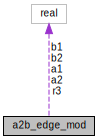
\includegraphics[width=134pt]{classa2b__edge__mod__coll__graph}
\end{center}
\end{figure}
\subsection*{Public Member Functions}
\begin{DoxyCompactItemize}
\item 
subroutine, public \hyperlink{classa2b__edge__mod_a1aa7bae49fd010f65a8018e76a46d1cd}{a2b\-\_\-ord4} (qin, qout, gridstruct, npx, npy, is, ie, js, je, ng, replace)
\item 
subroutine, public \hyperlink{classa2b__edge__mod_a43e19bd75d30458df0e1dd77845620eb}{a2b\-\_\-ord2} (qin, qout, gridstruct, npx, npy, is, ie, js, je, ng, replace)
\end{DoxyCompactItemize}
\subsection*{Public Attributes}
\begin{DoxyCompactItemize}
\item 
real, parameter \hyperlink{classa2b__edge__mod_a719947b05e0bc96f78d35ea3cb071308}{r3} = 1./3.
\item 
real, parameter \hyperlink{classa2b__edge__mod_a45444d62264334d291e88df0b4c23811}{a1} = 0.\-5625
\begin{DoxyCompactList}\small\item\em 9/16 \end{DoxyCompactList}\item 
real, parameter \hyperlink{classa2b__edge__mod_a8155aee9a19fd9f7563377875f58fb0d}{a2} = -\/0.\-0625
\begin{DoxyCompactList}\small\item\em -\/1/16 \end{DoxyCompactList}\item 
real, parameter \hyperlink{classa2b__edge__mod_ab63bc73394b22152a35f0785c28d6d6f}{b1} = 7./12.
\begin{DoxyCompactList}\small\item\em 0.\-58333333 \end{DoxyCompactList}\item 
real, parameter \hyperlink{classa2b__edge__mod_aa319761122e25e2030a5652753d6a9ba}{b2} = -\/1./12.
\end{DoxyCompactItemize}
\subsection*{Private Member Functions}
\begin{DoxyCompactItemize}
\item 
real function \hyperlink{classa2b__edge__mod_ab5a8b8511c3ad957c5fab548ab663e30}{extrap\-\_\-corner} (p0, p1, p2, q1, q2)
\end{DoxyCompactItemize}


\subsection{Detailed Description}
The module 'a2b\-\_\-edge' performs F\-V-\/consistent interpolation of pressure to corners. 

Definition at line 24 of file a2b\-\_\-edge.\-F90.



\subsection{Member Function/\-Subroutine Documentation}
\index{a2b\-\_\-edge\-\_\-mod@{a2b\-\_\-edge\-\_\-mod}!a2b\-\_\-ord2@{a2b\-\_\-ord2}}
\index{a2b\-\_\-ord2@{a2b\-\_\-ord2}!a2b_edge_mod@{a2b\-\_\-edge\-\_\-mod}}
\subsubsection[{a2b\-\_\-ord2}]{\setlength{\rightskip}{0pt plus 5cm}subroutine, public a2b\-\_\-edge\-\_\-mod\-::a2b\-\_\-ord2 (
\begin{DoxyParamCaption}
\item[{real, dimension(is-\/ng\-:ie+ng,js-\/ng\-:je+ng), intent(inout)}]{qin, }
\item[{real, dimension(is-\/ng\-:ie+ng,js-\/ng\-:je+ng), intent(out)}]{qout, }
\item[{type(fv\-\_\-grid\-\_\-type), intent(in), target}]{gridstruct, }
\item[{integer, intent(in)}]{npx, }
\item[{integer, intent(in)}]{npy, }
\item[{integer, intent(in)}]{is, }
\item[{integer, intent(in)}]{ie, }
\item[{integer, intent(in)}]{js, }
\item[{integer, intent(in)}]{je, }
\item[{integer, intent(in)}]{ng, }
\item[{logical, intent(in), optional}]{replace}
\end{DoxyParamCaption}
)}\label{classa2b__edge__mod_a43e19bd75d30458df0e1dd77845620eb}

\begin{DoxyParams}[1]{Parameters}
\mbox{\tt in,out}  & {\em qin} & A-\/grid field\\
\hline
\mbox{\tt out}  & {\em qout} & Output B-\/grid field \\
\hline
\end{DoxyParams}


Definition at line 697 of file a2b\-\_\-edge.\-F90.



Referenced by dyn\-\_\-core\-\_\-mod\-::adv\-\_\-pe(), dyn\-\_\-core\-\_\-mod\-::dyn\-\_\-core(), dyn\-\_\-core\-\_\-mod\-::grad1\-\_\-p\-\_\-update(), and dyn\-\_\-core\-\_\-mod\-::one\-\_\-grad\-\_\-p().

\index{a2b\-\_\-edge\-\_\-mod@{a2b\-\_\-edge\-\_\-mod}!a2b\-\_\-ord4@{a2b\-\_\-ord4}}
\index{a2b\-\_\-ord4@{a2b\-\_\-ord4}!a2b_edge_mod@{a2b\-\_\-edge\-\_\-mod}}
\subsubsection[{a2b\-\_\-ord4}]{\setlength{\rightskip}{0pt plus 5cm}subroutine, public a2b\-\_\-edge\-\_\-mod\-::a2b\-\_\-ord4 (
\begin{DoxyParamCaption}
\item[{real, dimension(is-\/ng\-:ie+ng,js-\/ng\-:je+ng), intent(inout)}]{qin, }
\item[{real, dimension(is-\/ng\-:ie+ng,js-\/ng\-:je+ng), intent(inout)}]{qout, }
\item[{type(fv\-\_\-grid\-\_\-type), intent(in), target}]{gridstruct, }
\item[{integer, intent(in)}]{npx, }
\item[{integer, intent(in)}]{npy, }
\item[{integer, intent(in)}]{is, }
\item[{integer, intent(in)}]{ie, }
\item[{integer, intent(in)}]{js, }
\item[{integer, intent(in)}]{je, }
\item[{integer, intent(in)}]{ng, }
\item[{logical, intent(in), optional}]{replace}
\end{DoxyParamCaption}
)}\label{classa2b__edge__mod_a1aa7bae49fd010f65a8018e76a46d1cd}

\begin{DoxyParams}[1]{Parameters}
\mbox{\tt in,out}  & {\em qin} & A-\/grid field\\
\hline
\mbox{\tt in,out}  & {\em qout} & Output B-\/grid field \\
\hline
\end{DoxyParams}


Definition at line 69 of file a2b\-\_\-edge.\-F90.



References extrap\-\_\-corner().



Referenced by sw\-\_\-core\-\_\-mod\-::d\-\_\-sw(), dyn\-\_\-core\-\_\-mod\-::grad1\-\_\-p\-\_\-update(), fv\-\_\-diagnostics\-\_\-mod\-::init\-\_\-mq(), dyn\-\_\-core\-\_\-mod\-::nh\-\_\-p\-\_\-grad(), dyn\-\_\-core\-\_\-mod\-::one\-\_\-grad\-\_\-p(), fv\-\_\-grid\-\_\-utils\-\_\-mod\-::project\-\_\-sphere\-\_\-v(), sw\-\_\-core\-\_\-mod\-::smag\-\_\-corner(), and dyn\-\_\-core\-\_\-mod\-::split\-\_\-p\-\_\-grad().

\index{a2b\-\_\-edge\-\_\-mod@{a2b\-\_\-edge\-\_\-mod}!extrap\-\_\-corner@{extrap\-\_\-corner}}
\index{extrap\-\_\-corner@{extrap\-\_\-corner}!a2b_edge_mod@{a2b\-\_\-edge\-\_\-mod}}
\subsubsection[{extrap\-\_\-corner}]{\setlength{\rightskip}{0pt plus 5cm}real function a2b\-\_\-edge\-\_\-mod\-::extrap\-\_\-corner (
\begin{DoxyParamCaption}
\item[{real, dimension(2), intent(in)}]{p0, }
\item[{real, dimension(2), intent(in)}]{p1, }
\item[{real, dimension(2), intent(in)}]{p2, }
\item[{real, intent(in)}]{q1, }
\item[{real, intent(in)}]{q2}
\end{DoxyParamCaption}
)\hspace{0.3cm}{\ttfamily [private]}}\label{classa2b__edge__mod_ab5a8b8511c3ad957c5fab548ab663e30}


Definition at line 820 of file a2b\-\_\-edge.\-F90.



References fv\-\_\-grid\-\_\-utils\-\_\-mod\-::great\-\_\-circle\-\_\-dist().



Referenced by a2b\-\_\-ord4().



\subsection{Member Data Documentation}
\index{a2b\-\_\-edge\-\_\-mod@{a2b\-\_\-edge\-\_\-mod}!a1@{a1}}
\index{a1@{a1}!a2b_edge_mod@{a2b\-\_\-edge\-\_\-mod}}
\subsubsection[{a1}]{\setlength{\rightskip}{0pt plus 5cm}real, parameter a2b\-\_\-edge\-\_\-mod\-::a1 = 0.\-5625}\label{classa2b__edge__mod_a45444d62264334d291e88df0b4c23811}


9/16 



Definition at line 55 of file a2b\-\_\-edge.\-F90.

\index{a2b\-\_\-edge\-\_\-mod@{a2b\-\_\-edge\-\_\-mod}!a2@{a2}}
\index{a2@{a2}!a2b_edge_mod@{a2b\-\_\-edge\-\_\-mod}}
\subsubsection[{a2}]{\setlength{\rightskip}{0pt plus 5cm}real, parameter a2b\-\_\-edge\-\_\-mod\-::a2 = -\/0.\-0625}\label{classa2b__edge__mod_a8155aee9a19fd9f7563377875f58fb0d}


-\/1/16 



Definition at line 56 of file a2b\-\_\-edge.\-F90.

\index{a2b\-\_\-edge\-\_\-mod@{a2b\-\_\-edge\-\_\-mod}!b1@{b1}}
\index{b1@{b1}!a2b_edge_mod@{a2b\-\_\-edge\-\_\-mod}}
\subsubsection[{b1}]{\setlength{\rightskip}{0pt plus 5cm}real, parameter a2b\-\_\-edge\-\_\-mod\-::b1 = 7./12.}\label{classa2b__edge__mod_ab63bc73394b22152a35f0785c28d6d6f}


0.\-58333333 



Definition at line 60 of file a2b\-\_\-edge.\-F90.

\index{a2b\-\_\-edge\-\_\-mod@{a2b\-\_\-edge\-\_\-mod}!b2@{b2}}
\index{b2@{b2}!a2b_edge_mod@{a2b\-\_\-edge\-\_\-mod}}
\subsubsection[{b2}]{\setlength{\rightskip}{0pt plus 5cm}real, parameter a2b\-\_\-edge\-\_\-mod\-::b2 = -\/1./12.}\label{classa2b__edge__mod_aa319761122e25e2030a5652753d6a9ba}


Definition at line 61 of file a2b\-\_\-edge.\-F90.

\index{a2b\-\_\-edge\-\_\-mod@{a2b\-\_\-edge\-\_\-mod}!r3@{r3}}
\index{r3@{r3}!a2b_edge_mod@{a2b\-\_\-edge\-\_\-mod}}
\subsubsection[{r3}]{\setlength{\rightskip}{0pt plus 5cm}real, parameter a2b\-\_\-edge\-\_\-mod\-::r3 = 1./3.}\label{classa2b__edge__mod_a719947b05e0bc96f78d35ea3cb071308}


Definition at line 51 of file a2b\-\_\-edge.\-F90.



The documentation for this module was generated from the following file\-:\begin{DoxyCompactItemize}
\item 
/scratch2/\-N\-A\-G\-A\-P\-E/aoml-\/hafs1/\-Kyle.\-Ahern/acs\-\_\-master\-\_\-readonly/model/\hyperlink{a2b__edge_8F90}{a2b\-\_\-edge.\-F90}\end{DoxyCompactItemize}

\section{fv\-\_\-arrays\-\_\-mod\-:\-:allocate\-\_\-fv\-\_\-nest\-\_\-bc\-\_\-type Interface Reference}
\label{interfacefv__arrays__mod_1_1allocate__fv__nest__bc__type}\index{fv\-\_\-arrays\-\_\-mod\-::allocate\-\_\-fv\-\_\-nest\-\_\-bc\-\_\-type@{fv\-\_\-arrays\-\_\-mod\-::allocate\-\_\-fv\-\_\-nest\-\_\-bc\-\_\-type}}


'allocate\-\_\-fv\-\_\-nest\-\_\-\-B\-C\-\_\-type' is an interface to subroutines that allocate the 'fv\-\_\-nest\-\_\-\-B\-C\-\_\-type' structure that holds the nested-\/grid B\-Cs.  


\subsection*{Public Member Functions}
\begin{DoxyCompactItemize}
\item 
subroutine \hyperlink{interfacefv__arrays__mod_1_1allocate__fv__nest__bc__type_a25db6ace0eb8ef1331da2fabf640855f}{allocate\-\_\-fv\-\_\-nest\-\_\-bc\-\_\-type\-\_\-3d} (B\-C, is, ie, js, je, isd, ied, jsd, jed, npx, npy, npz, ng, ns, istag, jstag, dummy)
\item 
subroutine \hyperlink{interfacefv__arrays__mod_1_1allocate__fv__nest__bc__type_a198c4b601e12e05fed5528dc3ce7aae1}{allocate\-\_\-fv\-\_\-nest\-\_\-bc\-\_\-type\-\_\-3d\-\_\-atm} (B\-C, Atm, ns, istag, jstag, dummy)
\end{DoxyCompactItemize}


\subsection{Detailed Description}
'allocate\-\_\-fv\-\_\-nest\-\_\-\-B\-C\-\_\-type' is an interface to subroutines that allocate the 'fv\-\_\-nest\-\_\-\-B\-C\-\_\-type' structure that holds the nested-\/grid B\-Cs. 

The subroutines can pass the array bounds explicitly or not. The bounds in Atmbd are used for the non-\/explicit case. 

Definition at line 1126 of file fv\-\_\-arrays.\-F90.



\subsection{Member Function/\-Subroutine Documentation}
\index{fv\-\_\-arrays\-\_\-mod\-::allocate\-\_\-fv\-\_\-nest\-\_\-bc\-\_\-type@{fv\-\_\-arrays\-\_\-mod\-::allocate\-\_\-fv\-\_\-nest\-\_\-bc\-\_\-type}!allocate\-\_\-fv\-\_\-nest\-\_\-bc\-\_\-type\-\_\-3d@{allocate\-\_\-fv\-\_\-nest\-\_\-bc\-\_\-type\-\_\-3d}}
\index{allocate\-\_\-fv\-\_\-nest\-\_\-bc\-\_\-type\-\_\-3d@{allocate\-\_\-fv\-\_\-nest\-\_\-bc\-\_\-type\-\_\-3d}!fv_arrays_mod::allocate_fv_nest_bc_type@{fv\-\_\-arrays\-\_\-mod\-::allocate\-\_\-fv\-\_\-nest\-\_\-bc\-\_\-type}}
\subsubsection[{allocate\-\_\-fv\-\_\-nest\-\_\-bc\-\_\-type\-\_\-3d}]{\setlength{\rightskip}{0pt plus 5cm}subroutine fv\-\_\-arrays\-\_\-mod\-::allocate\-\_\-fv\-\_\-nest\-\_\-bc\-\_\-type\-::allocate\-\_\-fv\-\_\-nest\-\_\-bc\-\_\-type\-\_\-3d (
\begin{DoxyParamCaption}
\item[{type({\bf fv\-\_\-nest\-\_\-bc\-\_\-type\-\_\-3d}), intent(inout)}]{B\-C, }
\item[{integer, intent(in)}]{is, }
\item[{integer, intent(in)}]{ie, }
\item[{integer, intent(in)}]{js, }
\item[{integer, intent(in)}]{je, }
\item[{integer, intent(in)}]{isd, }
\item[{integer, intent(in)}]{ied, }
\item[{integer, intent(in)}]{jsd, }
\item[{integer, intent(in)}]{jed, }
\item[{integer, intent(in)}]{npx, }
\item[{integer, intent(in)}]{npy, }
\item[{integer, intent(in)}]{npz, }
\item[{integer, intent(in)}]{ng, }
\item[{integer, intent(in)}]{ns, }
\item[{integer, intent(in)}]{istag, }
\item[{integer, intent(in)}]{jstag, }
\item[{logical, intent(in)}]{dummy}
\end{DoxyParamCaption}
)}\label{interfacefv__arrays__mod_1_1allocate__fv__nest__bc__type_a25db6ace0eb8ef1331da2fabf640855f}


Definition at line 2015 of file fv\-\_\-arrays.\-F90.



Referenced by fv\-\_\-arrays\-\_\-mod\-::allocate\-\_\-fv\-\_\-nest\-\_\-bc\-\_\-type\-\_\-3d\-\_\-atm().

\index{fv\-\_\-arrays\-\_\-mod\-::allocate\-\_\-fv\-\_\-nest\-\_\-bc\-\_\-type@{fv\-\_\-arrays\-\_\-mod\-::allocate\-\_\-fv\-\_\-nest\-\_\-bc\-\_\-type}!allocate\-\_\-fv\-\_\-nest\-\_\-bc\-\_\-type\-\_\-3d\-\_\-atm@{allocate\-\_\-fv\-\_\-nest\-\_\-bc\-\_\-type\-\_\-3d\-\_\-atm}}
\index{allocate\-\_\-fv\-\_\-nest\-\_\-bc\-\_\-type\-\_\-3d\-\_\-atm@{allocate\-\_\-fv\-\_\-nest\-\_\-bc\-\_\-type\-\_\-3d\-\_\-atm}!fv_arrays_mod::allocate_fv_nest_bc_type@{fv\-\_\-arrays\-\_\-mod\-::allocate\-\_\-fv\-\_\-nest\-\_\-bc\-\_\-type}}
\subsubsection[{allocate\-\_\-fv\-\_\-nest\-\_\-bc\-\_\-type\-\_\-3d\-\_\-atm}]{\setlength{\rightskip}{0pt plus 5cm}subroutine fv\-\_\-arrays\-\_\-mod\-::allocate\-\_\-fv\-\_\-nest\-\_\-bc\-\_\-type\-::allocate\-\_\-fv\-\_\-nest\-\_\-bc\-\_\-type\-\_\-3d\-\_\-atm (
\begin{DoxyParamCaption}
\item[{type({\bf fv\-\_\-nest\-\_\-bc\-\_\-type\-\_\-3d}), intent(inout)}]{B\-C, }
\item[{type({\bf fv\-\_\-atmos\-\_\-type}), intent(in)}]{Atm, }
\item[{integer, intent(in)}]{ns, }
\item[{integer, intent(in)}]{istag, }
\item[{integer, intent(in)}]{jstag, }
\item[{logical, intent(in)}]{dummy}
\end{DoxyParamCaption}
)}\label{interfacefv__arrays__mod_1_1allocate__fv__nest__bc__type_a198c4b601e12e05fed5528dc3ce7aae1}


Definition at line 1983 of file fv\-\_\-arrays.\-F90.



The documentation for this interface was generated from the following file\-:\begin{DoxyCompactItemize}
\item 
/scratch2/\-N\-A\-G\-A\-P\-E/aoml-\/hafs1/\-Kyle.\-Ahern/acs\-\_\-master\-\_\-readonly/model/\hyperlink{fv__arrays_8F90}{fv\-\_\-arrays.\-F90}\end{DoxyCompactItemize}

\section{atmosphere\-\_\-mod Module Reference}
\label{classatmosphere__mod}\index{atmosphere\-\_\-mod@{atmosphere\-\_\-mod}}


The module 'atmosphere' provides the interface for the Cubed-\/\-Sphere F\-V dynamical core.  




Collaboration diagram for atmosphere\-\_\-mod\-:
\nopagebreak
\begin{figure}[H]
\begin{center}
\leavevmode
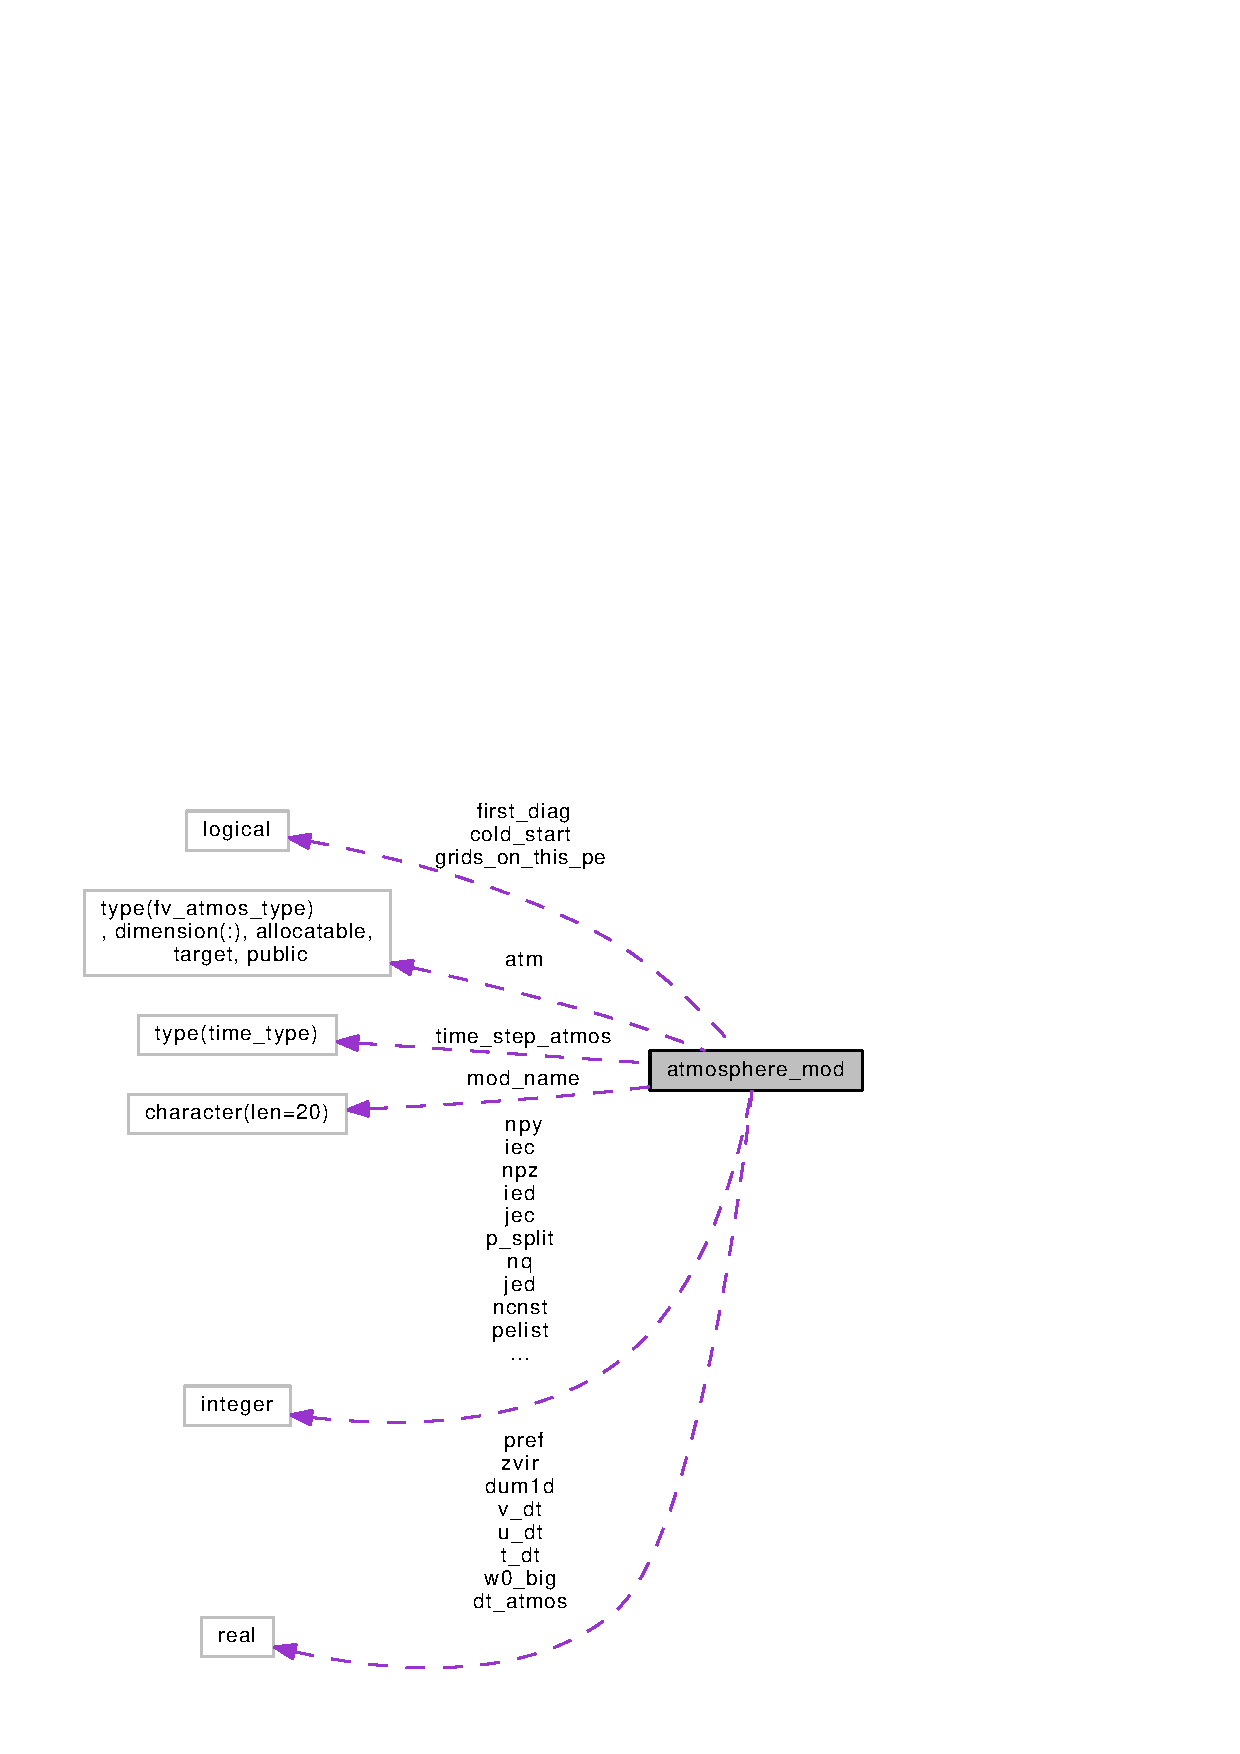
\includegraphics[width=350pt]{classatmosphere__mod__coll__graph}
\end{center}
\end{figure}
\subsection*{Public Member Functions}
\begin{DoxyCompactItemize}
\item 
subroutine, public \hyperlink{classatmosphere__mod_a38757921a7432338ac2a4135dbc7d9c8}{atmosphere\-\_\-init} (Time\-\_\-init, Time, Time\-\_\-step, Grid\-\_\-box, area)
\begin{DoxyCompactList}\small\item\em The subroutine 'atmosphere\-\_\-init' is an A\-P\-I to initialize the F\-V3 dynamical core, including the grid structures, memory, initial state (self-\/initialization or restart), and diagnostics. \end{DoxyCompactList}\item 
subroutine, public \hyperlink{classatmosphere__mod_a46726a89e78937df996b8fa2987af885}{atmosphere\-\_\-dynamics} (Time)
\begin{DoxyCompactList}\small\item\em The subroutine 'atmosphere\-\_\-dynamics' is an A\-P\-I for the main driver of the F\-V3 dynamical core responsible for executing a \char`\"{}dynamics\char`\"{} step. \end{DoxyCompactList}\item 
subroutine, public \hyperlink{classatmosphere__mod_a40591968fdfea1c52562d1e18affcb98}{atmosphere\-\_\-end} (Time, Grid\-\_\-box, restart\-\_\-endfcst)
\begin{DoxyCompactList}\small\item\em The subroutine 'atmosphere\-\_\-end' is an A\-P\-I for the termination of the F\-V3 dynamical core responsible for writing out a restart and final diagnostic state. \end{DoxyCompactList}\item 
subroutine, public \hyperlink{classatmosphere__mod_a1648cbd61c86f2e8890375435b532a5d}{atmosphere\-\_\-restart} (timestamp)
\begin{DoxyCompactList}\small\item\em The subroutine 'atmosphere\-\_\-restart' is an A\-P\-I to save restart information at a given timestamp.  This A\-P\-I is used to provide intermediate restart capability to the atmospheric driver. \end{DoxyCompactList}\item 
subroutine, public \hyperlink{classatmosphere__mod_a55d141fa3702c01dae8e656e283827dc}{atmosphere\-\_\-resolution} (i\-\_\-size, j\-\_\-size, global)
\begin{DoxyCompactList}\small\item\em The subroutine 'atmospehre\-\_\-resolution' is an A\-P\-I to return the local extents of the current M\-P\-I-\/rank or the global extents of the current cubed-\/sphere tile. \end{DoxyCompactList}\item 
subroutine, public \hyperlink{classatmosphere__mod_a15f14a6344439b29298bfb2b37d9c694}{atmosphere\-\_\-pref} (p\-\_\-ref)
\begin{DoxyCompactList}\small\item\em The subroutine 'atmosphere\-\_\-pref' is an A\-P\-I to return the reference pressure. \end{DoxyCompactList}\item 
subroutine, public \hyperlink{classatmosphere__mod_adc8bdf1db2df9551cfc25a0c1f7b1385}{atmosphere\-\_\-control\-\_\-data} (i1, i2, j1, j2, kt, p\-\_\-hydro, hydro, tile\-\_\-num)
\item 
subroutine, public \hyperlink{classatmosphere__mod_a9a51c2f1c5e1cf01dcf112478ecf8cf4}{atmosphere\-\_\-grid\-\_\-ctr} (lon, lat)
\begin{DoxyCompactList}\small\item\em The subroutine 'atmosphere\-\_\-grid\-\_\-ctr' is an A\-P\-I that returns the longitude and latitude cell centers of the current M\-P\-I-\/rank. \end{DoxyCompactList}\item 
subroutine, public \hyperlink{classatmosphere__mod_a3f2bb9d476f9525e20747fd29951dde5}{atmosphere\-\_\-grid\-\_\-bdry} (blon, blat, global)
\begin{DoxyCompactList}\small\item\em The subroutine 'atmosphere\-\_\-grid\-\_\-bdry' is an A\-P\-I to returns the longitude and latitude finite volume edges (grid box) for the current M\-P\-I-\/rank. \end{DoxyCompactList}\item 
subroutine, public \hyperlink{classatmosphere__mod_a35547644843aec32773bc727b07252de}{atmosphere\-\_\-domain} (fv\-\_\-domain, layout, regional, nested, \hyperlink{classatmosphere__mod_a40b6e75a5e8c4bafc747edc08eceaed5}{pelist})
\begin{DoxyCompactList}\small\item\em The subroutine 'atmosphere\-\_\-domain' is an A\-P\-I to return the \char`\"{}domain2d\char`\"{} variable associated with the coupling grid and the decomposition for the current cubed-\/sphere tile.  Coupling is done using the mass/temperature grid with no halos. \end{DoxyCompactList}\item 
subroutine, public \hyperlink{classatmosphere__mod_af5d819faa34aef7024501c7696540bf0}{atmosphere\-\_\-diag\-\_\-axes} (axes)
\begin{DoxyCompactList}\small\item\em The subroutine 'atmosphere\-\_\-diag\-\_\-axes' is an A\-P\-I to return the axis indices for the atmospheric (mass) grid. \end{DoxyCompactList}\item 
subroutine, public \hyperlink{classatmosphere__mod_ad2c962b25778b4cbd91b48874a52ab95}{atmosphere\-\_\-etalvls} (ak, bk, flip)
\begin{DoxyCompactList}\small\item\em The subroutine 'atmosphere\-\_\-etalvls' is an A\-P\-I to return the ak/bk pairs used to compute the eta or pressure levels.  By default, the vertical dimension assumes the standard F\-V3 convention of T\-O\-A (k=1) to Surface (k=npz). \end{DoxyCompactList}\item 
subroutine, public \hyperlink{classatmosphere__mod_af16043b77ee4e18b8a8497ad49cfd670}{atmosphere\-\_\-hgt} (hgt, position, relative, flip)
\begin{DoxyCompactList}\small\item\em The subroutine 'atmosphere\-\_\-hgt' is an A\-P\-I to return the height coordinate.  By default, the vertical dimension assumes the standard F\-V3 convention of T\-O\-A (k=1) to Surface (k=npz). There are options to choose location \mbox{[}level (interface) or layer\mbox{]} and absolute vs. relative height (zero-\/based). \end{DoxyCompactList}\item 
subroutine, public \hyperlink{classatmosphere__mod_af9fa6ffe6500a97af113b7a6afb348a6}{atmosphere\-\_\-scalar\-\_\-field\-\_\-halo} (data, halo, isize, jsize, ksize, data\-\_\-p)
\begin{DoxyCompactList}\small\item\em The subroutine 'atmosphere\-\_\-scalar\-\_\-field\-\_\-halo' is an A\-P\-I to return halo information of the current M\-P\-I\-\_\-rank for an input scalar field.  Up to three point haloes can be returned by this A\-P\-I which includes special handling for the cubed-\/sphere tile corners. Output will be in (i,j,k) while input can be in (i,j,k) or horizontally-\/packed form (ix,k). \end{DoxyCompactList}\item 
subroutine \hyperlink{classatmosphere__mod_a14deefffccb54e6af9cf0680f1b3823a}{atmosphere\-\_\-nggps\-\_\-diag} (Time, init, ltavg, avg\-\_\-max\-\_\-length)
\begin{DoxyCompactList}\small\item\em The subroutine 'atmosphere\-\_\-nggps\-\_\-diag' is an A\-P\-I to trigger output of diagnostics in N\-C\-E\-P/\-E\-M\-C format. \end{DoxyCompactList}\item 
subroutine, public \hyperlink{classatmosphere__mod_abf96613ef8db32b3e66f3297f62a0346}{atmosphere\-\_\-state\-\_\-update} (Time, I\-P\-D\-\_\-\-Data, I\-A\-U\-\_\-\-Data, Atm\-\_\-block, flip\-\_\-vc)
\begin{DoxyCompactList}\small\item\em The subroutine 'atmosphere\-\_\-state\-\_\-update' is an A\-P\-I to apply tendencies and compute a consistent prognostic state. \end{DoxyCompactList}\item 
subroutine, public \hyperlink{classatmosphere__mod_a5dfb607fd7c0bb4cd771a72f1daf8ded}{atmos\-\_\-phys\-\_\-driver\-\_\-statein} (I\-P\-D\-\_\-\-Data, Atm\-\_\-block, flip\-\_\-vc)
\begin{DoxyCompactList}\small\item\em The subroutine 'atmos\-\_\-phys\-\_\-driver\-\_\-statein' is an A\-P\-I to populate the I\-P\-D\-\_\-\-DataStatein container with the prognostic state at the end of the advection (dynamics) step of integration.  Performs a mass adjustment to be consistent with the G\-F\-S physics and if necessary, converts quantities to hydrostatic representation. \end{DoxyCompactList}\end{DoxyCompactItemize}
\subsection*{Public Attributes}
\begin{DoxyCompactItemize}
\item 
integer, public \hyperlink{classatmosphere__mod_a72d23c8d327e3066174b6e43f5697494}{mytile} = 1
\item 
type(fv\-\_\-atmos\-\_\-type), dimension(\-:), \\*
allocatable, target, public \hyperlink{classatmosphere__mod_a65be72573dcfd288a47a65ffaf881284}{atm}
\end{DoxyCompactItemize}
\subsection*{Private Member Functions}
\begin{DoxyCompactItemize}
\item 
subroutine \hyperlink{classatmosphere__mod_aa742152443b418c81cda5ab32bf17f0e}{p\-\_\-adi} (km, ng, ifirst, ilast, jfirst, jlast, ptop, delp, pt, ps, pe, peln, pk, pkz, hydrostatic)
\begin{DoxyCompactList}\small\item\em The subroutine 'p\-\_\-adi' computes (ps, pk, pe, peln, pkz) given (ptop, delp). \end{DoxyCompactList}\item 
subroutine \hyperlink{classatmosphere__mod_a0b3f45bdf6f1f0ddb2260514fd3e8bb3}{set\-\_\-atmosphere\-\_\-pelist} ()
\item 
subroutine \hyperlink{classatmosphere__mod_a3afd17a79c9085897632f7298a0d29ab}{atmosphere\-\_\-diss\-\_\-est} (npass)
\item 
subroutine \hyperlink{classatmosphere__mod_a94122314f8c8e6209581bfacbbbf8319}{get\-\_\-bottom\-\_\-mass} (t\-\_\-bot, tr\-\_\-bot, p\-\_\-bot, z\-\_\-bot, p\-\_\-surf, slp)
\item 
subroutine \hyperlink{classatmosphere__mod_a18b993ba126ae2c1baa890234cfcb289}{get\-\_\-bottom\-\_\-wind} (u\-\_\-bot, v\-\_\-bot)
\item 
subroutine \hyperlink{classatmosphere__mod_a7f2735d36937c9db638ff80f70e8bbeb}{atmosphere\-\_\-get\-\_\-bottom\-\_\-layer} (Atm\-\_\-block, D\-Y\-C\-O\-R\-E\-\_\-\-Data)
\begin{DoxyCompactList}\small\item\em The subroutine 'atmosphere\-\_\-get\-\_\-bottom\-\_\-layer' is an A\-P\-I to provide the bottom layer quantities needed for coupling with other external components.  The data will be provided in a D\-D\-T which is a packed, blocked structure. \end{DoxyCompactList}\item 
subroutine \hyperlink{classatmosphere__mod_a2d856ff000261ca516c3ae653a9ef005}{get\-\_\-stock\-\_\-pe} (index, value)
\item 
subroutine \hyperlink{classatmosphere__mod_abd3fee5137633b7451c0ee1f29942e26}{adiabatic\-\_\-init} (\hyperlink{classatmosphere__mod_a313b4e35ea4020ee6ce916400b716e81}{zvir}, nudge\-\_\-dz, time)
\begin{DoxyCompactList}\small\item\em The subroutine 'adiabatic\-\_\-init' is an optional step during initialization to pre-\/condition a solution via backward-\/forward steps with capability for various nudgings. \end{DoxyCompactList}\end{DoxyCompactItemize}
\subsection*{Private Attributes}
\begin{DoxyCompactItemize}
\item 
character(len=20) \hyperlink{classatmosphere__mod_ad4f4fdf067d2b71eb5764b34cea8cb92}{mod\-\_\-name} = 'fv\-G\-F\-S/\hyperlink{classatmosphere__mod}{atmosphere\-\_\-mod}'
\item 
type(time\-\_\-type) \hyperlink{classatmosphere__mod_a6d42cfe750246363957a2e0aaa251f0b}{time\-\_\-step\-\_\-atmos}
\item 
real \hyperlink{classatmosphere__mod_a8bd26483e8952209607d542434d5a1f1}{dt\-\_\-atmos}
\item 
real \hyperlink{classatmosphere__mod_a313b4e35ea4020ee6ce916400b716e81}{zvir}
\item 
integer \hyperlink{classatmosphere__mod_aa26f13c1bf254400bc1d3c556bc4b2f7}{npx}
\item 
integer \hyperlink{classatmosphere__mod_aeef69bc0cde093c538645187edff87ff}{npy}
\item 
integer \hyperlink{classatmosphere__mod_a8db34afa5af2e9757555a6ce961b26e5}{npz}
\item 
integer \hyperlink{classatmosphere__mod_a9a8c995d33f2c1869ae7d0b49d5e1002}{ncnst}
\item 
integer \hyperlink{classatmosphere__mod_a3ae095d62282ac16560419aa858cbd5b}{pnats}
\item 
integer \hyperlink{classatmosphere__mod_a1a7a45008a0aebc7bce0bc31d6ded35c}{isc}
\item 
integer \hyperlink{classatmosphere__mod_ab0f4510c9097aa7a29c57c545aa02976}{iec}
\item 
integer \hyperlink{classatmosphere__mod_aa39dea540d1cba46aa0cd710e17bf8a9}{jsc}
\item 
integer \hyperlink{classatmosphere__mod_a0ac3bd99046244dd0abfa4719b688bc0}{jec}
\item 
integer \hyperlink{classatmosphere__mod_a26b6f2e397bc0d76f12ae674aad670be}{isd}
\item 
integer \hyperlink{classatmosphere__mod_a775666c64f59edcf96c530c1fc0f1ee9}{ied}
\item 
integer \hyperlink{classatmosphere__mod_a972cd4fc5737c35941feca9dbb6e46a8}{jsd}
\item 
integer \hyperlink{classatmosphere__mod_a0d51bfe05ec1bd062c1fbbc01c42bf3a}{jed}
\item 
integer \hyperlink{classatmosphere__mod_ab5e69a4d3670d2800a288b1c49ad3d9a}{nq}
\item 
integer \hyperlink{classatmosphere__mod_abe192872a4a5b42159d0c2251ac9cb14}{sec}
\item 
integer \hyperlink{classatmosphere__mod_aafb92c94f8850295ad027e0538ae78ca}{seconds}
\item 
integer \hyperlink{classatmosphere__mod_a110bc10bed586ca2cddc28ac924959a7}{days}
\item 
integer \hyperlink{classatmosphere__mod_ac1b450b5b014a927fb0456a5b8e73710}{id\-\_\-dynam}
\item 
integer \hyperlink{classatmosphere__mod_a6d434f016963346507b32a22b7f41440}{id\-\_\-fv\-\_\-diag}
\item 
integer \hyperlink{classatmosphere__mod_af368e346f77c2d615969072223e3edad}{id\-\_\-subgridz}
\item 
logical \hyperlink{classatmosphere__mod_a6f65980184c149309238cf3926145607}{cold\-\_\-start} = .false.
\item 
integer, dimension(\-:), allocatable \hyperlink{classatmosphere__mod_ae021e6f5700c65ee41c520e77e44712d}{id\-\_\-tracerdt\-\_\-dyn}
\item 
integer \hyperlink{classatmosphere__mod_a794b092a72b516a3078dbff077136a08}{sphum}
\item 
integer \hyperlink{classatmosphere__mod_a41f34859d8c8fd6e84cd71aabd6d2a25}{liq\-\_\-wat}
\item 
integer \hyperlink{classatmosphere__mod_ad9345d06c2a877903e3bfdfb529a2a63}{rainwat}
\item 
integer \hyperlink{classatmosphere__mod_a9d5b133b6c0010773c3f475af7e879fc}{ice\-\_\-wat}
\item 
integer \hyperlink{classatmosphere__mod_a638b8d7ecc568cfe3706105b9db0affe}{snowwat}
\item 
integer \hyperlink{classatmosphere__mod_a6af183d451e4d59e5cd97150b69e9ec7}{graupel}
\item 
integer \hyperlink{classatmosphere__mod_a95ee36e402cdda22fbff7a5e5a698d2d}{p\-\_\-split} = 1
\item 
integer, dimension(\-:), allocatable \hyperlink{classatmosphere__mod_a40b6e75a5e8c4bafc747edc08eceaed5}{pelist}
\item 
logical, dimension(\-:), allocatable \hyperlink{classatmosphere__mod_ad80223528e58b40110f8a1ffdd3b9aad}{grids\-\_\-on\-\_\-this\-\_\-pe}
\item 
integer \hyperlink{classatmosphere__mod_a0c326e48546ef823bdc928ba03bac964}{id\-\_\-udt\-\_\-dyn}
\item 
integer \hyperlink{classatmosphere__mod_aa372781c11fb092462ce67e7d29f3cb0}{id\-\_\-vdt\-\_\-dyn}
\item 
real, parameter \hyperlink{classatmosphere__mod_ac2c4834fc822689255bc707f8405fed1}{w0\-\_\-big} = 60.
\item 
real, dimension(\-:,\-:,\-:), allocatable \hyperlink{classatmosphere__mod_a9f0ef35864e057ad8b3b0d5b644cff55}{u\-\_\-dt}
\item 
real, dimension(\-:,\-:,\-:), allocatable \hyperlink{classatmosphere__mod_a8245233dc81e751888853150262e6489}{v\-\_\-dt}
\item 
real, dimension(\-:,\-:,\-:), allocatable \hyperlink{classatmosphere__mod_adeb134091a56f59ab4c371a3855a6bdc}{t\-\_\-dt}
\item 
real, dimension(\-:,\-:), allocatable \hyperlink{classatmosphere__mod_a532d3470860edef9ff203c5fc8e0b39d}{pref}
\item 
real, dimension(\-:), allocatable \hyperlink{classatmosphere__mod_ab2d51769b2b98337ac742bc3f80d55a7}{dum1d}
\item 
logical \hyperlink{classatmosphere__mod_ad7cd98f866fa2b4b4f8528f385d7efc1}{first\-\_\-diag} = .true.
\end{DoxyCompactItemize}


\subsection{Detailed Description}
The module 'atmosphere' provides the interface for the Cubed-\/\-Sphere F\-V dynamical core. 

Definition at line 26 of file atmosphere.\-F90.



\subsection{Member Function/\-Subroutine Documentation}
\index{atmosphere\-\_\-mod@{atmosphere\-\_\-mod}!adiabatic\-\_\-init@{adiabatic\-\_\-init}}
\index{adiabatic\-\_\-init@{adiabatic\-\_\-init}!atmosphere_mod@{atmosphere\-\_\-mod}}
\subsubsection[{adiabatic\-\_\-init}]{\setlength{\rightskip}{0pt plus 5cm}subroutine atmosphere\-\_\-mod\-::adiabatic\-\_\-init (
\begin{DoxyParamCaption}
\item[{real, intent(in)}]{zvir, }
\item[{logical, intent(inout)}]{nudge\-\_\-dz, }
\item[{type(time\-\_\-type), intent(in)}]{time}
\end{DoxyParamCaption}
)\hspace{0.3cm}{\ttfamily [private]}}\label{classatmosphere__mod_abd3fee5137633b7451c0ee1f29942e26}


The subroutine 'adiabatic\-\_\-init' is an optional step during initialization to pre-\/condition a solution via backward-\/forward steps with capability for various nudgings. 



Definition at line 1609 of file atmosphere.\-F90.



References fv\-\_\-dynamics\-\_\-mod\-::fv\-\_\-dynamics(), fv\-\_\-timing\-\_\-mod\-::timing\-\_\-off(), fv\-\_\-timing\-\_\-mod\-::timing\-\_\-on(), and multi\-\_\-gases\-\_\-mod\-::virq().



Referenced by atmosphere\-\_\-init().

\index{atmosphere\-\_\-mod@{atmosphere\-\_\-mod}!atmos\-\_\-phys\-\_\-driver\-\_\-statein@{atmos\-\_\-phys\-\_\-driver\-\_\-statein}}
\index{atmos\-\_\-phys\-\_\-driver\-\_\-statein@{atmos\-\_\-phys\-\_\-driver\-\_\-statein}!atmosphere_mod@{atmosphere\-\_\-mod}}
\subsubsection[{atmos\-\_\-phys\-\_\-driver\-\_\-statein}]{\setlength{\rightskip}{0pt plus 5cm}subroutine, public atmosphere\-\_\-mod\-::atmos\-\_\-phys\-\_\-driver\-\_\-statein (
\begin{DoxyParamCaption}
\item[{type (ipd\-\_\-data\-\_\-type), dimension(\-:), intent(inout)}]{I\-P\-D\-\_\-\-Data, }
\item[{type (block\-\_\-control\-\_\-type), intent(in)}]{Atm\-\_\-block, }
\item[{logical, intent(in)}]{flip\-\_\-vc}
\end{DoxyParamCaption}
)}\label{classatmosphere__mod_a5dfb607fd7c0bb4cd771a72f1daf8ded}


The subroutine 'atmos\-\_\-phys\-\_\-driver\-\_\-statein' is an A\-P\-I to populate the I\-P\-D\-\_\-\-DataStatein container with the prognostic state at the end of the advection (dynamics) step of integration.  Performs a mass adjustment to be consistent with the G\-F\-S physics and if necessary, converts quantities to hydrostatic representation. 



Definition at line 1897 of file atmosphere.\-F90.



References multi\-\_\-gases\-\_\-mod\-::virq\-\_\-max().

\index{atmosphere\-\_\-mod@{atmosphere\-\_\-mod}!atmosphere\-\_\-control\-\_\-data@{atmosphere\-\_\-control\-\_\-data}}
\index{atmosphere\-\_\-control\-\_\-data@{atmosphere\-\_\-control\-\_\-data}!atmosphere_mod@{atmosphere\-\_\-mod}}
\subsubsection[{atmosphere\-\_\-control\-\_\-data}]{\setlength{\rightskip}{0pt plus 5cm}subroutine, public atmosphere\-\_\-mod\-::atmosphere\-\_\-control\-\_\-data (
\begin{DoxyParamCaption}
\item[{integer, intent(out)}]{i1, }
\item[{integer, intent(out)}]{i2, }
\item[{integer, intent(out)}]{j1, }
\item[{integer, intent(out)}]{j2, }
\item[{integer, intent(out)}]{kt, }
\item[{logical, intent(out), optional}]{p\-\_\-hydro, }
\item[{logical, intent(out), optional}]{hydro, }
\item[{integer, intent(out), optional}]{tile\-\_\-num}
\end{DoxyParamCaption}
)}\label{classatmosphere__mod_adc8bdf1db2df9551cfc25a0c1f7b1385}


Definition at line 809 of file atmosphere.\-F90.

\index{atmosphere\-\_\-mod@{atmosphere\-\_\-mod}!atmosphere\-\_\-diag\-\_\-axes@{atmosphere\-\_\-diag\-\_\-axes}}
\index{atmosphere\-\_\-diag\-\_\-axes@{atmosphere\-\_\-diag\-\_\-axes}!atmosphere_mod@{atmosphere\-\_\-mod}}
\subsubsection[{atmosphere\-\_\-diag\-\_\-axes}]{\setlength{\rightskip}{0pt plus 5cm}subroutine, public atmosphere\-\_\-mod\-::atmosphere\-\_\-diag\-\_\-axes (
\begin{DoxyParamCaption}
\item[{integer, dimension (\-:), intent(out)}]{axes}
\end{DoxyParamCaption}
)}\label{classatmosphere__mod_af5d819faa34aef7024501c7696540bf0}


The subroutine 'atmosphere\-\_\-diag\-\_\-axes' is an A\-P\-I to return the axis indices for the atmospheric (mass) grid. 



Definition at line 896 of file atmosphere.\-F90.

\index{atmosphere\-\_\-mod@{atmosphere\-\_\-mod}!atmosphere\-\_\-diss\-\_\-est@{atmosphere\-\_\-diss\-\_\-est}}
\index{atmosphere\-\_\-diss\-\_\-est@{atmosphere\-\_\-diss\-\_\-est}!atmosphere_mod@{atmosphere\-\_\-mod}}
\subsubsection[{atmosphere\-\_\-diss\-\_\-est}]{\setlength{\rightskip}{0pt plus 5cm}subroutine atmosphere\-\_\-mod\-::atmosphere\-\_\-diss\-\_\-est (
\begin{DoxyParamCaption}
\item[{integer, intent(in)}]{npass}
\end{DoxyParamCaption}
)\hspace{0.3cm}{\ttfamily [private]}}\label{classatmosphere__mod_a3afd17a79c9085897632f7298a0d29ab}


Definition at line 1071 of file atmosphere.\-F90.



References dyn\-\_\-core\-\_\-mod\-::del2\-\_\-cubed().

\index{atmosphere\-\_\-mod@{atmosphere\-\_\-mod}!atmosphere\-\_\-domain@{atmosphere\-\_\-domain}}
\index{atmosphere\-\_\-domain@{atmosphere\-\_\-domain}!atmosphere_mod@{atmosphere\-\_\-mod}}
\subsubsection[{atmosphere\-\_\-domain}]{\setlength{\rightskip}{0pt plus 5cm}subroutine, public atmosphere\-\_\-mod\-::atmosphere\-\_\-domain (
\begin{DoxyParamCaption}
\item[{type(domain2d), intent(out)}]{fv\-\_\-domain, }
\item[{integer, dimension(2), intent(out)}]{layout, }
\item[{logical, intent(out)}]{regional, }
\item[{logical, intent(out)}]{nested, }
\item[{integer, dimension(\-:), intent(out), pointer}]{pelist}
\end{DoxyParamCaption}
)}\label{classatmosphere__mod_a35547644843aec32773bc727b07252de}


The subroutine 'atmosphere\-\_\-domain' is an A\-P\-I to return the \char`\"{}domain2d\char`\"{} variable associated with the coupling grid and the decomposition for the current cubed-\/sphere tile.  Coupling is done using the mass/temperature grid with no halos. 



Definition at line 875 of file atmosphere.\-F90.



References set\-\_\-atmosphere\-\_\-pelist().

\index{atmosphere\-\_\-mod@{atmosphere\-\_\-mod}!atmosphere\-\_\-dynamics@{atmosphere\-\_\-dynamics}}
\index{atmosphere\-\_\-dynamics@{atmosphere\-\_\-dynamics}!atmosphere_mod@{atmosphere\-\_\-mod}}
\subsubsection[{atmosphere\-\_\-dynamics}]{\setlength{\rightskip}{0pt plus 5cm}subroutine, public atmosphere\-\_\-mod\-::atmosphere\-\_\-dynamics (
\begin{DoxyParamCaption}
\item[{type(time\-\_\-type), intent(in)}]{Time}
\end{DoxyParamCaption}
)}\label{classatmosphere__mod_a46726a89e78937df996b8fa2987af885}


The subroutine 'atmosphere\-\_\-dynamics' is an A\-P\-I for the main driver of the F\-V3 dynamical core responsible for executing a \char`\"{}dynamics\char`\"{} step. 



Definition at line 603 of file atmosphere.\-F90.



References fv\-\_\-dynamics\-\_\-mod\-::fv\-\_\-dynamics(), fv\-\_\-sg\-\_\-mod\-::fv\-\_\-subgrid\-\_\-z(), fv\-\_\-regional\-\_\-mod\-::read\-\_\-new\-\_\-bc\-\_\-data(), fv\-\_\-timing\-\_\-mod\-::timing\-\_\-off(), fv\-\_\-timing\-\_\-mod\-::timing\-\_\-on(), and fv\-\_\-nesting\-\_\-mod\-::twoway\-\_\-nesting().

\index{atmosphere\-\_\-mod@{atmosphere\-\_\-mod}!atmosphere\-\_\-end@{atmosphere\-\_\-end}}
\index{atmosphere\-\_\-end@{atmosphere\-\_\-end}!atmosphere_mod@{atmosphere\-\_\-mod}}
\subsubsection[{atmosphere\-\_\-end}]{\setlength{\rightskip}{0pt plus 5cm}subroutine, public atmosphere\-\_\-mod\-::atmosphere\-\_\-end (
\begin{DoxyParamCaption}
\item[{type (time\-\_\-type), intent(in)}]{Time, }
\item[{type(grid\-\_\-box\-\_\-type), intent(inout)}]{Grid\-\_\-box, }
\item[{logical, intent(in)}]{restart\-\_\-endfcst}
\end{DoxyParamCaption}
)}\label{classatmosphere__mod_a40591968fdfea1c52562d1e18affcb98}


The subroutine 'atmosphere\-\_\-end' is an A\-P\-I for the termination of the F\-V3 dynamical core responsible for writing out a restart and final diagnostic state. 



Definition at line 715 of file atmosphere.\-F90.



References fv\-\_\-diagnostics\-\_\-mod\-::fv\-\_\-diag(), fv\-\_\-control\-\_\-mod\-::fv\-\_\-end(), fv\-\_\-nggps\-\_\-diags\-\_\-mod\-::fv\-\_\-nggps\-\_\-diag(), fv\-\_\-timing\-\_\-mod\-::timing\-\_\-off(), and fv\-\_\-timing\-\_\-mod\-::timing\-\_\-on().

\index{atmosphere\-\_\-mod@{atmosphere\-\_\-mod}!atmosphere\-\_\-etalvls@{atmosphere\-\_\-etalvls}}
\index{atmosphere\-\_\-etalvls@{atmosphere\-\_\-etalvls}!atmosphere_mod@{atmosphere\-\_\-mod}}
\subsubsection[{atmosphere\-\_\-etalvls}]{\setlength{\rightskip}{0pt plus 5cm}subroutine, public atmosphere\-\_\-mod\-::atmosphere\-\_\-etalvls (
\begin{DoxyParamCaption}
\item[{real(kind=kind\-\_\-phys), dimension(\-:), intent(inout), pointer}]{ak, }
\item[{real(kind=kind\-\_\-phys), dimension(\-:), intent(inout), pointer}]{bk, }
\item[{logical, intent(in)}]{flip}
\end{DoxyParamCaption}
)}\label{classatmosphere__mod_ad2c962b25778b4cbd91b48874a52ab95}


The subroutine 'atmosphere\-\_\-etalvls' is an A\-P\-I to return the ak/bk pairs used to compute the eta or pressure levels.  By default, the vertical dimension assumes the standard F\-V3 convention of T\-O\-A (k=1) to Surface (k=npz). 


\begin{DoxyParams}[1]{Parameters}
\mbox{\tt in}  & {\em flip} & control vertical index flipping \\
\hline
\end{DoxyParams}


Definition at line 913 of file atmosphere.\-F90.

\index{atmosphere\-\_\-mod@{atmosphere\-\_\-mod}!atmosphere\-\_\-get\-\_\-bottom\-\_\-layer@{atmosphere\-\_\-get\-\_\-bottom\-\_\-layer}}
\index{atmosphere\-\_\-get\-\_\-bottom\-\_\-layer@{atmosphere\-\_\-get\-\_\-bottom\-\_\-layer}!atmosphere_mod@{atmosphere\-\_\-mod}}
\subsubsection[{atmosphere\-\_\-get\-\_\-bottom\-\_\-layer}]{\setlength{\rightskip}{0pt plus 5cm}subroutine atmosphere\-\_\-mod\-::atmosphere\-\_\-get\-\_\-bottom\-\_\-layer (
\begin{DoxyParamCaption}
\item[{type(block\-\_\-control\-\_\-type), intent(in)}]{Atm\-\_\-block, }
\item[{type(dycore\-\_\-data\-\_\-type), dimension(\-:), intent(inout)}]{D\-Y\-C\-O\-R\-E\-\_\-\-Data}
\end{DoxyParamCaption}
)\hspace{0.3cm}{\ttfamily [private]}}\label{classatmosphere__mod_a7f2735d36937c9db638ff80f70e8bbeb}


The subroutine 'atmosphere\-\_\-get\-\_\-bottom\-\_\-layer' is an A\-P\-I to provide the bottom layer quantities needed for coupling with other external components.  The data will be provided in a D\-D\-T which is a packed, blocked structure. 



Definition at line 1249 of file atmosphere.\-F90.



References multi\-\_\-gases\-\_\-mod\-::virq().

\index{atmosphere\-\_\-mod@{atmosphere\-\_\-mod}!atmosphere\-\_\-grid\-\_\-bdry@{atmosphere\-\_\-grid\-\_\-bdry}}
\index{atmosphere\-\_\-grid\-\_\-bdry@{atmosphere\-\_\-grid\-\_\-bdry}!atmosphere_mod@{atmosphere\-\_\-mod}}
\subsubsection[{atmosphere\-\_\-grid\-\_\-bdry}]{\setlength{\rightskip}{0pt plus 5cm}subroutine, public atmosphere\-\_\-mod\-::atmosphere\-\_\-grid\-\_\-bdry (
\begin{DoxyParamCaption}
\item[{real, dimension(\-:,\-:), intent(out)}]{blon, }
\item[{real, dimension(\-:,\-:), intent(out)}]{blat, }
\item[{logical, intent(in), optional}]{global}
\end{DoxyParamCaption}
)}\label{classatmosphere__mod_a3f2bb9d476f9525e20747fd29951dde5}


The subroutine 'atmosphere\-\_\-grid\-\_\-bdry' is an A\-P\-I to returns the longitude and latitude finite volume edges (grid box) for the current M\-P\-I-\/rank. 


\begin{DoxyParams}[1]{Parameters}
\mbox{\tt out}  & {\em blat} & Unit\-: radian \\
\hline
\end{DoxyParams}


Definition at line 845 of file atmosphere.\-F90.

\index{atmosphere\-\_\-mod@{atmosphere\-\_\-mod}!atmosphere\-\_\-grid\-\_\-ctr@{atmosphere\-\_\-grid\-\_\-ctr}}
\index{atmosphere\-\_\-grid\-\_\-ctr@{atmosphere\-\_\-grid\-\_\-ctr}!atmosphere_mod@{atmosphere\-\_\-mod}}
\subsubsection[{atmosphere\-\_\-grid\-\_\-ctr}]{\setlength{\rightskip}{0pt plus 5cm}subroutine, public atmosphere\-\_\-mod\-::atmosphere\-\_\-grid\-\_\-ctr (
\begin{DoxyParamCaption}
\item[{real(kind=kind\-\_\-phys), dimension(\-:,\-:), intent(out)}]{lon, }
\item[{real(kind=kind\-\_\-phys), dimension(\-:,\-:), intent(out)}]{lat}
\end{DoxyParamCaption}
)}\label{classatmosphere__mod_a9a51c2f1c5e1cf01dcf112478ecf8cf4}


The subroutine 'atmosphere\-\_\-grid\-\_\-ctr' is an A\-P\-I that returns the longitude and latitude cell centers of the current M\-P\-I-\/rank. 


\begin{DoxyParams}[1]{Parameters}
\mbox{\tt out}  & {\em lat} & Unit\-: radian \\
\hline
\end{DoxyParams}


Definition at line 828 of file atmosphere.\-F90.

\index{atmosphere\-\_\-mod@{atmosphere\-\_\-mod}!atmosphere\-\_\-hgt@{atmosphere\-\_\-hgt}}
\index{atmosphere\-\_\-hgt@{atmosphere\-\_\-hgt}!atmosphere_mod@{atmosphere\-\_\-mod}}
\subsubsection[{atmosphere\-\_\-hgt}]{\setlength{\rightskip}{0pt plus 5cm}subroutine, public atmosphere\-\_\-mod\-::atmosphere\-\_\-hgt (
\begin{DoxyParamCaption}
\item[{real(kind=kind\-\_\-phys), dimension(\-:,\-:,\-:), intent(inout), pointer}]{hgt, }
\item[{character(len=5), intent(in)}]{position, }
\item[{logical, intent(in)}]{relative, }
\item[{logical, intent(in)}]{flip}
\end{DoxyParamCaption}
)}\label{classatmosphere__mod_af16043b77ee4e18b8a8497ad49cfd670}


The subroutine 'atmosphere\-\_\-hgt' is an A\-P\-I to return the height coordinate.  By default, the vertical dimension assumes the standard F\-V3 convention of T\-O\-A (k=1) to Surface (k=npz). There are options to choose location \mbox{[}level (interface) or layer\mbox{]} and absolute vs. relative height (zero-\/based). 


\begin{DoxyParams}[1]{Parameters}
\mbox{\tt in}  & {\em position} & level (interface) vs layer\\
\hline
\mbox{\tt in}  & {\em relative} & control absolute vs. relative height\\
\hline
\mbox{\tt in}  & {\em flip} & control vertical index flipping \\
\hline
\end{DoxyParams}


Definition at line 935 of file atmosphere.\-F90.

\index{atmosphere\-\_\-mod@{atmosphere\-\_\-mod}!atmosphere\-\_\-init@{atmosphere\-\_\-init}}
\index{atmosphere\-\_\-init@{atmosphere\-\_\-init}!atmosphere_mod@{atmosphere\-\_\-mod}}
\subsubsection[{atmosphere\-\_\-init}]{\setlength{\rightskip}{0pt plus 5cm}subroutine, public atmosphere\-\_\-mod\-::atmosphere\-\_\-init (
\begin{DoxyParamCaption}
\item[{type (time\-\_\-type), intent(in)}]{Time\-\_\-init, }
\item[{type (time\-\_\-type), intent(in)}]{Time, }
\item[{type (time\-\_\-type), intent(in)}]{Time\-\_\-step, }
\item[{type(grid\-\_\-box\-\_\-type), intent(inout)}]{Grid\-\_\-box, }
\item[{real(kind=kind\-\_\-phys), dimension(\-:,\-:), intent(inout), pointer}]{area}
\end{DoxyParamCaption}
)}\label{classatmosphere__mod_a38757921a7432338ac2a4135dbc7d9c8}


The subroutine 'atmosphere\-\_\-init' is an A\-P\-I to initialize the F\-V3 dynamical core, including the grid structures, memory, initial state (self-\/initialization or restart), and diagnostics. 



Definition at line 270 of file atmosphere.\-F90.



References adiabatic\-\_\-init(), fv\-\_\-diagnostics\-\_\-mod\-::fv\-\_\-diag(), fv\-\_\-diagnostics\-\_\-mod\-::fv\-\_\-diag\-\_\-init(), fv\-\_\-control\-\_\-mod\-::fv\-\_\-init(), fv\-\_\-restart\-\_\-mod\-::fv\-\_\-restart(), fv\-\_\-eta\-\_\-mod\-::get\-\_\-eta\-\_\-level(), fv\-\_\-diagnostics\-\_\-mod\-::prt\-\_\-height(), fv\-\_\-diagnostics\-\_\-mod\-::prt\-\_\-maxmin(), fv\-\_\-regional\-\_\-mod\-::start\-\_\-regional\-\_\-restart(), fv\-\_\-timing\-\_\-mod\-::timing\-\_\-off(), and fv\-\_\-timing\-\_\-mod\-::timing\-\_\-on().

\index{atmosphere\-\_\-mod@{atmosphere\-\_\-mod}!atmosphere\-\_\-nggps\-\_\-diag@{atmosphere\-\_\-nggps\-\_\-diag}}
\index{atmosphere\-\_\-nggps\-\_\-diag@{atmosphere\-\_\-nggps\-\_\-diag}!atmosphere_mod@{atmosphere\-\_\-mod}}
\subsubsection[{atmosphere\-\_\-nggps\-\_\-diag}]{\setlength{\rightskip}{0pt plus 5cm}subroutine atmosphere\-\_\-mod\-::atmosphere\-\_\-nggps\-\_\-diag (
\begin{DoxyParamCaption}
\item[{type(time\-\_\-type), intent(in)}]{Time, }
\item[{logical, intent(in), optional}]{init, }
\item[{logical, intent(in), optional}]{ltavg, }
\item[{real, intent(in), optional}]{avg\-\_\-max\-\_\-length}
\end{DoxyParamCaption}
)}\label{classatmosphere__mod_a14deefffccb54e6af9cf0680f1b3823a}


The subroutine 'atmosphere\-\_\-nggps\-\_\-diag' is an A\-P\-I to trigger output of diagnostics in N\-C\-E\-P/\-E\-M\-C format. 

If register is present and set to .true., will make the initialization call. Can output 3\-D prognostic fields via either N\-C\-E\-P 'write\-\_\-component' or G\-F\-D\-L/\-F\-M\-S 'diag\-\_\-manager'. 

Definition at line 1101 of file atmosphere.\-F90.



References fv\-\_\-nggps\-\_\-diags\-\_\-mod\-::fv\-\_\-nggps\-\_\-diag(), fv\-\_\-nggps\-\_\-diags\-\_\-mod\-::fv\-\_\-nggps\-\_\-diag\-\_\-init(), and fv\-\_\-nggps\-\_\-diags\-\_\-mod\-::fv\-\_\-nggps\-\_\-tavg().

\index{atmosphere\-\_\-mod@{atmosphere\-\_\-mod}!atmosphere\-\_\-pref@{atmosphere\-\_\-pref}}
\index{atmosphere\-\_\-pref@{atmosphere\-\_\-pref}!atmosphere_mod@{atmosphere\-\_\-mod}}
\subsubsection[{atmosphere\-\_\-pref}]{\setlength{\rightskip}{0pt plus 5cm}subroutine, public atmosphere\-\_\-mod\-::atmosphere\-\_\-pref (
\begin{DoxyParamCaption}
\item[{real, dimension(\-:,\-:), intent(inout)}]{p\-\_\-ref}
\end{DoxyParamCaption}
)}\label{classatmosphere__mod_a15f14a6344439b29298bfb2b37d9c694}


The subroutine 'atmosphere\-\_\-pref' is an A\-P\-I to return the reference pressure. 



Definition at line 801 of file atmosphere.\-F90.

\index{atmosphere\-\_\-mod@{atmosphere\-\_\-mod}!atmosphere\-\_\-resolution@{atmosphere\-\_\-resolution}}
\index{atmosphere\-\_\-resolution@{atmosphere\-\_\-resolution}!atmosphere_mod@{atmosphere\-\_\-mod}}
\subsubsection[{atmosphere\-\_\-resolution}]{\setlength{\rightskip}{0pt plus 5cm}subroutine, public atmosphere\-\_\-mod\-::atmosphere\-\_\-resolution (
\begin{DoxyParamCaption}
\item[{integer, intent(out)}]{i\-\_\-size, }
\item[{integer, intent(out)}]{j\-\_\-size, }
\item[{logical, intent(in), optional}]{global}
\end{DoxyParamCaption}
)}\label{classatmosphere__mod_a55d141fa3702c01dae8e656e283827dc}


The subroutine 'atmospehre\-\_\-resolution' is an A\-P\-I to return the local extents of the current M\-P\-I-\/rank or the global extents of the current cubed-\/sphere tile. 



Definition at line 781 of file atmosphere.\-F90.

\index{atmosphere\-\_\-mod@{atmosphere\-\_\-mod}!atmosphere\-\_\-restart@{atmosphere\-\_\-restart}}
\index{atmosphere\-\_\-restart@{atmosphere\-\_\-restart}!atmosphere_mod@{atmosphere\-\_\-mod}}
\subsubsection[{atmosphere\-\_\-restart}]{\setlength{\rightskip}{0pt plus 5cm}subroutine, public atmosphere\-\_\-mod\-::atmosphere\-\_\-restart (
\begin{DoxyParamCaption}
\item[{character(len=$\ast$), intent(in)}]{timestamp}
\end{DoxyParamCaption}
)}\label{classatmosphere__mod_a1648cbd61c86f2e8890375435b532a5d}


The subroutine 'atmosphere\-\_\-restart' is an A\-P\-I to save restart information at a given timestamp.  This A\-P\-I is used to provide intermediate restart capability to the atmospheric driver. 



Definition at line 770 of file atmosphere.\-F90.



References fv\-\_\-restart\-\_\-mod\-::fv\-\_\-write\-\_\-restart().

\index{atmosphere\-\_\-mod@{atmosphere\-\_\-mod}!atmosphere\-\_\-scalar\-\_\-field\-\_\-halo@{atmosphere\-\_\-scalar\-\_\-field\-\_\-halo}}
\index{atmosphere\-\_\-scalar\-\_\-field\-\_\-halo@{atmosphere\-\_\-scalar\-\_\-field\-\_\-halo}!atmosphere_mod@{atmosphere\-\_\-mod}}
\subsubsection[{atmosphere\-\_\-scalar\-\_\-field\-\_\-halo}]{\setlength{\rightskip}{0pt plus 5cm}subroutine, public atmosphere\-\_\-mod\-::atmosphere\-\_\-scalar\-\_\-field\-\_\-halo (
\begin{DoxyParamCaption}
\item[{real(kind=kind\-\_\-phys), dimension(1\-:isize,1\-:jsize,ksize), intent(inout)}]{data, }
\item[{integer, intent(in)}]{halo, }
\item[{integer, intent(in)}]{isize, }
\item[{integer, intent(in)}]{jsize, }
\item[{integer, intent(in)}]{ksize, }
\item[{real(kind=kind\-\_\-phys), dimension(\-:,\-:), intent(in), optional}]{data\-\_\-p}
\end{DoxyParamCaption}
)}\label{classatmosphere__mod_af9fa6ffe6500a97af113b7a6afb348a6}


The subroutine 'atmosphere\-\_\-scalar\-\_\-field\-\_\-halo' is an A\-P\-I to return halo information of the current M\-P\-I\-\_\-rank for an input scalar field.  Up to three point haloes can be returned by this A\-P\-I which includes special handling for the cubed-\/sphere tile corners. Output will be in (i,j,k) while input can be in (i,j,k) or horizontally-\/packed form (ix,k). 


\begin{DoxyParams}[1]{Parameters}
\mbox{\tt in,out}  & {\em data} & output array to return the field with halo (i,j,k) optionally input for field already in (i,j,k) form sized to include the halo of the field (+ 2$\ast$halo)\\
\hline
\mbox{\tt in}  & {\em halo} & size of the halo (must be less than 3)\\
\hline
\mbox{\tt in}  & {\em isize} & horizontal resolution in i-\/dir with haloes\\
\hline
\mbox{\tt in}  & {\em jsize} & horizontal resolution in j-\/dir with haloes\\
\hline
\mbox{\tt in}  & {\em ksize} & vertical resolution\\
\hline
\mbox{\tt in}  & {\em data\-\_\-p} & optional input field in packed format (ix,k) \\
\hline
\end{DoxyParams}


Definition at line 995 of file atmosphere.\-F90.

\index{atmosphere\-\_\-mod@{atmosphere\-\_\-mod}!atmosphere\-\_\-state\-\_\-update@{atmosphere\-\_\-state\-\_\-update}}
\index{atmosphere\-\_\-state\-\_\-update@{atmosphere\-\_\-state\-\_\-update}!atmosphere_mod@{atmosphere\-\_\-mod}}
\subsubsection[{atmosphere\-\_\-state\-\_\-update}]{\setlength{\rightskip}{0pt plus 5cm}subroutine, public atmosphere\-\_\-mod\-::atmosphere\-\_\-state\-\_\-update (
\begin{DoxyParamCaption}
\item[{type(time\-\_\-type), intent(in)}]{Time, }
\item[{type(ipd\-\_\-data\-\_\-type), dimension(\-:), intent(in)}]{I\-P\-D\-\_\-\-Data, }
\item[{type(iau\-\_\-external\-\_\-data\-\_\-type), intent(in)}]{I\-A\-U\-\_\-\-Data, }
\item[{type(block\-\_\-control\-\_\-type), intent(in)}]{Atm\-\_\-block, }
\item[{logical, intent(in)}]{flip\-\_\-vc}
\end{DoxyParamCaption}
)}\label{classatmosphere__mod_abf96613ef8db32b3e66f3297f62a0346}


The subroutine 'atmosphere\-\_\-state\-\_\-update' is an A\-P\-I to apply tendencies and compute a consistent prognostic state. 



Definition at line 1387 of file atmosphere.\-F90.



References fv\-\_\-fill\-\_\-mod\-::fill\-\_\-gfs(), fv\-\_\-diagnostics\-\_\-mod\-::fv\-\_\-diag(), fv\-\_\-update\-\_\-phys\-\_\-mod\-::fv\-\_\-update\-\_\-phys(), fv\-\_\-timing\-\_\-mod\-::timing\-\_\-off(), fv\-\_\-timing\-\_\-mod\-::timing\-\_\-on(), and fv\-\_\-nesting\-\_\-mod\-::twoway\-\_\-nesting().

\index{atmosphere\-\_\-mod@{atmosphere\-\_\-mod}!get\-\_\-bottom\-\_\-mass@{get\-\_\-bottom\-\_\-mass}}
\index{get\-\_\-bottom\-\_\-mass@{get\-\_\-bottom\-\_\-mass}!atmosphere_mod@{atmosphere\-\_\-mod}}
\subsubsection[{get\-\_\-bottom\-\_\-mass}]{\setlength{\rightskip}{0pt plus 5cm}subroutine atmosphere\-\_\-mod\-::get\-\_\-bottom\-\_\-mass (
\begin{DoxyParamCaption}
\item[{real, dimension(isc\-:iec,jsc\-:jec), intent(out)}]{t\-\_\-bot, }
\item[{real, dimension(isc\-:iec,jsc\-:jec,{\bf nq}), intent(out)}]{tr\-\_\-bot, }
\item[{real, dimension(isc\-:iec,jsc\-:jec), intent(out)}]{p\-\_\-bot, }
\item[{real, dimension(isc\-:iec,jsc\-:jec), intent(out)}]{z\-\_\-bot, }
\item[{real, dimension(isc\-:iec,jsc\-:jec), intent(out)}]{p\-\_\-surf, }
\item[{real, dimension(isc\-:iec,jsc\-:jec), intent(out), optional}]{slp}
\end{DoxyParamCaption}
)\hspace{0.3cm}{\ttfamily [private]}}\label{classatmosphere__mod_a94122314f8c8e6209581bfacbbbf8319}


Definition at line 1163 of file atmosphere.\-F90.



References multi\-\_\-gases\-\_\-mod\-::virq().

\index{atmosphere\-\_\-mod@{atmosphere\-\_\-mod}!get\-\_\-bottom\-\_\-wind@{get\-\_\-bottom\-\_\-wind}}
\index{get\-\_\-bottom\-\_\-wind@{get\-\_\-bottom\-\_\-wind}!atmosphere_mod@{atmosphere\-\_\-mod}}
\subsubsection[{get\-\_\-bottom\-\_\-wind}]{\setlength{\rightskip}{0pt plus 5cm}subroutine atmosphere\-\_\-mod\-::get\-\_\-bottom\-\_\-wind (
\begin{DoxyParamCaption}
\item[{real, dimension(isc\-:iec,jsc\-:jec), intent(out)}]{u\-\_\-bot, }
\item[{real, dimension(isc\-:iec,jsc\-:jec), intent(out)}]{v\-\_\-bot}
\end{DoxyParamCaption}
)\hspace{0.3cm}{\ttfamily [private]}}\label{classatmosphere__mod_a18b993ba126ae2c1baa890234cfcb289}


Definition at line 1227 of file atmosphere.\-F90.

\index{atmosphere\-\_\-mod@{atmosphere\-\_\-mod}!get\-\_\-stock\-\_\-pe@{get\-\_\-stock\-\_\-pe}}
\index{get\-\_\-stock\-\_\-pe@{get\-\_\-stock\-\_\-pe}!atmosphere_mod@{atmosphere\-\_\-mod}}
\subsubsection[{get\-\_\-stock\-\_\-pe}]{\setlength{\rightskip}{0pt plus 5cm}subroutine atmosphere\-\_\-mod\-::get\-\_\-stock\-\_\-pe (
\begin{DoxyParamCaption}
\item[{integer, intent(in)}]{index, }
\item[{real, intent(out)}]{value}
\end{DoxyParamCaption}
)\hspace{0.3cm}{\ttfamily [private]}}\label{classatmosphere__mod_a2d856ff000261ca516c3ae653a9ef005}


Definition at line 1330 of file atmosphere.\-F90.

\index{atmosphere\-\_\-mod@{atmosphere\-\_\-mod}!p\-\_\-adi@{p\-\_\-adi}}
\index{p\-\_\-adi@{p\-\_\-adi}!atmosphere_mod@{atmosphere\-\_\-mod}}
\subsubsection[{p\-\_\-adi}]{\setlength{\rightskip}{0pt plus 5cm}subroutine atmosphere\-\_\-mod\-::p\-\_\-adi (
\begin{DoxyParamCaption}
\item[{integer, intent(in)}]{km, }
\item[{integer, intent(in)}]{ng, }
\item[{integer, intent(in)}]{ifirst, }
\item[{integer, intent(in)}]{ilast, }
\item[{integer, intent(in)}]{jfirst, }
\item[{integer, intent(in)}]{jlast, }
\item[{real, intent(in)}]{ptop, }
\item[{real, dimension(ifirst-\/ng\-:ilast+ng,jfirst-\/ng\-:jlast+ng, km), intent(in)}]{delp, }
\item[{real, dimension(ifirst-\/ng\-:ilast+ng,jfirst-\/ng\-:jlast+ng, km), intent(in)}]{pt, }
\item[{real, dimension(ifirst-\/ng\-:ilast+ng, jfirst-\/ng\-:jlast+ng), intent(out)}]{ps, }
\item[{real, dimension(ifirst-\/1\-:ilast+1,km+1,jfirst-\/1\-:jlast+1), intent(out)}]{pe, }
\item[{real, dimension(ifirst\-:ilast, km+1, jfirst\-:jlast), intent(out)}]{peln, }
\item[{real, dimension(ifirst\-:ilast, jfirst\-:jlast, km+1), intent(out)}]{pk, }
\item[{real, dimension(ifirst\-:ilast, jfirst\-:jlast, km), intent(out)}]{pkz, }
\item[{logical, intent(in)}]{hydrostatic}
\end{DoxyParamCaption}
)\hspace{0.3cm}{\ttfamily [private]}}\label{classatmosphere__mod_aa742152443b418c81cda5ab32bf17f0e}


The subroutine 'p\-\_\-adi' computes (ps, pk, pe, peln, pkz) given (ptop, delp). 


\begin{DoxyParams}[1]{Parameters}
\mbox{\tt in}  & {\em ilast} & Longitude strip\\
\hline
\mbox{\tt in}  & {\em jlast} & Latitude strip\\
\hline
\mbox{\tt out}  & {\em pe} & Ghosted Edge pressure\\
\hline
\mbox{\tt out}  & {\em peln} & Edge pressure \\
\hline
\end{DoxyParams}


Definition at line 545 of file atmosphere.\-F90.

\index{atmosphere\-\_\-mod@{atmosphere\-\_\-mod}!set\-\_\-atmosphere\-\_\-pelist@{set\-\_\-atmosphere\-\_\-pelist}}
\index{set\-\_\-atmosphere\-\_\-pelist@{set\-\_\-atmosphere\-\_\-pelist}!atmosphere_mod@{atmosphere\-\_\-mod}}
\subsubsection[{set\-\_\-atmosphere\-\_\-pelist}]{\setlength{\rightskip}{0pt plus 5cm}subroutine atmosphere\-\_\-mod\-::set\-\_\-atmosphere\-\_\-pelist (
\begin{DoxyParamCaption}
{}
\end{DoxyParamCaption}
)\hspace{0.3cm}{\ttfamily [private]}}\label{classatmosphere__mod_a0b3f45bdf6f1f0ddb2260514fd3e8bb3}


Definition at line 866 of file atmosphere.\-F90.



Referenced by atmosphere\-\_\-domain().



\subsection{Member Data Documentation}
\index{atmosphere\-\_\-mod@{atmosphere\-\_\-mod}!atm@{atm}}
\index{atm@{atm}!atmosphere_mod@{atmosphere\-\_\-mod}}
\subsubsection[{atm}]{\setlength{\rightskip}{0pt plus 5cm}type(fv\-\_\-atmos\-\_\-type), dimension(\-:), allocatable, target, public atmosphere\-\_\-mod\-::atm}\label{classatmosphere__mod_a65be72573dcfd288a47a65ffaf881284}


Definition at line 252 of file atmosphere.\-F90.

\index{atmosphere\-\_\-mod@{atmosphere\-\_\-mod}!cold\-\_\-start@{cold\-\_\-start}}
\index{cold\-\_\-start@{cold\-\_\-start}!atmosphere_mod@{atmosphere\-\_\-mod}}
\subsubsection[{cold\-\_\-start}]{\setlength{\rightskip}{0pt plus 5cm}logical atmosphere\-\_\-mod\-::cold\-\_\-start = .false.\hspace{0.3cm}{\ttfamily [private]}}\label{classatmosphere__mod_a6f65980184c149309238cf3926145607}


Definition at line 240 of file atmosphere.\-F90.

\index{atmosphere\-\_\-mod@{atmosphere\-\_\-mod}!days@{days}}
\index{days@{days}!atmosphere_mod@{atmosphere\-\_\-mod}}
\subsubsection[{days}]{\setlength{\rightskip}{0pt plus 5cm}integer atmosphere\-\_\-mod\-::days\hspace{0.3cm}{\ttfamily [private]}}\label{classatmosphere__mod_a110bc10bed586ca2cddc28ac924959a7}


Definition at line 238 of file atmosphere.\-F90.

\index{atmosphere\-\_\-mod@{atmosphere\-\_\-mod}!dt\-\_\-atmos@{dt\-\_\-atmos}}
\index{dt\-\_\-atmos@{dt\-\_\-atmos}!atmosphere_mod@{atmosphere\-\_\-mod}}
\subsubsection[{dt\-\_\-atmos}]{\setlength{\rightskip}{0pt plus 5cm}real atmosphere\-\_\-mod\-::dt\-\_\-atmos\hspace{0.3cm}{\ttfamily [private]}}\label{classatmosphere__mod_a8bd26483e8952209607d542434d5a1f1}


Definition at line 232 of file atmosphere.\-F90.

\index{atmosphere\-\_\-mod@{atmosphere\-\_\-mod}!dum1d@{dum1d}}
\index{dum1d@{dum1d}!atmosphere_mod@{atmosphere\-\_\-mod}}
\subsubsection[{dum1d}]{\setlength{\rightskip}{0pt plus 5cm}real, dimension(\-:), allocatable atmosphere\-\_\-mod\-::dum1d\hspace{0.3cm}{\ttfamily [private]}}\label{classatmosphere__mod_ab2d51769b2b98337ac742bc3f80d55a7}


Definition at line 260 of file atmosphere.\-F90.

\index{atmosphere\-\_\-mod@{atmosphere\-\_\-mod}!first\-\_\-diag@{first\-\_\-diag}}
\index{first\-\_\-diag@{first\-\_\-diag}!atmosphere_mod@{atmosphere\-\_\-mod}}
\subsubsection[{first\-\_\-diag}]{\setlength{\rightskip}{0pt plus 5cm}logical atmosphere\-\_\-mod\-::first\-\_\-diag = .true.\hspace{0.3cm}{\ttfamily [private]}}\label{classatmosphere__mod_ad7cd98f866fa2b4b4f8528f385d7efc1}


Definition at line 262 of file atmosphere.\-F90.

\index{atmosphere\-\_\-mod@{atmosphere\-\_\-mod}!graupel@{graupel}}
\index{graupel@{graupel}!atmosphere_mod@{atmosphere\-\_\-mod}}
\subsubsection[{graupel}]{\setlength{\rightskip}{0pt plus 5cm}integer atmosphere\-\_\-mod\-::graupel\hspace{0.3cm}{\ttfamily [private]}}\label{classatmosphere__mod_a6af183d451e4d59e5cd97150b69e9ec7}


Definition at line 243 of file atmosphere.\-F90.

\index{atmosphere\-\_\-mod@{atmosphere\-\_\-mod}!grids\-\_\-on\-\_\-this\-\_\-pe@{grids\-\_\-on\-\_\-this\-\_\-pe}}
\index{grids\-\_\-on\-\_\-this\-\_\-pe@{grids\-\_\-on\-\_\-this\-\_\-pe}!atmosphere_mod@{atmosphere\-\_\-mod}}
\subsubsection[{grids\-\_\-on\-\_\-this\-\_\-pe}]{\setlength{\rightskip}{0pt plus 5cm}logical, dimension(\-:), allocatable atmosphere\-\_\-mod\-::grids\-\_\-on\-\_\-this\-\_\-pe\hspace{0.3cm}{\ttfamily [private]}}\label{classatmosphere__mod_ad80223528e58b40110f8a1ffdd3b9aad}


Definition at line 251 of file atmosphere.\-F90.

\index{atmosphere\-\_\-mod@{atmosphere\-\_\-mod}!ice\-\_\-wat@{ice\-\_\-wat}}
\index{ice\-\_\-wat@{ice\-\_\-wat}!atmosphere_mod@{atmosphere\-\_\-mod}}
\subsubsection[{ice\-\_\-wat}]{\setlength{\rightskip}{0pt plus 5cm}integer atmosphere\-\_\-mod\-::ice\-\_\-wat\hspace{0.3cm}{\ttfamily [private]}}\label{classatmosphere__mod_a9d5b133b6c0010773c3f475af7e879fc}


Definition at line 243 of file atmosphere.\-F90.

\index{atmosphere\-\_\-mod@{atmosphere\-\_\-mod}!id\-\_\-dynam@{id\-\_\-dynam}}
\index{id\-\_\-dynam@{id\-\_\-dynam}!atmosphere_mod@{atmosphere\-\_\-mod}}
\subsubsection[{id\-\_\-dynam}]{\setlength{\rightskip}{0pt plus 5cm}integer atmosphere\-\_\-mod\-::id\-\_\-dynam\hspace{0.3cm}{\ttfamily [private]}}\label{classatmosphere__mod_ac1b450b5b014a927fb0456a5b8e73710}


Definition at line 239 of file atmosphere.\-F90.

\index{atmosphere\-\_\-mod@{atmosphere\-\_\-mod}!id\-\_\-fv\-\_\-diag@{id\-\_\-fv\-\_\-diag}}
\index{id\-\_\-fv\-\_\-diag@{id\-\_\-fv\-\_\-diag}!atmosphere_mod@{atmosphere\-\_\-mod}}
\subsubsection[{id\-\_\-fv\-\_\-diag}]{\setlength{\rightskip}{0pt plus 5cm}integer atmosphere\-\_\-mod\-::id\-\_\-fv\-\_\-diag\hspace{0.3cm}{\ttfamily [private]}}\label{classatmosphere__mod_a6d434f016963346507b32a22b7f41440}


Definition at line 239 of file atmosphere.\-F90.

\index{atmosphere\-\_\-mod@{atmosphere\-\_\-mod}!id\-\_\-subgridz@{id\-\_\-subgridz}}
\index{id\-\_\-subgridz@{id\-\_\-subgridz}!atmosphere_mod@{atmosphere\-\_\-mod}}
\subsubsection[{id\-\_\-subgridz}]{\setlength{\rightskip}{0pt plus 5cm}integer atmosphere\-\_\-mod\-::id\-\_\-subgridz\hspace{0.3cm}{\ttfamily [private]}}\label{classatmosphere__mod_af368e346f77c2d615969072223e3edad}


Definition at line 239 of file atmosphere.\-F90.

\index{atmosphere\-\_\-mod@{atmosphere\-\_\-mod}!id\-\_\-tracerdt\-\_\-dyn@{id\-\_\-tracerdt\-\_\-dyn}}
\index{id\-\_\-tracerdt\-\_\-dyn@{id\-\_\-tracerdt\-\_\-dyn}!atmosphere_mod@{atmosphere\-\_\-mod}}
\subsubsection[{id\-\_\-tracerdt\-\_\-dyn}]{\setlength{\rightskip}{0pt plus 5cm}integer, dimension(\-:), allocatable atmosphere\-\_\-mod\-::id\-\_\-tracerdt\-\_\-dyn\hspace{0.3cm}{\ttfamily [private]}}\label{classatmosphere__mod_ae021e6f5700c65ee41c520e77e44712d}


Definition at line 242 of file atmosphere.\-F90.

\index{atmosphere\-\_\-mod@{atmosphere\-\_\-mod}!id\-\_\-udt\-\_\-dyn@{id\-\_\-udt\-\_\-dyn}}
\index{id\-\_\-udt\-\_\-dyn@{id\-\_\-udt\-\_\-dyn}!atmosphere_mod@{atmosphere\-\_\-mod}}
\subsubsection[{id\-\_\-udt\-\_\-dyn}]{\setlength{\rightskip}{0pt plus 5cm}integer atmosphere\-\_\-mod\-::id\-\_\-udt\-\_\-dyn\hspace{0.3cm}{\ttfamily [private]}}\label{classatmosphere__mod_a0c326e48546ef823bdc928ba03bac964}


Definition at line 254 of file atmosphere.\-F90.

\index{atmosphere\-\_\-mod@{atmosphere\-\_\-mod}!id\-\_\-vdt\-\_\-dyn@{id\-\_\-vdt\-\_\-dyn}}
\index{id\-\_\-vdt\-\_\-dyn@{id\-\_\-vdt\-\_\-dyn}!atmosphere_mod@{atmosphere\-\_\-mod}}
\subsubsection[{id\-\_\-vdt\-\_\-dyn}]{\setlength{\rightskip}{0pt plus 5cm}integer atmosphere\-\_\-mod\-::id\-\_\-vdt\-\_\-dyn\hspace{0.3cm}{\ttfamily [private]}}\label{classatmosphere__mod_aa372781c11fb092462ce67e7d29f3cb0}


Definition at line 254 of file atmosphere.\-F90.

\index{atmosphere\-\_\-mod@{atmosphere\-\_\-mod}!iec@{iec}}
\index{iec@{iec}!atmosphere_mod@{atmosphere\-\_\-mod}}
\subsubsection[{iec}]{\setlength{\rightskip}{0pt plus 5cm}integer atmosphere\-\_\-mod\-::iec\hspace{0.3cm}{\ttfamily [private]}}\label{classatmosphere__mod_ab0f4510c9097aa7a29c57c545aa02976}


Definition at line 235 of file atmosphere.\-F90.

\index{atmosphere\-\_\-mod@{atmosphere\-\_\-mod}!ied@{ied}}
\index{ied@{ied}!atmosphere_mod@{atmosphere\-\_\-mod}}
\subsubsection[{ied}]{\setlength{\rightskip}{0pt plus 5cm}integer atmosphere\-\_\-mod\-::ied\hspace{0.3cm}{\ttfamily [private]}}\label{classatmosphere__mod_a775666c64f59edcf96c530c1fc0f1ee9}


Definition at line 236 of file atmosphere.\-F90.

\index{atmosphere\-\_\-mod@{atmosphere\-\_\-mod}!isc@{isc}}
\index{isc@{isc}!atmosphere_mod@{atmosphere\-\_\-mod}}
\subsubsection[{isc}]{\setlength{\rightskip}{0pt plus 5cm}integer atmosphere\-\_\-mod\-::isc\hspace{0.3cm}{\ttfamily [private]}}\label{classatmosphere__mod_a1a7a45008a0aebc7bce0bc31d6ded35c}


Definition at line 235 of file atmosphere.\-F90.

\index{atmosphere\-\_\-mod@{atmosphere\-\_\-mod}!isd@{isd}}
\index{isd@{isd}!atmosphere_mod@{atmosphere\-\_\-mod}}
\subsubsection[{isd}]{\setlength{\rightskip}{0pt plus 5cm}integer atmosphere\-\_\-mod\-::isd\hspace{0.3cm}{\ttfamily [private]}}\label{classatmosphere__mod_a26b6f2e397bc0d76f12ae674aad670be}


Definition at line 236 of file atmosphere.\-F90.

\index{atmosphere\-\_\-mod@{atmosphere\-\_\-mod}!jec@{jec}}
\index{jec@{jec}!atmosphere_mod@{atmosphere\-\_\-mod}}
\subsubsection[{jec}]{\setlength{\rightskip}{0pt plus 5cm}integer atmosphere\-\_\-mod\-::jec\hspace{0.3cm}{\ttfamily [private]}}\label{classatmosphere__mod_a0ac3bd99046244dd0abfa4719b688bc0}


Definition at line 235 of file atmosphere.\-F90.

\index{atmosphere\-\_\-mod@{atmosphere\-\_\-mod}!jed@{jed}}
\index{jed@{jed}!atmosphere_mod@{atmosphere\-\_\-mod}}
\subsubsection[{jed}]{\setlength{\rightskip}{0pt plus 5cm}integer atmosphere\-\_\-mod\-::jed\hspace{0.3cm}{\ttfamily [private]}}\label{classatmosphere__mod_a0d51bfe05ec1bd062c1fbbc01c42bf3a}


Definition at line 236 of file atmosphere.\-F90.

\index{atmosphere\-\_\-mod@{atmosphere\-\_\-mod}!jsc@{jsc}}
\index{jsc@{jsc}!atmosphere_mod@{atmosphere\-\_\-mod}}
\subsubsection[{jsc}]{\setlength{\rightskip}{0pt plus 5cm}integer atmosphere\-\_\-mod\-::jsc\hspace{0.3cm}{\ttfamily [private]}}\label{classatmosphere__mod_aa39dea540d1cba46aa0cd710e17bf8a9}


Definition at line 235 of file atmosphere.\-F90.

\index{atmosphere\-\_\-mod@{atmosphere\-\_\-mod}!jsd@{jsd}}
\index{jsd@{jsd}!atmosphere_mod@{atmosphere\-\_\-mod}}
\subsubsection[{jsd}]{\setlength{\rightskip}{0pt plus 5cm}integer atmosphere\-\_\-mod\-::jsd\hspace{0.3cm}{\ttfamily [private]}}\label{classatmosphere__mod_a972cd4fc5737c35941feca9dbb6e46a8}


Definition at line 236 of file atmosphere.\-F90.

\index{atmosphere\-\_\-mod@{atmosphere\-\_\-mod}!liq\-\_\-wat@{liq\-\_\-wat}}
\index{liq\-\_\-wat@{liq\-\_\-wat}!atmosphere_mod@{atmosphere\-\_\-mod}}
\subsubsection[{liq\-\_\-wat}]{\setlength{\rightskip}{0pt plus 5cm}integer atmosphere\-\_\-mod\-::liq\-\_\-wat\hspace{0.3cm}{\ttfamily [private]}}\label{classatmosphere__mod_a41f34859d8c8fd6e84cd71aabd6d2a25}


Definition at line 243 of file atmosphere.\-F90.

\index{atmosphere\-\_\-mod@{atmosphere\-\_\-mod}!mod\-\_\-name@{mod\-\_\-name}}
\index{mod\-\_\-name@{mod\-\_\-name}!atmosphere_mod@{atmosphere\-\_\-mod}}
\subsubsection[{mod\-\_\-name}]{\setlength{\rightskip}{0pt plus 5cm}character(len=20) atmosphere\-\_\-mod\-::mod\-\_\-name = 'fv\-G\-F\-S/{\bf atmosphere\-\_\-mod}'\hspace{0.3cm}{\ttfamily [private]}}\label{classatmosphere__mod_ad4f4fdf067d2b71eb5764b34cea8cb92}


Definition at line 225 of file atmosphere.\-F90.

\index{atmosphere\-\_\-mod@{atmosphere\-\_\-mod}!mytile@{mytile}}
\index{mytile@{mytile}!atmosphere_mod@{atmosphere\-\_\-mod}}
\subsubsection[{mytile}]{\setlength{\rightskip}{0pt plus 5cm}integer, public atmosphere\-\_\-mod\-::mytile = 1}\label{classatmosphere__mod_a72d23c8d327e3066174b6e43f5697494}


Definition at line 248 of file atmosphere.\-F90.

\index{atmosphere\-\_\-mod@{atmosphere\-\_\-mod}!ncnst@{ncnst}}
\index{ncnst@{ncnst}!atmosphere_mod@{atmosphere\-\_\-mod}}
\subsubsection[{ncnst}]{\setlength{\rightskip}{0pt plus 5cm}integer atmosphere\-\_\-mod\-::ncnst\hspace{0.3cm}{\ttfamily [private]}}\label{classatmosphere__mod_a9a8c995d33f2c1869ae7d0b49d5e1002}


Definition at line 234 of file atmosphere.\-F90.

\index{atmosphere\-\_\-mod@{atmosphere\-\_\-mod}!npx@{npx}}
\index{npx@{npx}!atmosphere_mod@{atmosphere\-\_\-mod}}
\subsubsection[{npx}]{\setlength{\rightskip}{0pt plus 5cm}integer atmosphere\-\_\-mod\-::npx\hspace{0.3cm}{\ttfamily [private]}}\label{classatmosphere__mod_aa26f13c1bf254400bc1d3c556bc4b2f7}


Definition at line 234 of file atmosphere.\-F90.

\index{atmosphere\-\_\-mod@{atmosphere\-\_\-mod}!npy@{npy}}
\index{npy@{npy}!atmosphere_mod@{atmosphere\-\_\-mod}}
\subsubsection[{npy}]{\setlength{\rightskip}{0pt plus 5cm}integer atmosphere\-\_\-mod\-::npy\hspace{0.3cm}{\ttfamily [private]}}\label{classatmosphere__mod_aeef69bc0cde093c538645187edff87ff}


Definition at line 234 of file atmosphere.\-F90.

\index{atmosphere\-\_\-mod@{atmosphere\-\_\-mod}!npz@{npz}}
\index{npz@{npz}!atmosphere_mod@{atmosphere\-\_\-mod}}
\subsubsection[{npz}]{\setlength{\rightskip}{0pt plus 5cm}integer atmosphere\-\_\-mod\-::npz\hspace{0.3cm}{\ttfamily [private]}}\label{classatmosphere__mod_a8db34afa5af2e9757555a6ce961b26e5}


Definition at line 234 of file atmosphere.\-F90.

\index{atmosphere\-\_\-mod@{atmosphere\-\_\-mod}!nq@{nq}}
\index{nq@{nq}!atmosphere_mod@{atmosphere\-\_\-mod}}
\subsubsection[{nq}]{\setlength{\rightskip}{0pt plus 5cm}integer atmosphere\-\_\-mod\-::nq\hspace{0.3cm}{\ttfamily [private]}}\label{classatmosphere__mod_ab5e69a4d3670d2800a288b1c49ad3d9a}


Definition at line 237 of file atmosphere.\-F90.

\index{atmosphere\-\_\-mod@{atmosphere\-\_\-mod}!p\-\_\-split@{p\-\_\-split}}
\index{p\-\_\-split@{p\-\_\-split}!atmosphere_mod@{atmosphere\-\_\-mod}}
\subsubsection[{p\-\_\-split}]{\setlength{\rightskip}{0pt plus 5cm}integer atmosphere\-\_\-mod\-::p\-\_\-split = 1\hspace{0.3cm}{\ttfamily [private]}}\label{classatmosphere__mod_a95ee36e402cdda22fbff7a5e5a698d2d}


Definition at line 249 of file atmosphere.\-F90.

\index{atmosphere\-\_\-mod@{atmosphere\-\_\-mod}!pelist@{pelist}}
\index{pelist@{pelist}!atmosphere_mod@{atmosphere\-\_\-mod}}
\subsubsection[{pelist}]{\setlength{\rightskip}{0pt plus 5cm}integer, dimension(\-:), allocatable atmosphere\-\_\-mod\-::pelist\hspace{0.3cm}{\ttfamily [private]}}\label{classatmosphere__mod_a40b6e75a5e8c4bafc747edc08eceaed5}


Definition at line 250 of file atmosphere.\-F90.

\index{atmosphere\-\_\-mod@{atmosphere\-\_\-mod}!pnats@{pnats}}
\index{pnats@{pnats}!atmosphere_mod@{atmosphere\-\_\-mod}}
\subsubsection[{pnats}]{\setlength{\rightskip}{0pt plus 5cm}integer atmosphere\-\_\-mod\-::pnats\hspace{0.3cm}{\ttfamily [private]}}\label{classatmosphere__mod_a3ae095d62282ac16560419aa858cbd5b}


Definition at line 234 of file atmosphere.\-F90.

\index{atmosphere\-\_\-mod@{atmosphere\-\_\-mod}!pref@{pref}}
\index{pref@{pref}!atmosphere_mod@{atmosphere\-\_\-mod}}
\subsubsection[{pref}]{\setlength{\rightskip}{0pt plus 5cm}real, dimension(\-:,\-:), allocatable atmosphere\-\_\-mod\-::pref\hspace{0.3cm}{\ttfamily [private]}}\label{classatmosphere__mod_a532d3470860edef9ff203c5fc8e0b39d}


Definition at line 260 of file atmosphere.\-F90.

\index{atmosphere\-\_\-mod@{atmosphere\-\_\-mod}!rainwat@{rainwat}}
\index{rainwat@{rainwat}!atmosphere_mod@{atmosphere\-\_\-mod}}
\subsubsection[{rainwat}]{\setlength{\rightskip}{0pt plus 5cm}integer atmosphere\-\_\-mod\-::rainwat\hspace{0.3cm}{\ttfamily [private]}}\label{classatmosphere__mod_ad9345d06c2a877903e3bfdfb529a2a63}


Definition at line 243 of file atmosphere.\-F90.

\index{atmosphere\-\_\-mod@{atmosphere\-\_\-mod}!sec@{sec}}
\index{sec@{sec}!atmosphere_mod@{atmosphere\-\_\-mod}}
\subsubsection[{sec}]{\setlength{\rightskip}{0pt plus 5cm}integer atmosphere\-\_\-mod\-::sec\hspace{0.3cm}{\ttfamily [private]}}\label{classatmosphere__mod_abe192872a4a5b42159d0c2251ac9cb14}


Definition at line 238 of file atmosphere.\-F90.

\index{atmosphere\-\_\-mod@{atmosphere\-\_\-mod}!seconds@{seconds}}
\index{seconds@{seconds}!atmosphere_mod@{atmosphere\-\_\-mod}}
\subsubsection[{seconds}]{\setlength{\rightskip}{0pt plus 5cm}integer atmosphere\-\_\-mod\-::seconds\hspace{0.3cm}{\ttfamily [private]}}\label{classatmosphere__mod_aafb92c94f8850295ad027e0538ae78ca}


Definition at line 238 of file atmosphere.\-F90.

\index{atmosphere\-\_\-mod@{atmosphere\-\_\-mod}!snowwat@{snowwat}}
\index{snowwat@{snowwat}!atmosphere_mod@{atmosphere\-\_\-mod}}
\subsubsection[{snowwat}]{\setlength{\rightskip}{0pt plus 5cm}integer atmosphere\-\_\-mod\-::snowwat\hspace{0.3cm}{\ttfamily [private]}}\label{classatmosphere__mod_a638b8d7ecc568cfe3706105b9db0affe}


Definition at line 243 of file atmosphere.\-F90.

\index{atmosphere\-\_\-mod@{atmosphere\-\_\-mod}!sphum@{sphum}}
\index{sphum@{sphum}!atmosphere_mod@{atmosphere\-\_\-mod}}
\subsubsection[{sphum}]{\setlength{\rightskip}{0pt plus 5cm}integer atmosphere\-\_\-mod\-::sphum\hspace{0.3cm}{\ttfamily [private]}}\label{classatmosphere__mod_a794b092a72b516a3078dbff077136a08}


Definition at line 243 of file atmosphere.\-F90.

\index{atmosphere\-\_\-mod@{atmosphere\-\_\-mod}!t\-\_\-dt@{t\-\_\-dt}}
\index{t\-\_\-dt@{t\-\_\-dt}!atmosphere_mod@{atmosphere\-\_\-mod}}
\subsubsection[{t\-\_\-dt}]{\setlength{\rightskip}{0pt plus 5cm}real, dimension(\-:,\-:,\-:), allocatable atmosphere\-\_\-mod\-::t\-\_\-dt\hspace{0.3cm}{\ttfamily [private]}}\label{classatmosphere__mod_adeb134091a56f59ab4c371a3855a6bdc}


Definition at line 259 of file atmosphere.\-F90.

\index{atmosphere\-\_\-mod@{atmosphere\-\_\-mod}!time\-\_\-step\-\_\-atmos@{time\-\_\-step\-\_\-atmos}}
\index{time\-\_\-step\-\_\-atmos@{time\-\_\-step\-\_\-atmos}!atmosphere_mod@{atmosphere\-\_\-mod}}
\subsubsection[{time\-\_\-step\-\_\-atmos}]{\setlength{\rightskip}{0pt plus 5cm}type (time\-\_\-type) atmosphere\-\_\-mod\-::time\-\_\-step\-\_\-atmos\hspace{0.3cm}{\ttfamily [private]}}\label{classatmosphere__mod_a6d42cfe750246363957a2e0aaa251f0b}


Definition at line 228 of file atmosphere.\-F90.

\index{atmosphere\-\_\-mod@{atmosphere\-\_\-mod}!u\-\_\-dt@{u\-\_\-dt}}
\index{u\-\_\-dt@{u\-\_\-dt}!atmosphere_mod@{atmosphere\-\_\-mod}}
\subsubsection[{u\-\_\-dt}]{\setlength{\rightskip}{0pt plus 5cm}real, dimension(\-:,\-:,\-:), allocatable atmosphere\-\_\-mod\-::u\-\_\-dt\hspace{0.3cm}{\ttfamily [private]}}\label{classatmosphere__mod_a9f0ef35864e057ad8b3b0d5b644cff55}


Definition at line 259 of file atmosphere.\-F90.

\index{atmosphere\-\_\-mod@{atmosphere\-\_\-mod}!v\-\_\-dt@{v\-\_\-dt}}
\index{v\-\_\-dt@{v\-\_\-dt}!atmosphere_mod@{atmosphere\-\_\-mod}}
\subsubsection[{v\-\_\-dt}]{\setlength{\rightskip}{0pt plus 5cm}real, dimension(\-:,\-:,\-:), allocatable atmosphere\-\_\-mod\-::v\-\_\-dt\hspace{0.3cm}{\ttfamily [private]}}\label{classatmosphere__mod_a8245233dc81e751888853150262e6489}


Definition at line 259 of file atmosphere.\-F90.

\index{atmosphere\-\_\-mod@{atmosphere\-\_\-mod}!w0\-\_\-big@{w0\-\_\-big}}
\index{w0\-\_\-big@{w0\-\_\-big}!atmosphere_mod@{atmosphere\-\_\-mod}}
\subsubsection[{w0\-\_\-big}]{\setlength{\rightskip}{0pt plus 5cm}real, parameter atmosphere\-\_\-mod\-::w0\-\_\-big = 60.\hspace{0.3cm}{\ttfamily [private]}}\label{classatmosphere__mod_ac2c4834fc822689255bc707f8405fed1}


Definition at line 256 of file atmosphere.\-F90.

\index{atmosphere\-\_\-mod@{atmosphere\-\_\-mod}!zvir@{zvir}}
\index{zvir@{zvir}!atmosphere_mod@{atmosphere\-\_\-mod}}
\subsubsection[{zvir}]{\setlength{\rightskip}{0pt plus 5cm}real atmosphere\-\_\-mod\-::zvir\hspace{0.3cm}{\ttfamily [private]}}\label{classatmosphere__mod_a313b4e35ea4020ee6ce916400b716e81}


Definition at line 233 of file atmosphere.\-F90.



The documentation for this module was generated from the following file\-:\begin{DoxyCompactItemize}
\item 
/scratch2/\-N\-A\-G\-A\-P\-E/aoml-\/hafs1/\-Kyle.\-Ahern/acs\-\_\-master\-\_\-readonly/driver/fv\-G\-F\-S/\hyperlink{atmosphere_8F90}{atmosphere.\-F90}\end{DoxyCompactItemize}

\section{boundary\-\_\-mod Module Reference}
\label{classboundary__mod}\index{boundary\-\_\-mod@{boundary\-\_\-mod}}


The module 'boundary' contains utility routines for grid nesting and boundary conditions.  


\subsection*{Data Types}
\begin{DoxyCompactItemize}
\item 
interface \hyperlink{interfaceboundary__mod_1_1fill__nested__grid}{fill\-\_\-nested\-\_\-grid}
\begin{DoxyCompactList}\small\item\em The interface '\hyperlink{interfaceboundary__mod_1_1fill__nested__grid}{fill\-\_\-nested\-\_\-grid}' includes subroutines 'fill\-\_\-nested\-\_\-grid\-\_\-2d' and 'fill\-\_\-nested\-\_\-grid\-\_\-3d' that fill nested-\/grid data with interpolated data from the coarse grid. \end{DoxyCompactList}\item 
interface \hyperlink{interfaceboundary__mod_1_1nested__grid__bc}{nested\-\_\-grid\-\_\-bc}
\begin{DoxyCompactList}\small\item\em interface 'nested\-\_\-grid\-\_\-\-B\-C' includes subroutines 'nested\-\_\-grid\-\_\-\-B\-C\-\_\-2d' and 'nested\-\_\-grid\-\_\-\-B\-C\-\_\-3d' that fetch coarse-\/grid data, interpolate it to nested-\/grid boundary cells, apply the interpolated data directly to the boundary halo cells without saving the datatype. \end{DoxyCompactList}\item 
interface \hyperlink{interfaceboundary__mod_1_1update__coarse__grid}{update\-\_\-coarse\-\_\-grid}
\begin{DoxyCompactList}\small\item\em The interface'update\-\_\-coarse\-\_\-grid\-\_\-mpp'contains subroutines that fetch data from the nested grid and interpolate it to the coarse grid using the method described by \cite{harris2013two}. \end{DoxyCompactList}\end{DoxyCompactItemize}
\subsection*{Public Member Functions}
\begin{DoxyCompactItemize}
\item 
subroutine, public \hyperlink{classboundary__mod_a9e64851c792558a242d294f2546cdecf}{extrapolation\-\_\-bc} (q, istag, jstag, npx, npy, bd, pd\-\_\-in, debug\-\_\-in)
\begin{DoxyCompactList}\small\item\em The subroutine 'extrapolation\-\_\-\-B\-C' performs linear extrapolation into the halo region. \end{DoxyCompactList}\item 
subroutine \hyperlink{classboundary__mod_a8e20eda5ebe793a8c1bb882a9f45613e}{fill\-\_\-nested\-\_\-grid\-\_\-2d} (var\-\_\-nest, var\-\_\-coarse, ind, wt, istag, jstag, isg, ieg, jsg, jeg, bd, istart\-\_\-in, iend\-\_\-in, jstart\-\_\-in, jend\-\_\-in)
\item 
subroutine \hyperlink{classboundary__mod_a8aac4e694ce94fadb9a01b3bdcf41eeb}{fill\-\_\-nested\-\_\-grid\-\_\-3d} (var\-\_\-nest, var\-\_\-coarse, ind, wt, istag, jstag, isg, ieg, jsg, jeg, npz, bd, istart\-\_\-in, iend\-\_\-in, jstart\-\_\-in, jend\-\_\-in)
\item 
subroutine \hyperlink{classboundary__mod_a904cc618adbcbc7d960b0a94d816f703}{nested\-\_\-grid\-\_\-bc\-\_\-mpp} (var\-\_\-nest, var\-\_\-coarse, nest\-\_\-domain, ind, wt, istag, jstag, npx, npy, npz, bd, isg, ieg, jsg, jeg, nstep\-\_\-in, nsplit\-\_\-in, proc\-\_\-in)
\item 
subroutine \hyperlink{classboundary__mod_a15371881169edf409397b4d679d10aa4}{nested\-\_\-grid\-\_\-bc\-\_\-mpp\-\_\-send} (var\-\_\-coarse, nest\-\_\-domain, istag, jstag)
\item 
subroutine \hyperlink{classboundary__mod_a2ffb761cac6dd4a66d80975f3420d2ac}{nested\-\_\-grid\-\_\-bc\-\_\-2d\-\_\-mpp} (var\-\_\-nest, var\-\_\-coarse, nest\-\_\-domain, ind, wt, istag, jstag, npx, npy, bd, isg, ieg, jsg, jeg, nstep\-\_\-in, nsplit\-\_\-in, proc\-\_\-in)
\item 
subroutine \hyperlink{classboundary__mod_a4842213fca09ea613c2883dbf5fd9539}{nested\-\_\-grid\-\_\-bc\-\_\-2d} (var\-\_\-nest, var\-\_\-coarse, ind, wt, istag, jstag, npx, npy, bd, isg, ieg, jsg, jeg, nstep\-\_\-in, nsplit\-\_\-in)
\item 
subroutine \hyperlink{classboundary__mod_aa0305908bf38fd1dd2e740b7ed3d3809}{nested\-\_\-grid\-\_\-bc\-\_\-3d} (var\-\_\-nest, var\-\_\-coarse, ind, wt, istag, jstag, npx, npy, npz, bd, isg, ieg, jsg, jeg, nstep\-\_\-in, nsplit\-\_\-in)
\item 
subroutine, public \hyperlink{classboundary__mod_a9664fc48d6b87bd55e287433b222f689}{nested\-\_\-grid\-\_\-bc\-\_\-send} (var\-\_\-coarse, nest\-\_\-domain, istag, jstag)
\begin{DoxyCompactList}\small\item\em The subroutine 'nested\-\_\-grid\-\_\-\-B\-C\-\_\-send' sends coarse-\/grid data to create boundary conditions. \end{DoxyCompactList}\item 
subroutine, public \hyperlink{classboundary__mod_a2a2c3a63d13242976d2223388194609a}{nested\-\_\-grid\-\_\-bc\-\_\-recv} (nest\-\_\-domain, istag, jstag, npz, bd, nest\-\_\-\-B\-C\-\_\-buffers)
\begin{DoxyCompactList}\small\item\em subroutine 'nested\-\_\-grid\-\_\-\-B\-C\-\_\-recv' receives coarse-\/grid data to create boundary conditions. \end{DoxyCompactList}\item 
subroutine, public \hyperlink{classboundary__mod_accf7a95e05bf3add0378120b4879226a}{nested\-\_\-grid\-\_\-bc\-\_\-save\-\_\-proc} (nest\-\_\-domain, ind, wt, istag, jstag, npx, npy, npz, bd, nest\-\_\-\-B\-C, nest\-\_\-\-B\-C\-\_\-buffers, pd\-\_\-in)
\begin{DoxyCompactList}\small\item\em The subroutine 'nested\-\_\-grid\-\_\-\-B\-C\-\_\-save\-\_\-proc' saves data received by 'nested\-\_\-grid\-\_\-\-B\-C\-\_\-recv' into the datatype 'fv\-\_\-nest\-\_\-\-B\-C\-\_\-type'. \end{DoxyCompactList}\item 
subroutine, public \hyperlink{classboundary__mod_af498d6c23d9fa3a15e89d24797a895c7}{nested\-\_\-grid\-\_\-bc\-\_\-apply\-\_\-intt} (var\-\_\-nest, istag, jstag, npx, npy, npz, bd, step, split, B\-C, bctype)
\begin{DoxyCompactList}\small\item\em The subroutine 'nested\-\_\-grid\-\_\-\-B\-C\-\_\-apply\-\_\-int\-T' performs linear interpolation or extrapolation in time for saved B\-C data, then applies the interlpolated data to nested-\/grid boundary cells. \end{DoxyCompactList}\item 
subroutine \hyperlink{classboundary__mod_ade44b1c7177090f54126a0b3b76f72bf}{update\-\_\-coarse\-\_\-grid\-\_\-mpp\-\_\-2d} (var\-\_\-coarse, var\-\_\-nest, nest\-\_\-domain, ind\-\_\-update, dx, dy, area, isd\-\_\-p, ied\-\_\-p, jsd\-\_\-p, jed\-\_\-p, is\-\_\-n, ie\-\_\-n, js\-\_\-n, je\-\_\-n, isu, ieu, jsu, jeu, npx, npy, istag, jstag, r, nestupdate, upoff, nsponge, parent\-\_\-proc, child\-\_\-proc, parent\-\_\-grid)
\item 
subroutine \hyperlink{classboundary__mod_a43308affa74c598af21cf7882a128f09}{update\-\_\-coarse\-\_\-grid\-\_\-mpp} (var\-\_\-coarse, var\-\_\-nest, nest\-\_\-domain, ind\-\_\-update, dx, dy, area, isd\-\_\-p, ied\-\_\-p, jsd\-\_\-p, jed\-\_\-p, is\-\_\-n, ie\-\_\-n, js\-\_\-n, je\-\_\-n, isu, ieu, jsu, jeu, npx, npy, npz, istag, jstag, r, nestupdate, upoff, nsponge, parent\-\_\-proc, child\-\_\-proc, parent\-\_\-grid)
\end{DoxyCompactItemize}


\subsection{Detailed Description}
The module 'boundary' contains utility routines for grid nesting and boundary conditions. 

Definition at line 25 of file boundary.\-F90.



\subsection{Member Function/\-Subroutine Documentation}
\index{boundary\-\_\-mod@{boundary\-\_\-mod}!extrapolation\-\_\-bc@{extrapolation\-\_\-bc}}
\index{extrapolation\-\_\-bc@{extrapolation\-\_\-bc}!boundary_mod@{boundary\-\_\-mod}}
\subsubsection[{extrapolation\-\_\-bc}]{\setlength{\rightskip}{0pt plus 5cm}subroutine, public boundary\-\_\-mod\-::extrapolation\-\_\-bc (
\begin{DoxyParamCaption}
\item[{real, dimension(bd\%isd\-:bd\%ied+istag, bd\%jsd\-:bd\%jed+jstag), intent(inout)}]{q, }
\item[{integer, intent(in)}]{istag, }
\item[{integer, intent(in)}]{jstag, }
\item[{integer, intent(in)}]{npx, }
\item[{integer, intent(in)}]{npy, }
\item[{type(fv\-\_\-grid\-\_\-bounds\-\_\-type), intent(in)}]{bd, }
\item[{logical, intent(in), optional}]{pd\-\_\-in, }
\item[{logical, intent(in), optional}]{debug\-\_\-in}
\end{DoxyParamCaption}
)}\label{classboundary__mod_a9e64851c792558a242d294f2546cdecf}


The subroutine 'extrapolation\-\_\-\-B\-C' performs linear extrapolation into the halo region. 



Definition at line 117 of file boundary.\-F90.



Referenced by external\-\_\-ic\-\_\-mod\-::get\-\_\-nggps\-\_\-ic().

\index{boundary\-\_\-mod@{boundary\-\_\-mod}!fill\-\_\-nested\-\_\-grid\-\_\-2d@{fill\-\_\-nested\-\_\-grid\-\_\-2d}}
\index{fill\-\_\-nested\-\_\-grid\-\_\-2d@{fill\-\_\-nested\-\_\-grid\-\_\-2d}!boundary_mod@{boundary\-\_\-mod}}
\subsubsection[{fill\-\_\-nested\-\_\-grid\-\_\-2d}]{\setlength{\rightskip}{0pt plus 5cm}subroutine boundary\-\_\-mod\-::fill\-\_\-nested\-\_\-grid\-\_\-2d (
\begin{DoxyParamCaption}
\item[{real, dimension(bd\%isd\-:bd\%ied+istag,bd\%jsd\-:bd\%jed+jstag), intent(inout)}]{var\-\_\-nest, }
\item[{real, dimension(isg\-:ieg+istag,jsg\-:jeg+jstag), intent(in)}]{var\-\_\-coarse, }
\item[{integer, dimension(bd\%isd\-:bd\%ied+istag,bd\%jsd\-:bd\%jed+jstag,2), intent(in)}]{ind, }
\item[{real, dimension(bd\%isd\-:bd\%ied+istag,bd\%jsd\-:bd\%jed+jstag,4), intent(in)}]{wt, }
\item[{integer, intent(in)}]{istag, }
\item[{integer, intent(in)}]{jstag, }
\item[{integer, intent(in)}]{isg, }
\item[{integer, intent(in)}]{ieg, }
\item[{integer, intent(in)}]{jsg, }
\item[{integer, intent(in)}]{jeg, }
\item[{type(fv\-\_\-grid\-\_\-bounds\-\_\-type), intent(in)}]{bd, }
\item[{integer, intent(in), optional}]{istart\-\_\-in, }
\item[{integer, intent(in), optional}]{iend\-\_\-in, }
\item[{integer, intent(in), optional}]{jstart\-\_\-in, }
\item[{integer, intent(in), optional}]{jend\-\_\-in}
\end{DoxyParamCaption}
)}\label{classboundary__mod_a8e20eda5ebe793a8c1bb882a9f45613e}


Definition at line 444 of file boundary.\-F90.

\index{boundary\-\_\-mod@{boundary\-\_\-mod}!fill\-\_\-nested\-\_\-grid\-\_\-3d@{fill\-\_\-nested\-\_\-grid\-\_\-3d}}
\index{fill\-\_\-nested\-\_\-grid\-\_\-3d@{fill\-\_\-nested\-\_\-grid\-\_\-3d}!boundary_mod@{boundary\-\_\-mod}}
\subsubsection[{fill\-\_\-nested\-\_\-grid\-\_\-3d}]{\setlength{\rightskip}{0pt plus 5cm}subroutine boundary\-\_\-mod\-::fill\-\_\-nested\-\_\-grid\-\_\-3d (
\begin{DoxyParamCaption}
\item[{real, dimension(bd\%isd\-:bd\%ied+istag,bd\%jsd\-:bd\%jed+jstag,npz), intent(inout)}]{var\-\_\-nest, }
\item[{real, dimension(isg\-:ieg+istag,jsg\-:jeg+jstag,npz), intent(in)}]{var\-\_\-coarse, }
\item[{integer, dimension(bd\%isd\-:bd\%ied+istag,bd\%jsd\-:bd\%jed+jstag,2), intent(in)}]{ind, }
\item[{real, dimension(bd\%isd\-:bd\%ied+istag,bd\%jsd\-:bd\%jed+jstag,4), intent(in)}]{wt, }
\item[{integer, intent(in)}]{istag, }
\item[{integer, intent(in)}]{jstag, }
\item[{integer, intent(in)}]{isg, }
\item[{integer, intent(in)}]{ieg, }
\item[{integer, intent(in)}]{jsg, }
\item[{integer, intent(in)}]{jeg, }
\item[{integer, intent(in)}]{npz, }
\item[{type(fv\-\_\-grid\-\_\-bounds\-\_\-type), intent(in)}]{bd, }
\item[{integer, intent(in), optional}]{istart\-\_\-in, }
\item[{integer, intent(in), optional}]{iend\-\_\-in, }
\item[{integer, intent(in), optional}]{jstart\-\_\-in, }
\item[{integer, intent(in), optional}]{jend\-\_\-in}
\end{DoxyParamCaption}
)}\label{classboundary__mod_a8aac4e694ce94fadb9a01b3bdcf41eeb}


Definition at line 509 of file boundary.\-F90.

\index{boundary\-\_\-mod@{boundary\-\_\-mod}!nested\-\_\-grid\-\_\-bc\-\_\-2d@{nested\-\_\-grid\-\_\-bc\-\_\-2d}}
\index{nested\-\_\-grid\-\_\-bc\-\_\-2d@{nested\-\_\-grid\-\_\-bc\-\_\-2d}!boundary_mod@{boundary\-\_\-mod}}
\subsubsection[{nested\-\_\-grid\-\_\-bc\-\_\-2d}]{\setlength{\rightskip}{0pt plus 5cm}subroutine boundary\-\_\-mod\-::nested\-\_\-grid\-\_\-bc\-\_\-2d (
\begin{DoxyParamCaption}
\item[{real, dimension(bd\%isd\-:bd\%ied+istag,bd\%jsd\-:bd\%jed+jstag), intent(inout)}]{var\-\_\-nest, }
\item[{real, dimension(isg\-:ieg+istag,jsg\-:jeg+jstag), intent(in)}]{var\-\_\-coarse, }
\item[{integer, dimension(bd\%isd\-:bd\%ied+istag,bd\%jsd\-:bd\%jed+jstag,2), intent(in)}]{ind, }
\item[{real, dimension(bd\%isd\-:bd\%ied+istag,bd\%jsd\-:bd\%jed+jstag,4), intent(in)}]{wt, }
\item[{integer, intent(in)}]{istag, }
\item[{integer, intent(in)}]{jstag, }
\item[{integer, intent(in)}]{npx, }
\item[{integer, intent(in)}]{npy, }
\item[{type(fv\-\_\-grid\-\_\-bounds\-\_\-type), intent(in)}]{bd, }
\item[{integer, intent(in)}]{isg, }
\item[{integer, intent(in)}]{ieg, }
\item[{integer, intent(in)}]{jsg, }
\item[{integer, intent(in)}]{jeg, }
\item[{integer, intent(in), optional}]{nstep\-\_\-in, }
\item[{integer, intent(in), optional}]{nsplit\-\_\-in}
\end{DoxyParamCaption}
)}\label{classboundary__mod_a4842213fca09ea613c2883dbf5fd9539}


Definition at line 1030 of file boundary.\-F90.

\index{boundary\-\_\-mod@{boundary\-\_\-mod}!nested\-\_\-grid\-\_\-bc\-\_\-2d\-\_\-mpp@{nested\-\_\-grid\-\_\-bc\-\_\-2d\-\_\-mpp}}
\index{nested\-\_\-grid\-\_\-bc\-\_\-2d\-\_\-mpp@{nested\-\_\-grid\-\_\-bc\-\_\-2d\-\_\-mpp}!boundary_mod@{boundary\-\_\-mod}}
\subsubsection[{nested\-\_\-grid\-\_\-bc\-\_\-2d\-\_\-mpp}]{\setlength{\rightskip}{0pt plus 5cm}subroutine boundary\-\_\-mod\-::nested\-\_\-grid\-\_\-bc\-\_\-2d\-\_\-mpp (
\begin{DoxyParamCaption}
\item[{real, dimension(bd\%isd\-:bd\%ied+istag,bd\%jsd\-:bd\%jed+jstag), intent(inout)}]{var\-\_\-nest, }
\item[{real, dimension(isg\-:ieg+istag,jsg\-:jeg+jstag), intent(in)}]{var\-\_\-coarse, }
\item[{type(nest\-\_\-domain\-\_\-type), intent(inout)}]{nest\-\_\-domain, }
\item[{integer, dimension(bd\%isd\-:bd\%ied+istag,bd\%jsd\-:bd\%jed+jstag,2), intent(in)}]{ind, }
\item[{real, dimension(bd\%isd\-:bd\%ied+istag,bd\%jsd\-:bd\%jed+jstag,4), intent(in)}]{wt, }
\item[{integer, intent(in)}]{istag, }
\item[{integer, intent(in)}]{jstag, }
\item[{integer, intent(in)}]{npx, }
\item[{integer, intent(in)}]{npy, }
\item[{type(fv\-\_\-grid\-\_\-bounds\-\_\-type), intent(in)}]{bd, }
\item[{integer, intent(in)}]{isg, }
\item[{integer, intent(in)}]{ieg, }
\item[{integer, intent(in)}]{jsg, }
\item[{integer, intent(in)}]{jeg, }
\item[{integer, intent(in), optional}]{nstep\-\_\-in, }
\item[{integer, intent(in), optional}]{nsplit\-\_\-in, }
\item[{logical, intent(in), optional}]{proc\-\_\-in}
\end{DoxyParamCaption}
)}\label{classboundary__mod_a2ffb761cac6dd4a66d80975f3420d2ac}


Definition at line 831 of file boundary.\-F90.



References fv\-\_\-timing\-\_\-mod\-::timing\-\_\-off(), and fv\-\_\-timing\-\_\-mod\-::timing\-\_\-on().

\index{boundary\-\_\-mod@{boundary\-\_\-mod}!nested\-\_\-grid\-\_\-bc\-\_\-3d@{nested\-\_\-grid\-\_\-bc\-\_\-3d}}
\index{nested\-\_\-grid\-\_\-bc\-\_\-3d@{nested\-\_\-grid\-\_\-bc\-\_\-3d}!boundary_mod@{boundary\-\_\-mod}}
\subsubsection[{nested\-\_\-grid\-\_\-bc\-\_\-3d}]{\setlength{\rightskip}{0pt plus 5cm}subroutine boundary\-\_\-mod\-::nested\-\_\-grid\-\_\-bc\-\_\-3d (
\begin{DoxyParamCaption}
\item[{real, dimension(bd\%isd\-:bd\%ied+istag,bd\%jsd\-:bd\%jed+jstag,npz), intent(inout)}]{var\-\_\-nest, }
\item[{real, dimension(isg\-:ieg+istag,jsg\-:jeg+jstag,npz), intent(in)}]{var\-\_\-coarse, }
\item[{integer, dimension(bd\%isd\-:bd\%ied+istag,bd\%jsd\-:bd\%jed+jstag,2), intent(in)}]{ind, }
\item[{real, dimension(bd\%isd\-:bd\%ied+istag,bd\%jsd\-:bd\%jed+jstag,4), intent(in)}]{wt, }
\item[{integer, intent(in)}]{istag, }
\item[{integer, intent(in)}]{jstag, }
\item[{integer, intent(in)}]{npx, }
\item[{integer, intent(in)}]{npy, }
\item[{integer, intent(in)}]{npz, }
\item[{type(fv\-\_\-grid\-\_\-bounds\-\_\-type), intent(in)}]{bd, }
\item[{integer, intent(in)}]{isg, }
\item[{integer, intent(in)}]{ieg, }
\item[{integer, intent(in)}]{jsg, }
\item[{integer, intent(in)}]{jeg, }
\item[{integer, intent(in), optional}]{nstep\-\_\-in, }
\item[{integer, intent(in), optional}]{nsplit\-\_\-in}
\end{DoxyParamCaption}
)}\label{classboundary__mod_aa0305908bf38fd1dd2e740b7ed3d3809}


Definition at line 1165 of file boundary.\-F90.

\index{boundary\-\_\-mod@{boundary\-\_\-mod}!nested\-\_\-grid\-\_\-bc\-\_\-apply\-\_\-intt@{nested\-\_\-grid\-\_\-bc\-\_\-apply\-\_\-intt}}
\index{nested\-\_\-grid\-\_\-bc\-\_\-apply\-\_\-intt@{nested\-\_\-grid\-\_\-bc\-\_\-apply\-\_\-intt}!boundary_mod@{boundary\-\_\-mod}}
\subsubsection[{nested\-\_\-grid\-\_\-bc\-\_\-apply\-\_\-intt}]{\setlength{\rightskip}{0pt plus 5cm}subroutine, public boundary\-\_\-mod\-::nested\-\_\-grid\-\_\-bc\-\_\-apply\-\_\-intt (
\begin{DoxyParamCaption}
\item[{real, dimension(bd\%isd\-:bd\%ied+istag,bd\%jsd\-:bd\%jed+jstag, npz), intent(inout)}]{var\-\_\-nest, }
\item[{integer, intent(in)}]{istag, }
\item[{integer, intent(in)}]{jstag, }
\item[{integer, intent(in)}]{npx, }
\item[{integer, intent(in)}]{npy, }
\item[{integer, intent(in)}]{npz, }
\item[{type(fv\-\_\-grid\-\_\-bounds\-\_\-type), intent(in)}]{bd, }
\item[{real, intent(in)}]{step, }
\item[{real, intent(in)}]{split, }
\item[{type(fv\-\_\-nest\-\_\-bc\-\_\-type\-\_\-3d), intent(in), target}]{B\-C, }
\item[{integer, intent(in)}]{bctype}
\end{DoxyParamCaption}
)}\label{classboundary__mod_af498d6c23d9fa3a15e89d24797a895c7}


The subroutine 'nested\-\_\-grid\-\_\-\-B\-C\-\_\-apply\-\_\-int\-T' performs linear interpolation or extrapolation in time for saved B\-C data, then applies the interlpolated data to nested-\/grid boundary cells. 



Definition at line 1681 of file boundary.\-F90.



Referenced by dyn\-\_\-core\-\_\-mod\-::dyn\-\_\-core(), fv\-\_\-dynamics\-\_\-mod\-::fv\-\_\-dynamics(), and fv\-\_\-tracer2d\-\_\-mod\-::tracer\-\_\-2d\-\_\-nested().

\index{boundary\-\_\-mod@{boundary\-\_\-mod}!nested\-\_\-grid\-\_\-bc\-\_\-mpp@{nested\-\_\-grid\-\_\-bc\-\_\-mpp}}
\index{nested\-\_\-grid\-\_\-bc\-\_\-mpp@{nested\-\_\-grid\-\_\-bc\-\_\-mpp}!boundary_mod@{boundary\-\_\-mod}}
\subsubsection[{nested\-\_\-grid\-\_\-bc\-\_\-mpp}]{\setlength{\rightskip}{0pt plus 5cm}subroutine boundary\-\_\-mod\-::nested\-\_\-grid\-\_\-bc\-\_\-mpp (
\begin{DoxyParamCaption}
\item[{real, dimension(bd\%isd\-:bd\%ied+istag,bd\%jsd\-:bd\%jed+jstag,npz), intent(inout)}]{var\-\_\-nest, }
\item[{real, dimension(isg\-:ieg+istag,jsg\-:jeg+jstag,npz), intent(in)}]{var\-\_\-coarse, }
\item[{type(nest\-\_\-domain\-\_\-type), intent(inout)}]{nest\-\_\-domain, }
\item[{integer, dimension(bd\%isd\-:bd\%ied+istag,bd\%jsd\-:bd\%jed+jstag,2), intent(in)}]{ind, }
\item[{real, dimension(bd\%isd\-:bd\%ied+istag,bd\%jsd\-:bd\%jed+jstag,4), intent(in)}]{wt, }
\item[{integer, intent(in)}]{istag, }
\item[{integer, intent(in)}]{jstag, }
\item[{integer, intent(in)}]{npx, }
\item[{integer, intent(in)}]{npy, }
\item[{integer, intent(in)}]{npz, }
\item[{type(fv\-\_\-grid\-\_\-bounds\-\_\-type), intent(in)}]{bd, }
\item[{integer, intent(in)}]{isg, }
\item[{integer, intent(in)}]{ieg, }
\item[{integer, intent(in)}]{jsg, }
\item[{integer, intent(in)}]{jeg, }
\item[{integer, intent(in), optional}]{nstep\-\_\-in, }
\item[{integer, intent(in), optional}]{nsplit\-\_\-in, }
\item[{logical, intent(in), optional}]{proc\-\_\-in}
\end{DoxyParamCaption}
)}\label{classboundary__mod_a904cc618adbcbc7d960b0a94d816f703}


Definition at line 578 of file boundary.\-F90.



References fv\-\_\-timing\-\_\-mod\-::timing\-\_\-off(), and fv\-\_\-timing\-\_\-mod\-::timing\-\_\-on().

\index{boundary\-\_\-mod@{boundary\-\_\-mod}!nested\-\_\-grid\-\_\-bc\-\_\-mpp\-\_\-send@{nested\-\_\-grid\-\_\-bc\-\_\-mpp\-\_\-send}}
\index{nested\-\_\-grid\-\_\-bc\-\_\-mpp\-\_\-send@{nested\-\_\-grid\-\_\-bc\-\_\-mpp\-\_\-send}!boundary_mod@{boundary\-\_\-mod}}
\subsubsection[{nested\-\_\-grid\-\_\-bc\-\_\-mpp\-\_\-send}]{\setlength{\rightskip}{0pt plus 5cm}subroutine boundary\-\_\-mod\-::nested\-\_\-grid\-\_\-bc\-\_\-mpp\-\_\-send (
\begin{DoxyParamCaption}
\item[{real, dimension(\-:,\-:,\-:), intent(in)}]{var\-\_\-coarse, }
\item[{type(nest\-\_\-domain\-\_\-type), intent(inout)}]{nest\-\_\-domain, }
\item[{integer, intent(in)}]{istag, }
\item[{integer, intent(in)}]{jstag}
\end{DoxyParamCaption}
)}\label{classboundary__mod_a15371881169edf409397b4d679d10aa4}


Definition at line 786 of file boundary.\-F90.



References fv\-\_\-timing\-\_\-mod\-::timing\-\_\-off(), and fv\-\_\-timing\-\_\-mod\-::timing\-\_\-on().

\index{boundary\-\_\-mod@{boundary\-\_\-mod}!nested\-\_\-grid\-\_\-bc\-\_\-recv@{nested\-\_\-grid\-\_\-bc\-\_\-recv}}
\index{nested\-\_\-grid\-\_\-bc\-\_\-recv@{nested\-\_\-grid\-\_\-bc\-\_\-recv}!boundary_mod@{boundary\-\_\-mod}}
\subsubsection[{nested\-\_\-grid\-\_\-bc\-\_\-recv}]{\setlength{\rightskip}{0pt plus 5cm}subroutine, public boundary\-\_\-mod\-::nested\-\_\-grid\-\_\-bc\-\_\-recv (
\begin{DoxyParamCaption}
\item[{type(nest\-\_\-domain\-\_\-type), intent(inout)}]{nest\-\_\-domain, }
\item[{integer, intent(in)}]{istag, }
\item[{integer, intent(in)}]{jstag, }
\item[{integer, intent(in)}]{npz, }
\item[{type(fv\-\_\-grid\-\_\-bounds\-\_\-type), intent(in)}]{bd, }
\item[{type(fv\-\_\-nest\-\_\-bc\-\_\-type\-\_\-3d), intent(inout), target}]{nest\-\_\-\-B\-C\-\_\-buffers}
\end{DoxyParamCaption}
)}\label{classboundary__mod_a2a2c3a63d13242976d2223388194609a}


subroutine 'nested\-\_\-grid\-\_\-\-B\-C\-\_\-recv' receives coarse-\/grid data to create boundary conditions. 



Definition at line 1339 of file boundary.\-F90.



References fv\-\_\-timing\-\_\-mod\-::timing\-\_\-off(), and fv\-\_\-timing\-\_\-mod\-::timing\-\_\-on().



Referenced by fv\-\_\-nesting\-\_\-mod\-::setup\-\_\-nested\-\_\-grid\-\_\-bcs().

\index{boundary\-\_\-mod@{boundary\-\_\-mod}!nested\-\_\-grid\-\_\-bc\-\_\-save\-\_\-proc@{nested\-\_\-grid\-\_\-bc\-\_\-save\-\_\-proc}}
\index{nested\-\_\-grid\-\_\-bc\-\_\-save\-\_\-proc@{nested\-\_\-grid\-\_\-bc\-\_\-save\-\_\-proc}!boundary_mod@{boundary\-\_\-mod}}
\subsubsection[{nested\-\_\-grid\-\_\-bc\-\_\-save\-\_\-proc}]{\setlength{\rightskip}{0pt plus 5cm}subroutine, public boundary\-\_\-mod\-::nested\-\_\-grid\-\_\-bc\-\_\-save\-\_\-proc (
\begin{DoxyParamCaption}
\item[{type(nest\-\_\-domain\-\_\-type), intent(inout)}]{nest\-\_\-domain, }
\item[{integer, dimension(bd\%isd\-:bd\%ied+istag,bd\%jsd\-:bd\%jed+jstag,2), intent(in)}]{ind, }
\item[{real, dimension(bd\%isd\-:bd\%ied+istag,bd\%jsd\-:bd\%jed+jstag,4), intent(in)}]{wt, }
\item[{integer, intent(in)}]{istag, }
\item[{integer, intent(in)}]{jstag, }
\item[{integer, intent(in)}]{npx, }
\item[{integer, intent(in)}]{npy, }
\item[{integer, intent(in)}]{npz, }
\item[{type(fv\-\_\-grid\-\_\-bounds\-\_\-type), intent(in)}]{bd, }
\item[{type(fv\-\_\-nest\-\_\-bc\-\_\-type\-\_\-3d), intent(inout), target}]{nest\-\_\-\-B\-C, }
\item[{type(fv\-\_\-nest\-\_\-bc\-\_\-type\-\_\-3d), intent(inout), target}]{nest\-\_\-\-B\-C\-\_\-buffers, }
\item[{logical, intent(in), optional}]{pd\-\_\-in}
\end{DoxyParamCaption}
)}\label{classboundary__mod_accf7a95e05bf3add0378120b4879226a}


The subroutine 'nested\-\_\-grid\-\_\-\-B\-C\-\_\-save\-\_\-proc' saves data received by 'nested\-\_\-grid\-\_\-\-B\-C\-\_\-recv' into the datatype 'fv\-\_\-nest\-\_\-\-B\-C\-\_\-type'. 



Definition at line 1447 of file boundary.\-F90.



Referenced by fv\-\_\-nesting\-\_\-mod\-::setup\-\_\-nested\-\_\-grid\-\_\-bcs().

\index{boundary\-\_\-mod@{boundary\-\_\-mod}!nested\-\_\-grid\-\_\-bc\-\_\-send@{nested\-\_\-grid\-\_\-bc\-\_\-send}}
\index{nested\-\_\-grid\-\_\-bc\-\_\-send@{nested\-\_\-grid\-\_\-bc\-\_\-send}!boundary_mod@{boundary\-\_\-mod}}
\subsubsection[{nested\-\_\-grid\-\_\-bc\-\_\-send}]{\setlength{\rightskip}{0pt plus 5cm}subroutine, public boundary\-\_\-mod\-::nested\-\_\-grid\-\_\-bc\-\_\-send (
\begin{DoxyParamCaption}
\item[{real, dimension(\-:,\-:,\-:), intent(in)}]{var\-\_\-coarse, }
\item[{type(nest\-\_\-domain\-\_\-type), intent(inout)}]{nest\-\_\-domain, }
\item[{integer, intent(in)}]{istag, }
\item[{integer, intent(in)}]{jstag}
\end{DoxyParamCaption}
)}\label{classboundary__mod_a9664fc48d6b87bd55e287433b222f689}


The subroutine 'nested\-\_\-grid\-\_\-\-B\-C\-\_\-send' sends coarse-\/grid data to create boundary conditions. 



Definition at line 1308 of file boundary.\-F90.



References fv\-\_\-timing\-\_\-mod\-::timing\-\_\-off(), and fv\-\_\-timing\-\_\-mod\-::timing\-\_\-on().



Referenced by fv\-\_\-nesting\-\_\-mod\-::setup\-\_\-nested\-\_\-grid\-\_\-bcs().

\index{boundary\-\_\-mod@{boundary\-\_\-mod}!update\-\_\-coarse\-\_\-grid\-\_\-mpp@{update\-\_\-coarse\-\_\-grid\-\_\-mpp}}
\index{update\-\_\-coarse\-\_\-grid\-\_\-mpp@{update\-\_\-coarse\-\_\-grid\-\_\-mpp}!boundary_mod@{boundary\-\_\-mod}}
\subsubsection[{update\-\_\-coarse\-\_\-grid\-\_\-mpp}]{\setlength{\rightskip}{0pt plus 5cm}subroutine boundary\-\_\-mod\-::update\-\_\-coarse\-\_\-grid\-\_\-mpp (
\begin{DoxyParamCaption}
\item[{real, dimension(isd\-\_\-p\-:ied\-\_\-p+istag,jsd\-\_\-p\-:jed\-\_\-p+jstag,npz), intent(inout)}]{var\-\_\-coarse, }
\item[{real, dimension(is\-\_\-n\-:ie\-\_\-n+istag,js\-\_\-n\-:je\-\_\-n+jstag,npz), intent(in)}]{var\-\_\-nest, }
\item[{type(nest\-\_\-domain\-\_\-type), intent(inout)}]{nest\-\_\-domain, }
\item[{integer, dimension(isd\-\_\-p\-:ied\-\_\-p+1,jsd\-\_\-p\-:jed\-\_\-p+1,2), intent(in)}]{ind\-\_\-update, }
\item[{real, dimension(isd\-:ied,jsd\-:jed+1), intent(in)}]{dx, }
\item[{real, dimension(isd\-:ied+1,jsd\-:jed), intent(in)}]{dy, }
\item[{real, dimension(isd\-:ied,jsd\-:jed), intent(in)}]{area, }
\item[{integer, intent(in)}]{isd\-\_\-p, }
\item[{integer, intent(in)}]{ied\-\_\-p, }
\item[{integer, intent(in)}]{jsd\-\_\-p, }
\item[{integer, intent(in)}]{jed\-\_\-p, }
\item[{integer, intent(in)}]{is\-\_\-n, }
\item[{integer, intent(in)}]{ie\-\_\-n, }
\item[{integer, intent(in)}]{js\-\_\-n, }
\item[{integer, intent(in)}]{je\-\_\-n, }
\item[{integer, intent(in)}]{isu, }
\item[{integer, intent(in)}]{ieu, }
\item[{integer, intent(in)}]{jsu, }
\item[{integer, intent(in)}]{jeu, }
\item[{integer, intent(in)}]{npx, }
\item[{integer, intent(in)}]{npy, }
\item[{integer, intent(in)}]{npz, }
\item[{integer, intent(in)}]{istag, }
\item[{integer, intent(in)}]{jstag, }
\item[{integer, intent(in)}]{r, }
\item[{integer, intent(in)}]{nestupdate, }
\item[{integer, intent(in)}]{upoff, }
\item[{integer, intent(in)}]{nsponge, }
\item[{logical, intent(in)}]{parent\-\_\-proc, }
\item[{logical, intent(in)}]{child\-\_\-proc, }
\item[{type(fv\-\_\-atmos\-\_\-type), intent(inout)}]{parent\-\_\-grid}
\end{DoxyParamCaption}
)}\label{classboundary__mod_a43308affa74c598af21cf7882a128f09}


Definition at line 1833 of file boundary.\-F90.



References fv\-\_\-timing\-\_\-mod\-::timing\-\_\-off(), and fv\-\_\-timing\-\_\-mod\-::timing\-\_\-on().

\index{boundary\-\_\-mod@{boundary\-\_\-mod}!update\-\_\-coarse\-\_\-grid\-\_\-mpp\-\_\-2d@{update\-\_\-coarse\-\_\-grid\-\_\-mpp\-\_\-2d}}
\index{update\-\_\-coarse\-\_\-grid\-\_\-mpp\-\_\-2d@{update\-\_\-coarse\-\_\-grid\-\_\-mpp\-\_\-2d}!boundary_mod@{boundary\-\_\-mod}}
\subsubsection[{update\-\_\-coarse\-\_\-grid\-\_\-mpp\-\_\-2d}]{\setlength{\rightskip}{0pt plus 5cm}subroutine boundary\-\_\-mod\-::update\-\_\-coarse\-\_\-grid\-\_\-mpp\-\_\-2d (
\begin{DoxyParamCaption}
\item[{real, dimension(isd\-\_\-p\-:ied\-\_\-p+istag,jsd\-\_\-p\-:jed\-\_\-p+jstag), intent(inout)}]{var\-\_\-coarse, }
\item[{real, dimension(is\-\_\-n\-:ie\-\_\-n+istag,js\-\_\-n\-:je\-\_\-n+jstag), intent(in)}]{var\-\_\-nest, }
\item[{type(nest\-\_\-domain\-\_\-type), intent(inout)}]{nest\-\_\-domain, }
\item[{integer, dimension(isd\-\_\-p\-:ied\-\_\-p+1,jsd\-\_\-p\-:jed\-\_\-p+1,2), intent(in)}]{ind\-\_\-update, }
\item[{real, dimension(isd\-:ied,jsd\-:jed+1), intent(in)}]{dx, }
\item[{real, dimension(isd\-:ied+1,jsd\-:jed), intent(in)}]{dy, }
\item[{real, dimension(isd\-:ied,jsd\-:jed), intent(in)}]{area, }
\item[{integer, intent(in)}]{isd\-\_\-p, }
\item[{integer, intent(in)}]{ied\-\_\-p, }
\item[{integer, intent(in)}]{jsd\-\_\-p, }
\item[{integer, intent(in)}]{jed\-\_\-p, }
\item[{integer, intent(in)}]{is\-\_\-n, }
\item[{integer, intent(in)}]{ie\-\_\-n, }
\item[{integer, intent(in)}]{js\-\_\-n, }
\item[{integer, intent(in)}]{je\-\_\-n, }
\item[{integer, intent(in)}]{isu, }
\item[{integer, intent(in)}]{ieu, }
\item[{integer, intent(in)}]{jsu, }
\item[{integer, intent(in)}]{jeu, }
\item[{integer, intent(in)}]{npx, }
\item[{integer, intent(in)}]{npy, }
\item[{integer, intent(in)}]{istag, }
\item[{integer, intent(in)}]{jstag, }
\item[{integer, intent(in)}]{r, }
\item[{integer, intent(in)}]{nestupdate, }
\item[{integer, intent(in)}]{upoff, }
\item[{integer, intent(in)}]{nsponge, }
\item[{logical, intent(in)}]{parent\-\_\-proc, }
\item[{logical, intent(in)}]{child\-\_\-proc, }
\item[{type(fv\-\_\-atmos\-\_\-type), intent(inout)}]{parent\-\_\-grid}
\end{DoxyParamCaption}
)}\label{classboundary__mod_ade44b1c7177090f54126a0b3b76f72bf}


Definition at line 1797 of file boundary.\-F90.



References boundary\-\_\-mod\-::update\-\_\-coarse\-\_\-grid\-::update\-\_\-coarse\-\_\-grid\-\_\-mpp().



The documentation for this module was generated from the following file\-:\begin{DoxyCompactItemize}
\item 
/scratch2/\-N\-A\-G\-A\-P\-E/aoml-\/hafs1/\-Kyle.\-Ahern/acs\-\_\-master\-\_\-readonly/model/\hyperlink{boundary_8F90}{boundary.\-F90}\end{DoxyCompactItemize}

\section{fv\-\_\-arrays\-\_\-mod\-:\-:deallocate\-\_\-fv\-\_\-nest\-\_\-bc\-\_\-type Interface Reference}
\label{interfacefv__arrays__mod_1_1deallocate__fv__nest__bc__type}\index{fv\-\_\-arrays\-\_\-mod\-::deallocate\-\_\-fv\-\_\-nest\-\_\-bc\-\_\-type@{fv\-\_\-arrays\-\_\-mod\-::deallocate\-\_\-fv\-\_\-nest\-\_\-bc\-\_\-type}}


'deallocate\-\_\-fv\-\_\-nest\-\_\-\-B\-C\-\_\-type' is an interface to a subroutine that deallocates the 'fv\-\_\-nest\-\_\-\-B\-C\-\_\-type' structure that holds the nested-\/grid B\-Cs.  


\subsection*{Public Member Functions}
\begin{DoxyCompactItemize}
\item 
subroutine \hyperlink{interfacefv__arrays__mod_1_1deallocate__fv__nest__bc__type_aacc2b9cda1ed8ee21dc526d171682967}{deallocate\-\_\-fv\-\_\-nest\-\_\-bc\-\_\-type\-\_\-3d} (B\-C)
\end{DoxyCompactItemize}


\subsection{Detailed Description}
'deallocate\-\_\-fv\-\_\-nest\-\_\-\-B\-C\-\_\-type' is an interface to a subroutine that deallocates the 'fv\-\_\-nest\-\_\-\-B\-C\-\_\-type' structure that holds the nested-\/grid B\-Cs. 

Definition at line 1133 of file fv\-\_\-arrays.\-F90.



\subsection{Member Function/\-Subroutine Documentation}
\index{fv\-\_\-arrays\-\_\-mod\-::deallocate\-\_\-fv\-\_\-nest\-\_\-bc\-\_\-type@{fv\-\_\-arrays\-\_\-mod\-::deallocate\-\_\-fv\-\_\-nest\-\_\-bc\-\_\-type}!deallocate\-\_\-fv\-\_\-nest\-\_\-bc\-\_\-type\-\_\-3d@{deallocate\-\_\-fv\-\_\-nest\-\_\-bc\-\_\-type\-\_\-3d}}
\index{deallocate\-\_\-fv\-\_\-nest\-\_\-bc\-\_\-type\-\_\-3d@{deallocate\-\_\-fv\-\_\-nest\-\_\-bc\-\_\-type\-\_\-3d}!fv_arrays_mod::deallocate_fv_nest_bc_type@{fv\-\_\-arrays\-\_\-mod\-::deallocate\-\_\-fv\-\_\-nest\-\_\-bc\-\_\-type}}
\subsubsection[{deallocate\-\_\-fv\-\_\-nest\-\_\-bc\-\_\-type\-\_\-3d}]{\setlength{\rightskip}{0pt plus 5cm}subroutine fv\-\_\-arrays\-\_\-mod\-::deallocate\-\_\-fv\-\_\-nest\-\_\-bc\-\_\-type\-::deallocate\-\_\-fv\-\_\-nest\-\_\-bc\-\_\-type\-\_\-3d (
\begin{DoxyParamCaption}
\item[{type({\bf fv\-\_\-nest\-\_\-bc\-\_\-type\-\_\-3d})}]{B\-C}
\end{DoxyParamCaption}
)}\label{interfacefv__arrays__mod_1_1deallocate__fv__nest__bc__type_aacc2b9cda1ed8ee21dc526d171682967}


Definition at line 2094 of file fv\-\_\-arrays.\-F90.



The documentation for this interface was generated from the following file\-:\begin{DoxyCompactItemize}
\item 
/scratch2/\-N\-A\-G\-A\-P\-E/aoml-\/hafs1/\-Kyle.\-Ahern/acs\-\_\-master\-\_\-readonly/model/\hyperlink{fv__arrays_8F90}{fv\-\_\-arrays.\-F90}\end{DoxyCompactItemize}

\section{fv\-\_\-regional\-\_\-mod\-:\-:dump\-\_\-field Interface Reference}
\label{interfacefv__regional__mod_1_1dump__field}\index{fv\-\_\-regional\-\_\-mod\-::dump\-\_\-field@{fv\-\_\-regional\-\_\-mod\-::dump\-\_\-field}}
\subsection*{Private Member Functions}
\begin{DoxyCompactItemize}
\item 
subroutine \hyperlink{interfacefv__regional__mod_1_1dump__field_a845cc5470f3fe8a0b98000e3d7a5b718}{dump\-\_\-field\-\_\-3d} (domain, name, field, isd, ied, jsd, jed, nlev, stag)
\item 
subroutine \hyperlink{interfacefv__regional__mod_1_1dump__field_a1001ffc9018efdb3351af058251ecb83}{dump\-\_\-field\-\_\-2d} (domain, name, field, isd, ied, jsd, jed, stag)
\end{DoxyCompactItemize}


\subsection{Detailed Description}


Definition at line 176 of file fv\-\_\-regional\-\_\-bc.\-F90.



\subsection{Member Function/\-Subroutine Documentation}
\index{fv\-\_\-regional\-\_\-mod\-::dump\-\_\-field@{fv\-\_\-regional\-\_\-mod\-::dump\-\_\-field}!dump\-\_\-field\-\_\-2d@{dump\-\_\-field\-\_\-2d}}
\index{dump\-\_\-field\-\_\-2d@{dump\-\_\-field\-\_\-2d}!fv_regional_mod::dump_field@{fv\-\_\-regional\-\_\-mod\-::dump\-\_\-field}}
\subsubsection[{dump\-\_\-field\-\_\-2d}]{\setlength{\rightskip}{0pt plus 5cm}subroutine fv\-\_\-regional\-\_\-mod\-::dump\-\_\-field\-::dump\-\_\-field\-\_\-2d (
\begin{DoxyParamCaption}
\item[{type(domain2d), intent(inout)}]{domain, }
\item[{character(len=$\ast$), intent(in)}]{name, }
\item[{real, dimension(isd\-:ied,jsd\-:jed), intent(inout)}]{field, }
\item[{integer, intent(in)}]{isd, }
\item[{integer, intent(in)}]{ied, }
\item[{integer, intent(in)}]{jsd, }
\item[{integer, intent(in)}]{jed, }
\item[{integer, intent(in)}]{stag}
\end{DoxyParamCaption}
)\hspace{0.3cm}{\ttfamily [private]}}\label{interfacefv__regional__mod_1_1dump__field_a1001ffc9018efdb3351af058251ecb83}


Definition at line 4887 of file fv\-\_\-regional\-\_\-bc.\-F90.

\index{fv\-\_\-regional\-\_\-mod\-::dump\-\_\-field@{fv\-\_\-regional\-\_\-mod\-::dump\-\_\-field}!dump\-\_\-field\-\_\-3d@{dump\-\_\-field\-\_\-3d}}
\index{dump\-\_\-field\-\_\-3d@{dump\-\_\-field\-\_\-3d}!fv_regional_mod::dump_field@{fv\-\_\-regional\-\_\-mod\-::dump\-\_\-field}}
\subsubsection[{dump\-\_\-field\-\_\-3d}]{\setlength{\rightskip}{0pt plus 5cm}subroutine fv\-\_\-regional\-\_\-mod\-::dump\-\_\-field\-::dump\-\_\-field\-\_\-3d (
\begin{DoxyParamCaption}
\item[{type(domain2d), intent(inout)}]{domain, }
\item[{character(len=$\ast$), intent(in)}]{name, }
\item[{real, dimension(isd\-:ied,jsd\-:jed,1\-:nlev), intent(inout)}]{field, }
\item[{integer, intent(in)}]{isd, }
\item[{integer, intent(in)}]{ied, }
\item[{integer, intent(in)}]{jsd, }
\item[{integer, intent(in)}]{jed, }
\item[{integer, intent(in)}]{nlev, }
\item[{integer, intent(in)}]{stag}
\end{DoxyParamCaption}
)\hspace{0.3cm}{\ttfamily [private]}}\label{interfacefv__regional__mod_1_1dump__field_a845cc5470f3fe8a0b98000e3d7a5b718}


Definition at line 4782 of file fv\-\_\-regional\-\_\-bc.\-F90.



The documentation for this interface was generated from the following file\-:\begin{DoxyCompactItemize}
\item 
/scratch2/\-N\-A\-G\-A\-P\-E/aoml-\/hafs1/\-Kyle.\-Ahern/acs\-\_\-master\-\_\-readonly/model/\hyperlink{fv__regional__bc_8F90}{fv\-\_\-regional\-\_\-bc.\-F90}\end{DoxyCompactItemize}

\section{dycore\-\_\-typedefs\-:\-:dycore\-\_\-coupling\-\_\-type Type Reference}
\label{structdycore__typedefs_1_1dycore__coupling__type}\index{dycore\-\_\-typedefs\-::dycore\-\_\-coupling\-\_\-type@{dycore\-\_\-typedefs\-::dycore\-\_\-coupling\-\_\-type}}


Collaboration diagram for dycore\-\_\-typedefs\-:\-:dycore\-\_\-coupling\-\_\-type\-:
\nopagebreak
\begin{figure}[H]
\begin{center}
\leavevmode
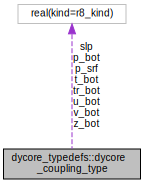
\includegraphics[width=180pt]{structdycore__typedefs_1_1dycore__coupling__type__coll__graph}
\end{center}
\end{figure}
\subsection*{Public Member Functions}
\begin{DoxyCompactItemize}
\item 
procedure \hyperlink{structdycore__typedefs_1_1dycore__coupling__type_a5595a255bb531fcd690fce7641670853}{create} =$>$ \hyperlink{classdycore__typedefs_a38faf32efa46d5157193e3c6ff98533e}{coupling\-\_\-create}
\begin{DoxyCompactList}\small\item\em allocate array data \end{DoxyCompactList}\end{DoxyCompactItemize}
\subsection*{Public Attributes}
\begin{DoxyCompactItemize}
\item 
real(kind=r8\-\_\-kind), dimension(\-:), \\*
pointer \hyperlink{structdycore__typedefs_1_1dycore__coupling__type_a8bdc2008232e57dff5cf7382c500f02e}{p\-\_\-srf} =$>$ null()
\item 
real(kind=r8\-\_\-kind), dimension(\-:), \\*
pointer \hyperlink{structdycore__typedefs_1_1dycore__coupling__type_a35bdfaa15f9d5b7b151ae2804bb52149}{t\-\_\-bot} =$>$ null()
\item 
real(kind=r8\-\_\-kind), dimension(\-:), \\*
pointer \hyperlink{structdycore__typedefs_1_1dycore__coupling__type_a4eb475b9dab3982917db471bf4bee05e}{p\-\_\-bot} =$>$ null()
\item 
real(kind=r8\-\_\-kind), dimension(\-:), \\*
pointer \hyperlink{structdycore__typedefs_1_1dycore__coupling__type_a0f1e2c519ff3fb826527fc759f4dcf62}{u\-\_\-bot} =$>$ null()
\item 
real(kind=r8\-\_\-kind), dimension(\-:), \\*
pointer \hyperlink{structdycore__typedefs_1_1dycore__coupling__type_a1cc41e534da5330112d86bee76a8f185}{v\-\_\-bot} =$>$ null()
\item 
real(kind=r8\-\_\-kind), dimension(\-:), \\*
pointer \hyperlink{structdycore__typedefs_1_1dycore__coupling__type_a92cc02abdb31595b5e42e1e76ebc4943}{z\-\_\-bot} =$>$ null()
\item 
real(kind=r8\-\_\-kind), dimension(\-:), \\*
pointer \hyperlink{structdycore__typedefs_1_1dycore__coupling__type_ac11a4dc51ade2f678aa2511deaa0695a}{slp} =$>$ null()
\item 
real(kind=r8\-\_\-kind), dimension(\-:,\-:), \\*
pointer \hyperlink{structdycore__typedefs_1_1dycore__coupling__type_ac058ed0372a4f29cd443088d91bf5214}{tr\-\_\-bot} =$>$ null()
\end{DoxyCompactItemize}


\subsection{Detailed Description}


Definition at line 42 of file D\-Y\-C\-O\-R\-E\-\_\-typedefs.\-F90.



\subsection{Member Function/\-Subroutine Documentation}
\index{dycore\-\_\-typedefs\-::dycore\-\_\-coupling\-\_\-type@{dycore\-\_\-typedefs\-::dycore\-\_\-coupling\-\_\-type}!create@{create}}
\index{create@{create}!dycore_typedefs::dycore_coupling_type@{dycore\-\_\-typedefs\-::dycore\-\_\-coupling\-\_\-type}}
\subsubsection[{create}]{\setlength{\rightskip}{0pt plus 5cm}procedure dycore\-\_\-typedefs\-::dycore\-\_\-coupling\-\_\-type\-::create (
\begin{DoxyParamCaption}
{}
\end{DoxyParamCaption}
)}\label{structdycore__typedefs_1_1dycore__coupling__type_a5595a255bb531fcd690fce7641670853}


allocate array data 



Definition at line 62 of file D\-Y\-C\-O\-R\-E\-\_\-typedefs.\-F90.



References dycore\-\_\-typedefs\-::coupling\-\_\-create().



Referenced by dycore\-\_\-typedefs\-::dycore\-\_\-diag\-\_\-type\-::create().



\subsection{Member Data Documentation}
\index{dycore\-\_\-typedefs\-::dycore\-\_\-coupling\-\_\-type@{dycore\-\_\-typedefs\-::dycore\-\_\-coupling\-\_\-type}!p\-\_\-bot@{p\-\_\-bot}}
\index{p\-\_\-bot@{p\-\_\-bot}!dycore_typedefs::dycore_coupling_type@{dycore\-\_\-typedefs\-::dycore\-\_\-coupling\-\_\-type}}
\subsubsection[{p\-\_\-bot}]{\setlength{\rightskip}{0pt plus 5cm}real (kind=r8\-\_\-kind), dimension(\-:), pointer dycore\-\_\-typedefs\-::dycore\-\_\-coupling\-\_\-type\-::p\-\_\-bot =$>$ null()}\label{structdycore__typedefs_1_1dycore__coupling__type_a4eb475b9dab3982917db471bf4bee05e}


Definition at line 49 of file D\-Y\-C\-O\-R\-E\-\_\-typedefs.\-F90.

\index{dycore\-\_\-typedefs\-::dycore\-\_\-coupling\-\_\-type@{dycore\-\_\-typedefs\-::dycore\-\_\-coupling\-\_\-type}!p\-\_\-srf@{p\-\_\-srf}}
\index{p\-\_\-srf@{p\-\_\-srf}!dycore_typedefs::dycore_coupling_type@{dycore\-\_\-typedefs\-::dycore\-\_\-coupling\-\_\-type}}
\subsubsection[{p\-\_\-srf}]{\setlength{\rightskip}{0pt plus 5cm}real (kind=r8\-\_\-kind), dimension(\-:), pointer dycore\-\_\-typedefs\-::dycore\-\_\-coupling\-\_\-type\-::p\-\_\-srf =$>$ null()}\label{structdycore__typedefs_1_1dycore__coupling__type_a8bdc2008232e57dff5cf7382c500f02e}


Definition at line 45 of file D\-Y\-C\-O\-R\-E\-\_\-typedefs.\-F90.

\index{dycore\-\_\-typedefs\-::dycore\-\_\-coupling\-\_\-type@{dycore\-\_\-typedefs\-::dycore\-\_\-coupling\-\_\-type}!slp@{slp}}
\index{slp@{slp}!dycore_typedefs::dycore_coupling_type@{dycore\-\_\-typedefs\-::dycore\-\_\-coupling\-\_\-type}}
\subsubsection[{slp}]{\setlength{\rightskip}{0pt plus 5cm}real (kind=r8\-\_\-kind), dimension(\-:), pointer dycore\-\_\-typedefs\-::dycore\-\_\-coupling\-\_\-type\-::slp =$>$ null()}\label{structdycore__typedefs_1_1dycore__coupling__type_ac11a4dc51ade2f678aa2511deaa0695a}


Definition at line 55 of file D\-Y\-C\-O\-R\-E\-\_\-typedefs.\-F90.

\index{dycore\-\_\-typedefs\-::dycore\-\_\-coupling\-\_\-type@{dycore\-\_\-typedefs\-::dycore\-\_\-coupling\-\_\-type}!t\-\_\-bot@{t\-\_\-bot}}
\index{t\-\_\-bot@{t\-\_\-bot}!dycore_typedefs::dycore_coupling_type@{dycore\-\_\-typedefs\-::dycore\-\_\-coupling\-\_\-type}}
\subsubsection[{t\-\_\-bot}]{\setlength{\rightskip}{0pt plus 5cm}real (kind=r8\-\_\-kind), dimension(\-:), pointer dycore\-\_\-typedefs\-::dycore\-\_\-coupling\-\_\-type\-::t\-\_\-bot =$>$ null()}\label{structdycore__typedefs_1_1dycore__coupling__type_a35bdfaa15f9d5b7b151ae2804bb52149}


Definition at line 48 of file D\-Y\-C\-O\-R\-E\-\_\-typedefs.\-F90.

\index{dycore\-\_\-typedefs\-::dycore\-\_\-coupling\-\_\-type@{dycore\-\_\-typedefs\-::dycore\-\_\-coupling\-\_\-type}!tr\-\_\-bot@{tr\-\_\-bot}}
\index{tr\-\_\-bot@{tr\-\_\-bot}!dycore_typedefs::dycore_coupling_type@{dycore\-\_\-typedefs\-::dycore\-\_\-coupling\-\_\-type}}
\subsubsection[{tr\-\_\-bot}]{\setlength{\rightskip}{0pt plus 5cm}real (kind=r8\-\_\-kind), dimension(\-:,\-:), pointer dycore\-\_\-typedefs\-::dycore\-\_\-coupling\-\_\-type\-::tr\-\_\-bot =$>$ null()}\label{structdycore__typedefs_1_1dycore__coupling__type_ac058ed0372a4f29cd443088d91bf5214}


Definition at line 58 of file D\-Y\-C\-O\-R\-E\-\_\-typedefs.\-F90.

\index{dycore\-\_\-typedefs\-::dycore\-\_\-coupling\-\_\-type@{dycore\-\_\-typedefs\-::dycore\-\_\-coupling\-\_\-type}!u\-\_\-bot@{u\-\_\-bot}}
\index{u\-\_\-bot@{u\-\_\-bot}!dycore_typedefs::dycore_coupling_type@{dycore\-\_\-typedefs\-::dycore\-\_\-coupling\-\_\-type}}
\subsubsection[{u\-\_\-bot}]{\setlength{\rightskip}{0pt plus 5cm}real (kind=r8\-\_\-kind), dimension(\-:), pointer dycore\-\_\-typedefs\-::dycore\-\_\-coupling\-\_\-type\-::u\-\_\-bot =$>$ null()}\label{structdycore__typedefs_1_1dycore__coupling__type_a0f1e2c519ff3fb826527fc759f4dcf62}


Definition at line 50 of file D\-Y\-C\-O\-R\-E\-\_\-typedefs.\-F90.

\index{dycore\-\_\-typedefs\-::dycore\-\_\-coupling\-\_\-type@{dycore\-\_\-typedefs\-::dycore\-\_\-coupling\-\_\-type}!v\-\_\-bot@{v\-\_\-bot}}
\index{v\-\_\-bot@{v\-\_\-bot}!dycore_typedefs::dycore_coupling_type@{dycore\-\_\-typedefs\-::dycore\-\_\-coupling\-\_\-type}}
\subsubsection[{v\-\_\-bot}]{\setlength{\rightskip}{0pt plus 5cm}real (kind=r8\-\_\-kind), dimension(\-:), pointer dycore\-\_\-typedefs\-::dycore\-\_\-coupling\-\_\-type\-::v\-\_\-bot =$>$ null()}\label{structdycore__typedefs_1_1dycore__coupling__type_a1cc41e534da5330112d86bee76a8f185}


Definition at line 51 of file D\-Y\-C\-O\-R\-E\-\_\-typedefs.\-F90.

\index{dycore\-\_\-typedefs\-::dycore\-\_\-coupling\-\_\-type@{dycore\-\_\-typedefs\-::dycore\-\_\-coupling\-\_\-type}!z\-\_\-bot@{z\-\_\-bot}}
\index{z\-\_\-bot@{z\-\_\-bot}!dycore_typedefs::dycore_coupling_type@{dycore\-\_\-typedefs\-::dycore\-\_\-coupling\-\_\-type}}
\subsubsection[{z\-\_\-bot}]{\setlength{\rightskip}{0pt plus 5cm}real (kind=r8\-\_\-kind), dimension(\-:), pointer dycore\-\_\-typedefs\-::dycore\-\_\-coupling\-\_\-type\-::z\-\_\-bot =$>$ null()}\label{structdycore__typedefs_1_1dycore__coupling__type_a92cc02abdb31595b5e42e1e76ebc4943}


Definition at line 52 of file D\-Y\-C\-O\-R\-E\-\_\-typedefs.\-F90.



The documentation for this type was generated from the following file\-:\begin{DoxyCompactItemize}
\item 
/scratch2/\-N\-A\-G\-A\-P\-E/aoml-\/hafs1/\-Kyle.\-Ahern/acs\-\_\-master\-\_\-readonly/driver/fv\-G\-F\-S/\hyperlink{DYCORE__typedefs_8F90}{D\-Y\-C\-O\-R\-E\-\_\-typedefs.\-F90}\end{DoxyCompactItemize}

\section{dycore\-\_\-typedefs\-:\-:dycore\-\_\-data\-\_\-type Type Reference}
\label{structdycore__typedefs_1_1dycore__data__type}\index{dycore\-\_\-typedefs\-::dycore\-\_\-data\-\_\-type@{dycore\-\_\-typedefs\-::dycore\-\_\-data\-\_\-type}}


Collaboration diagram for dycore\-\_\-typedefs\-:\-:dycore\-\_\-data\-\_\-type\-:
\nopagebreak
\begin{figure}[H]
\begin{center}
\leavevmode
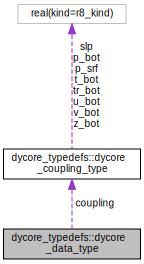
\includegraphics[width=180pt]{structdycore__typedefs_1_1dycore__data__type__coll__graph}
\end{center}
\end{figure}
\subsection*{Public Attributes}
\begin{DoxyCompactItemize}
\item 
type(\hyperlink{structdycore__typedefs_1_1dycore__coupling__type}{dycore\-\_\-coupling\-\_\-type}) \hyperlink{structdycore__typedefs_1_1dycore__data__type_a6fb0d100c78f2d8decac67ed984d968a}{coupling}
\end{DoxyCompactItemize}


\subsection{Detailed Description}


Definition at line 94 of file D\-Y\-C\-O\-R\-E\-\_\-typedefs.\-F90.



\subsection{Member Data Documentation}
\index{dycore\-\_\-typedefs\-::dycore\-\_\-data\-\_\-type@{dycore\-\_\-typedefs\-::dycore\-\_\-data\-\_\-type}!coupling@{coupling}}
\index{coupling@{coupling}!dycore_typedefs::dycore_data_type@{dycore\-\_\-typedefs\-::dycore\-\_\-data\-\_\-type}}
\subsubsection[{coupling}]{\setlength{\rightskip}{0pt plus 5cm}type({\bf dycore\-\_\-coupling\-\_\-type}) dycore\-\_\-typedefs\-::dycore\-\_\-data\-\_\-type\-::coupling}\label{structdycore__typedefs_1_1dycore__data__type_a6fb0d100c78f2d8decac67ed984d968a}


Definition at line 95 of file D\-Y\-C\-O\-R\-E\-\_\-typedefs.\-F90.



The documentation for this type was generated from the following file\-:\begin{DoxyCompactItemize}
\item 
/scratch2/\-N\-A\-G\-A\-P\-E/aoml-\/hafs1/\-Kyle.\-Ahern/acs\-\_\-master\-\_\-readonly/driver/fv\-G\-F\-S/\hyperlink{DYCORE__typedefs_8F90}{D\-Y\-C\-O\-R\-E\-\_\-typedefs.\-F90}\end{DoxyCompactItemize}

\section{dycore\-\_\-typedefs\-:\-:dycore\-\_\-diag\-\_\-type Type Reference}
\label{structdycore__typedefs_1_1dycore__diag__type}\index{dycore\-\_\-typedefs\-::dycore\-\_\-diag\-\_\-type@{dycore\-\_\-typedefs\-::dycore\-\_\-diag\-\_\-type}}


Collaboration diagram for dycore\-\_\-typedefs\-:\-:dycore\-\_\-diag\-\_\-type\-:
\nopagebreak
\begin{figure}[H]
\begin{center}
\leavevmode
\includegraphics[width=350pt]{structdycore__typedefs_1_1dycore__diag__type__coll__graph}
\end{center}
\end{figure}
\subsection*{Public Member Functions}
\begin{DoxyCompactItemize}
\item 
procedure \hyperlink{structdycore__typedefs_1_1dycore__diag__type_a0ff0f4a073adc31b5fc72237e43fd1b9}{create} =$>$ \hyperlink{classdycore__typedefs_a6a4ce247c95b0a8791caf9ce5c4f28b0}{diag\-\_\-create}
\item 
procedure \hyperlink{structdycore__typedefs_1_1dycore__diag__type_a90a9e69d10c0004ebce151318b8aab03}{zero} =$>$ \hyperlink{classdycore__typedefs_a9b0e3a5b8a1e2e40e721055f51c3a437}{diag\-\_\-zero}
\end{DoxyCompactItemize}
\subsection*{Public Attributes}
\begin{DoxyCompactItemize}
\item 
character(len=32) \hyperlink{structdycore__typedefs_1_1dycore__diag__type_a0fb804dacaaccb289ae3aabe1b445f31}{name}
\begin{DoxyCompactList}\small\item\em variable name in source \end{DoxyCompactList}\item 
character(len=32) \hyperlink{structdycore__typedefs_1_1dycore__diag__type_a06218b1408fa9b6730e1034b6d26c77c}{output\-\_\-name}
\begin{DoxyCompactList}\small\item\em output name for variable \end{DoxyCompactList}\item 
character(len=32) \hyperlink{structdycore__typedefs_1_1dycore__diag__type_ab3879ca062dfe1cb6362f9397691b87b}{mod\-\_\-name}
\begin{DoxyCompactList}\small\item\em module name (e.\-g. physics, radiation, etc) \end{DoxyCompactList}\item 
character(len=32) \hyperlink{structdycore__typedefs_1_1dycore__diag__type_adce883539145f85406cd69b9286b2f3c}{file\-\_\-name}
\begin{DoxyCompactList}\small\item\em output file name for variable \end{DoxyCompactList}\item 
character(len=128) \hyperlink{structdycore__typedefs_1_1dycore__diag__type_ad80ebe3be46ad81d5899d42175361dce}{desc}
\begin{DoxyCompactList}\small\item\em long description of field \end{DoxyCompactList}\item 
character(len=32) \hyperlink{structdycore__typedefs_1_1dycore__diag__type_ac3db7b34f757a51cd2f00f6d0d68539f}{unit}
\begin{DoxyCompactList}\small\item\em units associated with fields \end{DoxyCompactList}\item 
character(len=32) \hyperlink{structdycore__typedefs_1_1dycore__diag__type_ab80143ebc2497201057b46c075d3bf68}{type\-\_\-stat\-\_\-proc}
\begin{DoxyCompactList}\small\item\em type of statistic processing\-: average, accumulation, maximal, \end{DoxyCompactList}\item 
character(len=32) \hyperlink{structdycore__typedefs_1_1dycore__diag__type_a5c500119b8307feb96268bf4b45a3d90}{level\-\_\-type}
\begin{DoxyCompactList}\small\item\em vertical level of the field \end{DoxyCompactList}\item 
integer \hyperlink{structdycore__typedefs_1_1dycore__diag__type_ac5a325a7f34fb5df278e141ddd62a283}{level}
\begin{DoxyCompactList}\small\item\em vertical level(s) \end{DoxyCompactList}\item 
real(kind=r8\-\_\-kind) \hyperlink{structdycore__typedefs_1_1dycore__diag__type_ae35b7d0f8874805074bb1e02e05628ac}{cnvfac}
\begin{DoxyCompactList}\small\item\em conversion factors to output in specified units \end{DoxyCompactList}\item 
real(kind=r8\-\_\-kind) \hyperlink{structdycore__typedefs_1_1dycore__diag__type_a2fd3a19561d5756ba91a8ca4d7f07986}{zhour}
\begin{DoxyCompactList}\small\item\em forecast hour when bucket was last emptied for statistical processing \end{DoxyCompactList}\item 
real(kind=r8\-\_\-kind) \hyperlink{structdycore__typedefs_1_1dycore__diag__type_a857feb4213b48ce81b3d295561b92058}{fcst\-\_\-hour}
\begin{DoxyCompactList}\small\item\em current forecast hour (same as fhour) \end{DoxyCompactList}\item 
type(\hyperlink{structdycore__typedefs_1_1var__subtype}{var\-\_\-subtype}), dimension(\-:), \\*
allocatable \hyperlink{structdycore__typedefs_1_1dycore__diag__type_affdbdddebd40e81618410f1312a49c5b}{data}
\begin{DoxyCompactList}\small\item\em holds pointers to data in packed format (allocated to nblks) \end{DoxyCompactList}\end{DoxyCompactItemize}


\subsection{Detailed Description}


Definition at line 69 of file D\-Y\-C\-O\-R\-E\-\_\-typedefs.\-F90.



\subsection{Member Function/\-Subroutine Documentation}
\index{dycore\-\_\-typedefs\-::dycore\-\_\-diag\-\_\-type@{dycore\-\_\-typedefs\-::dycore\-\_\-diag\-\_\-type}!create@{create}}
\index{create@{create}!dycore_typedefs::dycore_diag_type@{dycore\-\_\-typedefs\-::dycore\-\_\-diag\-\_\-type}}
\subsubsection[{create}]{\setlength{\rightskip}{0pt plus 5cm}procedure dycore\-\_\-typedefs\-::dycore\-\_\-diag\-\_\-type\-::create (
\begin{DoxyParamCaption}
{}
\end{DoxyParamCaption}
)}\label{structdycore__typedefs_1_1dycore__diag__type_a0ff0f4a073adc31b5fc72237e43fd1b9}


Definition at line 86 of file D\-Y\-C\-O\-R\-E\-\_\-typedefs.\-F90.



References dycore\-\_\-typedefs\-::dycore\-\_\-coupling\-\_\-type\-::create(), and dycore\-\_\-typedefs\-::diag\-\_\-create().

\index{dycore\-\_\-typedefs\-::dycore\-\_\-diag\-\_\-type@{dycore\-\_\-typedefs\-::dycore\-\_\-diag\-\_\-type}!zero@{zero}}
\index{zero@{zero}!dycore_typedefs::dycore_diag_type@{dycore\-\_\-typedefs\-::dycore\-\_\-diag\-\_\-type}}
\subsubsection[{zero}]{\setlength{\rightskip}{0pt plus 5cm}procedure dycore\-\_\-typedefs\-::dycore\-\_\-diag\-\_\-type\-::zero (
\begin{DoxyParamCaption}
{}
\end{DoxyParamCaption}
)}\label{structdycore__typedefs_1_1dycore__diag__type_a90a9e69d10c0004ebce151318b8aab03}


Definition at line 87 of file D\-Y\-C\-O\-R\-E\-\_\-typedefs.\-F90.



References dycore\-\_\-typedefs\-::diag\-\_\-zero().



\subsection{Member Data Documentation}
\index{dycore\-\_\-typedefs\-::dycore\-\_\-diag\-\_\-type@{dycore\-\_\-typedefs\-::dycore\-\_\-diag\-\_\-type}!cnvfac@{cnvfac}}
\index{cnvfac@{cnvfac}!dycore_typedefs::dycore_diag_type@{dycore\-\_\-typedefs\-::dycore\-\_\-diag\-\_\-type}}
\subsubsection[{cnvfac}]{\setlength{\rightskip}{0pt plus 5cm}real(kind=r8\-\_\-kind) dycore\-\_\-typedefs\-::dycore\-\_\-diag\-\_\-type\-::cnvfac}\label{structdycore__typedefs_1_1dycore__diag__type_ae35b7d0f8874805074bb1e02e05628ac}


conversion factors to output in specified units 



Definition at line 81 of file D\-Y\-C\-O\-R\-E\-\_\-typedefs.\-F90.

\index{dycore\-\_\-typedefs\-::dycore\-\_\-diag\-\_\-type@{dycore\-\_\-typedefs\-::dycore\-\_\-diag\-\_\-type}!data@{data}}
\index{data@{data}!dycore_typedefs::dycore_diag_type@{dycore\-\_\-typedefs\-::dycore\-\_\-diag\-\_\-type}}
\subsubsection[{data}]{\setlength{\rightskip}{0pt plus 5cm}type({\bf var\-\_\-subtype}), dimension(\-:), allocatable dycore\-\_\-typedefs\-::dycore\-\_\-diag\-\_\-type\-::data}\label{structdycore__typedefs_1_1dycore__diag__type_affdbdddebd40e81618410f1312a49c5b}


holds pointers to data in packed format (allocated to nblks) 



Definition at line 84 of file D\-Y\-C\-O\-R\-E\-\_\-typedefs.\-F90.

\index{dycore\-\_\-typedefs\-::dycore\-\_\-diag\-\_\-type@{dycore\-\_\-typedefs\-::dycore\-\_\-diag\-\_\-type}!desc@{desc}}
\index{desc@{desc}!dycore_typedefs::dycore_diag_type@{dycore\-\_\-typedefs\-::dycore\-\_\-diag\-\_\-type}}
\subsubsection[{desc}]{\setlength{\rightskip}{0pt plus 5cm}character(len=128) dycore\-\_\-typedefs\-::dycore\-\_\-diag\-\_\-type\-::desc}\label{structdycore__typedefs_1_1dycore__diag__type_ad80ebe3be46ad81d5899d42175361dce}


long description of field 



Definition at line 74 of file D\-Y\-C\-O\-R\-E\-\_\-typedefs.\-F90.

\index{dycore\-\_\-typedefs\-::dycore\-\_\-diag\-\_\-type@{dycore\-\_\-typedefs\-::dycore\-\_\-diag\-\_\-type}!fcst\-\_\-hour@{fcst\-\_\-hour}}
\index{fcst\-\_\-hour@{fcst\-\_\-hour}!dycore_typedefs::dycore_diag_type@{dycore\-\_\-typedefs\-::dycore\-\_\-diag\-\_\-type}}
\subsubsection[{fcst\-\_\-hour}]{\setlength{\rightskip}{0pt plus 5cm}real(kind=r8\-\_\-kind) dycore\-\_\-typedefs\-::dycore\-\_\-diag\-\_\-type\-::fcst\-\_\-hour}\label{structdycore__typedefs_1_1dycore__diag__type_a857feb4213b48ce81b3d295561b92058}


current forecast hour (same as fhour) 



Definition at line 83 of file D\-Y\-C\-O\-R\-E\-\_\-typedefs.\-F90.

\index{dycore\-\_\-typedefs\-::dycore\-\_\-diag\-\_\-type@{dycore\-\_\-typedefs\-::dycore\-\_\-diag\-\_\-type}!file\-\_\-name@{file\-\_\-name}}
\index{file\-\_\-name@{file\-\_\-name}!dycore_typedefs::dycore_diag_type@{dycore\-\_\-typedefs\-::dycore\-\_\-diag\-\_\-type}}
\subsubsection[{file\-\_\-name}]{\setlength{\rightskip}{0pt plus 5cm}character(len=32) dycore\-\_\-typedefs\-::dycore\-\_\-diag\-\_\-type\-::file\-\_\-name}\label{structdycore__typedefs_1_1dycore__diag__type_adce883539145f85406cd69b9286b2f3c}


output file name for variable 



Definition at line 73 of file D\-Y\-C\-O\-R\-E\-\_\-typedefs.\-F90.

\index{dycore\-\_\-typedefs\-::dycore\-\_\-diag\-\_\-type@{dycore\-\_\-typedefs\-::dycore\-\_\-diag\-\_\-type}!level@{level}}
\index{level@{level}!dycore_typedefs::dycore_diag_type@{dycore\-\_\-typedefs\-::dycore\-\_\-diag\-\_\-type}}
\subsubsection[{level}]{\setlength{\rightskip}{0pt plus 5cm}integer dycore\-\_\-typedefs\-::dycore\-\_\-diag\-\_\-type\-::level}\label{structdycore__typedefs_1_1dycore__diag__type_ac5a325a7f34fb5df278e141ddd62a283}


vertical level(s) 



Definition at line 80 of file D\-Y\-C\-O\-R\-E\-\_\-typedefs.\-F90.

\index{dycore\-\_\-typedefs\-::dycore\-\_\-diag\-\_\-type@{dycore\-\_\-typedefs\-::dycore\-\_\-diag\-\_\-type}!level\-\_\-type@{level\-\_\-type}}
\index{level\-\_\-type@{level\-\_\-type}!dycore_typedefs::dycore_diag_type@{dycore\-\_\-typedefs\-::dycore\-\_\-diag\-\_\-type}}
\subsubsection[{level\-\_\-type}]{\setlength{\rightskip}{0pt plus 5cm}character(len=32) dycore\-\_\-typedefs\-::dycore\-\_\-diag\-\_\-type\-::level\-\_\-type}\label{structdycore__typedefs_1_1dycore__diag__type_a5c500119b8307feb96268bf4b45a3d90}


vertical level of the field 



Definition at line 79 of file D\-Y\-C\-O\-R\-E\-\_\-typedefs.\-F90.

\index{dycore\-\_\-typedefs\-::dycore\-\_\-diag\-\_\-type@{dycore\-\_\-typedefs\-::dycore\-\_\-diag\-\_\-type}!mod\-\_\-name@{mod\-\_\-name}}
\index{mod\-\_\-name@{mod\-\_\-name}!dycore_typedefs::dycore_diag_type@{dycore\-\_\-typedefs\-::dycore\-\_\-diag\-\_\-type}}
\subsubsection[{mod\-\_\-name}]{\setlength{\rightskip}{0pt plus 5cm}character(len=32) dycore\-\_\-typedefs\-::dycore\-\_\-diag\-\_\-type\-::mod\-\_\-name}\label{structdycore__typedefs_1_1dycore__diag__type_ab3879ca062dfe1cb6362f9397691b87b}


module name (e.\-g. physics, radiation, etc) 



Definition at line 72 of file D\-Y\-C\-O\-R\-E\-\_\-typedefs.\-F90.

\index{dycore\-\_\-typedefs\-::dycore\-\_\-diag\-\_\-type@{dycore\-\_\-typedefs\-::dycore\-\_\-diag\-\_\-type}!name@{name}}
\index{name@{name}!dycore_typedefs::dycore_diag_type@{dycore\-\_\-typedefs\-::dycore\-\_\-diag\-\_\-type}}
\subsubsection[{name}]{\setlength{\rightskip}{0pt plus 5cm}character(len=32) dycore\-\_\-typedefs\-::dycore\-\_\-diag\-\_\-type\-::name}\label{structdycore__typedefs_1_1dycore__diag__type_a0fb804dacaaccb289ae3aabe1b445f31}


variable name in source 



Definition at line 70 of file D\-Y\-C\-O\-R\-E\-\_\-typedefs.\-F90.

\index{dycore\-\_\-typedefs\-::dycore\-\_\-diag\-\_\-type@{dycore\-\_\-typedefs\-::dycore\-\_\-diag\-\_\-type}!output\-\_\-name@{output\-\_\-name}}
\index{output\-\_\-name@{output\-\_\-name}!dycore_typedefs::dycore_diag_type@{dycore\-\_\-typedefs\-::dycore\-\_\-diag\-\_\-type}}
\subsubsection[{output\-\_\-name}]{\setlength{\rightskip}{0pt plus 5cm}character(len=32) dycore\-\_\-typedefs\-::dycore\-\_\-diag\-\_\-type\-::output\-\_\-name}\label{structdycore__typedefs_1_1dycore__diag__type_a06218b1408fa9b6730e1034b6d26c77c}


output name for variable 



Definition at line 71 of file D\-Y\-C\-O\-R\-E\-\_\-typedefs.\-F90.

\index{dycore\-\_\-typedefs\-::dycore\-\_\-diag\-\_\-type@{dycore\-\_\-typedefs\-::dycore\-\_\-diag\-\_\-type}!type\-\_\-stat\-\_\-proc@{type\-\_\-stat\-\_\-proc}}
\index{type\-\_\-stat\-\_\-proc@{type\-\_\-stat\-\_\-proc}!dycore_typedefs::dycore_diag_type@{dycore\-\_\-typedefs\-::dycore\-\_\-diag\-\_\-type}}
\subsubsection[{type\-\_\-stat\-\_\-proc}]{\setlength{\rightskip}{0pt plus 5cm}character(len=32) dycore\-\_\-typedefs\-::dycore\-\_\-diag\-\_\-type\-::type\-\_\-stat\-\_\-proc}\label{structdycore__typedefs_1_1dycore__diag__type_ab80143ebc2497201057b46c075d3bf68}


type of statistic processing\-: average, accumulation, maximal, 



Definition at line 76 of file D\-Y\-C\-O\-R\-E\-\_\-typedefs.\-F90.

\index{dycore\-\_\-typedefs\-::dycore\-\_\-diag\-\_\-type@{dycore\-\_\-typedefs\-::dycore\-\_\-diag\-\_\-type}!unit@{unit}}
\index{unit@{unit}!dycore_typedefs::dycore_diag_type@{dycore\-\_\-typedefs\-::dycore\-\_\-diag\-\_\-type}}
\subsubsection[{unit}]{\setlength{\rightskip}{0pt plus 5cm}character(len=32) dycore\-\_\-typedefs\-::dycore\-\_\-diag\-\_\-type\-::unit}\label{structdycore__typedefs_1_1dycore__diag__type_ac3db7b34f757a51cd2f00f6d0d68539f}


units associated with fields 



Definition at line 75 of file D\-Y\-C\-O\-R\-E\-\_\-typedefs.\-F90.

\index{dycore\-\_\-typedefs\-::dycore\-\_\-diag\-\_\-type@{dycore\-\_\-typedefs\-::dycore\-\_\-diag\-\_\-type}!zhour@{zhour}}
\index{zhour@{zhour}!dycore_typedefs::dycore_diag_type@{dycore\-\_\-typedefs\-::dycore\-\_\-diag\-\_\-type}}
\subsubsection[{zhour}]{\setlength{\rightskip}{0pt plus 5cm}real(kind=r8\-\_\-kind) dycore\-\_\-typedefs\-::dycore\-\_\-diag\-\_\-type\-::zhour}\label{structdycore__typedefs_1_1dycore__diag__type_a2fd3a19561d5756ba91a8ca4d7f07986}


forecast hour when bucket was last emptied for statistical processing 



Definition at line 82 of file D\-Y\-C\-O\-R\-E\-\_\-typedefs.\-F90.



The documentation for this type was generated from the following file\-:\begin{DoxyCompactItemize}
\item 
/scratch2/\-N\-A\-G\-A\-P\-E/aoml-\/hafs1/\-Kyle.\-Ahern/acs\-\_\-master\-\_\-readonly/driver/fv\-G\-F\-S/\hyperlink{DYCORE__typedefs_8F90}{D\-Y\-C\-O\-R\-E\-\_\-typedefs.\-F90}\end{DoxyCompactItemize}

\section{dycore\-\_\-typedefs Module Reference}
\label{classdycore__typedefs}\index{dycore\-\_\-typedefs@{dycore\-\_\-typedefs}}


Collaboration diagram for dycore\-\_\-typedefs\-:
\nopagebreak
\begin{figure}[H]
\begin{center}
\leavevmode
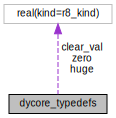
\includegraphics[width=152pt]{classdycore__typedefs__coll__graph}
\end{center}
\end{figure}
\subsection*{Data Types}
\begin{DoxyCompactItemize}
\item 
type \hyperlink{structdycore__typedefs_1_1dycore__coupling__type}{dycore\-\_\-coupling\-\_\-type}
\item 
type \hyperlink{structdycore__typedefs_1_1dycore__data__type}{dycore\-\_\-data\-\_\-type}
\item 
type \hyperlink{structdycore__typedefs_1_1dycore__diag__type}{dycore\-\_\-diag\-\_\-type}
\item 
type \hyperlink{structdycore__typedefs_1_1var__subtype}{var\-\_\-subtype}
\end{DoxyCompactItemize}
\subsection*{Public Member Functions}
\begin{DoxyCompactItemize}
\item 
subroutine \hyperlink{classdycore__typedefs_a38faf32efa46d5157193e3c6ff98533e}{coupling\-\_\-create} (Coupling, I\-M, Ntracers)
\item 
subroutine \hyperlink{classdycore__typedefs_a6a4ce247c95b0a8791caf9ce5c4f28b0}{diag\-\_\-create} (Diag, I\-M, Ntracers)
\item 
subroutine \hyperlink{classdycore__typedefs_a9b0e3a5b8a1e2e40e721055f51c3a437}{diag\-\_\-zero} (Diag)
\end{DoxyCompactItemize}
\subsection*{Public Attributes}
\begin{DoxyCompactItemize}
\item 
real(kind=r8\-\_\-kind), parameter \hyperlink{classdycore__typedefs_ae3151b57d26d5e0876cec34bea3cc2a1}{zero} = 0.\-0\-\_\-r8\-\_\-kind
\item 
real(kind=r8\-\_\-kind), parameter \hyperlink{classdycore__typedefs_a6c66ffd3c70a9d6caafafb6e1d6419b9}{huge} = 9.\-9999\-D15
\item 
real(kind=r8\-\_\-kind), parameter \hyperlink{classdycore__typedefs_adfd79c198bdf05be48cf1bf5bc32f7ed}{clear\-\_\-val} = \hyperlink{classdycore__typedefs_ae3151b57d26d5e0876cec34bea3cc2a1}{zero}
\end{DoxyCompactItemize}


\subsection{Detailed Description}


Definition at line 21 of file D\-Y\-C\-O\-R\-E\-\_\-typedefs.\-F90.



\subsection{Member Function/\-Subroutine Documentation}
\index{dycore\-\_\-typedefs@{dycore\-\_\-typedefs}!coupling\-\_\-create@{coupling\-\_\-create}}
\index{coupling\-\_\-create@{coupling\-\_\-create}!dycore_typedefs@{dycore\-\_\-typedefs}}
\subsubsection[{coupling\-\_\-create}]{\setlength{\rightskip}{0pt plus 5cm}subroutine dycore\-\_\-typedefs\-::coupling\-\_\-create (
\begin{DoxyParamCaption}
\item[{class({\bf dycore\-\_\-coupling\-\_\-type})}]{Coupling, }
\item[{integer, intent(in)}]{I\-M, }
\item[{integer, intent(in)}]{Ntracers}
\end{DoxyParamCaption}
)}\label{classdycore__typedefs_a38faf32efa46d5157193e3c6ff98533e}


Definition at line 111 of file D\-Y\-C\-O\-R\-E\-\_\-typedefs.\-F90.



Referenced by dycore\-\_\-typedefs\-::dycore\-\_\-coupling\-\_\-type\-::create().

\index{dycore\-\_\-typedefs@{dycore\-\_\-typedefs}!diag\-\_\-create@{diag\-\_\-create}}
\index{diag\-\_\-create@{diag\-\_\-create}!dycore_typedefs@{dycore\-\_\-typedefs}}
\subsubsection[{diag\-\_\-create}]{\setlength{\rightskip}{0pt plus 5cm}subroutine dycore\-\_\-typedefs\-::diag\-\_\-create (
\begin{DoxyParamCaption}
\item[{class({\bf dycore\-\_\-diag\-\_\-type})}]{Diag, }
\item[{integer, intent(in)}]{I\-M, }
\item[{integer, intent(in)}]{Ntracers}
\end{DoxyParamCaption}
)}\label{classdycore__typedefs_a6a4ce247c95b0a8791caf9ce5c4f28b0}


Definition at line 148 of file D\-Y\-C\-O\-R\-E\-\_\-typedefs.\-F90.



Referenced by dycore\-\_\-typedefs\-::dycore\-\_\-diag\-\_\-type\-::create().

\index{dycore\-\_\-typedefs@{dycore\-\_\-typedefs}!diag\-\_\-zero@{diag\-\_\-zero}}
\index{diag\-\_\-zero@{diag\-\_\-zero}!dycore_typedefs@{dycore\-\_\-typedefs}}
\subsubsection[{diag\-\_\-zero}]{\setlength{\rightskip}{0pt plus 5cm}subroutine dycore\-\_\-typedefs\-::diag\-\_\-zero (
\begin{DoxyParamCaption}
\item[{class({\bf dycore\-\_\-diag\-\_\-type})}]{Diag}
\end{DoxyParamCaption}
)}\label{classdycore__typedefs_a9b0e3a5b8a1e2e40e721055f51c3a437}


Definition at line 161 of file D\-Y\-C\-O\-R\-E\-\_\-typedefs.\-F90.



Referenced by dycore\-\_\-typedefs\-::dycore\-\_\-diag\-\_\-type\-::zero().



\subsection{Member Data Documentation}
\index{dycore\-\_\-typedefs@{dycore\-\_\-typedefs}!clear\-\_\-val@{clear\-\_\-val}}
\index{clear\-\_\-val@{clear\-\_\-val}!dycore_typedefs@{dycore\-\_\-typedefs}}
\subsubsection[{clear\-\_\-val}]{\setlength{\rightskip}{0pt plus 5cm}real(kind=r8\-\_\-kind), parameter dycore\-\_\-typedefs\-::clear\-\_\-val = {\bf zero}}\label{classdycore__typedefs_adfd79c198bdf05be48cf1bf5bc32f7ed}


Definition at line 30 of file D\-Y\-C\-O\-R\-E\-\_\-typedefs.\-F90.

\index{dycore\-\_\-typedefs@{dycore\-\_\-typedefs}!huge@{huge}}
\index{huge@{huge}!dycore_typedefs@{dycore\-\_\-typedefs}}
\subsubsection[{huge}]{\setlength{\rightskip}{0pt plus 5cm}real(kind=r8\-\_\-kind), parameter dycore\-\_\-typedefs\-::huge = 9.\-9999\-D15}\label{classdycore__typedefs_a6c66ffd3c70a9d6caafafb6e1d6419b9}


Definition at line 29 of file D\-Y\-C\-O\-R\-E\-\_\-typedefs.\-F90.

\index{dycore\-\_\-typedefs@{dycore\-\_\-typedefs}!zero@{zero}}
\index{zero@{zero}!dycore_typedefs@{dycore\-\_\-typedefs}}
\subsubsection[{zero}]{\setlength{\rightskip}{0pt plus 5cm}real(kind=r8\-\_\-kind), parameter dycore\-\_\-typedefs\-::zero = 0.\-0\-\_\-r8\-\_\-kind}\label{classdycore__typedefs_ae3151b57d26d5e0876cec34bea3cc2a1}


Definition at line 28 of file D\-Y\-C\-O\-R\-E\-\_\-typedefs.\-F90.



The documentation for this module was generated from the following file\-:\begin{DoxyCompactItemize}
\item 
/scratch2/\-N\-A\-G\-A\-P\-E/aoml-\/hafs1/\-Kyle.\-Ahern/acs\-\_\-master\-\_\-readonly/driver/fv\-G\-F\-S/\hyperlink{DYCORE__typedefs_8F90}{D\-Y\-C\-O\-R\-E\-\_\-typedefs.\-F90}\end{DoxyCompactItemize}

\section{dyn\-\_\-core\-\_\-mod Module Reference}
\label{classdyn__core__mod}\index{dyn\-\_\-core\-\_\-mod@{dyn\-\_\-core\-\_\-mod}}


The module 'dyn\-\_\-core' peforms the Lagrangian acoustic dynamics described by \cite{lin2004vertically}.  




Collaboration diagram for dyn\-\_\-core\-\_\-mod\-:
\nopagebreak
\begin{figure}[H]
\begin{center}
\leavevmode
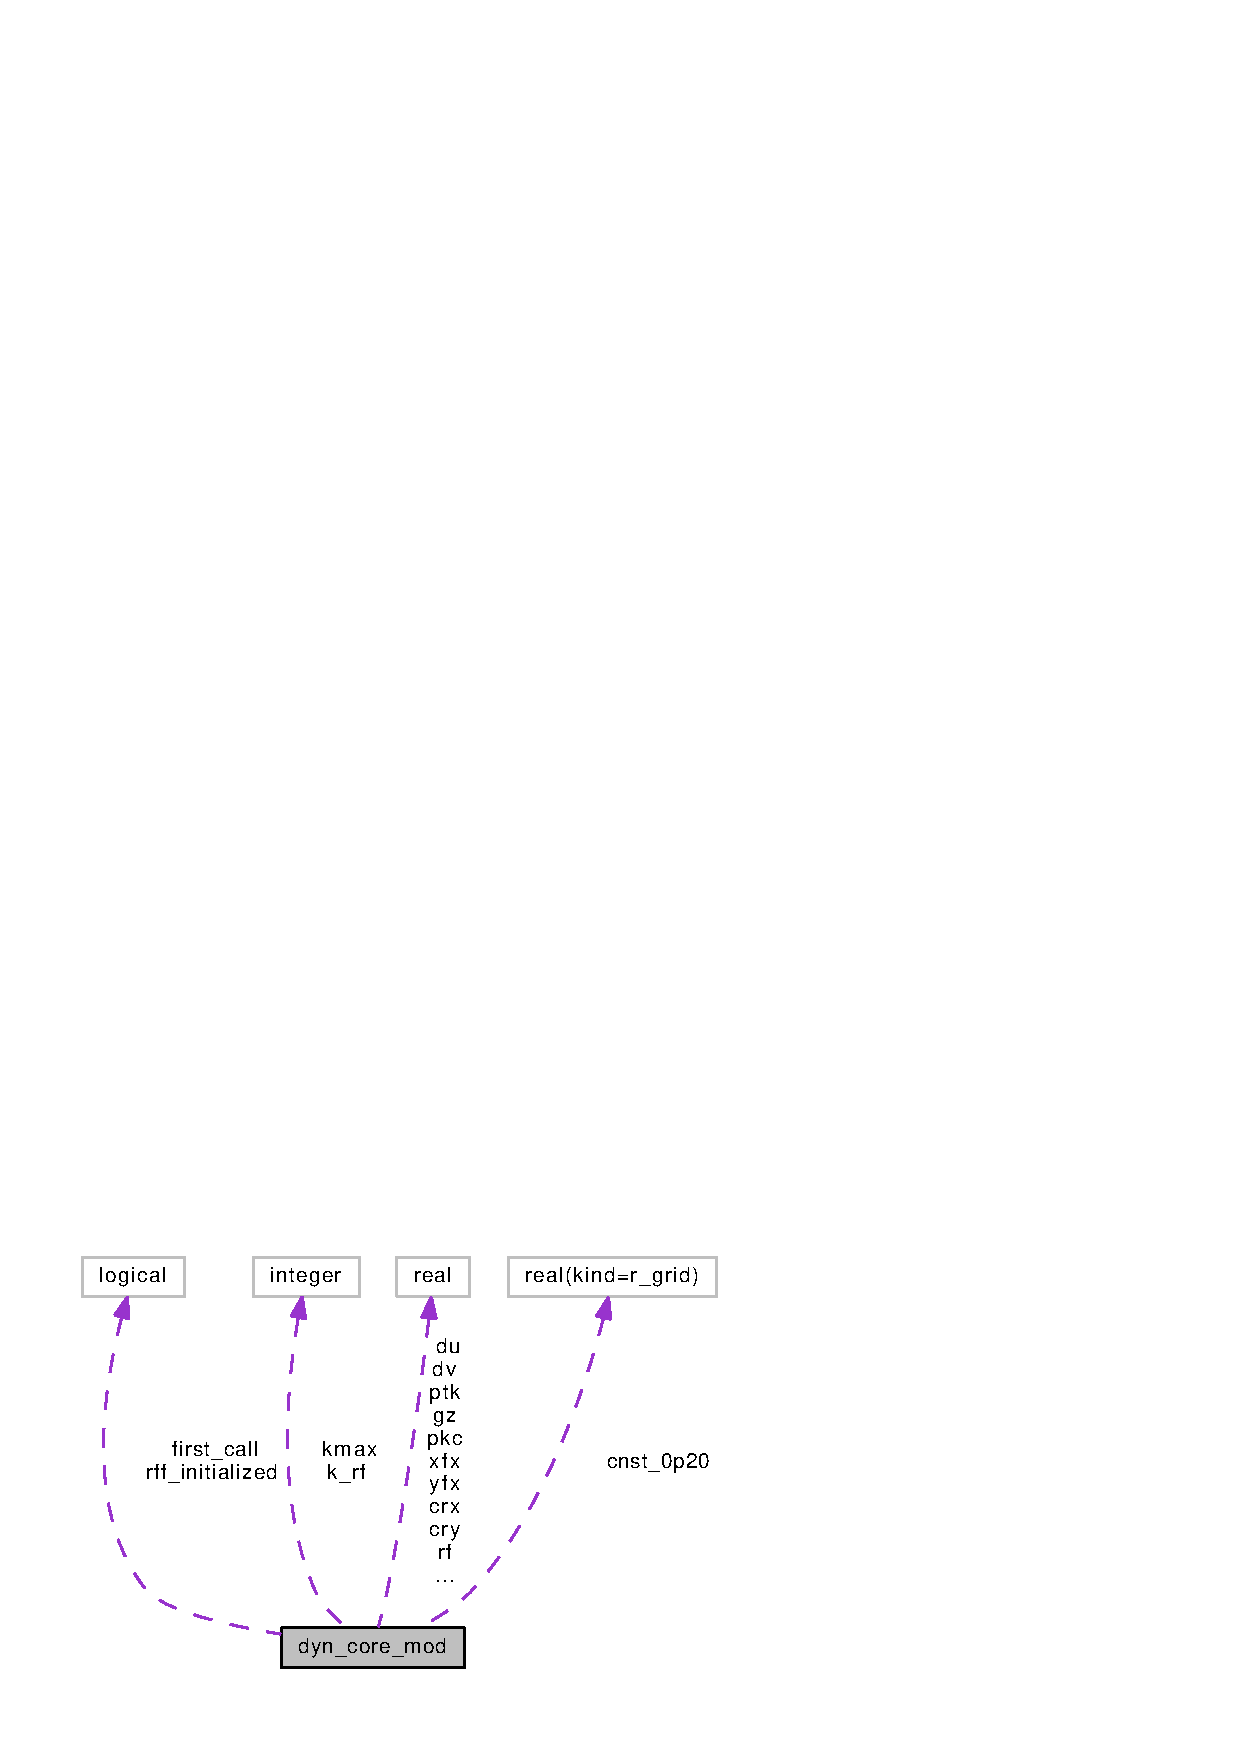
\includegraphics[width=348pt]{classdyn__core__mod__coll__graph}
\end{center}
\end{figure}
\subsection*{Public Member Functions}
\begin{DoxyCompactItemize}
\item 
subroutine, public \hyperlink{classdyn__core__mod_a05793faec17e66169e5f57f4b1a82033}{dyn\-\_\-core} (npx, npy, npz, ng, sphum, nq, bdt, n\-\_\-split, zvir, cp, akap, cappa,
\item 
subroutine, public \hyperlink{classdyn__core__mod_ad3018f7acb1006fc424bd0bcaad8b320}{del2\-\_\-cubed} (q, cd, gridstruct, domain, npx, npy, km, nmax, bd)
\begin{DoxyCompactList}\small\item\em The subroutine 'del2-\/cubed' filters the omega field for the physics. \end{DoxyCompactList}\item 
subroutine, public \hyperlink{classdyn__core__mod_a5311fb50c595143cbe4fc4d145532aa0}{init\-\_\-ijk\-\_\-mem} (i1, i2, j1, j2, km, array, var)
\end{DoxyCompactItemize}
\subsection*{Private Member Functions}
\begin{DoxyCompactItemize}
\item 
subroutine \hyperlink{classdyn__core__mod_acb7593139a5dd1dd95e85ea109885036}{pk3\-\_\-halo} (is, ie, js, je, isd, ied, jsd, jed, npz, ptop, akap, \hyperlink{classdyn__core__mod_a6d4525d6fbfd6de35414635dd9f0caea}{pk3}, delp)
\item 
subroutine \hyperlink{classdyn__core__mod_a8eb71dd48e79318207c79f8c5c785619}{pln\-\_\-halo} (is, ie, js, je, isd, ied, jsd, jed, npz, ptop, \hyperlink{classdyn__core__mod_a6d4525d6fbfd6de35414635dd9f0caea}{pk3}, delp)
\item 
subroutine \hyperlink{classdyn__core__mod_a7a28a4d13bab7c8fdbb2704159ec57de}{pe\-\_\-halo} (is, ie, js, je, isd, ied, jsd, jed, npz, ptop, pe, delp)
\item 
subroutine \hyperlink{classdyn__core__mod_a69d9914e89faeebfc49e822b23cf252d}{adv\-\_\-pe} (ua, va, pem, om, gridstruct, bd, npx, npy, npz, ng)
\item 
subroutine \hyperlink{classdyn__core__mod_a93144665e79c95c709361c52734b4f1b}{p\-\_\-grad\-\_\-c} (dt2, npz, \hyperlink{classdyn__core__mod_aa4417385939b0cafbeadaa424ed3c914}{delpc}, \hyperlink{classdyn__core__mod_ab8b896d9a395406f68b58a26d444f9bf}{pkc}, \hyperlink{classdyn__core__mod_add08631b5675064954c9123f29da8d9c}{gz}, uc, vc, bd, rdxc, rdyc, hydrostatic)
\item 
subroutine \hyperlink{classdyn__core__mod_a42c75f9401e5bee9bbe18cef49b1e14e}{nh\-\_\-p\-\_\-grad} (u, v, pp, \hyperlink{classdyn__core__mod_add08631b5675064954c9123f29da8d9c}{gz}, delp, pk, dt, ng, gridstruct, bd, npx, npy, npz, use\-\_\-logp)
\item 
subroutine \hyperlink{classdyn__core__mod_adc04150e3da9d17590f1d3f3c6b6aace}{split\-\_\-p\-\_\-grad} (u, v, pp, \hyperlink{classdyn__core__mod_add08631b5675064954c9123f29da8d9c}{gz}, delp, pk, beta, dt, ng, gridstruct, bd, npx, npy, npz, use\-\_\-logp)
\item 
subroutine \hyperlink{classdyn__core__mod_aab4c66667e9910926b19e1c83c5e1fe2}{one\-\_\-grad\-\_\-p} (u, v, pk, \hyperlink{classdyn__core__mod_add08631b5675064954c9123f29da8d9c}{gz}, divg2, delp, dt, ng, gridstruct, bd, npx, npy, npz, ptop, hydrostatic, a2b\-\_\-ord, d\-\_\-ext)
\item 
subroutine \hyperlink{classdyn__core__mod_a1c91c8f82a1ab87b6ea176c93f24bf4a}{grad1\-\_\-p\-\_\-update} (divg2, u, v, pk, \hyperlink{classdyn__core__mod_add08631b5675064954c9123f29da8d9c}{gz}, dt, ng, gridstruct, bd, npx, npy, npz, ptop, beta, a2b\-\_\-ord)
\item 
subroutine \hyperlink{classdyn__core__mod_aeec216067740dcbbd70b4b0acc7a7c7e}{mix\-\_\-dp} (hydrostatic, w, delp, pt, km, ak, bk, C\-G, fv\-\_\-debug, bd)
\item 
subroutine \hyperlink{classdyn__core__mod_a3afb820ed44d6ca5137ba0c6205ea141}{geopk} (ptop, pe, peln, delp, pk, \hyperlink{classdyn__core__mod_add08631b5675064954c9123f29da8d9c}{gz}, hs, pt,
\begin{DoxyCompactList}\small\item\em The subroutine 'geopk' calculates geopotential and pressure to the kappa. \end{DoxyCompactList}\item 
subroutine \hyperlink{classdyn__core__mod_a23759cc821cf3c1bdb08a0bce8863cc6}{ray\-\_\-fast} (dt, npx, npy, npz, pfull, tau, u, v, w, ks, dp, ptop, hydrostatic, rf\-\_\-cutoff, bd)
\begin{DoxyCompactList}\small\item\em The subroutine 'Ray\-\_\-fast' computes a simple \char`\"{}inline\char`\"{} version of the Rayleigh friction (E\-X\-P\-E\-R\-I\-M\-E\-N\-T\-A\-L -\/ N\-O\-T F\-O\-R G\-E\-N\-E\-R\-A\-L U\-S\-E). \end{DoxyCompactList}\end{DoxyCompactItemize}
\subsection*{Private Attributes}
\begin{DoxyCompactItemize}
\item 
real \hyperlink{classdyn__core__mod_a8743542bdd5648cf4f95698e51afc601}{ptk}
\item 
real \hyperlink{classdyn__core__mod_a4a524216d71d2a5973c30736ce76deb4}{peln1}
\item 
real \hyperlink{classdyn__core__mod_ae3293d99dac97da219d947fa14fe4b81}{rgrav}
\item 
real \hyperlink{classdyn__core__mod_ab65a8777b1bd81dcfc1b7cfed5a974c5}{d3\-\_\-damp}
\item 
real, dimension(\-:,\-:,\-:), allocatable \hyperlink{classdyn__core__mod_a759f692eeae8f494dd172747b34ef905}{ut}
\item 
real, dimension(\-:,\-:,\-:), allocatable \hyperlink{classdyn__core__mod_ae72eb5ce40fd8affec5a6642475e80ba}{vt}
\item 
real, dimension(\-:,\-:,\-:), allocatable \hyperlink{classdyn__core__mod_adc731c91709904f8c6939a47285ec0ce}{crx}
\item 
real, dimension(\-:,\-:,\-:), allocatable \hyperlink{classdyn__core__mod_ab16557a82a1a0be81d478b8c69606d8c}{cry}
\item 
real, dimension(\-:,\-:,\-:), allocatable \hyperlink{classdyn__core__mod_a0318e308d1a1f5accf19d8b901feebe5}{xfx}
\item 
real, dimension(\-:,\-:,\-:), allocatable \hyperlink{classdyn__core__mod_afd231d83bc8c9d07ddff91e7dfe0c0ec}{yfx}
\item 
real, dimension(\-:,\-:,\-:), allocatable \hyperlink{classdyn__core__mod_a7b77379648e83296d79064ebbc7928e6}{divgd}
\item 
real, dimension(\-:,\-:,\-:), allocatable \hyperlink{classdyn__core__mod_ac211efe06fd0edadef972c82951f4c4f}{zh}
\item 
real, dimension(\-:,\-:,\-:), allocatable \hyperlink{classdyn__core__mod_ac9c0730e7747e9cb1f3be62a5565672a}{du}
\item 
real, dimension(\-:,\-:,\-:), allocatable \hyperlink{classdyn__core__mod_a24c8aa084ba37e9006be8bfd96588330}{dv}
\item 
real, dimension(\-:,\-:,\-:), allocatable \hyperlink{classdyn__core__mod_ab8b896d9a395406f68b58a26d444f9bf}{pkc}
\item 
real, dimension(\-:,\-:,\-:), allocatable \hyperlink{classdyn__core__mod_aa4417385939b0cafbeadaa424ed3c914}{delpc}
\item 
real, dimension(\-:,\-:,\-:), allocatable \hyperlink{classdyn__core__mod_a6d4525d6fbfd6de35414635dd9f0caea}{pk3}
\item 
real, dimension(\-:,\-:,\-:), allocatable \hyperlink{classdyn__core__mod_ada1ed28afc7e672fc62460bb755c7d9c}{ptc}
\item 
real, dimension(\-:,\-:,\-:), allocatable \hyperlink{classdyn__core__mod_add08631b5675064954c9123f29da8d9c}{gz}
\item 
real(kind=r\-\_\-grid), parameter \hyperlink{classdyn__core__mod_af0b6436fcf85fefea9c1020f2f5f7244}{cnst\-\_\-0p20} =0.\-20d0
\item 
real, dimension(\-:), allocatable \hyperlink{classdyn__core__mod_a53c1636fa93f014aa45af25a60d37445}{rf}
\item 
integer \hyperlink{classdyn__core__mod_a3f6a838d346b6bea78aa22d2aaf07023}{k\-\_\-rf} = 0
\item 
logical \hyperlink{classdyn__core__mod_a3ce96984cba7c0b8e6a76a9f855921c8}{rff\-\_\-initialized} = .false.
\item 
logical \hyperlink{classdyn__core__mod_a1dcbe9cc4e2b768f9d5f009c515184b0}{first\-\_\-call} = .true.
\item 
integer \hyperlink{classdyn__core__mod_aabd06b880ef3e9eb74c6cde5107936e6}{kmax} =1
\end{DoxyCompactItemize}


\subsection{Detailed Description}
The module 'dyn\-\_\-core' peforms the Lagrangian acoustic dynamics described by \cite{lin2004vertically}. 

The forward timestep is handled by routines in '\hyperlink{sw__core_8F90}{sw\-\_\-core.\-F90}'. The backwards-\/in-\/time P\-G\-F is evaluated in one\-\_\-grad\-\_\-p or split\-\_\-p\-\_\-grad (hydrostatic) and nh\-\_\-p\-\_\-grad (nonhydrostatic) see \cite{lin1997explicit}. The nonhydrostatic components are handled by '\hyperlink{nh__core_8F90}{nh\-\_\-core.\-F90}'. 

Definition at line 28 of file dyn\-\_\-core.\-F90.



\subsection{Member Function/\-Subroutine Documentation}
\index{dyn\-\_\-core\-\_\-mod@{dyn\-\_\-core\-\_\-mod}!adv\-\_\-pe@{adv\-\_\-pe}}
\index{adv\-\_\-pe@{adv\-\_\-pe}!dyn_core_mod@{dyn\-\_\-core\-\_\-mod}}
\subsubsection[{adv\-\_\-pe}]{\setlength{\rightskip}{0pt plus 5cm}subroutine dyn\-\_\-core\-\_\-mod\-::adv\-\_\-pe (
\begin{DoxyParamCaption}
\item[{real, dimension(bd\%isd\-:bd\%ied,bd\%jsd\-:bd\%jed,npz), intent(in)}]{ua, }
\item[{real, dimension(bd\%isd\-:bd\%ied,bd\%jsd\-:bd\%jed,npz), intent(in)}]{va, }
\item[{real, dimension(bd\%is-\/1\-:bd\%ie+1,1\-:npz+1,bd\%js-\/1\-:bd\%je+1), intent(in)}]{pem, }
\item[{real, dimension(bd\%isd\-:bd\%ied,bd\%jsd\-:bd\%jed,npz), intent(inout)}]{om, }
\item[{type(fv\-\_\-grid\-\_\-type), intent(inout), target}]{gridstruct, }
\item[{type(fv\-\_\-grid\-\_\-bounds\-\_\-type), intent(in)}]{bd, }
\item[{integer, intent(in)}]{npx, }
\item[{integer, intent(in)}]{npy, }
\item[{integer, intent(in)}]{npz, }
\item[{integer, intent(in)}]{ng}
\end{DoxyParamCaption}
)\hspace{0.3cm}{\ttfamily [private]}}\label{classdyn__core__mod_a69d9914e89faeebfc49e822b23cf252d}


Definition at line 1553 of file dyn\-\_\-core.\-F90.



References a2b\-\_\-edge\-\_\-mod\-::a2b\-\_\-ord2().



Referenced by dyn\-\_\-core().

\index{dyn\-\_\-core\-\_\-mod@{dyn\-\_\-core\-\_\-mod}!del2\-\_\-cubed@{del2\-\_\-cubed}}
\index{del2\-\_\-cubed@{del2\-\_\-cubed}!dyn_core_mod@{dyn\-\_\-core\-\_\-mod}}
\subsubsection[{del2\-\_\-cubed}]{\setlength{\rightskip}{0pt plus 5cm}subroutine, public dyn\-\_\-core\-\_\-mod\-::del2\-\_\-cubed (
\begin{DoxyParamCaption}
\item[{real, dimension(bd\%isd\-:bd\%ied,bd\%jsd\-:bd\%jed,km), intent(inout)}]{q, }
\item[{real(kind=r\-\_\-grid), intent(in)}]{cd, }
\item[{type(fv\-\_\-grid\-\_\-type), intent(in), target}]{gridstruct, }
\item[{type(domain2d), intent(inout)}]{domain, }
\item[{integer, intent(in)}]{npx, }
\item[{integer, intent(in)}]{npy, }
\item[{integer, intent(in)}]{km, }
\item[{integer, intent(in)}]{nmax, }
\item[{type(fv\-\_\-grid\-\_\-bounds\-\_\-type), intent(in)}]{bd}
\end{DoxyParamCaption}
)}\label{classdyn__core__mod_ad3018f7acb1006fc424bd0bcaad8b320}


The subroutine 'del2-\/cubed' filters the omega field for the physics. 


\begin{DoxyParams}[1]{Parameters}
\mbox{\tt in}  & {\em cd} & cd = K $\ast$ da\-\_\-min; 0 $<$ K $<$ 0.\-25 \\
\hline
\end{DoxyParams}


Definition at line 2420 of file dyn\-\_\-core.\-F90.



References tp\-\_\-core\-\_\-mod\-::copy\-\_\-corners(), fv\-\_\-timing\-\_\-mod\-::timing\-\_\-off(), and fv\-\_\-timing\-\_\-mod\-::timing\-\_\-on().



Referenced by atmosphere\-\_\-mod\-::atmosphere\-\_\-diss\-\_\-est(), dyn\-\_\-core(), fv\-\_\-dynamics\-\_\-mod\-::fv\-\_\-dynamics(), and fv\-\_\-eta\-\_\-mod\-::set\-\_\-hybrid\-\_\-z().

\index{dyn\-\_\-core\-\_\-mod@{dyn\-\_\-core\-\_\-mod}!dyn\-\_\-core@{dyn\-\_\-core}}
\index{dyn\-\_\-core@{dyn\-\_\-core}!dyn_core_mod@{dyn\-\_\-core\-\_\-mod}}
\subsubsection[{dyn\-\_\-core}]{\setlength{\rightskip}{0pt plus 5cm}subroutine, public dyn\-\_\-core\-\_\-mod\-::dyn\-\_\-core (
\begin{DoxyParamCaption}
\item[{integer, intent(in)}]{npx, }
\item[{integer, intent(in)}]{npy, }
\item[{integer, intent(in)}]{npz, }
\item[{integer, intent(in)}]{ng, }
\item[{integer, intent(in)}]{sphum, }
\item[{integer, intent(in)}]{nq, }
\item[{real, intent(in)}]{bdt, }
\item[{integer, intent(in)}]{n\-\_\-split, }
\item[{real, intent(in)}]{zvir, }
\item[{real, intent(in)}]{cp, }
\item[{real, intent(in)}]{akap, }
\item[{real, dimension(bd\%isd\-:,bd\%jsd\-:,1\-:), intent(inout)}]{cappa}
\end{DoxyParamCaption}
)}\label{classdyn__core__mod_a05793faec17e66169e5f57f4b1a82033}

\begin{DoxyParams}[1]{Parameters}
\mbox{\tt in,out}  & {\em cappa} & moist kappa \\
\hline
\end{DoxyParams}


Definition at line 171 of file dyn\-\_\-core.\-F90.



References a2b\-\_\-edge\-\_\-mod\-::a2b\-\_\-ord2(), adv\-\_\-pe(), fv\-\_\-nwp\-\_\-nudge\-\_\-mod\-::breed\-\_\-slp\-\_\-inline(), sw\-\_\-core\-\_\-mod\-::c\-\_\-sw(), test\-\_\-cases\-\_\-mod\-::case9\-\_\-forcing1(), test\-\_\-cases\-\_\-mod\-::case9\-\_\-forcing2(), sw\-\_\-core\-\_\-mod\-::d\-\_\-sw(), del2\-\_\-cubed(), fv\-\_\-regional\-\_\-mod\-::exch\-\_\-uv(), geopk(), grad1\-\_\-p\-\_\-update(), init\-\_\-ijk\-\_\-mem(), mix\-\_\-dp(), nh\-\_\-utils\-\_\-mod\-::nest\-\_\-halo\-\_\-nh(), boundary\-\_\-mod\-::nested\-\_\-grid\-\_\-bc\-\_\-apply\-\_\-intt(), nh\-\_\-p\-\_\-grad(), one\-\_\-grad\-\_\-p(), p\-\_\-grad\-\_\-c(), pe\-\_\-halo(), pk3\-\_\-halo(), pln\-\_\-halo(), fv\-\_\-diagnostics\-\_\-mod\-::prt\-\_\-mxm(), ray\-\_\-fast(), fv\-\_\-regional\-\_\-mod\-::regional\-\_\-boundary\-\_\-update(), nh\-\_\-core\-\_\-mod\-::riem\-\_\-solver3(), nh\-\_\-utils\-\_\-mod\-::riem\-\_\-solver\-\_\-c(), split\-\_\-p\-\_\-grad(), fv\-\_\-timing\-\_\-mod\-::timing\-\_\-off(), fv\-\_\-timing\-\_\-mod\-::timing\-\_\-on(), fv\-\_\-update\-\_\-phys\-\_\-mod\-::update\-\_\-dwinds\-\_\-phys(), nh\-\_\-utils\-\_\-mod\-::update\-\_\-dz\-\_\-c(), nh\-\_\-utils\-\_\-mod\-::update\-\_\-dz\-\_\-d(), multi\-\_\-gases\-\_\-mod\-::vicvqd(), and multi\-\_\-gases\-\_\-mod\-::virqd().



Referenced by fv\-\_\-dynamics\-\_\-mod\-::fv\-\_\-dynamics().

\index{dyn\-\_\-core\-\_\-mod@{dyn\-\_\-core\-\_\-mod}!geopk@{geopk}}
\index{geopk@{geopk}!dyn_core_mod@{dyn\-\_\-core\-\_\-mod}}
\subsubsection[{geopk}]{\setlength{\rightskip}{0pt plus 5cm}subroutine dyn\-\_\-core\-\_\-mod\-::geopk (
\begin{DoxyParamCaption}
\item[{real, intent(in)}]{ptop, }
\item[{real, dimension(bd\%is-\/1\-:bd\%ie+1,km+1,bd\%js-\/1\-:bd\%je+1), intent(out)}]{pe, }
\item[{real, dimension(bd\%is\-:bd\%ie,km+1,bd\%js\-:bd\%je), intent(out)}]{peln, }
\item[{real, dimension(bd\%isd\-:bd\%ied,bd\%jsd\-:bd\%jed,km), intent(in)}]{delp, }
\item[{real, dimension(bd\%isd\-:bd\%ied,bd\%jsd\-:bd\%jed,km+1), intent(out)}]{pk, }
\item[{real, dimension(bd\%isd\-:bd\%ied,bd\%jsd\-:bd\%jed,km+1), intent(out)}]{gz, }
\item[{real, dimension(bd\%isd\-:bd\%ied,bd\%jsd\-:bd\%jed), intent(in)}]{hs, }
\item[{real, dimension(bd\%isd\-:bd\%ied,bd\%jsd\-:bd\%jed,km), intent(in)}]{pt}
\end{DoxyParamCaption}
)\hspace{0.3cm}{\ttfamily [private]}}\label{classdyn__core__mod_a3afb820ed44d6ca5137ba0c6205ea141}


The subroutine 'geopk' calculates geopotential and pressure to the kappa. 


\begin{DoxyParams}[1]{Parameters}
\mbox{\tt out}  & {\em peln} & ln(pe) \\
\hline
\end{DoxyParams}


Definition at line 2242 of file dyn\-\_\-core.\-F90.



Referenced by dyn\-\_\-core().

\index{dyn\-\_\-core\-\_\-mod@{dyn\-\_\-core\-\_\-mod}!grad1\-\_\-p\-\_\-update@{grad1\-\_\-p\-\_\-update}}
\index{grad1\-\_\-p\-\_\-update@{grad1\-\_\-p\-\_\-update}!dyn_core_mod@{dyn\-\_\-core\-\_\-mod}}
\subsubsection[{grad1\-\_\-p\-\_\-update}]{\setlength{\rightskip}{0pt plus 5cm}subroutine dyn\-\_\-core\-\_\-mod\-::grad1\-\_\-p\-\_\-update (
\begin{DoxyParamCaption}
\item[{real, dimension(bd\%is\-:bd\%ie+1,bd\%js\-:bd\%je+1), intent(in)}]{divg2, }
\item[{real, dimension(bd\%isd\-:bd\%ied  ,bd\%jsd\-:bd\%jed+1,npz), intent(inout)}]{u, }
\item[{real, dimension(bd\%isd\-:bd\%ied+1,bd\%jsd\-:bd\%jed  ,npz), intent(inout)}]{v, }
\item[{real, dimension(bd\%isd\-:bd\%ied,  bd\%jsd\-:bd\%jed  ,npz+1), intent(inout)}]{pk, }
\item[{real, dimension(bd\%isd\-:bd\%ied,  bd\%jsd\-:bd\%jed  ,npz+1), intent(inout)}]{gz, }
\item[{real, intent(in)}]{dt, }
\item[{integer, intent(in)}]{ng, }
\item[{type(fv\-\_\-grid\-\_\-type), intent(inout), target}]{gridstruct, }
\item[{type(fv\-\_\-grid\-\_\-bounds\-\_\-type), intent(in)}]{bd, }
\item[{integer, intent(in)}]{npx, }
\item[{integer, intent(in)}]{npy, }
\item[{integer, intent(in)}]{npz, }
\item[{real, intent(in)}]{ptop, }
\item[{real, intent(in)}]{beta, }
\item[{integer, intent(in)}]{a2b\-\_\-ord}
\end{DoxyParamCaption}
)\hspace{0.3cm}{\ttfamily [private]}}\label{classdyn__core__mod_a1c91c8f82a1ab87b6ea176c93f24bf4a}


Definition at line 2069 of file dyn\-\_\-core.\-F90.



References a2b\-\_\-edge\-\_\-mod\-::a2b\-\_\-ord2(), and a2b\-\_\-edge\-\_\-mod\-::a2b\-\_\-ord4().



Referenced by dyn\-\_\-core().

\index{dyn\-\_\-core\-\_\-mod@{dyn\-\_\-core\-\_\-mod}!init\-\_\-ijk\-\_\-mem@{init\-\_\-ijk\-\_\-mem}}
\index{init\-\_\-ijk\-\_\-mem@{init\-\_\-ijk\-\_\-mem}!dyn_core_mod@{dyn\-\_\-core\-\_\-mod}}
\subsubsection[{init\-\_\-ijk\-\_\-mem}]{\setlength{\rightskip}{0pt plus 5cm}subroutine, public dyn\-\_\-core\-\_\-mod\-::init\-\_\-ijk\-\_\-mem (
\begin{DoxyParamCaption}
\item[{integer, intent(in)}]{i1, }
\item[{integer, intent(in)}]{i2, }
\item[{integer, intent(in)}]{j1, }
\item[{integer, intent(in)}]{j2, }
\item[{integer, intent(in)}]{km, }
\item[{real, dimension(i1\-:i2,j1\-:j2,km), intent(inout)}]{array, }
\item[{real, intent(in)}]{var}
\end{DoxyParamCaption}
)}\label{classdyn__core__mod_a5311fb50c595143cbe4fc4d145532aa0}


Definition at line 2531 of file dyn\-\_\-core.\-F90.



Referenced by dyn\-\_\-core(), and fv\-\_\-dynamics\-\_\-mod\-::fv\-\_\-dynamics().

\index{dyn\-\_\-core\-\_\-mod@{dyn\-\_\-core\-\_\-mod}!mix\-\_\-dp@{mix\-\_\-dp}}
\index{mix\-\_\-dp@{mix\-\_\-dp}!dyn_core_mod@{dyn\-\_\-core\-\_\-mod}}
\subsubsection[{mix\-\_\-dp}]{\setlength{\rightskip}{0pt plus 5cm}subroutine dyn\-\_\-core\-\_\-mod\-::mix\-\_\-dp (
\begin{DoxyParamCaption}
\item[{logical, intent(in)}]{hydrostatic, }
\item[{real, dimension(bd\%isd\-:,bd\%jsd\-:,1\-:), intent(inout)}]{w, }
\item[{real, dimension(bd\%isd\-:bd\%ied,bd\%jsd\-:bd\%jed,km), intent(inout)}]{delp, }
\item[{real, dimension(bd\%isd\-:bd\%ied,bd\%jsd\-:bd\%jed,km), intent(inout)}]{pt, }
\item[{integer, intent(in)}]{km, }
\item[{real, dimension(km+1), intent(in)}]{ak, }
\item[{real, dimension(km+1), intent(in)}]{bk, }
\item[{logical, intent(in)}]{C\-G, }
\item[{logical, intent(in)}]{fv\-\_\-debug, }
\item[{type(fv\-\_\-grid\-\_\-bounds\-\_\-type), intent(in)}]{bd}
\end{DoxyParamCaption}
)\hspace{0.3cm}{\ttfamily [private]}}\label{classdyn__core__mod_aeec216067740dcbbd70b4b0acc7a7c7e}


Definition at line 2163 of file dyn\-\_\-core.\-F90.



Referenced by dyn\-\_\-core().

\index{dyn\-\_\-core\-\_\-mod@{dyn\-\_\-core\-\_\-mod}!nh\-\_\-p\-\_\-grad@{nh\-\_\-p\-\_\-grad}}
\index{nh\-\_\-p\-\_\-grad@{nh\-\_\-p\-\_\-grad}!dyn_core_mod@{dyn\-\_\-core\-\_\-mod}}
\subsubsection[{nh\-\_\-p\-\_\-grad}]{\setlength{\rightskip}{0pt plus 5cm}subroutine dyn\-\_\-core\-\_\-mod\-::nh\-\_\-p\-\_\-grad (
\begin{DoxyParamCaption}
\item[{real, dimension(bd\%isd\-:bd\%ied,  bd\%jsd\-:bd\%jed+1,npz), intent(inout)}]{u, }
\item[{real, dimension(bd\%isd\-:bd\%ied+1,bd\%jsd\-:bd\%jed,  npz), intent(inout)}]{v, }
\item[{real, dimension(bd\%isd\-:bd\%ied, bd\%jsd\-:bd\%jed, npz+1), intent(inout)}]{pp, }
\item[{real, dimension(bd\%isd\-:bd\%ied, bd\%jsd\-:bd\%jed, npz+1), intent(inout)}]{gz, }
\item[{real, dimension(bd\%isd\-:bd\%ied, bd\%jsd\-:bd\%jed, npz), intent(inout)}]{delp, }
\item[{real, dimension(bd\%isd\-:bd\%ied, bd\%jsd\-:bd\%jed, npz+1), intent(inout)}]{pk, }
\item[{real, intent(in)}]{dt, }
\item[{integer, intent(in)}]{ng, }
\item[{type(fv\-\_\-grid\-\_\-type), intent(inout), target}]{gridstruct, }
\item[{type(fv\-\_\-grid\-\_\-bounds\-\_\-type), intent(in)}]{bd, }
\item[{integer, intent(in)}]{npx, }
\item[{integer, intent(in)}]{npy, }
\item[{integer, intent(in)}]{npz, }
\item[{logical, intent(in)}]{use\-\_\-logp}
\end{DoxyParamCaption}
)\hspace{0.3cm}{\ttfamily [private]}}\label{classdyn__core__mod_a42c75f9401e5bee9bbe18cef49b1e14e}

\begin{DoxyParams}[1]{Parameters}
\mbox{\tt in,out}  & {\em pp} & perturbation pressure\\
\hline
\mbox{\tt in,out}  & {\em pk} & p$\ast$$\ast$kappa\\
\hline
\mbox{\tt in,out}  & {\em gz} & g $\ast$ h \\
\hline
\end{DoxyParams}


Definition at line 1721 of file dyn\-\_\-core.\-F90.



References a2b\-\_\-edge\-\_\-mod\-::a2b\-\_\-ord4().



Referenced by dyn\-\_\-core().

\index{dyn\-\_\-core\-\_\-mod@{dyn\-\_\-core\-\_\-mod}!one\-\_\-grad\-\_\-p@{one\-\_\-grad\-\_\-p}}
\index{one\-\_\-grad\-\_\-p@{one\-\_\-grad\-\_\-p}!dyn_core_mod@{dyn\-\_\-core\-\_\-mod}}
\subsubsection[{one\-\_\-grad\-\_\-p}]{\setlength{\rightskip}{0pt plus 5cm}subroutine dyn\-\_\-core\-\_\-mod\-::one\-\_\-grad\-\_\-p (
\begin{DoxyParamCaption}
\item[{real, dimension(bd\%isd\-:bd\%ied  ,bd\%jsd\-:bd\%jed+1,npz), intent(inout)}]{u, }
\item[{real, dimension(bd\%isd\-:bd\%ied+1,bd\%jsd\-:bd\%jed  ,npz), intent(inout)}]{v, }
\item[{real, dimension(bd\%isd\-:bd\%ied,  bd\%jsd\-:bd\%jed  ,npz+1), intent(inout)}]{pk, }
\item[{real, dimension(bd\%isd\-:bd\%ied,  bd\%jsd\-:bd\%jed  ,npz+1), intent(inout)}]{gz, }
\item[{real, dimension(bd\%is\-:bd\%ie+1,bd\%js\-:bd\%je+1), intent(in)}]{divg2, }
\item[{real, dimension(bd\%isd\-:bd\%ied,  bd\%jsd\-:bd\%jed  ,npz), intent(inout)}]{delp, }
\item[{real, intent(in)}]{dt, }
\item[{integer, intent(in)}]{ng, }
\item[{type(fv\-\_\-grid\-\_\-type), intent(inout), target}]{gridstruct, }
\item[{type(fv\-\_\-grid\-\_\-bounds\-\_\-type), intent(in)}]{bd, }
\item[{integer, intent(in)}]{npx, }
\item[{integer, intent(in)}]{npy, }
\item[{integer, intent(in)}]{npz, }
\item[{real, intent(in)}]{ptop, }
\item[{logical, intent(in)}]{hydrostatic, }
\item[{integer, intent(in)}]{a2b\-\_\-ord, }
\item[{real, intent(in)}]{d\-\_\-ext}
\end{DoxyParamCaption}
)\hspace{0.3cm}{\ttfamily [private]}}\label{classdyn__core__mod_aab4c66667e9910926b19e1c83c5e1fe2}


Definition at line 1933 of file dyn\-\_\-core.\-F90.



References a2b\-\_\-edge\-\_\-mod\-::a2b\-\_\-ord2(), and a2b\-\_\-edge\-\_\-mod\-::a2b\-\_\-ord4().



Referenced by dyn\-\_\-core().

\index{dyn\-\_\-core\-\_\-mod@{dyn\-\_\-core\-\_\-mod}!p\-\_\-grad\-\_\-c@{p\-\_\-grad\-\_\-c}}
\index{p\-\_\-grad\-\_\-c@{p\-\_\-grad\-\_\-c}!dyn_core_mod@{dyn\-\_\-core\-\_\-mod}}
\subsubsection[{p\-\_\-grad\-\_\-c}]{\setlength{\rightskip}{0pt plus 5cm}subroutine dyn\-\_\-core\-\_\-mod\-::p\-\_\-grad\-\_\-c (
\begin{DoxyParamCaption}
\item[{real, intent(in)}]{dt2, }
\item[{integer, intent(in)}]{npz, }
\item[{real, dimension(bd\%isd\-:, bd\%jsd\-: ,\-:  ), intent(in)}]{delpc, }
\item[{real, dimension(bd\%isd\-:bd\%ied, bd\%jsd\-:bd\%jed ,npz+1), intent(in)}]{pkc, }
\item[{real, dimension(bd\%isd\-:bd\%ied, bd\%jsd\-:bd\%jed ,npz+1), intent(in)}]{gz, }
\item[{real, dimension(bd\%isd\-:bd\%ied+1,bd\%jsd\-:bd\%jed  ,npz), intent(inout)}]{uc, }
\item[{real, dimension(bd\%isd\-:bd\%ied  ,bd\%jsd\-:bd\%jed+1,npz), intent(inout)}]{vc, }
\item[{type(fv\-\_\-grid\-\_\-bounds\-\_\-type), intent(in)}]{bd, }
\item[{real, dimension(bd\%isd\-:bd\%ied+1,bd\%jsd\-:bd\%jed+1), intent(in)}]{rdxc, }
\item[{real, dimension(bd\%isd\-:bd\%ied  ,bd\%jsd\-:bd\%jed), intent(in)}]{rdyc, }
\item[{logical, intent(in)}]{hydrostatic}
\end{DoxyParamCaption}
)\hspace{0.3cm}{\ttfamily [private]}}\label{classdyn__core__mod_a93144665e79c95c709361c52734b4f1b}

\begin{DoxyParams}[1]{Parameters}
\mbox{\tt in}  & {\em pkc} & pkc is pe$\ast$$\ast$cappa if hydrostatic pkc is full pressure if non-\/hydrostatic\\
\hline
\mbox{\tt in}  & {\em gz} & pkc is pe$\ast$$\ast$cappa if hydrostatic pkc is full pressure if non-\/hydrostatic \\
\hline
\end{DoxyParams}


Definition at line 1659 of file dyn\-\_\-core.\-F90.



Referenced by dyn\-\_\-core().

\index{dyn\-\_\-core\-\_\-mod@{dyn\-\_\-core\-\_\-mod}!pe\-\_\-halo@{pe\-\_\-halo}}
\index{pe\-\_\-halo@{pe\-\_\-halo}!dyn_core_mod@{dyn\-\_\-core\-\_\-mod}}
\subsubsection[{pe\-\_\-halo}]{\setlength{\rightskip}{0pt plus 5cm}subroutine dyn\-\_\-core\-\_\-mod\-::pe\-\_\-halo (
\begin{DoxyParamCaption}
\item[{integer, intent(in)}]{is, }
\item[{integer, intent(in)}]{ie, }
\item[{integer, intent(in)}]{js, }
\item[{integer, intent(in)}]{je, }
\item[{integer, intent(in)}]{isd, }
\item[{integer, intent(in)}]{ied, }
\item[{integer, intent(in)}]{jsd, }
\item[{integer, intent(in)}]{jed, }
\item[{integer, intent(in)}]{npz, }
\item[{real, intent(in)}]{ptop, }
\item[{real, dimension(is-\/1\-:ie+1,npz+1,js-\/1\-:je+1), intent(inout)}]{pe, }
\item[{real, dimension(isd\-:ied,jsd\-:jed,npz), intent(in)}]{delp}
\end{DoxyParamCaption}
)\hspace{0.3cm}{\ttfamily [private]}}\label{classdyn__core__mod_a7a28a4d13bab7c8fdbb2704159ec57de}


Definition at line 1522 of file dyn\-\_\-core.\-F90.



Referenced by dyn\-\_\-core().

\index{dyn\-\_\-core\-\_\-mod@{dyn\-\_\-core\-\_\-mod}!pk3\-\_\-halo@{pk3\-\_\-halo}}
\index{pk3\-\_\-halo@{pk3\-\_\-halo}!dyn_core_mod@{dyn\-\_\-core\-\_\-mod}}
\subsubsection[{pk3\-\_\-halo}]{\setlength{\rightskip}{0pt plus 5cm}subroutine dyn\-\_\-core\-\_\-mod\-::pk3\-\_\-halo (
\begin{DoxyParamCaption}
\item[{integer, intent(in)}]{is, }
\item[{integer, intent(in)}]{ie, }
\item[{integer, intent(in)}]{js, }
\item[{integer, intent(in)}]{je, }
\item[{integer, intent(in)}]{isd, }
\item[{integer, intent(in)}]{ied, }
\item[{integer, intent(in)}]{jsd, }
\item[{integer, intent(in)}]{jed, }
\item[{integer, intent(in)}]{npz, }
\item[{real, intent(in)}]{ptop, }
\item[{real, intent(in)}]{akap, }
\item[{real, dimension(isd\-:ied,jsd\-:jed,npz+1), intent(inout)}]{pk3, }
\item[{real, dimension(isd\-:ied,jsd\-:jed,npz), intent(in)}]{delp}
\end{DoxyParamCaption}
)\hspace{0.3cm}{\ttfamily [private]}}\label{classdyn__core__mod_acb7593139a5dd1dd95e85ea109885036}


Definition at line 1419 of file dyn\-\_\-core.\-F90.



Referenced by dyn\-\_\-core().

\index{dyn\-\_\-core\-\_\-mod@{dyn\-\_\-core\-\_\-mod}!pln\-\_\-halo@{pln\-\_\-halo}}
\index{pln\-\_\-halo@{pln\-\_\-halo}!dyn_core_mod@{dyn\-\_\-core\-\_\-mod}}
\subsubsection[{pln\-\_\-halo}]{\setlength{\rightskip}{0pt plus 5cm}subroutine dyn\-\_\-core\-\_\-mod\-::pln\-\_\-halo (
\begin{DoxyParamCaption}
\item[{integer, intent(in)}]{is, }
\item[{integer, intent(in)}]{ie, }
\item[{integer, intent(in)}]{js, }
\item[{integer, intent(in)}]{je, }
\item[{integer, intent(in)}]{isd, }
\item[{integer, intent(in)}]{ied, }
\item[{integer, intent(in)}]{jsd, }
\item[{integer, intent(in)}]{jed, }
\item[{integer, intent(in)}]{npz, }
\item[{real, intent(in)}]{ptop, }
\item[{real, dimension(isd\-:ied,jsd\-:jed,npz+1), intent(inout)}]{pk3, }
\item[{real, dimension(isd\-:ied,jsd\-:jed,npz), intent(in)}]{delp}
\end{DoxyParamCaption}
)\hspace{0.3cm}{\ttfamily [private]}}\label{classdyn__core__mod_a8eb71dd48e79318207c79f8c5c785619}


Definition at line 1473 of file dyn\-\_\-core.\-F90.



Referenced by dyn\-\_\-core().

\index{dyn\-\_\-core\-\_\-mod@{dyn\-\_\-core\-\_\-mod}!ray\-\_\-fast@{ray\-\_\-fast}}
\index{ray\-\_\-fast@{ray\-\_\-fast}!dyn_core_mod@{dyn\-\_\-core\-\_\-mod}}
\subsubsection[{ray\-\_\-fast}]{\setlength{\rightskip}{0pt plus 5cm}subroutine dyn\-\_\-core\-\_\-mod\-::ray\-\_\-fast (
\begin{DoxyParamCaption}
\item[{real, intent(in)}]{dt, }
\item[{integer, intent(in)}]{npx, }
\item[{integer, intent(in)}]{npy, }
\item[{integer, intent(in)}]{npz, }
\item[{real, dimension(npz), intent(in)}]{pfull, }
\item[{real, intent(in)}]{tau, }
\item[{real, dimension(bd\%isd\-:bd\%ied  ,bd\%jsd\-:bd\%jed+1,npz), intent(inout)}]{u, }
\item[{real, dimension(bd\%isd\-:bd\%ied+1,bd\%jsd\-:bd\%jed,npz), intent(inout)}]{v, }
\item[{real, dimension(bd\%isd\-:      ,bd\%jsd\-:      ,1\-: ), intent(inout)}]{w, }
\item[{integer, intent(in)}]{ks, }
\item[{real, dimension(npz), intent(in)}]{dp, }
\item[{real, intent(in)}]{ptop, }
\item[{logical, intent(in)}]{hydrostatic, }
\item[{real, intent(in)}]{rf\-\_\-cutoff, }
\item[{type(fv\-\_\-grid\-\_\-bounds\-\_\-type), intent(in)}]{bd}
\end{DoxyParamCaption}
)\hspace{0.3cm}{\ttfamily [private]}}\label{classdyn__core__mod_a23759cc821cf3c1bdb08a0bce8863cc6}


The subroutine 'Ray\-\_\-fast' computes a simple \char`\"{}inline\char`\"{} version of the Rayleigh friction (E\-X\-P\-E\-R\-I\-M\-E\-N\-T\-A\-L -\/ N\-O\-T F\-O\-R G\-E\-N\-E\-R\-A\-L U\-S\-E). 


\begin{DoxyParams}[1]{Parameters}
\mbox{\tt in}  & {\em tau} & time scale (days)\\
\hline
\mbox{\tt in,out}  & {\em u} & D grid zonal wind (m/s)\\
\hline
\mbox{\tt in,out}  & {\em v} & D grid meridional wind (m/s)\\
\hline
\mbox{\tt in,out}  & {\em w} & cell center vertical wind (m/s) \\
\hline
\end{DoxyParams}


Definition at line 2549 of file dyn\-\_\-core.\-F90.



Referenced by dyn\-\_\-core().

\index{dyn\-\_\-core\-\_\-mod@{dyn\-\_\-core\-\_\-mod}!split\-\_\-p\-\_\-grad@{split\-\_\-p\-\_\-grad}}
\index{split\-\_\-p\-\_\-grad@{split\-\_\-p\-\_\-grad}!dyn_core_mod@{dyn\-\_\-core\-\_\-mod}}
\subsubsection[{split\-\_\-p\-\_\-grad}]{\setlength{\rightskip}{0pt plus 5cm}subroutine dyn\-\_\-core\-\_\-mod\-::split\-\_\-p\-\_\-grad (
\begin{DoxyParamCaption}
\item[{real, dimension(bd\%isd\-:bd\%ied,  bd\%jsd\-:bd\%jed+1,npz), intent(inout)}]{u, }
\item[{real, dimension(bd\%isd\-:bd\%ied+1,bd\%jsd\-:bd\%jed,  npz), intent(inout)}]{v, }
\item[{real, dimension(bd\%isd\-:bd\%ied, bd\%jsd\-:bd\%jed, npz+1), intent(inout)}]{pp, }
\item[{real, dimension(bd\%isd\-:bd\%ied, bd\%jsd\-:bd\%jed, npz+1), intent(inout)}]{gz, }
\item[{real, dimension(bd\%isd\-:bd\%ied, bd\%jsd\-:bd\%jed, npz), intent(inout)}]{delp, }
\item[{real, dimension(bd\%isd\-:bd\%ied, bd\%jsd\-:bd\%jed, npz+1), intent(inout)}]{pk, }
\item[{real, intent(in)}]{beta, }
\item[{real, intent(in)}]{dt, }
\item[{integer, intent(in)}]{ng, }
\item[{type(fv\-\_\-grid\-\_\-type), intent(inout), target}]{gridstruct, }
\item[{type(fv\-\_\-grid\-\_\-bounds\-\_\-type), intent(in)}]{bd, }
\item[{integer, intent(in)}]{npx, }
\item[{integer, intent(in)}]{npy, }
\item[{integer, intent(in)}]{npz, }
\item[{logical, intent(in)}]{use\-\_\-logp}
\end{DoxyParamCaption}
)\hspace{0.3cm}{\ttfamily [private]}}\label{classdyn__core__mod_adc04150e3da9d17590f1d3f3c6b6aace}

\begin{DoxyParams}[1]{Parameters}
\mbox{\tt in,out}  & {\em pp} & perturbation pressure\\
\hline
\mbox{\tt in,out}  & {\em pk} & p$\ast$$\ast$kappa\\
\hline
\mbox{\tt in,out}  & {\em gz} & g $\ast$ h \\
\hline
\end{DoxyParams}


Definition at line 1819 of file dyn\-\_\-core.\-F90.



References a2b\-\_\-edge\-\_\-mod\-::a2b\-\_\-ord4().



Referenced by dyn\-\_\-core().



\subsection{Member Data Documentation}
\index{dyn\-\_\-core\-\_\-mod@{dyn\-\_\-core\-\_\-mod}!cnst\-\_\-0p20@{cnst\-\_\-0p20}}
\index{cnst\-\_\-0p20@{cnst\-\_\-0p20}!dyn_core_mod@{dyn\-\_\-core\-\_\-mod}}
\subsubsection[{cnst\-\_\-0p20}]{\setlength{\rightskip}{0pt plus 5cm}real(kind=r\-\_\-grid), parameter dyn\-\_\-core\-\_\-mod\-::cnst\-\_\-0p20 =0.\-20d0\hspace{0.3cm}{\ttfamily [private]}}\label{classdyn__core__mod_af0b6436fcf85fefea9c1020f2f5f7244}


Definition at line 157 of file dyn\-\_\-core.\-F90.

\index{dyn\-\_\-core\-\_\-mod@{dyn\-\_\-core\-\_\-mod}!crx@{crx}}
\index{crx@{crx}!dyn_core_mod@{dyn\-\_\-core\-\_\-mod}}
\subsubsection[{crx}]{\setlength{\rightskip}{0pt plus 5cm}real, dimension(\-:,\-:,\-:), allocatable dyn\-\_\-core\-\_\-mod\-::crx\hspace{0.3cm}{\ttfamily [private]}}\label{classdyn__core__mod_adc731c91709904f8c6939a47285ec0ce}


Definition at line 153 of file dyn\-\_\-core.\-F90.

\index{dyn\-\_\-core\-\_\-mod@{dyn\-\_\-core\-\_\-mod}!cry@{cry}}
\index{cry@{cry}!dyn_core_mod@{dyn\-\_\-core\-\_\-mod}}
\subsubsection[{cry}]{\setlength{\rightskip}{0pt plus 5cm}real, dimension(\-:,\-:,\-:), allocatable dyn\-\_\-core\-\_\-mod\-::cry\hspace{0.3cm}{\ttfamily [private]}}\label{classdyn__core__mod_ab16557a82a1a0be81d478b8c69606d8c}


Definition at line 153 of file dyn\-\_\-core.\-F90.

\index{dyn\-\_\-core\-\_\-mod@{dyn\-\_\-core\-\_\-mod}!d3\-\_\-damp@{d3\-\_\-damp}}
\index{d3\-\_\-damp@{d3\-\_\-damp}!dyn_core_mod@{dyn\-\_\-core\-\_\-mod}}
\subsubsection[{d3\-\_\-damp}]{\setlength{\rightskip}{0pt plus 5cm}real dyn\-\_\-core\-\_\-mod\-::d3\-\_\-damp\hspace{0.3cm}{\ttfamily [private]}}\label{classdyn__core__mod_ab65a8777b1bd81dcfc1b7cfed5a974c5}


Definition at line 152 of file dyn\-\_\-core.\-F90.

\index{dyn\-\_\-core\-\_\-mod@{dyn\-\_\-core\-\_\-mod}!delpc@{delpc}}
\index{delpc@{delpc}!dyn_core_mod@{dyn\-\_\-core\-\_\-mod}}
\subsubsection[{delpc}]{\setlength{\rightskip}{0pt plus 5cm}real, dimension(\-:,\-:,\-:), allocatable dyn\-\_\-core\-\_\-mod\-::delpc\hspace{0.3cm}{\ttfamily [private]}}\label{classdyn__core__mod_aa4417385939b0cafbeadaa424ed3c914}


Definition at line 153 of file dyn\-\_\-core.\-F90.

\index{dyn\-\_\-core\-\_\-mod@{dyn\-\_\-core\-\_\-mod}!divgd@{divgd}}
\index{divgd@{divgd}!dyn_core_mod@{dyn\-\_\-core\-\_\-mod}}
\subsubsection[{divgd}]{\setlength{\rightskip}{0pt plus 5cm}real, dimension(\-:,\-:,\-:), allocatable dyn\-\_\-core\-\_\-mod\-::divgd\hspace{0.3cm}{\ttfamily [private]}}\label{classdyn__core__mod_a7b77379648e83296d79064ebbc7928e6}


Definition at line 153 of file dyn\-\_\-core.\-F90.

\index{dyn\-\_\-core\-\_\-mod@{dyn\-\_\-core\-\_\-mod}!du@{du}}
\index{du@{du}!dyn_core_mod@{dyn\-\_\-core\-\_\-mod}}
\subsubsection[{du}]{\setlength{\rightskip}{0pt plus 5cm}real, dimension(\-:,\-:,\-:), allocatable dyn\-\_\-core\-\_\-mod\-::du\hspace{0.3cm}{\ttfamily [private]}}\label{classdyn__core__mod_ac9c0730e7747e9cb1f3be62a5565672a}


Definition at line 153 of file dyn\-\_\-core.\-F90.

\index{dyn\-\_\-core\-\_\-mod@{dyn\-\_\-core\-\_\-mod}!dv@{dv}}
\index{dv@{dv}!dyn_core_mod@{dyn\-\_\-core\-\_\-mod}}
\subsubsection[{dv}]{\setlength{\rightskip}{0pt plus 5cm}real, dimension(\-:,\-:,\-:), allocatable dyn\-\_\-core\-\_\-mod\-::dv\hspace{0.3cm}{\ttfamily [private]}}\label{classdyn__core__mod_a24c8aa084ba37e9006be8bfd96588330}


Definition at line 153 of file dyn\-\_\-core.\-F90.

\index{dyn\-\_\-core\-\_\-mod@{dyn\-\_\-core\-\_\-mod}!first\-\_\-call@{first\-\_\-call}}
\index{first\-\_\-call@{first\-\_\-call}!dyn_core_mod@{dyn\-\_\-core\-\_\-mod}}
\subsubsection[{first\-\_\-call}]{\setlength{\rightskip}{0pt plus 5cm}logical dyn\-\_\-core\-\_\-mod\-::first\-\_\-call = .true.\hspace{0.3cm}{\ttfamily [private]}}\label{classdyn__core__mod_a1dcbe9cc4e2b768f9d5f009c515184b0}


Definition at line 162 of file dyn\-\_\-core.\-F90.

\index{dyn\-\_\-core\-\_\-mod@{dyn\-\_\-core\-\_\-mod}!gz@{gz}}
\index{gz@{gz}!dyn_core_mod@{dyn\-\_\-core\-\_\-mod}}
\subsubsection[{gz}]{\setlength{\rightskip}{0pt plus 5cm}real, dimension(\-:,\-:,\-:), allocatable dyn\-\_\-core\-\_\-mod\-::gz\hspace{0.3cm}{\ttfamily [private]}}\label{classdyn__core__mod_add08631b5675064954c9123f29da8d9c}


Definition at line 153 of file dyn\-\_\-core.\-F90.

\index{dyn\-\_\-core\-\_\-mod@{dyn\-\_\-core\-\_\-mod}!k\-\_\-rf@{k\-\_\-rf}}
\index{k\-\_\-rf@{k\-\_\-rf}!dyn_core_mod@{dyn\-\_\-core\-\_\-mod}}
\subsubsection[{k\-\_\-rf}]{\setlength{\rightskip}{0pt plus 5cm}integer dyn\-\_\-core\-\_\-mod\-::k\-\_\-rf = 0\hspace{0.3cm}{\ttfamily [private]}}\label{classdyn__core__mod_a3f6a838d346b6bea78aa22d2aaf07023}


Definition at line 160 of file dyn\-\_\-core.\-F90.

\index{dyn\-\_\-core\-\_\-mod@{dyn\-\_\-core\-\_\-mod}!kmax@{kmax}}
\index{kmax@{kmax}!dyn_core_mod@{dyn\-\_\-core\-\_\-mod}}
\subsubsection[{kmax}]{\setlength{\rightskip}{0pt plus 5cm}integer dyn\-\_\-core\-\_\-mod\-::kmax =1\hspace{0.3cm}{\ttfamily [private]}}\label{classdyn__core__mod_aabd06b880ef3e9eb74c6cde5107936e6}


Definition at line 163 of file dyn\-\_\-core.\-F90.

\index{dyn\-\_\-core\-\_\-mod@{dyn\-\_\-core\-\_\-mod}!peln1@{peln1}}
\index{peln1@{peln1}!dyn_core_mod@{dyn\-\_\-core\-\_\-mod}}
\subsubsection[{peln1}]{\setlength{\rightskip}{0pt plus 5cm}real dyn\-\_\-core\-\_\-mod\-::peln1\hspace{0.3cm}{\ttfamily [private]}}\label{classdyn__core__mod_a4a524216d71d2a5973c30736ce76deb4}


Definition at line 151 of file dyn\-\_\-core.\-F90.

\index{dyn\-\_\-core\-\_\-mod@{dyn\-\_\-core\-\_\-mod}!pk3@{pk3}}
\index{pk3@{pk3}!dyn_core_mod@{dyn\-\_\-core\-\_\-mod}}
\subsubsection[{pk3}]{\setlength{\rightskip}{0pt plus 5cm}real, dimension(\-:,\-:,\-:), allocatable dyn\-\_\-core\-\_\-mod\-::pk3\hspace{0.3cm}{\ttfamily [private]}}\label{classdyn__core__mod_a6d4525d6fbfd6de35414635dd9f0caea}


Definition at line 153 of file dyn\-\_\-core.\-F90.

\index{dyn\-\_\-core\-\_\-mod@{dyn\-\_\-core\-\_\-mod}!pkc@{pkc}}
\index{pkc@{pkc}!dyn_core_mod@{dyn\-\_\-core\-\_\-mod}}
\subsubsection[{pkc}]{\setlength{\rightskip}{0pt plus 5cm}real, dimension(\-:,\-:,\-:), allocatable dyn\-\_\-core\-\_\-mod\-::pkc\hspace{0.3cm}{\ttfamily [private]}}\label{classdyn__core__mod_ab8b896d9a395406f68b58a26d444f9bf}


Definition at line 153 of file dyn\-\_\-core.\-F90.

\index{dyn\-\_\-core\-\_\-mod@{dyn\-\_\-core\-\_\-mod}!ptc@{ptc}}
\index{ptc@{ptc}!dyn_core_mod@{dyn\-\_\-core\-\_\-mod}}
\subsubsection[{ptc}]{\setlength{\rightskip}{0pt plus 5cm}real, dimension(\-:,\-:,\-:), allocatable dyn\-\_\-core\-\_\-mod\-::ptc\hspace{0.3cm}{\ttfamily [private]}}\label{classdyn__core__mod_ada1ed28afc7e672fc62460bb755c7d9c}


Definition at line 153 of file dyn\-\_\-core.\-F90.

\index{dyn\-\_\-core\-\_\-mod@{dyn\-\_\-core\-\_\-mod}!ptk@{ptk}}
\index{ptk@{ptk}!dyn_core_mod@{dyn\-\_\-core\-\_\-mod}}
\subsubsection[{ptk}]{\setlength{\rightskip}{0pt plus 5cm}real dyn\-\_\-core\-\_\-mod\-::ptk\hspace{0.3cm}{\ttfamily [private]}}\label{classdyn__core__mod_a8743542bdd5648cf4f95698e51afc601}


Definition at line 151 of file dyn\-\_\-core.\-F90.

\index{dyn\-\_\-core\-\_\-mod@{dyn\-\_\-core\-\_\-mod}!rf@{rf}}
\index{rf@{rf}!dyn_core_mod@{dyn\-\_\-core\-\_\-mod}}
\subsubsection[{rf}]{\setlength{\rightskip}{0pt plus 5cm}real, dimension(\-:), allocatable dyn\-\_\-core\-\_\-mod\-::rf\hspace{0.3cm}{\ttfamily [private]}}\label{classdyn__core__mod_a53c1636fa93f014aa45af25a60d37445}


Definition at line 159 of file dyn\-\_\-core.\-F90.

\index{dyn\-\_\-core\-\_\-mod@{dyn\-\_\-core\-\_\-mod}!rff\-\_\-initialized@{rff\-\_\-initialized}}
\index{rff\-\_\-initialized@{rff\-\_\-initialized}!dyn_core_mod@{dyn\-\_\-core\-\_\-mod}}
\subsubsection[{rff\-\_\-initialized}]{\setlength{\rightskip}{0pt plus 5cm}logical dyn\-\_\-core\-\_\-mod\-::rff\-\_\-initialized = .false.\hspace{0.3cm}{\ttfamily [private]}}\label{classdyn__core__mod_a3ce96984cba7c0b8e6a76a9f855921c8}


Definition at line 161 of file dyn\-\_\-core.\-F90.

\index{dyn\-\_\-core\-\_\-mod@{dyn\-\_\-core\-\_\-mod}!rgrav@{rgrav}}
\index{rgrav@{rgrav}!dyn_core_mod@{dyn\-\_\-core\-\_\-mod}}
\subsubsection[{rgrav}]{\setlength{\rightskip}{0pt plus 5cm}real dyn\-\_\-core\-\_\-mod\-::rgrav\hspace{0.3cm}{\ttfamily [private]}}\label{classdyn__core__mod_ae3293d99dac97da219d947fa14fe4b81}


Definition at line 151 of file dyn\-\_\-core.\-F90.

\index{dyn\-\_\-core\-\_\-mod@{dyn\-\_\-core\-\_\-mod}!ut@{ut}}
\index{ut@{ut}!dyn_core_mod@{dyn\-\_\-core\-\_\-mod}}
\subsubsection[{ut}]{\setlength{\rightskip}{0pt plus 5cm}real, dimension(\-:,\-:,\-:), allocatable dyn\-\_\-core\-\_\-mod\-::ut\hspace{0.3cm}{\ttfamily [private]}}\label{classdyn__core__mod_a759f692eeae8f494dd172747b34ef905}


Definition at line 153 of file dyn\-\_\-core.\-F90.

\index{dyn\-\_\-core\-\_\-mod@{dyn\-\_\-core\-\_\-mod}!vt@{vt}}
\index{vt@{vt}!dyn_core_mod@{dyn\-\_\-core\-\_\-mod}}
\subsubsection[{vt}]{\setlength{\rightskip}{0pt plus 5cm}real, dimension(\-:,\-:,\-:), allocatable dyn\-\_\-core\-\_\-mod\-::vt\hspace{0.3cm}{\ttfamily [private]}}\label{classdyn__core__mod_ae72eb5ce40fd8affec5a6642475e80ba}


Definition at line 153 of file dyn\-\_\-core.\-F90.

\index{dyn\-\_\-core\-\_\-mod@{dyn\-\_\-core\-\_\-mod}!xfx@{xfx}}
\index{xfx@{xfx}!dyn_core_mod@{dyn\-\_\-core\-\_\-mod}}
\subsubsection[{xfx}]{\setlength{\rightskip}{0pt plus 5cm}real, dimension(\-:,\-:,\-:), allocatable dyn\-\_\-core\-\_\-mod\-::xfx\hspace{0.3cm}{\ttfamily [private]}}\label{classdyn__core__mod_a0318e308d1a1f5accf19d8b901feebe5}


Definition at line 153 of file dyn\-\_\-core.\-F90.

\index{dyn\-\_\-core\-\_\-mod@{dyn\-\_\-core\-\_\-mod}!yfx@{yfx}}
\index{yfx@{yfx}!dyn_core_mod@{dyn\-\_\-core\-\_\-mod}}
\subsubsection[{yfx}]{\setlength{\rightskip}{0pt plus 5cm}real, dimension(\-:,\-:,\-:), allocatable dyn\-\_\-core\-\_\-mod\-::yfx\hspace{0.3cm}{\ttfamily [private]}}\label{classdyn__core__mod_afd231d83bc8c9d07ddff91e7dfe0c0ec}


Definition at line 153 of file dyn\-\_\-core.\-F90.

\index{dyn\-\_\-core\-\_\-mod@{dyn\-\_\-core\-\_\-mod}!zh@{zh}}
\index{zh@{zh}!dyn_core_mod@{dyn\-\_\-core\-\_\-mod}}
\subsubsection[{zh}]{\setlength{\rightskip}{0pt plus 5cm}real, dimension(\-:,\-:,\-:), allocatable dyn\-\_\-core\-\_\-mod\-::zh\hspace{0.3cm}{\ttfamily [private]}}\label{classdyn__core__mod_ac211efe06fd0edadef972c82951f4c4f}


Definition at line 153 of file dyn\-\_\-core.\-F90.



The documentation for this module was generated from the following file\-:\begin{DoxyCompactItemize}
\item 
/scratch2/\-N\-A\-G\-A\-P\-E/aoml-\/hafs1/\-Kyle.\-Ahern/acs\-\_\-master\-\_\-readonly/model/\hyperlink{dyn__core_8F90}{dyn\-\_\-core.\-F90}\end{DoxyCompactItemize}

\section{external\-\_\-ic\-\_\-mod Module Reference}
\label{classexternal__ic__mod}\index{external\-\_\-ic\-\_\-mod@{external\-\_\-ic\-\_\-mod}}


The module '\hyperlink{classexternal__ic__mod}{external\-\_\-ic\-\_\-mod}' contains routines that read in and remap initial conditions.  




Collaboration diagram for external\-\_\-ic\-\_\-mod\-:
\nopagebreak
\begin{figure}[H]
\begin{center}
\leavevmode
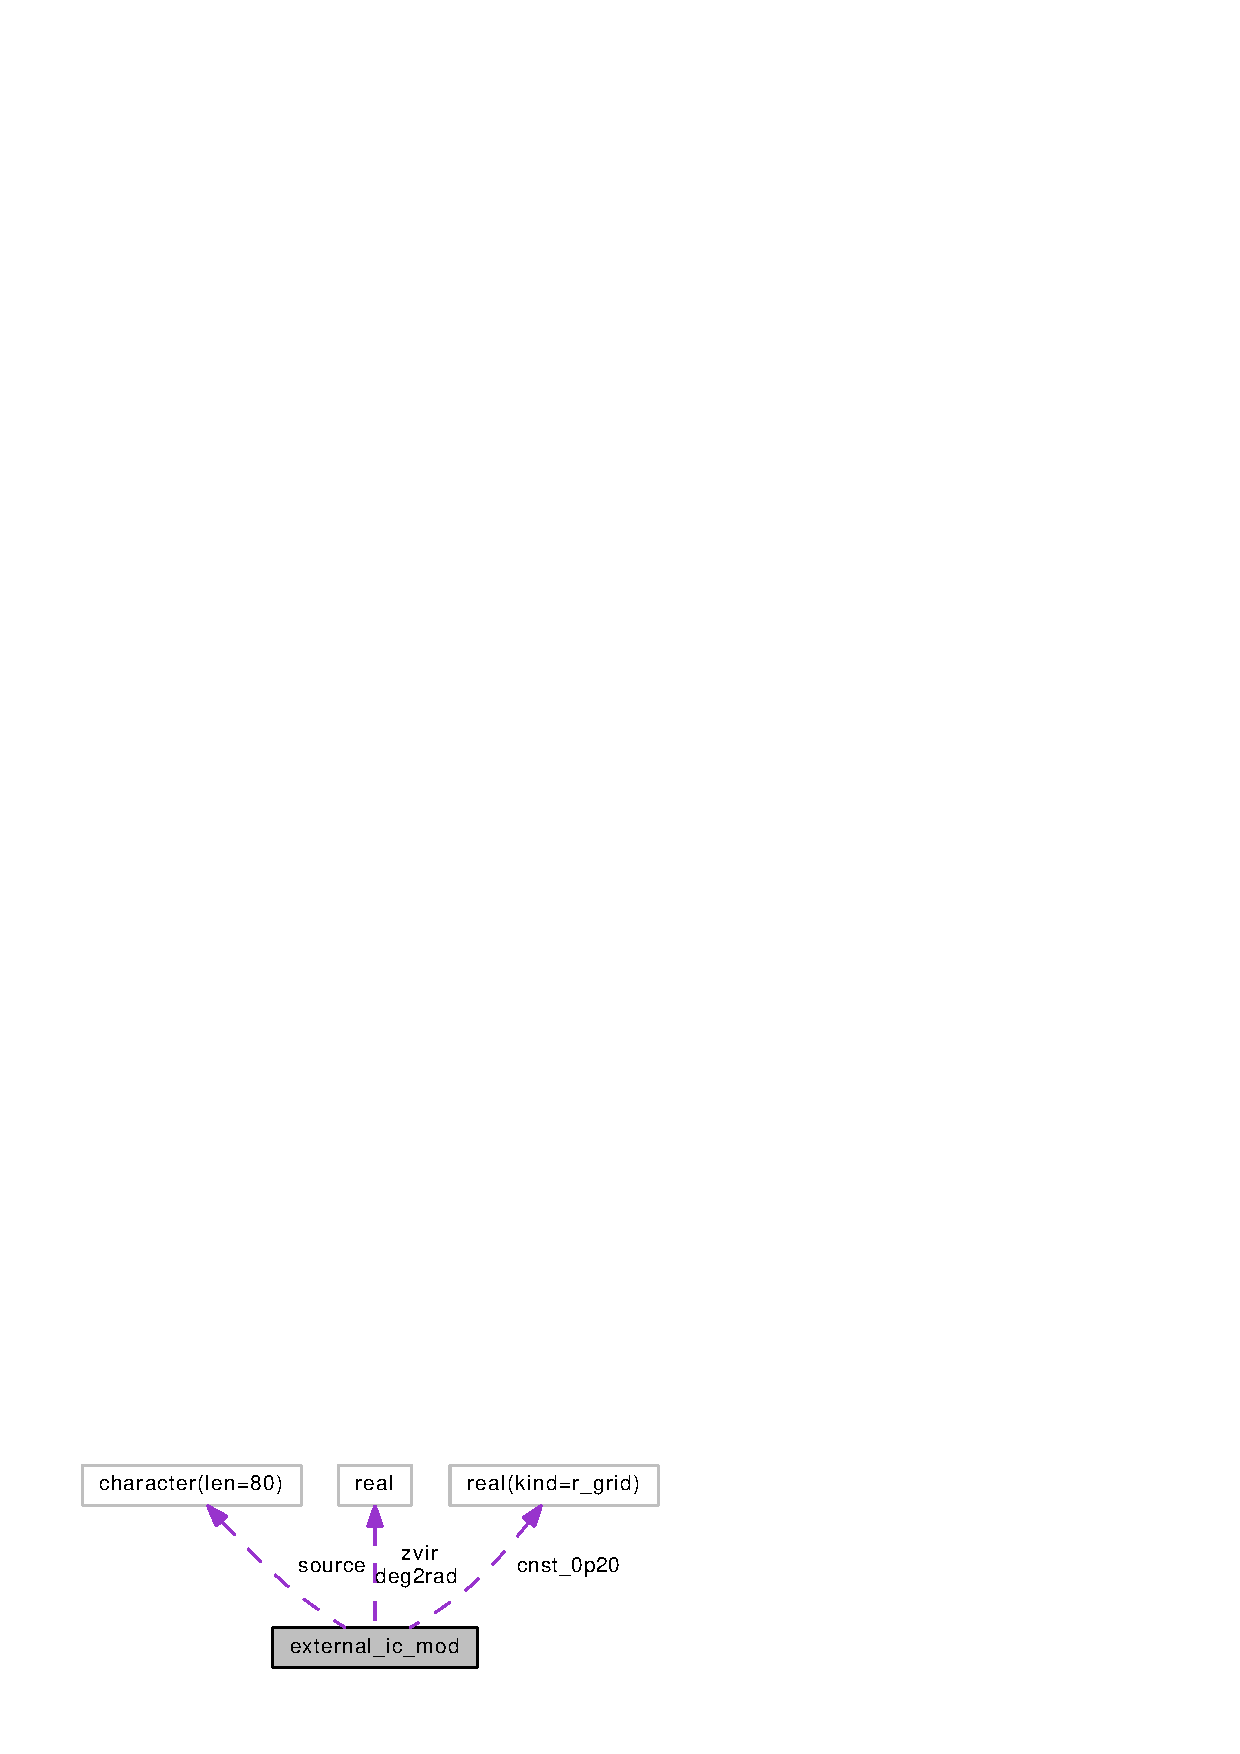
\includegraphics[width=320pt]{classexternal__ic__mod__coll__graph}
\end{center}
\end{figure}
\subsection*{Public Member Functions}
\begin{DoxyCompactItemize}
\item 
subroutine, public \hyperlink{classexternal__ic__mod_a8f9e9f938dc0cd8b8fa9507c1d581991}{get\-\_\-external\-\_\-ic} (Atm, fv\-\_\-domain, cold\-\_\-start)
\item 
subroutine, public \hyperlink{classexternal__ic__mod_a3db18261474605831898bc15fee4fec9}{get\-\_\-cubed\-\_\-sphere\-\_\-terrain} (Atm, fv\-\_\-domain)
\item 
subroutine \hyperlink{classexternal__ic__mod_a32ccd1a4f2bb9212e850d591bc0a2e0c}{d2a3d} (u, v, ua, va, im, jm, km, lon)
\end{DoxyCompactItemize}
\subsection*{Private Member Functions}
\begin{DoxyCompactItemize}
\item 
subroutine \hyperlink{classexternal__ic__mod_a2c8c50c3ce254d69f0dfb1026fd79894}{get\-\_\-nggps\-\_\-ic} (Atm, fv\-\_\-domain)
\begin{DoxyCompactList}\small\item\em The subroutine 'get\-\_\-nggps\-\_\-ic' reads in data after it has been preprocessed with N\-C\-E\-P/\-E\-M\-C orography maker and 'global\-\_\-chgres', and has been horiztontally interpolated to the current cubed-\/sphere grid. \end{DoxyCompactList}\item 
subroutine \hyperlink{classexternal__ic__mod_a24b0b354bf5843b10cd1e14cb7cd9bbf}{get\-\_\-ncep\-\_\-ic} (Atm, fv\-\_\-domain, nq)
\begin{DoxyCompactList}\small\item\em The subroutine 'get\-\_\-ncep\-\_\-ic' reads in the specified N\-C\-E\-P analysis or reanalysis dataset. \end{DoxyCompactList}\item 
subroutine \hyperlink{classexternal__ic__mod_a8e1069d292da6b506720069397105f44}{get\-\_\-ecmwf\-\_\-ic} (Atm, fv\-\_\-domain)
\begin{DoxyCompactList}\small\item\em The subroutine 'get\-\_\-ecmwf\-\_\-ic' reads in initial conditions from E\-C\-M\-W\-F analyses (E\-X\-P\-E\-R\-I\-M\-E\-N\-T\-A\-L\-: contact Jan-\/\-Huey Chen \href{mailto:jan-huey.chen@noaa.gov}{\tt jan-\/huey.\-chen@noaa.\-gov} for support) \end{DoxyCompactList}\item 
subroutine \hyperlink{classexternal__ic__mod_a81751fea2cd62527be34c1a4822b7b82}{get\-\_\-fv\-\_\-ic} (Atm, fv\-\_\-domain, nq)
\item 
subroutine \hyperlink{classexternal__ic__mod_a008a0c5b5b6c2f99f3fbfad087e2f3b0}{ncep2fms} (im, jm, lon, lat, wk)
\item 
subroutine \hyperlink{classexternal__ic__mod_a2dd0919c9e603f7576f32f372603d378}{remap\-\_\-coef} (is, ie, js, je, isd, ied, jsd, jed, im, jm, lon, lat, id1, id2, jdc, s2c, agrid)
\item 
subroutine \hyperlink{classexternal__ic__mod_a52d3cb132633e41f7589ef7e2e9c06c9}{remap\-\_\-scalar} (im, jm, km, npz, nq, ncnst, ak0, bk0, psc, gzc, ta, qa, Atm)
\item 
subroutine \hyperlink{classexternal__ic__mod_a81ec4cdb567eb4969a9b08b59883b791}{remap\-\_\-scalar\-\_\-nggps} (Atm, km, npz, ncnst, ak0, bk0, psc, t\-\_\-in, qa, omga, zh)
\item 
subroutine \hyperlink{classexternal__ic__mod_a2a128c3f4469123904446b5705140778}{remap\-\_\-scalar\-\_\-ec} (Atm, km, npz, ncnst, ak0, bk0, psc, qa, wc, zh)
\item 
subroutine \hyperlink{classexternal__ic__mod_a54fd6eeb85735101f589d85bd3df8c9e}{remap\-\_\-scalar\-\_\-single} (Atm, km, npz, ak0, bk0, psc, qa, zh, iq)
\item 
subroutine \hyperlink{classexternal__ic__mod_a09fea20a4b6f517c9f5ffb1adc6939f2}{mp\-\_\-auto\-\_\-conversion} (ql, qr, qi, qs)
\item 
subroutine \hyperlink{classexternal__ic__mod_a252f92d8428ebd9e0692b065abca0181}{remap\-\_\-dwinds} (km, npz, ak0, bk0, psc, ud, vd, Atm)
\item 
subroutine \hyperlink{classexternal__ic__mod_a8f2da4b4a3757435e0e62136ccdd8139}{remap\-\_\-winds} (im, jm, km, npz, ak0, bk0, psc, ua, va, Atm)
\item 
subroutine \hyperlink{classexternal__ic__mod_a3f5edb2d7d54ed528d9536f81b55af69}{remap\-\_\-xyz} (im, jbeg, jend, jm, km, npz, nq, ncnst, lon, lat, ak0, bk0, ps0, gz0, ua, va, ta, qa, Atm)
\item 
subroutine \hyperlink{classexternal__ic__mod_ad063f728624f5080b2aa9a90b8bf2c4c}{cubed\-\_\-a2d} (npx, npy, npz, ua, va, u, v, gridstruct, fv\-\_\-domain, bd)
\begin{DoxyCompactList}\small\item\em The subroutine 'cubed\-\_\-a2d' transforms the wind from the A Grid to the D Grid. \end{DoxyCompactList}\item 
subroutine \hyperlink{classexternal__ic__mod_aeb8db7e1db87d982349afc18c0ea3a84}{pmaxmin} (qname, a, im, jm, fac)
\item 
subroutine \hyperlink{classexternal__ic__mod_a9ff7391894a908536c199acb6be9af35}{pmaxmn} (qname, q, is, ie, js, je, km, fac, area, domain)
\item 
subroutine \hyperlink{classexternal__ic__mod_aed974417c71160c8698d13a025561537}{p\-\_\-maxmin} (qname, q, is, ie, js, je, km, fac)
\item 
subroutine \hyperlink{classexternal__ic__mod_a44111251c4b15808e291189bd902e385}{fillq} (im, km, nq, q, dp)
\item 
subroutine \hyperlink{classexternal__ic__mod_a66a468c142f85fab8b17cbbba40f6d71}{compute\-\_\-zh} (im, jm, levp, ak0, bk0, ps, zs, t, q, nq, zh)
\item 
subroutine \hyperlink{classexternal__ic__mod_aba03b236b50672b51dcf0f37613f3afe}{get\-\_\-staggered\-\_\-grid} (is, ie, js, je, isd, ied, jsd, jed, pt\-\_\-b, pt\-\_\-c, pt\-\_\-d)
\end{DoxyCompactItemize}
\subsection*{Private Attributes}
\begin{DoxyCompactItemize}
\item 
real, parameter \hyperlink{classexternal__ic__mod_ae145645946e5e06d6f5af880aaff9b1e}{zvir} = rvgas/rdgas -\/ 1.
\item 
real(kind=r\-\_\-grid), parameter \hyperlink{classexternal__ic__mod_a5405c33818b4654e81d65a4d167bf30d}{cnst\-\_\-0p20} =0.\-20d0
\item 
real \hyperlink{classexternal__ic__mod_afabc509912a4ec0c963a4b262a69fae8}{deg2rad}
\item 
character(len=80) \hyperlink{classexternal__ic__mod_a74aa0c5ee3e124f0d7a6a4688b045c6e}{source}
\end{DoxyCompactItemize}


\subsection{Detailed Description}
The module '\hyperlink{classexternal__ic__mod}{external\-\_\-ic\-\_\-mod}' contains routines that read in and remap initial conditions. 

Definition at line 32 of file external\-\_\-ic.\-F90.



\subsection{Member Function/\-Subroutine Documentation}
\index{external\-\_\-ic\-\_\-mod@{external\-\_\-ic\-\_\-mod}!compute\-\_\-zh@{compute\-\_\-zh}}
\index{compute\-\_\-zh@{compute\-\_\-zh}!external_ic_mod@{external\-\_\-ic\-\_\-mod}}
\subsubsection[{compute\-\_\-zh}]{\setlength{\rightskip}{0pt plus 5cm}subroutine external\-\_\-ic\-\_\-mod\-::compute\-\_\-zh (
\begin{DoxyParamCaption}
\item[{integer, intent(in)}]{im, }
\item[{integer, intent(in)}]{jm, }
\item[{integer, intent(in)}]{levp, }
\item[{real, dimension(levp+1), intent(in)}]{ak0, }
\item[{real, dimension(levp+1), intent(in)}]{bk0, }
\item[{real(kind=4), dimension(im,jm), intent(in)}]{ps, }
\item[{real(kind=4), dimension(im,jm), intent(in)}]{zs, }
\item[{real(kind=4), dimension(im,jm,levp), intent(in)}]{t, }
\item[{real(kind=4), dimension(im,jm,levp,nq), intent(in)}]{q, }
\item[{integer, intent(in)}]{nq, }
\item[{real(kind=4), dimension(im,jm,levp+1), intent(out)}]{zh}
\end{DoxyParamCaption}
)\hspace{0.3cm}{\ttfamily [private]}}\label{classexternal__ic__mod_a66a468c142f85fab8b17cbbba40f6d71}


Definition at line 4213 of file external\-\_\-ic.\-F90.



Referenced by get\-\_\-ecmwf\-\_\-ic().

\index{external\-\_\-ic\-\_\-mod@{external\-\_\-ic\-\_\-mod}!cubed\-\_\-a2d@{cubed\-\_\-a2d}}
\index{cubed\-\_\-a2d@{cubed\-\_\-a2d}!external_ic_mod@{external\-\_\-ic\-\_\-mod}}
\subsubsection[{cubed\-\_\-a2d}]{\setlength{\rightskip}{0pt plus 5cm}subroutine external\-\_\-ic\-\_\-mod\-::cubed\-\_\-a2d (
\begin{DoxyParamCaption}
\item[{integer, intent(in)}]{npx, }
\item[{integer, intent(in)}]{npy, }
\item[{integer, intent(in)}]{npz, }
\item[{real, dimension(bd\%isd\-:bd\%ied,bd\%jsd\-:bd\%jed,npz), intent(inout)}]{ua, }
\item[{real, dimension(bd\%isd\-:bd\%ied,bd\%jsd\-:bd\%jed,npz), intent(inout)}]{va, }
\item[{real, dimension(bd\%isd\-:bd\%ied,  bd\%jsd\-:bd\%jed+1,npz), intent(out)}]{u, }
\item[{real, dimension(bd\%isd\-:bd\%ied+1,bd\%jsd\-:bd\%jed  ,npz), intent(out)}]{v, }
\item[{type(fv\-\_\-grid\-\_\-type), intent(in), target}]{gridstruct, }
\item[{type(domain2d), intent(inout)}]{fv\-\_\-domain, }
\item[{type(fv\-\_\-grid\-\_\-bounds\-\_\-type), intent(in)}]{bd}
\end{DoxyParamCaption}
)\hspace{0.3cm}{\ttfamily [private]}}\label{classexternal__ic__mod_ad063f728624f5080b2aa9a90b8bf2c4c}


The subroutine 'cubed\-\_\-a2d' transforms the wind from the A Grid to the D Grid. 



Definition at line 3821 of file external\-\_\-ic.\-F90.



Referenced by remap\-\_\-winds(), and remap\-\_\-xyz().

\index{external\-\_\-ic\-\_\-mod@{external\-\_\-ic\-\_\-mod}!d2a3d@{d2a3d}}
\index{d2a3d@{d2a3d}!external_ic_mod@{external\-\_\-ic\-\_\-mod}}
\subsubsection[{d2a3d}]{\setlength{\rightskip}{0pt plus 5cm}subroutine external\-\_\-ic\-\_\-mod\-::d2a3d (
\begin{DoxyParamCaption}
\item[{real, dimension(im,jm,km), intent(in)}]{u, }
\item[{real, dimension(im,jm,km), intent(in)}]{v, }
\item[{real, dimension(im,jm,km), intent(out)}]{ua, }
\item[{real, dimension(im,jm,km), intent(out)}]{va, }
\item[{integer, intent(in)}]{im, }
\item[{integer, intent(in)}]{jm, }
\item[{integer, intent(in)}]{km, }
\item[{real, dimension(im), intent(in)}]{lon}
\end{DoxyParamCaption}
)}\label{classexternal__ic__mod_a32ccd1a4f2bb9212e850d591bc0a2e0c}


Definition at line 4005 of file external\-\_\-ic.\-F90.



Referenced by get\-\_\-fv\-\_\-ic().

\index{external\-\_\-ic\-\_\-mod@{external\-\_\-ic\-\_\-mod}!fillq@{fillq}}
\index{fillq@{fillq}!external_ic_mod@{external\-\_\-ic\-\_\-mod}}
\subsubsection[{fillq}]{\setlength{\rightskip}{0pt plus 5cm}subroutine external\-\_\-ic\-\_\-mod\-::fillq (
\begin{DoxyParamCaption}
\item[{integer, intent(in)}]{im, }
\item[{integer, intent(in)}]{km, }
\item[{integer, intent(in)}]{nq, }
\item[{real, dimension(im,km,nq), intent(inout)}]{q, }
\item[{real, dimension(im,km), intent(in)}]{dp}
\end{DoxyParamCaption}
)\hspace{0.3cm}{\ttfamily [private]}}\label{classexternal__ic__mod_a44111251c4b15808e291189bd902e385}

\begin{DoxyParams}[1]{Parameters}
\mbox{\tt in}  & {\em im} & No. of longitudes\\
\hline
\mbox{\tt in}  & {\em km} & No. of levels\\
\hline
\mbox{\tt in}  & {\em nq} & Total number of tracers\\
\hline
\mbox{\tt in}  & {\em dp} & pressure thickness\\
\hline
\mbox{\tt in,out}  & {\em q} & tracer mixing ratio \\
\hline
\end{DoxyParams}


Definition at line 4178 of file external\-\_\-ic.\-F90.

\index{external\-\_\-ic\-\_\-mod@{external\-\_\-ic\-\_\-mod}!get\-\_\-cubed\-\_\-sphere\-\_\-terrain@{get\-\_\-cubed\-\_\-sphere\-\_\-terrain}}
\index{get\-\_\-cubed\-\_\-sphere\-\_\-terrain@{get\-\_\-cubed\-\_\-sphere\-\_\-terrain}!external_ic_mod@{external\-\_\-ic\-\_\-mod}}
\subsubsection[{get\-\_\-cubed\-\_\-sphere\-\_\-terrain}]{\setlength{\rightskip}{0pt plus 5cm}subroutine, public external\-\_\-ic\-\_\-mod\-::get\-\_\-cubed\-\_\-sphere\-\_\-terrain (
\begin{DoxyParamCaption}
\item[{type(fv\-\_\-atmos\-\_\-type), dimension(\-:), intent(inout), target}]{Atm, }
\item[{type(domain2d), intent(inout)}]{fv\-\_\-domain}
\end{DoxyParamCaption}
)}\label{classexternal__ic__mod_a3db18261474605831898bc15fee4fec9}


Definition at line 371 of file external\-\_\-ic.\-F90.



References fv\-\_\-grid\-\_\-utils\-\_\-mod\-::g\-\_\-sum(), fv\-\_\-diagnostics\-\_\-mod\-::prt\-\_\-maxmin(), and fv\-\_\-surf\-\_\-map\-\_\-mod\-::surfdrv().



Referenced by get\-\_\-external\-\_\-ic().

\index{external\-\_\-ic\-\_\-mod@{external\-\_\-ic\-\_\-mod}!get\-\_\-ecmwf\-\_\-ic@{get\-\_\-ecmwf\-\_\-ic}}
\index{get\-\_\-ecmwf\-\_\-ic@{get\-\_\-ecmwf\-\_\-ic}!external_ic_mod@{external\-\_\-ic\-\_\-mod}}
\subsubsection[{get\-\_\-ecmwf\-\_\-ic}]{\setlength{\rightskip}{0pt plus 5cm}subroutine external\-\_\-ic\-\_\-mod\-::get\-\_\-ecmwf\-\_\-ic (
\begin{DoxyParamCaption}
\item[{type(fv\-\_\-atmos\-\_\-type), dimension(\-:), intent(inout)}]{Atm, }
\item[{type(domain2d), intent(inout)}]{fv\-\_\-domain}
\end{DoxyParamCaption}
)\hspace{0.3cm}{\ttfamily [private]}}\label{classexternal__ic__mod_a8e1069d292da6b506720069397105f44}


The subroutine 'get\-\_\-ecmwf\-\_\-ic' reads in initial conditions from E\-C\-M\-W\-F analyses (E\-X\-P\-E\-R\-I\-M\-E\-N\-T\-A\-L\-: contact Jan-\/\-Huey Chen \href{mailto:jan-huey.chen@noaa.gov}{\tt jan-\/huey.\-chen@noaa.\-gov} for support) 

\begin{DoxyAuthor}{Authors}
Jan-\/\-Huey Chen, Xi Chen, Shian-\/\-Jiann Lin 
\end{DoxyAuthor}


Definition at line 1370 of file external\-\_\-ic.\-F90.



References compute\-\_\-zh(), fv\-\_\-grid\-\_\-utils\-\_\-mod\-::get\-\_\-latlon\-\_\-vector(), sim\-\_\-nc\-\_\-mod\-::get\-\_\-ncdim1(), get\-\_\-staggered\-\_\-grid(), fv\-\_\-grid\-\_\-utils\-\_\-mod\-::get\-\_\-unit\-\_\-vect2(), sim\-\_\-nc\-\_\-mod\-::get\-\_\-var2\-\_\-r4(), sim\-\_\-nc\-\_\-mod\-::get\-\_\-var3\-\_\-r4(), sim\-\_\-nc\-\_\-mod\-::get\-\_\-var\-\_\-att\-\_\-double(), fv\-\_\-grid\-\_\-utils\-\_\-mod\-::inner\-\_\-prod(), fv\-\_\-grid\-\_\-utils\-\_\-mod\-::mid\-\_\-pt\-\_\-sphere(), sim\-\_\-nc\-\_\-mod\-::open\-\_\-ncfile(), remap\-\_\-coef(), remap\-\_\-dwinds(), remap\-\_\-scalar\-\_\-ec(), remap\-\_\-scalar\-\_\-single(), and fv\-\_\-eta\-\_\-mod\-::set\-\_\-eta().



Referenced by get\-\_\-external\-\_\-ic().

\index{external\-\_\-ic\-\_\-mod@{external\-\_\-ic\-\_\-mod}!get\-\_\-external\-\_\-ic@{get\-\_\-external\-\_\-ic}}
\index{get\-\_\-external\-\_\-ic@{get\-\_\-external\-\_\-ic}!external_ic_mod@{external\-\_\-ic\-\_\-mod}}
\subsubsection[{get\-\_\-external\-\_\-ic}]{\setlength{\rightskip}{0pt plus 5cm}subroutine, public external\-\_\-ic\-\_\-mod\-::get\-\_\-external\-\_\-ic (
\begin{DoxyParamCaption}
\item[{type(fv\-\_\-atmos\-\_\-type), dimension(\-:), intent(inout), target}]{Atm, }
\item[{type(domain2d), intent(inout)}]{fv\-\_\-domain, }
\item[{logical, intent(in)}]{cold\-\_\-start}
\end{DoxyParamCaption}
)}\label{classexternal__ic__mod_a8f9e9f938dc0cd8b8fa9507c1d581991}


Definition at line 210 of file external\-\_\-ic.\-F90.



References fv\-\_\-io\-\_\-mod\-::fv\-\_\-io\-\_\-read\-\_\-tracers(), get\-\_\-cubed\-\_\-sphere\-\_\-terrain(), get\-\_\-ecmwf\-\_\-ic(), get\-\_\-fv\-\_\-ic(), get\-\_\-ncep\-\_\-ic(), get\-\_\-nggps\-\_\-ic(), init\-\_\-hydro\-\_\-mod\-::p\-\_\-var(), fv\-\_\-diagnostics\-\_\-mod\-::prt\-\_\-maxmin(), fv\-\_\-timing\-\_\-mod\-::timing\-\_\-off(), and fv\-\_\-timing\-\_\-mod\-::timing\-\_\-on().



Referenced by fv\-\_\-restart\-\_\-mod\-::fv\-\_\-restart().

\index{external\-\_\-ic\-\_\-mod@{external\-\_\-ic\-\_\-mod}!get\-\_\-fv\-\_\-ic@{get\-\_\-fv\-\_\-ic}}
\index{get\-\_\-fv\-\_\-ic@{get\-\_\-fv\-\_\-ic}!external_ic_mod@{external\-\_\-ic\-\_\-mod}}
\subsubsection[{get\-\_\-fv\-\_\-ic}]{\setlength{\rightskip}{0pt plus 5cm}subroutine external\-\_\-ic\-\_\-mod\-::get\-\_\-fv\-\_\-ic (
\begin{DoxyParamCaption}
\item[{type(fv\-\_\-atmos\-\_\-type), dimension(\-:), intent(inout)}]{Atm, }
\item[{type(domain2d), intent(inout)}]{fv\-\_\-domain, }
\item[{integer, intent(in)}]{nq}
\end{DoxyParamCaption}
)\hspace{0.3cm}{\ttfamily [private]}}\label{classexternal__ic__mod_a81751fea2cd62527be34c1a4822b7b82}


Definition at line 2113 of file external\-\_\-ic.\-F90.



References d2a3d(), pmaxmin(), and remap\-\_\-xyz().



Referenced by get\-\_\-external\-\_\-ic().

\index{external\-\_\-ic\-\_\-mod@{external\-\_\-ic\-\_\-mod}!get\-\_\-ncep\-\_\-ic@{get\-\_\-ncep\-\_\-ic}}
\index{get\-\_\-ncep\-\_\-ic@{get\-\_\-ncep\-\_\-ic}!external_ic_mod@{external\-\_\-ic\-\_\-mod}}
\subsubsection[{get\-\_\-ncep\-\_\-ic}]{\setlength{\rightskip}{0pt plus 5cm}subroutine external\-\_\-ic\-\_\-mod\-::get\-\_\-ncep\-\_\-ic (
\begin{DoxyParamCaption}
\item[{type(fv\-\_\-atmos\-\_\-type), dimension(\-:), intent(inout)}]{Atm, }
\item[{type(domain2d), intent(inout)}]{fv\-\_\-domain, }
\item[{integer, intent(in)}]{nq}
\end{DoxyParamCaption}
)\hspace{0.3cm}{\ttfamily [private]}}\label{classexternal__ic__mod_a24b0b354bf5843b10cd1e14cb7cd9bbf}


The subroutine 'get\-\_\-ncep\-\_\-ic' reads in the specified N\-C\-E\-P analysis or reanalysis dataset. 



Definition at line 1049 of file external\-\_\-ic.\-F90.



References sim\-\_\-nc\-\_\-mod\-::close\-\_\-ncfile(), sim\-\_\-nc\-\_\-mod\-::get\-\_\-ncdim1(), sim\-\_\-nc\-\_\-mod\-::get\-\_\-var2\-\_\-real(), sim\-\_\-nc\-\_\-mod\-::get\-\_\-var3\-\_\-r4(), ncep2fms(), sim\-\_\-nc\-\_\-mod\-::open\-\_\-ncfile(), pmaxmin(), fv\-\_\-diagnostics\-\_\-mod\-::prt\-\_\-maxmin(), remap\-\_\-coef(), remap\-\_\-scalar(), and remap\-\_\-winds().



Referenced by get\-\_\-external\-\_\-ic().

\index{external\-\_\-ic\-\_\-mod@{external\-\_\-ic\-\_\-mod}!get\-\_\-nggps\-\_\-ic@{get\-\_\-nggps\-\_\-ic}}
\index{get\-\_\-nggps\-\_\-ic@{get\-\_\-nggps\-\_\-ic}!external_ic_mod@{external\-\_\-ic\-\_\-mod}}
\subsubsection[{get\-\_\-nggps\-\_\-ic}]{\setlength{\rightskip}{0pt plus 5cm}subroutine external\-\_\-ic\-\_\-mod\-::get\-\_\-nggps\-\_\-ic (
\begin{DoxyParamCaption}
\item[{type(fv\-\_\-atmos\-\_\-type), dimension(\-:), intent(inout)}]{Atm, }
\item[{type(domain2d), intent(inout)}]{fv\-\_\-domain}
\end{DoxyParamCaption}
)\hspace{0.3cm}{\ttfamily [private]}}\label{classexternal__ic__mod_a2c8c50c3ce254d69f0dfb1026fd79894}


The subroutine 'get\-\_\-nggps\-\_\-ic' reads in data after it has been preprocessed with N\-C\-E\-P/\-E\-M\-C orography maker and 'global\-\_\-chgres', and has been horiztontally interpolated to the current cubed-\/sphere grid. 


\begin{DoxyParams}[1]{Parameters}
\mbox{\tt in,out}  & {\em atm} & variables read in from 'gfs\-\_\-ctrl.\-nc' V\-C\-O\-O\-R\-D -\/ level information maps to 'ak \& bk' variables read in from 'sfc\-\_\-data.\-nc' land\-\_\-frac -\/ land-\/sea-\/ice mask (L\-:0 / S\-:1) maps to 'oro' T\-S\-E\-A -\/ surface skin temperature (k) maps to 'ts' variables read in from 'gfs\-\_\-data.\-nc' Z\-H -\/ G\-F\-S grid height at edges (m) P\-S -\/ surface pressure (Pa) U\-\_\-\-W -\/ D-\/grid west face tangential wind component (m/s) V\-\_\-\-W -\/ D-\/grid west face normal wind component (m/s) U\-\_\-\-S -\/ D-\/grid south face tangential wind component (m/s) V\-\_\-\-S -\/ D-\/grid south face normal wind component (m/s) O\-M\-G\-A-\/ vertical velocity 'omega' (Pa/s) Q -\/ prognostic tracer fields Namelist variables filtered\-\_\-terrain -\/ use orography maker filtered terrain mapping \\
\hline
\end{DoxyParams}


Definition at line 445 of file external\-\_\-ic.\-F90.



References test\-\_\-cases\-\_\-mod\-::checker\-\_\-tracers(), fv\-\_\-surf\-\_\-map\-\_\-mod\-::del2\-\_\-cubed\-\_\-sphere(), fv\-\_\-surf\-\_\-map\-\_\-mod\-::del4\-\_\-cubed\-\_\-sphere(), boundary\-\_\-mod\-::extrapolation\-\_\-bc(), fv\-\_\-surf\-\_\-map\-\_\-mod\-::fv3\-\_\-zs\-\_\-filter(), fv\-\_\-regional\-\_\-mod\-::get\-\_\-data\-\_\-source(), fv\-\_\-grid\-\_\-utils\-\_\-mod\-::get\-\_\-latlon\-\_\-vector(), fv\-\_\-grid\-\_\-utils\-\_\-mod\-::get\-\_\-unit\-\_\-vect2(), fv\-\_\-grid\-\_\-utils\-\_\-mod\-::inner\-\_\-prod(), fv\-\_\-grid\-\_\-utils\-\_\-mod\-::mid\-\_\-pt\-\_\-sphere(), remap\-\_\-dwinds(), remap\-\_\-scalar\-\_\-nggps(), fv\-\_\-eta\-\_\-mod\-::set\-\_\-eta(), fv\-\_\-eta\-\_\-mod\-::set\-\_\-external\-\_\-eta(), and fv\-\_\-regional\-\_\-mod\-::start\-\_\-regional\-\_\-cold\-\_\-start().



Referenced by get\-\_\-external\-\_\-ic().

\index{external\-\_\-ic\-\_\-mod@{external\-\_\-ic\-\_\-mod}!get\-\_\-staggered\-\_\-grid@{get\-\_\-staggered\-\_\-grid}}
\index{get\-\_\-staggered\-\_\-grid@{get\-\_\-staggered\-\_\-grid}!external_ic_mod@{external\-\_\-ic\-\_\-mod}}
\subsubsection[{get\-\_\-staggered\-\_\-grid}]{\setlength{\rightskip}{0pt plus 5cm}subroutine external\-\_\-ic\-\_\-mod\-::get\-\_\-staggered\-\_\-grid (
\begin{DoxyParamCaption}
\item[{integer, intent(in)}]{is, }
\item[{integer, intent(in)}]{ie, }
\item[{integer, intent(in)}]{js, }
\item[{integer, intent(in)}]{je, }
\item[{integer, intent(in)}]{isd, }
\item[{integer, intent(in)}]{ied, }
\item[{integer, intent(in)}]{jsd, }
\item[{integer, intent(in)}]{jed, }
\item[{real, dimension(isd\-:ied+1,jsd\-:jed+1,2), intent(in)}]{pt\-\_\-b, }
\item[{real, dimension(isd\-:ied+1,jsd\-:jed  ,2), intent(out)}]{pt\-\_\-c, }
\item[{real, dimension(isd\-:ied  ,jsd\-:jed+1,2), intent(out)}]{pt\-\_\-d}
\end{DoxyParamCaption}
)\hspace{0.3cm}{\ttfamily [private]}}\label{classexternal__ic__mod_aba03b236b50672b51dcf0f37613f3afe}


Definition at line 4255 of file external\-\_\-ic.\-F90.



References fv\-\_\-grid\-\_\-utils\-\_\-mod\-::mid\-\_\-pt\-\_\-sphere().



Referenced by get\-\_\-ecmwf\-\_\-ic(), and fv\-\_\-treat\-\_\-da\-\_\-inc\-\_\-mod\-::read\-\_\-da\-\_\-inc().

\index{external\-\_\-ic\-\_\-mod@{external\-\_\-ic\-\_\-mod}!mp\-\_\-auto\-\_\-conversion@{mp\-\_\-auto\-\_\-conversion}}
\index{mp\-\_\-auto\-\_\-conversion@{mp\-\_\-auto\-\_\-conversion}!external_ic_mod@{external\-\_\-ic\-\_\-mod}}
\subsubsection[{mp\-\_\-auto\-\_\-conversion}]{\setlength{\rightskip}{0pt plus 5cm}subroutine external\-\_\-ic\-\_\-mod\-::mp\-\_\-auto\-\_\-conversion (
\begin{DoxyParamCaption}
\item[{real, intent(inout)}]{ql, }
\item[{real, intent(inout)}]{qr, }
\item[{real, intent(inout)}]{qi, }
\item[{real, intent(inout)}]{qs}
\end{DoxyParamCaption}
)\hspace{0.3cm}{\ttfamily [private]}}\label{classexternal__ic__mod_a09fea20a4b6f517c9f5ffb1adc6939f2}


Definition at line 3345 of file external\-\_\-ic.\-F90.

\index{external\-\_\-ic\-\_\-mod@{external\-\_\-ic\-\_\-mod}!ncep2fms@{ncep2fms}}
\index{ncep2fms@{ncep2fms}!external_ic_mod@{external\-\_\-ic\-\_\-mod}}
\subsubsection[{ncep2fms}]{\setlength{\rightskip}{0pt plus 5cm}subroutine external\-\_\-ic\-\_\-mod\-::ncep2fms (
\begin{DoxyParamCaption}
\item[{integer, intent(in)}]{im, }
\item[{integer, intent(in)}]{jm, }
\item[{real, dimension(im), intent(in)}]{lon, }
\item[{real, dimension(jm), intent(in)}]{lat, }
\item[{real(kind=4), dimension(im,jm), intent(in)}]{wk}
\end{DoxyParamCaption}
)\hspace{0.3cm}{\ttfamily [private]}}\label{classexternal__ic__mod_a008a0c5b5b6c2f99f3fbfad087e2f3b0}


Definition at line 2258 of file external\-\_\-ic.\-F90.



Referenced by fv\-\_\-nwp\-\_\-nudge\-\_\-mod\-::get\-\_\-ncep\-\_\-analysis(), and get\-\_\-ncep\-\_\-ic().

\index{external\-\_\-ic\-\_\-mod@{external\-\_\-ic\-\_\-mod}!p\-\_\-maxmin@{p\-\_\-maxmin}}
\index{p\-\_\-maxmin@{p\-\_\-maxmin}!external_ic_mod@{external\-\_\-ic\-\_\-mod}}
\subsubsection[{p\-\_\-maxmin}]{\setlength{\rightskip}{0pt plus 5cm}subroutine external\-\_\-ic\-\_\-mod\-::p\-\_\-maxmin (
\begin{DoxyParamCaption}
\item[{character(len=$\ast$), intent(in)}]{qname, }
\item[{real, dimension(is\-:ie, js\-:je, km), intent(in)}]{q, }
\item[{integer, intent(in)}]{is, }
\item[{integer, intent(in)}]{ie, }
\item[{integer, intent(in)}]{js, }
\item[{integer, intent(in)}]{je, }
\item[{integer, intent(in)}]{km, }
\item[{real, intent(in)}]{fac}
\end{DoxyParamCaption}
)\hspace{0.3cm}{\ttfamily [private]}}\label{classexternal__ic__mod_aed974417c71160c8698d13a025561537}


Definition at line 4151 of file external\-\_\-ic.\-F90.

\index{external\-\_\-ic\-\_\-mod@{external\-\_\-ic\-\_\-mod}!pmaxmin@{pmaxmin}}
\index{pmaxmin@{pmaxmin}!external_ic_mod@{external\-\_\-ic\-\_\-mod}}
\subsubsection[{pmaxmin}]{\setlength{\rightskip}{0pt plus 5cm}subroutine external\-\_\-ic\-\_\-mod\-::pmaxmin (
\begin{DoxyParamCaption}
\item[{character(len=$\ast$)}]{qname, }
\item[{real, dimension(im,jm)}]{a, }
\item[{integer, intent(in)}]{im, }
\item[{integer, intent(in)}]{jm, }
\item[{real}]{fac}
\end{DoxyParamCaption}
)\hspace{0.3cm}{\ttfamily [private]}}\label{classexternal__ic__mod_aeb8db7e1db87d982349afc18c0ea3a84}


Definition at line 4080 of file external\-\_\-ic.\-F90.



Referenced by get\-\_\-fv\-\_\-ic(), fv\-\_\-nwp\-\_\-nudge\-\_\-mod\-::get\-\_\-ncep\-\_\-analysis(), and get\-\_\-ncep\-\_\-ic().

\index{external\-\_\-ic\-\_\-mod@{external\-\_\-ic\-\_\-mod}!pmaxmn@{pmaxmn}}
\index{pmaxmn@{pmaxmn}!external_ic_mod@{external\-\_\-ic\-\_\-mod}}
\subsubsection[{pmaxmn}]{\setlength{\rightskip}{0pt plus 5cm}subroutine external\-\_\-ic\-\_\-mod\-::pmaxmn (
\begin{DoxyParamCaption}
\item[{character(len=$\ast$), intent(in)}]{qname, }
\item[{real, dimension(is\-:ie, js\-:je, km), intent(in)}]{q, }
\item[{integer, intent(in)}]{is, }
\item[{integer, intent(in)}]{ie, }
\item[{integer, intent(in)}]{js, }
\item[{integer, intent(in)}]{je, }
\item[{integer, intent(in)}]{km, }
\item[{real, intent(in)}]{fac, }
\item[{real(kind=r\-\_\-grid), dimension(is-\/3\-:ie+3, js-\/3\-:je+3), intent(in)}]{area, }
\item[{type(domain2d), intent(inout)}]{domain}
\end{DoxyParamCaption}
)\hspace{0.3cm}{\ttfamily [private]}}\label{classexternal__ic__mod_a9ff7391894a908536c199acb6be9af35}


Definition at line 4115 of file external\-\_\-ic.\-F90.



References fv\-\_\-grid\-\_\-utils\-\_\-mod\-::g\-\_\-sum().

\index{external\-\_\-ic\-\_\-mod@{external\-\_\-ic\-\_\-mod}!remap\-\_\-coef@{remap\-\_\-coef}}
\index{remap\-\_\-coef@{remap\-\_\-coef}!external_ic_mod@{external\-\_\-ic\-\_\-mod}}
\subsubsection[{remap\-\_\-coef}]{\setlength{\rightskip}{0pt plus 5cm}subroutine external\-\_\-ic\-\_\-mod\-::remap\-\_\-coef (
\begin{DoxyParamCaption}
\item[{integer, intent(in)}]{is, }
\item[{integer, intent(in)}]{ie, }
\item[{integer, intent(in)}]{js, }
\item[{integer, intent(in)}]{je, }
\item[{integer, intent(in)}]{isd, }
\item[{integer, intent(in)}]{ied, }
\item[{integer, intent(in)}]{jsd, }
\item[{integer, intent(in)}]{jed, }
\item[{integer, intent(in)}]{im, }
\item[{integer, intent(in)}]{jm, }
\item[{real, dimension(im), intent(in)}]{lon, }
\item[{real, dimension(jm), intent(in)}]{lat, }
\item[{integer, dimension(is\-:ie,js\-:je), intent(out)}]{id1, }
\item[{integer, dimension(is\-:ie,js\-:je), intent(out)}]{id2, }
\item[{integer, dimension(is\-:ie,js\-:je), intent(out)}]{jdc, }
\item[{real, dimension(is\-:ie,js\-:je,4), intent(out)}]{s2c, }
\item[{real, dimension(isd\-:ied,jsd\-:jed,2), intent(in)}]{agrid}
\end{DoxyParamCaption}
)\hspace{0.3cm}{\ttfamily [private]}}\label{classexternal__ic__mod_a2dd0919c9e603f7576f32f372603d378}


Definition at line 2349 of file external\-\_\-ic.\-F90.



Referenced by fv\-\_\-nwp\-\_\-nudge\-\_\-mod\-::fv\-\_\-nwp\-\_\-nudge\-\_\-init(), get\-\_\-ecmwf\-\_\-ic(), get\-\_\-ncep\-\_\-ic(), fv\-\_\-iau\-\_\-mod\-::iau\-\_\-initialize(), and fv\-\_\-treat\-\_\-da\-\_\-inc\-\_\-mod\-::read\-\_\-da\-\_\-inc().

\index{external\-\_\-ic\-\_\-mod@{external\-\_\-ic\-\_\-mod}!remap\-\_\-dwinds@{remap\-\_\-dwinds}}
\index{remap\-\_\-dwinds@{remap\-\_\-dwinds}!external_ic_mod@{external\-\_\-ic\-\_\-mod}}
\subsubsection[{remap\-\_\-dwinds}]{\setlength{\rightskip}{0pt plus 5cm}subroutine external\-\_\-ic\-\_\-mod\-::remap\-\_\-dwinds (
\begin{DoxyParamCaption}
\item[{integer, intent(in)}]{km, }
\item[{integer, intent(in)}]{npz, }
\item[{real, dimension(km+1), intent(in)}]{ak0, }
\item[{real, dimension(km+1), intent(in)}]{bk0, }
\item[{real, dimension(atm\%bd\%is\-:atm\%bd\%ie,atm\%bd\%js\-:atm\%bd\%je), intent(in)}]{psc, }
\item[{real, dimension(atm\%bd\%is\-:atm\%bd\%ie,atm\%bd\%js\-:atm\%bd\%je+1,km), intent(in)}]{ud, }
\item[{real, dimension(atm\%bd\%is\-:atm\%bd\%ie+1,atm\%bd\%js\-:atm\%bd\%je,km), intent(in)}]{vd, }
\item[{type(fv\-\_\-atmos\-\_\-type), intent(inout)}]{Atm}
\end{DoxyParamCaption}
)\hspace{0.3cm}{\ttfamily [private]}}\label{classexternal__ic__mod_a252f92d8428ebd9e0692b065abca0181}


Definition at line 3364 of file external\-\_\-ic.\-F90.



References fv\-\_\-mapz\-\_\-mod\-::mappm().



Referenced by get\-\_\-ecmwf\-\_\-ic(), and get\-\_\-nggps\-\_\-ic().

\index{external\-\_\-ic\-\_\-mod@{external\-\_\-ic\-\_\-mod}!remap\-\_\-scalar@{remap\-\_\-scalar}}
\index{remap\-\_\-scalar@{remap\-\_\-scalar}!external_ic_mod@{external\-\_\-ic\-\_\-mod}}
\subsubsection[{remap\-\_\-scalar}]{\setlength{\rightskip}{0pt plus 5cm}subroutine external\-\_\-ic\-\_\-mod\-::remap\-\_\-scalar (
\begin{DoxyParamCaption}
\item[{integer, intent(in)}]{im, }
\item[{integer, intent(in)}]{jm, }
\item[{integer, intent(in)}]{km, }
\item[{integer, intent(in)}]{npz, }
\item[{integer, intent(in)}]{nq, }
\item[{integer, intent(in)}]{ncnst, }
\item[{real, dimension(km+1), intent(in)}]{ak0, }
\item[{real, dimension(km+1), intent(in)}]{bk0, }
\item[{real, dimension(atm\%bd\%is\-:atm\%bd\%ie,atm\%bd\%js\-:atm\%bd\%je), intent(in)}]{psc, }
\item[{real, dimension(atm\%bd\%is\-:atm\%bd\%ie,atm\%bd\%js\-:atm\%bd\%je), intent(in)}]{gzc, }
\item[{real, dimension(atm\%bd\%is\-:atm\%bd\%ie,atm\%bd\%js\-:atm\%bd\%je,km), intent(in)}]{ta, }
\item[{real, dimension(atm\%bd\%is\-:atm\%bd\%ie,atm\%bd\%js\-:atm\%bd\%je,km,ncnst), intent(in)}]{qa, }
\item[{type(fv\-\_\-atmos\-\_\-type), intent(inout)}]{Atm}
\end{DoxyParamCaption}
)\hspace{0.3cm}{\ttfamily [private]}}\label{classexternal__ic__mod_a52d3cb132633e41f7589ef7e2e9c06c9}


Definition at line 2429 of file external\-\_\-ic.\-F90.



References fv\-\_\-mapz\-\_\-mod\-::mappm(), fv\-\_\-diagnostics\-\_\-mod\-::prt\-\_\-maxmin(), and multi\-\_\-gases\-\_\-mod\-::virq().



Referenced by get\-\_\-ncep\-\_\-ic().

\index{external\-\_\-ic\-\_\-mod@{external\-\_\-ic\-\_\-mod}!remap\-\_\-scalar\-\_\-ec@{remap\-\_\-scalar\-\_\-ec}}
\index{remap\-\_\-scalar\-\_\-ec@{remap\-\_\-scalar\-\_\-ec}!external_ic_mod@{external\-\_\-ic\-\_\-mod}}
\subsubsection[{remap\-\_\-scalar\-\_\-ec}]{\setlength{\rightskip}{0pt plus 5cm}subroutine external\-\_\-ic\-\_\-mod\-::remap\-\_\-scalar\-\_\-ec (
\begin{DoxyParamCaption}
\item[{type(fv\-\_\-atmos\-\_\-type), intent(inout)}]{Atm, }
\item[{integer, intent(in)}]{km, }
\item[{integer, intent(in)}]{npz, }
\item[{integer, intent(in)}]{ncnst, }
\item[{real, dimension(km+1), intent(in)}]{ak0, }
\item[{real, dimension(km+1), intent(in)}]{bk0, }
\item[{real, dimension(atm\%bd\%is\-:atm\%bd\%ie,atm\%bd\%js\-:atm\%bd\%je), intent(in)}]{psc, }
\item[{real, dimension(atm\%bd\%is\-:atm\%bd\%ie,atm\%bd\%js\-:atm\%bd\%je,km,ncnst), intent(in)}]{qa, }
\item[{real, dimension(atm\%bd\%is\-:atm\%bd\%ie,atm\%bd\%js\-:atm\%bd\%je,km), intent(in)}]{wc, }
\item[{real, dimension(atm\%bd\%is\-:atm\%bd\%ie,atm\%bd\%js\-:atm\%bd\%je,km+1), intent(in)}]{zh}
\end{DoxyParamCaption}
)\hspace{0.3cm}{\ttfamily [private]}}\label{classexternal__ic__mod_a2a128c3f4469123904446b5705140778}


Definition at line 2969 of file external\-\_\-ic.\-F90.



References fv\-\_\-regional\-\_\-mod\-::fillq(), fv\-\_\-fill\-\_\-mod\-::fillz(), fv\-\_\-mapz\-\_\-mod\-::mappm(), fv\-\_\-regional\-\_\-mod\-::p\-\_\-maxmin(), fv\-\_\-regional\-\_\-mod\-::pmaxmn(), fv\-\_\-diagnostics\-\_\-mod\-::prt\-\_\-gb\-\_\-nh\-\_\-sh(), fv\-\_\-diagnostics\-\_\-mod\-::prt\-\_\-height(), and multi\-\_\-gases\-\_\-mod\-::virq().



Referenced by get\-\_\-ecmwf\-\_\-ic().

\index{external\-\_\-ic\-\_\-mod@{external\-\_\-ic\-\_\-mod}!remap\-\_\-scalar\-\_\-nggps@{remap\-\_\-scalar\-\_\-nggps}}
\index{remap\-\_\-scalar\-\_\-nggps@{remap\-\_\-scalar\-\_\-nggps}!external_ic_mod@{external\-\_\-ic\-\_\-mod}}
\subsubsection[{remap\-\_\-scalar\-\_\-nggps}]{\setlength{\rightskip}{0pt plus 5cm}subroutine external\-\_\-ic\-\_\-mod\-::remap\-\_\-scalar\-\_\-nggps (
\begin{DoxyParamCaption}
\item[{type(fv\-\_\-atmos\-\_\-type), intent(inout)}]{Atm, }
\item[{integer, intent(in)}]{km, }
\item[{integer, intent(in)}]{npz, }
\item[{integer, intent(in)}]{ncnst, }
\item[{real, dimension(km+1), intent(in)}]{ak0, }
\item[{real, dimension(km+1), intent(in)}]{bk0, }
\item[{real, dimension(atm\%bd\%is\-:atm\%bd\%ie,atm\%bd\%js\-:atm\%bd\%je), intent(in)}]{psc, }
\item[{real, dimension(atm\%bd\%is\-:atm\%bd\%ie,atm\%bd\%js\-:atm\%bd\%je,km), intent(in)}]{t\-\_\-in, }
\item[{real, dimension(atm\%bd\%is\-:atm\%bd\%ie,atm\%bd\%js\-:atm\%bd\%je,km,ncnst), intent(in)}]{qa, }
\item[{real, dimension(atm\%bd\%is\-:atm\%bd\%ie,atm\%bd\%js\-:atm\%bd\%je,km), intent(in)}]{omga, }
\item[{real, dimension(atm\%bd\%is\-:atm\%bd\%ie,atm\%bd\%js\-:atm\%bd\%je,km+1), intent(in)}]{zh}
\end{DoxyParamCaption}
)\hspace{0.3cm}{\ttfamily [private]}}\label{classexternal__ic__mod_a81ec4cdb567eb4969a9b08b59883b791}


Definition at line 2607 of file external\-\_\-ic.\-F90.



References fv\-\_\-regional\-\_\-mod\-::fillq(), fv\-\_\-fill\-\_\-mod\-::fillz(), fv\-\_\-mapz\-\_\-mod\-::mappm(), fv\-\_\-regional\-\_\-mod\-::mp\-\_\-auto\-\_\-conversion(), fv\-\_\-regional\-\_\-mod\-::p\-\_\-maxmin(), fv\-\_\-regional\-\_\-mod\-::pmaxmn(), fv\-\_\-diagnostics\-\_\-mod\-::prt\-\_\-gb\-\_\-nh\-\_\-sh(), fv\-\_\-diagnostics\-\_\-mod\-::prt\-\_\-height(), and multi\-\_\-gases\-\_\-mod\-::virq().



Referenced by get\-\_\-nggps\-\_\-ic().

\index{external\-\_\-ic\-\_\-mod@{external\-\_\-ic\-\_\-mod}!remap\-\_\-scalar\-\_\-single@{remap\-\_\-scalar\-\_\-single}}
\index{remap\-\_\-scalar\-\_\-single@{remap\-\_\-scalar\-\_\-single}!external_ic_mod@{external\-\_\-ic\-\_\-mod}}
\subsubsection[{remap\-\_\-scalar\-\_\-single}]{\setlength{\rightskip}{0pt plus 5cm}subroutine external\-\_\-ic\-\_\-mod\-::remap\-\_\-scalar\-\_\-single (
\begin{DoxyParamCaption}
\item[{type(fv\-\_\-atmos\-\_\-type), intent(inout)}]{Atm, }
\item[{integer, intent(in)}]{km, }
\item[{integer, intent(in)}]{npz, }
\item[{real, dimension(km+1), intent(in)}]{ak0, }
\item[{real, dimension(km+1), intent(in)}]{bk0, }
\item[{real, dimension(atm\%bd\%is\-:atm\%bd\%ie,atm\%bd\%js\-:atm\%bd\%je), intent(in)}]{psc, }
\item[{real, dimension(atm\%bd\%is\-:atm\%bd\%ie,atm\%bd\%js\-:atm\%bd\%je,km), intent(in)}]{qa, }
\item[{real, dimension(atm\%bd\%is\-:atm\%bd\%ie,atm\%bd\%js\-:atm\%bd\%je,km+1), intent(in)}]{zh, }
\item[{integer, intent(in)}]{iq}
\end{DoxyParamCaption}
)\hspace{0.3cm}{\ttfamily [private]}}\label{classexternal__ic__mod_a54fd6eeb85735101f589d85bd3df8c9e}


Definition at line 3237 of file external\-\_\-ic.\-F90.



References fv\-\_\-regional\-\_\-mod\-::fillq(), fv\-\_\-fill\-\_\-mod\-::fillz(), fv\-\_\-mapz\-\_\-mod\-::mappm(), and fv\-\_\-regional\-\_\-mod\-::p\-\_\-maxmin().



Referenced by get\-\_\-ecmwf\-\_\-ic().

\index{external\-\_\-ic\-\_\-mod@{external\-\_\-ic\-\_\-mod}!remap\-\_\-winds@{remap\-\_\-winds}}
\index{remap\-\_\-winds@{remap\-\_\-winds}!external_ic_mod@{external\-\_\-ic\-\_\-mod}}
\subsubsection[{remap\-\_\-winds}]{\setlength{\rightskip}{0pt plus 5cm}subroutine external\-\_\-ic\-\_\-mod\-::remap\-\_\-winds (
\begin{DoxyParamCaption}
\item[{integer, intent(in)}]{im, }
\item[{integer, intent(in)}]{jm, }
\item[{integer, intent(in)}]{km, }
\item[{integer, intent(in)}]{npz, }
\item[{real, dimension(km+1), intent(in)}]{ak0, }
\item[{real, dimension(km+1), intent(in)}]{bk0, }
\item[{real, dimension(atm\%bd\%is\-:atm\%bd\%ie,atm\%bd\%js\-:atm\%bd\%je), intent(in)}]{psc, }
\item[{real, dimension(atm\%bd\%is\-:atm\%bd\%ie,atm\%bd\%js\-:atm\%bd\%je,km), intent(in)}]{ua, }
\item[{real, dimension(atm\%bd\%is\-:atm\%bd\%ie,atm\%bd\%js\-:atm\%bd\%je,km), intent(in)}]{va, }
\item[{type(fv\-\_\-atmos\-\_\-type), intent(inout)}]{Atm}
\end{DoxyParamCaption}
)\hspace{0.3cm}{\ttfamily [private]}}\label{classexternal__ic__mod_a8f2da4b4a3757435e0e62136ccdd8139}


Definition at line 3460 of file external\-\_\-ic.\-F90.



References cubed\-\_\-a2d(), fv\-\_\-mapz\-\_\-mod\-::mappm(), and fv\-\_\-diagnostics\-\_\-mod\-::prt\-\_\-maxmin().



Referenced by get\-\_\-ncep\-\_\-ic().

\index{external\-\_\-ic\-\_\-mod@{external\-\_\-ic\-\_\-mod}!remap\-\_\-xyz@{remap\-\_\-xyz}}
\index{remap\-\_\-xyz@{remap\-\_\-xyz}!external_ic_mod@{external\-\_\-ic\-\_\-mod}}
\subsubsection[{remap\-\_\-xyz}]{\setlength{\rightskip}{0pt plus 5cm}subroutine external\-\_\-ic\-\_\-mod\-::remap\-\_\-xyz (
\begin{DoxyParamCaption}
\item[{integer, intent(in)}]{im, }
\item[{integer, intent(in)}]{jbeg, }
\item[{integer, intent(in)}]{jend, }
\item[{integer, intent(in)}]{jm, }
\item[{integer, intent(in)}]{km, }
\item[{integer, intent(in)}]{npz, }
\item[{integer, intent(in)}]{nq, }
\item[{integer, intent(in)}]{ncnst, }
\item[{real, dimension(im), intent(in)}]{lon, }
\item[{real, dimension(jm), intent(in)}]{lat, }
\item[{real, dimension(km+1), intent(in)}]{ak0, }
\item[{real, dimension(km+1), intent(in)}]{bk0, }
\item[{real, dimension(im,jbeg\-:jend), intent(in)}]{ps0, }
\item[{real, dimension(im,jbeg\-:jend), intent(in)}]{gz0, }
\item[{real, dimension(im,jbeg\-:jend,km), intent(in)}]{ua, }
\item[{real, dimension(im,jbeg\-:jend,km), intent(in)}]{va, }
\item[{real, dimension(im,jbeg\-:jend,km), intent(in)}]{ta, }
\item[{real, dimension(im,jbeg\-:jend,km,ncnst), intent(in)}]{qa, }
\item[{type(fv\-\_\-atmos\-\_\-type), intent(inout), target}]{Atm}
\end{DoxyParamCaption}
)\hspace{0.3cm}{\ttfamily [private]}}\label{classexternal__ic__mod_a3f5edb2d7d54ed528d9536f81b55af69}


Definition at line 3534 of file external\-\_\-ic.\-F90.



References cubed\-\_\-a2d(), fv\-\_\-mapz\-\_\-mod\-::mappm(), fv\-\_\-diagnostics\-\_\-mod\-::prt\-\_\-maxmin(), multi\-\_\-gases\-\_\-mod\-::vicpqd(), multi\-\_\-gases\-\_\-mod\-::virq(), and multi\-\_\-gases\-\_\-mod\-::virqd().



Referenced by get\-\_\-fv\-\_\-ic().



\subsection{Member Data Documentation}
\index{external\-\_\-ic\-\_\-mod@{external\-\_\-ic\-\_\-mod}!cnst\-\_\-0p20@{cnst\-\_\-0p20}}
\index{cnst\-\_\-0p20@{cnst\-\_\-0p20}!external_ic_mod@{external\-\_\-ic\-\_\-mod}}
\subsubsection[{cnst\-\_\-0p20}]{\setlength{\rightskip}{0pt plus 5cm}real(kind=r\-\_\-grid), parameter external\-\_\-ic\-\_\-mod\-::cnst\-\_\-0p20 =0.\-20d0\hspace{0.3cm}{\ttfamily [private]}}\label{classexternal__ic__mod_a5405c33818b4654e81d65a4d167bf30d}


Definition at line 199 of file external\-\_\-ic.\-F90.

\index{external\-\_\-ic\-\_\-mod@{external\-\_\-ic\-\_\-mod}!deg2rad@{deg2rad}}
\index{deg2rad@{deg2rad}!external_ic_mod@{external\-\_\-ic\-\_\-mod}}
\subsubsection[{deg2rad}]{\setlength{\rightskip}{0pt plus 5cm}real external\-\_\-ic\-\_\-mod\-::deg2rad\hspace{0.3cm}{\ttfamily [private]}}\label{classexternal__ic__mod_afabc509912a4ec0c963a4b262a69fae8}


Definition at line 200 of file external\-\_\-ic.\-F90.

\index{external\-\_\-ic\-\_\-mod@{external\-\_\-ic\-\_\-mod}!source@{source}}
\index{source@{source}!external_ic_mod@{external\-\_\-ic\-\_\-mod}}
\subsubsection[{source}]{\setlength{\rightskip}{0pt plus 5cm}character (len = 80) external\-\_\-ic\-\_\-mod\-::source\hspace{0.3cm}{\ttfamily [private]}}\label{classexternal__ic__mod_a74aa0c5ee3e124f0d7a6a4688b045c6e}


Definition at line 201 of file external\-\_\-ic.\-F90.

\index{external\-\_\-ic\-\_\-mod@{external\-\_\-ic\-\_\-mod}!zvir@{zvir}}
\index{zvir@{zvir}!external_ic_mod@{external\-\_\-ic\-\_\-mod}}
\subsubsection[{zvir}]{\setlength{\rightskip}{0pt plus 5cm}real, parameter external\-\_\-ic\-\_\-mod\-::zvir = rvgas/rdgas -\/ 1.\hspace{0.3cm}{\ttfamily [private]}}\label{classexternal__ic__mod_ae145645946e5e06d6f5af880aaff9b1e}


Definition at line 198 of file external\-\_\-ic.\-F90.



The documentation for this module was generated from the following file\-:\begin{DoxyCompactItemize}
\item 
/scratch2/\-N\-A\-G\-A\-P\-E/aoml-\/hafs1/\-Kyle.\-Ahern/acs\-\_\-master\-\_\-readonly/tools/\hyperlink{external__ic_8F90}{external\-\_\-ic.\-F90}\end{DoxyCompactItemize}

\section{external\-\_\-sst\-\_\-mod Module Reference}
\label{classexternal__sst__mod}\index{external\-\_\-sst\-\_\-mod@{external\-\_\-sst\-\_\-mod}}


\subsection{Detailed Description}


Definition at line 21 of file external\-\_\-sst.\-F90.



The documentation for this module was generated from the following file\-:\begin{DoxyCompactItemize}
\item 
/scratch2/\-N\-A\-G\-A\-P\-E/aoml-\/hafs1/\-Kyle.\-Ahern/acs\-\_\-master\-\_\-readonly/tools/\hyperlink{external__sst_8F90}{external\-\_\-sst.\-F90}\end{DoxyCompactItemize}

\section{fv\-\_\-grid\-\_\-utils\-\_\-mod\-:\-:fill\-\_\-ghost Interface Reference}
\label{interfacefv__grid__utils__mod_1_1fill__ghost}\index{fv\-\_\-grid\-\_\-utils\-\_\-mod\-::fill\-\_\-ghost@{fv\-\_\-grid\-\_\-utils\-\_\-mod\-::fill\-\_\-ghost}}
\subsection*{Private Member Functions}
\begin{DoxyCompactItemize}
\item 
subroutine \hyperlink{interfacefv__grid__utils__mod_1_1fill__ghost_a2c42e97220dc0a5090601581ff2d0c6e}{fill\-\_\-ghost\-\_\-r8} (q, npx, npy, value, bd)
\end{DoxyCompactItemize}


\subsection{Detailed Description}


Definition at line 124 of file fv\-\_\-grid\-\_\-utils.\-F90.



\subsection{Member Function/\-Subroutine Documentation}
\index{fv\-\_\-grid\-\_\-utils\-\_\-mod\-::fill\-\_\-ghost@{fv\-\_\-grid\-\_\-utils\-\_\-mod\-::fill\-\_\-ghost}!fill\-\_\-ghost\-\_\-r8@{fill\-\_\-ghost\-\_\-r8}}
\index{fill\-\_\-ghost\-\_\-r8@{fill\-\_\-ghost\-\_\-r8}!fv_grid_utils_mod::fill_ghost@{fv\-\_\-grid\-\_\-utils\-\_\-mod\-::fill\-\_\-ghost}}
\subsubsection[{fill\-\_\-ghost\-\_\-r8}]{\setlength{\rightskip}{0pt plus 5cm}subroutine fv\-\_\-grid\-\_\-utils\-\_\-mod\-::fill\-\_\-ghost\-::fill\-\_\-ghost\-\_\-r8 (
\begin{DoxyParamCaption}
\item[{real(kind=r\-\_\-grid), dimension(bd\%isd\-:bd\%ied,bd\%jsd\-:bd\%jed), intent(inout)}]{q, }
\item[{integer, intent(in)}]{npx, }
\item[{integer, intent(in)}]{npy, }
\item[{real, intent(in)}]{value, }
\item[{type(fv\-\_\-grid\-\_\-bounds\-\_\-type), intent(in)}]{bd}
\end{DoxyParamCaption}
)\hspace{0.3cm}{\ttfamily [private]}}\label{interfacefv__grid__utils__mod_1_1fill__ghost_a2c42e97220dc0a5090601581ff2d0c6e}


Definition at line 3063 of file fv\-\_\-grid\-\_\-utils.\-F90.



The documentation for this interface was generated from the following file\-:\begin{DoxyCompactItemize}
\item 
/scratch2/\-N\-A\-G\-A\-P\-E/aoml-\/hafs1/\-Kyle.\-Ahern/acs\-\_\-master\-\_\-readonly/model/\hyperlink{fv__grid__utils_8F90}{fv\-\_\-grid\-\_\-utils.\-F90}\end{DoxyCompactItemize}

\section{boundary\-\_\-mod\-:\-:fill\-\_\-nested\-\_\-grid Interface Reference}
\label{interfaceboundary__mod_1_1fill__nested__grid}\index{boundary\-\_\-mod\-::fill\-\_\-nested\-\_\-grid@{boundary\-\_\-mod\-::fill\-\_\-nested\-\_\-grid}}


The interface '\hyperlink{interfaceboundary__mod_1_1fill__nested__grid}{fill\-\_\-nested\-\_\-grid}' includes subroutines 'fill\-\_\-nested\-\_\-grid\-\_\-2d' and 'fill\-\_\-nested\-\_\-grid\-\_\-3d' that fill nested-\/grid data with interpolated data from the coarse grid.  


\subsection*{Public Member Functions}
\begin{DoxyCompactItemize}
\item 
subroutine \hyperlink{interfaceboundary__mod_1_1fill__nested__grid_a6b5df6a36fb6d889d80bcf2d6b38f5f4}{fill\-\_\-nested\-\_\-grid\-\_\-2d} (var\-\_\-nest, var\-\_\-coarse, ind, wt, istag, jstag, isg, ieg, jsg, jeg, bd, istart\-\_\-in, iend\-\_\-in, jstart\-\_\-in, jend\-\_\-in)
\item 
subroutine \hyperlink{interfaceboundary__mod_1_1fill__nested__grid_a1b9e9179842c2eb58e019abd8c02ffed}{fill\-\_\-nested\-\_\-grid\-\_\-3d} (var\-\_\-nest, var\-\_\-coarse, ind, wt, istag, jstag, isg, ieg, jsg, jeg, npz, bd, istart\-\_\-in, iend\-\_\-in, jstart\-\_\-in, jend\-\_\-in)
\end{DoxyCompactItemize}


\subsection{Detailed Description}
The interface '\hyperlink{interfaceboundary__mod_1_1fill__nested__grid}{fill\-\_\-nested\-\_\-grid}' includes subroutines 'fill\-\_\-nested\-\_\-grid\-\_\-2d' and 'fill\-\_\-nested\-\_\-grid\-\_\-3d' that fill nested-\/grid data with interpolated data from the coarse grid. 

This is one method to create a new nested grid, and may be useful when cold-\/starting. 

Definition at line 99 of file boundary.\-F90.



\subsection{Member Function/\-Subroutine Documentation}
\index{boundary\-\_\-mod\-::fill\-\_\-nested\-\_\-grid@{boundary\-\_\-mod\-::fill\-\_\-nested\-\_\-grid}!fill\-\_\-nested\-\_\-grid\-\_\-2d@{fill\-\_\-nested\-\_\-grid\-\_\-2d}}
\index{fill\-\_\-nested\-\_\-grid\-\_\-2d@{fill\-\_\-nested\-\_\-grid\-\_\-2d}!boundary_mod::fill_nested_grid@{boundary\-\_\-mod\-::fill\-\_\-nested\-\_\-grid}}
\subsubsection[{fill\-\_\-nested\-\_\-grid\-\_\-2d}]{\setlength{\rightskip}{0pt plus 5cm}subroutine boundary\-\_\-mod\-::fill\-\_\-nested\-\_\-grid\-::fill\-\_\-nested\-\_\-grid\-\_\-2d (
\begin{DoxyParamCaption}
\item[{real, dimension(bd\%isd\-:bd\%ied+istag,bd\%jsd\-:bd\%jed+jstag), intent(inout)}]{var\-\_\-nest, }
\item[{real, dimension(isg\-:ieg+istag,jsg\-:jeg+jstag), intent(in)}]{var\-\_\-coarse, }
\item[{integer, dimension(bd\%isd\-:bd\%ied+istag,bd\%jsd\-:bd\%jed+jstag,2), intent(in)}]{ind, }
\item[{real, dimension(bd\%isd\-:bd\%ied+istag,bd\%jsd\-:bd\%jed+jstag,4), intent(in)}]{wt, }
\item[{integer, intent(in)}]{istag, }
\item[{integer, intent(in)}]{jstag, }
\item[{integer, intent(in)}]{isg, }
\item[{integer, intent(in)}]{ieg, }
\item[{integer, intent(in)}]{jsg, }
\item[{integer, intent(in)}]{jeg, }
\item[{type(fv\-\_\-grid\-\_\-bounds\-\_\-type), intent(in)}]{bd, }
\item[{integer, intent(in), optional}]{istart\-\_\-in, }
\item[{integer, intent(in), optional}]{iend\-\_\-in, }
\item[{integer, intent(in), optional}]{jstart\-\_\-in, }
\item[{integer, intent(in), optional}]{jend\-\_\-in}
\end{DoxyParamCaption}
)}\label{interfaceboundary__mod_1_1fill__nested__grid_a6b5df6a36fb6d889d80bcf2d6b38f5f4}


Definition at line 444 of file boundary.\-F90.

\index{boundary\-\_\-mod\-::fill\-\_\-nested\-\_\-grid@{boundary\-\_\-mod\-::fill\-\_\-nested\-\_\-grid}!fill\-\_\-nested\-\_\-grid\-\_\-3d@{fill\-\_\-nested\-\_\-grid\-\_\-3d}}
\index{fill\-\_\-nested\-\_\-grid\-\_\-3d@{fill\-\_\-nested\-\_\-grid\-\_\-3d}!boundary_mod::fill_nested_grid@{boundary\-\_\-mod\-::fill\-\_\-nested\-\_\-grid}}
\subsubsection[{fill\-\_\-nested\-\_\-grid\-\_\-3d}]{\setlength{\rightskip}{0pt plus 5cm}subroutine boundary\-\_\-mod\-::fill\-\_\-nested\-\_\-grid\-::fill\-\_\-nested\-\_\-grid\-\_\-3d (
\begin{DoxyParamCaption}
\item[{real, dimension(bd\%isd\-:bd\%ied+istag,bd\%jsd\-:bd\%jed+jstag,npz), intent(inout)}]{var\-\_\-nest, }
\item[{real, dimension(isg\-:ieg+istag,jsg\-:jeg+jstag,npz), intent(in)}]{var\-\_\-coarse, }
\item[{integer, dimension(bd\%isd\-:bd\%ied+istag,bd\%jsd\-:bd\%jed+jstag,2), intent(in)}]{ind, }
\item[{real, dimension(bd\%isd\-:bd\%ied+istag,bd\%jsd\-:bd\%jed+jstag,4), intent(in)}]{wt, }
\item[{integer, intent(in)}]{istag, }
\item[{integer, intent(in)}]{jstag, }
\item[{integer, intent(in)}]{isg, }
\item[{integer, intent(in)}]{ieg, }
\item[{integer, intent(in)}]{jsg, }
\item[{integer, intent(in)}]{jeg, }
\item[{integer, intent(in)}]{npz, }
\item[{type(fv\-\_\-grid\-\_\-bounds\-\_\-type), intent(in)}]{bd, }
\item[{integer, intent(in), optional}]{istart\-\_\-in, }
\item[{integer, intent(in), optional}]{iend\-\_\-in, }
\item[{integer, intent(in), optional}]{jstart\-\_\-in, }
\item[{integer, intent(in), optional}]{jend\-\_\-in}
\end{DoxyParamCaption}
)}\label{interfaceboundary__mod_1_1fill__nested__grid_a1b9e9179842c2eb58e019abd8c02ffed}


Definition at line 509 of file boundary.\-F90.



The documentation for this interface was generated from the following file\-:\begin{DoxyCompactItemize}
\item 
/scratch2/\-N\-A\-G\-A\-P\-E/aoml-\/hafs1/\-Kyle.\-Ahern/acs\-\_\-master\-\_\-readonly/model/\hyperlink{boundary_8F90}{boundary.\-F90}\end{DoxyCompactItemize}

\section{fv\-\_\-arrays\-\_\-mod Module Reference}
\label{classfv__arrays__mod}\index{fv\-\_\-arrays\-\_\-mod@{fv\-\_\-arrays\-\_\-mod}}


The module 'fv\-\_\-arrays' contains the '\hyperlink{structfv__arrays__mod_1_1fv__atmos__type}{fv\-\_\-atmos\-\_\-type}' and associated datatypes.  




Collaboration diagram for fv\-\_\-arrays\-\_\-mod\-:
\nopagebreak
\begin{figure}[H]
\begin{center}
\leavevmode
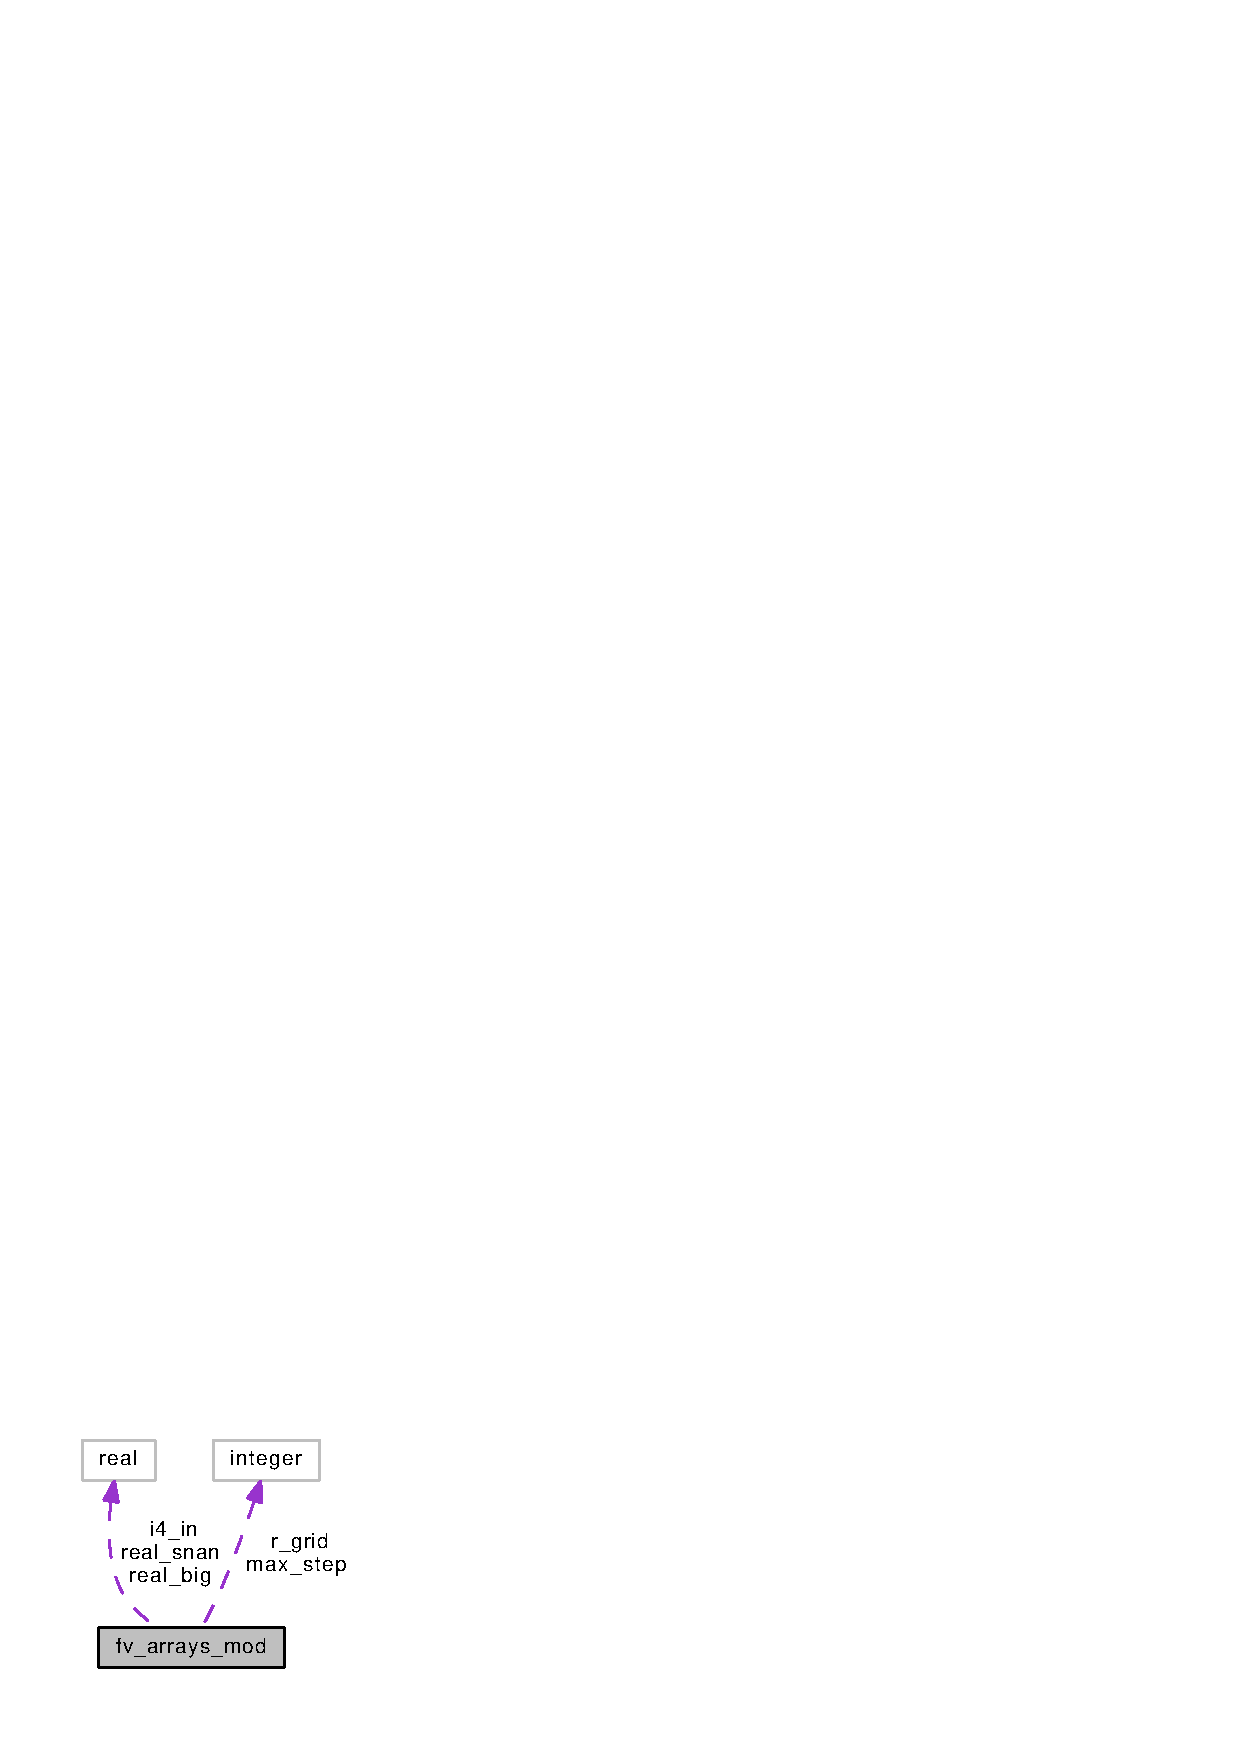
\includegraphics[width=171pt]{classfv__arrays__mod__coll__graph}
\end{center}
\end{figure}
\subsection*{Data Types}
\begin{DoxyCompactItemize}
\item 
interface \hyperlink{interfacefv__arrays__mod_1_1allocate__fv__nest__bc__type}{allocate\-\_\-fv\-\_\-nest\-\_\-bc\-\_\-type}
\begin{DoxyCompactList}\small\item\em 'allocate\-\_\-fv\-\_\-nest\-\_\-\-B\-C\-\_\-type' is an interface to subroutines that allocate the 'fv\-\_\-nest\-\_\-\-B\-C\-\_\-type' structure that holds the nested-\/grid B\-Cs. \end{DoxyCompactList}\item 
interface \hyperlink{interfacefv__arrays__mod_1_1deallocate__fv__nest__bc__type}{deallocate\-\_\-fv\-\_\-nest\-\_\-bc\-\_\-type}
\begin{DoxyCompactList}\small\item\em 'deallocate\-\_\-fv\-\_\-nest\-\_\-\-B\-C\-\_\-type' is an interface to a subroutine that deallocates the 'fv\-\_\-nest\-\_\-\-B\-C\-\_\-type' structure that holds the nested-\/grid B\-Cs. \end{DoxyCompactList}\item 
type \hyperlink{structfv__arrays__mod_1_1fv__atmos__type}{fv\-\_\-atmos\-\_\-type}
\item 
type \hyperlink{structfv__arrays__mod_1_1fv__diag__type}{fv\-\_\-diag\-\_\-type}
\item 
type \hyperlink{structfv__arrays__mod_1_1fv__flags__type}{fv\-\_\-flags\-\_\-type}
\item 
type \hyperlink{structfv__arrays__mod_1_1fv__grid__bounds__type}{fv\-\_\-grid\-\_\-bounds\-\_\-type}
\item 
type \hyperlink{structfv__arrays__mod_1_1fv__grid__type}{fv\-\_\-grid\-\_\-type}
\begin{DoxyCompactList}\small\item\em The type '\hyperlink{structfv__arrays__mod_1_1fv__grid__type}{fv\-\_\-grid\-\_\-type}' is made up of grid-\/dependent information from fv\-\_\-grid\-\_\-tools and fv\-\_\-grid\-\_\-utils. \end{DoxyCompactList}\item 
type \hyperlink{structfv__arrays__mod_1_1fv__nest__bc__type__3d}{fv\-\_\-nest\-\_\-bc\-\_\-type\-\_\-3d}
\item 
type \hyperlink{structfv__arrays__mod_1_1fv__nest__bc__type__4d}{fv\-\_\-nest\-\_\-bc\-\_\-type\-\_\-4d}
\item 
type \hyperlink{structfv__arrays__mod_1_1fv__nest__type}{fv\-\_\-nest\-\_\-type}
\item 
type \hyperlink{structfv__arrays__mod_1_1fv__regional__bc__bounds__type}{fv\-\_\-regional\-\_\-bc\-\_\-bounds\-\_\-type}
\end{DoxyCompactItemize}
\subsection*{Public Member Functions}
\begin{DoxyCompactItemize}
\item 
subroutine \hyperlink{classfv__arrays__mod_a6156c72def1af9adbf16f5c7d739b067}{allocate\-\_\-fv\-\_\-atmos\-\_\-type} (Atm, isd\-\_\-in, ied\-\_\-in, jsd\-\_\-in, jed\-\_\-in, is\-\_\-in, ie\-\_\-in, js\-\_\-in, je\-\_\-in, npx\-\_\-in, npy\-\_\-in, npz\-\_\-in, ndims\-\_\-in, ncnst\-\_\-in, nq\-\_\-in, ng\-\_\-in, dummy, alloc\-\_\-2d, ngrids\-\_\-in)
\begin{DoxyCompactList}\small\item\em The subroutine 'allocate\-\_\-fv\-\_\-atmos\-\_\-type' allocates the \hyperlink{structfv__arrays__mod_1_1fv__atmos__type}{fv\-\_\-atmos\-\_\-type}. \end{DoxyCompactList}\item 
subroutine \hyperlink{classfv__arrays__mod_a067591249b864319923ca6f7fbdc7cd3}{deallocate\-\_\-fv\-\_\-atmos\-\_\-type} (Atm)
\begin{DoxyCompactList}\small\item\em The subroutine 'deallocate\-\_\-fv\-\_\-atmos\-\_\-type' deallocates the \hyperlink{structfv__arrays__mod_1_1fv__atmos__type}{fv\-\_\-atmos\-\_\-type}. \end{DoxyCompactList}\item 
subroutine \hyperlink{classfv__arrays__mod_ae50208744b917974ac850d2073f834a1}{allocate\-\_\-fv\-\_\-nest\-\_\-bc\-\_\-type\-\_\-3d\-\_\-atm} (B\-C, Atm, ns, istag, jstag, dummy)
\item 
subroutine \hyperlink{classfv__arrays__mod_a098713dd7c958d62449b21e869c5472a}{allocate\-\_\-fv\-\_\-nest\-\_\-bc\-\_\-type\-\_\-3d} (B\-C, is, ie, js, je, isd, ied, jsd, jed, npx, npy, npz, ng, ns, istag, jstag, dummy)
\item 
subroutine \hyperlink{classfv__arrays__mod_a30884d6ec24da5922d899ee396e86020}{deallocate\-\_\-fv\-\_\-nest\-\_\-bc\-\_\-type\-\_\-3d} (B\-C)
\end{DoxyCompactItemize}
\subsection*{Public Attributes}
\begin{DoxyCompactItemize}
\item 
integer, parameter, public \hyperlink{classfv__arrays__mod_ab0ba8527d270f349a84fa0a330be1923}{r\-\_\-grid} = r8\-\_\-kind
\item 
integer, parameter \hyperlink{classfv__arrays__mod_a9e487a715273ca3c6572693756bcec1b}{max\-\_\-step} = 1000
\item 
real, parameter \hyperlink{classfv__arrays__mod_aa61534ed3f1d97da89f9e2ff98a31279}{real\-\_\-big} = 1.e30
\item 
real, parameter \hyperlink{classfv__arrays__mod_ac263153323954d48a2ba22738897b14c}{real\-\_\-snan} =x'F\-F\-F7\-F\-F\-F\-F\-F\-F\-F\-F\-F\-F\-F\-F'
\item 
real, parameter \hyperlink{classfv__arrays__mod_a4e97836bef22972e458e71ab3930b62c}{i4\-\_\-in} =-\/huge(1)
\end{DoxyCompactItemize}


\subsection{Detailed Description}
The module 'fv\-\_\-arrays' contains the '\hyperlink{structfv__arrays__mod_1_1fv__atmos__type}{fv\-\_\-atmos\-\_\-type}' and associated datatypes. 

Definition at line 24 of file fv\-\_\-arrays.\-F90.



\subsection{Member Function/\-Subroutine Documentation}
\index{fv\-\_\-arrays\-\_\-mod@{fv\-\_\-arrays\-\_\-mod}!allocate\-\_\-fv\-\_\-atmos\-\_\-type@{allocate\-\_\-fv\-\_\-atmos\-\_\-type}}
\index{allocate\-\_\-fv\-\_\-atmos\-\_\-type@{allocate\-\_\-fv\-\_\-atmos\-\_\-type}!fv_arrays_mod@{fv\-\_\-arrays\-\_\-mod}}
\subsubsection[{allocate\-\_\-fv\-\_\-atmos\-\_\-type}]{\setlength{\rightskip}{0pt plus 5cm}subroutine fv\-\_\-arrays\-\_\-mod\-::allocate\-\_\-fv\-\_\-atmos\-\_\-type (
\begin{DoxyParamCaption}
\item[{type({\bf fv\-\_\-atmos\-\_\-type}), intent(inout), target}]{Atm, }
\item[{integer, intent(in)}]{isd\-\_\-in, }
\item[{integer, intent(in)}]{ied\-\_\-in, }
\item[{integer, intent(in)}]{jsd\-\_\-in, }
\item[{integer, intent(in)}]{jed\-\_\-in, }
\item[{integer, intent(in)}]{is\-\_\-in, }
\item[{integer, intent(in)}]{ie\-\_\-in, }
\item[{integer, intent(in)}]{js\-\_\-in, }
\item[{integer, intent(in)}]{je\-\_\-in, }
\item[{integer, intent(in)}]{npx\-\_\-in, }
\item[{integer, intent(in)}]{npy\-\_\-in, }
\item[{integer, intent(in)}]{npz\-\_\-in, }
\item[{integer, intent(in)}]{ndims\-\_\-in, }
\item[{integer, intent(in)}]{ncnst\-\_\-in, }
\item[{integer, intent(in)}]{nq\-\_\-in, }
\item[{integer, intent(in)}]{ng\-\_\-in, }
\item[{logical, intent(in)}]{dummy, }
\item[{logical, intent(in)}]{alloc\-\_\-2d, }
\item[{integer, intent(in)}]{ngrids\-\_\-in}
\end{DoxyParamCaption}
)}\label{classfv__arrays__mod_a6156c72def1af9adbf16f5c7d739b067}


The subroutine 'allocate\-\_\-fv\-\_\-atmos\-\_\-type' allocates the \hyperlink{structfv__arrays__mod_1_1fv__atmos__type}{fv\-\_\-atmos\-\_\-type}. 

It includes an option to define dummy grids that have scalar and small arrays defined as null 3\-D arrays. 

Definition at line 1322 of file fv\-\_\-arrays.\-F90.



Referenced by fv\-\_\-control\-\_\-mod\-::fv\-\_\-init().

\index{fv\-\_\-arrays\-\_\-mod@{fv\-\_\-arrays\-\_\-mod}!allocate\-\_\-fv\-\_\-nest\-\_\-bc\-\_\-type\-\_\-3d@{allocate\-\_\-fv\-\_\-nest\-\_\-bc\-\_\-type\-\_\-3d}}
\index{allocate\-\_\-fv\-\_\-nest\-\_\-bc\-\_\-type\-\_\-3d@{allocate\-\_\-fv\-\_\-nest\-\_\-bc\-\_\-type\-\_\-3d}!fv_arrays_mod@{fv\-\_\-arrays\-\_\-mod}}
\subsubsection[{allocate\-\_\-fv\-\_\-nest\-\_\-bc\-\_\-type\-\_\-3d}]{\setlength{\rightskip}{0pt plus 5cm}subroutine fv\-\_\-arrays\-\_\-mod\-::allocate\-\_\-fv\-\_\-nest\-\_\-bc\-\_\-type\-\_\-3d (
\begin{DoxyParamCaption}
\item[{type({\bf fv\-\_\-nest\-\_\-bc\-\_\-type\-\_\-3d}), intent(inout)}]{B\-C, }
\item[{integer, intent(in)}]{is, }
\item[{integer, intent(in)}]{ie, }
\item[{integer, intent(in)}]{js, }
\item[{integer, intent(in)}]{je, }
\item[{integer, intent(in)}]{isd, }
\item[{integer, intent(in)}]{ied, }
\item[{integer, intent(in)}]{jsd, }
\item[{integer, intent(in)}]{jed, }
\item[{integer, intent(in)}]{npx, }
\item[{integer, intent(in)}]{npy, }
\item[{integer, intent(in)}]{npz, }
\item[{integer, intent(in)}]{ng, }
\item[{integer, intent(in)}]{ns, }
\item[{integer, intent(in)}]{istag, }
\item[{integer, intent(in)}]{jstag, }
\item[{logical, intent(in)}]{dummy}
\end{DoxyParamCaption}
)}\label{classfv__arrays__mod_a098713dd7c958d62449b21e869c5472a}


Definition at line 2015 of file fv\-\_\-arrays.\-F90.

\index{fv\-\_\-arrays\-\_\-mod@{fv\-\_\-arrays\-\_\-mod}!allocate\-\_\-fv\-\_\-nest\-\_\-bc\-\_\-type\-\_\-3d\-\_\-atm@{allocate\-\_\-fv\-\_\-nest\-\_\-bc\-\_\-type\-\_\-3d\-\_\-atm}}
\index{allocate\-\_\-fv\-\_\-nest\-\_\-bc\-\_\-type\-\_\-3d\-\_\-atm@{allocate\-\_\-fv\-\_\-nest\-\_\-bc\-\_\-type\-\_\-3d\-\_\-atm}!fv_arrays_mod@{fv\-\_\-arrays\-\_\-mod}}
\subsubsection[{allocate\-\_\-fv\-\_\-nest\-\_\-bc\-\_\-type\-\_\-3d\-\_\-atm}]{\setlength{\rightskip}{0pt plus 5cm}subroutine fv\-\_\-arrays\-\_\-mod\-::allocate\-\_\-fv\-\_\-nest\-\_\-bc\-\_\-type\-\_\-3d\-\_\-atm (
\begin{DoxyParamCaption}
\item[{type({\bf fv\-\_\-nest\-\_\-bc\-\_\-type\-\_\-3d}), intent(inout)}]{B\-C, }
\item[{type({\bf fv\-\_\-atmos\-\_\-type}), intent(in)}]{Atm, }
\item[{integer, intent(in)}]{ns, }
\item[{integer, intent(in)}]{istag, }
\item[{integer, intent(in)}]{jstag, }
\item[{logical, intent(in)}]{dummy}
\end{DoxyParamCaption}
)}\label{classfv__arrays__mod_ae50208744b917974ac850d2073f834a1}


Definition at line 1983 of file fv\-\_\-arrays.\-F90.



References fv\-\_\-arrays\-\_\-mod\-::allocate\-\_\-fv\-\_\-nest\-\_\-bc\-\_\-type\-::allocate\-\_\-fv\-\_\-nest\-\_\-bc\-\_\-type\-\_\-3d().

\index{fv\-\_\-arrays\-\_\-mod@{fv\-\_\-arrays\-\_\-mod}!deallocate\-\_\-fv\-\_\-atmos\-\_\-type@{deallocate\-\_\-fv\-\_\-atmos\-\_\-type}}
\index{deallocate\-\_\-fv\-\_\-atmos\-\_\-type@{deallocate\-\_\-fv\-\_\-atmos\-\_\-type}!fv_arrays_mod@{fv\-\_\-arrays\-\_\-mod}}
\subsubsection[{deallocate\-\_\-fv\-\_\-atmos\-\_\-type}]{\setlength{\rightskip}{0pt plus 5cm}subroutine fv\-\_\-arrays\-\_\-mod\-::deallocate\-\_\-fv\-\_\-atmos\-\_\-type (
\begin{DoxyParamCaption}
\item[{type({\bf fv\-\_\-atmos\-\_\-type}), intent(inout)}]{Atm}
\end{DoxyParamCaption}
)}\label{classfv__arrays__mod_a067591249b864319923ca6f7fbdc7cd3}


The subroutine 'deallocate\-\_\-fv\-\_\-atmos\-\_\-type' deallocates the \hyperlink{structfv__arrays__mod_1_1fv__atmos__type}{fv\-\_\-atmos\-\_\-type}. 



Definition at line 1769 of file fv\-\_\-arrays.\-F90.



Referenced by fv\-\_\-control\-\_\-mod\-::fv\-\_\-end().

\index{fv\-\_\-arrays\-\_\-mod@{fv\-\_\-arrays\-\_\-mod}!deallocate\-\_\-fv\-\_\-nest\-\_\-bc\-\_\-type\-\_\-3d@{deallocate\-\_\-fv\-\_\-nest\-\_\-bc\-\_\-type\-\_\-3d}}
\index{deallocate\-\_\-fv\-\_\-nest\-\_\-bc\-\_\-type\-\_\-3d@{deallocate\-\_\-fv\-\_\-nest\-\_\-bc\-\_\-type\-\_\-3d}!fv_arrays_mod@{fv\-\_\-arrays\-\_\-mod}}
\subsubsection[{deallocate\-\_\-fv\-\_\-nest\-\_\-bc\-\_\-type\-\_\-3d}]{\setlength{\rightskip}{0pt plus 5cm}subroutine fv\-\_\-arrays\-\_\-mod\-::deallocate\-\_\-fv\-\_\-nest\-\_\-bc\-\_\-type\-\_\-3d (
\begin{DoxyParamCaption}
\item[{type({\bf fv\-\_\-nest\-\_\-bc\-\_\-type\-\_\-3d})}]{B\-C}
\end{DoxyParamCaption}
)}\label{classfv__arrays__mod_a30884d6ec24da5922d899ee396e86020}


Definition at line 2094 of file fv\-\_\-arrays.\-F90.



\subsection{Member Data Documentation}
\index{fv\-\_\-arrays\-\_\-mod@{fv\-\_\-arrays\-\_\-mod}!i4\-\_\-in@{i4\-\_\-in}}
\index{i4\-\_\-in@{i4\-\_\-in}!fv_arrays_mod@{fv\-\_\-arrays\-\_\-mod}}
\subsubsection[{i4\-\_\-in}]{\setlength{\rightskip}{0pt plus 5cm}real, parameter fv\-\_\-arrays\-\_\-mod\-::i4\-\_\-in =-\/huge(1)}\label{classfv__arrays__mod_a4e97836bef22972e458e71ab3930b62c}


Definition at line 52 of file fv\-\_\-arrays.\-F90.

\index{fv\-\_\-arrays\-\_\-mod@{fv\-\_\-arrays\-\_\-mod}!max\-\_\-step@{max\-\_\-step}}
\index{max\-\_\-step@{max\-\_\-step}!fv_arrays_mod@{fv\-\_\-arrays\-\_\-mod}}
\subsubsection[{max\-\_\-step}]{\setlength{\rightskip}{0pt plus 5cm}integer, parameter fv\-\_\-arrays\-\_\-mod\-::max\-\_\-step = 1000}\label{classfv__arrays__mod_a9e487a715273ca3c6572693756bcec1b}


Definition at line 43 of file fv\-\_\-arrays.\-F90.

\index{fv\-\_\-arrays\-\_\-mod@{fv\-\_\-arrays\-\_\-mod}!r\-\_\-grid@{r\-\_\-grid}}
\index{r\-\_\-grid@{r\-\_\-grid}!fv_arrays_mod@{fv\-\_\-arrays\-\_\-mod}}
\subsubsection[{r\-\_\-grid}]{\setlength{\rightskip}{0pt plus 5cm}integer, parameter, public fv\-\_\-arrays\-\_\-mod\-::r\-\_\-grid = r8\-\_\-kind}\label{classfv__arrays__mod_ab0ba8527d270f349a84fa0a330be1923}


Definition at line 35 of file fv\-\_\-arrays.\-F90.

\index{fv\-\_\-arrays\-\_\-mod@{fv\-\_\-arrays\-\_\-mod}!real\-\_\-big@{real\-\_\-big}}
\index{real\-\_\-big@{real\-\_\-big}!fv_arrays_mod@{fv\-\_\-arrays\-\_\-mod}}
\subsubsection[{real\-\_\-big}]{\setlength{\rightskip}{0pt plus 5cm}real, parameter fv\-\_\-arrays\-\_\-mod\-::real\-\_\-big = 1.e30}\label{classfv__arrays__mod_aa61534ed3f1d97da89f9e2ff98a31279}


Definition at line 49 of file fv\-\_\-arrays.\-F90.

\index{fv\-\_\-arrays\-\_\-mod@{fv\-\_\-arrays\-\_\-mod}!real\-\_\-snan@{real\-\_\-snan}}
\index{real\-\_\-snan@{real\-\_\-snan}!fv_arrays_mod@{fv\-\_\-arrays\-\_\-mod}}
\subsubsection[{real\-\_\-snan}]{\setlength{\rightskip}{0pt plus 5cm}real, parameter fv\-\_\-arrays\-\_\-mod\-::real\-\_\-snan =x'F\-F\-F7\-F\-F\-F\-F\-F\-F\-F\-F\-F\-F\-F\-F'}\label{classfv__arrays__mod_ac263153323954d48a2ba22738897b14c}


Definition at line 50 of file fv\-\_\-arrays.\-F90.



The documentation for this module was generated from the following file\-:\begin{DoxyCompactItemize}
\item 
/scratch2/\-N\-A\-G\-A\-P\-E/aoml-\/hafs1/\-Kyle.\-Ahern/acs\-\_\-master\-\_\-readonly/model/\hyperlink{fv__arrays_8F90}{fv\-\_\-arrays.\-F90}\end{DoxyCompactItemize}

\section{fv\-\_\-arrays\-\_\-mod\-:\-:fv\-\_\-atmos\-\_\-type Type Reference}
\label{structfv__arrays__mod_1_1fv__atmos__type}\index{fv\-\_\-arrays\-\_\-mod\-::fv\-\_\-atmos\-\_\-type@{fv\-\_\-arrays\-\_\-mod\-::fv\-\_\-atmos\-\_\-type}}


Collaboration diagram for fv\-\_\-arrays\-\_\-mod\-:\-:fv\-\_\-atmos\-\_\-type\-:
\nopagebreak
\begin{figure}[H]
\begin{center}
\leavevmode
\includegraphics[height=550pt]{structfv__arrays__mod_1_1fv__atmos__type__coll__graph}
\end{center}
\end{figure}
\subsection*{Public Attributes}
\begin{DoxyCompactItemize}
\item 
logical \hyperlink{structfv__arrays__mod_1_1fv__atmos__type_aad4bddd3e4ffbb1cf0b37c3057709fdc}{allocated} = .false.
\item 
logical \hyperlink{structfv__arrays__mod_1_1fv__atmos__type_a124c10f670d516b0517bdc038b66c857}{dummy} = .false.
\item 
integer \hyperlink{structfv__arrays__mod_1_1fv__atmos__type_a186d371efd7b4ab4dc508fde35315dcf}{grid\-\_\-number} = 1
\item 
type(time\-\_\-type) \hyperlink{structfv__arrays__mod_1_1fv__atmos__type_a2250fa17165a7e44f75420a519cc72cf}{time\-\_\-init}
\item 
type(time\-\_\-type) \hyperlink{structfv__arrays__mod_1_1fv__atmos__type_ae610371fcfe85e6d7dc1fa87fdce7727}{time}
\item 
type(time\-\_\-type) \hyperlink{structfv__arrays__mod_1_1fv__atmos__type_ad7f9725ebc9ed275affe742ae6384720}{run\-\_\-length}
\item 
type(time\-\_\-type) \hyperlink{structfv__arrays__mod_1_1fv__atmos__type_ae49eef6008ea3ff710d90c56eacfe6a6}{time\-\_\-end}
\item 
type(time\-\_\-type) \hyperlink{structfv__arrays__mod_1_1fv__atmos__type_aaff3c348215efb0095c2e8c196efe1a7}{time\-\_\-step\-\_\-atmos}
\item 
logical \hyperlink{structfv__arrays__mod_1_1fv__atmos__type_aa4c6e33a14ec7220f5852ee87cd2e71c}{grid\-\_\-active} = .true.
\item 
type(\hyperlink{structfv__arrays__mod_1_1fv__atmos__type}{fv\-\_\-atmos\-\_\-type}), pointer \hyperlink{structfv__arrays__mod_1_1fv__atmos__type_a024a613cbb8da76610bec384b7a37bfb}{parent\-\_\-grid} =$>$ N\-U\-L\-L()
\item 
real \hyperlink{structfv__arrays__mod_1_1fv__atmos__type_a95b1ec35498953d190b394d9390b6a02}{\-\_\-allocatable}
\item 
real, dimension(\-:,\-:,\-:) \hyperlink{structfv__arrays__mod_1_1fv__atmos__type_a5ff3358578eee5de976eb794574fe5c3}{u}
\item 
real \hyperlink{structfv__arrays__mod_1_1fv__atmos__type_a6c2bbca5c19e33f65a51df86735d512a}{\-\_\-null}
\begin{DoxyCompactList}\small\item\em D grid zonal wind (m/s) \end{DoxyCompactList}\item 
real, dimension(\-:,\-:,\-:) \hyperlink{structfv__arrays__mod_1_1fv__atmos__type_ad6381f84485f8d9edfc04581ff90e5cb}{v}
\item 
real, dimension(\-:,\-:,\-:) \hyperlink{structfv__arrays__mod_1_1fv__atmos__type_a28a65aae9292344e1cdad47e48de319e}{pt}
\item 
real, dimension(\-:,\-:,\-:) \hyperlink{structfv__arrays__mod_1_1fv__atmos__type_a4a0a399c18dc1ddd81e4dfaa559e3ce7}{delp}
\item 
real, dimension(\-:,\-:,\-:,\-:) \hyperlink{structfv__arrays__mod_1_1fv__atmos__type_a10d0bec282af4b2131c91f714279be89}{q}
\item 
real, dimension(\-:,\-:,\-:,\-:) \hyperlink{structfv__arrays__mod_1_1fv__atmos__type_aa6098dd9e893df46808742694e45323a}{qdiag}
\item 
real, dimension(\-:,\-:,\-:) \hyperlink{structfv__arrays__mod_1_1fv__atmos__type_a2b0d0ca4a8e622f47bb6ad50f293303c}{w}
\item 
real, dimension(\-:,\-:,\-:) \hyperlink{structfv__arrays__mod_1_1fv__atmos__type_a6589bbace2c4d70b1828ad30c8f0f694}{delz}
\item 
real, dimension(\-:,\-:,\-:) \hyperlink{structfv__arrays__mod_1_1fv__atmos__type_a751b4cbe5e6b4662ea5802e39ceebf18}{ze0}
\item 
real, dimension(\-:,\-:,\-:) \hyperlink{structfv__arrays__mod_1_1fv__atmos__type_af01023dfdd6a3df5043e2d49e4acd413}{q\-\_\-con}
\item 
real, dimension(\-:,\-:) \hyperlink{structfv__arrays__mod_1_1fv__atmos__type_acef8b954c66485555f89a158def2f797}{ps}
\item 
real, dimension(\-:,\-:,\-:) \hyperlink{structfv__arrays__mod_1_1fv__atmos__type_a0da51913e73fce5f1efc7b50c8113320}{pe}
\item 
real, dimension(\-:,\-:,\-:) \hyperlink{structfv__arrays__mod_1_1fv__atmos__type_a0882342b11ac2963886233f84c1ca2ec}{pk}
\item 
real, dimension(\-:,\-:,\-:) \hyperlink{structfv__arrays__mod_1_1fv__atmos__type_a438aadd63c30fec4db3ad811ecb3f81a}{peln}
\item 
real, dimension(\-:,\-:,\-:) \hyperlink{structfv__arrays__mod_1_1fv__atmos__type_a08a7dae1471b3e7b7859e28c757582bb}{pkz}
\item 
real, dimension(\-:,\-:) \hyperlink{structfv__arrays__mod_1_1fv__atmos__type_a1288d4ab5a553904266d404d407a9e98}{u\-\_\-srf}
\item 
real, dimension(\-:,\-:) \hyperlink{structfv__arrays__mod_1_1fv__atmos__type_ac2fc282291dfbf37c96e5de7100070d4}{v\-\_\-srf}
\item 
real, dimension(\-:,\-:) \hyperlink{structfv__arrays__mod_1_1fv__atmos__type_ad6a036d45fbee5ca39120b204a0a78c3}{sgh}
\item 
real, dimension(\-:,\-:) \hyperlink{structfv__arrays__mod_1_1fv__atmos__type_abbfb5137f18bb1972cd59786a17e28e9}{oro}
\item 
real, dimension(\-:,\-:) \hyperlink{structfv__arrays__mod_1_1fv__atmos__type_a0b442abb8ea87c4c65eda345a9ed2fb4}{ts}
\item 
real, dimension(\-:,\-:,\-:) \hyperlink{structfv__arrays__mod_1_1fv__atmos__type_ad10ec78382b4afbe88a70499fd69c3d3}{diss\-\_\-est}
\item 
real, dimension(\-:,\-:) \hyperlink{structfv__arrays__mod_1_1fv__atmos__type_ac6cfc672780cbc8b5fab0ca13e1a7590}{phis}
\item 
real, dimension(\-:,\-:,\-:) \hyperlink{structfv__arrays__mod_1_1fv__atmos__type_a53ce006346b4f956804f3c550714cc06}{omga}
\item 
real, dimension(\-:,\-:,\-:) \hyperlink{structfv__arrays__mod_1_1fv__atmos__type_a410b5e8e5b66dc1a61c5b47aa46b2615}{ua}
\item 
real, dimension(\-:,\-:,\-:) \hyperlink{structfv__arrays__mod_1_1fv__atmos__type_a4379193f2f1d4142032c8d95c55abb0c}{va}
\item 
real, dimension(\-:,\-:,\-:) \hyperlink{structfv__arrays__mod_1_1fv__atmos__type_a672b688e0f1b1130caddd31d788d5af8}{uc}
\item 
real, dimension(\-:,\-:,\-:) \hyperlink{structfv__arrays__mod_1_1fv__atmos__type_a9f23c2d267763af4486c22466937733c}{vc}
\item 
real, dimension(\-:) \hyperlink{structfv__arrays__mod_1_1fv__atmos__type_aef6fdeb7a3c7c74773f35929a200f4e5}{ak}
\item 
real, dimension(\-:) \hyperlink{structfv__arrays__mod_1_1fv__atmos__type_a153c4671e9a6268efd9b3f1a4bae7f3c}{bk}
\item 
integer \hyperlink{structfv__arrays__mod_1_1fv__atmos__type_a737df1e4018be0a63337665e13f8f5ab}{ks}
\item 
real, dimension(\-:,\-:,\-:) \hyperlink{structfv__arrays__mod_1_1fv__atmos__type_a9bfc2bd70bc1dccfe305077daf0cab2c}{mfx}
\item 
real, dimension(\-:,\-:,\-:) \hyperlink{structfv__arrays__mod_1_1fv__atmos__type_a6f34be94d378cc6a42e4fc91617bbd40}{mfy}
\item 
real, dimension(\-:,\-:,\-:) \hyperlink{structfv__arrays__mod_1_1fv__atmos__type_a9de9d89045261a87a6708b261b6b0600}{cx}
\item 
real, dimension(\-:,\-:,\-:) \hyperlink{structfv__arrays__mod_1_1fv__atmos__type_a6051004a5665381f98403598f0d841cb}{cy}
\item 
type(\hyperlink{structfv__arrays__mod_1_1fv__flags__type}{fv\-\_\-flags\-\_\-type}) \hyperlink{structfv__arrays__mod_1_1fv__atmos__type_a690b87301c4d59a583cb3b291c6d2701}{flagstruct}
\item 
integer, pointer \hyperlink{structfv__arrays__mod_1_1fv__atmos__type_a0e54dd727ebba5a1c57fcf0d93c9cf36}{npx}
\item 
integer, pointer \hyperlink{structfv__arrays__mod_1_1fv__atmos__type_ad3e89def6220e74dc7e5bd4d980721f1}{npy}
\item 
integer, pointer \hyperlink{structfv__arrays__mod_1_1fv__atmos__type_a2db29836bd7cb9adb49d819e9c7ae0ce}{npz}
\item 
integer, pointer \hyperlink{structfv__arrays__mod_1_1fv__atmos__type_abb783b1c9289305b504854b91bdd8356}{ncnst}
\item 
integer, pointer \hyperlink{structfv__arrays__mod_1_1fv__atmos__type_ac30aa7aa79c3ce8965781354a6cccfdd}{ng}
\item 
integer, dimension(\-:), allocatable \hyperlink{structfv__arrays__mod_1_1fv__atmos__type_aa3b9aaaf36503aad223be6c46d21a3b5}{pelist}
\item 
type(\hyperlink{structfv__arrays__mod_1_1fv__grid__bounds__type}{fv\-\_\-grid\-\_\-bounds\-\_\-type}) \hyperlink{structfv__arrays__mod_1_1fv__atmos__type_a2a2b12a650ed344e10e00ce708935c78}{bd}
\item 
type(\hyperlink{structfv__arrays__mod_1_1fv__regional__bc__bounds__type}{fv\-\_\-regional\-\_\-bc\-\_\-bounds\-\_\-type}) \hyperlink{structfv__arrays__mod_1_1fv__atmos__type_a685f2987cb3a2f50f28a8ed8b58ce6e6}{regional\-\_\-bc\-\_\-bounds}
\item 
type(domain2d) \hyperlink{structfv__arrays__mod_1_1fv__atmos__type_ade8a5697c963d272c6d9deff35fb15f2}{domain}
\item 
real \hyperlink{structfv__arrays__mod_1_1fv__atmos__type_abaf34c4bb266c7a9964772bfdf12ced3}{ptop}
\item 
type(\hyperlink{structfv__arrays__mod_1_1fv__grid__type}{fv\-\_\-grid\-\_\-type}) \hyperlink{structfv__arrays__mod_1_1fv__atmos__type_a1ee11bc6f17076db85d576290051fcbf}{gridstruct}
\item 
type(\hyperlink{structfv__arrays__mod_1_1fv__diag__type}{fv\-\_\-diag\-\_\-type}) \hyperlink{structfv__arrays__mod_1_1fv__atmos__type_a43f51b4e94d6446147fa220be628bffb}{idiag}
\item 
type(restart\-\_\-file\-\_\-type) \hyperlink{structfv__arrays__mod_1_1fv__atmos__type_a81c0a2a6d32e9d1ec76ba25429fe964e}{fv\-\_\-restart}
\item 
type(restart\-\_\-file\-\_\-type) \hyperlink{structfv__arrays__mod_1_1fv__atmos__type_acb55bff833b0e9724ee32485d24abeab}{sst\-\_\-restart}
\item 
type(restart\-\_\-file\-\_\-type) \hyperlink{structfv__arrays__mod_1_1fv__atmos__type_ab4acfb059f86162ac82b1a11612f1610}{fv\-\_\-tile\-\_\-restart}
\item 
type(restart\-\_\-file\-\_\-type) \hyperlink{structfv__arrays__mod_1_1fv__atmos__type_a3d76489d7309fe00ff9417911e8d3fb5}{rsf\-\_\-restart}
\item 
type(restart\-\_\-file\-\_\-type) \hyperlink{structfv__arrays__mod_1_1fv__atmos__type_a80c75e3c3ef687cdfed8ab388c243dc2}{mg\-\_\-restart}
\item 
type(restart\-\_\-file\-\_\-type) \hyperlink{structfv__arrays__mod_1_1fv__atmos__type_a343bed7b2fae51453d57bcef96ac919d}{lnd\-\_\-restart}
\item 
type(restart\-\_\-file\-\_\-type) \hyperlink{structfv__arrays__mod_1_1fv__atmos__type_ab394a0387bd944dd57cb09a3abc5abfa}{tra\-\_\-restart}
\item 
type(\hyperlink{structfv__arrays__mod_1_1fv__nest__type}{fv\-\_\-nest\-\_\-type}) \hyperlink{structfv__arrays__mod_1_1fv__atmos__type_a0de20030b672c84ef5f1eec9360ccf61}{neststruct}
\item 
real(kind=\hyperlink{classfv__arrays__mod_ab0ba8527d270f349a84fa0a330be1923}{r\-\_\-grid}), dimension(\-:,\-:,\-:,\-:), \\*
allocatable \hyperlink{structfv__arrays__mod_1_1fv__atmos__type_adc565026ec8a2ef0abafa0445987e923}{grid\-\_\-global}
\item 
integer, dimension(4) \hyperlink{structfv__arrays__mod_1_1fv__atmos__type_a32f9a169b6f3e0c138d9e069d6916083}{atmos\-\_\-axes}
\end{DoxyCompactItemize}


\subsection{Detailed Description}


Definition at line 1166 of file fv\-\_\-arrays.\-F90.



\subsection{Member Data Documentation}
\index{fv\-\_\-arrays\-\_\-mod\-::fv\-\_\-atmos\-\_\-type@{fv\-\_\-arrays\-\_\-mod\-::fv\-\_\-atmos\-\_\-type}!\-\_\-allocatable@{\-\_\-allocatable}}
\index{\-\_\-allocatable@{\-\_\-allocatable}!fv_arrays_mod::fv_atmos_type@{fv\-\_\-arrays\-\_\-mod\-::fv\-\_\-atmos\-\_\-type}}
\subsubsection[{\-\_\-allocatable}]{\setlength{\rightskip}{0pt plus 5cm}real fv\-\_\-arrays\-\_\-mod\-::fv\-\_\-atmos\-\_\-type\-::\-\_\-allocatable}\label{structfv__arrays__mod_1_1fv__atmos__type_a95b1ec35498953d190b394d9390b6a02}


Definition at line 1197 of file fv\-\_\-arrays.\-F90.

\index{fv\-\_\-arrays\-\_\-mod\-::fv\-\_\-atmos\-\_\-type@{fv\-\_\-arrays\-\_\-mod\-::fv\-\_\-atmos\-\_\-type}!\-\_\-null@{\-\_\-null}}
\index{\-\_\-null@{\-\_\-null}!fv_arrays_mod::fv_atmos_type@{fv\-\_\-arrays\-\_\-mod\-::fv\-\_\-atmos\-\_\-type}}
\subsubsection[{\-\_\-null}]{\setlength{\rightskip}{0pt plus 5cm}real fv\-\_\-arrays\-\_\-mod\-::fv\-\_\-atmos\-\_\-type\-::\-\_\-null}\label{structfv__arrays__mod_1_1fv__atmos__type_a6c2bbca5c19e33f65a51df86735d512a}


D grid zonal wind (m/s) 

(uc, vc) are mostly used as the C grid winds

(ua, va) are mostly used as the A grid winds

Vertical pressure velocity (pa/s)

Surface geopotential (g$\ast$\-Z\-\_\-surf)

dissipation estimate taken from 'heat\-\_\-source'

skin temperature (sst) from N\-C\-E\-P/\-G\-F\-S (K) -- tile

land fraction (1\-: all land; 0\-: all water)

Terrain standard deviation.

Surface v-\/wind.

Surface u-\/wind.

finite-\/volume mean pk

ln(pe)

pe$\ast$$\ast$cappa

edge pressure (pascal)

Surface pressure (pascal)

total condensates

height at layer edges for remapping

layer thickness (meters)

cell center vertical wind (m/s)

diagnostic tracers

specific humidity and prognostic constituents

pressure thickness (pascal)

temperature (K)

D grid meridional wind (m/s) 

Definition at line 1197 of file fv\-\_\-arrays.\-F90.

\index{fv\-\_\-arrays\-\_\-mod\-::fv\-\_\-atmos\-\_\-type@{fv\-\_\-arrays\-\_\-mod\-::fv\-\_\-atmos\-\_\-type}!ak@{ak}}
\index{ak@{ak}!fv_arrays_mod::fv_atmos_type@{fv\-\_\-arrays\-\_\-mod\-::fv\-\_\-atmos\-\_\-type}}
\subsubsection[{ak}]{\setlength{\rightskip}{0pt plus 5cm}real, dimension(\-:) fv\-\_\-arrays\-\_\-mod\-::fv\-\_\-atmos\-\_\-type\-::ak}\label{structfv__arrays__mod_1_1fv__atmos__type_aef6fdeb7a3c7c74773f35929a200f4e5}


Definition at line 1242 of file fv\-\_\-arrays.\-F90.

\index{fv\-\_\-arrays\-\_\-mod\-::fv\-\_\-atmos\-\_\-type@{fv\-\_\-arrays\-\_\-mod\-::fv\-\_\-atmos\-\_\-type}!allocated@{allocated}}
\index{allocated@{allocated}!fv_arrays_mod::fv_atmos_type@{fv\-\_\-arrays\-\_\-mod\-::fv\-\_\-atmos\-\_\-type}}
\subsubsection[{allocated}]{\setlength{\rightskip}{0pt plus 5cm}logical fv\-\_\-arrays\-\_\-mod\-::fv\-\_\-atmos\-\_\-type\-::allocated = .false.}\label{structfv__arrays__mod_1_1fv__atmos__type_aad4bddd3e4ffbb1cf0b37c3057709fdc}


Definition at line 1168 of file fv\-\_\-arrays.\-F90.

\index{fv\-\_\-arrays\-\_\-mod\-::fv\-\_\-atmos\-\_\-type@{fv\-\_\-arrays\-\_\-mod\-::fv\-\_\-atmos\-\_\-type}!atmos\-\_\-axes@{atmos\-\_\-axes}}
\index{atmos\-\_\-axes@{atmos\-\_\-axes}!fv_arrays_mod::fv_atmos_type@{fv\-\_\-arrays\-\_\-mod\-::fv\-\_\-atmos\-\_\-type}}
\subsubsection[{atmos\-\_\-axes}]{\setlength{\rightskip}{0pt plus 5cm}integer, dimension(4) fv\-\_\-arrays\-\_\-mod\-::fv\-\_\-atmos\-\_\-type\-::atmos\-\_\-axes}\label{structfv__arrays__mod_1_1fv__atmos__type_a32f9a169b6f3e0c138d9e069d6916083}


Definition at line 1313 of file fv\-\_\-arrays.\-F90.

\index{fv\-\_\-arrays\-\_\-mod\-::fv\-\_\-atmos\-\_\-type@{fv\-\_\-arrays\-\_\-mod\-::fv\-\_\-atmos\-\_\-type}!bd@{bd}}
\index{bd@{bd}!fv_arrays_mod::fv_atmos_type@{fv\-\_\-arrays\-\_\-mod\-::fv\-\_\-atmos\-\_\-type}}
\subsubsection[{bd}]{\setlength{\rightskip}{0pt plus 5cm}type({\bf fv\-\_\-grid\-\_\-bounds\-\_\-type}) fv\-\_\-arrays\-\_\-mod\-::fv\-\_\-atmos\-\_\-type\-::bd}\label{structfv__arrays__mod_1_1fv__atmos__type_a2a2b12a650ed344e10e00ce708935c78}


Definition at line 1261 of file fv\-\_\-arrays.\-F90.

\index{fv\-\_\-arrays\-\_\-mod\-::fv\-\_\-atmos\-\_\-type@{fv\-\_\-arrays\-\_\-mod\-::fv\-\_\-atmos\-\_\-type}!bk@{bk}}
\index{bk@{bk}!fv_arrays_mod::fv_atmos_type@{fv\-\_\-arrays\-\_\-mod\-::fv\-\_\-atmos\-\_\-type}}
\subsubsection[{bk}]{\setlength{\rightskip}{0pt plus 5cm}real, dimension(\-:) fv\-\_\-arrays\-\_\-mod\-::fv\-\_\-atmos\-\_\-type\-::bk}\label{structfv__arrays__mod_1_1fv__atmos__type_a153c4671e9a6268efd9b3f1a4bae7f3c}


Definition at line 1243 of file fv\-\_\-arrays.\-F90.

\index{fv\-\_\-arrays\-\_\-mod\-::fv\-\_\-atmos\-\_\-type@{fv\-\_\-arrays\-\_\-mod\-::fv\-\_\-atmos\-\_\-type}!cx@{cx}}
\index{cx@{cx}!fv_arrays_mod::fv_atmos_type@{fv\-\_\-arrays\-\_\-mod\-::fv\-\_\-atmos\-\_\-type}}
\subsubsection[{cx}]{\setlength{\rightskip}{0pt plus 5cm}real, dimension(\-:,\-:,\-:) fv\-\_\-arrays\-\_\-mod\-::fv\-\_\-atmos\-\_\-type\-::cx}\label{structfv__arrays__mod_1_1fv__atmos__type_a9de9d89045261a87a6708b261b6b0600}


Definition at line 1251 of file fv\-\_\-arrays.\-F90.

\index{fv\-\_\-arrays\-\_\-mod\-::fv\-\_\-atmos\-\_\-type@{fv\-\_\-arrays\-\_\-mod\-::fv\-\_\-atmos\-\_\-type}!cy@{cy}}
\index{cy@{cy}!fv_arrays_mod::fv_atmos_type@{fv\-\_\-arrays\-\_\-mod\-::fv\-\_\-atmos\-\_\-type}}
\subsubsection[{cy}]{\setlength{\rightskip}{0pt plus 5cm}real, dimension(\-:,\-:,\-:) fv\-\_\-arrays\-\_\-mod\-::fv\-\_\-atmos\-\_\-type\-::cy}\label{structfv__arrays__mod_1_1fv__atmos__type_a6051004a5665381f98403598f0d841cb}


Definition at line 1252 of file fv\-\_\-arrays.\-F90.

\index{fv\-\_\-arrays\-\_\-mod\-::fv\-\_\-atmos\-\_\-type@{fv\-\_\-arrays\-\_\-mod\-::fv\-\_\-atmos\-\_\-type}!delp@{delp}}
\index{delp@{delp}!fv_arrays_mod::fv_atmos_type@{fv\-\_\-arrays\-\_\-mod\-::fv\-\_\-atmos\-\_\-type}}
\subsubsection[{delp}]{\setlength{\rightskip}{0pt plus 5cm}real, dimension(\-:,\-:,\-:) fv\-\_\-arrays\-\_\-mod\-::fv\-\_\-atmos\-\_\-type\-::delp}\label{structfv__arrays__mod_1_1fv__atmos__type_a4a0a399c18dc1ddd81e4dfaa559e3ce7}


Definition at line 1200 of file fv\-\_\-arrays.\-F90.

\index{fv\-\_\-arrays\-\_\-mod\-::fv\-\_\-atmos\-\_\-type@{fv\-\_\-arrays\-\_\-mod\-::fv\-\_\-atmos\-\_\-type}!delz@{delz}}
\index{delz@{delz}!fv_arrays_mod::fv_atmos_type@{fv\-\_\-arrays\-\_\-mod\-::fv\-\_\-atmos\-\_\-type}}
\subsubsection[{delz}]{\setlength{\rightskip}{0pt plus 5cm}real, dimension(\-:,\-:,\-:) fv\-\_\-arrays\-\_\-mod\-::fv\-\_\-atmos\-\_\-type\-::delz}\label{structfv__arrays__mod_1_1fv__atmos__type_a6589bbace2c4d70b1828ad30c8f0f694}


Definition at line 1208 of file fv\-\_\-arrays.\-F90.

\index{fv\-\_\-arrays\-\_\-mod\-::fv\-\_\-atmos\-\_\-type@{fv\-\_\-arrays\-\_\-mod\-::fv\-\_\-atmos\-\_\-type}!diss\-\_\-est@{diss\-\_\-est}}
\index{diss\-\_\-est@{diss\-\_\-est}!fv_arrays_mod::fv_atmos_type@{fv\-\_\-arrays\-\_\-mod\-::fv\-\_\-atmos\-\_\-type}}
\subsubsection[{diss\-\_\-est}]{\setlength{\rightskip}{0pt plus 5cm}real, dimension(\-:,\-:,\-:) fv\-\_\-arrays\-\_\-mod\-::fv\-\_\-atmos\-\_\-type\-::diss\-\_\-est}\label{structfv__arrays__mod_1_1fv__atmos__type_ad10ec78382b4afbe88a70499fd69c3d3}


Definition at line 1230 of file fv\-\_\-arrays.\-F90.

\index{fv\-\_\-arrays\-\_\-mod\-::fv\-\_\-atmos\-\_\-type@{fv\-\_\-arrays\-\_\-mod\-::fv\-\_\-atmos\-\_\-type}!domain@{domain}}
\index{domain@{domain}!fv_arrays_mod::fv_atmos_type@{fv\-\_\-arrays\-\_\-mod\-::fv\-\_\-atmos\-\_\-type}}
\subsubsection[{domain}]{\setlength{\rightskip}{0pt plus 5cm}type(domain2d) fv\-\_\-arrays\-\_\-mod\-::fv\-\_\-atmos\-\_\-type\-::domain}\label{structfv__arrays__mod_1_1fv__atmos__type_ade8a5697c963d272c6d9deff35fb15f2}


Definition at line 1265 of file fv\-\_\-arrays.\-F90.

\index{fv\-\_\-arrays\-\_\-mod\-::fv\-\_\-atmos\-\_\-type@{fv\-\_\-arrays\-\_\-mod\-::fv\-\_\-atmos\-\_\-type}!dummy@{dummy}}
\index{dummy@{dummy}!fv_arrays_mod::fv_atmos_type@{fv\-\_\-arrays\-\_\-mod\-::fv\-\_\-atmos\-\_\-type}}
\subsubsection[{dummy}]{\setlength{\rightskip}{0pt plus 5cm}logical fv\-\_\-arrays\-\_\-mod\-::fv\-\_\-atmos\-\_\-type\-::dummy = .false.}\label{structfv__arrays__mod_1_1fv__atmos__type_a124c10f670d516b0517bdc038b66c857}


Definition at line 1169 of file fv\-\_\-arrays.\-F90.

\index{fv\-\_\-arrays\-\_\-mod\-::fv\-\_\-atmos\-\_\-type@{fv\-\_\-arrays\-\_\-mod\-::fv\-\_\-atmos\-\_\-type}!flagstruct@{flagstruct}}
\index{flagstruct@{flagstruct}!fv_arrays_mod::fv_atmos_type@{fv\-\_\-arrays\-\_\-mod\-::fv\-\_\-atmos\-\_\-type}}
\subsubsection[{flagstruct}]{\setlength{\rightskip}{0pt plus 5cm}type({\bf fv\-\_\-flags\-\_\-type}) fv\-\_\-arrays\-\_\-mod\-::fv\-\_\-atmos\-\_\-type\-::flagstruct}\label{structfv__arrays__mod_1_1fv__atmos__type_a690b87301c4d59a583cb3b291c6d2701}


Definition at line 1254 of file fv\-\_\-arrays.\-F90.

\index{fv\-\_\-arrays\-\_\-mod\-::fv\-\_\-atmos\-\_\-type@{fv\-\_\-arrays\-\_\-mod\-::fv\-\_\-atmos\-\_\-type}!fv\-\_\-restart@{fv\-\_\-restart}}
\index{fv\-\_\-restart@{fv\-\_\-restart}!fv_arrays_mod::fv_atmos_type@{fv\-\_\-arrays\-\_\-mod\-::fv\-\_\-atmos\-\_\-type}}
\subsubsection[{fv\-\_\-restart}]{\setlength{\rightskip}{0pt plus 5cm}type(restart\-\_\-file\-\_\-type) fv\-\_\-arrays\-\_\-mod\-::fv\-\_\-atmos\-\_\-type\-::fv\-\_\-restart}\label{structfv__arrays__mod_1_1fv__atmos__type_a81c0a2a6d32e9d1ec76ba25429fe964e}


Definition at line 1305 of file fv\-\_\-arrays.\-F90.

\index{fv\-\_\-arrays\-\_\-mod\-::fv\-\_\-atmos\-\_\-type@{fv\-\_\-arrays\-\_\-mod\-::fv\-\_\-atmos\-\_\-type}!fv\-\_\-tile\-\_\-restart@{fv\-\_\-tile\-\_\-restart}}
\index{fv\-\_\-tile\-\_\-restart@{fv\-\_\-tile\-\_\-restart}!fv_arrays_mod::fv_atmos_type@{fv\-\_\-arrays\-\_\-mod\-::fv\-\_\-atmos\-\_\-type}}
\subsubsection[{fv\-\_\-tile\-\_\-restart}]{\setlength{\rightskip}{0pt plus 5cm}type(restart\-\_\-file\-\_\-type) fv\-\_\-arrays\-\_\-mod\-::fv\-\_\-atmos\-\_\-type\-::fv\-\_\-tile\-\_\-restart}\label{structfv__arrays__mod_1_1fv__atmos__type_ab4acfb059f86162ac82b1a11612f1610}


Definition at line 1305 of file fv\-\_\-arrays.\-F90.

\index{fv\-\_\-arrays\-\_\-mod\-::fv\-\_\-atmos\-\_\-type@{fv\-\_\-arrays\-\_\-mod\-::fv\-\_\-atmos\-\_\-type}!grid\-\_\-active@{grid\-\_\-active}}
\index{grid\-\_\-active@{grid\-\_\-active}!fv_arrays_mod::fv_atmos_type@{fv\-\_\-arrays\-\_\-mod\-::fv\-\_\-atmos\-\_\-type}}
\subsubsection[{grid\-\_\-active}]{\setlength{\rightskip}{0pt plus 5cm}logical fv\-\_\-arrays\-\_\-mod\-::fv\-\_\-atmos\-\_\-type\-::grid\-\_\-active = .true.}\label{structfv__arrays__mod_1_1fv__atmos__type_aa4c6e33a14ec7220f5852ee87cd2e71c}


Definition at line 1176 of file fv\-\_\-arrays.\-F90.

\index{fv\-\_\-arrays\-\_\-mod\-::fv\-\_\-atmos\-\_\-type@{fv\-\_\-arrays\-\_\-mod\-::fv\-\_\-atmos\-\_\-type}!grid\-\_\-global@{grid\-\_\-global}}
\index{grid\-\_\-global@{grid\-\_\-global}!fv_arrays_mod::fv_atmos_type@{fv\-\_\-arrays\-\_\-mod\-::fv\-\_\-atmos\-\_\-type}}
\subsubsection[{grid\-\_\-global}]{\setlength{\rightskip}{0pt plus 5cm}real(kind={\bf r\-\_\-grid}), dimension(\-:,\-:,\-:,\-:), allocatable fv\-\_\-arrays\-\_\-mod\-::fv\-\_\-atmos\-\_\-type\-::grid\-\_\-global}\label{structfv__arrays__mod_1_1fv__atmos__type_adc565026ec8a2ef0abafa0445987e923}


Definition at line 1311 of file fv\-\_\-arrays.\-F90.

\index{fv\-\_\-arrays\-\_\-mod\-::fv\-\_\-atmos\-\_\-type@{fv\-\_\-arrays\-\_\-mod\-::fv\-\_\-atmos\-\_\-type}!grid\-\_\-number@{grid\-\_\-number}}
\index{grid\-\_\-number@{grid\-\_\-number}!fv_arrays_mod::fv_atmos_type@{fv\-\_\-arrays\-\_\-mod\-::fv\-\_\-atmos\-\_\-type}}
\subsubsection[{grid\-\_\-number}]{\setlength{\rightskip}{0pt plus 5cm}integer fv\-\_\-arrays\-\_\-mod\-::fv\-\_\-atmos\-\_\-type\-::grid\-\_\-number = 1}\label{structfv__arrays__mod_1_1fv__atmos__type_a186d371efd7b4ab4dc508fde35315dcf}


Definition at line 1170 of file fv\-\_\-arrays.\-F90.

\index{fv\-\_\-arrays\-\_\-mod\-::fv\-\_\-atmos\-\_\-type@{fv\-\_\-arrays\-\_\-mod\-::fv\-\_\-atmos\-\_\-type}!gridstruct@{gridstruct}}
\index{gridstruct@{gridstruct}!fv_arrays_mod::fv_atmos_type@{fv\-\_\-arrays\-\_\-mod\-::fv\-\_\-atmos\-\_\-type}}
\subsubsection[{gridstruct}]{\setlength{\rightskip}{0pt plus 5cm}type({\bf fv\-\_\-grid\-\_\-type}) fv\-\_\-arrays\-\_\-mod\-::fv\-\_\-atmos\-\_\-type\-::gridstruct}\label{structfv__arrays__mod_1_1fv__atmos__type_a1ee11bc6f17076db85d576290051fcbf}


Definition at line 1293 of file fv\-\_\-arrays.\-F90.

\index{fv\-\_\-arrays\-\_\-mod\-::fv\-\_\-atmos\-\_\-type@{fv\-\_\-arrays\-\_\-mod\-::fv\-\_\-atmos\-\_\-type}!idiag@{idiag}}
\index{idiag@{idiag}!fv_arrays_mod::fv_atmos_type@{fv\-\_\-arrays\-\_\-mod\-::fv\-\_\-atmos\-\_\-type}}
\subsubsection[{idiag}]{\setlength{\rightskip}{0pt plus 5cm}type({\bf fv\-\_\-diag\-\_\-type}) fv\-\_\-arrays\-\_\-mod\-::fv\-\_\-atmos\-\_\-type\-::idiag}\label{structfv__arrays__mod_1_1fv__atmos__type_a43f51b4e94d6446147fa220be628bffb}


Definition at line 1300 of file fv\-\_\-arrays.\-F90.

\index{fv\-\_\-arrays\-\_\-mod\-::fv\-\_\-atmos\-\_\-type@{fv\-\_\-arrays\-\_\-mod\-::fv\-\_\-atmos\-\_\-type}!ks@{ks}}
\index{ks@{ks}!fv_arrays_mod::fv_atmos_type@{fv\-\_\-arrays\-\_\-mod\-::fv\-\_\-atmos\-\_\-type}}
\subsubsection[{ks}]{\setlength{\rightskip}{0pt plus 5cm}integer fv\-\_\-arrays\-\_\-mod\-::fv\-\_\-atmos\-\_\-type\-::ks}\label{structfv__arrays__mod_1_1fv__atmos__type_a737df1e4018be0a63337665e13f8f5ab}


Definition at line 1245 of file fv\-\_\-arrays.\-F90.

\index{fv\-\_\-arrays\-\_\-mod\-::fv\-\_\-atmos\-\_\-type@{fv\-\_\-arrays\-\_\-mod\-::fv\-\_\-atmos\-\_\-type}!lnd\-\_\-restart@{lnd\-\_\-restart}}
\index{lnd\-\_\-restart@{lnd\-\_\-restart}!fv_arrays_mod::fv_atmos_type@{fv\-\_\-arrays\-\_\-mod\-::fv\-\_\-atmos\-\_\-type}}
\subsubsection[{lnd\-\_\-restart}]{\setlength{\rightskip}{0pt plus 5cm}type(restart\-\_\-file\-\_\-type) fv\-\_\-arrays\-\_\-mod\-::fv\-\_\-atmos\-\_\-type\-::lnd\-\_\-restart}\label{structfv__arrays__mod_1_1fv__atmos__type_a343bed7b2fae51453d57bcef96ac919d}


Definition at line 1305 of file fv\-\_\-arrays.\-F90.

\index{fv\-\_\-arrays\-\_\-mod\-::fv\-\_\-atmos\-\_\-type@{fv\-\_\-arrays\-\_\-mod\-::fv\-\_\-atmos\-\_\-type}!mfx@{mfx}}
\index{mfx@{mfx}!fv_arrays_mod::fv_atmos_type@{fv\-\_\-arrays\-\_\-mod\-::fv\-\_\-atmos\-\_\-type}}
\subsubsection[{mfx}]{\setlength{\rightskip}{0pt plus 5cm}real, dimension(\-:,\-:,\-:) fv\-\_\-arrays\-\_\-mod\-::fv\-\_\-atmos\-\_\-type\-::mfx}\label{structfv__arrays__mod_1_1fv__atmos__type_a9bfc2bd70bc1dccfe305077daf0cab2c}


Definition at line 1248 of file fv\-\_\-arrays.\-F90.

\index{fv\-\_\-arrays\-\_\-mod\-::fv\-\_\-atmos\-\_\-type@{fv\-\_\-arrays\-\_\-mod\-::fv\-\_\-atmos\-\_\-type}!mfy@{mfy}}
\index{mfy@{mfy}!fv_arrays_mod::fv_atmos_type@{fv\-\_\-arrays\-\_\-mod\-::fv\-\_\-atmos\-\_\-type}}
\subsubsection[{mfy}]{\setlength{\rightskip}{0pt plus 5cm}real, dimension(\-:,\-:,\-:) fv\-\_\-arrays\-\_\-mod\-::fv\-\_\-atmos\-\_\-type\-::mfy}\label{structfv__arrays__mod_1_1fv__atmos__type_a6f34be94d378cc6a42e4fc91617bbd40}


Definition at line 1249 of file fv\-\_\-arrays.\-F90.

\index{fv\-\_\-arrays\-\_\-mod\-::fv\-\_\-atmos\-\_\-type@{fv\-\_\-arrays\-\_\-mod\-::fv\-\_\-atmos\-\_\-type}!mg\-\_\-restart@{mg\-\_\-restart}}
\index{mg\-\_\-restart@{mg\-\_\-restart}!fv_arrays_mod::fv_atmos_type@{fv\-\_\-arrays\-\_\-mod\-::fv\-\_\-atmos\-\_\-type}}
\subsubsection[{mg\-\_\-restart}]{\setlength{\rightskip}{0pt plus 5cm}type(restart\-\_\-file\-\_\-type) fv\-\_\-arrays\-\_\-mod\-::fv\-\_\-atmos\-\_\-type\-::mg\-\_\-restart}\label{structfv__arrays__mod_1_1fv__atmos__type_a80c75e3c3ef687cdfed8ab388c243dc2}


Definition at line 1305 of file fv\-\_\-arrays.\-F90.

\index{fv\-\_\-arrays\-\_\-mod\-::fv\-\_\-atmos\-\_\-type@{fv\-\_\-arrays\-\_\-mod\-::fv\-\_\-atmos\-\_\-type}!ncnst@{ncnst}}
\index{ncnst@{ncnst}!fv_arrays_mod::fv_atmos_type@{fv\-\_\-arrays\-\_\-mod\-::fv\-\_\-atmos\-\_\-type}}
\subsubsection[{ncnst}]{\setlength{\rightskip}{0pt plus 5cm}integer, pointer fv\-\_\-arrays\-\_\-mod\-::fv\-\_\-atmos\-\_\-type\-::ncnst}\label{structfv__arrays__mod_1_1fv__atmos__type_abb783b1c9289305b504854b91bdd8356}


Definition at line 1257 of file fv\-\_\-arrays.\-F90.

\index{fv\-\_\-arrays\-\_\-mod\-::fv\-\_\-atmos\-\_\-type@{fv\-\_\-arrays\-\_\-mod\-::fv\-\_\-atmos\-\_\-type}!neststruct@{neststruct}}
\index{neststruct@{neststruct}!fv_arrays_mod::fv_atmos_type@{fv\-\_\-arrays\-\_\-mod\-::fv\-\_\-atmos\-\_\-type}}
\subsubsection[{neststruct}]{\setlength{\rightskip}{0pt plus 5cm}type({\bf fv\-\_\-nest\-\_\-type}) fv\-\_\-arrays\-\_\-mod\-::fv\-\_\-atmos\-\_\-type\-::neststruct}\label{structfv__arrays__mod_1_1fv__atmos__type_a0de20030b672c84ef5f1eec9360ccf61}


Definition at line 1308 of file fv\-\_\-arrays.\-F90.

\index{fv\-\_\-arrays\-\_\-mod\-::fv\-\_\-atmos\-\_\-type@{fv\-\_\-arrays\-\_\-mod\-::fv\-\_\-atmos\-\_\-type}!ng@{ng}}
\index{ng@{ng}!fv_arrays_mod::fv_atmos_type@{fv\-\_\-arrays\-\_\-mod\-::fv\-\_\-atmos\-\_\-type}}
\subsubsection[{ng}]{\setlength{\rightskip}{0pt plus 5cm}integer, pointer fv\-\_\-arrays\-\_\-mod\-::fv\-\_\-atmos\-\_\-type\-::ng}\label{structfv__arrays__mod_1_1fv__atmos__type_ac30aa7aa79c3ce8965781354a6cccfdd}


Definition at line 1257 of file fv\-\_\-arrays.\-F90.

\index{fv\-\_\-arrays\-\_\-mod\-::fv\-\_\-atmos\-\_\-type@{fv\-\_\-arrays\-\_\-mod\-::fv\-\_\-atmos\-\_\-type}!npx@{npx}}
\index{npx@{npx}!fv_arrays_mod::fv_atmos_type@{fv\-\_\-arrays\-\_\-mod\-::fv\-\_\-atmos\-\_\-type}}
\subsubsection[{npx}]{\setlength{\rightskip}{0pt plus 5cm}integer, pointer fv\-\_\-arrays\-\_\-mod\-::fv\-\_\-atmos\-\_\-type\-::npx}\label{structfv__arrays__mod_1_1fv__atmos__type_a0e54dd727ebba5a1c57fcf0d93c9cf36}


Definition at line 1257 of file fv\-\_\-arrays.\-F90.

\index{fv\-\_\-arrays\-\_\-mod\-::fv\-\_\-atmos\-\_\-type@{fv\-\_\-arrays\-\_\-mod\-::fv\-\_\-atmos\-\_\-type}!npy@{npy}}
\index{npy@{npy}!fv_arrays_mod::fv_atmos_type@{fv\-\_\-arrays\-\_\-mod\-::fv\-\_\-atmos\-\_\-type}}
\subsubsection[{npy}]{\setlength{\rightskip}{0pt plus 5cm}integer, pointer fv\-\_\-arrays\-\_\-mod\-::fv\-\_\-atmos\-\_\-type\-::npy}\label{structfv__arrays__mod_1_1fv__atmos__type_ad3e89def6220e74dc7e5bd4d980721f1}


Definition at line 1257 of file fv\-\_\-arrays.\-F90.

\index{fv\-\_\-arrays\-\_\-mod\-::fv\-\_\-atmos\-\_\-type@{fv\-\_\-arrays\-\_\-mod\-::fv\-\_\-atmos\-\_\-type}!npz@{npz}}
\index{npz@{npz}!fv_arrays_mod::fv_atmos_type@{fv\-\_\-arrays\-\_\-mod\-::fv\-\_\-atmos\-\_\-type}}
\subsubsection[{npz}]{\setlength{\rightskip}{0pt plus 5cm}integer, pointer fv\-\_\-arrays\-\_\-mod\-::fv\-\_\-atmos\-\_\-type\-::npz}\label{structfv__arrays__mod_1_1fv__atmos__type_a2db29836bd7cb9adb49d819e9c7ae0ce}


Definition at line 1257 of file fv\-\_\-arrays.\-F90.

\index{fv\-\_\-arrays\-\_\-mod\-::fv\-\_\-atmos\-\_\-type@{fv\-\_\-arrays\-\_\-mod\-::fv\-\_\-atmos\-\_\-type}!omga@{omga}}
\index{omga@{omga}!fv_arrays_mod::fv_atmos_type@{fv\-\_\-arrays\-\_\-mod\-::fv\-\_\-atmos\-\_\-type}}
\subsubsection[{omga}]{\setlength{\rightskip}{0pt plus 5cm}real, dimension(\-:,\-:,\-:) fv\-\_\-arrays\-\_\-mod\-::fv\-\_\-atmos\-\_\-type\-::omga}\label{structfv__arrays__mod_1_1fv__atmos__type_a53ce006346b4f956804f3c550714cc06}


Definition at line 1236 of file fv\-\_\-arrays.\-F90.

\index{fv\-\_\-arrays\-\_\-mod\-::fv\-\_\-atmos\-\_\-type@{fv\-\_\-arrays\-\_\-mod\-::fv\-\_\-atmos\-\_\-type}!oro@{oro}}
\index{oro@{oro}!fv_arrays_mod::fv_atmos_type@{fv\-\_\-arrays\-\_\-mod\-::fv\-\_\-atmos\-\_\-type}}
\subsubsection[{oro}]{\setlength{\rightskip}{0pt plus 5cm}real, dimension(\-:,\-:) fv\-\_\-arrays\-\_\-mod\-::fv\-\_\-atmos\-\_\-type\-::oro}\label{structfv__arrays__mod_1_1fv__atmos__type_abbfb5137f18bb1972cd59786a17e28e9}


Definition at line 1227 of file fv\-\_\-arrays.\-F90.

\index{fv\-\_\-arrays\-\_\-mod\-::fv\-\_\-atmos\-\_\-type@{fv\-\_\-arrays\-\_\-mod\-::fv\-\_\-atmos\-\_\-type}!parent\-\_\-grid@{parent\-\_\-grid}}
\index{parent\-\_\-grid@{parent\-\_\-grid}!fv_arrays_mod::fv_atmos_type@{fv\-\_\-arrays\-\_\-mod\-::fv\-\_\-atmos\-\_\-type}}
\subsubsection[{parent\-\_\-grid}]{\setlength{\rightskip}{0pt plus 5cm}type({\bf fv\-\_\-atmos\-\_\-type}), pointer fv\-\_\-arrays\-\_\-mod\-::fv\-\_\-atmos\-\_\-type\-::parent\-\_\-grid =$>$ N\-U\-L\-L()}\label{structfv__arrays__mod_1_1fv__atmos__type_a024a613cbb8da76610bec384b7a37bfb}


Definition at line 1179 of file fv\-\_\-arrays.\-F90.

\index{fv\-\_\-arrays\-\_\-mod\-::fv\-\_\-atmos\-\_\-type@{fv\-\_\-arrays\-\_\-mod\-::fv\-\_\-atmos\-\_\-type}!pe@{pe}}
\index{pe@{pe}!fv_arrays_mod::fv_atmos_type@{fv\-\_\-arrays\-\_\-mod\-::fv\-\_\-atmos\-\_\-type}}
\subsubsection[{pe}]{\setlength{\rightskip}{0pt plus 5cm}real, dimension (\-:,\-:,\-: ) fv\-\_\-arrays\-\_\-mod\-::fv\-\_\-atmos\-\_\-type\-::pe}\label{structfv__arrays__mod_1_1fv__atmos__type_a0da51913e73fce5f1efc7b50c8113320}


Definition at line 1218 of file fv\-\_\-arrays.\-F90.

\index{fv\-\_\-arrays\-\_\-mod\-::fv\-\_\-atmos\-\_\-type@{fv\-\_\-arrays\-\_\-mod\-::fv\-\_\-atmos\-\_\-type}!pelist@{pelist}}
\index{pelist@{pelist}!fv_arrays_mod::fv_atmos_type@{fv\-\_\-arrays\-\_\-mod\-::fv\-\_\-atmos\-\_\-type}}
\subsubsection[{pelist}]{\setlength{\rightskip}{0pt plus 5cm}integer, dimension(\-:), allocatable fv\-\_\-arrays\-\_\-mod\-::fv\-\_\-atmos\-\_\-type\-::pelist}\label{structfv__arrays__mod_1_1fv__atmos__type_aa3b9aaaf36503aad223be6c46d21a3b5}


Definition at line 1259 of file fv\-\_\-arrays.\-F90.

\index{fv\-\_\-arrays\-\_\-mod\-::fv\-\_\-atmos\-\_\-type@{fv\-\_\-arrays\-\_\-mod\-::fv\-\_\-atmos\-\_\-type}!peln@{peln}}
\index{peln@{peln}!fv_arrays_mod::fv_atmos_type@{fv\-\_\-arrays\-\_\-mod\-::fv\-\_\-atmos\-\_\-type}}
\subsubsection[{peln}]{\setlength{\rightskip}{0pt plus 5cm}real, dimension(\-:,\-:,\-:) fv\-\_\-arrays\-\_\-mod\-::fv\-\_\-atmos\-\_\-type\-::peln}\label{structfv__arrays__mod_1_1fv__atmos__type_a438aadd63c30fec4db3ad811ecb3f81a}


Definition at line 1220 of file fv\-\_\-arrays.\-F90.

\index{fv\-\_\-arrays\-\_\-mod\-::fv\-\_\-atmos\-\_\-type@{fv\-\_\-arrays\-\_\-mod\-::fv\-\_\-atmos\-\_\-type}!phis@{phis}}
\index{phis@{phis}!fv_arrays_mod::fv_atmos_type@{fv\-\_\-arrays\-\_\-mod\-::fv\-\_\-atmos\-\_\-type}}
\subsubsection[{phis}]{\setlength{\rightskip}{0pt plus 5cm}real, dimension(\-:,\-:) fv\-\_\-arrays\-\_\-mod\-::fv\-\_\-atmos\-\_\-type\-::phis}\label{structfv__arrays__mod_1_1fv__atmos__type_ac6cfc672780cbc8b5fab0ca13e1a7590}


Definition at line 1235 of file fv\-\_\-arrays.\-F90.

\index{fv\-\_\-arrays\-\_\-mod\-::fv\-\_\-atmos\-\_\-type@{fv\-\_\-arrays\-\_\-mod\-::fv\-\_\-atmos\-\_\-type}!pk@{pk}}
\index{pk@{pk}!fv_arrays_mod::fv_atmos_type@{fv\-\_\-arrays\-\_\-mod\-::fv\-\_\-atmos\-\_\-type}}
\subsubsection[{pk}]{\setlength{\rightskip}{0pt plus 5cm}real, dimension  (\-:,\-:,\-:) fv\-\_\-arrays\-\_\-mod\-::fv\-\_\-atmos\-\_\-type\-::pk}\label{structfv__arrays__mod_1_1fv__atmos__type_a0882342b11ac2963886233f84c1ca2ec}


Definition at line 1219 of file fv\-\_\-arrays.\-F90.

\index{fv\-\_\-arrays\-\_\-mod\-::fv\-\_\-atmos\-\_\-type@{fv\-\_\-arrays\-\_\-mod\-::fv\-\_\-atmos\-\_\-type}!pkz@{pkz}}
\index{pkz@{pkz}!fv_arrays_mod::fv_atmos_type@{fv\-\_\-arrays\-\_\-mod\-::fv\-\_\-atmos\-\_\-type}}
\subsubsection[{pkz}]{\setlength{\rightskip}{0pt plus 5cm}real, dimension (\-:,\-:,\-:) fv\-\_\-arrays\-\_\-mod\-::fv\-\_\-atmos\-\_\-type\-::pkz}\label{structfv__arrays__mod_1_1fv__atmos__type_a08a7dae1471b3e7b7859e28c757582bb}


Definition at line 1221 of file fv\-\_\-arrays.\-F90.

\index{fv\-\_\-arrays\-\_\-mod\-::fv\-\_\-atmos\-\_\-type@{fv\-\_\-arrays\-\_\-mod\-::fv\-\_\-atmos\-\_\-type}!ps@{ps}}
\index{ps@{ps}!fv_arrays_mod::fv_atmos_type@{fv\-\_\-arrays\-\_\-mod\-::fv\-\_\-atmos\-\_\-type}}
\subsubsection[{ps}]{\setlength{\rightskip}{0pt plus 5cm}real, dimension (\-:,\-:) fv\-\_\-arrays\-\_\-mod\-::fv\-\_\-atmos\-\_\-type\-::ps}\label{structfv__arrays__mod_1_1fv__atmos__type_acef8b954c66485555f89a158def2f797}


Definition at line 1217 of file fv\-\_\-arrays.\-F90.

\index{fv\-\_\-arrays\-\_\-mod\-::fv\-\_\-atmos\-\_\-type@{fv\-\_\-arrays\-\_\-mod\-::fv\-\_\-atmos\-\_\-type}!pt@{pt}}
\index{pt@{pt}!fv_arrays_mod::fv_atmos_type@{fv\-\_\-arrays\-\_\-mod\-::fv\-\_\-atmos\-\_\-type}}
\subsubsection[{pt}]{\setlength{\rightskip}{0pt plus 5cm}real, dimension(\-:,\-:,\-:) fv\-\_\-arrays\-\_\-mod\-::fv\-\_\-atmos\-\_\-type\-::pt}\label{structfv__arrays__mod_1_1fv__atmos__type_a28a65aae9292344e1cdad47e48de319e}


Definition at line 1199 of file fv\-\_\-arrays.\-F90.

\index{fv\-\_\-arrays\-\_\-mod\-::fv\-\_\-atmos\-\_\-type@{fv\-\_\-arrays\-\_\-mod\-::fv\-\_\-atmos\-\_\-type}!ptop@{ptop}}
\index{ptop@{ptop}!fv_arrays_mod::fv_atmos_type@{fv\-\_\-arrays\-\_\-mod\-::fv\-\_\-atmos\-\_\-type}}
\subsubsection[{ptop}]{\setlength{\rightskip}{0pt plus 5cm}real fv\-\_\-arrays\-\_\-mod\-::fv\-\_\-atmos\-\_\-type\-::ptop}\label{structfv__arrays__mod_1_1fv__atmos__type_abaf34c4bb266c7a9964772bfdf12ced3}


Definition at line 1291 of file fv\-\_\-arrays.\-F90.

\index{fv\-\_\-arrays\-\_\-mod\-::fv\-\_\-atmos\-\_\-type@{fv\-\_\-arrays\-\_\-mod\-::fv\-\_\-atmos\-\_\-type}!q@{q}}
\index{q@{q}!fv_arrays_mod::fv_atmos_type@{fv\-\_\-arrays\-\_\-mod\-::fv\-\_\-atmos\-\_\-type}}
\subsubsection[{q}]{\setlength{\rightskip}{0pt plus 5cm}real, dimension(\-:,\-:,\-:,\-:) fv\-\_\-arrays\-\_\-mod\-::fv\-\_\-atmos\-\_\-type\-::q}\label{structfv__arrays__mod_1_1fv__atmos__type_a10d0bec282af4b2131c91f714279be89}


Definition at line 1201 of file fv\-\_\-arrays.\-F90.

\index{fv\-\_\-arrays\-\_\-mod\-::fv\-\_\-atmos\-\_\-type@{fv\-\_\-arrays\-\_\-mod\-::fv\-\_\-atmos\-\_\-type}!q\-\_\-con@{q\-\_\-con}}
\index{q\-\_\-con@{q\-\_\-con}!fv_arrays_mod::fv_atmos_type@{fv\-\_\-arrays\-\_\-mod\-::fv\-\_\-atmos\-\_\-type}}
\subsubsection[{q\-\_\-con}]{\setlength{\rightskip}{0pt plus 5cm}real, dimension(\-:,\-:,\-:) fv\-\_\-arrays\-\_\-mod\-::fv\-\_\-atmos\-\_\-type\-::q\-\_\-con}\label{structfv__arrays__mod_1_1fv__atmos__type_af01023dfdd6a3df5043e2d49e4acd413}


Definition at line 1210 of file fv\-\_\-arrays.\-F90.

\index{fv\-\_\-arrays\-\_\-mod\-::fv\-\_\-atmos\-\_\-type@{fv\-\_\-arrays\-\_\-mod\-::fv\-\_\-atmos\-\_\-type}!qdiag@{qdiag}}
\index{qdiag@{qdiag}!fv_arrays_mod::fv_atmos_type@{fv\-\_\-arrays\-\_\-mod\-::fv\-\_\-atmos\-\_\-type}}
\subsubsection[{qdiag}]{\setlength{\rightskip}{0pt plus 5cm}real, dimension(\-:,\-:,\-:,\-:) fv\-\_\-arrays\-\_\-mod\-::fv\-\_\-atmos\-\_\-type\-::qdiag}\label{structfv__arrays__mod_1_1fv__atmos__type_aa6098dd9e893df46808742694e45323a}


Definition at line 1202 of file fv\-\_\-arrays.\-F90.

\index{fv\-\_\-arrays\-\_\-mod\-::fv\-\_\-atmos\-\_\-type@{fv\-\_\-arrays\-\_\-mod\-::fv\-\_\-atmos\-\_\-type}!regional\-\_\-bc\-\_\-bounds@{regional\-\_\-bc\-\_\-bounds}}
\index{regional\-\_\-bc\-\_\-bounds@{regional\-\_\-bc\-\_\-bounds}!fv_arrays_mod::fv_atmos_type@{fv\-\_\-arrays\-\_\-mod\-::fv\-\_\-atmos\-\_\-type}}
\subsubsection[{regional\-\_\-bc\-\_\-bounds}]{\setlength{\rightskip}{0pt plus 5cm}type({\bf fv\-\_\-regional\-\_\-bc\-\_\-bounds\-\_\-type}) fv\-\_\-arrays\-\_\-mod\-::fv\-\_\-atmos\-\_\-type\-::regional\-\_\-bc\-\_\-bounds}\label{structfv__arrays__mod_1_1fv__atmos__type_a685f2987cb3a2f50f28a8ed8b58ce6e6}


Definition at line 1263 of file fv\-\_\-arrays.\-F90.

\index{fv\-\_\-arrays\-\_\-mod\-::fv\-\_\-atmos\-\_\-type@{fv\-\_\-arrays\-\_\-mod\-::fv\-\_\-atmos\-\_\-type}!rsf\-\_\-restart@{rsf\-\_\-restart}}
\index{rsf\-\_\-restart@{rsf\-\_\-restart}!fv_arrays_mod::fv_atmos_type@{fv\-\_\-arrays\-\_\-mod\-::fv\-\_\-atmos\-\_\-type}}
\subsubsection[{rsf\-\_\-restart}]{\setlength{\rightskip}{0pt plus 5cm}type(restart\-\_\-file\-\_\-type) fv\-\_\-arrays\-\_\-mod\-::fv\-\_\-atmos\-\_\-type\-::rsf\-\_\-restart}\label{structfv__arrays__mod_1_1fv__atmos__type_a3d76489d7309fe00ff9417911e8d3fb5}


Definition at line 1305 of file fv\-\_\-arrays.\-F90.

\index{fv\-\_\-arrays\-\_\-mod\-::fv\-\_\-atmos\-\_\-type@{fv\-\_\-arrays\-\_\-mod\-::fv\-\_\-atmos\-\_\-type}!run\-\_\-length@{run\-\_\-length}}
\index{run\-\_\-length@{run\-\_\-length}!fv_arrays_mod::fv_atmos_type@{fv\-\_\-arrays\-\_\-mod\-::fv\-\_\-atmos\-\_\-type}}
\subsubsection[{run\-\_\-length}]{\setlength{\rightskip}{0pt plus 5cm}type(time\-\_\-type) fv\-\_\-arrays\-\_\-mod\-::fv\-\_\-atmos\-\_\-type\-::run\-\_\-length}\label{structfv__arrays__mod_1_1fv__atmos__type_ad7f9725ebc9ed275affe742ae6384720}


Definition at line 1174 of file fv\-\_\-arrays.\-F90.

\index{fv\-\_\-arrays\-\_\-mod\-::fv\-\_\-atmos\-\_\-type@{fv\-\_\-arrays\-\_\-mod\-::fv\-\_\-atmos\-\_\-type}!sgh@{sgh}}
\index{sgh@{sgh}!fv_arrays_mod::fv_atmos_type@{fv\-\_\-arrays\-\_\-mod\-::fv\-\_\-atmos\-\_\-type}}
\subsubsection[{sgh}]{\setlength{\rightskip}{0pt plus 5cm}real, dimension(\-:,\-:) fv\-\_\-arrays\-\_\-mod\-::fv\-\_\-atmos\-\_\-type\-::sgh}\label{structfv__arrays__mod_1_1fv__atmos__type_ad6a036d45fbee5ca39120b204a0a78c3}


Definition at line 1226 of file fv\-\_\-arrays.\-F90.

\index{fv\-\_\-arrays\-\_\-mod\-::fv\-\_\-atmos\-\_\-type@{fv\-\_\-arrays\-\_\-mod\-::fv\-\_\-atmos\-\_\-type}!sst\-\_\-restart@{sst\-\_\-restart}}
\index{sst\-\_\-restart@{sst\-\_\-restart}!fv_arrays_mod::fv_atmos_type@{fv\-\_\-arrays\-\_\-mod\-::fv\-\_\-atmos\-\_\-type}}
\subsubsection[{sst\-\_\-restart}]{\setlength{\rightskip}{0pt plus 5cm}type(restart\-\_\-file\-\_\-type) fv\-\_\-arrays\-\_\-mod\-::fv\-\_\-atmos\-\_\-type\-::sst\-\_\-restart}\label{structfv__arrays__mod_1_1fv__atmos__type_acb55bff833b0e9724ee32485d24abeab}


Definition at line 1305 of file fv\-\_\-arrays.\-F90.

\index{fv\-\_\-arrays\-\_\-mod\-::fv\-\_\-atmos\-\_\-type@{fv\-\_\-arrays\-\_\-mod\-::fv\-\_\-atmos\-\_\-type}!time@{time}}
\index{time@{time}!fv_arrays_mod::fv_atmos_type@{fv\-\_\-arrays\-\_\-mod\-::fv\-\_\-atmos\-\_\-type}}
\subsubsection[{time}]{\setlength{\rightskip}{0pt plus 5cm}type(time\-\_\-type) fv\-\_\-arrays\-\_\-mod\-::fv\-\_\-atmos\-\_\-type\-::time}\label{structfv__arrays__mod_1_1fv__atmos__type_ae610371fcfe85e6d7dc1fa87fdce7727}


Definition at line 1174 of file fv\-\_\-arrays.\-F90.

\index{fv\-\_\-arrays\-\_\-mod\-::fv\-\_\-atmos\-\_\-type@{fv\-\_\-arrays\-\_\-mod\-::fv\-\_\-atmos\-\_\-type}!time\-\_\-end@{time\-\_\-end}}
\index{time\-\_\-end@{time\-\_\-end}!fv_arrays_mod::fv_atmos_type@{fv\-\_\-arrays\-\_\-mod\-::fv\-\_\-atmos\-\_\-type}}
\subsubsection[{time\-\_\-end}]{\setlength{\rightskip}{0pt plus 5cm}type(time\-\_\-type) fv\-\_\-arrays\-\_\-mod\-::fv\-\_\-atmos\-\_\-type\-::time\-\_\-end}\label{structfv__arrays__mod_1_1fv__atmos__type_ae49eef6008ea3ff710d90c56eacfe6a6}


Definition at line 1174 of file fv\-\_\-arrays.\-F90.

\index{fv\-\_\-arrays\-\_\-mod\-::fv\-\_\-atmos\-\_\-type@{fv\-\_\-arrays\-\_\-mod\-::fv\-\_\-atmos\-\_\-type}!time\-\_\-init@{time\-\_\-init}}
\index{time\-\_\-init@{time\-\_\-init}!fv_arrays_mod::fv_atmos_type@{fv\-\_\-arrays\-\_\-mod\-::fv\-\_\-atmos\-\_\-type}}
\subsubsection[{time\-\_\-init}]{\setlength{\rightskip}{0pt plus 5cm}type(time\-\_\-type) fv\-\_\-arrays\-\_\-mod\-::fv\-\_\-atmos\-\_\-type\-::time\-\_\-init}\label{structfv__arrays__mod_1_1fv__atmos__type_a2250fa17165a7e44f75420a519cc72cf}


Definition at line 1174 of file fv\-\_\-arrays.\-F90.

\index{fv\-\_\-arrays\-\_\-mod\-::fv\-\_\-atmos\-\_\-type@{fv\-\_\-arrays\-\_\-mod\-::fv\-\_\-atmos\-\_\-type}!time\-\_\-step\-\_\-atmos@{time\-\_\-step\-\_\-atmos}}
\index{time\-\_\-step\-\_\-atmos@{time\-\_\-step\-\_\-atmos}!fv_arrays_mod::fv_atmos_type@{fv\-\_\-arrays\-\_\-mod\-::fv\-\_\-atmos\-\_\-type}}
\subsubsection[{time\-\_\-step\-\_\-atmos}]{\setlength{\rightskip}{0pt plus 5cm}type(time\-\_\-type) fv\-\_\-arrays\-\_\-mod\-::fv\-\_\-atmos\-\_\-type\-::time\-\_\-step\-\_\-atmos}\label{structfv__arrays__mod_1_1fv__atmos__type_aaff3c348215efb0095c2e8c196efe1a7}


Definition at line 1174 of file fv\-\_\-arrays.\-F90.

\index{fv\-\_\-arrays\-\_\-mod\-::fv\-\_\-atmos\-\_\-type@{fv\-\_\-arrays\-\_\-mod\-::fv\-\_\-atmos\-\_\-type}!tra\-\_\-restart@{tra\-\_\-restart}}
\index{tra\-\_\-restart@{tra\-\_\-restart}!fv_arrays_mod::fv_atmos_type@{fv\-\_\-arrays\-\_\-mod\-::fv\-\_\-atmos\-\_\-type}}
\subsubsection[{tra\-\_\-restart}]{\setlength{\rightskip}{0pt plus 5cm}type(restart\-\_\-file\-\_\-type) fv\-\_\-arrays\-\_\-mod\-::fv\-\_\-atmos\-\_\-type\-::tra\-\_\-restart}\label{structfv__arrays__mod_1_1fv__atmos__type_ab394a0387bd944dd57cb09a3abc5abfa}


Definition at line 1305 of file fv\-\_\-arrays.\-F90.

\index{fv\-\_\-arrays\-\_\-mod\-::fv\-\_\-atmos\-\_\-type@{fv\-\_\-arrays\-\_\-mod\-::fv\-\_\-atmos\-\_\-type}!ts@{ts}}
\index{ts@{ts}!fv_arrays_mod::fv_atmos_type@{fv\-\_\-arrays\-\_\-mod\-::fv\-\_\-atmos\-\_\-type}}
\subsubsection[{ts}]{\setlength{\rightskip}{0pt plus 5cm}real, dimension(\-:,\-:) fv\-\_\-arrays\-\_\-mod\-::fv\-\_\-atmos\-\_\-type\-::ts}\label{structfv__arrays__mod_1_1fv__atmos__type_a0b442abb8ea87c4c65eda345a9ed2fb4}


Definition at line 1228 of file fv\-\_\-arrays.\-F90.

\index{fv\-\_\-arrays\-\_\-mod\-::fv\-\_\-atmos\-\_\-type@{fv\-\_\-arrays\-\_\-mod\-::fv\-\_\-atmos\-\_\-type}!u@{u}}
\index{u@{u}!fv_arrays_mod::fv_atmos_type@{fv\-\_\-arrays\-\_\-mod\-::fv\-\_\-atmos\-\_\-type}}
\subsubsection[{u}]{\setlength{\rightskip}{0pt plus 5cm}real, dimension(\-:,\-:,\-:) fv\-\_\-arrays\-\_\-mod\-::fv\-\_\-atmos\-\_\-type\-::u}\label{structfv__arrays__mod_1_1fv__atmos__type_a5ff3358578eee5de976eb794574fe5c3}


Definition at line 1197 of file fv\-\_\-arrays.\-F90.

\index{fv\-\_\-arrays\-\_\-mod\-::fv\-\_\-atmos\-\_\-type@{fv\-\_\-arrays\-\_\-mod\-::fv\-\_\-atmos\-\_\-type}!u\-\_\-srf@{u\-\_\-srf}}
\index{u\-\_\-srf@{u\-\_\-srf}!fv_arrays_mod::fv_atmos_type@{fv\-\_\-arrays\-\_\-mod\-::fv\-\_\-atmos\-\_\-type}}
\subsubsection[{u\-\_\-srf}]{\setlength{\rightskip}{0pt plus 5cm}real, dimension(\-:,\-:) fv\-\_\-arrays\-\_\-mod\-::fv\-\_\-atmos\-\_\-type\-::u\-\_\-srf}\label{structfv__arrays__mod_1_1fv__atmos__type_a1288d4ab5a553904266d404d407a9e98}


Definition at line 1224 of file fv\-\_\-arrays.\-F90.

\index{fv\-\_\-arrays\-\_\-mod\-::fv\-\_\-atmos\-\_\-type@{fv\-\_\-arrays\-\_\-mod\-::fv\-\_\-atmos\-\_\-type}!ua@{ua}}
\index{ua@{ua}!fv_arrays_mod::fv_atmos_type@{fv\-\_\-arrays\-\_\-mod\-::fv\-\_\-atmos\-\_\-type}}
\subsubsection[{ua}]{\setlength{\rightskip}{0pt plus 5cm}real, dimension(\-:,\-:,\-:) fv\-\_\-arrays\-\_\-mod\-::fv\-\_\-atmos\-\_\-type\-::ua}\label{structfv__arrays__mod_1_1fv__atmos__type_a410b5e8e5b66dc1a61c5b47aa46b2615}


Definition at line 1237 of file fv\-\_\-arrays.\-F90.

\index{fv\-\_\-arrays\-\_\-mod\-::fv\-\_\-atmos\-\_\-type@{fv\-\_\-arrays\-\_\-mod\-::fv\-\_\-atmos\-\_\-type}!uc@{uc}}
\index{uc@{uc}!fv_arrays_mod::fv_atmos_type@{fv\-\_\-arrays\-\_\-mod\-::fv\-\_\-atmos\-\_\-type}}
\subsubsection[{uc}]{\setlength{\rightskip}{0pt plus 5cm}real, dimension(\-:,\-:,\-:) fv\-\_\-arrays\-\_\-mod\-::fv\-\_\-atmos\-\_\-type\-::uc}\label{structfv__arrays__mod_1_1fv__atmos__type_a672b688e0f1b1130caddd31d788d5af8}


Definition at line 1239 of file fv\-\_\-arrays.\-F90.

\index{fv\-\_\-arrays\-\_\-mod\-::fv\-\_\-atmos\-\_\-type@{fv\-\_\-arrays\-\_\-mod\-::fv\-\_\-atmos\-\_\-type}!v@{v}}
\index{v@{v}!fv_arrays_mod::fv_atmos_type@{fv\-\_\-arrays\-\_\-mod\-::fv\-\_\-atmos\-\_\-type}}
\subsubsection[{v}]{\setlength{\rightskip}{0pt plus 5cm}real, dimension(\-:,\-:,\-:) fv\-\_\-arrays\-\_\-mod\-::fv\-\_\-atmos\-\_\-type\-::v}\label{structfv__arrays__mod_1_1fv__atmos__type_ad6381f84485f8d9edfc04581ff90e5cb}


Definition at line 1198 of file fv\-\_\-arrays.\-F90.

\index{fv\-\_\-arrays\-\_\-mod\-::fv\-\_\-atmos\-\_\-type@{fv\-\_\-arrays\-\_\-mod\-::fv\-\_\-atmos\-\_\-type}!v\-\_\-srf@{v\-\_\-srf}}
\index{v\-\_\-srf@{v\-\_\-srf}!fv_arrays_mod::fv_atmos_type@{fv\-\_\-arrays\-\_\-mod\-::fv\-\_\-atmos\-\_\-type}}
\subsubsection[{v\-\_\-srf}]{\setlength{\rightskip}{0pt plus 5cm}real, dimension(\-:,\-:) fv\-\_\-arrays\-\_\-mod\-::fv\-\_\-atmos\-\_\-type\-::v\-\_\-srf}\label{structfv__arrays__mod_1_1fv__atmos__type_ac2fc282291dfbf37c96e5de7100070d4}


Definition at line 1225 of file fv\-\_\-arrays.\-F90.

\index{fv\-\_\-arrays\-\_\-mod\-::fv\-\_\-atmos\-\_\-type@{fv\-\_\-arrays\-\_\-mod\-::fv\-\_\-atmos\-\_\-type}!va@{va}}
\index{va@{va}!fv_arrays_mod::fv_atmos_type@{fv\-\_\-arrays\-\_\-mod\-::fv\-\_\-atmos\-\_\-type}}
\subsubsection[{va}]{\setlength{\rightskip}{0pt plus 5cm}real, dimension(\-:,\-:,\-:) fv\-\_\-arrays\-\_\-mod\-::fv\-\_\-atmos\-\_\-type\-::va}\label{structfv__arrays__mod_1_1fv__atmos__type_a4379193f2f1d4142032c8d95c55abb0c}


Definition at line 1238 of file fv\-\_\-arrays.\-F90.

\index{fv\-\_\-arrays\-\_\-mod\-::fv\-\_\-atmos\-\_\-type@{fv\-\_\-arrays\-\_\-mod\-::fv\-\_\-atmos\-\_\-type}!vc@{vc}}
\index{vc@{vc}!fv_arrays_mod::fv_atmos_type@{fv\-\_\-arrays\-\_\-mod\-::fv\-\_\-atmos\-\_\-type}}
\subsubsection[{vc}]{\setlength{\rightskip}{0pt plus 5cm}real, dimension(\-:,\-:,\-:) fv\-\_\-arrays\-\_\-mod\-::fv\-\_\-atmos\-\_\-type\-::vc}\label{structfv__arrays__mod_1_1fv__atmos__type_a9f23c2d267763af4486c22466937733c}


Definition at line 1240 of file fv\-\_\-arrays.\-F90.

\index{fv\-\_\-arrays\-\_\-mod\-::fv\-\_\-atmos\-\_\-type@{fv\-\_\-arrays\-\_\-mod\-::fv\-\_\-atmos\-\_\-type}!w@{w}}
\index{w@{w}!fv_arrays_mod::fv_atmos_type@{fv\-\_\-arrays\-\_\-mod\-::fv\-\_\-atmos\-\_\-type}}
\subsubsection[{w}]{\setlength{\rightskip}{0pt plus 5cm}real, dimension(\-:,\-:,\-:) fv\-\_\-arrays\-\_\-mod\-::fv\-\_\-atmos\-\_\-type\-::w}\label{structfv__arrays__mod_1_1fv__atmos__type_a2b0d0ca4a8e622f47bb6ad50f293303c}


Definition at line 1207 of file fv\-\_\-arrays.\-F90.

\index{fv\-\_\-arrays\-\_\-mod\-::fv\-\_\-atmos\-\_\-type@{fv\-\_\-arrays\-\_\-mod\-::fv\-\_\-atmos\-\_\-type}!ze0@{ze0}}
\index{ze0@{ze0}!fv_arrays_mod::fv_atmos_type@{fv\-\_\-arrays\-\_\-mod\-::fv\-\_\-atmos\-\_\-type}}
\subsubsection[{ze0}]{\setlength{\rightskip}{0pt plus 5cm}real, dimension(\-:,\-:,\-:) fv\-\_\-arrays\-\_\-mod\-::fv\-\_\-atmos\-\_\-type\-::ze0}\label{structfv__arrays__mod_1_1fv__atmos__type_a751b4cbe5e6b4662ea5802e39ceebf18}


Definition at line 1209 of file fv\-\_\-arrays.\-F90.



The documentation for this type was generated from the following file\-:\begin{DoxyCompactItemize}
\item 
/scratch2/\-N\-A\-G\-A\-P\-E/aoml-\/hafs1/\-Kyle.\-Ahern/acs\-\_\-master\-\_\-readonly/model/\hyperlink{fv__arrays_8F90}{fv\-\_\-arrays.\-F90}\end{DoxyCompactItemize}

\section{fv\-\_\-cmp\-\_\-mod Module Reference}
\label{classfv__cmp__mod}\index{fv\-\_\-cmp\-\_\-mod@{fv\-\_\-cmp\-\_\-mod}}


The module 'fv\-\_\-cmp' implements the fast procesesses in the G\-F\-D\-L microphysics $>$  




Collaboration diagram for fv\-\_\-cmp\-\_\-mod\-:
\nopagebreak
\begin{figure}[H]
\begin{center}
\leavevmode
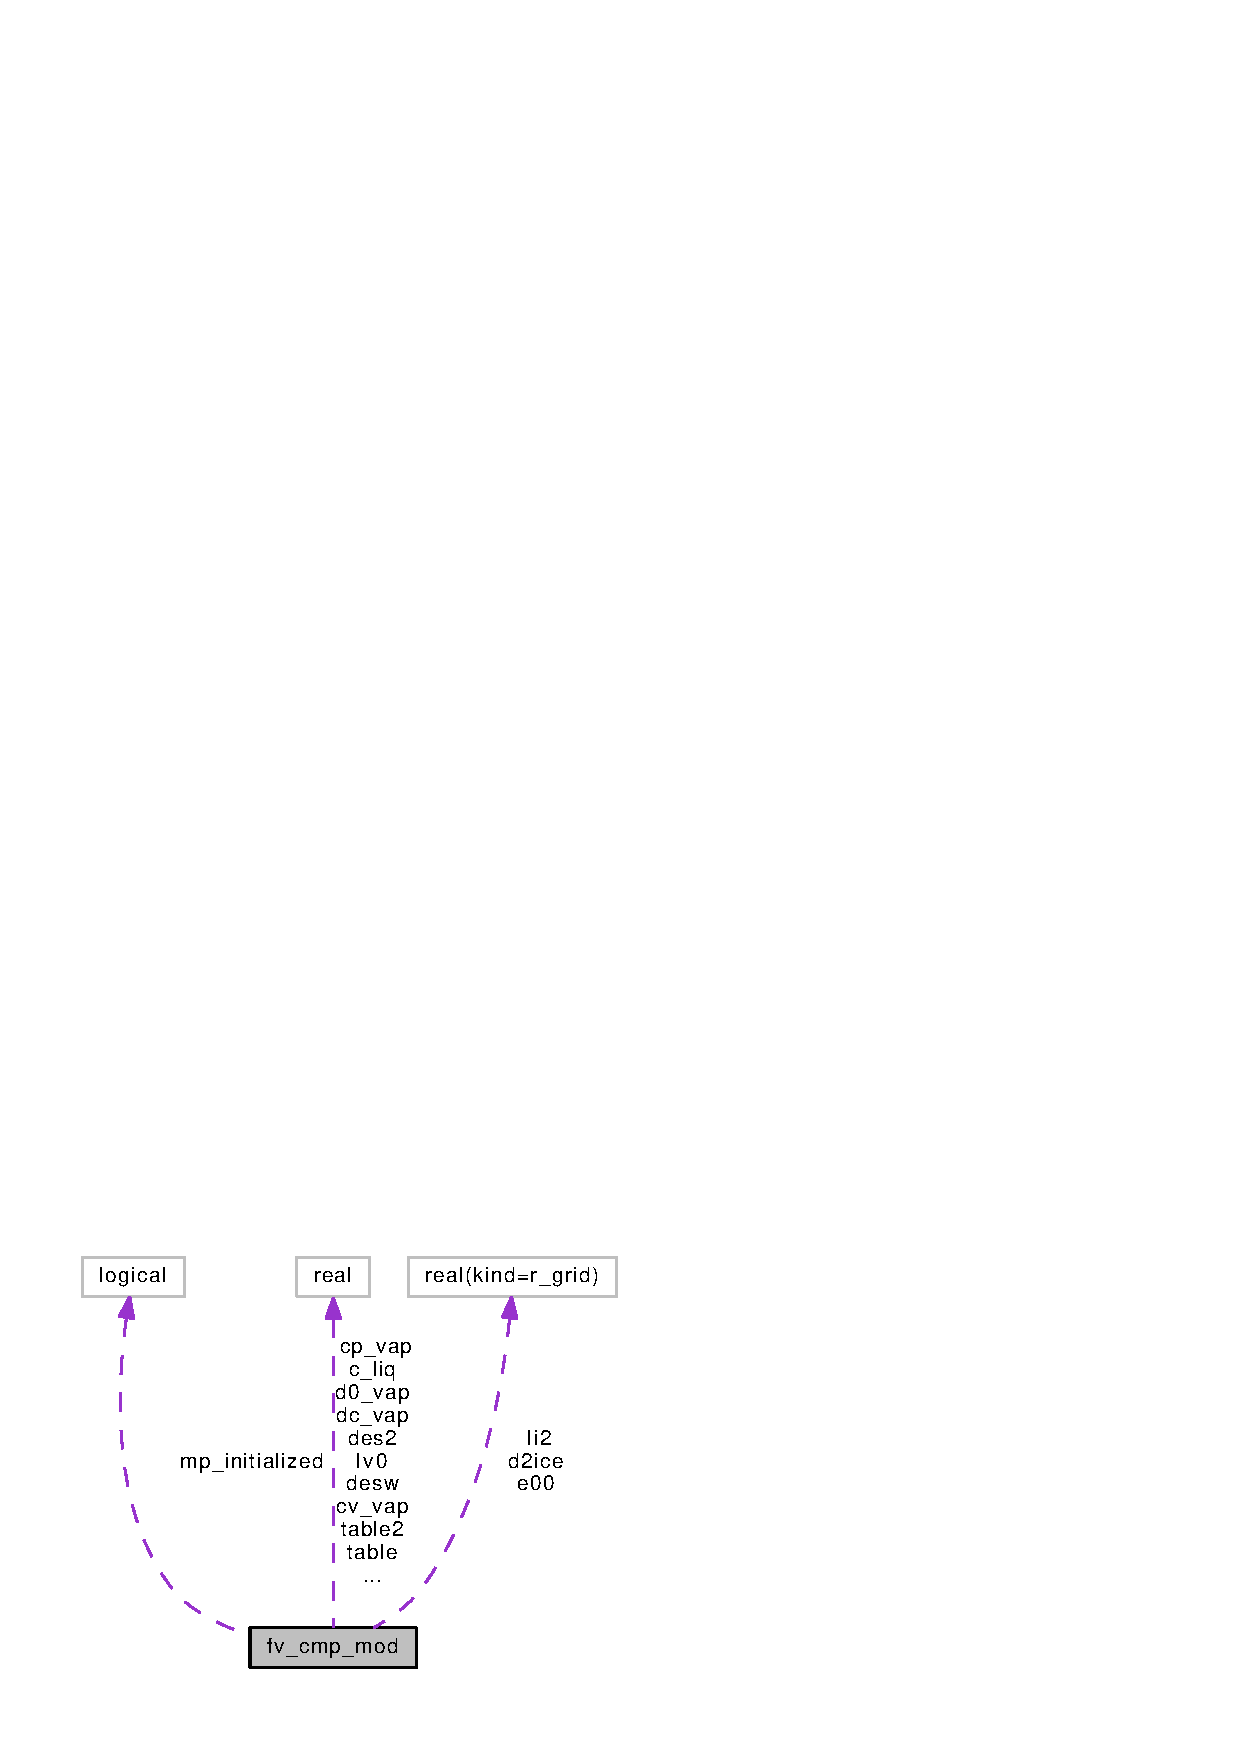
\includegraphics[width=300pt]{classfv__cmp__mod__coll__graph}
\end{center}
\end{figure}
\subsection*{Public Member Functions}
\begin{DoxyCompactItemize}
\item 
subroutine, public \hyperlink{classfv__cmp__mod_a4316f04a563345186c026003ed5ebe96}{fv\-\_\-sat\-\_\-adj} (mdt, zvir, is, ie, js, je, ng, hydrostatic, consv\-\_\-te, te0,
\begin{DoxyCompactList}\small\item\em The subroutine 'fv\-\_\-sat\-\_\-adj' performs the fast processes in the G\-F\-D\-L microphysics. \end{DoxyCompactList}\item 
subroutine, public \hyperlink{classfv__cmp__mod_a5ce7347205d43a859b0316a584642f4d}{qs\-\_\-init} (kmp)
\begin{DoxyCompactList}\small\item\em The subroutine 'qs\-\_\-init' initializes lookup tables for the saturation mixing ratio. \end{DoxyCompactList}\end{DoxyCompactItemize}
\subsection*{Private Member Functions}
\begin{DoxyCompactItemize}
\item 
real function \hyperlink{classfv__cmp__mod_a9168ab47a84d56e7dfc5529472be0c71}{wqs1} (ta, den)
\begin{DoxyCompactList}\small\item\em the function 'wqs1' computes the saturated specific humidity for table ii \end{DoxyCompactList}\item 
real function \hyperlink{classfv__cmp__mod_a328511270fbc27b0b736bab8ac486967}{iqs1} (ta, den)
\begin{DoxyCompactList}\small\item\em the function 'wqs1' computes the saturated specific humidity for table iii \end{DoxyCompactList}\item 
real function \hyperlink{classfv__cmp__mod_a21a51056703b3ebc85fb3d3e3e3f23aa}{wqs2} (ta, den, dqdt)
\begin{DoxyCompactList}\small\item\em The function 'wqs2'computes the gradient of saturated specific humidity for table ii. \end{DoxyCompactList}\item 
subroutine \hyperlink{classfv__cmp__mod_ac016ceb177d822853885183c1f4c724f}{wqs2\-\_\-vect} (is, ie, ta, den, wqsat, dqdt)
\begin{DoxyCompactList}\small\item\em The function wqs2\-\_\-vect computes the gradient of saturated specific humidity for table ii. It is the same as \char`\"{}wqs2\char`\"{}, but written as vector function. \end{DoxyCompactList}\item 
real function \hyperlink{classfv__cmp__mod_aca9c0d54335dbc33cc56cb74006fed26}{iqs2} (ta, den, dqdt)
\begin{DoxyCompactList}\small\item\em The function 'iqs2' computes the gradient of saturated specific humidity for table iii. \end{DoxyCompactList}\item 
subroutine \hyperlink{classfv__cmp__mod_a7d7f969ce1e9d84aae4a911ead816e96}{qs\-\_\-table} (n)
\item 
subroutine \hyperlink{classfv__cmp__mod_a416061516bcffc2cab55e9a801b6d1c2}{qs\-\_\-tablew} (n)
\item 
subroutine \hyperlink{classfv__cmp__mod_a27624ed32cc760d05eb6faa1f748970e}{qs\-\_\-table2} (n)
\end{DoxyCompactItemize}
\subsection*{Private Attributes}
\begin{DoxyCompactItemize}
\item 
real, parameter \hyperlink{classfv__cmp__mod_a7380eb8077e00279e9bb042e5a69f39b}{cp\-\_\-vap} = 4.\-0 $\ast$ rvgas
\begin{DoxyCompactList}\small\item\em 1846.\-0, heat capacity of water vapor at constant pressure \end{DoxyCompactList}\item 
real, parameter \hyperlink{classfv__cmp__mod_a6b7e31c99aaa43c3c88e5f148a0ada8c}{cv\-\_\-air} = cp\-\_\-air -\/ rdgas
\begin{DoxyCompactList}\small\item\em 717.\-55, heat capacity of dry air at constant volume \end{DoxyCompactList}\item 
real, parameter \hyperlink{classfv__cmp__mod_a1aff52f3ef1654b16d21ca8deade4099}{cv\-\_\-vap} = 3.\-0 $\ast$ rvgas
\begin{DoxyCompactList}\small\item\em 1384.\-5, heat capacity of water vapor at constant volume \end{DoxyCompactList}\item 
real, parameter \hyperlink{classfv__cmp__mod_a2e2c6145d3f4ea50036930131b202ca4}{c\-\_\-ice} = 1972.\-0
\begin{DoxyCompactList}\small\item\em gfdl\-: heat capacity of ice at -\/ 15 deg c \end{DoxyCompactList}\item 
real, parameter \hyperlink{classfv__cmp__mod_ae3486a6a9602d9d6d55f4935aa0ffb0b}{c\-\_\-liq} = 4185.\-5
\begin{DoxyCompactList}\small\item\em gfdl\-: heat capacity of liquid at 15 deg c \end{DoxyCompactList}\item 
real, parameter \hyperlink{classfv__cmp__mod_abc256ef2779554c3fcc3d90607dbe03d}{dc\-\_\-vap} = \hyperlink{classfv__cmp__mod_a7380eb8077e00279e9bb042e5a69f39b}{cp\-\_\-vap} -\/ \hyperlink{classfv__cmp__mod_ae3486a6a9602d9d6d55f4935aa0ffb0b}{c\-\_\-liq}
\item 
real, parameter \hyperlink{classfv__cmp__mod_afe0a80520aff4b3aa44554dcbc54ccda}{dc\-\_\-ice} = \hyperlink{classfv__cmp__mod_ae3486a6a9602d9d6d55f4935aa0ffb0b}{c\-\_\-liq} -\/ \hyperlink{classfv__cmp__mod_a2e2c6145d3f4ea50036930131b202ca4}{c\-\_\-ice}
\begin{DoxyCompactList}\small\item\em 2213.\-5, isobaric heating / colling \end{DoxyCompactList}\item 
real, parameter \hyperlink{classfv__cmp__mod_a7ad671e67cd91ec927c0392e32bf5d7e}{tice} = 273.\-16
\begin{DoxyCompactList}\small\item\em freezing temperature \end{DoxyCompactList}\item 
real, parameter \hyperlink{classfv__cmp__mod_a4fe62a9a87a3aa5466fa0afe5ceb070a}{t\-\_\-wfr} = \hyperlink{classfv__cmp__mod_a7ad671e67cd91ec927c0392e32bf5d7e}{tice} -\/ 40.
\begin{DoxyCompactList}\small\item\em homogeneous freezing temperature \end{DoxyCompactList}\item 
real, parameter \hyperlink{classfv__cmp__mod_ac555be1714d90016ac1b76bd0274fe4d}{lv0} = hlv -\/ \hyperlink{classfv__cmp__mod_abc256ef2779554c3fcc3d90607dbe03d}{dc\-\_\-vap} $\ast$ \hyperlink{classfv__cmp__mod_a7ad671e67cd91ec927c0392e32bf5d7e}{tice}
\begin{DoxyCompactList}\small\item\em 3.\-13905782e6, evaporation latent heat coefficient at 0 deg k \end{DoxyCompactList}\item 
real, parameter \hyperlink{classfv__cmp__mod_aaec2280440ca71e72b152db42e5c4504}{li00} = hlf -\/ \hyperlink{classfv__cmp__mod_afe0a80520aff4b3aa44554dcbc54ccda}{dc\-\_\-ice} $\ast$ \hyperlink{classfv__cmp__mod_a7ad671e67cd91ec927c0392e32bf5d7e}{tice}
\item 
real(kind=r\-\_\-grid), parameter \hyperlink{classfv__cmp__mod_a92f0cf9784defdd98bcf50329e7f6e8b}{e00} = 611.\-21
\begin{DoxyCompactList}\small\item\em ifs\-: saturation vapor pressure at 0 deg c \end{DoxyCompactList}\item 
real(kind=r\-\_\-grid), parameter \hyperlink{classfv__cmp__mod_adb9c6f0494c4e168f9730598a667d15a}{d2ice} = \hyperlink{classfv__cmp__mod_abc256ef2779554c3fcc3d90607dbe03d}{dc\-\_\-vap} + \hyperlink{classfv__cmp__mod_afe0a80520aff4b3aa44554dcbc54ccda}{dc\-\_\-ice}
\item 
real(kind=r\-\_\-grid), parameter \hyperlink{classfv__cmp__mod_a9248700d4484999739228f7448428746}{li2} = \hyperlink{classfv__cmp__mod_ac555be1714d90016ac1b76bd0274fe4d}{lv0} + \hyperlink{classfv__cmp__mod_aaec2280440ca71e72b152db42e5c4504}{li00}
\begin{DoxyCompactList}\small\item\em 2.\-86799816e6, sublimation latent heat coefficient at 0 deg k \end{DoxyCompactList}\item 
real, parameter \hyperlink{classfv__cmp__mod_aad5bf68c9e846169feaa2355a29ec7ae}{lat2} = (hlv + hlf) $\ast$$\ast$ 2
\begin{DoxyCompactList}\small\item\em used in bigg mechanism \end{DoxyCompactList}\item 
real \hyperlink{classfv__cmp__mod_ac3f9f88a1d49ff1e327bbb8005f9228a}{d0\-\_\-vap}
\begin{DoxyCompactList}\small\item\em the same as dc\-\_\-vap, except that cp\-\_\-vap can be cp\-\_\-vap or cv\-\_\-vap \end{DoxyCompactList}\item 
real \hyperlink{classfv__cmp__mod_a7bcead849f7cab25637af6d3b1db833a}{lv00}
\begin{DoxyCompactList}\small\item\em the same as lv0, except that cp\-\_\-vap can be cp\-\_\-vap or cv\-\_\-vap \end{DoxyCompactList}\item 
real, dimension(\-:), allocatable \hyperlink{classfv__cmp__mod_a7a34f8d4c0eefd0e66de45d280bb0ba4}{table}
\item 
real, dimension(\-:), allocatable \hyperlink{classfv__cmp__mod_a16427443f0f4cc4376e7a7af841cc03d}{table2}
\item 
real, dimension(\-:), allocatable \hyperlink{classfv__cmp__mod_a308d1b16faf8b0f7c53fb4ace71f326e}{tablew}
\item 
real, dimension(\-:), allocatable \hyperlink{classfv__cmp__mod_a39a88a1e472449c87b0c18c5be0682a2}{des2}
\item 
real, dimension(\-:), allocatable \hyperlink{classfv__cmp__mod_ae014434a6d863ca10c5961edfd866425}{desw}
\item 
logical \hyperlink{classfv__cmp__mod_af9c43700533ec209e98ed9aaea7220ad}{mp\-\_\-initialized} = .false.
\end{DoxyCompactItemize}


\subsection{Detailed Description}
The module 'fv\-\_\-cmp' implements the fast procesesses in the G\-F\-D\-L microphysics $>$ 

\begin{DoxyAuthor}{Author}
Shian-\/\-Jiann Lin, Linjiong Zhou 
\end{DoxyAuthor}


Definition at line 29 of file fv\-\_\-cmp.\-F90.



\subsection{Member Function/\-Subroutine Documentation}
\index{fv\-\_\-cmp\-\_\-mod@{fv\-\_\-cmp\-\_\-mod}!fv\-\_\-sat\-\_\-adj@{fv\-\_\-sat\-\_\-adj}}
\index{fv\-\_\-sat\-\_\-adj@{fv\-\_\-sat\-\_\-adj}!fv_cmp_mod@{fv\-\_\-cmp\-\_\-mod}}
\subsubsection[{fv\-\_\-sat\-\_\-adj}]{\setlength{\rightskip}{0pt plus 5cm}subroutine, public fv\-\_\-cmp\-\_\-mod\-::fv\-\_\-sat\-\_\-adj (
\begin{DoxyParamCaption}
\item[{real, intent(in)}]{mdt, }
\item[{real, intent(in)}]{zvir, }
\item[{integer, intent(in)}]{is, }
\item[{integer, intent(in)}]{ie, }
\item[{integer, intent(in)}]{js, }
\item[{integer, intent(in)}]{je, }
\item[{integer, intent(in)}]{ng, }
\item[{logical, intent(in)}]{hydrostatic, }
\item[{logical, intent(in)}]{consv\-\_\-te, }
\item[{real, dimension (is -\/ ng\-:ie + ng, js -\/ ng\-:je + ng), intent(out)}]{te0}
\end{DoxyParamCaption}
)}\label{classfv__cmp__mod_a4316f04a563345186c026003ed5ebe96}


The subroutine 'fv\-\_\-sat\-\_\-adj' performs the fast processes in the G\-F\-D\-L microphysics. 

This is designed for single-\/moment 6-\/class cloud microphysics schemes. It handles the heat release due to in situ phase changes. 

Definition at line 122 of file fv\-\_\-cmp.\-F90.



References iqs1(), iqs2(), multi\-\_\-gases\-\_\-mod\-::vicpqd\-\_\-qpz(), multi\-\_\-gases\-\_\-mod\-::vicvqd\-\_\-qpz(), multi\-\_\-gases\-\_\-mod\-::virq\-\_\-qpz(), wqs1(), and wqs2\-\_\-vect().



Referenced by fv\-\_\-mapz\-\_\-mod\-::lagrangian\-\_\-to\-\_\-eulerian().

\index{fv\-\_\-cmp\-\_\-mod@{fv\-\_\-cmp\-\_\-mod}!iqs1@{iqs1}}
\index{iqs1@{iqs1}!fv_cmp_mod@{fv\-\_\-cmp\-\_\-mod}}
\subsubsection[{iqs1}]{\setlength{\rightskip}{0pt plus 5cm}real function fv\-\_\-cmp\-\_\-mod\-::iqs1 (
\begin{DoxyParamCaption}
\item[{real, intent(in)}]{ta, }
\item[{real, intent(in)}]{den}
\end{DoxyParamCaption}
)\hspace{0.3cm}{\ttfamily [private]}}\label{classfv__cmp__mod_a328511270fbc27b0b736bab8ac486967}


the function 'wqs1' computes the saturated specific humidity for table iii 



Definition at line 902 of file fv\-\_\-cmp.\-F90.



Referenced by fv\-\_\-sat\-\_\-adj().

\index{fv\-\_\-cmp\-\_\-mod@{fv\-\_\-cmp\-\_\-mod}!iqs2@{iqs2}}
\index{iqs2@{iqs2}!fv_cmp_mod@{fv\-\_\-cmp\-\_\-mod}}
\subsubsection[{iqs2}]{\setlength{\rightskip}{0pt plus 5cm}real function fv\-\_\-cmp\-\_\-mod\-::iqs2 (
\begin{DoxyParamCaption}
\item[{real, intent(in)}]{ta, }
\item[{real, intent(in)}]{den, }
\item[{real, intent(out)}]{dqdt}
\end{DoxyParamCaption}
)\hspace{0.3cm}{\ttfamily [private]}}\label{classfv__cmp__mod_aca9c0d54335dbc33cc56cb74006fed26}


The function 'iqs2' computes the gradient of saturated specific humidity for table iii. 



Definition at line 996 of file fv\-\_\-cmp.\-F90.



Referenced by fv\-\_\-sat\-\_\-adj().

\index{fv\-\_\-cmp\-\_\-mod@{fv\-\_\-cmp\-\_\-mod}!qs\-\_\-init@{qs\-\_\-init}}
\index{qs\-\_\-init@{qs\-\_\-init}!fv_cmp_mod@{fv\-\_\-cmp\-\_\-mod}}
\subsubsection[{qs\-\_\-init}]{\setlength{\rightskip}{0pt plus 5cm}subroutine, public fv\-\_\-cmp\-\_\-mod\-::qs\-\_\-init (
\begin{DoxyParamCaption}
\item[{integer, intent(in)}]{kmp}
\end{DoxyParamCaption}
)}\label{classfv__cmp__mod_a5ce7347205d43a859b0316a584642f4d}


The subroutine 'qs\-\_\-init' initializes lookup tables for the saturation mixing ratio. 



Definition at line 1028 of file fv\-\_\-cmp.\-F90.



References qs\-\_\-table(), qs\-\_\-table2(), and qs\-\_\-tablew().



Referenced by fv\-\_\-mapz\-\_\-mod\-::lagrangian\-\_\-to\-\_\-eulerian().

\index{fv\-\_\-cmp\-\_\-mod@{fv\-\_\-cmp\-\_\-mod}!qs\-\_\-table@{qs\-\_\-table}}
\index{qs\-\_\-table@{qs\-\_\-table}!fv_cmp_mod@{fv\-\_\-cmp\-\_\-mod}}
\subsubsection[{qs\-\_\-table}]{\setlength{\rightskip}{0pt plus 5cm}subroutine fv\-\_\-cmp\-\_\-mod\-::qs\-\_\-table (
\begin{DoxyParamCaption}
\item[{integer, intent(in)}]{n}
\end{DoxyParamCaption}
)\hspace{0.3cm}{\ttfamily [private]}}\label{classfv__cmp__mod_a7d7f969ce1e9d84aae4a911ead816e96}


Definition at line 1070 of file fv\-\_\-cmp.\-F90.



Referenced by qs\-\_\-init(), and fv\-\_\-sg\-\_\-mod\-::qsmith\-\_\-init().

\index{fv\-\_\-cmp\-\_\-mod@{fv\-\_\-cmp\-\_\-mod}!qs\-\_\-table2@{qs\-\_\-table2}}
\index{qs\-\_\-table2@{qs\-\_\-table2}!fv_cmp_mod@{fv\-\_\-cmp\-\_\-mod}}
\subsubsection[{qs\-\_\-table2}]{\setlength{\rightskip}{0pt plus 5cm}subroutine fv\-\_\-cmp\-\_\-mod\-::qs\-\_\-table2 (
\begin{DoxyParamCaption}
\item[{integer, intent(in)}]{n}
\end{DoxyParamCaption}
)\hspace{0.3cm}{\ttfamily [private]}}\label{classfv__cmp__mod_a27624ed32cc760d05eb6faa1f748970e}


Definition at line 1164 of file fv\-\_\-cmp.\-F90.



Referenced by qs\-\_\-init().

\index{fv\-\_\-cmp\-\_\-mod@{fv\-\_\-cmp\-\_\-mod}!qs\-\_\-tablew@{qs\-\_\-tablew}}
\index{qs\-\_\-tablew@{qs\-\_\-tablew}!fv_cmp_mod@{fv\-\_\-cmp\-\_\-mod}}
\subsubsection[{qs\-\_\-tablew}]{\setlength{\rightskip}{0pt plus 5cm}subroutine fv\-\_\-cmp\-\_\-mod\-::qs\-\_\-tablew (
\begin{DoxyParamCaption}
\item[{integer, intent(in)}]{n}
\end{DoxyParamCaption}
)\hspace{0.3cm}{\ttfamily [private]}}\label{classfv__cmp__mod_a416061516bcffc2cab55e9a801b6d1c2}


Definition at line 1132 of file fv\-\_\-cmp.\-F90.



Referenced by qs\-\_\-init().

\index{fv\-\_\-cmp\-\_\-mod@{fv\-\_\-cmp\-\_\-mod}!wqs1@{wqs1}}
\index{wqs1@{wqs1}!fv_cmp_mod@{fv\-\_\-cmp\-\_\-mod}}
\subsubsection[{wqs1}]{\setlength{\rightskip}{0pt plus 5cm}real function fv\-\_\-cmp\-\_\-mod\-::wqs1 (
\begin{DoxyParamCaption}
\item[{real, intent(in)}]{ta, }
\item[{real, intent(in)}]{den}
\end{DoxyParamCaption}
)\hspace{0.3cm}{\ttfamily [private]}}\label{classfv__cmp__mod_a9168ab47a84d56e7dfc5529472be0c71}


the function 'wqs1' computes the saturated specific humidity for table ii 



Definition at line 876 of file fv\-\_\-cmp.\-F90.



Referenced by fv\-\_\-sat\-\_\-adj().

\index{fv\-\_\-cmp\-\_\-mod@{fv\-\_\-cmp\-\_\-mod}!wqs2@{wqs2}}
\index{wqs2@{wqs2}!fv_cmp_mod@{fv\-\_\-cmp\-\_\-mod}}
\subsubsection[{wqs2}]{\setlength{\rightskip}{0pt plus 5cm}real function fv\-\_\-cmp\-\_\-mod\-::wqs2 (
\begin{DoxyParamCaption}
\item[{real, intent(in)}]{ta, }
\item[{real, intent(in)}]{den, }
\item[{real, intent(out)}]{dqdt}
\end{DoxyParamCaption}
)\hspace{0.3cm}{\ttfamily [private]}}\label{classfv__cmp__mod_a21a51056703b3ebc85fb3d3e3e3f23aa}


The function 'wqs2'computes the gradient of saturated specific humidity for table ii. 



Definition at line 928 of file fv\-\_\-cmp.\-F90.



Referenced by fv\-\_\-sg\-\_\-mod\-::fv\-\_\-subgrid\-\_\-z().

\index{fv\-\_\-cmp\-\_\-mod@{fv\-\_\-cmp\-\_\-mod}!wqs2\-\_\-vect@{wqs2\-\_\-vect}}
\index{wqs2\-\_\-vect@{wqs2\-\_\-vect}!fv_cmp_mod@{fv\-\_\-cmp\-\_\-mod}}
\subsubsection[{wqs2\-\_\-vect}]{\setlength{\rightskip}{0pt plus 5cm}subroutine fv\-\_\-cmp\-\_\-mod\-::wqs2\-\_\-vect (
\begin{DoxyParamCaption}
\item[{integer, intent(in)}]{is, }
\item[{integer, intent(in)}]{ie, }
\item[{real, dimension (is\-:ie), intent(in)}]{ta, }
\item[{real, dimension (is\-:ie), intent(in)}]{den, }
\item[{real, dimension (is\-:ie), intent(out)}]{wqsat, }
\item[{real, dimension (is\-:ie), intent(out)}]{dqdt}
\end{DoxyParamCaption}
)\hspace{0.3cm}{\ttfamily [private]}}\label{classfv__cmp__mod_ac016ceb177d822853885183c1f4c724f}


The function wqs2\-\_\-vect computes the gradient of saturated specific humidity for table ii. It is the same as \char`\"{}wqs2\char`\"{}, but written as vector function. 



Definition at line 960 of file fv\-\_\-cmp.\-F90.



Referenced by fv\-\_\-sat\-\_\-adj().



\subsection{Member Data Documentation}
\index{fv\-\_\-cmp\-\_\-mod@{fv\-\_\-cmp\-\_\-mod}!c\-\_\-ice@{c\-\_\-ice}}
\index{c\-\_\-ice@{c\-\_\-ice}!fv_cmp_mod@{fv\-\_\-cmp\-\_\-mod}}
\subsubsection[{c\-\_\-ice}]{\setlength{\rightskip}{0pt plus 5cm}real, parameter fv\-\_\-cmp\-\_\-mod\-::c\-\_\-ice = 1972.\-0\hspace{0.3cm}{\ttfamily [private]}}\label{classfv__cmp__mod_a2e2c6145d3f4ea50036930131b202ca4}


gfdl\-: heat capacity of ice at -\/ 15 deg c 



Definition at line 90 of file fv\-\_\-cmp.\-F90.

\index{fv\-\_\-cmp\-\_\-mod@{fv\-\_\-cmp\-\_\-mod}!c\-\_\-liq@{c\-\_\-liq}}
\index{c\-\_\-liq@{c\-\_\-liq}!fv_cmp_mod@{fv\-\_\-cmp\-\_\-mod}}
\subsubsection[{c\-\_\-liq}]{\setlength{\rightskip}{0pt plus 5cm}real, parameter fv\-\_\-cmp\-\_\-mod\-::c\-\_\-liq = 4185.\-5\hspace{0.3cm}{\ttfamily [private]}}\label{classfv__cmp__mod_ae3486a6a9602d9d6d55f4935aa0ffb0b}


gfdl\-: heat capacity of liquid at 15 deg c 



Definition at line 91 of file fv\-\_\-cmp.\-F90.

\index{fv\-\_\-cmp\-\_\-mod@{fv\-\_\-cmp\-\_\-mod}!cp\-\_\-vap@{cp\-\_\-vap}}
\index{cp\-\_\-vap@{cp\-\_\-vap}!fv_cmp_mod@{fv\-\_\-cmp\-\_\-mod}}
\subsubsection[{cp\-\_\-vap}]{\setlength{\rightskip}{0pt plus 5cm}real, parameter fv\-\_\-cmp\-\_\-mod\-::cp\-\_\-vap = 4.\-0 $\ast$ rvgas\hspace{0.3cm}{\ttfamily [private]}}\label{classfv__cmp__mod_a7380eb8077e00279e9bb042e5a69f39b}


1846.\-0, heat capacity of water vapor at constant pressure 



Definition at line 75 of file fv\-\_\-cmp.\-F90.

\index{fv\-\_\-cmp\-\_\-mod@{fv\-\_\-cmp\-\_\-mod}!cv\-\_\-air@{cv\-\_\-air}}
\index{cv\-\_\-air@{cv\-\_\-air}!fv_cmp_mod@{fv\-\_\-cmp\-\_\-mod}}
\subsubsection[{cv\-\_\-air}]{\setlength{\rightskip}{0pt plus 5cm}real, parameter fv\-\_\-cmp\-\_\-mod\-::cv\-\_\-air = cp\-\_\-air -\/ rdgas\hspace{0.3cm}{\ttfamily [private]}}\label{classfv__cmp__mod_a6b7e31c99aaa43c3c88e5f148a0ada8c}


717.\-55, heat capacity of dry air at constant volume 



Definition at line 76 of file fv\-\_\-cmp.\-F90.

\index{fv\-\_\-cmp\-\_\-mod@{fv\-\_\-cmp\-\_\-mod}!cv\-\_\-vap@{cv\-\_\-vap}}
\index{cv\-\_\-vap@{cv\-\_\-vap}!fv_cmp_mod@{fv\-\_\-cmp\-\_\-mod}}
\subsubsection[{cv\-\_\-vap}]{\setlength{\rightskip}{0pt plus 5cm}real, parameter fv\-\_\-cmp\-\_\-mod\-::cv\-\_\-vap = 3.\-0 $\ast$ rvgas\hspace{0.3cm}{\ttfamily [private]}}\label{classfv__cmp__mod_a1aff52f3ef1654b16d21ca8deade4099}


1384.\-5, heat capacity of water vapor at constant volume 



Definition at line 77 of file fv\-\_\-cmp.\-F90.

\index{fv\-\_\-cmp\-\_\-mod@{fv\-\_\-cmp\-\_\-mod}!d0\-\_\-vap@{d0\-\_\-vap}}
\index{d0\-\_\-vap@{d0\-\_\-vap}!fv_cmp_mod@{fv\-\_\-cmp\-\_\-mod}}
\subsubsection[{d0\-\_\-vap}]{\setlength{\rightskip}{0pt plus 5cm}real fv\-\_\-cmp\-\_\-mod\-::d0\-\_\-vap\hspace{0.3cm}{\ttfamily [private]}}\label{classfv__cmp__mod_ac3f9f88a1d49ff1e327bbb8005f9228a}


the same as dc\-\_\-vap, except that cp\-\_\-vap can be cp\-\_\-vap or cv\-\_\-vap 



Definition at line 110 of file fv\-\_\-cmp.\-F90.

\index{fv\-\_\-cmp\-\_\-mod@{fv\-\_\-cmp\-\_\-mod}!d2ice@{d2ice}}
\index{d2ice@{d2ice}!fv_cmp_mod@{fv\-\_\-cmp\-\_\-mod}}
\subsubsection[{d2ice}]{\setlength{\rightskip}{0pt plus 5cm}real (kind = r\-\_\-grid), parameter fv\-\_\-cmp\-\_\-mod\-::d2ice = {\bf dc\-\_\-vap} + {\bf dc\-\_\-ice}\hspace{0.3cm}{\ttfamily [private]}}\label{classfv__cmp__mod_adb9c6f0494c4e168f9730598a667d15a}

\begin{DoxyItemize}
\item 126, isobaric heating / cooling 
\end{DoxyItemize}

Definition at line 105 of file fv\-\_\-cmp.\-F90.

\index{fv\-\_\-cmp\-\_\-mod@{fv\-\_\-cmp\-\_\-mod}!dc\-\_\-ice@{dc\-\_\-ice}}
\index{dc\-\_\-ice@{dc\-\_\-ice}!fv_cmp_mod@{fv\-\_\-cmp\-\_\-mod}}
\subsubsection[{dc\-\_\-ice}]{\setlength{\rightskip}{0pt plus 5cm}real, parameter fv\-\_\-cmp\-\_\-mod\-::dc\-\_\-ice = {\bf c\-\_\-liq} -\/ {\bf c\-\_\-ice}\hspace{0.3cm}{\ttfamily [private]}}\label{classfv__cmp__mod_afe0a80520aff4b3aa44554dcbc54ccda}


2213.\-5, isobaric heating / colling 



Definition at line 94 of file fv\-\_\-cmp.\-F90.

\index{fv\-\_\-cmp\-\_\-mod@{fv\-\_\-cmp\-\_\-mod}!dc\-\_\-vap@{dc\-\_\-vap}}
\index{dc\-\_\-vap@{dc\-\_\-vap}!fv_cmp_mod@{fv\-\_\-cmp\-\_\-mod}}
\subsubsection[{dc\-\_\-vap}]{\setlength{\rightskip}{0pt plus 5cm}real, parameter fv\-\_\-cmp\-\_\-mod\-::dc\-\_\-vap = {\bf cp\-\_\-vap} -\/ {\bf c\-\_\-liq}\hspace{0.3cm}{\ttfamily [private]}}\label{classfv__cmp__mod_abc256ef2779554c3fcc3d90607dbe03d}

\begin{DoxyItemize}
\item 2339.\-5, isobaric heating / cooling 
\end{DoxyItemize}

Definition at line 93 of file fv\-\_\-cmp.\-F90.

\index{fv\-\_\-cmp\-\_\-mod@{fv\-\_\-cmp\-\_\-mod}!des2@{des2}}
\index{des2@{des2}!fv_cmp_mod@{fv\-\_\-cmp\-\_\-mod}}
\subsubsection[{des2}]{\setlength{\rightskip}{0pt plus 5cm}real, dimension (\-:), allocatable fv\-\_\-cmp\-\_\-mod\-::des2\hspace{0.3cm}{\ttfamily [private]}}\label{classfv__cmp__mod_a39a88a1e472449c87b0c18c5be0682a2}


Definition at line 113 of file fv\-\_\-cmp.\-F90.

\index{fv\-\_\-cmp\-\_\-mod@{fv\-\_\-cmp\-\_\-mod}!desw@{desw}}
\index{desw@{desw}!fv_cmp_mod@{fv\-\_\-cmp\-\_\-mod}}
\subsubsection[{desw}]{\setlength{\rightskip}{0pt plus 5cm}real, dimension (\-:), allocatable fv\-\_\-cmp\-\_\-mod\-::desw\hspace{0.3cm}{\ttfamily [private]}}\label{classfv__cmp__mod_ae014434a6d863ca10c5961edfd866425}


Definition at line 113 of file fv\-\_\-cmp.\-F90.

\index{fv\-\_\-cmp\-\_\-mod@{fv\-\_\-cmp\-\_\-mod}!e00@{e00}}
\index{e00@{e00}!fv_cmp_mod@{fv\-\_\-cmp\-\_\-mod}}
\subsubsection[{e00}]{\setlength{\rightskip}{0pt plus 5cm}real (kind = r\-\_\-grid), parameter fv\-\_\-cmp\-\_\-mod\-::e00 = 611.\-21\hspace{0.3cm}{\ttfamily [private]}}\label{classfv__cmp__mod_a92f0cf9784defdd98bcf50329e7f6e8b}


ifs\-: saturation vapor pressure at 0 deg c 



Definition at line 103 of file fv\-\_\-cmp.\-F90.

\index{fv\-\_\-cmp\-\_\-mod@{fv\-\_\-cmp\-\_\-mod}!lat2@{lat2}}
\index{lat2@{lat2}!fv_cmp_mod@{fv\-\_\-cmp\-\_\-mod}}
\subsubsection[{lat2}]{\setlength{\rightskip}{0pt plus 5cm}real, parameter fv\-\_\-cmp\-\_\-mod\-::lat2 = (hlv + hlf) $\ast$$\ast$ 2\hspace{0.3cm}{\ttfamily [private]}}\label{classfv__cmp__mod_aad5bf68c9e846169feaa2355a29ec7ae}


used in bigg mechanism 



Definition at line 108 of file fv\-\_\-cmp.\-F90.

\index{fv\-\_\-cmp\-\_\-mod@{fv\-\_\-cmp\-\_\-mod}!li00@{li00}}
\index{li00@{li00}!fv_cmp_mod@{fv\-\_\-cmp\-\_\-mod}}
\subsubsection[{li00}]{\setlength{\rightskip}{0pt plus 5cm}real, parameter fv\-\_\-cmp\-\_\-mod\-::li00 = hlf -\/ {\bf dc\-\_\-ice} $\ast$ {\bf tice}\hspace{0.3cm}{\ttfamily [private]}}\label{classfv__cmp__mod_aaec2280440ca71e72b152db42e5c4504}

\begin{DoxyItemize}
\item 2.\-7105966e5, fusion latent heat coefficient at 0 deg k 
\end{DoxyItemize}

Definition at line 100 of file fv\-\_\-cmp.\-F90.

\index{fv\-\_\-cmp\-\_\-mod@{fv\-\_\-cmp\-\_\-mod}!li2@{li2}}
\index{li2@{li2}!fv_cmp_mod@{fv\-\_\-cmp\-\_\-mod}}
\subsubsection[{li2}]{\setlength{\rightskip}{0pt plus 5cm}real (kind = r\-\_\-grid), parameter fv\-\_\-cmp\-\_\-mod\-::li2 = {\bf lv0} + {\bf li00}\hspace{0.3cm}{\ttfamily [private]}}\label{classfv__cmp__mod_a9248700d4484999739228f7448428746}


2.\-86799816e6, sublimation latent heat coefficient at 0 deg k 



Definition at line 106 of file fv\-\_\-cmp.\-F90.

\index{fv\-\_\-cmp\-\_\-mod@{fv\-\_\-cmp\-\_\-mod}!lv0@{lv0}}
\index{lv0@{lv0}!fv_cmp_mod@{fv\-\_\-cmp\-\_\-mod}}
\subsubsection[{lv0}]{\setlength{\rightskip}{0pt plus 5cm}real, parameter fv\-\_\-cmp\-\_\-mod\-::lv0 = hlv -\/ {\bf dc\-\_\-vap} $\ast$ {\bf tice}\hspace{0.3cm}{\ttfamily [private]}}\label{classfv__cmp__mod_ac555be1714d90016ac1b76bd0274fe4d}


3.\-13905782e6, evaporation latent heat coefficient at 0 deg k 



Definition at line 99 of file fv\-\_\-cmp.\-F90.

\index{fv\-\_\-cmp\-\_\-mod@{fv\-\_\-cmp\-\_\-mod}!lv00@{lv00}}
\index{lv00@{lv00}!fv_cmp_mod@{fv\-\_\-cmp\-\_\-mod}}
\subsubsection[{lv00}]{\setlength{\rightskip}{0pt plus 5cm}real fv\-\_\-cmp\-\_\-mod\-::lv00\hspace{0.3cm}{\ttfamily [private]}}\label{classfv__cmp__mod_a7bcead849f7cab25637af6d3b1db833a}


the same as lv0, except that cp\-\_\-vap can be cp\-\_\-vap or cv\-\_\-vap 



Definition at line 111 of file fv\-\_\-cmp.\-F90.

\index{fv\-\_\-cmp\-\_\-mod@{fv\-\_\-cmp\-\_\-mod}!mp\-\_\-initialized@{mp\-\_\-initialized}}
\index{mp\-\_\-initialized@{mp\-\_\-initialized}!fv_cmp_mod@{fv\-\_\-cmp\-\_\-mod}}
\subsubsection[{mp\-\_\-initialized}]{\setlength{\rightskip}{0pt plus 5cm}logical fv\-\_\-cmp\-\_\-mod\-::mp\-\_\-initialized = .false.\hspace{0.3cm}{\ttfamily [private]}}\label{classfv__cmp__mod_af9c43700533ec209e98ed9aaea7220ad}


Definition at line 115 of file fv\-\_\-cmp.\-F90.

\index{fv\-\_\-cmp\-\_\-mod@{fv\-\_\-cmp\-\_\-mod}!t\-\_\-wfr@{t\-\_\-wfr}}
\index{t\-\_\-wfr@{t\-\_\-wfr}!fv_cmp_mod@{fv\-\_\-cmp\-\_\-mod}}
\subsubsection[{t\-\_\-wfr}]{\setlength{\rightskip}{0pt plus 5cm}real, parameter fv\-\_\-cmp\-\_\-mod\-::t\-\_\-wfr = {\bf tice} -\/ 40.\hspace{0.3cm}{\ttfamily [private]}}\label{classfv__cmp__mod_a4fe62a9a87a3aa5466fa0afe5ceb070a}


homogeneous freezing temperature 



Definition at line 97 of file fv\-\_\-cmp.\-F90.

\index{fv\-\_\-cmp\-\_\-mod@{fv\-\_\-cmp\-\_\-mod}!table@{table}}
\index{table@{table}!fv_cmp_mod@{fv\-\_\-cmp\-\_\-mod}}
\subsubsection[{table}]{\setlength{\rightskip}{0pt plus 5cm}real, dimension (\-:), allocatable fv\-\_\-cmp\-\_\-mod\-::table\hspace{0.3cm}{\ttfamily [private]}}\label{classfv__cmp__mod_a7a34f8d4c0eefd0e66de45d280bb0ba4}


Definition at line 113 of file fv\-\_\-cmp.\-F90.

\index{fv\-\_\-cmp\-\_\-mod@{fv\-\_\-cmp\-\_\-mod}!table2@{table2}}
\index{table2@{table2}!fv_cmp_mod@{fv\-\_\-cmp\-\_\-mod}}
\subsubsection[{table2}]{\setlength{\rightskip}{0pt plus 5cm}real, dimension (\-:), allocatable fv\-\_\-cmp\-\_\-mod\-::table2\hspace{0.3cm}{\ttfamily [private]}}\label{classfv__cmp__mod_a16427443f0f4cc4376e7a7af841cc03d}


Definition at line 113 of file fv\-\_\-cmp.\-F90.

\index{fv\-\_\-cmp\-\_\-mod@{fv\-\_\-cmp\-\_\-mod}!tablew@{tablew}}
\index{tablew@{tablew}!fv_cmp_mod@{fv\-\_\-cmp\-\_\-mod}}
\subsubsection[{tablew}]{\setlength{\rightskip}{0pt plus 5cm}real, dimension (\-:), allocatable fv\-\_\-cmp\-\_\-mod\-::tablew\hspace{0.3cm}{\ttfamily [private]}}\label{classfv__cmp__mod_a308d1b16faf8b0f7c53fb4ace71f326e}


Definition at line 113 of file fv\-\_\-cmp.\-F90.

\index{fv\-\_\-cmp\-\_\-mod@{fv\-\_\-cmp\-\_\-mod}!tice@{tice}}
\index{tice@{tice}!fv_cmp_mod@{fv\-\_\-cmp\-\_\-mod}}
\subsubsection[{tice}]{\setlength{\rightskip}{0pt plus 5cm}real, parameter fv\-\_\-cmp\-\_\-mod\-::tice = 273.\-16\hspace{0.3cm}{\ttfamily [private]}}\label{classfv__cmp__mod_a7ad671e67cd91ec927c0392e32bf5d7e}


freezing temperature 



Definition at line 96 of file fv\-\_\-cmp.\-F90.



The documentation for this module was generated from the following file\-:\begin{DoxyCompactItemize}
\item 
/scratch2/\-N\-A\-G\-A\-P\-E/aoml-\/hafs1/\-Kyle.\-Ahern/acs\-\_\-master\-\_\-readonly/model/\hyperlink{fv__cmp_8F90}{fv\-\_\-cmp.\-F90}\end{DoxyCompactItemize}

\section{fv\-\_\-control\-\_\-mod Module Reference}
\label{classfv__control__mod}\index{fv\-\_\-control\-\_\-mod@{fv\-\_\-control\-\_\-mod}}


The module 'F\-V3\-\_\-control' is for initialization and termination of the model, and controls namelist parameters in F\-V3.  




Collaboration diagram for fv\-\_\-control\-\_\-mod\-:
\nopagebreak
\begin{figure}[H]
\begin{center}
\leavevmode
\includegraphics[height=550pt]{classfv__control__mod__coll__graph}
\end{center}
\end{figure}
\subsection*{Public Member Functions}
\begin{DoxyCompactItemize}
\item 
subroutine, public \hyperlink{classfv__control__mod_ad626f01c20738f5101fb5f64e5d3dcfe}{fv\-\_\-init} (Atm, dt\-\_\-atmos, grids\-\_\-on\-\_\-this\-\_\-pe, p\-\_\-split)
\begin{DoxyCompactList}\small\item\em The subroutine 'fv\-\_\-init' initializes F\-V3. \end{DoxyCompactList}\item 
subroutine, public \hyperlink{classfv__control__mod_a8478437752b9d21f6d2f936c8b65284c}{fv\-\_\-end} (Atm, grids\-\_\-on\-\_\-this\-\_\-pe, restart\-\_\-endfcst)
\begin{DoxyCompactList}\small\item\em The subroutine 'fv\-\_\-end' terminates F\-V3, deallocates memory, saves restart files, and stops I/\-O. \end{DoxyCompactList}\end{DoxyCompactItemize}
\subsection*{Public Attributes}
\begin{DoxyCompactItemize}
\item 
integer, public \hyperlink{classfv__control__mod_abaa40fc70569bf400e1385f95bae1f5f}{ngrids} = 1
\item 
integer, dimension(\-:), \\*
allocatable, public \hyperlink{classfv__control__mod_acb8e6baca36aa5140d2d15258e1cf1d6}{pelist\-\_\-all}
\end{DoxyCompactItemize}
\subsection*{Private Member Functions}
\begin{DoxyCompactItemize}
\item 
subroutine \hyperlink{classfv__control__mod_acdd82af4ac35306817aa955d95ec09f9}{run\-\_\-setup} (Atm, dt\-\_\-atmos, grids\-\_\-on\-\_\-this\-\_\-pe, p\-\_\-split)
\begin{DoxyCompactList}\small\item\em The subroutine 'run\-\_\-setup' initializes the run from a namelist. \end{DoxyCompactList}\item 
subroutine \hyperlink{classfv__control__mod_a1b8adec29d73938d0ce672126c20f323}{init\-\_\-nesting} (Atm, grids\-\_\-on\-\_\-this\-\_\-pe, p\-\_\-split)
\item 
subroutine \hyperlink{classfv__control__mod_ac0ed388b3e29b664d242cdc28fc0bd64}{setup\-\_\-pointers} (Atm)
\begin{DoxyCompactList}\small\item\em The subroutine 'setup\-\_\-pointers' associates the M\-O\-D\-U\-L\-E flag pointers with the A\-R\-R\-A\-Y flag variables for the grid active on T\-H\-I\-S pe so the flags can be read in from the namelist. \end{DoxyCompactList}\end{DoxyCompactItemize}
\subsection*{Private Attributes}
\begin{DoxyCompactItemize}
\item 
character(len=80), pointer \hyperlink{classfv__control__mod_ab4d0c803dedf251c5be32d99a5aa8c5d}{grid\-\_\-name}
\item 
character(len=120), pointer \hyperlink{classfv__control__mod_ab66042467e04279683c403c49e70d9a4}{grid\-\_\-file}
\item 
integer, pointer \hyperlink{classfv__control__mod_ab429e3c6b455d8f4b4a33bb0b38e3377}{grid\-\_\-type}
\item 
integer, pointer \hyperlink{classfv__control__mod_a9673087af927980ad41bce4c63ff0420}{hord\-\_\-mt}
\item 
integer, pointer \hyperlink{classfv__control__mod_a72331132938fe4e15a1476ea5e86c590}{kord\-\_\-mt}
\item 
integer, pointer \hyperlink{classfv__control__mod_a59c2ef1ff452aa8609a6f0adf8934196}{kord\-\_\-wz}
\item 
integer, pointer \hyperlink{classfv__control__mod_a8449a84c4d6a876356e036a171ee2b2c}{hord\-\_\-vt}
\item 
integer, pointer \hyperlink{classfv__control__mod_a1032a6ad00034e6a75dd9d652f8b8fb0}{hord\-\_\-tm}
\item 
integer, pointer \hyperlink{classfv__control__mod_ab43356c6c0ba965bb6e2c626c2d6b3a7}{hord\-\_\-dp}
\item 
integer, pointer \hyperlink{classfv__control__mod_a36c2bfe007d2c6556cf6908901a9c781}{kord\-\_\-tm}
\item 
integer, pointer \hyperlink{classfv__control__mod_adb56058680af2238e44abdd8e8881782}{hord\-\_\-tr}
\item 
integer, pointer \hyperlink{classfv__control__mod_ab086182327f3d6ab0b8c634608845252}{kord\-\_\-tr}
\item 
real, pointer \hyperlink{classfv__control__mod_a33331d1b80f42ac121c7e433ce110e4f}{scale\-\_\-z}
\item 
real, pointer \hyperlink{classfv__control__mod_a913483ee0df1ec846e1a3ebd4f8b183e}{w\-\_\-max}
\item 
real, pointer \hyperlink{classfv__control__mod_a65816317cf5d1265356c6373d64deecf}{z\-\_\-min}
\item 
real, pointer \hyperlink{classfv__control__mod_a47bfac3f007039bf56a2aea807ae6fc5}{lim\-\_\-fac}
\item 
integer, pointer \hyperlink{classfv__control__mod_ab04c00bf38a9bb2111f7787ad1d92be0}{nord}
\item 
integer, pointer \hyperlink{classfv__control__mod_a68ec2562c9db66671c7d7b4cbd3d88b8}{nord\-\_\-tr}
\item 
real, pointer \hyperlink{classfv__control__mod_a24119b4a68eeaddf30c32d7c9f3cad41}{dddmp}
\item 
real, pointer \hyperlink{classfv__control__mod_adf2af616e47d9f38418179eaf0eb84aa}{d2\-\_\-bg}
\item 
real, pointer \hyperlink{classfv__control__mod_a0e1b0fd6d4c21d485510378c79c59914}{d4\-\_\-bg}
\item 
real, pointer \hyperlink{classfv__control__mod_a5ea33e8ef19009f42a071cbd5c861413}{vtdm4}
\item 
real, pointer \hyperlink{classfv__control__mod_a1c559ada35adc60b532cc77e0a7963ec}{trdm2}
\item 
real, pointer \hyperlink{classfv__control__mod_ae8d918b4d99a7e2fc1d25041ab7d99a1}{d2\-\_\-bg\-\_\-k1}
\item 
real, pointer \hyperlink{classfv__control__mod_a216ec767e61e174cefa24dc5762f234c}{d2\-\_\-bg\-\_\-k2}
\item 
real, pointer \hyperlink{classfv__control__mod_a2dc7ef9c15b934d9f19130db25179437}{d2\-\_\-divg\-\_\-max\-\_\-k1}
\item 
real, pointer \hyperlink{classfv__control__mod_a4fd4a8dd3bd72aafb8fcbaf4c29e78b1}{d2\-\_\-divg\-\_\-max\-\_\-k2}
\item 
real, pointer \hyperlink{classfv__control__mod_a58caca738b75ce861c8b4d95021207d7}{damp\-\_\-k\-\_\-k1}
\item 
real, pointer \hyperlink{classfv__control__mod_a322872be8489e07ab3bda83ccdf28c6d}{damp\-\_\-k\-\_\-k2}
\item 
integer, pointer \hyperlink{classfv__control__mod_a35724aa7d912fc934a1706bee488134b}{n\-\_\-zs\-\_\-filter}
\item 
integer, pointer \hyperlink{classfv__control__mod_a9b3efe0ee1171abdffb92d589012c488}{nord\-\_\-zs\-\_\-filter}
\item 
logical, pointer \hyperlink{classfv__control__mod_a1dfb700af3f7669f0629f42a68ba042f}{full\-\_\-zs\-\_\-filter}
\item 
logical, pointer \hyperlink{classfv__control__mod_ac25e0b8133cbc74acdfffc12de4ef035}{rf\-\_\-fast}
\item 
logical, pointer \hyperlink{classfv__control__mod_abe66b78f16d9db198fb246382e76dd2f}{consv\-\_\-am}
\item 
logical, pointer \hyperlink{classfv__control__mod_a0abb7b731ab56c18f0ad1d1e19867c2a}{do\-\_\-sat\-\_\-adj}
\item 
logical, pointer \hyperlink{classfv__control__mod_a27ffd44f2834dd58dc395929f979cd0b}{do\-\_\-f3d}
\item 
logical, pointer \hyperlink{classfv__control__mod_af6f083211eda48e5d40ed207ccc75dac}{no\-\_\-dycore}
\item 
logical, pointer \hyperlink{classfv__control__mod_ad752cc0b235be8111c1e0535ee4ab5be}{convert\-\_\-ke}
\item 
logical, pointer \hyperlink{classfv__control__mod_af67a5101144aa261557a851a6d696f71}{do\-\_\-vort\-\_\-damp}
\item 
logical, pointer \hyperlink{classfv__control__mod_a47cc705f642ad3e11f7ae4bef4d35572}{use\-\_\-old\-\_\-omega}
\item 
real, pointer \hyperlink{classfv__control__mod_a5d1a537c7dbc2feea09ca52d1c0f3a1a}{beta}
\item 
integer, pointer \hyperlink{classfv__control__mod_aa49e642e289810bd0ae3e8d564ca9daa}{n\-\_\-sponge}
\item 
real, pointer \hyperlink{classfv__control__mod_ac3f8891ff52f95a7ed8a495518ba3321}{d\-\_\-ext}
\item 
integer, pointer \hyperlink{classfv__control__mod_acedcdd0be0664497b28861c69b006c40}{nwat}
\item 
logical, pointer \hyperlink{classfv__control__mod_a902561af942a30ae404d58555bcf849c}{warm\-\_\-start}
\item 
logical, pointer \hyperlink{classfv__control__mod_afcc0691ad688ba6c0403a246913ce4b8}{inline\-\_\-q}
\item 
real, pointer \hyperlink{classfv__control__mod_a9578e6526f4ae8e6707ba795b3ca8f1f}{shift\-\_\-fac}
\item 
logical, pointer \hyperlink{classfv__control__mod_a7c583929b563afebe8c3928541715f28}{do\-\_\-schmidt}
\item 
real(kind=r\-\_\-grid), pointer \hyperlink{classfv__control__mod_a8bf7e998d37424a5acfd20a1d4345655}{stretch\-\_\-fac}
\item 
real(kind=r\-\_\-grid), pointer \hyperlink{classfv__control__mod_ab6c815af85f5ad4e350b9a70e835863b}{target\-\_\-lat}
\item 
real(kind=r\-\_\-grid), pointer \hyperlink{classfv__control__mod_a4be1f3d3b7f0f82146aabd90d5b1aee9}{target\-\_\-lon}
\item 
logical, pointer \hyperlink{classfv__control__mod_a6e851229cba913fe5086128ab28022aa}{reset\-\_\-eta}
\item 
real, pointer \hyperlink{classfv__control__mod_ad983b216be38cb6ce1bb231af7257939}{p\-\_\-fac}
\item 
real, pointer \hyperlink{classfv__control__mod_aceee4c7f56525845684efc1a4fa67422}{a\-\_\-imp}
\item 
integer, pointer \hyperlink{classfv__control__mod_a77f7e22e7cf16d6eb172e70cc2d00978}{n\-\_\-split}
\item 
real, pointer \hyperlink{classfv__control__mod_afc7f6b4f409eaa570ca132fad25816b7}{fac\-\_\-n\-\_\-spl}
\item 
real, pointer \hyperlink{classfv__control__mod_afc7eeadf515c9c1fc8b419404025f570}{fhouri}
\item 
integer, pointer \hyperlink{classfv__control__mod_a58306d27122b3238fc203cca6a6f73d4}{m\-\_\-split}
\item 
integer, pointer \hyperlink{classfv__control__mod_a79e7bc857b0773099d50877366fb9289}{k\-\_\-split}
\item 
logical, pointer \hyperlink{classfv__control__mod_a45d2ea868677009a92bac663e2a6fe55}{use\-\_\-logp}
\item 
integer, pointer \hyperlink{classfv__control__mod_a783be2fb9b692752e90b4ca57504be48}{q\-\_\-split}
\item 
integer, pointer \hyperlink{classfv__control__mod_ac0fcc8e15fdfcefc0e0e93e830b44748}{print\-\_\-freq}
\item 
logical, pointer \hyperlink{classfv__control__mod_abdedb56658d66d52ddd0462ddf5438fd}{write\-\_\-3d\-\_\-diags}
\item 
integer, pointer \hyperlink{classfv__control__mod_aa5bfdcfa4bf39b144d7f077526170b15}{npx}
\item 
integer, pointer \hyperlink{classfv__control__mod_a26b947c94b06e66f76f3e5cc38aa3a16}{npy}
\item 
integer, pointer \hyperlink{classfv__control__mod_ad0ff6f7684c200055fe2c239b67d1d54}{npz}
\item 
integer, pointer \hyperlink{classfv__control__mod_ad5083ad3c6d1a221b76b47973646c078}{npz\-\_\-rst}
\item 
integer, pointer \hyperlink{classfv__control__mod_aab6800a7f9ff32d719265330dbc16f1d}{ncnst}
\item 
integer, pointer \hyperlink{classfv__control__mod_acc1391e246a9a26aebf562ac3ab8232e}{pnats}
\item 
integer, pointer \hyperlink{classfv__control__mod_afecebcac01d762f645993aa69d99826c}{dnats}
\item 
integer, pointer \hyperlink{classfv__control__mod_a03c69dd485bf4db4a1b65e9865ed9360}{ntiles}
\item 
integer, pointer \hyperlink{classfv__control__mod_af5caed647905a5044033d699efb9d678}{nf\-\_\-omega}
\item 
integer, pointer \hyperlink{classfv__control__mod_a8a62e2737bfece356131347ab8bbc19c}{fv\-\_\-sg\-\_\-adj}
\item 
integer, pointer \hyperlink{classfv__control__mod_a8fbe8612bdbe6d72e8790ff88dca41a6}{na\-\_\-init}
\item 
logical, pointer \hyperlink{classfv__control__mod_a8ae39c9f86e291e2d1a3d547c013833a}{nudge\-\_\-dz}
\item 
real, pointer \hyperlink{classfv__control__mod_afde12ac7af6b571a903c1927932582ff}{p\-\_\-ref}
\item 
real, pointer \hyperlink{classfv__control__mod_ae07ac6dea52be935ced1472909778ccb}{dry\-\_\-mass}
\item 
integer, pointer \hyperlink{classfv__control__mod_a41418fcc74203cd7a8a201edb78c1956}{nt\-\_\-prog}
\item 
integer, pointer \hyperlink{classfv__control__mod_a7cdc994b0e188655a7c21504db5e1731}{nt\-\_\-phys}
\item 
real, pointer \hyperlink{classfv__control__mod_a6429af2384662d32d0ac8e8b861f0a31}{tau\-\_\-h2o}
\item 
real, pointer \hyperlink{classfv__control__mod_aa87cabccfecdc02ac2bea4465cd1436f}{delt\-\_\-max}
\item 
real, pointer \hyperlink{classfv__control__mod_a3dcfeda51f7710fa74e8646d9c477dec}{d\-\_\-con}
\item 
real, pointer \hyperlink{classfv__control__mod_aa12a6f639924bcce16aea92d92725f17}{ke\-\_\-bg}
\item 
real, pointer \hyperlink{classfv__control__mod_aea594e5fb2d344f493c621f7d89d8f69}{consv\-\_\-te}
\item 
real, pointer \hyperlink{classfv__control__mod_a9eb0433cb807fe22e9a244bfca40ff21}{tau}
\item 
real, pointer \hyperlink{classfv__control__mod_a2815e52e7b4af1a6e5fa34d99ad9d7cc}{rf\-\_\-cutoff}
\item 
logical, pointer \hyperlink{classfv__control__mod_a09465ea27767a03eabece8b1c3bed623}{filter\-\_\-phys}
\item 
logical, pointer \hyperlink{classfv__control__mod_ac5c21298b6f4836851b6223b2a888906}{dwind\-\_\-2d}
\item 
logical, pointer \hyperlink{classfv__control__mod_a693fa8e76b528190da7bbc9a93a4f052}{breed\-\_\-vortex\-\_\-inline}
\item 
logical, pointer \hyperlink{classfv__control__mod_a1ebd288b513de31ca3790fd7b5ae49b3}{range\-\_\-warn}
\item 
logical, pointer \hyperlink{classfv__control__mod_a1c8e563dc793a7a9fdb217086386f370}{fill}
\item 
logical, pointer \hyperlink{classfv__control__mod_a0ef8552f4ff8792c17eeff1b212dad52}{fill\-\_\-dp}
\item 
logical, pointer \hyperlink{classfv__control__mod_a66f62df44cc9f1d8bae9a60868742934}{fill\-\_\-wz}
\item 
logical, pointer \hyperlink{classfv__control__mod_aa2e1b1eb3fdd42425c13c76b8d1fe939}{check\-\_\-negative}
\item 
logical, pointer \hyperlink{classfv__control__mod_a43435c908837a24797feeda4b6299c85}{non\-\_\-ortho}
\item 
logical, pointer \hyperlink{classfv__control__mod_a6b2b6dac1b995dba9bc0470a45b90c7f}{adiabatic}
\item 
logical, pointer \hyperlink{classfv__control__mod_ac0a394d19dca47dbadf863da0f8237c5}{moist\-\_\-phys}
\item 
logical, pointer \hyperlink{classfv__control__mod_aa8f21329b0315f3270ade9d6ea2d6e40}{do\-\_\-held\-\_\-suarez}
\item 
logical, pointer \hyperlink{classfv__control__mod_aaba0a316e4944159dc4c88724d3058cb}{do\-\_\-reed\-\_\-physics}
\item 
logical, pointer \hyperlink{classfv__control__mod_a2b3d0562dc8b3bf11a64ed364e054869}{reed\-\_\-cond\-\_\-only}
\item 
logical, pointer \hyperlink{classfv__control__mod_a668baeb813fce15e439934c6a8fb6ea1}{reproduce\-\_\-sum}
\item 
logical, pointer \hyperlink{classfv__control__mod_a165574794aaa021231e7c00d7d200419}{adjust\-\_\-dry\-\_\-mass}
\item 
logical, pointer \hyperlink{classfv__control__mod_a7c3504459e1540c0d6360d992b484fda}{fv\-\_\-debug}
\item 
logical, pointer \hyperlink{classfv__control__mod_a32fd358d603e9d36b2d892f598819878}{srf\-\_\-init}
\item 
logical, pointer \hyperlink{classfv__control__mod_a4491cd64caa35ee066a3a6a22331c33b}{mountain}
\item 
logical, pointer \hyperlink{classfv__control__mod_a8bef0383195e3a490e60402a03274b8a}{remap\-\_\-t}
\item 
logical, pointer \hyperlink{classfv__control__mod_af47884ffb9df2d7a1ef46cad26ef3c14}{z\-\_\-tracer}
\item 
logical, pointer \hyperlink{classfv__control__mod_a32a2ea4bdec1e069f6461fb5b1471d93}{old\-\_\-divg\-\_\-damp}
\item 
logical, pointer \hyperlink{classfv__control__mod_af4c314c13b9fc726587ce6b016ea4e91}{fv\-\_\-land}
\item 
logical, pointer \hyperlink{classfv__control__mod_a07a467d55363147e21ffdb90196521c5}{nudge}
\item 
logical, pointer \hyperlink{classfv__control__mod_acf381938c799f3bf387b28c9a5d2e06c}{nudge\-\_\-ic}
\item 
logical, pointer \hyperlink{classfv__control__mod_aff372420df2393f8cf3582a9ed117a1c}{ncep\-\_\-ic}
\item 
logical, pointer \hyperlink{classfv__control__mod_a6b8b8e887c41c9b275875bf1e24f17a4}{nggps\-\_\-ic}
\item 
logical, pointer \hyperlink{classfv__control__mod_a2c5506c3c86aaa2ea7ee7e7db98f6f03}{ecmwf\-\_\-ic}
\item 
logical, pointer \hyperlink{classfv__control__mod_a23d51351494286e342a9ff3f808254f0}{gfs\-\_\-phil}
\item 
logical, pointer \hyperlink{classfv__control__mod_ad0db04a64c5ffb2ae0e4b4baed552dec}{agrid\-\_\-vel\-\_\-rst}
\item 
logical, pointer \hyperlink{classfv__control__mod_a02a42143570e966aa1c87122b8d6e49a}{use\-\_\-new\-\_\-ncep}
\item 
logical, pointer \hyperlink{classfv__control__mod_a79bd1445421e88a4b7a21af6745a7dd3}{use\-\_\-ncep\-\_\-phy}
\item 
logical, pointer \hyperlink{classfv__control__mod_ac1952fa035cb6a71f7a72eb765c36ca6}{fv\-\_\-diag\-\_\-ic}
\item 
logical, pointer \hyperlink{classfv__control__mod_a98a28143f20b09d0d461a3378cce066c}{external\-\_\-ic}
\item 
logical, pointer \hyperlink{classfv__control__mod_a0457568f23f81b319e4000137cb85cd2}{external\-\_\-eta}
\item 
logical, pointer \hyperlink{classfv__control__mod_a3a2a138b7e1dcfd1f7bd0e2bda7a2ebf}{read\-\_\-increment}
\item 
character(len=128), pointer \hyperlink{classfv__control__mod_a39dbf978496637d0fc8949fa68cd3b17}{res\-\_\-latlon\-\_\-dynamics}
\item 
character(len=128), pointer \hyperlink{classfv__control__mod_aa31278efd25dc639b4c0ca97f158a746}{res\-\_\-latlon\-\_\-tracers}
\item 
logical, pointer \hyperlink{classfv__control__mod_a253a9df8fc703d934789a380034b3124}{hydrostatic}
\item 
logical, pointer \hyperlink{classfv__control__mod_acb8e0fa14bd650f1480f4e06e3ef8db5}{phys\-\_\-hydrostatic}
\item 
logical, pointer \hyperlink{classfv__control__mod_a8adf373513e87e6f924b04c06a1f8e68}{use\-\_\-hydro\-\_\-pressure}
\item 
logical, pointer \hyperlink{classfv__control__mod_a0177940eab03249d9b347df15e5022bc}{do\-\_\-uni\-\_\-zfull}
\item 
logical, pointer \hyperlink{classfv__control__mod_ab60d2685b73f5240ec7042fa03eed5a5}{adj\-\_\-mass\-\_\-vmr}
\item 
logical, pointer \hyperlink{classfv__control__mod_acabdc7dc9152ee3102b9d5e3f5b0c83d}{hybrid\-\_\-z}
\item 
logical, pointer \hyperlink{classfv__control__mod_a86a0ab9a71b491d54a83213c3a9aeb9d}{make\-\_\-nh}
\item 
logical, pointer \hyperlink{classfv__control__mod_a3e80dbc93b095de51dab7baeca7c28c8}{make\-\_\-hybrid\-\_\-z}
\item 
logical, pointer \hyperlink{classfv__control__mod_ad7e3b542651cf836a315dcf36149256d}{nudge\-\_\-qv}
\item 
real, pointer \hyperlink{classfv__control__mod_a163f8e15e0a8c866b7983d6886314c07}{add\-\_\-noise}
\item 
integer, pointer \hyperlink{classfv__control__mod_acaa650e90ef998f47a632f0ee11740bd}{a2b\-\_\-ord}
\item 
integer, pointer \hyperlink{classfv__control__mod_ad022d95cf215a34772cae65cb436cf82}{c2l\-\_\-ord}
\item 
integer, pointer \hyperlink{classfv__control__mod_a4a79e8e5ca77c49a271741e59dfc9723}{ndims}
\item 
real(kind=r\-\_\-grid), pointer \hyperlink{classfv__control__mod_a1e8f42debd53f3900228b56386993ef4}{dx\-\_\-const}
\item 
real(kind=r\-\_\-grid), pointer \hyperlink{classfv__control__mod_a88f665268580524b485db484cc3b69ff}{dy\-\_\-const}
\item 
real(kind=r\-\_\-grid), pointer \hyperlink{classfv__control__mod_a18d2e658d7550cba86773f1b68e8369c}{deglon\-\_\-start}
\item 
real(kind=r\-\_\-grid), pointer \hyperlink{classfv__control__mod_ab666fb8d3f5d8126bd9e756907e613e1}{deglon\-\_\-stop}
\item 
real(kind=r\-\_\-grid), pointer \hyperlink{classfv__control__mod_a3115a067b4b068522b933e2cc3e561e9}{deglat\-\_\-start}
\item 
real(kind=r\-\_\-grid), pointer \hyperlink{classfv__control__mod_ab6ff7a8ad9c9efb237e38ee764aeebed}{deglat\-\_\-stop}
\item 
real(kind=r\-\_\-grid), pointer \hyperlink{classfv__control__mod_ac023f3c9fe559dbcf7206c9e95365adf}{deglat}
\item 
logical, pointer \hyperlink{classfv__control__mod_a888c427a6af3ddf02bd3cfa499735161}{nested}
\item 
logical, pointer \hyperlink{classfv__control__mod_ac3aa92c051cecb429cfe4459f0bc20ec}{twowaynest}
\item 
logical, pointer \hyperlink{classfv__control__mod_a2c117981e3eaaa04ed8665dc676cae1a}{regional}
\item 
integer, pointer \hyperlink{classfv__control__mod_a0b129755b56cb9d70a929b5d46ea0384}{bc\-\_\-update\-\_\-interval}
\item 
integer, pointer \hyperlink{classfv__control__mod_aa8414caeda62e3b0d0323b5651dc6ceb}{parent\-\_\-tile}
\item 
integer, pointer \hyperlink{classfv__control__mod_a1ea5ca193a308c6557a1d51c1cd78e5c}{refinement}
\item 
integer, pointer \hyperlink{classfv__control__mod_a8501bcfc790a38b595fe96fdbf094dcc}{nestbctype}
\item 
integer, pointer \hyperlink{classfv__control__mod_aa2a2e8daf4ef4127a85ff187f6bdb44a}{nestupdate}
\item 
integer, pointer \hyperlink{classfv__control__mod_ad64bda37c9167de57eb5c08e1cd21588}{nsponge}
\item 
integer, pointer \hyperlink{classfv__control__mod_a931b77a75c5dcd01595b45112bae9638}{ioffset}
\item 
integer, pointer \hyperlink{classfv__control__mod_a9ff9b60e60c1a2f85df3abf9ade7d57d}{joffset}
\item 
real, pointer \hyperlink{classfv__control__mod_a84710a8f70995d6c5c2436471f516d19}{s\-\_\-weight}
\item 
real, pointer \hyperlink{classfv__control__mod_adc0d08b31c495fc6b3e272b90b654a98}{update\-\_\-blend}
\item 
integer, dimension(\-:), pointer \hyperlink{classfv__control__mod_afe243c14856ffd8377a4cfb0b5f14e84}{layout}
\item 
integer, dimension(\-:), pointer \hyperlink{classfv__control__mod_a98f797f3a34e834e28ecad3a99ea2a06}{io\-\_\-layout}
\item 
integer \hyperlink{classfv__control__mod_a3d3dfa096dc269b05b2969281d35c453}{ntilesme}
\item 
real \hyperlink{classfv__control__mod_a6b6be52e25375aff31a0cf50bfada435}{too\-\_\-big} = 1.E35
\item 
integer \hyperlink{classfv__control__mod_ab89d522e6d2e7e81dd9adc88477c54d6}{commid}
\item 
integer \hyperlink{classfv__control__mod_a52a5e694a3dff2419b9cab131ffbdcbb}{max\-\_\-refinement\-\_\-of\-\_\-global} = 1.
\item 
integer \hyperlink{classfv__control__mod_a5604520a8bd260a859a6ec9dbaa60ad8}{gid}
\item 
real \hyperlink{classfv__control__mod_a6da7ed00f053d3675e9de3748bf8931e}{umax} = 350.
\begin{DoxyCompactList}\small\item\em max wave speed for grid\-\_\-type$>$3 \end{DoxyCompactList}\item 
integer \hyperlink{classfv__control__mod_ab921b928551b09feff4a8f27ab427293}{parent\-\_\-grid\-\_\-num} = -\/1
\item 
integer \hyperlink{classfv__control__mod_a1806aedab0a728a6bf6b8fed41e121a9}{halo\-\_\-update\-\_\-type} = 1
\begin{DoxyCompactList}\small\item\em 1 for two-\/interfaces non-\/block 2 for block 3 for four-\/interfaces non-\/block \end{DoxyCompactList}\end{DoxyCompactItemize}


\subsection{Detailed Description}
The module 'F\-V3\-\_\-control' is for initialization and termination of the model, and controls namelist parameters in F\-V3. 

Definition at line 29 of file fv\-\_\-control.\-F90.



\subsection{Member Function/\-Subroutine Documentation}
\index{fv\-\_\-control\-\_\-mod@{fv\-\_\-control\-\_\-mod}!fv\-\_\-end@{fv\-\_\-end}}
\index{fv\-\_\-end@{fv\-\_\-end}!fv_control_mod@{fv\-\_\-control\-\_\-mod}}
\subsubsection[{fv\-\_\-end}]{\setlength{\rightskip}{0pt plus 5cm}subroutine, public fv\-\_\-control\-\_\-mod\-::fv\-\_\-end (
\begin{DoxyParamCaption}
\item[{type(fv\-\_\-atmos\-\_\-type), dimension(\-:), intent(inout)}]{Atm, }
\item[{logical, dimension(\-:), intent(inout)}]{grids\-\_\-on\-\_\-this\-\_\-pe, }
\item[{logical, intent(in)}]{restart\-\_\-endfcst}
\end{DoxyParamCaption}
)}\label{classfv__control__mod_a8478437752b9d21f6d2f936c8b65284c}


The subroutine 'fv\-\_\-end' terminates F\-V3, deallocates memory, saves restart files, and stops I/\-O. 



Definition at line 595 of file fv\-\_\-control.\-F90.



References fv\-\_\-arrays\-\_\-mod\-::deallocate\-\_\-fv\-\_\-atmos\-\_\-type(), fv\-\_\-io\-\_\-mod\-::fv\-\_\-io\-\_\-exit(), fv\-\_\-restart\-\_\-mod\-::fv\-\_\-restart\-\_\-end(), fv\-\_\-grid\-\_\-utils\-\_\-mod\-::grid\-\_\-utils\-\_\-end(), fv\-\_\-timing\-\_\-mod\-::timing\-\_\-off(), and fv\-\_\-timing\-\_\-mod\-::timing\-\_\-prt().



Referenced by atmosphere\-\_\-mod\-::atmosphere\-\_\-end().

\index{fv\-\_\-control\-\_\-mod@{fv\-\_\-control\-\_\-mod}!fv\-\_\-init@{fv\-\_\-init}}
\index{fv\-\_\-init@{fv\-\_\-init}!fv_control_mod@{fv\-\_\-control\-\_\-mod}}
\subsubsection[{fv\-\_\-init}]{\setlength{\rightskip}{0pt plus 5cm}subroutine, public fv\-\_\-control\-\_\-mod\-::fv\-\_\-init (
\begin{DoxyParamCaption}
\item[{type(fv\-\_\-atmos\-\_\-type), dimension(\-:), intent(inout), allocatable, target}]{Atm, }
\item[{real, intent(in)}]{dt\-\_\-atmos, }
\item[{logical, dimension(\-:), intent(inout), allocatable}]{grids\-\_\-on\-\_\-this\-\_\-pe, }
\item[{integer, intent(inout)}]{p\-\_\-split}
\end{DoxyParamCaption}
)}\label{classfv__control__mod_ad626f01c20738f5101fb5f64e5d3dcfe}


The subroutine 'fv\-\_\-init' initializes F\-V3. 

It allocates memory, sets up M\-P\-I and processor lists, sets up the grid, and controls F\-V3 namelist parameters. 

Definition at line 372 of file fv\-\_\-control.\-F90.



References fv\-\_\-arrays\-\_\-mod\-::allocate\-\_\-fv\-\_\-atmos\-\_\-type(), fv\-\_\-restart\-\_\-mod\-::fv\-\_\-restart\-\_\-init(), fv\-\_\-grid\-\_\-utils\-\_\-mod\-::grid\-\_\-utils\-\_\-init(), fv\-\_\-grid\-\_\-tools\-\_\-mod\-::init\-\_\-grid(), init\-\_\-nesting(), run\-\_\-setup(), setup\-\_\-pointers(), fv\-\_\-timing\-\_\-mod\-::timing\-\_\-init(), and fv\-\_\-timing\-\_\-mod\-::timing\-\_\-on().



Referenced by atmosphere\-\_\-mod\-::atmosphere\-\_\-init().

\index{fv\-\_\-control\-\_\-mod@{fv\-\_\-control\-\_\-mod}!init\-\_\-nesting@{init\-\_\-nesting}}
\index{init\-\_\-nesting@{init\-\_\-nesting}!fv_control_mod@{fv\-\_\-control\-\_\-mod}}
\subsubsection[{init\-\_\-nesting}]{\setlength{\rightskip}{0pt plus 5cm}subroutine fv\-\_\-control\-\_\-mod\-::init\-\_\-nesting (
\begin{DoxyParamCaption}
\item[{type(fv\-\_\-atmos\-\_\-type), dimension(\-:), intent(inout), allocatable}]{Atm, }
\item[{logical, dimension(\-:), intent(inout), allocatable}]{grids\-\_\-on\-\_\-this\-\_\-pe, }
\item[{integer, intent(inout)}]{p\-\_\-split}
\end{DoxyParamCaption}
)\hspace{0.3cm}{\ttfamily [private]}}\label{classfv__control__mod_a1b8adec29d73938d0ce672126c20f323}


Definition at line 1049 of file fv\-\_\-control.\-F90.



Referenced by fv\-\_\-init().

\index{fv\-\_\-control\-\_\-mod@{fv\-\_\-control\-\_\-mod}!run\-\_\-setup@{run\-\_\-setup}}
\index{run\-\_\-setup@{run\-\_\-setup}!fv_control_mod@{fv\-\_\-control\-\_\-mod}}
\subsubsection[{run\-\_\-setup}]{\setlength{\rightskip}{0pt plus 5cm}subroutine fv\-\_\-control\-\_\-mod\-::run\-\_\-setup (
\begin{DoxyParamCaption}
\item[{type(fv\-\_\-atmos\-\_\-type), dimension(\-:), intent(inout), target}]{Atm, }
\item[{real, intent(in)}]{dt\-\_\-atmos, }
\item[{logical, dimension(\-:), intent(inout)}]{grids\-\_\-on\-\_\-this\-\_\-pe, }
\item[{integer, intent(inout)}]{p\-\_\-split}
\end{DoxyParamCaption}
)\hspace{0.3cm}{\ttfamily [private]}}\label{classfv__control__mod_acdd82af4ac35306817aa955d95ec09f9}


The subroutine 'run\-\_\-setup' initializes the run from a namelist. 



Definition at line 623 of file fv\-\_\-control.\-F90.



References fv\-\_\-diagnostics\-\_\-mod\-::fv\-\_\-diag\-\_\-init\-\_\-gn(), multi\-\_\-gases\-\_\-mod\-::multi\-\_\-gases\-\_\-init(), and setup\-\_\-pointers().



Referenced by fv\-\_\-init().

\index{fv\-\_\-control\-\_\-mod@{fv\-\_\-control\-\_\-mod}!setup\-\_\-pointers@{setup\-\_\-pointers}}
\index{setup\-\_\-pointers@{setup\-\_\-pointers}!fv_control_mod@{fv\-\_\-control\-\_\-mod}}
\subsubsection[{setup\-\_\-pointers}]{\setlength{\rightskip}{0pt plus 5cm}subroutine fv\-\_\-control\-\_\-mod\-::setup\-\_\-pointers (
\begin{DoxyParamCaption}
\item[{type(fv\-\_\-atmos\-\_\-type), intent(inout), target}]{Atm}
\end{DoxyParamCaption}
)\hspace{0.3cm}{\ttfamily [private]}}\label{classfv__control__mod_ac0ed388b3e29b664d242cdc28fc0bd64}


The subroutine 'setup\-\_\-pointers' associates the M\-O\-D\-U\-L\-E flag pointers with the A\-R\-R\-A\-Y flag variables for the grid active on T\-H\-I\-S pe so the flags can be read in from the namelist. 



Definition at line 1173 of file fv\-\_\-control.\-F90.



Referenced by fv\-\_\-init(), and run\-\_\-setup().



\subsection{Member Data Documentation}
\index{fv\-\_\-control\-\_\-mod@{fv\-\_\-control\-\_\-mod}!a2b\-\_\-ord@{a2b\-\_\-ord}}
\index{a2b\-\_\-ord@{a2b\-\_\-ord}!fv_control_mod@{fv\-\_\-control\-\_\-mod}}
\subsubsection[{a2b\-\_\-ord}]{\setlength{\rightskip}{0pt plus 5cm}integer, pointer fv\-\_\-control\-\_\-mod\-::a2b\-\_\-ord\hspace{0.3cm}{\ttfamily [private]}}\label{classfv__control__mod_acaa650e90ef998f47a632f0ee11740bd}


Definition at line 320 of file fv\-\_\-control.\-F90.

\index{fv\-\_\-control\-\_\-mod@{fv\-\_\-control\-\_\-mod}!a\-\_\-imp@{a\-\_\-imp}}
\index{a\-\_\-imp@{a\-\_\-imp}!fv_control_mod@{fv\-\_\-control\-\_\-mod}}
\subsubsection[{a\-\_\-imp}]{\setlength{\rightskip}{0pt plus 5cm}real, pointer fv\-\_\-control\-\_\-mod\-::a\-\_\-imp\hspace{0.3cm}{\ttfamily [private]}}\label{classfv__control__mod_aceee4c7f56525845684efc1a4fa67422}


Definition at line 230 of file fv\-\_\-control.\-F90.

\index{fv\-\_\-control\-\_\-mod@{fv\-\_\-control\-\_\-mod}!add\-\_\-noise@{add\-\_\-noise}}
\index{add\-\_\-noise@{add\-\_\-noise}!fv_control_mod@{fv\-\_\-control\-\_\-mod}}
\subsubsection[{add\-\_\-noise}]{\setlength{\rightskip}{0pt plus 5cm}real, pointer fv\-\_\-control\-\_\-mod\-::add\-\_\-noise\hspace{0.3cm}{\ttfamily [private]}}\label{classfv__control__mod_a163f8e15e0a8c866b7983d6886314c07}


Definition at line 318 of file fv\-\_\-control.\-F90.

\index{fv\-\_\-control\-\_\-mod@{fv\-\_\-control\-\_\-mod}!adiabatic@{adiabatic}}
\index{adiabatic@{adiabatic}!fv_control_mod@{fv\-\_\-control\-\_\-mod}}
\subsubsection[{adiabatic}]{\setlength{\rightskip}{0pt plus 5cm}logical, pointer fv\-\_\-control\-\_\-mod\-::adiabatic\hspace{0.3cm}{\ttfamily [private]}}\label{classfv__control__mod_a6b2b6dac1b995dba9bc0470a45b90c7f}


Definition at line 279 of file fv\-\_\-control.\-F90.

\index{fv\-\_\-control\-\_\-mod@{fv\-\_\-control\-\_\-mod}!adj\-\_\-mass\-\_\-vmr@{adj\-\_\-mass\-\_\-vmr}}
\index{adj\-\_\-mass\-\_\-vmr@{adj\-\_\-mass\-\_\-vmr}!fv_control_mod@{fv\-\_\-control\-\_\-mod}}
\subsubsection[{adj\-\_\-mass\-\_\-vmr}]{\setlength{\rightskip}{0pt plus 5cm}logical, pointer fv\-\_\-control\-\_\-mod\-::adj\-\_\-mass\-\_\-vmr\hspace{0.3cm}{\ttfamily [private]}}\label{classfv__control__mod_ab60d2685b73f5240ec7042fa03eed5a5}


Definition at line 313 of file fv\-\_\-control.\-F90.

\index{fv\-\_\-control\-\_\-mod@{fv\-\_\-control\-\_\-mod}!adjust\-\_\-dry\-\_\-mass@{adjust\-\_\-dry\-\_\-mass}}
\index{adjust\-\_\-dry\-\_\-mass@{adjust\-\_\-dry\-\_\-mass}!fv_control_mod@{fv\-\_\-control\-\_\-mod}}
\subsubsection[{adjust\-\_\-dry\-\_\-mass}]{\setlength{\rightskip}{0pt plus 5cm}logical, pointer fv\-\_\-control\-\_\-mod\-::adjust\-\_\-dry\-\_\-mass\hspace{0.3cm}{\ttfamily [private]}}\label{classfv__control__mod_a165574794aaa021231e7c00d7d200419}


Definition at line 285 of file fv\-\_\-control.\-F90.

\index{fv\-\_\-control\-\_\-mod@{fv\-\_\-control\-\_\-mod}!agrid\-\_\-vel\-\_\-rst@{agrid\-\_\-vel\-\_\-rst}}
\index{agrid\-\_\-vel\-\_\-rst@{agrid\-\_\-vel\-\_\-rst}!fv_control_mod@{fv\-\_\-control\-\_\-mod}}
\subsubsection[{agrid\-\_\-vel\-\_\-rst}]{\setlength{\rightskip}{0pt plus 5cm}logical, pointer fv\-\_\-control\-\_\-mod\-::agrid\-\_\-vel\-\_\-rst\hspace{0.3cm}{\ttfamily [private]}}\label{classfv__control__mod_ad0db04a64c5ffb2ae0e4b4baed552dec}


Definition at line 300 of file fv\-\_\-control.\-F90.

\index{fv\-\_\-control\-\_\-mod@{fv\-\_\-control\-\_\-mod}!bc\-\_\-update\-\_\-interval@{bc\-\_\-update\-\_\-interval}}
\index{bc\-\_\-update\-\_\-interval@{bc\-\_\-update\-\_\-interval}!fv_control_mod@{fv\-\_\-control\-\_\-mod}}
\subsubsection[{bc\-\_\-update\-\_\-interval}]{\setlength{\rightskip}{0pt plus 5cm}integer, pointer fv\-\_\-control\-\_\-mod\-::bc\-\_\-update\-\_\-interval\hspace{0.3cm}{\ttfamily [private]}}\label{classfv__control__mod_a0b129755b56cb9d70a929b5d46ea0384}


Definition at line 333 of file fv\-\_\-control.\-F90.

\index{fv\-\_\-control\-\_\-mod@{fv\-\_\-control\-\_\-mod}!beta@{beta}}
\index{beta@{beta}!fv_control_mod@{fv\-\_\-control\-\_\-mod}}
\subsubsection[{beta}]{\setlength{\rightskip}{0pt plus 5cm}real, pointer fv\-\_\-control\-\_\-mod\-::beta\hspace{0.3cm}{\ttfamily [private]}}\label{classfv__control__mod_a5d1a537c7dbc2feea09ca52d1c0f3a1a}


Definition at line 216 of file fv\-\_\-control.\-F90.

\index{fv\-\_\-control\-\_\-mod@{fv\-\_\-control\-\_\-mod}!breed\-\_\-vortex\-\_\-inline@{breed\-\_\-vortex\-\_\-inline}}
\index{breed\-\_\-vortex\-\_\-inline@{breed\-\_\-vortex\-\_\-inline}!fv_control_mod@{fv\-\_\-control\-\_\-mod}}
\subsubsection[{breed\-\_\-vortex\-\_\-inline}]{\setlength{\rightskip}{0pt plus 5cm}logical, pointer fv\-\_\-control\-\_\-mod\-::breed\-\_\-vortex\-\_\-inline\hspace{0.3cm}{\ttfamily [private]}}\label{classfv__control__mod_a693fa8e76b528190da7bbc9a93a4f052}


Definition at line 272 of file fv\-\_\-control.\-F90.

\index{fv\-\_\-control\-\_\-mod@{fv\-\_\-control\-\_\-mod}!c2l\-\_\-ord@{c2l\-\_\-ord}}
\index{c2l\-\_\-ord@{c2l\-\_\-ord}!fv_control_mod@{fv\-\_\-control\-\_\-mod}}
\subsubsection[{c2l\-\_\-ord}]{\setlength{\rightskip}{0pt plus 5cm}integer, pointer fv\-\_\-control\-\_\-mod\-::c2l\-\_\-ord\hspace{0.3cm}{\ttfamily [private]}}\label{classfv__control__mod_ad022d95cf215a34772cae65cb436cf82}


Definition at line 321 of file fv\-\_\-control.\-F90.

\index{fv\-\_\-control\-\_\-mod@{fv\-\_\-control\-\_\-mod}!check\-\_\-negative@{check\-\_\-negative}}
\index{check\-\_\-negative@{check\-\_\-negative}!fv_control_mod@{fv\-\_\-control\-\_\-mod}}
\subsubsection[{check\-\_\-negative}]{\setlength{\rightskip}{0pt plus 5cm}logical, pointer fv\-\_\-control\-\_\-mod\-::check\-\_\-negative\hspace{0.3cm}{\ttfamily [private]}}\label{classfv__control__mod_aa2e1b1eb3fdd42425c13c76b8d1fe939}


Definition at line 277 of file fv\-\_\-control.\-F90.

\index{fv\-\_\-control\-\_\-mod@{fv\-\_\-control\-\_\-mod}!commid@{commid}}
\index{commid@{commid}!fv_control_mod@{fv\-\_\-control\-\_\-mod}}
\subsubsection[{commid}]{\setlength{\rightskip}{0pt plus 5cm}integer fv\-\_\-control\-\_\-mod\-::commid\hspace{0.3cm}{\ttfamily [private]}}\label{classfv__control__mod_ab89d522e6d2e7e81dd9adc88477c54d6}


Definition at line 350 of file fv\-\_\-control.\-F90.

\index{fv\-\_\-control\-\_\-mod@{fv\-\_\-control\-\_\-mod}!consv\-\_\-am@{consv\-\_\-am}}
\index{consv\-\_\-am@{consv\-\_\-am}!fv_control_mod@{fv\-\_\-control\-\_\-mod}}
\subsubsection[{consv\-\_\-am}]{\setlength{\rightskip}{0pt plus 5cm}logical, pointer fv\-\_\-control\-\_\-mod\-::consv\-\_\-am\hspace{0.3cm}{\ttfamily [private]}}\label{classfv__control__mod_abe66b78f16d9db198fb246382e76dd2f}


Definition at line 208 of file fv\-\_\-control.\-F90.

\index{fv\-\_\-control\-\_\-mod@{fv\-\_\-control\-\_\-mod}!consv\-\_\-te@{consv\-\_\-te}}
\index{consv\-\_\-te@{consv\-\_\-te}!fv_control_mod@{fv\-\_\-control\-\_\-mod}}
\subsubsection[{consv\-\_\-te}]{\setlength{\rightskip}{0pt plus 5cm}real, pointer fv\-\_\-control\-\_\-mod\-::consv\-\_\-te\hspace{0.3cm}{\ttfamily [private]}}\label{classfv__control__mod_aea594e5fb2d344f493c621f7d89d8f69}


Definition at line 267 of file fv\-\_\-control.\-F90.

\index{fv\-\_\-control\-\_\-mod@{fv\-\_\-control\-\_\-mod}!convert\-\_\-ke@{convert\-\_\-ke}}
\index{convert\-\_\-ke@{convert\-\_\-ke}!fv_control_mod@{fv\-\_\-control\-\_\-mod}}
\subsubsection[{convert\-\_\-ke}]{\setlength{\rightskip}{0pt plus 5cm}logical, pointer fv\-\_\-control\-\_\-mod\-::convert\-\_\-ke\hspace{0.3cm}{\ttfamily [private]}}\label{classfv__control__mod_ad752cc0b235be8111c1e0535ee4ab5be}


Definition at line 212 of file fv\-\_\-control.\-F90.

\index{fv\-\_\-control\-\_\-mod@{fv\-\_\-control\-\_\-mod}!d2\-\_\-bg@{d2\-\_\-bg}}
\index{d2\-\_\-bg@{d2\-\_\-bg}!fv_control_mod@{fv\-\_\-control\-\_\-mod}}
\subsubsection[{d2\-\_\-bg}]{\setlength{\rightskip}{0pt plus 5cm}real, pointer fv\-\_\-control\-\_\-mod\-::d2\-\_\-bg\hspace{0.3cm}{\ttfamily [private]}}\label{classfv__control__mod_adf2af616e47d9f38418179eaf0eb84aa}


Definition at line 193 of file fv\-\_\-control.\-F90.

\index{fv\-\_\-control\-\_\-mod@{fv\-\_\-control\-\_\-mod}!d2\-\_\-bg\-\_\-k1@{d2\-\_\-bg\-\_\-k1}}
\index{d2\-\_\-bg\-\_\-k1@{d2\-\_\-bg\-\_\-k1}!fv_control_mod@{fv\-\_\-control\-\_\-mod}}
\subsubsection[{d2\-\_\-bg\-\_\-k1}]{\setlength{\rightskip}{0pt plus 5cm}real, pointer fv\-\_\-control\-\_\-mod\-::d2\-\_\-bg\-\_\-k1\hspace{0.3cm}{\ttfamily [private]}}\label{classfv__control__mod_ae8d918b4d99a7e2fc1d25041ab7d99a1}


Definition at line 197 of file fv\-\_\-control.\-F90.

\index{fv\-\_\-control\-\_\-mod@{fv\-\_\-control\-\_\-mod}!d2\-\_\-bg\-\_\-k2@{d2\-\_\-bg\-\_\-k2}}
\index{d2\-\_\-bg\-\_\-k2@{d2\-\_\-bg\-\_\-k2}!fv_control_mod@{fv\-\_\-control\-\_\-mod}}
\subsubsection[{d2\-\_\-bg\-\_\-k2}]{\setlength{\rightskip}{0pt plus 5cm}real, pointer fv\-\_\-control\-\_\-mod\-::d2\-\_\-bg\-\_\-k2\hspace{0.3cm}{\ttfamily [private]}}\label{classfv__control__mod_a216ec767e61e174cefa24dc5762f234c}


Definition at line 198 of file fv\-\_\-control.\-F90.

\index{fv\-\_\-control\-\_\-mod@{fv\-\_\-control\-\_\-mod}!d2\-\_\-divg\-\_\-max\-\_\-k1@{d2\-\_\-divg\-\_\-max\-\_\-k1}}
\index{d2\-\_\-divg\-\_\-max\-\_\-k1@{d2\-\_\-divg\-\_\-max\-\_\-k1}!fv_control_mod@{fv\-\_\-control\-\_\-mod}}
\subsubsection[{d2\-\_\-divg\-\_\-max\-\_\-k1}]{\setlength{\rightskip}{0pt plus 5cm}real, pointer fv\-\_\-control\-\_\-mod\-::d2\-\_\-divg\-\_\-max\-\_\-k1\hspace{0.3cm}{\ttfamily [private]}}\label{classfv__control__mod_a2dc7ef9c15b934d9f19130db25179437}


Definition at line 199 of file fv\-\_\-control.\-F90.

\index{fv\-\_\-control\-\_\-mod@{fv\-\_\-control\-\_\-mod}!d2\-\_\-divg\-\_\-max\-\_\-k2@{d2\-\_\-divg\-\_\-max\-\_\-k2}}
\index{d2\-\_\-divg\-\_\-max\-\_\-k2@{d2\-\_\-divg\-\_\-max\-\_\-k2}!fv_control_mod@{fv\-\_\-control\-\_\-mod}}
\subsubsection[{d2\-\_\-divg\-\_\-max\-\_\-k2}]{\setlength{\rightskip}{0pt plus 5cm}real, pointer fv\-\_\-control\-\_\-mod\-::d2\-\_\-divg\-\_\-max\-\_\-k2\hspace{0.3cm}{\ttfamily [private]}}\label{classfv__control__mod_a4fd4a8dd3bd72aafb8fcbaf4c29e78b1}


Definition at line 200 of file fv\-\_\-control.\-F90.

\index{fv\-\_\-control\-\_\-mod@{fv\-\_\-control\-\_\-mod}!d4\-\_\-bg@{d4\-\_\-bg}}
\index{d4\-\_\-bg@{d4\-\_\-bg}!fv_control_mod@{fv\-\_\-control\-\_\-mod}}
\subsubsection[{d4\-\_\-bg}]{\setlength{\rightskip}{0pt plus 5cm}real, pointer fv\-\_\-control\-\_\-mod\-::d4\-\_\-bg\hspace{0.3cm}{\ttfamily [private]}}\label{classfv__control__mod_a0e1b0fd6d4c21d485510378c79c59914}


Definition at line 194 of file fv\-\_\-control.\-F90.

\index{fv\-\_\-control\-\_\-mod@{fv\-\_\-control\-\_\-mod}!d\-\_\-con@{d\-\_\-con}}
\index{d\-\_\-con@{d\-\_\-con}!fv_control_mod@{fv\-\_\-control\-\_\-mod}}
\subsubsection[{d\-\_\-con}]{\setlength{\rightskip}{0pt plus 5cm}real, pointer fv\-\_\-control\-\_\-mod\-::d\-\_\-con\hspace{0.3cm}{\ttfamily [private]}}\label{classfv__control__mod_a3dcfeda51f7710fa74e8646d9c477dec}


Definition at line 265 of file fv\-\_\-control.\-F90.

\index{fv\-\_\-control\-\_\-mod@{fv\-\_\-control\-\_\-mod}!d\-\_\-ext@{d\-\_\-ext}}
\index{d\-\_\-ext@{d\-\_\-ext}!fv_control_mod@{fv\-\_\-control\-\_\-mod}}
\subsubsection[{d\-\_\-ext}]{\setlength{\rightskip}{0pt plus 5cm}real, pointer fv\-\_\-control\-\_\-mod\-::d\-\_\-ext\hspace{0.3cm}{\ttfamily [private]}}\label{classfv__control__mod_ac3f8891ff52f95a7ed8a495518ba3321}


Definition at line 218 of file fv\-\_\-control.\-F90.

\index{fv\-\_\-control\-\_\-mod@{fv\-\_\-control\-\_\-mod}!damp\-\_\-k\-\_\-k1@{damp\-\_\-k\-\_\-k1}}
\index{damp\-\_\-k\-\_\-k1@{damp\-\_\-k\-\_\-k1}!fv_control_mod@{fv\-\_\-control\-\_\-mod}}
\subsubsection[{damp\-\_\-k\-\_\-k1}]{\setlength{\rightskip}{0pt plus 5cm}real, pointer fv\-\_\-control\-\_\-mod\-::damp\-\_\-k\-\_\-k1\hspace{0.3cm}{\ttfamily [private]}}\label{classfv__control__mod_a58caca738b75ce861c8b4d95021207d7}


Definition at line 201 of file fv\-\_\-control.\-F90.

\index{fv\-\_\-control\-\_\-mod@{fv\-\_\-control\-\_\-mod}!damp\-\_\-k\-\_\-k2@{damp\-\_\-k\-\_\-k2}}
\index{damp\-\_\-k\-\_\-k2@{damp\-\_\-k\-\_\-k2}!fv_control_mod@{fv\-\_\-control\-\_\-mod}}
\subsubsection[{damp\-\_\-k\-\_\-k2}]{\setlength{\rightskip}{0pt plus 5cm}real, pointer fv\-\_\-control\-\_\-mod\-::damp\-\_\-k\-\_\-k2\hspace{0.3cm}{\ttfamily [private]}}\label{classfv__control__mod_a322872be8489e07ab3bda83ccdf28c6d}


Definition at line 202 of file fv\-\_\-control.\-F90.

\index{fv\-\_\-control\-\_\-mod@{fv\-\_\-control\-\_\-mod}!dddmp@{dddmp}}
\index{dddmp@{dddmp}!fv_control_mod@{fv\-\_\-control\-\_\-mod}}
\subsubsection[{dddmp}]{\setlength{\rightskip}{0pt plus 5cm}real, pointer fv\-\_\-control\-\_\-mod\-::dddmp\hspace{0.3cm}{\ttfamily [private]}}\label{classfv__control__mod_a24119b4a68eeaddf30c32d7c9f3cad41}


Definition at line 192 of file fv\-\_\-control.\-F90.

\index{fv\-\_\-control\-\_\-mod@{fv\-\_\-control\-\_\-mod}!deglat@{deglat}}
\index{deglat@{deglat}!fv_control_mod@{fv\-\_\-control\-\_\-mod}}
\subsubsection[{deglat}]{\setlength{\rightskip}{0pt plus 5cm}real(kind=r\-\_\-grid), pointer fv\-\_\-control\-\_\-mod\-::deglat\hspace{0.3cm}{\ttfamily [private]}}\label{classfv__control__mod_ac023f3c9fe559dbcf7206c9e95365adf}


Definition at line 329 of file fv\-\_\-control.\-F90.

\index{fv\-\_\-control\-\_\-mod@{fv\-\_\-control\-\_\-mod}!deglat\-\_\-start@{deglat\-\_\-start}}
\index{deglat\-\_\-start@{deglat\-\_\-start}!fv_control_mod@{fv\-\_\-control\-\_\-mod}}
\subsubsection[{deglat\-\_\-start}]{\setlength{\rightskip}{0pt plus 5cm}real(kind=r\-\_\-grid), pointer fv\-\_\-control\-\_\-mod\-::deglat\-\_\-start\hspace{0.3cm}{\ttfamily [private]}}\label{classfv__control__mod_a3115a067b4b068522b933e2cc3e561e9}


Definition at line 327 of file fv\-\_\-control.\-F90.

\index{fv\-\_\-control\-\_\-mod@{fv\-\_\-control\-\_\-mod}!deglat\-\_\-stop@{deglat\-\_\-stop}}
\index{deglat\-\_\-stop@{deglat\-\_\-stop}!fv_control_mod@{fv\-\_\-control\-\_\-mod}}
\subsubsection[{deglat\-\_\-stop}]{\setlength{\rightskip}{0pt plus 5cm}real(kind=r\-\_\-grid), pointer fv\-\_\-control\-\_\-mod\-::deglat\-\_\-stop\hspace{0.3cm}{\ttfamily [private]}}\label{classfv__control__mod_ab6ff7a8ad9c9efb237e38ee764aeebed}


Definition at line 327 of file fv\-\_\-control.\-F90.

\index{fv\-\_\-control\-\_\-mod@{fv\-\_\-control\-\_\-mod}!deglon\-\_\-start@{deglon\-\_\-start}}
\index{deglon\-\_\-start@{deglon\-\_\-start}!fv_control_mod@{fv\-\_\-control\-\_\-mod}}
\subsubsection[{deglon\-\_\-start}]{\setlength{\rightskip}{0pt plus 5cm}real(kind=r\-\_\-grid), pointer fv\-\_\-control\-\_\-mod\-::deglon\-\_\-start\hspace{0.3cm}{\ttfamily [private]}}\label{classfv__control__mod_a18d2e658d7550cba86773f1b68e8369c}


Definition at line 327 of file fv\-\_\-control.\-F90.

\index{fv\-\_\-control\-\_\-mod@{fv\-\_\-control\-\_\-mod}!deglon\-\_\-stop@{deglon\-\_\-stop}}
\index{deglon\-\_\-stop@{deglon\-\_\-stop}!fv_control_mod@{fv\-\_\-control\-\_\-mod}}
\subsubsection[{deglon\-\_\-stop}]{\setlength{\rightskip}{0pt plus 5cm}real(kind=r\-\_\-grid), pointer fv\-\_\-control\-\_\-mod\-::deglon\-\_\-stop\hspace{0.3cm}{\ttfamily [private]}}\label{classfv__control__mod_ab666fb8d3f5d8126bd9e756907e613e1}


Definition at line 327 of file fv\-\_\-control.\-F90.

\index{fv\-\_\-control\-\_\-mod@{fv\-\_\-control\-\_\-mod}!delt\-\_\-max@{delt\-\_\-max}}
\index{delt\-\_\-max@{delt\-\_\-max}!fv_control_mod@{fv\-\_\-control\-\_\-mod}}
\subsubsection[{delt\-\_\-max}]{\setlength{\rightskip}{0pt plus 5cm}real, pointer fv\-\_\-control\-\_\-mod\-::delt\-\_\-max\hspace{0.3cm}{\ttfamily [private]}}\label{classfv__control__mod_aa87cabccfecdc02ac2bea4465cd1436f}


Definition at line 264 of file fv\-\_\-control.\-F90.

\index{fv\-\_\-control\-\_\-mod@{fv\-\_\-control\-\_\-mod}!dnats@{dnats}}
\index{dnats@{dnats}!fv_control_mod@{fv\-\_\-control\-\_\-mod}}
\subsubsection[{dnats}]{\setlength{\rightskip}{0pt plus 5cm}integer, pointer fv\-\_\-control\-\_\-mod\-::dnats\hspace{0.3cm}{\ttfamily [private]}}\label{classfv__control__mod_afecebcac01d762f645993aa69d99826c}


Definition at line 251 of file fv\-\_\-control.\-F90.

\index{fv\-\_\-control\-\_\-mod@{fv\-\_\-control\-\_\-mod}!do\-\_\-f3d@{do\-\_\-f3d}}
\index{do\-\_\-f3d@{do\-\_\-f3d}!fv_control_mod@{fv\-\_\-control\-\_\-mod}}
\subsubsection[{do\-\_\-f3d}]{\setlength{\rightskip}{0pt plus 5cm}logical, pointer fv\-\_\-control\-\_\-mod\-::do\-\_\-f3d\hspace{0.3cm}{\ttfamily [private]}}\label{classfv__control__mod_a27ffd44f2834dd58dc395929f979cd0b}


Definition at line 210 of file fv\-\_\-control.\-F90.

\index{fv\-\_\-control\-\_\-mod@{fv\-\_\-control\-\_\-mod}!do\-\_\-held\-\_\-suarez@{do\-\_\-held\-\_\-suarez}}
\index{do\-\_\-held\-\_\-suarez@{do\-\_\-held\-\_\-suarez}!fv_control_mod@{fv\-\_\-control\-\_\-mod}}
\subsubsection[{do\-\_\-held\-\_\-suarez}]{\setlength{\rightskip}{0pt plus 5cm}logical, pointer fv\-\_\-control\-\_\-mod\-::do\-\_\-held\-\_\-suarez\hspace{0.3cm}{\ttfamily [private]}}\label{classfv__control__mod_aa8f21329b0315f3270ade9d6ea2d6e40}


Definition at line 281 of file fv\-\_\-control.\-F90.

\index{fv\-\_\-control\-\_\-mod@{fv\-\_\-control\-\_\-mod}!do\-\_\-reed\-\_\-physics@{do\-\_\-reed\-\_\-physics}}
\index{do\-\_\-reed\-\_\-physics@{do\-\_\-reed\-\_\-physics}!fv_control_mod@{fv\-\_\-control\-\_\-mod}}
\subsubsection[{do\-\_\-reed\-\_\-physics}]{\setlength{\rightskip}{0pt plus 5cm}logical, pointer fv\-\_\-control\-\_\-mod\-::do\-\_\-reed\-\_\-physics\hspace{0.3cm}{\ttfamily [private]}}\label{classfv__control__mod_aaba0a316e4944159dc4c88724d3058cb}


Definition at line 282 of file fv\-\_\-control.\-F90.

\index{fv\-\_\-control\-\_\-mod@{fv\-\_\-control\-\_\-mod}!do\-\_\-sat\-\_\-adj@{do\-\_\-sat\-\_\-adj}}
\index{do\-\_\-sat\-\_\-adj@{do\-\_\-sat\-\_\-adj}!fv_control_mod@{fv\-\_\-control\-\_\-mod}}
\subsubsection[{do\-\_\-sat\-\_\-adj}]{\setlength{\rightskip}{0pt plus 5cm}logical, pointer fv\-\_\-control\-\_\-mod\-::do\-\_\-sat\-\_\-adj\hspace{0.3cm}{\ttfamily [private]}}\label{classfv__control__mod_a0abb7b731ab56c18f0ad1d1e19867c2a}


Definition at line 209 of file fv\-\_\-control.\-F90.

\index{fv\-\_\-control\-\_\-mod@{fv\-\_\-control\-\_\-mod}!do\-\_\-schmidt@{do\-\_\-schmidt}}
\index{do\-\_\-schmidt@{do\-\_\-schmidt}!fv_control_mod@{fv\-\_\-control\-\_\-mod}}
\subsubsection[{do\-\_\-schmidt}]{\setlength{\rightskip}{0pt plus 5cm}logical, pointer fv\-\_\-control\-\_\-mod\-::do\-\_\-schmidt\hspace{0.3cm}{\ttfamily [private]}}\label{classfv__control__mod_a7c583929b563afebe8c3928541715f28}


Definition at line 223 of file fv\-\_\-control.\-F90.

\index{fv\-\_\-control\-\_\-mod@{fv\-\_\-control\-\_\-mod}!do\-\_\-uni\-\_\-zfull@{do\-\_\-uni\-\_\-zfull}}
\index{do\-\_\-uni\-\_\-zfull@{do\-\_\-uni\-\_\-zfull}!fv_control_mod@{fv\-\_\-control\-\_\-mod}}
\subsubsection[{do\-\_\-uni\-\_\-zfull}]{\setlength{\rightskip}{0pt plus 5cm}logical, pointer fv\-\_\-control\-\_\-mod\-::do\-\_\-uni\-\_\-zfull\hspace{0.3cm}{\ttfamily [private]}}\label{classfv__control__mod_a0177940eab03249d9b347df15e5022bc}


Definition at line 312 of file fv\-\_\-control.\-F90.

\index{fv\-\_\-control\-\_\-mod@{fv\-\_\-control\-\_\-mod}!do\-\_\-vort\-\_\-damp@{do\-\_\-vort\-\_\-damp}}
\index{do\-\_\-vort\-\_\-damp@{do\-\_\-vort\-\_\-damp}!fv_control_mod@{fv\-\_\-control\-\_\-mod}}
\subsubsection[{do\-\_\-vort\-\_\-damp}]{\setlength{\rightskip}{0pt plus 5cm}logical, pointer fv\-\_\-control\-\_\-mod\-::do\-\_\-vort\-\_\-damp\hspace{0.3cm}{\ttfamily [private]}}\label{classfv__control__mod_af67a5101144aa261557a851a6d696f71}


Definition at line 213 of file fv\-\_\-control.\-F90.

\index{fv\-\_\-control\-\_\-mod@{fv\-\_\-control\-\_\-mod}!dry\-\_\-mass@{dry\-\_\-mass}}
\index{dry\-\_\-mass@{dry\-\_\-mass}!fv_control_mod@{fv\-\_\-control\-\_\-mod}}
\subsubsection[{dry\-\_\-mass}]{\setlength{\rightskip}{0pt plus 5cm}real, pointer fv\-\_\-control\-\_\-mod\-::dry\-\_\-mass\hspace{0.3cm}{\ttfamily [private]}}\label{classfv__control__mod_ae07ac6dea52be935ced1472909778ccb}


Definition at line 259 of file fv\-\_\-control.\-F90.

\index{fv\-\_\-control\-\_\-mod@{fv\-\_\-control\-\_\-mod}!dwind\-\_\-2d@{dwind\-\_\-2d}}
\index{dwind\-\_\-2d@{dwind\-\_\-2d}!fv_control_mod@{fv\-\_\-control\-\_\-mod}}
\subsubsection[{dwind\-\_\-2d}]{\setlength{\rightskip}{0pt plus 5cm}logical, pointer fv\-\_\-control\-\_\-mod\-::dwind\-\_\-2d\hspace{0.3cm}{\ttfamily [private]}}\label{classfv__control__mod_ac5c21298b6f4836851b6223b2a888906}


Definition at line 271 of file fv\-\_\-control.\-F90.

\index{fv\-\_\-control\-\_\-mod@{fv\-\_\-control\-\_\-mod}!dx\-\_\-const@{dx\-\_\-const}}
\index{dx\-\_\-const@{dx\-\_\-const}!fv_control_mod@{fv\-\_\-control\-\_\-mod}}
\subsubsection[{dx\-\_\-const}]{\setlength{\rightskip}{0pt plus 5cm}real(kind=r\-\_\-grid), pointer fv\-\_\-control\-\_\-mod\-::dx\-\_\-const\hspace{0.3cm}{\ttfamily [private]}}\label{classfv__control__mod_a1e8f42debd53f3900228b56386993ef4}


Definition at line 325 of file fv\-\_\-control.\-F90.

\index{fv\-\_\-control\-\_\-mod@{fv\-\_\-control\-\_\-mod}!dy\-\_\-const@{dy\-\_\-const}}
\index{dy\-\_\-const@{dy\-\_\-const}!fv_control_mod@{fv\-\_\-control\-\_\-mod}}
\subsubsection[{dy\-\_\-const}]{\setlength{\rightskip}{0pt plus 5cm}real(kind=r\-\_\-grid), pointer fv\-\_\-control\-\_\-mod\-::dy\-\_\-const\hspace{0.3cm}{\ttfamily [private]}}\label{classfv__control__mod_a88f665268580524b485db484cc3b69ff}


Definition at line 326 of file fv\-\_\-control.\-F90.

\index{fv\-\_\-control\-\_\-mod@{fv\-\_\-control\-\_\-mod}!ecmwf\-\_\-ic@{ecmwf\-\_\-ic}}
\index{ecmwf\-\_\-ic@{ecmwf\-\_\-ic}!fv_control_mod@{fv\-\_\-control\-\_\-mod}}
\subsubsection[{ecmwf\-\_\-ic}]{\setlength{\rightskip}{0pt plus 5cm}logical, pointer fv\-\_\-control\-\_\-mod\-::ecmwf\-\_\-ic\hspace{0.3cm}{\ttfamily [private]}}\label{classfv__control__mod_a2c5506c3c86aaa2ea7ee7e7db98f6f03}


Definition at line 298 of file fv\-\_\-control.\-F90.

\index{fv\-\_\-control\-\_\-mod@{fv\-\_\-control\-\_\-mod}!external\-\_\-eta@{external\-\_\-eta}}
\index{external\-\_\-eta@{external\-\_\-eta}!fv_control_mod@{fv\-\_\-control\-\_\-mod}}
\subsubsection[{external\-\_\-eta}]{\setlength{\rightskip}{0pt plus 5cm}logical, pointer fv\-\_\-control\-\_\-mod\-::external\-\_\-eta\hspace{0.3cm}{\ttfamily [private]}}\label{classfv__control__mod_a0457568f23f81b319e4000137cb85cd2}


Definition at line 305 of file fv\-\_\-control.\-F90.

\index{fv\-\_\-control\-\_\-mod@{fv\-\_\-control\-\_\-mod}!external\-\_\-ic@{external\-\_\-ic}}
\index{external\-\_\-ic@{external\-\_\-ic}!fv_control_mod@{fv\-\_\-control\-\_\-mod}}
\subsubsection[{external\-\_\-ic}]{\setlength{\rightskip}{0pt plus 5cm}logical, pointer fv\-\_\-control\-\_\-mod\-::external\-\_\-ic\hspace{0.3cm}{\ttfamily [private]}}\label{classfv__control__mod_a98a28143f20b09d0d461a3378cce066c}


Definition at line 304 of file fv\-\_\-control.\-F90.

\index{fv\-\_\-control\-\_\-mod@{fv\-\_\-control\-\_\-mod}!fac\-\_\-n\-\_\-spl@{fac\-\_\-n\-\_\-spl}}
\index{fac\-\_\-n\-\_\-spl@{fac\-\_\-n\-\_\-spl}!fv_control_mod@{fv\-\_\-control\-\_\-mod}}
\subsubsection[{fac\-\_\-n\-\_\-spl}]{\setlength{\rightskip}{0pt plus 5cm}real, pointer fv\-\_\-control\-\_\-mod\-::fac\-\_\-n\-\_\-spl\hspace{0.3cm}{\ttfamily [private]}}\label{classfv__control__mod_afc7f6b4f409eaa570ca132fad25816b7}


Definition at line 233 of file fv\-\_\-control.\-F90.

\index{fv\-\_\-control\-\_\-mod@{fv\-\_\-control\-\_\-mod}!fhouri@{fhouri}}
\index{fhouri@{fhouri}!fv_control_mod@{fv\-\_\-control\-\_\-mod}}
\subsubsection[{fhouri}]{\setlength{\rightskip}{0pt plus 5cm}real, pointer fv\-\_\-control\-\_\-mod\-::fhouri\hspace{0.3cm}{\ttfamily [private]}}\label{classfv__control__mod_afc7eeadf515c9c1fc8b419404025f570}


Definition at line 234 of file fv\-\_\-control.\-F90.

\index{fv\-\_\-control\-\_\-mod@{fv\-\_\-control\-\_\-mod}!fill@{fill}}
\index{fill@{fill}!fv_control_mod@{fv\-\_\-control\-\_\-mod}}
\subsubsection[{fill}]{\setlength{\rightskip}{0pt plus 5cm}logical, pointer fv\-\_\-control\-\_\-mod\-::fill\hspace{0.3cm}{\ttfamily [private]}}\label{classfv__control__mod_a1c8e563dc793a7a9fdb217086386f370}


Definition at line 274 of file fv\-\_\-control.\-F90.

\index{fv\-\_\-control\-\_\-mod@{fv\-\_\-control\-\_\-mod}!fill\-\_\-dp@{fill\-\_\-dp}}
\index{fill\-\_\-dp@{fill\-\_\-dp}!fv_control_mod@{fv\-\_\-control\-\_\-mod}}
\subsubsection[{fill\-\_\-dp}]{\setlength{\rightskip}{0pt plus 5cm}logical, pointer fv\-\_\-control\-\_\-mod\-::fill\-\_\-dp\hspace{0.3cm}{\ttfamily [private]}}\label{classfv__control__mod_a0ef8552f4ff8792c17eeff1b212dad52}


Definition at line 275 of file fv\-\_\-control.\-F90.

\index{fv\-\_\-control\-\_\-mod@{fv\-\_\-control\-\_\-mod}!fill\-\_\-wz@{fill\-\_\-wz}}
\index{fill\-\_\-wz@{fill\-\_\-wz}!fv_control_mod@{fv\-\_\-control\-\_\-mod}}
\subsubsection[{fill\-\_\-wz}]{\setlength{\rightskip}{0pt plus 5cm}logical, pointer fv\-\_\-control\-\_\-mod\-::fill\-\_\-wz\hspace{0.3cm}{\ttfamily [private]}}\label{classfv__control__mod_a66f62df44cc9f1d8bae9a60868742934}


Definition at line 276 of file fv\-\_\-control.\-F90.

\index{fv\-\_\-control\-\_\-mod@{fv\-\_\-control\-\_\-mod}!filter\-\_\-phys@{filter\-\_\-phys}}
\index{filter\-\_\-phys@{filter\-\_\-phys}!fv_control_mod@{fv\-\_\-control\-\_\-mod}}
\subsubsection[{filter\-\_\-phys}]{\setlength{\rightskip}{0pt plus 5cm}logical, pointer fv\-\_\-control\-\_\-mod\-::filter\-\_\-phys\hspace{0.3cm}{\ttfamily [private]}}\label{classfv__control__mod_a09465ea27767a03eabece8b1c3bed623}


Definition at line 270 of file fv\-\_\-control.\-F90.

\index{fv\-\_\-control\-\_\-mod@{fv\-\_\-control\-\_\-mod}!full\-\_\-zs\-\_\-filter@{full\-\_\-zs\-\_\-filter}}
\index{full\-\_\-zs\-\_\-filter@{full\-\_\-zs\-\_\-filter}!fv_control_mod@{fv\-\_\-control\-\_\-mod}}
\subsubsection[{full\-\_\-zs\-\_\-filter}]{\setlength{\rightskip}{0pt plus 5cm}logical, pointer fv\-\_\-control\-\_\-mod\-::full\-\_\-zs\-\_\-filter\hspace{0.3cm}{\ttfamily [private]}}\label{classfv__control__mod_a1dfb700af3f7669f0629f42a68ba042f}


Definition at line 205 of file fv\-\_\-control.\-F90.

\index{fv\-\_\-control\-\_\-mod@{fv\-\_\-control\-\_\-mod}!fv\-\_\-debug@{fv\-\_\-debug}}
\index{fv\-\_\-debug@{fv\-\_\-debug}!fv_control_mod@{fv\-\_\-control\-\_\-mod}}
\subsubsection[{fv\-\_\-debug}]{\setlength{\rightskip}{0pt plus 5cm}logical, pointer fv\-\_\-control\-\_\-mod\-::fv\-\_\-debug\hspace{0.3cm}{\ttfamily [private]}}\label{classfv__control__mod_a7c3504459e1540c0d6360d992b484fda}


Definition at line 286 of file fv\-\_\-control.\-F90.

\index{fv\-\_\-control\-\_\-mod@{fv\-\_\-control\-\_\-mod}!fv\-\_\-diag\-\_\-ic@{fv\-\_\-diag\-\_\-ic}}
\index{fv\-\_\-diag\-\_\-ic@{fv\-\_\-diag\-\_\-ic}!fv_control_mod@{fv\-\_\-control\-\_\-mod}}
\subsubsection[{fv\-\_\-diag\-\_\-ic}]{\setlength{\rightskip}{0pt plus 5cm}logical, pointer fv\-\_\-control\-\_\-mod\-::fv\-\_\-diag\-\_\-ic\hspace{0.3cm}{\ttfamily [private]}}\label{classfv__control__mod_ac1952fa035cb6a71f7a72eb765c36ca6}


Definition at line 303 of file fv\-\_\-control.\-F90.

\index{fv\-\_\-control\-\_\-mod@{fv\-\_\-control\-\_\-mod}!fv\-\_\-land@{fv\-\_\-land}}
\index{fv\-\_\-land@{fv\-\_\-land}!fv_control_mod@{fv\-\_\-control\-\_\-mod}}
\subsubsection[{fv\-\_\-land}]{\setlength{\rightskip}{0pt plus 5cm}logical, pointer fv\-\_\-control\-\_\-mod\-::fv\-\_\-land\hspace{0.3cm}{\ttfamily [private]}}\label{classfv__control__mod_af4c314c13b9fc726587ce6b016ea4e91}


Definition at line 293 of file fv\-\_\-control.\-F90.

\index{fv\-\_\-control\-\_\-mod@{fv\-\_\-control\-\_\-mod}!fv\-\_\-sg\-\_\-adj@{fv\-\_\-sg\-\_\-adj}}
\index{fv\-\_\-sg\-\_\-adj@{fv\-\_\-sg\-\_\-adj}!fv_control_mod@{fv\-\_\-control\-\_\-mod}}
\subsubsection[{fv\-\_\-sg\-\_\-adj}]{\setlength{\rightskip}{0pt plus 5cm}integer, pointer fv\-\_\-control\-\_\-mod\-::fv\-\_\-sg\-\_\-adj\hspace{0.3cm}{\ttfamily [private]}}\label{classfv__control__mod_a8a62e2737bfece356131347ab8bbc19c}


Definition at line 254 of file fv\-\_\-control.\-F90.

\index{fv\-\_\-control\-\_\-mod@{fv\-\_\-control\-\_\-mod}!gfs\-\_\-phil@{gfs\-\_\-phil}}
\index{gfs\-\_\-phil@{gfs\-\_\-phil}!fv_control_mod@{fv\-\_\-control\-\_\-mod}}
\subsubsection[{gfs\-\_\-phil}]{\setlength{\rightskip}{0pt plus 5cm}logical, pointer fv\-\_\-control\-\_\-mod\-::gfs\-\_\-phil\hspace{0.3cm}{\ttfamily [private]}}\label{classfv__control__mod_a23d51351494286e342a9ff3f808254f0}


Definition at line 299 of file fv\-\_\-control.\-F90.

\index{fv\-\_\-control\-\_\-mod@{fv\-\_\-control\-\_\-mod}!gid@{gid}}
\index{gid@{gid}!fv_control_mod@{fv\-\_\-control\-\_\-mod}}
\subsubsection[{gid}]{\setlength{\rightskip}{0pt plus 5cm}integer fv\-\_\-control\-\_\-mod\-::gid\hspace{0.3cm}{\ttfamily [private]}}\label{classfv__control__mod_a5604520a8bd260a859a6ec9dbaa60ad8}


Definition at line 351 of file fv\-\_\-control.\-F90.

\index{fv\-\_\-control\-\_\-mod@{fv\-\_\-control\-\_\-mod}!grid\-\_\-file@{grid\-\_\-file}}
\index{grid\-\_\-file@{grid\-\_\-file}!fv_control_mod@{fv\-\_\-control\-\_\-mod}}
\subsubsection[{grid\-\_\-file}]{\setlength{\rightskip}{0pt plus 5cm}character(len=120), pointer fv\-\_\-control\-\_\-mod\-::grid\-\_\-file\hspace{0.3cm}{\ttfamily [private]}}\label{classfv__control__mod_ab66042467e04279683c403c49e70d9a4}


Definition at line 174 of file fv\-\_\-control.\-F90.

\index{fv\-\_\-control\-\_\-mod@{fv\-\_\-control\-\_\-mod}!grid\-\_\-name@{grid\-\_\-name}}
\index{grid\-\_\-name@{grid\-\_\-name}!fv_control_mod@{fv\-\_\-control\-\_\-mod}}
\subsubsection[{grid\-\_\-name}]{\setlength{\rightskip}{0pt plus 5cm}character(len=80), pointer fv\-\_\-control\-\_\-mod\-::grid\-\_\-name\hspace{0.3cm}{\ttfamily [private]}}\label{classfv__control__mod_ab4d0c803dedf251c5be32d99a5aa8c5d}


Definition at line 173 of file fv\-\_\-control.\-F90.

\index{fv\-\_\-control\-\_\-mod@{fv\-\_\-control\-\_\-mod}!grid\-\_\-type@{grid\-\_\-type}}
\index{grid\-\_\-type@{grid\-\_\-type}!fv_control_mod@{fv\-\_\-control\-\_\-mod}}
\subsubsection[{grid\-\_\-type}]{\setlength{\rightskip}{0pt plus 5cm}integer, pointer fv\-\_\-control\-\_\-mod\-::grid\-\_\-type\hspace{0.3cm}{\ttfamily [private]}}\label{classfv__control__mod_ab429e3c6b455d8f4b4a33bb0b38e3377}


Definition at line 175 of file fv\-\_\-control.\-F90.

\index{fv\-\_\-control\-\_\-mod@{fv\-\_\-control\-\_\-mod}!halo\-\_\-update\-\_\-type@{halo\-\_\-update\-\_\-type}}
\index{halo\-\_\-update\-\_\-type@{halo\-\_\-update\-\_\-type}!fv_control_mod@{fv\-\_\-control\-\_\-mod}}
\subsubsection[{halo\-\_\-update\-\_\-type}]{\setlength{\rightskip}{0pt plus 5cm}integer fv\-\_\-control\-\_\-mod\-::halo\-\_\-update\-\_\-type = 1\hspace{0.3cm}{\ttfamily [private]}}\label{classfv__control__mod_a1806aedab0a728a6bf6b8fed41e121a9}


1 for two-\/interfaces non-\/block 2 for block 3 for four-\/interfaces non-\/block 



Definition at line 356 of file fv\-\_\-control.\-F90.

\index{fv\-\_\-control\-\_\-mod@{fv\-\_\-control\-\_\-mod}!hord\-\_\-dp@{hord\-\_\-dp}}
\index{hord\-\_\-dp@{hord\-\_\-dp}!fv_control_mod@{fv\-\_\-control\-\_\-mod}}
\subsubsection[{hord\-\_\-dp}]{\setlength{\rightskip}{0pt plus 5cm}integer, pointer fv\-\_\-control\-\_\-mod\-::hord\-\_\-dp\hspace{0.3cm}{\ttfamily [private]}}\label{classfv__control__mod_ab43356c6c0ba965bb6e2c626c2d6b3a7}


Definition at line 181 of file fv\-\_\-control.\-F90.

\index{fv\-\_\-control\-\_\-mod@{fv\-\_\-control\-\_\-mod}!hord\-\_\-mt@{hord\-\_\-mt}}
\index{hord\-\_\-mt@{hord\-\_\-mt}!fv_control_mod@{fv\-\_\-control\-\_\-mod}}
\subsubsection[{hord\-\_\-mt}]{\setlength{\rightskip}{0pt plus 5cm}integer, pointer fv\-\_\-control\-\_\-mod\-::hord\-\_\-mt\hspace{0.3cm}{\ttfamily [private]}}\label{classfv__control__mod_a9673087af927980ad41bce4c63ff0420}


Definition at line 176 of file fv\-\_\-control.\-F90.

\index{fv\-\_\-control\-\_\-mod@{fv\-\_\-control\-\_\-mod}!hord\-\_\-tm@{hord\-\_\-tm}}
\index{hord\-\_\-tm@{hord\-\_\-tm}!fv_control_mod@{fv\-\_\-control\-\_\-mod}}
\subsubsection[{hord\-\_\-tm}]{\setlength{\rightskip}{0pt plus 5cm}integer, pointer fv\-\_\-control\-\_\-mod\-::hord\-\_\-tm\hspace{0.3cm}{\ttfamily [private]}}\label{classfv__control__mod_a1032a6ad00034e6a75dd9d652f8b8fb0}


Definition at line 180 of file fv\-\_\-control.\-F90.

\index{fv\-\_\-control\-\_\-mod@{fv\-\_\-control\-\_\-mod}!hord\-\_\-tr@{hord\-\_\-tr}}
\index{hord\-\_\-tr@{hord\-\_\-tr}!fv_control_mod@{fv\-\_\-control\-\_\-mod}}
\subsubsection[{hord\-\_\-tr}]{\setlength{\rightskip}{0pt plus 5cm}integer, pointer fv\-\_\-control\-\_\-mod\-::hord\-\_\-tr\hspace{0.3cm}{\ttfamily [private]}}\label{classfv__control__mod_adb56058680af2238e44abdd8e8881782}


Definition at line 183 of file fv\-\_\-control.\-F90.

\index{fv\-\_\-control\-\_\-mod@{fv\-\_\-control\-\_\-mod}!hord\-\_\-vt@{hord\-\_\-vt}}
\index{hord\-\_\-vt@{hord\-\_\-vt}!fv_control_mod@{fv\-\_\-control\-\_\-mod}}
\subsubsection[{hord\-\_\-vt}]{\setlength{\rightskip}{0pt plus 5cm}integer, pointer fv\-\_\-control\-\_\-mod\-::hord\-\_\-vt\hspace{0.3cm}{\ttfamily [private]}}\label{classfv__control__mod_a8449a84c4d6a876356e036a171ee2b2c}


Definition at line 179 of file fv\-\_\-control.\-F90.

\index{fv\-\_\-control\-\_\-mod@{fv\-\_\-control\-\_\-mod}!hybrid\-\_\-z@{hybrid\-\_\-z}}
\index{hybrid\-\_\-z@{hybrid\-\_\-z}!fv_control_mod@{fv\-\_\-control\-\_\-mod}}
\subsubsection[{hybrid\-\_\-z}]{\setlength{\rightskip}{0pt plus 5cm}logical, pointer fv\-\_\-control\-\_\-mod\-::hybrid\-\_\-z\hspace{0.3cm}{\ttfamily [private]}}\label{classfv__control__mod_acabdc7dc9152ee3102b9d5e3f5b0c83d}


Definition at line 314 of file fv\-\_\-control.\-F90.

\index{fv\-\_\-control\-\_\-mod@{fv\-\_\-control\-\_\-mod}!hydrostatic@{hydrostatic}}
\index{hydrostatic@{hydrostatic}!fv_control_mod@{fv\-\_\-control\-\_\-mod}}
\subsubsection[{hydrostatic}]{\setlength{\rightskip}{0pt plus 5cm}logical, pointer fv\-\_\-control\-\_\-mod\-::hydrostatic\hspace{0.3cm}{\ttfamily [private]}}\label{classfv__control__mod_a253a9df8fc703d934789a380034b3124}


Definition at line 309 of file fv\-\_\-control.\-F90.

\index{fv\-\_\-control\-\_\-mod@{fv\-\_\-control\-\_\-mod}!inline\-\_\-q@{inline\-\_\-q}}
\index{inline\-\_\-q@{inline\-\_\-q}!fv_control_mod@{fv\-\_\-control\-\_\-mod}}
\subsubsection[{inline\-\_\-q}]{\setlength{\rightskip}{0pt plus 5cm}logical, pointer fv\-\_\-control\-\_\-mod\-::inline\-\_\-q\hspace{0.3cm}{\ttfamily [private]}}\label{classfv__control__mod_afcc0691ad688ba6c0403a246913ce4b8}


Definition at line 221 of file fv\-\_\-control.\-F90.

\index{fv\-\_\-control\-\_\-mod@{fv\-\_\-control\-\_\-mod}!io\-\_\-layout@{io\-\_\-layout}}
\index{io\-\_\-layout@{io\-\_\-layout}!fv_control_mod@{fv\-\_\-control\-\_\-mod}}
\subsubsection[{io\-\_\-layout}]{\setlength{\rightskip}{0pt plus 5cm}integer, dimension(\-:), pointer fv\-\_\-control\-\_\-mod\-::io\-\_\-layout\hspace{0.3cm}{\ttfamily [private]}}\label{classfv__control__mod_a98f797f3a34e834e28ecad3a99ea2a06}


Definition at line 337 of file fv\-\_\-control.\-F90.

\index{fv\-\_\-control\-\_\-mod@{fv\-\_\-control\-\_\-mod}!ioffset@{ioffset}}
\index{ioffset@{ioffset}!fv_control_mod@{fv\-\_\-control\-\_\-mod}}
\subsubsection[{ioffset}]{\setlength{\rightskip}{0pt plus 5cm}integer, pointer fv\-\_\-control\-\_\-mod\-::ioffset\hspace{0.3cm}{\ttfamily [private]}}\label{classfv__control__mod_a931b77a75c5dcd01595b45112bae9638}


Definition at line 334 of file fv\-\_\-control.\-F90.

\index{fv\-\_\-control\-\_\-mod@{fv\-\_\-control\-\_\-mod}!joffset@{joffset}}
\index{joffset@{joffset}!fv_control_mod@{fv\-\_\-control\-\_\-mod}}
\subsubsection[{joffset}]{\setlength{\rightskip}{0pt plus 5cm}integer, pointer fv\-\_\-control\-\_\-mod\-::joffset\hspace{0.3cm}{\ttfamily [private]}}\label{classfv__control__mod_a9ff9b60e60c1a2f85df3abf9ade7d57d}


Definition at line 334 of file fv\-\_\-control.\-F90.

\index{fv\-\_\-control\-\_\-mod@{fv\-\_\-control\-\_\-mod}!k\-\_\-split@{k\-\_\-split}}
\index{k\-\_\-split@{k\-\_\-split}!fv_control_mod@{fv\-\_\-control\-\_\-mod}}
\subsubsection[{k\-\_\-split}]{\setlength{\rightskip}{0pt plus 5cm}integer, pointer fv\-\_\-control\-\_\-mod\-::k\-\_\-split\hspace{0.3cm}{\ttfamily [private]}}\label{classfv__control__mod_a79e7bc857b0773099d50877366fb9289}


Definition at line 237 of file fv\-\_\-control.\-F90.

\index{fv\-\_\-control\-\_\-mod@{fv\-\_\-control\-\_\-mod}!ke\-\_\-bg@{ke\-\_\-bg}}
\index{ke\-\_\-bg@{ke\-\_\-bg}!fv_control_mod@{fv\-\_\-control\-\_\-mod}}
\subsubsection[{ke\-\_\-bg}]{\setlength{\rightskip}{0pt plus 5cm}real, pointer fv\-\_\-control\-\_\-mod\-::ke\-\_\-bg\hspace{0.3cm}{\ttfamily [private]}}\label{classfv__control__mod_aa12a6f639924bcce16aea92d92725f17}


Definition at line 266 of file fv\-\_\-control.\-F90.

\index{fv\-\_\-control\-\_\-mod@{fv\-\_\-control\-\_\-mod}!kord\-\_\-mt@{kord\-\_\-mt}}
\index{kord\-\_\-mt@{kord\-\_\-mt}!fv_control_mod@{fv\-\_\-control\-\_\-mod}}
\subsubsection[{kord\-\_\-mt}]{\setlength{\rightskip}{0pt plus 5cm}integer, pointer fv\-\_\-control\-\_\-mod\-::kord\-\_\-mt\hspace{0.3cm}{\ttfamily [private]}}\label{classfv__control__mod_a72331132938fe4e15a1476ea5e86c590}


Definition at line 177 of file fv\-\_\-control.\-F90.

\index{fv\-\_\-control\-\_\-mod@{fv\-\_\-control\-\_\-mod}!kord\-\_\-tm@{kord\-\_\-tm}}
\index{kord\-\_\-tm@{kord\-\_\-tm}!fv_control_mod@{fv\-\_\-control\-\_\-mod}}
\subsubsection[{kord\-\_\-tm}]{\setlength{\rightskip}{0pt plus 5cm}integer, pointer fv\-\_\-control\-\_\-mod\-::kord\-\_\-tm\hspace{0.3cm}{\ttfamily [private]}}\label{classfv__control__mod_a36c2bfe007d2c6556cf6908901a9c781}


Definition at line 182 of file fv\-\_\-control.\-F90.

\index{fv\-\_\-control\-\_\-mod@{fv\-\_\-control\-\_\-mod}!kord\-\_\-tr@{kord\-\_\-tr}}
\index{kord\-\_\-tr@{kord\-\_\-tr}!fv_control_mod@{fv\-\_\-control\-\_\-mod}}
\subsubsection[{kord\-\_\-tr}]{\setlength{\rightskip}{0pt plus 5cm}integer, pointer fv\-\_\-control\-\_\-mod\-::kord\-\_\-tr\hspace{0.3cm}{\ttfamily [private]}}\label{classfv__control__mod_ab086182327f3d6ab0b8c634608845252}


Definition at line 184 of file fv\-\_\-control.\-F90.

\index{fv\-\_\-control\-\_\-mod@{fv\-\_\-control\-\_\-mod}!kord\-\_\-wz@{kord\-\_\-wz}}
\index{kord\-\_\-wz@{kord\-\_\-wz}!fv_control_mod@{fv\-\_\-control\-\_\-mod}}
\subsubsection[{kord\-\_\-wz}]{\setlength{\rightskip}{0pt plus 5cm}integer, pointer fv\-\_\-control\-\_\-mod\-::kord\-\_\-wz\hspace{0.3cm}{\ttfamily [private]}}\label{classfv__control__mod_a59c2ef1ff452aa8609a6f0adf8934196}


Definition at line 178 of file fv\-\_\-control.\-F90.

\index{fv\-\_\-control\-\_\-mod@{fv\-\_\-control\-\_\-mod}!layout@{layout}}
\index{layout@{layout}!fv_control_mod@{fv\-\_\-control\-\_\-mod}}
\subsubsection[{layout}]{\setlength{\rightskip}{0pt plus 5cm}integer, dimension(\-:), pointer fv\-\_\-control\-\_\-mod\-::layout\hspace{0.3cm}{\ttfamily [private]}}\label{classfv__control__mod_afe243c14856ffd8377a4cfb0b5f14e84}


Definition at line 337 of file fv\-\_\-control.\-F90.

\index{fv\-\_\-control\-\_\-mod@{fv\-\_\-control\-\_\-mod}!lim\-\_\-fac@{lim\-\_\-fac}}
\index{lim\-\_\-fac@{lim\-\_\-fac}!fv_control_mod@{fv\-\_\-control\-\_\-mod}}
\subsubsection[{lim\-\_\-fac}]{\setlength{\rightskip}{0pt plus 5cm}real, pointer fv\-\_\-control\-\_\-mod\-::lim\-\_\-fac\hspace{0.3cm}{\ttfamily [private]}}\label{classfv__control__mod_a47bfac3f007039bf56a2aea807ae6fc5}


Definition at line 188 of file fv\-\_\-control.\-F90.

\index{fv\-\_\-control\-\_\-mod@{fv\-\_\-control\-\_\-mod}!m\-\_\-split@{m\-\_\-split}}
\index{m\-\_\-split@{m\-\_\-split}!fv_control_mod@{fv\-\_\-control\-\_\-mod}}
\subsubsection[{m\-\_\-split}]{\setlength{\rightskip}{0pt plus 5cm}integer, pointer fv\-\_\-control\-\_\-mod\-::m\-\_\-split\hspace{0.3cm}{\ttfamily [private]}}\label{classfv__control__mod_a58306d27122b3238fc203cca6a6f73d4}


Definition at line 236 of file fv\-\_\-control.\-F90.

\index{fv\-\_\-control\-\_\-mod@{fv\-\_\-control\-\_\-mod}!make\-\_\-hybrid\-\_\-z@{make\-\_\-hybrid\-\_\-z}}
\index{make\-\_\-hybrid\-\_\-z@{make\-\_\-hybrid\-\_\-z}!fv_control_mod@{fv\-\_\-control\-\_\-mod}}
\subsubsection[{make\-\_\-hybrid\-\_\-z}]{\setlength{\rightskip}{0pt plus 5cm}logical, pointer fv\-\_\-control\-\_\-mod\-::make\-\_\-hybrid\-\_\-z\hspace{0.3cm}{\ttfamily [private]}}\label{classfv__control__mod_a3e80dbc93b095de51dab7baeca7c28c8}


Definition at line 316 of file fv\-\_\-control.\-F90.

\index{fv\-\_\-control\-\_\-mod@{fv\-\_\-control\-\_\-mod}!make\-\_\-nh@{make\-\_\-nh}}
\index{make\-\_\-nh@{make\-\_\-nh}!fv_control_mod@{fv\-\_\-control\-\_\-mod}}
\subsubsection[{make\-\_\-nh}]{\setlength{\rightskip}{0pt plus 5cm}logical, pointer fv\-\_\-control\-\_\-mod\-::make\-\_\-nh\hspace{0.3cm}{\ttfamily [private]}}\label{classfv__control__mod_a86a0ab9a71b491d54a83213c3a9aeb9d}


Definition at line 315 of file fv\-\_\-control.\-F90.

\index{fv\-\_\-control\-\_\-mod@{fv\-\_\-control\-\_\-mod}!max\-\_\-refinement\-\_\-of\-\_\-global@{max\-\_\-refinement\-\_\-of\-\_\-global}}
\index{max\-\_\-refinement\-\_\-of\-\_\-global@{max\-\_\-refinement\-\_\-of\-\_\-global}!fv_control_mod@{fv\-\_\-control\-\_\-mod}}
\subsubsection[{max\-\_\-refinement\-\_\-of\-\_\-global}]{\setlength{\rightskip}{0pt plus 5cm}integer fv\-\_\-control\-\_\-mod\-::max\-\_\-refinement\-\_\-of\-\_\-global = 1.\hspace{0.3cm}{\ttfamily [private]}}\label{classfv__control__mod_a52a5e694a3dff2419b9cab131ffbdcbb}


Definition at line 350 of file fv\-\_\-control.\-F90.

\index{fv\-\_\-control\-\_\-mod@{fv\-\_\-control\-\_\-mod}!moist\-\_\-phys@{moist\-\_\-phys}}
\index{moist\-\_\-phys@{moist\-\_\-phys}!fv_control_mod@{fv\-\_\-control\-\_\-mod}}
\subsubsection[{moist\-\_\-phys}]{\setlength{\rightskip}{0pt plus 5cm}logical, pointer fv\-\_\-control\-\_\-mod\-::moist\-\_\-phys\hspace{0.3cm}{\ttfamily [private]}}\label{classfv__control__mod_ac0a394d19dca47dbadf863da0f8237c5}


Definition at line 280 of file fv\-\_\-control.\-F90.

\index{fv\-\_\-control\-\_\-mod@{fv\-\_\-control\-\_\-mod}!mountain@{mountain}}
\index{mountain@{mountain}!fv_control_mod@{fv\-\_\-control\-\_\-mod}}
\subsubsection[{mountain}]{\setlength{\rightskip}{0pt plus 5cm}logical, pointer fv\-\_\-control\-\_\-mod\-::mountain\hspace{0.3cm}{\ttfamily [private]}}\label{classfv__control__mod_a4491cd64caa35ee066a3a6a22331c33b}


Definition at line 288 of file fv\-\_\-control.\-F90.

\index{fv\-\_\-control\-\_\-mod@{fv\-\_\-control\-\_\-mod}!n\-\_\-split@{n\-\_\-split}}
\index{n\-\_\-split@{n\-\_\-split}!fv_control_mod@{fv\-\_\-control\-\_\-mod}}
\subsubsection[{n\-\_\-split}]{\setlength{\rightskip}{0pt plus 5cm}integer, pointer fv\-\_\-control\-\_\-mod\-::n\-\_\-split\hspace{0.3cm}{\ttfamily [private]}}\label{classfv__control__mod_a77f7e22e7cf16d6eb172e70cc2d00978}


Definition at line 231 of file fv\-\_\-control.\-F90.

\index{fv\-\_\-control\-\_\-mod@{fv\-\_\-control\-\_\-mod}!n\-\_\-sponge@{n\-\_\-sponge}}
\index{n\-\_\-sponge@{n\-\_\-sponge}!fv_control_mod@{fv\-\_\-control\-\_\-mod}}
\subsubsection[{n\-\_\-sponge}]{\setlength{\rightskip}{0pt plus 5cm}integer, pointer fv\-\_\-control\-\_\-mod\-::n\-\_\-sponge\hspace{0.3cm}{\ttfamily [private]}}\label{classfv__control__mod_aa49e642e289810bd0ae3e8d564ca9daa}


Definition at line 217 of file fv\-\_\-control.\-F90.

\index{fv\-\_\-control\-\_\-mod@{fv\-\_\-control\-\_\-mod}!n\-\_\-zs\-\_\-filter@{n\-\_\-zs\-\_\-filter}}
\index{n\-\_\-zs\-\_\-filter@{n\-\_\-zs\-\_\-filter}!fv_control_mod@{fv\-\_\-control\-\_\-mod}}
\subsubsection[{n\-\_\-zs\-\_\-filter}]{\setlength{\rightskip}{0pt plus 5cm}integer, pointer fv\-\_\-control\-\_\-mod\-::n\-\_\-zs\-\_\-filter\hspace{0.3cm}{\ttfamily [private]}}\label{classfv__control__mod_a35724aa7d912fc934a1706bee488134b}


Definition at line 203 of file fv\-\_\-control.\-F90.

\index{fv\-\_\-control\-\_\-mod@{fv\-\_\-control\-\_\-mod}!na\-\_\-init@{na\-\_\-init}}
\index{na\-\_\-init@{na\-\_\-init}!fv_control_mod@{fv\-\_\-control\-\_\-mod}}
\subsubsection[{na\-\_\-init}]{\setlength{\rightskip}{0pt plus 5cm}integer, pointer fv\-\_\-control\-\_\-mod\-::na\-\_\-init\hspace{0.3cm}{\ttfamily [private]}}\label{classfv__control__mod_a8fbe8612bdbe6d72e8790ff88dca41a6}


Definition at line 256 of file fv\-\_\-control.\-F90.

\index{fv\-\_\-control\-\_\-mod@{fv\-\_\-control\-\_\-mod}!ncep\-\_\-ic@{ncep\-\_\-ic}}
\index{ncep\-\_\-ic@{ncep\-\_\-ic}!fv_control_mod@{fv\-\_\-control\-\_\-mod}}
\subsubsection[{ncep\-\_\-ic}]{\setlength{\rightskip}{0pt plus 5cm}logical, pointer fv\-\_\-control\-\_\-mod\-::ncep\-\_\-ic\hspace{0.3cm}{\ttfamily [private]}}\label{classfv__control__mod_aff372420df2393f8cf3582a9ed117a1c}


Definition at line 296 of file fv\-\_\-control.\-F90.

\index{fv\-\_\-control\-\_\-mod@{fv\-\_\-control\-\_\-mod}!ncnst@{ncnst}}
\index{ncnst@{ncnst}!fv_control_mod@{fv\-\_\-control\-\_\-mod}}
\subsubsection[{ncnst}]{\setlength{\rightskip}{0pt plus 5cm}integer, pointer fv\-\_\-control\-\_\-mod\-::ncnst\hspace{0.3cm}{\ttfamily [private]}}\label{classfv__control__mod_aab6800a7f9ff32d719265330dbc16f1d}


Definition at line 249 of file fv\-\_\-control.\-F90.

\index{fv\-\_\-control\-\_\-mod@{fv\-\_\-control\-\_\-mod}!ndims@{ndims}}
\index{ndims@{ndims}!fv_control_mod@{fv\-\_\-control\-\_\-mod}}
\subsubsection[{ndims}]{\setlength{\rightskip}{0pt plus 5cm}integer, pointer fv\-\_\-control\-\_\-mod\-::ndims\hspace{0.3cm}{\ttfamily [private]}}\label{classfv__control__mod_a4a79e8e5ca77c49a271741e59dfc9723}


Definition at line 323 of file fv\-\_\-control.\-F90.

\index{fv\-\_\-control\-\_\-mod@{fv\-\_\-control\-\_\-mod}!nestbctype@{nestbctype}}
\index{nestbctype@{nestbctype}!fv_control_mod@{fv\-\_\-control\-\_\-mod}}
\subsubsection[{nestbctype}]{\setlength{\rightskip}{0pt plus 5cm}integer, pointer fv\-\_\-control\-\_\-mod\-::nestbctype\hspace{0.3cm}{\ttfamily [private]}}\label{classfv__control__mod_a8501bcfc790a38b595fe96fdbf094dcc}


Definition at line 334 of file fv\-\_\-control.\-F90.

\index{fv\-\_\-control\-\_\-mod@{fv\-\_\-control\-\_\-mod}!nested@{nested}}
\index{nested@{nested}!fv_control_mod@{fv\-\_\-control\-\_\-mod}}
\subsubsection[{nested}]{\setlength{\rightskip}{0pt plus 5cm}logical, pointer fv\-\_\-control\-\_\-mod\-::nested\hspace{0.3cm}{\ttfamily [private]}}\label{classfv__control__mod_a888c427a6af3ddf02bd3cfa499735161}


Definition at line 331 of file fv\-\_\-control.\-F90.

\index{fv\-\_\-control\-\_\-mod@{fv\-\_\-control\-\_\-mod}!nestupdate@{nestupdate}}
\index{nestupdate@{nestupdate}!fv_control_mod@{fv\-\_\-control\-\_\-mod}}
\subsubsection[{nestupdate}]{\setlength{\rightskip}{0pt plus 5cm}integer, pointer fv\-\_\-control\-\_\-mod\-::nestupdate\hspace{0.3cm}{\ttfamily [private]}}\label{classfv__control__mod_aa2a2e8daf4ef4127a85ff187f6bdb44a}


Definition at line 334 of file fv\-\_\-control.\-F90.

\index{fv\-\_\-control\-\_\-mod@{fv\-\_\-control\-\_\-mod}!nf\-\_\-omega@{nf\-\_\-omega}}
\index{nf\-\_\-omega@{nf\-\_\-omega}!fv_control_mod@{fv\-\_\-control\-\_\-mod}}
\subsubsection[{nf\-\_\-omega}]{\setlength{\rightskip}{0pt plus 5cm}integer, pointer fv\-\_\-control\-\_\-mod\-::nf\-\_\-omega\hspace{0.3cm}{\ttfamily [private]}}\label{classfv__control__mod_af5caed647905a5044033d699efb9d678}


Definition at line 253 of file fv\-\_\-control.\-F90.

\index{fv\-\_\-control\-\_\-mod@{fv\-\_\-control\-\_\-mod}!nggps\-\_\-ic@{nggps\-\_\-ic}}
\index{nggps\-\_\-ic@{nggps\-\_\-ic}!fv_control_mod@{fv\-\_\-control\-\_\-mod}}
\subsubsection[{nggps\-\_\-ic}]{\setlength{\rightskip}{0pt plus 5cm}logical, pointer fv\-\_\-control\-\_\-mod\-::nggps\-\_\-ic\hspace{0.3cm}{\ttfamily [private]}}\label{classfv__control__mod_a6b8b8e887c41c9b275875bf1e24f17a4}


Definition at line 297 of file fv\-\_\-control.\-F90.

\index{fv\-\_\-control\-\_\-mod@{fv\-\_\-control\-\_\-mod}!ngrids@{ngrids}}
\index{ngrids@{ngrids}!fv_control_mod@{fv\-\_\-control\-\_\-mod}}
\subsubsection[{ngrids}]{\setlength{\rightskip}{0pt plus 5cm}integer, public fv\-\_\-control\-\_\-mod\-::ngrids = 1}\label{classfv__control__mod_abaa40fc70569bf400e1385f95bae1f5f}


Definition at line 348 of file fv\-\_\-control.\-F90.

\index{fv\-\_\-control\-\_\-mod@{fv\-\_\-control\-\_\-mod}!no\-\_\-dycore@{no\-\_\-dycore}}
\index{no\-\_\-dycore@{no\-\_\-dycore}!fv_control_mod@{fv\-\_\-control\-\_\-mod}}
\subsubsection[{no\-\_\-dycore}]{\setlength{\rightskip}{0pt plus 5cm}logical, pointer fv\-\_\-control\-\_\-mod\-::no\-\_\-dycore\hspace{0.3cm}{\ttfamily [private]}}\label{classfv__control__mod_af6f083211eda48e5d40ed207ccc75dac}


Definition at line 211 of file fv\-\_\-control.\-F90.

\index{fv\-\_\-control\-\_\-mod@{fv\-\_\-control\-\_\-mod}!non\-\_\-ortho@{non\-\_\-ortho}}
\index{non\-\_\-ortho@{non\-\_\-ortho}!fv_control_mod@{fv\-\_\-control\-\_\-mod}}
\subsubsection[{non\-\_\-ortho}]{\setlength{\rightskip}{0pt plus 5cm}logical, pointer fv\-\_\-control\-\_\-mod\-::non\-\_\-ortho\hspace{0.3cm}{\ttfamily [private]}}\label{classfv__control__mod_a43435c908837a24797feeda4b6299c85}


Definition at line 278 of file fv\-\_\-control.\-F90.

\index{fv\-\_\-control\-\_\-mod@{fv\-\_\-control\-\_\-mod}!nord@{nord}}
\index{nord@{nord}!fv_control_mod@{fv\-\_\-control\-\_\-mod}}
\subsubsection[{nord}]{\setlength{\rightskip}{0pt plus 5cm}integer, pointer fv\-\_\-control\-\_\-mod\-::nord\hspace{0.3cm}{\ttfamily [private]}}\label{classfv__control__mod_ab04c00bf38a9bb2111f7787ad1d92be0}


Definition at line 190 of file fv\-\_\-control.\-F90.

\index{fv\-\_\-control\-\_\-mod@{fv\-\_\-control\-\_\-mod}!nord\-\_\-tr@{nord\-\_\-tr}}
\index{nord\-\_\-tr@{nord\-\_\-tr}!fv_control_mod@{fv\-\_\-control\-\_\-mod}}
\subsubsection[{nord\-\_\-tr}]{\setlength{\rightskip}{0pt plus 5cm}integer, pointer fv\-\_\-control\-\_\-mod\-::nord\-\_\-tr\hspace{0.3cm}{\ttfamily [private]}}\label{classfv__control__mod_a68ec2562c9db66671c7d7b4cbd3d88b8}


Definition at line 191 of file fv\-\_\-control.\-F90.

\index{fv\-\_\-control\-\_\-mod@{fv\-\_\-control\-\_\-mod}!nord\-\_\-zs\-\_\-filter@{nord\-\_\-zs\-\_\-filter}}
\index{nord\-\_\-zs\-\_\-filter@{nord\-\_\-zs\-\_\-filter}!fv_control_mod@{fv\-\_\-control\-\_\-mod}}
\subsubsection[{nord\-\_\-zs\-\_\-filter}]{\setlength{\rightskip}{0pt plus 5cm}integer, pointer fv\-\_\-control\-\_\-mod\-::nord\-\_\-zs\-\_\-filter\hspace{0.3cm}{\ttfamily [private]}}\label{classfv__control__mod_a9b3efe0ee1171abdffb92d589012c488}


Definition at line 204 of file fv\-\_\-control.\-F90.

\index{fv\-\_\-control\-\_\-mod@{fv\-\_\-control\-\_\-mod}!npx@{npx}}
\index{npx@{npx}!fv_control_mod@{fv\-\_\-control\-\_\-mod}}
\subsubsection[{npx}]{\setlength{\rightskip}{0pt plus 5cm}integer, pointer fv\-\_\-control\-\_\-mod\-::npx\hspace{0.3cm}{\ttfamily [private]}}\label{classfv__control__mod_aa5bfdcfa4bf39b144d7f077526170b15}


Definition at line 244 of file fv\-\_\-control.\-F90.

\index{fv\-\_\-control\-\_\-mod@{fv\-\_\-control\-\_\-mod}!npy@{npy}}
\index{npy@{npy}!fv_control_mod@{fv\-\_\-control\-\_\-mod}}
\subsubsection[{npy}]{\setlength{\rightskip}{0pt plus 5cm}integer, pointer fv\-\_\-control\-\_\-mod\-::npy\hspace{0.3cm}{\ttfamily [private]}}\label{classfv__control__mod_a26b947c94b06e66f76f3e5cc38aa3a16}


Definition at line 245 of file fv\-\_\-control.\-F90.

\index{fv\-\_\-control\-\_\-mod@{fv\-\_\-control\-\_\-mod}!npz@{npz}}
\index{npz@{npz}!fv_control_mod@{fv\-\_\-control\-\_\-mod}}
\subsubsection[{npz}]{\setlength{\rightskip}{0pt plus 5cm}integer, pointer fv\-\_\-control\-\_\-mod\-::npz\hspace{0.3cm}{\ttfamily [private]}}\label{classfv__control__mod_ad0ff6f7684c200055fe2c239b67d1d54}


Definition at line 246 of file fv\-\_\-control.\-F90.

\index{fv\-\_\-control\-\_\-mod@{fv\-\_\-control\-\_\-mod}!npz\-\_\-rst@{npz\-\_\-rst}}
\index{npz\-\_\-rst@{npz\-\_\-rst}!fv_control_mod@{fv\-\_\-control\-\_\-mod}}
\subsubsection[{npz\-\_\-rst}]{\setlength{\rightskip}{0pt plus 5cm}integer, pointer fv\-\_\-control\-\_\-mod\-::npz\-\_\-rst\hspace{0.3cm}{\ttfamily [private]}}\label{classfv__control__mod_ad5083ad3c6d1a221b76b47973646c078}


Definition at line 247 of file fv\-\_\-control.\-F90.

\index{fv\-\_\-control\-\_\-mod@{fv\-\_\-control\-\_\-mod}!nsponge@{nsponge}}
\index{nsponge@{nsponge}!fv_control_mod@{fv\-\_\-control\-\_\-mod}}
\subsubsection[{nsponge}]{\setlength{\rightskip}{0pt plus 5cm}integer, pointer fv\-\_\-control\-\_\-mod\-::nsponge\hspace{0.3cm}{\ttfamily [private]}}\label{classfv__control__mod_ad64bda37c9167de57eb5c08e1cd21588}


Definition at line 334 of file fv\-\_\-control.\-F90.

\index{fv\-\_\-control\-\_\-mod@{fv\-\_\-control\-\_\-mod}!nt\-\_\-phys@{nt\-\_\-phys}}
\index{nt\-\_\-phys@{nt\-\_\-phys}!fv_control_mod@{fv\-\_\-control\-\_\-mod}}
\subsubsection[{nt\-\_\-phys}]{\setlength{\rightskip}{0pt plus 5cm}integer, pointer fv\-\_\-control\-\_\-mod\-::nt\-\_\-phys\hspace{0.3cm}{\ttfamily [private]}}\label{classfv__control__mod_a7cdc994b0e188655a7c21504db5e1731}


Definition at line 261 of file fv\-\_\-control.\-F90.

\index{fv\-\_\-control\-\_\-mod@{fv\-\_\-control\-\_\-mod}!nt\-\_\-prog@{nt\-\_\-prog}}
\index{nt\-\_\-prog@{nt\-\_\-prog}!fv_control_mod@{fv\-\_\-control\-\_\-mod}}
\subsubsection[{nt\-\_\-prog}]{\setlength{\rightskip}{0pt plus 5cm}integer, pointer fv\-\_\-control\-\_\-mod\-::nt\-\_\-prog\hspace{0.3cm}{\ttfamily [private]}}\label{classfv__control__mod_a41418fcc74203cd7a8a201edb78c1956}


Definition at line 260 of file fv\-\_\-control.\-F90.

\index{fv\-\_\-control\-\_\-mod@{fv\-\_\-control\-\_\-mod}!ntiles@{ntiles}}
\index{ntiles@{ntiles}!fv_control_mod@{fv\-\_\-control\-\_\-mod}}
\subsubsection[{ntiles}]{\setlength{\rightskip}{0pt plus 5cm}integer, pointer fv\-\_\-control\-\_\-mod\-::ntiles\hspace{0.3cm}{\ttfamily [private]}}\label{classfv__control__mod_a03c69dd485bf4db4a1b65e9865ed9360}


Definition at line 252 of file fv\-\_\-control.\-F90.

\index{fv\-\_\-control\-\_\-mod@{fv\-\_\-control\-\_\-mod}!ntilesme@{ntilesme}}
\index{ntilesme@{ntilesme}!fv_control_mod@{fv\-\_\-control\-\_\-mod}}
\subsubsection[{ntilesme}]{\setlength{\rightskip}{0pt plus 5cm}integer fv\-\_\-control\-\_\-mod\-::ntilesme\hspace{0.3cm}{\ttfamily [private]}}\label{classfv__control__mod_a3d3dfa096dc269b05b2969281d35c453}


Definition at line 339 of file fv\-\_\-control.\-F90.

\index{fv\-\_\-control\-\_\-mod@{fv\-\_\-control\-\_\-mod}!nudge@{nudge}}
\index{nudge@{nudge}!fv_control_mod@{fv\-\_\-control\-\_\-mod}}
\subsubsection[{nudge}]{\setlength{\rightskip}{0pt plus 5cm}logical, pointer fv\-\_\-control\-\_\-mod\-::nudge\hspace{0.3cm}{\ttfamily [private]}}\label{classfv__control__mod_a07a467d55363147e21ffdb90196521c5}


Definition at line 294 of file fv\-\_\-control.\-F90.

\index{fv\-\_\-control\-\_\-mod@{fv\-\_\-control\-\_\-mod}!nudge\-\_\-dz@{nudge\-\_\-dz}}
\index{nudge\-\_\-dz@{nudge\-\_\-dz}!fv_control_mod@{fv\-\_\-control\-\_\-mod}}
\subsubsection[{nudge\-\_\-dz}]{\setlength{\rightskip}{0pt plus 5cm}logical, pointer fv\-\_\-control\-\_\-mod\-::nudge\-\_\-dz\hspace{0.3cm}{\ttfamily [private]}}\label{classfv__control__mod_a8ae39c9f86e291e2d1a3d547c013833a}


Definition at line 257 of file fv\-\_\-control.\-F90.

\index{fv\-\_\-control\-\_\-mod@{fv\-\_\-control\-\_\-mod}!nudge\-\_\-ic@{nudge\-\_\-ic}}
\index{nudge\-\_\-ic@{nudge\-\_\-ic}!fv_control_mod@{fv\-\_\-control\-\_\-mod}}
\subsubsection[{nudge\-\_\-ic}]{\setlength{\rightskip}{0pt plus 5cm}logical, pointer fv\-\_\-control\-\_\-mod\-::nudge\-\_\-ic\hspace{0.3cm}{\ttfamily [private]}}\label{classfv__control__mod_acf381938c799f3bf387b28c9a5d2e06c}


Definition at line 295 of file fv\-\_\-control.\-F90.

\index{fv\-\_\-control\-\_\-mod@{fv\-\_\-control\-\_\-mod}!nudge\-\_\-qv@{nudge\-\_\-qv}}
\index{nudge\-\_\-qv@{nudge\-\_\-qv}!fv_control_mod@{fv\-\_\-control\-\_\-mod}}
\subsubsection[{nudge\-\_\-qv}]{\setlength{\rightskip}{0pt plus 5cm}logical, pointer fv\-\_\-control\-\_\-mod\-::nudge\-\_\-qv\hspace{0.3cm}{\ttfamily [private]}}\label{classfv__control__mod_ad7e3b542651cf836a315dcf36149256d}


Definition at line 317 of file fv\-\_\-control.\-F90.

\index{fv\-\_\-control\-\_\-mod@{fv\-\_\-control\-\_\-mod}!nwat@{nwat}}
\index{nwat@{nwat}!fv_control_mod@{fv\-\_\-control\-\_\-mod}}
\subsubsection[{nwat}]{\setlength{\rightskip}{0pt plus 5cm}integer, pointer fv\-\_\-control\-\_\-mod\-::nwat\hspace{0.3cm}{\ttfamily [private]}}\label{classfv__control__mod_acedcdd0be0664497b28861c69b006c40}


Definition at line 219 of file fv\-\_\-control.\-F90.

\index{fv\-\_\-control\-\_\-mod@{fv\-\_\-control\-\_\-mod}!old\-\_\-divg\-\_\-damp@{old\-\_\-divg\-\_\-damp}}
\index{old\-\_\-divg\-\_\-damp@{old\-\_\-divg\-\_\-damp}!fv_control_mod@{fv\-\_\-control\-\_\-mod}}
\subsubsection[{old\-\_\-divg\-\_\-damp}]{\setlength{\rightskip}{0pt plus 5cm}logical, pointer fv\-\_\-control\-\_\-mod\-::old\-\_\-divg\-\_\-damp\hspace{0.3cm}{\ttfamily [private]}}\label{classfv__control__mod_a32a2ea4bdec1e069f6461fb5b1471d93}


Definition at line 292 of file fv\-\_\-control.\-F90.

\index{fv\-\_\-control\-\_\-mod@{fv\-\_\-control\-\_\-mod}!p\-\_\-fac@{p\-\_\-fac}}
\index{p\-\_\-fac@{p\-\_\-fac}!fv_control_mod@{fv\-\_\-control\-\_\-mod}}
\subsubsection[{p\-\_\-fac}]{\setlength{\rightskip}{0pt plus 5cm}real, pointer fv\-\_\-control\-\_\-mod\-::p\-\_\-fac\hspace{0.3cm}{\ttfamily [private]}}\label{classfv__control__mod_ad983b216be38cb6ce1bb231af7257939}


Definition at line 229 of file fv\-\_\-control.\-F90.

\index{fv\-\_\-control\-\_\-mod@{fv\-\_\-control\-\_\-mod}!p\-\_\-ref@{p\-\_\-ref}}
\index{p\-\_\-ref@{p\-\_\-ref}!fv_control_mod@{fv\-\_\-control\-\_\-mod}}
\subsubsection[{p\-\_\-ref}]{\setlength{\rightskip}{0pt plus 5cm}real, pointer fv\-\_\-control\-\_\-mod\-::p\-\_\-ref\hspace{0.3cm}{\ttfamily [private]}}\label{classfv__control__mod_afde12ac7af6b571a903c1927932582ff}


Definition at line 258 of file fv\-\_\-control.\-F90.

\index{fv\-\_\-control\-\_\-mod@{fv\-\_\-control\-\_\-mod}!parent\-\_\-grid\-\_\-num@{parent\-\_\-grid\-\_\-num}}
\index{parent\-\_\-grid\-\_\-num@{parent\-\_\-grid\-\_\-num}!fv_control_mod@{fv\-\_\-control\-\_\-mod}}
\subsubsection[{parent\-\_\-grid\-\_\-num}]{\setlength{\rightskip}{0pt plus 5cm}integer fv\-\_\-control\-\_\-mod\-::parent\-\_\-grid\-\_\-num = -\/1\hspace{0.3cm}{\ttfamily [private]}}\label{classfv__control__mod_ab921b928551b09feff4a8f27ab427293}


Definition at line 354 of file fv\-\_\-control.\-F90.

\index{fv\-\_\-control\-\_\-mod@{fv\-\_\-control\-\_\-mod}!parent\-\_\-tile@{parent\-\_\-tile}}
\index{parent\-\_\-tile@{parent\-\_\-tile}!fv_control_mod@{fv\-\_\-control\-\_\-mod}}
\subsubsection[{parent\-\_\-tile}]{\setlength{\rightskip}{0pt plus 5cm}integer, pointer fv\-\_\-control\-\_\-mod\-::parent\-\_\-tile\hspace{0.3cm}{\ttfamily [private]}}\label{classfv__control__mod_aa8414caeda62e3b0d0323b5651dc6ceb}


Definition at line 334 of file fv\-\_\-control.\-F90.

\index{fv\-\_\-control\-\_\-mod@{fv\-\_\-control\-\_\-mod}!pelist\-\_\-all@{pelist\-\_\-all}}
\index{pelist\-\_\-all@{pelist\-\_\-all}!fv_control_mod@{fv\-\_\-control\-\_\-mod}}
\subsubsection[{pelist\-\_\-all}]{\setlength{\rightskip}{0pt plus 5cm}integer, dimension(\-:), allocatable, public fv\-\_\-control\-\_\-mod\-::pelist\-\_\-all}\label{classfv__control__mod_acb8e6baca36aa5140d2d15258e1cf1d6}


Definition at line 349 of file fv\-\_\-control.\-F90.

\index{fv\-\_\-control\-\_\-mod@{fv\-\_\-control\-\_\-mod}!phys\-\_\-hydrostatic@{phys\-\_\-hydrostatic}}
\index{phys\-\_\-hydrostatic@{phys\-\_\-hydrostatic}!fv_control_mod@{fv\-\_\-control\-\_\-mod}}
\subsubsection[{phys\-\_\-hydrostatic}]{\setlength{\rightskip}{0pt plus 5cm}logical, pointer fv\-\_\-control\-\_\-mod\-::phys\-\_\-hydrostatic\hspace{0.3cm}{\ttfamily [private]}}\label{classfv__control__mod_acb8e0fa14bd650f1480f4e06e3ef8db5}


Definition at line 310 of file fv\-\_\-control.\-F90.

\index{fv\-\_\-control\-\_\-mod@{fv\-\_\-control\-\_\-mod}!pnats@{pnats}}
\index{pnats@{pnats}!fv_control_mod@{fv\-\_\-control\-\_\-mod}}
\subsubsection[{pnats}]{\setlength{\rightskip}{0pt plus 5cm}integer, pointer fv\-\_\-control\-\_\-mod\-::pnats\hspace{0.3cm}{\ttfamily [private]}}\label{classfv__control__mod_acc1391e246a9a26aebf562ac3ab8232e}


Definition at line 250 of file fv\-\_\-control.\-F90.

\index{fv\-\_\-control\-\_\-mod@{fv\-\_\-control\-\_\-mod}!print\-\_\-freq@{print\-\_\-freq}}
\index{print\-\_\-freq@{print\-\_\-freq}!fv_control_mod@{fv\-\_\-control\-\_\-mod}}
\subsubsection[{print\-\_\-freq}]{\setlength{\rightskip}{0pt plus 5cm}integer, pointer fv\-\_\-control\-\_\-mod\-::print\-\_\-freq\hspace{0.3cm}{\ttfamily [private]}}\label{classfv__control__mod_ac0fcc8e15fdfcefc0e0e93e830b44748}


Definition at line 241 of file fv\-\_\-control.\-F90.

\index{fv\-\_\-control\-\_\-mod@{fv\-\_\-control\-\_\-mod}!q\-\_\-split@{q\-\_\-split}}
\index{q\-\_\-split@{q\-\_\-split}!fv_control_mod@{fv\-\_\-control\-\_\-mod}}
\subsubsection[{q\-\_\-split}]{\setlength{\rightskip}{0pt plus 5cm}integer, pointer fv\-\_\-control\-\_\-mod\-::q\-\_\-split\hspace{0.3cm}{\ttfamily [private]}}\label{classfv__control__mod_a783be2fb9b692752e90b4ca57504be48}


Definition at line 240 of file fv\-\_\-control.\-F90.

\index{fv\-\_\-control\-\_\-mod@{fv\-\_\-control\-\_\-mod}!range\-\_\-warn@{range\-\_\-warn}}
\index{range\-\_\-warn@{range\-\_\-warn}!fv_control_mod@{fv\-\_\-control\-\_\-mod}}
\subsubsection[{range\-\_\-warn}]{\setlength{\rightskip}{0pt plus 5cm}logical, pointer fv\-\_\-control\-\_\-mod\-::range\-\_\-warn\hspace{0.3cm}{\ttfamily [private]}}\label{classfv__control__mod_a1ebd288b513de31ca3790fd7b5ae49b3}


Definition at line 273 of file fv\-\_\-control.\-F90.

\index{fv\-\_\-control\-\_\-mod@{fv\-\_\-control\-\_\-mod}!read\-\_\-increment@{read\-\_\-increment}}
\index{read\-\_\-increment@{read\-\_\-increment}!fv_control_mod@{fv\-\_\-control\-\_\-mod}}
\subsubsection[{read\-\_\-increment}]{\setlength{\rightskip}{0pt plus 5cm}logical, pointer fv\-\_\-control\-\_\-mod\-::read\-\_\-increment\hspace{0.3cm}{\ttfamily [private]}}\label{classfv__control__mod_a3a2a138b7e1dcfd1f7bd0e2bda7a2ebf}


Definition at line 306 of file fv\-\_\-control.\-F90.

\index{fv\-\_\-control\-\_\-mod@{fv\-\_\-control\-\_\-mod}!reed\-\_\-cond\-\_\-only@{reed\-\_\-cond\-\_\-only}}
\index{reed\-\_\-cond\-\_\-only@{reed\-\_\-cond\-\_\-only}!fv_control_mod@{fv\-\_\-control\-\_\-mod}}
\subsubsection[{reed\-\_\-cond\-\_\-only}]{\setlength{\rightskip}{0pt plus 5cm}logical, pointer fv\-\_\-control\-\_\-mod\-::reed\-\_\-cond\-\_\-only\hspace{0.3cm}{\ttfamily [private]}}\label{classfv__control__mod_a2b3d0562dc8b3bf11a64ed364e054869}


Definition at line 283 of file fv\-\_\-control.\-F90.

\index{fv\-\_\-control\-\_\-mod@{fv\-\_\-control\-\_\-mod}!refinement@{refinement}}
\index{refinement@{refinement}!fv_control_mod@{fv\-\_\-control\-\_\-mod}}
\subsubsection[{refinement}]{\setlength{\rightskip}{0pt plus 5cm}integer, pointer fv\-\_\-control\-\_\-mod\-::refinement\hspace{0.3cm}{\ttfamily [private]}}\label{classfv__control__mod_a1ea5ca193a308c6557a1d51c1cd78e5c}


Definition at line 334 of file fv\-\_\-control.\-F90.

\index{fv\-\_\-control\-\_\-mod@{fv\-\_\-control\-\_\-mod}!regional@{regional}}
\index{regional@{regional}!fv_control_mod@{fv\-\_\-control\-\_\-mod}}
\subsubsection[{regional}]{\setlength{\rightskip}{0pt plus 5cm}logical, pointer fv\-\_\-control\-\_\-mod\-::regional\hspace{0.3cm}{\ttfamily [private]}}\label{classfv__control__mod_a2c117981e3eaaa04ed8665dc676cae1a}


Definition at line 332 of file fv\-\_\-control.\-F90.

\index{fv\-\_\-control\-\_\-mod@{fv\-\_\-control\-\_\-mod}!remap\-\_\-t@{remap\-\_\-t}}
\index{remap\-\_\-t@{remap\-\_\-t}!fv_control_mod@{fv\-\_\-control\-\_\-mod}}
\subsubsection[{remap\-\_\-t}]{\setlength{\rightskip}{0pt plus 5cm}logical, pointer fv\-\_\-control\-\_\-mod\-::remap\-\_\-t\hspace{0.3cm}{\ttfamily [private]}}\label{classfv__control__mod_a8bef0383195e3a490e60402a03274b8a}


Definition at line 289 of file fv\-\_\-control.\-F90.

\index{fv\-\_\-control\-\_\-mod@{fv\-\_\-control\-\_\-mod}!reproduce\-\_\-sum@{reproduce\-\_\-sum}}
\index{reproduce\-\_\-sum@{reproduce\-\_\-sum}!fv_control_mod@{fv\-\_\-control\-\_\-mod}}
\subsubsection[{reproduce\-\_\-sum}]{\setlength{\rightskip}{0pt plus 5cm}logical, pointer fv\-\_\-control\-\_\-mod\-::reproduce\-\_\-sum\hspace{0.3cm}{\ttfamily [private]}}\label{classfv__control__mod_a668baeb813fce15e439934c6a8fb6ea1}


Definition at line 284 of file fv\-\_\-control.\-F90.

\index{fv\-\_\-control\-\_\-mod@{fv\-\_\-control\-\_\-mod}!res\-\_\-latlon\-\_\-dynamics@{res\-\_\-latlon\-\_\-dynamics}}
\index{res\-\_\-latlon\-\_\-dynamics@{res\-\_\-latlon\-\_\-dynamics}!fv_control_mod@{fv\-\_\-control\-\_\-mod}}
\subsubsection[{res\-\_\-latlon\-\_\-dynamics}]{\setlength{\rightskip}{0pt plus 5cm}character(len=128), pointer fv\-\_\-control\-\_\-mod\-::res\-\_\-latlon\-\_\-dynamics\hspace{0.3cm}{\ttfamily [private]}}\label{classfv__control__mod_a39dbf978496637d0fc8949fa68cd3b17}


Definition at line 307 of file fv\-\_\-control.\-F90.

\index{fv\-\_\-control\-\_\-mod@{fv\-\_\-control\-\_\-mod}!res\-\_\-latlon\-\_\-tracers@{res\-\_\-latlon\-\_\-tracers}}
\index{res\-\_\-latlon\-\_\-tracers@{res\-\_\-latlon\-\_\-tracers}!fv_control_mod@{fv\-\_\-control\-\_\-mod}}
\subsubsection[{res\-\_\-latlon\-\_\-tracers}]{\setlength{\rightskip}{0pt plus 5cm}character(len=128), pointer fv\-\_\-control\-\_\-mod\-::res\-\_\-latlon\-\_\-tracers\hspace{0.3cm}{\ttfamily [private]}}\label{classfv__control__mod_aa31278efd25dc639b4c0ca97f158a746}


Definition at line 308 of file fv\-\_\-control.\-F90.

\index{fv\-\_\-control\-\_\-mod@{fv\-\_\-control\-\_\-mod}!reset\-\_\-eta@{reset\-\_\-eta}}
\index{reset\-\_\-eta@{reset\-\_\-eta}!fv_control_mod@{fv\-\_\-control\-\_\-mod}}
\subsubsection[{reset\-\_\-eta}]{\setlength{\rightskip}{0pt plus 5cm}logical, pointer fv\-\_\-control\-\_\-mod\-::reset\-\_\-eta\hspace{0.3cm}{\ttfamily [private]}}\label{classfv__control__mod_a6e851229cba913fe5086128ab28022aa}


Definition at line 228 of file fv\-\_\-control.\-F90.

\index{fv\-\_\-control\-\_\-mod@{fv\-\_\-control\-\_\-mod}!rf\-\_\-cutoff@{rf\-\_\-cutoff}}
\index{rf\-\_\-cutoff@{rf\-\_\-cutoff}!fv_control_mod@{fv\-\_\-control\-\_\-mod}}
\subsubsection[{rf\-\_\-cutoff}]{\setlength{\rightskip}{0pt plus 5cm}real, pointer fv\-\_\-control\-\_\-mod\-::rf\-\_\-cutoff\hspace{0.3cm}{\ttfamily [private]}}\label{classfv__control__mod_a2815e52e7b4af1a6e5fa34d99ad9d7cc}


Definition at line 269 of file fv\-\_\-control.\-F90.

\index{fv\-\_\-control\-\_\-mod@{fv\-\_\-control\-\_\-mod}!rf\-\_\-fast@{rf\-\_\-fast}}
\index{rf\-\_\-fast@{rf\-\_\-fast}!fv_control_mod@{fv\-\_\-control\-\_\-mod}}
\subsubsection[{rf\-\_\-fast}]{\setlength{\rightskip}{0pt plus 5cm}logical, pointer fv\-\_\-control\-\_\-mod\-::rf\-\_\-fast\hspace{0.3cm}{\ttfamily [private]}}\label{classfv__control__mod_ac25e0b8133cbc74acdfffc12de4ef035}


Definition at line 207 of file fv\-\_\-control.\-F90.

\index{fv\-\_\-control\-\_\-mod@{fv\-\_\-control\-\_\-mod}!s\-\_\-weight@{s\-\_\-weight}}
\index{s\-\_\-weight@{s\-\_\-weight}!fv_control_mod@{fv\-\_\-control\-\_\-mod}}
\subsubsection[{s\-\_\-weight}]{\setlength{\rightskip}{0pt plus 5cm}real, pointer fv\-\_\-control\-\_\-mod\-::s\-\_\-weight\hspace{0.3cm}{\ttfamily [private]}}\label{classfv__control__mod_a84710a8f70995d6c5c2436471f516d19}


Definition at line 335 of file fv\-\_\-control.\-F90.

\index{fv\-\_\-control\-\_\-mod@{fv\-\_\-control\-\_\-mod}!scale\-\_\-z@{scale\-\_\-z}}
\index{scale\-\_\-z@{scale\-\_\-z}!fv_control_mod@{fv\-\_\-control\-\_\-mod}}
\subsubsection[{scale\-\_\-z}]{\setlength{\rightskip}{0pt plus 5cm}real, pointer fv\-\_\-control\-\_\-mod\-::scale\-\_\-z\hspace{0.3cm}{\ttfamily [private]}}\label{classfv__control__mod_a33331d1b80f42ac121c7e433ce110e4f}


Definition at line 185 of file fv\-\_\-control.\-F90.

\index{fv\-\_\-control\-\_\-mod@{fv\-\_\-control\-\_\-mod}!shift\-\_\-fac@{shift\-\_\-fac}}
\index{shift\-\_\-fac@{shift\-\_\-fac}!fv_control_mod@{fv\-\_\-control\-\_\-mod}}
\subsubsection[{shift\-\_\-fac}]{\setlength{\rightskip}{0pt plus 5cm}real, pointer fv\-\_\-control\-\_\-mod\-::shift\-\_\-fac\hspace{0.3cm}{\ttfamily [private]}}\label{classfv__control__mod_a9578e6526f4ae8e6707ba795b3ca8f1f}


Definition at line 222 of file fv\-\_\-control.\-F90.

\index{fv\-\_\-control\-\_\-mod@{fv\-\_\-control\-\_\-mod}!srf\-\_\-init@{srf\-\_\-init}}
\index{srf\-\_\-init@{srf\-\_\-init}!fv_control_mod@{fv\-\_\-control\-\_\-mod}}
\subsubsection[{srf\-\_\-init}]{\setlength{\rightskip}{0pt plus 5cm}logical, pointer fv\-\_\-control\-\_\-mod\-::srf\-\_\-init\hspace{0.3cm}{\ttfamily [private]}}\label{classfv__control__mod_a32fd358d603e9d36b2d892f598819878}


Definition at line 287 of file fv\-\_\-control.\-F90.

\index{fv\-\_\-control\-\_\-mod@{fv\-\_\-control\-\_\-mod}!stretch\-\_\-fac@{stretch\-\_\-fac}}
\index{stretch\-\_\-fac@{stretch\-\_\-fac}!fv_control_mod@{fv\-\_\-control\-\_\-mod}}
\subsubsection[{stretch\-\_\-fac}]{\setlength{\rightskip}{0pt plus 5cm}real(kind=r\-\_\-grid), pointer fv\-\_\-control\-\_\-mod\-::stretch\-\_\-fac\hspace{0.3cm}{\ttfamily [private]}}\label{classfv__control__mod_a8bf7e998d37424a5acfd20a1d4345655}


Definition at line 224 of file fv\-\_\-control.\-F90.

\index{fv\-\_\-control\-\_\-mod@{fv\-\_\-control\-\_\-mod}!target\-\_\-lat@{target\-\_\-lat}}
\index{target\-\_\-lat@{target\-\_\-lat}!fv_control_mod@{fv\-\_\-control\-\_\-mod}}
\subsubsection[{target\-\_\-lat}]{\setlength{\rightskip}{0pt plus 5cm}real(kind=r\-\_\-grid), pointer fv\-\_\-control\-\_\-mod\-::target\-\_\-lat\hspace{0.3cm}{\ttfamily [private]}}\label{classfv__control__mod_ab6c815af85f5ad4e350b9a70e835863b}


Definition at line 225 of file fv\-\_\-control.\-F90.

\index{fv\-\_\-control\-\_\-mod@{fv\-\_\-control\-\_\-mod}!target\-\_\-lon@{target\-\_\-lon}}
\index{target\-\_\-lon@{target\-\_\-lon}!fv_control_mod@{fv\-\_\-control\-\_\-mod}}
\subsubsection[{target\-\_\-lon}]{\setlength{\rightskip}{0pt plus 5cm}real(kind=r\-\_\-grid), pointer fv\-\_\-control\-\_\-mod\-::target\-\_\-lon\hspace{0.3cm}{\ttfamily [private]}}\label{classfv__control__mod_a4be1f3d3b7f0f82146aabd90d5b1aee9}


Definition at line 226 of file fv\-\_\-control.\-F90.

\index{fv\-\_\-control\-\_\-mod@{fv\-\_\-control\-\_\-mod}!tau@{tau}}
\index{tau@{tau}!fv_control_mod@{fv\-\_\-control\-\_\-mod}}
\subsubsection[{tau}]{\setlength{\rightskip}{0pt plus 5cm}real, pointer fv\-\_\-control\-\_\-mod\-::tau\hspace{0.3cm}{\ttfamily [private]}}\label{classfv__control__mod_a9eb0433cb807fe22e9a244bfca40ff21}


Definition at line 268 of file fv\-\_\-control.\-F90.

\index{fv\-\_\-control\-\_\-mod@{fv\-\_\-control\-\_\-mod}!tau\-\_\-h2o@{tau\-\_\-h2o}}
\index{tau\-\_\-h2o@{tau\-\_\-h2o}!fv_control_mod@{fv\-\_\-control\-\_\-mod}}
\subsubsection[{tau\-\_\-h2o}]{\setlength{\rightskip}{0pt plus 5cm}real, pointer fv\-\_\-control\-\_\-mod\-::tau\-\_\-h2o\hspace{0.3cm}{\ttfamily [private]}}\label{classfv__control__mod_a6429af2384662d32d0ac8e8b861f0a31}


Definition at line 262 of file fv\-\_\-control.\-F90.

\index{fv\-\_\-control\-\_\-mod@{fv\-\_\-control\-\_\-mod}!too\-\_\-big@{too\-\_\-big}}
\index{too\-\_\-big@{too\-\_\-big}!fv_control_mod@{fv\-\_\-control\-\_\-mod}}
\subsubsection[{too\-\_\-big}]{\setlength{\rightskip}{0pt plus 5cm}real fv\-\_\-control\-\_\-mod\-::too\-\_\-big = 1.E35\hspace{0.3cm}{\ttfamily [private]}}\label{classfv__control__mod_a6b6be52e25375aff31a0cf50bfada435}


Definition at line 344 of file fv\-\_\-control.\-F90.

\index{fv\-\_\-control\-\_\-mod@{fv\-\_\-control\-\_\-mod}!trdm2@{trdm2}}
\index{trdm2@{trdm2}!fv_control_mod@{fv\-\_\-control\-\_\-mod}}
\subsubsection[{trdm2}]{\setlength{\rightskip}{0pt plus 5cm}real, pointer fv\-\_\-control\-\_\-mod\-::trdm2\hspace{0.3cm}{\ttfamily [private]}}\label{classfv__control__mod_a1c559ada35adc60b532cc77e0a7963ec}


Definition at line 196 of file fv\-\_\-control.\-F90.

\index{fv\-\_\-control\-\_\-mod@{fv\-\_\-control\-\_\-mod}!twowaynest@{twowaynest}}
\index{twowaynest@{twowaynest}!fv_control_mod@{fv\-\_\-control\-\_\-mod}}
\subsubsection[{twowaynest}]{\setlength{\rightskip}{0pt plus 5cm}logical, pointer fv\-\_\-control\-\_\-mod\-::twowaynest\hspace{0.3cm}{\ttfamily [private]}}\label{classfv__control__mod_ac3aa92c051cecb429cfe4459f0bc20ec}


Definition at line 331 of file fv\-\_\-control.\-F90.

\index{fv\-\_\-control\-\_\-mod@{fv\-\_\-control\-\_\-mod}!umax@{umax}}
\index{umax@{umax}!fv_control_mod@{fv\-\_\-control\-\_\-mod}}
\subsubsection[{umax}]{\setlength{\rightskip}{0pt plus 5cm}real fv\-\_\-control\-\_\-mod\-::umax = 350.\hspace{0.3cm}{\ttfamily [private]}}\label{classfv__control__mod_a6da7ed00f053d3675e9de3748bf8931e}


max wave speed for grid\-\_\-type$>$3 



Definition at line 353 of file fv\-\_\-control.\-F90.

\index{fv\-\_\-control\-\_\-mod@{fv\-\_\-control\-\_\-mod}!update\-\_\-blend@{update\-\_\-blend}}
\index{update\-\_\-blend@{update\-\_\-blend}!fv_control_mod@{fv\-\_\-control\-\_\-mod}}
\subsubsection[{update\-\_\-blend}]{\setlength{\rightskip}{0pt plus 5cm}real, pointer fv\-\_\-control\-\_\-mod\-::update\-\_\-blend\hspace{0.3cm}{\ttfamily [private]}}\label{classfv__control__mod_adc0d08b31c495fc6b3e272b90b654a98}


Definition at line 335 of file fv\-\_\-control.\-F90.

\index{fv\-\_\-control\-\_\-mod@{fv\-\_\-control\-\_\-mod}!use\-\_\-hydro\-\_\-pressure@{use\-\_\-hydro\-\_\-pressure}}
\index{use\-\_\-hydro\-\_\-pressure@{use\-\_\-hydro\-\_\-pressure}!fv_control_mod@{fv\-\_\-control\-\_\-mod}}
\subsubsection[{use\-\_\-hydro\-\_\-pressure}]{\setlength{\rightskip}{0pt plus 5cm}logical, pointer fv\-\_\-control\-\_\-mod\-::use\-\_\-hydro\-\_\-pressure\hspace{0.3cm}{\ttfamily [private]}}\label{classfv__control__mod_a8adf373513e87e6f924b04c06a1f8e68}


Definition at line 311 of file fv\-\_\-control.\-F90.

\index{fv\-\_\-control\-\_\-mod@{fv\-\_\-control\-\_\-mod}!use\-\_\-logp@{use\-\_\-logp}}
\index{use\-\_\-logp@{use\-\_\-logp}!fv_control_mod@{fv\-\_\-control\-\_\-mod}}
\subsubsection[{use\-\_\-logp}]{\setlength{\rightskip}{0pt plus 5cm}logical, pointer fv\-\_\-control\-\_\-mod\-::use\-\_\-logp\hspace{0.3cm}{\ttfamily [private]}}\label{classfv__control__mod_a45d2ea868677009a92bac663e2a6fe55}


Definition at line 238 of file fv\-\_\-control.\-F90.

\index{fv\-\_\-control\-\_\-mod@{fv\-\_\-control\-\_\-mod}!use\-\_\-ncep\-\_\-phy@{use\-\_\-ncep\-\_\-phy}}
\index{use\-\_\-ncep\-\_\-phy@{use\-\_\-ncep\-\_\-phy}!fv_control_mod@{fv\-\_\-control\-\_\-mod}}
\subsubsection[{use\-\_\-ncep\-\_\-phy}]{\setlength{\rightskip}{0pt plus 5cm}logical, pointer fv\-\_\-control\-\_\-mod\-::use\-\_\-ncep\-\_\-phy\hspace{0.3cm}{\ttfamily [private]}}\label{classfv__control__mod_a79bd1445421e88a4b7a21af6745a7dd3}


Definition at line 302 of file fv\-\_\-control.\-F90.

\index{fv\-\_\-control\-\_\-mod@{fv\-\_\-control\-\_\-mod}!use\-\_\-new\-\_\-ncep@{use\-\_\-new\-\_\-ncep}}
\index{use\-\_\-new\-\_\-ncep@{use\-\_\-new\-\_\-ncep}!fv_control_mod@{fv\-\_\-control\-\_\-mod}}
\subsubsection[{use\-\_\-new\-\_\-ncep}]{\setlength{\rightskip}{0pt plus 5cm}logical, pointer fv\-\_\-control\-\_\-mod\-::use\-\_\-new\-\_\-ncep\hspace{0.3cm}{\ttfamily [private]}}\label{classfv__control__mod_a02a42143570e966aa1c87122b8d6e49a}


Definition at line 301 of file fv\-\_\-control.\-F90.

\index{fv\-\_\-control\-\_\-mod@{fv\-\_\-control\-\_\-mod}!use\-\_\-old\-\_\-omega@{use\-\_\-old\-\_\-omega}}
\index{use\-\_\-old\-\_\-omega@{use\-\_\-old\-\_\-omega}!fv_control_mod@{fv\-\_\-control\-\_\-mod}}
\subsubsection[{use\-\_\-old\-\_\-omega}]{\setlength{\rightskip}{0pt plus 5cm}logical, pointer fv\-\_\-control\-\_\-mod\-::use\-\_\-old\-\_\-omega\hspace{0.3cm}{\ttfamily [private]}}\label{classfv__control__mod_a47cc705f642ad3e11f7ae4bef4d35572}


Definition at line 214 of file fv\-\_\-control.\-F90.

\index{fv\-\_\-control\-\_\-mod@{fv\-\_\-control\-\_\-mod}!vtdm4@{vtdm4}}
\index{vtdm4@{vtdm4}!fv_control_mod@{fv\-\_\-control\-\_\-mod}}
\subsubsection[{vtdm4}]{\setlength{\rightskip}{0pt plus 5cm}real, pointer fv\-\_\-control\-\_\-mod\-::vtdm4\hspace{0.3cm}{\ttfamily [private]}}\label{classfv__control__mod_a5ea33e8ef19009f42a071cbd5c861413}


Definition at line 195 of file fv\-\_\-control.\-F90.

\index{fv\-\_\-control\-\_\-mod@{fv\-\_\-control\-\_\-mod}!w\-\_\-max@{w\-\_\-max}}
\index{w\-\_\-max@{w\-\_\-max}!fv_control_mod@{fv\-\_\-control\-\_\-mod}}
\subsubsection[{w\-\_\-max}]{\setlength{\rightskip}{0pt plus 5cm}real, pointer fv\-\_\-control\-\_\-mod\-::w\-\_\-max\hspace{0.3cm}{\ttfamily [private]}}\label{classfv__control__mod_a913483ee0df1ec846e1a3ebd4f8b183e}


Definition at line 186 of file fv\-\_\-control.\-F90.

\index{fv\-\_\-control\-\_\-mod@{fv\-\_\-control\-\_\-mod}!warm\-\_\-start@{warm\-\_\-start}}
\index{warm\-\_\-start@{warm\-\_\-start}!fv_control_mod@{fv\-\_\-control\-\_\-mod}}
\subsubsection[{warm\-\_\-start}]{\setlength{\rightskip}{0pt plus 5cm}logical, pointer fv\-\_\-control\-\_\-mod\-::warm\-\_\-start\hspace{0.3cm}{\ttfamily [private]}}\label{classfv__control__mod_a902561af942a30ae404d58555bcf849c}


Definition at line 220 of file fv\-\_\-control.\-F90.

\index{fv\-\_\-control\-\_\-mod@{fv\-\_\-control\-\_\-mod}!write\-\_\-3d\-\_\-diags@{write\-\_\-3d\-\_\-diags}}
\index{write\-\_\-3d\-\_\-diags@{write\-\_\-3d\-\_\-diags}!fv_control_mod@{fv\-\_\-control\-\_\-mod}}
\subsubsection[{write\-\_\-3d\-\_\-diags}]{\setlength{\rightskip}{0pt plus 5cm}logical, pointer fv\-\_\-control\-\_\-mod\-::write\-\_\-3d\-\_\-diags\hspace{0.3cm}{\ttfamily [private]}}\label{classfv__control__mod_abdedb56658d66d52ddd0462ddf5438fd}


Definition at line 242 of file fv\-\_\-control.\-F90.

\index{fv\-\_\-control\-\_\-mod@{fv\-\_\-control\-\_\-mod}!z\-\_\-min@{z\-\_\-min}}
\index{z\-\_\-min@{z\-\_\-min}!fv_control_mod@{fv\-\_\-control\-\_\-mod}}
\subsubsection[{z\-\_\-min}]{\setlength{\rightskip}{0pt plus 5cm}real, pointer fv\-\_\-control\-\_\-mod\-::z\-\_\-min\hspace{0.3cm}{\ttfamily [private]}}\label{classfv__control__mod_a65816317cf5d1265356c6373d64deecf}


Definition at line 187 of file fv\-\_\-control.\-F90.

\index{fv\-\_\-control\-\_\-mod@{fv\-\_\-control\-\_\-mod}!z\-\_\-tracer@{z\-\_\-tracer}}
\index{z\-\_\-tracer@{z\-\_\-tracer}!fv_control_mod@{fv\-\_\-control\-\_\-mod}}
\subsubsection[{z\-\_\-tracer}]{\setlength{\rightskip}{0pt plus 5cm}logical, pointer fv\-\_\-control\-\_\-mod\-::z\-\_\-tracer\hspace{0.3cm}{\ttfamily [private]}}\label{classfv__control__mod_af47884ffb9df2d7a1ef46cad26ef3c14}


Definition at line 290 of file fv\-\_\-control.\-F90.



The documentation for this module was generated from the following file\-:\begin{DoxyCompactItemize}
\item 
/scratch2/\-N\-A\-G\-A\-P\-E/aoml-\/hafs1/\-Kyle.\-Ahern/acs\-\_\-master\-\_\-readonly/model/\hyperlink{fv__control_8F90}{fv\-\_\-control.\-F90}\end{DoxyCompactItemize}

\section{fv\-\_\-arrays\-\_\-mod\-:\-:fv\-\_\-diag\-\_\-type Type Reference}
\label{structfv__arrays__mod_1_1fv__diag__type}\index{fv\-\_\-arrays\-\_\-mod\-::fv\-\_\-diag\-\_\-type@{fv\-\_\-arrays\-\_\-mod\-::fv\-\_\-diag\-\_\-type}}


Collaboration diagram for fv\-\_\-arrays\-\_\-mod\-:\-:fv\-\_\-diag\-\_\-type\-:
\nopagebreak
\begin{figure}[H]
\begin{center}
\leavevmode
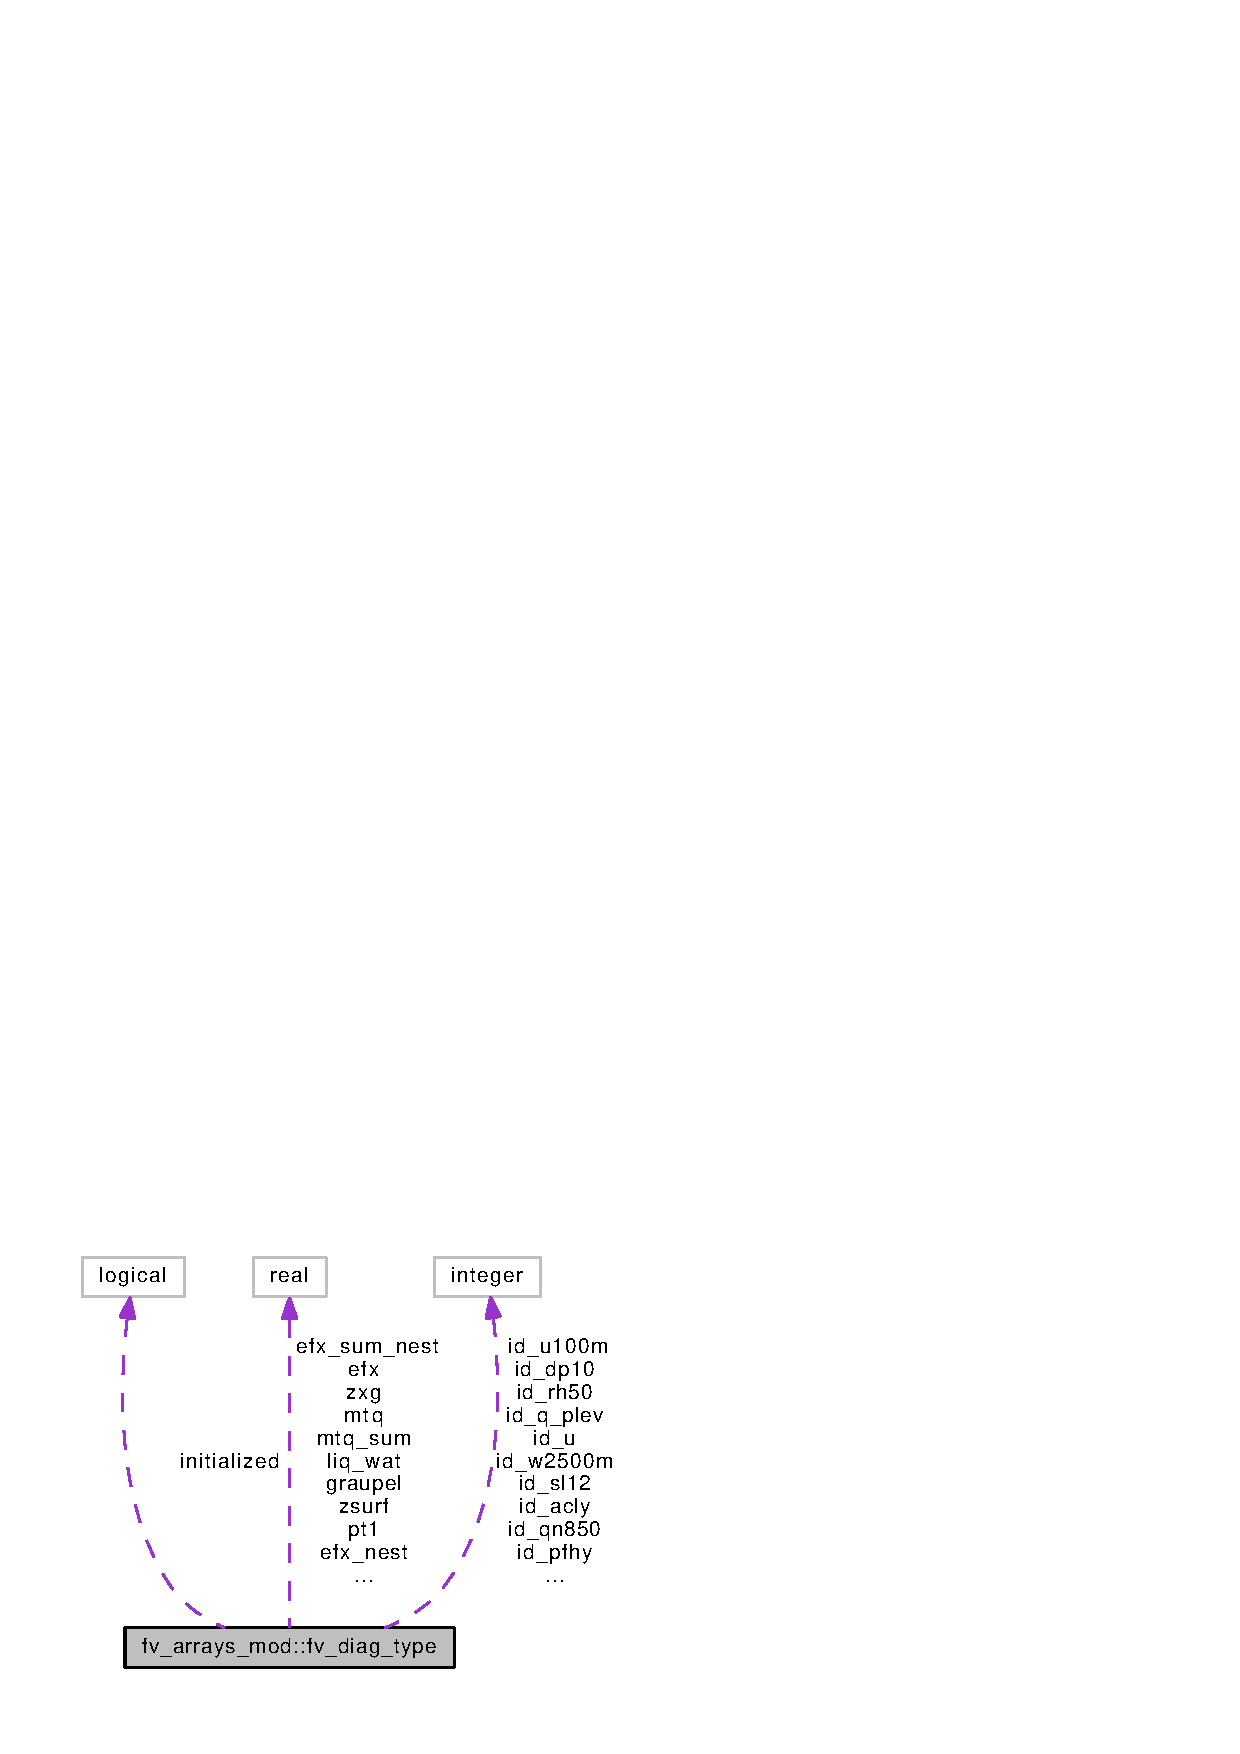
\includegraphics[width=299pt]{structfv__arrays__mod_1_1fv__diag__type__coll__graph}
\end{center}
\end{figure}
\subsection*{Public Attributes}
\begin{DoxyCompactItemize}
\item 
integer \hyperlink{structfv__arrays__mod_1_1fv__diag__type_ad5e5adc5340a72ba40be7cd619389f17}{id\-\_\-ps}
\item 
integer \hyperlink{structfv__arrays__mod_1_1fv__diag__type_ae7f64969cc84bc70bb36034b6af892a0}{id\-\_\-slp}
\item 
integer \hyperlink{structfv__arrays__mod_1_1fv__diag__type_a7a4ee8c20891ff161ac67c619f2dd130}{id\-\_\-ua}
\item 
integer \hyperlink{structfv__arrays__mod_1_1fv__diag__type_a66ece8760225174cdd8a77b9fd5130ad}{id\-\_\-va}
\item 
integer \hyperlink{structfv__arrays__mod_1_1fv__diag__type_afcbabab8aba30345a735324804f20473}{id\-\_\-pt}
\item 
integer \hyperlink{structfv__arrays__mod_1_1fv__diag__type_a099c1591bd31eabe7488f23403b55111}{id\-\_\-omga}
\item 
integer \hyperlink{structfv__arrays__mod_1_1fv__diag__type_addcd934fc8d2fc611ca1fed2bd13ed29}{id\-\_\-vort}
\item 
integer \hyperlink{structfv__arrays__mod_1_1fv__diag__type_a6b7cf6f96193ee0e13156d20ef1d2450}{id\-\_\-tm}
\item 
integer \hyperlink{structfv__arrays__mod_1_1fv__diag__type_a49d1e596f9adae8460273c3b58356bce}{id\-\_\-pv}
\item 
integer \hyperlink{structfv__arrays__mod_1_1fv__diag__type_af1be4af4ae277430d4b2374cb2ebed5c}{id\-\_\-zsurf}
\item 
integer \hyperlink{structfv__arrays__mod_1_1fv__diag__type_a82afdc986149388b63e14f22dd32377f}{id\-\_\-oro}
\item 
integer \hyperlink{structfv__arrays__mod_1_1fv__diag__type_a129b8497a1a0ae956fde38d1d883f151}{id\-\_\-sgh}
\item 
integer \hyperlink{structfv__arrays__mod_1_1fv__diag__type_ad9c51936a5512e09af33275c26e51df7}{id\-\_\-divg}
\item 
integer \hyperlink{structfv__arrays__mod_1_1fv__diag__type_a4d3a07f64e34052c869b1676e850f278}{id\-\_\-w}
\item 
integer \hyperlink{structfv__arrays__mod_1_1fv__diag__type_a74b808c1e2b1f127e9336784184f6426}{id\-\_\-ke}
\item 
integer \hyperlink{structfv__arrays__mod_1_1fv__diag__type_a86e247ae367832465b6a393caaad7013}{id\-\_\-te}
\item 
integer \hyperlink{structfv__arrays__mod_1_1fv__diag__type_a02b594c38c900863da86798386f4fc4b}{id\-\_\-zs}
\item 
integer \hyperlink{structfv__arrays__mod_1_1fv__diag__type_a6f09498a114e501f510f0ac7d9364fe9}{id\-\_\-ze}
\item 
integer \hyperlink{structfv__arrays__mod_1_1fv__diag__type_a7744a8aefae0ec2226811fcc68364317}{id\-\_\-mq}
\item 
integer \hyperlink{structfv__arrays__mod_1_1fv__diag__type_a46e934bee6d16771bbc16e1cf8c1e446}{id\-\_\-vorts}
\item 
integer \hyperlink{structfv__arrays__mod_1_1fv__diag__type_ab43f136e9f3c41460230cd103a9dcfb8}{id\-\_\-us}
\item 
integer \hyperlink{structfv__arrays__mod_1_1fv__diag__type_aab874106757cebdaceffb5fbe107b531}{id\-\_\-vs}
\item 
integer \hyperlink{structfv__arrays__mod_1_1fv__diag__type_aecd1fab104c31b936b96a4814a934a35}{id\-\_\-tq}
\item 
integer \hyperlink{structfv__arrays__mod_1_1fv__diag__type_ac1d30d4c11ee0613ad97da33cc0ca3b5}{id\-\_\-rh}
\item 
integer \hyperlink{structfv__arrays__mod_1_1fv__diag__type_a25e7c161a39dffdb9bb4026c5c714358}{id\-\_\-c15}
\item 
integer \hyperlink{structfv__arrays__mod_1_1fv__diag__type_aa1f3ec493e916301f4544cbed1bd1d31}{id\-\_\-c25}
\item 
integer \hyperlink{structfv__arrays__mod_1_1fv__diag__type_af85f11f4ae3c39767f3798e01c627125}{id\-\_\-c35}
\item 
integer \hyperlink{structfv__arrays__mod_1_1fv__diag__type_a430b8b4826ba4e5ea53c5c8ae15f5646}{id\-\_\-c45}
\item 
integer \hyperlink{structfv__arrays__mod_1_1fv__diag__type_aec34ce54000b540efbb1d2b45f412199}{id\-\_\-f15}
\item 
integer \hyperlink{structfv__arrays__mod_1_1fv__diag__type_a29886f5f34d40b7c4b4116ab943ccb6b}{id\-\_\-f25}
\item 
integer \hyperlink{structfv__arrays__mod_1_1fv__diag__type_a79721f8d0fdaa5cc476b8129d002e5f3}{id\-\_\-f35}
\item 
integer \hyperlink{structfv__arrays__mod_1_1fv__diag__type_acfd9ba1e083fb004ab3d22ae25a69ad8}{id\-\_\-f45}
\item 
integer \hyperlink{structfv__arrays__mod_1_1fv__diag__type_a8be83990bad9c08d0ee22c4a715c0fee}{id\-\_\-ctp}
\item 
integer \hyperlink{structfv__arrays__mod_1_1fv__diag__type_ad1895bc2acd1f2640f89320444cdc75a}{id\-\_\-ppt}
\item 
integer \hyperlink{structfv__arrays__mod_1_1fv__diag__type_ad98591178234c949e44b1a4d2bb76850}{id\-\_\-ts}
\item 
integer \hyperlink{structfv__arrays__mod_1_1fv__diag__type_a824bd1ed50f29ba4b4b6cd2e94f5ae33}{id\-\_\-tb}
\item 
integer \hyperlink{structfv__arrays__mod_1_1fv__diag__type_af6a039f9407545cd5d19e26bcb400848}{id\-\_\-ctt}
\item 
integer \hyperlink{structfv__arrays__mod_1_1fv__diag__type_a8d5e190524ed5c0d1bed425ddefb6d9d}{id\-\_\-pmask}
\item 
integer \hyperlink{structfv__arrays__mod_1_1fv__diag__type_a236e3a15391c143a9c6e50ee1f16e9bc}{id\-\_\-pmaskv2}
\item 
integer \hyperlink{structfv__arrays__mod_1_1fv__diag__type_a224242f8495b284ff480eab3d9b2bed7}{id\-\_\-delp}
\item 
integer \hyperlink{structfv__arrays__mod_1_1fv__diag__type_a908e471cd6497efe99427ed197573511}{id\-\_\-delz}
\item 
integer \hyperlink{structfv__arrays__mod_1_1fv__diag__type_af29b90481e8a7adbdecf7e27c6ef0530}{id\-\_\-zratio}
\item 
integer \hyperlink{structfv__arrays__mod_1_1fv__diag__type_a6118c6a47c51491af5870b9276e7b634}{id\-\_\-ws}
\item 
integer \hyperlink{structfv__arrays__mod_1_1fv__diag__type_a9b2eac321b165245061be9c01e9c2027}{id\-\_\-iw}
\item 
integer \hyperlink{structfv__arrays__mod_1_1fv__diag__type_a153db30dca5e12ac21b9da9bb52c453d}{id\-\_\-lw}
\item 
integer \hyperlink{structfv__arrays__mod_1_1fv__diag__type_a042e6c80ff93ff9d852fe9aac9765a83}{id\-\_\-pfhy}
\item 
integer \hyperlink{structfv__arrays__mod_1_1fv__diag__type_a5e43ef579f22e4545483200ee82073bc}{id\-\_\-pfnh}
\item 
integer \hyperlink{structfv__arrays__mod_1_1fv__diag__type_a2a3f51e805a19792249f18610e7a0ef3}{id\-\_\-qn}
\item 
integer \hyperlink{structfv__arrays__mod_1_1fv__diag__type_a7a48b4be892c914fe0ba91908258bfce}{id\-\_\-qn200}
\item 
integer \hyperlink{structfv__arrays__mod_1_1fv__diag__type_a846c7b13dad7fa70edd219ea06518a5c}{id\-\_\-qn500}
\item 
integer \hyperlink{structfv__arrays__mod_1_1fv__diag__type_a2f88318c0d0fe60f521a5e305a1bee66}{id\-\_\-qn850}
\item 
integer \hyperlink{structfv__arrays__mod_1_1fv__diag__type_aadd4262d26f558a9349481a9ffe40f00}{id\-\_\-qp}
\item 
integer \hyperlink{structfv__arrays__mod_1_1fv__diag__type_a9a246cc4ff1cb1f51d83775ca3a9ed35}{id\-\_\-mdt}
\item 
integer \hyperlink{structfv__arrays__mod_1_1fv__diag__type_ad92e28970ee28309de798b093743587c}{id\-\_\-qdt}
\item 
integer \hyperlink{structfv__arrays__mod_1_1fv__diag__type_a615ce23d1327afa001d8cf6b212b6958}{id\-\_\-aam}
\item 
integer \hyperlink{structfv__arrays__mod_1_1fv__diag__type_a06a291193449b74b2a54ea6a20c18d2d}{id\-\_\-amdt}
\item 
integer \hyperlink{structfv__arrays__mod_1_1fv__diag__type_a3e1d08702a15d2ad4e49761acc7f971e}{id\-\_\-acly}
\item 
integer \hyperlink{structfv__arrays__mod_1_1fv__diag__type_aa77b4bff2de932809ed9d122b84fb71c}{id\-\_\-acl}
\item 
integer \hyperlink{structfv__arrays__mod_1_1fv__diag__type_a23e8542faedab90e92755ec8a362bce1}{id\-\_\-acl2}
\item 
integer \hyperlink{structfv__arrays__mod_1_1fv__diag__type_ae5e2d4e33741a0d9ccfd442c373d8675}{id\-\_\-dbz}
\item 
integer \hyperlink{structfv__arrays__mod_1_1fv__diag__type_a6c4bd51112dfd5a8d604debef6b6c6cc}{id\-\_\-maxdbz}
\item 
integer \hyperlink{structfv__arrays__mod_1_1fv__diag__type_acce987c8683af7c7152a73c1064a0a50}{id\-\_\-basedbz}
\item 
integer \hyperlink{structfv__arrays__mod_1_1fv__diag__type_ae6815282ac9999375a9e7ca539332bae}{id\-\_\-dbz4km}
\item 
integer \hyperlink{structfv__arrays__mod_1_1fv__diag__type_a811e1fc8c66d2fde773fae4b756a5292}{id\-\_\-dbztop}
\item 
integer \hyperlink{structfv__arrays__mod_1_1fv__diag__type_a94fd3023cf0ad171ffe07be2ca193097}{id\-\_\-dbz\-\_\-m10c}
\item 
integer \hyperlink{structfv__arrays__mod_1_1fv__diag__type_a45c733e24768dd170244eb3f1ff2339f}{id\-\_\-ctz}
\item 
integer \hyperlink{structfv__arrays__mod_1_1fv__diag__type_a5786e44912a8b47442d4585947d95435}{id\-\_\-w1km}
\item 
integer \hyperlink{structfv__arrays__mod_1_1fv__diag__type_aac6313c84ac8bc310b14b988bf98f43c}{id\-\_\-wmaxup}
\item 
integer \hyperlink{structfv__arrays__mod_1_1fv__diag__type_a43b6b72088ddaee3abaea9c208ad3e10}{id\-\_\-wmaxdn}
\item 
integer \hyperlink{structfv__arrays__mod_1_1fv__diag__type_a6b4e7be72d35900baf966da2e497eb5b}{id\-\_\-cape}
\item 
integer \hyperlink{structfv__arrays__mod_1_1fv__diag__type_a74dccd47d733f0707c22cf3241c6b644}{id\-\_\-cin}
\item 
integer \hyperlink{structfv__arrays__mod_1_1fv__diag__type_ace291c14a03598d76fd31a89162da256}{id\-\_\-diss}
\item 
integer \hyperlink{structfv__arrays__mod_1_1fv__diag__type_ae1b96d279c2fa7e001ad2e06626d4179}{id\-\_\-vort200}
\item 
integer \hyperlink{structfv__arrays__mod_1_1fv__diag__type_a20986870f6ebf7327bd41204a847ea6d}{id\-\_\-vort500}
\item 
integer \hyperlink{structfv__arrays__mod_1_1fv__diag__type_ad73863fcb8bdc816f5a29193a8b49e1e}{id\-\_\-w500}
\item 
integer \hyperlink{structfv__arrays__mod_1_1fv__diag__type_a9289fc483c315a855504fdd70e683011}{id\-\_\-w700}
\item 
integer \hyperlink{structfv__arrays__mod_1_1fv__diag__type_a90c8fa07b05631b8ceea17d647559739}{id\-\_\-vort850}
\item 
integer \hyperlink{structfv__arrays__mod_1_1fv__diag__type_af209a41a71261d47b9f6ef0d462cdfc2}{id\-\_\-w850}
\item 
integer \hyperlink{structfv__arrays__mod_1_1fv__diag__type_ac19d090d94eaa1059f0f7990d503d798}{id\-\_\-x850}
\item 
integer \hyperlink{structfv__arrays__mod_1_1fv__diag__type_ada7359b37acc18c14a89fad469c630bc}{id\-\_\-srh25}
\item 
integer \hyperlink{structfv__arrays__mod_1_1fv__diag__type_a560d8ee111c56abe43d17562c5abe1c1}{id\-\_\-uh03}
\item 
integer \hyperlink{structfv__arrays__mod_1_1fv__diag__type_a5e667c455b097e52d3417b02d6ee392e}{id\-\_\-uh25}
\item 
integer \hyperlink{structfv__arrays__mod_1_1fv__diag__type_accaec7406234583e7c9e16f8d7ec010d}{id\-\_\-theta\-\_\-e}
\item 
integer \hyperlink{structfv__arrays__mod_1_1fv__diag__type_ac4bd255079b0c5f4caf0c9d41ba9d3ad}{id\-\_\-w200}
\item 
integer \hyperlink{structfv__arrays__mod_1_1fv__diag__type_a86c125a2328f26609335ff0ee7ba18c2}{id\-\_\-s200}
\item 
integer \hyperlink{structfv__arrays__mod_1_1fv__diag__type_ad6f97fc73d6b6fe4abf3a11c7add0780}{id\-\_\-sl12}
\item 
integer \hyperlink{structfv__arrays__mod_1_1fv__diag__type_ae1df4b3d52e38a50ee23a1892b3750e1}{id\-\_\-sl13}
\item 
integer \hyperlink{structfv__arrays__mod_1_1fv__diag__type_ad9a73de5176e49b463cfbdeac1e1a45a}{id\-\_\-w5km}
\item 
integer \hyperlink{structfv__arrays__mod_1_1fv__diag__type_ae7c4203f1cc15c9eeb980725bfca9470}{id\-\_\-rain5km}
\item 
integer \hyperlink{structfv__arrays__mod_1_1fv__diag__type_a8d2a3ba0cfb66ff8938923fd1ba93326}{id\-\_\-w2500m}
\item 
integer \hyperlink{structfv__arrays__mod_1_1fv__diag__type_a75906819114afc7fc5718b5a788bafc3}{id\-\_\-srh1}
\item 
integer \hyperlink{structfv__arrays__mod_1_1fv__diag__type_a31e4e8d5c3aadfef8632e751ffc6d8d8}{id\-\_\-srh3}
\item 
integer \hyperlink{structfv__arrays__mod_1_1fv__diag__type_ae0138627f0c753814f42290b958d72ec}{id\-\_\-ustm}
\item 
integer \hyperlink{structfv__arrays__mod_1_1fv__diag__type_acf7ed5161bddfa6993c5847bc9d4e07f}{id\-\_\-vstm}
\item 
integer, dimension(\-:), allocatable \hyperlink{structfv__arrays__mod_1_1fv__diag__type_a257500cfcef6190a0945f608a8c3477c}{id\-\_\-u}
\item 
integer, dimension(\-:), allocatable \hyperlink{structfv__arrays__mod_1_1fv__diag__type_afe1d5ee644c08fc85ab9f382b560c008}{id\-\_\-v}
\item 
integer, dimension(\-:), allocatable \hyperlink{structfv__arrays__mod_1_1fv__diag__type_a1ff1bb7f29693c8bf383533a4283b1db}{id\-\_\-t}
\item 
integer, dimension(\-:), allocatable \hyperlink{structfv__arrays__mod_1_1fv__diag__type_ac49e6fb49faa9aa7675f6bd9d903be27}{id\-\_\-h}
\item 
integer, dimension(\-:), allocatable \hyperlink{structfv__arrays__mod_1_1fv__diag__type_a1f8f228e034551cd50ab5f8bad1fe2ce}{id\-\_\-q}
\item 
integer, dimension(\-:), allocatable \hyperlink{structfv__arrays__mod_1_1fv__diag__type_a5cbfc6d945494714b611d2efe81cf95f}{id\-\_\-omg}
\item 
integer \hyperlink{structfv__arrays__mod_1_1fv__diag__type_af5107a36d7c957fa11fb59c235f39417}{id\-\_\-u\-\_\-plev}
\item 
integer \hyperlink{structfv__arrays__mod_1_1fv__diag__type_a3a481ce94324a088e5a6e832562bb226}{id\-\_\-v\-\_\-plev}
\item 
integer \hyperlink{structfv__arrays__mod_1_1fv__diag__type_a9240bb6e4d754543c4cd2b304e04a550}{id\-\_\-t\-\_\-plev}
\item 
integer \hyperlink{structfv__arrays__mod_1_1fv__diag__type_a0f76fef7927923ca7cd5a87b9fe741fa}{id\-\_\-h\-\_\-plev}
\item 
integer \hyperlink{structfv__arrays__mod_1_1fv__diag__type_ac8f310e21828d67bb18b441b2561cfb1}{id\-\_\-q\-\_\-plev}
\item 
integer \hyperlink{structfv__arrays__mod_1_1fv__diag__type_a5e9a9f0917c7dc78d3fb933acc1b2765}{id\-\_\-omg\-\_\-plev}
\item 
integer \hyperlink{structfv__arrays__mod_1_1fv__diag__type_a2c527a8bd28698419f9b6b4416fe75b3}{id\-\_\-rh10}
\item 
integer \hyperlink{structfv__arrays__mod_1_1fv__diag__type_a401e52db9f8c72a8650a9427aea46f0a}{id\-\_\-rh50}
\item 
integer \hyperlink{structfv__arrays__mod_1_1fv__diag__type_a9f86116f4ee412db01c782624f5cadc0}{id\-\_\-rh100}
\item 
integer \hyperlink{structfv__arrays__mod_1_1fv__diag__type_a9849054fc1a746d323ef658a3cad14fe}{id\-\_\-rh200}
\item 
integer \hyperlink{structfv__arrays__mod_1_1fv__diag__type_a45d53eadf7954529d66e5508e67d8579}{id\-\_\-rh250}
\item 
integer \hyperlink{structfv__arrays__mod_1_1fv__diag__type_a8803b09da1fc38c3cd4a3694ea78c771}{id\-\_\-rh300}
\item 
integer \hyperlink{structfv__arrays__mod_1_1fv__diag__type_a808319093e2a56a49d37b27ddf708713}{id\-\_\-rh500}
\item 
integer \hyperlink{structfv__arrays__mod_1_1fv__diag__type_a46cc6563313a95577855a167d8344b3d}{id\-\_\-rh700}
\item 
integer \hyperlink{structfv__arrays__mod_1_1fv__diag__type_ae54b86362492956ab121864e53e2b6cf}{id\-\_\-rh850}
\item 
integer \hyperlink{structfv__arrays__mod_1_1fv__diag__type_a9323b5da9999228f3dccac4b67b3c559}{id\-\_\-rh925}
\item 
integer \hyperlink{structfv__arrays__mod_1_1fv__diag__type_ad7e698cb721c04ffb3be364b1cf714f8}{id\-\_\-rh1000}
\item 
integer \hyperlink{structfv__arrays__mod_1_1fv__diag__type_af2cec4984bf8db9f25f334bd517fd9b9}{id\-\_\-dp10}
\item 
integer \hyperlink{structfv__arrays__mod_1_1fv__diag__type_a99b4609384bfb8d8eb1ffe37c970e63b}{id\-\_\-dp50}
\item 
integer \hyperlink{structfv__arrays__mod_1_1fv__diag__type_ab2b6f720c17b6be7ba145c557544aea1}{id\-\_\-dp100}
\item 
integer \hyperlink{structfv__arrays__mod_1_1fv__diag__type_a6f55e52f00ad261c77881a09af71acad}{id\-\_\-dp200}
\item 
integer \hyperlink{structfv__arrays__mod_1_1fv__diag__type_a5e8d330356a3bceb251e0922e4736c89}{id\-\_\-dp250}
\item 
integer \hyperlink{structfv__arrays__mod_1_1fv__diag__type_a3591f5de65f47909773e8b2a99e31a54}{id\-\_\-dp300}
\item 
integer \hyperlink{structfv__arrays__mod_1_1fv__diag__type_af678704af54d41667a8e767b35191179}{id\-\_\-dp500}
\item 
integer \hyperlink{structfv__arrays__mod_1_1fv__diag__type_a2d777b758f8ee5912ef42eb0f82a72eb}{id\-\_\-dp700}
\item 
integer \hyperlink{structfv__arrays__mod_1_1fv__diag__type_a79dafa4d20c4ef1c80103be176f354f6}{id\-\_\-dp850}
\item 
integer \hyperlink{structfv__arrays__mod_1_1fv__diag__type_a50f5149ebe1b402c2a47450c9099385b}{id\-\_\-dp925}
\item 
integer \hyperlink{structfv__arrays__mod_1_1fv__diag__type_a96412203d65812e83b593da8035117ad}{id\-\_\-dp1000}
\item 
integer \hyperlink{structfv__arrays__mod_1_1fv__diag__type_a500ab6adee53dce8426353c9951fb448}{id\-\_\-rh1000\-\_\-cmip}
\item 
integer \hyperlink{structfv__arrays__mod_1_1fv__diag__type_af3e7c756312b02e993dbed55960cf79e}{id\-\_\-rh925\-\_\-cmip}
\item 
integer \hyperlink{structfv__arrays__mod_1_1fv__diag__type_ac777e60c94ab8ff2b8ba133a4b5f67ed}{id\-\_\-rh850\-\_\-cmip}
\item 
integer \hyperlink{structfv__arrays__mod_1_1fv__diag__type_a6d04f8ad9f2c9db28b689297422898a0}{id\-\_\-rh700\-\_\-cmip}
\item 
integer \hyperlink{structfv__arrays__mod_1_1fv__diag__type_a613de64403c7ea723460d5d74d88b644}{id\-\_\-rh500\-\_\-cmip}
\item 
integer \hyperlink{structfv__arrays__mod_1_1fv__diag__type_a7e2379212d4724f6815ddc146d868936}{id\-\_\-rh300\-\_\-cmip}
\item 
integer \hyperlink{structfv__arrays__mod_1_1fv__diag__type_a2cd499f8ecb29eda6e01b76dc8828341}{id\-\_\-rh250\-\_\-cmip}
\item 
integer \hyperlink{structfv__arrays__mod_1_1fv__diag__type_ad58ec87b1ab423e16264571ce9c07cdc}{id\-\_\-rh100\-\_\-cmip}
\item 
integer \hyperlink{structfv__arrays__mod_1_1fv__diag__type_ad7e64434e809619ed820e7080da2d7ad}{id\-\_\-rh50\-\_\-cmip}
\item 
integer \hyperlink{structfv__arrays__mod_1_1fv__diag__type_ae9e3edf9bbdc6049bdc5b847e0449e28}{id\-\_\-rh10\-\_\-cmip}
\item 
integer \hyperlink{structfv__arrays__mod_1_1fv__diag__type_aed92d984c51120a8e1c0603c157b8c1b}{id\-\_\-hght}
\item 
integer \hyperlink{structfv__arrays__mod_1_1fv__diag__type_afa53aad1dc4de6f5309ebedeced85dc6}{id\-\_\-u100m}
\item 
integer \hyperlink{structfv__arrays__mod_1_1fv__diag__type_a7901dc1f4f2b261febf73e0064a0e703}{id\-\_\-v100m}
\item 
integer \hyperlink{structfv__arrays__mod_1_1fv__diag__type_af439389cd4e49830cde3a3c252e910e8}{id\-\_\-w100m}
\item 
integer \hyperlink{structfv__arrays__mod_1_1fv__diag__type_ad0bac6918677f1bcb0b8a02db3c15ba6}{ic\-\_\-ps}
\item 
integer \hyperlink{structfv__arrays__mod_1_1fv__diag__type_a54b1c4e81d0efba189d5a4ba22cc9586}{ic\-\_\-ua}
\item 
integer \hyperlink{structfv__arrays__mod_1_1fv__diag__type_a5d0238ef8c9714454fef513a0a142ad2}{ic\-\_\-va}
\item 
integer \hyperlink{structfv__arrays__mod_1_1fv__diag__type_a209a23364e9e3864fd62e3746e5530c5}{ic\-\_\-ppt}
\item 
integer \hyperlink{structfv__arrays__mod_1_1fv__diag__type_ab29a6be075c7645616d0ce9b1d2064b3}{ic\-\_\-sphum}
\item 
integer, dimension(\-:), allocatable \hyperlink{structfv__arrays__mod_1_1fv__diag__type_abf748df5449396c1a7074ecb74d7f324}{id\-\_\-tracer}
\item 
integer, dimension(\-:), allocatable \hyperlink{structfv__arrays__mod_1_1fv__diag__type_ad80c8385277eadb39d47bb4d0e974ea8}{id\-\_\-tracer\-\_\-dmmr}
\item 
integer, dimension(\-:), allocatable \hyperlink{structfv__arrays__mod_1_1fv__diag__type_a0e8e7e25003ea55dc76c5dc77e1a990d}{id\-\_\-tracer\-\_\-dvmr}
\item 
real, dimension(\-:), allocatable \hyperlink{structfv__arrays__mod_1_1fv__diag__type_a4d259addb1c6c08c0227fe069d965ea3}{w\-\_\-mr}
\item 
real, dimension(\-:), allocatable \hyperlink{structfv__arrays__mod_1_1fv__diag__type_a1149e99cfa8d9a6cfe1ae1cfbfb5819c}{phalf}
\item 
real, dimension(\-:,\-:), allocatable \hyperlink{structfv__arrays__mod_1_1fv__diag__type_af067ded7c9f594b49e5014ccdd8f2ef2}{zsurf}
\item 
real, dimension(\-:,\-:), allocatable \hyperlink{structfv__arrays__mod_1_1fv__diag__type_a52e01f510a1a63071b116fa418a2fe36}{zxg}
\item 
real, dimension(\-:), allocatable \hyperlink{structfv__arrays__mod_1_1fv__diag__type_a32d7cfbed4a50c455ccca54ebed64b86}{pt1}
\item 
logical \hyperlink{structfv__arrays__mod_1_1fv__diag__type_ae727b4a8b7bcd2d4ca2e51fd71fe93c5}{initialized} = .false.
\item 
real \hyperlink{structfv__arrays__mod_1_1fv__diag__type_ab7170e3cf0bddbc87fe82585a9062b27}{sphum}
\item 
real \hyperlink{structfv__arrays__mod_1_1fv__diag__type_a762e21ac20112fb7a5e3b7ea5f14c0ff}{liq\-\_\-wat}
\item 
real \hyperlink{structfv__arrays__mod_1_1fv__diag__type_a08c5978581db62bd5f165873975b82da}{ice\-\_\-wat}
\item 
real \hyperlink{structfv__arrays__mod_1_1fv__diag__type_a3cc3219727d54802eb98783a7f1bd2a9}{rainwat}
\item 
real \hyperlink{structfv__arrays__mod_1_1fv__diag__type_af4f8361914400d6e1c225b9dea392d52}{snowwat}
\item 
real \hyperlink{structfv__arrays__mod_1_1fv__diag__type_a285a1994a61dfeb1cc4a2d41cb2daf58}{graupel}
\item 
real, dimension(\hyperlink{classfv__arrays__mod_a9e487a715273ca3c6572693756bcec1b}{max\-\_\-step}) \hyperlink{structfv__arrays__mod_1_1fv__diag__type_a3a82cb7f95dd84492be39b9aac99fd16}{efx}
\item 
real \hyperlink{structfv__arrays__mod_1_1fv__diag__type_ae15a07f9d6f051076e13dba74377e759}{efx\-\_\-sum}
\item 
real, dimension(\hyperlink{classfv__arrays__mod_a9e487a715273ca3c6572693756bcec1b}{max\-\_\-step}) \hyperlink{structfv__arrays__mod_1_1fv__diag__type_af5695e644a6f2604bcb2cd502f534804}{efx\-\_\-nest}
\item 
real \hyperlink{structfv__arrays__mod_1_1fv__diag__type_a32a6f4014260bb3c0867fda0563f4c12}{efx\-\_\-sum\-\_\-nest}
\item 
real, dimension(\hyperlink{classfv__arrays__mod_a9e487a715273ca3c6572693756bcec1b}{max\-\_\-step}) \hyperlink{structfv__arrays__mod_1_1fv__diag__type_a26ee238f8ade03f3f0b266664416b8f8}{mtq}
\item 
real \hyperlink{structfv__arrays__mod_1_1fv__diag__type_aba97005878999cb1d0ec569e7e8c5ec8}{mtq\-\_\-sum}
\item 
integer \hyperlink{structfv__arrays__mod_1_1fv__diag__type_a2dfa52c702f772c7ce4d8935a9b237df}{steps}
\end{DoxyCompactItemize}


\subsection{Detailed Description}


Definition at line 53 of file fv\-\_\-arrays.\-F90.



\subsection{Member Data Documentation}
\index{fv\-\_\-arrays\-\_\-mod\-::fv\-\_\-diag\-\_\-type@{fv\-\_\-arrays\-\_\-mod\-::fv\-\_\-diag\-\_\-type}!efx@{efx}}
\index{efx@{efx}!fv_arrays_mod::fv_diag_type@{fv\-\_\-arrays\-\_\-mod\-::fv\-\_\-diag\-\_\-type}}
\subsubsection[{efx}]{\setlength{\rightskip}{0pt plus 5cm}real, dimension({\bf max\-\_\-step}) fv\-\_\-arrays\-\_\-mod\-::fv\-\_\-diag\-\_\-type\-::efx}\label{structfv__arrays__mod_1_1fv__diag__type_a3a82cb7f95dd84492be39b9aac99fd16}


Definition at line 111 of file fv\-\_\-arrays.\-F90.

\index{fv\-\_\-arrays\-\_\-mod\-::fv\-\_\-diag\-\_\-type@{fv\-\_\-arrays\-\_\-mod\-::fv\-\_\-diag\-\_\-type}!efx\-\_\-nest@{efx\-\_\-nest}}
\index{efx\-\_\-nest@{efx\-\_\-nest}!fv_arrays_mod::fv_diag_type@{fv\-\_\-arrays\-\_\-mod\-::fv\-\_\-diag\-\_\-type}}
\subsubsection[{efx\-\_\-nest}]{\setlength{\rightskip}{0pt plus 5cm}real, dimension({\bf max\-\_\-step}) fv\-\_\-arrays\-\_\-mod\-::fv\-\_\-diag\-\_\-type\-::efx\-\_\-nest}\label{structfv__arrays__mod_1_1fv__diag__type_af5695e644a6f2604bcb2cd502f534804}


Definition at line 111 of file fv\-\_\-arrays.\-F90.

\index{fv\-\_\-arrays\-\_\-mod\-::fv\-\_\-diag\-\_\-type@{fv\-\_\-arrays\-\_\-mod\-::fv\-\_\-diag\-\_\-type}!efx\-\_\-sum@{efx\-\_\-sum}}
\index{efx\-\_\-sum@{efx\-\_\-sum}!fv_arrays_mod::fv_diag_type@{fv\-\_\-arrays\-\_\-mod\-::fv\-\_\-diag\-\_\-type}}
\subsubsection[{efx\-\_\-sum}]{\setlength{\rightskip}{0pt plus 5cm}real fv\-\_\-arrays\-\_\-mod\-::fv\-\_\-diag\-\_\-type\-::efx\-\_\-sum}\label{structfv__arrays__mod_1_1fv__diag__type_ae15a07f9d6f051076e13dba74377e759}


Definition at line 111 of file fv\-\_\-arrays.\-F90.

\index{fv\-\_\-arrays\-\_\-mod\-::fv\-\_\-diag\-\_\-type@{fv\-\_\-arrays\-\_\-mod\-::fv\-\_\-diag\-\_\-type}!efx\-\_\-sum\-\_\-nest@{efx\-\_\-sum\-\_\-nest}}
\index{efx\-\_\-sum\-\_\-nest@{efx\-\_\-sum\-\_\-nest}!fv_arrays_mod::fv_diag_type@{fv\-\_\-arrays\-\_\-mod\-::fv\-\_\-diag\-\_\-type}}
\subsubsection[{efx\-\_\-sum\-\_\-nest}]{\setlength{\rightskip}{0pt plus 5cm}real fv\-\_\-arrays\-\_\-mod\-::fv\-\_\-diag\-\_\-type\-::efx\-\_\-sum\-\_\-nest}\label{structfv__arrays__mod_1_1fv__diag__type_a32a6f4014260bb3c0867fda0563f4c12}


Definition at line 111 of file fv\-\_\-arrays.\-F90.

\index{fv\-\_\-arrays\-\_\-mod\-::fv\-\_\-diag\-\_\-type@{fv\-\_\-arrays\-\_\-mod\-::fv\-\_\-diag\-\_\-type}!graupel@{graupel}}
\index{graupel@{graupel}!fv_arrays_mod::fv_diag_type@{fv\-\_\-arrays\-\_\-mod\-::fv\-\_\-diag\-\_\-type}}
\subsubsection[{graupel}]{\setlength{\rightskip}{0pt plus 5cm}real fv\-\_\-arrays\-\_\-mod\-::fv\-\_\-diag\-\_\-type\-::graupel}\label{structfv__arrays__mod_1_1fv__diag__type_a285a1994a61dfeb1cc4a2d41cb2daf58}


Definition at line 109 of file fv\-\_\-arrays.\-F90.

\index{fv\-\_\-arrays\-\_\-mod\-::fv\-\_\-diag\-\_\-type@{fv\-\_\-arrays\-\_\-mod\-::fv\-\_\-diag\-\_\-type}!ic\-\_\-ppt@{ic\-\_\-ppt}}
\index{ic\-\_\-ppt@{ic\-\_\-ppt}!fv_arrays_mod::fv_diag_type@{fv\-\_\-arrays\-\_\-mod\-::fv\-\_\-diag\-\_\-type}}
\subsubsection[{ic\-\_\-ppt}]{\setlength{\rightskip}{0pt plus 5cm}integer fv\-\_\-arrays\-\_\-mod\-::fv\-\_\-diag\-\_\-type\-::ic\-\_\-ppt}\label{structfv__arrays__mod_1_1fv__diag__type_a209a23364e9e3864fd62e3746e5530c5}


Definition at line 93 of file fv\-\_\-arrays.\-F90.

\index{fv\-\_\-arrays\-\_\-mod\-::fv\-\_\-diag\-\_\-type@{fv\-\_\-arrays\-\_\-mod\-::fv\-\_\-diag\-\_\-type}!ic\-\_\-ps@{ic\-\_\-ps}}
\index{ic\-\_\-ps@{ic\-\_\-ps}!fv_arrays_mod::fv_diag_type@{fv\-\_\-arrays\-\_\-mod\-::fv\-\_\-diag\-\_\-type}}
\subsubsection[{ic\-\_\-ps}]{\setlength{\rightskip}{0pt plus 5cm}integer fv\-\_\-arrays\-\_\-mod\-::fv\-\_\-diag\-\_\-type\-::ic\-\_\-ps}\label{structfv__arrays__mod_1_1fv__diag__type_ad0bac6918677f1bcb0b8a02db3c15ba6}


Definition at line 93 of file fv\-\_\-arrays.\-F90.

\index{fv\-\_\-arrays\-\_\-mod\-::fv\-\_\-diag\-\_\-type@{fv\-\_\-arrays\-\_\-mod\-::fv\-\_\-diag\-\_\-type}!ic\-\_\-sphum@{ic\-\_\-sphum}}
\index{ic\-\_\-sphum@{ic\-\_\-sphum}!fv_arrays_mod::fv_diag_type@{fv\-\_\-arrays\-\_\-mod\-::fv\-\_\-diag\-\_\-type}}
\subsubsection[{ic\-\_\-sphum}]{\setlength{\rightskip}{0pt plus 5cm}integer fv\-\_\-arrays\-\_\-mod\-::fv\-\_\-diag\-\_\-type\-::ic\-\_\-sphum}\label{structfv__arrays__mod_1_1fv__diag__type_ab29a6be075c7645616d0ce9b1d2064b3}


Definition at line 94 of file fv\-\_\-arrays.\-F90.

\index{fv\-\_\-arrays\-\_\-mod\-::fv\-\_\-diag\-\_\-type@{fv\-\_\-arrays\-\_\-mod\-::fv\-\_\-diag\-\_\-type}!ic\-\_\-ua@{ic\-\_\-ua}}
\index{ic\-\_\-ua@{ic\-\_\-ua}!fv_arrays_mod::fv_diag_type@{fv\-\_\-arrays\-\_\-mod\-::fv\-\_\-diag\-\_\-type}}
\subsubsection[{ic\-\_\-ua}]{\setlength{\rightskip}{0pt plus 5cm}integer fv\-\_\-arrays\-\_\-mod\-::fv\-\_\-diag\-\_\-type\-::ic\-\_\-ua}\label{structfv__arrays__mod_1_1fv__diag__type_a54b1c4e81d0efba189d5a4ba22cc9586}


Definition at line 93 of file fv\-\_\-arrays.\-F90.

\index{fv\-\_\-arrays\-\_\-mod\-::fv\-\_\-diag\-\_\-type@{fv\-\_\-arrays\-\_\-mod\-::fv\-\_\-diag\-\_\-type}!ic\-\_\-va@{ic\-\_\-va}}
\index{ic\-\_\-va@{ic\-\_\-va}!fv_arrays_mod::fv_diag_type@{fv\-\_\-arrays\-\_\-mod\-::fv\-\_\-diag\-\_\-type}}
\subsubsection[{ic\-\_\-va}]{\setlength{\rightskip}{0pt plus 5cm}integer fv\-\_\-arrays\-\_\-mod\-::fv\-\_\-diag\-\_\-type\-::ic\-\_\-va}\label{structfv__arrays__mod_1_1fv__diag__type_a5d0238ef8c9714454fef513a0a142ad2}


Definition at line 93 of file fv\-\_\-arrays.\-F90.

\index{fv\-\_\-arrays\-\_\-mod\-::fv\-\_\-diag\-\_\-type@{fv\-\_\-arrays\-\_\-mod\-::fv\-\_\-diag\-\_\-type}!ice\-\_\-wat@{ice\-\_\-wat}}
\index{ice\-\_\-wat@{ice\-\_\-wat}!fv_arrays_mod::fv_diag_type@{fv\-\_\-arrays\-\_\-mod\-::fv\-\_\-diag\-\_\-type}}
\subsubsection[{ice\-\_\-wat}]{\setlength{\rightskip}{0pt plus 5cm}real fv\-\_\-arrays\-\_\-mod\-::fv\-\_\-diag\-\_\-type\-::ice\-\_\-wat}\label{structfv__arrays__mod_1_1fv__diag__type_a08c5978581db62bd5f165873975b82da}


Definition at line 108 of file fv\-\_\-arrays.\-F90.

\index{fv\-\_\-arrays\-\_\-mod\-::fv\-\_\-diag\-\_\-type@{fv\-\_\-arrays\-\_\-mod\-::fv\-\_\-diag\-\_\-type}!id\-\_\-aam@{id\-\_\-aam}}
\index{id\-\_\-aam@{id\-\_\-aam}!fv_arrays_mod::fv_diag_type@{fv\-\_\-arrays\-\_\-mod\-::fv\-\_\-diag\-\_\-type}}
\subsubsection[{id\-\_\-aam}]{\setlength{\rightskip}{0pt plus 5cm}integer fv\-\_\-arrays\-\_\-mod\-::fv\-\_\-diag\-\_\-type\-::id\-\_\-aam}\label{structfv__arrays__mod_1_1fv__diag__type_a615ce23d1327afa001d8cf6b212b6958}


Definition at line 56 of file fv\-\_\-arrays.\-F90.

\index{fv\-\_\-arrays\-\_\-mod\-::fv\-\_\-diag\-\_\-type@{fv\-\_\-arrays\-\_\-mod\-::fv\-\_\-diag\-\_\-type}!id\-\_\-acl@{id\-\_\-acl}}
\index{id\-\_\-acl@{id\-\_\-acl}!fv_arrays_mod::fv_diag_type@{fv\-\_\-arrays\-\_\-mod\-::fv\-\_\-diag\-\_\-type}}
\subsubsection[{id\-\_\-acl}]{\setlength{\rightskip}{0pt plus 5cm}integer fv\-\_\-arrays\-\_\-mod\-::fv\-\_\-diag\-\_\-type\-::id\-\_\-acl}\label{structfv__arrays__mod_1_1fv__diag__type_aa77b4bff2de932809ed9d122b84fb71c}


Definition at line 56 of file fv\-\_\-arrays.\-F90.

\index{fv\-\_\-arrays\-\_\-mod\-::fv\-\_\-diag\-\_\-type@{fv\-\_\-arrays\-\_\-mod\-::fv\-\_\-diag\-\_\-type}!id\-\_\-acl2@{id\-\_\-acl2}}
\index{id\-\_\-acl2@{id\-\_\-acl2}!fv_arrays_mod::fv_diag_type@{fv\-\_\-arrays\-\_\-mod\-::fv\-\_\-diag\-\_\-type}}
\subsubsection[{id\-\_\-acl2}]{\setlength{\rightskip}{0pt plus 5cm}integer fv\-\_\-arrays\-\_\-mod\-::fv\-\_\-diag\-\_\-type\-::id\-\_\-acl2}\label{structfv__arrays__mod_1_1fv__diag__type_a23e8542faedab90e92755ec8a362bce1}


Definition at line 56 of file fv\-\_\-arrays.\-F90.

\index{fv\-\_\-arrays\-\_\-mod\-::fv\-\_\-diag\-\_\-type@{fv\-\_\-arrays\-\_\-mod\-::fv\-\_\-diag\-\_\-type}!id\-\_\-acly@{id\-\_\-acly}}
\index{id\-\_\-acly@{id\-\_\-acly}!fv_arrays_mod::fv_diag_type@{fv\-\_\-arrays\-\_\-mod\-::fv\-\_\-diag\-\_\-type}}
\subsubsection[{id\-\_\-acly}]{\setlength{\rightskip}{0pt plus 5cm}integer fv\-\_\-arrays\-\_\-mod\-::fv\-\_\-diag\-\_\-type\-::id\-\_\-acly}\label{structfv__arrays__mod_1_1fv__diag__type_a3e1d08702a15d2ad4e49761acc7f971e}


Definition at line 56 of file fv\-\_\-arrays.\-F90.

\index{fv\-\_\-arrays\-\_\-mod\-::fv\-\_\-diag\-\_\-type@{fv\-\_\-arrays\-\_\-mod\-::fv\-\_\-diag\-\_\-type}!id\-\_\-amdt@{id\-\_\-amdt}}
\index{id\-\_\-amdt@{id\-\_\-amdt}!fv_arrays_mod::fv_diag_type@{fv\-\_\-arrays\-\_\-mod\-::fv\-\_\-diag\-\_\-type}}
\subsubsection[{id\-\_\-amdt}]{\setlength{\rightskip}{0pt plus 5cm}integer fv\-\_\-arrays\-\_\-mod\-::fv\-\_\-diag\-\_\-type\-::id\-\_\-amdt}\label{structfv__arrays__mod_1_1fv__diag__type_a06a291193449b74b2a54ea6a20c18d2d}


Definition at line 56 of file fv\-\_\-arrays.\-F90.

\index{fv\-\_\-arrays\-\_\-mod\-::fv\-\_\-diag\-\_\-type@{fv\-\_\-arrays\-\_\-mod\-::fv\-\_\-diag\-\_\-type}!id\-\_\-basedbz@{id\-\_\-basedbz}}
\index{id\-\_\-basedbz@{id\-\_\-basedbz}!fv_arrays_mod::fv_diag_type@{fv\-\_\-arrays\-\_\-mod\-::fv\-\_\-diag\-\_\-type}}
\subsubsection[{id\-\_\-basedbz}]{\setlength{\rightskip}{0pt plus 5cm}integer fv\-\_\-arrays\-\_\-mod\-::fv\-\_\-diag\-\_\-type\-::id\-\_\-basedbz}\label{structfv__arrays__mod_1_1fv__diag__type_acce987c8683af7c7152a73c1064a0a50}


Definition at line 56 of file fv\-\_\-arrays.\-F90.

\index{fv\-\_\-arrays\-\_\-mod\-::fv\-\_\-diag\-\_\-type@{fv\-\_\-arrays\-\_\-mod\-::fv\-\_\-diag\-\_\-type}!id\-\_\-c15@{id\-\_\-c15}}
\index{id\-\_\-c15@{id\-\_\-c15}!fv_arrays_mod::fv_diag_type@{fv\-\_\-arrays\-\_\-mod\-::fv\-\_\-diag\-\_\-type}}
\subsubsection[{id\-\_\-c15}]{\setlength{\rightskip}{0pt plus 5cm}integer fv\-\_\-arrays\-\_\-mod\-::fv\-\_\-diag\-\_\-type\-::id\-\_\-c15}\label{structfv__arrays__mod_1_1fv__diag__type_a25e7c161a39dffdb9bb4026c5c714358}


Definition at line 56 of file fv\-\_\-arrays.\-F90.

\index{fv\-\_\-arrays\-\_\-mod\-::fv\-\_\-diag\-\_\-type@{fv\-\_\-arrays\-\_\-mod\-::fv\-\_\-diag\-\_\-type}!id\-\_\-c25@{id\-\_\-c25}}
\index{id\-\_\-c25@{id\-\_\-c25}!fv_arrays_mod::fv_diag_type@{fv\-\_\-arrays\-\_\-mod\-::fv\-\_\-diag\-\_\-type}}
\subsubsection[{id\-\_\-c25}]{\setlength{\rightskip}{0pt plus 5cm}integer fv\-\_\-arrays\-\_\-mod\-::fv\-\_\-diag\-\_\-type\-::id\-\_\-c25}\label{structfv__arrays__mod_1_1fv__diag__type_aa1f3ec493e916301f4544cbed1bd1d31}


Definition at line 56 of file fv\-\_\-arrays.\-F90.

\index{fv\-\_\-arrays\-\_\-mod\-::fv\-\_\-diag\-\_\-type@{fv\-\_\-arrays\-\_\-mod\-::fv\-\_\-diag\-\_\-type}!id\-\_\-c35@{id\-\_\-c35}}
\index{id\-\_\-c35@{id\-\_\-c35}!fv_arrays_mod::fv_diag_type@{fv\-\_\-arrays\-\_\-mod\-::fv\-\_\-diag\-\_\-type}}
\subsubsection[{id\-\_\-c35}]{\setlength{\rightskip}{0pt plus 5cm}integer fv\-\_\-arrays\-\_\-mod\-::fv\-\_\-diag\-\_\-type\-::id\-\_\-c35}\label{structfv__arrays__mod_1_1fv__diag__type_af85f11f4ae3c39767f3798e01c627125}


Definition at line 56 of file fv\-\_\-arrays.\-F90.

\index{fv\-\_\-arrays\-\_\-mod\-::fv\-\_\-diag\-\_\-type@{fv\-\_\-arrays\-\_\-mod\-::fv\-\_\-diag\-\_\-type}!id\-\_\-c45@{id\-\_\-c45}}
\index{id\-\_\-c45@{id\-\_\-c45}!fv_arrays_mod::fv_diag_type@{fv\-\_\-arrays\-\_\-mod\-::fv\-\_\-diag\-\_\-type}}
\subsubsection[{id\-\_\-c45}]{\setlength{\rightskip}{0pt plus 5cm}integer fv\-\_\-arrays\-\_\-mod\-::fv\-\_\-diag\-\_\-type\-::id\-\_\-c45}\label{structfv__arrays__mod_1_1fv__diag__type_a430b8b4826ba4e5ea53c5c8ae15f5646}


Definition at line 56 of file fv\-\_\-arrays.\-F90.

\index{fv\-\_\-arrays\-\_\-mod\-::fv\-\_\-diag\-\_\-type@{fv\-\_\-arrays\-\_\-mod\-::fv\-\_\-diag\-\_\-type}!id\-\_\-cape@{id\-\_\-cape}}
\index{id\-\_\-cape@{id\-\_\-cape}!fv_arrays_mod::fv_diag_type@{fv\-\_\-arrays\-\_\-mod\-::fv\-\_\-diag\-\_\-type}}
\subsubsection[{id\-\_\-cape}]{\setlength{\rightskip}{0pt plus 5cm}integer fv\-\_\-arrays\-\_\-mod\-::fv\-\_\-diag\-\_\-type\-::id\-\_\-cape}\label{structfv__arrays__mod_1_1fv__diag__type_a6b4e7be72d35900baf966da2e497eb5b}


Definition at line 56 of file fv\-\_\-arrays.\-F90.

\index{fv\-\_\-arrays\-\_\-mod\-::fv\-\_\-diag\-\_\-type@{fv\-\_\-arrays\-\_\-mod\-::fv\-\_\-diag\-\_\-type}!id\-\_\-cin@{id\-\_\-cin}}
\index{id\-\_\-cin@{id\-\_\-cin}!fv_arrays_mod::fv_diag_type@{fv\-\_\-arrays\-\_\-mod\-::fv\-\_\-diag\-\_\-type}}
\subsubsection[{id\-\_\-cin}]{\setlength{\rightskip}{0pt plus 5cm}integer fv\-\_\-arrays\-\_\-mod\-::fv\-\_\-diag\-\_\-type\-::id\-\_\-cin}\label{structfv__arrays__mod_1_1fv__diag__type_a74dccd47d733f0707c22cf3241c6b644}


Definition at line 56 of file fv\-\_\-arrays.\-F90.

\index{fv\-\_\-arrays\-\_\-mod\-::fv\-\_\-diag\-\_\-type@{fv\-\_\-arrays\-\_\-mod\-::fv\-\_\-diag\-\_\-type}!id\-\_\-ctp@{id\-\_\-ctp}}
\index{id\-\_\-ctp@{id\-\_\-ctp}!fv_arrays_mod::fv_diag_type@{fv\-\_\-arrays\-\_\-mod\-::fv\-\_\-diag\-\_\-type}}
\subsubsection[{id\-\_\-ctp}]{\setlength{\rightskip}{0pt plus 5cm}integer fv\-\_\-arrays\-\_\-mod\-::fv\-\_\-diag\-\_\-type\-::id\-\_\-ctp}\label{structfv__arrays__mod_1_1fv__diag__type_a8be83990bad9c08d0ee22c4a715c0fee}


Definition at line 56 of file fv\-\_\-arrays.\-F90.

\index{fv\-\_\-arrays\-\_\-mod\-::fv\-\_\-diag\-\_\-type@{fv\-\_\-arrays\-\_\-mod\-::fv\-\_\-diag\-\_\-type}!id\-\_\-ctt@{id\-\_\-ctt}}
\index{id\-\_\-ctt@{id\-\_\-ctt}!fv_arrays_mod::fv_diag_type@{fv\-\_\-arrays\-\_\-mod\-::fv\-\_\-diag\-\_\-type}}
\subsubsection[{id\-\_\-ctt}]{\setlength{\rightskip}{0pt plus 5cm}integer fv\-\_\-arrays\-\_\-mod\-::fv\-\_\-diag\-\_\-type\-::id\-\_\-ctt}\label{structfv__arrays__mod_1_1fv__diag__type_af6a039f9407545cd5d19e26bcb400848}


Definition at line 56 of file fv\-\_\-arrays.\-F90.

\index{fv\-\_\-arrays\-\_\-mod\-::fv\-\_\-diag\-\_\-type@{fv\-\_\-arrays\-\_\-mod\-::fv\-\_\-diag\-\_\-type}!id\-\_\-ctz@{id\-\_\-ctz}}
\index{id\-\_\-ctz@{id\-\_\-ctz}!fv_arrays_mod::fv_diag_type@{fv\-\_\-arrays\-\_\-mod\-::fv\-\_\-diag\-\_\-type}}
\subsubsection[{id\-\_\-ctz}]{\setlength{\rightskip}{0pt plus 5cm}integer fv\-\_\-arrays\-\_\-mod\-::fv\-\_\-diag\-\_\-type\-::id\-\_\-ctz}\label{structfv__arrays__mod_1_1fv__diag__type_a45c733e24768dd170244eb3f1ff2339f}


Definition at line 56 of file fv\-\_\-arrays.\-F90.

\index{fv\-\_\-arrays\-\_\-mod\-::fv\-\_\-diag\-\_\-type@{fv\-\_\-arrays\-\_\-mod\-::fv\-\_\-diag\-\_\-type}!id\-\_\-dbz@{id\-\_\-dbz}}
\index{id\-\_\-dbz@{id\-\_\-dbz}!fv_arrays_mod::fv_diag_type@{fv\-\_\-arrays\-\_\-mod\-::fv\-\_\-diag\-\_\-type}}
\subsubsection[{id\-\_\-dbz}]{\setlength{\rightskip}{0pt plus 5cm}integer fv\-\_\-arrays\-\_\-mod\-::fv\-\_\-diag\-\_\-type\-::id\-\_\-dbz}\label{structfv__arrays__mod_1_1fv__diag__type_ae5e2d4e33741a0d9ccfd442c373d8675}


Definition at line 56 of file fv\-\_\-arrays.\-F90.

\index{fv\-\_\-arrays\-\_\-mod\-::fv\-\_\-diag\-\_\-type@{fv\-\_\-arrays\-\_\-mod\-::fv\-\_\-diag\-\_\-type}!id\-\_\-dbz4km@{id\-\_\-dbz4km}}
\index{id\-\_\-dbz4km@{id\-\_\-dbz4km}!fv_arrays_mod::fv_diag_type@{fv\-\_\-arrays\-\_\-mod\-::fv\-\_\-diag\-\_\-type}}
\subsubsection[{id\-\_\-dbz4km}]{\setlength{\rightskip}{0pt plus 5cm}integer fv\-\_\-arrays\-\_\-mod\-::fv\-\_\-diag\-\_\-type\-::id\-\_\-dbz4km}\label{structfv__arrays__mod_1_1fv__diag__type_ae6815282ac9999375a9e7ca539332bae}


Definition at line 56 of file fv\-\_\-arrays.\-F90.

\index{fv\-\_\-arrays\-\_\-mod\-::fv\-\_\-diag\-\_\-type@{fv\-\_\-arrays\-\_\-mod\-::fv\-\_\-diag\-\_\-type}!id\-\_\-dbz\-\_\-m10c@{id\-\_\-dbz\-\_\-m10c}}
\index{id\-\_\-dbz\-\_\-m10c@{id\-\_\-dbz\-\_\-m10c}!fv_arrays_mod::fv_diag_type@{fv\-\_\-arrays\-\_\-mod\-::fv\-\_\-diag\-\_\-type}}
\subsubsection[{id\-\_\-dbz\-\_\-m10c}]{\setlength{\rightskip}{0pt plus 5cm}integer fv\-\_\-arrays\-\_\-mod\-::fv\-\_\-diag\-\_\-type\-::id\-\_\-dbz\-\_\-m10c}\label{structfv__arrays__mod_1_1fv__diag__type_a94fd3023cf0ad171ffe07be2ca193097}


Definition at line 56 of file fv\-\_\-arrays.\-F90.

\index{fv\-\_\-arrays\-\_\-mod\-::fv\-\_\-diag\-\_\-type@{fv\-\_\-arrays\-\_\-mod\-::fv\-\_\-diag\-\_\-type}!id\-\_\-dbztop@{id\-\_\-dbztop}}
\index{id\-\_\-dbztop@{id\-\_\-dbztop}!fv_arrays_mod::fv_diag_type@{fv\-\_\-arrays\-\_\-mod\-::fv\-\_\-diag\-\_\-type}}
\subsubsection[{id\-\_\-dbztop}]{\setlength{\rightskip}{0pt plus 5cm}integer fv\-\_\-arrays\-\_\-mod\-::fv\-\_\-diag\-\_\-type\-::id\-\_\-dbztop}\label{structfv__arrays__mod_1_1fv__diag__type_a811e1fc8c66d2fde773fae4b756a5292}


Definition at line 56 of file fv\-\_\-arrays.\-F90.

\index{fv\-\_\-arrays\-\_\-mod\-::fv\-\_\-diag\-\_\-type@{fv\-\_\-arrays\-\_\-mod\-::fv\-\_\-diag\-\_\-type}!id\-\_\-delp@{id\-\_\-delp}}
\index{id\-\_\-delp@{id\-\_\-delp}!fv_arrays_mod::fv_diag_type@{fv\-\_\-arrays\-\_\-mod\-::fv\-\_\-diag\-\_\-type}}
\subsubsection[{id\-\_\-delp}]{\setlength{\rightskip}{0pt plus 5cm}integer fv\-\_\-arrays\-\_\-mod\-::fv\-\_\-diag\-\_\-type\-::id\-\_\-delp}\label{structfv__arrays__mod_1_1fv__diag__type_a224242f8495b284ff480eab3d9b2bed7}


Definition at line 56 of file fv\-\_\-arrays.\-F90.

\index{fv\-\_\-arrays\-\_\-mod\-::fv\-\_\-diag\-\_\-type@{fv\-\_\-arrays\-\_\-mod\-::fv\-\_\-diag\-\_\-type}!id\-\_\-delz@{id\-\_\-delz}}
\index{id\-\_\-delz@{id\-\_\-delz}!fv_arrays_mod::fv_diag_type@{fv\-\_\-arrays\-\_\-mod\-::fv\-\_\-diag\-\_\-type}}
\subsubsection[{id\-\_\-delz}]{\setlength{\rightskip}{0pt plus 5cm}integer fv\-\_\-arrays\-\_\-mod\-::fv\-\_\-diag\-\_\-type\-::id\-\_\-delz}\label{structfv__arrays__mod_1_1fv__diag__type_a908e471cd6497efe99427ed197573511}


Definition at line 56 of file fv\-\_\-arrays.\-F90.

\index{fv\-\_\-arrays\-\_\-mod\-::fv\-\_\-diag\-\_\-type@{fv\-\_\-arrays\-\_\-mod\-::fv\-\_\-diag\-\_\-type}!id\-\_\-diss@{id\-\_\-diss}}
\index{id\-\_\-diss@{id\-\_\-diss}!fv_arrays_mod::fv_diag_type@{fv\-\_\-arrays\-\_\-mod\-::fv\-\_\-diag\-\_\-type}}
\subsubsection[{id\-\_\-diss}]{\setlength{\rightskip}{0pt plus 5cm}integer fv\-\_\-arrays\-\_\-mod\-::fv\-\_\-diag\-\_\-type\-::id\-\_\-diss}\label{structfv__arrays__mod_1_1fv__diag__type_ace291c14a03598d76fd31a89162da256}


Definition at line 56 of file fv\-\_\-arrays.\-F90.

\index{fv\-\_\-arrays\-\_\-mod\-::fv\-\_\-diag\-\_\-type@{fv\-\_\-arrays\-\_\-mod\-::fv\-\_\-diag\-\_\-type}!id\-\_\-divg@{id\-\_\-divg}}
\index{id\-\_\-divg@{id\-\_\-divg}!fv_arrays_mod::fv_diag_type@{fv\-\_\-arrays\-\_\-mod\-::fv\-\_\-diag\-\_\-type}}
\subsubsection[{id\-\_\-divg}]{\setlength{\rightskip}{0pt plus 5cm}integer fv\-\_\-arrays\-\_\-mod\-::fv\-\_\-diag\-\_\-type\-::id\-\_\-divg}\label{structfv__arrays__mod_1_1fv__diag__type_ad9c51936a5512e09af33275c26e51df7}


Definition at line 56 of file fv\-\_\-arrays.\-F90.

\index{fv\-\_\-arrays\-\_\-mod\-::fv\-\_\-diag\-\_\-type@{fv\-\_\-arrays\-\_\-mod\-::fv\-\_\-diag\-\_\-type}!id\-\_\-dp10@{id\-\_\-dp10}}
\index{id\-\_\-dp10@{id\-\_\-dp10}!fv_arrays_mod::fv_diag_type@{fv\-\_\-arrays\-\_\-mod\-::fv\-\_\-diag\-\_\-type}}
\subsubsection[{id\-\_\-dp10}]{\setlength{\rightskip}{0pt plus 5cm}integer fv\-\_\-arrays\-\_\-mod\-::fv\-\_\-diag\-\_\-type\-::id\-\_\-dp10}\label{structfv__arrays__mod_1_1fv__diag__type_af2cec4984bf8db9f25f334bd517fd9b9}


Definition at line 83 of file fv\-\_\-arrays.\-F90.

\index{fv\-\_\-arrays\-\_\-mod\-::fv\-\_\-diag\-\_\-type@{fv\-\_\-arrays\-\_\-mod\-::fv\-\_\-diag\-\_\-type}!id\-\_\-dp100@{id\-\_\-dp100}}
\index{id\-\_\-dp100@{id\-\_\-dp100}!fv_arrays_mod::fv_diag_type@{fv\-\_\-arrays\-\_\-mod\-::fv\-\_\-diag\-\_\-type}}
\subsubsection[{id\-\_\-dp100}]{\setlength{\rightskip}{0pt plus 5cm}integer fv\-\_\-arrays\-\_\-mod\-::fv\-\_\-diag\-\_\-type\-::id\-\_\-dp100}\label{structfv__arrays__mod_1_1fv__diag__type_ab2b6f720c17b6be7ba145c557544aea1}


Definition at line 83 of file fv\-\_\-arrays.\-F90.

\index{fv\-\_\-arrays\-\_\-mod\-::fv\-\_\-diag\-\_\-type@{fv\-\_\-arrays\-\_\-mod\-::fv\-\_\-diag\-\_\-type}!id\-\_\-dp1000@{id\-\_\-dp1000}}
\index{id\-\_\-dp1000@{id\-\_\-dp1000}!fv_arrays_mod::fv_diag_type@{fv\-\_\-arrays\-\_\-mod\-::fv\-\_\-diag\-\_\-type}}
\subsubsection[{id\-\_\-dp1000}]{\setlength{\rightskip}{0pt plus 5cm}integer fv\-\_\-arrays\-\_\-mod\-::fv\-\_\-diag\-\_\-type\-::id\-\_\-dp1000}\label{structfv__arrays__mod_1_1fv__diag__type_a96412203d65812e83b593da8035117ad}


Definition at line 83 of file fv\-\_\-arrays.\-F90.

\index{fv\-\_\-arrays\-\_\-mod\-::fv\-\_\-diag\-\_\-type@{fv\-\_\-arrays\-\_\-mod\-::fv\-\_\-diag\-\_\-type}!id\-\_\-dp200@{id\-\_\-dp200}}
\index{id\-\_\-dp200@{id\-\_\-dp200}!fv_arrays_mod::fv_diag_type@{fv\-\_\-arrays\-\_\-mod\-::fv\-\_\-diag\-\_\-type}}
\subsubsection[{id\-\_\-dp200}]{\setlength{\rightskip}{0pt plus 5cm}integer fv\-\_\-arrays\-\_\-mod\-::fv\-\_\-diag\-\_\-type\-::id\-\_\-dp200}\label{structfv__arrays__mod_1_1fv__diag__type_a6f55e52f00ad261c77881a09af71acad}


Definition at line 83 of file fv\-\_\-arrays.\-F90.

\index{fv\-\_\-arrays\-\_\-mod\-::fv\-\_\-diag\-\_\-type@{fv\-\_\-arrays\-\_\-mod\-::fv\-\_\-diag\-\_\-type}!id\-\_\-dp250@{id\-\_\-dp250}}
\index{id\-\_\-dp250@{id\-\_\-dp250}!fv_arrays_mod::fv_diag_type@{fv\-\_\-arrays\-\_\-mod\-::fv\-\_\-diag\-\_\-type}}
\subsubsection[{id\-\_\-dp250}]{\setlength{\rightskip}{0pt plus 5cm}integer fv\-\_\-arrays\-\_\-mod\-::fv\-\_\-diag\-\_\-type\-::id\-\_\-dp250}\label{structfv__arrays__mod_1_1fv__diag__type_a5e8d330356a3bceb251e0922e4736c89}


Definition at line 83 of file fv\-\_\-arrays.\-F90.

\index{fv\-\_\-arrays\-\_\-mod\-::fv\-\_\-diag\-\_\-type@{fv\-\_\-arrays\-\_\-mod\-::fv\-\_\-diag\-\_\-type}!id\-\_\-dp300@{id\-\_\-dp300}}
\index{id\-\_\-dp300@{id\-\_\-dp300}!fv_arrays_mod::fv_diag_type@{fv\-\_\-arrays\-\_\-mod\-::fv\-\_\-diag\-\_\-type}}
\subsubsection[{id\-\_\-dp300}]{\setlength{\rightskip}{0pt plus 5cm}integer fv\-\_\-arrays\-\_\-mod\-::fv\-\_\-diag\-\_\-type\-::id\-\_\-dp300}\label{structfv__arrays__mod_1_1fv__diag__type_a3591f5de65f47909773e8b2a99e31a54}


Definition at line 83 of file fv\-\_\-arrays.\-F90.

\index{fv\-\_\-arrays\-\_\-mod\-::fv\-\_\-diag\-\_\-type@{fv\-\_\-arrays\-\_\-mod\-::fv\-\_\-diag\-\_\-type}!id\-\_\-dp50@{id\-\_\-dp50}}
\index{id\-\_\-dp50@{id\-\_\-dp50}!fv_arrays_mod::fv_diag_type@{fv\-\_\-arrays\-\_\-mod\-::fv\-\_\-diag\-\_\-type}}
\subsubsection[{id\-\_\-dp50}]{\setlength{\rightskip}{0pt plus 5cm}integer fv\-\_\-arrays\-\_\-mod\-::fv\-\_\-diag\-\_\-type\-::id\-\_\-dp50}\label{structfv__arrays__mod_1_1fv__diag__type_a99b4609384bfb8d8eb1ffe37c970e63b}


Definition at line 83 of file fv\-\_\-arrays.\-F90.

\index{fv\-\_\-arrays\-\_\-mod\-::fv\-\_\-diag\-\_\-type@{fv\-\_\-arrays\-\_\-mod\-::fv\-\_\-diag\-\_\-type}!id\-\_\-dp500@{id\-\_\-dp500}}
\index{id\-\_\-dp500@{id\-\_\-dp500}!fv_arrays_mod::fv_diag_type@{fv\-\_\-arrays\-\_\-mod\-::fv\-\_\-diag\-\_\-type}}
\subsubsection[{id\-\_\-dp500}]{\setlength{\rightskip}{0pt plus 5cm}integer fv\-\_\-arrays\-\_\-mod\-::fv\-\_\-diag\-\_\-type\-::id\-\_\-dp500}\label{structfv__arrays__mod_1_1fv__diag__type_af678704af54d41667a8e767b35191179}


Definition at line 83 of file fv\-\_\-arrays.\-F90.

\index{fv\-\_\-arrays\-\_\-mod\-::fv\-\_\-diag\-\_\-type@{fv\-\_\-arrays\-\_\-mod\-::fv\-\_\-diag\-\_\-type}!id\-\_\-dp700@{id\-\_\-dp700}}
\index{id\-\_\-dp700@{id\-\_\-dp700}!fv_arrays_mod::fv_diag_type@{fv\-\_\-arrays\-\_\-mod\-::fv\-\_\-diag\-\_\-type}}
\subsubsection[{id\-\_\-dp700}]{\setlength{\rightskip}{0pt plus 5cm}integer fv\-\_\-arrays\-\_\-mod\-::fv\-\_\-diag\-\_\-type\-::id\-\_\-dp700}\label{structfv__arrays__mod_1_1fv__diag__type_a2d777b758f8ee5912ef42eb0f82a72eb}


Definition at line 83 of file fv\-\_\-arrays.\-F90.

\index{fv\-\_\-arrays\-\_\-mod\-::fv\-\_\-diag\-\_\-type@{fv\-\_\-arrays\-\_\-mod\-::fv\-\_\-diag\-\_\-type}!id\-\_\-dp850@{id\-\_\-dp850}}
\index{id\-\_\-dp850@{id\-\_\-dp850}!fv_arrays_mod::fv_diag_type@{fv\-\_\-arrays\-\_\-mod\-::fv\-\_\-diag\-\_\-type}}
\subsubsection[{id\-\_\-dp850}]{\setlength{\rightskip}{0pt plus 5cm}integer fv\-\_\-arrays\-\_\-mod\-::fv\-\_\-diag\-\_\-type\-::id\-\_\-dp850}\label{structfv__arrays__mod_1_1fv__diag__type_a79dafa4d20c4ef1c80103be176f354f6}


Definition at line 83 of file fv\-\_\-arrays.\-F90.

\index{fv\-\_\-arrays\-\_\-mod\-::fv\-\_\-diag\-\_\-type@{fv\-\_\-arrays\-\_\-mod\-::fv\-\_\-diag\-\_\-type}!id\-\_\-dp925@{id\-\_\-dp925}}
\index{id\-\_\-dp925@{id\-\_\-dp925}!fv_arrays_mod::fv_diag_type@{fv\-\_\-arrays\-\_\-mod\-::fv\-\_\-diag\-\_\-type}}
\subsubsection[{id\-\_\-dp925}]{\setlength{\rightskip}{0pt plus 5cm}integer fv\-\_\-arrays\-\_\-mod\-::fv\-\_\-diag\-\_\-type\-::id\-\_\-dp925}\label{structfv__arrays__mod_1_1fv__diag__type_a50f5149ebe1b402c2a47450c9099385b}


Definition at line 83 of file fv\-\_\-arrays.\-F90.

\index{fv\-\_\-arrays\-\_\-mod\-::fv\-\_\-diag\-\_\-type@{fv\-\_\-arrays\-\_\-mod\-::fv\-\_\-diag\-\_\-type}!id\-\_\-f15@{id\-\_\-f15}}
\index{id\-\_\-f15@{id\-\_\-f15}!fv_arrays_mod::fv_diag_type@{fv\-\_\-arrays\-\_\-mod\-::fv\-\_\-diag\-\_\-type}}
\subsubsection[{id\-\_\-f15}]{\setlength{\rightskip}{0pt plus 5cm}integer fv\-\_\-arrays\-\_\-mod\-::fv\-\_\-diag\-\_\-type\-::id\-\_\-f15}\label{structfv__arrays__mod_1_1fv__diag__type_aec34ce54000b540efbb1d2b45f412199}


Definition at line 56 of file fv\-\_\-arrays.\-F90.

\index{fv\-\_\-arrays\-\_\-mod\-::fv\-\_\-diag\-\_\-type@{fv\-\_\-arrays\-\_\-mod\-::fv\-\_\-diag\-\_\-type}!id\-\_\-f25@{id\-\_\-f25}}
\index{id\-\_\-f25@{id\-\_\-f25}!fv_arrays_mod::fv_diag_type@{fv\-\_\-arrays\-\_\-mod\-::fv\-\_\-diag\-\_\-type}}
\subsubsection[{id\-\_\-f25}]{\setlength{\rightskip}{0pt plus 5cm}integer fv\-\_\-arrays\-\_\-mod\-::fv\-\_\-diag\-\_\-type\-::id\-\_\-f25}\label{structfv__arrays__mod_1_1fv__diag__type_a29886f5f34d40b7c4b4116ab943ccb6b}


Definition at line 56 of file fv\-\_\-arrays.\-F90.

\index{fv\-\_\-arrays\-\_\-mod\-::fv\-\_\-diag\-\_\-type@{fv\-\_\-arrays\-\_\-mod\-::fv\-\_\-diag\-\_\-type}!id\-\_\-f35@{id\-\_\-f35}}
\index{id\-\_\-f35@{id\-\_\-f35}!fv_arrays_mod::fv_diag_type@{fv\-\_\-arrays\-\_\-mod\-::fv\-\_\-diag\-\_\-type}}
\subsubsection[{id\-\_\-f35}]{\setlength{\rightskip}{0pt plus 5cm}integer fv\-\_\-arrays\-\_\-mod\-::fv\-\_\-diag\-\_\-type\-::id\-\_\-f35}\label{structfv__arrays__mod_1_1fv__diag__type_a79721f8d0fdaa5cc476b8129d002e5f3}


Definition at line 56 of file fv\-\_\-arrays.\-F90.

\index{fv\-\_\-arrays\-\_\-mod\-::fv\-\_\-diag\-\_\-type@{fv\-\_\-arrays\-\_\-mod\-::fv\-\_\-diag\-\_\-type}!id\-\_\-f45@{id\-\_\-f45}}
\index{id\-\_\-f45@{id\-\_\-f45}!fv_arrays_mod::fv_diag_type@{fv\-\_\-arrays\-\_\-mod\-::fv\-\_\-diag\-\_\-type}}
\subsubsection[{id\-\_\-f45}]{\setlength{\rightskip}{0pt plus 5cm}integer fv\-\_\-arrays\-\_\-mod\-::fv\-\_\-diag\-\_\-type\-::id\-\_\-f45}\label{structfv__arrays__mod_1_1fv__diag__type_acfd9ba1e083fb004ab3d22ae25a69ad8}


Definition at line 56 of file fv\-\_\-arrays.\-F90.

\index{fv\-\_\-arrays\-\_\-mod\-::fv\-\_\-diag\-\_\-type@{fv\-\_\-arrays\-\_\-mod\-::fv\-\_\-diag\-\_\-type}!id\-\_\-h@{id\-\_\-h}}
\index{id\-\_\-h@{id\-\_\-h}!fv_arrays_mod::fv_diag_type@{fv\-\_\-arrays\-\_\-mod\-::fv\-\_\-diag\-\_\-type}}
\subsubsection[{id\-\_\-h}]{\setlength{\rightskip}{0pt plus 5cm}integer, dimension(\-:), allocatable fv\-\_\-arrays\-\_\-mod\-::fv\-\_\-diag\-\_\-type\-::id\-\_\-h}\label{structfv__arrays__mod_1_1fv__diag__type_ac49e6fb49faa9aa7675f6bd9d903be27}


Definition at line 77 of file fv\-\_\-arrays.\-F90.

\index{fv\-\_\-arrays\-\_\-mod\-::fv\-\_\-diag\-\_\-type@{fv\-\_\-arrays\-\_\-mod\-::fv\-\_\-diag\-\_\-type}!id\-\_\-h\-\_\-plev@{id\-\_\-h\-\_\-plev}}
\index{id\-\_\-h\-\_\-plev@{id\-\_\-h\-\_\-plev}!fv_arrays_mod::fv_diag_type@{fv\-\_\-arrays\-\_\-mod\-::fv\-\_\-diag\-\_\-type}}
\subsubsection[{id\-\_\-h\-\_\-plev}]{\setlength{\rightskip}{0pt plus 5cm}integer fv\-\_\-arrays\-\_\-mod\-::fv\-\_\-diag\-\_\-type\-::id\-\_\-h\-\_\-plev}\label{structfv__arrays__mod_1_1fv__diag__type_a0f76fef7927923ca7cd5a87b9fe741fa}


Definition at line 79 of file fv\-\_\-arrays.\-F90.

\index{fv\-\_\-arrays\-\_\-mod\-::fv\-\_\-diag\-\_\-type@{fv\-\_\-arrays\-\_\-mod\-::fv\-\_\-diag\-\_\-type}!id\-\_\-hght@{id\-\_\-hght}}
\index{id\-\_\-hght@{id\-\_\-hght}!fv_arrays_mod::fv_diag_type@{fv\-\_\-arrays\-\_\-mod\-::fv\-\_\-diag\-\_\-type}}
\subsubsection[{id\-\_\-hght}]{\setlength{\rightskip}{0pt plus 5cm}integer fv\-\_\-arrays\-\_\-mod\-::fv\-\_\-diag\-\_\-type\-::id\-\_\-hght}\label{structfv__arrays__mod_1_1fv__diag__type_aed92d984c51120a8e1c0603c157b8c1b}


Definition at line 89 of file fv\-\_\-arrays.\-F90.

\index{fv\-\_\-arrays\-\_\-mod\-::fv\-\_\-diag\-\_\-type@{fv\-\_\-arrays\-\_\-mod\-::fv\-\_\-diag\-\_\-type}!id\-\_\-iw@{id\-\_\-iw}}
\index{id\-\_\-iw@{id\-\_\-iw}!fv_arrays_mod::fv_diag_type@{fv\-\_\-arrays\-\_\-mod\-::fv\-\_\-diag\-\_\-type}}
\subsubsection[{id\-\_\-iw}]{\setlength{\rightskip}{0pt plus 5cm}integer fv\-\_\-arrays\-\_\-mod\-::fv\-\_\-diag\-\_\-type\-::id\-\_\-iw}\label{structfv__arrays__mod_1_1fv__diag__type_a9b2eac321b165245061be9c01e9c2027}


Definition at line 56 of file fv\-\_\-arrays.\-F90.

\index{fv\-\_\-arrays\-\_\-mod\-::fv\-\_\-diag\-\_\-type@{fv\-\_\-arrays\-\_\-mod\-::fv\-\_\-diag\-\_\-type}!id\-\_\-ke@{id\-\_\-ke}}
\index{id\-\_\-ke@{id\-\_\-ke}!fv_arrays_mod::fv_diag_type@{fv\-\_\-arrays\-\_\-mod\-::fv\-\_\-diag\-\_\-type}}
\subsubsection[{id\-\_\-ke}]{\setlength{\rightskip}{0pt plus 5cm}integer fv\-\_\-arrays\-\_\-mod\-::fv\-\_\-diag\-\_\-type\-::id\-\_\-ke}\label{structfv__arrays__mod_1_1fv__diag__type_a74b808c1e2b1f127e9336784184f6426}


Definition at line 56 of file fv\-\_\-arrays.\-F90.

\index{fv\-\_\-arrays\-\_\-mod\-::fv\-\_\-diag\-\_\-type@{fv\-\_\-arrays\-\_\-mod\-::fv\-\_\-diag\-\_\-type}!id\-\_\-lw@{id\-\_\-lw}}
\index{id\-\_\-lw@{id\-\_\-lw}!fv_arrays_mod::fv_diag_type@{fv\-\_\-arrays\-\_\-mod\-::fv\-\_\-diag\-\_\-type}}
\subsubsection[{id\-\_\-lw}]{\setlength{\rightskip}{0pt plus 5cm}integer fv\-\_\-arrays\-\_\-mod\-::fv\-\_\-diag\-\_\-type\-::id\-\_\-lw}\label{structfv__arrays__mod_1_1fv__diag__type_a153db30dca5e12ac21b9da9bb52c453d}


Definition at line 56 of file fv\-\_\-arrays.\-F90.

\index{fv\-\_\-arrays\-\_\-mod\-::fv\-\_\-diag\-\_\-type@{fv\-\_\-arrays\-\_\-mod\-::fv\-\_\-diag\-\_\-type}!id\-\_\-maxdbz@{id\-\_\-maxdbz}}
\index{id\-\_\-maxdbz@{id\-\_\-maxdbz}!fv_arrays_mod::fv_diag_type@{fv\-\_\-arrays\-\_\-mod\-::fv\-\_\-diag\-\_\-type}}
\subsubsection[{id\-\_\-maxdbz}]{\setlength{\rightskip}{0pt plus 5cm}integer fv\-\_\-arrays\-\_\-mod\-::fv\-\_\-diag\-\_\-type\-::id\-\_\-maxdbz}\label{structfv__arrays__mod_1_1fv__diag__type_a6c4bd51112dfd5a8d604debef6b6c6cc}


Definition at line 56 of file fv\-\_\-arrays.\-F90.

\index{fv\-\_\-arrays\-\_\-mod\-::fv\-\_\-diag\-\_\-type@{fv\-\_\-arrays\-\_\-mod\-::fv\-\_\-diag\-\_\-type}!id\-\_\-mdt@{id\-\_\-mdt}}
\index{id\-\_\-mdt@{id\-\_\-mdt}!fv_arrays_mod::fv_diag_type@{fv\-\_\-arrays\-\_\-mod\-::fv\-\_\-diag\-\_\-type}}
\subsubsection[{id\-\_\-mdt}]{\setlength{\rightskip}{0pt plus 5cm}integer fv\-\_\-arrays\-\_\-mod\-::fv\-\_\-diag\-\_\-type\-::id\-\_\-mdt}\label{structfv__arrays__mod_1_1fv__diag__type_a9a246cc4ff1cb1f51d83775ca3a9ed35}


Definition at line 56 of file fv\-\_\-arrays.\-F90.

\index{fv\-\_\-arrays\-\_\-mod\-::fv\-\_\-diag\-\_\-type@{fv\-\_\-arrays\-\_\-mod\-::fv\-\_\-diag\-\_\-type}!id\-\_\-mq@{id\-\_\-mq}}
\index{id\-\_\-mq@{id\-\_\-mq}!fv_arrays_mod::fv_diag_type@{fv\-\_\-arrays\-\_\-mod\-::fv\-\_\-diag\-\_\-type}}
\subsubsection[{id\-\_\-mq}]{\setlength{\rightskip}{0pt plus 5cm}integer fv\-\_\-arrays\-\_\-mod\-::fv\-\_\-diag\-\_\-type\-::id\-\_\-mq}\label{structfv__arrays__mod_1_1fv__diag__type_a7744a8aefae0ec2226811fcc68364317}


Definition at line 56 of file fv\-\_\-arrays.\-F90.

\index{fv\-\_\-arrays\-\_\-mod\-::fv\-\_\-diag\-\_\-type@{fv\-\_\-arrays\-\_\-mod\-::fv\-\_\-diag\-\_\-type}!id\-\_\-omg@{id\-\_\-omg}}
\index{id\-\_\-omg@{id\-\_\-omg}!fv_arrays_mod::fv_diag_type@{fv\-\_\-arrays\-\_\-mod\-::fv\-\_\-diag\-\_\-type}}
\subsubsection[{id\-\_\-omg}]{\setlength{\rightskip}{0pt plus 5cm}integer, dimension(\-:), allocatable fv\-\_\-arrays\-\_\-mod\-::fv\-\_\-diag\-\_\-type\-::id\-\_\-omg}\label{structfv__arrays__mod_1_1fv__diag__type_a5cbfc6d945494714b611d2efe81cf95f}


Definition at line 77 of file fv\-\_\-arrays.\-F90.

\index{fv\-\_\-arrays\-\_\-mod\-::fv\-\_\-diag\-\_\-type@{fv\-\_\-arrays\-\_\-mod\-::fv\-\_\-diag\-\_\-type}!id\-\_\-omg\-\_\-plev@{id\-\_\-omg\-\_\-plev}}
\index{id\-\_\-omg\-\_\-plev@{id\-\_\-omg\-\_\-plev}!fv_arrays_mod::fv_diag_type@{fv\-\_\-arrays\-\_\-mod\-::fv\-\_\-diag\-\_\-type}}
\subsubsection[{id\-\_\-omg\-\_\-plev}]{\setlength{\rightskip}{0pt plus 5cm}integer fv\-\_\-arrays\-\_\-mod\-::fv\-\_\-diag\-\_\-type\-::id\-\_\-omg\-\_\-plev}\label{structfv__arrays__mod_1_1fv__diag__type_a5e9a9f0917c7dc78d3fb933acc1b2765}


Definition at line 79 of file fv\-\_\-arrays.\-F90.

\index{fv\-\_\-arrays\-\_\-mod\-::fv\-\_\-diag\-\_\-type@{fv\-\_\-arrays\-\_\-mod\-::fv\-\_\-diag\-\_\-type}!id\-\_\-omga@{id\-\_\-omga}}
\index{id\-\_\-omga@{id\-\_\-omga}!fv_arrays_mod::fv_diag_type@{fv\-\_\-arrays\-\_\-mod\-::fv\-\_\-diag\-\_\-type}}
\subsubsection[{id\-\_\-omga}]{\setlength{\rightskip}{0pt plus 5cm}integer fv\-\_\-arrays\-\_\-mod\-::fv\-\_\-diag\-\_\-type\-::id\-\_\-omga}\label{structfv__arrays__mod_1_1fv__diag__type_a099c1591bd31eabe7488f23403b55111}


Definition at line 56 of file fv\-\_\-arrays.\-F90.

\index{fv\-\_\-arrays\-\_\-mod\-::fv\-\_\-diag\-\_\-type@{fv\-\_\-arrays\-\_\-mod\-::fv\-\_\-diag\-\_\-type}!id\-\_\-oro@{id\-\_\-oro}}
\index{id\-\_\-oro@{id\-\_\-oro}!fv_arrays_mod::fv_diag_type@{fv\-\_\-arrays\-\_\-mod\-::fv\-\_\-diag\-\_\-type}}
\subsubsection[{id\-\_\-oro}]{\setlength{\rightskip}{0pt plus 5cm}integer fv\-\_\-arrays\-\_\-mod\-::fv\-\_\-diag\-\_\-type\-::id\-\_\-oro}\label{structfv__arrays__mod_1_1fv__diag__type_a82afdc986149388b63e14f22dd32377f}


Definition at line 56 of file fv\-\_\-arrays.\-F90.

\index{fv\-\_\-arrays\-\_\-mod\-::fv\-\_\-diag\-\_\-type@{fv\-\_\-arrays\-\_\-mod\-::fv\-\_\-diag\-\_\-type}!id\-\_\-pfhy@{id\-\_\-pfhy}}
\index{id\-\_\-pfhy@{id\-\_\-pfhy}!fv_arrays_mod::fv_diag_type@{fv\-\_\-arrays\-\_\-mod\-::fv\-\_\-diag\-\_\-type}}
\subsubsection[{id\-\_\-pfhy}]{\setlength{\rightskip}{0pt plus 5cm}integer fv\-\_\-arrays\-\_\-mod\-::fv\-\_\-diag\-\_\-type\-::id\-\_\-pfhy}\label{structfv__arrays__mod_1_1fv__diag__type_a042e6c80ff93ff9d852fe9aac9765a83}


Definition at line 56 of file fv\-\_\-arrays.\-F90.

\index{fv\-\_\-arrays\-\_\-mod\-::fv\-\_\-diag\-\_\-type@{fv\-\_\-arrays\-\_\-mod\-::fv\-\_\-diag\-\_\-type}!id\-\_\-pfnh@{id\-\_\-pfnh}}
\index{id\-\_\-pfnh@{id\-\_\-pfnh}!fv_arrays_mod::fv_diag_type@{fv\-\_\-arrays\-\_\-mod\-::fv\-\_\-diag\-\_\-type}}
\subsubsection[{id\-\_\-pfnh}]{\setlength{\rightskip}{0pt plus 5cm}integer fv\-\_\-arrays\-\_\-mod\-::fv\-\_\-diag\-\_\-type\-::id\-\_\-pfnh}\label{structfv__arrays__mod_1_1fv__diag__type_a5e43ef579f22e4545483200ee82073bc}


Definition at line 56 of file fv\-\_\-arrays.\-F90.

\index{fv\-\_\-arrays\-\_\-mod\-::fv\-\_\-diag\-\_\-type@{fv\-\_\-arrays\-\_\-mod\-::fv\-\_\-diag\-\_\-type}!id\-\_\-pmask@{id\-\_\-pmask}}
\index{id\-\_\-pmask@{id\-\_\-pmask}!fv_arrays_mod::fv_diag_type@{fv\-\_\-arrays\-\_\-mod\-::fv\-\_\-diag\-\_\-type}}
\subsubsection[{id\-\_\-pmask}]{\setlength{\rightskip}{0pt plus 5cm}integer fv\-\_\-arrays\-\_\-mod\-::fv\-\_\-diag\-\_\-type\-::id\-\_\-pmask}\label{structfv__arrays__mod_1_1fv__diag__type_a8d5e190524ed5c0d1bed425ddefb6d9d}


Definition at line 56 of file fv\-\_\-arrays.\-F90.

\index{fv\-\_\-arrays\-\_\-mod\-::fv\-\_\-diag\-\_\-type@{fv\-\_\-arrays\-\_\-mod\-::fv\-\_\-diag\-\_\-type}!id\-\_\-pmaskv2@{id\-\_\-pmaskv2}}
\index{id\-\_\-pmaskv2@{id\-\_\-pmaskv2}!fv_arrays_mod::fv_diag_type@{fv\-\_\-arrays\-\_\-mod\-::fv\-\_\-diag\-\_\-type}}
\subsubsection[{id\-\_\-pmaskv2}]{\setlength{\rightskip}{0pt plus 5cm}integer fv\-\_\-arrays\-\_\-mod\-::fv\-\_\-diag\-\_\-type\-::id\-\_\-pmaskv2}\label{structfv__arrays__mod_1_1fv__diag__type_a236e3a15391c143a9c6e50ee1f16e9bc}


Definition at line 56 of file fv\-\_\-arrays.\-F90.

\index{fv\-\_\-arrays\-\_\-mod\-::fv\-\_\-diag\-\_\-type@{fv\-\_\-arrays\-\_\-mod\-::fv\-\_\-diag\-\_\-type}!id\-\_\-ppt@{id\-\_\-ppt}}
\index{id\-\_\-ppt@{id\-\_\-ppt}!fv_arrays_mod::fv_diag_type@{fv\-\_\-arrays\-\_\-mod\-::fv\-\_\-diag\-\_\-type}}
\subsubsection[{id\-\_\-ppt}]{\setlength{\rightskip}{0pt plus 5cm}integer fv\-\_\-arrays\-\_\-mod\-::fv\-\_\-diag\-\_\-type\-::id\-\_\-ppt}\label{structfv__arrays__mod_1_1fv__diag__type_ad1895bc2acd1f2640f89320444cdc75a}


Definition at line 56 of file fv\-\_\-arrays.\-F90.

\index{fv\-\_\-arrays\-\_\-mod\-::fv\-\_\-diag\-\_\-type@{fv\-\_\-arrays\-\_\-mod\-::fv\-\_\-diag\-\_\-type}!id\-\_\-ps@{id\-\_\-ps}}
\index{id\-\_\-ps@{id\-\_\-ps}!fv_arrays_mod::fv_diag_type@{fv\-\_\-arrays\-\_\-mod\-::fv\-\_\-diag\-\_\-type}}
\subsubsection[{id\-\_\-ps}]{\setlength{\rightskip}{0pt plus 5cm}integer fv\-\_\-arrays\-\_\-mod\-::fv\-\_\-diag\-\_\-type\-::id\-\_\-ps}\label{structfv__arrays__mod_1_1fv__diag__type_ad5e5adc5340a72ba40be7cd619389f17}


Definition at line 56 of file fv\-\_\-arrays.\-F90.

\index{fv\-\_\-arrays\-\_\-mod\-::fv\-\_\-diag\-\_\-type@{fv\-\_\-arrays\-\_\-mod\-::fv\-\_\-diag\-\_\-type}!id\-\_\-pt@{id\-\_\-pt}}
\index{id\-\_\-pt@{id\-\_\-pt}!fv_arrays_mod::fv_diag_type@{fv\-\_\-arrays\-\_\-mod\-::fv\-\_\-diag\-\_\-type}}
\subsubsection[{id\-\_\-pt}]{\setlength{\rightskip}{0pt plus 5cm}integer fv\-\_\-arrays\-\_\-mod\-::fv\-\_\-diag\-\_\-type\-::id\-\_\-pt}\label{structfv__arrays__mod_1_1fv__diag__type_afcbabab8aba30345a735324804f20473}


Definition at line 56 of file fv\-\_\-arrays.\-F90.

\index{fv\-\_\-arrays\-\_\-mod\-::fv\-\_\-diag\-\_\-type@{fv\-\_\-arrays\-\_\-mod\-::fv\-\_\-diag\-\_\-type}!id\-\_\-pv@{id\-\_\-pv}}
\index{id\-\_\-pv@{id\-\_\-pv}!fv_arrays_mod::fv_diag_type@{fv\-\_\-arrays\-\_\-mod\-::fv\-\_\-diag\-\_\-type}}
\subsubsection[{id\-\_\-pv}]{\setlength{\rightskip}{0pt plus 5cm}integer fv\-\_\-arrays\-\_\-mod\-::fv\-\_\-diag\-\_\-type\-::id\-\_\-pv}\label{structfv__arrays__mod_1_1fv__diag__type_a49d1e596f9adae8460273c3b58356bce}


Definition at line 56 of file fv\-\_\-arrays.\-F90.

\index{fv\-\_\-arrays\-\_\-mod\-::fv\-\_\-diag\-\_\-type@{fv\-\_\-arrays\-\_\-mod\-::fv\-\_\-diag\-\_\-type}!id\-\_\-q@{id\-\_\-q}}
\index{id\-\_\-q@{id\-\_\-q}!fv_arrays_mod::fv_diag_type@{fv\-\_\-arrays\-\_\-mod\-::fv\-\_\-diag\-\_\-type}}
\subsubsection[{id\-\_\-q}]{\setlength{\rightskip}{0pt plus 5cm}integer, dimension(\-:), allocatable fv\-\_\-arrays\-\_\-mod\-::fv\-\_\-diag\-\_\-type\-::id\-\_\-q}\label{structfv__arrays__mod_1_1fv__diag__type_a1f8f228e034551cd50ab5f8bad1fe2ce}


Definition at line 77 of file fv\-\_\-arrays.\-F90.

\index{fv\-\_\-arrays\-\_\-mod\-::fv\-\_\-diag\-\_\-type@{fv\-\_\-arrays\-\_\-mod\-::fv\-\_\-diag\-\_\-type}!id\-\_\-q\-\_\-plev@{id\-\_\-q\-\_\-plev}}
\index{id\-\_\-q\-\_\-plev@{id\-\_\-q\-\_\-plev}!fv_arrays_mod::fv_diag_type@{fv\-\_\-arrays\-\_\-mod\-::fv\-\_\-diag\-\_\-type}}
\subsubsection[{id\-\_\-q\-\_\-plev}]{\setlength{\rightskip}{0pt plus 5cm}integer fv\-\_\-arrays\-\_\-mod\-::fv\-\_\-diag\-\_\-type\-::id\-\_\-q\-\_\-plev}\label{structfv__arrays__mod_1_1fv__diag__type_ac8f310e21828d67bb18b441b2561cfb1}


Definition at line 79 of file fv\-\_\-arrays.\-F90.

\index{fv\-\_\-arrays\-\_\-mod\-::fv\-\_\-diag\-\_\-type@{fv\-\_\-arrays\-\_\-mod\-::fv\-\_\-diag\-\_\-type}!id\-\_\-qdt@{id\-\_\-qdt}}
\index{id\-\_\-qdt@{id\-\_\-qdt}!fv_arrays_mod::fv_diag_type@{fv\-\_\-arrays\-\_\-mod\-::fv\-\_\-diag\-\_\-type}}
\subsubsection[{id\-\_\-qdt}]{\setlength{\rightskip}{0pt plus 5cm}integer fv\-\_\-arrays\-\_\-mod\-::fv\-\_\-diag\-\_\-type\-::id\-\_\-qdt}\label{structfv__arrays__mod_1_1fv__diag__type_ad92e28970ee28309de798b093743587c}


Definition at line 56 of file fv\-\_\-arrays.\-F90.

\index{fv\-\_\-arrays\-\_\-mod\-::fv\-\_\-diag\-\_\-type@{fv\-\_\-arrays\-\_\-mod\-::fv\-\_\-diag\-\_\-type}!id\-\_\-qn@{id\-\_\-qn}}
\index{id\-\_\-qn@{id\-\_\-qn}!fv_arrays_mod::fv_diag_type@{fv\-\_\-arrays\-\_\-mod\-::fv\-\_\-diag\-\_\-type}}
\subsubsection[{id\-\_\-qn}]{\setlength{\rightskip}{0pt plus 5cm}integer fv\-\_\-arrays\-\_\-mod\-::fv\-\_\-diag\-\_\-type\-::id\-\_\-qn}\label{structfv__arrays__mod_1_1fv__diag__type_a2a3f51e805a19792249f18610e7a0ef3}


Definition at line 56 of file fv\-\_\-arrays.\-F90.

\index{fv\-\_\-arrays\-\_\-mod\-::fv\-\_\-diag\-\_\-type@{fv\-\_\-arrays\-\_\-mod\-::fv\-\_\-diag\-\_\-type}!id\-\_\-qn200@{id\-\_\-qn200}}
\index{id\-\_\-qn200@{id\-\_\-qn200}!fv_arrays_mod::fv_diag_type@{fv\-\_\-arrays\-\_\-mod\-::fv\-\_\-diag\-\_\-type}}
\subsubsection[{id\-\_\-qn200}]{\setlength{\rightskip}{0pt plus 5cm}integer fv\-\_\-arrays\-\_\-mod\-::fv\-\_\-diag\-\_\-type\-::id\-\_\-qn200}\label{structfv__arrays__mod_1_1fv__diag__type_a7a48b4be892c914fe0ba91908258bfce}


Definition at line 56 of file fv\-\_\-arrays.\-F90.

\index{fv\-\_\-arrays\-\_\-mod\-::fv\-\_\-diag\-\_\-type@{fv\-\_\-arrays\-\_\-mod\-::fv\-\_\-diag\-\_\-type}!id\-\_\-qn500@{id\-\_\-qn500}}
\index{id\-\_\-qn500@{id\-\_\-qn500}!fv_arrays_mod::fv_diag_type@{fv\-\_\-arrays\-\_\-mod\-::fv\-\_\-diag\-\_\-type}}
\subsubsection[{id\-\_\-qn500}]{\setlength{\rightskip}{0pt plus 5cm}integer fv\-\_\-arrays\-\_\-mod\-::fv\-\_\-diag\-\_\-type\-::id\-\_\-qn500}\label{structfv__arrays__mod_1_1fv__diag__type_a846c7b13dad7fa70edd219ea06518a5c}


Definition at line 56 of file fv\-\_\-arrays.\-F90.

\index{fv\-\_\-arrays\-\_\-mod\-::fv\-\_\-diag\-\_\-type@{fv\-\_\-arrays\-\_\-mod\-::fv\-\_\-diag\-\_\-type}!id\-\_\-qn850@{id\-\_\-qn850}}
\index{id\-\_\-qn850@{id\-\_\-qn850}!fv_arrays_mod::fv_diag_type@{fv\-\_\-arrays\-\_\-mod\-::fv\-\_\-diag\-\_\-type}}
\subsubsection[{id\-\_\-qn850}]{\setlength{\rightskip}{0pt plus 5cm}integer fv\-\_\-arrays\-\_\-mod\-::fv\-\_\-diag\-\_\-type\-::id\-\_\-qn850}\label{structfv__arrays__mod_1_1fv__diag__type_a2f88318c0d0fe60f521a5e305a1bee66}


Definition at line 56 of file fv\-\_\-arrays.\-F90.

\index{fv\-\_\-arrays\-\_\-mod\-::fv\-\_\-diag\-\_\-type@{fv\-\_\-arrays\-\_\-mod\-::fv\-\_\-diag\-\_\-type}!id\-\_\-qp@{id\-\_\-qp}}
\index{id\-\_\-qp@{id\-\_\-qp}!fv_arrays_mod::fv_diag_type@{fv\-\_\-arrays\-\_\-mod\-::fv\-\_\-diag\-\_\-type}}
\subsubsection[{id\-\_\-qp}]{\setlength{\rightskip}{0pt plus 5cm}integer fv\-\_\-arrays\-\_\-mod\-::fv\-\_\-diag\-\_\-type\-::id\-\_\-qp}\label{structfv__arrays__mod_1_1fv__diag__type_aadd4262d26f558a9349481a9ffe40f00}


Definition at line 56 of file fv\-\_\-arrays.\-F90.

\index{fv\-\_\-arrays\-\_\-mod\-::fv\-\_\-diag\-\_\-type@{fv\-\_\-arrays\-\_\-mod\-::fv\-\_\-diag\-\_\-type}!id\-\_\-rain5km@{id\-\_\-rain5km}}
\index{id\-\_\-rain5km@{id\-\_\-rain5km}!fv_arrays_mod::fv_diag_type@{fv\-\_\-arrays\-\_\-mod\-::fv\-\_\-diag\-\_\-type}}
\subsubsection[{id\-\_\-rain5km}]{\setlength{\rightskip}{0pt plus 5cm}integer fv\-\_\-arrays\-\_\-mod\-::fv\-\_\-diag\-\_\-type\-::id\-\_\-rain5km}\label{structfv__arrays__mod_1_1fv__diag__type_ae7c4203f1cc15c9eeb980725bfca9470}


Definition at line 72 of file fv\-\_\-arrays.\-F90.

\index{fv\-\_\-arrays\-\_\-mod\-::fv\-\_\-diag\-\_\-type@{fv\-\_\-arrays\-\_\-mod\-::fv\-\_\-diag\-\_\-type}!id\-\_\-rh@{id\-\_\-rh}}
\index{id\-\_\-rh@{id\-\_\-rh}!fv_arrays_mod::fv_diag_type@{fv\-\_\-arrays\-\_\-mod\-::fv\-\_\-diag\-\_\-type}}
\subsubsection[{id\-\_\-rh}]{\setlength{\rightskip}{0pt plus 5cm}integer fv\-\_\-arrays\-\_\-mod\-::fv\-\_\-diag\-\_\-type\-::id\-\_\-rh}\label{structfv__arrays__mod_1_1fv__diag__type_ac1d30d4c11ee0613ad97da33cc0ca3b5}


Definition at line 56 of file fv\-\_\-arrays.\-F90.

\index{fv\-\_\-arrays\-\_\-mod\-::fv\-\_\-diag\-\_\-type@{fv\-\_\-arrays\-\_\-mod\-::fv\-\_\-diag\-\_\-type}!id\-\_\-rh10@{id\-\_\-rh10}}
\index{id\-\_\-rh10@{id\-\_\-rh10}!fv_arrays_mod::fv_diag_type@{fv\-\_\-arrays\-\_\-mod\-::fv\-\_\-diag\-\_\-type}}
\subsubsection[{id\-\_\-rh10}]{\setlength{\rightskip}{0pt plus 5cm}integer fv\-\_\-arrays\-\_\-mod\-::fv\-\_\-diag\-\_\-type\-::id\-\_\-rh10}\label{structfv__arrays__mod_1_1fv__diag__type_a2c527a8bd28698419f9b6b4416fe75b3}


Definition at line 81 of file fv\-\_\-arrays.\-F90.

\index{fv\-\_\-arrays\-\_\-mod\-::fv\-\_\-diag\-\_\-type@{fv\-\_\-arrays\-\_\-mod\-::fv\-\_\-diag\-\_\-type}!id\-\_\-rh100@{id\-\_\-rh100}}
\index{id\-\_\-rh100@{id\-\_\-rh100}!fv_arrays_mod::fv_diag_type@{fv\-\_\-arrays\-\_\-mod\-::fv\-\_\-diag\-\_\-type}}
\subsubsection[{id\-\_\-rh100}]{\setlength{\rightskip}{0pt plus 5cm}integer fv\-\_\-arrays\-\_\-mod\-::fv\-\_\-diag\-\_\-type\-::id\-\_\-rh100}\label{structfv__arrays__mod_1_1fv__diag__type_a9f86116f4ee412db01c782624f5cadc0}


Definition at line 81 of file fv\-\_\-arrays.\-F90.

\index{fv\-\_\-arrays\-\_\-mod\-::fv\-\_\-diag\-\_\-type@{fv\-\_\-arrays\-\_\-mod\-::fv\-\_\-diag\-\_\-type}!id\-\_\-rh1000@{id\-\_\-rh1000}}
\index{id\-\_\-rh1000@{id\-\_\-rh1000}!fv_arrays_mod::fv_diag_type@{fv\-\_\-arrays\-\_\-mod\-::fv\-\_\-diag\-\_\-type}}
\subsubsection[{id\-\_\-rh1000}]{\setlength{\rightskip}{0pt plus 5cm}integer fv\-\_\-arrays\-\_\-mod\-::fv\-\_\-diag\-\_\-type\-::id\-\_\-rh1000}\label{structfv__arrays__mod_1_1fv__diag__type_ad7e698cb721c04ffb3be364b1cf714f8}


Definition at line 81 of file fv\-\_\-arrays.\-F90.

\index{fv\-\_\-arrays\-\_\-mod\-::fv\-\_\-diag\-\_\-type@{fv\-\_\-arrays\-\_\-mod\-::fv\-\_\-diag\-\_\-type}!id\-\_\-rh1000\-\_\-cmip@{id\-\_\-rh1000\-\_\-cmip}}
\index{id\-\_\-rh1000\-\_\-cmip@{id\-\_\-rh1000\-\_\-cmip}!fv_arrays_mod::fv_diag_type@{fv\-\_\-arrays\-\_\-mod\-::fv\-\_\-diag\-\_\-type}}
\subsubsection[{id\-\_\-rh1000\-\_\-cmip}]{\setlength{\rightskip}{0pt plus 5cm}integer fv\-\_\-arrays\-\_\-mod\-::fv\-\_\-diag\-\_\-type\-::id\-\_\-rh1000\-\_\-cmip}\label{structfv__arrays__mod_1_1fv__diag__type_a500ab6adee53dce8426353c9951fb448}


Definition at line 86 of file fv\-\_\-arrays.\-F90.

\index{fv\-\_\-arrays\-\_\-mod\-::fv\-\_\-diag\-\_\-type@{fv\-\_\-arrays\-\_\-mod\-::fv\-\_\-diag\-\_\-type}!id\-\_\-rh100\-\_\-cmip@{id\-\_\-rh100\-\_\-cmip}}
\index{id\-\_\-rh100\-\_\-cmip@{id\-\_\-rh100\-\_\-cmip}!fv_arrays_mod::fv_diag_type@{fv\-\_\-arrays\-\_\-mod\-::fv\-\_\-diag\-\_\-type}}
\subsubsection[{id\-\_\-rh100\-\_\-cmip}]{\setlength{\rightskip}{0pt plus 5cm}integer fv\-\_\-arrays\-\_\-mod\-::fv\-\_\-diag\-\_\-type\-::id\-\_\-rh100\-\_\-cmip}\label{structfv__arrays__mod_1_1fv__diag__type_ad58ec87b1ab423e16264571ce9c07cdc}


Definition at line 86 of file fv\-\_\-arrays.\-F90.

\index{fv\-\_\-arrays\-\_\-mod\-::fv\-\_\-diag\-\_\-type@{fv\-\_\-arrays\-\_\-mod\-::fv\-\_\-diag\-\_\-type}!id\-\_\-rh10\-\_\-cmip@{id\-\_\-rh10\-\_\-cmip}}
\index{id\-\_\-rh10\-\_\-cmip@{id\-\_\-rh10\-\_\-cmip}!fv_arrays_mod::fv_diag_type@{fv\-\_\-arrays\-\_\-mod\-::fv\-\_\-diag\-\_\-type}}
\subsubsection[{id\-\_\-rh10\-\_\-cmip}]{\setlength{\rightskip}{0pt plus 5cm}integer fv\-\_\-arrays\-\_\-mod\-::fv\-\_\-diag\-\_\-type\-::id\-\_\-rh10\-\_\-cmip}\label{structfv__arrays__mod_1_1fv__diag__type_ae9e3edf9bbdc6049bdc5b847e0449e28}


Definition at line 86 of file fv\-\_\-arrays.\-F90.

\index{fv\-\_\-arrays\-\_\-mod\-::fv\-\_\-diag\-\_\-type@{fv\-\_\-arrays\-\_\-mod\-::fv\-\_\-diag\-\_\-type}!id\-\_\-rh200@{id\-\_\-rh200}}
\index{id\-\_\-rh200@{id\-\_\-rh200}!fv_arrays_mod::fv_diag_type@{fv\-\_\-arrays\-\_\-mod\-::fv\-\_\-diag\-\_\-type}}
\subsubsection[{id\-\_\-rh200}]{\setlength{\rightskip}{0pt plus 5cm}integer fv\-\_\-arrays\-\_\-mod\-::fv\-\_\-diag\-\_\-type\-::id\-\_\-rh200}\label{structfv__arrays__mod_1_1fv__diag__type_a9849054fc1a746d323ef658a3cad14fe}


Definition at line 81 of file fv\-\_\-arrays.\-F90.

\index{fv\-\_\-arrays\-\_\-mod\-::fv\-\_\-diag\-\_\-type@{fv\-\_\-arrays\-\_\-mod\-::fv\-\_\-diag\-\_\-type}!id\-\_\-rh250@{id\-\_\-rh250}}
\index{id\-\_\-rh250@{id\-\_\-rh250}!fv_arrays_mod::fv_diag_type@{fv\-\_\-arrays\-\_\-mod\-::fv\-\_\-diag\-\_\-type}}
\subsubsection[{id\-\_\-rh250}]{\setlength{\rightskip}{0pt plus 5cm}integer fv\-\_\-arrays\-\_\-mod\-::fv\-\_\-diag\-\_\-type\-::id\-\_\-rh250}\label{structfv__arrays__mod_1_1fv__diag__type_a45d53eadf7954529d66e5508e67d8579}


Definition at line 81 of file fv\-\_\-arrays.\-F90.

\index{fv\-\_\-arrays\-\_\-mod\-::fv\-\_\-diag\-\_\-type@{fv\-\_\-arrays\-\_\-mod\-::fv\-\_\-diag\-\_\-type}!id\-\_\-rh250\-\_\-cmip@{id\-\_\-rh250\-\_\-cmip}}
\index{id\-\_\-rh250\-\_\-cmip@{id\-\_\-rh250\-\_\-cmip}!fv_arrays_mod::fv_diag_type@{fv\-\_\-arrays\-\_\-mod\-::fv\-\_\-diag\-\_\-type}}
\subsubsection[{id\-\_\-rh250\-\_\-cmip}]{\setlength{\rightskip}{0pt plus 5cm}integer fv\-\_\-arrays\-\_\-mod\-::fv\-\_\-diag\-\_\-type\-::id\-\_\-rh250\-\_\-cmip}\label{structfv__arrays__mod_1_1fv__diag__type_a2cd499f8ecb29eda6e01b76dc8828341}


Definition at line 86 of file fv\-\_\-arrays.\-F90.

\index{fv\-\_\-arrays\-\_\-mod\-::fv\-\_\-diag\-\_\-type@{fv\-\_\-arrays\-\_\-mod\-::fv\-\_\-diag\-\_\-type}!id\-\_\-rh300@{id\-\_\-rh300}}
\index{id\-\_\-rh300@{id\-\_\-rh300}!fv_arrays_mod::fv_diag_type@{fv\-\_\-arrays\-\_\-mod\-::fv\-\_\-diag\-\_\-type}}
\subsubsection[{id\-\_\-rh300}]{\setlength{\rightskip}{0pt plus 5cm}integer fv\-\_\-arrays\-\_\-mod\-::fv\-\_\-diag\-\_\-type\-::id\-\_\-rh300}\label{structfv__arrays__mod_1_1fv__diag__type_a8803b09da1fc38c3cd4a3694ea78c771}


Definition at line 81 of file fv\-\_\-arrays.\-F90.

\index{fv\-\_\-arrays\-\_\-mod\-::fv\-\_\-diag\-\_\-type@{fv\-\_\-arrays\-\_\-mod\-::fv\-\_\-diag\-\_\-type}!id\-\_\-rh300\-\_\-cmip@{id\-\_\-rh300\-\_\-cmip}}
\index{id\-\_\-rh300\-\_\-cmip@{id\-\_\-rh300\-\_\-cmip}!fv_arrays_mod::fv_diag_type@{fv\-\_\-arrays\-\_\-mod\-::fv\-\_\-diag\-\_\-type}}
\subsubsection[{id\-\_\-rh300\-\_\-cmip}]{\setlength{\rightskip}{0pt plus 5cm}integer fv\-\_\-arrays\-\_\-mod\-::fv\-\_\-diag\-\_\-type\-::id\-\_\-rh300\-\_\-cmip}\label{structfv__arrays__mod_1_1fv__diag__type_a7e2379212d4724f6815ddc146d868936}


Definition at line 86 of file fv\-\_\-arrays.\-F90.

\index{fv\-\_\-arrays\-\_\-mod\-::fv\-\_\-diag\-\_\-type@{fv\-\_\-arrays\-\_\-mod\-::fv\-\_\-diag\-\_\-type}!id\-\_\-rh50@{id\-\_\-rh50}}
\index{id\-\_\-rh50@{id\-\_\-rh50}!fv_arrays_mod::fv_diag_type@{fv\-\_\-arrays\-\_\-mod\-::fv\-\_\-diag\-\_\-type}}
\subsubsection[{id\-\_\-rh50}]{\setlength{\rightskip}{0pt plus 5cm}integer fv\-\_\-arrays\-\_\-mod\-::fv\-\_\-diag\-\_\-type\-::id\-\_\-rh50}\label{structfv__arrays__mod_1_1fv__diag__type_a401e52db9f8c72a8650a9427aea46f0a}


Definition at line 81 of file fv\-\_\-arrays.\-F90.

\index{fv\-\_\-arrays\-\_\-mod\-::fv\-\_\-diag\-\_\-type@{fv\-\_\-arrays\-\_\-mod\-::fv\-\_\-diag\-\_\-type}!id\-\_\-rh500@{id\-\_\-rh500}}
\index{id\-\_\-rh500@{id\-\_\-rh500}!fv_arrays_mod::fv_diag_type@{fv\-\_\-arrays\-\_\-mod\-::fv\-\_\-diag\-\_\-type}}
\subsubsection[{id\-\_\-rh500}]{\setlength{\rightskip}{0pt plus 5cm}integer fv\-\_\-arrays\-\_\-mod\-::fv\-\_\-diag\-\_\-type\-::id\-\_\-rh500}\label{structfv__arrays__mod_1_1fv__diag__type_a808319093e2a56a49d37b27ddf708713}


Definition at line 81 of file fv\-\_\-arrays.\-F90.

\index{fv\-\_\-arrays\-\_\-mod\-::fv\-\_\-diag\-\_\-type@{fv\-\_\-arrays\-\_\-mod\-::fv\-\_\-diag\-\_\-type}!id\-\_\-rh500\-\_\-cmip@{id\-\_\-rh500\-\_\-cmip}}
\index{id\-\_\-rh500\-\_\-cmip@{id\-\_\-rh500\-\_\-cmip}!fv_arrays_mod::fv_diag_type@{fv\-\_\-arrays\-\_\-mod\-::fv\-\_\-diag\-\_\-type}}
\subsubsection[{id\-\_\-rh500\-\_\-cmip}]{\setlength{\rightskip}{0pt plus 5cm}integer fv\-\_\-arrays\-\_\-mod\-::fv\-\_\-diag\-\_\-type\-::id\-\_\-rh500\-\_\-cmip}\label{structfv__arrays__mod_1_1fv__diag__type_a613de64403c7ea723460d5d74d88b644}


Definition at line 86 of file fv\-\_\-arrays.\-F90.

\index{fv\-\_\-arrays\-\_\-mod\-::fv\-\_\-diag\-\_\-type@{fv\-\_\-arrays\-\_\-mod\-::fv\-\_\-diag\-\_\-type}!id\-\_\-rh50\-\_\-cmip@{id\-\_\-rh50\-\_\-cmip}}
\index{id\-\_\-rh50\-\_\-cmip@{id\-\_\-rh50\-\_\-cmip}!fv_arrays_mod::fv_diag_type@{fv\-\_\-arrays\-\_\-mod\-::fv\-\_\-diag\-\_\-type}}
\subsubsection[{id\-\_\-rh50\-\_\-cmip}]{\setlength{\rightskip}{0pt plus 5cm}integer fv\-\_\-arrays\-\_\-mod\-::fv\-\_\-diag\-\_\-type\-::id\-\_\-rh50\-\_\-cmip}\label{structfv__arrays__mod_1_1fv__diag__type_ad7e64434e809619ed820e7080da2d7ad}


Definition at line 86 of file fv\-\_\-arrays.\-F90.

\index{fv\-\_\-arrays\-\_\-mod\-::fv\-\_\-diag\-\_\-type@{fv\-\_\-arrays\-\_\-mod\-::fv\-\_\-diag\-\_\-type}!id\-\_\-rh700@{id\-\_\-rh700}}
\index{id\-\_\-rh700@{id\-\_\-rh700}!fv_arrays_mod::fv_diag_type@{fv\-\_\-arrays\-\_\-mod\-::fv\-\_\-diag\-\_\-type}}
\subsubsection[{id\-\_\-rh700}]{\setlength{\rightskip}{0pt plus 5cm}integer fv\-\_\-arrays\-\_\-mod\-::fv\-\_\-diag\-\_\-type\-::id\-\_\-rh700}\label{structfv__arrays__mod_1_1fv__diag__type_a46cc6563313a95577855a167d8344b3d}


Definition at line 81 of file fv\-\_\-arrays.\-F90.

\index{fv\-\_\-arrays\-\_\-mod\-::fv\-\_\-diag\-\_\-type@{fv\-\_\-arrays\-\_\-mod\-::fv\-\_\-diag\-\_\-type}!id\-\_\-rh700\-\_\-cmip@{id\-\_\-rh700\-\_\-cmip}}
\index{id\-\_\-rh700\-\_\-cmip@{id\-\_\-rh700\-\_\-cmip}!fv_arrays_mod::fv_diag_type@{fv\-\_\-arrays\-\_\-mod\-::fv\-\_\-diag\-\_\-type}}
\subsubsection[{id\-\_\-rh700\-\_\-cmip}]{\setlength{\rightskip}{0pt plus 5cm}integer fv\-\_\-arrays\-\_\-mod\-::fv\-\_\-diag\-\_\-type\-::id\-\_\-rh700\-\_\-cmip}\label{structfv__arrays__mod_1_1fv__diag__type_a6d04f8ad9f2c9db28b689297422898a0}


Definition at line 86 of file fv\-\_\-arrays.\-F90.

\index{fv\-\_\-arrays\-\_\-mod\-::fv\-\_\-diag\-\_\-type@{fv\-\_\-arrays\-\_\-mod\-::fv\-\_\-diag\-\_\-type}!id\-\_\-rh850@{id\-\_\-rh850}}
\index{id\-\_\-rh850@{id\-\_\-rh850}!fv_arrays_mod::fv_diag_type@{fv\-\_\-arrays\-\_\-mod\-::fv\-\_\-diag\-\_\-type}}
\subsubsection[{id\-\_\-rh850}]{\setlength{\rightskip}{0pt plus 5cm}integer fv\-\_\-arrays\-\_\-mod\-::fv\-\_\-diag\-\_\-type\-::id\-\_\-rh850}\label{structfv__arrays__mod_1_1fv__diag__type_ae54b86362492956ab121864e53e2b6cf}


Definition at line 81 of file fv\-\_\-arrays.\-F90.

\index{fv\-\_\-arrays\-\_\-mod\-::fv\-\_\-diag\-\_\-type@{fv\-\_\-arrays\-\_\-mod\-::fv\-\_\-diag\-\_\-type}!id\-\_\-rh850\-\_\-cmip@{id\-\_\-rh850\-\_\-cmip}}
\index{id\-\_\-rh850\-\_\-cmip@{id\-\_\-rh850\-\_\-cmip}!fv_arrays_mod::fv_diag_type@{fv\-\_\-arrays\-\_\-mod\-::fv\-\_\-diag\-\_\-type}}
\subsubsection[{id\-\_\-rh850\-\_\-cmip}]{\setlength{\rightskip}{0pt plus 5cm}integer fv\-\_\-arrays\-\_\-mod\-::fv\-\_\-diag\-\_\-type\-::id\-\_\-rh850\-\_\-cmip}\label{structfv__arrays__mod_1_1fv__diag__type_ac777e60c94ab8ff2b8ba133a4b5f67ed}


Definition at line 86 of file fv\-\_\-arrays.\-F90.

\index{fv\-\_\-arrays\-\_\-mod\-::fv\-\_\-diag\-\_\-type@{fv\-\_\-arrays\-\_\-mod\-::fv\-\_\-diag\-\_\-type}!id\-\_\-rh925@{id\-\_\-rh925}}
\index{id\-\_\-rh925@{id\-\_\-rh925}!fv_arrays_mod::fv_diag_type@{fv\-\_\-arrays\-\_\-mod\-::fv\-\_\-diag\-\_\-type}}
\subsubsection[{id\-\_\-rh925}]{\setlength{\rightskip}{0pt plus 5cm}integer fv\-\_\-arrays\-\_\-mod\-::fv\-\_\-diag\-\_\-type\-::id\-\_\-rh925}\label{structfv__arrays__mod_1_1fv__diag__type_a9323b5da9999228f3dccac4b67b3c559}


Definition at line 81 of file fv\-\_\-arrays.\-F90.

\index{fv\-\_\-arrays\-\_\-mod\-::fv\-\_\-diag\-\_\-type@{fv\-\_\-arrays\-\_\-mod\-::fv\-\_\-diag\-\_\-type}!id\-\_\-rh925\-\_\-cmip@{id\-\_\-rh925\-\_\-cmip}}
\index{id\-\_\-rh925\-\_\-cmip@{id\-\_\-rh925\-\_\-cmip}!fv_arrays_mod::fv_diag_type@{fv\-\_\-arrays\-\_\-mod\-::fv\-\_\-diag\-\_\-type}}
\subsubsection[{id\-\_\-rh925\-\_\-cmip}]{\setlength{\rightskip}{0pt plus 5cm}integer fv\-\_\-arrays\-\_\-mod\-::fv\-\_\-diag\-\_\-type\-::id\-\_\-rh925\-\_\-cmip}\label{structfv__arrays__mod_1_1fv__diag__type_af3e7c756312b02e993dbed55960cf79e}


Definition at line 86 of file fv\-\_\-arrays.\-F90.

\index{fv\-\_\-arrays\-\_\-mod\-::fv\-\_\-diag\-\_\-type@{fv\-\_\-arrays\-\_\-mod\-::fv\-\_\-diag\-\_\-type}!id\-\_\-s200@{id\-\_\-s200}}
\index{id\-\_\-s200@{id\-\_\-s200}!fv_arrays_mod::fv_diag_type@{fv\-\_\-arrays\-\_\-mod\-::fv\-\_\-diag\-\_\-type}}
\subsubsection[{id\-\_\-s200}]{\setlength{\rightskip}{0pt plus 5cm}integer fv\-\_\-arrays\-\_\-mod\-::fv\-\_\-diag\-\_\-type\-::id\-\_\-s200}\label{structfv__arrays__mod_1_1fv__diag__type_a86c125a2328f26609335ff0ee7ba18c2}


Definition at line 72 of file fv\-\_\-arrays.\-F90.

\index{fv\-\_\-arrays\-\_\-mod\-::fv\-\_\-diag\-\_\-type@{fv\-\_\-arrays\-\_\-mod\-::fv\-\_\-diag\-\_\-type}!id\-\_\-sgh@{id\-\_\-sgh}}
\index{id\-\_\-sgh@{id\-\_\-sgh}!fv_arrays_mod::fv_diag_type@{fv\-\_\-arrays\-\_\-mod\-::fv\-\_\-diag\-\_\-type}}
\subsubsection[{id\-\_\-sgh}]{\setlength{\rightskip}{0pt plus 5cm}integer fv\-\_\-arrays\-\_\-mod\-::fv\-\_\-diag\-\_\-type\-::id\-\_\-sgh}\label{structfv__arrays__mod_1_1fv__diag__type_a129b8497a1a0ae956fde38d1d883f151}


Definition at line 56 of file fv\-\_\-arrays.\-F90.

\index{fv\-\_\-arrays\-\_\-mod\-::fv\-\_\-diag\-\_\-type@{fv\-\_\-arrays\-\_\-mod\-::fv\-\_\-diag\-\_\-type}!id\-\_\-sl12@{id\-\_\-sl12}}
\index{id\-\_\-sl12@{id\-\_\-sl12}!fv_arrays_mod::fv_diag_type@{fv\-\_\-arrays\-\_\-mod\-::fv\-\_\-diag\-\_\-type}}
\subsubsection[{id\-\_\-sl12}]{\setlength{\rightskip}{0pt plus 5cm}integer fv\-\_\-arrays\-\_\-mod\-::fv\-\_\-diag\-\_\-type\-::id\-\_\-sl12}\label{structfv__arrays__mod_1_1fv__diag__type_ad6f97fc73d6b6fe4abf3a11c7add0780}


Definition at line 72 of file fv\-\_\-arrays.\-F90.

\index{fv\-\_\-arrays\-\_\-mod\-::fv\-\_\-diag\-\_\-type@{fv\-\_\-arrays\-\_\-mod\-::fv\-\_\-diag\-\_\-type}!id\-\_\-sl13@{id\-\_\-sl13}}
\index{id\-\_\-sl13@{id\-\_\-sl13}!fv_arrays_mod::fv_diag_type@{fv\-\_\-arrays\-\_\-mod\-::fv\-\_\-diag\-\_\-type}}
\subsubsection[{id\-\_\-sl13}]{\setlength{\rightskip}{0pt plus 5cm}integer fv\-\_\-arrays\-\_\-mod\-::fv\-\_\-diag\-\_\-type\-::id\-\_\-sl13}\label{structfv__arrays__mod_1_1fv__diag__type_ae1df4b3d52e38a50ee23a1892b3750e1}


Definition at line 72 of file fv\-\_\-arrays.\-F90.

\index{fv\-\_\-arrays\-\_\-mod\-::fv\-\_\-diag\-\_\-type@{fv\-\_\-arrays\-\_\-mod\-::fv\-\_\-diag\-\_\-type}!id\-\_\-slp@{id\-\_\-slp}}
\index{id\-\_\-slp@{id\-\_\-slp}!fv_arrays_mod::fv_diag_type@{fv\-\_\-arrays\-\_\-mod\-::fv\-\_\-diag\-\_\-type}}
\subsubsection[{id\-\_\-slp}]{\setlength{\rightskip}{0pt plus 5cm}integer fv\-\_\-arrays\-\_\-mod\-::fv\-\_\-diag\-\_\-type\-::id\-\_\-slp}\label{structfv__arrays__mod_1_1fv__diag__type_ae7f64969cc84bc70bb36034b6af892a0}


Definition at line 56 of file fv\-\_\-arrays.\-F90.

\index{fv\-\_\-arrays\-\_\-mod\-::fv\-\_\-diag\-\_\-type@{fv\-\_\-arrays\-\_\-mod\-::fv\-\_\-diag\-\_\-type}!id\-\_\-srh1@{id\-\_\-srh1}}
\index{id\-\_\-srh1@{id\-\_\-srh1}!fv_arrays_mod::fv_diag_type@{fv\-\_\-arrays\-\_\-mod\-::fv\-\_\-diag\-\_\-type}}
\subsubsection[{id\-\_\-srh1}]{\setlength{\rightskip}{0pt plus 5cm}integer fv\-\_\-arrays\-\_\-mod\-::fv\-\_\-diag\-\_\-type\-::id\-\_\-srh1}\label{structfv__arrays__mod_1_1fv__diag__type_a75906819114afc7fc5718b5a788bafc3}


Definition at line 75 of file fv\-\_\-arrays.\-F90.

\index{fv\-\_\-arrays\-\_\-mod\-::fv\-\_\-diag\-\_\-type@{fv\-\_\-arrays\-\_\-mod\-::fv\-\_\-diag\-\_\-type}!id\-\_\-srh25@{id\-\_\-srh25}}
\index{id\-\_\-srh25@{id\-\_\-srh25}!fv_arrays_mod::fv_diag_type@{fv\-\_\-arrays\-\_\-mod\-::fv\-\_\-diag\-\_\-type}}
\subsubsection[{id\-\_\-srh25}]{\setlength{\rightskip}{0pt plus 5cm}integer fv\-\_\-arrays\-\_\-mod\-::fv\-\_\-diag\-\_\-type\-::id\-\_\-srh25}\label{structfv__arrays__mod_1_1fv__diag__type_ada7359b37acc18c14a89fad469c630bc}


Definition at line 72 of file fv\-\_\-arrays.\-F90.

\index{fv\-\_\-arrays\-\_\-mod\-::fv\-\_\-diag\-\_\-type@{fv\-\_\-arrays\-\_\-mod\-::fv\-\_\-diag\-\_\-type}!id\-\_\-srh3@{id\-\_\-srh3}}
\index{id\-\_\-srh3@{id\-\_\-srh3}!fv_arrays_mod::fv_diag_type@{fv\-\_\-arrays\-\_\-mod\-::fv\-\_\-diag\-\_\-type}}
\subsubsection[{id\-\_\-srh3}]{\setlength{\rightskip}{0pt plus 5cm}integer fv\-\_\-arrays\-\_\-mod\-::fv\-\_\-diag\-\_\-type\-::id\-\_\-srh3}\label{structfv__arrays__mod_1_1fv__diag__type_a31e4e8d5c3aadfef8632e751ffc6d8d8}


Definition at line 75 of file fv\-\_\-arrays.\-F90.

\index{fv\-\_\-arrays\-\_\-mod\-::fv\-\_\-diag\-\_\-type@{fv\-\_\-arrays\-\_\-mod\-::fv\-\_\-diag\-\_\-type}!id\-\_\-t@{id\-\_\-t}}
\index{id\-\_\-t@{id\-\_\-t}!fv_arrays_mod::fv_diag_type@{fv\-\_\-arrays\-\_\-mod\-::fv\-\_\-diag\-\_\-type}}
\subsubsection[{id\-\_\-t}]{\setlength{\rightskip}{0pt plus 5cm}integer, dimension(\-:), allocatable fv\-\_\-arrays\-\_\-mod\-::fv\-\_\-diag\-\_\-type\-::id\-\_\-t}\label{structfv__arrays__mod_1_1fv__diag__type_a1ff1bb7f29693c8bf383533a4283b1db}


Definition at line 77 of file fv\-\_\-arrays.\-F90.

\index{fv\-\_\-arrays\-\_\-mod\-::fv\-\_\-diag\-\_\-type@{fv\-\_\-arrays\-\_\-mod\-::fv\-\_\-diag\-\_\-type}!id\-\_\-t\-\_\-plev@{id\-\_\-t\-\_\-plev}}
\index{id\-\_\-t\-\_\-plev@{id\-\_\-t\-\_\-plev}!fv_arrays_mod::fv_diag_type@{fv\-\_\-arrays\-\_\-mod\-::fv\-\_\-diag\-\_\-type}}
\subsubsection[{id\-\_\-t\-\_\-plev}]{\setlength{\rightskip}{0pt plus 5cm}integer fv\-\_\-arrays\-\_\-mod\-::fv\-\_\-diag\-\_\-type\-::id\-\_\-t\-\_\-plev}\label{structfv__arrays__mod_1_1fv__diag__type_a9240bb6e4d754543c4cd2b304e04a550}


Definition at line 79 of file fv\-\_\-arrays.\-F90.

\index{fv\-\_\-arrays\-\_\-mod\-::fv\-\_\-diag\-\_\-type@{fv\-\_\-arrays\-\_\-mod\-::fv\-\_\-diag\-\_\-type}!id\-\_\-tb@{id\-\_\-tb}}
\index{id\-\_\-tb@{id\-\_\-tb}!fv_arrays_mod::fv_diag_type@{fv\-\_\-arrays\-\_\-mod\-::fv\-\_\-diag\-\_\-type}}
\subsubsection[{id\-\_\-tb}]{\setlength{\rightskip}{0pt plus 5cm}integer fv\-\_\-arrays\-\_\-mod\-::fv\-\_\-diag\-\_\-type\-::id\-\_\-tb}\label{structfv__arrays__mod_1_1fv__diag__type_a824bd1ed50f29ba4b4b6cd2e94f5ae33}


Definition at line 56 of file fv\-\_\-arrays.\-F90.

\index{fv\-\_\-arrays\-\_\-mod\-::fv\-\_\-diag\-\_\-type@{fv\-\_\-arrays\-\_\-mod\-::fv\-\_\-diag\-\_\-type}!id\-\_\-te@{id\-\_\-te}}
\index{id\-\_\-te@{id\-\_\-te}!fv_arrays_mod::fv_diag_type@{fv\-\_\-arrays\-\_\-mod\-::fv\-\_\-diag\-\_\-type}}
\subsubsection[{id\-\_\-te}]{\setlength{\rightskip}{0pt plus 5cm}integer fv\-\_\-arrays\-\_\-mod\-::fv\-\_\-diag\-\_\-type\-::id\-\_\-te}\label{structfv__arrays__mod_1_1fv__diag__type_a86e247ae367832465b6a393caaad7013}


Definition at line 56 of file fv\-\_\-arrays.\-F90.

\index{fv\-\_\-arrays\-\_\-mod\-::fv\-\_\-diag\-\_\-type@{fv\-\_\-arrays\-\_\-mod\-::fv\-\_\-diag\-\_\-type}!id\-\_\-theta\-\_\-e@{id\-\_\-theta\-\_\-e}}
\index{id\-\_\-theta\-\_\-e@{id\-\_\-theta\-\_\-e}!fv_arrays_mod::fv_diag_type@{fv\-\_\-arrays\-\_\-mod\-::fv\-\_\-diag\-\_\-type}}
\subsubsection[{id\-\_\-theta\-\_\-e}]{\setlength{\rightskip}{0pt plus 5cm}integer fv\-\_\-arrays\-\_\-mod\-::fv\-\_\-diag\-\_\-type\-::id\-\_\-theta\-\_\-e}\label{structfv__arrays__mod_1_1fv__diag__type_accaec7406234583e7c9e16f8d7ec010d}


Definition at line 72 of file fv\-\_\-arrays.\-F90.

\index{fv\-\_\-arrays\-\_\-mod\-::fv\-\_\-diag\-\_\-type@{fv\-\_\-arrays\-\_\-mod\-::fv\-\_\-diag\-\_\-type}!id\-\_\-tm@{id\-\_\-tm}}
\index{id\-\_\-tm@{id\-\_\-tm}!fv_arrays_mod::fv_diag_type@{fv\-\_\-arrays\-\_\-mod\-::fv\-\_\-diag\-\_\-type}}
\subsubsection[{id\-\_\-tm}]{\setlength{\rightskip}{0pt plus 5cm}integer fv\-\_\-arrays\-\_\-mod\-::fv\-\_\-diag\-\_\-type\-::id\-\_\-tm}\label{structfv__arrays__mod_1_1fv__diag__type_a6b7cf6f96193ee0e13156d20ef1d2450}


Definition at line 56 of file fv\-\_\-arrays.\-F90.

\index{fv\-\_\-arrays\-\_\-mod\-::fv\-\_\-diag\-\_\-type@{fv\-\_\-arrays\-\_\-mod\-::fv\-\_\-diag\-\_\-type}!id\-\_\-tq@{id\-\_\-tq}}
\index{id\-\_\-tq@{id\-\_\-tq}!fv_arrays_mod::fv_diag_type@{fv\-\_\-arrays\-\_\-mod\-::fv\-\_\-diag\-\_\-type}}
\subsubsection[{id\-\_\-tq}]{\setlength{\rightskip}{0pt plus 5cm}integer fv\-\_\-arrays\-\_\-mod\-::fv\-\_\-diag\-\_\-type\-::id\-\_\-tq}\label{structfv__arrays__mod_1_1fv__diag__type_aecd1fab104c31b936b96a4814a934a35}


Definition at line 56 of file fv\-\_\-arrays.\-F90.

\index{fv\-\_\-arrays\-\_\-mod\-::fv\-\_\-diag\-\_\-type@{fv\-\_\-arrays\-\_\-mod\-::fv\-\_\-diag\-\_\-type}!id\-\_\-tracer@{id\-\_\-tracer}}
\index{id\-\_\-tracer@{id\-\_\-tracer}!fv_arrays_mod::fv_diag_type@{fv\-\_\-arrays\-\_\-mod\-::fv\-\_\-diag\-\_\-type}}
\subsubsection[{id\-\_\-tracer}]{\setlength{\rightskip}{0pt plus 5cm}integer, dimension(\-:), allocatable fv\-\_\-arrays\-\_\-mod\-::fv\-\_\-diag\-\_\-type\-::id\-\_\-tracer}\label{structfv__arrays__mod_1_1fv__diag__type_abf748df5449396c1a7074ecb74d7f324}


Definition at line 95 of file fv\-\_\-arrays.\-F90.

\index{fv\-\_\-arrays\-\_\-mod\-::fv\-\_\-diag\-\_\-type@{fv\-\_\-arrays\-\_\-mod\-::fv\-\_\-diag\-\_\-type}!id\-\_\-tracer\-\_\-dmmr@{id\-\_\-tracer\-\_\-dmmr}}
\index{id\-\_\-tracer\-\_\-dmmr@{id\-\_\-tracer\-\_\-dmmr}!fv_arrays_mod::fv_diag_type@{fv\-\_\-arrays\-\_\-mod\-::fv\-\_\-diag\-\_\-type}}
\subsubsection[{id\-\_\-tracer\-\_\-dmmr}]{\setlength{\rightskip}{0pt plus 5cm}integer, dimension(\-:), allocatable fv\-\_\-arrays\-\_\-mod\-::fv\-\_\-diag\-\_\-type\-::id\-\_\-tracer\-\_\-dmmr}\label{structfv__arrays__mod_1_1fv__diag__type_ad80c8385277eadb39d47bb4d0e974ea8}


Definition at line 97 of file fv\-\_\-arrays.\-F90.

\index{fv\-\_\-arrays\-\_\-mod\-::fv\-\_\-diag\-\_\-type@{fv\-\_\-arrays\-\_\-mod\-::fv\-\_\-diag\-\_\-type}!id\-\_\-tracer\-\_\-dvmr@{id\-\_\-tracer\-\_\-dvmr}}
\index{id\-\_\-tracer\-\_\-dvmr@{id\-\_\-tracer\-\_\-dvmr}!fv_arrays_mod::fv_diag_type@{fv\-\_\-arrays\-\_\-mod\-::fv\-\_\-diag\-\_\-type}}
\subsubsection[{id\-\_\-tracer\-\_\-dvmr}]{\setlength{\rightskip}{0pt plus 5cm}integer, dimension(\-:), allocatable fv\-\_\-arrays\-\_\-mod\-::fv\-\_\-diag\-\_\-type\-::id\-\_\-tracer\-\_\-dvmr}\label{structfv__arrays__mod_1_1fv__diag__type_a0e8e7e25003ea55dc76c5dc77e1a990d}


Definition at line 98 of file fv\-\_\-arrays.\-F90.

\index{fv\-\_\-arrays\-\_\-mod\-::fv\-\_\-diag\-\_\-type@{fv\-\_\-arrays\-\_\-mod\-::fv\-\_\-diag\-\_\-type}!id\-\_\-ts@{id\-\_\-ts}}
\index{id\-\_\-ts@{id\-\_\-ts}!fv_arrays_mod::fv_diag_type@{fv\-\_\-arrays\-\_\-mod\-::fv\-\_\-diag\-\_\-type}}
\subsubsection[{id\-\_\-ts}]{\setlength{\rightskip}{0pt plus 5cm}integer fv\-\_\-arrays\-\_\-mod\-::fv\-\_\-diag\-\_\-type\-::id\-\_\-ts}\label{structfv__arrays__mod_1_1fv__diag__type_ad98591178234c949e44b1a4d2bb76850}


Definition at line 56 of file fv\-\_\-arrays.\-F90.

\index{fv\-\_\-arrays\-\_\-mod\-::fv\-\_\-diag\-\_\-type@{fv\-\_\-arrays\-\_\-mod\-::fv\-\_\-diag\-\_\-type}!id\-\_\-u@{id\-\_\-u}}
\index{id\-\_\-u@{id\-\_\-u}!fv_arrays_mod::fv_diag_type@{fv\-\_\-arrays\-\_\-mod\-::fv\-\_\-diag\-\_\-type}}
\subsubsection[{id\-\_\-u}]{\setlength{\rightskip}{0pt plus 5cm}integer, dimension(\-:), allocatable fv\-\_\-arrays\-\_\-mod\-::fv\-\_\-diag\-\_\-type\-::id\-\_\-u}\label{structfv__arrays__mod_1_1fv__diag__type_a257500cfcef6190a0945f608a8c3477c}


Definition at line 77 of file fv\-\_\-arrays.\-F90.

\index{fv\-\_\-arrays\-\_\-mod\-::fv\-\_\-diag\-\_\-type@{fv\-\_\-arrays\-\_\-mod\-::fv\-\_\-diag\-\_\-type}!id\-\_\-u100m@{id\-\_\-u100m}}
\index{id\-\_\-u100m@{id\-\_\-u100m}!fv_arrays_mod::fv_diag_type@{fv\-\_\-arrays\-\_\-mod\-::fv\-\_\-diag\-\_\-type}}
\subsubsection[{id\-\_\-u100m}]{\setlength{\rightskip}{0pt plus 5cm}integer fv\-\_\-arrays\-\_\-mod\-::fv\-\_\-diag\-\_\-type\-::id\-\_\-u100m}\label{structfv__arrays__mod_1_1fv__diag__type_afa53aad1dc4de6f5309ebedeced85dc6}


Definition at line 90 of file fv\-\_\-arrays.\-F90.

\index{fv\-\_\-arrays\-\_\-mod\-::fv\-\_\-diag\-\_\-type@{fv\-\_\-arrays\-\_\-mod\-::fv\-\_\-diag\-\_\-type}!id\-\_\-u\-\_\-plev@{id\-\_\-u\-\_\-plev}}
\index{id\-\_\-u\-\_\-plev@{id\-\_\-u\-\_\-plev}!fv_arrays_mod::fv_diag_type@{fv\-\_\-arrays\-\_\-mod\-::fv\-\_\-diag\-\_\-type}}
\subsubsection[{id\-\_\-u\-\_\-plev}]{\setlength{\rightskip}{0pt plus 5cm}integer fv\-\_\-arrays\-\_\-mod\-::fv\-\_\-diag\-\_\-type\-::id\-\_\-u\-\_\-plev}\label{structfv__arrays__mod_1_1fv__diag__type_af5107a36d7c957fa11fb59c235f39417}


Definition at line 79 of file fv\-\_\-arrays.\-F90.

\index{fv\-\_\-arrays\-\_\-mod\-::fv\-\_\-diag\-\_\-type@{fv\-\_\-arrays\-\_\-mod\-::fv\-\_\-diag\-\_\-type}!id\-\_\-ua@{id\-\_\-ua}}
\index{id\-\_\-ua@{id\-\_\-ua}!fv_arrays_mod::fv_diag_type@{fv\-\_\-arrays\-\_\-mod\-::fv\-\_\-diag\-\_\-type}}
\subsubsection[{id\-\_\-ua}]{\setlength{\rightskip}{0pt plus 5cm}integer fv\-\_\-arrays\-\_\-mod\-::fv\-\_\-diag\-\_\-type\-::id\-\_\-ua}\label{structfv__arrays__mod_1_1fv__diag__type_a7a4ee8c20891ff161ac67c619f2dd130}


Definition at line 56 of file fv\-\_\-arrays.\-F90.

\index{fv\-\_\-arrays\-\_\-mod\-::fv\-\_\-diag\-\_\-type@{fv\-\_\-arrays\-\_\-mod\-::fv\-\_\-diag\-\_\-type}!id\-\_\-uh03@{id\-\_\-uh03}}
\index{id\-\_\-uh03@{id\-\_\-uh03}!fv_arrays_mod::fv_diag_type@{fv\-\_\-arrays\-\_\-mod\-::fv\-\_\-diag\-\_\-type}}
\subsubsection[{id\-\_\-uh03}]{\setlength{\rightskip}{0pt plus 5cm}integer fv\-\_\-arrays\-\_\-mod\-::fv\-\_\-diag\-\_\-type\-::id\-\_\-uh03}\label{structfv__arrays__mod_1_1fv__diag__type_a560d8ee111c56abe43d17562c5abe1c1}


Definition at line 72 of file fv\-\_\-arrays.\-F90.

\index{fv\-\_\-arrays\-\_\-mod\-::fv\-\_\-diag\-\_\-type@{fv\-\_\-arrays\-\_\-mod\-::fv\-\_\-diag\-\_\-type}!id\-\_\-uh25@{id\-\_\-uh25}}
\index{id\-\_\-uh25@{id\-\_\-uh25}!fv_arrays_mod::fv_diag_type@{fv\-\_\-arrays\-\_\-mod\-::fv\-\_\-diag\-\_\-type}}
\subsubsection[{id\-\_\-uh25}]{\setlength{\rightskip}{0pt plus 5cm}integer fv\-\_\-arrays\-\_\-mod\-::fv\-\_\-diag\-\_\-type\-::id\-\_\-uh25}\label{structfv__arrays__mod_1_1fv__diag__type_a5e667c455b097e52d3417b02d6ee392e}


Definition at line 72 of file fv\-\_\-arrays.\-F90.

\index{fv\-\_\-arrays\-\_\-mod\-::fv\-\_\-diag\-\_\-type@{fv\-\_\-arrays\-\_\-mod\-::fv\-\_\-diag\-\_\-type}!id\-\_\-us@{id\-\_\-us}}
\index{id\-\_\-us@{id\-\_\-us}!fv_arrays_mod::fv_diag_type@{fv\-\_\-arrays\-\_\-mod\-::fv\-\_\-diag\-\_\-type}}
\subsubsection[{id\-\_\-us}]{\setlength{\rightskip}{0pt plus 5cm}integer fv\-\_\-arrays\-\_\-mod\-::fv\-\_\-diag\-\_\-type\-::id\-\_\-us}\label{structfv__arrays__mod_1_1fv__diag__type_ab43f136e9f3c41460230cd103a9dcfb8}


Definition at line 56 of file fv\-\_\-arrays.\-F90.

\index{fv\-\_\-arrays\-\_\-mod\-::fv\-\_\-diag\-\_\-type@{fv\-\_\-arrays\-\_\-mod\-::fv\-\_\-diag\-\_\-type}!id\-\_\-ustm@{id\-\_\-ustm}}
\index{id\-\_\-ustm@{id\-\_\-ustm}!fv_arrays_mod::fv_diag_type@{fv\-\_\-arrays\-\_\-mod\-::fv\-\_\-diag\-\_\-type}}
\subsubsection[{id\-\_\-ustm}]{\setlength{\rightskip}{0pt plus 5cm}integer fv\-\_\-arrays\-\_\-mod\-::fv\-\_\-diag\-\_\-type\-::id\-\_\-ustm}\label{structfv__arrays__mod_1_1fv__diag__type_ae0138627f0c753814f42290b958d72ec}


Definition at line 75 of file fv\-\_\-arrays.\-F90.

\index{fv\-\_\-arrays\-\_\-mod\-::fv\-\_\-diag\-\_\-type@{fv\-\_\-arrays\-\_\-mod\-::fv\-\_\-diag\-\_\-type}!id\-\_\-v@{id\-\_\-v}}
\index{id\-\_\-v@{id\-\_\-v}!fv_arrays_mod::fv_diag_type@{fv\-\_\-arrays\-\_\-mod\-::fv\-\_\-diag\-\_\-type}}
\subsubsection[{id\-\_\-v}]{\setlength{\rightskip}{0pt plus 5cm}integer, dimension(\-:), allocatable fv\-\_\-arrays\-\_\-mod\-::fv\-\_\-diag\-\_\-type\-::id\-\_\-v}\label{structfv__arrays__mod_1_1fv__diag__type_afe1d5ee644c08fc85ab9f382b560c008}


Definition at line 77 of file fv\-\_\-arrays.\-F90.

\index{fv\-\_\-arrays\-\_\-mod\-::fv\-\_\-diag\-\_\-type@{fv\-\_\-arrays\-\_\-mod\-::fv\-\_\-diag\-\_\-type}!id\-\_\-v100m@{id\-\_\-v100m}}
\index{id\-\_\-v100m@{id\-\_\-v100m}!fv_arrays_mod::fv_diag_type@{fv\-\_\-arrays\-\_\-mod\-::fv\-\_\-diag\-\_\-type}}
\subsubsection[{id\-\_\-v100m}]{\setlength{\rightskip}{0pt plus 5cm}integer fv\-\_\-arrays\-\_\-mod\-::fv\-\_\-diag\-\_\-type\-::id\-\_\-v100m}\label{structfv__arrays__mod_1_1fv__diag__type_a7901dc1f4f2b261febf73e0064a0e703}


Definition at line 90 of file fv\-\_\-arrays.\-F90.

\index{fv\-\_\-arrays\-\_\-mod\-::fv\-\_\-diag\-\_\-type@{fv\-\_\-arrays\-\_\-mod\-::fv\-\_\-diag\-\_\-type}!id\-\_\-v\-\_\-plev@{id\-\_\-v\-\_\-plev}}
\index{id\-\_\-v\-\_\-plev@{id\-\_\-v\-\_\-plev}!fv_arrays_mod::fv_diag_type@{fv\-\_\-arrays\-\_\-mod\-::fv\-\_\-diag\-\_\-type}}
\subsubsection[{id\-\_\-v\-\_\-plev}]{\setlength{\rightskip}{0pt plus 5cm}integer fv\-\_\-arrays\-\_\-mod\-::fv\-\_\-diag\-\_\-type\-::id\-\_\-v\-\_\-plev}\label{structfv__arrays__mod_1_1fv__diag__type_a3a481ce94324a088e5a6e832562bb226}


Definition at line 79 of file fv\-\_\-arrays.\-F90.

\index{fv\-\_\-arrays\-\_\-mod\-::fv\-\_\-diag\-\_\-type@{fv\-\_\-arrays\-\_\-mod\-::fv\-\_\-diag\-\_\-type}!id\-\_\-va@{id\-\_\-va}}
\index{id\-\_\-va@{id\-\_\-va}!fv_arrays_mod::fv_diag_type@{fv\-\_\-arrays\-\_\-mod\-::fv\-\_\-diag\-\_\-type}}
\subsubsection[{id\-\_\-va}]{\setlength{\rightskip}{0pt plus 5cm}integer fv\-\_\-arrays\-\_\-mod\-::fv\-\_\-diag\-\_\-type\-::id\-\_\-va}\label{structfv__arrays__mod_1_1fv__diag__type_a66ece8760225174cdd8a77b9fd5130ad}


Definition at line 56 of file fv\-\_\-arrays.\-F90.

\index{fv\-\_\-arrays\-\_\-mod\-::fv\-\_\-diag\-\_\-type@{fv\-\_\-arrays\-\_\-mod\-::fv\-\_\-diag\-\_\-type}!id\-\_\-vort@{id\-\_\-vort}}
\index{id\-\_\-vort@{id\-\_\-vort}!fv_arrays_mod::fv_diag_type@{fv\-\_\-arrays\-\_\-mod\-::fv\-\_\-diag\-\_\-type}}
\subsubsection[{id\-\_\-vort}]{\setlength{\rightskip}{0pt plus 5cm}integer fv\-\_\-arrays\-\_\-mod\-::fv\-\_\-diag\-\_\-type\-::id\-\_\-vort}\label{structfv__arrays__mod_1_1fv__diag__type_addcd934fc8d2fc611ca1fed2bd13ed29}


Definition at line 56 of file fv\-\_\-arrays.\-F90.

\index{fv\-\_\-arrays\-\_\-mod\-::fv\-\_\-diag\-\_\-type@{fv\-\_\-arrays\-\_\-mod\-::fv\-\_\-diag\-\_\-type}!id\-\_\-vort200@{id\-\_\-vort200}}
\index{id\-\_\-vort200@{id\-\_\-vort200}!fv_arrays_mod::fv_diag_type@{fv\-\_\-arrays\-\_\-mod\-::fv\-\_\-diag\-\_\-type}}
\subsubsection[{id\-\_\-vort200}]{\setlength{\rightskip}{0pt plus 5cm}integer fv\-\_\-arrays\-\_\-mod\-::fv\-\_\-diag\-\_\-type\-::id\-\_\-vort200}\label{structfv__arrays__mod_1_1fv__diag__type_ae1b96d279c2fa7e001ad2e06626d4179}


Definition at line 71 of file fv\-\_\-arrays.\-F90.

\index{fv\-\_\-arrays\-\_\-mod\-::fv\-\_\-diag\-\_\-type@{fv\-\_\-arrays\-\_\-mod\-::fv\-\_\-diag\-\_\-type}!id\-\_\-vort500@{id\-\_\-vort500}}
\index{id\-\_\-vort500@{id\-\_\-vort500}!fv_arrays_mod::fv_diag_type@{fv\-\_\-arrays\-\_\-mod\-::fv\-\_\-diag\-\_\-type}}
\subsubsection[{id\-\_\-vort500}]{\setlength{\rightskip}{0pt plus 5cm}integer fv\-\_\-arrays\-\_\-mod\-::fv\-\_\-diag\-\_\-type\-::id\-\_\-vort500}\label{structfv__arrays__mod_1_1fv__diag__type_a20986870f6ebf7327bd41204a847ea6d}


Definition at line 71 of file fv\-\_\-arrays.\-F90.

\index{fv\-\_\-arrays\-\_\-mod\-::fv\-\_\-diag\-\_\-type@{fv\-\_\-arrays\-\_\-mod\-::fv\-\_\-diag\-\_\-type}!id\-\_\-vort850@{id\-\_\-vort850}}
\index{id\-\_\-vort850@{id\-\_\-vort850}!fv_arrays_mod::fv_diag_type@{fv\-\_\-arrays\-\_\-mod\-::fv\-\_\-diag\-\_\-type}}
\subsubsection[{id\-\_\-vort850}]{\setlength{\rightskip}{0pt plus 5cm}integer fv\-\_\-arrays\-\_\-mod\-::fv\-\_\-diag\-\_\-type\-::id\-\_\-vort850}\label{structfv__arrays__mod_1_1fv__diag__type_a90c8fa07b05631b8ceea17d647559739}


Definition at line 72 of file fv\-\_\-arrays.\-F90.

\index{fv\-\_\-arrays\-\_\-mod\-::fv\-\_\-diag\-\_\-type@{fv\-\_\-arrays\-\_\-mod\-::fv\-\_\-diag\-\_\-type}!id\-\_\-vorts@{id\-\_\-vorts}}
\index{id\-\_\-vorts@{id\-\_\-vorts}!fv_arrays_mod::fv_diag_type@{fv\-\_\-arrays\-\_\-mod\-::fv\-\_\-diag\-\_\-type}}
\subsubsection[{id\-\_\-vorts}]{\setlength{\rightskip}{0pt plus 5cm}integer fv\-\_\-arrays\-\_\-mod\-::fv\-\_\-diag\-\_\-type\-::id\-\_\-vorts}\label{structfv__arrays__mod_1_1fv__diag__type_a46e934bee6d16771bbc16e1cf8c1e446}


Definition at line 56 of file fv\-\_\-arrays.\-F90.

\index{fv\-\_\-arrays\-\_\-mod\-::fv\-\_\-diag\-\_\-type@{fv\-\_\-arrays\-\_\-mod\-::fv\-\_\-diag\-\_\-type}!id\-\_\-vs@{id\-\_\-vs}}
\index{id\-\_\-vs@{id\-\_\-vs}!fv_arrays_mod::fv_diag_type@{fv\-\_\-arrays\-\_\-mod\-::fv\-\_\-diag\-\_\-type}}
\subsubsection[{id\-\_\-vs}]{\setlength{\rightskip}{0pt plus 5cm}integer fv\-\_\-arrays\-\_\-mod\-::fv\-\_\-diag\-\_\-type\-::id\-\_\-vs}\label{structfv__arrays__mod_1_1fv__diag__type_aab874106757cebdaceffb5fbe107b531}


Definition at line 56 of file fv\-\_\-arrays.\-F90.

\index{fv\-\_\-arrays\-\_\-mod\-::fv\-\_\-diag\-\_\-type@{fv\-\_\-arrays\-\_\-mod\-::fv\-\_\-diag\-\_\-type}!id\-\_\-vstm@{id\-\_\-vstm}}
\index{id\-\_\-vstm@{id\-\_\-vstm}!fv_arrays_mod::fv_diag_type@{fv\-\_\-arrays\-\_\-mod\-::fv\-\_\-diag\-\_\-type}}
\subsubsection[{id\-\_\-vstm}]{\setlength{\rightskip}{0pt plus 5cm}integer fv\-\_\-arrays\-\_\-mod\-::fv\-\_\-diag\-\_\-type\-::id\-\_\-vstm}\label{structfv__arrays__mod_1_1fv__diag__type_acf7ed5161bddfa6993c5847bc9d4e07f}


Definition at line 75 of file fv\-\_\-arrays.\-F90.

\index{fv\-\_\-arrays\-\_\-mod\-::fv\-\_\-diag\-\_\-type@{fv\-\_\-arrays\-\_\-mod\-::fv\-\_\-diag\-\_\-type}!id\-\_\-w@{id\-\_\-w}}
\index{id\-\_\-w@{id\-\_\-w}!fv_arrays_mod::fv_diag_type@{fv\-\_\-arrays\-\_\-mod\-::fv\-\_\-diag\-\_\-type}}
\subsubsection[{id\-\_\-w}]{\setlength{\rightskip}{0pt plus 5cm}integer fv\-\_\-arrays\-\_\-mod\-::fv\-\_\-diag\-\_\-type\-::id\-\_\-w}\label{structfv__arrays__mod_1_1fv__diag__type_a4d3a07f64e34052c869b1676e850f278}


Definition at line 56 of file fv\-\_\-arrays.\-F90.

\index{fv\-\_\-arrays\-\_\-mod\-::fv\-\_\-diag\-\_\-type@{fv\-\_\-arrays\-\_\-mod\-::fv\-\_\-diag\-\_\-type}!id\-\_\-w100m@{id\-\_\-w100m}}
\index{id\-\_\-w100m@{id\-\_\-w100m}!fv_arrays_mod::fv_diag_type@{fv\-\_\-arrays\-\_\-mod\-::fv\-\_\-diag\-\_\-type}}
\subsubsection[{id\-\_\-w100m}]{\setlength{\rightskip}{0pt plus 5cm}integer fv\-\_\-arrays\-\_\-mod\-::fv\-\_\-diag\-\_\-type\-::id\-\_\-w100m}\label{structfv__arrays__mod_1_1fv__diag__type_af439389cd4e49830cde3a3c252e910e8}


Definition at line 90 of file fv\-\_\-arrays.\-F90.

\index{fv\-\_\-arrays\-\_\-mod\-::fv\-\_\-diag\-\_\-type@{fv\-\_\-arrays\-\_\-mod\-::fv\-\_\-diag\-\_\-type}!id\-\_\-w1km@{id\-\_\-w1km}}
\index{id\-\_\-w1km@{id\-\_\-w1km}!fv_arrays_mod::fv_diag_type@{fv\-\_\-arrays\-\_\-mod\-::fv\-\_\-diag\-\_\-type}}
\subsubsection[{id\-\_\-w1km}]{\setlength{\rightskip}{0pt plus 5cm}integer fv\-\_\-arrays\-\_\-mod\-::fv\-\_\-diag\-\_\-type\-::id\-\_\-w1km}\label{structfv__arrays__mod_1_1fv__diag__type_a5786e44912a8b47442d4585947d95435}


Definition at line 56 of file fv\-\_\-arrays.\-F90.

\index{fv\-\_\-arrays\-\_\-mod\-::fv\-\_\-diag\-\_\-type@{fv\-\_\-arrays\-\_\-mod\-::fv\-\_\-diag\-\_\-type}!id\-\_\-w200@{id\-\_\-w200}}
\index{id\-\_\-w200@{id\-\_\-w200}!fv_arrays_mod::fv_diag_type@{fv\-\_\-arrays\-\_\-mod\-::fv\-\_\-diag\-\_\-type}}
\subsubsection[{id\-\_\-w200}]{\setlength{\rightskip}{0pt plus 5cm}integer fv\-\_\-arrays\-\_\-mod\-::fv\-\_\-diag\-\_\-type\-::id\-\_\-w200}\label{structfv__arrays__mod_1_1fv__diag__type_ac4bd255079b0c5f4caf0c9d41ba9d3ad}


Definition at line 72 of file fv\-\_\-arrays.\-F90.

\index{fv\-\_\-arrays\-\_\-mod\-::fv\-\_\-diag\-\_\-type@{fv\-\_\-arrays\-\_\-mod\-::fv\-\_\-diag\-\_\-type}!id\-\_\-w2500m@{id\-\_\-w2500m}}
\index{id\-\_\-w2500m@{id\-\_\-w2500m}!fv_arrays_mod::fv_diag_type@{fv\-\_\-arrays\-\_\-mod\-::fv\-\_\-diag\-\_\-type}}
\subsubsection[{id\-\_\-w2500m}]{\setlength{\rightskip}{0pt plus 5cm}integer fv\-\_\-arrays\-\_\-mod\-::fv\-\_\-diag\-\_\-type\-::id\-\_\-w2500m}\label{structfv__arrays__mod_1_1fv__diag__type_a8d2a3ba0cfb66ff8938923fd1ba93326}


Definition at line 72 of file fv\-\_\-arrays.\-F90.

\index{fv\-\_\-arrays\-\_\-mod\-::fv\-\_\-diag\-\_\-type@{fv\-\_\-arrays\-\_\-mod\-::fv\-\_\-diag\-\_\-type}!id\-\_\-w500@{id\-\_\-w500}}
\index{id\-\_\-w500@{id\-\_\-w500}!fv_arrays_mod::fv_diag_type@{fv\-\_\-arrays\-\_\-mod\-::fv\-\_\-diag\-\_\-type}}
\subsubsection[{id\-\_\-w500}]{\setlength{\rightskip}{0pt plus 5cm}integer fv\-\_\-arrays\-\_\-mod\-::fv\-\_\-diag\-\_\-type\-::id\-\_\-w500}\label{structfv__arrays__mod_1_1fv__diag__type_ad73863fcb8bdc816f5a29193a8b49e1e}


Definition at line 71 of file fv\-\_\-arrays.\-F90.

\index{fv\-\_\-arrays\-\_\-mod\-::fv\-\_\-diag\-\_\-type@{fv\-\_\-arrays\-\_\-mod\-::fv\-\_\-diag\-\_\-type}!id\-\_\-w5km@{id\-\_\-w5km}}
\index{id\-\_\-w5km@{id\-\_\-w5km}!fv_arrays_mod::fv_diag_type@{fv\-\_\-arrays\-\_\-mod\-::fv\-\_\-diag\-\_\-type}}
\subsubsection[{id\-\_\-w5km}]{\setlength{\rightskip}{0pt plus 5cm}integer fv\-\_\-arrays\-\_\-mod\-::fv\-\_\-diag\-\_\-type\-::id\-\_\-w5km}\label{structfv__arrays__mod_1_1fv__diag__type_ad9a73de5176e49b463cfbdeac1e1a45a}


Definition at line 72 of file fv\-\_\-arrays.\-F90.

\index{fv\-\_\-arrays\-\_\-mod\-::fv\-\_\-diag\-\_\-type@{fv\-\_\-arrays\-\_\-mod\-::fv\-\_\-diag\-\_\-type}!id\-\_\-w700@{id\-\_\-w700}}
\index{id\-\_\-w700@{id\-\_\-w700}!fv_arrays_mod::fv_diag_type@{fv\-\_\-arrays\-\_\-mod\-::fv\-\_\-diag\-\_\-type}}
\subsubsection[{id\-\_\-w700}]{\setlength{\rightskip}{0pt plus 5cm}integer fv\-\_\-arrays\-\_\-mod\-::fv\-\_\-diag\-\_\-type\-::id\-\_\-w700}\label{structfv__arrays__mod_1_1fv__diag__type_a9289fc483c315a855504fdd70e683011}


Definition at line 71 of file fv\-\_\-arrays.\-F90.

\index{fv\-\_\-arrays\-\_\-mod\-::fv\-\_\-diag\-\_\-type@{fv\-\_\-arrays\-\_\-mod\-::fv\-\_\-diag\-\_\-type}!id\-\_\-w850@{id\-\_\-w850}}
\index{id\-\_\-w850@{id\-\_\-w850}!fv_arrays_mod::fv_diag_type@{fv\-\_\-arrays\-\_\-mod\-::fv\-\_\-diag\-\_\-type}}
\subsubsection[{id\-\_\-w850}]{\setlength{\rightskip}{0pt plus 5cm}integer fv\-\_\-arrays\-\_\-mod\-::fv\-\_\-diag\-\_\-type\-::id\-\_\-w850}\label{structfv__arrays__mod_1_1fv__diag__type_af209a41a71261d47b9f6ef0d462cdfc2}


Definition at line 72 of file fv\-\_\-arrays.\-F90.

\index{fv\-\_\-arrays\-\_\-mod\-::fv\-\_\-diag\-\_\-type@{fv\-\_\-arrays\-\_\-mod\-::fv\-\_\-diag\-\_\-type}!id\-\_\-wmaxdn@{id\-\_\-wmaxdn}}
\index{id\-\_\-wmaxdn@{id\-\_\-wmaxdn}!fv_arrays_mod::fv_diag_type@{fv\-\_\-arrays\-\_\-mod\-::fv\-\_\-diag\-\_\-type}}
\subsubsection[{id\-\_\-wmaxdn}]{\setlength{\rightskip}{0pt plus 5cm}integer fv\-\_\-arrays\-\_\-mod\-::fv\-\_\-diag\-\_\-type\-::id\-\_\-wmaxdn}\label{structfv__arrays__mod_1_1fv__diag__type_a43b6b72088ddaee3abaea9c208ad3e10}


Definition at line 56 of file fv\-\_\-arrays.\-F90.

\index{fv\-\_\-arrays\-\_\-mod\-::fv\-\_\-diag\-\_\-type@{fv\-\_\-arrays\-\_\-mod\-::fv\-\_\-diag\-\_\-type}!id\-\_\-wmaxup@{id\-\_\-wmaxup}}
\index{id\-\_\-wmaxup@{id\-\_\-wmaxup}!fv_arrays_mod::fv_diag_type@{fv\-\_\-arrays\-\_\-mod\-::fv\-\_\-diag\-\_\-type}}
\subsubsection[{id\-\_\-wmaxup}]{\setlength{\rightskip}{0pt plus 5cm}integer fv\-\_\-arrays\-\_\-mod\-::fv\-\_\-diag\-\_\-type\-::id\-\_\-wmaxup}\label{structfv__arrays__mod_1_1fv__diag__type_aac6313c84ac8bc310b14b988bf98f43c}


Definition at line 56 of file fv\-\_\-arrays.\-F90.

\index{fv\-\_\-arrays\-\_\-mod\-::fv\-\_\-diag\-\_\-type@{fv\-\_\-arrays\-\_\-mod\-::fv\-\_\-diag\-\_\-type}!id\-\_\-ws@{id\-\_\-ws}}
\index{id\-\_\-ws@{id\-\_\-ws}!fv_arrays_mod::fv_diag_type@{fv\-\_\-arrays\-\_\-mod\-::fv\-\_\-diag\-\_\-type}}
\subsubsection[{id\-\_\-ws}]{\setlength{\rightskip}{0pt plus 5cm}integer fv\-\_\-arrays\-\_\-mod\-::fv\-\_\-diag\-\_\-type\-::id\-\_\-ws}\label{structfv__arrays__mod_1_1fv__diag__type_a6118c6a47c51491af5870b9276e7b634}


Definition at line 56 of file fv\-\_\-arrays.\-F90.

\index{fv\-\_\-arrays\-\_\-mod\-::fv\-\_\-diag\-\_\-type@{fv\-\_\-arrays\-\_\-mod\-::fv\-\_\-diag\-\_\-type}!id\-\_\-x850@{id\-\_\-x850}}
\index{id\-\_\-x850@{id\-\_\-x850}!fv_arrays_mod::fv_diag_type@{fv\-\_\-arrays\-\_\-mod\-::fv\-\_\-diag\-\_\-type}}
\subsubsection[{id\-\_\-x850}]{\setlength{\rightskip}{0pt plus 5cm}integer fv\-\_\-arrays\-\_\-mod\-::fv\-\_\-diag\-\_\-type\-::id\-\_\-x850}\label{structfv__arrays__mod_1_1fv__diag__type_ac19d090d94eaa1059f0f7990d503d798}


Definition at line 72 of file fv\-\_\-arrays.\-F90.

\index{fv\-\_\-arrays\-\_\-mod\-::fv\-\_\-diag\-\_\-type@{fv\-\_\-arrays\-\_\-mod\-::fv\-\_\-diag\-\_\-type}!id\-\_\-ze@{id\-\_\-ze}}
\index{id\-\_\-ze@{id\-\_\-ze}!fv_arrays_mod::fv_diag_type@{fv\-\_\-arrays\-\_\-mod\-::fv\-\_\-diag\-\_\-type}}
\subsubsection[{id\-\_\-ze}]{\setlength{\rightskip}{0pt plus 5cm}integer fv\-\_\-arrays\-\_\-mod\-::fv\-\_\-diag\-\_\-type\-::id\-\_\-ze}\label{structfv__arrays__mod_1_1fv__diag__type_a6f09498a114e501f510f0ac7d9364fe9}


Definition at line 56 of file fv\-\_\-arrays.\-F90.

\index{fv\-\_\-arrays\-\_\-mod\-::fv\-\_\-diag\-\_\-type@{fv\-\_\-arrays\-\_\-mod\-::fv\-\_\-diag\-\_\-type}!id\-\_\-zratio@{id\-\_\-zratio}}
\index{id\-\_\-zratio@{id\-\_\-zratio}!fv_arrays_mod::fv_diag_type@{fv\-\_\-arrays\-\_\-mod\-::fv\-\_\-diag\-\_\-type}}
\subsubsection[{id\-\_\-zratio}]{\setlength{\rightskip}{0pt plus 5cm}integer fv\-\_\-arrays\-\_\-mod\-::fv\-\_\-diag\-\_\-type\-::id\-\_\-zratio}\label{structfv__arrays__mod_1_1fv__diag__type_af29b90481e8a7adbdecf7e27c6ef0530}


Definition at line 56 of file fv\-\_\-arrays.\-F90.

\index{fv\-\_\-arrays\-\_\-mod\-::fv\-\_\-diag\-\_\-type@{fv\-\_\-arrays\-\_\-mod\-::fv\-\_\-diag\-\_\-type}!id\-\_\-zs@{id\-\_\-zs}}
\index{id\-\_\-zs@{id\-\_\-zs}!fv_arrays_mod::fv_diag_type@{fv\-\_\-arrays\-\_\-mod\-::fv\-\_\-diag\-\_\-type}}
\subsubsection[{id\-\_\-zs}]{\setlength{\rightskip}{0pt plus 5cm}integer fv\-\_\-arrays\-\_\-mod\-::fv\-\_\-diag\-\_\-type\-::id\-\_\-zs}\label{structfv__arrays__mod_1_1fv__diag__type_a02b594c38c900863da86798386f4fc4b}


Definition at line 56 of file fv\-\_\-arrays.\-F90.

\index{fv\-\_\-arrays\-\_\-mod\-::fv\-\_\-diag\-\_\-type@{fv\-\_\-arrays\-\_\-mod\-::fv\-\_\-diag\-\_\-type}!id\-\_\-zsurf@{id\-\_\-zsurf}}
\index{id\-\_\-zsurf@{id\-\_\-zsurf}!fv_arrays_mod::fv_diag_type@{fv\-\_\-arrays\-\_\-mod\-::fv\-\_\-diag\-\_\-type}}
\subsubsection[{id\-\_\-zsurf}]{\setlength{\rightskip}{0pt plus 5cm}integer fv\-\_\-arrays\-\_\-mod\-::fv\-\_\-diag\-\_\-type\-::id\-\_\-zsurf}\label{structfv__arrays__mod_1_1fv__diag__type_af1be4af4ae277430d4b2374cb2ebed5c}


Definition at line 56 of file fv\-\_\-arrays.\-F90.

\index{fv\-\_\-arrays\-\_\-mod\-::fv\-\_\-diag\-\_\-type@{fv\-\_\-arrays\-\_\-mod\-::fv\-\_\-diag\-\_\-type}!initialized@{initialized}}
\index{initialized@{initialized}!fv_arrays_mod::fv_diag_type@{fv\-\_\-arrays\-\_\-mod\-::fv\-\_\-diag\-\_\-type}}
\subsubsection[{initialized}]{\setlength{\rightskip}{0pt plus 5cm}logical fv\-\_\-arrays\-\_\-mod\-::fv\-\_\-diag\-\_\-type\-::initialized = .false.}\label{structfv__arrays__mod_1_1fv__diag__type_ae727b4a8b7bcd2d4ca2e51fd71fe93c5}


Definition at line 107 of file fv\-\_\-arrays.\-F90.

\index{fv\-\_\-arrays\-\_\-mod\-::fv\-\_\-diag\-\_\-type@{fv\-\_\-arrays\-\_\-mod\-::fv\-\_\-diag\-\_\-type}!liq\-\_\-wat@{liq\-\_\-wat}}
\index{liq\-\_\-wat@{liq\-\_\-wat}!fv_arrays_mod::fv_diag_type@{fv\-\_\-arrays\-\_\-mod\-::fv\-\_\-diag\-\_\-type}}
\subsubsection[{liq\-\_\-wat}]{\setlength{\rightskip}{0pt plus 5cm}real fv\-\_\-arrays\-\_\-mod\-::fv\-\_\-diag\-\_\-type\-::liq\-\_\-wat}\label{structfv__arrays__mod_1_1fv__diag__type_a762e21ac20112fb7a5e3b7ea5f14c0ff}


Definition at line 108 of file fv\-\_\-arrays.\-F90.

\index{fv\-\_\-arrays\-\_\-mod\-::fv\-\_\-diag\-\_\-type@{fv\-\_\-arrays\-\_\-mod\-::fv\-\_\-diag\-\_\-type}!mtq@{mtq}}
\index{mtq@{mtq}!fv_arrays_mod::fv_diag_type@{fv\-\_\-arrays\-\_\-mod\-::fv\-\_\-diag\-\_\-type}}
\subsubsection[{mtq}]{\setlength{\rightskip}{0pt plus 5cm}real, dimension({\bf max\-\_\-step}) fv\-\_\-arrays\-\_\-mod\-::fv\-\_\-diag\-\_\-type\-::mtq}\label{structfv__arrays__mod_1_1fv__diag__type_a26ee238f8ade03f3f0b266664416b8f8}


Definition at line 111 of file fv\-\_\-arrays.\-F90.

\index{fv\-\_\-arrays\-\_\-mod\-::fv\-\_\-diag\-\_\-type@{fv\-\_\-arrays\-\_\-mod\-::fv\-\_\-diag\-\_\-type}!mtq\-\_\-sum@{mtq\-\_\-sum}}
\index{mtq\-\_\-sum@{mtq\-\_\-sum}!fv_arrays_mod::fv_diag_type@{fv\-\_\-arrays\-\_\-mod\-::fv\-\_\-diag\-\_\-type}}
\subsubsection[{mtq\-\_\-sum}]{\setlength{\rightskip}{0pt plus 5cm}real fv\-\_\-arrays\-\_\-mod\-::fv\-\_\-diag\-\_\-type\-::mtq\-\_\-sum}\label{structfv__arrays__mod_1_1fv__diag__type_aba97005878999cb1d0ec569e7e8c5ec8}


Definition at line 111 of file fv\-\_\-arrays.\-F90.

\index{fv\-\_\-arrays\-\_\-mod\-::fv\-\_\-diag\-\_\-type@{fv\-\_\-arrays\-\_\-mod\-::fv\-\_\-diag\-\_\-type}!phalf@{phalf}}
\index{phalf@{phalf}!fv_arrays_mod::fv_diag_type@{fv\-\_\-arrays\-\_\-mod\-::fv\-\_\-diag\-\_\-type}}
\subsubsection[{phalf}]{\setlength{\rightskip}{0pt plus 5cm}real, dimension(\-:), allocatable fv\-\_\-arrays\-\_\-mod\-::fv\-\_\-diag\-\_\-type\-::phalf}\label{structfv__arrays__mod_1_1fv__diag__type_a1149e99cfa8d9a6cfe1ae1cfbfb5819c}


Definition at line 101 of file fv\-\_\-arrays.\-F90.

\index{fv\-\_\-arrays\-\_\-mod\-::fv\-\_\-diag\-\_\-type@{fv\-\_\-arrays\-\_\-mod\-::fv\-\_\-diag\-\_\-type}!pt1@{pt1}}
\index{pt1@{pt1}!fv_arrays_mod::fv_diag_type@{fv\-\_\-arrays\-\_\-mod\-::fv\-\_\-diag\-\_\-type}}
\subsubsection[{pt1}]{\setlength{\rightskip}{0pt plus 5cm}real, dimension(\-:), allocatable fv\-\_\-arrays\-\_\-mod\-::fv\-\_\-diag\-\_\-type\-::pt1}\label{structfv__arrays__mod_1_1fv__diag__type_a32d7cfbed4a50c455ccca54ebed64b86}


Definition at line 104 of file fv\-\_\-arrays.\-F90.

\index{fv\-\_\-arrays\-\_\-mod\-::fv\-\_\-diag\-\_\-type@{fv\-\_\-arrays\-\_\-mod\-::fv\-\_\-diag\-\_\-type}!rainwat@{rainwat}}
\index{rainwat@{rainwat}!fv_arrays_mod::fv_diag_type@{fv\-\_\-arrays\-\_\-mod\-::fv\-\_\-diag\-\_\-type}}
\subsubsection[{rainwat}]{\setlength{\rightskip}{0pt plus 5cm}real fv\-\_\-arrays\-\_\-mod\-::fv\-\_\-diag\-\_\-type\-::rainwat}\label{structfv__arrays__mod_1_1fv__diag__type_a3cc3219727d54802eb98783a7f1bd2a9}


Definition at line 109 of file fv\-\_\-arrays.\-F90.

\index{fv\-\_\-arrays\-\_\-mod\-::fv\-\_\-diag\-\_\-type@{fv\-\_\-arrays\-\_\-mod\-::fv\-\_\-diag\-\_\-type}!snowwat@{snowwat}}
\index{snowwat@{snowwat}!fv_arrays_mod::fv_diag_type@{fv\-\_\-arrays\-\_\-mod\-::fv\-\_\-diag\-\_\-type}}
\subsubsection[{snowwat}]{\setlength{\rightskip}{0pt plus 5cm}real fv\-\_\-arrays\-\_\-mod\-::fv\-\_\-diag\-\_\-type\-::snowwat}\label{structfv__arrays__mod_1_1fv__diag__type_af4f8361914400d6e1c225b9dea392d52}


Definition at line 109 of file fv\-\_\-arrays.\-F90.

\index{fv\-\_\-arrays\-\_\-mod\-::fv\-\_\-diag\-\_\-type@{fv\-\_\-arrays\-\_\-mod\-::fv\-\_\-diag\-\_\-type}!sphum@{sphum}}
\index{sphum@{sphum}!fv_arrays_mod::fv_diag_type@{fv\-\_\-arrays\-\_\-mod\-::fv\-\_\-diag\-\_\-type}}
\subsubsection[{sphum}]{\setlength{\rightskip}{0pt plus 5cm}real fv\-\_\-arrays\-\_\-mod\-::fv\-\_\-diag\-\_\-type\-::sphum}\label{structfv__arrays__mod_1_1fv__diag__type_ab7170e3cf0bddbc87fe82585a9062b27}


Definition at line 108 of file fv\-\_\-arrays.\-F90.

\index{fv\-\_\-arrays\-\_\-mod\-::fv\-\_\-diag\-\_\-type@{fv\-\_\-arrays\-\_\-mod\-::fv\-\_\-diag\-\_\-type}!steps@{steps}}
\index{steps@{steps}!fv_arrays_mod::fv_diag_type@{fv\-\_\-arrays\-\_\-mod\-::fv\-\_\-diag\-\_\-type}}
\subsubsection[{steps}]{\setlength{\rightskip}{0pt plus 5cm}integer fv\-\_\-arrays\-\_\-mod\-::fv\-\_\-diag\-\_\-type\-::steps}\label{structfv__arrays__mod_1_1fv__diag__type_a2dfa52c702f772c7ce4d8935a9b237df}


Definition at line 112 of file fv\-\_\-arrays.\-F90.

\index{fv\-\_\-arrays\-\_\-mod\-::fv\-\_\-diag\-\_\-type@{fv\-\_\-arrays\-\_\-mod\-::fv\-\_\-diag\-\_\-type}!w\-\_\-mr@{w\-\_\-mr}}
\index{w\-\_\-mr@{w\-\_\-mr}!fv_arrays_mod::fv_diag_type@{fv\-\_\-arrays\-\_\-mod\-::fv\-\_\-diag\-\_\-type}}
\subsubsection[{w\-\_\-mr}]{\setlength{\rightskip}{0pt plus 5cm}real, dimension(\-:), allocatable fv\-\_\-arrays\-\_\-mod\-::fv\-\_\-diag\-\_\-type\-::w\-\_\-mr}\label{structfv__arrays__mod_1_1fv__diag__type_a4d259addb1c6c08c0227fe069d965ea3}


Definition at line 99 of file fv\-\_\-arrays.\-F90.

\index{fv\-\_\-arrays\-\_\-mod\-::fv\-\_\-diag\-\_\-type@{fv\-\_\-arrays\-\_\-mod\-::fv\-\_\-diag\-\_\-type}!zsurf@{zsurf}}
\index{zsurf@{zsurf}!fv_arrays_mod::fv_diag_type@{fv\-\_\-arrays\-\_\-mod\-::fv\-\_\-diag\-\_\-type}}
\subsubsection[{zsurf}]{\setlength{\rightskip}{0pt plus 5cm}real, dimension(\-:,\-:), allocatable fv\-\_\-arrays\-\_\-mod\-::fv\-\_\-diag\-\_\-type\-::zsurf}\label{structfv__arrays__mod_1_1fv__diag__type_af067ded7c9f594b49e5014ccdd8f2ef2}


Definition at line 102 of file fv\-\_\-arrays.\-F90.

\index{fv\-\_\-arrays\-\_\-mod\-::fv\-\_\-diag\-\_\-type@{fv\-\_\-arrays\-\_\-mod\-::fv\-\_\-diag\-\_\-type}!zxg@{zxg}}
\index{zxg@{zxg}!fv_arrays_mod::fv_diag_type@{fv\-\_\-arrays\-\_\-mod\-::fv\-\_\-diag\-\_\-type}}
\subsubsection[{zxg}]{\setlength{\rightskip}{0pt plus 5cm}real, dimension(\-:,\-:), allocatable fv\-\_\-arrays\-\_\-mod\-::fv\-\_\-diag\-\_\-type\-::zxg}\label{structfv__arrays__mod_1_1fv__diag__type_a52e01f510a1a63071b116fa418a2fe36}


Definition at line 103 of file fv\-\_\-arrays.\-F90.



The documentation for this type was generated from the following file\-:\begin{DoxyCompactItemize}
\item 
/scratch2/\-N\-A\-G\-A\-P\-E/aoml-\/hafs1/\-Kyle.\-Ahern/acs\-\_\-master\-\_\-readonly/model/\hyperlink{fv__arrays_8F90}{fv\-\_\-arrays.\-F90}\end{DoxyCompactItemize}

\section{fv\-\_\-diagnostics\-\_\-mod Module Reference}
\label{classfv__diagnostics__mod}\index{fv\-\_\-diagnostics\-\_\-mod@{fv\-\_\-diagnostics\-\_\-mod}}


@ The module 'fv\-\_\-diagnostics' contains routines to compute diagnosic fields.  




Collaboration diagram for fv\-\_\-diagnostics\-\_\-mod\-:
\nopagebreak
\begin{figure}[H]
\begin{center}
\leavevmode
\includegraphics[width=350pt]{classfv__diagnostics__mod__coll__graph}
\end{center}
\end{figure}
\subsection*{Public Member Functions}
\begin{DoxyCompactItemize}
\item 
subroutine, public \hyperlink{classfv__diagnostics__mod_acfb51973f4727b7ba5e27a04b28d3396}{fv\-\_\-diag\-\_\-init} (Atm, axes, Time, npx, npy, npz, p\-\_\-ref)
\item 
subroutine, public \hyperlink{classfv__diagnostics__mod_a6f0646bd762a9150bf0636f22f70cfbc}{fv\-\_\-diag} (Atm, zvir, Time, print\-\_\-freq)
\item 
subroutine, public \hyperlink{classfv__diagnostics__mod_ace9737f2ccd61d13453ff9c5d2ee0243}{get\-\_\-vorticity} (isc, iec, jsc, jec, isd, ied, jsd, jed, npz, u, v, vort, dx, dy, rarea)
\item 
subroutine, public \hyperlink{classfv__diagnostics__mod_a4b9e05d8f85d0386f8af671a87d2701f}{get\-\_\-height\-\_\-field} (is, ie, js, je, ng, km, hydrostatic, delz, wz, pt, q, peln, zvir)
\item 
subroutine, public \hyperlink{classfv__diagnostics__mod_a8f268b1516b96d939365ec00d890f50e}{range\-\_\-check} (qname, q, is, ie, js, je, n\-\_\-g, km, pos, q\-\_\-low, q\-\_\-hi, bad\-\_\-range)
\item 
subroutine, public \hyperlink{classfv__diagnostics__mod_a1fad494d94b2fd086c4003778d3f9f63}{prt\-\_\-maxmin} (qname, q, is, ie, js, je, n\-\_\-g, km, fac)
\item 
subroutine, public \hyperlink{classfv__diagnostics__mod_abcfc0f6a34891af46e2cd19cbe0e8acc}{prt\-\_\-mxm} (qname, q, is, ie, js, je, n\-\_\-g, km, fac, area, domain)
\item 
subroutine, public \hyperlink{classfv__diagnostics__mod_a75e68bc179274c1183b50c3e30744951}{prt\-\_\-mass} (km, nq, is, ie, js, je, n\-\_\-g, nwat, ps, delp, q, area, domain)
\item 
subroutine, public \hyperlink{classfv__diagnostics__mod_a241554c0b6e2a59d63b56afdc01e9fd6}{z\-\_\-sum} (is, ie, js, je, km, n\-\_\-g, delp, q, sum2)
\item 
subroutine, public \hyperlink{classfv__diagnostics__mod_a2caa18f65b49b0d404e4eee6e8514441}{prt\-\_\-height} (qname, is, ie, js, je, ng, km, press, phis, delz, peln, area, lat)
\item 
subroutine, public \hyperlink{classfv__diagnostics__mod_a3a11537f686e79408ac1fbc77e75674d}{prt\-\_\-gb\-\_\-nh\-\_\-sh} (qname, is, ie, js, je, a2, area, lat)
\item 
subroutine, public \hyperlink{classfv__diagnostics__mod_a9693cb095338e3001f569fb82c40e338}{interpolate\-\_\-vertical} (is, ie, js, je, km, plev, peln, a3, a2)
\item 
subroutine, public \hyperlink{classfv__diagnostics__mod_a8d99b551592ce6697f3f294273d6af07}{helicity\-\_\-relative\-\_\-caps} (is, ie, js, je, ng, km, zvir, \hyperlink{classfv__diagnostics__mod_a60dad9285aa4277546ef49434b1d9362}{sphum}, srh, uc, vc, ua, va, delz, q, hydrostatic, pt, peln, phis, grav, z\-\_\-bot, z\-\_\-top)
\item 
subroutine, public \hyperlink{classfv__diagnostics__mod_afdf3bfba8318b7d5530b07c0ed643f23}{bunkers\-\_\-vector} (is, ie, js, je, ng, km, zvir, \hyperlink{classfv__diagnostics__mod_a60dad9285aa4277546ef49434b1d9362}{sphum}, uc, vc, ua, va, delz, q, hydrostatic, pt, peln, phis, grav)
\item 
subroutine, public \hyperlink{classfv__diagnostics__mod_a2694f86ad7b4d5d39d84d0e7e2c5db1e}{ppme} (p, qe, delp, im, km)
\item 
subroutine, public \hyperlink{classfv__diagnostics__mod_a00017df493f244643b46606e69dbdede}{rh\-\_\-calc} (pfull, t, qv, rh, do\-\_\-cmip)
\item 
subroutine, public \hyperlink{classfv__diagnostics__mod_ae1be71cdaa7c0e061f88177e8a500849}{eqv\-\_\-pot} (theta\-\_\-e, pt, delp, delz, peln, pkz, q, is, ie, js, je, ng, npz,
\begin{DoxyCompactList}\small\item\em The subroutine 'eqv\-\_\-pot' calculates the equivalent potential temperature. \end{DoxyCompactList}\item 
subroutine, public \hyperlink{classfv__diagnostics__mod_adeb37b1ddf5ade0d3dc16f09bd15ca70}{dbzcalc} (q, pt, delp, peln, delz, dbz, maxdbz, allmax, bd, npz, ncnst, hydrostatic, zvir, in0r, in0s, in0g, iliqskin)
\begin{DoxyCompactList}\small\item\em The subroutine 'dbzcalc' computes equivalent reflectivity factor (in d\-B\-Z) at each model grid point. \end{DoxyCompactList}\item 
subroutine, public \hyperlink{classfv__diagnostics__mod_afe461976226b554c0ad59ea8e42a85cc}{max\-\_\-vorticity\-\_\-hy1} (is, ie, js, je, km, vort, maxvorthy1)
\item 
subroutine, public \hyperlink{classfv__diagnostics__mod_a8c84d3194849e9e0f04fda229b66e562}{max\-\_\-vorticity} (is, ie, js, je, ng, km, zvir, \hyperlink{classfv__diagnostics__mod_a60dad9285aa4277546ef49434b1d9362}{sphum}, delz, q, hydrostatic, pt, peln, phis, grav, vort, maxvort, z\-\_\-bot, z\-\_\-top)
\item 
subroutine, public \hyperlink{classfv__diagnostics__mod_ae8c95de79f2b2451535d555342e4e6a0}{max\-\_\-uh} (is, ie, js, je, ng, km, zvir, \hyperlink{classfv__diagnostics__mod_a60dad9285aa4277546ef49434b1d9362}{sphum}, uphmax, uphmin, w, vort, delz, q, hydrostatic, pt, peln, phis, grav, z\-\_\-bot, z\-\_\-top)
\item 
subroutine, public \hyperlink{classfv__diagnostics__mod_a875cdc595d65bd05e1d675003b515eae}{max\-\_\-vv} (is, ie, js, je, npz, ng, up2, dn2, pe, w)
\item 
subroutine, public \hyperlink{classfv__diagnostics__mod_afa241b674a05a46503861a4d26c9ba81}{fv\-\_\-diag\-\_\-init\-\_\-gn} (Atm)
\end{DoxyCompactItemize}
\subsection*{Public Attributes}
\begin{DoxyCompactItemize}
\item 
character(len=3), public \hyperlink{classfv__diagnostics__mod_a6163da8e2b1f43bc8bd4a34782803687}{gn} = ''
\item 
type(time\-\_\-type), public \hyperlink{classfv__diagnostics__mod_ad47b1fcfcd29f3dc6009a3a52208a573}{fv\-\_\-time}
\item 
logical, public \hyperlink{classfv__diagnostics__mod_a8117f5640cc7dedfae666efcc3c9649e}{prt\-\_\-minmax} =.false.
\item 
real, public \hyperlink{classfv__diagnostics__mod_a3ef2fb09ea5556e51585d53e17aeb2ac}{sphum\-\_\-ll\-\_\-fix} = 0.
\item 
real, public \hyperlink{classfv__diagnostics__mod_ab6c6b381b572220bf58a162677af1fe0}{qcly0}
\end{DoxyCompactItemize}
\subsection*{Private Member Functions}
\begin{DoxyCompactItemize}
\item 
subroutine \hyperlink{classfv__diagnostics__mod_a483ff3562b111042cf6ae2d8f1874410}{init\-\_\-mq} (phis, gridstruct, npx, npy, is, ie, js, je, ng)
\item 
subroutine \hyperlink{classfv__diagnostics__mod_ab09acb046e5dfb2e8989b79dffaef90b}{wind\-\_\-max} (isc, iec, jsc, jec, isd, ied, jsd, jed, us, vs, ws\-\_\-max, domain)
\item 
real function \hyperlink{classfv__diagnostics__mod_a1440b8390a2e8aaa1e109cba46276699}{p\-\_\-sum} (is, ie, js, je, km, n\-\_\-g, delp, area, domain)
\item 
subroutine \hyperlink{classfv__diagnostics__mod_a395fe8d124bf687058babbf508632b0b}{get\-\_\-pressure\-\_\-given\-\_\-height} (is, ie, js, je, ng, km, wz, kd, height, ts, peln, a2, fac)
\item 
subroutine \hyperlink{classfv__diagnostics__mod_a83dc5abf00b52139d1570683edfb34d4}{get\-\_\-height\-\_\-given\-\_\-pressure} (is, ie, js, je, km, wz, kd, id, log\-\_\-p, peln, a2)
\item 
subroutine \hyperlink{classfv__diagnostics__mod_ab908b9bfb62dab6cd8ba5341099041ae}{cs3\-\_\-interpolator} (is, ie, js, je, km, qin, kd, pout, wz, pe, id, qout, iv)
\item 
subroutine \hyperlink{classfv__diagnostics__mod_a610855b6569014001c5c9f78c8581b50}{cs\-\_\-interpolator} (is, ie, js, je, km, qin, zout, wz, qout, qmin)
\item 
subroutine \hyperlink{classfv__diagnostics__mod_a472336d75d0422fadf83870447b8b7a1}{cs\-\_\-prof} (q2, delp, q, km, i1, i2, iv)
\item 
subroutine \hyperlink{classfv__diagnostics__mod_ada3da4b64b0efc06180b7b3b83438a4b}{interpolate\-\_\-z} (is, ie, js, je, km, zl, hght, a3, a2)
\item 
subroutine \hyperlink{classfv__diagnostics__mod_a80c3a3ff4c8f119f5f85eb1b99731f12}{helicity\-\_\-relative} (is, ie, js, je, ng, km, zvir, \hyperlink{classfv__diagnostics__mod_a60dad9285aa4277546ef49434b1d9362}{sphum}, srh, ua, va, delz, q, hydrostatic, pt, peln, phis, grav, z\-\_\-bot, z\-\_\-top)
\item 
subroutine \hyperlink{classfv__diagnostics__mod_a179615c9545b374ba227409740a8f5f6}{updraft\-\_\-helicity} (is, ie, js, je, ng, km, zvir, \hyperlink{classfv__diagnostics__mod_a60dad9285aa4277546ef49434b1d9362}{sphum}, uh, w, vort, delz, q, hydrostatic, pt, peln, phis, grav, z\-\_\-bot, z\-\_\-top)
\item 
subroutine \hyperlink{classfv__diagnostics__mod_a2a15d1b4b89fddd2252c2f7d60f95d74}{pv\-\_\-entropy} (is, ie, js, je, ng, km, vort, f\-\_\-d, pt, pkz, delp, grav)
\begin{DoxyCompactList}\small\item\em The subroutine 'pv\-\_\-entropy' computes potential vorticity. \end{DoxyCompactList}\item 
subroutine \hyperlink{classfv__diagnostics__mod_a1d0690809b1cbd817c3ce397c5580ae6}{nh\-\_\-total\-\_\-energy} (is, ie, js, je, isd, ied, jsd, jed, km, w, delz, pt, delp, q, hs, area, domain, \hyperlink{classfv__diagnostics__mod_a60dad9285aa4277546ef49434b1d9362}{sphum}, \hyperlink{classfv__diagnostics__mod_a338a3f41be9414e9ec7ab618e5c451f7}{liq\-\_\-wat}, \hyperlink{classfv__diagnostics__mod_a732b3c99ea8fce56be8203d5f7c4967e}{rainwat}, \hyperlink{classfv__diagnostics__mod_af189fa9869405f3888a1f2134dd03f3f}{ice\-\_\-wat}, \hyperlink{classfv__diagnostics__mod_ab584717500f6b11a4e8e05004fa67eb2}{snowwat}, \hyperlink{classfv__diagnostics__mod_abaf055458b50aae94a987c4310f35a5e}{graupel}, nwat, ua, va, moist\-\_\-phys, te)
\begin{DoxyCompactList}\small\item\em The subroutine 'nh\-\_\-total\-\_\-energy computes vertically-\/integrated total energy per column. \end{DoxyCompactList}\item 
subroutine \hyperlink{classfv__diagnostics__mod_aec5d8b938b5c6c212ddbd1fc57b8ec17}{getcape} (nk, p, t, dz, q, the, cape, cin, source\-\_\-in)
\begin{DoxyCompactList}\small\item\em The subroutine 'getcape' calculates the Convective Available Potential Energy (C\-A\-P\-E) from a Sounding. \end{DoxyCompactList}\item 
real function \hyperlink{classfv__diagnostics__mod_ab6961d77cefdf63e272ce2397c2cd13d}{getqvs} (p, t)
\item 
real function \hyperlink{classfv__diagnostics__mod_aa433db31ad332206029a7365b007ba14}{getqvi} (p, t)
\end{DoxyCompactItemize}
\subsection*{Private Attributes}
\begin{DoxyCompactItemize}
\item 
real, parameter \hyperlink{classfv__diagnostics__mod_a85945ffd2684b529ef36fb377f2780df}{missing\-\_\-value} = -\/1.e10
\item 
real, parameter \hyperlink{classfv__diagnostics__mod_a0c2b1829b03a7fb093b3d4166de5394a}{missing\-\_\-value2} = -\/1.e3
\begin{DoxyCompactList}\small\item\em for variables with many missing values \end{DoxyCompactList}\item 
real, parameter \hyperlink{classfv__diagnostics__mod_a8751fd73bba3e1f6cd852633004b7753}{missing\-\_\-value3} = 1.e10
\begin{DoxyCompactList}\small\item\em for variables where we look for smallest values \end{DoxyCompactList}\item 
real \hyperlink{classfv__diagnostics__mod_af69e1742e47bc565a4a6e3a436ccb3ea}{ginv}
\item 
real \hyperlink{classfv__diagnostics__mod_a8c1566f74237104b24c6a20268168281}{pk0}
\item 
logical \hyperlink{classfv__diagnostics__mod_a279b4f0374bf7714fae5b351ce11f023}{master}
\item 
type(fv\-\_\-diag\-\_\-type), pointer \hyperlink{classfv__diagnostics__mod_ac17b875d8dec772373a51852c40f0a8a}{idiag}
\item 
logical \hyperlink{classfv__diagnostics__mod_a3f48dc8f540ea0ac0363168cffaf752c}{module\-\_\-is\-\_\-initialized} =.false.
\item 
logical \hyperlink{classfv__diagnostics__mod_a960ab9b28f836a3d409385b29ca55c01}{m\-\_\-calendar}
\item 
integer \hyperlink{classfv__diagnostics__mod_a60dad9285aa4277546ef49434b1d9362}{sphum}
\item 
integer \hyperlink{classfv__diagnostics__mod_a338a3f41be9414e9ec7ab618e5c451f7}{liq\-\_\-wat}
\item 
integer \hyperlink{classfv__diagnostics__mod_af189fa9869405f3888a1f2134dd03f3f}{ice\-\_\-wat}
\item 
integer \hyperlink{classfv__diagnostics__mod_a1e2dc795feb615f8ea7829bdb04319ea}{cld\-\_\-amt}
\item 
integer \hyperlink{classfv__diagnostics__mod_a732b3c99ea8fce56be8203d5f7c4967e}{rainwat}
\item 
integer \hyperlink{classfv__diagnostics__mod_ab584717500f6b11a4e8e05004fa67eb2}{snowwat}
\item 
integer \hyperlink{classfv__diagnostics__mod_abaf055458b50aae94a987c4310f35a5e}{graupel}
\item 
integer \hyperlink{classfv__diagnostics__mod_a78074a36a0582f24298d249ee246b208}{istep}
\item 
integer \hyperlink{classfv__diagnostics__mod_ab88b207f7720c56604f62951e3d1eaba}{mp\-\_\-top}
\item 
real \hyperlink{classfv__diagnostics__mod_a204725397c8bd4f7f35ef71493dd144e}{ptop}
\item 
real, parameter \hyperlink{classfv__diagnostics__mod_a32c755e2c70bf36c5ad6f2c862673a32}{rad2deg} = 180./pi
\item 
character(len=128) \hyperlink{classfv__diagnostics__mod_af9092a94358dfd8005aebdb1df3977ed}{tname}
\item 
character(len=256) \hyperlink{classfv__diagnostics__mod_a597d0a2e5b049db0b3e26531a532c2ac}{tlongname}
\item 
character(len=256) \hyperlink{classfv__diagnostics__mod_ae8b52ca6727586dd57e6d5315ca66dc0}{tunits}
\item 
integer, parameter \hyperlink{classfv__diagnostics__mod_a1d88b3620cc9d26f5c198af4e052445b}{nplev} = 31
\item 
integer, dimension(\hyperlink{classfv__diagnostics__mod_a1d88b3620cc9d26f5c198af4e052445b}{nplev}) \hyperlink{classfv__diagnostics__mod_a9d963f1ceb35a3b183f8106da0d9933c}{levs}
\end{DoxyCompactItemize}


\subsection{Detailed Description}
@ The module 'fv\-\_\-diagnostics' contains routines to compute diagnosic fields. 

Definition at line 24 of file fv\-\_\-diagnostics.\-F90.



\subsection{Member Function/\-Subroutine Documentation}
\index{fv\-\_\-diagnostics\-\_\-mod@{fv\-\_\-diagnostics\-\_\-mod}!bunkers\-\_\-vector@{bunkers\-\_\-vector}}
\index{bunkers\-\_\-vector@{bunkers\-\_\-vector}!fv_diagnostics_mod@{fv\-\_\-diagnostics\-\_\-mod}}
\subsubsection[{bunkers\-\_\-vector}]{\setlength{\rightskip}{0pt plus 5cm}subroutine, public fv\-\_\-diagnostics\-\_\-mod\-::bunkers\-\_\-vector (
\begin{DoxyParamCaption}
\item[{integer, intent(in)}]{is, }
\item[{integer, intent(in)}]{ie, }
\item[{integer, intent(in)}]{js, }
\item[{integer, intent(in)}]{je, }
\item[{integer, intent(in)}]{ng, }
\item[{integer, intent(in)}]{km, }
\item[{real, intent(in)}]{zvir, }
\item[{integer, intent(in)}]{sphum, }
\item[{real, dimension(is\-:ie,js\-:je), intent(out)}]{uc, }
\item[{real, dimension(is\-:ie,js\-:je), intent(out)}]{vc, }
\item[{real, dimension(is-\/ng\-:ie+ng,js-\/ng\-:je+ng,km), intent(in)}]{ua, }
\item[{real, dimension(is-\/ng\-:ie+ng,js-\/ng\-:je+ng,km), intent(in)}]{va, }
\item[{real, dimension(is-\/ng\-:ie+ng,js-\/ng\-:je+ng,km), intent(in)}]{delz, }
\item[{real, dimension(is-\/ng\-:ie+ng,js-\/ng\-:je+ng,km,$\ast$), intent(in)}]{q, }
\item[{logical, intent(in)}]{hydrostatic, }
\item[{real, dimension(is-\/ng\-:ie+ng,js-\/ng\-:je+ng,km), intent(in)}]{pt, }
\item[{real, dimension(is\-:ie,km+1,js\-:je), intent(in)}]{peln, }
\item[{real, dimension(is-\/ng\-:ie+ng,js-\/ng\-:je+ng), intent(in)}]{phis, }
\item[{real, intent(in)}]{grav}
\end{DoxyParamCaption}
)}\label{classfv__diagnostics__mod_afdf3bfba8318b7d5530b07c0ed643f23}


Definition at line 4091 of file fv\-\_\-diagnostics.\-F90.



References multi\-\_\-gases\-\_\-mod\-::virq().



Referenced by fv\-\_\-diag(), and fv\-\_\-nggps\-\_\-diags\-\_\-mod\-::fv\-\_\-nggps\-\_\-diag().

\index{fv\-\_\-diagnostics\-\_\-mod@{fv\-\_\-diagnostics\-\_\-mod}!cs3\-\_\-interpolator@{cs3\-\_\-interpolator}}
\index{cs3\-\_\-interpolator@{cs3\-\_\-interpolator}!fv_diagnostics_mod@{fv\-\_\-diagnostics\-\_\-mod}}
\subsubsection[{cs3\-\_\-interpolator}]{\setlength{\rightskip}{0pt plus 5cm}subroutine fv\-\_\-diagnostics\-\_\-mod\-::cs3\-\_\-interpolator (
\begin{DoxyParamCaption}
\item[{integer, intent(in)}]{is, }
\item[{integer, intent(in)}]{ie, }
\item[{integer, intent(in)}]{js, }
\item[{integer, intent(in)}]{je, }
\item[{integer, intent(in)}]{km, }
\item[{real, dimension(is\-:ie,js\-:je,km), intent(in)}]{qin, }
\item[{integer, intent(in)}]{kd, }
\item[{real, dimension(kd), intent(in)}]{pout, }
\item[{real, dimension(is\-:ie,js\-:je,km+1), intent(in)}]{wz, }
\item[{real, dimension(is\-:ie,km+1,js\-:je), intent(in)}]{pe, }
\item[{integer, dimension(kd), intent(in)}]{id, }
\item[{real, dimension(is\-:ie,js\-:je,kd), intent(out)}]{qout, }
\item[{integer, intent(in)}]{iv}
\end{DoxyParamCaption}
)\hspace{0.3cm}{\ttfamily [private]}}\label{classfv__diagnostics__mod_ab908b9bfb62dab6cd8ba5341099041ae}

\begin{DoxyParams}[1]{Parameters}
\mbox{\tt in}  & {\em kd} & vertical dimension of the ouput height \\
\hline
\end{DoxyParams}


Definition at line 3639 of file fv\-\_\-diagnostics.\-F90.



References cs\-\_\-prof().



Referenced by fv\-\_\-diag().

\index{fv\-\_\-diagnostics\-\_\-mod@{fv\-\_\-diagnostics\-\_\-mod}!cs\-\_\-interpolator@{cs\-\_\-interpolator}}
\index{cs\-\_\-interpolator@{cs\-\_\-interpolator}!fv_diagnostics_mod@{fv\-\_\-diagnostics\-\_\-mod}}
\subsubsection[{cs\-\_\-interpolator}]{\setlength{\rightskip}{0pt plus 5cm}subroutine fv\-\_\-diagnostics\-\_\-mod\-::cs\-\_\-interpolator (
\begin{DoxyParamCaption}
\item[{integer, intent(in)}]{is, }
\item[{integer, intent(in)}]{ie, }
\item[{integer, intent(in)}]{js, }
\item[{integer, intent(in)}]{je, }
\item[{integer, intent(in)}]{km, }
\item[{real, dimension(is\-:ie,js\-:je,km), intent(in)}]{qin, }
\item[{real, intent(in)}]{zout, }
\item[{real, dimension(is\-:ie,js\-:je,km+1), intent(in)}]{wz, }
\item[{real, dimension(is\-:ie,js\-:je), intent(out)}]{qout, }
\item[{real, intent(in)}]{qmin}
\end{DoxyParamCaption}
)\hspace{0.3cm}{\ttfamily [private]}}\label{classfv__diagnostics__mod_a610855b6569014001c5c9f78c8581b50}


Definition at line 3711 of file fv\-\_\-diagnostics.\-F90.



References cs\-\_\-prof().



Referenced by fv\-\_\-diag().

\index{fv\-\_\-diagnostics\-\_\-mod@{fv\-\_\-diagnostics\-\_\-mod}!cs\-\_\-prof@{cs\-\_\-prof}}
\index{cs\-\_\-prof@{cs\-\_\-prof}!fv_diagnostics_mod@{fv\-\_\-diagnostics\-\_\-mod}}
\subsubsection[{cs\-\_\-prof}]{\setlength{\rightskip}{0pt plus 5cm}subroutine fv\-\_\-diagnostics\-\_\-mod\-::cs\-\_\-prof (
\begin{DoxyParamCaption}
\item[{real, dimension(i1\-:i2,km), intent(in)}]{q2, }
\item[{real, dimension(i1\-:i2,km), intent(in)}]{delp, }
\item[{real, dimension(i1\-:i2,km+1), intent(out)}]{q, }
\item[{integer, intent(in)}]{km, }
\item[{integer, intent(in)}]{i1, }
\item[{integer, intent(in)}]{i2, }
\item[{integer, intent(in)}]{iv}
\end{DoxyParamCaption}
)\hspace{0.3cm}{\ttfamily [private]}}\label{classfv__diagnostics__mod_a472336d75d0422fadf83870447b8b7a1}


Definition at line 3761 of file fv\-\_\-diagnostics.\-F90.



Referenced by cs3\-\_\-interpolator(), and cs\-\_\-interpolator().

\index{fv\-\_\-diagnostics\-\_\-mod@{fv\-\_\-diagnostics\-\_\-mod}!dbzcalc@{dbzcalc}}
\index{dbzcalc@{dbzcalc}!fv_diagnostics_mod@{fv\-\_\-diagnostics\-\_\-mod}}
\subsubsection[{dbzcalc}]{\setlength{\rightskip}{0pt plus 5cm}subroutine, public fv\-\_\-diagnostics\-\_\-mod\-::dbzcalc (
\begin{DoxyParamCaption}
\item[{real, dimension(bd\%isd\-:bd\%ied, bd\%jsd\-:bd\%jed, npz, ncnst), intent(in)}]{q, }
\item[{real, dimension(bd\%isd\-:bd\%ied, bd\%jsd\-:bd\%jed, npz), intent(in)}]{pt, }
\item[{real, dimension(bd\%isd\-:bd\%ied, bd\%jsd\-:bd\%jed, npz), intent(in)}]{delp, }
\item[{real, dimension(bd\%is \-:bd\%ie,  npz+1, bd\%js\-:bd\%je), intent(in)}]{peln, }
\item[{real, dimension(bd\%isd\-:bd\%ied, bd\%jsd\-:bd\%jed, npz), intent(in)}]{delz, }
\item[{real, dimension(bd\%is \-:bd\%ie,  bd\%js \-:bd\%je , npz), intent(out)}]{dbz, }
\item[{real, dimension(bd\%is \-:bd\%ie,  bd\%js \-:bd\%je), intent(out)}]{maxdbz, }
\item[{real, intent(out)}]{allmax, }
\item[{type(fv\-\_\-grid\-\_\-bounds\-\_\-type), intent(in)}]{bd, }
\item[{integer, intent(in)}]{npz, }
\item[{integer, intent(in)}]{ncnst, }
\item[{logical, intent(in)}]{hydrostatic, }
\item[{real, intent(in)}]{zvir, }
\item[{logical, intent(in)}]{in0r, }
\item[{logical, intent(in)}]{in0s, }
\item[{logical, intent(in)}]{in0g, }
\item[{logical, intent(in)}]{iliqskin}
\end{DoxyParamCaption}
)}\label{classfv__diagnostics__mod_adeb37b1ddf5ade0d3dc16f09bd15ca70}


The subroutine 'dbzcalc' computes equivalent reflectivity factor (in d\-B\-Z) at each model grid point. 

In calculating Ze, the R\-I\-P algorithm makes assumptions consistent with those made in an early version (ca. 1996) of the bulk mixed-\/phase microphysical scheme in the M\-M5 model (i.\-e., the scheme known as \char`\"{}\-Resiner-\/2\char`\"{}). More information on the derivation of simulated reflectivity in R\-I\-P can be found in Stoelinga (2005, unpublished write-\/up). Contact Mark Stoelinga (\href{mailto:stoeling@atmos.washington.edu}{\tt stoeling@atmos.\-washington.\-edu}) for a copy. \begin{DoxyDate}{Date}
22 September, 2016 -\/ modified for use with G\-F\-D\-L cloud microphysics parameters. 
\end{DoxyDate}


Definition at line 4786 of file fv\-\_\-diagnostics.\-F90.



References multi\-\_\-gases\-\_\-mod\-::virq().



Referenced by fv\-\_\-diag(), and fv\-\_\-nggps\-\_\-diags\-\_\-mod\-::fv\-\_\-nggps\-\_\-diag().

\index{fv\-\_\-diagnostics\-\_\-mod@{fv\-\_\-diagnostics\-\_\-mod}!eqv\-\_\-pot@{eqv\-\_\-pot}}
\index{eqv\-\_\-pot@{eqv\-\_\-pot}!fv_diagnostics_mod@{fv\-\_\-diagnostics\-\_\-mod}}
\subsubsection[{eqv\-\_\-pot}]{\setlength{\rightskip}{0pt plus 5cm}subroutine, public fv\-\_\-diagnostics\-\_\-mod\-::eqv\-\_\-pot (
\begin{DoxyParamCaption}
\item[{real, dimension(is\-:ie,js\-:je,npz), intent(out)}]{theta\-\_\-e, }
\item[{real, dimension(is-\/ng\-:ie+ng,js-\/ng\-:je+ng,npz), intent(in)}]{pt, }
\item[{real, dimension(is-\/ng\-:ie+ng,js-\/ng\-:je+ng,npz), intent(in)}]{delp, }
\item[{real, dimension(is-\/ng\-:     ,js-\/ng\-:     ,1\-: ), intent(in)}]{delz, }
\item[{real, dimension(is\-:ie,npz+1,js\-:je), intent(in)}]{peln, }
\item[{real, dimension(is\-:ie,js\-:je,npz), intent(in)}]{pkz, }
\item[{real, dimension(is-\/ng\-:ie+ng,js-\/ng\-:je+ng,npz), intent(in)}]{q, }
\item[{integer, intent(in)}]{is, }
\item[{integer, intent(in)}]{ie, }
\item[{integer, intent(in)}]{js, }
\item[{integer, intent(in)}]{je, }
\item[{integer, intent(in)}]{ng, }
\item[{integer, intent(in)}]{npz}
\end{DoxyParamCaption}
)}\label{classfv__diagnostics__mod_ae1be71cdaa7c0e061f88177e8a500849}


The subroutine 'eqv\-\_\-pot' calculates the equivalent potential temperature. 

\begin{DoxyAuthor}{Author}
Xi Chen 
\end{DoxyAuthor}
\begin{DoxyDate}{Date}
28 July 2015 Modfied by Shian-\/\-Jiann Lin
\end{DoxyDate}

\begin{DoxyParams}[1]{Parameters}
\mbox{\tt out}  & {\em theta\-\_\-e} & eqv pot \\
\hline
\end{DoxyParams}


Definition at line 4591 of file fv\-\_\-diagnostics.\-F90.



References multi\-\_\-gases\-\_\-mod\-::vicpqd(), multi\-\_\-gases\-\_\-mod\-::virq(), and multi\-\_\-gases\-\_\-mod\-::virqd().



Referenced by fv\-\_\-diag().

\index{fv\-\_\-diagnostics\-\_\-mod@{fv\-\_\-diagnostics\-\_\-mod}!fv\-\_\-diag@{fv\-\_\-diag}}
\index{fv\-\_\-diag@{fv\-\_\-diag}!fv_diagnostics_mod@{fv\-\_\-diagnostics\-\_\-mod}}
\subsubsection[{fv\-\_\-diag}]{\setlength{\rightskip}{0pt plus 5cm}subroutine, public fv\-\_\-diagnostics\-\_\-mod\-::fv\-\_\-diag (
\begin{DoxyParamCaption}
\item[{type(fv\-\_\-atmos\-\_\-type), dimension(\-:), intent(inout)}]{Atm, }
\item[{real, intent(in)}]{zvir, }
\item[{type(time\-\_\-type), intent(in)}]{Time, }
\item[{integer, intent(in)}]{print\-\_\-freq}
\end{DoxyParamCaption}
)}\label{classfv__diagnostics__mod_a6f0646bd762a9150bf0636f22f70cfbc}


Definition at line 1090 of file fv\-\_\-diagnostics.\-F90.



References bunkers\-\_\-vector(), cs3\-\_\-interpolator(), cs\-\_\-interpolator(), dbzcalc(), eqv\-\_\-pot(), fv\-\_\-grid\-\_\-utils\-\_\-mod\-::g\-\_\-sum(), get\-\_\-height\-\_\-field(), get\-\_\-height\-\_\-given\-\_\-pressure(), get\-\_\-pressure\-\_\-given\-\_\-height(), get\-\_\-vorticity(), getcape(), fv\-\_\-eta\-\_\-mod\-::gw\-\_\-1d(), helicity\-\_\-relative\-\_\-caps(), interpolate\-\_\-vertical(), interpolate\-\_\-z(), nh\-\_\-total\-\_\-energy(), prt\-\_\-gb\-\_\-nh\-\_\-sh(), prt\-\_\-mass(), prt\-\_\-maxmin(), prt\-\_\-mxm(), pv\-\_\-entropy(), fv\-\_\-sg\-\_\-mod\-::qsmith(), range\-\_\-check(), rh\-\_\-calc(), updraft\-\_\-helicity(), multi\-\_\-gases\-\_\-mod\-::virq(), and wind\-\_\-max().



Referenced by atmosphere\-\_\-mod\-::atmosphere\-\_\-end(), atmosphere\-\_\-mod\-::atmosphere\-\_\-init(), and atmosphere\-\_\-mod\-::atmosphere\-\_\-state\-\_\-update().

\index{fv\-\_\-diagnostics\-\_\-mod@{fv\-\_\-diagnostics\-\_\-mod}!fv\-\_\-diag\-\_\-init@{fv\-\_\-diag\-\_\-init}}
\index{fv\-\_\-diag\-\_\-init@{fv\-\_\-diag\-\_\-init}!fv_diagnostics_mod@{fv\-\_\-diagnostics\-\_\-mod}}
\subsubsection[{fv\-\_\-diag\-\_\-init}]{\setlength{\rightskip}{0pt plus 5cm}subroutine, public fv\-\_\-diagnostics\-\_\-mod\-::fv\-\_\-diag\-\_\-init (
\begin{DoxyParamCaption}
\item[{type(fv\-\_\-atmos\-\_\-type), dimension(\-:), intent(inout), target}]{Atm, }
\item[{integer, dimension(4), intent(out)}]{axes, }
\item[{type(time\-\_\-type), intent(in)}]{Time, }
\item[{integer, intent(in)}]{npx, }
\item[{integer, intent(in)}]{npy, }
\item[{integer, intent(in)}]{npz, }
\item[{real, intent(in)}]{p\-\_\-ref}
\end{DoxyParamCaption}
)}\label{classfv__diagnostics__mod_acfb51973f4727b7ba5e27a04b28d3396}


Definition at line 200 of file fv\-\_\-diagnostics.\-F90.



References fv\-\_\-eta\-\_\-mod\-::get\-\_\-eta\-\_\-level(), fv\-\_\-eta\-\_\-mod\-::gw\-\_\-1d(), init\-\_\-mq(), prt\-\_\-mass(), and fv\-\_\-sg\-\_\-mod\-::qsmith\-\_\-init().



Referenced by atmosphere\-\_\-mod\-::atmosphere\-\_\-init().

\index{fv\-\_\-diagnostics\-\_\-mod@{fv\-\_\-diagnostics\-\_\-mod}!fv\-\_\-diag\-\_\-init\-\_\-gn@{fv\-\_\-diag\-\_\-init\-\_\-gn}}
\index{fv\-\_\-diag\-\_\-init\-\_\-gn@{fv\-\_\-diag\-\_\-init\-\_\-gn}!fv_diagnostics_mod@{fv\-\_\-diagnostics\-\_\-mod}}
\subsubsection[{fv\-\_\-diag\-\_\-init\-\_\-gn}]{\setlength{\rightskip}{0pt plus 5cm}subroutine, public fv\-\_\-diagnostics\-\_\-mod\-::fv\-\_\-diag\-\_\-init\-\_\-gn (
\begin{DoxyParamCaption}
\item[{type(fv\-\_\-atmos\-\_\-type), intent(inout), target}]{Atm}
\end{DoxyParamCaption}
)}\label{classfv__diagnostics__mod_afa241b674a05a46503861a4d26c9ba81}


Definition at line 5120 of file fv\-\_\-diagnostics.\-F90.



Referenced by fv\-\_\-control\-\_\-mod\-::run\-\_\-setup().

\index{fv\-\_\-diagnostics\-\_\-mod@{fv\-\_\-diagnostics\-\_\-mod}!get\-\_\-height\-\_\-field@{get\-\_\-height\-\_\-field}}
\index{get\-\_\-height\-\_\-field@{get\-\_\-height\-\_\-field}!fv_diagnostics_mod@{fv\-\_\-diagnostics\-\_\-mod}}
\subsubsection[{get\-\_\-height\-\_\-field}]{\setlength{\rightskip}{0pt plus 5cm}subroutine, public fv\-\_\-diagnostics\-\_\-mod\-::get\-\_\-height\-\_\-field (
\begin{DoxyParamCaption}
\item[{integer, intent(in)}]{is, }
\item[{integer, intent(in)}]{ie, }
\item[{integer, intent(in)}]{js, }
\item[{integer, intent(in)}]{je, }
\item[{integer, intent(in)}]{ng, }
\item[{integer, intent(in)}]{km, }
\item[{logical, intent(in)}]{hydrostatic, }
\item[{real, dimension(is-\/ng\-:,js-\/ng\-:,1\-:), intent(in)}]{delz, }
\item[{real, dimension(is\-:ie,js\-:je,km+1), intent(out)}]{wz, }
\item[{real, dimension(is-\/ng\-:ie+ng,js-\/ng\-:je+ng,km), intent(in)}]{pt, }
\item[{real, dimension(is-\/ng\-:ie+ng,js-\/ng\-:je+ng,km,$\ast$), intent(in)}]{q, }
\item[{real, dimension(is\-:ie,km+1,js\-:je), intent(in)}]{peln, }
\item[{real, intent(in)}]{zvir}
\end{DoxyParamCaption}
)}\label{classfv__diagnostics__mod_a4b9e05d8f85d0386f8af671a87d2701f}


Definition at line 3110 of file fv\-\_\-diagnostics.\-F90.



References multi\-\_\-gases\-\_\-mod\-::virq().



Referenced by fv\-\_\-diag().

\index{fv\-\_\-diagnostics\-\_\-mod@{fv\-\_\-diagnostics\-\_\-mod}!get\-\_\-height\-\_\-given\-\_\-pressure@{get\-\_\-height\-\_\-given\-\_\-pressure}}
\index{get\-\_\-height\-\_\-given\-\_\-pressure@{get\-\_\-height\-\_\-given\-\_\-pressure}!fv_diagnostics_mod@{fv\-\_\-diagnostics\-\_\-mod}}
\subsubsection[{get\-\_\-height\-\_\-given\-\_\-pressure}]{\setlength{\rightskip}{0pt plus 5cm}subroutine fv\-\_\-diagnostics\-\_\-mod\-::get\-\_\-height\-\_\-given\-\_\-pressure (
\begin{DoxyParamCaption}
\item[{integer, intent(in)}]{is, }
\item[{integer, intent(in)}]{ie, }
\item[{integer, intent(in)}]{js, }
\item[{integer, intent(in)}]{je, }
\item[{integer, intent(in)}]{km, }
\item[{real, dimension(is\-:ie,js\-:je,km+1), intent(in)}]{wz, }
\item[{integer, intent(in)}]{kd, }
\item[{integer, dimension(kd), intent(in)}]{id, }
\item[{real, dimension(kd), intent(in)}]{log\-\_\-p, }
\item[{real, dimension(is\-:ie,km+1,js\-:je), intent(in)}]{peln, }
\item[{real, dimension(is\-:ie,js\-:je,kd), intent(out)}]{a2}
\end{DoxyParamCaption}
)\hspace{0.3cm}{\ttfamily [private]}}\label{classfv__diagnostics__mod_a83dc5abf00b52139d1570683edfb34d4}

\begin{DoxyParams}[1]{Parameters}
\mbox{\tt in}  & {\em kd} & vertical dimension of the ouput height\\
\hline
\mbox{\tt in}  & {\em log\-\_\-p} & must be monotonically increasing with increasing k log (p)\\
\hline
\mbox{\tt out}  & {\em a2} & height (m) \\
\hline
\end{DoxyParams}


Definition at line 3495 of file fv\-\_\-diagnostics.\-F90.



Referenced by fv\-\_\-diag().

\index{fv\-\_\-diagnostics\-\_\-mod@{fv\-\_\-diagnostics\-\_\-mod}!get\-\_\-pressure\-\_\-given\-\_\-height@{get\-\_\-pressure\-\_\-given\-\_\-height}}
\index{get\-\_\-pressure\-\_\-given\-\_\-height@{get\-\_\-pressure\-\_\-given\-\_\-height}!fv_diagnostics_mod@{fv\-\_\-diagnostics\-\_\-mod}}
\subsubsection[{get\-\_\-pressure\-\_\-given\-\_\-height}]{\setlength{\rightskip}{0pt plus 5cm}subroutine fv\-\_\-diagnostics\-\_\-mod\-::get\-\_\-pressure\-\_\-given\-\_\-height (
\begin{DoxyParamCaption}
\item[{integer, intent(in)}]{is, }
\item[{integer, intent(in)}]{ie, }
\item[{integer, intent(in)}]{js, }
\item[{integer, intent(in)}]{je, }
\item[{integer, intent(in)}]{ng, }
\item[{integer, intent(in)}]{km, }
\item[{real, dimension(is\-:ie,js\-:je,km+1), intent(in)}]{wz, }
\item[{integer, intent(in)}]{kd, }
\item[{real, dimension(kd), intent(in)}]{height, }
\item[{real, dimension(is-\/ng\-:ie+ng,js-\/ng\-:je+ng), intent(in)}]{ts, }
\item[{real, dimension(is\-:ie,km+1,js\-:je), intent(in)}]{peln, }
\item[{real, dimension(is\-:ie,js\-:je,kd), intent(out)}]{a2, }
\item[{real, intent(in), optional}]{fac}
\end{DoxyParamCaption}
)\hspace{0.3cm}{\ttfamily [private]}}\label{classfv__diagnostics__mod_a395fe8d124bf687058babbf508632b0b}

\begin{DoxyParams}[1]{Parameters}
\mbox{\tt in}  & {\em kd} & vertical dimension of the ouput height\\
\hline
\mbox{\tt in}  & {\em height} & must be monotonically decreasing with increasing k\\
\hline
\mbox{\tt out}  & {\em a2} & pressure (pa) \\
\hline
\end{DoxyParams}


Definition at line 3441 of file fv\-\_\-diagnostics.\-F90.



Referenced by fv\-\_\-diag().

\index{fv\-\_\-diagnostics\-\_\-mod@{fv\-\_\-diagnostics\-\_\-mod}!get\-\_\-vorticity@{get\-\_\-vorticity}}
\index{get\-\_\-vorticity@{get\-\_\-vorticity}!fv_diagnostics_mod@{fv\-\_\-diagnostics\-\_\-mod}}
\subsubsection[{get\-\_\-vorticity}]{\setlength{\rightskip}{0pt plus 5cm}subroutine, public fv\-\_\-diagnostics\-\_\-mod\-::get\-\_\-vorticity (
\begin{DoxyParamCaption}
\item[{integer}]{isc, }
\item[{integer}]{iec, }
\item[{integer}]{jsc, }
\item[{integer}]{jec, }
\item[{integer}]{isd, }
\item[{integer}]{ied, }
\item[{integer}]{jsd, }
\item[{integer}]{jed, }
\item[{integer}]{npz, }
\item[{real, dimension(isd\-:ied, jsd\-:jed+1, npz), intent(in)}]{u, }
\item[{real, dimension(isd\-:ied+1, jsd\-:jed, npz), intent(in)}]{v, }
\item[{real, dimension(isc\-:iec, jsc\-:jec, npz), intent(out)}]{vort, }
\item[{real, dimension(isd\-:ied,jsd\-:jed+1), intent(in)}]{dx, }
\item[{real, dimension(isd\-:ied+1,jsd\-:jed), intent(in)}]{dy, }
\item[{real, dimension(isd\-:ied,jsd\-:jed), intent(in)}]{rarea}
\end{DoxyParamCaption}
)}\label{classfv__diagnostics__mod_ace9737f2ccd61d13453ff9c5d2ee0243}


Definition at line 3076 of file fv\-\_\-diagnostics.\-F90.



Referenced by fv\-\_\-diag(), fv\-\_\-nggps\-\_\-diags\-\_\-mod\-::fv\-\_\-nggps\-\_\-tavg(), and test\-\_\-cases\-\_\-mod\-::init\-\_\-case().

\index{fv\-\_\-diagnostics\-\_\-mod@{fv\-\_\-diagnostics\-\_\-mod}!getcape@{getcape}}
\index{getcape@{getcape}!fv_diagnostics_mod@{fv\-\_\-diagnostics\-\_\-mod}}
\subsubsection[{getcape}]{\setlength{\rightskip}{0pt plus 5cm}subroutine fv\-\_\-diagnostics\-\_\-mod\-::getcape (
\begin{DoxyParamCaption}
\item[{integer, intent(in)}]{nk, }
\item[{real, dimension(nk), intent(in)}]{p, }
\item[{real, dimension(nk), intent(in)}]{t, }
\item[{real, dimension(nk), intent(in)}]{dz, }
\item[{real, dimension(nk), intent(in)}]{q, }
\item[{real, dimension(nk), intent(in)}]{the, }
\item[{real, intent(out)}]{cape, }
\item[{real, intent(out)}]{cin, }
\item[{integer, intent(in), optional}]{source\-\_\-in}
\end{DoxyParamCaption}
)\hspace{0.3cm}{\ttfamily [private]}}\label{classfv__diagnostics__mod_aec5d8b938b5c6c212ddbd1fc57b8ec17}


The subroutine 'getcape' calculates the Convective Available Potential Energy (C\-A\-P\-E) from a Sounding. 

\begin{DoxyAuthor}{Author}
George H. Bryan Mesoscale and Microscale Meteorology Division National Center for Atmospheric Research Boulder, Colorado, U\-S\-A \href{mailto:gbryan@ucar.edu}{\tt gbryan@ucar.\-edu}
\end{DoxyAuthor}
\-: Last modified 10 October 2008 

Definition at line 5139 of file fv\-\_\-diagnostics.\-F90.



References getqvi(), and getqvs().



Referenced by fv\-\_\-diag().

\index{fv\-\_\-diagnostics\-\_\-mod@{fv\-\_\-diagnostics\-\_\-mod}!getqvi@{getqvi}}
\index{getqvi@{getqvi}!fv_diagnostics_mod@{fv\-\_\-diagnostics\-\_\-mod}}
\subsubsection[{getqvi}]{\setlength{\rightskip}{0pt plus 5cm}real function fv\-\_\-diagnostics\-\_\-mod\-::getqvi (
\begin{DoxyParamCaption}
\item[{real}]{p, }
\item[{real}]{t}
\end{DoxyParamCaption}
)\hspace{0.3cm}{\ttfamily [private]}}\label{classfv__diagnostics__mod_aa433db31ad332206029a7365b007ba14}


Definition at line 5592 of file fv\-\_\-diagnostics.\-F90.



Referenced by getcape().

\index{fv\-\_\-diagnostics\-\_\-mod@{fv\-\_\-diagnostics\-\_\-mod}!getqvs@{getqvs}}
\index{getqvs@{getqvs}!fv_diagnostics_mod@{fv\-\_\-diagnostics\-\_\-mod}}
\subsubsection[{getqvs}]{\setlength{\rightskip}{0pt plus 5cm}real function fv\-\_\-diagnostics\-\_\-mod\-::getqvs (
\begin{DoxyParamCaption}
\item[{real}]{p, }
\item[{real}]{t}
\end{DoxyParamCaption}
)\hspace{0.3cm}{\ttfamily [private]}}\label{classfv__diagnostics__mod_ab6961d77cefdf63e272ce2397c2cd13d}


Definition at line 5577 of file fv\-\_\-diagnostics.\-F90.



Referenced by getcape().

\index{fv\-\_\-diagnostics\-\_\-mod@{fv\-\_\-diagnostics\-\_\-mod}!helicity\-\_\-relative@{helicity\-\_\-relative}}
\index{helicity\-\_\-relative@{helicity\-\_\-relative}!fv_diagnostics_mod@{fv\-\_\-diagnostics\-\_\-mod}}
\subsubsection[{helicity\-\_\-relative}]{\setlength{\rightskip}{0pt plus 5cm}subroutine fv\-\_\-diagnostics\-\_\-mod\-::helicity\-\_\-relative (
\begin{DoxyParamCaption}
\item[{integer, intent(in)}]{is, }
\item[{integer, intent(in)}]{ie, }
\item[{integer, intent(in)}]{js, }
\item[{integer, intent(in)}]{je, }
\item[{integer, intent(in)}]{ng, }
\item[{integer, intent(in)}]{km, }
\item[{real, intent(in)}]{zvir, }
\item[{integer, intent(in)}]{sphum, }
\item[{real, dimension(is\-:ie,js\-:je), intent(out)}]{srh, }
\item[{real, dimension(is-\/ng\-:ie+ng,js-\/ng\-:je+ng,km), intent(in)}]{ua, }
\item[{real, dimension(is-\/ng\-:ie+ng,js-\/ng\-:je+ng,km), intent(in)}]{va, }
\item[{real, dimension(is-\/ng\-:ie+ng,js-\/ng\-:je+ng,km), intent(in)}]{delz, }
\item[{real, dimension(is-\/ng\-:ie+ng,js-\/ng\-:je+ng,km,$\ast$), intent(in)}]{q, }
\item[{logical, intent(in)}]{hydrostatic, }
\item[{real, dimension(is-\/ng\-:ie+ng,js-\/ng\-:je+ng,km), intent(in)}]{pt, }
\item[{real, dimension(is\-:ie,km+1,js\-:je), intent(in)}]{peln, }
\item[{real, dimension(is-\/ng\-:ie+ng,js-\/ng\-:je+ng), intent(in)}]{phis, }
\item[{real, intent(in)}]{grav, }
\item[{real, intent(in)}]{z\-\_\-bot, }
\item[{real, intent(in)}]{z\-\_\-top}
\end{DoxyParamCaption}
)\hspace{0.3cm}{\ttfamily [private]}}\label{classfv__diagnostics__mod_a80c3a3ff4c8f119f5f85eb1b99731f12}


Definition at line 3919 of file fv\-\_\-diagnostics.\-F90.



References multi\-\_\-gases\-\_\-mod\-::virq().

\index{fv\-\_\-diagnostics\-\_\-mod@{fv\-\_\-diagnostics\-\_\-mod}!helicity\-\_\-relative\-\_\-caps@{helicity\-\_\-relative\-\_\-caps}}
\index{helicity\-\_\-relative\-\_\-caps@{helicity\-\_\-relative\-\_\-caps}!fv_diagnostics_mod@{fv\-\_\-diagnostics\-\_\-mod}}
\subsubsection[{helicity\-\_\-relative\-\_\-caps}]{\setlength{\rightskip}{0pt plus 5cm}subroutine, public fv\-\_\-diagnostics\-\_\-mod\-::helicity\-\_\-relative\-\_\-caps (
\begin{DoxyParamCaption}
\item[{integer, intent(in)}]{is, }
\item[{integer, intent(in)}]{ie, }
\item[{integer, intent(in)}]{js, }
\item[{integer, intent(in)}]{je, }
\item[{integer, intent(in)}]{ng, }
\item[{integer, intent(in)}]{km, }
\item[{real, intent(in)}]{zvir, }
\item[{integer, intent(in)}]{sphum, }
\item[{real, dimension(is\-:ie,js\-:je), intent(out)}]{srh, }
\item[{real, dimension(is\-:ie,js\-:je), intent(in)}]{uc, }
\item[{real, dimension(is\-:ie,js\-:je), intent(in)}]{vc, }
\item[{real, dimension(is-\/ng\-:ie+ng,js-\/ng\-:je+ng,km), intent(in)}]{ua, }
\item[{real, dimension(is-\/ng\-:ie+ng,js-\/ng\-:je+ng,km), intent(in)}]{va, }
\item[{real, dimension(is-\/ng\-:ie+ng,js-\/ng\-:je+ng,km), intent(in)}]{delz, }
\item[{real, dimension(is-\/ng\-:ie+ng,js-\/ng\-:je+ng,km,$\ast$), intent(in)}]{q, }
\item[{logical, intent(in)}]{hydrostatic, }
\item[{real, dimension(is-\/ng\-:ie+ng,js-\/ng\-:je+ng,km), intent(in)}]{pt, }
\item[{real, dimension(is\-:ie,km+1,js\-:je), intent(in)}]{peln, }
\item[{real, dimension(is-\/ng\-:ie+ng,js-\/ng\-:je+ng), intent(in)}]{phis, }
\item[{real, intent(in)}]{grav, }
\item[{real, intent(in)}]{z\-\_\-bot, }
\item[{real, intent(in)}]{z\-\_\-top}
\end{DoxyParamCaption}
)}\label{classfv__diagnostics__mod_a8d99b551592ce6697f3f294273d6af07}


Definition at line 4009 of file fv\-\_\-diagnostics.\-F90.



References multi\-\_\-gases\-\_\-mod\-::virq().



Referenced by fv\-\_\-diag(), and fv\-\_\-nggps\-\_\-diags\-\_\-mod\-::fv\-\_\-nggps\-\_\-diag().

\index{fv\-\_\-diagnostics\-\_\-mod@{fv\-\_\-diagnostics\-\_\-mod}!init\-\_\-mq@{init\-\_\-mq}}
\index{init\-\_\-mq@{init\-\_\-mq}!fv_diagnostics_mod@{fv\-\_\-diagnostics\-\_\-mod}}
\subsubsection[{init\-\_\-mq}]{\setlength{\rightskip}{0pt plus 5cm}subroutine fv\-\_\-diagnostics\-\_\-mod\-::init\-\_\-mq (
\begin{DoxyParamCaption}
\item[{real, dimension(is-\/ng\-:ie+ng, js-\/ng\-:je+ng), intent(in)}]{phis, }
\item[{type(fv\-\_\-grid\-\_\-type), intent(in), target}]{gridstruct, }
\item[{integer, intent(in)}]{npx, }
\item[{integer, intent(in)}]{npy, }
\item[{integer, intent(in)}]{is, }
\item[{integer, intent(in)}]{ie, }
\item[{integer, intent(in)}]{js, }
\item[{integer, intent(in)}]{je, }
\item[{integer, intent(in)}]{ng}
\end{DoxyParamCaption}
)\hspace{0.3cm}{\ttfamily [private]}}\label{classfv__diagnostics__mod_a483ff3562b111042cf6ae2d8f1874410}


Definition at line 1022 of file fv\-\_\-diagnostics.\-F90.



References a2b\-\_\-edge\-\_\-mod\-::a2b\-\_\-ord4().



Referenced by fv\-\_\-diag\-\_\-init().

\index{fv\-\_\-diagnostics\-\_\-mod@{fv\-\_\-diagnostics\-\_\-mod}!interpolate\-\_\-vertical@{interpolate\-\_\-vertical}}
\index{interpolate\-\_\-vertical@{interpolate\-\_\-vertical}!fv_diagnostics_mod@{fv\-\_\-diagnostics\-\_\-mod}}
\subsubsection[{interpolate\-\_\-vertical}]{\setlength{\rightskip}{0pt plus 5cm}subroutine, public fv\-\_\-diagnostics\-\_\-mod\-::interpolate\-\_\-vertical (
\begin{DoxyParamCaption}
\item[{integer, intent(in)}]{is, }
\item[{integer, intent(in)}]{ie, }
\item[{integer, intent(in)}]{js, }
\item[{integer, intent(in)}]{je, }
\item[{integer, intent(in)}]{km, }
\item[{real, intent(in)}]{plev, }
\item[{real, dimension(is\-:ie,km+1,js\-:je), intent(in)}]{peln, }
\item[{real, dimension(is\-:ie,js\-:je,km), intent(in)}]{a3, }
\item[{real, dimension(is\-:ie,js\-:je), intent(out)}]{a2}
\end{DoxyParamCaption}
)}\label{classfv__diagnostics__mod_a9693cb095338e3001f569fb82c40e338}


Definition at line 3843 of file fv\-\_\-diagnostics.\-F90.



Referenced by fv\-\_\-diag().

\index{fv\-\_\-diagnostics\-\_\-mod@{fv\-\_\-diagnostics\-\_\-mod}!interpolate\-\_\-z@{interpolate\-\_\-z}}
\index{interpolate\-\_\-z@{interpolate\-\_\-z}!fv_diagnostics_mod@{fv\-\_\-diagnostics\-\_\-mod}}
\subsubsection[{interpolate\-\_\-z}]{\setlength{\rightskip}{0pt plus 5cm}subroutine fv\-\_\-diagnostics\-\_\-mod\-::interpolate\-\_\-z (
\begin{DoxyParamCaption}
\item[{integer, intent(in)}]{is, }
\item[{integer, intent(in)}]{ie, }
\item[{integer, intent(in)}]{js, }
\item[{integer, intent(in)}]{je, }
\item[{integer, intent(in)}]{km, }
\item[{real, intent(in)}]{zl, }
\item[{real, dimension(is\-:ie,js\-:je,km+1), intent(in)}]{hght, }
\item[{real, dimension(is\-:ie,js\-:je,km), intent(in)}]{a3, }
\item[{real, dimension(is\-:ie,js\-:je), intent(out)}]{a2}
\end{DoxyParamCaption}
)\hspace{0.3cm}{\ttfamily [private]}}\label{classfv__diagnostics__mod_ada3da4b64b0efc06180b7b3b83438a4b}

\begin{DoxyParams}[1]{Parameters}
\mbox{\tt in}  & {\em hght} & hght(k) $>$ hght(k+1) \\
\hline
\end{DoxyParams}


Definition at line 3884 of file fv\-\_\-diagnostics.\-F90.



Referenced by fv\-\_\-diag().

\index{fv\-\_\-diagnostics\-\_\-mod@{fv\-\_\-diagnostics\-\_\-mod}!max\-\_\-uh@{max\-\_\-uh}}
\index{max\-\_\-uh@{max\-\_\-uh}!fv_diagnostics_mod@{fv\-\_\-diagnostics\-\_\-mod}}
\subsubsection[{max\-\_\-uh}]{\setlength{\rightskip}{0pt plus 5cm}subroutine, public fv\-\_\-diagnostics\-\_\-mod\-::max\-\_\-uh (
\begin{DoxyParamCaption}
\item[{integer, intent(in)}]{is, }
\item[{integer, intent(in)}]{ie, }
\item[{integer, intent(in)}]{js, }
\item[{integer, intent(in)}]{je, }
\item[{integer, intent(in)}]{ng, }
\item[{integer, intent(in)}]{km, }
\item[{real, intent(in)}]{zvir, }
\item[{integer, intent(in)}]{sphum, }
\item[{real, dimension(is\-:ie,js\-:je), intent(inout)}]{uphmax, }
\item[{real, dimension(is\-:ie,js\-:je), intent(inout)}]{uphmin, }
\item[{real, dimension(is-\/ng\-:ie+ng,js-\/ng\-:je+ng,km), intent(in)}]{w, }
\item[{real, dimension(is\-:ie,js\-:je,km), intent(in)}]{vort, }
\item[{real, dimension(is-\/ng\-:ie+ng,js-\/ng\-:je+ng,km), intent(in)}]{delz, }
\item[{real, dimension(is-\/ng\-:ie+ng,js-\/ng\-:je+ng,km,$\ast$), intent(in)}]{q, }
\item[{logical, intent(in)}]{hydrostatic, }
\item[{real, dimension(is-\/ng\-:ie+ng,js-\/ng\-:je+ng,km), intent(in)}]{pt, }
\item[{real, dimension(is\-:ie,km+1,js\-:je), intent(in)}]{peln, }
\item[{real, dimension(is-\/ng\-:ie+ng,js-\/ng\-:je+ng), intent(in)}]{phis, }
\item[{real, intent(in)}]{grav, }
\item[{real, intent(in)}]{z\-\_\-bot, }
\item[{real, intent(in)}]{z\-\_\-top}
\end{DoxyParamCaption}
)}\label{classfv__diagnostics__mod_ae8c95de79f2b2451535d555342e4e6a0}


Definition at line 5029 of file fv\-\_\-diagnostics.\-F90.



Referenced by fv\-\_\-nggps\-\_\-diags\-\_\-mod\-::fv\-\_\-nggps\-\_\-tavg().

\index{fv\-\_\-diagnostics\-\_\-mod@{fv\-\_\-diagnostics\-\_\-mod}!max\-\_\-vorticity@{max\-\_\-vorticity}}
\index{max\-\_\-vorticity@{max\-\_\-vorticity}!fv_diagnostics_mod@{fv\-\_\-diagnostics\-\_\-mod}}
\subsubsection[{max\-\_\-vorticity}]{\setlength{\rightskip}{0pt plus 5cm}subroutine, public fv\-\_\-diagnostics\-\_\-mod\-::max\-\_\-vorticity (
\begin{DoxyParamCaption}
\item[{integer, intent(in)}]{is, }
\item[{integer, intent(in)}]{ie, }
\item[{integer, intent(in)}]{js, }
\item[{integer, intent(in)}]{je, }
\item[{integer, intent(in)}]{ng, }
\item[{integer, intent(in)}]{km, }
\item[{real, intent(in)}]{zvir, }
\item[{integer, intent(in)}]{sphum, }
\item[{real, dimension(is-\/ng\-:ie+ng,js-\/ng\-:je+ng,km), intent(in)}]{delz, }
\item[{real, dimension(is-\/ng\-:ie+ng,js-\/ng\-:je+ng,km,$\ast$), intent(in)}]{q, }
\item[{logical, intent(in)}]{hydrostatic, }
\item[{real, dimension(is-\/ng\-:ie+ng,js-\/ng\-:je+ng,km), intent(in)}]{pt, }
\item[{real, dimension(is\-:ie,km+1,js\-:je), intent(in)}]{peln, }
\item[{real, dimension(is-\/ng\-:ie+ng,js-\/ng\-:je+ng), intent(in)}]{phis, }
\item[{real, intent(in)}]{grav, }
\item[{real, dimension(is\-:ie,js\-:je,km), intent(in)}]{vort, }
\item[{real, dimension(is\-:ie,js\-:je), intent(inout)}]{maxvort, }
\item[{real, intent(in)}]{z\-\_\-bot, }
\item[{real, intent(in)}]{z\-\_\-top}
\end{DoxyParamCaption}
)}\label{classfv__diagnostics__mod_a8c84d3194849e9e0f04fda229b66e562}


Definition at line 4976 of file fv\-\_\-diagnostics.\-F90.



Referenced by fv\-\_\-nggps\-\_\-diags\-\_\-mod\-::fv\-\_\-nggps\-\_\-tavg().

\index{fv\-\_\-diagnostics\-\_\-mod@{fv\-\_\-diagnostics\-\_\-mod}!max\-\_\-vorticity\-\_\-hy1@{max\-\_\-vorticity\-\_\-hy1}}
\index{max\-\_\-vorticity\-\_\-hy1@{max\-\_\-vorticity\-\_\-hy1}!fv_diagnostics_mod@{fv\-\_\-diagnostics\-\_\-mod}}
\subsubsection[{max\-\_\-vorticity\-\_\-hy1}]{\setlength{\rightskip}{0pt plus 5cm}subroutine, public fv\-\_\-diagnostics\-\_\-mod\-::max\-\_\-vorticity\-\_\-hy1 (
\begin{DoxyParamCaption}
\item[{integer, intent(in)}]{is, }
\item[{integer, intent(in)}]{ie, }
\item[{integer, intent(in)}]{js, }
\item[{integer, intent(in)}]{je, }
\item[{integer, intent(in)}]{km, }
\item[{real, dimension(is\-:ie,js\-:je,km), intent(in)}]{vort, }
\item[{real, dimension(is\-:ie,js\-:je), intent(inout)}]{maxvorthy1}
\end{DoxyParamCaption}
)}\label{classfv__diagnostics__mod_afe461976226b554c0ad59ea8e42a85cc}


Definition at line 4961 of file fv\-\_\-diagnostics.\-F90.



Referenced by fv\-\_\-nggps\-\_\-diags\-\_\-mod\-::fv\-\_\-nggps\-\_\-tavg().

\index{fv\-\_\-diagnostics\-\_\-mod@{fv\-\_\-diagnostics\-\_\-mod}!max\-\_\-vv@{max\-\_\-vv}}
\index{max\-\_\-vv@{max\-\_\-vv}!fv_diagnostics_mod@{fv\-\_\-diagnostics\-\_\-mod}}
\subsubsection[{max\-\_\-vv}]{\setlength{\rightskip}{0pt plus 5cm}subroutine, public fv\-\_\-diagnostics\-\_\-mod\-::max\-\_\-vv (
\begin{DoxyParamCaption}
\item[{integer, intent(in)}]{is, }
\item[{integer, intent(in)}]{ie, }
\item[{integer, intent(in)}]{js, }
\item[{integer, intent(in)}]{je, }
\item[{integer, intent(in)}]{npz, }
\item[{integer, intent(in)}]{ng, }
\item[{real, dimension(is\-:ie,js\-:je), intent(inout)}]{up2, }
\item[{real, dimension(is\-:ie,js\-:je), intent(inout)}]{dn2, }
\item[{real, dimension(is-\/1\-:ie+1,npz+1,js-\/1\-:je+1), intent(in)}]{pe, }
\item[{real, dimension(is-\/ng\-:ie+ng,js-\/ng\-:je+ng,npz), intent(in)}]{w}
\end{DoxyParamCaption}
)}\label{classfv__diagnostics__mod_a875cdc595d65bd05e1d675003b515eae}


Definition at line 5101 of file fv\-\_\-diagnostics.\-F90.



Referenced by fv\-\_\-nggps\-\_\-diags\-\_\-mod\-::fv\-\_\-nggps\-\_\-tavg().

\index{fv\-\_\-diagnostics\-\_\-mod@{fv\-\_\-diagnostics\-\_\-mod}!nh\-\_\-total\-\_\-energy@{nh\-\_\-total\-\_\-energy}}
\index{nh\-\_\-total\-\_\-energy@{nh\-\_\-total\-\_\-energy}!fv_diagnostics_mod@{fv\-\_\-diagnostics\-\_\-mod}}
\subsubsection[{nh\-\_\-total\-\_\-energy}]{\setlength{\rightskip}{0pt plus 5cm}subroutine fv\-\_\-diagnostics\-\_\-mod\-::nh\-\_\-total\-\_\-energy (
\begin{DoxyParamCaption}
\item[{integer, intent(in)}]{is, }
\item[{integer, intent(in)}]{ie, }
\item[{integer, intent(in)}]{js, }
\item[{integer, intent(in)}]{je, }
\item[{integer, intent(in)}]{isd, }
\item[{integer, intent(in)}]{ied, }
\item[{integer, intent(in)}]{jsd, }
\item[{integer, intent(in)}]{jed, }
\item[{integer, intent(in)}]{km, }
\item[{real, dimension(isd\-:ied,jsd\-:jed,km), intent(in)}]{w, }
\item[{real, dimension(isd\-:ied,jsd\-:jed,km), intent(in)}]{delz, }
\item[{real, dimension(isd\-:ied,jsd\-:jed,km), intent(in)}]{pt, }
\item[{real, dimension(isd\-:ied,jsd\-:jed,km), intent(in)}]{delp, }
\item[{real, dimension(isd\-:ied,jsd\-:jed,km,nwat), intent(in)}]{q, }
\item[{real, dimension(isd\-:ied,jsd\-:jed), intent(in)}]{hs, }
\item[{real, dimension(isd\-:ied, jsd\-:jed), intent(in)}]{area, }
\item[{type(domain2d), intent(inout)}]{domain, }
\item[{integer, intent(in)}]{sphum, }
\item[{integer, intent(in)}]{liq\-\_\-wat, }
\item[{integer, intent(in)}]{rainwat, }
\item[{integer, intent(in)}]{ice\-\_\-wat, }
\item[{integer, intent(in)}]{snowwat, }
\item[{integer, intent(in)}]{graupel, }
\item[{integer, intent(in)}]{nwat, }
\item[{real, dimension(isd\-:ied,jsd\-:jed,km), intent(in)}]{ua, }
\item[{real, dimension(isd\-:ied,jsd\-:jed,km), intent(in)}]{va, }
\item[{logical, intent(in)}]{moist\-\_\-phys, }
\item[{real, dimension(is\-:ie,js\-:je), intent(out)}]{te}
\end{DoxyParamCaption}
)\hspace{0.3cm}{\ttfamily [private]}}\label{classfv__diagnostics__mod_a1d0690809b1cbd817c3ce397c5580ae6}


The subroutine 'nh\-\_\-total\-\_\-energy computes vertically-\/integrated total energy per column. 


\begin{DoxyParams}[1]{Parameters}
\mbox{\tt in}  & {\em hs} & surface geopotential\\
\hline
\mbox{\tt out}  & {\em te} & vertically integrated T\-E \\
\hline
\end{DoxyParams}


Definition at line 4698 of file fv\-\_\-diagnostics.\-F90.



References fv\-\_\-grid\-\_\-utils\-\_\-mod\-::g\-\_\-sum(), fv\-\_\-mapz\-\_\-mod\-::moist\-\_\-cv(), and multi\-\_\-gases\-\_\-mod\-::vicvqd().



Referenced by fv\-\_\-diag().

\index{fv\-\_\-diagnostics\-\_\-mod@{fv\-\_\-diagnostics\-\_\-mod}!p\-\_\-sum@{p\-\_\-sum}}
\index{p\-\_\-sum@{p\-\_\-sum}!fv_diagnostics_mod@{fv\-\_\-diagnostics\-\_\-mod}}
\subsubsection[{p\-\_\-sum}]{\setlength{\rightskip}{0pt plus 5cm}real function fv\-\_\-diagnostics\-\_\-mod\-::p\-\_\-sum (
\begin{DoxyParamCaption}
\item[{integer, intent(in)}]{is, }
\item[{integer, intent(in)}]{ie, }
\item[{integer, intent(in)}]{js, }
\item[{integer, intent(in)}]{je, }
\item[{integer, intent(in)}]{km, }
\item[{integer, intent(in)}]{n\-\_\-g, }
\item[{real, dimension(is-\/n\-\_\-g\-:ie+n\-\_\-g, js-\/n\-\_\-g\-:je+n\-\_\-g, km), intent(in)}]{delp, }
\item[{real(kind=r\-\_\-grid), dimension(is-\/n\-\_\-g\-:ie+n\-\_\-g, js-\/n\-\_\-g\-:je+n\-\_\-g), intent(in)}]{area, }
\item[{type(domain2d), intent(inout)}]{domain}
\end{DoxyParamCaption}
)\hspace{0.3cm}{\ttfamily [private]}}\label{classfv__diagnostics__mod_a1440b8390a2e8aaa1e109cba46276699}


Definition at line 3416 of file fv\-\_\-diagnostics.\-F90.



References fv\-\_\-grid\-\_\-utils\-\_\-mod\-::g\-\_\-sum().



Referenced by fv\-\_\-nwp\-\_\-nudge\-\_\-mod\-::breed\-\_\-slp\-\_\-inline(), and prt\-\_\-mass().

\index{fv\-\_\-diagnostics\-\_\-mod@{fv\-\_\-diagnostics\-\_\-mod}!ppme@{ppme}}
\index{ppme@{ppme}!fv_diagnostics_mod@{fv\-\_\-diagnostics\-\_\-mod}}
\subsubsection[{ppme}]{\setlength{\rightskip}{0pt plus 5cm}subroutine, public fv\-\_\-diagnostics\-\_\-mod\-::ppme (
\begin{DoxyParamCaption}
\item[{real, dimension(im,km), intent(in)}]{p, }
\item[{real, dimension(im,km+1), intent(out)}]{qe, }
\item[{real, dimension(im,km), intent(in)}]{delp, }
\item[{integer, intent(in)}]{im, }
\item[{integer, intent(in)}]{km}
\end{DoxyParamCaption}
)}\label{classfv__diagnostics__mod_a2694f86ad7b4d5d39d84d0e7e2c5db1e}


Definition at line 4326 of file fv\-\_\-diagnostics.\-F90.



Referenced by test\-\_\-cases\-\_\-mod\-::balanced\-\_\-k(), and pv\-\_\-entropy().

\index{fv\-\_\-diagnostics\-\_\-mod@{fv\-\_\-diagnostics\-\_\-mod}!prt\-\_\-gb\-\_\-nh\-\_\-sh@{prt\-\_\-gb\-\_\-nh\-\_\-sh}}
\index{prt\-\_\-gb\-\_\-nh\-\_\-sh@{prt\-\_\-gb\-\_\-nh\-\_\-sh}!fv_diagnostics_mod@{fv\-\_\-diagnostics\-\_\-mod}}
\subsubsection[{prt\-\_\-gb\-\_\-nh\-\_\-sh}]{\setlength{\rightskip}{0pt plus 5cm}subroutine, public fv\-\_\-diagnostics\-\_\-mod\-::prt\-\_\-gb\-\_\-nh\-\_\-sh (
\begin{DoxyParamCaption}
\item[{character(len=$\ast$), intent(in)}]{qname, }
\item[{integer, intent(in)}]{is, }
\item[{integer, intent(in)}]{ie, }
\item[{integer, intent(in)}]{js, }
\item[{integer, intent(in)}]{je, }
\item[{real, dimension(is\-:ie, js\-:je), intent(in)}]{a2, }
\item[{real(kind=r\-\_\-grid), dimension(is\-:ie, js\-:je), intent(in)}]{area, }
\item[{real(kind=r\-\_\-grid), dimension(is\-:ie, js\-:je), intent(in)}]{lat}
\end{DoxyParamCaption}
)}\label{classfv__diagnostics__mod_a3a11537f686e79408ac1fbc77e75674d}


Definition at line 3591 of file fv\-\_\-diagnostics.\-F90.



Referenced by fv\-\_\-diag(), prt\-\_\-height(), external\-\_\-ic\-\_\-mod\-::remap\-\_\-scalar\-\_\-ec(), and external\-\_\-ic\-\_\-mod\-::remap\-\_\-scalar\-\_\-nggps().

\index{fv\-\_\-diagnostics\-\_\-mod@{fv\-\_\-diagnostics\-\_\-mod}!prt\-\_\-height@{prt\-\_\-height}}
\index{prt\-\_\-height@{prt\-\_\-height}!fv_diagnostics_mod@{fv\-\_\-diagnostics\-\_\-mod}}
\subsubsection[{prt\-\_\-height}]{\setlength{\rightskip}{0pt plus 5cm}subroutine, public fv\-\_\-diagnostics\-\_\-mod\-::prt\-\_\-height (
\begin{DoxyParamCaption}
\item[{character(len=$\ast$), intent(in)}]{qname, }
\item[{integer, intent(in)}]{is, }
\item[{integer, intent(in)}]{ie, }
\item[{integer, intent(in)}]{js, }
\item[{integer, intent(in)}]{je, }
\item[{integer, intent(in)}]{ng, }
\item[{integer, intent(in)}]{km, }
\item[{real, intent(in)}]{press, }
\item[{real, dimension(is-\/ng\-:ie+ng,js-\/ng\-:je+ng), intent(in)}]{phis, }
\item[{real, dimension(is-\/ng\-:ie+ng,js-\/ng\-:je+ng,km), intent(in)}]{delz, }
\item[{real, dimension(is\-:ie,km+1,js\-:je), intent(in)}]{peln, }
\item[{real(kind=r\-\_\-grid), dimension(is\-:ie, js\-:je), intent(in)}]{area, }
\item[{real(kind=r\-\_\-grid), dimension(is\-:ie, js\-:je), intent(in)}]{lat}
\end{DoxyParamCaption}
)}\label{classfv__diagnostics__mod_a2caa18f65b49b0d404e4eee6e8514441}


Definition at line 3542 of file fv\-\_\-diagnostics.\-F90.



References prt\-\_\-gb\-\_\-nh\-\_\-sh().



Referenced by atmosphere\-\_\-mod\-::atmosphere\-\_\-init(), external\-\_\-ic\-\_\-mod\-::remap\-\_\-scalar\-\_\-ec(), and external\-\_\-ic\-\_\-mod\-::remap\-\_\-scalar\-\_\-nggps().

\index{fv\-\_\-diagnostics\-\_\-mod@{fv\-\_\-diagnostics\-\_\-mod}!prt\-\_\-mass@{prt\-\_\-mass}}
\index{prt\-\_\-mass@{prt\-\_\-mass}!fv_diagnostics_mod@{fv\-\_\-diagnostics\-\_\-mod}}
\subsubsection[{prt\-\_\-mass}]{\setlength{\rightskip}{0pt plus 5cm}subroutine, public fv\-\_\-diagnostics\-\_\-mod\-::prt\-\_\-mass (
\begin{DoxyParamCaption}
\item[{integer, intent(in)}]{km, }
\item[{integer, intent(in)}]{nq, }
\item[{integer, intent(in)}]{is, }
\item[{integer, intent(in)}]{ie, }
\item[{integer, intent(in)}]{js, }
\item[{integer, intent(in)}]{je, }
\item[{integer, intent(in)}]{n\-\_\-g, }
\item[{integer, intent(in)}]{nwat, }
\item[{real, dimension(is-\/n\-\_\-g\-:ie+n\-\_\-g, js-\/n\-\_\-g\-:je+n\-\_\-g), intent(in)}]{ps, }
\item[{real, dimension(is-\/n\-\_\-g\-:ie+n\-\_\-g, js-\/n\-\_\-g\-:je+n\-\_\-g, km), intent(in)}]{delp, }
\item[{real, dimension(is-\/n\-\_\-g\-:ie+n\-\_\-g, js-\/n\-\_\-g\-:je+n\-\_\-g, km, nq), intent(in)}]{q, }
\item[{real(kind=r\-\_\-grid), dimension(is-\/n\-\_\-g\-:ie+n\-\_\-g,js-\/n\-\_\-g\-:je+n\-\_\-g), intent(in)}]{area, }
\item[{type(domain2d), intent(inout)}]{domain}
\end{DoxyParamCaption}
)}\label{classfv__diagnostics__mod_a75e68bc179274c1183b50c3e30744951}


Definition at line 3293 of file fv\-\_\-diagnostics.\-F90.



References fv\-\_\-grid\-\_\-utils\-\_\-mod\-::g\-\_\-sum(), p\-\_\-sum(), and z\-\_\-sum().



Referenced by fv\-\_\-diag(), and fv\-\_\-diag\-\_\-init().

\index{fv\-\_\-diagnostics\-\_\-mod@{fv\-\_\-diagnostics\-\_\-mod}!prt\-\_\-maxmin@{prt\-\_\-maxmin}}
\index{prt\-\_\-maxmin@{prt\-\_\-maxmin}!fv_diagnostics_mod@{fv\-\_\-diagnostics\-\_\-mod}}
\subsubsection[{prt\-\_\-maxmin}]{\setlength{\rightskip}{0pt plus 5cm}subroutine, public fv\-\_\-diagnostics\-\_\-mod\-::prt\-\_\-maxmin (
\begin{DoxyParamCaption}
\item[{character(len=$\ast$), intent(in)}]{qname, }
\item[{real, dimension(is-\/n\-\_\-g\-:ie+n\-\_\-g, js-\/n\-\_\-g\-:je+n\-\_\-g, km), intent(in)}]{q, }
\item[{integer, intent(in)}]{is, }
\item[{integer, intent(in)}]{ie, }
\item[{integer, intent(in)}]{js, }
\item[{integer, intent(in)}]{je, }
\item[{integer, intent(in)}]{n\-\_\-g, }
\item[{integer, intent(in)}]{km, }
\item[{real, intent(in)}]{fac}
\end{DoxyParamCaption}
)}\label{classfv__diagnostics__mod_a1fad494d94b2fd086c4003778d3f9f63}


Definition at line 3209 of file fv\-\_\-diagnostics.\-F90.



Referenced by atmosphere\-\_\-mod\-::atmosphere\-\_\-init(), fv\-\_\-nwp\-\_\-nudge\-\_\-mod\-::breed\-\_\-slp\-\_\-inline(), fv\-\_\-diag(), fv\-\_\-nwp\-\_\-nudge\-\_\-mod\-::fv\-\_\-nwp\-\_\-nudge(), fv\-\_\-restart\-\_\-mod\-::fv\-\_\-restart(), fv\-\_\-restart\-\_\-mod\-::fv\-\_\-restart\-\_\-end(), fv\-\_\-update\-\_\-phys\-\_\-mod\-::fv\-\_\-update\-\_\-phys(), external\-\_\-ic\-\_\-mod\-::get\-\_\-cubed\-\_\-sphere\-\_\-terrain(), external\-\_\-ic\-\_\-mod\-::get\-\_\-external\-\_\-ic(), fv\-\_\-nwp\-\_\-nudge\-\_\-mod\-::get\-\_\-ncep\-\_\-analysis(), external\-\_\-ic\-\_\-mod\-::get\-\_\-ncep\-\_\-ic(), test\-\_\-cases\-\_\-mod\-::init\-\_\-case(), external\-\_\-ic\-\_\-mod\-::remap\-\_\-scalar(), external\-\_\-ic\-\_\-mod\-::remap\-\_\-winds(), and external\-\_\-ic\-\_\-mod\-::remap\-\_\-xyz().

\index{fv\-\_\-diagnostics\-\_\-mod@{fv\-\_\-diagnostics\-\_\-mod}!prt\-\_\-mxm@{prt\-\_\-mxm}}
\index{prt\-\_\-mxm@{prt\-\_\-mxm}!fv_diagnostics_mod@{fv\-\_\-diagnostics\-\_\-mod}}
\subsubsection[{prt\-\_\-mxm}]{\setlength{\rightskip}{0pt plus 5cm}subroutine, public fv\-\_\-diagnostics\-\_\-mod\-::prt\-\_\-mxm (
\begin{DoxyParamCaption}
\item[{character(len=$\ast$), intent(in)}]{qname, }
\item[{real, dimension(is-\/n\-\_\-g\-:ie+n\-\_\-g, js-\/n\-\_\-g\-:je+n\-\_\-g, km), intent(in)}]{q, }
\item[{integer, intent(in)}]{is, }
\item[{integer, intent(in)}]{ie, }
\item[{integer, intent(in)}]{js, }
\item[{integer, intent(in)}]{je, }
\item[{integer, intent(in)}]{n\-\_\-g, }
\item[{integer, intent(in)}]{km, }
\item[{real, intent(in)}]{fac, }
\item[{real(kind=r\-\_\-grid), dimension(is-\/3\-:ie+3, js-\/3\-:je+3), intent(in)}]{area, }
\item[{type(domain2d), intent(inout)}]{domain}
\end{DoxyParamCaption}
)}\label{classfv__diagnostics__mod_abcfc0f6a34891af46e2cd19cbe0e8acc}


Definition at line 3247 of file fv\-\_\-diagnostics.\-F90.



References fv\-\_\-grid\-\_\-utils\-\_\-mod\-::g\-\_\-sum().



Referenced by dyn\-\_\-core\-\_\-mod\-::dyn\-\_\-core(), fv\-\_\-diag(), and fv\-\_\-dynamics\-\_\-mod\-::fv\-\_\-dynamics().

\index{fv\-\_\-diagnostics\-\_\-mod@{fv\-\_\-diagnostics\-\_\-mod}!pv\-\_\-entropy@{pv\-\_\-entropy}}
\index{pv\-\_\-entropy@{pv\-\_\-entropy}!fv_diagnostics_mod@{fv\-\_\-diagnostics\-\_\-mod}}
\subsubsection[{pv\-\_\-entropy}]{\setlength{\rightskip}{0pt plus 5cm}subroutine fv\-\_\-diagnostics\-\_\-mod\-::pv\-\_\-entropy (
\begin{DoxyParamCaption}
\item[{integer, intent(in)}]{is, }
\item[{integer, intent(in)}]{ie, }
\item[{integer, intent(in)}]{js, }
\item[{integer, intent(in)}]{je, }
\item[{integer, intent(in)}]{ng, }
\item[{integer, intent(in)}]{km, }
\item[{real, dimension(is\-:ie,js\-:je,km), intent(inout)}]{vort, }
\item[{real, dimension(is-\/ng\-:ie+ng,js-\/ng\-:je+ng), intent(in)}]{f\-\_\-d, }
\item[{real, dimension(is-\/ng\-:ie+ng,js-\/ng\-:je+ng,km), intent(in)}]{pt, }
\item[{real, dimension(is\-:ie,js\-:je,km), intent(in)}]{pkz, }
\item[{real, dimension(is-\/ng\-:ie+ng,js-\/ng\-:je+ng,km), intent(in)}]{delp, }
\item[{real, intent(in)}]{grav}
\end{DoxyParamCaption}
)\hspace{0.3cm}{\ttfamily [private]}}\label{classfv__diagnostics__mod_a2a15d1b4b89fddd2252c2f7d60f95d74}


The subroutine 'pv\-\_\-entropy' computes potential vorticity. 

\begin{DoxyAuthor}{Author}
Shian-\/\-Jiann Lin 
\end{DoxyAuthor}


Definition at line 4245 of file fv\-\_\-diagnostics.\-F90.



References ppme().



Referenced by fv\-\_\-diag().

\index{fv\-\_\-diagnostics\-\_\-mod@{fv\-\_\-diagnostics\-\_\-mod}!range\-\_\-check@{range\-\_\-check}}
\index{range\-\_\-check@{range\-\_\-check}!fv_diagnostics_mod@{fv\-\_\-diagnostics\-\_\-mod}}
\subsubsection[{range\-\_\-check}]{\setlength{\rightskip}{0pt plus 5cm}subroutine, public fv\-\_\-diagnostics\-\_\-mod\-::range\-\_\-check (
\begin{DoxyParamCaption}
\item[{character(len=$\ast$), intent(in)}]{qname, }
\item[{real, dimension(is-\/n\-\_\-g\-:ie+n\-\_\-g, js-\/n\-\_\-g\-:je+n\-\_\-g, km), intent(in)}]{q, }
\item[{integer, intent(in)}]{is, }
\item[{integer, intent(in)}]{ie, }
\item[{integer, intent(in)}]{js, }
\item[{integer, intent(in)}]{je, }
\item[{integer, intent(in)}]{n\-\_\-g, }
\item[{integer, intent(in)}]{km, }
\item[{real, dimension(is-\/n\-\_\-g\-:ie+n\-\_\-g, js-\/n\-\_\-g\-:je+n\-\_\-g,2), intent(in)}]{pos, }
\item[{real, intent(in)}]{q\-\_\-low, }
\item[{real, intent(in)}]{q\-\_\-hi, }
\item[{logical, intent(out), optional}]{bad\-\_\-range}
\end{DoxyParamCaption}
)}\label{classfv__diagnostics__mod_a8f268b1516b96d939365ec00d890f50e}


Definition at line 3152 of file fv\-\_\-diagnostics.\-F90.



Referenced by fv\-\_\-nesting\-\_\-mod\-::after\-\_\-twoway\-\_\-nest\-\_\-update(), fv\-\_\-diag(), fv\-\_\-dynamics\-\_\-mod\-::fv\-\_\-dynamics(), and fv\-\_\-nggps\-\_\-diags\-\_\-mod\-::fv\-\_\-nggps\-\_\-diag().

\index{fv\-\_\-diagnostics\-\_\-mod@{fv\-\_\-diagnostics\-\_\-mod}!rh\-\_\-calc@{rh\-\_\-calc}}
\index{rh\-\_\-calc@{rh\-\_\-calc}!fv_diagnostics_mod@{fv\-\_\-diagnostics\-\_\-mod}}
\subsubsection[{rh\-\_\-calc}]{\setlength{\rightskip}{0pt plus 5cm}subroutine, public fv\-\_\-diagnostics\-\_\-mod\-::rh\-\_\-calc (
\begin{DoxyParamCaption}
\item[{real, dimension(\-:,\-:), intent(in)}]{pfull, }
\item[{real, dimension(\-:,\-:), intent(in)}]{t, }
\item[{real, dimension(\-:,\-:), intent(in)}]{qv, }
\item[{real, dimension(\-:,\-:), intent(out)}]{rh, }
\item[{logical, intent(in), optional}]{do\-\_\-cmip}
\end{DoxyParamCaption}
)}\label{classfv__diagnostics__mod_a00017df493f244643b46606e69dbdede}


Definition at line 4437 of file fv\-\_\-diagnostics.\-F90.



References multi\-\_\-gases\-\_\-mod\-::vicpqd(), and multi\-\_\-gases\-\_\-mod\-::virqd().



Referenced by fv\-\_\-diag().

\index{fv\-\_\-diagnostics\-\_\-mod@{fv\-\_\-diagnostics\-\_\-mod}!updraft\-\_\-helicity@{updraft\-\_\-helicity}}
\index{updraft\-\_\-helicity@{updraft\-\_\-helicity}!fv_diagnostics_mod@{fv\-\_\-diagnostics\-\_\-mod}}
\subsubsection[{updraft\-\_\-helicity}]{\setlength{\rightskip}{0pt plus 5cm}subroutine fv\-\_\-diagnostics\-\_\-mod\-::updraft\-\_\-helicity (
\begin{DoxyParamCaption}
\item[{integer, intent(in)}]{is, }
\item[{integer, intent(in)}]{ie, }
\item[{integer, intent(in)}]{js, }
\item[{integer, intent(in)}]{je, }
\item[{integer, intent(in)}]{ng, }
\item[{integer, intent(in)}]{km, }
\item[{real, intent(in)}]{zvir, }
\item[{integer, intent(in)}]{sphum, }
\item[{real, dimension(is\-:ie,js\-:je), intent(out)}]{uh, }
\item[{real, dimension(is-\/ng\-:ie+ng,js-\/ng\-:je+ng,km), intent(in)}]{w, }
\item[{real, dimension(is\-:ie,js\-:je,km), intent(in)}]{vort, }
\item[{real, dimension(is-\/ng\-:ie+ng,js-\/ng\-:je+ng,km), intent(in)}]{delz, }
\item[{real, dimension(is-\/ng\-:ie+ng,js-\/ng\-:je+ng,km,$\ast$), intent(in)}]{q, }
\item[{logical, intent(in)}]{hydrostatic, }
\item[{real, dimension(is-\/ng\-:ie+ng,js-\/ng\-:je+ng,km), intent(in)}]{pt, }
\item[{real, dimension(is\-:ie,km+1,js\-:je), intent(in)}]{peln, }
\item[{real, dimension(is-\/ng\-:ie+ng,js-\/ng\-:je+ng), intent(in)}]{phis, }
\item[{real, intent(in)}]{grav, }
\item[{real, intent(in)}]{z\-\_\-bot, }
\item[{real, intent(in)}]{z\-\_\-top}
\end{DoxyParamCaption}
)\hspace{0.3cm}{\ttfamily [private]}}\label{classfv__diagnostics__mod_a179615c9545b374ba227409740a8f5f6}


Definition at line 4175 of file fv\-\_\-diagnostics.\-F90.



References multi\-\_\-gases\-\_\-mod\-::virq().



Referenced by fv\-\_\-diag().

\index{fv\-\_\-diagnostics\-\_\-mod@{fv\-\_\-diagnostics\-\_\-mod}!wind\-\_\-max@{wind\-\_\-max}}
\index{wind\-\_\-max@{wind\-\_\-max}!fv_diagnostics_mod@{fv\-\_\-diagnostics\-\_\-mod}}
\subsubsection[{wind\-\_\-max}]{\setlength{\rightskip}{0pt plus 5cm}subroutine fv\-\_\-diagnostics\-\_\-mod\-::wind\-\_\-max (
\begin{DoxyParamCaption}
\item[{integer}]{isc, }
\item[{integer}]{iec, }
\item[{integer}]{jsc, }
\item[{integer}]{jec, }
\item[{integer}]{isd, }
\item[{integer}]{ied, }
\item[{integer}]{jsd, }
\item[{integer}]{jed, }
\item[{real, dimension(isc\-:iec,jsc\-:jec), intent(in)}]{us, }
\item[{real, dimension(isc\-:iec,jsc\-:jec), intent(in)}]{vs, }
\item[{real, dimension(isc\-:iec,jsc\-:jec), intent(out)}]{ws\-\_\-max, }
\item[{type(domain2d), intent(inout)}]{domain}
\end{DoxyParamCaption}
)\hspace{0.3cm}{\ttfamily [private]}}\label{classfv__diagnostics__mod_ab09acb046e5dfb2e8989b79dffaef90b}


Definition at line 3042 of file fv\-\_\-diagnostics.\-F90.



Referenced by fv\-\_\-diag().

\index{fv\-\_\-diagnostics\-\_\-mod@{fv\-\_\-diagnostics\-\_\-mod}!z\-\_\-sum@{z\-\_\-sum}}
\index{z\-\_\-sum@{z\-\_\-sum}!fv_diagnostics_mod@{fv\-\_\-diagnostics\-\_\-mod}}
\subsubsection[{z\-\_\-sum}]{\setlength{\rightskip}{0pt plus 5cm}subroutine, public fv\-\_\-diagnostics\-\_\-mod\-::z\-\_\-sum (
\begin{DoxyParamCaption}
\item[{integer, intent(in)}]{is, }
\item[{integer, intent(in)}]{ie, }
\item[{integer, intent(in)}]{js, }
\item[{integer, intent(in)}]{je, }
\item[{integer, intent(in)}]{km, }
\item[{integer, intent(in)}]{n\-\_\-g, }
\item[{real, dimension(is-\/n\-\_\-g\-:ie+n\-\_\-g, js-\/n\-\_\-g\-:je+n\-\_\-g, km), intent(in)}]{delp, }
\item[{real, dimension(is-\/n\-\_\-g\-:ie+n\-\_\-g, js-\/n\-\_\-g\-:je+n\-\_\-g, km), intent(in)}]{q, }
\item[{real, dimension(is\-:ie,js\-:je), intent(out)}]{sum2}
\end{DoxyParamCaption}
)}\label{classfv__diagnostics__mod_a241554c0b6e2a59d63b56afdc01e9fd6}


Definition at line 3394 of file fv\-\_\-diagnostics.\-F90.



Referenced by prt\-\_\-mass().



\subsection{Member Data Documentation}
\index{fv\-\_\-diagnostics\-\_\-mod@{fv\-\_\-diagnostics\-\_\-mod}!cld\-\_\-amt@{cld\-\_\-amt}}
\index{cld\-\_\-amt@{cld\-\_\-amt}!fv_diagnostics_mod@{fv\-\_\-diagnostics\-\_\-mod}}
\subsubsection[{cld\-\_\-amt}]{\setlength{\rightskip}{0pt plus 5cm}integer fv\-\_\-diagnostics\-\_\-mod\-::cld\-\_\-amt\hspace{0.3cm}{\ttfamily [private]}}\label{classfv__diagnostics__mod_a1e2dc795feb615f8ea7829bdb04319ea}


Definition at line 172 of file fv\-\_\-diagnostics.\-F90.

\index{fv\-\_\-diagnostics\-\_\-mod@{fv\-\_\-diagnostics\-\_\-mod}!fv\-\_\-time@{fv\-\_\-time}}
\index{fv\-\_\-time@{fv\-\_\-time}!fv_diagnostics_mod@{fv\-\_\-diagnostics\-\_\-mod}}
\subsubsection[{fv\-\_\-time}]{\setlength{\rightskip}{0pt plus 5cm}type(time\-\_\-type), public fv\-\_\-diagnostics\-\_\-mod\-::fv\-\_\-time}\label{classfv__diagnostics__mod_ad47b1fcfcd29f3dc6009a3a52208a573}


Definition at line 166 of file fv\-\_\-diagnostics.\-F90.

\index{fv\-\_\-diagnostics\-\_\-mod@{fv\-\_\-diagnostics\-\_\-mod}!ginv@{ginv}}
\index{ginv@{ginv}!fv_diagnostics_mod@{fv\-\_\-diagnostics\-\_\-mod}}
\subsubsection[{ginv}]{\setlength{\rightskip}{0pt plus 5cm}real fv\-\_\-diagnostics\-\_\-mod\-::ginv\hspace{0.3cm}{\ttfamily [private]}}\label{classfv__diagnostics__mod_af69e1742e47bc565a4a6e3a436ccb3ea}


Definition at line 159 of file fv\-\_\-diagnostics.\-F90.

\index{fv\-\_\-diagnostics\-\_\-mod@{fv\-\_\-diagnostics\-\_\-mod}!gn@{gn}}
\index{gn@{gn}!fv_diagnostics_mod@{fv\-\_\-diagnostics\-\_\-mod}}
\subsubsection[{gn}]{\setlength{\rightskip}{0pt plus 5cm}character(len=3), public fv\-\_\-diagnostics\-\_\-mod\-::gn = ''}\label{classfv__diagnostics__mod_a6163da8e2b1f43bc8bd4a34782803687}


Definition at line 162 of file fv\-\_\-diagnostics.\-F90.

\index{fv\-\_\-diagnostics\-\_\-mod@{fv\-\_\-diagnostics\-\_\-mod}!graupel@{graupel}}
\index{graupel@{graupel}!fv_diagnostics_mod@{fv\-\_\-diagnostics\-\_\-mod}}
\subsubsection[{graupel}]{\setlength{\rightskip}{0pt plus 5cm}integer fv\-\_\-diagnostics\-\_\-mod\-::graupel\hspace{0.3cm}{\ttfamily [private]}}\label{classfv__diagnostics__mod_abaf055458b50aae94a987c4310f35a5e}


Definition at line 173 of file fv\-\_\-diagnostics.\-F90.

\index{fv\-\_\-diagnostics\-\_\-mod@{fv\-\_\-diagnostics\-\_\-mod}!ice\-\_\-wat@{ice\-\_\-wat}}
\index{ice\-\_\-wat@{ice\-\_\-wat}!fv_diagnostics_mod@{fv\-\_\-diagnostics\-\_\-mod}}
\subsubsection[{ice\-\_\-wat}]{\setlength{\rightskip}{0pt plus 5cm}integer fv\-\_\-diagnostics\-\_\-mod\-::ice\-\_\-wat\hspace{0.3cm}{\ttfamily [private]}}\label{classfv__diagnostics__mod_af189fa9869405f3888a1f2134dd03f3f}


Definition at line 172 of file fv\-\_\-diagnostics.\-F90.

\index{fv\-\_\-diagnostics\-\_\-mod@{fv\-\_\-diagnostics\-\_\-mod}!idiag@{idiag}}
\index{idiag@{idiag}!fv_diagnostics_mod@{fv\-\_\-diagnostics\-\_\-mod}}
\subsubsection[{idiag}]{\setlength{\rightskip}{0pt plus 5cm}type(fv\-\_\-diag\-\_\-type), pointer fv\-\_\-diagnostics\-\_\-mod\-::idiag\hspace{0.3cm}{\ttfamily [private]}}\label{classfv__diagnostics__mod_ac17b875d8dec772373a51852c40f0a8a}


Definition at line 167 of file fv\-\_\-diagnostics.\-F90.

\index{fv\-\_\-diagnostics\-\_\-mod@{fv\-\_\-diagnostics\-\_\-mod}!istep@{istep}}
\index{istep@{istep}!fv_diagnostics_mod@{fv\-\_\-diagnostics\-\_\-mod}}
\subsubsection[{istep}]{\setlength{\rightskip}{0pt plus 5cm}integer fv\-\_\-diagnostics\-\_\-mod\-::istep\hspace{0.3cm}{\ttfamily [private]}}\label{classfv__diagnostics__mod_a78074a36a0582f24298d249ee246b208}


Definition at line 174 of file fv\-\_\-diagnostics.\-F90.

\index{fv\-\_\-diagnostics\-\_\-mod@{fv\-\_\-diagnostics\-\_\-mod}!levs@{levs}}
\index{levs@{levs}!fv_diagnostics_mod@{fv\-\_\-diagnostics\-\_\-mod}}
\subsubsection[{levs}]{\setlength{\rightskip}{0pt plus 5cm}integer, dimension({\bf nplev}) fv\-\_\-diagnostics\-\_\-mod\-::levs\hspace{0.3cm}{\ttfamily [private]}}\label{classfv__diagnostics__mod_a9d963f1ceb35a3b183f8106da0d9933c}


Definition at line 192 of file fv\-\_\-diagnostics.\-F90.

\index{fv\-\_\-diagnostics\-\_\-mod@{fv\-\_\-diagnostics\-\_\-mod}!liq\-\_\-wat@{liq\-\_\-wat}}
\index{liq\-\_\-wat@{liq\-\_\-wat}!fv_diagnostics_mod@{fv\-\_\-diagnostics\-\_\-mod}}
\subsubsection[{liq\-\_\-wat}]{\setlength{\rightskip}{0pt plus 5cm}integer fv\-\_\-diagnostics\-\_\-mod\-::liq\-\_\-wat\hspace{0.3cm}{\ttfamily [private]}}\label{classfv__diagnostics__mod_a338a3f41be9414e9ec7ab618e5c451f7}


Definition at line 172 of file fv\-\_\-diagnostics.\-F90.

\index{fv\-\_\-diagnostics\-\_\-mod@{fv\-\_\-diagnostics\-\_\-mod}!m\-\_\-calendar@{m\-\_\-calendar}}
\index{m\-\_\-calendar@{m\-\_\-calendar}!fv_diagnostics_mod@{fv\-\_\-diagnostics\-\_\-mod}}
\subsubsection[{m\-\_\-calendar}]{\setlength{\rightskip}{0pt plus 5cm}logical fv\-\_\-diagnostics\-\_\-mod\-::m\-\_\-calendar\hspace{0.3cm}{\ttfamily [private]}}\label{classfv__diagnostics__mod_a960ab9b28f836a3d409385b29ca55c01}


Definition at line 171 of file fv\-\_\-diagnostics.\-F90.

\index{fv\-\_\-diagnostics\-\_\-mod@{fv\-\_\-diagnostics\-\_\-mod}!master@{master}}
\index{master@{master}!fv_diagnostics_mod@{fv\-\_\-diagnostics\-\_\-mod}}
\subsubsection[{master}]{\setlength{\rightskip}{0pt plus 5cm}logical fv\-\_\-diagnostics\-\_\-mod\-::master\hspace{0.3cm}{\ttfamily [private]}}\label{classfv__diagnostics__mod_a279b4f0374bf7714fae5b351ce11f023}


Definition at line 161 of file fv\-\_\-diagnostics.\-F90.

\index{fv\-\_\-diagnostics\-\_\-mod@{fv\-\_\-diagnostics\-\_\-mod}!missing\-\_\-value@{missing\-\_\-value}}
\index{missing\-\_\-value@{missing\-\_\-value}!fv_diagnostics_mod@{fv\-\_\-diagnostics\-\_\-mod}}
\subsubsection[{missing\-\_\-value}]{\setlength{\rightskip}{0pt plus 5cm}real, parameter fv\-\_\-diagnostics\-\_\-mod\-::missing\-\_\-value = -\/1.e10\hspace{0.3cm}{\ttfamily [private]}}\label{classfv__diagnostics__mod_a85945ffd2684b529ef36fb377f2780df}


Definition at line 156 of file fv\-\_\-diagnostics.\-F90.

\index{fv\-\_\-diagnostics\-\_\-mod@{fv\-\_\-diagnostics\-\_\-mod}!missing\-\_\-value2@{missing\-\_\-value2}}
\index{missing\-\_\-value2@{missing\-\_\-value2}!fv_diagnostics_mod@{fv\-\_\-diagnostics\-\_\-mod}}
\subsubsection[{missing\-\_\-value2}]{\setlength{\rightskip}{0pt plus 5cm}real, parameter fv\-\_\-diagnostics\-\_\-mod\-::missing\-\_\-value2 = -\/1.e3\hspace{0.3cm}{\ttfamily [private]}}\label{classfv__diagnostics__mod_a0c2b1829b03a7fb093b3d4166de5394a}


for variables with many missing values 



Definition at line 157 of file fv\-\_\-diagnostics.\-F90.

\index{fv\-\_\-diagnostics\-\_\-mod@{fv\-\_\-diagnostics\-\_\-mod}!missing\-\_\-value3@{missing\-\_\-value3}}
\index{missing\-\_\-value3@{missing\-\_\-value3}!fv_diagnostics_mod@{fv\-\_\-diagnostics\-\_\-mod}}
\subsubsection[{missing\-\_\-value3}]{\setlength{\rightskip}{0pt plus 5cm}real, parameter fv\-\_\-diagnostics\-\_\-mod\-::missing\-\_\-value3 = 1.e10\hspace{0.3cm}{\ttfamily [private]}}\label{classfv__diagnostics__mod_a8751fd73bba3e1f6cd852633004b7753}


for variables where we look for smallest values 



Definition at line 158 of file fv\-\_\-diagnostics.\-F90.

\index{fv\-\_\-diagnostics\-\_\-mod@{fv\-\_\-diagnostics\-\_\-mod}!module\-\_\-is\-\_\-initialized@{module\-\_\-is\-\_\-initialized}}
\index{module\-\_\-is\-\_\-initialized@{module\-\_\-is\-\_\-initialized}!fv_diagnostics_mod@{fv\-\_\-diagnostics\-\_\-mod}}
\subsubsection[{module\-\_\-is\-\_\-initialized}]{\setlength{\rightskip}{0pt plus 5cm}logical fv\-\_\-diagnostics\-\_\-mod\-::module\-\_\-is\-\_\-initialized =.false.\hspace{0.3cm}{\ttfamily [private]}}\label{classfv__diagnostics__mod_a3f48dc8f540ea0ac0363168cffaf752c}


Definition at line 169 of file fv\-\_\-diagnostics.\-F90.

\index{fv\-\_\-diagnostics\-\_\-mod@{fv\-\_\-diagnostics\-\_\-mod}!mp\-\_\-top@{mp\-\_\-top}}
\index{mp\-\_\-top@{mp\-\_\-top}!fv_diagnostics_mod@{fv\-\_\-diagnostics\-\_\-mod}}
\subsubsection[{mp\-\_\-top}]{\setlength{\rightskip}{0pt plus 5cm}integer fv\-\_\-diagnostics\-\_\-mod\-::mp\-\_\-top\hspace{0.3cm}{\ttfamily [private]}}\label{classfv__diagnostics__mod_ab88b207f7720c56604f62951e3d1eaba}


Definition at line 174 of file fv\-\_\-diagnostics.\-F90.

\index{fv\-\_\-diagnostics\-\_\-mod@{fv\-\_\-diagnostics\-\_\-mod}!nplev@{nplev}}
\index{nplev@{nplev}!fv_diagnostics_mod@{fv\-\_\-diagnostics\-\_\-mod}}
\subsubsection[{nplev}]{\setlength{\rightskip}{0pt plus 5cm}integer, parameter fv\-\_\-diagnostics\-\_\-mod\-::nplev = 31\hspace{0.3cm}{\ttfamily [private]}}\label{classfv__diagnostics__mod_a1d88b3620cc9d26f5c198af4e052445b}


Definition at line 191 of file fv\-\_\-diagnostics.\-F90.

\index{fv\-\_\-diagnostics\-\_\-mod@{fv\-\_\-diagnostics\-\_\-mod}!pk0@{pk0}}
\index{pk0@{pk0}!fv_diagnostics_mod@{fv\-\_\-diagnostics\-\_\-mod}}
\subsubsection[{pk0}]{\setlength{\rightskip}{0pt plus 5cm}real fv\-\_\-diagnostics\-\_\-mod\-::pk0\hspace{0.3cm}{\ttfamily [private]}}\label{classfv__diagnostics__mod_a8c1566f74237104b24c6a20268168281}


Definition at line 160 of file fv\-\_\-diagnostics.\-F90.

\index{fv\-\_\-diagnostics\-\_\-mod@{fv\-\_\-diagnostics\-\_\-mod}!prt\-\_\-minmax@{prt\-\_\-minmax}}
\index{prt\-\_\-minmax@{prt\-\_\-minmax}!fv_diagnostics_mod@{fv\-\_\-diagnostics\-\_\-mod}}
\subsubsection[{prt\-\_\-minmax}]{\setlength{\rightskip}{0pt plus 5cm}logical, public fv\-\_\-diagnostics\-\_\-mod\-::prt\-\_\-minmax =.false.}\label{classfv__diagnostics__mod_a8117f5640cc7dedfae666efcc3c9649e}


Definition at line 170 of file fv\-\_\-diagnostics.\-F90.

\index{fv\-\_\-diagnostics\-\_\-mod@{fv\-\_\-diagnostics\-\_\-mod}!ptop@{ptop}}
\index{ptop@{ptop}!fv_diagnostics_mod@{fv\-\_\-diagnostics\-\_\-mod}}
\subsubsection[{ptop}]{\setlength{\rightskip}{0pt plus 5cm}real fv\-\_\-diagnostics\-\_\-mod\-::ptop\hspace{0.3cm}{\ttfamily [private]}}\label{classfv__diagnostics__mod_a204725397c8bd4f7f35ef71493dd144e}


Definition at line 175 of file fv\-\_\-diagnostics.\-F90.

\index{fv\-\_\-diagnostics\-\_\-mod@{fv\-\_\-diagnostics\-\_\-mod}!qcly0@{qcly0}}
\index{qcly0@{qcly0}!fv_diagnostics_mod@{fv\-\_\-diagnostics\-\_\-mod}}
\subsubsection[{qcly0}]{\setlength{\rightskip}{0pt plus 5cm}real, public fv\-\_\-diagnostics\-\_\-mod\-::qcly0}\label{classfv__diagnostics__mod_ab6c6b381b572220bf58a162677af1fe0}


Definition at line 182 of file fv\-\_\-diagnostics.\-F90.

\index{fv\-\_\-diagnostics\-\_\-mod@{fv\-\_\-diagnostics\-\_\-mod}!rad2deg@{rad2deg}}
\index{rad2deg@{rad2deg}!fv_diagnostics_mod@{fv\-\_\-diagnostics\-\_\-mod}}
\subsubsection[{rad2deg}]{\setlength{\rightskip}{0pt plus 5cm}real, parameter fv\-\_\-diagnostics\-\_\-mod\-::rad2deg = 180./pi\hspace{0.3cm}{\ttfamily [private]}}\label{classfv__diagnostics__mod_a32c755e2c70bf36c5ad6f2c862673a32}


Definition at line 176 of file fv\-\_\-diagnostics.\-F90.

\index{fv\-\_\-diagnostics\-\_\-mod@{fv\-\_\-diagnostics\-\_\-mod}!rainwat@{rainwat}}
\index{rainwat@{rainwat}!fv_diagnostics_mod@{fv\-\_\-diagnostics\-\_\-mod}}
\subsubsection[{rainwat}]{\setlength{\rightskip}{0pt plus 5cm}integer fv\-\_\-diagnostics\-\_\-mod\-::rainwat\hspace{0.3cm}{\ttfamily [private]}}\label{classfv__diagnostics__mod_a732b3c99ea8fce56be8203d5f7c4967e}


Definition at line 173 of file fv\-\_\-diagnostics.\-F90.

\index{fv\-\_\-diagnostics\-\_\-mod@{fv\-\_\-diagnostics\-\_\-mod}!snowwat@{snowwat}}
\index{snowwat@{snowwat}!fv_diagnostics_mod@{fv\-\_\-diagnostics\-\_\-mod}}
\subsubsection[{snowwat}]{\setlength{\rightskip}{0pt plus 5cm}integer fv\-\_\-diagnostics\-\_\-mod\-::snowwat\hspace{0.3cm}{\ttfamily [private]}}\label{classfv__diagnostics__mod_ab584717500f6b11a4e8e05004fa67eb2}


Definition at line 173 of file fv\-\_\-diagnostics.\-F90.

\index{fv\-\_\-diagnostics\-\_\-mod@{fv\-\_\-diagnostics\-\_\-mod}!sphum@{sphum}}
\index{sphum@{sphum}!fv_diagnostics_mod@{fv\-\_\-diagnostics\-\_\-mod}}
\subsubsection[{sphum}]{\setlength{\rightskip}{0pt plus 5cm}integer fv\-\_\-diagnostics\-\_\-mod\-::sphum\hspace{0.3cm}{\ttfamily [private]}}\label{classfv__diagnostics__mod_a60dad9285aa4277546ef49434b1d9362}


Definition at line 172 of file fv\-\_\-diagnostics.\-F90.

\index{fv\-\_\-diagnostics\-\_\-mod@{fv\-\_\-diagnostics\-\_\-mod}!sphum\-\_\-ll\-\_\-fix@{sphum\-\_\-ll\-\_\-fix}}
\index{sphum\-\_\-ll\-\_\-fix@{sphum\-\_\-ll\-\_\-fix}!fv_diagnostics_mod@{fv\-\_\-diagnostics\-\_\-mod}}
\subsubsection[{sphum\-\_\-ll\-\_\-fix}]{\setlength{\rightskip}{0pt plus 5cm}real, public fv\-\_\-diagnostics\-\_\-mod\-::sphum\-\_\-ll\-\_\-fix = 0.}\label{classfv__diagnostics__mod_a3ef2fb09ea5556e51585d53e17aeb2ac}


Definition at line 181 of file fv\-\_\-diagnostics.\-F90.

\index{fv\-\_\-diagnostics\-\_\-mod@{fv\-\_\-diagnostics\-\_\-mod}!tlongname@{tlongname}}
\index{tlongname@{tlongname}!fv_diagnostics_mod@{fv\-\_\-diagnostics\-\_\-mod}}
\subsubsection[{tlongname}]{\setlength{\rightskip}{0pt plus 5cm}character(len=256) fv\-\_\-diagnostics\-\_\-mod\-::tlongname\hspace{0.3cm}{\ttfamily [private]}}\label{classfv__diagnostics__mod_a597d0a2e5b049db0b3e26531a532c2ac}


Definition at line 180 of file fv\-\_\-diagnostics.\-F90.

\index{fv\-\_\-diagnostics\-\_\-mod@{fv\-\_\-diagnostics\-\_\-mod}!tname@{tname}}
\index{tname@{tname}!fv_diagnostics_mod@{fv\-\_\-diagnostics\-\_\-mod}}
\subsubsection[{tname}]{\setlength{\rightskip}{0pt plus 5cm}character(len=128) fv\-\_\-diagnostics\-\_\-mod\-::tname\hspace{0.3cm}{\ttfamily [private]}}\label{classfv__diagnostics__mod_af9092a94358dfd8005aebdb1df3977ed}


Definition at line 179 of file fv\-\_\-diagnostics.\-F90.

\index{fv\-\_\-diagnostics\-\_\-mod@{fv\-\_\-diagnostics\-\_\-mod}!tunits@{tunits}}
\index{tunits@{tunits}!fv_diagnostics_mod@{fv\-\_\-diagnostics\-\_\-mod}}
\subsubsection[{tunits}]{\setlength{\rightskip}{0pt plus 5cm}character(len=256) fv\-\_\-diagnostics\-\_\-mod\-::tunits\hspace{0.3cm}{\ttfamily [private]}}\label{classfv__diagnostics__mod_ae8b52ca6727586dd57e6d5315ca66dc0}


Definition at line 180 of file fv\-\_\-diagnostics.\-F90.



The documentation for this module was generated from the following file\-:\begin{DoxyCompactItemize}
\item 
/scratch2/\-N\-A\-G\-A\-P\-E/aoml-\/hafs1/\-Kyle.\-Ahern/acs\-\_\-master\-\_\-readonly/tools/\hyperlink{fv__diagnostics_8F90}{fv\-\_\-diagnostics.\-F90}\end{DoxyCompactItemize}

\section{fv\-\_\-regional\-\_\-mod\-:\-:fv\-\_\-domain\-\_\-sides Type Reference}
\label{structfv__regional__mod_1_1fv__domain__sides}\index{fv\-\_\-regional\-\_\-mod\-::fv\-\_\-domain\-\_\-sides@{fv\-\_\-regional\-\_\-mod\-::fv\-\_\-domain\-\_\-sides}}


Collaboration diagram for fv\-\_\-regional\-\_\-mod\-:\-:fv\-\_\-domain\-\_\-sides\-:
\nopagebreak
\begin{figure}[H]
\begin{center}
\leavevmode
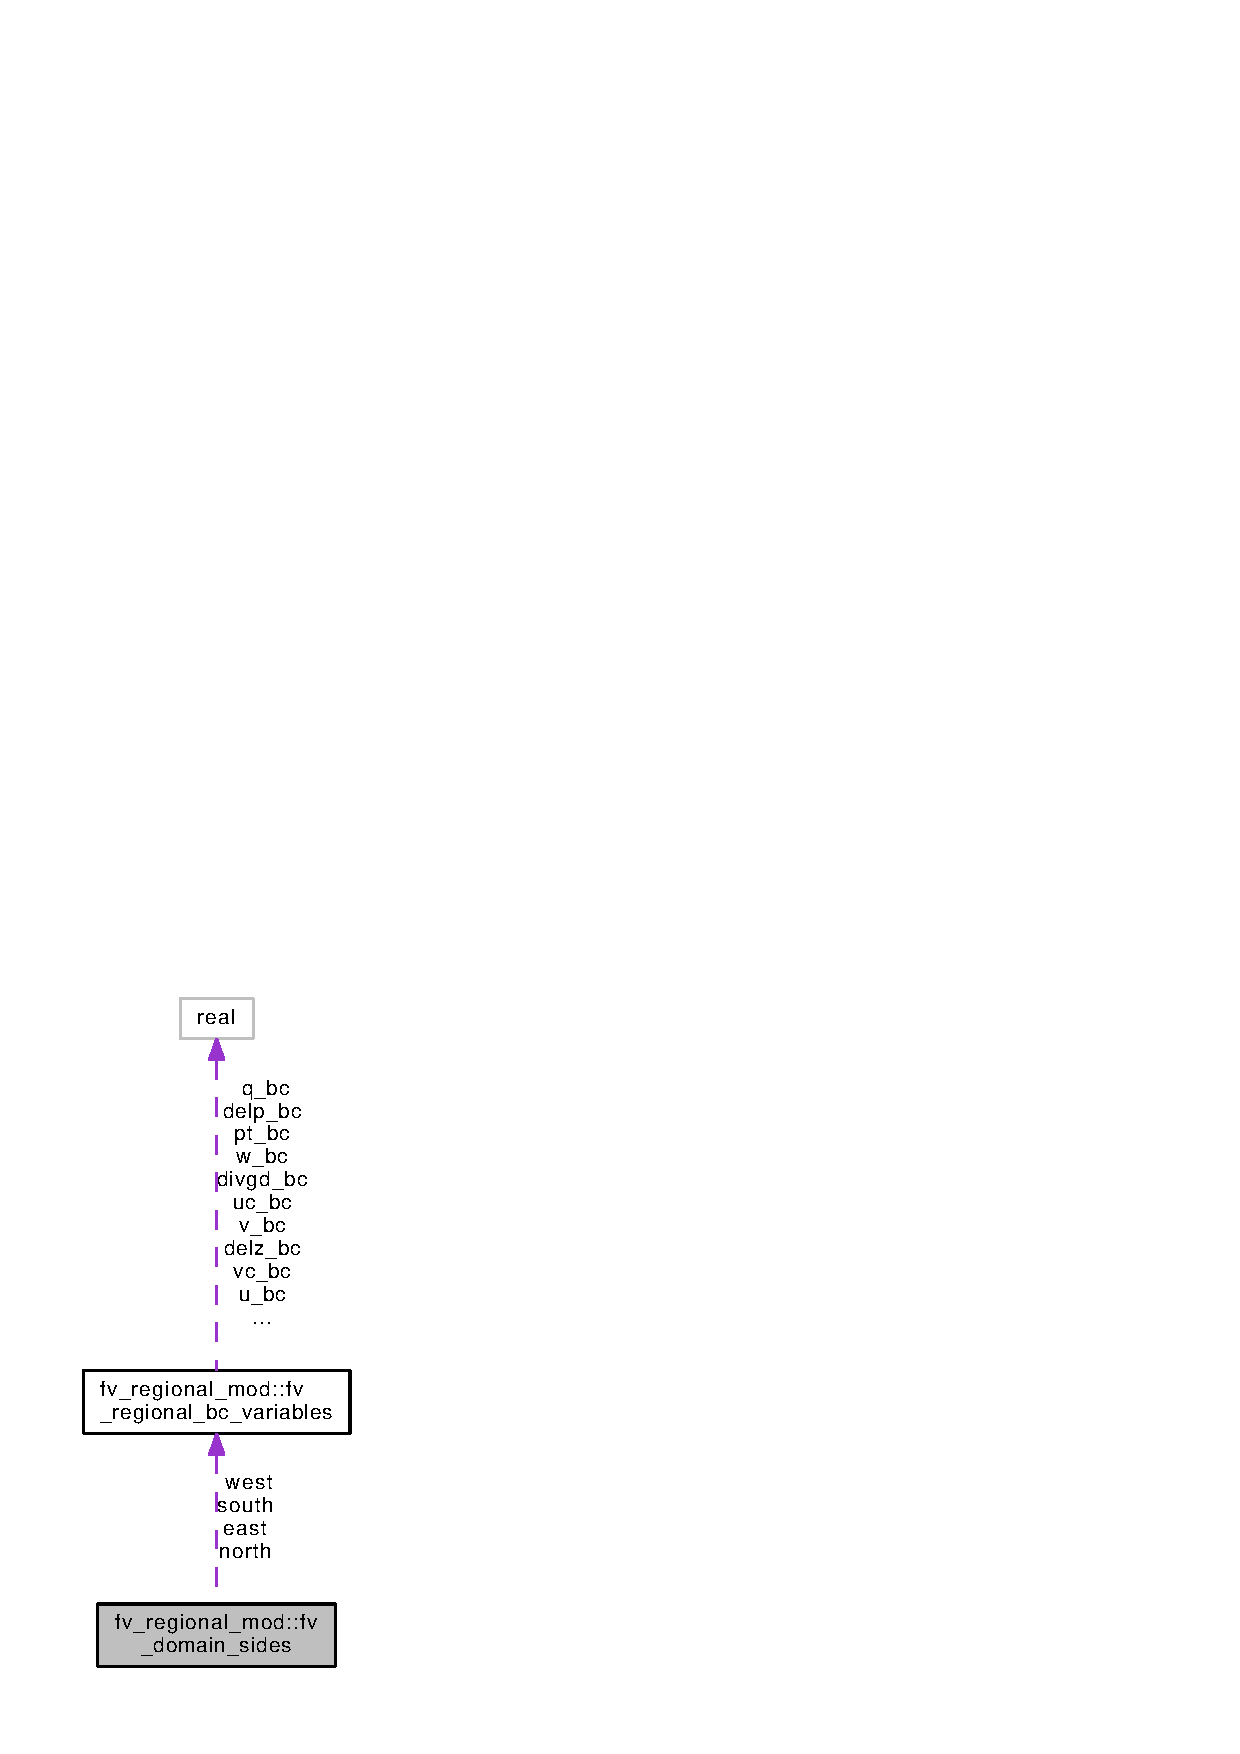
\includegraphics[width=172pt]{structfv__regional__mod_1_1fv__domain__sides__coll__graph}
\end{center}
\end{figure}
\subsection*{Private Attributes}
\begin{DoxyCompactItemize}
\item 
type(\hyperlink{structfv__regional__mod_1_1fv__regional__bc__variables}{fv\-\_\-regional\-\_\-bc\-\_\-variables}) \hyperlink{structfv__regional__mod_1_1fv__domain__sides_a6a402489c7a747378659aa9cb5c71ccc}{north}
\item 
type(\hyperlink{structfv__regional__mod_1_1fv__regional__bc__variables}{fv\-\_\-regional\-\_\-bc\-\_\-variables}) \hyperlink{structfv__regional__mod_1_1fv__domain__sides_ac4624a2514b912d5a1c07ecf9ff7d60b}{south}
\item 
type(\hyperlink{structfv__regional__mod_1_1fv__regional__bc__variables}{fv\-\_\-regional\-\_\-bc\-\_\-variables}) \hyperlink{structfv__regional__mod_1_1fv__domain__sides_ad1855a10ca6e6693ddff2d9140fbdd0a}{east}
\item 
type(\hyperlink{structfv__regional__mod_1_1fv__regional__bc__variables}{fv\-\_\-regional\-\_\-bc\-\_\-variables}) \hyperlink{structfv__regional__mod_1_1fv__domain__sides_af38228133162c39631151b32cd934d36}{west}
\end{DoxyCompactItemize}


\subsection{Detailed Description}


Definition at line 137 of file fv\-\_\-regional\-\_\-bc.\-F90.



\subsection{Member Data Documentation}
\index{fv\-\_\-regional\-\_\-mod\-::fv\-\_\-domain\-\_\-sides@{fv\-\_\-regional\-\_\-mod\-::fv\-\_\-domain\-\_\-sides}!east@{east}}
\index{east@{east}!fv_regional_mod::fv_domain_sides@{fv\-\_\-regional\-\_\-mod\-::fv\-\_\-domain\-\_\-sides}}
\subsubsection[{east}]{\setlength{\rightskip}{0pt plus 5cm}type({\bf fv\-\_\-regional\-\_\-bc\-\_\-variables}) fv\-\_\-regional\-\_\-mod\-::fv\-\_\-domain\-\_\-sides\-::east\hspace{0.3cm}{\ttfamily [private]}}\label{structfv__regional__mod_1_1fv__domain__sides_ad1855a10ca6e6693ddff2d9140fbdd0a}


Definition at line 138 of file fv\-\_\-regional\-\_\-bc.\-F90.

\index{fv\-\_\-regional\-\_\-mod\-::fv\-\_\-domain\-\_\-sides@{fv\-\_\-regional\-\_\-mod\-::fv\-\_\-domain\-\_\-sides}!north@{north}}
\index{north@{north}!fv_regional_mod::fv_domain_sides@{fv\-\_\-regional\-\_\-mod\-::fv\-\_\-domain\-\_\-sides}}
\subsubsection[{north}]{\setlength{\rightskip}{0pt plus 5cm}type({\bf fv\-\_\-regional\-\_\-bc\-\_\-variables}) fv\-\_\-regional\-\_\-mod\-::fv\-\_\-domain\-\_\-sides\-::north\hspace{0.3cm}{\ttfamily [private]}}\label{structfv__regional__mod_1_1fv__domain__sides_a6a402489c7a747378659aa9cb5c71ccc}


Definition at line 138 of file fv\-\_\-regional\-\_\-bc.\-F90.

\index{fv\-\_\-regional\-\_\-mod\-::fv\-\_\-domain\-\_\-sides@{fv\-\_\-regional\-\_\-mod\-::fv\-\_\-domain\-\_\-sides}!south@{south}}
\index{south@{south}!fv_regional_mod::fv_domain_sides@{fv\-\_\-regional\-\_\-mod\-::fv\-\_\-domain\-\_\-sides}}
\subsubsection[{south}]{\setlength{\rightskip}{0pt plus 5cm}type({\bf fv\-\_\-regional\-\_\-bc\-\_\-variables}) fv\-\_\-regional\-\_\-mod\-::fv\-\_\-domain\-\_\-sides\-::south\hspace{0.3cm}{\ttfamily [private]}}\label{structfv__regional__mod_1_1fv__domain__sides_ac4624a2514b912d5a1c07ecf9ff7d60b}


Definition at line 138 of file fv\-\_\-regional\-\_\-bc.\-F90.

\index{fv\-\_\-regional\-\_\-mod\-::fv\-\_\-domain\-\_\-sides@{fv\-\_\-regional\-\_\-mod\-::fv\-\_\-domain\-\_\-sides}!west@{west}}
\index{west@{west}!fv_regional_mod::fv_domain_sides@{fv\-\_\-regional\-\_\-mod\-::fv\-\_\-domain\-\_\-sides}}
\subsubsection[{west}]{\setlength{\rightskip}{0pt plus 5cm}type({\bf fv\-\_\-regional\-\_\-bc\-\_\-variables}) fv\-\_\-regional\-\_\-mod\-::fv\-\_\-domain\-\_\-sides\-::west\hspace{0.3cm}{\ttfamily [private]}}\label{structfv__regional__mod_1_1fv__domain__sides_af38228133162c39631151b32cd934d36}


Definition at line 138 of file fv\-\_\-regional\-\_\-bc.\-F90.



The documentation for this type was generated from the following file\-:\begin{DoxyCompactItemize}
\item 
/scratch2/\-N\-A\-G\-A\-P\-E/aoml-\/hafs1/\-Kyle.\-Ahern/acs\-\_\-master\-\_\-readonly/model/\hyperlink{fv__regional__bc_8F90}{fv\-\_\-regional\-\_\-bc.\-F90}\end{DoxyCompactItemize}

\section{fv\-\_\-dynamics\-\_\-mod Module Reference}
\label{classfv__dynamics__mod}\index{fv\-\_\-dynamics\-\_\-mod@{fv\-\_\-dynamics\-\_\-mod}}


The module 'fv\-\_\-dynamics' is the top-\/level routine for the dynamical core.  




Collaboration diagram for fv\-\_\-dynamics\-\_\-mod\-:
\nopagebreak
\begin{figure}[H]
\begin{center}
\leavevmode
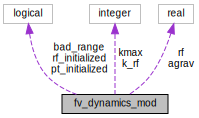
\includegraphics[width=235pt]{classfv__dynamics__mod__coll__graph}
\end{center}
\end{figure}
\subsection*{Public Member Functions}
\begin{DoxyCompactItemize}
\item 
subroutine, public \hyperlink{classfv__dynamics__mod_a57030300ce6aacf81a3588faf906f07f}{fv\-\_\-dynamics} (npx, npy, npz, nq\-\_\-tot, ng, bdt, consv\-\_\-te, fill, reproduce\-\_\-sum, kappa, cp\-\_\-air, zvir, ptop, ks, ncnst, n\-\_\-split, q\-\_\-split, u, v, w, delz, hydrostatic, pt, delp, q, ps, pe, pk, peln, pkz, phis, q\-\_\-con, omga, ua, va, uc, vc, ak, bk, mfx, mfy, cx, cy, ze0, hybrid\-\_\-z, gridstruct, flagstruct, neststruct, idiag, bd, parent\-\_\-grid, domain, diss\-\_\-est, time\-\_\-total)
\end{DoxyCompactItemize}
\subsection*{Public Attributes}
\begin{DoxyCompactItemize}
\item 
logical \hyperlink{classfv__dynamics__mod_a93c42e85cca69658841e13e403c3c89a}{rf\-\_\-initialized} = .false.
\item 
logical \hyperlink{classfv__dynamics__mod_a1c473782ffaa6249be5ba2c3d35a59dc}{pt\-\_\-initialized} = .false.
\item 
logical \hyperlink{classfv__dynamics__mod_a286a6106a75bb334c9531e0354298b11}{bad\-\_\-range} = .false.
\item 
real, dimension(\-:), allocatable \hyperlink{classfv__dynamics__mod_a9e9aac45b5404781dcafeff189daf4de}{rf}
\item 
integer \hyperlink{classfv__dynamics__mod_a223d12ae03cc1c109ba5999ef065bb4a}{kmax} =1
\item 
integer \hyperlink{classfv__dynamics__mod_ac064d1ed1892a3588eb7c6f430954753}{k\-\_\-rf} = 0
\item 
real \hyperlink{classfv__dynamics__mod_a4503b9b3f35f05d3a6dc3535ec7017e9}{agrav}
\end{DoxyCompactItemize}
\subsection*{Private Member Functions}
\begin{DoxyCompactItemize}
\item 
subroutine \hyperlink{classfv__dynamics__mod_abde34c9e5a63d32699e152028179657b}{rayleigh\-\_\-super} (dt, npx, npy, npz, ks, pm, phis, tau, u, v, w, pt, ua, va, delz, agrid, cp, rg, ptop, hydrostatic, conserve, rf\-\_\-cutoff, gridstruct, domain, bd)
\item 
subroutine \hyperlink{classfv__dynamics__mod_a143d1c8cb6f535a5567bd0f4ef1f4a4f}{rayleigh\-\_\-friction} (dt, npx, npy, npz, ks, pm, tau, u, v, w, pt, ua, va, delz, cp, rg, ptop, hydrostatic, conserve, rf\-\_\-cutoff, gridstruct, domain, bd)
\item 
subroutine \hyperlink{classfv__dynamics__mod_a2694a8332d9124e2f4332551ffd92795}{compute\-\_\-aam} (npz, is, ie, js, je, isd, ied, jsd, jed, gridstruct, bd, ptop, ua, va, u, v, delp, aam, ps, m\-\_\-fac)
\begin{DoxyCompactList}\small\item\em The subroutine 'compute\-\_\-aam' computes vertically (mass) integrated Atmospheric Angular Momentum. \end{DoxyCompactList}\end{DoxyCompactItemize}


\subsection{Detailed Description}
The module 'fv\-\_\-dynamics' is the top-\/level routine for the dynamical core. 

It executes on the dt\-\_\-atmos (or p\-\_\-split) loop. 

Definition at line 26 of file fv\-\_\-dynamics.\-F90.



\subsection{Member Function/\-Subroutine Documentation}
\index{fv\-\_\-dynamics\-\_\-mod@{fv\-\_\-dynamics\-\_\-mod}!compute\-\_\-aam@{compute\-\_\-aam}}
\index{compute\-\_\-aam@{compute\-\_\-aam}!fv_dynamics_mod@{fv\-\_\-dynamics\-\_\-mod}}
\subsubsection[{compute\-\_\-aam}]{\setlength{\rightskip}{0pt plus 5cm}subroutine fv\-\_\-dynamics\-\_\-mod\-::compute\-\_\-aam (
\begin{DoxyParamCaption}
\item[{integer, intent(in)}]{npz, }
\item[{integer, intent(in)}]{is, }
\item[{integer, intent(in)}]{ie, }
\item[{integer, intent(in)}]{js, }
\item[{integer, intent(in)}]{je, }
\item[{integer, intent(in)}]{isd, }
\item[{integer, intent(in)}]{ied, }
\item[{integer, intent(in)}]{jsd, }
\item[{integer, intent(in)}]{jed, }
\item[{type(fv\-\_\-grid\-\_\-type), intent(in)}]{gridstruct, }
\item[{type(fv\-\_\-grid\-\_\-bounds\-\_\-type), intent(in)}]{bd, }
\item[{real, intent(in)}]{ptop, }
\item[{real, dimension(isd\-:ied,jsd\-:jed, npz), intent(inout)}]{ua, }
\item[{real, dimension(isd\-:ied,jsd\-:jed, npz), intent(inout)}]{va, }
\item[{real, dimension(isd\-:ied  ,jsd\-:jed+1,npz), intent(inout)}]{u, }
\item[{real, dimension(isd\-:ied+1,jsd\-:jed,npz), intent(inout)}]{v, }
\item[{real, dimension(isd\-:ied,jsd\-:jed,npz), intent(inout)}]{delp, }
\item[{real, dimension(is\-:ie,js\-:je), intent(out)}]{aam, }
\item[{real, dimension(isd\-:ied,jsd\-:jed), intent(out)}]{ps, }
\item[{real, dimension(is\-:ie,js\-:je), intent(out)}]{m\-\_\-fac}
\end{DoxyParamCaption}
)\hspace{0.3cm}{\ttfamily [private]}}\label{classfv__dynamics__mod_a2694a8332d9124e2f4332551ffd92795}


The subroutine 'compute\-\_\-aam' computes vertically (mass) integrated Atmospheric Angular Momentum. 


\begin{DoxyParams}[1]{Parameters}
\mbox{\tt in,out}  & {\em u} & D grid zonal wind (m/s)\\
\hline
\mbox{\tt in,out}  & {\em v} & D grid meridional wind (m/s) \\
\hline
\end{DoxyParams}


Definition at line 1439 of file fv\-\_\-dynamics.\-F90.



References fv\-\_\-grid\-\_\-utils\-\_\-mod\-::c2l\-\_\-ord2().



Referenced by fv\-\_\-dynamics().

\index{fv\-\_\-dynamics\-\_\-mod@{fv\-\_\-dynamics\-\_\-mod}!fv\-\_\-dynamics@{fv\-\_\-dynamics}}
\index{fv\-\_\-dynamics@{fv\-\_\-dynamics}!fv_dynamics_mod@{fv\-\_\-dynamics\-\_\-mod}}
\subsubsection[{fv\-\_\-dynamics}]{\setlength{\rightskip}{0pt plus 5cm}subroutine, public fv\-\_\-dynamics\-\_\-mod\-::fv\-\_\-dynamics (
\begin{DoxyParamCaption}
\item[{integer, intent(in)}]{npx, }
\item[{integer, intent(in)}]{npy, }
\item[{integer, intent(in)}]{npz, }
\item[{integer, intent(in)}]{nq\-\_\-tot, }
\item[{integer, intent(in)}]{ng, }
\item[{real, intent(in)}]{bdt, }
\item[{real, intent(in)}]{consv\-\_\-te, }
\item[{logical, intent(in)}]{fill, }
\item[{logical, intent(in)}]{reproduce\-\_\-sum, }
\item[{real, intent(in)}]{kappa, }
\item[{real, intent(in)}]{cp\-\_\-air, }
\item[{real, intent(in)}]{zvir, }
\item[{real, intent(in)}]{ptop, }
\item[{integer, intent(in)}]{ks, }
\item[{integer, intent(in)}]{ncnst, }
\item[{integer, intent(in)}]{n\-\_\-split, }
\item[{integer, intent(in)}]{q\-\_\-split, }
\item[{real, dimension(bd\%isd\-:bd\%ied  ,bd\%jsd\-:bd\%jed+1,npz), intent(inout)}]{u, }
\item[{real, dimension(bd\%isd\-:bd\%ied+1,bd\%jsd\-:bd\%jed  ,npz), intent(inout)}]{v, }
\item[{real, dimension(   bd\%isd\-:  ,bd\%jsd\-:  ,1\-:), intent(inout)}]{w, }
\item[{real, dimension(bd\%isd\-:,bd\%jsd\-:,1\-:), intent(inout)}]{delz, }
\item[{logical, intent(in)}]{hydrostatic, }
\item[{real, dimension(  bd\%isd\-:bd\%ied  ,bd\%jsd\-:bd\%jed  ,npz), intent(inout)}]{pt, }
\item[{real, dimension(bd\%isd\-:bd\%ied  ,bd\%jsd\-:bd\%jed  ,npz), intent(inout)}]{delp, }
\item[{real, dimension(   bd\%isd\-:bd\%ied  ,bd\%jsd\-:bd\%jed  ,npz, ncnst), intent(inout)}]{q, }
\item[{real, dimension  (bd\%isd\-:bd\%ied  ,bd\%jsd\-:bd\%jed), intent(inout)}]{ps, }
\item[{real, dimension  (bd\%is-\/1\-:bd\%ie+1, npz+1,bd\%js-\/1\-:bd\%je+1), intent(inout)}]{pe, }
\item[{real, dimension  (bd\%is\-:bd\%ie,bd\%js\-:bd\%je, npz+1), intent(inout)}]{pk, }
\item[{real, dimension(bd\%is\-:bd\%ie,npz+1,bd\%js\-:bd\%je), intent(inout)}]{peln, }
\item[{real, dimension (bd\%is\-:bd\%ie,bd\%js\-:bd\%je,npz), intent(inout)}]{pkz, }
\item[{real, dimension(bd\%isd\-:bd\%ied,bd\%jsd\-:bd\%jed), intent(inout)}]{phis, }
\item[{real, dimension(bd\%isd\-:, bd\%jsd\-:, 1\-:), intent(inout)}]{q\-\_\-con, }
\item[{real, dimension(bd\%isd\-:bd\%ied,bd\%jsd\-:bd\%jed,npz), intent(inout)}]{omga, }
\item[{real, dimension(bd\%isd\-:bd\%ied ,bd\%jsd\-:bd\%jed ,npz), intent(inout)}]{ua, }
\item[{real, dimension(bd\%isd\-:bd\%ied ,bd\%jsd\-:bd\%jed ,npz), intent(inout)}]{va, }
\item[{real, dimension(bd\%isd\-:bd\%ied+1,bd\%jsd\-:bd\%jed  ,npz), intent(inout)}]{uc, }
\item[{real, dimension(bd\%isd\-:bd\%ied  ,bd\%jsd\-:bd\%jed+1,npz), intent(inout)}]{vc, }
\item[{real, dimension(npz+1), intent(in)}]{ak, }
\item[{real, dimension(npz+1), intent(in)}]{bk, }
\item[{real, dimension(bd\%is\-:bd\%ie+1, bd\%js\-:bd\%je,   npz), intent(inout)}]{mfx, }
\item[{real, dimension(bd\%is\-:bd\%ie  , bd\%js\-:bd\%je+1, npz), intent(inout)}]{mfy, }
\item[{real, dimension(bd\%is\-:bd\%ie+1, bd\%jsd\-:bd\%jed, npz), intent(inout)}]{cx, }
\item[{real, dimension(bd\%isd\-:bd\%ied ,bd\%js\-:bd\%je+1, npz), intent(inout)}]{cy, }
\item[{real, dimension(bd\%is\-:, bd\%js\-: ,1\-:), intent(inout)}]{ze0, }
\item[{logical, intent(in)}]{hybrid\-\_\-z, }
\item[{type(fv\-\_\-grid\-\_\-type), intent(inout), target}]{gridstruct, }
\item[{type(fv\-\_\-flags\-\_\-type), intent(inout)}]{flagstruct, }
\item[{type(fv\-\_\-nest\-\_\-type), intent(inout)}]{neststruct, }
\item[{type(fv\-\_\-diag\-\_\-type), intent(in)}]{idiag, }
\item[{type(fv\-\_\-grid\-\_\-bounds\-\_\-type), intent(in)}]{bd, }
\item[{type(fv\-\_\-atmos\-\_\-type), intent(in), pointer}]{parent\-\_\-grid, }
\item[{type(domain2d), intent(inout)}]{domain, }
\item[{real, dimension(bd\%isd\-:bd\%ied  ,bd\%jsd\-:bd\%jed,npz), intent(inout)}]{diss\-\_\-est, }
\item[{real, intent(in), optional}]{time\-\_\-total}
\end{DoxyParamCaption}
)}\label{classfv__dynamics__mod_a57030300ce6aacf81a3588faf906f07f}

\begin{DoxyParams}[1]{Parameters}
\mbox{\tt in}  & {\em bdt} & Large time-\/step\\
\hline
\mbox{\tt in}  & {\em nq\-\_\-tot} & transported tracers\\
\hline
\mbox{\tt in}  & {\em n\-\_\-split} & small-\/step horizontal dynamics\\
\hline
\mbox{\tt in}  & {\em q\-\_\-split} & tracer\\
\hline
\mbox{\tt in}  & {\em hybrid\-\_\-z} & Using hybrid\-\_\-z for remapping\\
\hline
\mbox{\tt in,out}  & {\em u} & D grid zonal wind (m/s)\\
\hline
\mbox{\tt in,out}  & {\em v} & D grid meridional wind (m/s)\\
\hline
\mbox{\tt in,out}  & {\em w} & W (m/s)\\
\hline
\mbox{\tt in,out}  & {\em pt} & temperature (K)\\
\hline
\mbox{\tt in,out}  & {\em delp} & pressure thickness (pascal)\\
\hline
\mbox{\tt in,out}  & {\em q} & specific humidity and constituents\\
\hline
\mbox{\tt in,out}  & {\em delz} & delta-\/height (m); non-\/hydrostatic only\\
\hline
\mbox{\tt in,out}  & {\em ze0} & height at edges (m); non-\/hydrostatic\\
\hline
\mbox{\tt in,out}  & {\em ps} & Surface pressure (pascal)\\
\hline
\mbox{\tt in,out}  & {\em pe} & edge pressure (pascal)\\
\hline
\mbox{\tt in,out}  & {\em pk} & pe$\ast$$\ast$kappa\\
\hline
\mbox{\tt in,out}  & {\em peln} & ln(pe)\\
\hline
\mbox{\tt in,out}  & {\em pkz} & finite-\/volume mean pk\\
\hline
\mbox{\tt in,out}  & {\em phis} & Surface geopotential (g$\ast$\-Z\-\_\-surf)\\
\hline
\mbox{\tt in,out}  & {\em omga} & Vertical pressure velocity (pa/s)\\
\hline
\mbox{\tt in,out}  & {\em uc} & (uc,vc) mostly used as the C grid winds \\
\hline
\end{DoxyParams}


Definition at line 174 of file fv\-\_\-dynamics.\-F90.



References compute\-\_\-aam(), fv\-\_\-mapz\-\_\-mod\-::compute\-\_\-total\-\_\-energy(), fv\-\_\-grid\-\_\-utils\-\_\-mod\-::cubed\-\_\-to\-\_\-latlon(), dyn\-\_\-core\-\_\-mod\-::del2\-\_\-cubed(), dyn\-\_\-core\-\_\-mod\-::dyn\-\_\-core(), fv\-\_\-fill\-\_\-mod\-::fill2d(), fv\-\_\-grid\-\_\-utils\-\_\-mod\-::g\-\_\-sum(), dyn\-\_\-core\-\_\-mod\-::init\-\_\-ijk\-\_\-mem(), fv\-\_\-mapz\-\_\-mod\-::lagrangian\-\_\-to\-\_\-eulerian(), fv\-\_\-mapz\-\_\-mod\-::moist\-\_\-cp(), fv\-\_\-mapz\-\_\-mod\-::moist\-\_\-cv(), fv\-\_\-sg\-\_\-mod\-::neg\-\_\-adj2(), fv\-\_\-sg\-\_\-mod\-::neg\-\_\-adj3(), boundary\-\_\-mod\-::nested\-\_\-grid\-\_\-bc\-\_\-apply\-\_\-intt(), fv\-\_\-diagnostics\-\_\-mod\-::prt\-\_\-mxm(), fv\-\_\-diagnostics\-\_\-mod\-::range\-\_\-check(), rayleigh\-\_\-friction(), rayleigh\-\_\-super(), fv\-\_\-regional\-\_\-mod\-::regional\-\_\-boundary\-\_\-update(), fv\-\_\-regional\-\_\-mod\-::set\-\_\-regional\-\_\-bcs(), fv\-\_\-nesting\-\_\-mod\-::setup\-\_\-nested\-\_\-grid\-\_\-bcs(), fv\-\_\-timing\-\_\-mod\-::timing\-\_\-off(), fv\-\_\-timing\-\_\-mod\-::timing\-\_\-on(), fv\-\_\-tracer2d\-\_\-mod\-::tracer\-\_\-2d(), fv\-\_\-tracer2d\-\_\-mod\-::tracer\-\_\-2d\-\_\-1l(), fv\-\_\-tracer2d\-\_\-mod\-::tracer\-\_\-2d\-\_\-nested(), multi\-\_\-gases\-\_\-mod\-::vicpqd(), multi\-\_\-gases\-\_\-mod\-::virq(), and multi\-\_\-gases\-\_\-mod\-::virqd().



Referenced by atmosphere\-\_\-mod\-::adiabatic\-\_\-init(), and atmosphere\-\_\-mod\-::atmosphere\-\_\-dynamics().

\index{fv\-\_\-dynamics\-\_\-mod@{fv\-\_\-dynamics\-\_\-mod}!rayleigh\-\_\-friction@{rayleigh\-\_\-friction}}
\index{rayleigh\-\_\-friction@{rayleigh\-\_\-friction}!fv_dynamics_mod@{fv\-\_\-dynamics\-\_\-mod}}
\subsubsection[{rayleigh\-\_\-friction}]{\setlength{\rightskip}{0pt plus 5cm}subroutine fv\-\_\-dynamics\-\_\-mod\-::rayleigh\-\_\-friction (
\begin{DoxyParamCaption}
\item[{real, intent(in)}]{dt, }
\item[{integer, intent(in)}]{npx, }
\item[{integer, intent(in)}]{npy, }
\item[{integer, intent(in)}]{npz, }
\item[{integer, intent(in)}]{ks, }
\item[{real, dimension(npz), intent(in)}]{pm, }
\item[{real, intent(in)}]{tau, }
\item[{real, dimension(bd\%isd\-:bd\%ied  ,bd\%jsd\-:bd\%jed+1,npz), intent(inout)}]{u, }
\item[{real, dimension(bd\%isd\-:bd\%ied+1,bd\%jsd\-:bd\%jed,npz), intent(inout)}]{v, }
\item[{real, dimension(bd\%isd\-:      ,bd\%jsd\-:      ,1\-: ), intent(inout)}]{w, }
\item[{real, dimension(bd\%isd\-:bd\%ied,bd\%jsd\-:bd\%jed,npz), intent(inout)}]{pt, }
\item[{real, dimension(bd\%isd\-:bd\%ied,bd\%jsd\-:bd\%jed,npz), intent(inout)}]{ua, }
\item[{real, dimension(bd\%isd\-:bd\%ied,bd\%jsd\-:bd\%jed,npz), intent(inout)}]{va, }
\item[{real, dimension(bd\%isd\-:    ,bd\%jsd\-:      ,1\-: ), intent(inout)}]{delz, }
\item[{real, intent(in)}]{cp, }
\item[{real, intent(in)}]{rg, }
\item[{real, intent(in)}]{ptop, }
\item[{logical, intent(in)}]{hydrostatic, }
\item[{logical, intent(in)}]{conserve, }
\item[{real, intent(in)}]{rf\-\_\-cutoff, }
\item[{type(fv\-\_\-grid\-\_\-type), intent(in)}]{gridstruct, }
\item[{type(domain2d), intent(inout)}]{domain, }
\item[{type(fv\-\_\-grid\-\_\-bounds\-\_\-type), intent(in)}]{bd}
\end{DoxyParamCaption}
)\hspace{0.3cm}{\ttfamily [private]}}\label{classfv__dynamics__mod_a143d1c8cb6f535a5567bd0f4ef1f4a4f}

\begin{DoxyParams}[1]{Parameters}
\mbox{\tt in}  & {\em tau} & time scale (days)\\
\hline
\mbox{\tt in,out}  & {\em u} & D grid zonal wind (m/s)\\
\hline
\mbox{\tt in,out}  & {\em v} & D grid meridional wind (m/s)\\
\hline
\mbox{\tt in,out}  & {\em w} & cell center vertical wind (m/s)\\
\hline
\mbox{\tt in,out}  & {\em pt} & temp\\
\hline
\mbox{\tt in,out}  & {\em delz} & delta-\/height (m); non-\/hydrostatic only \\
\hline
\end{DoxyParams}


Definition at line 1300 of file fv\-\_\-dynamics.\-F90.



References fv\-\_\-grid\-\_\-utils\-\_\-mod\-::c2l\-\_\-ord2(), fv\-\_\-timing\-\_\-mod\-::timing\-\_\-off(), and fv\-\_\-timing\-\_\-mod\-::timing\-\_\-on().



Referenced by fv\-\_\-dynamics().

\index{fv\-\_\-dynamics\-\_\-mod@{fv\-\_\-dynamics\-\_\-mod}!rayleigh\-\_\-super@{rayleigh\-\_\-super}}
\index{rayleigh\-\_\-super@{rayleigh\-\_\-super}!fv_dynamics_mod@{fv\-\_\-dynamics\-\_\-mod}}
\subsubsection[{rayleigh\-\_\-super}]{\setlength{\rightskip}{0pt plus 5cm}subroutine fv\-\_\-dynamics\-\_\-mod\-::rayleigh\-\_\-super (
\begin{DoxyParamCaption}
\item[{real, intent(in)}]{dt, }
\item[{integer, intent(in)}]{npx, }
\item[{integer, intent(in)}]{npy, }
\item[{integer, intent(in)}]{npz, }
\item[{integer, intent(in)}]{ks, }
\item[{real, dimension(npz), intent(in)}]{pm, }
\item[{real, dimension(bd\%isd\-:bd\%ied,bd\%jsd\-:bd\%jed), intent(in)}]{phis, }
\item[{real, intent(in)}]{tau, }
\item[{real, dimension(bd\%isd\-:bd\%ied  ,bd\%jsd\-:bd\%jed+1,npz), intent(inout)}]{u, }
\item[{real, dimension(bd\%isd\-:bd\%ied+1,bd\%jsd\-:bd\%jed,npz), intent(inout)}]{v, }
\item[{real, dimension(bd\%isd\-:      ,bd\%jsd\-:      ,1\-: ), intent(inout)}]{w, }
\item[{real, dimension(bd\%isd\-:bd\%ied,bd\%jsd\-:bd\%jed,npz), intent(inout)}]{pt, }
\item[{real, dimension(bd\%isd\-:bd\%ied,bd\%jsd\-:bd\%jed,npz), intent(inout)}]{ua, }
\item[{real, dimension(bd\%isd\-:bd\%ied,bd\%jsd\-:bd\%jed,npz), intent(inout)}]{va, }
\item[{real, dimension(bd\%isd\-:    ,bd\%jsd\-:      ,1\-: ), intent(inout)}]{delz, }
\item[{real, dimension(bd\%isd\-:bd\%ied,  bd\%jsd\-:bd\%jed,2), intent(in)}]{agrid, }
\item[{real, intent(in)}]{cp, }
\item[{real, intent(in)}]{rg, }
\item[{real, intent(in)}]{ptop, }
\item[{logical, intent(in)}]{hydrostatic, }
\item[{logical, intent(in)}]{conserve, }
\item[{real, intent(in)}]{rf\-\_\-cutoff, }
\item[{type(fv\-\_\-grid\-\_\-type), intent(in)}]{gridstruct, }
\item[{type(domain2d), intent(inout)}]{domain, }
\item[{type(fv\-\_\-grid\-\_\-bounds\-\_\-type), intent(in)}]{bd}
\end{DoxyParamCaption}
)\hspace{0.3cm}{\ttfamily [private]}}\label{classfv__dynamics__mod_abde34c9e5a63d32699e152028179657b}

\begin{DoxyParams}[1]{Parameters}
\mbox{\tt in}  & {\em tau} & time scale (days)\\
\hline
\mbox{\tt in,out}  & {\em u} & D grid zonal wind (m/s)\\
\hline
\mbox{\tt in,out}  & {\em v} & D grid meridional wind (m/s)\\
\hline
\mbox{\tt in,out}  & {\em w} & cell center vertical wind (m/s)\\
\hline
\mbox{\tt in,out}  & {\em pt} & temp\\
\hline
\mbox{\tt in,out}  & {\em delz} & delta-\/height (m); non-\/hydrostatic only\\
\hline
\mbox{\tt in}  & {\em phis} & Surface geopotential (g$\ast$\-Z\-\_\-surf) \\
\hline
\end{DoxyParams}


Definition at line 1124 of file fv\-\_\-dynamics.\-F90.



References fv\-\_\-grid\-\_\-utils\-\_\-mod\-::c2l\-\_\-ord2(), fv\-\_\-timing\-\_\-mod\-::timing\-\_\-off(), and fv\-\_\-timing\-\_\-mod\-::timing\-\_\-on().



Referenced by fv\-\_\-dynamics().



\subsection{Member Data Documentation}
\index{fv\-\_\-dynamics\-\_\-mod@{fv\-\_\-dynamics\-\_\-mod}!agrav@{agrav}}
\index{agrav@{agrav}!fv_dynamics_mod@{fv\-\_\-dynamics\-\_\-mod}}
\subsubsection[{agrav}]{\setlength{\rightskip}{0pt plus 5cm}real fv\-\_\-dynamics\-\_\-mod\-::agrav}\label{classfv__dynamics__mod_a4503b9b3f35f05d3a6dc3535ec7017e9}


Definition at line 161 of file fv\-\_\-dynamics.\-F90.

\index{fv\-\_\-dynamics\-\_\-mod@{fv\-\_\-dynamics\-\_\-mod}!bad\-\_\-range@{bad\-\_\-range}}
\index{bad\-\_\-range@{bad\-\_\-range}!fv_dynamics_mod@{fv\-\_\-dynamics\-\_\-mod}}
\subsubsection[{bad\-\_\-range}]{\setlength{\rightskip}{0pt plus 5cm}logical fv\-\_\-dynamics\-\_\-mod\-::bad\-\_\-range = .false.}\label{classfv__dynamics__mod_a286a6106a75bb334c9531e0354298b11}


Definition at line 156 of file fv\-\_\-dynamics.\-F90.

\index{fv\-\_\-dynamics\-\_\-mod@{fv\-\_\-dynamics\-\_\-mod}!k\-\_\-rf@{k\-\_\-rf}}
\index{k\-\_\-rf@{k\-\_\-rf}!fv_dynamics_mod@{fv\-\_\-dynamics\-\_\-mod}}
\subsubsection[{k\-\_\-rf}]{\setlength{\rightskip}{0pt plus 5cm}integer fv\-\_\-dynamics\-\_\-mod\-::k\-\_\-rf = 0}\label{classfv__dynamics__mod_ac064d1ed1892a3588eb7c6f430954753}


Definition at line 159 of file fv\-\_\-dynamics.\-F90.

\index{fv\-\_\-dynamics\-\_\-mod@{fv\-\_\-dynamics\-\_\-mod}!kmax@{kmax}}
\index{kmax@{kmax}!fv_dynamics_mod@{fv\-\_\-dynamics\-\_\-mod}}
\subsubsection[{kmax}]{\setlength{\rightskip}{0pt plus 5cm}integer fv\-\_\-dynamics\-\_\-mod\-::kmax =1}\label{classfv__dynamics__mod_a223d12ae03cc1c109ba5999ef065bb4a}


Definition at line 158 of file fv\-\_\-dynamics.\-F90.

\index{fv\-\_\-dynamics\-\_\-mod@{fv\-\_\-dynamics\-\_\-mod}!pt\-\_\-initialized@{pt\-\_\-initialized}}
\index{pt\-\_\-initialized@{pt\-\_\-initialized}!fv_dynamics_mod@{fv\-\_\-dynamics\-\_\-mod}}
\subsubsection[{pt\-\_\-initialized}]{\setlength{\rightskip}{0pt plus 5cm}logical fv\-\_\-dynamics\-\_\-mod\-::pt\-\_\-initialized = .false.}\label{classfv__dynamics__mod_a1c473782ffaa6249be5ba2c3d35a59dc}


Definition at line 155 of file fv\-\_\-dynamics.\-F90.

\index{fv\-\_\-dynamics\-\_\-mod@{fv\-\_\-dynamics\-\_\-mod}!rf@{rf}}
\index{rf@{rf}!fv_dynamics_mod@{fv\-\_\-dynamics\-\_\-mod}}
\subsubsection[{rf}]{\setlength{\rightskip}{0pt plus 5cm}real, dimension(\-:), allocatable fv\-\_\-dynamics\-\_\-mod\-::rf}\label{classfv__dynamics__mod_a9e9aac45b5404781dcafeff189daf4de}


Definition at line 157 of file fv\-\_\-dynamics.\-F90.

\index{fv\-\_\-dynamics\-\_\-mod@{fv\-\_\-dynamics\-\_\-mod}!rf\-\_\-initialized@{rf\-\_\-initialized}}
\index{rf\-\_\-initialized@{rf\-\_\-initialized}!fv_dynamics_mod@{fv\-\_\-dynamics\-\_\-mod}}
\subsubsection[{rf\-\_\-initialized}]{\setlength{\rightskip}{0pt plus 5cm}logical fv\-\_\-dynamics\-\_\-mod\-::rf\-\_\-initialized = .false.}\label{classfv__dynamics__mod_a93c42e85cca69658841e13e403c3c89a}


Definition at line 154 of file fv\-\_\-dynamics.\-F90.



The documentation for this module was generated from the following file\-:\begin{DoxyCompactItemize}
\item 
/scratch2/\-N\-A\-G\-A\-P\-E/aoml-\/hafs1/\-Kyle.\-Ahern/acs\-\_\-master\-\_\-readonly/model/\hyperlink{fv__dynamics_8F90}{fv\-\_\-dynamics.\-F90}\end{DoxyCompactItemize}

\section{fv\-\_\-eta\-\_\-mod Module Reference}
\label{classfv__eta__mod}\index{fv\-\_\-eta\-\_\-mod@{fv\-\_\-eta\-\_\-mod}}


The module 'fv\-\_\-eta' contains routine to set up the reference (Eulerian) pressure coordinate.  


\subsection*{Public Member Functions}
\begin{DoxyCompactItemize}
\item 
subroutine, public \hyperlink{classfv__eta__mod_a4a75f788fcb7401c0064bdb92d3b4953}{set\-\_\-eta} (km, ks, ptop, ak, bk)
\begin{DoxyCompactList}\small\item\em This is the version of set\-\_\-eta used in fv\-G\-F\-S and A\-M4. \end{DoxyCompactList}\item 
subroutine, public \hyperlink{classfv__eta__mod_a9bcd4fafe443993cdfbddbb177cfc033}{set\-\_\-external\-\_\-eta} (ak, bk, ptop, ks)
\begin{DoxyCompactList}\small\item\em The subroutine 'set\-\_\-external\-\_\-eta' sets 'ptop' (model top) and 'ks' (first level of pure pressure coordinates given the coefficients 'ak' and 'bk'. \end{DoxyCompactList}\item 
subroutine, public \hyperlink{classfv__eta__mod_a4e4105dac9b697433c572db3c7025f16}{hybrid\-\_\-z\-\_\-dz} (km, dz, ztop, s\-\_\-rate)
\item 
subroutine, public \hyperlink{classfv__eta__mod_ac666b63cee9afad18f2cf33dbced10f6}{get\-\_\-eta\-\_\-level} (npz, p\-\_\-s, pf, ph, ak, bk, pscale)
\begin{DoxyCompactList}\small\item\em The subroutine 'get\-\_\-eta\-\_\-level' returns the interface and layer-\/mean pressures for reference. \end{DoxyCompactList}\item 
subroutine, public \hyperlink{classfv__eta__mod_a2e39e6b09b9c0fa35603b30259dbf116}{compute\-\_\-dz} (km, ztop, dz)
\item 
subroutine, public \hyperlink{classfv__eta__mod_a1d0b3f206b0bfbdf5e3cf0d628a541cf}{compute\-\_\-dz\-\_\-var} (km, ztop, dz)
\item 
subroutine, public \hyperlink{classfv__eta__mod_a053b0ba1233d84a26d711e5eb52067d6}{compute\-\_\-dz\-\_\-l32} (km, ztop, dz)
\item 
subroutine, public \hyperlink{classfv__eta__mod_a9a86c1048a7447b78e476bdc8779c66b}{compute\-\_\-dz\-\_\-l101} (km, ztop, dz)
\item 
subroutine, public \hyperlink{classfv__eta__mod_a3cc1b049b1ea1a7946fe7822d487b96e}{set\-\_\-hybrid\-\_\-z} (is, ie, js, je, ng, km, ztop, dz, rgrav, hs, ze, dz3)
\item 
subroutine, public \hyperlink{classfv__eta__mod_a28257151239cbcf2109332794c3c8ca7}{sm1\-\_\-edge} (is, ie, js, je, km, i, j, ze, ntimes)
\item 
subroutine, public \hyperlink{classfv__eta__mod_a700124642759a074f906c37e97759143}{gw\-\_\-1d} (km, p0, ak, bk, ptop, ztop, pt1)
\end{DoxyCompactItemize}
\subsection*{Private Member Functions}
\begin{DoxyCompactItemize}
\item 
subroutine \hyperlink{classfv__eta__mod_a485f88952280ceb9c730bc2ed08c3078}{var\-\_\-les} (km, ak, bk, ptop, ks, pint, s\-\_\-rate)
\item 
subroutine \hyperlink{classfv__eta__mod_a6ec582f058a1d23edd2b7d79edd78ee5}{var\-\_\-gfs} (km, ak, bk, ptop, ks, pint, s\-\_\-rate)
\item 
subroutine \hyperlink{classfv__eta__mod_a8c6950ee0b7fd66c1b35de24dc7d6d17}{var\-\_\-hi} (km, ak, bk, ptop, ks, pint, s\-\_\-rate)
\item 
subroutine \hyperlink{classfv__eta__mod_ad5e4e4a50f8c29c986a4093990d46442}{var\-\_\-hi2} (km, ak, bk, ptop, ks, pint, s\-\_\-rate)
\item 
subroutine \hyperlink{classfv__eta__mod_af1838090c58f286a4c66ce76a7d6b55a}{var\-\_\-dz} (km, ak, bk, ptop, ks, pint, s\-\_\-rate)
\item 
subroutine \hyperlink{classfv__eta__mod_a59a8fe6b8a243e7bd30a030d13f13658}{var55\-\_\-dz} (km, ak, bk, ptop, ks, pint, s\-\_\-rate)
\item 
subroutine \hyperlink{classfv__eta__mod_a794583ebdb4823bcbdde4cca4b019f91}{zflip} (q, im, km)
\end{DoxyCompactItemize}


\subsection{Detailed Description}
The module 'fv\-\_\-eta' contains routine to set up the reference (Eulerian) pressure coordinate. 

Definition at line 25 of file fv\-\_\-eta.\-F90.



\subsection{Member Function/\-Subroutine Documentation}
\index{fv\-\_\-eta\-\_\-mod@{fv\-\_\-eta\-\_\-mod}!compute\-\_\-dz@{compute\-\_\-dz}}
\index{compute\-\_\-dz@{compute\-\_\-dz}!fv_eta_mod@{fv\-\_\-eta\-\_\-mod}}
\subsubsection[{compute\-\_\-dz}]{\setlength{\rightskip}{0pt plus 5cm}subroutine, public fv\-\_\-eta\-\_\-mod\-::compute\-\_\-dz (
\begin{DoxyParamCaption}
\item[{integer, intent(in)}]{km, }
\item[{real, intent(in)}]{ztop, }
\item[{real, dimension(km), intent(out)}]{dz}
\end{DoxyParamCaption}
)}\label{classfv__eta__mod_a2e39e6b09b9c0fa35603b30259dbf116}


Definition at line 2622 of file fv\-\_\-eta.\-F90.

\index{fv\-\_\-eta\-\_\-mod@{fv\-\_\-eta\-\_\-mod}!compute\-\_\-dz\-\_\-l101@{compute\-\_\-dz\-\_\-l101}}
\index{compute\-\_\-dz\-\_\-l101@{compute\-\_\-dz\-\_\-l101}!fv_eta_mod@{fv\-\_\-eta\-\_\-mod}}
\subsubsection[{compute\-\_\-dz\-\_\-l101}]{\setlength{\rightskip}{0pt plus 5cm}subroutine, public fv\-\_\-eta\-\_\-mod\-::compute\-\_\-dz\-\_\-l101 (
\begin{DoxyParamCaption}
\item[{integer, intent(in)}]{km, }
\item[{real, intent(out)}]{ztop, }
\item[{real, dimension(km), intent(out)}]{dz}
\end{DoxyParamCaption}
)}\label{classfv__eta__mod_a9a86c1048a7447b78e476bdc8779c66b}


Definition at line 2797 of file fv\-\_\-eta.\-F90.



Referenced by test\-\_\-cases\-\_\-mod\-::init\-\_\-double\-\_\-periodic().

\index{fv\-\_\-eta\-\_\-mod@{fv\-\_\-eta\-\_\-mod}!compute\-\_\-dz\-\_\-l32@{compute\-\_\-dz\-\_\-l32}}
\index{compute\-\_\-dz\-\_\-l32@{compute\-\_\-dz\-\_\-l32}!fv_eta_mod@{fv\-\_\-eta\-\_\-mod}}
\subsubsection[{compute\-\_\-dz\-\_\-l32}]{\setlength{\rightskip}{0pt plus 5cm}subroutine, public fv\-\_\-eta\-\_\-mod\-::compute\-\_\-dz\-\_\-l32 (
\begin{DoxyParamCaption}
\item[{integer, intent(in)}]{km, }
\item[{real, intent(out)}]{ztop, }
\item[{real, dimension(km), intent(out)}]{dz}
\end{DoxyParamCaption}
)}\label{classfv__eta__mod_a053b0ba1233d84a26d711e5eb52067d6}


Definition at line 2728 of file fv\-\_\-eta.\-F90.



References zflip().



Referenced by fv\-\_\-restart\-\_\-mod\-::fv\-\_\-restart(), and test\-\_\-cases\-\_\-mod\-::init\-\_\-case().

\index{fv\-\_\-eta\-\_\-mod@{fv\-\_\-eta\-\_\-mod}!compute\-\_\-dz\-\_\-var@{compute\-\_\-dz\-\_\-var}}
\index{compute\-\_\-dz\-\_\-var@{compute\-\_\-dz\-\_\-var}!fv_eta_mod@{fv\-\_\-eta\-\_\-mod}}
\subsubsection[{compute\-\_\-dz\-\_\-var}]{\setlength{\rightskip}{0pt plus 5cm}subroutine, public fv\-\_\-eta\-\_\-mod\-::compute\-\_\-dz\-\_\-var (
\begin{DoxyParamCaption}
\item[{integer, intent(in)}]{km, }
\item[{real, intent(in)}]{ztop, }
\item[{real, dimension(km), intent(out)}]{dz}
\end{DoxyParamCaption}
)}\label{classfv__eta__mod_a1d0b3f206b0bfbdf5e3cf0d628a541cf}


Definition at line 2658 of file fv\-\_\-eta.\-F90.



References sm1\-\_\-edge().



Referenced by fv\-\_\-restart\-\_\-mod\-::fv\-\_\-restart().

\index{fv\-\_\-eta\-\_\-mod@{fv\-\_\-eta\-\_\-mod}!get\-\_\-eta\-\_\-level@{get\-\_\-eta\-\_\-level}}
\index{get\-\_\-eta\-\_\-level@{get\-\_\-eta\-\_\-level}!fv_eta_mod@{fv\-\_\-eta\-\_\-mod}}
\subsubsection[{get\-\_\-eta\-\_\-level}]{\setlength{\rightskip}{0pt plus 5cm}subroutine, public fv\-\_\-eta\-\_\-mod\-::get\-\_\-eta\-\_\-level (
\begin{DoxyParamCaption}
\item[{integer, intent(in)}]{npz, }
\item[{real, intent(in)}]{p\-\_\-s, }
\item[{real, dimension(npz), intent(out)}]{pf, }
\item[{real, dimension(npz+1), intent(out)}]{ph, }
\item[{real, dimension(npz+1), intent(in)}]{ak, }
\item[{real, dimension(npz+1), intent(in)}]{bk, }
\item[{real, intent(in), optional}]{pscale}
\end{DoxyParamCaption}
)}\label{classfv__eta__mod_ac666b63cee9afad18f2cf33dbced10f6}


The subroutine 'get\-\_\-eta\-\_\-level' returns the interface and layer-\/mean pressures for reference. 


\begin{DoxyParams}[1]{Parameters}
\mbox{\tt in}  & {\em p\-\_\-s} & unit\-: pascal \\
\hline
\end{DoxyParams}


Definition at line 2587 of file fv\-\_\-eta.\-F90.



Referenced by atmosphere\-\_\-mod\-::atmosphere\-\_\-init(), fv\-\_\-diagnostics\-\_\-mod\-::fv\-\_\-diag\-\_\-init(), fv\-\_\-update\-\_\-phys\-\_\-mod\-::fv\-\_\-update\-\_\-phys(), and fv\-\_\-regional\-\_\-mod\-::setup\-\_\-regional\-\_\-bc().

\index{fv\-\_\-eta\-\_\-mod@{fv\-\_\-eta\-\_\-mod}!gw\-\_\-1d@{gw\-\_\-1d}}
\index{gw\-\_\-1d@{gw\-\_\-1d}!fv_eta_mod@{fv\-\_\-eta\-\_\-mod}}
\subsubsection[{gw\-\_\-1d}]{\setlength{\rightskip}{0pt plus 5cm}subroutine, public fv\-\_\-eta\-\_\-mod\-::gw\-\_\-1d (
\begin{DoxyParamCaption}
\item[{integer, intent(in)}]{km, }
\item[{real, intent(in)}]{p0, }
\item[{real, dimension(km+1), intent(inout)}]{ak, }
\item[{real, dimension(km+1), intent(inout)}]{bk, }
\item[{real, intent(inout)}]{ptop, }
\item[{real, intent(in)}]{ztop, }
\item[{real, dimension(km), intent(out)}]{pt1}
\end{DoxyParamCaption}
)}\label{classfv__eta__mod_a700124642759a074f906c37e97759143}


Definition at line 3014 of file fv\-\_\-eta.\-F90.



Referenced by fv\-\_\-diagnostics\-\_\-mod\-::fv\-\_\-diag(), fv\-\_\-diagnostics\-\_\-mod\-::fv\-\_\-diag\-\_\-init(), test\-\_\-cases\-\_\-mod\-::init\-\_\-case(), and set\-\_\-eta().

\index{fv\-\_\-eta\-\_\-mod@{fv\-\_\-eta\-\_\-mod}!hybrid\-\_\-z\-\_\-dz@{hybrid\-\_\-z\-\_\-dz}}
\index{hybrid\-\_\-z\-\_\-dz@{hybrid\-\_\-z\-\_\-dz}!fv_eta_mod@{fv\-\_\-eta\-\_\-mod}}
\subsubsection[{hybrid\-\_\-z\-\_\-dz}]{\setlength{\rightskip}{0pt plus 5cm}subroutine, public fv\-\_\-eta\-\_\-mod\-::hybrid\-\_\-z\-\_\-dz (
\begin{DoxyParamCaption}
\item[{integer, intent(in)}]{km, }
\item[{real, dimension(km), intent(out)}]{dz, }
\item[{real, intent(in)}]{ztop, }
\item[{real, intent(in)}]{s\-\_\-rate}
\end{DoxyParamCaption}
)}\label{classfv__eta__mod_a4e4105dac9b697433c572db3c7025f16}

\begin{DoxyParams}[1]{Parameters}
\mbox{\tt in}  & {\em s\-\_\-rate} & between \mbox{[}1. 1.\-1\mbox{]} \\
\hline
\end{DoxyParams}


Definition at line 2522 of file fv\-\_\-eta.\-F90.



References sm1\-\_\-edge().



Referenced by test\-\_\-cases\-\_\-mod\-::init\-\_\-case().

\index{fv\-\_\-eta\-\_\-mod@{fv\-\_\-eta\-\_\-mod}!set\-\_\-eta@{set\-\_\-eta}}
\index{set\-\_\-eta@{set\-\_\-eta}!fv_eta_mod@{fv\-\_\-eta\-\_\-mod}}
\subsubsection[{set\-\_\-eta}]{\setlength{\rightskip}{0pt plus 5cm}subroutine, public fv\-\_\-eta\-\_\-mod\-::set\-\_\-eta (
\begin{DoxyParamCaption}
\item[{integer, intent(in)}]{km, }
\item[{integer, intent(out)}]{ks, }
\item[{real, intent(out)}]{ptop, }
\item[{real, dimension(km+1), intent(out)}]{ak, }
\item[{real, dimension(km+1), intent(out)}]{bk}
\end{DoxyParamCaption}
)}\label{classfv__eta__mod_a4a75f788fcb7401c0064bdb92d3b4953}


This is the version of set\-\_\-eta used in fv\-G\-F\-S and A\-M4. 

\begin{DoxyNote}{Note}
01/2018\-: 'set\-\_\-eta' is being cleaned up.
\end{DoxyNote}

\begin{DoxyParams}[1]{Parameters}
\mbox{\tt in}  & {\em km} & vertical dimension\\
\hline
\mbox{\tt out}  & {\em ks} & number of pure p layers\\
\hline
\mbox{\tt out}  & {\em ptop} & model top (Pa) \\
\hline
\end{DoxyParams}


Definition at line 419 of file fv\-\_\-eta.\-F90.



References gw\-\_\-1d(), var\-\_\-dz(), var\-\_\-gfs(), and var\-\_\-hi().



Referenced by external\-\_\-ic\-\_\-mod\-::get\-\_\-ecmwf\-\_\-ic(), external\-\_\-ic\-\_\-mod\-::get\-\_\-nggps\-\_\-ic(), and fv\-\_\-grid\-\_\-utils\-\_\-mod\-::grid\-\_\-utils\-\_\-init().

\index{fv\-\_\-eta\-\_\-mod@{fv\-\_\-eta\-\_\-mod}!set\-\_\-external\-\_\-eta@{set\-\_\-external\-\_\-eta}}
\index{set\-\_\-external\-\_\-eta@{set\-\_\-external\-\_\-eta}!fv_eta_mod@{fv\-\_\-eta\-\_\-mod}}
\subsubsection[{set\-\_\-external\-\_\-eta}]{\setlength{\rightskip}{0pt plus 5cm}subroutine, public fv\-\_\-eta\-\_\-mod\-::set\-\_\-external\-\_\-eta (
\begin{DoxyParamCaption}
\item[{real, dimension(\-:), intent(in)}]{ak, }
\item[{real, dimension(\-:), intent(in)}]{bk, }
\item[{real, intent(out)}]{ptop, }
\item[{integer, intent(out)}]{ks}
\end{DoxyParamCaption}
)}\label{classfv__eta__mod_a9bcd4fafe443993cdfbddbb177cfc033}


The subroutine 'set\-\_\-external\-\_\-eta' sets 'ptop' (model top) and 'ks' (first level of pure pressure coordinates given the coefficients 'ak' and 'bk'. 


\begin{DoxyParams}[1]{Parameters}
\mbox{\tt out}  & {\em ptop} & model top (Pa)\\
\hline
\mbox{\tt out}  & {\em ks} & number of pure p layers \\
\hline
\end{DoxyParams}


Definition at line 1516 of file fv\-\_\-eta.\-F90.



Referenced by fv\-\_\-io\-\_\-mod\-::fv\-\_\-io\-\_\-read\-\_\-restart(), and external\-\_\-ic\-\_\-mod\-::get\-\_\-nggps\-\_\-ic().

\index{fv\-\_\-eta\-\_\-mod@{fv\-\_\-eta\-\_\-mod}!set\-\_\-hybrid\-\_\-z@{set\-\_\-hybrid\-\_\-z}}
\index{set\-\_\-hybrid\-\_\-z@{set\-\_\-hybrid\-\_\-z}!fv_eta_mod@{fv\-\_\-eta\-\_\-mod}}
\subsubsection[{set\-\_\-hybrid\-\_\-z}]{\setlength{\rightskip}{0pt plus 5cm}subroutine, public fv\-\_\-eta\-\_\-mod\-::set\-\_\-hybrid\-\_\-z (
\begin{DoxyParamCaption}
\item[{integer, intent(in)}]{is, }
\item[{integer, intent(in)}]{ie, }
\item[{integer, intent(in)}]{js, }
\item[{integer, intent(in)}]{je, }
\item[{integer, intent(in)}]{ng, }
\item[{integer, intent(in)}]{km, }
\item[{real, intent(in)}]{ztop, }
\item[{real, dimension(km), intent(in)}]{dz, }
\item[{real, intent(in)}]{rgrav, }
\item[{real, dimension(is-\/ng\-:ie+ng,js-\/ng\-:je+ng), intent(in)}]{hs, }
\item[{real, dimension(is\-:ie,js\-:je,km+1), intent(inout)}]{ze, }
\item[{real, dimension(is-\/ng\-:ie+ng,js-\/ng\-:je+ng,km), intent(out), optional}]{dz3}
\end{DoxyParamCaption}
)}\label{classfv__eta__mod_a3cc1b049b1ea1a7946fe7822d487b96e}

\begin{DoxyParams}[1]{Parameters}
\mbox{\tt in}  & {\em dz} & Reference vertical resolution for zs=0 \\
\hline
\end{DoxyParams}


Definition at line 2839 of file fv\-\_\-eta.\-F90.



References dyn\-\_\-core\-\_\-mod\-::del2\-\_\-cubed(), and sm1\-\_\-edge().



Referenced by fv\-\_\-restart\-\_\-mod\-::fv\-\_\-restart(), test\-\_\-cases\-\_\-mod\-::init\-\_\-case(), and test\-\_\-cases\-\_\-mod\-::init\-\_\-double\-\_\-periodic().

\index{fv\-\_\-eta\-\_\-mod@{fv\-\_\-eta\-\_\-mod}!sm1\-\_\-edge@{sm1\-\_\-edge}}
\index{sm1\-\_\-edge@{sm1\-\_\-edge}!fv_eta_mod@{fv\-\_\-eta\-\_\-mod}}
\subsubsection[{sm1\-\_\-edge}]{\setlength{\rightskip}{0pt plus 5cm}subroutine, public fv\-\_\-eta\-\_\-mod\-::sm1\-\_\-edge (
\begin{DoxyParamCaption}
\item[{integer, intent(in)}]{is, }
\item[{integer, intent(in)}]{ie, }
\item[{integer, intent(in)}]{js, }
\item[{integer, intent(in)}]{je, }
\item[{integer, intent(in)}]{km, }
\item[{integer, intent(in)}]{i, }
\item[{integer, intent(in)}]{j, }
\item[{real, dimension(is\-:ie,js\-:je,km+1), intent(inout)}]{ze, }
\item[{integer, intent(in)}]{ntimes}
\end{DoxyParamCaption}
)}\label{classfv__eta__mod_a28257151239cbcf2109332794c3c8ca7}


Definition at line 2977 of file fv\-\_\-eta.\-F90.



Referenced by compute\-\_\-dz\-\_\-var(), hybrid\-\_\-z\-\_\-dz(), set\-\_\-hybrid\-\_\-z(), var55\-\_\-dz(), var\-\_\-dz(), test\-\_\-cases\-\_\-mod\-::var\-\_\-dz(), var\-\_\-hi(), var\-\_\-hi2(), and var\-\_\-les().

\index{fv\-\_\-eta\-\_\-mod@{fv\-\_\-eta\-\_\-mod}!var55\-\_\-dz@{var55\-\_\-dz}}
\index{var55\-\_\-dz@{var55\-\_\-dz}!fv_eta_mod@{fv\-\_\-eta\-\_\-mod}}
\subsubsection[{var55\-\_\-dz}]{\setlength{\rightskip}{0pt plus 5cm}subroutine fv\-\_\-eta\-\_\-mod\-::var55\-\_\-dz (
\begin{DoxyParamCaption}
\item[{integer, intent(in)}]{km, }
\item[{real, dimension(km+1), intent(out)}]{ak, }
\item[{real, dimension(km+1), intent(out)}]{bk, }
\item[{real, intent(in)}]{ptop, }
\item[{integer, intent(out)}]{ks, }
\item[{real, intent(inout)}]{pint, }
\item[{real, intent(in)}]{s\-\_\-rate}
\end{DoxyParamCaption}
)\hspace{0.3cm}{\ttfamily [private]}}\label{classfv__eta__mod_a59a8fe6b8a243e7bd30a030d13f13658}

\begin{DoxyParams}[1]{Parameters}
\mbox{\tt in}  & {\em s\-\_\-rate} & between \mbox{[}1. 1.\-1\mbox{]} \\
\hline
\end{DoxyParams}


Definition at line 2360 of file fv\-\_\-eta.\-F90.



References sm1\-\_\-edge().

\index{fv\-\_\-eta\-\_\-mod@{fv\-\_\-eta\-\_\-mod}!var\-\_\-dz@{var\-\_\-dz}}
\index{var\-\_\-dz@{var\-\_\-dz}!fv_eta_mod@{fv\-\_\-eta\-\_\-mod}}
\subsubsection[{var\-\_\-dz}]{\setlength{\rightskip}{0pt plus 5cm}subroutine fv\-\_\-eta\-\_\-mod\-::var\-\_\-dz (
\begin{DoxyParamCaption}
\item[{integer, intent(in)}]{km, }
\item[{real, dimension(km+1), intent(out)}]{ak, }
\item[{real, dimension(km+1), intent(out)}]{bk, }
\item[{real, intent(in)}]{ptop, }
\item[{integer, intent(out)}]{ks, }
\item[{real, intent(inout)}]{pint, }
\item[{real, intent(in)}]{s\-\_\-rate}
\end{DoxyParamCaption}
)\hspace{0.3cm}{\ttfamily [private]}}\label{classfv__eta__mod_af1838090c58f286a4c66ce76a7d6b55a}

\begin{DoxyParams}[1]{Parameters}
\mbox{\tt in}  & {\em s\-\_\-rate} & between \mbox{[}1. 1.\-1\mbox{]} \\
\hline
\end{DoxyParams}


Definition at line 2199 of file fv\-\_\-eta.\-F90.



References sm1\-\_\-edge().



Referenced by test\-\_\-cases\-\_\-mod\-::init\-\_\-case(), and set\-\_\-eta().

\index{fv\-\_\-eta\-\_\-mod@{fv\-\_\-eta\-\_\-mod}!var\-\_\-gfs@{var\-\_\-gfs}}
\index{var\-\_\-gfs@{var\-\_\-gfs}!fv_eta_mod@{fv\-\_\-eta\-\_\-mod}}
\subsubsection[{var\-\_\-gfs}]{\setlength{\rightskip}{0pt plus 5cm}subroutine fv\-\_\-eta\-\_\-mod\-::var\-\_\-gfs (
\begin{DoxyParamCaption}
\item[{integer, intent(in)}]{km, }
\item[{real, dimension(km+1), intent(out)}]{ak, }
\item[{real, dimension(km+1), intent(out)}]{bk, }
\item[{real, intent(in)}]{ptop, }
\item[{integer, intent(out)}]{ks, }
\item[{real, intent(inout)}]{pint, }
\item[{real, intent(in)}]{s\-\_\-rate}
\end{DoxyParamCaption}
)\hspace{0.3cm}{\ttfamily [private]}}\label{classfv__eta__mod_a6ec582f058a1d23edd2b7d79edd78ee5}

\begin{DoxyParams}[1]{Parameters}
\mbox{\tt in}  & {\em s\-\_\-rate} & between \mbox{[}1. 1.\-1\mbox{]} \\
\hline
\end{DoxyParams}


Definition at line 1700 of file fv\-\_\-eta.\-F90.



Referenced by set\-\_\-eta().

\index{fv\-\_\-eta\-\_\-mod@{fv\-\_\-eta\-\_\-mod}!var\-\_\-hi@{var\-\_\-hi}}
\index{var\-\_\-hi@{var\-\_\-hi}!fv_eta_mod@{fv\-\_\-eta\-\_\-mod}}
\subsubsection[{var\-\_\-hi}]{\setlength{\rightskip}{0pt plus 5cm}subroutine fv\-\_\-eta\-\_\-mod\-::var\-\_\-hi (
\begin{DoxyParamCaption}
\item[{integer, intent(in)}]{km, }
\item[{real, dimension(km+1), intent(out)}]{ak, }
\item[{real, dimension(km+1), intent(out)}]{bk, }
\item[{real, intent(in)}]{ptop, }
\item[{integer, intent(out)}]{ks, }
\item[{real, intent(inout)}]{pint, }
\item[{real, intent(in)}]{s\-\_\-rate}
\end{DoxyParamCaption}
)\hspace{0.3cm}{\ttfamily [private]}}\label{classfv__eta__mod_a8c6950ee0b7fd66c1b35de24dc7d6d17}

\begin{DoxyParams}[1]{Parameters}
\mbox{\tt in}  & {\em s\-\_\-rate} & between \mbox{[}1. 1.\-1\mbox{]} \\
\hline
\end{DoxyParams}


Definition at line 1864 of file fv\-\_\-eta.\-F90.



References sm1\-\_\-edge().



Referenced by set\-\_\-eta().

\index{fv\-\_\-eta\-\_\-mod@{fv\-\_\-eta\-\_\-mod}!var\-\_\-hi2@{var\-\_\-hi2}}
\index{var\-\_\-hi2@{var\-\_\-hi2}!fv_eta_mod@{fv\-\_\-eta\-\_\-mod}}
\subsubsection[{var\-\_\-hi2}]{\setlength{\rightskip}{0pt plus 5cm}subroutine fv\-\_\-eta\-\_\-mod\-::var\-\_\-hi2 (
\begin{DoxyParamCaption}
\item[{integer, intent(in)}]{km, }
\item[{real, dimension(km+1), intent(out)}]{ak, }
\item[{real, dimension(km+1), intent(out)}]{bk, }
\item[{real, intent(in)}]{ptop, }
\item[{integer, intent(out)}]{ks, }
\item[{real, intent(inout)}]{pint, }
\item[{real, intent(in)}]{s\-\_\-rate}
\end{DoxyParamCaption}
)\hspace{0.3cm}{\ttfamily [private]}}\label{classfv__eta__mod_ad5e4e4a50f8c29c986a4093990d46442}

\begin{DoxyParams}[1]{Parameters}
\mbox{\tt in}  & {\em s\-\_\-rate} & between \mbox{[}1. 1.\-1\mbox{]} \\
\hline
\end{DoxyParams}


Definition at line 2040 of file fv\-\_\-eta.\-F90.



References sm1\-\_\-edge().

\index{fv\-\_\-eta\-\_\-mod@{fv\-\_\-eta\-\_\-mod}!var\-\_\-les@{var\-\_\-les}}
\index{var\-\_\-les@{var\-\_\-les}!fv_eta_mod@{fv\-\_\-eta\-\_\-mod}}
\subsubsection[{var\-\_\-les}]{\setlength{\rightskip}{0pt plus 5cm}subroutine fv\-\_\-eta\-\_\-mod\-::var\-\_\-les (
\begin{DoxyParamCaption}
\item[{integer, intent(in)}]{km, }
\item[{real, dimension(km+1), intent(out)}]{ak, }
\item[{real, dimension(km+1), intent(out)}]{bk, }
\item[{real, intent(in)}]{ptop, }
\item[{integer, intent(out)}]{ks, }
\item[{real, intent(inout)}]{pint, }
\item[{real, intent(in)}]{s\-\_\-rate}
\end{DoxyParamCaption}
)\hspace{0.3cm}{\ttfamily [private]}}\label{classfv__eta__mod_a485f88952280ceb9c730bc2ed08c3078}

\begin{DoxyParams}[1]{Parameters}
\mbox{\tt in}  & {\em s\-\_\-rate} & between \mbox{[}1. 1.\-1\mbox{]} \\
\hline
\end{DoxyParams}


Definition at line 1538 of file fv\-\_\-eta.\-F90.



References sm1\-\_\-edge().

\index{fv\-\_\-eta\-\_\-mod@{fv\-\_\-eta\-\_\-mod}!zflip@{zflip}}
\index{zflip@{zflip}!fv_eta_mod@{fv\-\_\-eta\-\_\-mod}}
\subsubsection[{zflip}]{\setlength{\rightskip}{0pt plus 5cm}subroutine fv\-\_\-eta\-\_\-mod\-::zflip (
\begin{DoxyParamCaption}
\item[{real, dimension(im,km), intent(inout)}]{q, }
\item[{integer, intent(in)}]{im, }
\item[{integer, intent(in)}]{km}
\end{DoxyParamCaption}
)\hspace{0.3cm}{\ttfamily [private]}}\label{classfv__eta__mod_a794583ebdb4823bcbdde4cca4b019f91}


Definition at line 3076 of file fv\-\_\-eta.\-F90.



Referenced by compute\-\_\-dz\-\_\-l32().



The documentation for this module was generated from the following file\-:\begin{DoxyCompactItemize}
\item 
/scratch2/\-N\-A\-G\-A\-P\-E/aoml-\/hafs1/\-Kyle.\-Ahern/acs\-\_\-master\-\_\-readonly/tools/\hyperlink{fv__eta_8F90}{fv\-\_\-eta.\-F90}\end{DoxyCompactItemize}

\section{fv\-\_\-fill\-\_\-mod Module Reference}
\label{classfv__fill__mod}\index{fv\-\_\-fill\-\_\-mod@{fv\-\_\-fill\-\_\-mod}}
\subsection*{Public Member Functions}
\begin{DoxyCompactItemize}
\item 
subroutine, public \hyperlink{classfv__fill__mod_a41d77a13ceec78e4ea68f5e5266c9458}{fillz} (im, km, nq, q, dp)
\begin{DoxyCompactList}\small\item\em The subroutine 'fillz' is for mass-\/conservative filling of nonphysical negative values in the tracers. \end{DoxyCompactList}\item 
subroutine, public \hyperlink{classfv__fill__mod_a527172ca182ebcb99a72bdbd536165d2}{fill\-\_\-gfs} (im, km, pe2, q, q\-\_\-min)
\begin{DoxyCompactList}\small\item\em The subroutine 'fill\-\_\-gfs' is for mass-\/conservative filling of nonphysical negative values in the tracers. \end{DoxyCompactList}\item 
subroutine, public \hyperlink{classfv__fill__mod_ac0fe86d6b2444a934aaca81bc8ace0c9}{fill2d} (is, ie, js, je, ng, km, q, delp, area, domain, nested, regional, npx, npy)
\begin{DoxyCompactList}\small\item\em The subroutine 'fill2\-D' fills in nonphysical negative values in a single scalar field using a two-\/dimensional diffusive approach which conserves mass. \end{DoxyCompactList}\end{DoxyCompactItemize}


\subsection{Detailed Description}


Definition at line 21 of file fv\-\_\-fill.\-F90.



\subsection{Member Function/\-Subroutine Documentation}
\index{fv\-\_\-fill\-\_\-mod@{fv\-\_\-fill\-\_\-mod}!fill2d@{fill2d}}
\index{fill2d@{fill2d}!fv_fill_mod@{fv\-\_\-fill\-\_\-mod}}
\subsubsection[{fill2d}]{\setlength{\rightskip}{0pt plus 5cm}subroutine, public fv\-\_\-fill\-\_\-mod\-::fill2d (
\begin{DoxyParamCaption}
\item[{integer, intent(in)}]{is, }
\item[{integer, intent(in)}]{ie, }
\item[{integer, intent(in)}]{js, }
\item[{integer, intent(in)}]{je, }
\item[{integer, intent(in)}]{ng, }
\item[{integer, intent(in)}]{km, }
\item[{real, dimension(is-\/ng\-:ie+ng, js-\/ng\-:je+ng, km), intent(inout)}]{q, }
\item[{real, dimension(is-\/ng\-:ie+ng, js-\/ng\-:je+ng, km), intent(in)}]{delp, }
\item[{real, dimension(is-\/ng\-:ie+ng, js-\/ng\-:je+ng), intent(in)}]{area, }
\item[{type(domain2d), intent(inout)}]{domain, }
\item[{logical, intent(in)}]{nested, }
\item[{logical, intent(in)}]{regional, }
\item[{integer, intent(in)}]{npx, }
\item[{integer, intent(in)}]{npy}
\end{DoxyParamCaption}
)}\label{classfv__fill__mod_ac0fe86d6b2444a934aaca81bc8ace0c9}


The subroutine 'fill2\-D' fills in nonphysical negative values in a single scalar field using a two-\/dimensional diffusive approach which conserves mass. 



Definition at line 206 of file fv\-\_\-fill.\-F90.



Referenced by fv\-\_\-dynamics\-\_\-mod\-::fv\-\_\-dynamics().

\index{fv\-\_\-fill\-\_\-mod@{fv\-\_\-fill\-\_\-mod}!fill\-\_\-gfs@{fill\-\_\-gfs}}
\index{fill\-\_\-gfs@{fill\-\_\-gfs}!fv_fill_mod@{fv\-\_\-fill\-\_\-mod}}
\subsubsection[{fill\-\_\-gfs}]{\setlength{\rightskip}{0pt plus 5cm}subroutine, public fv\-\_\-fill\-\_\-mod\-::fill\-\_\-gfs (
\begin{DoxyParamCaption}
\item[{integer, intent(in)}]{im, }
\item[{integer, intent(in)}]{km, }
\item[{real(kind=kind\-\_\-phys), dimension(im,km+1), intent(in)}]{pe2, }
\item[{real(kind=kind\-\_\-phys), dimension(im,km), intent(inout)}]{q, }
\item[{real(kind=kind\-\_\-phys), intent(in)}]{q\-\_\-min}
\end{DoxyParamCaption}
)}\label{classfv__fill__mod_a527172ca182ebcb99a72bdbd536165d2}


The subroutine 'fill\-\_\-gfs' is for mass-\/conservative filling of nonphysical negative values in the tracers. 

This routine is the same as 'fillz', but only fills one scalar field using specified q\-\_\-min instead of 0 with the k-\/index flipped as in the G\-F\-S physics. It accepts edge pressure instead of delp.


\begin{DoxyParams}[1]{Parameters}
\mbox{\tt in}  & {\em pe2} & pressure interface \\
\hline
\end{DoxyParams}


Definition at line 162 of file fv\-\_\-fill.\-F90.



Referenced by atmosphere\-\_\-mod\-::atmosphere\-\_\-state\-\_\-update().

\index{fv\-\_\-fill\-\_\-mod@{fv\-\_\-fill\-\_\-mod}!fillz@{fillz}}
\index{fillz@{fillz}!fv_fill_mod@{fv\-\_\-fill\-\_\-mod}}
\subsubsection[{fillz}]{\setlength{\rightskip}{0pt plus 5cm}subroutine, public fv\-\_\-fill\-\_\-mod\-::fillz (
\begin{DoxyParamCaption}
\item[{integer, intent(in)}]{im, }
\item[{integer, intent(in)}]{km, }
\item[{integer, intent(in)}]{nq, }
\item[{real, dimension(im,km,nq), intent(inout)}]{q, }
\item[{real, dimension(im,km), intent(in)}]{dp}
\end{DoxyParamCaption}
)}\label{classfv__fill__mod_a41d77a13ceec78e4ea68f5e5266c9458}


The subroutine 'fillz' is for mass-\/conservative filling of nonphysical negative values in the tracers. 

This routine takes mass from adjacent cells in the same column to fill negatives, if possible.


\begin{DoxyParams}[1]{Parameters}
\mbox{\tt in}  & {\em im} & No. of longitudes\\
\hline
\mbox{\tt in}  & {\em km} & No. of levels\\
\hline
\mbox{\tt in}  & {\em nq} & Total number of tracers\\
\hline
\mbox{\tt in}  & {\em dp} & pressure thickness\\
\hline
\mbox{\tt in,out}  & {\em q} & tracer mixing ratio \\
\hline
\end{DoxyParams}


Definition at line 51 of file fv\-\_\-fill.\-F90.



Referenced by fv\-\_\-mapz\-\_\-mod\-::lagrangian\-\_\-to\-\_\-eulerian(), fv\-\_\-mapz\-\_\-mod\-::mapn\-\_\-tracer(), external\-\_\-ic\-\_\-mod\-::remap\-\_\-scalar\-\_\-ec(), external\-\_\-ic\-\_\-mod\-::remap\-\_\-scalar\-\_\-nggps(), fv\-\_\-regional\-\_\-mod\-::remap\-\_\-scalar\-\_\-nggps\-\_\-regional\-\_\-bc(), and external\-\_\-ic\-\_\-mod\-::remap\-\_\-scalar\-\_\-single().



The documentation for this module was generated from the following file\-:\begin{DoxyCompactItemize}
\item 
/scratch2/\-N\-A\-G\-A\-P\-E/aoml-\/hafs1/\-Kyle.\-Ahern/acs\-\_\-master\-\_\-readonly/model/\hyperlink{fv__fill_8F90}{fv\-\_\-fill.\-F90}\end{DoxyCompactItemize}

\section{fv\-\_\-arrays\-\_\-mod\-:\-:fv\-\_\-flags\-\_\-type Type Reference}
\label{structfv__arrays__mod_1_1fv__flags__type}\index{fv\-\_\-arrays\-\_\-mod\-::fv\-\_\-flags\-\_\-type@{fv\-\_\-arrays\-\_\-mod\-::fv\-\_\-flags\-\_\-type}}


Collaboration diagram for fv\-\_\-arrays\-\_\-mod\-:\-:fv\-\_\-flags\-\_\-type\-:
\nopagebreak
\begin{figure}[H]
\begin{center}
\leavevmode
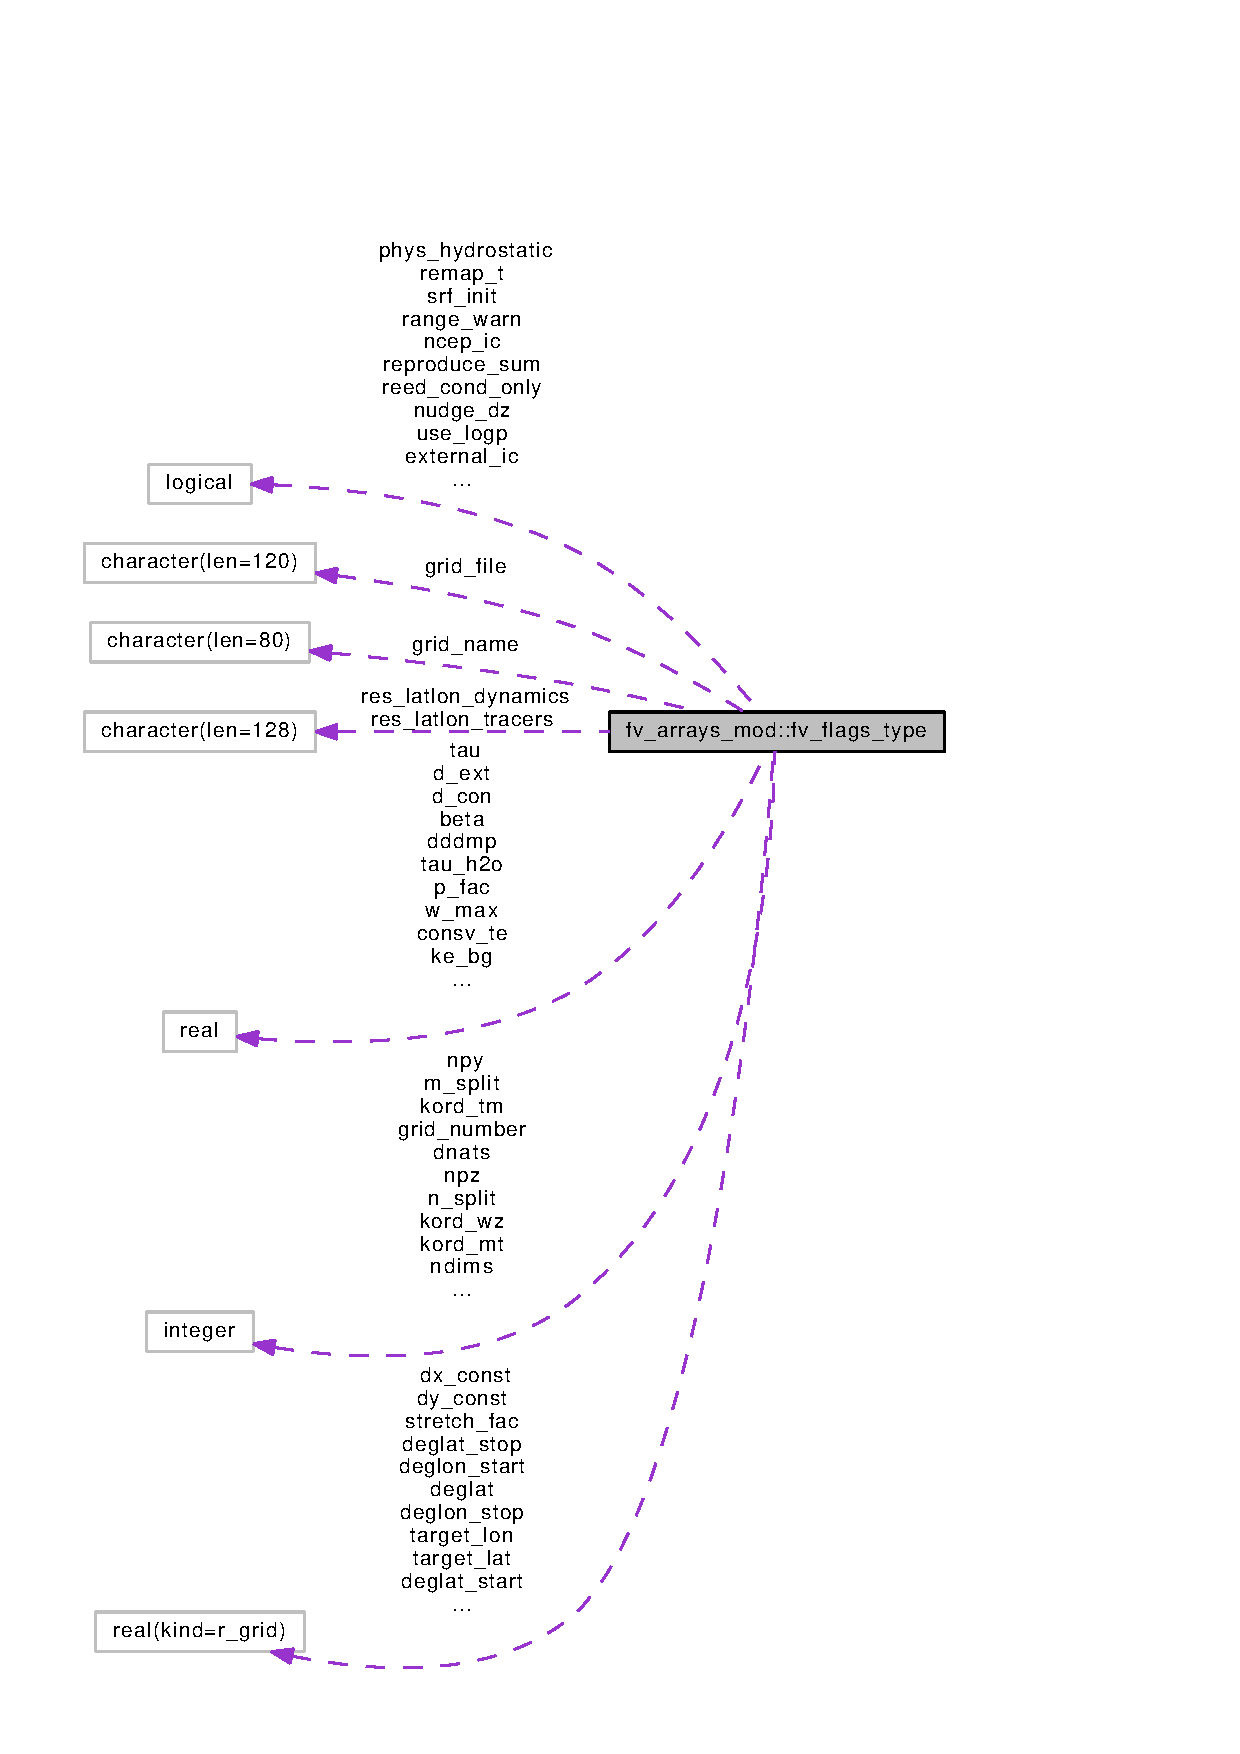
\includegraphics[height=550pt]{structfv__arrays__mod_1_1fv__flags__type__coll__graph}
\end{center}
\end{figure}
\subsection*{Public Attributes}
\begin{DoxyCompactItemize}
\item 
character(len=80) \hyperlink{structfv__arrays__mod_1_1fv__flags__type_a3db69164bedf77520133bab7a563ad64}{grid\-\_\-name} = 'Gnomonic'
\item 
character(len=120) \hyperlink{structfv__arrays__mod_1_1fv__flags__type_a5ae6853512fe75e5f08388470d4f0da6}{grid\-\_\-file} = 'Inline'
\item 
integer \hyperlink{structfv__arrays__mod_1_1fv__flags__type_aee15326da7e817a68d9591e7dca01325}{grid\-\_\-type} = 0
\begin{DoxyCompactList}\small\item\em -\/1\-: read from file; 0\-: E\-D Gnomonic 0\-: the \char`\"{}true\char`\"{} equal-\/distance Gnomonic grid 1\-: the traditional equal-\/distance Gnomonic grid 2\-: the equal-\/angular Gnomonic grid 3\-: the lat-\/lon grid -- to be implemented 4\-: double periodic boundary condition on Cartesian grid 5\-: channel flow on Cartesian grid \end{DoxyCompactList}\item 
integer \hyperlink{structfv__arrays__mod_1_1fv__flags__type_ab166cc8b6c93e0c863180aeb50b5aea9}{hord\-\_\-mt} = 9
\begin{DoxyCompactList}\small\item\em Horizontal advection scheme for momentum fluxes. A complete list of kord options is given in the corresponding table in Appendix A of the F\-V3 technical document. The default value is 9, which uses the third-\/order piecewise-\/parabolic method with the monotonicity constraint of Huynh, which is less diffusive than other constraints. For hydrostatic simulation, 8 (the L04 monotonicity constraint) is recommended; for nonhydrostatic simulation, the completely unlimited (“linear” or non-\/monotone) P\-P\-M scheme is recommended. If no monotonicity constraint is applied, enabling the flux damping (do\-\_\-vort\-\_\-damp = .true.) is highly recommended to control grid-\/scale noise. It is also recommended that hord\-\_\-mt, hord\-\_\-vt, hord\-\_\-tm, and hord\-\_\-dp use the same value, to ensure consistent transport of all dynamical fields, unless a positivity constraint on mass advection (hord\-\_\-dp) is desired. \end{DoxyCompactList}\item 
integer \hyperlink{structfv__arrays__mod_1_1fv__flags__type_aac512996328887adf30b7db1c7235de2}{kord\-\_\-mt} = 8
\begin{DoxyCompactList}\small\item\em Vertical remapping scheme for the winds. 8 by default; 9 is recommended as the safest option, although 10, and 11 can also be useful. See corresponding table in Appendix A of the F\-V3 technical document for a complete list of kord options. \end{DoxyCompactList}\item 
integer \hyperlink{structfv__arrays__mod_1_1fv__flags__type_a956b1eda2db234dc8646d547c3197c81}{kord\-\_\-wz} = 8
\begin{DoxyCompactList}\small\item\em Vertical remapping scheme for vertical velocity in nonhydrostatic simulations. 8 by default; 9 recommended. It is also recommended to use the same value for 'kord\-\_\-wz' as for 'kord\-\_\-mt'. \end{DoxyCompactList}\item 
integer \hyperlink{structfv__arrays__mod_1_1fv__flags__type_adfb527dd9d1387bc79c721bc9810c410}{hord\-\_\-vt} = 9
\begin{DoxyCompactList}\small\item\em Vorticity \& w transport options\-: \end{DoxyCompactList}\item 
integer \hyperlink{structfv__arrays__mod_1_1fv__flags__type_aec43383385030681d8c19c8e906adc1e}{hord\-\_\-tm} = 9
\begin{DoxyCompactList}\small\item\em Horizontal advection scheme for potential temperature and layer thickness in nonhydrostatic simulations. 9 by default. \end{DoxyCompactList}\item 
integer \hyperlink{structfv__arrays__mod_1_1fv__flags__type_a65a2e3ed85e51cb3b2245e3f36bf8391}{hord\-\_\-dp} = 9
\begin{DoxyCompactList}\small\item\em Horizontal advection scheme for mass. A positivity constraint may be warranted for hord\-\_\-dp but not strictly necessary. 9 by default. \end{DoxyCompactList}\item 
integer \hyperlink{structfv__arrays__mod_1_1fv__flags__type_a97fa1725f727c163a6a90457a32c717c}{kord\-\_\-tm} = -\/8
\begin{DoxyCompactList}\small\item\em Vertical remapping scheme for temperature. If positive (not recommended), then vertical remapping is performed on total energy instead of temperature (see 'remap\-\_\-t'). The default value is -\/8. \end{DoxyCompactList}\item 
integer \hyperlink{structfv__arrays__mod_1_1fv__flags__type_a6b189bf4be82ed34b367f1a7a6fa1106}{hord\-\_\-tr} = 12
\begin{DoxyCompactList}\small\item\em Tracer transport options\-: \end{DoxyCompactList}\item 
integer \hyperlink{structfv__arrays__mod_1_1fv__flags__type_afbfcb1b09e9aa21acdbcdaeccd8caf20}{kord\-\_\-tr} = 8
\begin{DoxyCompactList}\small\item\em The vertical remapping scheme for tracers. The default is 8. 9 or 11 recommended. It is often recommended to use the same value for 'kord\-\_\-tr' as for 'kord\-\_\-tm'. \end{DoxyCompactList}\item 
real \hyperlink{structfv__arrays__mod_1_1fv__flags__type_a3181a20aaac99c0817af03924d71b0fd}{scale\-\_\-z} = 0.
\begin{DoxyCompactList}\small\item\em diff\-\_\-z = scale\-\_\-z$\ast$$\ast$2 $\ast$ 0.\-25 \end{DoxyCompactList}\item 
real \hyperlink{structfv__arrays__mod_1_1fv__flags__type_a7966e3f1383bae981b26a75ce43ec46b}{w\-\_\-max} = 75.
\begin{DoxyCompactList}\small\item\em max w (m/s) threshold for hydostatiic adjustment \end{DoxyCompactList}\item 
real \hyperlink{structfv__arrays__mod_1_1fv__flags__type_acec362d2a6ae93bf42bbe7d2995ae7bd}{z\-\_\-min} = 0.\-05
\begin{DoxyCompactList}\small\item\em min ratio of dz\-\_\-nonhydrostatic/dz\-\_\-hydrostatic \end{DoxyCompactList}\item 
real \hyperlink{structfv__arrays__mod_1_1fv__flags__type_aae1e7bd5b47feab9a53a8de279ae17e6}{lim\-\_\-fac} = 1.\-0
\begin{DoxyCompactList}\small\item\em linear scheme limiting factor, 1\-: hord = 5, 3\-: hord = 6 \end{DoxyCompactList}\item 
integer \hyperlink{structfv__arrays__mod_1_1fv__flags__type_a2a8b948ce9b26a36723b037fb1db2cba}{nord} = 1
\begin{DoxyCompactList}\small\item\em Order of divergence damping\-: 0 for second-\/order; 1 for fourth-\/order (default); 2 for sixth-\/order; 3 for eighth-\/order. Sixth-\/order may yield a better solution for low resolutions (one degree or coarser) by virtue of it being more scale-\/selective and will not damp moderately well-\/resolved disturbances as much as does lower-\/order damping. \end{DoxyCompactList}\item 
integer \hyperlink{structfv__arrays__mod_1_1fv__flags__type_a78c41b066c189e7e6fa24eebc9b525f2}{nord\-\_\-tr} = 0
\begin{DoxyCompactList}\small\item\em Order of tracer damping; values mean the same as for 'nord'. The default value is 0. \end{DoxyCompactList}\item 
real \hyperlink{structfv__arrays__mod_1_1fv__flags__type_abb173832e0f7594d6ac8eca3d1f9ce0a}{dddmp} = 0.\-0
\begin{DoxyCompactList}\small\item\em Dimensionless coefficient for the second-\/order Smagorinsky-\/type divergence damping. The default is value is 0.\-0. 0.\-2 (the Smagorinsky constant) is recommended if I\-Cs are noisy. \end{DoxyCompactList}\item 
real \hyperlink{structfv__arrays__mod_1_1fv__flags__type_a75c65cca32e02f409074fd22c3e13752}{d2\-\_\-bg} = 0.\-0
\begin{DoxyCompactList}\small\item\em Coefficient for background second-\/order divergence damping. This option remains active even if nord is nonzero. The default value is 0.\-0. The proper range is 0 to 0.\-02. \end{DoxyCompactList}\item 
real \hyperlink{structfv__arrays__mod_1_1fv__flags__type_a400c02695fa4bfa1d2e4aaf21059638a}{d4\-\_\-bg} = 0.\-16
\begin{DoxyCompactList}\small\item\em Dimensionless coefficient for background higher-\/order divergence damping. 0.\-0 by default. If no second-\/order divergence damping is used, then values between 0.\-1 and 0.\-16 are recommended. Requires 'nord' $>$ 0. Note that the scaling for 'd4\-\_\-bg' differs from that of 'd2\-\_\-bg'; 'nord' $>$= 1 and 'd4\-\_\-bg' = 0.\-16 will be less diffusive than 'nord' = 0 and 'd2\-\_\-bg' = 0.\-02. \end{DoxyCompactList}\item 
real \hyperlink{structfv__arrays__mod_1_1fv__flags__type_ae230295af17d57507255dfe20ad98f6a}{vtdm4} = 0.\-0
\begin{DoxyCompactList}\small\item\em Coefficient for background other-\/variable damping. The value of 'vtdm4' should be less than that of 'd4\-\_\-bg'. A good first guess for 'vtdm4' is about one-\/third the value of d4\-\_\-bg. Requires 'do\-\_\-vort\-\_\-damp' to be .true. Disabled for values less than 1.\-e-\/3. Other-\/ variable damping should not be used if a monotonic horizontal advection scheme is used. The default value is 0.\-0. \end{DoxyCompactList}\item 
real \hyperlink{structfv__arrays__mod_1_1fv__flags__type_a4a2e560c5d7f89ce6f1c6bdc14b26c43}{trdm2} = 0.\-0
\begin{DoxyCompactList}\small\item\em Coefficient for del-\/2 tracer damping. \end{DoxyCompactList}\item 
real \hyperlink{structfv__arrays__mod_1_1fv__flags__type_a737de90ac392b70940b9279692e09107}{d2\-\_\-bg\-\_\-k1} = 4.
\begin{DoxyCompactList}\small\item\em Strength of second-\/order diffusion in the top sponge layer. Value must be specified. This value, and d2\-\_\-bg\-\_\-k2, will be changed appropriately in the model (depending on the height of model top), so the actual damping may be very reduced. See atmos\-\_\-cubed\-\_\-sphere/model/dyncore.\-F90 for details. Recommended range is 0. to 0.\-2. Note that since diffusion is converted to heat if d\-\_\-con $>$ 0 larger amounts of sponge-\/layer diffusion may be less stable. \end{DoxyCompactList}\item 
real \hyperlink{structfv__arrays__mod_1_1fv__flags__type_a2c3e75d400dd64212d1b1b7a22dfa0ce}{d2\-\_\-bg\-\_\-k2} = 2.
\begin{DoxyCompactList}\small\item\em Strength of second-\/order diffusion in the second sponge layer from the model top. This value must be specified, and should be less than 'd2\-\_\-bg\-\_\-k1'. \end{DoxyCompactList}\item 
real \hyperlink{structfv__arrays__mod_1_1fv__flags__type_a22e01e2b95246dc8477bab2b3b162399}{d2\-\_\-divg\-\_\-max\-\_\-k1} = 0.\-15
\begin{DoxyCompactList}\small\item\em d2\-\_\-divg max value (k=1) \end{DoxyCompactList}\item 
real \hyperlink{structfv__arrays__mod_1_1fv__flags__type_a69f302ae25d38e4087c57150f2e2aa30}{d2\-\_\-divg\-\_\-max\-\_\-k2} = 0.\-08
\begin{DoxyCompactList}\small\item\em d2\-\_\-divg max value (k=2) \end{DoxyCompactList}\item 
real \hyperlink{structfv__arrays__mod_1_1fv__flags__type_a7a9b69cda3a1074c4d5bc3f9d1d7ed30}{damp\-\_\-k\-\_\-k1} = 0.\-2
\begin{DoxyCompactList}\small\item\em damp\-\_\-k value (k=1) \end{DoxyCompactList}\item 
real \hyperlink{structfv__arrays__mod_1_1fv__flags__type_ad632b60850fd35d3d6a63123d8535802}{damp\-\_\-k\-\_\-k2} = 0.\-12
\begin{DoxyCompactList}\small\item\em damp\-\_\-k value (k=2) \end{DoxyCompactList}\item 
integer \hyperlink{structfv__arrays__mod_1_1fv__flags__type_a068897c1792b9952e1fd5ee9f96d4400}{n\-\_\-zs\-\_\-filter} = 0
\begin{DoxyCompactList}\small\item\em Additional (after the fact) terrain filter (to further smooth the terrain after cold start) \end{DoxyCompactList}\item 
integer \hyperlink{structfv__arrays__mod_1_1fv__flags__type_a98601ce30b19c5c1c911dc216d3fc22a}{nord\-\_\-zs\-\_\-filter} = 4
\begin{DoxyCompactList}\small\item\em Order of the topography filter applied to n\-\_\-zs\-\_\-filter. Set to 2 to get a second-\/order filter, or 4 to get a fourth-\/order filter; other values do no filtering. 0 by default. This should not be set to a non-\/zero value on multiple successive simulations; the filter is applied every time the model restarts. This option is useful for testing the terrain filter, and S\-H\-O\-U\-L\-D N\-O\-T B\-E U\-S\-E\-D F\-O\-R R\-E\-G\-U\-L\-A\-R R\-U\-N\-S. use del-\/2 (2) O\-R del-\/4 (4) \end{DoxyCompactList}\item 
logical \hyperlink{structfv__arrays__mod_1_1fv__flags__type_afbe4a46c5b9ecf80644125620d3bf57d}{full\-\_\-zs\-\_\-filter} = .false.
\begin{DoxyCompactList}\small\item\em Whether to apply the on-\/line topography filter during initialization. Only active if get\-\_\-nggps\-\_\-ic = .true. This is so topography filtering can be performed on the initial conditions output by the pre-\/processing tools, which currently do not support topography filter-\/ ing for some configurations (such as the nested grid); this also allows the user to easily test changes to the topography filtering on the simulation. Note that for all other initialization methods (if external\-\_\-ic = .true.) the on-\/line topography filter will be applied automatically during the initialization of the topography. The default value is .false. \end{DoxyCompactList}\item 
logical \hyperlink{structfv__arrays__mod_1_1fv__flags__type_a1c474ace44c4f507b091496eabf667bd}{rf\-\_\-fast} = .false.
\begin{DoxyCompactList}\small\item\em Option controlling whether to apply Rayleigh damping (for tau $>$ 0) on the dynamic/acoustic timestep rather than on the physics timestep. This can help stabilize the model by applying the damping more weakly more frequently, so the instantaneous amount of damping (and thereby heat added) is reduced. The default is .false., which applies the Rayleigh drag every physics timestep. \end{DoxyCompactList}\item 
logical \hyperlink{structfv__arrays__mod_1_1fv__flags__type_abcebc94566be36845e4285c6a024751d}{consv\-\_\-am} = .false.
\begin{DoxyCompactList}\small\item\em Whether to enable Angular momentum fixer. The default is .false. \end{DoxyCompactList}\item 
logical \hyperlink{structfv__arrays__mod_1_1fv__flags__type_a600463f131f3b1df30dcf333938c7a39}{do\-\_\-sat\-\_\-adj} = .false.
\item 
logical \hyperlink{structfv__arrays__mod_1_1fv__flags__type_a9cfcad9b998983b7a1e1d89ea1c76022}{do\-\_\-f3d} = .false.
\item 
logical \hyperlink{structfv__arrays__mod_1_1fv__flags__type_a0a66c1a0702f0b0f039d879e1bf70dec}{no\-\_\-dycore} = .false.
\begin{DoxyCompactList}\small\item\em Disables execution of the dynamical core, only running the initialization, diagnostic, and I/\-O routines, and any physics that may be enabled. Essentially turns the model into a column physics model. The default is .false. \end{DoxyCompactList}\item 
logical \hyperlink{structfv__arrays__mod_1_1fv__flags__type_a5facb1d2f072eb7a3c2d20b3b03bb068}{convert\-\_\-ke} = .false.
\begin{DoxyCompactList}\small\item\em If .true., adds energy dissipated through mechanical damping to heat throughout the entire depth of the domain; if .false. (default) this is only done in the sponge layer at the top of the domain. This option is only enabled if d\-\_\-con $>$ 1.\-e-\/5. \end{DoxyCompactList}\item 
logical \hyperlink{structfv__arrays__mod_1_1fv__flags__type_a06034f559635e41927ab1fc2de52c821}{do\-\_\-vort\-\_\-damp} = .false.
\begin{DoxyCompactList}\small\item\em Whether to apply flux damping (of strength governed by 'vtdm4') to the fluxes of vorticity, air mass, and nonhydrostatic vertical velocity (there is no dynamically correct way to add explicit diffusion to the tracer fluxes). The form is the same as is used for the divergence damping, including the same order (from 'nord') damping, unless 'nord' = 0, in which case this damping is fourth-\/order, or if 'nord' = 3,in which case this damping is sixth-\/order (instead of eighth-\/order). We recommend enabling this damping when the linear or non-\/monotonic horizontal advection schemes are enabled, but is unnecessary and not recommended when using monotonic advection. The default is .false. \end{DoxyCompactList}\item 
logical \hyperlink{structfv__arrays__mod_1_1fv__flags__type_a464a6eb5ffb4492e2ea207efc9c041ed}{use\-\_\-old\-\_\-omega} = .true.
\item 
real \hyperlink{structfv__arrays__mod_1_1fv__flags__type_a63b5db0b645857933a373aa3cf2a5926}{beta} = 0.\-0
\begin{DoxyCompactList}\small\item\em Parameter specifying fraction of time-\/off-\/centering for backwards evaluation of the pressure gradient force. The default is 0.\-0, which produces a fully backwards evaluation of the pressure gradient force that is entirely evaluated using the updated (time n+1) dynamical fields. A value of 0.\-5 will equally weight the P\-G\-F determined at times n and n+1, but may not be stable; values larger than 0.\-45 are not recommended. A value of 0.\-4 is recommended for most hydrostatic simulations, which allows an improved representation of inertia-\/gravity waves in the tropics. In non-\/hydrostatic simulations using the semi-\/implicit solver (a\-\_\-imp $>$ 0.\-5) the values of 'a\-\_\-imp' and 'beta' should add to 1, so that the time-\/centering is consistent between the P\-G\-F and the nonhydrostatic solver. The proper range is 0 to 0.\-45. \end{DoxyCompactList}\item 
integer \hyperlink{structfv__arrays__mod_1_1fv__flags__type_a3aa416f1e3aa62eed9afe2a1eaabf673}{n\-\_\-sponge} = 1
\begin{DoxyCompactList}\small\item\em Controls the number of layers at the upper boundary on which the 2\-Dx filter is applied. This does not control the sponge layer. The default value is 0. \end{DoxyCompactList}\item 
real \hyperlink{structfv__arrays__mod_1_1fv__flags__type_a95caa816eb573eaf9bd1a8b388e87e30}{d\-\_\-ext} = 0.\-02
\begin{DoxyCompactList}\small\item\em Coefficient for external (barotropic) mode damping. Proper range is 0 to 0.\-02. A value of 0.\-01 or 0.\-02 may help improve the models maximum stable time step in low-\/resolution (2-\/degree or lower) simulations; otherwise a value of 0 is recommended. The default value is 0.\-02. \end{DoxyCompactList}\item 
integer \hyperlink{structfv__arrays__mod_1_1fv__flags__type_a42c93d1b25fbe7725462deeaa69f89a6}{nwat} = 3
\begin{DoxyCompactList}\small\item\em Number of water species to be included in condensate and water vapor loading. The masses of the first nwat tracer species will be added to the dry air mass, so that p is the mass of dry air, water vapor, and the included condensate species. The value used depends on the microphysics in the physics package you are using. For G\-F\-S physics with only a single condensate species, set to 2. For schemes with prognostic cloud water and cloud ice, such as G\-F\-D\-L A\-M2/\-A\-M3/\-A\-M4 Rotsteyn-\/\-Klein or Morrison-\/\-Gettlean microphysics, set to 3. For warm-\/rain (Kessler) microphysics set to 4 (with an inactive ice tracer), which only handles three species but uses 4 to avoid interference with the R-\/\-K physics. For schemes such as W\-S\-M5 or Ferrier that have prognostic rain and snow but not hail, set to 5 (not yet implemented). For six-\/category schemes that also have prognostic hail or graupel, such as the G\-F\-D\-L, Thompson, or W\-S\-M6 microphysics, set to 6. A value of 0 turns off condensate loading. The default value is 3. \end{DoxyCompactList}\item 
logical \hyperlink{structfv__arrays__mod_1_1fv__flags__type_a213ea7debdf2b2feb97c44dd606818a5}{warm\-\_\-start} = .true.
\begin{DoxyCompactList}\small\item\em Whether to start from restart files, instead of cold-\/starting the model. True by default; if this is set to .true. and restart files cannot be found the model will stop. \end{DoxyCompactList}\item 
logical \hyperlink{structfv__arrays__mod_1_1fv__flags__type_a7630553d7bb9549c7092f49184a409cd}{inline\-\_\-q} = .false.
\begin{DoxyCompactList}\small\item\em Whether to compute tracer transport in-\/line with the rest of the dynamics instead of sub-\/cycling, so that tracer transport is done at the same time and on the same time step as is p and potential temperature. False by default; if true, q\-\_\-split and z\-\_\-tracer are ignored. \end{DoxyCompactList}\item 
logical \hyperlink{structfv__arrays__mod_1_1fv__flags__type_a909f3113870ef34fea4078fbe8910676}{adiabatic} = .false.
\begin{DoxyCompactList}\small\item\em Run without physics (full or idealized). \end{DoxyCompactList}\item 
real \hyperlink{structfv__arrays__mod_1_1fv__flags__type_ae661493f3d099801d7487cfae6902c89}{shift\-\_\-fac} = 18.
\begin{DoxyCompactList}\small\item\em Westward zonal rotation (or shift) of cubed-\/sphere grid from its natural orientation with cube face centers at 0, 90, 180, and 270 degrees longitude. The shift, in degrees, is 180/shift\-\_\-fac. This shift does not move the poles. By default this is set to 18, shifting the grid westward 180/18=10 degrees, so that the edges of the cube do not run through the mountains of Japan; all standard C\-M2.\-x, A\-M3, C\-M3, and Hi\-R\-A\-M simulations use this orientation of the grid. Requires do\-\_\-schmidt = .false. \end{DoxyCompactList}\item 
logical \hyperlink{structfv__arrays__mod_1_1fv__flags__type_a721802f882562799a4611c17ffb3ba0c}{do\-\_\-schmidt} = .false.
\begin{DoxyCompactList}\small\item\em Whether to enable grid stretching and rotation using stretch\-\_\-fac, target\-\_\-lat, and target\-\_\-lon. The default value is .false. \end{DoxyCompactList}\item 
real(kind=\hyperlink{classfv__arrays__mod_ab0ba8527d270f349a84fa0a330be1923}{r\-\_\-grid}) \hyperlink{structfv__arrays__mod_1_1fv__flags__type_acb5e88bae05f9848ec4b18ef1f7bcd1e}{stretch\-\_\-fac} = 1.
\begin{DoxyCompactList}\small\item\em Stretching factor for the Schmidt transformation. This is the factor by which tile 6 of the cubed sphere will be shrunk, with the grid size shrinking accordingly. The default value is 1, which performs no grid stretching. Requires do\-\_\-schmidt =.true. T\-H\-E M\-O\-D\-E\-L W\-I\-L\-L C\-R\-A\-S\-H I\-F stretch\-\_\-fac I\-S S\-E\-T T\-O Z\-E\-R\-O. Values of up to 40 have been found useful and stable for short-\/term cloud-\/scale integrations. \end{DoxyCompactList}\item 
real(kind=\hyperlink{classfv__arrays__mod_ab0ba8527d270f349a84fa0a330be1923}{r\-\_\-grid}) \hyperlink{structfv__arrays__mod_1_1fv__flags__type_aae83d2547ecc1f3f201f5ca43ce1ee01}{target\-\_\-lat} = -\/90.
\begin{DoxyCompactList}\small\item\em Latitude (in degrees) to which the center of tile 6 will be rotated; if stretching is done with stretch\-\_\-fac the center of the high-\/resolution part of the grid will be at this latitude. -\/90 by default, which does no grid rotation (the Schmidt transformation rotates the south pole to the appropriate target). Requires do\-\_\-schmidt = .true. \end{DoxyCompactList}\item 
real(kind=\hyperlink{classfv__arrays__mod_ab0ba8527d270f349a84fa0a330be1923}{r\-\_\-grid}) \hyperlink{structfv__arrays__mod_1_1fv__flags__type_a75dab9007778e7059a391cfd1a11a6e3}{target\-\_\-lon} = 0.
\begin{DoxyCompactList}\small\item\em Longitude to which the center of tile 6 will be rotated. 0 by default. Requires do\-\_\-schmidt = .true. \end{DoxyCompactList}\item 
logical \hyperlink{structfv__arrays__mod_1_1fv__flags__type_ac04a40d72a3f3e54af07ec092498c80a}{reset\-\_\-eta} = .false.
\item 
real \hyperlink{structfv__arrays__mod_1_1fv__flags__type_ac29dc9f75f651c3777e252afcbbe5529}{p\-\_\-fac} = 0.\-05
\begin{DoxyCompactList}\small\item\em Safety factor for minimum nonhydrostatic pressures, which will be limited so the full pressure is no less than p\-\_\-fac times the hydrostatic pressure. This is only of concern in mid-\/top or high-\/top models with very low pressures near the model top, and has no effect in most simulations. The pressure limiting activates only when model is in danger of blowup due to unphysical negative total pressures. Only used if 'hydrostatic' = .false.\-and the semi-\/implicit solver is used. The proper range is 0 to 0.\-25. The default value is 0.\-05. \end{DoxyCompactList}\item 
real \hyperlink{structfv__arrays__mod_1_1fv__flags__type_a39331eb4717e02a2426b7aeefdcb46c6}{a\-\_\-imp} = 0.\-75
\begin{DoxyCompactList}\small\item\em Controls behavior of the non-\/hydrostatic solver. Values $>$ 0.\-5 enable the semi-\/implicit solver, in which the value of 'a\-\_\-imp' controls the time-\/off-\/centering\-: use a\-\_\-imp = 1.\-0 for a fully backward time stepping. For consistency, the sum of 'beta' and 'a\-\_\-imp' should be 1 when the semi-\/implicit solver is used. The semi-\/implicit algorithm is substantially more efficient except at very high (km-\/scale) resolutions with an acoustic time step of a few seconds or less. Proper values are 0, or between 0.\-5 and 1. The default value is 0.\-75. Only used if 'hydrostatic' = .false. \end{DoxyCompactList}\item 
integer \hyperlink{structfv__arrays__mod_1_1fv__flags__type_afe4a5c83b6de70b849935c4947ca5205}{n\-\_\-split} = 0
\begin{DoxyCompactList}\small\item\em The number of small dynamics (acoustic) time steps between vertical remapping. 0 by default, in which case the model produces a good first guess by examining the resolution, dt\-\_\-atmos, and k\-\_\-split. \end{DoxyCompactList}\item 
real \hyperlink{structfv__arrays__mod_1_1fv__flags__type_a1fc8fecf8287bd8afbc67f8b07bace74}{fac\-\_\-n\-\_\-spl} = 1.\-0
\begin{DoxyCompactList}\small\item\em factor multiplying n\-\_\-split up tp forecast hour fhouri \end{DoxyCompactList}\item 
real \hyperlink{structfv__arrays__mod_1_1fv__flags__type_ac715c1c5c6fef1874fdc63eead44474a}{fhouri} = 0.\-0
\begin{DoxyCompactList}\small\item\em forecast hour up to which the number of small dynamics (acoustic) time steps are nint(n\-\_\-split$\ast$fac\-\_\-n\-\_\-spl) \end{DoxyCompactList}\item 
integer \hyperlink{structfv__arrays__mod_1_1fv__flags__type_a2cd3cf16f02e720572e7c87e3a6956d6}{m\-\_\-split} = 0
\begin{DoxyCompactList}\small\item\em Number of time splits for Riemann solver. \end{DoxyCompactList}\item 
integer \hyperlink{structfv__arrays__mod_1_1fv__flags__type_aad360e02d5ab08a1d399be638923e040}{k\-\_\-split} = 1
\begin{DoxyCompactList}\small\item\em Number of vertical remappings per dt\-\_\-atmos (physics timestep). 1 by default. \end{DoxyCompactList}\item 
logical \hyperlink{structfv__arrays__mod_1_1fv__flags__type_a6fa8ab036af819f76ae61c9ae8e81adc}{use\-\_\-logp} = .false.
\begin{DoxyCompactList}\small\item\em Enables a variant of the Lin pressure-\/gradient force algorithm, which uses the logarithm of pressure instead of the Exner function (as in \cite{lin1997explicit}). This yields more accurate results for regions that are nearly isothermal. Ignored if 'hydrostatic' = .true. The default is .false. \end{DoxyCompactList}\item 
integer \hyperlink{structfv__arrays__mod_1_1fv__flags__type_a4ff876f01dc3da4224abaacc098a784a}{q\-\_\-split} = 0
\begin{DoxyCompactList}\small\item\em number of time steps for sub-\/cycled tracer advection. The default value is 0 (recommended), in which case the model determines the number of time steps from the global maximum wind speed at each call to the tracer advection. \end{DoxyCompactList}\item 
integer \hyperlink{structfv__arrays__mod_1_1fv__flags__type_abd877505252f024667e166f6bedb0e7e}{print\-\_\-freq} = 0
\begin{DoxyCompactList}\small\item\em number of hours between print out of max/min and air/tracer mass diagnostics to standard output. 0 by default, which never prints out any output; set to -\/1 to see output after every dt\-\_\-at-\/mos. Computing these diagnostics requires some computational overhead \end{DoxyCompactList}\item 
logical \hyperlink{structfv__arrays__mod_1_1fv__flags__type_a1cb6e1fb7a4269f6ee15957997f5f310}{write\-\_\-3d\-\_\-diags} = .true.
\begin{DoxyCompactList}\small\item\em whether to write out three-\/dimensional dynamical diagnostic fields (those defined in \hyperlink{fv__diagnostics_8F90}{fv\-\_\-diagnostics.\-F90}). This is useful for runs with multiple grids if you only want very large 3\-D diagnostics written out for (say) a nested grid, and not for the global grid. False by default. \end{DoxyCompactList}\item 
integer \hyperlink{structfv__arrays__mod_1_1fv__flags__type_aaa16c08170125d003288233052c8afb1}{npx}
\begin{DoxyCompactList}\small\item\em Number of grid corners in the x-\/direction on one tile of the domain; so one more than the number of grid cells across a tile. On the cubed sphere this is one more than the number of cells across a cube face. Must be set. \end{DoxyCompactList}\item 
integer \hyperlink{structfv__arrays__mod_1_1fv__flags__type_a98afcbae0a03aa53ad61562cb671b12e}{npy}
\begin{DoxyCompactList}\small\item\em Number of grid corners in the y-\/direction on one tile of the domain. This value should be identical to npx on a cubed-\/sphere grid; doubly periodic or nested grids do not have this restriction. Must be set. \end{DoxyCompactList}\item 
integer \hyperlink{structfv__arrays__mod_1_1fv__flags__type_a7cb0e06006a898845d3a6b1d92c7def6}{npz}
\begin{DoxyCompactList}\small\item\em Number of vertical levels. Each choice of npz comes with a pre-\/defined set of hybrid sigma-\/pressure levels and model top (see \hyperlink{fv__eta_8F90}{fv\-\_\-eta.\-F90}). Must be set. \end{DoxyCompactList}\item 
integer \hyperlink{structfv__arrays__mod_1_1fv__flags__type_a49de58ed8a38556bb4fe86c5601a4f64}{npz\-\_\-rst} = 0
\begin{DoxyCompactList}\small\item\em If using a restart file with a different number of vertical levels, set npz\-\_\-rst to be the number of levels in your restart file. The model will then remap the restart file data to the vertical coordinates specified by npz. 0 by default; if 0 or equal to npz no remapping is done. \end{DoxyCompactList}\item 
integer \hyperlink{structfv__arrays__mod_1_1fv__flags__type_a24a73d24233252ae1710d6492b95889e}{ncnst} = 0
\begin{DoxyCompactList}\small\item\em Number of tracer species advected by fv\-\_\-tracer in the dynamical core. Typically this is set automatically by reading in values from field\-\_\-table, but ncnst can be set to a smaller value so only the first ncnst tracers listed in field\-\_\-table are not advected. 0 by default, which will use the value from field\-\_\-table. \end{DoxyCompactList}\item 
integer \hyperlink{structfv__arrays__mod_1_1fv__flags__type_ad9ce795f3fc8ee6d20219c029179f132}{pnats} = 0
\begin{DoxyCompactList}\small\item\em The number of tracers not to advect by the dynamical core. Unlike dnats, these tracers are not seen by the dynamical core. The last pnats entries in field\-\_\-table are not advected. The default value is 0. \end{DoxyCompactList}\item 
integer \hyperlink{structfv__arrays__mod_1_1fv__flags__type_a3c8880ee23bd497bb848ee8627a986cd}{dnats} = 0
\begin{DoxyCompactList}\small\item\em The number of tracers which are not to be advected by the dynamical core, but still passed into the dynamical core; the last dnats+pnats tracers in field\-\_\-table are not advected. 0 by default. \end{DoxyCompactList}\item 
integer \hyperlink{structfv__arrays__mod_1_1fv__flags__type_a42bc0b8fb2b3f05963d42058ea9da803}{ntiles} = 1
\begin{DoxyCompactList}\small\item\em Number of tiles on the domain. For the cubed sphere, this should be 6, one tile for each face of the cubed sphere; normally for most other domains (including nested grids) this should be set to 1. Must be set. \end{DoxyCompactList}\item 
integer \hyperlink{structfv__arrays__mod_1_1fv__flags__type_aeff1e1f69391e36b56e0927e5d6bc170}{ndims} = 2
\item 
integer \hyperlink{structfv__arrays__mod_1_1fv__flags__type_abd162a3a59769c31fc81069d02e788ed}{nf\-\_\-omega} = 1
\begin{DoxyCompactList}\small\item\em Number of times to apply second-\/order smoothing to the diagnosed omega. When 0 the filter is disabled. 1 by default. \end{DoxyCompactList}\item 
integer \hyperlink{structfv__arrays__mod_1_1fv__flags__type_a9c0bc226ee0b31ea4e9454e4d5ddd518}{fv\-\_\-sg\-\_\-adj} = -\/1
\begin{DoxyCompactList}\small\item\em Timescale (in seconds) at which to remove two-\/delta-\/z instability when the local (between two adjacent levels) Richardson number is less than 1. This is achieved by local mixing, which conserves mass, momentum, and total energy. Values of 0 or smaller disable this feature. If n\-\_\-sponge $<$ 0 then the mixing is applied only to the top n\-\_\-sponge layers of the domain. Set to -\/1 (inactive) by default. The proper range is 0 to 3600. \end{DoxyCompactList}\item 
integer \hyperlink{structfv__arrays__mod_1_1fv__flags__type_acac30a38b5ffe8adef26e581a215157e}{na\-\_\-init} = 0
\begin{DoxyCompactList}\small\item\em Number of forward-\/backward dynamics steps used to initialize adiabatic solver. This is useful for spinning up the nonhydrostatic state from the hydrostatic G\-F\-S analyses. 0 by default. Recommended to set this to a non-\/zero value (1 or 2 is typically sufficient) when initializing from G\-F\-S or E\-C\-M\-W\-F analyses. \end{DoxyCompactList}\item 
logical \hyperlink{structfv__arrays__mod_1_1fv__flags__type_a71234b57511aa08b1ddba1ef5c7a9c47}{nudge\-\_\-dz} = .false.
\begin{DoxyCompactList}\small\item\em During the adiabatic initialization (na\-\_\-init $>$ 0), if set to .true., delz is nudged back to the value specified in the initial conditions, instead of nudging the temperature back to the initial value. Nudging delz is simpler (faster), doesn’t require consideration of the virtual temperature effect, and may be more stable. .false.\-by default. \end{DoxyCompactList}\item 
real \hyperlink{structfv__arrays__mod_1_1fv__flags__type_acd2a77017fb1e32fc2a931b0458eb135}{p\-\_\-ref} = 1.E5
\begin{DoxyCompactList}\small\item\em Surface pressure used to construct a horizontally-\/uniform reference vertical pressure profile, used in some simple physics packages in the solo\-\_\-core and in the Rayleigh damping. This should not be confused with the actual, horizontally-\/varying pressure levels used for all other dynamical calculations. The default value is 1.\-e5. C\-H\-A\-N\-G\-I\-N\-G T\-H\-I\-S V\-A\-L\-U\-E I\-S S\-T\-R\-O\-N\-G\-L\-Y D\-I\-S\-C\-O\-U\-R\-A\-G\-E\-D. \end{DoxyCompactList}\item 
real \hyperlink{structfv__arrays__mod_1_1fv__flags__type_aa20cbdfdf995bbe333674d614490ef07}{dry\-\_\-mass} = 98290.
\begin{DoxyCompactList}\small\item\em If adjust\-\_\-dry\-\_\-mass is .true., sets the global dry air mass, measured in the globally-\/averaged surface pressure (Pascals) by adding or removing mass from the lowest layer of the atmosphere as needed. The default value is 98290. (Pa). \end{DoxyCompactList}\item 
integer \hyperlink{structfv__arrays__mod_1_1fv__flags__type_a567ce430887199ba62b515cef02229cb}{nt\-\_\-prog} = 0
\item 
integer \hyperlink{structfv__arrays__mod_1_1fv__flags__type_a968a2c7340ea986e3418793dcafb3810}{nt\-\_\-phys} = 0
\item 
real \hyperlink{structfv__arrays__mod_1_1fv__flags__type_af9fe4497904cedded7039fb1444c80f3}{tau\-\_\-h2o} = 0.
\begin{DoxyCompactList}\small\item\em Time-\/scale (days) for simple methane chemistry to act as a source of water in the stratosphere. Can be useful if the stratosphere dries out too quickly; consider a value between 60 and 120 days if this is the case. The default value is 0., which disables the methane chemistry. Values less than zero apply the chemistry above 100 mb; else applied above 30 mb. Requires 'adiabatic' to be .false. \end{DoxyCompactList}\item 
real \hyperlink{structfv__arrays__mod_1_1fv__flags__type_a33f224dad417bcc25d11e2fdce4f2a53}{delt\-\_\-max} = 1.
\begin{DoxyCompactList}\small\item\em Maximum allowed magnitude of the dissipative heating rate, K s−1; larger magnitudes are clipped to this amount. This can help avoid instability that can occur due to strong heating when d\-\_\-con $>$ 0. A value of 0.\-008 (a rate equivalent to about 800 K/day) is sufficient to stabilize the model at 3-\/km resolution. Set to 1. by default, which effectively disables this limitation. \end{DoxyCompactList}\item 
real \hyperlink{structfv__arrays__mod_1_1fv__flags__type_a548bc4f07258aa2cbf20fbcace2c52f8}{d\-\_\-con} = 0.
\begin{DoxyCompactList}\small\item\em Fraction of kinetic energy lost to explicit damping to be converted to heat. Acts as a dissipative heating mechanism in the dynamical core. The default is 0. Proper range is 0 to 1. Note that this is a local, physically correct, energy fixer. \end{DoxyCompactList}\item 
real \hyperlink{structfv__arrays__mod_1_1fv__flags__type_a166399db4aa8c0330f95f0f7df26cc13}{ke\-\_\-bg} = 0.
\begin{DoxyCompactList}\small\item\em background K\-E production (m$^\wedge$2/s$^\wedge$3) over a small step Use this to conserve total energy if consv\-\_\-te=0 \end{DoxyCompactList}\item 
real \hyperlink{structfv__arrays__mod_1_1fv__flags__type_a0636d8677b28dfabffa981e838f08ebc}{consv\-\_\-te} = 0.
\begin{DoxyCompactList}\small\item\em Fraction of total energy lost during the adiabatic integration between calls of the physics, to be added back globally as heat; essentially the strength of the energy fixer in the physics. Note that this is a global energy fixer and cannot add back energy locally. The default algorithm increments the potential temperature so the pressure gradients are unchanged. The default value is 0. Proper range is 0 to 1. 1 will restore the energy completely to its original value before entering the physics; a value of 0.\-7 roughly causes the energy fixer to compensate for the amount of energy changed by the physics in G\-F\-D\-L Hi\-R\-A\-M or A\-M3. \end{DoxyCompactList}\item 
real \hyperlink{structfv__arrays__mod_1_1fv__flags__type_ad0e102652d29d55c763458b70ea6e87d}{tau} = 0.
\begin{DoxyCompactList}\small\item\em Time scale (in days) for Rayleigh friction applied to horizontal and vertical winds; lost kinetic energy is converted to heat, except on nested grids. The default value is 0.\-0, which disables damping. Larger values yield less damping. For models with tops at 1 mb or lower values between 10 and 30 are useful for preventing overly-\/strong polar night jets; for higher-\/top hydrostatic models values between 5 and 15 should be considered; and for non-\/hydrostatic models values of 10 or less should be considered, with smaller values for higher-\/resolution. \end{DoxyCompactList}\item 
real \hyperlink{structfv__arrays__mod_1_1fv__flags__type_af2f39702a51d8d256599d8e2aeb6cea8}{rf\-\_\-cutoff} = 30.E2
\begin{DoxyCompactList}\small\item\em Pressure below which no Rayleigh damping is applied if tau $>$ 0. \end{DoxyCompactList}\item 
logical \hyperlink{structfv__arrays__mod_1_1fv__flags__type_aa08a96d7def8d7f16a3f9b76948c6006}{filter\-\_\-phys} = .false.
\item 
logical \hyperlink{structfv__arrays__mod_1_1fv__flags__type_a9474d862f9632b749ecc646cc0480e85}{dwind\-\_\-2d} = .false.
\begin{DoxyCompactList}\small\item\em Whether to use a simpler \& faster algorithm for interpolating the A-\/grid (cell-\/centered) wind tendencies computed from the physics to the D-\/grid. Typically, the A-\/grid wind tendencies are first converted in 3\-D cartesian coordinates and then interpolated before converting back to 2\-D local coordinates. When this option enabled, a much simpler but less accurate 2\-D interpolation is used. False by default. \end{DoxyCompactList}\item 
logical \hyperlink{structfv__arrays__mod_1_1fv__flags__type_ad128b78fa6f0bb043f04a6b4207d14f2}{breed\-\_\-vortex\-\_\-inline} = .false.
\begin{DoxyCompactList}\small\item\em Whether to bogus tropical cyclones into the model, which are specified by an external file. Options are set in fv\-\_\-nwp\-\_\-nudge\-\_\-nml. False by default. \end{DoxyCompactList}\item 
logical \hyperlink{structfv__arrays__mod_1_1fv__flags__type_a1aad6b4b7d136e69a2ceadbf8ce7a72e}{range\-\_\-warn} = .false.
\begin{DoxyCompactList}\small\item\em Checks whether the values of the prognostic variables are within a reasonable range at the end of a dynamics time step, and prints a warning if not. The default is .false.; adds computational, overhead so we only recommend using this when debugging. \end{DoxyCompactList}\item 
logical \hyperlink{structfv__arrays__mod_1_1fv__flags__type_abc28981ee78d98024ddf466784f575b6}{fill} = .false.
\begin{DoxyCompactList}\small\item\em Fills in negative tracer values by taking positive tracers from the cells above and below. This option is useful when the physical parameterizations produced negatives. The default is .false. \end{DoxyCompactList}\item 
logical \hyperlink{structfv__arrays__mod_1_1fv__flags__type_a900830b0b645ed0a0c9d62907158432d}{fill\-\_\-dp} = .false.
\begin{DoxyCompactList}\small\item\em Like 'fill' except for p, the hydrostatic pressure thickness. When the filling occurs a diagnostic message is printed out, which is helpful for diagnosing where the problem may be occurring. Typically, a crash is inevitable if the pressure filling is needed; thus, this option is often better for debugging than as a safety valve. The default is .false. \end{DoxyCompactList}\item 
logical \hyperlink{structfv__arrays__mod_1_1fv__flags__type_ad68d757243a380398edfa7ed880d039f}{fill\-\_\-wz} = .false.
\item 
logical \hyperlink{structfv__arrays__mod_1_1fv__flags__type_a6fa5be2c75d0c6fd4c3d79f36bc3d87a}{check\-\_\-negative} = .false.
\begin{DoxyCompactList}\small\item\em Whether to print the most negative global value of microphysical tracers. \end{DoxyCompactList}\item 
logical \hyperlink{structfv__arrays__mod_1_1fv__flags__type_a2d1ec9358d2350da3427de40c7e9dc0b}{non\-\_\-ortho} = .true.
\item 
logical \hyperlink{structfv__arrays__mod_1_1fv__flags__type_a0c6144d2c4d8315584cd4ddb8b2a4ba7}{moist\-\_\-phys} = .true.
\begin{DoxyCompactList}\small\item\em Run with moist physics. \end{DoxyCompactList}\item 
logical \hyperlink{structfv__arrays__mod_1_1fv__flags__type_a34c703efb3ef0937e06ef5bf9b450a7f}{do\-\_\-held\-\_\-suarez} = .false.
\begin{DoxyCompactList}\small\item\em Whether to use Held-\/\-Suarez forcing. Requires adiabatic to be false. The default is .false.; this option has no effect if not running solo\-\_\-core. \end{DoxyCompactList}\item 
logical \hyperlink{structfv__arrays__mod_1_1fv__flags__type_ad305f75672841755e41c89f48a78377f}{do\-\_\-reed\-\_\-physics} = .false.
\item 
logical \hyperlink{structfv__arrays__mod_1_1fv__flags__type_a1ce5860dce6be701f06ad37631322dca}{reed\-\_\-cond\-\_\-only} = .false.
\item 
logical \hyperlink{structfv__arrays__mod_1_1fv__flags__type_a43ba9fca6402ea52dcdbe845b1589517}{reproduce\-\_\-sum} = .true.
\begin{DoxyCompactList}\small\item\em uses an exactly-\/reproducible global sum operation performed when computing the global energy for consv\-\_\-te. This is used because the F\-M\-S routine mpp\-\_\-sum() is not bit-\/wise reproducible due to its handling of floating-\/point arithmetic, and so can return different answers for (say) different processor layouts. The default is .true. \end{DoxyCompactList}\item 
logical \hyperlink{structfv__arrays__mod_1_1fv__flags__type_a85c6e8042f8613458bc65a948aaa0125}{adjust\-\_\-dry\-\_\-mass} = .false.
\begin{DoxyCompactList}\small\item\em Whether to adjust the global dry-\/air mass to the value set by dry\-\_\-mass. This is only done in an initialization step, particularly when using an initial condition from an external dataset, interpolated from another resolution (either horizontal or vertical), or when changing the topography, so that the global mass of the atmosphere matches some estimate of observed value. False by default. It is recommended to only set this to .true. when initializing the model. \end{DoxyCompactList}\item 
logical \hyperlink{structfv__arrays__mod_1_1fv__flags__type_aa4430a562824fe3ce7ea0834babe2c0b}{fv\-\_\-debug} = .false.
\begin{DoxyCompactList}\small\item\em Whether to turn on additional diagnostics in fv\-\_\-dynamics. The default is .false. \end{DoxyCompactList}\item 
logical \hyperlink{structfv__arrays__mod_1_1fv__flags__type_a89f77eb07284c379078aa4dd37ec57fe}{srf\-\_\-init} = .false.
\item 
logical \hyperlink{structfv__arrays__mod_1_1fv__flags__type_ab0200da2e7fbf552254b20195d89808b}{mountain} = .true.
\begin{DoxyCompactList}\small\item\em Takes topography into account when initializing the model. Set this to .true. to apply the terrain filter (if n\-\_\-zs\-\_\-filter = 2 or 4) upon startup; also set to True when cold starting so that the topography can be initialized. Only set this to .false. if you wish to cold-\/start without any topography; this value is ignored for the aquaplanet test\-\_\-case = 14. The default is .true. It is highly recommended T\-O N\-O\-T A\-L\-T\-E\-R this value unless you know what you are doing. \end{DoxyCompactList}\item 
logical \hyperlink{structfv__arrays__mod_1_1fv__flags__type_a2431d9bbce3aee3c96d0d5129d87e174}{old\-\_\-divg\-\_\-damp} = .false.
\begin{DoxyCompactList}\small\item\em parameter to revert damping parameters back to values defined in a previous revision old\-\_\-values\-: d2\-\_\-bg\-\_\-k1 = 6. d2\-\_\-bg\-\_\-k2 = 4. d2\-\_\-divg\-\_\-max\-\_\-k1 = 0.\-02 d2\-\_\-divg\-\_\-max\-\_\-k2 = 0.\-01 damp\-\_\-k\-\_\-k1 = 0. damp\-\_\-k\-\_\-k2 = 0. current\-\_\-values\-: d2\-\_\-bg\-\_\-k1 = 4. d2\-\_\-bg\-\_\-k2 = 2. d2\-\_\-divg\-\_\-max\-\_\-k1 = 0.\-15 d2\-\_\-divg\-\_\-max\-\_\-k2 = 0.\-08 damp\-\_\-k\-\_\-k1 = 0.\-2 damp\-\_\-k\-\_\-k2 = 0.\-12 \end{DoxyCompactList}\item 
logical \hyperlink{structfv__arrays__mod_1_1fv__flags__type_a78ac3950ee46ddf7487ff9abe7599b70}{remap\-\_\-t} = .true.
\begin{DoxyCompactList}\small\item\em Whether the vertical remapping is performed on (virtual) temperature instead of (virtual) potential temperature. Since typically potential temperature increases exponentially from layer to layer near the top boundary, the cubic-\/spline interpolation in the vertical remapping will have difficulty with the exponential profile. Temperature does not have this problem and will often yield a more accurate result. The default is .true. \end{DoxyCompactList}\item 
logical \hyperlink{structfv__arrays__mod_1_1fv__flags__type_a323755a242c37f393d939ac5626bb209}{z\-\_\-tracer} = .false.
\begin{DoxyCompactList}\small\item\em Whether to transport sub-\/cycled tracers layer-\/by-\/layer, each with its own computed sub-\/cycling time step (if q\-\_\-split = 0). This may improve efficiency for very large numbers of tracers. The default value is .false.; currently not implemented. \end{DoxyCompactList}\item 
logical \hyperlink{structfv__arrays__mod_1_1fv__flags__type_ac4156a48b9e2d608c378b8ec882fe2e3}{fv\-\_\-land} = .false.
\begin{DoxyCompactList}\small\item\em Whether to create terrain deviation and land fraction for output to mg\-\_\-drag restart files, for use in mg\-\_\-drag and in the land model. The default is .false; .true. is recommended when, and only when, initializing the model, since the mg\-\_\-drag files created provide a much more accurate terrain representation for the mountain gravity wave drag parameterization and for the land surface roughness than either computes internally. This has no effect on the representation of the terrain in the dynamics. \end{DoxyCompactList}\item 
logical \hyperlink{structfv__arrays__mod_1_1fv__flags__type_a2071b6839462ecbe65b18ec014b7891c}{nudge} = .false.
\begin{DoxyCompactList}\small\item\em Whether to use the nudging towards the state in some externally-\/supplied file (such as from reanalysis or another simulation). Further nudging options are set in fv\-\_\-nwp\-\_\-nudge\-\_\-nml. The default is .false. \end{DoxyCompactList}\item 
logical \hyperlink{structfv__arrays__mod_1_1fv__flags__type_abfb0cfc0c4c35db9eace0aec7f7b0986}{nudge\-\_\-ic} = .false.
\begin{DoxyCompactList}\small\item\em Same as nudge, but works in adiabatic solo\-\_\-core simulations to nudge the field to a single external analysis file. The default is .false. \end{DoxyCompactList}\item 
logical \hyperlink{structfv__arrays__mod_1_1fv__flags__type_afbe96b343538a9871a35409abfdb09d3}{ncep\-\_\-ic} = .false.
\begin{DoxyCompactList}\small\item\em If external\-\_\-ic = .true., this variable says whether the file in res\-\_\-latlon\-\_\-dynamics is an N\-C\-E\-P analysis or reanalysis file. This option zeros out all tracer fields except specific humidity. The default is .false. \end{DoxyCompactList}\item 
logical \hyperlink{structfv__arrays__mod_1_1fv__flags__type_a55364a34def550dcbeee0f6da94186ef}{nggps\-\_\-ic} = .false.
\begin{DoxyCompactList}\small\item\em If external\-\_\-ic = .true., reads initial conditions from horizontally-\/interpolated output from chgres. The default is .false. Additional options are available through external\-\_\-ic\-\_\-nml. \end{DoxyCompactList}\item 
logical \hyperlink{structfv__arrays__mod_1_1fv__flags__type_a1b66904a5bb8b5264afae60f78e27090}{ecmwf\-\_\-ic} = .false.
\begin{DoxyCompactList}\small\item\em If external\-\_\-ic = .true., reads initial conditions from E\-C\-M\-W\-F analyses. The default is .false. \end{DoxyCompactList}\item 
logical \hyperlink{structfv__arrays__mod_1_1fv__flags__type_aa47220672025f2e6cb029aefcc9c466d}{gfs\-\_\-phil} = .false.
\begin{DoxyCompactList}\small\item\em if .T., compute geopotential inside of G\-F\-S physics \end{DoxyCompactList}\item 
logical \hyperlink{structfv__arrays__mod_1_1fv__flags__type_ad92b88b93aa90000c07053c042c1d310}{agrid\-\_\-vel\-\_\-rst} = .false.
\begin{DoxyCompactList}\small\item\em Whether to write the unstaggered latitude-\/longitude winds (ua and va) to the restart files. This is useful for data assimilation cycling systems which do not handle staggered winds. The default is .false. \end{DoxyCompactList}\item 
logical \hyperlink{structfv__arrays__mod_1_1fv__flags__type_a2b8599245902e918b0d12b82b6bd56cf}{use\-\_\-new\-\_\-ncep} = .false.
\item 
logical \hyperlink{structfv__arrays__mod_1_1fv__flags__type_a7ef4fa9739e6f84e06a89be8a7ed1739}{use\-\_\-ncep\-\_\-phy} = .false.
\item 
logical \hyperlink{structfv__arrays__mod_1_1fv__flags__type_abfbf7d7bd8fd7655bdae79c3c8a28729}{fv\-\_\-diag\-\_\-ic} = .false.
\item 
logical \hyperlink{structfv__arrays__mod_1_1fv__flags__type_a82a8f4d18e0103ee3eb70e6175b6eaa3}{external\-\_\-ic} = .false.
\begin{DoxyCompactList}\small\item\em Whether to initialize the models state using the data in an externally specified file, given in res\-\_\-latlon\-\_\-dynamics. By default this file is assumed to be a legacy lat-\/lon F\-V core restart file; set either ncep\-\_\-ic or fv\-\_\-diag\-\_\-ic to .true.\-to override this behavior. The default is .false. Note that external\-\_\-ic = .true. will cause the model to re-\/initialize the dynamical fields from the input dataset regardless of whether warm\-\_\-start is set. \end{DoxyCompactList}\item 
logical \hyperlink{structfv__arrays__mod_1_1fv__flags__type_a5b7f59a6a09f6aef71d0c7fe841dfdf7}{external\-\_\-eta} = .false.
\begin{DoxyCompactList}\small\item\em If .true., reads the interface coefficients ak and bk from either the restart file (if restarting) or from the external initial condition file (if nggps\-\_\-ic or ecwmf\-\_\-ic are .true.). This overrides the hard-\/coded levels in fv\-\_\-eta. The default is .false. \end{DoxyCompactList}\item 
logical \hyperlink{structfv__arrays__mod_1_1fv__flags__type_ac196d8079631a973acd89c9137e2b7be}{read\-\_\-increment} = .false.
\begin{DoxyCompactList}\small\item\em read in analysis increment and add to restart \end{DoxyCompactList}\item 
logical \hyperlink{structfv__arrays__mod_1_1fv__flags__type_aa0cf5ca404f9d2be70ab5e49e0dc202c}{do\-\_\-skeb} = .false.
\begin{DoxyCompactList}\small\item\em save dissipation estimate \end{DoxyCompactList}\item 
integer \hyperlink{structfv__arrays__mod_1_1fv__flags__type_a7ccd8f4ddaf20ca9442d71fcc09848cb}{skeb\-\_\-npass} = 11
\begin{DoxyCompactList}\small\item\em Filter dissipation estimate \char`\"{}skeb\-\_\-npass\char`\"{} times. \end{DoxyCompactList}\item 
character(len=128) \hyperlink{structfv__arrays__mod_1_1fv__flags__type_a46c8b4d374ce3fafe4c962d714e23fea}{res\-\_\-latlon\-\_\-dynamics} = 'I\-N\-P\-U\-T/fv\-\_\-rst.\-res.\-nc'
\begin{DoxyCompactList}\small\item\em If external\-\_\-ic =.true.\-gives the filename of the input I\-C file. The default is 'I\-N\-P\-U\-T/fv\-\_\-rst.\-res.\-nc'. \end{DoxyCompactList}\item 
character(len=128) \hyperlink{structfv__arrays__mod_1_1fv__flags__type_a285c0d08ccf233b24be34bd178b3b2f8}{res\-\_\-latlon\-\_\-tracers} = 'I\-N\-P\-U\-T/atmos\-\_\-tracers.\-res.\-nc'
\begin{DoxyCompactList}\small\item\em If external\-\_\-ic =.true.\-and both ncep\-\_\-ic and fv\-\_\-diag\-\_\-ic are.\-false., this variable gives the filename of the initial conditions for the tracers, assumed to be a legacy lat-\/lon F\-V core restart file. The default is 'I\-N\-P\-U\-T/atmos\-\_\-tracers.\-res.\-nc'. \end{DoxyCompactList}\item 
logical \hyperlink{structfv__arrays__mod_1_1fv__flags__type_a4430f93684114666ea35bb714210ab8c}{hydrostatic} = .true.
\begin{DoxyCompactList}\small\item\em Whether to use the hydrostatic or nonhydrostatic solver. The default is .true. \end{DoxyCompactList}\item 
logical \hyperlink{structfv__arrays__mod_1_1fv__flags__type_a6f95cb94dff3cd48001b488390cfe582}{phys\-\_\-hydrostatic} = .true.
\begin{DoxyCompactList}\small\item\em Option to enable hydrostatic application of heating from the physics in a nonhydrostatic simulation\-: heating is applied in hydrostatic balance, causing the entire atmospheric column to expand instantaneously. If .false., heating from the physics is applied simply as a temperature tendency. The default value is .true.; ignored if hydrostatic = .true. \end{DoxyCompactList}\item 
logical \hyperlink{structfv__arrays__mod_1_1fv__flags__type_acb17c1ce352a3f01c6f98f7ec37c15cc}{use\-\_\-hydro\-\_\-pressure} = .false.
\begin{DoxyCompactList}\small\item\em Whether to compute hydrostatic pressure for input to the physics. Currently only enabled for the fv\-G\-F\-S model. Ignored in hydrostatic simulations. The default is .false. \end{DoxyCompactList}\item 
logical \hyperlink{structfv__arrays__mod_1_1fv__flags__type_a0659d7f4aeb76e04aa09f877e976fe48}{do\-\_\-uni\-\_\-zfull} = .false.
\begin{DoxyCompactList}\small\item\em Whether to compute z\-\_\-full (the height of each modellayer, as opposed to z\-\_\-half, the height of each model interface) as the midpoint of the layer, as is done for the nonhydrostatic solver, instead of the height of the location where p = p the mean pressure in the layer. This option is not available for fv\-G\-F\-S or the solo\-\_\-core. The default is .false. \end{DoxyCompactList}\item 
logical \hyperlink{structfv__arrays__mod_1_1fv__flags__type_aaa7ad25f7078c86a27efa0fd14977092}{hybrid\-\_\-z} = .false.
\begin{DoxyCompactList}\small\item\em Whether to use a hybrid-\/height coordinate, instead of the usual sigma-\/p coordinate. The default value is .false. (Not currently maintained.) \end{DoxyCompactList}\item 
logical \hyperlink{structfv__arrays__mod_1_1fv__flags__type_af9e0c974a9870aa7032b2a9b96b42793}{make\-\_\-nh} = .false.
\begin{DoxyCompactList}\small\item\em Whether to re-\/initialize the nonhydrostatic state, by recomputing dz from hydrostatic balance and setting w to 0. The default is false. \end{DoxyCompactList}\item 
logical \hyperlink{structfv__arrays__mod_1_1fv__flags__type_a954890d920a3c7ec31803a505c4d93d0}{make\-\_\-hybrid\-\_\-z} = .false.
\begin{DoxyCompactList}\small\item\em Converts the vertical coordinate to a hybrid-\/height coordinate, instead of the usual sigma-\/p coordinate. Requires hybrid\-\_\-z = .true. The default value is .false. \end{DoxyCompactList}\item 
logical \hyperlink{structfv__arrays__mod_1_1fv__flags__type_ac47cf9a2852553a0d3b1980b8b886774}{nudge\-\_\-qv} = .false.
\begin{DoxyCompactList}\small\item\em During the adiabatic initialization (na\-\_\-init $>$ 0), if set to .true., the water vapor profile is nudged to an analytic fit to the H\-A\-L\-O\-E climatology. This is to improve the water vapor concentrations in G\-F\-S initial conditions, especially in the stratosphere, where values can be several times higher than observed. This nudging is unnecessary for other I\-Cs, especially the E\-C\-M\-W\-F initial conditions. The default is .false. \end{DoxyCompactList}\item 
real \hyperlink{structfv__arrays__mod_1_1fv__flags__type_ab60e81c0576720da7727e7fefc3c4ddd}{add\-\_\-noise} = -\/1.
\begin{DoxyCompactList}\small\item\em Amplitude of random thermal noise (in K) to add upon startup. Useful for perturbing initial conditions. -\/1 by default; disabled if 0 or negative. \end{DoxyCompactList}\item 
integer \hyperlink{structfv__arrays__mod_1_1fv__flags__type_a0a9a9ada154a790c93d1f76bee1b7063}{a2b\-\_\-ord} = 4
\begin{DoxyCompactList}\small\item\em Order of interpolation used by the pressure gradient force to interpolate cell-\/centered (A-\/grid) values to the grid corners. The default value is 4 (recommended), which uses fourth-\/order interpolation; otherwise second-\/order interpolation is used. \end{DoxyCompactList}\item 
integer \hyperlink{structfv__arrays__mod_1_1fv__flags__type_a18295dfd8de10252dc53c6aa6113c5b1}{c2l\-\_\-ord} = 4
\begin{DoxyCompactList}\small\item\em Order of interpolation from the solvers native D-\/grid winds to latitude-\/longitude A-\/grid winds, which are used as input to the physics routines and for writing to history files. The default value is 4 (recommended); fourth-\/order interpolation is used unless c2l\-\_\-ord = 2. \end{DoxyCompactList}\item 
real(kind=\hyperlink{classfv__arrays__mod_ab0ba8527d270f349a84fa0a330be1923}{r\-\_\-grid}) \hyperlink{structfv__arrays__mod_1_1fv__flags__type_a5137df19dc239f4d7eb79d396eb1a7d5}{dx\-\_\-const} = 1000.
\begin{DoxyCompactList}\small\item\em Specifies the (uniform) grid-\/cell-\/width in the x-\/direction on a doubly-\/periodic grid (grid\-\_\-type = 4) in meters. The default value is 1000. \end{DoxyCompactList}\item 
real(kind=\hyperlink{classfv__arrays__mod_ab0ba8527d270f349a84fa0a330be1923}{r\-\_\-grid}) \hyperlink{structfv__arrays__mod_1_1fv__flags__type_af64867f4de73d082ab57aab0a919e78e}{dy\-\_\-const} = 1000.
\begin{DoxyCompactList}\small\item\em Specifies the (uniform) grid-\/cell-\/width in the y-\/direction on a doubly-\/periodic grid (grid\-\_\-type = 4) in meters. The default value is 1000. \end{DoxyCompactList}\item 
real(kind=\hyperlink{classfv__arrays__mod_ab0ba8527d270f349a84fa0a330be1923}{r\-\_\-grid}) \hyperlink{structfv__arrays__mod_1_1fv__flags__type_a2ec7d7cffa2d1b29a11b25d9b1410af4}{deglat} = 15.
\begin{DoxyCompactList}\small\item\em Latitude (in degrees) used to compute the uniform f-\/plane Coriolis parameter for doubly-\/periodic simulations (grid\-\_\-type = 4). The default value is 15. \end{DoxyCompactList}\item 
real(kind=\hyperlink{classfv__arrays__mod_ab0ba8527d270f349a84fa0a330be1923}{r\-\_\-grid}) \hyperlink{structfv__arrays__mod_1_1fv__flags__type_aa71d52d628975cba5995e1e17069c776}{deglon\-\_\-start} = -\/30.
\item 
real(kind=\hyperlink{classfv__arrays__mod_ab0ba8527d270f349a84fa0a330be1923}{r\-\_\-grid}) \hyperlink{structfv__arrays__mod_1_1fv__flags__type_a0a52ce1af7414411437fd97e3fbad4d9}{deglon\-\_\-stop} = 30.
\begin{DoxyCompactList}\small\item\em boundaries of latlon patch \end{DoxyCompactList}\item 
real(kind=\hyperlink{classfv__arrays__mod_ab0ba8527d270f349a84fa0a330be1923}{r\-\_\-grid}) \hyperlink{structfv__arrays__mod_1_1fv__flags__type_a241a60bdb1c3513da1bbe1964d689347}{deglat\-\_\-start} = -\/30.
\item 
real(kind=\hyperlink{classfv__arrays__mod_ab0ba8527d270f349a84fa0a330be1923}{r\-\_\-grid}) \hyperlink{structfv__arrays__mod_1_1fv__flags__type_a3433f6e5c4398683f9ce32f3c2e2e357}{deglat\-\_\-stop} = 30.
\item 
logical \hyperlink{structfv__arrays__mod_1_1fv__flags__type_a4ce53164805b0d12f7f4f44ca7dc8baf}{regional} = .false.
\begin{DoxyCompactList}\small\item\em Default setting for the regional domain. \end{DoxyCompactList}\item 
integer \hyperlink{structfv__arrays__mod_1_1fv__flags__type_a6504af6e717d93ba2f8ffbbfbed15c07}{bc\-\_\-update\-\_\-interval} = 3
\begin{DoxyCompactList}\small\item\em Default setting for interval (hours) between external regional B\-C data files. \end{DoxyCompactList}\item 
integer, pointer \hyperlink{structfv__arrays__mod_1_1fv__flags__type_aa5c3b16f742d10f6de7d4cffb401e7d1}{grid\-\_\-number}
\begin{DoxyCompactList}\small\item\em Convenience pointers. \end{DoxyCompactList}\item 
logical \hyperlink{structfv__arrays__mod_1_1fv__flags__type_a4042ed7bbea950c7af4a3efb709218e4}{adj\-\_\-mass\-\_\-vmr} = .false.
\end{DoxyCompactItemize}


\subsection{Detailed Description}


Definition at line 245 of file fv\-\_\-arrays.\-F90.



\subsection{Member Data Documentation}
\index{fv\-\_\-arrays\-\_\-mod\-::fv\-\_\-flags\-\_\-type@{fv\-\_\-arrays\-\_\-mod\-::fv\-\_\-flags\-\_\-type}!a2b\-\_\-ord@{a2b\-\_\-ord}}
\index{a2b\-\_\-ord@{a2b\-\_\-ord}!fv_arrays_mod::fv_flags_type@{fv\-\_\-arrays\-\_\-mod\-::fv\-\_\-flags\-\_\-type}}
\subsubsection[{a2b\-\_\-ord}]{\setlength{\rightskip}{0pt plus 5cm}integer fv\-\_\-arrays\-\_\-mod\-::fv\-\_\-flags\-\_\-type\-::a2b\-\_\-ord = 4}\label{structfv__arrays__mod_1_1fv__flags__type_a0a9a9ada154a790c93d1f76bee1b7063}


Order of interpolation used by the pressure gradient force to interpolate cell-\/centered (A-\/grid) values to the grid corners. The default value is 4 (recommended), which uses fourth-\/order interpolation; otherwise second-\/order interpolation is used. 



Definition at line 977 of file fv\-\_\-arrays.\-F90.

\index{fv\-\_\-arrays\-\_\-mod\-::fv\-\_\-flags\-\_\-type@{fv\-\_\-arrays\-\_\-mod\-::fv\-\_\-flags\-\_\-type}!a\-\_\-imp@{a\-\_\-imp}}
\index{a\-\_\-imp@{a\-\_\-imp}!fv_arrays_mod::fv_flags_type@{fv\-\_\-arrays\-\_\-mod\-::fv\-\_\-flags\-\_\-type}}
\subsubsection[{a\-\_\-imp}]{\setlength{\rightskip}{0pt plus 5cm}real fv\-\_\-arrays\-\_\-mod\-::fv\-\_\-flags\-\_\-type\-::a\-\_\-imp = 0.\-75}\label{structfv__arrays__mod_1_1fv__flags__type_a39331eb4717e02a2426b7aeefdcb46c6}


Controls behavior of the non-\/hydrostatic solver. Values $>$ 0.\-5 enable the semi-\/implicit solver, in which the value of 'a\-\_\-imp' controls the time-\/off-\/centering\-: use a\-\_\-imp = 1.\-0 for a fully backward time stepping. For consistency, the sum of 'beta' and 'a\-\_\-imp' should be 1 when the semi-\/implicit solver is used. The semi-\/implicit algorithm is substantially more efficient except at very high (km-\/scale) resolutions with an acoustic time step of a few seconds or less. Proper values are 0, or between 0.\-5 and 1. The default value is 0.\-75. Only used if 'hydrostatic' = .false. 



Definition at line 589 of file fv\-\_\-arrays.\-F90.

\index{fv\-\_\-arrays\-\_\-mod\-::fv\-\_\-flags\-\_\-type@{fv\-\_\-arrays\-\_\-mod\-::fv\-\_\-flags\-\_\-type}!add\-\_\-noise@{add\-\_\-noise}}
\index{add\-\_\-noise@{add\-\_\-noise}!fv_arrays_mod::fv_flags_type@{fv\-\_\-arrays\-\_\-mod\-::fv\-\_\-flags\-\_\-type}}
\subsubsection[{add\-\_\-noise}]{\setlength{\rightskip}{0pt plus 5cm}real fv\-\_\-arrays\-\_\-mod\-::fv\-\_\-flags\-\_\-type\-::add\-\_\-noise = -\/1.}\label{structfv__arrays__mod_1_1fv__flags__type_ab60e81c0576720da7727e7fefc3c4ddd}


Amplitude of random thermal noise (in K) to add upon startup. Useful for perturbing initial conditions. -\/1 by default; disabled if 0 or negative. 



Definition at line 973 of file fv\-\_\-arrays.\-F90.

\index{fv\-\_\-arrays\-\_\-mod\-::fv\-\_\-flags\-\_\-type@{fv\-\_\-arrays\-\_\-mod\-::fv\-\_\-flags\-\_\-type}!adiabatic@{adiabatic}}
\index{adiabatic@{adiabatic}!fv_arrays_mod::fv_flags_type@{fv\-\_\-arrays\-\_\-mod\-::fv\-\_\-flags\-\_\-type}}
\subsubsection[{adiabatic}]{\setlength{\rightskip}{0pt plus 5cm}logical fv\-\_\-arrays\-\_\-mod\-::fv\-\_\-flags\-\_\-type\-::adiabatic = .false.}\label{structfv__arrays__mod_1_1fv__flags__type_a909f3113870ef34fea4078fbe8910676}


Run without physics (full or idealized). 



Definition at line 531 of file fv\-\_\-arrays.\-F90.

\index{fv\-\_\-arrays\-\_\-mod\-::fv\-\_\-flags\-\_\-type@{fv\-\_\-arrays\-\_\-mod\-::fv\-\_\-flags\-\_\-type}!adj\-\_\-mass\-\_\-vmr@{adj\-\_\-mass\-\_\-vmr}}
\index{adj\-\_\-mass\-\_\-vmr@{adj\-\_\-mass\-\_\-vmr}!fv_arrays_mod::fv_flags_type@{fv\-\_\-arrays\-\_\-mod\-::fv\-\_\-flags\-\_\-type}}
\subsubsection[{adj\-\_\-mass\-\_\-vmr}]{\setlength{\rightskip}{0pt plus 5cm}logical fv\-\_\-arrays\-\_\-mod\-::fv\-\_\-flags\-\_\-type\-::adj\-\_\-mass\-\_\-vmr = .false.}\label{structfv__arrays__mod_1_1fv__flags__type_a4042ed7bbea950c7af4a3efb709218e4}


Definition at line 1013 of file fv\-\_\-arrays.\-F90.

\index{fv\-\_\-arrays\-\_\-mod\-::fv\-\_\-flags\-\_\-type@{fv\-\_\-arrays\-\_\-mod\-::fv\-\_\-flags\-\_\-type}!adjust\-\_\-dry\-\_\-mass@{adjust\-\_\-dry\-\_\-mass}}
\index{adjust\-\_\-dry\-\_\-mass@{adjust\-\_\-dry\-\_\-mass}!fv_arrays_mod::fv_flags_type@{fv\-\_\-arrays\-\_\-mod\-::fv\-\_\-flags\-\_\-type}}
\subsubsection[{adjust\-\_\-dry\-\_\-mass}]{\setlength{\rightskip}{0pt plus 5cm}logical fv\-\_\-arrays\-\_\-mod\-::fv\-\_\-flags\-\_\-type\-::adjust\-\_\-dry\-\_\-mass = .false.}\label{structfv__arrays__mod_1_1fv__flags__type_a85c6e8042f8613458bc65a948aaa0125}


Whether to adjust the global dry-\/air mass to the value set by dry\-\_\-mass. This is only done in an initialization step, particularly when using an initial condition from an external dataset, interpolated from another resolution (either horizontal or vertical), or when changing the topography, so that the global mass of the atmosphere matches some estimate of observed value. False by default. It is recommended to only set this to .true. when initializing the model. 



Definition at line 819 of file fv\-\_\-arrays.\-F90.

\index{fv\-\_\-arrays\-\_\-mod\-::fv\-\_\-flags\-\_\-type@{fv\-\_\-arrays\-\_\-mod\-::fv\-\_\-flags\-\_\-type}!agrid\-\_\-vel\-\_\-rst@{agrid\-\_\-vel\-\_\-rst}}
\index{agrid\-\_\-vel\-\_\-rst@{agrid\-\_\-vel\-\_\-rst}!fv_arrays_mod::fv_flags_type@{fv\-\_\-arrays\-\_\-mod\-::fv\-\_\-flags\-\_\-type}}
\subsubsection[{agrid\-\_\-vel\-\_\-rst}]{\setlength{\rightskip}{0pt plus 5cm}logical fv\-\_\-arrays\-\_\-mod\-::fv\-\_\-flags\-\_\-type\-::agrid\-\_\-vel\-\_\-rst = .false.}\label{structfv__arrays__mod_1_1fv__flags__type_ad92b88b93aa90000c07053c042c1d310}


Whether to write the unstaggered latitude-\/longitude winds (ua and va) to the restart files. This is useful for data assimilation cycling systems which do not handle staggered winds. The default is .false. 



Definition at line 894 of file fv\-\_\-arrays.\-F90.

\index{fv\-\_\-arrays\-\_\-mod\-::fv\-\_\-flags\-\_\-type@{fv\-\_\-arrays\-\_\-mod\-::fv\-\_\-flags\-\_\-type}!bc\-\_\-update\-\_\-interval@{bc\-\_\-update\-\_\-interval}}
\index{bc\-\_\-update\-\_\-interval@{bc\-\_\-update\-\_\-interval}!fv_arrays_mod::fv_flags_type@{fv\-\_\-arrays\-\_\-mod\-::fv\-\_\-flags\-\_\-type}}
\subsubsection[{bc\-\_\-update\-\_\-interval}]{\setlength{\rightskip}{0pt plus 5cm}integer fv\-\_\-arrays\-\_\-mod\-::fv\-\_\-flags\-\_\-type\-::bc\-\_\-update\-\_\-interval = 3}\label{structfv__arrays__mod_1_1fv__flags__type_a6504af6e717d93ba2f8ffbbfbed15c07}


Default setting for interval (hours) between external regional B\-C data files. 



Definition at line 1007 of file fv\-\_\-arrays.\-F90.

\index{fv\-\_\-arrays\-\_\-mod\-::fv\-\_\-flags\-\_\-type@{fv\-\_\-arrays\-\_\-mod\-::fv\-\_\-flags\-\_\-type}!beta@{beta}}
\index{beta@{beta}!fv_arrays_mod::fv_flags_type@{fv\-\_\-arrays\-\_\-mod\-::fv\-\_\-flags\-\_\-type}}
\subsubsection[{beta}]{\setlength{\rightskip}{0pt plus 5cm}real fv\-\_\-arrays\-\_\-mod\-::fv\-\_\-flags\-\_\-type\-::beta = 0.\-0}\label{structfv__arrays__mod_1_1fv__flags__type_a63b5db0b645857933a373aa3cf2a5926}


Parameter specifying fraction of time-\/off-\/centering for backwards evaluation of the pressure gradient force. The default is 0.\-0, which produces a fully backwards evaluation of the pressure gradient force that is entirely evaluated using the updated (time n+1) dynamical fields. A value of 0.\-5 will equally weight the P\-G\-F determined at times n and n+1, but may not be stable; values larger than 0.\-45 are not recommended. A value of 0.\-4 is recommended for most hydrostatic simulations, which allows an improved representation of inertia-\/gravity waves in the tropics. In non-\/hydrostatic simulations using the semi-\/implicit solver (a\-\_\-imp $>$ 0.\-5) the values of 'a\-\_\-imp' and 'beta' should add to 1, so that the time-\/centering is consistent between the P\-G\-F and the nonhydrostatic solver. The proper range is 0 to 0.\-45. 



Definition at line 446 of file fv\-\_\-arrays.\-F90.

\index{fv\-\_\-arrays\-\_\-mod\-::fv\-\_\-flags\-\_\-type@{fv\-\_\-arrays\-\_\-mod\-::fv\-\_\-flags\-\_\-type}!breed\-\_\-vortex\-\_\-inline@{breed\-\_\-vortex\-\_\-inline}}
\index{breed\-\_\-vortex\-\_\-inline@{breed\-\_\-vortex\-\_\-inline}!fv_arrays_mod::fv_flags_type@{fv\-\_\-arrays\-\_\-mod\-::fv\-\_\-flags\-\_\-type}}
\subsubsection[{breed\-\_\-vortex\-\_\-inline}]{\setlength{\rightskip}{0pt plus 5cm}logical fv\-\_\-arrays\-\_\-mod\-::fv\-\_\-flags\-\_\-type\-::breed\-\_\-vortex\-\_\-inline = .false.}\label{structfv__arrays__mod_1_1fv__flags__type_ad128b78fa6f0bb043f04a6b4207d14f2}


Whether to bogus tropical cyclones into the model, which are specified by an external file. Options are set in fv\-\_\-nwp\-\_\-nudge\-\_\-nml. False by default. 



Definition at line 782 of file fv\-\_\-arrays.\-F90.

\index{fv\-\_\-arrays\-\_\-mod\-::fv\-\_\-flags\-\_\-type@{fv\-\_\-arrays\-\_\-mod\-::fv\-\_\-flags\-\_\-type}!c2l\-\_\-ord@{c2l\-\_\-ord}}
\index{c2l\-\_\-ord@{c2l\-\_\-ord}!fv_arrays_mod::fv_flags_type@{fv\-\_\-arrays\-\_\-mod\-::fv\-\_\-flags\-\_\-type}}
\subsubsection[{c2l\-\_\-ord}]{\setlength{\rightskip}{0pt plus 5cm}integer fv\-\_\-arrays\-\_\-mod\-::fv\-\_\-flags\-\_\-type\-::c2l\-\_\-ord = 4}\label{structfv__arrays__mod_1_1fv__flags__type_a18295dfd8de10252dc53c6aa6113c5b1}


Order of interpolation from the solvers native D-\/grid winds to latitude-\/longitude A-\/grid winds, which are used as input to the physics routines and for writing to history files. The default value is 4 (recommended); fourth-\/order interpolation is used unless c2l\-\_\-ord = 2. 



Definition at line 982 of file fv\-\_\-arrays.\-F90.

\index{fv\-\_\-arrays\-\_\-mod\-::fv\-\_\-flags\-\_\-type@{fv\-\_\-arrays\-\_\-mod\-::fv\-\_\-flags\-\_\-type}!check\-\_\-negative@{check\-\_\-negative}}
\index{check\-\_\-negative@{check\-\_\-negative}!fv_arrays_mod::fv_flags_type@{fv\-\_\-arrays\-\_\-mod\-::fv\-\_\-flags\-\_\-type}}
\subsubsection[{check\-\_\-negative}]{\setlength{\rightskip}{0pt plus 5cm}logical fv\-\_\-arrays\-\_\-mod\-::fv\-\_\-flags\-\_\-type\-::check\-\_\-negative = .false.}\label{structfv__arrays__mod_1_1fv__flags__type_a6fa5be2c75d0c6fd4c3d79f36bc3d87a}


Whether to print the most negative global value of microphysical tracers. 



Definition at line 804 of file fv\-\_\-arrays.\-F90.

\index{fv\-\_\-arrays\-\_\-mod\-::fv\-\_\-flags\-\_\-type@{fv\-\_\-arrays\-\_\-mod\-::fv\-\_\-flags\-\_\-type}!consv\-\_\-am@{consv\-\_\-am}}
\index{consv\-\_\-am@{consv\-\_\-am}!fv_arrays_mod::fv_flags_type@{fv\-\_\-arrays\-\_\-mod\-::fv\-\_\-flags\-\_\-type}}
\subsubsection[{consv\-\_\-am}]{\setlength{\rightskip}{0pt plus 5cm}logical fv\-\_\-arrays\-\_\-mod\-::fv\-\_\-flags\-\_\-type\-::consv\-\_\-am = .false.}\label{structfv__arrays__mod_1_1fv__flags__type_abcebc94566be36845e4285c6a024751d}


Whether to enable Angular momentum fixer. The default is .false. 



Definition at line 416 of file fv\-\_\-arrays.\-F90.

\index{fv\-\_\-arrays\-\_\-mod\-::fv\-\_\-flags\-\_\-type@{fv\-\_\-arrays\-\_\-mod\-::fv\-\_\-flags\-\_\-type}!consv\-\_\-te@{consv\-\_\-te}}
\index{consv\-\_\-te@{consv\-\_\-te}!fv_arrays_mod::fv_flags_type@{fv\-\_\-arrays\-\_\-mod\-::fv\-\_\-flags\-\_\-type}}
\subsubsection[{consv\-\_\-te}]{\setlength{\rightskip}{0pt plus 5cm}real fv\-\_\-arrays\-\_\-mod\-::fv\-\_\-flags\-\_\-type\-::consv\-\_\-te = 0.}\label{structfv__arrays__mod_1_1fv__flags__type_a0636d8677b28dfabffa981e838f08ebc}


Fraction of total energy lost during the adiabatic integration between calls of the physics, to be added back globally as heat; essentially the strength of the energy fixer in the physics. Note that this is a global energy fixer and cannot add back energy locally. The default algorithm increments the potential temperature so the pressure gradients are unchanged. The default value is 0. Proper range is 0 to 1. 1 will restore the energy completely to its original value before entering the physics; a value of 0.\-7 roughly causes the energy fixer to compensate for the amount of energy changed by the physics in G\-F\-D\-L Hi\-R\-A\-M or A\-M3. 



Definition at line 751 of file fv\-\_\-arrays.\-F90.

\index{fv\-\_\-arrays\-\_\-mod\-::fv\-\_\-flags\-\_\-type@{fv\-\_\-arrays\-\_\-mod\-::fv\-\_\-flags\-\_\-type}!convert\-\_\-ke@{convert\-\_\-ke}}
\index{convert\-\_\-ke@{convert\-\_\-ke}!fv_arrays_mod::fv_flags_type@{fv\-\_\-arrays\-\_\-mod\-::fv\-\_\-flags\-\_\-type}}
\subsubsection[{convert\-\_\-ke}]{\setlength{\rightskip}{0pt plus 5cm}logical fv\-\_\-arrays\-\_\-mod\-::fv\-\_\-flags\-\_\-type\-::convert\-\_\-ke = .false.}\label{structfv__arrays__mod_1_1fv__flags__type_a5facb1d2f072eb7a3c2d20b3b03bb068}


If .true., adds energy dissipated through mechanical damping to heat throughout the entire depth of the domain; if .false. (default) this is only done in the sponge layer at the top of the domain. This option is only enabled if d\-\_\-con $>$ 1.\-e-\/5. 



Definition at line 426 of file fv\-\_\-arrays.\-F90.

\index{fv\-\_\-arrays\-\_\-mod\-::fv\-\_\-flags\-\_\-type@{fv\-\_\-arrays\-\_\-mod\-::fv\-\_\-flags\-\_\-type}!d2\-\_\-bg@{d2\-\_\-bg}}
\index{d2\-\_\-bg@{d2\-\_\-bg}!fv_arrays_mod::fv_flags_type@{fv\-\_\-arrays\-\_\-mod\-::fv\-\_\-flags\-\_\-type}}
\subsubsection[{d2\-\_\-bg}]{\setlength{\rightskip}{0pt plus 5cm}real fv\-\_\-arrays\-\_\-mod\-::fv\-\_\-flags\-\_\-type\-::d2\-\_\-bg = 0.\-0}\label{structfv__arrays__mod_1_1fv__flags__type_a75c65cca32e02f409074fd22c3e13752}


Coefficient for background second-\/order divergence damping. This option remains active even if nord is nonzero. The default value is 0.\-0. The proper range is 0 to 0.\-02. 



Definition at line 346 of file fv\-\_\-arrays.\-F90.

\index{fv\-\_\-arrays\-\_\-mod\-::fv\-\_\-flags\-\_\-type@{fv\-\_\-arrays\-\_\-mod\-::fv\-\_\-flags\-\_\-type}!d2\-\_\-bg\-\_\-k1@{d2\-\_\-bg\-\_\-k1}}
\index{d2\-\_\-bg\-\_\-k1@{d2\-\_\-bg\-\_\-k1}!fv_arrays_mod::fv_flags_type@{fv\-\_\-arrays\-\_\-mod\-::fv\-\_\-flags\-\_\-type}}
\subsubsection[{d2\-\_\-bg\-\_\-k1}]{\setlength{\rightskip}{0pt plus 5cm}real fv\-\_\-arrays\-\_\-mod\-::fv\-\_\-flags\-\_\-type\-::d2\-\_\-bg\-\_\-k1 = 4.}\label{structfv__arrays__mod_1_1fv__flags__type_a737de90ac392b70940b9279692e09107}


Strength of second-\/order diffusion in the top sponge layer. Value must be specified. This value, and d2\-\_\-bg\-\_\-k2, will be changed appropriately in the model (depending on the height of model top), so the actual damping may be very reduced. See atmos\-\_\-cubed\-\_\-sphere/model/dyncore.\-F90 for details. Recommended range is 0. to 0.\-2. Note that since diffusion is converted to heat if d\-\_\-con $>$ 0 larger amounts of sponge-\/layer diffusion may be less stable. 



Definition at line 364 of file fv\-\_\-arrays.\-F90.

\index{fv\-\_\-arrays\-\_\-mod\-::fv\-\_\-flags\-\_\-type@{fv\-\_\-arrays\-\_\-mod\-::fv\-\_\-flags\-\_\-type}!d2\-\_\-bg\-\_\-k2@{d2\-\_\-bg\-\_\-k2}}
\index{d2\-\_\-bg\-\_\-k2@{d2\-\_\-bg\-\_\-k2}!fv_arrays_mod::fv_flags_type@{fv\-\_\-arrays\-\_\-mod\-::fv\-\_\-flags\-\_\-type}}
\subsubsection[{d2\-\_\-bg\-\_\-k2}]{\setlength{\rightskip}{0pt plus 5cm}real fv\-\_\-arrays\-\_\-mod\-::fv\-\_\-flags\-\_\-type\-::d2\-\_\-bg\-\_\-k2 = 2.}\label{structfv__arrays__mod_1_1fv__flags__type_a2c3e75d400dd64212d1b1b7a22dfa0ce}


Strength of second-\/order diffusion in the second sponge layer from the model top. This value must be specified, and should be less than 'd2\-\_\-bg\-\_\-k1'. 



Definition at line 373 of file fv\-\_\-arrays.\-F90.

\index{fv\-\_\-arrays\-\_\-mod\-::fv\-\_\-flags\-\_\-type@{fv\-\_\-arrays\-\_\-mod\-::fv\-\_\-flags\-\_\-type}!d2\-\_\-divg\-\_\-max\-\_\-k1@{d2\-\_\-divg\-\_\-max\-\_\-k1}}
\index{d2\-\_\-divg\-\_\-max\-\_\-k1@{d2\-\_\-divg\-\_\-max\-\_\-k1}!fv_arrays_mod::fv_flags_type@{fv\-\_\-arrays\-\_\-mod\-::fv\-\_\-flags\-\_\-type}}
\subsubsection[{d2\-\_\-divg\-\_\-max\-\_\-k1}]{\setlength{\rightskip}{0pt plus 5cm}real fv\-\_\-arrays\-\_\-mod\-::fv\-\_\-flags\-\_\-type\-::d2\-\_\-divg\-\_\-max\-\_\-k1 = 0.\-15}\label{structfv__arrays__mod_1_1fv__flags__type_a22e01e2b95246dc8477bab2b3b162399}


d2\-\_\-divg max value (k=1) 



Definition at line 377 of file fv\-\_\-arrays.\-F90.

\index{fv\-\_\-arrays\-\_\-mod\-::fv\-\_\-flags\-\_\-type@{fv\-\_\-arrays\-\_\-mod\-::fv\-\_\-flags\-\_\-type}!d2\-\_\-divg\-\_\-max\-\_\-k2@{d2\-\_\-divg\-\_\-max\-\_\-k2}}
\index{d2\-\_\-divg\-\_\-max\-\_\-k2@{d2\-\_\-divg\-\_\-max\-\_\-k2}!fv_arrays_mod::fv_flags_type@{fv\-\_\-arrays\-\_\-mod\-::fv\-\_\-flags\-\_\-type}}
\subsubsection[{d2\-\_\-divg\-\_\-max\-\_\-k2}]{\setlength{\rightskip}{0pt plus 5cm}real fv\-\_\-arrays\-\_\-mod\-::fv\-\_\-flags\-\_\-type\-::d2\-\_\-divg\-\_\-max\-\_\-k2 = 0.\-08}\label{structfv__arrays__mod_1_1fv__flags__type_a69f302ae25d38e4087c57150f2e2aa30}


d2\-\_\-divg max value (k=2) 



Definition at line 378 of file fv\-\_\-arrays.\-F90.

\index{fv\-\_\-arrays\-\_\-mod\-::fv\-\_\-flags\-\_\-type@{fv\-\_\-arrays\-\_\-mod\-::fv\-\_\-flags\-\_\-type}!d4\-\_\-bg@{d4\-\_\-bg}}
\index{d4\-\_\-bg@{d4\-\_\-bg}!fv_arrays_mod::fv_flags_type@{fv\-\_\-arrays\-\_\-mod\-::fv\-\_\-flags\-\_\-type}}
\subsubsection[{d4\-\_\-bg}]{\setlength{\rightskip}{0pt plus 5cm}real fv\-\_\-arrays\-\_\-mod\-::fv\-\_\-flags\-\_\-type\-::d4\-\_\-bg = 0.\-16}\label{structfv__arrays__mod_1_1fv__flags__type_a400c02695fa4bfa1d2e4aaf21059638a}


Dimensionless coefficient for background higher-\/order divergence damping. 0.\-0 by default. If no second-\/order divergence damping is used, then values between 0.\-1 and 0.\-16 are recommended. Requires 'nord' $>$ 0. Note that the scaling for 'd4\-\_\-bg' differs from that of 'd2\-\_\-bg'; 'nord' $>$= 1 and 'd4\-\_\-bg' = 0.\-16 will be less diffusive than 'nord' = 0 and 'd2\-\_\-bg' = 0.\-02. 



Definition at line 350 of file fv\-\_\-arrays.\-F90.

\index{fv\-\_\-arrays\-\_\-mod\-::fv\-\_\-flags\-\_\-type@{fv\-\_\-arrays\-\_\-mod\-::fv\-\_\-flags\-\_\-type}!d\-\_\-con@{d\-\_\-con}}
\index{d\-\_\-con@{d\-\_\-con}!fv_arrays_mod::fv_flags_type@{fv\-\_\-arrays\-\_\-mod\-::fv\-\_\-flags\-\_\-type}}
\subsubsection[{d\-\_\-con}]{\setlength{\rightskip}{0pt plus 5cm}real fv\-\_\-arrays\-\_\-mod\-::fv\-\_\-flags\-\_\-type\-::d\-\_\-con = 0.}\label{structfv__arrays__mod_1_1fv__flags__type_a548bc4f07258aa2cbf20fbcace2c52f8}


Fraction of kinetic energy lost to explicit damping to be converted to heat. Acts as a dissipative heating mechanism in the dynamical core. The default is 0. Proper range is 0 to 1. Note that this is a local, physically correct, energy fixer. 



Definition at line 743 of file fv\-\_\-arrays.\-F90.

\index{fv\-\_\-arrays\-\_\-mod\-::fv\-\_\-flags\-\_\-type@{fv\-\_\-arrays\-\_\-mod\-::fv\-\_\-flags\-\_\-type}!d\-\_\-ext@{d\-\_\-ext}}
\index{d\-\_\-ext@{d\-\_\-ext}!fv_arrays_mod::fv_flags_type@{fv\-\_\-arrays\-\_\-mod\-::fv\-\_\-flags\-\_\-type}}
\subsubsection[{d\-\_\-ext}]{\setlength{\rightskip}{0pt plus 5cm}real fv\-\_\-arrays\-\_\-mod\-::fv\-\_\-flags\-\_\-type\-::d\-\_\-ext = 0.\-02}\label{structfv__arrays__mod_1_1fv__flags__type_a95caa816eb573eaf9bd1a8b388e87e30}


Coefficient for external (barotropic) mode damping. Proper range is 0 to 0.\-02. A value of 0.\-01 or 0.\-02 may help improve the models maximum stable time step in low-\/resolution (2-\/degree or lower) simulations; otherwise a value of 0 is recommended. The default value is 0.\-02. 



Definition at line 502 of file fv\-\_\-arrays.\-F90.

\index{fv\-\_\-arrays\-\_\-mod\-::fv\-\_\-flags\-\_\-type@{fv\-\_\-arrays\-\_\-mod\-::fv\-\_\-flags\-\_\-type}!damp\-\_\-k\-\_\-k1@{damp\-\_\-k\-\_\-k1}}
\index{damp\-\_\-k\-\_\-k1@{damp\-\_\-k\-\_\-k1}!fv_arrays_mod::fv_flags_type@{fv\-\_\-arrays\-\_\-mod\-::fv\-\_\-flags\-\_\-type}}
\subsubsection[{damp\-\_\-k\-\_\-k1}]{\setlength{\rightskip}{0pt plus 5cm}real fv\-\_\-arrays\-\_\-mod\-::fv\-\_\-flags\-\_\-type\-::damp\-\_\-k\-\_\-k1 = 0.\-2}\label{structfv__arrays__mod_1_1fv__flags__type_a7a9b69cda3a1074c4d5bc3f9d1d7ed30}


damp\-\_\-k value (k=1) 



Definition at line 379 of file fv\-\_\-arrays.\-F90.

\index{fv\-\_\-arrays\-\_\-mod\-::fv\-\_\-flags\-\_\-type@{fv\-\_\-arrays\-\_\-mod\-::fv\-\_\-flags\-\_\-type}!damp\-\_\-k\-\_\-k2@{damp\-\_\-k\-\_\-k2}}
\index{damp\-\_\-k\-\_\-k2@{damp\-\_\-k\-\_\-k2}!fv_arrays_mod::fv_flags_type@{fv\-\_\-arrays\-\_\-mod\-::fv\-\_\-flags\-\_\-type}}
\subsubsection[{damp\-\_\-k\-\_\-k2}]{\setlength{\rightskip}{0pt plus 5cm}real fv\-\_\-arrays\-\_\-mod\-::fv\-\_\-flags\-\_\-type\-::damp\-\_\-k\-\_\-k2 = 0.\-12}\label{structfv__arrays__mod_1_1fv__flags__type_ad632b60850fd35d3d6a63123d8535802}


damp\-\_\-k value (k=2) 



Definition at line 380 of file fv\-\_\-arrays.\-F90.

\index{fv\-\_\-arrays\-\_\-mod\-::fv\-\_\-flags\-\_\-type@{fv\-\_\-arrays\-\_\-mod\-::fv\-\_\-flags\-\_\-type}!dddmp@{dddmp}}
\index{dddmp@{dddmp}!fv_arrays_mod::fv_flags_type@{fv\-\_\-arrays\-\_\-mod\-::fv\-\_\-flags\-\_\-type}}
\subsubsection[{dddmp}]{\setlength{\rightskip}{0pt plus 5cm}real fv\-\_\-arrays\-\_\-mod\-::fv\-\_\-flags\-\_\-type\-::dddmp = 0.\-0}\label{structfv__arrays__mod_1_1fv__flags__type_abb173832e0f7594d6ac8eca3d1f9ce0a}


Dimensionless coefficient for the second-\/order Smagorinsky-\/type divergence damping. The default is value is 0.\-0. 0.\-2 (the Smagorinsky constant) is recommended if I\-Cs are noisy. 



Definition at line 342 of file fv\-\_\-arrays.\-F90.

\index{fv\-\_\-arrays\-\_\-mod\-::fv\-\_\-flags\-\_\-type@{fv\-\_\-arrays\-\_\-mod\-::fv\-\_\-flags\-\_\-type}!deglat@{deglat}}
\index{deglat@{deglat}!fv_arrays_mod::fv_flags_type@{fv\-\_\-arrays\-\_\-mod\-::fv\-\_\-flags\-\_\-type}}
\subsubsection[{deglat}]{\setlength{\rightskip}{0pt plus 5cm}real(kind={\bf r\-\_\-grid}) fv\-\_\-arrays\-\_\-mod\-::fv\-\_\-flags\-\_\-type\-::deglat = 15.}\label{structfv__arrays__mod_1_1fv__flags__type_a2ec7d7cffa2d1b29a11b25d9b1410af4}


Latitude (in degrees) used to compute the uniform f-\/plane Coriolis parameter for doubly-\/periodic simulations (grid\-\_\-type = 4). The default value is 15. 



Definition at line 997 of file fv\-\_\-arrays.\-F90.

\index{fv\-\_\-arrays\-\_\-mod\-::fv\-\_\-flags\-\_\-type@{fv\-\_\-arrays\-\_\-mod\-::fv\-\_\-flags\-\_\-type}!deglat\-\_\-start@{deglat\-\_\-start}}
\index{deglat\-\_\-start@{deglat\-\_\-start}!fv_arrays_mod::fv_flags_type@{fv\-\_\-arrays\-\_\-mod\-::fv\-\_\-flags\-\_\-type}}
\subsubsection[{deglat\-\_\-start}]{\setlength{\rightskip}{0pt plus 5cm}real(kind={\bf r\-\_\-grid}) fv\-\_\-arrays\-\_\-mod\-::fv\-\_\-flags\-\_\-type\-::deglat\-\_\-start = -\/30.}\label{structfv__arrays__mod_1_1fv__flags__type_a241a60bdb1c3513da1bbe1964d689347}


Definition at line 1002 of file fv\-\_\-arrays.\-F90.

\index{fv\-\_\-arrays\-\_\-mod\-::fv\-\_\-flags\-\_\-type@{fv\-\_\-arrays\-\_\-mod\-::fv\-\_\-flags\-\_\-type}!deglat\-\_\-stop@{deglat\-\_\-stop}}
\index{deglat\-\_\-stop@{deglat\-\_\-stop}!fv_arrays_mod::fv_flags_type@{fv\-\_\-arrays\-\_\-mod\-::fv\-\_\-flags\-\_\-type}}
\subsubsection[{deglat\-\_\-stop}]{\setlength{\rightskip}{0pt plus 5cm}real(kind={\bf r\-\_\-grid}) fv\-\_\-arrays\-\_\-mod\-::fv\-\_\-flags\-\_\-type\-::deglat\-\_\-stop = 30.}\label{structfv__arrays__mod_1_1fv__flags__type_a3433f6e5c4398683f9ce32f3c2e2e357}


Definition at line 1002 of file fv\-\_\-arrays.\-F90.

\index{fv\-\_\-arrays\-\_\-mod\-::fv\-\_\-flags\-\_\-type@{fv\-\_\-arrays\-\_\-mod\-::fv\-\_\-flags\-\_\-type}!deglon\-\_\-start@{deglon\-\_\-start}}
\index{deglon\-\_\-start@{deglon\-\_\-start}!fv_arrays_mod::fv_flags_type@{fv\-\_\-arrays\-\_\-mod\-::fv\-\_\-flags\-\_\-type}}
\subsubsection[{deglon\-\_\-start}]{\setlength{\rightskip}{0pt plus 5cm}real(kind={\bf r\-\_\-grid}) fv\-\_\-arrays\-\_\-mod\-::fv\-\_\-flags\-\_\-type\-::deglon\-\_\-start = -\/30.}\label{structfv__arrays__mod_1_1fv__flags__type_aa71d52d628975cba5995e1e17069c776}


Definition at line 1002 of file fv\-\_\-arrays.\-F90.

\index{fv\-\_\-arrays\-\_\-mod\-::fv\-\_\-flags\-\_\-type@{fv\-\_\-arrays\-\_\-mod\-::fv\-\_\-flags\-\_\-type}!deglon\-\_\-stop@{deglon\-\_\-stop}}
\index{deglon\-\_\-stop@{deglon\-\_\-stop}!fv_arrays_mod::fv_flags_type@{fv\-\_\-arrays\-\_\-mod\-::fv\-\_\-flags\-\_\-type}}
\subsubsection[{deglon\-\_\-stop}]{\setlength{\rightskip}{0pt plus 5cm}real(kind={\bf r\-\_\-grid}) fv\-\_\-arrays\-\_\-mod\-::fv\-\_\-flags\-\_\-type\-::deglon\-\_\-stop = 30.}\label{structfv__arrays__mod_1_1fv__flags__type_a0a52ce1af7414411437fd97e3fbad4d9}


boundaries of latlon patch 



Definition at line 1002 of file fv\-\_\-arrays.\-F90.

\index{fv\-\_\-arrays\-\_\-mod\-::fv\-\_\-flags\-\_\-type@{fv\-\_\-arrays\-\_\-mod\-::fv\-\_\-flags\-\_\-type}!delt\-\_\-max@{delt\-\_\-max}}
\index{delt\-\_\-max@{delt\-\_\-max}!fv_arrays_mod::fv_flags_type@{fv\-\_\-arrays\-\_\-mod\-::fv\-\_\-flags\-\_\-type}}
\subsubsection[{delt\-\_\-max}]{\setlength{\rightskip}{0pt plus 5cm}real fv\-\_\-arrays\-\_\-mod\-::fv\-\_\-flags\-\_\-type\-::delt\-\_\-max = 1.}\label{structfv__arrays__mod_1_1fv__flags__type_a33f224dad417bcc25d11e2fdce4f2a53}


Maximum allowed magnitude of the dissipative heating rate, K s−1; larger magnitudes are clipped to this amount. This can help avoid instability that can occur due to strong heating when d\-\_\-con $>$ 0. A value of 0.\-008 (a rate equivalent to about 800 K/day) is sufficient to stabilize the model at 3-\/km resolution. Set to 1. by default, which effectively disables this limitation. 



Definition at line 736 of file fv\-\_\-arrays.\-F90.

\index{fv\-\_\-arrays\-\_\-mod\-::fv\-\_\-flags\-\_\-type@{fv\-\_\-arrays\-\_\-mod\-::fv\-\_\-flags\-\_\-type}!dnats@{dnats}}
\index{dnats@{dnats}!fv_arrays_mod::fv_flags_type@{fv\-\_\-arrays\-\_\-mod\-::fv\-\_\-flags\-\_\-type}}
\subsubsection[{dnats}]{\setlength{\rightskip}{0pt plus 5cm}integer fv\-\_\-arrays\-\_\-mod\-::fv\-\_\-flags\-\_\-type\-::dnats = 0}\label{structfv__arrays__mod_1_1fv__flags__type_a3c8880ee23bd497bb848ee8627a986cd}


The number of tracers which are not to be advected by the dynamical core, but still passed into the dynamical core; the last dnats+pnats tracers in field\-\_\-table are not advected. 0 by default. 



Definition at line 679 of file fv\-\_\-arrays.\-F90.

\index{fv\-\_\-arrays\-\_\-mod\-::fv\-\_\-flags\-\_\-type@{fv\-\_\-arrays\-\_\-mod\-::fv\-\_\-flags\-\_\-type}!do\-\_\-f3d@{do\-\_\-f3d}}
\index{do\-\_\-f3d@{do\-\_\-f3d}!fv_arrays_mod::fv_flags_type@{fv\-\_\-arrays\-\_\-mod\-::fv\-\_\-flags\-\_\-type}}
\subsubsection[{do\-\_\-f3d}]{\setlength{\rightskip}{0pt plus 5cm}logical fv\-\_\-arrays\-\_\-mod\-::fv\-\_\-flags\-\_\-type\-::do\-\_\-f3d = .false.}\label{structfv__arrays__mod_1_1fv__flags__type_a9cfcad9b998983b7a1e1d89ea1c76022}


Definition at line 420 of file fv\-\_\-arrays.\-F90.

\index{fv\-\_\-arrays\-\_\-mod\-::fv\-\_\-flags\-\_\-type@{fv\-\_\-arrays\-\_\-mod\-::fv\-\_\-flags\-\_\-type}!do\-\_\-held\-\_\-suarez@{do\-\_\-held\-\_\-suarez}}
\index{do\-\_\-held\-\_\-suarez@{do\-\_\-held\-\_\-suarez}!fv_arrays_mod::fv_flags_type@{fv\-\_\-arrays\-\_\-mod\-::fv\-\_\-flags\-\_\-type}}
\subsubsection[{do\-\_\-held\-\_\-suarez}]{\setlength{\rightskip}{0pt plus 5cm}logical fv\-\_\-arrays\-\_\-mod\-::fv\-\_\-flags\-\_\-type\-::do\-\_\-held\-\_\-suarez = .false.}\label{structfv__arrays__mod_1_1fv__flags__type_a34c703efb3ef0937e06ef5bf9b450a7f}


Whether to use Held-\/\-Suarez forcing. Requires adiabatic to be false. The default is .false.; this option has no effect if not running solo\-\_\-core. 



Definition at line 807 of file fv\-\_\-arrays.\-F90.

\index{fv\-\_\-arrays\-\_\-mod\-::fv\-\_\-flags\-\_\-type@{fv\-\_\-arrays\-\_\-mod\-::fv\-\_\-flags\-\_\-type}!do\-\_\-reed\-\_\-physics@{do\-\_\-reed\-\_\-physics}}
\index{do\-\_\-reed\-\_\-physics@{do\-\_\-reed\-\_\-physics}!fv_arrays_mod::fv_flags_type@{fv\-\_\-arrays\-\_\-mod\-::fv\-\_\-flags\-\_\-type}}
\subsubsection[{do\-\_\-reed\-\_\-physics}]{\setlength{\rightskip}{0pt plus 5cm}logical fv\-\_\-arrays\-\_\-mod\-::fv\-\_\-flags\-\_\-type\-::do\-\_\-reed\-\_\-physics = .false.}\label{structfv__arrays__mod_1_1fv__flags__type_ad305f75672841755e41c89f48a78377f}


Definition at line 810 of file fv\-\_\-arrays.\-F90.

\index{fv\-\_\-arrays\-\_\-mod\-::fv\-\_\-flags\-\_\-type@{fv\-\_\-arrays\-\_\-mod\-::fv\-\_\-flags\-\_\-type}!do\-\_\-sat\-\_\-adj@{do\-\_\-sat\-\_\-adj}}
\index{do\-\_\-sat\-\_\-adj@{do\-\_\-sat\-\_\-adj}!fv_arrays_mod::fv_flags_type@{fv\-\_\-arrays\-\_\-mod\-::fv\-\_\-flags\-\_\-type}}
\subsubsection[{do\-\_\-sat\-\_\-adj}]{\setlength{\rightskip}{0pt plus 5cm}logical fv\-\_\-arrays\-\_\-mod\-::fv\-\_\-flags\-\_\-type\-::do\-\_\-sat\-\_\-adj = .false.}\label{structfv__arrays__mod_1_1fv__flags__type_a600463f131f3b1df30dcf333938c7a39}


Definition at line 419 of file fv\-\_\-arrays.\-F90.

\index{fv\-\_\-arrays\-\_\-mod\-::fv\-\_\-flags\-\_\-type@{fv\-\_\-arrays\-\_\-mod\-::fv\-\_\-flags\-\_\-type}!do\-\_\-schmidt@{do\-\_\-schmidt}}
\index{do\-\_\-schmidt@{do\-\_\-schmidt}!fv_arrays_mod::fv_flags_type@{fv\-\_\-arrays\-\_\-mod\-::fv\-\_\-flags\-\_\-type}}
\subsubsection[{do\-\_\-schmidt}]{\setlength{\rightskip}{0pt plus 5cm}logical fv\-\_\-arrays\-\_\-mod\-::fv\-\_\-flags\-\_\-type\-::do\-\_\-schmidt = .false.}\label{structfv__arrays__mod_1_1fv__flags__type_a721802f882562799a4611c17ffb3ba0c}


Whether to enable grid stretching and rotation using stretch\-\_\-fac, target\-\_\-lat, and target\-\_\-lon. The default value is .false. 



Definition at line 546 of file fv\-\_\-arrays.\-F90.

\index{fv\-\_\-arrays\-\_\-mod\-::fv\-\_\-flags\-\_\-type@{fv\-\_\-arrays\-\_\-mod\-::fv\-\_\-flags\-\_\-type}!do\-\_\-skeb@{do\-\_\-skeb}}
\index{do\-\_\-skeb@{do\-\_\-skeb}!fv_arrays_mod::fv_flags_type@{fv\-\_\-arrays\-\_\-mod\-::fv\-\_\-flags\-\_\-type}}
\subsubsection[{do\-\_\-skeb}]{\setlength{\rightskip}{0pt plus 5cm}logical fv\-\_\-arrays\-\_\-mod\-::fv\-\_\-flags\-\_\-type\-::do\-\_\-skeb = .false.}\label{structfv__arrays__mod_1_1fv__flags__type_aa0cf5ca404f9d2be70ab5e49e0dc202c}


save dissipation estimate 



Definition at line 918 of file fv\-\_\-arrays.\-F90.

\index{fv\-\_\-arrays\-\_\-mod\-::fv\-\_\-flags\-\_\-type@{fv\-\_\-arrays\-\_\-mod\-::fv\-\_\-flags\-\_\-type}!do\-\_\-uni\-\_\-zfull@{do\-\_\-uni\-\_\-zfull}}
\index{do\-\_\-uni\-\_\-zfull@{do\-\_\-uni\-\_\-zfull}!fv_arrays_mod::fv_flags_type@{fv\-\_\-arrays\-\_\-mod\-::fv\-\_\-flags\-\_\-type}}
\subsubsection[{do\-\_\-uni\-\_\-zfull}]{\setlength{\rightskip}{0pt plus 5cm}logical fv\-\_\-arrays\-\_\-mod\-::fv\-\_\-flags\-\_\-type\-::do\-\_\-uni\-\_\-zfull = .false.}\label{structfv__arrays__mod_1_1fv__flags__type_a0659d7f4aeb76e04aa09f877e976fe48}


Whether to compute z\-\_\-full (the height of each modellayer, as opposed to z\-\_\-half, the height of each model interface) as the midpoint of the layer, as is done for the nonhydrostatic solver, instead of the height of the location where p = p the mean pressure in the layer. This option is not available for fv\-G\-F\-S or the solo\-\_\-core. The default is .false. 



Definition at line 946 of file fv\-\_\-arrays.\-F90.

\index{fv\-\_\-arrays\-\_\-mod\-::fv\-\_\-flags\-\_\-type@{fv\-\_\-arrays\-\_\-mod\-::fv\-\_\-flags\-\_\-type}!do\-\_\-vort\-\_\-damp@{do\-\_\-vort\-\_\-damp}}
\index{do\-\_\-vort\-\_\-damp@{do\-\_\-vort\-\_\-damp}!fv_arrays_mod::fv_flags_type@{fv\-\_\-arrays\-\_\-mod\-::fv\-\_\-flags\-\_\-type}}
\subsubsection[{do\-\_\-vort\-\_\-damp}]{\setlength{\rightskip}{0pt plus 5cm}logical fv\-\_\-arrays\-\_\-mod\-::fv\-\_\-flags\-\_\-type\-::do\-\_\-vort\-\_\-damp = .false.}\label{structfv__arrays__mod_1_1fv__flags__type_a06034f559635e41927ab1fc2de52c821}


Whether to apply flux damping (of strength governed by 'vtdm4') to the fluxes of vorticity, air mass, and nonhydrostatic vertical velocity (there is no dynamically correct way to add explicit diffusion to the tracer fluxes). The form is the same as is used for the divergence damping, including the same order (from 'nord') damping, unless 'nord' = 0, in which case this damping is fourth-\/order, or if 'nord' = 3,in which case this damping is sixth-\/order (instead of eighth-\/order). We recommend enabling this damping when the linear or non-\/monotonic horizontal advection schemes are enabled, but is unnecessary and not recommended when using monotonic advection. The default is .false. 



Definition at line 432 of file fv\-\_\-arrays.\-F90.

\index{fv\-\_\-arrays\-\_\-mod\-::fv\-\_\-flags\-\_\-type@{fv\-\_\-arrays\-\_\-mod\-::fv\-\_\-flags\-\_\-type}!dry\-\_\-mass@{dry\-\_\-mass}}
\index{dry\-\_\-mass@{dry\-\_\-mass}!fv_arrays_mod::fv_flags_type@{fv\-\_\-arrays\-\_\-mod\-::fv\-\_\-flags\-\_\-type}}
\subsubsection[{dry\-\_\-mass}]{\setlength{\rightskip}{0pt plus 5cm}real fv\-\_\-arrays\-\_\-mod\-::fv\-\_\-flags\-\_\-type\-::dry\-\_\-mass = 98290.}\label{structfv__arrays__mod_1_1fv__flags__type_aa20cbdfdf995bbe333674d614490ef07}


If adjust\-\_\-dry\-\_\-mass is .true., sets the global dry air mass, measured in the globally-\/averaged surface pressure (Pascals) by adding or removing mass from the lowest layer of the atmosphere as needed. The default value is 98290. (Pa). 



Definition at line 720 of file fv\-\_\-arrays.\-F90.

\index{fv\-\_\-arrays\-\_\-mod\-::fv\-\_\-flags\-\_\-type@{fv\-\_\-arrays\-\_\-mod\-::fv\-\_\-flags\-\_\-type}!dwind\-\_\-2d@{dwind\-\_\-2d}}
\index{dwind\-\_\-2d@{dwind\-\_\-2d}!fv_arrays_mod::fv_flags_type@{fv\-\_\-arrays\-\_\-mod\-::fv\-\_\-flags\-\_\-type}}
\subsubsection[{dwind\-\_\-2d}]{\setlength{\rightskip}{0pt plus 5cm}logical fv\-\_\-arrays\-\_\-mod\-::fv\-\_\-flags\-\_\-type\-::dwind\-\_\-2d = .false.}\label{structfv__arrays__mod_1_1fv__flags__type_a9474d862f9632b749ecc646cc0480e85}


Whether to use a simpler \& faster algorithm for interpolating the A-\/grid (cell-\/centered) wind tendencies computed from the physics to the D-\/grid. Typically, the A-\/grid wind tendencies are first converted in 3\-D cartesian coordinates and then interpolated before converting back to 2\-D local coordinates. When this option enabled, a much simpler but less accurate 2\-D interpolation is used. False by default. 



Definition at line 774 of file fv\-\_\-arrays.\-F90.

\index{fv\-\_\-arrays\-\_\-mod\-::fv\-\_\-flags\-\_\-type@{fv\-\_\-arrays\-\_\-mod\-::fv\-\_\-flags\-\_\-type}!dx\-\_\-const@{dx\-\_\-const}}
\index{dx\-\_\-const@{dx\-\_\-const}!fv_arrays_mod::fv_flags_type@{fv\-\_\-arrays\-\_\-mod\-::fv\-\_\-flags\-\_\-type}}
\subsubsection[{dx\-\_\-const}]{\setlength{\rightskip}{0pt plus 5cm}real(kind={\bf r\-\_\-grid}) fv\-\_\-arrays\-\_\-mod\-::fv\-\_\-flags\-\_\-type\-::dx\-\_\-const = 1000.}\label{structfv__arrays__mod_1_1fv__flags__type_a5137df19dc239f4d7eb79d396eb1a7d5}


Specifies the (uniform) grid-\/cell-\/width in the x-\/direction on a doubly-\/periodic grid (grid\-\_\-type = 4) in meters. The default value is 1000. 



Definition at line 989 of file fv\-\_\-arrays.\-F90.

\index{fv\-\_\-arrays\-\_\-mod\-::fv\-\_\-flags\-\_\-type@{fv\-\_\-arrays\-\_\-mod\-::fv\-\_\-flags\-\_\-type}!dy\-\_\-const@{dy\-\_\-const}}
\index{dy\-\_\-const@{dy\-\_\-const}!fv_arrays_mod::fv_flags_type@{fv\-\_\-arrays\-\_\-mod\-::fv\-\_\-flags\-\_\-type}}
\subsubsection[{dy\-\_\-const}]{\setlength{\rightskip}{0pt plus 5cm}real(kind={\bf r\-\_\-grid}) fv\-\_\-arrays\-\_\-mod\-::fv\-\_\-flags\-\_\-type\-::dy\-\_\-const = 1000.}\label{structfv__arrays__mod_1_1fv__flags__type_af64867f4de73d082ab57aab0a919e78e}


Specifies the (uniform) grid-\/cell-\/width in the y-\/direction on a doubly-\/periodic grid (grid\-\_\-type = 4) in meters. The default value is 1000. 



Definition at line 993 of file fv\-\_\-arrays.\-F90.

\index{fv\-\_\-arrays\-\_\-mod\-::fv\-\_\-flags\-\_\-type@{fv\-\_\-arrays\-\_\-mod\-::fv\-\_\-flags\-\_\-type}!ecmwf\-\_\-ic@{ecmwf\-\_\-ic}}
\index{ecmwf\-\_\-ic@{ecmwf\-\_\-ic}!fv_arrays_mod::fv_flags_type@{fv\-\_\-arrays\-\_\-mod\-::fv\-\_\-flags\-\_\-type}}
\subsubsection[{ecmwf\-\_\-ic}]{\setlength{\rightskip}{0pt plus 5cm}logical fv\-\_\-arrays\-\_\-mod\-::fv\-\_\-flags\-\_\-type\-::ecmwf\-\_\-ic = .false.}\label{structfv__arrays__mod_1_1fv__flags__type_a1b66904a5bb8b5264afae60f78e27090}


If external\-\_\-ic = .true., reads initial conditions from E\-C\-M\-W\-F analyses. The default is .false. 



Definition at line 889 of file fv\-\_\-arrays.\-F90.

\index{fv\-\_\-arrays\-\_\-mod\-::fv\-\_\-flags\-\_\-type@{fv\-\_\-arrays\-\_\-mod\-::fv\-\_\-flags\-\_\-type}!external\-\_\-eta@{external\-\_\-eta}}
\index{external\-\_\-eta@{external\-\_\-eta}!fv_arrays_mod::fv_flags_type@{fv\-\_\-arrays\-\_\-mod\-::fv\-\_\-flags\-\_\-type}}
\subsubsection[{external\-\_\-eta}]{\setlength{\rightskip}{0pt plus 5cm}logical fv\-\_\-arrays\-\_\-mod\-::fv\-\_\-flags\-\_\-type\-::external\-\_\-eta = .false.}\label{structfv__arrays__mod_1_1fv__flags__type_a5b7f59a6a09f6aef71d0c7fe841dfdf7}


If .true., reads the interface coefficients ak and bk from either the restart file (if restarting) or from the external initial condition file (if nggps\-\_\-ic or ecwmf\-\_\-ic are .true.). This overrides the hard-\/coded levels in fv\-\_\-eta. The default is .false. 



Definition at line 911 of file fv\-\_\-arrays.\-F90.

\index{fv\-\_\-arrays\-\_\-mod\-::fv\-\_\-flags\-\_\-type@{fv\-\_\-arrays\-\_\-mod\-::fv\-\_\-flags\-\_\-type}!external\-\_\-ic@{external\-\_\-ic}}
\index{external\-\_\-ic@{external\-\_\-ic}!fv_arrays_mod::fv_flags_type@{fv\-\_\-arrays\-\_\-mod\-::fv\-\_\-flags\-\_\-type}}
\subsubsection[{external\-\_\-ic}]{\setlength{\rightskip}{0pt plus 5cm}logical fv\-\_\-arrays\-\_\-mod\-::fv\-\_\-flags\-\_\-type\-::external\-\_\-ic = .false.}\label{structfv__arrays__mod_1_1fv__flags__type_a82a8f4d18e0103ee3eb70e6175b6eaa3}


Whether to initialize the models state using the data in an externally specified file, given in res\-\_\-latlon\-\_\-dynamics. By default this file is assumed to be a legacy lat-\/lon F\-V core restart file; set either ncep\-\_\-ic or fv\-\_\-diag\-\_\-ic to .true.\-to override this behavior. The default is .false. Note that external\-\_\-ic = .true. will cause the model to re-\/initialize the dynamical fields from the input dataset regardless of whether warm\-\_\-start is set. 



Definition at line 903 of file fv\-\_\-arrays.\-F90.

\index{fv\-\_\-arrays\-\_\-mod\-::fv\-\_\-flags\-\_\-type@{fv\-\_\-arrays\-\_\-mod\-::fv\-\_\-flags\-\_\-type}!fac\-\_\-n\-\_\-spl@{fac\-\_\-n\-\_\-spl}}
\index{fac\-\_\-n\-\_\-spl@{fac\-\_\-n\-\_\-spl}!fv_arrays_mod::fv_flags_type@{fv\-\_\-arrays\-\_\-mod\-::fv\-\_\-flags\-\_\-type}}
\subsubsection[{fac\-\_\-n\-\_\-spl}]{\setlength{\rightskip}{0pt plus 5cm}real fv\-\_\-arrays\-\_\-mod\-::fv\-\_\-flags\-\_\-type\-::fac\-\_\-n\-\_\-spl = 1.\-0}\label{structfv__arrays__mod_1_1fv__flags__type_a1fc8fecf8287bd8afbc67f8b07bace74}


factor multiplying n\-\_\-split up tp forecast hour fhouri 



Definition at line 605 of file fv\-\_\-arrays.\-F90.

\index{fv\-\_\-arrays\-\_\-mod\-::fv\-\_\-flags\-\_\-type@{fv\-\_\-arrays\-\_\-mod\-::fv\-\_\-flags\-\_\-type}!fhouri@{fhouri}}
\index{fhouri@{fhouri}!fv_arrays_mod::fv_flags_type@{fv\-\_\-arrays\-\_\-mod\-::fv\-\_\-flags\-\_\-type}}
\subsubsection[{fhouri}]{\setlength{\rightskip}{0pt plus 5cm}real fv\-\_\-arrays\-\_\-mod\-::fv\-\_\-flags\-\_\-type\-::fhouri = 0.\-0}\label{structfv__arrays__mod_1_1fv__flags__type_ac715c1c5c6fef1874fdc63eead44474a}


forecast hour up to which the number of small dynamics (acoustic) time steps are nint(n\-\_\-split$\ast$fac\-\_\-n\-\_\-spl) 



Definition at line 606 of file fv\-\_\-arrays.\-F90.

\index{fv\-\_\-arrays\-\_\-mod\-::fv\-\_\-flags\-\_\-type@{fv\-\_\-arrays\-\_\-mod\-::fv\-\_\-flags\-\_\-type}!fill@{fill}}
\index{fill@{fill}!fv_arrays_mod::fv_flags_type@{fv\-\_\-arrays\-\_\-mod\-::fv\-\_\-flags\-\_\-type}}
\subsubsection[{fill}]{\setlength{\rightskip}{0pt plus 5cm}logical fv\-\_\-arrays\-\_\-mod\-::fv\-\_\-flags\-\_\-type\-::fill = .false.}\label{structfv__arrays__mod_1_1fv__flags__type_abc28981ee78d98024ddf466784f575b6}


Fills in negative tracer values by taking positive tracers from the cells above and below. This option is useful when the physical parameterizations produced negatives. The default is .false. 



Definition at line 792 of file fv\-\_\-arrays.\-F90.

\index{fv\-\_\-arrays\-\_\-mod\-::fv\-\_\-flags\-\_\-type@{fv\-\_\-arrays\-\_\-mod\-::fv\-\_\-flags\-\_\-type}!fill\-\_\-dp@{fill\-\_\-dp}}
\index{fill\-\_\-dp@{fill\-\_\-dp}!fv_arrays_mod::fv_flags_type@{fv\-\_\-arrays\-\_\-mod\-::fv\-\_\-flags\-\_\-type}}
\subsubsection[{fill\-\_\-dp}]{\setlength{\rightskip}{0pt plus 5cm}logical fv\-\_\-arrays\-\_\-mod\-::fv\-\_\-flags\-\_\-type\-::fill\-\_\-dp = .false.}\label{structfv__arrays__mod_1_1fv__flags__type_a900830b0b645ed0a0c9d62907158432d}


Like 'fill' except for p, the hydrostatic pressure thickness. When the filling occurs a diagnostic message is printed out, which is helpful for diagnosing where the problem may be occurring. Typically, a crash is inevitable if the pressure filling is needed; thus, this option is often better for debugging than as a safety valve. The default is .false. 



Definition at line 795 of file fv\-\_\-arrays.\-F90.

\index{fv\-\_\-arrays\-\_\-mod\-::fv\-\_\-flags\-\_\-type@{fv\-\_\-arrays\-\_\-mod\-::fv\-\_\-flags\-\_\-type}!fill\-\_\-wz@{fill\-\_\-wz}}
\index{fill\-\_\-wz@{fill\-\_\-wz}!fv_arrays_mod::fv_flags_type@{fv\-\_\-arrays\-\_\-mod\-::fv\-\_\-flags\-\_\-type}}
\subsubsection[{fill\-\_\-wz}]{\setlength{\rightskip}{0pt plus 5cm}logical fv\-\_\-arrays\-\_\-mod\-::fv\-\_\-flags\-\_\-type\-::fill\-\_\-wz = .false.}\label{structfv__arrays__mod_1_1fv__flags__type_ad68d757243a380398edfa7ed880d039f}


Definition at line 803 of file fv\-\_\-arrays.\-F90.

\index{fv\-\_\-arrays\-\_\-mod\-::fv\-\_\-flags\-\_\-type@{fv\-\_\-arrays\-\_\-mod\-::fv\-\_\-flags\-\_\-type}!filter\-\_\-phys@{filter\-\_\-phys}}
\index{filter\-\_\-phys@{filter\-\_\-phys}!fv_arrays_mod::fv_flags_type@{fv\-\_\-arrays\-\_\-mod\-::fv\-\_\-flags\-\_\-type}}
\subsubsection[{filter\-\_\-phys}]{\setlength{\rightskip}{0pt plus 5cm}logical fv\-\_\-arrays\-\_\-mod\-::fv\-\_\-flags\-\_\-type\-::filter\-\_\-phys = .false.}\label{structfv__arrays__mod_1_1fv__flags__type_aa08a96d7def8d7f16a3f9b76948c6006}


Definition at line 773 of file fv\-\_\-arrays.\-F90.

\index{fv\-\_\-arrays\-\_\-mod\-::fv\-\_\-flags\-\_\-type@{fv\-\_\-arrays\-\_\-mod\-::fv\-\_\-flags\-\_\-type}!full\-\_\-zs\-\_\-filter@{full\-\_\-zs\-\_\-filter}}
\index{full\-\_\-zs\-\_\-filter@{full\-\_\-zs\-\_\-filter}!fv_arrays_mod::fv_flags_type@{fv\-\_\-arrays\-\_\-mod\-::fv\-\_\-flags\-\_\-type}}
\subsubsection[{full\-\_\-zs\-\_\-filter}]{\setlength{\rightskip}{0pt plus 5cm}logical fv\-\_\-arrays\-\_\-mod\-::fv\-\_\-flags\-\_\-type\-::full\-\_\-zs\-\_\-filter = .false.}\label{structfv__arrays__mod_1_1fv__flags__type_afbe4a46c5b9ecf80644125620d3bf57d}


Whether to apply the on-\/line topography filter during initialization. Only active if get\-\_\-nggps\-\_\-ic = .true. This is so topography filtering can be performed on the initial conditions output by the pre-\/processing tools, which currently do not support topography filter-\/ ing for some configurations (such as the nested grid); this also allows the user to easily test changes to the topography filtering on the simulation. Note that for all other initialization methods (if external\-\_\-ic = .true.) the on-\/line topography filter will be applied automatically during the initialization of the topography. The default value is .false. 



Definition at line 399 of file fv\-\_\-arrays.\-F90.

\index{fv\-\_\-arrays\-\_\-mod\-::fv\-\_\-flags\-\_\-type@{fv\-\_\-arrays\-\_\-mod\-::fv\-\_\-flags\-\_\-type}!fv\-\_\-debug@{fv\-\_\-debug}}
\index{fv\-\_\-debug@{fv\-\_\-debug}!fv_arrays_mod::fv_flags_type@{fv\-\_\-arrays\-\_\-mod\-::fv\-\_\-flags\-\_\-type}}
\subsubsection[{fv\-\_\-debug}]{\setlength{\rightskip}{0pt plus 5cm}logical fv\-\_\-arrays\-\_\-mod\-::fv\-\_\-flags\-\_\-type\-::fv\-\_\-debug = .false.}\label{structfv__arrays__mod_1_1fv__flags__type_aa4430a562824fe3ce7ea0834babe2c0b}


Whether to turn on additional diagnostics in fv\-\_\-dynamics. The default is .false. 



Definition at line 827 of file fv\-\_\-arrays.\-F90.

\index{fv\-\_\-arrays\-\_\-mod\-::fv\-\_\-flags\-\_\-type@{fv\-\_\-arrays\-\_\-mod\-::fv\-\_\-flags\-\_\-type}!fv\-\_\-diag\-\_\-ic@{fv\-\_\-diag\-\_\-ic}}
\index{fv\-\_\-diag\-\_\-ic@{fv\-\_\-diag\-\_\-ic}!fv_arrays_mod::fv_flags_type@{fv\-\_\-arrays\-\_\-mod\-::fv\-\_\-flags\-\_\-type}}
\subsubsection[{fv\-\_\-diag\-\_\-ic}]{\setlength{\rightskip}{0pt plus 5cm}logical fv\-\_\-arrays\-\_\-mod\-::fv\-\_\-flags\-\_\-type\-::fv\-\_\-diag\-\_\-ic = .false.}\label{structfv__arrays__mod_1_1fv__flags__type_abfbf7d7bd8fd7655bdae79c3c8a28729}


Definition at line 901 of file fv\-\_\-arrays.\-F90.

\index{fv\-\_\-arrays\-\_\-mod\-::fv\-\_\-flags\-\_\-type@{fv\-\_\-arrays\-\_\-mod\-::fv\-\_\-flags\-\_\-type}!fv\-\_\-land@{fv\-\_\-land}}
\index{fv\-\_\-land@{fv\-\_\-land}!fv_arrays_mod::fv_flags_type@{fv\-\_\-arrays\-\_\-mod\-::fv\-\_\-flags\-\_\-type}}
\subsubsection[{fv\-\_\-land}]{\setlength{\rightskip}{0pt plus 5cm}logical fv\-\_\-arrays\-\_\-mod\-::fv\-\_\-flags\-\_\-type\-::fv\-\_\-land = .false.}\label{structfv__arrays__mod_1_1fv__flags__type_ac4156a48b9e2d608c378b8ec882fe2e3}


Whether to create terrain deviation and land fraction for output to mg\-\_\-drag restart files, for use in mg\-\_\-drag and in the land model. The default is .false; .true. is recommended when, and only when, initializing the model, since the mg\-\_\-drag files created provide a much more accurate terrain representation for the mountain gravity wave drag parameterization and for the land surface roughness than either computes internally. This has no effect on the representation of the terrain in the dynamics. 



Definition at line 861 of file fv\-\_\-arrays.\-F90.

\index{fv\-\_\-arrays\-\_\-mod\-::fv\-\_\-flags\-\_\-type@{fv\-\_\-arrays\-\_\-mod\-::fv\-\_\-flags\-\_\-type}!fv\-\_\-sg\-\_\-adj@{fv\-\_\-sg\-\_\-adj}}
\index{fv\-\_\-sg\-\_\-adj@{fv\-\_\-sg\-\_\-adj}!fv_arrays_mod::fv_flags_type@{fv\-\_\-arrays\-\_\-mod\-::fv\-\_\-flags\-\_\-type}}
\subsubsection[{fv\-\_\-sg\-\_\-adj}]{\setlength{\rightskip}{0pt plus 5cm}integer fv\-\_\-arrays\-\_\-mod\-::fv\-\_\-flags\-\_\-type\-::fv\-\_\-sg\-\_\-adj = -\/1}\label{structfv__arrays__mod_1_1fv__flags__type_a9c0bc226ee0b31ea4e9454e4d5ddd518}


Timescale (in seconds) at which to remove two-\/delta-\/z instability when the local (between two adjacent levels) Richardson number is less than 1. This is achieved by local mixing, which conserves mass, momentum, and total energy. Values of 0 or smaller disable this feature. If n\-\_\-sponge $<$ 0 then the mixing is applied only to the top n\-\_\-sponge layers of the domain. Set to -\/1 (inactive) by default. The proper range is 0 to 3600. 



Definition at line 692 of file fv\-\_\-arrays.\-F90.

\index{fv\-\_\-arrays\-\_\-mod\-::fv\-\_\-flags\-\_\-type@{fv\-\_\-arrays\-\_\-mod\-::fv\-\_\-flags\-\_\-type}!gfs\-\_\-phil@{gfs\-\_\-phil}}
\index{gfs\-\_\-phil@{gfs\-\_\-phil}!fv_arrays_mod::fv_flags_type@{fv\-\_\-arrays\-\_\-mod\-::fv\-\_\-flags\-\_\-type}}
\subsubsection[{gfs\-\_\-phil}]{\setlength{\rightskip}{0pt plus 5cm}logical fv\-\_\-arrays\-\_\-mod\-::fv\-\_\-flags\-\_\-type\-::gfs\-\_\-phil = .false.}\label{structfv__arrays__mod_1_1fv__flags__type_aa47220672025f2e6cb029aefcc9c466d}


if .T., compute geopotential inside of G\-F\-S physics 



Definition at line 892 of file fv\-\_\-arrays.\-F90.

\index{fv\-\_\-arrays\-\_\-mod\-::fv\-\_\-flags\-\_\-type@{fv\-\_\-arrays\-\_\-mod\-::fv\-\_\-flags\-\_\-type}!grid\-\_\-file@{grid\-\_\-file}}
\index{grid\-\_\-file@{grid\-\_\-file}!fv_arrays_mod::fv_flags_type@{fv\-\_\-arrays\-\_\-mod\-::fv\-\_\-flags\-\_\-type}}
\subsubsection[{grid\-\_\-file}]{\setlength{\rightskip}{0pt plus 5cm}character(len=120) fv\-\_\-arrays\-\_\-mod\-::fv\-\_\-flags\-\_\-type\-::grid\-\_\-file = 'Inline'}\label{structfv__arrays__mod_1_1fv__flags__type_a5ae6853512fe75e5f08388470d4f0da6}


Definition at line 262 of file fv\-\_\-arrays.\-F90.

\index{fv\-\_\-arrays\-\_\-mod\-::fv\-\_\-flags\-\_\-type@{fv\-\_\-arrays\-\_\-mod\-::fv\-\_\-flags\-\_\-type}!grid\-\_\-name@{grid\-\_\-name}}
\index{grid\-\_\-name@{grid\-\_\-name}!fv_arrays_mod::fv_flags_type@{fv\-\_\-arrays\-\_\-mod\-::fv\-\_\-flags\-\_\-type}}
\subsubsection[{grid\-\_\-name}]{\setlength{\rightskip}{0pt plus 5cm}character(len=80) fv\-\_\-arrays\-\_\-mod\-::fv\-\_\-flags\-\_\-type\-::grid\-\_\-name = 'Gnomonic'}\label{structfv__arrays__mod_1_1fv__flags__type_a3db69164bedf77520133bab7a563ad64}


Definition at line 261 of file fv\-\_\-arrays.\-F90.

\index{fv\-\_\-arrays\-\_\-mod\-::fv\-\_\-flags\-\_\-type@{fv\-\_\-arrays\-\_\-mod\-::fv\-\_\-flags\-\_\-type}!grid\-\_\-number@{grid\-\_\-number}}
\index{grid\-\_\-number@{grid\-\_\-number}!fv_arrays_mod::fv_flags_type@{fv\-\_\-arrays\-\_\-mod\-::fv\-\_\-flags\-\_\-type}}
\subsubsection[{grid\-\_\-number}]{\setlength{\rightskip}{0pt plus 5cm}integer, pointer fv\-\_\-arrays\-\_\-mod\-::fv\-\_\-flags\-\_\-type\-::grid\-\_\-number}\label{structfv__arrays__mod_1_1fv__flags__type_aa5c3b16f742d10f6de7d4cffb401e7d1}


Convenience pointers. 



Definition at line 1010 of file fv\-\_\-arrays.\-F90.

\index{fv\-\_\-arrays\-\_\-mod\-::fv\-\_\-flags\-\_\-type@{fv\-\_\-arrays\-\_\-mod\-::fv\-\_\-flags\-\_\-type}!grid\-\_\-type@{grid\-\_\-type}}
\index{grid\-\_\-type@{grid\-\_\-type}!fv_arrays_mod::fv_flags_type@{fv\-\_\-arrays\-\_\-mod\-::fv\-\_\-flags\-\_\-type}}
\subsubsection[{grid\-\_\-type}]{\setlength{\rightskip}{0pt plus 5cm}integer fv\-\_\-arrays\-\_\-mod\-::fv\-\_\-flags\-\_\-type\-::grid\-\_\-type = 0}\label{structfv__arrays__mod_1_1fv__flags__type_aee15326da7e817a68d9591e7dca01325}


-\/1\-: read from file; 0\-: E\-D Gnomonic 0\-: the \char`\"{}true\char`\"{} equal-\/distance Gnomonic grid 1\-: the traditional equal-\/distance Gnomonic grid 2\-: the equal-\/angular Gnomonic grid 3\-: the lat-\/lon grid -- to be implemented 4\-: double periodic boundary condition on Cartesian grid 5\-: channel flow on Cartesian grid 



Definition at line 263 of file fv\-\_\-arrays.\-F90.

\index{fv\-\_\-arrays\-\_\-mod\-::fv\-\_\-flags\-\_\-type@{fv\-\_\-arrays\-\_\-mod\-::fv\-\_\-flags\-\_\-type}!hord\-\_\-dp@{hord\-\_\-dp}}
\index{hord\-\_\-dp@{hord\-\_\-dp}!fv_arrays_mod::fv_flags_type@{fv\-\_\-arrays\-\_\-mod\-::fv\-\_\-flags\-\_\-type}}
\subsubsection[{hord\-\_\-dp}]{\setlength{\rightskip}{0pt plus 5cm}integer fv\-\_\-arrays\-\_\-mod\-::fv\-\_\-flags\-\_\-type\-::hord\-\_\-dp = 9}\label{structfv__arrays__mod_1_1fv__flags__type_a65a2e3ed85e51cb3b2245e3f36bf8391}


Horizontal advection scheme for mass. A positivity constraint may be warranted for hord\-\_\-dp but not strictly necessary. 9 by default. 



Definition at line 308 of file fv\-\_\-arrays.\-F90.

\index{fv\-\_\-arrays\-\_\-mod\-::fv\-\_\-flags\-\_\-type@{fv\-\_\-arrays\-\_\-mod\-::fv\-\_\-flags\-\_\-type}!hord\-\_\-mt@{hord\-\_\-mt}}
\index{hord\-\_\-mt@{hord\-\_\-mt}!fv_arrays_mod::fv_flags_type@{fv\-\_\-arrays\-\_\-mod\-::fv\-\_\-flags\-\_\-type}}
\subsubsection[{hord\-\_\-mt}]{\setlength{\rightskip}{0pt plus 5cm}integer fv\-\_\-arrays\-\_\-mod\-::fv\-\_\-flags\-\_\-type\-::hord\-\_\-mt = 9}\label{structfv__arrays__mod_1_1fv__flags__type_ab166cc8b6c93e0c863180aeb50b5aea9}


Horizontal advection scheme for momentum fluxes. A complete list of kord options is given in the corresponding table in Appendix A of the F\-V3 technical document. The default value is 9, which uses the third-\/order piecewise-\/parabolic method with the monotonicity constraint of Huynh, which is less diffusive than other constraints. For hydrostatic simulation, 8 (the L04 monotonicity constraint) is recommended; for nonhydrostatic simulation, the completely unlimited (“linear” or non-\/monotone) P\-P\-M scheme is recommended. If no monotonicity constraint is applied, enabling the flux damping (do\-\_\-vort\-\_\-damp = .true.) is highly recommended to control grid-\/scale noise. It is also recommended that hord\-\_\-mt, hord\-\_\-vt, hord\-\_\-tm, and hord\-\_\-dp use the same value, to ensure consistent transport of all dynamical fields, unless a positivity constraint on mass advection (hord\-\_\-dp) is desired. 



Definition at line 273 of file fv\-\_\-arrays.\-F90.

\index{fv\-\_\-arrays\-\_\-mod\-::fv\-\_\-flags\-\_\-type@{fv\-\_\-arrays\-\_\-mod\-::fv\-\_\-flags\-\_\-type}!hord\-\_\-tm@{hord\-\_\-tm}}
\index{hord\-\_\-tm@{hord\-\_\-tm}!fv_arrays_mod::fv_flags_type@{fv\-\_\-arrays\-\_\-mod\-::fv\-\_\-flags\-\_\-type}}
\subsubsection[{hord\-\_\-tm}]{\setlength{\rightskip}{0pt plus 5cm}integer fv\-\_\-arrays\-\_\-mod\-::fv\-\_\-flags\-\_\-type\-::hord\-\_\-tm = 9}\label{structfv__arrays__mod_1_1fv__flags__type_aec43383385030681d8c19c8e906adc1e}


Horizontal advection scheme for potential temperature and layer thickness in nonhydrostatic simulations. 9 by default. 



Definition at line 305 of file fv\-\_\-arrays.\-F90.

\index{fv\-\_\-arrays\-\_\-mod\-::fv\-\_\-flags\-\_\-type@{fv\-\_\-arrays\-\_\-mod\-::fv\-\_\-flags\-\_\-type}!hord\-\_\-tr@{hord\-\_\-tr}}
\index{hord\-\_\-tr@{hord\-\_\-tr}!fv_arrays_mod::fv_flags_type@{fv\-\_\-arrays\-\_\-mod\-::fv\-\_\-flags\-\_\-type}}
\subsubsection[{hord\-\_\-tr}]{\setlength{\rightskip}{0pt plus 5cm}integer fv\-\_\-arrays\-\_\-mod\-::fv\-\_\-flags\-\_\-type\-::hord\-\_\-tr = 12}\label{structfv__arrays__mod_1_1fv__flags__type_a6b189bf4be82ed34b367f1a7a6fa1106}


Tracer transport options\-: 

Horizontal advection scheme for tracers. The default is 12. This value can differ from the other hord options since tracers are subcycled (if inline\-\_\-q == .false.) and require positive-\/definite advection to control the appearance of non-\/physical negative masses. 8 (fastest) or 10 (least diffusive) are typically recommended. 

Definition at line 317 of file fv\-\_\-arrays.\-F90.

\index{fv\-\_\-arrays\-\_\-mod\-::fv\-\_\-flags\-\_\-type@{fv\-\_\-arrays\-\_\-mod\-::fv\-\_\-flags\-\_\-type}!hord\-\_\-vt@{hord\-\_\-vt}}
\index{hord\-\_\-vt@{hord\-\_\-vt}!fv_arrays_mod::fv_flags_type@{fv\-\_\-arrays\-\_\-mod\-::fv\-\_\-flags\-\_\-type}}
\subsubsection[{hord\-\_\-vt}]{\setlength{\rightskip}{0pt plus 5cm}integer fv\-\_\-arrays\-\_\-mod\-::fv\-\_\-flags\-\_\-type\-::hord\-\_\-vt = 9}\label{structfv__arrays__mod_1_1fv__flags__type_adfb527dd9d1387bc79c721bc9810c410}


Vorticity \& w transport options\-: 

Horizontal advection scheme for absolute vorticity and for vertical velocity in nonhydrostatic simulations. 9 by default. 

Definition at line 300 of file fv\-\_\-arrays.\-F90.

\index{fv\-\_\-arrays\-\_\-mod\-::fv\-\_\-flags\-\_\-type@{fv\-\_\-arrays\-\_\-mod\-::fv\-\_\-flags\-\_\-type}!hybrid\-\_\-z@{hybrid\-\_\-z}}
\index{hybrid\-\_\-z@{hybrid\-\_\-z}!fv_arrays_mod::fv_flags_type@{fv\-\_\-arrays\-\_\-mod\-::fv\-\_\-flags\-\_\-type}}
\subsubsection[{hybrid\-\_\-z}]{\setlength{\rightskip}{0pt plus 5cm}logical fv\-\_\-arrays\-\_\-mod\-::fv\-\_\-flags\-\_\-type\-::hybrid\-\_\-z = .false.}\label{structfv__arrays__mod_1_1fv__flags__type_aaa7ad25f7078c86a27efa0fd14977092}


Whether to use a hybrid-\/height coordinate, instead of the usual sigma-\/p coordinate. The default value is .false. (Not currently maintained.) 



Definition at line 953 of file fv\-\_\-arrays.\-F90.

\index{fv\-\_\-arrays\-\_\-mod\-::fv\-\_\-flags\-\_\-type@{fv\-\_\-arrays\-\_\-mod\-::fv\-\_\-flags\-\_\-type}!hydrostatic@{hydrostatic}}
\index{hydrostatic@{hydrostatic}!fv_arrays_mod::fv_flags_type@{fv\-\_\-arrays\-\_\-mod\-::fv\-\_\-flags\-\_\-type}}
\subsubsection[{hydrostatic}]{\setlength{\rightskip}{0pt plus 5cm}logical fv\-\_\-arrays\-\_\-mod\-::fv\-\_\-flags\-\_\-type\-::hydrostatic = .true.}\label{structfv__arrays__mod_1_1fv__flags__type_a4430f93684114666ea35bb714210ab8c}


Whether to use the hydrostatic or nonhydrostatic solver. The default is .true. 



Definition at line 933 of file fv\-\_\-arrays.\-F90.

\index{fv\-\_\-arrays\-\_\-mod\-::fv\-\_\-flags\-\_\-type@{fv\-\_\-arrays\-\_\-mod\-::fv\-\_\-flags\-\_\-type}!inline\-\_\-q@{inline\-\_\-q}}
\index{inline\-\_\-q@{inline\-\_\-q}!fv_arrays_mod::fv_flags_type@{fv\-\_\-arrays\-\_\-mod\-::fv\-\_\-flags\-\_\-type}}
\subsubsection[{inline\-\_\-q}]{\setlength{\rightskip}{0pt plus 5cm}logical fv\-\_\-arrays\-\_\-mod\-::fv\-\_\-flags\-\_\-type\-::inline\-\_\-q = .false.}\label{structfv__arrays__mod_1_1fv__flags__type_a7630553d7bb9549c7092f49184a409cd}


Whether to compute tracer transport in-\/line with the rest of the dynamics instead of sub-\/cycling, so that tracer transport is done at the same time and on the same time step as is p and potential temperature. False by default; if true, q\-\_\-split and z\-\_\-tracer are ignored. 



Definition at line 527 of file fv\-\_\-arrays.\-F90.

\index{fv\-\_\-arrays\-\_\-mod\-::fv\-\_\-flags\-\_\-type@{fv\-\_\-arrays\-\_\-mod\-::fv\-\_\-flags\-\_\-type}!k\-\_\-split@{k\-\_\-split}}
\index{k\-\_\-split@{k\-\_\-split}!fv_arrays_mod::fv_flags_type@{fv\-\_\-arrays\-\_\-mod\-::fv\-\_\-flags\-\_\-type}}
\subsubsection[{k\-\_\-split}]{\setlength{\rightskip}{0pt plus 5cm}integer fv\-\_\-arrays\-\_\-mod\-::fv\-\_\-flags\-\_\-type\-::k\-\_\-split = 1}\label{structfv__arrays__mod_1_1fv__flags__type_aad360e02d5ab08a1d399be638923e040}


Number of vertical remappings per dt\-\_\-atmos (physics timestep). 1 by default. 



Definition at line 610 of file fv\-\_\-arrays.\-F90.

\index{fv\-\_\-arrays\-\_\-mod\-::fv\-\_\-flags\-\_\-type@{fv\-\_\-arrays\-\_\-mod\-::fv\-\_\-flags\-\_\-type}!ke\-\_\-bg@{ke\-\_\-bg}}
\index{ke\-\_\-bg@{ke\-\_\-bg}!fv_arrays_mod::fv_flags_type@{fv\-\_\-arrays\-\_\-mod\-::fv\-\_\-flags\-\_\-type}}
\subsubsection[{ke\-\_\-bg}]{\setlength{\rightskip}{0pt plus 5cm}real fv\-\_\-arrays\-\_\-mod\-::fv\-\_\-flags\-\_\-type\-::ke\-\_\-bg = 0.}\label{structfv__arrays__mod_1_1fv__flags__type_a166399db4aa8c0330f95f0f7df26cc13}


background K\-E production (m$^\wedge$2/s$^\wedge$3) over a small step Use this to conserve total energy if consv\-\_\-te=0 



Definition at line 748 of file fv\-\_\-arrays.\-F90.

\index{fv\-\_\-arrays\-\_\-mod\-::fv\-\_\-flags\-\_\-type@{fv\-\_\-arrays\-\_\-mod\-::fv\-\_\-flags\-\_\-type}!kord\-\_\-mt@{kord\-\_\-mt}}
\index{kord\-\_\-mt@{kord\-\_\-mt}!fv_arrays_mod::fv_flags_type@{fv\-\_\-arrays\-\_\-mod\-::fv\-\_\-flags\-\_\-type}}
\subsubsection[{kord\-\_\-mt}]{\setlength{\rightskip}{0pt plus 5cm}integer fv\-\_\-arrays\-\_\-mod\-::fv\-\_\-flags\-\_\-type\-::kord\-\_\-mt = 8}\label{structfv__arrays__mod_1_1fv__flags__type_aac512996328887adf30b7db1c7235de2}


Vertical remapping scheme for the winds. 8 by default; 9 is recommended as the safest option, although 10, and 11 can also be useful. See corresponding table in Appendix A of the F\-V3 technical document for a complete list of kord options. 



Definition at line 290 of file fv\-\_\-arrays.\-F90.

\index{fv\-\_\-arrays\-\_\-mod\-::fv\-\_\-flags\-\_\-type@{fv\-\_\-arrays\-\_\-mod\-::fv\-\_\-flags\-\_\-type}!kord\-\_\-tm@{kord\-\_\-tm}}
\index{kord\-\_\-tm@{kord\-\_\-tm}!fv_arrays_mod::fv_flags_type@{fv\-\_\-arrays\-\_\-mod\-::fv\-\_\-flags\-\_\-type}}
\subsubsection[{kord\-\_\-tm}]{\setlength{\rightskip}{0pt plus 5cm}integer fv\-\_\-arrays\-\_\-mod\-::fv\-\_\-flags\-\_\-type\-::kord\-\_\-tm = -\/8}\label{structfv__arrays__mod_1_1fv__flags__type_a97fa1725f727c163a6a90457a32c717c}


Vertical remapping scheme for temperature. If positive (not recommended), then vertical remapping is performed on total energy instead of temperature (see 'remap\-\_\-t'). The default value is -\/8. 



Definition at line 312 of file fv\-\_\-arrays.\-F90.

\index{fv\-\_\-arrays\-\_\-mod\-::fv\-\_\-flags\-\_\-type@{fv\-\_\-arrays\-\_\-mod\-::fv\-\_\-flags\-\_\-type}!kord\-\_\-tr@{kord\-\_\-tr}}
\index{kord\-\_\-tr@{kord\-\_\-tr}!fv_arrays_mod::fv_flags_type@{fv\-\_\-arrays\-\_\-mod\-::fv\-\_\-flags\-\_\-type}}
\subsubsection[{kord\-\_\-tr}]{\setlength{\rightskip}{0pt plus 5cm}integer fv\-\_\-arrays\-\_\-mod\-::fv\-\_\-flags\-\_\-type\-::kord\-\_\-tr = 8}\label{structfv__arrays__mod_1_1fv__flags__type_afbfcb1b09e9aa21acdbcdaeccd8caf20}


The vertical remapping scheme for tracers. The default is 8. 9 or 11 recommended. It is often recommended to use the same value for 'kord\-\_\-tr' as for 'kord\-\_\-tm'. 



Definition at line 324 of file fv\-\_\-arrays.\-F90.

\index{fv\-\_\-arrays\-\_\-mod\-::fv\-\_\-flags\-\_\-type@{fv\-\_\-arrays\-\_\-mod\-::fv\-\_\-flags\-\_\-type}!kord\-\_\-wz@{kord\-\_\-wz}}
\index{kord\-\_\-wz@{kord\-\_\-wz}!fv_arrays_mod::fv_flags_type@{fv\-\_\-arrays\-\_\-mod\-::fv\-\_\-flags\-\_\-type}}
\subsubsection[{kord\-\_\-wz}]{\setlength{\rightskip}{0pt plus 5cm}integer fv\-\_\-arrays\-\_\-mod\-::fv\-\_\-flags\-\_\-type\-::kord\-\_\-wz = 8}\label{structfv__arrays__mod_1_1fv__flags__type_a956b1eda2db234dc8646d547c3197c81}


Vertical remapping scheme for vertical velocity in nonhydrostatic simulations. 8 by default; 9 recommended. It is also recommended to use the same value for 'kord\-\_\-wz' as for 'kord\-\_\-mt'. 



Definition at line 295 of file fv\-\_\-arrays.\-F90.

\index{fv\-\_\-arrays\-\_\-mod\-::fv\-\_\-flags\-\_\-type@{fv\-\_\-arrays\-\_\-mod\-::fv\-\_\-flags\-\_\-type}!lim\-\_\-fac@{lim\-\_\-fac}}
\index{lim\-\_\-fac@{lim\-\_\-fac}!fv_arrays_mod::fv_flags_type@{fv\-\_\-arrays\-\_\-mod\-::fv\-\_\-flags\-\_\-type}}
\subsubsection[{lim\-\_\-fac}]{\setlength{\rightskip}{0pt plus 5cm}real fv\-\_\-arrays\-\_\-mod\-::fv\-\_\-flags\-\_\-type\-::lim\-\_\-fac = 1.\-0}\label{structfv__arrays__mod_1_1fv__flags__type_aae1e7bd5b47feab9a53a8de279ae17e6}


linear scheme limiting factor, 1\-: hord = 5, 3\-: hord = 6 



Definition at line 331 of file fv\-\_\-arrays.\-F90.

\index{fv\-\_\-arrays\-\_\-mod\-::fv\-\_\-flags\-\_\-type@{fv\-\_\-arrays\-\_\-mod\-::fv\-\_\-flags\-\_\-type}!m\-\_\-split@{m\-\_\-split}}
\index{m\-\_\-split@{m\-\_\-split}!fv_arrays_mod::fv_flags_type@{fv\-\_\-arrays\-\_\-mod\-::fv\-\_\-flags\-\_\-type}}
\subsubsection[{m\-\_\-split}]{\setlength{\rightskip}{0pt plus 5cm}integer fv\-\_\-arrays\-\_\-mod\-::fv\-\_\-flags\-\_\-type\-::m\-\_\-split = 0}\label{structfv__arrays__mod_1_1fv__flags__type_a2cd3cf16f02e720572e7c87e3a6956d6}


Number of time splits for Riemann solver. 



Definition at line 609 of file fv\-\_\-arrays.\-F90.

\index{fv\-\_\-arrays\-\_\-mod\-::fv\-\_\-flags\-\_\-type@{fv\-\_\-arrays\-\_\-mod\-::fv\-\_\-flags\-\_\-type}!make\-\_\-hybrid\-\_\-z@{make\-\_\-hybrid\-\_\-z}}
\index{make\-\_\-hybrid\-\_\-z@{make\-\_\-hybrid\-\_\-z}!fv_arrays_mod::fv_flags_type@{fv\-\_\-arrays\-\_\-mod\-::fv\-\_\-flags\-\_\-type}}
\subsubsection[{make\-\_\-hybrid\-\_\-z}]{\setlength{\rightskip}{0pt plus 5cm}logical fv\-\_\-arrays\-\_\-mod\-::fv\-\_\-flags\-\_\-type\-::make\-\_\-hybrid\-\_\-z = .false.}\label{structfv__arrays__mod_1_1fv__flags__type_a954890d920a3c7ec31803a505c4d93d0}


Converts the vertical coordinate to a hybrid-\/height coordinate, instead of the usual sigma-\/p coordinate. Requires hybrid\-\_\-z = .true. The default value is .false. 



Definition at line 961 of file fv\-\_\-arrays.\-F90.

\index{fv\-\_\-arrays\-\_\-mod\-::fv\-\_\-flags\-\_\-type@{fv\-\_\-arrays\-\_\-mod\-::fv\-\_\-flags\-\_\-type}!make\-\_\-nh@{make\-\_\-nh}}
\index{make\-\_\-nh@{make\-\_\-nh}!fv_arrays_mod::fv_flags_type@{fv\-\_\-arrays\-\_\-mod\-::fv\-\_\-flags\-\_\-type}}
\subsubsection[{make\-\_\-nh}]{\setlength{\rightskip}{0pt plus 5cm}logical fv\-\_\-arrays\-\_\-mod\-::fv\-\_\-flags\-\_\-type\-::make\-\_\-nh = .false.}\label{structfv__arrays__mod_1_1fv__flags__type_af9e0c974a9870aa7032b2a9b96b42793}


Whether to re-\/initialize the nonhydrostatic state, by recomputing dz from hydrostatic balance and setting w to 0. The default is false. 



Definition at line 957 of file fv\-\_\-arrays.\-F90.

\index{fv\-\_\-arrays\-\_\-mod\-::fv\-\_\-flags\-\_\-type@{fv\-\_\-arrays\-\_\-mod\-::fv\-\_\-flags\-\_\-type}!moist\-\_\-phys@{moist\-\_\-phys}}
\index{moist\-\_\-phys@{moist\-\_\-phys}!fv_arrays_mod::fv_flags_type@{fv\-\_\-arrays\-\_\-mod\-::fv\-\_\-flags\-\_\-type}}
\subsubsection[{moist\-\_\-phys}]{\setlength{\rightskip}{0pt plus 5cm}logical fv\-\_\-arrays\-\_\-mod\-::fv\-\_\-flags\-\_\-type\-::moist\-\_\-phys = .true.}\label{structfv__arrays__mod_1_1fv__flags__type_a0c6144d2c4d8315584cd4ddb8b2a4ba7}


Run with moist physics. 



Definition at line 806 of file fv\-\_\-arrays.\-F90.

\index{fv\-\_\-arrays\-\_\-mod\-::fv\-\_\-flags\-\_\-type@{fv\-\_\-arrays\-\_\-mod\-::fv\-\_\-flags\-\_\-type}!mountain@{mountain}}
\index{mountain@{mountain}!fv_arrays_mod::fv_flags_type@{fv\-\_\-arrays\-\_\-mod\-::fv\-\_\-flags\-\_\-type}}
\subsubsection[{mountain}]{\setlength{\rightskip}{0pt plus 5cm}logical fv\-\_\-arrays\-\_\-mod\-::fv\-\_\-flags\-\_\-type\-::mountain = .true.}\label{structfv__arrays__mod_1_1fv__flags__type_ab0200da2e7fbf552254b20195d89808b}


Takes topography into account when initializing the model. Set this to .true. to apply the terrain filter (if n\-\_\-zs\-\_\-filter = 2 or 4) upon startup; also set to True when cold starting so that the topography can be initialized. Only set this to .false. if you wish to cold-\/start without any topography; this value is ignored for the aquaplanet test\-\_\-case = 14. The default is .true. It is highly recommended T\-O N\-O\-T A\-L\-T\-E\-R this value unless you know what you are doing. 



Definition at line 830 of file fv\-\_\-arrays.\-F90.

\index{fv\-\_\-arrays\-\_\-mod\-::fv\-\_\-flags\-\_\-type@{fv\-\_\-arrays\-\_\-mod\-::fv\-\_\-flags\-\_\-type}!n\-\_\-split@{n\-\_\-split}}
\index{n\-\_\-split@{n\-\_\-split}!fv_arrays_mod::fv_flags_type@{fv\-\_\-arrays\-\_\-mod\-::fv\-\_\-flags\-\_\-type}}
\subsubsection[{n\-\_\-split}]{\setlength{\rightskip}{0pt plus 5cm}integer fv\-\_\-arrays\-\_\-mod\-::fv\-\_\-flags\-\_\-type\-::n\-\_\-split = 0}\label{structfv__arrays__mod_1_1fv__flags__type_afe4a5c83b6de70b849935c4947ca5205}


The number of small dynamics (acoustic) time steps between vertical remapping. 0 by default, in which case the model produces a good first guess by examining the resolution, dt\-\_\-atmos, and k\-\_\-split. 



Definition at line 600 of file fv\-\_\-arrays.\-F90.

\index{fv\-\_\-arrays\-\_\-mod\-::fv\-\_\-flags\-\_\-type@{fv\-\_\-arrays\-\_\-mod\-::fv\-\_\-flags\-\_\-type}!n\-\_\-sponge@{n\-\_\-sponge}}
\index{n\-\_\-sponge@{n\-\_\-sponge}!fv_arrays_mod::fv_flags_type@{fv\-\_\-arrays\-\_\-mod\-::fv\-\_\-flags\-\_\-type}}
\subsubsection[{n\-\_\-sponge}]{\setlength{\rightskip}{0pt plus 5cm}integer fv\-\_\-arrays\-\_\-mod\-::fv\-\_\-flags\-\_\-type\-::n\-\_\-sponge = 1}\label{structfv__arrays__mod_1_1fv__flags__type_a3aa416f1e3aa62eed9afe2a1eaabf673}


Controls the number of layers at the upper boundary on which the 2\-Dx filter is applied. This does not control the sponge layer. The default value is 0. 



Definition at line 499 of file fv\-\_\-arrays.\-F90.

\index{fv\-\_\-arrays\-\_\-mod\-::fv\-\_\-flags\-\_\-type@{fv\-\_\-arrays\-\_\-mod\-::fv\-\_\-flags\-\_\-type}!n\-\_\-zs\-\_\-filter@{n\-\_\-zs\-\_\-filter}}
\index{n\-\_\-zs\-\_\-filter@{n\-\_\-zs\-\_\-filter}!fv_arrays_mod::fv_flags_type@{fv\-\_\-arrays\-\_\-mod\-::fv\-\_\-flags\-\_\-type}}
\subsubsection[{n\-\_\-zs\-\_\-filter}]{\setlength{\rightskip}{0pt plus 5cm}integer fv\-\_\-arrays\-\_\-mod\-::fv\-\_\-flags\-\_\-type\-::n\-\_\-zs\-\_\-filter = 0}\label{structfv__arrays__mod_1_1fv__flags__type_a068897c1792b9952e1fd5ee9f96d4400}


Additional (after the fact) terrain filter (to further smooth the terrain after cold start) 

Number of times to apply a diffusive filter to the topography upon startup, if mountain is True and the model is not being cold-\/started. This is applied every time the model is warm-\/started, so if you want to smooth the topography make sure this is set to 0 after the first simulation. If initializing the model from cold-\/start the topography is already being filtered by an amount appropriate for the model resolution. 0 by default. 

Definition at line 383 of file fv\-\_\-arrays.\-F90.

\index{fv\-\_\-arrays\-\_\-mod\-::fv\-\_\-flags\-\_\-type@{fv\-\_\-arrays\-\_\-mod\-::fv\-\_\-flags\-\_\-type}!na\-\_\-init@{na\-\_\-init}}
\index{na\-\_\-init@{na\-\_\-init}!fv_arrays_mod::fv_flags_type@{fv\-\_\-arrays\-\_\-mod\-::fv\-\_\-flags\-\_\-type}}
\subsubsection[{na\-\_\-init}]{\setlength{\rightskip}{0pt plus 5cm}integer fv\-\_\-arrays\-\_\-mod\-::fv\-\_\-flags\-\_\-type\-::na\-\_\-init = 0}\label{structfv__arrays__mod_1_1fv__flags__type_acac30a38b5ffe8adef26e581a215157e}


Number of forward-\/backward dynamics steps used to initialize adiabatic solver. This is useful for spinning up the nonhydrostatic state from the hydrostatic G\-F\-S analyses. 0 by default. Recommended to set this to a non-\/zero value (1 or 2 is typically sufficient) when initializing from G\-F\-S or E\-C\-M\-W\-F analyses. 



Definition at line 700 of file fv\-\_\-arrays.\-F90.

\index{fv\-\_\-arrays\-\_\-mod\-::fv\-\_\-flags\-\_\-type@{fv\-\_\-arrays\-\_\-mod\-::fv\-\_\-flags\-\_\-type}!ncep\-\_\-ic@{ncep\-\_\-ic}}
\index{ncep\-\_\-ic@{ncep\-\_\-ic}!fv_arrays_mod::fv_flags_type@{fv\-\_\-arrays\-\_\-mod\-::fv\-\_\-flags\-\_\-type}}
\subsubsection[{ncep\-\_\-ic}]{\setlength{\rightskip}{0pt plus 5cm}logical fv\-\_\-arrays\-\_\-mod\-::fv\-\_\-flags\-\_\-type\-::ncep\-\_\-ic = .false.}\label{structfv__arrays__mod_1_1fv__flags__type_afbe96b343538a9871a35409abfdb09d3}


If external\-\_\-ic = .true., this variable says whether the file in res\-\_\-latlon\-\_\-dynamics is an N\-C\-E\-P analysis or reanalysis file. This option zeros out all tracer fields except specific humidity. The default is .false. 



Definition at line 880 of file fv\-\_\-arrays.\-F90.

\index{fv\-\_\-arrays\-\_\-mod\-::fv\-\_\-flags\-\_\-type@{fv\-\_\-arrays\-\_\-mod\-::fv\-\_\-flags\-\_\-type}!ncnst@{ncnst}}
\index{ncnst@{ncnst}!fv_arrays_mod::fv_flags_type@{fv\-\_\-arrays\-\_\-mod\-::fv\-\_\-flags\-\_\-type}}
\subsubsection[{ncnst}]{\setlength{\rightskip}{0pt plus 5cm}integer fv\-\_\-arrays\-\_\-mod\-::fv\-\_\-flags\-\_\-type\-::ncnst = 0}\label{structfv__arrays__mod_1_1fv__flags__type_a24a73d24233252ae1710d6492b95889e}


Number of tracer species advected by fv\-\_\-tracer in the dynamical core. Typically this is set automatically by reading in values from field\-\_\-table, but ncnst can be set to a smaller value so only the first ncnst tracers listed in field\-\_\-table are not advected. 0 by default, which will use the value from field\-\_\-table. 



Definition at line 668 of file fv\-\_\-arrays.\-F90.

\index{fv\-\_\-arrays\-\_\-mod\-::fv\-\_\-flags\-\_\-type@{fv\-\_\-arrays\-\_\-mod\-::fv\-\_\-flags\-\_\-type}!ndims@{ndims}}
\index{ndims@{ndims}!fv_arrays_mod::fv_flags_type@{fv\-\_\-arrays\-\_\-mod\-::fv\-\_\-flags\-\_\-type}}
\subsubsection[{ndims}]{\setlength{\rightskip}{0pt plus 5cm}integer fv\-\_\-arrays\-\_\-mod\-::fv\-\_\-flags\-\_\-type\-::ndims = 2}\label{structfv__arrays__mod_1_1fv__flags__type_aeff1e1f69391e36b56e0927e5d6bc170}


Definition at line 688 of file fv\-\_\-arrays.\-F90.

\index{fv\-\_\-arrays\-\_\-mod\-::fv\-\_\-flags\-\_\-type@{fv\-\_\-arrays\-\_\-mod\-::fv\-\_\-flags\-\_\-type}!nf\-\_\-omega@{nf\-\_\-omega}}
\index{nf\-\_\-omega@{nf\-\_\-omega}!fv_arrays_mod::fv_flags_type@{fv\-\_\-arrays\-\_\-mod\-::fv\-\_\-flags\-\_\-type}}
\subsubsection[{nf\-\_\-omega}]{\setlength{\rightskip}{0pt plus 5cm}integer fv\-\_\-arrays\-\_\-mod\-::fv\-\_\-flags\-\_\-type\-::nf\-\_\-omega = 1}\label{structfv__arrays__mod_1_1fv__flags__type_abd162a3a59769c31fc81069d02e788ed}


Number of times to apply second-\/order smoothing to the diagnosed omega. When 0 the filter is disabled. 1 by default. 



Definition at line 689 of file fv\-\_\-arrays.\-F90.

\index{fv\-\_\-arrays\-\_\-mod\-::fv\-\_\-flags\-\_\-type@{fv\-\_\-arrays\-\_\-mod\-::fv\-\_\-flags\-\_\-type}!nggps\-\_\-ic@{nggps\-\_\-ic}}
\index{nggps\-\_\-ic@{nggps\-\_\-ic}!fv_arrays_mod::fv_flags_type@{fv\-\_\-arrays\-\_\-mod\-::fv\-\_\-flags\-\_\-type}}
\subsubsection[{nggps\-\_\-ic}]{\setlength{\rightskip}{0pt plus 5cm}logical fv\-\_\-arrays\-\_\-mod\-::fv\-\_\-flags\-\_\-type\-::nggps\-\_\-ic = .false.}\label{structfv__arrays__mod_1_1fv__flags__type_a55364a34def550dcbeee0f6da94186ef}


If external\-\_\-ic = .true., reads initial conditions from horizontally-\/interpolated output from chgres. The default is .false. Additional options are available through external\-\_\-ic\-\_\-nml. 



Definition at line 885 of file fv\-\_\-arrays.\-F90.

\index{fv\-\_\-arrays\-\_\-mod\-::fv\-\_\-flags\-\_\-type@{fv\-\_\-arrays\-\_\-mod\-::fv\-\_\-flags\-\_\-type}!no\-\_\-dycore@{no\-\_\-dycore}}
\index{no\-\_\-dycore@{no\-\_\-dycore}!fv_arrays_mod::fv_flags_type@{fv\-\_\-arrays\-\_\-mod\-::fv\-\_\-flags\-\_\-type}}
\subsubsection[{no\-\_\-dycore}]{\setlength{\rightskip}{0pt plus 5cm}logical fv\-\_\-arrays\-\_\-mod\-::fv\-\_\-flags\-\_\-type\-::no\-\_\-dycore = .false.}\label{structfv__arrays__mod_1_1fv__flags__type_a0a66c1a0702f0b0f039d879e1bf70dec}


Disables execution of the dynamical core, only running the initialization, diagnostic, and I/\-O routines, and any physics that may be enabled. Essentially turns the model into a column physics model. The default is .false. 



Definition at line 421 of file fv\-\_\-arrays.\-F90.

\index{fv\-\_\-arrays\-\_\-mod\-::fv\-\_\-flags\-\_\-type@{fv\-\_\-arrays\-\_\-mod\-::fv\-\_\-flags\-\_\-type}!non\-\_\-ortho@{non\-\_\-ortho}}
\index{non\-\_\-ortho@{non\-\_\-ortho}!fv_arrays_mod::fv_flags_type@{fv\-\_\-arrays\-\_\-mod\-::fv\-\_\-flags\-\_\-type}}
\subsubsection[{non\-\_\-ortho}]{\setlength{\rightskip}{0pt plus 5cm}logical fv\-\_\-arrays\-\_\-mod\-::fv\-\_\-flags\-\_\-type\-::non\-\_\-ortho = .true.}\label{structfv__arrays__mod_1_1fv__flags__type_a2d1ec9358d2350da3427de40c7e9dc0b}


Definition at line 805 of file fv\-\_\-arrays.\-F90.

\index{fv\-\_\-arrays\-\_\-mod\-::fv\-\_\-flags\-\_\-type@{fv\-\_\-arrays\-\_\-mod\-::fv\-\_\-flags\-\_\-type}!nord@{nord}}
\index{nord@{nord}!fv_arrays_mod::fv_flags_type@{fv\-\_\-arrays\-\_\-mod\-::fv\-\_\-flags\-\_\-type}}
\subsubsection[{nord}]{\setlength{\rightskip}{0pt plus 5cm}integer fv\-\_\-arrays\-\_\-mod\-::fv\-\_\-flags\-\_\-type\-::nord = 1}\label{structfv__arrays__mod_1_1fv__flags__type_a2a8b948ce9b26a36723b037fb1db2cba}


Order of divergence damping\-: 0 for second-\/order; 1 for fourth-\/order (default); 2 for sixth-\/order; 3 for eighth-\/order. Sixth-\/order may yield a better solution for low resolutions (one degree or coarser) by virtue of it being more scale-\/selective and will not damp moderately well-\/resolved disturbances as much as does lower-\/order damping. 



Definition at line 333 of file fv\-\_\-arrays.\-F90.

\index{fv\-\_\-arrays\-\_\-mod\-::fv\-\_\-flags\-\_\-type@{fv\-\_\-arrays\-\_\-mod\-::fv\-\_\-flags\-\_\-type}!nord\-\_\-tr@{nord\-\_\-tr}}
\index{nord\-\_\-tr@{nord\-\_\-tr}!fv_arrays_mod::fv_flags_type@{fv\-\_\-arrays\-\_\-mod\-::fv\-\_\-flags\-\_\-type}}
\subsubsection[{nord\-\_\-tr}]{\setlength{\rightskip}{0pt plus 5cm}integer fv\-\_\-arrays\-\_\-mod\-::fv\-\_\-flags\-\_\-type\-::nord\-\_\-tr = 0}\label{structfv__arrays__mod_1_1fv__flags__type_a78c41b066c189e7e6fa24eebc9b525f2}


Order of tracer damping; values mean the same as for 'nord'. The default value is 0. 



Definition at line 339 of file fv\-\_\-arrays.\-F90.

\index{fv\-\_\-arrays\-\_\-mod\-::fv\-\_\-flags\-\_\-type@{fv\-\_\-arrays\-\_\-mod\-::fv\-\_\-flags\-\_\-type}!nord\-\_\-zs\-\_\-filter@{nord\-\_\-zs\-\_\-filter}}
\index{nord\-\_\-zs\-\_\-filter@{nord\-\_\-zs\-\_\-filter}!fv_arrays_mod::fv_flags_type@{fv\-\_\-arrays\-\_\-mod\-::fv\-\_\-flags\-\_\-type}}
\subsubsection[{nord\-\_\-zs\-\_\-filter}]{\setlength{\rightskip}{0pt plus 5cm}integer fv\-\_\-arrays\-\_\-mod\-::fv\-\_\-flags\-\_\-type\-::nord\-\_\-zs\-\_\-filter = 4}\label{structfv__arrays__mod_1_1fv__flags__type_a98601ce30b19c5c1c911dc216d3fc22a}


Order of the topography filter applied to n\-\_\-zs\-\_\-filter. Set to 2 to get a second-\/order filter, or 4 to get a fourth-\/order filter; other values do no filtering. 0 by default. This should not be set to a non-\/zero value on multiple successive simulations; the filter is applied every time the model restarts. This option is useful for testing the terrain filter, and S\-H\-O\-U\-L\-D N\-O\-T B\-E U\-S\-E\-D F\-O\-R R\-E\-G\-U\-L\-A\-R R\-U\-N\-S. use del-\/2 (2) O\-R del-\/4 (4) 



Definition at line 391 of file fv\-\_\-arrays.\-F90.

\index{fv\-\_\-arrays\-\_\-mod\-::fv\-\_\-flags\-\_\-type@{fv\-\_\-arrays\-\_\-mod\-::fv\-\_\-flags\-\_\-type}!npx@{npx}}
\index{npx@{npx}!fv_arrays_mod::fv_flags_type@{fv\-\_\-arrays\-\_\-mod\-::fv\-\_\-flags\-\_\-type}}
\subsubsection[{npx}]{\setlength{\rightskip}{0pt plus 5cm}integer fv\-\_\-arrays\-\_\-mod\-::fv\-\_\-flags\-\_\-type\-::npx}\label{structfv__arrays__mod_1_1fv__flags__type_aaa16c08170125d003288233052c8afb1}


Number of grid corners in the x-\/direction on one tile of the domain; so one more than the number of grid cells across a tile. On the cubed sphere this is one more than the number of cells across a cube face. Must be set. 



Definition at line 651 of file fv\-\_\-arrays.\-F90.

\index{fv\-\_\-arrays\-\_\-mod\-::fv\-\_\-flags\-\_\-type@{fv\-\_\-arrays\-\_\-mod\-::fv\-\_\-flags\-\_\-type}!npy@{npy}}
\index{npy@{npy}!fv_arrays_mod::fv_flags_type@{fv\-\_\-arrays\-\_\-mod\-::fv\-\_\-flags\-\_\-type}}
\subsubsection[{npy}]{\setlength{\rightskip}{0pt plus 5cm}integer fv\-\_\-arrays\-\_\-mod\-::fv\-\_\-flags\-\_\-type\-::npy}\label{structfv__arrays__mod_1_1fv__flags__type_a98afcbae0a03aa53ad61562cb671b12e}


Number of grid corners in the y-\/direction on one tile of the domain. This value should be identical to npx on a cubed-\/sphere grid; doubly periodic or nested grids do not have this restriction. Must be set. 



Definition at line 655 of file fv\-\_\-arrays.\-F90.

\index{fv\-\_\-arrays\-\_\-mod\-::fv\-\_\-flags\-\_\-type@{fv\-\_\-arrays\-\_\-mod\-::fv\-\_\-flags\-\_\-type}!npz@{npz}}
\index{npz@{npz}!fv_arrays_mod::fv_flags_type@{fv\-\_\-arrays\-\_\-mod\-::fv\-\_\-flags\-\_\-type}}
\subsubsection[{npz}]{\setlength{\rightskip}{0pt plus 5cm}integer fv\-\_\-arrays\-\_\-mod\-::fv\-\_\-flags\-\_\-type\-::npz}\label{structfv__arrays__mod_1_1fv__flags__type_a7cb0e06006a898845d3a6b1d92c7def6}


Number of vertical levels. Each choice of npz comes with a pre-\/defined set of hybrid sigma-\/pressure levels and model top (see \hyperlink{fv__eta_8F90}{fv\-\_\-eta.\-F90}). Must be set. 



Definition at line 659 of file fv\-\_\-arrays.\-F90.

\index{fv\-\_\-arrays\-\_\-mod\-::fv\-\_\-flags\-\_\-type@{fv\-\_\-arrays\-\_\-mod\-::fv\-\_\-flags\-\_\-type}!npz\-\_\-rst@{npz\-\_\-rst}}
\index{npz\-\_\-rst@{npz\-\_\-rst}!fv_arrays_mod::fv_flags_type@{fv\-\_\-arrays\-\_\-mod\-::fv\-\_\-flags\-\_\-type}}
\subsubsection[{npz\-\_\-rst}]{\setlength{\rightskip}{0pt plus 5cm}integer fv\-\_\-arrays\-\_\-mod\-::fv\-\_\-flags\-\_\-type\-::npz\-\_\-rst = 0}\label{structfv__arrays__mod_1_1fv__flags__type_a49de58ed8a38556bb4fe86c5601a4f64}


If using a restart file with a different number of vertical levels, set npz\-\_\-rst to be the number of levels in your restart file. The model will then remap the restart file data to the vertical coordinates specified by npz. 0 by default; if 0 or equal to npz no remapping is done. 



Definition at line 663 of file fv\-\_\-arrays.\-F90.

\index{fv\-\_\-arrays\-\_\-mod\-::fv\-\_\-flags\-\_\-type@{fv\-\_\-arrays\-\_\-mod\-::fv\-\_\-flags\-\_\-type}!nt\-\_\-phys@{nt\-\_\-phys}}
\index{nt\-\_\-phys@{nt\-\_\-phys}!fv_arrays_mod::fv_flags_type@{fv\-\_\-arrays\-\_\-mod\-::fv\-\_\-flags\-\_\-type}}
\subsubsection[{nt\-\_\-phys}]{\setlength{\rightskip}{0pt plus 5cm}integer fv\-\_\-arrays\-\_\-mod\-::fv\-\_\-flags\-\_\-type\-::nt\-\_\-phys = 0}\label{structfv__arrays__mod_1_1fv__flags__type_a968a2c7340ea986e3418793dcafb3810}


Definition at line 726 of file fv\-\_\-arrays.\-F90.

\index{fv\-\_\-arrays\-\_\-mod\-::fv\-\_\-flags\-\_\-type@{fv\-\_\-arrays\-\_\-mod\-::fv\-\_\-flags\-\_\-type}!nt\-\_\-prog@{nt\-\_\-prog}}
\index{nt\-\_\-prog@{nt\-\_\-prog}!fv_arrays_mod::fv_flags_type@{fv\-\_\-arrays\-\_\-mod\-::fv\-\_\-flags\-\_\-type}}
\subsubsection[{nt\-\_\-prog}]{\setlength{\rightskip}{0pt plus 5cm}integer fv\-\_\-arrays\-\_\-mod\-::fv\-\_\-flags\-\_\-type\-::nt\-\_\-prog = 0}\label{structfv__arrays__mod_1_1fv__flags__type_a567ce430887199ba62b515cef02229cb}


Definition at line 725 of file fv\-\_\-arrays.\-F90.

\index{fv\-\_\-arrays\-\_\-mod\-::fv\-\_\-flags\-\_\-type@{fv\-\_\-arrays\-\_\-mod\-::fv\-\_\-flags\-\_\-type}!ntiles@{ntiles}}
\index{ntiles@{ntiles}!fv_arrays_mod::fv_flags_type@{fv\-\_\-arrays\-\_\-mod\-::fv\-\_\-flags\-\_\-type}}
\subsubsection[{ntiles}]{\setlength{\rightskip}{0pt plus 5cm}integer fv\-\_\-arrays\-\_\-mod\-::fv\-\_\-flags\-\_\-type\-::ntiles = 1}\label{structfv__arrays__mod_1_1fv__flags__type_a42bc0b8fb2b3f05963d42058ea9da803}


Number of tiles on the domain. For the cubed sphere, this should be 6, one tile for each face of the cubed sphere; normally for most other domains (including nested grids) this should be set to 1. Must be set. 



Definition at line 683 of file fv\-\_\-arrays.\-F90.

\index{fv\-\_\-arrays\-\_\-mod\-::fv\-\_\-flags\-\_\-type@{fv\-\_\-arrays\-\_\-mod\-::fv\-\_\-flags\-\_\-type}!nudge@{nudge}}
\index{nudge@{nudge}!fv_arrays_mod::fv_flags_type@{fv\-\_\-arrays\-\_\-mod\-::fv\-\_\-flags\-\_\-type}}
\subsubsection[{nudge}]{\setlength{\rightskip}{0pt plus 5cm}logical fv\-\_\-arrays\-\_\-mod\-::fv\-\_\-flags\-\_\-type\-::nudge = .false.}\label{structfv__arrays__mod_1_1fv__flags__type_a2071b6839462ecbe65b18ec014b7891c}


Whether to use the nudging towards the state in some externally-\/supplied file (such as from reanalysis or another simulation). Further nudging options are set in fv\-\_\-nwp\-\_\-nudge\-\_\-nml. The default is .false. 



Definition at line 872 of file fv\-\_\-arrays.\-F90.

\index{fv\-\_\-arrays\-\_\-mod\-::fv\-\_\-flags\-\_\-type@{fv\-\_\-arrays\-\_\-mod\-::fv\-\_\-flags\-\_\-type}!nudge\-\_\-dz@{nudge\-\_\-dz}}
\index{nudge\-\_\-dz@{nudge\-\_\-dz}!fv_arrays_mod::fv_flags_type@{fv\-\_\-arrays\-\_\-mod\-::fv\-\_\-flags\-\_\-type}}
\subsubsection[{nudge\-\_\-dz}]{\setlength{\rightskip}{0pt plus 5cm}logical fv\-\_\-arrays\-\_\-mod\-::fv\-\_\-flags\-\_\-type\-::nudge\-\_\-dz = .false.}\label{structfv__arrays__mod_1_1fv__flags__type_a71234b57511aa08b1ddba1ef5c7a9c47}


During the adiabatic initialization (na\-\_\-init $>$ 0), if set to .true., delz is nudged back to the value specified in the initial conditions, instead of nudging the temperature back to the initial value. Nudging delz is simpler (faster), doesn’t require consideration of the virtual temperature effect, and may be more stable. .false.\-by default. 



Definition at line 707 of file fv\-\_\-arrays.\-F90.

\index{fv\-\_\-arrays\-\_\-mod\-::fv\-\_\-flags\-\_\-type@{fv\-\_\-arrays\-\_\-mod\-::fv\-\_\-flags\-\_\-type}!nudge\-\_\-ic@{nudge\-\_\-ic}}
\index{nudge\-\_\-ic@{nudge\-\_\-ic}!fv_arrays_mod::fv_flags_type@{fv\-\_\-arrays\-\_\-mod\-::fv\-\_\-flags\-\_\-type}}
\subsubsection[{nudge\-\_\-ic}]{\setlength{\rightskip}{0pt plus 5cm}logical fv\-\_\-arrays\-\_\-mod\-::fv\-\_\-flags\-\_\-type\-::nudge\-\_\-ic = .false.}\label{structfv__arrays__mod_1_1fv__flags__type_abfb0cfc0c4c35db9eace0aec7f7b0986}


Same as nudge, but works in adiabatic solo\-\_\-core simulations to nudge the field to a single external analysis file. The default is .false. 



Definition at line 876 of file fv\-\_\-arrays.\-F90.

\index{fv\-\_\-arrays\-\_\-mod\-::fv\-\_\-flags\-\_\-type@{fv\-\_\-arrays\-\_\-mod\-::fv\-\_\-flags\-\_\-type}!nudge\-\_\-qv@{nudge\-\_\-qv}}
\index{nudge\-\_\-qv@{nudge\-\_\-qv}!fv_arrays_mod::fv_flags_type@{fv\-\_\-arrays\-\_\-mod\-::fv\-\_\-flags\-\_\-type}}
\subsubsection[{nudge\-\_\-qv}]{\setlength{\rightskip}{0pt plus 5cm}logical fv\-\_\-arrays\-\_\-mod\-::fv\-\_\-flags\-\_\-type\-::nudge\-\_\-qv = .false.}\label{structfv__arrays__mod_1_1fv__flags__type_ac47cf9a2852553a0d3b1980b8b886774}


During the adiabatic initialization (na\-\_\-init $>$ 0), if set to .true., the water vapor profile is nudged to an analytic fit to the H\-A\-L\-O\-E climatology. This is to improve the water vapor concentrations in G\-F\-S initial conditions, especially in the stratosphere, where values can be several times higher than observed. This nudging is unnecessary for other I\-Cs, especially the E\-C\-M\-W\-F initial conditions. The default is .false. 



Definition at line 965 of file fv\-\_\-arrays.\-F90.

\index{fv\-\_\-arrays\-\_\-mod\-::fv\-\_\-flags\-\_\-type@{fv\-\_\-arrays\-\_\-mod\-::fv\-\_\-flags\-\_\-type}!nwat@{nwat}}
\index{nwat@{nwat}!fv_arrays_mod::fv_flags_type@{fv\-\_\-arrays\-\_\-mod\-::fv\-\_\-flags\-\_\-type}}
\subsubsection[{nwat}]{\setlength{\rightskip}{0pt plus 5cm}integer fv\-\_\-arrays\-\_\-mod\-::fv\-\_\-flags\-\_\-type\-::nwat = 3}\label{structfv__arrays__mod_1_1fv__flags__type_a42c93d1b25fbe7725462deeaa69f89a6}


Number of water species to be included in condensate and water vapor loading. The masses of the first nwat tracer species will be added to the dry air mass, so that p is the mass of dry air, water vapor, and the included condensate species. The value used depends on the microphysics in the physics package you are using. For G\-F\-S physics with only a single condensate species, set to 2. For schemes with prognostic cloud water and cloud ice, such as G\-F\-D\-L A\-M2/\-A\-M3/\-A\-M4 Rotsteyn-\/\-Klein or Morrison-\/\-Gettlean microphysics, set to 3. For warm-\/rain (Kessler) microphysics set to 4 (with an inactive ice tracer), which only handles three species but uses 4 to avoid interference with the R-\/\-K physics. For schemes such as W\-S\-M5 or Ferrier that have prognostic rain and snow but not hail, set to 5 (not yet implemented). For six-\/category schemes that also have prognostic hail or graupel, such as the G\-F\-D\-L, Thompson, or W\-S\-M6 microphysics, set to 6. A value of 0 turns off condensate loading. The default value is 3. 



Definition at line 507 of file fv\-\_\-arrays.\-F90.

\index{fv\-\_\-arrays\-\_\-mod\-::fv\-\_\-flags\-\_\-type@{fv\-\_\-arrays\-\_\-mod\-::fv\-\_\-flags\-\_\-type}!old\-\_\-divg\-\_\-damp@{old\-\_\-divg\-\_\-damp}}
\index{old\-\_\-divg\-\_\-damp@{old\-\_\-divg\-\_\-damp}!fv_arrays_mod::fv_flags_type@{fv\-\_\-arrays\-\_\-mod\-::fv\-\_\-flags\-\_\-type}}
\subsubsection[{old\-\_\-divg\-\_\-damp}]{\setlength{\rightskip}{0pt plus 5cm}logical fv\-\_\-arrays\-\_\-mod\-::fv\-\_\-flags\-\_\-type\-::old\-\_\-divg\-\_\-damp = .false.}\label{structfv__arrays__mod_1_1fv__flags__type_a2431d9bbce3aee3c96d0d5129d87e174}


parameter to revert damping parameters back to values defined in a previous revision old\-\_\-values\-: d2\-\_\-bg\-\_\-k1 = 6. d2\-\_\-bg\-\_\-k2 = 4. d2\-\_\-divg\-\_\-max\-\_\-k1 = 0.\-02 d2\-\_\-divg\-\_\-max\-\_\-k2 = 0.\-01 damp\-\_\-k\-\_\-k1 = 0. damp\-\_\-k\-\_\-k2 = 0. current\-\_\-values\-: d2\-\_\-bg\-\_\-k1 = 4. d2\-\_\-bg\-\_\-k2 = 2. d2\-\_\-divg\-\_\-max\-\_\-k1 = 0.\-15 d2\-\_\-divg\-\_\-max\-\_\-k2 = 0.\-08 damp\-\_\-k\-\_\-k1 = 0.\-2 damp\-\_\-k\-\_\-k2 = 0.\-12 



Definition at line 837 of file fv\-\_\-arrays.\-F90.

\index{fv\-\_\-arrays\-\_\-mod\-::fv\-\_\-flags\-\_\-type@{fv\-\_\-arrays\-\_\-mod\-::fv\-\_\-flags\-\_\-type}!p\-\_\-fac@{p\-\_\-fac}}
\index{p\-\_\-fac@{p\-\_\-fac}!fv_arrays_mod::fv_flags_type@{fv\-\_\-arrays\-\_\-mod\-::fv\-\_\-flags\-\_\-type}}
\subsubsection[{p\-\_\-fac}]{\setlength{\rightskip}{0pt plus 5cm}real fv\-\_\-arrays\-\_\-mod\-::fv\-\_\-flags\-\_\-type\-::p\-\_\-fac = 0.\-05}\label{structfv__arrays__mod_1_1fv__flags__type_ac29dc9f75f651c3777e252afcbbe5529}


Safety factor for minimum nonhydrostatic pressures, which will be limited so the full pressure is no less than p\-\_\-fac times the hydrostatic pressure. This is only of concern in mid-\/top or high-\/top models with very low pressures near the model top, and has no effect in most simulations. The pressure limiting activates only when model is in danger of blowup due to unphysical negative total pressures. Only used if 'hydrostatic' = .false.\-and the semi-\/implicit solver is used. The proper range is 0 to 0.\-25. The default value is 0.\-05. 



Definition at line 579 of file fv\-\_\-arrays.\-F90.

\index{fv\-\_\-arrays\-\_\-mod\-::fv\-\_\-flags\-\_\-type@{fv\-\_\-arrays\-\_\-mod\-::fv\-\_\-flags\-\_\-type}!p\-\_\-ref@{p\-\_\-ref}}
\index{p\-\_\-ref@{p\-\_\-ref}!fv_arrays_mod::fv_flags_type@{fv\-\_\-arrays\-\_\-mod\-::fv\-\_\-flags\-\_\-type}}
\subsubsection[{p\-\_\-ref}]{\setlength{\rightskip}{0pt plus 5cm}real fv\-\_\-arrays\-\_\-mod\-::fv\-\_\-flags\-\_\-type\-::p\-\_\-ref = 1.E5}\label{structfv__arrays__mod_1_1fv__flags__type_acd2a77017fb1e32fc2a931b0458eb135}


Surface pressure used to construct a horizontally-\/uniform reference vertical pressure profile, used in some simple physics packages in the solo\-\_\-core and in the Rayleigh damping. This should not be confused with the actual, horizontally-\/varying pressure levels used for all other dynamical calculations. The default value is 1.\-e5. C\-H\-A\-N\-G\-I\-N\-G T\-H\-I\-S V\-A\-L\-U\-E I\-S S\-T\-R\-O\-N\-G\-L\-Y D\-I\-S\-C\-O\-U\-R\-A\-G\-E\-D. 



Definition at line 713 of file fv\-\_\-arrays.\-F90.

\index{fv\-\_\-arrays\-\_\-mod\-::fv\-\_\-flags\-\_\-type@{fv\-\_\-arrays\-\_\-mod\-::fv\-\_\-flags\-\_\-type}!phys\-\_\-hydrostatic@{phys\-\_\-hydrostatic}}
\index{phys\-\_\-hydrostatic@{phys\-\_\-hydrostatic}!fv_arrays_mod::fv_flags_type@{fv\-\_\-arrays\-\_\-mod\-::fv\-\_\-flags\-\_\-type}}
\subsubsection[{phys\-\_\-hydrostatic}]{\setlength{\rightskip}{0pt plus 5cm}logical fv\-\_\-arrays\-\_\-mod\-::fv\-\_\-flags\-\_\-type\-::phys\-\_\-hydrostatic = .true.}\label{structfv__arrays__mod_1_1fv__flags__type_a6f95cb94dff3cd48001b488390cfe582}


Option to enable hydrostatic application of heating from the physics in a nonhydrostatic simulation\-: heating is applied in hydrostatic balance, causing the entire atmospheric column to expand instantaneously. If .false., heating from the physics is applied simply as a temperature tendency. The default value is .true.; ignored if hydrostatic = .true. 



Definition at line 936 of file fv\-\_\-arrays.\-F90.

\index{fv\-\_\-arrays\-\_\-mod\-::fv\-\_\-flags\-\_\-type@{fv\-\_\-arrays\-\_\-mod\-::fv\-\_\-flags\-\_\-type}!pnats@{pnats}}
\index{pnats@{pnats}!fv_arrays_mod::fv_flags_type@{fv\-\_\-arrays\-\_\-mod\-::fv\-\_\-flags\-\_\-type}}
\subsubsection[{pnats}]{\setlength{\rightskip}{0pt plus 5cm}integer fv\-\_\-arrays\-\_\-mod\-::fv\-\_\-flags\-\_\-type\-::pnats = 0}\label{structfv__arrays__mod_1_1fv__flags__type_ad9ce795f3fc8ee6d20219c029179f132}


The number of tracers not to advect by the dynamical core. Unlike dnats, these tracers are not seen by the dynamical core. The last pnats entries in field\-\_\-table are not advected. The default value is 0. 



Definition at line 674 of file fv\-\_\-arrays.\-F90.

\index{fv\-\_\-arrays\-\_\-mod\-::fv\-\_\-flags\-\_\-type@{fv\-\_\-arrays\-\_\-mod\-::fv\-\_\-flags\-\_\-type}!print\-\_\-freq@{print\-\_\-freq}}
\index{print\-\_\-freq@{print\-\_\-freq}!fv_arrays_mod::fv_flags_type@{fv\-\_\-arrays\-\_\-mod\-::fv\-\_\-flags\-\_\-type}}
\subsubsection[{print\-\_\-freq}]{\setlength{\rightskip}{0pt plus 5cm}integer fv\-\_\-arrays\-\_\-mod\-::fv\-\_\-flags\-\_\-type\-::print\-\_\-freq = 0}\label{structfv__arrays__mod_1_1fv__flags__type_abd877505252f024667e166f6bedb0e7e}


number of hours between print out of max/min and air/tracer mass diagnostics to standard output. 0 by default, which never prints out any output; set to -\/1 to see output after every dt\-\_\-at-\/mos. Computing these diagnostics requires some computational overhead 



Definition at line 638 of file fv\-\_\-arrays.\-F90.

\index{fv\-\_\-arrays\-\_\-mod\-::fv\-\_\-flags\-\_\-type@{fv\-\_\-arrays\-\_\-mod\-::fv\-\_\-flags\-\_\-type}!q\-\_\-split@{q\-\_\-split}}
\index{q\-\_\-split@{q\-\_\-split}!fv_arrays_mod::fv_flags_type@{fv\-\_\-arrays\-\_\-mod\-::fv\-\_\-flags\-\_\-type}}
\subsubsection[{q\-\_\-split}]{\setlength{\rightskip}{0pt plus 5cm}integer fv\-\_\-arrays\-\_\-mod\-::fv\-\_\-flags\-\_\-type\-::q\-\_\-split = 0}\label{structfv__arrays__mod_1_1fv__flags__type_a4ff876f01dc3da4224abaacc098a784a}


number of time steps for sub-\/cycled tracer advection. The default value is 0 (recommended), in which case the model determines the number of time steps from the global maximum wind speed at each call to the tracer advection. 



Definition at line 633 of file fv\-\_\-arrays.\-F90.

\index{fv\-\_\-arrays\-\_\-mod\-::fv\-\_\-flags\-\_\-type@{fv\-\_\-arrays\-\_\-mod\-::fv\-\_\-flags\-\_\-type}!range\-\_\-warn@{range\-\_\-warn}}
\index{range\-\_\-warn@{range\-\_\-warn}!fv_arrays_mod::fv_flags_type@{fv\-\_\-arrays\-\_\-mod\-::fv\-\_\-flags\-\_\-type}}
\subsubsection[{range\-\_\-warn}]{\setlength{\rightskip}{0pt plus 5cm}logical fv\-\_\-arrays\-\_\-mod\-::fv\-\_\-flags\-\_\-type\-::range\-\_\-warn = .false.}\label{structfv__arrays__mod_1_1fv__flags__type_a1aad6b4b7d136e69a2ceadbf8ce7a72e}


Checks whether the values of the prognostic variables are within a reasonable range at the end of a dynamics time step, and prints a warning if not. The default is .false.; adds computational, overhead so we only recommend using this when debugging. 



Definition at line 786 of file fv\-\_\-arrays.\-F90.

\index{fv\-\_\-arrays\-\_\-mod\-::fv\-\_\-flags\-\_\-type@{fv\-\_\-arrays\-\_\-mod\-::fv\-\_\-flags\-\_\-type}!read\-\_\-increment@{read\-\_\-increment}}
\index{read\-\_\-increment@{read\-\_\-increment}!fv_arrays_mod::fv_flags_type@{fv\-\_\-arrays\-\_\-mod\-::fv\-\_\-flags\-\_\-type}}
\subsubsection[{read\-\_\-increment}]{\setlength{\rightskip}{0pt plus 5cm}logical fv\-\_\-arrays\-\_\-mod\-::fv\-\_\-flags\-\_\-type\-::read\-\_\-increment = .false.}\label{structfv__arrays__mod_1_1fv__flags__type_ac196d8079631a973acd89c9137e2b7be}


read in analysis increment and add to restart 



Definition at line 916 of file fv\-\_\-arrays.\-F90.

\index{fv\-\_\-arrays\-\_\-mod\-::fv\-\_\-flags\-\_\-type@{fv\-\_\-arrays\-\_\-mod\-::fv\-\_\-flags\-\_\-type}!reed\-\_\-cond\-\_\-only@{reed\-\_\-cond\-\_\-only}}
\index{reed\-\_\-cond\-\_\-only@{reed\-\_\-cond\-\_\-only}!fv_arrays_mod::fv_flags_type@{fv\-\_\-arrays\-\_\-mod\-::fv\-\_\-flags\-\_\-type}}
\subsubsection[{reed\-\_\-cond\-\_\-only}]{\setlength{\rightskip}{0pt plus 5cm}logical fv\-\_\-arrays\-\_\-mod\-::fv\-\_\-flags\-\_\-type\-::reed\-\_\-cond\-\_\-only = .false.}\label{structfv__arrays__mod_1_1fv__flags__type_a1ce5860dce6be701f06ad37631322dca}


Definition at line 811 of file fv\-\_\-arrays.\-F90.

\index{fv\-\_\-arrays\-\_\-mod\-::fv\-\_\-flags\-\_\-type@{fv\-\_\-arrays\-\_\-mod\-::fv\-\_\-flags\-\_\-type}!regional@{regional}}
\index{regional@{regional}!fv_arrays_mod::fv_flags_type@{fv\-\_\-arrays\-\_\-mod\-::fv\-\_\-flags\-\_\-type}}
\subsubsection[{regional}]{\setlength{\rightskip}{0pt plus 5cm}logical fv\-\_\-arrays\-\_\-mod\-::fv\-\_\-flags\-\_\-type\-::regional = .false.}\label{structfv__arrays__mod_1_1fv__flags__type_a4ce53164805b0d12f7f4f44ca7dc8baf}


Default setting for the regional domain. 



Definition at line 1005 of file fv\-\_\-arrays.\-F90.

\index{fv\-\_\-arrays\-\_\-mod\-::fv\-\_\-flags\-\_\-type@{fv\-\_\-arrays\-\_\-mod\-::fv\-\_\-flags\-\_\-type}!remap\-\_\-t@{remap\-\_\-t}}
\index{remap\-\_\-t@{remap\-\_\-t}!fv_arrays_mod::fv_flags_type@{fv\-\_\-arrays\-\_\-mod\-::fv\-\_\-flags\-\_\-type}}
\subsubsection[{remap\-\_\-t}]{\setlength{\rightskip}{0pt plus 5cm}logical fv\-\_\-arrays\-\_\-mod\-::fv\-\_\-flags\-\_\-type\-::remap\-\_\-t = .true.}\label{structfv__arrays__mod_1_1fv__flags__type_a78ac3950ee46ddf7487ff9abe7599b70}


Whether the vertical remapping is performed on (virtual) temperature instead of (virtual) potential temperature. Since typically potential temperature increases exponentially from layer to layer near the top boundary, the cubic-\/spline interpolation in the vertical remapping will have difficulty with the exponential profile. Temperature does not have this problem and will often yield a more accurate result. The default is .true. 



Definition at line 848 of file fv\-\_\-arrays.\-F90.

\index{fv\-\_\-arrays\-\_\-mod\-::fv\-\_\-flags\-\_\-type@{fv\-\_\-arrays\-\_\-mod\-::fv\-\_\-flags\-\_\-type}!reproduce\-\_\-sum@{reproduce\-\_\-sum}}
\index{reproduce\-\_\-sum@{reproduce\-\_\-sum}!fv_arrays_mod::fv_flags_type@{fv\-\_\-arrays\-\_\-mod\-::fv\-\_\-flags\-\_\-type}}
\subsubsection[{reproduce\-\_\-sum}]{\setlength{\rightskip}{0pt plus 5cm}logical fv\-\_\-arrays\-\_\-mod\-::fv\-\_\-flags\-\_\-type\-::reproduce\-\_\-sum = .true.}\label{structfv__arrays__mod_1_1fv__flags__type_a43ba9fca6402ea52dcdbe845b1589517}


uses an exactly-\/reproducible global sum operation performed when computing the global energy for consv\-\_\-te. This is used because the F\-M\-S routine mpp\-\_\-sum() is not bit-\/wise reproducible due to its handling of floating-\/point arithmetic, and so can return different answers for (say) different processor layouts. The default is .true. 



Definition at line 812 of file fv\-\_\-arrays.\-F90.

\index{fv\-\_\-arrays\-\_\-mod\-::fv\-\_\-flags\-\_\-type@{fv\-\_\-arrays\-\_\-mod\-::fv\-\_\-flags\-\_\-type}!res\-\_\-latlon\-\_\-dynamics@{res\-\_\-latlon\-\_\-dynamics}}
\index{res\-\_\-latlon\-\_\-dynamics@{res\-\_\-latlon\-\_\-dynamics}!fv_arrays_mod::fv_flags_type@{fv\-\_\-arrays\-\_\-mod\-::fv\-\_\-flags\-\_\-type}}
\subsubsection[{res\-\_\-latlon\-\_\-dynamics}]{\setlength{\rightskip}{0pt plus 5cm}character(len=128) fv\-\_\-arrays\-\_\-mod\-::fv\-\_\-flags\-\_\-type\-::res\-\_\-latlon\-\_\-dynamics = 'I\-N\-P\-U\-T/fv\-\_\-rst.\-res.\-nc'}\label{structfv__arrays__mod_1_1fv__flags__type_a46c8b4d374ce3fafe4c962d714e23fea}


If external\-\_\-ic =.true.\-gives the filename of the input I\-C file. The default is 'I\-N\-P\-U\-T/fv\-\_\-rst.\-res.\-nc'. 



Definition at line 921 of file fv\-\_\-arrays.\-F90.

\index{fv\-\_\-arrays\-\_\-mod\-::fv\-\_\-flags\-\_\-type@{fv\-\_\-arrays\-\_\-mod\-::fv\-\_\-flags\-\_\-type}!res\-\_\-latlon\-\_\-tracers@{res\-\_\-latlon\-\_\-tracers}}
\index{res\-\_\-latlon\-\_\-tracers@{res\-\_\-latlon\-\_\-tracers}!fv_arrays_mod::fv_flags_type@{fv\-\_\-arrays\-\_\-mod\-::fv\-\_\-flags\-\_\-type}}
\subsubsection[{res\-\_\-latlon\-\_\-tracers}]{\setlength{\rightskip}{0pt plus 5cm}character(len=128) fv\-\_\-arrays\-\_\-mod\-::fv\-\_\-flags\-\_\-type\-::res\-\_\-latlon\-\_\-tracers = 'I\-N\-P\-U\-T/atmos\-\_\-tracers.\-res.\-nc'}\label{structfv__arrays__mod_1_1fv__flags__type_a285c0d08ccf233b24be34bd178b3b2f8}


If external\-\_\-ic =.true.\-and both ncep\-\_\-ic and fv\-\_\-diag\-\_\-ic are.\-false., this variable gives the filename of the initial conditions for the tracers, assumed to be a legacy lat-\/lon F\-V core restart file. The default is 'I\-N\-P\-U\-T/atmos\-\_\-tracers.\-res.\-nc'. 



Definition at line 923 of file fv\-\_\-arrays.\-F90.

\index{fv\-\_\-arrays\-\_\-mod\-::fv\-\_\-flags\-\_\-type@{fv\-\_\-arrays\-\_\-mod\-::fv\-\_\-flags\-\_\-type}!reset\-\_\-eta@{reset\-\_\-eta}}
\index{reset\-\_\-eta@{reset\-\_\-eta}!fv_arrays_mod::fv_flags_type@{fv\-\_\-arrays\-\_\-mod\-::fv\-\_\-flags\-\_\-type}}
\subsubsection[{reset\-\_\-eta}]{\setlength{\rightskip}{0pt plus 5cm}logical fv\-\_\-arrays\-\_\-mod\-::fv\-\_\-flags\-\_\-type\-::reset\-\_\-eta = .false.}\label{structfv__arrays__mod_1_1fv__flags__type_ac04a40d72a3f3e54af07ec092498c80a}


Definition at line 578 of file fv\-\_\-arrays.\-F90.

\index{fv\-\_\-arrays\-\_\-mod\-::fv\-\_\-flags\-\_\-type@{fv\-\_\-arrays\-\_\-mod\-::fv\-\_\-flags\-\_\-type}!rf\-\_\-cutoff@{rf\-\_\-cutoff}}
\index{rf\-\_\-cutoff@{rf\-\_\-cutoff}!fv_arrays_mod::fv_flags_type@{fv\-\_\-arrays\-\_\-mod\-::fv\-\_\-flags\-\_\-type}}
\subsubsection[{rf\-\_\-cutoff}]{\setlength{\rightskip}{0pt plus 5cm}real fv\-\_\-arrays\-\_\-mod\-::fv\-\_\-flags\-\_\-type\-::rf\-\_\-cutoff = 30.E2}\label{structfv__arrays__mod_1_1fv__flags__type_af2f39702a51d8d256599d8e2aeb6cea8}


Pressure below which no Rayleigh damping is applied if tau $>$ 0. 



Definition at line 771 of file fv\-\_\-arrays.\-F90.

\index{fv\-\_\-arrays\-\_\-mod\-::fv\-\_\-flags\-\_\-type@{fv\-\_\-arrays\-\_\-mod\-::fv\-\_\-flags\-\_\-type}!rf\-\_\-fast@{rf\-\_\-fast}}
\index{rf\-\_\-fast@{rf\-\_\-fast}!fv_arrays_mod::fv_flags_type@{fv\-\_\-arrays\-\_\-mod\-::fv\-\_\-flags\-\_\-type}}
\subsubsection[{rf\-\_\-fast}]{\setlength{\rightskip}{0pt plus 5cm}logical fv\-\_\-arrays\-\_\-mod\-::fv\-\_\-flags\-\_\-type\-::rf\-\_\-fast = .false.}\label{structfv__arrays__mod_1_1fv__flags__type_a1c474ace44c4f507b091496eabf667bd}


Option controlling whether to apply Rayleigh damping (for tau $>$ 0) on the dynamic/acoustic timestep rather than on the physics timestep. This can help stabilize the model by applying the damping more weakly more frequently, so the instantaneous amount of damping (and thereby heat added) is reduced. The default is .false., which applies the Rayleigh drag every physics timestep. 



Definition at line 409 of file fv\-\_\-arrays.\-F90.

\index{fv\-\_\-arrays\-\_\-mod\-::fv\-\_\-flags\-\_\-type@{fv\-\_\-arrays\-\_\-mod\-::fv\-\_\-flags\-\_\-type}!scale\-\_\-z@{scale\-\_\-z}}
\index{scale\-\_\-z@{scale\-\_\-z}!fv_arrays_mod::fv_flags_type@{fv\-\_\-arrays\-\_\-mod\-::fv\-\_\-flags\-\_\-type}}
\subsubsection[{scale\-\_\-z}]{\setlength{\rightskip}{0pt plus 5cm}real fv\-\_\-arrays\-\_\-mod\-::fv\-\_\-flags\-\_\-type\-::scale\-\_\-z = 0.}\label{structfv__arrays__mod_1_1fv__flags__type_a3181a20aaac99c0817af03924d71b0fd}


diff\-\_\-z = scale\-\_\-z$\ast$$\ast$2 $\ast$ 0.\-25 



Definition at line 328 of file fv\-\_\-arrays.\-F90.

\index{fv\-\_\-arrays\-\_\-mod\-::fv\-\_\-flags\-\_\-type@{fv\-\_\-arrays\-\_\-mod\-::fv\-\_\-flags\-\_\-type}!shift\-\_\-fac@{shift\-\_\-fac}}
\index{shift\-\_\-fac@{shift\-\_\-fac}!fv_arrays_mod::fv_flags_type@{fv\-\_\-arrays\-\_\-mod\-::fv\-\_\-flags\-\_\-type}}
\subsubsection[{shift\-\_\-fac}]{\setlength{\rightskip}{0pt plus 5cm}real fv\-\_\-arrays\-\_\-mod\-::fv\-\_\-flags\-\_\-type\-::shift\-\_\-fac = 18.}\label{structfv__arrays__mod_1_1fv__flags__type_ae661493f3d099801d7487cfae6902c89}


Westward zonal rotation (or shift) of cubed-\/sphere grid from its natural orientation with cube face centers at 0, 90, 180, and 270 degrees longitude. The shift, in degrees, is 180/shift\-\_\-fac. This shift does not move the poles. By default this is set to 18, shifting the grid westward 180/18=10 degrees, so that the edges of the cube do not run through the mountains of Japan; all standard C\-M2.\-x, A\-M3, C\-M3, and Hi\-R\-A\-M simulations use this orientation of the grid. Requires do\-\_\-schmidt = .false. 



Definition at line 536 of file fv\-\_\-arrays.\-F90.

\index{fv\-\_\-arrays\-\_\-mod\-::fv\-\_\-flags\-\_\-type@{fv\-\_\-arrays\-\_\-mod\-::fv\-\_\-flags\-\_\-type}!skeb\-\_\-npass@{skeb\-\_\-npass}}
\index{skeb\-\_\-npass@{skeb\-\_\-npass}!fv_arrays_mod::fv_flags_type@{fv\-\_\-arrays\-\_\-mod\-::fv\-\_\-flags\-\_\-type}}
\subsubsection[{skeb\-\_\-npass}]{\setlength{\rightskip}{0pt plus 5cm}integer fv\-\_\-arrays\-\_\-mod\-::fv\-\_\-flags\-\_\-type\-::skeb\-\_\-npass = 11}\label{structfv__arrays__mod_1_1fv__flags__type_a7ccd8f4ddaf20ca9442d71fcc09848cb}


Filter dissipation estimate \char`\"{}skeb\-\_\-npass\char`\"{} times. 



Definition at line 919 of file fv\-\_\-arrays.\-F90.

\index{fv\-\_\-arrays\-\_\-mod\-::fv\-\_\-flags\-\_\-type@{fv\-\_\-arrays\-\_\-mod\-::fv\-\_\-flags\-\_\-type}!srf\-\_\-init@{srf\-\_\-init}}
\index{srf\-\_\-init@{srf\-\_\-init}!fv_arrays_mod::fv_flags_type@{fv\-\_\-arrays\-\_\-mod\-::fv\-\_\-flags\-\_\-type}}
\subsubsection[{srf\-\_\-init}]{\setlength{\rightskip}{0pt plus 5cm}logical fv\-\_\-arrays\-\_\-mod\-::fv\-\_\-flags\-\_\-type\-::srf\-\_\-init = .false.}\label{structfv__arrays__mod_1_1fv__flags__type_a89f77eb07284c379078aa4dd37ec57fe}


Definition at line 829 of file fv\-\_\-arrays.\-F90.

\index{fv\-\_\-arrays\-\_\-mod\-::fv\-\_\-flags\-\_\-type@{fv\-\_\-arrays\-\_\-mod\-::fv\-\_\-flags\-\_\-type}!stretch\-\_\-fac@{stretch\-\_\-fac}}
\index{stretch\-\_\-fac@{stretch\-\_\-fac}!fv_arrays_mod::fv_flags_type@{fv\-\_\-arrays\-\_\-mod\-::fv\-\_\-flags\-\_\-type}}
\subsubsection[{stretch\-\_\-fac}]{\setlength{\rightskip}{0pt plus 5cm}real(kind={\bf r\-\_\-grid}) fv\-\_\-arrays\-\_\-mod\-::fv\-\_\-flags\-\_\-type\-::stretch\-\_\-fac = 1.}\label{structfv__arrays__mod_1_1fv__flags__type_acb5e88bae05f9848ec4b18ef1f7bcd1e}


Stretching factor for the Schmidt transformation. This is the factor by which tile 6 of the cubed sphere will be shrunk, with the grid size shrinking accordingly. The default value is 1, which performs no grid stretching. Requires do\-\_\-schmidt =.true. T\-H\-E M\-O\-D\-E\-L W\-I\-L\-L C\-R\-A\-S\-H I\-F stretch\-\_\-fac I\-S S\-E\-T T\-O Z\-E\-R\-O. Values of up to 40 have been found useful and stable for short-\/term cloud-\/scale integrations. 



Definition at line 549 of file fv\-\_\-arrays.\-F90.

\index{fv\-\_\-arrays\-\_\-mod\-::fv\-\_\-flags\-\_\-type@{fv\-\_\-arrays\-\_\-mod\-::fv\-\_\-flags\-\_\-type}!target\-\_\-lat@{target\-\_\-lat}}
\index{target\-\_\-lat@{target\-\_\-lat}!fv_arrays_mod::fv_flags_type@{fv\-\_\-arrays\-\_\-mod\-::fv\-\_\-flags\-\_\-type}}
\subsubsection[{target\-\_\-lat}]{\setlength{\rightskip}{0pt plus 5cm}real(kind={\bf r\-\_\-grid}) fv\-\_\-arrays\-\_\-mod\-::fv\-\_\-flags\-\_\-type\-::target\-\_\-lat = -\/90.}\label{structfv__arrays__mod_1_1fv__flags__type_aae83d2547ecc1f3f201f5ca43ce1ee01}


Latitude (in degrees) to which the center of tile 6 will be rotated; if stretching is done with stretch\-\_\-fac the center of the high-\/resolution part of the grid will be at this latitude. -\/90 by default, which does no grid rotation (the Schmidt transformation rotates the south pole to the appropriate target). Requires do\-\_\-schmidt = .true. 



Definition at line 558 of file fv\-\_\-arrays.\-F90.

\index{fv\-\_\-arrays\-\_\-mod\-::fv\-\_\-flags\-\_\-type@{fv\-\_\-arrays\-\_\-mod\-::fv\-\_\-flags\-\_\-type}!target\-\_\-lon@{target\-\_\-lon}}
\index{target\-\_\-lon@{target\-\_\-lon}!fv_arrays_mod::fv_flags_type@{fv\-\_\-arrays\-\_\-mod\-::fv\-\_\-flags\-\_\-type}}
\subsubsection[{target\-\_\-lon}]{\setlength{\rightskip}{0pt plus 5cm}real(kind={\bf r\-\_\-grid}) fv\-\_\-arrays\-\_\-mod\-::fv\-\_\-flags\-\_\-type\-::target\-\_\-lon = 0.}\label{structfv__arrays__mod_1_1fv__flags__type_a75dab9007778e7059a391cfd1a11a6e3}


Longitude to which the center of tile 6 will be rotated. 0 by default. Requires do\-\_\-schmidt = .true. 



Definition at line 565 of file fv\-\_\-arrays.\-F90.

\index{fv\-\_\-arrays\-\_\-mod\-::fv\-\_\-flags\-\_\-type@{fv\-\_\-arrays\-\_\-mod\-::fv\-\_\-flags\-\_\-type}!tau@{tau}}
\index{tau@{tau}!fv_arrays_mod::fv_flags_type@{fv\-\_\-arrays\-\_\-mod\-::fv\-\_\-flags\-\_\-type}}
\subsubsection[{tau}]{\setlength{\rightskip}{0pt plus 5cm}real fv\-\_\-arrays\-\_\-mod\-::fv\-\_\-flags\-\_\-type\-::tau = 0.}\label{structfv__arrays__mod_1_1fv__flags__type_ad0e102652d29d55c763458b70ea6e87d}


Time scale (in days) for Rayleigh friction applied to horizontal and vertical winds; lost kinetic energy is converted to heat, except on nested grids. The default value is 0.\-0, which disables damping. Larger values yield less damping. For models with tops at 1 mb or lower values between 10 and 30 are useful for preventing overly-\/strong polar night jets; for higher-\/top hydrostatic models values between 5 and 15 should be considered; and for non-\/hydrostatic models values of 10 or less should be considered, with smaller values for higher-\/resolution. 



Definition at line 762 of file fv\-\_\-arrays.\-F90.

\index{fv\-\_\-arrays\-\_\-mod\-::fv\-\_\-flags\-\_\-type@{fv\-\_\-arrays\-\_\-mod\-::fv\-\_\-flags\-\_\-type}!tau\-\_\-h2o@{tau\-\_\-h2o}}
\index{tau\-\_\-h2o@{tau\-\_\-h2o}!fv_arrays_mod::fv_flags_type@{fv\-\_\-arrays\-\_\-mod\-::fv\-\_\-flags\-\_\-type}}
\subsubsection[{tau\-\_\-h2o}]{\setlength{\rightskip}{0pt plus 5cm}real fv\-\_\-arrays\-\_\-mod\-::fv\-\_\-flags\-\_\-type\-::tau\-\_\-h2o = 0.}\label{structfv__arrays__mod_1_1fv__flags__type_af9fe4497904cedded7039fb1444c80f3}


Time-\/scale (days) for simple methane chemistry to act as a source of water in the stratosphere. Can be useful if the stratosphere dries out too quickly; consider a value between 60 and 120 days if this is the case. The default value is 0., which disables the methane chemistry. Values less than zero apply the chemistry above 100 mb; else applied above 30 mb. Requires 'adiabatic' to be .false. 



Definition at line 727 of file fv\-\_\-arrays.\-F90.

\index{fv\-\_\-arrays\-\_\-mod\-::fv\-\_\-flags\-\_\-type@{fv\-\_\-arrays\-\_\-mod\-::fv\-\_\-flags\-\_\-type}!trdm2@{trdm2}}
\index{trdm2@{trdm2}!fv_arrays_mod::fv_flags_type@{fv\-\_\-arrays\-\_\-mod\-::fv\-\_\-flags\-\_\-type}}
\subsubsection[{trdm2}]{\setlength{\rightskip}{0pt plus 5cm}real fv\-\_\-arrays\-\_\-mod\-::fv\-\_\-flags\-\_\-type\-::trdm2 = 0.\-0}\label{structfv__arrays__mod_1_1fv__flags__type_a4a2e560c5d7f89ce6f1c6bdc14b26c43}


Coefficient for del-\/2 tracer damping. 



Definition at line 363 of file fv\-\_\-arrays.\-F90.

\index{fv\-\_\-arrays\-\_\-mod\-::fv\-\_\-flags\-\_\-type@{fv\-\_\-arrays\-\_\-mod\-::fv\-\_\-flags\-\_\-type}!use\-\_\-hydro\-\_\-pressure@{use\-\_\-hydro\-\_\-pressure}}
\index{use\-\_\-hydro\-\_\-pressure@{use\-\_\-hydro\-\_\-pressure}!fv_arrays_mod::fv_flags_type@{fv\-\_\-arrays\-\_\-mod\-::fv\-\_\-flags\-\_\-type}}
\subsubsection[{use\-\_\-hydro\-\_\-pressure}]{\setlength{\rightskip}{0pt plus 5cm}logical fv\-\_\-arrays\-\_\-mod\-::fv\-\_\-flags\-\_\-type\-::use\-\_\-hydro\-\_\-pressure = .false.}\label{structfv__arrays__mod_1_1fv__flags__type_acb17c1ce352a3f01c6f98f7ec37c15cc}


Whether to compute hydrostatic pressure for input to the physics. Currently only enabled for the fv\-G\-F\-S model. Ignored in hydrostatic simulations. The default is .false. 



Definition at line 942 of file fv\-\_\-arrays.\-F90.

\index{fv\-\_\-arrays\-\_\-mod\-::fv\-\_\-flags\-\_\-type@{fv\-\_\-arrays\-\_\-mod\-::fv\-\_\-flags\-\_\-type}!use\-\_\-logp@{use\-\_\-logp}}
\index{use\-\_\-logp@{use\-\_\-logp}!fv_arrays_mod::fv_flags_type@{fv\-\_\-arrays\-\_\-mod\-::fv\-\_\-flags\-\_\-type}}
\subsubsection[{use\-\_\-logp}]{\setlength{\rightskip}{0pt plus 5cm}logical fv\-\_\-arrays\-\_\-mod\-::fv\-\_\-flags\-\_\-type\-::use\-\_\-logp = .false.}\label{structfv__arrays__mod_1_1fv__flags__type_a6fa8ab036af819f76ae61c9ae8e81adc}


Enables a variant of the Lin pressure-\/gradient force algorithm, which uses the logarithm of pressure instead of the Exner function (as in \cite{lin1997explicit}). This yields more accurate results for regions that are nearly isothermal. Ignored if 'hydrostatic' = .true. The default is .false. 



Definition at line 613 of file fv\-\_\-arrays.\-F90.

\index{fv\-\_\-arrays\-\_\-mod\-::fv\-\_\-flags\-\_\-type@{fv\-\_\-arrays\-\_\-mod\-::fv\-\_\-flags\-\_\-type}!use\-\_\-ncep\-\_\-phy@{use\-\_\-ncep\-\_\-phy}}
\index{use\-\_\-ncep\-\_\-phy@{use\-\_\-ncep\-\_\-phy}!fv_arrays_mod::fv_flags_type@{fv\-\_\-arrays\-\_\-mod\-::fv\-\_\-flags\-\_\-type}}
\subsubsection[{use\-\_\-ncep\-\_\-phy}]{\setlength{\rightskip}{0pt plus 5cm}logical fv\-\_\-arrays\-\_\-mod\-::fv\-\_\-flags\-\_\-type\-::use\-\_\-ncep\-\_\-phy = .false.}\label{structfv__arrays__mod_1_1fv__flags__type_a7ef4fa9739e6f84e06a89be8a7ed1739}


Definition at line 900 of file fv\-\_\-arrays.\-F90.

\index{fv\-\_\-arrays\-\_\-mod\-::fv\-\_\-flags\-\_\-type@{fv\-\_\-arrays\-\_\-mod\-::fv\-\_\-flags\-\_\-type}!use\-\_\-new\-\_\-ncep@{use\-\_\-new\-\_\-ncep}}
\index{use\-\_\-new\-\_\-ncep@{use\-\_\-new\-\_\-ncep}!fv_arrays_mod::fv_flags_type@{fv\-\_\-arrays\-\_\-mod\-::fv\-\_\-flags\-\_\-type}}
\subsubsection[{use\-\_\-new\-\_\-ncep}]{\setlength{\rightskip}{0pt plus 5cm}logical fv\-\_\-arrays\-\_\-mod\-::fv\-\_\-flags\-\_\-type\-::use\-\_\-new\-\_\-ncep = .false.}\label{structfv__arrays__mod_1_1fv__flags__type_a2b8599245902e918b0d12b82b6bd56cf}


Definition at line 899 of file fv\-\_\-arrays.\-F90.

\index{fv\-\_\-arrays\-\_\-mod\-::fv\-\_\-flags\-\_\-type@{fv\-\_\-arrays\-\_\-mod\-::fv\-\_\-flags\-\_\-type}!use\-\_\-old\-\_\-omega@{use\-\_\-old\-\_\-omega}}
\index{use\-\_\-old\-\_\-omega@{use\-\_\-old\-\_\-omega}!fv_arrays_mod::fv_flags_type@{fv\-\_\-arrays\-\_\-mod\-::fv\-\_\-flags\-\_\-type}}
\subsubsection[{use\-\_\-old\-\_\-omega}]{\setlength{\rightskip}{0pt plus 5cm}logical fv\-\_\-arrays\-\_\-mod\-::fv\-\_\-flags\-\_\-type\-::use\-\_\-old\-\_\-omega = .true.}\label{structfv__arrays__mod_1_1fv__flags__type_a464a6eb5ffb4492e2ea207efc9c041ed}


Definition at line 444 of file fv\-\_\-arrays.\-F90.

\index{fv\-\_\-arrays\-\_\-mod\-::fv\-\_\-flags\-\_\-type@{fv\-\_\-arrays\-\_\-mod\-::fv\-\_\-flags\-\_\-type}!vtdm4@{vtdm4}}
\index{vtdm4@{vtdm4}!fv_arrays_mod::fv_flags_type@{fv\-\_\-arrays\-\_\-mod\-::fv\-\_\-flags\-\_\-type}}
\subsubsection[{vtdm4}]{\setlength{\rightskip}{0pt plus 5cm}real fv\-\_\-arrays\-\_\-mod\-::fv\-\_\-flags\-\_\-type\-::vtdm4 = 0.\-0}\label{structfv__arrays__mod_1_1fv__flags__type_ae230295af17d57507255dfe20ad98f6a}


Coefficient for background other-\/variable damping. The value of 'vtdm4' should be less than that of 'd4\-\_\-bg'. A good first guess for 'vtdm4' is about one-\/third the value of d4\-\_\-bg. Requires 'do\-\_\-vort\-\_\-damp' to be .true. Disabled for values less than 1.\-e-\/3. Other-\/ variable damping should not be used if a monotonic horizontal advection scheme is used. The default value is 0.\-0. 



Definition at line 356 of file fv\-\_\-arrays.\-F90.

\index{fv\-\_\-arrays\-\_\-mod\-::fv\-\_\-flags\-\_\-type@{fv\-\_\-arrays\-\_\-mod\-::fv\-\_\-flags\-\_\-type}!w\-\_\-max@{w\-\_\-max}}
\index{w\-\_\-max@{w\-\_\-max}!fv_arrays_mod::fv_flags_type@{fv\-\_\-arrays\-\_\-mod\-::fv\-\_\-flags\-\_\-type}}
\subsubsection[{w\-\_\-max}]{\setlength{\rightskip}{0pt plus 5cm}real fv\-\_\-arrays\-\_\-mod\-::fv\-\_\-flags\-\_\-type\-::w\-\_\-max = 75.}\label{structfv__arrays__mod_1_1fv__flags__type_a7966e3f1383bae981b26a75ce43ec46b}


max w (m/s) threshold for hydostatiic adjustment 



Definition at line 329 of file fv\-\_\-arrays.\-F90.

\index{fv\-\_\-arrays\-\_\-mod\-::fv\-\_\-flags\-\_\-type@{fv\-\_\-arrays\-\_\-mod\-::fv\-\_\-flags\-\_\-type}!warm\-\_\-start@{warm\-\_\-start}}
\index{warm\-\_\-start@{warm\-\_\-start}!fv_arrays_mod::fv_flags_type@{fv\-\_\-arrays\-\_\-mod\-::fv\-\_\-flags\-\_\-type}}
\subsubsection[{warm\-\_\-start}]{\setlength{\rightskip}{0pt plus 5cm}logical fv\-\_\-arrays\-\_\-mod\-::fv\-\_\-flags\-\_\-type\-::warm\-\_\-start = .true.}\label{structfv__arrays__mod_1_1fv__flags__type_a213ea7debdf2b2feb97c44dd606818a5}


Whether to start from restart files, instead of cold-\/starting the model. True by default; if this is set to .true. and restart files cannot be found the model will stop. 



Definition at line 523 of file fv\-\_\-arrays.\-F90.

\index{fv\-\_\-arrays\-\_\-mod\-::fv\-\_\-flags\-\_\-type@{fv\-\_\-arrays\-\_\-mod\-::fv\-\_\-flags\-\_\-type}!write\-\_\-3d\-\_\-diags@{write\-\_\-3d\-\_\-diags}}
\index{write\-\_\-3d\-\_\-diags@{write\-\_\-3d\-\_\-diags}!fv_arrays_mod::fv_flags_type@{fv\-\_\-arrays\-\_\-mod\-::fv\-\_\-flags\-\_\-type}}
\subsubsection[{write\-\_\-3d\-\_\-diags}]{\setlength{\rightskip}{0pt plus 5cm}logical fv\-\_\-arrays\-\_\-mod\-::fv\-\_\-flags\-\_\-type\-::write\-\_\-3d\-\_\-diags = .true.}\label{structfv__arrays__mod_1_1fv__flags__type_a1cb6e1fb7a4269f6ee15957997f5f310}


whether to write out three-\/dimensional dynamical diagnostic fields (those defined in \hyperlink{fv__diagnostics_8F90}{fv\-\_\-diagnostics.\-F90}). This is useful for runs with multiple grids if you only want very large 3\-D diagnostics written out for (say) a nested grid, and not for the global grid. False by default. 



Definition at line 643 of file fv\-\_\-arrays.\-F90.

\index{fv\-\_\-arrays\-\_\-mod\-::fv\-\_\-flags\-\_\-type@{fv\-\_\-arrays\-\_\-mod\-::fv\-\_\-flags\-\_\-type}!z\-\_\-min@{z\-\_\-min}}
\index{z\-\_\-min@{z\-\_\-min}!fv_arrays_mod::fv_flags_type@{fv\-\_\-arrays\-\_\-mod\-::fv\-\_\-flags\-\_\-type}}
\subsubsection[{z\-\_\-min}]{\setlength{\rightskip}{0pt plus 5cm}real fv\-\_\-arrays\-\_\-mod\-::fv\-\_\-flags\-\_\-type\-::z\-\_\-min = 0.\-05}\label{structfv__arrays__mod_1_1fv__flags__type_acec362d2a6ae93bf42bbe7d2995ae7bd}


min ratio of dz\-\_\-nonhydrostatic/dz\-\_\-hydrostatic 



Definition at line 330 of file fv\-\_\-arrays.\-F90.

\index{fv\-\_\-arrays\-\_\-mod\-::fv\-\_\-flags\-\_\-type@{fv\-\_\-arrays\-\_\-mod\-::fv\-\_\-flags\-\_\-type}!z\-\_\-tracer@{z\-\_\-tracer}}
\index{z\-\_\-tracer@{z\-\_\-tracer}!fv_arrays_mod::fv_flags_type@{fv\-\_\-arrays\-\_\-mod\-::fv\-\_\-flags\-\_\-type}}
\subsubsection[{z\-\_\-tracer}]{\setlength{\rightskip}{0pt plus 5cm}logical fv\-\_\-arrays\-\_\-mod\-::fv\-\_\-flags\-\_\-type\-::z\-\_\-tracer = .false.}\label{structfv__arrays__mod_1_1fv__flags__type_a323755a242c37f393d939ac5626bb209}


Whether to transport sub-\/cycled tracers layer-\/by-\/layer, each with its own computed sub-\/cycling time step (if q\-\_\-split = 0). This may improve efficiency for very large numbers of tracers. The default value is .false.; currently not implemented. 



Definition at line 856 of file fv\-\_\-arrays.\-F90.



The documentation for this type was generated from the following file\-:\begin{DoxyCompactItemize}
\item 
/scratch2/\-N\-A\-G\-A\-P\-E/aoml-\/hafs1/\-Kyle.\-Ahern/acs\-\_\-master\-\_\-readonly/model/\hyperlink{fv__arrays_8F90}{fv\-\_\-arrays.\-F90}\end{DoxyCompactItemize}

\section{fv\-\_\-arrays\-\_\-mod\-:\-:fv\-\_\-grid\-\_\-bounds\-\_\-type Type Reference}
\label{structfv__arrays__mod_1_1fv__grid__bounds__type}\index{fv\-\_\-arrays\-\_\-mod\-::fv\-\_\-grid\-\_\-bounds\-\_\-type@{fv\-\_\-arrays\-\_\-mod\-::fv\-\_\-grid\-\_\-bounds\-\_\-type}}


Collaboration diagram for fv\-\_\-arrays\-\_\-mod\-:\-:fv\-\_\-grid\-\_\-bounds\-\_\-type\-:
\nopagebreak
\begin{figure}[H]
\begin{center}
\leavevmode
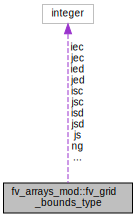
\includegraphics[width=172pt]{structfv__arrays__mod_1_1fv__grid__bounds__type__coll__graph}
\end{center}
\end{figure}
\subsection*{Public Attributes}
\begin{DoxyCompactItemize}
\item 
integer \hyperlink{structfv__arrays__mod_1_1fv__grid__bounds__type_a84222fa7344fd5b1e3af3a1c1511edbe}{is}
\item 
integer \hyperlink{structfv__arrays__mod_1_1fv__grid__bounds__type_afc732fb72e7ed407d03d362c1f252eaf}{ie}
\item 
integer \hyperlink{structfv__arrays__mod_1_1fv__grid__bounds__type_a755478f8eccc59877e3214b449ba2fcd}{js}
\item 
integer \hyperlink{structfv__arrays__mod_1_1fv__grid__bounds__type_a6c45e731bc1722c4c3f8754603be8b14}{je}
\item 
integer \hyperlink{structfv__arrays__mod_1_1fv__grid__bounds__type_a093e99292611def96f8c93bded235b1e}{isd}
\item 
integer \hyperlink{structfv__arrays__mod_1_1fv__grid__bounds__type_a71ce775c34de50182a5a6bb3cf6a210f}{ied}
\item 
integer \hyperlink{structfv__arrays__mod_1_1fv__grid__bounds__type_aaa96d9e7589d89a41e1cd2d8d3dcae26}{jsd}
\item 
integer \hyperlink{structfv__arrays__mod_1_1fv__grid__bounds__type_a910777be14af374da071a7dbd9ea0d5b}{jed}
\item 
integer \hyperlink{structfv__arrays__mod_1_1fv__grid__bounds__type_a27c3ae729a8702577e90f5db757aeaf9}{isc}
\item 
integer \hyperlink{structfv__arrays__mod_1_1fv__grid__bounds__type_ad136ca077be35632ebe19800d59583da}{iec}
\item 
integer \hyperlink{structfv__arrays__mod_1_1fv__grid__bounds__type_a005eba777482ae89181b37df9abebf40}{jsc}
\item 
integer \hyperlink{structfv__arrays__mod_1_1fv__grid__bounds__type_af5a629cd73a6e44795ed193c783b23a9}{jec}
\item 
integer \hyperlink{structfv__arrays__mod_1_1fv__grid__bounds__type_a33323e415a0d78a74eec9a56dace6aea}{ng}
\end{DoxyCompactItemize}


\subsection{Detailed Description}


Definition at line 1137 of file fv\-\_\-arrays.\-F90.



\subsection{Member Data Documentation}
\index{fv\-\_\-arrays\-\_\-mod\-::fv\-\_\-grid\-\_\-bounds\-\_\-type@{fv\-\_\-arrays\-\_\-mod\-::fv\-\_\-grid\-\_\-bounds\-\_\-type}!ie@{ie}}
\index{ie@{ie}!fv_arrays_mod::fv_grid_bounds_type@{fv\-\_\-arrays\-\_\-mod\-::fv\-\_\-grid\-\_\-bounds\-\_\-type}}
\subsubsection[{ie}]{\setlength{\rightskip}{0pt plus 5cm}integer fv\-\_\-arrays\-\_\-mod\-::fv\-\_\-grid\-\_\-bounds\-\_\-type\-::ie}\label{structfv__arrays__mod_1_1fv__grid__bounds__type_afc732fb72e7ed407d03d362c1f252eaf}


Definition at line 1139 of file fv\-\_\-arrays.\-F90.

\index{fv\-\_\-arrays\-\_\-mod\-::fv\-\_\-grid\-\_\-bounds\-\_\-type@{fv\-\_\-arrays\-\_\-mod\-::fv\-\_\-grid\-\_\-bounds\-\_\-type}!iec@{iec}}
\index{iec@{iec}!fv_arrays_mod::fv_grid_bounds_type@{fv\-\_\-arrays\-\_\-mod\-::fv\-\_\-grid\-\_\-bounds\-\_\-type}}
\subsubsection[{iec}]{\setlength{\rightskip}{0pt plus 5cm}integer fv\-\_\-arrays\-\_\-mod\-::fv\-\_\-grid\-\_\-bounds\-\_\-type\-::iec}\label{structfv__arrays__mod_1_1fv__grid__bounds__type_ad136ca077be35632ebe19800d59583da}


Definition at line 1141 of file fv\-\_\-arrays.\-F90.

\index{fv\-\_\-arrays\-\_\-mod\-::fv\-\_\-grid\-\_\-bounds\-\_\-type@{fv\-\_\-arrays\-\_\-mod\-::fv\-\_\-grid\-\_\-bounds\-\_\-type}!ied@{ied}}
\index{ied@{ied}!fv_arrays_mod::fv_grid_bounds_type@{fv\-\_\-arrays\-\_\-mod\-::fv\-\_\-grid\-\_\-bounds\-\_\-type}}
\subsubsection[{ied}]{\setlength{\rightskip}{0pt plus 5cm}integer fv\-\_\-arrays\-\_\-mod\-::fv\-\_\-grid\-\_\-bounds\-\_\-type\-::ied}\label{structfv__arrays__mod_1_1fv__grid__bounds__type_a71ce775c34de50182a5a6bb3cf6a210f}


Definition at line 1140 of file fv\-\_\-arrays.\-F90.

\index{fv\-\_\-arrays\-\_\-mod\-::fv\-\_\-grid\-\_\-bounds\-\_\-type@{fv\-\_\-arrays\-\_\-mod\-::fv\-\_\-grid\-\_\-bounds\-\_\-type}!is@{is}}
\index{is@{is}!fv_arrays_mod::fv_grid_bounds_type@{fv\-\_\-arrays\-\_\-mod\-::fv\-\_\-grid\-\_\-bounds\-\_\-type}}
\subsubsection[{is}]{\setlength{\rightskip}{0pt plus 5cm}integer fv\-\_\-arrays\-\_\-mod\-::fv\-\_\-grid\-\_\-bounds\-\_\-type\-::is}\label{structfv__arrays__mod_1_1fv__grid__bounds__type_a84222fa7344fd5b1e3af3a1c1511edbe}


Definition at line 1139 of file fv\-\_\-arrays.\-F90.

\index{fv\-\_\-arrays\-\_\-mod\-::fv\-\_\-grid\-\_\-bounds\-\_\-type@{fv\-\_\-arrays\-\_\-mod\-::fv\-\_\-grid\-\_\-bounds\-\_\-type}!isc@{isc}}
\index{isc@{isc}!fv_arrays_mod::fv_grid_bounds_type@{fv\-\_\-arrays\-\_\-mod\-::fv\-\_\-grid\-\_\-bounds\-\_\-type}}
\subsubsection[{isc}]{\setlength{\rightskip}{0pt plus 5cm}integer fv\-\_\-arrays\-\_\-mod\-::fv\-\_\-grid\-\_\-bounds\-\_\-type\-::isc}\label{structfv__arrays__mod_1_1fv__grid__bounds__type_a27c3ae729a8702577e90f5db757aeaf9}


Definition at line 1141 of file fv\-\_\-arrays.\-F90.

\index{fv\-\_\-arrays\-\_\-mod\-::fv\-\_\-grid\-\_\-bounds\-\_\-type@{fv\-\_\-arrays\-\_\-mod\-::fv\-\_\-grid\-\_\-bounds\-\_\-type}!isd@{isd}}
\index{isd@{isd}!fv_arrays_mod::fv_grid_bounds_type@{fv\-\_\-arrays\-\_\-mod\-::fv\-\_\-grid\-\_\-bounds\-\_\-type}}
\subsubsection[{isd}]{\setlength{\rightskip}{0pt plus 5cm}integer fv\-\_\-arrays\-\_\-mod\-::fv\-\_\-grid\-\_\-bounds\-\_\-type\-::isd}\label{structfv__arrays__mod_1_1fv__grid__bounds__type_a093e99292611def96f8c93bded235b1e}


Definition at line 1140 of file fv\-\_\-arrays.\-F90.

\index{fv\-\_\-arrays\-\_\-mod\-::fv\-\_\-grid\-\_\-bounds\-\_\-type@{fv\-\_\-arrays\-\_\-mod\-::fv\-\_\-grid\-\_\-bounds\-\_\-type}!je@{je}}
\index{je@{je}!fv_arrays_mod::fv_grid_bounds_type@{fv\-\_\-arrays\-\_\-mod\-::fv\-\_\-grid\-\_\-bounds\-\_\-type}}
\subsubsection[{je}]{\setlength{\rightskip}{0pt plus 5cm}integer fv\-\_\-arrays\-\_\-mod\-::fv\-\_\-grid\-\_\-bounds\-\_\-type\-::je}\label{structfv__arrays__mod_1_1fv__grid__bounds__type_a6c45e731bc1722c4c3f8754603be8b14}


Definition at line 1139 of file fv\-\_\-arrays.\-F90.

\index{fv\-\_\-arrays\-\_\-mod\-::fv\-\_\-grid\-\_\-bounds\-\_\-type@{fv\-\_\-arrays\-\_\-mod\-::fv\-\_\-grid\-\_\-bounds\-\_\-type}!jec@{jec}}
\index{jec@{jec}!fv_arrays_mod::fv_grid_bounds_type@{fv\-\_\-arrays\-\_\-mod\-::fv\-\_\-grid\-\_\-bounds\-\_\-type}}
\subsubsection[{jec}]{\setlength{\rightskip}{0pt plus 5cm}integer fv\-\_\-arrays\-\_\-mod\-::fv\-\_\-grid\-\_\-bounds\-\_\-type\-::jec}\label{structfv__arrays__mod_1_1fv__grid__bounds__type_af5a629cd73a6e44795ed193c783b23a9}


Definition at line 1141 of file fv\-\_\-arrays.\-F90.

\index{fv\-\_\-arrays\-\_\-mod\-::fv\-\_\-grid\-\_\-bounds\-\_\-type@{fv\-\_\-arrays\-\_\-mod\-::fv\-\_\-grid\-\_\-bounds\-\_\-type}!jed@{jed}}
\index{jed@{jed}!fv_arrays_mod::fv_grid_bounds_type@{fv\-\_\-arrays\-\_\-mod\-::fv\-\_\-grid\-\_\-bounds\-\_\-type}}
\subsubsection[{jed}]{\setlength{\rightskip}{0pt plus 5cm}integer fv\-\_\-arrays\-\_\-mod\-::fv\-\_\-grid\-\_\-bounds\-\_\-type\-::jed}\label{structfv__arrays__mod_1_1fv__grid__bounds__type_a910777be14af374da071a7dbd9ea0d5b}


Definition at line 1140 of file fv\-\_\-arrays.\-F90.

\index{fv\-\_\-arrays\-\_\-mod\-::fv\-\_\-grid\-\_\-bounds\-\_\-type@{fv\-\_\-arrays\-\_\-mod\-::fv\-\_\-grid\-\_\-bounds\-\_\-type}!js@{js}}
\index{js@{js}!fv_arrays_mod::fv_grid_bounds_type@{fv\-\_\-arrays\-\_\-mod\-::fv\-\_\-grid\-\_\-bounds\-\_\-type}}
\subsubsection[{js}]{\setlength{\rightskip}{0pt plus 5cm}integer fv\-\_\-arrays\-\_\-mod\-::fv\-\_\-grid\-\_\-bounds\-\_\-type\-::js}\label{structfv__arrays__mod_1_1fv__grid__bounds__type_a755478f8eccc59877e3214b449ba2fcd}


Definition at line 1139 of file fv\-\_\-arrays.\-F90.

\index{fv\-\_\-arrays\-\_\-mod\-::fv\-\_\-grid\-\_\-bounds\-\_\-type@{fv\-\_\-arrays\-\_\-mod\-::fv\-\_\-grid\-\_\-bounds\-\_\-type}!jsc@{jsc}}
\index{jsc@{jsc}!fv_arrays_mod::fv_grid_bounds_type@{fv\-\_\-arrays\-\_\-mod\-::fv\-\_\-grid\-\_\-bounds\-\_\-type}}
\subsubsection[{jsc}]{\setlength{\rightskip}{0pt plus 5cm}integer fv\-\_\-arrays\-\_\-mod\-::fv\-\_\-grid\-\_\-bounds\-\_\-type\-::jsc}\label{structfv__arrays__mod_1_1fv__grid__bounds__type_a005eba777482ae89181b37df9abebf40}


Definition at line 1141 of file fv\-\_\-arrays.\-F90.

\index{fv\-\_\-arrays\-\_\-mod\-::fv\-\_\-grid\-\_\-bounds\-\_\-type@{fv\-\_\-arrays\-\_\-mod\-::fv\-\_\-grid\-\_\-bounds\-\_\-type}!jsd@{jsd}}
\index{jsd@{jsd}!fv_arrays_mod::fv_grid_bounds_type@{fv\-\_\-arrays\-\_\-mod\-::fv\-\_\-grid\-\_\-bounds\-\_\-type}}
\subsubsection[{jsd}]{\setlength{\rightskip}{0pt plus 5cm}integer fv\-\_\-arrays\-\_\-mod\-::fv\-\_\-grid\-\_\-bounds\-\_\-type\-::jsd}\label{structfv__arrays__mod_1_1fv__grid__bounds__type_aaa96d9e7589d89a41e1cd2d8d3dcae26}


Definition at line 1140 of file fv\-\_\-arrays.\-F90.

\index{fv\-\_\-arrays\-\_\-mod\-::fv\-\_\-grid\-\_\-bounds\-\_\-type@{fv\-\_\-arrays\-\_\-mod\-::fv\-\_\-grid\-\_\-bounds\-\_\-type}!ng@{ng}}
\index{ng@{ng}!fv_arrays_mod::fv_grid_bounds_type@{fv\-\_\-arrays\-\_\-mod\-::fv\-\_\-grid\-\_\-bounds\-\_\-type}}
\subsubsection[{ng}]{\setlength{\rightskip}{0pt plus 5cm}integer fv\-\_\-arrays\-\_\-mod\-::fv\-\_\-grid\-\_\-bounds\-\_\-type\-::ng}\label{structfv__arrays__mod_1_1fv__grid__bounds__type_a33323e415a0d78a74eec9a56dace6aea}


Definition at line 1143 of file fv\-\_\-arrays.\-F90.



The documentation for this type was generated from the following file\-:\begin{DoxyCompactItemize}
\item 
/scratch2/\-N\-A\-G\-A\-P\-E/aoml-\/hafs1/\-Kyle.\-Ahern/acs\-\_\-master\-\_\-readonly/model/\hyperlink{fv__arrays_8F90}{fv\-\_\-arrays.\-F90}\end{DoxyCompactItemize}

\section{fv\-\_\-grid\-\_\-tools\-\_\-mod Module Reference}
\label{classfv__grid__tools__mod}\index{fv\-\_\-grid\-\_\-tools\-\_\-mod@{fv\-\_\-grid\-\_\-tools\-\_\-mod}}


Collaboration diagram for fv\-\_\-grid\-\_\-tools\-\_\-mod\-:
\nopagebreak
\begin{figure}[H]
\begin{center}
\leavevmode
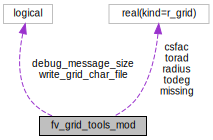
\includegraphics[width=249pt]{classfv__grid__tools__mod__coll__graph}
\end{center}
\end{figure}
\subsection*{Public Member Functions}
\begin{DoxyCompactItemize}
\item 
subroutine, public \hyperlink{classfv__grid__tools__mod_ad44c07c95a2f28e62399da37867817a4}{init\-\_\-grid} (Atm, grid\-\_\-name, grid\-\_\-file, npx, npy, npz, ndims, nregions, ng)
\begin{DoxyCompactList}\small\item\em The subroutine 'init\-\_\-grid' reads the grid from the input file and sets up grid descriptors. \end{DoxyCompactList}\item 
subroutine, public \hyperlink{classfv__grid__tools__mod_a3b343a8e46f50390dadd2b6fddabf244}{spherical\-\_\-to\-\_\-cartesian} (lon, lat, r, x, y, z)
\end{DoxyCompactItemize}
\subsection*{Public Attributes}
\begin{DoxyCompactItemize}
\item 
real(kind=r\-\_\-grid), parameter, \\*
public \hyperlink{classfv__grid__tools__mod_a8b3bcc75f621d290a7cfa0b736983e3f}{todeg} = 180.\-0d0/pi
\begin{DoxyCompactList}\small\item\em convert to degrees \end{DoxyCompactList}\item 
real(kind=r\-\_\-grid), parameter, \\*
public \hyperlink{classfv__grid__tools__mod_acb906ec796b589b9fb688bbbe1bee3c8}{missing} = 1.d25
\end{DoxyCompactItemize}
\subsection*{Private Member Functions}
\begin{DoxyCompactItemize}
\item 
subroutine \hyperlink{classfv__grid__tools__mod_a0cd79c60df097353dc6306eafbf5c4b5}{read\-\_\-grid} (Atm, grid\-\_\-file, ndims, nregions, ng)
\begin{DoxyCompactList}\small\item\em The subroutine 'read\-\_\-grid' reads the grid from the mosaic grid file. \end{DoxyCompactList}\item 
subroutine \hyperlink{classfv__grid__tools__mod_a53b69d107e7bd2468e963e91ac7af946}{get\-\_\-symmetry} (data\-\_\-in, data\-\_\-out, ishift, jshift, npes\-\_\-x, npes\-\_\-y, domain, tile, npx\-\_\-g, bd)
\item 
subroutine \hyperlink{classfv__grid__tools__mod_ac67120f726ca8489dbe875f87c29543f}{cartesian\-\_\-to\-\_\-spherical} (x, y, z, lon, lat, r)
\item 
subroutine \hyperlink{classfv__grid__tools__mod_adbf51ca68c05a220a30c0872b301607e}{rot\-\_\-3d} (axis, x1in, y1in, z1in, angle, x2out, y2out, z2out, degrees, convert)
\begin{DoxyCompactList}\small\item\em The subroutine 'rot\-\_\-3d' rotates points on a sphere in xyz coordinates. \end{DoxyCompactList}\item 
real(kind=R\-\_\-\-G\-R\-I\-D) function \hyperlink{classfv__grid__tools__mod_a6acc2cdd48faa66fba3722b877ab8bb8}{get\-\_\-area\-\_\-tri} (ndims, p\-\_\-1, p\-\_\-2, p\-\_\-3)
\begin{DoxyCompactList}\small\item\em brief The function 'get\-\_\-area\-\_\-tri' gets the surface area of a cell defined as a triangle on the sphere. \end{DoxyCompactList}\item 
subroutine \hyperlink{classfv__grid__tools__mod_afc50b41fc30c3e0f7990440cc6a8b896}{grid\-\_\-area} (nx, ny, ndims, nregions, nested, gridstruct, domain, bd, regional)
\begin{DoxyCompactList}\small\item\em The subroutine 'grid\-\_\-area' gets the surface area on a grid in lat/lon or xyz coordinates. \end{DoxyCompactList}\item 
real(kind=R\-\_\-\-G\-R\-I\-D) function \hyperlink{classfv__grid__tools__mod_a2c7315c9bca27cf1f44788c92969d803}{get\-\_\-angle} (ndims, p1, p2, p3, rad)
\begin{DoxyCompactList}\small\item\em The function 'get\-\_\-angle' gets the angle between 3 points on a sphere in lat/lon or xyz coordinates. \end{DoxyCompactList}\item 
subroutine \hyperlink{classfv__grid__tools__mod_af7a3501736417ecd39ca2f011e36304b}{mirror\-\_\-grid} (grid\-\_\-global, ng, npx, npy, ndims, nregions)
\begin{DoxyCompactList}\small\item\em The subroutine 'mirror\-\_\-grid' mirrors the grid across the 0-\/longitude line. \end{DoxyCompactList}\end{DoxyCompactItemize}
\subsection*{Private Attributes}
\begin{DoxyCompactItemize}
\item 
real(kind=r\-\_\-grid), parameter \hyperlink{classfv__grid__tools__mod_a832e50f3831e3af6951de1a9ed21fe33}{radius} = cnst\-\_\-radius
\item 
real(kind=r\-\_\-grid), parameter \hyperlink{classfv__grid__tools__mod_a532808a493ee0706dd78a3383537ad9a}{torad} = pi/180.\-0d0
\begin{DoxyCompactList}\small\item\em convert to radians \end{DoxyCompactList}\item 
real(kind=r\-\_\-grid) \hyperlink{classfv__grid__tools__mod_a0f01babe8d2ff57cd92783b91dc4cccd}{csfac}
\item 
logical, parameter \hyperlink{classfv__grid__tools__mod_a05413bb63130f63c7356403130c339bd}{debug\-\_\-message\-\_\-size} = .false.
\item 
logical \hyperlink{classfv__grid__tools__mod_ab05dbcee57bb7bce7cb38d1b50f8aa69}{write\-\_\-grid\-\_\-char\-\_\-file} = .false.
\end{DoxyCompactItemize}


\subsection{Detailed Description}


Definition at line 21 of file fv\-\_\-grid\-\_\-tools.\-F90.



\subsection{Member Function/\-Subroutine Documentation}
\index{fv\-\_\-grid\-\_\-tools\-\_\-mod@{fv\-\_\-grid\-\_\-tools\-\_\-mod}!cartesian\-\_\-to\-\_\-spherical@{cartesian\-\_\-to\-\_\-spherical}}
\index{cartesian\-\_\-to\-\_\-spherical@{cartesian\-\_\-to\-\_\-spherical}!fv_grid_tools_mod@{fv\-\_\-grid\-\_\-tools\-\_\-mod}}
\subsubsection[{cartesian\-\_\-to\-\_\-spherical}]{\setlength{\rightskip}{0pt plus 5cm}subroutine fv\-\_\-grid\-\_\-tools\-\_\-mod\-::cartesian\-\_\-to\-\_\-spherical (
\begin{DoxyParamCaption}
\item[{real(kind=r\-\_\-grid), intent(in)}]{x, }
\item[{real(kind=r\-\_\-grid), intent(in)}]{y, }
\item[{real(kind=r\-\_\-grid), intent(in)}]{z, }
\item[{real(kind=r\-\_\-grid), intent(out)}]{lon, }
\item[{real(kind=r\-\_\-grid), intent(out)}]{lat, }
\item[{real(kind=r\-\_\-grid), intent(out)}]{r}
\end{DoxyParamCaption}
)\hspace{0.3cm}{\ttfamily [private]}}\label{classfv__grid__tools__mod_ac67120f726ca8489dbe875f87c29543f}


Definition at line 1922 of file fv\-\_\-grid\-\_\-tools.\-F90.



Referenced by rot\-\_\-3d().

\index{fv\-\_\-grid\-\_\-tools\-\_\-mod@{fv\-\_\-grid\-\_\-tools\-\_\-mod}!get\-\_\-angle@{get\-\_\-angle}}
\index{get\-\_\-angle@{get\-\_\-angle}!fv_grid_tools_mod@{fv\-\_\-grid\-\_\-tools\-\_\-mod}}
\subsubsection[{get\-\_\-angle}]{\setlength{\rightskip}{0pt plus 5cm}real(kind=R\-\_\-\-G\-R\-I\-D) function fv\-\_\-grid\-\_\-tools\-\_\-mod\-::get\-\_\-angle (
\begin{DoxyParamCaption}
\item[{integer, intent(in)}]{ndims, }
\item[{real(kind=r\-\_\-grid), dimension(ndims), intent(in)}]{p1, }
\item[{real(kind=r\-\_\-grid), dimension(ndims), intent(in)}]{p2, }
\item[{real(kind=r\-\_\-grid), dimension(ndims), intent(in)}]{p3, }
\item[{integer, intent(in), optional}]{rad}
\end{DoxyParamCaption}
)\hspace{0.3cm}{\ttfamily [private]}}\label{classfv__grid__tools__mod_a2c7315c9bca27cf1f44788c92969d803}


The function 'get\-\_\-angle' gets the angle between 3 points on a sphere in lat/lon or xyz coordinates. 

Determined by the 'ndims' argument\-: 2=lat/lon, 3=xyz The angle is returned in degrees.


\begin{DoxyParams}[1]{Parameters}
\mbox{\tt in}  & {\em ndims} & 2=lat/lon, 3=xyz \\
\hline
\end{DoxyParams}


Definition at line 2261 of file fv\-\_\-grid\-\_\-tools.\-F90.



References fv\-\_\-grid\-\_\-utils\-\_\-mod\-::spherical\-\_\-angle(), and spherical\-\_\-to\-\_\-cartesian().



Referenced by get\-\_\-area\-\_\-tri(), and init\-\_\-grid().

\index{fv\-\_\-grid\-\_\-tools\-\_\-mod@{fv\-\_\-grid\-\_\-tools\-\_\-mod}!get\-\_\-area\-\_\-tri@{get\-\_\-area\-\_\-tri}}
\index{get\-\_\-area\-\_\-tri@{get\-\_\-area\-\_\-tri}!fv_grid_tools_mod@{fv\-\_\-grid\-\_\-tools\-\_\-mod}}
\subsubsection[{get\-\_\-area\-\_\-tri}]{\setlength{\rightskip}{0pt plus 5cm}real(kind=R\-\_\-\-G\-R\-I\-D) function fv\-\_\-grid\-\_\-tools\-\_\-mod\-::get\-\_\-area\-\_\-tri (
\begin{DoxyParamCaption}
\item[{integer, intent(in)}]{ndims, }
\item[{real(kind=r\-\_\-grid), dimension(ndims), intent(in)}]{p\-\_\-1, }
\item[{real(kind=r\-\_\-grid), dimension(ndims), intent(in)}]{p\-\_\-2, }
\item[{real(kind=r\-\_\-grid), dimension(ndims), intent(in)}]{p\-\_\-3}
\end{DoxyParamCaption}
)\hspace{0.3cm}{\ttfamily [private]}}\label{classfv__grid__tools__mod_a6acc2cdd48faa66fba3722b877ab8bb8}


brief The function 'get\-\_\-area\-\_\-tri' gets the surface area of a cell defined as a triangle on the sphere. 

The area is computed as the spherical excess \mbox{[}area units are based on the units of radius\mbox{]}


\begin{DoxyParams}[1]{Parameters}
\mbox{\tt in}  & {\em ndims} & 2=lat/lon, 3=xyz \\
\hline
\end{DoxyParams}


Definition at line 2018 of file fv\-\_\-grid\-\_\-tools.\-F90.



References get\-\_\-angle(), and fv\-\_\-grid\-\_\-utils\-\_\-mod\-::spherical\-\_\-angle().



Referenced by grid\-\_\-area().

\index{fv\-\_\-grid\-\_\-tools\-\_\-mod@{fv\-\_\-grid\-\_\-tools\-\_\-mod}!get\-\_\-symmetry@{get\-\_\-symmetry}}
\index{get\-\_\-symmetry@{get\-\_\-symmetry}!fv_grid_tools_mod@{fv\-\_\-grid\-\_\-tools\-\_\-mod}}
\subsubsection[{get\-\_\-symmetry}]{\setlength{\rightskip}{0pt plus 5cm}subroutine fv\-\_\-grid\-\_\-tools\-\_\-mod\-::get\-\_\-symmetry (
\begin{DoxyParamCaption}
\item[{real(kind=r\-\_\-grid), dimension(bd\%is\-:bd\%ie+ishift, bd\%js\-:bd\%je+jshift ), intent(in)}]{data\-\_\-in, }
\item[{real(kind=r\-\_\-grid), dimension(bd\%is\-:bd\%ie+jshift, bd\%js\-:bd\%je+ishift ), intent(out)}]{data\-\_\-out, }
\item[{integer, intent(in)}]{ishift, }
\item[{integer, intent(in)}]{jshift, }
\item[{integer, intent(in)}]{npes\-\_\-x, }
\item[{integer, intent(in)}]{npes\-\_\-y, }
\item[{type(domain2d)}]{domain, }
\item[{integer}]{tile, }
\item[{integer}]{npx\-\_\-g, }
\item[{type(fv\-\_\-grid\-\_\-bounds\-\_\-type), intent(in)}]{bd}
\end{DoxyParamCaption}
)\hspace{0.3cm}{\ttfamily [private]}}\label{classfv__grid__tools__mod_a53b69d107e7bd2468e963e91ac7af946}


Definition at line 306 of file fv\-\_\-grid\-\_\-tools.\-F90.



References fv\-\_\-regional\-\_\-mod\-::check().



Referenced by init\-\_\-grid().

\index{fv\-\_\-grid\-\_\-tools\-\_\-mod@{fv\-\_\-grid\-\_\-tools\-\_\-mod}!grid\-\_\-area@{grid\-\_\-area}}
\index{grid\-\_\-area@{grid\-\_\-area}!fv_grid_tools_mod@{fv\-\_\-grid\-\_\-tools\-\_\-mod}}
\subsubsection[{grid\-\_\-area}]{\setlength{\rightskip}{0pt plus 5cm}subroutine fv\-\_\-grid\-\_\-tools\-\_\-mod\-::grid\-\_\-area (
\begin{DoxyParamCaption}
\item[{integer, intent(in)}]{nx, }
\item[{integer, intent(in)}]{ny, }
\item[{integer, intent(in)}]{ndims, }
\item[{integer, intent(in)}]{nregions, }
\item[{logical, intent(in)}]{nested, }
\item[{type(fv\-\_\-grid\-\_\-type), intent(in), target}]{gridstruct, }
\item[{type(domain2d), intent(inout)}]{domain, }
\item[{type(fv\-\_\-grid\-\_\-bounds\-\_\-type), intent(in)}]{bd, }
\item[{logical, intent(in)}]{regional}
\end{DoxyParamCaption}
)\hspace{0.3cm}{\ttfamily [private]}}\label{classfv__grid__tools__mod_afc50b41fc30c3e0f7990440cc6a8b896}


The subroutine 'grid\-\_\-area' gets the surface area on a grid in lat/lon or xyz coordinates. 

Determined by 'ndims' argument\-: 2=lat/lon, 3=xyz) The area is returned in m$^\wedge$2 on a unit sphere. 

Definition at line 2045 of file fv\-\_\-grid\-\_\-tools.\-F90.



References fv\-\_\-grid\-\_\-utils\-\_\-mod\-::get\-\_\-area(), and get\-\_\-area\-\_\-tri().



Referenced by init\-\_\-grid().

\index{fv\-\_\-grid\-\_\-tools\-\_\-mod@{fv\-\_\-grid\-\_\-tools\-\_\-mod}!init\-\_\-grid@{init\-\_\-grid}}
\index{init\-\_\-grid@{init\-\_\-grid}!fv_grid_tools_mod@{fv\-\_\-grid\-\_\-tools\-\_\-mod}}
\subsubsection[{init\-\_\-grid}]{\setlength{\rightskip}{0pt plus 5cm}subroutine, public fv\-\_\-grid\-\_\-tools\-\_\-mod\-::init\-\_\-grid (
\begin{DoxyParamCaption}
\item[{type(fv\-\_\-atmos\-\_\-type), intent(inout), target}]{Atm, }
\item[{character(len=80), intent(in)}]{grid\-\_\-name, }
\item[{character(len=120), intent(in)}]{grid\-\_\-file, }
\item[{integer, intent(in)}]{npx, }
\item[{integer, intent(in)}]{npy, }
\item[{integer, intent(in)}]{npz, }
\item[{integer, intent(in)}]{ndims, }
\item[{integer, intent(in)}]{nregions, }
\item[{integer, intent(in)}]{ng}
\end{DoxyParamCaption}
)}\label{classfv__grid__tools__mod_ad44c07c95a2f28e62399da37867817a4}


The subroutine 'init\-\_\-grid' reads the grid from the input file and sets up grid descriptors. 



Definition at line 529 of file fv\-\_\-grid\-\_\-tools.\-F90.



References fv\-\_\-grid\-\_\-utils\-\_\-mod\-::cell\-\_\-center2(), fv\-\_\-grid\-\_\-utils\-\_\-mod\-::direct\-\_\-transform(), get\-\_\-angle(), fv\-\_\-grid\-\_\-utils\-\_\-mod\-::get\-\_\-area(), get\-\_\-symmetry(), fv\-\_\-grid\-\_\-utils\-\_\-mod\-::gnomonic\-\_\-grids(), fv\-\_\-grid\-\_\-utils\-\_\-mod\-::great\-\_\-circle\-\_\-dist(), grid\-\_\-area(), fv\-\_\-grid\-\_\-utils\-\_\-mod\-::mid\-\_\-pt\-\_\-sphere(), mirror\-\_\-grid(), read\-\_\-grid(), setup\-\_\-aligned\-\_\-nest(), setup\-\_\-cartesian(), sorted\-\_\-index\-\_\-mod\-::sorted\-\_\-inta(), and sorted\-\_\-index\-\_\-mod\-::sorted\-\_\-intb().



Referenced by fv\-\_\-control\-\_\-mod\-::fv\-\_\-init().

\index{fv\-\_\-grid\-\_\-tools\-\_\-mod@{fv\-\_\-grid\-\_\-tools\-\_\-mod}!mirror\-\_\-grid@{mirror\-\_\-grid}}
\index{mirror\-\_\-grid@{mirror\-\_\-grid}!fv_grid_tools_mod@{fv\-\_\-grid\-\_\-tools\-\_\-mod}}
\subsubsection[{mirror\-\_\-grid}]{\setlength{\rightskip}{0pt plus 5cm}subroutine fv\-\_\-grid\-\_\-tools\-\_\-mod\-::mirror\-\_\-grid (
\begin{DoxyParamCaption}
\item[{real(kind=r\-\_\-grid), dimension(1-\/ng\-:npx  +ng,1-\/ng\-:npy  +ng,ndims,1\-:nregions), intent(inout)}]{grid\-\_\-global, }
\item[{integer, intent(in)}]{ng, }
\item[{integer, intent(in)}]{npx, }
\item[{integer, intent(in)}]{npy, }
\item[{integer, intent(in)}]{ndims, }
\item[{integer, intent(in)}]{nregions}
\end{DoxyParamCaption}
)\hspace{0.3cm}{\ttfamily [private]}}\label{classfv__grid__tools__mod_af7a3501736417ecd39ca2f011e36304b}


The subroutine 'mirror\-\_\-grid' mirrors the grid across the 0-\/longitude line. 



Definition at line 2289 of file fv\-\_\-grid\-\_\-tools.\-F90.



References rot\-\_\-3d().



Referenced by init\-\_\-grid().

\index{fv\-\_\-grid\-\_\-tools\-\_\-mod@{fv\-\_\-grid\-\_\-tools\-\_\-mod}!read\-\_\-grid@{read\-\_\-grid}}
\index{read\-\_\-grid@{read\-\_\-grid}!fv_grid_tools_mod@{fv\-\_\-grid\-\_\-tools\-\_\-mod}}
\subsubsection[{read\-\_\-grid}]{\setlength{\rightskip}{0pt plus 5cm}subroutine fv\-\_\-grid\-\_\-tools\-\_\-mod\-::read\-\_\-grid (
\begin{DoxyParamCaption}
\item[{type(fv\-\_\-atmos\-\_\-type), intent(inout), target}]{Atm, }
\item[{character(len=$\ast$), intent(in)}]{grid\-\_\-file, }
\item[{integer, intent(in)}]{ndims, }
\item[{integer, intent(in)}]{nregions, }
\item[{integer, intent(in)}]{ng}
\end{DoxyParamCaption}
)\hspace{0.3cm}{\ttfamily [private]}}\label{classfv__grid__tools__mod_a0cd79c60df097353dc6306eafbf5c4b5}


The subroutine 'read\-\_\-grid' reads the grid from the mosaic grid file. 



Definition at line 174 of file fv\-\_\-grid\-\_\-tools.\-F90.



Referenced by init\-\_\-grid().

\index{fv\-\_\-grid\-\_\-tools\-\_\-mod@{fv\-\_\-grid\-\_\-tools\-\_\-mod}!rot\-\_\-3d@{rot\-\_\-3d}}
\index{rot\-\_\-3d@{rot\-\_\-3d}!fv_grid_tools_mod@{fv\-\_\-grid\-\_\-tools\-\_\-mod}}
\subsubsection[{rot\-\_\-3d}]{\setlength{\rightskip}{0pt plus 5cm}subroutine fv\-\_\-grid\-\_\-tools\-\_\-mod\-::rot\-\_\-3d (
\begin{DoxyParamCaption}
\item[{integer, intent(in)}]{axis, }
\item[{real(kind=r\-\_\-grid), intent(in)}]{x1in, }
\item[{real(kind=r\-\_\-grid), intent(in)}]{y1in, }
\item[{real(kind=r\-\_\-grid), intent(in)}]{z1in, }
\item[{real(kind=r\-\_\-grid), intent(inout)}]{angle, }
\item[{real(kind=r\-\_\-grid), intent(out)}]{x2out, }
\item[{real(kind=r\-\_\-grid), intent(out)}]{y2out, }
\item[{real(kind=r\-\_\-grid), intent(out)}]{z2out, }
\item[{integer, intent(in), optional}]{degrees, }
\item[{integer, intent(in), optional}]{convert}
\end{DoxyParamCaption}
)\hspace{0.3cm}{\ttfamily [private]}}\label{classfv__grid__tools__mod_adbf51ca68c05a220a30c0872b301607e}


The subroutine 'rot\-\_\-3d' rotates points on a sphere in xyz coordinates. 

Converts angle from degrees to radians if necessary


\begin{DoxyParams}[1]{Parameters}
\mbox{\tt in}  & {\em axis} & axis of rotation 1=x, 2=y, 3=z\\
\hline
\mbox{\tt in,out}  & {\em angle} & angle to rotate in radians\\
\hline
\mbox{\tt in}  & {\em degrees} & if present convert angle from degrees to radians\\
\hline
\mbox{\tt in}  & {\em convert} & if present convert input point from spherical to cartesian, rotate, and convert back \\
\hline
\end{DoxyParams}


Definition at line 1955 of file fv\-\_\-grid\-\_\-tools.\-F90.



References cartesian\-\_\-to\-\_\-spherical(), and spherical\-\_\-to\-\_\-cartesian().



Referenced by mirror\-\_\-grid().

\index{fv\-\_\-grid\-\_\-tools\-\_\-mod@{fv\-\_\-grid\-\_\-tools\-\_\-mod}!spherical\-\_\-to\-\_\-cartesian@{spherical\-\_\-to\-\_\-cartesian}}
\index{spherical\-\_\-to\-\_\-cartesian@{spherical\-\_\-to\-\_\-cartesian}!fv_grid_tools_mod@{fv\-\_\-grid\-\_\-tools\-\_\-mod}}
\subsubsection[{spherical\-\_\-to\-\_\-cartesian}]{\setlength{\rightskip}{0pt plus 5cm}subroutine, public fv\-\_\-grid\-\_\-tools\-\_\-mod\-::spherical\-\_\-to\-\_\-cartesian (
\begin{DoxyParamCaption}
\item[{real(kind=r\-\_\-grid), intent(in)}]{lon, }
\item[{real(kind=r\-\_\-grid), intent(in)}]{lat, }
\item[{real(kind=r\-\_\-grid), intent(in)}]{r, }
\item[{real(kind=r\-\_\-grid), intent(out)}]{x, }
\item[{real(kind=r\-\_\-grid), intent(out)}]{y, }
\item[{real(kind=r\-\_\-grid), intent(out)}]{z}
\end{DoxyParamCaption}
)}\label{classfv__grid__tools__mod_a3b343a8e46f50390dadd2b6fddabf244}


Definition at line 1940 of file fv\-\_\-grid\-\_\-tools.\-F90.



Referenced by get\-\_\-angle(), test\-\_\-cases\-\_\-mod\-::get\-\_\-unit\-\_\-vector(), and rot\-\_\-3d().



\subsection{Member Data Documentation}
\index{fv\-\_\-grid\-\_\-tools\-\_\-mod@{fv\-\_\-grid\-\_\-tools\-\_\-mod}!csfac@{csfac}}
\index{csfac@{csfac}!fv_grid_tools_mod@{fv\-\_\-grid\-\_\-tools\-\_\-mod}}
\subsubsection[{csfac}]{\setlength{\rightskip}{0pt plus 5cm}real(kind=r\-\_\-grid) fv\-\_\-grid\-\_\-tools\-\_\-mod\-::csfac\hspace{0.3cm}{\ttfamily [private]}}\label{classfv__grid__tools__mod_a0f01babe8d2ff57cd92783b91dc4cccd}


Definition at line 163 of file fv\-\_\-grid\-\_\-tools.\-F90.

\index{fv\-\_\-grid\-\_\-tools\-\_\-mod@{fv\-\_\-grid\-\_\-tools\-\_\-mod}!debug\-\_\-message\-\_\-size@{debug\-\_\-message\-\_\-size}}
\index{debug\-\_\-message\-\_\-size@{debug\-\_\-message\-\_\-size}!fv_grid_tools_mod@{fv\-\_\-grid\-\_\-tools\-\_\-mod}}
\subsubsection[{debug\-\_\-message\-\_\-size}]{\setlength{\rightskip}{0pt plus 5cm}logical, parameter fv\-\_\-grid\-\_\-tools\-\_\-mod\-::debug\-\_\-message\-\_\-size = .false.\hspace{0.3cm}{\ttfamily [private]}}\label{classfv__grid__tools__mod_a05413bb63130f63c7356403130c339bd}


Definition at line 165 of file fv\-\_\-grid\-\_\-tools.\-F90.

\index{fv\-\_\-grid\-\_\-tools\-\_\-mod@{fv\-\_\-grid\-\_\-tools\-\_\-mod}!missing@{missing}}
\index{missing@{missing}!fv_grid_tools_mod@{fv\-\_\-grid\-\_\-tools\-\_\-mod}}
\subsubsection[{missing}]{\setlength{\rightskip}{0pt plus 5cm}real(kind=r\-\_\-grid), parameter, public fv\-\_\-grid\-\_\-tools\-\_\-mod\-::missing = 1.d25}\label{classfv__grid__tools__mod_acb906ec796b589b9fb688bbbe1bee3c8}


Definition at line 161 of file fv\-\_\-grid\-\_\-tools.\-F90.

\index{fv\-\_\-grid\-\_\-tools\-\_\-mod@{fv\-\_\-grid\-\_\-tools\-\_\-mod}!radius@{radius}}
\index{radius@{radius}!fv_grid_tools_mod@{fv\-\_\-grid\-\_\-tools\-\_\-mod}}
\subsubsection[{radius}]{\setlength{\rightskip}{0pt plus 5cm}real(kind=r\-\_\-grid), parameter fv\-\_\-grid\-\_\-tools\-\_\-mod\-::radius = cnst\-\_\-radius\hspace{0.3cm}{\ttfamily [private]}}\label{classfv__grid__tools__mod_a832e50f3831e3af6951de1a9ed21fe33}


Definition at line 157 of file fv\-\_\-grid\-\_\-tools.\-F90.

\index{fv\-\_\-grid\-\_\-tools\-\_\-mod@{fv\-\_\-grid\-\_\-tools\-\_\-mod}!todeg@{todeg}}
\index{todeg@{todeg}!fv_grid_tools_mod@{fv\-\_\-grid\-\_\-tools\-\_\-mod}}
\subsubsection[{todeg}]{\setlength{\rightskip}{0pt plus 5cm}real(kind=r\-\_\-grid), parameter, public fv\-\_\-grid\-\_\-tools\-\_\-mod\-::todeg = 180.\-0d0/pi}\label{classfv__grid__tools__mod_a8b3bcc75f621d290a7cfa0b736983e3f}


convert to degrees 



Definition at line 159 of file fv\-\_\-grid\-\_\-tools.\-F90.

\index{fv\-\_\-grid\-\_\-tools\-\_\-mod@{fv\-\_\-grid\-\_\-tools\-\_\-mod}!torad@{torad}}
\index{torad@{torad}!fv_grid_tools_mod@{fv\-\_\-grid\-\_\-tools\-\_\-mod}}
\subsubsection[{torad}]{\setlength{\rightskip}{0pt plus 5cm}real(kind=r\-\_\-grid), parameter fv\-\_\-grid\-\_\-tools\-\_\-mod\-::torad = pi/180.\-0d0\hspace{0.3cm}{\ttfamily [private]}}\label{classfv__grid__tools__mod_a532808a493ee0706dd78a3383537ad9a}


convert to radians 



Definition at line 160 of file fv\-\_\-grid\-\_\-tools.\-F90.

\index{fv\-\_\-grid\-\_\-tools\-\_\-mod@{fv\-\_\-grid\-\_\-tools\-\_\-mod}!write\-\_\-grid\-\_\-char\-\_\-file@{write\-\_\-grid\-\_\-char\-\_\-file}}
\index{write\-\_\-grid\-\_\-char\-\_\-file@{write\-\_\-grid\-\_\-char\-\_\-file}!fv_grid_tools_mod@{fv\-\_\-grid\-\_\-tools\-\_\-mod}}
\subsubsection[{write\-\_\-grid\-\_\-char\-\_\-file}]{\setlength{\rightskip}{0pt plus 5cm}logical fv\-\_\-grid\-\_\-tools\-\_\-mod\-::write\-\_\-grid\-\_\-char\-\_\-file = .false.\hspace{0.3cm}{\ttfamily [private]}}\label{classfv__grid__tools__mod_ab05dbcee57bb7bce7cb38d1b50f8aa69}


Definition at line 166 of file fv\-\_\-grid\-\_\-tools.\-F90.



The documentation for this module was generated from the following file\-:\begin{DoxyCompactItemize}
\item 
/scratch2/\-N\-A\-G\-A\-P\-E/aoml-\/hafs1/\-Kyle.\-Ahern/acs\-\_\-master\-\_\-readonly/tools/\hyperlink{fv__grid__tools_8F90}{fv\-\_\-grid\-\_\-tools.\-F90}\end{DoxyCompactItemize}

\section{fv\-\_\-arrays\-\_\-mod\-:\-:fv\-\_\-grid\-\_\-type Type Reference}
\label{structfv__arrays__mod_1_1fv__grid__type}\index{fv\-\_\-arrays\-\_\-mod\-::fv\-\_\-grid\-\_\-type@{fv\-\_\-arrays\-\_\-mod\-::fv\-\_\-grid\-\_\-type}}


The type '\hyperlink{structfv__arrays__mod_1_1fv__grid__type}{fv\-\_\-grid\-\_\-type}' is made up of grid-\/dependent information from fv\-\_\-grid\-\_\-tools and fv\-\_\-grid\-\_\-utils.  




Collaboration diagram for fv\-\_\-arrays\-\_\-mod\-:\-:fv\-\_\-grid\-\_\-type\-:
\nopagebreak
\begin{figure}[H]
\begin{center}
\leavevmode
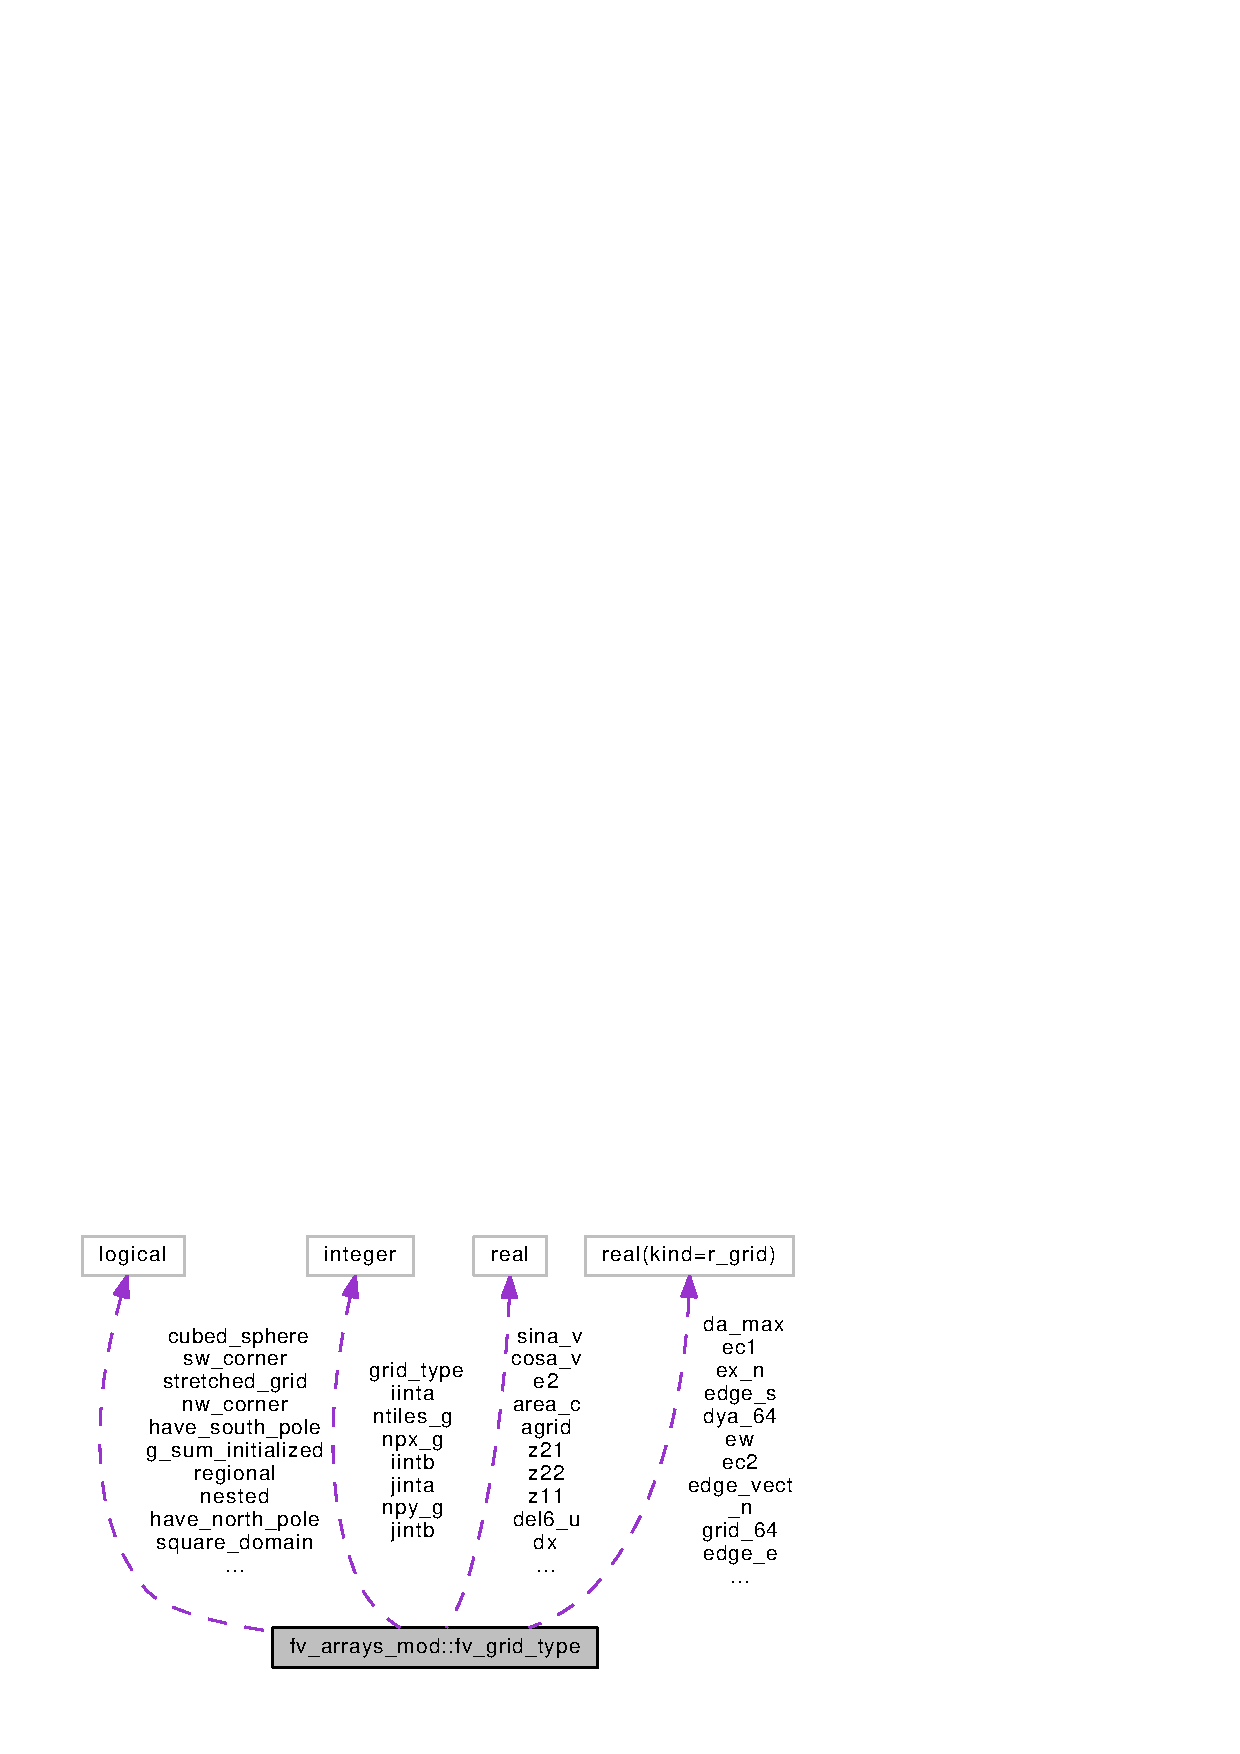
\includegraphics[width=350pt]{structfv__arrays__mod_1_1fv__grid__type__coll__graph}
\end{center}
\end{figure}
\subsection*{Public Attributes}
\begin{DoxyCompactItemize}
\item 
real(kind=\hyperlink{classfv__arrays__mod_ab0ba8527d270f349a84fa0a330be1923}{r\-\_\-grid}), dimension(\-:,\-:,\-:), \\*
allocatable \hyperlink{structfv__arrays__mod_1_1fv__grid__type_a3e3c763e6b061f4bc4a6e01eab81780b}{grid\-\_\-64}
\item 
real(kind=\hyperlink{classfv__arrays__mod_ab0ba8527d270f349a84fa0a330be1923}{r\-\_\-grid}), dimension(\-:,\-:,\-:), \\*
allocatable \hyperlink{structfv__arrays__mod_1_1fv__grid__type_acad5e5b7fdfee2e55941d628e0fa797f}{agrid\-\_\-64}
\item 
real(kind=\hyperlink{classfv__arrays__mod_ab0ba8527d270f349a84fa0a330be1923}{r\-\_\-grid}), dimension(\-:,\-:), \\*
allocatable \hyperlink{structfv__arrays__mod_1_1fv__grid__type_a2f41c4214f60282af69a29bc6595b1ba}{area\-\_\-64}
\item 
real(kind=\hyperlink{classfv__arrays__mod_ab0ba8527d270f349a84fa0a330be1923}{r\-\_\-grid}), dimension(\-:,\-:), \\*
allocatable \hyperlink{structfv__arrays__mod_1_1fv__grid__type_ad158e67cf5e91973c2d93a9a6f14c884}{area\-\_\-c\-\_\-64}
\item 
real(kind=\hyperlink{classfv__arrays__mod_ab0ba8527d270f349a84fa0a330be1923}{r\-\_\-grid}), dimension(\-:,\-:), \\*
allocatable \hyperlink{structfv__arrays__mod_1_1fv__grid__type_a676e6a901ed0513f6e7f73a921be2d47}{sina\-\_\-64}
\item 
real(kind=\hyperlink{classfv__arrays__mod_ab0ba8527d270f349a84fa0a330be1923}{r\-\_\-grid}), dimension(\-:,\-:), \\*
allocatable \hyperlink{structfv__arrays__mod_1_1fv__grid__type_ad78a7565404904b524a1dd4a445c6381}{cosa\-\_\-64}
\item 
real(kind=\hyperlink{classfv__arrays__mod_ab0ba8527d270f349a84fa0a330be1923}{r\-\_\-grid}), dimension(\-:,\-:), \\*
allocatable \hyperlink{structfv__arrays__mod_1_1fv__grid__type_a0067f1c83c318094681664a78e966e60}{dx\-\_\-64}
\item 
real(kind=\hyperlink{classfv__arrays__mod_ab0ba8527d270f349a84fa0a330be1923}{r\-\_\-grid}), dimension(\-:,\-:), \\*
allocatable \hyperlink{structfv__arrays__mod_1_1fv__grid__type_ac87c00324dc8d3118616eb5226951f34}{dy\-\_\-64}
\item 
real(kind=\hyperlink{classfv__arrays__mod_ab0ba8527d270f349a84fa0a330be1923}{r\-\_\-grid}), dimension(\-:,\-:), \\*
allocatable \hyperlink{structfv__arrays__mod_1_1fv__grid__type_a028087387fc0acb7ca9afdb9ffd7deb0}{dxc\-\_\-64}
\item 
real(kind=\hyperlink{classfv__arrays__mod_ab0ba8527d270f349a84fa0a330be1923}{r\-\_\-grid}), dimension(\-:,\-:), \\*
allocatable \hyperlink{structfv__arrays__mod_1_1fv__grid__type_a64e92f11a79556bfd02e38a249b0a918}{dyc\-\_\-64}
\item 
real(kind=\hyperlink{classfv__arrays__mod_ab0ba8527d270f349a84fa0a330be1923}{r\-\_\-grid}), dimension(\-:,\-:), \\*
allocatable \hyperlink{structfv__arrays__mod_1_1fv__grid__type_a187343458f867c17bc045e4ed26f3dcf}{dxa\-\_\-64}
\item 
real(kind=\hyperlink{classfv__arrays__mod_ab0ba8527d270f349a84fa0a330be1923}{r\-\_\-grid}), dimension(\-:,\-:), \\*
allocatable \hyperlink{structfv__arrays__mod_1_1fv__grid__type_a1e026e325f52a9278c2f871a5d9c1c31}{dya\-\_\-64}
\item 
real, dimension(\-:,\-:,\-:), allocatable \hyperlink{structfv__arrays__mod_1_1fv__grid__type_ab4f3c37b71e4dd444556536138e886d5}{grid}
\item 
real, dimension(\-:,\-:,\-:), allocatable \hyperlink{structfv__arrays__mod_1_1fv__grid__type_ae68d27d082cbf8e50fd21e72ff2f4794}{agrid}
\item 
real, dimension(\-:,\-:), allocatable \hyperlink{structfv__arrays__mod_1_1fv__grid__type_a0f623e116b083899ab4cb87775cb9d42}{area}
\item 
real, dimension(\-:,\-:), allocatable \hyperlink{structfv__arrays__mod_1_1fv__grid__type_a3ca9fa6025d14276c65dfbb0cfb579dd}{area\-\_\-c}
\item 
real, dimension(\-:,\-:), allocatable \hyperlink{structfv__arrays__mod_1_1fv__grid__type_a436b669aa9d18827e6588b30cbe861bd}{rarea}
\item 
real, dimension(\-:,\-:), allocatable \hyperlink{structfv__arrays__mod_1_1fv__grid__type_a5be0a23653758af18d87f2bde5c07fcf}{rarea\-\_\-c}
\item 
real, dimension(\-:,\-:), allocatable \hyperlink{structfv__arrays__mod_1_1fv__grid__type_a5b1f29fb1d464639f2622e750b649701}{sina}
\item 
real, dimension(\-:,\-:), allocatable \hyperlink{structfv__arrays__mod_1_1fv__grid__type_aa4800a8e89eb3a1a685998dba6b80edc}{cosa}
\item 
real, dimension(\-:,\-:,\-:), allocatable \hyperlink{structfv__arrays__mod_1_1fv__grid__type_a60093b96a91fd6682fe9d3a13f7e33f6}{e1}
\item 
real, dimension(\-:,\-:,\-:), allocatable \hyperlink{structfv__arrays__mod_1_1fv__grid__type_a5304234fe48437b157b8d6a0796fb4e7}{e2}
\item 
real, dimension(\-:,\-:), allocatable \hyperlink{structfv__arrays__mod_1_1fv__grid__type_a5355993251b97f7e585682eed90cf816}{dx}
\item 
real, dimension(\-:,\-:), allocatable \hyperlink{structfv__arrays__mod_1_1fv__grid__type_a2533f9a11ec2e1180249e7e2e3dd3048}{dy}
\item 
real, dimension(\-:,\-:), allocatable \hyperlink{structfv__arrays__mod_1_1fv__grid__type_a7a4d21a6fe383c9dea04c5c739a3725f}{dxc}
\item 
real, dimension(\-:,\-:), allocatable \hyperlink{structfv__arrays__mod_1_1fv__grid__type_ab94e6fe03dec09dba3538b40f011ba71}{dyc}
\item 
real, dimension(\-:,\-:), allocatable \hyperlink{structfv__arrays__mod_1_1fv__grid__type_aa787cdeab136f88928f2a74d9540b605}{dxa}
\item 
real, dimension(\-:,\-:), allocatable \hyperlink{structfv__arrays__mod_1_1fv__grid__type_a1a3a6cd57e4d32de4e396949df7d47db}{dya}
\item 
real, dimension(\-:,\-:), allocatable \hyperlink{structfv__arrays__mod_1_1fv__grid__type_ad7c917dbdf173e2849f68fb711de725e}{rdx}
\item 
real, dimension(\-:,\-:), allocatable \hyperlink{structfv__arrays__mod_1_1fv__grid__type_a3634b07481a0ee2a9e4873bd266e2186}{rdy}
\item 
real, dimension(\-:,\-:), allocatable \hyperlink{structfv__arrays__mod_1_1fv__grid__type_a96991b006ee53d3efe6b2e0334ef1011}{rdxc}
\item 
real, dimension(\-:,\-:), allocatable \hyperlink{structfv__arrays__mod_1_1fv__grid__type_ad17eb4f3ce260eac07d6266117758b04}{rdyc}
\item 
real, dimension(\-:,\-:), allocatable \hyperlink{structfv__arrays__mod_1_1fv__grid__type_a80c3f1535ed4d68548891a0c36104b87}{rdxa}
\item 
real, dimension(\-:,\-:), allocatable \hyperlink{structfv__arrays__mod_1_1fv__grid__type_a4fba9fe1697d1c49fc8bc3b636c7970a}{rdya}
\item 
real(kind=\hyperlink{classfv__arrays__mod_ab0ba8527d270f349a84fa0a330be1923}{r\-\_\-grid}), dimension(\-:), \\*
allocatable \hyperlink{structfv__arrays__mod_1_1fv__grid__type_a0779d947f5dac37241bce29ace4319fb}{edge\-\_\-s}
\item 
real(kind=\hyperlink{classfv__arrays__mod_ab0ba8527d270f349a84fa0a330be1923}{r\-\_\-grid}), dimension(\-:), \\*
allocatable \hyperlink{structfv__arrays__mod_1_1fv__grid__type_a8be97319aa472a2e64777fd72af1efb3}{edge\-\_\-n}
\item 
real(kind=\hyperlink{classfv__arrays__mod_ab0ba8527d270f349a84fa0a330be1923}{r\-\_\-grid}), dimension(\-:), \\*
allocatable \hyperlink{structfv__arrays__mod_1_1fv__grid__type_ab6786382391fee454bca4507790d6df9}{edge\-\_\-w}
\item 
real(kind=\hyperlink{classfv__arrays__mod_ab0ba8527d270f349a84fa0a330be1923}{r\-\_\-grid}), dimension(\-:), \\*
allocatable \hyperlink{structfv__arrays__mod_1_1fv__grid__type_a4b5b185c881534e49e620fc7cb2e1c97}{edge\-\_\-e}
\item 
real(kind=\hyperlink{classfv__arrays__mod_ab0ba8527d270f349a84fa0a330be1923}{r\-\_\-grid}), dimension(\-:), \\*
allocatable \hyperlink{structfv__arrays__mod_1_1fv__grid__type_ad3b04032fd9e8d0706c654c2ca24863c}{edge\-\_\-vect\-\_\-s}
\item 
real(kind=\hyperlink{classfv__arrays__mod_ab0ba8527d270f349a84fa0a330be1923}{r\-\_\-grid}), dimension(\-:), \\*
allocatable \hyperlink{structfv__arrays__mod_1_1fv__grid__type_ae3fbc56118df0893995b5698166e622a}{edge\-\_\-vect\-\_\-n}
\item 
real(kind=\hyperlink{classfv__arrays__mod_ab0ba8527d270f349a84fa0a330be1923}{r\-\_\-grid}), dimension(\-:), \\*
allocatable \hyperlink{structfv__arrays__mod_1_1fv__grid__type_a97c23e80372b2ccd08f13a1c6c114e11}{edge\-\_\-vect\-\_\-w}
\item 
real(kind=\hyperlink{classfv__arrays__mod_ab0ba8527d270f349a84fa0a330be1923}{r\-\_\-grid}), dimension(\-:), \\*
allocatable \hyperlink{structfv__arrays__mod_1_1fv__grid__type_af14f0b8907ab53e5d8ed7df541aec6b9}{edge\-\_\-vect\-\_\-e}
\item 
real(kind=\hyperlink{classfv__arrays__mod_ab0ba8527d270f349a84fa0a330be1923}{r\-\_\-grid}), dimension(\-:), \\*
allocatable \hyperlink{structfv__arrays__mod_1_1fv__grid__type_a6b7012fcbcb22a5cc14c9be2485a3c41}{ex\-\_\-s}
\item 
real(kind=\hyperlink{classfv__arrays__mod_ab0ba8527d270f349a84fa0a330be1923}{r\-\_\-grid}), dimension(\-:), \\*
allocatable \hyperlink{structfv__arrays__mod_1_1fv__grid__type_a663a182c460c4b7efcebf76b5c925fcc}{ex\-\_\-n}
\item 
real(kind=\hyperlink{classfv__arrays__mod_ab0ba8527d270f349a84fa0a330be1923}{r\-\_\-grid}), dimension(\-:), \\*
allocatable \hyperlink{structfv__arrays__mod_1_1fv__grid__type_a4f73ad5d1c32bde5cc53efca1c1df17f}{ex\-\_\-w}
\item 
real(kind=\hyperlink{classfv__arrays__mod_ab0ba8527d270f349a84fa0a330be1923}{r\-\_\-grid}), dimension(\-:), \\*
allocatable \hyperlink{structfv__arrays__mod_1_1fv__grid__type_a345df2e66abf34e78c67bf5f0fd637ed}{ex\-\_\-e}
\item 
real, dimension(\-:,\-:), allocatable \hyperlink{structfv__arrays__mod_1_1fv__grid__type_a55a06e29892a5836e8b5fc3822fa51e9}{l2c\-\_\-u}
\item 
real, dimension(\-:,\-:), allocatable \hyperlink{structfv__arrays__mod_1_1fv__grid__type_ab9c256610f44e1b093ece9c0c336e810}{l2c\-\_\-v}
\item 
real, dimension(\-:,\-:), allocatable \hyperlink{structfv__arrays__mod_1_1fv__grid__type_a23614cd19fe0fe1b9d1c94fdc87eace8}{divg\-\_\-u}
\item 
real, dimension(\-:,\-:), allocatable \hyperlink{structfv__arrays__mod_1_1fv__grid__type_a3203d6edb0bb98b83aca50bfea929e42}{divg\-\_\-v}
\item 
real, dimension(\-:,\-:), allocatable \hyperlink{structfv__arrays__mod_1_1fv__grid__type_a0a50635625e1283ae8921ef1606b770d}{del6\-\_\-u}
\item 
real, dimension(\-:,\-:), allocatable \hyperlink{structfv__arrays__mod_1_1fv__grid__type_af4578e602380c414292d93203313aaa3}{del6\-\_\-v}
\item 
real, dimension(\-:,\-:), allocatable \hyperlink{structfv__arrays__mod_1_1fv__grid__type_a031ca03cf75ef158170a02c92e33b712}{a11}
\item 
real, dimension(\-:,\-:), allocatable \hyperlink{structfv__arrays__mod_1_1fv__grid__type_aff9b4a668b6765383d5750a0244f1f29}{a12}
\item 
real, dimension(\-:,\-:), allocatable \hyperlink{structfv__arrays__mod_1_1fv__grid__type_a231230cb675e894522f263d9bc28e64b}{a21}
\item 
real, dimension(\-:,\-:), allocatable \hyperlink{structfv__arrays__mod_1_1fv__grid__type_a71399bdc443a16413a309a4e50346579}{a22}
\item 
real, dimension(\-:,\-:), allocatable \hyperlink{structfv__arrays__mod_1_1fv__grid__type_a61173daebde1950c12444005f06a0c86}{z11}
\item 
real, dimension(\-:,\-:), allocatable \hyperlink{structfv__arrays__mod_1_1fv__grid__type_a424c7bea81647f4db6ed99e7aa356f25}{z12}
\item 
real, dimension(\-:,\-:), allocatable \hyperlink{structfv__arrays__mod_1_1fv__grid__type_ab93ef0fd752a80fee92d1678785883a1}{z21}
\item 
real, dimension(\-:,\-:), allocatable \hyperlink{structfv__arrays__mod_1_1fv__grid__type_a7b7f8aa4fc1c048e446478aea5e5d601}{z22}
\item 
real, dimension(\-:,\-:), allocatable \hyperlink{structfv__arrays__mod_1_1fv__grid__type_ae5c3bb087e289619efb5f97c042260c5}{cosa\-\_\-u}
\item 
real, dimension(\-:,\-:), allocatable \hyperlink{structfv__arrays__mod_1_1fv__grid__type_aea1d9e2e29779a878372fa6217b566ca}{cosa\-\_\-v}
\item 
real, dimension(\-:,\-:), allocatable \hyperlink{structfv__arrays__mod_1_1fv__grid__type_af10303762478f589c82cf17f634b26f8}{cosa\-\_\-s}
\item 
real, dimension(\-:,\-:), allocatable \hyperlink{structfv__arrays__mod_1_1fv__grid__type_a70d829477110ac82f38065460ef5b6b3}{sina\-\_\-u}
\item 
real, dimension(\-:,\-:), allocatable \hyperlink{structfv__arrays__mod_1_1fv__grid__type_aa999d53d66859c4c08851b7a74e7449e}{sina\-\_\-v}
\item 
real, dimension(\-:,\-:), allocatable \hyperlink{structfv__arrays__mod_1_1fv__grid__type_a28cfd8dc8c410d88a05c5c278643f76b}{rsin\-\_\-u}
\item 
real, dimension(\-:,\-:), allocatable \hyperlink{structfv__arrays__mod_1_1fv__grid__type_a97dd5675fd3857c4a44ea673984bb618}{rsin\-\_\-v}
\item 
real, dimension(\-:,\-:), allocatable \hyperlink{structfv__arrays__mod_1_1fv__grid__type_a97d2a9ff82ba04efc2bb3747b0889bc0}{rsina}
\item 
real, dimension(\-:,\-:), allocatable \hyperlink{structfv__arrays__mod_1_1fv__grid__type_a4301506b2d2eb21bb86eab20c47c988e}{rsin2}
\item 
real(kind=\hyperlink{classfv__arrays__mod_ab0ba8527d270f349a84fa0a330be1923}{r\-\_\-grid}), dimension(\-:,\-:,\-:), \\*
allocatable \hyperlink{structfv__arrays__mod_1_1fv__grid__type_a7a3fc16173527ef7fcc38253a91b8106}{ee1}
\item 
real(kind=\hyperlink{classfv__arrays__mod_ab0ba8527d270f349a84fa0a330be1923}{r\-\_\-grid}), dimension(\-:,\-:,\-:), \\*
allocatable \hyperlink{structfv__arrays__mod_1_1fv__grid__type_a95aa43f23d9a854b1375b007d40c0863}{ee2}
\item 
real(kind=\hyperlink{classfv__arrays__mod_ab0ba8527d270f349a84fa0a330be1923}{r\-\_\-grid}), dimension(\-:,\-:,\-:), \\*
allocatable \hyperlink{structfv__arrays__mod_1_1fv__grid__type_a1f29c4a2832b7ee8be140c26901996af}{ec1}
\item 
real(kind=\hyperlink{classfv__arrays__mod_ab0ba8527d270f349a84fa0a330be1923}{r\-\_\-grid}), dimension(\-:,\-:,\-:), \\*
allocatable \hyperlink{structfv__arrays__mod_1_1fv__grid__type_a477b852bca7d25cdabf13895d2c3e69f}{ec2}
\item 
real(kind=\hyperlink{classfv__arrays__mod_ab0ba8527d270f349a84fa0a330be1923}{r\-\_\-grid}), dimension(\-:,\-:,\-:,\-:), \\*
allocatable \hyperlink{structfv__arrays__mod_1_1fv__grid__type_a5ce4965ebb7da8c07d99979b09c34402}{ew}
\item 
real(kind=\hyperlink{classfv__arrays__mod_ab0ba8527d270f349a84fa0a330be1923}{r\-\_\-grid}), dimension(\-:,\-:,\-:,\-:), \\*
allocatable \hyperlink{structfv__arrays__mod_1_1fv__grid__type_a11abc0d80511786eaf04c8218963bb8b}{es}
\item 
real, dimension(\-:,\-:,\-:), allocatable \hyperlink{structfv__arrays__mod_1_1fv__grid__type_adbb06440c855cc37905fd73a908d2ed6}{sin\-\_\-sg}
\item 
real, dimension(\-:,\-:,\-:), allocatable \hyperlink{structfv__arrays__mod_1_1fv__grid__type_a8f95e104b30c7e50479e333e64017993}{cos\-\_\-sg}
\item 
real(kind=\hyperlink{classfv__arrays__mod_ab0ba8527d270f349a84fa0a330be1923}{r\-\_\-grid}), dimension(\-:,\-:,\-:), \\*
allocatable \hyperlink{structfv__arrays__mod_1_1fv__grid__type_a73010b5fc69eb9e3e3369c5b5d1e8e79}{en1}
\item 
real(kind=\hyperlink{classfv__arrays__mod_ab0ba8527d270f349a84fa0a330be1923}{r\-\_\-grid}), dimension(\-:,\-:,\-:), \\*
allocatable \hyperlink{structfv__arrays__mod_1_1fv__grid__type_aeaa021081f07634bebf491c752ebff6a}{en2}
\item 
real, dimension(\-:,\-:), allocatable \hyperlink{structfv__arrays__mod_1_1fv__grid__type_a0f16d115d609b95b647e85c869f44cb4}{eww}
\item 
real, dimension(\-:,\-:), allocatable \hyperlink{structfv__arrays__mod_1_1fv__grid__type_a1233e425c20ba7a2cc6aa0e46ed5015c}{ess}
\item 
real(kind=\hyperlink{classfv__arrays__mod_ab0ba8527d270f349a84fa0a330be1923}{r\-\_\-grid}), dimension(\-:,\-:,\-:), \\*
allocatable \hyperlink{structfv__arrays__mod_1_1fv__grid__type_a9e8faf63c65b7ca992a2dad1b701a9a1}{vlon}
\item 
real(kind=\hyperlink{classfv__arrays__mod_ab0ba8527d270f349a84fa0a330be1923}{r\-\_\-grid}), dimension(\-:,\-:,\-:), \\*
allocatable \hyperlink{structfv__arrays__mod_1_1fv__grid__type_a1803ca537d8deb8d97f34e16e187eceb}{vlat}
\item 
real, dimension(\-:,\-:), allocatable \hyperlink{structfv__arrays__mod_1_1fv__grid__type_ad6b4cc197da201ef2c31815f3a8a5411}{fc}
\item 
real, dimension(\-:,\-:), allocatable \hyperlink{structfv__arrays__mod_1_1fv__grid__type_a99276efaf78d2df4d372cc3611f100b9}{f0}
\item 
integer, dimension(\-:,\-:,\-:), \\*
allocatable \hyperlink{structfv__arrays__mod_1_1fv__grid__type_ad30036fbd902aa2718013d156a6c2185}{iinta}
\item 
integer, dimension(\-:,\-:,\-:), \\*
allocatable \hyperlink{structfv__arrays__mod_1_1fv__grid__type_a60627dd7ae4d9f748f6488474f45b1a0}{jinta}
\item 
integer, dimension(\-:,\-:,\-:), \\*
allocatable \hyperlink{structfv__arrays__mod_1_1fv__grid__type_af6e4fbd753eb431fc0972ba9811013bb}{iintb}
\item 
integer, dimension(\-:,\-:,\-:), \\*
allocatable \hyperlink{structfv__arrays__mod_1_1fv__grid__type_a4db483ba3f01be9b80617591e298a688}{jintb}
\item 
integer \hyperlink{structfv__arrays__mod_1_1fv__grid__type_a3ac366c0cf8c63dcbbd3a43eec0f0c35}{npx\-\_\-g}
\item 
integer \hyperlink{structfv__arrays__mod_1_1fv__grid__type_ae56168963555f3c32a62a270549c7a56}{npy\-\_\-g}
\item 
integer \hyperlink{structfv__arrays__mod_1_1fv__grid__type_a8d3c5fd98c0347c22e1491e22d2aca0c}{ntiles\-\_\-g}
\item 
real(kind=\hyperlink{classfv__arrays__mod_ab0ba8527d270f349a84fa0a330be1923}{r\-\_\-grid}) \hyperlink{structfv__arrays__mod_1_1fv__grid__type_aee36f5d061433ed3c25b33bd7f2db89e}{global\-\_\-area}
\item 
logical \hyperlink{structfv__arrays__mod_1_1fv__grid__type_a6b5cae2a38a6cb623370af93220f6c9b}{g\-\_\-sum\-\_\-initialized} = .false.
\begin{DoxyCompactList}\small\item\em Not currently used but can be useful. \end{DoxyCompactList}\item 
logical \hyperlink{structfv__arrays__mod_1_1fv__grid__type_ac26c9c95c9af5721294eaa01214d81bc}{sw\-\_\-corner}
\item 
logical \hyperlink{structfv__arrays__mod_1_1fv__grid__type_ab5b5bee5687310964c05b317f0741d83}{se\-\_\-corner}
\item 
logical \hyperlink{structfv__arrays__mod_1_1fv__grid__type_a09a7176413e053afee344bc0d4a4e8a7}{ne\-\_\-corner}
\item 
logical \hyperlink{structfv__arrays__mod_1_1fv__grid__type_a645d242712aa83d73d79ca632c8d8d82}{nw\-\_\-corner}
\item 
real(kind=\hyperlink{classfv__arrays__mod_ab0ba8527d270f349a84fa0a330be1923}{r\-\_\-grid}) \hyperlink{structfv__arrays__mod_1_1fv__grid__type_aed0d2c5ba32757c7e26ad825735aa034}{da\-\_\-min}
\item 
real(kind=\hyperlink{classfv__arrays__mod_ab0ba8527d270f349a84fa0a330be1923}{r\-\_\-grid}) \hyperlink{structfv__arrays__mod_1_1fv__grid__type_a811a33a354e8247dfe9ec8d6680d1ee5}{da\-\_\-max}
\item 
real(kind=\hyperlink{classfv__arrays__mod_ab0ba8527d270f349a84fa0a330be1923}{r\-\_\-grid}) \hyperlink{structfv__arrays__mod_1_1fv__grid__type_a3746caf9bc2ce63f5f5e3c4cdbb4542e}{da\-\_\-min\-\_\-c}
\item 
real(kind=\hyperlink{classfv__arrays__mod_ab0ba8527d270f349a84fa0a330be1923}{r\-\_\-grid}) \hyperlink{structfv__arrays__mod_1_1fv__grid__type_a644faaccddb36bfd3be811a65d2ef3c0}{da\-\_\-max\-\_\-c}
\item 
real \hyperlink{structfv__arrays__mod_1_1fv__grid__type_afe9680f64549405027e05ecfe1182922}{acapn}
\item 
real \hyperlink{structfv__arrays__mod_1_1fv__grid__type_adb3b9b755800023ce578f3dc74602f44}{acaps}
\item 
real \hyperlink{structfv__arrays__mod_1_1fv__grid__type_a383deb175e4a761c10e8f9d09817146a}{globalarea}
\begin{DoxyCompactList}\small\item\em total Global Area \end{DoxyCompactList}\item 
logical \hyperlink{structfv__arrays__mod_1_1fv__grid__type_a0bcbdca269b5eb7ccafac2510dc19ca3}{latlon} = .false.
\item 
logical \hyperlink{structfv__arrays__mod_1_1fv__grid__type_aa17b47beeccc44f1126d9fb059a13b12}{cubed\-\_\-sphere} = .false.
\item 
logical \hyperlink{structfv__arrays__mod_1_1fv__grid__type_a9ff792f4824941c92d1067e336340dc9}{have\-\_\-south\-\_\-pole} = .false.
\item 
logical \hyperlink{structfv__arrays__mod_1_1fv__grid__type_a4da13b90d87079e3111543e5748ce794}{have\-\_\-north\-\_\-pole} = .false.
\item 
logical \hyperlink{structfv__arrays__mod_1_1fv__grid__type_a59134caa7da3ff6f21dc66d5cf24f6ee}{stretched\-\_\-grid} = .false.
\item 
logical \hyperlink{structfv__arrays__mod_1_1fv__grid__type_a95f5486b00cce83c0bf3896ef9906394}{square\-\_\-domain} = .false.
\item 
integer, pointer \hyperlink{structfv__arrays__mod_1_1fv__grid__type_a1eb07208e873e6b397c781fe6147a083}{grid\-\_\-type}
\begin{DoxyCompactList}\small\item\em Which type of grid to use. If 0, the equidistant gnomonic cubed-\/sphere will be used. If 4, a doubly-\/periodic f-\/plane cartesian grid will be used. If -\/1, the grid is read from I\-N\-P\-U\-T/grid\-\_\-spec.\-nc. Values 2, 3, 5, 6, and 7 are not supported and will likely not run. The default value is 0. \end{DoxyCompactList}\item 
logical, pointer \hyperlink{structfv__arrays__mod_1_1fv__grid__type_a9c18fd545272f0034353dbe2a65c2b67}{nested}
\begin{DoxyCompactList}\small\item\em Whether this is a nested grid. .false. by default. \end{DoxyCompactList}\item 
logical, pointer \hyperlink{structfv__arrays__mod_1_1fv__grid__type_adcad0a9addae92a376815619846cac3b}{regional}
\begin{DoxyCompactList}\small\item\em Is this a limited area regional domain? \end{DoxyCompactList}\end{DoxyCompactItemize}


\subsection{Detailed Description}
The type '\hyperlink{structfv__arrays__mod_1_1fv__grid__type}{fv\-\_\-grid\-\_\-type}' is made up of grid-\/dependent information from fv\-\_\-grid\-\_\-tools and fv\-\_\-grid\-\_\-utils. 

It should not contain any user options (that goes in a different structure) nor data which is altered outside of those two modules. 

Definition at line 120 of file fv\-\_\-arrays.\-F90.



\subsection{Member Data Documentation}
\index{fv\-\_\-arrays\-\_\-mod\-::fv\-\_\-grid\-\_\-type@{fv\-\_\-arrays\-\_\-mod\-::fv\-\_\-grid\-\_\-type}!a11@{a11}}
\index{a11@{a11}!fv_arrays_mod::fv_grid_type@{fv\-\_\-arrays\-\_\-mod\-::fv\-\_\-grid\-\_\-type}}
\subsubsection[{a11}]{\setlength{\rightskip}{0pt plus 5cm}real, dimension(\-:,\-:), allocatable fv\-\_\-arrays\-\_\-mod\-::fv\-\_\-grid\-\_\-type\-::a11}\label{structfv__arrays__mod_1_1fv__grid__type_a031ca03cf75ef158170a02c92e33b712}


Definition at line 163 of file fv\-\_\-arrays.\-F90.

\index{fv\-\_\-arrays\-\_\-mod\-::fv\-\_\-grid\-\_\-type@{fv\-\_\-arrays\-\_\-mod\-::fv\-\_\-grid\-\_\-type}!a12@{a12}}
\index{a12@{a12}!fv_arrays_mod::fv_grid_type@{fv\-\_\-arrays\-\_\-mod\-::fv\-\_\-grid\-\_\-type}}
\subsubsection[{a12}]{\setlength{\rightskip}{0pt plus 5cm}real, dimension(\-:,\-:), allocatable fv\-\_\-arrays\-\_\-mod\-::fv\-\_\-grid\-\_\-type\-::a12}\label{structfv__arrays__mod_1_1fv__grid__type_aff9b4a668b6765383d5750a0244f1f29}


Definition at line 164 of file fv\-\_\-arrays.\-F90.

\index{fv\-\_\-arrays\-\_\-mod\-::fv\-\_\-grid\-\_\-type@{fv\-\_\-arrays\-\_\-mod\-::fv\-\_\-grid\-\_\-type}!a21@{a21}}
\index{a21@{a21}!fv_arrays_mod::fv_grid_type@{fv\-\_\-arrays\-\_\-mod\-::fv\-\_\-grid\-\_\-type}}
\subsubsection[{a21}]{\setlength{\rightskip}{0pt plus 5cm}real, dimension(\-:,\-:), allocatable fv\-\_\-arrays\-\_\-mod\-::fv\-\_\-grid\-\_\-type\-::a21}\label{structfv__arrays__mod_1_1fv__grid__type_a231230cb675e894522f263d9bc28e64b}


Definition at line 165 of file fv\-\_\-arrays.\-F90.

\index{fv\-\_\-arrays\-\_\-mod\-::fv\-\_\-grid\-\_\-type@{fv\-\_\-arrays\-\_\-mod\-::fv\-\_\-grid\-\_\-type}!a22@{a22}}
\index{a22@{a22}!fv_arrays_mod::fv_grid_type@{fv\-\_\-arrays\-\_\-mod\-::fv\-\_\-grid\-\_\-type}}
\subsubsection[{a22}]{\setlength{\rightskip}{0pt plus 5cm}real, dimension(\-:,\-:), allocatable fv\-\_\-arrays\-\_\-mod\-::fv\-\_\-grid\-\_\-type\-::a22}\label{structfv__arrays__mod_1_1fv__grid__type_a71399bdc443a16413a309a4e50346579}


Definition at line 166 of file fv\-\_\-arrays.\-F90.

\index{fv\-\_\-arrays\-\_\-mod\-::fv\-\_\-grid\-\_\-type@{fv\-\_\-arrays\-\_\-mod\-::fv\-\_\-grid\-\_\-type}!acapn@{acapn}}
\index{acapn@{acapn}!fv_arrays_mod::fv_grid_type@{fv\-\_\-arrays\-\_\-mod\-::fv\-\_\-grid\-\_\-type}}
\subsubsection[{acapn}]{\setlength{\rightskip}{0pt plus 5cm}real fv\-\_\-arrays\-\_\-mod\-::fv\-\_\-grid\-\_\-type\-::acapn}\label{structfv__arrays__mod_1_1fv__grid__type_afe9680f64549405027e05ecfe1182922}


Definition at line 222 of file fv\-\_\-arrays.\-F90.

\index{fv\-\_\-arrays\-\_\-mod\-::fv\-\_\-grid\-\_\-type@{fv\-\_\-arrays\-\_\-mod\-::fv\-\_\-grid\-\_\-type}!acaps@{acaps}}
\index{acaps@{acaps}!fv_arrays_mod::fv_grid_type@{fv\-\_\-arrays\-\_\-mod\-::fv\-\_\-grid\-\_\-type}}
\subsubsection[{acaps}]{\setlength{\rightskip}{0pt plus 5cm}real fv\-\_\-arrays\-\_\-mod\-::fv\-\_\-grid\-\_\-type\-::acaps}\label{structfv__arrays__mod_1_1fv__grid__type_adb3b9b755800023ce578f3dc74602f44}


Definition at line 222 of file fv\-\_\-arrays.\-F90.

\index{fv\-\_\-arrays\-\_\-mod\-::fv\-\_\-grid\-\_\-type@{fv\-\_\-arrays\-\_\-mod\-::fv\-\_\-grid\-\_\-type}!agrid@{agrid}}
\index{agrid@{agrid}!fv_arrays_mod::fv_grid_type@{fv\-\_\-arrays\-\_\-mod\-::fv\-\_\-grid\-\_\-type}}
\subsubsection[{agrid}]{\setlength{\rightskip}{0pt plus 5cm}real, dimension(\-:,\-:,\-:), allocatable fv\-\_\-arrays\-\_\-mod\-::fv\-\_\-grid\-\_\-type\-::agrid}\label{structfv__arrays__mod_1_1fv__grid__type_ae68d27d082cbf8e50fd21e72ff2f4794}


Definition at line 128 of file fv\-\_\-arrays.\-F90.

\index{fv\-\_\-arrays\-\_\-mod\-::fv\-\_\-grid\-\_\-type@{fv\-\_\-arrays\-\_\-mod\-::fv\-\_\-grid\-\_\-type}!agrid\-\_\-64@{agrid\-\_\-64}}
\index{agrid\-\_\-64@{agrid\-\_\-64}!fv_arrays_mod::fv_grid_type@{fv\-\_\-arrays\-\_\-mod\-::fv\-\_\-grid\-\_\-type}}
\subsubsection[{agrid\-\_\-64}]{\setlength{\rightskip}{0pt plus 5cm}real(kind={\bf r\-\_\-grid}), dimension(\-:,\-:,\-:), allocatable fv\-\_\-arrays\-\_\-mod\-::fv\-\_\-grid\-\_\-type\-::agrid\-\_\-64}\label{structfv__arrays__mod_1_1fv__grid__type_acad5e5b7fdfee2e55941d628e0fa797f}


Definition at line 121 of file fv\-\_\-arrays.\-F90.

\index{fv\-\_\-arrays\-\_\-mod\-::fv\-\_\-grid\-\_\-type@{fv\-\_\-arrays\-\_\-mod\-::fv\-\_\-grid\-\_\-type}!area@{area}}
\index{area@{area}!fv_arrays_mod::fv_grid_type@{fv\-\_\-arrays\-\_\-mod\-::fv\-\_\-grid\-\_\-type}}
\subsubsection[{area}]{\setlength{\rightskip}{0pt plus 5cm}real, dimension(\-:,\-:), allocatable fv\-\_\-arrays\-\_\-mod\-::fv\-\_\-grid\-\_\-type\-::area}\label{structfv__arrays__mod_1_1fv__grid__type_a0f623e116b083899ab4cb87775cb9d42}


Definition at line 129 of file fv\-\_\-arrays.\-F90.

\index{fv\-\_\-arrays\-\_\-mod\-::fv\-\_\-grid\-\_\-type@{fv\-\_\-arrays\-\_\-mod\-::fv\-\_\-grid\-\_\-type}!area\-\_\-64@{area\-\_\-64}}
\index{area\-\_\-64@{area\-\_\-64}!fv_arrays_mod::fv_grid_type@{fv\-\_\-arrays\-\_\-mod\-::fv\-\_\-grid\-\_\-type}}
\subsubsection[{area\-\_\-64}]{\setlength{\rightskip}{0pt plus 5cm}real(kind={\bf r\-\_\-grid}), dimension(\-:,\-:), allocatable fv\-\_\-arrays\-\_\-mod\-::fv\-\_\-grid\-\_\-type\-::area\-\_\-64}\label{structfv__arrays__mod_1_1fv__grid__type_a2f41c4214f60282af69a29bc6595b1ba}


Definition at line 122 of file fv\-\_\-arrays.\-F90.

\index{fv\-\_\-arrays\-\_\-mod\-::fv\-\_\-grid\-\_\-type@{fv\-\_\-arrays\-\_\-mod\-::fv\-\_\-grid\-\_\-type}!area\-\_\-c@{area\-\_\-c}}
\index{area\-\_\-c@{area\-\_\-c}!fv_arrays_mod::fv_grid_type@{fv\-\_\-arrays\-\_\-mod\-::fv\-\_\-grid\-\_\-type}}
\subsubsection[{area\-\_\-c}]{\setlength{\rightskip}{0pt plus 5cm}real, dimension(\-:,\-:), allocatable fv\-\_\-arrays\-\_\-mod\-::fv\-\_\-grid\-\_\-type\-::area\-\_\-c}\label{structfv__arrays__mod_1_1fv__grid__type_a3ca9fa6025d14276c65dfbb0cfb579dd}


Definition at line 129 of file fv\-\_\-arrays.\-F90.

\index{fv\-\_\-arrays\-\_\-mod\-::fv\-\_\-grid\-\_\-type@{fv\-\_\-arrays\-\_\-mod\-::fv\-\_\-grid\-\_\-type}!area\-\_\-c\-\_\-64@{area\-\_\-c\-\_\-64}}
\index{area\-\_\-c\-\_\-64@{area\-\_\-c\-\_\-64}!fv_arrays_mod::fv_grid_type@{fv\-\_\-arrays\-\_\-mod\-::fv\-\_\-grid\-\_\-type}}
\subsubsection[{area\-\_\-c\-\_\-64}]{\setlength{\rightskip}{0pt plus 5cm}real(kind={\bf r\-\_\-grid}), dimension(\-:,\-:), allocatable fv\-\_\-arrays\-\_\-mod\-::fv\-\_\-grid\-\_\-type\-::area\-\_\-c\-\_\-64}\label{structfv__arrays__mod_1_1fv__grid__type_ad158e67cf5e91973c2d93a9a6f14c884}


Definition at line 122 of file fv\-\_\-arrays.\-F90.

\index{fv\-\_\-arrays\-\_\-mod\-::fv\-\_\-grid\-\_\-type@{fv\-\_\-arrays\-\_\-mod\-::fv\-\_\-grid\-\_\-type}!cos\-\_\-sg@{cos\-\_\-sg}}
\index{cos\-\_\-sg@{cos\-\_\-sg}!fv_arrays_mod::fv_grid_type@{fv\-\_\-arrays\-\_\-mod\-::fv\-\_\-grid\-\_\-type}}
\subsubsection[{cos\-\_\-sg}]{\setlength{\rightskip}{0pt plus 5cm}real, dimension(\-:,\-:,\-:), allocatable fv\-\_\-arrays\-\_\-mod\-::fv\-\_\-grid\-\_\-type\-::cos\-\_\-sg}\label{structfv__arrays__mod_1_1fv__grid__type_a8f95e104b30c7e50479e333e64017993}


Definition at line 195 of file fv\-\_\-arrays.\-F90.

\index{fv\-\_\-arrays\-\_\-mod\-::fv\-\_\-grid\-\_\-type@{fv\-\_\-arrays\-\_\-mod\-::fv\-\_\-grid\-\_\-type}!cosa@{cosa}}
\index{cosa@{cosa}!fv_arrays_mod::fv_grid_type@{fv\-\_\-arrays\-\_\-mod\-::fv\-\_\-grid\-\_\-type}}
\subsubsection[{cosa}]{\setlength{\rightskip}{0pt plus 5cm}real, dimension(\-:,\-:), allocatable fv\-\_\-arrays\-\_\-mod\-::fv\-\_\-grid\-\_\-type\-::cosa}\label{structfv__arrays__mod_1_1fv__grid__type_aa4800a8e89eb3a1a685998dba6b80edc}


Definition at line 132 of file fv\-\_\-arrays.\-F90.

\index{fv\-\_\-arrays\-\_\-mod\-::fv\-\_\-grid\-\_\-type@{fv\-\_\-arrays\-\_\-mod\-::fv\-\_\-grid\-\_\-type}!cosa\-\_\-64@{cosa\-\_\-64}}
\index{cosa\-\_\-64@{cosa\-\_\-64}!fv_arrays_mod::fv_grid_type@{fv\-\_\-arrays\-\_\-mod\-::fv\-\_\-grid\-\_\-type}}
\subsubsection[{cosa\-\_\-64}]{\setlength{\rightskip}{0pt plus 5cm}real(kind={\bf r\-\_\-grid}), dimension(\-:,\-:), allocatable fv\-\_\-arrays\-\_\-mod\-::fv\-\_\-grid\-\_\-type\-::cosa\-\_\-64}\label{structfv__arrays__mod_1_1fv__grid__type_ad78a7565404904b524a1dd4a445c6381}


Definition at line 123 of file fv\-\_\-arrays.\-F90.

\index{fv\-\_\-arrays\-\_\-mod\-::fv\-\_\-grid\-\_\-type@{fv\-\_\-arrays\-\_\-mod\-::fv\-\_\-grid\-\_\-type}!cosa\-\_\-s@{cosa\-\_\-s}}
\index{cosa\-\_\-s@{cosa\-\_\-s}!fv_arrays_mod::fv_grid_type@{fv\-\_\-arrays\-\_\-mod\-::fv\-\_\-grid\-\_\-type}}
\subsubsection[{cosa\-\_\-s}]{\setlength{\rightskip}{0pt plus 5cm}real, dimension(\-:,\-:), allocatable fv\-\_\-arrays\-\_\-mod\-::fv\-\_\-grid\-\_\-type\-::cosa\-\_\-s}\label{structfv__arrays__mod_1_1fv__grid__type_af10303762478f589c82cf17f634b26f8}


Definition at line 177 of file fv\-\_\-arrays.\-F90.

\index{fv\-\_\-arrays\-\_\-mod\-::fv\-\_\-grid\-\_\-type@{fv\-\_\-arrays\-\_\-mod\-::fv\-\_\-grid\-\_\-type}!cosa\-\_\-u@{cosa\-\_\-u}}
\index{cosa\-\_\-u@{cosa\-\_\-u}!fv_arrays_mod::fv_grid_type@{fv\-\_\-arrays\-\_\-mod\-::fv\-\_\-grid\-\_\-type}}
\subsubsection[{cosa\-\_\-u}]{\setlength{\rightskip}{0pt plus 5cm}real, dimension(\-:,\-:), allocatable fv\-\_\-arrays\-\_\-mod\-::fv\-\_\-grid\-\_\-type\-::cosa\-\_\-u}\label{structfv__arrays__mod_1_1fv__grid__type_ae5c3bb087e289619efb5f97c042260c5}


Definition at line 175 of file fv\-\_\-arrays.\-F90.

\index{fv\-\_\-arrays\-\_\-mod\-::fv\-\_\-grid\-\_\-type@{fv\-\_\-arrays\-\_\-mod\-::fv\-\_\-grid\-\_\-type}!cosa\-\_\-v@{cosa\-\_\-v}}
\index{cosa\-\_\-v@{cosa\-\_\-v}!fv_arrays_mod::fv_grid_type@{fv\-\_\-arrays\-\_\-mod\-::fv\-\_\-grid\-\_\-type}}
\subsubsection[{cosa\-\_\-v}]{\setlength{\rightskip}{0pt plus 5cm}real, dimension(\-:,\-:), allocatable fv\-\_\-arrays\-\_\-mod\-::fv\-\_\-grid\-\_\-type\-::cosa\-\_\-v}\label{structfv__arrays__mod_1_1fv__grid__type_aea1d9e2e29779a878372fa6217b566ca}


Definition at line 176 of file fv\-\_\-arrays.\-F90.

\index{fv\-\_\-arrays\-\_\-mod\-::fv\-\_\-grid\-\_\-type@{fv\-\_\-arrays\-\_\-mod\-::fv\-\_\-grid\-\_\-type}!cubed\-\_\-sphere@{cubed\-\_\-sphere}}
\index{cubed\-\_\-sphere@{cubed\-\_\-sphere}!fv_arrays_mod::fv_grid_type@{fv\-\_\-arrays\-\_\-mod\-::fv\-\_\-grid\-\_\-type}}
\subsubsection[{cubed\-\_\-sphere}]{\setlength{\rightskip}{0pt plus 5cm}logical fv\-\_\-arrays\-\_\-mod\-::fv\-\_\-grid\-\_\-type\-::cubed\-\_\-sphere = .false.}\label{structfv__arrays__mod_1_1fv__grid__type_aa17b47beeccc44f1126d9fb059a13b12}


Definition at line 226 of file fv\-\_\-arrays.\-F90.

\index{fv\-\_\-arrays\-\_\-mod\-::fv\-\_\-grid\-\_\-type@{fv\-\_\-arrays\-\_\-mod\-::fv\-\_\-grid\-\_\-type}!da\-\_\-max@{da\-\_\-max}}
\index{da\-\_\-max@{da\-\_\-max}!fv_arrays_mod::fv_grid_type@{fv\-\_\-arrays\-\_\-mod\-::fv\-\_\-grid\-\_\-type}}
\subsubsection[{da\-\_\-max}]{\setlength{\rightskip}{0pt plus 5cm}real(kind={\bf r\-\_\-grid}) fv\-\_\-arrays\-\_\-mod\-::fv\-\_\-grid\-\_\-type\-::da\-\_\-max}\label{structfv__arrays__mod_1_1fv__grid__type_a811a33a354e8247dfe9ec8d6680d1ee5}


Definition at line 220 of file fv\-\_\-arrays.\-F90.

\index{fv\-\_\-arrays\-\_\-mod\-::fv\-\_\-grid\-\_\-type@{fv\-\_\-arrays\-\_\-mod\-::fv\-\_\-grid\-\_\-type}!da\-\_\-max\-\_\-c@{da\-\_\-max\-\_\-c}}
\index{da\-\_\-max\-\_\-c@{da\-\_\-max\-\_\-c}!fv_arrays_mod::fv_grid_type@{fv\-\_\-arrays\-\_\-mod\-::fv\-\_\-grid\-\_\-type}}
\subsubsection[{da\-\_\-max\-\_\-c}]{\setlength{\rightskip}{0pt plus 5cm}real(kind={\bf r\-\_\-grid}) fv\-\_\-arrays\-\_\-mod\-::fv\-\_\-grid\-\_\-type\-::da\-\_\-max\-\_\-c}\label{structfv__arrays__mod_1_1fv__grid__type_a644faaccddb36bfd3be811a65d2ef3c0}


Definition at line 220 of file fv\-\_\-arrays.\-F90.

\index{fv\-\_\-arrays\-\_\-mod\-::fv\-\_\-grid\-\_\-type@{fv\-\_\-arrays\-\_\-mod\-::fv\-\_\-grid\-\_\-type}!da\-\_\-min@{da\-\_\-min}}
\index{da\-\_\-min@{da\-\_\-min}!fv_arrays_mod::fv_grid_type@{fv\-\_\-arrays\-\_\-mod\-::fv\-\_\-grid\-\_\-type}}
\subsubsection[{da\-\_\-min}]{\setlength{\rightskip}{0pt plus 5cm}real(kind={\bf r\-\_\-grid}) fv\-\_\-arrays\-\_\-mod\-::fv\-\_\-grid\-\_\-type\-::da\-\_\-min}\label{structfv__arrays__mod_1_1fv__grid__type_aed0d2c5ba32757c7e26ad825735aa034}


Definition at line 220 of file fv\-\_\-arrays.\-F90.

\index{fv\-\_\-arrays\-\_\-mod\-::fv\-\_\-grid\-\_\-type@{fv\-\_\-arrays\-\_\-mod\-::fv\-\_\-grid\-\_\-type}!da\-\_\-min\-\_\-c@{da\-\_\-min\-\_\-c}}
\index{da\-\_\-min\-\_\-c@{da\-\_\-min\-\_\-c}!fv_arrays_mod::fv_grid_type@{fv\-\_\-arrays\-\_\-mod\-::fv\-\_\-grid\-\_\-type}}
\subsubsection[{da\-\_\-min\-\_\-c}]{\setlength{\rightskip}{0pt plus 5cm}real(kind={\bf r\-\_\-grid}) fv\-\_\-arrays\-\_\-mod\-::fv\-\_\-grid\-\_\-type\-::da\-\_\-min\-\_\-c}\label{structfv__arrays__mod_1_1fv__grid__type_a3746caf9bc2ce63f5f5e3c4cdbb4542e}


Definition at line 220 of file fv\-\_\-arrays.\-F90.

\index{fv\-\_\-arrays\-\_\-mod\-::fv\-\_\-grid\-\_\-type@{fv\-\_\-arrays\-\_\-mod\-::fv\-\_\-grid\-\_\-type}!del6\-\_\-u@{del6\-\_\-u}}
\index{del6\-\_\-u@{del6\-\_\-u}!fv_arrays_mod::fv_grid_type@{fv\-\_\-arrays\-\_\-mod\-::fv\-\_\-grid\-\_\-type}}
\subsubsection[{del6\-\_\-u}]{\setlength{\rightskip}{0pt plus 5cm}real, dimension(\-:,\-:), allocatable fv\-\_\-arrays\-\_\-mod\-::fv\-\_\-grid\-\_\-type\-::del6\-\_\-u}\label{structfv__arrays__mod_1_1fv__grid__type_a0a50635625e1283ae8921ef1606b770d}


Definition at line 161 of file fv\-\_\-arrays.\-F90.

\index{fv\-\_\-arrays\-\_\-mod\-::fv\-\_\-grid\-\_\-type@{fv\-\_\-arrays\-\_\-mod\-::fv\-\_\-grid\-\_\-type}!del6\-\_\-v@{del6\-\_\-v}}
\index{del6\-\_\-v@{del6\-\_\-v}!fv_arrays_mod::fv_grid_type@{fv\-\_\-arrays\-\_\-mod\-::fv\-\_\-grid\-\_\-type}}
\subsubsection[{del6\-\_\-v}]{\setlength{\rightskip}{0pt plus 5cm}real, dimension(\-:,\-:), allocatable fv\-\_\-arrays\-\_\-mod\-::fv\-\_\-grid\-\_\-type\-::del6\-\_\-v}\label{structfv__arrays__mod_1_1fv__grid__type_af4578e602380c414292d93203313aaa3}


Definition at line 161 of file fv\-\_\-arrays.\-F90.

\index{fv\-\_\-arrays\-\_\-mod\-::fv\-\_\-grid\-\_\-type@{fv\-\_\-arrays\-\_\-mod\-::fv\-\_\-grid\-\_\-type}!divg\-\_\-u@{divg\-\_\-u}}
\index{divg\-\_\-u@{divg\-\_\-u}!fv_arrays_mod::fv_grid_type@{fv\-\_\-arrays\-\_\-mod\-::fv\-\_\-grid\-\_\-type}}
\subsubsection[{divg\-\_\-u}]{\setlength{\rightskip}{0pt plus 5cm}real, dimension(\-:,\-:), allocatable fv\-\_\-arrays\-\_\-mod\-::fv\-\_\-grid\-\_\-type\-::divg\-\_\-u}\label{structfv__arrays__mod_1_1fv__grid__type_a23614cd19fe0fe1b9d1c94fdc87eace8}


Definition at line 159 of file fv\-\_\-arrays.\-F90.

\index{fv\-\_\-arrays\-\_\-mod\-::fv\-\_\-grid\-\_\-type@{fv\-\_\-arrays\-\_\-mod\-::fv\-\_\-grid\-\_\-type}!divg\-\_\-v@{divg\-\_\-v}}
\index{divg\-\_\-v@{divg\-\_\-v}!fv_arrays_mod::fv_grid_type@{fv\-\_\-arrays\-\_\-mod\-::fv\-\_\-grid\-\_\-type}}
\subsubsection[{divg\-\_\-v}]{\setlength{\rightskip}{0pt plus 5cm}real, dimension(\-:,\-:), allocatable fv\-\_\-arrays\-\_\-mod\-::fv\-\_\-grid\-\_\-type\-::divg\-\_\-v}\label{structfv__arrays__mod_1_1fv__grid__type_a3203d6edb0bb98b83aca50bfea929e42}


Definition at line 159 of file fv\-\_\-arrays.\-F90.

\index{fv\-\_\-arrays\-\_\-mod\-::fv\-\_\-grid\-\_\-type@{fv\-\_\-arrays\-\_\-mod\-::fv\-\_\-grid\-\_\-type}!dx@{dx}}
\index{dx@{dx}!fv_arrays_mod::fv_grid_type@{fv\-\_\-arrays\-\_\-mod\-::fv\-\_\-grid\-\_\-type}}
\subsubsection[{dx}]{\setlength{\rightskip}{0pt plus 5cm}real, dimension(\-:,\-:), allocatable fv\-\_\-arrays\-\_\-mod\-::fv\-\_\-grid\-\_\-type\-::dx}\label{structfv__arrays__mod_1_1fv__grid__type_a5355993251b97f7e585682eed90cf816}


Definition at line 134 of file fv\-\_\-arrays.\-F90.

\index{fv\-\_\-arrays\-\_\-mod\-::fv\-\_\-grid\-\_\-type@{fv\-\_\-arrays\-\_\-mod\-::fv\-\_\-grid\-\_\-type}!dx\-\_\-64@{dx\-\_\-64}}
\index{dx\-\_\-64@{dx\-\_\-64}!fv_arrays_mod::fv_grid_type@{fv\-\_\-arrays\-\_\-mod\-::fv\-\_\-grid\-\_\-type}}
\subsubsection[{dx\-\_\-64}]{\setlength{\rightskip}{0pt plus 5cm}real(kind={\bf r\-\_\-grid}), dimension(\-:,\-:), allocatable fv\-\_\-arrays\-\_\-mod\-::fv\-\_\-grid\-\_\-type\-::dx\-\_\-64}\label{structfv__arrays__mod_1_1fv__grid__type_a0067f1c83c318094681664a78e966e60}


Definition at line 124 of file fv\-\_\-arrays.\-F90.

\index{fv\-\_\-arrays\-\_\-mod\-::fv\-\_\-grid\-\_\-type@{fv\-\_\-arrays\-\_\-mod\-::fv\-\_\-grid\-\_\-type}!dxa@{dxa}}
\index{dxa@{dxa}!fv_arrays_mod::fv_grid_type@{fv\-\_\-arrays\-\_\-mod\-::fv\-\_\-grid\-\_\-type}}
\subsubsection[{dxa}]{\setlength{\rightskip}{0pt plus 5cm}real, dimension(\-:,\-:), allocatable fv\-\_\-arrays\-\_\-mod\-::fv\-\_\-grid\-\_\-type\-::dxa}\label{structfv__arrays__mod_1_1fv__grid__type_aa787cdeab136f88928f2a74d9540b605}


Definition at line 136 of file fv\-\_\-arrays.\-F90.

\index{fv\-\_\-arrays\-\_\-mod\-::fv\-\_\-grid\-\_\-type@{fv\-\_\-arrays\-\_\-mod\-::fv\-\_\-grid\-\_\-type}!dxa\-\_\-64@{dxa\-\_\-64}}
\index{dxa\-\_\-64@{dxa\-\_\-64}!fv_arrays_mod::fv_grid_type@{fv\-\_\-arrays\-\_\-mod\-::fv\-\_\-grid\-\_\-type}}
\subsubsection[{dxa\-\_\-64}]{\setlength{\rightskip}{0pt plus 5cm}real(kind={\bf r\-\_\-grid}), dimension(\-:,\-:), allocatable fv\-\_\-arrays\-\_\-mod\-::fv\-\_\-grid\-\_\-type\-::dxa\-\_\-64}\label{structfv__arrays__mod_1_1fv__grid__type_a187343458f867c17bc045e4ed26f3dcf}


Definition at line 126 of file fv\-\_\-arrays.\-F90.

\index{fv\-\_\-arrays\-\_\-mod\-::fv\-\_\-grid\-\_\-type@{fv\-\_\-arrays\-\_\-mod\-::fv\-\_\-grid\-\_\-type}!dxc@{dxc}}
\index{dxc@{dxc}!fv_arrays_mod::fv_grid_type@{fv\-\_\-arrays\-\_\-mod\-::fv\-\_\-grid\-\_\-type}}
\subsubsection[{dxc}]{\setlength{\rightskip}{0pt plus 5cm}real, dimension(\-:,\-:), allocatable fv\-\_\-arrays\-\_\-mod\-::fv\-\_\-grid\-\_\-type\-::dxc}\label{structfv__arrays__mod_1_1fv__grid__type_a7a4d21a6fe383c9dea04c5c739a3725f}


Definition at line 135 of file fv\-\_\-arrays.\-F90.

\index{fv\-\_\-arrays\-\_\-mod\-::fv\-\_\-grid\-\_\-type@{fv\-\_\-arrays\-\_\-mod\-::fv\-\_\-grid\-\_\-type}!dxc\-\_\-64@{dxc\-\_\-64}}
\index{dxc\-\_\-64@{dxc\-\_\-64}!fv_arrays_mod::fv_grid_type@{fv\-\_\-arrays\-\_\-mod\-::fv\-\_\-grid\-\_\-type}}
\subsubsection[{dxc\-\_\-64}]{\setlength{\rightskip}{0pt plus 5cm}real(kind={\bf r\-\_\-grid}), dimension(\-:,\-:), allocatable fv\-\_\-arrays\-\_\-mod\-::fv\-\_\-grid\-\_\-type\-::dxc\-\_\-64}\label{structfv__arrays__mod_1_1fv__grid__type_a028087387fc0acb7ca9afdb9ffd7deb0}


Definition at line 125 of file fv\-\_\-arrays.\-F90.

\index{fv\-\_\-arrays\-\_\-mod\-::fv\-\_\-grid\-\_\-type@{fv\-\_\-arrays\-\_\-mod\-::fv\-\_\-grid\-\_\-type}!dy@{dy}}
\index{dy@{dy}!fv_arrays_mod::fv_grid_type@{fv\-\_\-arrays\-\_\-mod\-::fv\-\_\-grid\-\_\-type}}
\subsubsection[{dy}]{\setlength{\rightskip}{0pt plus 5cm}real, dimension(\-:,\-:), allocatable fv\-\_\-arrays\-\_\-mod\-::fv\-\_\-grid\-\_\-type\-::dy}\label{structfv__arrays__mod_1_1fv__grid__type_a2533f9a11ec2e1180249e7e2e3dd3048}


Definition at line 134 of file fv\-\_\-arrays.\-F90.

\index{fv\-\_\-arrays\-\_\-mod\-::fv\-\_\-grid\-\_\-type@{fv\-\_\-arrays\-\_\-mod\-::fv\-\_\-grid\-\_\-type}!dy\-\_\-64@{dy\-\_\-64}}
\index{dy\-\_\-64@{dy\-\_\-64}!fv_arrays_mod::fv_grid_type@{fv\-\_\-arrays\-\_\-mod\-::fv\-\_\-grid\-\_\-type}}
\subsubsection[{dy\-\_\-64}]{\setlength{\rightskip}{0pt plus 5cm}real(kind={\bf r\-\_\-grid}), dimension(\-:,\-:), allocatable fv\-\_\-arrays\-\_\-mod\-::fv\-\_\-grid\-\_\-type\-::dy\-\_\-64}\label{structfv__arrays__mod_1_1fv__grid__type_ac87c00324dc8d3118616eb5226951f34}


Definition at line 124 of file fv\-\_\-arrays.\-F90.

\index{fv\-\_\-arrays\-\_\-mod\-::fv\-\_\-grid\-\_\-type@{fv\-\_\-arrays\-\_\-mod\-::fv\-\_\-grid\-\_\-type}!dya@{dya}}
\index{dya@{dya}!fv_arrays_mod::fv_grid_type@{fv\-\_\-arrays\-\_\-mod\-::fv\-\_\-grid\-\_\-type}}
\subsubsection[{dya}]{\setlength{\rightskip}{0pt plus 5cm}real, dimension(\-:,\-:), allocatable fv\-\_\-arrays\-\_\-mod\-::fv\-\_\-grid\-\_\-type\-::dya}\label{structfv__arrays__mod_1_1fv__grid__type_a1a3a6cd57e4d32de4e396949df7d47db}


Definition at line 136 of file fv\-\_\-arrays.\-F90.

\index{fv\-\_\-arrays\-\_\-mod\-::fv\-\_\-grid\-\_\-type@{fv\-\_\-arrays\-\_\-mod\-::fv\-\_\-grid\-\_\-type}!dya\-\_\-64@{dya\-\_\-64}}
\index{dya\-\_\-64@{dya\-\_\-64}!fv_arrays_mod::fv_grid_type@{fv\-\_\-arrays\-\_\-mod\-::fv\-\_\-grid\-\_\-type}}
\subsubsection[{dya\-\_\-64}]{\setlength{\rightskip}{0pt plus 5cm}real(kind={\bf r\-\_\-grid}), dimension(\-:,\-:), allocatable fv\-\_\-arrays\-\_\-mod\-::fv\-\_\-grid\-\_\-type\-::dya\-\_\-64}\label{structfv__arrays__mod_1_1fv__grid__type_a1e026e325f52a9278c2f871a5d9c1c31}


Definition at line 126 of file fv\-\_\-arrays.\-F90.

\index{fv\-\_\-arrays\-\_\-mod\-::fv\-\_\-grid\-\_\-type@{fv\-\_\-arrays\-\_\-mod\-::fv\-\_\-grid\-\_\-type}!dyc@{dyc}}
\index{dyc@{dyc}!fv_arrays_mod::fv_grid_type@{fv\-\_\-arrays\-\_\-mod\-::fv\-\_\-grid\-\_\-type}}
\subsubsection[{dyc}]{\setlength{\rightskip}{0pt plus 5cm}real, dimension(\-:,\-:), allocatable fv\-\_\-arrays\-\_\-mod\-::fv\-\_\-grid\-\_\-type\-::dyc}\label{structfv__arrays__mod_1_1fv__grid__type_ab94e6fe03dec09dba3538b40f011ba71}


Definition at line 135 of file fv\-\_\-arrays.\-F90.

\index{fv\-\_\-arrays\-\_\-mod\-::fv\-\_\-grid\-\_\-type@{fv\-\_\-arrays\-\_\-mod\-::fv\-\_\-grid\-\_\-type}!dyc\-\_\-64@{dyc\-\_\-64}}
\index{dyc\-\_\-64@{dyc\-\_\-64}!fv_arrays_mod::fv_grid_type@{fv\-\_\-arrays\-\_\-mod\-::fv\-\_\-grid\-\_\-type}}
\subsubsection[{dyc\-\_\-64}]{\setlength{\rightskip}{0pt plus 5cm}real(kind={\bf r\-\_\-grid}), dimension(\-:,\-:), allocatable fv\-\_\-arrays\-\_\-mod\-::fv\-\_\-grid\-\_\-type\-::dyc\-\_\-64}\label{structfv__arrays__mod_1_1fv__grid__type_a64e92f11a79556bfd02e38a249b0a918}


Definition at line 125 of file fv\-\_\-arrays.\-F90.

\index{fv\-\_\-arrays\-\_\-mod\-::fv\-\_\-grid\-\_\-type@{fv\-\_\-arrays\-\_\-mod\-::fv\-\_\-grid\-\_\-type}!e1@{e1}}
\index{e1@{e1}!fv_arrays_mod::fv_grid_type@{fv\-\_\-arrays\-\_\-mod\-::fv\-\_\-grid\-\_\-type}}
\subsubsection[{e1}]{\setlength{\rightskip}{0pt plus 5cm}real, dimension(\-:,\-:,\-:), allocatable fv\-\_\-arrays\-\_\-mod\-::fv\-\_\-grid\-\_\-type\-::e1}\label{structfv__arrays__mod_1_1fv__grid__type_a60093b96a91fd6682fe9d3a13f7e33f6}


Definition at line 133 of file fv\-\_\-arrays.\-F90.

\index{fv\-\_\-arrays\-\_\-mod\-::fv\-\_\-grid\-\_\-type@{fv\-\_\-arrays\-\_\-mod\-::fv\-\_\-grid\-\_\-type}!e2@{e2}}
\index{e2@{e2}!fv_arrays_mod::fv_grid_type@{fv\-\_\-arrays\-\_\-mod\-::fv\-\_\-grid\-\_\-type}}
\subsubsection[{e2}]{\setlength{\rightskip}{0pt plus 5cm}real, dimension(\-:,\-:,\-:), allocatable fv\-\_\-arrays\-\_\-mod\-::fv\-\_\-grid\-\_\-type\-::e2}\label{structfv__arrays__mod_1_1fv__grid__type_a5304234fe48437b157b8d6a0796fb4e7}


Definition at line 133 of file fv\-\_\-arrays.\-F90.

\index{fv\-\_\-arrays\-\_\-mod\-::fv\-\_\-grid\-\_\-type@{fv\-\_\-arrays\-\_\-mod\-::fv\-\_\-grid\-\_\-type}!ec1@{ec1}}
\index{ec1@{ec1}!fv_arrays_mod::fv_grid_type@{fv\-\_\-arrays\-\_\-mod\-::fv\-\_\-grid\-\_\-type}}
\subsubsection[{ec1}]{\setlength{\rightskip}{0pt plus 5cm}real(kind={\bf r\-\_\-grid}), dimension(\-:,\-:,\-:), allocatable fv\-\_\-arrays\-\_\-mod\-::fv\-\_\-grid\-\_\-type\-::ec1}\label{structfv__arrays__mod_1_1fv__grid__type_a1f29c4a2832b7ee8be140c26901996af}


Definition at line 186 of file fv\-\_\-arrays.\-F90.

\index{fv\-\_\-arrays\-\_\-mod\-::fv\-\_\-grid\-\_\-type@{fv\-\_\-arrays\-\_\-mod\-::fv\-\_\-grid\-\_\-type}!ec2@{ec2}}
\index{ec2@{ec2}!fv_arrays_mod::fv_grid_type@{fv\-\_\-arrays\-\_\-mod\-::fv\-\_\-grid\-\_\-type}}
\subsubsection[{ec2}]{\setlength{\rightskip}{0pt plus 5cm}real(kind={\bf r\-\_\-grid}), dimension(\-:,\-:,\-:), allocatable fv\-\_\-arrays\-\_\-mod\-::fv\-\_\-grid\-\_\-type\-::ec2}\label{structfv__arrays__mod_1_1fv__grid__type_a477b852bca7d25cdabf13895d2c3e69f}


Definition at line 187 of file fv\-\_\-arrays.\-F90.

\index{fv\-\_\-arrays\-\_\-mod\-::fv\-\_\-grid\-\_\-type@{fv\-\_\-arrays\-\_\-mod\-::fv\-\_\-grid\-\_\-type}!edge\-\_\-e@{edge\-\_\-e}}
\index{edge\-\_\-e@{edge\-\_\-e}!fv_arrays_mod::fv_grid_type@{fv\-\_\-arrays\-\_\-mod\-::fv\-\_\-grid\-\_\-type}}
\subsubsection[{edge\-\_\-e}]{\setlength{\rightskip}{0pt plus 5cm}real(kind={\bf r\-\_\-grid}), dimension(\-:), allocatable fv\-\_\-arrays\-\_\-mod\-::fv\-\_\-grid\-\_\-type\-::edge\-\_\-e}\label{structfv__arrays__mod_1_1fv__grid__type_a4b5b185c881534e49e620fc7cb2e1c97}


Definition at line 145 of file fv\-\_\-arrays.\-F90.

\index{fv\-\_\-arrays\-\_\-mod\-::fv\-\_\-grid\-\_\-type@{fv\-\_\-arrays\-\_\-mod\-::fv\-\_\-grid\-\_\-type}!edge\-\_\-n@{edge\-\_\-n}}
\index{edge\-\_\-n@{edge\-\_\-n}!fv_arrays_mod::fv_grid_type@{fv\-\_\-arrays\-\_\-mod\-::fv\-\_\-grid\-\_\-type}}
\subsubsection[{edge\-\_\-n}]{\setlength{\rightskip}{0pt plus 5cm}real(kind={\bf r\-\_\-grid}), dimension(\-:), allocatable fv\-\_\-arrays\-\_\-mod\-::fv\-\_\-grid\-\_\-type\-::edge\-\_\-n}\label{structfv__arrays__mod_1_1fv__grid__type_a8be97319aa472a2e64777fd72af1efb3}


Definition at line 143 of file fv\-\_\-arrays.\-F90.

\index{fv\-\_\-arrays\-\_\-mod\-::fv\-\_\-grid\-\_\-type@{fv\-\_\-arrays\-\_\-mod\-::fv\-\_\-grid\-\_\-type}!edge\-\_\-s@{edge\-\_\-s}}
\index{edge\-\_\-s@{edge\-\_\-s}!fv_arrays_mod::fv_grid_type@{fv\-\_\-arrays\-\_\-mod\-::fv\-\_\-grid\-\_\-type}}
\subsubsection[{edge\-\_\-s}]{\setlength{\rightskip}{0pt plus 5cm}real(kind={\bf r\-\_\-grid}), dimension(\-:), allocatable fv\-\_\-arrays\-\_\-mod\-::fv\-\_\-grid\-\_\-type\-::edge\-\_\-s}\label{structfv__arrays__mod_1_1fv__grid__type_a0779d947f5dac37241bce29ace4319fb}


Definition at line 142 of file fv\-\_\-arrays.\-F90.

\index{fv\-\_\-arrays\-\_\-mod\-::fv\-\_\-grid\-\_\-type@{fv\-\_\-arrays\-\_\-mod\-::fv\-\_\-grid\-\_\-type}!edge\-\_\-vect\-\_\-e@{edge\-\_\-vect\-\_\-e}}
\index{edge\-\_\-vect\-\_\-e@{edge\-\_\-vect\-\_\-e}!fv_arrays_mod::fv_grid_type@{fv\-\_\-arrays\-\_\-mod\-::fv\-\_\-grid\-\_\-type}}
\subsubsection[{edge\-\_\-vect\-\_\-e}]{\setlength{\rightskip}{0pt plus 5cm}real(kind={\bf r\-\_\-grid}), dimension(\-:), allocatable fv\-\_\-arrays\-\_\-mod\-::fv\-\_\-grid\-\_\-type\-::edge\-\_\-vect\-\_\-e}\label{structfv__arrays__mod_1_1fv__grid__type_af14f0b8907ab53e5d8ed7df541aec6b9}


Definition at line 150 of file fv\-\_\-arrays.\-F90.

\index{fv\-\_\-arrays\-\_\-mod\-::fv\-\_\-grid\-\_\-type@{fv\-\_\-arrays\-\_\-mod\-::fv\-\_\-grid\-\_\-type}!edge\-\_\-vect\-\_\-n@{edge\-\_\-vect\-\_\-n}}
\index{edge\-\_\-vect\-\_\-n@{edge\-\_\-vect\-\_\-n}!fv_arrays_mod::fv_grid_type@{fv\-\_\-arrays\-\_\-mod\-::fv\-\_\-grid\-\_\-type}}
\subsubsection[{edge\-\_\-vect\-\_\-n}]{\setlength{\rightskip}{0pt plus 5cm}real(kind={\bf r\-\_\-grid}), dimension(\-:), allocatable fv\-\_\-arrays\-\_\-mod\-::fv\-\_\-grid\-\_\-type\-::edge\-\_\-vect\-\_\-n}\label{structfv__arrays__mod_1_1fv__grid__type_ae3fbc56118df0893995b5698166e622a}


Definition at line 148 of file fv\-\_\-arrays.\-F90.

\index{fv\-\_\-arrays\-\_\-mod\-::fv\-\_\-grid\-\_\-type@{fv\-\_\-arrays\-\_\-mod\-::fv\-\_\-grid\-\_\-type}!edge\-\_\-vect\-\_\-s@{edge\-\_\-vect\-\_\-s}}
\index{edge\-\_\-vect\-\_\-s@{edge\-\_\-vect\-\_\-s}!fv_arrays_mod::fv_grid_type@{fv\-\_\-arrays\-\_\-mod\-::fv\-\_\-grid\-\_\-type}}
\subsubsection[{edge\-\_\-vect\-\_\-s}]{\setlength{\rightskip}{0pt plus 5cm}real(kind={\bf r\-\_\-grid}), dimension(\-:), allocatable fv\-\_\-arrays\-\_\-mod\-::fv\-\_\-grid\-\_\-type\-::edge\-\_\-vect\-\_\-s}\label{structfv__arrays__mod_1_1fv__grid__type_ad3b04032fd9e8d0706c654c2ca24863c}


Definition at line 147 of file fv\-\_\-arrays.\-F90.

\index{fv\-\_\-arrays\-\_\-mod\-::fv\-\_\-grid\-\_\-type@{fv\-\_\-arrays\-\_\-mod\-::fv\-\_\-grid\-\_\-type}!edge\-\_\-vect\-\_\-w@{edge\-\_\-vect\-\_\-w}}
\index{edge\-\_\-vect\-\_\-w@{edge\-\_\-vect\-\_\-w}!fv_arrays_mod::fv_grid_type@{fv\-\_\-arrays\-\_\-mod\-::fv\-\_\-grid\-\_\-type}}
\subsubsection[{edge\-\_\-vect\-\_\-w}]{\setlength{\rightskip}{0pt plus 5cm}real(kind={\bf r\-\_\-grid}), dimension(\-:), allocatable fv\-\_\-arrays\-\_\-mod\-::fv\-\_\-grid\-\_\-type\-::edge\-\_\-vect\-\_\-w}\label{structfv__arrays__mod_1_1fv__grid__type_a97c23e80372b2ccd08f13a1c6c114e11}


Definition at line 149 of file fv\-\_\-arrays.\-F90.

\index{fv\-\_\-arrays\-\_\-mod\-::fv\-\_\-grid\-\_\-type@{fv\-\_\-arrays\-\_\-mod\-::fv\-\_\-grid\-\_\-type}!edge\-\_\-w@{edge\-\_\-w}}
\index{edge\-\_\-w@{edge\-\_\-w}!fv_arrays_mod::fv_grid_type@{fv\-\_\-arrays\-\_\-mod\-::fv\-\_\-grid\-\_\-type}}
\subsubsection[{edge\-\_\-w}]{\setlength{\rightskip}{0pt plus 5cm}real(kind={\bf r\-\_\-grid}), dimension(\-:), allocatable fv\-\_\-arrays\-\_\-mod\-::fv\-\_\-grid\-\_\-type\-::edge\-\_\-w}\label{structfv__arrays__mod_1_1fv__grid__type_ab6786382391fee454bca4507790d6df9}


Definition at line 144 of file fv\-\_\-arrays.\-F90.

\index{fv\-\_\-arrays\-\_\-mod\-::fv\-\_\-grid\-\_\-type@{fv\-\_\-arrays\-\_\-mod\-::fv\-\_\-grid\-\_\-type}!ee1@{ee1}}
\index{ee1@{ee1}!fv_arrays_mod::fv_grid_type@{fv\-\_\-arrays\-\_\-mod\-::fv\-\_\-grid\-\_\-type}}
\subsubsection[{ee1}]{\setlength{\rightskip}{0pt plus 5cm}real(kind={\bf r\-\_\-grid}), dimension(\-:,\-:,\-:), allocatable fv\-\_\-arrays\-\_\-mod\-::fv\-\_\-grid\-\_\-type\-::ee1}\label{structfv__arrays__mod_1_1fv__grid__type_a7a3fc16173527ef7fcc38253a91b8106}


Definition at line 184 of file fv\-\_\-arrays.\-F90.

\index{fv\-\_\-arrays\-\_\-mod\-::fv\-\_\-grid\-\_\-type@{fv\-\_\-arrays\-\_\-mod\-::fv\-\_\-grid\-\_\-type}!ee2@{ee2}}
\index{ee2@{ee2}!fv_arrays_mod::fv_grid_type@{fv\-\_\-arrays\-\_\-mod\-::fv\-\_\-grid\-\_\-type}}
\subsubsection[{ee2}]{\setlength{\rightskip}{0pt plus 5cm}real(kind={\bf r\-\_\-grid}), dimension(\-:,\-:,\-:), allocatable fv\-\_\-arrays\-\_\-mod\-::fv\-\_\-grid\-\_\-type\-::ee2}\label{structfv__arrays__mod_1_1fv__grid__type_a95aa43f23d9a854b1375b007d40c0863}


Definition at line 185 of file fv\-\_\-arrays.\-F90.

\index{fv\-\_\-arrays\-\_\-mod\-::fv\-\_\-grid\-\_\-type@{fv\-\_\-arrays\-\_\-mod\-::fv\-\_\-grid\-\_\-type}!en1@{en1}}
\index{en1@{en1}!fv_arrays_mod::fv_grid_type@{fv\-\_\-arrays\-\_\-mod\-::fv\-\_\-grid\-\_\-type}}
\subsubsection[{en1}]{\setlength{\rightskip}{0pt plus 5cm}real(kind={\bf r\-\_\-grid}), dimension(\-:,\-:,\-:), allocatable fv\-\_\-arrays\-\_\-mod\-::fv\-\_\-grid\-\_\-type\-::en1}\label{structfv__arrays__mod_1_1fv__grid__type_a73010b5fc69eb9e3e3369c5b5d1e8e79}


Definition at line 199 of file fv\-\_\-arrays.\-F90.

\index{fv\-\_\-arrays\-\_\-mod\-::fv\-\_\-grid\-\_\-type@{fv\-\_\-arrays\-\_\-mod\-::fv\-\_\-grid\-\_\-type}!en2@{en2}}
\index{en2@{en2}!fv_arrays_mod::fv_grid_type@{fv\-\_\-arrays\-\_\-mod\-::fv\-\_\-grid\-\_\-type}}
\subsubsection[{en2}]{\setlength{\rightskip}{0pt plus 5cm}real(kind={\bf r\-\_\-grid}), dimension(\-:,\-:,\-:), allocatable fv\-\_\-arrays\-\_\-mod\-::fv\-\_\-grid\-\_\-type\-::en2}\label{structfv__arrays__mod_1_1fv__grid__type_aeaa021081f07634bebf491c752ebff6a}


Definition at line 200 of file fv\-\_\-arrays.\-F90.

\index{fv\-\_\-arrays\-\_\-mod\-::fv\-\_\-grid\-\_\-type@{fv\-\_\-arrays\-\_\-mod\-::fv\-\_\-grid\-\_\-type}!es@{es}}
\index{es@{es}!fv_arrays_mod::fv_grid_type@{fv\-\_\-arrays\-\_\-mod\-::fv\-\_\-grid\-\_\-type}}
\subsubsection[{es}]{\setlength{\rightskip}{0pt plus 5cm}real(kind={\bf r\-\_\-grid}), dimension(\-:,\-:,\-:,\-:), allocatable fv\-\_\-arrays\-\_\-mod\-::fv\-\_\-grid\-\_\-type\-::es}\label{structfv__arrays__mod_1_1fv__grid__type_a11abc0d80511786eaf04c8218963bb8b}


Definition at line 189 of file fv\-\_\-arrays.\-F90.

\index{fv\-\_\-arrays\-\_\-mod\-::fv\-\_\-grid\-\_\-type@{fv\-\_\-arrays\-\_\-mod\-::fv\-\_\-grid\-\_\-type}!ess@{ess}}
\index{ess@{ess}!fv_arrays_mod::fv_grid_type@{fv\-\_\-arrays\-\_\-mod\-::fv\-\_\-grid\-\_\-type}}
\subsubsection[{ess}]{\setlength{\rightskip}{0pt plus 5cm}real, dimension(\-:,\-:), allocatable fv\-\_\-arrays\-\_\-mod\-::fv\-\_\-grid\-\_\-type\-::ess}\label{structfv__arrays__mod_1_1fv__grid__type_a1233e425c20ba7a2cc6aa0e46ed5015c}


Definition at line 204 of file fv\-\_\-arrays.\-F90.

\index{fv\-\_\-arrays\-\_\-mod\-::fv\-\_\-grid\-\_\-type@{fv\-\_\-arrays\-\_\-mod\-::fv\-\_\-grid\-\_\-type}!ew@{ew}}
\index{ew@{ew}!fv_arrays_mod::fv_grid_type@{fv\-\_\-arrays\-\_\-mod\-::fv\-\_\-grid\-\_\-type}}
\subsubsection[{ew}]{\setlength{\rightskip}{0pt plus 5cm}real(kind={\bf r\-\_\-grid}), dimension(\-:,\-:,\-:,\-:), allocatable fv\-\_\-arrays\-\_\-mod\-::fv\-\_\-grid\-\_\-type\-::ew}\label{structfv__arrays__mod_1_1fv__grid__type_a5ce4965ebb7da8c07d99979b09c34402}


Definition at line 188 of file fv\-\_\-arrays.\-F90.

\index{fv\-\_\-arrays\-\_\-mod\-::fv\-\_\-grid\-\_\-type@{fv\-\_\-arrays\-\_\-mod\-::fv\-\_\-grid\-\_\-type}!eww@{eww}}
\index{eww@{eww}!fv_arrays_mod::fv_grid_type@{fv\-\_\-arrays\-\_\-mod\-::fv\-\_\-grid\-\_\-type}}
\subsubsection[{eww}]{\setlength{\rightskip}{0pt plus 5cm}real, dimension(\-:,\-:), allocatable fv\-\_\-arrays\-\_\-mod\-::fv\-\_\-grid\-\_\-type\-::eww}\label{structfv__arrays__mod_1_1fv__grid__type_a0f16d115d609b95b647e85c869f44cb4}


Definition at line 203 of file fv\-\_\-arrays.\-F90.

\index{fv\-\_\-arrays\-\_\-mod\-::fv\-\_\-grid\-\_\-type@{fv\-\_\-arrays\-\_\-mod\-::fv\-\_\-grid\-\_\-type}!ex\-\_\-e@{ex\-\_\-e}}
\index{ex\-\_\-e@{ex\-\_\-e}!fv_arrays_mod::fv_grid_type@{fv\-\_\-arrays\-\_\-mod\-::fv\-\_\-grid\-\_\-type}}
\subsubsection[{ex\-\_\-e}]{\setlength{\rightskip}{0pt plus 5cm}real(kind={\bf r\-\_\-grid}), dimension(\-:), allocatable fv\-\_\-arrays\-\_\-mod\-::fv\-\_\-grid\-\_\-type\-::ex\-\_\-e}\label{structfv__arrays__mod_1_1fv__grid__type_a345df2e66abf34e78c67bf5f0fd637ed}


Definition at line 155 of file fv\-\_\-arrays.\-F90.

\index{fv\-\_\-arrays\-\_\-mod\-::fv\-\_\-grid\-\_\-type@{fv\-\_\-arrays\-\_\-mod\-::fv\-\_\-grid\-\_\-type}!ex\-\_\-n@{ex\-\_\-n}}
\index{ex\-\_\-n@{ex\-\_\-n}!fv_arrays_mod::fv_grid_type@{fv\-\_\-arrays\-\_\-mod\-::fv\-\_\-grid\-\_\-type}}
\subsubsection[{ex\-\_\-n}]{\setlength{\rightskip}{0pt plus 5cm}real(kind={\bf r\-\_\-grid}), dimension(\-:), allocatable fv\-\_\-arrays\-\_\-mod\-::fv\-\_\-grid\-\_\-type\-::ex\-\_\-n}\label{structfv__arrays__mod_1_1fv__grid__type_a663a182c460c4b7efcebf76b5c925fcc}


Definition at line 153 of file fv\-\_\-arrays.\-F90.

\index{fv\-\_\-arrays\-\_\-mod\-::fv\-\_\-grid\-\_\-type@{fv\-\_\-arrays\-\_\-mod\-::fv\-\_\-grid\-\_\-type}!ex\-\_\-s@{ex\-\_\-s}}
\index{ex\-\_\-s@{ex\-\_\-s}!fv_arrays_mod::fv_grid_type@{fv\-\_\-arrays\-\_\-mod\-::fv\-\_\-grid\-\_\-type}}
\subsubsection[{ex\-\_\-s}]{\setlength{\rightskip}{0pt plus 5cm}real(kind={\bf r\-\_\-grid}), dimension(\-:), allocatable fv\-\_\-arrays\-\_\-mod\-::fv\-\_\-grid\-\_\-type\-::ex\-\_\-s}\label{structfv__arrays__mod_1_1fv__grid__type_a6b7012fcbcb22a5cc14c9be2485a3c41}


Definition at line 152 of file fv\-\_\-arrays.\-F90.

\index{fv\-\_\-arrays\-\_\-mod\-::fv\-\_\-grid\-\_\-type@{fv\-\_\-arrays\-\_\-mod\-::fv\-\_\-grid\-\_\-type}!ex\-\_\-w@{ex\-\_\-w}}
\index{ex\-\_\-w@{ex\-\_\-w}!fv_arrays_mod::fv_grid_type@{fv\-\_\-arrays\-\_\-mod\-::fv\-\_\-grid\-\_\-type}}
\subsubsection[{ex\-\_\-w}]{\setlength{\rightskip}{0pt plus 5cm}real(kind={\bf r\-\_\-grid}), dimension(\-:), allocatable fv\-\_\-arrays\-\_\-mod\-::fv\-\_\-grid\-\_\-type\-::ex\-\_\-w}\label{structfv__arrays__mod_1_1fv__grid__type_a4f73ad5d1c32bde5cc53efca1c1df17f}


Definition at line 154 of file fv\-\_\-arrays.\-F90.

\index{fv\-\_\-arrays\-\_\-mod\-::fv\-\_\-grid\-\_\-type@{fv\-\_\-arrays\-\_\-mod\-::fv\-\_\-grid\-\_\-type}!f0@{f0}}
\index{f0@{f0}!fv_arrays_mod::fv_grid_type@{fv\-\_\-arrays\-\_\-mod\-::fv\-\_\-grid\-\_\-type}}
\subsubsection[{f0}]{\setlength{\rightskip}{0pt plus 5cm}real, dimension(\-:,\-:), allocatable fv\-\_\-arrays\-\_\-mod\-::fv\-\_\-grid\-\_\-type\-::f0}\label{structfv__arrays__mod_1_1fv__grid__type_a99276efaf78d2df4d372cc3611f100b9}


Definition at line 208 of file fv\-\_\-arrays.\-F90.

\index{fv\-\_\-arrays\-\_\-mod\-::fv\-\_\-grid\-\_\-type@{fv\-\_\-arrays\-\_\-mod\-::fv\-\_\-grid\-\_\-type}!fc@{fc}}
\index{fc@{fc}!fv_arrays_mod::fv_grid_type@{fv\-\_\-arrays\-\_\-mod\-::fv\-\_\-grid\-\_\-type}}
\subsubsection[{fc}]{\setlength{\rightskip}{0pt plus 5cm}real, dimension(\-:,\-:), allocatable fv\-\_\-arrays\-\_\-mod\-::fv\-\_\-grid\-\_\-type\-::fc}\label{structfv__arrays__mod_1_1fv__grid__type_ad6b4cc197da201ef2c31815f3a8a5411}


Definition at line 208 of file fv\-\_\-arrays.\-F90.

\index{fv\-\_\-arrays\-\_\-mod\-::fv\-\_\-grid\-\_\-type@{fv\-\_\-arrays\-\_\-mod\-::fv\-\_\-grid\-\_\-type}!g\-\_\-sum\-\_\-initialized@{g\-\_\-sum\-\_\-initialized}}
\index{g\-\_\-sum\-\_\-initialized@{g\-\_\-sum\-\_\-initialized}!fv_arrays_mod::fv_grid_type@{fv\-\_\-arrays\-\_\-mod\-::fv\-\_\-grid\-\_\-type}}
\subsubsection[{g\-\_\-sum\-\_\-initialized}]{\setlength{\rightskip}{0pt plus 5cm}logical fv\-\_\-arrays\-\_\-mod\-::fv\-\_\-grid\-\_\-type\-::g\-\_\-sum\-\_\-initialized = .false.}\label{structfv__arrays__mod_1_1fv__grid__type_a6b5cae2a38a6cb623370af93220f6c9b}


Not currently used but can be useful. 



Definition at line 217 of file fv\-\_\-arrays.\-F90.

\index{fv\-\_\-arrays\-\_\-mod\-::fv\-\_\-grid\-\_\-type@{fv\-\_\-arrays\-\_\-mod\-::fv\-\_\-grid\-\_\-type}!global\-\_\-area@{global\-\_\-area}}
\index{global\-\_\-area@{global\-\_\-area}!fv_arrays_mod::fv_grid_type@{fv\-\_\-arrays\-\_\-mod\-::fv\-\_\-grid\-\_\-type}}
\subsubsection[{global\-\_\-area}]{\setlength{\rightskip}{0pt plus 5cm}real(kind={\bf r\-\_\-grid}) fv\-\_\-arrays\-\_\-mod\-::fv\-\_\-grid\-\_\-type\-::global\-\_\-area}\label{structfv__arrays__mod_1_1fv__grid__type_aee36f5d061433ed3c25b33bd7f2db89e}


Definition at line 216 of file fv\-\_\-arrays.\-F90.

\index{fv\-\_\-arrays\-\_\-mod\-::fv\-\_\-grid\-\_\-type@{fv\-\_\-arrays\-\_\-mod\-::fv\-\_\-grid\-\_\-type}!globalarea@{globalarea}}
\index{globalarea@{globalarea}!fv_arrays_mod::fv_grid_type@{fv\-\_\-arrays\-\_\-mod\-::fv\-\_\-grid\-\_\-type}}
\subsubsection[{globalarea}]{\setlength{\rightskip}{0pt plus 5cm}real fv\-\_\-arrays\-\_\-mod\-::fv\-\_\-grid\-\_\-type\-::globalarea}\label{structfv__arrays__mod_1_1fv__grid__type_a383deb175e4a761c10e8f9d09817146a}


total Global Area 



Definition at line 223 of file fv\-\_\-arrays.\-F90.

\index{fv\-\_\-arrays\-\_\-mod\-::fv\-\_\-grid\-\_\-type@{fv\-\_\-arrays\-\_\-mod\-::fv\-\_\-grid\-\_\-type}!grid@{grid}}
\index{grid@{grid}!fv_arrays_mod::fv_grid_type@{fv\-\_\-arrays\-\_\-mod\-::fv\-\_\-grid\-\_\-type}}
\subsubsection[{grid}]{\setlength{\rightskip}{0pt plus 5cm}real, dimension(\-:,\-:,\-:), allocatable fv\-\_\-arrays\-\_\-mod\-::fv\-\_\-grid\-\_\-type\-::grid}\label{structfv__arrays__mod_1_1fv__grid__type_ab4f3c37b71e4dd444556536138e886d5}


Definition at line 128 of file fv\-\_\-arrays.\-F90.

\index{fv\-\_\-arrays\-\_\-mod\-::fv\-\_\-grid\-\_\-type@{fv\-\_\-arrays\-\_\-mod\-::fv\-\_\-grid\-\_\-type}!grid\-\_\-64@{grid\-\_\-64}}
\index{grid\-\_\-64@{grid\-\_\-64}!fv_arrays_mod::fv_grid_type@{fv\-\_\-arrays\-\_\-mod\-::fv\-\_\-grid\-\_\-type}}
\subsubsection[{grid\-\_\-64}]{\setlength{\rightskip}{0pt plus 5cm}real(kind={\bf r\-\_\-grid}), dimension(\-:,\-:,\-:), allocatable fv\-\_\-arrays\-\_\-mod\-::fv\-\_\-grid\-\_\-type\-::grid\-\_\-64}\label{structfv__arrays__mod_1_1fv__grid__type_a3e3c763e6b061f4bc4a6e01eab81780b}


Definition at line 121 of file fv\-\_\-arrays.\-F90.

\index{fv\-\_\-arrays\-\_\-mod\-::fv\-\_\-grid\-\_\-type@{fv\-\_\-arrays\-\_\-mod\-::fv\-\_\-grid\-\_\-type}!grid\-\_\-type@{grid\-\_\-type}}
\index{grid\-\_\-type@{grid\-\_\-type}!fv_arrays_mod::fv_grid_type@{fv\-\_\-arrays\-\_\-mod\-::fv\-\_\-grid\-\_\-type}}
\subsubsection[{grid\-\_\-type}]{\setlength{\rightskip}{0pt plus 5cm}integer, pointer fv\-\_\-arrays\-\_\-mod\-::fv\-\_\-grid\-\_\-type\-::grid\-\_\-type}\label{structfv__arrays__mod_1_1fv__grid__type_a1eb07208e873e6b397c781fe6147a083}


Which type of grid to use. If 0, the equidistant gnomonic cubed-\/sphere will be used. If 4, a doubly-\/periodic f-\/plane cartesian grid will be used. If -\/1, the grid is read from I\-N\-P\-U\-T/grid\-\_\-spec.\-nc. Values 2, 3, 5, 6, and 7 are not supported and will likely not run. The default value is 0. 



Definition at line 233 of file fv\-\_\-arrays.\-F90.

\index{fv\-\_\-arrays\-\_\-mod\-::fv\-\_\-grid\-\_\-type@{fv\-\_\-arrays\-\_\-mod\-::fv\-\_\-grid\-\_\-type}!have\-\_\-north\-\_\-pole@{have\-\_\-north\-\_\-pole}}
\index{have\-\_\-north\-\_\-pole@{have\-\_\-north\-\_\-pole}!fv_arrays_mod::fv_grid_type@{fv\-\_\-arrays\-\_\-mod\-::fv\-\_\-grid\-\_\-type}}
\subsubsection[{have\-\_\-north\-\_\-pole}]{\setlength{\rightskip}{0pt plus 5cm}logical fv\-\_\-arrays\-\_\-mod\-::fv\-\_\-grid\-\_\-type\-::have\-\_\-north\-\_\-pole = .false.}\label{structfv__arrays__mod_1_1fv__grid__type_a4da13b90d87079e3111543e5748ce794}


Definition at line 228 of file fv\-\_\-arrays.\-F90.

\index{fv\-\_\-arrays\-\_\-mod\-::fv\-\_\-grid\-\_\-type@{fv\-\_\-arrays\-\_\-mod\-::fv\-\_\-grid\-\_\-type}!have\-\_\-south\-\_\-pole@{have\-\_\-south\-\_\-pole}}
\index{have\-\_\-south\-\_\-pole@{have\-\_\-south\-\_\-pole}!fv_arrays_mod::fv_grid_type@{fv\-\_\-arrays\-\_\-mod\-::fv\-\_\-grid\-\_\-type}}
\subsubsection[{have\-\_\-south\-\_\-pole}]{\setlength{\rightskip}{0pt plus 5cm}logical fv\-\_\-arrays\-\_\-mod\-::fv\-\_\-grid\-\_\-type\-::have\-\_\-south\-\_\-pole = .false.}\label{structfv__arrays__mod_1_1fv__grid__type_a9ff792f4824941c92d1067e336340dc9}


Definition at line 227 of file fv\-\_\-arrays.\-F90.

\index{fv\-\_\-arrays\-\_\-mod\-::fv\-\_\-grid\-\_\-type@{fv\-\_\-arrays\-\_\-mod\-::fv\-\_\-grid\-\_\-type}!iinta@{iinta}}
\index{iinta@{iinta}!fv_arrays_mod::fv_grid_type@{fv\-\_\-arrays\-\_\-mod\-::fv\-\_\-grid\-\_\-type}}
\subsubsection[{iinta}]{\setlength{\rightskip}{0pt plus 5cm}integer, dimension(\-:,\-:,\-:), allocatable fv\-\_\-arrays\-\_\-mod\-::fv\-\_\-grid\-\_\-type\-::iinta}\label{structfv__arrays__mod_1_1fv__grid__type_ad30036fbd902aa2718013d156a6c2185}


Definition at line 210 of file fv\-\_\-arrays.\-F90.

\index{fv\-\_\-arrays\-\_\-mod\-::fv\-\_\-grid\-\_\-type@{fv\-\_\-arrays\-\_\-mod\-::fv\-\_\-grid\-\_\-type}!iintb@{iintb}}
\index{iintb@{iintb}!fv_arrays_mod::fv_grid_type@{fv\-\_\-arrays\-\_\-mod\-::fv\-\_\-grid\-\_\-type}}
\subsubsection[{iintb}]{\setlength{\rightskip}{0pt plus 5cm}integer, dimension(\-:,\-:,\-:), allocatable fv\-\_\-arrays\-\_\-mod\-::fv\-\_\-grid\-\_\-type\-::iintb}\label{structfv__arrays__mod_1_1fv__grid__type_af6e4fbd753eb431fc0972ba9811013bb}


Definition at line 210 of file fv\-\_\-arrays.\-F90.

\index{fv\-\_\-arrays\-\_\-mod\-::fv\-\_\-grid\-\_\-type@{fv\-\_\-arrays\-\_\-mod\-::fv\-\_\-grid\-\_\-type}!jinta@{jinta}}
\index{jinta@{jinta}!fv_arrays_mod::fv_grid_type@{fv\-\_\-arrays\-\_\-mod\-::fv\-\_\-grid\-\_\-type}}
\subsubsection[{jinta}]{\setlength{\rightskip}{0pt plus 5cm}integer, dimension(\-:,\-:,\-:), allocatable fv\-\_\-arrays\-\_\-mod\-::fv\-\_\-grid\-\_\-type\-::jinta}\label{structfv__arrays__mod_1_1fv__grid__type_a60627dd7ae4d9f748f6488474f45b1a0}


Definition at line 210 of file fv\-\_\-arrays.\-F90.

\index{fv\-\_\-arrays\-\_\-mod\-::fv\-\_\-grid\-\_\-type@{fv\-\_\-arrays\-\_\-mod\-::fv\-\_\-grid\-\_\-type}!jintb@{jintb}}
\index{jintb@{jintb}!fv_arrays_mod::fv_grid_type@{fv\-\_\-arrays\-\_\-mod\-::fv\-\_\-grid\-\_\-type}}
\subsubsection[{jintb}]{\setlength{\rightskip}{0pt plus 5cm}integer, dimension(\-:,\-:,\-:), allocatable fv\-\_\-arrays\-\_\-mod\-::fv\-\_\-grid\-\_\-type\-::jintb}\label{structfv__arrays__mod_1_1fv__grid__type_a4db483ba3f01be9b80617591e298a688}


Definition at line 210 of file fv\-\_\-arrays.\-F90.

\index{fv\-\_\-arrays\-\_\-mod\-::fv\-\_\-grid\-\_\-type@{fv\-\_\-arrays\-\_\-mod\-::fv\-\_\-grid\-\_\-type}!l2c\-\_\-u@{l2c\-\_\-u}}
\index{l2c\-\_\-u@{l2c\-\_\-u}!fv_arrays_mod::fv_grid_type@{fv\-\_\-arrays\-\_\-mod\-::fv\-\_\-grid\-\_\-type}}
\subsubsection[{l2c\-\_\-u}]{\setlength{\rightskip}{0pt plus 5cm}real, dimension(\-:,\-:), allocatable fv\-\_\-arrays\-\_\-mod\-::fv\-\_\-grid\-\_\-type\-::l2c\-\_\-u}\label{structfv__arrays__mod_1_1fv__grid__type_a55a06e29892a5836e8b5fc3822fa51e9}


Definition at line 157 of file fv\-\_\-arrays.\-F90.

\index{fv\-\_\-arrays\-\_\-mod\-::fv\-\_\-grid\-\_\-type@{fv\-\_\-arrays\-\_\-mod\-::fv\-\_\-grid\-\_\-type}!l2c\-\_\-v@{l2c\-\_\-v}}
\index{l2c\-\_\-v@{l2c\-\_\-v}!fv_arrays_mod::fv_grid_type@{fv\-\_\-arrays\-\_\-mod\-::fv\-\_\-grid\-\_\-type}}
\subsubsection[{l2c\-\_\-v}]{\setlength{\rightskip}{0pt plus 5cm}real, dimension(\-:,\-:), allocatable fv\-\_\-arrays\-\_\-mod\-::fv\-\_\-grid\-\_\-type\-::l2c\-\_\-v}\label{structfv__arrays__mod_1_1fv__grid__type_ab9c256610f44e1b093ece9c0c336e810}


Definition at line 157 of file fv\-\_\-arrays.\-F90.

\index{fv\-\_\-arrays\-\_\-mod\-::fv\-\_\-grid\-\_\-type@{fv\-\_\-arrays\-\_\-mod\-::fv\-\_\-grid\-\_\-type}!latlon@{latlon}}
\index{latlon@{latlon}!fv_arrays_mod::fv_grid_type@{fv\-\_\-arrays\-\_\-mod\-::fv\-\_\-grid\-\_\-type}}
\subsubsection[{latlon}]{\setlength{\rightskip}{0pt plus 5cm}logical fv\-\_\-arrays\-\_\-mod\-::fv\-\_\-grid\-\_\-type\-::latlon = .false.}\label{structfv__arrays__mod_1_1fv__grid__type_a0bcbdca269b5eb7ccafac2510dc19ca3}


Definition at line 225 of file fv\-\_\-arrays.\-F90.

\index{fv\-\_\-arrays\-\_\-mod\-::fv\-\_\-grid\-\_\-type@{fv\-\_\-arrays\-\_\-mod\-::fv\-\_\-grid\-\_\-type}!ne\-\_\-corner@{ne\-\_\-corner}}
\index{ne\-\_\-corner@{ne\-\_\-corner}!fv_arrays_mod::fv_grid_type@{fv\-\_\-arrays\-\_\-mod\-::fv\-\_\-grid\-\_\-type}}
\subsubsection[{ne\-\_\-corner}]{\setlength{\rightskip}{0pt plus 5cm}logical fv\-\_\-arrays\-\_\-mod\-::fv\-\_\-grid\-\_\-type\-::ne\-\_\-corner}\label{structfv__arrays__mod_1_1fv__grid__type_a09a7176413e053afee344bc0d4a4e8a7}


Definition at line 218 of file fv\-\_\-arrays.\-F90.

\index{fv\-\_\-arrays\-\_\-mod\-::fv\-\_\-grid\-\_\-type@{fv\-\_\-arrays\-\_\-mod\-::fv\-\_\-grid\-\_\-type}!nested@{nested}}
\index{nested@{nested}!fv_arrays_mod::fv_grid_type@{fv\-\_\-arrays\-\_\-mod\-::fv\-\_\-grid\-\_\-type}}
\subsubsection[{nested}]{\setlength{\rightskip}{0pt plus 5cm}logical, pointer fv\-\_\-arrays\-\_\-mod\-::fv\-\_\-grid\-\_\-type\-::nested}\label{structfv__arrays__mod_1_1fv__grid__type_a9c18fd545272f0034353dbe2a65c2b67}


Whether this is a nested grid. .false. by default. 



Definition at line 239 of file fv\-\_\-arrays.\-F90.

\index{fv\-\_\-arrays\-\_\-mod\-::fv\-\_\-grid\-\_\-type@{fv\-\_\-arrays\-\_\-mod\-::fv\-\_\-grid\-\_\-type}!npx\-\_\-g@{npx\-\_\-g}}
\index{npx\-\_\-g@{npx\-\_\-g}!fv_arrays_mod::fv_grid_type@{fv\-\_\-arrays\-\_\-mod\-::fv\-\_\-grid\-\_\-type}}
\subsubsection[{npx\-\_\-g}]{\setlength{\rightskip}{0pt plus 5cm}integer fv\-\_\-arrays\-\_\-mod\-::fv\-\_\-grid\-\_\-type\-::npx\-\_\-g}\label{structfv__arrays__mod_1_1fv__grid__type_a3ac366c0cf8c63dcbbd3a43eec0f0c35}


Definition at line 214 of file fv\-\_\-arrays.\-F90.

\index{fv\-\_\-arrays\-\_\-mod\-::fv\-\_\-grid\-\_\-type@{fv\-\_\-arrays\-\_\-mod\-::fv\-\_\-grid\-\_\-type}!npy\-\_\-g@{npy\-\_\-g}}
\index{npy\-\_\-g@{npy\-\_\-g}!fv_arrays_mod::fv_grid_type@{fv\-\_\-arrays\-\_\-mod\-::fv\-\_\-grid\-\_\-type}}
\subsubsection[{npy\-\_\-g}]{\setlength{\rightskip}{0pt plus 5cm}integer fv\-\_\-arrays\-\_\-mod\-::fv\-\_\-grid\-\_\-type\-::npy\-\_\-g}\label{structfv__arrays__mod_1_1fv__grid__type_ae56168963555f3c32a62a270549c7a56}


Definition at line 214 of file fv\-\_\-arrays.\-F90.

\index{fv\-\_\-arrays\-\_\-mod\-::fv\-\_\-grid\-\_\-type@{fv\-\_\-arrays\-\_\-mod\-::fv\-\_\-grid\-\_\-type}!ntiles\-\_\-g@{ntiles\-\_\-g}}
\index{ntiles\-\_\-g@{ntiles\-\_\-g}!fv_arrays_mod::fv_grid_type@{fv\-\_\-arrays\-\_\-mod\-::fv\-\_\-grid\-\_\-type}}
\subsubsection[{ntiles\-\_\-g}]{\setlength{\rightskip}{0pt plus 5cm}integer fv\-\_\-arrays\-\_\-mod\-::fv\-\_\-grid\-\_\-type\-::ntiles\-\_\-g}\label{structfv__arrays__mod_1_1fv__grid__type_a8d3c5fd98c0347c22e1491e22d2aca0c}


Definition at line 214 of file fv\-\_\-arrays.\-F90.

\index{fv\-\_\-arrays\-\_\-mod\-::fv\-\_\-grid\-\_\-type@{fv\-\_\-arrays\-\_\-mod\-::fv\-\_\-grid\-\_\-type}!nw\-\_\-corner@{nw\-\_\-corner}}
\index{nw\-\_\-corner@{nw\-\_\-corner}!fv_arrays_mod::fv_grid_type@{fv\-\_\-arrays\-\_\-mod\-::fv\-\_\-grid\-\_\-type}}
\subsubsection[{nw\-\_\-corner}]{\setlength{\rightskip}{0pt plus 5cm}logical fv\-\_\-arrays\-\_\-mod\-::fv\-\_\-grid\-\_\-type\-::nw\-\_\-corner}\label{structfv__arrays__mod_1_1fv__grid__type_a645d242712aa83d73d79ca632c8d8d82}


Definition at line 218 of file fv\-\_\-arrays.\-F90.

\index{fv\-\_\-arrays\-\_\-mod\-::fv\-\_\-grid\-\_\-type@{fv\-\_\-arrays\-\_\-mod\-::fv\-\_\-grid\-\_\-type}!rarea@{rarea}}
\index{rarea@{rarea}!fv_arrays_mod::fv_grid_type@{fv\-\_\-arrays\-\_\-mod\-::fv\-\_\-grid\-\_\-type}}
\subsubsection[{rarea}]{\setlength{\rightskip}{0pt plus 5cm}real, dimension(\-:,\-:), allocatable fv\-\_\-arrays\-\_\-mod\-::fv\-\_\-grid\-\_\-type\-::rarea}\label{structfv__arrays__mod_1_1fv__grid__type_a436b669aa9d18827e6588b30cbe861bd}


Definition at line 130 of file fv\-\_\-arrays.\-F90.

\index{fv\-\_\-arrays\-\_\-mod\-::fv\-\_\-grid\-\_\-type@{fv\-\_\-arrays\-\_\-mod\-::fv\-\_\-grid\-\_\-type}!rarea\-\_\-c@{rarea\-\_\-c}}
\index{rarea\-\_\-c@{rarea\-\_\-c}!fv_arrays_mod::fv_grid_type@{fv\-\_\-arrays\-\_\-mod\-::fv\-\_\-grid\-\_\-type}}
\subsubsection[{rarea\-\_\-c}]{\setlength{\rightskip}{0pt plus 5cm}real, dimension(\-:,\-:), allocatable fv\-\_\-arrays\-\_\-mod\-::fv\-\_\-grid\-\_\-type\-::rarea\-\_\-c}\label{structfv__arrays__mod_1_1fv__grid__type_a5be0a23653758af18d87f2bde5c07fcf}


Definition at line 130 of file fv\-\_\-arrays.\-F90.

\index{fv\-\_\-arrays\-\_\-mod\-::fv\-\_\-grid\-\_\-type@{fv\-\_\-arrays\-\_\-mod\-::fv\-\_\-grid\-\_\-type}!rdx@{rdx}}
\index{rdx@{rdx}!fv_arrays_mod::fv_grid_type@{fv\-\_\-arrays\-\_\-mod\-::fv\-\_\-grid\-\_\-type}}
\subsubsection[{rdx}]{\setlength{\rightskip}{0pt plus 5cm}real, dimension(\-:,\-:), allocatable fv\-\_\-arrays\-\_\-mod\-::fv\-\_\-grid\-\_\-type\-::rdx}\label{structfv__arrays__mod_1_1fv__grid__type_ad7c917dbdf173e2849f68fb711de725e}


Definition at line 137 of file fv\-\_\-arrays.\-F90.

\index{fv\-\_\-arrays\-\_\-mod\-::fv\-\_\-grid\-\_\-type@{fv\-\_\-arrays\-\_\-mod\-::fv\-\_\-grid\-\_\-type}!rdxa@{rdxa}}
\index{rdxa@{rdxa}!fv_arrays_mod::fv_grid_type@{fv\-\_\-arrays\-\_\-mod\-::fv\-\_\-grid\-\_\-type}}
\subsubsection[{rdxa}]{\setlength{\rightskip}{0pt plus 5cm}real, dimension(\-:,\-:), allocatable fv\-\_\-arrays\-\_\-mod\-::fv\-\_\-grid\-\_\-type\-::rdxa}\label{structfv__arrays__mod_1_1fv__grid__type_a80c3f1535ed4d68548891a0c36104b87}


Definition at line 139 of file fv\-\_\-arrays.\-F90.

\index{fv\-\_\-arrays\-\_\-mod\-::fv\-\_\-grid\-\_\-type@{fv\-\_\-arrays\-\_\-mod\-::fv\-\_\-grid\-\_\-type}!rdxc@{rdxc}}
\index{rdxc@{rdxc}!fv_arrays_mod::fv_grid_type@{fv\-\_\-arrays\-\_\-mod\-::fv\-\_\-grid\-\_\-type}}
\subsubsection[{rdxc}]{\setlength{\rightskip}{0pt plus 5cm}real, dimension(\-:,\-:), allocatable fv\-\_\-arrays\-\_\-mod\-::fv\-\_\-grid\-\_\-type\-::rdxc}\label{structfv__arrays__mod_1_1fv__grid__type_a96991b006ee53d3efe6b2e0334ef1011}


Definition at line 138 of file fv\-\_\-arrays.\-F90.

\index{fv\-\_\-arrays\-\_\-mod\-::fv\-\_\-grid\-\_\-type@{fv\-\_\-arrays\-\_\-mod\-::fv\-\_\-grid\-\_\-type}!rdy@{rdy}}
\index{rdy@{rdy}!fv_arrays_mod::fv_grid_type@{fv\-\_\-arrays\-\_\-mod\-::fv\-\_\-grid\-\_\-type}}
\subsubsection[{rdy}]{\setlength{\rightskip}{0pt plus 5cm}real, dimension(\-:,\-:), allocatable fv\-\_\-arrays\-\_\-mod\-::fv\-\_\-grid\-\_\-type\-::rdy}\label{structfv__arrays__mod_1_1fv__grid__type_a3634b07481a0ee2a9e4873bd266e2186}


Definition at line 137 of file fv\-\_\-arrays.\-F90.

\index{fv\-\_\-arrays\-\_\-mod\-::fv\-\_\-grid\-\_\-type@{fv\-\_\-arrays\-\_\-mod\-::fv\-\_\-grid\-\_\-type}!rdya@{rdya}}
\index{rdya@{rdya}!fv_arrays_mod::fv_grid_type@{fv\-\_\-arrays\-\_\-mod\-::fv\-\_\-grid\-\_\-type}}
\subsubsection[{rdya}]{\setlength{\rightskip}{0pt plus 5cm}real, dimension(\-:,\-:), allocatable fv\-\_\-arrays\-\_\-mod\-::fv\-\_\-grid\-\_\-type\-::rdya}\label{structfv__arrays__mod_1_1fv__grid__type_a4fba9fe1697d1c49fc8bc3b636c7970a}


Definition at line 139 of file fv\-\_\-arrays.\-F90.

\index{fv\-\_\-arrays\-\_\-mod\-::fv\-\_\-grid\-\_\-type@{fv\-\_\-arrays\-\_\-mod\-::fv\-\_\-grid\-\_\-type}!rdyc@{rdyc}}
\index{rdyc@{rdyc}!fv_arrays_mod::fv_grid_type@{fv\-\_\-arrays\-\_\-mod\-::fv\-\_\-grid\-\_\-type}}
\subsubsection[{rdyc}]{\setlength{\rightskip}{0pt plus 5cm}real, dimension(\-:,\-:), allocatable fv\-\_\-arrays\-\_\-mod\-::fv\-\_\-grid\-\_\-type\-::rdyc}\label{structfv__arrays__mod_1_1fv__grid__type_ad17eb4f3ce260eac07d6266117758b04}


Definition at line 138 of file fv\-\_\-arrays.\-F90.

\index{fv\-\_\-arrays\-\_\-mod\-::fv\-\_\-grid\-\_\-type@{fv\-\_\-arrays\-\_\-mod\-::fv\-\_\-grid\-\_\-type}!regional@{regional}}
\index{regional@{regional}!fv_arrays_mod::fv_grid_type@{fv\-\_\-arrays\-\_\-mod\-::fv\-\_\-grid\-\_\-type}}
\subsubsection[{regional}]{\setlength{\rightskip}{0pt plus 5cm}logical, pointer fv\-\_\-arrays\-\_\-mod\-::fv\-\_\-grid\-\_\-type\-::regional}\label{structfv__arrays__mod_1_1fv__grid__type_adcad0a9addae92a376815619846cac3b}


Is this a limited area regional domain? 



Definition at line 241 of file fv\-\_\-arrays.\-F90.

\index{fv\-\_\-arrays\-\_\-mod\-::fv\-\_\-grid\-\_\-type@{fv\-\_\-arrays\-\_\-mod\-::fv\-\_\-grid\-\_\-type}!rsin2@{rsin2}}
\index{rsin2@{rsin2}!fv_arrays_mod::fv_grid_type@{fv\-\_\-arrays\-\_\-mod\-::fv\-\_\-grid\-\_\-type}}
\subsubsection[{rsin2}]{\setlength{\rightskip}{0pt plus 5cm}real, dimension(\-:,\-:), allocatable fv\-\_\-arrays\-\_\-mod\-::fv\-\_\-grid\-\_\-type\-::rsin2}\label{structfv__arrays__mod_1_1fv__grid__type_a4301506b2d2eb21bb86eab20c47c988e}


Definition at line 183 of file fv\-\_\-arrays.\-F90.

\index{fv\-\_\-arrays\-\_\-mod\-::fv\-\_\-grid\-\_\-type@{fv\-\_\-arrays\-\_\-mod\-::fv\-\_\-grid\-\_\-type}!rsin\-\_\-u@{rsin\-\_\-u}}
\index{rsin\-\_\-u@{rsin\-\_\-u}!fv_arrays_mod::fv_grid_type@{fv\-\_\-arrays\-\_\-mod\-::fv\-\_\-grid\-\_\-type}}
\subsubsection[{rsin\-\_\-u}]{\setlength{\rightskip}{0pt plus 5cm}real, dimension(\-:,\-:), allocatable fv\-\_\-arrays\-\_\-mod\-::fv\-\_\-grid\-\_\-type\-::rsin\-\_\-u}\label{structfv__arrays__mod_1_1fv__grid__type_a28cfd8dc8c410d88a05c5c278643f76b}


Definition at line 180 of file fv\-\_\-arrays.\-F90.

\index{fv\-\_\-arrays\-\_\-mod\-::fv\-\_\-grid\-\_\-type@{fv\-\_\-arrays\-\_\-mod\-::fv\-\_\-grid\-\_\-type}!rsin\-\_\-v@{rsin\-\_\-v}}
\index{rsin\-\_\-v@{rsin\-\_\-v}!fv_arrays_mod::fv_grid_type@{fv\-\_\-arrays\-\_\-mod\-::fv\-\_\-grid\-\_\-type}}
\subsubsection[{rsin\-\_\-v}]{\setlength{\rightskip}{0pt plus 5cm}real, dimension(\-:,\-:), allocatable fv\-\_\-arrays\-\_\-mod\-::fv\-\_\-grid\-\_\-type\-::rsin\-\_\-v}\label{structfv__arrays__mod_1_1fv__grid__type_a97dd5675fd3857c4a44ea673984bb618}


Definition at line 181 of file fv\-\_\-arrays.\-F90.

\index{fv\-\_\-arrays\-\_\-mod\-::fv\-\_\-grid\-\_\-type@{fv\-\_\-arrays\-\_\-mod\-::fv\-\_\-grid\-\_\-type}!rsina@{rsina}}
\index{rsina@{rsina}!fv_arrays_mod::fv_grid_type@{fv\-\_\-arrays\-\_\-mod\-::fv\-\_\-grid\-\_\-type}}
\subsubsection[{rsina}]{\setlength{\rightskip}{0pt plus 5cm}real, dimension(\-:,\-:), allocatable fv\-\_\-arrays\-\_\-mod\-::fv\-\_\-grid\-\_\-type\-::rsina}\label{structfv__arrays__mod_1_1fv__grid__type_a97d2a9ff82ba04efc2bb3747b0889bc0}


Definition at line 182 of file fv\-\_\-arrays.\-F90.

\index{fv\-\_\-arrays\-\_\-mod\-::fv\-\_\-grid\-\_\-type@{fv\-\_\-arrays\-\_\-mod\-::fv\-\_\-grid\-\_\-type}!se\-\_\-corner@{se\-\_\-corner}}
\index{se\-\_\-corner@{se\-\_\-corner}!fv_arrays_mod::fv_grid_type@{fv\-\_\-arrays\-\_\-mod\-::fv\-\_\-grid\-\_\-type}}
\subsubsection[{se\-\_\-corner}]{\setlength{\rightskip}{0pt plus 5cm}logical fv\-\_\-arrays\-\_\-mod\-::fv\-\_\-grid\-\_\-type\-::se\-\_\-corner}\label{structfv__arrays__mod_1_1fv__grid__type_ab5b5bee5687310964c05b317f0741d83}


Definition at line 218 of file fv\-\_\-arrays.\-F90.

\index{fv\-\_\-arrays\-\_\-mod\-::fv\-\_\-grid\-\_\-type@{fv\-\_\-arrays\-\_\-mod\-::fv\-\_\-grid\-\_\-type}!sin\-\_\-sg@{sin\-\_\-sg}}
\index{sin\-\_\-sg@{sin\-\_\-sg}!fv_arrays_mod::fv_grid_type@{fv\-\_\-arrays\-\_\-mod\-::fv\-\_\-grid\-\_\-type}}
\subsubsection[{sin\-\_\-sg}]{\setlength{\rightskip}{0pt plus 5cm}real, dimension(\-:,\-:,\-:), allocatable fv\-\_\-arrays\-\_\-mod\-::fv\-\_\-grid\-\_\-type\-::sin\-\_\-sg}\label{structfv__arrays__mod_1_1fv__grid__type_adbb06440c855cc37905fd73a908d2ed6}


Definition at line 194 of file fv\-\_\-arrays.\-F90.

\index{fv\-\_\-arrays\-\_\-mod\-::fv\-\_\-grid\-\_\-type@{fv\-\_\-arrays\-\_\-mod\-::fv\-\_\-grid\-\_\-type}!sina@{sina}}
\index{sina@{sina}!fv_arrays_mod::fv_grid_type@{fv\-\_\-arrays\-\_\-mod\-::fv\-\_\-grid\-\_\-type}}
\subsubsection[{sina}]{\setlength{\rightskip}{0pt plus 5cm}real, dimension(\-:,\-:), allocatable fv\-\_\-arrays\-\_\-mod\-::fv\-\_\-grid\-\_\-type\-::sina}\label{structfv__arrays__mod_1_1fv__grid__type_a5b1f29fb1d464639f2622e750b649701}


Definition at line 132 of file fv\-\_\-arrays.\-F90.

\index{fv\-\_\-arrays\-\_\-mod\-::fv\-\_\-grid\-\_\-type@{fv\-\_\-arrays\-\_\-mod\-::fv\-\_\-grid\-\_\-type}!sina\-\_\-64@{sina\-\_\-64}}
\index{sina\-\_\-64@{sina\-\_\-64}!fv_arrays_mod::fv_grid_type@{fv\-\_\-arrays\-\_\-mod\-::fv\-\_\-grid\-\_\-type}}
\subsubsection[{sina\-\_\-64}]{\setlength{\rightskip}{0pt plus 5cm}real(kind={\bf r\-\_\-grid}), dimension(\-:,\-:), allocatable fv\-\_\-arrays\-\_\-mod\-::fv\-\_\-grid\-\_\-type\-::sina\-\_\-64}\label{structfv__arrays__mod_1_1fv__grid__type_a676e6a901ed0513f6e7f73a921be2d47}


Definition at line 123 of file fv\-\_\-arrays.\-F90.

\index{fv\-\_\-arrays\-\_\-mod\-::fv\-\_\-grid\-\_\-type@{fv\-\_\-arrays\-\_\-mod\-::fv\-\_\-grid\-\_\-type}!sina\-\_\-u@{sina\-\_\-u}}
\index{sina\-\_\-u@{sina\-\_\-u}!fv_arrays_mod::fv_grid_type@{fv\-\_\-arrays\-\_\-mod\-::fv\-\_\-grid\-\_\-type}}
\subsubsection[{sina\-\_\-u}]{\setlength{\rightskip}{0pt plus 5cm}real, dimension(\-:,\-:), allocatable fv\-\_\-arrays\-\_\-mod\-::fv\-\_\-grid\-\_\-type\-::sina\-\_\-u}\label{structfv__arrays__mod_1_1fv__grid__type_a70d829477110ac82f38065460ef5b6b3}


Definition at line 178 of file fv\-\_\-arrays.\-F90.

\index{fv\-\_\-arrays\-\_\-mod\-::fv\-\_\-grid\-\_\-type@{fv\-\_\-arrays\-\_\-mod\-::fv\-\_\-grid\-\_\-type}!sina\-\_\-v@{sina\-\_\-v}}
\index{sina\-\_\-v@{sina\-\_\-v}!fv_arrays_mod::fv_grid_type@{fv\-\_\-arrays\-\_\-mod\-::fv\-\_\-grid\-\_\-type}}
\subsubsection[{sina\-\_\-v}]{\setlength{\rightskip}{0pt plus 5cm}real, dimension(\-:,\-:), allocatable fv\-\_\-arrays\-\_\-mod\-::fv\-\_\-grid\-\_\-type\-::sina\-\_\-v}\label{structfv__arrays__mod_1_1fv__grid__type_aa999d53d66859c4c08851b7a74e7449e}


Definition at line 179 of file fv\-\_\-arrays.\-F90.

\index{fv\-\_\-arrays\-\_\-mod\-::fv\-\_\-grid\-\_\-type@{fv\-\_\-arrays\-\_\-mod\-::fv\-\_\-grid\-\_\-type}!square\-\_\-domain@{square\-\_\-domain}}
\index{square\-\_\-domain@{square\-\_\-domain}!fv_arrays_mod::fv_grid_type@{fv\-\_\-arrays\-\_\-mod\-::fv\-\_\-grid\-\_\-type}}
\subsubsection[{square\-\_\-domain}]{\setlength{\rightskip}{0pt plus 5cm}logical fv\-\_\-arrays\-\_\-mod\-::fv\-\_\-grid\-\_\-type\-::square\-\_\-domain = .false.}\label{structfv__arrays__mod_1_1fv__grid__type_a95f5486b00cce83c0bf3896ef9906394}


Definition at line 231 of file fv\-\_\-arrays.\-F90.

\index{fv\-\_\-arrays\-\_\-mod\-::fv\-\_\-grid\-\_\-type@{fv\-\_\-arrays\-\_\-mod\-::fv\-\_\-grid\-\_\-type}!stretched\-\_\-grid@{stretched\-\_\-grid}}
\index{stretched\-\_\-grid@{stretched\-\_\-grid}!fv_arrays_mod::fv_grid_type@{fv\-\_\-arrays\-\_\-mod\-::fv\-\_\-grid\-\_\-type}}
\subsubsection[{stretched\-\_\-grid}]{\setlength{\rightskip}{0pt plus 5cm}logical fv\-\_\-arrays\-\_\-mod\-::fv\-\_\-grid\-\_\-type\-::stretched\-\_\-grid = .false.}\label{structfv__arrays__mod_1_1fv__grid__type_a59134caa7da3ff6f21dc66d5cf24f6ee}


Definition at line 229 of file fv\-\_\-arrays.\-F90.

\index{fv\-\_\-arrays\-\_\-mod\-::fv\-\_\-grid\-\_\-type@{fv\-\_\-arrays\-\_\-mod\-::fv\-\_\-grid\-\_\-type}!sw\-\_\-corner@{sw\-\_\-corner}}
\index{sw\-\_\-corner@{sw\-\_\-corner}!fv_arrays_mod::fv_grid_type@{fv\-\_\-arrays\-\_\-mod\-::fv\-\_\-grid\-\_\-type}}
\subsubsection[{sw\-\_\-corner}]{\setlength{\rightskip}{0pt plus 5cm}logical fv\-\_\-arrays\-\_\-mod\-::fv\-\_\-grid\-\_\-type\-::sw\-\_\-corner}\label{structfv__arrays__mod_1_1fv__grid__type_ac26c9c95c9af5721294eaa01214d81bc}


Definition at line 218 of file fv\-\_\-arrays.\-F90.

\index{fv\-\_\-arrays\-\_\-mod\-::fv\-\_\-grid\-\_\-type@{fv\-\_\-arrays\-\_\-mod\-::fv\-\_\-grid\-\_\-type}!vlat@{vlat}}
\index{vlat@{vlat}!fv_arrays_mod::fv_grid_type@{fv\-\_\-arrays\-\_\-mod\-::fv\-\_\-grid\-\_\-type}}
\subsubsection[{vlat}]{\setlength{\rightskip}{0pt plus 5cm}real(kind={\bf r\-\_\-grid}), dimension(\-:,\-:,\-:), allocatable fv\-\_\-arrays\-\_\-mod\-::fv\-\_\-grid\-\_\-type\-::vlat}\label{structfv__arrays__mod_1_1fv__grid__type_a1803ca537d8deb8d97f34e16e187eceb}


Definition at line 207 of file fv\-\_\-arrays.\-F90.

\index{fv\-\_\-arrays\-\_\-mod\-::fv\-\_\-grid\-\_\-type@{fv\-\_\-arrays\-\_\-mod\-::fv\-\_\-grid\-\_\-type}!vlon@{vlon}}
\index{vlon@{vlon}!fv_arrays_mod::fv_grid_type@{fv\-\_\-arrays\-\_\-mod\-::fv\-\_\-grid\-\_\-type}}
\subsubsection[{vlon}]{\setlength{\rightskip}{0pt plus 5cm}real(kind={\bf r\-\_\-grid}), dimension(\-:,\-:,\-:), allocatable fv\-\_\-arrays\-\_\-mod\-::fv\-\_\-grid\-\_\-type\-::vlon}\label{structfv__arrays__mod_1_1fv__grid__type_a9e8faf63c65b7ca992a2dad1b701a9a1}


Definition at line 207 of file fv\-\_\-arrays.\-F90.

\index{fv\-\_\-arrays\-\_\-mod\-::fv\-\_\-grid\-\_\-type@{fv\-\_\-arrays\-\_\-mod\-::fv\-\_\-grid\-\_\-type}!z11@{z11}}
\index{z11@{z11}!fv_arrays_mod::fv_grid_type@{fv\-\_\-arrays\-\_\-mod\-::fv\-\_\-grid\-\_\-type}}
\subsubsection[{z11}]{\setlength{\rightskip}{0pt plus 5cm}real, dimension(\-:,\-:), allocatable fv\-\_\-arrays\-\_\-mod\-::fv\-\_\-grid\-\_\-type\-::z11}\label{structfv__arrays__mod_1_1fv__grid__type_a61173daebde1950c12444005f06a0c86}


Definition at line 168 of file fv\-\_\-arrays.\-F90.

\index{fv\-\_\-arrays\-\_\-mod\-::fv\-\_\-grid\-\_\-type@{fv\-\_\-arrays\-\_\-mod\-::fv\-\_\-grid\-\_\-type}!z12@{z12}}
\index{z12@{z12}!fv_arrays_mod::fv_grid_type@{fv\-\_\-arrays\-\_\-mod\-::fv\-\_\-grid\-\_\-type}}
\subsubsection[{z12}]{\setlength{\rightskip}{0pt plus 5cm}real, dimension(\-:,\-:), allocatable fv\-\_\-arrays\-\_\-mod\-::fv\-\_\-grid\-\_\-type\-::z12}\label{structfv__arrays__mod_1_1fv__grid__type_a424c7bea81647f4db6ed99e7aa356f25}


Definition at line 169 of file fv\-\_\-arrays.\-F90.

\index{fv\-\_\-arrays\-\_\-mod\-::fv\-\_\-grid\-\_\-type@{fv\-\_\-arrays\-\_\-mod\-::fv\-\_\-grid\-\_\-type}!z21@{z21}}
\index{z21@{z21}!fv_arrays_mod::fv_grid_type@{fv\-\_\-arrays\-\_\-mod\-::fv\-\_\-grid\-\_\-type}}
\subsubsection[{z21}]{\setlength{\rightskip}{0pt plus 5cm}real, dimension(\-:,\-:), allocatable fv\-\_\-arrays\-\_\-mod\-::fv\-\_\-grid\-\_\-type\-::z21}\label{structfv__arrays__mod_1_1fv__grid__type_ab93ef0fd752a80fee92d1678785883a1}


Definition at line 170 of file fv\-\_\-arrays.\-F90.

\index{fv\-\_\-arrays\-\_\-mod\-::fv\-\_\-grid\-\_\-type@{fv\-\_\-arrays\-\_\-mod\-::fv\-\_\-grid\-\_\-type}!z22@{z22}}
\index{z22@{z22}!fv_arrays_mod::fv_grid_type@{fv\-\_\-arrays\-\_\-mod\-::fv\-\_\-grid\-\_\-type}}
\subsubsection[{z22}]{\setlength{\rightskip}{0pt plus 5cm}real, dimension(\-:,\-:), allocatable fv\-\_\-arrays\-\_\-mod\-::fv\-\_\-grid\-\_\-type\-::z22}\label{structfv__arrays__mod_1_1fv__grid__type_a7b7f8aa4fc1c048e446478aea5e5d601}


Definition at line 171 of file fv\-\_\-arrays.\-F90.



The documentation for this type was generated from the following file\-:\begin{DoxyCompactItemize}
\item 
/scratch2/\-N\-A\-G\-A\-P\-E/aoml-\/hafs1/\-Kyle.\-Ahern/acs\-\_\-master\-\_\-readonly/model/\hyperlink{fv__arrays_8F90}{fv\-\_\-arrays.\-F90}\end{DoxyCompactItemize}

\section{fv\-\_\-grid\-\_\-utils\-\_\-mod Module Reference}
\label{classfv__grid__utils__mod}\index{fv\-\_\-grid\-\_\-utils\-\_\-mod@{fv\-\_\-grid\-\_\-utils\-\_\-mod}}


The module 'fv\-\_\-grid\-\_\-utils' contains routines for setting up and computing grid-\/related quantities.  




Collaboration diagram for fv\-\_\-grid\-\_\-utils\-\_\-mod\-:
\nopagebreak
\begin{figure}[H]
\begin{center}
\leavevmode
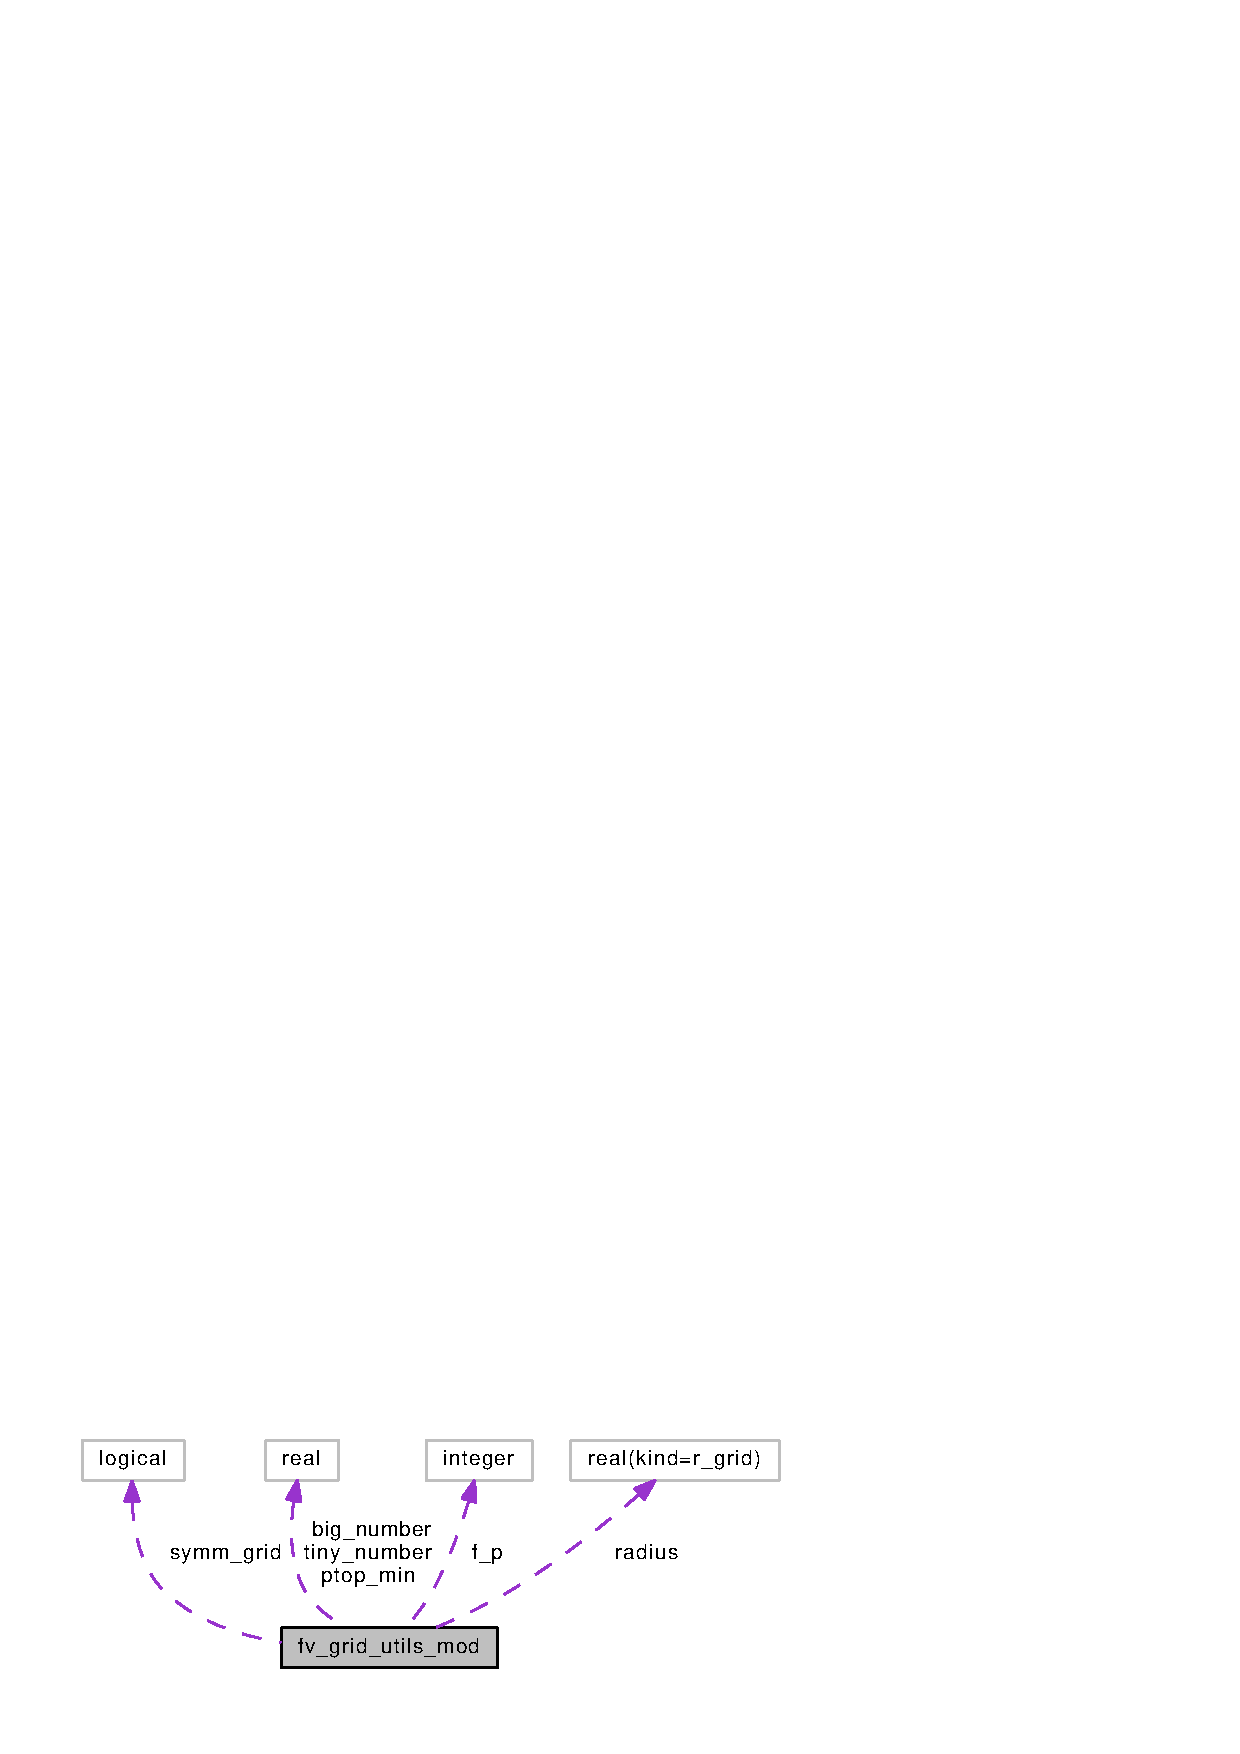
\includegraphics[width=350pt]{classfv__grid__utils__mod__coll__graph}
\end{center}
\end{figure}
\subsection*{Data Types}
\begin{DoxyCompactItemize}
\item 
interface \hyperlink{interfacefv__grid__utils__mod_1_1fill__ghost}{fill\-\_\-ghost}
\end{DoxyCompactItemize}
\subsection*{Public Member Functions}
\begin{DoxyCompactItemize}
\item 
subroutine, public \hyperlink{classfv__grid__utils__mod_aaa8f8fb3b9726914e96ab905b0bfbdc2}{grid\-\_\-utils\-\_\-init} (Atm, npx, npy, npz, non\-\_\-ortho, grid\-\_\-type, c2l\-\_\-order)
\item 
subroutine, public \hyperlink{classfv__grid__utils__mod_adb11ef287b3b75568f3648d3984e3b33}{grid\-\_\-utils\-\_\-end}
\item 
subroutine, public \hyperlink{classfv__grid__utils__mod_adc930675e4ce60effc5d7b2f34b21ed5}{direct\-\_\-transform} (c, i1, i2, j1, j2, lon\-\_\-p, lat\-\_\-p, n, lon, lat)
\begin{DoxyCompactList}\small\item\em The subroutine 'direct\-\_\-transform' performs a direct transformation of the standard (symmetrical) cubic grid to a locally enhanced high-\/res grid on the sphere. \end{DoxyCompactList}\item 
real function, public \hyperlink{classfv__grid__utils__mod_a9e4bf88962e6eecc388ca075e641d13f}{inner\-\_\-prod} (v1, v2)
\item 
subroutine, public \hyperlink{classfv__grid__utils__mod_a3fc07f828529992d0efe95fbd361254c}{gnomonic\-\_\-grids} (grid\-\_\-type, im, lon, lat)
\item 
subroutine, public \hyperlink{classfv__grid__utils__mod_a175b576930b1aabccbdc22918e3eabe7}{latlon2xyz} (p, e, id)
\begin{DoxyCompactList}\small\item\em The subroutine 'latlon2xyz' maps (lon, lat) to (x,y,z) \end{DoxyCompactList}\item 
subroutine, public \hyperlink{classfv__grid__utils__mod_a85755bc87f196f58a1c8af1b4af9b2ac}{cart\-\_\-to\-\_\-latlon} (np, q, xs, ys)
\item 
subroutine, public \hyperlink{classfv__grid__utils__mod_a685f32d9d18924cf1e743f96b1dbe493}{vect\-\_\-cross} (e, p1, p2)
\begin{DoxyCompactList}\small\item\em The subroutine 'vect\-\_\-cross performs cross products of 3\-D vectors\-: e = P1 X P2. \end{DoxyCompactList}\item 
subroutine, public \hyperlink{classfv__grid__utils__mod_a092aabe65224216e6209babe7f15669e}{get\-\_\-unit\-\_\-vect2} (e1, e2, uc)
\item 
subroutine, public \hyperlink{classfv__grid__utils__mod_a3fedbacc4264bbd4d209d089a059b14c}{normalize\-\_\-vect} (e)
\begin{DoxyCompactList}\small\item\em The subroutine 'normalize\-\_\-vect' makes 'e' a unit vector. \end{DoxyCompactList}\item 
subroutine, public \hyperlink{classfv__grid__utils__mod_ae1173a7fe794cee15b8b50a6b4d3cb9e}{intp\-\_\-great\-\_\-circle} (beta, p1, p2, x\-\_\-o, y\-\_\-o)
\item 
subroutine, public \hyperlink{classfv__grid__utils__mod_adfe8284f08a2363ce2d21dbc79ad3d98}{spherical\-\_\-linear\-\_\-interpolation} (beta, p1, p2, pb)
\begin{DoxyCompactList}\small\item\em The subroutine 'spherical\-\_\-linear\-\_\-interpolation' interpolates along the great circle connecting points p1 and p2. \end{DoxyCompactList}\item 
subroutine, public \hyperlink{classfv__grid__utils__mod_a18ebcb54063bc4dc159f2a87771d4358}{mid\-\_\-pt\-\_\-sphere} (p1, p2, pm)
\item 
subroutine, public \hyperlink{classfv__grid__utils__mod_a4fc34e04ba263d5a514aa0d631871e8b}{mid\-\_\-pt\-\_\-cart} (p1, p2, e3)
\item 
real function, public \hyperlink{classfv__grid__utils__mod_ad3ca2b1362f0c6fe83b7cd28d4c67784}{great\-\_\-circle\-\_\-dist} (q1, q2, \hyperlink{classfv__grid__utils__mod_a9825bfea45f13a48cc658a3df88d3124}{radius})
\item 
subroutine, public \hyperlink{classfv__grid__utils__mod_a650900ea3f50071fb0743d5560dcaaf8}{unit\-\_\-vect\-\_\-latlon} (pp, elon, elat)
\item 
real(kind=R\-\_\-\-G\-R\-I\-D) function, public \hyperlink{classfv__grid__utils__mod_a22e29af5ace7233c29974f0189300fb9}{v\-\_\-prod} (v1, v2)
\item 
subroutine, public \hyperlink{classfv__grid__utils__mod_a41d77310cefec9ce0f98f0afe2440d67}{cubed\-\_\-to\-\_\-latlon} (u, v, ua, va, gridstruct, npx, npy, km, mode, grid\-\_\-type, domain, nested, c2l\-\_\-ord, bd)
\item 
subroutine, public \hyperlink{classfv__grid__utils__mod_a8fa9923988d7afeb54c67bf5a92777bc}{c2l\-\_\-ord2} (u, v, ua, va, gridstruct, km, grid\-\_\-type, bd, do\-\_\-halo)
\item 
subroutine, public \hyperlink{classfv__grid__utils__mod_ab160a0e2cf47c2dfc388760a5ef44088}{expand\-\_\-cell} (q1, q2, q3, q4, a1, a2, a3, a4, fac)
\item 
subroutine, public \hyperlink{classfv__grid__utils__mod_acd269ab71691330f8b1abd0f3d939b8f}{cell\-\_\-center2} (q1, q2, q3, q4, e2)
\item 
real(kind=R\-\_\-\-G\-R\-I\-D) function, public \hyperlink{classfv__grid__utils__mod_a8feb2769227e59666678485759eaa734}{get\-\_\-area} (p1, p4, p2, p3, \hyperlink{classfv__grid__utils__mod_a9825bfea45f13a48cc658a3df88d3124}{radius})
\item 
real(kind=r\-\_\-grid) function, public \hyperlink{classfv__grid__utils__mod_a585eb851f9d447a4cad1f7787885cf95}{dist2side\-\_\-latlon} (v1, v2, point)
\begin{DoxyCompactList}\small\item\em The function 'dist2side\-\_\-latlon' is the version of 'dist2side' that takes points in latitude-\/longitude coordinates. \end{DoxyCompactList}\item 
real(kind=R\-\_\-\-G\-R\-I\-D) function, public \hyperlink{classfv__grid__utils__mod_a917846d8ea59488d86f6c1915005fa6d}{spherical\-\_\-angle} (p1, p2, p3)
\item 
real(kind=R\-\_\-\-G\-R\-I\-D) function, public \hyperlink{classfv__grid__utils__mod_aac790b318f173e5ae56e8c4693342ced}{cos\-\_\-angle} (p1, p2, p3)
\item 
real function, public \hyperlink{classfv__grid__utils__mod_acf53e76b1bc9e689efe4900919cd05ef}{g\-\_\-sum} (domain, p, ifirst, ilast, jfirst, jlast, ngc, area, mode, reproduce)
\begin{DoxyCompactList}\small\item\em The function 'g\-\_\-sum' is the fast version of 'globalsum'. \end{DoxyCompactList}\item 
real function, public \hyperlink{classfv__grid__utils__mod_acb84df3b3d185ec7c0158eb595fb61e2}{global\-\_\-qsum} (p, ifirst, ilast, jfirst, jlast)
\begin{DoxyCompactList}\small\item\em The function 'global\-\_\-qsum' computes the quick global sum without area weighting. \end{DoxyCompactList}\item 
subroutine, public \hyperlink{classfv__grid__utils__mod_acfadec31f0ae9c244867d2055922ad81}{global\-\_\-mx} (q, n\-\_\-g, qmin, qmax, bd)
\item 
subroutine, public \hyperlink{classfv__grid__utils__mod_a160d6add1771f6ad1b64c0ec5f46e053}{make\-\_\-eta\-\_\-level} (km, pe, area, kks, ak, bk, ptop, domain, bd)
\item 
subroutine, public \hyperlink{classfv__grid__utils__mod_a6a6f485efd42e62b7eeb21509b0200cf}{get\-\_\-latlon\-\_\-vector} (pp, elon, elat)
\item 
subroutine, public \hyperlink{classfv__grid__utils__mod_aad0953473a601f3e18b5d6301b6fae17}{project\-\_\-sphere\-\_\-v} (np, f, e)
\end{DoxyCompactItemize}
\subsection*{Public Attributes}
\begin{DoxyCompactItemize}
\item 
logical, public \hyperlink{classfv__grid__utils__mod_a5bf65a4c81568a1f4d7e893be47655a1}{symm\-\_\-grid}
\item 
integer, parameter, public \hyperlink{classfv__grid__utils__mod_a72968a7b4fccc9953a595a4efe712cad}{f\-\_\-p} = selected\-\_\-real\-\_\-kind(20)
\item 
real, parameter, public \hyperlink{classfv__grid__utils__mod_a2152e3d84a5c3e50b27ea7fabeb16580}{big\-\_\-number} =1.d8
\item 
real, parameter, public \hyperlink{classfv__grid__utils__mod_a8363bc8f261396e37744efbbfa91fb7d}{ptop\-\_\-min} =1.d-\/8
\end{DoxyCompactItemize}
\subsection*{Private Member Functions}
\begin{DoxyCompactItemize}
\item 
subroutine \hyperlink{classfv__grid__utils__mod_abec573b8aae9cac154188a3563b86708}{efactor\-\_\-a2c\-\_\-v} (edge\-\_\-vect\-\_\-s, edge\-\_\-vect\-\_\-n, edge\-\_\-vect\-\_\-w, edge\-\_\-vect\-\_\-e, non\-\_\-ortho, grid, agrid, npx, npy, nested, bd, regional)
\begin{DoxyCompactList}\small\item\em The subroutine 'efactor\-\_\-a2c\-\_\-v' initializes interpolation factors at face edges for interpolating vectors from A to C grid. \end{DoxyCompactList}\item 
subroutine \hyperlink{classfv__grid__utils__mod_acc865cb7b598fbb8a3706f3fe16c6707}{edge\-\_\-factors} (edge\-\_\-s, edge\-\_\-n, edge\-\_\-w, edge\-\_\-e, non\-\_\-ortho, grid, agrid, npx, npy, bd)
\begin{DoxyCompactList}\small\item\em The subroutine 'edge\-\_\-factors' initializes interpolation factors at face edges for interpolation from A to B grid. \end{DoxyCompactList}\item 
subroutine \hyperlink{classfv__grid__utils__mod_ad7cee44eb2dee1b439e42435af81cf4a}{gnomonic\-\_\-ed} (im, lamda, theta)
\begin{DoxyCompactList}\small\item\em The subroutine 'gnomonic\-\_\-ed' computes the equal distances along the 4 edges of the cubed sphere. \end{DoxyCompactList}\item 
subroutine \hyperlink{classfv__grid__utils__mod_a654a62678c1c5abc701da989d55f7f8a}{gnomonic\-\_\-ed\-\_\-limited} (im, in, nghost, l\-L, l\-R, u\-L, u\-R, lamda, theta)
\begin{DoxyCompactList}\small\item\em The subroutine 'gnomonic\-\_\-ed\-\_\-limited' creates a limited-\/area equidistant gnomonic grid with corners given by l\-L (lower-\/left), l\-R (lower-\/right), u\-L (upper-\/left),and u\-R (upper-\/right) with im by in cells. \end{DoxyCompactList}\item 
subroutine \hyperlink{classfv__grid__utils__mod_a8d78db3da56dcabdfb0a878dfa6072da}{gnomonic\-\_\-angl} (im, lamda, theta)
\item 
subroutine \hyperlink{classfv__grid__utils__mod_aa623c32b277db71d89bc8cb08ee516e7}{gnomonic\-\_\-dist} (im, lamda, theta)
\item 
subroutine \hyperlink{classfv__grid__utils__mod_ae7d3472ec567a8e2c2e903c6ac4ea76a}{symm\-\_\-ed} (im, lamda, theta)
\item 
subroutine \hyperlink{classfv__grid__utils__mod_a77621e212e7499d962d229c963e59845}{latlon2xyz2} (lon, lat, p3)
\item 
subroutine \hyperlink{classfv__grid__utils__mod_aa1a6a80b21abe2b3bf38503986d70dab}{mirror\-\_\-xyz} (p1, p2, p0, p)
\begin{DoxyCompactList}\small\item\em The subroutine 'mirror\-\_\-xyz' computes the mirror image of p0(x0, y0, z0) as p(x, y, z) given the \char`\"{}mirror\char`\"{} as defined by p1(x1, y1, z1), p2(x2, y2, z2), and the center of the sphere. \end{DoxyCompactList}\item 
subroutine \hyperlink{classfv__grid__utils__mod_a80ae6d53a5af90d7cfbccb3a84089ded}{mirror\-\_\-latlon} (lon1, lat1, lon2, lat2, lon0, lat0, lon3, lat3)
\begin{DoxyCompactList}\small\item\em The subroutine 'mirror\-\_\-latlon' computes the mirror image of (lon0, lat0) as (lon3, lat3) given the \char`\"{}mirror\char`\"{} as defined by (lon1, lat1), (lon2, lat2), and center of the sphere. \end{DoxyCompactList}\item 
subroutine \hyperlink{classfv__grid__utils__mod_a27edcd37dde6bcb21f63e8ce4707461f}{get\-\_\-center\-\_\-vect} (npx, npy, pp, u1, u2, bd)
\item 
subroutine \hyperlink{classfv__grid__utils__mod_a881df1c93c5a86930c8375ee74bb4c27}{get\-\_\-unit\-\_\-vect3} (p1, p2, uc)
\item 
subroutine \hyperlink{classfv__grid__utils__mod_ade00327ae5be7ddd3f1bafc9ff4ee18a}{mid\-\_\-pt3\-\_\-cart} (p1, p2, e)
\item 
real(kind=r\-\_\-grid) function \hyperlink{classfv__grid__utils__mod_ab6684ce79354424c32c3495b9ae6ef23}{great\-\_\-circle\-\_\-dist\-\_\-cart} (v1, v2, \hyperlink{classfv__grid__utils__mod_a9825bfea45f13a48cc658a3df88d3124}{radius})
\begin{DoxyCompactList}\small\item\em The function 'great\-\_\-circle\-\_\-dist\-\_\-cart' calculates the normalized great circle distance between 'v1' and 'v2'. \end{DoxyCompactList}\item 
subroutine \hyperlink{classfv__grid__utils__mod_a10afa14f31dd7e7622e61232b98446b2}{intersect} (a1, a2, b1, b2, \hyperlink{classfv__grid__utils__mod_a9825bfea45f13a48cc658a3df88d3124}{radius}, x\-\_\-inter, local\-\_\-a, local\-\_\-b)
\begin{DoxyCompactList}\small\item\em The subroutine 'intersect' calculates the intersection of two great circles. \end{DoxyCompactList}\item 
subroutine \hyperlink{classfv__grid__utils__mod_a323c000d99398ede87cd2b258510c96a}{intersect\-\_\-cross} (a1, a2, b1, b2, \hyperlink{classfv__grid__utils__mod_a9825bfea45f13a48cc658a3df88d3124}{radius}, x\-\_\-inter, local\-\_\-a, local\-\_\-b)
\begin{DoxyCompactList}\small\item\em The subroutine 'intersect\-\_\-cross' calculates the intersection of two great circles. \end{DoxyCompactList}\item 
subroutine \hyperlink{classfv__grid__utils__mod_ab691211ffcead13f38d0f82f80024cb2}{init\-\_\-cubed\-\_\-to\-\_\-latlon} (gridstruct, hydrostatic, agrid, grid\-\_\-type, ord, bd)
\item 
subroutine \hyperlink{classfv__grid__utils__mod_ad407af52a37c085d51cc9fae002c6768}{c2l\-\_\-ord4} (u, v, ua, va, gridstruct, npx, npy, km, grid\-\_\-type, domain, nested, mode, bd)
\item 
subroutine \hyperlink{classfv__grid__utils__mod_a0952821694859a7fca0ed15405e49c97}{cell\-\_\-center3} (p1, p2, p3, p4, ec)
\begin{DoxyCompactList}\small\item\em The subroutine 'cell\-\_\-center3' gets the center position of a cell. \end{DoxyCompactList}\item 
real(kind=r\-\_\-grid) function \hyperlink{classfv__grid__utils__mod_ada074199448cb8b1552daaa881561006}{dist2side} (v1, v2, point)
\begin{DoxyCompactList}\small\item\em The function 'dist2side' calculates the shortest normalized distance on a sphere from point to straight line defined by 'v1' and 'v2'. \end{DoxyCompactList}\item 
subroutine \hyperlink{classfv__grid__utils__mod_a81e92ff31b90aa12545bba76526bc9fd}{global\-\_\-mx\-\_\-c} (q, i1, i2, j1, j2, qmin, qmax)
\begin{DoxyCompactList}\small\item\em The subroutine 'global\-\_\-mx\-\_\-c' computes the global max and min at the cell corners. \end{DoxyCompactList}\item 
subroutine \hyperlink{classfv__grid__utils__mod_a2fe5c8bfcdaf2375a8dd4047cd148326}{fill\-\_\-ghost\-\_\-r8} (q, npx, npy, value, bd)
\item 
subroutine \hyperlink{classfv__grid__utils__mod_a0429313efafc9366ffdd147df45a5585}{invert\-\_\-matrix} (n, a, x)
\item 
subroutine \hyperlink{classfv__grid__utils__mod_aa91273704cafe57dc9fa77eeb2a1f63c}{elgs} (a, n, indx)
\begin{DoxyCompactList}\small\item\em The subroutine 'elgs' performs the partial-\/pivoting gaussian elimination. \end{DoxyCompactList}\end{DoxyCompactItemize}
\subsection*{Private Attributes}
\begin{DoxyCompactItemize}
\item 
real, parameter \hyperlink{classfv__grid__utils__mod_a800597e665792a2ca112d3db14ae3c4c}{tiny\-\_\-number} =1.d-\/8
\item 
real(kind=r\-\_\-grid) \hyperlink{classfv__grid__utils__mod_a9825bfea45f13a48cc658a3df88d3124}{radius} =cnst\-\_\-radius
\end{DoxyCompactItemize}


\subsection{Detailed Description}
The module 'fv\-\_\-grid\-\_\-utils' contains routines for setting up and computing grid-\/related quantities. 

Many of these are useful for computing diagnostics or setting up initial conditions. 

Definition at line 26 of file fv\-\_\-grid\-\_\-utils.\-F90.



\subsection{Member Function/\-Subroutine Documentation}
\index{fv\-\_\-grid\-\_\-utils\-\_\-mod@{fv\-\_\-grid\-\_\-utils\-\_\-mod}!c2l\-\_\-ord2@{c2l\-\_\-ord2}}
\index{c2l\-\_\-ord2@{c2l\-\_\-ord2}!fv_grid_utils_mod@{fv\-\_\-grid\-\_\-utils\-\_\-mod}}
\subsubsection[{c2l\-\_\-ord2}]{\setlength{\rightskip}{0pt plus 5cm}subroutine, public fv\-\_\-grid\-\_\-utils\-\_\-mod\-::c2l\-\_\-ord2 (
\begin{DoxyParamCaption}
\item[{real, dimension(bd\%isd\-:bd\%ied,bd\%jsd\-:bd\%jed+1,km), intent(in)}]{u, }
\item[{real, dimension(bd\%isd\-:bd\%ied+1,bd\%jsd\-:bd\%jed,km), intent(in)}]{v, }
\item[{real, dimension(bd\%isd\-:bd\%ied, bd\%jsd\-:bd\%jed,km), intent(out)}]{ua, }
\item[{real, dimension(bd\%isd\-:bd\%ied, bd\%jsd\-:bd\%jed,km), intent(out)}]{va, }
\item[{type(fv\-\_\-grid\-\_\-type), intent(in), target}]{gridstruct, }
\item[{integer, intent(in)}]{km, }
\item[{integer, intent(in)}]{grid\-\_\-type, }
\item[{type(fv\-\_\-grid\-\_\-bounds\-\_\-type), intent(in)}]{bd, }
\item[{logical, intent(in)}]{do\-\_\-halo}
\end{DoxyParamCaption}
)}\label{classfv__grid__utils__mod_a8fa9923988d7afeb54c67bf5a92777bc}


Definition at line 2506 of file fv\-\_\-grid\-\_\-utils.\-F90.



Referenced by fv\-\_\-dynamics\-\_\-mod\-::compute\-\_\-aam(), cubed\-\_\-to\-\_\-latlon(), fv\-\_\-dynamics\-\_\-mod\-::rayleigh\-\_\-friction(), and fv\-\_\-dynamics\-\_\-mod\-::rayleigh\-\_\-super().

\index{fv\-\_\-grid\-\_\-utils\-\_\-mod@{fv\-\_\-grid\-\_\-utils\-\_\-mod}!c2l\-\_\-ord4@{c2l\-\_\-ord4}}
\index{c2l\-\_\-ord4@{c2l\-\_\-ord4}!fv_grid_utils_mod@{fv\-\_\-grid\-\_\-utils\-\_\-mod}}
\subsubsection[{c2l\-\_\-ord4}]{\setlength{\rightskip}{0pt plus 5cm}subroutine fv\-\_\-grid\-\_\-utils\-\_\-mod\-::c2l\-\_\-ord4 (
\begin{DoxyParamCaption}
\item[{real, dimension(bd\%isd\-:bd\%ied,bd\%jsd\-:bd\%jed+1,km), intent(inout)}]{u, }
\item[{real, dimension(bd\%isd\-:bd\%ied+1,bd\%jsd\-:bd\%jed,km), intent(inout)}]{v, }
\item[{real, dimension(bd\%isd\-:bd\%ied, bd\%jsd\-:bd\%jed,km), intent(out)}]{ua, }
\item[{real, dimension(bd\%isd\-:bd\%ied, bd\%jsd\-:bd\%jed,km), intent(out)}]{va, }
\item[{type(fv\-\_\-grid\-\_\-type), intent(in), target}]{gridstruct, }
\item[{integer, intent(in)}]{npx, }
\item[{integer, intent(in)}]{npy, }
\item[{integer, intent(in)}]{km, }
\item[{integer, intent(in)}]{grid\-\_\-type, }
\item[{type(domain2d), intent(inout)}]{domain, }
\item[{logical, intent(in)}]{nested, }
\item[{integer, intent(in)}]{mode, }
\item[{type(fv\-\_\-grid\-\_\-bounds\-\_\-type), intent(in)}]{bd}
\end{DoxyParamCaption}
)\hspace{0.3cm}{\ttfamily [private]}}\label{classfv__grid__utils__mod_ad407af52a37c085d51cc9fae002c6768}


Definition at line 2366 of file fv\-\_\-grid\-\_\-utils.\-F90.



References fv\-\_\-timing\-\_\-mod\-::timing\-\_\-off(), and fv\-\_\-timing\-\_\-mod\-::timing\-\_\-on().



Referenced by cubed\-\_\-to\-\_\-latlon().

\index{fv\-\_\-grid\-\_\-utils\-\_\-mod@{fv\-\_\-grid\-\_\-utils\-\_\-mod}!cart\-\_\-to\-\_\-latlon@{cart\-\_\-to\-\_\-latlon}}
\index{cart\-\_\-to\-\_\-latlon@{cart\-\_\-to\-\_\-latlon}!fv_grid_utils_mod@{fv\-\_\-grid\-\_\-utils\-\_\-mod}}
\subsubsection[{cart\-\_\-to\-\_\-latlon}]{\setlength{\rightskip}{0pt plus 5cm}subroutine, public fv\-\_\-grid\-\_\-utils\-\_\-mod\-::cart\-\_\-to\-\_\-latlon (
\begin{DoxyParamCaption}
\item[{integer, intent(in)}]{np, }
\item[{real(kind=r\-\_\-grid), dimension(3,np), intent(inout)}]{q, }
\item[{real(kind=r\-\_\-grid), dimension(np), intent(inout)}]{xs, }
\item[{real(kind=r\-\_\-grid), dimension(np), intent(inout)}]{ys}
\end{DoxyParamCaption}
)}\label{classfv__grid__utils__mod_a85755bc87f196f58a1c8af1b4af9b2ac}


Definition at line 1715 of file fv\-\_\-grid\-\_\-utils.\-F90.



Referenced by cell\-\_\-center2(), expand\-\_\-cell(), gnomonic\-\_\-angl(), gnomonic\-\_\-dist(), gnomonic\-\_\-ed(), gnomonic\-\_\-ed\-\_\-limited(), test\-\_\-cases\-\_\-mod\-::init\-\_\-case(), intp\-\_\-great\-\_\-circle(), mid\-\_\-pt\-\_\-sphere(), mirror\-\_\-latlon(), and spherical\-\_\-linear\-\_\-interpolation().

\index{fv\-\_\-grid\-\_\-utils\-\_\-mod@{fv\-\_\-grid\-\_\-utils\-\_\-mod}!cell\-\_\-center2@{cell\-\_\-center2}}
\index{cell\-\_\-center2@{cell\-\_\-center2}!fv_grid_utils_mod@{fv\-\_\-grid\-\_\-utils\-\_\-mod}}
\subsubsection[{cell\-\_\-center2}]{\setlength{\rightskip}{0pt plus 5cm}subroutine, public fv\-\_\-grid\-\_\-utils\-\_\-mod\-::cell\-\_\-center2 (
\begin{DoxyParamCaption}
\item[{real(kind=r\-\_\-grid), dimension(2), intent(in)}]{q1, }
\item[{real(kind=r\-\_\-grid), dimension(2), intent(in)}]{q2, }
\item[{real(kind=r\-\_\-grid), dimension(2), intent(in)}]{q3, }
\item[{real(kind=r\-\_\-grid), dimension(2), intent(in)}]{q4, }
\item[{real(kind=r\-\_\-grid), dimension(2), intent(out)}]{e2}
\end{DoxyParamCaption}
)}\label{classfv__grid__utils__mod_acd269ab71691330f8b1abd0f3d939b8f}


Definition at line 2659 of file fv\-\_\-grid\-\_\-utils.\-F90.



References cart\-\_\-to\-\_\-latlon(), and latlon2xyz().



Referenced by fv\-\_\-grid\-\_\-tools\-\_\-mod\-::init\-\_\-grid(), read\-\_\-regional\-\_\-lon\-\_\-lat(), fv\-\_\-regional\-\_\-mod\-::regional\-\_\-bc\-\_\-data(), and setup\-\_\-aligned\-\_\-nest().

\index{fv\-\_\-grid\-\_\-utils\-\_\-mod@{fv\-\_\-grid\-\_\-utils\-\_\-mod}!cell\-\_\-center3@{cell\-\_\-center3}}
\index{cell\-\_\-center3@{cell\-\_\-center3}!fv_grid_utils_mod@{fv\-\_\-grid\-\_\-utils\-\_\-mod}}
\subsubsection[{cell\-\_\-center3}]{\setlength{\rightskip}{0pt plus 5cm}subroutine fv\-\_\-grid\-\_\-utils\-\_\-mod\-::cell\-\_\-center3 (
\begin{DoxyParamCaption}
\item[{real(kind=r\-\_\-grid), dimension(3), intent(in)}]{p1, }
\item[{real(kind=r\-\_\-grid), dimension(3), intent(in)}]{p2, }
\item[{real(kind=r\-\_\-grid), dimension(3), intent(in)}]{p3, }
\item[{real(kind=r\-\_\-grid), dimension(3), intent(in)}]{p4, }
\item[{real(kind=r\-\_\-grid), dimension(kind=r\-\_\-grid), intent(out)}]{ec}
\end{DoxyParamCaption}
)\hspace{0.3cm}{\ttfamily [private]}}\label{classfv__grid__utils__mod_a0952821694859a7fca0ed15405e49c97}


The subroutine 'cell\-\_\-center3' gets the center position of a cell. 



Definition at line 2687 of file fv\-\_\-grid\-\_\-utils.\-F90.



Referenced by get\-\_\-center\-\_\-vect().

\index{fv\-\_\-grid\-\_\-utils\-\_\-mod@{fv\-\_\-grid\-\_\-utils\-\_\-mod}!cos\-\_\-angle@{cos\-\_\-angle}}
\index{cos\-\_\-angle@{cos\-\_\-angle}!fv_grid_utils_mod@{fv\-\_\-grid\-\_\-utils\-\_\-mod}}
\subsubsection[{cos\-\_\-angle}]{\setlength{\rightskip}{0pt plus 5cm}real(kind=R\-\_\-\-G\-R\-I\-D) function, public fv\-\_\-grid\-\_\-utils\-\_\-mod\-::cos\-\_\-angle (
\begin{DoxyParamCaption}
\item[{real(kind=r\-\_\-grid), dimension(3), intent(in)}]{p1, }
\item[{real(kind=r\-\_\-grid), dimension(3), intent(in)}]{p2, }
\item[{real(kind=r\-\_\-grid), dimension(3), intent(in)}]{p3}
\end{DoxyParamCaption}
)}\label{classfv__grid__utils__mod_aac790b318f173e5ae56e8c4693342ced}


Definition at line 2854 of file fv\-\_\-grid\-\_\-utils.\-F90.



Referenced by grid\-\_\-utils\-\_\-init().

\index{fv\-\_\-grid\-\_\-utils\-\_\-mod@{fv\-\_\-grid\-\_\-utils\-\_\-mod}!cubed\-\_\-to\-\_\-latlon@{cubed\-\_\-to\-\_\-latlon}}
\index{cubed\-\_\-to\-\_\-latlon@{cubed\-\_\-to\-\_\-latlon}!fv_grid_utils_mod@{fv\-\_\-grid\-\_\-utils\-\_\-mod}}
\subsubsection[{cubed\-\_\-to\-\_\-latlon}]{\setlength{\rightskip}{0pt plus 5cm}subroutine, public fv\-\_\-grid\-\_\-utils\-\_\-mod\-::cubed\-\_\-to\-\_\-latlon (
\begin{DoxyParamCaption}
\item[{real, dimension(bd\%isd\-:bd\%ied,bd\%jsd\-:bd\%jed+1,km), intent(inout)}]{u, }
\item[{real, dimension(bd\%isd\-:bd\%ied+1,bd\%jsd\-:bd\%jed,km), intent(inout)}]{v, }
\item[{real, dimension(bd\%isd\-:bd\%ied, bd\%jsd\-:bd\%jed,km), intent(out)}]{ua, }
\item[{real, dimension(bd\%isd\-:bd\%ied, bd\%jsd\-:bd\%jed,km), intent(out)}]{va, }
\item[{type(fv\-\_\-grid\-\_\-type), intent(in)}]{gridstruct, }
\item[{integer, intent(in)}]{npx, }
\item[{integer, intent(in)}]{npy, }
\item[{integer, intent(in)}]{km, }
\item[{integer, intent(in)}]{mode, }
\item[{integer, intent(in)}]{grid\-\_\-type, }
\item[{type(domain2d), intent(inout)}]{domain, }
\item[{logical, intent(in)}]{nested, }
\item[{integer, intent(in)}]{c2l\-\_\-ord, }
\item[{type(fv\-\_\-grid\-\_\-bounds\-\_\-type), intent(in)}]{bd}
\end{DoxyParamCaption}
)}\label{classfv__grid__utils__mod_a41d77310cefec9ce0f98f0afe2440d67}


Definition at line 2345 of file fv\-\_\-grid\-\_\-utils.\-F90.



References c2l\-\_\-ord2(), and c2l\-\_\-ord4().



Referenced by fv\-\_\-nesting\-\_\-mod\-::after\-\_\-twoway\-\_\-nest\-\_\-update(), fv\-\_\-dynamics\-\_\-mod\-::fv\-\_\-dynamics(), fv\-\_\-restart\-\_\-mod\-::fv\-\_\-restart(), fv\-\_\-update\-\_\-phys\-\_\-mod\-::fv\-\_\-update\-\_\-phys(), and test\-\_\-cases\-\_\-mod\-::pmxn().

\index{fv\-\_\-grid\-\_\-utils\-\_\-mod@{fv\-\_\-grid\-\_\-utils\-\_\-mod}!direct\-\_\-transform@{direct\-\_\-transform}}
\index{direct\-\_\-transform@{direct\-\_\-transform}!fv_grid_utils_mod@{fv\-\_\-grid\-\_\-utils\-\_\-mod}}
\subsubsection[{direct\-\_\-transform}]{\setlength{\rightskip}{0pt plus 5cm}subroutine, public fv\-\_\-grid\-\_\-utils\-\_\-mod\-::direct\-\_\-transform (
\begin{DoxyParamCaption}
\item[{real(kind=r\-\_\-grid), intent(in)}]{c, }
\item[{integer, intent(in)}]{i1, }
\item[{integer, intent(in)}]{i2, }
\item[{integer, intent(in)}]{j1, }
\item[{integer, intent(in)}]{j2, }
\item[{real(kind=r\-\_\-grid), intent(in)}]{lon\-\_\-p, }
\item[{real(kind=r\-\_\-grid), intent(in)}]{lat\-\_\-p, }
\item[{integer, intent(in)}]{n, }
\item[{real(kind=r\-\_\-grid), dimension(i1\-:i2,j1\-:j2), intent(inout)}]{lon, }
\item[{real(kind=r\-\_\-grid), dimension(i1\-:i2,j1\-:j2), intent(inout)}]{lat}
\end{DoxyParamCaption}
)}\label{classfv__grid__utils__mod_adc930675e4ce60effc5d7b2f34b21ed5}


The subroutine 'direct\-\_\-transform' performs a direct transformation of the standard (symmetrical) cubic grid to a locally enhanced high-\/res grid on the sphere. 

It is an application of the Schmidt transformation at the south pole followed by a pole\-\_\-shift\-\_\-to\-\_\-target (rotation) operation.


\begin{DoxyParams}[1]{Parameters}
\mbox{\tt in}  & {\em c} & Stretching factor\\
\hline
\mbox{\tt in}  & {\em lat\-\_\-p} & center location of the target face, radian\\
\hline
\mbox{\tt in}  & {\em n} & grid face number \\
\hline
\end{DoxyParams}


Definition at line 917 of file fv\-\_\-grid\-\_\-utils.\-F90.



Referenced by fv\-\_\-grid\-\_\-tools\-\_\-mod\-::init\-\_\-grid().

\index{fv\-\_\-grid\-\_\-utils\-\_\-mod@{fv\-\_\-grid\-\_\-utils\-\_\-mod}!dist2side@{dist2side}}
\index{dist2side@{dist2side}!fv_grid_utils_mod@{fv\-\_\-grid\-\_\-utils\-\_\-mod}}
\subsubsection[{dist2side}]{\setlength{\rightskip}{0pt plus 5cm}real(kind=r\-\_\-grid) function fv\-\_\-grid\-\_\-utils\-\_\-mod\-::dist2side (
\begin{DoxyParamCaption}
\item[{real(kind=r\-\_\-grid), dimension(3), intent(in)}]{v1, }
\item[{real(kind=r\-\_\-grid), dimension(3), intent(in)}]{v2, }
\item[{real(kind=r\-\_\-grid), dimension(3), intent(in)}]{point}
\end{DoxyParamCaption}
)\hspace{0.3cm}{\ttfamily [private]}}\label{classfv__grid__utils__mod_ada074199448cb8b1552daaa881561006}


The function 'dist2side' calculates the shortest normalized distance on a sphere from point to straight line defined by 'v1' and 'v2'. 

This version uses cartesian coordinates. \begin{DoxyDate}{Date}
Feb 2007 
\end{DoxyDate}
\begin{DoxyVersion}{Version}
0.\-1 
\end{DoxyVersion}


Definition at line 2755 of file fv\-\_\-grid\-\_\-utils.\-F90.



References great\-\_\-circle\-\_\-dist\-\_\-cart(), and spherical\-\_\-angle().

\index{fv\-\_\-grid\-\_\-utils\-\_\-mod@{fv\-\_\-grid\-\_\-utils\-\_\-mod}!dist2side\-\_\-latlon@{dist2side\-\_\-latlon}}
\index{dist2side\-\_\-latlon@{dist2side\-\_\-latlon}!fv_grid_utils_mod@{fv\-\_\-grid\-\_\-utils\-\_\-mod}}
\subsubsection[{dist2side\-\_\-latlon}]{\setlength{\rightskip}{0pt plus 5cm}real(kind=r\-\_\-grid) function, public fv\-\_\-grid\-\_\-utils\-\_\-mod\-::dist2side\-\_\-latlon (
\begin{DoxyParamCaption}
\item[{real(kind=r\-\_\-grid), dimension(2), intent(in)}]{v1, }
\item[{real(kind=r\-\_\-grid), dimension(2), intent(in)}]{v2, }
\item[{real(kind=r\-\_\-grid), dimension(2), intent(in)}]{point}
\end{DoxyParamCaption}
)}\label{classfv__grid__utils__mod_a585eb851f9d447a4cad1f7787885cf95}


The function 'dist2side\-\_\-latlon' is the version of 'dist2side' that takes points in latitude-\/longitude coordinates. 



Definition at line 2769 of file fv\-\_\-grid\-\_\-utils.\-F90.



References great\-\_\-circle\-\_\-dist(), latlon2xyz(), and spherical\-\_\-angle().



Referenced by setup\-\_\-aligned\-\_\-nest().

\index{fv\-\_\-grid\-\_\-utils\-\_\-mod@{fv\-\_\-grid\-\_\-utils\-\_\-mod}!edge\-\_\-factors@{edge\-\_\-factors}}
\index{edge\-\_\-factors@{edge\-\_\-factors}!fv_grid_utils_mod@{fv\-\_\-grid\-\_\-utils\-\_\-mod}}
\subsubsection[{edge\-\_\-factors}]{\setlength{\rightskip}{0pt plus 5cm}subroutine fv\-\_\-grid\-\_\-utils\-\_\-mod\-::edge\-\_\-factors (
\begin{DoxyParamCaption}
\item[{real(kind=r\-\_\-grid), dimension(npx), intent(inout)}]{edge\-\_\-s, }
\item[{real(kind=r\-\_\-grid), dimension(npx), intent(inout)}]{edge\-\_\-n, }
\item[{real(kind=r\-\_\-grid), dimension(npy), intent(inout)}]{edge\-\_\-w, }
\item[{real(kind=r\-\_\-grid), dimension(npy), intent(inout)}]{edge\-\_\-e, }
\item[{logical, intent(in)}]{non\-\_\-ortho, }
\item[{real(kind=r\-\_\-grid), dimension(bd\%isd\-:bd\%ied+1,bd\%jsd\-:bd\%jed+1,2), intent(in)}]{grid, }
\item[{real(kind=r\-\_\-grid), dimension(bd\%isd\-:bd\%ied  ,bd\%jsd\-:bd\%jed  ,2), intent(in)}]{agrid, }
\item[{integer, intent(in)}]{npx, }
\item[{integer, intent(in)}]{npy, }
\item[{type(fv\-\_\-grid\-\_\-bounds\-\_\-type), intent(in)}]{bd}
\end{DoxyParamCaption}
)\hspace{0.3cm}{\ttfamily [private]}}\label{classfv__grid__utils__mod_acc865cb7b598fbb8a3706f3fe16c6707}


The subroutine 'edge\-\_\-factors' initializes interpolation factors at face edges for interpolation from A to B grid. 



Definition at line 1165 of file fv\-\_\-grid\-\_\-utils.\-F90.



References great\-\_\-circle\-\_\-dist(), and mid\-\_\-pt\-\_\-sphere().



Referenced by grid\-\_\-utils\-\_\-init().

\index{fv\-\_\-grid\-\_\-utils\-\_\-mod@{fv\-\_\-grid\-\_\-utils\-\_\-mod}!efactor\-\_\-a2c\-\_\-v@{efactor\-\_\-a2c\-\_\-v}}
\index{efactor\-\_\-a2c\-\_\-v@{efactor\-\_\-a2c\-\_\-v}!fv_grid_utils_mod@{fv\-\_\-grid\-\_\-utils\-\_\-mod}}
\subsubsection[{efactor\-\_\-a2c\-\_\-v}]{\setlength{\rightskip}{0pt plus 5cm}subroutine fv\-\_\-grid\-\_\-utils\-\_\-mod\-::efactor\-\_\-a2c\-\_\-v (
\begin{DoxyParamCaption}
\item[{real(kind=r\-\_\-grid), dimension(bd\%isd\-:bd\%ied), intent(inout)}]{edge\-\_\-vect\-\_\-s, }
\item[{real(kind=r\-\_\-grid), dimension(bd\%isd\-:bd\%ied), intent(inout)}]{edge\-\_\-vect\-\_\-n, }
\item[{real(kind=r\-\_\-grid), dimension(bd\%jsd\-:bd\%jed), intent(inout)}]{edge\-\_\-vect\-\_\-w, }
\item[{real(kind=r\-\_\-grid), dimension(bd\%jsd\-:bd\%jed), intent(inout)}]{edge\-\_\-vect\-\_\-e, }
\item[{logical, intent(in)}]{non\-\_\-ortho, }
\item[{real(kind=r\-\_\-grid), dimension(bd\%isd\-:bd\%ied+1,bd\%jsd\-:bd\%jed+1,2), intent(in)}]{grid, }
\item[{real(kind=r\-\_\-grid), dimension(bd\%isd\-:bd\%ied  ,bd\%jsd\-:bd\%jed  ,2), intent(in)}]{agrid, }
\item[{integer, intent(in)}]{npx, }
\item[{integer, intent(in)}]{npy, }
\item[{logical, intent(in)}]{nested, }
\item[{type(fv\-\_\-grid\-\_\-bounds\-\_\-type), intent(in)}]{bd, }
\item[{logical, intent(in)}]{regional}
\end{DoxyParamCaption}
)\hspace{0.3cm}{\ttfamily [private]}}\label{classfv__grid__utils__mod_abec573b8aae9cac154188a3563b86708}


The subroutine 'efactor\-\_\-a2c\-\_\-v' initializes interpolation factors at face edges for interpolating vectors from A to C grid. 



Definition at line 988 of file fv\-\_\-grid\-\_\-utils.\-F90.



References great\-\_\-circle\-\_\-dist(), and mid\-\_\-pt\-\_\-sphere().



Referenced by grid\-\_\-utils\-\_\-init().

\index{fv\-\_\-grid\-\_\-utils\-\_\-mod@{fv\-\_\-grid\-\_\-utils\-\_\-mod}!elgs@{elgs}}
\index{elgs@{elgs}!fv_grid_utils_mod@{fv\-\_\-grid\-\_\-utils\-\_\-mod}}
\subsubsection[{elgs}]{\setlength{\rightskip}{0pt plus 5cm}subroutine fv\-\_\-grid\-\_\-utils\-\_\-mod\-::elgs (
\begin{DoxyParamCaption}
\item[{real(kind=r\-\_\-grid), dimension (n,n), intent(inout)}]{a, }
\item[{integer, intent(in)}]{n, }
\item[{integer, dimension (n), intent(out)}]{indx}
\end{DoxyParamCaption}
)\hspace{0.3cm}{\ttfamily [private]}}\label{classfv__grid__utils__mod_aa91273704cafe57dc9fa77eeb2a1f63c}


The subroutine 'elgs' performs the partial-\/pivoting gaussian elimination. 

a(n,n) is the original matrix in the input and transformed matrix plus the pivoting element ratios below the diagonal in the output. 

Definition at line 3216 of file fv\-\_\-grid\-\_\-utils.\-F90.



Referenced by invert\-\_\-matrix().

\index{fv\-\_\-grid\-\_\-utils\-\_\-mod@{fv\-\_\-grid\-\_\-utils\-\_\-mod}!expand\-\_\-cell@{expand\-\_\-cell}}
\index{expand\-\_\-cell@{expand\-\_\-cell}!fv_grid_utils_mod@{fv\-\_\-grid\-\_\-utils\-\_\-mod}}
\subsubsection[{expand\-\_\-cell}]{\setlength{\rightskip}{0pt plus 5cm}subroutine, public fv\-\_\-grid\-\_\-utils\-\_\-mod\-::expand\-\_\-cell (
\begin{DoxyParamCaption}
\item[{real(kind=r\-\_\-grid), dimension(2), intent(in)}]{q1, }
\item[{real(kind=r\-\_\-grid), dimension(2), intent(in)}]{q2, }
\item[{real(kind=r\-\_\-grid), dimension(2), intent(in)}]{q3, }
\item[{real(kind=r\-\_\-grid), dimension(2), intent(in)}]{q4, }
\item[{real(kind=r\-\_\-grid), dimension(2), intent(out)}]{a1, }
\item[{real(kind=r\-\_\-grid), dimension(2), intent(out)}]{a2, }
\item[{real(kind=r\-\_\-grid), dimension(2), intent(out)}]{a3, }
\item[{real(kind=r\-\_\-grid), dimension(2), intent(out)}]{a4, }
\item[{real(kind=r\-\_\-grid), intent(in)}]{fac}
\end{DoxyParamCaption}
)}\label{classfv__grid__utils__mod_ab160a0e2cf47c2dfc388760a5ef44088}


Definition at line 2590 of file fv\-\_\-grid\-\_\-utils.\-F90.



References cart\-\_\-to\-\_\-latlon(), and latlon2xyz().

\index{fv\-\_\-grid\-\_\-utils\-\_\-mod@{fv\-\_\-grid\-\_\-utils\-\_\-mod}!fill\-\_\-ghost\-\_\-r8@{fill\-\_\-ghost\-\_\-r8}}
\index{fill\-\_\-ghost\-\_\-r8@{fill\-\_\-ghost\-\_\-r8}!fv_grid_utils_mod@{fv\-\_\-grid\-\_\-utils\-\_\-mod}}
\subsubsection[{fill\-\_\-ghost\-\_\-r8}]{\setlength{\rightskip}{0pt plus 5cm}subroutine fv\-\_\-grid\-\_\-utils\-\_\-mod\-::fill\-\_\-ghost\-\_\-r8 (
\begin{DoxyParamCaption}
\item[{real(kind=r\-\_\-grid), dimension(bd\%isd\-:bd\%ied,bd\%jsd\-:bd\%jed), intent(inout)}]{q, }
\item[{integer, intent(in)}]{npx, }
\item[{integer, intent(in)}]{npy, }
\item[{real, intent(in)}]{value, }
\item[{type(fv\-\_\-grid\-\_\-bounds\-\_\-type), intent(in)}]{bd}
\end{DoxyParamCaption}
)\hspace{0.3cm}{\ttfamily [private]}}\label{classfv__grid__utils__mod_a2fe5c8bfcdaf2375a8dd4047cd148326}


Definition at line 3063 of file fv\-\_\-grid\-\_\-utils.\-F90.

\index{fv\-\_\-grid\-\_\-utils\-\_\-mod@{fv\-\_\-grid\-\_\-utils\-\_\-mod}!g\-\_\-sum@{g\-\_\-sum}}
\index{g\-\_\-sum@{g\-\_\-sum}!fv_grid_utils_mod@{fv\-\_\-grid\-\_\-utils\-\_\-mod}}
\subsubsection[{g\-\_\-sum}]{\setlength{\rightskip}{0pt plus 5cm}real function, public fv\-\_\-grid\-\_\-utils\-\_\-mod\-::g\-\_\-sum (
\begin{DoxyParamCaption}
\item[{type(domain2d), intent(in)}]{domain, }
\item[{real, dimension(ifirst\-:ilast,jfirst\-:jlast), intent(in)}]{p, }
\item[{integer, intent(in)}]{ifirst, }
\item[{integer, intent(in)}]{ilast, }
\item[{integer, intent(in)}]{jfirst, }
\item[{integer, intent(in)}]{jlast, }
\item[{integer, intent(in)}]{ngc, }
\item[{real(kind=r\-\_\-grid), dimension(ifirst-\/ngc\-:ilast+ngc,jfirst-\/ngc\-:jlast+ngc), intent(in)}]{area, }
\item[{integer, intent(in)}]{mode, }
\item[{logical, intent(in), optional}]{reproduce}
\end{DoxyParamCaption}
)}\label{classfv__grid__utils__mod_acf53e76b1bc9e689efe4900919cd05ef}


The function 'g\-\_\-sum' is the fast version of 'globalsum'. 



Definition at line 2901 of file fv\-\_\-grid\-\_\-utils.\-F90.



Referenced by init\-\_\-hydro\-\_\-mod\-::drymadj(), fv\-\_\-diagnostics\-\_\-mod\-::fv\-\_\-diag(), fv\-\_\-dynamics\-\_\-mod\-::fv\-\_\-dynamics(), external\-\_\-ic\-\_\-mod\-::get\-\_\-cubed\-\_\-sphere\-\_\-terrain(), init\-\_\-hydro\-\_\-mod\-::hydro\-\_\-eq(), test\-\_\-cases\-\_\-mod\-::init\-\_\-case(), fv\-\_\-mapz\-\_\-mod\-::lagrangian\-\_\-to\-\_\-eulerian(), make\-\_\-eta\-\_\-level(), fv\-\_\-diagnostics\-\_\-mod\-::nh\-\_\-total\-\_\-energy(), fv\-\_\-diagnostics\-\_\-mod\-::p\-\_\-sum(), fv\-\_\-regional\-\_\-mod\-::pmaxmn(), external\-\_\-ic\-\_\-mod\-::pmaxmn(), fv\-\_\-restart\-\_\-mod\-::pmaxmn\-\_\-g(), fv\-\_\-diagnostics\-\_\-mod\-::prt\-\_\-mass(), fv\-\_\-diagnostics\-\_\-mod\-::prt\-\_\-mxm(), and fv\-\_\-surf\-\_\-map\-\_\-mod\-::surfdrv().

\index{fv\-\_\-grid\-\_\-utils\-\_\-mod@{fv\-\_\-grid\-\_\-utils\-\_\-mod}!get\-\_\-area@{get\-\_\-area}}
\index{get\-\_\-area@{get\-\_\-area}!fv_grid_utils_mod@{fv\-\_\-grid\-\_\-utils\-\_\-mod}}
\subsubsection[{get\-\_\-area}]{\setlength{\rightskip}{0pt plus 5cm}real(kind=R\-\_\-\-G\-R\-I\-D) function, public fv\-\_\-grid\-\_\-utils\-\_\-mod\-::get\-\_\-area (
\begin{DoxyParamCaption}
\item[{real(kind=r\-\_\-grid), dimension(2), intent(in)}]{p1, }
\item[{real(kind=r\-\_\-grid), dimension(2), intent(in)}]{p4, }
\item[{real(kind=r\-\_\-grid), dimension(2), intent(in)}]{p2, }
\item[{real(kind=r\-\_\-grid), dimension(2), intent(in)}]{p3, }
\item[{real(kind=r\-\_\-grid), intent(in), optional}]{radius}
\end{DoxyParamCaption}
)}\label{classfv__grid__utils__mod_a8feb2769227e59666678485759eaa734}


Definition at line 2707 of file fv\-\_\-grid\-\_\-utils.\-F90.



References latlon2xyz(), and spherical\-\_\-angle().



Referenced by fv\-\_\-grid\-\_\-tools\-\_\-mod\-::grid\-\_\-area(), and fv\-\_\-grid\-\_\-tools\-\_\-mod\-::init\-\_\-grid().

\index{fv\-\_\-grid\-\_\-utils\-\_\-mod@{fv\-\_\-grid\-\_\-utils\-\_\-mod}!get\-\_\-center\-\_\-vect@{get\-\_\-center\-\_\-vect}}
\index{get\-\_\-center\-\_\-vect@{get\-\_\-center\-\_\-vect}!fv_grid_utils_mod@{fv\-\_\-grid\-\_\-utils\-\_\-mod}}
\subsubsection[{get\-\_\-center\-\_\-vect}]{\setlength{\rightskip}{0pt plus 5cm}subroutine fv\-\_\-grid\-\_\-utils\-\_\-mod\-::get\-\_\-center\-\_\-vect (
\begin{DoxyParamCaption}
\item[{integer, intent(in)}]{npx, }
\item[{integer, intent(in)}]{npy, }
\item[{real(kind=r\-\_\-grid), dimension(3,bd\%isd\-:bd\%ied+1,bd\%jsd\-:bd\%jed+1), intent(in)}]{pp, }
\item[{real(kind=r\-\_\-grid), dimension(3,bd\%isd\-:bd\%ied,  bd\%jsd\-:bd\%jed), intent(out)}]{u1, }
\item[{real(kind=r\-\_\-grid), dimension(3,bd\%isd\-:bd\%ied,  bd\%jsd\-:bd\%jed), intent(out)}]{u2, }
\item[{type(fv\-\_\-grid\-\_\-bounds\-\_\-type), intent(in)}]{bd}
\end{DoxyParamCaption}
)\hspace{0.3cm}{\ttfamily [private]}}\label{classfv__grid__utils__mod_a27edcd37dde6bcb21f63e8ce4707461f}


Definition at line 1767 of file fv\-\_\-grid\-\_\-utils.\-F90.



References cell\-\_\-center3(), mid\-\_\-pt3\-\_\-cart(), normalize\-\_\-vect(), and vect\-\_\-cross().



Referenced by grid\-\_\-utils\-\_\-init().

\index{fv\-\_\-grid\-\_\-utils\-\_\-mod@{fv\-\_\-grid\-\_\-utils\-\_\-mod}!get\-\_\-latlon\-\_\-vector@{get\-\_\-latlon\-\_\-vector}}
\index{get\-\_\-latlon\-\_\-vector@{get\-\_\-latlon\-\_\-vector}!fv_grid_utils_mod@{fv\-\_\-grid\-\_\-utils\-\_\-mod}}
\subsubsection[{get\-\_\-latlon\-\_\-vector}]{\setlength{\rightskip}{0pt plus 5cm}subroutine, public fv\-\_\-grid\-\_\-utils\-\_\-mod\-::get\-\_\-latlon\-\_\-vector (
\begin{DoxyParamCaption}
\item[{real(kind=r\-\_\-grid), dimension(2), intent(in)}]{pp, }
\item[{real(kind=r\-\_\-grid), dimension(3), intent(out)}]{elon, }
\item[{real(kind=r\-\_\-grid), dimension(3), intent(out)}]{elat}
\end{DoxyParamCaption}
)}\label{classfv__grid__utils__mod_a6a6f485efd42e62b7eeb21509b0200cf}


Definition at line 3273 of file fv\-\_\-grid\-\_\-utils.\-F90.



Referenced by test\-\_\-cases\-\_\-mod\-::case51\-\_\-forcing(), test\-\_\-cases\-\_\-mod\-::dcmip16\-\_\-bc(), test\-\_\-cases\-\_\-mod\-::dcmip16\-\_\-tc(), external\-\_\-ic\-\_\-mod\-::get\-\_\-ecmwf\-\_\-ic(), external\-\_\-ic\-\_\-mod\-::get\-\_\-nggps\-\_\-ic(), grid\-\_\-utils\-\_\-init(), test\-\_\-cases\-\_\-mod\-::init\-\_\-case(), test\-\_\-cases\-\_\-mod\-::init\-\_\-winds(), test\-\_\-cases\-\_\-mod\-::rankine\-\_\-vortex(), fv\-\_\-treat\-\_\-da\-\_\-inc\-\_\-mod\-::read\-\_\-da\-\_\-inc(), and fv\-\_\-regional\-\_\-mod\-::regional\-\_\-bc\-\_\-data().

\index{fv\-\_\-grid\-\_\-utils\-\_\-mod@{fv\-\_\-grid\-\_\-utils\-\_\-mod}!get\-\_\-unit\-\_\-vect2@{get\-\_\-unit\-\_\-vect2}}
\index{get\-\_\-unit\-\_\-vect2@{get\-\_\-unit\-\_\-vect2}!fv_grid_utils_mod@{fv\-\_\-grid\-\_\-utils\-\_\-mod}}
\subsubsection[{get\-\_\-unit\-\_\-vect2}]{\setlength{\rightskip}{0pt plus 5cm}subroutine, public fv\-\_\-grid\-\_\-utils\-\_\-mod\-::get\-\_\-unit\-\_\-vect2 (
\begin{DoxyParamCaption}
\item[{real(kind=r\-\_\-grid), dimension(2), intent(in)}]{e1, }
\item[{real(kind=r\-\_\-grid), dimension(2), intent(in)}]{e2, }
\item[{real(kind=r\-\_\-grid), dimension(3), intent(out)}]{uc}
\end{DoxyParamCaption}
)}\label{classfv__grid__utils__mod_a092aabe65224216e6209babe7f15669e}

\begin{DoxyParams}[1]{Parameters}
\mbox{\tt out}  & {\em uc} & unit vector e1---$>$e2 \\
\hline
\end{DoxyParams}


Definition at line 1820 of file fv\-\_\-grid\-\_\-utils.\-F90.



References latlon2xyz(), mid\-\_\-pt3\-\_\-cart(), normalize\-\_\-vect(), and vect\-\_\-cross().



Referenced by test\-\_\-cases\-\_\-mod\-::case51\-\_\-forcing(), test\-\_\-cases\-\_\-mod\-::dcmip16\-\_\-bc(), test\-\_\-cases\-\_\-mod\-::dcmip16\-\_\-tc(), external\-\_\-ic\-\_\-mod\-::get\-\_\-ecmwf\-\_\-ic(), external\-\_\-ic\-\_\-mod\-::get\-\_\-nggps\-\_\-ic(), grid\-\_\-utils\-\_\-init(), test\-\_\-cases\-\_\-mod\-::init\-\_\-case(), test\-\_\-cases\-\_\-mod\-::init\-\_\-winds(), test\-\_\-cases\-\_\-mod\-::rankine\-\_\-vortex(), fv\-\_\-treat\-\_\-da\-\_\-inc\-\_\-mod\-::read\-\_\-da\-\_\-inc(), and fv\-\_\-regional\-\_\-mod\-::regional\-\_\-bc\-\_\-data().

\index{fv\-\_\-grid\-\_\-utils\-\_\-mod@{fv\-\_\-grid\-\_\-utils\-\_\-mod}!get\-\_\-unit\-\_\-vect3@{get\-\_\-unit\-\_\-vect3}}
\index{get\-\_\-unit\-\_\-vect3@{get\-\_\-unit\-\_\-vect3}!fv_grid_utils_mod@{fv\-\_\-grid\-\_\-utils\-\_\-mod}}
\subsubsection[{get\-\_\-unit\-\_\-vect3}]{\setlength{\rightskip}{0pt plus 5cm}subroutine fv\-\_\-grid\-\_\-utils\-\_\-mod\-::get\-\_\-unit\-\_\-vect3 (
\begin{DoxyParamCaption}
\item[{real(kind=r\-\_\-grid), dimension(3), intent(in)}]{p1, }
\item[{real(kind=r\-\_\-grid), dimension(3), intent(in)}]{p2, }
\item[{real(kind=r\-\_\-grid), dimension(3), intent(out)}]{uc}
\end{DoxyParamCaption}
)\hspace{0.3cm}{\ttfamily [private]}}\label{classfv__grid__utils__mod_a881df1c93c5a86930c8375ee74bb4c27}


Definition at line 1837 of file fv\-\_\-grid\-\_\-utils.\-F90.



References mid\-\_\-pt3\-\_\-cart(), normalize\-\_\-vect(), and vect\-\_\-cross().

\index{fv\-\_\-grid\-\_\-utils\-\_\-mod@{fv\-\_\-grid\-\_\-utils\-\_\-mod}!global\-\_\-mx@{global\-\_\-mx}}
\index{global\-\_\-mx@{global\-\_\-mx}!fv_grid_utils_mod@{fv\-\_\-grid\-\_\-utils\-\_\-mod}}
\subsubsection[{global\-\_\-mx}]{\setlength{\rightskip}{0pt plus 5cm}subroutine, public fv\-\_\-grid\-\_\-utils\-\_\-mod\-::global\-\_\-mx (
\begin{DoxyParamCaption}
\item[{real(kind=r\-\_\-grid), dimension(bd\%is-\/n\-\_\-g\-:bd\%ie+n\-\_\-g, bd\%js-\/n\-\_\-g\-:bd\%je+n\-\_\-g), intent(in)}]{q, }
\item[{integer, intent(in)}]{n\-\_\-g, }
\item[{real(kind=r\-\_\-grid), intent(out)}]{qmin, }
\item[{real(kind=r\-\_\-grid), intent(out)}]{qmax, }
\item[{type(fv\-\_\-grid\-\_\-bounds\-\_\-type), intent(in)}]{bd}
\end{DoxyParamCaption}
)}\label{classfv__grid__utils__mod_acfadec31f0ae9c244867d2055922ad81}


Definition at line 2973 of file fv\-\_\-grid\-\_\-utils.\-F90.



Referenced by fv\-\_\-surf\-\_\-map\-\_\-mod\-::fv3\-\_\-zs\-\_\-filter(), grid\-\_\-utils\-\_\-init(), fv\-\_\-surf\-\_\-map\-\_\-mod\-::surfdrv(), and fv\-\_\-surf\-\_\-map\-\_\-mod\-::two\-\_\-delta\-\_\-filter().

\index{fv\-\_\-grid\-\_\-utils\-\_\-mod@{fv\-\_\-grid\-\_\-utils\-\_\-mod}!global\-\_\-mx\-\_\-c@{global\-\_\-mx\-\_\-c}}
\index{global\-\_\-mx\-\_\-c@{global\-\_\-mx\-\_\-c}!fv_grid_utils_mod@{fv\-\_\-grid\-\_\-utils\-\_\-mod}}
\subsubsection[{global\-\_\-mx\-\_\-c}]{\setlength{\rightskip}{0pt plus 5cm}subroutine fv\-\_\-grid\-\_\-utils\-\_\-mod\-::global\-\_\-mx\-\_\-c (
\begin{DoxyParamCaption}
\item[{real(kind=r\-\_\-grid), dimension(i1\-:i2,j1\-:j2), intent(in)}]{q, }
\item[{integer, intent(in)}]{i1, }
\item[{integer, intent(in)}]{i2, }
\item[{integer, intent(in)}]{j1, }
\item[{integer, intent(in)}]{j2, }
\item[{real(kind=r\-\_\-grid), intent(out)}]{qmin, }
\item[{real(kind=r\-\_\-grid), intent(out)}]{qmax}
\end{DoxyParamCaption}
)\hspace{0.3cm}{\ttfamily [private]}}\label{classfv__grid__utils__mod_a81e92ff31b90aa12545bba76526bc9fd}


The subroutine 'global\-\_\-mx\-\_\-c' computes the global max and min at the cell corners. 



Definition at line 3002 of file fv\-\_\-grid\-\_\-utils.\-F90.



Referenced by grid\-\_\-utils\-\_\-init().

\index{fv\-\_\-grid\-\_\-utils\-\_\-mod@{fv\-\_\-grid\-\_\-utils\-\_\-mod}!global\-\_\-qsum@{global\-\_\-qsum}}
\index{global\-\_\-qsum@{global\-\_\-qsum}!fv_grid_utils_mod@{fv\-\_\-grid\-\_\-utils\-\_\-mod}}
\subsubsection[{global\-\_\-qsum}]{\setlength{\rightskip}{0pt plus 5cm}real function, public fv\-\_\-grid\-\_\-utils\-\_\-mod\-::global\-\_\-qsum (
\begin{DoxyParamCaption}
\item[{real, dimension(ifirst\-:ilast,jfirst\-:jlast), intent(in)}]{p, }
\item[{integer, intent(in)}]{ifirst, }
\item[{integer, intent(in)}]{ilast, }
\item[{integer, intent(in)}]{jfirst, }
\item[{integer, intent(in)}]{jlast}
\end{DoxyParamCaption}
)}\label{classfv__grid__utils__mod_acb84df3b3d185ec7c0158eb595fb61e2}


The function 'global\-\_\-qsum' computes the quick global sum without area weighting. 


\begin{DoxyParams}[1]{Parameters}
\mbox{\tt in}  & {\em p} & field to be summed \\
\hline
\end{DoxyParams}


Definition at line 2953 of file fv\-\_\-grid\-\_\-utils.\-F90.

\index{fv\-\_\-grid\-\_\-utils\-\_\-mod@{fv\-\_\-grid\-\_\-utils\-\_\-mod}!gnomonic\-\_\-angl@{gnomonic\-\_\-angl}}
\index{gnomonic\-\_\-angl@{gnomonic\-\_\-angl}!fv_grid_utils_mod@{fv\-\_\-grid\-\_\-utils\-\_\-mod}}
\subsubsection[{gnomonic\-\_\-angl}]{\setlength{\rightskip}{0pt plus 5cm}subroutine fv\-\_\-grid\-\_\-utils\-\_\-mod\-::gnomonic\-\_\-angl (
\begin{DoxyParamCaption}
\item[{integer}]{im, }
\item[{real(kind=r\-\_\-grid), dimension(im+1,im+1)}]{lamda, }
\item[{real(kind=r\-\_\-grid), dimension(im+1,im+1)}]{theta}
\end{DoxyParamCaption}
)\hspace{0.3cm}{\ttfamily [private]}}\label{classfv__grid__utils__mod_a8d78db3da56dcabdfb0a878dfa6072da}


Definition at line 1513 of file fv\-\_\-grid\-\_\-utils.\-F90.



References cart\-\_\-to\-\_\-latlon().



Referenced by gnomonic\-\_\-grids().

\index{fv\-\_\-grid\-\_\-utils\-\_\-mod@{fv\-\_\-grid\-\_\-utils\-\_\-mod}!gnomonic\-\_\-dist@{gnomonic\-\_\-dist}}
\index{gnomonic\-\_\-dist@{gnomonic\-\_\-dist}!fv_grid_utils_mod@{fv\-\_\-grid\-\_\-utils\-\_\-mod}}
\subsubsection[{gnomonic\-\_\-dist}]{\setlength{\rightskip}{0pt plus 5cm}subroutine fv\-\_\-grid\-\_\-utils\-\_\-mod\-::gnomonic\-\_\-dist (
\begin{DoxyParamCaption}
\item[{integer}]{im, }
\item[{real(kind=r\-\_\-grid), dimension(im+1,im+1)}]{lamda, }
\item[{real(kind=r\-\_\-grid), dimension(im+1,im+1)}]{theta}
\end{DoxyParamCaption}
)\hspace{0.3cm}{\ttfamily [private]}}\label{classfv__grid__utils__mod_aa623c32b277db71d89bc8cb08ee516e7}


Definition at line 1540 of file fv\-\_\-grid\-\_\-utils.\-F90.



References cart\-\_\-to\-\_\-latlon().



Referenced by gnomonic\-\_\-grids().

\index{fv\-\_\-grid\-\_\-utils\-\_\-mod@{fv\-\_\-grid\-\_\-utils\-\_\-mod}!gnomonic\-\_\-ed@{gnomonic\-\_\-ed}}
\index{gnomonic\-\_\-ed@{gnomonic\-\_\-ed}!fv_grid_utils_mod@{fv\-\_\-grid\-\_\-utils\-\_\-mod}}
\subsubsection[{gnomonic\-\_\-ed}]{\setlength{\rightskip}{0pt plus 5cm}subroutine fv\-\_\-grid\-\_\-utils\-\_\-mod\-::gnomonic\-\_\-ed (
\begin{DoxyParamCaption}
\item[{integer, intent(in)}]{im, }
\item[{real(kind=r\-\_\-grid), dimension(im+1,im+1), intent(out)}]{lamda, }
\item[{real(kind=r\-\_\-grid), dimension(im+1,im+1), intent(out)}]{theta}
\end{DoxyParamCaption}
)\hspace{0.3cm}{\ttfamily [private]}}\label{classfv__grid__utils__mod_ad7cee44eb2dee1b439e42435af81cf4a}


The subroutine 'gnomonic\-\_\-ed' computes the equal distances along the 4 edges of the cubed sphere. 

Properties\-: defined by intersections of great circles max(dx,dy; global) / min(dx,dy; global) = sqrt(2) = 1.\-4142 Max(aspect ratio) = 1.\-06089 the N-\/\-S coordinate curves are const longitude on the 4 faces with equator For C2000\-: (dx\-\_\-min, dx\-\_\-max) = (3.\-921, 5.\-545) in km unit This is the grid of choice for global cloud resolving 

Definition at line 1308 of file fv\-\_\-grid\-\_\-utils.\-F90.



References cart\-\_\-to\-\_\-latlon(), great\-\_\-circle\-\_\-dist(), latlon2xyz2(), and mirror\-\_\-latlon().



Referenced by gnomonic\-\_\-grids().

\index{fv\-\_\-grid\-\_\-utils\-\_\-mod@{fv\-\_\-grid\-\_\-utils\-\_\-mod}!gnomonic\-\_\-ed\-\_\-limited@{gnomonic\-\_\-ed\-\_\-limited}}
\index{gnomonic\-\_\-ed\-\_\-limited@{gnomonic\-\_\-ed\-\_\-limited}!fv_grid_utils_mod@{fv\-\_\-grid\-\_\-utils\-\_\-mod}}
\subsubsection[{gnomonic\-\_\-ed\-\_\-limited}]{\setlength{\rightskip}{0pt plus 5cm}subroutine fv\-\_\-grid\-\_\-utils\-\_\-mod\-::gnomonic\-\_\-ed\-\_\-limited (
\begin{DoxyParamCaption}
\item[{integer, intent(in)}]{im, }
\item[{integer, intent(in)}]{in, }
\item[{integer, intent(in)}]{nghost, }
\item[{real(kind=r\-\_\-grid), dimension(2), intent(in)}]{l\-L, }
\item[{real(kind=r\-\_\-grid), dimension(2), intent(in)}]{l\-R, }
\item[{real(kind=r\-\_\-grid), dimension(2), intent(in)}]{u\-L, }
\item[{real(kind=r\-\_\-grid), dimension(2), intent(in)}]{u\-R, }
\item[{real(kind=r\-\_\-grid), dimension(1-\/nghost\-:im+1+nghost,1-\/nghost\-:in+1+nghost), intent(out)}]{lamda, }
\item[{real(kind=r\-\_\-grid), dimension(1-\/nghost\-:im+1+nghost,1-\/nghost\-:in+1+nghost), intent(out)}]{theta}
\end{DoxyParamCaption}
)\hspace{0.3cm}{\ttfamily [private]}}\label{classfv__grid__utils__mod_a654a62678c1c5abc701da989d55f7f8a}


The subroutine 'gnomonic\-\_\-ed\-\_\-limited' creates a limited-\/area equidistant gnomonic grid with corners given by l\-L (lower-\/left), l\-R (lower-\/right), u\-L (upper-\/left),and u\-R (upper-\/right) with im by in cells. 

'lamda' and 'theta' are the latitude-\/longitude coordinates of the corners of the cells. This formulation assumes the coordinates given are on the 'prototypical equatorial panel' given by gnomonic\-\_\-ed. The resulting gnomonic limited area grid can then be translated and/or scaled to its appropriate location on another panel if desired. 

Definition at line 1404 of file fv\-\_\-grid\-\_\-utils.\-F90.



References cart\-\_\-to\-\_\-latlon(), great\-\_\-circle\-\_\-dist(), latlon2xyz2(), and spherical\-\_\-linear\-\_\-interpolation().

\index{fv\-\_\-grid\-\_\-utils\-\_\-mod@{fv\-\_\-grid\-\_\-utils\-\_\-mod}!gnomonic\-\_\-grids@{gnomonic\-\_\-grids}}
\index{gnomonic\-\_\-grids@{gnomonic\-\_\-grids}!fv_grid_utils_mod@{fv\-\_\-grid\-\_\-utils\-\_\-mod}}
\subsubsection[{gnomonic\-\_\-grids}]{\setlength{\rightskip}{0pt plus 5cm}subroutine, public fv\-\_\-grid\-\_\-utils\-\_\-mod\-::gnomonic\-\_\-grids (
\begin{DoxyParamCaption}
\item[{integer, intent(in)}]{grid\-\_\-type, }
\item[{integer, intent(in)}]{im, }
\item[{real(kind=r\-\_\-grid), dimension(im+1,im+1), intent(out)}]{lon, }
\item[{real(kind=r\-\_\-grid), dimension(im+1,im+1), intent(out)}]{lat}
\end{DoxyParamCaption}
)}\label{classfv__grid__utils__mod_a3fc07f828529992d0efe95fbd361254c}


Definition at line 1273 of file fv\-\_\-grid\-\_\-utils.\-F90.



References gnomonic\-\_\-angl(), gnomonic\-\_\-dist(), gnomonic\-\_\-ed(), and symm\-\_\-ed().



Referenced by fv\-\_\-grid\-\_\-tools\-\_\-mod\-::init\-\_\-grid().

\index{fv\-\_\-grid\-\_\-utils\-\_\-mod@{fv\-\_\-grid\-\_\-utils\-\_\-mod}!great\-\_\-circle\-\_\-dist@{great\-\_\-circle\-\_\-dist}}
\index{great\-\_\-circle\-\_\-dist@{great\-\_\-circle\-\_\-dist}!fv_grid_utils_mod@{fv\-\_\-grid\-\_\-utils\-\_\-mod}}
\subsubsection[{great\-\_\-circle\-\_\-dist}]{\setlength{\rightskip}{0pt plus 5cm}real function, public fv\-\_\-grid\-\_\-utils\-\_\-mod\-::great\-\_\-circle\-\_\-dist (
\begin{DoxyParamCaption}
\item[{real(kind=r\-\_\-grid), dimension(2), intent(in)}]{q1, }
\item[{real(kind=r\-\_\-grid), dimension(2), intent(in)}]{q2, }
\item[{real(kind=r\-\_\-grid), intent(in), optional}]{radius}
\end{DoxyParamCaption}
)}\label{classfv__grid__utils__mod_ad3ca2b1362f0c6fe83b7cd28d4c67784}


Definition at line 2012 of file fv\-\_\-grid\-\_\-utils.\-F90.



Referenced by fv\-\_\-nwp\-\_\-nudge\-\_\-mod\-::breed\-\_\-slp\-\_\-inline(), fv\-\_\-nwp\-\_\-nudge\-\_\-mod\-::breed\-\_\-srf\-\_\-w10(), fv\-\_\-nwp\-\_\-nudge\-\_\-mod\-::breed\-\_\-srf\-\_\-winds(), dcmip16\-\_\-bc\-\_\-uwind\-\_\-pert(), test\-\_\-cases\-\_\-mod\-::dcmip16\-\_\-tc(), dist2side\-\_\-latlon(), edge\-\_\-factors(), efactor\-\_\-a2c\-\_\-v(), a2b\-\_\-edge\-\_\-mod\-::extrap\-\_\-corner(), test\-\_\-cases\-\_\-mod\-::get\-\_\-stats(), fv\-\_\-nwp\-\_\-nudge\-\_\-mod\-::get\-\_\-tc\-\_\-mask(), gnomonic\-\_\-ed(), gnomonic\-\_\-ed\-\_\-limited(), grid\-\_\-utils\-\_\-init(), test\-\_\-cases\-\_\-mod\-::init\-\_\-case(), fv\-\_\-grid\-\_\-tools\-\_\-mod\-::init\-\_\-grid(), test\-\_\-cases\-\_\-mod\-::init\-\_\-latlon(), test\-\_\-cases\-\_\-mod\-::pmxn(), and setup\-\_\-aligned\-\_\-nest().

\index{fv\-\_\-grid\-\_\-utils\-\_\-mod@{fv\-\_\-grid\-\_\-utils\-\_\-mod}!great\-\_\-circle\-\_\-dist\-\_\-cart@{great\-\_\-circle\-\_\-dist\-\_\-cart}}
\index{great\-\_\-circle\-\_\-dist\-\_\-cart@{great\-\_\-circle\-\_\-dist\-\_\-cart}!fv_grid_utils_mod@{fv\-\_\-grid\-\_\-utils\-\_\-mod}}
\subsubsection[{great\-\_\-circle\-\_\-dist\-\_\-cart}]{\setlength{\rightskip}{0pt plus 5cm}real(kind=r\-\_\-grid) function fv\-\_\-grid\-\_\-utils\-\_\-mod\-::great\-\_\-circle\-\_\-dist\-\_\-cart (
\begin{DoxyParamCaption}
\item[{real(kind=r\-\_\-grid), dimension(3), intent(in)}]{v1, }
\item[{real(kind=r\-\_\-grid), dimension(3), intent(in)}]{v2, }
\item[{real(kind=r\-\_\-grid), intent(in), optional}]{radius}
\end{DoxyParamCaption}
)\hspace{0.3cm}{\ttfamily [private]}}\label{classfv__grid__utils__mod_ab6684ce79354424c32c3495b9ae6ef23}


The function 'great\-\_\-circle\-\_\-dist\-\_\-cart' calculates the normalized great circle distance between 'v1' and 'v2'. 

\begin{DoxyDate}{Date}
July 2006 
\end{DoxyDate}
\begin{DoxyVersion}{Version}
0.\-1 
\end{DoxyVersion}


Definition at line 2040 of file fv\-\_\-grid\-\_\-utils.\-F90.



Referenced by dist2side().

\index{fv\-\_\-grid\-\_\-utils\-\_\-mod@{fv\-\_\-grid\-\_\-utils\-\_\-mod}!grid\-\_\-utils\-\_\-end@{grid\-\_\-utils\-\_\-end}}
\index{grid\-\_\-utils\-\_\-end@{grid\-\_\-utils\-\_\-end}!fv_grid_utils_mod@{fv\-\_\-grid\-\_\-utils\-\_\-mod}}
\subsubsection[{grid\-\_\-utils\-\_\-end}]{\setlength{\rightskip}{0pt plus 5cm}subroutine, public fv\-\_\-grid\-\_\-utils\-\_\-mod\-::grid\-\_\-utils\-\_\-end (
\begin{DoxyParamCaption}
{}
\end{DoxyParamCaption}
)}\label{classfv__grid__utils__mod_adb11ef287b3b75568f3648d3984e3b33}


Definition at line 905 of file fv\-\_\-grid\-\_\-utils.\-F90.



Referenced by fv\-\_\-control\-\_\-mod\-::fv\-\_\-end().

\index{fv\-\_\-grid\-\_\-utils\-\_\-mod@{fv\-\_\-grid\-\_\-utils\-\_\-mod}!grid\-\_\-utils\-\_\-init@{grid\-\_\-utils\-\_\-init}}
\index{grid\-\_\-utils\-\_\-init@{grid\-\_\-utils\-\_\-init}!fv_grid_utils_mod@{fv\-\_\-grid\-\_\-utils\-\_\-mod}}
\subsubsection[{grid\-\_\-utils\-\_\-init}]{\setlength{\rightskip}{0pt plus 5cm}subroutine, public fv\-\_\-grid\-\_\-utils\-\_\-mod\-::grid\-\_\-utils\-\_\-init (
\begin{DoxyParamCaption}
\item[{type(fv\-\_\-atmos\-\_\-type), intent(inout), target}]{Atm, }
\item[{integer, intent(in)}]{npx, }
\item[{integer, intent(in)}]{npy, }
\item[{integer, intent(in)}]{npz, }
\item[{logical, intent(in)}]{non\-\_\-ortho, }
\item[{integer, intent(in)}]{grid\-\_\-type, }
\item[{integer, intent(in)}]{c2l\-\_\-order}
\end{DoxyParamCaption}
)}\label{classfv__grid__utils__mod_aaa8f8fb3b9726914e96ab905b0bfbdc2}

\begin{DoxyParams}[1]{Parameters}
\mbox{\tt in,out}  & {\em atm} & Initialize 2\-D memory and geometrical factors \\
\hline
\end{DoxyParams}


Definition at line 133 of file fv\-\_\-grid\-\_\-utils.\-F90.



References cos\-\_\-angle(), edge\-\_\-factors(), efactor\-\_\-a2c\-\_\-v(), get\-\_\-center\-\_\-vect(), get\-\_\-latlon\-\_\-vector(), get\-\_\-unit\-\_\-vect2(), global\-\_\-mx(), global\-\_\-mx\-\_\-c(), great\-\_\-circle\-\_\-dist(), init\-\_\-cubed\-\_\-to\-\_\-latlon(), inner\-\_\-prod(), latlon2xyz(), mid\-\_\-pt3\-\_\-cart(), mid\-\_\-pt\-\_\-cart(), mid\-\_\-pt\-\_\-sphere(), normalize\-\_\-vect(), fv\-\_\-eta\-\_\-mod\-::set\-\_\-eta(), and vect\-\_\-cross().



Referenced by fv\-\_\-control\-\_\-mod\-::fv\-\_\-init().

\index{fv\-\_\-grid\-\_\-utils\-\_\-mod@{fv\-\_\-grid\-\_\-utils\-\_\-mod}!init\-\_\-cubed\-\_\-to\-\_\-latlon@{init\-\_\-cubed\-\_\-to\-\_\-latlon}}
\index{init\-\_\-cubed\-\_\-to\-\_\-latlon@{init\-\_\-cubed\-\_\-to\-\_\-latlon}!fv_grid_utils_mod@{fv\-\_\-grid\-\_\-utils\-\_\-mod}}
\subsubsection[{init\-\_\-cubed\-\_\-to\-\_\-latlon}]{\setlength{\rightskip}{0pt plus 5cm}subroutine fv\-\_\-grid\-\_\-utils\-\_\-mod\-::init\-\_\-cubed\-\_\-to\-\_\-latlon (
\begin{DoxyParamCaption}
\item[{type(fv\-\_\-grid\-\_\-type), intent(inout), target}]{gridstruct, }
\item[{logical, intent(in)}]{hydrostatic, }
\item[{real(kind=r\-\_\-grid), dimension(bd\%isd\-:bd\%ied,bd\%jsd\-:bd\%jed,2), intent(in)}]{agrid, }
\item[{integer, intent(in)}]{grid\-\_\-type, }
\item[{integer, intent(in)}]{ord, }
\item[{type(fv\-\_\-grid\-\_\-bounds\-\_\-type), intent(in)}]{bd}
\end{DoxyParamCaption}
)\hspace{0.3cm}{\ttfamily [private]}}\label{classfv__grid__utils__mod_ab691211ffcead13f38d0f82f80024cb2}


Definition at line 2280 of file fv\-\_\-grid\-\_\-utils.\-F90.



References unit\-\_\-vect\-\_\-latlon(), and v\-\_\-prod().



Referenced by grid\-\_\-utils\-\_\-init().

\index{fv\-\_\-grid\-\_\-utils\-\_\-mod@{fv\-\_\-grid\-\_\-utils\-\_\-mod}!inner\-\_\-prod@{inner\-\_\-prod}}
\index{inner\-\_\-prod@{inner\-\_\-prod}!fv_grid_utils_mod@{fv\-\_\-grid\-\_\-utils\-\_\-mod}}
\subsubsection[{inner\-\_\-prod}]{\setlength{\rightskip}{0pt plus 5cm}real function, public fv\-\_\-grid\-\_\-utils\-\_\-mod\-::inner\-\_\-prod (
\begin{DoxyParamCaption}
\item[{real(kind=r\-\_\-grid), dimension(3), intent(in)}]{v1, }
\item[{real(kind=r\-\_\-grid), dimension(3), intent(in)}]{v2}
\end{DoxyParamCaption}
)}\label{classfv__grid__utils__mod_a9e4bf88962e6eecc388ca075e641d13f}


Definition at line 972 of file fv\-\_\-grid\-\_\-utils.\-F90.



Referenced by test\-\_\-cases\-\_\-mod\-::case51\-\_\-forcing(), test\-\_\-cases\-\_\-mod\-::dcmip16\-\_\-bc(), test\-\_\-cases\-\_\-mod\-::dcmip16\-\_\-tc(), external\-\_\-ic\-\_\-mod\-::get\-\_\-ecmwf\-\_\-ic(), external\-\_\-ic\-\_\-mod\-::get\-\_\-nggps\-\_\-ic(), grid\-\_\-utils\-\_\-init(), test\-\_\-cases\-\_\-mod\-::init\-\_\-case(), test\-\_\-cases\-\_\-mod\-::init\-\_\-winds(), test\-\_\-cases\-\_\-mod\-::rankine\-\_\-vortex(), fv\-\_\-treat\-\_\-da\-\_\-inc\-\_\-mod\-::read\-\_\-da\-\_\-inc(), fv\-\_\-regional\-\_\-mod\-::regional\-\_\-bc\-\_\-data(), and test\-\_\-cases\-\_\-mod\-::rotate\-\_\-winds().

\index{fv\-\_\-grid\-\_\-utils\-\_\-mod@{fv\-\_\-grid\-\_\-utils\-\_\-mod}!intersect@{intersect}}
\index{intersect@{intersect}!fv_grid_utils_mod@{fv\-\_\-grid\-\_\-utils\-\_\-mod}}
\subsubsection[{intersect}]{\setlength{\rightskip}{0pt plus 5cm}subroutine fv\-\_\-grid\-\_\-utils\-\_\-mod\-::intersect (
\begin{DoxyParamCaption}
\item[{real(kind=r\-\_\-grid), dimension(3), intent(in)}]{a1, }
\item[{real(kind=r\-\_\-grid), dimension(3), intent(in)}]{a2, }
\item[{real(kind=r\-\_\-grid), dimension(3), intent(in)}]{b1, }
\item[{real(kind=r\-\_\-grid), dimension(3), intent(in)}]{b2, }
\item[{real(kind=r\-\_\-grid), intent(in)}]{radius, }
\item[{real(kind=r\-\_\-grid), dimension(3), intent(out)}]{x\-\_\-inter, }
\item[{logical, intent(out)}]{local\-\_\-a, }
\item[{logical, intent(out)}]{local\-\_\-b}
\end{DoxyParamCaption}
)\hspace{0.3cm}{\ttfamily [private]}}\label{classfv__grid__utils__mod_a10afa14f31dd7e7622e61232b98446b2}


The subroutine 'intersect' calculates the intersection of two great circles. 

input\-: a1, a2, -\/ pairs of points on sphere in cartesian coordinates b1, b2 defining great circles radius -\/ radius of the sphere output\-: x\-\_\-inter -\/ nearest intersection point of the great circles local\-\_\-a -\/ true if x1 between (a1, a2) local\-\_\-b -\/ true if x1 between (b1, b2) \begin{DoxyDate}{Date}
July 2006 
\end{DoxyDate}
\begin{DoxyVersion}{Version}
\-: 0.\-1 
\end{DoxyVersion}


Definition at line 2075 of file fv\-\_\-grid\-\_\-utils.\-F90.



References check\-\_\-local(), and get\-\_\-nearest().

\index{fv\-\_\-grid\-\_\-utils\-\_\-mod@{fv\-\_\-grid\-\_\-utils\-\_\-mod}!intersect\-\_\-cross@{intersect\-\_\-cross}}
\index{intersect\-\_\-cross@{intersect\-\_\-cross}!fv_grid_utils_mod@{fv\-\_\-grid\-\_\-utils\-\_\-mod}}
\subsubsection[{intersect\-\_\-cross}]{\setlength{\rightskip}{0pt plus 5cm}subroutine fv\-\_\-grid\-\_\-utils\-\_\-mod\-::intersect\-\_\-cross (
\begin{DoxyParamCaption}
\item[{real(kind=r\-\_\-grid), dimension(3), intent(in)}]{a1, }
\item[{real(kind=r\-\_\-grid), dimension(3), intent(in)}]{a2, }
\item[{real(kind=r\-\_\-grid), dimension(3), intent(in)}]{b1, }
\item[{real(kind=r\-\_\-grid), dimension(3), intent(in)}]{b2, }
\item[{real(kind=r\-\_\-grid), intent(in)}]{radius, }
\item[{real(kind=r\-\_\-grid), dimension(3), intent(out)}]{x\-\_\-inter, }
\item[{logical, intent(out)}]{local\-\_\-a, }
\item[{logical, intent(out)}]{local\-\_\-b}
\end{DoxyParamCaption}
)\hspace{0.3cm}{\ttfamily [private]}}\label{classfv__grid__utils__mod_a323c000d99398ede87cd2b258510c96a}


The subroutine 'intersect\-\_\-cross' calculates the intersection of two great circles. 

input\-: a1, a2, -\/ pairs of points on sphere in cartesian coordinates b1, b2 defining great circles radius -\/ radius of the sphere

output\-: x\-\_\-inter -\/ nearest intersection point of the great circles local\-\_\-a -\/ true if x1 between (a1, a2) local\-\_\-b -\/ true if x1 between (b1, b2) A great circle is the intersection of a plane through the center of the sphere with the sphere. That plane is specified by a vector v1, which is the cross product of any two vectors lying in the plane; here, we use position vectors, which are unit vectors lying in the plane and rooted at the center of the sphere. The intersection of two great circles is where the the intersection of the planes, a line, itself intersects the sphere. Since the planes are defined by perpendicular vectors v1, v2 respectively, the intersecting line is perpendicular to both v1 and v2, and so lies along the cross product of v1 and v2. The two intersection points of the great circles is therefore +/-\/ v1 x v2. 

Definition at line 2167 of file fv\-\_\-grid\-\_\-utils.\-F90.



References check\-\_\-local(), get\-\_\-nearest(), and vect\-\_\-cross().

\index{fv\-\_\-grid\-\_\-utils\-\_\-mod@{fv\-\_\-grid\-\_\-utils\-\_\-mod}!intp\-\_\-great\-\_\-circle@{intp\-\_\-great\-\_\-circle}}
\index{intp\-\_\-great\-\_\-circle@{intp\-\_\-great\-\_\-circle}!fv_grid_utils_mod@{fv\-\_\-grid\-\_\-utils\-\_\-mod}}
\subsubsection[{intp\-\_\-great\-\_\-circle}]{\setlength{\rightskip}{0pt plus 5cm}subroutine, public fv\-\_\-grid\-\_\-utils\-\_\-mod\-::intp\-\_\-great\-\_\-circle (
\begin{DoxyParamCaption}
\item[{real(kind=r\-\_\-grid), intent(in)}]{beta, }
\item[{real(kind=r\-\_\-grid), dimension(2), intent(in)}]{p1, }
\item[{real(kind=r\-\_\-grid), dimension(2), intent(in)}]{p2, }
\item[{real(kind=r\-\_\-grid), intent(out)}]{x\-\_\-o, }
\item[{real(kind=r\-\_\-grid), intent(out)}]{y\-\_\-o}
\end{DoxyParamCaption}
)}\label{classfv__grid__utils__mod_ae1173a7fe794cee15b8b50a6b4d3cb9e}

\begin{DoxyParams}[1]{Parameters}
\mbox{\tt in}  & {\em beta} & \mbox{[}0,1\mbox{]}\\
\hline
\mbox{\tt out}  & {\em y\-\_\-o} & between p1 and p2 along G\-C \\
\hline
\end{DoxyParams}


Definition at line 1867 of file fv\-\_\-grid\-\_\-utils.\-F90.



References cart\-\_\-to\-\_\-latlon(), and latlon2xyz().



Referenced by fv\-\_\-nwp\-\_\-nudge\-\_\-mod\-::get\-\_\-slp\-\_\-obs().

\index{fv\-\_\-grid\-\_\-utils\-\_\-mod@{fv\-\_\-grid\-\_\-utils\-\_\-mod}!invert\-\_\-matrix@{invert\-\_\-matrix}}
\index{invert\-\_\-matrix@{invert\-\_\-matrix}!fv_grid_utils_mod@{fv\-\_\-grid\-\_\-utils\-\_\-mod}}
\subsubsection[{invert\-\_\-matrix}]{\setlength{\rightskip}{0pt plus 5cm}subroutine fv\-\_\-grid\-\_\-utils\-\_\-mod\-::invert\-\_\-matrix (
\begin{DoxyParamCaption}
\item[{integer, intent(in)}]{n, }
\item[{real(kind=r\-\_\-grid), dimension (n,n), intent(inout)}]{a, }
\item[{real(kind=r\-\_\-grid), dimension (n,n), intent(out)}]{x}
\end{DoxyParamCaption}
)\hspace{0.3cm}{\ttfamily [private]}}\label{classfv__grid__utils__mod_a0429313efafc9366ffdd147df45a5585}

\begin{DoxyParams}[1]{Parameters}
\mbox{\tt out}  & {\em x} & inverted maxtrix \\
\hline
\end{DoxyParams}


Definition at line 3172 of file fv\-\_\-grid\-\_\-utils.\-F90.



References elgs().

\index{fv\-\_\-grid\-\_\-utils\-\_\-mod@{fv\-\_\-grid\-\_\-utils\-\_\-mod}!latlon2xyz@{latlon2xyz}}
\index{latlon2xyz@{latlon2xyz}!fv_grid_utils_mod@{fv\-\_\-grid\-\_\-utils\-\_\-mod}}
\subsubsection[{latlon2xyz}]{\setlength{\rightskip}{0pt plus 5cm}subroutine, public fv\-\_\-grid\-\_\-utils\-\_\-mod\-::latlon2xyz (
\begin{DoxyParamCaption}
\item[{real(kind=r\-\_\-grid), dimension(2), intent(in)}]{p, }
\item[{real(kind=r\-\_\-grid), dimension(3), intent(out)}]{e, }
\item[{integer, intent(in), optional}]{id}
\end{DoxyParamCaption}
)}\label{classfv__grid__utils__mod_a175b576930b1aabccbdc22918e3eabe7}


The subroutine 'latlon2xyz' maps (lon, lat) to (x,y,z) 


\begin{DoxyParams}[1]{Parameters}
\mbox{\tt in}  & {\em id} & id=0 do nothing; id=1, right\-\_\-hand \\
\hline
\end{DoxyParams}


Definition at line 1621 of file fv\-\_\-grid\-\_\-utils.\-F90.



Referenced by cell\-\_\-center2(), dist2side\-\_\-latlon(), expand\-\_\-cell(), get\-\_\-area(), get\-\_\-unit\-\_\-vect2(), grid\-\_\-utils\-\_\-init(), test\-\_\-cases\-\_\-mod\-::init\-\_\-case(), intp\-\_\-great\-\_\-circle(), latlon2xyz2(), fv\-\_\-surf\-\_\-map\-\_\-mod\-::map\-\_\-to\-\_\-cubed\-\_\-raw(), mid\-\_\-pt\-\_\-cart(), mid\-\_\-pt\-\_\-sphere(), spherical\-\_\-linear\-\_\-interpolation(), and fv\-\_\-nwp\-\_\-nudge\-\_\-mod\-::tangent\-\_\-wind().

\index{fv\-\_\-grid\-\_\-utils\-\_\-mod@{fv\-\_\-grid\-\_\-utils\-\_\-mod}!latlon2xyz2@{latlon2xyz2}}
\index{latlon2xyz2@{latlon2xyz2}!fv_grid_utils_mod@{fv\-\_\-grid\-\_\-utils\-\_\-mod}}
\subsubsection[{latlon2xyz2}]{\setlength{\rightskip}{0pt plus 5cm}subroutine fv\-\_\-grid\-\_\-utils\-\_\-mod\-::latlon2xyz2 (
\begin{DoxyParamCaption}
\item[{real(kind=r\-\_\-grid), intent(in)}]{lon, }
\item[{real(kind=r\-\_\-grid), intent(in)}]{lat, }
\item[{real(kind=r\-\_\-grid), dimension(3), intent(out)}]{p3}
\end{DoxyParamCaption}
)\hspace{0.3cm}{\ttfamily [private]}}\label{classfv__grid__utils__mod_a77621e212e7499d962d229c963e59845}


Definition at line 1610 of file fv\-\_\-grid\-\_\-utils.\-F90.



References latlon2xyz().



Referenced by gnomonic\-\_\-ed(), gnomonic\-\_\-ed\-\_\-limited(), and mirror\-\_\-latlon().

\index{fv\-\_\-grid\-\_\-utils\-\_\-mod@{fv\-\_\-grid\-\_\-utils\-\_\-mod}!make\-\_\-eta\-\_\-level@{make\-\_\-eta\-\_\-level}}
\index{make\-\_\-eta\-\_\-level@{make\-\_\-eta\-\_\-level}!fv_grid_utils_mod@{fv\-\_\-grid\-\_\-utils\-\_\-mod}}
\subsubsection[{make\-\_\-eta\-\_\-level}]{\setlength{\rightskip}{0pt plus 5cm}subroutine, public fv\-\_\-grid\-\_\-utils\-\_\-mod\-::make\-\_\-eta\-\_\-level (
\begin{DoxyParamCaption}
\item[{integer, intent(in)}]{km, }
\item[{real, dimension(bd\%is-\/1\-:bd\%ie+1,km+1,bd\%js-\/1\-:bd\%je+1), intent(inout)}]{pe, }
\item[{real(kind=r\-\_\-grid), dimension(bd\%isd\-:bd\%ied,bd\%jsd\-:bd\%jed), intent(in)}]{area, }
\item[{integer, intent(out)}]{kks, }
\item[{real, dimension(km+1), intent(out)}]{ak, }
\item[{real, dimension(km+1), intent(out)}]{bk, }
\item[{real, intent(inout)}]{ptop, }
\item[{type(domain2d), intent(in)}]{domain, }
\item[{type(fv\-\_\-grid\-\_\-bounds\-\_\-type), intent(in)}]{bd}
\end{DoxyParamCaption}
)}\label{classfv__grid__utils__mod_a160d6add1771f6ad1b64c0ec5f46e053}


Definition at line 3104 of file fv\-\_\-grid\-\_\-utils.\-F90.



References g\-\_\-sum().



Referenced by test\-\_\-cases\-\_\-mod\-::init\-\_\-double\-\_\-periodic().

\index{fv\-\_\-grid\-\_\-utils\-\_\-mod@{fv\-\_\-grid\-\_\-utils\-\_\-mod}!mid\-\_\-pt3\-\_\-cart@{mid\-\_\-pt3\-\_\-cart}}
\index{mid\-\_\-pt3\-\_\-cart@{mid\-\_\-pt3\-\_\-cart}!fv_grid_utils_mod@{fv\-\_\-grid\-\_\-utils\-\_\-mod}}
\subsubsection[{mid\-\_\-pt3\-\_\-cart}]{\setlength{\rightskip}{0pt plus 5cm}subroutine fv\-\_\-grid\-\_\-utils\-\_\-mod\-::mid\-\_\-pt3\-\_\-cart (
\begin{DoxyParamCaption}
\item[{real(kind=r\-\_\-grid), dimension(3), intent(in)}]{p1, }
\item[{real(kind=r\-\_\-grid), dimension(3), intent(in)}]{p2, }
\item[{real(kind=r\-\_\-grid), dimension(3), intent(out)}]{e}
\end{DoxyParamCaption}
)\hspace{0.3cm}{\ttfamily [private]}}\label{classfv__grid__utils__mod_ade00327ae5be7ddd3f1bafc9ff4ee18a}


Definition at line 1968 of file fv\-\_\-grid\-\_\-utils.\-F90.



Referenced by get\-\_\-center\-\_\-vect(), get\-\_\-unit\-\_\-vect2(), get\-\_\-unit\-\_\-vect3(), grid\-\_\-utils\-\_\-init(), mid\-\_\-pt\-\_\-cart(), and mid\-\_\-pt\-\_\-sphere().

\index{fv\-\_\-grid\-\_\-utils\-\_\-mod@{fv\-\_\-grid\-\_\-utils\-\_\-mod}!mid\-\_\-pt\-\_\-cart@{mid\-\_\-pt\-\_\-cart}}
\index{mid\-\_\-pt\-\_\-cart@{mid\-\_\-pt\-\_\-cart}!fv_grid_utils_mod@{fv\-\_\-grid\-\_\-utils\-\_\-mod}}
\subsubsection[{mid\-\_\-pt\-\_\-cart}]{\setlength{\rightskip}{0pt plus 5cm}subroutine, public fv\-\_\-grid\-\_\-utils\-\_\-mod\-::mid\-\_\-pt\-\_\-cart (
\begin{DoxyParamCaption}
\item[{real(kind=r\-\_\-grid), dimension(2), intent(in)}]{p1, }
\item[{real(kind=r\-\_\-grid), dimension(2), intent(in)}]{p2, }
\item[{real(kind=r\-\_\-grid), dimension(3), intent(out)}]{e3}
\end{DoxyParamCaption}
)}\label{classfv__grid__utils__mod_a4fc34e04ba263d5a514aa0d631871e8b}


Definition at line 1998 of file fv\-\_\-grid\-\_\-utils.\-F90.



References latlon2xyz(), and mid\-\_\-pt3\-\_\-cart().



Referenced by grid\-\_\-utils\-\_\-init().

\index{fv\-\_\-grid\-\_\-utils\-\_\-mod@{fv\-\_\-grid\-\_\-utils\-\_\-mod}!mid\-\_\-pt\-\_\-sphere@{mid\-\_\-pt\-\_\-sphere}}
\index{mid\-\_\-pt\-\_\-sphere@{mid\-\_\-pt\-\_\-sphere}!fv_grid_utils_mod@{fv\-\_\-grid\-\_\-utils\-\_\-mod}}
\subsubsection[{mid\-\_\-pt\-\_\-sphere}]{\setlength{\rightskip}{0pt plus 5cm}subroutine, public fv\-\_\-grid\-\_\-utils\-\_\-mod\-::mid\-\_\-pt\-\_\-sphere (
\begin{DoxyParamCaption}
\item[{real(kind=r\-\_\-grid), dimension(2), intent(in)}]{p1, }
\item[{real(kind=r\-\_\-grid), dimension(2), intent(in)}]{p2, }
\item[{real(kind=r\-\_\-grid), dimension(2), intent(out)}]{pm}
\end{DoxyParamCaption}
)}\label{classfv__grid__utils__mod_a18ebcb54063bc4dc159f2a87771d4358}


Definition at line 1953 of file fv\-\_\-grid\-\_\-utils.\-F90.



References cart\-\_\-to\-\_\-latlon(), latlon2xyz(), and mid\-\_\-pt3\-\_\-cart().



Referenced by test\-\_\-cases\-\_\-mod\-::case51\-\_\-forcing(), test\-\_\-cases\-\_\-mod\-::dcmip16\-\_\-bc(), test\-\_\-cases\-\_\-mod\-::dcmip16\-\_\-tc(), edge\-\_\-factors(), efactor\-\_\-a2c\-\_\-v(), external\-\_\-ic\-\_\-mod\-::get\-\_\-ecmwf\-\_\-ic(), external\-\_\-ic\-\_\-mod\-::get\-\_\-nggps\-\_\-ic(), fv\-\_\-treat\-\_\-da\-\_\-inc\-\_\-mod\-::get\-\_\-staggered\-\_\-grid(), external\-\_\-ic\-\_\-mod\-::get\-\_\-staggered\-\_\-grid(), grid\-\_\-utils\-\_\-init(), test\-\_\-cases\-\_\-mod\-::init\-\_\-case(), fv\-\_\-grid\-\_\-tools\-\_\-mod\-::init\-\_\-grid(), test\-\_\-cases\-\_\-mod\-::init\-\_\-winds(), test\-\_\-cases\-\_\-mod\-::pmxn(), test\-\_\-cases\-\_\-mod\-::rankine\-\_\-vortex(), fv\-\_\-treat\-\_\-da\-\_\-inc\-\_\-mod\-::read\-\_\-da\-\_\-inc(), fv\-\_\-regional\-\_\-mod\-::regional\-\_\-bc\-\_\-data(), and setup\-\_\-aligned\-\_\-nest().

\index{fv\-\_\-grid\-\_\-utils\-\_\-mod@{fv\-\_\-grid\-\_\-utils\-\_\-mod}!mirror\-\_\-latlon@{mirror\-\_\-latlon}}
\index{mirror\-\_\-latlon@{mirror\-\_\-latlon}!fv_grid_utils_mod@{fv\-\_\-grid\-\_\-utils\-\_\-mod}}
\subsubsection[{mirror\-\_\-latlon}]{\setlength{\rightskip}{0pt plus 5cm}subroutine fv\-\_\-grid\-\_\-utils\-\_\-mod\-::mirror\-\_\-latlon (
\begin{DoxyParamCaption}
\item[{real(kind=r\-\_\-grid), intent(in)}]{lon1, }
\item[{real(kind=r\-\_\-grid), intent(in)}]{lat1, }
\item[{real(kind=r\-\_\-grid), intent(in)}]{lon2, }
\item[{real(kind=r\-\_\-grid), intent(in)}]{lat2, }
\item[{real(kind=r\-\_\-grid), intent(in)}]{lon0, }
\item[{real(kind=r\-\_\-grid), intent(in)}]{lat0, }
\item[{real(kind=r\-\_\-grid), intent(out)}]{lon3, }
\item[{real(kind=r\-\_\-grid), intent(out)}]{lat3}
\end{DoxyParamCaption}
)\hspace{0.3cm}{\ttfamily [private]}}\label{classfv__grid__utils__mod_a80ae6d53a5af90d7cfbccb3a84089ded}


The subroutine 'mirror\-\_\-latlon' computes the mirror image of (lon0, lat0) as (lon3, lat3) given the \char`\"{}mirror\char`\"{} as defined by (lon1, lat1), (lon2, lat2), and center of the sphere. 



Definition at line 1685 of file fv\-\_\-grid\-\_\-utils.\-F90.



References cart\-\_\-to\-\_\-latlon(), latlon2xyz2(), and vect\-\_\-cross().



Referenced by gnomonic\-\_\-ed().

\index{fv\-\_\-grid\-\_\-utils\-\_\-mod@{fv\-\_\-grid\-\_\-utils\-\_\-mod}!mirror\-\_\-xyz@{mirror\-\_\-xyz}}
\index{mirror\-\_\-xyz@{mirror\-\_\-xyz}!fv_grid_utils_mod@{fv\-\_\-grid\-\_\-utils\-\_\-mod}}
\subsubsection[{mirror\-\_\-xyz}]{\setlength{\rightskip}{0pt plus 5cm}subroutine fv\-\_\-grid\-\_\-utils\-\_\-mod\-::mirror\-\_\-xyz (
\begin{DoxyParamCaption}
\item[{real(kind=r\-\_\-grid), dimension(3), intent(in)}]{p1, }
\item[{real(kind=r\-\_\-grid), dimension(3), intent(in)}]{p2, }
\item[{real(kind=r\-\_\-grid), dimension(3), intent(in)}]{p0, }
\item[{real(kind=r\-\_\-grid), dimension(3), intent(out)}]{p}
\end{DoxyParamCaption}
)\hspace{0.3cm}{\ttfamily [private]}}\label{classfv__grid__utils__mod_aa1a6a80b21abe2b3bf38503986d70dab}


The subroutine 'mirror\-\_\-xyz' computes the mirror image of p0(x0, y0, z0) as p(x, y, z) given the \char`\"{}mirror\char`\"{} as defined by p1(x1, y1, z1), p2(x2, y2, z2), and the center of the sphere. 



Definition at line 1650 of file fv\-\_\-grid\-\_\-utils.\-F90.



References vect\-\_\-cross().

\index{fv\-\_\-grid\-\_\-utils\-\_\-mod@{fv\-\_\-grid\-\_\-utils\-\_\-mod}!normalize\-\_\-vect@{normalize\-\_\-vect}}
\index{normalize\-\_\-vect@{normalize\-\_\-vect}!fv_grid_utils_mod@{fv\-\_\-grid\-\_\-utils\-\_\-mod}}
\subsubsection[{normalize\-\_\-vect}]{\setlength{\rightskip}{0pt plus 5cm}subroutine, public fv\-\_\-grid\-\_\-utils\-\_\-mod\-::normalize\-\_\-vect (
\begin{DoxyParamCaption}
\item[{real(kind=r\-\_\-grid), dimension(3), intent(inout)}]{e}
\end{DoxyParamCaption}
)}\label{classfv__grid__utils__mod_a3fedbacc4264bbd4d209d089a059b14c}


The subroutine 'normalize\-\_\-vect' makes 'e' a unit vector. 



Definition at line 1851 of file fv\-\_\-grid\-\_\-utils.\-F90.



Referenced by get\-\_\-center\-\_\-vect(), get\-\_\-unit\-\_\-vect2(), get\-\_\-unit\-\_\-vect3(), test\-\_\-cases\-\_\-mod\-::get\-\_\-unit\-\_\-vector(), grid\-\_\-utils\-\_\-init(), fv\-\_\-surf\-\_\-map\-\_\-mod\-::map\-\_\-to\-\_\-cubed\-\_\-raw(), and fv\-\_\-nwp\-\_\-nudge\-\_\-mod\-::tangent\-\_\-wind().

\index{fv\-\_\-grid\-\_\-utils\-\_\-mod@{fv\-\_\-grid\-\_\-utils\-\_\-mod}!project\-\_\-sphere\-\_\-v@{project\-\_\-sphere\-\_\-v}}
\index{project\-\_\-sphere\-\_\-v@{project\-\_\-sphere\-\_\-v}!fv_grid_utils_mod@{fv\-\_\-grid\-\_\-utils\-\_\-mod}}
\subsubsection[{project\-\_\-sphere\-\_\-v}]{\setlength{\rightskip}{0pt plus 5cm}subroutine, public fv\-\_\-grid\-\_\-utils\-\_\-mod\-::project\-\_\-sphere\-\_\-v (
\begin{DoxyParamCaption}
\item[{integer, intent(in)}]{np, }
\item[{real(kind=r\-\_\-grid), dimension(3,np), intent(inout)}]{f, }
\item[{real(kind=r\-\_\-grid), dimension(3,np), intent(in)}]{e}
\end{DoxyParamCaption}
)}\label{classfv__grid__utils__mod_aad0953473a601f3e18b5d6301b6fae17}

\begin{DoxyParams}[1]{Parameters}
\mbox{\tt in}  & {\em np} & total number of points\\
\hline
\mbox{\tt in}  & {\em e} & input position unit vector \\
\hline
\end{DoxyParams}


Definition at line 3292 of file fv\-\_\-grid\-\_\-utils.\-F90.



References a2b\-\_\-edge\-\_\-mod\-::a2b\-\_\-ord4().



Referenced by test\-\_\-cases\-\_\-mod\-::get\-\_\-unit\-\_\-vector().

\index{fv\-\_\-grid\-\_\-utils\-\_\-mod@{fv\-\_\-grid\-\_\-utils\-\_\-mod}!spherical\-\_\-angle@{spherical\-\_\-angle}}
\index{spherical\-\_\-angle@{spherical\-\_\-angle}!fv_grid_utils_mod@{fv\-\_\-grid\-\_\-utils\-\_\-mod}}
\subsubsection[{spherical\-\_\-angle}]{\setlength{\rightskip}{0pt plus 5cm}real(kind=R\-\_\-\-G\-R\-I\-D) function, public fv\-\_\-grid\-\_\-utils\-\_\-mod\-::spherical\-\_\-angle (
\begin{DoxyParamCaption}
\item[{real(kind=r\-\_\-grid), dimension(3)}]{p1, }
\item[{real(kind=r\-\_\-grid), dimension(3)}]{p2, }
\item[{real(kind=r\-\_\-grid), dimension(3)}]{p3}
\end{DoxyParamCaption}
)}\label{classfv__grid__utils__mod_a917846d8ea59488d86f6c1915005fa6d}


Definition at line 2794 of file fv\-\_\-grid\-\_\-utils.\-F90.



Referenced by dist2side(), dist2side\-\_\-latlon(), fv\-\_\-grid\-\_\-tools\-\_\-mod\-::get\-\_\-angle(), get\-\_\-area(), and fv\-\_\-grid\-\_\-tools\-\_\-mod\-::get\-\_\-area\-\_\-tri().

\index{fv\-\_\-grid\-\_\-utils\-\_\-mod@{fv\-\_\-grid\-\_\-utils\-\_\-mod}!spherical\-\_\-linear\-\_\-interpolation@{spherical\-\_\-linear\-\_\-interpolation}}
\index{spherical\-\_\-linear\-\_\-interpolation@{spherical\-\_\-linear\-\_\-interpolation}!fv_grid_utils_mod@{fv\-\_\-grid\-\_\-utils\-\_\-mod}}
\subsubsection[{spherical\-\_\-linear\-\_\-interpolation}]{\setlength{\rightskip}{0pt plus 5cm}subroutine, public fv\-\_\-grid\-\_\-utils\-\_\-mod\-::spherical\-\_\-linear\-\_\-interpolation (
\begin{DoxyParamCaption}
\item[{real(kind=r\-\_\-grid), intent(in)}]{beta, }
\item[{real(kind=r\-\_\-grid), dimension(2), intent(in)}]{p1, }
\item[{real(kind=r\-\_\-grid), dimension(2), intent(in)}]{p2, }
\item[{real(kind=r\-\_\-grid), dimension(2), intent(out)}]{pb}
\end{DoxyParamCaption}
)}\label{classfv__grid__utils__mod_adfe8284f08a2363ce2d21dbc79ad3d98}


The subroutine 'spherical\-\_\-linear\-\_\-interpolation' interpolates along the great circle connecting points p1 and p2. 

The routine uses the formula taken from \href{http://en.wikipedia.org/wiki/Slerp}{\tt http\-://en.\-wikipedia.\-org/wiki/\-Slerp} and is attributed to Glenn Davis based on a concept by Ken Shoemake.


\begin{DoxyParams}[1]{Parameters}
\mbox{\tt in}  & {\em beta} & \mbox{[}0,1\mbox{]}\\
\hline
\mbox{\tt out}  & {\em pb} & between p1 and p2 along G\-C \\
\hline
\end{DoxyParams}


Definition at line 1901 of file fv\-\_\-grid\-\_\-utils.\-F90.



References cart\-\_\-to\-\_\-latlon(), and latlon2xyz().



Referenced by gnomonic\-\_\-ed\-\_\-limited(), and setup\-\_\-aligned\-\_\-nest().

\index{fv\-\_\-grid\-\_\-utils\-\_\-mod@{fv\-\_\-grid\-\_\-utils\-\_\-mod}!symm\-\_\-ed@{symm\-\_\-ed}}
\index{symm\-\_\-ed@{symm\-\_\-ed}!fv_grid_utils_mod@{fv\-\_\-grid\-\_\-utils\-\_\-mod}}
\subsubsection[{symm\-\_\-ed}]{\setlength{\rightskip}{0pt plus 5cm}subroutine fv\-\_\-grid\-\_\-utils\-\_\-mod\-::symm\-\_\-ed (
\begin{DoxyParamCaption}
\item[{integer}]{im, }
\item[{real(kind=r\-\_\-grid), dimension(im+1,im+1)}]{lamda, }
\item[{real(kind=r\-\_\-grid), dimension(im+1,im+1)}]{theta}
\end{DoxyParamCaption}
)\hspace{0.3cm}{\ttfamily [private]}}\label{classfv__grid__utils__mod_ae7d3472ec567a8e2c2e903c6ac4ea76a}


Definition at line 1569 of file fv\-\_\-grid\-\_\-utils.\-F90.



Referenced by gnomonic\-\_\-grids().

\index{fv\-\_\-grid\-\_\-utils\-\_\-mod@{fv\-\_\-grid\-\_\-utils\-\_\-mod}!unit\-\_\-vect\-\_\-latlon@{unit\-\_\-vect\-\_\-latlon}}
\index{unit\-\_\-vect\-\_\-latlon@{unit\-\_\-vect\-\_\-latlon}!fv_grid_utils_mod@{fv\-\_\-grid\-\_\-utils\-\_\-mod}}
\subsubsection[{unit\-\_\-vect\-\_\-latlon}]{\setlength{\rightskip}{0pt plus 5cm}subroutine, public fv\-\_\-grid\-\_\-utils\-\_\-mod\-::unit\-\_\-vect\-\_\-latlon (
\begin{DoxyParamCaption}
\item[{real(kind=r\-\_\-grid), dimension(2), intent(in)}]{pp, }
\item[{real(kind=r\-\_\-grid), dimension(3), intent(out)}]{elon, }
\item[{real(kind=r\-\_\-grid), dimension(3), intent(out)}]{elat}
\end{DoxyParamCaption}
)}\label{classfv__grid__utils__mod_a650900ea3f50071fb0743d5560dcaaf8}


Definition at line 2245 of file fv\-\_\-grid\-\_\-utils.\-F90.



Referenced by init\-\_\-cubed\-\_\-to\-\_\-latlon().

\index{fv\-\_\-grid\-\_\-utils\-\_\-mod@{fv\-\_\-grid\-\_\-utils\-\_\-mod}!v\-\_\-prod@{v\-\_\-prod}}
\index{v\-\_\-prod@{v\-\_\-prod}!fv_grid_utils_mod@{fv\-\_\-grid\-\_\-utils\-\_\-mod}}
\subsubsection[{v\-\_\-prod}]{\setlength{\rightskip}{0pt plus 5cm}real(kind=R\-\_\-\-G\-R\-I\-D) function, public fv\-\_\-grid\-\_\-utils\-\_\-mod\-::v\-\_\-prod (
\begin{DoxyParamCaption}
\item[{real(kind=r\-\_\-grid), dimension(3)}]{v1, }
\item[{real(kind=r\-\_\-grid), dimension(3)}]{v2}
\end{DoxyParamCaption}
)}\label{classfv__grid__utils__mod_a22e29af5ace7233c29974f0189300fb9}


Definition at line 2272 of file fv\-\_\-grid\-\_\-utils.\-F90.



Referenced by init\-\_\-cubed\-\_\-to\-\_\-latlon(), and fv\-\_\-surf\-\_\-map\-\_\-mod\-::map\-\_\-to\-\_\-cubed\-\_\-raw().

\index{fv\-\_\-grid\-\_\-utils\-\_\-mod@{fv\-\_\-grid\-\_\-utils\-\_\-mod}!vect\-\_\-cross@{vect\-\_\-cross}}
\index{vect\-\_\-cross@{vect\-\_\-cross}!fv_grid_utils_mod@{fv\-\_\-grid\-\_\-utils\-\_\-mod}}
\subsubsection[{vect\-\_\-cross}]{\setlength{\rightskip}{0pt plus 5cm}subroutine, public fv\-\_\-grid\-\_\-utils\-\_\-mod\-::vect\-\_\-cross (
\begin{DoxyParamCaption}
\item[{real(kind=r\-\_\-grid), dimension(3), intent(out)}]{e, }
\item[{real(kind=r\-\_\-grid), dimension(3), intent(in)}]{p1, }
\item[{real(kind=r\-\_\-grid), dimension(3), intent(in)}]{p2}
\end{DoxyParamCaption}
)}\label{classfv__grid__utils__mod_a685f32d9d18924cf1e743f96b1dbe493}


The subroutine 'vect\-\_\-cross performs cross products of 3\-D vectors\-: e = P1 X P2. 



Definition at line 1757 of file fv\-\_\-grid\-\_\-utils.\-F90.



Referenced by get\-\_\-center\-\_\-vect(), get\-\_\-unit\-\_\-vect2(), get\-\_\-unit\-\_\-vect3(), grid\-\_\-utils\-\_\-init(), intersect\-\_\-cross(), fv\-\_\-surf\-\_\-map\-\_\-mod\-::map\-\_\-to\-\_\-cubed\-\_\-raw(), mirror\-\_\-latlon(), mirror\-\_\-xyz(), and fv\-\_\-nwp\-\_\-nudge\-\_\-mod\-::tangent\-\_\-wind().



\subsection{Member Data Documentation}
\index{fv\-\_\-grid\-\_\-utils\-\_\-mod@{fv\-\_\-grid\-\_\-utils\-\_\-mod}!big\-\_\-number@{big\-\_\-number}}
\index{big\-\_\-number@{big\-\_\-number}!fv_grid_utils_mod@{fv\-\_\-grid\-\_\-utils\-\_\-mod}}
\subsubsection[{big\-\_\-number}]{\setlength{\rightskip}{0pt plus 5cm}real, parameter, public fv\-\_\-grid\-\_\-utils\-\_\-mod\-::big\-\_\-number =1.d8}\label{classfv__grid__utils__mod_a2152e3d84a5c3e50b27ea7fabeb16580}


Definition at line 104 of file fv\-\_\-grid\-\_\-utils.\-F90.

\index{fv\-\_\-grid\-\_\-utils\-\_\-mod@{fv\-\_\-grid\-\_\-utils\-\_\-mod}!f\-\_\-p@{f\-\_\-p}}
\index{f\-\_\-p@{f\-\_\-p}!fv_grid_utils_mod@{fv\-\_\-grid\-\_\-utils\-\_\-mod}}
\subsubsection[{f\-\_\-p}]{\setlength{\rightskip}{0pt plus 5cm}integer, parameter, public fv\-\_\-grid\-\_\-utils\-\_\-mod\-::f\-\_\-p = selected\-\_\-real\-\_\-kind(20)}\label{classfv__grid__utils__mod_a72968a7b4fccc9953a595a4efe712cad}


Definition at line 102 of file fv\-\_\-grid\-\_\-utils.\-F90.

\index{fv\-\_\-grid\-\_\-utils\-\_\-mod@{fv\-\_\-grid\-\_\-utils\-\_\-mod}!ptop\-\_\-min@{ptop\-\_\-min}}
\index{ptop\-\_\-min@{ptop\-\_\-min}!fv_grid_utils_mod@{fv\-\_\-grid\-\_\-utils\-\_\-mod}}
\subsubsection[{ptop\-\_\-min}]{\setlength{\rightskip}{0pt plus 5cm}real, parameter, public fv\-\_\-grid\-\_\-utils\-\_\-mod\-::ptop\-\_\-min =1.d-\/8}\label{classfv__grid__utils__mod_a8363bc8f261396e37744efbbfa91fb7d}


Definition at line 109 of file fv\-\_\-grid\-\_\-utils.\-F90.

\index{fv\-\_\-grid\-\_\-utils\-\_\-mod@{fv\-\_\-grid\-\_\-utils\-\_\-mod}!radius@{radius}}
\index{radius@{radius}!fv_grid_utils_mod@{fv\-\_\-grid\-\_\-utils\-\_\-mod}}
\subsubsection[{radius}]{\setlength{\rightskip}{0pt plus 5cm}real(kind=r\-\_\-grid) fv\-\_\-grid\-\_\-utils\-\_\-mod\-::radius =cnst\-\_\-radius\hspace{0.3cm}{\ttfamily [private]}}\label{classfv__grid__utils__mod_a9825bfea45f13a48cc658a3df88d3124}


Definition at line 107 of file fv\-\_\-grid\-\_\-utils.\-F90.

\index{fv\-\_\-grid\-\_\-utils\-\_\-mod@{fv\-\_\-grid\-\_\-utils\-\_\-mod}!symm\-\_\-grid@{symm\-\_\-grid}}
\index{symm\-\_\-grid@{symm\-\_\-grid}!fv_grid_utils_mod@{fv\-\_\-grid\-\_\-utils\-\_\-mod}}
\subsubsection[{symm\-\_\-grid}]{\setlength{\rightskip}{0pt plus 5cm}logical, public fv\-\_\-grid\-\_\-utils\-\_\-mod\-::symm\-\_\-grid}\label{classfv__grid__utils__mod_a5bf65a4c81568a1f4d7e893be47655a1}


Definition at line 96 of file fv\-\_\-grid\-\_\-utils.\-F90.

\index{fv\-\_\-grid\-\_\-utils\-\_\-mod@{fv\-\_\-grid\-\_\-utils\-\_\-mod}!tiny\-\_\-number@{tiny\-\_\-number}}
\index{tiny\-\_\-number@{tiny\-\_\-number}!fv_grid_utils_mod@{fv\-\_\-grid\-\_\-utils\-\_\-mod}}
\subsubsection[{tiny\-\_\-number}]{\setlength{\rightskip}{0pt plus 5cm}real, parameter fv\-\_\-grid\-\_\-utils\-\_\-mod\-::tiny\-\_\-number =1.d-\/8\hspace{0.3cm}{\ttfamily [private]}}\label{classfv__grid__utils__mod_a800597e665792a2ca112d3db14ae3c4c}


Definition at line 105 of file fv\-\_\-grid\-\_\-utils.\-F90.



The documentation for this module was generated from the following file\-:\begin{DoxyCompactItemize}
\item 
/scratch2/\-N\-A\-G\-A\-P\-E/aoml-\/hafs1/\-Kyle.\-Ahern/acs\-\_\-master\-\_\-readonly/model/\hyperlink{fv__grid__utils_8F90}{fv\-\_\-grid\-\_\-utils.\-F90}\end{DoxyCompactItemize}

\section{fv\-\_\-iau\-\_\-mod Module Reference}
\label{classfv__iau__mod}\index{fv\-\_\-iau\-\_\-mod@{fv\-\_\-iau\-\_\-mod}}


incremental analysis update module  




Collaboration diagram for fv\-\_\-iau\-\_\-mod\-:
\nopagebreak
\begin{figure}[H]
\begin{center}
\leavevmode
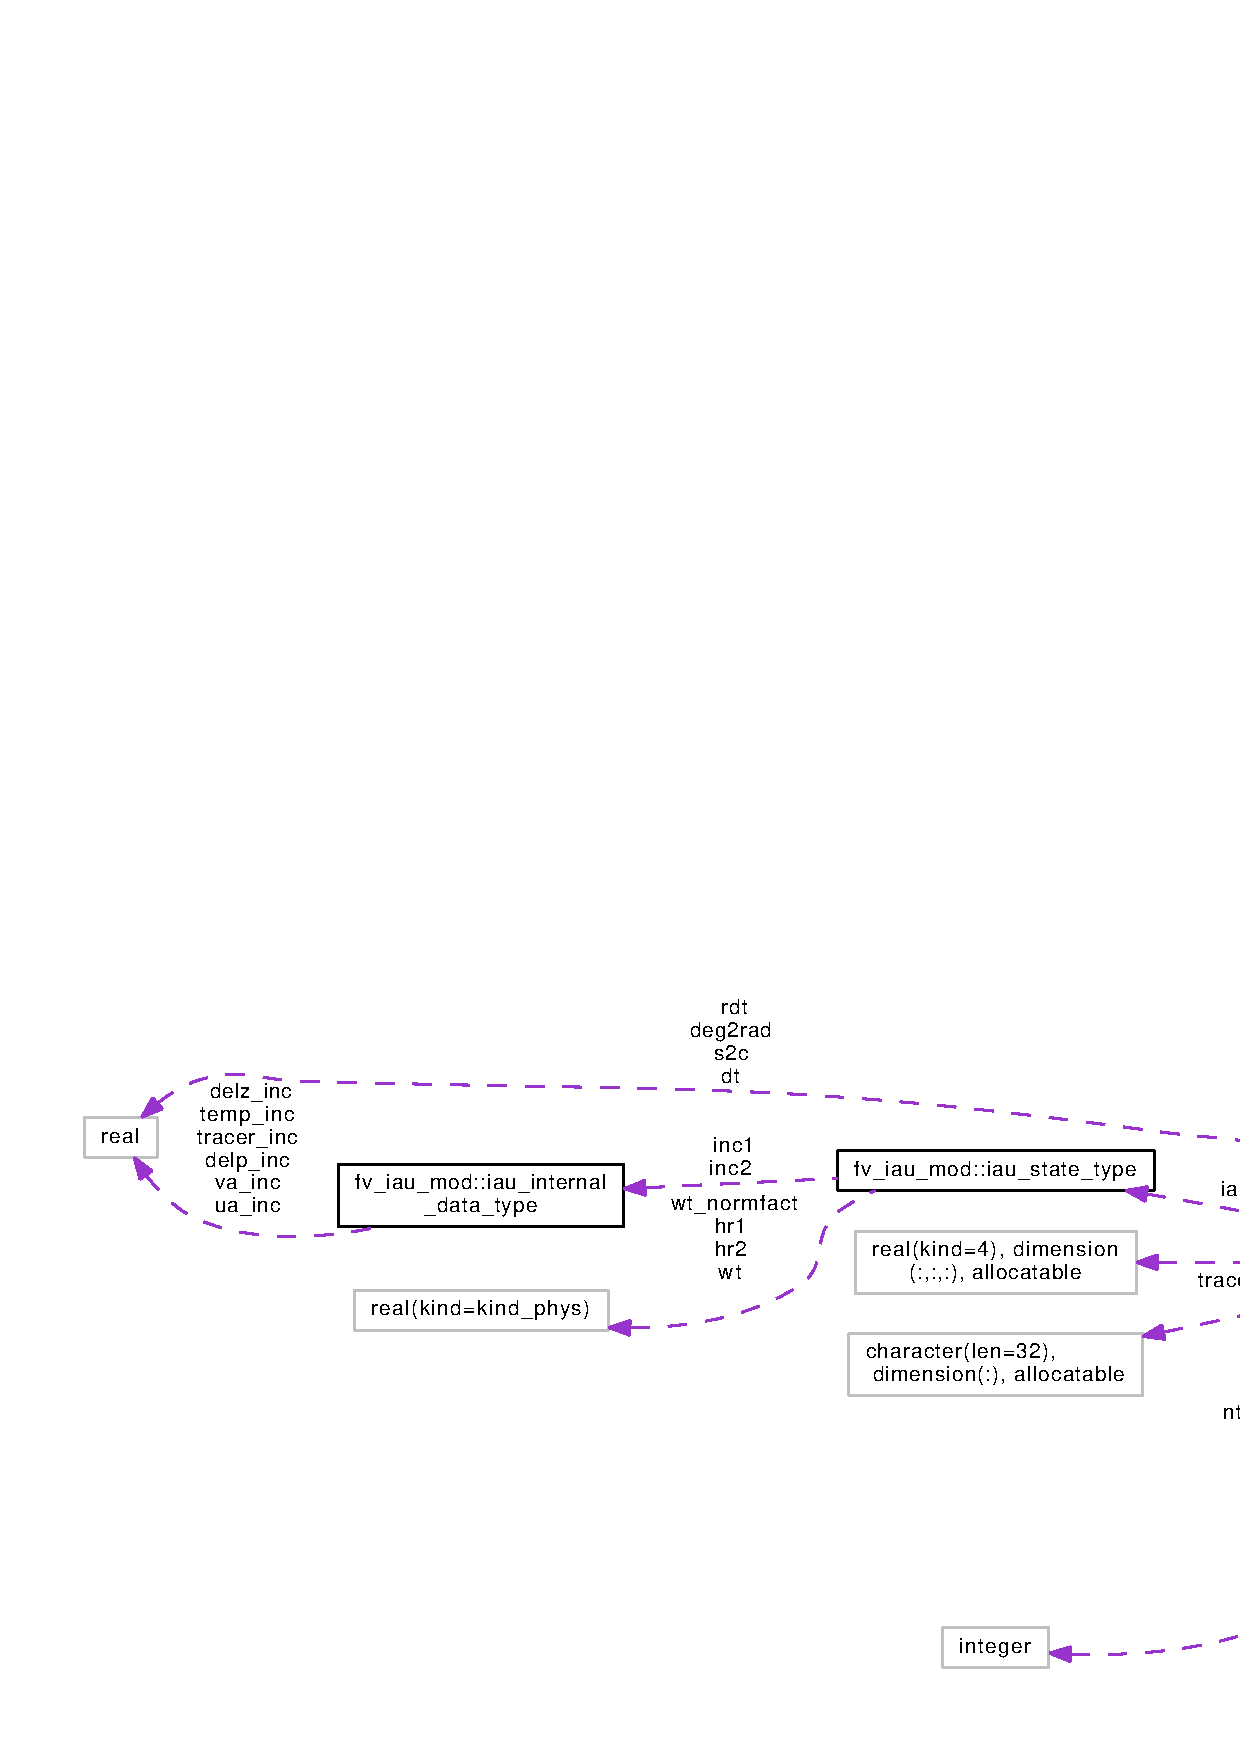
\includegraphics[width=350pt]{classfv__iau__mod__coll__graph}
\end{center}
\end{figure}
\subsection*{Data Types}
\begin{DoxyCompactItemize}
\item 
type \hyperlink{structfv__iau__mod_1_1iau__external__data__type}{iau\-\_\-external\-\_\-data\-\_\-type}
\item 
type \hyperlink{structfv__iau__mod_1_1iau__internal__data__type}{iau\-\_\-internal\-\_\-data\-\_\-type}
\item 
type \hyperlink{structfv__iau__mod_1_1iau__state__type}{iau\-\_\-state\-\_\-type}
\end{DoxyCompactItemize}
\subsection*{Public Member Functions}
\begin{DoxyCompactItemize}
\item 
subroutine, public \hyperlink{classfv__iau__mod_a4caa0c7cbde506ddfd85fb2a4cb17d31}{iau\-\_\-initialize} (I\-P\-D\-\_\-\-Control, I\-A\-U\-\_\-\-Data, Init\-\_\-parm)
\item 
subroutine, public \hyperlink{classfv__iau__mod_ae529ff05f683e363f03577449cc5e678}{getiauforcing} (I\-P\-D\-\_\-\-Control, I\-A\-U\-\_\-\-Data)
\end{DoxyCompactItemize}
\subsection*{Private Member Functions}
\begin{DoxyCompactItemize}
\item 
subroutine \hyperlink{classfv__iau__mod_a6c82860ced03945e7efa22f4a80c2eb4}{updateiauforcing} (I\-P\-D\-\_\-\-Control, I\-A\-U\-\_\-\-Data, wt)
\item 
subroutine \hyperlink{classfv__iau__mod_a5701c1ca8d6df61a85cf83e808fc8962}{setiauforcing} (I\-P\-D\-\_\-\-Control, I\-A\-U\-\_\-\-Data, wt)
\item 
subroutine \hyperlink{classfv__iau__mod_a6fe83e01a0384b0391fd77833e4281c9}{read\-\_\-iau\-\_\-forcing} (I\-P\-D\-\_\-\-Control, increments, fname)
\item 
subroutine \hyperlink{classfv__iau__mod_a96c143c7c507b624327f7b0c45a7492e}{interp\-\_\-inc} (field\-\_\-name, var, jbeg, jend)
\end{DoxyCompactItemize}
\subsection*{Private Attributes}
\begin{DoxyCompactItemize}
\item 
real, dimension(\-:,\-:,\-:), allocatable \hyperlink{classfv__iau__mod_a0967901620cb181a32bcb765735ca893}{s2c}
\item 
integer, dimension(\-:,\-:), \\*
allocatable \hyperlink{classfv__iau__mod_af29c8a827572b31a036d0abdf9e069ce}{id1}
\item 
integer, dimension(\-:,\-:), \\*
allocatable \hyperlink{classfv__iau__mod_a58dd6dc94c1c0d8573764ea8a8dbf8fe}{id2}
\item 
integer, dimension(\-:,\-:), \\*
allocatable \hyperlink{classfv__iau__mod_a41ed3fc692c4d53ad905c7bb685ef4a0}{jdc}
\item 
real \hyperlink{classfv__iau__mod_ac636879eb6bdbeee409bbd34c6658035}{deg2rad}
\item 
real \hyperlink{classfv__iau__mod_aa09091f1f91b28a3137ebc5f59c654aa}{dt}
\item 
real \hyperlink{classfv__iau__mod_a60ee6932472e1de9516db019295fd7d1}{rdt}
\item 
integer \hyperlink{classfv__iau__mod_af1d250bc9006235754621652e834c674}{im}
\item 
integer \hyperlink{classfv__iau__mod_a6c78ca52b83ca9f3e6045d9f06f889bc}{jm}
\item 
integer \hyperlink{classfv__iau__mod_a59eb624f87e12b21694f85684d1c89b7}{km}
\item 
integer \hyperlink{classfv__iau__mod_a756fe43c3f4a450d555fc78eef47d82d}{nfiles}
\item 
integer \hyperlink{classfv__iau__mod_a723f72c8cff32995d1dcd3a7f2661df2}{ncid}
\item 
integer \hyperlink{classfv__iau__mod_afb1c5125d4ad50603b747abd8e2cfd66}{is}
\item 
integer \hyperlink{classfv__iau__mod_af5515c4fa4f895ab74405846237a057b}{ie}
\item 
integer \hyperlink{classfv__iau__mod_a8cfba167a9bf88f42967b9bb5644443c}{js}
\item 
integer \hyperlink{classfv__iau__mod_a3a77635e7bb49d54f620f47019277693}{je}
\item 
integer \hyperlink{classfv__iau__mod_aaf9ea7c9b134626a73380e7fdd86e42d}{npz}
\item 
integer \hyperlink{classfv__iau__mod_a024c7a7ef109d8c660c3df5faf6746f4}{ntracers}
\item 
character(len=32), dimension(\-:), \\*
allocatable \hyperlink{classfv__iau__mod_a271662be2cbbaca55eee2fcba5fe1aa0}{tracer\-\_\-names}
\item 
integer, dimension(\-:), allocatable \hyperlink{classfv__iau__mod_a21f83d74d28c045c736b76aa21d14811}{tracer\-\_\-indicies}
\item 
real(kind=4), dimension(\-:,\-:,\-:), \\*
allocatable \hyperlink{classfv__iau__mod_a9d129637a99655ead2bcf3978b8e03bb}{wk3}
\item 
type(\hyperlink{structfv__iau__mod_1_1iau__state__type}{iau\-\_\-state\-\_\-type}) \hyperlink{classfv__iau__mod_a589667f66e33a418ed898421a7c10d93}{iau\-\_\-state}
\end{DoxyCompactItemize}


\subsection{Detailed Description}
incremental analysis update module 

\begin{DoxyAuthor}{Author}
Xi.\-Chen -\/ author of \hyperlink{fv__treat__da__inc_8F90}{fv\-\_\-treat\-\_\-da\-\_\-inc.\-F90} 

Philip Pegion \href{mailto:philip.pegion@noaa.gov}{\tt philip.\-pegion@noaa.\-gov} 
\end{DoxyAuthor}
\begin{DoxyDate}{Date}
09/13/2017 R\-E\-V\-I\-S\-I\-O\-N H\-I\-S\-T\-O\-R\-Y\-: 09/13/2017 -\/ Initial Version based on \hyperlink{fv__treat__da__inc_8F90}{fv\-\_\-treat\-\_\-da\-\_\-inc.\-F90} 
\end{DoxyDate}


Definition at line 38 of file fv\-\_\-iau\-\_\-mod.\-F90.



\subsection{Member Function/\-Subroutine Documentation}
\index{fv\-\_\-iau\-\_\-mod@{fv\-\_\-iau\-\_\-mod}!getiauforcing@{getiauforcing}}
\index{getiauforcing@{getiauforcing}!fv_iau_mod@{fv\-\_\-iau\-\_\-mod}}
\subsubsection[{getiauforcing}]{\setlength{\rightskip}{0pt plus 5cm}subroutine, public fv\-\_\-iau\-\_\-mod\-::getiauforcing (
\begin{DoxyParamCaption}
\item[{type (ipd\-\_\-control\-\_\-type), intent(in)}]{I\-P\-D\-\_\-\-Control, }
\item[{type({\bf iau\-\_\-external\-\_\-data\-\_\-type}), intent(inout)}]{I\-A\-U\-\_\-\-Data}
\end{DoxyParamCaption}
)}\label{classfv__iau__mod_ae529ff05f683e363f03577449cc5e678}


Definition at line 286 of file fv\-\_\-iau\-\_\-mod.\-F90.



References read\-\_\-iau\-\_\-forcing(), setiauforcing(), and updateiauforcing().

\index{fv\-\_\-iau\-\_\-mod@{fv\-\_\-iau\-\_\-mod}!iau\-\_\-initialize@{iau\-\_\-initialize}}
\index{iau\-\_\-initialize@{iau\-\_\-initialize}!fv_iau_mod@{fv\-\_\-iau\-\_\-mod}}
\subsubsection[{iau\-\_\-initialize}]{\setlength{\rightskip}{0pt plus 5cm}subroutine, public fv\-\_\-iau\-\_\-mod\-::iau\-\_\-initialize (
\begin{DoxyParamCaption}
\item[{type (ipd\-\_\-control\-\_\-type), intent(in)}]{I\-P\-D\-\_\-\-Control, }
\item[{type ({\bf iau\-\_\-external\-\_\-data\-\_\-type}), intent(inout)}]{I\-A\-U\-\_\-\-Data, }
\item[{type (ipd\-\_\-init\-\_\-type), intent(in)}]{Init\-\_\-parm}
\end{DoxyParamCaption}
)}\label{classfv__iau__mod_a4caa0c7cbde506ddfd85fb2a4cb17d31}


Definition at line 109 of file fv\-\_\-iau\-\_\-mod.\-F90.



References sim\-\_\-nc\-\_\-mod\-::close\-\_\-ncfile(), sim\-\_\-nc\-\_\-mod\-::get\-\_\-ncdim1(), sim\-\_\-nc\-\_\-mod\-::open\-\_\-ncfile(), read\-\_\-iau\-\_\-forcing(), external\-\_\-ic\-\_\-mod\-::remap\-\_\-coef(), and setiauforcing().

\index{fv\-\_\-iau\-\_\-mod@{fv\-\_\-iau\-\_\-mod}!interp\-\_\-inc@{interp\-\_\-inc}}
\index{interp\-\_\-inc@{interp\-\_\-inc}!fv_iau_mod@{fv\-\_\-iau\-\_\-mod}}
\subsubsection[{interp\-\_\-inc}]{\setlength{\rightskip}{0pt plus 5cm}subroutine fv\-\_\-iau\-\_\-mod\-::interp\-\_\-inc (
\begin{DoxyParamCaption}
\item[{character(len=$\ast$), intent(in)}]{field\-\_\-name, }
\item[{real, dimension(is\-:ie,js\-:je,1\-:{\bf km}), intent(inout)}]{var, }
\item[{integer, intent(in)}]{jbeg, }
\item[{integer, intent(in)}]{jend}
\end{DoxyParamCaption}
)\hspace{0.3cm}{\ttfamily [private]}}\label{classfv__iau__mod_a96c143c7c507b624327f7b0c45a7492e}


Definition at line 477 of file fv\-\_\-iau\-\_\-mod.\-F90.



References sim\-\_\-nc\-\_\-mod\-::check\-\_\-var\-\_\-exists(), and sim\-\_\-nc\-\_\-mod\-::get\-\_\-var3\-\_\-r4().



Referenced by read\-\_\-iau\-\_\-forcing().

\index{fv\-\_\-iau\-\_\-mod@{fv\-\_\-iau\-\_\-mod}!read\-\_\-iau\-\_\-forcing@{read\-\_\-iau\-\_\-forcing}}
\index{read\-\_\-iau\-\_\-forcing@{read\-\_\-iau\-\_\-forcing}!fv_iau_mod@{fv\-\_\-iau\-\_\-mod}}
\subsubsection[{read\-\_\-iau\-\_\-forcing}]{\setlength{\rightskip}{0pt plus 5cm}subroutine fv\-\_\-iau\-\_\-mod\-::read\-\_\-iau\-\_\-forcing (
\begin{DoxyParamCaption}
\item[{type (ipd\-\_\-control\-\_\-type), intent(in)}]{I\-P\-D\-\_\-\-Control, }
\item[{type({\bf iau\-\_\-internal\-\_\-data\-\_\-type}), intent(inout)}]{increments, }
\item[{character(len=$\ast$), intent(in)}]{fname}
\end{DoxyParamCaption}
)\hspace{0.3cm}{\ttfamily [private]}}\label{classfv__iau__mod_a6fe83e01a0384b0391fd77833e4281c9}


Definition at line 419 of file fv\-\_\-iau\-\_\-mod.\-F90.



References sim\-\_\-nc\-\_\-mod\-::close\-\_\-ncfile(), interp\-\_\-inc(), and sim\-\_\-nc\-\_\-mod\-::open\-\_\-ncfile().



Referenced by getiauforcing(), and iau\-\_\-initialize().

\index{fv\-\_\-iau\-\_\-mod@{fv\-\_\-iau\-\_\-mod}!setiauforcing@{setiauforcing}}
\index{setiauforcing@{setiauforcing}!fv_iau_mod@{fv\-\_\-iau\-\_\-mod}}
\subsubsection[{setiauforcing}]{\setlength{\rightskip}{0pt plus 5cm}subroutine fv\-\_\-iau\-\_\-mod\-::setiauforcing (
\begin{DoxyParamCaption}
\item[{type (ipd\-\_\-control\-\_\-type), intent(in)}]{I\-P\-D\-\_\-\-Control, }
\item[{type({\bf iau\-\_\-external\-\_\-data\-\_\-type}), intent(inout)}]{I\-A\-U\-\_\-\-Data, }
\item[{real(kind\-\_\-phys)}]{wt}
\end{DoxyParamCaption}
)\hspace{0.3cm}{\ttfamily [private]}}\label{classfv__iau__mod_a5701c1ca8d6df61a85cf83e808fc8962}


Definition at line 393 of file fv\-\_\-iau\-\_\-mod.\-F90.



Referenced by getiauforcing(), and iau\-\_\-initialize().

\index{fv\-\_\-iau\-\_\-mod@{fv\-\_\-iau\-\_\-mod}!updateiauforcing@{updateiauforcing}}
\index{updateiauforcing@{updateiauforcing}!fv_iau_mod@{fv\-\_\-iau\-\_\-mod}}
\subsubsection[{updateiauforcing}]{\setlength{\rightskip}{0pt plus 5cm}subroutine fv\-\_\-iau\-\_\-mod\-::updateiauforcing (
\begin{DoxyParamCaption}
\item[{type (ipd\-\_\-control\-\_\-type), intent(in)}]{I\-P\-D\-\_\-\-Control, }
\item[{type({\bf iau\-\_\-external\-\_\-data\-\_\-type}), intent(inout)}]{I\-A\-U\-\_\-\-Data, }
\item[{real(kind\-\_\-phys)}]{wt}
\end{DoxyParamCaption}
)\hspace{0.3cm}{\ttfamily [private]}}\label{classfv__iau__mod_a6c82860ced03945e7efa22f4a80c2eb4}


Definition at line 366 of file fv\-\_\-iau\-\_\-mod.\-F90.



Referenced by getiauforcing().



\subsection{Member Data Documentation}
\index{fv\-\_\-iau\-\_\-mod@{fv\-\_\-iau\-\_\-mod}!deg2rad@{deg2rad}}
\index{deg2rad@{deg2rad}!fv_iau_mod@{fv\-\_\-iau\-\_\-mod}}
\subsubsection[{deg2rad}]{\setlength{\rightskip}{0pt plus 5cm}real fv\-\_\-iau\-\_\-mod\-::deg2rad\hspace{0.3cm}{\ttfamily [private]}}\label{classfv__iau__mod_ac636879eb6bdbeee409bbd34c6658035}


Definition at line 72 of file fv\-\_\-iau\-\_\-mod.\-F90.

\index{fv\-\_\-iau\-\_\-mod@{fv\-\_\-iau\-\_\-mod}!dt@{dt}}
\index{dt@{dt}!fv_iau_mod@{fv\-\_\-iau\-\_\-mod}}
\subsubsection[{dt}]{\setlength{\rightskip}{0pt plus 5cm}real fv\-\_\-iau\-\_\-mod\-::dt\hspace{0.3cm}{\ttfamily [private]}}\label{classfv__iau__mod_aa09091f1f91b28a3137ebc5f59c654aa}


Definition at line 72 of file fv\-\_\-iau\-\_\-mod.\-F90.

\index{fv\-\_\-iau\-\_\-mod@{fv\-\_\-iau\-\_\-mod}!iau\-\_\-state@{iau\-\_\-state}}
\index{iau\-\_\-state@{iau\-\_\-state}!fv_iau_mod@{fv\-\_\-iau\-\_\-mod}}
\subsubsection[{iau\-\_\-state}]{\setlength{\rightskip}{0pt plus 5cm}type({\bf iau\-\_\-state\-\_\-type}) fv\-\_\-iau\-\_\-mod\-::iau\-\_\-state\hspace{0.3cm}{\ttfamily [private]}}\label{classfv__iau__mod_a589667f66e33a418ed898421a7c10d93}


Definition at line 105 of file fv\-\_\-iau\-\_\-mod.\-F90.

\index{fv\-\_\-iau\-\_\-mod@{fv\-\_\-iau\-\_\-mod}!id1@{id1}}
\index{id1@{id1}!fv_iau_mod@{fv\-\_\-iau\-\_\-mod}}
\subsubsection[{id1}]{\setlength{\rightskip}{0pt plus 5cm}integer, dimension(\-:,\-:), allocatable fv\-\_\-iau\-\_\-mod\-::id1\hspace{0.3cm}{\ttfamily [private]}}\label{classfv__iau__mod_af29c8a827572b31a036d0abdf9e069ce}


Definition at line 70 of file fv\-\_\-iau\-\_\-mod.\-F90.

\index{fv\-\_\-iau\-\_\-mod@{fv\-\_\-iau\-\_\-mod}!id2@{id2}}
\index{id2@{id2}!fv_iau_mod@{fv\-\_\-iau\-\_\-mod}}
\subsubsection[{id2}]{\setlength{\rightskip}{0pt plus 5cm}integer, dimension(\-:,\-:), allocatable fv\-\_\-iau\-\_\-mod\-::id2\hspace{0.3cm}{\ttfamily [private]}}\label{classfv__iau__mod_a58dd6dc94c1c0d8573764ea8a8dbf8fe}


Definition at line 70 of file fv\-\_\-iau\-\_\-mod.\-F90.

\index{fv\-\_\-iau\-\_\-mod@{fv\-\_\-iau\-\_\-mod}!ie@{ie}}
\index{ie@{ie}!fv_iau_mod@{fv\-\_\-iau\-\_\-mod}}
\subsubsection[{ie}]{\setlength{\rightskip}{0pt plus 5cm}integer fv\-\_\-iau\-\_\-mod\-::ie\hspace{0.3cm}{\ttfamily [private]}}\label{classfv__iau__mod_af5515c4fa4f895ab74405846237a057b}


Definition at line 74 of file fv\-\_\-iau\-\_\-mod.\-F90.

\index{fv\-\_\-iau\-\_\-mod@{fv\-\_\-iau\-\_\-mod}!im@{im}}
\index{im@{im}!fv_iau_mod@{fv\-\_\-iau\-\_\-mod}}
\subsubsection[{im}]{\setlength{\rightskip}{0pt plus 5cm}integer fv\-\_\-iau\-\_\-mod\-::im\hspace{0.3cm}{\ttfamily [private]}}\label{classfv__iau__mod_af1d250bc9006235754621652e834c674}


Definition at line 73 of file fv\-\_\-iau\-\_\-mod.\-F90.

\index{fv\-\_\-iau\-\_\-mod@{fv\-\_\-iau\-\_\-mod}!is@{is}}
\index{is@{is}!fv_iau_mod@{fv\-\_\-iau\-\_\-mod}}
\subsubsection[{is}]{\setlength{\rightskip}{0pt plus 5cm}integer fv\-\_\-iau\-\_\-mod\-::is\hspace{0.3cm}{\ttfamily [private]}}\label{classfv__iau__mod_afb1c5125d4ad50603b747abd8e2cfd66}


Definition at line 74 of file fv\-\_\-iau\-\_\-mod.\-F90.

\index{fv\-\_\-iau\-\_\-mod@{fv\-\_\-iau\-\_\-mod}!jdc@{jdc}}
\index{jdc@{jdc}!fv_iau_mod@{fv\-\_\-iau\-\_\-mod}}
\subsubsection[{jdc}]{\setlength{\rightskip}{0pt plus 5cm}integer, dimension(\-:,\-:), allocatable fv\-\_\-iau\-\_\-mod\-::jdc\hspace{0.3cm}{\ttfamily [private]}}\label{classfv__iau__mod_a41ed3fc692c4d53ad905c7bb685ef4a0}


Definition at line 70 of file fv\-\_\-iau\-\_\-mod.\-F90.

\index{fv\-\_\-iau\-\_\-mod@{fv\-\_\-iau\-\_\-mod}!je@{je}}
\index{je@{je}!fv_iau_mod@{fv\-\_\-iau\-\_\-mod}}
\subsubsection[{je}]{\setlength{\rightskip}{0pt plus 5cm}integer fv\-\_\-iau\-\_\-mod\-::je\hspace{0.3cm}{\ttfamily [private]}}\label{classfv__iau__mod_a3a77635e7bb49d54f620f47019277693}


Definition at line 74 of file fv\-\_\-iau\-\_\-mod.\-F90.

\index{fv\-\_\-iau\-\_\-mod@{fv\-\_\-iau\-\_\-mod}!jm@{jm}}
\index{jm@{jm}!fv_iau_mod@{fv\-\_\-iau\-\_\-mod}}
\subsubsection[{jm}]{\setlength{\rightskip}{0pt plus 5cm}integer fv\-\_\-iau\-\_\-mod\-::jm\hspace{0.3cm}{\ttfamily [private]}}\label{classfv__iau__mod_a6c78ca52b83ca9f3e6045d9f06f889bc}


Definition at line 73 of file fv\-\_\-iau\-\_\-mod.\-F90.

\index{fv\-\_\-iau\-\_\-mod@{fv\-\_\-iau\-\_\-mod}!js@{js}}
\index{js@{js}!fv_iau_mod@{fv\-\_\-iau\-\_\-mod}}
\subsubsection[{js}]{\setlength{\rightskip}{0pt plus 5cm}integer fv\-\_\-iau\-\_\-mod\-::js\hspace{0.3cm}{\ttfamily [private]}}\label{classfv__iau__mod_a8cfba167a9bf88f42967b9bb5644443c}


Definition at line 74 of file fv\-\_\-iau\-\_\-mod.\-F90.

\index{fv\-\_\-iau\-\_\-mod@{fv\-\_\-iau\-\_\-mod}!km@{km}}
\index{km@{km}!fv_iau_mod@{fv\-\_\-iau\-\_\-mod}}
\subsubsection[{km}]{\setlength{\rightskip}{0pt plus 5cm}integer fv\-\_\-iau\-\_\-mod\-::km\hspace{0.3cm}{\ttfamily [private]}}\label{classfv__iau__mod_a59eb624f87e12b21694f85684d1c89b7}


Definition at line 73 of file fv\-\_\-iau\-\_\-mod.\-F90.

\index{fv\-\_\-iau\-\_\-mod@{fv\-\_\-iau\-\_\-mod}!ncid@{ncid}}
\index{ncid@{ncid}!fv_iau_mod@{fv\-\_\-iau\-\_\-mod}}
\subsubsection[{ncid}]{\setlength{\rightskip}{0pt plus 5cm}integer fv\-\_\-iau\-\_\-mod\-::ncid\hspace{0.3cm}{\ttfamily [private]}}\label{classfv__iau__mod_a723f72c8cff32995d1dcd3a7f2661df2}


Definition at line 73 of file fv\-\_\-iau\-\_\-mod.\-F90.

\index{fv\-\_\-iau\-\_\-mod@{fv\-\_\-iau\-\_\-mod}!nfiles@{nfiles}}
\index{nfiles@{nfiles}!fv_iau_mod@{fv\-\_\-iau\-\_\-mod}}
\subsubsection[{nfiles}]{\setlength{\rightskip}{0pt plus 5cm}integer fv\-\_\-iau\-\_\-mod\-::nfiles\hspace{0.3cm}{\ttfamily [private]}}\label{classfv__iau__mod_a756fe43c3f4a450d555fc78eef47d82d}


Definition at line 73 of file fv\-\_\-iau\-\_\-mod.\-F90.

\index{fv\-\_\-iau\-\_\-mod@{fv\-\_\-iau\-\_\-mod}!npz@{npz}}
\index{npz@{npz}!fv_iau_mod@{fv\-\_\-iau\-\_\-mod}}
\subsubsection[{npz}]{\setlength{\rightskip}{0pt plus 5cm}integer fv\-\_\-iau\-\_\-mod\-::npz\hspace{0.3cm}{\ttfamily [private]}}\label{classfv__iau__mod_aaf9ea7c9b134626a73380e7fdd86e42d}


Definition at line 75 of file fv\-\_\-iau\-\_\-mod.\-F90.

\index{fv\-\_\-iau\-\_\-mod@{fv\-\_\-iau\-\_\-mod}!ntracers@{ntracers}}
\index{ntracers@{ntracers}!fv_iau_mod@{fv\-\_\-iau\-\_\-mod}}
\subsubsection[{ntracers}]{\setlength{\rightskip}{0pt plus 5cm}integer fv\-\_\-iau\-\_\-mod\-::ntracers\hspace{0.3cm}{\ttfamily [private]}}\label{classfv__iau__mod_a024c7a7ef109d8c660c3df5faf6746f4}


Definition at line 75 of file fv\-\_\-iau\-\_\-mod.\-F90.

\index{fv\-\_\-iau\-\_\-mod@{fv\-\_\-iau\-\_\-mod}!rdt@{rdt}}
\index{rdt@{rdt}!fv_iau_mod@{fv\-\_\-iau\-\_\-mod}}
\subsubsection[{rdt}]{\setlength{\rightskip}{0pt plus 5cm}real fv\-\_\-iau\-\_\-mod\-::rdt\hspace{0.3cm}{\ttfamily [private]}}\label{classfv__iau__mod_a60ee6932472e1de9516db019295fd7d1}


Definition at line 72 of file fv\-\_\-iau\-\_\-mod.\-F90.

\index{fv\-\_\-iau\-\_\-mod@{fv\-\_\-iau\-\_\-mod}!s2c@{s2c}}
\index{s2c@{s2c}!fv_iau_mod@{fv\-\_\-iau\-\_\-mod}}
\subsubsection[{s2c}]{\setlength{\rightskip}{0pt plus 5cm}real, dimension(\-:,\-:,\-:), allocatable fv\-\_\-iau\-\_\-mod\-::s2c\hspace{0.3cm}{\ttfamily [private]}}\label{classfv__iau__mod_a0967901620cb181a32bcb765735ca893}


Definition at line 66 of file fv\-\_\-iau\-\_\-mod.\-F90.

\index{fv\-\_\-iau\-\_\-mod@{fv\-\_\-iau\-\_\-mod}!tracer\-\_\-indicies@{tracer\-\_\-indicies}}
\index{tracer\-\_\-indicies@{tracer\-\_\-indicies}!fv_iau_mod@{fv\-\_\-iau\-\_\-mod}}
\subsubsection[{tracer\-\_\-indicies}]{\setlength{\rightskip}{0pt plus 5cm}integer, dimension(\-:), allocatable fv\-\_\-iau\-\_\-mod\-::tracer\-\_\-indicies\hspace{0.3cm}{\ttfamily [private]}}\label{classfv__iau__mod_a21f83d74d28c045c736b76aa21d14811}


Definition at line 77 of file fv\-\_\-iau\-\_\-mod.\-F90.

\index{fv\-\_\-iau\-\_\-mod@{fv\-\_\-iau\-\_\-mod}!tracer\-\_\-names@{tracer\-\_\-names}}
\index{tracer\-\_\-names@{tracer\-\_\-names}!fv_iau_mod@{fv\-\_\-iau\-\_\-mod}}
\subsubsection[{tracer\-\_\-names}]{\setlength{\rightskip}{0pt plus 5cm}character(len=32), dimension(\-:), allocatable fv\-\_\-iau\-\_\-mod\-::tracer\-\_\-names\hspace{0.3cm}{\ttfamily [private]}}\label{classfv__iau__mod_a271662be2cbbaca55eee2fcba5fe1aa0}


Definition at line 76 of file fv\-\_\-iau\-\_\-mod.\-F90.

\index{fv\-\_\-iau\-\_\-mod@{fv\-\_\-iau\-\_\-mod}!wk3@{wk3}}
\index{wk3@{wk3}!fv_iau_mod@{fv\-\_\-iau\-\_\-mod}}
\subsubsection[{wk3}]{\setlength{\rightskip}{0pt plus 5cm}real(kind=4), dimension(\-:,\-:,\-:), allocatable fv\-\_\-iau\-\_\-mod\-::wk3\hspace{0.3cm}{\ttfamily [private]}}\label{classfv__iau__mod_a9d129637a99655ead2bcf3978b8e03bb}


Definition at line 79 of file fv\-\_\-iau\-\_\-mod.\-F90.



The documentation for this module was generated from the following file\-:\begin{DoxyCompactItemize}
\item 
/scratch2/\-N\-A\-G\-A\-P\-E/aoml-\/hafs1/\-Kyle.\-Ahern/acs\-\_\-master\-\_\-readonly/tools/\hyperlink{fv__iau__mod_8F90}{fv\-\_\-iau\-\_\-mod.\-F90}\end{DoxyCompactItemize}

\section{fv\-\_\-io\-\_\-mod Module Reference}
\label{classfv__io__mod}\index{fv\-\_\-io\-\_\-mod@{fv\-\_\-io\-\_\-mod}}


The module 'fv\-\_\-io' contains restart facilities for F\-V core.  




Collaboration diagram for fv\-\_\-io\-\_\-mod\-:
\nopagebreak
\begin{figure}[H]
\begin{center}
\leavevmode
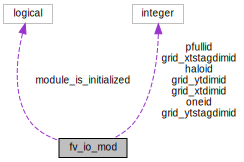
\includegraphics[width=280pt]{classfv__io__mod__coll__graph}
\end{center}
\end{figure}
\subsection*{Public Member Functions}
\begin{DoxyCompactItemize}
\item 
subroutine, public \hyperlink{classfv__io__mod_a374b943fdac1307ea36c3a38178f41fc}{fv\-\_\-io\-\_\-init} ()
\begin{DoxyCompactList}\small\item\em Initialize the fv core restart facilities. \end{DoxyCompactList}\item 
subroutine, public \hyperlink{classfv__io__mod_a71aae4a8b1c8c1f9a6392d4de3b6bd43}{fv\-\_\-io\-\_\-exit}
\begin{DoxyCompactList}\small\item\em Close the fv core restart facilities. \end{DoxyCompactList}\item 
subroutine, public \hyperlink{classfv__io__mod_ab67e5d4a465de71184f1247b34d5fdd8}{fv\-\_\-io\-\_\-read\-\_\-restart} (fv\-\_\-domain, Atm)
\begin{DoxyCompactList}\small\item\em Write the fv core restart quantities. \end{DoxyCompactList}\item 
subroutine, public \hyperlink{classfv__io__mod_a41fce9f83c0ca9c4f6bfb0357923737c}{fv\-\_\-io\-\_\-read\-\_\-tracers} (fv\-\_\-domain, Atm)
\begin{DoxyCompactList}\small\item\em The subroutine 'fv\-\_\-io\-\_\-read\-\_\-tracers' reads in only tracers from restart files. \end{DoxyCompactList}\item 
subroutine, public \hyperlink{classfv__io__mod_a161881a2b85c2bbebc41477e142861f5}{remap\-\_\-restart} (fv\-\_\-domain, Atm)
\begin{DoxyCompactList}\small\item\em The subroutine 'remap\-\_\-restart' remaps the model state from remap files to a new set of Eulerian coordinates. \end{DoxyCompactList}\item 
subroutine, public \hyperlink{classfv__io__mod_a31e5192f8a0fb55ed1984a9b02554652}{fv\-\_\-io\-\_\-register\-\_\-nudge\-\_\-restart} (Atm)
\begin{DoxyCompactList}\small\item\em The subroutine 'fv\-\_\-io\-\_\-register\-\_\-nudge\-\_\-restart' registers restarts for S\-S\-T fields used in Hi\-R\-A\-M. \end{DoxyCompactList}\item 
subroutine, public \hyperlink{classfv__io__mod_a7176ff0edd93844871b936d9c4381f45}{fv\-\_\-io\-\_\-register\-\_\-restart} (fv\-\_\-domain, Atm)
\begin{DoxyCompactList}\small\item\em The subroutine 'fv\-\_\-io\-\_\-register\-\_\-restart' registers model restart fields. \end{DoxyCompactList}\item 
subroutine, public \hyperlink{classfv__io__mod_a1ad375a9468a15c319155b8bf794222e}{fv\-\_\-io\-\_\-write\-\_\-restart} (Atm, grids\-\_\-on\-\_\-this\-\_\-pe, timestamp)
\begin{DoxyCompactList}\small\item\em The subroutine 'fv\-\_\-io\-\_\-write\-\_\-restart' writes restart files. \end{DoxyCompactList}\item 
subroutine, public \hyperlink{classfv__io__mod_acfb0e5fb70a35bd2557122a21f285057}{fv\-\_\-io\-\_\-register\-\_\-restart\-\_\-bcs} (Atm)
\begin{DoxyCompactList}\small\item\em The subroutine 'fv\-\_\-io\-\_\-register\-\_\-restart\-\_\-\-B\-Cs' registers restarts for nested-\/grid boundary conditions. \end{DoxyCompactList}\item 
subroutine, public \hyperlink{classfv__io__mod_ab18c761d6135c36e0f3bbb1b5969ec86}{fv\-\_\-io\-\_\-register\-\_\-restart\-\_\-bcs\-\_\-nh} (Atm)
\item 
subroutine, public \hyperlink{classfv__io__mod_a2dba504c647cfd53078b4d1e7c980332}{fv\-\_\-io\-\_\-write\-\_\-bcs} (Atm, timestamp)
\begin{DoxyCompactList}\small\item\em The subroutine 'fv\-\_\-io\-\_\-write\-\_\-\-B\-Cs' writes B\-Cs to a restart file. \end{DoxyCompactList}\item 
subroutine, public \hyperlink{classfv__io__mod_ab54bb8ad1c76e485c736bd3d9f45b523}{fv\-\_\-io\-\_\-read\-\_\-bcs} (Atm)
\begin{DoxyCompactList}\small\item\em The subroutine 'fv\-\_\-io\-\_\-read\-\_\-\-B\-Cs' reads B\-Cs from a restart file. \end{DoxyCompactList}\end{DoxyCompactItemize}
\subsection*{Private Member Functions}
\begin{DoxyCompactItemize}
\item 
subroutine \hyperlink{classfv__io__mod_a297598ad854f809ad31661e58c50bd8e}{register\-\_\-bcs\-\_\-2d} (Atm, B\-Cfile\-\_\-ne, B\-Cfile\-\_\-sw, fname\-\_\-ne, fname\-\_\-sw, var\-\_\-name, var, var\-\_\-bc, istag, jstag)
\item 
subroutine \hyperlink{classfv__io__mod_ad70a91b87c0917b70bc746ee744ec710}{register\-\_\-bcs\-\_\-3d} (Atm, B\-Cfile\-\_\-ne, B\-Cfile\-\_\-sw, fname\-\_\-ne, fname\-\_\-sw, var\-\_\-name, var, var\-\_\-bc, istag, jstag, mandatory)
\end{DoxyCompactItemize}
\subsection*{Private Attributes}
\begin{DoxyCompactItemize}
\item 
logical \hyperlink{classfv__io__mod_a0a0d26eb0411470f9d5d7b50a1fc67c7}{module\-\_\-is\-\_\-initialized} = .F\-A\-L\-S\-E.
\item 
integer \hyperlink{classfv__io__mod_a917a64d0d43975d4b5cc97fd73f73443}{grid\-\_\-xtdimid}
\item 
integer \hyperlink{classfv__io__mod_a08db0ecb707015eb437912010c574d64}{grid\-\_\-ytdimid}
\item 
integer \hyperlink{classfv__io__mod_a8dacc1c38af6da8b113fef3ab953e712}{haloid}
\item 
integer \hyperlink{classfv__io__mod_a8ac7b1dc39c4e3b84676b89697881b7b}{pfullid}
\item 
integer \hyperlink{classfv__io__mod_a0a6f309e19451cffeccc7a6dbffb4ffc}{grid\-\_\-xtstagdimid}
\item 
integer \hyperlink{classfv__io__mod_a5b333b9fc08330f0048a52b3d329ac3d}{grid\-\_\-ytstagdimid}
\item 
integer \hyperlink{classfv__io__mod_ac0e83dcce576d02e4f3f6da1c8d5aeb7}{oneid}
\end{DoxyCompactItemize}


\subsection{Detailed Description}
The module 'fv\-\_\-io' contains restart facilities for F\-V core. 

This module writes and reads restart files for the F\-V core. Additionally it provides setup and calls routines necessary to provide a complete restart for the model. \begin{DoxyNote}{Note}
N\-O\-T\-E\-: Merging in the seasonal forecast initialization code has proven problematic in the past, since many conflicts occur. Leaving this for now --- lmh 10aug15 
\end{DoxyNote}


Definition at line 30 of file fv\-\_\-io.\-F90.



\subsection{Member Function/\-Subroutine Documentation}
\index{fv\-\_\-io\-\_\-mod@{fv\-\_\-io\-\_\-mod}!fv\-\_\-io\-\_\-exit@{fv\-\_\-io\-\_\-exit}}
\index{fv\-\_\-io\-\_\-exit@{fv\-\_\-io\-\_\-exit}!fv_io_mod@{fv\-\_\-io\-\_\-mod}}
\subsubsection[{fv\-\_\-io\-\_\-exit}]{\setlength{\rightskip}{0pt plus 5cm}subroutine, public fv\-\_\-io\-\_\-mod\-::fv\-\_\-io\-\_\-exit (
\begin{DoxyParamCaption}
{}
\end{DoxyParamCaption}
)}\label{classfv__io__mod_a71aae4a8b1c8c1f9a6392d4de3b6bd43}


Close the fv core restart facilities. 



Definition at line 137 of file fv\-\_\-io.\-F90.



Referenced by fv\-\_\-control\-\_\-mod\-::fv\-\_\-end().

\index{fv\-\_\-io\-\_\-mod@{fv\-\_\-io\-\_\-mod}!fv\-\_\-io\-\_\-init@{fv\-\_\-io\-\_\-init}}
\index{fv\-\_\-io\-\_\-init@{fv\-\_\-io\-\_\-init}!fv_io_mod@{fv\-\_\-io\-\_\-mod}}
\subsubsection[{fv\-\_\-io\-\_\-init}]{\setlength{\rightskip}{0pt plus 5cm}subroutine, public fv\-\_\-io\-\_\-mod\-::fv\-\_\-io\-\_\-init (
\begin{DoxyParamCaption}
{}
\end{DoxyParamCaption}
)}\label{classfv__io__mod_a374b943fdac1307ea36c3a38178f41fc}


Initialize the fv core restart facilities. 



Definition at line 131 of file fv\-\_\-io.\-F90.



Referenced by fv\-\_\-restart\-\_\-mod\-::fv\-\_\-restart\-\_\-init().

\index{fv\-\_\-io\-\_\-mod@{fv\-\_\-io\-\_\-mod}!fv\-\_\-io\-\_\-read\-\_\-bcs@{fv\-\_\-io\-\_\-read\-\_\-bcs}}
\index{fv\-\_\-io\-\_\-read\-\_\-bcs@{fv\-\_\-io\-\_\-read\-\_\-bcs}!fv_io_mod@{fv\-\_\-io\-\_\-mod}}
\subsubsection[{fv\-\_\-io\-\_\-read\-\_\-bcs}]{\setlength{\rightskip}{0pt plus 5cm}subroutine, public fv\-\_\-io\-\_\-mod\-::fv\-\_\-io\-\_\-read\-\_\-bcs (
\begin{DoxyParamCaption}
\item[{type(fv\-\_\-atmos\-\_\-type), intent(inout)}]{Atm}
\end{DoxyParamCaption}
)}\label{classfv__io__mod_ab54bb8ad1c76e485c736bd3d9f45b523}


The subroutine 'fv\-\_\-io\-\_\-read\-\_\-\-B\-Cs' reads B\-Cs from a restart file. 



Definition at line 1009 of file fv\-\_\-io.\-F90.



Referenced by fv\-\_\-restart\-\_\-mod\-::fv\-\_\-restart().

\index{fv\-\_\-io\-\_\-mod@{fv\-\_\-io\-\_\-mod}!fv\-\_\-io\-\_\-read\-\_\-restart@{fv\-\_\-io\-\_\-read\-\_\-restart}}
\index{fv\-\_\-io\-\_\-read\-\_\-restart@{fv\-\_\-io\-\_\-read\-\_\-restart}!fv_io_mod@{fv\-\_\-io\-\_\-mod}}
\subsubsection[{fv\-\_\-io\-\_\-read\-\_\-restart}]{\setlength{\rightskip}{0pt plus 5cm}subroutine, public fv\-\_\-io\-\_\-mod\-::fv\-\_\-io\-\_\-read\-\_\-restart (
\begin{DoxyParamCaption}
\item[{type(domain2d), intent(inout)}]{fv\-\_\-domain, }
\item[{type(fv\-\_\-atmos\-\_\-type), dimension(\-:), intent(inout)}]{Atm}
\end{DoxyParamCaption}
)}\label{classfv__io__mod_ab67e5d4a465de71184f1247b34d5fdd8}


Write the fv core restart quantities. 



Definition at line 143 of file fv\-\_\-io.\-F90.



References fv\-\_\-eta\-\_\-mod\-::set\-\_\-external\-\_\-eta().



Referenced by fv\-\_\-restart\-\_\-mod\-::fv\-\_\-restart().

\index{fv\-\_\-io\-\_\-mod@{fv\-\_\-io\-\_\-mod}!fv\-\_\-io\-\_\-read\-\_\-tracers@{fv\-\_\-io\-\_\-read\-\_\-tracers}}
\index{fv\-\_\-io\-\_\-read\-\_\-tracers@{fv\-\_\-io\-\_\-read\-\_\-tracers}!fv_io_mod@{fv\-\_\-io\-\_\-mod}}
\subsubsection[{fv\-\_\-io\-\_\-read\-\_\-tracers}]{\setlength{\rightskip}{0pt plus 5cm}subroutine, public fv\-\_\-io\-\_\-mod\-::fv\-\_\-io\-\_\-read\-\_\-tracers (
\begin{DoxyParamCaption}
\item[{type(domain2d), intent(inout)}]{fv\-\_\-domain, }
\item[{type(fv\-\_\-atmos\-\_\-type), dimension(\-:), intent(inout)}]{Atm}
\end{DoxyParamCaption}
)}\label{classfv__io__mod_a41fce9f83c0ca9c4f6bfb0357923737c}


The subroutine 'fv\-\_\-io\-\_\-read\-\_\-tracers' reads in only tracers from restart files. 

This subroutine is useful when initializing a cycled or nudged model from an analysis that does not have a whole set of microphysical, aerosol, or chemical tracers 

Definition at line 224 of file fv\-\_\-io.\-F90.



Referenced by external\-\_\-ic\-\_\-mod\-::get\-\_\-external\-\_\-ic().

\index{fv\-\_\-io\-\_\-mod@{fv\-\_\-io\-\_\-mod}!fv\-\_\-io\-\_\-register\-\_\-nudge\-\_\-restart@{fv\-\_\-io\-\_\-register\-\_\-nudge\-\_\-restart}}
\index{fv\-\_\-io\-\_\-register\-\_\-nudge\-\_\-restart@{fv\-\_\-io\-\_\-register\-\_\-nudge\-\_\-restart}!fv_io_mod@{fv\-\_\-io\-\_\-mod}}
\subsubsection[{fv\-\_\-io\-\_\-register\-\_\-nudge\-\_\-restart}]{\setlength{\rightskip}{0pt plus 5cm}subroutine, public fv\-\_\-io\-\_\-mod\-::fv\-\_\-io\-\_\-register\-\_\-nudge\-\_\-restart (
\begin{DoxyParamCaption}
\item[{type(fv\-\_\-atmos\-\_\-type), dimension(\-:), intent(inout)}]{Atm}
\end{DoxyParamCaption}
)}\label{classfv__io__mod_a31e5192f8a0fb55ed1984a9b02554652}


The subroutine 'fv\-\_\-io\-\_\-register\-\_\-nudge\-\_\-restart' registers restarts for S\-S\-T fields used in Hi\-R\-A\-M. 

\begin{DoxyNote}{Note}
This option is currently not supported. 
\end{DoxyNote}


Definition at line 447 of file fv\-\_\-io.\-F90.

\index{fv\-\_\-io\-\_\-mod@{fv\-\_\-io\-\_\-mod}!fv\-\_\-io\-\_\-register\-\_\-restart@{fv\-\_\-io\-\_\-register\-\_\-restart}}
\index{fv\-\_\-io\-\_\-register\-\_\-restart@{fv\-\_\-io\-\_\-register\-\_\-restart}!fv_io_mod@{fv\-\_\-io\-\_\-mod}}
\subsubsection[{fv\-\_\-io\-\_\-register\-\_\-restart}]{\setlength{\rightskip}{0pt plus 5cm}subroutine, public fv\-\_\-io\-\_\-mod\-::fv\-\_\-io\-\_\-register\-\_\-restart (
\begin{DoxyParamCaption}
\item[{type(domain2d), intent(inout)}]{fv\-\_\-domain, }
\item[{type(fv\-\_\-atmos\-\_\-type), dimension(\-:), intent(inout)}]{Atm}
\end{DoxyParamCaption}
)}\label{classfv__io__mod_a7176ff0edd93844871b936d9c4381f45}


The subroutine 'fv\-\_\-io\-\_\-register\-\_\-restart' registers model restart fields. 



Definition at line 463 of file fv\-\_\-io.\-F90.



Referenced by fv\-\_\-restart\-\_\-mod\-::fv\-\_\-restart().

\index{fv\-\_\-io\-\_\-mod@{fv\-\_\-io\-\_\-mod}!fv\-\_\-io\-\_\-register\-\_\-restart\-\_\-bcs@{fv\-\_\-io\-\_\-register\-\_\-restart\-\_\-bcs}}
\index{fv\-\_\-io\-\_\-register\-\_\-restart\-\_\-bcs@{fv\-\_\-io\-\_\-register\-\_\-restart\-\_\-bcs}!fv_io_mod@{fv\-\_\-io\-\_\-mod}}
\subsubsection[{fv\-\_\-io\-\_\-register\-\_\-restart\-\_\-bcs}]{\setlength{\rightskip}{0pt plus 5cm}subroutine, public fv\-\_\-io\-\_\-mod\-::fv\-\_\-io\-\_\-register\-\_\-restart\-\_\-bcs (
\begin{DoxyParamCaption}
\item[{type(fv\-\_\-atmos\-\_\-type), intent(inout)}]{Atm}
\end{DoxyParamCaption}
)}\label{classfv__io__mod_acfb0e5fb70a35bd2557122a21f285057}


The subroutine 'fv\-\_\-io\-\_\-register\-\_\-restart\-\_\-\-B\-Cs' registers restarts for nested-\/grid boundary conditions. 



Definition at line 909 of file fv\-\_\-io.\-F90.



References register\-\_\-bcs\-\_\-2d(), and register\-\_\-bcs\-\_\-3d().



Referenced by fv\-\_\-restart\-\_\-mod\-::fv\-\_\-restart().

\index{fv\-\_\-io\-\_\-mod@{fv\-\_\-io\-\_\-mod}!fv\-\_\-io\-\_\-register\-\_\-restart\-\_\-bcs\-\_\-nh@{fv\-\_\-io\-\_\-register\-\_\-restart\-\_\-bcs\-\_\-nh}}
\index{fv\-\_\-io\-\_\-register\-\_\-restart\-\_\-bcs\-\_\-nh@{fv\-\_\-io\-\_\-register\-\_\-restart\-\_\-bcs\-\_\-nh}!fv_io_mod@{fv\-\_\-io\-\_\-mod}}
\subsubsection[{fv\-\_\-io\-\_\-register\-\_\-restart\-\_\-bcs\-\_\-nh}]{\setlength{\rightskip}{0pt plus 5cm}subroutine, public fv\-\_\-io\-\_\-mod\-::fv\-\_\-io\-\_\-register\-\_\-restart\-\_\-bcs\-\_\-nh (
\begin{DoxyParamCaption}
\item[{type(fv\-\_\-atmos\-\_\-type), intent(inout)}]{Atm}
\end{DoxyParamCaption}
)}\label{classfv__io__mod_ab18c761d6135c36e0f3bbb1b5969ec86}


Definition at line 974 of file fv\-\_\-io.\-F90.



References register\-\_\-bcs\-\_\-3d().



Referenced by fv\-\_\-restart\-\_\-mod\-::fv\-\_\-restart().

\index{fv\-\_\-io\-\_\-mod@{fv\-\_\-io\-\_\-mod}!fv\-\_\-io\-\_\-write\-\_\-bcs@{fv\-\_\-io\-\_\-write\-\_\-bcs}}
\index{fv\-\_\-io\-\_\-write\-\_\-bcs@{fv\-\_\-io\-\_\-write\-\_\-bcs}!fv_io_mod@{fv\-\_\-io\-\_\-mod}}
\subsubsection[{fv\-\_\-io\-\_\-write\-\_\-bcs}]{\setlength{\rightskip}{0pt plus 5cm}subroutine, public fv\-\_\-io\-\_\-mod\-::fv\-\_\-io\-\_\-write\-\_\-bcs (
\begin{DoxyParamCaption}
\item[{type(fv\-\_\-atmos\-\_\-type), intent(inout)}]{Atm, }
\item[{character(len=$\ast$), intent(in), optional}]{timestamp}
\end{DoxyParamCaption}
)}\label{classfv__io__mod_a2dba504c647cfd53078b4d1e7c980332}


The subroutine 'fv\-\_\-io\-\_\-write\-\_\-\-B\-Cs' writes B\-Cs to a restart file. 



Definition at line 998 of file fv\-\_\-io.\-F90.



Referenced by fv\-\_\-restart\-\_\-mod\-::fv\-\_\-restart\-\_\-end(), and fv\-\_\-restart\-\_\-mod\-::fv\-\_\-write\-\_\-restart().

\index{fv\-\_\-io\-\_\-mod@{fv\-\_\-io\-\_\-mod}!fv\-\_\-io\-\_\-write\-\_\-restart@{fv\-\_\-io\-\_\-write\-\_\-restart}}
\index{fv\-\_\-io\-\_\-write\-\_\-restart@{fv\-\_\-io\-\_\-write\-\_\-restart}!fv_io_mod@{fv\-\_\-io\-\_\-mod}}
\subsubsection[{fv\-\_\-io\-\_\-write\-\_\-restart}]{\setlength{\rightskip}{0pt plus 5cm}subroutine, public fv\-\_\-io\-\_\-mod\-::fv\-\_\-io\-\_\-write\-\_\-restart (
\begin{DoxyParamCaption}
\item[{type(fv\-\_\-atmos\-\_\-type), dimension(\-:), intent(inout)}]{Atm, }
\item[{logical, dimension(\-:), intent(in)}]{grids\-\_\-on\-\_\-this\-\_\-pe, }
\item[{character(len=$\ast$), intent(in), optional}]{timestamp}
\end{DoxyParamCaption}
)}\label{classfv__io__mod_a1ad375a9468a15c319155b8bf794222e}


The subroutine 'fv\-\_\-io\-\_\-write\-\_\-restart' writes restart files. 



Definition at line 581 of file fv\-\_\-io.\-F90.



Referenced by fv\-\_\-restart\-\_\-mod\-::fv\-\_\-restart\-\_\-end(), and fv\-\_\-restart\-\_\-mod\-::fv\-\_\-write\-\_\-restart().

\index{fv\-\_\-io\-\_\-mod@{fv\-\_\-io\-\_\-mod}!register\-\_\-bcs\-\_\-2d@{register\-\_\-bcs\-\_\-2d}}
\index{register\-\_\-bcs\-\_\-2d@{register\-\_\-bcs\-\_\-2d}!fv_io_mod@{fv\-\_\-io\-\_\-mod}}
\subsubsection[{register\-\_\-bcs\-\_\-2d}]{\setlength{\rightskip}{0pt plus 5cm}subroutine fv\-\_\-io\-\_\-mod\-::register\-\_\-bcs\-\_\-2d (
\begin{DoxyParamCaption}
\item[{type(fv\-\_\-atmos\-\_\-type), intent(in)}]{Atm, }
\item[{type(restart\-\_\-file\-\_\-type), intent(inout)}]{B\-Cfile\-\_\-ne, }
\item[{type(restart\-\_\-file\-\_\-type), intent(inout)}]{B\-Cfile\-\_\-sw, }
\item[{character(len=120), intent(in)}]{fname\-\_\-ne, }
\item[{character(len=120), intent(in)}]{fname\-\_\-sw, }
\item[{character(len=$\ast$), intent(in)}]{var\-\_\-name, }
\item[{real, dimension(\-:,\-:), intent(in), optional}]{var, }
\item[{type(fv\-\_\-nest\-\_\-bc\-\_\-type\-\_\-3d), intent(in), optional}]{var\-\_\-bc, }
\item[{integer, intent(in), optional}]{istag, }
\item[{integer, intent(in), optional}]{jstag}
\end{DoxyParamCaption}
)\hspace{0.3cm}{\ttfamily [private]}}\label{classfv__io__mod_a297598ad854f809ad31661e58c50bd8e}


Definition at line 617 of file fv\-\_\-io.\-F90.



Referenced by fv\-\_\-io\-\_\-register\-\_\-restart\-\_\-bcs().

\index{fv\-\_\-io\-\_\-mod@{fv\-\_\-io\-\_\-mod}!register\-\_\-bcs\-\_\-3d@{register\-\_\-bcs\-\_\-3d}}
\index{register\-\_\-bcs\-\_\-3d@{register\-\_\-bcs\-\_\-3d}!fv_io_mod@{fv\-\_\-io\-\_\-mod}}
\subsubsection[{register\-\_\-bcs\-\_\-3d}]{\setlength{\rightskip}{0pt plus 5cm}subroutine fv\-\_\-io\-\_\-mod\-::register\-\_\-bcs\-\_\-3d (
\begin{DoxyParamCaption}
\item[{type(fv\-\_\-atmos\-\_\-type), intent(in)}]{Atm, }
\item[{type(restart\-\_\-file\-\_\-type), intent(inout)}]{B\-Cfile\-\_\-ne, }
\item[{type(restart\-\_\-file\-\_\-type), intent(inout)}]{B\-Cfile\-\_\-sw, }
\item[{character(len=120), intent(in)}]{fname\-\_\-ne, }
\item[{character(len=120), intent(in)}]{fname\-\_\-sw, }
\item[{character(len=$\ast$), intent(in)}]{var\-\_\-name, }
\item[{real, dimension(\-:,\-:,\-:), intent(in), optional}]{var, }
\item[{type(fv\-\_\-nest\-\_\-bc\-\_\-type\-\_\-3d), intent(in), optional}]{var\-\_\-bc, }
\item[{integer, intent(in), optional}]{istag, }
\item[{integer, intent(in), optional}]{jstag, }
\item[{logical, intent(in), optional}]{mandatory}
\end{DoxyParamCaption}
)\hspace{0.3cm}{\ttfamily [private]}}\label{classfv__io__mod_ad70a91b87c0917b70bc746ee744ec710}


Definition at line 761 of file fv\-\_\-io.\-F90.



Referenced by fv\-\_\-io\-\_\-register\-\_\-restart\-\_\-bcs(), and fv\-\_\-io\-\_\-register\-\_\-restart\-\_\-bcs\-\_\-nh().

\index{fv\-\_\-io\-\_\-mod@{fv\-\_\-io\-\_\-mod}!remap\-\_\-restart@{remap\-\_\-restart}}
\index{remap\-\_\-restart@{remap\-\_\-restart}!fv_io_mod@{fv\-\_\-io\-\_\-mod}}
\subsubsection[{remap\-\_\-restart}]{\setlength{\rightskip}{0pt plus 5cm}subroutine, public fv\-\_\-io\-\_\-mod\-::remap\-\_\-restart (
\begin{DoxyParamCaption}
\item[{type(domain2d), intent(inout)}]{fv\-\_\-domain, }
\item[{type(fv\-\_\-atmos\-\_\-type), dimension(\-:), intent(inout)}]{Atm}
\end{DoxyParamCaption}
)}\label{classfv__io__mod_a161881a2b85c2bbebc41477e142861f5}


The subroutine 'remap\-\_\-restart' remaps the model state from remap files to a new set of Eulerian coordinates. 

Use if npz (run time z-\/dimension) /= npz\-\_\-rst (restart z-\/dimension) 

Definition at line 275 of file fv\-\_\-io.\-F90.



References fv\-\_\-mapz\-\_\-mod\-::rst\-\_\-remap().



Referenced by fv\-\_\-restart\-\_\-mod\-::fv\-\_\-restart().



\subsection{Member Data Documentation}
\index{fv\-\_\-io\-\_\-mod@{fv\-\_\-io\-\_\-mod}!grid\-\_\-xtdimid@{grid\-\_\-xtdimid}}
\index{grid\-\_\-xtdimid@{grid\-\_\-xtdimid}!fv_io_mod@{fv\-\_\-io\-\_\-mod}}
\subsubsection[{grid\-\_\-xtdimid}]{\setlength{\rightskip}{0pt plus 5cm}integer fv\-\_\-io\-\_\-mod\-::grid\-\_\-xtdimid\hspace{0.3cm}{\ttfamily [private]}}\label{classfv__io__mod_a917a64d0d43975d4b5cc97fd73f73443}


Definition at line 124 of file fv\-\_\-io.\-F90.

\index{fv\-\_\-io\-\_\-mod@{fv\-\_\-io\-\_\-mod}!grid\-\_\-xtstagdimid@{grid\-\_\-xtstagdimid}}
\index{grid\-\_\-xtstagdimid@{grid\-\_\-xtstagdimid}!fv_io_mod@{fv\-\_\-io\-\_\-mod}}
\subsubsection[{grid\-\_\-xtstagdimid}]{\setlength{\rightskip}{0pt plus 5cm}integer fv\-\_\-io\-\_\-mod\-::grid\-\_\-xtstagdimid\hspace{0.3cm}{\ttfamily [private]}}\label{classfv__io__mod_a0a6f309e19451cffeccc7a6dbffb4ffc}


Definition at line 125 of file fv\-\_\-io.\-F90.

\index{fv\-\_\-io\-\_\-mod@{fv\-\_\-io\-\_\-mod}!grid\-\_\-ytdimid@{grid\-\_\-ytdimid}}
\index{grid\-\_\-ytdimid@{grid\-\_\-ytdimid}!fv_io_mod@{fv\-\_\-io\-\_\-mod}}
\subsubsection[{grid\-\_\-ytdimid}]{\setlength{\rightskip}{0pt plus 5cm}integer fv\-\_\-io\-\_\-mod\-::grid\-\_\-ytdimid\hspace{0.3cm}{\ttfamily [private]}}\label{classfv__io__mod_a08db0ecb707015eb437912010c574d64}


Definition at line 124 of file fv\-\_\-io.\-F90.

\index{fv\-\_\-io\-\_\-mod@{fv\-\_\-io\-\_\-mod}!grid\-\_\-ytstagdimid@{grid\-\_\-ytstagdimid}}
\index{grid\-\_\-ytstagdimid@{grid\-\_\-ytstagdimid}!fv_io_mod@{fv\-\_\-io\-\_\-mod}}
\subsubsection[{grid\-\_\-ytstagdimid}]{\setlength{\rightskip}{0pt plus 5cm}integer fv\-\_\-io\-\_\-mod\-::grid\-\_\-ytstagdimid\hspace{0.3cm}{\ttfamily [private]}}\label{classfv__io__mod_a5b333b9fc08330f0048a52b3d329ac3d}


Definition at line 125 of file fv\-\_\-io.\-F90.

\index{fv\-\_\-io\-\_\-mod@{fv\-\_\-io\-\_\-mod}!haloid@{haloid}}
\index{haloid@{haloid}!fv_io_mod@{fv\-\_\-io\-\_\-mod}}
\subsubsection[{haloid}]{\setlength{\rightskip}{0pt plus 5cm}integer fv\-\_\-io\-\_\-mod\-::haloid\hspace{0.3cm}{\ttfamily [private]}}\label{classfv__io__mod_a8dacc1c38af6da8b113fef3ab953e712}


Definition at line 124 of file fv\-\_\-io.\-F90.

\index{fv\-\_\-io\-\_\-mod@{fv\-\_\-io\-\_\-mod}!module\-\_\-is\-\_\-initialized@{module\-\_\-is\-\_\-initialized}}
\index{module\-\_\-is\-\_\-initialized@{module\-\_\-is\-\_\-initialized}!fv_io_mod@{fv\-\_\-io\-\_\-mod}}
\subsubsection[{module\-\_\-is\-\_\-initialized}]{\setlength{\rightskip}{0pt plus 5cm}logical fv\-\_\-io\-\_\-mod\-::module\-\_\-is\-\_\-initialized = .F\-A\-L\-S\-E.\hspace{0.3cm}{\ttfamily [private]}}\label{classfv__io__mod_a0a0d26eb0411470f9d5d7b50a1fc67c7}


Definition at line 121 of file fv\-\_\-io.\-F90.

\index{fv\-\_\-io\-\_\-mod@{fv\-\_\-io\-\_\-mod}!oneid@{oneid}}
\index{oneid@{oneid}!fv_io_mod@{fv\-\_\-io\-\_\-mod}}
\subsubsection[{oneid}]{\setlength{\rightskip}{0pt plus 5cm}integer fv\-\_\-io\-\_\-mod\-::oneid\hspace{0.3cm}{\ttfamily [private]}}\label{classfv__io__mod_ac0e83dcce576d02e4f3f6da1c8d5aeb7}


Definition at line 125 of file fv\-\_\-io.\-F90.

\index{fv\-\_\-io\-\_\-mod@{fv\-\_\-io\-\_\-mod}!pfullid@{pfullid}}
\index{pfullid@{pfullid}!fv_io_mod@{fv\-\_\-io\-\_\-mod}}
\subsubsection[{pfullid}]{\setlength{\rightskip}{0pt plus 5cm}integer fv\-\_\-io\-\_\-mod\-::pfullid\hspace{0.3cm}{\ttfamily [private]}}\label{classfv__io__mod_a8ac7b1dc39c4e3b84676b89697881b7b}


Definition at line 124 of file fv\-\_\-io.\-F90.



The documentation for this module was generated from the following file\-:\begin{DoxyCompactItemize}
\item 
/scratch2/\-N\-A\-G\-A\-P\-E/aoml-\/hafs1/\-Kyle.\-Ahern/acs\-\_\-master\-\_\-readonly/tools/\hyperlink{fv__io_8F90}{fv\-\_\-io.\-F90}\end{DoxyCompactItemize}

\section{fv\-\_\-mapz\-\_\-mod Module Reference}
\label{classfv__mapz__mod}\index{fv\-\_\-mapz\-\_\-mod@{fv\-\_\-mapz\-\_\-mod}}


The module 'fv\-\_\-mapz' contains the vertical mapping routines \cite{lin2004vertically}.  




Collaboration diagram for fv\-\_\-mapz\-\_\-mod\-:
\nopagebreak
\begin{figure}[H]
\begin{center}
\leavevmode
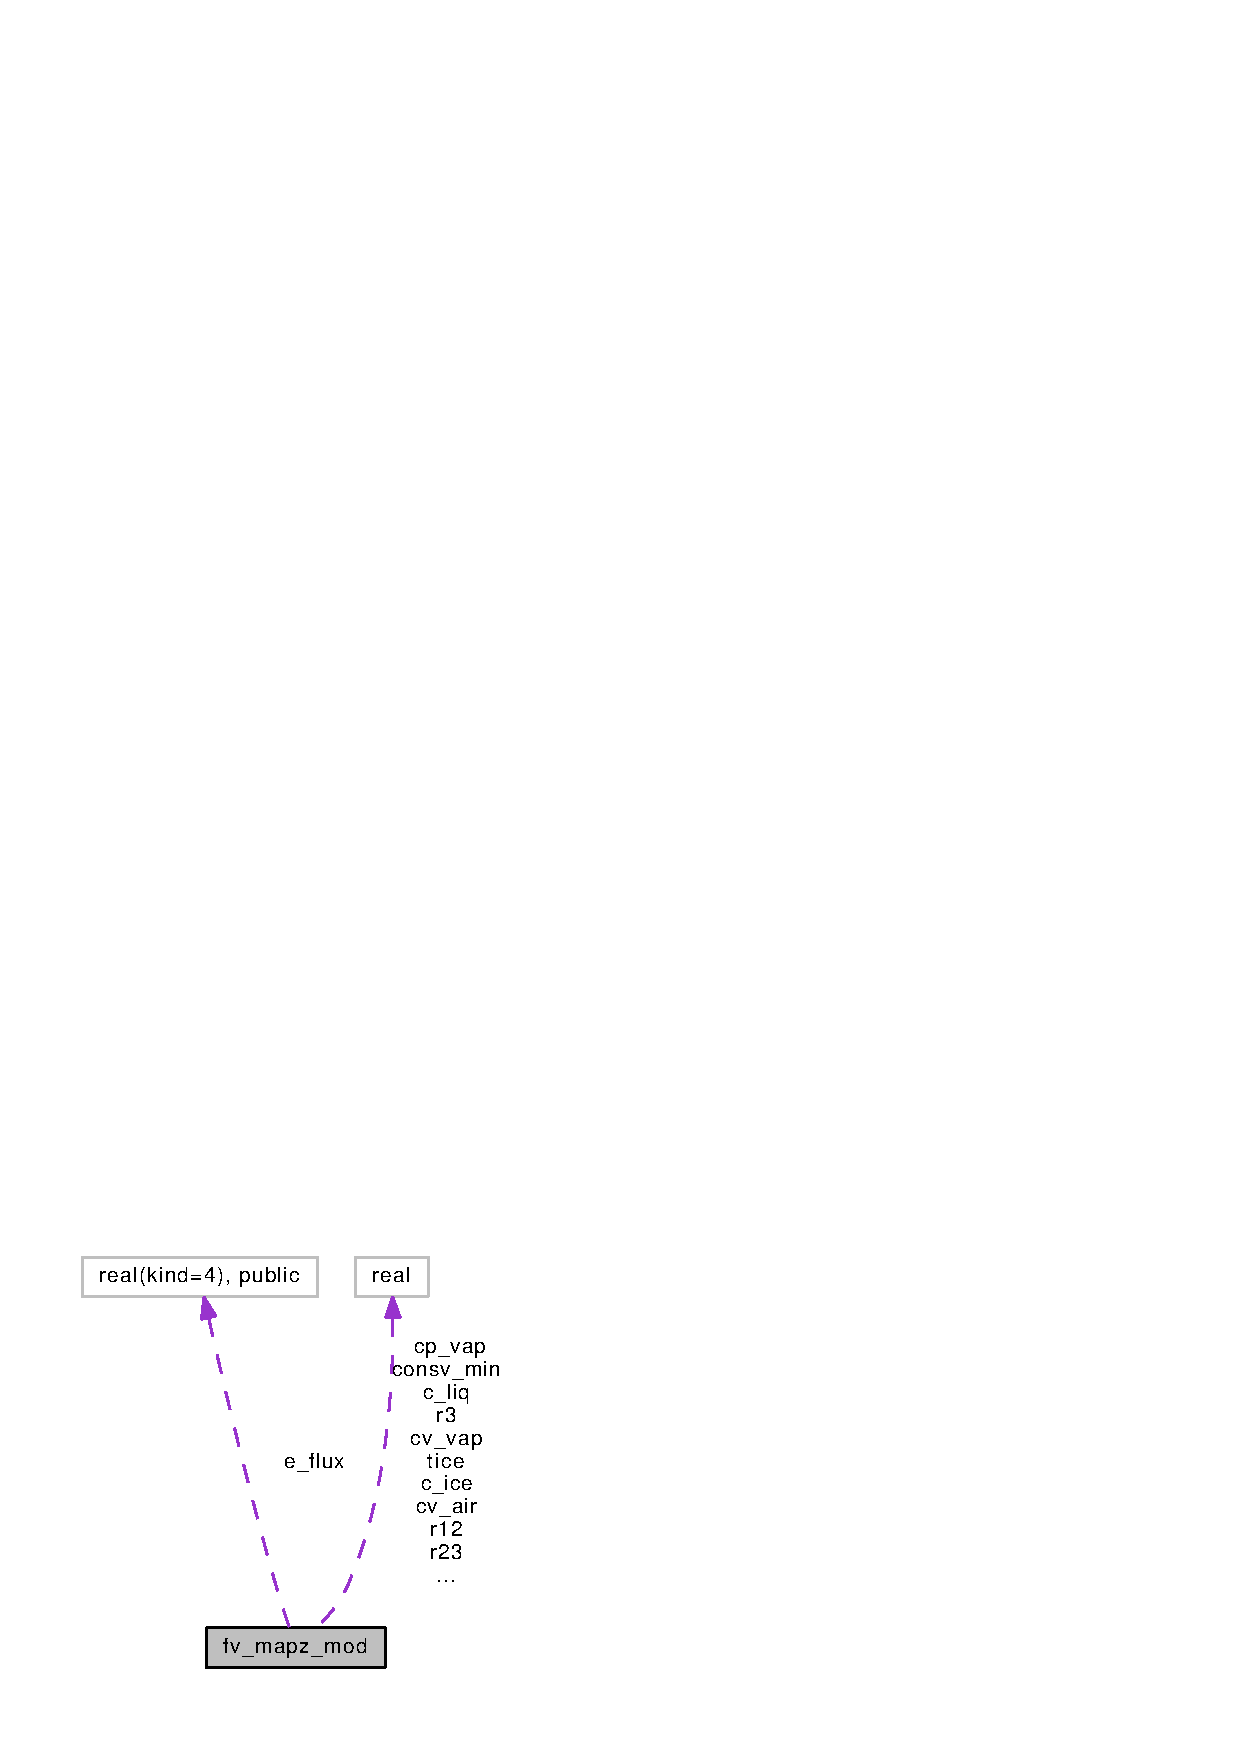
\includegraphics[width=245pt]{classfv__mapz__mod__coll__graph}
\end{center}
\end{figure}
\subsection*{Public Member Functions}
\begin{DoxyCompactItemize}
\item 
subroutine, public \hyperlink{classfv__mapz__mod_a0c56cad3566b5d03032b2c251925ad86}{lagrangian\-\_\-to\-\_\-eulerian} (last\-\_\-step, consv, ps, pe, delp, pkz, pk, mdt, pdt, km, is, ie, js, je, isd, ied, jsd, jed, nq, nwat, sphum, q\-\_\-con, u, v, w, delz, pt, q, hs, r\-\_\-vir, cp, akap, cappa, kord\-\_\-mt, kord\-\_\-wz, kord\-\_\-tr, kord\-\_\-tm, peln, te0\-\_\-2d, ng, ua, va, omga, te, ws, fill, reproduce\-\_\-sum, out\-\_\-dt, dtdt, ptop, ak, bk, pfull, gridstruct, domain, do\-\_\-sat\-\_\-adj, hydrostatic, hybrid\-\_\-z, do\-\_\-omega, adiabatic, do\-\_\-adiabatic\-\_\-init)
\begin{DoxyCompactList}\small\item\em The subroutine 'Lagrangian\-\_\-to\-\_\-\-Eulerian' remaps deformed Lagrangian layers back to the reference Eulerian coordinate. \end{DoxyCompactList}\item 
subroutine, public \hyperlink{classfv__mapz__mod_a9a88277aeaf10321b9ba0d0fbeaef1d9}{compute\-\_\-total\-\_\-energy} (is, ie, js, je, isd, ied, jsd, jed, km, u, v, w, delz, pt, delp, q, qc, pe, peln, hs, rsin2\-\_\-l, cosa\-\_\-s\-\_\-l, r\-\_\-vir, cp, rg, hlv, te\-\_\-2d, ua, va, teq, moist\-\_\-phys, nwat, sphum, liq\-\_\-wat, rainwat, ice\-\_\-wat, snowwat, graupel, hydrostatic, id\-\_\-te)
\begin{DoxyCompactList}\small\item\em The subroutine 'compute\-\_\-total\-\_\-energy' performs the F\-V3-\/consistent computation of the global total energy. \end{DoxyCompactList}\item 
subroutine, public \hyperlink{classfv__mapz__mod_add39354bb1bcbdf4b51fb093c045e8c1}{rst\-\_\-remap} (km, kn, is, ie, js, je, isd, ied, jsd, jed, nq, ntp, delp\-\_\-r, u\-\_\-r, v\-\_\-r, w\-\_\-r, delz\-\_\-r, pt\-\_\-r, q\-\_\-r, qdiag\-\_\-r, delp, u, v, w, delz, pt, q, qdiag, ak\-\_\-r, bk\-\_\-r, ptop, ak, bk, hydrostatic, make\-\_\-nh, domain, square\-\_\-domain)
\begin{DoxyCompactList}\small\item\em The subroutine 'rst\-\_\-remap' remaps all variables required for a restart. \end{DoxyCompactList}\item 
subroutine, public \hyperlink{classfv__mapz__mod_ab8ee4094f27d3aa103d9101c1a46a5cd}{mappm} (km, pe1, q1, kn, pe2, q2, i1, i2, iv, kord, ptop)
\begin{DoxyCompactList}\small\item\em The subroutine 'mappm' is a general-\/purpose routine for remapping one set of vertical levels to another. \end{DoxyCompactList}\item 
subroutine, public \hyperlink{classfv__mapz__mod_a7e2f210d41b616b0d7fb31e6f624897c}{moist\-\_\-cv} (is, ie, isd, ied, jsd, jed, km, j, k, nwat, sphum, liq\-\_\-wat, rainwat, ice\-\_\-wat, snowwat, graupel, q, qd, cvm, t1)
\begin{DoxyCompactList}\small\item\em The subroutine 'moist\-\_\-cv' computes the F\-V3-\/consistent moist heat capacity under constant volume, including the heating capacity of water vapor and condensates. \end{DoxyCompactList}\item 
subroutine, public \hyperlink{classfv__mapz__mod_ae179a4a6af972dd3480b55f62c1ce72e}{moist\-\_\-cp} (is, ie, isd, ied, jsd, jed, km, j, k, nwat, sphum, liq\-\_\-wat, rainwat, ice\-\_\-wat, snowwat, graupel, q, qd, cpm, t1)
\begin{DoxyCompactList}\small\item\em The subroutine 'moist\-\_\-cp' computes the F\-V3-\/consistent moist heat capacity under constant pressure, including the heating capacity of water vapor and condensates. \end{DoxyCompactList}\end{DoxyCompactItemize}
\subsection*{Public Attributes}
\begin{DoxyCompactItemize}
\item 
real, parameter \hyperlink{classfv__mapz__mod_a7879730f4b2baa275cd6abaf9c369bb5}{consv\-\_\-min} = 0.\-001
\begin{DoxyCompactList}\small\item\em below which no correction applies \end{DoxyCompactList}\item 
real, parameter \hyperlink{classfv__mapz__mod_a7cf7f37723bbfb2e7d6b4d948ea81567}{t\-\_\-min} = 184.
\begin{DoxyCompactList}\small\item\em below which applies stricter constraint \end{DoxyCompactList}\item 
real, parameter \hyperlink{classfv__mapz__mod_a85ad5e9000a3d762fd9a62ce59fa9213}{r3} = 1./3.
\item 
real, parameter \hyperlink{classfv__mapz__mod_a24b67f915ffc43180f28b980d9ca7d4c}{r23} = 2./3.
\item 
real, parameter \hyperlink{classfv__mapz__mod_abb8dc5fd25041ba11e452a3994360336}{r12} = 1./12.
\item 
real, parameter \hyperlink{classfv__mapz__mod_a4c1b41c250d4fae86c8297ebe5f71577}{cv\-\_\-vap} = 3.$\ast$rvgas
\begin{DoxyCompactList}\small\item\em 1384.\-5 \end{DoxyCompactList}\item 
real, parameter \hyperlink{classfv__mapz__mod_ac280285d39826f98f83043a75f01d44e}{cv\-\_\-air} = cp\-\_\-air -\/ rdgas
\begin{DoxyCompactList}\small\item\em = rdgas $\ast$ (7/2-\/1) = 2.\-5$\ast$rdgas=717.\-68 \end{DoxyCompactList}\item 
real, parameter \hyperlink{classfv__mapz__mod_aaa58d5b9a96c7678b42b9f21dae04d56}{c\-\_\-ice} = 1972.
\begin{DoxyCompactList}\small\item\em heat capacity of ice at -\/15.\-C \end{DoxyCompactList}\item 
real, parameter \hyperlink{classfv__mapz__mod_aa0e5a6070f8657332c3dc64bd06f62bc}{c\-\_\-liq} = 4.\-1855e+3
\begin{DoxyCompactList}\small\item\em G\-F\-S\-: heat capacity of water at 0\-C. \end{DoxyCompactList}\item 
real, parameter \hyperlink{classfv__mapz__mod_aefa9aa99fd17c4042bf8dab0df746acc}{cp\-\_\-vap} = cp\-\_\-vapor
\item 
real, parameter \hyperlink{classfv__mapz__mod_a79c88aa388441e010f8532f6802b3240}{tice} = 273.\-16
\item 
real(kind=4), public \hyperlink{classfv__mapz__mod_a5f144b640540ec10df24f75e367c2057}{e\-\_\-flux} = 0.
\end{DoxyCompactItemize}
\subsection*{Private Member Functions}
\begin{DoxyCompactItemize}
\item 
subroutine \hyperlink{classfv__mapz__mod_a52443e2b2c993b75d4fdeae138398dfc}{pkez} (km, ifirst, ilast, jfirst, jlast, j, pe, pk, akap, peln, pkz, ptop)
\item 
subroutine \hyperlink{classfv__mapz__mod_a65d5b6aa4d7e599b7af0a362b9e96fd2}{remap\-\_\-z} (km, pe1, q1, kn, pe2, q2, i1, i2, iv, kord)
\item 
subroutine \hyperlink{classfv__mapz__mod_a3d1b66129cc9014f4dbad93e2b397a2e}{map\-\_\-scalar} (km, pe1, q1, qs, kn, pe2, q2, i1, i2, j, ibeg, iend, jbeg, jend, iv, kord, q\-\_\-min)
\item 
subroutine \hyperlink{classfv__mapz__mod_a35a873aa5bd84ccf2d0a71bd96b0eaff}{map1\-\_\-ppm} (km, pe1, q1, qs, kn, pe2, q2, i1, i2, j, ibeg, iend, jbeg, jend, iv, kord)
\item 
subroutine \hyperlink{classfv__mapz__mod_a90a838ddc038bd2a7d817657f5085eb2}{mapn\-\_\-tracer} (nq, km, pe1, pe2, q1, dp2, kord, j, i1, i2, isd, ied, jsd, jed, q\-\_\-min, fill)
\item 
subroutine \hyperlink{classfv__mapz__mod_ae331c105e67cfb16c4d86ff07e5fd110}{map1\-\_\-q2} (km, pe1, q1, kn, pe2, q2, dp2, i1, i2, iv, kord, j, ibeg, iend, jbeg, jend, q\-\_\-min)
\item 
subroutine \hyperlink{classfv__mapz__mod_a58e331d987fff65d9d89a1c3dfa5c5e4}{remap\-\_\-2d} (km, pe1, q1, kn, pe2, q2, i1, i2, iv, kord)
\item 
subroutine \hyperlink{classfv__mapz__mod_ae090838204207cbddd0e4d08f382f95b}{scalar\-\_\-profile} (qs, a4, delp, km, i1, i2, iv, kord, qmin)
\item 
subroutine \hyperlink{classfv__mapz__mod_a628ebb3961c9a007434cb29da18e96d6}{cs\-\_\-profile} (qs, a4, delp, km, i1, i2, iv, kord)
\item 
subroutine \hyperlink{classfv__mapz__mod_a36cfb1e4c0826ab1202a1ae5245fb6f6}{cs\-\_\-limiters} (im, extm, a4, iv)
\item 
subroutine \hyperlink{classfv__mapz__mod_a94cb1798bfac376db362e29961b22d97}{ppm\-\_\-profile} (a4, delp, km, i1, i2, iv, kord)
\item 
subroutine \hyperlink{classfv__mapz__mod_aea73a4b490462eebec46e902de4731dd}{ppm\-\_\-limiters} (dm, a4, itot, lmt)
\item 
subroutine \hyperlink{classfv__mapz__mod_a819605dd5b0423882b9ce0671f475986}{steepz} (i1, i2, km, a4, df2, dm, dq, dp, d4)
\end{DoxyCompactItemize}


\subsection{Detailed Description}
The module 'fv\-\_\-mapz' contains the vertical mapping routines \cite{lin2004vertically}. 

\begin{DoxyNote}{Note}
April 12, 2012 -\/\-S\-J\-L\-: This revision may actually produce rounding level differences due to the elimination of K\-S to compute pressure level for remapping. 
\end{DoxyNote}


Definition at line 27 of file fv\-\_\-mapz.\-F90.



\subsection{Member Function/\-Subroutine Documentation}
\index{fv\-\_\-mapz\-\_\-mod@{fv\-\_\-mapz\-\_\-mod}!compute\-\_\-total\-\_\-energy@{compute\-\_\-total\-\_\-energy}}
\index{compute\-\_\-total\-\_\-energy@{compute\-\_\-total\-\_\-energy}!fv_mapz_mod@{fv\-\_\-mapz\-\_\-mod}}
\subsubsection[{compute\-\_\-total\-\_\-energy}]{\setlength{\rightskip}{0pt plus 5cm}subroutine, public fv\-\_\-mapz\-\_\-mod\-::compute\-\_\-total\-\_\-energy (
\begin{DoxyParamCaption}
\item[{integer, intent(in)}]{is, }
\item[{integer, intent(in)}]{ie, }
\item[{integer, intent(in)}]{js, }
\item[{integer, intent(in)}]{je, }
\item[{integer, intent(in)}]{isd, }
\item[{integer, intent(in)}]{ied, }
\item[{integer, intent(in)}]{jsd, }
\item[{integer, intent(in)}]{jed, }
\item[{integer, intent(in)}]{km, }
\item[{real, dimension(isd\-:ied,  jsd\-:jed+1,km), intent(inout)}]{u, }
\item[{real, dimension(isd\-:ied+1,jsd\-:jed,  km), intent(inout)}]{v, }
\item[{real, dimension(isd\-:,jsd\-:,1\-:), intent(in)}]{w, }
\item[{real, dimension(isd\-:,jsd\-:,1\-:), intent(in)}]{delz, }
\item[{real, dimension(isd\-:ied,jsd\-:jed,km), intent(in)}]{pt, }
\item[{real, dimension(isd\-:ied,jsd\-:jed,km), intent(in)}]{delp, }
\item[{real, dimension(isd\-:ied,jsd\-:jed,km,$\ast$), intent(in)}]{q, }
\item[{real, dimension(isd\-:ied,jsd\-:jed,km), intent(in)}]{qc, }
\item[{real, dimension(is-\/1\-:ie+1,km+1,js-\/1\-:je+1), intent(in)}]{pe, }
\item[{real, dimension(is\-:ie,km+1,js\-:je), intent(in)}]{peln, }
\item[{real, dimension(isd\-:ied,jsd\-:jed), intent(in)}]{hs, }
\item[{real, dimension(isd\-:ied, jsd\-:jed), intent(in)}]{rsin2\-\_\-l, }
\item[{real, dimension(isd\-:ied, jsd\-:jed), intent(in)}]{cosa\-\_\-s\-\_\-l, }
\item[{real, intent(in)}]{r\-\_\-vir, }
\item[{real, intent(in)}]{cp, }
\item[{real, intent(in)}]{rg, }
\item[{real, intent(in)}]{hlv, }
\item[{real, dimension(is\-:ie,js\-:je), intent(out)}]{te\-\_\-2d, }
\item[{real, dimension(isd\-:ied,jsd\-:jed,km), intent(inout)}]{ua, }
\item[{real, dimension(isd\-:ied,jsd\-:jed,km), intent(inout)}]{va, }
\item[{real, dimension(is\-:ie,js\-:je), intent(out)}]{teq, }
\item[{logical, intent(in)}]{moist\-\_\-phys, }
\item[{integer, intent(in)}]{nwat, }
\item[{integer, intent(in)}]{sphum, }
\item[{integer, intent(in)}]{liq\-\_\-wat, }
\item[{integer, intent(in)}]{rainwat, }
\item[{integer, intent(in)}]{ice\-\_\-wat, }
\item[{integer, intent(in)}]{snowwat, }
\item[{integer, intent(in)}]{graupel, }
\item[{logical, intent(in)}]{hydrostatic, }
\item[{integer, intent(in)}]{id\-\_\-te}
\end{DoxyParamCaption}
)}\label{classfv__mapz__mod_a9a88277aeaf10321b9ba0d0fbeaef1d9}


The subroutine 'compute\-\_\-total\-\_\-energy' performs the F\-V3-\/consistent computation of the global total energy. 

It includes the potential, internal (latent and sensible heat), kinetic terms.


\begin{DoxyParams}[1]{Parameters}
\mbox{\tt in}  & {\em w} & vertical velocity (m/s)\\
\hline
\mbox{\tt in}  & {\em hs} & surface geopotential\\
\hline
\mbox{\tt in}  & {\em pe} & pressure at layer edges\\
\hline
\mbox{\tt in}  & {\em peln} & log(pe)\\
\hline
\mbox{\tt out}  & {\em te\-\_\-2d} & vertically integrated T\-E\\
\hline
\mbox{\tt out}  & {\em teq} & Moist T\-E Local \\
\hline
\end{DoxyParams}


Definition at line 952 of file fv\-\_\-mapz.\-F90.



References moist\-\_\-cv(), and multi\-\_\-gases\-\_\-mod\-::vicvqd().



Referenced by fv\-\_\-dynamics\-\_\-mod\-::fv\-\_\-dynamics().

\index{fv\-\_\-mapz\-\_\-mod@{fv\-\_\-mapz\-\_\-mod}!cs\-\_\-limiters@{cs\-\_\-limiters}}
\index{cs\-\_\-limiters@{cs\-\_\-limiters}!fv_mapz_mod@{fv\-\_\-mapz\-\_\-mod}}
\subsubsection[{cs\-\_\-limiters}]{\setlength{\rightskip}{0pt plus 5cm}subroutine fv\-\_\-mapz\-\_\-mod\-::cs\-\_\-limiters (
\begin{DoxyParamCaption}
\item[{integer, intent(in)}]{im, }
\item[{logical, dimension(im), intent(in)}]{extm, }
\item[{real, dimension(4,im), intent(inout)}]{a4, }
\item[{integer, intent(in)}]{iv}
\end{DoxyParamCaption}
)\hspace{0.3cm}{\ttfamily [private]}}\label{classfv__mapz__mod_a36cfb1e4c0826ab1202a1ae5245fb6f6}

\begin{DoxyParams}[1]{Parameters}
\mbox{\tt in,out}  & {\em a4} & P\-P\-M array \\
\hline
\end{DoxyParams}


Definition at line 2519 of file fv\-\_\-mapz.\-F90.



Referenced by cs\-\_\-profile(), and scalar\-\_\-profile().

\index{fv\-\_\-mapz\-\_\-mod@{fv\-\_\-mapz\-\_\-mod}!cs\-\_\-profile@{cs\-\_\-profile}}
\index{cs\-\_\-profile@{cs\-\_\-profile}!fv_mapz_mod@{fv\-\_\-mapz\-\_\-mod}}
\subsubsection[{cs\-\_\-profile}]{\setlength{\rightskip}{0pt plus 5cm}subroutine fv\-\_\-mapz\-\_\-mod\-::cs\-\_\-profile (
\begin{DoxyParamCaption}
\item[{real, dimension(i1\-:i2), intent(in)}]{qs, }
\item[{real, dimension(4,i1\-:i2,km), intent(inout)}]{a4, }
\item[{real, dimension(i1\-:i2,km), intent(in)}]{delp, }
\item[{integer, intent(in)}]{km, }
\item[{integer, intent(in)}]{i1, }
\item[{integer, intent(in)}]{i2, }
\item[{integer, intent(in)}]{iv, }
\item[{integer, intent(in)}]{kord}
\end{DoxyParamCaption}
)\hspace{0.3cm}{\ttfamily [private]}}\label{classfv__mapz__mod_a628ebb3961c9a007434cb29da18e96d6}

\begin{DoxyParams}[1]{Parameters}
\mbox{\tt in}  & {\em km} & vertical dimension\\
\hline
\mbox{\tt in}  & {\em iv} & iv =-\/1\-: winds iv = 0\-: positive definite scalars iv = 1\-: others\\
\hline
\mbox{\tt in}  & {\em delp} & layer pressure thickness\\
\hline
\mbox{\tt in,out}  & {\em a4} & Interpolated values \\
\hline
\end{DoxyParams}


Definition at line 2116 of file fv\-\_\-mapz.\-F90.



References cs\-\_\-limiters().



Referenced by map1\-\_\-ppm(), mappm(), remap\-\_\-2d(), and remap\-\_\-z().

\index{fv\-\_\-mapz\-\_\-mod@{fv\-\_\-mapz\-\_\-mod}!lagrangian\-\_\-to\-\_\-eulerian@{lagrangian\-\_\-to\-\_\-eulerian}}
\index{lagrangian\-\_\-to\-\_\-eulerian@{lagrangian\-\_\-to\-\_\-eulerian}!fv_mapz_mod@{fv\-\_\-mapz\-\_\-mod}}
\subsubsection[{lagrangian\-\_\-to\-\_\-eulerian}]{\setlength{\rightskip}{0pt plus 5cm}subroutine, public fv\-\_\-mapz\-\_\-mod\-::lagrangian\-\_\-to\-\_\-eulerian (
\begin{DoxyParamCaption}
\item[{logical, intent(in)}]{last\-\_\-step, }
\item[{real, intent(in)}]{consv, }
\item[{real, dimension(isd\-:ied,jsd\-:jed), intent(inout)}]{ps, }
\item[{real, dimension(is-\/1\-:ie+1,km+1,js-\/1\-:je+1), intent(inout)}]{pe, }
\item[{real, dimension(isd\-:ied,jsd\-:jed,km), intent(inout)}]{delp, }
\item[{real, dimension(is\-:ie,js\-:je,km), intent(out)}]{pkz, }
\item[{real, dimension(is\-:ie,js\-:je,km+1), intent(inout)}]{pk, }
\item[{real, intent(in)}]{mdt, }
\item[{real, intent(in)}]{pdt, }
\item[{integer, intent(in)}]{km, }
\item[{integer, intent(in)}]{is, }
\item[{integer, intent(in)}]{ie, }
\item[{integer, intent(in)}]{js, }
\item[{integer, intent(in)}]{je, }
\item[{integer, intent(in)}]{isd, }
\item[{integer, intent(in)}]{ied, }
\item[{integer, intent(in)}]{jsd, }
\item[{integer, intent(in)}]{jed, }
\item[{integer, intent(in)}]{nq, }
\item[{integer, intent(in)}]{nwat, }
\item[{integer, intent(in)}]{sphum, }
\item[{real, dimension(isd\-:,jsd\-:,1\-:), intent(inout)}]{q\-\_\-con, }
\item[{real, dimension(isd\-:ied  ,jsd\-:jed+1,km), intent(inout)}]{u, }
\item[{real, dimension(isd\-:ied+1,jsd\-:jed  ,km), intent(inout)}]{v, }
\item[{real, dimension(isd\-:     ,jsd\-:     ,1\-:), intent(inout)}]{w, }
\item[{real, dimension(isd\-:,jsd\-:,1\-:), intent(inout)}]{delz, }
\item[{real, dimension(isd\-:ied  ,jsd\-:jed  ,km), intent(inout)}]{pt, }
\item[{real, dimension(isd\-:ied,jsd\-:jed,km,$\ast$), intent(inout)}]{q, }
\item[{real, dimension(isd\-:ied,jsd\-:jed), intent(in)}]{hs, }
\item[{real, intent(in)}]{r\-\_\-vir, }
\item[{real, intent(in)}]{cp, }
\item[{real, intent(in)}]{akap, }
\item[{real, dimension(isd\-:,jsd\-:,1\-:), intent(inout)}]{cappa, }
\item[{integer, intent(in)}]{kord\-\_\-mt, }
\item[{integer, intent(in)}]{kord\-\_\-wz, }
\item[{integer, dimension(nq), intent(in)}]{kord\-\_\-tr, }
\item[{integer, intent(in)}]{kord\-\_\-tm, }
\item[{real, dimension(is\-:ie,km+1,js\-:je), intent(inout)}]{peln, }
\item[{real, dimension(is\-:ie,js\-:je), intent(inout)}]{te0\-\_\-2d, }
\item[{integer, intent(in)}]{ng, }
\item[{real, dimension(isd\-:ied,jsd\-:jed,km), intent(inout)}]{ua, }
\item[{real, dimension(isd\-:ied,jsd\-:jed,km), intent(inout)}]{va, }
\item[{real, dimension(isd\-:ied,jsd\-:jed,km), intent(inout)}]{omga, }
\item[{real, dimension(isd\-:ied,jsd\-:jed,km), intent(out)}]{te, }
\item[{real, dimension(is\-:ie,js\-:je), intent(in)}]{ws, }
\item[{logical, intent(in)}]{fill, }
\item[{logical, intent(in)}]{reproduce\-\_\-sum, }
\item[{logical, intent(in)}]{out\-\_\-dt, }
\item[{real, dimension(is\-:ie,js\-:je,km), intent(inout)}]{dtdt, }
\item[{real, intent(in)}]{ptop, }
\item[{real, dimension(km+1), intent(in)}]{ak, }
\item[{real, dimension(km+1), intent(in)}]{bk, }
\item[{real, dimension(km), intent(in)}]{pfull, }
\item[{type(fv\-\_\-grid\-\_\-type), intent(in), target}]{gridstruct, }
\item[{type(domain2d), intent(inout)}]{domain, }
\item[{logical, intent(in)}]{do\-\_\-sat\-\_\-adj, }
\item[{logical, intent(in)}]{hydrostatic, }
\item[{logical, intent(in)}]{hybrid\-\_\-z, }
\item[{logical, intent(in)}]{do\-\_\-omega, }
\item[{logical, intent(in)}]{adiabatic, }
\item[{logical, intent(in)}]{do\-\_\-adiabatic\-\_\-init}
\end{DoxyParamCaption}
)}\label{classfv__mapz__mod_a0c56cad3566b5d03032b2c251925ad86}


The subroutine 'Lagrangian\-\_\-to\-\_\-\-Eulerian' remaps deformed Lagrangian layers back to the reference Eulerian coordinate. 

It also includes the entry point for calling fast microphysical processes. This is typically calle on the k\-\_\-split loop.


\begin{DoxyParams}[1]{Parameters}
\mbox{\tt in}  & {\em mdt} & remap time step\\
\hline
\mbox{\tt in}  & {\em pdt} & phys time step\\
\hline
\mbox{\tt in}  & {\em nq} & number of tracers (including h2o)\\
\hline
\mbox{\tt in}  & {\em sphum} & index for water vapor (specific humidity)\\
\hline
\mbox{\tt in}  & {\em ied} & starting \& ending X-\/\-Dir index\\
\hline
\mbox{\tt in}  & {\em jed} & starting \& ending Y-\/\-Dir index\\
\hline
\mbox{\tt in}  & {\em kord\-\_\-mt} & Mapping order for the vector winds\\
\hline
\mbox{\tt in}  & {\em kord\-\_\-wz} & Mapping order/option for w\\
\hline
\mbox{\tt in}  & {\em kord\-\_\-tr} & Mapping order for tracers\\
\hline
\mbox{\tt in}  & {\em kord\-\_\-tm} & Mapping order for thermodynamics\\
\hline
\mbox{\tt in}  & {\em consv} & factor for T\-E conservation\\
\hline
\mbox{\tt in}  & {\em hs} & surface geopotential\\
\hline
\mbox{\tt in}  & {\em fill} & fill negative tracers\\
\hline
\mbox{\tt in,out}  & {\em pk} & pe to the kappa\\
\hline
\mbox{\tt in,out}  & {\em delp} & pressure thickness\\
\hline
\mbox{\tt in,out}  & {\em pe} & pressure at layer edges\\
\hline
\mbox{\tt in,out}  & {\em ps} & surface pressure\\
\hline
\mbox{\tt in,out}  & {\em u} & u-\/wind (m/s)\\
\hline
\mbox{\tt in,out}  & {\em v} & v-\/wind (m/s)\\
\hline
\mbox{\tt in,out}  & {\em w} & vertical velocity (m/s)\\
\hline
\mbox{\tt in,out}  & {\em pt} & cp$\ast$virtual potential temperature as input; output\-: temperature\\
\hline
\mbox{\tt in,out}  & {\em ua} & u-\/wind (m/s) on physics grid\\
\hline
\mbox{\tt in,out}  & {\em va} & v-\/wind (m/s) on physics grid\\
\hline
\mbox{\tt in,out}  & {\em omga} & vertical press. velocity (pascal/sec)\\
\hline
\mbox{\tt in,out}  & {\em peln} & log(pe)\\
\hline
\mbox{\tt out}  & {\em pkz} & layer-\/mean pk for converting t to pt \\
\hline
\end{DoxyParams}


Definition at line 138 of file fv\-\_\-mapz.\-F90.



References fv\-\_\-fill\-\_\-mod\-::fillz(), fv\-\_\-cmp\-\_\-mod\-::fv\-\_\-sat\-\_\-adj(), fv\-\_\-grid\-\_\-utils\-\_\-mod\-::g\-\_\-sum(), map1\-\_\-ppm(), map1\-\_\-q2(), map\-\_\-scalar(), mapn\-\_\-tracer(), moist\-\_\-cv(), pkez(), fv\-\_\-cmp\-\_\-mod\-::qs\-\_\-init(), fv\-\_\-timing\-\_\-mod\-::timing\-\_\-off(), fv\-\_\-timing\-\_\-mod\-::timing\-\_\-on(), multi\-\_\-gases\-\_\-mod\-::vicpqd(), multi\-\_\-gases\-\_\-mod\-::vicvqd(), multi\-\_\-gases\-\_\-mod\-::virq(), and multi\-\_\-gases\-\_\-mod\-::virqd().



Referenced by fv\-\_\-dynamics\-\_\-mod\-::fv\-\_\-dynamics().

\index{fv\-\_\-mapz\-\_\-mod@{fv\-\_\-mapz\-\_\-mod}!map1\-\_\-ppm@{map1\-\_\-ppm}}
\index{map1\-\_\-ppm@{map1\-\_\-ppm}!fv_mapz_mod@{fv\-\_\-mapz\-\_\-mod}}
\subsubsection[{map1\-\_\-ppm}]{\setlength{\rightskip}{0pt plus 5cm}subroutine fv\-\_\-mapz\-\_\-mod\-::map1\-\_\-ppm (
\begin{DoxyParamCaption}
\item[{integer, intent(in)}]{km, }
\item[{real, dimension(i1\-:i2,km+1), intent(in)}]{pe1, }
\item[{real, dimension(ibeg\-:iend,jbeg\-:jend,km), intent(in)}]{q1, }
\item[{real, dimension(i1\-:i2), intent(in)}]{qs, }
\item[{integer, intent(in)}]{kn, }
\item[{real, dimension(i1\-:i2,kn+1), intent(in)}]{pe2, }
\item[{real, dimension(ibeg\-:iend,jbeg\-:jend,kn), intent(inout)}]{q2, }
\item[{integer, intent(in)}]{i1, }
\item[{integer, intent(in)}]{i2, }
\item[{integer, intent(in)}]{j, }
\item[{integer, intent(in)}]{ibeg, }
\item[{integer, intent(in)}]{iend, }
\item[{integer, intent(in)}]{jbeg, }
\item[{integer, intent(in)}]{jend, }
\item[{integer, intent(in)}]{iv, }
\item[{integer, intent(in)}]{kord}
\end{DoxyParamCaption}
)\hspace{0.3cm}{\ttfamily [private]}}\label{classfv__mapz__mod_a35a873aa5bd84ccf2d0a71bd96b0eaff}

\begin{DoxyParams}[1]{Parameters}
\mbox{\tt in}  & {\em i1} & Starting longitude\\
\hline
\mbox{\tt in}  & {\em i2} & Finishing longitude\\
\hline
\mbox{\tt in}  & {\em iv} & Mode\-: 0 == constituents 1 == ??? 2 == remap temp with cs scheme\\
\hline
\mbox{\tt in}  & {\em kord} & Method order\\
\hline
\mbox{\tt in}  & {\em j} & Current latitude\\
\hline
\mbox{\tt in}  & {\em km} & Original vertical dimension\\
\hline
\mbox{\tt in}  & {\em kn} & Target vertical dimension\\
\hline
\mbox{\tt in}  & {\em qs} & bottom B\-C\\
\hline
\mbox{\tt in}  & {\em pe1} & pressure at layer edges from model top to bottom surface in the original vertical coordinate\\
\hline
\mbox{\tt in}  & {\em pe2} & pressure at layer edges from model top to bottom surface in the new vertical coordinate\\
\hline
\mbox{\tt in}  & {\em q1} & Field input\\
\hline
\mbox{\tt in,out}  & {\em q2} & Field output \\
\hline
\end{DoxyParams}


Definition at line 1327 of file fv\-\_\-mapz.\-F90.



References cs\-\_\-profile(), and ppm\-\_\-profile().



Referenced by lagrangian\-\_\-to\-\_\-eulerian().

\index{fv\-\_\-mapz\-\_\-mod@{fv\-\_\-mapz\-\_\-mod}!map1\-\_\-q2@{map1\-\_\-q2}}
\index{map1\-\_\-q2@{map1\-\_\-q2}!fv_mapz_mod@{fv\-\_\-mapz\-\_\-mod}}
\subsubsection[{map1\-\_\-q2}]{\setlength{\rightskip}{0pt plus 5cm}subroutine fv\-\_\-mapz\-\_\-mod\-::map1\-\_\-q2 (
\begin{DoxyParamCaption}
\item[{integer, intent(in)}]{km, }
\item[{real, dimension(i1\-:i2,km+1), intent(in)}]{pe1, }
\item[{real, dimension(ibeg\-:iend,jbeg\-:jend,km), intent(in)}]{q1, }
\item[{integer, intent(in)}]{kn, }
\item[{real, dimension(i1\-:i2,kn+1), intent(in)}]{pe2, }
\item[{real, dimension(i1\-:i2,kn), intent(inout)}]{q2, }
\item[{real, dimension(i1\-:i2,kn), intent(in)}]{dp2, }
\item[{integer, intent(in)}]{i1, }
\item[{integer, intent(in)}]{i2, }
\item[{integer, intent(in)}]{iv, }
\item[{integer, intent(in)}]{kord, }
\item[{integer, intent(in)}]{j, }
\item[{integer, intent(in)}]{ibeg, }
\item[{integer, intent(in)}]{iend, }
\item[{integer, intent(in)}]{jbeg, }
\item[{integer, intent(in)}]{jend, }
\item[{real, intent(in)}]{q\-\_\-min}
\end{DoxyParamCaption}
)\hspace{0.3cm}{\ttfamily [private]}}\label{classfv__mapz__mod_ae331c105e67cfb16c4d86ff07e5fd110}

\begin{DoxyParams}[1]{Parameters}
\mbox{\tt in}  & {\em iv} & Mode\-: 0 == constituents 1 == ???\\
\hline
\mbox{\tt in}  & {\em km} & Original vertical dimension\\
\hline
\mbox{\tt in}  & {\em kn} & Target vertical dimension\\
\hline
\mbox{\tt in}  & {\em pe1} & pressure at layer edges from model top to bottom surface in the original vertical coordinate\\
\hline
\mbox{\tt in}  & {\em pe2} & pressure at layer edges from model top to bottom surface in the new vertical coordinate\\
\hline
\mbox{\tt in}  & {\em q1} & Field input\\
\hline
\mbox{\tt in,out}  & {\em q2} & Field output \\
\hline
\end{DoxyParams}


Definition at line 1528 of file fv\-\_\-mapz.\-F90.



References ppm\-\_\-profile(), and scalar\-\_\-profile().



Referenced by lagrangian\-\_\-to\-\_\-eulerian().

\index{fv\-\_\-mapz\-\_\-mod@{fv\-\_\-mapz\-\_\-mod}!map\-\_\-scalar@{map\-\_\-scalar}}
\index{map\-\_\-scalar@{map\-\_\-scalar}!fv_mapz_mod@{fv\-\_\-mapz\-\_\-mod}}
\subsubsection[{map\-\_\-scalar}]{\setlength{\rightskip}{0pt plus 5cm}subroutine fv\-\_\-mapz\-\_\-mod\-::map\-\_\-scalar (
\begin{DoxyParamCaption}
\item[{integer, intent(in)}]{km, }
\item[{real, dimension(i1\-:i2,km+1), intent(in)}]{pe1, }
\item[{real, dimension(ibeg\-:iend,jbeg\-:jend,km), intent(in)}]{q1, }
\item[{real, dimension(i1\-:i2), intent(in)}]{qs, }
\item[{integer, intent(in)}]{kn, }
\item[{real, dimension(i1\-:i2,kn+1), intent(in)}]{pe2, }
\item[{real, dimension(ibeg\-:iend,jbeg\-:jend,kn), intent(inout)}]{q2, }
\item[{integer, intent(in)}]{i1, }
\item[{integer, intent(in)}]{i2, }
\item[{integer, intent(in)}]{j, }
\item[{integer, intent(in)}]{ibeg, }
\item[{integer, intent(in)}]{iend, }
\item[{integer, intent(in)}]{jbeg, }
\item[{integer, intent(in)}]{jend, }
\item[{integer, intent(in)}]{iv, }
\item[{integer, intent(in)}]{kord, }
\item[{real, intent(in)}]{q\-\_\-min}
\end{DoxyParamCaption}
)\hspace{0.3cm}{\ttfamily [private]}}\label{classfv__mapz__mod_a3d1b66129cc9014f4dbad93e2b397a2e}

\begin{DoxyParams}[1]{Parameters}
\mbox{\tt in}  & {\em i1} & Starting longitude\\
\hline
\mbox{\tt in}  & {\em i2} & Finishing longitude\\
\hline
\mbox{\tt in}  & {\em iv} & Mode\-: 0 == constituents 1 == temp 2 == remap temp with cs scheme\\
\hline
\mbox{\tt in}  & {\em kord} & Method order\\
\hline
\mbox{\tt in}  & {\em j} & Current latitude\\
\hline
\mbox{\tt in}  & {\em km} & Original vertical dimension\\
\hline
\mbox{\tt in}  & {\em kn} & Target vertical dimension\\
\hline
\mbox{\tt in}  & {\em qs} & bottom B\-C\\
\hline
\mbox{\tt in}  & {\em pe1} & pressure at layer edges from model top to bottom surface in the original vertical coordinate\\
\hline
\mbox{\tt in}  & {\em pe2} & pressure at layer edges from model top to bottom surface in the new vertical coordinate\\
\hline
\mbox{\tt in}  & {\em q1} & Field input\\
\hline
\mbox{\tt in,out}  & {\em q2} & Field output \\
\hline
\end{DoxyParams}


Definition at line 1237 of file fv\-\_\-mapz.\-F90.



References ppm\-\_\-profile(), and scalar\-\_\-profile().



Referenced by lagrangian\-\_\-to\-\_\-eulerian().

\index{fv\-\_\-mapz\-\_\-mod@{fv\-\_\-mapz\-\_\-mod}!mapn\-\_\-tracer@{mapn\-\_\-tracer}}
\index{mapn\-\_\-tracer@{mapn\-\_\-tracer}!fv_mapz_mod@{fv\-\_\-mapz\-\_\-mod}}
\subsubsection[{mapn\-\_\-tracer}]{\setlength{\rightskip}{0pt plus 5cm}subroutine fv\-\_\-mapz\-\_\-mod\-::mapn\-\_\-tracer (
\begin{DoxyParamCaption}
\item[{integer, intent(in)}]{nq, }
\item[{integer, intent(in)}]{km, }
\item[{real, dimension(i1\-:i2,km+1), intent(in)}]{pe1, }
\item[{real, dimension(i1\-:i2,km+1), intent(in)}]{pe2, }
\item[{real, dimension(isd\-:ied,jsd\-:jed,km,nq), intent(inout)}]{q1, }
\item[{real, dimension(i1\-:i2,km), intent(in)}]{dp2, }
\item[{integer, dimension(nq), intent(in)}]{kord, }
\item[{integer, intent(in)}]{j, }
\item[{integer, intent(in)}]{i1, }
\item[{integer, intent(in)}]{i2, }
\item[{integer, intent(in)}]{isd, }
\item[{integer, intent(in)}]{ied, }
\item[{integer, intent(in)}]{jsd, }
\item[{integer, intent(in)}]{jed, }
\item[{real, intent(in)}]{q\-\_\-min, }
\item[{logical, intent(in)}]{fill}
\end{DoxyParamCaption}
)\hspace{0.3cm}{\ttfamily [private]}}\label{classfv__mapz__mod_a90a838ddc038bd2a7d817657f5085eb2}

\begin{DoxyParams}[1]{Parameters}
\mbox{\tt in}  & {\em km} & vertical dimension\\
\hline
\mbox{\tt in}  & {\em pe1} & pressure at layer edges from model top to bottom surface in the original vertical coordinate\\
\hline
\mbox{\tt in}  & {\em pe2} & pressure at layer edges from model top to bottom surface in the new vertical coordinate \\
\hline
\end{DoxyParams}


Definition at line 1416 of file fv\-\_\-mapz.\-F90.



References fv\-\_\-fill\-\_\-mod\-::fillz(), and scalar\-\_\-profile().



Referenced by lagrangian\-\_\-to\-\_\-eulerian().

\index{fv\-\_\-mapz\-\_\-mod@{fv\-\_\-mapz\-\_\-mod}!mappm@{mappm}}
\index{mappm@{mappm}!fv_mapz_mod@{fv\-\_\-mapz\-\_\-mod}}
\subsubsection[{mappm}]{\setlength{\rightskip}{0pt plus 5cm}subroutine, public fv\-\_\-mapz\-\_\-mod\-::mappm (
\begin{DoxyParamCaption}
\item[{integer, intent(in)}]{km, }
\item[{real, dimension(i1\-:i2,km+1), intent(in)}]{pe1, }
\item[{real, dimension(i1\-:i2,km), intent(in)}]{q1, }
\item[{integer, intent(in)}]{kn, }
\item[{real, dimension(i1\-:i2,kn+1), intent(in)}]{pe2, }
\item[{real, dimension(i1\-:i2,kn), intent(out)}]{q2, }
\item[{integer, intent(in)}]{i1, }
\item[{integer, intent(in)}]{i2, }
\item[{integer, intent(in)}]{iv, }
\item[{integer, intent(in)}]{kord, }
\item[{real, intent(in)}]{ptop}
\end{DoxyParamCaption}
)}\label{classfv__mapz__mod_ab8ee4094f27d3aa103d9101c1a46a5cd}


The subroutine 'mappm' is a general-\/purpose routine for remapping one set of vertical levels to another. 


\begin{DoxyParams}[1]{Parameters}
\mbox{\tt in}  & {\em pe2} & pe1\-: pressure at layer edges from model top to bottom surface in the O\-R\-I\-G\-I\-N\-A\-L vertical coordinate pe2\-: pressure at layer edges from model top to bottom surface in the N\-E\-W vertical coordinate \\
\hline
\end{DoxyParams}


Definition at line 3277 of file fv\-\_\-mapz.\-F90.



References cs\-\_\-profile(), and ppm\-\_\-profile().



Referenced by external\-\_\-ic\-\_\-mod\-::remap\-\_\-dwinds(), fv\-\_\-regional\-\_\-mod\-::remap\-\_\-dwinds\-\_\-regional\-\_\-bc(), external\-\_\-ic\-\_\-mod\-::remap\-\_\-scalar(), external\-\_\-ic\-\_\-mod\-::remap\-\_\-scalar\-\_\-ec(), external\-\_\-ic\-\_\-mod\-::remap\-\_\-scalar\-\_\-nggps(), fv\-\_\-regional\-\_\-mod\-::remap\-\_\-scalar\-\_\-nggps\-\_\-regional\-\_\-bc(), external\-\_\-ic\-\_\-mod\-::remap\-\_\-scalar\-\_\-single(), fv\-\_\-nwp\-\_\-nudge\-\_\-mod\-::remap\-\_\-tq(), fv\-\_\-nwp\-\_\-nudge\-\_\-mod\-::remap\-\_\-uv(), external\-\_\-ic\-\_\-mod\-::remap\-\_\-winds(), external\-\_\-ic\-\_\-mod\-::remap\-\_\-xyz(), fv\-\_\-nesting\-\_\-mod\-::update\-\_\-remap\-\_\-tqw(), and fv\-\_\-nesting\-\_\-mod\-::update\-\_\-remap\-\_\-uv().

\index{fv\-\_\-mapz\-\_\-mod@{fv\-\_\-mapz\-\_\-mod}!moist\-\_\-cp@{moist\-\_\-cp}}
\index{moist\-\_\-cp@{moist\-\_\-cp}!fv_mapz_mod@{fv\-\_\-mapz\-\_\-mod}}
\subsubsection[{moist\-\_\-cp}]{\setlength{\rightskip}{0pt plus 5cm}subroutine, public fv\-\_\-mapz\-\_\-mod\-::moist\-\_\-cp (
\begin{DoxyParamCaption}
\item[{integer, intent(in)}]{is, }
\item[{integer, intent(in)}]{ie, }
\item[{integer, intent(in)}]{isd, }
\item[{integer, intent(in)}]{ied, }
\item[{integer, intent(in)}]{jsd, }
\item[{integer, intent(in)}]{jed, }
\item[{integer, intent(in)}]{km, }
\item[{integer, intent(in)}]{j, }
\item[{integer, intent(in)}]{k, }
\item[{integer, intent(in)}]{nwat, }
\item[{integer, intent(in)}]{sphum, }
\item[{integer, intent(in)}]{liq\-\_\-wat, }
\item[{integer, intent(in)}]{rainwat, }
\item[{integer, intent(in)}]{ice\-\_\-wat, }
\item[{integer, intent(in)}]{snowwat, }
\item[{integer, intent(in)}]{graupel, }
\item[{real, dimension(isd\-:ied,jsd\-:jed,km,nwat), intent(in)}]{q, }
\item[{real, dimension(is\-:ie), intent(out)}]{qd, }
\item[{real, dimension(is\-:ie), intent(out)}]{cpm, }
\item[{real, dimension(is\-:ie), intent(in), optional}]{t1}
\end{DoxyParamCaption}
)}\label{classfv__mapz__mod_ae179a4a6af972dd3480b55f62c1ce72e}


The subroutine 'moist\-\_\-cp' computes the F\-V3-\/consistent moist heat capacity under constant pressure, including the heating capacity of water vapor and condensates. 



Definition at line 3529 of file fv\-\_\-mapz.\-F90.



References multi\-\_\-gases\-\_\-mod\-::vicpqd().



Referenced by fv\-\_\-dynamics\-\_\-mod\-::fv\-\_\-dynamics(), and fv\-\_\-update\-\_\-phys\-\_\-mod\-::fv\-\_\-update\-\_\-phys().

\index{fv\-\_\-mapz\-\_\-mod@{fv\-\_\-mapz\-\_\-mod}!moist\-\_\-cv@{moist\-\_\-cv}}
\index{moist\-\_\-cv@{moist\-\_\-cv}!fv_mapz_mod@{fv\-\_\-mapz\-\_\-mod}}
\subsubsection[{moist\-\_\-cv}]{\setlength{\rightskip}{0pt plus 5cm}subroutine, public fv\-\_\-mapz\-\_\-mod\-::moist\-\_\-cv (
\begin{DoxyParamCaption}
\item[{integer, intent(in)}]{is, }
\item[{integer, intent(in)}]{ie, }
\item[{integer, intent(in)}]{isd, }
\item[{integer, intent(in)}]{ied, }
\item[{integer, intent(in)}]{jsd, }
\item[{integer, intent(in)}]{jed, }
\item[{integer, intent(in)}]{km, }
\item[{integer, intent(in)}]{j, }
\item[{integer, intent(in)}]{k, }
\item[{integer, intent(in)}]{nwat, }
\item[{integer, intent(in)}]{sphum, }
\item[{integer, intent(in)}]{liq\-\_\-wat, }
\item[{integer, intent(in)}]{rainwat, }
\item[{integer, intent(in)}]{ice\-\_\-wat, }
\item[{integer, intent(in)}]{snowwat, }
\item[{integer, intent(in)}]{graupel, }
\item[{real, dimension(isd\-:ied,jsd\-:jed,km,nwat), intent(in)}]{q, }
\item[{real, dimension(is\-:ie), intent(out)}]{qd, }
\item[{real, dimension(is\-:ie), intent(out)}]{cvm, }
\item[{real, dimension(is\-:ie), intent(in), optional}]{t1}
\end{DoxyParamCaption}
)}\label{classfv__mapz__mod_a7e2f210d41b616b0d7fb31e6f624897c}


The subroutine 'moist\-\_\-cv' computes the F\-V3-\/consistent moist heat capacity under constant volume, including the heating capacity of water vapor and condensates. 

See \cite{emanuel1994atmospheric} for information on variable heat capacities. 

Definition at line 3413 of file fv\-\_\-mapz.\-F90.



References multi\-\_\-gases\-\_\-mod\-::vicvqd().



Referenced by compute\-\_\-total\-\_\-energy(), fv\-\_\-dynamics\-\_\-mod\-::fv\-\_\-dynamics(), fv\-\_\-update\-\_\-phys\-\_\-mod\-::fv\-\_\-update\-\_\-phys(), lagrangian\-\_\-to\-\_\-eulerian(), and fv\-\_\-diagnostics\-\_\-mod\-::nh\-\_\-total\-\_\-energy().

\index{fv\-\_\-mapz\-\_\-mod@{fv\-\_\-mapz\-\_\-mod}!pkez@{pkez}}
\index{pkez@{pkez}!fv_mapz_mod@{fv\-\_\-mapz\-\_\-mod}}
\subsubsection[{pkez}]{\setlength{\rightskip}{0pt plus 5cm}subroutine fv\-\_\-mapz\-\_\-mod\-::pkez (
\begin{DoxyParamCaption}
\item[{integer, intent(in)}]{km, }
\item[{integer, intent(in)}]{ifirst, }
\item[{integer, intent(in)}]{ilast, }
\item[{integer, intent(in)}]{jfirst, }
\item[{integer, intent(in)}]{jlast, }
\item[{integer, intent(in)}]{j, }
\item[{real, dimension(ifirst-\/1\-:ilast+1,km+1,jfirst-\/1\-:jlast+1), intent(in)}]{pe, }
\item[{real, dimension(ifirst\-:ilast,jfirst\-:jlast,km+1), intent(in)}]{pk, }
\item[{real, intent(in)}]{akap, }
\item[{real, dimension(ifirst\-:ilast, km+1, jfirst\-:jlast), intent(inout)}]{peln, }
\item[{real, dimension(ifirst\-:ilast,jfirst\-:jlast,km), intent(out)}]{pkz, }
\item[{real, intent(in)}]{ptop}
\end{DoxyParamCaption}
)\hspace{0.3cm}{\ttfamily [private]}}\label{classfv__mapz__mod_a52443e2b2c993b75d4fdeae138398dfc}

\begin{DoxyParams}[1]{Parameters}
\mbox{\tt in}  & {\em ilast} & Latitude strip\\
\hline
\mbox{\tt in}  & {\em jlast} & Latitude strip\\
\hline
\mbox{\tt in,out}  & {\em peln} & log (pe) \\
\hline
\end{DoxyParams}


Definition at line 1096 of file fv\-\_\-mapz.\-F90.



Referenced by lagrangian\-\_\-to\-\_\-eulerian().

\index{fv\-\_\-mapz\-\_\-mod@{fv\-\_\-mapz\-\_\-mod}!ppm\-\_\-limiters@{ppm\-\_\-limiters}}
\index{ppm\-\_\-limiters@{ppm\-\_\-limiters}!fv_mapz_mod@{fv\-\_\-mapz\-\_\-mod}}
\subsubsection[{ppm\-\_\-limiters}]{\setlength{\rightskip}{0pt plus 5cm}subroutine fv\-\_\-mapz\-\_\-mod\-::ppm\-\_\-limiters (
\begin{DoxyParamCaption}
\item[{real, dimension($\ast$), intent(in)}]{dm, }
\item[{real, dimension(4,$\ast$), intent(inout)}]{a4, }
\item[{integer, intent(in)}]{itot, }
\item[{integer, intent(in)}]{lmt}
\end{DoxyParamCaption}
)\hspace{0.3cm}{\ttfamily [private]}}\label{classfv__mapz__mod_aea73a4b490462eebec46e902de4731dd}

\begin{DoxyParams}[1]{Parameters}
\mbox{\tt in}  & {\em dm} & Linear slope\\
\hline
\mbox{\tt in}  & {\em itot} & Total Longitudes\\
\hline
\mbox{\tt in}  & {\em lmt} & 0\-: Standard P\-P\-M constraint 1\-: Improved full monotonicity constraint (Lin) 2\-: Positive definite constraint 3\-: do nothing (return immediately)\\
\hline
\mbox{\tt in,out}  & {\em a4} & P\-P\-M array A\-A $<$-- a4(1,i) A\-L $<$-- a4(2,i) A\-R $<$-- a4(3,i) A6 $<$-- a4(4,i) \\
\hline
\end{DoxyParams}


Definition at line 2855 of file fv\-\_\-mapz.\-F90.



Referenced by ppm\-\_\-profile().

\index{fv\-\_\-mapz\-\_\-mod@{fv\-\_\-mapz\-\_\-mod}!ppm\-\_\-profile@{ppm\-\_\-profile}}
\index{ppm\-\_\-profile@{ppm\-\_\-profile}!fv_mapz_mod@{fv\-\_\-mapz\-\_\-mod}}
\subsubsection[{ppm\-\_\-profile}]{\setlength{\rightskip}{0pt plus 5cm}subroutine fv\-\_\-mapz\-\_\-mod\-::ppm\-\_\-profile (
\begin{DoxyParamCaption}
\item[{real, dimension(4,i1\-:i2,km), intent(inout)}]{a4, }
\item[{real, dimension(i1\-:i2,km), intent(in)}]{delp, }
\item[{integer, intent(in)}]{km, }
\item[{integer, intent(in)}]{i1, }
\item[{integer, intent(in)}]{i2, }
\item[{integer, intent(in)}]{iv, }
\item[{integer, intent(in)}]{kord}
\end{DoxyParamCaption}
)\hspace{0.3cm}{\ttfamily [private]}}\label{classfv__mapz__mod_a94cb1798bfac376db362e29961b22d97}

\begin{DoxyParams}[1]{Parameters}
\mbox{\tt in}  & {\em iv} & iv =-\/1\-: winds iv = 0\-: positive definite scalars iv = 1\-: others iv = 2\-: temp (if remap\-\_\-t) and w (iv=-\/2)\\
\hline
\mbox{\tt in}  & {\em i1} & Starting longitude\\
\hline
\mbox{\tt in}  & {\em i2} & Finishing longitude\\
\hline
\mbox{\tt in}  & {\em km} & Vertical dimension\\
\hline
\mbox{\tt in}  & {\em kord} & Order (or more accurately method no.)\-:\\
\hline
\mbox{\tt in}  & {\em delp} & Layer pressure thickness\\
\hline
\mbox{\tt in,out}  & {\em a4} & Interpolated values \\
\hline
\end{DoxyParams}


Definition at line 2598 of file fv\-\_\-mapz.\-F90.



References ppm\-\_\-limiters().



Referenced by map1\-\_\-ppm(), map1\-\_\-q2(), map\-\_\-scalar(), mappm(), remap\-\_\-2d(), and remap\-\_\-z().

\index{fv\-\_\-mapz\-\_\-mod@{fv\-\_\-mapz\-\_\-mod}!remap\-\_\-2d@{remap\-\_\-2d}}
\index{remap\-\_\-2d@{remap\-\_\-2d}!fv_mapz_mod@{fv\-\_\-mapz\-\_\-mod}}
\subsubsection[{remap\-\_\-2d}]{\setlength{\rightskip}{0pt plus 5cm}subroutine fv\-\_\-mapz\-\_\-mod\-::remap\-\_\-2d (
\begin{DoxyParamCaption}
\item[{integer, intent(in)}]{km, }
\item[{real, dimension(i1\-:i2,km+1), intent(in)}]{pe1, }
\item[{real, dimension(i1\-:i2,km), intent(in)}]{q1, }
\item[{integer, intent(in)}]{kn, }
\item[{real, dimension(i1\-:i2,kn+1), intent(in)}]{pe2, }
\item[{real, dimension(i1\-:i2,kn), intent(out)}]{q2, }
\item[{integer, intent(in)}]{i1, }
\item[{integer, intent(in)}]{i2, }
\item[{integer, intent(in)}]{iv, }
\item[{integer, intent(in)}]{kord}
\end{DoxyParamCaption}
)\hspace{0.3cm}{\ttfamily [private]}}\label{classfv__mapz__mod_a58e331d987fff65d9d89a1c3dfa5c5e4}

\begin{DoxyParams}[1]{Parameters}
\mbox{\tt in}  & {\em iv} & Mode\-: 0 == constituents 1 ==others\\
\hline
\mbox{\tt in}  & {\em km} & Original vertical dimension\\
\hline
\mbox{\tt in}  & {\em kn} & Target vertical dimension\\
\hline
\mbox{\tt in}  & {\em pe1} & Pressure at layer edges from model top to bottom surface in the original vertical coordinate\\
\hline
\mbox{\tt in}  & {\em pe2} & Pressure at layer edges from model top to bottom surface in the new vertical coordinate\\
\hline
\mbox{\tt in}  & {\em q1} & Field input\\
\hline
\mbox{\tt out}  & {\em q2} & Field output \\
\hline
\end{DoxyParams}


Definition at line 1618 of file fv\-\_\-mapz.\-F90.



References cs\-\_\-profile(), and ppm\-\_\-profile().



Referenced by rst\-\_\-remap().

\index{fv\-\_\-mapz\-\_\-mod@{fv\-\_\-mapz\-\_\-mod}!remap\-\_\-z@{remap\-\_\-z}}
\index{remap\-\_\-z@{remap\-\_\-z}!fv_mapz_mod@{fv\-\_\-mapz\-\_\-mod}}
\subsubsection[{remap\-\_\-z}]{\setlength{\rightskip}{0pt plus 5cm}subroutine fv\-\_\-mapz\-\_\-mod\-::remap\-\_\-z (
\begin{DoxyParamCaption}
\item[{integer, intent(in)}]{km, }
\item[{real, dimension(i1\-:i2,km+1), intent(in)}]{pe1, }
\item[{real, dimension(i1\-:i2,km), intent(in)}]{q1, }
\item[{integer, intent(in)}]{kn, }
\item[{real, dimension(i1\-:i2,kn+1), intent(in)}]{pe2, }
\item[{real, dimension(i1\-:i2,kn), intent(inout)}]{q2, }
\item[{integer, intent(in)}]{i1, }
\item[{integer, intent(in)}]{i2, }
\item[{integer, intent(in)}]{iv, }
\item[{integer, intent(in)}]{kord}
\end{DoxyParamCaption}
)\hspace{0.3cm}{\ttfamily [private]}}\label{classfv__mapz__mod_a65d5b6aa4d7e599b7af0a362b9e96fd2}

\begin{DoxyParams}[1]{Parameters}
\mbox{\tt in}  & {\em i1} & Starting longitude\\
\hline
\mbox{\tt in}  & {\em i2} & Finishing longitude\\
\hline
\mbox{\tt in}  & {\em kord} & Method order\\
\hline
\mbox{\tt in}  & {\em km} & Original vertical dimension\\
\hline
\mbox{\tt in}  & {\em kn} & Target vertical dimension\\
\hline
\mbox{\tt in}  & {\em pe1} & height at layer edges from model top to bottom surface\\
\hline
\mbox{\tt in}  & {\em pe2} & height at layer edges from model top to bottom surface\\
\hline
\mbox{\tt in}  & {\em q1} & Field input\\
\hline
\mbox{\tt in,out}  & {\em q2} & Field output \\
\hline
\end{DoxyParams}


Definition at line 1155 of file fv\-\_\-mapz.\-F90.



References cs\-\_\-profile(), and ppm\-\_\-profile().

\index{fv\-\_\-mapz\-\_\-mod@{fv\-\_\-mapz\-\_\-mod}!rst\-\_\-remap@{rst\-\_\-remap}}
\index{rst\-\_\-remap@{rst\-\_\-remap}!fv_mapz_mod@{fv\-\_\-mapz\-\_\-mod}}
\subsubsection[{rst\-\_\-remap}]{\setlength{\rightskip}{0pt plus 5cm}subroutine, public fv\-\_\-mapz\-\_\-mod\-::rst\-\_\-remap (
\begin{DoxyParamCaption}
\item[{integer, intent(in)}]{km, }
\item[{integer, intent(in)}]{kn, }
\item[{integer, intent(in)}]{is, }
\item[{integer, intent(in)}]{ie, }
\item[{integer, intent(in)}]{js, }
\item[{integer, intent(in)}]{je, }
\item[{integer, intent(in)}]{isd, }
\item[{integer, intent(in)}]{ied, }
\item[{integer, intent(in)}]{jsd, }
\item[{integer, intent(in)}]{jed, }
\item[{integer, intent(in)}]{nq, }
\item[{integer, intent(in)}]{ntp, }
\item[{real, dimension(is\-:ie,js\-:je,km), intent(in)}]{delp\-\_\-r, }
\item[{real, dimension(is\-:ie,  js\-:je+1,km), intent(in)}]{u\-\_\-r, }
\item[{real, dimension(is\-:ie+1,js\-:je  ,km), intent(in)}]{v\-\_\-r, }
\item[{real, dimension(is\-:ie,js\-:je,km), intent(in)}]{w\-\_\-r, }
\item[{real, dimension(is\-:ie,js\-:je,km), intent(inout)}]{delz\-\_\-r, }
\item[{real, dimension(is\-:ie,js\-:je,km), intent(inout)}]{pt\-\_\-r, }
\item[{real, dimension(is\-:ie,js\-:je,km,1\-:ntp), intent(in)}]{q\-\_\-r, }
\item[{real, dimension(is\-:ie,js\-:je,km,ntp+1\-:nq), intent(in)}]{qdiag\-\_\-r, }
\item[{real, dimension(isd\-:ied,jsd\-:jed,kn), intent(out)}]{delp, }
\item[{real, dimension(isd\-:ied  ,jsd\-:jed+1,kn), intent(out)}]{u, }
\item[{real, dimension(isd\-:ied+1,jsd\-:jed  ,kn), intent(out)}]{v, }
\item[{real, dimension(isd\-:     ,jsd\-:     ,1\-:), intent(out)}]{w, }
\item[{real, dimension(isd\-:,jsd\-:,1\-:), intent(out)}]{delz, }
\item[{real, dimension(isd\-:ied  ,jsd\-:jed  ,kn), intent(out)}]{pt, }
\item[{real, dimension(isd\-:ied,jsd\-:jed,kn,1\-:ntp), intent(out)}]{q, }
\item[{real, dimension(isd\-:ied,jsd\-:jed,kn,ntp+1\-:nq), intent(out)}]{qdiag, }
\item[{real, dimension(km+1), intent(in)}]{ak\-\_\-r, }
\item[{real, dimension(km+1), intent(in)}]{bk\-\_\-r, }
\item[{real, intent(in)}]{ptop, }
\item[{real, dimension(kn+1), intent(in)}]{ak, }
\item[{real, dimension(kn+1), intent(in)}]{bk, }
\item[{logical, intent(in)}]{hydrostatic, }
\item[{logical, intent(in)}]{make\-\_\-nh, }
\item[{type(domain2d), intent(inout)}]{domain, }
\item[{logical, intent(in)}]{square\-\_\-domain}
\end{DoxyParamCaption}
)}\label{classfv__mapz__mod_add39354bb1bcbdf4b51fb093c045e8c1}


The subroutine 'rst\-\_\-remap' remaps all variables required for a restart. 

npz\-\_\-restart /= npz (i.\-e., when the number of vertical levels is changed at restart)


\begin{DoxyParams}[1]{Parameters}
\mbox{\tt in}  & {\em km} & Restart z-\/dimension\\
\hline
\mbox{\tt in}  & {\em kn} & Run time dimension\\
\hline
\mbox{\tt in}  & {\em ntp} & Number of tracers (including H2\-O)\\
\hline
\mbox{\tt in}  & {\em ied} & Starting \& ending X-\/\-Dir index\\
\hline
\mbox{\tt in}  & {\em jed} & Starting \& ending Y-\/\-Dir index\\
\hline
\mbox{\tt in}  & {\em delp\-\_\-r} & Pressure thickness\\
\hline
\mbox{\tt in}  & {\em u\-\_\-r} & u-\/wind (m/s)\\
\hline
\mbox{\tt in}  & {\em v\-\_\-r} & v-\/wind (m/s)\\
\hline
\mbox{\tt out}  & {\em delp} & Pressure thickness\\
\hline
\mbox{\tt out}  & {\em u} & u-\/wind (m/s)\\
\hline
\mbox{\tt out}  & {\em v} & v-\/wind (m/s)\\
\hline
\mbox{\tt out}  & {\em w} & Vertical velocity (m/s)\\
\hline
\mbox{\tt out}  & {\em pt} & Temperature\\
\hline
\mbox{\tt out}  & {\em delz} & Delta-\/height (m) \\
\hline
\end{DoxyParams}


Definition at line 2991 of file fv\-\_\-mapz.\-F90.



References remap\-\_\-2d(), and multi\-\_\-gases\-\_\-mod\-::virq().



Referenced by fv\-\_\-io\-\_\-mod\-::remap\-\_\-restart().

\index{fv\-\_\-mapz\-\_\-mod@{fv\-\_\-mapz\-\_\-mod}!scalar\-\_\-profile@{scalar\-\_\-profile}}
\index{scalar\-\_\-profile@{scalar\-\_\-profile}!fv_mapz_mod@{fv\-\_\-mapz\-\_\-mod}}
\subsubsection[{scalar\-\_\-profile}]{\setlength{\rightskip}{0pt plus 5cm}subroutine fv\-\_\-mapz\-\_\-mod\-::scalar\-\_\-profile (
\begin{DoxyParamCaption}
\item[{real, dimension(i1\-:i2), intent(in)}]{qs, }
\item[{real, dimension(4,i1\-:i2,km), intent(inout)}]{a4, }
\item[{real, dimension(i1\-:i2,km), intent(in)}]{delp, }
\item[{integer, intent(in)}]{km, }
\item[{integer, intent(in)}]{i1, }
\item[{integer, intent(in)}]{i2, }
\item[{integer, intent(in)}]{iv, }
\item[{integer, intent(in)}]{kord, }
\item[{real, intent(in)}]{qmin}
\end{DoxyParamCaption}
)\hspace{0.3cm}{\ttfamily [private]}}\label{classfv__mapz__mod_ae090838204207cbddd0e4d08f382f95b}

\begin{DoxyParams}[1]{Parameters}
\mbox{\tt in}  & {\em km} & vertical dimension\\
\hline
\mbox{\tt in}  & {\em iv} & iv =-\/1\-: winds iv = 0\-: positive definite scalars iv = 1\-: others\\
\hline
\mbox{\tt in}  & {\em delp} & Layer pressure thickness\\
\hline
\mbox{\tt in,out}  & {\em a4} & Interpolated values \\
\hline
\end{DoxyParams}


Definition at line 1709 of file fv\-\_\-mapz.\-F90.



References cs\-\_\-limiters().



Referenced by map1\-\_\-q2(), map\-\_\-scalar(), and mapn\-\_\-tracer().

\index{fv\-\_\-mapz\-\_\-mod@{fv\-\_\-mapz\-\_\-mod}!steepz@{steepz}}
\index{steepz@{steepz}!fv_mapz_mod@{fv\-\_\-mapz\-\_\-mod}}
\subsubsection[{steepz}]{\setlength{\rightskip}{0pt plus 5cm}subroutine fv\-\_\-mapz\-\_\-mod\-::steepz (
\begin{DoxyParamCaption}
\item[{integer, intent(in)}]{i1, }
\item[{integer, intent(in)}]{i2, }
\item[{integer, intent(in)}]{km, }
\item[{real, dimension(4,i1\-:i2,km), intent(inout)}]{a4, }
\item[{real, dimension(i1\-:i2,km), intent(in)}]{df2, }
\item[{real, dimension(i1\-:i2,km), intent(in)}]{dm, }
\item[{real, dimension(i1\-:i2,km), intent(in)}]{dq, }
\item[{real, dimension(i1\-:i2,km), intent(in)}]{dp, }
\item[{real, dimension(i1\-:i2,km), intent(in)}]{d4}
\end{DoxyParamCaption}
)\hspace{0.3cm}{\ttfamily [private]}}\label{classfv__mapz__mod_a819605dd5b0423882b9ce0671f475986}

\begin{DoxyParams}[1]{Parameters}
\mbox{\tt in}  & {\em dp} & Grid size\\
\hline
\mbox{\tt in}  & {\em dq} & Backward diff of q\\
\hline
\mbox{\tt in}  & {\em d4} & Backward sum\-: dp(k)+ dp(k-\/1)\\
\hline
\mbox{\tt in}  & {\em df2} & First guess mismatch\\
\hline
\mbox{\tt in}  & {\em dm} & Monotonic mismatch\\
\hline
\mbox{\tt in,out}  & {\em a4} & First guess/steepened \\
\hline
\end{DoxyParams}


Definition at line 2935 of file fv\-\_\-mapz.\-F90.



\subsection{Member Data Documentation}
\index{fv\-\_\-mapz\-\_\-mod@{fv\-\_\-mapz\-\_\-mod}!c\-\_\-ice@{c\-\_\-ice}}
\index{c\-\_\-ice@{c\-\_\-ice}!fv_mapz_mod@{fv\-\_\-mapz\-\_\-mod}}
\subsubsection[{c\-\_\-ice}]{\setlength{\rightskip}{0pt plus 5cm}real, parameter fv\-\_\-mapz\-\_\-mod\-::c\-\_\-ice = 1972.}\label{classfv__mapz__mod_aaa58d5b9a96c7678b42b9f21dae04d56}


heat capacity of ice at -\/15.\-C 



Definition at line 121 of file fv\-\_\-mapz.\-F90.

\index{fv\-\_\-mapz\-\_\-mod@{fv\-\_\-mapz\-\_\-mod}!c\-\_\-liq@{c\-\_\-liq}}
\index{c\-\_\-liq@{c\-\_\-liq}!fv_mapz_mod@{fv\-\_\-mapz\-\_\-mod}}
\subsubsection[{c\-\_\-liq}]{\setlength{\rightskip}{0pt plus 5cm}real, parameter fv\-\_\-mapz\-\_\-mod\-::c\-\_\-liq = 4.\-1855e+3}\label{classfv__mapz__mod_aa0e5a6070f8657332c3dc64bd06f62bc}


G\-F\-S\-: heat capacity of water at 0\-C. 



Definition at line 122 of file fv\-\_\-mapz.\-F90.

\index{fv\-\_\-mapz\-\_\-mod@{fv\-\_\-mapz\-\_\-mod}!consv\-\_\-min@{consv\-\_\-min}}
\index{consv\-\_\-min@{consv\-\_\-min}!fv_mapz_mod@{fv\-\_\-mapz\-\_\-mod}}
\subsubsection[{consv\-\_\-min}]{\setlength{\rightskip}{0pt plus 5cm}real, parameter fv\-\_\-mapz\-\_\-mod\-::consv\-\_\-min = 0.\-001}\label{classfv__mapz__mod_a7879730f4b2baa275cd6abaf9c369bb5}


below which no correction applies 



Definition at line 115 of file fv\-\_\-mapz.\-F90.

\index{fv\-\_\-mapz\-\_\-mod@{fv\-\_\-mapz\-\_\-mod}!cp\-\_\-vap@{cp\-\_\-vap}}
\index{cp\-\_\-vap@{cp\-\_\-vap}!fv_mapz_mod@{fv\-\_\-mapz\-\_\-mod}}
\subsubsection[{cp\-\_\-vap}]{\setlength{\rightskip}{0pt plus 5cm}real, parameter fv\-\_\-mapz\-\_\-mod\-::cp\-\_\-vap = cp\-\_\-vapor}\label{classfv__mapz__mod_aefa9aa99fd17c4042bf8dab0df746acc}

\begin{DoxyEnumerate}
\item 
\end{DoxyEnumerate}

Definition at line 124 of file fv\-\_\-mapz.\-F90.

\index{fv\-\_\-mapz\-\_\-mod@{fv\-\_\-mapz\-\_\-mod}!cv\-\_\-air@{cv\-\_\-air}}
\index{cv\-\_\-air@{cv\-\_\-air}!fv_mapz_mod@{fv\-\_\-mapz\-\_\-mod}}
\subsubsection[{cv\-\_\-air}]{\setlength{\rightskip}{0pt plus 5cm}real, parameter fv\-\_\-mapz\-\_\-mod\-::cv\-\_\-air = cp\-\_\-air -\/ rdgas}\label{classfv__mapz__mod_ac280285d39826f98f83043a75f01d44e}


= rdgas $\ast$ (7/2-\/1) = 2.\-5$\ast$rdgas=717.\-68 



Definition at line 119 of file fv\-\_\-mapz.\-F90.

\index{fv\-\_\-mapz\-\_\-mod@{fv\-\_\-mapz\-\_\-mod}!cv\-\_\-vap@{cv\-\_\-vap}}
\index{cv\-\_\-vap@{cv\-\_\-vap}!fv_mapz_mod@{fv\-\_\-mapz\-\_\-mod}}
\subsubsection[{cv\-\_\-vap}]{\setlength{\rightskip}{0pt plus 5cm}real, parameter fv\-\_\-mapz\-\_\-mod\-::cv\-\_\-vap = 3.$\ast$rvgas}\label{classfv__mapz__mod_a4c1b41c250d4fae86c8297ebe5f71577}


1384.\-5 



Definition at line 118 of file fv\-\_\-mapz.\-F90.

\index{fv\-\_\-mapz\-\_\-mod@{fv\-\_\-mapz\-\_\-mod}!e\-\_\-flux@{e\-\_\-flux}}
\index{e\-\_\-flux@{e\-\_\-flux}!fv_mapz_mod@{fv\-\_\-mapz\-\_\-mod}}
\subsubsection[{e\-\_\-flux}]{\setlength{\rightskip}{0pt plus 5cm}real(kind=4), public fv\-\_\-mapz\-\_\-mod\-::e\-\_\-flux = 0.}\label{classfv__mapz__mod_a5f144b640540ec10df24f75e367c2057}


Definition at line 127 of file fv\-\_\-mapz.\-F90.

\index{fv\-\_\-mapz\-\_\-mod@{fv\-\_\-mapz\-\_\-mod}!r12@{r12}}
\index{r12@{r12}!fv_mapz_mod@{fv\-\_\-mapz\-\_\-mod}}
\subsubsection[{r12}]{\setlength{\rightskip}{0pt plus 5cm}real, parameter fv\-\_\-mapz\-\_\-mod\-::r12 = 1./12.}\label{classfv__mapz__mod_abb8dc5fd25041ba11e452a3994360336}


Definition at line 117 of file fv\-\_\-mapz.\-F90.

\index{fv\-\_\-mapz\-\_\-mod@{fv\-\_\-mapz\-\_\-mod}!r23@{r23}}
\index{r23@{r23}!fv_mapz_mod@{fv\-\_\-mapz\-\_\-mod}}
\subsubsection[{r23}]{\setlength{\rightskip}{0pt plus 5cm}real, parameter fv\-\_\-mapz\-\_\-mod\-::r23 = 2./3.}\label{classfv__mapz__mod_a24b67f915ffc43180f28b980d9ca7d4c}


Definition at line 117 of file fv\-\_\-mapz.\-F90.

\index{fv\-\_\-mapz\-\_\-mod@{fv\-\_\-mapz\-\_\-mod}!r3@{r3}}
\index{r3@{r3}!fv_mapz_mod@{fv\-\_\-mapz\-\_\-mod}}
\subsubsection[{r3}]{\setlength{\rightskip}{0pt plus 5cm}real, parameter fv\-\_\-mapz\-\_\-mod\-::r3 = 1./3.}\label{classfv__mapz__mod_a85ad5e9000a3d762fd9a62ce59fa9213}


Definition at line 117 of file fv\-\_\-mapz.\-F90.

\index{fv\-\_\-mapz\-\_\-mod@{fv\-\_\-mapz\-\_\-mod}!t\-\_\-min@{t\-\_\-min}}
\index{t\-\_\-min@{t\-\_\-min}!fv_mapz_mod@{fv\-\_\-mapz\-\_\-mod}}
\subsubsection[{t\-\_\-min}]{\setlength{\rightskip}{0pt plus 5cm}real, parameter fv\-\_\-mapz\-\_\-mod\-::t\-\_\-min = 184.}\label{classfv__mapz__mod_a7cf7f37723bbfb2e7d6b4d948ea81567}


below which applies stricter constraint 



Definition at line 116 of file fv\-\_\-mapz.\-F90.

\index{fv\-\_\-mapz\-\_\-mod@{fv\-\_\-mapz\-\_\-mod}!tice@{tice}}
\index{tice@{tice}!fv_mapz_mod@{fv\-\_\-mapz\-\_\-mod}}
\subsubsection[{tice}]{\setlength{\rightskip}{0pt plus 5cm}real, parameter fv\-\_\-mapz\-\_\-mod\-::tice = 273.\-16}\label{classfv__mapz__mod_a79c88aa388441e010f8532f6802b3240}


Definition at line 125 of file fv\-\_\-mapz.\-F90.



The documentation for this module was generated from the following file\-:\begin{DoxyCompactItemize}
\item 
/scratch2/\-N\-A\-G\-A\-P\-E/aoml-\/hafs1/\-Kyle.\-Ahern/acs\-\_\-master\-\_\-readonly/model/\hyperlink{fv__mapz_8F90}{fv\-\_\-mapz.\-F90}\end{DoxyCompactItemize}

\section{fv\-\_\-mp\-\_\-mod Module Reference}
\label{classfv__mp__mod}\index{fv\-\_\-mp\-\_\-mod@{fv\-\_\-mp\-\_\-mod}}


The module '\hyperlink{classfv__mp__mod}{fv\-\_\-mp\-\_\-mod}' is a single program multiple data (S\-P\-M\-D) parallel decompostion/communication module.  




Collaboration diagram for fv\-\_\-mp\-\_\-mod\-:
\nopagebreak
\begin{figure}[H]
\begin{center}
\leavevmode
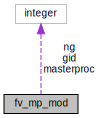
\includegraphics[width=137pt]{classfv__mp__mod__coll__graph}
\end{center}
\end{figure}
\subsection*{Public Attributes}
\begin{DoxyCompactItemize}
\item 
integer, public \hyperlink{classfv__mp__mod_a5040ccdc5ac106793b009fe1ec4bf5d1}{masterproc} = 0
\item 
integer, public \hyperlink{classfv__mp__mod_a30b2cd26ed97df412ac7618005f079a5}{gid} = 0
\item 
integer, parameter, public \hyperlink{classfv__mp__mod_ac41de456a8350a1ffd448c11ad07f923}{ng} = 3
\end{DoxyCompactItemize}


\subsection{Detailed Description}
The module '\hyperlink{classfv__mp__mod}{fv\-\_\-mp\-\_\-mod}' is a single program multiple data (S\-P\-M\-D) parallel decompostion/communication module. 

Definition at line 24 of file fv\-\_\-mp\-\_\-mod.\-F90.



\subsection{Member Data Documentation}
\index{fv\-\_\-mp\-\_\-mod@{fv\-\_\-mp\-\_\-mod}!gid@{gid}}
\index{gid@{gid}!fv_mp_mod@{fv\-\_\-mp\-\_\-mod}}
\subsubsection[{gid}]{\setlength{\rightskip}{0pt plus 5cm}integer, public fv\-\_\-mp\-\_\-mod\-::gid = 0}\label{classfv__mp__mod_a30b2cd26ed97df412ac7618005f079a5}


Definition at line 2715 of file fv\-\_\-mp\-\_\-mod.\-F90.

\index{fv\-\_\-mp\-\_\-mod@{fv\-\_\-mp\-\_\-mod}!masterproc@{masterproc}}
\index{masterproc@{masterproc}!fv_mp_mod@{fv\-\_\-mp\-\_\-mod}}
\subsubsection[{masterproc}]{\setlength{\rightskip}{0pt plus 5cm}integer, public fv\-\_\-mp\-\_\-mod\-::masterproc = 0}\label{classfv__mp__mod_a5040ccdc5ac106793b009fe1ec4bf5d1}


Definition at line 2714 of file fv\-\_\-mp\-\_\-mod.\-F90.

\index{fv\-\_\-mp\-\_\-mod@{fv\-\_\-mp\-\_\-mod}!ng@{ng}}
\index{ng@{ng}!fv_mp_mod@{fv\-\_\-mp\-\_\-mod}}
\subsubsection[{ng}]{\setlength{\rightskip}{0pt plus 5cm}integer, parameter, public fv\-\_\-mp\-\_\-mod\-::ng = 3}\label{classfv__mp__mod_ac41de456a8350a1ffd448c11ad07f923}


Definition at line 2716 of file fv\-\_\-mp\-\_\-mod.\-F90.



The documentation for this module was generated from the following file\-:\begin{DoxyCompactItemize}
\item 
/scratch2/\-N\-A\-G\-A\-P\-E/aoml-\/hafs1/\-Kyle.\-Ahern/acs\-\_\-master\-\_\-readonly/tools/\hyperlink{fv__mp__mod_8F90}{fv\-\_\-mp\-\_\-mod.\-F90}\end{DoxyCompactItemize}

\section{fv\-\_\-arrays\-\_\-mod\-:\-:fv\-\_\-nest\-\_\-bc\-\_\-type\-\_\-3d Type Reference}
\label{structfv__arrays__mod_1_1fv__nest__bc__type__3d}\index{fv\-\_\-arrays\-\_\-mod\-::fv\-\_\-nest\-\_\-bc\-\_\-type\-\_\-3d@{fv\-\_\-arrays\-\_\-mod\-::fv\-\_\-nest\-\_\-bc\-\_\-type\-\_\-3d}}


Collaboration diagram for fv\-\_\-arrays\-\_\-mod\-:\-:fv\-\_\-nest\-\_\-bc\-\_\-type\-\_\-3d\-:
\nopagebreak
\begin{figure}[H]
\begin{center}
\leavevmode
\includegraphics[width=241pt]{structfv__arrays__mod_1_1fv__nest__bc__type__3d__coll__graph}
\end{center}
\end{figure}
\subsection*{Public Attributes}
\begin{DoxyCompactItemize}
\item 
real, dimension(\-:,\-:,\-:), allocatable \hyperlink{structfv__arrays__mod_1_1fv__nest__bc__type__3d_a1024840d7c642d142fdff9f39b999234}{west\-\_\-t1}
\item 
real, dimension(\-:,\-:,\-:), allocatable \hyperlink{structfv__arrays__mod_1_1fv__nest__bc__type__3d_a81e5130c31341a6d82c2b99e4c5954a3}{east\-\_\-t1}
\item 
real, dimension(\-:,\-:,\-:), allocatable \hyperlink{structfv__arrays__mod_1_1fv__nest__bc__type__3d_a849ce48eb3170962785f03b4d43cf3f1}{south\-\_\-t1}
\item 
real, dimension(\-:,\-:,\-:), allocatable \hyperlink{structfv__arrays__mod_1_1fv__nest__bc__type__3d_a64de9671e12ad64f1a8db8807210a607}{north\-\_\-t1}
\item 
real, dimension(\-:,\-:,\-:), allocatable \hyperlink{structfv__arrays__mod_1_1fv__nest__bc__type__3d_a168361be4515cf7122a8037445ecbded}{west\-\_\-t0}
\item 
real, dimension(\-:,\-:,\-:), allocatable \hyperlink{structfv__arrays__mod_1_1fv__nest__bc__type__3d_a5a6b5ce0ea604554586186fc591f83fe}{east\-\_\-t0}
\item 
real, dimension(\-:,\-:,\-:), allocatable \hyperlink{structfv__arrays__mod_1_1fv__nest__bc__type__3d_ab6793c0fd55ec0b709736be490b332e5}{south\-\_\-t0}
\item 
real, dimension(\-:,\-:,\-:), allocatable \hyperlink{structfv__arrays__mod_1_1fv__nest__bc__type__3d_ac926f51f9dbe5a1929103dea7712bd1f}{north\-\_\-t0}
\item 
integer \hyperlink{structfv__arrays__mod_1_1fv__nest__bc__type__3d_a3a61790b97caa2c43e41e654f9e31d5c}{istag}
\item 
integer \hyperlink{structfv__arrays__mod_1_1fv__nest__bc__type__3d_aeab6fc04407b6482a2fe68781db30221}{jstag}
\item 
logical \hyperlink{structfv__arrays__mod_1_1fv__nest__bc__type__3d_a8b3ed5868f96cc803a820909f351a48b}{allocated} = .false.
\item 
logical \hyperlink{structfv__arrays__mod_1_1fv__nest__bc__type__3d_ae0e0c42c38974311cb089dc36b4e3eb5}{initialized} = .false.
\end{DoxyCompactItemize}


\subsection{Detailed Description}


Definition at line 1021 of file fv\-\_\-arrays.\-F90.



\subsection{Member Data Documentation}
\index{fv\-\_\-arrays\-\_\-mod\-::fv\-\_\-nest\-\_\-bc\-\_\-type\-\_\-3d@{fv\-\_\-arrays\-\_\-mod\-::fv\-\_\-nest\-\_\-bc\-\_\-type\-\_\-3d}!allocated@{allocated}}
\index{allocated@{allocated}!fv_arrays_mod::fv_nest_bc_type_3d@{fv\-\_\-arrays\-\_\-mod\-::fv\-\_\-nest\-\_\-bc\-\_\-type\-\_\-3d}}
\subsubsection[{allocated}]{\setlength{\rightskip}{0pt plus 5cm}logical fv\-\_\-arrays\-\_\-mod\-::fv\-\_\-nest\-\_\-bc\-\_\-type\-\_\-3d\-::allocated = .false.}\label{structfv__arrays__mod_1_1fv__nest__bc__type__3d_a8b3ed5868f96cc803a820909f351a48b}


Definition at line 1030 of file fv\-\_\-arrays.\-F90.

\index{fv\-\_\-arrays\-\_\-mod\-::fv\-\_\-nest\-\_\-bc\-\_\-type\-\_\-3d@{fv\-\_\-arrays\-\_\-mod\-::fv\-\_\-nest\-\_\-bc\-\_\-type\-\_\-3d}!east\-\_\-t0@{east\-\_\-t0}}
\index{east\-\_\-t0@{east\-\_\-t0}!fv_arrays_mod::fv_nest_bc_type_3d@{fv\-\_\-arrays\-\_\-mod\-::fv\-\_\-nest\-\_\-bc\-\_\-type\-\_\-3d}}
\subsubsection[{east\-\_\-t0}]{\setlength{\rightskip}{0pt plus 5cm}real, dimension(\-:,\-:,\-:), allocatable fv\-\_\-arrays\-\_\-mod\-::fv\-\_\-nest\-\_\-bc\-\_\-type\-\_\-3d\-::east\-\_\-t0}\label{structfv__arrays__mod_1_1fv__nest__bc__type__3d_a5a6b5ce0ea604554586186fc591f83fe}


Definition at line 1026 of file fv\-\_\-arrays.\-F90.

\index{fv\-\_\-arrays\-\_\-mod\-::fv\-\_\-nest\-\_\-bc\-\_\-type\-\_\-3d@{fv\-\_\-arrays\-\_\-mod\-::fv\-\_\-nest\-\_\-bc\-\_\-type\-\_\-3d}!east\-\_\-t1@{east\-\_\-t1}}
\index{east\-\_\-t1@{east\-\_\-t1}!fv_arrays_mod::fv_nest_bc_type_3d@{fv\-\_\-arrays\-\_\-mod\-::fv\-\_\-nest\-\_\-bc\-\_\-type\-\_\-3d}}
\subsubsection[{east\-\_\-t1}]{\setlength{\rightskip}{0pt plus 5cm}real, dimension(\-:,\-:,\-:), allocatable fv\-\_\-arrays\-\_\-mod\-::fv\-\_\-nest\-\_\-bc\-\_\-type\-\_\-3d\-::east\-\_\-t1}\label{structfv__arrays__mod_1_1fv__nest__bc__type__3d_a81e5130c31341a6d82c2b99e4c5954a3}


Definition at line 1025 of file fv\-\_\-arrays.\-F90.

\index{fv\-\_\-arrays\-\_\-mod\-::fv\-\_\-nest\-\_\-bc\-\_\-type\-\_\-3d@{fv\-\_\-arrays\-\_\-mod\-::fv\-\_\-nest\-\_\-bc\-\_\-type\-\_\-3d}!initialized@{initialized}}
\index{initialized@{initialized}!fv_arrays_mod::fv_nest_bc_type_3d@{fv\-\_\-arrays\-\_\-mod\-::fv\-\_\-nest\-\_\-bc\-\_\-type\-\_\-3d}}
\subsubsection[{initialized}]{\setlength{\rightskip}{0pt plus 5cm}logical fv\-\_\-arrays\-\_\-mod\-::fv\-\_\-nest\-\_\-bc\-\_\-type\-\_\-3d\-::initialized = .false.}\label{structfv__arrays__mod_1_1fv__nest__bc__type__3d_ae0e0c42c38974311cb089dc36b4e3eb5}


Definition at line 1031 of file fv\-\_\-arrays.\-F90.

\index{fv\-\_\-arrays\-\_\-mod\-::fv\-\_\-nest\-\_\-bc\-\_\-type\-\_\-3d@{fv\-\_\-arrays\-\_\-mod\-::fv\-\_\-nest\-\_\-bc\-\_\-type\-\_\-3d}!istag@{istag}}
\index{istag@{istag}!fv_arrays_mod::fv_nest_bc_type_3d@{fv\-\_\-arrays\-\_\-mod\-::fv\-\_\-nest\-\_\-bc\-\_\-type\-\_\-3d}}
\subsubsection[{istag}]{\setlength{\rightskip}{0pt plus 5cm}integer fv\-\_\-arrays\-\_\-mod\-::fv\-\_\-nest\-\_\-bc\-\_\-type\-\_\-3d\-::istag}\label{structfv__arrays__mod_1_1fv__nest__bc__type__3d_a3a61790b97caa2c43e41e654f9e31d5c}


Definition at line 1028 of file fv\-\_\-arrays.\-F90.

\index{fv\-\_\-arrays\-\_\-mod\-::fv\-\_\-nest\-\_\-bc\-\_\-type\-\_\-3d@{fv\-\_\-arrays\-\_\-mod\-::fv\-\_\-nest\-\_\-bc\-\_\-type\-\_\-3d}!jstag@{jstag}}
\index{jstag@{jstag}!fv_arrays_mod::fv_nest_bc_type_3d@{fv\-\_\-arrays\-\_\-mod\-::fv\-\_\-nest\-\_\-bc\-\_\-type\-\_\-3d}}
\subsubsection[{jstag}]{\setlength{\rightskip}{0pt plus 5cm}integer fv\-\_\-arrays\-\_\-mod\-::fv\-\_\-nest\-\_\-bc\-\_\-type\-\_\-3d\-::jstag}\label{structfv__arrays__mod_1_1fv__nest__bc__type__3d_aeab6fc04407b6482a2fe68781db30221}


Definition at line 1028 of file fv\-\_\-arrays.\-F90.

\index{fv\-\_\-arrays\-\_\-mod\-::fv\-\_\-nest\-\_\-bc\-\_\-type\-\_\-3d@{fv\-\_\-arrays\-\_\-mod\-::fv\-\_\-nest\-\_\-bc\-\_\-type\-\_\-3d}!north\-\_\-t0@{north\-\_\-t0}}
\index{north\-\_\-t0@{north\-\_\-t0}!fv_arrays_mod::fv_nest_bc_type_3d@{fv\-\_\-arrays\-\_\-mod\-::fv\-\_\-nest\-\_\-bc\-\_\-type\-\_\-3d}}
\subsubsection[{north\-\_\-t0}]{\setlength{\rightskip}{0pt plus 5cm}real, dimension(\-:,\-:,\-:), allocatable fv\-\_\-arrays\-\_\-mod\-::fv\-\_\-nest\-\_\-bc\-\_\-type\-\_\-3d\-::north\-\_\-t0}\label{structfv__arrays__mod_1_1fv__nest__bc__type__3d_ac926f51f9dbe5a1929103dea7712bd1f}


Definition at line 1026 of file fv\-\_\-arrays.\-F90.

\index{fv\-\_\-arrays\-\_\-mod\-::fv\-\_\-nest\-\_\-bc\-\_\-type\-\_\-3d@{fv\-\_\-arrays\-\_\-mod\-::fv\-\_\-nest\-\_\-bc\-\_\-type\-\_\-3d}!north\-\_\-t1@{north\-\_\-t1}}
\index{north\-\_\-t1@{north\-\_\-t1}!fv_arrays_mod::fv_nest_bc_type_3d@{fv\-\_\-arrays\-\_\-mod\-::fv\-\_\-nest\-\_\-bc\-\_\-type\-\_\-3d}}
\subsubsection[{north\-\_\-t1}]{\setlength{\rightskip}{0pt plus 5cm}real, dimension(\-:,\-:,\-:), allocatable fv\-\_\-arrays\-\_\-mod\-::fv\-\_\-nest\-\_\-bc\-\_\-type\-\_\-3d\-::north\-\_\-t1}\label{structfv__arrays__mod_1_1fv__nest__bc__type__3d_a64de9671e12ad64f1a8db8807210a607}


Definition at line 1025 of file fv\-\_\-arrays.\-F90.

\index{fv\-\_\-arrays\-\_\-mod\-::fv\-\_\-nest\-\_\-bc\-\_\-type\-\_\-3d@{fv\-\_\-arrays\-\_\-mod\-::fv\-\_\-nest\-\_\-bc\-\_\-type\-\_\-3d}!south\-\_\-t0@{south\-\_\-t0}}
\index{south\-\_\-t0@{south\-\_\-t0}!fv_arrays_mod::fv_nest_bc_type_3d@{fv\-\_\-arrays\-\_\-mod\-::fv\-\_\-nest\-\_\-bc\-\_\-type\-\_\-3d}}
\subsubsection[{south\-\_\-t0}]{\setlength{\rightskip}{0pt plus 5cm}real, dimension(\-:,\-:,\-:), allocatable fv\-\_\-arrays\-\_\-mod\-::fv\-\_\-nest\-\_\-bc\-\_\-type\-\_\-3d\-::south\-\_\-t0}\label{structfv__arrays__mod_1_1fv__nest__bc__type__3d_ab6793c0fd55ec0b709736be490b332e5}


Definition at line 1026 of file fv\-\_\-arrays.\-F90.

\index{fv\-\_\-arrays\-\_\-mod\-::fv\-\_\-nest\-\_\-bc\-\_\-type\-\_\-3d@{fv\-\_\-arrays\-\_\-mod\-::fv\-\_\-nest\-\_\-bc\-\_\-type\-\_\-3d}!south\-\_\-t1@{south\-\_\-t1}}
\index{south\-\_\-t1@{south\-\_\-t1}!fv_arrays_mod::fv_nest_bc_type_3d@{fv\-\_\-arrays\-\_\-mod\-::fv\-\_\-nest\-\_\-bc\-\_\-type\-\_\-3d}}
\subsubsection[{south\-\_\-t1}]{\setlength{\rightskip}{0pt plus 5cm}real, dimension(\-:,\-:,\-:), allocatable fv\-\_\-arrays\-\_\-mod\-::fv\-\_\-nest\-\_\-bc\-\_\-type\-\_\-3d\-::south\-\_\-t1}\label{structfv__arrays__mod_1_1fv__nest__bc__type__3d_a849ce48eb3170962785f03b4d43cf3f1}


Definition at line 1025 of file fv\-\_\-arrays.\-F90.

\index{fv\-\_\-arrays\-\_\-mod\-::fv\-\_\-nest\-\_\-bc\-\_\-type\-\_\-3d@{fv\-\_\-arrays\-\_\-mod\-::fv\-\_\-nest\-\_\-bc\-\_\-type\-\_\-3d}!west\-\_\-t0@{west\-\_\-t0}}
\index{west\-\_\-t0@{west\-\_\-t0}!fv_arrays_mod::fv_nest_bc_type_3d@{fv\-\_\-arrays\-\_\-mod\-::fv\-\_\-nest\-\_\-bc\-\_\-type\-\_\-3d}}
\subsubsection[{west\-\_\-t0}]{\setlength{\rightskip}{0pt plus 5cm}real, dimension(\-:,\-:,\-:), allocatable fv\-\_\-arrays\-\_\-mod\-::fv\-\_\-nest\-\_\-bc\-\_\-type\-\_\-3d\-::west\-\_\-t0}\label{structfv__arrays__mod_1_1fv__nest__bc__type__3d_a168361be4515cf7122a8037445ecbded}


Definition at line 1026 of file fv\-\_\-arrays.\-F90.

\index{fv\-\_\-arrays\-\_\-mod\-::fv\-\_\-nest\-\_\-bc\-\_\-type\-\_\-3d@{fv\-\_\-arrays\-\_\-mod\-::fv\-\_\-nest\-\_\-bc\-\_\-type\-\_\-3d}!west\-\_\-t1@{west\-\_\-t1}}
\index{west\-\_\-t1@{west\-\_\-t1}!fv_arrays_mod::fv_nest_bc_type_3d@{fv\-\_\-arrays\-\_\-mod\-::fv\-\_\-nest\-\_\-bc\-\_\-type\-\_\-3d}}
\subsubsection[{west\-\_\-t1}]{\setlength{\rightskip}{0pt plus 5cm}real, dimension(\-:,\-:,\-:), allocatable fv\-\_\-arrays\-\_\-mod\-::fv\-\_\-nest\-\_\-bc\-\_\-type\-\_\-3d\-::west\-\_\-t1}\label{structfv__arrays__mod_1_1fv__nest__bc__type__3d_a1024840d7c642d142fdff9f39b999234}


Definition at line 1025 of file fv\-\_\-arrays.\-F90.



The documentation for this type was generated from the following file\-:\begin{DoxyCompactItemize}
\item 
/scratch2/\-N\-A\-G\-A\-P\-E/aoml-\/hafs1/\-Kyle.\-Ahern/acs\-\_\-master\-\_\-readonly/model/\hyperlink{fv__arrays_8F90}{fv\-\_\-arrays.\-F90}\end{DoxyCompactItemize}

\section{fv\-\_\-arrays\-\_\-mod\-:\-:fv\-\_\-nest\-\_\-bc\-\_\-type\-\_\-4d Type Reference}
\label{structfv__arrays__mod_1_1fv__nest__bc__type__4d}\index{fv\-\_\-arrays\-\_\-mod\-::fv\-\_\-nest\-\_\-bc\-\_\-type\-\_\-4d@{fv\-\_\-arrays\-\_\-mod\-::fv\-\_\-nest\-\_\-bc\-\_\-type\-\_\-4d}}


Collaboration diagram for fv\-\_\-arrays\-\_\-mod\-:\-:fv\-\_\-nest\-\_\-bc\-\_\-type\-\_\-4d\-:
\nopagebreak
\begin{figure}[H]
\begin{center}
\leavevmode
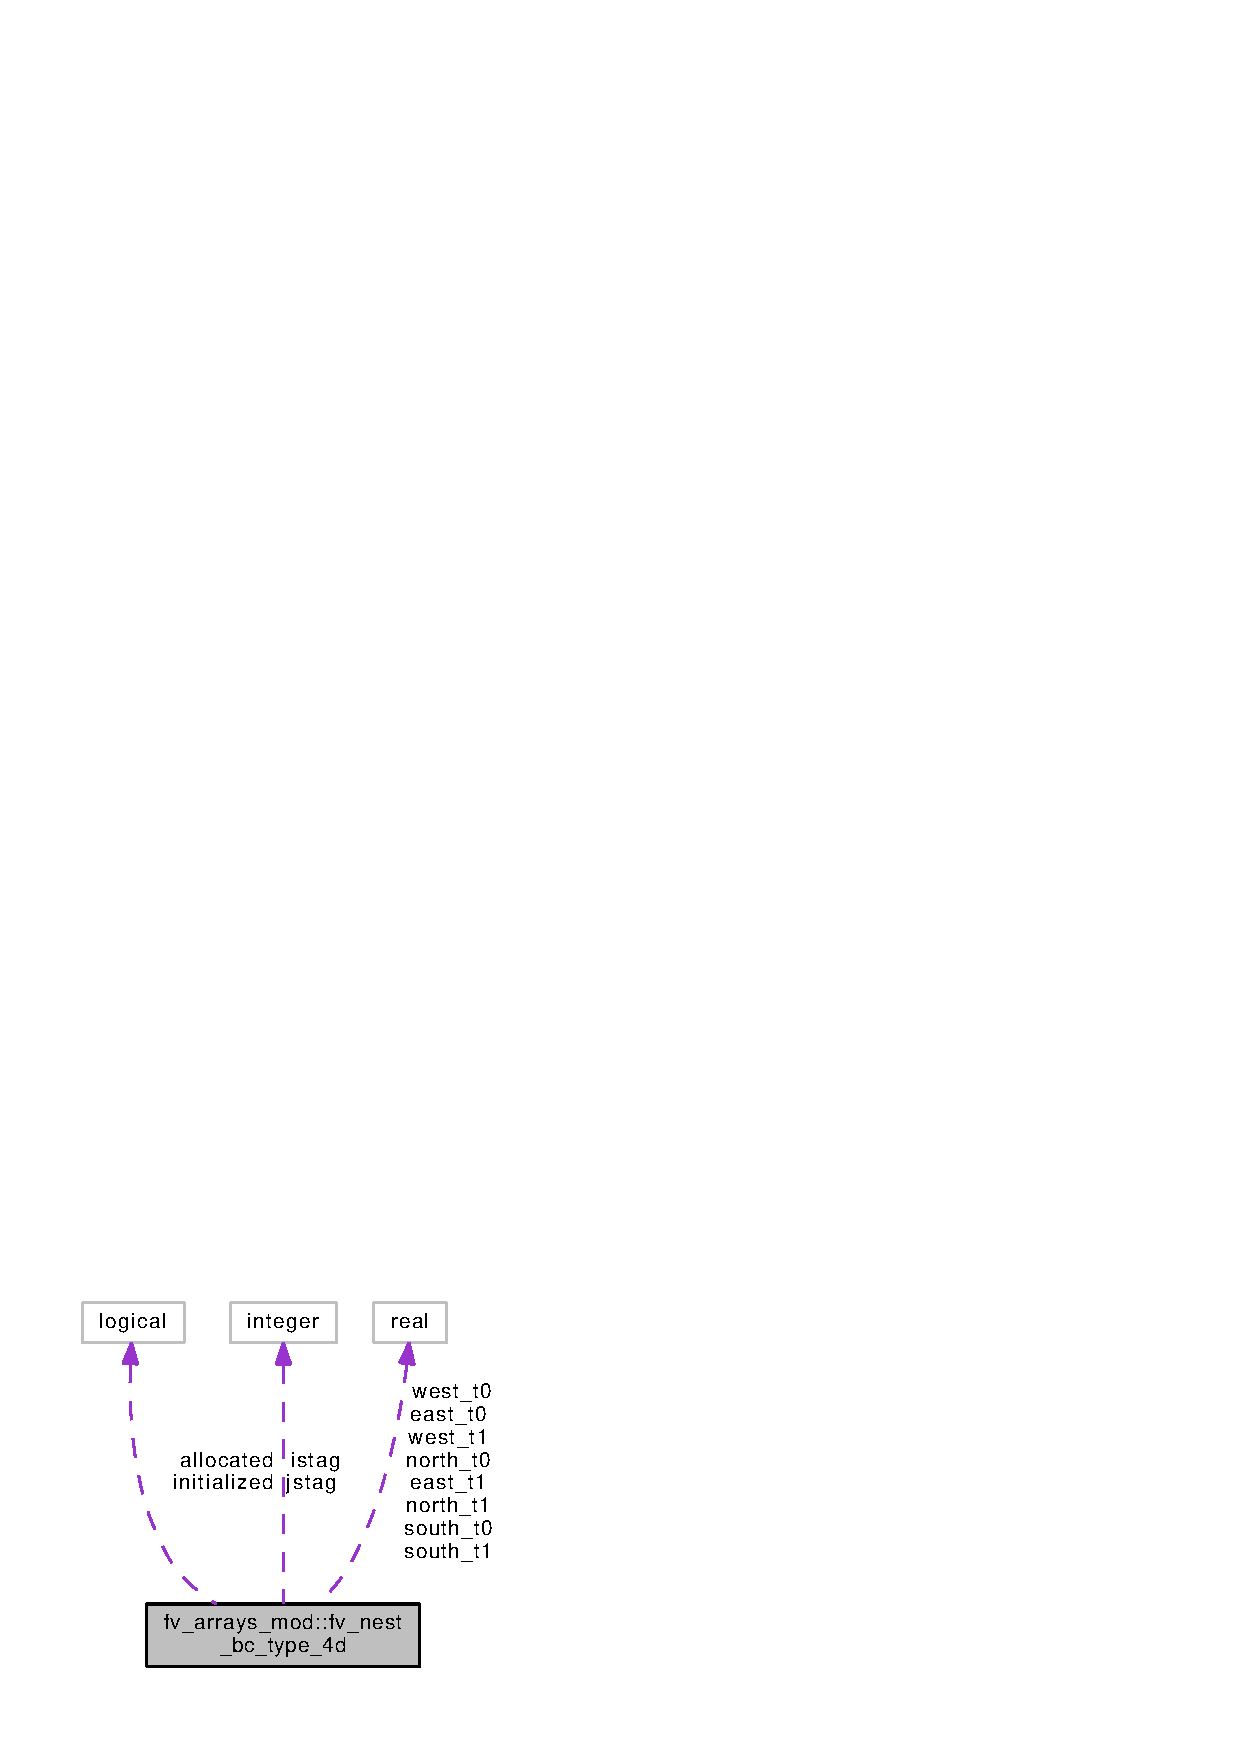
\includegraphics[width=241pt]{structfv__arrays__mod_1_1fv__nest__bc__type__4d__coll__graph}
\end{center}
\end{figure}
\subsection*{Public Attributes}
\begin{DoxyCompactItemize}
\item 
real, dimension(\-:,\-:,\-:,\-:), \\*
allocatable \hyperlink{structfv__arrays__mod_1_1fv__nest__bc__type__4d_a0ce309c499ec88025396f768151f5ae5}{west\-\_\-t1}
\item 
real, dimension(\-:,\-:,\-:,\-:), \\*
allocatable \hyperlink{structfv__arrays__mod_1_1fv__nest__bc__type__4d_a9fa39750a15f788f1a5fdbf6928e410b}{east\-\_\-t1}
\item 
real, dimension(\-:,\-:,\-:,\-:), \\*
allocatable \hyperlink{structfv__arrays__mod_1_1fv__nest__bc__type__4d_a8c7b5e62f810595da5d2f3e668cecb46}{south\-\_\-t1}
\item 
real, dimension(\-:,\-:,\-:,\-:), \\*
allocatable \hyperlink{structfv__arrays__mod_1_1fv__nest__bc__type__4d_a4fbf3b9d6d638d71ab2c2e6d9b3e56e9}{north\-\_\-t1}
\item 
real, dimension(\-:,\-:,\-:,\-:), \\*
allocatable \hyperlink{structfv__arrays__mod_1_1fv__nest__bc__type__4d_a6d5755433238a327bc454f0f8ecf7715}{west\-\_\-t0}
\item 
real, dimension(\-:,\-:,\-:,\-:), \\*
allocatable \hyperlink{structfv__arrays__mod_1_1fv__nest__bc__type__4d_aeccab4bd2caf19bda2d666dda8303078}{east\-\_\-t0}
\item 
real, dimension(\-:,\-:,\-:,\-:), \\*
allocatable \hyperlink{structfv__arrays__mod_1_1fv__nest__bc__type__4d_ab62fffbc0f148a5bb51c3f75492011c2}{south\-\_\-t0}
\item 
real, dimension(\-:,\-:,\-:,\-:), \\*
allocatable \hyperlink{structfv__arrays__mod_1_1fv__nest__bc__type__4d_a5f1d1d5872ea278e2711f79b8e3f4011}{north\-\_\-t0}
\item 
integer \hyperlink{structfv__arrays__mod_1_1fv__nest__bc__type__4d_a722647a593199bed1b1c149522653a1f}{istag}
\item 
integer \hyperlink{structfv__arrays__mod_1_1fv__nest__bc__type__4d_a5589c9903be6ae678db7acd0d1027106}{jstag}
\item 
logical \hyperlink{structfv__arrays__mod_1_1fv__nest__bc__type__4d_acfab2a0567a19b21201b9eb512461ef6}{allocated} = .false.
\item 
logical \hyperlink{structfv__arrays__mod_1_1fv__nest__bc__type__4d_aecff9a6f77e18f40c82fe06def548222}{initialized} = .false.
\end{DoxyCompactItemize}


\subsection{Detailed Description}


Definition at line 1035 of file fv\-\_\-arrays.\-F90.



\subsection{Member Data Documentation}
\index{fv\-\_\-arrays\-\_\-mod\-::fv\-\_\-nest\-\_\-bc\-\_\-type\-\_\-4d@{fv\-\_\-arrays\-\_\-mod\-::fv\-\_\-nest\-\_\-bc\-\_\-type\-\_\-4d}!allocated@{allocated}}
\index{allocated@{allocated}!fv_arrays_mod::fv_nest_bc_type_4d@{fv\-\_\-arrays\-\_\-mod\-::fv\-\_\-nest\-\_\-bc\-\_\-type\-\_\-4d}}
\subsubsection[{allocated}]{\setlength{\rightskip}{0pt plus 5cm}logical fv\-\_\-arrays\-\_\-mod\-::fv\-\_\-nest\-\_\-bc\-\_\-type\-\_\-4d\-::allocated = .false.}\label{structfv__arrays__mod_1_1fv__nest__bc__type__4d_acfab2a0567a19b21201b9eb512461ef6}


Definition at line 1042 of file fv\-\_\-arrays.\-F90.

\index{fv\-\_\-arrays\-\_\-mod\-::fv\-\_\-nest\-\_\-bc\-\_\-type\-\_\-4d@{fv\-\_\-arrays\-\_\-mod\-::fv\-\_\-nest\-\_\-bc\-\_\-type\-\_\-4d}!east\-\_\-t0@{east\-\_\-t0}}
\index{east\-\_\-t0@{east\-\_\-t0}!fv_arrays_mod::fv_nest_bc_type_4d@{fv\-\_\-arrays\-\_\-mod\-::fv\-\_\-nest\-\_\-bc\-\_\-type\-\_\-4d}}
\subsubsection[{east\-\_\-t0}]{\setlength{\rightskip}{0pt plus 5cm}real, dimension(\-:,\-:,\-:,\-:), allocatable fv\-\_\-arrays\-\_\-mod\-::fv\-\_\-nest\-\_\-bc\-\_\-type\-\_\-4d\-::east\-\_\-t0}\label{structfv__arrays__mod_1_1fv__nest__bc__type__4d_aeccab4bd2caf19bda2d666dda8303078}


Definition at line 1038 of file fv\-\_\-arrays.\-F90.

\index{fv\-\_\-arrays\-\_\-mod\-::fv\-\_\-nest\-\_\-bc\-\_\-type\-\_\-4d@{fv\-\_\-arrays\-\_\-mod\-::fv\-\_\-nest\-\_\-bc\-\_\-type\-\_\-4d}!east\-\_\-t1@{east\-\_\-t1}}
\index{east\-\_\-t1@{east\-\_\-t1}!fv_arrays_mod::fv_nest_bc_type_4d@{fv\-\_\-arrays\-\_\-mod\-::fv\-\_\-nest\-\_\-bc\-\_\-type\-\_\-4d}}
\subsubsection[{east\-\_\-t1}]{\setlength{\rightskip}{0pt plus 5cm}real, dimension(\-:,\-:,\-:,\-:), allocatable fv\-\_\-arrays\-\_\-mod\-::fv\-\_\-nest\-\_\-bc\-\_\-type\-\_\-4d\-::east\-\_\-t1}\label{structfv__arrays__mod_1_1fv__nest__bc__type__4d_a9fa39750a15f788f1a5fdbf6928e410b}


Definition at line 1037 of file fv\-\_\-arrays.\-F90.

\index{fv\-\_\-arrays\-\_\-mod\-::fv\-\_\-nest\-\_\-bc\-\_\-type\-\_\-4d@{fv\-\_\-arrays\-\_\-mod\-::fv\-\_\-nest\-\_\-bc\-\_\-type\-\_\-4d}!initialized@{initialized}}
\index{initialized@{initialized}!fv_arrays_mod::fv_nest_bc_type_4d@{fv\-\_\-arrays\-\_\-mod\-::fv\-\_\-nest\-\_\-bc\-\_\-type\-\_\-4d}}
\subsubsection[{initialized}]{\setlength{\rightskip}{0pt plus 5cm}logical fv\-\_\-arrays\-\_\-mod\-::fv\-\_\-nest\-\_\-bc\-\_\-type\-\_\-4d\-::initialized = .false.}\label{structfv__arrays__mod_1_1fv__nest__bc__type__4d_aecff9a6f77e18f40c82fe06def548222}


Definition at line 1043 of file fv\-\_\-arrays.\-F90.

\index{fv\-\_\-arrays\-\_\-mod\-::fv\-\_\-nest\-\_\-bc\-\_\-type\-\_\-4d@{fv\-\_\-arrays\-\_\-mod\-::fv\-\_\-nest\-\_\-bc\-\_\-type\-\_\-4d}!istag@{istag}}
\index{istag@{istag}!fv_arrays_mod::fv_nest_bc_type_4d@{fv\-\_\-arrays\-\_\-mod\-::fv\-\_\-nest\-\_\-bc\-\_\-type\-\_\-4d}}
\subsubsection[{istag}]{\setlength{\rightskip}{0pt plus 5cm}integer fv\-\_\-arrays\-\_\-mod\-::fv\-\_\-nest\-\_\-bc\-\_\-type\-\_\-4d\-::istag}\label{structfv__arrays__mod_1_1fv__nest__bc__type__4d_a722647a593199bed1b1c149522653a1f}


Definition at line 1040 of file fv\-\_\-arrays.\-F90.

\index{fv\-\_\-arrays\-\_\-mod\-::fv\-\_\-nest\-\_\-bc\-\_\-type\-\_\-4d@{fv\-\_\-arrays\-\_\-mod\-::fv\-\_\-nest\-\_\-bc\-\_\-type\-\_\-4d}!jstag@{jstag}}
\index{jstag@{jstag}!fv_arrays_mod::fv_nest_bc_type_4d@{fv\-\_\-arrays\-\_\-mod\-::fv\-\_\-nest\-\_\-bc\-\_\-type\-\_\-4d}}
\subsubsection[{jstag}]{\setlength{\rightskip}{0pt plus 5cm}integer fv\-\_\-arrays\-\_\-mod\-::fv\-\_\-nest\-\_\-bc\-\_\-type\-\_\-4d\-::jstag}\label{structfv__arrays__mod_1_1fv__nest__bc__type__4d_a5589c9903be6ae678db7acd0d1027106}


Definition at line 1040 of file fv\-\_\-arrays.\-F90.

\index{fv\-\_\-arrays\-\_\-mod\-::fv\-\_\-nest\-\_\-bc\-\_\-type\-\_\-4d@{fv\-\_\-arrays\-\_\-mod\-::fv\-\_\-nest\-\_\-bc\-\_\-type\-\_\-4d}!north\-\_\-t0@{north\-\_\-t0}}
\index{north\-\_\-t0@{north\-\_\-t0}!fv_arrays_mod::fv_nest_bc_type_4d@{fv\-\_\-arrays\-\_\-mod\-::fv\-\_\-nest\-\_\-bc\-\_\-type\-\_\-4d}}
\subsubsection[{north\-\_\-t0}]{\setlength{\rightskip}{0pt plus 5cm}real, dimension(\-:,\-:,\-:,\-:), allocatable fv\-\_\-arrays\-\_\-mod\-::fv\-\_\-nest\-\_\-bc\-\_\-type\-\_\-4d\-::north\-\_\-t0}\label{structfv__arrays__mod_1_1fv__nest__bc__type__4d_a5f1d1d5872ea278e2711f79b8e3f4011}


Definition at line 1038 of file fv\-\_\-arrays.\-F90.

\index{fv\-\_\-arrays\-\_\-mod\-::fv\-\_\-nest\-\_\-bc\-\_\-type\-\_\-4d@{fv\-\_\-arrays\-\_\-mod\-::fv\-\_\-nest\-\_\-bc\-\_\-type\-\_\-4d}!north\-\_\-t1@{north\-\_\-t1}}
\index{north\-\_\-t1@{north\-\_\-t1}!fv_arrays_mod::fv_nest_bc_type_4d@{fv\-\_\-arrays\-\_\-mod\-::fv\-\_\-nest\-\_\-bc\-\_\-type\-\_\-4d}}
\subsubsection[{north\-\_\-t1}]{\setlength{\rightskip}{0pt plus 5cm}real, dimension(\-:,\-:,\-:,\-:), allocatable fv\-\_\-arrays\-\_\-mod\-::fv\-\_\-nest\-\_\-bc\-\_\-type\-\_\-4d\-::north\-\_\-t1}\label{structfv__arrays__mod_1_1fv__nest__bc__type__4d_a4fbf3b9d6d638d71ab2c2e6d9b3e56e9}


Definition at line 1037 of file fv\-\_\-arrays.\-F90.

\index{fv\-\_\-arrays\-\_\-mod\-::fv\-\_\-nest\-\_\-bc\-\_\-type\-\_\-4d@{fv\-\_\-arrays\-\_\-mod\-::fv\-\_\-nest\-\_\-bc\-\_\-type\-\_\-4d}!south\-\_\-t0@{south\-\_\-t0}}
\index{south\-\_\-t0@{south\-\_\-t0}!fv_arrays_mod::fv_nest_bc_type_4d@{fv\-\_\-arrays\-\_\-mod\-::fv\-\_\-nest\-\_\-bc\-\_\-type\-\_\-4d}}
\subsubsection[{south\-\_\-t0}]{\setlength{\rightskip}{0pt plus 5cm}real, dimension(\-:,\-:,\-:,\-:), allocatable fv\-\_\-arrays\-\_\-mod\-::fv\-\_\-nest\-\_\-bc\-\_\-type\-\_\-4d\-::south\-\_\-t0}\label{structfv__arrays__mod_1_1fv__nest__bc__type__4d_ab62fffbc0f148a5bb51c3f75492011c2}


Definition at line 1038 of file fv\-\_\-arrays.\-F90.

\index{fv\-\_\-arrays\-\_\-mod\-::fv\-\_\-nest\-\_\-bc\-\_\-type\-\_\-4d@{fv\-\_\-arrays\-\_\-mod\-::fv\-\_\-nest\-\_\-bc\-\_\-type\-\_\-4d}!south\-\_\-t1@{south\-\_\-t1}}
\index{south\-\_\-t1@{south\-\_\-t1}!fv_arrays_mod::fv_nest_bc_type_4d@{fv\-\_\-arrays\-\_\-mod\-::fv\-\_\-nest\-\_\-bc\-\_\-type\-\_\-4d}}
\subsubsection[{south\-\_\-t1}]{\setlength{\rightskip}{0pt plus 5cm}real, dimension(\-:,\-:,\-:,\-:), allocatable fv\-\_\-arrays\-\_\-mod\-::fv\-\_\-nest\-\_\-bc\-\_\-type\-\_\-4d\-::south\-\_\-t1}\label{structfv__arrays__mod_1_1fv__nest__bc__type__4d_a8c7b5e62f810595da5d2f3e668cecb46}


Definition at line 1037 of file fv\-\_\-arrays.\-F90.

\index{fv\-\_\-arrays\-\_\-mod\-::fv\-\_\-nest\-\_\-bc\-\_\-type\-\_\-4d@{fv\-\_\-arrays\-\_\-mod\-::fv\-\_\-nest\-\_\-bc\-\_\-type\-\_\-4d}!west\-\_\-t0@{west\-\_\-t0}}
\index{west\-\_\-t0@{west\-\_\-t0}!fv_arrays_mod::fv_nest_bc_type_4d@{fv\-\_\-arrays\-\_\-mod\-::fv\-\_\-nest\-\_\-bc\-\_\-type\-\_\-4d}}
\subsubsection[{west\-\_\-t0}]{\setlength{\rightskip}{0pt plus 5cm}real, dimension(\-:,\-:,\-:,\-:), allocatable fv\-\_\-arrays\-\_\-mod\-::fv\-\_\-nest\-\_\-bc\-\_\-type\-\_\-4d\-::west\-\_\-t0}\label{structfv__arrays__mod_1_1fv__nest__bc__type__4d_a6d5755433238a327bc454f0f8ecf7715}


Definition at line 1038 of file fv\-\_\-arrays.\-F90.

\index{fv\-\_\-arrays\-\_\-mod\-::fv\-\_\-nest\-\_\-bc\-\_\-type\-\_\-4d@{fv\-\_\-arrays\-\_\-mod\-::fv\-\_\-nest\-\_\-bc\-\_\-type\-\_\-4d}!west\-\_\-t1@{west\-\_\-t1}}
\index{west\-\_\-t1@{west\-\_\-t1}!fv_arrays_mod::fv_nest_bc_type_4d@{fv\-\_\-arrays\-\_\-mod\-::fv\-\_\-nest\-\_\-bc\-\_\-type\-\_\-4d}}
\subsubsection[{west\-\_\-t1}]{\setlength{\rightskip}{0pt plus 5cm}real, dimension(\-:,\-:,\-:,\-:), allocatable fv\-\_\-arrays\-\_\-mod\-::fv\-\_\-nest\-\_\-bc\-\_\-type\-\_\-4d\-::west\-\_\-t1}\label{structfv__arrays__mod_1_1fv__nest__bc__type__4d_a0ce309c499ec88025396f768151f5ae5}


Definition at line 1037 of file fv\-\_\-arrays.\-F90.



The documentation for this type was generated from the following file\-:\begin{DoxyCompactItemize}
\item 
/scratch2/\-N\-A\-G\-A\-P\-E/aoml-\/hafs1/\-Kyle.\-Ahern/acs\-\_\-master\-\_\-readonly/model/\hyperlink{fv__arrays_8F90}{fv\-\_\-arrays.\-F90}\end{DoxyCompactItemize}

\section{fv\-\_\-arrays\-\_\-mod\-:\-:fv\-\_\-nest\-\_\-type Type Reference}
\label{structfv__arrays__mod_1_1fv__nest__type}\index{fv\-\_\-arrays\-\_\-mod\-::fv\-\_\-nest\-\_\-type@{fv\-\_\-arrays\-\_\-mod\-::fv\-\_\-nest\-\_\-type}}


Collaboration diagram for fv\-\_\-arrays\-\_\-mod\-:\-:fv\-\_\-nest\-\_\-type\-:
\nopagebreak
\begin{figure}[H]
\begin{center}
\leavevmode
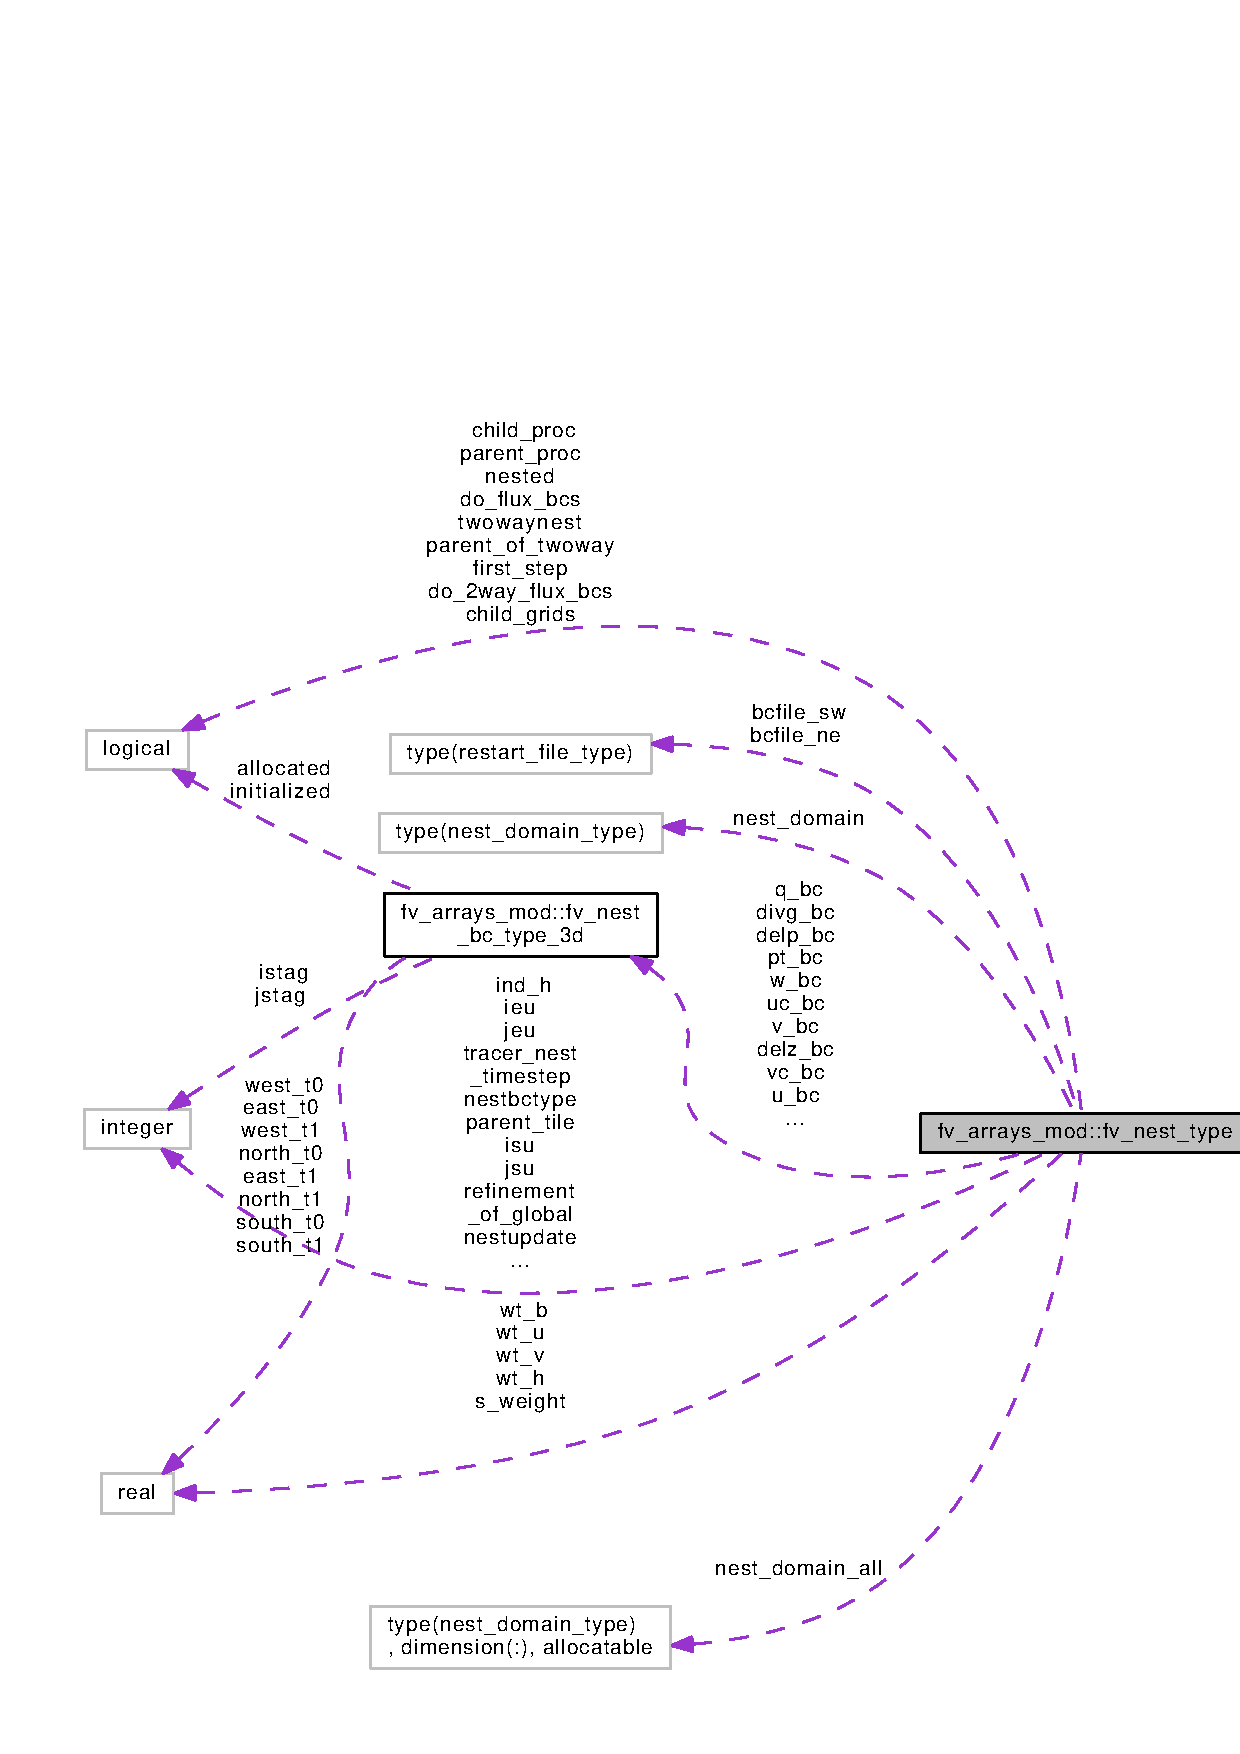
\includegraphics[width=350pt]{structfv__arrays__mod_1_1fv__nest__type__coll__graph}
\end{center}
\end{figure}
\subsection*{Public Attributes}
\begin{DoxyCompactItemize}
\item 
integer \hyperlink{structfv__arrays__mod_1_1fv__nest__type_abd58583303d5bb884b9b12a981ff5134}{refinement} = 3
\begin{DoxyCompactList}\small\item\em Refinement ratio of the nested grid. This is the number of times that each coarse-\/grid cell face will be divided into smaller segments on the nested grid. Required to be a positive integer if nested = true. Nested grids are aligned with the coarse grid, so non-\/integer refinements are not permitted. The default value is 3. \end{DoxyCompactList}\item 
integer \hyperlink{structfv__arrays__mod_1_1fv__nest__type_aede3093421924ff4358cb95c28007329}{parent\-\_\-tile} = 1
\begin{DoxyCompactList}\small\item\em Number of the tile (ie. face) in which this nested grid is found in its parent. Required to be a positive value if nested = true. If the parent grid is not a cubed sphere, or itself is a nested grid, this should be set to 1. If the parent grid has been rotated (using do\-\_\-schmidt) with the intent of centering the nested grid at target\-\_\-lat and target\-\_\-lon, then parent\-\_\-tile should be set to 6. The default value is 1. \end{DoxyCompactList}\item 
logical \hyperlink{structfv__arrays__mod_1_1fv__nest__type_a8f685ad8b666aa48cd72b369a3d6f7cd}{nested} = .false.
\begin{DoxyCompactList}\small\item\em Whether this is a nested grid. The default value is .false. \end{DoxyCompactList}\item 
integer \hyperlink{structfv__arrays__mod_1_1fv__nest__type_adc7be956d3d3a5111c23c80548f87587}{nestbctype} = 1
\item 
integer \hyperlink{structfv__arrays__mod_1_1fv__nest__type_aeb2fa3b74f53464f55ad889e1532dae1}{nsponge} = 0
\item 
integer \hyperlink{structfv__arrays__mod_1_1fv__nest__type_af7ecd25821161fb9ee94fa569ce504f3}{nestupdate} = 0
\begin{DoxyCompactList}\small\item\em Type of nested-\/grid update to use; details are given in \hyperlink{fv__nesting_8F90}{model/fv\-\_\-nesting.\-F90}. The default is 0. \end{DoxyCompactList}\item 
logical \hyperlink{structfv__arrays__mod_1_1fv__nest__type_a234513f19d64ac85cc358d3772d56a76}{twowaynest} = .false.
\begin{DoxyCompactList}\small\item\em Whether to use two-\/way nesting, the process by which the nested-\/grid solution can feed back onto the coarse-\/grid solution. The default value is .false. \end{DoxyCompactList}\item 
integer \hyperlink{structfv__arrays__mod_1_1fv__nest__type_a8de72175222aeea5f0b915b2ca1c0083}{ioffset}
\item 
integer \hyperlink{structfv__arrays__mod_1_1fv__nest__type_a0947c02b782d243a3ba7c1ba990d2995}{joffset}
\begin{DoxyCompactList}\small\item\em Position of nest within parent grid. \end{DoxyCompactList}\item 
integer \hyperlink{structfv__arrays__mod_1_1fv__nest__type_ac784733ccc09f7037078b71074727228}{nest\-\_\-timestep} = 0
\begin{DoxyCompactList}\small\item\em Counter for nested-\/grid timesteps. \end{DoxyCompactList}\item 
integer \hyperlink{structfv__arrays__mod_1_1fv__nest__type_a0a40f5b9b3c88f219c15c4f5cf45d035}{tracer\-\_\-nest\-\_\-timestep} = 0
\begin{DoxyCompactList}\small\item\em Counter for nested-\/grid timesteps. \end{DoxyCompactList}\item 
real \hyperlink{structfv__arrays__mod_1_1fv__nest__type_a70ba47b82bcf4969d6c200a553c1267a}{s\-\_\-weight} = 1.e-\/6
\begin{DoxyCompactList}\small\item\em sponge weight \end{DoxyCompactList}\item 
logical \hyperlink{structfv__arrays__mod_1_1fv__nest__type_a751315043662ab03c036c2e8f35ed3e3}{first\-\_\-step} = .true.
\item 
integer \hyperlink{structfv__arrays__mod_1_1fv__nest__type_ab6d053aade4a0057cd873c1c1fcd33fa}{refinement\-\_\-of\-\_\-global} = 1
\item 
integer \hyperlink{structfv__arrays__mod_1_1fv__nest__type_a9bb2f8c472e0b576582539e118ef44dd}{npx\-\_\-global}
\item 
integer \hyperlink{structfv__arrays__mod_1_1fv__nest__type_ae71ff140cce3e6bee7ffd0f4c82da439}{upoff} = 1
\begin{DoxyCompactList}\small\item\em currently the same for all variables \end{DoxyCompactList}\item 
integer \hyperlink{structfv__arrays__mod_1_1fv__nest__type_a00e4c8056d2cdb4d365658f28b224db0}{isu} = -\/999
\item 
integer \hyperlink{structfv__arrays__mod_1_1fv__nest__type_abf7c9c0bc141c25e6780cfb7fdf2c61a}{ieu} = -\/1000
\item 
integer \hyperlink{structfv__arrays__mod_1_1fv__nest__type_a3ff9370e06722ce089be75bbe4ddc870}{jsu} = -\/999
\item 
integer \hyperlink{structfv__arrays__mod_1_1fv__nest__type_acd802c1e3bcabb89e088cf208df03909}{jeu} = -\/1000
\begin{DoxyCompactList}\small\item\em limits of update regions on coarse grid \end{DoxyCompactList}\item 
type(nest\-\_\-domain\-\_\-type) \hyperlink{structfv__arrays__mod_1_1fv__nest__type_a2f7e06880fd4717d1aec364d3de4a2d3}{nest\-\_\-domain}
\begin{DoxyCompactList}\small\item\em Structure holding link from this grid to its parent. \end{DoxyCompactList}\item 
type(nest\-\_\-domain\-\_\-type), \\*
dimension(\-:), allocatable \hyperlink{structfv__arrays__mod_1_1fv__nest__type_a4b80c11edd90aa8ba757f5d11d8031d1}{nest\-\_\-domain\-\_\-all}
\item 
integer, dimension(\-:,\-:,\-:), \\*
allocatable \hyperlink{structfv__arrays__mod_1_1fv__nest__type_aca2c6b35886f7d7de3d0f1b37c0bef1e}{ind\-\_\-h}
\item 
integer, dimension(\-:,\-:,\-:), \\*
allocatable \hyperlink{structfv__arrays__mod_1_1fv__nest__type_a45020a146430029b2aecfae4d0c3836e}{ind\-\_\-u}
\item 
integer, dimension(\-:,\-:,\-:), \\*
allocatable \hyperlink{structfv__arrays__mod_1_1fv__nest__type_a99e3c5ac558d6680d13abecdb19d42d6}{ind\-\_\-v}
\item 
integer, dimension(\-:,\-:,\-:), \\*
allocatable \hyperlink{structfv__arrays__mod_1_1fv__nest__type_ac3a7fc6c7539c84371aabdf03358423d}{ind\-\_\-b}
\item 
real, dimension(\-:,\-:,\-:), allocatable \hyperlink{structfv__arrays__mod_1_1fv__nest__type_af5fdff5fb218822f5644bc4f4f259ea8}{wt\-\_\-h}
\item 
real, dimension(\-:,\-:,\-:), allocatable \hyperlink{structfv__arrays__mod_1_1fv__nest__type_adeb1401d97eaf79d1c981c5d7bd9c9aa}{wt\-\_\-u}
\item 
real, dimension(\-:,\-:,\-:), allocatable \hyperlink{structfv__arrays__mod_1_1fv__nest__type_a987a44e252646188a908d61432fba24a}{wt\-\_\-v}
\item 
real, dimension(\-:,\-:,\-:), allocatable \hyperlink{structfv__arrays__mod_1_1fv__nest__type_aba478e4a4f147f23e80db3856a243724}{wt\-\_\-b}
\item 
integer, dimension(\-:,\-:,\-:), \\*
allocatable \hyperlink{structfv__arrays__mod_1_1fv__nest__type_a43b4cb8cbb446e895531952e42c0a4c1}{ind\-\_\-update\-\_\-h}
\item 
logical, dimension(\-:), allocatable \hyperlink{structfv__arrays__mod_1_1fv__nest__type_a81f66a31dbcd4e6d25c2c40fe713d270}{child\-\_\-grids}
\item 
logical \hyperlink{structfv__arrays__mod_1_1fv__nest__type_aee5b7faaaea5ce7126d4a750aac0dd65}{parent\-\_\-proc}
\item 
logical \hyperlink{structfv__arrays__mod_1_1fv__nest__type_a481dec3fef81744ffccc8d7c484d0996}{child\-\_\-proc}
\item 
logical \hyperlink{structfv__arrays__mod_1_1fv__nest__type_ad429837e6b04316f1a24ee0cdca2ea6a}{parent\-\_\-of\-\_\-twoway} = .false.
\item 
type(\hyperlink{structfv__arrays__mod_1_1fv__nest__bc__type__3d}{fv\-\_\-nest\-\_\-bc\-\_\-type\-\_\-3d}) \hyperlink{structfv__arrays__mod_1_1fv__nest__type_af01ad5bf7e21276cbdd2a462908ba9b7}{delp\-\_\-bc}
\item 
type(\hyperlink{structfv__arrays__mod_1_1fv__nest__bc__type__3d}{fv\-\_\-nest\-\_\-bc\-\_\-type\-\_\-3d}) \hyperlink{structfv__arrays__mod_1_1fv__nest__type_a6ab27401f6878ac25e0ae135a0421591}{u\-\_\-bc}
\item 
type(\hyperlink{structfv__arrays__mod_1_1fv__nest__bc__type__3d}{fv\-\_\-nest\-\_\-bc\-\_\-type\-\_\-3d}) \hyperlink{structfv__arrays__mod_1_1fv__nest__type_a63ef4f30326ec55106bc96e30a8e36ef}{v\-\_\-bc}
\item 
type(\hyperlink{structfv__arrays__mod_1_1fv__nest__bc__type__3d}{fv\-\_\-nest\-\_\-bc\-\_\-type\-\_\-3d}) \hyperlink{structfv__arrays__mod_1_1fv__nest__type_a788322ff21e9cd4ae87c5d5dc0fbb559}{uc\-\_\-bc}
\item 
type(\hyperlink{structfv__arrays__mod_1_1fv__nest__bc__type__3d}{fv\-\_\-nest\-\_\-bc\-\_\-type\-\_\-3d}) \hyperlink{structfv__arrays__mod_1_1fv__nest__type_a1ba2092e661ff1c06374c9e9ed7b9164}{vc\-\_\-bc}
\item 
type(\hyperlink{structfv__arrays__mod_1_1fv__nest__bc__type__3d}{fv\-\_\-nest\-\_\-bc\-\_\-type\-\_\-3d}) \hyperlink{structfv__arrays__mod_1_1fv__nest__type_a0a4874426e6bee79a4fef6ac4379b0af}{divg\-\_\-bc}
\item 
type(\hyperlink{structfv__arrays__mod_1_1fv__nest__bc__type__3d}{fv\-\_\-nest\-\_\-bc\-\_\-type\-\_\-3d}), \\*
dimension(\-:), allocatable \hyperlink{structfv__arrays__mod_1_1fv__nest__type_a79129035b599fe5d20157b044275ce39}{q\-\_\-bc}
\item 
type(\hyperlink{structfv__arrays__mod_1_1fv__nest__bc__type__3d}{fv\-\_\-nest\-\_\-bc\-\_\-type\-\_\-3d}) \hyperlink{structfv__arrays__mod_1_1fv__nest__type_a94b7a20dbb7ee4b45a205c3ca3dd2e8c}{pt\-\_\-bc}
\item 
type(\hyperlink{structfv__arrays__mod_1_1fv__nest__bc__type__3d}{fv\-\_\-nest\-\_\-bc\-\_\-type\-\_\-3d}) \hyperlink{structfv__arrays__mod_1_1fv__nest__type_a91ca658afc2467a244897e03517ddf75}{w\-\_\-bc}
\item 
type(\hyperlink{structfv__arrays__mod_1_1fv__nest__bc__type__3d}{fv\-\_\-nest\-\_\-bc\-\_\-type\-\_\-3d}) \hyperlink{structfv__arrays__mod_1_1fv__nest__type_af43f7736d23f17652015e657caa632d9}{delz\-\_\-bc}
\item 
logical \hyperlink{structfv__arrays__mod_1_1fv__nest__type_afe693f9e78d785ff459e258974dd4947}{do\-\_\-flux\-\_\-bcs}
\item 
logical \hyperlink{structfv__arrays__mod_1_1fv__nest__type_a4e16a967cedaa9fc77a2380849fc5345}{do\-\_\-2way\-\_\-flux\-\_\-bcs}
\begin{DoxyCompactList}\small\item\em For a parent grid; determine whether there is a need to send B\-Cs. \end{DoxyCompactList}\item 
type(restart\-\_\-file\-\_\-type) \hyperlink{structfv__arrays__mod_1_1fv__nest__type_a6c3a42fa4470f85cb7122203f20c91b1}{bcfile\-\_\-ne}
\item 
type(restart\-\_\-file\-\_\-type) \hyperlink{structfv__arrays__mod_1_1fv__nest__type_ae213d6b31c417bf50951cbfdd69f1713}{bcfile\-\_\-sw}
\end{DoxyCompactItemize}


\subsection{Detailed Description}


Definition at line 1047 of file fv\-\_\-arrays.\-F90.



\subsection{Member Data Documentation}
\index{fv\-\_\-arrays\-\_\-mod\-::fv\-\_\-nest\-\_\-type@{fv\-\_\-arrays\-\_\-mod\-::fv\-\_\-nest\-\_\-type}!bcfile\-\_\-ne@{bcfile\-\_\-ne}}
\index{bcfile\-\_\-ne@{bcfile\-\_\-ne}!fv_arrays_mod::fv_nest_type@{fv\-\_\-arrays\-\_\-mod\-::fv\-\_\-nest\-\_\-type}}
\subsubsection[{bcfile\-\_\-ne}]{\setlength{\rightskip}{0pt plus 5cm}type(restart\-\_\-file\-\_\-type) fv\-\_\-arrays\-\_\-mod\-::fv\-\_\-nest\-\_\-type\-::bcfile\-\_\-ne}\label{structfv__arrays__mod_1_1fv__nest__type_a6c3a42fa4470f85cb7122203f20c91b1}


Definition at line 1118 of file fv\-\_\-arrays.\-F90.

\index{fv\-\_\-arrays\-\_\-mod\-::fv\-\_\-nest\-\_\-type@{fv\-\_\-arrays\-\_\-mod\-::fv\-\_\-nest\-\_\-type}!bcfile\-\_\-sw@{bcfile\-\_\-sw}}
\index{bcfile\-\_\-sw@{bcfile\-\_\-sw}!fv_arrays_mod::fv_nest_type@{fv\-\_\-arrays\-\_\-mod\-::fv\-\_\-nest\-\_\-type}}
\subsubsection[{bcfile\-\_\-sw}]{\setlength{\rightskip}{0pt plus 5cm}type(restart\-\_\-file\-\_\-type) fv\-\_\-arrays\-\_\-mod\-::fv\-\_\-nest\-\_\-type\-::bcfile\-\_\-sw}\label{structfv__arrays__mod_1_1fv__nest__type_ae213d6b31c417bf50951cbfdd69f1713}


Definition at line 1118 of file fv\-\_\-arrays.\-F90.

\index{fv\-\_\-arrays\-\_\-mod\-::fv\-\_\-nest\-\_\-type@{fv\-\_\-arrays\-\_\-mod\-::fv\-\_\-nest\-\_\-type}!child\-\_\-grids@{child\-\_\-grids}}
\index{child\-\_\-grids@{child\-\_\-grids}!fv_arrays_mod::fv_nest_type@{fv\-\_\-arrays\-\_\-mod\-::fv\-\_\-nest\-\_\-type}}
\subsubsection[{child\-\_\-grids}]{\setlength{\rightskip}{0pt plus 5cm}logical, dimension(\-:), allocatable fv\-\_\-arrays\-\_\-mod\-::fv\-\_\-nest\-\_\-type\-::child\-\_\-grids}\label{structfv__arrays__mod_1_1fv__nest__type_a81f66a31dbcd4e6d25c2c40fe713d270}


Definition at line 1098 of file fv\-\_\-arrays.\-F90.

\index{fv\-\_\-arrays\-\_\-mod\-::fv\-\_\-nest\-\_\-type@{fv\-\_\-arrays\-\_\-mod\-::fv\-\_\-nest\-\_\-type}!child\-\_\-proc@{child\-\_\-proc}}
\index{child\-\_\-proc@{child\-\_\-proc}!fv_arrays_mod::fv_nest_type@{fv\-\_\-arrays\-\_\-mod\-::fv\-\_\-nest\-\_\-type}}
\subsubsection[{child\-\_\-proc}]{\setlength{\rightskip}{0pt plus 5cm}logical fv\-\_\-arrays\-\_\-mod\-::fv\-\_\-nest\-\_\-type\-::child\-\_\-proc}\label{structfv__arrays__mod_1_1fv__nest__type_a481dec3fef81744ffccc8d7c484d0996}


Definition at line 1100 of file fv\-\_\-arrays.\-F90.

\index{fv\-\_\-arrays\-\_\-mod\-::fv\-\_\-nest\-\_\-type@{fv\-\_\-arrays\-\_\-mod\-::fv\-\_\-nest\-\_\-type}!delp\-\_\-bc@{delp\-\_\-bc}}
\index{delp\-\_\-bc@{delp\-\_\-bc}!fv_arrays_mod::fv_nest_type@{fv\-\_\-arrays\-\_\-mod\-::fv\-\_\-nest\-\_\-type}}
\subsubsection[{delp\-\_\-bc}]{\setlength{\rightskip}{0pt plus 5cm}type({\bf fv\-\_\-nest\-\_\-bc\-\_\-type\-\_\-3d}) fv\-\_\-arrays\-\_\-mod\-::fv\-\_\-nest\-\_\-type\-::delp\-\_\-bc}\label{structfv__arrays__mod_1_1fv__nest__type_af01ad5bf7e21276cbdd2a462908ba9b7}


Definition at line 1104 of file fv\-\_\-arrays.\-F90.

\index{fv\-\_\-arrays\-\_\-mod\-::fv\-\_\-nest\-\_\-type@{fv\-\_\-arrays\-\_\-mod\-::fv\-\_\-nest\-\_\-type}!delz\-\_\-bc@{delz\-\_\-bc}}
\index{delz\-\_\-bc@{delz\-\_\-bc}!fv_arrays_mod::fv_nest_type@{fv\-\_\-arrays\-\_\-mod\-::fv\-\_\-nest\-\_\-type}}
\subsubsection[{delz\-\_\-bc}]{\setlength{\rightskip}{0pt plus 5cm}type({\bf fv\-\_\-nest\-\_\-bc\-\_\-type\-\_\-3d}) fv\-\_\-arrays\-\_\-mod\-::fv\-\_\-nest\-\_\-type\-::delz\-\_\-bc}\label{structfv__arrays__mod_1_1fv__nest__type_af43f7736d23f17652015e657caa632d9}


Definition at line 1107 of file fv\-\_\-arrays.\-F90.

\index{fv\-\_\-arrays\-\_\-mod\-::fv\-\_\-nest\-\_\-type@{fv\-\_\-arrays\-\_\-mod\-::fv\-\_\-nest\-\_\-type}!divg\-\_\-bc@{divg\-\_\-bc}}
\index{divg\-\_\-bc@{divg\-\_\-bc}!fv_arrays_mod::fv_nest_type@{fv\-\_\-arrays\-\_\-mod\-::fv\-\_\-nest\-\_\-type}}
\subsubsection[{divg\-\_\-bc}]{\setlength{\rightskip}{0pt plus 5cm}type({\bf fv\-\_\-nest\-\_\-bc\-\_\-type\-\_\-3d}) fv\-\_\-arrays\-\_\-mod\-::fv\-\_\-nest\-\_\-type\-::divg\-\_\-bc}\label{structfv__arrays__mod_1_1fv__nest__type_a0a4874426e6bee79a4fef6ac4379b0af}


Definition at line 1104 of file fv\-\_\-arrays.\-F90.

\index{fv\-\_\-arrays\-\_\-mod\-::fv\-\_\-nest\-\_\-type@{fv\-\_\-arrays\-\_\-mod\-::fv\-\_\-nest\-\_\-type}!do\-\_\-2way\-\_\-flux\-\_\-bcs@{do\-\_\-2way\-\_\-flux\-\_\-bcs}}
\index{do\-\_\-2way\-\_\-flux\-\_\-bcs@{do\-\_\-2way\-\_\-flux\-\_\-bcs}!fv_arrays_mod::fv_nest_type@{fv\-\_\-arrays\-\_\-mod\-::fv\-\_\-nest\-\_\-type}}
\subsubsection[{do\-\_\-2way\-\_\-flux\-\_\-bcs}]{\setlength{\rightskip}{0pt plus 5cm}logical fv\-\_\-arrays\-\_\-mod\-::fv\-\_\-nest\-\_\-type\-::do\-\_\-2way\-\_\-flux\-\_\-bcs}\label{structfv__arrays__mod_1_1fv__nest__type_a4e16a967cedaa9fc77a2380849fc5345}


For a parent grid; determine whether there is a need to send B\-Cs. 



Definition at line 1117 of file fv\-\_\-arrays.\-F90.

\index{fv\-\_\-arrays\-\_\-mod\-::fv\-\_\-nest\-\_\-type@{fv\-\_\-arrays\-\_\-mod\-::fv\-\_\-nest\-\_\-type}!do\-\_\-flux\-\_\-bcs@{do\-\_\-flux\-\_\-bcs}}
\index{do\-\_\-flux\-\_\-bcs@{do\-\_\-flux\-\_\-bcs}!fv_arrays_mod::fv_nest_type@{fv\-\_\-arrays\-\_\-mod\-::fv\-\_\-nest\-\_\-type}}
\subsubsection[{do\-\_\-flux\-\_\-bcs}]{\setlength{\rightskip}{0pt plus 5cm}logical fv\-\_\-arrays\-\_\-mod\-::fv\-\_\-nest\-\_\-type\-::do\-\_\-flux\-\_\-bcs}\label{structfv__arrays__mod_1_1fv__nest__type_afe693f9e78d785ff459e258974dd4947}


Definition at line 1117 of file fv\-\_\-arrays.\-F90.

\index{fv\-\_\-arrays\-\_\-mod\-::fv\-\_\-nest\-\_\-type@{fv\-\_\-arrays\-\_\-mod\-::fv\-\_\-nest\-\_\-type}!first\-\_\-step@{first\-\_\-step}}
\index{first\-\_\-step@{first\-\_\-step}!fv_arrays_mod::fv_nest_type@{fv\-\_\-arrays\-\_\-mod\-::fv\-\_\-nest\-\_\-type}}
\subsubsection[{first\-\_\-step}]{\setlength{\rightskip}{0pt plus 5cm}logical fv\-\_\-arrays\-\_\-mod\-::fv\-\_\-nest\-\_\-type\-::first\-\_\-step = .true.}\label{structfv__arrays__mod_1_1fv__nest__type_a751315043662ab03c036c2e8f35ed3e3}


Definition at line 1081 of file fv\-\_\-arrays.\-F90.

\index{fv\-\_\-arrays\-\_\-mod\-::fv\-\_\-nest\-\_\-type@{fv\-\_\-arrays\-\_\-mod\-::fv\-\_\-nest\-\_\-type}!ieu@{ieu}}
\index{ieu@{ieu}!fv_arrays_mod::fv_nest_type@{fv\-\_\-arrays\-\_\-mod\-::fv\-\_\-nest\-\_\-type}}
\subsubsection[{ieu}]{\setlength{\rightskip}{0pt plus 5cm}integer fv\-\_\-arrays\-\_\-mod\-::fv\-\_\-nest\-\_\-type\-::ieu = -\/1000}\label{structfv__arrays__mod_1_1fv__nest__type_abf7c9c0bc141c25e6780cfb7fdf2c61a}


Definition at line 1085 of file fv\-\_\-arrays.\-F90.

\index{fv\-\_\-arrays\-\_\-mod\-::fv\-\_\-nest\-\_\-type@{fv\-\_\-arrays\-\_\-mod\-::fv\-\_\-nest\-\_\-type}!ind\-\_\-b@{ind\-\_\-b}}
\index{ind\-\_\-b@{ind\-\_\-b}!fv_arrays_mod::fv_nest_type@{fv\-\_\-arrays\-\_\-mod\-::fv\-\_\-nest\-\_\-type}}
\subsubsection[{ind\-\_\-b}]{\setlength{\rightskip}{0pt plus 5cm}integer, dimension(\-:,\-:,\-:), allocatable fv\-\_\-arrays\-\_\-mod\-::fv\-\_\-nest\-\_\-type\-::ind\-\_\-b}\label{structfv__arrays__mod_1_1fv__nest__type_ac3a7fc6c7539c84371aabdf03358423d}


Definition at line 1091 of file fv\-\_\-arrays.\-F90.

\index{fv\-\_\-arrays\-\_\-mod\-::fv\-\_\-nest\-\_\-type@{fv\-\_\-arrays\-\_\-mod\-::fv\-\_\-nest\-\_\-type}!ind\-\_\-h@{ind\-\_\-h}}
\index{ind\-\_\-h@{ind\-\_\-h}!fv_arrays_mod::fv_nest_type@{fv\-\_\-arrays\-\_\-mod\-::fv\-\_\-nest\-\_\-type}}
\subsubsection[{ind\-\_\-h}]{\setlength{\rightskip}{0pt plus 5cm}integer, dimension(\-:,\-:,\-:), allocatable fv\-\_\-arrays\-\_\-mod\-::fv\-\_\-nest\-\_\-type\-::ind\-\_\-h}\label{structfv__arrays__mod_1_1fv__nest__type_aca2c6b35886f7d7de3d0f1b37c0bef1e}


Definition at line 1091 of file fv\-\_\-arrays.\-F90.

\index{fv\-\_\-arrays\-\_\-mod\-::fv\-\_\-nest\-\_\-type@{fv\-\_\-arrays\-\_\-mod\-::fv\-\_\-nest\-\_\-type}!ind\-\_\-u@{ind\-\_\-u}}
\index{ind\-\_\-u@{ind\-\_\-u}!fv_arrays_mod::fv_nest_type@{fv\-\_\-arrays\-\_\-mod\-::fv\-\_\-nest\-\_\-type}}
\subsubsection[{ind\-\_\-u}]{\setlength{\rightskip}{0pt plus 5cm}integer, dimension(\-:,\-:,\-:), allocatable fv\-\_\-arrays\-\_\-mod\-::fv\-\_\-nest\-\_\-type\-::ind\-\_\-u}\label{structfv__arrays__mod_1_1fv__nest__type_a45020a146430029b2aecfae4d0c3836e}


Definition at line 1091 of file fv\-\_\-arrays.\-F90.

\index{fv\-\_\-arrays\-\_\-mod\-::fv\-\_\-nest\-\_\-type@{fv\-\_\-arrays\-\_\-mod\-::fv\-\_\-nest\-\_\-type}!ind\-\_\-update\-\_\-h@{ind\-\_\-update\-\_\-h}}
\index{ind\-\_\-update\-\_\-h@{ind\-\_\-update\-\_\-h}!fv_arrays_mod::fv_nest_type@{fv\-\_\-arrays\-\_\-mod\-::fv\-\_\-nest\-\_\-type}}
\subsubsection[{ind\-\_\-update\-\_\-h}]{\setlength{\rightskip}{0pt plus 5cm}integer, dimension(\-:,\-:,\-:), allocatable fv\-\_\-arrays\-\_\-mod\-::fv\-\_\-nest\-\_\-type\-::ind\-\_\-update\-\_\-h}\label{structfv__arrays__mod_1_1fv__nest__type_a43b4cb8cbb446e895531952e42c0a4c1}


Definition at line 1093 of file fv\-\_\-arrays.\-F90.

\index{fv\-\_\-arrays\-\_\-mod\-::fv\-\_\-nest\-\_\-type@{fv\-\_\-arrays\-\_\-mod\-::fv\-\_\-nest\-\_\-type}!ind\-\_\-v@{ind\-\_\-v}}
\index{ind\-\_\-v@{ind\-\_\-v}!fv_arrays_mod::fv_nest_type@{fv\-\_\-arrays\-\_\-mod\-::fv\-\_\-nest\-\_\-type}}
\subsubsection[{ind\-\_\-v}]{\setlength{\rightskip}{0pt plus 5cm}integer, dimension(\-:,\-:,\-:), allocatable fv\-\_\-arrays\-\_\-mod\-::fv\-\_\-nest\-\_\-type\-::ind\-\_\-v}\label{structfv__arrays__mod_1_1fv__nest__type_a99e3c5ac558d6680d13abecdb19d42d6}


Definition at line 1091 of file fv\-\_\-arrays.\-F90.

\index{fv\-\_\-arrays\-\_\-mod\-::fv\-\_\-nest\-\_\-type@{fv\-\_\-arrays\-\_\-mod\-::fv\-\_\-nest\-\_\-type}!ioffset@{ioffset}}
\index{ioffset@{ioffset}!fv_arrays_mod::fv_nest_type@{fv\-\_\-arrays\-\_\-mod\-::fv\-\_\-nest\-\_\-type}}
\subsubsection[{ioffset}]{\setlength{\rightskip}{0pt plus 5cm}integer fv\-\_\-arrays\-\_\-mod\-::fv\-\_\-nest\-\_\-type\-::ioffset}\label{structfv__arrays__mod_1_1fv__nest__type_a8de72175222aeea5f0b915b2ca1c0083}


Definition at line 1076 of file fv\-\_\-arrays.\-F90.

\index{fv\-\_\-arrays\-\_\-mod\-::fv\-\_\-nest\-\_\-type@{fv\-\_\-arrays\-\_\-mod\-::fv\-\_\-nest\-\_\-type}!isu@{isu}}
\index{isu@{isu}!fv_arrays_mod::fv_nest_type@{fv\-\_\-arrays\-\_\-mod\-::fv\-\_\-nest\-\_\-type}}
\subsubsection[{isu}]{\setlength{\rightskip}{0pt plus 5cm}integer fv\-\_\-arrays\-\_\-mod\-::fv\-\_\-nest\-\_\-type\-::isu = -\/999}\label{structfv__arrays__mod_1_1fv__nest__type_a00e4c8056d2cdb4d365658f28b224db0}


Definition at line 1085 of file fv\-\_\-arrays.\-F90.

\index{fv\-\_\-arrays\-\_\-mod\-::fv\-\_\-nest\-\_\-type@{fv\-\_\-arrays\-\_\-mod\-::fv\-\_\-nest\-\_\-type}!jeu@{jeu}}
\index{jeu@{jeu}!fv_arrays_mod::fv_nest_type@{fv\-\_\-arrays\-\_\-mod\-::fv\-\_\-nest\-\_\-type}}
\subsubsection[{jeu}]{\setlength{\rightskip}{0pt plus 5cm}integer fv\-\_\-arrays\-\_\-mod\-::fv\-\_\-nest\-\_\-type\-::jeu = -\/1000}\label{structfv__arrays__mod_1_1fv__nest__type_acd802c1e3bcabb89e088cf208df03909}


limits of update regions on coarse grid 



Definition at line 1085 of file fv\-\_\-arrays.\-F90.

\index{fv\-\_\-arrays\-\_\-mod\-::fv\-\_\-nest\-\_\-type@{fv\-\_\-arrays\-\_\-mod\-::fv\-\_\-nest\-\_\-type}!joffset@{joffset}}
\index{joffset@{joffset}!fv_arrays_mod::fv_nest_type@{fv\-\_\-arrays\-\_\-mod\-::fv\-\_\-nest\-\_\-type}}
\subsubsection[{joffset}]{\setlength{\rightskip}{0pt plus 5cm}integer fv\-\_\-arrays\-\_\-mod\-::fv\-\_\-nest\-\_\-type\-::joffset}\label{structfv__arrays__mod_1_1fv__nest__type_a0947c02b782d243a3ba7c1ba990d2995}


Position of nest within parent grid. 



Definition at line 1076 of file fv\-\_\-arrays.\-F90.

\index{fv\-\_\-arrays\-\_\-mod\-::fv\-\_\-nest\-\_\-type@{fv\-\_\-arrays\-\_\-mod\-::fv\-\_\-nest\-\_\-type}!jsu@{jsu}}
\index{jsu@{jsu}!fv_arrays_mod::fv_nest_type@{fv\-\_\-arrays\-\_\-mod\-::fv\-\_\-nest\-\_\-type}}
\subsubsection[{jsu}]{\setlength{\rightskip}{0pt plus 5cm}integer fv\-\_\-arrays\-\_\-mod\-::fv\-\_\-nest\-\_\-type\-::jsu = -\/999}\label{structfv__arrays__mod_1_1fv__nest__type_a3ff9370e06722ce089be75bbe4ddc870}


Definition at line 1085 of file fv\-\_\-arrays.\-F90.

\index{fv\-\_\-arrays\-\_\-mod\-::fv\-\_\-nest\-\_\-type@{fv\-\_\-arrays\-\_\-mod\-::fv\-\_\-nest\-\_\-type}!nest\-\_\-domain@{nest\-\_\-domain}}
\index{nest\-\_\-domain@{nest\-\_\-domain}!fv_arrays_mod::fv_nest_type@{fv\-\_\-arrays\-\_\-mod\-::fv\-\_\-nest\-\_\-type}}
\subsubsection[{nest\-\_\-domain}]{\setlength{\rightskip}{0pt plus 5cm}type(nest\-\_\-domain\-\_\-type) fv\-\_\-arrays\-\_\-mod\-::fv\-\_\-nest\-\_\-type\-::nest\-\_\-domain}\label{structfv__arrays__mod_1_1fv__nest__type_a2f7e06880fd4717d1aec364d3de4a2d3}


Structure holding link from this grid to its parent. 



Definition at line 1087 of file fv\-\_\-arrays.\-F90.

\index{fv\-\_\-arrays\-\_\-mod\-::fv\-\_\-nest\-\_\-type@{fv\-\_\-arrays\-\_\-mod\-::fv\-\_\-nest\-\_\-type}!nest\-\_\-domain\-\_\-all@{nest\-\_\-domain\-\_\-all}}
\index{nest\-\_\-domain\-\_\-all@{nest\-\_\-domain\-\_\-all}!fv_arrays_mod::fv_nest_type@{fv\-\_\-arrays\-\_\-mod\-::fv\-\_\-nest\-\_\-type}}
\subsubsection[{nest\-\_\-domain\-\_\-all}]{\setlength{\rightskip}{0pt plus 5cm}type(nest\-\_\-domain\-\_\-type), dimension(\-:), allocatable fv\-\_\-arrays\-\_\-mod\-::fv\-\_\-nest\-\_\-type\-::nest\-\_\-domain\-\_\-all}\label{structfv__arrays__mod_1_1fv__nest__type_a4b80c11edd90aa8ba757f5d11d8031d1}


Definition at line 1088 of file fv\-\_\-arrays.\-F90.

\index{fv\-\_\-arrays\-\_\-mod\-::fv\-\_\-nest\-\_\-type@{fv\-\_\-arrays\-\_\-mod\-::fv\-\_\-nest\-\_\-type}!nest\-\_\-timestep@{nest\-\_\-timestep}}
\index{nest\-\_\-timestep@{nest\-\_\-timestep}!fv_arrays_mod::fv_nest_type@{fv\-\_\-arrays\-\_\-mod\-::fv\-\_\-nest\-\_\-type}}
\subsubsection[{nest\-\_\-timestep}]{\setlength{\rightskip}{0pt plus 5cm}integer fv\-\_\-arrays\-\_\-mod\-::fv\-\_\-nest\-\_\-type\-::nest\-\_\-timestep = 0}\label{structfv__arrays__mod_1_1fv__nest__type_ac784733ccc09f7037078b71074727228}


Counter for nested-\/grid timesteps. 



Definition at line 1078 of file fv\-\_\-arrays.\-F90.

\index{fv\-\_\-arrays\-\_\-mod\-::fv\-\_\-nest\-\_\-type@{fv\-\_\-arrays\-\_\-mod\-::fv\-\_\-nest\-\_\-type}!nestbctype@{nestbctype}}
\index{nestbctype@{nestbctype}!fv_arrays_mod::fv_nest_type@{fv\-\_\-arrays\-\_\-mod\-::fv\-\_\-nest\-\_\-type}}
\subsubsection[{nestbctype}]{\setlength{\rightskip}{0pt plus 5cm}integer fv\-\_\-arrays\-\_\-mod\-::fv\-\_\-nest\-\_\-type\-::nestbctype = 1}\label{structfv__arrays__mod_1_1fv__nest__type_adc7be956d3d3a5111c23c80548f87587}


Definition at line 1068 of file fv\-\_\-arrays.\-F90.

\index{fv\-\_\-arrays\-\_\-mod\-::fv\-\_\-nest\-\_\-type@{fv\-\_\-arrays\-\_\-mod\-::fv\-\_\-nest\-\_\-type}!nested@{nested}}
\index{nested@{nested}!fv_arrays_mod::fv_nest_type@{fv\-\_\-arrays\-\_\-mod\-::fv\-\_\-nest\-\_\-type}}
\subsubsection[{nested}]{\setlength{\rightskip}{0pt plus 5cm}logical fv\-\_\-arrays\-\_\-mod\-::fv\-\_\-nest\-\_\-type\-::nested = .false.}\label{structfv__arrays__mod_1_1fv__nest__type_a8f685ad8b666aa48cd72b369a3d6f7cd}


Whether this is a nested grid. The default value is .false. 



Definition at line 1066 of file fv\-\_\-arrays.\-F90.

\index{fv\-\_\-arrays\-\_\-mod\-::fv\-\_\-nest\-\_\-type@{fv\-\_\-arrays\-\_\-mod\-::fv\-\_\-nest\-\_\-type}!nestupdate@{nestupdate}}
\index{nestupdate@{nestupdate}!fv_arrays_mod::fv_nest_type@{fv\-\_\-arrays\-\_\-mod\-::fv\-\_\-nest\-\_\-type}}
\subsubsection[{nestupdate}]{\setlength{\rightskip}{0pt plus 5cm}integer fv\-\_\-arrays\-\_\-mod\-::fv\-\_\-nest\-\_\-type\-::nestupdate = 0}\label{structfv__arrays__mod_1_1fv__nest__type_af7ecd25821161fb9ee94fa569ce504f3}


Type of nested-\/grid update to use; details are given in \hyperlink{fv__nesting_8F90}{model/fv\-\_\-nesting.\-F90}. The default is 0. 



Definition at line 1070 of file fv\-\_\-arrays.\-F90.

\index{fv\-\_\-arrays\-\_\-mod\-::fv\-\_\-nest\-\_\-type@{fv\-\_\-arrays\-\_\-mod\-::fv\-\_\-nest\-\_\-type}!npx\-\_\-global@{npx\-\_\-global}}
\index{npx\-\_\-global@{npx\-\_\-global}!fv_arrays_mod::fv_nest_type@{fv\-\_\-arrays\-\_\-mod\-::fv\-\_\-nest\-\_\-type}}
\subsubsection[{npx\-\_\-global}]{\setlength{\rightskip}{0pt plus 5cm}integer fv\-\_\-arrays\-\_\-mod\-::fv\-\_\-nest\-\_\-type\-::npx\-\_\-global}\label{structfv__arrays__mod_1_1fv__nest__type_a9bb2f8c472e0b576582539e118ef44dd}


Definition at line 1083 of file fv\-\_\-arrays.\-F90.

\index{fv\-\_\-arrays\-\_\-mod\-::fv\-\_\-nest\-\_\-type@{fv\-\_\-arrays\-\_\-mod\-::fv\-\_\-nest\-\_\-type}!nsponge@{nsponge}}
\index{nsponge@{nsponge}!fv_arrays_mod::fv_nest_type@{fv\-\_\-arrays\-\_\-mod\-::fv\-\_\-nest\-\_\-type}}
\subsubsection[{nsponge}]{\setlength{\rightskip}{0pt plus 5cm}integer fv\-\_\-arrays\-\_\-mod\-::fv\-\_\-nest\-\_\-type\-::nsponge = 0}\label{structfv__arrays__mod_1_1fv__nest__type_aeb2fa3b74f53464f55ad889e1532dae1}


Definition at line 1069 of file fv\-\_\-arrays.\-F90.

\index{fv\-\_\-arrays\-\_\-mod\-::fv\-\_\-nest\-\_\-type@{fv\-\_\-arrays\-\_\-mod\-::fv\-\_\-nest\-\_\-type}!parent\-\_\-of\-\_\-twoway@{parent\-\_\-of\-\_\-twoway}}
\index{parent\-\_\-of\-\_\-twoway@{parent\-\_\-of\-\_\-twoway}!fv_arrays_mod::fv_nest_type@{fv\-\_\-arrays\-\_\-mod\-::fv\-\_\-nest\-\_\-type}}
\subsubsection[{parent\-\_\-of\-\_\-twoway}]{\setlength{\rightskip}{0pt plus 5cm}logical fv\-\_\-arrays\-\_\-mod\-::fv\-\_\-nest\-\_\-type\-::parent\-\_\-of\-\_\-twoway = .false.}\label{structfv__arrays__mod_1_1fv__nest__type_ad429837e6b04316f1a24ee0cdca2ea6a}


Definition at line 1101 of file fv\-\_\-arrays.\-F90.

\index{fv\-\_\-arrays\-\_\-mod\-::fv\-\_\-nest\-\_\-type@{fv\-\_\-arrays\-\_\-mod\-::fv\-\_\-nest\-\_\-type}!parent\-\_\-proc@{parent\-\_\-proc}}
\index{parent\-\_\-proc@{parent\-\_\-proc}!fv_arrays_mod::fv_nest_type@{fv\-\_\-arrays\-\_\-mod\-::fv\-\_\-nest\-\_\-type}}
\subsubsection[{parent\-\_\-proc}]{\setlength{\rightskip}{0pt plus 5cm}logical fv\-\_\-arrays\-\_\-mod\-::fv\-\_\-nest\-\_\-type\-::parent\-\_\-proc}\label{structfv__arrays__mod_1_1fv__nest__type_aee5b7faaaea5ce7126d4a750aac0dd65}


Definition at line 1100 of file fv\-\_\-arrays.\-F90.

\index{fv\-\_\-arrays\-\_\-mod\-::fv\-\_\-nest\-\_\-type@{fv\-\_\-arrays\-\_\-mod\-::fv\-\_\-nest\-\_\-type}!parent\-\_\-tile@{parent\-\_\-tile}}
\index{parent\-\_\-tile@{parent\-\_\-tile}!fv_arrays_mod::fv_nest_type@{fv\-\_\-arrays\-\_\-mod\-::fv\-\_\-nest\-\_\-type}}
\subsubsection[{parent\-\_\-tile}]{\setlength{\rightskip}{0pt plus 5cm}integer fv\-\_\-arrays\-\_\-mod\-::fv\-\_\-nest\-\_\-type\-::parent\-\_\-tile = 1}\label{structfv__arrays__mod_1_1fv__nest__type_aede3093421924ff4358cb95c28007329}


Number of the tile (ie. face) in which this nested grid is found in its parent. Required to be a positive value if nested = true. If the parent grid is not a cubed sphere, or itself is a nested grid, this should be set to 1. If the parent grid has been rotated (using do\-\_\-schmidt) with the intent of centering the nested grid at target\-\_\-lat and target\-\_\-lon, then parent\-\_\-tile should be set to 6. The default value is 1. 



Definition at line 1059 of file fv\-\_\-arrays.\-F90.

\index{fv\-\_\-arrays\-\_\-mod\-::fv\-\_\-nest\-\_\-type@{fv\-\_\-arrays\-\_\-mod\-::fv\-\_\-nest\-\_\-type}!pt\-\_\-bc@{pt\-\_\-bc}}
\index{pt\-\_\-bc@{pt\-\_\-bc}!fv_arrays_mod::fv_nest_type@{fv\-\_\-arrays\-\_\-mod\-::fv\-\_\-nest\-\_\-type}}
\subsubsection[{pt\-\_\-bc}]{\setlength{\rightskip}{0pt plus 5cm}type({\bf fv\-\_\-nest\-\_\-bc\-\_\-type\-\_\-3d}) fv\-\_\-arrays\-\_\-mod\-::fv\-\_\-nest\-\_\-type\-::pt\-\_\-bc}\label{structfv__arrays__mod_1_1fv__nest__type_a94b7a20dbb7ee4b45a205c3ca3dd2e8c}


Definition at line 1107 of file fv\-\_\-arrays.\-F90.

\index{fv\-\_\-arrays\-\_\-mod\-::fv\-\_\-nest\-\_\-type@{fv\-\_\-arrays\-\_\-mod\-::fv\-\_\-nest\-\_\-type}!q\-\_\-bc@{q\-\_\-bc}}
\index{q\-\_\-bc@{q\-\_\-bc}!fv_arrays_mod::fv_nest_type@{fv\-\_\-arrays\-\_\-mod\-::fv\-\_\-nest\-\_\-type}}
\subsubsection[{q\-\_\-bc}]{\setlength{\rightskip}{0pt plus 5cm}type({\bf fv\-\_\-nest\-\_\-bc\-\_\-type\-\_\-3d}), dimension(\-:), allocatable fv\-\_\-arrays\-\_\-mod\-::fv\-\_\-nest\-\_\-type\-::q\-\_\-bc}\label{structfv__arrays__mod_1_1fv__nest__type_a79129035b599fe5d20157b044275ce39}


Definition at line 1105 of file fv\-\_\-arrays.\-F90.

\index{fv\-\_\-arrays\-\_\-mod\-::fv\-\_\-nest\-\_\-type@{fv\-\_\-arrays\-\_\-mod\-::fv\-\_\-nest\-\_\-type}!refinement@{refinement}}
\index{refinement@{refinement}!fv_arrays_mod::fv_nest_type@{fv\-\_\-arrays\-\_\-mod\-::fv\-\_\-nest\-\_\-type}}
\subsubsection[{refinement}]{\setlength{\rightskip}{0pt plus 5cm}integer fv\-\_\-arrays\-\_\-mod\-::fv\-\_\-nest\-\_\-type\-::refinement = 3}\label{structfv__arrays__mod_1_1fv__nest__type_abd58583303d5bb884b9b12a981ff5134}


Refinement ratio of the nested grid. This is the number of times that each coarse-\/grid cell face will be divided into smaller segments on the nested grid. Required to be a positive integer if nested = true. Nested grids are aligned with the coarse grid, so non-\/integer refinements are not permitted. The default value is 3. 



Definition at line 1051 of file fv\-\_\-arrays.\-F90.

\index{fv\-\_\-arrays\-\_\-mod\-::fv\-\_\-nest\-\_\-type@{fv\-\_\-arrays\-\_\-mod\-::fv\-\_\-nest\-\_\-type}!refinement\-\_\-of\-\_\-global@{refinement\-\_\-of\-\_\-global}}
\index{refinement\-\_\-of\-\_\-global@{refinement\-\_\-of\-\_\-global}!fv_arrays_mod::fv_nest_type@{fv\-\_\-arrays\-\_\-mod\-::fv\-\_\-nest\-\_\-type}}
\subsubsection[{refinement\-\_\-of\-\_\-global}]{\setlength{\rightskip}{0pt plus 5cm}integer fv\-\_\-arrays\-\_\-mod\-::fv\-\_\-nest\-\_\-type\-::refinement\-\_\-of\-\_\-global = 1}\label{structfv__arrays__mod_1_1fv__nest__type_ab6d053aade4a0057cd873c1c1fcd33fa}


Definition at line 1082 of file fv\-\_\-arrays.\-F90.

\index{fv\-\_\-arrays\-\_\-mod\-::fv\-\_\-nest\-\_\-type@{fv\-\_\-arrays\-\_\-mod\-::fv\-\_\-nest\-\_\-type}!s\-\_\-weight@{s\-\_\-weight}}
\index{s\-\_\-weight@{s\-\_\-weight}!fv_arrays_mod::fv_nest_type@{fv\-\_\-arrays\-\_\-mod\-::fv\-\_\-nest\-\_\-type}}
\subsubsection[{s\-\_\-weight}]{\setlength{\rightskip}{0pt plus 5cm}real fv\-\_\-arrays\-\_\-mod\-::fv\-\_\-nest\-\_\-type\-::s\-\_\-weight = 1.e-\/6}\label{structfv__arrays__mod_1_1fv__nest__type_a70ba47b82bcf4969d6c200a553c1267a}


sponge weight 



Definition at line 1080 of file fv\-\_\-arrays.\-F90.

\index{fv\-\_\-arrays\-\_\-mod\-::fv\-\_\-nest\-\_\-type@{fv\-\_\-arrays\-\_\-mod\-::fv\-\_\-nest\-\_\-type}!tracer\-\_\-nest\-\_\-timestep@{tracer\-\_\-nest\-\_\-timestep}}
\index{tracer\-\_\-nest\-\_\-timestep@{tracer\-\_\-nest\-\_\-timestep}!fv_arrays_mod::fv_nest_type@{fv\-\_\-arrays\-\_\-mod\-::fv\-\_\-nest\-\_\-type}}
\subsubsection[{tracer\-\_\-nest\-\_\-timestep}]{\setlength{\rightskip}{0pt plus 5cm}integer fv\-\_\-arrays\-\_\-mod\-::fv\-\_\-nest\-\_\-type\-::tracer\-\_\-nest\-\_\-timestep = 0}\label{structfv__arrays__mod_1_1fv__nest__type_a0a40f5b9b3c88f219c15c4f5cf45d035}


Counter for nested-\/grid timesteps. 



Definition at line 1079 of file fv\-\_\-arrays.\-F90.

\index{fv\-\_\-arrays\-\_\-mod\-::fv\-\_\-nest\-\_\-type@{fv\-\_\-arrays\-\_\-mod\-::fv\-\_\-nest\-\_\-type}!twowaynest@{twowaynest}}
\index{twowaynest@{twowaynest}!fv_arrays_mod::fv_nest_type@{fv\-\_\-arrays\-\_\-mod\-::fv\-\_\-nest\-\_\-type}}
\subsubsection[{twowaynest}]{\setlength{\rightskip}{0pt plus 5cm}logical fv\-\_\-arrays\-\_\-mod\-::fv\-\_\-nest\-\_\-type\-::twowaynest = .false.}\label{structfv__arrays__mod_1_1fv__nest__type_a234513f19d64ac85cc358d3772d56a76}


Whether to use two-\/way nesting, the process by which the nested-\/grid solution can feed back onto the coarse-\/grid solution. The default value is .false. 



Definition at line 1073 of file fv\-\_\-arrays.\-F90.

\index{fv\-\_\-arrays\-\_\-mod\-::fv\-\_\-nest\-\_\-type@{fv\-\_\-arrays\-\_\-mod\-::fv\-\_\-nest\-\_\-type}!u\-\_\-bc@{u\-\_\-bc}}
\index{u\-\_\-bc@{u\-\_\-bc}!fv_arrays_mod::fv_nest_type@{fv\-\_\-arrays\-\_\-mod\-::fv\-\_\-nest\-\_\-type}}
\subsubsection[{u\-\_\-bc}]{\setlength{\rightskip}{0pt plus 5cm}type({\bf fv\-\_\-nest\-\_\-bc\-\_\-type\-\_\-3d}) fv\-\_\-arrays\-\_\-mod\-::fv\-\_\-nest\-\_\-type\-::u\-\_\-bc}\label{structfv__arrays__mod_1_1fv__nest__type_a6ab27401f6878ac25e0ae135a0421591}


Definition at line 1104 of file fv\-\_\-arrays.\-F90.

\index{fv\-\_\-arrays\-\_\-mod\-::fv\-\_\-nest\-\_\-type@{fv\-\_\-arrays\-\_\-mod\-::fv\-\_\-nest\-\_\-type}!uc\-\_\-bc@{uc\-\_\-bc}}
\index{uc\-\_\-bc@{uc\-\_\-bc}!fv_arrays_mod::fv_nest_type@{fv\-\_\-arrays\-\_\-mod\-::fv\-\_\-nest\-\_\-type}}
\subsubsection[{uc\-\_\-bc}]{\setlength{\rightskip}{0pt plus 5cm}type({\bf fv\-\_\-nest\-\_\-bc\-\_\-type\-\_\-3d}) fv\-\_\-arrays\-\_\-mod\-::fv\-\_\-nest\-\_\-type\-::uc\-\_\-bc}\label{structfv__arrays__mod_1_1fv__nest__type_a788322ff21e9cd4ae87c5d5dc0fbb559}


Definition at line 1104 of file fv\-\_\-arrays.\-F90.

\index{fv\-\_\-arrays\-\_\-mod\-::fv\-\_\-nest\-\_\-type@{fv\-\_\-arrays\-\_\-mod\-::fv\-\_\-nest\-\_\-type}!upoff@{upoff}}
\index{upoff@{upoff}!fv_arrays_mod::fv_nest_type@{fv\-\_\-arrays\-\_\-mod\-::fv\-\_\-nest\-\_\-type}}
\subsubsection[{upoff}]{\setlength{\rightskip}{0pt plus 5cm}integer fv\-\_\-arrays\-\_\-mod\-::fv\-\_\-nest\-\_\-type\-::upoff = 1}\label{structfv__arrays__mod_1_1fv__nest__type_ae71ff140cce3e6bee7ffd0f4c82da439}


currently the same for all variables 



Definition at line 1084 of file fv\-\_\-arrays.\-F90.

\index{fv\-\_\-arrays\-\_\-mod\-::fv\-\_\-nest\-\_\-type@{fv\-\_\-arrays\-\_\-mod\-::fv\-\_\-nest\-\_\-type}!v\-\_\-bc@{v\-\_\-bc}}
\index{v\-\_\-bc@{v\-\_\-bc}!fv_arrays_mod::fv_nest_type@{fv\-\_\-arrays\-\_\-mod\-::fv\-\_\-nest\-\_\-type}}
\subsubsection[{v\-\_\-bc}]{\setlength{\rightskip}{0pt plus 5cm}type({\bf fv\-\_\-nest\-\_\-bc\-\_\-type\-\_\-3d}) fv\-\_\-arrays\-\_\-mod\-::fv\-\_\-nest\-\_\-type\-::v\-\_\-bc}\label{structfv__arrays__mod_1_1fv__nest__type_a63ef4f30326ec55106bc96e30a8e36ef}


Definition at line 1104 of file fv\-\_\-arrays.\-F90.

\index{fv\-\_\-arrays\-\_\-mod\-::fv\-\_\-nest\-\_\-type@{fv\-\_\-arrays\-\_\-mod\-::fv\-\_\-nest\-\_\-type}!vc\-\_\-bc@{vc\-\_\-bc}}
\index{vc\-\_\-bc@{vc\-\_\-bc}!fv_arrays_mod::fv_nest_type@{fv\-\_\-arrays\-\_\-mod\-::fv\-\_\-nest\-\_\-type}}
\subsubsection[{vc\-\_\-bc}]{\setlength{\rightskip}{0pt plus 5cm}type({\bf fv\-\_\-nest\-\_\-bc\-\_\-type\-\_\-3d}) fv\-\_\-arrays\-\_\-mod\-::fv\-\_\-nest\-\_\-type\-::vc\-\_\-bc}\label{structfv__arrays__mod_1_1fv__nest__type_a1ba2092e661ff1c06374c9e9ed7b9164}


Definition at line 1104 of file fv\-\_\-arrays.\-F90.

\index{fv\-\_\-arrays\-\_\-mod\-::fv\-\_\-nest\-\_\-type@{fv\-\_\-arrays\-\_\-mod\-::fv\-\_\-nest\-\_\-type}!w\-\_\-bc@{w\-\_\-bc}}
\index{w\-\_\-bc@{w\-\_\-bc}!fv_arrays_mod::fv_nest_type@{fv\-\_\-arrays\-\_\-mod\-::fv\-\_\-nest\-\_\-type}}
\subsubsection[{w\-\_\-bc}]{\setlength{\rightskip}{0pt plus 5cm}type({\bf fv\-\_\-nest\-\_\-bc\-\_\-type\-\_\-3d}) fv\-\_\-arrays\-\_\-mod\-::fv\-\_\-nest\-\_\-type\-::w\-\_\-bc}\label{structfv__arrays__mod_1_1fv__nest__type_a91ca658afc2467a244897e03517ddf75}


Definition at line 1107 of file fv\-\_\-arrays.\-F90.

\index{fv\-\_\-arrays\-\_\-mod\-::fv\-\_\-nest\-\_\-type@{fv\-\_\-arrays\-\_\-mod\-::fv\-\_\-nest\-\_\-type}!wt\-\_\-b@{wt\-\_\-b}}
\index{wt\-\_\-b@{wt\-\_\-b}!fv_arrays_mod::fv_nest_type@{fv\-\_\-arrays\-\_\-mod\-::fv\-\_\-nest\-\_\-type}}
\subsubsection[{wt\-\_\-b}]{\setlength{\rightskip}{0pt plus 5cm}real, dimension(\-:,\-:,\-:), allocatable fv\-\_\-arrays\-\_\-mod\-::fv\-\_\-nest\-\_\-type\-::wt\-\_\-b}\label{structfv__arrays__mod_1_1fv__nest__type_aba478e4a4f147f23e80db3856a243724}


Definition at line 1092 of file fv\-\_\-arrays.\-F90.

\index{fv\-\_\-arrays\-\_\-mod\-::fv\-\_\-nest\-\_\-type@{fv\-\_\-arrays\-\_\-mod\-::fv\-\_\-nest\-\_\-type}!wt\-\_\-h@{wt\-\_\-h}}
\index{wt\-\_\-h@{wt\-\_\-h}!fv_arrays_mod::fv_nest_type@{fv\-\_\-arrays\-\_\-mod\-::fv\-\_\-nest\-\_\-type}}
\subsubsection[{wt\-\_\-h}]{\setlength{\rightskip}{0pt plus 5cm}real, dimension(\-:,\-:,\-:), allocatable fv\-\_\-arrays\-\_\-mod\-::fv\-\_\-nest\-\_\-type\-::wt\-\_\-h}\label{structfv__arrays__mod_1_1fv__nest__type_af5fdff5fb218822f5644bc4f4f259ea8}


Definition at line 1092 of file fv\-\_\-arrays.\-F90.

\index{fv\-\_\-arrays\-\_\-mod\-::fv\-\_\-nest\-\_\-type@{fv\-\_\-arrays\-\_\-mod\-::fv\-\_\-nest\-\_\-type}!wt\-\_\-u@{wt\-\_\-u}}
\index{wt\-\_\-u@{wt\-\_\-u}!fv_arrays_mod::fv_nest_type@{fv\-\_\-arrays\-\_\-mod\-::fv\-\_\-nest\-\_\-type}}
\subsubsection[{wt\-\_\-u}]{\setlength{\rightskip}{0pt plus 5cm}real, dimension(\-:,\-:,\-:), allocatable fv\-\_\-arrays\-\_\-mod\-::fv\-\_\-nest\-\_\-type\-::wt\-\_\-u}\label{structfv__arrays__mod_1_1fv__nest__type_adeb1401d97eaf79d1c981c5d7bd9c9aa}


Definition at line 1092 of file fv\-\_\-arrays.\-F90.

\index{fv\-\_\-arrays\-\_\-mod\-::fv\-\_\-nest\-\_\-type@{fv\-\_\-arrays\-\_\-mod\-::fv\-\_\-nest\-\_\-type}!wt\-\_\-v@{wt\-\_\-v}}
\index{wt\-\_\-v@{wt\-\_\-v}!fv_arrays_mod::fv_nest_type@{fv\-\_\-arrays\-\_\-mod\-::fv\-\_\-nest\-\_\-type}}
\subsubsection[{wt\-\_\-v}]{\setlength{\rightskip}{0pt plus 5cm}real, dimension(\-:,\-:,\-:), allocatable fv\-\_\-arrays\-\_\-mod\-::fv\-\_\-nest\-\_\-type\-::wt\-\_\-v}\label{structfv__arrays__mod_1_1fv__nest__type_a987a44e252646188a908d61432fba24a}


Definition at line 1092 of file fv\-\_\-arrays.\-F90.



The documentation for this type was generated from the following file\-:\begin{DoxyCompactItemize}
\item 
/scratch2/\-N\-A\-G\-A\-P\-E/aoml-\/hafs1/\-Kyle.\-Ahern/acs\-\_\-master\-\_\-readonly/model/\hyperlink{fv__arrays_8F90}{fv\-\_\-arrays.\-F90}\end{DoxyCompactItemize}

\section{fv\-\_\-nesting\-\_\-mod Module Reference}
\label{classfv__nesting__mod}\index{fv\-\_\-nesting\-\_\-mod@{fv\-\_\-nesting\-\_\-mod}}


The module 'fv\-\_\-nesting' is a collection of routines pertaining to grid nesting \cite{harris2013two}.  




Collaboration diagram for fv\-\_\-nesting\-\_\-mod\-:
\nopagebreak
\begin{figure}[H]
\begin{center}
\leavevmode
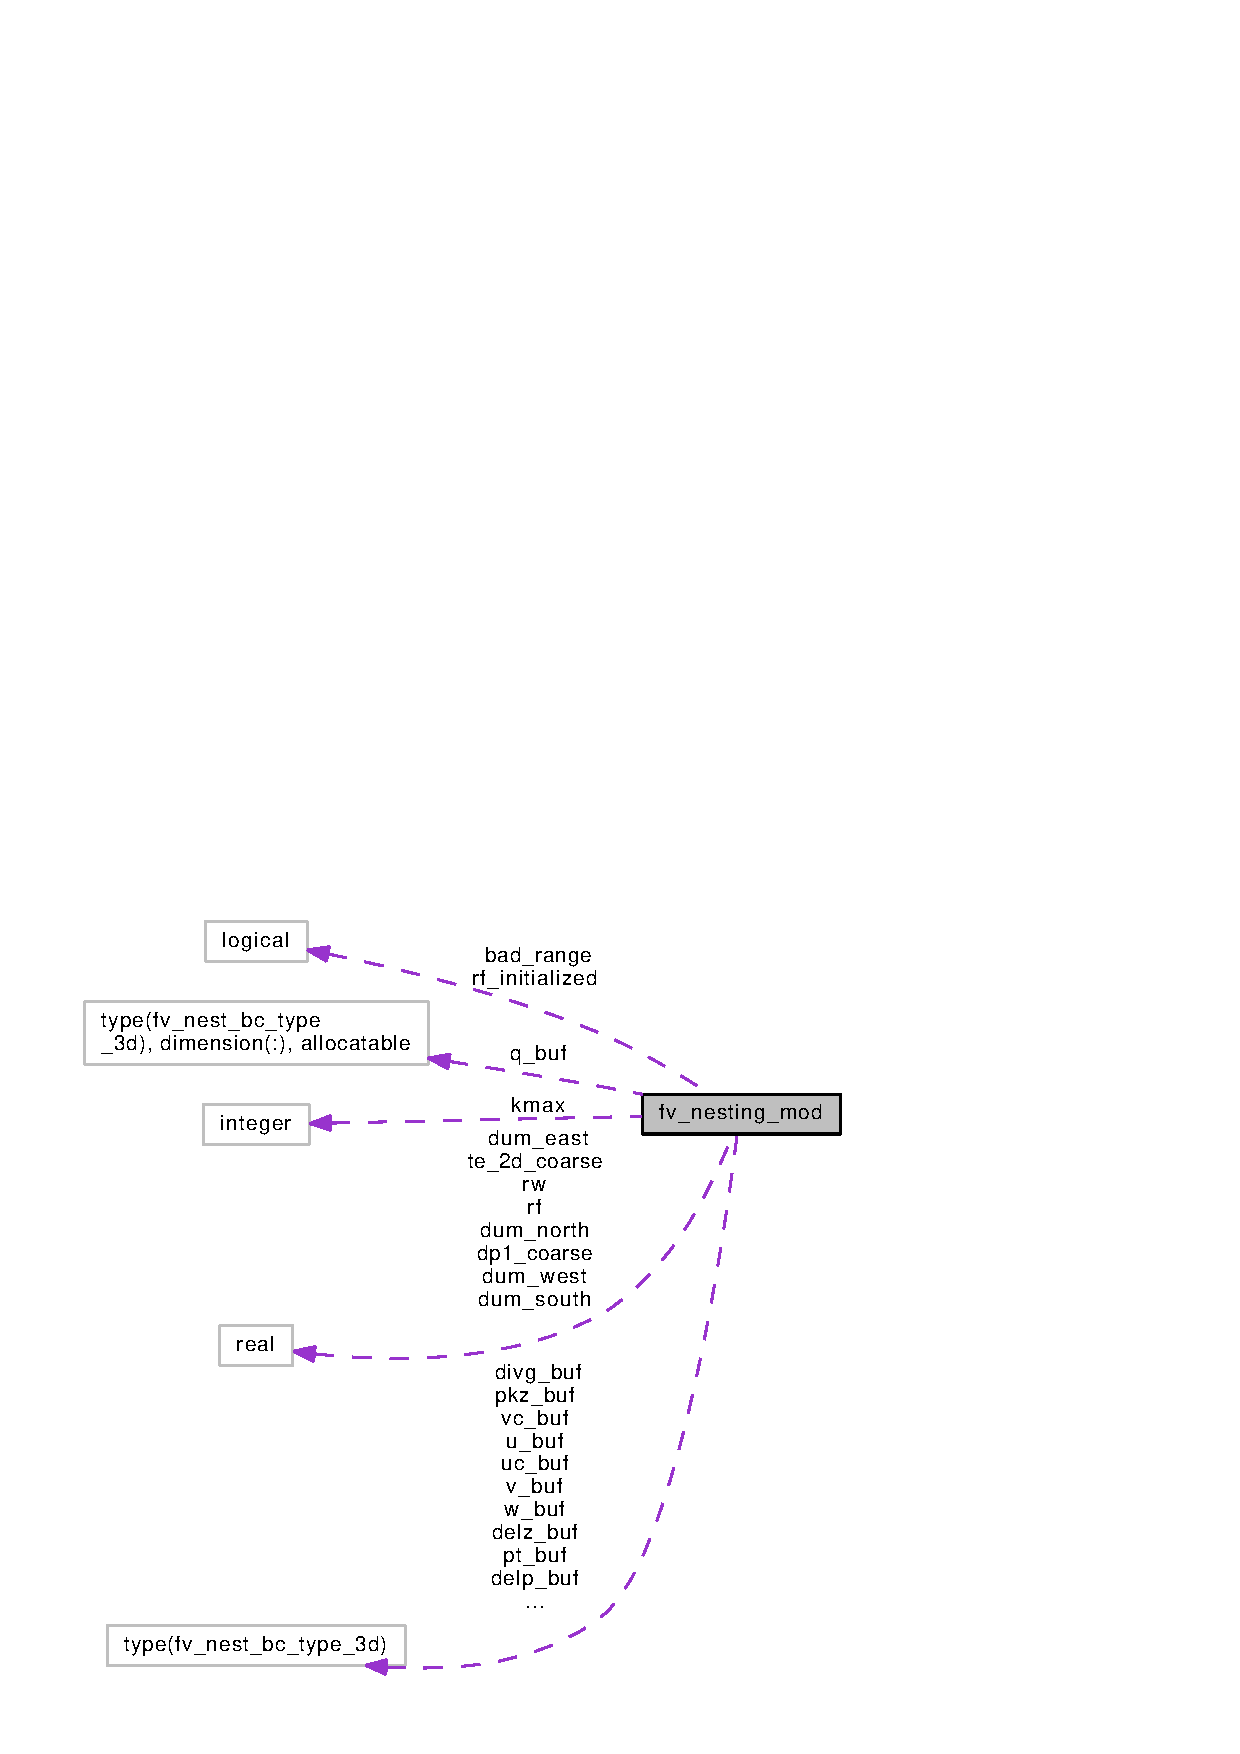
\includegraphics[width=350pt]{classfv__nesting__mod__coll__graph}
\end{center}
\end{figure}
\subsection*{Public Member Functions}
\begin{DoxyCompactItemize}
\item 
subroutine, public \hyperlink{classfv__nesting__mod_ab215fbbbf962fbfa6ed72b7d6bfb3cd8}{setup\-\_\-nested\-\_\-grid\-\_\-bcs} (npx, npy, npz, zvir, ncnst, u, v, w, pt, delp, delz, q, uc, vc, pkz, nested, inline\-\_\-q, make\-\_\-nh, ng, gridstruct, flagstruct, neststruct, nest\-\_\-timestep, tracer\-\_\-nest\-\_\-timestep, domain, bd, nwat)
\begin{DoxyCompactList}\small\item\em The subroutine 'setup\-\_\-nested\-\_\-grid\-\_\-\-B\-Cs' fetches data from the coarse grid to set up the nested-\/grid boundary conditions. \end{DoxyCompactList}\item 
subroutine, public \hyperlink{classfv__nesting__mod_afedcc378d1c25e2b9d58ea796dc10b9b}{twoway\-\_\-nesting} (Atm, ngrids, grids\-\_\-on\-\_\-this\-\_\-pe, zvir)
\begin{DoxyCompactList}\small\item\em The subroutine'twoway\-\_\-nesting' performs a two-\/way update of nested-\/grid data onto the parent grid. \end{DoxyCompactList}\end{DoxyCompactItemize}
\subsection*{Public Attributes}
\begin{DoxyCompactItemize}
\item 
logical \hyperlink{classfv__nesting__mod_a98a38c57118fae2095e4a502840edc87}{rf\-\_\-initialized} = .false.
\item 
logical \hyperlink{classfv__nesting__mod_a6b3b4dfb2f4f57efd0b8ff7ba401b9bc}{bad\-\_\-range}
\item 
real, dimension(\-:), allocatable \hyperlink{classfv__nesting__mod_a702e9b795503ff62634ce6101630bf11}{rf}
\item 
real, dimension(\-:), allocatable \hyperlink{classfv__nesting__mod_a762ae685097064afedcd7fdb8724453a}{rw}
\item 
integer \hyperlink{classfv__nesting__mod_af15ee2132be14b98ebf846e337d494f4}{kmax} =1
\item 
real, dimension(\-:,\-:), allocatable \hyperlink{classfv__nesting__mod_adbed3c960cd1c9a05ea941ec468224a3}{te\-\_\-2d\-\_\-coarse}
\item 
real, dimension(\-:,\-:,\-:), allocatable \hyperlink{classfv__nesting__mod_a784b3cab4ca871ca0f9cb4935c3195bc}{dp1\-\_\-coarse}
\item 
type(fv\-\_\-nest\-\_\-bc\-\_\-type\-\_\-3d) \hyperlink{classfv__nesting__mod_a23ef282a2b544e33d2a2f480173fa7cc}{u\-\_\-buf}
\item 
type(fv\-\_\-nest\-\_\-bc\-\_\-type\-\_\-3d) \hyperlink{classfv__nesting__mod_a477f9eccd84b2121d316306990d4c277}{v\-\_\-buf}
\item 
type(fv\-\_\-nest\-\_\-bc\-\_\-type\-\_\-3d) \hyperlink{classfv__nesting__mod_af94489e73fc64a474de665ee71a17334}{uc\-\_\-buf}
\item 
type(fv\-\_\-nest\-\_\-bc\-\_\-type\-\_\-3d) \hyperlink{classfv__nesting__mod_ad04b4ce86437a1860b2c7f577af68f2c}{vc\-\_\-buf}
\item 
type(fv\-\_\-nest\-\_\-bc\-\_\-type\-\_\-3d) \hyperlink{classfv__nesting__mod_a307ae066e30400f6e6d9839b04193cf3}{delp\-\_\-buf}
\item 
type(fv\-\_\-nest\-\_\-bc\-\_\-type\-\_\-3d) \hyperlink{classfv__nesting__mod_a3c14974429affc9b0ccdbb8e38813e72}{delz\-\_\-buf}
\item 
type(fv\-\_\-nest\-\_\-bc\-\_\-type\-\_\-3d) \hyperlink{classfv__nesting__mod_abe6a968e2acd11ea1839969781f8b189}{pt\-\_\-buf}
\item 
type(fv\-\_\-nest\-\_\-bc\-\_\-type\-\_\-3d) \hyperlink{classfv__nesting__mod_acddea4741cfe6597c8dd8a6a8d5eea24}{pkz\-\_\-buf}
\item 
type(fv\-\_\-nest\-\_\-bc\-\_\-type\-\_\-3d) \hyperlink{classfv__nesting__mod_a41d3f0c81bc4af38520dd7eab1469baf}{w\-\_\-buf}
\item 
type(fv\-\_\-nest\-\_\-bc\-\_\-type\-\_\-3d) \hyperlink{classfv__nesting__mod_a69d8bb3285146bc62f53d8e4ea1a41a3}{divg\-\_\-buf}
\item 
type(fv\-\_\-nest\-\_\-bc\-\_\-type\-\_\-3d), \\*
dimension(\-:), allocatable \hyperlink{classfv__nesting__mod_acc3bcff2425434680476295e500da917}{q\-\_\-buf}
\item 
real, dimension(\-:,\-:,\-:), \\*
allocatable, target \hyperlink{classfv__nesting__mod_aabec65a89859cf6fddbdb0dd22eca70c}{dum\-\_\-west}
\item 
real, dimension(\-:,\-:,\-:), \\*
allocatable, target \hyperlink{classfv__nesting__mod_ac0091b561b404cccf4fe21b7ceb23056}{dum\-\_\-east}
\item 
real, dimension(\-:,\-:,\-:), \\*
allocatable, target \hyperlink{classfv__nesting__mod_af3594b28f181611d0f7a3c884981f724}{dum\-\_\-north}
\item 
real, dimension(\-:,\-:,\-:), \\*
allocatable, target \hyperlink{classfv__nesting__mod_aec160f65b40c51f270de9995522c6af5}{dum\-\_\-south}
\end{DoxyCompactItemize}
\subsection*{Private Member Functions}
\begin{DoxyCompactItemize}
\item 
subroutine \hyperlink{classfv__nesting__mod_aeb31ca3ed536c4b9c24be6961e31995f}{setup\-\_\-pt\-\_\-bc} (pt\-\_\-\-B\-C, pkz\-\_\-\-B\-C, sphum\-\_\-\-B\-C, npx, npy, npz, zvir, bd)
\item 
subroutine \hyperlink{classfv__nesting__mod_a0ddf715f18b1c5919a1d36bfa40d2b4f}{setup\-\_\-pt\-\_\-nh\-\_\-bc} (pt\-\_\-\-B\-C, delp\-\_\-\-B\-C, delz\-\_\-\-B\-C, sphum\-\_\-\-B\-C, q\-\_\-\-B\-C, nq,
\item 
subroutine \hyperlink{classfv__nesting__mod_a03568c30a9676d0b68abfc402e154816}{set\-\_\-nh\-\_\-bcs\-\_\-t0} (neststruct)
\item 
subroutine \hyperlink{classfv__nesting__mod_aeca8ba5df19495083e81c0268bf8c8d0}{set\-\_\-bcs\-\_\-t0} (ncnst, hydrostatic, neststruct)
\item 
subroutine \hyperlink{classfv__nesting__mod_a3ee06cf05baeec22674fdc132411e299}{twoway\-\_\-nest\-\_\-update} (npx, npy, npz, zvir, ncnst, sphum, u, v, w, omga, pt, delp, q, uc, vc, pkz, delz, ps, ptop, gridstruct, flagstruct, neststruct, parent\-\_\-grid, bd, conv\-\_\-theta\-\_\-in)
\item 
subroutine \hyperlink{classfv__nesting__mod_abe908820b93fe8dc75b439213d3b699c}{level\-\_\-sum} (q, area, domain, bd, npz, L\-\_\-sum)
\item 
subroutine \hyperlink{classfv__nesting__mod_a6fa54ea0bd54ce56d23b864d37c5b596}{after\-\_\-twoway\-\_\-nest\-\_\-update} (npx, npy, npz, ng, ncnst, u, v, w, delz, pt, delp, q, ps, pe, pk, peln, pkz, phis, ua, va, ptop, gridstruct, flagstruct, domain, bd)
\item 
subroutine \hyperlink{classfv__nesting__mod_a769dacbf0acaa56ddaaa3db3f81bb965}{update\-\_\-remap\-\_\-tqw} (npz, ak, bk, ps, delp, t, q, w, hydrostatic, kmd, ps0, zvir, ptop, nq, kord\-\_\-tm, kord\-\_\-tr, kord\-\_\-wz, is, ie, js, je, isd, ied, jsd, jed, do\-\_\-q)
\begin{DoxyCompactList}\small\item\em The subroutine 'update\-\_\-remap\-\_\-tqw' remaps (interpolated) nested-\/grid data to the coarse-\/grid's vertical coordinate. \end{DoxyCompactList}\item 
subroutine \hyperlink{classfv__nesting__mod_a39990c41c04b8ad7e2dd34b07b5f0f69}{update\-\_\-remap\-\_\-uv} (npz, ak, bk, ps, u, v, kmd, ps0, kord\-\_\-mt, is, ie, js, je, isd, ied, jsd, jed, ptop)
\end{DoxyCompactItemize}


\subsection{Detailed Description}
The module 'fv\-\_\-nesting' is a collection of routines pertaining to grid nesting \cite{harris2013two}. 

Definition at line 27 of file fv\-\_\-nesting.\-F90.



\subsection{Member Function/\-Subroutine Documentation}
\index{fv\-\_\-nesting\-\_\-mod@{fv\-\_\-nesting\-\_\-mod}!after\-\_\-twoway\-\_\-nest\-\_\-update@{after\-\_\-twoway\-\_\-nest\-\_\-update}}
\index{after\-\_\-twoway\-\_\-nest\-\_\-update@{after\-\_\-twoway\-\_\-nest\-\_\-update}!fv_nesting_mod@{fv\-\_\-nesting\-\_\-mod}}
\subsubsection[{after\-\_\-twoway\-\_\-nest\-\_\-update}]{\setlength{\rightskip}{0pt plus 5cm}subroutine fv\-\_\-nesting\-\_\-mod\-::after\-\_\-twoway\-\_\-nest\-\_\-update (
\begin{DoxyParamCaption}
\item[{integer, intent(in)}]{npx, }
\item[{integer, intent(in)}]{npy, }
\item[{integer, intent(in)}]{npz, }
\item[{integer, intent(in)}]{ng, }
\item[{integer, intent(in)}]{ncnst, }
\item[{real, dimension(bd\%isd\-:bd\%ied  ,bd\%jsd\-:bd\%jed+1,npz), intent(inout)}]{u, }
\item[{real, dimension(bd\%isd\-:bd\%ied+1,bd\%jsd\-:bd\%jed  ,npz), intent(inout)}]{v, }
\item[{real, dimension(   bd\%isd\-:        ,bd\%jsd\-:        ,1\-: ), intent(inout)}]{w, }
\item[{real, dimension(bd\%isd\-:        ,bd\%jsd\-:        ,1\-: ), intent(inout)}]{delz, }
\item[{real, dimension(  bd\%isd\-:bd\%ied  ,bd\%jsd\-:bd\%jed  ,npz), intent(inout)}]{pt, }
\item[{real, dimension(bd\%isd\-:bd\%ied  ,bd\%jsd\-:bd\%jed  ,npz), intent(inout)}]{delp, }
\item[{real, dimension(   bd\%isd\-:bd\%ied  ,bd\%jsd\-:bd\%jed  ,npz, ncnst), intent(inout)}]{q, }
\item[{real, dimension  (bd\%isd\-:bd\%ied  ,bd\%jsd\-:bd\%jed), intent(inout)}]{ps, }
\item[{real, dimension  (bd\%is-\/1\-:bd\%ie+1, npz+1,bd\%js-\/1\-:bd\%je+1), intent(inout)}]{pe, }
\item[{real, dimension  (bd\%is\-:bd\%ie,bd\%js\-:bd\%je, npz+1), intent(inout)}]{pk, }
\item[{real, dimension(bd\%is\-:bd\%ie,npz+1,bd\%js\-:bd\%je), intent(inout)}]{peln, }
\item[{real, dimension (bd\%is\-:bd\%ie,bd\%js\-:bd\%je,npz), intent(inout)}]{pkz, }
\item[{real, dimension(bd\%isd\-:bd\%ied,bd\%jsd\-:bd\%jed), intent(inout)}]{phis, }
\item[{real, dimension(bd\%isd\-:bd\%ied ,bd\%jsd\-:bd\%jed ,npz), intent(inout)}]{ua, }
\item[{real, dimension(bd\%isd\-:bd\%ied ,bd\%jsd\-:bd\%jed ,npz), intent(inout)}]{va, }
\item[{real, intent(in)}]{ptop, }
\item[{type(fv\-\_\-grid\-\_\-type), intent(in)}]{gridstruct, }
\item[{type(fv\-\_\-flags\-\_\-type), intent(in)}]{flagstruct, }
\item[{type(domain2d), intent(inout)}]{domain, }
\item[{type(fv\-\_\-grid\-\_\-bounds\-\_\-type), intent(in)}]{bd}
\end{DoxyParamCaption}
)\hspace{0.3cm}{\ttfamily [private]}}\label{classfv__nesting__mod_a6fa54ea0bd54ce56d23b864d37c5b596}

\begin{DoxyParams}[1]{Parameters}
\mbox{\tt in,out}  & {\em u} & D grid zonal wind (m/s)\\
\hline
\mbox{\tt in,out}  & {\em v} & D grid meridional wind (m/s)\\
\hline
\mbox{\tt in,out}  & {\em w} & W (m/s)\\
\hline
\mbox{\tt in,out}  & {\em pt} & temperature (K)\\
\hline
\mbox{\tt in,out}  & {\em delp} & pressure thickness (pascal)\\
\hline
\mbox{\tt in,out}  & {\em q} & specific humidity and constituents\\
\hline
\mbox{\tt in,out}  & {\em delz} & delta-\/height (m); non-\/hydrostatic only\\
\hline
\mbox{\tt in,out}  & {\em ps} & Surface pressure (pascal)\\
\hline
\mbox{\tt in,out}  & {\em pe} & edge pressure (pascal)\\
\hline
\mbox{\tt in,out}  & {\em pk} & pe$\ast$$\ast$cappa\\
\hline
\mbox{\tt in,out}  & {\em peln} & ln(pe)\\
\hline
\mbox{\tt in,out}  & {\em pkz} & finite-\/volume mean pk\\
\hline
\mbox{\tt in,out}  & {\em phis} & Surface geopotential (g$\ast$\-Z\-\_\-surf) \\
\hline
\end{DoxyParams}


Definition at line 1541 of file fv\-\_\-nesting.\-F90.



References fv\-\_\-grid\-\_\-utils\-\_\-mod\-::cubed\-\_\-to\-\_\-latlon(), init\-\_\-hydro\-\_\-mod\-::p\-\_\-var(), and fv\-\_\-diagnostics\-\_\-mod\-::range\-\_\-check().



Referenced by twoway\-\_\-nesting().

\index{fv\-\_\-nesting\-\_\-mod@{fv\-\_\-nesting\-\_\-mod}!level\-\_\-sum@{level\-\_\-sum}}
\index{level\-\_\-sum@{level\-\_\-sum}!fv_nesting_mod@{fv\-\_\-nesting\-\_\-mod}}
\subsubsection[{level\-\_\-sum}]{\setlength{\rightskip}{0pt plus 5cm}subroutine fv\-\_\-nesting\-\_\-mod\-::level\-\_\-sum (
\begin{DoxyParamCaption}
\item[{real, dimension(   bd\%isd\-:bd\%ied  ,bd\%jsd\-:bd\%jed  ,npz), intent(in)}]{q, }
\item[{real, dimension(   bd\%isd\-:bd\%ied  ,bd\%jsd\-:bd\%jed), intent(in)}]{area, }
\item[{type(domain2d), intent(in)}]{domain, }
\item[{type(fv\-\_\-grid\-\_\-bounds\-\_\-type), intent(in)}]{bd, }
\item[{integer, intent(in)}]{npz, }
\item[{real, dimension( npz ), intent(out)}]{L\-\_\-sum}
\end{DoxyParamCaption}
)\hspace{0.3cm}{\ttfamily [private]}}\label{classfv__nesting__mod_abe908820b93fe8dc75b439213d3b699c}


Definition at line 1512 of file fv\-\_\-nesting.\-F90.



Referenced by twoway\-\_\-nest\-\_\-update().

\index{fv\-\_\-nesting\-\_\-mod@{fv\-\_\-nesting\-\_\-mod}!set\-\_\-bcs\-\_\-t0@{set\-\_\-bcs\-\_\-t0}}
\index{set\-\_\-bcs\-\_\-t0@{set\-\_\-bcs\-\_\-t0}!fv_nesting_mod@{fv\-\_\-nesting\-\_\-mod}}
\subsubsection[{set\-\_\-bcs\-\_\-t0}]{\setlength{\rightskip}{0pt plus 5cm}subroutine fv\-\_\-nesting\-\_\-mod\-::set\-\_\-bcs\-\_\-t0 (
\begin{DoxyParamCaption}
\item[{integer, intent(in)}]{ncnst, }
\item[{logical, intent(in)}]{hydrostatic, }
\item[{type(fv\-\_\-nest\-\_\-type), intent(inout)}]{neststruct}
\end{DoxyParamCaption}
)\hspace{0.3cm}{\ttfamily [private]}}\label{classfv__nesting__mod_aeca8ba5df19495083e81c0268bf8c8d0}


Definition at line 947 of file fv\-\_\-nesting.\-F90.



References set\-\_\-nh\-\_\-bcs\-\_\-t0().



Referenced by setup\-\_\-nested\-\_\-grid\-\_\-bcs().

\index{fv\-\_\-nesting\-\_\-mod@{fv\-\_\-nesting\-\_\-mod}!set\-\_\-nh\-\_\-bcs\-\_\-t0@{set\-\_\-nh\-\_\-bcs\-\_\-t0}}
\index{set\-\_\-nh\-\_\-bcs\-\_\-t0@{set\-\_\-nh\-\_\-bcs\-\_\-t0}!fv_nesting_mod@{fv\-\_\-nesting\-\_\-mod}}
\subsubsection[{set\-\_\-nh\-\_\-bcs\-\_\-t0}]{\setlength{\rightskip}{0pt plus 5cm}subroutine fv\-\_\-nesting\-\_\-mod\-::set\-\_\-nh\-\_\-bcs\-\_\-t0 (
\begin{DoxyParamCaption}
\item[{type(fv\-\_\-nest\-\_\-type), intent(inout)}]{neststruct}
\end{DoxyParamCaption}
)\hspace{0.3cm}{\ttfamily [private]}}\label{classfv__nesting__mod_a03568c30a9676d0b68abfc402e154816}


Definition at line 929 of file fv\-\_\-nesting.\-F90.



Referenced by set\-\_\-bcs\-\_\-t0(), and setup\-\_\-nested\-\_\-grid\-\_\-bcs().

\index{fv\-\_\-nesting\-\_\-mod@{fv\-\_\-nesting\-\_\-mod}!setup\-\_\-nested\-\_\-grid\-\_\-bcs@{setup\-\_\-nested\-\_\-grid\-\_\-bcs}}
\index{setup\-\_\-nested\-\_\-grid\-\_\-bcs@{setup\-\_\-nested\-\_\-grid\-\_\-bcs}!fv_nesting_mod@{fv\-\_\-nesting\-\_\-mod}}
\subsubsection[{setup\-\_\-nested\-\_\-grid\-\_\-bcs}]{\setlength{\rightskip}{0pt plus 5cm}subroutine, public fv\-\_\-nesting\-\_\-mod\-::setup\-\_\-nested\-\_\-grid\-\_\-bcs (
\begin{DoxyParamCaption}
\item[{integer, intent(in)}]{npx, }
\item[{integer, intent(in)}]{npy, }
\item[{integer, intent(in)}]{npz, }
\item[{real, intent(in)}]{zvir, }
\item[{integer, intent(in)}]{ncnst, }
\item[{real, dimension(bd\%isd\-:bd\%ied  ,bd\%jsd\-:bd\%jed+1,npz), intent(inout)}]{u, }
\item[{real, dimension(bd\%isd\-:bd\%ied+1,bd\%jsd\-:bd\%jed  ,npz), intent(inout)}]{v, }
\item[{real, dimension(   bd\%isd\-:        ,bd\%jsd\-:        ,1\-:), intent(inout)}]{w, }
\item[{real, dimension(  bd\%isd\-:bd\%ied  ,bd\%jsd\-:bd\%jed  ,npz), intent(inout)}]{pt, }
\item[{real, dimension(bd\%isd\-:bd\%ied  ,bd\%jsd\-:bd\%jed  ,npz), intent(inout)}]{delp, }
\item[{real, dimension(bd\%isd\-:        ,bd\%jsd\-:        ,1\-:), intent(inout)}]{delz, }
\item[{real, dimension(   bd\%isd\-:bd\%ied  ,bd\%jsd\-:bd\%jed  ,npz, ncnst), intent(inout)}]{q, }
\item[{real, dimension(bd\%isd\-:bd\%ied+1,bd\%jsd\-:bd\%jed  ,npz), intent(inout)}]{uc, }
\item[{real, dimension(bd\%isd\-:bd\%ied  ,bd\%jsd\-:bd\%jed+1,npz), intent(inout)}]{vc, }
\item[{real, dimension (bd\%is\-:bd\%ie,bd\%js\-:bd\%je,npz), intent(inout)}]{pkz, }
\item[{logical, intent(in)}]{nested, }
\item[{logical, intent(in)}]{inline\-\_\-q, }
\item[{logical, intent(in)}]{make\-\_\-nh, }
\item[{integer, intent(in)}]{ng, }
\item[{type(fv\-\_\-grid\-\_\-type), intent(inout)}]{gridstruct, }
\item[{type(fv\-\_\-flags\-\_\-type), intent(inout)}]{flagstruct, }
\item[{type(fv\-\_\-nest\-\_\-type), intent(inout), target}]{neststruct, }
\item[{integer, intent(inout)}]{nest\-\_\-timestep, }
\item[{integer, intent(inout)}]{tracer\-\_\-nest\-\_\-timestep, }
\item[{type(domain2d), intent(inout)}]{domain, }
\item[{type(fv\-\_\-grid\-\_\-bounds\-\_\-type), intent(in)}]{bd, }
\item[{integer, intent(in)}]{nwat}
\end{DoxyParamCaption}
)}\label{classfv__nesting__mod_ab215fbbbf962fbfa6ed72b7d6bfb3cd8}


The subroutine 'setup\-\_\-nested\-\_\-grid\-\_\-\-B\-Cs' fetches data from the coarse grid to set up the nested-\/grid boundary conditions. 


\begin{DoxyParams}[1]{Parameters}
\mbox{\tt in,out}  & {\em u} & D grid zonal wind (m/s)\\
\hline
\mbox{\tt in,out}  & {\em v} & D grid meridional wind (m/s)\\
\hline
\mbox{\tt in,out}  & {\em w} & W (m/s)\\
\hline
\mbox{\tt in,out}  & {\em pt} & temperature (K)\\
\hline
\mbox{\tt in,out}  & {\em delp} & pressure thickness (pascal)\\
\hline
\mbox{\tt in,out}  & {\em delz} & height thickness (m)\\
\hline
\mbox{\tt in,out}  & {\em q} & specific humidity and constituents\\
\hline
\mbox{\tt in,out}  & {\em uc} & (uc,vc) mostly used as the C grid winds\\
\hline
\mbox{\tt in,out}  & {\em pkz} & finite-\/volume mean pk \\
\hline
\end{DoxyParams}


Definition at line 157 of file fv\-\_\-nesting.\-F90.



References fv\-\_\-restart\-\_\-mod\-::d2c\-\_\-setup(), sw\-\_\-core\-\_\-mod\-::divergence\-\_\-corner(), sw\-\_\-core\-\_\-mod\-::divergence\-\_\-corner\-\_\-nest(), boundary\-\_\-mod\-::nested\-\_\-grid\-\_\-bc\-\_\-recv(), boundary\-\_\-mod\-::nested\-\_\-grid\-\_\-bc\-\_\-save\-\_\-proc(), boundary\-\_\-mod\-::nested\-\_\-grid\-\_\-bc\-\_\-send(), set\-\_\-bcs\-\_\-t0(), set\-\_\-nh\-\_\-bcs\-\_\-t0(), setup\-\_\-pt\-\_\-bc(), setup\-\_\-pt\-\_\-nh\-\_\-bc(), fv\-\_\-timing\-\_\-mod\-::timing\-\_\-off(), and fv\-\_\-timing\-\_\-mod\-::timing\-\_\-on().



Referenced by fv\-\_\-dynamics\-\_\-mod\-::fv\-\_\-dynamics().

\index{fv\-\_\-nesting\-\_\-mod@{fv\-\_\-nesting\-\_\-mod}!setup\-\_\-pt\-\_\-bc@{setup\-\_\-pt\-\_\-bc}}
\index{setup\-\_\-pt\-\_\-bc@{setup\-\_\-pt\-\_\-bc}!fv_nesting_mod@{fv\-\_\-nesting\-\_\-mod}}
\subsubsection[{setup\-\_\-pt\-\_\-bc}]{\setlength{\rightskip}{0pt plus 5cm}subroutine fv\-\_\-nesting\-\_\-mod\-::setup\-\_\-pt\-\_\-bc (
\begin{DoxyParamCaption}
\item[{type(fv\-\_\-nest\-\_\-bc\-\_\-type\-\_\-3d), intent(inout), target}]{pt\-\_\-\-B\-C, }
\item[{type(fv\-\_\-nest\-\_\-bc\-\_\-type\-\_\-3d), intent(in), target}]{pkz\-\_\-\-B\-C, }
\item[{type(fv\-\_\-nest\-\_\-bc\-\_\-type\-\_\-3d), intent(in), target}]{sphum\-\_\-\-B\-C, }
\item[{integer, intent(in)}]{npx, }
\item[{integer, intent(in)}]{npy, }
\item[{integer, intent(in)}]{npz, }
\item[{real, intent(in)}]{zvir, }
\item[{type(fv\-\_\-grid\-\_\-bounds\-\_\-type), intent(in)}]{bd}
\end{DoxyParamCaption}
)\hspace{0.3cm}{\ttfamily [private]}}\label{classfv__nesting__mod_aeb31ca3ed536c4b9c24be6961e31995f}


Definition at line 421 of file fv\-\_\-nesting.\-F90.



Referenced by setup\-\_\-nested\-\_\-grid\-\_\-bcs().

\index{fv\-\_\-nesting\-\_\-mod@{fv\-\_\-nesting\-\_\-mod}!setup\-\_\-pt\-\_\-nh\-\_\-bc@{setup\-\_\-pt\-\_\-nh\-\_\-bc}}
\index{setup\-\_\-pt\-\_\-nh\-\_\-bc@{setup\-\_\-pt\-\_\-nh\-\_\-bc}!fv_nesting_mod@{fv\-\_\-nesting\-\_\-mod}}
\subsubsection[{setup\-\_\-pt\-\_\-nh\-\_\-bc}]{\setlength{\rightskip}{0pt plus 5cm}subroutine fv\-\_\-nesting\-\_\-mod\-::setup\-\_\-pt\-\_\-nh\-\_\-bc (
\begin{DoxyParamCaption}
\item[{type(fv\-\_\-nest\-\_\-bc\-\_\-type\-\_\-3d), intent(inout), target}]{pt\-\_\-\-B\-C, }
\item[{type(fv\-\_\-nest\-\_\-bc\-\_\-type\-\_\-3d), intent(in), target}]{delp\-\_\-\-B\-C, }
\item[{type(fv\-\_\-nest\-\_\-bc\-\_\-type\-\_\-3d), intent(in), target}]{delz\-\_\-\-B\-C, }
\item[{type(fv\-\_\-nest\-\_\-bc\-\_\-type\-\_\-3d), intent(in), target}]{sphum\-\_\-\-B\-C, }
\item[{type(fv\-\_\-nest\-\_\-bc\-\_\-type\-\_\-3d), dimension(nq), intent(in), target}]{q\-\_\-\-B\-C, }
\item[{integer, intent(in)}]{nq}
\end{DoxyParamCaption}
)\hspace{0.3cm}{\ttfamily [private]}}\label{classfv__nesting__mod_a0ddf715f18b1c5919a1d36bfa40d2b4f}


Definition at line 529 of file fv\-\_\-nesting.\-F90.



Referenced by setup\-\_\-nested\-\_\-grid\-\_\-bcs().

\index{fv\-\_\-nesting\-\_\-mod@{fv\-\_\-nesting\-\_\-mod}!twoway\-\_\-nest\-\_\-update@{twoway\-\_\-nest\-\_\-update}}
\index{twoway\-\_\-nest\-\_\-update@{twoway\-\_\-nest\-\_\-update}!fv_nesting_mod@{fv\-\_\-nesting\-\_\-mod}}
\subsubsection[{twoway\-\_\-nest\-\_\-update}]{\setlength{\rightskip}{0pt plus 5cm}subroutine fv\-\_\-nesting\-\_\-mod\-::twoway\-\_\-nest\-\_\-update (
\begin{DoxyParamCaption}
\item[{integer, intent(in)}]{npx, }
\item[{integer, intent(in)}]{npy, }
\item[{integer, intent(in)}]{npz, }
\item[{real, intent(in)}]{zvir, }
\item[{integer, intent(in)}]{ncnst, }
\item[{integer, intent(in)}]{sphum, }
\item[{real, dimension(bd\%isd\-:bd\%ied  ,bd\%jsd\-:bd\%jed+1,npz), intent(inout)}]{u, }
\item[{real, dimension(bd\%isd\-:bd\%ied+1,bd\%jsd\-:bd\%jed  ,npz), intent(inout)}]{v, }
\item[{real, dimension(   bd\%isd\-:        ,bd\%jsd\-:        ,1\-: ), intent(inout)}]{w, }
\item[{real, dimension(bd\%isd\-:bd\%ied,bd\%jsd\-:bd\%jed,npz), intent(inout)}]{omga, }
\item[{real, dimension(  bd\%isd\-:bd\%ied  ,bd\%jsd\-:bd\%jed  ,npz), intent(inout)}]{pt, }
\item[{real, dimension(bd\%isd\-:bd\%ied  ,bd\%jsd\-:bd\%jed  ,npz), intent(inout)}]{delp, }
\item[{real, dimension(   bd\%isd\-:bd\%ied  ,bd\%jsd\-:bd\%jed  ,npz, ncnst), intent(inout)}]{q, }
\item[{real, dimension(bd\%isd\-:bd\%ied+1,bd\%jsd\-:bd\%jed  ,npz), intent(inout)}]{uc, }
\item[{real, dimension(bd\%isd\-:bd\%ied  ,bd\%jsd\-:bd\%jed+1,npz), intent(inout)}]{vc, }
\item[{real, dimension (bd\%is\-:bd\%ie,bd\%js\-:bd\%je,npz), intent(inout)}]{pkz, }
\item[{real, dimension(bd\%isd\-:      ,bd\%jsd\-:      ,1\-: ), intent(inout)}]{delz, }
\item[{real, dimension  (bd\%isd\-:bd\%ied  ,bd\%jsd\-:bd\%jed), intent(inout)}]{ps, }
\item[{real, intent(in)}]{ptop, }
\item[{type(fv\-\_\-grid\-\_\-type), intent(inout)}]{gridstruct, }
\item[{type(fv\-\_\-flags\-\_\-type), intent(inout)}]{flagstruct, }
\item[{type(fv\-\_\-nest\-\_\-type), intent(inout)}]{neststruct, }
\item[{type(fv\-\_\-atmos\-\_\-type), intent(inout)}]{parent\-\_\-grid, }
\item[{type(fv\-\_\-grid\-\_\-bounds\-\_\-type), intent(in)}]{bd, }
\item[{logical, intent(in), optional}]{conv\-\_\-theta\-\_\-in}
\end{DoxyParamCaption}
)\hspace{0.3cm}{\ttfamily [private]}}\label{classfv__nesting__mod_a3ee06cf05baeec22674fdc132411e299}

\begin{DoxyParams}[1]{Parameters}
\mbox{\tt in,out}  & {\em u} & D grid zonal wind (m/s)\\
\hline
\mbox{\tt in,out}  & {\em v} & D grid meridional wind (m/s)\\
\hline
\mbox{\tt in,out}  & {\em w} & W (m/s)\\
\hline
\mbox{\tt in,out}  & {\em omga} & Vertical pressure velocity (pa/s)\\
\hline
\mbox{\tt in,out}  & {\em pt} & temperature (K)\\
\hline
\mbox{\tt in,out}  & {\em delp} & pressure thickness (pascal)\\
\hline
\mbox{\tt in,out}  & {\em q} & specific humidity and constituents\\
\hline
\mbox{\tt in,out}  & {\em uc} & (uc,vc) C grid winds\\
\hline
\mbox{\tt in,out}  & {\em pkz} & finite-\/volume mean pk\\
\hline
\mbox{\tt in,out}  & {\em delz} & delta-\/height (m); non-\/hydrostatic only\\
\hline
\mbox{\tt in,out}  & {\em ps} & Surface pressure (pascal) \\
\hline
\end{DoxyParams}


Definition at line 1090 of file fv\-\_\-nesting.\-F90.



References level\-\_\-sum(), update\-\_\-remap\-\_\-tqw(), and update\-\_\-remap\-\_\-uv().



Referenced by twoway\-\_\-nesting().

\index{fv\-\_\-nesting\-\_\-mod@{fv\-\_\-nesting\-\_\-mod}!twoway\-\_\-nesting@{twoway\-\_\-nesting}}
\index{twoway\-\_\-nesting@{twoway\-\_\-nesting}!fv_nesting_mod@{fv\-\_\-nesting\-\_\-mod}}
\subsubsection[{twoway\-\_\-nesting}]{\setlength{\rightskip}{0pt plus 5cm}subroutine, public fv\-\_\-nesting\-\_\-mod\-::twoway\-\_\-nesting (
\begin{DoxyParamCaption}
\item[{type(fv\-\_\-atmos\-\_\-type), dimension(ngrids), intent(inout)}]{Atm, }
\item[{integer, intent(in)}]{ngrids, }
\item[{logical, dimension(ngrids), intent(in)}]{grids\-\_\-on\-\_\-this\-\_\-pe, }
\item[{real, intent(in)}]{zvir}
\end{DoxyParamCaption}
)}\label{classfv__nesting__mod_afedcc378d1c25e2b9d58ea796dc10b9b}


The subroutine'twoway\-\_\-nesting' performs a two-\/way update of nested-\/grid data onto the parent grid. 



Definition at line 1043 of file fv\-\_\-nesting.\-F90.



References after\-\_\-twoway\-\_\-nest\-\_\-update(), and twoway\-\_\-nest\-\_\-update().



Referenced by atmosphere\-\_\-mod\-::atmosphere\-\_\-dynamics(), and atmosphere\-\_\-mod\-::atmosphere\-\_\-state\-\_\-update().

\index{fv\-\_\-nesting\-\_\-mod@{fv\-\_\-nesting\-\_\-mod}!update\-\_\-remap\-\_\-tqw@{update\-\_\-remap\-\_\-tqw}}
\index{update\-\_\-remap\-\_\-tqw@{update\-\_\-remap\-\_\-tqw}!fv_nesting_mod@{fv\-\_\-nesting\-\_\-mod}}
\subsubsection[{update\-\_\-remap\-\_\-tqw}]{\setlength{\rightskip}{0pt plus 5cm}subroutine fv\-\_\-nesting\-\_\-mod\-::update\-\_\-remap\-\_\-tqw (
\begin{DoxyParamCaption}
\item[{integer, intent(in)}]{npz, }
\item[{real, dimension(npz+1), intent(in)}]{ak, }
\item[{real, dimension(npz+1), intent(in)}]{bk, }
\item[{real, dimension(isd\-:ied,jsd\-:jed), intent(in)}]{ps, }
\item[{real, dimension(isd\-:ied,jsd\-:jed,npz), intent(in)}]{delp, }
\item[{real, dimension(isd\-:ied,jsd\-:jed,npz), intent(inout)}]{t, }
\item[{real, dimension(isd\-:ied,jsd\-:jed,npz,nq), intent(inout)}]{q, }
\item[{real, dimension(isd\-:ied,jsd\-:jed,npz), intent(inout)}]{w, }
\item[{logical, intent(in)}]{hydrostatic, }
\item[{integer, intent(in)}]{kmd, }
\item[{real, dimension(isd\-:ied,jsd\-:jed), intent(in)}]{ps0, }
\item[{real, intent(in)}]{zvir, }
\item[{real, intent(in)}]{ptop, }
\item[{integer, intent(in)}]{nq, }
\item[{integer, intent(in)}]{kord\-\_\-tm, }
\item[{integer, intent(in)}]{kord\-\_\-tr, }
\item[{integer, intent(in)}]{kord\-\_\-wz, }
\item[{integer, intent(in)}]{is, }
\item[{integer, intent(in)}]{ie, }
\item[{integer, intent(in)}]{js, }
\item[{integer, intent(in)}]{je, }
\item[{integer, intent(in)}]{isd, }
\item[{integer, intent(in)}]{ied, }
\item[{integer, intent(in)}]{jsd, }
\item[{integer, intent(in)}]{jed, }
\item[{logical, intent(in)}]{do\-\_\-q}
\end{DoxyParamCaption}
)\hspace{0.3cm}{\ttfamily [private]}}\label{classfv__nesting__mod_a769dacbf0acaa56ddaaa3db3f81bb965}


The subroutine 'update\-\_\-remap\-\_\-tqw' remaps (interpolated) nested-\/grid data to the coarse-\/grid's vertical coordinate. 



Definition at line 1636 of file fv\-\_\-nesting.\-F90.



References fv\-\_\-mapz\-\_\-mod\-::mappm().



Referenced by twoway\-\_\-nest\-\_\-update().

\index{fv\-\_\-nesting\-\_\-mod@{fv\-\_\-nesting\-\_\-mod}!update\-\_\-remap\-\_\-uv@{update\-\_\-remap\-\_\-uv}}
\index{update\-\_\-remap\-\_\-uv@{update\-\_\-remap\-\_\-uv}!fv_nesting_mod@{fv\-\_\-nesting\-\_\-mod}}
\subsubsection[{update\-\_\-remap\-\_\-uv}]{\setlength{\rightskip}{0pt plus 5cm}subroutine fv\-\_\-nesting\-\_\-mod\-::update\-\_\-remap\-\_\-uv (
\begin{DoxyParamCaption}
\item[{integer, intent(in)}]{npz, }
\item[{real, dimension(npz+1), intent(in)}]{ak, }
\item[{real, dimension(npz+1), intent(in)}]{bk, }
\item[{real, dimension(isd\-:ied,jsd\-:jed), intent(in)}]{ps, }
\item[{real, dimension(isd\-:ied,jsd\-:jed+1,npz), intent(inout)}]{u, }
\item[{real, dimension(isd\-:ied+1,jsd\-:jed,npz), intent(inout)}]{v, }
\item[{integer, intent(in)}]{kmd, }
\item[{real, dimension(isd\-:ied,jsd\-:jed), intent(in)}]{ps0, }
\item[{integer, intent(in)}]{kord\-\_\-mt, }
\item[{integer, intent(in)}]{is, }
\item[{integer, intent(in)}]{ie, }
\item[{integer, intent(in)}]{js, }
\item[{integer, intent(in)}]{je, }
\item[{integer, intent(in)}]{isd, }
\item[{integer, intent(in)}]{ied, }
\item[{integer, intent(in)}]{jsd, }
\item[{integer, intent(in)}]{jed, }
\item[{real, intent(in)}]{ptop}
\end{DoxyParamCaption}
)\hspace{0.3cm}{\ttfamily [private]}}\label{classfv__nesting__mod_a39990c41c04b8ad7e2dd34b07b5f0f69}


Definition at line 1725 of file fv\-\_\-nesting.\-F90.



References fv\-\_\-mapz\-\_\-mod\-::mappm().



Referenced by twoway\-\_\-nest\-\_\-update().



\subsection{Member Data Documentation}
\index{fv\-\_\-nesting\-\_\-mod@{fv\-\_\-nesting\-\_\-mod}!bad\-\_\-range@{bad\-\_\-range}}
\index{bad\-\_\-range@{bad\-\_\-range}!fv_nesting_mod@{fv\-\_\-nesting\-\_\-mod}}
\subsubsection[{bad\-\_\-range}]{\setlength{\rightskip}{0pt plus 5cm}logical fv\-\_\-nesting\-\_\-mod\-::bad\-\_\-range}\label{classfv__nesting__mod_a6b3b4dfb2f4f57efd0b8ff7ba401b9bc}


Definition at line 132 of file fv\-\_\-nesting.\-F90.

\index{fv\-\_\-nesting\-\_\-mod@{fv\-\_\-nesting\-\_\-mod}!delp\-\_\-buf@{delp\-\_\-buf}}
\index{delp\-\_\-buf@{delp\-\_\-buf}!fv_nesting_mod@{fv\-\_\-nesting\-\_\-mod}}
\subsubsection[{delp\-\_\-buf}]{\setlength{\rightskip}{0pt plus 5cm}type(fv\-\_\-nest\-\_\-bc\-\_\-type\-\_\-3d) fv\-\_\-nesting\-\_\-mod\-::delp\-\_\-buf}\label{classfv__nesting__mod_a307ae066e30400f6e6d9839b04193cf3}


Definition at line 141 of file fv\-\_\-nesting.\-F90.

\index{fv\-\_\-nesting\-\_\-mod@{fv\-\_\-nesting\-\_\-mod}!delz\-\_\-buf@{delz\-\_\-buf}}
\index{delz\-\_\-buf@{delz\-\_\-buf}!fv_nesting_mod@{fv\-\_\-nesting\-\_\-mod}}
\subsubsection[{delz\-\_\-buf}]{\setlength{\rightskip}{0pt plus 5cm}type(fv\-\_\-nest\-\_\-bc\-\_\-type\-\_\-3d) fv\-\_\-nesting\-\_\-mod\-::delz\-\_\-buf}\label{classfv__nesting__mod_a3c14974429affc9b0ccdbb8e38813e72}


Definition at line 141 of file fv\-\_\-nesting.\-F90.

\index{fv\-\_\-nesting\-\_\-mod@{fv\-\_\-nesting\-\_\-mod}!divg\-\_\-buf@{divg\-\_\-buf}}
\index{divg\-\_\-buf@{divg\-\_\-buf}!fv_nesting_mod@{fv\-\_\-nesting\-\_\-mod}}
\subsubsection[{divg\-\_\-buf}]{\setlength{\rightskip}{0pt plus 5cm}type(fv\-\_\-nest\-\_\-bc\-\_\-type\-\_\-3d) fv\-\_\-nesting\-\_\-mod\-::divg\-\_\-buf}\label{classfv__nesting__mod_a69d8bb3285146bc62f53d8e4ea1a41a3}


Definition at line 141 of file fv\-\_\-nesting.\-F90.

\index{fv\-\_\-nesting\-\_\-mod@{fv\-\_\-nesting\-\_\-mod}!dp1\-\_\-coarse@{dp1\-\_\-coarse}}
\index{dp1\-\_\-coarse@{dp1\-\_\-coarse}!fv_nesting_mod@{fv\-\_\-nesting\-\_\-mod}}
\subsubsection[{dp1\-\_\-coarse}]{\setlength{\rightskip}{0pt plus 5cm}real, dimension(\-:,\-:,\-:), allocatable fv\-\_\-nesting\-\_\-mod\-::dp1\-\_\-coarse}\label{classfv__nesting__mod_a784b3cab4ca871ca0f9cb4935c3195bc}


Definition at line 137 of file fv\-\_\-nesting.\-F90.

\index{fv\-\_\-nesting\-\_\-mod@{fv\-\_\-nesting\-\_\-mod}!dum\-\_\-east@{dum\-\_\-east}}
\index{dum\-\_\-east@{dum\-\_\-east}!fv_nesting_mod@{fv\-\_\-nesting\-\_\-mod}}
\subsubsection[{dum\-\_\-east}]{\setlength{\rightskip}{0pt plus 5cm}real, dimension(\-:,\-:,\-:), allocatable, target fv\-\_\-nesting\-\_\-mod\-::dum\-\_\-east}\label{classfv__nesting__mod_ac0091b561b404cccf4fe21b7ceb23056}


Definition at line 144 of file fv\-\_\-nesting.\-F90.

\index{fv\-\_\-nesting\-\_\-mod@{fv\-\_\-nesting\-\_\-mod}!dum\-\_\-north@{dum\-\_\-north}}
\index{dum\-\_\-north@{dum\-\_\-north}!fv_nesting_mod@{fv\-\_\-nesting\-\_\-mod}}
\subsubsection[{dum\-\_\-north}]{\setlength{\rightskip}{0pt plus 5cm}real, dimension(\-:,\-:,\-:), allocatable, target fv\-\_\-nesting\-\_\-mod\-::dum\-\_\-north}\label{classfv__nesting__mod_af3594b28f181611d0f7a3c884981f724}


Definition at line 144 of file fv\-\_\-nesting.\-F90.

\index{fv\-\_\-nesting\-\_\-mod@{fv\-\_\-nesting\-\_\-mod}!dum\-\_\-south@{dum\-\_\-south}}
\index{dum\-\_\-south@{dum\-\_\-south}!fv_nesting_mod@{fv\-\_\-nesting\-\_\-mod}}
\subsubsection[{dum\-\_\-south}]{\setlength{\rightskip}{0pt plus 5cm}real, dimension(\-:,\-:,\-:), allocatable, target fv\-\_\-nesting\-\_\-mod\-::dum\-\_\-south}\label{classfv__nesting__mod_aec160f65b40c51f270de9995522c6af5}


Definition at line 144 of file fv\-\_\-nesting.\-F90.

\index{fv\-\_\-nesting\-\_\-mod@{fv\-\_\-nesting\-\_\-mod}!dum\-\_\-west@{dum\-\_\-west}}
\index{dum\-\_\-west@{dum\-\_\-west}!fv_nesting_mod@{fv\-\_\-nesting\-\_\-mod}}
\subsubsection[{dum\-\_\-west}]{\setlength{\rightskip}{0pt plus 5cm}real, dimension(\-:,\-:,\-:), allocatable, target fv\-\_\-nesting\-\_\-mod\-::dum\-\_\-west}\label{classfv__nesting__mod_aabec65a89859cf6fddbdb0dd22eca70c}


Definition at line 144 of file fv\-\_\-nesting.\-F90.

\index{fv\-\_\-nesting\-\_\-mod@{fv\-\_\-nesting\-\_\-mod}!kmax@{kmax}}
\index{kmax@{kmax}!fv_nesting_mod@{fv\-\_\-nesting\-\_\-mod}}
\subsubsection[{kmax}]{\setlength{\rightskip}{0pt plus 5cm}integer fv\-\_\-nesting\-\_\-mod\-::kmax =1}\label{classfv__nesting__mod_af15ee2132be14b98ebf846e337d494f4}


Definition at line 134 of file fv\-\_\-nesting.\-F90.

\index{fv\-\_\-nesting\-\_\-mod@{fv\-\_\-nesting\-\_\-mod}!pkz\-\_\-buf@{pkz\-\_\-buf}}
\index{pkz\-\_\-buf@{pkz\-\_\-buf}!fv_nesting_mod@{fv\-\_\-nesting\-\_\-mod}}
\subsubsection[{pkz\-\_\-buf}]{\setlength{\rightskip}{0pt plus 5cm}type(fv\-\_\-nest\-\_\-bc\-\_\-type\-\_\-3d) fv\-\_\-nesting\-\_\-mod\-::pkz\-\_\-buf}\label{classfv__nesting__mod_acddea4741cfe6597c8dd8a6a8d5eea24}


Definition at line 141 of file fv\-\_\-nesting.\-F90.

\index{fv\-\_\-nesting\-\_\-mod@{fv\-\_\-nesting\-\_\-mod}!pt\-\_\-buf@{pt\-\_\-buf}}
\index{pt\-\_\-buf@{pt\-\_\-buf}!fv_nesting_mod@{fv\-\_\-nesting\-\_\-mod}}
\subsubsection[{pt\-\_\-buf}]{\setlength{\rightskip}{0pt plus 5cm}type(fv\-\_\-nest\-\_\-bc\-\_\-type\-\_\-3d) fv\-\_\-nesting\-\_\-mod\-::pt\-\_\-buf}\label{classfv__nesting__mod_abe6a968e2acd11ea1839969781f8b189}


Definition at line 141 of file fv\-\_\-nesting.\-F90.

\index{fv\-\_\-nesting\-\_\-mod@{fv\-\_\-nesting\-\_\-mod}!q\-\_\-buf@{q\-\_\-buf}}
\index{q\-\_\-buf@{q\-\_\-buf}!fv_nesting_mod@{fv\-\_\-nesting\-\_\-mod}}
\subsubsection[{q\-\_\-buf}]{\setlength{\rightskip}{0pt plus 5cm}type(fv\-\_\-nest\-\_\-bc\-\_\-type\-\_\-3d), dimension(\-:), allocatable fv\-\_\-nesting\-\_\-mod\-::q\-\_\-buf}\label{classfv__nesting__mod_acc3bcff2425434680476295e500da917}


Definition at line 142 of file fv\-\_\-nesting.\-F90.

\index{fv\-\_\-nesting\-\_\-mod@{fv\-\_\-nesting\-\_\-mod}!rf@{rf}}
\index{rf@{rf}!fv_nesting_mod@{fv\-\_\-nesting\-\_\-mod}}
\subsubsection[{rf}]{\setlength{\rightskip}{0pt plus 5cm}real, dimension(\-:), allocatable fv\-\_\-nesting\-\_\-mod\-::rf}\label{classfv__nesting__mod_a702e9b795503ff62634ce6101630bf11}


Definition at line 133 of file fv\-\_\-nesting.\-F90.

\index{fv\-\_\-nesting\-\_\-mod@{fv\-\_\-nesting\-\_\-mod}!rf\-\_\-initialized@{rf\-\_\-initialized}}
\index{rf\-\_\-initialized@{rf\-\_\-initialized}!fv_nesting_mod@{fv\-\_\-nesting\-\_\-mod}}
\subsubsection[{rf\-\_\-initialized}]{\setlength{\rightskip}{0pt plus 5cm}logical fv\-\_\-nesting\-\_\-mod\-::rf\-\_\-initialized = .false.}\label{classfv__nesting__mod_a98a38c57118fae2095e4a502840edc87}


Definition at line 131 of file fv\-\_\-nesting.\-F90.

\index{fv\-\_\-nesting\-\_\-mod@{fv\-\_\-nesting\-\_\-mod}!rw@{rw}}
\index{rw@{rw}!fv_nesting_mod@{fv\-\_\-nesting\-\_\-mod}}
\subsubsection[{rw}]{\setlength{\rightskip}{0pt plus 5cm}real, dimension(\-:), allocatable fv\-\_\-nesting\-\_\-mod\-::rw}\label{classfv__nesting__mod_a762ae685097064afedcd7fdb8724453a}


Definition at line 133 of file fv\-\_\-nesting.\-F90.

\index{fv\-\_\-nesting\-\_\-mod@{fv\-\_\-nesting\-\_\-mod}!te\-\_\-2d\-\_\-coarse@{te\-\_\-2d\-\_\-coarse}}
\index{te\-\_\-2d\-\_\-coarse@{te\-\_\-2d\-\_\-coarse}!fv_nesting_mod@{fv\-\_\-nesting\-\_\-mod}}
\subsubsection[{te\-\_\-2d\-\_\-coarse}]{\setlength{\rightskip}{0pt plus 5cm}real, dimension(\-:,\-:), allocatable fv\-\_\-nesting\-\_\-mod\-::te\-\_\-2d\-\_\-coarse}\label{classfv__nesting__mod_adbed3c960cd1c9a05ea941ec468224a3}


Definition at line 136 of file fv\-\_\-nesting.\-F90.

\index{fv\-\_\-nesting\-\_\-mod@{fv\-\_\-nesting\-\_\-mod}!u\-\_\-buf@{u\-\_\-buf}}
\index{u\-\_\-buf@{u\-\_\-buf}!fv_nesting_mod@{fv\-\_\-nesting\-\_\-mod}}
\subsubsection[{u\-\_\-buf}]{\setlength{\rightskip}{0pt plus 5cm}type(fv\-\_\-nest\-\_\-bc\-\_\-type\-\_\-3d) fv\-\_\-nesting\-\_\-mod\-::u\-\_\-buf}\label{classfv__nesting__mod_a23ef282a2b544e33d2a2f480173fa7cc}


Definition at line 141 of file fv\-\_\-nesting.\-F90.

\index{fv\-\_\-nesting\-\_\-mod@{fv\-\_\-nesting\-\_\-mod}!uc\-\_\-buf@{uc\-\_\-buf}}
\index{uc\-\_\-buf@{uc\-\_\-buf}!fv_nesting_mod@{fv\-\_\-nesting\-\_\-mod}}
\subsubsection[{uc\-\_\-buf}]{\setlength{\rightskip}{0pt plus 5cm}type(fv\-\_\-nest\-\_\-bc\-\_\-type\-\_\-3d) fv\-\_\-nesting\-\_\-mod\-::uc\-\_\-buf}\label{classfv__nesting__mod_af94489e73fc64a474de665ee71a17334}


Definition at line 141 of file fv\-\_\-nesting.\-F90.

\index{fv\-\_\-nesting\-\_\-mod@{fv\-\_\-nesting\-\_\-mod}!v\-\_\-buf@{v\-\_\-buf}}
\index{v\-\_\-buf@{v\-\_\-buf}!fv_nesting_mod@{fv\-\_\-nesting\-\_\-mod}}
\subsubsection[{v\-\_\-buf}]{\setlength{\rightskip}{0pt plus 5cm}type(fv\-\_\-nest\-\_\-bc\-\_\-type\-\_\-3d) fv\-\_\-nesting\-\_\-mod\-::v\-\_\-buf}\label{classfv__nesting__mod_a477f9eccd84b2121d316306990d4c277}


Definition at line 141 of file fv\-\_\-nesting.\-F90.

\index{fv\-\_\-nesting\-\_\-mod@{fv\-\_\-nesting\-\_\-mod}!vc\-\_\-buf@{vc\-\_\-buf}}
\index{vc\-\_\-buf@{vc\-\_\-buf}!fv_nesting_mod@{fv\-\_\-nesting\-\_\-mod}}
\subsubsection[{vc\-\_\-buf}]{\setlength{\rightskip}{0pt plus 5cm}type(fv\-\_\-nest\-\_\-bc\-\_\-type\-\_\-3d) fv\-\_\-nesting\-\_\-mod\-::vc\-\_\-buf}\label{classfv__nesting__mod_ad04b4ce86437a1860b2c7f577af68f2c}


Definition at line 141 of file fv\-\_\-nesting.\-F90.

\index{fv\-\_\-nesting\-\_\-mod@{fv\-\_\-nesting\-\_\-mod}!w\-\_\-buf@{w\-\_\-buf}}
\index{w\-\_\-buf@{w\-\_\-buf}!fv_nesting_mod@{fv\-\_\-nesting\-\_\-mod}}
\subsubsection[{w\-\_\-buf}]{\setlength{\rightskip}{0pt plus 5cm}type(fv\-\_\-nest\-\_\-bc\-\_\-type\-\_\-3d) fv\-\_\-nesting\-\_\-mod\-::w\-\_\-buf}\label{classfv__nesting__mod_a41d3f0c81bc4af38520dd7eab1469baf}


Definition at line 141 of file fv\-\_\-nesting.\-F90.



The documentation for this module was generated from the following file\-:\begin{DoxyCompactItemize}
\item 
/scratch2/\-N\-A\-G\-A\-P\-E/aoml-\/hafs1/\-Kyle.\-Ahern/acs\-\_\-master\-\_\-readonly/model/\hyperlink{fv__nesting_8F90}{fv\-\_\-nesting.\-F90}\end{DoxyCompactItemize}

\section{fv\-\_\-nggps\-\_\-diags\-\_\-mod Module Reference}
\label{classfv__nggps__diags__mod}\index{fv\-\_\-nggps\-\_\-diags\-\_\-mod@{fv\-\_\-nggps\-\_\-diags\-\_\-mod}}


The module 'fv\-\_\-nggps\-\_\-diags' computes output diagnostics entirely on 3\-D pressure levels.  




Collaboration diagram for fv\-\_\-nggps\-\_\-diags\-\_\-mod\-:
\nopagebreak
\begin{figure}[H]
\begin{center}
\leavevmode
\includegraphics[height=550pt]{classfv__nggps__diags__mod__coll__graph}
\end{center}
\end{figure}
\subsection*{Public Member Functions}
\begin{DoxyCompactItemize}
\item 
subroutine, public \hyperlink{classfv__nggps__diags__mod_ab37da1eb0394d52c06db856e9f875833}{fv\-\_\-nggps\-\_\-diag\-\_\-init} (Atm, axes, Time)
\item 
subroutine, public \hyperlink{classfv__nggps__diags__mod_a2067cd5af978609a6dc1614795abea87}{fv\-\_\-nggps\-\_\-diag} (Atm, zvir, Time)
\item 
subroutine, public \hyperlink{classfv__nggps__diags__mod_a87ed4a1f80258a1b15835104526747e8}{fv\-\_\-nggps\-\_\-tavg} (Atm, Time\-\_\-step\-\_\-atmos, avg\-\_\-max\-\_\-length, zvir)
\end{DoxyCompactItemize}
\subsection*{Private Member Functions}
\begin{DoxyCompactItemize}
\item 
subroutine \hyperlink{classfv__nggps__diags__mod_a4f6c0fecf1cbb62eb2990ed66895f59a}{store\-\_\-data} (id, work, Time, nstt, nend)
\end{DoxyCompactItemize}
\subsection*{Private Attributes}
\begin{DoxyCompactItemize}
\item 
real, parameter \hyperlink{classfv__nggps__diags__mod_ae58ca0a4c6f6a924fe1ad700c59e7835}{missing\-\_\-value} = -\/1.e10
\item 
real, parameter \hyperlink{classfv__nggps__diags__mod_a67f209631191a0c270db5c26d5613683}{stndrd\-\_\-atmos\-\_\-ps} = 101325.
\item 
real, parameter \hyperlink{classfv__nggps__diags__mod_ac448721091d8e09234e09b5e3e4d0d68}{stndrd\-\_\-atmos\-\_\-lapse} = 0.\-0065
\item 
logical \hyperlink{classfv__nggps__diags__mod_a1cd9085200009db10173487afdf6107c}{master}
\item 
integer \hyperlink{classfv__nggps__diags__mod_aa33d7dc926260a8a41cb7c5c4952c7ee}{id\-\_\-ua}
\item 
integer \hyperlink{classfv__nggps__diags__mod_aafff421203a7bb0b275df42417272314}{id\-\_\-va}
\item 
integer \hyperlink{classfv__nggps__diags__mod_ad1c08702435f095c18a06e1070a607f7}{id\-\_\-pt}
\item 
integer \hyperlink{classfv__nggps__diags__mod_aec07245665ff3463d2c2801eae6706b7}{id\-\_\-delp}
\item 
integer \hyperlink{classfv__nggps__diags__mod_a714a8b91e9583fc54a76401abf6c942f}{id\-\_\-pfhy}
\item 
integer \hyperlink{classfv__nggps__diags__mod_a807900a4b82994c01e0a4da6bea37cac}{id\-\_\-pfnh}
\item 
integer \hyperlink{classfv__nggps__diags__mod_aefe549069cacd0721fdc4c5c3d266743}{id\-\_\-w}
\item 
integer \hyperlink{classfv__nggps__diags__mod_a905a7d18ebee5090090ae09da236114f}{id\-\_\-delz}
\item 
integer \hyperlink{classfv__nggps__diags__mod_ad4a684d38a9581ad8102dc39d1fe5879}{id\-\_\-diss}
\item 
integer \hyperlink{classfv__nggps__diags__mod_ad1d89db3f69ad85f97da253ceb8591b2}{id\-\_\-ps}
\item 
integer \hyperlink{classfv__nggps__diags__mod_ab67fd10f74cfab0898427bbc86b30245}{id\-\_\-hs}
\item 
integer \hyperlink{classfv__nggps__diags__mod_a230a7e07e841292812b5e02aaa2b4b25}{id\-\_\-dbz}
\item 
integer \hyperlink{classfv__nggps__diags__mod_ad19e4b6ed51fbcee19a31b34687c712b}{id\-\_\-omga}
\item 
integer \hyperlink{classfv__nggps__diags__mod_a841854dee23e174673acab69d5293ca5}{kstt\-\_\-ua}
\item 
integer \hyperlink{classfv__nggps__diags__mod_aea4c4320cbee76e02d3cd4d8d27d66e3}{kstt\-\_\-va}
\item 
integer \hyperlink{classfv__nggps__diags__mod_af2dba276e2ab084389801c14c40d7dd0}{kstt\-\_\-pt}
\item 
integer \hyperlink{classfv__nggps__diags__mod_a07543cb41e9f75914dc6f63a434dcbb7}{kstt\-\_\-delp}
\item 
integer \hyperlink{classfv__nggps__diags__mod_a3bfe44068a85feebd00641d36146f9b3}{kstt\-\_\-pfhy}
\item 
integer \hyperlink{classfv__nggps__diags__mod_a0fadec8236bccc124436e3c86d142549}{kstt\-\_\-pfnh}
\item 
integer \hyperlink{classfv__nggps__diags__mod_a7a314e9a214f9738be68f59c0d85b000}{kstt\-\_\-w}
\item 
integer \hyperlink{classfv__nggps__diags__mod_a3d23cc53d5a05338874318b17773b5ad}{kstt\-\_\-delz}
\item 
integer \hyperlink{classfv__nggps__diags__mod_ae361446a10580ad1c6d445491d8a1404}{kstt\-\_\-diss}
\item 
integer \hyperlink{classfv__nggps__diags__mod_a3fdf87034b89ea7b38f9261f6f447ded}{kstt\-\_\-ps}
\item 
integer \hyperlink{classfv__nggps__diags__mod_a4f11b91bbe6d3d6fd26326f1a4611855}{kstt\-\_\-hs}
\item 
integer \hyperlink{classfv__nggps__diags__mod_a678d21e583784e54c0957c1f2c429a14}{kend\-\_\-ua}
\item 
integer \hyperlink{classfv__nggps__diags__mod_a1080bff68c07915d95f82fd40b4e76fc}{kend\-\_\-va}
\item 
integer \hyperlink{classfv__nggps__diags__mod_a22c4d230636276c749ddc369297dd85e}{kend\-\_\-pt}
\item 
integer \hyperlink{classfv__nggps__diags__mod_af22080302fa1bfce2c3dbd28d7ec1a65}{kend\-\_\-delp}
\item 
integer \hyperlink{classfv__nggps__diags__mod_a52ec4ebc17baed9773c0e0facc94d80f}{kend\-\_\-pfhy}
\item 
integer \hyperlink{classfv__nggps__diags__mod_a560c79be33d3cf6c601c382c9827b550}{kend\-\_\-pfnh}
\item 
integer \hyperlink{classfv__nggps__diags__mod_a7448a16d1d56fd8a7b71ed79418d1fca}{kend\-\_\-w}
\item 
integer \hyperlink{classfv__nggps__diags__mod_a1032edab5be3a430c7089c2dd5b6f2bb}{kend\-\_\-delz}
\item 
integer \hyperlink{classfv__nggps__diags__mod_a37a13813d7e5941869d5666844dc3601}{kend\-\_\-diss}
\item 
integer \hyperlink{classfv__nggps__diags__mod_a2bc1187c816698a5e9ad14f3769a904a}{kend\-\_\-ps}
\item 
integer \hyperlink{classfv__nggps__diags__mod_af675001c796dc16dbbd5642fb38c9247}{kend\-\_\-hs}
\item 
integer \hyperlink{classfv__nggps__diags__mod_a6197e3be2df8bd2599697c61d5ed950c}{kstt\-\_\-dbz}
\item 
integer \hyperlink{classfv__nggps__diags__mod_aa0dbd9fec62f6dc0ed89809c9e9b6074}{kend\-\_\-dbz}
\item 
integer \hyperlink{classfv__nggps__diags__mod_aa4455319113ad1862929a6fdf72a5beb}{kstt\-\_\-omga}
\item 
integer \hyperlink{classfv__nggps__diags__mod_a4e11455c15981a042cd6cc91bd000576}{kend\-\_\-omga}
\item 
integer \hyperlink{classfv__nggps__diags__mod_ad2da0c51ff10c97635de92984451f577}{kstt\-\_\-windvect}
\item 
integer \hyperlink{classfv__nggps__diags__mod_a0e04e352b7e1e2353e3a2e9245662270}{kend\-\_\-windvect}
\item 
integer \hyperlink{classfv__nggps__diags__mod_a059ef910811a03117bf40a1406521276}{id\-\_\-wmaxup}
\item 
integer \hyperlink{classfv__nggps__diags__mod_a3d99dc518af844fdea2b88da471ff681}{id\-\_\-wmaxdn}
\item 
integer \hyperlink{classfv__nggps__diags__mod_a86051f0376102e15a8a1a0fc8fe5429f}{kstt\-\_\-wup}
\item 
integer \hyperlink{classfv__nggps__diags__mod_a117adcb804018f56ea41b9582964a174}{kend\-\_\-wup}
\item 
integer \hyperlink{classfv__nggps__diags__mod_aba42685aa149ce68cbfb653d3263842d}{kstt\-\_\-wdn}
\item 
integer \hyperlink{classfv__nggps__diags__mod_ac1745bf6697cf2d62afe2bc2cf0e862b}{kend\-\_\-wdn}
\item 
integer \hyperlink{classfv__nggps__diags__mod_aa5d2111d9515e6bc6cf874a484c19da2}{id\-\_\-uhmax03}
\item 
integer \hyperlink{classfv__nggps__diags__mod_ad44911da667d63fa3868d6a7de563a06}{id\-\_\-uhmin03}
\item 
integer \hyperlink{classfv__nggps__diags__mod_a8380e83c77a5d69766a8b48f53f632ba}{id\-\_\-uhmax25}
\item 
integer \hyperlink{classfv__nggps__diags__mod_a846858aba1610f7019bf8ccfa5a180d5}{id\-\_\-uhmin25}
\item 
integer \hyperlink{classfv__nggps__diags__mod_a2d7cc1ed40321df218306e01db6c6421}{id\-\_\-maxvort01}
\item 
integer \hyperlink{classfv__nggps__diags__mod_a7d134cd1a19c9f09f5b09c792998661c}{id\-\_\-maxvorthy1}
\item 
integer \hyperlink{classfv__nggps__diags__mod_a31273860fe6f1bc0bdd3a07768388d7d}{kstt\-\_\-maxvorthy1}
\item 
integer \hyperlink{classfv__nggps__diags__mod_a319a895968b7632a1affa7d179dc7014}{kstt\-\_\-maxvort01}
\item 
integer \hyperlink{classfv__nggps__diags__mod_a0a344ad39e04d91a5681074202f28f33}{id\-\_\-ustm}
\item 
integer \hyperlink{classfv__nggps__diags__mod_a657cc9bef8d0085fd26b49e3bf52caae}{kend\-\_\-maxvorthy1}
\item 
integer \hyperlink{classfv__nggps__diags__mod_a2e2ed0bad30f5dd6f820947195e645ae}{kend\-\_\-maxvort01}
\item 
integer \hyperlink{classfv__nggps__diags__mod_aea5bfa0a2e46ae23d8607bdd9bb3564b}{id\-\_\-vstm}
\item 
integer \hyperlink{classfv__nggps__diags__mod_ab0239911c83229042619225d7dd71493}{id\-\_\-srh01}
\item 
integer \hyperlink{classfv__nggps__diags__mod_a845db491df47731200e2a56e8baafc1a}{id\-\_\-srh03}
\item 
integer \hyperlink{classfv__nggps__diags__mod_ad0ea5ae698cef5167c7fdbd41efe192c}{kstt\-\_\-uhmax03}
\item 
integer \hyperlink{classfv__nggps__diags__mod_ae746952c86b8fd6dc88b35f8809c979d}{kstt\-\_\-uhmin03}
\item 
integer \hyperlink{classfv__nggps__diags__mod_a48ae4373e398c796a19a6a13a5e8e3bc}{kend\-\_\-uhmax03}
\item 
integer \hyperlink{classfv__nggps__diags__mod_a66ef8543a0e87256fcb41ab221f5bf9a}{kend\-\_\-uhmin03}
\item 
integer \hyperlink{classfv__nggps__diags__mod_ad33734413c2cfcb6c3a253206a9f0b7a}{kstt\-\_\-uhmax25}
\item 
integer \hyperlink{classfv__nggps__diags__mod_a73ee0ca4c35514c00e2da4dee53907e7}{kstt\-\_\-uhmin25}
\item 
integer \hyperlink{classfv__nggps__diags__mod_a412e06b26f348767682f214b1a4c9d98}{kend\-\_\-uhmax25}
\item 
integer \hyperlink{classfv__nggps__diags__mod_ab6c67f2d511df4ff9aaebbc9cd50ee0b}{kend\-\_\-uhmin25}
\item 
integer \hyperlink{classfv__nggps__diags__mod_a4ead52177a3f64c0f0e25bd5b1a0f2d0}{kstt\-\_\-ustm}
\item 
integer \hyperlink{classfv__nggps__diags__mod_a4abdf8ebb7e177ea5bbe1c78b16d9b30}{kstt\-\_\-vstm}
\item 
integer \hyperlink{classfv__nggps__diags__mod_aa4d8f69c24c8046c34dc89485c2c4569}{kend\-\_\-ustm}
\item 
integer \hyperlink{classfv__nggps__diags__mod_a3285e3b7986deb7f90ba3a8cdb5e5c7f}{kend\-\_\-vstm}
\item 
integer \hyperlink{classfv__nggps__diags__mod_ad874bf572a0671a4b9ab899687ac92da}{kstt\-\_\-srh01}
\item 
integer \hyperlink{classfv__nggps__diags__mod_a69af7c0dbc3c41d121b40a331bf37bd3}{kstt\-\_\-srh03}
\item 
integer \hyperlink{classfv__nggps__diags__mod_a78fcf7e103ecbbce2efb73cac3724aa1}{kend\-\_\-srh01}
\item 
integer \hyperlink{classfv__nggps__diags__mod_a7ed4ac96d6427e52194a7b6068868d4f}{kend\-\_\-srh03}
\item 
integer \hyperlink{classfv__nggps__diags__mod_a413e171814995c4a4564b3456e555289}{id\-\_\-maxvort02}
\item 
integer \hyperlink{classfv__nggps__diags__mod_a787967d9782109f77ea6e5eff2806d6d}{kstt\-\_\-maxvort02}
\item 
integer \hyperlink{classfv__nggps__diags__mod_a92c55d7b8d59128cd1252c604178154a}{kend\-\_\-maxvort02}
\item 
integer \hyperlink{classfv__nggps__diags__mod_a6dc04c934787487f49e805ba7e0d02d9}{isco}
\item 
integer \hyperlink{classfv__nggps__diags__mod_aaa0060794882b98c8a6bab0cff1c49d7}{ieco}
\item 
integer \hyperlink{classfv__nggps__diags__mod_a5b3666ef22265e7fd39b94fc8c874807}{jsco}
\item 
integer \hyperlink{classfv__nggps__diags__mod_a7e0188e6cd56b04d9496a771a61ab691}{jeco}
\item 
integer \hyperlink{classfv__nggps__diags__mod_a34ced43246de58031ac0f5bc43d7f043}{npzo}
\item 
integer \hyperlink{classfv__nggps__diags__mod_aa4520f56a48c115c6fbe88f3855fdf8c}{ncnsto}
\item 
integer \hyperlink{classfv__nggps__diags__mod_ac61f1b2f52e12f3e0e351d5016c2b414}{isdo}
\item 
integer \hyperlink{classfv__nggps__diags__mod_ae7a3518a61e0e94f8076c43be5be6678}{iedo}
\item 
integer \hyperlink{classfv__nggps__diags__mod_ae65d337428ccfa00e3ab41cb9601d57d}{jsdo}
\item 
integer \hyperlink{classfv__nggps__diags__mod_a5dfb7589948d6b78782b87990c55f88d}{jedo}
\item 
integer \hyperlink{classfv__nggps__diags__mod_a45187525edfc30bf711eeb0bb8efb040}{nlevs}
\item 
logical \hyperlink{classfv__nggps__diags__mod_a3cc8e2ed9272c3c8703ce8acea63b841}{hydrostatico}
\item 
integer, dimension(\-:), allocatable \hyperlink{classfv__nggps__diags__mod_a10e0ceae3cbe500fac557d39d5ce87ed}{id\-\_\-tracer}
\item 
integer, dimension(\-:), allocatable \hyperlink{classfv__nggps__diags__mod_ad7f236d66e4b3d41e0501bd9693bdd9e}{all\-\_\-axes}
\item 
integer, dimension(\-:), allocatable \hyperlink{classfv__nggps__diags__mod_a7f1246aa235291e0baf4f056f7d05895}{kstt\-\_\-tracer}
\item 
integer, dimension(\-:), allocatable \hyperlink{classfv__nggps__diags__mod_acf7563c97e50eba24a2800623db2c963}{kend\-\_\-tracer}
\item 
real, dimension(\-:), allocatable \hyperlink{classfv__nggps__diags__mod_ad97d0a85431a2677248d025ec37b3630}{ak}
\item 
real, dimension(\-:), allocatable \hyperlink{classfv__nggps__diags__mod_a3bfc67471e76aec3cec99058b20cd5a0}{bk}
\item 
character(20), dimension(\-:), \\*
allocatable \hyperlink{classfv__nggps__diags__mod_a9b3c6afd1c1d787a6025594b51ffbe41}{axis\-\_\-name}
\item 
character(20), dimension(\-:), \\*
allocatable \hyperlink{classfv__nggps__diags__mod_aa890948022803ec69a3d017f66653db6}{axis\-\_\-name\-\_\-vert}
\item 
logical \hyperlink{classfv__nggps__diags__mod_abc0aa3699a7eff720af358c47301af18}{module\-\_\-is\-\_\-initialized} =.false.
\item 
logical \hyperlink{classfv__nggps__diags__mod_a70632914cad68cbfde798ff630987d0f}{use\-\_\-wrtgridcomp\-\_\-output} =.false.
\item 
integer \hyperlink{classfv__nggps__diags__mod_a0bf39b42a909bb2f0fa740a3b186eb10}{sphum}
\item 
integer \hyperlink{classfv__nggps__diags__mod_a972ef31ad558e0e5f6eec28762065b1f}{liq\-\_\-wat}
\item 
integer \hyperlink{classfv__nggps__diags__mod_a82c8e61ce22732cdb42c55c97811b4a0}{ice\-\_\-wat}
\begin{DoxyCompactList}\small\item\em G\-F\-D\-L physics. \end{DoxyCompactList}\item 
integer \hyperlink{classfv__nggps__diags__mod_adc96217bcb04e9c325be22b533ad6fda}{rainwat}
\item 
integer \hyperlink{classfv__nggps__diags__mod_a90f11314ec23054c97a9c1a6a94c0818}{snowwat}
\item 
integer \hyperlink{classfv__nggps__diags__mod_a82ca590baa623f6193156ebaabbd387c}{graupel}
\item 
real, dimension(2) \hyperlink{classfv__nggps__diags__mod_a09ecb76f21e39af3216eb05b1b913419}{vrange} = (/ -\/330., 330. /)
\begin{DoxyCompactList}\small\item\em winds \end{DoxyCompactList}\item 
real, dimension(2) \hyperlink{classfv__nggps__diags__mod_ac62774517426ba9abf37f95e33a53c75}{wrange} = (/ -\/100., 100. /)
\begin{DoxyCompactList}\small\item\em vertical wind \end{DoxyCompactList}\item 
real, dimension(2) \hyperlink{classfv__nggps__diags__mod_a63ac798b7bdc14c9cad4830deef4241d}{trange} = (/ 100., 350. /)
\begin{DoxyCompactList}\small\item\em temperature \end{DoxyCompactList}\item 
real, dimension(2) \hyperlink{classfv__nggps__diags__mod_a2f51cdf63c0bffba99bfcecb26302104}{skrange} = (/ -\/10000000.\-0, 10000000.\-0 /)
\begin{DoxyCompactList}\small\item\em dissipation estimate for S\-K\-E\-B \end{DoxyCompactList}\item 
character(len=64) \hyperlink{classfv__nggps__diags__mod_a737e86420ad5d5b431a3117ce623e313}{file\-\_\-name} = 'gfs\-\_\-dyn'
\item 
character(len=128) \hyperlink{classfv__nggps__diags__mod_ade8a5d09872d5c2ba95c9a9a81e916fe}{tname}
\item 
character(len=256) \hyperlink{classfv__nggps__diags__mod_a8acfdda0bd8e8b86b400a86615f1b3ef}{tlongname}
\item 
character(len=256) \hyperlink{classfv__nggps__diags__mod_acf58902ead32fad28330b73b5aa61955}{tunits}
\item 
real(4), dimension(\-:,\-:,\-:), \\*
allocatable, target \hyperlink{classfv__nggps__diags__mod_a5e8a9c5b4b5ad6df66de967461a3338b}{buffer\-\_\-dyn}
\item 
real(4), dimension(\-:,\-:,\-:,\-:), \\*
allocatable, target \hyperlink{classfv__nggps__diags__mod_ad92d40cf9570d98ea35bc7da2815dc38}{windvect}
\item 
real(4), dimension(\-:,\-:), \\*
allocatable, target \hyperlink{classfv__nggps__diags__mod_af7f5be1d89289b4cf2b12c6b11fad16a}{psurf}
\item 
real, dimension(\-:,\-:), allocatable \hyperlink{classfv__nggps__diags__mod_aafdb15d16067525ed3d44c2cdde8e417}{lon}
\item 
real, dimension(\-:,\-:), allocatable \hyperlink{classfv__nggps__diags__mod_a134ea86f7c12011dda0297316dc3ea52}{lat}
\item 
real, dimension(\-:,\-:), allocatable \hyperlink{classfv__nggps__diags__mod_aad395c43512c289616cfe7c63927fe51}{up2}
\item 
real, dimension(\-:,\-:), allocatable \hyperlink{classfv__nggps__diags__mod_a6eead80f8c1f8eb3e6d5c5e85856340e}{dn2}
\item 
real, dimension(\-:,\-:), allocatable \hyperlink{classfv__nggps__diags__mod_a672498c2dd7e91c63c8a14544b89313e}{uhmax03}
\item 
real, dimension(\-:,\-:), allocatable \hyperlink{classfv__nggps__diags__mod_aeb25900a2ec78b17f30b044f0dab51fa}{uhmin03}
\item 
real, dimension(\-:,\-:), allocatable \hyperlink{classfv__nggps__diags__mod_ad0c2b22c16b4343ee02a0da7770b1189}{uhmax25}
\item 
real, dimension(\-:,\-:), allocatable \hyperlink{classfv__nggps__diags__mod_a517b0627b47ddc6de2c53f9f13974730}{uhmin25}
\item 
real, dimension(\-:,\-:), allocatable \hyperlink{classfv__nggps__diags__mod_ab16739d4afbb45dc85d35490ace8b500}{maxvort01}
\item 
real, dimension(\-:,\-:), allocatable \hyperlink{classfv__nggps__diags__mod_a8ebec458193f8834ccfe45e2d770e9d7}{maxvorthy1}
\item 
real, dimension(\-:,\-:), allocatable \hyperlink{classfv__nggps__diags__mod_ae3d6e23a909d7ca356786721cebc4c66}{maxvort02}
\end{DoxyCompactItemize}


\subsection{Detailed Description}
The module 'fv\-\_\-nggps\-\_\-diags' computes output diagnostics entirely on 3\-D pressure levels. 

The module is designed for applications that process the full 3\-D fields through the N\-C\-E\-P post-\/processor. 

Definition at line 28 of file fv\-\_\-nggps\-\_\-diag.\-F90.



\subsection{Member Function/\-Subroutine Documentation}
\index{fv\-\_\-nggps\-\_\-diags\-\_\-mod@{fv\-\_\-nggps\-\_\-diags\-\_\-mod}!fv\-\_\-nggps\-\_\-diag@{fv\-\_\-nggps\-\_\-diag}}
\index{fv\-\_\-nggps\-\_\-diag@{fv\-\_\-nggps\-\_\-diag}!fv_nggps_diags_mod@{fv\-\_\-nggps\-\_\-diags\-\_\-mod}}
\subsubsection[{fv\-\_\-nggps\-\_\-diag}]{\setlength{\rightskip}{0pt plus 5cm}subroutine, public fv\-\_\-nggps\-\_\-diags\-\_\-mod\-::fv\-\_\-nggps\-\_\-diag (
\begin{DoxyParamCaption}
\item[{type(fv\-\_\-atmos\-\_\-type), dimension(\-:), intent(inout)}]{Atm, }
\item[{real, intent(in)}]{zvir, }
\item[{type(time\-\_\-type), intent(in)}]{Time}
\end{DoxyParamCaption}
)}\label{classfv__nggps__diags__mod_a2067cd5af978609a6dc1614795abea87}


Definition at line 435 of file fv\-\_\-nggps\-\_\-diag.\-F90.



References fv\-\_\-diagnostics\-\_\-mod\-::bunkers\-\_\-vector(), fv\-\_\-diagnostics\-\_\-mod\-::dbzcalc(), fv\-\_\-diagnostics\-\_\-mod\-::helicity\-\_\-relative\-\_\-caps(), fv\-\_\-diagnostics\-\_\-mod\-::range\-\_\-check(), store\-\_\-data(), and multi\-\_\-gases\-\_\-mod\-::virq().



Referenced by atmosphere\-\_\-mod\-::atmosphere\-\_\-end(), and atmosphere\-\_\-mod\-::atmosphere\-\_\-nggps\-\_\-diag().

\index{fv\-\_\-nggps\-\_\-diags\-\_\-mod@{fv\-\_\-nggps\-\_\-diags\-\_\-mod}!fv\-\_\-nggps\-\_\-diag\-\_\-init@{fv\-\_\-nggps\-\_\-diag\-\_\-init}}
\index{fv\-\_\-nggps\-\_\-diag\-\_\-init@{fv\-\_\-nggps\-\_\-diag\-\_\-init}!fv_nggps_diags_mod@{fv\-\_\-nggps\-\_\-diags\-\_\-mod}}
\subsubsection[{fv\-\_\-nggps\-\_\-diag\-\_\-init}]{\setlength{\rightskip}{0pt plus 5cm}subroutine, public fv\-\_\-nggps\-\_\-diags\-\_\-mod\-::fv\-\_\-nggps\-\_\-diag\-\_\-init (
\begin{DoxyParamCaption}
\item[{type(fv\-\_\-atmos\-\_\-type), dimension(\-:), intent(inout), target}]{Atm, }
\item[{integer, dimension(4), intent(in)}]{axes, }
\item[{type(time\-\_\-type), intent(in)}]{Time}
\end{DoxyParamCaption}
)}\label{classfv__nggps__diags__mod_ab37da1eb0394d52c06db856e9f875833}


Definition at line 153 of file fv\-\_\-nggps\-\_\-diag.\-F90.



Referenced by atmosphere\-\_\-mod\-::atmosphere\-\_\-nggps\-\_\-diag().

\index{fv\-\_\-nggps\-\_\-diags\-\_\-mod@{fv\-\_\-nggps\-\_\-diags\-\_\-mod}!fv\-\_\-nggps\-\_\-tavg@{fv\-\_\-nggps\-\_\-tavg}}
\index{fv\-\_\-nggps\-\_\-tavg@{fv\-\_\-nggps\-\_\-tavg}!fv_nggps_diags_mod@{fv\-\_\-nggps\-\_\-diags\-\_\-mod}}
\subsubsection[{fv\-\_\-nggps\-\_\-tavg}]{\setlength{\rightskip}{0pt plus 5cm}subroutine, public fv\-\_\-nggps\-\_\-diags\-\_\-mod\-::fv\-\_\-nggps\-\_\-tavg (
\begin{DoxyParamCaption}
\item[{type(fv\-\_\-atmos\-\_\-type), dimension(\-:), intent(inout)}]{Atm, }
\item[{type(time\-\_\-type), intent(in)}]{Time\-\_\-step\-\_\-atmos, }
\item[{real}]{avg\-\_\-max\-\_\-length, }
\item[{real, intent(in)}]{zvir}
\end{DoxyParamCaption}
)}\label{classfv__nggps__diags__mod_a87ed4a1f80258a1b15835104526747e8}


Definition at line 736 of file fv\-\_\-nggps\-\_\-diag.\-F90.



References fv\-\_\-diagnostics\-\_\-mod\-::get\-\_\-vorticity(), fv\-\_\-diagnostics\-\_\-mod\-::max\-\_\-uh(), fv\-\_\-diagnostics\-\_\-mod\-::max\-\_\-vorticity(), fv\-\_\-diagnostics\-\_\-mod\-::max\-\_\-vorticity\-\_\-hy1(), and fv\-\_\-diagnostics\-\_\-mod\-::max\-\_\-vv().



Referenced by atmosphere\-\_\-mod\-::atmosphere\-\_\-nggps\-\_\-diag().

\index{fv\-\_\-nggps\-\_\-diags\-\_\-mod@{fv\-\_\-nggps\-\_\-diags\-\_\-mod}!store\-\_\-data@{store\-\_\-data}}
\index{store\-\_\-data@{store\-\_\-data}!fv_nggps_diags_mod@{fv\-\_\-nggps\-\_\-diags\-\_\-mod}}
\subsubsection[{store\-\_\-data}]{\setlength{\rightskip}{0pt plus 5cm}subroutine fv\-\_\-nggps\-\_\-diags\-\_\-mod\-::store\-\_\-data (
\begin{DoxyParamCaption}
\item[{integer, intent(in)}]{id, }
\item[{real, dimension(isco\-:ieco,jsco\-:jeco,nend-\/nstt+1), intent(in)}]{work, }
\item[{type(time\-\_\-type), intent(in)}]{Time, }
\item[{integer, intent(in)}]{nstt, }
\item[{integer, intent(in)}]{nend}
\end{DoxyParamCaption}
)\hspace{0.3cm}{\ttfamily [private]}}\label{classfv__nggps__diags__mod_a4f6c0fecf1cbb62eb2990ed66895f59a}


Definition at line 832 of file fv\-\_\-nggps\-\_\-diag.\-F90.



Referenced by fv\-\_\-nggps\-\_\-diag().



\subsection{Member Data Documentation}
\index{fv\-\_\-nggps\-\_\-diags\-\_\-mod@{fv\-\_\-nggps\-\_\-diags\-\_\-mod}!ak@{ak}}
\index{ak@{ak}!fv_nggps_diags_mod@{fv\-\_\-nggps\-\_\-diags\-\_\-mod}}
\subsubsection[{ak}]{\setlength{\rightskip}{0pt plus 5cm}real, dimension(\-:), allocatable fv\-\_\-nggps\-\_\-diags\-\_\-mod\-::ak\hspace{0.3cm}{\ttfamily [private]}}\label{classfv__nggps__diags__mod_ad97d0a85431a2677248d025ec37b3630}


Definition at line 119 of file fv\-\_\-nggps\-\_\-diag.\-F90.

\index{fv\-\_\-nggps\-\_\-diags\-\_\-mod@{fv\-\_\-nggps\-\_\-diags\-\_\-mod}!all\-\_\-axes@{all\-\_\-axes}}
\index{all\-\_\-axes@{all\-\_\-axes}!fv_nggps_diags_mod@{fv\-\_\-nggps\-\_\-diags\-\_\-mod}}
\subsubsection[{all\-\_\-axes}]{\setlength{\rightskip}{0pt plus 5cm}integer, dimension(\-:), allocatable fv\-\_\-nggps\-\_\-diags\-\_\-mod\-::all\-\_\-axes\hspace{0.3cm}{\ttfamily [private]}}\label{classfv__nggps__diags__mod_ad7f236d66e4b3d41e0501bd9693bdd9e}


Definition at line 117 of file fv\-\_\-nggps\-\_\-diag.\-F90.

\index{fv\-\_\-nggps\-\_\-diags\-\_\-mod@{fv\-\_\-nggps\-\_\-diags\-\_\-mod}!axis\-\_\-name@{axis\-\_\-name}}
\index{axis\-\_\-name@{axis\-\_\-name}!fv_nggps_diags_mod@{fv\-\_\-nggps\-\_\-diags\-\_\-mod}}
\subsubsection[{axis\-\_\-name}]{\setlength{\rightskip}{0pt plus 5cm}character(20), dimension(\-:), allocatable fv\-\_\-nggps\-\_\-diags\-\_\-mod\-::axis\-\_\-name\hspace{0.3cm}{\ttfamily [private]}}\label{classfv__nggps__diags__mod_a9b3c6afd1c1d787a6025594b51ffbe41}


Definition at line 120 of file fv\-\_\-nggps\-\_\-diag.\-F90.

\index{fv\-\_\-nggps\-\_\-diags\-\_\-mod@{fv\-\_\-nggps\-\_\-diags\-\_\-mod}!axis\-\_\-name\-\_\-vert@{axis\-\_\-name\-\_\-vert}}
\index{axis\-\_\-name\-\_\-vert@{axis\-\_\-name\-\_\-vert}!fv_nggps_diags_mod@{fv\-\_\-nggps\-\_\-diags\-\_\-mod}}
\subsubsection[{axis\-\_\-name\-\_\-vert}]{\setlength{\rightskip}{0pt plus 5cm}character(20), dimension(\-:), allocatable fv\-\_\-nggps\-\_\-diags\-\_\-mod\-::axis\-\_\-name\-\_\-vert\hspace{0.3cm}{\ttfamily [private]}}\label{classfv__nggps__diags__mod_aa890948022803ec69a3d017f66653db6}


Definition at line 120 of file fv\-\_\-nggps\-\_\-diag.\-F90.

\index{fv\-\_\-nggps\-\_\-diags\-\_\-mod@{fv\-\_\-nggps\-\_\-diags\-\_\-mod}!bk@{bk}}
\index{bk@{bk}!fv_nggps_diags_mod@{fv\-\_\-nggps\-\_\-diags\-\_\-mod}}
\subsubsection[{bk}]{\setlength{\rightskip}{0pt plus 5cm}real, dimension(\-:), allocatable fv\-\_\-nggps\-\_\-diags\-\_\-mod\-::bk\hspace{0.3cm}{\ttfamily [private]}}\label{classfv__nggps__diags__mod_a3bfc67471e76aec3cec99058b20cd5a0}


Definition at line 119 of file fv\-\_\-nggps\-\_\-diag.\-F90.

\index{fv\-\_\-nggps\-\_\-diags\-\_\-mod@{fv\-\_\-nggps\-\_\-diags\-\_\-mod}!buffer\-\_\-dyn@{buffer\-\_\-dyn}}
\index{buffer\-\_\-dyn@{buffer\-\_\-dyn}!fv_nggps_diags_mod@{fv\-\_\-nggps\-\_\-diags\-\_\-mod}}
\subsubsection[{buffer\-\_\-dyn}]{\setlength{\rightskip}{0pt plus 5cm}real(4), dimension(\-:,\-:,\-:), allocatable, target fv\-\_\-nggps\-\_\-diags\-\_\-mod\-::buffer\-\_\-dyn\hspace{0.3cm}{\ttfamily [private]}}\label{classfv__nggps__diags__mod_a5e8a9c5b4b5ad6df66de967461a3338b}


Definition at line 139 of file fv\-\_\-nggps\-\_\-diag.\-F90.

\index{fv\-\_\-nggps\-\_\-diags\-\_\-mod@{fv\-\_\-nggps\-\_\-diags\-\_\-mod}!dn2@{dn2}}
\index{dn2@{dn2}!fv_nggps_diags_mod@{fv\-\_\-nggps\-\_\-diags\-\_\-mod}}
\subsubsection[{dn2}]{\setlength{\rightskip}{0pt plus 5cm}real, dimension(\-:,\-:), allocatable fv\-\_\-nggps\-\_\-diags\-\_\-mod\-::dn2\hspace{0.3cm}{\ttfamily [private]}}\label{classfv__nggps__diags__mod_a6eead80f8c1f8eb3e6d5c5e85856340e}


Definition at line 143 of file fv\-\_\-nggps\-\_\-diag.\-F90.

\index{fv\-\_\-nggps\-\_\-diags\-\_\-mod@{fv\-\_\-nggps\-\_\-diags\-\_\-mod}!file\-\_\-name@{file\-\_\-name}}
\index{file\-\_\-name@{file\-\_\-name}!fv_nggps_diags_mod@{fv\-\_\-nggps\-\_\-diags\-\_\-mod}}
\subsubsection[{file\-\_\-name}]{\setlength{\rightskip}{0pt plus 5cm}character(len=64) fv\-\_\-nggps\-\_\-diags\-\_\-mod\-::file\-\_\-name = 'gfs\-\_\-dyn'\hspace{0.3cm}{\ttfamily [private]}}\label{classfv__nggps__diags__mod_a737e86420ad5d5b431a3117ce623e313}


Definition at line 132 of file fv\-\_\-nggps\-\_\-diag.\-F90.

\index{fv\-\_\-nggps\-\_\-diags\-\_\-mod@{fv\-\_\-nggps\-\_\-diags\-\_\-mod}!graupel@{graupel}}
\index{graupel@{graupel}!fv_nggps_diags_mod@{fv\-\_\-nggps\-\_\-diags\-\_\-mod}}
\subsubsection[{graupel}]{\setlength{\rightskip}{0pt plus 5cm}integer fv\-\_\-nggps\-\_\-diags\-\_\-mod\-::graupel\hspace{0.3cm}{\ttfamily [private]}}\label{classfv__nggps__diags__mod_a82ca590baa623f6193156ebaabbd387c}


Definition at line 125 of file fv\-\_\-nggps\-\_\-diag.\-F90.

\index{fv\-\_\-nggps\-\_\-diags\-\_\-mod@{fv\-\_\-nggps\-\_\-diags\-\_\-mod}!hydrostatico@{hydrostatico}}
\index{hydrostatico@{hydrostatico}!fv_nggps_diags_mod@{fv\-\_\-nggps\-\_\-diags\-\_\-mod}}
\subsubsection[{hydrostatico}]{\setlength{\rightskip}{0pt plus 5cm}logical fv\-\_\-nggps\-\_\-diags\-\_\-mod\-::hydrostatico\hspace{0.3cm}{\ttfamily [private]}}\label{classfv__nggps__diags__mod_a3cc8e2ed9272c3c8703ce8acea63b841}


Definition at line 116 of file fv\-\_\-nggps\-\_\-diag.\-F90.

\index{fv\-\_\-nggps\-\_\-diags\-\_\-mod@{fv\-\_\-nggps\-\_\-diags\-\_\-mod}!ice\-\_\-wat@{ice\-\_\-wat}}
\index{ice\-\_\-wat@{ice\-\_\-wat}!fv_nggps_diags_mod@{fv\-\_\-nggps\-\_\-diags\-\_\-mod}}
\subsubsection[{ice\-\_\-wat}]{\setlength{\rightskip}{0pt plus 5cm}integer fv\-\_\-nggps\-\_\-diags\-\_\-mod\-::ice\-\_\-wat\hspace{0.3cm}{\ttfamily [private]}}\label{classfv__nggps__diags__mod_a82c8e61ce22732cdb42c55c97811b4a0}


G\-F\-D\-L physics. 



Definition at line 124 of file fv\-\_\-nggps\-\_\-diag.\-F90.

\index{fv\-\_\-nggps\-\_\-diags\-\_\-mod@{fv\-\_\-nggps\-\_\-diags\-\_\-mod}!id\-\_\-dbz@{id\-\_\-dbz}}
\index{id\-\_\-dbz@{id\-\_\-dbz}!fv_nggps_diags_mod@{fv\-\_\-nggps\-\_\-diags\-\_\-mod}}
\subsubsection[{id\-\_\-dbz}]{\setlength{\rightskip}{0pt plus 5cm}integer fv\-\_\-nggps\-\_\-diags\-\_\-mod\-::id\-\_\-dbz\hspace{0.3cm}{\ttfamily [private]}}\label{classfv__nggps__diags__mod_a230a7e07e841292812b5e02aaa2b4b25}


Definition at line 97 of file fv\-\_\-nggps\-\_\-diag.\-F90.

\index{fv\-\_\-nggps\-\_\-diags\-\_\-mod@{fv\-\_\-nggps\-\_\-diags\-\_\-mod}!id\-\_\-delp@{id\-\_\-delp}}
\index{id\-\_\-delp@{id\-\_\-delp}!fv_nggps_diags_mod@{fv\-\_\-nggps\-\_\-diags\-\_\-mod}}
\subsubsection[{id\-\_\-delp}]{\setlength{\rightskip}{0pt plus 5cm}integer fv\-\_\-nggps\-\_\-diags\-\_\-mod\-::id\-\_\-delp\hspace{0.3cm}{\ttfamily [private]}}\label{classfv__nggps__diags__mod_aec07245665ff3463d2c2801eae6706b7}


Definition at line 96 of file fv\-\_\-nggps\-\_\-diag.\-F90.

\index{fv\-\_\-nggps\-\_\-diags\-\_\-mod@{fv\-\_\-nggps\-\_\-diags\-\_\-mod}!id\-\_\-delz@{id\-\_\-delz}}
\index{id\-\_\-delz@{id\-\_\-delz}!fv_nggps_diags_mod@{fv\-\_\-nggps\-\_\-diags\-\_\-mod}}
\subsubsection[{id\-\_\-delz}]{\setlength{\rightskip}{0pt plus 5cm}integer fv\-\_\-nggps\-\_\-diags\-\_\-mod\-::id\-\_\-delz\hspace{0.3cm}{\ttfamily [private]}}\label{classfv__nggps__diags__mod_a905a7d18ebee5090090ae09da236114f}


Definition at line 97 of file fv\-\_\-nggps\-\_\-diag.\-F90.

\index{fv\-\_\-nggps\-\_\-diags\-\_\-mod@{fv\-\_\-nggps\-\_\-diags\-\_\-mod}!id\-\_\-diss@{id\-\_\-diss}}
\index{id\-\_\-diss@{id\-\_\-diss}!fv_nggps_diags_mod@{fv\-\_\-nggps\-\_\-diags\-\_\-mod}}
\subsubsection[{id\-\_\-diss}]{\setlength{\rightskip}{0pt plus 5cm}integer fv\-\_\-nggps\-\_\-diags\-\_\-mod\-::id\-\_\-diss\hspace{0.3cm}{\ttfamily [private]}}\label{classfv__nggps__diags__mod_ad4a684d38a9581ad8102dc39d1fe5879}


Definition at line 97 of file fv\-\_\-nggps\-\_\-diag.\-F90.

\index{fv\-\_\-nggps\-\_\-diags\-\_\-mod@{fv\-\_\-nggps\-\_\-diags\-\_\-mod}!id\-\_\-hs@{id\-\_\-hs}}
\index{id\-\_\-hs@{id\-\_\-hs}!fv_nggps_diags_mod@{fv\-\_\-nggps\-\_\-diags\-\_\-mod}}
\subsubsection[{id\-\_\-hs}]{\setlength{\rightskip}{0pt plus 5cm}integer fv\-\_\-nggps\-\_\-diags\-\_\-mod\-::id\-\_\-hs\hspace{0.3cm}{\ttfamily [private]}}\label{classfv__nggps__diags__mod_ab67fd10f74cfab0898427bbc86b30245}


Definition at line 97 of file fv\-\_\-nggps\-\_\-diag.\-F90.

\index{fv\-\_\-nggps\-\_\-diags\-\_\-mod@{fv\-\_\-nggps\-\_\-diags\-\_\-mod}!id\-\_\-maxvort01@{id\-\_\-maxvort01}}
\index{id\-\_\-maxvort01@{id\-\_\-maxvort01}!fv_nggps_diags_mod@{fv\-\_\-nggps\-\_\-diags\-\_\-mod}}
\subsubsection[{id\-\_\-maxvort01}]{\setlength{\rightskip}{0pt plus 5cm}integer fv\-\_\-nggps\-\_\-diags\-\_\-mod\-::id\-\_\-maxvort01\hspace{0.3cm}{\ttfamily [private]}}\label{classfv__nggps__diags__mod_a2d7cc1ed40321df218306e01db6c6421}


Definition at line 105 of file fv\-\_\-nggps\-\_\-diag.\-F90.

\index{fv\-\_\-nggps\-\_\-diags\-\_\-mod@{fv\-\_\-nggps\-\_\-diags\-\_\-mod}!id\-\_\-maxvort02@{id\-\_\-maxvort02}}
\index{id\-\_\-maxvort02@{id\-\_\-maxvort02}!fv_nggps_diags_mod@{fv\-\_\-nggps\-\_\-diags\-\_\-mod}}
\subsubsection[{id\-\_\-maxvort02}]{\setlength{\rightskip}{0pt plus 5cm}integer fv\-\_\-nggps\-\_\-diags\-\_\-mod\-::id\-\_\-maxvort02\hspace{0.3cm}{\ttfamily [private]}}\label{classfv__nggps__diags__mod_a413e171814995c4a4564b3456e555289}


Definition at line 112 of file fv\-\_\-nggps\-\_\-diag.\-F90.

\index{fv\-\_\-nggps\-\_\-diags\-\_\-mod@{fv\-\_\-nggps\-\_\-diags\-\_\-mod}!id\-\_\-maxvorthy1@{id\-\_\-maxvorthy1}}
\index{id\-\_\-maxvorthy1@{id\-\_\-maxvorthy1}!fv_nggps_diags_mod@{fv\-\_\-nggps\-\_\-diags\-\_\-mod}}
\subsubsection[{id\-\_\-maxvorthy1}]{\setlength{\rightskip}{0pt plus 5cm}integer fv\-\_\-nggps\-\_\-diags\-\_\-mod\-::id\-\_\-maxvorthy1\hspace{0.3cm}{\ttfamily [private]}}\label{classfv__nggps__diags__mod_a7d134cd1a19c9f09f5b09c792998661c}


Definition at line 106 of file fv\-\_\-nggps\-\_\-diag.\-F90.

\index{fv\-\_\-nggps\-\_\-diags\-\_\-mod@{fv\-\_\-nggps\-\_\-diags\-\_\-mod}!id\-\_\-omga@{id\-\_\-omga}}
\index{id\-\_\-omga@{id\-\_\-omga}!fv_nggps_diags_mod@{fv\-\_\-nggps\-\_\-diags\-\_\-mod}}
\subsubsection[{id\-\_\-omga}]{\setlength{\rightskip}{0pt plus 5cm}integer fv\-\_\-nggps\-\_\-diags\-\_\-mod\-::id\-\_\-omga\hspace{0.3cm}{\ttfamily [private]}}\label{classfv__nggps__diags__mod_ad19e4b6ed51fbcee19a31b34687c712b}


Definition at line 97 of file fv\-\_\-nggps\-\_\-diag.\-F90.

\index{fv\-\_\-nggps\-\_\-diags\-\_\-mod@{fv\-\_\-nggps\-\_\-diags\-\_\-mod}!id\-\_\-pfhy@{id\-\_\-pfhy}}
\index{id\-\_\-pfhy@{id\-\_\-pfhy}!fv_nggps_diags_mod@{fv\-\_\-nggps\-\_\-diags\-\_\-mod}}
\subsubsection[{id\-\_\-pfhy}]{\setlength{\rightskip}{0pt plus 5cm}integer fv\-\_\-nggps\-\_\-diags\-\_\-mod\-::id\-\_\-pfhy\hspace{0.3cm}{\ttfamily [private]}}\label{classfv__nggps__diags__mod_a714a8b91e9583fc54a76401abf6c942f}


Definition at line 96 of file fv\-\_\-nggps\-\_\-diag.\-F90.

\index{fv\-\_\-nggps\-\_\-diags\-\_\-mod@{fv\-\_\-nggps\-\_\-diags\-\_\-mod}!id\-\_\-pfnh@{id\-\_\-pfnh}}
\index{id\-\_\-pfnh@{id\-\_\-pfnh}!fv_nggps_diags_mod@{fv\-\_\-nggps\-\_\-diags\-\_\-mod}}
\subsubsection[{id\-\_\-pfnh}]{\setlength{\rightskip}{0pt plus 5cm}integer fv\-\_\-nggps\-\_\-diags\-\_\-mod\-::id\-\_\-pfnh\hspace{0.3cm}{\ttfamily [private]}}\label{classfv__nggps__diags__mod_a807900a4b82994c01e0a4da6bea37cac}


Definition at line 96 of file fv\-\_\-nggps\-\_\-diag.\-F90.

\index{fv\-\_\-nggps\-\_\-diags\-\_\-mod@{fv\-\_\-nggps\-\_\-diags\-\_\-mod}!id\-\_\-ps@{id\-\_\-ps}}
\index{id\-\_\-ps@{id\-\_\-ps}!fv_nggps_diags_mod@{fv\-\_\-nggps\-\_\-diags\-\_\-mod}}
\subsubsection[{id\-\_\-ps}]{\setlength{\rightskip}{0pt plus 5cm}integer fv\-\_\-nggps\-\_\-diags\-\_\-mod\-::id\-\_\-ps\hspace{0.3cm}{\ttfamily [private]}}\label{classfv__nggps__diags__mod_ad1d89db3f69ad85f97da253ceb8591b2}


Definition at line 97 of file fv\-\_\-nggps\-\_\-diag.\-F90.

\index{fv\-\_\-nggps\-\_\-diags\-\_\-mod@{fv\-\_\-nggps\-\_\-diags\-\_\-mod}!id\-\_\-pt@{id\-\_\-pt}}
\index{id\-\_\-pt@{id\-\_\-pt}!fv_nggps_diags_mod@{fv\-\_\-nggps\-\_\-diags\-\_\-mod}}
\subsubsection[{id\-\_\-pt}]{\setlength{\rightskip}{0pt plus 5cm}integer fv\-\_\-nggps\-\_\-diags\-\_\-mod\-::id\-\_\-pt\hspace{0.3cm}{\ttfamily [private]}}\label{classfv__nggps__diags__mod_ad1c08702435f095c18a06e1070a607f7}


Definition at line 96 of file fv\-\_\-nggps\-\_\-diag.\-F90.

\index{fv\-\_\-nggps\-\_\-diags\-\_\-mod@{fv\-\_\-nggps\-\_\-diags\-\_\-mod}!id\-\_\-srh01@{id\-\_\-srh01}}
\index{id\-\_\-srh01@{id\-\_\-srh01}!fv_nggps_diags_mod@{fv\-\_\-nggps\-\_\-diags\-\_\-mod}}
\subsubsection[{id\-\_\-srh01}]{\setlength{\rightskip}{0pt plus 5cm}integer fv\-\_\-nggps\-\_\-diags\-\_\-mod\-::id\-\_\-srh01\hspace{0.3cm}{\ttfamily [private]}}\label{classfv__nggps__diags__mod_ab0239911c83229042619225d7dd71493}


Definition at line 107 of file fv\-\_\-nggps\-\_\-diag.\-F90.

\index{fv\-\_\-nggps\-\_\-diags\-\_\-mod@{fv\-\_\-nggps\-\_\-diags\-\_\-mod}!id\-\_\-srh03@{id\-\_\-srh03}}
\index{id\-\_\-srh03@{id\-\_\-srh03}!fv_nggps_diags_mod@{fv\-\_\-nggps\-\_\-diags\-\_\-mod}}
\subsubsection[{id\-\_\-srh03}]{\setlength{\rightskip}{0pt plus 5cm}integer fv\-\_\-nggps\-\_\-diags\-\_\-mod\-::id\-\_\-srh03\hspace{0.3cm}{\ttfamily [private]}}\label{classfv__nggps__diags__mod_a845db491df47731200e2a56e8baafc1a}


Definition at line 107 of file fv\-\_\-nggps\-\_\-diag.\-F90.

\index{fv\-\_\-nggps\-\_\-diags\-\_\-mod@{fv\-\_\-nggps\-\_\-diags\-\_\-mod}!id\-\_\-tracer@{id\-\_\-tracer}}
\index{id\-\_\-tracer@{id\-\_\-tracer}!fv_nggps_diags_mod@{fv\-\_\-nggps\-\_\-diags\-\_\-mod}}
\subsubsection[{id\-\_\-tracer}]{\setlength{\rightskip}{0pt plus 5cm}integer, dimension(\-:), allocatable fv\-\_\-nggps\-\_\-diags\-\_\-mod\-::id\-\_\-tracer\hspace{0.3cm}{\ttfamily [private]}}\label{classfv__nggps__diags__mod_a10e0ceae3cbe500fac557d39d5ce87ed}


Definition at line 117 of file fv\-\_\-nggps\-\_\-diag.\-F90.

\index{fv\-\_\-nggps\-\_\-diags\-\_\-mod@{fv\-\_\-nggps\-\_\-diags\-\_\-mod}!id\-\_\-ua@{id\-\_\-ua}}
\index{id\-\_\-ua@{id\-\_\-ua}!fv_nggps_diags_mod@{fv\-\_\-nggps\-\_\-diags\-\_\-mod}}
\subsubsection[{id\-\_\-ua}]{\setlength{\rightskip}{0pt plus 5cm}integer fv\-\_\-nggps\-\_\-diags\-\_\-mod\-::id\-\_\-ua\hspace{0.3cm}{\ttfamily [private]}}\label{classfv__nggps__diags__mod_aa33d7dc926260a8a41cb7c5c4952c7ee}


Definition at line 96 of file fv\-\_\-nggps\-\_\-diag.\-F90.

\index{fv\-\_\-nggps\-\_\-diags\-\_\-mod@{fv\-\_\-nggps\-\_\-diags\-\_\-mod}!id\-\_\-uhmax03@{id\-\_\-uhmax03}}
\index{id\-\_\-uhmax03@{id\-\_\-uhmax03}!fv_nggps_diags_mod@{fv\-\_\-nggps\-\_\-diags\-\_\-mod}}
\subsubsection[{id\-\_\-uhmax03}]{\setlength{\rightskip}{0pt plus 5cm}integer fv\-\_\-nggps\-\_\-diags\-\_\-mod\-::id\-\_\-uhmax03\hspace{0.3cm}{\ttfamily [private]}}\label{classfv__nggps__diags__mod_aa5d2111d9515e6bc6cf874a484c19da2}


Definition at line 105 of file fv\-\_\-nggps\-\_\-diag.\-F90.

\index{fv\-\_\-nggps\-\_\-diags\-\_\-mod@{fv\-\_\-nggps\-\_\-diags\-\_\-mod}!id\-\_\-uhmax25@{id\-\_\-uhmax25}}
\index{id\-\_\-uhmax25@{id\-\_\-uhmax25}!fv_nggps_diags_mod@{fv\-\_\-nggps\-\_\-diags\-\_\-mod}}
\subsubsection[{id\-\_\-uhmax25}]{\setlength{\rightskip}{0pt plus 5cm}integer fv\-\_\-nggps\-\_\-diags\-\_\-mod\-::id\-\_\-uhmax25\hspace{0.3cm}{\ttfamily [private]}}\label{classfv__nggps__diags__mod_a8380e83c77a5d69766a8b48f53f632ba}


Definition at line 105 of file fv\-\_\-nggps\-\_\-diag.\-F90.

\index{fv\-\_\-nggps\-\_\-diags\-\_\-mod@{fv\-\_\-nggps\-\_\-diags\-\_\-mod}!id\-\_\-uhmin03@{id\-\_\-uhmin03}}
\index{id\-\_\-uhmin03@{id\-\_\-uhmin03}!fv_nggps_diags_mod@{fv\-\_\-nggps\-\_\-diags\-\_\-mod}}
\subsubsection[{id\-\_\-uhmin03}]{\setlength{\rightskip}{0pt plus 5cm}integer fv\-\_\-nggps\-\_\-diags\-\_\-mod\-::id\-\_\-uhmin03\hspace{0.3cm}{\ttfamily [private]}}\label{classfv__nggps__diags__mod_ad44911da667d63fa3868d6a7de563a06}


Definition at line 105 of file fv\-\_\-nggps\-\_\-diag.\-F90.

\index{fv\-\_\-nggps\-\_\-diags\-\_\-mod@{fv\-\_\-nggps\-\_\-diags\-\_\-mod}!id\-\_\-uhmin25@{id\-\_\-uhmin25}}
\index{id\-\_\-uhmin25@{id\-\_\-uhmin25}!fv_nggps_diags_mod@{fv\-\_\-nggps\-\_\-diags\-\_\-mod}}
\subsubsection[{id\-\_\-uhmin25}]{\setlength{\rightskip}{0pt plus 5cm}integer fv\-\_\-nggps\-\_\-diags\-\_\-mod\-::id\-\_\-uhmin25\hspace{0.3cm}{\ttfamily [private]}}\label{classfv__nggps__diags__mod_a846858aba1610f7019bf8ccfa5a180d5}


Definition at line 105 of file fv\-\_\-nggps\-\_\-diag.\-F90.

\index{fv\-\_\-nggps\-\_\-diags\-\_\-mod@{fv\-\_\-nggps\-\_\-diags\-\_\-mod}!id\-\_\-ustm@{id\-\_\-ustm}}
\index{id\-\_\-ustm@{id\-\_\-ustm}!fv_nggps_diags_mod@{fv\-\_\-nggps\-\_\-diags\-\_\-mod}}
\subsubsection[{id\-\_\-ustm}]{\setlength{\rightskip}{0pt plus 5cm}integer fv\-\_\-nggps\-\_\-diags\-\_\-mod\-::id\-\_\-ustm\hspace{0.3cm}{\ttfamily [private]}}\label{classfv__nggps__diags__mod_a0a344ad39e04d91a5681074202f28f33}


Definition at line 106 of file fv\-\_\-nggps\-\_\-diag.\-F90.

\index{fv\-\_\-nggps\-\_\-diags\-\_\-mod@{fv\-\_\-nggps\-\_\-diags\-\_\-mod}!id\-\_\-va@{id\-\_\-va}}
\index{id\-\_\-va@{id\-\_\-va}!fv_nggps_diags_mod@{fv\-\_\-nggps\-\_\-diags\-\_\-mod}}
\subsubsection[{id\-\_\-va}]{\setlength{\rightskip}{0pt plus 5cm}integer fv\-\_\-nggps\-\_\-diags\-\_\-mod\-::id\-\_\-va\hspace{0.3cm}{\ttfamily [private]}}\label{classfv__nggps__diags__mod_aafff421203a7bb0b275df42417272314}


Definition at line 96 of file fv\-\_\-nggps\-\_\-diag.\-F90.

\index{fv\-\_\-nggps\-\_\-diags\-\_\-mod@{fv\-\_\-nggps\-\_\-diags\-\_\-mod}!id\-\_\-vstm@{id\-\_\-vstm}}
\index{id\-\_\-vstm@{id\-\_\-vstm}!fv_nggps_diags_mod@{fv\-\_\-nggps\-\_\-diags\-\_\-mod}}
\subsubsection[{id\-\_\-vstm}]{\setlength{\rightskip}{0pt plus 5cm}integer fv\-\_\-nggps\-\_\-diags\-\_\-mod\-::id\-\_\-vstm\hspace{0.3cm}{\ttfamily [private]}}\label{classfv__nggps__diags__mod_aea5bfa0a2e46ae23d8607bdd9bb3564b}


Definition at line 107 of file fv\-\_\-nggps\-\_\-diag.\-F90.

\index{fv\-\_\-nggps\-\_\-diags\-\_\-mod@{fv\-\_\-nggps\-\_\-diags\-\_\-mod}!id\-\_\-w@{id\-\_\-w}}
\index{id\-\_\-w@{id\-\_\-w}!fv_nggps_diags_mod@{fv\-\_\-nggps\-\_\-diags\-\_\-mod}}
\subsubsection[{id\-\_\-w}]{\setlength{\rightskip}{0pt plus 5cm}integer fv\-\_\-nggps\-\_\-diags\-\_\-mod\-::id\-\_\-w\hspace{0.3cm}{\ttfamily [private]}}\label{classfv__nggps__diags__mod_aefe549069cacd0721fdc4c5c3d266743}


Definition at line 97 of file fv\-\_\-nggps\-\_\-diag.\-F90.

\index{fv\-\_\-nggps\-\_\-diags\-\_\-mod@{fv\-\_\-nggps\-\_\-diags\-\_\-mod}!id\-\_\-wmaxdn@{id\-\_\-wmaxdn}}
\index{id\-\_\-wmaxdn@{id\-\_\-wmaxdn}!fv_nggps_diags_mod@{fv\-\_\-nggps\-\_\-diags\-\_\-mod}}
\subsubsection[{id\-\_\-wmaxdn}]{\setlength{\rightskip}{0pt plus 5cm}integer fv\-\_\-nggps\-\_\-diags\-\_\-mod\-::id\-\_\-wmaxdn\hspace{0.3cm}{\ttfamily [private]}}\label{classfv__nggps__diags__mod_a3d99dc518af844fdea2b88da471ff681}


Definition at line 104 of file fv\-\_\-nggps\-\_\-diag.\-F90.

\index{fv\-\_\-nggps\-\_\-diags\-\_\-mod@{fv\-\_\-nggps\-\_\-diags\-\_\-mod}!id\-\_\-wmaxup@{id\-\_\-wmaxup}}
\index{id\-\_\-wmaxup@{id\-\_\-wmaxup}!fv_nggps_diags_mod@{fv\-\_\-nggps\-\_\-diags\-\_\-mod}}
\subsubsection[{id\-\_\-wmaxup}]{\setlength{\rightskip}{0pt plus 5cm}integer fv\-\_\-nggps\-\_\-diags\-\_\-mod\-::id\-\_\-wmaxup\hspace{0.3cm}{\ttfamily [private]}}\label{classfv__nggps__diags__mod_a059ef910811a03117bf40a1406521276}


Definition at line 104 of file fv\-\_\-nggps\-\_\-diag.\-F90.

\index{fv\-\_\-nggps\-\_\-diags\-\_\-mod@{fv\-\_\-nggps\-\_\-diags\-\_\-mod}!ieco@{ieco}}
\index{ieco@{ieco}!fv_nggps_diags_mod@{fv\-\_\-nggps\-\_\-diags\-\_\-mod}}
\subsubsection[{ieco}]{\setlength{\rightskip}{0pt plus 5cm}integer fv\-\_\-nggps\-\_\-diags\-\_\-mod\-::ieco\hspace{0.3cm}{\ttfamily [private]}}\label{classfv__nggps__diags__mod_aaa0060794882b98c8a6bab0cff1c49d7}


Definition at line 113 of file fv\-\_\-nggps\-\_\-diag.\-F90.

\index{fv\-\_\-nggps\-\_\-diags\-\_\-mod@{fv\-\_\-nggps\-\_\-diags\-\_\-mod}!iedo@{iedo}}
\index{iedo@{iedo}!fv_nggps_diags_mod@{fv\-\_\-nggps\-\_\-diags\-\_\-mod}}
\subsubsection[{iedo}]{\setlength{\rightskip}{0pt plus 5cm}integer fv\-\_\-nggps\-\_\-diags\-\_\-mod\-::iedo\hspace{0.3cm}{\ttfamily [private]}}\label{classfv__nggps__diags__mod_ae7a3518a61e0e94f8076c43be5be6678}


Definition at line 114 of file fv\-\_\-nggps\-\_\-diag.\-F90.

\index{fv\-\_\-nggps\-\_\-diags\-\_\-mod@{fv\-\_\-nggps\-\_\-diags\-\_\-mod}!isco@{isco}}
\index{isco@{isco}!fv_nggps_diags_mod@{fv\-\_\-nggps\-\_\-diags\-\_\-mod}}
\subsubsection[{isco}]{\setlength{\rightskip}{0pt plus 5cm}integer fv\-\_\-nggps\-\_\-diags\-\_\-mod\-::isco\hspace{0.3cm}{\ttfamily [private]}}\label{classfv__nggps__diags__mod_a6dc04c934787487f49e805ba7e0d02d9}


Definition at line 113 of file fv\-\_\-nggps\-\_\-diag.\-F90.

\index{fv\-\_\-nggps\-\_\-diags\-\_\-mod@{fv\-\_\-nggps\-\_\-diags\-\_\-mod}!isdo@{isdo}}
\index{isdo@{isdo}!fv_nggps_diags_mod@{fv\-\_\-nggps\-\_\-diags\-\_\-mod}}
\subsubsection[{isdo}]{\setlength{\rightskip}{0pt plus 5cm}integer fv\-\_\-nggps\-\_\-diags\-\_\-mod\-::isdo\hspace{0.3cm}{\ttfamily [private]}}\label{classfv__nggps__diags__mod_ac61f1b2f52e12f3e0e351d5016c2b414}


Definition at line 114 of file fv\-\_\-nggps\-\_\-diag.\-F90.

\index{fv\-\_\-nggps\-\_\-diags\-\_\-mod@{fv\-\_\-nggps\-\_\-diags\-\_\-mod}!jeco@{jeco}}
\index{jeco@{jeco}!fv_nggps_diags_mod@{fv\-\_\-nggps\-\_\-diags\-\_\-mod}}
\subsubsection[{jeco}]{\setlength{\rightskip}{0pt plus 5cm}integer fv\-\_\-nggps\-\_\-diags\-\_\-mod\-::jeco\hspace{0.3cm}{\ttfamily [private]}}\label{classfv__nggps__diags__mod_a7e0188e6cd56b04d9496a771a61ab691}


Definition at line 113 of file fv\-\_\-nggps\-\_\-diag.\-F90.

\index{fv\-\_\-nggps\-\_\-diags\-\_\-mod@{fv\-\_\-nggps\-\_\-diags\-\_\-mod}!jedo@{jedo}}
\index{jedo@{jedo}!fv_nggps_diags_mod@{fv\-\_\-nggps\-\_\-diags\-\_\-mod}}
\subsubsection[{jedo}]{\setlength{\rightskip}{0pt plus 5cm}integer fv\-\_\-nggps\-\_\-diags\-\_\-mod\-::jedo\hspace{0.3cm}{\ttfamily [private]}}\label{classfv__nggps__diags__mod_a5dfb7589948d6b78782b87990c55f88d}


Definition at line 114 of file fv\-\_\-nggps\-\_\-diag.\-F90.

\index{fv\-\_\-nggps\-\_\-diags\-\_\-mod@{fv\-\_\-nggps\-\_\-diags\-\_\-mod}!jsco@{jsco}}
\index{jsco@{jsco}!fv_nggps_diags_mod@{fv\-\_\-nggps\-\_\-diags\-\_\-mod}}
\subsubsection[{jsco}]{\setlength{\rightskip}{0pt plus 5cm}integer fv\-\_\-nggps\-\_\-diags\-\_\-mod\-::jsco\hspace{0.3cm}{\ttfamily [private]}}\label{classfv__nggps__diags__mod_a5b3666ef22265e7fd39b94fc8c874807}


Definition at line 113 of file fv\-\_\-nggps\-\_\-diag.\-F90.

\index{fv\-\_\-nggps\-\_\-diags\-\_\-mod@{fv\-\_\-nggps\-\_\-diags\-\_\-mod}!jsdo@{jsdo}}
\index{jsdo@{jsdo}!fv_nggps_diags_mod@{fv\-\_\-nggps\-\_\-diags\-\_\-mod}}
\subsubsection[{jsdo}]{\setlength{\rightskip}{0pt plus 5cm}integer fv\-\_\-nggps\-\_\-diags\-\_\-mod\-::jsdo\hspace{0.3cm}{\ttfamily [private]}}\label{classfv__nggps__diags__mod_ae65d337428ccfa00e3ab41cb9601d57d}


Definition at line 114 of file fv\-\_\-nggps\-\_\-diag.\-F90.

\index{fv\-\_\-nggps\-\_\-diags\-\_\-mod@{fv\-\_\-nggps\-\_\-diags\-\_\-mod}!kend\-\_\-dbz@{kend\-\_\-dbz}}
\index{kend\-\_\-dbz@{kend\-\_\-dbz}!fv_nggps_diags_mod@{fv\-\_\-nggps\-\_\-diags\-\_\-mod}}
\subsubsection[{kend\-\_\-dbz}]{\setlength{\rightskip}{0pt plus 5cm}integer fv\-\_\-nggps\-\_\-diags\-\_\-mod\-::kend\-\_\-dbz\hspace{0.3cm}{\ttfamily [private]}}\label{classfv__nggps__diags__mod_aa0dbd9fec62f6dc0ed89809c9e9b6074}


Definition at line 102 of file fv\-\_\-nggps\-\_\-diag.\-F90.

\index{fv\-\_\-nggps\-\_\-diags\-\_\-mod@{fv\-\_\-nggps\-\_\-diags\-\_\-mod}!kend\-\_\-delp@{kend\-\_\-delp}}
\index{kend\-\_\-delp@{kend\-\_\-delp}!fv_nggps_diags_mod@{fv\-\_\-nggps\-\_\-diags\-\_\-mod}}
\subsubsection[{kend\-\_\-delp}]{\setlength{\rightskip}{0pt plus 5cm}integer fv\-\_\-nggps\-\_\-diags\-\_\-mod\-::kend\-\_\-delp\hspace{0.3cm}{\ttfamily [private]}}\label{classfv__nggps__diags__mod_af22080302fa1bfce2c3dbd28d7ec1a65}


Definition at line 100 of file fv\-\_\-nggps\-\_\-diag.\-F90.

\index{fv\-\_\-nggps\-\_\-diags\-\_\-mod@{fv\-\_\-nggps\-\_\-diags\-\_\-mod}!kend\-\_\-delz@{kend\-\_\-delz}}
\index{kend\-\_\-delz@{kend\-\_\-delz}!fv_nggps_diags_mod@{fv\-\_\-nggps\-\_\-diags\-\_\-mod}}
\subsubsection[{kend\-\_\-delz}]{\setlength{\rightskip}{0pt plus 5cm}integer fv\-\_\-nggps\-\_\-diags\-\_\-mod\-::kend\-\_\-delz\hspace{0.3cm}{\ttfamily [private]}}\label{classfv__nggps__diags__mod_a1032edab5be3a430c7089c2dd5b6f2bb}


Definition at line 101 of file fv\-\_\-nggps\-\_\-diag.\-F90.

\index{fv\-\_\-nggps\-\_\-diags\-\_\-mod@{fv\-\_\-nggps\-\_\-diags\-\_\-mod}!kend\-\_\-diss@{kend\-\_\-diss}}
\index{kend\-\_\-diss@{kend\-\_\-diss}!fv_nggps_diags_mod@{fv\-\_\-nggps\-\_\-diags\-\_\-mod}}
\subsubsection[{kend\-\_\-diss}]{\setlength{\rightskip}{0pt plus 5cm}integer fv\-\_\-nggps\-\_\-diags\-\_\-mod\-::kend\-\_\-diss\hspace{0.3cm}{\ttfamily [private]}}\label{classfv__nggps__diags__mod_a37a13813d7e5941869d5666844dc3601}


Definition at line 101 of file fv\-\_\-nggps\-\_\-diag.\-F90.

\index{fv\-\_\-nggps\-\_\-diags\-\_\-mod@{fv\-\_\-nggps\-\_\-diags\-\_\-mod}!kend\-\_\-hs@{kend\-\_\-hs}}
\index{kend\-\_\-hs@{kend\-\_\-hs}!fv_nggps_diags_mod@{fv\-\_\-nggps\-\_\-diags\-\_\-mod}}
\subsubsection[{kend\-\_\-hs}]{\setlength{\rightskip}{0pt plus 5cm}integer fv\-\_\-nggps\-\_\-diags\-\_\-mod\-::kend\-\_\-hs\hspace{0.3cm}{\ttfamily [private]}}\label{classfv__nggps__diags__mod_af675001c796dc16dbbd5642fb38c9247}


Definition at line 101 of file fv\-\_\-nggps\-\_\-diag.\-F90.

\index{fv\-\_\-nggps\-\_\-diags\-\_\-mod@{fv\-\_\-nggps\-\_\-diags\-\_\-mod}!kend\-\_\-maxvort01@{kend\-\_\-maxvort01}}
\index{kend\-\_\-maxvort01@{kend\-\_\-maxvort01}!fv_nggps_diags_mod@{fv\-\_\-nggps\-\_\-diags\-\_\-mod}}
\subsubsection[{kend\-\_\-maxvort01}]{\setlength{\rightskip}{0pt plus 5cm}integer fv\-\_\-nggps\-\_\-diags\-\_\-mod\-::kend\-\_\-maxvort01\hspace{0.3cm}{\ttfamily [private]}}\label{classfv__nggps__diags__mod_a2e2ed0bad30f5dd6f820947195e645ae}


Definition at line 107 of file fv\-\_\-nggps\-\_\-diag.\-F90.

\index{fv\-\_\-nggps\-\_\-diags\-\_\-mod@{fv\-\_\-nggps\-\_\-diags\-\_\-mod}!kend\-\_\-maxvort02@{kend\-\_\-maxvort02}}
\index{kend\-\_\-maxvort02@{kend\-\_\-maxvort02}!fv_nggps_diags_mod@{fv\-\_\-nggps\-\_\-diags\-\_\-mod}}
\subsubsection[{kend\-\_\-maxvort02}]{\setlength{\rightskip}{0pt plus 5cm}integer fv\-\_\-nggps\-\_\-diags\-\_\-mod\-::kend\-\_\-maxvort02\hspace{0.3cm}{\ttfamily [private]}}\label{classfv__nggps__diags__mod_a92c55d7b8d59128cd1252c604178154a}


Definition at line 112 of file fv\-\_\-nggps\-\_\-diag.\-F90.

\index{fv\-\_\-nggps\-\_\-diags\-\_\-mod@{fv\-\_\-nggps\-\_\-diags\-\_\-mod}!kend\-\_\-maxvorthy1@{kend\-\_\-maxvorthy1}}
\index{kend\-\_\-maxvorthy1@{kend\-\_\-maxvorthy1}!fv_nggps_diags_mod@{fv\-\_\-nggps\-\_\-diags\-\_\-mod}}
\subsubsection[{kend\-\_\-maxvorthy1}]{\setlength{\rightskip}{0pt plus 5cm}integer fv\-\_\-nggps\-\_\-diags\-\_\-mod\-::kend\-\_\-maxvorthy1\hspace{0.3cm}{\ttfamily [private]}}\label{classfv__nggps__diags__mod_a657cc9bef8d0085fd26b49e3bf52caae}


Definition at line 107 of file fv\-\_\-nggps\-\_\-diag.\-F90.

\index{fv\-\_\-nggps\-\_\-diags\-\_\-mod@{fv\-\_\-nggps\-\_\-diags\-\_\-mod}!kend\-\_\-omga@{kend\-\_\-omga}}
\index{kend\-\_\-omga@{kend\-\_\-omga}!fv_nggps_diags_mod@{fv\-\_\-nggps\-\_\-diags\-\_\-mod}}
\subsubsection[{kend\-\_\-omga}]{\setlength{\rightskip}{0pt plus 5cm}integer fv\-\_\-nggps\-\_\-diags\-\_\-mod\-::kend\-\_\-omga\hspace{0.3cm}{\ttfamily [private]}}\label{classfv__nggps__diags__mod_a4e11455c15981a042cd6cc91bd000576}


Definition at line 102 of file fv\-\_\-nggps\-\_\-diag.\-F90.

\index{fv\-\_\-nggps\-\_\-diags\-\_\-mod@{fv\-\_\-nggps\-\_\-diags\-\_\-mod}!kend\-\_\-pfhy@{kend\-\_\-pfhy}}
\index{kend\-\_\-pfhy@{kend\-\_\-pfhy}!fv_nggps_diags_mod@{fv\-\_\-nggps\-\_\-diags\-\_\-mod}}
\subsubsection[{kend\-\_\-pfhy}]{\setlength{\rightskip}{0pt plus 5cm}integer fv\-\_\-nggps\-\_\-diags\-\_\-mod\-::kend\-\_\-pfhy\hspace{0.3cm}{\ttfamily [private]}}\label{classfv__nggps__diags__mod_a52ec4ebc17baed9773c0e0facc94d80f}


Definition at line 100 of file fv\-\_\-nggps\-\_\-diag.\-F90.

\index{fv\-\_\-nggps\-\_\-diags\-\_\-mod@{fv\-\_\-nggps\-\_\-diags\-\_\-mod}!kend\-\_\-pfnh@{kend\-\_\-pfnh}}
\index{kend\-\_\-pfnh@{kend\-\_\-pfnh}!fv_nggps_diags_mod@{fv\-\_\-nggps\-\_\-diags\-\_\-mod}}
\subsubsection[{kend\-\_\-pfnh}]{\setlength{\rightskip}{0pt plus 5cm}integer fv\-\_\-nggps\-\_\-diags\-\_\-mod\-::kend\-\_\-pfnh\hspace{0.3cm}{\ttfamily [private]}}\label{classfv__nggps__diags__mod_a560c79be33d3cf6c601c382c9827b550}


Definition at line 101 of file fv\-\_\-nggps\-\_\-diag.\-F90.

\index{fv\-\_\-nggps\-\_\-diags\-\_\-mod@{fv\-\_\-nggps\-\_\-diags\-\_\-mod}!kend\-\_\-ps@{kend\-\_\-ps}}
\index{kend\-\_\-ps@{kend\-\_\-ps}!fv_nggps_diags_mod@{fv\-\_\-nggps\-\_\-diags\-\_\-mod}}
\subsubsection[{kend\-\_\-ps}]{\setlength{\rightskip}{0pt plus 5cm}integer fv\-\_\-nggps\-\_\-diags\-\_\-mod\-::kend\-\_\-ps\hspace{0.3cm}{\ttfamily [private]}}\label{classfv__nggps__diags__mod_a2bc1187c816698a5e9ad14f3769a904a}


Definition at line 101 of file fv\-\_\-nggps\-\_\-diag.\-F90.

\index{fv\-\_\-nggps\-\_\-diags\-\_\-mod@{fv\-\_\-nggps\-\_\-diags\-\_\-mod}!kend\-\_\-pt@{kend\-\_\-pt}}
\index{kend\-\_\-pt@{kend\-\_\-pt}!fv_nggps_diags_mod@{fv\-\_\-nggps\-\_\-diags\-\_\-mod}}
\subsubsection[{kend\-\_\-pt}]{\setlength{\rightskip}{0pt plus 5cm}integer fv\-\_\-nggps\-\_\-diags\-\_\-mod\-::kend\-\_\-pt\hspace{0.3cm}{\ttfamily [private]}}\label{classfv__nggps__diags__mod_a22c4d230636276c749ddc369297dd85e}


Definition at line 100 of file fv\-\_\-nggps\-\_\-diag.\-F90.

\index{fv\-\_\-nggps\-\_\-diags\-\_\-mod@{fv\-\_\-nggps\-\_\-diags\-\_\-mod}!kend\-\_\-srh01@{kend\-\_\-srh01}}
\index{kend\-\_\-srh01@{kend\-\_\-srh01}!fv_nggps_diags_mod@{fv\-\_\-nggps\-\_\-diags\-\_\-mod}}
\subsubsection[{kend\-\_\-srh01}]{\setlength{\rightskip}{0pt plus 5cm}integer fv\-\_\-nggps\-\_\-diags\-\_\-mod\-::kend\-\_\-srh01\hspace{0.3cm}{\ttfamily [private]}}\label{classfv__nggps__diags__mod_a78fcf7e103ecbbce2efb73cac3724aa1}


Definition at line 111 of file fv\-\_\-nggps\-\_\-diag.\-F90.

\index{fv\-\_\-nggps\-\_\-diags\-\_\-mod@{fv\-\_\-nggps\-\_\-diags\-\_\-mod}!kend\-\_\-srh03@{kend\-\_\-srh03}}
\index{kend\-\_\-srh03@{kend\-\_\-srh03}!fv_nggps_diags_mod@{fv\-\_\-nggps\-\_\-diags\-\_\-mod}}
\subsubsection[{kend\-\_\-srh03}]{\setlength{\rightskip}{0pt plus 5cm}integer fv\-\_\-nggps\-\_\-diags\-\_\-mod\-::kend\-\_\-srh03\hspace{0.3cm}{\ttfamily [private]}}\label{classfv__nggps__diags__mod_a7ed4ac96d6427e52194a7b6068868d4f}


Definition at line 111 of file fv\-\_\-nggps\-\_\-diag.\-F90.

\index{fv\-\_\-nggps\-\_\-diags\-\_\-mod@{fv\-\_\-nggps\-\_\-diags\-\_\-mod}!kend\-\_\-tracer@{kend\-\_\-tracer}}
\index{kend\-\_\-tracer@{kend\-\_\-tracer}!fv_nggps_diags_mod@{fv\-\_\-nggps\-\_\-diags\-\_\-mod}}
\subsubsection[{kend\-\_\-tracer}]{\setlength{\rightskip}{0pt plus 5cm}integer, dimension(\-:), allocatable fv\-\_\-nggps\-\_\-diags\-\_\-mod\-::kend\-\_\-tracer\hspace{0.3cm}{\ttfamily [private]}}\label{classfv__nggps__diags__mod_acf7563c97e50eba24a2800623db2c963}


Definition at line 118 of file fv\-\_\-nggps\-\_\-diag.\-F90.

\index{fv\-\_\-nggps\-\_\-diags\-\_\-mod@{fv\-\_\-nggps\-\_\-diags\-\_\-mod}!kend\-\_\-ua@{kend\-\_\-ua}}
\index{kend\-\_\-ua@{kend\-\_\-ua}!fv_nggps_diags_mod@{fv\-\_\-nggps\-\_\-diags\-\_\-mod}}
\subsubsection[{kend\-\_\-ua}]{\setlength{\rightskip}{0pt plus 5cm}integer fv\-\_\-nggps\-\_\-diags\-\_\-mod\-::kend\-\_\-ua\hspace{0.3cm}{\ttfamily [private]}}\label{classfv__nggps__diags__mod_a678d21e583784e54c0957c1f2c429a14}


Definition at line 100 of file fv\-\_\-nggps\-\_\-diag.\-F90.

\index{fv\-\_\-nggps\-\_\-diags\-\_\-mod@{fv\-\_\-nggps\-\_\-diags\-\_\-mod}!kend\-\_\-uhmax03@{kend\-\_\-uhmax03}}
\index{kend\-\_\-uhmax03@{kend\-\_\-uhmax03}!fv_nggps_diags_mod@{fv\-\_\-nggps\-\_\-diags\-\_\-mod}}
\subsubsection[{kend\-\_\-uhmax03}]{\setlength{\rightskip}{0pt plus 5cm}integer fv\-\_\-nggps\-\_\-diags\-\_\-mod\-::kend\-\_\-uhmax03\hspace{0.3cm}{\ttfamily [private]}}\label{classfv__nggps__diags__mod_a48ae4373e398c796a19a6a13a5e8e3bc}


Definition at line 108 of file fv\-\_\-nggps\-\_\-diag.\-F90.

\index{fv\-\_\-nggps\-\_\-diags\-\_\-mod@{fv\-\_\-nggps\-\_\-diags\-\_\-mod}!kend\-\_\-uhmax25@{kend\-\_\-uhmax25}}
\index{kend\-\_\-uhmax25@{kend\-\_\-uhmax25}!fv_nggps_diags_mod@{fv\-\_\-nggps\-\_\-diags\-\_\-mod}}
\subsubsection[{kend\-\_\-uhmax25}]{\setlength{\rightskip}{0pt plus 5cm}integer fv\-\_\-nggps\-\_\-diags\-\_\-mod\-::kend\-\_\-uhmax25\hspace{0.3cm}{\ttfamily [private]}}\label{classfv__nggps__diags__mod_a412e06b26f348767682f214b1a4c9d98}


Definition at line 109 of file fv\-\_\-nggps\-\_\-diag.\-F90.

\index{fv\-\_\-nggps\-\_\-diags\-\_\-mod@{fv\-\_\-nggps\-\_\-diags\-\_\-mod}!kend\-\_\-uhmin03@{kend\-\_\-uhmin03}}
\index{kend\-\_\-uhmin03@{kend\-\_\-uhmin03}!fv_nggps_diags_mod@{fv\-\_\-nggps\-\_\-diags\-\_\-mod}}
\subsubsection[{kend\-\_\-uhmin03}]{\setlength{\rightskip}{0pt plus 5cm}integer fv\-\_\-nggps\-\_\-diags\-\_\-mod\-::kend\-\_\-uhmin03\hspace{0.3cm}{\ttfamily [private]}}\label{classfv__nggps__diags__mod_a66ef8543a0e87256fcb41ab221f5bf9a}


Definition at line 108 of file fv\-\_\-nggps\-\_\-diag.\-F90.

\index{fv\-\_\-nggps\-\_\-diags\-\_\-mod@{fv\-\_\-nggps\-\_\-diags\-\_\-mod}!kend\-\_\-uhmin25@{kend\-\_\-uhmin25}}
\index{kend\-\_\-uhmin25@{kend\-\_\-uhmin25}!fv_nggps_diags_mod@{fv\-\_\-nggps\-\_\-diags\-\_\-mod}}
\subsubsection[{kend\-\_\-uhmin25}]{\setlength{\rightskip}{0pt plus 5cm}integer fv\-\_\-nggps\-\_\-diags\-\_\-mod\-::kend\-\_\-uhmin25\hspace{0.3cm}{\ttfamily [private]}}\label{classfv__nggps__diags__mod_ab6c67f2d511df4ff9aaebbc9cd50ee0b}


Definition at line 109 of file fv\-\_\-nggps\-\_\-diag.\-F90.

\index{fv\-\_\-nggps\-\_\-diags\-\_\-mod@{fv\-\_\-nggps\-\_\-diags\-\_\-mod}!kend\-\_\-ustm@{kend\-\_\-ustm}}
\index{kend\-\_\-ustm@{kend\-\_\-ustm}!fv_nggps_diags_mod@{fv\-\_\-nggps\-\_\-diags\-\_\-mod}}
\subsubsection[{kend\-\_\-ustm}]{\setlength{\rightskip}{0pt plus 5cm}integer fv\-\_\-nggps\-\_\-diags\-\_\-mod\-::kend\-\_\-ustm\hspace{0.3cm}{\ttfamily [private]}}\label{classfv__nggps__diags__mod_aa4d8f69c24c8046c34dc89485c2c4569}


Definition at line 110 of file fv\-\_\-nggps\-\_\-diag.\-F90.

\index{fv\-\_\-nggps\-\_\-diags\-\_\-mod@{fv\-\_\-nggps\-\_\-diags\-\_\-mod}!kend\-\_\-va@{kend\-\_\-va}}
\index{kend\-\_\-va@{kend\-\_\-va}!fv_nggps_diags_mod@{fv\-\_\-nggps\-\_\-diags\-\_\-mod}}
\subsubsection[{kend\-\_\-va}]{\setlength{\rightskip}{0pt plus 5cm}integer fv\-\_\-nggps\-\_\-diags\-\_\-mod\-::kend\-\_\-va\hspace{0.3cm}{\ttfamily [private]}}\label{classfv__nggps__diags__mod_a1080bff68c07915d95f82fd40b4e76fc}


Definition at line 100 of file fv\-\_\-nggps\-\_\-diag.\-F90.

\index{fv\-\_\-nggps\-\_\-diags\-\_\-mod@{fv\-\_\-nggps\-\_\-diags\-\_\-mod}!kend\-\_\-vstm@{kend\-\_\-vstm}}
\index{kend\-\_\-vstm@{kend\-\_\-vstm}!fv_nggps_diags_mod@{fv\-\_\-nggps\-\_\-diags\-\_\-mod}}
\subsubsection[{kend\-\_\-vstm}]{\setlength{\rightskip}{0pt plus 5cm}integer fv\-\_\-nggps\-\_\-diags\-\_\-mod\-::kend\-\_\-vstm\hspace{0.3cm}{\ttfamily [private]}}\label{classfv__nggps__diags__mod_a3285e3b7986deb7f90ba3a8cdb5e5c7f}


Definition at line 110 of file fv\-\_\-nggps\-\_\-diag.\-F90.

\index{fv\-\_\-nggps\-\_\-diags\-\_\-mod@{fv\-\_\-nggps\-\_\-diags\-\_\-mod}!kend\-\_\-w@{kend\-\_\-w}}
\index{kend\-\_\-w@{kend\-\_\-w}!fv_nggps_diags_mod@{fv\-\_\-nggps\-\_\-diags\-\_\-mod}}
\subsubsection[{kend\-\_\-w}]{\setlength{\rightskip}{0pt plus 5cm}integer fv\-\_\-nggps\-\_\-diags\-\_\-mod\-::kend\-\_\-w\hspace{0.3cm}{\ttfamily [private]}}\label{classfv__nggps__diags__mod_a7448a16d1d56fd8a7b71ed79418d1fca}


Definition at line 101 of file fv\-\_\-nggps\-\_\-diag.\-F90.

\index{fv\-\_\-nggps\-\_\-diags\-\_\-mod@{fv\-\_\-nggps\-\_\-diags\-\_\-mod}!kend\-\_\-wdn@{kend\-\_\-wdn}}
\index{kend\-\_\-wdn@{kend\-\_\-wdn}!fv_nggps_diags_mod@{fv\-\_\-nggps\-\_\-diags\-\_\-mod}}
\subsubsection[{kend\-\_\-wdn}]{\setlength{\rightskip}{0pt plus 5cm}integer fv\-\_\-nggps\-\_\-diags\-\_\-mod\-::kend\-\_\-wdn\hspace{0.3cm}{\ttfamily [private]}}\label{classfv__nggps__diags__mod_ac1745bf6697cf2d62afe2bc2cf0e862b}


Definition at line 104 of file fv\-\_\-nggps\-\_\-diag.\-F90.

\index{fv\-\_\-nggps\-\_\-diags\-\_\-mod@{fv\-\_\-nggps\-\_\-diags\-\_\-mod}!kend\-\_\-windvect@{kend\-\_\-windvect}}
\index{kend\-\_\-windvect@{kend\-\_\-windvect}!fv_nggps_diags_mod@{fv\-\_\-nggps\-\_\-diags\-\_\-mod}}
\subsubsection[{kend\-\_\-windvect}]{\setlength{\rightskip}{0pt plus 5cm}integer fv\-\_\-nggps\-\_\-diags\-\_\-mod\-::kend\-\_\-windvect\hspace{0.3cm}{\ttfamily [private]}}\label{classfv__nggps__diags__mod_a0e04e352b7e1e2353e3a2e9245662270}


Definition at line 103 of file fv\-\_\-nggps\-\_\-diag.\-F90.

\index{fv\-\_\-nggps\-\_\-diags\-\_\-mod@{fv\-\_\-nggps\-\_\-diags\-\_\-mod}!kend\-\_\-wup@{kend\-\_\-wup}}
\index{kend\-\_\-wup@{kend\-\_\-wup}!fv_nggps_diags_mod@{fv\-\_\-nggps\-\_\-diags\-\_\-mod}}
\subsubsection[{kend\-\_\-wup}]{\setlength{\rightskip}{0pt plus 5cm}integer fv\-\_\-nggps\-\_\-diags\-\_\-mod\-::kend\-\_\-wup\hspace{0.3cm}{\ttfamily [private]}}\label{classfv__nggps__diags__mod_a117adcb804018f56ea41b9582964a174}


Definition at line 104 of file fv\-\_\-nggps\-\_\-diag.\-F90.

\index{fv\-\_\-nggps\-\_\-diags\-\_\-mod@{fv\-\_\-nggps\-\_\-diags\-\_\-mod}!kstt\-\_\-dbz@{kstt\-\_\-dbz}}
\index{kstt\-\_\-dbz@{kstt\-\_\-dbz}!fv_nggps_diags_mod@{fv\-\_\-nggps\-\_\-diags\-\_\-mod}}
\subsubsection[{kstt\-\_\-dbz}]{\setlength{\rightskip}{0pt plus 5cm}integer fv\-\_\-nggps\-\_\-diags\-\_\-mod\-::kstt\-\_\-dbz\hspace{0.3cm}{\ttfamily [private]}}\label{classfv__nggps__diags__mod_a6197e3be2df8bd2599697c61d5ed950c}


Definition at line 102 of file fv\-\_\-nggps\-\_\-diag.\-F90.

\index{fv\-\_\-nggps\-\_\-diags\-\_\-mod@{fv\-\_\-nggps\-\_\-diags\-\_\-mod}!kstt\-\_\-delp@{kstt\-\_\-delp}}
\index{kstt\-\_\-delp@{kstt\-\_\-delp}!fv_nggps_diags_mod@{fv\-\_\-nggps\-\_\-diags\-\_\-mod}}
\subsubsection[{kstt\-\_\-delp}]{\setlength{\rightskip}{0pt plus 5cm}integer fv\-\_\-nggps\-\_\-diags\-\_\-mod\-::kstt\-\_\-delp\hspace{0.3cm}{\ttfamily [private]}}\label{classfv__nggps__diags__mod_a07543cb41e9f75914dc6f63a434dcbb7}


Definition at line 98 of file fv\-\_\-nggps\-\_\-diag.\-F90.

\index{fv\-\_\-nggps\-\_\-diags\-\_\-mod@{fv\-\_\-nggps\-\_\-diags\-\_\-mod}!kstt\-\_\-delz@{kstt\-\_\-delz}}
\index{kstt\-\_\-delz@{kstt\-\_\-delz}!fv_nggps_diags_mod@{fv\-\_\-nggps\-\_\-diags\-\_\-mod}}
\subsubsection[{kstt\-\_\-delz}]{\setlength{\rightskip}{0pt plus 5cm}integer fv\-\_\-nggps\-\_\-diags\-\_\-mod\-::kstt\-\_\-delz\hspace{0.3cm}{\ttfamily [private]}}\label{classfv__nggps__diags__mod_a3d23cc53d5a05338874318b17773b5ad}


Definition at line 99 of file fv\-\_\-nggps\-\_\-diag.\-F90.

\index{fv\-\_\-nggps\-\_\-diags\-\_\-mod@{fv\-\_\-nggps\-\_\-diags\-\_\-mod}!kstt\-\_\-diss@{kstt\-\_\-diss}}
\index{kstt\-\_\-diss@{kstt\-\_\-diss}!fv_nggps_diags_mod@{fv\-\_\-nggps\-\_\-diags\-\_\-mod}}
\subsubsection[{kstt\-\_\-diss}]{\setlength{\rightskip}{0pt plus 5cm}integer fv\-\_\-nggps\-\_\-diags\-\_\-mod\-::kstt\-\_\-diss\hspace{0.3cm}{\ttfamily [private]}}\label{classfv__nggps__diags__mod_ae361446a10580ad1c6d445491d8a1404}


Definition at line 99 of file fv\-\_\-nggps\-\_\-diag.\-F90.

\index{fv\-\_\-nggps\-\_\-diags\-\_\-mod@{fv\-\_\-nggps\-\_\-diags\-\_\-mod}!kstt\-\_\-hs@{kstt\-\_\-hs}}
\index{kstt\-\_\-hs@{kstt\-\_\-hs}!fv_nggps_diags_mod@{fv\-\_\-nggps\-\_\-diags\-\_\-mod}}
\subsubsection[{kstt\-\_\-hs}]{\setlength{\rightskip}{0pt plus 5cm}integer fv\-\_\-nggps\-\_\-diags\-\_\-mod\-::kstt\-\_\-hs\hspace{0.3cm}{\ttfamily [private]}}\label{classfv__nggps__diags__mod_a4f11b91bbe6d3d6fd26326f1a4611855}


Definition at line 99 of file fv\-\_\-nggps\-\_\-diag.\-F90.

\index{fv\-\_\-nggps\-\_\-diags\-\_\-mod@{fv\-\_\-nggps\-\_\-diags\-\_\-mod}!kstt\-\_\-maxvort01@{kstt\-\_\-maxvort01}}
\index{kstt\-\_\-maxvort01@{kstt\-\_\-maxvort01}!fv_nggps_diags_mod@{fv\-\_\-nggps\-\_\-diags\-\_\-mod}}
\subsubsection[{kstt\-\_\-maxvort01}]{\setlength{\rightskip}{0pt plus 5cm}integer fv\-\_\-nggps\-\_\-diags\-\_\-mod\-::kstt\-\_\-maxvort01\hspace{0.3cm}{\ttfamily [private]}}\label{classfv__nggps__diags__mod_a319a895968b7632a1affa7d179dc7014}


Definition at line 106 of file fv\-\_\-nggps\-\_\-diag.\-F90.

\index{fv\-\_\-nggps\-\_\-diags\-\_\-mod@{fv\-\_\-nggps\-\_\-diags\-\_\-mod}!kstt\-\_\-maxvort02@{kstt\-\_\-maxvort02}}
\index{kstt\-\_\-maxvort02@{kstt\-\_\-maxvort02}!fv_nggps_diags_mod@{fv\-\_\-nggps\-\_\-diags\-\_\-mod}}
\subsubsection[{kstt\-\_\-maxvort02}]{\setlength{\rightskip}{0pt plus 5cm}integer fv\-\_\-nggps\-\_\-diags\-\_\-mod\-::kstt\-\_\-maxvort02\hspace{0.3cm}{\ttfamily [private]}}\label{classfv__nggps__diags__mod_a787967d9782109f77ea6e5eff2806d6d}


Definition at line 112 of file fv\-\_\-nggps\-\_\-diag.\-F90.

\index{fv\-\_\-nggps\-\_\-diags\-\_\-mod@{fv\-\_\-nggps\-\_\-diags\-\_\-mod}!kstt\-\_\-maxvorthy1@{kstt\-\_\-maxvorthy1}}
\index{kstt\-\_\-maxvorthy1@{kstt\-\_\-maxvorthy1}!fv_nggps_diags_mod@{fv\-\_\-nggps\-\_\-diags\-\_\-mod}}
\subsubsection[{kstt\-\_\-maxvorthy1}]{\setlength{\rightskip}{0pt plus 5cm}integer fv\-\_\-nggps\-\_\-diags\-\_\-mod\-::kstt\-\_\-maxvorthy1\hspace{0.3cm}{\ttfamily [private]}}\label{classfv__nggps__diags__mod_a31273860fe6f1bc0bdd3a07768388d7d}


Definition at line 106 of file fv\-\_\-nggps\-\_\-diag.\-F90.

\index{fv\-\_\-nggps\-\_\-diags\-\_\-mod@{fv\-\_\-nggps\-\_\-diags\-\_\-mod}!kstt\-\_\-omga@{kstt\-\_\-omga}}
\index{kstt\-\_\-omga@{kstt\-\_\-omga}!fv_nggps_diags_mod@{fv\-\_\-nggps\-\_\-diags\-\_\-mod}}
\subsubsection[{kstt\-\_\-omga}]{\setlength{\rightskip}{0pt plus 5cm}integer fv\-\_\-nggps\-\_\-diags\-\_\-mod\-::kstt\-\_\-omga\hspace{0.3cm}{\ttfamily [private]}}\label{classfv__nggps__diags__mod_aa4455319113ad1862929a6fdf72a5beb}


Definition at line 102 of file fv\-\_\-nggps\-\_\-diag.\-F90.

\index{fv\-\_\-nggps\-\_\-diags\-\_\-mod@{fv\-\_\-nggps\-\_\-diags\-\_\-mod}!kstt\-\_\-pfhy@{kstt\-\_\-pfhy}}
\index{kstt\-\_\-pfhy@{kstt\-\_\-pfhy}!fv_nggps_diags_mod@{fv\-\_\-nggps\-\_\-diags\-\_\-mod}}
\subsubsection[{kstt\-\_\-pfhy}]{\setlength{\rightskip}{0pt plus 5cm}integer fv\-\_\-nggps\-\_\-diags\-\_\-mod\-::kstt\-\_\-pfhy\hspace{0.3cm}{\ttfamily [private]}}\label{classfv__nggps__diags__mod_a3bfe44068a85feebd00641d36146f9b3}


Definition at line 98 of file fv\-\_\-nggps\-\_\-diag.\-F90.

\index{fv\-\_\-nggps\-\_\-diags\-\_\-mod@{fv\-\_\-nggps\-\_\-diags\-\_\-mod}!kstt\-\_\-pfnh@{kstt\-\_\-pfnh}}
\index{kstt\-\_\-pfnh@{kstt\-\_\-pfnh}!fv_nggps_diags_mod@{fv\-\_\-nggps\-\_\-diags\-\_\-mod}}
\subsubsection[{kstt\-\_\-pfnh}]{\setlength{\rightskip}{0pt plus 5cm}integer fv\-\_\-nggps\-\_\-diags\-\_\-mod\-::kstt\-\_\-pfnh\hspace{0.3cm}{\ttfamily [private]}}\label{classfv__nggps__diags__mod_a0fadec8236bccc124436e3c86d142549}


Definition at line 99 of file fv\-\_\-nggps\-\_\-diag.\-F90.

\index{fv\-\_\-nggps\-\_\-diags\-\_\-mod@{fv\-\_\-nggps\-\_\-diags\-\_\-mod}!kstt\-\_\-ps@{kstt\-\_\-ps}}
\index{kstt\-\_\-ps@{kstt\-\_\-ps}!fv_nggps_diags_mod@{fv\-\_\-nggps\-\_\-diags\-\_\-mod}}
\subsubsection[{kstt\-\_\-ps}]{\setlength{\rightskip}{0pt plus 5cm}integer fv\-\_\-nggps\-\_\-diags\-\_\-mod\-::kstt\-\_\-ps\hspace{0.3cm}{\ttfamily [private]}}\label{classfv__nggps__diags__mod_a3fdf87034b89ea7b38f9261f6f447ded}


Definition at line 99 of file fv\-\_\-nggps\-\_\-diag.\-F90.

\index{fv\-\_\-nggps\-\_\-diags\-\_\-mod@{fv\-\_\-nggps\-\_\-diags\-\_\-mod}!kstt\-\_\-pt@{kstt\-\_\-pt}}
\index{kstt\-\_\-pt@{kstt\-\_\-pt}!fv_nggps_diags_mod@{fv\-\_\-nggps\-\_\-diags\-\_\-mod}}
\subsubsection[{kstt\-\_\-pt}]{\setlength{\rightskip}{0pt plus 5cm}integer fv\-\_\-nggps\-\_\-diags\-\_\-mod\-::kstt\-\_\-pt\hspace{0.3cm}{\ttfamily [private]}}\label{classfv__nggps__diags__mod_af2dba276e2ab084389801c14c40d7dd0}


Definition at line 98 of file fv\-\_\-nggps\-\_\-diag.\-F90.

\index{fv\-\_\-nggps\-\_\-diags\-\_\-mod@{fv\-\_\-nggps\-\_\-diags\-\_\-mod}!kstt\-\_\-srh01@{kstt\-\_\-srh01}}
\index{kstt\-\_\-srh01@{kstt\-\_\-srh01}!fv_nggps_diags_mod@{fv\-\_\-nggps\-\_\-diags\-\_\-mod}}
\subsubsection[{kstt\-\_\-srh01}]{\setlength{\rightskip}{0pt plus 5cm}integer fv\-\_\-nggps\-\_\-diags\-\_\-mod\-::kstt\-\_\-srh01\hspace{0.3cm}{\ttfamily [private]}}\label{classfv__nggps__diags__mod_ad874bf572a0671a4b9ab899687ac92da}


Definition at line 110 of file fv\-\_\-nggps\-\_\-diag.\-F90.

\index{fv\-\_\-nggps\-\_\-diags\-\_\-mod@{fv\-\_\-nggps\-\_\-diags\-\_\-mod}!kstt\-\_\-srh03@{kstt\-\_\-srh03}}
\index{kstt\-\_\-srh03@{kstt\-\_\-srh03}!fv_nggps_diags_mod@{fv\-\_\-nggps\-\_\-diags\-\_\-mod}}
\subsubsection[{kstt\-\_\-srh03}]{\setlength{\rightskip}{0pt plus 5cm}integer fv\-\_\-nggps\-\_\-diags\-\_\-mod\-::kstt\-\_\-srh03\hspace{0.3cm}{\ttfamily [private]}}\label{classfv__nggps__diags__mod_a69af7c0dbc3c41d121b40a331bf37bd3}


Definition at line 111 of file fv\-\_\-nggps\-\_\-diag.\-F90.

\index{fv\-\_\-nggps\-\_\-diags\-\_\-mod@{fv\-\_\-nggps\-\_\-diags\-\_\-mod}!kstt\-\_\-tracer@{kstt\-\_\-tracer}}
\index{kstt\-\_\-tracer@{kstt\-\_\-tracer}!fv_nggps_diags_mod@{fv\-\_\-nggps\-\_\-diags\-\_\-mod}}
\subsubsection[{kstt\-\_\-tracer}]{\setlength{\rightskip}{0pt plus 5cm}integer, dimension(\-:), allocatable fv\-\_\-nggps\-\_\-diags\-\_\-mod\-::kstt\-\_\-tracer\hspace{0.3cm}{\ttfamily [private]}}\label{classfv__nggps__diags__mod_a7f1246aa235291e0baf4f056f7d05895}


Definition at line 118 of file fv\-\_\-nggps\-\_\-diag.\-F90.

\index{fv\-\_\-nggps\-\_\-diags\-\_\-mod@{fv\-\_\-nggps\-\_\-diags\-\_\-mod}!kstt\-\_\-ua@{kstt\-\_\-ua}}
\index{kstt\-\_\-ua@{kstt\-\_\-ua}!fv_nggps_diags_mod@{fv\-\_\-nggps\-\_\-diags\-\_\-mod}}
\subsubsection[{kstt\-\_\-ua}]{\setlength{\rightskip}{0pt plus 5cm}integer fv\-\_\-nggps\-\_\-diags\-\_\-mod\-::kstt\-\_\-ua\hspace{0.3cm}{\ttfamily [private]}}\label{classfv__nggps__diags__mod_a841854dee23e174673acab69d5293ca5}


Definition at line 98 of file fv\-\_\-nggps\-\_\-diag.\-F90.

\index{fv\-\_\-nggps\-\_\-diags\-\_\-mod@{fv\-\_\-nggps\-\_\-diags\-\_\-mod}!kstt\-\_\-uhmax03@{kstt\-\_\-uhmax03}}
\index{kstt\-\_\-uhmax03@{kstt\-\_\-uhmax03}!fv_nggps_diags_mod@{fv\-\_\-nggps\-\_\-diags\-\_\-mod}}
\subsubsection[{kstt\-\_\-uhmax03}]{\setlength{\rightskip}{0pt plus 5cm}integer fv\-\_\-nggps\-\_\-diags\-\_\-mod\-::kstt\-\_\-uhmax03\hspace{0.3cm}{\ttfamily [private]}}\label{classfv__nggps__diags__mod_ad0ea5ae698cef5167c7fdbd41efe192c}


Definition at line 108 of file fv\-\_\-nggps\-\_\-diag.\-F90.

\index{fv\-\_\-nggps\-\_\-diags\-\_\-mod@{fv\-\_\-nggps\-\_\-diags\-\_\-mod}!kstt\-\_\-uhmax25@{kstt\-\_\-uhmax25}}
\index{kstt\-\_\-uhmax25@{kstt\-\_\-uhmax25}!fv_nggps_diags_mod@{fv\-\_\-nggps\-\_\-diags\-\_\-mod}}
\subsubsection[{kstt\-\_\-uhmax25}]{\setlength{\rightskip}{0pt plus 5cm}integer fv\-\_\-nggps\-\_\-diags\-\_\-mod\-::kstt\-\_\-uhmax25\hspace{0.3cm}{\ttfamily [private]}}\label{classfv__nggps__diags__mod_ad33734413c2cfcb6c3a253206a9f0b7a}


Definition at line 109 of file fv\-\_\-nggps\-\_\-diag.\-F90.

\index{fv\-\_\-nggps\-\_\-diags\-\_\-mod@{fv\-\_\-nggps\-\_\-diags\-\_\-mod}!kstt\-\_\-uhmin03@{kstt\-\_\-uhmin03}}
\index{kstt\-\_\-uhmin03@{kstt\-\_\-uhmin03}!fv_nggps_diags_mod@{fv\-\_\-nggps\-\_\-diags\-\_\-mod}}
\subsubsection[{kstt\-\_\-uhmin03}]{\setlength{\rightskip}{0pt plus 5cm}integer fv\-\_\-nggps\-\_\-diags\-\_\-mod\-::kstt\-\_\-uhmin03\hspace{0.3cm}{\ttfamily [private]}}\label{classfv__nggps__diags__mod_ae746952c86b8fd6dc88b35f8809c979d}


Definition at line 108 of file fv\-\_\-nggps\-\_\-diag.\-F90.

\index{fv\-\_\-nggps\-\_\-diags\-\_\-mod@{fv\-\_\-nggps\-\_\-diags\-\_\-mod}!kstt\-\_\-uhmin25@{kstt\-\_\-uhmin25}}
\index{kstt\-\_\-uhmin25@{kstt\-\_\-uhmin25}!fv_nggps_diags_mod@{fv\-\_\-nggps\-\_\-diags\-\_\-mod}}
\subsubsection[{kstt\-\_\-uhmin25}]{\setlength{\rightskip}{0pt plus 5cm}integer fv\-\_\-nggps\-\_\-diags\-\_\-mod\-::kstt\-\_\-uhmin25\hspace{0.3cm}{\ttfamily [private]}}\label{classfv__nggps__diags__mod_a73ee0ca4c35514c00e2da4dee53907e7}


Definition at line 109 of file fv\-\_\-nggps\-\_\-diag.\-F90.

\index{fv\-\_\-nggps\-\_\-diags\-\_\-mod@{fv\-\_\-nggps\-\_\-diags\-\_\-mod}!kstt\-\_\-ustm@{kstt\-\_\-ustm}}
\index{kstt\-\_\-ustm@{kstt\-\_\-ustm}!fv_nggps_diags_mod@{fv\-\_\-nggps\-\_\-diags\-\_\-mod}}
\subsubsection[{kstt\-\_\-ustm}]{\setlength{\rightskip}{0pt plus 5cm}integer fv\-\_\-nggps\-\_\-diags\-\_\-mod\-::kstt\-\_\-ustm\hspace{0.3cm}{\ttfamily [private]}}\label{classfv__nggps__diags__mod_a4ead52177a3f64c0f0e25bd5b1a0f2d0}


Definition at line 110 of file fv\-\_\-nggps\-\_\-diag.\-F90.

\index{fv\-\_\-nggps\-\_\-diags\-\_\-mod@{fv\-\_\-nggps\-\_\-diags\-\_\-mod}!kstt\-\_\-va@{kstt\-\_\-va}}
\index{kstt\-\_\-va@{kstt\-\_\-va}!fv_nggps_diags_mod@{fv\-\_\-nggps\-\_\-diags\-\_\-mod}}
\subsubsection[{kstt\-\_\-va}]{\setlength{\rightskip}{0pt plus 5cm}integer fv\-\_\-nggps\-\_\-diags\-\_\-mod\-::kstt\-\_\-va\hspace{0.3cm}{\ttfamily [private]}}\label{classfv__nggps__diags__mod_aea4c4320cbee76e02d3cd4d8d27d66e3}


Definition at line 98 of file fv\-\_\-nggps\-\_\-diag.\-F90.

\index{fv\-\_\-nggps\-\_\-diags\-\_\-mod@{fv\-\_\-nggps\-\_\-diags\-\_\-mod}!kstt\-\_\-vstm@{kstt\-\_\-vstm}}
\index{kstt\-\_\-vstm@{kstt\-\_\-vstm}!fv_nggps_diags_mod@{fv\-\_\-nggps\-\_\-diags\-\_\-mod}}
\subsubsection[{kstt\-\_\-vstm}]{\setlength{\rightskip}{0pt plus 5cm}integer fv\-\_\-nggps\-\_\-diags\-\_\-mod\-::kstt\-\_\-vstm\hspace{0.3cm}{\ttfamily [private]}}\label{classfv__nggps__diags__mod_a4abdf8ebb7e177ea5bbe1c78b16d9b30}


Definition at line 110 of file fv\-\_\-nggps\-\_\-diag.\-F90.

\index{fv\-\_\-nggps\-\_\-diags\-\_\-mod@{fv\-\_\-nggps\-\_\-diags\-\_\-mod}!kstt\-\_\-w@{kstt\-\_\-w}}
\index{kstt\-\_\-w@{kstt\-\_\-w}!fv_nggps_diags_mod@{fv\-\_\-nggps\-\_\-diags\-\_\-mod}}
\subsubsection[{kstt\-\_\-w}]{\setlength{\rightskip}{0pt plus 5cm}integer fv\-\_\-nggps\-\_\-diags\-\_\-mod\-::kstt\-\_\-w\hspace{0.3cm}{\ttfamily [private]}}\label{classfv__nggps__diags__mod_a7a314e9a214f9738be68f59c0d85b000}


Definition at line 99 of file fv\-\_\-nggps\-\_\-diag.\-F90.

\index{fv\-\_\-nggps\-\_\-diags\-\_\-mod@{fv\-\_\-nggps\-\_\-diags\-\_\-mod}!kstt\-\_\-wdn@{kstt\-\_\-wdn}}
\index{kstt\-\_\-wdn@{kstt\-\_\-wdn}!fv_nggps_diags_mod@{fv\-\_\-nggps\-\_\-diags\-\_\-mod}}
\subsubsection[{kstt\-\_\-wdn}]{\setlength{\rightskip}{0pt plus 5cm}integer fv\-\_\-nggps\-\_\-diags\-\_\-mod\-::kstt\-\_\-wdn\hspace{0.3cm}{\ttfamily [private]}}\label{classfv__nggps__diags__mod_aba42685aa149ce68cbfb653d3263842d}


Definition at line 104 of file fv\-\_\-nggps\-\_\-diag.\-F90.

\index{fv\-\_\-nggps\-\_\-diags\-\_\-mod@{fv\-\_\-nggps\-\_\-diags\-\_\-mod}!kstt\-\_\-windvect@{kstt\-\_\-windvect}}
\index{kstt\-\_\-windvect@{kstt\-\_\-windvect}!fv_nggps_diags_mod@{fv\-\_\-nggps\-\_\-diags\-\_\-mod}}
\subsubsection[{kstt\-\_\-windvect}]{\setlength{\rightskip}{0pt plus 5cm}integer fv\-\_\-nggps\-\_\-diags\-\_\-mod\-::kstt\-\_\-windvect\hspace{0.3cm}{\ttfamily [private]}}\label{classfv__nggps__diags__mod_ad2da0c51ff10c97635de92984451f577}


Definition at line 103 of file fv\-\_\-nggps\-\_\-diag.\-F90.

\index{fv\-\_\-nggps\-\_\-diags\-\_\-mod@{fv\-\_\-nggps\-\_\-diags\-\_\-mod}!kstt\-\_\-wup@{kstt\-\_\-wup}}
\index{kstt\-\_\-wup@{kstt\-\_\-wup}!fv_nggps_diags_mod@{fv\-\_\-nggps\-\_\-diags\-\_\-mod}}
\subsubsection[{kstt\-\_\-wup}]{\setlength{\rightskip}{0pt plus 5cm}integer fv\-\_\-nggps\-\_\-diags\-\_\-mod\-::kstt\-\_\-wup\hspace{0.3cm}{\ttfamily [private]}}\label{classfv__nggps__diags__mod_a86051f0376102e15a8a1a0fc8fe5429f}


Definition at line 104 of file fv\-\_\-nggps\-\_\-diag.\-F90.

\index{fv\-\_\-nggps\-\_\-diags\-\_\-mod@{fv\-\_\-nggps\-\_\-diags\-\_\-mod}!lat@{lat}}
\index{lat@{lat}!fv_nggps_diags_mod@{fv\-\_\-nggps\-\_\-diags\-\_\-mod}}
\subsubsection[{lat}]{\setlength{\rightskip}{0pt plus 5cm}real, dimension(\-:,\-:), allocatable fv\-\_\-nggps\-\_\-diags\-\_\-mod\-::lat\hspace{0.3cm}{\ttfamily [private]}}\label{classfv__nggps__diags__mod_a134ea86f7c12011dda0297316dc3ea52}


Definition at line 142 of file fv\-\_\-nggps\-\_\-diag.\-F90.

\index{fv\-\_\-nggps\-\_\-diags\-\_\-mod@{fv\-\_\-nggps\-\_\-diags\-\_\-mod}!liq\-\_\-wat@{liq\-\_\-wat}}
\index{liq\-\_\-wat@{liq\-\_\-wat}!fv_nggps_diags_mod@{fv\-\_\-nggps\-\_\-diags\-\_\-mod}}
\subsubsection[{liq\-\_\-wat}]{\setlength{\rightskip}{0pt plus 5cm}integer fv\-\_\-nggps\-\_\-diags\-\_\-mod\-::liq\-\_\-wat\hspace{0.3cm}{\ttfamily [private]}}\label{classfv__nggps__diags__mod_a972ef31ad558e0e5f6eec28762065b1f}


Definition at line 124 of file fv\-\_\-nggps\-\_\-diag.\-F90.

\index{fv\-\_\-nggps\-\_\-diags\-\_\-mod@{fv\-\_\-nggps\-\_\-diags\-\_\-mod}!lon@{lon}}
\index{lon@{lon}!fv_nggps_diags_mod@{fv\-\_\-nggps\-\_\-diags\-\_\-mod}}
\subsubsection[{lon}]{\setlength{\rightskip}{0pt plus 5cm}real, dimension(\-:,\-:), allocatable fv\-\_\-nggps\-\_\-diags\-\_\-mod\-::lon\hspace{0.3cm}{\ttfamily [private]}}\label{classfv__nggps__diags__mod_aafdb15d16067525ed3d44c2cdde8e417}


Definition at line 142 of file fv\-\_\-nggps\-\_\-diag.\-F90.

\index{fv\-\_\-nggps\-\_\-diags\-\_\-mod@{fv\-\_\-nggps\-\_\-diags\-\_\-mod}!master@{master}}
\index{master@{master}!fv_nggps_diags_mod@{fv\-\_\-nggps\-\_\-diags\-\_\-mod}}
\subsubsection[{master}]{\setlength{\rightskip}{0pt plus 5cm}logical fv\-\_\-nggps\-\_\-diags\-\_\-mod\-::master\hspace{0.3cm}{\ttfamily [private]}}\label{classfv__nggps__diags__mod_a1cd9085200009db10173487afdf6107c}


Definition at line 95 of file fv\-\_\-nggps\-\_\-diag.\-F90.

\index{fv\-\_\-nggps\-\_\-diags\-\_\-mod@{fv\-\_\-nggps\-\_\-diags\-\_\-mod}!maxvort01@{maxvort01}}
\index{maxvort01@{maxvort01}!fv_nggps_diags_mod@{fv\-\_\-nggps\-\_\-diags\-\_\-mod}}
\subsubsection[{maxvort01}]{\setlength{\rightskip}{0pt plus 5cm}real, dimension(\-:,\-:), allocatable fv\-\_\-nggps\-\_\-diags\-\_\-mod\-::maxvort01\hspace{0.3cm}{\ttfamily [private]}}\label{classfv__nggps__diags__mod_ab16739d4afbb45dc85d35490ace8b500}


Definition at line 144 of file fv\-\_\-nggps\-\_\-diag.\-F90.

\index{fv\-\_\-nggps\-\_\-diags\-\_\-mod@{fv\-\_\-nggps\-\_\-diags\-\_\-mod}!maxvort02@{maxvort02}}
\index{maxvort02@{maxvort02}!fv_nggps_diags_mod@{fv\-\_\-nggps\-\_\-diags\-\_\-mod}}
\subsubsection[{maxvort02}]{\setlength{\rightskip}{0pt plus 5cm}real, dimension(\-:,\-:), allocatable fv\-\_\-nggps\-\_\-diags\-\_\-mod\-::maxvort02\hspace{0.3cm}{\ttfamily [private]}}\label{classfv__nggps__diags__mod_ae3d6e23a909d7ca356786721cebc4c66}


Definition at line 145 of file fv\-\_\-nggps\-\_\-diag.\-F90.

\index{fv\-\_\-nggps\-\_\-diags\-\_\-mod@{fv\-\_\-nggps\-\_\-diags\-\_\-mod}!maxvorthy1@{maxvorthy1}}
\index{maxvorthy1@{maxvorthy1}!fv_nggps_diags_mod@{fv\-\_\-nggps\-\_\-diags\-\_\-mod}}
\subsubsection[{maxvorthy1}]{\setlength{\rightskip}{0pt plus 5cm}real, dimension(\-:,\-:), allocatable fv\-\_\-nggps\-\_\-diags\-\_\-mod\-::maxvorthy1\hspace{0.3cm}{\ttfamily [private]}}\label{classfv__nggps__diags__mod_a8ebec458193f8834ccfe45e2d770e9d7}


Definition at line 145 of file fv\-\_\-nggps\-\_\-diag.\-F90.

\index{fv\-\_\-nggps\-\_\-diags\-\_\-mod@{fv\-\_\-nggps\-\_\-diags\-\_\-mod}!missing\-\_\-value@{missing\-\_\-value}}
\index{missing\-\_\-value@{missing\-\_\-value}!fv_nggps_diags_mod@{fv\-\_\-nggps\-\_\-diags\-\_\-mod}}
\subsubsection[{missing\-\_\-value}]{\setlength{\rightskip}{0pt plus 5cm}real, parameter fv\-\_\-nggps\-\_\-diags\-\_\-mod\-::missing\-\_\-value = -\/1.e10\hspace{0.3cm}{\ttfamily [private]}}\label{classfv__nggps__diags__mod_ae58ca0a4c6f6a924fe1ad700c59e7835}


Definition at line 91 of file fv\-\_\-nggps\-\_\-diag.\-F90.

\index{fv\-\_\-nggps\-\_\-diags\-\_\-mod@{fv\-\_\-nggps\-\_\-diags\-\_\-mod}!module\-\_\-is\-\_\-initialized@{module\-\_\-is\-\_\-initialized}}
\index{module\-\_\-is\-\_\-initialized@{module\-\_\-is\-\_\-initialized}!fv_nggps_diags_mod@{fv\-\_\-nggps\-\_\-diags\-\_\-mod}}
\subsubsection[{module\-\_\-is\-\_\-initialized}]{\setlength{\rightskip}{0pt plus 5cm}logical fv\-\_\-nggps\-\_\-diags\-\_\-mod\-::module\-\_\-is\-\_\-initialized =.false.\hspace{0.3cm}{\ttfamily [private]}}\label{classfv__nggps__diags__mod_abc0aa3699a7eff720af358c47301af18}


Definition at line 122 of file fv\-\_\-nggps\-\_\-diag.\-F90.

\index{fv\-\_\-nggps\-\_\-diags\-\_\-mod@{fv\-\_\-nggps\-\_\-diags\-\_\-mod}!ncnsto@{ncnsto}}
\index{ncnsto@{ncnsto}!fv_nggps_diags_mod@{fv\-\_\-nggps\-\_\-diags\-\_\-mod}}
\subsubsection[{ncnsto}]{\setlength{\rightskip}{0pt plus 5cm}integer fv\-\_\-nggps\-\_\-diags\-\_\-mod\-::ncnsto\hspace{0.3cm}{\ttfamily [private]}}\label{classfv__nggps__diags__mod_aa4520f56a48c115c6fbe88f3855fdf8c}


Definition at line 113 of file fv\-\_\-nggps\-\_\-diag.\-F90.

\index{fv\-\_\-nggps\-\_\-diags\-\_\-mod@{fv\-\_\-nggps\-\_\-diags\-\_\-mod}!nlevs@{nlevs}}
\index{nlevs@{nlevs}!fv_nggps_diags_mod@{fv\-\_\-nggps\-\_\-diags\-\_\-mod}}
\subsubsection[{nlevs}]{\setlength{\rightskip}{0pt plus 5cm}integer fv\-\_\-nggps\-\_\-diags\-\_\-mod\-::nlevs\hspace{0.3cm}{\ttfamily [private]}}\label{classfv__nggps__diags__mod_a45187525edfc30bf711eeb0bb8efb040}


Definition at line 115 of file fv\-\_\-nggps\-\_\-diag.\-F90.

\index{fv\-\_\-nggps\-\_\-diags\-\_\-mod@{fv\-\_\-nggps\-\_\-diags\-\_\-mod}!npzo@{npzo}}
\index{npzo@{npzo}!fv_nggps_diags_mod@{fv\-\_\-nggps\-\_\-diags\-\_\-mod}}
\subsubsection[{npzo}]{\setlength{\rightskip}{0pt plus 5cm}integer fv\-\_\-nggps\-\_\-diags\-\_\-mod\-::npzo\hspace{0.3cm}{\ttfamily [private]}}\label{classfv__nggps__diags__mod_a34ced43246de58031ac0f5bc43d7f043}


Definition at line 113 of file fv\-\_\-nggps\-\_\-diag.\-F90.

\index{fv\-\_\-nggps\-\_\-diags\-\_\-mod@{fv\-\_\-nggps\-\_\-diags\-\_\-mod}!psurf@{psurf}}
\index{psurf@{psurf}!fv_nggps_diags_mod@{fv\-\_\-nggps\-\_\-diags\-\_\-mod}}
\subsubsection[{psurf}]{\setlength{\rightskip}{0pt plus 5cm}real(4), dimension(\-:,\-:), allocatable, target fv\-\_\-nggps\-\_\-diags\-\_\-mod\-::psurf\hspace{0.3cm}{\ttfamily [private]}}\label{classfv__nggps__diags__mod_af7f5be1d89289b4cf2b12c6b11fad16a}


Definition at line 141 of file fv\-\_\-nggps\-\_\-diag.\-F90.

\index{fv\-\_\-nggps\-\_\-diags\-\_\-mod@{fv\-\_\-nggps\-\_\-diags\-\_\-mod}!rainwat@{rainwat}}
\index{rainwat@{rainwat}!fv_nggps_diags_mod@{fv\-\_\-nggps\-\_\-diags\-\_\-mod}}
\subsubsection[{rainwat}]{\setlength{\rightskip}{0pt plus 5cm}integer fv\-\_\-nggps\-\_\-diags\-\_\-mod\-::rainwat\hspace{0.3cm}{\ttfamily [private]}}\label{classfv__nggps__diags__mod_adc96217bcb04e9c325be22b533ad6fda}


Definition at line 125 of file fv\-\_\-nggps\-\_\-diag.\-F90.

\index{fv\-\_\-nggps\-\_\-diags\-\_\-mod@{fv\-\_\-nggps\-\_\-diags\-\_\-mod}!skrange@{skrange}}
\index{skrange@{skrange}!fv_nggps_diags_mod@{fv\-\_\-nggps\-\_\-diags\-\_\-mod}}
\subsubsection[{skrange}]{\setlength{\rightskip}{0pt plus 5cm}real, dimension(2) fv\-\_\-nggps\-\_\-diags\-\_\-mod\-::skrange = (/ -\/10000000.\-0, 10000000.\-0 /)\hspace{0.3cm}{\ttfamily [private]}}\label{classfv__nggps__diags__mod_a2f51cdf63c0bffba99bfcecb26302104}


dissipation estimate for S\-K\-E\-B 



Definition at line 129 of file fv\-\_\-nggps\-\_\-diag.\-F90.

\index{fv\-\_\-nggps\-\_\-diags\-\_\-mod@{fv\-\_\-nggps\-\_\-diags\-\_\-mod}!snowwat@{snowwat}}
\index{snowwat@{snowwat}!fv_nggps_diags_mod@{fv\-\_\-nggps\-\_\-diags\-\_\-mod}}
\subsubsection[{snowwat}]{\setlength{\rightskip}{0pt plus 5cm}integer fv\-\_\-nggps\-\_\-diags\-\_\-mod\-::snowwat\hspace{0.3cm}{\ttfamily [private]}}\label{classfv__nggps__diags__mod_a90f11314ec23054c97a9c1a6a94c0818}


Definition at line 125 of file fv\-\_\-nggps\-\_\-diag.\-F90.

\index{fv\-\_\-nggps\-\_\-diags\-\_\-mod@{fv\-\_\-nggps\-\_\-diags\-\_\-mod}!sphum@{sphum}}
\index{sphum@{sphum}!fv_nggps_diags_mod@{fv\-\_\-nggps\-\_\-diags\-\_\-mod}}
\subsubsection[{sphum}]{\setlength{\rightskip}{0pt plus 5cm}integer fv\-\_\-nggps\-\_\-diags\-\_\-mod\-::sphum\hspace{0.3cm}{\ttfamily [private]}}\label{classfv__nggps__diags__mod_a0bf39b42a909bb2f0fa740a3b186eb10}


Definition at line 124 of file fv\-\_\-nggps\-\_\-diag.\-F90.

\index{fv\-\_\-nggps\-\_\-diags\-\_\-mod@{fv\-\_\-nggps\-\_\-diags\-\_\-mod}!stndrd\-\_\-atmos\-\_\-lapse@{stndrd\-\_\-atmos\-\_\-lapse}}
\index{stndrd\-\_\-atmos\-\_\-lapse@{stndrd\-\_\-atmos\-\_\-lapse}!fv_nggps_diags_mod@{fv\-\_\-nggps\-\_\-diags\-\_\-mod}}
\subsubsection[{stndrd\-\_\-atmos\-\_\-lapse}]{\setlength{\rightskip}{0pt plus 5cm}real, parameter fv\-\_\-nggps\-\_\-diags\-\_\-mod\-::stndrd\-\_\-atmos\-\_\-lapse = 0.\-0065\hspace{0.3cm}{\ttfamily [private]}}\label{classfv__nggps__diags__mod_ac448721091d8e09234e09b5e3e4d0d68}


Definition at line 93 of file fv\-\_\-nggps\-\_\-diag.\-F90.

\index{fv\-\_\-nggps\-\_\-diags\-\_\-mod@{fv\-\_\-nggps\-\_\-diags\-\_\-mod}!stndrd\-\_\-atmos\-\_\-ps@{stndrd\-\_\-atmos\-\_\-ps}}
\index{stndrd\-\_\-atmos\-\_\-ps@{stndrd\-\_\-atmos\-\_\-ps}!fv_nggps_diags_mod@{fv\-\_\-nggps\-\_\-diags\-\_\-mod}}
\subsubsection[{stndrd\-\_\-atmos\-\_\-ps}]{\setlength{\rightskip}{0pt plus 5cm}real, parameter fv\-\_\-nggps\-\_\-diags\-\_\-mod\-::stndrd\-\_\-atmos\-\_\-ps = 101325.\hspace{0.3cm}{\ttfamily [private]}}\label{classfv__nggps__diags__mod_a67f209631191a0c270db5c26d5613683}


Definition at line 92 of file fv\-\_\-nggps\-\_\-diag.\-F90.

\index{fv\-\_\-nggps\-\_\-diags\-\_\-mod@{fv\-\_\-nggps\-\_\-diags\-\_\-mod}!tlongname@{tlongname}}
\index{tlongname@{tlongname}!fv_nggps_diags_mod@{fv\-\_\-nggps\-\_\-diags\-\_\-mod}}
\subsubsection[{tlongname}]{\setlength{\rightskip}{0pt plus 5cm}character(len=256) fv\-\_\-nggps\-\_\-diags\-\_\-mod\-::tlongname\hspace{0.3cm}{\ttfamily [private]}}\label{classfv__nggps__diags__mod_a8acfdda0bd8e8b86b400a86615f1b3ef}


Definition at line 136 of file fv\-\_\-nggps\-\_\-diag.\-F90.

\index{fv\-\_\-nggps\-\_\-diags\-\_\-mod@{fv\-\_\-nggps\-\_\-diags\-\_\-mod}!tname@{tname}}
\index{tname@{tname}!fv_nggps_diags_mod@{fv\-\_\-nggps\-\_\-diags\-\_\-mod}}
\subsubsection[{tname}]{\setlength{\rightskip}{0pt plus 5cm}character(len=128) fv\-\_\-nggps\-\_\-diags\-\_\-mod\-::tname\hspace{0.3cm}{\ttfamily [private]}}\label{classfv__nggps__diags__mod_ade8a5d09872d5c2ba95c9a9a81e916fe}


Definition at line 135 of file fv\-\_\-nggps\-\_\-diag.\-F90.

\index{fv\-\_\-nggps\-\_\-diags\-\_\-mod@{fv\-\_\-nggps\-\_\-diags\-\_\-mod}!trange@{trange}}
\index{trange@{trange}!fv_nggps_diags_mod@{fv\-\_\-nggps\-\_\-diags\-\_\-mod}}
\subsubsection[{trange}]{\setlength{\rightskip}{0pt plus 5cm}real, dimension(2) fv\-\_\-nggps\-\_\-diags\-\_\-mod\-::trange = (/ 100., 350. /)\hspace{0.3cm}{\ttfamily [private]}}\label{classfv__nggps__diags__mod_a63ac798b7bdc14c9cad4830deef4241d}


temperature 



Definition at line 128 of file fv\-\_\-nggps\-\_\-diag.\-F90.

\index{fv\-\_\-nggps\-\_\-diags\-\_\-mod@{fv\-\_\-nggps\-\_\-diags\-\_\-mod}!tunits@{tunits}}
\index{tunits@{tunits}!fv_nggps_diags_mod@{fv\-\_\-nggps\-\_\-diags\-\_\-mod}}
\subsubsection[{tunits}]{\setlength{\rightskip}{0pt plus 5cm}character(len=256) fv\-\_\-nggps\-\_\-diags\-\_\-mod\-::tunits\hspace{0.3cm}{\ttfamily [private]}}\label{classfv__nggps__diags__mod_acf58902ead32fad28330b73b5aa61955}


Definition at line 136 of file fv\-\_\-nggps\-\_\-diag.\-F90.

\index{fv\-\_\-nggps\-\_\-diags\-\_\-mod@{fv\-\_\-nggps\-\_\-diags\-\_\-mod}!uhmax03@{uhmax03}}
\index{uhmax03@{uhmax03}!fv_nggps_diags_mod@{fv\-\_\-nggps\-\_\-diags\-\_\-mod}}
\subsubsection[{uhmax03}]{\setlength{\rightskip}{0pt plus 5cm}real, dimension(\-:,\-:), allocatable fv\-\_\-nggps\-\_\-diags\-\_\-mod\-::uhmax03\hspace{0.3cm}{\ttfamily [private]}}\label{classfv__nggps__diags__mod_a672498c2dd7e91c63c8a14544b89313e}


Definition at line 143 of file fv\-\_\-nggps\-\_\-diag.\-F90.

\index{fv\-\_\-nggps\-\_\-diags\-\_\-mod@{fv\-\_\-nggps\-\_\-diags\-\_\-mod}!uhmax25@{uhmax25}}
\index{uhmax25@{uhmax25}!fv_nggps_diags_mod@{fv\-\_\-nggps\-\_\-diags\-\_\-mod}}
\subsubsection[{uhmax25}]{\setlength{\rightskip}{0pt plus 5cm}real, dimension(\-:,\-:), allocatable fv\-\_\-nggps\-\_\-diags\-\_\-mod\-::uhmax25\hspace{0.3cm}{\ttfamily [private]}}\label{classfv__nggps__diags__mod_ad0c2b22c16b4343ee02a0da7770b1189}


Definition at line 144 of file fv\-\_\-nggps\-\_\-diag.\-F90.

\index{fv\-\_\-nggps\-\_\-diags\-\_\-mod@{fv\-\_\-nggps\-\_\-diags\-\_\-mod}!uhmin03@{uhmin03}}
\index{uhmin03@{uhmin03}!fv_nggps_diags_mod@{fv\-\_\-nggps\-\_\-diags\-\_\-mod}}
\subsubsection[{uhmin03}]{\setlength{\rightskip}{0pt plus 5cm}real, dimension(\-:,\-:), allocatable fv\-\_\-nggps\-\_\-diags\-\_\-mod\-::uhmin03\hspace{0.3cm}{\ttfamily [private]}}\label{classfv__nggps__diags__mod_aeb25900a2ec78b17f30b044f0dab51fa}


Definition at line 143 of file fv\-\_\-nggps\-\_\-diag.\-F90.

\index{fv\-\_\-nggps\-\_\-diags\-\_\-mod@{fv\-\_\-nggps\-\_\-diags\-\_\-mod}!uhmin25@{uhmin25}}
\index{uhmin25@{uhmin25}!fv_nggps_diags_mod@{fv\-\_\-nggps\-\_\-diags\-\_\-mod}}
\subsubsection[{uhmin25}]{\setlength{\rightskip}{0pt plus 5cm}real, dimension(\-:,\-:), allocatable fv\-\_\-nggps\-\_\-diags\-\_\-mod\-::uhmin25\hspace{0.3cm}{\ttfamily [private]}}\label{classfv__nggps__diags__mod_a517b0627b47ddc6de2c53f9f13974730}


Definition at line 144 of file fv\-\_\-nggps\-\_\-diag.\-F90.

\index{fv\-\_\-nggps\-\_\-diags\-\_\-mod@{fv\-\_\-nggps\-\_\-diags\-\_\-mod}!up2@{up2}}
\index{up2@{up2}!fv_nggps_diags_mod@{fv\-\_\-nggps\-\_\-diags\-\_\-mod}}
\subsubsection[{up2}]{\setlength{\rightskip}{0pt plus 5cm}real, dimension(\-:,\-:), allocatable fv\-\_\-nggps\-\_\-diags\-\_\-mod\-::up2\hspace{0.3cm}{\ttfamily [private]}}\label{classfv__nggps__diags__mod_aad395c43512c289616cfe7c63927fe51}


Definition at line 143 of file fv\-\_\-nggps\-\_\-diag.\-F90.

\index{fv\-\_\-nggps\-\_\-diags\-\_\-mod@{fv\-\_\-nggps\-\_\-diags\-\_\-mod}!use\-\_\-wrtgridcomp\-\_\-output@{use\-\_\-wrtgridcomp\-\_\-output}}
\index{use\-\_\-wrtgridcomp\-\_\-output@{use\-\_\-wrtgridcomp\-\_\-output}!fv_nggps_diags_mod@{fv\-\_\-nggps\-\_\-diags\-\_\-mod}}
\subsubsection[{use\-\_\-wrtgridcomp\-\_\-output}]{\setlength{\rightskip}{0pt plus 5cm}logical fv\-\_\-nggps\-\_\-diags\-\_\-mod\-::use\-\_\-wrtgridcomp\-\_\-output =.false.\hspace{0.3cm}{\ttfamily [private]}}\label{classfv__nggps__diags__mod_a70632914cad68cbfde798ff630987d0f}


Definition at line 123 of file fv\-\_\-nggps\-\_\-diag.\-F90.

\index{fv\-\_\-nggps\-\_\-diags\-\_\-mod@{fv\-\_\-nggps\-\_\-diags\-\_\-mod}!vrange@{vrange}}
\index{vrange@{vrange}!fv_nggps_diags_mod@{fv\-\_\-nggps\-\_\-diags\-\_\-mod}}
\subsubsection[{vrange}]{\setlength{\rightskip}{0pt plus 5cm}real, dimension(2) fv\-\_\-nggps\-\_\-diags\-\_\-mod\-::vrange = (/ -\/330., 330. /)\hspace{0.3cm}{\ttfamily [private]}}\label{classfv__nggps__diags__mod_a09ecb76f21e39af3216eb05b1b913419}


winds 



Definition at line 126 of file fv\-\_\-nggps\-\_\-diag.\-F90.

\index{fv\-\_\-nggps\-\_\-diags\-\_\-mod@{fv\-\_\-nggps\-\_\-diags\-\_\-mod}!windvect@{windvect}}
\index{windvect@{windvect}!fv_nggps_diags_mod@{fv\-\_\-nggps\-\_\-diags\-\_\-mod}}
\subsubsection[{windvect}]{\setlength{\rightskip}{0pt plus 5cm}real(4), dimension(\-:,\-:,\-:,\-:), allocatable, target fv\-\_\-nggps\-\_\-diags\-\_\-mod\-::windvect\hspace{0.3cm}{\ttfamily [private]}}\label{classfv__nggps__diags__mod_ad92d40cf9570d98ea35bc7da2815dc38}


Definition at line 140 of file fv\-\_\-nggps\-\_\-diag.\-F90.

\index{fv\-\_\-nggps\-\_\-diags\-\_\-mod@{fv\-\_\-nggps\-\_\-diags\-\_\-mod}!wrange@{wrange}}
\index{wrange@{wrange}!fv_nggps_diags_mod@{fv\-\_\-nggps\-\_\-diags\-\_\-mod}}
\subsubsection[{wrange}]{\setlength{\rightskip}{0pt plus 5cm}real, dimension(2) fv\-\_\-nggps\-\_\-diags\-\_\-mod\-::wrange = (/ -\/100., 100. /)\hspace{0.3cm}{\ttfamily [private]}}\label{classfv__nggps__diags__mod_ac62774517426ba9abf37f95e33a53c75}


vertical wind 



Definition at line 127 of file fv\-\_\-nggps\-\_\-diag.\-F90.



The documentation for this module was generated from the following file\-:\begin{DoxyCompactItemize}
\item 
/scratch2/\-N\-A\-G\-A\-P\-E/aoml-\/hafs1/\-Kyle.\-Ahern/acs\-\_\-master\-\_\-readonly/driver/fv\-G\-F\-S/\hyperlink{fv__nggps__diag_8F90}{fv\-\_\-nggps\-\_\-diag.\-F90}\end{DoxyCompactItemize}

\section{fv\-\_\-nwp\-\_\-nudge\-\_\-mod Module Reference}
\label{classfv__nwp__nudge__mod}\index{fv\-\_\-nwp\-\_\-nudge\-\_\-mod@{fv\-\_\-nwp\-\_\-nudge\-\_\-mod}}


The module fv\-\_\-nwp\-\_\-nudge contains routines for nudging to input analyses. note This module is currently not supported in fv\-G\-F\-S of F\-V3\-G\-F\-S.  




Collaboration diagram for fv\-\_\-nwp\-\_\-nudge\-\_\-mod\-:
\nopagebreak
\begin{figure}[H]
\begin{center}
\leavevmode
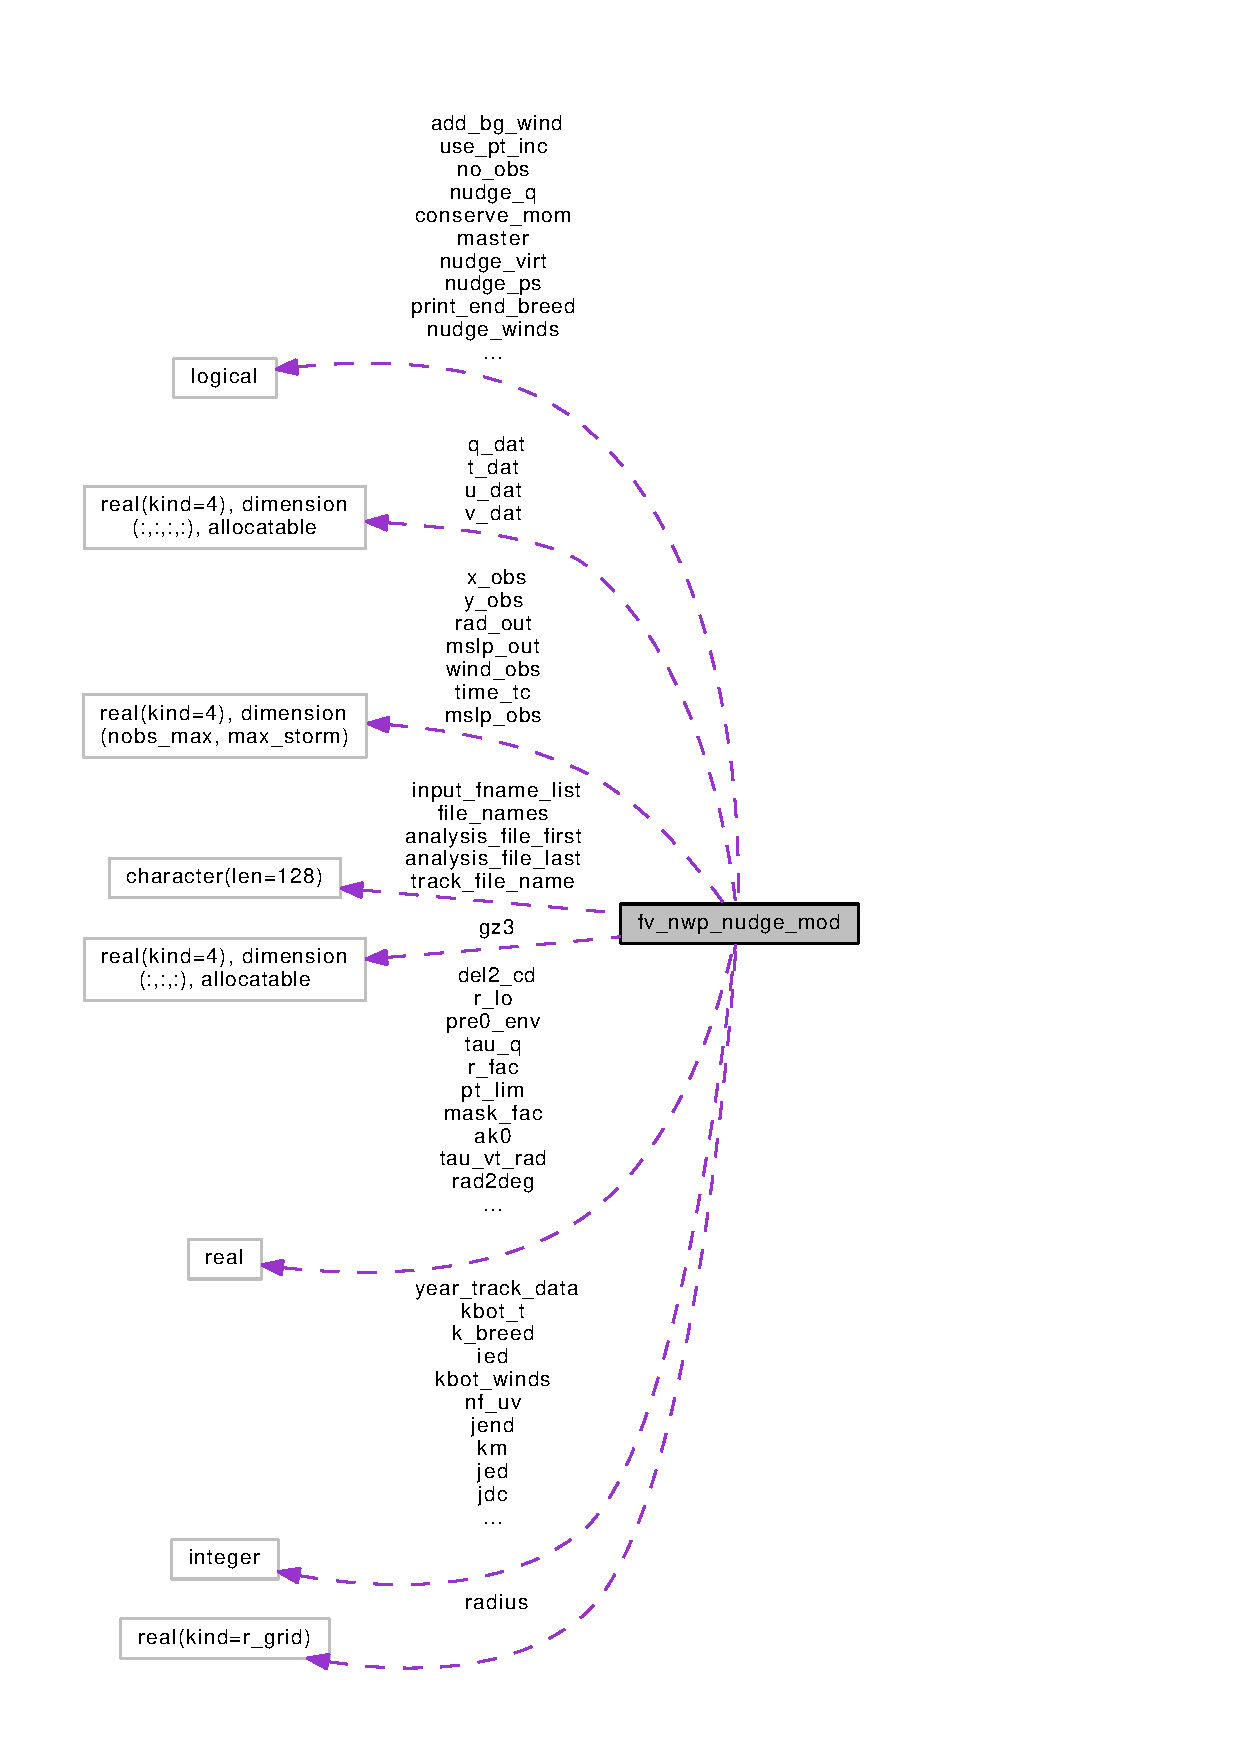
\includegraphics[height=550pt]{classfv__nwp__nudge__mod__coll__graph}
\end{center}
\end{figure}
\subsection*{Public Member Functions}
\begin{DoxyCompactItemize}
\item 
subroutine, public \hyperlink{classfv__nwp__nudge__mod_a4dfc72f39d2590d5b021acee04c23a2c}{fv\-\_\-nwp\-\_\-nudge} (Time, dt, npx, npy, npz, ps\-\_\-dt, u\-\_\-dt, v\-\_\-dt, t\-\_\-dt, q\-\_\-dt, zvir, ptop, ak, bk, ts, ps, delp, ua, va, pt, nwat, q, phis, gridstruct, bd, domain)
\begin{DoxyCompactList}\small\item\em Ths subroutine 'fv\-\_\-nwp\-\_\-nudge' computes and returns time tendencies for nudging to analysis. \end{DoxyCompactList}\item 
subroutine, public \hyperlink{classfv__nwp__nudge__mod_ac6397ea7496a338d4a086a95bb58fa38}{fv\-\_\-nwp\-\_\-nudge\-\_\-init} (time, axes, npz, zvir, ak, bk, ts, phis, gridstruct, ks, npx, neststruct, bd)
\begin{DoxyCompactList}\small\item\em The subroutine 'fv\-\_\-nwp\-\_\-nudge\-\_\-init' initializes the nudging module. \end{DoxyCompactList}\item 
subroutine, public \hyperlink{classfv__nwp__nudge__mod_a824609f6aaef3ce3b013048f4402ecb6}{fv\-\_\-nwp\-\_\-nudge\-\_\-end}
\begin{DoxyCompactList}\small\item\em The subroutine 'fv\-\_\-nwp\-\_\-nudge\-\_\-end' terminates the nudging module. \end{DoxyCompactList}\item 
subroutine, public \hyperlink{classfv__nwp__nudge__mod_af4d9fdbd6e2f0f78ded73848bd81ee15}{breed\-\_\-slp\-\_\-inline} (nstep, dt, npz, ak, bk, phis, pe, pk, peln, pkz, delp, u, v, pt, q, nwat, zvir, gridstruct, ks, domain\-\_\-local, bd, hydrostatic)
\begin{DoxyCompactList}\small\item\em The subroutine 'breed\-\_\-slp\-\_\-inline' performs vortex breeding by nudging sea level pressure toward single point observations. \end{DoxyCompactList}\end{DoxyCompactItemize}
\subsection*{Public Attributes}
\begin{DoxyCompactItemize}
\item 
logical, public \hyperlink{classfv__nwp__nudge__mod_a1be70541c37811b39b54dcf8d977feac}{do\-\_\-adiabatic\-\_\-init}
\item 
logical, public \hyperlink{classfv__nwp__nudge__mod_a85c0708a93d6f338cfa8408215a55c3b}{t\-\_\-is\-\_\-tv} = .false.
\end{DoxyCompactItemize}
\subsection*{Private Member Functions}
\begin{DoxyCompactItemize}
\item 
subroutine \hyperlink{classfv__nwp__nudge__mod_a562105a5fef2fdc16f81503979ed73b6}{ps\-\_\-nudging} (dt, factor, npz, ak, bk, ps\-\_\-obs, mask, tm, ps, phis, delp, ua, va, pt, nwat, q, bd, npx, npy, gridstruct, domain)
\item 
subroutine \hyperlink{classfv__nwp__nudge__mod_a77e9f8e082ec5d2ec81019aaf530f256}{ps\-\_\-bias\-\_\-correction} (ps\-\_\-dt, \hyperlink{classfv__nwp__nudge__mod_a635b34cbb0a0b285d6febfa4646c6993}{is}, \hyperlink{classfv__nwp__nudge__mod_a11b27e9ca5d61dc084748127098af2fb}{ie}, \hyperlink{classfv__nwp__nudge__mod_ad9f936f9336b43e00bcc6fa4fd1d4f6a}{js}, \hyperlink{classfv__nwp__nudge__mod_aec115c5d43df5f25250c9a3cd359f177}{je}, \hyperlink{classfv__nwp__nudge__mod_a7d1486af2ea75f210ba0c7d08952fe68}{isd}, \hyperlink{classfv__nwp__nudge__mod_a49d07573330869c0885c65c2ef35d8f4}{ied}, \hyperlink{classfv__nwp__nudge__mod_a14a29353676e857e25063a675a4700d8}{jsd}, \hyperlink{classfv__nwp__nudge__mod_a6354a59117d0add11183736f6f9c055a}{jed}, area)
\item 
real function \hyperlink{classfv__nwp__nudge__mod_a87499eb339d6900e68d8cb5c78c91ef2}{g0\-\_\-sum} (p, ifirst, ilast, jfirst, jlast, mode, reproduce, \hyperlink{classfv__nwp__nudge__mod_a7d1486af2ea75f210ba0c7d08952fe68}{isd}, \hyperlink{classfv__nwp__nudge__mod_a49d07573330869c0885c65c2ef35d8f4}{ied}, \hyperlink{classfv__nwp__nudge__mod_a14a29353676e857e25063a675a4700d8}{jsd}, \hyperlink{classfv__nwp__nudge__mod_a6354a59117d0add11183736f6f9c055a}{jed}, area)
\begin{DoxyCompactList}\small\item\em Fast version of global sum that is reproduced if the result is rounded to 4-\/byte. \end{DoxyCompactList}\item 
subroutine \hyperlink{classfv__nwp__nudge__mod_a1b057b57be7d6e7fad3bf2b54615e84d}{compute\-\_\-slp} (isc, iec, jsc, jec, tm, ps, gz, slp)
\item 
subroutine \hyperlink{classfv__nwp__nudge__mod_ad4f57cb75a42402e0aa82812192b504f}{get\-\_\-obs} (Time, dt, zvir, ak, bk, ps, ts, ps\-\_\-obs, delp, pt, nwat, q, u\-\_\-obs, v\-\_\-obs, t\-\_\-obs, q\-\_\-obs, phis, ua, va, u\-\_\-dt, v\-\_\-dt, npx, npy, npz, factor, mask, ptop, bd, gridstruct, domain)
\item 
subroutine \hyperlink{classfv__nwp__nudge__mod_ae2d3d00098cdab3691b6b7775a8f24ea}{get\-\_\-ncep\-\_\-analysis} (ps, u, v, t, q, zvir, ts, \hyperlink{classfv__nwp__nudge__mod_ac3f13e9bca31d7209fb652c08f3f50b8}{nfile}, fname, bd)
\item 
subroutine \hyperlink{classfv__nwp__nudge__mod_a459cebfc9aab25ccab52cef29c0da7d2}{remap\-\_\-coef} (agrid)
\item 
subroutine \hyperlink{classfv__nwp__nudge__mod_a0ff11151a5061fd4ddcdc4fee37da618}{ncep2fms} (sst)
\item 
subroutine \hyperlink{classfv__nwp__nudge__mod_a86bfb2f217d34d2927ce61a8ee8ea30a}{get\-\_\-int\-\_\-hght} (npz, ak, bk, ps, delp, ps0, tv)
\item 
subroutine \hyperlink{classfv__nwp__nudge__mod_a58249db452c718ac39ba534e7e2e75e6}{remap\-\_\-tq} (npz, ak, bk, ps, delp, t, q, kmd, ps0, ta, qa, zvir, ptop)
\item 
subroutine \hyperlink{classfv__nwp__nudge__mod_a1404c8483c8c5679474c17f84173f666}{remap\-\_\-uv} (npz, ak, bk, ps, delp, u, v, kmd, ps0, u0, v0, ptop)
\item 
subroutine \hyperlink{classfv__nwp__nudge__mod_ae1f75580d900fde7f16d0ea4c04dda0d}{get\-\_\-tc\-\_\-mask} (time, mask, agrid)
\item 
subroutine \hyperlink{classfv__nwp__nudge__mod_a7b916a894092000ca2773bbaf63fad25}{breed\-\_\-srf\-\_\-w10} (time, dt, npz, ak, bk, ps, phis, slp, delp, u, v, gridstruct)
\begin{DoxyCompactList}\small\item\em The subroutine 'breed\-\_\-srf\-\_\-w10' performs vortex breeding by nudging 10-\/m winds. \end{DoxyCompactList}\item 
subroutine \hyperlink{classfv__nwp__nudge__mod_a6615fa560c7d4186d2c6da06aecbb5d1}{breed\-\_\-srf\-\_\-winds} (time, dt, npz, u\-\_\-obs, v\-\_\-obs, ak, bk, ps, phis, delp, ua, va, u\-\_\-dt, v\-\_\-dt, pt, q, nwat, zvir, gridstruct)
\begin{DoxyCompactList}\small\item\em The subroutine 'breed\-\_\-srf\-\_\-winds' performs vortex breeding by nudging 1-\/m winds. \end{DoxyCompactList}\item 
subroutine \hyperlink{classfv__nwp__nudge__mod_aefc113f26f725814456ee4d0e2094e46}{tangent\-\_\-wind} (elon, elat, speed, po, pp, ut, vt)
\item 
subroutine \hyperlink{classfv__nwp__nudge__mod_a33970a757043357e1ddf2853c5d488ba}{get\-\_\-slp\-\_\-obs} (time, nobs, lon\-\_\-obs, lat\-\_\-obs, w10, mslp, slp\-\_\-out, r\-\_\-out, time\-\_\-obs, x\-\_\-o, y\-\_\-o, w10\-\_\-o, slp\-\_\-o, r\-\_\-vor, p\-\_\-vor, stime, fact)
\item 
subroutine \hyperlink{classfv__nwp__nudge__mod_ae667a55ffbd110b324b847e098e8c703}{slp\-\_\-obs\-\_\-init}
\item 
real function \hyperlink{classfv__nwp__nudge__mod_a65a3898d0634b9f134fd05985df6f76a}{calday} (year, month, day, hour, minute, sec)
\begin{DoxyCompactList}\small\item\em The function 'calday' performs time interpolation\-: \end{DoxyCompactList}\item 
logical function \hyperlink{classfv__nwp__nudge__mod_a396fbed122f17b39b587e3cd6645790d}{leap\-\_\-year} (ny)
\item 
subroutine \hyperlink{classfv__nwp__nudge__mod_a9fcca3e834cc3712596032598bcc44c5}{pmaxmin} (qname, a, imax, jmax, fac)
\item 
subroutine \hyperlink{classfv__nwp__nudge__mod_abc12568d2670b447a10653f727298cbe}{del2\-\_\-uv} (du, dv, cd, kmd, ntimes, bd, npx, npy, gridstruct, domain)
\begin{DoxyCompactList}\small\item\em The subroutine 'del2\-\_\-uv' filters the wind tendency. \end{DoxyCompactList}\item 
subroutine \hyperlink{classfv__nwp__nudge__mod_a31a4913add5b1f8b13999bd63b79a21e}{del2\-\_\-scalar} (qdt, cd, kmd, nmax, bd, npx, npy, gridstruct, domain)
\begin{DoxyCompactList}\small\item\em The subroutine 'del2\-\_\-scalar' filters the physics tendency. \end{DoxyCompactList}\item 
subroutine \hyperlink{classfv__nwp__nudge__mod_a74f89a2bcbb1e25d28f0e5429a85743c}{rmse\-\_\-bias} (a, rms, bias, area)
\item 
subroutine \hyperlink{classfv__nwp__nudge__mod_a12137129e53ec054657401b92f7ec8b4}{corr} (a, b, co, area)
\item 
subroutine \hyperlink{classfv__nwp__nudge__mod_abb31dc22f2b8f396e47957fa7a3c0e6c}{std} (a, mean, stdv, area)
\end{DoxyCompactItemize}
\subsection*{Private Attributes}
\begin{DoxyCompactItemize}
\item 
real(kind=r\-\_\-grid), parameter \hyperlink{classfv__nwp__nudge__mod_a558bf04275fcbb1d8f4debc8cca46876}{radius} = cnst\-\_\-radius
\item 
integer \hyperlink{classfv__nwp__nudge__mod_af4efcd0125a8753cccf9edea473212fe}{im}
\begin{DoxyCompactList}\small\item\em Data x-\/dimension. \end{DoxyCompactList}\item 
integer \hyperlink{classfv__nwp__nudge__mod_a14bdbe362e391feaf152589a422108c9}{jm}
\begin{DoxyCompactList}\small\item\em Data y-\/dimension. \end{DoxyCompactList}\item 
integer \hyperlink{classfv__nwp__nudge__mod_aa78148a3d1f41821741078945e55fd91}{km}
\begin{DoxyCompactList}\small\item\em Data z-\/dimension. \end{DoxyCompactList}\item 
real, dimension(\-:), allocatable \hyperlink{classfv__nwp__nudge__mod_a53a22f63c5e330aa0ee01b47aa9778a1}{ak0}
\item 
real, dimension(\-:), allocatable \hyperlink{classfv__nwp__nudge__mod_a0af47ffec9b92d67039b57e73d9a22ed}{bk0}
\item 
real, dimension(\-:), allocatable \hyperlink{classfv__nwp__nudge__mod_a0ff5513f7944f3fabb87a8383880a470}{lat}
\item 
real, dimension(\-:), allocatable \hyperlink{classfv__nwp__nudge__mod_ab49ca48851ebaafd62ff97f3e6d2af1f}{lon}
\item 
logical \hyperlink{classfv__nwp__nudge__mod_afe93a474895ccd632d9dfb88785e62f5}{module\-\_\-is\-\_\-initialized} = .false.
\item 
logical \hyperlink{classfv__nwp__nudge__mod_a6d58b3c58863d536ee597b0f8efb6dbd}{master}
\item 
logical \hyperlink{classfv__nwp__nudge__mod_a5a12cd412f969c30a2e68bb95a4dae80}{no\-\_\-obs}
\item 
real \hyperlink{classfv__nwp__nudge__mod_abf75628ab28896add786d9e88b4b26ab}{deg2rad}
\item 
real \hyperlink{classfv__nwp__nudge__mod_a2b54722a648c7b5841e3a2138d55ac5f}{rad2deg}
\item 
real \hyperlink{classfv__nwp__nudge__mod_a2346c4b41d57e4f60a7029638bb5eef7}{time\-\_\-nudge} = 0.
\item 
integer \hyperlink{classfv__nwp__nudge__mod_a22a2c695dd1f7be9256ad520d57da7f6}{time\-\_\-interval} = 6$\ast$3600
\begin{DoxyCompactList}\small\item\em dataset time interval (seconds) \end{DoxyCompactList}\item 
integer, parameter \hyperlink{classfv__nwp__nudge__mod_a7fb7b0e5d02de9ce46ac54830d236d60}{nfile\-\_\-max} = 29280
\begin{DoxyCompactList}\small\item\em maximum\-: 20-\/year analysis data, 4$\ast$366$\ast$20=29280 \end{DoxyCompactList}\item 
integer \hyperlink{classfv__nwp__nudge__mod_ac3f13e9bca31d7209fb652c08f3f50b8}{nfile}
\item 
integer \hyperlink{classfv__nwp__nudge__mod_aaf51c10e6d30b78bfd85128c97461593}{k\-\_\-breed} = 0
\item 
integer \hyperlink{classfv__nwp__nudge__mod_adb928bbeb73152d230dd49e24124150b}{k\-\_\-trop} = 0
\item 
real \hyperlink{classfv__nwp__nudge__mod_aa5e41c5d5b93d1e265d8929674b87023}{p\-\_\-trop} = 950.E2
\item 
real \hyperlink{classfv__nwp__nudge__mod_a4af1c4f2d5d76d8cd9766c468a80ef59}{dps\-\_\-min} = 50.
\begin{DoxyCompactList}\small\item\em maximum P\-S increment (pa; each step) due to inline breeding \end{DoxyCompactList}\item 
real \hyperlink{classfv__nwp__nudge__mod_a973df199a4848c1b46ae42ab3423a68e}{del2\-\_\-cd} = 0.\-16
\item 
real, dimension(\-:,\-:,\-:), allocatable \hyperlink{classfv__nwp__nudge__mod_a7d0277a732966ffab67f5853b8da70a5}{s2c}
\item 
integer, dimension(\-:,\-:), \\*
allocatable \hyperlink{classfv__nwp__nudge__mod_a355d223578b7728e289a6631c18206bb}{id1}
\item 
integer, dimension(\-:,\-:), \\*
allocatable \hyperlink{classfv__nwp__nudge__mod_a10d50bc3c563bcc270ef37108729f381}{id2}
\item 
integer, dimension(\-:,\-:), \\*
allocatable \hyperlink{classfv__nwp__nudge__mod_a046fc8ca32888e97b3af454cfca83aae}{jdc}
\item 
real, dimension(\-:,\-:,\-:), allocatable \hyperlink{classfv__nwp__nudge__mod_a31198eb99e726ad2b0eaf4897791206c}{ps\-\_\-dat}
\item 
real(kind=4), dimension(\-:,\-:,\-:,\-:), \\*
allocatable \hyperlink{classfv__nwp__nudge__mod_aba770ddb7a91e298a5a6717f65da570a}{u\-\_\-dat}
\item 
real(kind=4), dimension(\-:,\-:,\-:,\-:), \\*
allocatable \hyperlink{classfv__nwp__nudge__mod_a9d2249df35c01840bdff1c2f9b9f2af7}{v\-\_\-dat}
\item 
real(kind=4), dimension(\-:,\-:,\-:,\-:), \\*
allocatable \hyperlink{classfv__nwp__nudge__mod_afa50769b448c5878d107da994e63d234}{t\-\_\-dat}
\item 
real(kind=4), dimension(\-:,\-:,\-:,\-:), \\*
allocatable \hyperlink{classfv__nwp__nudge__mod_a35d70de0bf27001249d55b96b2cd229c}{q\-\_\-dat}
\item 
real(kind=4), dimension(\-:,\-:,\-:), \\*
allocatable \hyperlink{classfv__nwp__nudge__mod_a732a8eaade4984925290ea5b5372a8fe}{gz3}
\begin{DoxyCompactList}\small\item\em work array \end{DoxyCompactList}\item 
real, dimension(\-:,\-:), allocatable \hyperlink{classfv__nwp__nudge__mod_adb43d826a6835d384402078dd0280d5b}{gz0}
\item 
character(len=128) \hyperlink{classfv__nwp__nudge__mod_a6c78d433ff14d2b612633c8855f85e6c}{input\-\_\-fname\-\_\-list} =\char`\"{}\char`\"{}
\begin{DoxyCompactList}\small\item\em a file lists the input N\-C\-E\-P analysis data \end{DoxyCompactList}\item 
character(len=128) \hyperlink{classfv__nwp__nudge__mod_aa599ebe974dc91c791f9b5a81c75d59b}{analysis\-\_\-file\-\_\-first} =\char`\"{}\char`\"{}
\begin{DoxyCompactList}\small\item\em the first N\-C\-E\-P analysis file to be used for nudging, by default, the first file in the \char`\"{}input\-\_\-fname\-\_\-list\char`\"{} \end{DoxyCompactList}\item 
character(len=128) \hyperlink{classfv__nwp__nudge__mod_ab3049eb4b3e719220321b47aad4303ba}{analysis\-\_\-file\-\_\-last} =\char`\"{}\char`\"{}
\begin{DoxyCompactList}\small\item\em the last N\-C\-E\-P analysis file to be used for nudging by default, the last file in the \char`\"{}input\-\_\-fname\-\_\-list\char`\"{} \end{DoxyCompactList}\item 
real \hyperlink{classfv__nwp__nudge__mod_a67d18a2de5bc8c716affd9b18e65de34}{p\-\_\-relax} = 30.E2
\begin{DoxyCompactList}\small\item\em from P\-\_\-relax upwards, nudging is reduced linearly proportional to pfull/\-P\-\_\-relax \end{DoxyCompactList}\item 
real \hyperlink{classfv__nwp__nudge__mod_af6821904d98d5a2b0c18d7f01061693b}{p\-\_\-norelax} = 0.\-0
\begin{DoxyCompactList}\small\item\em from P\-\_\-norelax upwards, no nudging \end{DoxyCompactList}\item 
character(len=128), dimension(\hyperlink{classfv__nwp__nudge__mod_a7fb7b0e5d02de9ce46ac54830d236d60}{nfile\-\_\-max}) \hyperlink{classfv__nwp__nudge__mod_a4a4209d304ae4ac9cd30d3139b1bfb6d}{file\-\_\-names}
\item 
character(len=128) \hyperlink{classfv__nwp__nudge__mod_a2a733b4b29ac3b974f5bc194e8a33fb3}{track\-\_\-file\-\_\-name}
\item 
integer \hyperlink{classfv__nwp__nudge__mod_a16ad156aeca41cd051feaf6544535476}{nfile\-\_\-total} = 0
\begin{DoxyCompactList}\small\item\em =5 for 1-\/day (if datasets are 6-\/hr apart) \end{DoxyCompactList}\item 
real \hyperlink{classfv__nwp__nudge__mod_a05315b1d11b770d5ea2eb43325d8fe83}{p\-\_\-wvp} = 100.E2
\begin{DoxyCompactList}\small\item\em cutoff level for specific humidity nudging \end{DoxyCompactList}\item 
integer \hyperlink{classfv__nwp__nudge__mod_a22e044d4dce29168ca4a9a97017a6759}{kord\-\_\-data} = 8
\item 
real \hyperlink{classfv__nwp__nudge__mod_a0393a20ffd09b6005c121df77b990757}{mask\-\_\-fac} = 0.\-25
\begin{DoxyCompactList}\small\item\em \mbox{[}0,1\mbox{]} 0\-: no mask; 1\-: full strength \end{DoxyCompactList}\item 
logical \hyperlink{classfv__nwp__nudge__mod_a1b4b58ec4a0172ebac02423ec390aec2}{use\-\_\-pt\-\_\-inc} = .false.
\item 
logical \hyperlink{classfv__nwp__nudge__mod_a37a4cc7b60012b2fdafe49c5befb8a84}{use\-\_\-high\-\_\-top} = .false.
\item 
logical \hyperlink{classfv__nwp__nudge__mod_a42e7ca1641769656215dab0c288e12a5}{add\-\_\-bg\-\_\-wind} = .true.
\item 
logical \hyperlink{classfv__nwp__nudge__mod_adb1086d378b3e7629b60b973f777e591}{conserve\-\_\-mom} = .true.
\item 
logical \hyperlink{classfv__nwp__nudge__mod_aa9d79a7ef439011ae3c43ebe64d5262d}{conserve\-\_\-hgt} = .true.
\item 
logical \hyperlink{classfv__nwp__nudge__mod_a091b1c329569ecb6a515ebeb3a9050c6}{tc\-\_\-mask} = .false.
\item 
logical \hyperlink{classfv__nwp__nudge__mod_a8514b5b22545a48edbde79b6cc213a2b}{strong\-\_\-mask} = .false.
\item 
logical \hyperlink{classfv__nwp__nudge__mod_a095af635f02f1f236a662ea553ed82ed}{ibtrack} = .true.
\item 
logical \hyperlink{classfv__nwp__nudge__mod_aa949ba1a2ce2ca23017b0da8a43f6c53}{nudge\-\_\-debug} = .false.
\item 
logical \hyperlink{classfv__nwp__nudge__mod_a0c85e97c2aecbe6ce8692709f34ab99d}{do\-\_\-ps\-\_\-bias} = .false.
\item 
logical \hyperlink{classfv__nwp__nudge__mod_acbab7a0c866d541bac35151394b129a5}{nudge\-\_\-ps} = .false.
\item 
logical \hyperlink{classfv__nwp__nudge__mod_ae3b2433d7487d03ec653e06c3df92977}{nudge\-\_\-q} = .false.
\item 
logical \hyperlink{classfv__nwp__nudge__mod_a5d9c6b2ff22b4d521f81880326ce0bdc}{nudge\-\_\-winds} = .true.
\item 
logical \hyperlink{classfv__nwp__nudge__mod_a969e6940a34f9a4a3f31606aaaef7bc6}{nudge\-\_\-virt} = .true.
\item 
logical \hyperlink{classfv__nwp__nudge__mod_a6e98d55e79bcefff8ef5c6db06c5aa6a}{nudge\-\_\-hght} = .true.
\item 
logical \hyperlink{classfv__nwp__nudge__mod_a798deef0b988b1711210e1bc67e44551}{time\-\_\-varying} = .true.
\item 
logical \hyperlink{classfv__nwp__nudge__mod_a147187160ea12ff1251fc7e8ddb8b045}{print\-\_\-end\-\_\-breed} = .true.
\item 
logical \hyperlink{classfv__nwp__nudge__mod_a3068ea3b555378d00dbbd1f98a982f03}{print\-\_\-end\-\_\-nudge} = .true.
\item 
real \hyperlink{classfv__nwp__nudge__mod_a351915ecd86a6b30a9cc359a9d83ec59}{tau\-\_\-ps} = 21600.
\begin{DoxyCompactList}\small\item\em 1-\/day \end{DoxyCompactList}\item 
real \hyperlink{classfv__nwp__nudge__mod_a230458adc8e2b3649c9306bc76482b67}{tau\-\_\-q} = 86400.
\begin{DoxyCompactList}\small\item\em 1-\/day \end{DoxyCompactList}\item 
real \hyperlink{classfv__nwp__nudge__mod_a8a91872ad260e59a51cee29ec3729d5f}{tau\-\_\-winds} = 21600.
\begin{DoxyCompactList}\small\item\em 6-\/hr \end{DoxyCompactList}\item 
real \hyperlink{classfv__nwp__nudge__mod_a71192e4362d0448b7efb038493f8630b}{tau\-\_\-virt} = 43200.
\item 
real \hyperlink{classfv__nwp__nudge__mod_af7bc681ffc01fee847582a895acc391f}{tau\-\_\-hght} = 43200.
\item 
real \hyperlink{classfv__nwp__nudge__mod_a6132d02b32cd548905fb9ce035177937}{q\-\_\-min} = 1.E-\/8
\item 
integer \hyperlink{classfv__nwp__nudge__mod_a70bc4acdd2e6d0dfffe5632d08ce50af}{jbeg}
\item 
integer \hyperlink{classfv__nwp__nudge__mod_aefbee267032d4df68a60b6e8cab3018b}{jend}
\item 
integer \hyperlink{classfv__nwp__nudge__mod_ab0860b10bf5b0b892942089db400c304}{nf\-\_\-uv} = 0
\item 
integer \hyperlink{classfv__nwp__nudge__mod_a3482c6b80161fc5cbb0464c8ce29a44b}{nf\-\_\-ps} = 0
\item 
integer \hyperlink{classfv__nwp__nudge__mod_a1f356635df8d44472638c30747dccf70}{nf\-\_\-t} = 2
\item 
integer \hyperlink{classfv__nwp__nudge__mod_af093b08be6222c05893da2a51a656d68}{nf\-\_\-ht} = 1
\item 
integer \hyperlink{classfv__nwp__nudge__mod_ab54932d082a922ed0c64ee023b82cb39}{kstart} = 2
\item 
integer \hyperlink{classfv__nwp__nudge__mod_a827de7924a0a51dfe5fe9f7423ba4945}{kbot\-\_\-winds} = 0
\item 
integer \hyperlink{classfv__nwp__nudge__mod_ad7c03f71ddd83294582e31b20b2b5c2a}{kbot\-\_\-t} = 0
\item 
integer \hyperlink{classfv__nwp__nudge__mod_a74234073b487143a6a2f3fbfb681b78e}{kbot\-\_\-q} = 0
\item 
logical \hyperlink{classfv__nwp__nudge__mod_ad4ade09f973cb7f9027724a6f0dfa3e2}{analysis\-\_\-time}
\item 
logical \hyperlink{classfv__nwp__nudge__mod_abe2b674214dcb600da0917bed138a693}{breed\-\_\-srf\-\_\-w} = .false.
\item 
real \hyperlink{classfv__nwp__nudge__mod_a7cb840172166ac14895fa478c0b600d1}{grid\-\_\-size} = 28.E3
\item 
real \hyperlink{classfv__nwp__nudge__mod_aa233a35074268c39b4e9a7e3304c5266}{tau\-\_\-vt\-\_\-slp} = 1200.
\item 
real \hyperlink{classfv__nwp__nudge__mod_ac55edc6cc6a0dd38808a85de68d359ac}{tau\-\_\-vt\-\_\-wind} = 1200.
\item 
real \hyperlink{classfv__nwp__nudge__mod_aedb6d82b930ca6f0120ef1a1a7103e52}{tau\-\_\-vt\-\_\-rad} = 4.\-0
\item 
real \hyperlink{classfv__nwp__nudge__mod_a865347a5d8e5faa5502349ef5af5712c}{pt\-\_\-lim} = 0.\-2
\item 
real \hyperlink{classfv__nwp__nudge__mod_aeae3cc750d917e17328d4ea8de151d6e}{slp\-\_\-env} = 101010.
\begin{DoxyCompactList}\small\item\em storm environment pressure (pa) \end{DoxyCompactList}\item 
real \hyperlink{classfv__nwp__nudge__mod_a18ccc45a22e3d7fe4ebd33add4819161}{pre0\-\_\-env} = 100000.
\begin{DoxyCompactList}\small\item\em critical storm environment pressure (pa) for size computation \end{DoxyCompactList}\item 
real, parameter \hyperlink{classfv__nwp__nudge__mod_aac08d7ae4a61435471198d904245024a}{tm\-\_\-max} = 315.
\item 
real \hyperlink{classfv__nwp__nudge__mod_ab0d4afa46d379b1dfdfb896cbc99823d}{r\-\_\-lo} = 2.\-0
\item 
real \hyperlink{classfv__nwp__nudge__mod_a333405a63e3356a6a4f7798929dec480}{r\-\_\-hi} = 5.\-0
\item 
real \hyperlink{classfv__nwp__nudge__mod_ae40e38918bb6ff86846b98d42bfc9c15}{r\-\_\-fac} = 1.\-2
\item 
real \hyperlink{classfv__nwp__nudge__mod_aa3bb326deaf67f4dff2228ac0abba2c8}{r\-\_\-min} = 200.E3
\item 
real \hyperlink{classfv__nwp__nudge__mod_a73e8b9cff0944e7d9517c41fb7fed00f}{r\-\_\-inc} = 25.E3
\item 
real, parameter \hyperlink{classfv__nwp__nudge__mod_a9654eb64171c69405fda2430057e59a5}{del\-\_\-r} = 50.E3
\item 
real \hyperlink{classfv__nwp__nudge__mod_a80705a18203ac9f1ade4dfaf5396ed19}{elapsed\-\_\-time} = 0.\-0
\item 
real \hyperlink{classfv__nwp__nudge__mod_a25110c10c670ba1da3b3897a09b2098e}{nudged\-\_\-time} = 1.E12
\begin{DoxyCompactList}\small\item\em seconds \end{DoxyCompactList}\item 
integer \hyperlink{classfv__nwp__nudge__mod_a9171eb4f9d03ed8a5648ba241620df1c}{year\-\_\-track\-\_\-data}
\item 
integer, parameter \hyperlink{classfv__nwp__nudge__mod_aac3d8d546e1954263ae52400f44d2c7c}{max\-\_\-storm} = 140
\begin{DoxyCompactList}\small\item\em max \# of storms to process \end{DoxyCompactList}\item 
integer, parameter \hyperlink{classfv__nwp__nudge__mod_ac3d3a0cbdfff5f6ed3757fcc2b70309d}{nobs\-\_\-max} = 125
\begin{DoxyCompactList}\small\item\em Max \# of observations per storm. \end{DoxyCompactList}\item 
integer \hyperlink{classfv__nwp__nudge__mod_a9c3ad6de2a20927fcd7f0b6433599038}{nstorms} = 0
\item 
integer, dimension(\hyperlink{classfv__nwp__nudge__mod_aac3d8d546e1954263ae52400f44d2c7c}{max\-\_\-storm}) \hyperlink{classfv__nwp__nudge__mod_a5c2925d3d3fb1e24385718a9533b8092}{nobs\-\_\-tc}
\item 
integer \hyperlink{classfv__nwp__nudge__mod_a1097a1064cec1b746d3c06aebb722114}{min\-\_\-nobs} = 16
\item 
real \hyperlink{classfv__nwp__nudge__mod_a7bc4a9ade4f83f3866673db98fc33230}{min\-\_\-mslp} = 1009.E2
\item 
real(kind=4), dimension(\hyperlink{classfv__nwp__nudge__mod_ac3d3a0cbdfff5f6ed3757fcc2b70309d}{nobs\-\_\-max}, \\*
\hyperlink{classfv__nwp__nudge__mod_aac3d8d546e1954263ae52400f44d2c7c}{max\-\_\-storm}) \hyperlink{classfv__nwp__nudge__mod_a9f06e5f833a9b261ab86ddaade7f3571}{x\-\_\-obs}
\begin{DoxyCompactList}\small\item\em longitude in degrees \end{DoxyCompactList}\item 
real(kind=4), dimension(\hyperlink{classfv__nwp__nudge__mod_ac3d3a0cbdfff5f6ed3757fcc2b70309d}{nobs\-\_\-max}, \\*
\hyperlink{classfv__nwp__nudge__mod_aac3d8d546e1954263ae52400f44d2c7c}{max\-\_\-storm}) \hyperlink{classfv__nwp__nudge__mod_aecc8732e077061904bbf9f1e052c190d}{y\-\_\-obs}
\begin{DoxyCompactList}\small\item\em latitude in degrees \end{DoxyCompactList}\item 
real(kind=4), dimension(\hyperlink{classfv__nwp__nudge__mod_ac3d3a0cbdfff5f6ed3757fcc2b70309d}{nobs\-\_\-max}, \\*
\hyperlink{classfv__nwp__nudge__mod_aac3d8d546e1954263ae52400f44d2c7c}{max\-\_\-storm}) \hyperlink{classfv__nwp__nudge__mod_a0b13b44ac7609d8c641c306310649711}{wind\-\_\-obs}
\begin{DoxyCompactList}\small\item\em observed 10-\/m wind speed (m/s) \end{DoxyCompactList}\item 
real(kind=4), dimension(\hyperlink{classfv__nwp__nudge__mod_ac3d3a0cbdfff5f6ed3757fcc2b70309d}{nobs\-\_\-max}, \\*
\hyperlink{classfv__nwp__nudge__mod_aac3d8d546e1954263ae52400f44d2c7c}{max\-\_\-storm}) \hyperlink{classfv__nwp__nudge__mod_a9eee9ed61c6ec21fa45d4f80a88699fc}{mslp\-\_\-obs}
\begin{DoxyCompactList}\small\item\em observed S\-L\-P in mb \end{DoxyCompactList}\item 
real(kind=4), dimension(\hyperlink{classfv__nwp__nudge__mod_ac3d3a0cbdfff5f6ed3757fcc2b70309d}{nobs\-\_\-max}, \\*
\hyperlink{classfv__nwp__nudge__mod_aac3d8d546e1954263ae52400f44d2c7c}{max\-\_\-storm}) \hyperlink{classfv__nwp__nudge__mod_ad0231a73a4870ec8743ecd19e7181b11}{mslp\-\_\-out}
\begin{DoxyCompactList}\small\item\em outer ring S\-L\-P in mb \end{DoxyCompactList}\item 
real(kind=4), dimension(\hyperlink{classfv__nwp__nudge__mod_ac3d3a0cbdfff5f6ed3757fcc2b70309d}{nobs\-\_\-max}, \\*
\hyperlink{classfv__nwp__nudge__mod_aac3d8d546e1954263ae52400f44d2c7c}{max\-\_\-storm}) \hyperlink{classfv__nwp__nudge__mod_a406dba8bb90cbab343bb92bf5cef1f58}{rad\-\_\-out}
\begin{DoxyCompactList}\small\item\em outer ring radius in meters \end{DoxyCompactList}\item 
real(kind=4), dimension(\hyperlink{classfv__nwp__nudge__mod_ac3d3a0cbdfff5f6ed3757fcc2b70309d}{nobs\-\_\-max}, \\*
\hyperlink{classfv__nwp__nudge__mod_aac3d8d546e1954263ae52400f44d2c7c}{max\-\_\-storm}) \hyperlink{classfv__nwp__nudge__mod_a943f847873f99de2546f21b2ec1a3a9e}{time\-\_\-tc}
\begin{DoxyCompactList}\small\item\em start time of the track \end{DoxyCompactList}\item 
integer \hyperlink{classfv__nwp__nudge__mod_aff11af198e7507203fac0b6fc479060d}{id\-\_\-ht\-\_\-err}
\item 
integer \hyperlink{classfv__nwp__nudge__mod_a635b34cbb0a0b285d6febfa4646c6993}{is}
\item 
integer \hyperlink{classfv__nwp__nudge__mod_a11b27e9ca5d61dc084748127098af2fb}{ie}
\item 
integer \hyperlink{classfv__nwp__nudge__mod_ad9f936f9336b43e00bcc6fa4fd1d4f6a}{js}
\item 
integer \hyperlink{classfv__nwp__nudge__mod_aec115c5d43df5f25250c9a3cd359f177}{je}
\item 
integer \hyperlink{classfv__nwp__nudge__mod_a7d1486af2ea75f210ba0c7d08952fe68}{isd}
\item 
integer \hyperlink{classfv__nwp__nudge__mod_a49d07573330869c0885c65c2ef35d8f4}{ied}
\item 
integer \hyperlink{classfv__nwp__nudge__mod_a14a29353676e857e25063a675a4700d8}{jsd}
\item 
integer \hyperlink{classfv__nwp__nudge__mod_a6354a59117d0add11183736f6f9c055a}{jed}
\end{DoxyCompactItemize}


\subsection{Detailed Description}
The module fv\-\_\-nwp\-\_\-nudge contains routines for nudging to input analyses. note This module is currently not supported in fv\-G\-F\-S of F\-V3\-G\-F\-S. 

Definition at line 32 of file fv\-\_\-nudge.\-F90.



\subsection{Member Function/\-Subroutine Documentation}
\index{fv\-\_\-nwp\-\_\-nudge\-\_\-mod@{fv\-\_\-nwp\-\_\-nudge\-\_\-mod}!breed\-\_\-slp\-\_\-inline@{breed\-\_\-slp\-\_\-inline}}
\index{breed\-\_\-slp\-\_\-inline@{breed\-\_\-slp\-\_\-inline}!fv_nwp_nudge_mod@{fv\-\_\-nwp\-\_\-nudge\-\_\-mod}}
\subsubsection[{breed\-\_\-slp\-\_\-inline}]{\setlength{\rightskip}{0pt plus 5cm}subroutine, public fv\-\_\-nwp\-\_\-nudge\-\_\-mod\-::breed\-\_\-slp\-\_\-inline (
\begin{DoxyParamCaption}
\item[{integer, intent(in)}]{nstep, }
\item[{real, intent(in)}]{dt, }
\item[{integer, intent(in)}]{npz, }
\item[{real, dimension(npz+1), intent(in)}]{ak, }
\item[{real, dimension(npz+1), intent(in)}]{bk, }
\item[{real, dimension(isd\-:ied,jsd\-:jed), intent(in)}]{phis, }
\item[{real, dimension({\bf is}-\/1\-:{\bf ie}+1, npz+1,{\bf js}-\/1\-:{\bf je}+1), intent(inout)}]{pe, }
\item[{real, dimension(is\-:ie,js\-:je, npz+1), intent(inout)}]{pk, }
\item[{real, dimension(is\-:ie,npz+1,js\-:je), intent(out)}]{peln, }
\item[{real, dimension(is\-:ie,js\-:je,npz), intent(inout)}]{pkz, }
\item[{real, dimension(isd\-:ied,jsd\-:jed,npz), intent(inout)}]{delp, }
\item[{real, dimension(isd\-:ied,jsd\-:jed+1,npz), intent(inout)}]{u, }
\item[{real, dimension(isd\-:ied+1,jsd\-:jed,npz), intent(inout)}]{v, }
\item[{real, dimension(isd\-:ied,jsd\-:jed,npz), intent(inout)}]{pt, }
\item[{real, dimension(isd\-:ied,jsd\-:jed,npz,$\ast$), intent(inout)}]{q, }
\item[{integer, intent(in)}]{nwat, }
\item[{real, intent(in)}]{zvir, }
\item[{type(fv\-\_\-grid\-\_\-type), target}]{gridstruct, }
\item[{integer, intent(in)}]{ks, }
\item[{type(domain2d), intent(inout)}]{domain\-\_\-local, }
\item[{type(fv\-\_\-grid\-\_\-bounds\-\_\-type), intent(in)}]{bd, }
\item[{logical, intent(in)}]{hydrostatic}
\end{DoxyParamCaption}
)}\label{classfv__nwp__nudge__mod_af4d9fdbd6e2f0f78ded73848bd81ee15}


The subroutine 'breed\-\_\-slp\-\_\-inline' performs vortex breeding by nudging sea level pressure toward single point observations. 

This is a tropical cyclone 'bogusing' routine that currently only works for hydrostatic dynamics. \begin{DoxyNote}{Note}
Note\-: conserve water mass, geopotential, and momentum at the expense of dry air mass
\end{DoxyNote}

\begin{DoxyParams}[1]{Parameters}
\mbox{\tt in}  & {\em dt} & (small) time step in seconds\\
\hline
\mbox{\tt in,out}  & {\em pk} & pe$\ast$$\ast$kappa\\
\hline
\mbox{\tt in,out}  & {\em pe} & edge pressure (pascal)\\
\hline
\mbox{\tt out}  & {\em peln} & ln(pe) \\
\hline
\end{DoxyParams}


Definition at line 2155 of file fv\-\_\-nudge.\-F90.



References calday(), compute\-\_\-slp(), get\-\_\-slp\-\_\-obs(), fv\-\_\-grid\-\_\-utils\-\_\-mod\-::great\-\_\-circle\-\_\-dist(), fv\-\_\-diagnostics\-\_\-mod\-::p\-\_\-sum(), fv\-\_\-diagnostics\-\_\-mod\-::prt\-\_\-maxmin(), multi\-\_\-gases\-\_\-mod\-::vicpqd(), and multi\-\_\-gases\-\_\-mod\-::virqd().



Referenced by dyn\-\_\-core\-\_\-mod\-::dyn\-\_\-core().

\index{fv\-\_\-nwp\-\_\-nudge\-\_\-mod@{fv\-\_\-nwp\-\_\-nudge\-\_\-mod}!breed\-\_\-srf\-\_\-w10@{breed\-\_\-srf\-\_\-w10}}
\index{breed\-\_\-srf\-\_\-w10@{breed\-\_\-srf\-\_\-w10}!fv_nwp_nudge_mod@{fv\-\_\-nwp\-\_\-nudge\-\_\-mod}}
\subsubsection[{breed\-\_\-srf\-\_\-w10}]{\setlength{\rightskip}{0pt plus 5cm}subroutine fv\-\_\-nwp\-\_\-nudge\-\_\-mod\-::breed\-\_\-srf\-\_\-w10 (
\begin{DoxyParamCaption}
\item[{type(time\-\_\-type), intent(in)}]{time, }
\item[{real, intent(in)}]{dt, }
\item[{integer, intent(in)}]{npz, }
\item[{real, dimension(npz+1), intent(in)}]{ak, }
\item[{real, dimension(npz+1), intent(in)}]{bk, }
\item[{real, dimension(isd\-:ied,jsd\-:jed), intent(in)}]{ps, }
\item[{real, dimension(isd\-:ied,jsd\-:jed), intent(in)}]{phis, }
\item[{real, dimension(is\-:ie,js\-:je), intent(in)}]{slp, }
\item[{real, dimension(isd\-:ied,jsd\-:jed,npz), intent(inout)}]{delp, }
\item[{real, dimension(isd\-:ied,jsd\-:jed+1,npz), intent(inout)}]{u, }
\item[{real, dimension(isd\-:ied+1,jsd\-:jed,npz), intent(inout)}]{v, }
\item[{type(fv\-\_\-grid\-\_\-type), intent(in), target}]{gridstruct}
\end{DoxyParamCaption}
)\hspace{0.3cm}{\ttfamily [private]}}\label{classfv__nwp__nudge__mod_a7b916a894092000ca2773bbaf63fad25}


The subroutine 'breed\-\_\-srf\-\_\-w10' performs vortex breeding by nudging 10-\/m winds. 

This is the inline version.


\begin{DoxyParams}[1]{Parameters}
\mbox{\tt in}  & {\em dt} & time step in seconds \\
\hline
\end{DoxyParams}


Definition at line 2648 of file fv\-\_\-nudge.\-F90.



References get\-\_\-slp\-\_\-obs(), fv\-\_\-grid\-\_\-utils\-\_\-mod\-::great\-\_\-circle\-\_\-dist(), and tangent\-\_\-wind().

\index{fv\-\_\-nwp\-\_\-nudge\-\_\-mod@{fv\-\_\-nwp\-\_\-nudge\-\_\-mod}!breed\-\_\-srf\-\_\-winds@{breed\-\_\-srf\-\_\-winds}}
\index{breed\-\_\-srf\-\_\-winds@{breed\-\_\-srf\-\_\-winds}!fv_nwp_nudge_mod@{fv\-\_\-nwp\-\_\-nudge\-\_\-mod}}
\subsubsection[{breed\-\_\-srf\-\_\-winds}]{\setlength{\rightskip}{0pt plus 5cm}subroutine fv\-\_\-nwp\-\_\-nudge\-\_\-mod\-::breed\-\_\-srf\-\_\-winds (
\begin{DoxyParamCaption}
\item[{type(time\-\_\-type), intent(in)}]{time, }
\item[{real, intent(in)}]{dt, }
\item[{integer, intent(in)}]{npz, }
\item[{real, dimension(is\-:ie,js\-:je,npz), intent(in)}]{u\-\_\-obs, }
\item[{real, dimension(is\-:ie,js\-:je,npz), intent(in)}]{v\-\_\-obs, }
\item[{real, dimension(npz+1), intent(in)}]{ak, }
\item[{real, dimension(npz+1), intent(in)}]{bk, }
\item[{real, dimension(isd\-:ied,jsd\-:jed), intent(in)}]{ps, }
\item[{real, dimension(isd\-:ied,jsd\-:jed), intent(in)}]{phis, }
\item[{real, dimension(isd\-:ied,jsd\-:jed,npz), intent(inout)}]{delp, }
\item[{real, dimension(isd\-:ied,jsd\-:jed,npz), intent(inout)}]{ua, }
\item[{real, dimension(isd\-:ied,jsd\-:jed,npz), intent(inout)}]{va, }
\item[{real, dimension(isd\-:ied,jsd\-:jed,npz), intent(inout)}]{u\-\_\-dt, }
\item[{real, dimension(isd\-:ied,jsd\-:jed,npz), intent(inout)}]{v\-\_\-dt, }
\item[{real, dimension(isd\-:ied,jsd\-:jed,npz), intent(inout)}]{pt, }
\item[{real, dimension(isd\-:ied,jsd\-:jed,npz,nwat), intent(inout)}]{q, }
\item[{integer, intent(in)}]{nwat, }
\item[{real, intent(in)}]{zvir, }
\item[{type(fv\-\_\-grid\-\_\-type), intent(in), target}]{gridstruct}
\end{DoxyParamCaption}
)\hspace{0.3cm}{\ttfamily [private]}}\label{classfv__nwp__nudge__mod_a6615fa560c7d4186d2c6da06aecbb5d1}


The subroutine 'breed\-\_\-srf\-\_\-winds' performs vortex breeding by nudging 1-\/m winds. 


\begin{DoxyParams}[1]{Parameters}
\mbox{\tt in}  & {\em dt} & time step in seconds \\
\hline
\end{DoxyParams}


Definition at line 2927 of file fv\-\_\-nudge.\-F90.



References get\-\_\-slp\-\_\-obs(), fv\-\_\-grid\-\_\-utils\-\_\-mod\-::great\-\_\-circle\-\_\-dist(), and tangent\-\_\-wind().



Referenced by fv\-\_\-nwp\-\_\-nudge().

\index{fv\-\_\-nwp\-\_\-nudge\-\_\-mod@{fv\-\_\-nwp\-\_\-nudge\-\_\-mod}!calday@{calday}}
\index{calday@{calday}!fv_nwp_nudge_mod@{fv\-\_\-nwp\-\_\-nudge\-\_\-mod}}
\subsubsection[{calday}]{\setlength{\rightskip}{0pt plus 5cm}real function fv\-\_\-nwp\-\_\-nudge\-\_\-mod\-::calday (
\begin{DoxyParamCaption}
\item[{integer, intent(in)}]{year, }
\item[{integer, intent(in)}]{month, }
\item[{integer, intent(in)}]{day, }
\item[{integer, intent(in)}]{hour, }
\item[{integer, intent(in)}]{minute, }
\item[{integer, intent(in)}]{sec}
\end{DoxyParamCaption}
)\hspace{0.3cm}{\ttfamily [private]}}\label{classfv__nwp__nudge__mod_a65a3898d0634b9f134fd05985df6f76a}


The function 'calday' performs time interpolation\-: 



Definition at line 3408 of file fv\-\_\-nudge.\-F90.



References leap\-\_\-year().



Referenced by breed\-\_\-slp\-\_\-inline(), get\-\_\-slp\-\_\-obs(), and slp\-\_\-obs\-\_\-init().

\index{fv\-\_\-nwp\-\_\-nudge\-\_\-mod@{fv\-\_\-nwp\-\_\-nudge\-\_\-mod}!compute\-\_\-slp@{compute\-\_\-slp}}
\index{compute\-\_\-slp@{compute\-\_\-slp}!fv_nwp_nudge_mod@{fv\-\_\-nwp\-\_\-nudge\-\_\-mod}}
\subsubsection[{compute\-\_\-slp}]{\setlength{\rightskip}{0pt plus 5cm}subroutine fv\-\_\-nwp\-\_\-nudge\-\_\-mod\-::compute\-\_\-slp (
\begin{DoxyParamCaption}
\item[{integer, intent(in)}]{isc, }
\item[{integer, intent(in)}]{iec, }
\item[{integer, intent(in)}]{jsc, }
\item[{integer, intent(in)}]{jec, }
\item[{real, dimension(isc\-:iec,jsc\-:jec), intent(in)}]{tm, }
\item[{real, dimension(isc\-:iec,jsc\-:jec), intent(in)}]{ps, }
\item[{real, dimension(isc\-:iec,jsc\-:jec), intent(in)}]{gz, }
\item[{real, dimension(isc\-:iec,jsc\-:jec), intent(out)}]{slp}
\end{DoxyParamCaption}
)\hspace{0.3cm}{\ttfamily [private]}}\label{classfv__nwp__nudge__mod_a1b057b57be7d6e7fad3bf2b54615e84d}


Definition at line 1077 of file fv\-\_\-nudge.\-F90.



Referenced by breed\-\_\-slp\-\_\-inline(), and fv\-\_\-nwp\-\_\-nudge().

\index{fv\-\_\-nwp\-\_\-nudge\-\_\-mod@{fv\-\_\-nwp\-\_\-nudge\-\_\-mod}!corr@{corr}}
\index{corr@{corr}!fv_nwp_nudge_mod@{fv\-\_\-nwp\-\_\-nudge\-\_\-mod}}
\subsubsection[{corr}]{\setlength{\rightskip}{0pt plus 5cm}subroutine fv\-\_\-nwp\-\_\-nudge\-\_\-mod\-::corr (
\begin{DoxyParamCaption}
\item[{real, dimension(is\-:ie,js\-:je), intent(in)}]{a, }
\item[{real, dimension(is\-:ie,js\-:je), intent(in)}]{b, }
\item[{real, intent(out)}]{co, }
\item[{real, dimension(isd\-:ied,jsd\-:jed), intent(in)}]{area}
\end{DoxyParamCaption}
)\hspace{0.3cm}{\ttfamily [private]}}\label{classfv__nwp__nudge__mod_a12137129e53ec054657401b92f7ec8b4}


Definition at line 3692 of file fv\-\_\-nudge.\-F90.



References std().



Referenced by fv\-\_\-nwp\-\_\-nudge().

\index{fv\-\_\-nwp\-\_\-nudge\-\_\-mod@{fv\-\_\-nwp\-\_\-nudge\-\_\-mod}!del2\-\_\-scalar@{del2\-\_\-scalar}}
\index{del2\-\_\-scalar@{del2\-\_\-scalar}!fv_nwp_nudge_mod@{fv\-\_\-nwp\-\_\-nudge\-\_\-mod}}
\subsubsection[{del2\-\_\-scalar}]{\setlength{\rightskip}{0pt plus 5cm}subroutine fv\-\_\-nwp\-\_\-nudge\-\_\-mod\-::del2\-\_\-scalar (
\begin{DoxyParamCaption}
\item[{real, dimension(is\-:ie,js\-:je,kmd), intent(inout)}]{qdt, }
\item[{real, intent(in)}]{cd, }
\item[{integer, intent(in)}]{kmd, }
\item[{integer, intent(in)}]{nmax, }
\item[{type(fv\-\_\-grid\-\_\-bounds\-\_\-type), intent(in)}]{bd, }
\item[{integer, intent(in)}]{npx, }
\item[{integer, intent(in)}]{npy, }
\item[{type(fv\-\_\-grid\-\_\-type), intent(in), target}]{gridstruct, }
\item[{type(domain2d), intent(inout)}]{domain}
\end{DoxyParamCaption}
)\hspace{0.3cm}{\ttfamily [private]}}\label{classfv__nwp__nudge__mod_a31a4913add5b1f8b13999bd63b79a21e}


The subroutine 'del2\-\_\-scalar' filters the physics tendency. 


\begin{DoxyParams}[1]{Parameters}
\mbox{\tt in}  & {\em nmax} & must be no greater than 3\\
\hline
\mbox{\tt in}  & {\em cd} & cd = K $\ast$ da\-\_\-min; 0 $<$ K $<$ 0.\-25 \\
\hline
\end{DoxyParams}


Definition at line 3549 of file fv\-\_\-nudge.\-F90.



References tp\-\_\-core\-\_\-mod\-::copy\-\_\-corners(), fv\-\_\-timing\-\_\-mod\-::timing\-\_\-off(), and fv\-\_\-timing\-\_\-mod\-::timing\-\_\-on().



Referenced by del2\-\_\-uv(), fv\-\_\-nwp\-\_\-nudge(), and ps\-\_\-nudging().

\index{fv\-\_\-nwp\-\_\-nudge\-\_\-mod@{fv\-\_\-nwp\-\_\-nudge\-\_\-mod}!del2\-\_\-uv@{del2\-\_\-uv}}
\index{del2\-\_\-uv@{del2\-\_\-uv}!fv_nwp_nudge_mod@{fv\-\_\-nwp\-\_\-nudge\-\_\-mod}}
\subsubsection[{del2\-\_\-uv}]{\setlength{\rightskip}{0pt plus 5cm}subroutine fv\-\_\-nwp\-\_\-nudge\-\_\-mod\-::del2\-\_\-uv (
\begin{DoxyParamCaption}
\item[{real, dimension(is\-:ie,js\-:je,kmd), intent(inout)}]{du, }
\item[{real, dimension(is\-:ie,js\-:je,kmd), intent(inout)}]{dv, }
\item[{real, intent(in)}]{cd, }
\item[{integer, intent(in)}]{kmd, }
\item[{integer, intent(in)}]{ntimes, }
\item[{type(fv\-\_\-grid\-\_\-bounds\-\_\-type), intent(in)}]{bd, }
\item[{integer, intent(in)}]{npx, }
\item[{integer, intent(in)}]{npy, }
\item[{type(fv\-\_\-grid\-\_\-type), intent(in), target}]{gridstruct, }
\item[{type(domain2d), intent(inout)}]{domain}
\end{DoxyParamCaption}
)\hspace{0.3cm}{\ttfamily [private]}}\label{classfv__nwp__nudge__mod_abc12568d2670b447a10653f727298cbe}


The subroutine 'del2\-\_\-uv' filters the wind tendency. 


\begin{DoxyParams}[1]{Parameters}
\mbox{\tt in}  & {\em cd} & cd = K $\ast$ da\-\_\-min; 0 $<$ K $<$ 0.\-25 \\
\hline
\end{DoxyParams}


Definition at line 3501 of file fv\-\_\-nudge.\-F90.



References del2\-\_\-scalar().



Referenced by fv\-\_\-nwp\-\_\-nudge().

\index{fv\-\_\-nwp\-\_\-nudge\-\_\-mod@{fv\-\_\-nwp\-\_\-nudge\-\_\-mod}!fv\-\_\-nwp\-\_\-nudge@{fv\-\_\-nwp\-\_\-nudge}}
\index{fv\-\_\-nwp\-\_\-nudge@{fv\-\_\-nwp\-\_\-nudge}!fv_nwp_nudge_mod@{fv\-\_\-nwp\-\_\-nudge\-\_\-mod}}
\subsubsection[{fv\-\_\-nwp\-\_\-nudge}]{\setlength{\rightskip}{0pt plus 5cm}subroutine, public fv\-\_\-nwp\-\_\-nudge\-\_\-mod\-::fv\-\_\-nwp\-\_\-nudge (
\begin{DoxyParamCaption}
\item[{type(time\-\_\-type), intent(in)}]{Time, }
\item[{real, intent(in)}]{dt, }
\item[{integer, intent(in)}]{npx, }
\item[{integer, intent(in)}]{npy, }
\item[{integer, intent(in)}]{npz, }
\item[{real, dimension(is\-:ie,js\-:je), intent(out)}]{ps\-\_\-dt, }
\item[{real, dimension(isd\-:ied,jsd\-:jed,npz), intent(inout)}]{u\-\_\-dt, }
\item[{real, dimension(isd\-:ied,jsd\-:jed,npz), intent(inout)}]{v\-\_\-dt, }
\item[{real, dimension(is\-:ie,js\-:je,npz), intent(out)}]{t\-\_\-dt, }
\item[{real, dimension(is\-:ie,js\-:je,npz), intent(out)}]{q\-\_\-dt, }
\item[{real, intent(in)}]{zvir, }
\item[{real, intent(in)}]{ptop, }
\item[{real, dimension(npz+1), intent(in)}]{ak, }
\item[{real, dimension(npz+1), intent(in)}]{bk, }
\item[{real, dimension(is\-:ie,js\-:je), intent(out)}]{ts, }
\item[{real, dimension(isd\-:ied,jsd\-:jed), intent(inout)}]{ps, }
\item[{real, dimension(isd\-:ied,jsd\-:jed,npz), intent(inout)}]{delp, }
\item[{real, dimension(isd\-:ied,jsd\-:jed,npz), intent(inout)}]{ua, }
\item[{real, dimension(isd\-:ied,jsd\-:jed,npz), intent(inout)}]{va, }
\item[{real, dimension(isd\-:ied,jsd\-:jed,npz), intent(inout)}]{pt, }
\item[{integer, intent(in)}]{nwat, }
\item[{real, dimension(isd\-:ied,jsd\-:jed,npz,nwat), intent(inout)}]{q, }
\item[{real, dimension(isd\-:ied,jsd\-:jed    ), intent(in)}]{phis, }
\item[{type(fv\-\_\-grid\-\_\-type), intent(inout), target}]{gridstruct, }
\item[{type(fv\-\_\-grid\-\_\-bounds\-\_\-type), intent(in)}]{bd, }
\item[{type(domain2d), intent(inout), target}]{domain}
\end{DoxyParamCaption}
)}\label{classfv__nwp__nudge__mod_a4dfc72f39d2590d5b021acee04c23a2c}


Ths subroutine 'fv\-\_\-nwp\-\_\-nudge' computes and returns time tendencies for nudging to analysis. 

This nudging is typically applied to fv\-\_\-update\-\_\-phys.


\begin{DoxyParams}[1]{Parameters}
\mbox{\tt in}  & {\em npz} & vertical dimension \\
\hline
\end{DoxyParams}


Definition at line 303 of file fv\-\_\-nudge.\-F90.



References breed\-\_\-srf\-\_\-winds(), compute\-\_\-slp(), corr(), del2\-\_\-scalar(), del2\-\_\-uv(), g0\-\_\-sum(), get\-\_\-obs(), get\-\_\-tc\-\_\-mask(), fv\-\_\-diagnostics\-\_\-mod\-::prt\-\_\-maxmin(), rmse\-\_\-bias(), and multi\-\_\-gases\-\_\-mod\-::virq().



Referenced by fv\-\_\-update\-\_\-phys\-\_\-mod\-::fv\-\_\-update\-\_\-phys().

\index{fv\-\_\-nwp\-\_\-nudge\-\_\-mod@{fv\-\_\-nwp\-\_\-nudge\-\_\-mod}!fv\-\_\-nwp\-\_\-nudge\-\_\-end@{fv\-\_\-nwp\-\_\-nudge\-\_\-end}}
\index{fv\-\_\-nwp\-\_\-nudge\-\_\-end@{fv\-\_\-nwp\-\_\-nudge\-\_\-end}!fv_nwp_nudge_mod@{fv\-\_\-nwp\-\_\-nudge\-\_\-mod}}
\subsubsection[{fv\-\_\-nwp\-\_\-nudge\-\_\-end}]{\setlength{\rightskip}{0pt plus 5cm}subroutine, public fv\-\_\-nwp\-\_\-nudge\-\_\-mod\-::fv\-\_\-nwp\-\_\-nudge\-\_\-end (
\begin{DoxyParamCaption}
{}
\end{DoxyParamCaption}
)}\label{classfv__nwp__nudge__mod_a824609f6aaef3ce3b013048f4402ecb6}


The subroutine 'fv\-\_\-nwp\-\_\-nudge\-\_\-end' terminates the nudging module. 



Definition at line 2084 of file fv\-\_\-nudge.\-F90.

\index{fv\-\_\-nwp\-\_\-nudge\-\_\-mod@{fv\-\_\-nwp\-\_\-nudge\-\_\-mod}!fv\-\_\-nwp\-\_\-nudge\-\_\-init@{fv\-\_\-nwp\-\_\-nudge\-\_\-init}}
\index{fv\-\_\-nwp\-\_\-nudge\-\_\-init@{fv\-\_\-nwp\-\_\-nudge\-\_\-init}!fv_nwp_nudge_mod@{fv\-\_\-nwp\-\_\-nudge\-\_\-mod}}
\subsubsection[{fv\-\_\-nwp\-\_\-nudge\-\_\-init}]{\setlength{\rightskip}{0pt plus 5cm}subroutine, public fv\-\_\-nwp\-\_\-nudge\-\_\-mod\-::fv\-\_\-nwp\-\_\-nudge\-\_\-init (
\begin{DoxyParamCaption}
\item[{type(time\-\_\-type), intent(in)}]{time, }
\item[{integer, dimension(4), intent(in)}]{axes, }
\item[{integer, intent(in)}]{npz, }
\item[{real, intent(in)}]{zvir, }
\item[{real, dimension(npz+1), intent(in)}]{ak, }
\item[{real, dimension(npz+1), intent(in)}]{bk, }
\item[{real, dimension(bd\%is\-:bd\%{\bf ie},bd\%js\-:bd\%{\bf je}), intent(out)}]{ts, }
\item[{real, dimension(bd\%isd\-:bd\%{\bf ied},bd\%jsd\-:bd\%{\bf jed}), intent(in)}]{phis, }
\item[{type(fv\-\_\-grid\-\_\-type), target}]{gridstruct, }
\item[{integer, intent(in)}]{ks, }
\item[{integer, intent(in)}]{npx, }
\item[{type(fv\-\_\-nest\-\_\-type)}]{neststruct, }
\item[{type(fv\-\_\-grid\-\_\-bounds\-\_\-type), intent(in)}]{bd}
\end{DoxyParamCaption}
)}\label{classfv__nwp__nudge__mod_ac6397ea7496a338d4a086a95bb58fa38}


The subroutine 'fv\-\_\-nwp\-\_\-nudge\-\_\-init' initializes the nudging module. 

This module opens analysis files and computes remapping coefficients.


\begin{DoxyParams}[1]{Parameters}
\mbox{\tt in}  & {\em npz} & vertical dimension \\
\hline
\end{DoxyParams}


Definition at line 1256 of file fv\-\_\-nudge.\-F90.



References sim\-\_\-nc\-\_\-mod\-::close\-\_\-ncfile(), sim\-\_\-nc\-\_\-mod\-::get\-\_\-ncdim1(), get\-\_\-ncep\-\_\-analysis(), sim\-\_\-nc\-\_\-mod\-::open\-\_\-ncfile(), external\-\_\-ic\-\_\-mod\-::remap\-\_\-coef(), and slp\-\_\-obs\-\_\-init().

\index{fv\-\_\-nwp\-\_\-nudge\-\_\-mod@{fv\-\_\-nwp\-\_\-nudge\-\_\-mod}!g0\-\_\-sum@{g0\-\_\-sum}}
\index{g0\-\_\-sum@{g0\-\_\-sum}!fv_nwp_nudge_mod@{fv\-\_\-nwp\-\_\-nudge\-\_\-mod}}
\subsubsection[{g0\-\_\-sum}]{\setlength{\rightskip}{0pt plus 5cm}real function fv\-\_\-nwp\-\_\-nudge\-\_\-mod\-::g0\-\_\-sum (
\begin{DoxyParamCaption}
\item[{real, dimension(ifirst\-:ilast,jfirst\-:jlast), intent(in)}]{p, }
\item[{integer, intent(in)}]{ifirst, }
\item[{integer, intent(in)}]{ilast, }
\item[{integer, intent(in)}]{jfirst, }
\item[{integer, intent(in)}]{jlast, }
\item[{integer, intent(in)}]{mode, }
\item[{logical, intent(in)}]{reproduce, }
\item[{integer, intent(in)}]{isd, }
\item[{integer, intent(in)}]{ied, }
\item[{integer, intent(in)}]{jsd, }
\item[{integer, intent(in)}]{jed, }
\item[{real, dimension(isd\-:ied,jsd\-:jed), intent(in)}]{area}
\end{DoxyParamCaption}
)\hspace{0.3cm}{\ttfamily [private]}}\label{classfv__nwp__nudge__mod_a87499eb339d6900e68d8cb5c78c91ef2}


Fast version of global sum that is reproduced if the result is rounded to 4-\/byte. 


\begin{DoxyParams}[1]{Parameters}
\mbox{\tt in}  & {\em mode} & if ==1 divided by global area\\
\hline
\mbox{\tt in}  & {\em p} & field to be summed \\
\hline
\end{DoxyParams}


Definition at line 1044 of file fv\-\_\-nudge.\-F90.



Referenced by fv\-\_\-nwp\-\_\-nudge(), and ps\-\_\-bias\-\_\-correction().

\index{fv\-\_\-nwp\-\_\-nudge\-\_\-mod@{fv\-\_\-nwp\-\_\-nudge\-\_\-mod}!get\-\_\-int\-\_\-hght@{get\-\_\-int\-\_\-hght}}
\index{get\-\_\-int\-\_\-hght@{get\-\_\-int\-\_\-hght}!fv_nwp_nudge_mod@{fv\-\_\-nwp\-\_\-nudge\-\_\-mod}}
\subsubsection[{get\-\_\-int\-\_\-hght}]{\setlength{\rightskip}{0pt plus 5cm}subroutine fv\-\_\-nwp\-\_\-nudge\-\_\-mod\-::get\-\_\-int\-\_\-hght (
\begin{DoxyParamCaption}
\item[{integer, intent(in)}]{npz, }
\item[{real, dimension(npz+1), intent(in)}]{ak, }
\item[{real, dimension(npz+1), intent(in)}]{bk, }
\item[{real, dimension(is\-:ie,js\-:je), intent(in)}]{ps, }
\item[{real, dimension(isd\-:ied,jsd\-:jed,npz), intent(in)}]{delp, }
\item[{real, dimension(is\-:ie,js\-:je), intent(in)}]{ps0, }
\item[{real(kind=4), dimension(is\-:ie,js\-:je,{\bf km}), intent(in)}]{tv}
\end{DoxyParamCaption}
)\hspace{0.3cm}{\ttfamily [private]}}\label{classfv__nwp__nudge__mod_a86bfb2f217d34d2927ce61a8ee8ea30a}


Definition at line 1894 of file fv\-\_\-nudge.\-F90.



Referenced by get\-\_\-obs().

\index{fv\-\_\-nwp\-\_\-nudge\-\_\-mod@{fv\-\_\-nwp\-\_\-nudge\-\_\-mod}!get\-\_\-ncep\-\_\-analysis@{get\-\_\-ncep\-\_\-analysis}}
\index{get\-\_\-ncep\-\_\-analysis@{get\-\_\-ncep\-\_\-analysis}!fv_nwp_nudge_mod@{fv\-\_\-nwp\-\_\-nudge\-\_\-mod}}
\subsubsection[{get\-\_\-ncep\-\_\-analysis}]{\setlength{\rightskip}{0pt plus 5cm}subroutine fv\-\_\-nwp\-\_\-nudge\-\_\-mod\-::get\-\_\-ncep\-\_\-analysis (
\begin{DoxyParamCaption}
\item[{real, dimension(is\-:ie,js\-:je), intent(out)}]{ps, }
\item[{real(kind=4), dimension(is\-:ie,js\-:je,{\bf km}), intent(out)}]{u, }
\item[{real(kind=4), dimension(is\-:ie,js\-:je,{\bf km}), intent(out)}]{v, }
\item[{real(kind=4), dimension(is\-:ie,js\-:je,{\bf km}), intent(out)}]{t, }
\item[{real(kind=4), dimension(is\-:ie,js\-:je,{\bf km}), intent(out)}]{q, }
\item[{real, intent(in)}]{zvir, }
\item[{real, dimension(is\-:ie,js\-:je), intent(out)}]{ts, }
\item[{integer, intent(inout)}]{nfile, }
\item[{character(len=128), intent(in)}]{fname, }
\item[{type(fv\-\_\-grid\-\_\-bounds\-\_\-type), intent(in)}]{bd}
\end{DoxyParamCaption}
)\hspace{0.3cm}{\ttfamily [private]}}\label{classfv__nwp__nudge__mod_ae2d3d00098cdab3691b6b7775a8f24ea}


Definition at line 1485 of file fv\-\_\-nudge.\-F90.



References sim\-\_\-nc\-\_\-mod\-::close\-\_\-ncfile(), sim\-\_\-nc\-\_\-mod\-::get\-\_\-var3\-\_\-r4(), external\-\_\-ic\-\_\-mod\-::ncep2fms(), sim\-\_\-nc\-\_\-mod\-::open\-\_\-ncfile(), external\-\_\-ic\-\_\-mod\-::pmaxmin(), and fv\-\_\-diagnostics\-\_\-mod\-::prt\-\_\-maxmin().



Referenced by fv\-\_\-nwp\-\_\-nudge\-\_\-init(), and get\-\_\-obs().

\index{fv\-\_\-nwp\-\_\-nudge\-\_\-mod@{fv\-\_\-nwp\-\_\-nudge\-\_\-mod}!get\-\_\-obs@{get\-\_\-obs}}
\index{get\-\_\-obs@{get\-\_\-obs}!fv_nwp_nudge_mod@{fv\-\_\-nwp\-\_\-nudge\-\_\-mod}}
\subsubsection[{get\-\_\-obs}]{\setlength{\rightskip}{0pt plus 5cm}subroutine fv\-\_\-nwp\-\_\-nudge\-\_\-mod\-::get\-\_\-obs (
\begin{DoxyParamCaption}
\item[{type(time\-\_\-type), intent(in)}]{Time, }
\item[{real, intent(in)}]{dt, }
\item[{real, intent(in)}]{zvir, }
\item[{real, dimension(npz+1), intent(in)}]{ak, }
\item[{real, dimension(npz+1), intent(in)}]{bk, }
\item[{real, dimension(isd\-:ied,jsd\-:jed), intent(inout)}]{ps, }
\item[{real, dimension(is\-:ie,js\-:je), intent(out)}]{ts, }
\item[{real, dimension(is\-:ie,js\-:je), intent(out)}]{ps\-\_\-obs, }
\item[{real, dimension(isd\-:ied,jsd\-:jed,npz), intent(inout)}]{delp, }
\item[{real, dimension(isd\-:ied,jsd\-:jed,npz), intent(inout)}]{pt, }
\item[{integer, intent(in)}]{nwat, }
\item[{real, dimension(isd\-:ied,jsd\-:jed,npz,$\ast$), intent(inout)}]{q, }
\item[{real, dimension(is\-:ie,js\-:je,npz), intent(out)}]{u\-\_\-obs, }
\item[{real, dimension(is\-:ie,js\-:je,npz), intent(out)}]{v\-\_\-obs, }
\item[{real, dimension(is\-:ie,js\-:je,npz), intent(out)}]{t\-\_\-obs, }
\item[{real, dimension(is\-:ie,js\-:je,npz), intent(out)}]{q\-\_\-obs, }
\item[{real, dimension(isd\-:ied,jsd\-:jed), intent(in)}]{phis, }
\item[{real, dimension(isd\-:ied,jsd\-:jed,npz), intent(inout)}]{ua, }
\item[{real, dimension(isd\-:ied,jsd\-:jed,npz), intent(inout)}]{va, }
\item[{real, dimension(isd\-:ied,jsd\-:jed,npz), intent(inout)}]{u\-\_\-dt, }
\item[{real, dimension(isd\-:ied,jsd\-:jed,npz), intent(inout)}]{v\-\_\-dt, }
\item[{integer, intent(in)}]{npx, }
\item[{integer, intent(in)}]{npy, }
\item[{integer, intent(in)}]{npz, }
\item[{real, intent(in)}]{factor, }
\item[{real, dimension(is\-:ie,js\-:je), intent(in)}]{mask, }
\item[{real, intent(in)}]{ptop, }
\item[{type(fv\-\_\-grid\-\_\-bounds\-\_\-type), intent(in)}]{bd, }
\item[{type(fv\-\_\-grid\-\_\-type), intent(in)}]{gridstruct, }
\item[{type(domain2d), intent(inout)}]{domain}
\end{DoxyParamCaption}
)\hspace{0.3cm}{\ttfamily [private]}}\label{classfv__nwp__nudge__mod_ad4f57cb75a42402e0aa82812192b504f}


Definition at line 1093 of file fv\-\_\-nudge.\-F90.



References get\-\_\-int\-\_\-hght(), get\-\_\-ncep\-\_\-analysis(), ps\-\_\-nudging(), remap\-\_\-tq(), and remap\-\_\-uv().



Referenced by fv\-\_\-nwp\-\_\-nudge().

\index{fv\-\_\-nwp\-\_\-nudge\-\_\-mod@{fv\-\_\-nwp\-\_\-nudge\-\_\-mod}!get\-\_\-slp\-\_\-obs@{get\-\_\-slp\-\_\-obs}}
\index{get\-\_\-slp\-\_\-obs@{get\-\_\-slp\-\_\-obs}!fv_nwp_nudge_mod@{fv\-\_\-nwp\-\_\-nudge\-\_\-mod}}
\subsubsection[{get\-\_\-slp\-\_\-obs}]{\setlength{\rightskip}{0pt plus 5cm}subroutine fv\-\_\-nwp\-\_\-nudge\-\_\-mod\-::get\-\_\-slp\-\_\-obs (
\begin{DoxyParamCaption}
\item[{type(time\-\_\-type), intent(in)}]{time, }
\item[{integer, intent(in)}]{nobs, }
\item[{real(kind=4), dimension(nobs), intent(in)}]{lon\-\_\-obs, }
\item[{real(kind=4), dimension(nobs), intent(in)}]{lat\-\_\-obs, }
\item[{real(kind=4), dimension(nobs), intent(in)}]{w10, }
\item[{real(kind=4), dimension(nobs), intent(in)}]{mslp, }
\item[{real(kind=4), dimension(nobs), intent(in)}]{slp\-\_\-out, }
\item[{real(kind=4), dimension(nobs), intent(in)}]{r\-\_\-out, }
\item[{real(kind=4), dimension(nobs), intent(in)}]{time\-\_\-obs, }
\item[{real(kind=r\-\_\-grid), intent(out)}]{x\-\_\-o, }
\item[{real(kind=r\-\_\-grid), intent(out)}]{y\-\_\-o, }
\item[{real, intent(out)}]{w10\-\_\-o, }
\item[{real, intent(out)}]{slp\-\_\-o, }
\item[{real, intent(out)}]{r\-\_\-vor, }
\item[{real, intent(out)}]{p\-\_\-vor, }
\item[{real, intent(in), optional}]{stime, }
\item[{real, intent(out), optional}]{fact}
\end{DoxyParamCaption}
)\hspace{0.3cm}{\ttfamily [private]}}\label{classfv__nwp__nudge__mod_a33970a757043357e1ddf2853c5d488ba}

\begin{DoxyParams}[1]{Parameters}
\mbox{\tt in}  & {\em nobs} & number of observations in this particular storm\\
\hline
\mbox{\tt in}  & {\em w10} & observed 10-\/m widn speed\\
\hline
\mbox{\tt in}  & {\em mslp} & observed S\-L\-P in pa\\
\hline
\mbox{\tt in}  & {\em slp\-\_\-out} & slp at r\-\_\-out\\
\hline
\mbox{\tt out}  & {\em y\-\_\-o} & position of the storm center\\
\hline
\mbox{\tt out}  & {\em w10\-\_\-o} & 10-\/m wind speed\\
\hline
\mbox{\tt out}  & {\em slp\-\_\-o} & Observed sea-\/level-\/pressure (pa) \\
\hline
\end{DoxyParams}


Definition at line 3185 of file fv\-\_\-nudge.\-F90.



References calday(), and fv\-\_\-grid\-\_\-utils\-\_\-mod\-::intp\-\_\-great\-\_\-circle().



Referenced by breed\-\_\-slp\-\_\-inline(), breed\-\_\-srf\-\_\-w10(), breed\-\_\-srf\-\_\-winds(), and get\-\_\-tc\-\_\-mask().

\index{fv\-\_\-nwp\-\_\-nudge\-\_\-mod@{fv\-\_\-nwp\-\_\-nudge\-\_\-mod}!get\-\_\-tc\-\_\-mask@{get\-\_\-tc\-\_\-mask}}
\index{get\-\_\-tc\-\_\-mask@{get\-\_\-tc\-\_\-mask}!fv_nwp_nudge_mod@{fv\-\_\-nwp\-\_\-nudge\-\_\-mod}}
\subsubsection[{get\-\_\-tc\-\_\-mask}]{\setlength{\rightskip}{0pt plus 5cm}subroutine fv\-\_\-nwp\-\_\-nudge\-\_\-mod\-::get\-\_\-tc\-\_\-mask (
\begin{DoxyParamCaption}
\item[{type(time\-\_\-type), intent(in)}]{time, }
\item[{real, dimension(is\-:ie,js\-:je), intent(inout)}]{mask, }
\item[{real(kind=r\-\_\-grid), dimension(isd\-:ied,jsd\-:jed,2), intent(in)}]{agrid}
\end{DoxyParamCaption}
)\hspace{0.3cm}{\ttfamily [private]}}\label{classfv__nwp__nudge__mod_ae1f75580d900fde7f16d0ea4c04dda0d}


Definition at line 2110 of file fv\-\_\-nudge.\-F90.



References get\-\_\-slp\-\_\-obs(), and fv\-\_\-grid\-\_\-utils\-\_\-mod\-::great\-\_\-circle\-\_\-dist().



Referenced by fv\-\_\-nwp\-\_\-nudge().

\index{fv\-\_\-nwp\-\_\-nudge\-\_\-mod@{fv\-\_\-nwp\-\_\-nudge\-\_\-mod}!leap\-\_\-year@{leap\-\_\-year}}
\index{leap\-\_\-year@{leap\-\_\-year}!fv_nwp_nudge_mod@{fv\-\_\-nwp\-\_\-nudge\-\_\-mod}}
\subsubsection[{leap\-\_\-year}]{\setlength{\rightskip}{0pt plus 5cm}logical function fv\-\_\-nwp\-\_\-nudge\-\_\-mod\-::leap\-\_\-year (
\begin{DoxyParamCaption}
\item[{integer, intent(in)}]{ny}
\end{DoxyParamCaption}
)\hspace{0.3cm}{\ttfamily [private]}}\label{classfv__nwp__nudge__mod_a396fbed122f17b39b587e3cd6645790d}
The function 'leap\-\_\-year' determines if year 'ny' is a leap year. \begin{DoxyAuthor}{Author}
Shian-\/\-Jiann Lin 
\end{DoxyAuthor}


Definition at line 3442 of file fv\-\_\-nudge.\-F90.



Referenced by calday().

\index{fv\-\_\-nwp\-\_\-nudge\-\_\-mod@{fv\-\_\-nwp\-\_\-nudge\-\_\-mod}!ncep2fms@{ncep2fms}}
\index{ncep2fms@{ncep2fms}!fv_nwp_nudge_mod@{fv\-\_\-nwp\-\_\-nudge\-\_\-mod}}
\subsubsection[{ncep2fms}]{\setlength{\rightskip}{0pt plus 5cm}subroutine fv\-\_\-nwp\-\_\-nudge\-\_\-mod\-::ncep2fms (
\begin{DoxyParamCaption}
\item[{real(kind=4), dimension({\bf im},{\bf jm}), intent(in)}]{sst}
\end{DoxyParamCaption}
)\hspace{0.3cm}{\ttfamily [private]}}\label{classfv__nwp__nudge__mod_a0ff11151a5061fd4ddcdc4fee37da618}


Definition at line 1808 of file fv\-\_\-nudge.\-F90.

\index{fv\-\_\-nwp\-\_\-nudge\-\_\-mod@{fv\-\_\-nwp\-\_\-nudge\-\_\-mod}!pmaxmin@{pmaxmin}}
\index{pmaxmin@{pmaxmin}!fv_nwp_nudge_mod@{fv\-\_\-nwp\-\_\-nudge\-\_\-mod}}
\subsubsection[{pmaxmin}]{\setlength{\rightskip}{0pt plus 5cm}subroutine fv\-\_\-nwp\-\_\-nudge\-\_\-mod\-::pmaxmin (
\begin{DoxyParamCaption}
\item[{character(len=$\ast$)}]{qname, }
\item[{real, dimension(imax,jmax)}]{a, }
\item[{integer}]{imax, }
\item[{integer}]{jmax, }
\item[{real}]{fac}
\end{DoxyParamCaption}
)\hspace{0.3cm}{\ttfamily [private]}}\label{classfv__nwp__nudge__mod_a9fcca3e834cc3712596032598bcc44c5}


Definition at line 3465 of file fv\-\_\-nudge.\-F90.

\index{fv\-\_\-nwp\-\_\-nudge\-\_\-mod@{fv\-\_\-nwp\-\_\-nudge\-\_\-mod}!ps\-\_\-bias\-\_\-correction@{ps\-\_\-bias\-\_\-correction}}
\index{ps\-\_\-bias\-\_\-correction@{ps\-\_\-bias\-\_\-correction}!fv_nwp_nudge_mod@{fv\-\_\-nwp\-\_\-nudge\-\_\-mod}}
\subsubsection[{ps\-\_\-bias\-\_\-correction}]{\setlength{\rightskip}{0pt plus 5cm}subroutine fv\-\_\-nwp\-\_\-nudge\-\_\-mod\-::ps\-\_\-bias\-\_\-correction (
\begin{DoxyParamCaption}
\item[{real, dimension(is\-:ie,js\-:je), intent(inout)}]{ps\-\_\-dt, }
\item[{integer, intent(in)}]{is, }
\item[{integer, intent(in)}]{ie, }
\item[{integer, intent(in)}]{js, }
\item[{integer, intent(in)}]{je, }
\item[{integer, intent(in)}]{isd, }
\item[{integer, intent(in)}]{ied, }
\item[{integer, intent(in)}]{jsd, }
\item[{integer, intent(in)}]{jed, }
\item[{real, dimension(isd\-:ied,jsd\-:jed), intent(in)}]{area}
\end{DoxyParamCaption}
)\hspace{0.3cm}{\ttfamily [private]}}\label{classfv__nwp__nudge__mod_a77e9f8e082ec5d2ec81019aaf530f256}


Definition at line 976 of file fv\-\_\-nudge.\-F90.



References g0\-\_\-sum().



Referenced by ps\-\_\-nudging().

\index{fv\-\_\-nwp\-\_\-nudge\-\_\-mod@{fv\-\_\-nwp\-\_\-nudge\-\_\-mod}!ps\-\_\-nudging@{ps\-\_\-nudging}}
\index{ps\-\_\-nudging@{ps\-\_\-nudging}!fv_nwp_nudge_mod@{fv\-\_\-nwp\-\_\-nudge\-\_\-mod}}
\subsubsection[{ps\-\_\-nudging}]{\setlength{\rightskip}{0pt plus 5cm}subroutine fv\-\_\-nwp\-\_\-nudge\-\_\-mod\-::ps\-\_\-nudging (
\begin{DoxyParamCaption}
\item[{real, intent(in)}]{dt, }
\item[{real, intent(in)}]{factor, }
\item[{integer, intent(in)}]{npz, }
\item[{real, dimension(npz+1), intent(in)}]{ak, }
\item[{real, dimension(npz+1), intent(in)}]{bk, }
\item[{real, dimension(is\-:ie,js\-:je), intent(in)}]{ps\-\_\-obs, }
\item[{real, dimension(is\-:ie,js\-:je), intent(in)}]{mask, }
\item[{real, dimension(is\-:ie,js\-:je), intent(in)}]{tm, }
\item[{real, dimension(isd\-:ied,jsd\-:jed), intent(inout)}]{ps, }
\item[{real, dimension(isd\-:ied,jsd\-:jed), intent(in)}]{phis, }
\item[{real, dimension(isd\-:ied,jsd\-:jed,npz), intent(inout)}]{delp, }
\item[{real, dimension(isd\-:ied,jsd\-:jed,npz), intent(inout)}]{ua, }
\item[{real, dimension(isd\-:ied,jsd\-:jed,npz), intent(inout)}]{va, }
\item[{real, dimension(isd\-:ied,jsd\-:jed,npz), intent(inout)}]{pt, }
\item[{integer, intent(in)}]{nwat, }
\item[{real, dimension(isd\-:ied,jsd\-:jed,npz,nwat), intent(inout)}]{q, }
\item[{type(fv\-\_\-grid\-\_\-bounds\-\_\-type), intent(in)}]{bd, }
\item[{integer, intent(in)}]{npx, }
\item[{integer, intent(in)}]{npy, }
\item[{type(fv\-\_\-grid\-\_\-type), intent(in), target}]{gridstruct, }
\item[{type(domain2d), intent(inout)}]{domain}
\end{DoxyParamCaption}
)\hspace{0.3cm}{\ttfamily [private]}}\label{classfv__nwp__nudge__mod_a562105a5fef2fdc16f81503979ed73b6}


Definition at line 795 of file fv\-\_\-nudge.\-F90.



References del2\-\_\-scalar(), ps\-\_\-bias\-\_\-correction(), multi\-\_\-gases\-\_\-mod\-::vicpqd(), and multi\-\_\-gases\-\_\-mod\-::virqd().



Referenced by get\-\_\-obs().

\index{fv\-\_\-nwp\-\_\-nudge\-\_\-mod@{fv\-\_\-nwp\-\_\-nudge\-\_\-mod}!remap\-\_\-coef@{remap\-\_\-coef}}
\index{remap\-\_\-coef@{remap\-\_\-coef}!fv_nwp_nudge_mod@{fv\-\_\-nwp\-\_\-nudge\-\_\-mod}}
\subsubsection[{remap\-\_\-coef}]{\setlength{\rightskip}{0pt plus 5cm}subroutine fv\-\_\-nwp\-\_\-nudge\-\_\-mod\-::remap\-\_\-coef (
\begin{DoxyParamCaption}
\item[{real, dimension(isd\-:ied,jsd\-:jed,2), intent(in)}]{agrid}
\end{DoxyParamCaption}
)\hspace{0.3cm}{\ttfamily [private]}}\label{classfv__nwp__nudge__mod_a459cebfc9aab25ccab52cef29c0da7d2}


Definition at line 1732 of file fv\-\_\-nudge.\-F90.

\index{fv\-\_\-nwp\-\_\-nudge\-\_\-mod@{fv\-\_\-nwp\-\_\-nudge\-\_\-mod}!remap\-\_\-tq@{remap\-\_\-tq}}
\index{remap\-\_\-tq@{remap\-\_\-tq}!fv_nwp_nudge_mod@{fv\-\_\-nwp\-\_\-nudge\-\_\-mod}}
\subsubsection[{remap\-\_\-tq}]{\setlength{\rightskip}{0pt plus 5cm}subroutine fv\-\_\-nwp\-\_\-nudge\-\_\-mod\-::remap\-\_\-tq (
\begin{DoxyParamCaption}
\item[{integer, intent(in)}]{npz, }
\item[{real, dimension(npz+1), intent(in)}]{ak, }
\item[{real, dimension(npz+1), intent(in)}]{bk, }
\item[{real, dimension(is\-:ie,js\-:je), intent(inout)}]{ps, }
\item[{real, dimension(isd\-:ied,jsd\-:jed,npz), intent(in)}]{delp, }
\item[{real(kind=4), dimension(is\-:ie,js\-:je,npz), intent(out)}]{t, }
\item[{real(kind=4), dimension(is\-:ie,js\-:je,npz), intent(out)}]{q, }
\item[{integer, intent(in)}]{kmd, }
\item[{real, dimension(is\-:ie,js\-:je), intent(in)}]{ps0, }
\item[{real(kind=4), dimension(is\-:ie,js\-:je,kmd), intent(in)}]{ta, }
\item[{real(kind=4), dimension(is\-:ie,js\-:je,kmd), intent(in)}]{qa, }
\item[{real, intent(in)}]{zvir, }
\item[{real, intent(in)}]{ptop}
\end{DoxyParamCaption}
)\hspace{0.3cm}{\ttfamily [private]}}\label{classfv__nwp__nudge__mod_a58249db452c718ac39ba534e7e2e75e6}


Definition at line 1929 of file fv\-\_\-nudge.\-F90.



References fv\-\_\-mapz\-\_\-mod\-::mappm().



Referenced by get\-\_\-obs().

\index{fv\-\_\-nwp\-\_\-nudge\-\_\-mod@{fv\-\_\-nwp\-\_\-nudge\-\_\-mod}!remap\-\_\-uv@{remap\-\_\-uv}}
\index{remap\-\_\-uv@{remap\-\_\-uv}!fv_nwp_nudge_mod@{fv\-\_\-nwp\-\_\-nudge\-\_\-mod}}
\subsubsection[{remap\-\_\-uv}]{\setlength{\rightskip}{0pt plus 5cm}subroutine fv\-\_\-nwp\-\_\-nudge\-\_\-mod\-::remap\-\_\-uv (
\begin{DoxyParamCaption}
\item[{integer, intent(in)}]{npz, }
\item[{real, dimension(npz+1), intent(in)}]{ak, }
\item[{real, dimension(npz+1), intent(in)}]{bk, }
\item[{real, dimension(is\-:ie,js\-:je), intent(inout)}]{ps, }
\item[{real, dimension(isd\-:ied,jsd\-:jed,npz), intent(in)}]{delp, }
\item[{real(kind=4), dimension(is\-:ie,js\-:je,npz), intent(inout)}]{u, }
\item[{real(kind=4), dimension(is\-:ie,js\-:je,npz), intent(inout)}]{v, }
\item[{integer, intent(in)}]{kmd, }
\item[{real, dimension(is\-:ie,js\-:je), intent(in)}]{ps0, }
\item[{real(kind=4), dimension(is\-:ie,js\-:je,kmd), intent(in)}]{u0, }
\item[{real(kind=4), dimension(is\-:ie,js\-:je,kmd), intent(in)}]{v0, }
\item[{real, intent(in)}]{ptop}
\end{DoxyParamCaption}
)\hspace{0.3cm}{\ttfamily [private]}}\label{classfv__nwp__nudge__mod_a1404c8483c8c5679474c17f84173f666}


Definition at line 2009 of file fv\-\_\-nudge.\-F90.



References fv\-\_\-mapz\-\_\-mod\-::mappm().



Referenced by get\-\_\-obs().

\index{fv\-\_\-nwp\-\_\-nudge\-\_\-mod@{fv\-\_\-nwp\-\_\-nudge\-\_\-mod}!rmse\-\_\-bias@{rmse\-\_\-bias}}
\index{rmse\-\_\-bias@{rmse\-\_\-bias}!fv_nwp_nudge_mod@{fv\-\_\-nwp\-\_\-nudge\-\_\-mod}}
\subsubsection[{rmse\-\_\-bias}]{\setlength{\rightskip}{0pt plus 5cm}subroutine fv\-\_\-nwp\-\_\-nudge\-\_\-mod\-::rmse\-\_\-bias (
\begin{DoxyParamCaption}
\item[{real, dimension(is\-:ie,js\-:je), intent(in)}]{a, }
\item[{real, intent(out)}]{rms, }
\item[{real, intent(out)}]{bias, }
\item[{real, dimension(isd\-:ied,jsd\-:jed), intent(in)}]{area}
\end{DoxyParamCaption}
)\hspace{0.3cm}{\ttfamily [private]}}\label{classfv__nwp__nudge__mod_a74f89a2bcbb1e25d28f0e5429a85743c}


Definition at line 3666 of file fv\-\_\-nudge.\-F90.



Referenced by fv\-\_\-nwp\-\_\-nudge().

\index{fv\-\_\-nwp\-\_\-nudge\-\_\-mod@{fv\-\_\-nwp\-\_\-nudge\-\_\-mod}!slp\-\_\-obs\-\_\-init@{slp\-\_\-obs\-\_\-init}}
\index{slp\-\_\-obs\-\_\-init@{slp\-\_\-obs\-\_\-init}!fv_nwp_nudge_mod@{fv\-\_\-nwp\-\_\-nudge\-\_\-mod}}
\subsubsection[{slp\-\_\-obs\-\_\-init}]{\setlength{\rightskip}{0pt plus 5cm}subroutine fv\-\_\-nwp\-\_\-nudge\-\_\-mod\-::slp\-\_\-obs\-\_\-init (
\begin{DoxyParamCaption}
{}
\end{DoxyParamCaption}
)\hspace{0.3cm}{\ttfamily [private]}}\label{classfv__nwp__nudge__mod_ae667a55ffbd110b324b847e098e8c703}


Definition at line 3278 of file fv\-\_\-nudge.\-F90.



References calday().



Referenced by fv\-\_\-nwp\-\_\-nudge\-\_\-init().

\index{fv\-\_\-nwp\-\_\-nudge\-\_\-mod@{fv\-\_\-nwp\-\_\-nudge\-\_\-mod}!std@{std}}
\index{std@{std}!fv_nwp_nudge_mod@{fv\-\_\-nwp\-\_\-nudge\-\_\-mod}}
\subsubsection[{std}]{\setlength{\rightskip}{0pt plus 5cm}subroutine fv\-\_\-nwp\-\_\-nudge\-\_\-mod\-::std (
\begin{DoxyParamCaption}
\item[{real, dimension(is\-:ie,js\-:je), intent(in)}]{a, }
\item[{real, intent(out)}]{mean, }
\item[{real, intent(out)}]{stdv, }
\item[{real, dimension(isd\-:ied,jsd\-:jed), intent(in)}]{area}
\end{DoxyParamCaption}
)\hspace{0.3cm}{\ttfamily [private]}}\label{classfv__nwp__nudge__mod_abb31dc22f2b8f396e47957fa7a3c0e6c}


Definition at line 3718 of file fv\-\_\-nudge.\-F90.



Referenced by corr().

\index{fv\-\_\-nwp\-\_\-nudge\-\_\-mod@{fv\-\_\-nwp\-\_\-nudge\-\_\-mod}!tangent\-\_\-wind@{tangent\-\_\-wind}}
\index{tangent\-\_\-wind@{tangent\-\_\-wind}!fv_nwp_nudge_mod@{fv\-\_\-nwp\-\_\-nudge\-\_\-mod}}
\subsubsection[{tangent\-\_\-wind}]{\setlength{\rightskip}{0pt plus 5cm}subroutine fv\-\_\-nwp\-\_\-nudge\-\_\-mod\-::tangent\-\_\-wind (
\begin{DoxyParamCaption}
\item[{real(kind=r\-\_\-grid), dimension(3), intent(in)}]{elon, }
\item[{real(kind=r\-\_\-grid), dimension(3), intent(in)}]{elat, }
\item[{real, intent(in)}]{speed, }
\item[{real(kind=r\-\_\-grid), dimension(2), intent(in)}]{po, }
\item[{real(kind=r\-\_\-grid), dimension(2), intent(in)}]{pp, }
\item[{real, intent(out)}]{ut, }
\item[{real, intent(out)}]{vt}
\end{DoxyParamCaption}
)\hspace{0.3cm}{\ttfamily [private]}}\label{classfv__nwp__nudge__mod_aefc113f26f725814456ee4d0e2094e46}


Definition at line 3157 of file fv\-\_\-nudge.\-F90.



References fv\-\_\-grid\-\_\-utils\-\_\-mod\-::latlon2xyz(), fv\-\_\-grid\-\_\-utils\-\_\-mod\-::normalize\-\_\-vect(), and fv\-\_\-grid\-\_\-utils\-\_\-mod\-::vect\-\_\-cross().



Referenced by breed\-\_\-srf\-\_\-w10(), and breed\-\_\-srf\-\_\-winds().



\subsection{Member Data Documentation}
\index{fv\-\_\-nwp\-\_\-nudge\-\_\-mod@{fv\-\_\-nwp\-\_\-nudge\-\_\-mod}!add\-\_\-bg\-\_\-wind@{add\-\_\-bg\-\_\-wind}}
\index{add\-\_\-bg\-\_\-wind@{add\-\_\-bg\-\_\-wind}!fv_nwp_nudge_mod@{fv\-\_\-nwp\-\_\-nudge\-\_\-mod}}
\subsubsection[{add\-\_\-bg\-\_\-wind}]{\setlength{\rightskip}{0pt plus 5cm}logical fv\-\_\-nwp\-\_\-nudge\-\_\-mod\-::add\-\_\-bg\-\_\-wind = .true.\hspace{0.3cm}{\ttfamily [private]}}\label{classfv__nwp__nudge__mod_a42e7ca1641769656215dab0c288e12a5}


Definition at line 198 of file fv\-\_\-nudge.\-F90.

\index{fv\-\_\-nwp\-\_\-nudge\-\_\-mod@{fv\-\_\-nwp\-\_\-nudge\-\_\-mod}!ak0@{ak0}}
\index{ak0@{ak0}!fv_nwp_nudge_mod@{fv\-\_\-nwp\-\_\-nudge\-\_\-mod}}
\subsubsection[{ak0}]{\setlength{\rightskip}{0pt plus 5cm}real, dimension(\-:), allocatable fv\-\_\-nwp\-\_\-nudge\-\_\-mod\-::ak0\hspace{0.3cm}{\ttfamily [private]}}\label{classfv__nwp__nudge__mod_a53a22f63c5e330aa0ee01b47aa9778a1}


Definition at line 145 of file fv\-\_\-nudge.\-F90.

\index{fv\-\_\-nwp\-\_\-nudge\-\_\-mod@{fv\-\_\-nwp\-\_\-nudge\-\_\-mod}!analysis\-\_\-file\-\_\-first@{analysis\-\_\-file\-\_\-first}}
\index{analysis\-\_\-file\-\_\-first@{analysis\-\_\-file\-\_\-first}!fv_nwp_nudge_mod@{fv\-\_\-nwp\-\_\-nudge\-\_\-mod}}
\subsubsection[{analysis\-\_\-file\-\_\-first}]{\setlength{\rightskip}{0pt plus 5cm}character(len=128) fv\-\_\-nwp\-\_\-nudge\-\_\-mod\-::analysis\-\_\-file\-\_\-first =\char`\"{}\char`\"{}\hspace{0.3cm}{\ttfamily [private]}}\label{classfv__nwp__nudge__mod_aa599ebe974dc91c791f9b5a81c75d59b}


the first N\-C\-E\-P analysis file to be used for nudging, by default, the first file in the \char`\"{}input\-\_\-fname\-\_\-list\char`\"{} 



Definition at line 176 of file fv\-\_\-nudge.\-F90.

\index{fv\-\_\-nwp\-\_\-nudge\-\_\-mod@{fv\-\_\-nwp\-\_\-nudge\-\_\-mod}!analysis\-\_\-file\-\_\-last@{analysis\-\_\-file\-\_\-last}}
\index{analysis\-\_\-file\-\_\-last@{analysis\-\_\-file\-\_\-last}!fv_nwp_nudge_mod@{fv\-\_\-nwp\-\_\-nudge\-\_\-mod}}
\subsubsection[{analysis\-\_\-file\-\_\-last}]{\setlength{\rightskip}{0pt plus 5cm}character(len=128) fv\-\_\-nwp\-\_\-nudge\-\_\-mod\-::analysis\-\_\-file\-\_\-last =\char`\"{}\char`\"{}\hspace{0.3cm}{\ttfamily [private]}}\label{classfv__nwp__nudge__mod_ab3049eb4b3e719220321b47aad4303ba}


the last N\-C\-E\-P analysis file to be used for nudging by default, the last file in the \char`\"{}input\-\_\-fname\-\_\-list\char`\"{} 



Definition at line 178 of file fv\-\_\-nudge.\-F90.

\index{fv\-\_\-nwp\-\_\-nudge\-\_\-mod@{fv\-\_\-nwp\-\_\-nudge\-\_\-mod}!analysis\-\_\-time@{analysis\-\_\-time}}
\index{analysis\-\_\-time@{analysis\-\_\-time}!fv_nwp_nudge_mod@{fv\-\_\-nwp\-\_\-nudge\-\_\-mod}}
\subsubsection[{analysis\-\_\-time}]{\setlength{\rightskip}{0pt plus 5cm}logical fv\-\_\-nwp\-\_\-nudge\-\_\-mod\-::analysis\-\_\-time\hspace{0.3cm}{\ttfamily [private]}}\label{classfv__nwp__nudge__mod_ad4ade09f973cb7f9027724a6f0dfa3e2}


Definition at line 239 of file fv\-\_\-nudge.\-F90.

\index{fv\-\_\-nwp\-\_\-nudge\-\_\-mod@{fv\-\_\-nwp\-\_\-nudge\-\_\-mod}!bk0@{bk0}}
\index{bk0@{bk0}!fv_nwp_nudge_mod@{fv\-\_\-nwp\-\_\-nudge\-\_\-mod}}
\subsubsection[{bk0}]{\setlength{\rightskip}{0pt plus 5cm}real, dimension(\-:), allocatable fv\-\_\-nwp\-\_\-nudge\-\_\-mod\-::bk0\hspace{0.3cm}{\ttfamily [private]}}\label{classfv__nwp__nudge__mod_a0af47ffec9b92d67039b57e73d9a22ed}


Definition at line 145 of file fv\-\_\-nudge.\-F90.

\index{fv\-\_\-nwp\-\_\-nudge\-\_\-mod@{fv\-\_\-nwp\-\_\-nudge\-\_\-mod}!breed\-\_\-srf\-\_\-w@{breed\-\_\-srf\-\_\-w}}
\index{breed\-\_\-srf\-\_\-w@{breed\-\_\-srf\-\_\-w}!fv_nwp_nudge_mod@{fv\-\_\-nwp\-\_\-nudge\-\_\-mod}}
\subsubsection[{breed\-\_\-srf\-\_\-w}]{\setlength{\rightskip}{0pt plus 5cm}logical fv\-\_\-nwp\-\_\-nudge\-\_\-mod\-::breed\-\_\-srf\-\_\-w = .false.\hspace{0.3cm}{\ttfamily [private]}}\label{classfv__nwp__nudge__mod_abe2b674214dcb600da0917bed138a693}


Definition at line 245 of file fv\-\_\-nudge.\-F90.

\index{fv\-\_\-nwp\-\_\-nudge\-\_\-mod@{fv\-\_\-nwp\-\_\-nudge\-\_\-mod}!conserve\-\_\-hgt@{conserve\-\_\-hgt}}
\index{conserve\-\_\-hgt@{conserve\-\_\-hgt}!fv_nwp_nudge_mod@{fv\-\_\-nwp\-\_\-nudge\-\_\-mod}}
\subsubsection[{conserve\-\_\-hgt}]{\setlength{\rightskip}{0pt plus 5cm}logical fv\-\_\-nwp\-\_\-nudge\-\_\-mod\-::conserve\-\_\-hgt = .true.\hspace{0.3cm}{\ttfamily [private]}}\label{classfv__nwp__nudge__mod_aa9d79a7ef439011ae3c43ebe64d5262d}


Definition at line 200 of file fv\-\_\-nudge.\-F90.

\index{fv\-\_\-nwp\-\_\-nudge\-\_\-mod@{fv\-\_\-nwp\-\_\-nudge\-\_\-mod}!conserve\-\_\-mom@{conserve\-\_\-mom}}
\index{conserve\-\_\-mom@{conserve\-\_\-mom}!fv_nwp_nudge_mod@{fv\-\_\-nwp\-\_\-nudge\-\_\-mod}}
\subsubsection[{conserve\-\_\-mom}]{\setlength{\rightskip}{0pt plus 5cm}logical fv\-\_\-nwp\-\_\-nudge\-\_\-mod\-::conserve\-\_\-mom = .true.\hspace{0.3cm}{\ttfamily [private]}}\label{classfv__nwp__nudge__mod_adb1086d378b3e7629b60b973f777e591}


Definition at line 199 of file fv\-\_\-nudge.\-F90.

\index{fv\-\_\-nwp\-\_\-nudge\-\_\-mod@{fv\-\_\-nwp\-\_\-nudge\-\_\-mod}!deg2rad@{deg2rad}}
\index{deg2rad@{deg2rad}!fv_nwp_nudge_mod@{fv\-\_\-nwp\-\_\-nudge\-\_\-mod}}
\subsubsection[{deg2rad}]{\setlength{\rightskip}{0pt plus 5cm}real fv\-\_\-nwp\-\_\-nudge\-\_\-mod\-::deg2rad\hspace{0.3cm}{\ttfamily [private]}}\label{classfv__nwp__nudge__mod_abf75628ab28896add786d9e88b4b26ab}


Definition at line 151 of file fv\-\_\-nudge.\-F90.

\index{fv\-\_\-nwp\-\_\-nudge\-\_\-mod@{fv\-\_\-nwp\-\_\-nudge\-\_\-mod}!del2\-\_\-cd@{del2\-\_\-cd}}
\index{del2\-\_\-cd@{del2\-\_\-cd}!fv_nwp_nudge_mod@{fv\-\_\-nwp\-\_\-nudge\-\_\-mod}}
\subsubsection[{del2\-\_\-cd}]{\setlength{\rightskip}{0pt plus 5cm}real fv\-\_\-nwp\-\_\-nudge\-\_\-mod\-::del2\-\_\-cd = 0.\-16\hspace{0.3cm}{\ttfamily [private]}}\label{classfv__nwp__nudge__mod_a973df199a4848c1b46ae42ab3423a68e}


Definition at line 164 of file fv\-\_\-nudge.\-F90.

\index{fv\-\_\-nwp\-\_\-nudge\-\_\-mod@{fv\-\_\-nwp\-\_\-nudge\-\_\-mod}!del\-\_\-r@{del\-\_\-r}}
\index{del\-\_\-r@{del\-\_\-r}!fv_nwp_nudge_mod@{fv\-\_\-nwp\-\_\-nudge\-\_\-mod}}
\subsubsection[{del\-\_\-r}]{\setlength{\rightskip}{0pt plus 5cm}real, parameter fv\-\_\-nwp\-\_\-nudge\-\_\-mod\-::del\-\_\-r = 50.E3\hspace{0.3cm}{\ttfamily [private]}}\label{classfv__nwp__nudge__mod_a9654eb64171c69405fda2430057e59a5}


Definition at line 262 of file fv\-\_\-nudge.\-F90.

\index{fv\-\_\-nwp\-\_\-nudge\-\_\-mod@{fv\-\_\-nwp\-\_\-nudge\-\_\-mod}!do\-\_\-adiabatic\-\_\-init@{do\-\_\-adiabatic\-\_\-init}}
\index{do\-\_\-adiabatic\-\_\-init@{do\-\_\-adiabatic\-\_\-init}!fv_nwp_nudge_mod@{fv\-\_\-nwp\-\_\-nudge\-\_\-mod}}
\subsubsection[{do\-\_\-adiabatic\-\_\-init}]{\setlength{\rightskip}{0pt plus 5cm}logical, public fv\-\_\-nwp\-\_\-nudge\-\_\-mod\-::do\-\_\-adiabatic\-\_\-init}\label{classfv__nwp__nudge__mod_a1be70541c37811b39b54dcf8d977feac}


Definition at line 138 of file fv\-\_\-nudge.\-F90.

\index{fv\-\_\-nwp\-\_\-nudge\-\_\-mod@{fv\-\_\-nwp\-\_\-nudge\-\_\-mod}!do\-\_\-ps\-\_\-bias@{do\-\_\-ps\-\_\-bias}}
\index{do\-\_\-ps\-\_\-bias@{do\-\_\-ps\-\_\-bias}!fv_nwp_nudge_mod@{fv\-\_\-nwp\-\_\-nudge\-\_\-mod}}
\subsubsection[{do\-\_\-ps\-\_\-bias}]{\setlength{\rightskip}{0pt plus 5cm}logical fv\-\_\-nwp\-\_\-nudge\-\_\-mod\-::do\-\_\-ps\-\_\-bias = .false.\hspace{0.3cm}{\ttfamily [private]}}\label{classfv__nwp__nudge__mod_a0c85e97c2aecbe6ce8692709f34ab99d}


Definition at line 205 of file fv\-\_\-nudge.\-F90.

\index{fv\-\_\-nwp\-\_\-nudge\-\_\-mod@{fv\-\_\-nwp\-\_\-nudge\-\_\-mod}!dps\-\_\-min@{dps\-\_\-min}}
\index{dps\-\_\-min@{dps\-\_\-min}!fv_nwp_nudge_mod@{fv\-\_\-nwp\-\_\-nudge\-\_\-mod}}
\subsubsection[{dps\-\_\-min}]{\setlength{\rightskip}{0pt plus 5cm}real fv\-\_\-nwp\-\_\-nudge\-\_\-mod\-::dps\-\_\-min = 50.\hspace{0.3cm}{\ttfamily [private]}}\label{classfv__nwp__nudge__mod_a4af1c4f2d5d76d8cd9766c468a80ef59}


maximum P\-S increment (pa; each step) due to inline breeding 



Definition at line 163 of file fv\-\_\-nudge.\-F90.

\index{fv\-\_\-nwp\-\_\-nudge\-\_\-mod@{fv\-\_\-nwp\-\_\-nudge\-\_\-mod}!elapsed\-\_\-time@{elapsed\-\_\-time}}
\index{elapsed\-\_\-time@{elapsed\-\_\-time}!fv_nwp_nudge_mod@{fv\-\_\-nwp\-\_\-nudge\-\_\-mod}}
\subsubsection[{elapsed\-\_\-time}]{\setlength{\rightskip}{0pt plus 5cm}real fv\-\_\-nwp\-\_\-nudge\-\_\-mod\-::elapsed\-\_\-time = 0.\-0\hspace{0.3cm}{\ttfamily [private]}}\label{classfv__nwp__nudge__mod_a80705a18203ac9f1ade4dfaf5396ed19}


Definition at line 263 of file fv\-\_\-nudge.\-F90.

\index{fv\-\_\-nwp\-\_\-nudge\-\_\-mod@{fv\-\_\-nwp\-\_\-nudge\-\_\-mod}!file\-\_\-names@{file\-\_\-names}}
\index{file\-\_\-names@{file\-\_\-names}!fv_nwp_nudge_mod@{fv\-\_\-nwp\-\_\-nudge\-\_\-mod}}
\subsubsection[{file\-\_\-names}]{\setlength{\rightskip}{0pt plus 5cm}character(len=128), dimension({\bf nfile\-\_\-max}) fv\-\_\-nwp\-\_\-nudge\-\_\-mod\-::file\-\_\-names\hspace{0.3cm}{\ttfamily [private]}}\label{classfv__nwp__nudge__mod_a4a4209d304ae4ac9cd30d3139b1bfb6d}


Definition at line 187 of file fv\-\_\-nudge.\-F90.

\index{fv\-\_\-nwp\-\_\-nudge\-\_\-mod@{fv\-\_\-nwp\-\_\-nudge\-\_\-mod}!grid\-\_\-size@{grid\-\_\-size}}
\index{grid\-\_\-size@{grid\-\_\-size}!fv_nwp_nudge_mod@{fv\-\_\-nwp\-\_\-nudge\-\_\-mod}}
\subsubsection[{grid\-\_\-size}]{\setlength{\rightskip}{0pt plus 5cm}real fv\-\_\-nwp\-\_\-nudge\-\_\-mod\-::grid\-\_\-size = 28.E3\hspace{0.3cm}{\ttfamily [private]}}\label{classfv__nwp__nudge__mod_a7cb840172166ac14895fa478c0b600d1}


Definition at line 246 of file fv\-\_\-nudge.\-F90.

\index{fv\-\_\-nwp\-\_\-nudge\-\_\-mod@{fv\-\_\-nwp\-\_\-nudge\-\_\-mod}!gz0@{gz0}}
\index{gz0@{gz0}!fv_nwp_nudge_mod@{fv\-\_\-nwp\-\_\-nudge\-\_\-mod}}
\subsubsection[{gz0}]{\setlength{\rightskip}{0pt plus 5cm}real, dimension(\-:,\-:), allocatable fv\-\_\-nwp\-\_\-nudge\-\_\-mod\-::gz0\hspace{0.3cm}{\ttfamily [private]}}\label{classfv__nwp__nudge__mod_adb43d826a6835d384402078dd0280d5b}


Definition at line 171 of file fv\-\_\-nudge.\-F90.

\index{fv\-\_\-nwp\-\_\-nudge\-\_\-mod@{fv\-\_\-nwp\-\_\-nudge\-\_\-mod}!gz3@{gz3}}
\index{gz3@{gz3}!fv_nwp_nudge_mod@{fv\-\_\-nwp\-\_\-nudge\-\_\-mod}}
\subsubsection[{gz3}]{\setlength{\rightskip}{0pt plus 5cm}real(kind=4), dimension(\-:,\-:,\-:), allocatable fv\-\_\-nwp\-\_\-nudge\-\_\-mod\-::gz3\hspace{0.3cm}{\ttfamily [private]}}\label{classfv__nwp__nudge__mod_a732a8eaade4984925290ea5b5372a8fe}


work array 



Definition at line 170 of file fv\-\_\-nudge.\-F90.

\index{fv\-\_\-nwp\-\_\-nudge\-\_\-mod@{fv\-\_\-nwp\-\_\-nudge\-\_\-mod}!ibtrack@{ibtrack}}
\index{ibtrack@{ibtrack}!fv_nwp_nudge_mod@{fv\-\_\-nwp\-\_\-nudge\-\_\-mod}}
\subsubsection[{ibtrack}]{\setlength{\rightskip}{0pt plus 5cm}logical fv\-\_\-nwp\-\_\-nudge\-\_\-mod\-::ibtrack = .true.\hspace{0.3cm}{\ttfamily [private]}}\label{classfv__nwp__nudge__mod_a095af635f02f1f236a662ea553ed82ed}


Definition at line 203 of file fv\-\_\-nudge.\-F90.

\index{fv\-\_\-nwp\-\_\-nudge\-\_\-mod@{fv\-\_\-nwp\-\_\-nudge\-\_\-mod}!id1@{id1}}
\index{id1@{id1}!fv_nwp_nudge_mod@{fv\-\_\-nwp\-\_\-nudge\-\_\-mod}}
\subsubsection[{id1}]{\setlength{\rightskip}{0pt plus 5cm}integer, dimension(\-:,\-:), allocatable fv\-\_\-nwp\-\_\-nudge\-\_\-mod\-::id1\hspace{0.3cm}{\ttfamily [private]}}\label{classfv__nwp__nudge__mod_a355d223578b7728e289a6631c18206bb}


Definition at line 167 of file fv\-\_\-nudge.\-F90.

\index{fv\-\_\-nwp\-\_\-nudge\-\_\-mod@{fv\-\_\-nwp\-\_\-nudge\-\_\-mod}!id2@{id2}}
\index{id2@{id2}!fv_nwp_nudge_mod@{fv\-\_\-nwp\-\_\-nudge\-\_\-mod}}
\subsubsection[{id2}]{\setlength{\rightskip}{0pt plus 5cm}integer, dimension(\-:,\-:), allocatable fv\-\_\-nwp\-\_\-nudge\-\_\-mod\-::id2\hspace{0.3cm}{\ttfamily [private]}}\label{classfv__nwp__nudge__mod_a10d50bc3c563bcc270ef37108729f381}


Definition at line 167 of file fv\-\_\-nudge.\-F90.

\index{fv\-\_\-nwp\-\_\-nudge\-\_\-mod@{fv\-\_\-nwp\-\_\-nudge\-\_\-mod}!id\-\_\-ht\-\_\-err@{id\-\_\-ht\-\_\-err}}
\index{id\-\_\-ht\-\_\-err@{id\-\_\-ht\-\_\-err}!fv_nwp_nudge_mod@{fv\-\_\-nwp\-\_\-nudge\-\_\-mod}}
\subsubsection[{id\-\_\-ht\-\_\-err}]{\setlength{\rightskip}{0pt plus 5cm}integer fv\-\_\-nwp\-\_\-nudge\-\_\-mod\-::id\-\_\-ht\-\_\-err\hspace{0.3cm}{\ttfamily [private]}}\label{classfv__nwp__nudge__mod_aff11af198e7507203fac0b6fc479060d}


Definition at line 284 of file fv\-\_\-nudge.\-F90.

\index{fv\-\_\-nwp\-\_\-nudge\-\_\-mod@{fv\-\_\-nwp\-\_\-nudge\-\_\-mod}!ie@{ie}}
\index{ie@{ie}!fv_nwp_nudge_mod@{fv\-\_\-nwp\-\_\-nudge\-\_\-mod}}
\subsubsection[{ie}]{\setlength{\rightskip}{0pt plus 5cm}integer fv\-\_\-nwp\-\_\-nudge\-\_\-mod\-::ie\hspace{0.3cm}{\ttfamily [private]}}\label{classfv__nwp__nudge__mod_a11b27e9ca5d61dc084748127098af2fb}


Definition at line 287 of file fv\-\_\-nudge.\-F90.

\index{fv\-\_\-nwp\-\_\-nudge\-\_\-mod@{fv\-\_\-nwp\-\_\-nudge\-\_\-mod}!ied@{ied}}
\index{ied@{ied}!fv_nwp_nudge_mod@{fv\-\_\-nwp\-\_\-nudge\-\_\-mod}}
\subsubsection[{ied}]{\setlength{\rightskip}{0pt plus 5cm}integer fv\-\_\-nwp\-\_\-nudge\-\_\-mod\-::ied\hspace{0.3cm}{\ttfamily [private]}}\label{classfv__nwp__nudge__mod_a49d07573330869c0885c65c2ef35d8f4}


Definition at line 288 of file fv\-\_\-nudge.\-F90.

\index{fv\-\_\-nwp\-\_\-nudge\-\_\-mod@{fv\-\_\-nwp\-\_\-nudge\-\_\-mod}!im@{im}}
\index{im@{im}!fv_nwp_nudge_mod@{fv\-\_\-nwp\-\_\-nudge\-\_\-mod}}
\subsubsection[{im}]{\setlength{\rightskip}{0pt plus 5cm}integer fv\-\_\-nwp\-\_\-nudge\-\_\-mod\-::im\hspace{0.3cm}{\ttfamily [private]}}\label{classfv__nwp__nudge__mod_af4efcd0125a8753cccf9edea473212fe}


Data x-\/dimension. 



Definition at line 142 of file fv\-\_\-nudge.\-F90.

\index{fv\-\_\-nwp\-\_\-nudge\-\_\-mod@{fv\-\_\-nwp\-\_\-nudge\-\_\-mod}!input\-\_\-fname\-\_\-list@{input\-\_\-fname\-\_\-list}}
\index{input\-\_\-fname\-\_\-list@{input\-\_\-fname\-\_\-list}!fv_nwp_nudge_mod@{fv\-\_\-nwp\-\_\-nudge\-\_\-mod}}
\subsubsection[{input\-\_\-fname\-\_\-list}]{\setlength{\rightskip}{0pt plus 5cm}character(len=128) fv\-\_\-nwp\-\_\-nudge\-\_\-mod\-::input\-\_\-fname\-\_\-list =\char`\"{}\char`\"{}\hspace{0.3cm}{\ttfamily [private]}}\label{classfv__nwp__nudge__mod_a6c78d433ff14d2b612633c8855f85e6c}


a file lists the input N\-C\-E\-P analysis data 



Definition at line 175 of file fv\-\_\-nudge.\-F90.

\index{fv\-\_\-nwp\-\_\-nudge\-\_\-mod@{fv\-\_\-nwp\-\_\-nudge\-\_\-mod}!is@{is}}
\index{is@{is}!fv_nwp_nudge_mod@{fv\-\_\-nwp\-\_\-nudge\-\_\-mod}}
\subsubsection[{is}]{\setlength{\rightskip}{0pt plus 5cm}integer fv\-\_\-nwp\-\_\-nudge\-\_\-mod\-::is\hspace{0.3cm}{\ttfamily [private]}}\label{classfv__nwp__nudge__mod_a635b34cbb0a0b285d6febfa4646c6993}


Definition at line 287 of file fv\-\_\-nudge.\-F90.

\index{fv\-\_\-nwp\-\_\-nudge\-\_\-mod@{fv\-\_\-nwp\-\_\-nudge\-\_\-mod}!isd@{isd}}
\index{isd@{isd}!fv_nwp_nudge_mod@{fv\-\_\-nwp\-\_\-nudge\-\_\-mod}}
\subsubsection[{isd}]{\setlength{\rightskip}{0pt plus 5cm}integer fv\-\_\-nwp\-\_\-nudge\-\_\-mod\-::isd\hspace{0.3cm}{\ttfamily [private]}}\label{classfv__nwp__nudge__mod_a7d1486af2ea75f210ba0c7d08952fe68}


Definition at line 288 of file fv\-\_\-nudge.\-F90.

\index{fv\-\_\-nwp\-\_\-nudge\-\_\-mod@{fv\-\_\-nwp\-\_\-nudge\-\_\-mod}!jbeg@{jbeg}}
\index{jbeg@{jbeg}!fv_nwp_nudge_mod@{fv\-\_\-nwp\-\_\-nudge\-\_\-mod}}
\subsubsection[{jbeg}]{\setlength{\rightskip}{0pt plus 5cm}integer fv\-\_\-nwp\-\_\-nudge\-\_\-mod\-::jbeg\hspace{0.3cm}{\ttfamily [private]}}\label{classfv__nwp__nudge__mod_a70bc4acdd2e6d0dfffe5632d08ce50af}


Definition at line 226 of file fv\-\_\-nudge.\-F90.

\index{fv\-\_\-nwp\-\_\-nudge\-\_\-mod@{fv\-\_\-nwp\-\_\-nudge\-\_\-mod}!jdc@{jdc}}
\index{jdc@{jdc}!fv_nwp_nudge_mod@{fv\-\_\-nwp\-\_\-nudge\-\_\-mod}}
\subsubsection[{jdc}]{\setlength{\rightskip}{0pt plus 5cm}integer, dimension(\-:,\-:), allocatable fv\-\_\-nwp\-\_\-nudge\-\_\-mod\-::jdc\hspace{0.3cm}{\ttfamily [private]}}\label{classfv__nwp__nudge__mod_a046fc8ca32888e97b3af454cfca83aae}


Definition at line 167 of file fv\-\_\-nudge.\-F90.

\index{fv\-\_\-nwp\-\_\-nudge\-\_\-mod@{fv\-\_\-nwp\-\_\-nudge\-\_\-mod}!je@{je}}
\index{je@{je}!fv_nwp_nudge_mod@{fv\-\_\-nwp\-\_\-nudge\-\_\-mod}}
\subsubsection[{je}]{\setlength{\rightskip}{0pt plus 5cm}integer fv\-\_\-nwp\-\_\-nudge\-\_\-mod\-::je\hspace{0.3cm}{\ttfamily [private]}}\label{classfv__nwp__nudge__mod_aec115c5d43df5f25250c9a3cd359f177}


Definition at line 287 of file fv\-\_\-nudge.\-F90.

\index{fv\-\_\-nwp\-\_\-nudge\-\_\-mod@{fv\-\_\-nwp\-\_\-nudge\-\_\-mod}!jed@{jed}}
\index{jed@{jed}!fv_nwp_nudge_mod@{fv\-\_\-nwp\-\_\-nudge\-\_\-mod}}
\subsubsection[{jed}]{\setlength{\rightskip}{0pt plus 5cm}integer fv\-\_\-nwp\-\_\-nudge\-\_\-mod\-::jed\hspace{0.3cm}{\ttfamily [private]}}\label{classfv__nwp__nudge__mod_a6354a59117d0add11183736f6f9c055a}


Definition at line 288 of file fv\-\_\-nudge.\-F90.

\index{fv\-\_\-nwp\-\_\-nudge\-\_\-mod@{fv\-\_\-nwp\-\_\-nudge\-\_\-mod}!jend@{jend}}
\index{jend@{jend}!fv_nwp_nudge_mod@{fv\-\_\-nwp\-\_\-nudge\-\_\-mod}}
\subsubsection[{jend}]{\setlength{\rightskip}{0pt plus 5cm}integer fv\-\_\-nwp\-\_\-nudge\-\_\-mod\-::jend\hspace{0.3cm}{\ttfamily [private]}}\label{classfv__nwp__nudge__mod_aefbee267032d4df68a60b6e8cab3018b}


Definition at line 226 of file fv\-\_\-nudge.\-F90.

\index{fv\-\_\-nwp\-\_\-nudge\-\_\-mod@{fv\-\_\-nwp\-\_\-nudge\-\_\-mod}!jm@{jm}}
\index{jm@{jm}!fv_nwp_nudge_mod@{fv\-\_\-nwp\-\_\-nudge\-\_\-mod}}
\subsubsection[{jm}]{\setlength{\rightskip}{0pt plus 5cm}integer fv\-\_\-nwp\-\_\-nudge\-\_\-mod\-::jm\hspace{0.3cm}{\ttfamily [private]}}\label{classfv__nwp__nudge__mod_a14bdbe362e391feaf152589a422108c9}


Data y-\/dimension. 



Definition at line 143 of file fv\-\_\-nudge.\-F90.

\index{fv\-\_\-nwp\-\_\-nudge\-\_\-mod@{fv\-\_\-nwp\-\_\-nudge\-\_\-mod}!js@{js}}
\index{js@{js}!fv_nwp_nudge_mod@{fv\-\_\-nwp\-\_\-nudge\-\_\-mod}}
\subsubsection[{js}]{\setlength{\rightskip}{0pt plus 5cm}integer fv\-\_\-nwp\-\_\-nudge\-\_\-mod\-::js\hspace{0.3cm}{\ttfamily [private]}}\label{classfv__nwp__nudge__mod_ad9f936f9336b43e00bcc6fa4fd1d4f6a}


Definition at line 287 of file fv\-\_\-nudge.\-F90.

\index{fv\-\_\-nwp\-\_\-nudge\-\_\-mod@{fv\-\_\-nwp\-\_\-nudge\-\_\-mod}!jsd@{jsd}}
\index{jsd@{jsd}!fv_nwp_nudge_mod@{fv\-\_\-nwp\-\_\-nudge\-\_\-mod}}
\subsubsection[{jsd}]{\setlength{\rightskip}{0pt plus 5cm}integer fv\-\_\-nwp\-\_\-nudge\-\_\-mod\-::jsd\hspace{0.3cm}{\ttfamily [private]}}\label{classfv__nwp__nudge__mod_a14a29353676e857e25063a675a4700d8}


Definition at line 288 of file fv\-\_\-nudge.\-F90.

\index{fv\-\_\-nwp\-\_\-nudge\-\_\-mod@{fv\-\_\-nwp\-\_\-nudge\-\_\-mod}!k\-\_\-breed@{k\-\_\-breed}}
\index{k\-\_\-breed@{k\-\_\-breed}!fv_nwp_nudge_mod@{fv\-\_\-nwp\-\_\-nudge\-\_\-mod}}
\subsubsection[{k\-\_\-breed}]{\setlength{\rightskip}{0pt plus 5cm}integer fv\-\_\-nwp\-\_\-nudge\-\_\-mod\-::k\-\_\-breed = 0\hspace{0.3cm}{\ttfamily [private]}}\label{classfv__nwp__nudge__mod_aaf51c10e6d30b78bfd85128c97461593}


Definition at line 160 of file fv\-\_\-nudge.\-F90.

\index{fv\-\_\-nwp\-\_\-nudge\-\_\-mod@{fv\-\_\-nwp\-\_\-nudge\-\_\-mod}!k\-\_\-trop@{k\-\_\-trop}}
\index{k\-\_\-trop@{k\-\_\-trop}!fv_nwp_nudge_mod@{fv\-\_\-nwp\-\_\-nudge\-\_\-mod}}
\subsubsection[{k\-\_\-trop}]{\setlength{\rightskip}{0pt plus 5cm}integer fv\-\_\-nwp\-\_\-nudge\-\_\-mod\-::k\-\_\-trop = 0\hspace{0.3cm}{\ttfamily [private]}}\label{classfv__nwp__nudge__mod_adb928bbeb73152d230dd49e24124150b}


Definition at line 161 of file fv\-\_\-nudge.\-F90.

\index{fv\-\_\-nwp\-\_\-nudge\-\_\-mod@{fv\-\_\-nwp\-\_\-nudge\-\_\-mod}!kbot\-\_\-q@{kbot\-\_\-q}}
\index{kbot\-\_\-q@{kbot\-\_\-q}!fv_nwp_nudge_mod@{fv\-\_\-nwp\-\_\-nudge\-\_\-mod}}
\subsubsection[{kbot\-\_\-q}]{\setlength{\rightskip}{0pt plus 5cm}integer fv\-\_\-nwp\-\_\-nudge\-\_\-mod\-::kbot\-\_\-q = 0\hspace{0.3cm}{\ttfamily [private]}}\label{classfv__nwp__nudge__mod_a74234073b487143a6a2f3fbfb681b78e}


Definition at line 238 of file fv\-\_\-nudge.\-F90.

\index{fv\-\_\-nwp\-\_\-nudge\-\_\-mod@{fv\-\_\-nwp\-\_\-nudge\-\_\-mod}!kbot\-\_\-t@{kbot\-\_\-t}}
\index{kbot\-\_\-t@{kbot\-\_\-t}!fv_nwp_nudge_mod@{fv\-\_\-nwp\-\_\-nudge\-\_\-mod}}
\subsubsection[{kbot\-\_\-t}]{\setlength{\rightskip}{0pt plus 5cm}integer fv\-\_\-nwp\-\_\-nudge\-\_\-mod\-::kbot\-\_\-t = 0\hspace{0.3cm}{\ttfamily [private]}}\label{classfv__nwp__nudge__mod_ad7c03f71ddd83294582e31b20b2b5c2a}


Definition at line 237 of file fv\-\_\-nudge.\-F90.

\index{fv\-\_\-nwp\-\_\-nudge\-\_\-mod@{fv\-\_\-nwp\-\_\-nudge\-\_\-mod}!kbot\-\_\-winds@{kbot\-\_\-winds}}
\index{kbot\-\_\-winds@{kbot\-\_\-winds}!fv_nwp_nudge_mod@{fv\-\_\-nwp\-\_\-nudge\-\_\-mod}}
\subsubsection[{kbot\-\_\-winds}]{\setlength{\rightskip}{0pt plus 5cm}integer fv\-\_\-nwp\-\_\-nudge\-\_\-mod\-::kbot\-\_\-winds = 0\hspace{0.3cm}{\ttfamily [private]}}\label{classfv__nwp__nudge__mod_a827de7924a0a51dfe5fe9f7423ba4945}


Definition at line 236 of file fv\-\_\-nudge.\-F90.

\index{fv\-\_\-nwp\-\_\-nudge\-\_\-mod@{fv\-\_\-nwp\-\_\-nudge\-\_\-mod}!km@{km}}
\index{km@{km}!fv_nwp_nudge_mod@{fv\-\_\-nwp\-\_\-nudge\-\_\-mod}}
\subsubsection[{km}]{\setlength{\rightskip}{0pt plus 5cm}integer fv\-\_\-nwp\-\_\-nudge\-\_\-mod\-::km\hspace{0.3cm}{\ttfamily [private]}}\label{classfv__nwp__nudge__mod_aa78148a3d1f41821741078945e55fd91}


Data z-\/dimension. 



Definition at line 144 of file fv\-\_\-nudge.\-F90.

\index{fv\-\_\-nwp\-\_\-nudge\-\_\-mod@{fv\-\_\-nwp\-\_\-nudge\-\_\-mod}!kord\-\_\-data@{kord\-\_\-data}}
\index{kord\-\_\-data@{kord\-\_\-data}!fv_nwp_nudge_mod@{fv\-\_\-nwp\-\_\-nudge\-\_\-mod}}
\subsubsection[{kord\-\_\-data}]{\setlength{\rightskip}{0pt plus 5cm}integer fv\-\_\-nwp\-\_\-nudge\-\_\-mod\-::kord\-\_\-data = 8\hspace{0.3cm}{\ttfamily [private]}}\label{classfv__nwp__nudge__mod_a22e044d4dce29168ca4a9a97017a6759}


Definition at line 191 of file fv\-\_\-nudge.\-F90.

\index{fv\-\_\-nwp\-\_\-nudge\-\_\-mod@{fv\-\_\-nwp\-\_\-nudge\-\_\-mod}!kstart@{kstart}}
\index{kstart@{kstart}!fv_nwp_nudge_mod@{fv\-\_\-nwp\-\_\-nudge\-\_\-mod}}
\subsubsection[{kstart}]{\setlength{\rightskip}{0pt plus 5cm}integer fv\-\_\-nwp\-\_\-nudge\-\_\-mod\-::kstart = 2\hspace{0.3cm}{\ttfamily [private]}}\label{classfv__nwp__nudge__mod_ab54932d082a922ed0c64ee023b82cb39}


Definition at line 233 of file fv\-\_\-nudge.\-F90.

\index{fv\-\_\-nwp\-\_\-nudge\-\_\-mod@{fv\-\_\-nwp\-\_\-nudge\-\_\-mod}!lat@{lat}}
\index{lat@{lat}!fv_nwp_nudge_mod@{fv\-\_\-nwp\-\_\-nudge\-\_\-mod}}
\subsubsection[{lat}]{\setlength{\rightskip}{0pt plus 5cm}real, dimension(\-:), allocatable fv\-\_\-nwp\-\_\-nudge\-\_\-mod\-::lat\hspace{0.3cm}{\ttfamily [private]}}\label{classfv__nwp__nudge__mod_a0ff5513f7944f3fabb87a8383880a470}


Definition at line 146 of file fv\-\_\-nudge.\-F90.

\index{fv\-\_\-nwp\-\_\-nudge\-\_\-mod@{fv\-\_\-nwp\-\_\-nudge\-\_\-mod}!lon@{lon}}
\index{lon@{lon}!fv_nwp_nudge_mod@{fv\-\_\-nwp\-\_\-nudge\-\_\-mod}}
\subsubsection[{lon}]{\setlength{\rightskip}{0pt plus 5cm}real, dimension(\-:), allocatable fv\-\_\-nwp\-\_\-nudge\-\_\-mod\-::lon\hspace{0.3cm}{\ttfamily [private]}}\label{classfv__nwp__nudge__mod_ab49ca48851ebaafd62ff97f3e6d2af1f}


Definition at line 146 of file fv\-\_\-nudge.\-F90.

\index{fv\-\_\-nwp\-\_\-nudge\-\_\-mod@{fv\-\_\-nwp\-\_\-nudge\-\_\-mod}!mask\-\_\-fac@{mask\-\_\-fac}}
\index{mask\-\_\-fac@{mask\-\_\-fac}!fv_nwp_nudge_mod@{fv\-\_\-nwp\-\_\-nudge\-\_\-mod}}
\subsubsection[{mask\-\_\-fac}]{\setlength{\rightskip}{0pt plus 5cm}real fv\-\_\-nwp\-\_\-nudge\-\_\-mod\-::mask\-\_\-fac = 0.\-25\hspace{0.3cm}{\ttfamily [private]}}\label{classfv__nwp__nudge__mod_a0393a20ffd09b6005c121df77b990757}


\mbox{[}0,1\mbox{]} 0\-: no mask; 1\-: full strength 



Definition at line 193 of file fv\-\_\-nudge.\-F90.

\index{fv\-\_\-nwp\-\_\-nudge\-\_\-mod@{fv\-\_\-nwp\-\_\-nudge\-\_\-mod}!master@{master}}
\index{master@{master}!fv_nwp_nudge_mod@{fv\-\_\-nwp\-\_\-nudge\-\_\-mod}}
\subsubsection[{master}]{\setlength{\rightskip}{0pt plus 5cm}logical fv\-\_\-nwp\-\_\-nudge\-\_\-mod\-::master\hspace{0.3cm}{\ttfamily [private]}}\label{classfv__nwp__nudge__mod_a6d58b3c58863d536ee597b0f8efb6dbd}


Definition at line 149 of file fv\-\_\-nudge.\-F90.

\index{fv\-\_\-nwp\-\_\-nudge\-\_\-mod@{fv\-\_\-nwp\-\_\-nudge\-\_\-mod}!max\-\_\-storm@{max\-\_\-storm}}
\index{max\-\_\-storm@{max\-\_\-storm}!fv_nwp_nudge_mod@{fv\-\_\-nwp\-\_\-nudge\-\_\-mod}}
\subsubsection[{max\-\_\-storm}]{\setlength{\rightskip}{0pt plus 5cm}integer, parameter fv\-\_\-nwp\-\_\-nudge\-\_\-mod\-::max\-\_\-storm = 140\hspace{0.3cm}{\ttfamily [private]}}\label{classfv__nwp__nudge__mod_aac3d8d546e1954263ae52400f44d2c7c}


max \# of storms to process 



Definition at line 269 of file fv\-\_\-nudge.\-F90.

\index{fv\-\_\-nwp\-\_\-nudge\-\_\-mod@{fv\-\_\-nwp\-\_\-nudge\-\_\-mod}!min\-\_\-mslp@{min\-\_\-mslp}}
\index{min\-\_\-mslp@{min\-\_\-mslp}!fv_nwp_nudge_mod@{fv\-\_\-nwp\-\_\-nudge\-\_\-mod}}
\subsubsection[{min\-\_\-mslp}]{\setlength{\rightskip}{0pt plus 5cm}real fv\-\_\-nwp\-\_\-nudge\-\_\-mod\-::min\-\_\-mslp = 1009.E2\hspace{0.3cm}{\ttfamily [private]}}\label{classfv__nwp__nudge__mod_a7bc4a9ade4f83f3866673db98fc33230}


Definition at line 275 of file fv\-\_\-nudge.\-F90.

\index{fv\-\_\-nwp\-\_\-nudge\-\_\-mod@{fv\-\_\-nwp\-\_\-nudge\-\_\-mod}!min\-\_\-nobs@{min\-\_\-nobs}}
\index{min\-\_\-nobs@{min\-\_\-nobs}!fv_nwp_nudge_mod@{fv\-\_\-nwp\-\_\-nudge\-\_\-mod}}
\subsubsection[{min\-\_\-nobs}]{\setlength{\rightskip}{0pt plus 5cm}integer fv\-\_\-nwp\-\_\-nudge\-\_\-mod\-::min\-\_\-nobs = 16\hspace{0.3cm}{\ttfamily [private]}}\label{classfv__nwp__nudge__mod_a1097a1064cec1b746d3c06aebb722114}


Definition at line 274 of file fv\-\_\-nudge.\-F90.

\index{fv\-\_\-nwp\-\_\-nudge\-\_\-mod@{fv\-\_\-nwp\-\_\-nudge\-\_\-mod}!module\-\_\-is\-\_\-initialized@{module\-\_\-is\-\_\-initialized}}
\index{module\-\_\-is\-\_\-initialized@{module\-\_\-is\-\_\-initialized}!fv_nwp_nudge_mod@{fv\-\_\-nwp\-\_\-nudge\-\_\-mod}}
\subsubsection[{module\-\_\-is\-\_\-initialized}]{\setlength{\rightskip}{0pt plus 5cm}logical fv\-\_\-nwp\-\_\-nudge\-\_\-mod\-::module\-\_\-is\-\_\-initialized = .false.\hspace{0.3cm}{\ttfamily [private]}}\label{classfv__nwp__nudge__mod_afe93a474895ccd632d9dfb88785e62f5}


Definition at line 148 of file fv\-\_\-nudge.\-F90.

\index{fv\-\_\-nwp\-\_\-nudge\-\_\-mod@{fv\-\_\-nwp\-\_\-nudge\-\_\-mod}!mslp\-\_\-obs@{mslp\-\_\-obs}}
\index{mslp\-\_\-obs@{mslp\-\_\-obs}!fv_nwp_nudge_mod@{fv\-\_\-nwp\-\_\-nudge\-\_\-mod}}
\subsubsection[{mslp\-\_\-obs}]{\setlength{\rightskip}{0pt plus 5cm}real(kind=4), dimension({\bf nobs\-\_\-max},{\bf max\-\_\-storm}) fv\-\_\-nwp\-\_\-nudge\-\_\-mod\-::mslp\-\_\-obs\hspace{0.3cm}{\ttfamily [private]}}\label{classfv__nwp__nudge__mod_a9eee9ed61c6ec21fa45d4f80a88699fc}


observed S\-L\-P in mb 



Definition at line 279 of file fv\-\_\-nudge.\-F90.

\index{fv\-\_\-nwp\-\_\-nudge\-\_\-mod@{fv\-\_\-nwp\-\_\-nudge\-\_\-mod}!mslp\-\_\-out@{mslp\-\_\-out}}
\index{mslp\-\_\-out@{mslp\-\_\-out}!fv_nwp_nudge_mod@{fv\-\_\-nwp\-\_\-nudge\-\_\-mod}}
\subsubsection[{mslp\-\_\-out}]{\setlength{\rightskip}{0pt plus 5cm}real(kind=4), dimension({\bf nobs\-\_\-max},{\bf max\-\_\-storm}) fv\-\_\-nwp\-\_\-nudge\-\_\-mod\-::mslp\-\_\-out\hspace{0.3cm}{\ttfamily [private]}}\label{classfv__nwp__nudge__mod_ad0231a73a4870ec8743ecd19e7181b11}


outer ring S\-L\-P in mb 



Definition at line 280 of file fv\-\_\-nudge.\-F90.

\index{fv\-\_\-nwp\-\_\-nudge\-\_\-mod@{fv\-\_\-nwp\-\_\-nudge\-\_\-mod}!nf\-\_\-ht@{nf\-\_\-ht}}
\index{nf\-\_\-ht@{nf\-\_\-ht}!fv_nwp_nudge_mod@{fv\-\_\-nwp\-\_\-nudge\-\_\-mod}}
\subsubsection[{nf\-\_\-ht}]{\setlength{\rightskip}{0pt plus 5cm}integer fv\-\_\-nwp\-\_\-nudge\-\_\-mod\-::nf\-\_\-ht = 1\hspace{0.3cm}{\ttfamily [private]}}\label{classfv__nwp__nudge__mod_af093b08be6222c05893da2a51a656d68}


Definition at line 230 of file fv\-\_\-nudge.\-F90.

\index{fv\-\_\-nwp\-\_\-nudge\-\_\-mod@{fv\-\_\-nwp\-\_\-nudge\-\_\-mod}!nf\-\_\-ps@{nf\-\_\-ps}}
\index{nf\-\_\-ps@{nf\-\_\-ps}!fv_nwp_nudge_mod@{fv\-\_\-nwp\-\_\-nudge\-\_\-mod}}
\subsubsection[{nf\-\_\-ps}]{\setlength{\rightskip}{0pt plus 5cm}integer fv\-\_\-nwp\-\_\-nudge\-\_\-mod\-::nf\-\_\-ps = 0\hspace{0.3cm}{\ttfamily [private]}}\label{classfv__nwp__nudge__mod_a3482c6b80161fc5cbb0464c8ce29a44b}


Definition at line 228 of file fv\-\_\-nudge.\-F90.

\index{fv\-\_\-nwp\-\_\-nudge\-\_\-mod@{fv\-\_\-nwp\-\_\-nudge\-\_\-mod}!nf\-\_\-t@{nf\-\_\-t}}
\index{nf\-\_\-t@{nf\-\_\-t}!fv_nwp_nudge_mod@{fv\-\_\-nwp\-\_\-nudge\-\_\-mod}}
\subsubsection[{nf\-\_\-t}]{\setlength{\rightskip}{0pt plus 5cm}integer fv\-\_\-nwp\-\_\-nudge\-\_\-mod\-::nf\-\_\-t = 2\hspace{0.3cm}{\ttfamily [private]}}\label{classfv__nwp__nudge__mod_a1f356635df8d44472638c30747dccf70}


Definition at line 229 of file fv\-\_\-nudge.\-F90.

\index{fv\-\_\-nwp\-\_\-nudge\-\_\-mod@{fv\-\_\-nwp\-\_\-nudge\-\_\-mod}!nf\-\_\-uv@{nf\-\_\-uv}}
\index{nf\-\_\-uv@{nf\-\_\-uv}!fv_nwp_nudge_mod@{fv\-\_\-nwp\-\_\-nudge\-\_\-mod}}
\subsubsection[{nf\-\_\-uv}]{\setlength{\rightskip}{0pt plus 5cm}integer fv\-\_\-nwp\-\_\-nudge\-\_\-mod\-::nf\-\_\-uv = 0\hspace{0.3cm}{\ttfamily [private]}}\label{classfv__nwp__nudge__mod_ab0860b10bf5b0b892942089db400c304}


Definition at line 227 of file fv\-\_\-nudge.\-F90.

\index{fv\-\_\-nwp\-\_\-nudge\-\_\-mod@{fv\-\_\-nwp\-\_\-nudge\-\_\-mod}!nfile@{nfile}}
\index{nfile@{nfile}!fv_nwp_nudge_mod@{fv\-\_\-nwp\-\_\-nudge\-\_\-mod}}
\subsubsection[{nfile}]{\setlength{\rightskip}{0pt plus 5cm}integer fv\-\_\-nwp\-\_\-nudge\-\_\-mod\-::nfile\hspace{0.3cm}{\ttfamily [private]}}\label{classfv__nwp__nudge__mod_ac3f13e9bca31d7209fb652c08f3f50b8}


Definition at line 158 of file fv\-\_\-nudge.\-F90.

\index{fv\-\_\-nwp\-\_\-nudge\-\_\-mod@{fv\-\_\-nwp\-\_\-nudge\-\_\-mod}!nfile\-\_\-max@{nfile\-\_\-max}}
\index{nfile\-\_\-max@{nfile\-\_\-max}!fv_nwp_nudge_mod@{fv\-\_\-nwp\-\_\-nudge\-\_\-mod}}
\subsubsection[{nfile\-\_\-max}]{\setlength{\rightskip}{0pt plus 5cm}integer, parameter fv\-\_\-nwp\-\_\-nudge\-\_\-mod\-::nfile\-\_\-max = 29280\hspace{0.3cm}{\ttfamily [private]}}\label{classfv__nwp__nudge__mod_a7fb7b0e5d02de9ce46ac54830d236d60}


maximum\-: 20-\/year analysis data, 4$\ast$366$\ast$20=29280 



Definition at line 156 of file fv\-\_\-nudge.\-F90.

\index{fv\-\_\-nwp\-\_\-nudge\-\_\-mod@{fv\-\_\-nwp\-\_\-nudge\-\_\-mod}!nfile\-\_\-total@{nfile\-\_\-total}}
\index{nfile\-\_\-total@{nfile\-\_\-total}!fv_nwp_nudge_mod@{fv\-\_\-nwp\-\_\-nudge\-\_\-mod}}
\subsubsection[{nfile\-\_\-total}]{\setlength{\rightskip}{0pt plus 5cm}integer fv\-\_\-nwp\-\_\-nudge\-\_\-mod\-::nfile\-\_\-total = 0\hspace{0.3cm}{\ttfamily [private]}}\label{classfv__nwp__nudge__mod_a16ad156aeca41cd051feaf6544535476}


=5 for 1-\/day (if datasets are 6-\/hr apart) 



Definition at line 189 of file fv\-\_\-nudge.\-F90.

\index{fv\-\_\-nwp\-\_\-nudge\-\_\-mod@{fv\-\_\-nwp\-\_\-nudge\-\_\-mod}!no\-\_\-obs@{no\-\_\-obs}}
\index{no\-\_\-obs@{no\-\_\-obs}!fv_nwp_nudge_mod@{fv\-\_\-nwp\-\_\-nudge\-\_\-mod}}
\subsubsection[{no\-\_\-obs}]{\setlength{\rightskip}{0pt plus 5cm}logical fv\-\_\-nwp\-\_\-nudge\-\_\-mod\-::no\-\_\-obs\hspace{0.3cm}{\ttfamily [private]}}\label{classfv__nwp__nudge__mod_a5a12cd412f969c30a2e68bb95a4dae80}


Definition at line 150 of file fv\-\_\-nudge.\-F90.

\index{fv\-\_\-nwp\-\_\-nudge\-\_\-mod@{fv\-\_\-nwp\-\_\-nudge\-\_\-mod}!nobs\-\_\-max@{nobs\-\_\-max}}
\index{nobs\-\_\-max@{nobs\-\_\-max}!fv_nwp_nudge_mod@{fv\-\_\-nwp\-\_\-nudge\-\_\-mod}}
\subsubsection[{nobs\-\_\-max}]{\setlength{\rightskip}{0pt plus 5cm}integer, parameter fv\-\_\-nwp\-\_\-nudge\-\_\-mod\-::nobs\-\_\-max = 125\hspace{0.3cm}{\ttfamily [private]}}\label{classfv__nwp__nudge__mod_ac3d3a0cbdfff5f6ed3757fcc2b70309d}


Max \# of observations per storm. 



Definition at line 270 of file fv\-\_\-nudge.\-F90.

\index{fv\-\_\-nwp\-\_\-nudge\-\_\-mod@{fv\-\_\-nwp\-\_\-nudge\-\_\-mod}!nobs\-\_\-tc@{nobs\-\_\-tc}}
\index{nobs\-\_\-tc@{nobs\-\_\-tc}!fv_nwp_nudge_mod@{fv\-\_\-nwp\-\_\-nudge\-\_\-mod}}
\subsubsection[{nobs\-\_\-tc}]{\setlength{\rightskip}{0pt plus 5cm}integer, dimension({\bf max\-\_\-storm}) fv\-\_\-nwp\-\_\-nudge\-\_\-mod\-::nobs\-\_\-tc\hspace{0.3cm}{\ttfamily [private]}}\label{classfv__nwp__nudge__mod_a5c2925d3d3fb1e24385718a9533b8092}


Definition at line 273 of file fv\-\_\-nudge.\-F90.

\index{fv\-\_\-nwp\-\_\-nudge\-\_\-mod@{fv\-\_\-nwp\-\_\-nudge\-\_\-mod}!nstorms@{nstorms}}
\index{nstorms@{nstorms}!fv_nwp_nudge_mod@{fv\-\_\-nwp\-\_\-nudge\-\_\-mod}}
\subsubsection[{nstorms}]{\setlength{\rightskip}{0pt plus 5cm}integer fv\-\_\-nwp\-\_\-nudge\-\_\-mod\-::nstorms = 0\hspace{0.3cm}{\ttfamily [private]}}\label{classfv__nwp__nudge__mod_a9c3ad6de2a20927fcd7f0b6433599038}


Definition at line 272 of file fv\-\_\-nudge.\-F90.

\index{fv\-\_\-nwp\-\_\-nudge\-\_\-mod@{fv\-\_\-nwp\-\_\-nudge\-\_\-mod}!nudge\-\_\-debug@{nudge\-\_\-debug}}
\index{nudge\-\_\-debug@{nudge\-\_\-debug}!fv_nwp_nudge_mod@{fv\-\_\-nwp\-\_\-nudge\-\_\-mod}}
\subsubsection[{nudge\-\_\-debug}]{\setlength{\rightskip}{0pt plus 5cm}logical fv\-\_\-nwp\-\_\-nudge\-\_\-mod\-::nudge\-\_\-debug = .false.\hspace{0.3cm}{\ttfamily [private]}}\label{classfv__nwp__nudge__mod_aa949ba1a2ce2ca23017b0da8a43f6c53}


Definition at line 204 of file fv\-\_\-nudge.\-F90.

\index{fv\-\_\-nwp\-\_\-nudge\-\_\-mod@{fv\-\_\-nwp\-\_\-nudge\-\_\-mod}!nudge\-\_\-hght@{nudge\-\_\-hght}}
\index{nudge\-\_\-hght@{nudge\-\_\-hght}!fv_nwp_nudge_mod@{fv\-\_\-nwp\-\_\-nudge\-\_\-mod}}
\subsubsection[{nudge\-\_\-hght}]{\setlength{\rightskip}{0pt plus 5cm}logical fv\-\_\-nwp\-\_\-nudge\-\_\-mod\-::nudge\-\_\-hght = .true.\hspace{0.3cm}{\ttfamily [private]}}\label{classfv__nwp__nudge__mod_a6e98d55e79bcefff8ef5c6db06c5aa6a}


Definition at line 210 of file fv\-\_\-nudge.\-F90.

\index{fv\-\_\-nwp\-\_\-nudge\-\_\-mod@{fv\-\_\-nwp\-\_\-nudge\-\_\-mod}!nudge\-\_\-ps@{nudge\-\_\-ps}}
\index{nudge\-\_\-ps@{nudge\-\_\-ps}!fv_nwp_nudge_mod@{fv\-\_\-nwp\-\_\-nudge\-\_\-mod}}
\subsubsection[{nudge\-\_\-ps}]{\setlength{\rightskip}{0pt plus 5cm}logical fv\-\_\-nwp\-\_\-nudge\-\_\-mod\-::nudge\-\_\-ps = .false.\hspace{0.3cm}{\ttfamily [private]}}\label{classfv__nwp__nudge__mod_acbab7a0c866d541bac35151394b129a5}


Definition at line 206 of file fv\-\_\-nudge.\-F90.

\index{fv\-\_\-nwp\-\_\-nudge\-\_\-mod@{fv\-\_\-nwp\-\_\-nudge\-\_\-mod}!nudge\-\_\-q@{nudge\-\_\-q}}
\index{nudge\-\_\-q@{nudge\-\_\-q}!fv_nwp_nudge_mod@{fv\-\_\-nwp\-\_\-nudge\-\_\-mod}}
\subsubsection[{nudge\-\_\-q}]{\setlength{\rightskip}{0pt plus 5cm}logical fv\-\_\-nwp\-\_\-nudge\-\_\-mod\-::nudge\-\_\-q = .false.\hspace{0.3cm}{\ttfamily [private]}}\label{classfv__nwp__nudge__mod_ae3b2433d7487d03ec653e06c3df92977}


Definition at line 207 of file fv\-\_\-nudge.\-F90.

\index{fv\-\_\-nwp\-\_\-nudge\-\_\-mod@{fv\-\_\-nwp\-\_\-nudge\-\_\-mod}!nudge\-\_\-virt@{nudge\-\_\-virt}}
\index{nudge\-\_\-virt@{nudge\-\_\-virt}!fv_nwp_nudge_mod@{fv\-\_\-nwp\-\_\-nudge\-\_\-mod}}
\subsubsection[{nudge\-\_\-virt}]{\setlength{\rightskip}{0pt plus 5cm}logical fv\-\_\-nwp\-\_\-nudge\-\_\-mod\-::nudge\-\_\-virt = .true.\hspace{0.3cm}{\ttfamily [private]}}\label{classfv__nwp__nudge__mod_a969e6940a34f9a4a3f31606aaaef7bc6}


Definition at line 209 of file fv\-\_\-nudge.\-F90.

\index{fv\-\_\-nwp\-\_\-nudge\-\_\-mod@{fv\-\_\-nwp\-\_\-nudge\-\_\-mod}!nudge\-\_\-winds@{nudge\-\_\-winds}}
\index{nudge\-\_\-winds@{nudge\-\_\-winds}!fv_nwp_nudge_mod@{fv\-\_\-nwp\-\_\-nudge\-\_\-mod}}
\subsubsection[{nudge\-\_\-winds}]{\setlength{\rightskip}{0pt plus 5cm}logical fv\-\_\-nwp\-\_\-nudge\-\_\-mod\-::nudge\-\_\-winds = .true.\hspace{0.3cm}{\ttfamily [private]}}\label{classfv__nwp__nudge__mod_a5d9c6b2ff22b4d521f81880326ce0bdc}


Definition at line 208 of file fv\-\_\-nudge.\-F90.

\index{fv\-\_\-nwp\-\_\-nudge\-\_\-mod@{fv\-\_\-nwp\-\_\-nudge\-\_\-mod}!nudged\-\_\-time@{nudged\-\_\-time}}
\index{nudged\-\_\-time@{nudged\-\_\-time}!fv_nwp_nudge_mod@{fv\-\_\-nwp\-\_\-nudge\-\_\-mod}}
\subsubsection[{nudged\-\_\-time}]{\setlength{\rightskip}{0pt plus 5cm}real fv\-\_\-nwp\-\_\-nudge\-\_\-mod\-::nudged\-\_\-time = 1.E12\hspace{0.3cm}{\ttfamily [private]}}\label{classfv__nwp__nudge__mod_a25110c10c670ba1da3b3897a09b2098e}


seconds 



Definition at line 264 of file fv\-\_\-nudge.\-F90.

\index{fv\-\_\-nwp\-\_\-nudge\-\_\-mod@{fv\-\_\-nwp\-\_\-nudge\-\_\-mod}!p\-\_\-norelax@{p\-\_\-norelax}}
\index{p\-\_\-norelax@{p\-\_\-norelax}!fv_nwp_nudge_mod@{fv\-\_\-nwp\-\_\-nudge\-\_\-mod}}
\subsubsection[{p\-\_\-norelax}]{\setlength{\rightskip}{0pt plus 5cm}real fv\-\_\-nwp\-\_\-nudge\-\_\-mod\-::p\-\_\-norelax = 0.\-0\hspace{0.3cm}{\ttfamily [private]}}\label{classfv__nwp__nudge__mod_af6821904d98d5a2b0c18d7f01061693b}


from P\-\_\-norelax upwards, no nudging 



Definition at line 184 of file fv\-\_\-nudge.\-F90.

\index{fv\-\_\-nwp\-\_\-nudge\-\_\-mod@{fv\-\_\-nwp\-\_\-nudge\-\_\-mod}!p\-\_\-relax@{p\-\_\-relax}}
\index{p\-\_\-relax@{p\-\_\-relax}!fv_nwp_nudge_mod@{fv\-\_\-nwp\-\_\-nudge\-\_\-mod}}
\subsubsection[{p\-\_\-relax}]{\setlength{\rightskip}{0pt plus 5cm}real fv\-\_\-nwp\-\_\-nudge\-\_\-mod\-::p\-\_\-relax = 30.E2\hspace{0.3cm}{\ttfamily [private]}}\label{classfv__nwp__nudge__mod_a67d18a2de5bc8c716affd9b18e65de34}


from P\-\_\-relax upwards, nudging is reduced linearly proportional to pfull/\-P\-\_\-relax 



Definition at line 181 of file fv\-\_\-nudge.\-F90.

\index{fv\-\_\-nwp\-\_\-nudge\-\_\-mod@{fv\-\_\-nwp\-\_\-nudge\-\_\-mod}!p\-\_\-trop@{p\-\_\-trop}}
\index{p\-\_\-trop@{p\-\_\-trop}!fv_nwp_nudge_mod@{fv\-\_\-nwp\-\_\-nudge\-\_\-mod}}
\subsubsection[{p\-\_\-trop}]{\setlength{\rightskip}{0pt plus 5cm}real fv\-\_\-nwp\-\_\-nudge\-\_\-mod\-::p\-\_\-trop = 950.E2\hspace{0.3cm}{\ttfamily [private]}}\label{classfv__nwp__nudge__mod_aa5e41c5d5b93d1e265d8929674b87023}


Definition at line 162 of file fv\-\_\-nudge.\-F90.

\index{fv\-\_\-nwp\-\_\-nudge\-\_\-mod@{fv\-\_\-nwp\-\_\-nudge\-\_\-mod}!p\-\_\-wvp@{p\-\_\-wvp}}
\index{p\-\_\-wvp@{p\-\_\-wvp}!fv_nwp_nudge_mod@{fv\-\_\-nwp\-\_\-nudge\-\_\-mod}}
\subsubsection[{p\-\_\-wvp}]{\setlength{\rightskip}{0pt plus 5cm}real fv\-\_\-nwp\-\_\-nudge\-\_\-mod\-::p\-\_\-wvp = 100.E2\hspace{0.3cm}{\ttfamily [private]}}\label{classfv__nwp__nudge__mod_a05315b1d11b770d5ea2eb43325d8fe83}


cutoff level for specific humidity nudging 



Definition at line 190 of file fv\-\_\-nudge.\-F90.

\index{fv\-\_\-nwp\-\_\-nudge\-\_\-mod@{fv\-\_\-nwp\-\_\-nudge\-\_\-mod}!pre0\-\_\-env@{pre0\-\_\-env}}
\index{pre0\-\_\-env@{pre0\-\_\-env}!fv_nwp_nudge_mod@{fv\-\_\-nwp\-\_\-nudge\-\_\-mod}}
\subsubsection[{pre0\-\_\-env}]{\setlength{\rightskip}{0pt plus 5cm}real fv\-\_\-nwp\-\_\-nudge\-\_\-mod\-::pre0\-\_\-env = 100000.\hspace{0.3cm}{\ttfamily [private]}}\label{classfv__nwp__nudge__mod_a18ccc45a22e3d7fe4ebd33add4819161}


critical storm environment pressure (pa) for size computation 



Definition at line 253 of file fv\-\_\-nudge.\-F90.

\index{fv\-\_\-nwp\-\_\-nudge\-\_\-mod@{fv\-\_\-nwp\-\_\-nudge\-\_\-mod}!print\-\_\-end\-\_\-breed@{print\-\_\-end\-\_\-breed}}
\index{print\-\_\-end\-\_\-breed@{print\-\_\-end\-\_\-breed}!fv_nwp_nudge_mod@{fv\-\_\-nwp\-\_\-nudge\-\_\-mod}}
\subsubsection[{print\-\_\-end\-\_\-breed}]{\setlength{\rightskip}{0pt plus 5cm}logical fv\-\_\-nwp\-\_\-nudge\-\_\-mod\-::print\-\_\-end\-\_\-breed = .true.\hspace{0.3cm}{\ttfamily [private]}}\label{classfv__nwp__nudge__mod_a147187160ea12ff1251fc7e8ddb8b045}


Definition at line 212 of file fv\-\_\-nudge.\-F90.

\index{fv\-\_\-nwp\-\_\-nudge\-\_\-mod@{fv\-\_\-nwp\-\_\-nudge\-\_\-mod}!print\-\_\-end\-\_\-nudge@{print\-\_\-end\-\_\-nudge}}
\index{print\-\_\-end\-\_\-nudge@{print\-\_\-end\-\_\-nudge}!fv_nwp_nudge_mod@{fv\-\_\-nwp\-\_\-nudge\-\_\-mod}}
\subsubsection[{print\-\_\-end\-\_\-nudge}]{\setlength{\rightskip}{0pt plus 5cm}logical fv\-\_\-nwp\-\_\-nudge\-\_\-mod\-::print\-\_\-end\-\_\-nudge = .true.\hspace{0.3cm}{\ttfamily [private]}}\label{classfv__nwp__nudge__mod_a3068ea3b555378d00dbbd1f98a982f03}


Definition at line 213 of file fv\-\_\-nudge.\-F90.

\index{fv\-\_\-nwp\-\_\-nudge\-\_\-mod@{fv\-\_\-nwp\-\_\-nudge\-\_\-mod}!ps\-\_\-dat@{ps\-\_\-dat}}
\index{ps\-\_\-dat@{ps\-\_\-dat}!fv_nwp_nudge_mod@{fv\-\_\-nwp\-\_\-nudge\-\_\-mod}}
\subsubsection[{ps\-\_\-dat}]{\setlength{\rightskip}{0pt plus 5cm}real, dimension(\-:,\-:,\-:), allocatable fv\-\_\-nwp\-\_\-nudge\-\_\-mod\-::ps\-\_\-dat\hspace{0.3cm}{\ttfamily [private]}}\label{classfv__nwp__nudge__mod_a31198eb99e726ad2b0eaf4897791206c}


Definition at line 168 of file fv\-\_\-nudge.\-F90.

\index{fv\-\_\-nwp\-\_\-nudge\-\_\-mod@{fv\-\_\-nwp\-\_\-nudge\-\_\-mod}!pt\-\_\-lim@{pt\-\_\-lim}}
\index{pt\-\_\-lim@{pt\-\_\-lim}!fv_nwp_nudge_mod@{fv\-\_\-nwp\-\_\-nudge\-\_\-mod}}
\subsubsection[{pt\-\_\-lim}]{\setlength{\rightskip}{0pt plus 5cm}real fv\-\_\-nwp\-\_\-nudge\-\_\-mod\-::pt\-\_\-lim = 0.\-2\hspace{0.3cm}{\ttfamily [private]}}\label{classfv__nwp__nudge__mod_a865347a5d8e5faa5502349ef5af5712c}


Definition at line 251 of file fv\-\_\-nudge.\-F90.

\index{fv\-\_\-nwp\-\_\-nudge\-\_\-mod@{fv\-\_\-nwp\-\_\-nudge\-\_\-mod}!q\-\_\-dat@{q\-\_\-dat}}
\index{q\-\_\-dat@{q\-\_\-dat}!fv_nwp_nudge_mod@{fv\-\_\-nwp\-\_\-nudge\-\_\-mod}}
\subsubsection[{q\-\_\-dat}]{\setlength{\rightskip}{0pt plus 5cm}real(kind=4), dimension(\-:,\-:,\-:,\-:), allocatable fv\-\_\-nwp\-\_\-nudge\-\_\-mod\-::q\-\_\-dat\hspace{0.3cm}{\ttfamily [private]}}\label{classfv__nwp__nudge__mod_a35d70de0bf27001249d55b96b2cd229c}


Definition at line 169 of file fv\-\_\-nudge.\-F90.

\index{fv\-\_\-nwp\-\_\-nudge\-\_\-mod@{fv\-\_\-nwp\-\_\-nudge\-\_\-mod}!q\-\_\-min@{q\-\_\-min}}
\index{q\-\_\-min@{q\-\_\-min}!fv_nwp_nudge_mod@{fv\-\_\-nwp\-\_\-nudge\-\_\-mod}}
\subsubsection[{q\-\_\-min}]{\setlength{\rightskip}{0pt plus 5cm}real fv\-\_\-nwp\-\_\-nudge\-\_\-mod\-::q\-\_\-min = 1.E-\/8\hspace{0.3cm}{\ttfamily [private]}}\label{classfv__nwp__nudge__mod_a6132d02b32cd548905fb9ce035177937}


Definition at line 224 of file fv\-\_\-nudge.\-F90.

\index{fv\-\_\-nwp\-\_\-nudge\-\_\-mod@{fv\-\_\-nwp\-\_\-nudge\-\_\-mod}!r\-\_\-fac@{r\-\_\-fac}}
\index{r\-\_\-fac@{r\-\_\-fac}!fv_nwp_nudge_mod@{fv\-\_\-nwp\-\_\-nudge\-\_\-mod}}
\subsubsection[{r\-\_\-fac}]{\setlength{\rightskip}{0pt plus 5cm}real fv\-\_\-nwp\-\_\-nudge\-\_\-mod\-::r\-\_\-fac = 1.\-2\hspace{0.3cm}{\ttfamily [private]}}\label{classfv__nwp__nudge__mod_ae40e38918bb6ff86846b98d42bfc9c15}


Definition at line 259 of file fv\-\_\-nudge.\-F90.

\index{fv\-\_\-nwp\-\_\-nudge\-\_\-mod@{fv\-\_\-nwp\-\_\-nudge\-\_\-mod}!r\-\_\-hi@{r\-\_\-hi}}
\index{r\-\_\-hi@{r\-\_\-hi}!fv_nwp_nudge_mod@{fv\-\_\-nwp\-\_\-nudge\-\_\-mod}}
\subsubsection[{r\-\_\-hi}]{\setlength{\rightskip}{0pt plus 5cm}real fv\-\_\-nwp\-\_\-nudge\-\_\-mod\-::r\-\_\-hi = 5.\-0\hspace{0.3cm}{\ttfamily [private]}}\label{classfv__nwp__nudge__mod_a333405a63e3356a6a4f7798929dec480}


Definition at line 257 of file fv\-\_\-nudge.\-F90.

\index{fv\-\_\-nwp\-\_\-nudge\-\_\-mod@{fv\-\_\-nwp\-\_\-nudge\-\_\-mod}!r\-\_\-inc@{r\-\_\-inc}}
\index{r\-\_\-inc@{r\-\_\-inc}!fv_nwp_nudge_mod@{fv\-\_\-nwp\-\_\-nudge\-\_\-mod}}
\subsubsection[{r\-\_\-inc}]{\setlength{\rightskip}{0pt plus 5cm}real fv\-\_\-nwp\-\_\-nudge\-\_\-mod\-::r\-\_\-inc = 25.E3\hspace{0.3cm}{\ttfamily [private]}}\label{classfv__nwp__nudge__mod_a73e8b9cff0944e7d9517c41fb7fed00f}


Definition at line 261 of file fv\-\_\-nudge.\-F90.

\index{fv\-\_\-nwp\-\_\-nudge\-\_\-mod@{fv\-\_\-nwp\-\_\-nudge\-\_\-mod}!r\-\_\-lo@{r\-\_\-lo}}
\index{r\-\_\-lo@{r\-\_\-lo}!fv_nwp_nudge_mod@{fv\-\_\-nwp\-\_\-nudge\-\_\-mod}}
\subsubsection[{r\-\_\-lo}]{\setlength{\rightskip}{0pt plus 5cm}real fv\-\_\-nwp\-\_\-nudge\-\_\-mod\-::r\-\_\-lo = 2.\-0\hspace{0.3cm}{\ttfamily [private]}}\label{classfv__nwp__nudge__mod_ab0d4afa46d379b1dfdfb896cbc99823d}


Definition at line 256 of file fv\-\_\-nudge.\-F90.

\index{fv\-\_\-nwp\-\_\-nudge\-\_\-mod@{fv\-\_\-nwp\-\_\-nudge\-\_\-mod}!r\-\_\-min@{r\-\_\-min}}
\index{r\-\_\-min@{r\-\_\-min}!fv_nwp_nudge_mod@{fv\-\_\-nwp\-\_\-nudge\-\_\-mod}}
\subsubsection[{r\-\_\-min}]{\setlength{\rightskip}{0pt plus 5cm}real fv\-\_\-nwp\-\_\-nudge\-\_\-mod\-::r\-\_\-min = 200.E3\hspace{0.3cm}{\ttfamily [private]}}\label{classfv__nwp__nudge__mod_aa3bb326deaf67f4dff2228ac0abba2c8}


Definition at line 260 of file fv\-\_\-nudge.\-F90.

\index{fv\-\_\-nwp\-\_\-nudge\-\_\-mod@{fv\-\_\-nwp\-\_\-nudge\-\_\-mod}!rad2deg@{rad2deg}}
\index{rad2deg@{rad2deg}!fv_nwp_nudge_mod@{fv\-\_\-nwp\-\_\-nudge\-\_\-mod}}
\subsubsection[{rad2deg}]{\setlength{\rightskip}{0pt plus 5cm}real fv\-\_\-nwp\-\_\-nudge\-\_\-mod\-::rad2deg\hspace{0.3cm}{\ttfamily [private]}}\label{classfv__nwp__nudge__mod_a2b54722a648c7b5841e3a2138d55ac5f}


Definition at line 151 of file fv\-\_\-nudge.\-F90.

\index{fv\-\_\-nwp\-\_\-nudge\-\_\-mod@{fv\-\_\-nwp\-\_\-nudge\-\_\-mod}!rad\-\_\-out@{rad\-\_\-out}}
\index{rad\-\_\-out@{rad\-\_\-out}!fv_nwp_nudge_mod@{fv\-\_\-nwp\-\_\-nudge\-\_\-mod}}
\subsubsection[{rad\-\_\-out}]{\setlength{\rightskip}{0pt plus 5cm}real(kind=4), dimension({\bf nobs\-\_\-max},{\bf max\-\_\-storm}) fv\-\_\-nwp\-\_\-nudge\-\_\-mod\-::rad\-\_\-out\hspace{0.3cm}{\ttfamily [private]}}\label{classfv__nwp__nudge__mod_a406dba8bb90cbab343bb92bf5cef1f58}


outer ring radius in meters 



Definition at line 281 of file fv\-\_\-nudge.\-F90.

\index{fv\-\_\-nwp\-\_\-nudge\-\_\-mod@{fv\-\_\-nwp\-\_\-nudge\-\_\-mod}!radius@{radius}}
\index{radius@{radius}!fv_nwp_nudge_mod@{fv\-\_\-nwp\-\_\-nudge\-\_\-mod}}
\subsubsection[{radius}]{\setlength{\rightskip}{0pt plus 5cm}real(kind=r\-\_\-grid), parameter fv\-\_\-nwp\-\_\-nudge\-\_\-mod\-::radius = cnst\-\_\-radius\hspace{0.3cm}{\ttfamily [private]}}\label{classfv__nwp__nudge__mod_a558bf04275fcbb1d8f4debc8cca46876}


Definition at line 132 of file fv\-\_\-nudge.\-F90.

\index{fv\-\_\-nwp\-\_\-nudge\-\_\-mod@{fv\-\_\-nwp\-\_\-nudge\-\_\-mod}!s2c@{s2c}}
\index{s2c@{s2c}!fv_nwp_nudge_mod@{fv\-\_\-nwp\-\_\-nudge\-\_\-mod}}
\subsubsection[{s2c}]{\setlength{\rightskip}{0pt plus 5cm}real, dimension(\-:,\-:,\-:), allocatable fv\-\_\-nwp\-\_\-nudge\-\_\-mod\-::s2c\hspace{0.3cm}{\ttfamily [private]}}\label{classfv__nwp__nudge__mod_a7d0277a732966ffab67f5853b8da70a5}


Definition at line 166 of file fv\-\_\-nudge.\-F90.

\index{fv\-\_\-nwp\-\_\-nudge\-\_\-mod@{fv\-\_\-nwp\-\_\-nudge\-\_\-mod}!slp\-\_\-env@{slp\-\_\-env}}
\index{slp\-\_\-env@{slp\-\_\-env}!fv_nwp_nudge_mod@{fv\-\_\-nwp\-\_\-nudge\-\_\-mod}}
\subsubsection[{slp\-\_\-env}]{\setlength{\rightskip}{0pt plus 5cm}real fv\-\_\-nwp\-\_\-nudge\-\_\-mod\-::slp\-\_\-env = 101010.\hspace{0.3cm}{\ttfamily [private]}}\label{classfv__nwp__nudge__mod_aeae3cc750d917e17328d4ea8de151d6e}


storm environment pressure (pa) 



Definition at line 252 of file fv\-\_\-nudge.\-F90.

\index{fv\-\_\-nwp\-\_\-nudge\-\_\-mod@{fv\-\_\-nwp\-\_\-nudge\-\_\-mod}!strong\-\_\-mask@{strong\-\_\-mask}}
\index{strong\-\_\-mask@{strong\-\_\-mask}!fv_nwp_nudge_mod@{fv\-\_\-nwp\-\_\-nudge\-\_\-mod}}
\subsubsection[{strong\-\_\-mask}]{\setlength{\rightskip}{0pt plus 5cm}logical fv\-\_\-nwp\-\_\-nudge\-\_\-mod\-::strong\-\_\-mask = .false.\hspace{0.3cm}{\ttfamily [private]}}\label{classfv__nwp__nudge__mod_a8514b5b22545a48edbde79b6cc213a2b}


Definition at line 202 of file fv\-\_\-nudge.\-F90.

\index{fv\-\_\-nwp\-\_\-nudge\-\_\-mod@{fv\-\_\-nwp\-\_\-nudge\-\_\-mod}!t\-\_\-dat@{t\-\_\-dat}}
\index{t\-\_\-dat@{t\-\_\-dat}!fv_nwp_nudge_mod@{fv\-\_\-nwp\-\_\-nudge\-\_\-mod}}
\subsubsection[{t\-\_\-dat}]{\setlength{\rightskip}{0pt plus 5cm}real(kind=4), dimension(\-:,\-:,\-:,\-:), allocatable fv\-\_\-nwp\-\_\-nudge\-\_\-mod\-::t\-\_\-dat\hspace{0.3cm}{\ttfamily [private]}}\label{classfv__nwp__nudge__mod_afa50769b448c5878d107da994e63d234}


Definition at line 169 of file fv\-\_\-nudge.\-F90.

\index{fv\-\_\-nwp\-\_\-nudge\-\_\-mod@{fv\-\_\-nwp\-\_\-nudge\-\_\-mod}!t\-\_\-is\-\_\-tv@{t\-\_\-is\-\_\-tv}}
\index{t\-\_\-is\-\_\-tv@{t\-\_\-is\-\_\-tv}!fv_nwp_nudge_mod@{fv\-\_\-nwp\-\_\-nudge\-\_\-mod}}
\subsubsection[{t\-\_\-is\-\_\-tv}]{\setlength{\rightskip}{0pt plus 5cm}logical, public fv\-\_\-nwp\-\_\-nudge\-\_\-mod\-::t\-\_\-is\-\_\-tv = .false.}\label{classfv__nwp__nudge__mod_a85c0708a93d6f338cfa8408215a55c3b}


Definition at line 195 of file fv\-\_\-nudge.\-F90.

\index{fv\-\_\-nwp\-\_\-nudge\-\_\-mod@{fv\-\_\-nwp\-\_\-nudge\-\_\-mod}!tau\-\_\-hght@{tau\-\_\-hght}}
\index{tau\-\_\-hght@{tau\-\_\-hght}!fv_nwp_nudge_mod@{fv\-\_\-nwp\-\_\-nudge\-\_\-mod}}
\subsubsection[{tau\-\_\-hght}]{\setlength{\rightskip}{0pt plus 5cm}real fv\-\_\-nwp\-\_\-nudge\-\_\-mod\-::tau\-\_\-hght = 43200.\hspace{0.3cm}{\ttfamily [private]}}\label{classfv__nwp__nudge__mod_af7bc681ffc01fee847582a895acc391f}


Definition at line 222 of file fv\-\_\-nudge.\-F90.

\index{fv\-\_\-nwp\-\_\-nudge\-\_\-mod@{fv\-\_\-nwp\-\_\-nudge\-\_\-mod}!tau\-\_\-ps@{tau\-\_\-ps}}
\index{tau\-\_\-ps@{tau\-\_\-ps}!fv_nwp_nudge_mod@{fv\-\_\-nwp\-\_\-nudge\-\_\-mod}}
\subsubsection[{tau\-\_\-ps}]{\setlength{\rightskip}{0pt plus 5cm}real fv\-\_\-nwp\-\_\-nudge\-\_\-mod\-::tau\-\_\-ps = 21600.\hspace{0.3cm}{\ttfamily [private]}}\label{classfv__nwp__nudge__mod_a351915ecd86a6b30a9cc359a9d83ec59}


1-\/day 



Definition at line 218 of file fv\-\_\-nudge.\-F90.

\index{fv\-\_\-nwp\-\_\-nudge\-\_\-mod@{fv\-\_\-nwp\-\_\-nudge\-\_\-mod}!tau\-\_\-q@{tau\-\_\-q}}
\index{tau\-\_\-q@{tau\-\_\-q}!fv_nwp_nudge_mod@{fv\-\_\-nwp\-\_\-nudge\-\_\-mod}}
\subsubsection[{tau\-\_\-q}]{\setlength{\rightskip}{0pt plus 5cm}real fv\-\_\-nwp\-\_\-nudge\-\_\-mod\-::tau\-\_\-q = 86400.\hspace{0.3cm}{\ttfamily [private]}}\label{classfv__nwp__nudge__mod_a230458adc8e2b3649c9306bc76482b67}


1-\/day 



Definition at line 219 of file fv\-\_\-nudge.\-F90.

\index{fv\-\_\-nwp\-\_\-nudge\-\_\-mod@{fv\-\_\-nwp\-\_\-nudge\-\_\-mod}!tau\-\_\-virt@{tau\-\_\-virt}}
\index{tau\-\_\-virt@{tau\-\_\-virt}!fv_nwp_nudge_mod@{fv\-\_\-nwp\-\_\-nudge\-\_\-mod}}
\subsubsection[{tau\-\_\-virt}]{\setlength{\rightskip}{0pt plus 5cm}real fv\-\_\-nwp\-\_\-nudge\-\_\-mod\-::tau\-\_\-virt = 43200.\hspace{0.3cm}{\ttfamily [private]}}\label{classfv__nwp__nudge__mod_a71192e4362d0448b7efb038493f8630b}


Definition at line 221 of file fv\-\_\-nudge.\-F90.

\index{fv\-\_\-nwp\-\_\-nudge\-\_\-mod@{fv\-\_\-nwp\-\_\-nudge\-\_\-mod}!tau\-\_\-vt\-\_\-rad@{tau\-\_\-vt\-\_\-rad}}
\index{tau\-\_\-vt\-\_\-rad@{tau\-\_\-vt\-\_\-rad}!fv_nwp_nudge_mod@{fv\-\_\-nwp\-\_\-nudge\-\_\-mod}}
\subsubsection[{tau\-\_\-vt\-\_\-rad}]{\setlength{\rightskip}{0pt plus 5cm}real fv\-\_\-nwp\-\_\-nudge\-\_\-mod\-::tau\-\_\-vt\-\_\-rad = 4.\-0\hspace{0.3cm}{\ttfamily [private]}}\label{classfv__nwp__nudge__mod_aedb6d82b930ca6f0120ef1a1a7103e52}


Definition at line 249 of file fv\-\_\-nudge.\-F90.

\index{fv\-\_\-nwp\-\_\-nudge\-\_\-mod@{fv\-\_\-nwp\-\_\-nudge\-\_\-mod}!tau\-\_\-vt\-\_\-slp@{tau\-\_\-vt\-\_\-slp}}
\index{tau\-\_\-vt\-\_\-slp@{tau\-\_\-vt\-\_\-slp}!fv_nwp_nudge_mod@{fv\-\_\-nwp\-\_\-nudge\-\_\-mod}}
\subsubsection[{tau\-\_\-vt\-\_\-slp}]{\setlength{\rightskip}{0pt plus 5cm}real fv\-\_\-nwp\-\_\-nudge\-\_\-mod\-::tau\-\_\-vt\-\_\-slp = 1200.\hspace{0.3cm}{\ttfamily [private]}}\label{classfv__nwp__nudge__mod_aa233a35074268c39b4e9a7e3304c5266}


Definition at line 247 of file fv\-\_\-nudge.\-F90.

\index{fv\-\_\-nwp\-\_\-nudge\-\_\-mod@{fv\-\_\-nwp\-\_\-nudge\-\_\-mod}!tau\-\_\-vt\-\_\-wind@{tau\-\_\-vt\-\_\-wind}}
\index{tau\-\_\-vt\-\_\-wind@{tau\-\_\-vt\-\_\-wind}!fv_nwp_nudge_mod@{fv\-\_\-nwp\-\_\-nudge\-\_\-mod}}
\subsubsection[{tau\-\_\-vt\-\_\-wind}]{\setlength{\rightskip}{0pt plus 5cm}real fv\-\_\-nwp\-\_\-nudge\-\_\-mod\-::tau\-\_\-vt\-\_\-wind = 1200.\hspace{0.3cm}{\ttfamily [private]}}\label{classfv__nwp__nudge__mod_ac55edc6cc6a0dd38808a85de68d359ac}


Definition at line 248 of file fv\-\_\-nudge.\-F90.

\index{fv\-\_\-nwp\-\_\-nudge\-\_\-mod@{fv\-\_\-nwp\-\_\-nudge\-\_\-mod}!tau\-\_\-winds@{tau\-\_\-winds}}
\index{tau\-\_\-winds@{tau\-\_\-winds}!fv_nwp_nudge_mod@{fv\-\_\-nwp\-\_\-nudge\-\_\-mod}}
\subsubsection[{tau\-\_\-winds}]{\setlength{\rightskip}{0pt plus 5cm}real fv\-\_\-nwp\-\_\-nudge\-\_\-mod\-::tau\-\_\-winds = 21600.\hspace{0.3cm}{\ttfamily [private]}}\label{classfv__nwp__nudge__mod_a8a91872ad260e59a51cee29ec3729d5f}


6-\/hr 



Definition at line 220 of file fv\-\_\-nudge.\-F90.

\index{fv\-\_\-nwp\-\_\-nudge\-\_\-mod@{fv\-\_\-nwp\-\_\-nudge\-\_\-mod}!tc\-\_\-mask@{tc\-\_\-mask}}
\index{tc\-\_\-mask@{tc\-\_\-mask}!fv_nwp_nudge_mod@{fv\-\_\-nwp\-\_\-nudge\-\_\-mod}}
\subsubsection[{tc\-\_\-mask}]{\setlength{\rightskip}{0pt plus 5cm}logical fv\-\_\-nwp\-\_\-nudge\-\_\-mod\-::tc\-\_\-mask = .false.\hspace{0.3cm}{\ttfamily [private]}}\label{classfv__nwp__nudge__mod_a091b1c329569ecb6a515ebeb3a9050c6}


Definition at line 201 of file fv\-\_\-nudge.\-F90.

\index{fv\-\_\-nwp\-\_\-nudge\-\_\-mod@{fv\-\_\-nwp\-\_\-nudge\-\_\-mod}!time\-\_\-interval@{time\-\_\-interval}}
\index{time\-\_\-interval@{time\-\_\-interval}!fv_nwp_nudge_mod@{fv\-\_\-nwp\-\_\-nudge\-\_\-mod}}
\subsubsection[{time\-\_\-interval}]{\setlength{\rightskip}{0pt plus 5cm}integer fv\-\_\-nwp\-\_\-nudge\-\_\-mod\-::time\-\_\-interval = 6$\ast$3600\hspace{0.3cm}{\ttfamily [private]}}\label{classfv__nwp__nudge__mod_a22a2c695dd1f7be9256ad520d57da7f6}


dataset time interval (seconds) 



Definition at line 153 of file fv\-\_\-nudge.\-F90.

\index{fv\-\_\-nwp\-\_\-nudge\-\_\-mod@{fv\-\_\-nwp\-\_\-nudge\-\_\-mod}!time\-\_\-nudge@{time\-\_\-nudge}}
\index{time\-\_\-nudge@{time\-\_\-nudge}!fv_nwp_nudge_mod@{fv\-\_\-nwp\-\_\-nudge\-\_\-mod}}
\subsubsection[{time\-\_\-nudge}]{\setlength{\rightskip}{0pt plus 5cm}real fv\-\_\-nwp\-\_\-nudge\-\_\-mod\-::time\-\_\-nudge = 0.\hspace{0.3cm}{\ttfamily [private]}}\label{classfv__nwp__nudge__mod_a2346c4b41d57e4f60a7029638bb5eef7}


Definition at line 152 of file fv\-\_\-nudge.\-F90.

\index{fv\-\_\-nwp\-\_\-nudge\-\_\-mod@{fv\-\_\-nwp\-\_\-nudge\-\_\-mod}!time\-\_\-tc@{time\-\_\-tc}}
\index{time\-\_\-tc@{time\-\_\-tc}!fv_nwp_nudge_mod@{fv\-\_\-nwp\-\_\-nudge\-\_\-mod}}
\subsubsection[{time\-\_\-tc}]{\setlength{\rightskip}{0pt plus 5cm}real(kind=4), dimension({\bf nobs\-\_\-max},{\bf max\-\_\-storm}) fv\-\_\-nwp\-\_\-nudge\-\_\-mod\-::time\-\_\-tc\hspace{0.3cm}{\ttfamily [private]}}\label{classfv__nwp__nudge__mod_a943f847873f99de2546f21b2ec1a3a9e}


start time of the track 



Definition at line 282 of file fv\-\_\-nudge.\-F90.

\index{fv\-\_\-nwp\-\_\-nudge\-\_\-mod@{fv\-\_\-nwp\-\_\-nudge\-\_\-mod}!time\-\_\-varying@{time\-\_\-varying}}
\index{time\-\_\-varying@{time\-\_\-varying}!fv_nwp_nudge_mod@{fv\-\_\-nwp\-\_\-nudge\-\_\-mod}}
\subsubsection[{time\-\_\-varying}]{\setlength{\rightskip}{0pt plus 5cm}logical fv\-\_\-nwp\-\_\-nudge\-\_\-mod\-::time\-\_\-varying = .true.\hspace{0.3cm}{\ttfamily [private]}}\label{classfv__nwp__nudge__mod_a798deef0b988b1711210e1bc67e44551}


Definition at line 211 of file fv\-\_\-nudge.\-F90.

\index{fv\-\_\-nwp\-\_\-nudge\-\_\-mod@{fv\-\_\-nwp\-\_\-nudge\-\_\-mod}!tm\-\_\-max@{tm\-\_\-max}}
\index{tm\-\_\-max@{tm\-\_\-max}!fv_nwp_nudge_mod@{fv\-\_\-nwp\-\_\-nudge\-\_\-mod}}
\subsubsection[{tm\-\_\-max}]{\setlength{\rightskip}{0pt plus 5cm}real, parameter fv\-\_\-nwp\-\_\-nudge\-\_\-mod\-::tm\-\_\-max = 315.\hspace{0.3cm}{\ttfamily [private]}}\label{classfv__nwp__nudge__mod_aac08d7ae4a61435471198d904245024a}


Definition at line 254 of file fv\-\_\-nudge.\-F90.

\index{fv\-\_\-nwp\-\_\-nudge\-\_\-mod@{fv\-\_\-nwp\-\_\-nudge\-\_\-mod}!track\-\_\-file\-\_\-name@{track\-\_\-file\-\_\-name}}
\index{track\-\_\-file\-\_\-name@{track\-\_\-file\-\_\-name}!fv_nwp_nudge_mod@{fv\-\_\-nwp\-\_\-nudge\-\_\-mod}}
\subsubsection[{track\-\_\-file\-\_\-name}]{\setlength{\rightskip}{0pt plus 5cm}character(len=128) fv\-\_\-nwp\-\_\-nudge\-\_\-mod\-::track\-\_\-file\-\_\-name\hspace{0.3cm}{\ttfamily [private]}}\label{classfv__nwp__nudge__mod_a2a733b4b29ac3b974f5bc194e8a33fb3}


Definition at line 188 of file fv\-\_\-nudge.\-F90.

\index{fv\-\_\-nwp\-\_\-nudge\-\_\-mod@{fv\-\_\-nwp\-\_\-nudge\-\_\-mod}!u\-\_\-dat@{u\-\_\-dat}}
\index{u\-\_\-dat@{u\-\_\-dat}!fv_nwp_nudge_mod@{fv\-\_\-nwp\-\_\-nudge\-\_\-mod}}
\subsubsection[{u\-\_\-dat}]{\setlength{\rightskip}{0pt plus 5cm}real(kind=4), dimension(\-:,\-:,\-:,\-:), allocatable fv\-\_\-nwp\-\_\-nudge\-\_\-mod\-::u\-\_\-dat\hspace{0.3cm}{\ttfamily [private]}}\label{classfv__nwp__nudge__mod_aba770ddb7a91e298a5a6717f65da570a}


Definition at line 169 of file fv\-\_\-nudge.\-F90.

\index{fv\-\_\-nwp\-\_\-nudge\-\_\-mod@{fv\-\_\-nwp\-\_\-nudge\-\_\-mod}!use\-\_\-high\-\_\-top@{use\-\_\-high\-\_\-top}}
\index{use\-\_\-high\-\_\-top@{use\-\_\-high\-\_\-top}!fv_nwp_nudge_mod@{fv\-\_\-nwp\-\_\-nudge\-\_\-mod}}
\subsubsection[{use\-\_\-high\-\_\-top}]{\setlength{\rightskip}{0pt plus 5cm}logical fv\-\_\-nwp\-\_\-nudge\-\_\-mod\-::use\-\_\-high\-\_\-top = .false.\hspace{0.3cm}{\ttfamily [private]}}\label{classfv__nwp__nudge__mod_a37a4cc7b60012b2fdafe49c5befb8a84}


Definition at line 197 of file fv\-\_\-nudge.\-F90.

\index{fv\-\_\-nwp\-\_\-nudge\-\_\-mod@{fv\-\_\-nwp\-\_\-nudge\-\_\-mod}!use\-\_\-pt\-\_\-inc@{use\-\_\-pt\-\_\-inc}}
\index{use\-\_\-pt\-\_\-inc@{use\-\_\-pt\-\_\-inc}!fv_nwp_nudge_mod@{fv\-\_\-nwp\-\_\-nudge\-\_\-mod}}
\subsubsection[{use\-\_\-pt\-\_\-inc}]{\setlength{\rightskip}{0pt plus 5cm}logical fv\-\_\-nwp\-\_\-nudge\-\_\-mod\-::use\-\_\-pt\-\_\-inc = .false.\hspace{0.3cm}{\ttfamily [private]}}\label{classfv__nwp__nudge__mod_a1b4b58ec4a0172ebac02423ec390aec2}


Definition at line 196 of file fv\-\_\-nudge.\-F90.

\index{fv\-\_\-nwp\-\_\-nudge\-\_\-mod@{fv\-\_\-nwp\-\_\-nudge\-\_\-mod}!v\-\_\-dat@{v\-\_\-dat}}
\index{v\-\_\-dat@{v\-\_\-dat}!fv_nwp_nudge_mod@{fv\-\_\-nwp\-\_\-nudge\-\_\-mod}}
\subsubsection[{v\-\_\-dat}]{\setlength{\rightskip}{0pt plus 5cm}real(kind=4), dimension(\-:,\-:,\-:,\-:), allocatable fv\-\_\-nwp\-\_\-nudge\-\_\-mod\-::v\-\_\-dat\hspace{0.3cm}{\ttfamily [private]}}\label{classfv__nwp__nudge__mod_a9d2249df35c01840bdff1c2f9b9f2af7}


Definition at line 169 of file fv\-\_\-nudge.\-F90.

\index{fv\-\_\-nwp\-\_\-nudge\-\_\-mod@{fv\-\_\-nwp\-\_\-nudge\-\_\-mod}!wind\-\_\-obs@{wind\-\_\-obs}}
\index{wind\-\_\-obs@{wind\-\_\-obs}!fv_nwp_nudge_mod@{fv\-\_\-nwp\-\_\-nudge\-\_\-mod}}
\subsubsection[{wind\-\_\-obs}]{\setlength{\rightskip}{0pt plus 5cm}real(kind=4), dimension({\bf nobs\-\_\-max},{\bf max\-\_\-storm}) fv\-\_\-nwp\-\_\-nudge\-\_\-mod\-::wind\-\_\-obs\hspace{0.3cm}{\ttfamily [private]}}\label{classfv__nwp__nudge__mod_a0b13b44ac7609d8c641c306310649711}


observed 10-\/m wind speed (m/s) 



Definition at line 278 of file fv\-\_\-nudge.\-F90.

\index{fv\-\_\-nwp\-\_\-nudge\-\_\-mod@{fv\-\_\-nwp\-\_\-nudge\-\_\-mod}!x\-\_\-obs@{x\-\_\-obs}}
\index{x\-\_\-obs@{x\-\_\-obs}!fv_nwp_nudge_mod@{fv\-\_\-nwp\-\_\-nudge\-\_\-mod}}
\subsubsection[{x\-\_\-obs}]{\setlength{\rightskip}{0pt plus 5cm}real(kind=4), dimension({\bf nobs\-\_\-max},{\bf max\-\_\-storm}) fv\-\_\-nwp\-\_\-nudge\-\_\-mod\-::x\-\_\-obs\hspace{0.3cm}{\ttfamily [private]}}\label{classfv__nwp__nudge__mod_a9f06e5f833a9b261ab86ddaade7f3571}


longitude in degrees 



Definition at line 276 of file fv\-\_\-nudge.\-F90.

\index{fv\-\_\-nwp\-\_\-nudge\-\_\-mod@{fv\-\_\-nwp\-\_\-nudge\-\_\-mod}!y\-\_\-obs@{y\-\_\-obs}}
\index{y\-\_\-obs@{y\-\_\-obs}!fv_nwp_nudge_mod@{fv\-\_\-nwp\-\_\-nudge\-\_\-mod}}
\subsubsection[{y\-\_\-obs}]{\setlength{\rightskip}{0pt plus 5cm}real(kind=4), dimension({\bf nobs\-\_\-max},{\bf max\-\_\-storm}) fv\-\_\-nwp\-\_\-nudge\-\_\-mod\-::y\-\_\-obs\hspace{0.3cm}{\ttfamily [private]}}\label{classfv__nwp__nudge__mod_aecc8732e077061904bbf9f1e052c190d}


latitude in degrees 



Definition at line 277 of file fv\-\_\-nudge.\-F90.

\index{fv\-\_\-nwp\-\_\-nudge\-\_\-mod@{fv\-\_\-nwp\-\_\-nudge\-\_\-mod}!year\-\_\-track\-\_\-data@{year\-\_\-track\-\_\-data}}
\index{year\-\_\-track\-\_\-data@{year\-\_\-track\-\_\-data}!fv_nwp_nudge_mod@{fv\-\_\-nwp\-\_\-nudge\-\_\-mod}}
\subsubsection[{year\-\_\-track\-\_\-data}]{\setlength{\rightskip}{0pt plus 5cm}integer fv\-\_\-nwp\-\_\-nudge\-\_\-mod\-::year\-\_\-track\-\_\-data\hspace{0.3cm}{\ttfamily [private]}}\label{classfv__nwp__nudge__mod_a9171eb4f9d03ed8a5648ba241620df1c}


Definition at line 268 of file fv\-\_\-nudge.\-F90.



The documentation for this module was generated from the following file\-:\begin{DoxyCompactItemize}
\item 
/scratch2/\-N\-A\-G\-A\-P\-E/aoml-\/hafs1/\-Kyle.\-Ahern/acs\-\_\-master\-\_\-readonly/tools/\hyperlink{fv__nudge_8F90}{fv\-\_\-nudge.\-F90}\end{DoxyCompactItemize}

\section{fv\-\_\-arrays\-\_\-mod\-:\-:fv\-\_\-regional\-\_\-bc\-\_\-bounds\-\_\-type Type Reference}
\label{structfv__arrays__mod_1_1fv__regional__bc__bounds__type}\index{fv\-\_\-arrays\-\_\-mod\-::fv\-\_\-regional\-\_\-bc\-\_\-bounds\-\_\-type@{fv\-\_\-arrays\-\_\-mod\-::fv\-\_\-regional\-\_\-bc\-\_\-bounds\-\_\-type}}


Collaboration diagram for fv\-\_\-arrays\-\_\-mod\-:\-:fv\-\_\-regional\-\_\-bc\-\_\-bounds\-\_\-type\-:
\nopagebreak
\begin{figure}[H]
\begin{center}
\leavevmode
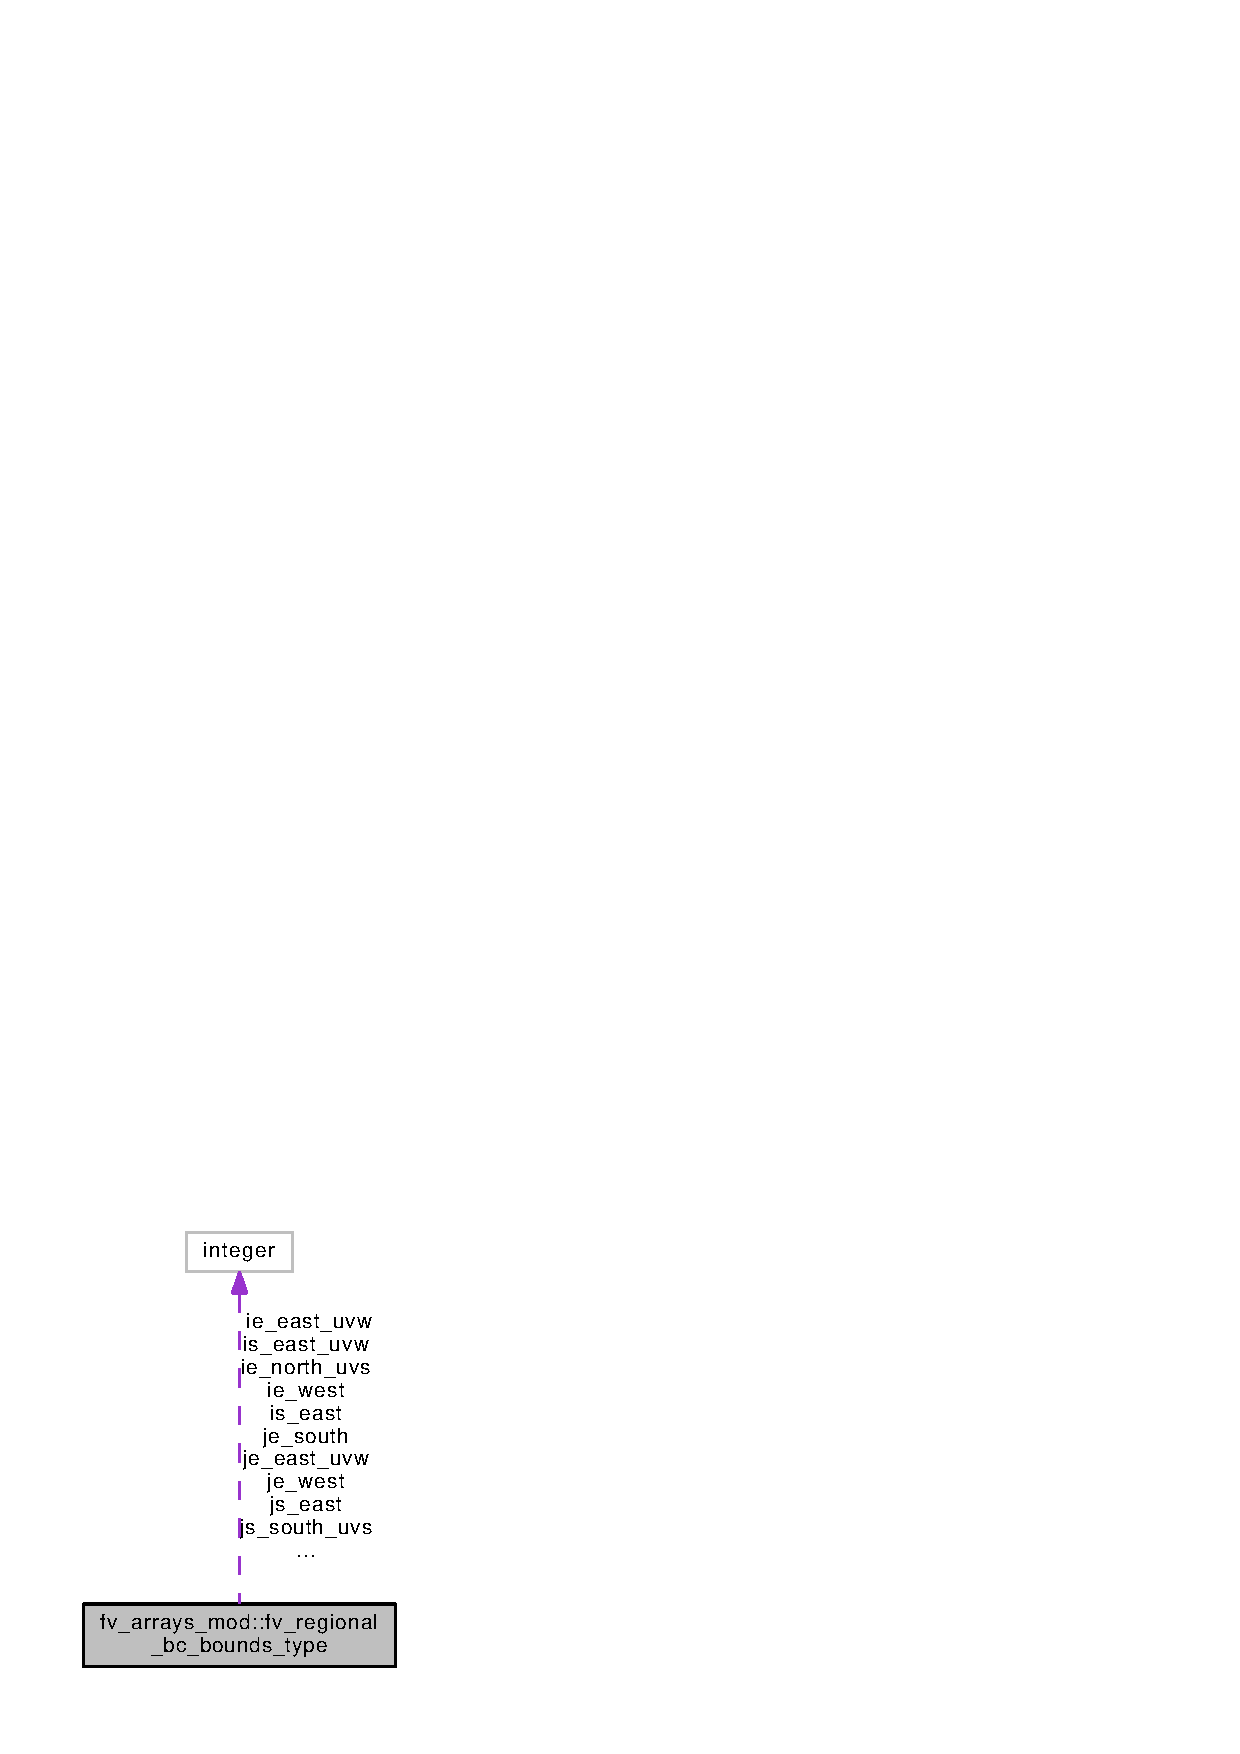
\includegraphics[width=194pt]{structfv__arrays__mod_1_1fv__regional__bc__bounds__type__coll__graph}
\end{center}
\end{figure}
\subsection*{Public Attributes}
\begin{DoxyCompactItemize}
\item 
integer \hyperlink{structfv__arrays__mod_1_1fv__regional__bc__bounds__type_a0f8c09e12e76033c808a3d6deb8b6774}{is\-\_\-north}
\item 
integer \hyperlink{structfv__arrays__mod_1_1fv__regional__bc__bounds__type_ab7c3cb5f65404b6883bbcc83e2bf9e42}{ie\-\_\-north}
\item 
integer \hyperlink{structfv__arrays__mod_1_1fv__regional__bc__bounds__type_a6c1b56a3e80896fc5145e1361807c31d}{js\-\_\-north}
\item 
integer \hyperlink{structfv__arrays__mod_1_1fv__regional__bc__bounds__type_a23a8fdcf24b84b603dab684fc87bb768}{je\-\_\-north}
\item 
integer \hyperlink{structfv__arrays__mod_1_1fv__regional__bc__bounds__type_a1946f18cfc16184c27bd77cad7325287}{is\-\_\-south}
\item 
integer \hyperlink{structfv__arrays__mod_1_1fv__regional__bc__bounds__type_acd8c3828a618efa6f9a7262b36c79148}{ie\-\_\-south}
\item 
integer \hyperlink{structfv__arrays__mod_1_1fv__regional__bc__bounds__type_ad8b75dda59b27edf80fc7ade6aa81153}{js\-\_\-south}
\item 
integer \hyperlink{structfv__arrays__mod_1_1fv__regional__bc__bounds__type_a8c5ab0960754f55008516230a1403e12}{je\-\_\-south}
\item 
integer \hyperlink{structfv__arrays__mod_1_1fv__regional__bc__bounds__type_a510bfddf983d15876a7819ebc3861291}{is\-\_\-east}
\item 
integer \hyperlink{structfv__arrays__mod_1_1fv__regional__bc__bounds__type_a34c26162b5ada53ebb8a5dd38ee6205d}{ie\-\_\-east}
\item 
integer \hyperlink{structfv__arrays__mod_1_1fv__regional__bc__bounds__type_aec5de2eb1fbc49c0ab3301f8a9833d43}{js\-\_\-east}
\item 
integer \hyperlink{structfv__arrays__mod_1_1fv__regional__bc__bounds__type_a0ec3990bb87f0052d6480199a51520d1}{je\-\_\-east}
\item 
integer \hyperlink{structfv__arrays__mod_1_1fv__regional__bc__bounds__type_a3a14693363d3959083d86452ba8f6fd6}{is\-\_\-west}
\item 
integer \hyperlink{structfv__arrays__mod_1_1fv__regional__bc__bounds__type_a9990faf4364132d331d7a763dc5df36c}{ie\-\_\-west}
\item 
integer \hyperlink{structfv__arrays__mod_1_1fv__regional__bc__bounds__type_a5edefeda8e82bfea238b86f43ee848aa}{js\-\_\-west}
\item 
integer \hyperlink{structfv__arrays__mod_1_1fv__regional__bc__bounds__type_a67b3101e7687adaa966d51363e3825ca}{je\-\_\-west}
\item 
integer \hyperlink{structfv__arrays__mod_1_1fv__regional__bc__bounds__type_ad01d2e5a4abb36bdefd1baba66e6fa5a}{is\-\_\-north\-\_\-uvs}
\item 
integer \hyperlink{structfv__arrays__mod_1_1fv__regional__bc__bounds__type_a92c30db417e27a61e717df11818658bd}{ie\-\_\-north\-\_\-uvs}
\item 
integer \hyperlink{structfv__arrays__mod_1_1fv__regional__bc__bounds__type_a2ccde9c69957b83b8a40f5ec5657b2c6}{js\-\_\-north\-\_\-uvs}
\item 
integer \hyperlink{structfv__arrays__mod_1_1fv__regional__bc__bounds__type_a871e2ce163e409b9b9f99ab30e1a5365}{je\-\_\-north\-\_\-uvs}
\item 
integer \hyperlink{structfv__arrays__mod_1_1fv__regional__bc__bounds__type_a4656a392831759d6d5cfd2ff14dd470d}{is\-\_\-south\-\_\-uvs}
\item 
integer \hyperlink{structfv__arrays__mod_1_1fv__regional__bc__bounds__type_a5a22c8f7f0c6a2e342ee5e40d4774bcf}{ie\-\_\-south\-\_\-uvs}
\item 
integer \hyperlink{structfv__arrays__mod_1_1fv__regional__bc__bounds__type_a19a3538a418d6dc20d8f563d6a6b90ff}{js\-\_\-south\-\_\-uvs}
\item 
integer \hyperlink{structfv__arrays__mod_1_1fv__regional__bc__bounds__type_acfee89a51b714eabd8d1e27a49ed5a19}{je\-\_\-south\-\_\-uvs}
\item 
integer \hyperlink{structfv__arrays__mod_1_1fv__regional__bc__bounds__type_afe355478052c9408971c5d3c70750b19}{is\-\_\-east\-\_\-uvs}
\item 
integer \hyperlink{structfv__arrays__mod_1_1fv__regional__bc__bounds__type_a05251f8e73ab82b12c4574264c1b0669}{ie\-\_\-east\-\_\-uvs}
\item 
integer \hyperlink{structfv__arrays__mod_1_1fv__regional__bc__bounds__type_ae946e2a13fc5ba792f4271eba9b884a8}{js\-\_\-east\-\_\-uvs}
\item 
integer \hyperlink{structfv__arrays__mod_1_1fv__regional__bc__bounds__type_a37b6494275e7acb11485a7edf84c5802}{je\-\_\-east\-\_\-uvs}
\item 
integer \hyperlink{structfv__arrays__mod_1_1fv__regional__bc__bounds__type_a7e158eabe3aeed2e739d161d350a1459}{is\-\_\-west\-\_\-uvs}
\item 
integer \hyperlink{structfv__arrays__mod_1_1fv__regional__bc__bounds__type_ac9ca3bbc3e38e522dda9174a606cbcd8}{ie\-\_\-west\-\_\-uvs}
\item 
integer \hyperlink{structfv__arrays__mod_1_1fv__regional__bc__bounds__type_afa59505db0ef56a01c9ece80b6009385}{js\-\_\-west\-\_\-uvs}
\item 
integer \hyperlink{structfv__arrays__mod_1_1fv__regional__bc__bounds__type_adacbc0f3d1b63d64c6971c05ea0e76e8}{je\-\_\-west\-\_\-uvs}
\item 
integer \hyperlink{structfv__arrays__mod_1_1fv__regional__bc__bounds__type_aa8a7deff57fd2ad5e1767d9000d3264a}{is\-\_\-north\-\_\-uvw}
\item 
integer \hyperlink{structfv__arrays__mod_1_1fv__regional__bc__bounds__type_acb084d985b5fd16042a6baeda188b40c}{ie\-\_\-north\-\_\-uvw}
\item 
integer \hyperlink{structfv__arrays__mod_1_1fv__regional__bc__bounds__type_a59e88ee268c05c3d647824a5b919f812}{js\-\_\-north\-\_\-uvw}
\item 
integer \hyperlink{structfv__arrays__mod_1_1fv__regional__bc__bounds__type_a98d5f05086f48d5f8cd189fc88934ce7}{je\-\_\-north\-\_\-uvw}
\item 
integer \hyperlink{structfv__arrays__mod_1_1fv__regional__bc__bounds__type_a50595c6950e0c116407877ded3c1b670}{is\-\_\-south\-\_\-uvw}
\item 
integer \hyperlink{structfv__arrays__mod_1_1fv__regional__bc__bounds__type_a55f7f05c3f12efdbd6548daf35f398d5}{ie\-\_\-south\-\_\-uvw}
\item 
integer \hyperlink{structfv__arrays__mod_1_1fv__regional__bc__bounds__type_acf4f2a35d3038932a155106c5364987b}{js\-\_\-south\-\_\-uvw}
\item 
integer \hyperlink{structfv__arrays__mod_1_1fv__regional__bc__bounds__type_a401f9aa3721ece8ee6e49d36fb0093df}{je\-\_\-south\-\_\-uvw}
\item 
integer \hyperlink{structfv__arrays__mod_1_1fv__regional__bc__bounds__type_a6907b7b6081be6e11d2fed5cbd19da74}{is\-\_\-east\-\_\-uvw}
\item 
integer \hyperlink{structfv__arrays__mod_1_1fv__regional__bc__bounds__type_a9f44ff177e46944e30e13490fb10bb24}{ie\-\_\-east\-\_\-uvw}
\item 
integer \hyperlink{structfv__arrays__mod_1_1fv__regional__bc__bounds__type_a9b84e05fbf550e97f97ba52c218da462}{js\-\_\-east\-\_\-uvw}
\item 
integer \hyperlink{structfv__arrays__mod_1_1fv__regional__bc__bounds__type_adab9a935741f0acc6616df8dd09d4f17}{je\-\_\-east\-\_\-uvw}
\item 
integer \hyperlink{structfv__arrays__mod_1_1fv__regional__bc__bounds__type_ac2deaff88f899b9dbee780db2f70877a}{is\-\_\-west\-\_\-uvw}
\item 
integer \hyperlink{structfv__arrays__mod_1_1fv__regional__bc__bounds__type_a04bb7bab42d4d800e83e0516dd157373}{ie\-\_\-west\-\_\-uvw}
\item 
integer \hyperlink{structfv__arrays__mod_1_1fv__regional__bc__bounds__type_a05f07532dd5f7a68570bf69658d4fee8}{js\-\_\-west\-\_\-uvw}
\item 
integer \hyperlink{structfv__arrays__mod_1_1fv__regional__bc__bounds__type_a85e3d9364559211708e4e15f74ea1311}{je\-\_\-west\-\_\-uvw}
\end{DoxyCompactItemize}


\subsection{Detailed Description}


Definition at line 1147 of file fv\-\_\-arrays.\-F90.



\subsection{Member Data Documentation}
\index{fv\-\_\-arrays\-\_\-mod\-::fv\-\_\-regional\-\_\-bc\-\_\-bounds\-\_\-type@{fv\-\_\-arrays\-\_\-mod\-::fv\-\_\-regional\-\_\-bc\-\_\-bounds\-\_\-type}!ie\-\_\-east@{ie\-\_\-east}}
\index{ie\-\_\-east@{ie\-\_\-east}!fv_arrays_mod::fv_regional_bc_bounds_type@{fv\-\_\-arrays\-\_\-mod\-::fv\-\_\-regional\-\_\-bc\-\_\-bounds\-\_\-type}}
\subsubsection[{ie\-\_\-east}]{\setlength{\rightskip}{0pt plus 5cm}integer fv\-\_\-arrays\-\_\-mod\-::fv\-\_\-regional\-\_\-bc\-\_\-bounds\-\_\-type\-::ie\-\_\-east}\label{structfv__arrays__mod_1_1fv__regional__bc__bounds__type_a34c26162b5ada53ebb8a5dd38ee6205d}


Definition at line 1149 of file fv\-\_\-arrays.\-F90.

\index{fv\-\_\-arrays\-\_\-mod\-::fv\-\_\-regional\-\_\-bc\-\_\-bounds\-\_\-type@{fv\-\_\-arrays\-\_\-mod\-::fv\-\_\-regional\-\_\-bc\-\_\-bounds\-\_\-type}!ie\-\_\-east\-\_\-uvs@{ie\-\_\-east\-\_\-uvs}}
\index{ie\-\_\-east\-\_\-uvs@{ie\-\_\-east\-\_\-uvs}!fv_arrays_mod::fv_regional_bc_bounds_type@{fv\-\_\-arrays\-\_\-mod\-::fv\-\_\-regional\-\_\-bc\-\_\-bounds\-\_\-type}}
\subsubsection[{ie\-\_\-east\-\_\-uvs}]{\setlength{\rightskip}{0pt plus 5cm}integer fv\-\_\-arrays\-\_\-mod\-::fv\-\_\-regional\-\_\-bc\-\_\-bounds\-\_\-type\-::ie\-\_\-east\-\_\-uvs}\label{structfv__arrays__mod_1_1fv__regional__bc__bounds__type_a05251f8e73ab82b12c4574264c1b0669}


Definition at line 1154 of file fv\-\_\-arrays.\-F90.

\index{fv\-\_\-arrays\-\_\-mod\-::fv\-\_\-regional\-\_\-bc\-\_\-bounds\-\_\-type@{fv\-\_\-arrays\-\_\-mod\-::fv\-\_\-regional\-\_\-bc\-\_\-bounds\-\_\-type}!ie\-\_\-east\-\_\-uvw@{ie\-\_\-east\-\_\-uvw}}
\index{ie\-\_\-east\-\_\-uvw@{ie\-\_\-east\-\_\-uvw}!fv_arrays_mod::fv_regional_bc_bounds_type@{fv\-\_\-arrays\-\_\-mod\-::fv\-\_\-regional\-\_\-bc\-\_\-bounds\-\_\-type}}
\subsubsection[{ie\-\_\-east\-\_\-uvw}]{\setlength{\rightskip}{0pt plus 5cm}integer fv\-\_\-arrays\-\_\-mod\-::fv\-\_\-regional\-\_\-bc\-\_\-bounds\-\_\-type\-::ie\-\_\-east\-\_\-uvw}\label{structfv__arrays__mod_1_1fv__regional__bc__bounds__type_a9f44ff177e46944e30e13490fb10bb24}


Definition at line 1159 of file fv\-\_\-arrays.\-F90.

\index{fv\-\_\-arrays\-\_\-mod\-::fv\-\_\-regional\-\_\-bc\-\_\-bounds\-\_\-type@{fv\-\_\-arrays\-\_\-mod\-::fv\-\_\-regional\-\_\-bc\-\_\-bounds\-\_\-type}!ie\-\_\-north@{ie\-\_\-north}}
\index{ie\-\_\-north@{ie\-\_\-north}!fv_arrays_mod::fv_regional_bc_bounds_type@{fv\-\_\-arrays\-\_\-mod\-::fv\-\_\-regional\-\_\-bc\-\_\-bounds\-\_\-type}}
\subsubsection[{ie\-\_\-north}]{\setlength{\rightskip}{0pt plus 5cm}integer fv\-\_\-arrays\-\_\-mod\-::fv\-\_\-regional\-\_\-bc\-\_\-bounds\-\_\-type\-::ie\-\_\-north}\label{structfv__arrays__mod_1_1fv__regional__bc__bounds__type_ab7c3cb5f65404b6883bbcc83e2bf9e42}


Definition at line 1149 of file fv\-\_\-arrays.\-F90.

\index{fv\-\_\-arrays\-\_\-mod\-::fv\-\_\-regional\-\_\-bc\-\_\-bounds\-\_\-type@{fv\-\_\-arrays\-\_\-mod\-::fv\-\_\-regional\-\_\-bc\-\_\-bounds\-\_\-type}!ie\-\_\-north\-\_\-uvs@{ie\-\_\-north\-\_\-uvs}}
\index{ie\-\_\-north\-\_\-uvs@{ie\-\_\-north\-\_\-uvs}!fv_arrays_mod::fv_regional_bc_bounds_type@{fv\-\_\-arrays\-\_\-mod\-::fv\-\_\-regional\-\_\-bc\-\_\-bounds\-\_\-type}}
\subsubsection[{ie\-\_\-north\-\_\-uvs}]{\setlength{\rightskip}{0pt plus 5cm}integer fv\-\_\-arrays\-\_\-mod\-::fv\-\_\-regional\-\_\-bc\-\_\-bounds\-\_\-type\-::ie\-\_\-north\-\_\-uvs}\label{structfv__arrays__mod_1_1fv__regional__bc__bounds__type_a92c30db417e27a61e717df11818658bd}


Definition at line 1154 of file fv\-\_\-arrays.\-F90.

\index{fv\-\_\-arrays\-\_\-mod\-::fv\-\_\-regional\-\_\-bc\-\_\-bounds\-\_\-type@{fv\-\_\-arrays\-\_\-mod\-::fv\-\_\-regional\-\_\-bc\-\_\-bounds\-\_\-type}!ie\-\_\-north\-\_\-uvw@{ie\-\_\-north\-\_\-uvw}}
\index{ie\-\_\-north\-\_\-uvw@{ie\-\_\-north\-\_\-uvw}!fv_arrays_mod::fv_regional_bc_bounds_type@{fv\-\_\-arrays\-\_\-mod\-::fv\-\_\-regional\-\_\-bc\-\_\-bounds\-\_\-type}}
\subsubsection[{ie\-\_\-north\-\_\-uvw}]{\setlength{\rightskip}{0pt plus 5cm}integer fv\-\_\-arrays\-\_\-mod\-::fv\-\_\-regional\-\_\-bc\-\_\-bounds\-\_\-type\-::ie\-\_\-north\-\_\-uvw}\label{structfv__arrays__mod_1_1fv__regional__bc__bounds__type_acb084d985b5fd16042a6baeda188b40c}


Definition at line 1159 of file fv\-\_\-arrays.\-F90.

\index{fv\-\_\-arrays\-\_\-mod\-::fv\-\_\-regional\-\_\-bc\-\_\-bounds\-\_\-type@{fv\-\_\-arrays\-\_\-mod\-::fv\-\_\-regional\-\_\-bc\-\_\-bounds\-\_\-type}!ie\-\_\-south@{ie\-\_\-south}}
\index{ie\-\_\-south@{ie\-\_\-south}!fv_arrays_mod::fv_regional_bc_bounds_type@{fv\-\_\-arrays\-\_\-mod\-::fv\-\_\-regional\-\_\-bc\-\_\-bounds\-\_\-type}}
\subsubsection[{ie\-\_\-south}]{\setlength{\rightskip}{0pt plus 5cm}integer fv\-\_\-arrays\-\_\-mod\-::fv\-\_\-regional\-\_\-bc\-\_\-bounds\-\_\-type\-::ie\-\_\-south}\label{structfv__arrays__mod_1_1fv__regional__bc__bounds__type_acd8c3828a618efa6f9a7262b36c79148}


Definition at line 1149 of file fv\-\_\-arrays.\-F90.

\index{fv\-\_\-arrays\-\_\-mod\-::fv\-\_\-regional\-\_\-bc\-\_\-bounds\-\_\-type@{fv\-\_\-arrays\-\_\-mod\-::fv\-\_\-regional\-\_\-bc\-\_\-bounds\-\_\-type}!ie\-\_\-south\-\_\-uvs@{ie\-\_\-south\-\_\-uvs}}
\index{ie\-\_\-south\-\_\-uvs@{ie\-\_\-south\-\_\-uvs}!fv_arrays_mod::fv_regional_bc_bounds_type@{fv\-\_\-arrays\-\_\-mod\-::fv\-\_\-regional\-\_\-bc\-\_\-bounds\-\_\-type}}
\subsubsection[{ie\-\_\-south\-\_\-uvs}]{\setlength{\rightskip}{0pt plus 5cm}integer fv\-\_\-arrays\-\_\-mod\-::fv\-\_\-regional\-\_\-bc\-\_\-bounds\-\_\-type\-::ie\-\_\-south\-\_\-uvs}\label{structfv__arrays__mod_1_1fv__regional__bc__bounds__type_a5a22c8f7f0c6a2e342ee5e40d4774bcf}


Definition at line 1154 of file fv\-\_\-arrays.\-F90.

\index{fv\-\_\-arrays\-\_\-mod\-::fv\-\_\-regional\-\_\-bc\-\_\-bounds\-\_\-type@{fv\-\_\-arrays\-\_\-mod\-::fv\-\_\-regional\-\_\-bc\-\_\-bounds\-\_\-type}!ie\-\_\-south\-\_\-uvw@{ie\-\_\-south\-\_\-uvw}}
\index{ie\-\_\-south\-\_\-uvw@{ie\-\_\-south\-\_\-uvw}!fv_arrays_mod::fv_regional_bc_bounds_type@{fv\-\_\-arrays\-\_\-mod\-::fv\-\_\-regional\-\_\-bc\-\_\-bounds\-\_\-type}}
\subsubsection[{ie\-\_\-south\-\_\-uvw}]{\setlength{\rightskip}{0pt plus 5cm}integer fv\-\_\-arrays\-\_\-mod\-::fv\-\_\-regional\-\_\-bc\-\_\-bounds\-\_\-type\-::ie\-\_\-south\-\_\-uvw}\label{structfv__arrays__mod_1_1fv__regional__bc__bounds__type_a55f7f05c3f12efdbd6548daf35f398d5}


Definition at line 1159 of file fv\-\_\-arrays.\-F90.

\index{fv\-\_\-arrays\-\_\-mod\-::fv\-\_\-regional\-\_\-bc\-\_\-bounds\-\_\-type@{fv\-\_\-arrays\-\_\-mod\-::fv\-\_\-regional\-\_\-bc\-\_\-bounds\-\_\-type}!ie\-\_\-west@{ie\-\_\-west}}
\index{ie\-\_\-west@{ie\-\_\-west}!fv_arrays_mod::fv_regional_bc_bounds_type@{fv\-\_\-arrays\-\_\-mod\-::fv\-\_\-regional\-\_\-bc\-\_\-bounds\-\_\-type}}
\subsubsection[{ie\-\_\-west}]{\setlength{\rightskip}{0pt plus 5cm}integer fv\-\_\-arrays\-\_\-mod\-::fv\-\_\-regional\-\_\-bc\-\_\-bounds\-\_\-type\-::ie\-\_\-west}\label{structfv__arrays__mod_1_1fv__regional__bc__bounds__type_a9990faf4364132d331d7a763dc5df36c}


Definition at line 1149 of file fv\-\_\-arrays.\-F90.

\index{fv\-\_\-arrays\-\_\-mod\-::fv\-\_\-regional\-\_\-bc\-\_\-bounds\-\_\-type@{fv\-\_\-arrays\-\_\-mod\-::fv\-\_\-regional\-\_\-bc\-\_\-bounds\-\_\-type}!ie\-\_\-west\-\_\-uvs@{ie\-\_\-west\-\_\-uvs}}
\index{ie\-\_\-west\-\_\-uvs@{ie\-\_\-west\-\_\-uvs}!fv_arrays_mod::fv_regional_bc_bounds_type@{fv\-\_\-arrays\-\_\-mod\-::fv\-\_\-regional\-\_\-bc\-\_\-bounds\-\_\-type}}
\subsubsection[{ie\-\_\-west\-\_\-uvs}]{\setlength{\rightskip}{0pt plus 5cm}integer fv\-\_\-arrays\-\_\-mod\-::fv\-\_\-regional\-\_\-bc\-\_\-bounds\-\_\-type\-::ie\-\_\-west\-\_\-uvs}\label{structfv__arrays__mod_1_1fv__regional__bc__bounds__type_ac9ca3bbc3e38e522dda9174a606cbcd8}


Definition at line 1154 of file fv\-\_\-arrays.\-F90.

\index{fv\-\_\-arrays\-\_\-mod\-::fv\-\_\-regional\-\_\-bc\-\_\-bounds\-\_\-type@{fv\-\_\-arrays\-\_\-mod\-::fv\-\_\-regional\-\_\-bc\-\_\-bounds\-\_\-type}!ie\-\_\-west\-\_\-uvw@{ie\-\_\-west\-\_\-uvw}}
\index{ie\-\_\-west\-\_\-uvw@{ie\-\_\-west\-\_\-uvw}!fv_arrays_mod::fv_regional_bc_bounds_type@{fv\-\_\-arrays\-\_\-mod\-::fv\-\_\-regional\-\_\-bc\-\_\-bounds\-\_\-type}}
\subsubsection[{ie\-\_\-west\-\_\-uvw}]{\setlength{\rightskip}{0pt plus 5cm}integer fv\-\_\-arrays\-\_\-mod\-::fv\-\_\-regional\-\_\-bc\-\_\-bounds\-\_\-type\-::ie\-\_\-west\-\_\-uvw}\label{structfv__arrays__mod_1_1fv__regional__bc__bounds__type_a04bb7bab42d4d800e83e0516dd157373}


Definition at line 1159 of file fv\-\_\-arrays.\-F90.

\index{fv\-\_\-arrays\-\_\-mod\-::fv\-\_\-regional\-\_\-bc\-\_\-bounds\-\_\-type@{fv\-\_\-arrays\-\_\-mod\-::fv\-\_\-regional\-\_\-bc\-\_\-bounds\-\_\-type}!is\-\_\-east@{is\-\_\-east}}
\index{is\-\_\-east@{is\-\_\-east}!fv_arrays_mod::fv_regional_bc_bounds_type@{fv\-\_\-arrays\-\_\-mod\-::fv\-\_\-regional\-\_\-bc\-\_\-bounds\-\_\-type}}
\subsubsection[{is\-\_\-east}]{\setlength{\rightskip}{0pt plus 5cm}integer fv\-\_\-arrays\-\_\-mod\-::fv\-\_\-regional\-\_\-bc\-\_\-bounds\-\_\-type\-::is\-\_\-east}\label{structfv__arrays__mod_1_1fv__regional__bc__bounds__type_a510bfddf983d15876a7819ebc3861291}


Definition at line 1149 of file fv\-\_\-arrays.\-F90.

\index{fv\-\_\-arrays\-\_\-mod\-::fv\-\_\-regional\-\_\-bc\-\_\-bounds\-\_\-type@{fv\-\_\-arrays\-\_\-mod\-::fv\-\_\-regional\-\_\-bc\-\_\-bounds\-\_\-type}!is\-\_\-east\-\_\-uvs@{is\-\_\-east\-\_\-uvs}}
\index{is\-\_\-east\-\_\-uvs@{is\-\_\-east\-\_\-uvs}!fv_arrays_mod::fv_regional_bc_bounds_type@{fv\-\_\-arrays\-\_\-mod\-::fv\-\_\-regional\-\_\-bc\-\_\-bounds\-\_\-type}}
\subsubsection[{is\-\_\-east\-\_\-uvs}]{\setlength{\rightskip}{0pt plus 5cm}integer fv\-\_\-arrays\-\_\-mod\-::fv\-\_\-regional\-\_\-bc\-\_\-bounds\-\_\-type\-::is\-\_\-east\-\_\-uvs}\label{structfv__arrays__mod_1_1fv__regional__bc__bounds__type_afe355478052c9408971c5d3c70750b19}


Definition at line 1154 of file fv\-\_\-arrays.\-F90.

\index{fv\-\_\-arrays\-\_\-mod\-::fv\-\_\-regional\-\_\-bc\-\_\-bounds\-\_\-type@{fv\-\_\-arrays\-\_\-mod\-::fv\-\_\-regional\-\_\-bc\-\_\-bounds\-\_\-type}!is\-\_\-east\-\_\-uvw@{is\-\_\-east\-\_\-uvw}}
\index{is\-\_\-east\-\_\-uvw@{is\-\_\-east\-\_\-uvw}!fv_arrays_mod::fv_regional_bc_bounds_type@{fv\-\_\-arrays\-\_\-mod\-::fv\-\_\-regional\-\_\-bc\-\_\-bounds\-\_\-type}}
\subsubsection[{is\-\_\-east\-\_\-uvw}]{\setlength{\rightskip}{0pt plus 5cm}integer fv\-\_\-arrays\-\_\-mod\-::fv\-\_\-regional\-\_\-bc\-\_\-bounds\-\_\-type\-::is\-\_\-east\-\_\-uvw}\label{structfv__arrays__mod_1_1fv__regional__bc__bounds__type_a6907b7b6081be6e11d2fed5cbd19da74}


Definition at line 1159 of file fv\-\_\-arrays.\-F90.

\index{fv\-\_\-arrays\-\_\-mod\-::fv\-\_\-regional\-\_\-bc\-\_\-bounds\-\_\-type@{fv\-\_\-arrays\-\_\-mod\-::fv\-\_\-regional\-\_\-bc\-\_\-bounds\-\_\-type}!is\-\_\-north@{is\-\_\-north}}
\index{is\-\_\-north@{is\-\_\-north}!fv_arrays_mod::fv_regional_bc_bounds_type@{fv\-\_\-arrays\-\_\-mod\-::fv\-\_\-regional\-\_\-bc\-\_\-bounds\-\_\-type}}
\subsubsection[{is\-\_\-north}]{\setlength{\rightskip}{0pt plus 5cm}integer fv\-\_\-arrays\-\_\-mod\-::fv\-\_\-regional\-\_\-bc\-\_\-bounds\-\_\-type\-::is\-\_\-north}\label{structfv__arrays__mod_1_1fv__regional__bc__bounds__type_a0f8c09e12e76033c808a3d6deb8b6774}


Definition at line 1149 of file fv\-\_\-arrays.\-F90.

\index{fv\-\_\-arrays\-\_\-mod\-::fv\-\_\-regional\-\_\-bc\-\_\-bounds\-\_\-type@{fv\-\_\-arrays\-\_\-mod\-::fv\-\_\-regional\-\_\-bc\-\_\-bounds\-\_\-type}!is\-\_\-north\-\_\-uvs@{is\-\_\-north\-\_\-uvs}}
\index{is\-\_\-north\-\_\-uvs@{is\-\_\-north\-\_\-uvs}!fv_arrays_mod::fv_regional_bc_bounds_type@{fv\-\_\-arrays\-\_\-mod\-::fv\-\_\-regional\-\_\-bc\-\_\-bounds\-\_\-type}}
\subsubsection[{is\-\_\-north\-\_\-uvs}]{\setlength{\rightskip}{0pt plus 5cm}integer fv\-\_\-arrays\-\_\-mod\-::fv\-\_\-regional\-\_\-bc\-\_\-bounds\-\_\-type\-::is\-\_\-north\-\_\-uvs}\label{structfv__arrays__mod_1_1fv__regional__bc__bounds__type_ad01d2e5a4abb36bdefd1baba66e6fa5a}


Definition at line 1154 of file fv\-\_\-arrays.\-F90.

\index{fv\-\_\-arrays\-\_\-mod\-::fv\-\_\-regional\-\_\-bc\-\_\-bounds\-\_\-type@{fv\-\_\-arrays\-\_\-mod\-::fv\-\_\-regional\-\_\-bc\-\_\-bounds\-\_\-type}!is\-\_\-north\-\_\-uvw@{is\-\_\-north\-\_\-uvw}}
\index{is\-\_\-north\-\_\-uvw@{is\-\_\-north\-\_\-uvw}!fv_arrays_mod::fv_regional_bc_bounds_type@{fv\-\_\-arrays\-\_\-mod\-::fv\-\_\-regional\-\_\-bc\-\_\-bounds\-\_\-type}}
\subsubsection[{is\-\_\-north\-\_\-uvw}]{\setlength{\rightskip}{0pt plus 5cm}integer fv\-\_\-arrays\-\_\-mod\-::fv\-\_\-regional\-\_\-bc\-\_\-bounds\-\_\-type\-::is\-\_\-north\-\_\-uvw}\label{structfv__arrays__mod_1_1fv__regional__bc__bounds__type_aa8a7deff57fd2ad5e1767d9000d3264a}


Definition at line 1159 of file fv\-\_\-arrays.\-F90.

\index{fv\-\_\-arrays\-\_\-mod\-::fv\-\_\-regional\-\_\-bc\-\_\-bounds\-\_\-type@{fv\-\_\-arrays\-\_\-mod\-::fv\-\_\-regional\-\_\-bc\-\_\-bounds\-\_\-type}!is\-\_\-south@{is\-\_\-south}}
\index{is\-\_\-south@{is\-\_\-south}!fv_arrays_mod::fv_regional_bc_bounds_type@{fv\-\_\-arrays\-\_\-mod\-::fv\-\_\-regional\-\_\-bc\-\_\-bounds\-\_\-type}}
\subsubsection[{is\-\_\-south}]{\setlength{\rightskip}{0pt plus 5cm}integer fv\-\_\-arrays\-\_\-mod\-::fv\-\_\-regional\-\_\-bc\-\_\-bounds\-\_\-type\-::is\-\_\-south}\label{structfv__arrays__mod_1_1fv__regional__bc__bounds__type_a1946f18cfc16184c27bd77cad7325287}


Definition at line 1149 of file fv\-\_\-arrays.\-F90.

\index{fv\-\_\-arrays\-\_\-mod\-::fv\-\_\-regional\-\_\-bc\-\_\-bounds\-\_\-type@{fv\-\_\-arrays\-\_\-mod\-::fv\-\_\-regional\-\_\-bc\-\_\-bounds\-\_\-type}!is\-\_\-south\-\_\-uvs@{is\-\_\-south\-\_\-uvs}}
\index{is\-\_\-south\-\_\-uvs@{is\-\_\-south\-\_\-uvs}!fv_arrays_mod::fv_regional_bc_bounds_type@{fv\-\_\-arrays\-\_\-mod\-::fv\-\_\-regional\-\_\-bc\-\_\-bounds\-\_\-type}}
\subsubsection[{is\-\_\-south\-\_\-uvs}]{\setlength{\rightskip}{0pt plus 5cm}integer fv\-\_\-arrays\-\_\-mod\-::fv\-\_\-regional\-\_\-bc\-\_\-bounds\-\_\-type\-::is\-\_\-south\-\_\-uvs}\label{structfv__arrays__mod_1_1fv__regional__bc__bounds__type_a4656a392831759d6d5cfd2ff14dd470d}


Definition at line 1154 of file fv\-\_\-arrays.\-F90.

\index{fv\-\_\-arrays\-\_\-mod\-::fv\-\_\-regional\-\_\-bc\-\_\-bounds\-\_\-type@{fv\-\_\-arrays\-\_\-mod\-::fv\-\_\-regional\-\_\-bc\-\_\-bounds\-\_\-type}!is\-\_\-south\-\_\-uvw@{is\-\_\-south\-\_\-uvw}}
\index{is\-\_\-south\-\_\-uvw@{is\-\_\-south\-\_\-uvw}!fv_arrays_mod::fv_regional_bc_bounds_type@{fv\-\_\-arrays\-\_\-mod\-::fv\-\_\-regional\-\_\-bc\-\_\-bounds\-\_\-type}}
\subsubsection[{is\-\_\-south\-\_\-uvw}]{\setlength{\rightskip}{0pt plus 5cm}integer fv\-\_\-arrays\-\_\-mod\-::fv\-\_\-regional\-\_\-bc\-\_\-bounds\-\_\-type\-::is\-\_\-south\-\_\-uvw}\label{structfv__arrays__mod_1_1fv__regional__bc__bounds__type_a50595c6950e0c116407877ded3c1b670}


Definition at line 1159 of file fv\-\_\-arrays.\-F90.

\index{fv\-\_\-arrays\-\_\-mod\-::fv\-\_\-regional\-\_\-bc\-\_\-bounds\-\_\-type@{fv\-\_\-arrays\-\_\-mod\-::fv\-\_\-regional\-\_\-bc\-\_\-bounds\-\_\-type}!is\-\_\-west@{is\-\_\-west}}
\index{is\-\_\-west@{is\-\_\-west}!fv_arrays_mod::fv_regional_bc_bounds_type@{fv\-\_\-arrays\-\_\-mod\-::fv\-\_\-regional\-\_\-bc\-\_\-bounds\-\_\-type}}
\subsubsection[{is\-\_\-west}]{\setlength{\rightskip}{0pt plus 5cm}integer fv\-\_\-arrays\-\_\-mod\-::fv\-\_\-regional\-\_\-bc\-\_\-bounds\-\_\-type\-::is\-\_\-west}\label{structfv__arrays__mod_1_1fv__regional__bc__bounds__type_a3a14693363d3959083d86452ba8f6fd6}


Definition at line 1149 of file fv\-\_\-arrays.\-F90.

\index{fv\-\_\-arrays\-\_\-mod\-::fv\-\_\-regional\-\_\-bc\-\_\-bounds\-\_\-type@{fv\-\_\-arrays\-\_\-mod\-::fv\-\_\-regional\-\_\-bc\-\_\-bounds\-\_\-type}!is\-\_\-west\-\_\-uvs@{is\-\_\-west\-\_\-uvs}}
\index{is\-\_\-west\-\_\-uvs@{is\-\_\-west\-\_\-uvs}!fv_arrays_mod::fv_regional_bc_bounds_type@{fv\-\_\-arrays\-\_\-mod\-::fv\-\_\-regional\-\_\-bc\-\_\-bounds\-\_\-type}}
\subsubsection[{is\-\_\-west\-\_\-uvs}]{\setlength{\rightskip}{0pt plus 5cm}integer fv\-\_\-arrays\-\_\-mod\-::fv\-\_\-regional\-\_\-bc\-\_\-bounds\-\_\-type\-::is\-\_\-west\-\_\-uvs}\label{structfv__arrays__mod_1_1fv__regional__bc__bounds__type_a7e158eabe3aeed2e739d161d350a1459}


Definition at line 1154 of file fv\-\_\-arrays.\-F90.

\index{fv\-\_\-arrays\-\_\-mod\-::fv\-\_\-regional\-\_\-bc\-\_\-bounds\-\_\-type@{fv\-\_\-arrays\-\_\-mod\-::fv\-\_\-regional\-\_\-bc\-\_\-bounds\-\_\-type}!is\-\_\-west\-\_\-uvw@{is\-\_\-west\-\_\-uvw}}
\index{is\-\_\-west\-\_\-uvw@{is\-\_\-west\-\_\-uvw}!fv_arrays_mod::fv_regional_bc_bounds_type@{fv\-\_\-arrays\-\_\-mod\-::fv\-\_\-regional\-\_\-bc\-\_\-bounds\-\_\-type}}
\subsubsection[{is\-\_\-west\-\_\-uvw}]{\setlength{\rightskip}{0pt plus 5cm}integer fv\-\_\-arrays\-\_\-mod\-::fv\-\_\-regional\-\_\-bc\-\_\-bounds\-\_\-type\-::is\-\_\-west\-\_\-uvw}\label{structfv__arrays__mod_1_1fv__regional__bc__bounds__type_ac2deaff88f899b9dbee780db2f70877a}


Definition at line 1159 of file fv\-\_\-arrays.\-F90.

\index{fv\-\_\-arrays\-\_\-mod\-::fv\-\_\-regional\-\_\-bc\-\_\-bounds\-\_\-type@{fv\-\_\-arrays\-\_\-mod\-::fv\-\_\-regional\-\_\-bc\-\_\-bounds\-\_\-type}!je\-\_\-east@{je\-\_\-east}}
\index{je\-\_\-east@{je\-\_\-east}!fv_arrays_mod::fv_regional_bc_bounds_type@{fv\-\_\-arrays\-\_\-mod\-::fv\-\_\-regional\-\_\-bc\-\_\-bounds\-\_\-type}}
\subsubsection[{je\-\_\-east}]{\setlength{\rightskip}{0pt plus 5cm}integer fv\-\_\-arrays\-\_\-mod\-::fv\-\_\-regional\-\_\-bc\-\_\-bounds\-\_\-type\-::je\-\_\-east}\label{structfv__arrays__mod_1_1fv__regional__bc__bounds__type_a0ec3990bb87f0052d6480199a51520d1}


Definition at line 1149 of file fv\-\_\-arrays.\-F90.

\index{fv\-\_\-arrays\-\_\-mod\-::fv\-\_\-regional\-\_\-bc\-\_\-bounds\-\_\-type@{fv\-\_\-arrays\-\_\-mod\-::fv\-\_\-regional\-\_\-bc\-\_\-bounds\-\_\-type}!je\-\_\-east\-\_\-uvs@{je\-\_\-east\-\_\-uvs}}
\index{je\-\_\-east\-\_\-uvs@{je\-\_\-east\-\_\-uvs}!fv_arrays_mod::fv_regional_bc_bounds_type@{fv\-\_\-arrays\-\_\-mod\-::fv\-\_\-regional\-\_\-bc\-\_\-bounds\-\_\-type}}
\subsubsection[{je\-\_\-east\-\_\-uvs}]{\setlength{\rightskip}{0pt plus 5cm}integer fv\-\_\-arrays\-\_\-mod\-::fv\-\_\-regional\-\_\-bc\-\_\-bounds\-\_\-type\-::je\-\_\-east\-\_\-uvs}\label{structfv__arrays__mod_1_1fv__regional__bc__bounds__type_a37b6494275e7acb11485a7edf84c5802}


Definition at line 1154 of file fv\-\_\-arrays.\-F90.

\index{fv\-\_\-arrays\-\_\-mod\-::fv\-\_\-regional\-\_\-bc\-\_\-bounds\-\_\-type@{fv\-\_\-arrays\-\_\-mod\-::fv\-\_\-regional\-\_\-bc\-\_\-bounds\-\_\-type}!je\-\_\-east\-\_\-uvw@{je\-\_\-east\-\_\-uvw}}
\index{je\-\_\-east\-\_\-uvw@{je\-\_\-east\-\_\-uvw}!fv_arrays_mod::fv_regional_bc_bounds_type@{fv\-\_\-arrays\-\_\-mod\-::fv\-\_\-regional\-\_\-bc\-\_\-bounds\-\_\-type}}
\subsubsection[{je\-\_\-east\-\_\-uvw}]{\setlength{\rightskip}{0pt plus 5cm}integer fv\-\_\-arrays\-\_\-mod\-::fv\-\_\-regional\-\_\-bc\-\_\-bounds\-\_\-type\-::je\-\_\-east\-\_\-uvw}\label{structfv__arrays__mod_1_1fv__regional__bc__bounds__type_adab9a935741f0acc6616df8dd09d4f17}


Definition at line 1159 of file fv\-\_\-arrays.\-F90.

\index{fv\-\_\-arrays\-\_\-mod\-::fv\-\_\-regional\-\_\-bc\-\_\-bounds\-\_\-type@{fv\-\_\-arrays\-\_\-mod\-::fv\-\_\-regional\-\_\-bc\-\_\-bounds\-\_\-type}!je\-\_\-north@{je\-\_\-north}}
\index{je\-\_\-north@{je\-\_\-north}!fv_arrays_mod::fv_regional_bc_bounds_type@{fv\-\_\-arrays\-\_\-mod\-::fv\-\_\-regional\-\_\-bc\-\_\-bounds\-\_\-type}}
\subsubsection[{je\-\_\-north}]{\setlength{\rightskip}{0pt plus 5cm}integer fv\-\_\-arrays\-\_\-mod\-::fv\-\_\-regional\-\_\-bc\-\_\-bounds\-\_\-type\-::je\-\_\-north}\label{structfv__arrays__mod_1_1fv__regional__bc__bounds__type_a23a8fdcf24b84b603dab684fc87bb768}


Definition at line 1149 of file fv\-\_\-arrays.\-F90.

\index{fv\-\_\-arrays\-\_\-mod\-::fv\-\_\-regional\-\_\-bc\-\_\-bounds\-\_\-type@{fv\-\_\-arrays\-\_\-mod\-::fv\-\_\-regional\-\_\-bc\-\_\-bounds\-\_\-type}!je\-\_\-north\-\_\-uvs@{je\-\_\-north\-\_\-uvs}}
\index{je\-\_\-north\-\_\-uvs@{je\-\_\-north\-\_\-uvs}!fv_arrays_mod::fv_regional_bc_bounds_type@{fv\-\_\-arrays\-\_\-mod\-::fv\-\_\-regional\-\_\-bc\-\_\-bounds\-\_\-type}}
\subsubsection[{je\-\_\-north\-\_\-uvs}]{\setlength{\rightskip}{0pt plus 5cm}integer fv\-\_\-arrays\-\_\-mod\-::fv\-\_\-regional\-\_\-bc\-\_\-bounds\-\_\-type\-::je\-\_\-north\-\_\-uvs}\label{structfv__arrays__mod_1_1fv__regional__bc__bounds__type_a871e2ce163e409b9b9f99ab30e1a5365}


Definition at line 1154 of file fv\-\_\-arrays.\-F90.

\index{fv\-\_\-arrays\-\_\-mod\-::fv\-\_\-regional\-\_\-bc\-\_\-bounds\-\_\-type@{fv\-\_\-arrays\-\_\-mod\-::fv\-\_\-regional\-\_\-bc\-\_\-bounds\-\_\-type}!je\-\_\-north\-\_\-uvw@{je\-\_\-north\-\_\-uvw}}
\index{je\-\_\-north\-\_\-uvw@{je\-\_\-north\-\_\-uvw}!fv_arrays_mod::fv_regional_bc_bounds_type@{fv\-\_\-arrays\-\_\-mod\-::fv\-\_\-regional\-\_\-bc\-\_\-bounds\-\_\-type}}
\subsubsection[{je\-\_\-north\-\_\-uvw}]{\setlength{\rightskip}{0pt plus 5cm}integer fv\-\_\-arrays\-\_\-mod\-::fv\-\_\-regional\-\_\-bc\-\_\-bounds\-\_\-type\-::je\-\_\-north\-\_\-uvw}\label{structfv__arrays__mod_1_1fv__regional__bc__bounds__type_a98d5f05086f48d5f8cd189fc88934ce7}


Definition at line 1159 of file fv\-\_\-arrays.\-F90.

\index{fv\-\_\-arrays\-\_\-mod\-::fv\-\_\-regional\-\_\-bc\-\_\-bounds\-\_\-type@{fv\-\_\-arrays\-\_\-mod\-::fv\-\_\-regional\-\_\-bc\-\_\-bounds\-\_\-type}!je\-\_\-south@{je\-\_\-south}}
\index{je\-\_\-south@{je\-\_\-south}!fv_arrays_mod::fv_regional_bc_bounds_type@{fv\-\_\-arrays\-\_\-mod\-::fv\-\_\-regional\-\_\-bc\-\_\-bounds\-\_\-type}}
\subsubsection[{je\-\_\-south}]{\setlength{\rightskip}{0pt plus 5cm}integer fv\-\_\-arrays\-\_\-mod\-::fv\-\_\-regional\-\_\-bc\-\_\-bounds\-\_\-type\-::je\-\_\-south}\label{structfv__arrays__mod_1_1fv__regional__bc__bounds__type_a8c5ab0960754f55008516230a1403e12}


Definition at line 1149 of file fv\-\_\-arrays.\-F90.

\index{fv\-\_\-arrays\-\_\-mod\-::fv\-\_\-regional\-\_\-bc\-\_\-bounds\-\_\-type@{fv\-\_\-arrays\-\_\-mod\-::fv\-\_\-regional\-\_\-bc\-\_\-bounds\-\_\-type}!je\-\_\-south\-\_\-uvs@{je\-\_\-south\-\_\-uvs}}
\index{je\-\_\-south\-\_\-uvs@{je\-\_\-south\-\_\-uvs}!fv_arrays_mod::fv_regional_bc_bounds_type@{fv\-\_\-arrays\-\_\-mod\-::fv\-\_\-regional\-\_\-bc\-\_\-bounds\-\_\-type}}
\subsubsection[{je\-\_\-south\-\_\-uvs}]{\setlength{\rightskip}{0pt plus 5cm}integer fv\-\_\-arrays\-\_\-mod\-::fv\-\_\-regional\-\_\-bc\-\_\-bounds\-\_\-type\-::je\-\_\-south\-\_\-uvs}\label{structfv__arrays__mod_1_1fv__regional__bc__bounds__type_acfee89a51b714eabd8d1e27a49ed5a19}


Definition at line 1154 of file fv\-\_\-arrays.\-F90.

\index{fv\-\_\-arrays\-\_\-mod\-::fv\-\_\-regional\-\_\-bc\-\_\-bounds\-\_\-type@{fv\-\_\-arrays\-\_\-mod\-::fv\-\_\-regional\-\_\-bc\-\_\-bounds\-\_\-type}!je\-\_\-south\-\_\-uvw@{je\-\_\-south\-\_\-uvw}}
\index{je\-\_\-south\-\_\-uvw@{je\-\_\-south\-\_\-uvw}!fv_arrays_mod::fv_regional_bc_bounds_type@{fv\-\_\-arrays\-\_\-mod\-::fv\-\_\-regional\-\_\-bc\-\_\-bounds\-\_\-type}}
\subsubsection[{je\-\_\-south\-\_\-uvw}]{\setlength{\rightskip}{0pt plus 5cm}integer fv\-\_\-arrays\-\_\-mod\-::fv\-\_\-regional\-\_\-bc\-\_\-bounds\-\_\-type\-::je\-\_\-south\-\_\-uvw}\label{structfv__arrays__mod_1_1fv__regional__bc__bounds__type_a401f9aa3721ece8ee6e49d36fb0093df}


Definition at line 1159 of file fv\-\_\-arrays.\-F90.

\index{fv\-\_\-arrays\-\_\-mod\-::fv\-\_\-regional\-\_\-bc\-\_\-bounds\-\_\-type@{fv\-\_\-arrays\-\_\-mod\-::fv\-\_\-regional\-\_\-bc\-\_\-bounds\-\_\-type}!je\-\_\-west@{je\-\_\-west}}
\index{je\-\_\-west@{je\-\_\-west}!fv_arrays_mod::fv_regional_bc_bounds_type@{fv\-\_\-arrays\-\_\-mod\-::fv\-\_\-regional\-\_\-bc\-\_\-bounds\-\_\-type}}
\subsubsection[{je\-\_\-west}]{\setlength{\rightskip}{0pt plus 5cm}integer fv\-\_\-arrays\-\_\-mod\-::fv\-\_\-regional\-\_\-bc\-\_\-bounds\-\_\-type\-::je\-\_\-west}\label{structfv__arrays__mod_1_1fv__regional__bc__bounds__type_a67b3101e7687adaa966d51363e3825ca}


Definition at line 1149 of file fv\-\_\-arrays.\-F90.

\index{fv\-\_\-arrays\-\_\-mod\-::fv\-\_\-regional\-\_\-bc\-\_\-bounds\-\_\-type@{fv\-\_\-arrays\-\_\-mod\-::fv\-\_\-regional\-\_\-bc\-\_\-bounds\-\_\-type}!je\-\_\-west\-\_\-uvs@{je\-\_\-west\-\_\-uvs}}
\index{je\-\_\-west\-\_\-uvs@{je\-\_\-west\-\_\-uvs}!fv_arrays_mod::fv_regional_bc_bounds_type@{fv\-\_\-arrays\-\_\-mod\-::fv\-\_\-regional\-\_\-bc\-\_\-bounds\-\_\-type}}
\subsubsection[{je\-\_\-west\-\_\-uvs}]{\setlength{\rightskip}{0pt plus 5cm}integer fv\-\_\-arrays\-\_\-mod\-::fv\-\_\-regional\-\_\-bc\-\_\-bounds\-\_\-type\-::je\-\_\-west\-\_\-uvs}\label{structfv__arrays__mod_1_1fv__regional__bc__bounds__type_adacbc0f3d1b63d64c6971c05ea0e76e8}


Definition at line 1154 of file fv\-\_\-arrays.\-F90.

\index{fv\-\_\-arrays\-\_\-mod\-::fv\-\_\-regional\-\_\-bc\-\_\-bounds\-\_\-type@{fv\-\_\-arrays\-\_\-mod\-::fv\-\_\-regional\-\_\-bc\-\_\-bounds\-\_\-type}!je\-\_\-west\-\_\-uvw@{je\-\_\-west\-\_\-uvw}}
\index{je\-\_\-west\-\_\-uvw@{je\-\_\-west\-\_\-uvw}!fv_arrays_mod::fv_regional_bc_bounds_type@{fv\-\_\-arrays\-\_\-mod\-::fv\-\_\-regional\-\_\-bc\-\_\-bounds\-\_\-type}}
\subsubsection[{je\-\_\-west\-\_\-uvw}]{\setlength{\rightskip}{0pt plus 5cm}integer fv\-\_\-arrays\-\_\-mod\-::fv\-\_\-regional\-\_\-bc\-\_\-bounds\-\_\-type\-::je\-\_\-west\-\_\-uvw}\label{structfv__arrays__mod_1_1fv__regional__bc__bounds__type_a85e3d9364559211708e4e15f74ea1311}


Definition at line 1159 of file fv\-\_\-arrays.\-F90.

\index{fv\-\_\-arrays\-\_\-mod\-::fv\-\_\-regional\-\_\-bc\-\_\-bounds\-\_\-type@{fv\-\_\-arrays\-\_\-mod\-::fv\-\_\-regional\-\_\-bc\-\_\-bounds\-\_\-type}!js\-\_\-east@{js\-\_\-east}}
\index{js\-\_\-east@{js\-\_\-east}!fv_arrays_mod::fv_regional_bc_bounds_type@{fv\-\_\-arrays\-\_\-mod\-::fv\-\_\-regional\-\_\-bc\-\_\-bounds\-\_\-type}}
\subsubsection[{js\-\_\-east}]{\setlength{\rightskip}{0pt plus 5cm}integer fv\-\_\-arrays\-\_\-mod\-::fv\-\_\-regional\-\_\-bc\-\_\-bounds\-\_\-type\-::js\-\_\-east}\label{structfv__arrays__mod_1_1fv__regional__bc__bounds__type_aec5de2eb1fbc49c0ab3301f8a9833d43}


Definition at line 1149 of file fv\-\_\-arrays.\-F90.

\index{fv\-\_\-arrays\-\_\-mod\-::fv\-\_\-regional\-\_\-bc\-\_\-bounds\-\_\-type@{fv\-\_\-arrays\-\_\-mod\-::fv\-\_\-regional\-\_\-bc\-\_\-bounds\-\_\-type}!js\-\_\-east\-\_\-uvs@{js\-\_\-east\-\_\-uvs}}
\index{js\-\_\-east\-\_\-uvs@{js\-\_\-east\-\_\-uvs}!fv_arrays_mod::fv_regional_bc_bounds_type@{fv\-\_\-arrays\-\_\-mod\-::fv\-\_\-regional\-\_\-bc\-\_\-bounds\-\_\-type}}
\subsubsection[{js\-\_\-east\-\_\-uvs}]{\setlength{\rightskip}{0pt plus 5cm}integer fv\-\_\-arrays\-\_\-mod\-::fv\-\_\-regional\-\_\-bc\-\_\-bounds\-\_\-type\-::js\-\_\-east\-\_\-uvs}\label{structfv__arrays__mod_1_1fv__regional__bc__bounds__type_ae946e2a13fc5ba792f4271eba9b884a8}


Definition at line 1154 of file fv\-\_\-arrays.\-F90.

\index{fv\-\_\-arrays\-\_\-mod\-::fv\-\_\-regional\-\_\-bc\-\_\-bounds\-\_\-type@{fv\-\_\-arrays\-\_\-mod\-::fv\-\_\-regional\-\_\-bc\-\_\-bounds\-\_\-type}!js\-\_\-east\-\_\-uvw@{js\-\_\-east\-\_\-uvw}}
\index{js\-\_\-east\-\_\-uvw@{js\-\_\-east\-\_\-uvw}!fv_arrays_mod::fv_regional_bc_bounds_type@{fv\-\_\-arrays\-\_\-mod\-::fv\-\_\-regional\-\_\-bc\-\_\-bounds\-\_\-type}}
\subsubsection[{js\-\_\-east\-\_\-uvw}]{\setlength{\rightskip}{0pt plus 5cm}integer fv\-\_\-arrays\-\_\-mod\-::fv\-\_\-regional\-\_\-bc\-\_\-bounds\-\_\-type\-::js\-\_\-east\-\_\-uvw}\label{structfv__arrays__mod_1_1fv__regional__bc__bounds__type_a9b84e05fbf550e97f97ba52c218da462}


Definition at line 1159 of file fv\-\_\-arrays.\-F90.

\index{fv\-\_\-arrays\-\_\-mod\-::fv\-\_\-regional\-\_\-bc\-\_\-bounds\-\_\-type@{fv\-\_\-arrays\-\_\-mod\-::fv\-\_\-regional\-\_\-bc\-\_\-bounds\-\_\-type}!js\-\_\-north@{js\-\_\-north}}
\index{js\-\_\-north@{js\-\_\-north}!fv_arrays_mod::fv_regional_bc_bounds_type@{fv\-\_\-arrays\-\_\-mod\-::fv\-\_\-regional\-\_\-bc\-\_\-bounds\-\_\-type}}
\subsubsection[{js\-\_\-north}]{\setlength{\rightskip}{0pt plus 5cm}integer fv\-\_\-arrays\-\_\-mod\-::fv\-\_\-regional\-\_\-bc\-\_\-bounds\-\_\-type\-::js\-\_\-north}\label{structfv__arrays__mod_1_1fv__regional__bc__bounds__type_a6c1b56a3e80896fc5145e1361807c31d}


Definition at line 1149 of file fv\-\_\-arrays.\-F90.

\index{fv\-\_\-arrays\-\_\-mod\-::fv\-\_\-regional\-\_\-bc\-\_\-bounds\-\_\-type@{fv\-\_\-arrays\-\_\-mod\-::fv\-\_\-regional\-\_\-bc\-\_\-bounds\-\_\-type}!js\-\_\-north\-\_\-uvs@{js\-\_\-north\-\_\-uvs}}
\index{js\-\_\-north\-\_\-uvs@{js\-\_\-north\-\_\-uvs}!fv_arrays_mod::fv_regional_bc_bounds_type@{fv\-\_\-arrays\-\_\-mod\-::fv\-\_\-regional\-\_\-bc\-\_\-bounds\-\_\-type}}
\subsubsection[{js\-\_\-north\-\_\-uvs}]{\setlength{\rightskip}{0pt plus 5cm}integer fv\-\_\-arrays\-\_\-mod\-::fv\-\_\-regional\-\_\-bc\-\_\-bounds\-\_\-type\-::js\-\_\-north\-\_\-uvs}\label{structfv__arrays__mod_1_1fv__regional__bc__bounds__type_a2ccde9c69957b83b8a40f5ec5657b2c6}


Definition at line 1154 of file fv\-\_\-arrays.\-F90.

\index{fv\-\_\-arrays\-\_\-mod\-::fv\-\_\-regional\-\_\-bc\-\_\-bounds\-\_\-type@{fv\-\_\-arrays\-\_\-mod\-::fv\-\_\-regional\-\_\-bc\-\_\-bounds\-\_\-type}!js\-\_\-north\-\_\-uvw@{js\-\_\-north\-\_\-uvw}}
\index{js\-\_\-north\-\_\-uvw@{js\-\_\-north\-\_\-uvw}!fv_arrays_mod::fv_regional_bc_bounds_type@{fv\-\_\-arrays\-\_\-mod\-::fv\-\_\-regional\-\_\-bc\-\_\-bounds\-\_\-type}}
\subsubsection[{js\-\_\-north\-\_\-uvw}]{\setlength{\rightskip}{0pt plus 5cm}integer fv\-\_\-arrays\-\_\-mod\-::fv\-\_\-regional\-\_\-bc\-\_\-bounds\-\_\-type\-::js\-\_\-north\-\_\-uvw}\label{structfv__arrays__mod_1_1fv__regional__bc__bounds__type_a59e88ee268c05c3d647824a5b919f812}


Definition at line 1159 of file fv\-\_\-arrays.\-F90.

\index{fv\-\_\-arrays\-\_\-mod\-::fv\-\_\-regional\-\_\-bc\-\_\-bounds\-\_\-type@{fv\-\_\-arrays\-\_\-mod\-::fv\-\_\-regional\-\_\-bc\-\_\-bounds\-\_\-type}!js\-\_\-south@{js\-\_\-south}}
\index{js\-\_\-south@{js\-\_\-south}!fv_arrays_mod::fv_regional_bc_bounds_type@{fv\-\_\-arrays\-\_\-mod\-::fv\-\_\-regional\-\_\-bc\-\_\-bounds\-\_\-type}}
\subsubsection[{js\-\_\-south}]{\setlength{\rightskip}{0pt plus 5cm}integer fv\-\_\-arrays\-\_\-mod\-::fv\-\_\-regional\-\_\-bc\-\_\-bounds\-\_\-type\-::js\-\_\-south}\label{structfv__arrays__mod_1_1fv__regional__bc__bounds__type_ad8b75dda59b27edf80fc7ade6aa81153}


Definition at line 1149 of file fv\-\_\-arrays.\-F90.

\index{fv\-\_\-arrays\-\_\-mod\-::fv\-\_\-regional\-\_\-bc\-\_\-bounds\-\_\-type@{fv\-\_\-arrays\-\_\-mod\-::fv\-\_\-regional\-\_\-bc\-\_\-bounds\-\_\-type}!js\-\_\-south\-\_\-uvs@{js\-\_\-south\-\_\-uvs}}
\index{js\-\_\-south\-\_\-uvs@{js\-\_\-south\-\_\-uvs}!fv_arrays_mod::fv_regional_bc_bounds_type@{fv\-\_\-arrays\-\_\-mod\-::fv\-\_\-regional\-\_\-bc\-\_\-bounds\-\_\-type}}
\subsubsection[{js\-\_\-south\-\_\-uvs}]{\setlength{\rightskip}{0pt plus 5cm}integer fv\-\_\-arrays\-\_\-mod\-::fv\-\_\-regional\-\_\-bc\-\_\-bounds\-\_\-type\-::js\-\_\-south\-\_\-uvs}\label{structfv__arrays__mod_1_1fv__regional__bc__bounds__type_a19a3538a418d6dc20d8f563d6a6b90ff}


Definition at line 1154 of file fv\-\_\-arrays.\-F90.

\index{fv\-\_\-arrays\-\_\-mod\-::fv\-\_\-regional\-\_\-bc\-\_\-bounds\-\_\-type@{fv\-\_\-arrays\-\_\-mod\-::fv\-\_\-regional\-\_\-bc\-\_\-bounds\-\_\-type}!js\-\_\-south\-\_\-uvw@{js\-\_\-south\-\_\-uvw}}
\index{js\-\_\-south\-\_\-uvw@{js\-\_\-south\-\_\-uvw}!fv_arrays_mod::fv_regional_bc_bounds_type@{fv\-\_\-arrays\-\_\-mod\-::fv\-\_\-regional\-\_\-bc\-\_\-bounds\-\_\-type}}
\subsubsection[{js\-\_\-south\-\_\-uvw}]{\setlength{\rightskip}{0pt plus 5cm}integer fv\-\_\-arrays\-\_\-mod\-::fv\-\_\-regional\-\_\-bc\-\_\-bounds\-\_\-type\-::js\-\_\-south\-\_\-uvw}\label{structfv__arrays__mod_1_1fv__regional__bc__bounds__type_acf4f2a35d3038932a155106c5364987b}


Definition at line 1159 of file fv\-\_\-arrays.\-F90.

\index{fv\-\_\-arrays\-\_\-mod\-::fv\-\_\-regional\-\_\-bc\-\_\-bounds\-\_\-type@{fv\-\_\-arrays\-\_\-mod\-::fv\-\_\-regional\-\_\-bc\-\_\-bounds\-\_\-type}!js\-\_\-west@{js\-\_\-west}}
\index{js\-\_\-west@{js\-\_\-west}!fv_arrays_mod::fv_regional_bc_bounds_type@{fv\-\_\-arrays\-\_\-mod\-::fv\-\_\-regional\-\_\-bc\-\_\-bounds\-\_\-type}}
\subsubsection[{js\-\_\-west}]{\setlength{\rightskip}{0pt plus 5cm}integer fv\-\_\-arrays\-\_\-mod\-::fv\-\_\-regional\-\_\-bc\-\_\-bounds\-\_\-type\-::js\-\_\-west}\label{structfv__arrays__mod_1_1fv__regional__bc__bounds__type_a5edefeda8e82bfea238b86f43ee848aa}


Definition at line 1149 of file fv\-\_\-arrays.\-F90.

\index{fv\-\_\-arrays\-\_\-mod\-::fv\-\_\-regional\-\_\-bc\-\_\-bounds\-\_\-type@{fv\-\_\-arrays\-\_\-mod\-::fv\-\_\-regional\-\_\-bc\-\_\-bounds\-\_\-type}!js\-\_\-west\-\_\-uvs@{js\-\_\-west\-\_\-uvs}}
\index{js\-\_\-west\-\_\-uvs@{js\-\_\-west\-\_\-uvs}!fv_arrays_mod::fv_regional_bc_bounds_type@{fv\-\_\-arrays\-\_\-mod\-::fv\-\_\-regional\-\_\-bc\-\_\-bounds\-\_\-type}}
\subsubsection[{js\-\_\-west\-\_\-uvs}]{\setlength{\rightskip}{0pt plus 5cm}integer fv\-\_\-arrays\-\_\-mod\-::fv\-\_\-regional\-\_\-bc\-\_\-bounds\-\_\-type\-::js\-\_\-west\-\_\-uvs}\label{structfv__arrays__mod_1_1fv__regional__bc__bounds__type_afa59505db0ef56a01c9ece80b6009385}


Definition at line 1154 of file fv\-\_\-arrays.\-F90.

\index{fv\-\_\-arrays\-\_\-mod\-::fv\-\_\-regional\-\_\-bc\-\_\-bounds\-\_\-type@{fv\-\_\-arrays\-\_\-mod\-::fv\-\_\-regional\-\_\-bc\-\_\-bounds\-\_\-type}!js\-\_\-west\-\_\-uvw@{js\-\_\-west\-\_\-uvw}}
\index{js\-\_\-west\-\_\-uvw@{js\-\_\-west\-\_\-uvw}!fv_arrays_mod::fv_regional_bc_bounds_type@{fv\-\_\-arrays\-\_\-mod\-::fv\-\_\-regional\-\_\-bc\-\_\-bounds\-\_\-type}}
\subsubsection[{js\-\_\-west\-\_\-uvw}]{\setlength{\rightskip}{0pt plus 5cm}integer fv\-\_\-arrays\-\_\-mod\-::fv\-\_\-regional\-\_\-bc\-\_\-bounds\-\_\-type\-::js\-\_\-west\-\_\-uvw}\label{structfv__arrays__mod_1_1fv__regional__bc__bounds__type_a05f07532dd5f7a68570bf69658d4fee8}


Definition at line 1159 of file fv\-\_\-arrays.\-F90.



The documentation for this type was generated from the following file\-:\begin{DoxyCompactItemize}
\item 
/scratch2/\-N\-A\-G\-A\-P\-E/aoml-\/hafs1/\-Kyle.\-Ahern/acs\-\_\-master\-\_\-readonly/model/\hyperlink{fv__arrays_8F90}{fv\-\_\-arrays.\-F90}\end{DoxyCompactItemize}

\section{fv\-\_\-regional\-\_\-mod\-:\-:fv\-\_\-regional\-\_\-bc\-\_\-variables Type Reference}
\label{structfv__regional__mod_1_1fv__regional__bc__variables}\index{fv\-\_\-regional\-\_\-mod\-::fv\-\_\-regional\-\_\-bc\-\_\-variables@{fv\-\_\-regional\-\_\-mod\-::fv\-\_\-regional\-\_\-bc\-\_\-variables}}


Collaboration diagram for fv\-\_\-regional\-\_\-mod\-:\-:fv\-\_\-regional\-\_\-bc\-\_\-variables\-:
\nopagebreak
\begin{figure}[H]
\begin{center}
\leavevmode
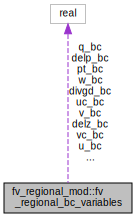
\includegraphics[width=172pt]{structfv__regional__mod_1_1fv__regional__bc__variables__coll__graph}
\end{center}
\end{figure}
\subsection*{Private Attributes}
\begin{DoxyCompactItemize}
\item 
real, dimension(\-:,\-:,\-:), allocatable \hyperlink{structfv__regional__mod_1_1fv__regional__bc__variables_aec9d5b732a9a4b2a90cdbf3401d36949}{delp\-\_\-bc}
\item 
real, dimension(\-:,\-:,\-:), allocatable \hyperlink{structfv__regional__mod_1_1fv__regional__bc__variables_ad0c85d1a488070404cc5f270a96f3952}{divgd\-\_\-bc}
\item 
real, dimension(\-:,\-:,\-:), allocatable \hyperlink{structfv__regional__mod_1_1fv__regional__bc__variables_a2e60aa07c8367405d53a19873475cf95}{u\-\_\-bc}
\item 
real, dimension(\-:,\-:,\-:), allocatable \hyperlink{structfv__regional__mod_1_1fv__regional__bc__variables_a92fb91ce17fc62b7556057210d6ba743}{v\-\_\-bc}
\item 
real, dimension(\-:,\-:,\-:), allocatable \hyperlink{structfv__regional__mod_1_1fv__regional__bc__variables_acf1748291fe067a0dab4227a4cb9bf02}{uc\-\_\-bc}
\item 
real, dimension(\-:,\-:,\-:), allocatable \hyperlink{structfv__regional__mod_1_1fv__regional__bc__variables_ad37018b4fe27728e568418120a8e8f3c}{vc\-\_\-bc}
\item 
real, dimension(\-:,\-:,\-:,\-:), \\*
allocatable \hyperlink{structfv__regional__mod_1_1fv__regional__bc__variables_ac742d67ec3f6444358668e8621f19096}{q\-\_\-bc}
\item 
real, dimension(\-:,\-:,\-:), allocatable \hyperlink{structfv__regional__mod_1_1fv__regional__bc__variables_aa401302803a6a0a83ed6fda6296b8c70}{pt\-\_\-bc}
\item 
real, dimension(\-:,\-:,\-:), allocatable \hyperlink{structfv__regional__mod_1_1fv__regional__bc__variables_a7aa826c4a7fd43cad4347d66ccd13b64}{w\-\_\-bc}
\item 
real, dimension(\-:,\-:,\-:), allocatable \hyperlink{structfv__regional__mod_1_1fv__regional__bc__variables_a0a8021dc9833cb86cabd577772baf258}{delz\-\_\-bc}
\end{DoxyCompactItemize}


\subsection{Detailed Description}


Definition at line 123 of file fv\-\_\-regional\-\_\-bc.\-F90.



\subsection{Member Data Documentation}
\index{fv\-\_\-regional\-\_\-mod\-::fv\-\_\-regional\-\_\-bc\-\_\-variables@{fv\-\_\-regional\-\_\-mod\-::fv\-\_\-regional\-\_\-bc\-\_\-variables}!delp\-\_\-bc@{delp\-\_\-bc}}
\index{delp\-\_\-bc@{delp\-\_\-bc}!fv_regional_mod::fv_regional_bc_variables@{fv\-\_\-regional\-\_\-mod\-::fv\-\_\-regional\-\_\-bc\-\_\-variables}}
\subsubsection[{delp\-\_\-bc}]{\setlength{\rightskip}{0pt plus 5cm}real, dimension(\-:,\-:,\-:), allocatable fv\-\_\-regional\-\_\-mod\-::fv\-\_\-regional\-\_\-bc\-\_\-variables\-::delp\-\_\-bc\hspace{0.3cm}{\ttfamily [private]}}\label{structfv__regional__mod_1_1fv__regional__bc__variables_aec9d5b732a9a4b2a90cdbf3401d36949}


Definition at line 124 of file fv\-\_\-regional\-\_\-bc.\-F90.

\index{fv\-\_\-regional\-\_\-mod\-::fv\-\_\-regional\-\_\-bc\-\_\-variables@{fv\-\_\-regional\-\_\-mod\-::fv\-\_\-regional\-\_\-bc\-\_\-variables}!delz\-\_\-bc@{delz\-\_\-bc}}
\index{delz\-\_\-bc@{delz\-\_\-bc}!fv_regional_mod::fv_regional_bc_variables@{fv\-\_\-regional\-\_\-mod\-::fv\-\_\-regional\-\_\-bc\-\_\-variables}}
\subsubsection[{delz\-\_\-bc}]{\setlength{\rightskip}{0pt plus 5cm}real, dimension(\-:,\-:,\-:), allocatable fv\-\_\-regional\-\_\-mod\-::fv\-\_\-regional\-\_\-bc\-\_\-variables\-::delz\-\_\-bc\hspace{0.3cm}{\ttfamily [private]}}\label{structfv__regional__mod_1_1fv__regional__bc__variables_a0a8021dc9833cb86cabd577772baf258}


Definition at line 127 of file fv\-\_\-regional\-\_\-bc.\-F90.

\index{fv\-\_\-regional\-\_\-mod\-::fv\-\_\-regional\-\_\-bc\-\_\-variables@{fv\-\_\-regional\-\_\-mod\-::fv\-\_\-regional\-\_\-bc\-\_\-variables}!divgd\-\_\-bc@{divgd\-\_\-bc}}
\index{divgd\-\_\-bc@{divgd\-\_\-bc}!fv_regional_mod::fv_regional_bc_variables@{fv\-\_\-regional\-\_\-mod\-::fv\-\_\-regional\-\_\-bc\-\_\-variables}}
\subsubsection[{divgd\-\_\-bc}]{\setlength{\rightskip}{0pt plus 5cm}real, dimension(\-:,\-:,\-:), allocatable fv\-\_\-regional\-\_\-mod\-::fv\-\_\-regional\-\_\-bc\-\_\-variables\-::divgd\-\_\-bc\hspace{0.3cm}{\ttfamily [private]}}\label{structfv__regional__mod_1_1fv__regional__bc__variables_ad0c85d1a488070404cc5f270a96f3952}


Definition at line 124 of file fv\-\_\-regional\-\_\-bc.\-F90.

\index{fv\-\_\-regional\-\_\-mod\-::fv\-\_\-regional\-\_\-bc\-\_\-variables@{fv\-\_\-regional\-\_\-mod\-::fv\-\_\-regional\-\_\-bc\-\_\-variables}!pt\-\_\-bc@{pt\-\_\-bc}}
\index{pt\-\_\-bc@{pt\-\_\-bc}!fv_regional_mod::fv_regional_bc_variables@{fv\-\_\-regional\-\_\-mod\-::fv\-\_\-regional\-\_\-bc\-\_\-variables}}
\subsubsection[{pt\-\_\-bc}]{\setlength{\rightskip}{0pt plus 5cm}real, dimension(\-:,\-:,\-:), allocatable fv\-\_\-regional\-\_\-mod\-::fv\-\_\-regional\-\_\-bc\-\_\-variables\-::pt\-\_\-bc\hspace{0.3cm}{\ttfamily [private]}}\label{structfv__regional__mod_1_1fv__regional__bc__variables_aa401302803a6a0a83ed6fda6296b8c70}


Definition at line 127 of file fv\-\_\-regional\-\_\-bc.\-F90.

\index{fv\-\_\-regional\-\_\-mod\-::fv\-\_\-regional\-\_\-bc\-\_\-variables@{fv\-\_\-regional\-\_\-mod\-::fv\-\_\-regional\-\_\-bc\-\_\-variables}!q\-\_\-bc@{q\-\_\-bc}}
\index{q\-\_\-bc@{q\-\_\-bc}!fv_regional_mod::fv_regional_bc_variables@{fv\-\_\-regional\-\_\-mod\-::fv\-\_\-regional\-\_\-bc\-\_\-variables}}
\subsubsection[{q\-\_\-bc}]{\setlength{\rightskip}{0pt plus 5cm}real, dimension(\-:,\-:,\-:,\-:), allocatable fv\-\_\-regional\-\_\-mod\-::fv\-\_\-regional\-\_\-bc\-\_\-variables\-::q\-\_\-bc\hspace{0.3cm}{\ttfamily [private]}}\label{structfv__regional__mod_1_1fv__regional__bc__variables_ac742d67ec3f6444358668e8621f19096}


Definition at line 125 of file fv\-\_\-regional\-\_\-bc.\-F90.

\index{fv\-\_\-regional\-\_\-mod\-::fv\-\_\-regional\-\_\-bc\-\_\-variables@{fv\-\_\-regional\-\_\-mod\-::fv\-\_\-regional\-\_\-bc\-\_\-variables}!u\-\_\-bc@{u\-\_\-bc}}
\index{u\-\_\-bc@{u\-\_\-bc}!fv_regional_mod::fv_regional_bc_variables@{fv\-\_\-regional\-\_\-mod\-::fv\-\_\-regional\-\_\-bc\-\_\-variables}}
\subsubsection[{u\-\_\-bc}]{\setlength{\rightskip}{0pt plus 5cm}real, dimension(\-:,\-:,\-:), allocatable fv\-\_\-regional\-\_\-mod\-::fv\-\_\-regional\-\_\-bc\-\_\-variables\-::u\-\_\-bc\hspace{0.3cm}{\ttfamily [private]}}\label{structfv__regional__mod_1_1fv__regional__bc__variables_a2e60aa07c8367405d53a19873475cf95}


Definition at line 124 of file fv\-\_\-regional\-\_\-bc.\-F90.

\index{fv\-\_\-regional\-\_\-mod\-::fv\-\_\-regional\-\_\-bc\-\_\-variables@{fv\-\_\-regional\-\_\-mod\-::fv\-\_\-regional\-\_\-bc\-\_\-variables}!uc\-\_\-bc@{uc\-\_\-bc}}
\index{uc\-\_\-bc@{uc\-\_\-bc}!fv_regional_mod::fv_regional_bc_variables@{fv\-\_\-regional\-\_\-mod\-::fv\-\_\-regional\-\_\-bc\-\_\-variables}}
\subsubsection[{uc\-\_\-bc}]{\setlength{\rightskip}{0pt plus 5cm}real, dimension(\-:,\-:,\-:), allocatable fv\-\_\-regional\-\_\-mod\-::fv\-\_\-regional\-\_\-bc\-\_\-variables\-::uc\-\_\-bc\hspace{0.3cm}{\ttfamily [private]}}\label{structfv__regional__mod_1_1fv__regional__bc__variables_acf1748291fe067a0dab4227a4cb9bf02}


Definition at line 124 of file fv\-\_\-regional\-\_\-bc.\-F90.

\index{fv\-\_\-regional\-\_\-mod\-::fv\-\_\-regional\-\_\-bc\-\_\-variables@{fv\-\_\-regional\-\_\-mod\-::fv\-\_\-regional\-\_\-bc\-\_\-variables}!v\-\_\-bc@{v\-\_\-bc}}
\index{v\-\_\-bc@{v\-\_\-bc}!fv_regional_mod::fv_regional_bc_variables@{fv\-\_\-regional\-\_\-mod\-::fv\-\_\-regional\-\_\-bc\-\_\-variables}}
\subsubsection[{v\-\_\-bc}]{\setlength{\rightskip}{0pt plus 5cm}real, dimension(\-:,\-:,\-:), allocatable fv\-\_\-regional\-\_\-mod\-::fv\-\_\-regional\-\_\-bc\-\_\-variables\-::v\-\_\-bc\hspace{0.3cm}{\ttfamily [private]}}\label{structfv__regional__mod_1_1fv__regional__bc__variables_a92fb91ce17fc62b7556057210d6ba743}


Definition at line 124 of file fv\-\_\-regional\-\_\-bc.\-F90.

\index{fv\-\_\-regional\-\_\-mod\-::fv\-\_\-regional\-\_\-bc\-\_\-variables@{fv\-\_\-regional\-\_\-mod\-::fv\-\_\-regional\-\_\-bc\-\_\-variables}!vc\-\_\-bc@{vc\-\_\-bc}}
\index{vc\-\_\-bc@{vc\-\_\-bc}!fv_regional_mod::fv_regional_bc_variables@{fv\-\_\-regional\-\_\-mod\-::fv\-\_\-regional\-\_\-bc\-\_\-variables}}
\subsubsection[{vc\-\_\-bc}]{\setlength{\rightskip}{0pt plus 5cm}real, dimension(\-:,\-:,\-:), allocatable fv\-\_\-regional\-\_\-mod\-::fv\-\_\-regional\-\_\-bc\-\_\-variables\-::vc\-\_\-bc\hspace{0.3cm}{\ttfamily [private]}}\label{structfv__regional__mod_1_1fv__regional__bc__variables_ad37018b4fe27728e568418120a8e8f3c}


Definition at line 124 of file fv\-\_\-regional\-\_\-bc.\-F90.

\index{fv\-\_\-regional\-\_\-mod\-::fv\-\_\-regional\-\_\-bc\-\_\-variables@{fv\-\_\-regional\-\_\-mod\-::fv\-\_\-regional\-\_\-bc\-\_\-variables}!w\-\_\-bc@{w\-\_\-bc}}
\index{w\-\_\-bc@{w\-\_\-bc}!fv_regional_mod::fv_regional_bc_variables@{fv\-\_\-regional\-\_\-mod\-::fv\-\_\-regional\-\_\-bc\-\_\-variables}}
\subsubsection[{w\-\_\-bc}]{\setlength{\rightskip}{0pt plus 5cm}real, dimension(\-:,\-:,\-:), allocatable fv\-\_\-regional\-\_\-mod\-::fv\-\_\-regional\-\_\-bc\-\_\-variables\-::w\-\_\-bc\hspace{0.3cm}{\ttfamily [private]}}\label{structfv__regional__mod_1_1fv__regional__bc__variables_a7aa826c4a7fd43cad4347d66ccd13b64}


Definition at line 127 of file fv\-\_\-regional\-\_\-bc.\-F90.



The documentation for this type was generated from the following file\-:\begin{DoxyCompactItemize}
\item 
/scratch2/\-N\-A\-G\-A\-P\-E/aoml-\/hafs1/\-Kyle.\-Ahern/acs\-\_\-master\-\_\-readonly/model/\hyperlink{fv__regional__bc_8F90}{fv\-\_\-regional\-\_\-bc.\-F90}\end{DoxyCompactItemize}

\section{fv\-\_\-regional\-\_\-mod Module Reference}
\label{classfv__regional__mod}\index{fv\-\_\-regional\-\_\-mod@{fv\-\_\-regional\-\_\-mod}}


Collaboration diagram for fv\-\_\-regional\-\_\-mod\-:
\nopagebreak
\begin{figure}[H]
\begin{center}
\leavevmode
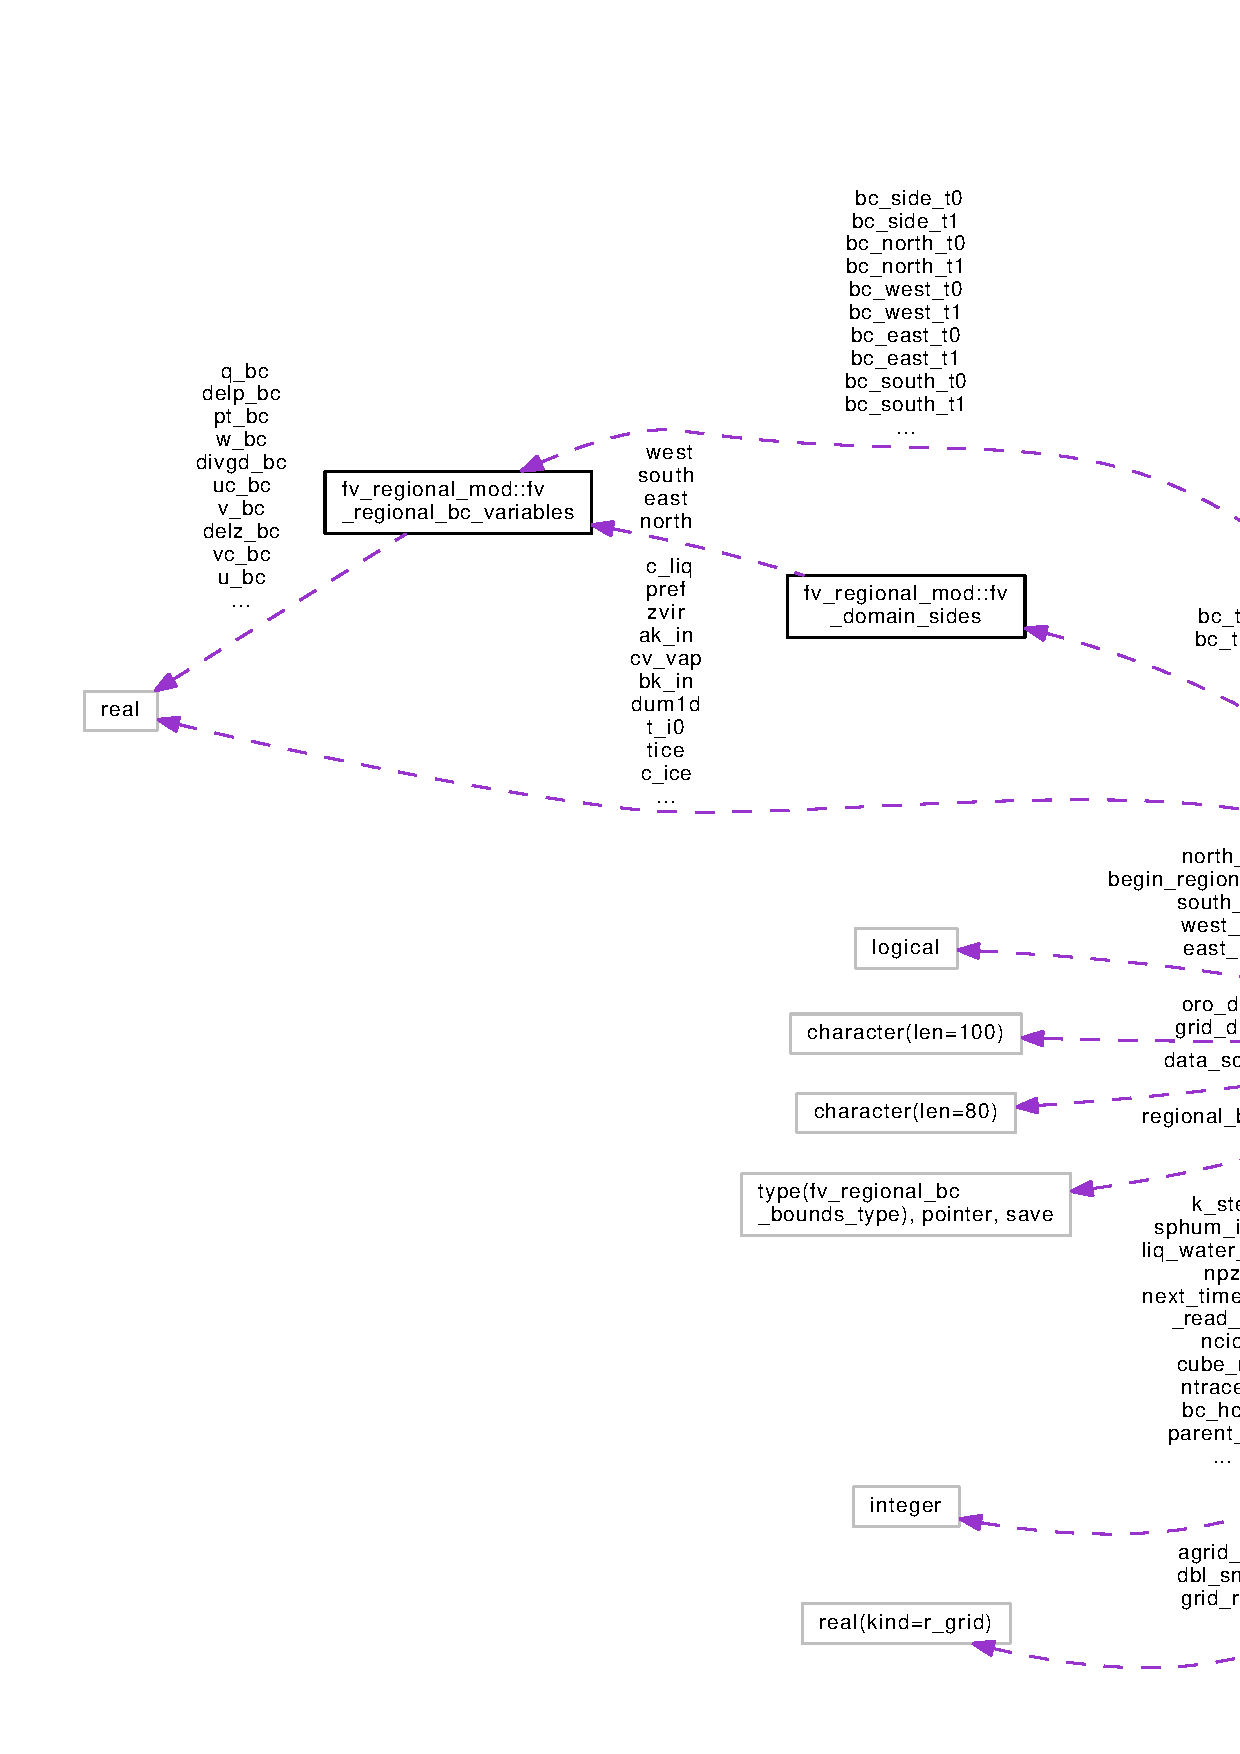
\includegraphics[width=350pt]{classfv__regional__mod__coll__graph}
\end{center}
\end{figure}
\subsection*{Data Types}
\begin{DoxyCompactItemize}
\item 
interface \hyperlink{interfacefv__regional__mod_1_1dump__field}{dump\-\_\-field}
\item 
type \hyperlink{structfv__regional__mod_1_1fv__domain__sides}{fv\-\_\-domain\-\_\-sides}
\item 
type \hyperlink{structfv__regional__mod_1_1fv__regional__bc__variables}{fv\-\_\-regional\-\_\-bc\-\_\-variables}
\end{DoxyCompactItemize}
\subsection*{Public Member Functions}
\begin{DoxyCompactItemize}
\item 
subroutine, public \hyperlink{classfv__regional__mod_a6991aba90c8c7297a002b8ca58f09f99}{setup\-\_\-regional\-\_\-bc} (Atm, isd, ied, jsd, jed, npx, npy)
\item 
subroutine, public \hyperlink{classfv__regional__mod_ad1bf6476615882c211020e8d53c4bf8c}{start\-\_\-regional\-\_\-cold\-\_\-start} (Atm, ak, bk, levp, is, ie, js, je, isd, ied, jsd, jed)
\item 
subroutine, public \hyperlink{classfv__regional__mod_a0d3b818eb47e19e7254ccd506c5a5895}{start\-\_\-regional\-\_\-restart} (Atm, isc, iec, jsc, jec, isd, ied, jsd, jed)
\item 
subroutine, public \hyperlink{classfv__regional__mod_ae3ebee89f81e0493a8c7e17875152d72}{read\-\_\-new\-\_\-bc\-\_\-data} (Atm, Time, Time\-\_\-step\-\_\-atmos, p\-\_\-split, isd, ied, jsd, jed)
\item 
subroutine, public \hyperlink{classfv__regional__mod_a769a4bf5f728fcb86b52d456ac3f08a5}{regional\-\_\-bc\-\_\-data} (Atm, \hyperlink{classfv__regional__mod_a5192ede59906ab120d0ad1a12bcc9ea1}{bc\-\_\-hour}, is, ie, js, je, isd, ied, jsd, jed, ak, bk)
\item 
subroutine, public \hyperlink{classfv__regional__mod_a6dc14a5c1732e07b8961cedbffc1774f}{set\-\_\-regional\-\_\-bcs} (delp, delz, w, pt
\item 
subroutine, public \hyperlink{classfv__regional__mod_ad13eb19c4cba6f952bc2c8360464bba1}{regional\-\_\-boundary\-\_\-update} (array, bc\-\_\-vbl\-\_\-name, lbnd\-\_\-x, ubnd\-\_\-x, lbnd\-\_\-y, ubnd\-\_\-y, ubnd\-\_\-z, is, ie, js, je, isd, ied, jsd, jed, fcst\-\_\-time, index4)
\item 
subroutine, public \hyperlink{classfv__regional__mod_acfdab6124b0e0c814915363e12550d92}{regional\-\_\-bc\-\_\-t1\-\_\-to\-\_\-t0} (B\-C\-\_\-t1, B\-C\-\_\-t0, nlev, \hyperlink{classfv__regional__mod_a59026f4c5f7fbd69bbaf1c53c9418817}{ntracers}, bnds)
\item 
subroutine, public \hyperlink{classfv__regional__mod_a820d191779e94ce32b42d2b0c2ad3102}{exch\-\_\-uv} (domain, bd, \hyperlink{classfv__regional__mod_a66c4d15d316eeb5577275a92f68c14c1}{npz}, u, v)
\item 
subroutine, public \hyperlink{classfv__regional__mod_af347265c2839a84abc162e9cb89a34d1}{get\-\_\-data\-\_\-source} (source, regional)
\end{DoxyCompactItemize}
\subsection*{Public Attributes}
\begin{DoxyCompactItemize}
\item 
integer, parameter, public \hyperlink{classfv__regional__mod_ab84d267f8311598530c8783263ad1bc8}{h\-\_\-stagger} = 1
\item 
integer, parameter, public \hyperlink{classfv__regional__mod_a6066b6d442bf60820ed3124997c2de88}{u\-\_\-stagger} = 2
\item 
integer, parameter, public \hyperlink{classfv__regional__mod_a279442c8a15e38c2db6957829cd5d594}{v\-\_\-stagger} = 3
\item 
real, public \hyperlink{classfv__regional__mod_acb12d0df0e8fb775d3a41fba0b0f34e9}{current\-\_\-time\-\_\-in\-\_\-seconds}
\item 
integer, save, public \hyperlink{classfv__regional__mod_a295cbf8a004fa34e95f2cca9358e0132}{next\-\_\-time\-\_\-to\-\_\-read\-\_\-bcs}
\item 
integer, save, public \hyperlink{classfv__regional__mod_a5192ede59906ab120d0ad1a12bcc9ea1}{bc\-\_\-hour}
\item 
integer, save, public \hyperlink{classfv__regional__mod_a4bc0673fc38c2310386939382a9c57ad}{ntimesteps\-\_\-per\-\_\-bc\-\_\-update}
\item 
real, dimension(\-:), \\*
allocatable, public \hyperlink{classfv__regional__mod_a75a74e2d8e60bc9cb7b1026601fbab5a}{ak\-\_\-in}
\item 
real, dimension(\-:), \\*
allocatable, public \hyperlink{classfv__regional__mod_ae7e070a83ea46499a4477fdbfbc7a9ce}{bk\-\_\-in}
\item 
logical, save, public \hyperlink{classfv__regional__mod_aa9895dcedb85e93e3ab4b513ec927084}{begin\-\_\-regional\-\_\-restart} =.true.
\item 
type(\hyperlink{structfv__regional__mod_1_1fv__domain__sides}{fv\-\_\-domain\-\_\-sides}), target, \\*
save, public \hyperlink{classfv__regional__mod_aa378b52fed4e1ce5559f939a10e55a1c}{bc\-\_\-t0}
\item 
type(\hyperlink{structfv__regional__mod_1_1fv__domain__sides}{fv\-\_\-domain\-\_\-sides}), target, \\*
save, public \hyperlink{classfv__regional__mod_acac95ec214236b8e748460a0132f03bc}{bc\-\_\-t1}
\begin{DoxyCompactList}\small\item\em -- Boundary values for all B\-C variables at successive times from the regional B\-C file \end{DoxyCompactList}\item 
integer, public \hyperlink{classfv__regional__mod_a7d48ecf3376e882113cf29f2c50b996c}{a\-\_\-step}
\item 
integer, public \hyperlink{classfv__regional__mod_a829242ae29d3a80d8bf09dbc093cbac0}{p\-\_\-step}
\item 
integer, public \hyperlink{classfv__regional__mod_a4526a6a4dc765d8f17c9b291687bd316}{k\-\_\-step}
\item 
integer, public \hyperlink{classfv__regional__mod_afe2252139409c2841f1f01af51dd8fc3}{n\-\_\-step}
\end{DoxyCompactItemize}
\subsection*{Private Member Functions}
\begin{DoxyCompactItemize}
\item 
subroutine \hyperlink{classfv__regional__mod_a3fbfeacb423408193cbcd776f006f1f3}{read\-\_\-regional\-\_\-bc\-\_\-file} (is\-\_\-input, ie\-\_\-input, js\-\_\-input, je\-\_\-input, nlev, \hyperlink{classfv__regional__mod_a59026f4c5f7fbd69bbaf1c53c9418817}{ntracers}, var\-\_\-name\-\_\-root, array\-\_\-3d, array\-\_\-4d, tlev, required)
\item 
subroutine \hyperlink{classfv__regional__mod_aab40ff3a15b7e77a4333f55640fac1bd}{check} (status)
\item 
subroutine \hyperlink{classfv__regional__mod_af9430d75f6a57684138a27c6ef3a8dcc}{allocate\-\_\-regional\-\_\-bc\-\_\-arrays} (side, \hyperlink{classfv__regional__mod_ab0d18e800d03af2331630c5d41f24647}{north\-\_\-bc}, \hyperlink{classfv__regional__mod_aa19455811e08a60979cfe82e9339cf79}{south\-\_\-bc}, \hyperlink{classfv__regional__mod_abba04d13f69846096203d294e6224476}{east\-\_\-bc}, \hyperlink{classfv__regional__mod_acb6bcb04c44ff52d6d5caa07da7952d2}{west\-\_\-bc}, is\-\_\-0, ie\-\_\-0, js\-\_\-0, je\-\_\-0, is\-\_\-sn, ie\-\_\-sn, js\-\_\-sn, je\-\_\-sn, is\-\_\-we, ie\-\_\-we, js\-\_\-we, je\-\_\-we, klev, \hyperlink{classfv__regional__mod_a59026f4c5f7fbd69bbaf1c53c9418817}{ntracers}, B\-C\-\_\-side)
\item 
subroutine \hyperlink{classfv__regional__mod_abae4545097ec695c285252297c301e02}{remap\-\_\-scalar\-\_\-nggps\-\_\-regional\-\_\-bc} (Atm, side, isd, ied, jsd, jed, is\-\_\-bc, ie\-\_\-bc, js\-\_\-bc, je\-\_\-bc, km, \hyperlink{classfv__regional__mod_a66c4d15d316eeb5577275a92f68c14c1}{npz}, ncnst, ak0, bk0, psc, t\-\_\-in, qa, omga, zh, \hyperlink{classfv__regional__mod_a4360b9bea440884168e896f8c5ce3a4c}{phis\-\_\-reg}, ps, B\-C\-\_\-side)
\item 
subroutine \hyperlink{classfv__regional__mod_ad5354af17f3f7ee5e2b0b535cbfda5c7}{remap\-\_\-dwinds\-\_\-regional\-\_\-bc} (Atm, is\-\_\-input, ie\-\_\-input, js\-\_\-input, je\-\_\-input, is\-\_\-u, ie\-\_\-u, js\-\_\-u, je\-\_\-u, is\-\_\-v, ie\-\_\-v, js\-\_\-v, je\-\_\-v, km, \hyperlink{classfv__regional__mod_a66c4d15d316eeb5577275a92f68c14c1}{npz}, ak0, bk0, psc, ud, vd, uc, vc, B\-C\-\_\-side)
\item 
subroutine \hyperlink{classfv__regional__mod_a75315aba17f1dca9ddf4803a5c48c0a7}{retrieve\-\_\-bc\-\_\-variable\-\_\-data} (bc\-\_\-vbl\-\_\-name, \hyperlink{classfv__regional__mod_a152d9905d14d20d277c4fddf7a5fbc52}{bc\-\_\-side\-\_\-t0}, \hyperlink{classfv__regional__mod_a8ffee600e05a0988addd6e7387fe9547}{bc\-\_\-side\-\_\-t1}, \hyperlink{classfv__regional__mod_aa378b52fed4e1ce5559f939a10e55a1c}{bc\-\_\-t0}, \hyperlink{classfv__regional__mod_acac95ec214236b8e748460a0132f03bc}{bc\-\_\-t1}, lbnd1, ubnd1, lbnd2, ubnd2, iq)
\item 
subroutine \hyperlink{classfv__regional__mod_aaef6721039a718997c21fa68e6d6d197}{bc\-\_\-time\-\_\-interpolation} (array, lbnd\-\_\-x, ubnd\-\_\-x, lbnd\-\_\-y, ubnd\-\_\-y, ubnd\-\_\-z, \hyperlink{classfv__regional__mod_aa378b52fed4e1ce5559f939a10e55a1c}{bc\-\_\-t0}, \hyperlink{classfv__regional__mod_acac95ec214236b8e748460a0132f03bc}{bc\-\_\-t1}, lbnd1, ubnd1, lbnd2, ubnd2, i1, i2, j1, j2, fcst\-\_\-time, \hyperlink{classfv__regional__mod_aa8a82e411bb80aa539a1f5ff6436fdc1}{bc\-\_\-update\-\_\-interval})
\item 
subroutine \hyperlink{classfv__regional__mod_a016734390a5ec60124df62df881b5b65}{bc\-\_\-time\-\_\-interpolation\-\_\-general} (is, ie, js, je, is\-\_\-s, ie\-\_\-s, js\-\_\-s, je\-\_\-s, is\-\_\-w, ie\-\_\-w, js\-\_\-w, je\-\_\-w, fraction, t0, t1, Atm)
\item 
subroutine \hyperlink{classfv__regional__mod_ab5399fe877d79a94400523090654b9c3}{convert\-\_\-to\-\_\-virt\-\_\-pot\-\_\-temp} (isd, ied, jsd, jed, \hyperlink{classfv__regional__mod_a66c4d15d316eeb5577275a92f68c14c1}{npz}, sphum, liq\-\_\-wat)
\item 
subroutine \hyperlink{classfv__regional__mod_a2c233d273bf0fafb063e7123ad68d43c}{p\-\_\-maxmin} (qname, q, is, ie, js, je, km, fac)
\item 
subroutine \hyperlink{classfv__regional__mod_af798bda3f153aa7f32f52874d2ddf054}{pmaxmn} (qname, q, is, ie, js, je, km, fac, area, domain)
\item 
subroutine \hyperlink{classfv__regional__mod_aa9bb203a22a95c7d655982fd8c771648}{fillq} (im, km, nq, q, dp)
\item 
subroutine \hyperlink{classfv__regional__mod_a0df5c24b5062f6285f98eb35a0f9dcdc}{mp\-\_\-auto\-\_\-conversion} (ql, qr, qi, qs)
\item 
subroutine \hyperlink{classfv__regional__mod_a20475fef186daf196f29575b3738891b}{nudge\-\_\-qv\-\_\-bc} (Atm, isd, ied, jsd, jed)
\item 
subroutine \hyperlink{classfv__regional__mod_ad5e7997361f932233078f9284d27db92}{dump\-\_\-field\-\_\-3d} (domain, name, field, isd, ied, jsd, jed, nlev, stag)
\item 
subroutine \hyperlink{classfv__regional__mod_a1ad419a9bdf8e5bd7d0163d4117069ac}{dump\-\_\-field\-\_\-2d} (domain, name, field, isd, ied, jsd, jed, stag)
\item 
subroutine \hyperlink{classfv__regional__mod_a8fedc85e3f123b4574769a284fd8faa0}{set\-\_\-delp\-\_\-and\-\_\-tracers} (B\-C\-\_\-side, \hyperlink{classfv__regional__mod_a66c4d15d316eeb5577275a92f68c14c1}{npz}, nwat)
\end{DoxyCompactItemize}
\subsection*{Private Attributes}
\begin{DoxyCompactItemize}
\item 
integer, parameter \hyperlink{classfv__regional__mod_ace154d36bee6c72b51943cfb94b9de9a}{nhalo\-\_\-data} =4
\item 
integer, parameter \hyperlink{classfv__regional__mod_aa41184f5720c2bb3148d0ee0e18c1eff}{nhalo\-\_\-model} =3
\item 
real, parameter \hyperlink{classfv__regional__mod_ac8743a9351000e8f9867442d74f27deb}{stretch\-\_\-factor} = 1.\-50
\item 
real, parameter \hyperlink{classfv__regional__mod_afad48457183ea13095892d3d0831cecb}{target\-\_\-lon} = -\/97.\-5
\item 
real, parameter \hyperlink{classfv__regional__mod_aaf300439aa3eac86faaf7f26f41e1bcd}{target\-\_\-lat} = 35.\-5
\item 
integer, parameter \hyperlink{classfv__regional__mod_aea80f27ba09a8d5a80ed70efe8a15da3}{parent\-\_\-tile} = 6
\item 
integer, parameter \hyperlink{classfv__regional__mod_a9d0455a3e9bf0fc4147b96aae64bf741}{refine\-\_\-ratio} = 3
\item 
integer, parameter \hyperlink{classfv__regional__mod_a2ea6f77a01d43a1e3d47993612aa45c5}{cube\-\_\-res} = 96
\item 
integer, parameter \hyperlink{classfv__regional__mod_a12a863dffbbb16718ce4b2e1fbb7acaa}{istart\-\_\-nest} = 26
\item 
integer, parameter \hyperlink{classfv__regional__mod_a675de8ff14de24134c9d15abc2e2de40}{jstart\-\_\-nest} = 36
\item 
integer, parameter \hyperlink{classfv__regional__mod_a46c63eb6b1a90522b1981ef852cf36db}{iend\-\_\-nest} = 167
\item 
integer, parameter \hyperlink{classfv__regional__mod_a4d47ea369899bf92a118fcc384d143c6}{jend\-\_\-nest} = 165
\item 
integer, save \hyperlink{classfv__regional__mod_a4d4fa505ef6e59899c62c7e52d14fefc}{ncid}
\item 
integer, save \hyperlink{classfv__regional__mod_a66c4d15d316eeb5577275a92f68c14c1}{npz}
\item 
integer, save \hyperlink{classfv__regional__mod_a59026f4c5f7fbd69bbaf1c53c9418817}{ntracers}
\item 
integer, save \hyperlink{classfv__regional__mod_a4d329cbebba02218379970b776449bbf}{liq\-\_\-water\-\_\-index}
\item 
integer, save \hyperlink{classfv__regional__mod_a5046c418bb3714689df7737b3024d910}{sphum\-\_\-index}
\begin{DoxyCompactList}\small\item\em -- Locations of tracer vbls in the tracers array \end{DoxyCompactList}\item 
real(kind=r\-\_\-grid), dimension(\-:,\-:,\-:), \\*
allocatable \hyperlink{classfv__regional__mod_a2eb428ec6f0a4e8830a8c379986c760c}{agrid\-\_\-reg}
\begin{DoxyCompactList}\small\item\em -\/-\/ Lon/lat of cell centers \end{DoxyCompactList}\item 
real(kind=r\-\_\-grid), dimension(\-:,\-:,\-:), \\*
allocatable \hyperlink{classfv__regional__mod_affa97bf1e197ce68252597eb38a2ebd7}{grid\-\_\-reg}
\begin{DoxyCompactList}\small\item\em -- Lon/lat of cell corners \end{DoxyCompactList}\item 
real, dimension(\-:,\-:), allocatable \hyperlink{classfv__regional__mod_a4360b9bea440884168e896f8c5ce3a4c}{phis\-\_\-reg}
\begin{DoxyCompactList}\small\item\em -- Filtered sfc geopotential \end{DoxyCompactList}\item 
logical, save \hyperlink{classfv__regional__mod_ab0d18e800d03af2331630c5d41f24647}{north\-\_\-bc}
\item 
logical, save \hyperlink{classfv__regional__mod_aa19455811e08a60979cfe82e9339cf79}{south\-\_\-bc}
\item 
logical, save \hyperlink{classfv__regional__mod_abba04d13f69846096203d294e6224476}{east\-\_\-bc}
\item 
logical, save \hyperlink{classfv__regional__mod_acb6bcb04c44ff52d6d5caa07da7952d2}{west\-\_\-bc}
\item 
type(\hyperlink{structfv__regional__mod_1_1fv__regional__bc__variables}{fv\-\_\-regional\-\_\-bc\-\_\-variables}), \\*
pointer, save \hyperlink{classfv__regional__mod_a764cc29c643f325faec13145036f9777}{bc\-\_\-north\-\_\-t0}
\item 
type(\hyperlink{structfv__regional__mod_1_1fv__regional__bc__variables}{fv\-\_\-regional\-\_\-bc\-\_\-variables}), \\*
pointer, save \hyperlink{classfv__regional__mod_a8868f1a8567b94835e8c8d4a86c245c0}{bc\-\_\-south\-\_\-t0}
\item 
type(\hyperlink{structfv__regional__mod_1_1fv__regional__bc__variables}{fv\-\_\-regional\-\_\-bc\-\_\-variables}), \\*
pointer, save \hyperlink{classfv__regional__mod_aad83e1ac00233cc47374f4b3cf630a1d}{bc\-\_\-west\-\_\-t0}
\item 
type(\hyperlink{structfv__regional__mod_1_1fv__regional__bc__variables}{fv\-\_\-regional\-\_\-bc\-\_\-variables}), \\*
pointer, save \hyperlink{classfv__regional__mod_a9a63cc3ebf0fab65d4d6c362ae03b475}{bc\-\_\-east\-\_\-t0}
\item 
type(\hyperlink{structfv__regional__mod_1_1fv__regional__bc__variables}{fv\-\_\-regional\-\_\-bc\-\_\-variables}), \\*
pointer, save \hyperlink{classfv__regional__mod_a01fce45b2f3c2a2e3ba5005abb72670b}{bc\-\_\-north\-\_\-t1}
\item 
type(\hyperlink{structfv__regional__mod_1_1fv__regional__bc__variables}{fv\-\_\-regional\-\_\-bc\-\_\-variables}), \\*
pointer, save \hyperlink{classfv__regional__mod_af6125f39e9a9ed769e9cd2a17a8d3c99}{bc\-\_\-south\-\_\-t1}
\item 
type(\hyperlink{structfv__regional__mod_1_1fv__regional__bc__variables}{fv\-\_\-regional\-\_\-bc\-\_\-variables}), \\*
pointer, save \hyperlink{classfv__regional__mod_aa8aceea599c16392ae3ebc4b65668992}{bc\-\_\-west\-\_\-t1}
\item 
type(\hyperlink{structfv__regional__mod_1_1fv__regional__bc__variables}{fv\-\_\-regional\-\_\-bc\-\_\-variables}), \\*
pointer, save \hyperlink{classfv__regional__mod_affeac28c243080f92d93528428b53075}{bc\-\_\-east\-\_\-t1}
\item 
type(\hyperlink{structfv__regional__mod_1_1fv__regional__bc__variables}{fv\-\_\-regional\-\_\-bc\-\_\-variables}), \\*
pointer \hyperlink{classfv__regional__mod_a152d9905d14d20d277c4fddf7a5fbc52}{bc\-\_\-side\-\_\-t0}
\item 
type(\hyperlink{structfv__regional__mod_1_1fv__regional__bc__variables}{fv\-\_\-regional\-\_\-bc\-\_\-variables}), \\*
pointer \hyperlink{classfv__regional__mod_a8ffee600e05a0988addd6e7387fe9547}{bc\-\_\-side\-\_\-t1}
\item 
type(fv\-\_\-regional\-\_\-bc\-\_\-bounds\-\_\-type), \\*
pointer, save \hyperlink{classfv__regional__mod_a13909d8a60906605379b221f840ea3c1}{regional\-\_\-bounds}
\item 
real, parameter \hyperlink{classfv__regional__mod_a234b3fd9ee427db8de0880bc4f5849c9}{tice} =273.\-16
\item 
real, parameter \hyperlink{classfv__regional__mod_ab891456d653e8b3dba04c9a553877b22}{t\-\_\-i0} =15.
\item 
real, parameter \hyperlink{classfv__regional__mod_a7c984c269922724e4ec90ab8e39c3497}{c\-\_\-liq} = 4185.\-5
\item 
real, parameter \hyperlink{classfv__regional__mod_a2d3e253e8cfeeb07d467f80cc3e02db6}{c\-\_\-ice} = 1972.\-0
\item 
real, parameter \hyperlink{classfv__regional__mod_a8ac5940c29c15b1a91d7ee8e80e826bc}{zvir} = rvgas/rdgas -\/ 1.
\item 
real, parameter \hyperlink{classfv__regional__mod_ac7ad42fc025310b9621b50b2fd978b12}{cv\-\_\-air} = cp\-\_\-air -\/ rdgas
\item 
real, parameter \hyperlink{classfv__regional__mod_af441421c2c1bc6465e3552693aed3a0f}{cv\-\_\-vap} = cp\-\_\-vapor -\/ rvgas
\item 
real, dimension(\-:), allocatable \hyperlink{classfv__regional__mod_a5616e5b4b06f6c406824fa679fa0fd9e}{dum1d}
\item 
real, dimension(\-:), allocatable \hyperlink{classfv__regional__mod_ac942190aa433f5ffa8901ccf140b1663}{pref}
\item 
character(len=100) \hyperlink{classfv__regional__mod_af44c16e69ea0e0f34f3fd45b9bdb7380}{grid\-\_\-data} ='grid.\-tile7.\-halo4.\-nc'
\item 
character(len=100) \hyperlink{classfv__regional__mod_a97454c0d7b19a08bc2bd65c06cc75fcb}{oro\-\_\-data} ='oro\-\_\-data.\-tile7.\-halo4.\-nc'
\item 
real, parameter \hyperlink{classfv__regional__mod_a0caa164db78f0352f7124e34227e9950}{real\-\_\-snan} =x'F\-F\-F7\-F\-F\-F\-F\-F\-F\-F\-F\-F\-F\-F\-F'
\item 
real(kind=r\-\_\-grid), parameter \hyperlink{classfv__regional__mod_afb97c724dfbe30f087907a7a7f1eaf44}{dbl\-\_\-snan} =x'F\-F\-F7\-F\-F\-F\-F\-F\-F\-F\-F\-F\-F\-F\-F'
\item 
integer, save \hyperlink{classfv__regional__mod_aa8a82e411bb80aa539a1f5ff6436fdc1}{bc\-\_\-update\-\_\-interval}
\item 
character(len=80) \hyperlink{classfv__regional__mod_a390d0696d4ec8ca340b2fc69213e16e8}{data\-\_\-source}
\end{DoxyCompactItemize}


\subsection{Detailed Description}


Definition at line 22 of file fv\-\_\-regional\-\_\-bc.\-F90.



\subsection{Member Function/\-Subroutine Documentation}
\index{fv\-\_\-regional\-\_\-mod@{fv\-\_\-regional\-\_\-mod}!allocate\-\_\-regional\-\_\-bc\-\_\-arrays@{allocate\-\_\-regional\-\_\-bc\-\_\-arrays}}
\index{allocate\-\_\-regional\-\_\-bc\-\_\-arrays@{allocate\-\_\-regional\-\_\-bc\-\_\-arrays}!fv_regional_mod@{fv\-\_\-regional\-\_\-mod}}
\subsubsection[{allocate\-\_\-regional\-\_\-bc\-\_\-arrays}]{\setlength{\rightskip}{0pt plus 5cm}subroutine fv\-\_\-regional\-\_\-mod\-::allocate\-\_\-regional\-\_\-bc\-\_\-arrays (
\begin{DoxyParamCaption}
\item[{character(len=5), intent(in)}]{side, }
\item[{logical, intent(in)}]{north\-\_\-bc, }
\item[{logical, intent(in)}]{south\-\_\-bc, }
\item[{logical, intent(in)}]{east\-\_\-bc, }
\item[{logical, intent(in)}]{west\-\_\-bc, }
\item[{integer, intent(in)}]{is\-\_\-0, }
\item[{integer, intent(in)}]{ie\-\_\-0, }
\item[{integer, intent(in)}]{js\-\_\-0, }
\item[{integer, intent(in)}]{je\-\_\-0, }
\item[{integer, intent(in)}]{is\-\_\-sn, }
\item[{integer, intent(in)}]{ie\-\_\-sn, }
\item[{integer, intent(in)}]{js\-\_\-sn, }
\item[{integer, intent(in)}]{je\-\_\-sn, }
\item[{integer, intent(in)}]{is\-\_\-we, }
\item[{integer, intent(in)}]{ie\-\_\-we, }
\item[{integer, intent(in)}]{js\-\_\-we, }
\item[{integer, intent(in)}]{je\-\_\-we, }
\item[{integer, intent(in)}]{klev, }
\item[{integer, intent(in)}]{ntracers, }
\item[{type({\bf fv\-\_\-regional\-\_\-bc\-\_\-variables}), intent(out)}]{B\-C\-\_\-side}
\end{DoxyParamCaption}
)\hspace{0.3cm}{\ttfamily [private]}}\label{classfv__regional__mod_af9430d75f6a57684138a27c6ef3a8dcc}

\begin{DoxyParams}[1]{Parameters}
\mbox{\tt in}  & {\em je\-\_\-0} & -- Start/end B\-C indices for cell centers\\
\hline
\mbox{\tt in}  & {\em je\-\_\-sn} & -- Start/end B\-C indices for south/north cell edges\\
\hline
\mbox{\tt in}  & {\em je\-\_\-we} & -- Start/end B\-C indices for west/east cell edges\\
\hline
\mbox{\tt in}  & {\em side} & -- Which side are we allocating?\\
\hline
\mbox{\tt in}  & {\em west\-\_\-bc} & -- Which sides is this task on?\\
\hline
\mbox{\tt out}  & {\em bc\-\_\-side} & -- The B\-C arrays are already allocated so exit. \\
\hline
\end{DoxyParams}


Definition at line 2601 of file fv\-\_\-regional\-\_\-bc.\-F90.



Referenced by setup\-\_\-regional\-\_\-bc().

\index{fv\-\_\-regional\-\_\-mod@{fv\-\_\-regional\-\_\-mod}!bc\-\_\-time\-\_\-interpolation@{bc\-\_\-time\-\_\-interpolation}}
\index{bc\-\_\-time\-\_\-interpolation@{bc\-\_\-time\-\_\-interpolation}!fv_regional_mod@{fv\-\_\-regional\-\_\-mod}}
\subsubsection[{bc\-\_\-time\-\_\-interpolation}]{\setlength{\rightskip}{0pt plus 5cm}subroutine fv\-\_\-regional\-\_\-mod\-::bc\-\_\-time\-\_\-interpolation (
\begin{DoxyParamCaption}
\item[{real, dimension(lbnd\-\_\-x\-:ubnd\-\_\-x,lbnd\-\_\-y\-:ubnd\-\_\-y,1\-:ubnd\-\_\-z), intent(out)}]{array, }
\item[{integer, intent(in)}]{lbnd\-\_\-x, }
\item[{integer, intent(in)}]{ubnd\-\_\-x, }
\item[{integer, intent(in)}]{lbnd\-\_\-y, }
\item[{integer, intent(in)}]{ubnd\-\_\-y, }
\item[{integer, intent(in)}]{ubnd\-\_\-z, }
\item[{real, dimension(lbnd1\-:ubnd1,lbnd2\-:ubnd2,1\-:ubnd\-\_\-z)}]{bc\-\_\-t0, }
\item[{real, dimension(lbnd1\-:ubnd1,lbnd2\-:ubnd2,1\-:ubnd\-\_\-z)}]{bc\-\_\-t1, }
\item[{integer, intent(in)}]{lbnd1, }
\item[{integer, intent(in)}]{ubnd1, }
\item[{integer, intent(in)}]{lbnd2, }
\item[{integer, intent(in)}]{ubnd2, }
\item[{integer, intent(in)}]{i1, }
\item[{integer, intent(in)}]{i2, }
\item[{integer, intent(in)}]{j1, }
\item[{integer, intent(in)}]{j2, }
\item[{real, intent(in)}]{fcst\-\_\-time, }
\item[{integer, intent(in)}]{bc\-\_\-update\-\_\-interval}
\end{DoxyParamCaption}
)\hspace{0.3cm}{\ttfamily [private]}}\label{classfv__regional__mod_aaef6721039a718997c21fa68e6d6d197}

\begin{DoxyParams}[1]{Parameters}
\mbox{\tt in}  & {\em ubnd\-\_\-z} & -- Dimensions of the array to be updated.\\
\hline
\mbox{\tt in}  & {\em ubnd2} & -- Index limits of the B\-C arrays.\\
\hline
\mbox{\tt in}  & {\em j2} & -- Index limits of the updated region.\\
\hline
\mbox{\tt in}  & {\em bc\-\_\-update\-\_\-interval} & -- Time (hours) between B\-C data states\\
\hline
\mbox{\tt in}  & {\em fcst\-\_\-time} & -- Current forecast time (sec)\\
\hline
\mbox{\tt out}  & {\em array} & -- Update boundary points in this array. \\
\hline
\end{DoxyParams}

\begin{DoxyParams}{Parameters}
{\em bc\-\_\-t0} & -\/-\/ Interpolate between these \\
\hline
\end{DoxyParams}


Definition at line 3843 of file fv\-\_\-regional\-\_\-bc.\-F90.



Referenced by regional\-\_\-boundary\-\_\-update().

\index{fv\-\_\-regional\-\_\-mod@{fv\-\_\-regional\-\_\-mod}!bc\-\_\-time\-\_\-interpolation\-\_\-general@{bc\-\_\-time\-\_\-interpolation\-\_\-general}}
\index{bc\-\_\-time\-\_\-interpolation\-\_\-general@{bc\-\_\-time\-\_\-interpolation\-\_\-general}!fv_regional_mod@{fv\-\_\-regional\-\_\-mod}}
\subsubsection[{bc\-\_\-time\-\_\-interpolation\-\_\-general}]{\setlength{\rightskip}{0pt plus 5cm}subroutine fv\-\_\-regional\-\_\-mod\-::bc\-\_\-time\-\_\-interpolation\-\_\-general (
\begin{DoxyParamCaption}
\item[{integer, intent(in)}]{is, }
\item[{integer, intent(in)}]{ie, }
\item[{integer, intent(in)}]{js, }
\item[{integer, intent(in)}]{je, }
\item[{integer, intent(in)}]{is\-\_\-s, }
\item[{integer, intent(in)}]{ie\-\_\-s, }
\item[{integer, intent(in)}]{js\-\_\-s, }
\item[{integer, intent(in)}]{je\-\_\-s, }
\item[{integer, intent(in)}]{is\-\_\-w, }
\item[{integer, intent(in)}]{ie\-\_\-w, }
\item[{integer, intent(in)}]{js\-\_\-w, }
\item[{integer, intent(in)}]{je\-\_\-w, }
\item[{real, intent(in)}]{fraction, }
\item[{type({\bf fv\-\_\-regional\-\_\-bc\-\_\-variables}), intent(in)}]{t0, }
\item[{type({\bf fv\-\_\-regional\-\_\-bc\-\_\-variables}), intent(in)}]{t1, }
\item[{type(fv\-\_\-atmos\-\_\-type), intent(inout)}]{Atm}
\end{DoxyParamCaption}
)\hspace{0.3cm}{\ttfamily [private]}}\label{classfv__regional__mod_a016734390a5ec60124df62df881b5b65}

\begin{DoxyParams}[1]{Parameters}
\mbox{\tt in}  & {\em je\-\_\-w} & -- Index limits for west/east edges of grid cells\\
\hline
\mbox{\tt in}  & {\em fraction} & -- Current time is this fraction between t0 ad t1.\\
\hline
\mbox{\tt in}  & {\em t1} & -- B\-C variables at time levels t0 and t1.\\
\hline
\mbox{\tt in,out}  & {\em atm} & -- The Atm object \\
\hline
\end{DoxyParams}

\begin{DoxyParams}{Parameters}
{\em je} & -\/-\/ Index limits for centers of grid cells \\
\hline
{\em je\-\_\-s} & -\/-\/ Index limits for south/north edges of grid cells \\
\hline
\end{DoxyParams}


Definition at line 3924 of file fv\-\_\-regional\-\_\-bc.\-F90.

\index{fv\-\_\-regional\-\_\-mod@{fv\-\_\-regional\-\_\-mod}!check@{check}}
\index{check@{check}!fv_regional_mod@{fv\-\_\-regional\-\_\-mod}}
\subsubsection[{check}]{\setlength{\rightskip}{0pt plus 5cm}subroutine fv\-\_\-regional\-\_\-mod\-::check (
\begin{DoxyParamCaption}
\item[{integer, intent(in)}]{status}
\end{DoxyParamCaption}
)\hspace{0.3cm}{\ttfamily [private]}}\label{classfv__regional__mod_aab40ff3a15b7e77a4333f55640fac1bd}


Definition at line 2586 of file fv\-\_\-regional\-\_\-bc.\-F90.



Referenced by fv\-\_\-grid\-\_\-tools\-\_\-mod\-::get\-\_\-symmetry(), read\-\_\-regional\-\_\-bc\-\_\-file(), read\-\_\-regional\-\_\-filtered\-\_\-topo(), read\-\_\-regional\-\_\-lon\-\_\-lat(), and regional\-\_\-bc\-\_\-data().

\index{fv\-\_\-regional\-\_\-mod@{fv\-\_\-regional\-\_\-mod}!convert\-\_\-to\-\_\-virt\-\_\-pot\-\_\-temp@{convert\-\_\-to\-\_\-virt\-\_\-pot\-\_\-temp}}
\index{convert\-\_\-to\-\_\-virt\-\_\-pot\-\_\-temp@{convert\-\_\-to\-\_\-virt\-\_\-pot\-\_\-temp}!fv_regional_mod@{fv\-\_\-regional\-\_\-mod}}
\subsubsection[{convert\-\_\-to\-\_\-virt\-\_\-pot\-\_\-temp}]{\setlength{\rightskip}{0pt plus 5cm}subroutine fv\-\_\-regional\-\_\-mod\-::convert\-\_\-to\-\_\-virt\-\_\-pot\-\_\-temp (
\begin{DoxyParamCaption}
\item[{integer, intent(in)}]{isd, }
\item[{integer, intent(in)}]{ied, }
\item[{integer, intent(in)}]{jsd, }
\item[{integer, intent(in)}]{jed, }
\item[{integer, intent(in)}]{npz, }
\item[{integer, intent(in)}]{sphum, }
\item[{integer, intent(in)}]{liq\-\_\-wat}
\end{DoxyParamCaption}
)\hspace{0.3cm}{\ttfamily [private]}}\label{classfv__regional__mod_ab5399fe877d79a94400523090654b9c3}


Definition at line 4267 of file fv\-\_\-regional\-\_\-bc.\-F90.



References compute\-\_\-vpt().



Referenced by regional\-\_\-bc\-\_\-data().

\index{fv\-\_\-regional\-\_\-mod@{fv\-\_\-regional\-\_\-mod}!dump\-\_\-field\-\_\-2d@{dump\-\_\-field\-\_\-2d}}
\index{dump\-\_\-field\-\_\-2d@{dump\-\_\-field\-\_\-2d}!fv_regional_mod@{fv\-\_\-regional\-\_\-mod}}
\subsubsection[{dump\-\_\-field\-\_\-2d}]{\setlength{\rightskip}{0pt plus 5cm}subroutine fv\-\_\-regional\-\_\-mod\-::dump\-\_\-field\-\_\-2d (
\begin{DoxyParamCaption}
\item[{type(domain2d), intent(inout)}]{domain, }
\item[{character(len=$\ast$), intent(in)}]{name, }
\item[{real, dimension(isd\-:ied,jsd\-:jed), intent(inout)}]{field, }
\item[{integer, intent(in)}]{isd, }
\item[{integer, intent(in)}]{ied, }
\item[{integer, intent(in)}]{jsd, }
\item[{integer, intent(in)}]{jed, }
\item[{integer, intent(in)}]{stag}
\end{DoxyParamCaption}
)\hspace{0.3cm}{\ttfamily [private]}}\label{classfv__regional__mod_a1ad419a9bdf8e5bd7d0163d4117069ac}


Definition at line 4887 of file fv\-\_\-regional\-\_\-bc.\-F90.

\index{fv\-\_\-regional\-\_\-mod@{fv\-\_\-regional\-\_\-mod}!dump\-\_\-field\-\_\-3d@{dump\-\_\-field\-\_\-3d}}
\index{dump\-\_\-field\-\_\-3d@{dump\-\_\-field\-\_\-3d}!fv_regional_mod@{fv\-\_\-regional\-\_\-mod}}
\subsubsection[{dump\-\_\-field\-\_\-3d}]{\setlength{\rightskip}{0pt plus 5cm}subroutine fv\-\_\-regional\-\_\-mod\-::dump\-\_\-field\-\_\-3d (
\begin{DoxyParamCaption}
\item[{type(domain2d), intent(inout)}]{domain, }
\item[{character(len=$\ast$), intent(in)}]{name, }
\item[{real, dimension(isd\-:ied,jsd\-:jed,1\-:nlev), intent(inout)}]{field, }
\item[{integer, intent(in)}]{isd, }
\item[{integer, intent(in)}]{ied, }
\item[{integer, intent(in)}]{jsd, }
\item[{integer, intent(in)}]{jed, }
\item[{integer, intent(in)}]{nlev, }
\item[{integer, intent(in)}]{stag}
\end{DoxyParamCaption}
)\hspace{0.3cm}{\ttfamily [private]}}\label{classfv__regional__mod_ad5e7997361f932233078f9284d27db92}


Definition at line 4782 of file fv\-\_\-regional\-\_\-bc.\-F90.

\index{fv\-\_\-regional\-\_\-mod@{fv\-\_\-regional\-\_\-mod}!exch\-\_\-uv@{exch\-\_\-uv}}
\index{exch\-\_\-uv@{exch\-\_\-uv}!fv_regional_mod@{fv\-\_\-regional\-\_\-mod}}
\subsubsection[{exch\-\_\-uv}]{\setlength{\rightskip}{0pt plus 5cm}subroutine, public fv\-\_\-regional\-\_\-mod\-::exch\-\_\-uv (
\begin{DoxyParamCaption}
\item[{type(domain2d), intent(inout)}]{domain, }
\item[{type(fv\-\_\-grid\-\_\-bounds\-\_\-type), intent(in)}]{bd, }
\item[{integer, intent(in)}]{npz, }
\item[{real, dimension   (bd\%isd\-:bd\%ied  ,bd\%jsd\-:bd\%jed+1,1\-:{\bf npz}), intent(inout)}]{u, }
\item[{real, dimension   (bd\%isd\-:bd\%ied+1,bd\%jsd\-:bd\%jed  ,1\-:{\bf npz}), intent(inout)}]{v}
\end{DoxyParamCaption}
)}\label{classfv__regional__mod_a820d191779e94ce32b42d2b0c2ad3102}


Definition at line 4987 of file fv\-\_\-regional\-\_\-bc.\-F90.



Referenced by dyn\-\_\-core\-\_\-mod\-::dyn\-\_\-core().

\index{fv\-\_\-regional\-\_\-mod@{fv\-\_\-regional\-\_\-mod}!fillq@{fillq}}
\index{fillq@{fillq}!fv_regional_mod@{fv\-\_\-regional\-\_\-mod}}
\subsubsection[{fillq}]{\setlength{\rightskip}{0pt plus 5cm}subroutine fv\-\_\-regional\-\_\-mod\-::fillq (
\begin{DoxyParamCaption}
\item[{integer, intent(in)}]{im, }
\item[{integer, intent(in)}]{km, }
\item[{integer, intent(in)}]{nq, }
\item[{real, dimension(im,km,nq), intent(inout)}]{q, }
\item[{real, dimension(im,km), intent(in)}]{dp}
\end{DoxyParamCaption}
)\hspace{0.3cm}{\ttfamily [private]}}\label{classfv__regional__mod_aa9bb203a22a95c7d655982fd8c771648}


Definition at line 4519 of file fv\-\_\-regional\-\_\-bc.\-F90.



Referenced by fv\-\_\-sg\-\_\-mod\-::neg\-\_\-adj2(), fv\-\_\-sg\-\_\-mod\-::neg\-\_\-adj3(), external\-\_\-ic\-\_\-mod\-::remap\-\_\-scalar\-\_\-ec(), external\-\_\-ic\-\_\-mod\-::remap\-\_\-scalar\-\_\-nggps(), remap\-\_\-scalar\-\_\-nggps\-\_\-regional\-\_\-bc(), and external\-\_\-ic\-\_\-mod\-::remap\-\_\-scalar\-\_\-single().

\index{fv\-\_\-regional\-\_\-mod@{fv\-\_\-regional\-\_\-mod}!get\-\_\-data\-\_\-source@{get\-\_\-data\-\_\-source}}
\index{get\-\_\-data\-\_\-source@{get\-\_\-data\-\_\-source}!fv_regional_mod@{fv\-\_\-regional\-\_\-mod}}
\subsubsection[{get\-\_\-data\-\_\-source}]{\setlength{\rightskip}{0pt plus 5cm}subroutine, public fv\-\_\-regional\-\_\-mod\-::get\-\_\-data\-\_\-source (
\begin{DoxyParamCaption}
\item[{character (len = 80)}]{source, }
\item[{logical}]{regional}
\end{DoxyParamCaption}
)}\label{classfv__regional__mod_af347265c2839a84abc162e9cb89a34d1}


Definition at line 5167 of file fv\-\_\-regional\-\_\-bc.\-F90.



Referenced by external\-\_\-ic\-\_\-mod\-::get\-\_\-nggps\-\_\-ic(), start\-\_\-regional\-\_\-cold\-\_\-start(), and start\-\_\-regional\-\_\-restart().

\index{fv\-\_\-regional\-\_\-mod@{fv\-\_\-regional\-\_\-mod}!mp\-\_\-auto\-\_\-conversion@{mp\-\_\-auto\-\_\-conversion}}
\index{mp\-\_\-auto\-\_\-conversion@{mp\-\_\-auto\-\_\-conversion}!fv_regional_mod@{fv\-\_\-regional\-\_\-mod}}
\subsubsection[{mp\-\_\-auto\-\_\-conversion}]{\setlength{\rightskip}{0pt plus 5cm}subroutine fv\-\_\-regional\-\_\-mod\-::mp\-\_\-auto\-\_\-conversion (
\begin{DoxyParamCaption}
\item[{real, intent(inout)}]{ql, }
\item[{real, intent(inout)}]{qr, }
\item[{real, intent(inout)}]{qi, }
\item[{real, intent(inout)}]{qs}
\end{DoxyParamCaption}
)\hspace{0.3cm}{\ttfamily [private]}}\label{classfv__regional__mod_a0df5c24b5062f6285f98eb35a0f9dcdc}


Definition at line 4554 of file fv\-\_\-regional\-\_\-bc.\-F90.



Referenced by external\-\_\-ic\-\_\-mod\-::remap\-\_\-scalar\-\_\-nggps(), and remap\-\_\-scalar\-\_\-nggps\-\_\-regional\-\_\-bc().

\index{fv\-\_\-regional\-\_\-mod@{fv\-\_\-regional\-\_\-mod}!nudge\-\_\-qv\-\_\-bc@{nudge\-\_\-qv\-\_\-bc}}
\index{nudge\-\_\-qv\-\_\-bc@{nudge\-\_\-qv\-\_\-bc}!fv_regional_mod@{fv\-\_\-regional\-\_\-mod}}
\subsubsection[{nudge\-\_\-qv\-\_\-bc}]{\setlength{\rightskip}{0pt plus 5cm}subroutine fv\-\_\-regional\-\_\-mod\-::nudge\-\_\-qv\-\_\-bc (
\begin{DoxyParamCaption}
\item[{type(fv\-\_\-atmos\-\_\-type), intent(inout), target}]{Atm, }
\item[{integer, intent(in)}]{isd, }
\item[{integer, intent(in)}]{ied, }
\item[{integer, intent(in)}]{jsd, }
\item[{integer, intent(in)}]{jed}
\end{DoxyParamCaption}
)\hspace{0.3cm}{\ttfamily [private]}}\label{classfv__regional__mod_a20475fef186daf196f29575b3738891b}

\begin{DoxyParams}[1]{Parameters}
\mbox{\tt in}  & {\em jed} & -- Memory limits of task subdomain\\
\hline
\mbox{\tt in,out}  & {\em atm} & -- Atm object for the current domain \\
\hline
\end{DoxyParams}


Definition at line 4574 of file fv\-\_\-regional\-\_\-bc.\-F90.



References get\-\_\-q00().



Referenced by regional\-\_\-bc\-\_\-data().

\index{fv\-\_\-regional\-\_\-mod@{fv\-\_\-regional\-\_\-mod}!p\-\_\-maxmin@{p\-\_\-maxmin}}
\index{p\-\_\-maxmin@{p\-\_\-maxmin}!fv_regional_mod@{fv\-\_\-regional\-\_\-mod}}
\subsubsection[{p\-\_\-maxmin}]{\setlength{\rightskip}{0pt plus 5cm}subroutine fv\-\_\-regional\-\_\-mod\-::p\-\_\-maxmin (
\begin{DoxyParamCaption}
\item[{character(len=$\ast$), intent(in)}]{qname, }
\item[{real, dimension(is\-:ie, js\-:je, km), intent(in)}]{q, }
\item[{integer, intent(in)}]{is, }
\item[{integer, intent(in)}]{ie, }
\item[{integer, intent(in)}]{js, }
\item[{integer, intent(in)}]{je, }
\item[{integer, intent(in)}]{km, }
\item[{real, intent(in)}]{fac}
\end{DoxyParamCaption}
)\hspace{0.3cm}{\ttfamily [private]}}\label{classfv__regional__mod_a2c233d273bf0fafb063e7123ad68d43c}


Definition at line 4454 of file fv\-\_\-regional\-\_\-bc.\-F90.



Referenced by external\-\_\-ic\-\_\-mod\-::remap\-\_\-scalar\-\_\-ec(), external\-\_\-ic\-\_\-mod\-::remap\-\_\-scalar\-\_\-nggps(), and external\-\_\-ic\-\_\-mod\-::remap\-\_\-scalar\-\_\-single().

\index{fv\-\_\-regional\-\_\-mod@{fv\-\_\-regional\-\_\-mod}!pmaxmn@{pmaxmn}}
\index{pmaxmn@{pmaxmn}!fv_regional_mod@{fv\-\_\-regional\-\_\-mod}}
\subsubsection[{pmaxmn}]{\setlength{\rightskip}{0pt plus 5cm}subroutine fv\-\_\-regional\-\_\-mod\-::pmaxmn (
\begin{DoxyParamCaption}
\item[{character(len=$\ast$), intent(in)}]{qname, }
\item[{real, dimension(is\-:ie, js\-:je, km), intent(in)}]{q, }
\item[{integer, intent(in)}]{is, }
\item[{integer, intent(in)}]{ie, }
\item[{integer, intent(in)}]{js, }
\item[{integer, intent(in)}]{je, }
\item[{integer, intent(in)}]{km, }
\item[{real, intent(in)}]{fac, }
\item[{real(kind=r\-\_\-grid), dimension(is-\/3\-:ie+3, js-\/3\-:je+3), intent(in)}]{area, }
\item[{type(domain2d), intent(inout)}]{domain}
\end{DoxyParamCaption}
)\hspace{0.3cm}{\ttfamily [private]}}\label{classfv__regional__mod_af798bda3f153aa7f32f52874d2ddf054}


Definition at line 4482 of file fv\-\_\-regional\-\_\-bc.\-F90.



References fv\-\_\-grid\-\_\-utils\-\_\-mod\-::g\-\_\-sum().



Referenced by external\-\_\-ic\-\_\-mod\-::remap\-\_\-scalar\-\_\-ec(), and external\-\_\-ic\-\_\-mod\-::remap\-\_\-scalar\-\_\-nggps().

\index{fv\-\_\-regional\-\_\-mod@{fv\-\_\-regional\-\_\-mod}!read\-\_\-new\-\_\-bc\-\_\-data@{read\-\_\-new\-\_\-bc\-\_\-data}}
\index{read\-\_\-new\-\_\-bc\-\_\-data@{read\-\_\-new\-\_\-bc\-\_\-data}!fv_regional_mod@{fv\-\_\-regional\-\_\-mod}}
\subsubsection[{read\-\_\-new\-\_\-bc\-\_\-data}]{\setlength{\rightskip}{0pt plus 5cm}subroutine, public fv\-\_\-regional\-\_\-mod\-::read\-\_\-new\-\_\-bc\-\_\-data (
\begin{DoxyParamCaption}
\item[{type(fv\-\_\-atmos\-\_\-type), intent(inout)}]{Atm, }
\item[{type(time\-\_\-type), intent(in)}]{Time, }
\item[{type (time\-\_\-type), intent(in)}]{Time\-\_\-step\-\_\-atmos, }
\item[{integer, intent(in)}]{p\-\_\-split, }
\item[{integer, intent(in)}]{isd, }
\item[{integer, intent(in)}]{ied, }
\item[{integer, intent(in)}]{jsd, }
\item[{integer, intent(in)}]{jed}
\end{DoxyParamCaption}
)}\label{classfv__regional__mod_ae3ebee89f81e0493a8c7e17875152d72}

\begin{DoxyParams}[1]{Parameters}
\mbox{\tt in,out}  & {\em atm} & -- Atm object for the current domain\\
\hline
\mbox{\tt in}  & {\em time} & -- Current forecast time\\
\hline
\mbox{\tt in}  & {\em time\-\_\-step\-\_\-atmos} & -- Large (physics) timestep \\
\hline
\end{DoxyParams}

\begin{DoxyParams}{Parameters}
{\em jed} & -\/-\/ Memory limits of task subdomain \\
\hline
\end{DoxyParams}


Definition at line 1226 of file fv\-\_\-regional\-\_\-bc.\-F90.



References regional\-\_\-bc\-\_\-data(), and regional\-\_\-bc\-\_\-t1\-\_\-to\-\_\-t0().



Referenced by atmosphere\-\_\-mod\-::atmosphere\-\_\-dynamics().

\index{fv\-\_\-regional\-\_\-mod@{fv\-\_\-regional\-\_\-mod}!read\-\_\-regional\-\_\-bc\-\_\-file@{read\-\_\-regional\-\_\-bc\-\_\-file}}
\index{read\-\_\-regional\-\_\-bc\-\_\-file@{read\-\_\-regional\-\_\-bc\-\_\-file}!fv_regional_mod@{fv\-\_\-regional\-\_\-mod}}
\subsubsection[{read\-\_\-regional\-\_\-bc\-\_\-file}]{\setlength{\rightskip}{0pt plus 5cm}subroutine fv\-\_\-regional\-\_\-mod\-::read\-\_\-regional\-\_\-bc\-\_\-file (
\begin{DoxyParamCaption}
\item[{integer, intent(in)}]{is\-\_\-input, }
\item[{integer, intent(in)}]{ie\-\_\-input, }
\item[{integer, intent(in)}]{js\-\_\-input, }
\item[{integer, intent(in)}]{je\-\_\-input, }
\item[{integer, intent(in)}]{nlev, }
\item[{integer, intent(in)}]{ntracers, }
\item[{character(len=$\ast$), intent(in)}]{var\-\_\-name\-\_\-root, }
\item[{real, dimension(is\-\_\-input\-:ie\-\_\-input,js\-\_\-input\-:je\-\_\-input,1\-:nlev), intent(out), optional}]{array\-\_\-3d, }
\item[{real, dimension(is\-\_\-input\-:ie\-\_\-input,js\-\_\-input\-:je\-\_\-input,1\-:nlev,1\-:{\bf ntracers}), intent(out), optional}]{array\-\_\-4d, }
\item[{integer, intent(in), optional}]{tlev, }
\item[{logical, intent(in), optional}]{required}
\end{DoxyParamCaption}
)\hspace{0.3cm}{\ttfamily [private]}}\label{classfv__regional__mod_a3fbfeacb423408193cbcd776f006f1f3}

\begin{DoxyParams}[1]{Parameters}
\mbox{\tt in}  & {\em tlev} & -- Position of current tracer among all of them\\
\hline
\mbox{\tt in}  & {\em var\-\_\-name\-\_\-root} & -- Root of variable name in the boundary file\\
\hline
\mbox{\tt out}  & {\em array\-\_\-3d} & -- The input 3-\/\-D variable's coverage of task subdomain\\
\hline
\mbox{\tt out}  & {\em array\-\_\-4d} & -- The input 4-\/\-D variable's coverage of subdomain \\
\hline
\end{DoxyParams}


Definition at line 2315 of file fv\-\_\-regional\-\_\-bc.\-F90.



References check().



Referenced by regional\-\_\-bc\-\_\-data().

\index{fv\-\_\-regional\-\_\-mod@{fv\-\_\-regional\-\_\-mod}!regional\-\_\-bc\-\_\-data@{regional\-\_\-bc\-\_\-data}}
\index{regional\-\_\-bc\-\_\-data@{regional\-\_\-bc\-\_\-data}!fv_regional_mod@{fv\-\_\-regional\-\_\-mod}}
\subsubsection[{regional\-\_\-bc\-\_\-data}]{\setlength{\rightskip}{0pt plus 5cm}subroutine, public fv\-\_\-regional\-\_\-mod\-::regional\-\_\-bc\-\_\-data (
\begin{DoxyParamCaption}
\item[{type(fv\-\_\-atmos\-\_\-type), intent(inout), target}]{Atm, }
\item[{integer, intent(in)}]{bc\-\_\-hour, }
\item[{integer, intent(in)}]{is, }
\item[{integer, intent(in)}]{ie, }
\item[{integer, intent(in)}]{js, }
\item[{integer, intent(in)}]{je, }
\item[{integer, intent(in)}]{isd, }
\item[{integer, intent(in)}]{ied, }
\item[{integer, intent(in)}]{jsd, }
\item[{integer, intent(in)}]{jed, }
\item[{real, dimension(\-:), intent(in)}]{ak, }
\item[{real, dimension(\-:), intent(in)}]{bk}
\end{DoxyParamCaption}
)}\label{classfv__regional__mod_a769a4bf5f728fcb86b52d456ac3f08a5}

\begin{DoxyParams}[1]{Parameters}
\mbox{\tt in}  & {\em bc\-\_\-hour} & -- The forecast hour of the B\-C file to be read.\\
\hline
\mbox{\tt in}  & {\em jed} & -- Halo limits of task subdomain\\
\hline
\mbox{\tt in,out}  & {\em atm} & -- Atm object for the current domain \\
\hline
\end{DoxyParams}

\begin{DoxyParams}{Parameters}
{\em je} & -\/-\/ Compute limits of task subdomain \\
\hline
\end{DoxyParams}


Definition at line 1307 of file fv\-\_\-regional\-\_\-bc.\-F90.



References fv\-\_\-grid\-\_\-utils\-\_\-mod\-::cell\-\_\-center2(), check(), convert\-\_\-to\-\_\-virt\-\_\-pot\-\_\-temp(), fill\-\_\-divgd\-\_\-bc(), fv\-\_\-grid\-\_\-utils\-\_\-mod\-::get\-\_\-latlon\-\_\-vector(), fv\-\_\-grid\-\_\-utils\-\_\-mod\-::get\-\_\-unit\-\_\-vect2(), fv\-\_\-grid\-\_\-utils\-\_\-mod\-::inner\-\_\-prod(), fv\-\_\-grid\-\_\-utils\-\_\-mod\-::mid\-\_\-pt\-\_\-sphere(), nudge\-\_\-qv\-\_\-bc(), read\-\_\-regional\-\_\-bc\-\_\-file(), remap\-\_\-dwinds\-\_\-regional\-\_\-bc(), remap\-\_\-scalar\-\_\-nggps\-\_\-regional\-\_\-bc(), and set\-\_\-delp\-\_\-and\-\_\-tracers().



Referenced by read\-\_\-new\-\_\-bc\-\_\-data(), start\-\_\-regional\-\_\-cold\-\_\-start(), and start\-\_\-regional\-\_\-restart().

\index{fv\-\_\-regional\-\_\-mod@{fv\-\_\-regional\-\_\-mod}!regional\-\_\-bc\-\_\-t1\-\_\-to\-\_\-t0@{regional\-\_\-bc\-\_\-t1\-\_\-to\-\_\-t0}}
\index{regional\-\_\-bc\-\_\-t1\-\_\-to\-\_\-t0@{regional\-\_\-bc\-\_\-t1\-\_\-to\-\_\-t0}!fv_regional_mod@{fv\-\_\-regional\-\_\-mod}}
\subsubsection[{regional\-\_\-bc\-\_\-t1\-\_\-to\-\_\-t0}]{\setlength{\rightskip}{0pt plus 5cm}subroutine, public fv\-\_\-regional\-\_\-mod\-::regional\-\_\-bc\-\_\-t1\-\_\-to\-\_\-t0 (
\begin{DoxyParamCaption}
\item[{type({\bf fv\-\_\-domain\-\_\-sides}), intent(in), target}]{B\-C\-\_\-t1, }
\item[{type({\bf fv\-\_\-domain\-\_\-sides}), intent(inout), target}]{B\-C\-\_\-t0, }
\item[{integer, intent(in)}]{nlev, }
\item[{integer, intent(in)}]{ntracers, }
\item[{type(fv\-\_\-regional\-\_\-bc\-\_\-bounds\-\_\-type), intent(in)}]{bnds}
\end{DoxyParamCaption}
)}\label{classfv__regional__mod_acfdab6124b0e0c814915363e12550d92}

\begin{DoxyParams}[1]{Parameters}
\mbox{\tt in}  & {\em ntracers} & -- \# of advected tracers\\
\hline
\mbox{\tt in}  & {\em bnds} & -- Index limits for all types of vbls in boundary region \\
\hline
\end{DoxyParams}

\begin{DoxyParams}{Parameters}
{\em nlev} & -\/-\/ \# of model layers. \\
\hline
\end{DoxyParams}


Definition at line 4061 of file fv\-\_\-regional\-\_\-bc.\-F90.



Referenced by read\-\_\-new\-\_\-bc\-\_\-data(), and start\-\_\-regional\-\_\-cold\-\_\-start().

\index{fv\-\_\-regional\-\_\-mod@{fv\-\_\-regional\-\_\-mod}!regional\-\_\-boundary\-\_\-update@{regional\-\_\-boundary\-\_\-update}}
\index{regional\-\_\-boundary\-\_\-update@{regional\-\_\-boundary\-\_\-update}!fv_regional_mod@{fv\-\_\-regional\-\_\-mod}}
\subsubsection[{regional\-\_\-boundary\-\_\-update}]{\setlength{\rightskip}{0pt plus 5cm}subroutine, public fv\-\_\-regional\-\_\-mod\-::regional\-\_\-boundary\-\_\-update (
\begin{DoxyParamCaption}
\item[{real, dimension(lbnd\-\_\-x\-:ubnd\-\_\-x,lbnd\-\_\-y\-:ubnd\-\_\-y,1\-:ubnd\-\_\-z), intent(out)}]{array, }
\item[{character(len=$\ast$), intent(in)}]{bc\-\_\-vbl\-\_\-name, }
\item[{integer, intent(in)}]{lbnd\-\_\-x, }
\item[{integer, intent(in)}]{ubnd\-\_\-x, }
\item[{integer, intent(in)}]{lbnd\-\_\-y, }
\item[{integer, intent(in)}]{ubnd\-\_\-y, }
\item[{integer, intent(in)}]{ubnd\-\_\-z, }
\item[{integer, intent(in)}]{is, }
\item[{integer, intent(in)}]{ie, }
\item[{integer, intent(in)}]{js, }
\item[{integer, intent(in)}]{je, }
\item[{integer, intent(in)}]{isd, }
\item[{integer, intent(in)}]{ied, }
\item[{integer, intent(in)}]{jsd, }
\item[{integer, intent(in)}]{jed, }
\item[{real, intent(in)}]{fcst\-\_\-time, }
\item[{integer, intent(in), optional}]{index4}
\end{DoxyParamCaption}
)}\label{classfv__regional__mod_ad13eb19c4cba6f952bc2c8360464bba1}

\begin{DoxyParams}[1]{Parameters}
\mbox{\tt in}  & {\em ubnd\-\_\-z} & -- Dimensions of full prognostic array to be updated.\\
\hline
\mbox{\tt in}  & {\em jed} & -- Memory limits\\
\hline
\mbox{\tt in}  & {\em index4} & -- Index for the 4-\/\-D tracer array.\\
\hline
\mbox{\tt in}  & {\em fcst\-\_\-time} & -- Forecast time (sec) at which B\-C update is applied.\\
\hline
\mbox{\tt in}  & {\em bc\-\_\-vbl\-\_\-name} & -- Name of the variable to be updated.\\
\hline
\mbox{\tt out}  & {\em array} & -- Update this full array's boundary region. \\
\hline
\end{DoxyParams}

\begin{DoxyParams}{Parameters}
{\em je} & -\/-\/ Compute limits \\
\hline
\end{DoxyParams}


Definition at line 3520 of file fv\-\_\-regional\-\_\-bc.\-F90.



References bc\-\_\-time\-\_\-interpolation(), and retrieve\-\_\-bc\-\_\-variable\-\_\-data().



Referenced by dyn\-\_\-core\-\_\-mod\-::dyn\-\_\-core(), fv\-\_\-dynamics\-\_\-mod\-::fv\-\_\-dynamics(), and fv\-\_\-tracer2d\-\_\-mod\-::tracer\-\_\-2d\-\_\-nested().

\index{fv\-\_\-regional\-\_\-mod@{fv\-\_\-regional\-\_\-mod}!remap\-\_\-dwinds\-\_\-regional\-\_\-bc@{remap\-\_\-dwinds\-\_\-regional\-\_\-bc}}
\index{remap\-\_\-dwinds\-\_\-regional\-\_\-bc@{remap\-\_\-dwinds\-\_\-regional\-\_\-bc}!fv_regional_mod@{fv\-\_\-regional\-\_\-mod}}
\subsubsection[{remap\-\_\-dwinds\-\_\-regional\-\_\-bc}]{\setlength{\rightskip}{0pt plus 5cm}subroutine fv\-\_\-regional\-\_\-mod\-::remap\-\_\-dwinds\-\_\-regional\-\_\-bc (
\begin{DoxyParamCaption}
\item[{type(fv\-\_\-atmos\-\_\-type), intent(inout)}]{Atm, }
\item[{integer, intent(in)}]{is\-\_\-input, }
\item[{integer, intent(in)}]{ie\-\_\-input, }
\item[{integer, intent(in)}]{js\-\_\-input, }
\item[{integer, intent(in)}]{je\-\_\-input, }
\item[{integer, intent(in)}]{is\-\_\-u, }
\item[{integer, intent(in)}]{ie\-\_\-u, }
\item[{integer, intent(in)}]{js\-\_\-u, }
\item[{integer, intent(in)}]{je\-\_\-u, }
\item[{integer, intent(in)}]{is\-\_\-v, }
\item[{integer, intent(in)}]{ie\-\_\-v, }
\item[{integer, intent(in)}]{js\-\_\-v, }
\item[{integer, intent(in)}]{je\-\_\-v, }
\item[{integer, intent(in)}]{km, }
\item[{integer, intent(in)}]{npz, }
\item[{real, dimension(km+1), intent(in)}]{ak0, }
\item[{real, dimension(km+1), intent(in)}]{bk0, }
\item[{real, dimension(is\-\_\-input\-:ie\-\_\-input,js\-\_\-input\-:je\-\_\-input), intent(in)}]{psc, }
\item[{real, dimension(is\-\_\-u\-:ie\-\_\-u,js\-\_\-u\-:je\-\_\-u,km), intent(in)}]{ud, }
\item[{real, dimension(is\-\_\-v\-:ie\-\_\-v,js\-\_\-v\-:je\-\_\-v,km), intent(in)}]{vd, }
\item[{real, dimension(is\-\_\-v\-:ie\-\_\-v,js\-\_\-v\-:je\-\_\-v,km), intent(in)}]{uc, }
\item[{real, dimension(is\-\_\-u\-:ie\-\_\-u,js\-\_\-u\-:je\-\_\-u,km), intent(in)}]{vc, }
\item[{type({\bf fv\-\_\-regional\-\_\-bc\-\_\-variables}), intent(inout)}]{B\-C\-\_\-side}
\end{DoxyParamCaption}
)\hspace{0.3cm}{\ttfamily [private]}}\label{classfv__regional__mod_ad5354af17f3f7ee5e2b0b535cbfda5c7}

\begin{DoxyParams}[1]{Parameters}
\mbox{\tt in}  & {\em je\-\_\-input} & -- index limits of the boundary arrays with nahlo=nhalo\-\_\-data\\
\hline
\mbox{\tt in}  & {\em je\-\_\-u} & -- index limits of D-\/grid u in this boundary region\\
\hline
\mbox{\tt in}  & {\em je\-\_\-v} & -- index limits of D-\/grid v in this boundary region\\
\hline
\mbox{\tt in}  & {\em npz} & -- \# of levels in final 3-\/\-D integration variables\\
\hline
\mbox{\tt in,out}  & {\em bc\-\_\-side} & -- The B\-C variables on a domain side at the final integration levels. \\
\hline
\end{DoxyParams}

\begin{DoxyParams}{Parameters}
{\em km} & -\/-\/ \# of levels in 3-\/\-D input variables \\
\hline
\end{DoxyParams}


Definition at line 3111 of file fv\-\_\-regional\-\_\-bc.\-F90.



References fv\-\_\-mapz\-\_\-mod\-::mappm().



Referenced by regional\-\_\-bc\-\_\-data().

\index{fv\-\_\-regional\-\_\-mod@{fv\-\_\-regional\-\_\-mod}!remap\-\_\-scalar\-\_\-nggps\-\_\-regional\-\_\-bc@{remap\-\_\-scalar\-\_\-nggps\-\_\-regional\-\_\-bc}}
\index{remap\-\_\-scalar\-\_\-nggps\-\_\-regional\-\_\-bc@{remap\-\_\-scalar\-\_\-nggps\-\_\-regional\-\_\-bc}!fv_regional_mod@{fv\-\_\-regional\-\_\-mod}}
\subsubsection[{remap\-\_\-scalar\-\_\-nggps\-\_\-regional\-\_\-bc}]{\setlength{\rightskip}{0pt plus 5cm}subroutine fv\-\_\-regional\-\_\-mod\-::remap\-\_\-scalar\-\_\-nggps\-\_\-regional\-\_\-bc (
\begin{DoxyParamCaption}
\item[{type(fv\-\_\-atmos\-\_\-type), intent(inout)}]{Atm, }
\item[{character(len=5), intent(in)}]{side, }
\item[{integer, intent(in)}]{isd, }
\item[{integer, intent(in)}]{ied, }
\item[{integer, intent(in)}]{jsd, }
\item[{integer, intent(in)}]{jed, }
\item[{integer, intent(in)}]{is\-\_\-bc, }
\item[{integer, intent(in)}]{ie\-\_\-bc, }
\item[{integer, intent(in)}]{js\-\_\-bc, }
\item[{integer, intent(in)}]{je\-\_\-bc, }
\item[{integer, intent(in)}]{km, }
\item[{integer, intent(in)}]{npz, }
\item[{integer, intent(in)}]{ncnst, }
\item[{real, dimension(km+1), intent(in)}]{ak0, }
\item[{real, dimension(km+1), intent(in)}]{bk0, }
\item[{real, dimension(is\-\_\-bc\-:ie\-\_\-bc,js\-\_\-bc\-:je\-\_\-bc), intent(in)}]{psc, }
\item[{real, dimension(is\-\_\-bc\-:ie\-\_\-bc,js\-\_\-bc\-:je\-\_\-bc,km), intent(in)}]{t\-\_\-in, }
\item[{real, dimension(is\-\_\-bc\-:ie\-\_\-bc,js\-\_\-bc\-:je\-\_\-bc,km,ncnst), intent(in)}]{qa, }
\item[{real, dimension(is\-\_\-bc\-:ie\-\_\-bc,js\-\_\-bc\-:je\-\_\-bc,km), intent(in)}]{omga, }
\item[{real, dimension(is\-\_\-bc\-:ie\-\_\-bc,js\-\_\-bc\-:je\-\_\-bc,km+1), intent(in)}]{zh, }
\item[{real, dimension(isd-\/1\-:ied+1,jsd-\/1\-:jed+1), intent(inout)}]{phis\-\_\-reg, }
\item[{real, dimension(is\-\_\-bc\-:ie\-\_\-bc,js\-\_\-bc\-:je\-\_\-bc), intent(out)}]{ps, }
\item[{type({\bf fv\-\_\-regional\-\_\-bc\-\_\-variables}), intent(inout)}]{B\-C\-\_\-side}
\end{DoxyParamCaption}
)\hspace{0.3cm}{\ttfamily [private]}}\label{classfv__regional__mod_abae4545097ec695c285252297c301e02}

\begin{DoxyParams}[1]{Parameters}
\mbox{\tt in}  & {\em jed} & -- index limits of the Atm arrays w/halo=nhalo\-\_\-model\\
\hline
\mbox{\tt in}  & {\em je\-\_\-bc} & -- index limits of working arrays on boundary task subdomains (halo=nhalo\-\_\-data)\\
\hline
\mbox{\tt in}  & {\em ncnst} & -- \# of tracer variables\\
\hline
\mbox{\tt in,out}  & {\em phis\-\_\-reg} & -- Filtered sfc geopotential from preprocessing.\\
\hline
\mbox{\tt out}  & {\em ps} & -- sfc p in regional domain boundary region\\
\hline
\mbox{\tt in,out}  & {\em bc\-\_\-side} & -- The B\-C variables on a domain side at the final integration levels. \\
\hline
\end{DoxyParams}

\begin{DoxyParams}{Parameters}
{\em km} & -\/-\/ \# of levels in 3-\/\-D input variables \\
\hline
{\em npz} & -\/-\/ \# of levels in final 3-\/\-D integration variables \\
\hline
\end{DoxyParams}


Definition at line 2678 of file fv\-\_\-regional\-\_\-bc.\-F90.



References fillq(), fv\-\_\-fill\-\_\-mod\-::fillz(), fv\-\_\-mapz\-\_\-mod\-::mappm(), and mp\-\_\-auto\-\_\-conversion().



Referenced by regional\-\_\-bc\-\_\-data().

\index{fv\-\_\-regional\-\_\-mod@{fv\-\_\-regional\-\_\-mod}!retrieve\-\_\-bc\-\_\-variable\-\_\-data@{retrieve\-\_\-bc\-\_\-variable\-\_\-data}}
\index{retrieve\-\_\-bc\-\_\-variable\-\_\-data@{retrieve\-\_\-bc\-\_\-variable\-\_\-data}!fv_regional_mod@{fv\-\_\-regional\-\_\-mod}}
\subsubsection[{retrieve\-\_\-bc\-\_\-variable\-\_\-data}]{\setlength{\rightskip}{0pt plus 5cm}subroutine fv\-\_\-regional\-\_\-mod\-::retrieve\-\_\-bc\-\_\-variable\-\_\-data (
\begin{DoxyParamCaption}
\item[{character(len=$\ast$), intent(in)}]{bc\-\_\-vbl\-\_\-name, }
\item[{type({\bf fv\-\_\-regional\-\_\-bc\-\_\-variables}), pointer}]{bc\-\_\-side\-\_\-t0, }
\item[{type({\bf fv\-\_\-regional\-\_\-bc\-\_\-variables}), pointer}]{bc\-\_\-side\-\_\-t1, }
\item[{real, dimension(\-:,\-:,\-:), pointer}]{bc\-\_\-t0, }
\item[{real, dimension(\-:,\-:,\-:), pointer}]{bc\-\_\-t1, }
\item[{integer, intent(out)}]{lbnd1, }
\item[{integer, intent(out)}]{ubnd1, }
\item[{integer, intent(out)}]{lbnd2, }
\item[{integer, intent(out)}]{ubnd2, }
\item[{integer, intent(in)}]{iq}
\end{DoxyParamCaption}
)\hspace{0.3cm}{\ttfamily [private]}}\label{classfv__regional__mod_a75315aba17f1dca9ddf4803a5c48c0a7}

\begin{DoxyParams}[1]{Parameters}
\mbox{\tt in}  & {\em iq} & -- Index used by 4-\/\-D tracer array.\\
\hline
 & {\em bc\-\_\-side\-\_\-t1} & -- Boundary states for the given domain side.\\
\hline
\mbox{\tt out}  & {\em ubnd2} & -- Horizontal dimensions of boundary array\\
\hline
 & {\em bc\-\_\-t1} & -- Boundary state values for the desired variable. \\
\hline
\end{DoxyParams}


Definition at line 3739 of file fv\-\_\-regional\-\_\-bc.\-F90.



Referenced by regional\-\_\-boundary\-\_\-update().

\index{fv\-\_\-regional\-\_\-mod@{fv\-\_\-regional\-\_\-mod}!set\-\_\-delp\-\_\-and\-\_\-tracers@{set\-\_\-delp\-\_\-and\-\_\-tracers}}
\index{set\-\_\-delp\-\_\-and\-\_\-tracers@{set\-\_\-delp\-\_\-and\-\_\-tracers}!fv_regional_mod@{fv\-\_\-regional\-\_\-mod}}
\subsubsection[{set\-\_\-delp\-\_\-and\-\_\-tracers}]{\setlength{\rightskip}{0pt plus 5cm}subroutine fv\-\_\-regional\-\_\-mod\-::set\-\_\-delp\-\_\-and\-\_\-tracers (
\begin{DoxyParamCaption}
\item[{type({\bf fv\-\_\-regional\-\_\-bc\-\_\-variables}), intent(inout)}]{B\-C\-\_\-side, }
\item[{integer}]{npz, }
\item[{integer}]{nwat}
\end{DoxyParamCaption}
)\hspace{0.3cm}{\ttfamily [private]}}\label{classfv__regional__mod_a8fedc85e3f123b4574769a284fd8faa0}

\begin{DoxyParams}[1]{Parameters}
\mbox{\tt in,out}  & {\em bc\-\_\-side} & -- The B\-C variables on a domain side at the final integration levels. \\
\hline
\end{DoxyParams}


Definition at line 5188 of file fv\-\_\-regional\-\_\-bc.\-F90.



Referenced by regional\-\_\-bc\-\_\-data().

\index{fv\-\_\-regional\-\_\-mod@{fv\-\_\-regional\-\_\-mod}!set\-\_\-regional\-\_\-bcs@{set\-\_\-regional\-\_\-bcs}}
\index{set\-\_\-regional\-\_\-bcs@{set\-\_\-regional\-\_\-bcs}!fv_regional_mod@{fv\-\_\-regional\-\_\-mod}}
\subsubsection[{set\-\_\-regional\-\_\-bcs}]{\setlength{\rightskip}{0pt plus 5cm}subroutine, public fv\-\_\-regional\-\_\-mod\-::set\-\_\-regional\-\_\-bcs (
\begin{DoxyParamCaption}
\item[{real, dimension(bd\%isd\-:bd\%ied,bd\%jsd\-:bd\%jed,{\bf npz}), intent(out)}]{delp, }
\item[{real, dimension(bd\%isd\-:,bd\%jsd\-:,1\-:), intent(out)}]{delz, }
\item[{real, dimension(bd\%isd\-:,bd\%jsd\-:,1\-:), intent(out)}]{w, }
\item[{real, dimension(bd\%isd\-:bd\%ied,bd\%jsd\-:bd\%jed,{\bf npz}), intent(out)}]{pt}
\end{DoxyParamCaption}
)}\label{classfv__regional__mod_a6dc14a5c1732e07b8961cedbffc1774f}


Definition at line 3230 of file fv\-\_\-regional\-\_\-bc.\-F90.



References bc\-\_\-values\-\_\-into\-\_\-arrays().



Referenced by fv\-\_\-dynamics\-\_\-mod\-::fv\-\_\-dynamics().

\index{fv\-\_\-regional\-\_\-mod@{fv\-\_\-regional\-\_\-mod}!setup\-\_\-regional\-\_\-bc@{setup\-\_\-regional\-\_\-bc}}
\index{setup\-\_\-regional\-\_\-bc@{setup\-\_\-regional\-\_\-bc}!fv_regional_mod@{fv\-\_\-regional\-\_\-mod}}
\subsubsection[{setup\-\_\-regional\-\_\-bc}]{\setlength{\rightskip}{0pt plus 5cm}subroutine, public fv\-\_\-regional\-\_\-mod\-::setup\-\_\-regional\-\_\-bc (
\begin{DoxyParamCaption}
\item[{type(fv\-\_\-atmos\-\_\-type), intent(inout), target}]{Atm, }
\item[{integer, intent(in)}]{isd, }
\item[{integer, intent(in)}]{ied, }
\item[{integer, intent(in)}]{jsd, }
\item[{integer, intent(in)}]{jed, }
\item[{integer, intent(in)}]{npx, }
\item[{integer, intent(in)}]{npy}
\end{DoxyParamCaption}
)}\label{classfv__regional__mod_a6991aba90c8c7297a002b8ca58f09f99}

\begin{DoxyParams}[1]{Parameters}
\mbox{\tt in,out}  & {\em atm} & -- Atm object for the current domain \\
\hline
\end{DoxyParams}


Definition at line 190 of file fv\-\_\-regional\-\_\-bc.\-F90.



References allocate\-\_\-regional\-\_\-bc\-\_\-arrays(), compute\-\_\-regional\-\_\-bc\-\_\-indices(), fv\-\_\-eta\-\_\-mod\-::get\-\_\-eta\-\_\-level(), read\-\_\-regional\-\_\-filtered\-\_\-topo(), and read\-\_\-regional\-\_\-lon\-\_\-lat().



Referenced by start\-\_\-regional\-\_\-cold\-\_\-start(), and start\-\_\-regional\-\_\-restart().

\index{fv\-\_\-regional\-\_\-mod@{fv\-\_\-regional\-\_\-mod}!start\-\_\-regional\-\_\-cold\-\_\-start@{start\-\_\-regional\-\_\-cold\-\_\-start}}
\index{start\-\_\-regional\-\_\-cold\-\_\-start@{start\-\_\-regional\-\_\-cold\-\_\-start}!fv_regional_mod@{fv\-\_\-regional\-\_\-mod}}
\subsubsection[{start\-\_\-regional\-\_\-cold\-\_\-start}]{\setlength{\rightskip}{0pt plus 5cm}subroutine, public fv\-\_\-regional\-\_\-mod\-::start\-\_\-regional\-\_\-cold\-\_\-start (
\begin{DoxyParamCaption}
\item[{type(fv\-\_\-atmos\-\_\-type), intent(inout)}]{Atm, }
\item[{real, dimension(1\-:levp+1), intent(in)}]{ak, }
\item[{real, dimension(1\-:levp+1), intent(in)}]{bk, }
\item[{integer, intent(in)}]{levp, }
\item[{integer, intent(in)}]{is, }
\item[{integer, intent(in)}]{ie, }
\item[{integer, intent(in)}]{js, }
\item[{integer, intent(in)}]{je, }
\item[{integer, intent(in)}]{isd, }
\item[{integer, intent(in)}]{ied, }
\item[{integer, intent(in)}]{jsd, }
\item[{integer, intent(in)}]{jed}
\end{DoxyParamCaption}
)}\label{classfv__regional__mod_ad1bf6476615882c211020e8d53c4bf8c}

\begin{DoxyParams}[1]{Parameters}
\mbox{\tt in,out}  & {\em atm} & -- Atm object for the current domain \\
\hline
\end{DoxyParams}

\begin{DoxyParams}{Parameters}
{\em je} & -\/-\/ Integration limits of task subdomain \\
\hline
{\em jed} & -\/-\/ Memory limits of task subdomain \\
\hline
\end{DoxyParams}


Definition at line 1065 of file fv\-\_\-regional\-\_\-bc.\-F90.



References get\-\_\-data\-\_\-source(), regional\-\_\-bc\-\_\-data(), regional\-\_\-bc\-\_\-t1\-\_\-to\-\_\-t0(), and setup\-\_\-regional\-\_\-bc().



Referenced by external\-\_\-ic\-\_\-mod\-::get\-\_\-nggps\-\_\-ic().

\index{fv\-\_\-regional\-\_\-mod@{fv\-\_\-regional\-\_\-mod}!start\-\_\-regional\-\_\-restart@{start\-\_\-regional\-\_\-restart}}
\index{start\-\_\-regional\-\_\-restart@{start\-\_\-regional\-\_\-restart}!fv_regional_mod@{fv\-\_\-regional\-\_\-mod}}
\subsubsection[{start\-\_\-regional\-\_\-restart}]{\setlength{\rightskip}{0pt plus 5cm}subroutine, public fv\-\_\-regional\-\_\-mod\-::start\-\_\-regional\-\_\-restart (
\begin{DoxyParamCaption}
\item[{type(fv\-\_\-atmos\-\_\-type), intent(inout)}]{Atm, }
\item[{integer, intent(in)}]{isc, }
\item[{integer, intent(in)}]{iec, }
\item[{integer, intent(in)}]{jsc, }
\item[{integer, intent(in)}]{jec, }
\item[{integer, intent(in)}]{isd, }
\item[{integer, intent(in)}]{ied, }
\item[{integer, intent(in)}]{jsd, }
\item[{integer, intent(in)}]{jed}
\end{DoxyParamCaption}
)}\label{classfv__regional__mod_a0d3b818eb47e19e7254ccd506c5a5895}

\begin{DoxyParams}[1]{Parameters}
\mbox{\tt in,out}  & {\em atm} & -- Atm object for the current domain\\
\hline
\mbox{\tt in}  & {\em jed} & -- Memory limits of task subdomain \\
\hline
\end{DoxyParams}

\begin{DoxyParams}{Parameters}
{\em jec} & -\/-\/ Integration limits of task subdomain \\
\hline
\end{DoxyParams}


Definition at line 1137 of file fv\-\_\-regional\-\_\-bc.\-F90.



References get\-\_\-data\-\_\-source(), regional\-\_\-bc\-\_\-data(), and setup\-\_\-regional\-\_\-bc().



Referenced by atmosphere\-\_\-mod\-::atmosphere\-\_\-init().



\subsection{Member Data Documentation}
\index{fv\-\_\-regional\-\_\-mod@{fv\-\_\-regional\-\_\-mod}!a\-\_\-step@{a\-\_\-step}}
\index{a\-\_\-step@{a\-\_\-step}!fv_regional_mod@{fv\-\_\-regional\-\_\-mod}}
\subsubsection[{a\-\_\-step}]{\setlength{\rightskip}{0pt plus 5cm}integer, public fv\-\_\-regional\-\_\-mod\-::a\-\_\-step}\label{classfv__regional__mod_a7d48ecf3376e882113cf29f2c50b996c}


Definition at line 183 of file fv\-\_\-regional\-\_\-bc.\-F90.

\index{fv\-\_\-regional\-\_\-mod@{fv\-\_\-regional\-\_\-mod}!agrid\-\_\-reg@{agrid\-\_\-reg}}
\index{agrid\-\_\-reg@{agrid\-\_\-reg}!fv_regional_mod@{fv\-\_\-regional\-\_\-mod}}
\subsubsection[{agrid\-\_\-reg}]{\setlength{\rightskip}{0pt plus 5cm}real(kind=r\-\_\-grid), dimension(\-:,\-:,\-:), allocatable fv\-\_\-regional\-\_\-mod\-::agrid\-\_\-reg\hspace{0.3cm}{\ttfamily [private]}}\label{classfv__regional__mod_a2eb428ec6f0a4e8830a8c379986c760c}


-\/-\/ Lon/lat of cell centers 



Definition at line 113 of file fv\-\_\-regional\-\_\-bc.\-F90.

\index{fv\-\_\-regional\-\_\-mod@{fv\-\_\-regional\-\_\-mod}!ak\-\_\-in@{ak\-\_\-in}}
\index{ak\-\_\-in@{ak\-\_\-in}!fv_regional_mod@{fv\-\_\-regional\-\_\-mod}}
\subsubsection[{ak\-\_\-in}]{\setlength{\rightskip}{0pt plus 5cm}real, dimension(\-:), allocatable, public fv\-\_\-regional\-\_\-mod\-::ak\-\_\-in}\label{classfv__regional__mod_a75a74e2d8e60bc9cb7b1026601fbab5a}


Definition at line 118 of file fv\-\_\-regional\-\_\-bc.\-F90.

\index{fv\-\_\-regional\-\_\-mod@{fv\-\_\-regional\-\_\-mod}!bc\-\_\-east\-\_\-t0@{bc\-\_\-east\-\_\-t0}}
\index{bc\-\_\-east\-\_\-t0@{bc\-\_\-east\-\_\-t0}!fv_regional_mod@{fv\-\_\-regional\-\_\-mod}}
\subsubsection[{bc\-\_\-east\-\_\-t0}]{\setlength{\rightskip}{0pt plus 5cm}type({\bf fv\-\_\-regional\-\_\-bc\-\_\-variables}), pointer, save fv\-\_\-regional\-\_\-mod\-::bc\-\_\-east\-\_\-t0\hspace{0.3cm}{\ttfamily [private]}}\label{classfv__regional__mod_a9a63cc3ebf0fab65d4d6c362ae03b475}


Definition at line 143 of file fv\-\_\-regional\-\_\-bc.\-F90.

\index{fv\-\_\-regional\-\_\-mod@{fv\-\_\-regional\-\_\-mod}!bc\-\_\-east\-\_\-t1@{bc\-\_\-east\-\_\-t1}}
\index{bc\-\_\-east\-\_\-t1@{bc\-\_\-east\-\_\-t1}!fv_regional_mod@{fv\-\_\-regional\-\_\-mod}}
\subsubsection[{bc\-\_\-east\-\_\-t1}]{\setlength{\rightskip}{0pt plus 5cm}type({\bf fv\-\_\-regional\-\_\-bc\-\_\-variables}), pointer, save fv\-\_\-regional\-\_\-mod\-::bc\-\_\-east\-\_\-t1\hspace{0.3cm}{\ttfamily [private]}}\label{classfv__regional__mod_affeac28c243080f92d93528428b53075}


Definition at line 143 of file fv\-\_\-regional\-\_\-bc.\-F90.

\index{fv\-\_\-regional\-\_\-mod@{fv\-\_\-regional\-\_\-mod}!bc\-\_\-hour@{bc\-\_\-hour}}
\index{bc\-\_\-hour@{bc\-\_\-hour}!fv_regional_mod@{fv\-\_\-regional\-\_\-mod}}
\subsubsection[{bc\-\_\-hour}]{\setlength{\rightskip}{0pt plus 5cm}integer, save, public fv\-\_\-regional\-\_\-mod\-::bc\-\_\-hour}\label{classfv__regional__mod_a5192ede59906ab120d0ad1a12bcc9ea1}


Definition at line 111 of file fv\-\_\-regional\-\_\-bc.\-F90.

\index{fv\-\_\-regional\-\_\-mod@{fv\-\_\-regional\-\_\-mod}!bc\-\_\-north\-\_\-t0@{bc\-\_\-north\-\_\-t0}}
\index{bc\-\_\-north\-\_\-t0@{bc\-\_\-north\-\_\-t0}!fv_regional_mod@{fv\-\_\-regional\-\_\-mod}}
\subsubsection[{bc\-\_\-north\-\_\-t0}]{\setlength{\rightskip}{0pt plus 5cm}type({\bf fv\-\_\-regional\-\_\-bc\-\_\-variables}), pointer, save fv\-\_\-regional\-\_\-mod\-::bc\-\_\-north\-\_\-t0\hspace{0.3cm}{\ttfamily [private]}}\label{classfv__regional__mod_a764cc29c643f325faec13145036f9777}


Definition at line 143 of file fv\-\_\-regional\-\_\-bc.\-F90.

\index{fv\-\_\-regional\-\_\-mod@{fv\-\_\-regional\-\_\-mod}!bc\-\_\-north\-\_\-t1@{bc\-\_\-north\-\_\-t1}}
\index{bc\-\_\-north\-\_\-t1@{bc\-\_\-north\-\_\-t1}!fv_regional_mod@{fv\-\_\-regional\-\_\-mod}}
\subsubsection[{bc\-\_\-north\-\_\-t1}]{\setlength{\rightskip}{0pt plus 5cm}type({\bf fv\-\_\-regional\-\_\-bc\-\_\-variables}), pointer, save fv\-\_\-regional\-\_\-mod\-::bc\-\_\-north\-\_\-t1\hspace{0.3cm}{\ttfamily [private]}}\label{classfv__regional__mod_a01fce45b2f3c2a2e3ba5005abb72670b}


Definition at line 143 of file fv\-\_\-regional\-\_\-bc.\-F90.

\index{fv\-\_\-regional\-\_\-mod@{fv\-\_\-regional\-\_\-mod}!bc\-\_\-side\-\_\-t0@{bc\-\_\-side\-\_\-t0}}
\index{bc\-\_\-side\-\_\-t0@{bc\-\_\-side\-\_\-t0}!fv_regional_mod@{fv\-\_\-regional\-\_\-mod}}
\subsubsection[{bc\-\_\-side\-\_\-t0}]{\setlength{\rightskip}{0pt plus 5cm}type({\bf fv\-\_\-regional\-\_\-bc\-\_\-variables}), pointer fv\-\_\-regional\-\_\-mod\-::bc\-\_\-side\-\_\-t0\hspace{0.3cm}{\ttfamily [private]}}\label{classfv__regional__mod_a152d9905d14d20d277c4fddf7a5fbc52}


Definition at line 152 of file fv\-\_\-regional\-\_\-bc.\-F90.

\index{fv\-\_\-regional\-\_\-mod@{fv\-\_\-regional\-\_\-mod}!bc\-\_\-side\-\_\-t1@{bc\-\_\-side\-\_\-t1}}
\index{bc\-\_\-side\-\_\-t1@{bc\-\_\-side\-\_\-t1}!fv_regional_mod@{fv\-\_\-regional\-\_\-mod}}
\subsubsection[{bc\-\_\-side\-\_\-t1}]{\setlength{\rightskip}{0pt plus 5cm}type({\bf fv\-\_\-regional\-\_\-bc\-\_\-variables}), pointer fv\-\_\-regional\-\_\-mod\-::bc\-\_\-side\-\_\-t1\hspace{0.3cm}{\ttfamily [private]}}\label{classfv__regional__mod_a8ffee600e05a0988addd6e7387fe9547}


Definition at line 152 of file fv\-\_\-regional\-\_\-bc.\-F90.

\index{fv\-\_\-regional\-\_\-mod@{fv\-\_\-regional\-\_\-mod}!bc\-\_\-south\-\_\-t0@{bc\-\_\-south\-\_\-t0}}
\index{bc\-\_\-south\-\_\-t0@{bc\-\_\-south\-\_\-t0}!fv_regional_mod@{fv\-\_\-regional\-\_\-mod}}
\subsubsection[{bc\-\_\-south\-\_\-t0}]{\setlength{\rightskip}{0pt plus 5cm}type({\bf fv\-\_\-regional\-\_\-bc\-\_\-variables}), pointer, save fv\-\_\-regional\-\_\-mod\-::bc\-\_\-south\-\_\-t0\hspace{0.3cm}{\ttfamily [private]}}\label{classfv__regional__mod_a8868f1a8567b94835e8c8d4a86c245c0}


Definition at line 143 of file fv\-\_\-regional\-\_\-bc.\-F90.

\index{fv\-\_\-regional\-\_\-mod@{fv\-\_\-regional\-\_\-mod}!bc\-\_\-south\-\_\-t1@{bc\-\_\-south\-\_\-t1}}
\index{bc\-\_\-south\-\_\-t1@{bc\-\_\-south\-\_\-t1}!fv_regional_mod@{fv\-\_\-regional\-\_\-mod}}
\subsubsection[{bc\-\_\-south\-\_\-t1}]{\setlength{\rightskip}{0pt plus 5cm}type({\bf fv\-\_\-regional\-\_\-bc\-\_\-variables}), pointer, save fv\-\_\-regional\-\_\-mod\-::bc\-\_\-south\-\_\-t1\hspace{0.3cm}{\ttfamily [private]}}\label{classfv__regional__mod_af6125f39e9a9ed769e9cd2a17a8d3c99}


Definition at line 143 of file fv\-\_\-regional\-\_\-bc.\-F90.

\index{fv\-\_\-regional\-\_\-mod@{fv\-\_\-regional\-\_\-mod}!bc\-\_\-t0@{bc\-\_\-t0}}
\index{bc\-\_\-t0@{bc\-\_\-t0}!fv_regional_mod@{fv\-\_\-regional\-\_\-mod}}
\subsubsection[{bc\-\_\-t0}]{\setlength{\rightskip}{0pt plus 5cm}type({\bf fv\-\_\-domain\-\_\-sides}), target, save, public fv\-\_\-regional\-\_\-mod\-::bc\-\_\-t0}\label{classfv__regional__mod_aa378b52fed4e1ce5559f939a10e55a1c}


Definition at line 141 of file fv\-\_\-regional\-\_\-bc.\-F90.

\index{fv\-\_\-regional\-\_\-mod@{fv\-\_\-regional\-\_\-mod}!bc\-\_\-t1@{bc\-\_\-t1}}
\index{bc\-\_\-t1@{bc\-\_\-t1}!fv_regional_mod@{fv\-\_\-regional\-\_\-mod}}
\subsubsection[{bc\-\_\-t1}]{\setlength{\rightskip}{0pt plus 5cm}type({\bf fv\-\_\-domain\-\_\-sides}), target, save, public fv\-\_\-regional\-\_\-mod\-::bc\-\_\-t1}\label{classfv__regional__mod_acac95ec214236b8e748460a0132f03bc}


-- Boundary values for all B\-C variables at successive times from the regional B\-C file 



Definition at line 141 of file fv\-\_\-regional\-\_\-bc.\-F90.

\index{fv\-\_\-regional\-\_\-mod@{fv\-\_\-regional\-\_\-mod}!bc\-\_\-update\-\_\-interval@{bc\-\_\-update\-\_\-interval}}
\index{bc\-\_\-update\-\_\-interval@{bc\-\_\-update\-\_\-interval}!fv_regional_mod@{fv\-\_\-regional\-\_\-mod}}
\subsubsection[{bc\-\_\-update\-\_\-interval}]{\setlength{\rightskip}{0pt plus 5cm}integer, save fv\-\_\-regional\-\_\-mod\-::bc\-\_\-update\-\_\-interval\hspace{0.3cm}{\ttfamily [private]}}\label{classfv__regional__mod_aa8a82e411bb80aa539a1f5ff6436fdc1}


Definition at line 181 of file fv\-\_\-regional\-\_\-bc.\-F90.

\index{fv\-\_\-regional\-\_\-mod@{fv\-\_\-regional\-\_\-mod}!bc\-\_\-west\-\_\-t0@{bc\-\_\-west\-\_\-t0}}
\index{bc\-\_\-west\-\_\-t0@{bc\-\_\-west\-\_\-t0}!fv_regional_mod@{fv\-\_\-regional\-\_\-mod}}
\subsubsection[{bc\-\_\-west\-\_\-t0}]{\setlength{\rightskip}{0pt plus 5cm}type({\bf fv\-\_\-regional\-\_\-bc\-\_\-variables}), pointer, save fv\-\_\-regional\-\_\-mod\-::bc\-\_\-west\-\_\-t0\hspace{0.3cm}{\ttfamily [private]}}\label{classfv__regional__mod_aad83e1ac00233cc47374f4b3cf630a1d}


Definition at line 143 of file fv\-\_\-regional\-\_\-bc.\-F90.

\index{fv\-\_\-regional\-\_\-mod@{fv\-\_\-regional\-\_\-mod}!bc\-\_\-west\-\_\-t1@{bc\-\_\-west\-\_\-t1}}
\index{bc\-\_\-west\-\_\-t1@{bc\-\_\-west\-\_\-t1}!fv_regional_mod@{fv\-\_\-regional\-\_\-mod}}
\subsubsection[{bc\-\_\-west\-\_\-t1}]{\setlength{\rightskip}{0pt plus 5cm}type({\bf fv\-\_\-regional\-\_\-bc\-\_\-variables}), pointer, save fv\-\_\-regional\-\_\-mod\-::bc\-\_\-west\-\_\-t1\hspace{0.3cm}{\ttfamily [private]}}\label{classfv__regional__mod_aa8aceea599c16392ae3ebc4b65668992}


Definition at line 143 of file fv\-\_\-regional\-\_\-bc.\-F90.

\index{fv\-\_\-regional\-\_\-mod@{fv\-\_\-regional\-\_\-mod}!begin\-\_\-regional\-\_\-restart@{begin\-\_\-regional\-\_\-restart}}
\index{begin\-\_\-regional\-\_\-restart@{begin\-\_\-regional\-\_\-restart}!fv_regional_mod@{fv\-\_\-regional\-\_\-mod}}
\subsubsection[{begin\-\_\-regional\-\_\-restart}]{\setlength{\rightskip}{0pt plus 5cm}logical, save, public fv\-\_\-regional\-\_\-mod\-::begin\-\_\-regional\-\_\-restart =.true.}\label{classfv__regional__mod_aa9895dcedb85e93e3ab4b513ec927084}


Definition at line 120 of file fv\-\_\-regional\-\_\-bc.\-F90.

\index{fv\-\_\-regional\-\_\-mod@{fv\-\_\-regional\-\_\-mod}!bk\-\_\-in@{bk\-\_\-in}}
\index{bk\-\_\-in@{bk\-\_\-in}!fv_regional_mod@{fv\-\_\-regional\-\_\-mod}}
\subsubsection[{bk\-\_\-in}]{\setlength{\rightskip}{0pt plus 5cm}real, dimension(\-:), allocatable, public fv\-\_\-regional\-\_\-mod\-::bk\-\_\-in}\label{classfv__regional__mod_ae7e070a83ea46499a4477fdbfbc7a9ce}


Definition at line 118 of file fv\-\_\-regional\-\_\-bc.\-F90.

\index{fv\-\_\-regional\-\_\-mod@{fv\-\_\-regional\-\_\-mod}!c\-\_\-ice@{c\-\_\-ice}}
\index{c\-\_\-ice@{c\-\_\-ice}!fv_regional_mod@{fv\-\_\-regional\-\_\-mod}}
\subsubsection[{c\-\_\-ice}]{\setlength{\rightskip}{0pt plus 5cm}real, parameter fv\-\_\-regional\-\_\-mod\-::c\-\_\-ice = 1972.\-0\hspace{0.3cm}{\ttfamily [private]}}\label{classfv__regional__mod_a2d3e253e8cfeeb07d467f80cc3e02db6}


Definition at line 159 of file fv\-\_\-regional\-\_\-bc.\-F90.

\index{fv\-\_\-regional\-\_\-mod@{fv\-\_\-regional\-\_\-mod}!c\-\_\-liq@{c\-\_\-liq}}
\index{c\-\_\-liq@{c\-\_\-liq}!fv_regional_mod@{fv\-\_\-regional\-\_\-mod}}
\subsubsection[{c\-\_\-liq}]{\setlength{\rightskip}{0pt plus 5cm}real, parameter fv\-\_\-regional\-\_\-mod\-::c\-\_\-liq = 4185.\-5\hspace{0.3cm}{\ttfamily [private]}}\label{classfv__regional__mod_a7c984c269922724e4ec90ab8e39c3497}


Definition at line 158 of file fv\-\_\-regional\-\_\-bc.\-F90.

\index{fv\-\_\-regional\-\_\-mod@{fv\-\_\-regional\-\_\-mod}!cube\-\_\-res@{cube\-\_\-res}}
\index{cube\-\_\-res@{cube\-\_\-res}!fv_regional_mod@{fv\-\_\-regional\-\_\-mod}}
\subsubsection[{cube\-\_\-res}]{\setlength{\rightskip}{0pt plus 5cm}integer, parameter fv\-\_\-regional\-\_\-mod\-::cube\-\_\-res = 96\hspace{0.3cm}{\ttfamily [private]}}\label{classfv__regional__mod_a2ea6f77a01d43a1e3d47993612aa45c5}


Definition at line 96 of file fv\-\_\-regional\-\_\-bc.\-F90.

\index{fv\-\_\-regional\-\_\-mod@{fv\-\_\-regional\-\_\-mod}!current\-\_\-time\-\_\-in\-\_\-seconds@{current\-\_\-time\-\_\-in\-\_\-seconds}}
\index{current\-\_\-time\-\_\-in\-\_\-seconds@{current\-\_\-time\-\_\-in\-\_\-seconds}!fv_regional_mod@{fv\-\_\-regional\-\_\-mod}}
\subsubsection[{current\-\_\-time\-\_\-in\-\_\-seconds}]{\setlength{\rightskip}{0pt plus 5cm}real, public fv\-\_\-regional\-\_\-mod\-::current\-\_\-time\-\_\-in\-\_\-seconds}\label{classfv__regional__mod_acb12d0df0e8fb775d3a41fba0b0f34e9}


Definition at line 108 of file fv\-\_\-regional\-\_\-bc.\-F90.

\index{fv\-\_\-regional\-\_\-mod@{fv\-\_\-regional\-\_\-mod}!cv\-\_\-air@{cv\-\_\-air}}
\index{cv\-\_\-air@{cv\-\_\-air}!fv_regional_mod@{fv\-\_\-regional\-\_\-mod}}
\subsubsection[{cv\-\_\-air}]{\setlength{\rightskip}{0pt plus 5cm}real, parameter fv\-\_\-regional\-\_\-mod\-::cv\-\_\-air = cp\-\_\-air -\/ rdgas\hspace{0.3cm}{\ttfamily [private]}}\label{classfv__regional__mod_ac7ad42fc025310b9621b50b2fd978b12}


Definition at line 160 of file fv\-\_\-regional\-\_\-bc.\-F90.

\index{fv\-\_\-regional\-\_\-mod@{fv\-\_\-regional\-\_\-mod}!cv\-\_\-vap@{cv\-\_\-vap}}
\index{cv\-\_\-vap@{cv\-\_\-vap}!fv_regional_mod@{fv\-\_\-regional\-\_\-mod}}
\subsubsection[{cv\-\_\-vap}]{\setlength{\rightskip}{0pt plus 5cm}real, parameter fv\-\_\-regional\-\_\-mod\-::cv\-\_\-vap = cp\-\_\-vapor -\/ rvgas\hspace{0.3cm}{\ttfamily [private]}}\label{classfv__regional__mod_af441421c2c1bc6465e3552693aed3a0f}


Definition at line 160 of file fv\-\_\-regional\-\_\-bc.\-F90.

\index{fv\-\_\-regional\-\_\-mod@{fv\-\_\-regional\-\_\-mod}!data\-\_\-source@{data\-\_\-source}}
\index{data\-\_\-source@{data\-\_\-source}!fv_regional_mod@{fv\-\_\-regional\-\_\-mod}}
\subsubsection[{data\-\_\-source}]{\setlength{\rightskip}{0pt plus 5cm}character(len=80) fv\-\_\-regional\-\_\-mod\-::data\-\_\-source\hspace{0.3cm}{\ttfamily [private]}}\label{classfv__regional__mod_a390d0696d4ec8ca340b2fc69213e16e8}


Definition at line 185 of file fv\-\_\-regional\-\_\-bc.\-F90.

\index{fv\-\_\-regional\-\_\-mod@{fv\-\_\-regional\-\_\-mod}!dbl\-\_\-snan@{dbl\-\_\-snan}}
\index{dbl\-\_\-snan@{dbl\-\_\-snan}!fv_regional_mod@{fv\-\_\-regional\-\_\-mod}}
\subsubsection[{dbl\-\_\-snan}]{\setlength{\rightskip}{0pt plus 5cm}real(kind=r\-\_\-grid), parameter fv\-\_\-regional\-\_\-mod\-::dbl\-\_\-snan =x'F\-F\-F7\-F\-F\-F\-F\-F\-F\-F\-F\-F\-F\-F\-F'\hspace{0.3cm}{\ttfamily [private]}}\label{classfv__regional__mod_afb97c724dfbe30f087907a7a7f1eaf44}


Definition at line 174 of file fv\-\_\-regional\-\_\-bc.\-F90.

\index{fv\-\_\-regional\-\_\-mod@{fv\-\_\-regional\-\_\-mod}!dum1d@{dum1d}}
\index{dum1d@{dum1d}!fv_regional_mod@{fv\-\_\-regional\-\_\-mod}}
\subsubsection[{dum1d}]{\setlength{\rightskip}{0pt plus 5cm}real, dimension(\-:), allocatable fv\-\_\-regional\-\_\-mod\-::dum1d\hspace{0.3cm}{\ttfamily [private]}}\label{classfv__regional__mod_a5616e5b4b06f6c406824fa679fa0fd9e}


Definition at line 164 of file fv\-\_\-regional\-\_\-bc.\-F90.

\index{fv\-\_\-regional\-\_\-mod@{fv\-\_\-regional\-\_\-mod}!east\-\_\-bc@{east\-\_\-bc}}
\index{east\-\_\-bc@{east\-\_\-bc}!fv_regional_mod@{fv\-\_\-regional\-\_\-mod}}
\subsubsection[{east\-\_\-bc}]{\setlength{\rightskip}{0pt plus 5cm}logical, save fv\-\_\-regional\-\_\-mod\-::east\-\_\-bc\hspace{0.3cm}{\ttfamily [private]}}\label{classfv__regional__mod_abba04d13f69846096203d294e6224476}


Definition at line 120 of file fv\-\_\-regional\-\_\-bc.\-F90.

\index{fv\-\_\-regional\-\_\-mod@{fv\-\_\-regional\-\_\-mod}!grid\-\_\-data@{grid\-\_\-data}}
\index{grid\-\_\-data@{grid\-\_\-data}!fv_regional_mod@{fv\-\_\-regional\-\_\-mod}}
\subsubsection[{grid\-\_\-data}]{\setlength{\rightskip}{0pt plus 5cm}character(len=100) fv\-\_\-regional\-\_\-mod\-::grid\-\_\-data ='grid.\-tile7.\-halo4.\-nc'\hspace{0.3cm}{\ttfamily [private]}}\label{classfv__regional__mod_af44c16e69ea0e0f34f3fd45b9bdb7380}


Definition at line 166 of file fv\-\_\-regional\-\_\-bc.\-F90.

\index{fv\-\_\-regional\-\_\-mod@{fv\-\_\-regional\-\_\-mod}!grid\-\_\-reg@{grid\-\_\-reg}}
\index{grid\-\_\-reg@{grid\-\_\-reg}!fv_regional_mod@{fv\-\_\-regional\-\_\-mod}}
\subsubsection[{grid\-\_\-reg}]{\setlength{\rightskip}{0pt plus 5cm}real(kind=r\-\_\-grid), dimension(\-:,\-:,\-:), allocatable fv\-\_\-regional\-\_\-mod\-::grid\-\_\-reg\hspace{0.3cm}{\ttfamily [private]}}\label{classfv__regional__mod_affa97bf1e197ce68252597eb38a2ebd7}


-- Lon/lat of cell corners 



Definition at line 113 of file fv\-\_\-regional\-\_\-bc.\-F90.

\index{fv\-\_\-regional\-\_\-mod@{fv\-\_\-regional\-\_\-mod}!h\-\_\-stagger@{h\-\_\-stagger}}
\index{h\-\_\-stagger@{h\-\_\-stagger}!fv_regional_mod@{fv\-\_\-regional\-\_\-mod}}
\subsubsection[{h\-\_\-stagger}]{\setlength{\rightskip}{0pt plus 5cm}integer, parameter, public fv\-\_\-regional\-\_\-mod\-::h\-\_\-stagger = 1}\label{classfv__regional__mod_ab84d267f8311598530c8783263ad1bc8}


Definition at line 86 of file fv\-\_\-regional\-\_\-bc.\-F90.

\index{fv\-\_\-regional\-\_\-mod@{fv\-\_\-regional\-\_\-mod}!iend\-\_\-nest@{iend\-\_\-nest}}
\index{iend\-\_\-nest@{iend\-\_\-nest}!fv_regional_mod@{fv\-\_\-regional\-\_\-mod}}
\subsubsection[{iend\-\_\-nest}]{\setlength{\rightskip}{0pt plus 5cm}integer, parameter fv\-\_\-regional\-\_\-mod\-::iend\-\_\-nest = 167\hspace{0.3cm}{\ttfamily [private]}}\label{classfv__regional__mod_a46c63eb6b1a90522b1981ef852cf36db}


Definition at line 99 of file fv\-\_\-regional\-\_\-bc.\-F90.

\index{fv\-\_\-regional\-\_\-mod@{fv\-\_\-regional\-\_\-mod}!istart\-\_\-nest@{istart\-\_\-nest}}
\index{istart\-\_\-nest@{istart\-\_\-nest}!fv_regional_mod@{fv\-\_\-regional\-\_\-mod}}
\subsubsection[{istart\-\_\-nest}]{\setlength{\rightskip}{0pt plus 5cm}integer, parameter fv\-\_\-regional\-\_\-mod\-::istart\-\_\-nest = 26\hspace{0.3cm}{\ttfamily [private]}}\label{classfv__regional__mod_a12a863dffbbb16718ce4b2e1fbb7acaa}


Definition at line 97 of file fv\-\_\-regional\-\_\-bc.\-F90.

\index{fv\-\_\-regional\-\_\-mod@{fv\-\_\-regional\-\_\-mod}!jend\-\_\-nest@{jend\-\_\-nest}}
\index{jend\-\_\-nest@{jend\-\_\-nest}!fv_regional_mod@{fv\-\_\-regional\-\_\-mod}}
\subsubsection[{jend\-\_\-nest}]{\setlength{\rightskip}{0pt plus 5cm}integer, parameter fv\-\_\-regional\-\_\-mod\-::jend\-\_\-nest = 165\hspace{0.3cm}{\ttfamily [private]}}\label{classfv__regional__mod_a4d47ea369899bf92a118fcc384d143c6}


Definition at line 100 of file fv\-\_\-regional\-\_\-bc.\-F90.

\index{fv\-\_\-regional\-\_\-mod@{fv\-\_\-regional\-\_\-mod}!jstart\-\_\-nest@{jstart\-\_\-nest}}
\index{jstart\-\_\-nest@{jstart\-\_\-nest}!fv_regional_mod@{fv\-\_\-regional\-\_\-mod}}
\subsubsection[{jstart\-\_\-nest}]{\setlength{\rightskip}{0pt plus 5cm}integer, parameter fv\-\_\-regional\-\_\-mod\-::jstart\-\_\-nest = 36\hspace{0.3cm}{\ttfamily [private]}}\label{classfv__regional__mod_a675de8ff14de24134c9d15abc2e2de40}


Definition at line 98 of file fv\-\_\-regional\-\_\-bc.\-F90.

\index{fv\-\_\-regional\-\_\-mod@{fv\-\_\-regional\-\_\-mod}!k\-\_\-step@{k\-\_\-step}}
\index{k\-\_\-step@{k\-\_\-step}!fv_regional_mod@{fv\-\_\-regional\-\_\-mod}}
\subsubsection[{k\-\_\-step}]{\setlength{\rightskip}{0pt plus 5cm}integer, public fv\-\_\-regional\-\_\-mod\-::k\-\_\-step}\label{classfv__regional__mod_a4526a6a4dc765d8f17c9b291687bd316}


Definition at line 183 of file fv\-\_\-regional\-\_\-bc.\-F90.

\index{fv\-\_\-regional\-\_\-mod@{fv\-\_\-regional\-\_\-mod}!liq\-\_\-water\-\_\-index@{liq\-\_\-water\-\_\-index}}
\index{liq\-\_\-water\-\_\-index@{liq\-\_\-water\-\_\-index}!fv_regional_mod@{fv\-\_\-regional\-\_\-mod}}
\subsubsection[{liq\-\_\-water\-\_\-index}]{\setlength{\rightskip}{0pt plus 5cm}integer, save fv\-\_\-regional\-\_\-mod\-::liq\-\_\-water\-\_\-index\hspace{0.3cm}{\ttfamily [private]}}\label{classfv__regional__mod_a4d329cbebba02218379970b776449bbf}


Definition at line 110 of file fv\-\_\-regional\-\_\-bc.\-F90.

\index{fv\-\_\-regional\-\_\-mod@{fv\-\_\-regional\-\_\-mod}!n\-\_\-step@{n\-\_\-step}}
\index{n\-\_\-step@{n\-\_\-step}!fv_regional_mod@{fv\-\_\-regional\-\_\-mod}}
\subsubsection[{n\-\_\-step}]{\setlength{\rightskip}{0pt plus 5cm}integer, public fv\-\_\-regional\-\_\-mod\-::n\-\_\-step}\label{classfv__regional__mod_afe2252139409c2841f1f01af51dd8fc3}


Definition at line 183 of file fv\-\_\-regional\-\_\-bc.\-F90.

\index{fv\-\_\-regional\-\_\-mod@{fv\-\_\-regional\-\_\-mod}!ncid@{ncid}}
\index{ncid@{ncid}!fv_regional_mod@{fv\-\_\-regional\-\_\-mod}}
\subsubsection[{ncid}]{\setlength{\rightskip}{0pt plus 5cm}integer, save fv\-\_\-regional\-\_\-mod\-::ncid\hspace{0.3cm}{\ttfamily [private]}}\label{classfv__regional__mod_a4d4fa505ef6e59899c62c7e52d14fefc}


Definition at line 109 of file fv\-\_\-regional\-\_\-bc.\-F90.

\index{fv\-\_\-regional\-\_\-mod@{fv\-\_\-regional\-\_\-mod}!next\-\_\-time\-\_\-to\-\_\-read\-\_\-bcs@{next\-\_\-time\-\_\-to\-\_\-read\-\_\-bcs}}
\index{next\-\_\-time\-\_\-to\-\_\-read\-\_\-bcs@{next\-\_\-time\-\_\-to\-\_\-read\-\_\-bcs}!fv_regional_mod@{fv\-\_\-regional\-\_\-mod}}
\subsubsection[{next\-\_\-time\-\_\-to\-\_\-read\-\_\-bcs}]{\setlength{\rightskip}{0pt plus 5cm}integer, save, public fv\-\_\-regional\-\_\-mod\-::next\-\_\-time\-\_\-to\-\_\-read\-\_\-bcs}\label{classfv__regional__mod_a295cbf8a004fa34e95f2cca9358e0132}


Definition at line 109 of file fv\-\_\-regional\-\_\-bc.\-F90.

\index{fv\-\_\-regional\-\_\-mod@{fv\-\_\-regional\-\_\-mod}!nhalo\-\_\-data@{nhalo\-\_\-data}}
\index{nhalo\-\_\-data@{nhalo\-\_\-data}!fv_regional_mod@{fv\-\_\-regional\-\_\-mod}}
\subsubsection[{nhalo\-\_\-data}]{\setlength{\rightskip}{0pt plus 5cm}integer, parameter fv\-\_\-regional\-\_\-mod\-::nhalo\-\_\-data =4\hspace{0.3cm}{\ttfamily [private]}}\label{classfv__regional__mod_ace154d36bee6c72b51943cfb94b9de9a}


Definition at line 83 of file fv\-\_\-regional\-\_\-bc.\-F90.

\index{fv\-\_\-regional\-\_\-mod@{fv\-\_\-regional\-\_\-mod}!nhalo\-\_\-model@{nhalo\-\_\-model}}
\index{nhalo\-\_\-model@{nhalo\-\_\-model}!fv_regional_mod@{fv\-\_\-regional\-\_\-mod}}
\subsubsection[{nhalo\-\_\-model}]{\setlength{\rightskip}{0pt plus 5cm}integer, parameter fv\-\_\-regional\-\_\-mod\-::nhalo\-\_\-model =3\hspace{0.3cm}{\ttfamily [private]}}\label{classfv__regional__mod_aa41184f5720c2bb3148d0ee0e18c1eff}


Definition at line 83 of file fv\-\_\-regional\-\_\-bc.\-F90.

\index{fv\-\_\-regional\-\_\-mod@{fv\-\_\-regional\-\_\-mod}!north\-\_\-bc@{north\-\_\-bc}}
\index{north\-\_\-bc@{north\-\_\-bc}!fv_regional_mod@{fv\-\_\-regional\-\_\-mod}}
\subsubsection[{north\-\_\-bc}]{\setlength{\rightskip}{0pt plus 5cm}logical, save fv\-\_\-regional\-\_\-mod\-::north\-\_\-bc\hspace{0.3cm}{\ttfamily [private]}}\label{classfv__regional__mod_ab0d18e800d03af2331630c5d41f24647}


Definition at line 120 of file fv\-\_\-regional\-\_\-bc.\-F90.

\index{fv\-\_\-regional\-\_\-mod@{fv\-\_\-regional\-\_\-mod}!npz@{npz}}
\index{npz@{npz}!fv_regional_mod@{fv\-\_\-regional\-\_\-mod}}
\subsubsection[{npz}]{\setlength{\rightskip}{0pt plus 5cm}integer, save fv\-\_\-regional\-\_\-mod\-::npz\hspace{0.3cm}{\ttfamily [private]}}\label{classfv__regional__mod_a66c4d15d316eeb5577275a92f68c14c1}


Definition at line 109 of file fv\-\_\-regional\-\_\-bc.\-F90.

\index{fv\-\_\-regional\-\_\-mod@{fv\-\_\-regional\-\_\-mod}!ntimesteps\-\_\-per\-\_\-bc\-\_\-update@{ntimesteps\-\_\-per\-\_\-bc\-\_\-update}}
\index{ntimesteps\-\_\-per\-\_\-bc\-\_\-update@{ntimesteps\-\_\-per\-\_\-bc\-\_\-update}!fv_regional_mod@{fv\-\_\-regional\-\_\-mod}}
\subsubsection[{ntimesteps\-\_\-per\-\_\-bc\-\_\-update}]{\setlength{\rightskip}{0pt plus 5cm}integer, save, public fv\-\_\-regional\-\_\-mod\-::ntimesteps\-\_\-per\-\_\-bc\-\_\-update}\label{classfv__regional__mod_a4bc0673fc38c2310386939382a9c57ad}


Definition at line 111 of file fv\-\_\-regional\-\_\-bc.\-F90.

\index{fv\-\_\-regional\-\_\-mod@{fv\-\_\-regional\-\_\-mod}!ntracers@{ntracers}}
\index{ntracers@{ntracers}!fv_regional_mod@{fv\-\_\-regional\-\_\-mod}}
\subsubsection[{ntracers}]{\setlength{\rightskip}{0pt plus 5cm}integer, save fv\-\_\-regional\-\_\-mod\-::ntracers\hspace{0.3cm}{\ttfamily [private]}}\label{classfv__regional__mod_a59026f4c5f7fbd69bbaf1c53c9418817}


Definition at line 109 of file fv\-\_\-regional\-\_\-bc.\-F90.

\index{fv\-\_\-regional\-\_\-mod@{fv\-\_\-regional\-\_\-mod}!oro\-\_\-data@{oro\-\_\-data}}
\index{oro\-\_\-data@{oro\-\_\-data}!fv_regional_mod@{fv\-\_\-regional\-\_\-mod}}
\subsubsection[{oro\-\_\-data}]{\setlength{\rightskip}{0pt plus 5cm}character(len=100) fv\-\_\-regional\-\_\-mod\-::oro\-\_\-data ='oro\-\_\-data.\-tile7.\-halo4.\-nc'\hspace{0.3cm}{\ttfamily [private]}}\label{classfv__regional__mod_a97454c0d7b19a08bc2bd65c06cc75fcb}


Definition at line 166 of file fv\-\_\-regional\-\_\-bc.\-F90.

\index{fv\-\_\-regional\-\_\-mod@{fv\-\_\-regional\-\_\-mod}!p\-\_\-step@{p\-\_\-step}}
\index{p\-\_\-step@{p\-\_\-step}!fv_regional_mod@{fv\-\_\-regional\-\_\-mod}}
\subsubsection[{p\-\_\-step}]{\setlength{\rightskip}{0pt plus 5cm}integer, public fv\-\_\-regional\-\_\-mod\-::p\-\_\-step}\label{classfv__regional__mod_a829242ae29d3a80d8bf09dbc093cbac0}


Definition at line 183 of file fv\-\_\-regional\-\_\-bc.\-F90.

\index{fv\-\_\-regional\-\_\-mod@{fv\-\_\-regional\-\_\-mod}!parent\-\_\-tile@{parent\-\_\-tile}}
\index{parent\-\_\-tile@{parent\-\_\-tile}!fv_regional_mod@{fv\-\_\-regional\-\_\-mod}}
\subsubsection[{parent\-\_\-tile}]{\setlength{\rightskip}{0pt plus 5cm}integer, parameter fv\-\_\-regional\-\_\-mod\-::parent\-\_\-tile = 6\hspace{0.3cm}{\ttfamily [private]}}\label{classfv__regional__mod_aea80f27ba09a8d5a80ed70efe8a15da3}


Definition at line 93 of file fv\-\_\-regional\-\_\-bc.\-F90.

\index{fv\-\_\-regional\-\_\-mod@{fv\-\_\-regional\-\_\-mod}!phis\-\_\-reg@{phis\-\_\-reg}}
\index{phis\-\_\-reg@{phis\-\_\-reg}!fv_regional_mod@{fv\-\_\-regional\-\_\-mod}}
\subsubsection[{phis\-\_\-reg}]{\setlength{\rightskip}{0pt plus 5cm}real, dimension(\-:,\-:), allocatable fv\-\_\-regional\-\_\-mod\-::phis\-\_\-reg\hspace{0.3cm}{\ttfamily [private]}}\label{classfv__regional__mod_a4360b9bea440884168e896f8c5ce3a4c}


-- Filtered sfc geopotential 



Definition at line 116 of file fv\-\_\-regional\-\_\-bc.\-F90.

\index{fv\-\_\-regional\-\_\-mod@{fv\-\_\-regional\-\_\-mod}!pref@{pref}}
\index{pref@{pref}!fv_regional_mod@{fv\-\_\-regional\-\_\-mod}}
\subsubsection[{pref}]{\setlength{\rightskip}{0pt plus 5cm}real, dimension(\-:), allocatable fv\-\_\-regional\-\_\-mod\-::pref\hspace{0.3cm}{\ttfamily [private]}}\label{classfv__regional__mod_ac942190aa433f5ffa8901ccf140b1663}


Definition at line 164 of file fv\-\_\-regional\-\_\-bc.\-F90.

\index{fv\-\_\-regional\-\_\-mod@{fv\-\_\-regional\-\_\-mod}!real\-\_\-snan@{real\-\_\-snan}}
\index{real\-\_\-snan@{real\-\_\-snan}!fv_regional_mod@{fv\-\_\-regional\-\_\-mod}}
\subsubsection[{real\-\_\-snan}]{\setlength{\rightskip}{0pt plus 5cm}real, parameter fv\-\_\-regional\-\_\-mod\-::real\-\_\-snan =x'F\-F\-F7\-F\-F\-F\-F\-F\-F\-F\-F\-F\-F\-F\-F'\hspace{0.3cm}{\ttfamily [private]}}\label{classfv__regional__mod_a0caa164db78f0352f7124e34227e9950}


Definition at line 172 of file fv\-\_\-regional\-\_\-bc.\-F90.

\index{fv\-\_\-regional\-\_\-mod@{fv\-\_\-regional\-\_\-mod}!refine\-\_\-ratio@{refine\-\_\-ratio}}
\index{refine\-\_\-ratio@{refine\-\_\-ratio}!fv_regional_mod@{fv\-\_\-regional\-\_\-mod}}
\subsubsection[{refine\-\_\-ratio}]{\setlength{\rightskip}{0pt plus 5cm}integer, parameter fv\-\_\-regional\-\_\-mod\-::refine\-\_\-ratio = 3\hspace{0.3cm}{\ttfamily [private]}}\label{classfv__regional__mod_a9d0455a3e9bf0fc4147b96aae64bf741}


Definition at line 94 of file fv\-\_\-regional\-\_\-bc.\-F90.

\index{fv\-\_\-regional\-\_\-mod@{fv\-\_\-regional\-\_\-mod}!regional\-\_\-bounds@{regional\-\_\-bounds}}
\index{regional\-\_\-bounds@{regional\-\_\-bounds}!fv_regional_mod@{fv\-\_\-regional\-\_\-mod}}
\subsubsection[{regional\-\_\-bounds}]{\setlength{\rightskip}{0pt plus 5cm}type(fv\-\_\-regional\-\_\-bc\-\_\-bounds\-\_\-type), pointer, save fv\-\_\-regional\-\_\-mod\-::regional\-\_\-bounds\hspace{0.3cm}{\ttfamily [private]}}\label{classfv__regional__mod_a13909d8a60906605379b221f840ea3c1}


Definition at line 154 of file fv\-\_\-regional\-\_\-bc.\-F90.

\index{fv\-\_\-regional\-\_\-mod@{fv\-\_\-regional\-\_\-mod}!south\-\_\-bc@{south\-\_\-bc}}
\index{south\-\_\-bc@{south\-\_\-bc}!fv_regional_mod@{fv\-\_\-regional\-\_\-mod}}
\subsubsection[{south\-\_\-bc}]{\setlength{\rightskip}{0pt plus 5cm}logical, save fv\-\_\-regional\-\_\-mod\-::south\-\_\-bc\hspace{0.3cm}{\ttfamily [private]}}\label{classfv__regional__mod_aa19455811e08a60979cfe82e9339cf79}


Definition at line 120 of file fv\-\_\-regional\-\_\-bc.\-F90.

\index{fv\-\_\-regional\-\_\-mod@{fv\-\_\-regional\-\_\-mod}!sphum\-\_\-index@{sphum\-\_\-index}}
\index{sphum\-\_\-index@{sphum\-\_\-index}!fv_regional_mod@{fv\-\_\-regional\-\_\-mod}}
\subsubsection[{sphum\-\_\-index}]{\setlength{\rightskip}{0pt plus 5cm}integer, save fv\-\_\-regional\-\_\-mod\-::sphum\-\_\-index\hspace{0.3cm}{\ttfamily [private]}}\label{classfv__regional__mod_a5046c418bb3714689df7737b3024d910}


-- Locations of tracer vbls in the tracers array 



Definition at line 110 of file fv\-\_\-regional\-\_\-bc.\-F90.

\index{fv\-\_\-regional\-\_\-mod@{fv\-\_\-regional\-\_\-mod}!stretch\-\_\-factor@{stretch\-\_\-factor}}
\index{stretch\-\_\-factor@{stretch\-\_\-factor}!fv_regional_mod@{fv\-\_\-regional\-\_\-mod}}
\subsubsection[{stretch\-\_\-factor}]{\setlength{\rightskip}{0pt plus 5cm}real, parameter fv\-\_\-regional\-\_\-mod\-::stretch\-\_\-factor = 1.\-50\hspace{0.3cm}{\ttfamily [private]}}\label{classfv__regional__mod_ac8743a9351000e8f9867442d74f27deb}


Definition at line 90 of file fv\-\_\-regional\-\_\-bc.\-F90.

\index{fv\-\_\-regional\-\_\-mod@{fv\-\_\-regional\-\_\-mod}!t\-\_\-i0@{t\-\_\-i0}}
\index{t\-\_\-i0@{t\-\_\-i0}!fv_regional_mod@{fv\-\_\-regional\-\_\-mod}}
\subsubsection[{t\-\_\-i0}]{\setlength{\rightskip}{0pt plus 5cm}real, parameter fv\-\_\-regional\-\_\-mod\-::t\-\_\-i0 =15.\hspace{0.3cm}{\ttfamily [private]}}\label{classfv__regional__mod_ab891456d653e8b3dba04c9a553877b22}


Definition at line 156 of file fv\-\_\-regional\-\_\-bc.\-F90.

\index{fv\-\_\-regional\-\_\-mod@{fv\-\_\-regional\-\_\-mod}!target\-\_\-lat@{target\-\_\-lat}}
\index{target\-\_\-lat@{target\-\_\-lat}!fv_regional_mod@{fv\-\_\-regional\-\_\-mod}}
\subsubsection[{target\-\_\-lat}]{\setlength{\rightskip}{0pt plus 5cm}real, parameter fv\-\_\-regional\-\_\-mod\-::target\-\_\-lat = 35.\-5\hspace{0.3cm}{\ttfamily [private]}}\label{classfv__regional__mod_aaf300439aa3eac86faaf7f26f41e1bcd}


Definition at line 92 of file fv\-\_\-regional\-\_\-bc.\-F90.

\index{fv\-\_\-regional\-\_\-mod@{fv\-\_\-regional\-\_\-mod}!target\-\_\-lon@{target\-\_\-lon}}
\index{target\-\_\-lon@{target\-\_\-lon}!fv_regional_mod@{fv\-\_\-regional\-\_\-mod}}
\subsubsection[{target\-\_\-lon}]{\setlength{\rightskip}{0pt plus 5cm}real, parameter fv\-\_\-regional\-\_\-mod\-::target\-\_\-lon = -\/97.\-5\hspace{0.3cm}{\ttfamily [private]}}\label{classfv__regional__mod_afad48457183ea13095892d3d0831cecb}


Definition at line 91 of file fv\-\_\-regional\-\_\-bc.\-F90.

\index{fv\-\_\-regional\-\_\-mod@{fv\-\_\-regional\-\_\-mod}!tice@{tice}}
\index{tice@{tice}!fv_regional_mod@{fv\-\_\-regional\-\_\-mod}}
\subsubsection[{tice}]{\setlength{\rightskip}{0pt plus 5cm}real, parameter fv\-\_\-regional\-\_\-mod\-::tice =273.\-16\hspace{0.3cm}{\ttfamily [private]}}\label{classfv__regional__mod_a234b3fd9ee427db8de0880bc4f5849c9}


Definition at line 156 of file fv\-\_\-regional\-\_\-bc.\-F90.

\index{fv\-\_\-regional\-\_\-mod@{fv\-\_\-regional\-\_\-mod}!u\-\_\-stagger@{u\-\_\-stagger}}
\index{u\-\_\-stagger@{u\-\_\-stagger}!fv_regional_mod@{fv\-\_\-regional\-\_\-mod}}
\subsubsection[{u\-\_\-stagger}]{\setlength{\rightskip}{0pt plus 5cm}integer, parameter, public fv\-\_\-regional\-\_\-mod\-::u\-\_\-stagger = 2}\label{classfv__regional__mod_a6066b6d442bf60820ed3124997c2de88}


Definition at line 87 of file fv\-\_\-regional\-\_\-bc.\-F90.

\index{fv\-\_\-regional\-\_\-mod@{fv\-\_\-regional\-\_\-mod}!v\-\_\-stagger@{v\-\_\-stagger}}
\index{v\-\_\-stagger@{v\-\_\-stagger}!fv_regional_mod@{fv\-\_\-regional\-\_\-mod}}
\subsubsection[{v\-\_\-stagger}]{\setlength{\rightskip}{0pt plus 5cm}integer, parameter, public fv\-\_\-regional\-\_\-mod\-::v\-\_\-stagger = 3}\label{classfv__regional__mod_a279442c8a15e38c2db6957829cd5d594}


Definition at line 88 of file fv\-\_\-regional\-\_\-bc.\-F90.

\index{fv\-\_\-regional\-\_\-mod@{fv\-\_\-regional\-\_\-mod}!west\-\_\-bc@{west\-\_\-bc}}
\index{west\-\_\-bc@{west\-\_\-bc}!fv_regional_mod@{fv\-\_\-regional\-\_\-mod}}
\subsubsection[{west\-\_\-bc}]{\setlength{\rightskip}{0pt plus 5cm}logical, save fv\-\_\-regional\-\_\-mod\-::west\-\_\-bc\hspace{0.3cm}{\ttfamily [private]}}\label{classfv__regional__mod_acb6bcb04c44ff52d6d5caa07da7952d2}


Definition at line 120 of file fv\-\_\-regional\-\_\-bc.\-F90.

\index{fv\-\_\-regional\-\_\-mod@{fv\-\_\-regional\-\_\-mod}!zvir@{zvir}}
\index{zvir@{zvir}!fv_regional_mod@{fv\-\_\-regional\-\_\-mod}}
\subsubsection[{zvir}]{\setlength{\rightskip}{0pt plus 5cm}real, parameter fv\-\_\-regional\-\_\-mod\-::zvir = rvgas/rdgas -\/ 1.\hspace{0.3cm}{\ttfamily [private]}}\label{classfv__regional__mod_a8ac5940c29c15b1a91d7ee8e80e826bc}


Definition at line 160 of file fv\-\_\-regional\-\_\-bc.\-F90.



The documentation for this module was generated from the following file\-:\begin{DoxyCompactItemize}
\item 
/scratch2/\-N\-A\-G\-A\-P\-E/aoml-\/hafs1/\-Kyle.\-Ahern/acs\-\_\-master\-\_\-readonly/model/\hyperlink{fv__regional__bc_8F90}{fv\-\_\-regional\-\_\-bc.\-F90}\end{DoxyCompactItemize}

\section{fv\-\_\-restart\-\_\-mod Module Reference}
\label{classfv__restart__mod}\index{fv\-\_\-restart\-\_\-mod@{fv\-\_\-restart\-\_\-mod}}


Collaboration diagram for fv\-\_\-restart\-\_\-mod\-:
\nopagebreak
\begin{figure}[H]
\begin{center}
\leavevmode
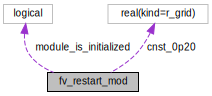
\includegraphics[width=248pt]{classfv__restart__mod__coll__graph}
\end{center}
\end{figure}
\subsection*{Public Member Functions}
\begin{DoxyCompactItemize}
\item 
subroutine, public \hyperlink{classfv__restart__mod_a621f1e1f020776cafc4138bbb7d1cad8}{fv\-\_\-restart\-\_\-init} ()
\item 
subroutine, public \hyperlink{classfv__restart__mod_aaa447f67223fef4de61917a1a912a133}{fv\-\_\-restart} (fv\-\_\-domain, Atm, dt\-\_\-atmos, seconds, days, cold\-\_\-start, grid\-\_\-type, grids\-\_\-on\-\_\-this\-\_\-pe)
\begin{DoxyCompactList}\small\item\em The subroutine 'fv\-\_\-restart' initializes the model state, including prognaostic variables and several auxiliary pressure variables. \end{DoxyCompactList}\item 
subroutine, public \hyperlink{classfv__restart__mod_a3edb12b5afa532405af7999fe51c072c}{setup\-\_\-nested\-\_\-boundary\-\_\-halo} (Atm, proc\-\_\-in)
\item 
subroutine, public \hyperlink{classfv__restart__mod_a4e73a658fb6e3a1e2425e248c355a777}{fv\-\_\-write\-\_\-restart} (Atm, grids\-\_\-on\-\_\-this\-\_\-pe, timestamp)
\begin{DoxyCompactList}\small\item\em The subroutine 'fv\-\_\-write\-\_\-restart' writes restart files to disk. \end{DoxyCompactList}\item 
subroutine, public \hyperlink{classfv__restart__mod_aff5124feaf0d1c21d2ce048759630069}{fv\-\_\-restart\-\_\-end} (Atm, grids\-\_\-on\-\_\-this\-\_\-pe, restart\-\_\-endfcst)
\begin{DoxyCompactList}\small\item\em The subroutine 'fv\-\_\-restart\-\_\-end' writes ending restart files, terminates I/\-O, and prints out diagnostics including global totals and checksums. \end{DoxyCompactList}\item 
subroutine, public \hyperlink{classfv__restart__mod_aecfdd9a6af6ad75d5ab832269949a793}{d2c\-\_\-setup} (u, v, ua, va, uc, vc, dord4, isd, ied, jsd, jed, is, ie, js, je, npx, npy, grid\-\_\-type, nested, se\-\_\-corner, sw\-\_\-corner, ne\-\_\-corner, nw\-\_\-corner, rsin\-\_\-u, rsin\-\_\-v, cosa\-\_\-s, rsin2, regional)
\item 
subroutine, public \hyperlink{classfv__restart__mod_a746a84a5ae424f0b7b042212ff2c2492}{d2a\-\_\-setup} (u, v, ua, va, dord4, isd, ied, jsd, jed, is, ie, js, je, npx, npy, grid\-\_\-type, nested, cosa\-\_\-s, rsin2, regional)
\end{DoxyCompactItemize}
\subsection*{Private Member Functions}
\begin{DoxyCompactItemize}
\item 
subroutine \hyperlink{classfv__restart__mod_a12dc324285c0ec23f0c742d06d2b637f}{fill\-\_\-nested\-\_\-grid\-\_\-topo\-\_\-halo} (Atm, proc\-\_\-in)
\item 
subroutine \hyperlink{classfv__restart__mod_ac212a456cf892280643929f21d2cd55f}{fill\-\_\-nested\-\_\-grid\-\_\-topo} (Atm, proc\-\_\-in)
\begin{DoxyCompactList}\small\item\em The subroutine 'fill\-\_\-nested\-\_\-grid\-\_\-topo' fills the nested grid with topo to enable boundary smoothing. \end{DoxyCompactList}\item 
subroutine \hyperlink{classfv__restart__mod_a54c619910fcd65101de5606a7d0b80ce}{fill\-\_\-nested\-\_\-grid\-\_\-data} (Atm, proc\-\_\-in)
\item 
subroutine \hyperlink{classfv__restart__mod_a1ec25741812e135900a2d3f2f4c9d33f}{fill\-\_\-nested\-\_\-grid\-\_\-data\-\_\-end} (Atm, proc\-\_\-in)
\begin{DoxyCompactList}\small\item\em The subroutine ' fill\-\_\-nested\-\_\-grid\-\_\-data\-\_\-end' actually sets up the coarse-\/grid T\-O\-P\-O\-G\-R\-A\-P\-H\-Y. \end{DoxyCompactList}\item 
subroutine \hyperlink{classfv__restart__mod_a1e1dd2798792970c4e9977ce480e5b4a}{pmaxmn\-\_\-g} (qname, q, is, ie, js, je, km, fac, area, domain)
\begin{DoxyCompactList}\small\item\em The subroutine 'pmaxn\-\_\-g' writes domain max, min, and averages quantities. \end{DoxyCompactList}\end{DoxyCompactItemize}
\subsection*{Private Attributes}
\begin{DoxyCompactItemize}
\item 
real(kind=r\-\_\-grid), parameter \hyperlink{classfv__restart__mod_a2b60f0f737ab9928fd9c6ccbd7daf754}{cnst\-\_\-0p20} =0.\-20d0
\item 
logical \hyperlink{classfv__restart__mod_acf880b4cfc12d08f29edb14fd1ca6a32}{module\-\_\-is\-\_\-initialized} = .F\-A\-L\-S\-E.
\end{DoxyCompactItemize}


\subsection{Detailed Description}


Definition at line 22 of file fv\-\_\-restart.\-F90.



\subsection{Member Function/\-Subroutine Documentation}
\index{fv\-\_\-restart\-\_\-mod@{fv\-\_\-restart\-\_\-mod}!d2a\-\_\-setup@{d2a\-\_\-setup}}
\index{d2a\-\_\-setup@{d2a\-\_\-setup}!fv_restart_mod@{fv\-\_\-restart\-\_\-mod}}
\subsubsection[{d2a\-\_\-setup}]{\setlength{\rightskip}{0pt plus 5cm}subroutine, public fv\-\_\-restart\-\_\-mod\-::d2a\-\_\-setup (
\begin{DoxyParamCaption}
\item[{real, dimension(isd\-:ied,jsd\-:jed+1), intent(in)}]{u, }
\item[{real, dimension(isd\-:ied+1,jsd\-:jed), intent(in)}]{v, }
\item[{real, dimension(isd\-:ied  ,jsd\-:jed  ), intent(out)}]{ua, }
\item[{real, dimension(isd\-:ied  ,jsd\-:jed  ), intent(out)}]{va, }
\item[{logical, intent(in)}]{dord4, }
\item[{integer, intent(in)}]{isd, }
\item[{integer, intent(in)}]{ied, }
\item[{integer, intent(in)}]{jsd, }
\item[{integer, intent(in)}]{jed, }
\item[{integer, intent(in)}]{is, }
\item[{integer, intent(in)}]{ie, }
\item[{integer, intent(in)}]{js, }
\item[{integer, intent(in)}]{je, }
\item[{integer, intent(in)}]{npx, }
\item[{integer, intent(in)}]{npy, }
\item[{integer, intent(in)}]{grid\-\_\-type, }
\item[{logical, intent(in)}]{nested, }
\item[{real, dimension(isd\-:ied,jsd\-:jed), intent(in)}]{cosa\-\_\-s, }
\item[{real, dimension(isd\-:ied,jsd\-:jed), intent(in)}]{rsin2, }
\item[{logical, intent(in)}]{regional}
\end{DoxyParamCaption}
)}\label{classfv__restart__mod_a746a84a5ae424f0b7b042212ff2c2492}


Definition at line 1826 of file fv\-\_\-restart.\-F90.

\index{fv\-\_\-restart\-\_\-mod@{fv\-\_\-restart\-\_\-mod}!d2c\-\_\-setup@{d2c\-\_\-setup}}
\index{d2c\-\_\-setup@{d2c\-\_\-setup}!fv_restart_mod@{fv\-\_\-restart\-\_\-mod}}
\subsubsection[{d2c\-\_\-setup}]{\setlength{\rightskip}{0pt plus 5cm}subroutine, public fv\-\_\-restart\-\_\-mod\-::d2c\-\_\-setup (
\begin{DoxyParamCaption}
\item[{real, dimension(isd\-:ied,jsd\-:jed+1), intent(in)}]{u, }
\item[{real, dimension(isd\-:ied+1,jsd\-:jed), intent(in)}]{v, }
\item[{real, dimension(isd\-:ied  ,jsd\-:jed  ), intent(out)}]{ua, }
\item[{real, dimension(isd\-:ied  ,jsd\-:jed  ), intent(out)}]{va, }
\item[{real, dimension(isd\-:ied+1,jsd\-:jed  ), intent(out)}]{uc, }
\item[{real, dimension(isd\-:ied  ,jsd\-:jed+1), intent(out)}]{vc, }
\item[{logical, intent(in)}]{dord4, }
\item[{integer, intent(in)}]{isd, }
\item[{integer, intent(in)}]{ied, }
\item[{integer, intent(in)}]{jsd, }
\item[{integer, intent(in)}]{jed, }
\item[{integer, intent(in)}]{is, }
\item[{integer, intent(in)}]{ie, }
\item[{integer, intent(in)}]{js, }
\item[{integer, intent(in)}]{je, }
\item[{integer, intent(in)}]{npx, }
\item[{integer, intent(in)}]{npy, }
\item[{integer, intent(in)}]{grid\-\_\-type, }
\item[{logical, intent(in)}]{nested, }
\item[{logical, intent(in)}]{se\-\_\-corner, }
\item[{logical, intent(in)}]{sw\-\_\-corner, }
\item[{logical, intent(in)}]{ne\-\_\-corner, }
\item[{logical, intent(in)}]{nw\-\_\-corner, }
\item[{real, dimension(isd\-:ied+1,jsd\-:jed), intent(in)}]{rsin\-\_\-u, }
\item[{real, dimension(isd\-:ied,jsd\-:jed+1), intent(in)}]{rsin\-\_\-v, }
\item[{real, dimension(isd\-:ied,jsd\-:jed), intent(in)}]{cosa\-\_\-s, }
\item[{real, dimension(isd\-:ied,jsd\-:jed), intent(in)}]{rsin2, }
\item[{logical, intent(in)}]{regional}
\end{DoxyParamCaption}
)}\label{classfv__restart__mod_aecfdd9a6af6ad75d5ab832269949a793}


Definition at line 1548 of file fv\-\_\-restart.\-F90.



Referenced by fv\-\_\-nesting\-\_\-mod\-::setup\-\_\-nested\-\_\-grid\-\_\-bcs().

\index{fv\-\_\-restart\-\_\-mod@{fv\-\_\-restart\-\_\-mod}!fill\-\_\-nested\-\_\-grid\-\_\-data@{fill\-\_\-nested\-\_\-grid\-\_\-data}}
\index{fill\-\_\-nested\-\_\-grid\-\_\-data@{fill\-\_\-nested\-\_\-grid\-\_\-data}!fv_restart_mod@{fv\-\_\-restart\-\_\-mod}}
\subsubsection[{fill\-\_\-nested\-\_\-grid\-\_\-data}]{\setlength{\rightskip}{0pt plus 5cm}subroutine fv\-\_\-restart\-\_\-mod\-::fill\-\_\-nested\-\_\-grid\-\_\-data (
\begin{DoxyParamCaption}
\item[{type(fv\-\_\-atmos\-\_\-type), dimension(\-:), intent(inout)}]{Atm, }
\item[{logical, intent(in), optional}]{proc\-\_\-in}
\end{DoxyParamCaption}
)\hspace{0.3cm}{\ttfamily [private]}}\label{classfv__restart__mod_a54c619910fcd65101de5606a7d0b80ce}


Definition at line 944 of file fv\-\_\-restart.\-F90.



References fv\-\_\-timing\-\_\-mod\-::timing\-\_\-off(), fv\-\_\-timing\-\_\-mod\-::timing\-\_\-on(), and multi\-\_\-gases\-\_\-mod\-::virq().



Referenced by fv\-\_\-restart().

\index{fv\-\_\-restart\-\_\-mod@{fv\-\_\-restart\-\_\-mod}!fill\-\_\-nested\-\_\-grid\-\_\-data\-\_\-end@{fill\-\_\-nested\-\_\-grid\-\_\-data\-\_\-end}}
\index{fill\-\_\-nested\-\_\-grid\-\_\-data\-\_\-end@{fill\-\_\-nested\-\_\-grid\-\_\-data\-\_\-end}!fv_restart_mod@{fv\-\_\-restart\-\_\-mod}}
\subsubsection[{fill\-\_\-nested\-\_\-grid\-\_\-data\-\_\-end}]{\setlength{\rightskip}{0pt plus 5cm}subroutine fv\-\_\-restart\-\_\-mod\-::fill\-\_\-nested\-\_\-grid\-\_\-data\-\_\-end (
\begin{DoxyParamCaption}
\item[{type(fv\-\_\-atmos\-\_\-type), intent(inout)}]{Atm, }
\item[{logical, intent(in), optional}]{proc\-\_\-in}
\end{DoxyParamCaption}
)\hspace{0.3cm}{\ttfamily [private]}}\label{classfv__restart__mod_a1ec25741812e135900a2d3f2f4c9d33f}


The subroutine ' fill\-\_\-nested\-\_\-grid\-\_\-data\-\_\-end' actually sets up the coarse-\/grid T\-O\-P\-O\-G\-R\-A\-P\-H\-Y. 



Definition at line 1322 of file fv\-\_\-restart.\-F90.



References init\-\_\-hydro\-\_\-mod\-::p\-\_\-var().



Referenced by fv\-\_\-restart().

\index{fv\-\_\-restart\-\_\-mod@{fv\-\_\-restart\-\_\-mod}!fill\-\_\-nested\-\_\-grid\-\_\-topo@{fill\-\_\-nested\-\_\-grid\-\_\-topo}}
\index{fill\-\_\-nested\-\_\-grid\-\_\-topo@{fill\-\_\-nested\-\_\-grid\-\_\-topo}!fv_restart_mod@{fv\-\_\-restart\-\_\-mod}}
\subsubsection[{fill\-\_\-nested\-\_\-grid\-\_\-topo}]{\setlength{\rightskip}{0pt plus 5cm}subroutine fv\-\_\-restart\-\_\-mod\-::fill\-\_\-nested\-\_\-grid\-\_\-topo (
\begin{DoxyParamCaption}
\item[{type(fv\-\_\-atmos\-\_\-type), intent(inout)}]{Atm, }
\item[{logical, intent(in), optional}]{proc\-\_\-in}
\end{DoxyParamCaption}
)\hspace{0.3cm}{\ttfamily [private]}}\label{classfv__restart__mod_ac212a456cf892280643929f21d2cd55f}


The subroutine 'fill\-\_\-nested\-\_\-grid\-\_\-topo' fills the nested grid with topo to enable boundary smoothing. 

Interior topography is then over-\/written in get\-\_\-external\-\_\-ic. 

Definition at line 884 of file fv\-\_\-restart.\-F90.



References fv\-\_\-timing\-\_\-mod\-::timing\-\_\-off(), and fv\-\_\-timing\-\_\-mod\-::timing\-\_\-on().



Referenced by fv\-\_\-restart().

\index{fv\-\_\-restart\-\_\-mod@{fv\-\_\-restart\-\_\-mod}!fill\-\_\-nested\-\_\-grid\-\_\-topo\-\_\-halo@{fill\-\_\-nested\-\_\-grid\-\_\-topo\-\_\-halo}}
\index{fill\-\_\-nested\-\_\-grid\-\_\-topo\-\_\-halo@{fill\-\_\-nested\-\_\-grid\-\_\-topo\-\_\-halo}!fv_restart_mod@{fv\-\_\-restart\-\_\-mod}}
\subsubsection[{fill\-\_\-nested\-\_\-grid\-\_\-topo\-\_\-halo}]{\setlength{\rightskip}{0pt plus 5cm}subroutine fv\-\_\-restart\-\_\-mod\-::fill\-\_\-nested\-\_\-grid\-\_\-topo\-\_\-halo (
\begin{DoxyParamCaption}
\item[{type(fv\-\_\-atmos\-\_\-type), intent(inout)}]{Atm, }
\item[{logical, intent(in), optional}]{proc\-\_\-in}
\end{DoxyParamCaption}
)\hspace{0.3cm}{\ttfamily [private]}}\label{classfv__restart__mod_a12dc324285c0ec23f0c742d06d2b637f}


Definition at line 863 of file fv\-\_\-restart.\-F90.



Referenced by fv\-\_\-restart().

\index{fv\-\_\-restart\-\_\-mod@{fv\-\_\-restart\-\_\-mod}!fv\-\_\-restart@{fv\-\_\-restart}}
\index{fv\-\_\-restart@{fv\-\_\-restart}!fv_restart_mod@{fv\-\_\-restart\-\_\-mod}}
\subsubsection[{fv\-\_\-restart}]{\setlength{\rightskip}{0pt plus 5cm}subroutine, public fv\-\_\-restart\-\_\-mod\-::fv\-\_\-restart (
\begin{DoxyParamCaption}
\item[{type(domain2d), intent(inout)}]{fv\-\_\-domain, }
\item[{type(fv\-\_\-atmos\-\_\-type), dimension(\-:), intent(inout)}]{Atm, }
\item[{real, intent(in)}]{dt\-\_\-atmos, }
\item[{integer, intent(out)}]{seconds, }
\item[{integer, intent(out)}]{days, }
\item[{logical, intent(inout)}]{cold\-\_\-start, }
\item[{integer, intent(in)}]{grid\-\_\-type, }
\item[{logical, dimension(\-:), intent(inout)}]{grids\-\_\-on\-\_\-this\-\_\-pe}
\end{DoxyParamCaption}
)}\label{classfv__restart__mod_aaa447f67223fef4de61917a1a912a133}


The subroutine 'fv\-\_\-restart' initializes the model state, including prognaostic variables and several auxiliary pressure variables. 

The modules also writes out restart files at the end of the model run, and prints out diagnostics of the initial state. There are several options to control the initialization process. 

Definition at line 195 of file fv\-\_\-restart.\-F90.



References fv\-\_\-eta\-\_\-mod\-::compute\-\_\-dz\-\_\-l32(), fv\-\_\-eta\-\_\-mod\-::compute\-\_\-dz\-\_\-var(), fv\-\_\-grid\-\_\-utils\-\_\-mod\-::cubed\-\_\-to\-\_\-latlon(), fv\-\_\-surf\-\_\-map\-\_\-mod\-::del2\-\_\-cubed\-\_\-sphere(), fv\-\_\-surf\-\_\-map\-\_\-mod\-::del4\-\_\-cubed\-\_\-sphere(), fill\-\_\-nested\-\_\-grid\-\_\-data(), fill\-\_\-nested\-\_\-grid\-\_\-data\-\_\-end(), fill\-\_\-nested\-\_\-grid\-\_\-topo(), fill\-\_\-nested\-\_\-grid\-\_\-topo\-\_\-halo(), fv\-\_\-io\-\_\-mod\-::fv\-\_\-io\-\_\-read\-\_\-bcs(), fv\-\_\-io\-\_\-mod\-::fv\-\_\-io\-\_\-read\-\_\-restart(), fv\-\_\-io\-\_\-mod\-::fv\-\_\-io\-\_\-register\-\_\-restart(), fv\-\_\-io\-\_\-mod\-::fv\-\_\-io\-\_\-register\-\_\-restart\-\_\-bcs(), fv\-\_\-io\-\_\-mod\-::fv\-\_\-io\-\_\-register\-\_\-restart\-\_\-bcs\-\_\-nh(), external\-\_\-ic\-\_\-mod\-::get\-\_\-external\-\_\-ic(), test\-\_\-cases\-\_\-mod\-::init\-\_\-case(), test\-\_\-cases\-\_\-mod\-::init\-\_\-double\-\_\-periodic(), test\-\_\-cases\-\_\-mod\-::init\-\_\-latlon(), init\-\_\-hydro\-\_\-mod\-::p\-\_\-var(), pmaxmn\-\_\-g(), fv\-\_\-diagnostics\-\_\-mod\-::prt\-\_\-maxmin(), fv\-\_\-treat\-\_\-da\-\_\-inc\-\_\-mod\-::read\-\_\-da\-\_\-inc(), fv\-\_\-io\-\_\-mod\-::remap\-\_\-restart(), fv\-\_\-eta\-\_\-mod\-::set\-\_\-hybrid\-\_\-z(), and setup\-\_\-nested\-\_\-boundary\-\_\-halo().



Referenced by atmosphere\-\_\-mod\-::atmosphere\-\_\-init().

\index{fv\-\_\-restart\-\_\-mod@{fv\-\_\-restart\-\_\-mod}!fv\-\_\-restart\-\_\-end@{fv\-\_\-restart\-\_\-end}}
\index{fv\-\_\-restart\-\_\-end@{fv\-\_\-restart\-\_\-end}!fv_restart_mod@{fv\-\_\-restart\-\_\-mod}}
\subsubsection[{fv\-\_\-restart\-\_\-end}]{\setlength{\rightskip}{0pt plus 5cm}subroutine, public fv\-\_\-restart\-\_\-mod\-::fv\-\_\-restart\-\_\-end (
\begin{DoxyParamCaption}
\item[{type(fv\-\_\-atmos\-\_\-type), dimension(\-:), intent(inout)}]{Atm, }
\item[{logical, dimension(\-:), intent(inout)}]{grids\-\_\-on\-\_\-this\-\_\-pe, }
\item[{logical, intent(in)}]{restart\-\_\-endfcst}
\end{DoxyParamCaption}
)}\label{classfv__restart__mod_aff5124feaf0d1c21d2ce048759630069}


The subroutine 'fv\-\_\-restart\-\_\-end' writes ending restart files, terminates I/\-O, and prints out diagnostics including global totals and checksums. 



Definition at line 1437 of file fv\-\_\-restart.\-F90.



References fv\-\_\-io\-\_\-mod\-::fv\-\_\-io\-\_\-write\-\_\-bcs(), fv\-\_\-io\-\_\-mod\-::fv\-\_\-io\-\_\-write\-\_\-restart(), pmaxmn\-\_\-g(), and fv\-\_\-diagnostics\-\_\-mod\-::prt\-\_\-maxmin().



Referenced by fv\-\_\-control\-\_\-mod\-::fv\-\_\-end().

\index{fv\-\_\-restart\-\_\-mod@{fv\-\_\-restart\-\_\-mod}!fv\-\_\-restart\-\_\-init@{fv\-\_\-restart\-\_\-init}}
\index{fv\-\_\-restart\-\_\-init@{fv\-\_\-restart\-\_\-init}!fv_restart_mod@{fv\-\_\-restart\-\_\-mod}}
\subsubsection[{fv\-\_\-restart\-\_\-init}]{\setlength{\rightskip}{0pt plus 5cm}subroutine, public fv\-\_\-restart\-\_\-mod\-::fv\-\_\-restart\-\_\-init (
\begin{DoxyParamCaption}
{}
\end{DoxyParamCaption}
)}\label{classfv__restart__mod_a621f1e1f020776cafc4138bbb7d1cad8}


Definition at line 185 of file fv\-\_\-restart.\-F90.



References fv\-\_\-io\-\_\-mod\-::fv\-\_\-io\-\_\-init().



Referenced by fv\-\_\-control\-\_\-mod\-::fv\-\_\-init().

\index{fv\-\_\-restart\-\_\-mod@{fv\-\_\-restart\-\_\-mod}!fv\-\_\-write\-\_\-restart@{fv\-\_\-write\-\_\-restart}}
\index{fv\-\_\-write\-\_\-restart@{fv\-\_\-write\-\_\-restart}!fv_restart_mod@{fv\-\_\-restart\-\_\-mod}}
\subsubsection[{fv\-\_\-write\-\_\-restart}]{\setlength{\rightskip}{0pt plus 5cm}subroutine, public fv\-\_\-restart\-\_\-mod\-::fv\-\_\-write\-\_\-restart (
\begin{DoxyParamCaption}
\item[{type(fv\-\_\-atmos\-\_\-type), dimension(\-:), intent(inout)}]{Atm, }
\item[{logical, dimension(\-:), intent(in)}]{grids\-\_\-on\-\_\-this\-\_\-pe, }
\item[{character(len=$\ast$), intent(in)}]{timestamp}
\end{DoxyParamCaption}
)}\label{classfv__restart__mod_a4e73a658fb6e3a1e2425e248c355a777}


The subroutine 'fv\-\_\-write\-\_\-restart' writes restart files to disk. 

This subroutine may be called during an integration to write out intermediate restart files. 

Definition at line 1419 of file fv\-\_\-restart.\-F90.



References fv\-\_\-io\-\_\-mod\-::fv\-\_\-io\-\_\-write\-\_\-bcs(), and fv\-\_\-io\-\_\-mod\-::fv\-\_\-io\-\_\-write\-\_\-restart().



Referenced by atmosphere\-\_\-mod\-::atmosphere\-\_\-restart().

\index{fv\-\_\-restart\-\_\-mod@{fv\-\_\-restart\-\_\-mod}!pmaxmn\-\_\-g@{pmaxmn\-\_\-g}}
\index{pmaxmn\-\_\-g@{pmaxmn\-\_\-g}!fv_restart_mod@{fv\-\_\-restart\-\_\-mod}}
\subsubsection[{pmaxmn\-\_\-g}]{\setlength{\rightskip}{0pt plus 5cm}subroutine fv\-\_\-restart\-\_\-mod\-::pmaxmn\-\_\-g (
\begin{DoxyParamCaption}
\item[{character(len=$\ast$), intent(in)}]{qname, }
\item[{real, dimension(is-\/3\-:ie+3, js-\/3\-:je+3, km), intent(in)}]{q, }
\item[{integer, intent(in)}]{is, }
\item[{integer, intent(in)}]{ie, }
\item[{integer, intent(in)}]{js, }
\item[{integer, intent(in)}]{je, }
\item[{integer, intent(in)}]{km, }
\item[{real, intent(in)}]{fac, }
\item[{real(kind=r\-\_\-grid), dimension(is-\/3\-:ie+3, js-\/3\-:je+3), intent(in)}]{area, }
\item[{type(domain2d), intent(inout)}]{domain}
\end{DoxyParamCaption}
)\hspace{0.3cm}{\ttfamily [private]}}\label{classfv__restart__mod_a1e1dd2798792970c4e9977ce480e5b4a}


The subroutine 'pmaxn\-\_\-g' writes domain max, min, and averages quantities. 



Definition at line 1962 of file fv\-\_\-restart.\-F90.



References fv\-\_\-grid\-\_\-utils\-\_\-mod\-::g\-\_\-sum().



Referenced by fv\-\_\-restart(), and fv\-\_\-restart\-\_\-end().

\index{fv\-\_\-restart\-\_\-mod@{fv\-\_\-restart\-\_\-mod}!setup\-\_\-nested\-\_\-boundary\-\_\-halo@{setup\-\_\-nested\-\_\-boundary\-\_\-halo}}
\index{setup\-\_\-nested\-\_\-boundary\-\_\-halo@{setup\-\_\-nested\-\_\-boundary\-\_\-halo}!fv_restart_mod@{fv\-\_\-restart\-\_\-mod}}
\subsubsection[{setup\-\_\-nested\-\_\-boundary\-\_\-halo}]{\setlength{\rightskip}{0pt plus 5cm}subroutine, public fv\-\_\-restart\-\_\-mod\-::setup\-\_\-nested\-\_\-boundary\-\_\-halo (
\begin{DoxyParamCaption}
\item[{type(fv\-\_\-atmos\-\_\-type), intent(inout)}]{Atm, }
\item[{logical, intent(in), optional}]{proc\-\_\-in}
\end{DoxyParamCaption}
)}\label{classfv__restart__mod_a3edb12b5afa532405af7999fe51c072c}


Definition at line 715 of file fv\-\_\-restart.\-F90.



Referenced by fv\-\_\-restart().



\subsection{Member Data Documentation}
\index{fv\-\_\-restart\-\_\-mod@{fv\-\_\-restart\-\_\-mod}!cnst\-\_\-0p20@{cnst\-\_\-0p20}}
\index{cnst\-\_\-0p20@{cnst\-\_\-0p20}!fv_restart_mod@{fv\-\_\-restart\-\_\-mod}}
\subsubsection[{cnst\-\_\-0p20}]{\setlength{\rightskip}{0pt plus 5cm}real(kind=r\-\_\-grid), parameter fv\-\_\-restart\-\_\-mod\-::cnst\-\_\-0p20 =0.\-20d0\hspace{0.3cm}{\ttfamily [private]}}\label{classfv__restart__mod_a2b60f0f737ab9928fd9c6ccbd7daf754}


Definition at line 178 of file fv\-\_\-restart.\-F90.

\index{fv\-\_\-restart\-\_\-mod@{fv\-\_\-restart\-\_\-mod}!module\-\_\-is\-\_\-initialized@{module\-\_\-is\-\_\-initialized}}
\index{module\-\_\-is\-\_\-initialized@{module\-\_\-is\-\_\-initialized}!fv_restart_mod@{fv\-\_\-restart\-\_\-mod}}
\subsubsection[{module\-\_\-is\-\_\-initialized}]{\setlength{\rightskip}{0pt plus 5cm}logical fv\-\_\-restart\-\_\-mod\-::module\-\_\-is\-\_\-initialized = .F\-A\-L\-S\-E.\hspace{0.3cm}{\ttfamily [private]}}\label{classfv__restart__mod_acf880b4cfc12d08f29edb14fd1ca6a32}


Definition at line 180 of file fv\-\_\-restart.\-F90.



The documentation for this module was generated from the following file\-:\begin{DoxyCompactItemize}
\item 
/scratch2/\-N\-A\-G\-A\-P\-E/aoml-\/hafs1/\-Kyle.\-Ahern/acs\-\_\-master\-\_\-readonly/tools/\hyperlink{fv__restart_8F90}{fv\-\_\-restart.\-F90}\end{DoxyCompactItemize}

\section{fv\-\_\-sg\-\_\-mod Module Reference}
\label{classfv__sg__mod}\index{fv\-\_\-sg\-\_\-mod@{fv\-\_\-sg\-\_\-mod}}


The module 'fv\-\_\-sg' performs F\-V sub-\/grid mixing.  




Collaboration diagram for fv\-\_\-sg\-\_\-mod\-:
\nopagebreak
\begin{figure}[H]
\begin{center}
\leavevmode
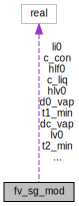
\includegraphics[width=115pt]{classfv__sg__mod__coll__graph}
\end{center}
\end{figure}
\subsection*{Public Member Functions}
\begin{DoxyCompactItemize}
\item 
subroutine, public \hyperlink{classfv__sg__mod_a12f8e293e862927c307b386cdd8217cb}{fv\-\_\-subgrid\-\_\-z} (isd, ied, jsd, jed, is, ie, js, je, km, nq, dt, tau, nwat, delp, pe, peln, pkz, ta, qa, ua, va, hydrostatic, w, delz, u\-\_\-dt, v\-\_\-dt, t\-\_\-dt, q\-\_\-dt, k\-\_\-bot)
\item 
subroutine, public \hyperlink{classfv__sg__mod_a091058b73522dcd58a8f2787aa4c9973}{qsmith} (im, km, k1, t, p, q, qs, dqdt)
\item 
subroutine, public \hyperlink{classfv__sg__mod_a8d257ccad66089458515a550f71a4855}{neg\-\_\-adj3} (is, ie, js, je, ng, kbot, hydrostatic, peln, delz, pt, dp,
\item 
subroutine, public \hyperlink{classfv__sg__mod_aca56b99deacecc35854d54c6978dc131}{neg\-\_\-adj2} (is, ie, js, je, ng, kbot, hydrostatic, peln, delz, pt, dp, qv, ql, qr, qi, qs, qa, check\-\_\-negative)
\end{DoxyCompactItemize}
\subsection*{Private Member Functions}
\begin{DoxyCompactItemize}
\item 
subroutine \hyperlink{classfv__sg__mod_aa63d7969bebc93461163d35d3f8c610c}{qsmith\-\_\-init}
\item 
subroutine \hyperlink{classfv__sg__mod_a4ba25958c1903ecd2f5f04bcf596a2aa}{qs\-\_\-table} (n, \hyperlink{classfv__sg__mod_a209ce37aa7b7e0fd8d042d2cd4cdacca}{table})
\item 
subroutine \hyperlink{classfv__sg__mod_a86dda2330b414a3e21cceed0e114f03f}{qs\-\_\-table\-\_\-m} (n, \hyperlink{classfv__sg__mod_a209ce37aa7b7e0fd8d042d2cd4cdacca}{table})
\item 
subroutine \hyperlink{classfv__sg__mod_a5308d44cc53f56bfd55451f11445eff0}{fillq} (im, km, q, dp)
\item 
subroutine \hyperlink{classfv__sg__mod_a14c9331c9654c3cfc6a7aca840bdbd30}{prt\-\_\-negative} (qname, q, is, ie, js, je, n\-\_\-g, km, threshold)
\end{DoxyCompactItemize}
\subsection*{Private Attributes}
\begin{DoxyCompactItemize}
\item 
real, parameter \hyperlink{classfv__sg__mod_af4058b7b266d23d4f30e73514cd0d403}{esl} = 0.\-621971831
\item 
real, parameter \hyperlink{classfv__sg__mod_a87874cc5d80d9ea6ee4f67ae591ef080}{tice} = 273.\-16
\item 
real, parameter \hyperlink{classfv__sg__mod_a84f3c846b418dad59c6ab9ab7987ead7}{c\-\_\-ice} = 1972.
\begin{DoxyCompactList}\small\item\em -\/15 C \end{DoxyCompactList}\item 
real, parameter \hyperlink{classfv__sg__mod_a410bbdf1e319c65ea3a200ce8aceda8a}{c\-\_\-liq} = 4.\-1855e+3
\begin{DoxyCompactList}\small\item\em G\-F\-S. \end{DoxyCompactList}\item 
real, parameter \hyperlink{classfv__sg__mod_ab4b7454109972c7d688beea157f279a1}{cv\-\_\-vap} = cp\-\_\-vapor -\/ rvgas
\begin{DoxyCompactList}\small\item\em 1384.\-5 \end{DoxyCompactList}\item 
real, parameter \hyperlink{classfv__sg__mod_a244f143b09b1f0b2dfef9acb1b4e64a7}{c\-\_\-con} = \hyperlink{classfv__sg__mod_a84f3c846b418dad59c6ab9ab7987ead7}{c\-\_\-ice}
\item 
real, parameter \hyperlink{classfv__sg__mod_a801d775ff0bd22525d3bdbfdbaa25a93}{dc\-\_\-vap} = \hyperlink{classfv__sg__mod_ab4b7454109972c7d688beea157f279a1}{cv\-\_\-vap} -\/ \hyperlink{classfv__sg__mod_a410bbdf1e319c65ea3a200ce8aceda8a}{c\-\_\-liq}
\begin{DoxyCompactList}\small\item\em = -\/2368. \end{DoxyCompactList}\item 
real, parameter \hyperlink{classfv__sg__mod_a78cb86127e174c40e9c96f9ad386cd51}{dc\-\_\-ice} = \hyperlink{classfv__sg__mod_a410bbdf1e319c65ea3a200ce8aceda8a}{c\-\_\-liq} -\/ \hyperlink{classfv__sg__mod_a84f3c846b418dad59c6ab9ab7987ead7}{c\-\_\-ice}
\begin{DoxyCompactList}\small\item\em = 2112. \end{DoxyCompactList}\item 
real, parameter \hyperlink{classfv__sg__mod_a3b888bbbc28cceecf2d4157bc40f7e97}{hlv0} = 2.\-5e6
\item 
real, parameter \hyperlink{classfv__sg__mod_a0ef6edb91d65d124d913ef57e02e588c}{hlf0} = 3.\-3358e5
\item 
real, parameter \hyperlink{classfv__sg__mod_a46dc612b8ea952b410d9388e7734b1dc}{t\-\_\-ice} = 273.\-16
\item 
real, parameter \hyperlink{classfv__sg__mod_af3111561e3086d6011cf81c50467d561}{ri\-\_\-max} = 1.
\item 
real, parameter \hyperlink{classfv__sg__mod_a5a016eeeb112ccb46087279e37698ecb}{ri\-\_\-min} = 0.\-25
\item 
real, parameter \hyperlink{classfv__sg__mod_afe8eeeb134260859c1ff38fe74557123}{t1\-\_\-min} = 160.
\item 
real, parameter \hyperlink{classfv__sg__mod_ad9aa2baea22c517457629ab6821992fa}{t2\-\_\-min} = 165.
\item 
real, parameter \hyperlink{classfv__sg__mod_a17bd270ea0dba7816112efe5d704896c}{t2\-\_\-max} = 315.
\item 
real, parameter \hyperlink{classfv__sg__mod_a3d2e9d81e47d9e0be757a3b2978f00f3}{t3\-\_\-max} = 325.
\item 
real, parameter \hyperlink{classfv__sg__mod_a81ad127cb875ed67c0b2b72faddbd28b}{lv0} = \hyperlink{classfv__sg__mod_a3b888bbbc28cceecf2d4157bc40f7e97}{hlv0} -\/ \hyperlink{classfv__sg__mod_a801d775ff0bd22525d3bdbfdbaa25a93}{dc\-\_\-vap}$\ast$\hyperlink{classfv__sg__mod_a46dc612b8ea952b410d9388e7734b1dc}{t\-\_\-ice}
\begin{DoxyCompactList}\small\item\em = 3.\-147782e6 \end{DoxyCompactList}\item 
real, parameter \hyperlink{classfv__sg__mod_a5c833712f86de131c6bdc48cac46909e}{li0} = \hyperlink{classfv__sg__mod_a0ef6edb91d65d124d913ef57e02e588c}{hlf0} -\/ \hyperlink{classfv__sg__mod_a78cb86127e174c40e9c96f9ad386cd51}{dc\-\_\-ice}$\ast$\hyperlink{classfv__sg__mod_a46dc612b8ea952b410d9388e7734b1dc}{t\-\_\-ice}
\begin{DoxyCompactList}\small\item\em = -\/2.\-431928e5 \end{DoxyCompactList}\item 
real, parameter \hyperlink{classfv__sg__mod_a4d8e998e436b110102a6723af127d4df}{zvir} = rvgas/rdgas -\/ 1.
\begin{DoxyCompactList}\small\item\em = 0.\-607789855 \end{DoxyCompactList}\item 
real, dimension(\-:), allocatable \hyperlink{classfv__sg__mod_a209ce37aa7b7e0fd8d042d2cd4cdacca}{table}
\item 
real, dimension(\-:), allocatable \hyperlink{classfv__sg__mod_a3d64c11d4c5914570d3d22b46f4c9d96}{des}
\item 
real \hyperlink{classfv__sg__mod_a853263bfe986528320e887a8a48f1978}{lv00}
\item 
real \hyperlink{classfv__sg__mod_a0de1f9bda133c77954d9607a5833698a}{d0\-\_\-vap}
\end{DoxyCompactItemize}


\subsection{Detailed Description}
The module 'fv\-\_\-sg' performs F\-V sub-\/grid mixing. 

Definition at line 54 of file fv\-\_\-sg.\-F90.



\subsection{Member Function/\-Subroutine Documentation}
\index{fv\-\_\-sg\-\_\-mod@{fv\-\_\-sg\-\_\-mod}!fillq@{fillq}}
\index{fillq@{fillq}!fv_sg_mod@{fv\-\_\-sg\-\_\-mod}}
\subsubsection[{fillq}]{\setlength{\rightskip}{0pt plus 5cm}subroutine fv\-\_\-sg\-\_\-mod\-::fillq (
\begin{DoxyParamCaption}
\item[{integer, intent(in)}]{im, }
\item[{integer, intent(in)}]{km, }
\item[{real, dimension(im,km), intent(inout)}]{q, }
\item[{real, dimension(im,km), intent(inout)}]{dp}
\end{DoxyParamCaption}
)\hspace{0.3cm}{\ttfamily [private]}}\label{classfv__sg__mod_a5308d44cc53f56bfd55451f11445eff0}


Definition at line 2257 of file fv\-\_\-sg.\-F90.

\index{fv\-\_\-sg\-\_\-mod@{fv\-\_\-sg\-\_\-mod}!fv\-\_\-subgrid\-\_\-z@{fv\-\_\-subgrid\-\_\-z}}
\index{fv\-\_\-subgrid\-\_\-z@{fv\-\_\-subgrid\-\_\-z}!fv_sg_mod@{fv\-\_\-sg\-\_\-mod}}
\subsubsection[{fv\-\_\-subgrid\-\_\-z}]{\setlength{\rightskip}{0pt plus 5cm}subroutine, public fv\-\_\-sg\-\_\-mod\-::fv\-\_\-subgrid\-\_\-z (
\begin{DoxyParamCaption}
\item[{integer, intent(in)}]{isd, }
\item[{integer, intent(in)}]{ied, }
\item[{integer, intent(in)}]{jsd, }
\item[{integer, intent(in)}]{jed, }
\item[{integer, intent(in)}]{is, }
\item[{integer, intent(in)}]{ie, }
\item[{integer, intent(in)}]{js, }
\item[{integer, intent(in)}]{je, }
\item[{integer, intent(in)}]{km, }
\item[{integer, intent(in)}]{nq, }
\item[{real, intent(in)}]{dt, }
\item[{integer, intent(in)}]{tau, }
\item[{integer, intent(in)}]{nwat, }
\item[{real, dimension(isd\-:ied,jsd\-:jed,km), intent(in)}]{delp, }
\item[{real, dimension(is-\/1\-:ie+1,km+1,js-\/1\-:je+1), intent(in)}]{pe, }
\item[{real, dimension(is  \-:ie,  km+1,js  \-:je), intent(in)}]{peln, }
\item[{real, dimension(is\-:ie,js\-:je,km), intent(in)}]{pkz, }
\item[{real, dimension(isd\-:ied,jsd\-:jed,km), intent(inout)}]{ta, }
\item[{real, dimension(isd\-:ied,jsd\-:jed,km,nq), intent(inout)}]{qa, }
\item[{real, dimension(isd\-:ied,jsd\-:jed,km), intent(inout)}]{ua, }
\item[{real, dimension(isd\-:ied,jsd\-:jed,km), intent(inout)}]{va, }
\item[{logical, intent(in)}]{hydrostatic, }
\item[{real, dimension(isd\-:,jsd\-:,1\-:), intent(inout)}]{w, }
\item[{real, dimension(isd\-:,jsd\-:,1\-:), intent(in)}]{delz, }
\item[{real, dimension(isd\-:ied,jsd\-:jed,km), intent(inout)}]{u\-\_\-dt, }
\item[{real, dimension(isd\-:ied,jsd\-:jed,km), intent(inout)}]{v\-\_\-dt, }
\item[{real, dimension(is\-:ie,js\-:je,km), intent(inout)}]{t\-\_\-dt, }
\item[{real, dimension(is\-:ie,js\-:je,km,nq), intent(inout)}]{q\-\_\-dt, }
\item[{integer, intent(in), optional}]{k\-\_\-bot}
\end{DoxyParamCaption}
)}\label{classfv__sg__mod_a12f8e293e862927c307b386cdd8217cb}

\begin{DoxyParams}[1]{Parameters}
\mbox{\tt in}  & {\em tau} & Relaxation time scale\\
\hline
\mbox{\tt in}  & {\em dt} & model time step\\
\hline
\mbox{\tt in}  & {\em delp} & Delta p at each model level\\
\hline
\mbox{\tt in}  & {\em delz} & Delta z at each model level\\
\hline
\mbox{\tt in,out}  & {\em ta} & Temperature\\
\hline
\mbox{\tt in,out}  & {\em qa} & Specific humidity \& tracers \\
\hline
\end{DoxyParams}


Definition at line 715 of file fv\-\_\-sg.\-F90.



References qsmith(), multi\-\_\-gases\-\_\-mod\-::vicpqd(), multi\-\_\-gases\-\_\-mod\-::vicvqd(), multi\-\_\-gases\-\_\-mod\-::virq(), multi\-\_\-gases\-\_\-mod\-::virq\-\_\-qpz(), multi\-\_\-gases\-\_\-mod\-::virqd(), and fv\-\_\-cmp\-\_\-mod\-::wqs2().



Referenced by atmosphere\-\_\-mod\-::atmosphere\-\_\-dynamics().

\index{fv\-\_\-sg\-\_\-mod@{fv\-\_\-sg\-\_\-mod}!neg\-\_\-adj2@{neg\-\_\-adj2}}
\index{neg\-\_\-adj2@{neg\-\_\-adj2}!fv_sg_mod@{fv\-\_\-sg\-\_\-mod}}
\subsubsection[{neg\-\_\-adj2}]{\setlength{\rightskip}{0pt plus 5cm}subroutine, public fv\-\_\-sg\-\_\-mod\-::neg\-\_\-adj2 (
\begin{DoxyParamCaption}
\item[{integer, intent(in)}]{is, }
\item[{integer, intent(in)}]{ie, }
\item[{integer, intent(in)}]{js, }
\item[{integer, intent(in)}]{je, }
\item[{integer, intent(in)}]{ng, }
\item[{integer, intent(in)}]{kbot, }
\item[{logical, intent(in)}]{hydrostatic, }
\item[{real, dimension(is\-:ie,kbot+1,js\-:je), intent(in)}]{peln, }
\item[{real, dimension(is-\/ng\-:,js-\/ng\-:,1\-:), intent(in)}]{delz, }
\item[{real, dimension(is-\/ng\-:ie+ng,js-\/ng\-:je+ng,kbot), intent(inout)}]{pt, }
\item[{real, dimension(is-\/ng\-:ie+ng,js-\/ng\-:je+ng,kbot), intent(in)}]{dp, }
\item[{real, dimension(is-\/ng\-:ie+ng,js-\/ng\-:je+ng,kbot), intent(inout)}]{qv, }
\item[{real, dimension(is-\/ng\-:ie+ng,js-\/ng\-:je+ng,kbot), intent(inout)}]{ql, }
\item[{real, dimension(is-\/ng\-:ie+ng,js-\/ng\-:je+ng,kbot), intent(inout)}]{qr, }
\item[{real, dimension(is-\/ng\-:ie+ng,js-\/ng\-:je+ng,kbot), intent(inout)}]{qi, }
\item[{real, dimension(is-\/ng\-:ie+ng,js-\/ng\-:je+ng,kbot), intent(inout)}]{qs, }
\item[{real, dimension(is-\/ng\-:ie+ng,js-\/ng\-:je+ng,kbot), intent(inout), optional}]{qa, }
\item[{logical, intent(in), optional}]{check\-\_\-negative}
\end{DoxyParamCaption}
)}\label{classfv__sg__mod_aca56b99deacecc35854d54c6978dc131}

\begin{DoxyParams}[1]{Parameters}
\mbox{\tt in}  & {\em dp} & total delp-\/p\\
\hline
\mbox{\tt in}  & {\em peln} & ln(pe) \\
\hline
\end{DoxyParams}


Definition at line 1937 of file fv\-\_\-sg.\-F90.



References fv\-\_\-regional\-\_\-mod\-::fillq(), and prt\-\_\-negative().



Referenced by fv\-\_\-dynamics\-\_\-mod\-::fv\-\_\-dynamics().

\index{fv\-\_\-sg\-\_\-mod@{fv\-\_\-sg\-\_\-mod}!neg\-\_\-adj3@{neg\-\_\-adj3}}
\index{neg\-\_\-adj3@{neg\-\_\-adj3}!fv_sg_mod@{fv\-\_\-sg\-\_\-mod}}
\subsubsection[{neg\-\_\-adj3}]{\setlength{\rightskip}{0pt plus 5cm}subroutine, public fv\-\_\-sg\-\_\-mod\-::neg\-\_\-adj3 (
\begin{DoxyParamCaption}
\item[{integer, intent(in)}]{is, }
\item[{integer, intent(in)}]{ie, }
\item[{integer, intent(in)}]{js, }
\item[{integer, intent(in)}]{je, }
\item[{integer, intent(in)}]{ng, }
\item[{integer, intent(in)}]{kbot, }
\item[{logical, intent(in)}]{hydrostatic, }
\item[{real, dimension(is\-:ie,kbot+1,js\-:je), intent(in)}]{peln, }
\item[{real, dimension(is-\/ng\-:,js-\/ng\-:,1\-:), intent(in)}]{delz, }
\item[{real, dimension(is-\/ng\-:ie+ng,js-\/ng\-:je+ng,kbot), intent(inout)}]{pt, }
\item[{real, dimension(is-\/ng\-:ie+ng,js-\/ng\-:je+ng,kbot), intent(in)}]{dp}
\end{DoxyParamCaption}
)}\label{classfv__sg__mod_a8d257ccad66089458515a550f71a4855}

\begin{DoxyParams}[1]{Parameters}
\mbox{\tt in}  & {\em dp} & total delp-\/p\\
\hline
\mbox{\tt in}  & {\em peln} & ln(pe) \\
\hline
\end{DoxyParams}


Definition at line 1542 of file fv\-\_\-sg.\-F90.



References fv\-\_\-regional\-\_\-mod\-::fillq(), prt\-\_\-negative(), multi\-\_\-gases\-\_\-mod\-::vicpqd\-\_\-qpz(), multi\-\_\-gases\-\_\-mod\-::vicvqd\-\_\-qpz(), and multi\-\_\-gases\-\_\-mod\-::virq().



Referenced by fv\-\_\-dynamics\-\_\-mod\-::fv\-\_\-dynamics().

\index{fv\-\_\-sg\-\_\-mod@{fv\-\_\-sg\-\_\-mod}!prt\-\_\-negative@{prt\-\_\-negative}}
\index{prt\-\_\-negative@{prt\-\_\-negative}!fv_sg_mod@{fv\-\_\-sg\-\_\-mod}}
\subsubsection[{prt\-\_\-negative}]{\setlength{\rightskip}{0pt plus 5cm}subroutine fv\-\_\-sg\-\_\-mod\-::prt\-\_\-negative (
\begin{DoxyParamCaption}
\item[{character(len=$\ast$), intent(in)}]{qname, }
\item[{real, dimension(is-\/n\-\_\-g\-:ie+n\-\_\-g, js-\/n\-\_\-g\-:je+n\-\_\-g, km), intent(in)}]{q, }
\item[{integer, intent(in)}]{is, }
\item[{integer, intent(in)}]{ie, }
\item[{integer, intent(in)}]{js, }
\item[{integer, intent(in)}]{je, }
\item[{integer, intent(in)}]{n\-\_\-g, }
\item[{integer, intent(in)}]{km, }
\item[{real, intent(in)}]{threshold}
\end{DoxyParamCaption}
)\hspace{0.3cm}{\ttfamily [private]}}\label{classfv__sg__mod_a14c9331c9654c3cfc6a7aca840bdbd30}


Definition at line 2292 of file fv\-\_\-sg.\-F90.



Referenced by neg\-\_\-adj2(), and neg\-\_\-adj3().

\index{fv\-\_\-sg\-\_\-mod@{fv\-\_\-sg\-\_\-mod}!qs\-\_\-table@{qs\-\_\-table}}
\index{qs\-\_\-table@{qs\-\_\-table}!fv_sg_mod@{fv\-\_\-sg\-\_\-mod}}
\subsubsection[{qs\-\_\-table}]{\setlength{\rightskip}{0pt plus 5cm}subroutine fv\-\_\-sg\-\_\-mod\-::qs\-\_\-table (
\begin{DoxyParamCaption}
\item[{integer, intent(in)}]{n, }
\item[{real, dimension (n)}]{table}
\end{DoxyParamCaption}
)\hspace{0.3cm}{\ttfamily [private]}}\label{classfv__sg__mod_a4ba25958c1903ecd2f5f04bcf596a2aa}


Definition at line 1457 of file fv\-\_\-sg.\-F90.

\index{fv\-\_\-sg\-\_\-mod@{fv\-\_\-sg\-\_\-mod}!qs\-\_\-table\-\_\-m@{qs\-\_\-table\-\_\-m}}
\index{qs\-\_\-table\-\_\-m@{qs\-\_\-table\-\_\-m}!fv_sg_mod@{fv\-\_\-sg\-\_\-mod}}
\subsubsection[{qs\-\_\-table\-\_\-m}]{\setlength{\rightskip}{0pt plus 5cm}subroutine fv\-\_\-sg\-\_\-mod\-::qs\-\_\-table\-\_\-m (
\begin{DoxyParamCaption}
\item[{integer, intent(in)}]{n, }
\item[{real, dimension (n)}]{table}
\end{DoxyParamCaption}
)\hspace{0.3cm}{\ttfamily [private]}}\label{classfv__sg__mod_a86dda2330b414a3e21cceed0e114f03f}


Definition at line 1483 of file fv\-\_\-sg.\-F90.

\index{fv\-\_\-sg\-\_\-mod@{fv\-\_\-sg\-\_\-mod}!qsmith@{qsmith}}
\index{qsmith@{qsmith}!fv_sg_mod@{fv\-\_\-sg\-\_\-mod}}
\subsubsection[{qsmith}]{\setlength{\rightskip}{0pt plus 5cm}subroutine, public fv\-\_\-sg\-\_\-mod\-::qsmith (
\begin{DoxyParamCaption}
\item[{integer, intent(in)}]{im, }
\item[{integer, intent(in)}]{km, }
\item[{integer, intent(in)}]{k1, }
\item[{real, dimension(im,km), intent(in)}]{t, }
\item[{real, dimension(im,km), intent(in)}]{p, }
\item[{real, dimension(im,km), intent(in)}]{q, }
\item[{real, dimension(im,km), intent(out)}]{qs, }
\item[{real, dimension(im,km), intent(out), optional}]{dqdt}
\end{DoxyParamCaption}
)}\label{classfv__sg__mod_a091058b73522dcd58a8f2787aa4c9973}


Definition at line 1391 of file fv\-\_\-sg.\-F90.



References qsmith\-\_\-init(), and multi\-\_\-gases\-\_\-mod\-::virq().



Referenced by fv\-\_\-diagnostics\-\_\-mod\-::fv\-\_\-diag(), fv\-\_\-subgrid\-\_\-z(), and test\-\_\-cases\-\_\-mod\-::init\-\_\-double\-\_\-periodic().

\index{fv\-\_\-sg\-\_\-mod@{fv\-\_\-sg\-\_\-mod}!qsmith\-\_\-init@{qsmith\-\_\-init}}
\index{qsmith\-\_\-init@{qsmith\-\_\-init}!fv_sg_mod@{fv\-\_\-sg\-\_\-mod}}
\subsubsection[{qsmith\-\_\-init}]{\setlength{\rightskip}{0pt plus 5cm}subroutine fv\-\_\-sg\-\_\-mod\-::qsmith\-\_\-init (
\begin{DoxyParamCaption}
{}
\end{DoxyParamCaption}
)\hspace{0.3cm}{\ttfamily [private]}}\label{classfv__sg__mod_aa63d7969bebc93461163d35d3f8c610c}


Definition at line 1367 of file fv\-\_\-sg.\-F90.



References fv\-\_\-cmp\-\_\-mod\-::qs\-\_\-table().



Referenced by fv\-\_\-diagnostics\-\_\-mod\-::fv\-\_\-diag\-\_\-init(), and qsmith().



\subsection{Member Data Documentation}
\index{fv\-\_\-sg\-\_\-mod@{fv\-\_\-sg\-\_\-mod}!c\-\_\-con@{c\-\_\-con}}
\index{c\-\_\-con@{c\-\_\-con}!fv_sg_mod@{fv\-\_\-sg\-\_\-mod}}
\subsubsection[{c\-\_\-con}]{\setlength{\rightskip}{0pt plus 5cm}real, parameter fv\-\_\-sg\-\_\-mod\-::c\-\_\-con = {\bf c\-\_\-ice}\hspace{0.3cm}{\ttfamily [private]}}\label{classfv__sg__mod_a244f143b09b1f0b2dfef9acb1b4e64a7}


Definition at line 81 of file fv\-\_\-sg.\-F90.

\index{fv\-\_\-sg\-\_\-mod@{fv\-\_\-sg\-\_\-mod}!c\-\_\-ice@{c\-\_\-ice}}
\index{c\-\_\-ice@{c\-\_\-ice}!fv_sg_mod@{fv\-\_\-sg\-\_\-mod}}
\subsubsection[{c\-\_\-ice}]{\setlength{\rightskip}{0pt plus 5cm}real, parameter fv\-\_\-sg\-\_\-mod\-::c\-\_\-ice = 1972.\hspace{0.3cm}{\ttfamily [private]}}\label{classfv__sg__mod_a84f3c846b418dad59c6ab9ab7987ead7}


-\/15 C 



Definition at line 77 of file fv\-\_\-sg.\-F90.

\index{fv\-\_\-sg\-\_\-mod@{fv\-\_\-sg\-\_\-mod}!c\-\_\-liq@{c\-\_\-liq}}
\index{c\-\_\-liq@{c\-\_\-liq}!fv_sg_mod@{fv\-\_\-sg\-\_\-mod}}
\subsubsection[{c\-\_\-liq}]{\setlength{\rightskip}{0pt plus 5cm}real, parameter fv\-\_\-sg\-\_\-mod\-::c\-\_\-liq = 4.\-1855e+3\hspace{0.3cm}{\ttfamily [private]}}\label{classfv__sg__mod_a410bbdf1e319c65ea3a200ce8aceda8a}


G\-F\-S. 



Definition at line 78 of file fv\-\_\-sg.\-F90.

\index{fv\-\_\-sg\-\_\-mod@{fv\-\_\-sg\-\_\-mod}!cv\-\_\-vap@{cv\-\_\-vap}}
\index{cv\-\_\-vap@{cv\-\_\-vap}!fv_sg_mod@{fv\-\_\-sg\-\_\-mod}}
\subsubsection[{cv\-\_\-vap}]{\setlength{\rightskip}{0pt plus 5cm}real, parameter fv\-\_\-sg\-\_\-mod\-::cv\-\_\-vap = cp\-\_\-vapor -\/ rvgas\hspace{0.3cm}{\ttfamily [private]}}\label{classfv__sg__mod_ab4b7454109972c7d688beea157f279a1}


1384.\-5 



Definition at line 80 of file fv\-\_\-sg.\-F90.

\index{fv\-\_\-sg\-\_\-mod@{fv\-\_\-sg\-\_\-mod}!d0\-\_\-vap@{d0\-\_\-vap}}
\index{d0\-\_\-vap@{d0\-\_\-vap}!fv_sg_mod@{fv\-\_\-sg\-\_\-mod}}
\subsubsection[{d0\-\_\-vap}]{\setlength{\rightskip}{0pt plus 5cm}real fv\-\_\-sg\-\_\-mod\-::d0\-\_\-vap\hspace{0.3cm}{\ttfamily [private]}}\label{classfv__sg__mod_a0de1f9bda133c77954d9607a5833698a}


Definition at line 103 of file fv\-\_\-sg.\-F90.

\index{fv\-\_\-sg\-\_\-mod@{fv\-\_\-sg\-\_\-mod}!dc\-\_\-ice@{dc\-\_\-ice}}
\index{dc\-\_\-ice@{dc\-\_\-ice}!fv_sg_mod@{fv\-\_\-sg\-\_\-mod}}
\subsubsection[{dc\-\_\-ice}]{\setlength{\rightskip}{0pt plus 5cm}real, parameter fv\-\_\-sg\-\_\-mod\-::dc\-\_\-ice = {\bf c\-\_\-liq} -\/ {\bf c\-\_\-ice}\hspace{0.3cm}{\ttfamily [private]}}\label{classfv__sg__mod_a78cb86127e174c40e9c96f9ad386cd51}


= 2112. 



Definition at line 85 of file fv\-\_\-sg.\-F90.

\index{fv\-\_\-sg\-\_\-mod@{fv\-\_\-sg\-\_\-mod}!dc\-\_\-vap@{dc\-\_\-vap}}
\index{dc\-\_\-vap@{dc\-\_\-vap}!fv_sg_mod@{fv\-\_\-sg\-\_\-mod}}
\subsubsection[{dc\-\_\-vap}]{\setlength{\rightskip}{0pt plus 5cm}real, parameter fv\-\_\-sg\-\_\-mod\-::dc\-\_\-vap = {\bf cv\-\_\-vap} -\/ {\bf c\-\_\-liq}\hspace{0.3cm}{\ttfamily [private]}}\label{classfv__sg__mod_a801d775ff0bd22525d3bdbfdbaa25a93}


= -\/2368. 



Definition at line 84 of file fv\-\_\-sg.\-F90.

\index{fv\-\_\-sg\-\_\-mod@{fv\-\_\-sg\-\_\-mod}!des@{des}}
\index{des@{des}!fv_sg_mod@{fv\-\_\-sg\-\_\-mod}}
\subsubsection[{des}]{\setlength{\rightskip}{0pt plus 5cm}real, dimension(\-:), allocatable fv\-\_\-sg\-\_\-mod\-::des\hspace{0.3cm}{\ttfamily [private]}}\label{classfv__sg__mod_a3d64c11d4c5914570d3d22b46f4c9d96}


Definition at line 102 of file fv\-\_\-sg.\-F90.

\index{fv\-\_\-sg\-\_\-mod@{fv\-\_\-sg\-\_\-mod}!esl@{esl}}
\index{esl@{esl}!fv_sg_mod@{fv\-\_\-sg\-\_\-mod}}
\subsubsection[{esl}]{\setlength{\rightskip}{0pt plus 5cm}real, parameter fv\-\_\-sg\-\_\-mod\-::esl = 0.\-621971831\hspace{0.3cm}{\ttfamily [private]}}\label{classfv__sg__mod_af4058b7b266d23d4f30e73514cd0d403}


Definition at line 74 of file fv\-\_\-sg.\-F90.

\index{fv\-\_\-sg\-\_\-mod@{fv\-\_\-sg\-\_\-mod}!hlf0@{hlf0}}
\index{hlf0@{hlf0}!fv_sg_mod@{fv\-\_\-sg\-\_\-mod}}
\subsubsection[{hlf0}]{\setlength{\rightskip}{0pt plus 5cm}real, parameter fv\-\_\-sg\-\_\-mod\-::hlf0 = 3.\-3358e5\hspace{0.3cm}{\ttfamily [private]}}\label{classfv__sg__mod_a0ef6edb91d65d124d913ef57e02e588c}


Definition at line 88 of file fv\-\_\-sg.\-F90.

\index{fv\-\_\-sg\-\_\-mod@{fv\-\_\-sg\-\_\-mod}!hlv0@{hlv0}}
\index{hlv0@{hlv0}!fv_sg_mod@{fv\-\_\-sg\-\_\-mod}}
\subsubsection[{hlv0}]{\setlength{\rightskip}{0pt plus 5cm}real, parameter fv\-\_\-sg\-\_\-mod\-::hlv0 = 2.\-5e6\hspace{0.3cm}{\ttfamily [private]}}\label{classfv__sg__mod_a3b888bbbc28cceecf2d4157bc40f7e97}


Definition at line 87 of file fv\-\_\-sg.\-F90.

\index{fv\-\_\-sg\-\_\-mod@{fv\-\_\-sg\-\_\-mod}!li0@{li0}}
\index{li0@{li0}!fv_sg_mod@{fv\-\_\-sg\-\_\-mod}}
\subsubsection[{li0}]{\setlength{\rightskip}{0pt plus 5cm}real, parameter fv\-\_\-sg\-\_\-mod\-::li0 = {\bf hlf0} -\/ {\bf dc\-\_\-ice}$\ast${\bf t\-\_\-ice}\hspace{0.3cm}{\ttfamily [private]}}\label{classfv__sg__mod_a5c833712f86de131c6bdc48cac46909e}


= -\/2.\-431928e5 



Definition at line 99 of file fv\-\_\-sg.\-F90.

\index{fv\-\_\-sg\-\_\-mod@{fv\-\_\-sg\-\_\-mod}!lv0@{lv0}}
\index{lv0@{lv0}!fv_sg_mod@{fv\-\_\-sg\-\_\-mod}}
\subsubsection[{lv0}]{\setlength{\rightskip}{0pt plus 5cm}real, parameter fv\-\_\-sg\-\_\-mod\-::lv0 = {\bf hlv0} -\/ {\bf dc\-\_\-vap}$\ast${\bf t\-\_\-ice}\hspace{0.3cm}{\ttfamily [private]}}\label{classfv__sg__mod_a81ad127cb875ed67c0b2b72faddbd28b}


= 3.\-147782e6 



Definition at line 98 of file fv\-\_\-sg.\-F90.

\index{fv\-\_\-sg\-\_\-mod@{fv\-\_\-sg\-\_\-mod}!lv00@{lv00}}
\index{lv00@{lv00}!fv_sg_mod@{fv\-\_\-sg\-\_\-mod}}
\subsubsection[{lv00}]{\setlength{\rightskip}{0pt plus 5cm}real fv\-\_\-sg\-\_\-mod\-::lv00\hspace{0.3cm}{\ttfamily [private]}}\label{classfv__sg__mod_a853263bfe986528320e887a8a48f1978}


Definition at line 103 of file fv\-\_\-sg.\-F90.

\index{fv\-\_\-sg\-\_\-mod@{fv\-\_\-sg\-\_\-mod}!ri\-\_\-max@{ri\-\_\-max}}
\index{ri\-\_\-max@{ri\-\_\-max}!fv_sg_mod@{fv\-\_\-sg\-\_\-mod}}
\subsubsection[{ri\-\_\-max}]{\setlength{\rightskip}{0pt plus 5cm}real, parameter fv\-\_\-sg\-\_\-mod\-::ri\-\_\-max = 1.\hspace{0.3cm}{\ttfamily [private]}}\label{classfv__sg__mod_af3111561e3086d6011cf81c50467d561}


Definition at line 92 of file fv\-\_\-sg.\-F90.

\index{fv\-\_\-sg\-\_\-mod@{fv\-\_\-sg\-\_\-mod}!ri\-\_\-min@{ri\-\_\-min}}
\index{ri\-\_\-min@{ri\-\_\-min}!fv_sg_mod@{fv\-\_\-sg\-\_\-mod}}
\subsubsection[{ri\-\_\-min}]{\setlength{\rightskip}{0pt plus 5cm}real, parameter fv\-\_\-sg\-\_\-mod\-::ri\-\_\-min = 0.\-25\hspace{0.3cm}{\ttfamily [private]}}\label{classfv__sg__mod_a5a016eeeb112ccb46087279e37698ecb}


Definition at line 93 of file fv\-\_\-sg.\-F90.

\index{fv\-\_\-sg\-\_\-mod@{fv\-\_\-sg\-\_\-mod}!t1\-\_\-min@{t1\-\_\-min}}
\index{t1\-\_\-min@{t1\-\_\-min}!fv_sg_mod@{fv\-\_\-sg\-\_\-mod}}
\subsubsection[{t1\-\_\-min}]{\setlength{\rightskip}{0pt plus 5cm}real, parameter fv\-\_\-sg\-\_\-mod\-::t1\-\_\-min = 160.\hspace{0.3cm}{\ttfamily [private]}}\label{classfv__sg__mod_afe8eeeb134260859c1ff38fe74557123}


Definition at line 94 of file fv\-\_\-sg.\-F90.

\index{fv\-\_\-sg\-\_\-mod@{fv\-\_\-sg\-\_\-mod}!t2\-\_\-max@{t2\-\_\-max}}
\index{t2\-\_\-max@{t2\-\_\-max}!fv_sg_mod@{fv\-\_\-sg\-\_\-mod}}
\subsubsection[{t2\-\_\-max}]{\setlength{\rightskip}{0pt plus 5cm}real, parameter fv\-\_\-sg\-\_\-mod\-::t2\-\_\-max = 315.\hspace{0.3cm}{\ttfamily [private]}}\label{classfv__sg__mod_a17bd270ea0dba7816112efe5d704896c}


Definition at line 96 of file fv\-\_\-sg.\-F90.

\index{fv\-\_\-sg\-\_\-mod@{fv\-\_\-sg\-\_\-mod}!t2\-\_\-min@{t2\-\_\-min}}
\index{t2\-\_\-min@{t2\-\_\-min}!fv_sg_mod@{fv\-\_\-sg\-\_\-mod}}
\subsubsection[{t2\-\_\-min}]{\setlength{\rightskip}{0pt plus 5cm}real, parameter fv\-\_\-sg\-\_\-mod\-::t2\-\_\-min = 165.\hspace{0.3cm}{\ttfamily [private]}}\label{classfv__sg__mod_ad9aa2baea22c517457629ab6821992fa}


Definition at line 95 of file fv\-\_\-sg.\-F90.

\index{fv\-\_\-sg\-\_\-mod@{fv\-\_\-sg\-\_\-mod}!t3\-\_\-max@{t3\-\_\-max}}
\index{t3\-\_\-max@{t3\-\_\-max}!fv_sg_mod@{fv\-\_\-sg\-\_\-mod}}
\subsubsection[{t3\-\_\-max}]{\setlength{\rightskip}{0pt plus 5cm}real, parameter fv\-\_\-sg\-\_\-mod\-::t3\-\_\-max = 325.\hspace{0.3cm}{\ttfamily [private]}}\label{classfv__sg__mod_a3d2e9d81e47d9e0be757a3b2978f00f3}


Definition at line 97 of file fv\-\_\-sg.\-F90.

\index{fv\-\_\-sg\-\_\-mod@{fv\-\_\-sg\-\_\-mod}!t\-\_\-ice@{t\-\_\-ice}}
\index{t\-\_\-ice@{t\-\_\-ice}!fv_sg_mod@{fv\-\_\-sg\-\_\-mod}}
\subsubsection[{t\-\_\-ice}]{\setlength{\rightskip}{0pt plus 5cm}real, parameter fv\-\_\-sg\-\_\-mod\-::t\-\_\-ice = 273.\-16\hspace{0.3cm}{\ttfamily [private]}}\label{classfv__sg__mod_a46dc612b8ea952b410d9388e7734b1dc}


Definition at line 91 of file fv\-\_\-sg.\-F90.

\index{fv\-\_\-sg\-\_\-mod@{fv\-\_\-sg\-\_\-mod}!table@{table}}
\index{table@{table}!fv_sg_mod@{fv\-\_\-sg\-\_\-mod}}
\subsubsection[{table}]{\setlength{\rightskip}{0pt plus 5cm}real, dimension(\-:), allocatable fv\-\_\-sg\-\_\-mod\-::table\hspace{0.3cm}{\ttfamily [private]}}\label{classfv__sg__mod_a209ce37aa7b7e0fd8d042d2cd4cdacca}


Definition at line 102 of file fv\-\_\-sg.\-F90.

\index{fv\-\_\-sg\-\_\-mod@{fv\-\_\-sg\-\_\-mod}!tice@{tice}}
\index{tice@{tice}!fv_sg_mod@{fv\-\_\-sg\-\_\-mod}}
\subsubsection[{tice}]{\setlength{\rightskip}{0pt plus 5cm}real, parameter fv\-\_\-sg\-\_\-mod\-::tice = 273.\-16\hspace{0.3cm}{\ttfamily [private]}}\label{classfv__sg__mod_a87874cc5d80d9ea6ee4f67ae591ef080}


Definition at line 75 of file fv\-\_\-sg.\-F90.

\index{fv\-\_\-sg\-\_\-mod@{fv\-\_\-sg\-\_\-mod}!zvir@{zvir}}
\index{zvir@{zvir}!fv_sg_mod@{fv\-\_\-sg\-\_\-mod}}
\subsubsection[{zvir}]{\setlength{\rightskip}{0pt plus 5cm}real, parameter fv\-\_\-sg\-\_\-mod\-::zvir = rvgas/rdgas -\/ 1.\hspace{0.3cm}{\ttfamily [private]}}\label{classfv__sg__mod_a4d8e998e436b110102a6723af127d4df}


= 0.\-607789855 



Definition at line 101 of file fv\-\_\-sg.\-F90.



The documentation for this module was generated from the following file\-:\begin{DoxyCompactItemize}
\item 
/scratch2/\-N\-A\-G\-A\-P\-E/aoml-\/hafs1/\-Kyle.\-Ahern/acs\-\_\-master\-\_\-readonly/model/\hyperlink{fv__sg_8F90}{fv\-\_\-sg.\-F90}\end{DoxyCompactItemize}

\section{fv\-\_\-surf\-\_\-map\-\_\-mod Module Reference}
\label{classfv__surf__map__mod}\index{fv\-\_\-surf\-\_\-map\-\_\-mod@{fv\-\_\-surf\-\_\-map\-\_\-mod}}


Collaboration diagram for fv\-\_\-surf\-\_\-map\-\_\-mod\-:
\nopagebreak
\begin{figure}[H]
\begin{center}
\leavevmode
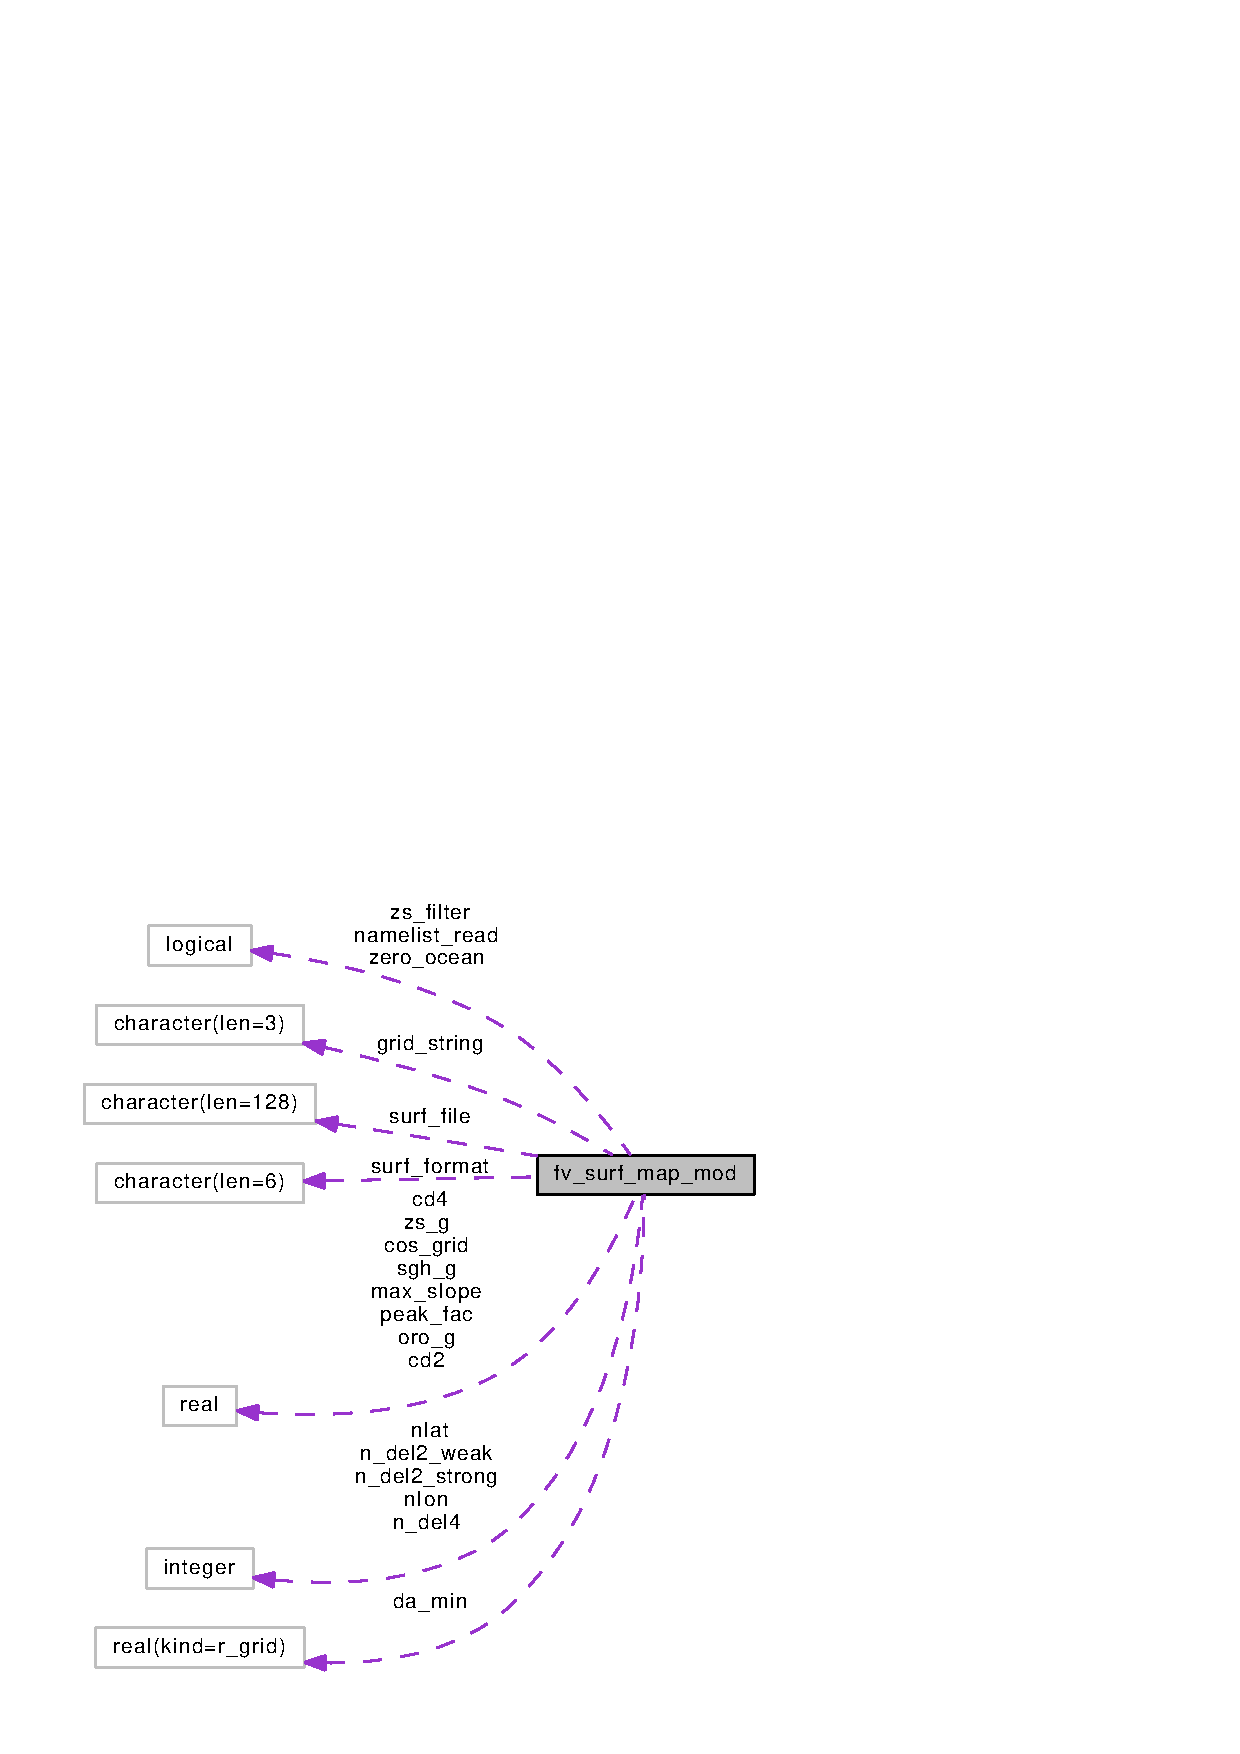
\includegraphics[width=350pt]{classfv__surf__map__mod__coll__graph}
\end{center}
\end{figure}
\subsection*{Public Member Functions}
\begin{DoxyCompactItemize}
\item 
subroutine, public \hyperlink{classfv__surf__map__mod_a5b5120e4bc2fb8f5d845312f38736dde}{surfdrv} (npx, npy, grid, agrid, area, dx, dy, dxa, dya, dxc, dyc, sin\-\_\-sg, phis, stretch\-\_\-fac, nested, npx\-\_\-global, domain, grid\-\_\-number, bd, regional)
\item 
subroutine, public \hyperlink{classfv__surf__map__mod_a008b286b0f3c3b17f9289cf28564edbf}{fv3\-\_\-zs\-\_\-filter} (bd, isd, ied, jsd, jed, npx, npy, npx\-\_\-global, stretch\-\_\-fac, nested, domain, area, dxa, dya, dx, dy, dxc, dyc, grid, agrid, sin\-\_\-sg, phis, oro, regional)
\item 
subroutine, public \hyperlink{classfv__surf__map__mod_ac0abfc3241302c7044d4393bcdff7cd2}{del2\-\_\-cubed\-\_\-sphere} (npx, npy, q, area, dx, dy, dxc, dyc, sin\-\_\-sg, nmax, cd, \hyperlink{classfv__surf__map__mod_a08c3188d0168e655ed23ece6b7a57043}{zero\-\_\-ocean}, oro, nested, domain, bd, regional)
\item 
subroutine, public \hyperlink{classfv__surf__map__mod_a9258298f2e2e6289ec6359c717f38f54}{del4\-\_\-cubed\-\_\-sphere} (npx, npy, q, area, dx, dy, dxc, dyc, sin\-\_\-sg, nmax, \hyperlink{classfv__surf__map__mod_a08c3188d0168e655ed23ece6b7a57043}{zero\-\_\-ocean}, oro, nested, domain, bd, regional)
\end{DoxyCompactItemize}
\subsection*{Public Attributes}
\begin{DoxyCompactItemize}
\item 
real, dimension(\-:,\-:), \\*
allocatable, public \hyperlink{classfv__surf__map__mod_a39c1cec935bdd6e01b87eb1ec5187941}{zs\-\_\-g}
\item 
real, dimension(\-:,\-:), \\*
allocatable, public \hyperlink{classfv__surf__map__mod_a1f6c2740389c832c7b613cd7f0d5a407}{sgh\-\_\-g}
\item 
real, dimension(\-:,\-:), \\*
allocatable, public \hyperlink{classfv__surf__map__mod_a89960949339245bd7440d1735b7b6fa2}{oro\-\_\-g}
\end{DoxyCompactItemize}
\subsection*{Private Member Functions}
\begin{DoxyCompactItemize}
\item 
subroutine \hyperlink{classfv__surf__map__mod_aa6e72698840d80e53f786e8f3fb55d4c}{two\-\_\-delta\-\_\-filter} (npx, npy, q, area, dx, dy, dxa, dya, dxc, dyc, sin\-\_\-sg, cd, \hyperlink{classfv__surf__map__mod_a08c3188d0168e655ed23ece6b7a57043}{zero\-\_\-ocean}, check\-\_\-slope, filter\-\_\-type, oro, nested, domain, bd, ntmax, regional)
\item 
subroutine \hyperlink{classfv__surf__map__mod_acc303dea052d12a2c64113f3893ade70}{map\-\_\-to\-\_\-cubed\-\_\-raw} (igh, im, jt, lat1, lon1, zs, ft, grid, agrid, q2, f2, h2, npx, npy, jstart, jend, stretch\-\_\-fac, nested, npx\-\_\-global, bd, regional)
\item 
subroutine \hyperlink{classfv__surf__map__mod_ab249e49f64014dc3fdc86ae5ab3de14e}{handle\-\_\-err} (status)
\begin{DoxyCompactList}\small\item\em The subroutine 'handle\-\_\-err' returns an error when it cannot find or correctly read in an external file. \end{DoxyCompactList}\item 
subroutine \hyperlink{classfv__surf__map__mod_a89b0e34cb4926fe6403376ca8fa44e53}{remove\-\_\-ice\-\_\-sheets} (lon, lat, lfrac, bd)
\item 
subroutine \hyperlink{classfv__surf__map__mod_ad3d4957033aa67f913b716448e95993f}{read\-\_\-namelist}
\begin{DoxyCompactList}\small\item\em The subroutine 'read\-\_\-namelis' reads the namelist file, writes the namelist to log file, and initializes constants. \end{DoxyCompactList}\item 
subroutine \hyperlink{classfv__surf__map__mod_aa10adedb30604d0ab2744b1126584eb6}{zonal\-\_\-mean} (im, p, zmean)
\begin{DoxyCompactList}\small\item\em The sugroutine 'zonal\-\_\-mean' replaces 'p' with its zonal mean. \end{DoxyCompactList}\end{DoxyCompactItemize}
\subsection*{Private Attributes}
\begin{DoxyCompactItemize}
\item 
logical \hyperlink{classfv__surf__map__mod_a536f543b0d6bb2e2fbb3d98468ef8094}{zs\-\_\-filter} = .true.
\item 
logical \hyperlink{classfv__surf__map__mod_a08c3188d0168e655ed23ece6b7a57043}{zero\-\_\-ocean} = .true.
\item 
integer \hyperlink{classfv__surf__map__mod_a72b1ec87d6827bd07191488811b6f129}{nlon} = 21600
\item 
integer \hyperlink{classfv__surf__map__mod_a7fdae69a68724b43026ac21d8a40a60f}{nlat} = 10800
\item 
real \hyperlink{classfv__surf__map__mod_a533dee578c658a1a4e6533b71d4c89bc}{cd4} = 0.\-15
\begin{DoxyCompactList}\small\item\em Dimensionless coeff for del-\/4 diffusion (with F\-C\-T) \end{DoxyCompactList}\item 
real \hyperlink{classfv__surf__map__mod_a3d2c1c7379279eca4f6e6d78b7e8c30d}{cd2} = -\/1.
\begin{DoxyCompactList}\small\item\em Dimensionless coeff for del-\/2 diffusion (-\/1 gives resolution-\/determined value) \end{DoxyCompactList}\item 
real \hyperlink{classfv__surf__map__mod_a66780e7d69cb8f5776ae7e79b7301e92}{peak\-\_\-fac} = 1.\-05
\begin{DoxyCompactList}\small\item\em overshoot factor for the mountain peak \end{DoxyCompactList}\item 
real \hyperlink{classfv__surf__map__mod_a3848f9f737582dc4b286eb1e748b7c29}{max\-\_\-slope} = 0.\-15
\begin{DoxyCompactList}\small\item\em max allowable terrain slope\-: 1 --$>$ 45 deg 0.\-15 for C768 or lower; 0.\-25 C1536; 0.\-3 for C3072 \end{DoxyCompactList}\item 
integer \hyperlink{classfv__surf__map__mod_a2f02a11eec518babdafb7c9a49d3cb9b}{n\-\_\-del2\-\_\-weak} = 12
\item 
integer \hyperlink{classfv__surf__map__mod_acaf2dd3583e09efc6410823963d1dcc5}{n\-\_\-del2\-\_\-strong} = -\/1
\item 
integer \hyperlink{classfv__surf__map__mod_ab6c0587435e49a2dfc4980e976ea49a1}{n\-\_\-del4} = -\/1
\item 
character(len=128) \hyperlink{classfv__surf__map__mod_a81edeea9be814dd43921902036f6a5ed}{surf\-\_\-file} = \char`\"{}I\-N\-P\-U\-T/topo1min.\-nc\char`\"{}
\item 
character(len=6) \hyperlink{classfv__surf__map__mod_aa49583bb8f72e949a0f8e60cbae0f533}{surf\-\_\-format} = 'netcdf'
\item 
logical \hyperlink{classfv__surf__map__mod_a297f7387531f5640abd6cd59d925bf83}{namelist\-\_\-read} = .false.
\item 
real(kind=r\-\_\-grid) \hyperlink{classfv__surf__map__mod_a8346ce660fbc9bc7a10f64efe5be71ae}{da\-\_\-min}
\item 
real \hyperlink{classfv__surf__map__mod_a770c3993e55f1b6b79cbe9fbbd5485e1}{cos\-\_\-grid}
\item 
character(len=3) \hyperlink{classfv__surf__map__mod_a1dcad6b1f9095cdd68ab7fbbbae8c609}{grid\-\_\-string} = ''
\end{DoxyCompactItemize}


\subsection{Detailed Description}


Definition at line 22 of file fv\-\_\-surf\-\_\-map.\-F90.



\subsection{Member Function/\-Subroutine Documentation}
\index{fv\-\_\-surf\-\_\-map\-\_\-mod@{fv\-\_\-surf\-\_\-map\-\_\-mod}!del2\-\_\-cubed\-\_\-sphere@{del2\-\_\-cubed\-\_\-sphere}}
\index{del2\-\_\-cubed\-\_\-sphere@{del2\-\_\-cubed\-\_\-sphere}!fv_surf_map_mod@{fv\-\_\-surf\-\_\-map\-\_\-mod}}
\subsubsection[{del2\-\_\-cubed\-\_\-sphere}]{\setlength{\rightskip}{0pt plus 5cm}subroutine, public fv\-\_\-surf\-\_\-map\-\_\-mod\-::del2\-\_\-cubed\-\_\-sphere (
\begin{DoxyParamCaption}
\item[{integer, intent(in)}]{npx, }
\item[{integer, intent(in)}]{npy, }
\item[{real, dimension(bd\%is-\/ng\-:bd\%ie+ng, bd\%js-\/ng\-:bd\%je+ng), intent(inout)}]{q, }
\item[{real(kind=r\-\_\-grid), dimension(bd\%isd\-:bd\%ied,  bd\%jsd\-:bd\%jed), intent(in)}]{area, }
\item[{real, dimension(bd\%isd\-:bd\%ied,  bd\%jsd\-:bd\%jed+1), intent(in)}]{dx, }
\item[{real, dimension(bd\%isd\-:bd\%ied+1,bd\%jsd\-:bd\%jed), intent(in)}]{dy, }
\item[{real, dimension(bd\%isd\-:bd\%ied+1,bd\%jsd\-:bd\%jed), intent(in)}]{dxc, }
\item[{real, dimension(bd\%isd\-:bd\%ied,  bd\%jsd\-:bd\%jed+1), intent(in)}]{dyc, }
\item[{real, dimension(bd\%isd\-:bd\%ied,bd\%jsd\-:bd\%jed,9), intent(in)}]{sin\-\_\-sg, }
\item[{integer, intent(in)}]{nmax, }
\item[{real(kind=r\-\_\-grid), intent(in)}]{cd, }
\item[{logical, intent(in)}]{zero\-\_\-ocean, }
\item[{real, dimension(bd\%isd\-:bd\%ied,  bd\%jsd\-:bd\%jed), intent(in)}]{oro, }
\item[{logical, intent(in)}]{nested, }
\item[{type(domain2d), intent(inout)}]{domain, }
\item[{type(fv\-\_\-grid\-\_\-bounds\-\_\-type), intent(in)}]{bd, }
\item[{logical, intent(in)}]{regional}
\end{DoxyParamCaption}
)}\label{classfv__surf__map__mod_ac0abfc3241302c7044d4393bcdff7cd2}

\begin{DoxyParams}[1]{Parameters}
\mbox{\tt in}  & {\em oro} & 0==water, 1==land \\
\hline
\end{DoxyParams}


Definition at line 859 of file fv\-\_\-surf\-\_\-map.\-F90.



Referenced by fv\-\_\-restart\-\_\-mod\-::fv\-\_\-restart(), and external\-\_\-ic\-\_\-mod\-::get\-\_\-nggps\-\_\-ic().

\index{fv\-\_\-surf\-\_\-map\-\_\-mod@{fv\-\_\-surf\-\_\-map\-\_\-mod}!del4\-\_\-cubed\-\_\-sphere@{del4\-\_\-cubed\-\_\-sphere}}
\index{del4\-\_\-cubed\-\_\-sphere@{del4\-\_\-cubed\-\_\-sphere}!fv_surf_map_mod@{fv\-\_\-surf\-\_\-map\-\_\-mod}}
\subsubsection[{del4\-\_\-cubed\-\_\-sphere}]{\setlength{\rightskip}{0pt plus 5cm}subroutine, public fv\-\_\-surf\-\_\-map\-\_\-mod\-::del4\-\_\-cubed\-\_\-sphere (
\begin{DoxyParamCaption}
\item[{integer, intent(in)}]{npx, }
\item[{integer, intent(in)}]{npy, }
\item[{real, dimension(bd\%is-\/ng\-:bd\%ie+ng, bd\%js-\/ng\-:bd\%je+ng), intent(inout)}]{q, }
\item[{real(kind=r\-\_\-grid), dimension(bd\%isd\-:bd\%ied,  bd\%jsd\-:bd\%jed), intent(in)}]{area, }
\item[{real, dimension(bd\%isd\-:bd\%ied,  bd\%jsd\-:bd\%jed+1), intent(in)}]{dx, }
\item[{real, dimension(bd\%isd\-:bd\%ied+1,bd\%jsd\-:bd\%jed), intent(in)}]{dy, }
\item[{real, dimension(bd\%isd\-:bd\%ied+1,bd\%jsd\-:bd\%jed), intent(in)}]{dxc, }
\item[{real, dimension(bd\%isd\-:bd\%ied,  bd\%jsd\-:bd\%jed+1), intent(in)}]{dyc, }
\item[{real, dimension(bd\%isd\-:bd\%ied,bd\%jsd\-:bd\%jed,9), intent(in)}]{sin\-\_\-sg, }
\item[{integer, intent(in)}]{nmax, }
\item[{logical, intent(in)}]{zero\-\_\-ocean, }
\item[{real, dimension(bd\%isd\-:bd\%ied,  bd\%jsd\-:bd\%jed), intent(in)}]{oro, }
\item[{logical, intent(in)}]{nested, }
\item[{type(domain2d), intent(inout)}]{domain, }
\item[{type(fv\-\_\-grid\-\_\-bounds\-\_\-type), intent(in)}]{bd, }
\item[{logical, intent(in)}]{regional}
\end{DoxyParamCaption}
)}\label{classfv__surf__map__mod_a9258298f2e2e6289ec6359c717f38f54}

\begin{DoxyParams}[1]{Parameters}
\mbox{\tt in}  & {\em oro} & 0==water, 1==land \\
\hline
\end{DoxyParams}


Definition at line 961 of file fv\-\_\-surf\-\_\-map.\-F90.



Referenced by fv3\-\_\-zs\-\_\-filter(), fv\-\_\-restart\-\_\-mod\-::fv\-\_\-restart(), external\-\_\-ic\-\_\-mod\-::get\-\_\-nggps\-\_\-ic(), and surfdrv().

\index{fv\-\_\-surf\-\_\-map\-\_\-mod@{fv\-\_\-surf\-\_\-map\-\_\-mod}!fv3\-\_\-zs\-\_\-filter@{fv3\-\_\-zs\-\_\-filter}}
\index{fv3\-\_\-zs\-\_\-filter@{fv3\-\_\-zs\-\_\-filter}!fv_surf_map_mod@{fv\-\_\-surf\-\_\-map\-\_\-mod}}
\subsubsection[{fv3\-\_\-zs\-\_\-filter}]{\setlength{\rightskip}{0pt plus 5cm}subroutine, public fv\-\_\-surf\-\_\-map\-\_\-mod\-::fv3\-\_\-zs\-\_\-filter (
\begin{DoxyParamCaption}
\item[{type(fv\-\_\-grid\-\_\-bounds\-\_\-type), intent(in)}]{bd, }
\item[{integer, intent(in)}]{isd, }
\item[{integer, intent(in)}]{ied, }
\item[{integer, intent(in)}]{jsd, }
\item[{integer, intent(in)}]{jed, }
\item[{integer, intent(in)}]{npx, }
\item[{integer, intent(in)}]{npy, }
\item[{integer, intent(in)}]{npx\-\_\-global, }
\item[{real(kind=r\-\_\-grid), intent(in)}]{stretch\-\_\-fac, }
\item[{logical, intent(in)}]{nested, }
\item[{type(domain2d), intent(inout)}]{domain, }
\item[{real(kind=r\-\_\-grid), dimension(isd\-:ied,jsd\-:jed), intent(in)}]{area, }
\item[{real, dimension(isd\-:ied,jsd\-:jed), intent(in)}]{dxa, }
\item[{real, dimension(isd\-:ied,jsd\-:jed), intent(in)}]{dya, }
\item[{real, dimension(isd\-:ied,  jsd\-:jed+1), intent(in)}]{dx, }
\item[{real, dimension(isd\-:ied+1,jsd\-:jed), intent(in)}]{dy, }
\item[{real, dimension(isd\-:ied+1,jsd\-:jed), intent(in)}]{dxc, }
\item[{real, dimension(isd\-:ied,  jsd\-:jed+1), intent(in)}]{dyc, }
\item[{real(kind=r\-\_\-grid), dimension(isd\-:ied+1, jsd\-:jed+1,2), intent(in)}]{grid, }
\item[{real(kind=r\-\_\-grid), dimension(isd\-:ied,   jsd\-:jed,  2), intent(in)}]{agrid, }
\item[{real, dimension(isd\-:ied,jsd\-:jed,9), intent(in)}]{sin\-\_\-sg, }
\item[{real, dimension(isd\-:ied,jsd,jed), intent(inout)}]{phis, }
\item[{real, dimension(isd\-:ied,jsd,jed), intent(inout)}]{oro, }
\item[{logical, intent(in)}]{regional}
\end{DoxyParamCaption}
)}\label{classfv__surf__map__mod_a008b286b0f3c3b17f9289cf28564edbf}


Definition at line 511 of file fv\-\_\-surf\-\_\-map.\-F90.



References del4\-\_\-cubed\-\_\-sphere(), fv\-\_\-grid\-\_\-utils\-\_\-mod\-::global\-\_\-mx(), read\-\_\-namelist(), and two\-\_\-delta\-\_\-filter().



Referenced by external\-\_\-ic\-\_\-mod\-::get\-\_\-nggps\-\_\-ic(), and surfdrv().

\index{fv\-\_\-surf\-\_\-map\-\_\-mod@{fv\-\_\-surf\-\_\-map\-\_\-mod}!handle\-\_\-err@{handle\-\_\-err}}
\index{handle\-\_\-err@{handle\-\_\-err}!fv_surf_map_mod@{fv\-\_\-surf\-\_\-map\-\_\-mod}}
\subsubsection[{handle\-\_\-err}]{\setlength{\rightskip}{0pt plus 5cm}subroutine fv\-\_\-surf\-\_\-map\-\_\-mod\-::handle\-\_\-err (
\begin{DoxyParamCaption}
\item[{integer}]{status}
\end{DoxyParamCaption}
)\hspace{0.3cm}{\ttfamily [private]}}\label{classfv__surf__map__mod_ab249e49f64014dc3fdc86ae5ab3de14e}


The subroutine 'handle\-\_\-err' returns an error when it cannot find or correctly read in an external file. 



Definition at line 1533 of file fv\-\_\-surf\-\_\-map.\-F90.



Referenced by sim\-\_\-nc\-\_\-mod\-::close\-\_\-ncfile(), sim\-\_\-nc\-\_\-mod\-::get\-\_\-ncdim1(), sim\-\_\-nc\-\_\-mod\-::get\-\_\-real3(), sim\-\_\-nc\-\_\-mod\-::get\-\_\-var1\-\_\-double(), sim\-\_\-nc\-\_\-mod\-::get\-\_\-var1\-\_\-real(), sim\-\_\-nc\-\_\-mod\-::get\-\_\-var2\-\_\-double(), sim\-\_\-nc\-\_\-mod\-::get\-\_\-var2\-\_\-r4(), sim\-\_\-nc\-\_\-mod\-::get\-\_\-var2\-\_\-real(), sim\-\_\-nc\-\_\-mod\-::get\-\_\-var3\-\_\-double(), sim\-\_\-nc\-\_\-mod\-::get\-\_\-var3\-\_\-r4(), sim\-\_\-nc\-\_\-mod\-::get\-\_\-var3\-\_\-real(), sim\-\_\-nc\-\_\-mod\-::get\-\_\-var4\-\_\-double(), sim\-\_\-nc\-\_\-mod\-::get\-\_\-var4\-\_\-real(), sim\-\_\-nc\-\_\-mod\-::get\-\_\-var\-\_\-att\-\_\-double(), sim\-\_\-nc\-\_\-mod\-::get\-\_\-var\-\_\-att\-\_\-str(), sim\-\_\-nc\-\_\-mod\-::open\-\_\-ncfile(), and surfdrv().

\index{fv\-\_\-surf\-\_\-map\-\_\-mod@{fv\-\_\-surf\-\_\-map\-\_\-mod}!map\-\_\-to\-\_\-cubed\-\_\-raw@{map\-\_\-to\-\_\-cubed\-\_\-raw}}
\index{map\-\_\-to\-\_\-cubed\-\_\-raw@{map\-\_\-to\-\_\-cubed\-\_\-raw}!fv_surf_map_mod@{fv\-\_\-surf\-\_\-map\-\_\-mod}}
\subsubsection[{map\-\_\-to\-\_\-cubed\-\_\-raw}]{\setlength{\rightskip}{0pt plus 5cm}subroutine fv\-\_\-surf\-\_\-map\-\_\-mod\-::map\-\_\-to\-\_\-cubed\-\_\-raw (
\begin{DoxyParamCaption}
\item[{integer, intent(in)}]{igh, }
\item[{integer, intent(in)}]{im, }
\item[{integer, intent(in)}]{jt, }
\item[{real, dimension(jt+1), intent(in)}]{lat1, }
\item[{real, dimension(im+1), intent(in)}]{lon1, }
\item[{real(kind=4), dimension(-\/igh\-:im+igh,jt), intent(in)}]{zs, }
\item[{real(kind=4), dimension(-\/igh\-:im+igh,jt), intent(in)}]{ft, }
\item[{real(kind=r\-\_\-grid), dimension(bd\%isd\-:bd\%ied+1, bd\%jsd\-:bd\%jed+1,2), intent(in)}]{grid, }
\item[{real(kind=r\-\_\-grid), dimension(bd\%isd\-:bd\%ied,   bd\%jsd\-:bd\%jed,  2), intent(in)}]{agrid, }
\item[{real, dimension(bd\%isd\-:bd\%ied,bd\%jsd\-:bd\%jed), intent(out)}]{q2, }
\item[{real, dimension(bd\%isd\-:bd\%ied,bd\%jsd\-:bd\%jed), intent(out)}]{f2, }
\item[{real, dimension(bd\%isd\-:bd\%ied,bd\%jsd\-:bd\%jed), intent(out)}]{h2, }
\item[{integer, intent(in)}]{npx, }
\item[{integer, intent(in)}]{npy, }
\item[{integer, intent(in)}]{jstart, }
\item[{integer, intent(in)}]{jend, }
\item[{real(kind=r\-\_\-grid), intent(in)}]{stretch\-\_\-fac, }
\item[{logical, intent(in)}]{nested, }
\item[{integer, intent(in)}]{npx\-\_\-global, }
\item[{type(fv\-\_\-grid\-\_\-bounds\-\_\-type), intent(in)}]{bd, }
\item[{logical, intent(in)}]{regional}
\end{DoxyParamCaption}
)\hspace{0.3cm}{\ttfamily [private]}}\label{classfv__surf__map__mod_acc303dea052d12a2c64113f3893ade70}

\begin{DoxyParams}[1]{Parameters}
\mbox{\tt in}  & {\em lat1} & original southern edge of the cell \mbox{[}-\/pi/2\-:pi/2\mbox{]}\\
\hline
\mbox{\tt in}  & {\em lon1} & original western edge of the cell \mbox{[}0\-:2$\ast$pi\mbox{]}\\
\hline
\mbox{\tt out}  & {\em q2} & Mapped data at the target resolution\\
\hline
\mbox{\tt out}  & {\em f2} & oro\\
\hline
\mbox{\tt out}  & {\em h2} & variances of terrain \\
\hline
\end{DoxyParams}


Definition at line 1195 of file fv\-\_\-surf\-\_\-map.\-F90.



References fv\-\_\-grid\-\_\-utils\-\_\-mod\-::latlon2xyz(), fv\-\_\-grid\-\_\-utils\-\_\-mod\-::normalize\-\_\-vect(), fv\-\_\-grid\-\_\-utils\-\_\-mod\-::v\-\_\-prod(), and fv\-\_\-grid\-\_\-utils\-\_\-mod\-::vect\-\_\-cross().



Referenced by surfdrv().

\index{fv\-\_\-surf\-\_\-map\-\_\-mod@{fv\-\_\-surf\-\_\-map\-\_\-mod}!read\-\_\-namelist@{read\-\_\-namelist}}
\index{read\-\_\-namelist@{read\-\_\-namelist}!fv_surf_map_mod@{fv\-\_\-surf\-\_\-map\-\_\-mod}}
\subsubsection[{read\-\_\-namelist}]{\setlength{\rightskip}{0pt plus 5cm}subroutine fv\-\_\-surf\-\_\-map\-\_\-mod\-::read\-\_\-namelist (
\begin{DoxyParamCaption}
{}
\end{DoxyParamCaption}
)\hspace{0.3cm}{\ttfamily [private]}}\label{classfv__surf__map__mod_ad3d4957033aa67f913b716448e95993f}


The subroutine 'read\-\_\-namelis' reads the namelist file, writes the namelist to log file, and initializes constants. 



Definition at line 1596 of file fv\-\_\-surf\-\_\-map.\-F90.



Referenced by fv3\-\_\-zs\-\_\-filter(), and surfdrv().

\index{fv\-\_\-surf\-\_\-map\-\_\-mod@{fv\-\_\-surf\-\_\-map\-\_\-mod}!remove\-\_\-ice\-\_\-sheets@{remove\-\_\-ice\-\_\-sheets}}
\index{remove\-\_\-ice\-\_\-sheets@{remove\-\_\-ice\-\_\-sheets}!fv_surf_map_mod@{fv\-\_\-surf\-\_\-map\-\_\-mod}}
\subsubsection[{remove\-\_\-ice\-\_\-sheets}]{\setlength{\rightskip}{0pt plus 5cm}subroutine fv\-\_\-surf\-\_\-map\-\_\-mod\-::remove\-\_\-ice\-\_\-sheets (
\begin{DoxyParamCaption}
\item[{real(kind=r\-\_\-grid), dimension(bd\%isd\-:bd\%ied,bd\%jsd\-:bd\%jed), intent(in)}]{lon, }
\item[{real(kind=r\-\_\-grid), dimension(bd\%isd\-:bd\%ied,bd\%jsd\-:bd\%jed), intent(in)}]{lat, }
\item[{real, dimension(bd\%isd\-:bd\%ied,bd\%jsd\-:bd\%jed), intent(inout)}]{lfrac, }
\item[{type(fv\-\_\-grid\-\_\-bounds\-\_\-type), intent(in)}]{bd}
\end{DoxyParamCaption}
)\hspace{0.3cm}{\ttfamily [private]}}\label{classfv__surf__map__mod_a89b0e34cb4926fe6403376ca8fa44e53}


Definition at line 1544 of file fv\-\_\-surf\-\_\-map.\-F90.

\index{fv\-\_\-surf\-\_\-map\-\_\-mod@{fv\-\_\-surf\-\_\-map\-\_\-mod}!surfdrv@{surfdrv}}
\index{surfdrv@{surfdrv}!fv_surf_map_mod@{fv\-\_\-surf\-\_\-map\-\_\-mod}}
\subsubsection[{surfdrv}]{\setlength{\rightskip}{0pt plus 5cm}subroutine, public fv\-\_\-surf\-\_\-map\-\_\-mod\-::surfdrv (
\begin{DoxyParamCaption}
\item[{integer, intent(in)}]{npx, }
\item[{integer, intent(in)}]{npy, }
\item[{real(kind=r\-\_\-grid), dimension(bd\%is-\/ng\-:bd\%ie+ng+1, bd\%js-\/ng\-:bd\%je+ng+1,2), intent(in)}]{grid, }
\item[{real(kind=r\-\_\-grid), dimension(bd\%is-\/ng\-:bd\%ie+ng, bd\%js-\/ng\-:bd\%je+ng,2), intent(in)}]{agrid, }
\item[{real(kind=r\-\_\-grid), dimension(bd\%is-\/ng\-:bd\%ie+ng, bd\%js-\/ng\-:bd\%je+ng), intent(in)}]{area, }
\item[{real, dimension(bd\%is-\/ng\-:bd\%ie+ng, bd\%js-\/ng\-:bd\%je+ng+1), intent(in)}]{dx, }
\item[{real, dimension(bd\%is-\/ng\-:bd\%ie+ng+1, bd\%js-\/ng\-:bd\%je+ng), intent(in)}]{dy, }
\item[{real, dimension(bd\%is-\/ng\-:bd\%ie+ng, bd\%js-\/ng\-:bd\%je+ng), intent(in)}]{dxa, }
\item[{real, dimension(bd\%is-\/ng\-:bd\%ie+ng, bd\%js-\/ng\-:bd\%je+ng), intent(in)}]{dya, }
\item[{real, dimension(bd\%is-\/ng\-:bd\%ie+ng+1, bd\%js-\/ng\-:bd\%je+ng), intent(in)}]{dxc, }
\item[{real, dimension(bd\%is-\/ng\-:bd\%ie+ng, bd\%js-\/ng\-:bd\%je+ng+1), intent(in)}]{dyc, }
\item[{real, dimension(bd\%isd\-:bd\%ied,bd\%jsd\-:bd\%jed,9), intent(in)}]{sin\-\_\-sg, }
\item[{real, dimension(bd\%is-\/ng\-:bd\%ie+ng, bd\%js-\/ng\-:bd\%je+ng), intent(out)}]{phis, }
\item[{real(kind=r\-\_\-grid), intent(in)}]{stretch\-\_\-fac, }
\item[{logical, intent(in)}]{nested, }
\item[{integer, intent(in)}]{npx\-\_\-global, }
\item[{type(domain2d), intent(inout)}]{domain, }
\item[{integer, intent(in)}]{grid\-\_\-number, }
\item[{type(fv\-\_\-grid\-\_\-bounds\-\_\-type), intent(in)}]{bd, }
\item[{logical, intent(in)}]{regional}
\end{DoxyParamCaption}
)}\label{classfv__surf__map__mod_a5b5120e4bc2fb8f5d845312f38736dde}


Definition at line 133 of file fv\-\_\-surf\-\_\-map.\-F90.



References del4\-\_\-cubed\-\_\-sphere(), fv3\-\_\-zs\-\_\-filter(), fv\-\_\-grid\-\_\-utils\-\_\-mod\-::g\-\_\-sum(), fv\-\_\-grid\-\_\-utils\-\_\-mod\-::global\-\_\-mx(), handle\-\_\-err(), map\-\_\-to\-\_\-cubed\-\_\-raw(), read\-\_\-namelist(), fv\-\_\-timing\-\_\-mod\-::timing\-\_\-off(), and fv\-\_\-timing\-\_\-mod\-::timing\-\_\-on().



Referenced by external\-\_\-ic\-\_\-mod\-::get\-\_\-cubed\-\_\-sphere\-\_\-terrain(), and test\-\_\-cases\-\_\-mod\-::init\-\_\-case().

\index{fv\-\_\-surf\-\_\-map\-\_\-mod@{fv\-\_\-surf\-\_\-map\-\_\-mod}!two\-\_\-delta\-\_\-filter@{two\-\_\-delta\-\_\-filter}}
\index{two\-\_\-delta\-\_\-filter@{two\-\_\-delta\-\_\-filter}!fv_surf_map_mod@{fv\-\_\-surf\-\_\-map\-\_\-mod}}
\subsubsection[{two\-\_\-delta\-\_\-filter}]{\setlength{\rightskip}{0pt plus 5cm}subroutine fv\-\_\-surf\-\_\-map\-\_\-mod\-::two\-\_\-delta\-\_\-filter (
\begin{DoxyParamCaption}
\item[{integer, intent(in)}]{npx, }
\item[{integer, intent(in)}]{npy, }
\item[{real, dimension(bd\%isd\-:bd\%ied, bd\%jsd\-:bd\%jed), intent(inout)}]{q, }
\item[{real(kind=r\-\_\-grid), dimension(bd\%isd\-:bd\%ied,  bd\%jsd\-:bd\%jed), intent(in)}]{area, }
\item[{real, dimension(bd\%isd\-:bd\%ied,  bd\%jsd\-:bd\%jed+1), intent(in)}]{dx, }
\item[{real, dimension(bd\%isd\-:bd\%ied+1,bd\%jsd\-:bd\%jed), intent(in)}]{dy, }
\item[{real, dimension(bd\%isd\-:bd\%ied,  bd\%jsd\-:bd\%jed), intent(in)}]{dxa, }
\item[{real, dimension(bd\%isd\-:bd\%ied,  bd\%jsd\-:bd\%jed), intent(in)}]{dya, }
\item[{real, dimension(bd\%isd\-:bd\%ied+1,bd\%jsd\-:bd\%jed), intent(in)}]{dxc, }
\item[{real, dimension(bd\%isd\-:bd\%ied,  bd\%jsd\-:bd\%jed+1), intent(in)}]{dyc, }
\item[{real, dimension(bd\%isd\-:bd\%ied,bd\%jsd\-:bd\%jed,9), intent(in)}]{sin\-\_\-sg, }
\item[{real, intent(in)}]{cd, }
\item[{logical, intent(in)}]{zero\-\_\-ocean, }
\item[{logical, intent(in)}]{check\-\_\-slope, }
\item[{integer, intent(in)}]{filter\-\_\-type, }
\item[{real, dimension(bd\%isd\-:bd\%ied,  bd\%jsd\-:bd\%jed), intent(in)}]{oro, }
\item[{logical, intent(in)}]{nested, }
\item[{type(domain2d), intent(inout)}]{domain, }
\item[{type(fv\-\_\-grid\-\_\-bounds\-\_\-type), intent(in)}]{bd, }
\item[{integer, intent(in)}]{ntmax, }
\item[{logical, intent(in)}]{regional}
\end{DoxyParamCaption}
)\hspace{0.3cm}{\ttfamily [private]}}\label{classfv__surf__map__mod_aa6e72698840d80e53f786e8f3fb55d4c}

\begin{DoxyParams}[1]{Parameters}
\mbox{\tt in}  & {\em filter\-\_\-type} & 0\-: strong, 1\-: weak\\
\hline
\mbox{\tt in}  & {\em oro} & 0==water, 1==land \\
\hline
\end{DoxyParams}


Definition at line 576 of file fv\-\_\-surf\-\_\-map.\-F90.



References fv\-\_\-grid\-\_\-utils\-\_\-mod\-::global\-\_\-mx().



Referenced by fv3\-\_\-zs\-\_\-filter().

\index{fv\-\_\-surf\-\_\-map\-\_\-mod@{fv\-\_\-surf\-\_\-map\-\_\-mod}!zonal\-\_\-mean@{zonal\-\_\-mean}}
\index{zonal\-\_\-mean@{zonal\-\_\-mean}!fv_surf_map_mod@{fv\-\_\-surf\-\_\-map\-\_\-mod}}
\subsubsection[{zonal\-\_\-mean}]{\setlength{\rightskip}{0pt plus 5cm}subroutine fv\-\_\-surf\-\_\-map\-\_\-mod\-::zonal\-\_\-mean (
\begin{DoxyParamCaption}
\item[{integer, intent(in)}]{im, }
\item[{real(kind=4), dimension(im), intent(inout)}]{p, }
\item[{real, intent(out)}]{zmean}
\end{DoxyParamCaption}
)\hspace{0.3cm}{\ttfamily [private]}}\label{classfv__surf__map__mod_aa10adedb30604d0ab2744b1126584eb6}


The sugroutine 'zonal\-\_\-mean' replaces 'p' with its zonal mean. 



Definition at line 1628 of file fv\-\_\-surf\-\_\-map.\-F90.



\subsection{Member Data Documentation}
\index{fv\-\_\-surf\-\_\-map\-\_\-mod@{fv\-\_\-surf\-\_\-map\-\_\-mod}!cd2@{cd2}}
\index{cd2@{cd2}!fv_surf_map_mod@{fv\-\_\-surf\-\_\-map\-\_\-mod}}
\subsubsection[{cd2}]{\setlength{\rightskip}{0pt plus 5cm}real fv\-\_\-surf\-\_\-map\-\_\-mod\-::cd2 = -\/1.\hspace{0.3cm}{\ttfamily [private]}}\label{classfv__surf__map__mod_a3d2c1c7379279eca4f6e6d78b7e8c30d}


Dimensionless coeff for del-\/2 diffusion (-\/1 gives resolution-\/determined value) 



Definition at line 105 of file fv\-\_\-surf\-\_\-map.\-F90.

\index{fv\-\_\-surf\-\_\-map\-\_\-mod@{fv\-\_\-surf\-\_\-map\-\_\-mod}!cd4@{cd4}}
\index{cd4@{cd4}!fv_surf_map_mod@{fv\-\_\-surf\-\_\-map\-\_\-mod}}
\subsubsection[{cd4}]{\setlength{\rightskip}{0pt plus 5cm}real fv\-\_\-surf\-\_\-map\-\_\-mod\-::cd4 = 0.\-15\hspace{0.3cm}{\ttfamily [private]}}\label{classfv__surf__map__mod_a533dee578c658a1a4e6533b71d4c89bc}


Dimensionless coeff for del-\/4 diffusion (with F\-C\-T) 



Definition at line 104 of file fv\-\_\-surf\-\_\-map.\-F90.

\index{fv\-\_\-surf\-\_\-map\-\_\-mod@{fv\-\_\-surf\-\_\-map\-\_\-mod}!cos\-\_\-grid@{cos\-\_\-grid}}
\index{cos\-\_\-grid@{cos\-\_\-grid}!fv_surf_map_mod@{fv\-\_\-surf\-\_\-map\-\_\-mod}}
\subsubsection[{cos\-\_\-grid}]{\setlength{\rightskip}{0pt plus 5cm}real fv\-\_\-surf\-\_\-map\-\_\-mod\-::cos\-\_\-grid\hspace{0.3cm}{\ttfamily [private]}}\label{classfv__surf__map__mod_a770c3993e55f1b6b79cbe9fbbd5485e1}


Definition at line 119 of file fv\-\_\-surf\-\_\-map.\-F90.

\index{fv\-\_\-surf\-\_\-map\-\_\-mod@{fv\-\_\-surf\-\_\-map\-\_\-mod}!da\-\_\-min@{da\-\_\-min}}
\index{da\-\_\-min@{da\-\_\-min}!fv_surf_map_mod@{fv\-\_\-surf\-\_\-map\-\_\-mod}}
\subsubsection[{da\-\_\-min}]{\setlength{\rightskip}{0pt plus 5cm}real(kind=r\-\_\-grid) fv\-\_\-surf\-\_\-map\-\_\-mod\-::da\-\_\-min\hspace{0.3cm}{\ttfamily [private]}}\label{classfv__surf__map__mod_a8346ce660fbc9bc7a10f64efe5be71ae}


Definition at line 118 of file fv\-\_\-surf\-\_\-map.\-F90.

\index{fv\-\_\-surf\-\_\-map\-\_\-mod@{fv\-\_\-surf\-\_\-map\-\_\-mod}!grid\-\_\-string@{grid\-\_\-string}}
\index{grid\-\_\-string@{grid\-\_\-string}!fv_surf_map_mod@{fv\-\_\-surf\-\_\-map\-\_\-mod}}
\subsubsection[{grid\-\_\-string}]{\setlength{\rightskip}{0pt plus 5cm}character(len=3) fv\-\_\-surf\-\_\-map\-\_\-mod\-::grid\-\_\-string = ''\hspace{0.3cm}{\ttfamily [private]}}\label{classfv__surf__map__mod_a1dcad6b1f9095cdd68ab7fbbbae8c609}


Definition at line 120 of file fv\-\_\-surf\-\_\-map.\-F90.

\index{fv\-\_\-surf\-\_\-map\-\_\-mod@{fv\-\_\-surf\-\_\-map\-\_\-mod}!max\-\_\-slope@{max\-\_\-slope}}
\index{max\-\_\-slope@{max\-\_\-slope}!fv_surf_map_mod@{fv\-\_\-surf\-\_\-map\-\_\-mod}}
\subsubsection[{max\-\_\-slope}]{\setlength{\rightskip}{0pt plus 5cm}real fv\-\_\-surf\-\_\-map\-\_\-mod\-::max\-\_\-slope = 0.\-15\hspace{0.3cm}{\ttfamily [private]}}\label{classfv__surf__map__mod_a3848f9f737582dc4b286eb1e748b7c29}


max allowable terrain slope\-: 1 --$>$ 45 deg 0.\-15 for C768 or lower; 0.\-25 C1536; 0.\-3 for C3072 



Definition at line 107 of file fv\-\_\-surf\-\_\-map.\-F90.

\index{fv\-\_\-surf\-\_\-map\-\_\-mod@{fv\-\_\-surf\-\_\-map\-\_\-mod}!n\-\_\-del2\-\_\-strong@{n\-\_\-del2\-\_\-strong}}
\index{n\-\_\-del2\-\_\-strong@{n\-\_\-del2\-\_\-strong}!fv_surf_map_mod@{fv\-\_\-surf\-\_\-map\-\_\-mod}}
\subsubsection[{n\-\_\-del2\-\_\-strong}]{\setlength{\rightskip}{0pt plus 5cm}integer fv\-\_\-surf\-\_\-map\-\_\-mod\-::n\-\_\-del2\-\_\-strong = -\/1\hspace{0.3cm}{\ttfamily [private]}}\label{classfv__surf__map__mod_acaf2dd3583e09efc6410823963d1dcc5}


Definition at line 110 of file fv\-\_\-surf\-\_\-map.\-F90.

\index{fv\-\_\-surf\-\_\-map\-\_\-mod@{fv\-\_\-surf\-\_\-map\-\_\-mod}!n\-\_\-del2\-\_\-weak@{n\-\_\-del2\-\_\-weak}}
\index{n\-\_\-del2\-\_\-weak@{n\-\_\-del2\-\_\-weak}!fv_surf_map_mod@{fv\-\_\-surf\-\_\-map\-\_\-mod}}
\subsubsection[{n\-\_\-del2\-\_\-weak}]{\setlength{\rightskip}{0pt plus 5cm}integer fv\-\_\-surf\-\_\-map\-\_\-mod\-::n\-\_\-del2\-\_\-weak = 12\hspace{0.3cm}{\ttfamily [private]}}\label{classfv__surf__map__mod_a2f02a11eec518babdafb7c9a49d3cb9b}


Definition at line 109 of file fv\-\_\-surf\-\_\-map.\-F90.

\index{fv\-\_\-surf\-\_\-map\-\_\-mod@{fv\-\_\-surf\-\_\-map\-\_\-mod}!n\-\_\-del4@{n\-\_\-del4}}
\index{n\-\_\-del4@{n\-\_\-del4}!fv_surf_map_mod@{fv\-\_\-surf\-\_\-map\-\_\-mod}}
\subsubsection[{n\-\_\-del4}]{\setlength{\rightskip}{0pt plus 5cm}integer fv\-\_\-surf\-\_\-map\-\_\-mod\-::n\-\_\-del4 = -\/1\hspace{0.3cm}{\ttfamily [private]}}\label{classfv__surf__map__mod_ab6c0587435e49a2dfc4980e976ea49a1}


Definition at line 111 of file fv\-\_\-surf\-\_\-map.\-F90.

\index{fv\-\_\-surf\-\_\-map\-\_\-mod@{fv\-\_\-surf\-\_\-map\-\_\-mod}!namelist\-\_\-read@{namelist\-\_\-read}}
\index{namelist\-\_\-read@{namelist\-\_\-read}!fv_surf_map_mod@{fv\-\_\-surf\-\_\-map\-\_\-mod}}
\subsubsection[{namelist\-\_\-read}]{\setlength{\rightskip}{0pt plus 5cm}logical fv\-\_\-surf\-\_\-map\-\_\-mod\-::namelist\-\_\-read = .false.\hspace{0.3cm}{\ttfamily [private]}}\label{classfv__surf__map__mod_a297f7387531f5640abd6cd59d925bf83}


Definition at line 116 of file fv\-\_\-surf\-\_\-map.\-F90.

\index{fv\-\_\-surf\-\_\-map\-\_\-mod@{fv\-\_\-surf\-\_\-map\-\_\-mod}!nlat@{nlat}}
\index{nlat@{nlat}!fv_surf_map_mod@{fv\-\_\-surf\-\_\-map\-\_\-mod}}
\subsubsection[{nlat}]{\setlength{\rightskip}{0pt plus 5cm}integer fv\-\_\-surf\-\_\-map\-\_\-mod\-::nlat = 10800\hspace{0.3cm}{\ttfamily [private]}}\label{classfv__surf__map__mod_a7fdae69a68724b43026ac21d8a40a60f}


Definition at line 103 of file fv\-\_\-surf\-\_\-map.\-F90.

\index{fv\-\_\-surf\-\_\-map\-\_\-mod@{fv\-\_\-surf\-\_\-map\-\_\-mod}!nlon@{nlon}}
\index{nlon@{nlon}!fv_surf_map_mod@{fv\-\_\-surf\-\_\-map\-\_\-mod}}
\subsubsection[{nlon}]{\setlength{\rightskip}{0pt plus 5cm}integer fv\-\_\-surf\-\_\-map\-\_\-mod\-::nlon = 21600\hspace{0.3cm}{\ttfamily [private]}}\label{classfv__surf__map__mod_a72b1ec87d6827bd07191488811b6f129}


Definition at line 102 of file fv\-\_\-surf\-\_\-map.\-F90.

\index{fv\-\_\-surf\-\_\-map\-\_\-mod@{fv\-\_\-surf\-\_\-map\-\_\-mod}!oro\-\_\-g@{oro\-\_\-g}}
\index{oro\-\_\-g@{oro\-\_\-g}!fv_surf_map_mod@{fv\-\_\-surf\-\_\-map\-\_\-mod}}
\subsubsection[{oro\-\_\-g}]{\setlength{\rightskip}{0pt plus 5cm}real, dimension(\-:,\-:), allocatable, public fv\-\_\-surf\-\_\-map\-\_\-mod\-::oro\-\_\-g}\label{classfv__surf__map__mod_a89960949339245bd7440d1735b7b6fa2}


Definition at line 125 of file fv\-\_\-surf\-\_\-map.\-F90.

\index{fv\-\_\-surf\-\_\-map\-\_\-mod@{fv\-\_\-surf\-\_\-map\-\_\-mod}!peak\-\_\-fac@{peak\-\_\-fac}}
\index{peak\-\_\-fac@{peak\-\_\-fac}!fv_surf_map_mod@{fv\-\_\-surf\-\_\-map\-\_\-mod}}
\subsubsection[{peak\-\_\-fac}]{\setlength{\rightskip}{0pt plus 5cm}real fv\-\_\-surf\-\_\-map\-\_\-mod\-::peak\-\_\-fac = 1.\-05\hspace{0.3cm}{\ttfamily [private]}}\label{classfv__surf__map__mod_a66780e7d69cb8f5776ae7e79b7301e92}


overshoot factor for the mountain peak 



Definition at line 106 of file fv\-\_\-surf\-\_\-map.\-F90.

\index{fv\-\_\-surf\-\_\-map\-\_\-mod@{fv\-\_\-surf\-\_\-map\-\_\-mod}!sgh\-\_\-g@{sgh\-\_\-g}}
\index{sgh\-\_\-g@{sgh\-\_\-g}!fv_surf_map_mod@{fv\-\_\-surf\-\_\-map\-\_\-mod}}
\subsubsection[{sgh\-\_\-g}]{\setlength{\rightskip}{0pt plus 5cm}real, dimension(\-:,\-:), allocatable, public fv\-\_\-surf\-\_\-map\-\_\-mod\-::sgh\-\_\-g}\label{classfv__surf__map__mod_a1f6c2740389c832c7b613cd7f0d5a407}


Definition at line 125 of file fv\-\_\-surf\-\_\-map.\-F90.

\index{fv\-\_\-surf\-\_\-map\-\_\-mod@{fv\-\_\-surf\-\_\-map\-\_\-mod}!surf\-\_\-file@{surf\-\_\-file}}
\index{surf\-\_\-file@{surf\-\_\-file}!fv_surf_map_mod@{fv\-\_\-surf\-\_\-map\-\_\-mod}}
\subsubsection[{surf\-\_\-file}]{\setlength{\rightskip}{0pt plus 5cm}character(len=128) fv\-\_\-surf\-\_\-map\-\_\-mod\-::surf\-\_\-file = \char`\"{}I\-N\-P\-U\-T/topo1min.\-nc\char`\"{}\hspace{0.3cm}{\ttfamily [private]}}\label{classfv__surf__map__mod_a81edeea9be814dd43921902036f6a5ed}


Definition at line 114 of file fv\-\_\-surf\-\_\-map.\-F90.

\index{fv\-\_\-surf\-\_\-map\-\_\-mod@{fv\-\_\-surf\-\_\-map\-\_\-mod}!surf\-\_\-format@{surf\-\_\-format}}
\index{surf\-\_\-format@{surf\-\_\-format}!fv_surf_map_mod@{fv\-\_\-surf\-\_\-map\-\_\-mod}}
\subsubsection[{surf\-\_\-format}]{\setlength{\rightskip}{0pt plus 5cm}character(len=6) fv\-\_\-surf\-\_\-map\-\_\-mod\-::surf\-\_\-format = 'netcdf'\hspace{0.3cm}{\ttfamily [private]}}\label{classfv__surf__map__mod_aa49583bb8f72e949a0f8e60cbae0f533}


Definition at line 115 of file fv\-\_\-surf\-\_\-map.\-F90.

\index{fv\-\_\-surf\-\_\-map\-\_\-mod@{fv\-\_\-surf\-\_\-map\-\_\-mod}!zero\-\_\-ocean@{zero\-\_\-ocean}}
\index{zero\-\_\-ocean@{zero\-\_\-ocean}!fv_surf_map_mod@{fv\-\_\-surf\-\_\-map\-\_\-mod}}
\subsubsection[{zero\-\_\-ocean}]{\setlength{\rightskip}{0pt plus 5cm}logical fv\-\_\-surf\-\_\-map\-\_\-mod\-::zero\-\_\-ocean = .true.\hspace{0.3cm}{\ttfamily [private]}}\label{classfv__surf__map__mod_a08c3188d0168e655ed23ece6b7a57043}


Definition at line 101 of file fv\-\_\-surf\-\_\-map.\-F90.

\index{fv\-\_\-surf\-\_\-map\-\_\-mod@{fv\-\_\-surf\-\_\-map\-\_\-mod}!zs\-\_\-filter@{zs\-\_\-filter}}
\index{zs\-\_\-filter@{zs\-\_\-filter}!fv_surf_map_mod@{fv\-\_\-surf\-\_\-map\-\_\-mod}}
\subsubsection[{zs\-\_\-filter}]{\setlength{\rightskip}{0pt plus 5cm}logical fv\-\_\-surf\-\_\-map\-\_\-mod\-::zs\-\_\-filter = .true.\hspace{0.3cm}{\ttfamily [private]}}\label{classfv__surf__map__mod_a536f543b0d6bb2e2fbb3d98468ef8094}


Definition at line 100 of file fv\-\_\-surf\-\_\-map.\-F90.

\index{fv\-\_\-surf\-\_\-map\-\_\-mod@{fv\-\_\-surf\-\_\-map\-\_\-mod}!zs\-\_\-g@{zs\-\_\-g}}
\index{zs\-\_\-g@{zs\-\_\-g}!fv_surf_map_mod@{fv\-\_\-surf\-\_\-map\-\_\-mod}}
\subsubsection[{zs\-\_\-g}]{\setlength{\rightskip}{0pt plus 5cm}real, dimension(\-:,\-:), allocatable, public fv\-\_\-surf\-\_\-map\-\_\-mod\-::zs\-\_\-g}\label{classfv__surf__map__mod_a39c1cec935bdd6e01b87eb1ec5187941}


Definition at line 125 of file fv\-\_\-surf\-\_\-map.\-F90.



The documentation for this module was generated from the following file\-:\begin{DoxyCompactItemize}
\item 
/scratch2/\-N\-A\-G\-A\-P\-E/aoml-\/hafs1/\-Kyle.\-Ahern/acs\-\_\-master\-\_\-readonly/tools/\hyperlink{fv__surf__map_8F90}{fv\-\_\-surf\-\_\-map.\-F90}\end{DoxyCompactItemize}

\section{fv\-\_\-timing\-\_\-mod Module Reference}
\label{classfv__timing__mod}\index{fv\-\_\-timing\-\_\-mod@{fv\-\_\-timing\-\_\-mod}}


The module 'fv\-\_\-timing' contains F\-V3 timers.  




Collaboration diagram for fv\-\_\-timing\-\_\-mod\-:
\nopagebreak
\begin{figure}[H]
\begin{center}
\leavevmode
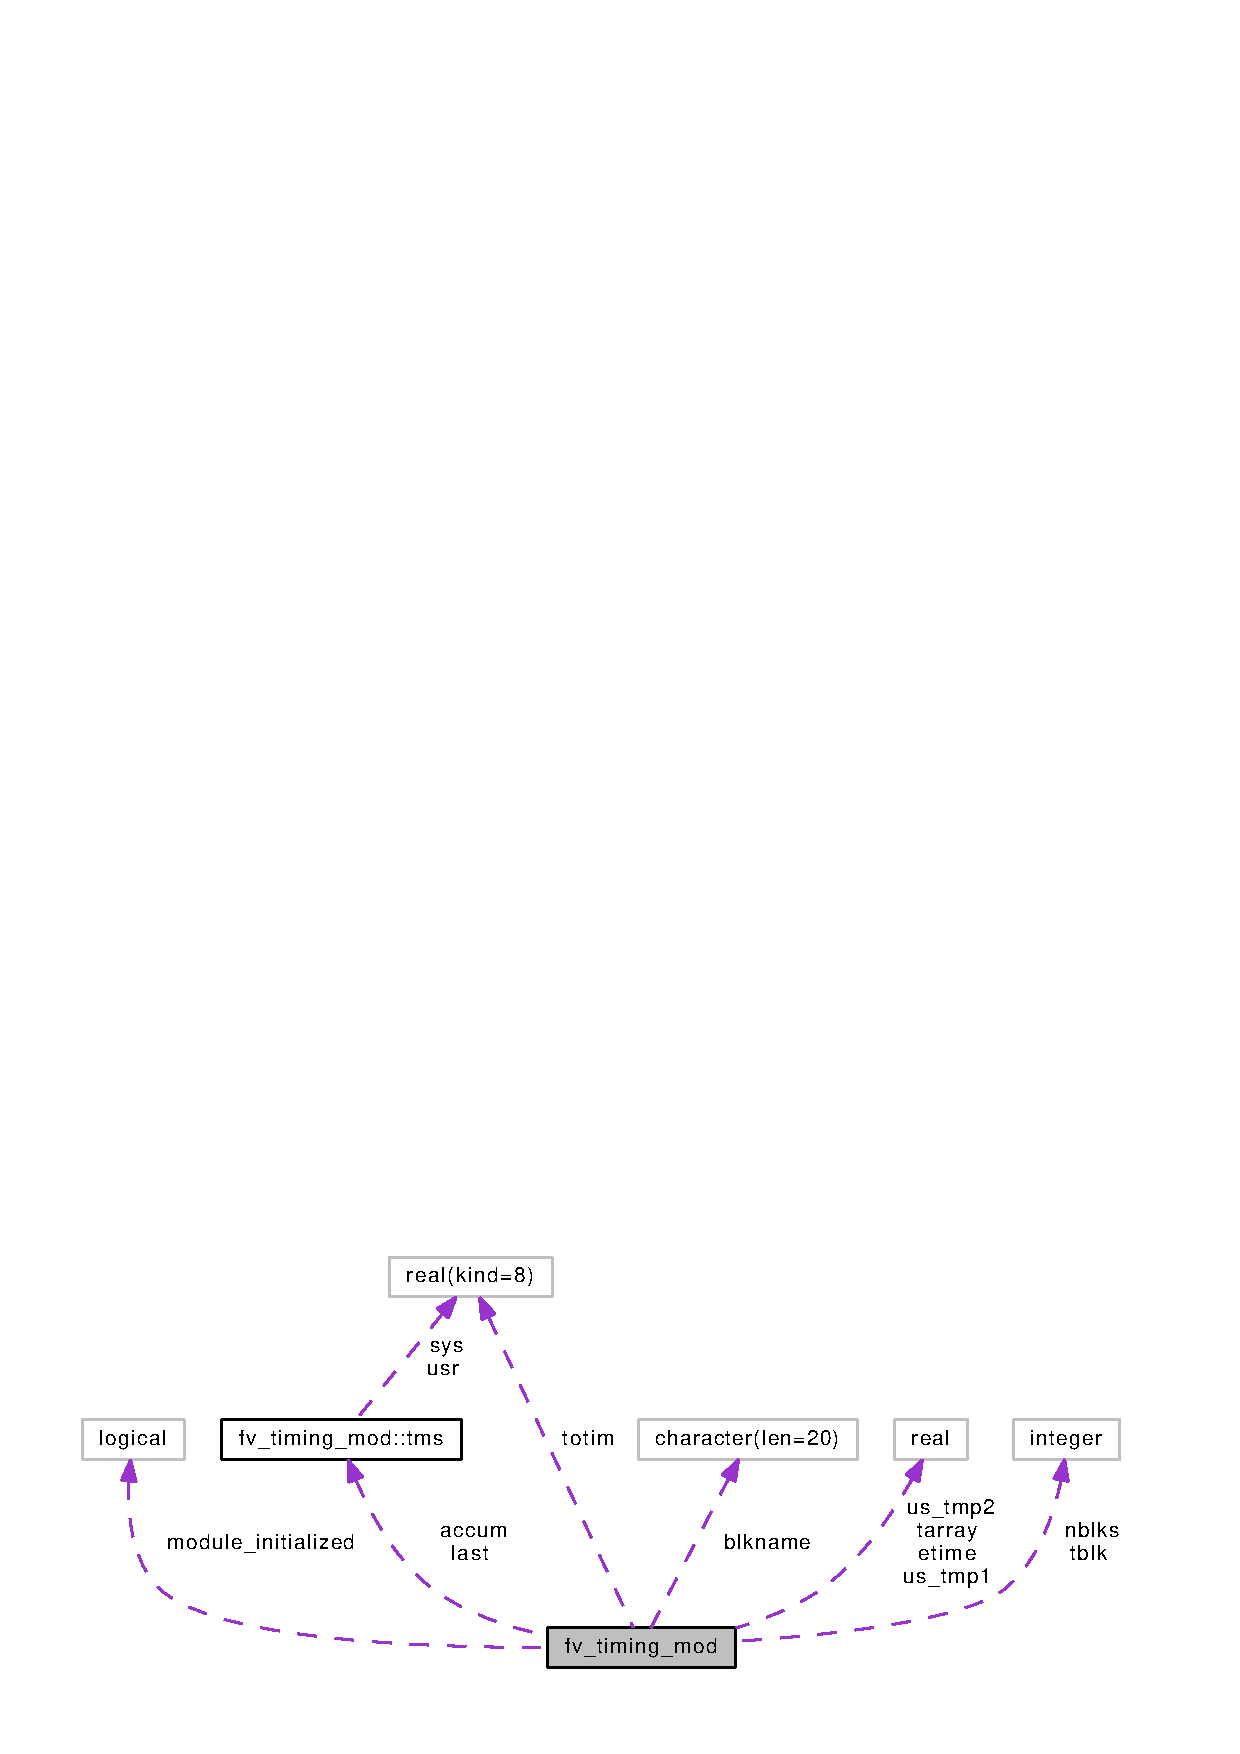
\includegraphics[width=350pt]{classfv__timing__mod__coll__graph}
\end{center}
\end{figure}
\subsection*{Data Types}
\begin{DoxyCompactItemize}
\item 
type \hyperlink{structfv__timing__mod_1_1tms}{tms}
\end{DoxyCompactItemize}
\subsection*{Public Member Functions}
\begin{DoxyCompactItemize}
\item 
subroutine \hyperlink{classfv__timing__mod_a9e0e76eea1b67592c8ec6edd35d2f9f9}{timing\-\_\-init}
\begin{DoxyCompactList}\small\item\em The subroutine 'timing\-\_\-init' initializes timers. \end{DoxyCompactList}\item 
subroutine \hyperlink{classfv__timing__mod_a85fb4c4c6b3d9604bb682356ab3e7a82}{timing\-\_\-on} (blk\-\_\-name)
\begin{DoxyCompactList}\small\item\em The subroutine 'timing\-\_\-on' starts a timer. \end{DoxyCompactList}\item 
subroutine \hyperlink{classfv__timing__mod_ad40e8855859ae4d87ac63985163a1c3d}{timing\-\_\-off} (blk\-\_\-name)
\begin{DoxyCompactList}\small\item\em The subroutine 'timing\-\_\-off' stops a timer. \end{DoxyCompactList}\item 
subroutine \hyperlink{classfv__timing__mod_afa9b6547732c567cedd45cc80bf6ab5a}{timing\-\_\-clear} ()
\begin{DoxyCompactList}\small\item\em The subroutine 'timing\-\_\-clear' resets a timer. \end{DoxyCompactList}\item 
subroutine \hyperlink{classfv__timing__mod_aa878226a27afbc94a821f2f475653d7d}{timing\-\_\-prt} (gid)
\begin{DoxyCompactList}\small\item\em The subroutine 'timing\-\_\-prt' prints all timers. \end{DoxyCompactList}\item 
subroutine \hyperlink{classfv__timing__mod_a916b4aea50b8b2d26b06c2bbc96d3564}{upper} (string, length)
\end{DoxyCompactItemize}
\subsection*{Private Attributes}
\begin{DoxyCompactItemize}
\item 
integer, private \hyperlink{classfv__timing__mod_a8f78bb855cc4e52f3308ab25fa4498a5}{nblks}
\item 
character(len=20), dimension(\hyperlink{classfv__timing__mod_a8f78bb855cc4e52f3308ab25fa4498a5}{nblks}), \\*
private \hyperlink{classfv__timing__mod_a31560d7c7691483d291cebc1466fbbef}{blkname}
\item 
integer, private \hyperlink{classfv__timing__mod_aaeddb0efd1e02edd882b6f325ad57047}{tblk}
\item 
real, private \hyperlink{classfv__timing__mod_add9c7186606182a5850e936cc88bf664}{etime}
\item 
real(kind=8), private \hyperlink{classfv__timing__mod_a5460a631553f37f69e3f87d4725fdb83}{totim}
\item 
real, dimension(2), private \hyperlink{classfv__timing__mod_a18b8ce2f3249b1cfb378a40c048b615b}{tarray}
\item 
type(\hyperlink{structfv__timing__mod_1_1tms}{tms}), dimension(\hyperlink{classfv__timing__mod_a8f78bb855cc4e52f3308ab25fa4498a5}{nblks}), \\*
private \hyperlink{classfv__timing__mod_ad37e58fa4398fd8e2e0c2ac7cfc82782}{accum}
\item 
type(\hyperlink{structfv__timing__mod_1_1tms}{tms}), dimension(\hyperlink{classfv__timing__mod_a8f78bb855cc4e52f3308ab25fa4498a5}{nblks}), \\*
private \hyperlink{classfv__timing__mod_aef40c4c1d0162a76cde3d6461a46d91b}{last}
\item 
real, dimension(\hyperlink{classfv__timing__mod_a8f78bb855cc4e52f3308ab25fa4498a5}{nblks}, 2), private \hyperlink{classfv__timing__mod_ab8d555b44911d2782f74f538a6eaa432}{us\-\_\-tmp1}
\item 
real, dimension(\hyperlink{classfv__timing__mod_a8f78bb855cc4e52f3308ab25fa4498a5}{nblks}, 2), private \hyperlink{classfv__timing__mod_a0bf15deed4130bdab7908785c80d9e70}{us\-\_\-tmp2}
\item 
logical, private \hyperlink{classfv__timing__mod_aa0f0480c2acfb9198a47a6bfd90e91c7}{module\-\_\-initialized} = .false.
\end{DoxyCompactItemize}


\subsection{Detailed Description}
The module 'fv\-\_\-timing' contains F\-V3 timers. 

Definition at line 24 of file fv\-\_\-timing.\-F90.



\subsection{Member Function/\-Subroutine Documentation}
\index{fv\-\_\-timing\-\_\-mod@{fv\-\_\-timing\-\_\-mod}!timing\-\_\-clear@{timing\-\_\-clear}}
\index{timing\-\_\-clear@{timing\-\_\-clear}!fv_timing_mod@{fv\-\_\-timing\-\_\-mod}}
\subsubsection[{timing\-\_\-clear}]{\setlength{\rightskip}{0pt plus 5cm}subroutine fv\-\_\-timing\-\_\-mod\-::timing\-\_\-clear (
\begin{DoxyParamCaption}
{}
\end{DoxyParamCaption}
)}\label{classfv__timing__mod_afa9b6547732c567cedd45cc80bf6ab5a}


The subroutine 'timing\-\_\-clear' resets a timer. 



Definition at line 239 of file fv\-\_\-timing.\-F90.

\index{fv\-\_\-timing\-\_\-mod@{fv\-\_\-timing\-\_\-mod}!timing\-\_\-init@{timing\-\_\-init}}
\index{timing\-\_\-init@{timing\-\_\-init}!fv_timing_mod@{fv\-\_\-timing\-\_\-mod}}
\subsubsection[{timing\-\_\-init}]{\setlength{\rightskip}{0pt plus 5cm}subroutine fv\-\_\-timing\-\_\-mod\-::timing\-\_\-init (
\begin{DoxyParamCaption}
{}
\end{DoxyParamCaption}
)}\label{classfv__timing__mod_a9e0e76eea1b67592c8ec6edd35d2f9f9}


The subroutine 'timing\-\_\-init' initializes timers. 



Definition at line 78 of file fv\-\_\-timing.\-F90.



Referenced by fv\-\_\-control\-\_\-mod\-::fv\-\_\-init(), and timing\-\_\-on().

\index{fv\-\_\-timing\-\_\-mod@{fv\-\_\-timing\-\_\-mod}!timing\-\_\-off@{timing\-\_\-off}}
\index{timing\-\_\-off@{timing\-\_\-off}!fv_timing_mod@{fv\-\_\-timing\-\_\-mod}}
\subsubsection[{timing\-\_\-off}]{\setlength{\rightskip}{0pt plus 5cm}subroutine fv\-\_\-timing\-\_\-mod\-::timing\-\_\-off (
\begin{DoxyParamCaption}
\item[{character(len=$\ast$)}]{blk\-\_\-name}
\end{DoxyParamCaption}
)}\label{classfv__timing__mod_ad40e8855859ae4d87ac63985163a1c3d}


The subroutine 'timing\-\_\-off' stops a timer. 



Definition at line 179 of file fv\-\_\-timing.\-F90.



References upper().



Referenced by atmosphere\-\_\-mod\-::adiabatic\-\_\-init(), atmosphere\-\_\-mod\-::atmosphere\-\_\-dynamics(), atmosphere\-\_\-mod\-::atmosphere\-\_\-end(), atmosphere\-\_\-mod\-::atmosphere\-\_\-init(), atmosphere\-\_\-mod\-::atmosphere\-\_\-state\-\_\-update(), fv\-\_\-grid\-\_\-utils\-\_\-mod\-::c2l\-\_\-ord4(), dyn\-\_\-core\-\_\-mod\-::del2\-\_\-cubed(), fv\-\_\-update\-\_\-phys\-\_\-mod\-::del2\-\_\-phys(), fv\-\_\-nwp\-\_\-nudge\-\_\-mod\-::del2\-\_\-scalar(), dyn\-\_\-core\-\_\-mod\-::dyn\-\_\-core(), fv\-\_\-restart\-\_\-mod\-::fill\-\_\-nested\-\_\-grid\-\_\-data(), fv\-\_\-restart\-\_\-mod\-::fill\-\_\-nested\-\_\-grid\-\_\-topo(), fv\-\_\-dynamics\-\_\-mod\-::fv\-\_\-dynamics(), fv\-\_\-control\-\_\-mod\-::fv\-\_\-end(), fv\-\_\-update\-\_\-phys\-\_\-mod\-::fv\-\_\-update\-\_\-phys(), external\-\_\-ic\-\_\-mod\-::get\-\_\-external\-\_\-ic(), fv\-\_\-mapz\-\_\-mod\-::lagrangian\-\_\-to\-\_\-eulerian(), boundary\-\_\-mod\-::nested\-\_\-grid\-\_\-bc\-\_\-2d\-\_\-mpp(), boundary\-\_\-mod\-::nested\-\_\-grid\-\_\-bc\-\_\-mpp(), boundary\-\_\-mod\-::nested\-\_\-grid\-\_\-bc\-\_\-mpp\-\_\-send(), boundary\-\_\-mod\-::nested\-\_\-grid\-\_\-bc\-\_\-recv(), boundary\-\_\-mod\-::nested\-\_\-grid\-\_\-bc\-\_\-send(), fv\-\_\-dynamics\-\_\-mod\-::rayleigh\-\_\-friction(), fv\-\_\-dynamics\-\_\-mod\-::rayleigh\-\_\-super(), fv\-\_\-nesting\-\_\-mod\-::setup\-\_\-nested\-\_\-grid\-\_\-bcs(), fv\-\_\-surf\-\_\-map\-\_\-mod\-::surfdrv(), fv\-\_\-tracer2d\-\_\-mod\-::tracer\-\_\-2d(), fv\-\_\-tracer2d\-\_\-mod\-::tracer\-\_\-2d\-\_\-1l(), fv\-\_\-tracer2d\-\_\-mod\-::tracer\-\_\-2d\-\_\-nested(), fv\-\_\-update\-\_\-phys\-\_\-mod\-::update2d\-\_\-dwinds\-\_\-phys(), and boundary\-\_\-mod\-::update\-\_\-coarse\-\_\-grid\-\_\-mpp().

\index{fv\-\_\-timing\-\_\-mod@{fv\-\_\-timing\-\_\-mod}!timing\-\_\-on@{timing\-\_\-on}}
\index{timing\-\_\-on@{timing\-\_\-on}!fv_timing_mod@{fv\-\_\-timing\-\_\-mod}}
\subsubsection[{timing\-\_\-on}]{\setlength{\rightskip}{0pt plus 5cm}subroutine fv\-\_\-timing\-\_\-mod\-::timing\-\_\-on (
\begin{DoxyParamCaption}
\item[{character(len=$\ast$)}]{blk\-\_\-name}
\end{DoxyParamCaption}
)}\label{classfv__timing__mod_a85fb4c4c6b3d9604bb682356ab3e7a82}


The subroutine 'timing\-\_\-on' starts a timer. 



Definition at line 115 of file fv\-\_\-timing.\-F90.



References timing\-\_\-init(), and upper().



Referenced by atmosphere\-\_\-mod\-::adiabatic\-\_\-init(), atmosphere\-\_\-mod\-::atmosphere\-\_\-dynamics(), atmosphere\-\_\-mod\-::atmosphere\-\_\-end(), atmosphere\-\_\-mod\-::atmosphere\-\_\-init(), atmosphere\-\_\-mod\-::atmosphere\-\_\-state\-\_\-update(), fv\-\_\-grid\-\_\-utils\-\_\-mod\-::c2l\-\_\-ord4(), dyn\-\_\-core\-\_\-mod\-::del2\-\_\-cubed(), fv\-\_\-update\-\_\-phys\-\_\-mod\-::del2\-\_\-phys(), fv\-\_\-nwp\-\_\-nudge\-\_\-mod\-::del2\-\_\-scalar(), dyn\-\_\-core\-\_\-mod\-::dyn\-\_\-core(), fv\-\_\-restart\-\_\-mod\-::fill\-\_\-nested\-\_\-grid\-\_\-data(), fv\-\_\-restart\-\_\-mod\-::fill\-\_\-nested\-\_\-grid\-\_\-topo(), fv\-\_\-dynamics\-\_\-mod\-::fv\-\_\-dynamics(), fv\-\_\-control\-\_\-mod\-::fv\-\_\-init(), fv\-\_\-update\-\_\-phys\-\_\-mod\-::fv\-\_\-update\-\_\-phys(), external\-\_\-ic\-\_\-mod\-::get\-\_\-external\-\_\-ic(), fv\-\_\-mapz\-\_\-mod\-::lagrangian\-\_\-to\-\_\-eulerian(), boundary\-\_\-mod\-::nested\-\_\-grid\-\_\-bc\-\_\-2d\-\_\-mpp(), boundary\-\_\-mod\-::nested\-\_\-grid\-\_\-bc\-\_\-mpp(), boundary\-\_\-mod\-::nested\-\_\-grid\-\_\-bc\-\_\-mpp\-\_\-send(), boundary\-\_\-mod\-::nested\-\_\-grid\-\_\-bc\-\_\-recv(), boundary\-\_\-mod\-::nested\-\_\-grid\-\_\-bc\-\_\-send(), fv\-\_\-dynamics\-\_\-mod\-::rayleigh\-\_\-friction(), fv\-\_\-dynamics\-\_\-mod\-::rayleigh\-\_\-super(), fv\-\_\-nesting\-\_\-mod\-::setup\-\_\-nested\-\_\-grid\-\_\-bcs(), fv\-\_\-surf\-\_\-map\-\_\-mod\-::surfdrv(), fv\-\_\-tracer2d\-\_\-mod\-::tracer\-\_\-2d(), fv\-\_\-tracer2d\-\_\-mod\-::tracer\-\_\-2d\-\_\-1l(), fv\-\_\-tracer2d\-\_\-mod\-::tracer\-\_\-2d\-\_\-nested(), fv\-\_\-update\-\_\-phys\-\_\-mod\-::update2d\-\_\-dwinds\-\_\-phys(), and boundary\-\_\-mod\-::update\-\_\-coarse\-\_\-grid\-\_\-mpp().

\index{fv\-\_\-timing\-\_\-mod@{fv\-\_\-timing\-\_\-mod}!timing\-\_\-prt@{timing\-\_\-prt}}
\index{timing\-\_\-prt@{timing\-\_\-prt}!fv_timing_mod@{fv\-\_\-timing\-\_\-mod}}
\subsubsection[{timing\-\_\-prt}]{\setlength{\rightskip}{0pt plus 5cm}subroutine fv\-\_\-timing\-\_\-mod\-::timing\-\_\-prt (
\begin{DoxyParamCaption}
\item[{integer}]{gid}
\end{DoxyParamCaption}
)}\label{classfv__timing__mod_aa878226a27afbc94a821f2f475653d7d}


The subroutine 'timing\-\_\-prt' prints all timers. 



Definition at line 248 of file fv\-\_\-timing.\-F90.



Referenced by fv\-\_\-control\-\_\-mod\-::fv\-\_\-end().

\index{fv\-\_\-timing\-\_\-mod@{fv\-\_\-timing\-\_\-mod}!upper@{upper}}
\index{upper@{upper}!fv_timing_mod@{fv\-\_\-timing\-\_\-mod}}
\subsubsection[{upper}]{\setlength{\rightskip}{0pt plus 5cm}subroutine fv\-\_\-timing\-\_\-mod\-::upper (
\begin{DoxyParamCaption}
\item[{character (len=$\ast$), intent(inout)}]{string, }
\item[{integer, intent(in)}]{length}
\end{DoxyParamCaption}
)}\label{classfv__timing__mod_a916b4aea50b8b2d26b06c2bbc96d3564}


Definition at line 294 of file fv\-\_\-timing.\-F90.



Referenced by timing\-\_\-off(), and timing\-\_\-on().



\subsection{Member Data Documentation}
\index{fv\-\_\-timing\-\_\-mod@{fv\-\_\-timing\-\_\-mod}!accum@{accum}}
\index{accum@{accum}!fv_timing_mod@{fv\-\_\-timing\-\_\-mod}}
\subsubsection[{accum}]{\setlength{\rightskip}{0pt plus 5cm}type ({\bf tms}), dimension({\bf nblks}), private fv\-\_\-timing\-\_\-mod\-::accum\hspace{0.3cm}{\ttfamily [private]}}\label{classfv__timing__mod_ad37e58fa4398fd8e2e0c2ac7cfc82782}


Definition at line 68 of file fv\-\_\-timing.\-F90.

\index{fv\-\_\-timing\-\_\-mod@{fv\-\_\-timing\-\_\-mod}!blkname@{blkname}}
\index{blkname@{blkname}!fv_timing_mod@{fv\-\_\-timing\-\_\-mod}}
\subsubsection[{blkname}]{\setlength{\rightskip}{0pt plus 5cm}character(len=20), dimension({\bf nblks}), private fv\-\_\-timing\-\_\-mod\-::blkname\hspace{0.3cm}{\ttfamily [private]}}\label{classfv__timing__mod_a31560d7c7691483d291cebc1466fbbef}


Definition at line 52 of file fv\-\_\-timing.\-F90.

\index{fv\-\_\-timing\-\_\-mod@{fv\-\_\-timing\-\_\-mod}!etime@{etime}}
\index{etime@{etime}!fv_timing_mod@{fv\-\_\-timing\-\_\-mod}}
\subsubsection[{etime}]{\setlength{\rightskip}{0pt plus 5cm}real, private fv\-\_\-timing\-\_\-mod\-::etime\hspace{0.3cm}{\ttfamily [private]}}\label{classfv__timing__mod_add9c7186606182a5850e936cc88bf664}


Definition at line 59 of file fv\-\_\-timing.\-F90.

\index{fv\-\_\-timing\-\_\-mod@{fv\-\_\-timing\-\_\-mod}!last@{last}}
\index{last@{last}!fv_timing_mod@{fv\-\_\-timing\-\_\-mod}}
\subsubsection[{last}]{\setlength{\rightskip}{0pt plus 5cm}type ({\bf tms}), dimension({\bf nblks}), private fv\-\_\-timing\-\_\-mod\-::last\hspace{0.3cm}{\ttfamily [private]}}\label{classfv__timing__mod_aef40c4c1d0162a76cde3d6461a46d91b}


Definition at line 68 of file fv\-\_\-timing.\-F90.

\index{fv\-\_\-timing\-\_\-mod@{fv\-\_\-timing\-\_\-mod}!module\-\_\-initialized@{module\-\_\-initialized}}
\index{module\-\_\-initialized@{module\-\_\-initialized}!fv_timing_mod@{fv\-\_\-timing\-\_\-mod}}
\subsubsection[{module\-\_\-initialized}]{\setlength{\rightskip}{0pt plus 5cm}logical, private fv\-\_\-timing\-\_\-mod\-::module\-\_\-initialized = .false.\hspace{0.3cm}{\ttfamily [private]}}\label{classfv__timing__mod_aa0f0480c2acfb9198a47a6bfd90e91c7}


Definition at line 73 of file fv\-\_\-timing.\-F90.

\index{fv\-\_\-timing\-\_\-mod@{fv\-\_\-timing\-\_\-mod}!nblks@{nblks}}
\index{nblks@{nblks}!fv_timing_mod@{fv\-\_\-timing\-\_\-mod}}
\subsubsection[{nblks}]{\setlength{\rightskip}{0pt plus 5cm}integer, private fv\-\_\-timing\-\_\-mod\-::nblks\hspace{0.3cm}{\ttfamily [private]}}\label{classfv__timing__mod_a8f78bb855cc4e52f3308ab25fa4498a5}


Definition at line 49 of file fv\-\_\-timing.\-F90.

\index{fv\-\_\-timing\-\_\-mod@{fv\-\_\-timing\-\_\-mod}!tarray@{tarray}}
\index{tarray@{tarray}!fv_timing_mod@{fv\-\_\-timing\-\_\-mod}}
\subsubsection[{tarray}]{\setlength{\rightskip}{0pt plus 5cm}real, dimension(2), private fv\-\_\-timing\-\_\-mod\-::tarray\hspace{0.3cm}{\ttfamily [private]}}\label{classfv__timing__mod_a18b8ce2f3249b1cfb378a40c048b615b}


Definition at line 61 of file fv\-\_\-timing.\-F90.

\index{fv\-\_\-timing\-\_\-mod@{fv\-\_\-timing\-\_\-mod}!tblk@{tblk}}
\index{tblk@{tblk}!fv_timing_mod@{fv\-\_\-timing\-\_\-mod}}
\subsubsection[{tblk}]{\setlength{\rightskip}{0pt plus 5cm}integer, private fv\-\_\-timing\-\_\-mod\-::tblk\hspace{0.3cm}{\ttfamily [private]}}\label{classfv__timing__mod_aaeddb0efd1e02edd882b6f325ad57047}


Definition at line 54 of file fv\-\_\-timing.\-F90.

\index{fv\-\_\-timing\-\_\-mod@{fv\-\_\-timing\-\_\-mod}!totim@{totim}}
\index{totim@{totim}!fv_timing_mod@{fv\-\_\-timing\-\_\-mod}}
\subsubsection[{totim}]{\setlength{\rightskip}{0pt plus 5cm}real(kind=8), private fv\-\_\-timing\-\_\-mod\-::totim\hspace{0.3cm}{\ttfamily [private]}}\label{classfv__timing__mod_a5460a631553f37f69e3f87d4725fdb83}


Definition at line 60 of file fv\-\_\-timing.\-F90.

\index{fv\-\_\-timing\-\_\-mod@{fv\-\_\-timing\-\_\-mod}!us\-\_\-tmp1@{us\-\_\-tmp1}}
\index{us\-\_\-tmp1@{us\-\_\-tmp1}!fv_timing_mod@{fv\-\_\-timing\-\_\-mod}}
\subsubsection[{us\-\_\-tmp1}]{\setlength{\rightskip}{0pt plus 5cm}real, dimension({\bf nblks},2), private fv\-\_\-timing\-\_\-mod\-::us\-\_\-tmp1\hspace{0.3cm}{\ttfamily [private]}}\label{classfv__timing__mod_ab8d555b44911d2782f74f538a6eaa432}


Definition at line 70 of file fv\-\_\-timing.\-F90.

\index{fv\-\_\-timing\-\_\-mod@{fv\-\_\-timing\-\_\-mod}!us\-\_\-tmp2@{us\-\_\-tmp2}}
\index{us\-\_\-tmp2@{us\-\_\-tmp2}!fv_timing_mod@{fv\-\_\-timing\-\_\-mod}}
\subsubsection[{us\-\_\-tmp2}]{\setlength{\rightskip}{0pt plus 5cm}real, dimension({\bf nblks},2), private fv\-\_\-timing\-\_\-mod\-::us\-\_\-tmp2\hspace{0.3cm}{\ttfamily [private]}}\label{classfv__timing__mod_a0bf15deed4130bdab7908785c80d9e70}


Definition at line 71 of file fv\-\_\-timing.\-F90.



The documentation for this module was generated from the following file\-:\begin{DoxyCompactItemize}
\item 
/scratch2/\-N\-A\-G\-A\-P\-E/aoml-\/hafs1/\-Kyle.\-Ahern/acs\-\_\-master\-\_\-readonly/tools/\hyperlink{fv__timing_8F90}{fv\-\_\-timing.\-F90}\end{DoxyCompactItemize}

\section{fv\-\_\-tracer2d\-\_\-mod Module Reference}
\label{classfv__tracer2d__mod}\index{fv\-\_\-tracer2d\-\_\-mod@{fv\-\_\-tracer2d\-\_\-mod}}


The module '\hyperlink{fv__tracer2d_8F90}{fv\-\_\-tracer2d.\-F90}' performs sub-\/cycled tracer advection.  




Collaboration diagram for fv\-\_\-tracer2d\-\_\-mod\-:
\nopagebreak
\begin{figure}[H]
\begin{center}
\leavevmode
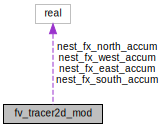
\includegraphics[width=201pt]{classfv__tracer2d__mod__coll__graph}
\end{center}
\end{figure}
\subsection*{Public Member Functions}
\begin{DoxyCompactItemize}
\item 
subroutine, public \hyperlink{classfv__tracer2d__mod_ad980c5de5fcd3b7ace218eb30359eae3}{tracer\-\_\-2d\-\_\-1l} (q, dp1, mfx, mfy, cx, cy, gridstruct, bd, domain, npx, npy, npz, nq, hord, q\-\_\-split, dt, id\-\_\-divg, q\-\_\-pack, nord\-\_\-tr, trdm, lim\-\_\-fac, regional)
\begin{DoxyCompactList}\small\item\em The subroutine 'tracer\-\_\-2d\-\_\-1\-L' performs 2-\/\-D horizontal-\/to-\/lagrangian transport. \end{DoxyCompactList}\item 
subroutine, public \hyperlink{classfv__tracer2d__mod_a4918bade9446e44f288de345d368acbb}{tracer\-\_\-2d} (q, dp1, mfx, mfy, cx, cy, gridstruct, bd, domain, npx, npy, npz, nq, hord, q\-\_\-split, dt, id\-\_\-divg, q\-\_\-pack, nord\-\_\-tr, trdm, lim\-\_\-fac, regional)
\begin{DoxyCompactList}\small\item\em The subroutine 'tracer\-\_\-2d' is the standard routine for sub-\/cycled tracer advection. \end{DoxyCompactList}\item 
subroutine, public \hyperlink{classfv__tracer2d__mod_a23b2bdc9c60a39458ebd937e961d334e}{tracer\-\_\-2d\-\_\-nested} (q, dp1, mfx, mfy, cx, cy, gridstruct, bd, domain, npx, npy, npz, nq, hord, q\-\_\-split, dt, id\-\_\-divg, q\-\_\-pack, nord\-\_\-tr, trdm, k\-\_\-split, neststruct, parent\-\_\-grid, lim\-\_\-fac, regional)
\end{DoxyCompactItemize}
\subsection*{Private Attributes}
\begin{DoxyCompactItemize}
\item 
real, dimension(\-:,\-:,\-:), allocatable \hyperlink{classfv__tracer2d__mod_afedafbd659d48b128ce6461b3483b85a}{nest\-\_\-fx\-\_\-west\-\_\-accum}
\item 
real, dimension(\-:,\-:,\-:), allocatable \hyperlink{classfv__tracer2d__mod_a2ef2686b07c3eae1d4f5f17a3db8e8e8}{nest\-\_\-fx\-\_\-east\-\_\-accum}
\item 
real, dimension(\-:,\-:,\-:), allocatable \hyperlink{classfv__tracer2d__mod_a3bf4ea79bede8504fd2df61b9837991c}{nest\-\_\-fx\-\_\-south\-\_\-accum}
\item 
real, dimension(\-:,\-:,\-:), allocatable \hyperlink{classfv__tracer2d__mod_a9616f908472d3cd36e6e3ed3ac287ed5}{nest\-\_\-fx\-\_\-north\-\_\-accum}
\end{DoxyCompactItemize}


\subsection{Detailed Description}
The module '\hyperlink{fv__tracer2d_8F90}{fv\-\_\-tracer2d.\-F90}' performs sub-\/cycled tracer advection. 

\begin{DoxySeeAlso}{See Also}
\cite{lin2004vertically} 
\end{DoxySeeAlso}


Definition at line 64 of file fv\-\_\-tracer2d.\-F90.



\subsection{Member Function/\-Subroutine Documentation}
\index{fv\-\_\-tracer2d\-\_\-mod@{fv\-\_\-tracer2d\-\_\-mod}!tracer\-\_\-2d@{tracer\-\_\-2d}}
\index{tracer\-\_\-2d@{tracer\-\_\-2d}!fv_tracer2d_mod@{fv\-\_\-tracer2d\-\_\-mod}}
\subsubsection[{tracer\-\_\-2d}]{\setlength{\rightskip}{0pt plus 5cm}subroutine, public fv\-\_\-tracer2d\-\_\-mod\-::tracer\-\_\-2d (
\begin{DoxyParamCaption}
\item[{real, dimension(bd\%isd\-:bd\%ied,bd\%jsd\-:bd\%jed,npz,nq), intent(inout)}]{q, }
\item[{real, dimension(bd\%isd\-:bd\%ied,bd\%jsd\-:bd\%jed,npz), intent(inout)}]{dp1, }
\item[{real, dimension(bd\%is\-:bd\%ie+1,bd\%js\-:bd\%je,  npz), intent(inout)}]{mfx, }
\item[{real, dimension(bd\%is\-:bd\%ie  ,bd\%js\-:bd\%je+1,npz), intent(inout)}]{mfy, }
\item[{real, dimension(bd\%is\-:bd\%ie+1,bd\%jsd\-:bd\%jed  ,npz), intent(inout)}]{cx, }
\item[{real, dimension(bd\%isd\-:bd\%ied,bd\%js \-:bd\%je +1,npz), intent(inout)}]{cy, }
\item[{type(fv\-\_\-grid\-\_\-type), intent(in), target}]{gridstruct, }
\item[{type(fv\-\_\-grid\-\_\-bounds\-\_\-type), intent(in)}]{bd, }
\item[{type(domain2d), intent(inout)}]{domain, }
\item[{integer, intent(in)}]{npx, }
\item[{integer, intent(in)}]{npy, }
\item[{integer, intent(in)}]{npz, }
\item[{integer, intent(in)}]{nq, }
\item[{integer, intent(in)}]{hord, }
\item[{integer, intent(in)}]{q\-\_\-split, }
\item[{real, intent(in)}]{dt, }
\item[{integer, intent(in)}]{id\-\_\-divg, }
\item[{type(group\-\_\-halo\-\_\-update\-\_\-type), intent(inout)}]{q\-\_\-pack, }
\item[{integer, intent(in)}]{nord\-\_\-tr, }
\item[{real, intent(in)}]{trdm, }
\item[{real, intent(in)}]{lim\-\_\-fac, }
\item[{logical, intent(in)}]{regional}
\end{DoxyParamCaption}
)}\label{classfv__tracer2d__mod_a4918bade9446e44f288de345d368acbb}


The subroutine 'tracer\-\_\-2d' is the standard routine for sub-\/cycled tracer advection. 


\begin{DoxyParams}[1]{Parameters}
\mbox{\tt in}  & {\em nq} & number of tracers to be advected\\
\hline
\mbox{\tt in,out}  & {\em q} & Tracers\\
\hline
\mbox{\tt in,out}  & {\em dp1} & D\-E\-L\-P before dyn\-\_\-core\\
\hline
\mbox{\tt in,out}  & {\em mfx} & Mass Flux X-\/\-Dir\\
\hline
\mbox{\tt in,out}  & {\em mfy} & Mass Flux Y-\/\-Dir\\
\hline
\mbox{\tt in,out}  & {\em cx} & Courant Number X-\/\-Dir\\
\hline
\mbox{\tt in,out}  & {\em cy} & Courant Number Y-\/\-Dir \\
\hline
\end{DoxyParams}


Definition at line 317 of file fv\-\_\-tracer2d.\-F90.



References tp\-\_\-core\-\_\-mod\-::fv\-\_\-tp\-\_\-2d(), fv\-\_\-timing\-\_\-mod\-::timing\-\_\-off(), and fv\-\_\-timing\-\_\-mod\-::timing\-\_\-on().



Referenced by fv\-\_\-dynamics\-\_\-mod\-::fv\-\_\-dynamics().

\index{fv\-\_\-tracer2d\-\_\-mod@{fv\-\_\-tracer2d\-\_\-mod}!tracer\-\_\-2d\-\_\-1l@{tracer\-\_\-2d\-\_\-1l}}
\index{tracer\-\_\-2d\-\_\-1l@{tracer\-\_\-2d\-\_\-1l}!fv_tracer2d_mod@{fv\-\_\-tracer2d\-\_\-mod}}
\subsubsection[{tracer\-\_\-2d\-\_\-1l}]{\setlength{\rightskip}{0pt plus 5cm}subroutine, public fv\-\_\-tracer2d\-\_\-mod\-::tracer\-\_\-2d\-\_\-1l (
\begin{DoxyParamCaption}
\item[{real, dimension(bd\%isd\-:bd\%ied,bd\%jsd\-:bd\%jed,npz,nq), intent(inout)}]{q, }
\item[{real, dimension(bd\%isd\-:bd\%ied,bd\%jsd\-:bd\%jed,npz), intent(inout)}]{dp1, }
\item[{real, dimension(bd\%is\-:bd\%ie+1,bd\%js\-:bd\%je,  npz), intent(inout)}]{mfx, }
\item[{real, dimension(bd\%is\-:bd\%ie  ,bd\%js\-:bd\%je+1,npz), intent(inout)}]{mfy, }
\item[{real, dimension(bd\%is\-:bd\%ie+1,bd\%jsd\-:bd\%jed  ,npz), intent(inout)}]{cx, }
\item[{real, dimension(bd\%isd\-:bd\%ied,bd\%js \-:bd\%je +1,npz), intent(inout)}]{cy, }
\item[{type(fv\-\_\-grid\-\_\-type), intent(in), target}]{gridstruct, }
\item[{type(fv\-\_\-grid\-\_\-bounds\-\_\-type), intent(in)}]{bd, }
\item[{type(domain2d), intent(inout)}]{domain, }
\item[{integer, intent(in)}]{npx, }
\item[{integer, intent(in)}]{npy, }
\item[{integer, intent(in)}]{npz, }
\item[{integer, intent(in)}]{nq, }
\item[{integer, intent(in)}]{hord, }
\item[{integer, intent(in)}]{q\-\_\-split, }
\item[{real, intent(in)}]{dt, }
\item[{integer, intent(in)}]{id\-\_\-divg, }
\item[{type(group\-\_\-halo\-\_\-update\-\_\-type), intent(inout)}]{q\-\_\-pack, }
\item[{integer, intent(in)}]{nord\-\_\-tr, }
\item[{real, intent(in)}]{trdm, }
\item[{real, intent(in)}]{lim\-\_\-fac, }
\item[{logical, intent(in)}]{regional}
\end{DoxyParamCaption}
)}\label{classfv__tracer2d__mod_ad980c5de5fcd3b7ace218eb30359eae3}


The subroutine 'tracer\-\_\-2d\-\_\-1\-L' performs 2-\/\-D horizontal-\/to-\/lagrangian transport. 

This subroutine is called if 'z\-\_\-tracer = .true.' It modifies 'tracer\-\_\-2d' so that each layer uses a different diagnosed number of split tracer timesteps. This potentially accelerates tracer advection when there is a large difference in layer-\/maximum wind speeds (cf. polar night jet).


\begin{DoxyParams}[1]{Parameters}
\mbox{\tt in}  & {\em nq} & number of tracers to be advected\\
\hline
\mbox{\tt in,out}  & {\em q} & Tracers\\
\hline
\mbox{\tt in,out}  & {\em dp1} & D\-E\-L\-P before dyn\-\_\-core\\
\hline
\mbox{\tt in,out}  & {\em mfx} & Mass Flux X-\/\-Dir\\
\hline
\mbox{\tt in,out}  & {\em mfy} & Mass Flux Y-\/\-Dir\\
\hline
\mbox{\tt in,out}  & {\em cx} & Courant Number X-\/\-Dir\\
\hline
\mbox{\tt in,out}  & {\em cy} & Courant Number Y-\/\-Dir \\
\hline
\end{DoxyParams}


Definition at line 92 of file fv\-\_\-tracer2d.\-F90.



References tp\-\_\-core\-\_\-mod\-::fv\-\_\-tp\-\_\-2d(), fv\-\_\-timing\-\_\-mod\-::timing\-\_\-off(), and fv\-\_\-timing\-\_\-mod\-::timing\-\_\-on().



Referenced by fv\-\_\-dynamics\-\_\-mod\-::fv\-\_\-dynamics().

\index{fv\-\_\-tracer2d\-\_\-mod@{fv\-\_\-tracer2d\-\_\-mod}!tracer\-\_\-2d\-\_\-nested@{tracer\-\_\-2d\-\_\-nested}}
\index{tracer\-\_\-2d\-\_\-nested@{tracer\-\_\-2d\-\_\-nested}!fv_tracer2d_mod@{fv\-\_\-tracer2d\-\_\-mod}}
\subsubsection[{tracer\-\_\-2d\-\_\-nested}]{\setlength{\rightskip}{0pt plus 5cm}subroutine, public fv\-\_\-tracer2d\-\_\-mod\-::tracer\-\_\-2d\-\_\-nested (
\begin{DoxyParamCaption}
\item[{real, dimension(bd\%isd\-:bd\%ied,bd\%jsd\-:bd\%jed,npz,nq), intent(inout)}]{q, }
\item[{real, dimension(bd\%isd\-:bd\%ied,bd\%jsd\-:bd\%jed,npz), intent(inout)}]{dp1, }
\item[{real, dimension(bd\%is\-:bd\%ie+1,bd\%js\-:bd\%je,  npz), intent(inout)}]{mfx, }
\item[{real, dimension(bd\%is\-:bd\%ie  ,bd\%js\-:bd\%je+1,npz), intent(inout)}]{mfy, }
\item[{real, dimension(bd\%is\-:bd\%ie+1,bd\%jsd\-:bd\%jed  ,npz), intent(inout)}]{cx, }
\item[{real, dimension(bd\%isd\-:bd\%ied,bd\%js \-:bd\%je +1,npz), intent(inout)}]{cy, }
\item[{type(fv\-\_\-grid\-\_\-type), intent(in), target}]{gridstruct, }
\item[{type(fv\-\_\-grid\-\_\-bounds\-\_\-type), intent(in)}]{bd, }
\item[{type(domain2d), intent(inout)}]{domain, }
\item[{integer, intent(in)}]{npx, }
\item[{integer, intent(in)}]{npy, }
\item[{integer, intent(in)}]{npz, }
\item[{integer, intent(in)}]{nq, }
\item[{integer, intent(in)}]{hord, }
\item[{integer, intent(in)}]{q\-\_\-split, }
\item[{real, intent(in)}]{dt, }
\item[{integer, intent(in)}]{id\-\_\-divg, }
\item[{type(group\-\_\-halo\-\_\-update\-\_\-type), intent(inout)}]{q\-\_\-pack, }
\item[{integer, intent(in)}]{nord\-\_\-tr, }
\item[{real, intent(in)}]{trdm, }
\item[{integer, intent(in)}]{k\-\_\-split, }
\item[{type(fv\-\_\-nest\-\_\-type), intent(inout)}]{neststruct, }
\item[{type(fv\-\_\-atmos\-\_\-type), intent(in), pointer}]{parent\-\_\-grid, }
\item[{real, intent(in)}]{lim\-\_\-fac, }
\item[{logical, intent(in)}]{regional}
\end{DoxyParamCaption}
)}\label{classfv__tracer2d__mod_a23b2bdc9c60a39458ebd937e961d334e}

\begin{DoxyParams}[1]{Parameters}
\mbox{\tt in}  & {\em nq} & number of tracers to be advected\\
\hline
\mbox{\tt in,out}  & {\em q} & Tracers\\
\hline
\mbox{\tt in,out}  & {\em dp1} & D\-E\-L\-P before dyn\-\_\-core\\
\hline
\mbox{\tt in,out}  & {\em mfx} & Mass Flux X-\/\-Dir\\
\hline
\mbox{\tt in,out}  & {\em mfy} & Mass Flux Y-\/\-Dir\\
\hline
\mbox{\tt in,out}  & {\em cx} & Courant Number X-\/\-Dir\\
\hline
\mbox{\tt in,out}  & {\em cy} & Courant Number Y-\/\-Dir \\
\hline
\end{DoxyParams}


Definition at line 558 of file fv\-\_\-tracer2d.\-F90.



References tp\-\_\-core\-\_\-mod\-::fv\-\_\-tp\-\_\-2d(), boundary\-\_\-mod\-::nested\-\_\-grid\-\_\-bc\-\_\-apply\-\_\-intt(), fv\-\_\-regional\-\_\-mod\-::regional\-\_\-boundary\-\_\-update(), fv\-\_\-timing\-\_\-mod\-::timing\-\_\-off(), and fv\-\_\-timing\-\_\-mod\-::timing\-\_\-on().



Referenced by fv\-\_\-dynamics\-\_\-mod\-::fv\-\_\-dynamics().



\subsection{Member Data Documentation}
\index{fv\-\_\-tracer2d\-\_\-mod@{fv\-\_\-tracer2d\-\_\-mod}!nest\-\_\-fx\-\_\-east\-\_\-accum@{nest\-\_\-fx\-\_\-east\-\_\-accum}}
\index{nest\-\_\-fx\-\_\-east\-\_\-accum@{nest\-\_\-fx\-\_\-east\-\_\-accum}!fv_tracer2d_mod@{fv\-\_\-tracer2d\-\_\-mod}}
\subsubsection[{nest\-\_\-fx\-\_\-east\-\_\-accum}]{\setlength{\rightskip}{0pt plus 5cm}real, dimension(\-:,\-:,\-:), allocatable fv\-\_\-tracer2d\-\_\-mod\-::nest\-\_\-fx\-\_\-east\-\_\-accum\hspace{0.3cm}{\ttfamily [private]}}\label{classfv__tracer2d__mod_a2ef2686b07c3eae1d4f5f17a3db8e8e8}


Definition at line 83 of file fv\-\_\-tracer2d.\-F90.

\index{fv\-\_\-tracer2d\-\_\-mod@{fv\-\_\-tracer2d\-\_\-mod}!nest\-\_\-fx\-\_\-north\-\_\-accum@{nest\-\_\-fx\-\_\-north\-\_\-accum}}
\index{nest\-\_\-fx\-\_\-north\-\_\-accum@{nest\-\_\-fx\-\_\-north\-\_\-accum}!fv_tracer2d_mod@{fv\-\_\-tracer2d\-\_\-mod}}
\subsubsection[{nest\-\_\-fx\-\_\-north\-\_\-accum}]{\setlength{\rightskip}{0pt plus 5cm}real, dimension(\-:,\-:,\-:), allocatable fv\-\_\-tracer2d\-\_\-mod\-::nest\-\_\-fx\-\_\-north\-\_\-accum\hspace{0.3cm}{\ttfamily [private]}}\label{classfv__tracer2d__mod_a9616f908472d3cd36e6e3ed3ac287ed5}


Definition at line 83 of file fv\-\_\-tracer2d.\-F90.

\index{fv\-\_\-tracer2d\-\_\-mod@{fv\-\_\-tracer2d\-\_\-mod}!nest\-\_\-fx\-\_\-south\-\_\-accum@{nest\-\_\-fx\-\_\-south\-\_\-accum}}
\index{nest\-\_\-fx\-\_\-south\-\_\-accum@{nest\-\_\-fx\-\_\-south\-\_\-accum}!fv_tracer2d_mod@{fv\-\_\-tracer2d\-\_\-mod}}
\subsubsection[{nest\-\_\-fx\-\_\-south\-\_\-accum}]{\setlength{\rightskip}{0pt plus 5cm}real, dimension(\-:,\-:,\-:), allocatable fv\-\_\-tracer2d\-\_\-mod\-::nest\-\_\-fx\-\_\-south\-\_\-accum\hspace{0.3cm}{\ttfamily [private]}}\label{classfv__tracer2d__mod_a3bf4ea79bede8504fd2df61b9837991c}


Definition at line 83 of file fv\-\_\-tracer2d.\-F90.

\index{fv\-\_\-tracer2d\-\_\-mod@{fv\-\_\-tracer2d\-\_\-mod}!nest\-\_\-fx\-\_\-west\-\_\-accum@{nest\-\_\-fx\-\_\-west\-\_\-accum}}
\index{nest\-\_\-fx\-\_\-west\-\_\-accum@{nest\-\_\-fx\-\_\-west\-\_\-accum}!fv_tracer2d_mod@{fv\-\_\-tracer2d\-\_\-mod}}
\subsubsection[{nest\-\_\-fx\-\_\-west\-\_\-accum}]{\setlength{\rightskip}{0pt plus 5cm}real, dimension(\-:,\-:,\-:), allocatable fv\-\_\-tracer2d\-\_\-mod\-::nest\-\_\-fx\-\_\-west\-\_\-accum\hspace{0.3cm}{\ttfamily [private]}}\label{classfv__tracer2d__mod_afedafbd659d48b128ce6461b3483b85a}


Definition at line 83 of file fv\-\_\-tracer2d.\-F90.



The documentation for this module was generated from the following file\-:\begin{DoxyCompactItemize}
\item 
/scratch2/\-N\-A\-G\-A\-P\-E/aoml-\/hafs1/\-Kyle.\-Ahern/acs\-\_\-master\-\_\-readonly/model/\hyperlink{fv__tracer2d_8F90}{fv\-\_\-tracer2d.\-F90}\end{DoxyCompactItemize}

\section{fv\-\_\-treat\-\_\-da\-\_\-inc\-\_\-mod Module Reference}
\label{classfv__treat__da__inc__mod}\index{fv\-\_\-treat\-\_\-da\-\_\-inc\-\_\-mod@{fv\-\_\-treat\-\_\-da\-\_\-inc\-\_\-mod}}


'The module 'tread\-\_\-da\-\_\-increment' contains routines for treating the increments of the prognostic variables that are calculated by the D\-A process  


\subsection*{Public Member Functions}
\begin{DoxyCompactItemize}
\item 
subroutine, public \hyperlink{classfv__treat__da__inc__mod_ac66445c077dd28df36cfab95f359e2ff}{read\-\_\-da\-\_\-inc} (Atm, fv\-\_\-domain)
\begin{DoxyCompactList}\small\item\em The subroutine 'read\-\_\-da\-\_\-inc' reads the increments of the diagnostic variables from the D\-A-\/generated files. \end{DoxyCompactList}\item 
subroutine, public \hyperlink{classfv__treat__da__inc__mod_a85d0bdb9943d36158fd0a5834e639e6b}{remap\-\_\-coef} (is, ie, js, je, im, jm, lon, lat, id1, id2, jdc, s2c, agrid)
\begin{DoxyCompactList}\small\item\em The subroutine 'remap\-\_\-coef' calculates the coefficients for horizonal regridding. \end{DoxyCompactList}\end{DoxyCompactItemize}
\subsection*{Private Member Functions}
\begin{DoxyCompactItemize}
\item 
subroutine \hyperlink{classfv__treat__da__inc__mod_a603fb0f1b1bda4076d742b12e7cc7cc0}{get\-\_\-staggered\-\_\-grid} (is, ie, js, je, isd, ied, jsd, jed, pt\-\_\-b, pt\-\_\-c, pt\-\_\-d)
\begin{DoxyCompactList}\small\item\em The subroutine 'get\-\_\-staggered\-\_\-grid' gets the lat-\/lon locations of the staggered points. \end{DoxyCompactList}\end{DoxyCompactItemize}


\subsection{Detailed Description}
'The module 'tread\-\_\-da\-\_\-increment' contains routines for treating the increments of the prognostic variables that are calculated by the D\-A process 

This module includes functions to read in the externally calculated increments and applies the increments to the restart variables. Specifically, if the increments are zero, F\-V3 should reproduce directly from the restart files. \begin{DoxyNote}{Note}
Please treat the following subroutines as A\-P\-I interfaces, and consult the F\-V3 team code modification proposal. 
\end{DoxyNote}
\begin{DoxyWarning}{Warning}
Expanding the list of increments without the proper knowledge of the F\-V3 dynamical core is E\-X\-T\-R\-E\-M\-E\-L\-Y R\-I\-S\-K\-Y, especially for the non-\/hydrostatic scenario. Such a modification could break the scientific consistency, possibly leading to a simulation crash. 
\end{DoxyWarning}
\begin{DoxyAuthor}{Author}
Xi.\-Chen \href{mailto:xi.chen@noaa.gov}{\tt xi.\-chen@noaa.\-gov} 
\end{DoxyAuthor}
\begin{DoxyDate}{Date}
02/12/2016 
\end{DoxyDate}


Definition at line 46 of file fv\-\_\-treat\-\_\-da\-\_\-inc.\-F90.



\subsection{Member Function/\-Subroutine Documentation}
\index{fv\-\_\-treat\-\_\-da\-\_\-inc\-\_\-mod@{fv\-\_\-treat\-\_\-da\-\_\-inc\-\_\-mod}!get\-\_\-staggered\-\_\-grid@{get\-\_\-staggered\-\_\-grid}}
\index{get\-\_\-staggered\-\_\-grid@{get\-\_\-staggered\-\_\-grid}!fv_treat_da_inc_mod@{fv\-\_\-treat\-\_\-da\-\_\-inc\-\_\-mod}}
\subsubsection[{get\-\_\-staggered\-\_\-grid}]{\setlength{\rightskip}{0pt plus 5cm}subroutine fv\-\_\-treat\-\_\-da\-\_\-inc\-\_\-mod\-::get\-\_\-staggered\-\_\-grid (
\begin{DoxyParamCaption}
\item[{integer, intent(in)}]{is, }
\item[{integer, intent(in)}]{ie, }
\item[{integer, intent(in)}]{js, }
\item[{integer, intent(in)}]{je, }
\item[{integer, intent(in)}]{isd, }
\item[{integer, intent(in)}]{ied, }
\item[{integer, intent(in)}]{jsd, }
\item[{integer, intent(in)}]{jed, }
\item[{real, dimension(isd\-:ied+1,jsd\-:jed+1,2), intent(in)}]{pt\-\_\-b, }
\item[{real, dimension(is\-:ie+1,js\-:je  ,2), intent(out)}]{pt\-\_\-c, }
\item[{real, dimension(is\-:ie  ,js\-:je+1,2), intent(out)}]{pt\-\_\-d}
\end{DoxyParamCaption}
)\hspace{0.3cm}{\ttfamily [private]}}\label{classfv__treat__da__inc__mod_a603fb0f1b1bda4076d742b12e7cc7cc0}


The subroutine 'get\-\_\-staggered\-\_\-grid' gets the lat-\/lon locations of the staggered points. 



Definition at line 544 of file fv\-\_\-treat\-\_\-da\-\_\-inc.\-F90.



References fv\-\_\-grid\-\_\-utils\-\_\-mod\-::mid\-\_\-pt\-\_\-sphere().

\index{fv\-\_\-treat\-\_\-da\-\_\-inc\-\_\-mod@{fv\-\_\-treat\-\_\-da\-\_\-inc\-\_\-mod}!read\-\_\-da\-\_\-inc@{read\-\_\-da\-\_\-inc}}
\index{read\-\_\-da\-\_\-inc@{read\-\_\-da\-\_\-inc}!fv_treat_da_inc_mod@{fv\-\_\-treat\-\_\-da\-\_\-inc\-\_\-mod}}
\subsubsection[{read\-\_\-da\-\_\-inc}]{\setlength{\rightskip}{0pt plus 5cm}subroutine, public fv\-\_\-treat\-\_\-da\-\_\-inc\-\_\-mod\-::read\-\_\-da\-\_\-inc (
\begin{DoxyParamCaption}
\item[{type(fv\-\_\-atmos\-\_\-type), dimension(\-:), intent(inout)}]{Atm, }
\item[{type(domain2d), intent(inout)}]{fv\-\_\-domain}
\end{DoxyParamCaption}
)}\label{classfv__treat__da__inc__mod_ac66445c077dd28df36cfab95f359e2ff}


The subroutine 'read\-\_\-da\-\_\-inc' reads the increments of the diagnostic variables from the D\-A-\/generated files. 

Additional support of prognostic variables such as tracers can be assessed and added upon request. \begin{DoxyAuthor}{Author}
Xi.\-Chen \href{mailto:xi.chen@noaa.gov}{\tt xi.\-chen@noaa.\-gov} 
\end{DoxyAuthor}
\begin{DoxyDate}{Date}
02/12/2016 
\end{DoxyDate}


Definition at line 159 of file fv\-\_\-treat\-\_\-da\-\_\-inc.\-F90.



References apply\-\_\-inc\-\_\-on\-\_\-3d\-\_\-scalar(), fv\-\_\-grid\-\_\-utils\-\_\-mod\-::get\-\_\-latlon\-\_\-vector(), sim\-\_\-nc\-\_\-mod\-::get\-\_\-ncdim1(), external\-\_\-ic\-\_\-mod\-::get\-\_\-staggered\-\_\-grid(), fv\-\_\-grid\-\_\-utils\-\_\-mod\-::get\-\_\-unit\-\_\-vect2(), sim\-\_\-nc\-\_\-mod\-::get\-\_\-var3\-\_\-r4(), fv\-\_\-grid\-\_\-utils\-\_\-mod\-::inner\-\_\-prod(), fv\-\_\-grid\-\_\-utils\-\_\-mod\-::mid\-\_\-pt\-\_\-sphere(), sim\-\_\-nc\-\_\-mod\-::open\-\_\-ncfile(), and external\-\_\-ic\-\_\-mod\-::remap\-\_\-coef().



Referenced by fv\-\_\-restart\-\_\-mod\-::fv\-\_\-restart().

\index{fv\-\_\-treat\-\_\-da\-\_\-inc\-\_\-mod@{fv\-\_\-treat\-\_\-da\-\_\-inc\-\_\-mod}!remap\-\_\-coef@{remap\-\_\-coef}}
\index{remap\-\_\-coef@{remap\-\_\-coef}!fv_treat_da_inc_mod@{fv\-\_\-treat\-\_\-da\-\_\-inc\-\_\-mod}}
\subsubsection[{remap\-\_\-coef}]{\setlength{\rightskip}{0pt plus 5cm}subroutine, public fv\-\_\-treat\-\_\-da\-\_\-inc\-\_\-mod\-::remap\-\_\-coef (
\begin{DoxyParamCaption}
\item[{integer, intent(in)}]{is, }
\item[{integer, intent(in)}]{ie, }
\item[{integer, intent(in)}]{js, }
\item[{integer, intent(in)}]{je, }
\item[{integer, intent(in)}]{im, }
\item[{integer, intent(in)}]{jm, }
\item[{real, dimension(im), intent(in)}]{lon, }
\item[{real, dimension(jm), intent(in)}]{lat, }
\item[{integer, dimension(is\-:ie,js\-:je), intent(out)}]{id1, }
\item[{integer, dimension(is\-:ie,js\-:je), intent(out)}]{id2, }
\item[{integer, dimension(is\-:ie,js\-:je), intent(out)}]{jdc, }
\item[{real, dimension(is\-:ie,js\-:je,4), intent(out)}]{s2c, }
\item[{real, dimension(is\-:ie,js\-:je,2), intent(in)}]{agrid}
\end{DoxyParamCaption}
)}\label{classfv__treat__da__inc__mod_a85d0bdb9943d36158fd0a5834e639e6b}


The subroutine 'remap\-\_\-coef' calculates the coefficients for horizonal regridding. 



Definition at line 463 of file fv\-\_\-treat\-\_\-da\-\_\-inc.\-F90.



The documentation for this module was generated from the following file\-:\begin{DoxyCompactItemize}
\item 
/scratch2/\-N\-A\-G\-A\-P\-E/aoml-\/hafs1/\-Kyle.\-Ahern/acs\-\_\-master\-\_\-readonly/tools/\hyperlink{fv__treat__da__inc_8F90}{fv\-\_\-treat\-\_\-da\-\_\-inc.\-F90}\end{DoxyCompactItemize}

\section{fv\-\_\-update\-\_\-phys\-\_\-mod Module Reference}
\label{classfv__update__phys__mod}\index{fv\-\_\-update\-\_\-phys\-\_\-mod@{fv\-\_\-update\-\_\-phys\-\_\-mod}}


The module 'fv\-\_\-update\-\_\-phys' applies physics tendencies consistent with the F\-V3 discretization and definition of the prognostic variables.  




Collaboration diagram for fv\-\_\-update\-\_\-phys\-\_\-mod\-:
\nopagebreak
\begin{figure}[H]
\begin{center}
\leavevmode
\includegraphics[width=164pt]{classfv__update__phys__mod__coll__graph}
\end{center}
\end{figure}
\subsection*{Public Member Functions}
\begin{DoxyCompactItemize}
\item 
subroutine, public \hyperlink{classfv__update__phys__mod_a07d63d9929b6cb44156f6ceb8bc27728}{fv\-\_\-update\-\_\-phys} (dt, is, ie, js, je, isd, ied, jsd, jed, ng, nq, u, v, w, delp, pt, q, qdiag, ua, va, ps, pe, peln, pk, pkz, ak, bk, phis, u\-\_\-srf, v\-\_\-srf, ts, delz, hydrostatic, u\-\_\-dt, v\-\_\-dt, t\-\_\-dt, moist\-\_\-phys, Time, nudge, gridstruct, lona, lata, npx, npy, npz, flagstruct, neststruct, bd, domain, ptop, q\-\_\-dt)
\item 
subroutine, public \hyperlink{classfv__update__phys__mod_ac22298c1b84f158dcac8e2a11f3f5a4e}{del2\-\_\-phys} (qdt, delp, gridstruct, cd, npx, npy, km, is, ie, js, je, isd, ied, jsd, jed, ngc, domain)
\begin{DoxyCompactList}\small\item\em The subroutine 'del2\-\_\-phys' is for filtering the physics tendency. \end{DoxyCompactList}\item 
subroutine \hyperlink{classfv__update__phys__mod_a1b24aecbbffae6719af60e3eaf528c00}{update\-\_\-dwinds\-\_\-phys} (is, ie, js, je, isd, ied, jsd, jed, dt, u\-\_\-dt, v\-\_\-dt, u, v, gridstruct, npx, npy, npz, domain)
\begin{DoxyCompactList}\small\item\em The subroutine 'update\-\_\-dwinds\-\_\-phys' transforms the wind tendencies from the A grid to the D grid for the final update. \end{DoxyCompactList}\item 
subroutine \hyperlink{classfv__update__phys__mod_a7a3e9cb39f851c63333426b1fca48130}{update2d\-\_\-dwinds\-\_\-phys} (is, ie, js, je, isd, ied, jsd, jed, dt, u\-\_\-dt, v\-\_\-dt, u, v, gridstruct, npx, npy, npz, domain)
\begin{DoxyCompactList}\small\item\em The subroutine 'update2d\-\_\-dwinds\-\_\-phys' transforms the wind tendencies from the A grid to the D grid for the final update. \end{DoxyCompactList}\end{DoxyCompactItemize}
\subsection*{Public Attributes}
\begin{DoxyCompactItemize}
\item 
real, parameter \hyperlink{classfv__update__phys__mod_ab0a01adc2965f340c0a3706adeb96bde}{con\-\_\-cp} = cp\-\_\-air
\end{DoxyCompactItemize}


\subsection{Detailed Description}
The module 'fv\-\_\-update\-\_\-phys' applies physics tendencies consistent with the F\-V3 discretization and definition of the prognostic variables. 

Definition at line 26 of file fv\-\_\-update\-\_\-phys.\-F90.



\subsection{Member Function/\-Subroutine Documentation}
\index{fv\-\_\-update\-\_\-phys\-\_\-mod@{fv\-\_\-update\-\_\-phys\-\_\-mod}!del2\-\_\-phys@{del2\-\_\-phys}}
\index{del2\-\_\-phys@{del2\-\_\-phys}!fv_update_phys_mod@{fv\-\_\-update\-\_\-phys\-\_\-mod}}
\subsubsection[{del2\-\_\-phys}]{\setlength{\rightskip}{0pt plus 5cm}subroutine, public fv\-\_\-update\-\_\-phys\-\_\-mod\-::del2\-\_\-phys (
\begin{DoxyParamCaption}
\item[{real, dimension(is-\/ngc\-:ie+ngc,js-\/ngc\-:je+ngc,km), intent(inout)}]{qdt, }
\item[{real, dimension(isd\-:ied,jsd\-:jed,km), intent(in)}]{delp, }
\item[{type(fv\-\_\-grid\-\_\-type), intent(in), target}]{gridstruct, }
\item[{real, intent(in)}]{cd, }
\item[{integer, intent(in)}]{npx, }
\item[{integer, intent(in)}]{npy, }
\item[{integer, intent(in)}]{km, }
\item[{integer, intent(in)}]{is, }
\item[{integer, intent(in)}]{ie, }
\item[{integer, intent(in)}]{js, }
\item[{integer, intent(in)}]{je, }
\item[{integer, intent(in)}]{isd, }
\item[{integer, intent(in)}]{ied, }
\item[{integer, intent(in)}]{jsd, }
\item[{integer, intent(in)}]{jed, }
\item[{integer, intent(in)}]{ngc, }
\item[{type(domain2d), intent(inout)}]{domain}
\end{DoxyParamCaption}
)}\label{classfv__update__phys__mod_ac22298c1b84f158dcac8e2a11f3f5a4e}


The subroutine 'del2\-\_\-phys' is for filtering the physics tendency. 


\begin{DoxyParams}[1]{Parameters}
\mbox{\tt in}  & {\em cd} & cd = K $\ast$ da\-\_\-min; 0 $<$ K $<$ 0.\-25 \\
\hline
\end{DoxyParams}


Definition at line 710 of file fv\-\_\-update\-\_\-phys.\-F90.



References fv\-\_\-timing\-\_\-mod\-::timing\-\_\-off(), and fv\-\_\-timing\-\_\-mod\-::timing\-\_\-on().

\index{fv\-\_\-update\-\_\-phys\-\_\-mod@{fv\-\_\-update\-\_\-phys\-\_\-mod}!fv\-\_\-update\-\_\-phys@{fv\-\_\-update\-\_\-phys}}
\index{fv\-\_\-update\-\_\-phys@{fv\-\_\-update\-\_\-phys}!fv_update_phys_mod@{fv\-\_\-update\-\_\-phys\-\_\-mod}}
\subsubsection[{fv\-\_\-update\-\_\-phys}]{\setlength{\rightskip}{0pt plus 5cm}subroutine, public fv\-\_\-update\-\_\-phys\-\_\-mod\-::fv\-\_\-update\-\_\-phys (
\begin{DoxyParamCaption}
\item[{real, intent(in)}]{dt, }
\item[{integer, intent(in)}]{is, }
\item[{integer, intent(in)}]{ie, }
\item[{integer, intent(in)}]{js, }
\item[{integer, intent(in)}]{je, }
\item[{integer, intent(in)}]{isd, }
\item[{integer, intent(in)}]{ied, }
\item[{integer, intent(in)}]{jsd, }
\item[{integer, intent(in)}]{jed, }
\item[{integer, intent(in)}]{ng, }
\item[{integer, intent(in)}]{nq, }
\item[{real, dimension(isd\-:ied  ,jsd\-:jed+1,npz), intent(inout)}]{u, }
\item[{real, dimension(isd\-:ied+1,jsd\-:jed  ,npz), intent(inout)}]{v, }
\item[{real, dimension(isd\-:   ,jsd\-:   ,1\-: ), intent(inout)}]{w, }
\item[{real, dimension(isd\-:ied,jsd\-:jed,npz), intent(inout)}]{delp, }
\item[{real, dimension(isd\-:ied,jsd\-:jed,npz), intent(inout)}]{pt, }
\item[{real, dimension(isd\-:ied,jsd\-:jed,npz,nq), intent(inout)}]{q, }
\item[{real, dimension(isd\-:ied,jsd\-:jed,npz,nq+1\-:flagstruct\%ncnst), intent(inout)}]{qdiag, }
\item[{real, dimension(isd\-:ied,jsd\-:jed,npz), intent(inout)}]{ua, }
\item[{real, dimension(isd\-:ied,jsd\-:jed,npz), intent(inout)}]{va, }
\item[{real, dimension  (isd\-:ied  ,jsd\-:jed), intent(inout)}]{ps, }
\item[{real, dimension  (is-\/1\-:ie+1, npz+1,js-\/1\-:je+1), intent(inout)}]{pe, }
\item[{real, dimension(is\-:ie,npz+1,js\-:je), intent(inout)}]{peln, }
\item[{real, dimension  (is\-:ie,js\-:je  , npz+1), intent(inout)}]{pk, }
\item[{real, dimension (is\-:ie,js\-:je,npz), intent(inout)}]{pkz, }
\item[{real, dimension(npz+1), intent(in)}]{ak, }
\item[{real, dimension(npz+1), intent(in)}]{bk, }
\item[{real, dimension(isd\-:ied,jsd\-:jed), intent(in)}]{phis, }
\item[{real, dimension(is\-:ie,js\-:je), intent(out)}]{u\-\_\-srf, }
\item[{real, dimension(is\-:ie,js\-:je), intent(out)}]{v\-\_\-srf, }
\item[{real, dimension(is\-:ie,js\-:je), intent(out)}]{ts, }
\item[{real, dimension(isd\-:,jsd\-:,1\-:), intent(inout)}]{delz, }
\item[{logical, intent(in)}]{hydrostatic, }
\item[{real, dimension(isd\-:ied,jsd\-:jed,npz), intent(inout)}]{u\-\_\-dt, }
\item[{real, dimension(isd\-:ied,jsd\-:jed,npz), intent(inout)}]{v\-\_\-dt, }
\item[{real, dimension(is\-:ie,js\-:je,npz), intent(inout)}]{t\-\_\-dt, }
\item[{logical, intent(in)}]{moist\-\_\-phys, }
\item[{type (time\-\_\-type), intent(in)}]{Time, }
\item[{logical, intent(in)}]{nudge, }
\item[{type(fv\-\_\-grid\-\_\-type)}]{gridstruct, }
\item[{real, dimension(isd\-:ied,jsd\-:jed), intent(in), optional}]{lona, }
\item[{real, dimension(isd\-:ied,jsd\-:jed), intent(in), optional}]{lata, }
\item[{integer, intent(in)}]{npx, }
\item[{integer, intent(in)}]{npy, }
\item[{integer, intent(in)}]{npz, }
\item[{type(fv\-\_\-flags\-\_\-type)}]{flagstruct, }
\item[{type(fv\-\_\-nest\-\_\-type)}]{neststruct, }
\item[{type(fv\-\_\-grid\-\_\-bounds\-\_\-type), intent(in)}]{bd, }
\item[{type(domain2d), intent(inout)}]{domain, }
\item[{real, intent(in)}]{ptop, }
\item[{real, dimension(is\-:ie,js\-:je,npz,nq), intent(inout), optional}]{q\-\_\-dt}
\end{DoxyParamCaption}
)}\label{classfv__update__phys__mod_a07d63d9929b6cb44156f6ceb8bc27728}

\begin{DoxyParams}[1]{Parameters}
\mbox{\tt in}  & {\em lata} & A-\/grid (physics) lon and lat\\
\hline
\mbox{\tt in,out}  & {\em u} & D grid zonal wind (m/s)\\
\hline
\mbox{\tt in,out}  & {\em v} & D grid meridional wind (m/s)\\
\hline
\mbox{\tt in,out}  & {\em q} & specific humidity and constituents\\
\hline
\mbox{\tt in,out}  & {\em qdiag} & diagnostic tracers\\
\hline
\mbox{\tt in,out}  & {\em ps} & Surface pressure (pascal)\\
\hline
\mbox{\tt in,out}  & {\em pe} & edge pressure (pascal)\\
\hline
\mbox{\tt in,out}  & {\em pk} & pe$\ast$$\ast$cappa\\
\hline
\mbox{\tt in,out}  & {\em peln} & ln(pe)\\
\hline
\mbox{\tt in,out}  & {\em pkz} & finite-\/volume mean pk \\
\hline
\end{DoxyParams}


Definition at line 135 of file fv\-\_\-update\-\_\-phys.\-F90.



References fv\-\_\-grid\-\_\-utils\-\_\-mod\-::cubed\-\_\-to\-\_\-latlon(), fv\-\_\-nwp\-\_\-nudge\-\_\-mod\-::fv\-\_\-nwp\-\_\-nudge(), fv\-\_\-eta\-\_\-mod\-::get\-\_\-eta\-\_\-level(), fv\-\_\-mapz\-\_\-mod\-::moist\-\_\-cp(), fv\-\_\-mapz\-\_\-mod\-::moist\-\_\-cv(), fv\-\_\-diagnostics\-\_\-mod\-::prt\-\_\-maxmin(), fv\-\_\-timing\-\_\-mod\-::timing\-\_\-off(), fv\-\_\-timing\-\_\-mod\-::timing\-\_\-on(), update2d\-\_\-dwinds\-\_\-phys(), update\-\_\-dwinds\-\_\-phys(), multi\-\_\-gases\-\_\-mod\-::vicpqd(), and multi\-\_\-gases\-\_\-mod\-::virqd().



Referenced by atmosphere\-\_\-mod\-::atmosphere\-\_\-state\-\_\-update().

\index{fv\-\_\-update\-\_\-phys\-\_\-mod@{fv\-\_\-update\-\_\-phys\-\_\-mod}!update2d\-\_\-dwinds\-\_\-phys@{update2d\-\_\-dwinds\-\_\-phys}}
\index{update2d\-\_\-dwinds\-\_\-phys@{update2d\-\_\-dwinds\-\_\-phys}!fv_update_phys_mod@{fv\-\_\-update\-\_\-phys\-\_\-mod}}
\subsubsection[{update2d\-\_\-dwinds\-\_\-phys}]{\setlength{\rightskip}{0pt plus 5cm}subroutine fv\-\_\-update\-\_\-phys\-\_\-mod\-::update2d\-\_\-dwinds\-\_\-phys (
\begin{DoxyParamCaption}
\item[{integer, intent(in)}]{is, }
\item[{integer, intent(in)}]{ie, }
\item[{integer, intent(in)}]{js, }
\item[{integer, intent(in)}]{je, }
\item[{integer, intent(in)}]{isd, }
\item[{integer, intent(in)}]{ied, }
\item[{integer, intent(in)}]{jsd, }
\item[{integer, intent(in)}]{jed, }
\item[{real, intent(in)}]{dt, }
\item[{real, dimension(isd\-:ied,jsd\-:jed,npz), intent(inout)}]{u\-\_\-dt, }
\item[{real, dimension(isd\-:ied,jsd\-:jed,npz), intent(inout)}]{v\-\_\-dt, }
\item[{real, dimension(isd\-:ied,  jsd\-:jed+1,npz), intent(inout)}]{u, }
\item[{real, dimension(isd\-:ied+1,jsd\-:jed  ,npz), intent(inout)}]{v, }
\item[{type(fv\-\_\-grid\-\_\-type), intent(in), target}]{gridstruct, }
\item[{integer, intent(in)}]{npx, }
\item[{integer, intent(in)}]{npy, }
\item[{integer, intent(in)}]{npz, }
\item[{type(domain2d), intent(inout)}]{domain}
\end{DoxyParamCaption}
)}\label{classfv__update__phys__mod_a7a3e9cb39f851c63333426b1fca48130}


The subroutine 'update2d\-\_\-dwinds\-\_\-phys' transforms the wind tendencies from the A grid to the D grid for the final update. 



Definition at line 1002 of file fv\-\_\-update\-\_\-phys.\-F90.



References fv\-\_\-timing\-\_\-mod\-::timing\-\_\-off(), and fv\-\_\-timing\-\_\-mod\-::timing\-\_\-on().



Referenced by fv\-\_\-update\-\_\-phys().

\index{fv\-\_\-update\-\_\-phys\-\_\-mod@{fv\-\_\-update\-\_\-phys\-\_\-mod}!update\-\_\-dwinds\-\_\-phys@{update\-\_\-dwinds\-\_\-phys}}
\index{update\-\_\-dwinds\-\_\-phys@{update\-\_\-dwinds\-\_\-phys}!fv_update_phys_mod@{fv\-\_\-update\-\_\-phys\-\_\-mod}}
\subsubsection[{update\-\_\-dwinds\-\_\-phys}]{\setlength{\rightskip}{0pt plus 5cm}subroutine fv\-\_\-update\-\_\-phys\-\_\-mod\-::update\-\_\-dwinds\-\_\-phys (
\begin{DoxyParamCaption}
\item[{integer, intent(in)}]{is, }
\item[{integer, intent(in)}]{ie, }
\item[{integer, intent(in)}]{js, }
\item[{integer, intent(in)}]{je, }
\item[{integer, intent(in)}]{isd, }
\item[{integer, intent(in)}]{ied, }
\item[{integer, intent(in)}]{jsd, }
\item[{integer, intent(in)}]{jed, }
\item[{real, intent(in)}]{dt, }
\item[{real, dimension(isd\-:ied,jsd\-:jed,npz), intent(inout)}]{u\-\_\-dt, }
\item[{real, dimension(isd\-:ied,jsd\-:jed,npz), intent(inout)}]{v\-\_\-dt, }
\item[{real, dimension(isd\-:ied,  jsd\-:jed+1,npz), intent(inout)}]{u, }
\item[{real, dimension(isd\-:ied+1,jsd\-:jed  ,npz), intent(inout)}]{v, }
\item[{type(fv\-\_\-grid\-\_\-type), intent(in), target}]{gridstruct, }
\item[{integer, intent(in)}]{npx, }
\item[{integer, intent(in)}]{npy, }
\item[{integer, intent(in)}]{npz, }
\item[{type(domain2d), intent(inout)}]{domain}
\end{DoxyParamCaption}
)}\label{classfv__update__phys__mod_a1b24aecbbffae6719af60e3eaf528c00}


The subroutine 'update\-\_\-dwinds\-\_\-phys' transforms the wind tendencies from the A grid to the D grid for the final update. 



Definition at line 814 of file fv\-\_\-update\-\_\-phys.\-F90.



Referenced by dyn\-\_\-core\-\_\-mod\-::dyn\-\_\-core(), and fv\-\_\-update\-\_\-phys().



\subsection{Member Data Documentation}
\index{fv\-\_\-update\-\_\-phys\-\_\-mod@{fv\-\_\-update\-\_\-phys\-\_\-mod}!con\-\_\-cp@{con\-\_\-cp}}
\index{con\-\_\-cp@{con\-\_\-cp}!fv_update_phys_mod@{fv\-\_\-update\-\_\-phys\-\_\-mod}}
\subsubsection[{con\-\_\-cp}]{\setlength{\rightskip}{0pt plus 5cm}real, parameter fv\-\_\-update\-\_\-phys\-\_\-mod\-::con\-\_\-cp = cp\-\_\-air}\label{classfv__update__phys__mod_ab0a01adc2965f340c0a3706adeb96bde}


Definition at line 131 of file fv\-\_\-update\-\_\-phys.\-F90.



The documentation for this module was generated from the following file\-:\begin{DoxyCompactItemize}
\item 
/scratch2/\-N\-A\-G\-A\-P\-E/aoml-\/hafs1/\-Kyle.\-Ahern/acs\-\_\-master\-\_\-readonly/model/\hyperlink{fv__update__phys_8F90}{fv\-\_\-update\-\_\-phys.\-F90}\end{DoxyCompactItemize}

\section{fv\-\_\-iau\-\_\-mod\-:\-:iau\-\_\-external\-\_\-data\-\_\-type Type Reference}
\label{structfv__iau__mod_1_1iau__external__data__type}\index{fv\-\_\-iau\-\_\-mod\-::iau\-\_\-external\-\_\-data\-\_\-type@{fv\-\_\-iau\-\_\-mod\-::iau\-\_\-external\-\_\-data\-\_\-type}}


Collaboration diagram for fv\-\_\-iau\-\_\-mod\-:\-:iau\-\_\-external\-\_\-data\-\_\-type\-:
\nopagebreak
\begin{figure}[H]
\begin{center}
\leavevmode
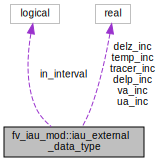
\includegraphics[width=197pt]{structfv__iau__mod_1_1iau__external__data__type__coll__graph}
\end{center}
\end{figure}
\subsection*{Private Attributes}
\begin{DoxyCompactItemize}
\item 
real, dimension(\-:,\-:,\-:), allocatable \hyperlink{structfv__iau__mod_1_1iau__external__data__type_aa2120844d59c8df335cdca70569a5ff8}{ua\-\_\-inc}
\item 
real, dimension(\-:,\-:,\-:), allocatable \hyperlink{structfv__iau__mod_1_1iau__external__data__type_a761119157387b5d60cccfc17d7dac1a6}{va\-\_\-inc}
\item 
real, dimension(\-:,\-:,\-:), allocatable \hyperlink{structfv__iau__mod_1_1iau__external__data__type_ac17e810cbf4df80afa94d067862f4b02}{temp\-\_\-inc}
\item 
real, dimension(\-:,\-:,\-:), allocatable \hyperlink{structfv__iau__mod_1_1iau__external__data__type_adf2ef6258e65251b6d23476fb51401d2}{delp\-\_\-inc}
\item 
real, dimension(\-:,\-:,\-:), allocatable \hyperlink{structfv__iau__mod_1_1iau__external__data__type_af520a7af929ab51c9f94793238378470}{delz\-\_\-inc}
\item 
real, dimension(\-:,\-:,\-:,\-:), \\*
allocatable \hyperlink{structfv__iau__mod_1_1iau__external__data__type_af04840a19fc71d68eaeddceac0e0012a}{tracer\-\_\-inc}
\item 
logical \hyperlink{structfv__iau__mod_1_1iau__external__data__type_a7692cd433fd2b8dfc4933e78cf447828}{in\-\_\-interval} = .false.
\end{DoxyCompactItemize}


\subsection{Detailed Description}


Definition at line 88 of file fv\-\_\-iau\-\_\-mod.\-F90.



\subsection{Member Data Documentation}
\index{fv\-\_\-iau\-\_\-mod\-::iau\-\_\-external\-\_\-data\-\_\-type@{fv\-\_\-iau\-\_\-mod\-::iau\-\_\-external\-\_\-data\-\_\-type}!delp\-\_\-inc@{delp\-\_\-inc}}
\index{delp\-\_\-inc@{delp\-\_\-inc}!fv_iau_mod::iau_external_data_type@{fv\-\_\-iau\-\_\-mod\-::iau\-\_\-external\-\_\-data\-\_\-type}}
\subsubsection[{delp\-\_\-inc}]{\setlength{\rightskip}{0pt plus 5cm}real, dimension(\-:,\-:,\-:), allocatable fv\-\_\-iau\-\_\-mod\-::iau\-\_\-external\-\_\-data\-\_\-type\-::delp\-\_\-inc\hspace{0.3cm}{\ttfamily [private]}}\label{structfv__iau__mod_1_1iau__external__data__type_adf2ef6258e65251b6d23476fb51401d2}


Definition at line 92 of file fv\-\_\-iau\-\_\-mod.\-F90.

\index{fv\-\_\-iau\-\_\-mod\-::iau\-\_\-external\-\_\-data\-\_\-type@{fv\-\_\-iau\-\_\-mod\-::iau\-\_\-external\-\_\-data\-\_\-type}!delz\-\_\-inc@{delz\-\_\-inc}}
\index{delz\-\_\-inc@{delz\-\_\-inc}!fv_iau_mod::iau_external_data_type@{fv\-\_\-iau\-\_\-mod\-::iau\-\_\-external\-\_\-data\-\_\-type}}
\subsubsection[{delz\-\_\-inc}]{\setlength{\rightskip}{0pt plus 5cm}real, dimension(\-:,\-:,\-:), allocatable fv\-\_\-iau\-\_\-mod\-::iau\-\_\-external\-\_\-data\-\_\-type\-::delz\-\_\-inc\hspace{0.3cm}{\ttfamily [private]}}\label{structfv__iau__mod_1_1iau__external__data__type_af520a7af929ab51c9f94793238378470}


Definition at line 93 of file fv\-\_\-iau\-\_\-mod.\-F90.

\index{fv\-\_\-iau\-\_\-mod\-::iau\-\_\-external\-\_\-data\-\_\-type@{fv\-\_\-iau\-\_\-mod\-::iau\-\_\-external\-\_\-data\-\_\-type}!in\-\_\-interval@{in\-\_\-interval}}
\index{in\-\_\-interval@{in\-\_\-interval}!fv_iau_mod::iau_external_data_type@{fv\-\_\-iau\-\_\-mod\-::iau\-\_\-external\-\_\-data\-\_\-type}}
\subsubsection[{in\-\_\-interval}]{\setlength{\rightskip}{0pt plus 5cm}logical fv\-\_\-iau\-\_\-mod\-::iau\-\_\-external\-\_\-data\-\_\-type\-::in\-\_\-interval = .false.\hspace{0.3cm}{\ttfamily [private]}}\label{structfv__iau__mod_1_1iau__external__data__type_a7692cd433fd2b8dfc4933e78cf447828}


Definition at line 95 of file fv\-\_\-iau\-\_\-mod.\-F90.

\index{fv\-\_\-iau\-\_\-mod\-::iau\-\_\-external\-\_\-data\-\_\-type@{fv\-\_\-iau\-\_\-mod\-::iau\-\_\-external\-\_\-data\-\_\-type}!temp\-\_\-inc@{temp\-\_\-inc}}
\index{temp\-\_\-inc@{temp\-\_\-inc}!fv_iau_mod::iau_external_data_type@{fv\-\_\-iau\-\_\-mod\-::iau\-\_\-external\-\_\-data\-\_\-type}}
\subsubsection[{temp\-\_\-inc}]{\setlength{\rightskip}{0pt plus 5cm}real, dimension(\-:,\-:,\-:), allocatable fv\-\_\-iau\-\_\-mod\-::iau\-\_\-external\-\_\-data\-\_\-type\-::temp\-\_\-inc\hspace{0.3cm}{\ttfamily [private]}}\label{structfv__iau__mod_1_1iau__external__data__type_ac17e810cbf4df80afa94d067862f4b02}


Definition at line 91 of file fv\-\_\-iau\-\_\-mod.\-F90.

\index{fv\-\_\-iau\-\_\-mod\-::iau\-\_\-external\-\_\-data\-\_\-type@{fv\-\_\-iau\-\_\-mod\-::iau\-\_\-external\-\_\-data\-\_\-type}!tracer\-\_\-inc@{tracer\-\_\-inc}}
\index{tracer\-\_\-inc@{tracer\-\_\-inc}!fv_iau_mod::iau_external_data_type@{fv\-\_\-iau\-\_\-mod\-::iau\-\_\-external\-\_\-data\-\_\-type}}
\subsubsection[{tracer\-\_\-inc}]{\setlength{\rightskip}{0pt plus 5cm}real, dimension(\-:,\-:,\-:,\-:), allocatable fv\-\_\-iau\-\_\-mod\-::iau\-\_\-external\-\_\-data\-\_\-type\-::tracer\-\_\-inc\hspace{0.3cm}{\ttfamily [private]}}\label{structfv__iau__mod_1_1iau__external__data__type_af04840a19fc71d68eaeddceac0e0012a}


Definition at line 94 of file fv\-\_\-iau\-\_\-mod.\-F90.

\index{fv\-\_\-iau\-\_\-mod\-::iau\-\_\-external\-\_\-data\-\_\-type@{fv\-\_\-iau\-\_\-mod\-::iau\-\_\-external\-\_\-data\-\_\-type}!ua\-\_\-inc@{ua\-\_\-inc}}
\index{ua\-\_\-inc@{ua\-\_\-inc}!fv_iau_mod::iau_external_data_type@{fv\-\_\-iau\-\_\-mod\-::iau\-\_\-external\-\_\-data\-\_\-type}}
\subsubsection[{ua\-\_\-inc}]{\setlength{\rightskip}{0pt plus 5cm}real, dimension(\-:,\-:,\-:), allocatable fv\-\_\-iau\-\_\-mod\-::iau\-\_\-external\-\_\-data\-\_\-type\-::ua\-\_\-inc\hspace{0.3cm}{\ttfamily [private]}}\label{structfv__iau__mod_1_1iau__external__data__type_aa2120844d59c8df335cdca70569a5ff8}


Definition at line 89 of file fv\-\_\-iau\-\_\-mod.\-F90.

\index{fv\-\_\-iau\-\_\-mod\-::iau\-\_\-external\-\_\-data\-\_\-type@{fv\-\_\-iau\-\_\-mod\-::iau\-\_\-external\-\_\-data\-\_\-type}!va\-\_\-inc@{va\-\_\-inc}}
\index{va\-\_\-inc@{va\-\_\-inc}!fv_iau_mod::iau_external_data_type@{fv\-\_\-iau\-\_\-mod\-::iau\-\_\-external\-\_\-data\-\_\-type}}
\subsubsection[{va\-\_\-inc}]{\setlength{\rightskip}{0pt plus 5cm}real, dimension(\-:,\-:,\-:), allocatable fv\-\_\-iau\-\_\-mod\-::iau\-\_\-external\-\_\-data\-\_\-type\-::va\-\_\-inc\hspace{0.3cm}{\ttfamily [private]}}\label{structfv__iau__mod_1_1iau__external__data__type_a761119157387b5d60cccfc17d7dac1a6}


Definition at line 90 of file fv\-\_\-iau\-\_\-mod.\-F90.



The documentation for this type was generated from the following file\-:\begin{DoxyCompactItemize}
\item 
/scratch2/\-N\-A\-G\-A\-P\-E/aoml-\/hafs1/\-Kyle.\-Ahern/acs\-\_\-master\-\_\-readonly/tools/\hyperlink{fv__iau__mod_8F90}{fv\-\_\-iau\-\_\-mod.\-F90}\end{DoxyCompactItemize}

\section{fv\-\_\-iau\-\_\-mod\-:\-:iau\-\_\-internal\-\_\-data\-\_\-type Type Reference}
\label{structfv__iau__mod_1_1iau__internal__data__type}\index{fv\-\_\-iau\-\_\-mod\-::iau\-\_\-internal\-\_\-data\-\_\-type@{fv\-\_\-iau\-\_\-mod\-::iau\-\_\-internal\-\_\-data\-\_\-type}}


Collaboration diagram for fv\-\_\-iau\-\_\-mod\-:\-:iau\-\_\-internal\-\_\-data\-\_\-type\-:
\nopagebreak
\begin{figure}[H]
\begin{center}
\leavevmode
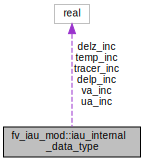
\includegraphics[width=180pt]{structfv__iau__mod_1_1iau__internal__data__type__coll__graph}
\end{center}
\end{figure}
\subsection*{Private Attributes}
\begin{DoxyCompactItemize}
\item 
real, dimension(\-:,\-:,\-:), allocatable \hyperlink{structfv__iau__mod_1_1iau__internal__data__type_ae53005a7a5bfd2b26151297ccad01589}{ua\-\_\-inc}
\item 
real, dimension(\-:,\-:,\-:), allocatable \hyperlink{structfv__iau__mod_1_1iau__internal__data__type_abf93781f5201e7988f4fb02023067d1c}{va\-\_\-inc}
\item 
real, dimension(\-:,\-:,\-:), allocatable \hyperlink{structfv__iau__mod_1_1iau__internal__data__type_a515361138aa772aba2c0471c5c7c3be7}{temp\-\_\-inc}
\item 
real, dimension(\-:,\-:,\-:), allocatable \hyperlink{structfv__iau__mod_1_1iau__internal__data__type_ada9bf234b0fa3681403c4ca5bc9411e3}{delp\-\_\-inc}
\item 
real, dimension(\-:,\-:,\-:), allocatable \hyperlink{structfv__iau__mod_1_1iau__internal__data__type_a98f0a840a25adcc48aaef5658045d0e7}{delz\-\_\-inc}
\item 
real, dimension(\-:,\-:,\-:,\-:), \\*
allocatable \hyperlink{structfv__iau__mod_1_1iau__internal__data__type_a891ea56d404a70616d629be467f53f2a}{tracer\-\_\-inc}
\end{DoxyCompactItemize}


\subsection{Detailed Description}


Definition at line 80 of file fv\-\_\-iau\-\_\-mod.\-F90.



\subsection{Member Data Documentation}
\index{fv\-\_\-iau\-\_\-mod\-::iau\-\_\-internal\-\_\-data\-\_\-type@{fv\-\_\-iau\-\_\-mod\-::iau\-\_\-internal\-\_\-data\-\_\-type}!delp\-\_\-inc@{delp\-\_\-inc}}
\index{delp\-\_\-inc@{delp\-\_\-inc}!fv_iau_mod::iau_internal_data_type@{fv\-\_\-iau\-\_\-mod\-::iau\-\_\-internal\-\_\-data\-\_\-type}}
\subsubsection[{delp\-\_\-inc}]{\setlength{\rightskip}{0pt plus 5cm}real, dimension(\-:,\-:,\-:), allocatable fv\-\_\-iau\-\_\-mod\-::iau\-\_\-internal\-\_\-data\-\_\-type\-::delp\-\_\-inc\hspace{0.3cm}{\ttfamily [private]}}\label{structfv__iau__mod_1_1iau__internal__data__type_ada9bf234b0fa3681403c4ca5bc9411e3}


Definition at line 84 of file fv\-\_\-iau\-\_\-mod.\-F90.

\index{fv\-\_\-iau\-\_\-mod\-::iau\-\_\-internal\-\_\-data\-\_\-type@{fv\-\_\-iau\-\_\-mod\-::iau\-\_\-internal\-\_\-data\-\_\-type}!delz\-\_\-inc@{delz\-\_\-inc}}
\index{delz\-\_\-inc@{delz\-\_\-inc}!fv_iau_mod::iau_internal_data_type@{fv\-\_\-iau\-\_\-mod\-::iau\-\_\-internal\-\_\-data\-\_\-type}}
\subsubsection[{delz\-\_\-inc}]{\setlength{\rightskip}{0pt plus 5cm}real, dimension(\-:,\-:,\-:), allocatable fv\-\_\-iau\-\_\-mod\-::iau\-\_\-internal\-\_\-data\-\_\-type\-::delz\-\_\-inc\hspace{0.3cm}{\ttfamily [private]}}\label{structfv__iau__mod_1_1iau__internal__data__type_a98f0a840a25adcc48aaef5658045d0e7}


Definition at line 85 of file fv\-\_\-iau\-\_\-mod.\-F90.

\index{fv\-\_\-iau\-\_\-mod\-::iau\-\_\-internal\-\_\-data\-\_\-type@{fv\-\_\-iau\-\_\-mod\-::iau\-\_\-internal\-\_\-data\-\_\-type}!temp\-\_\-inc@{temp\-\_\-inc}}
\index{temp\-\_\-inc@{temp\-\_\-inc}!fv_iau_mod::iau_internal_data_type@{fv\-\_\-iau\-\_\-mod\-::iau\-\_\-internal\-\_\-data\-\_\-type}}
\subsubsection[{temp\-\_\-inc}]{\setlength{\rightskip}{0pt plus 5cm}real, dimension(\-:,\-:,\-:), allocatable fv\-\_\-iau\-\_\-mod\-::iau\-\_\-internal\-\_\-data\-\_\-type\-::temp\-\_\-inc\hspace{0.3cm}{\ttfamily [private]}}\label{structfv__iau__mod_1_1iau__internal__data__type_a515361138aa772aba2c0471c5c7c3be7}


Definition at line 83 of file fv\-\_\-iau\-\_\-mod.\-F90.

\index{fv\-\_\-iau\-\_\-mod\-::iau\-\_\-internal\-\_\-data\-\_\-type@{fv\-\_\-iau\-\_\-mod\-::iau\-\_\-internal\-\_\-data\-\_\-type}!tracer\-\_\-inc@{tracer\-\_\-inc}}
\index{tracer\-\_\-inc@{tracer\-\_\-inc}!fv_iau_mod::iau_internal_data_type@{fv\-\_\-iau\-\_\-mod\-::iau\-\_\-internal\-\_\-data\-\_\-type}}
\subsubsection[{tracer\-\_\-inc}]{\setlength{\rightskip}{0pt plus 5cm}real, dimension(\-:,\-:,\-:,\-:), allocatable fv\-\_\-iau\-\_\-mod\-::iau\-\_\-internal\-\_\-data\-\_\-type\-::tracer\-\_\-inc\hspace{0.3cm}{\ttfamily [private]}}\label{structfv__iau__mod_1_1iau__internal__data__type_a891ea56d404a70616d629be467f53f2a}


Definition at line 86 of file fv\-\_\-iau\-\_\-mod.\-F90.

\index{fv\-\_\-iau\-\_\-mod\-::iau\-\_\-internal\-\_\-data\-\_\-type@{fv\-\_\-iau\-\_\-mod\-::iau\-\_\-internal\-\_\-data\-\_\-type}!ua\-\_\-inc@{ua\-\_\-inc}}
\index{ua\-\_\-inc@{ua\-\_\-inc}!fv_iau_mod::iau_internal_data_type@{fv\-\_\-iau\-\_\-mod\-::iau\-\_\-internal\-\_\-data\-\_\-type}}
\subsubsection[{ua\-\_\-inc}]{\setlength{\rightskip}{0pt plus 5cm}real, dimension(\-:,\-:,\-:), allocatable fv\-\_\-iau\-\_\-mod\-::iau\-\_\-internal\-\_\-data\-\_\-type\-::ua\-\_\-inc\hspace{0.3cm}{\ttfamily [private]}}\label{structfv__iau__mod_1_1iau__internal__data__type_ae53005a7a5bfd2b26151297ccad01589}


Definition at line 81 of file fv\-\_\-iau\-\_\-mod.\-F90.

\index{fv\-\_\-iau\-\_\-mod\-::iau\-\_\-internal\-\_\-data\-\_\-type@{fv\-\_\-iau\-\_\-mod\-::iau\-\_\-internal\-\_\-data\-\_\-type}!va\-\_\-inc@{va\-\_\-inc}}
\index{va\-\_\-inc@{va\-\_\-inc}!fv_iau_mod::iau_internal_data_type@{fv\-\_\-iau\-\_\-mod\-::iau\-\_\-internal\-\_\-data\-\_\-type}}
\subsubsection[{va\-\_\-inc}]{\setlength{\rightskip}{0pt plus 5cm}real, dimension(\-:,\-:,\-:), allocatable fv\-\_\-iau\-\_\-mod\-::iau\-\_\-internal\-\_\-data\-\_\-type\-::va\-\_\-inc\hspace{0.3cm}{\ttfamily [private]}}\label{structfv__iau__mod_1_1iau__internal__data__type_abf93781f5201e7988f4fb02023067d1c}


Definition at line 82 of file fv\-\_\-iau\-\_\-mod.\-F90.



The documentation for this type was generated from the following file\-:\begin{DoxyCompactItemize}
\item 
/scratch2/\-N\-A\-G\-A\-P\-E/aoml-\/hafs1/\-Kyle.\-Ahern/acs\-\_\-master\-\_\-readonly/tools/\hyperlink{fv__iau__mod_8F90}{fv\-\_\-iau\-\_\-mod.\-F90}\end{DoxyCompactItemize}

\section{fv\-\_\-iau\-\_\-mod\-:\-:iau\-\_\-state\-\_\-type Type Reference}
\label{structfv__iau__mod_1_1iau__state__type}\index{fv\-\_\-iau\-\_\-mod\-::iau\-\_\-state\-\_\-type@{fv\-\_\-iau\-\_\-mod\-::iau\-\_\-state\-\_\-type}}


Collaboration diagram for fv\-\_\-iau\-\_\-mod\-:\-:iau\-\_\-state\-\_\-type\-:
\nopagebreak
\begin{figure}[H]
\begin{center}
\leavevmode
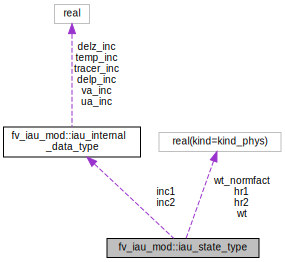
\includegraphics[width=321pt]{structfv__iau__mod_1_1iau__state__type__coll__graph}
\end{center}
\end{figure}
\subsection*{Private Attributes}
\begin{DoxyCompactItemize}
\item 
type(\hyperlink{structfv__iau__mod_1_1iau__internal__data__type}{iau\-\_\-internal\-\_\-data\-\_\-type}) \hyperlink{structfv__iau__mod_1_1iau__state__type_a0af7b395dcb45a752acdf6f3ebad71fa}{inc1}
\item 
type(\hyperlink{structfv__iau__mod_1_1iau__internal__data__type}{iau\-\_\-internal\-\_\-data\-\_\-type}) \hyperlink{structfv__iau__mod_1_1iau__state__type_a2969126d74a69d2e7657439ed109ce7b}{inc2}
\item 
real(kind=kind\-\_\-phys) \hyperlink{structfv__iau__mod_1_1iau__state__type_a38fd8515897c8144e55a7e1298fba14e}{hr1}
\item 
real(kind=kind\-\_\-phys) \hyperlink{structfv__iau__mod_1_1iau__state__type_a2d22a0517262e33fe37c31d99638e512}{hr2}
\item 
real(kind=kind\-\_\-phys) \hyperlink{structfv__iau__mod_1_1iau__state__type_aae6b10a1f01da751413176dc4196e695}{wt}
\item 
real(kind=kind\-\_\-phys) \hyperlink{structfv__iau__mod_1_1iau__state__type_a04f738f0d6fbb3e64e44fc94421bf48d}{wt\-\_\-normfact}
\end{DoxyCompactItemize}


\subsection{Detailed Description}


Definition at line 97 of file fv\-\_\-iau\-\_\-mod.\-F90.



\subsection{Member Data Documentation}
\index{fv\-\_\-iau\-\_\-mod\-::iau\-\_\-state\-\_\-type@{fv\-\_\-iau\-\_\-mod\-::iau\-\_\-state\-\_\-type}!hr1@{hr1}}
\index{hr1@{hr1}!fv_iau_mod::iau_state_type@{fv\-\_\-iau\-\_\-mod\-::iau\-\_\-state\-\_\-type}}
\subsubsection[{hr1}]{\setlength{\rightskip}{0pt plus 5cm}real(kind=kind\-\_\-phys) fv\-\_\-iau\-\_\-mod\-::iau\-\_\-state\-\_\-type\-::hr1\hspace{0.3cm}{\ttfamily [private]}}\label{structfv__iau__mod_1_1iau__state__type_a38fd8515897c8144e55a7e1298fba14e}


Definition at line 100 of file fv\-\_\-iau\-\_\-mod.\-F90.

\index{fv\-\_\-iau\-\_\-mod\-::iau\-\_\-state\-\_\-type@{fv\-\_\-iau\-\_\-mod\-::iau\-\_\-state\-\_\-type}!hr2@{hr2}}
\index{hr2@{hr2}!fv_iau_mod::iau_state_type@{fv\-\_\-iau\-\_\-mod\-::iau\-\_\-state\-\_\-type}}
\subsubsection[{hr2}]{\setlength{\rightskip}{0pt plus 5cm}real(kind=kind\-\_\-phys) fv\-\_\-iau\-\_\-mod\-::iau\-\_\-state\-\_\-type\-::hr2\hspace{0.3cm}{\ttfamily [private]}}\label{structfv__iau__mod_1_1iau__state__type_a2d22a0517262e33fe37c31d99638e512}


Definition at line 101 of file fv\-\_\-iau\-\_\-mod.\-F90.

\index{fv\-\_\-iau\-\_\-mod\-::iau\-\_\-state\-\_\-type@{fv\-\_\-iau\-\_\-mod\-::iau\-\_\-state\-\_\-type}!inc1@{inc1}}
\index{inc1@{inc1}!fv_iau_mod::iau_state_type@{fv\-\_\-iau\-\_\-mod\-::iau\-\_\-state\-\_\-type}}
\subsubsection[{inc1}]{\setlength{\rightskip}{0pt plus 5cm}type({\bf iau\-\_\-internal\-\_\-data\-\_\-type}) fv\-\_\-iau\-\_\-mod\-::iau\-\_\-state\-\_\-type\-::inc1\hspace{0.3cm}{\ttfamily [private]}}\label{structfv__iau__mod_1_1iau__state__type_a0af7b395dcb45a752acdf6f3ebad71fa}


Definition at line 98 of file fv\-\_\-iau\-\_\-mod.\-F90.

\index{fv\-\_\-iau\-\_\-mod\-::iau\-\_\-state\-\_\-type@{fv\-\_\-iau\-\_\-mod\-::iau\-\_\-state\-\_\-type}!inc2@{inc2}}
\index{inc2@{inc2}!fv_iau_mod::iau_state_type@{fv\-\_\-iau\-\_\-mod\-::iau\-\_\-state\-\_\-type}}
\subsubsection[{inc2}]{\setlength{\rightskip}{0pt plus 5cm}type({\bf iau\-\_\-internal\-\_\-data\-\_\-type}) fv\-\_\-iau\-\_\-mod\-::iau\-\_\-state\-\_\-type\-::inc2\hspace{0.3cm}{\ttfamily [private]}}\label{structfv__iau__mod_1_1iau__state__type_a2969126d74a69d2e7657439ed109ce7b}


Definition at line 99 of file fv\-\_\-iau\-\_\-mod.\-F90.

\index{fv\-\_\-iau\-\_\-mod\-::iau\-\_\-state\-\_\-type@{fv\-\_\-iau\-\_\-mod\-::iau\-\_\-state\-\_\-type}!wt@{wt}}
\index{wt@{wt}!fv_iau_mod::iau_state_type@{fv\-\_\-iau\-\_\-mod\-::iau\-\_\-state\-\_\-type}}
\subsubsection[{wt}]{\setlength{\rightskip}{0pt plus 5cm}real(kind=kind\-\_\-phys) fv\-\_\-iau\-\_\-mod\-::iau\-\_\-state\-\_\-type\-::wt\hspace{0.3cm}{\ttfamily [private]}}\label{structfv__iau__mod_1_1iau__state__type_aae6b10a1f01da751413176dc4196e695}


Definition at line 102 of file fv\-\_\-iau\-\_\-mod.\-F90.

\index{fv\-\_\-iau\-\_\-mod\-::iau\-\_\-state\-\_\-type@{fv\-\_\-iau\-\_\-mod\-::iau\-\_\-state\-\_\-type}!wt\-\_\-normfact@{wt\-\_\-normfact}}
\index{wt\-\_\-normfact@{wt\-\_\-normfact}!fv_iau_mod::iau_state_type@{fv\-\_\-iau\-\_\-mod\-::iau\-\_\-state\-\_\-type}}
\subsubsection[{wt\-\_\-normfact}]{\setlength{\rightskip}{0pt plus 5cm}real(kind=kind\-\_\-phys) fv\-\_\-iau\-\_\-mod\-::iau\-\_\-state\-\_\-type\-::wt\-\_\-normfact\hspace{0.3cm}{\ttfamily [private]}}\label{structfv__iau__mod_1_1iau__state__type_a04f738f0d6fbb3e64e44fc94421bf48d}


Definition at line 103 of file fv\-\_\-iau\-\_\-mod.\-F90.



The documentation for this type was generated from the following file\-:\begin{DoxyCompactItemize}
\item 
/scratch2/\-N\-A\-G\-A\-P\-E/aoml-\/hafs1/\-Kyle.\-Ahern/acs\-\_\-master\-\_\-readonly/tools/\hyperlink{fv__iau__mod_8F90}{fv\-\_\-iau\-\_\-mod.\-F90}\end{DoxyCompactItemize}

\section{init\-\_\-hydro\-\_\-mod Module Reference}
\label{classinit__hydro__mod}\index{init\-\_\-hydro\-\_\-mod@{init\-\_\-hydro\-\_\-mod}}
\subsection*{Public Member Functions}
\begin{DoxyCompactItemize}
\item 
subroutine, public \hyperlink{classinit__hydro__mod_a23f39e1b3ac489c6fd3d7178569ee85f}{p\-\_\-var} (km, ifirst, ilast, jfirst, jlast, ptop, ptop\-\_\-min, delp, delz, pt, ps, pe, peln, pk, pkz, cappa, q, ng, nq, area, dry\-\_\-mass, adjust\-\_\-dry\-\_\-mass, mountain, moist\-\_\-phys, hydrostatic, nwat, domain, make\-\_\-nh)
\begin{DoxyCompactList}\small\item\em the subroutine 'p\-\_\-var' computes auxiliary pressure variables for a hydrostatic state. \end{DoxyCompactList}\item 
subroutine, public \hyperlink{classinit__hydro__mod_a645ace2e31d16bce04805dde9ef98b73}{hydro\-\_\-eq} (km, is, ie, js, je, ps, hs, drym, delp, ak, bk, pt, delz, area, ng, mountain, hydrostatic, hybrid\-\_\-z, domain)
\begin{DoxyCompactList}\small\item\em The subroutine 'hydro\-\_\-eq' computes a hydrostatically balanced and isothermal basic state from input heights. \end{DoxyCompactList}\end{DoxyCompactItemize}
\subsection*{Private Member Functions}
\begin{DoxyCompactItemize}
\item 
subroutine \hyperlink{classinit__hydro__mod_a0e61f31967e9961d1c4ea3b78ac5b920}{drymadj} (km, ifirst, ilast, jfirst, jlast, ng, cappa, ptop, ps, delp, q, nq, area, nwat, dry\-\_\-mass, adjust\-\_\-dry\-\_\-mass, moist\-\_\-phys, dpd, domain)
\end{DoxyCompactItemize}


\subsection{Detailed Description}


Definition at line 23 of file init\-\_\-hydro.\-F90.



\subsection{Member Function/\-Subroutine Documentation}
\index{init\-\_\-hydro\-\_\-mod@{init\-\_\-hydro\-\_\-mod}!drymadj@{drymadj}}
\index{drymadj@{drymadj}!init_hydro_mod@{init\-\_\-hydro\-\_\-mod}}
\subsubsection[{drymadj}]{\setlength{\rightskip}{0pt plus 5cm}subroutine init\-\_\-hydro\-\_\-mod\-::drymadj (
\begin{DoxyParamCaption}
\item[{integer}]{km, }
\item[{integer}]{ifirst, }
\item[{integer}]{ilast, }
\item[{integer}]{jfirst, }
\item[{integer}]{jlast, }
\item[{integer}]{ng, }
\item[{real, intent(in)}]{cappa, }
\item[{real, intent(in)}]{ptop, }
\item[{real, dimension(ifirst-\/ng\-:ilast+ng,jfirst-\/ng\-:jlast+ng), intent(inout)}]{ps, }
\item[{real, dimension(ifirst-\/ng\-:ilast+ng,jfirst-\/ng\-:jlast+ng,km), intent(in)}]{delp, }
\item[{real, dimension(ifirst-\/ng\-:ilast+ng,jfirst-\/ng\-:jlast+ng,km,nq), intent(in)}]{q, }
\item[{integer}]{nq, }
\item[{real(kind=r\-\_\-grid), dimension(ifirst-\/ng\-:ilast+ng, jfirst-\/ng\-:jlast+ng), intent(in)}]{area, }
\item[{integer}]{nwat, }
\item[{real, intent(in)}]{dry\-\_\-mass, }
\item[{logical, intent(in)}]{adjust\-\_\-dry\-\_\-mass, }
\item[{logical, intent(in)}]{moist\-\_\-phys, }
\item[{real, intent(out)}]{dpd, }
\item[{type(domain2d), intent(in)}]{domain}
\end{DoxyParamCaption}
)\hspace{0.3cm}{\ttfamily [private]}}\label{classinit__hydro__mod_a0e61f31967e9961d1c4ea3b78ac5b920}

\begin{DoxyParams}[1]{Parameters}
 & {\em ilast} & Longitude strip\\
\hline
 & {\em jlast} & Latitude strip\\
\hline
\mbox{\tt in,out}  & {\em ps} & surface pressure \\
\hline
\end{DoxyParams}


Definition at line 246 of file init\-\_\-hydro.\-F90.



References fv\-\_\-grid\-\_\-utils\-\_\-mod\-::g\-\_\-sum().



Referenced by p\-\_\-var().

\index{init\-\_\-hydro\-\_\-mod@{init\-\_\-hydro\-\_\-mod}!hydro\-\_\-eq@{hydro\-\_\-eq}}
\index{hydro\-\_\-eq@{hydro\-\_\-eq}!init_hydro_mod@{init\-\_\-hydro\-\_\-mod}}
\subsubsection[{hydro\-\_\-eq}]{\setlength{\rightskip}{0pt plus 5cm}subroutine, public init\-\_\-hydro\-\_\-mod\-::hydro\-\_\-eq (
\begin{DoxyParamCaption}
\item[{integer, intent(in)}]{km, }
\item[{integer, intent(in)}]{is, }
\item[{integer, intent(in)}]{ie, }
\item[{integer, intent(in)}]{js, }
\item[{integer, intent(in)}]{je, }
\item[{real, dimension(is-\/ng\-:ie+ng,js-\/ng\-:je+ng), intent(out)}]{ps, }
\item[{real, dimension(is-\/ng\-:ie+ng,js-\/ng\-:je+ng), intent(in)}]{hs, }
\item[{real, intent(in)}]{drym, }
\item[{real, dimension(is-\/ng\-:ie+ng,js-\/ng\-:je+ng,km), intent(out)}]{delp, }
\item[{real, dimension(km+1), intent(in)}]{ak, }
\item[{real, dimension(km+1), intent(in)}]{bk, }
\item[{real, dimension(is-\/ng\-:ie+ng,js-\/ng\-:je+ng,km), intent(out)}]{pt, }
\item[{real, dimension(is-\/ng\-:ie+ng,js-\/ng\-:je+ng,km), intent(inout)}]{delz, }
\item[{real(kind=r\-\_\-grid), dimension(is-\/ng\-:ie+ng,js-\/ng\-:je+ng), intent(in)}]{area, }
\item[{integer, intent(in)}]{ng, }
\item[{logical, intent(in)}]{mountain, }
\item[{logical, intent(in)}]{hydrostatic, }
\item[{logical, intent(in)}]{hybrid\-\_\-z, }
\item[{type(domain2d), intent(in)}]{domain}
\end{DoxyParamCaption}
)}\label{classinit__hydro__mod_a645ace2e31d16bce04805dde9ef98b73}


The subroutine 'hydro\-\_\-eq' computes a hydrostatically balanced and isothermal basic state from input heights. 



Definition at line 328 of file init\-\_\-hydro.\-F90.



References fv\-\_\-grid\-\_\-utils\-\_\-mod\-::g\-\_\-sum().



Referenced by test\-\_\-cases\-\_\-mod\-::init\-\_\-case(), and test\-\_\-cases\-\_\-mod\-::init\-\_\-double\-\_\-periodic().

\index{init\-\_\-hydro\-\_\-mod@{init\-\_\-hydro\-\_\-mod}!p\-\_\-var@{p\-\_\-var}}
\index{p\-\_\-var@{p\-\_\-var}!init_hydro_mod@{init\-\_\-hydro\-\_\-mod}}
\subsubsection[{p\-\_\-var}]{\setlength{\rightskip}{0pt plus 5cm}subroutine, public init\-\_\-hydro\-\_\-mod\-::p\-\_\-var (
\begin{DoxyParamCaption}
\item[{integer, intent(in)}]{km, }
\item[{integer, intent(in)}]{ifirst, }
\item[{integer, intent(in)}]{ilast, }
\item[{integer, intent(in)}]{jfirst, }
\item[{integer, intent(in)}]{jlast, }
\item[{real, intent(in)}]{ptop, }
\item[{real, intent(in)}]{ptop\-\_\-min, }
\item[{real, dimension(ifirst-\/ng\-:ilast+ng,jfirst-\/ng\-:jlast+ng, km), intent(inout)}]{delp, }
\item[{real, dimension(ifirst-\/ng\-:ilast+ng,jfirst-\/ng\-:jlast+ng, km), intent(inout)}]{delz, }
\item[{real, dimension(ifirst-\/ng\-:ilast+ng,jfirst-\/ng\-:jlast+ng, km), intent(in)}]{pt, }
\item[{real, dimension(ifirst-\/ng\-:ilast+ng, jfirst-\/ng\-:jlast+ng), intent(out)}]{ps, }
\item[{real, dimension(ifirst-\/1\-:ilast+1,km+1,jfirst-\/1\-:jlast+1), intent(out)}]{pe, }
\item[{real, dimension(ifirst\-:ilast, km+1, jfirst\-:jlast), intent(out)}]{peln, }
\item[{real, dimension(ifirst\-:ilast, jfirst\-:jlast, km+1), intent(out)}]{pk, }
\item[{real, dimension(ifirst\-:ilast, jfirst\-:jlast, km), intent(out)}]{pkz, }
\item[{real, intent(in)}]{cappa, }
\item[{real, dimension(ifirst-\/ng\-:ilast+ng,jfirst-\/ng\-:jlast+ng, km, nq), intent(inout)}]{q, }
\item[{integer, intent(in)}]{ng, }
\item[{integer, intent(in)}]{nq, }
\item[{real(kind=r\-\_\-grid), dimension(ifirst-\/ng\-:ilast+ng,jfirst-\/ng\-:jlast+ng), intent(in)}]{area, }
\item[{real, intent(in)}]{dry\-\_\-mass, }
\item[{logical, intent(in)}]{adjust\-\_\-dry\-\_\-mass, }
\item[{logical, intent(in)}]{mountain, }
\item[{logical, intent(in)}]{moist\-\_\-phys, }
\item[{logical, intent(in)}]{hydrostatic, }
\item[{integer, intent(in)}]{nwat, }
\item[{type(domain2d), intent(in)}]{domain, }
\item[{logical, optional}]{make\-\_\-nh}
\end{DoxyParamCaption}
)}\label{classinit__hydro__mod_a23f39e1b3ac489c6fd3d7178569ee85f}


the subroutine 'p\-\_\-var' computes auxiliary pressure variables for a hydrostatic state. 

The variables are\-: surfce, interface, layer-\/mean pressure, exener function Given (ptop, delp) computes (ps, pk, pe, peln, pkz)


\begin{DoxyParams}[1]{Parameters}
\mbox{\tt in}  & {\em ilast} & Longitude strip\\
\hline
\mbox{\tt in}  & {\em jlast} & Latitude strip\\
\hline
\mbox{\tt out}  & {\em pe} & Ghosted Edge pressure\\
\hline
\mbox{\tt out}  & {\em peln} & Edge pressure \\
\hline
\end{DoxyParams}


Definition at line 83 of file init\-\_\-hydro.\-F90.



References drymadj(), multi\-\_\-gases\-\_\-mod\-::vicpqd(), multi\-\_\-gases\-\_\-mod\-::virq(), and multi\-\_\-gases\-\_\-mod\-::virqd().



Referenced by fv\-\_\-nesting\-\_\-mod\-::after\-\_\-twoway\-\_\-nest\-\_\-update(), fv\-\_\-restart\-\_\-mod\-::fill\-\_\-nested\-\_\-grid\-\_\-data\-\_\-end(), fv\-\_\-restart\-\_\-mod\-::fv\-\_\-restart(), external\-\_\-ic\-\_\-mod\-::get\-\_\-external\-\_\-ic(), test\-\_\-cases\-\_\-mod\-::init\-\_\-case(), and test\-\_\-cases\-\_\-mod\-::init\-\_\-double\-\_\-periodic().



The documentation for this module was generated from the following file\-:\begin{DoxyCompactItemize}
\item 
/scratch2/\-N\-A\-G\-A\-P\-E/aoml-\/hafs1/\-Kyle.\-Ahern/acs\-\_\-master\-\_\-readonly/tools/\hyperlink{init__hydro_8F90}{init\-\_\-hydro.\-F90}\end{DoxyCompactItemize}

\section{test\-\_\-cases\-\_\-mod\-:\-:mp\-\_\-update\-\_\-dwinds Interface Reference}
\label{interfacetest__cases__mod_1_1mp__update__dwinds}\index{test\-\_\-cases\-\_\-mod\-::mp\-\_\-update\-\_\-dwinds@{test\-\_\-cases\-\_\-mod\-::mp\-\_\-update\-\_\-dwinds}}
\subsection*{Private Member Functions}
\begin{DoxyCompactItemize}
\item 
subroutine \hyperlink{interfacetest__cases__mod_1_1mp__update__dwinds_abbb52192e3e2ab8919478b066fb5cf89}{mp\-\_\-update\-\_\-dwinds\-\_\-2d} (u, v, npx, npy, domain)
\item 
subroutine \hyperlink{interfacetest__cases__mod_1_1mp__update__dwinds_a3783b42ccdcb4430f8df05a3ec6b4b6c}{mp\-\_\-update\-\_\-dwinds\-\_\-3d} (u, v, npx, npy, npz, domain)
\end{DoxyCompactItemize}


\subsection{Detailed Description}


Definition at line 242 of file test\-\_\-cases.\-F90.



\subsection{Member Function/\-Subroutine Documentation}
\index{test\-\_\-cases\-\_\-mod\-::mp\-\_\-update\-\_\-dwinds@{test\-\_\-cases\-\_\-mod\-::mp\-\_\-update\-\_\-dwinds}!mp\-\_\-update\-\_\-dwinds\-\_\-2d@{mp\-\_\-update\-\_\-dwinds\-\_\-2d}}
\index{mp\-\_\-update\-\_\-dwinds\-\_\-2d@{mp\-\_\-update\-\_\-dwinds\-\_\-2d}!test_cases_mod::mp_update_dwinds@{test\-\_\-cases\-\_\-mod\-::mp\-\_\-update\-\_\-dwinds}}
\subsubsection[{mp\-\_\-update\-\_\-dwinds\-\_\-2d}]{\setlength{\rightskip}{0pt plus 5cm}subroutine test\-\_\-cases\-\_\-mod\-::mp\-\_\-update\-\_\-dwinds\-::mp\-\_\-update\-\_\-dwinds\-\_\-2d (
\begin{DoxyParamCaption}
\item[{real, dimension(isd\-:ied  ,jsd\-:jed+1), intent(inout)}]{u, }
\item[{real, dimension(isd\-:ied+1,jsd\-:jed  ), intent(inout)}]{v, }
\item[{integer, intent(in)}]{npx, }
\item[{integer, intent(in)}]{npy, }
\item[{type(domain2d), intent(inout)}]{domain}
\end{DoxyParamCaption}
)\hspace{0.3cm}{\ttfamily [private]}}\label{interfacetest__cases__mod_1_1mp__update__dwinds_abbb52192e3e2ab8919478b066fb5cf89}

\begin{DoxyParams}[1]{Parameters}
\mbox{\tt in,out}  & {\em u} & D-\/grid u-\/wind field\\
\hline
\mbox{\tt in,out}  & {\em v} & D-\/grid v-\/wind field \\
\hline
\end{DoxyParams}


Definition at line 8786 of file test\-\_\-cases.\-F90.

\index{test\-\_\-cases\-\_\-mod\-::mp\-\_\-update\-\_\-dwinds@{test\-\_\-cases\-\_\-mod\-::mp\-\_\-update\-\_\-dwinds}!mp\-\_\-update\-\_\-dwinds\-\_\-3d@{mp\-\_\-update\-\_\-dwinds\-\_\-3d}}
\index{mp\-\_\-update\-\_\-dwinds\-\_\-3d@{mp\-\_\-update\-\_\-dwinds\-\_\-3d}!test_cases_mod::mp_update_dwinds@{test\-\_\-cases\-\_\-mod\-::mp\-\_\-update\-\_\-dwinds}}
\subsubsection[{mp\-\_\-update\-\_\-dwinds\-\_\-3d}]{\setlength{\rightskip}{0pt plus 5cm}subroutine test\-\_\-cases\-\_\-mod\-::mp\-\_\-update\-\_\-dwinds\-::mp\-\_\-update\-\_\-dwinds\-\_\-3d (
\begin{DoxyParamCaption}
\item[{real, dimension(isd\-:ied  ,jsd\-:jed+1,npz), intent(inout)}]{u, }
\item[{real, dimension(isd\-:ied+1,jsd\-:jed  ,npz), intent(inout)}]{v, }
\item[{integer, intent(in)}]{npx, }
\item[{integer, intent(in)}]{npy, }
\item[{integer, intent(in)}]{npz, }
\item[{type(domain2d), intent(inout)}]{domain}
\end{DoxyParamCaption}
)\hspace{0.3cm}{\ttfamily [private]}}\label{interfacetest__cases__mod_1_1mp__update__dwinds_a3783b42ccdcb4430f8df05a3ec6b4b6c}

\begin{DoxyParams}[1]{Parameters}
\mbox{\tt in,out}  & {\em u} & D-\/grid u-\/wind field\\
\hline
\mbox{\tt in,out}  & {\em v} & D-\/grid v-\/wind field \\
\hline
\end{DoxyParams}


Definition at line 8804 of file test\-\_\-cases.\-F90.



The documentation for this interface was generated from the following file\-:\begin{DoxyCompactItemize}
\item 
/scratch2/\-N\-A\-G\-A\-P\-E/aoml-\/hafs1/\-Kyle.\-Ahern/acs\-\_\-master\-\_\-readonly/tools/\hyperlink{test__cases_8F90}{test\-\_\-cases.\-F90}\end{DoxyCompactItemize}

\section{multi\-\_\-gases\-\_\-mod Module Reference}
\label{classmulti__gases__mod}\index{multi\-\_\-gases\-\_\-mod@{multi\-\_\-gases\-\_\-mod}}


The module 'multi\-\_\-gases' peforms multi constitutents computations.  




Collaboration diagram for multi\-\_\-gases\-\_\-mod\-:
\nopagebreak
\begin{figure}[H]
\begin{center}
\leavevmode
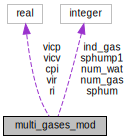
\includegraphics[width=165pt]{classmulti__gases__mod__coll__graph}
\end{center}
\end{figure}
\subsection*{Public Member Functions}
\begin{DoxyCompactItemize}
\item 
subroutine, public \hyperlink{classmulti__gases__mod_afbd34020a75694f0ac19e85dbb8eda6f}{multi\-\_\-gases\-\_\-init} (ngas, nwat)
\item 
pure real function, public \hyperlink{classmulti__gases__mod_a91649465dfa64dee4a0aa4db33496b34}{virq} (q)
\item 
pure real function, public \hyperlink{classmulti__gases__mod_a8af118271aa8e7a233066a10924e0d05}{virq\-\_\-nodq} (q)
\item 
pure real function, public \hyperlink{classmulti__gases__mod_ab6332eff515faa91fd8560fff744f704}{virq\-\_\-max} (q, qmin)
\item 
pure real function, public \hyperlink{classmulti__gases__mod_a74a40323e9be4271dffedfbb671c938c}{virq\-\_\-qpz} (q, qpz)
\item 
pure real function, public \hyperlink{classmulti__gases__mod_ab87c41f9b4f50367c76dc2e2eb4f1463}{virqd} (q)
\item 
pure real function, public \hyperlink{classmulti__gases__mod_a6b697df6baca53e2991067cbccd96633}{vicpqd} (q)
\item 
pure real function, public \hyperlink{classmulti__gases__mod_a99afa1ce63a683c4e24eaf27071fde67}{vicpqd\-\_\-qpz} (q, qpz)
\item 
pure real function, public \hyperlink{classmulti__gases__mod_a5e1943c9700f309e8ae9f475588f3b4c}{vicvqd} (q)
\item 
pure real function, public \hyperlink{classmulti__gases__mod_acb1e93aa8c8cb0d6bd5eff19d2a79885}{vicvqd\-\_\-qpz} (q, qpz)
\end{DoxyCompactItemize}
\subsection*{Public Attributes}
\begin{DoxyCompactItemize}
\item 
integer, public \hyperlink{classmulti__gases__mod_ada7f0ffe52c60fbe7f6cafd04490c4d8}{num\-\_\-gas}
\item 
integer, public \hyperlink{classmulti__gases__mod_a15e4b81a202b85b77802dce9c489b1a9}{ind\-\_\-gas}
\item 
real, dimension(\-:), allocatable \hyperlink{classmulti__gases__mod_acdbd2cbc0014ad073f6daadeffc5cfce}{ri}
\item 
real, dimension(\-:), allocatable \hyperlink{classmulti__gases__mod_a85983a7159ef293fa1c2d65647a66400}{cpi}
\item 
real, dimension(\-:), \\*
allocatable, public \hyperlink{classmulti__gases__mod_a39e5146fa83f5edbe8479cd345968d9c}{vir}
\item 
real, dimension(\-:), \\*
allocatable, public \hyperlink{classmulti__gases__mod_a3e01739eaf6bc27d9db8770ec4c9cd69}{vicp}
\item 
real, dimension(\-:), \\*
allocatable, public \hyperlink{classmulti__gases__mod_a4a8d9ed9352b8bfd8daa59b36ab2430f}{vicv}
\end{DoxyCompactItemize}
\subsection*{Private Attributes}
\begin{DoxyCompactItemize}
\item 
integer, private \hyperlink{classmulti__gases__mod_a927f93aad16256efbf50824dc3897194}{num\-\_\-wat}
\item 
integer, private \hyperlink{classmulti__gases__mod_ac1567ae48756e1ad1df7f99d1a86592a}{sphum}
\item 
integer, private \hyperlink{classmulti__gases__mod_a0e5f32ab60bce2b41eda0ae1e1f47bee}{sphump1}
\end{DoxyCompactItemize}


\subsection{Detailed Description}
The module 'multi\-\_\-gases' peforms multi constitutents computations. 

\begin{DoxyAuthor}{Author}
H.-\/\-M. H. Juang, N\-O\-A\-A/\-N\-W\-S/\-N\-C\-E\-P/\-E\-M\-C 
\end{DoxyAuthor}


Definition at line 25 of file multi\-\_\-gases.\-F90.



\subsection{Member Function/\-Subroutine Documentation}
\index{multi\-\_\-gases\-\_\-mod@{multi\-\_\-gases\-\_\-mod}!multi\-\_\-gases\-\_\-init@{multi\-\_\-gases\-\_\-init}}
\index{multi\-\_\-gases\-\_\-init@{multi\-\_\-gases\-\_\-init}!multi_gases_mod@{multi\-\_\-gases\-\_\-mod}}
\subsubsection[{multi\-\_\-gases\-\_\-init}]{\setlength{\rightskip}{0pt plus 5cm}subroutine, public multi\-\_\-gases\-\_\-mod\-::multi\-\_\-gases\-\_\-init (
\begin{DoxyParamCaption}
\item[{integer, intent(in)}]{ngas, }
\item[{integer, intent(in)}]{nwat}
\end{DoxyParamCaption}
)}\label{classmulti__gases__mod_afbd34020a75694f0ac19e85dbb8eda6f}


Definition at line 69 of file multi\-\_\-gases.\-F90.



Referenced by fv\-\_\-control\-\_\-mod\-::run\-\_\-setup().

\index{multi\-\_\-gases\-\_\-mod@{multi\-\_\-gases\-\_\-mod}!vicpqd@{vicpqd}}
\index{vicpqd@{vicpqd}!multi_gases_mod@{multi\-\_\-gases\-\_\-mod}}
\subsubsection[{vicpqd}]{\setlength{\rightskip}{0pt plus 5cm}pure real function, public multi\-\_\-gases\-\_\-mod\-::vicpqd (
\begin{DoxyParamCaption}
\item[{real, dimension({\bf num\-\_\-gas}), intent(in)}]{q}
\end{DoxyParamCaption}
)}\label{classmulti__gases__mod_a6b697df6baca53e2991067cbccd96633}


Definition at line 238 of file multi\-\_\-gases.\-F90.



Referenced by fv\-\_\-nwp\-\_\-nudge\-\_\-mod\-::breed\-\_\-slp\-\_\-inline(), fv\-\_\-diagnostics\-\_\-mod\-::eqv\-\_\-pot(), fv\-\_\-dynamics\-\_\-mod\-::fv\-\_\-dynamics(), fv\-\_\-sg\-\_\-mod\-::fv\-\_\-subgrid\-\_\-z(), fv\-\_\-update\-\_\-phys\-\_\-mod\-::fv\-\_\-update\-\_\-phys(), fv\-\_\-mapz\-\_\-mod\-::lagrangian\-\_\-to\-\_\-eulerian(), fv\-\_\-mapz\-\_\-mod\-::moist\-\_\-cp(), nh\-\_\-utils\-\_\-mod\-::nest\-\_\-halo\-\_\-nh(), init\-\_\-hydro\-\_\-mod\-::p\-\_\-var(), fv\-\_\-nwp\-\_\-nudge\-\_\-mod\-::ps\-\_\-nudging(), external\-\_\-ic\-\_\-mod\-::remap\-\_\-xyz(), and fv\-\_\-diagnostics\-\_\-mod\-::rh\-\_\-calc().

\index{multi\-\_\-gases\-\_\-mod@{multi\-\_\-gases\-\_\-mod}!vicpqd\-\_\-qpz@{vicpqd\-\_\-qpz}}
\index{vicpqd\-\_\-qpz@{vicpqd\-\_\-qpz}!multi_gases_mod@{multi\-\_\-gases\-\_\-mod}}
\subsubsection[{vicpqd\-\_\-qpz}]{\setlength{\rightskip}{0pt plus 5cm}pure real function, public multi\-\_\-gases\-\_\-mod\-::vicpqd\-\_\-qpz (
\begin{DoxyParamCaption}
\item[{real, dimension({\bf num\-\_\-gas}), intent(in)}]{q, }
\item[{real, intent(in)}]{qpz}
\end{DoxyParamCaption}
)}\label{classmulti__gases__mod_a99afa1ce63a683c4e24eaf27071fde67}


Definition at line 258 of file multi\-\_\-gases.\-F90.



Referenced by fv\-\_\-cmp\-\_\-mod\-::fv\-\_\-sat\-\_\-adj(), and fv\-\_\-sg\-\_\-mod\-::neg\-\_\-adj3().

\index{multi\-\_\-gases\-\_\-mod@{multi\-\_\-gases\-\_\-mod}!vicvqd@{vicvqd}}
\index{vicvqd@{vicvqd}!multi_gases_mod@{multi\-\_\-gases\-\_\-mod}}
\subsubsection[{vicvqd}]{\setlength{\rightskip}{0pt plus 5cm}pure real function, public multi\-\_\-gases\-\_\-mod\-::vicvqd (
\begin{DoxyParamCaption}
\item[{real, dimension({\bf num\-\_\-gas}), intent(in)}]{q}
\end{DoxyParamCaption}
)}\label{classmulti__gases__mod_a5e1943c9700f309e8ae9f475588f3b4c}


Definition at line 279 of file multi\-\_\-gases.\-F90.



Referenced by fv\-\_\-mapz\-\_\-mod\-::compute\-\_\-total\-\_\-energy(), dyn\-\_\-core\-\_\-mod\-::dyn\-\_\-core(), fv\-\_\-sg\-\_\-mod\-::fv\-\_\-subgrid\-\_\-z(), fv\-\_\-mapz\-\_\-mod\-::lagrangian\-\_\-to\-\_\-eulerian(), fv\-\_\-mapz\-\_\-mod\-::moist\-\_\-cv(), nh\-\_\-utils\-\_\-mod\-::nest\-\_\-halo\-\_\-nh(), and fv\-\_\-diagnostics\-\_\-mod\-::nh\-\_\-total\-\_\-energy().

\index{multi\-\_\-gases\-\_\-mod@{multi\-\_\-gases\-\_\-mod}!vicvqd\-\_\-qpz@{vicvqd\-\_\-qpz}}
\index{vicvqd\-\_\-qpz@{vicvqd\-\_\-qpz}!multi_gases_mod@{multi\-\_\-gases\-\_\-mod}}
\subsubsection[{vicvqd\-\_\-qpz}]{\setlength{\rightskip}{0pt plus 5cm}pure real function, public multi\-\_\-gases\-\_\-mod\-::vicvqd\-\_\-qpz (
\begin{DoxyParamCaption}
\item[{real, dimension({\bf num\-\_\-gas}), intent(in)}]{q, }
\item[{real, intent(in)}]{qpz}
\end{DoxyParamCaption}
)}\label{classmulti__gases__mod_acb1e93aa8c8cb0d6bd5eff19d2a79885}


Definition at line 299 of file multi\-\_\-gases.\-F90.



Referenced by fv\-\_\-cmp\-\_\-mod\-::fv\-\_\-sat\-\_\-adj(), and fv\-\_\-sg\-\_\-mod\-::neg\-\_\-adj3().

\index{multi\-\_\-gases\-\_\-mod@{multi\-\_\-gases\-\_\-mod}!virq@{virq}}
\index{virq@{virq}!multi_gases_mod@{multi\-\_\-gases\-\_\-mod}}
\subsubsection[{virq}]{\setlength{\rightskip}{0pt plus 5cm}pure real function, public multi\-\_\-gases\-\_\-mod\-::virq (
\begin{DoxyParamCaption}
\item[{real, dimension({\bf num\-\_\-gas}), intent(in)}]{q}
\end{DoxyParamCaption}
)}\label{classmulti__gases__mod_a91649465dfa64dee4a0aa4db33496b34}


Definition at line 135 of file multi\-\_\-gases.\-F90.



Referenced by atmosphere\-\_\-mod\-::adiabatic\-\_\-init(), atmosphere\-\_\-mod\-::atmosphere\-\_\-get\-\_\-bottom\-\_\-layer(), fv\-\_\-diagnostics\-\_\-mod\-::bunkers\-\_\-vector(), fv\-\_\-diagnostics\-\_\-mod\-::dbzcalc(), fv\-\_\-diagnostics\-\_\-mod\-::eqv\-\_\-pot(), fv\-\_\-restart\-\_\-mod\-::fill\-\_\-nested\-\_\-grid\-\_\-data(), fv\-\_\-diagnostics\-\_\-mod\-::fv\-\_\-diag(), fv\-\_\-dynamics\-\_\-mod\-::fv\-\_\-dynamics(), fv\-\_\-nggps\-\_\-diags\-\_\-mod\-::fv\-\_\-nggps\-\_\-diag(), fv\-\_\-nwp\-\_\-nudge\-\_\-mod\-::fv\-\_\-nwp\-\_\-nudge(), fv\-\_\-sg\-\_\-mod\-::fv\-\_\-subgrid\-\_\-z(), atmosphere\-\_\-mod\-::get\-\_\-bottom\-\_\-mass(), fv\-\_\-diagnostics\-\_\-mod\-::get\-\_\-height\-\_\-field(), fv\-\_\-diagnostics\-\_\-mod\-::helicity\-\_\-relative(), fv\-\_\-diagnostics\-\_\-mod\-::helicity\-\_\-relative\-\_\-caps(), fv\-\_\-mapz\-\_\-mod\-::lagrangian\-\_\-to\-\_\-eulerian(), fv\-\_\-sg\-\_\-mod\-::neg\-\_\-adj3(), init\-\_\-hydro\-\_\-mod\-::p\-\_\-var(), fv\-\_\-sg\-\_\-mod\-::qsmith(), external\-\_\-ic\-\_\-mod\-::remap\-\_\-scalar(), external\-\_\-ic\-\_\-mod\-::remap\-\_\-scalar\-\_\-ec(), external\-\_\-ic\-\_\-mod\-::remap\-\_\-scalar\-\_\-nggps(), external\-\_\-ic\-\_\-mod\-::remap\-\_\-xyz(), fv\-\_\-mapz\-\_\-mod\-::rst\-\_\-remap(), and fv\-\_\-diagnostics\-\_\-mod\-::updraft\-\_\-helicity().

\index{multi\-\_\-gases\-\_\-mod@{multi\-\_\-gases\-\_\-mod}!virq\-\_\-max@{virq\-\_\-max}}
\index{virq\-\_\-max@{virq\-\_\-max}!multi_gases_mod@{multi\-\_\-gases\-\_\-mod}}
\subsubsection[{virq\-\_\-max}]{\setlength{\rightskip}{0pt plus 5cm}pure real function, public multi\-\_\-gases\-\_\-mod\-::virq\-\_\-max (
\begin{DoxyParamCaption}
\item[{real, dimension({\bf num\-\_\-gas}), intent(in)}]{q, }
\item[{real, intent(in)}]{qmin}
\end{DoxyParamCaption}
)}\label{classmulti__gases__mod_ab6332eff515faa91fd8560fff744f704}


Definition at line 174 of file multi\-\_\-gases.\-F90.



Referenced by atmosphere\-\_\-mod\-::atmos\-\_\-phys\-\_\-driver\-\_\-statein().

\index{multi\-\_\-gases\-\_\-mod@{multi\-\_\-gases\-\_\-mod}!virq\-\_\-nodq@{virq\-\_\-nodq}}
\index{virq\-\_\-nodq@{virq\-\_\-nodq}!multi_gases_mod@{multi\-\_\-gases\-\_\-mod}}
\subsubsection[{virq\-\_\-nodq}]{\setlength{\rightskip}{0pt plus 5cm}pure real function, public multi\-\_\-gases\-\_\-mod\-::virq\-\_\-nodq (
\begin{DoxyParamCaption}
\item[{real, dimension({\bf num\-\_\-gas}), intent(in)}]{q}
\end{DoxyParamCaption}
)}\label{classmulti__gases__mod_a8af118271aa8e7a233066a10924e0d05}


Definition at line 155 of file multi\-\_\-gases.\-F90.

\index{multi\-\_\-gases\-\_\-mod@{multi\-\_\-gases\-\_\-mod}!virq\-\_\-qpz@{virq\-\_\-qpz}}
\index{virq\-\_\-qpz@{virq\-\_\-qpz}!multi_gases_mod@{multi\-\_\-gases\-\_\-mod}}
\subsubsection[{virq\-\_\-qpz}]{\setlength{\rightskip}{0pt plus 5cm}pure real function, public multi\-\_\-gases\-\_\-mod\-::virq\-\_\-qpz (
\begin{DoxyParamCaption}
\item[{real, dimension({\bf num\-\_\-gas}), intent(in)}]{q, }
\item[{real, intent(in)}]{qpz}
\end{DoxyParamCaption}
)}\label{classmulti__gases__mod_a74a40323e9be4271dffedfbb671c938c}


Definition at line 196 of file multi\-\_\-gases.\-F90.



Referenced by fv\-\_\-cmp\-\_\-mod\-::fv\-\_\-sat\-\_\-adj(), and fv\-\_\-sg\-\_\-mod\-::fv\-\_\-subgrid\-\_\-z().

\index{multi\-\_\-gases\-\_\-mod@{multi\-\_\-gases\-\_\-mod}!virqd@{virqd}}
\index{virqd@{virqd}!multi_gases_mod@{multi\-\_\-gases\-\_\-mod}}
\subsubsection[{virqd}]{\setlength{\rightskip}{0pt plus 5cm}pure real function, public multi\-\_\-gases\-\_\-mod\-::virqd (
\begin{DoxyParamCaption}
\item[{real, dimension({\bf num\-\_\-gas}), intent(in)}]{q}
\end{DoxyParamCaption}
)}\label{classmulti__gases__mod_ab87c41f9b4f50367c76dc2e2eb4f1463}


Definition at line 218 of file multi\-\_\-gases.\-F90.



Referenced by fv\-\_\-nwp\-\_\-nudge\-\_\-mod\-::breed\-\_\-slp\-\_\-inline(), dyn\-\_\-core\-\_\-mod\-::dyn\-\_\-core(), fv\-\_\-diagnostics\-\_\-mod\-::eqv\-\_\-pot(), fv\-\_\-dynamics\-\_\-mod\-::fv\-\_\-dynamics(), fv\-\_\-sg\-\_\-mod\-::fv\-\_\-subgrid\-\_\-z(), fv\-\_\-update\-\_\-phys\-\_\-mod\-::fv\-\_\-update\-\_\-phys(), fv\-\_\-mapz\-\_\-mod\-::lagrangian\-\_\-to\-\_\-eulerian(), init\-\_\-hydro\-\_\-mod\-::p\-\_\-var(), fv\-\_\-nwp\-\_\-nudge\-\_\-mod\-::ps\-\_\-nudging(), external\-\_\-ic\-\_\-mod\-::remap\-\_\-xyz(), and fv\-\_\-diagnostics\-\_\-mod\-::rh\-\_\-calc().



\subsection{Member Data Documentation}
\index{multi\-\_\-gases\-\_\-mod@{multi\-\_\-gases\-\_\-mod}!cpi@{cpi}}
\index{cpi@{cpi}!multi_gases_mod@{multi\-\_\-gases\-\_\-mod}}
\subsubsection[{cpi}]{\setlength{\rightskip}{0pt plus 5cm}real, dimension(\-:), allocatable multi\-\_\-gases\-\_\-mod\-::cpi}\label{classmulti__gases__mod_a85983a7159ef293fa1c2d65647a66400}


Definition at line 49 of file multi\-\_\-gases.\-F90.

\index{multi\-\_\-gases\-\_\-mod@{multi\-\_\-gases\-\_\-mod}!ind\-\_\-gas@{ind\-\_\-gas}}
\index{ind\-\_\-gas@{ind\-\_\-gas}!multi_gases_mod@{multi\-\_\-gases\-\_\-mod}}
\subsubsection[{ind\-\_\-gas}]{\setlength{\rightskip}{0pt plus 5cm}integer, public multi\-\_\-gases\-\_\-mod\-::ind\-\_\-gas}\label{classmulti__gases__mod_a15e4b81a202b85b77802dce9c489b1a9}


Definition at line 45 of file multi\-\_\-gases.\-F90.

\index{multi\-\_\-gases\-\_\-mod@{multi\-\_\-gases\-\_\-mod}!num\-\_\-gas@{num\-\_\-gas}}
\index{num\-\_\-gas@{num\-\_\-gas}!multi_gases_mod@{multi\-\_\-gases\-\_\-mod}}
\subsubsection[{num\-\_\-gas}]{\setlength{\rightskip}{0pt plus 5cm}integer, public multi\-\_\-gases\-\_\-mod\-::num\-\_\-gas}\label{classmulti__gases__mod_ada7f0ffe52c60fbe7f6cafd04490c4d8}


Definition at line 44 of file multi\-\_\-gases.\-F90.

\index{multi\-\_\-gases\-\_\-mod@{multi\-\_\-gases\-\_\-mod}!num\-\_\-wat@{num\-\_\-wat}}
\index{num\-\_\-wat@{num\-\_\-wat}!multi_gases_mod@{multi\-\_\-gases\-\_\-mod}}
\subsubsection[{num\-\_\-wat}]{\setlength{\rightskip}{0pt plus 5cm}integer, private multi\-\_\-gases\-\_\-mod\-::num\-\_\-wat\hspace{0.3cm}{\ttfamily [private]}}\label{classmulti__gases__mod_a927f93aad16256efbf50824dc3897194}


Definition at line 46 of file multi\-\_\-gases.\-F90.

\index{multi\-\_\-gases\-\_\-mod@{multi\-\_\-gases\-\_\-mod}!ri@{ri}}
\index{ri@{ri}!multi_gases_mod@{multi\-\_\-gases\-\_\-mod}}
\subsubsection[{ri}]{\setlength{\rightskip}{0pt plus 5cm}real, dimension(\-:), allocatable multi\-\_\-gases\-\_\-mod\-::ri}\label{classmulti__gases__mod_acdbd2cbc0014ad073f6daadeffc5cfce}


Definition at line 48 of file multi\-\_\-gases.\-F90.

\index{multi\-\_\-gases\-\_\-mod@{multi\-\_\-gases\-\_\-mod}!sphum@{sphum}}
\index{sphum@{sphum}!multi_gases_mod@{multi\-\_\-gases\-\_\-mod}}
\subsubsection[{sphum}]{\setlength{\rightskip}{0pt plus 5cm}integer, private multi\-\_\-gases\-\_\-mod\-::sphum\hspace{0.3cm}{\ttfamily [private]}}\label{classmulti__gases__mod_ac1567ae48756e1ad1df7f99d1a86592a}


Definition at line 47 of file multi\-\_\-gases.\-F90.

\index{multi\-\_\-gases\-\_\-mod@{multi\-\_\-gases\-\_\-mod}!sphump1@{sphump1}}
\index{sphump1@{sphump1}!multi_gases_mod@{multi\-\_\-gases\-\_\-mod}}
\subsubsection[{sphump1}]{\setlength{\rightskip}{0pt plus 5cm}integer, private multi\-\_\-gases\-\_\-mod\-::sphump1\hspace{0.3cm}{\ttfamily [private]}}\label{classmulti__gases__mod_a0e5f32ab60bce2b41eda0ae1e1f47bee}


Definition at line 47 of file multi\-\_\-gases.\-F90.

\index{multi\-\_\-gases\-\_\-mod@{multi\-\_\-gases\-\_\-mod}!vicp@{vicp}}
\index{vicp@{vicp}!multi_gases_mod@{multi\-\_\-gases\-\_\-mod}}
\subsubsection[{vicp}]{\setlength{\rightskip}{0pt plus 5cm}real, dimension(\-:), allocatable, public multi\-\_\-gases\-\_\-mod\-::vicp}\label{classmulti__gases__mod_a3e01739eaf6bc27d9db8770ec4c9cd69}


Definition at line 51 of file multi\-\_\-gases.\-F90.

\index{multi\-\_\-gases\-\_\-mod@{multi\-\_\-gases\-\_\-mod}!vicv@{vicv}}
\index{vicv@{vicv}!multi_gases_mod@{multi\-\_\-gases\-\_\-mod}}
\subsubsection[{vicv}]{\setlength{\rightskip}{0pt plus 5cm}real, dimension(\-:), allocatable, public multi\-\_\-gases\-\_\-mod\-::vicv}\label{classmulti__gases__mod_a4a8d9ed9352b8bfd8daa59b36ab2430f}


Definition at line 52 of file multi\-\_\-gases.\-F90.

\index{multi\-\_\-gases\-\_\-mod@{multi\-\_\-gases\-\_\-mod}!vir@{vir}}
\index{vir@{vir}!multi_gases_mod@{multi\-\_\-gases\-\_\-mod}}
\subsubsection[{vir}]{\setlength{\rightskip}{0pt plus 5cm}real, dimension(\-:), allocatable, public multi\-\_\-gases\-\_\-mod\-::vir}\label{classmulti__gases__mod_a39e5146fa83f5edbe8479cd345968d9c}


Definition at line 50 of file multi\-\_\-gases.\-F90.



The documentation for this module was generated from the following file\-:\begin{DoxyCompactItemize}
\item 
/scratch2/\-N\-A\-G\-A\-P\-E/aoml-\/hafs1/\-Kyle.\-Ahern/acs\-\_\-master\-\_\-readonly/model/\hyperlink{multi__gases_8F90}{multi\-\_\-gases.\-F90}\end{DoxyCompactItemize}

\section{boundary\-\_\-mod\-:\-:nested\-\_\-grid\-\_\-bc Interface Reference}
\label{interfaceboundary__mod_1_1nested__grid__bc}\index{boundary\-\_\-mod\-::nested\-\_\-grid\-\_\-bc@{boundary\-\_\-mod\-::nested\-\_\-grid\-\_\-bc}}


interface 'nested\-\_\-grid\-\_\-\-B\-C' includes subroutines 'nested\-\_\-grid\-\_\-\-B\-C\-\_\-2d' and 'nested\-\_\-grid\-\_\-\-B\-C\-\_\-3d' that fetch coarse-\/grid data, interpolate it to nested-\/grid boundary cells, apply the interpolated data directly to the boundary halo cells without saving the datatype.  


\subsection*{Public Member Functions}
\begin{DoxyCompactItemize}
\item 
subroutine \hyperlink{interfaceboundary__mod_1_1nested__grid__bc_acf9cfc884661a3f65f0bfa1c48ad9144}{nested\-\_\-grid\-\_\-bc\-\_\-2d} (var\-\_\-nest, var\-\_\-coarse, ind, wt, istag, jstag, npx, npy, bd, isg, ieg, jsg, jeg, nstep\-\_\-in, nsplit\-\_\-in)
\item 
subroutine \hyperlink{interfaceboundary__mod_1_1nested__grid__bc_a262e065d324866cef3ffd228b75947a9}{nested\-\_\-grid\-\_\-bc\-\_\-mpp} (var\-\_\-nest, var\-\_\-coarse, nest\-\_\-domain, ind, wt, istag, jstag, npx, npy, npz, bd, isg, ieg, jsg, jeg, nstep\-\_\-in, nsplit\-\_\-in, proc\-\_\-in)
\item 
subroutine \hyperlink{interfaceboundary__mod_1_1nested__grid__bc_a7d181c2f8cc95d8079cb7798835f1b52}{nested\-\_\-grid\-\_\-bc\-\_\-mpp\-\_\-send} (var\-\_\-coarse, nest\-\_\-domain, istag, jstag)
\item 
subroutine \hyperlink{interfaceboundary__mod_1_1nested__grid__bc_a903bffb0452936b8fa0d806378b3dc39}{nested\-\_\-grid\-\_\-bc\-\_\-2d\-\_\-mpp} (var\-\_\-nest, var\-\_\-coarse, nest\-\_\-domain, ind, wt, istag, jstag, npx, npy, bd, isg, ieg, jsg, jeg, nstep\-\_\-in, nsplit\-\_\-in, proc\-\_\-in)
\item 
subroutine \hyperlink{interfaceboundary__mod_1_1nested__grid__bc_a2339c0ee748e617bb0fd756d1e4bedbe}{nested\-\_\-grid\-\_\-bc\-\_\-3d} (var\-\_\-nest, var\-\_\-coarse, ind, wt, istag, jstag, npx, npy, npz, bd, isg, ieg, jsg, jeg, nstep\-\_\-in, nsplit\-\_\-in)
\end{DoxyCompactItemize}


\subsection{Detailed Description}
interface 'nested\-\_\-grid\-\_\-\-B\-C' includes subroutines 'nested\-\_\-grid\-\_\-\-B\-C\-\_\-2d' and 'nested\-\_\-grid\-\_\-\-B\-C\-\_\-3d' that fetch coarse-\/grid data, interpolate it to nested-\/grid boundary cells, apply the interpolated data directly to the boundary halo cells without saving the datatype. 

Definition at line 88 of file boundary.\-F90.



\subsection{Member Function/\-Subroutine Documentation}
\index{boundary\-\_\-mod\-::nested\-\_\-grid\-\_\-bc@{boundary\-\_\-mod\-::nested\-\_\-grid\-\_\-bc}!nested\-\_\-grid\-\_\-bc\-\_\-2d@{nested\-\_\-grid\-\_\-bc\-\_\-2d}}
\index{nested\-\_\-grid\-\_\-bc\-\_\-2d@{nested\-\_\-grid\-\_\-bc\-\_\-2d}!boundary_mod::nested_grid_bc@{boundary\-\_\-mod\-::nested\-\_\-grid\-\_\-bc}}
\subsubsection[{nested\-\_\-grid\-\_\-bc\-\_\-2d}]{\setlength{\rightskip}{0pt plus 5cm}subroutine boundary\-\_\-mod\-::nested\-\_\-grid\-\_\-bc\-::nested\-\_\-grid\-\_\-bc\-\_\-2d (
\begin{DoxyParamCaption}
\item[{real, dimension(bd\%isd\-:bd\%ied+istag,bd\%jsd\-:bd\%jed+jstag), intent(inout)}]{var\-\_\-nest, }
\item[{real, dimension(isg\-:ieg+istag,jsg\-:jeg+jstag), intent(in)}]{var\-\_\-coarse, }
\item[{integer, dimension(bd\%isd\-:bd\%ied+istag,bd\%jsd\-:bd\%jed+jstag,2), intent(in)}]{ind, }
\item[{real, dimension(bd\%isd\-:bd\%ied+istag,bd\%jsd\-:bd\%jed+jstag,4), intent(in)}]{wt, }
\item[{integer, intent(in)}]{istag, }
\item[{integer, intent(in)}]{jstag, }
\item[{integer, intent(in)}]{npx, }
\item[{integer, intent(in)}]{npy, }
\item[{type(fv\-\_\-grid\-\_\-bounds\-\_\-type), intent(in)}]{bd, }
\item[{integer, intent(in)}]{isg, }
\item[{integer, intent(in)}]{ieg, }
\item[{integer, intent(in)}]{jsg, }
\item[{integer, intent(in)}]{jeg, }
\item[{integer, intent(in), optional}]{nstep\-\_\-in, }
\item[{integer, intent(in), optional}]{nsplit\-\_\-in}
\end{DoxyParamCaption}
)}\label{interfaceboundary__mod_1_1nested__grid__bc_acf9cfc884661a3f65f0bfa1c48ad9144}


Definition at line 1030 of file boundary.\-F90.

\index{boundary\-\_\-mod\-::nested\-\_\-grid\-\_\-bc@{boundary\-\_\-mod\-::nested\-\_\-grid\-\_\-bc}!nested\-\_\-grid\-\_\-bc\-\_\-2d\-\_\-mpp@{nested\-\_\-grid\-\_\-bc\-\_\-2d\-\_\-mpp}}
\index{nested\-\_\-grid\-\_\-bc\-\_\-2d\-\_\-mpp@{nested\-\_\-grid\-\_\-bc\-\_\-2d\-\_\-mpp}!boundary_mod::nested_grid_bc@{boundary\-\_\-mod\-::nested\-\_\-grid\-\_\-bc}}
\subsubsection[{nested\-\_\-grid\-\_\-bc\-\_\-2d\-\_\-mpp}]{\setlength{\rightskip}{0pt plus 5cm}subroutine boundary\-\_\-mod\-::nested\-\_\-grid\-\_\-bc\-::nested\-\_\-grid\-\_\-bc\-\_\-2d\-\_\-mpp (
\begin{DoxyParamCaption}
\item[{real, dimension(bd\%isd\-:bd\%ied+istag,bd\%jsd\-:bd\%jed+jstag), intent(inout)}]{var\-\_\-nest, }
\item[{real, dimension(isg\-:ieg+istag,jsg\-:jeg+jstag), intent(in)}]{var\-\_\-coarse, }
\item[{type(nest\-\_\-domain\-\_\-type), intent(inout)}]{nest\-\_\-domain, }
\item[{integer, dimension(bd\%isd\-:bd\%ied+istag,bd\%jsd\-:bd\%jed+jstag,2), intent(in)}]{ind, }
\item[{real, dimension(bd\%isd\-:bd\%ied+istag,bd\%jsd\-:bd\%jed+jstag,4), intent(in)}]{wt, }
\item[{integer, intent(in)}]{istag, }
\item[{integer, intent(in)}]{jstag, }
\item[{integer, intent(in)}]{npx, }
\item[{integer, intent(in)}]{npy, }
\item[{type(fv\-\_\-grid\-\_\-bounds\-\_\-type), intent(in)}]{bd, }
\item[{integer, intent(in)}]{isg, }
\item[{integer, intent(in)}]{ieg, }
\item[{integer, intent(in)}]{jsg, }
\item[{integer, intent(in)}]{jeg, }
\item[{integer, intent(in), optional}]{nstep\-\_\-in, }
\item[{integer, intent(in), optional}]{nsplit\-\_\-in, }
\item[{logical, intent(in), optional}]{proc\-\_\-in}
\end{DoxyParamCaption}
)}\label{interfaceboundary__mod_1_1nested__grid__bc_a903bffb0452936b8fa0d806378b3dc39}


Definition at line 831 of file boundary.\-F90.

\index{boundary\-\_\-mod\-::nested\-\_\-grid\-\_\-bc@{boundary\-\_\-mod\-::nested\-\_\-grid\-\_\-bc}!nested\-\_\-grid\-\_\-bc\-\_\-3d@{nested\-\_\-grid\-\_\-bc\-\_\-3d}}
\index{nested\-\_\-grid\-\_\-bc\-\_\-3d@{nested\-\_\-grid\-\_\-bc\-\_\-3d}!boundary_mod::nested_grid_bc@{boundary\-\_\-mod\-::nested\-\_\-grid\-\_\-bc}}
\subsubsection[{nested\-\_\-grid\-\_\-bc\-\_\-3d}]{\setlength{\rightskip}{0pt plus 5cm}subroutine boundary\-\_\-mod\-::nested\-\_\-grid\-\_\-bc\-::nested\-\_\-grid\-\_\-bc\-\_\-3d (
\begin{DoxyParamCaption}
\item[{real, dimension(bd\%isd\-:bd\%ied+istag,bd\%jsd\-:bd\%jed+jstag,npz), intent(inout)}]{var\-\_\-nest, }
\item[{real, dimension(isg\-:ieg+istag,jsg\-:jeg+jstag,npz), intent(in)}]{var\-\_\-coarse, }
\item[{integer, dimension(bd\%isd\-:bd\%ied+istag,bd\%jsd\-:bd\%jed+jstag,2), intent(in)}]{ind, }
\item[{real, dimension(bd\%isd\-:bd\%ied+istag,bd\%jsd\-:bd\%jed+jstag,4), intent(in)}]{wt, }
\item[{integer, intent(in)}]{istag, }
\item[{integer, intent(in)}]{jstag, }
\item[{integer, intent(in)}]{npx, }
\item[{integer, intent(in)}]{npy, }
\item[{integer, intent(in)}]{npz, }
\item[{type(fv\-\_\-grid\-\_\-bounds\-\_\-type), intent(in)}]{bd, }
\item[{integer, intent(in)}]{isg, }
\item[{integer, intent(in)}]{ieg, }
\item[{integer, intent(in)}]{jsg, }
\item[{integer, intent(in)}]{jeg, }
\item[{integer, intent(in), optional}]{nstep\-\_\-in, }
\item[{integer, intent(in), optional}]{nsplit\-\_\-in}
\end{DoxyParamCaption}
)}\label{interfaceboundary__mod_1_1nested__grid__bc_a2339c0ee748e617bb0fd756d1e4bedbe}


Definition at line 1165 of file boundary.\-F90.

\index{boundary\-\_\-mod\-::nested\-\_\-grid\-\_\-bc@{boundary\-\_\-mod\-::nested\-\_\-grid\-\_\-bc}!nested\-\_\-grid\-\_\-bc\-\_\-mpp@{nested\-\_\-grid\-\_\-bc\-\_\-mpp}}
\index{nested\-\_\-grid\-\_\-bc\-\_\-mpp@{nested\-\_\-grid\-\_\-bc\-\_\-mpp}!boundary_mod::nested_grid_bc@{boundary\-\_\-mod\-::nested\-\_\-grid\-\_\-bc}}
\subsubsection[{nested\-\_\-grid\-\_\-bc\-\_\-mpp}]{\setlength{\rightskip}{0pt plus 5cm}subroutine boundary\-\_\-mod\-::nested\-\_\-grid\-\_\-bc\-::nested\-\_\-grid\-\_\-bc\-\_\-mpp (
\begin{DoxyParamCaption}
\item[{real, dimension(bd\%isd\-:bd\%ied+istag,bd\%jsd\-:bd\%jed+jstag,npz), intent(inout)}]{var\-\_\-nest, }
\item[{real, dimension(isg\-:ieg+istag,jsg\-:jeg+jstag,npz), intent(in)}]{var\-\_\-coarse, }
\item[{type(nest\-\_\-domain\-\_\-type), intent(inout)}]{nest\-\_\-domain, }
\item[{integer, dimension(bd\%isd\-:bd\%ied+istag,bd\%jsd\-:bd\%jed+jstag,2), intent(in)}]{ind, }
\item[{real, dimension(bd\%isd\-:bd\%ied+istag,bd\%jsd\-:bd\%jed+jstag,4), intent(in)}]{wt, }
\item[{integer, intent(in)}]{istag, }
\item[{integer, intent(in)}]{jstag, }
\item[{integer, intent(in)}]{npx, }
\item[{integer, intent(in)}]{npy, }
\item[{integer, intent(in)}]{npz, }
\item[{type(fv\-\_\-grid\-\_\-bounds\-\_\-type), intent(in)}]{bd, }
\item[{integer, intent(in)}]{isg, }
\item[{integer, intent(in)}]{ieg, }
\item[{integer, intent(in)}]{jsg, }
\item[{integer, intent(in)}]{jeg, }
\item[{integer, intent(in), optional}]{nstep\-\_\-in, }
\item[{integer, intent(in), optional}]{nsplit\-\_\-in, }
\item[{logical, intent(in), optional}]{proc\-\_\-in}
\end{DoxyParamCaption}
)}\label{interfaceboundary__mod_1_1nested__grid__bc_a262e065d324866cef3ffd228b75947a9}


Definition at line 578 of file boundary.\-F90.

\index{boundary\-\_\-mod\-::nested\-\_\-grid\-\_\-bc@{boundary\-\_\-mod\-::nested\-\_\-grid\-\_\-bc}!nested\-\_\-grid\-\_\-bc\-\_\-mpp\-\_\-send@{nested\-\_\-grid\-\_\-bc\-\_\-mpp\-\_\-send}}
\index{nested\-\_\-grid\-\_\-bc\-\_\-mpp\-\_\-send@{nested\-\_\-grid\-\_\-bc\-\_\-mpp\-\_\-send}!boundary_mod::nested_grid_bc@{boundary\-\_\-mod\-::nested\-\_\-grid\-\_\-bc}}
\subsubsection[{nested\-\_\-grid\-\_\-bc\-\_\-mpp\-\_\-send}]{\setlength{\rightskip}{0pt plus 5cm}subroutine boundary\-\_\-mod\-::nested\-\_\-grid\-\_\-bc\-::nested\-\_\-grid\-\_\-bc\-\_\-mpp\-\_\-send (
\begin{DoxyParamCaption}
\item[{real, dimension(\-:,\-:,\-:), intent(in)}]{var\-\_\-coarse, }
\item[{type(nest\-\_\-domain\-\_\-type), intent(inout)}]{nest\-\_\-domain, }
\item[{integer, intent(in)}]{istag, }
\item[{integer, intent(in)}]{jstag}
\end{DoxyParamCaption}
)}\label{interfaceboundary__mod_1_1nested__grid__bc_a7d181c2f8cc95d8079cb7798835f1b52}


Definition at line 786 of file boundary.\-F90.



The documentation for this interface was generated from the following file\-:\begin{DoxyCompactItemize}
\item 
/scratch2/\-N\-A\-G\-A\-P\-E/aoml-\/hafs1/\-Kyle.\-Ahern/acs\-\_\-master\-\_\-readonly/model/\hyperlink{boundary_8F90}{boundary.\-F90}\end{DoxyCompactItemize}

\section{nh\-\_\-core\-\_\-mod Module Reference}
\label{classnh__core__mod}\index{nh\-\_\-core\-\_\-mod@{nh\-\_\-core\-\_\-mod}}


The module 'nh\-\_\-core' peforms non-\/hydrostatic computations.  




Collaboration diagram for nh\-\_\-core\-\_\-mod\-:
\nopagebreak
\begin{figure}[H]
\begin{center}
\leavevmode
\includegraphics[width=126pt]{classnh__core__mod__coll__graph}
\end{center}
\end{figure}
\subsection*{Public Member Functions}
\begin{DoxyCompactItemize}
\item 
subroutine, public \hyperlink{classnh__core__mod_af39c4d38790cffa5207d7e937d320d7d}{riem\-\_\-solver3} (ms, dt,is,ie,js, je, km, ng,isd, ied, jsd, jed, akap, cappa, cp,
\end{DoxyCompactItemize}
\subsection*{Private Attributes}
\begin{DoxyCompactItemize}
\item 
real, parameter \hyperlink{classnh__core__mod_ae83e5bc4677454ff2be94ad7952e85bd}{r3} = 1./3.
\end{DoxyCompactItemize}


\subsection{Detailed Description}
The module 'nh\-\_\-core' peforms non-\/hydrostatic computations. 

\begin{DoxyAuthor}{Author}
S. J. Lin, N\-O\-A\-A/\-G\-F\-D\-L 
\end{DoxyAuthor}


Definition at line 26 of file nh\-\_\-core.\-F90.



\subsection{Member Function/\-Subroutine Documentation}
\index{nh\-\_\-core\-\_\-mod@{nh\-\_\-core\-\_\-mod}!riem\-\_\-solver3@{riem\-\_\-solver3}}
\index{riem\-\_\-solver3@{riem\-\_\-solver3}!nh_core_mod@{nh\-\_\-core\-\_\-mod}}
\subsubsection[{riem\-\_\-solver3}]{\setlength{\rightskip}{0pt plus 5cm}subroutine, public nh\-\_\-core\-\_\-mod\-::riem\-\_\-solver3 (
\begin{DoxyParamCaption}
\item[{integer, intent(in)}]{ms, }
\item[{real, intent(in)}]{dt, }
\item[{integer, intent(in)}]{is, }
\item[{integer, intent(in)}]{ie, }
\item[{integer, intent(in)}]{js, }
\item[{integer, intent(in)}]{je, }
\item[{integer, intent(in)}]{km, }
\item[{integer, intent(in)}]{ng, }
\item[{integer, intent(in)}]{isd, }
\item[{integer, intent(in)}]{ied, }
\item[{integer, intent(in)}]{jsd, }
\item[{integer, intent(in)}]{jed, }
\item[{real, intent(in)}]{akap, }
\item[{real, dimension(isd\-:,jsd\-:,1\-:), intent(in)}]{cappa, }
\item[{real, intent(in)}]{cp}
\end{DoxyParamCaption}
)}\label{classnh__core__mod_af39c4d38790cffa5207d7e937d320d7d}

\begin{DoxyParams}[1]{Parameters}
\mbox{\tt in}  & {\em dt} & the B\-I\-G horizontal Lagrangian time step \\
\hline
\end{DoxyParams}


Definition at line 65 of file nh\-\_\-core.\-F90.



References nh\-\_\-utils\-\_\-mod\-::rim\-\_\-2d(), nh\-\_\-utils\-\_\-mod\-::sim1\-\_\-solver(), nh\-\_\-utils\-\_\-mod\-::sim3\-\_\-solver(), nh\-\_\-utils\-\_\-mod\-::sim3p0\-\_\-solver(), and nh\-\_\-utils\-\_\-mod\-::sim\-\_\-solver().



Referenced by dyn\-\_\-core\-\_\-mod\-::dyn\-\_\-core().



\subsection{Member Data Documentation}
\index{nh\-\_\-core\-\_\-mod@{nh\-\_\-core\-\_\-mod}!r3@{r3}}
\index{r3@{r3}!nh_core_mod@{nh\-\_\-core\-\_\-mod}}
\subsubsection[{r3}]{\setlength{\rightskip}{0pt plus 5cm}real, parameter nh\-\_\-core\-\_\-mod\-::r3 = 1./3.\hspace{0.3cm}{\ttfamily [private]}}\label{classnh__core__mod_ae83e5bc4677454ff2be94ad7952e85bd}


Definition at line 60 of file nh\-\_\-core.\-F90.



The documentation for this module was generated from the following file\-:\begin{DoxyCompactItemize}
\item 
/scratch2/\-N\-A\-G\-A\-P\-E/aoml-\/hafs1/\-Kyle.\-Ahern/acs\-\_\-master\-\_\-readonly/model/\hyperlink{nh__core_8F90}{nh\-\_\-core.\-F90}\end{DoxyCompactItemize}

\section{nh\-\_\-utils\-\_\-mod Module Reference}
\label{classnh__utils__mod}\index{nh\-\_\-utils\-\_\-mod@{nh\-\_\-utils\-\_\-mod}}


The module 'nh\-\_\-utils' peforms non-\/hydrostatic computations.  




Collaboration diagram for nh\-\_\-utils\-\_\-mod\-:
\nopagebreak
\begin{figure}[H]
\begin{center}
\leavevmode
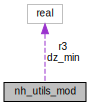
\includegraphics[width=126pt]{classnh__utils__mod__coll__graph}
\end{center}
\end{figure}
\subsection*{Public Member Functions}
\begin{DoxyCompactItemize}
\item 
subroutine, public \hyperlink{classnh__utils__mod_a36a0fec4ebdcec481f3b6c8ba6253b65}{update\-\_\-dz\-\_\-c} (is, ie, js, je, km, ng, dt, dp0, zs, area, ut, vt, gz, ws, npx, npy, sw\-\_\-corner, se\-\_\-corner, ne\-\_\-corner, nw\-\_\-corner, bd, grid\-\_\-type)
\item 
subroutine, public \hyperlink{classnh__utils__mod_adf32b4a88ce6240d9debfd3349995f83}{update\-\_\-dz\-\_\-d} (ndif, damp, hord, is, ie, js, je, km, ng, npx, npy, area, rarea, dp0, zs, zh, crx, cry, xfx, yfx, delz, ws, rdt, gridstruct, bd, lim\-\_\-fac, regional)
\item 
subroutine, public \hyperlink{classnh__utils__mod_a14da13c6200ffaf1d0e7383c70d90953}{riem\-\_\-solver\-\_\-c} (ms,dt,is,ie,js, je, km,ng,akap, cappa, cp,
\item 
subroutine, public \hyperlink{classnh__utils__mod_aaeea343f189c7d5d1b9f3f36ae5bee4f}{rim\-\_\-2d} (ms, bdt, is, ie, km, rgas, gama, gm2,
\item 
subroutine, public \hyperlink{classnh__utils__mod_aecc67df51de5f53b7025e6f6ed103ba9}{sim3\-\_\-solver} (dt,is,ie, km, rgas, gama, kappa,
\item 
subroutine, public \hyperlink{classnh__utils__mod_afae0ba673c0252a21d9670c4edfb0cde}{sim3p0\-\_\-solver} (dt,is,ie, km, rgas, gama, kappa,
\item 
subroutine, public \hyperlink{classnh__utils__mod_a98974fe07b61f32996d5f0de2236c356}{sim1\-\_\-solver} (dt,is,ie, km, rgas, gama, gm2, cp2, kappa,
\item 
subroutine, public \hyperlink{classnh__utils__mod_ac5d00a80489a56b649ae2e96c0d1e9c7}{sim\-\_\-solver} (dt,is,ie, km, rgas, gama, gm2, cp2, kappa,
\item 
subroutine, public \hyperlink{classnh__utils__mod_a491dbc73f83656f3205fa363a1325972}{nest\-\_\-halo\-\_\-nh} (ptop, grav, kappa, cp, delp, delz, pt, phis,
\end{DoxyCompactItemize}
\subsection*{Private Member Functions}
\begin{DoxyCompactItemize}
\item 
subroutine \hyperlink{classnh__utils__mod_a450b7ba2e55fb51928e3f7d61cab3fc7}{riem\-\_\-solver3test} (ms, dt,is,ie,js, je, km, ng,isd, ied, jsd, jed, akap, cappa, cp,
\begin{DoxyCompactList}\small\item\em G\-F\-D\-L -\/ This routine will not give absoulte reproducibility when compiled with -\/fast-\/transcendentals. G\-F\-D\-L -\/ It is now inside of \hyperlink{nh__core_8F90}{nh\-\_\-core.\-F90} and being compiled without -\/fast-\/transcendentals. \end{DoxyCompactList}\item 
subroutine \hyperlink{classnh__utils__mod_a20b7c4de8f64dacc17df9c0e4ac676aa}{imp\-\_\-diff\-\_\-w} (j, is, ie, js, je, ng, km, cd, delz, ws, w, w3)
\item 
subroutine \hyperlink{classnh__utils__mod_a4a0e44a9960d4023dca79a4332954cd2}{edge\-\_\-scalar} (q1, qe, i1, i2, km, id)
\item 
subroutine \hyperlink{classnh__utils__mod_a9a06dba3de6db5cdd862b36dc5553b9e}{edge\-\_\-profile} (q1, q2, q1e, q2e, i1, i2, j1, j2, j, km, dp0, uniform\-\_\-grid, limiter)
\end{DoxyCompactItemize}
\subsection*{Private Attributes}
\begin{DoxyCompactItemize}
\item 
real, parameter \hyperlink{classnh__utils__mod_a29df8f0c8a425db2e38a865d131ae9bb}{dz\-\_\-min} = 2.
\item 
real, parameter \hyperlink{classnh__utils__mod_a11855ede9ba4e45e0e95746e9aa50699}{r3} = 1./3.
\end{DoxyCompactItemize}


\subsection{Detailed Description}
The module 'nh\-\_\-utils' peforms non-\/hydrostatic computations. 

\begin{DoxyAuthor}{Author}
S. J. Lin, N\-O\-A\-A/\-G\-F\-D\-L 
\end{DoxyAuthor}


Definition at line 26 of file nh\-\_\-utils.\-F90.



\subsection{Member Function/\-Subroutine Documentation}
\index{nh\-\_\-utils\-\_\-mod@{nh\-\_\-utils\-\_\-mod}!edge\-\_\-profile@{edge\-\_\-profile}}
\index{edge\-\_\-profile@{edge\-\_\-profile}!nh_utils_mod@{nh\-\_\-utils\-\_\-mod}}
\subsubsection[{edge\-\_\-profile}]{\setlength{\rightskip}{0pt plus 5cm}subroutine nh\-\_\-utils\-\_\-mod\-::edge\-\_\-profile (
\begin{DoxyParamCaption}
\item[{real, dimension(i1\-:i2,j1\-:j2,km), intent(in)}]{q1, }
\item[{real, dimension(i1\-:i2,j1\-:j2,km), intent(in)}]{q2, }
\item[{real, dimension(i1\-:i2,j1\-:j2,km+1), intent(out)}]{q1e, }
\item[{real, dimension(i1\-:i2,j1\-:j2,km+1), intent(out)}]{q2e, }
\item[{integer, intent(in)}]{i1, }
\item[{integer, intent(in)}]{i2, }
\item[{integer, intent(in)}]{j1, }
\item[{integer, intent(in)}]{j2, }
\item[{integer, intent(in)}]{j, }
\item[{integer, intent(in)}]{km, }
\item[{real, dimension(km), intent(in)}]{dp0, }
\item[{logical, intent(in)}]{uniform\-\_\-grid, }
\item[{integer, intent(in)}]{limiter}
\end{DoxyParamCaption}
)\hspace{0.3cm}{\ttfamily [private]}}\label{classnh__utils__mod_a9a06dba3de6db5cdd862b36dc5553b9e}


Definition at line 1790 of file nh\-\_\-utils.\-F90.



Referenced by update\-\_\-dz\-\_\-d().

\index{nh\-\_\-utils\-\_\-mod@{nh\-\_\-utils\-\_\-mod}!edge\-\_\-scalar@{edge\-\_\-scalar}}
\index{edge\-\_\-scalar@{edge\-\_\-scalar}!nh_utils_mod@{nh\-\_\-utils\-\_\-mod}}
\subsubsection[{edge\-\_\-scalar}]{\setlength{\rightskip}{0pt plus 5cm}subroutine nh\-\_\-utils\-\_\-mod\-::edge\-\_\-scalar (
\begin{DoxyParamCaption}
\item[{real, dimension(i1\-:i2,km), intent(in)}]{q1, }
\item[{real, dimension(i1\-:i2,km+1), intent(out)}]{qe, }
\item[{integer, intent(in)}]{i1, }
\item[{integer, intent(in)}]{i2, }
\item[{integer, intent(in)}]{km, }
\item[{integer, intent(in)}]{id}
\end{DoxyParamCaption}
)\hspace{0.3cm}{\ttfamily [private]}}\label{classnh__utils__mod_a4a0e44a9960d4023dca79a4332954cd2}


Definition at line 1740 of file nh\-\_\-utils.\-F90.

\index{nh\-\_\-utils\-\_\-mod@{nh\-\_\-utils\-\_\-mod}!imp\-\_\-diff\-\_\-w@{imp\-\_\-diff\-\_\-w}}
\index{imp\-\_\-diff\-\_\-w@{imp\-\_\-diff\-\_\-w}!nh_utils_mod@{nh\-\_\-utils\-\_\-mod}}
\subsubsection[{imp\-\_\-diff\-\_\-w}]{\setlength{\rightskip}{0pt plus 5cm}subroutine nh\-\_\-utils\-\_\-mod\-::imp\-\_\-diff\-\_\-w (
\begin{DoxyParamCaption}
\item[{integer, intent(in)}]{j, }
\item[{integer, intent(in)}]{is, }
\item[{integer, intent(in)}]{ie, }
\item[{integer, intent(in)}]{js, }
\item[{integer, intent(in)}]{je, }
\item[{integer, intent(in)}]{ng, }
\item[{integer, intent(in)}]{km, }
\item[{real, intent(in)}]{cd, }
\item[{real, dimension(is-\/ng\-:ie+ng, km), intent(in)}]{delz, }
\item[{real, dimension(is\-:ie), intent(in)}]{ws, }
\item[{real, dimension(is\-:ie, km), intent(in)}]{w, }
\item[{real, dimension(is-\/ng\-:ie+ng,js-\/ng\-:je+ng,km), intent(out)}]{w3}
\end{DoxyParamCaption}
)\hspace{0.3cm}{\ttfamily [private]}}\label{classnh__utils__mod_a20b7c4de8f64dacc17df9c0e4ac676aa}

\begin{DoxyParams}[1]{Parameters}
\mbox{\tt in}  & {\em delz} & delta-\/height (m)\\
\hline
\mbox{\tt in}  & {\em w} & vertical vel. (m/s) \\
\hline
\end{DoxyParams}


Definition at line 679 of file nh\-\_\-utils.\-F90.

\index{nh\-\_\-utils\-\_\-mod@{nh\-\_\-utils\-\_\-mod}!nest\-\_\-halo\-\_\-nh@{nest\-\_\-halo\-\_\-nh}}
\index{nest\-\_\-halo\-\_\-nh@{nest\-\_\-halo\-\_\-nh}!nh_utils_mod@{nh\-\_\-utils\-\_\-mod}}
\subsubsection[{nest\-\_\-halo\-\_\-nh}]{\setlength{\rightskip}{0pt plus 5cm}subroutine, public nh\-\_\-utils\-\_\-mod\-::nest\-\_\-halo\-\_\-nh (
\begin{DoxyParamCaption}
\item[{real, intent(in)}]{ptop, }
\item[{real, intent(in)}]{grav, }
\item[{real, intent(in)}]{kappa, }
\item[{real, intent(in)}]{cp, }
\item[{real, dimension(bd\%isd\-:bd\%ied,bd\%jsd\-:bd\%jed,npz), intent(in)}]{delp, }
\item[{real, dimension(bd\%isd\-:bd\%ied,bd\%jsd\-:bd\%jed,npz), intent(in)}]{delz, }
\item[{real, dimension(bd\%isd\-:bd\%ied,bd\%jsd\-:bd\%jed,npz), intent(in)}]{pt, }
\item[{real, dimension(bd\%isd\-:bd\%ied,bd\%jsd\-:bd\%jed), intent(in)}]{phis}
\end{DoxyParamCaption}
)}\label{classnh__utils__mod_a491dbc73f83656f3205fa363a1325972}


Definition at line 1898 of file nh\-\_\-utils.\-F90.



References multi\-\_\-gases\-\_\-mod\-::vicpqd(), and multi\-\_\-gases\-\_\-mod\-::vicvqd().



Referenced by dyn\-\_\-core\-\_\-mod\-::dyn\-\_\-core().

\index{nh\-\_\-utils\-\_\-mod@{nh\-\_\-utils\-\_\-mod}!riem\-\_\-solver3test@{riem\-\_\-solver3test}}
\index{riem\-\_\-solver3test@{riem\-\_\-solver3test}!nh_utils_mod@{nh\-\_\-utils\-\_\-mod}}
\subsubsection[{riem\-\_\-solver3test}]{\setlength{\rightskip}{0pt plus 5cm}subroutine nh\-\_\-utils\-\_\-mod\-::riem\-\_\-solver3test (
\begin{DoxyParamCaption}
\item[{integer, intent(in)}]{ms, }
\item[{real, intent(in)}]{dt, }
\item[{integer, intent(in)}]{is, }
\item[{integer, intent(in)}]{ie, }
\item[{integer, intent(in)}]{js, }
\item[{integer, intent(in)}]{je, }
\item[{integer, intent(in)}]{km, }
\item[{integer, intent(in)}]{ng, }
\item[{integer, intent(in)}]{isd, }
\item[{integer, intent(in)}]{ied, }
\item[{integer, intent(in)}]{jsd, }
\item[{integer, intent(in)}]{jed, }
\item[{real, intent(in)}]{akap, }
\item[{real, dimension(isd\-:,jsd\-:,1\-:), intent(in)}]{cappa, }
\item[{real, intent(in)}]{cp}
\end{DoxyParamCaption}
)\hspace{0.3cm}{\ttfamily [private]}}\label{classnh__utils__mod_a450b7ba2e55fb51928e3f7d61cab3fc7}


G\-F\-D\-L -\/ This routine will not give absoulte reproducibility when compiled with -\/fast-\/transcendentals. G\-F\-D\-L -\/ It is now inside of \hyperlink{nh__core_8F90}{nh\-\_\-core.\-F90} and being compiled without -\/fast-\/transcendentals. 



Definition at line 474 of file nh\-\_\-utils.\-F90.



References rim\-\_\-2d(), sim1\-\_\-solver(), sim3\-\_\-solver(), sim3p0\-\_\-solver(), and sim\-\_\-solver().

\index{nh\-\_\-utils\-\_\-mod@{nh\-\_\-utils\-\_\-mod}!riem\-\_\-solver\-\_\-c@{riem\-\_\-solver\-\_\-c}}
\index{riem\-\_\-solver\-\_\-c@{riem\-\_\-solver\-\_\-c}!nh_utils_mod@{nh\-\_\-utils\-\_\-mod}}
\subsubsection[{riem\-\_\-solver\-\_\-c}]{\setlength{\rightskip}{0pt plus 5cm}subroutine, public nh\-\_\-utils\-\_\-mod\-::riem\-\_\-solver\-\_\-c (
\begin{DoxyParamCaption}
\item[{integer, intent(in)}]{ms, }
\item[{real, intent(in)}]{dt, }
\item[{integer, intent(in)}]{is, }
\item[{integer, intent(in)}]{ie, }
\item[{integer, intent(in)}]{js, }
\item[{integer, intent(in)}]{je, }
\item[{integer, intent(in)}]{km, }
\item[{integer, intent(in)}]{ng, }
\item[{real, intent(in)}]{akap, }
\item[{real, dimension(is-\/ng\-:,js-\/ng\-:,1\-:), intent(in)}]{cappa, }
\item[{real, intent(in)}]{cp}
\end{DoxyParamCaption}
)}\label{classnh__utils__mod_a14da13c6200ffaf1d0e7383c70d90953}


Definition at line 331 of file nh\-\_\-utils.\-F90.



References rim\-\_\-2d(), sim1\-\_\-solver(), and sim3p0\-\_\-solver().



Referenced by dyn\-\_\-core\-\_\-mod\-::dyn\-\_\-core().

\index{nh\-\_\-utils\-\_\-mod@{nh\-\_\-utils\-\_\-mod}!rim\-\_\-2d@{rim\-\_\-2d}}
\index{rim\-\_\-2d@{rim\-\_\-2d}!nh_utils_mod@{nh\-\_\-utils\-\_\-mod}}
\subsubsection[{rim\-\_\-2d}]{\setlength{\rightskip}{0pt plus 5cm}subroutine, public nh\-\_\-utils\-\_\-mod\-::rim\-\_\-2d (
\begin{DoxyParamCaption}
\item[{integer, intent(in)}]{ms, }
\item[{real, intent(in)}]{bdt, }
\item[{integer, intent(in)}]{is, }
\item[{integer, intent(in)}]{ie, }
\item[{integer, intent(in)}]{km, }
\item[{real, intent(in)}]{rgas, }
\item[{real, intent(in)}]{gama, }
\item[{real, dimension(is\-:ie,km), intent(in)}]{gm2}
\end{DoxyParamCaption}
)}\label{classnh__utils__mod_aaeea343f189c7d5d1b9f3f36ae5bee4f}


Definition at line 742 of file nh\-\_\-utils.\-F90.



Referenced by nh\-\_\-core\-\_\-mod\-::riem\-\_\-solver3(), riem\-\_\-solver3test(), and riem\-\_\-solver\-\_\-c().

\index{nh\-\_\-utils\-\_\-mod@{nh\-\_\-utils\-\_\-mod}!sim1\-\_\-solver@{sim1\-\_\-solver}}
\index{sim1\-\_\-solver@{sim1\-\_\-solver}!nh_utils_mod@{nh\-\_\-utils\-\_\-mod}}
\subsubsection[{sim1\-\_\-solver}]{\setlength{\rightskip}{0pt plus 5cm}subroutine, public nh\-\_\-utils\-\_\-mod\-::sim1\-\_\-solver (
\begin{DoxyParamCaption}
\item[{real, intent(in)}]{dt, }
\item[{integer, intent(in)}]{is, }
\item[{integer, intent(in)}]{ie, }
\item[{integer, intent(in)}]{km, }
\item[{real, intent(in)}]{rgas, }
\item[{real, intent(in)}]{gama, }
\item[{real, dimension(is\-:ie,km), intent(in)}]{gm2, }
\item[{real, dimension(is\-:ie,km), intent(in)}]{cp2, }
\item[{real, intent(in)}]{kappa}
\end{DoxyParamCaption}
)}\label{classnh__utils__mod_a98974fe07b61f32996d5f0de2236c356}


Definition at line 1373 of file nh\-\_\-utils.\-F90.



Referenced by nh\-\_\-core\-\_\-mod\-::riem\-\_\-solver3(), riem\-\_\-solver3test(), and riem\-\_\-solver\-\_\-c().

\index{nh\-\_\-utils\-\_\-mod@{nh\-\_\-utils\-\_\-mod}!sim3\-\_\-solver@{sim3\-\_\-solver}}
\index{sim3\-\_\-solver@{sim3\-\_\-solver}!nh_utils_mod@{nh\-\_\-utils\-\_\-mod}}
\subsubsection[{sim3\-\_\-solver}]{\setlength{\rightskip}{0pt plus 5cm}subroutine, public nh\-\_\-utils\-\_\-mod\-::sim3\-\_\-solver (
\begin{DoxyParamCaption}
\item[{real, intent(in)}]{dt, }
\item[{integer, intent(in)}]{is, }
\item[{integer, intent(in)}]{ie, }
\item[{integer, intent(in)}]{km, }
\item[{real, intent(in)}]{rgas, }
\item[{real, intent(in)}]{gama, }
\item[{real, intent(in)}]{kappa}
\end{DoxyParamCaption}
)}\label{classnh__utils__mod_aecc67df51de5f53b7025e6f6ed103ba9}


Definition at line 1006 of file nh\-\_\-utils.\-F90.



Referenced by nh\-\_\-core\-\_\-mod\-::riem\-\_\-solver3(), and riem\-\_\-solver3test().

\index{nh\-\_\-utils\-\_\-mod@{nh\-\_\-utils\-\_\-mod}!sim3p0\-\_\-solver@{sim3p0\-\_\-solver}}
\index{sim3p0\-\_\-solver@{sim3p0\-\_\-solver}!nh_utils_mod@{nh\-\_\-utils\-\_\-mod}}
\subsubsection[{sim3p0\-\_\-solver}]{\setlength{\rightskip}{0pt plus 5cm}subroutine, public nh\-\_\-utils\-\_\-mod\-::sim3p0\-\_\-solver (
\begin{DoxyParamCaption}
\item[{real, intent(in)}]{dt, }
\item[{integer, intent(in)}]{is, }
\item[{integer, intent(in)}]{ie, }
\item[{integer, intent(in)}]{km, }
\item[{real, intent(in)}]{rgas, }
\item[{real, intent(in)}]{gama, }
\item[{real, intent(in)}]{kappa}
\end{DoxyParamCaption}
)}\label{classnh__utils__mod_afae0ba673c0252a21d9670c4edfb0cde}


Definition at line 1193 of file nh\-\_\-utils.\-F90.



Referenced by nh\-\_\-core\-\_\-mod\-::riem\-\_\-solver3(), riem\-\_\-solver3test(), and riem\-\_\-solver\-\_\-c().

\index{nh\-\_\-utils\-\_\-mod@{nh\-\_\-utils\-\_\-mod}!sim\-\_\-solver@{sim\-\_\-solver}}
\index{sim\-\_\-solver@{sim\-\_\-solver}!nh_utils_mod@{nh\-\_\-utils\-\_\-mod}}
\subsubsection[{sim\-\_\-solver}]{\setlength{\rightskip}{0pt plus 5cm}subroutine, public nh\-\_\-utils\-\_\-mod\-::sim\-\_\-solver (
\begin{DoxyParamCaption}
\item[{real, intent(in)}]{dt, }
\item[{integer, intent(in)}]{is, }
\item[{integer, intent(in)}]{ie, }
\item[{integer, intent(in)}]{km, }
\item[{real, intent(in)}]{rgas, }
\item[{real, intent(in)}]{gama, }
\item[{real, dimension(is\-:ie,km), intent(in)}]{gm2, }
\item[{real, dimension(is\-:ie,km), intent(in)}]{cp2, }
\item[{real, intent(in)}]{kappa}
\end{DoxyParamCaption}
)}\label{classnh__utils__mod_ac5d00a80489a56b649ae2e96c0d1e9c7}


Definition at line 1544 of file nh\-\_\-utils.\-F90.



Referenced by nh\-\_\-core\-\_\-mod\-::riem\-\_\-solver3(), and riem\-\_\-solver3test().

\index{nh\-\_\-utils\-\_\-mod@{nh\-\_\-utils\-\_\-mod}!update\-\_\-dz\-\_\-c@{update\-\_\-dz\-\_\-c}}
\index{update\-\_\-dz\-\_\-c@{update\-\_\-dz\-\_\-c}!nh_utils_mod@{nh\-\_\-utils\-\_\-mod}}
\subsubsection[{update\-\_\-dz\-\_\-c}]{\setlength{\rightskip}{0pt plus 5cm}subroutine, public nh\-\_\-utils\-\_\-mod\-::update\-\_\-dz\-\_\-c (
\begin{DoxyParamCaption}
\item[{integer, intent(in)}]{is, }
\item[{integer, intent(in)}]{ie, }
\item[{integer, intent(in)}]{js, }
\item[{integer, intent(in)}]{je, }
\item[{integer, intent(in)}]{km, }
\item[{integer, intent(in)}]{ng, }
\item[{real, intent(in)}]{dt, }
\item[{real, dimension(km), intent(in)}]{dp0, }
\item[{real, dimension(is-\/ng\-:ie+ng, js-\/ng\-:je+ng), intent(in)}]{zs, }
\item[{real, dimension(is-\/ng\-:ie+ng,js-\/ng\-:je+ng), intent(in)}]{area, }
\item[{real, dimension(is-\/ng\-:ie+ng,js-\/ng\-:je+ng,km), intent(in)}]{ut, }
\item[{real, dimension(is-\/ng\-:ie+ng,js-\/ng\-:je+ng,km), intent(in)}]{vt, }
\item[{real, dimension(is-\/ng\-:ie+ng,js-\/ng\-:je+ng,km+1), intent(inout)}]{gz, }
\item[{real, dimension(is-\/ng\-:ie+ng, js-\/ng\-:je+ng), intent(out)}]{ws, }
\item[{integer, intent(in)}]{npx, }
\item[{integer, intent(in)}]{npy, }
\item[{logical, intent(in)}]{sw\-\_\-corner, }
\item[{logical, intent(in)}]{se\-\_\-corner, }
\item[{logical, intent(in)}]{ne\-\_\-corner, }
\item[{logical, intent(in)}]{nw\-\_\-corner, }
\item[{type(fv\-\_\-grid\-\_\-bounds\-\_\-type), intent(in)}]{bd, }
\item[{integer, intent(in)}]{grid\-\_\-type}
\end{DoxyParamCaption}
)}\label{classnh__utils__mod_a36a0fec4ebdcec481f3b6c8ba6253b65}


Definition at line 74 of file nh\-\_\-utils.\-F90.



References sw\-\_\-core\-\_\-mod\-::fill\-\_\-4corners().



Referenced by dyn\-\_\-core\-\_\-mod\-::dyn\-\_\-core().

\index{nh\-\_\-utils\-\_\-mod@{nh\-\_\-utils\-\_\-mod}!update\-\_\-dz\-\_\-d@{update\-\_\-dz\-\_\-d}}
\index{update\-\_\-dz\-\_\-d@{update\-\_\-dz\-\_\-d}!nh_utils_mod@{nh\-\_\-utils\-\_\-mod}}
\subsubsection[{update\-\_\-dz\-\_\-d}]{\setlength{\rightskip}{0pt plus 5cm}subroutine, public nh\-\_\-utils\-\_\-mod\-::update\-\_\-dz\-\_\-d (
\begin{DoxyParamCaption}
\item[{integer, dimension(km+1), intent(inout)}]{ndif, }
\item[{real, dimension(km+1), intent(inout)}]{damp, }
\item[{integer, intent(in)}]{hord, }
\item[{integer, intent(in)}]{is, }
\item[{integer, intent(in)}]{ie, }
\item[{integer, intent(in)}]{js, }
\item[{integer, intent(in)}]{je, }
\item[{integer, intent(in)}]{km, }
\item[{integer, intent(in)}]{ng, }
\item[{integer, intent(in)}]{npx, }
\item[{integer, intent(in)}]{npy, }
\item[{real, dimension(is-\/ng\-:ie+ng,js-\/ng\-:je+ng), intent(in)}]{area, }
\item[{real, dimension(is-\/ng\-:ie+ng,js-\/ng\-:je+ng), intent(in)}]{rarea, }
\item[{real, dimension(km), intent(in)}]{dp0, }
\item[{real, dimension(is-\/ng\-:ie+ng,js-\/ng\-:je+ng), intent(in)}]{zs, }
\item[{real, dimension(is-\/ng\-:ie+ng,js-\/ng\-:je+ng,km+1), intent(inout)}]{zh, }
\item[{real, dimension(is\-:ie+1,js-\/ng\-:je+ng,km), intent(inout)}]{crx, }
\item[{real, dimension(is-\/ng\-:ie+ng,js\-:je+1,km), intent(inout)}]{cry, }
\item[{real, dimension(is\-:ie+1,js-\/ng\-:je+ng,km), intent(inout)}]{xfx, }
\item[{real, dimension(is-\/ng\-:ie+ng,js\-:je+1,km), intent(inout)}]{yfx, }
\item[{real, dimension(is-\/ng\-:ie+ng,js-\/ng\-:je+ng,km), intent(out)}]{delz, }
\item[{real, dimension(is\-:ie,js\-:je), intent(out)}]{ws, }
\item[{real, intent(in)}]{rdt, }
\item[{type(fv\-\_\-grid\-\_\-type), intent(in), target}]{gridstruct, }
\item[{type(fv\-\_\-grid\-\_\-bounds\-\_\-type), intent(in)}]{bd, }
\item[{real, intent(in)}]{lim\-\_\-fac, }
\item[{logical, intent(in)}]{regional}
\end{DoxyParamCaption}
)}\label{classnh__utils__mod_adf32b4a88ce6240d9debfd3349995f83}


Definition at line 214 of file nh\-\_\-utils.\-F90.



References sw\-\_\-core\-\_\-mod\-::del6\-\_\-vt\-\_\-flux(), edge\-\_\-profile(), and tp\-\_\-core\-\_\-mod\-::fv\-\_\-tp\-\_\-2d().



Referenced by dyn\-\_\-core\-\_\-mod\-::dyn\-\_\-core().



\subsection{Member Data Documentation}
\index{nh\-\_\-utils\-\_\-mod@{nh\-\_\-utils\-\_\-mod}!dz\-\_\-min@{dz\-\_\-min}}
\index{dz\-\_\-min@{dz\-\_\-min}!nh_utils_mod@{nh\-\_\-utils\-\_\-mod}}
\subsubsection[{dz\-\_\-min}]{\setlength{\rightskip}{0pt plus 5cm}real, parameter nh\-\_\-utils\-\_\-mod\-::dz\-\_\-min = 2.\hspace{0.3cm}{\ttfamily [private]}}\label{classnh__utils__mod_a29df8f0c8a425db2e38a865d131ae9bb}


Definition at line 69 of file nh\-\_\-utils.\-F90.

\index{nh\-\_\-utils\-\_\-mod@{nh\-\_\-utils\-\_\-mod}!r3@{r3}}
\index{r3@{r3}!nh_utils_mod@{nh\-\_\-utils\-\_\-mod}}
\subsubsection[{r3}]{\setlength{\rightskip}{0pt plus 5cm}real, parameter nh\-\_\-utils\-\_\-mod\-::r3 = 1./3.\hspace{0.3cm}{\ttfamily [private]}}\label{classnh__utils__mod_a11855ede9ba4e45e0e95746e9aa50699}


Definition at line 70 of file nh\-\_\-utils.\-F90.



The documentation for this module was generated from the following file\-:\begin{DoxyCompactItemize}
\item 
/scratch2/\-N\-A\-G\-A\-P\-E/aoml-\/hafs1/\-Kyle.\-Ahern/acs\-\_\-master\-\_\-readonly/model/\hyperlink{nh__utils_8F90}{nh\-\_\-utils.\-F90}\end{DoxyCompactItemize}

\section{sim\-\_\-nc\-\_\-mod Module Reference}
\label{classsim__nc__mod}\index{sim\-\_\-nc\-\_\-mod@{sim\-\_\-nc\-\_\-mod}}


The module 'sim\-\_\-nc' is a netcdf file reader.  


\subsection*{Public Member Functions}
\begin{DoxyCompactItemize}
\item 
subroutine, public \hyperlink{classsim__nc__mod_aba132435cdbc967cae6289d8de91c642}{open\-\_\-ncfile} (iflnm, ncid)
\item 
subroutine, public \hyperlink{classsim__nc__mod_a0723aaca20b4f506ff134f191c9c2773}{close\-\_\-ncfile} (ncid)
\item 
subroutine, public \hyperlink{classsim__nc__mod_ae7821440ac92334fb40992fd22fb611c}{get\-\_\-ncdim1} (ncid, var1\-\_\-name, im)
\item 
subroutine, public \hyperlink{classsim__nc__mod_ace9b6fd17d5ca314e8ad1cd4dfbeac4b}{get\-\_\-var1\-\_\-double} (ncid, var1\-\_\-name, im, var1, var\-\_\-exist)
\begin{DoxyCompactList}\small\item\em The 'get\-\_\-var' subroutines read in variables from netcdf files. \end{DoxyCompactList}\item 
subroutine, public \hyperlink{classsim__nc__mod_accbb162bf22e5a5d2b9de65c8db7b3f1}{get\-\_\-var1\-\_\-real} (ncid, var1\-\_\-name, im, var1, var\-\_\-exist)
\item 
subroutine, public \hyperlink{classsim__nc__mod_a0d037f885e13796e5464178753a4f7c0}{get\-\_\-var2\-\_\-real} (ncid, var\-\_\-name, im, jm, var2)
\item 
subroutine, public \hyperlink{classsim__nc__mod_a71d5ab6bff11033a949f0b9bc5a7b5c7}{get\-\_\-var2\-\_\-r4} (ncid, var2\-\_\-name, is, ie, js, je, var2, time\-\_\-slice)
\item 
subroutine, public \hyperlink{classsim__nc__mod_a721aebcb15fd4300ce0f803b1f36e835}{get\-\_\-var2\-\_\-double} (ncid, var2\-\_\-name, im, jm, var2)
\item 
subroutine, public \hyperlink{classsim__nc__mod_ab01af2d9e31aa4fb2eddd4aa0116fdf9}{get\-\_\-var3\-\_\-double} (ncid, var3\-\_\-name, im, jm, km, var3)
\item 
subroutine, public \hyperlink{classsim__nc__mod_a2ce0a869b2a092c675a2fd05fa9eba78}{get\-\_\-var3\-\_\-real} (ncid, var3\-\_\-name, im, jm, km, var3)
\item 
subroutine, public \hyperlink{classsim__nc__mod_aa1c1534dbde8d5215e5c8fd8d56473b0}{check\-\_\-var\-\_\-exists} (ncid, var\-\_\-name, status)
\item 
subroutine, public \hyperlink{classsim__nc__mod_aeef43827235a8f2bc87c811ae6f047c0}{get\-\_\-var3\-\_\-r4} (ncid, var3\-\_\-name, is, ie, js, je, ks, ke, var3, time\-\_\-slice)
\item 
logical function, public \hyperlink{classsim__nc__mod_a6ba00a9ac634a7f1aa7a8aa588cc6423}{check\-\_\-var} (ncid, var3\-\_\-name)
\item 
subroutine, public \hyperlink{classsim__nc__mod_af74cc9f00ca3198748d69d55e063485a}{get\-\_\-var\-\_\-att\-\_\-double} (ncid, var\-\_\-name, att\-\_\-name, value)
\item 
subroutine, public \hyperlink{classsim__nc__mod_a278601db1538c2ce2821467fa506c393}{handle\-\_\-err} (idstr, status)
\end{DoxyCompactItemize}
\subsection*{Private Member Functions}
\begin{DoxyCompactItemize}
\item 
subroutine \hyperlink{classsim__nc__mod_a150306f1b53f93c31ed34e1a3d854c4d}{get\-\_\-var4\-\_\-real} (ncid, var4\-\_\-name, im, jm, km, nt, var4)
\item 
subroutine \hyperlink{classsim__nc__mod_a6966d31b89e3d2c1d12ae4817da51ed5}{get\-\_\-var4\-\_\-double} (ncid, var4\-\_\-name, im, jm, km, nt, var4)
\item 
subroutine \hyperlink{classsim__nc__mod_a921e83485407607449ed2085ce13e065}{get\-\_\-real3} (ncid, var4\-\_\-name, im, jm, nt, var4)
\item 
subroutine \hyperlink{classsim__nc__mod_a8cd192cd41636a101590b25b49819727}{get\-\_\-var\-\_\-att\-\_\-str} (ncid, var\-\_\-name, att\-\_\-name, att)
\item 
subroutine \hyperlink{classsim__nc__mod_a86a17476a157016bb327b188cf6face9}{calendar} (year, month, day, hour)
\begin{DoxyCompactList}\small\item\em The subroutine 'calendar' computes the current G\-M\-T. \end{DoxyCompactList}\end{DoxyCompactItemize}


\subsection{Detailed Description}
The module 'sim\-\_\-nc' is a netcdf file reader. 

The code is necessary to circumvent issues with the F\-M\-S 'read\-\_\-data' utility, which opens too many files and uses excessive memory. \begin{DoxyAuthor}{Author}
Shian-\/\-Jiann Lin 
\end{DoxyAuthor}


Definition at line 28 of file sim\-\_\-nc\-\_\-mod.\-F90.



\subsection{Member Function/\-Subroutine Documentation}
\index{sim\-\_\-nc\-\_\-mod@{sim\-\_\-nc\-\_\-mod}!calendar@{calendar}}
\index{calendar@{calendar}!sim_nc_mod@{sim\-\_\-nc\-\_\-mod}}
\subsubsection[{calendar}]{\setlength{\rightskip}{0pt plus 5cm}subroutine sim\-\_\-nc\-\_\-mod\-::calendar (
\begin{DoxyParamCaption}
\item[{integer, intent(inout)}]{year, }
\item[{integer, intent(inout)}]{month, }
\item[{integer, intent(inout)}]{day, }
\item[{integer, intent(inout)}]{hour}
\end{DoxyParamCaption}
)\hspace{0.3cm}{\ttfamily [private]}}\label{classsim__nc__mod_a86a17476a157016bb327b188cf6face9}


The subroutine 'calendar' computes the current G\-M\-T. 



Definition at line 428 of file sim\-\_\-nc\-\_\-mod.\-F90.

\index{sim\-\_\-nc\-\_\-mod@{sim\-\_\-nc\-\_\-mod}!check\-\_\-var@{check\-\_\-var}}
\index{check\-\_\-var@{check\-\_\-var}!sim_nc_mod@{sim\-\_\-nc\-\_\-mod}}
\subsubsection[{check\-\_\-var}]{\setlength{\rightskip}{0pt plus 5cm}logical function, public sim\-\_\-nc\-\_\-mod\-::check\-\_\-var (
\begin{DoxyParamCaption}
\item[{integer, intent(in)}]{ncid, }
\item[{character(len=$\ast$), intent(in)}]{var3\-\_\-name}
\end{DoxyParamCaption}
)}\label{classsim__nc__mod_a6ba00a9ac634a7f1aa7a8aa588cc6423}


Definition at line 371 of file sim\-\_\-nc\-\_\-mod.\-F90.

\index{sim\-\_\-nc\-\_\-mod@{sim\-\_\-nc\-\_\-mod}!check\-\_\-var\-\_\-exists@{check\-\_\-var\-\_\-exists}}
\index{check\-\_\-var\-\_\-exists@{check\-\_\-var\-\_\-exists}!sim_nc_mod@{sim\-\_\-nc\-\_\-mod}}
\subsubsection[{check\-\_\-var\-\_\-exists}]{\setlength{\rightskip}{0pt plus 5cm}subroutine, public sim\-\_\-nc\-\_\-mod\-::check\-\_\-var\-\_\-exists (
\begin{DoxyParamCaption}
\item[{integer, intent(in)}]{ncid, }
\item[{character(len=$\ast$), intent(in)}]{var\-\_\-name, }
\item[{integer, intent(inout)}]{status}
\end{DoxyParamCaption}
)}\label{classsim__nc__mod_aa1c1534dbde8d5215e5c8fd8d56473b0}


Definition at line 237 of file sim\-\_\-nc\-\_\-mod.\-F90.



Referenced by apply\-\_\-inc\-\_\-on\-\_\-3d\-\_\-scalar(), and fv\-\_\-iau\-\_\-mod\-::interp\-\_\-inc().

\index{sim\-\_\-nc\-\_\-mod@{sim\-\_\-nc\-\_\-mod}!close\-\_\-ncfile@{close\-\_\-ncfile}}
\index{close\-\_\-ncfile@{close\-\_\-ncfile}!sim_nc_mod@{sim\-\_\-nc\-\_\-mod}}
\subsubsection[{close\-\_\-ncfile}]{\setlength{\rightskip}{0pt plus 5cm}subroutine, public sim\-\_\-nc\-\_\-mod\-::close\-\_\-ncfile (
\begin{DoxyParamCaption}
\item[{integer, intent(in)}]{ncid}
\end{DoxyParamCaption}
)}\label{classsim__nc__mod_a0723aaca20b4f506ff134f191c9c2773}


Definition at line 66 of file sim\-\_\-nc\-\_\-mod.\-F90.



References fv\-\_\-surf\-\_\-map\-\_\-mod\-::handle\-\_\-err().



Referenced by fv\-\_\-nwp\-\_\-nudge\-\_\-mod\-::fv\-\_\-nwp\-\_\-nudge\-\_\-init(), fv\-\_\-nwp\-\_\-nudge\-\_\-mod\-::get\-\_\-ncep\-\_\-analysis(), external\-\_\-ic\-\_\-mod\-::get\-\_\-ncep\-\_\-ic(), fv\-\_\-iau\-\_\-mod\-::iau\-\_\-initialize(), and fv\-\_\-iau\-\_\-mod\-::read\-\_\-iau\-\_\-forcing().

\index{sim\-\_\-nc\-\_\-mod@{sim\-\_\-nc\-\_\-mod}!get\-\_\-ncdim1@{get\-\_\-ncdim1}}
\index{get\-\_\-ncdim1@{get\-\_\-ncdim1}!sim_nc_mod@{sim\-\_\-nc\-\_\-mod}}
\subsubsection[{get\-\_\-ncdim1}]{\setlength{\rightskip}{0pt plus 5cm}subroutine, public sim\-\_\-nc\-\_\-mod\-::get\-\_\-ncdim1 (
\begin{DoxyParamCaption}
\item[{integer, intent(in)}]{ncid, }
\item[{character(len=$\ast$), intent(in)}]{var1\-\_\-name, }
\item[{integer, intent(out)}]{im}
\end{DoxyParamCaption}
)}\label{classsim__nc__mod_ae7821440ac92334fb40992fd22fb611c}


Definition at line 77 of file sim\-\_\-nc\-\_\-mod.\-F90.



References fv\-\_\-surf\-\_\-map\-\_\-mod\-::handle\-\_\-err().



Referenced by fv\-\_\-nwp\-\_\-nudge\-\_\-mod\-::fv\-\_\-nwp\-\_\-nudge\-\_\-init(), external\-\_\-ic\-\_\-mod\-::get\-\_\-ecmwf\-\_\-ic(), external\-\_\-ic\-\_\-mod\-::get\-\_\-ncep\-\_\-ic(), fv\-\_\-iau\-\_\-mod\-::iau\-\_\-initialize(), and fv\-\_\-treat\-\_\-da\-\_\-inc\-\_\-mod\-::read\-\_\-da\-\_\-inc().

\index{sim\-\_\-nc\-\_\-mod@{sim\-\_\-nc\-\_\-mod}!get\-\_\-real3@{get\-\_\-real3}}
\index{get\-\_\-real3@{get\-\_\-real3}!sim_nc_mod@{sim\-\_\-nc\-\_\-mod}}
\subsubsection[{get\-\_\-real3}]{\setlength{\rightskip}{0pt plus 5cm}subroutine sim\-\_\-nc\-\_\-mod\-::get\-\_\-real3 (
\begin{DoxyParamCaption}
\item[{integer, intent(in)}]{ncid, }
\item[{character(len=$\ast$), intent(in)}]{var4\-\_\-name, }
\item[{integer, intent(in)}]{im, }
\item[{integer, intent(in)}]{jm, }
\item[{integer, intent(in)}]{nt, }
\item[{real(kind=4), dimension(im,jm), intent(out)}]{var4}
\end{DoxyParamCaption}
)\hspace{0.3cm}{\ttfamily [private]}}\label{classsim__nc__mod_a921e83485407607449ed2085ce13e065}


Definition at line 344 of file sim\-\_\-nc\-\_\-mod.\-F90.



References fv\-\_\-surf\-\_\-map\-\_\-mod\-::handle\-\_\-err().

\index{sim\-\_\-nc\-\_\-mod@{sim\-\_\-nc\-\_\-mod}!get\-\_\-var1\-\_\-double@{get\-\_\-var1\-\_\-double}}
\index{get\-\_\-var1\-\_\-double@{get\-\_\-var1\-\_\-double}!sim_nc_mod@{sim\-\_\-nc\-\_\-mod}}
\subsubsection[{get\-\_\-var1\-\_\-double}]{\setlength{\rightskip}{0pt plus 5cm}subroutine, public sim\-\_\-nc\-\_\-mod\-::get\-\_\-var1\-\_\-double (
\begin{DoxyParamCaption}
\item[{integer, intent(in)}]{ncid, }
\item[{character(len=$\ast$), intent(in)}]{var1\-\_\-name, }
\item[{integer, intent(in)}]{im, }
\item[{real(kind=8), dimension(im), intent(out)}]{var1, }
\item[{logical, intent(out), optional}]{var\-\_\-exist}
\end{DoxyParamCaption}
)}\label{classsim__nc__mod_ace9b6fd17d5ca314e8ad1cd4dfbeac4b}


The 'get\-\_\-var' subroutines read in variables from netcdf files. 



Definition at line 92 of file sim\-\_\-nc\-\_\-mod.\-F90.



References fv\-\_\-surf\-\_\-map\-\_\-mod\-::handle\-\_\-err().

\index{sim\-\_\-nc\-\_\-mod@{sim\-\_\-nc\-\_\-mod}!get\-\_\-var1\-\_\-real@{get\-\_\-var1\-\_\-real}}
\index{get\-\_\-var1\-\_\-real@{get\-\_\-var1\-\_\-real}!sim_nc_mod@{sim\-\_\-nc\-\_\-mod}}
\subsubsection[{get\-\_\-var1\-\_\-real}]{\setlength{\rightskip}{0pt plus 5cm}subroutine, public sim\-\_\-nc\-\_\-mod\-::get\-\_\-var1\-\_\-real (
\begin{DoxyParamCaption}
\item[{integer, intent(in)}]{ncid, }
\item[{character(len=$\ast$), intent(in)}]{var1\-\_\-name, }
\item[{integer, intent(in)}]{im, }
\item[{real(kind=4), dimension(im), intent(out)}]{var1, }
\item[{logical, intent(out), optional}]{var\-\_\-exist}
\end{DoxyParamCaption}
)}\label{classsim__nc__mod_accbb162bf22e5a5d2b9de65c8db7b3f1}


Definition at line 115 of file sim\-\_\-nc\-\_\-mod.\-F90.



References fv\-\_\-surf\-\_\-map\-\_\-mod\-::handle\-\_\-err().

\index{sim\-\_\-nc\-\_\-mod@{sim\-\_\-nc\-\_\-mod}!get\-\_\-var2\-\_\-double@{get\-\_\-var2\-\_\-double}}
\index{get\-\_\-var2\-\_\-double@{get\-\_\-var2\-\_\-double}!sim_nc_mod@{sim\-\_\-nc\-\_\-mod}}
\subsubsection[{get\-\_\-var2\-\_\-double}]{\setlength{\rightskip}{0pt plus 5cm}subroutine, public sim\-\_\-nc\-\_\-mod\-::get\-\_\-var2\-\_\-double (
\begin{DoxyParamCaption}
\item[{integer, intent(in)}]{ncid, }
\item[{character(len=$\ast$), intent(in)}]{var2\-\_\-name, }
\item[{integer, intent(in)}]{im, }
\item[{integer, intent(in)}]{jm, }
\item[{real(kind=8), dimension(im,jm), intent(out)}]{var2}
\end{DoxyParamCaption}
)}\label{classsim__nc__mod_a721aebcb15fd4300ce0f803b1f36e835}


Definition at line 180 of file sim\-\_\-nc\-\_\-mod.\-F90.



References fv\-\_\-surf\-\_\-map\-\_\-mod\-::handle\-\_\-err().

\index{sim\-\_\-nc\-\_\-mod@{sim\-\_\-nc\-\_\-mod}!get\-\_\-var2\-\_\-r4@{get\-\_\-var2\-\_\-r4}}
\index{get\-\_\-var2\-\_\-r4@{get\-\_\-var2\-\_\-r4}!sim_nc_mod@{sim\-\_\-nc\-\_\-mod}}
\subsubsection[{get\-\_\-var2\-\_\-r4}]{\setlength{\rightskip}{0pt plus 5cm}subroutine, public sim\-\_\-nc\-\_\-mod\-::get\-\_\-var2\-\_\-r4 (
\begin{DoxyParamCaption}
\item[{integer, intent(in)}]{ncid, }
\item[{character(len=$\ast$), intent(in)}]{var2\-\_\-name, }
\item[{integer, intent(in)}]{is, }
\item[{integer, intent(in)}]{ie, }
\item[{integer, intent(in)}]{js, }
\item[{integer, intent(in)}]{je, }
\item[{real(kind=4), dimension(is\-:ie,js\-:je), intent(out)}]{var2, }
\item[{integer, intent(in), optional}]{time\-\_\-slice}
\end{DoxyParamCaption}
)}\label{classsim__nc__mod_a71d5ab6bff11033a949f0b9bc5a7b5c7}


Definition at line 152 of file sim\-\_\-nc\-\_\-mod.\-F90.



References fv\-\_\-surf\-\_\-map\-\_\-mod\-::handle\-\_\-err().



Referenced by external\-\_\-ic\-\_\-mod\-::get\-\_\-ecmwf\-\_\-ic().

\index{sim\-\_\-nc\-\_\-mod@{sim\-\_\-nc\-\_\-mod}!get\-\_\-var2\-\_\-real@{get\-\_\-var2\-\_\-real}}
\index{get\-\_\-var2\-\_\-real@{get\-\_\-var2\-\_\-real}!sim_nc_mod@{sim\-\_\-nc\-\_\-mod}}
\subsubsection[{get\-\_\-var2\-\_\-real}]{\setlength{\rightskip}{0pt plus 5cm}subroutine, public sim\-\_\-nc\-\_\-mod\-::get\-\_\-var2\-\_\-real (
\begin{DoxyParamCaption}
\item[{integer, intent(in)}]{ncid, }
\item[{character(len=$\ast$), intent(in)}]{var\-\_\-name, }
\item[{integer, intent(in)}]{im, }
\item[{integer, intent(in)}]{jm, }
\item[{real(kind=4), dimension(im), intent(out)}]{var2}
\end{DoxyParamCaption}
)}\label{classsim__nc__mod_a0d037f885e13796e5464178753a4f7c0}


Definition at line 136 of file sim\-\_\-nc\-\_\-mod.\-F90.



References fv\-\_\-surf\-\_\-map\-\_\-mod\-::handle\-\_\-err().



Referenced by external\-\_\-ic\-\_\-mod\-::get\-\_\-ncep\-\_\-ic().

\index{sim\-\_\-nc\-\_\-mod@{sim\-\_\-nc\-\_\-mod}!get\-\_\-var3\-\_\-double@{get\-\_\-var3\-\_\-double}}
\index{get\-\_\-var3\-\_\-double@{get\-\_\-var3\-\_\-double}!sim_nc_mod@{sim\-\_\-nc\-\_\-mod}}
\subsubsection[{get\-\_\-var3\-\_\-double}]{\setlength{\rightskip}{0pt plus 5cm}subroutine, public sim\-\_\-nc\-\_\-mod\-::get\-\_\-var3\-\_\-double (
\begin{DoxyParamCaption}
\item[{integer, intent(in)}]{ncid, }
\item[{character(len=$\ast$), intent(in)}]{var3\-\_\-name, }
\item[{integer, intent(in)}]{im, }
\item[{integer, intent(in)}]{jm, }
\item[{integer, intent(in)}]{km, }
\item[{real(kind=8), dimension(im,jm,km), intent(out)}]{var3}
\end{DoxyParamCaption}
)}\label{classsim__nc__mod_ab01af2d9e31aa4fb2eddd4aa0116fdf9}


Definition at line 198 of file sim\-\_\-nc\-\_\-mod.\-F90.



References fv\-\_\-surf\-\_\-map\-\_\-mod\-::handle\-\_\-err().

\index{sim\-\_\-nc\-\_\-mod@{sim\-\_\-nc\-\_\-mod}!get\-\_\-var3\-\_\-r4@{get\-\_\-var3\-\_\-r4}}
\index{get\-\_\-var3\-\_\-r4@{get\-\_\-var3\-\_\-r4}!sim_nc_mod@{sim\-\_\-nc\-\_\-mod}}
\subsubsection[{get\-\_\-var3\-\_\-r4}]{\setlength{\rightskip}{0pt plus 5cm}subroutine, public sim\-\_\-nc\-\_\-mod\-::get\-\_\-var3\-\_\-r4 (
\begin{DoxyParamCaption}
\item[{integer, intent(in)}]{ncid, }
\item[{character(len=$\ast$), intent(in)}]{var3\-\_\-name, }
\item[{integer, intent(in)}]{is, }
\item[{integer, intent(in)}]{ie, }
\item[{integer, intent(in)}]{js, }
\item[{integer, intent(in)}]{je, }
\item[{integer, intent(in)}]{ks, }
\item[{integer, intent(in)}]{ke, }
\item[{real(kind=4), dimension(is\-:ie,js\-:je,ks\-:ke), intent(out)}]{var3, }
\item[{integer, intent(in), optional}]{time\-\_\-slice}
\end{DoxyParamCaption}
)}\label{classsim__nc__mod_aeef43827235a8f2bc87c811ae6f047c0}


Definition at line 245 of file sim\-\_\-nc\-\_\-mod.\-F90.



References fv\-\_\-surf\-\_\-map\-\_\-mod\-::handle\-\_\-err().



Referenced by apply\-\_\-inc\-\_\-on\-\_\-3d\-\_\-scalar(), external\-\_\-ic\-\_\-mod\-::get\-\_\-ecmwf\-\_\-ic(), fv\-\_\-nwp\-\_\-nudge\-\_\-mod\-::get\-\_\-ncep\-\_\-analysis(), external\-\_\-ic\-\_\-mod\-::get\-\_\-ncep\-\_\-ic(), fv\-\_\-iau\-\_\-mod\-::interp\-\_\-inc(), and fv\-\_\-treat\-\_\-da\-\_\-inc\-\_\-mod\-::read\-\_\-da\-\_\-inc().

\index{sim\-\_\-nc\-\_\-mod@{sim\-\_\-nc\-\_\-mod}!get\-\_\-var3\-\_\-real@{get\-\_\-var3\-\_\-real}}
\index{get\-\_\-var3\-\_\-real@{get\-\_\-var3\-\_\-real}!sim_nc_mod@{sim\-\_\-nc\-\_\-mod}}
\subsubsection[{get\-\_\-var3\-\_\-real}]{\setlength{\rightskip}{0pt plus 5cm}subroutine, public sim\-\_\-nc\-\_\-mod\-::get\-\_\-var3\-\_\-real (
\begin{DoxyParamCaption}
\item[{integer, intent(in)}]{ncid, }
\item[{character(len=$\ast$), intent(in)}]{var3\-\_\-name, }
\item[{integer, intent(in)}]{im, }
\item[{integer, intent(in)}]{jm, }
\item[{integer, intent(in)}]{km, }
\item[{real(kind=4), dimension(im,jm,km), intent(out)}]{var3}
\end{DoxyParamCaption}
)}\label{classsim__nc__mod_a2ce0a869b2a092c675a2fd05fa9eba78}


Definition at line 217 of file sim\-\_\-nc\-\_\-mod.\-F90.



References fv\-\_\-surf\-\_\-map\-\_\-mod\-::handle\-\_\-err().

\index{sim\-\_\-nc\-\_\-mod@{sim\-\_\-nc\-\_\-mod}!get\-\_\-var4\-\_\-double@{get\-\_\-var4\-\_\-double}}
\index{get\-\_\-var4\-\_\-double@{get\-\_\-var4\-\_\-double}!sim_nc_mod@{sim\-\_\-nc\-\_\-mod}}
\subsubsection[{get\-\_\-var4\-\_\-double}]{\setlength{\rightskip}{0pt plus 5cm}subroutine sim\-\_\-nc\-\_\-mod\-::get\-\_\-var4\-\_\-double (
\begin{DoxyParamCaption}
\item[{integer, intent(in)}]{ncid, }
\item[{character(len=$\ast$), intent(in)}]{var4\-\_\-name, }
\item[{integer, intent(in)}]{im, }
\item[{integer, intent(in)}]{jm, }
\item[{integer, intent(in)}]{km, }
\item[{integer, intent(in)}]{nt, }
\item[{real(kind=8), dimension(im,jm,km,1), intent(out)}]{var4}
\end{DoxyParamCaption}
)\hspace{0.3cm}{\ttfamily [private]}}\label{classsim__nc__mod_a6966d31b89e3d2c1d12ae4817da51ed5}


Definition at line 317 of file sim\-\_\-nc\-\_\-mod.\-F90.



References fv\-\_\-surf\-\_\-map\-\_\-mod\-::handle\-\_\-err().

\index{sim\-\_\-nc\-\_\-mod@{sim\-\_\-nc\-\_\-mod}!get\-\_\-var4\-\_\-real@{get\-\_\-var4\-\_\-real}}
\index{get\-\_\-var4\-\_\-real@{get\-\_\-var4\-\_\-real}!sim_nc_mod@{sim\-\_\-nc\-\_\-mod}}
\subsubsection[{get\-\_\-var4\-\_\-real}]{\setlength{\rightskip}{0pt plus 5cm}subroutine sim\-\_\-nc\-\_\-mod\-::get\-\_\-var4\-\_\-real (
\begin{DoxyParamCaption}
\item[{integer, intent(in)}]{ncid, }
\item[{character$\ast$($\ast$), intent(in)}]{var4\-\_\-name, }
\item[{integer, intent(in)}]{im, }
\item[{integer, intent(in)}]{jm, }
\item[{integer, intent(in)}]{km, }
\item[{integer, intent(in)}]{nt, }
\item[{real$\ast$4, dimension(im,jm), intent(out)}]{var4}
\end{DoxyParamCaption}
)\hspace{0.3cm}{\ttfamily [private]}}\label{classsim__nc__mod_a150306f1b53f93c31ed34e1a3d854c4d}


Definition at line 275 of file sim\-\_\-nc\-\_\-mod.\-F90.



References fv\-\_\-surf\-\_\-map\-\_\-mod\-::handle\-\_\-err().

\index{sim\-\_\-nc\-\_\-mod@{sim\-\_\-nc\-\_\-mod}!get\-\_\-var\-\_\-att\-\_\-double@{get\-\_\-var\-\_\-att\-\_\-double}}
\index{get\-\_\-var\-\_\-att\-\_\-double@{get\-\_\-var\-\_\-att\-\_\-double}!sim_nc_mod@{sim\-\_\-nc\-\_\-mod}}
\subsubsection[{get\-\_\-var\-\_\-att\-\_\-double}]{\setlength{\rightskip}{0pt plus 5cm}subroutine, public sim\-\_\-nc\-\_\-mod\-::get\-\_\-var\-\_\-att\-\_\-double (
\begin{DoxyParamCaption}
\item[{integer, intent(in)}]{ncid, }
\item[{character$\ast$($\ast$), intent(in)}]{var\-\_\-name, }
\item[{character$\ast$($\ast$), intent(in)}]{att\-\_\-name, }
\item[{real(kind=8), intent(out)}]{value}
\end{DoxyParamCaption}
)}\label{classsim__nc__mod_af74cc9f00ca3198748d69d55e063485a}


Definition at line 398 of file sim\-\_\-nc\-\_\-mod.\-F90.



References fv\-\_\-surf\-\_\-map\-\_\-mod\-::handle\-\_\-err().



Referenced by external\-\_\-ic\-\_\-mod\-::get\-\_\-ecmwf\-\_\-ic().

\index{sim\-\_\-nc\-\_\-mod@{sim\-\_\-nc\-\_\-mod}!get\-\_\-var\-\_\-att\-\_\-str@{get\-\_\-var\-\_\-att\-\_\-str}}
\index{get\-\_\-var\-\_\-att\-\_\-str@{get\-\_\-var\-\_\-att\-\_\-str}!sim_nc_mod@{sim\-\_\-nc\-\_\-mod}}
\subsubsection[{get\-\_\-var\-\_\-att\-\_\-str}]{\setlength{\rightskip}{0pt plus 5cm}subroutine sim\-\_\-nc\-\_\-mod\-::get\-\_\-var\-\_\-att\-\_\-str (
\begin{DoxyParamCaption}
\item[{integer, intent(in)}]{ncid, }
\item[{character$\ast$($\ast$), intent(in)}]{var\-\_\-name, }
\item[{character$\ast$($\ast$), intent(in)}]{att\-\_\-name, }
\item[{character$\ast$($\ast$), intent(out)}]{att}
\end{DoxyParamCaption}
)\hspace{0.3cm}{\ttfamily [private]}}\label{classsim__nc__mod_a8cd192cd41636a101590b25b49819727}


Definition at line 382 of file sim\-\_\-nc\-\_\-mod.\-F90.



References fv\-\_\-surf\-\_\-map\-\_\-mod\-::handle\-\_\-err().

\index{sim\-\_\-nc\-\_\-mod@{sim\-\_\-nc\-\_\-mod}!handle\-\_\-err@{handle\-\_\-err}}
\index{handle\-\_\-err@{handle\-\_\-err}!sim_nc_mod@{sim\-\_\-nc\-\_\-mod}}
\subsubsection[{handle\-\_\-err}]{\setlength{\rightskip}{0pt plus 5cm}subroutine, public sim\-\_\-nc\-\_\-mod\-::handle\-\_\-err (
\begin{DoxyParamCaption}
\item[{character(len=$\ast$)}]{idstr, }
\item[{integer}]{status}
\end{DoxyParamCaption}
)}\label{classsim__nc__mod_a278601db1538c2ce2821467fa506c393}


Definition at line 415 of file sim\-\_\-nc\-\_\-mod.\-F90.

\index{sim\-\_\-nc\-\_\-mod@{sim\-\_\-nc\-\_\-mod}!open\-\_\-ncfile@{open\-\_\-ncfile}}
\index{open\-\_\-ncfile@{open\-\_\-ncfile}!sim_nc_mod@{sim\-\_\-nc\-\_\-mod}}
\subsubsection[{open\-\_\-ncfile}]{\setlength{\rightskip}{0pt plus 5cm}subroutine, public sim\-\_\-nc\-\_\-mod\-::open\-\_\-ncfile (
\begin{DoxyParamCaption}
\item[{character(len=$\ast$), intent(in)}]{iflnm, }
\item[{integer, intent(out)}]{ncid}
\end{DoxyParamCaption}
)}\label{classsim__nc__mod_aba132435cdbc967cae6289d8de91c642}


Definition at line 54 of file sim\-\_\-nc\-\_\-mod.\-F90.



References fv\-\_\-surf\-\_\-map\-\_\-mod\-::handle\-\_\-err().



Referenced by fv\-\_\-nwp\-\_\-nudge\-\_\-mod\-::fv\-\_\-nwp\-\_\-nudge\-\_\-init(), external\-\_\-ic\-\_\-mod\-::get\-\_\-ecmwf\-\_\-ic(), fv\-\_\-nwp\-\_\-nudge\-\_\-mod\-::get\-\_\-ncep\-\_\-analysis(), external\-\_\-ic\-\_\-mod\-::get\-\_\-ncep\-\_\-ic(), fv\-\_\-iau\-\_\-mod\-::iau\-\_\-initialize(), fv\-\_\-treat\-\_\-da\-\_\-inc\-\_\-mod\-::read\-\_\-da\-\_\-inc(), and fv\-\_\-iau\-\_\-mod\-::read\-\_\-iau\-\_\-forcing().



The documentation for this module was generated from the following file\-:\begin{DoxyCompactItemize}
\item 
/scratch2/\-N\-A\-G\-A\-P\-E/aoml-\/hafs1/\-Kyle.\-Ahern/acs\-\_\-master\-\_\-readonly/tools/\hyperlink{sim__nc__mod_8F90}{sim\-\_\-nc\-\_\-mod.\-F90}\end{DoxyCompactItemize}

\section{sorted\-\_\-index\-\_\-mod Module Reference}
\label{classsorted__index__mod}\index{sorted\-\_\-index\-\_\-mod@{sorted\-\_\-index\-\_\-mod}}


The module 'sorted\-\_\-index' sorts cell corner indices in lat-\/lon space to ensure the same order of operations regardless of the orientation in index space.  


\subsection*{Public Member Functions}
\begin{DoxyCompactItemize}
\item 
subroutine, public \hyperlink{classsorted__index__mod_abbcfc29e12a428c7bc771cdfa03cbc4e}{sorted\-\_\-inta} (isd, ied, jsd, jed, cubed\-\_\-sphere, bgrid, iinta, jinta)
\begin{DoxyCompactList}\small\item\em The subroutine 'sorted\-\_\-inta' sorts cell corner indices in latlon space based on grid locations in index space.. \end{DoxyCompactList}\item 
subroutine, public \hyperlink{classsorted__index__mod_abf73adcbd11fbcd52d4b8693471d6e12}{sorted\-\_\-intb} (isd, ied, jsd, jed, is, ie, js, je, npx, npy, cubed\-\_\-sphere, agrid, iintb, jintb)
\begin{DoxyCompactList}\small\item\em The subroutine 'sorted\-\_\-intb' sorts cell corner indices in latlon space based on grid locations in index space. \end{DoxyCompactList}\end{DoxyCompactItemize}


\subsection{Detailed Description}
The module 'sorted\-\_\-index' sorts cell corner indices in lat-\/lon space to ensure the same order of operations regardless of the orientation in index space. 

i/jinta are indices of b-\/grid locations needed for line integrals around an a-\/grid cell including ghosting. i/jintb are indices of a-\/grid locations needed for line integrals around a b-\/grid cell with no ghosting. 

Definition at line 28 of file sorted\-\_\-index.\-F90.



\subsection{Member Function/\-Subroutine Documentation}
\index{sorted\-\_\-index\-\_\-mod@{sorted\-\_\-index\-\_\-mod}!sorted\-\_\-inta@{sorted\-\_\-inta}}
\index{sorted\-\_\-inta@{sorted\-\_\-inta}!sorted_index_mod@{sorted\-\_\-index\-\_\-mod}}
\subsubsection[{sorted\-\_\-inta}]{\setlength{\rightskip}{0pt plus 5cm}subroutine, public sorted\-\_\-index\-\_\-mod\-::sorted\-\_\-inta (
\begin{DoxyParamCaption}
\item[{integer, intent(in)}]{isd, }
\item[{integer, intent(in)}]{ied, }
\item[{integer, intent(in)}]{jsd, }
\item[{integer, intent(in)}]{jed, }
\item[{logical, intent(in)}]{cubed\-\_\-sphere, }
\item[{real(kind=r\-\_\-grid), dimension(isd\-:ied+1,jsd\-:jed+1,2), intent(in)}]{bgrid, }
\item[{integer, dimension(4,isd\-:ied,jsd\-:jed), intent(out)}]{iinta, }
\item[{integer, dimension(4,isd\-:ied,jsd\-:jed), intent(out)}]{jinta}
\end{DoxyParamCaption}
)}\label{classsorted__index__mod_abbcfc29e12a428c7bc771cdfa03cbc4e}


The subroutine 'sorted\-\_\-inta' sorts cell corner indices in latlon space based on grid locations in index space.. 

If not the grid is notcubed\-\_\-sphere, it assumes that the orientations in index and latlon space are identical. i/jinta are indices of b-\/grid locations needed for line integrals around an a-\/grid cell including ghosting. i/jintb are indices of a-\/grid locations needed for line integrals around a b-\/grid cell, no ghosting. 

Definition at line 46 of file sorted\-\_\-index.\-F90.



References sort\-\_\-rectangle().



Referenced by fv\-\_\-grid\-\_\-tools\-\_\-mod\-::init\-\_\-grid().

\index{sorted\-\_\-index\-\_\-mod@{sorted\-\_\-index\-\_\-mod}!sorted\-\_\-intb@{sorted\-\_\-intb}}
\index{sorted\-\_\-intb@{sorted\-\_\-intb}!sorted_index_mod@{sorted\-\_\-index\-\_\-mod}}
\subsubsection[{sorted\-\_\-intb}]{\setlength{\rightskip}{0pt plus 5cm}subroutine, public sorted\-\_\-index\-\_\-mod\-::sorted\-\_\-intb (
\begin{DoxyParamCaption}
\item[{integer, intent(in)}]{isd, }
\item[{integer, intent(in)}]{ied, }
\item[{integer, intent(in)}]{jsd, }
\item[{integer, intent(in)}]{jed, }
\item[{integer, intent(in)}]{is, }
\item[{integer, intent(in)}]{ie, }
\item[{integer, intent(in)}]{js, }
\item[{integer, intent(in)}]{je, }
\item[{integer, intent(in)}]{npx, }
\item[{integer, intent(in)}]{npy, }
\item[{logical, intent(in)}]{cubed\-\_\-sphere, }
\item[{real(kind=r\-\_\-grid), dimension(isd\-:ied,jsd\-:jed,2), intent(in)}]{agrid, }
\item[{integer, dimension(4,is\-:ie+1,js\-:je+1), intent(out)}]{iintb, }
\item[{integer, dimension(4,is\-:ie+1,js\-:je+1), intent(out)}]{jintb}
\end{DoxyParamCaption}
)}\label{classsorted__index__mod_abf73adcbd11fbcd52d4b8693471d6e12}


The subroutine 'sorted\-\_\-intb' sorts cell corner indices in latlon space based on grid locations in index space. 

If not the grid is notcubed\-\_\-sphere, it assumes that the orientations in index and latlon space are identical. i/jinta are indices of b-\/grid locations needed for line integrals around an a-\/grid cell including ghosting. i/jintb are indices of a-\/grid locations needed for line integrals around a b-\/grid cell, no ghosting. 

Definition at line 233 of file sorted\-\_\-index.\-F90.



References sort\-\_\-rectangle(), and sort\-\_\-triangle().



Referenced by fv\-\_\-grid\-\_\-tools\-\_\-mod\-::init\-\_\-grid().



The documentation for this module was generated from the following file\-:\begin{DoxyCompactItemize}
\item 
/scratch2/\-N\-A\-G\-A\-P\-E/aoml-\/hafs1/\-Kyle.\-Ahern/acs\-\_\-master\-\_\-readonly/tools/\hyperlink{sorted__index_8F90}{sorted\-\_\-index.\-F90}\end{DoxyCompactItemize}

\section{sw\-\_\-core\-\_\-mod Module Reference}
\label{classsw__core__mod}\index{sw\-\_\-core\-\_\-mod@{sw\-\_\-core\-\_\-mod}}


The module 'sw\-\_\-core' advances the forward step of the Lagrangian dynamics as described by \cite{lin1997explicit}, \cite{lin2004vertically}, and \cite{harris2013two}.  




Collaboration diagram for sw\-\_\-core\-\_\-mod\-:
\nopagebreak
\begin{figure}[H]
\begin{center}
\leavevmode
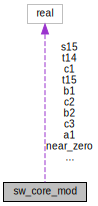
\includegraphics[width=134pt]{classsw__core__mod__coll__graph}
\end{center}
\end{figure}
\subsection*{Public Member Functions}
\begin{DoxyCompactItemize}
\item 
subroutine, public \hyperlink{classsw__core__mod_aea650426b10c000708a33a23a038c7f9}{c\-\_\-sw} (delpc, delp, ptc, pt, u, v, w, uc, vc, ua, va, wc, ut, vt, divg\-\_\-d, nord, dt2, hydrostatic, dord4, bd, gridstruct, flagstruct)
\begin{DoxyCompactList}\small\item\em The subroutine 'c\-\_\-sw' performs a half-\/timestep advance of the C-\/grid winds. \end{DoxyCompactList}\item 
subroutine, public \hyperlink{classsw__core__mod_a3d8c72e37bfa1cf6e6659319c1f8c0d0}{d\-\_\-sw} (delpc, delp, ptc, pt, u, v, w, uc, vc, ua, va, divg\-\_\-d, xflux, yflux, cx, cy, crx\-\_\-adv, cry\-\_\-adv, xfx\-\_\-adv, yfx\-\_\-adv, q\-\_\-con, z\-\_\-rat, kgb, heat\-\_\-source, diss\-\_\-est, zvir, sphum, nq, q, k, km, inline\-\_\-q, dt, hord\-\_\-tr, hord\-\_\-mt, hord\-\_\-vt, hord\-\_\-tm, hord\-\_\-dp, nord, nord\-\_\-v, nord\-\_\-w, nord\-\_\-t, dddmp, d2\-\_\-bg, d4\-\_\-bg, damp\-\_\-v, damp\-\_\-w, damp\-\_\-t, d\-\_\-con, hydrostatic, gridstruct, flagstruct, bd)
\begin{DoxyCompactList}\small\item\em The subroutine 'd\-\_\-sw' peforms a full-\/timestep advance of the D-\/grid winds and other prognostic varaiables. \end{DoxyCompactList}\item 
subroutine, public \hyperlink{classsw__core__mod_ae31bddf8149fa35a7614655b79e7e79a}{del6\-\_\-vt\-\_\-flux} (nord, npx, npy, damp, q, d2, fx2, fy2, gridstruct, bd)
\begin{DoxyCompactList}\small\item\em The subroutine 'del6\-\_\-vt\-\_\-flux' applies 2nd, 4th, or 6th-\/order damping to fluxes (\char`\"{}vorticity damping\char`\"{}) \end{DoxyCompactList}\item 
subroutine, public \hyperlink{classsw__core__mod_ad19f4ba4d0ac8b85bd43f7f8c4b42523}{divergence\-\_\-corner} (u, v, ua, va, divg\-\_\-d, gridstruct, flagstruct, bd)
\begin{DoxyCompactList}\small\item\em The subroutine 'divergence\-\_\-corner' computes the cell-\/mean divergence on the \char`\"{}dual grid\char`\"{}, the native-\/grid positioning of the divergence. \end{DoxyCompactList}\item 
subroutine, public \hyperlink{classsw__core__mod_a23884be4fc96b5faf577060479bf7056}{divergence\-\_\-corner\-\_\-nest} (u, v, ua, va, divg\-\_\-d, gridstruct, flagstruct, bd)
\item 
subroutine, public \hyperlink{classsw__core__mod_a393c161c0bd85b54a22341a984829030}{fill\-\_\-4corners} (q, dir, bd, npx, npy, sw\-\_\-corner, se\-\_\-corner, ne\-\_\-corner, nw\-\_\-corner)
\begin{DoxyCompactList}\small\item\em The subroutine 'fill\-\_\-4corners' fills the 4 corners of the scalar fields only as needed by c\-\_\-core. \end{DoxyCompactList}\end{DoxyCompactItemize}
\subsection*{Public Attributes}
\begin{DoxyCompactItemize}
\item 
real, parameter \hyperlink{classsw__core__mod_a2311c092079fcb5996c81f6a5bd4a19f}{r3} = 1./3.
\item 
real, parameter \hyperlink{classsw__core__mod_a7be5deda022e38acf1f9d7ec6bfd49e1}{t11} =27./28.
\item 
real, parameter \hyperlink{classsw__core__mod_aae2738361377149fdb4bc680ababd8c8}{t12} =-\/13./28.
\item 
real, parameter \hyperlink{classsw__core__mod_ae3b60da43af913086dbd123f1f66a649}{t13} =3./7.
\item 
real, parameter \hyperlink{classsw__core__mod_a26fc1c57b4befd2a298ccb59ecc89dec}{t14} =6./7.
\item 
real, parameter \hyperlink{classsw__core__mod_a70b3a9054c37076798e133275af2143d}{t15} =3./28.
\item 
real, parameter \hyperlink{classsw__core__mod_ab4edb6c8ca1754ab57e3b7c1dea01c40}{s11} =11./14.
\item 
real, parameter \hyperlink{classsw__core__mod_a2057f706d31454664b7e866bfb212b60}{s13} =-\/13./14.
\item 
real, parameter \hyperlink{classsw__core__mod_a4a938554f9d187f2d74de591f3f2f8e2}{s14} =4./7.
\item 
real, parameter \hyperlink{classsw__core__mod_a5dcd519b6b5b3c1cf2220a199b539a76}{s15} =3./14.
\item 
real, parameter \hyperlink{classsw__core__mod_a8bb76797403fecba5a8dc08930f838f0}{near\-\_\-zero} = 1.E-\/9
\begin{DoxyCompactList}\small\item\em for K\-E limiter \end{DoxyCompactList}\item 
real, parameter \hyperlink{classsw__core__mod_af5edb606364e91428ef3ef7ee98d9d5e}{big\-\_\-number} = 1.E30
\item 
real, parameter \hyperlink{classsw__core__mod_acd7311e0d77f5dd234d3456d70e0741e}{p1} = 7./12.
\begin{DoxyCompactList}\small\item\em 0.\-58333333 \end{DoxyCompactList}\item 
real, parameter \hyperlink{classsw__core__mod_a92790db4a243ddec101790808d27959c}{p2} = -\/1./12.
\item 
real, parameter \hyperlink{classsw__core__mod_aa12b598cb86848b3e2adb065b564997e}{a1} = 0.\-5625
\item 
real, parameter \hyperlink{classsw__core__mod_a29d1577650c0131c79a4d8f34d317b87}{a2} = -\/0.\-0625
\item 
real, parameter \hyperlink{classsw__core__mod_aa07fe9004d87c794dfe3f7593c96275f}{c1} = -\/2./14.
\item 
real, parameter \hyperlink{classsw__core__mod_a1be5c791573d2932b307ed6cdf52f2bc}{c2} = 11./14.
\item 
real, parameter \hyperlink{classsw__core__mod_ae6bff2a81849c99f2258c7e7cea943b0}{c3} = 5./14.
\item 
real, parameter \hyperlink{classsw__core__mod_a232f80cdeba816990b2606c04b5468a6}{b1} = 1./30.
\item 
real, parameter \hyperlink{classsw__core__mod_ae0c21e56d1941db4d7f16af5f24720c5}{b2} = -\/13./60.
\item 
real, parameter \hyperlink{classsw__core__mod_a53d9d5f60e77227069729364bf924ddb}{b3} = -\/13./60.
\item 
real, parameter \hyperlink{classsw__core__mod_a9f920cb428a38b9ad3294bb816b3b69a}{b4} = 0.\-45
\item 
real, parameter \hyperlink{classsw__core__mod_a8e47d06abc48dd557c6a46a38871e58a}{b5} = -\/0.\-05
\end{DoxyCompactItemize}
\subsection*{Private Member Functions}
\begin{DoxyCompactItemize}
\item 
subroutine \hyperlink{classsw__core__mod_a6e132ed43cea34af8a1a5388f953e94f}{smag\-\_\-corner} (dt, u, v, ua, va, smag\-\_\-c, bd, npx, npy, gridstruct, ng)
\begin{DoxyCompactList}\small\item\em The subroutine 'smag\-\_\-corner' computes Smagorinsky damping. \end{DoxyCompactList}\item 
subroutine \hyperlink{classsw__core__mod_a2b9d2b9cf39bd4642bddbb8af486c58e}{xtp\-\_\-u} (is, ie, js, je, isd, ied, jsd, jed, c, u, v, flux, iord, dx, rdx, npx, npy, grid\-\_\-type, nested, lim\-\_\-fac, regional)
\item 
subroutine \hyperlink{classsw__core__mod_af7c398917a27a6b38f09f5ef39c13cf7}{ytp\-\_\-v} (is, ie, js, je, isd, ied, jsd, jed, c, u, v, flux, jord, dy, rdy, npx, npy, grid\-\_\-type, nested, lim\-\_\-fac, regional)
\item 
subroutine \hyperlink{classsw__core__mod_a5dd013d734ca6e66eb060eb69ab52e66}{d2a2c\-\_\-vect} (u, v, ua, va, uc, vc, ut, vt, dord4, gridstruct, bd, npx, npy, nested, grid\-\_\-type, regional)
\item 
real function \hyperlink{classsw__core__mod_afc530a76cd1e1a41ef3a050038d8920d}{edge\-\_\-interpolate4} (ua, dxa)
\item 
subroutine \hyperlink{classsw__core__mod_a246243fbfb969bc99cc9656b5ef9d773}{fill3\-\_\-4corners} (q1, q2, q3, dir, bd, npx, npy, sw\-\_\-corner, se\-\_\-corner, ne\-\_\-corner, nw\-\_\-corner)
\begin{DoxyCompactList}\small\item\em The subroutine 'fill3\-\_\-4corners' fills the 4 corners of the scalar fileds only as needed by 'c\-\_\-core'. \end{DoxyCompactList}\item 
subroutine \hyperlink{classsw__core__mod_a5833b05bf829b877a0a42472cc037a44}{fill2\-\_\-4corners} (q1, q2, dir, bd, npx, npy, sw\-\_\-corner, se\-\_\-corner, ne\-\_\-corner, nw\-\_\-corner)
\begin{DoxyCompactList}\small\item\em The subroutine ' fill2\-\_\-4corners' fills the 4 corners of the scalar fileds only as needed by 'c\-\_\-core'. \end{DoxyCompactList}\end{DoxyCompactItemize}


\subsection{Detailed Description}
The module 'sw\-\_\-core' advances the forward step of the Lagrangian dynamics as described by \cite{lin1997explicit}, \cite{lin2004vertically}, and \cite{harris2013two}. 

The step is applied to the cubed sphere. 

Definition at line 26 of file sw\-\_\-core.\-F90.



\subsection{Member Function/\-Subroutine Documentation}
\index{sw\-\_\-core\-\_\-mod@{sw\-\_\-core\-\_\-mod}!c\-\_\-sw@{c\-\_\-sw}}
\index{c\-\_\-sw@{c\-\_\-sw}!sw_core_mod@{sw\-\_\-core\-\_\-mod}}
\subsubsection[{c\-\_\-sw}]{\setlength{\rightskip}{0pt plus 5cm}subroutine, public sw\-\_\-core\-\_\-mod\-::c\-\_\-sw (
\begin{DoxyParamCaption}
\item[{real, dimension(bd\%isd\-:bd\%ied,  bd\%jsd\-:bd\%jed  ), intent(out)}]{delpc, }
\item[{real, dimension(bd\%isd\-:bd\%ied,  bd\%jsd\-:bd\%jed  ), intent(inout)}]{delp, }
\item[{real, dimension(bd\%isd\-:bd\%ied,  bd\%jsd\-:bd\%jed  ), intent(out)}]{ptc, }
\item[{real, dimension(bd\%isd\-:bd\%ied,  bd\%jsd\-:bd\%jed  ), intent(inout)}]{pt, }
\item[{real, dimension(bd\%isd\-:bd\%ied,  bd\%jsd\-:bd\%jed+1), intent(inout)}]{u, }
\item[{real, dimension(bd\%isd\-:bd\%ied+1,bd\%jsd\-:bd\%jed  ), intent(inout)}]{v, }
\item[{real, dimension(bd\%isd\-:      ,  bd\%jsd\-:        ), intent(inout)}]{w, }
\item[{real, dimension(bd\%isd\-:bd\%ied+1,bd\%jsd\-:bd\%jed  ), intent(inout)}]{uc, }
\item[{real, dimension(bd\%isd\-:bd\%ied,  bd\%jsd\-:bd\%jed+1), intent(inout)}]{vc, }
\item[{real, dimension(bd\%isd\-:bd\%ied,  bd\%jsd\-:bd\%jed  ), intent(inout)}]{ua, }
\item[{real, dimension(bd\%isd\-:bd\%ied,  bd\%jsd\-:bd\%jed  ), intent(inout)}]{va, }
\item[{real, dimension(bd\%isd\-:bd\%ied,  bd\%jsd\-:bd\%jed  ), intent(out)}]{wc, }
\item[{real, dimension(bd\%isd\-:bd\%ied,  bd\%jsd\-:bd\%jed  ), intent(inout)}]{ut, }
\item[{real, dimension(bd\%isd\-:bd\%ied,  bd\%jsd\-:bd\%jed  ), intent(inout)}]{vt, }
\item[{real, dimension(bd\%isd\-:bd\%ied+1,bd\%jsd\-:bd\%jed+1), intent(out)}]{divg\-\_\-d, }
\item[{integer, intent(in)}]{nord, }
\item[{real, intent(in)}]{dt2, }
\item[{logical, intent(in)}]{hydrostatic, }
\item[{logical, intent(in)}]{dord4, }
\item[{type(fv\-\_\-grid\-\_\-bounds\-\_\-type), intent(in)}]{bd, }
\item[{type(fv\-\_\-grid\-\_\-type), intent(in), target}]{gridstruct, }
\item[{type(fv\-\_\-flags\-\_\-type), intent(in), target}]{flagstruct}
\end{DoxyParamCaption}
)}\label{classsw__core__mod_aea650426b10c000708a33a23a038c7f9}


The subroutine 'c\-\_\-sw' performs a half-\/timestep advance of the C-\/grid winds. 



Definition at line 102 of file sw\-\_\-core.\-F90.



References d2a2c\-\_\-vect(), divergence\-\_\-corner(), divergence\-\_\-corner\-\_\-nest(), fill2\-\_\-4corners(), and fill\-\_\-4corners().



Referenced by dyn\-\_\-core\-\_\-mod\-::dyn\-\_\-core().

\index{sw\-\_\-core\-\_\-mod@{sw\-\_\-core\-\_\-mod}!d2a2c\-\_\-vect@{d2a2c\-\_\-vect}}
\index{d2a2c\-\_\-vect@{d2a2c\-\_\-vect}!sw_core_mod@{sw\-\_\-core\-\_\-mod}}
\subsubsection[{d2a2c\-\_\-vect}]{\setlength{\rightskip}{0pt plus 5cm}subroutine sw\-\_\-core\-\_\-mod\-::d2a2c\-\_\-vect (
\begin{DoxyParamCaption}
\item[{real, dimension(bd\%isd\-:bd\%ied,bd\%jsd\-:bd\%jed+1), intent(in)}]{u, }
\item[{real, dimension(bd\%isd\-:bd\%ied+1,bd\%jsd\-:bd\%jed), intent(in)}]{v, }
\item[{real, dimension(bd\%isd\-:bd\%ied  ,bd\%jsd\-:bd\%jed  ), intent(out)}]{ua, }
\item[{real, dimension(bd\%isd\-:bd\%ied  ,bd\%jsd\-:bd\%jed  ), intent(out)}]{va, }
\item[{real, dimension(bd\%isd\-:bd\%ied+1,bd\%jsd\-:bd\%jed  ), intent(out)}]{uc, }
\item[{real, dimension(bd\%isd\-:bd\%ied  ,bd\%jsd\-:bd\%jed+1), intent(out)}]{vc, }
\item[{real, dimension(bd\%isd\-:bd\%ied  ,bd\%jsd\-:bd\%jed  ), intent(out)}]{ut, }
\item[{real, dimension(bd\%isd\-:bd\%ied  ,bd\%jsd\-:bd\%jed  ), intent(out)}]{vt, }
\item[{logical, intent(in)}]{dord4, }
\item[{type(fv\-\_\-grid\-\_\-type), intent(in), target}]{gridstruct, }
\item[{type(fv\-\_\-grid\-\_\-bounds\-\_\-type), intent(in)}]{bd, }
\item[{integer, intent(in)}]{npx, }
\item[{integer, intent(in)}]{npy, }
\item[{logical, intent(in)}]{nested, }
\item[{integer, intent(in)}]{grid\-\_\-type, }
\item[{logical, intent(in)}]{regional}
\end{DoxyParamCaption}
)\hspace{0.3cm}{\ttfamily [private]}}\label{classsw__core__mod_a5dd013d734ca6e66eb060eb69ab52e66}


Definition at line 2830 of file sw\-\_\-core.\-F90.



References edge\-\_\-interpolate4().



Referenced by c\-\_\-sw().

\index{sw\-\_\-core\-\_\-mod@{sw\-\_\-core\-\_\-mod}!d\-\_\-sw@{d\-\_\-sw}}
\index{d\-\_\-sw@{d\-\_\-sw}!sw_core_mod@{sw\-\_\-core\-\_\-mod}}
\subsubsection[{d\-\_\-sw}]{\setlength{\rightskip}{0pt plus 5cm}subroutine, public sw\-\_\-core\-\_\-mod\-::d\-\_\-sw (
\begin{DoxyParamCaption}
\item[{real, dimension(bd\%isd\-:bd\%ied,  bd\%jsd\-:bd\%jed), intent(out)}]{delpc, }
\item[{real, dimension(bd\%isd\-:bd\%ied,  bd\%jsd\-:bd\%jed), intent(inout)}]{delp, }
\item[{real, dimension(bd\%isd\-:bd\%ied,  bd\%jsd\-:bd\%jed), intent(out)}]{ptc, }
\item[{real, dimension(bd\%isd\-:bd\%ied,  bd\%jsd\-:bd\%jed), intent(inout)}]{pt, }
\item[{real, dimension(bd\%isd\-:bd\%ied  ,bd\%jsd\-:bd\%jed+1), intent(inout)}]{u, }
\item[{real, dimension(bd\%isd\-:bd\%ied+1,bd\%jsd\-:bd\%jed  ), intent(inout)}]{v, }
\item[{real, dimension(bd\%isd\-:      ,  bd\%jsd\-:      ), intent(inout)}]{w, }
\item[{real, dimension(bd\%isd\-:bd\%ied+1,bd\%jsd\-:bd\%jed  ), intent(inout)}]{uc, }
\item[{real, dimension(bd\%isd\-:bd\%ied  ,bd\%jsd\-:bd\%jed+1), intent(inout)}]{vc, }
\item[{real, dimension(bd\%isd\-:bd\%ied,  bd\%jsd\-:bd\%jed), intent(inout)}]{ua, }
\item[{real, dimension(bd\%isd\-:bd\%ied,  bd\%jsd\-:bd\%jed), intent(inout)}]{va, }
\item[{real, dimension(bd\%isd\-:bd\%ied+1,bd\%jsd\-:bd\%jed+1), intent(inout)}]{divg\-\_\-d, }
\item[{real, dimension(bd\%is\-:bd\%ie+1,bd\%js\-:bd\%je  ), intent(inout)}]{xflux, }
\item[{real, dimension(bd\%is\-:bd\%ie  ,bd\%js\-:bd\%je+1), intent(inout)}]{yflux, }
\item[{real, dimension(bd\%is\-:bd\%ie+1,bd\%jsd\-:bd\%jed  ), intent(inout)}]{cx, }
\item[{real, dimension(bd\%isd\-:bd\%ied,bd\%js\-:bd\%je+1), intent(inout)}]{cy, }
\item[{real, dimension(bd\%is\-:bd\%ie+1,bd\%jsd\-:bd\%jed), intent(out)}]{crx\-\_\-adv, }
\item[{real, dimension(bd\%isd\-:bd\%ied,bd\%js\-:bd\%je+1), intent(out)}]{cry\-\_\-adv, }
\item[{real, dimension(bd\%is\-:bd\%ie+1,bd\%jsd\-:bd\%jed), intent(out)}]{xfx\-\_\-adv, }
\item[{real, dimension(bd\%isd\-:bd\%ied,bd\%js\-:bd\%je+1), intent(out)}]{yfx\-\_\-adv, }
\item[{real, dimension(bd\%isd\-:      ,  bd\%jsd\-:      ), intent(inout)}]{q\-\_\-con, }
\item[{real, dimension(bd\%isd\-:bd\%ied,  bd\%jsd\-:bd\%jed), intent(in)}]{z\-\_\-rat, }
\item[{real, intent(in)}]{kgb, }
\item[{real, dimension(bd\%is\-:bd\%ie,bd\%js\-:bd\%je), intent(out)}]{heat\-\_\-source, }
\item[{real, dimension(bd\%is\-:bd\%ie,bd\%js\-:bd\%je), intent(out)}]{diss\-\_\-est, }
\item[{real, intent(in)}]{zvir, }
\item[{integer, intent(in)}]{sphum, }
\item[{integer, intent(in)}]{nq, }
\item[{real, dimension(bd\%isd\-:bd\%ied,bd\%jsd\-:bd\%jed,km,nq), intent(inout)}]{q, }
\item[{integer, intent(in)}]{k, }
\item[{integer, intent(in)}]{km, }
\item[{logical, intent(in)}]{inline\-\_\-q, }
\item[{real, intent(in)}]{dt, }
\item[{integer, intent(in)}]{hord\-\_\-tr, }
\item[{integer, intent(in)}]{hord\-\_\-mt, }
\item[{integer, intent(in)}]{hord\-\_\-vt, }
\item[{integer, intent(in)}]{hord\-\_\-tm, }
\item[{integer, intent(in)}]{hord\-\_\-dp, }
\item[{integer, intent(in)}]{nord, }
\item[{integer, intent(in)}]{nord\-\_\-v, }
\item[{integer, intent(in)}]{nord\-\_\-w, }
\item[{integer, intent(in)}]{nord\-\_\-t, }
\item[{real, intent(in)}]{dddmp, }
\item[{real, intent(in)}]{d2\-\_\-bg, }
\item[{real, intent(in)}]{d4\-\_\-bg, }
\item[{real, intent(in)}]{damp\-\_\-v, }
\item[{real, intent(in)}]{damp\-\_\-w, }
\item[{real, intent(in)}]{damp\-\_\-t, }
\item[{real, intent(in)}]{d\-\_\-con, }
\item[{logical, intent(in)}]{hydrostatic, }
\item[{type(fv\-\_\-grid\-\_\-type), intent(in), target}]{gridstruct, }
\item[{type(fv\-\_\-flags\-\_\-type), intent(in), target}]{flagstruct, }
\item[{type(fv\-\_\-grid\-\_\-bounds\-\_\-type), intent(in)}]{bd}
\end{DoxyParamCaption}
)}\label{classsw__core__mod_a3d8c72e37bfa1cf6e6659319c1f8c0d0}


The subroutine 'd\-\_\-sw' peforms a full-\/timestep advance of the D-\/grid winds and other prognostic varaiables. 


\begin{DoxyParams}[1]{Parameters}
\mbox{\tt in}  & {\em nord} & nord=1 divergence damping; (del-\/4) or 3 (del-\/8)\\
\hline
\mbox{\tt in}  & {\em nord\-\_\-v} & vorticity damping\\
\hline
\mbox{\tt in}  & {\em nord\-\_\-w} & vertical velocity\\
\hline
\mbox{\tt in}  & {\em nord\-\_\-t} & pt\\
\hline
\mbox{\tt in,out}  & {\em divg\-\_\-d} & divergence \\
\hline
\end{DoxyParams}


Definition at line 523 of file sw\-\_\-core.\-F90.



References a2b\-\_\-edge\-\_\-mod\-::a2b\-\_\-ord4(), del6\-\_\-vt\-\_\-flux(), tp\-\_\-core\-\_\-mod\-::fv\-\_\-tp\-\_\-2d(), smag\-\_\-corner(), xtp\-\_\-u(), and ytp\-\_\-v().



Referenced by dyn\-\_\-core\-\_\-mod\-::dyn\-\_\-core().

\index{sw\-\_\-core\-\_\-mod@{sw\-\_\-core\-\_\-mod}!del6\-\_\-vt\-\_\-flux@{del6\-\_\-vt\-\_\-flux}}
\index{del6\-\_\-vt\-\_\-flux@{del6\-\_\-vt\-\_\-flux}!sw_core_mod@{sw\-\_\-core\-\_\-mod}}
\subsubsection[{del6\-\_\-vt\-\_\-flux}]{\setlength{\rightskip}{0pt plus 5cm}subroutine, public sw\-\_\-core\-\_\-mod\-::del6\-\_\-vt\-\_\-flux (
\begin{DoxyParamCaption}
\item[{integer, intent(in)}]{nord, }
\item[{integer, intent(in)}]{npx, }
\item[{integer, intent(in)}]{npy, }
\item[{real, intent(in)}]{damp, }
\item[{real, dimension(bd\%isd\-:bd\%ied, bd\%jsd\-:bd\%jed), intent(inout)}]{q, }
\item[{real, dimension(bd\%isd\-:bd\%ied, bd\%jsd\-:bd\%jed), intent(out)}]{d2, }
\item[{real, dimension(bd\%isd\-:bd\%ied+1,bd\%jsd\-:bd\%jed), intent(out)}]{fx2, }
\item[{real, dimension(bd\%isd\-:bd\%ied,bd\%jsd\-:bd\%jed+1), intent(out)}]{fy2, }
\item[{type(fv\-\_\-grid\-\_\-type), intent(in), target}]{gridstruct, }
\item[{type(fv\-\_\-grid\-\_\-bounds\-\_\-type), intent(in)}]{bd}
\end{DoxyParamCaption}
)}\label{classsw__core__mod_ae31bddf8149fa35a7614655b79e7e79a}


The subroutine 'del6\-\_\-vt\-\_\-flux' applies 2nd, 4th, or 6th-\/order damping to fluxes (\char`\"{}vorticity damping\char`\"{}) 



Definition at line 1585 of file sw\-\_\-core.\-F90.



References tp\-\_\-core\-\_\-mod\-::copy\-\_\-corners().



Referenced by d\-\_\-sw(), and nh\-\_\-utils\-\_\-mod\-::update\-\_\-dz\-\_\-d().

\index{sw\-\_\-core\-\_\-mod@{sw\-\_\-core\-\_\-mod}!divergence\-\_\-corner@{divergence\-\_\-corner}}
\index{divergence\-\_\-corner@{divergence\-\_\-corner}!sw_core_mod@{sw\-\_\-core\-\_\-mod}}
\subsubsection[{divergence\-\_\-corner}]{\setlength{\rightskip}{0pt plus 5cm}subroutine, public sw\-\_\-core\-\_\-mod\-::divergence\-\_\-corner (
\begin{DoxyParamCaption}
\item[{real, dimension(bd\%isd\-:bd\%ied,  bd\%jsd\-:bd\%jed+1), intent(in)}]{u, }
\item[{real, dimension(bd\%isd\-:bd\%ied+1,bd\%jsd\-:bd\%jed  ), intent(in)}]{v, }
\item[{real, dimension(bd\%isd\-:bd\%ied,bd\%jsd\-:bd\%jed), intent(in)}]{ua, }
\item[{real, dimension(bd\%isd\-:bd\%ied,bd\%jsd\-:bd\%jed), intent(in)}]{va, }
\item[{real, dimension(bd\%isd\-:bd\%ied+1,bd\%jsd\-:bd\%jed+1), intent(out)}]{divg\-\_\-d, }
\item[{type(fv\-\_\-grid\-\_\-type), intent(in), target}]{gridstruct, }
\item[{type(fv\-\_\-flags\-\_\-type), intent(in), target}]{flagstruct, }
\item[{type(fv\-\_\-grid\-\_\-bounds\-\_\-type), intent(in)}]{bd}
\end{DoxyParamCaption}
)}\label{classsw__core__mod_ad19f4ba4d0ac8b85bd43f7f8c4b42523}


The subroutine 'divergence\-\_\-corner' computes the cell-\/mean divergence on the \char`\"{}dual grid\char`\"{}, the native-\/grid positioning of the divergence. 



Definition at line 1700 of file sw\-\_\-core.\-F90.



Referenced by c\-\_\-sw(), and fv\-\_\-nesting\-\_\-mod\-::setup\-\_\-nested\-\_\-grid\-\_\-bcs().

\index{sw\-\_\-core\-\_\-mod@{sw\-\_\-core\-\_\-mod}!divergence\-\_\-corner\-\_\-nest@{divergence\-\_\-corner\-\_\-nest}}
\index{divergence\-\_\-corner\-\_\-nest@{divergence\-\_\-corner\-\_\-nest}!sw_core_mod@{sw\-\_\-core\-\_\-mod}}
\subsubsection[{divergence\-\_\-corner\-\_\-nest}]{\setlength{\rightskip}{0pt plus 5cm}subroutine, public sw\-\_\-core\-\_\-mod\-::divergence\-\_\-corner\-\_\-nest (
\begin{DoxyParamCaption}
\item[{real, dimension(bd\%isd\-:bd\%ied,  bd\%jsd\-:bd\%jed+1), intent(in)}]{u, }
\item[{real, dimension(bd\%isd\-:bd\%ied+1,bd\%jsd\-:bd\%jed), intent(in)}]{v, }
\item[{real, dimension(bd\%isd\-:bd\%ied,bd\%jsd\-:bd\%jed), intent(in)}]{ua, }
\item[{real, dimension(bd\%isd\-:bd\%ied,bd\%jsd\-:bd\%jed), intent(in)}]{va, }
\item[{real, dimension(bd\%isd\-:bd\%ied+1,bd\%jsd\-:bd\%jed+1), intent(out)}]{divg\-\_\-d, }
\item[{type(fv\-\_\-grid\-\_\-type), intent(in), target}]{gridstruct, }
\item[{type(fv\-\_\-flags\-\_\-type), intent(in), target}]{flagstruct, }
\item[{type(fv\-\_\-grid\-\_\-bounds\-\_\-type), intent(in)}]{bd}
\end{DoxyParamCaption}
)}\label{classsw__core__mod_a23884be4fc96b5faf577060479bf7056}


Definition at line 1808 of file sw\-\_\-core.\-F90.



Referenced by c\-\_\-sw(), and fv\-\_\-nesting\-\_\-mod\-::setup\-\_\-nested\-\_\-grid\-\_\-bcs().

\index{sw\-\_\-core\-\_\-mod@{sw\-\_\-core\-\_\-mod}!edge\-\_\-interpolate4@{edge\-\_\-interpolate4}}
\index{edge\-\_\-interpolate4@{edge\-\_\-interpolate4}!sw_core_mod@{sw\-\_\-core\-\_\-mod}}
\subsubsection[{edge\-\_\-interpolate4}]{\setlength{\rightskip}{0pt plus 5cm}real function sw\-\_\-core\-\_\-mod\-::edge\-\_\-interpolate4 (
\begin{DoxyParamCaption}
\item[{real, dimension(4), intent(in)}]{ua, }
\item[{real, dimension(4), intent(in)}]{dxa}
\end{DoxyParamCaption}
)\hspace{0.3cm}{\ttfamily [private]}}\label{classsw__core__mod_afc530a76cd1e1a41ef3a050038d8920d}


Definition at line 3172 of file sw\-\_\-core.\-F90.



Referenced by d2a2c\-\_\-vect().

\index{sw\-\_\-core\-\_\-mod@{sw\-\_\-core\-\_\-mod}!fill2\-\_\-4corners@{fill2\-\_\-4corners}}
\index{fill2\-\_\-4corners@{fill2\-\_\-4corners}!sw_core_mod@{sw\-\_\-core\-\_\-mod}}
\subsubsection[{fill2\-\_\-4corners}]{\setlength{\rightskip}{0pt plus 5cm}subroutine sw\-\_\-core\-\_\-mod\-::fill2\-\_\-4corners (
\begin{DoxyParamCaption}
\item[{real, dimension(bd\%isd\-:bd\%ied,bd\%jsd\-:bd\%jed), intent(inout)}]{q1, }
\item[{real, dimension(bd\%isd\-:bd\%ied,bd\%jsd\-:bd\%jed), intent(inout)}]{q2, }
\item[{integer, intent(in)}]{dir, }
\item[{type(fv\-\_\-grid\-\_\-bounds\-\_\-type), intent(in)}]{bd, }
\item[{integer, intent(in)}]{npx, }
\item[{integer, intent(in)}]{npy, }
\item[{logical, intent(in)}]{sw\-\_\-corner, }
\item[{logical, intent(in)}]{se\-\_\-corner, }
\item[{logical, intent(in)}]{ne\-\_\-corner, }
\item[{logical, intent(in)}]{nw\-\_\-corner}
\end{DoxyParamCaption}
)\hspace{0.3cm}{\ttfamily [private]}}\label{classsw__core__mod_a5833b05bf829b877a0a42472cc037a44}


The subroutine ' fill2\-\_\-4corners' fills the 4 corners of the scalar fileds only as needed by 'c\-\_\-core'. 


\begin{DoxyParams}[1]{Parameters}
\mbox{\tt in}  & {\em dir} & 1\-: x-\/dir; 2\-: y-\/dir \\
\hline
\end{DoxyParams}


Definition at line 3257 of file sw\-\_\-core.\-F90.



Referenced by c\-\_\-sw().

\index{sw\-\_\-core\-\_\-mod@{sw\-\_\-core\-\_\-mod}!fill3\-\_\-4corners@{fill3\-\_\-4corners}}
\index{fill3\-\_\-4corners@{fill3\-\_\-4corners}!sw_core_mod@{sw\-\_\-core\-\_\-mod}}
\subsubsection[{fill3\-\_\-4corners}]{\setlength{\rightskip}{0pt plus 5cm}subroutine sw\-\_\-core\-\_\-mod\-::fill3\-\_\-4corners (
\begin{DoxyParamCaption}
\item[{real, dimension(bd\%isd\-:bd\%ied,bd\%jsd\-:bd\%jed), intent(inout)}]{q1, }
\item[{real, dimension(bd\%isd\-:bd\%ied,bd\%jsd\-:bd\%jed), intent(inout)}]{q2, }
\item[{real, dimension(bd\%isd\-:bd\%ied,bd\%jsd\-:bd\%jed), intent(inout)}]{q3, }
\item[{integer, intent(in)}]{dir, }
\item[{type(fv\-\_\-grid\-\_\-bounds\-\_\-type), intent(in)}]{bd, }
\item[{integer, intent(in)}]{npx, }
\item[{integer, intent(in)}]{npy, }
\item[{logical, intent(in)}]{sw\-\_\-corner, }
\item[{logical, intent(in)}]{se\-\_\-corner, }
\item[{logical, intent(in)}]{ne\-\_\-corner, }
\item[{logical, intent(in)}]{nw\-\_\-corner}
\end{DoxyParamCaption}
)\hspace{0.3cm}{\ttfamily [private]}}\label{classsw__core__mod_a246243fbfb969bc99cc9656b5ef9d773}


The subroutine 'fill3\-\_\-4corners' fills the 4 corners of the scalar fileds only as needed by 'c\-\_\-core'. 


\begin{DoxyParams}[1]{Parameters}
\mbox{\tt in}  & {\em dir} & 1\-: x-\/dir; 2\-: y-\/dir \\
\hline
\end{DoxyParams}


Definition at line 3186 of file sw\-\_\-core.\-F90.

\index{sw\-\_\-core\-\_\-mod@{sw\-\_\-core\-\_\-mod}!fill\-\_\-4corners@{fill\-\_\-4corners}}
\index{fill\-\_\-4corners@{fill\-\_\-4corners}!sw_core_mod@{sw\-\_\-core\-\_\-mod}}
\subsubsection[{fill\-\_\-4corners}]{\setlength{\rightskip}{0pt plus 5cm}subroutine, public sw\-\_\-core\-\_\-mod\-::fill\-\_\-4corners (
\begin{DoxyParamCaption}
\item[{real, dimension(bd\%isd\-:bd\%ied,bd\%jsd\-:bd\%jed), intent(inout)}]{q, }
\item[{integer, intent(in)}]{dir, }
\item[{type(fv\-\_\-grid\-\_\-bounds\-\_\-type), intent(in)}]{bd, }
\item[{integer, intent(in)}]{npx, }
\item[{integer, intent(in)}]{npy, }
\item[{logical, intent(in)}]{sw\-\_\-corner, }
\item[{logical, intent(in)}]{se\-\_\-corner, }
\item[{logical, intent(in)}]{ne\-\_\-corner, }
\item[{logical, intent(in)}]{nw\-\_\-corner}
\end{DoxyParamCaption}
)}\label{classsw__core__mod_a393c161c0bd85b54a22341a984829030}


The subroutine 'fill\-\_\-4corners' fills the 4 corners of the scalar fields only as needed by c\-\_\-core. 



Definition at line 3319 of file sw\-\_\-core.\-F90.



Referenced by c\-\_\-sw(), and nh\-\_\-utils\-\_\-mod\-::update\-\_\-dz\-\_\-c().

\index{sw\-\_\-core\-\_\-mod@{sw\-\_\-core\-\_\-mod}!smag\-\_\-corner@{smag\-\_\-corner}}
\index{smag\-\_\-corner@{smag\-\_\-corner}!sw_core_mod@{sw\-\_\-core\-\_\-mod}}
\subsubsection[{smag\-\_\-corner}]{\setlength{\rightskip}{0pt plus 5cm}subroutine sw\-\_\-core\-\_\-mod\-::smag\-\_\-corner (
\begin{DoxyParamCaption}
\item[{real, intent(in)}]{dt, }
\item[{real, dimension(bd\%isd\-:bd\%ied,  bd\%jsd\-:bd\%jed+1), intent(in)}]{u, }
\item[{real, dimension(bd\%isd\-:bd\%ied+1,bd\%jsd\-:bd\%jed  ), intent(in)}]{v, }
\item[{real, dimension(bd\%isd\-:bd\%ied,bd\%jsd\-:bd\%jed), intent(in)}]{ua, }
\item[{real, dimension(bd\%isd\-:bd\%ied,bd\%jsd\-:bd\%jed), intent(in)}]{va, }
\item[{real, dimension(bd\%isd\-:bd\%ied,bd\%jsd\-:bd\%jed), intent(out)}]{smag\-\_\-c, }
\item[{type(fv\-\_\-grid\-\_\-bounds\-\_\-type), intent(in)}]{bd, }
\item[{integer, intent(in)}]{npx, }
\item[{integer, intent(in)}]{npy, }
\item[{type(fv\-\_\-grid\-\_\-type), intent(in), target}]{gridstruct, }
\item[{integer, intent(in)}]{ng}
\end{DoxyParamCaption}
)\hspace{0.3cm}{\ttfamily [private]}}\label{classsw__core__mod_a6e132ed43cea34af8a1a5388f953e94f}


The subroutine 'smag\-\_\-corner' computes Smagorinsky damping. 


\begin{DoxyParams}[1]{Parameters}
\mbox{\tt in}  & {\em bd} & Compute the Tension\-\_\-\-Shear strain at cell corners for Smagorinsky diffusion work only if (grid\-\_\-type==4) \\
\hline
\end{DoxyParams}


Definition at line 1920 of file sw\-\_\-core.\-F90.



References a2b\-\_\-edge\-\_\-mod\-::a2b\-\_\-ord4().



Referenced by d\-\_\-sw().

\index{sw\-\_\-core\-\_\-mod@{sw\-\_\-core\-\_\-mod}!xtp\-\_\-u@{xtp\-\_\-u}}
\index{xtp\-\_\-u@{xtp\-\_\-u}!sw_core_mod@{sw\-\_\-core\-\_\-mod}}
\subsubsection[{xtp\-\_\-u}]{\setlength{\rightskip}{0pt plus 5cm}subroutine sw\-\_\-core\-\_\-mod\-::xtp\-\_\-u (
\begin{DoxyParamCaption}
\item[{integer, intent(in)}]{is, }
\item[{integer, intent(in)}]{ie, }
\item[{integer, intent(in)}]{js, }
\item[{integer, intent(in)}]{je, }
\item[{integer, intent(in)}]{isd, }
\item[{integer, intent(in)}]{ied, }
\item[{integer, intent(in)}]{jsd, }
\item[{integer, intent(in)}]{jed, }
\item[{real, dimension(is\-:ie+1,js\-:je+1), intent(in)}]{c, }
\item[{real, dimension(isd\-:ied,jsd\-:jed+1), intent(in)}]{u, }
\item[{real, dimension(isd\-:ied+1,jsd\-:jed), intent(in)}]{v, }
\item[{real, dimension(is\-:ie+1,js\-:je+1), intent(out)}]{flux, }
\item[{integer, intent(in)}]{iord, }
\item[{real, dimension(isd\-:ied,  jsd\-:jed+1), intent(in)}]{dx, }
\item[{real, dimension(isd\-:ied,  jsd\-:jed+1), intent(in)}]{rdx, }
\item[{integer, intent(in)}]{npx, }
\item[{integer, intent(in)}]{npy, }
\item[{integer, intent(in)}]{grid\-\_\-type, }
\item[{logical, intent(in)}]{nested, }
\item[{real, intent(in)}]{lim\-\_\-fac, }
\item[{logical, intent(in)}]{regional}
\end{DoxyParamCaption}
)\hspace{0.3cm}{\ttfamily [private]}}\label{classsw__core__mod_a2b9d2b9cf39bd4642bddbb8af486c58e}


Definition at line 2010 of file sw\-\_\-core.\-F90.



References tp\-\_\-core\-\_\-mod\-::pert\-\_\-ppm().



Referenced by d\-\_\-sw().

\index{sw\-\_\-core\-\_\-mod@{sw\-\_\-core\-\_\-mod}!ytp\-\_\-v@{ytp\-\_\-v}}
\index{ytp\-\_\-v@{ytp\-\_\-v}!sw_core_mod@{sw\-\_\-core\-\_\-mod}}
\subsubsection[{ytp\-\_\-v}]{\setlength{\rightskip}{0pt plus 5cm}subroutine sw\-\_\-core\-\_\-mod\-::ytp\-\_\-v (
\begin{DoxyParamCaption}
\item[{integer, intent(in)}]{is, }
\item[{integer, intent(in)}]{ie, }
\item[{integer, intent(in)}]{js, }
\item[{integer, intent(in)}]{je, }
\item[{integer, intent(in)}]{isd, }
\item[{integer, intent(in)}]{ied, }
\item[{integer, intent(in)}]{jsd, }
\item[{integer, intent(in)}]{jed, }
\item[{real, dimension(is\-:ie+1,js\-:je+1), intent(in)}]{c, }
\item[{real, dimension(isd\-:ied,jsd\-:jed+1), intent(in)}]{u, }
\item[{real, dimension(isd\-:ied+1,jsd\-:jed), intent(in)}]{v, }
\item[{real, dimension(is\-:ie+1,js\-:je+1), intent(out)}]{flux, }
\item[{integer, intent(in)}]{jord, }
\item[{real, dimension(isd\-:ied+1,jsd\-:jed), intent(in)}]{dy, }
\item[{real, dimension(isd\-:ied+1,jsd\-:jed), intent(in)}]{rdy, }
\item[{integer, intent(in)}]{npx, }
\item[{integer, intent(in)}]{npy, }
\item[{integer, intent(in)}]{grid\-\_\-type, }
\item[{logical, intent(in)}]{nested, }
\item[{real, intent(in)}]{lim\-\_\-fac, }
\item[{logical, intent(in)}]{regional}
\end{DoxyParamCaption}
)\hspace{0.3cm}{\ttfamily [private]}}\label{classsw__core__mod_af7c398917a27a6b38f09f5ef39c13cf7}

\begin{DoxyParams}[1]{Parameters}
\mbox{\tt in}  & {\em c} & Courant N (like F\-L\-U\-X) \\
\hline
\end{DoxyParams}


Definition at line 2367 of file sw\-\_\-core.\-F90.



References tp\-\_\-core\-\_\-mod\-::pert\-\_\-ppm().



Referenced by d\-\_\-sw().



\subsection{Member Data Documentation}
\index{sw\-\_\-core\-\_\-mod@{sw\-\_\-core\-\_\-mod}!a1@{a1}}
\index{a1@{a1}!sw_core_mod@{sw\-\_\-core\-\_\-mod}}
\subsubsection[{a1}]{\setlength{\rightskip}{0pt plus 5cm}real, parameter sw\-\_\-core\-\_\-mod\-::a1 = 0.\-5625}\label{classsw__core__mod_aa12b598cb86848b3e2adb065b564997e}


Definition at line 76 of file sw\-\_\-core.\-F90.

\index{sw\-\_\-core\-\_\-mod@{sw\-\_\-core\-\_\-mod}!a2@{a2}}
\index{a2@{a2}!sw_core_mod@{sw\-\_\-core\-\_\-mod}}
\subsubsection[{a2}]{\setlength{\rightskip}{0pt plus 5cm}real, parameter sw\-\_\-core\-\_\-mod\-::a2 = -\/0.\-0625}\label{classsw__core__mod_a29d1577650c0131c79a4d8f34d317b87}


Definition at line 77 of file sw\-\_\-core.\-F90.

\index{sw\-\_\-core\-\_\-mod@{sw\-\_\-core\-\_\-mod}!b1@{b1}}
\index{b1@{b1}!sw_core_mod@{sw\-\_\-core\-\_\-mod}}
\subsubsection[{b1}]{\setlength{\rightskip}{0pt plus 5cm}real, parameter sw\-\_\-core\-\_\-mod\-::b1 = 1./30.}\label{classsw__core__mod_a232f80cdeba816990b2606c04b5468a6}


Definition at line 89 of file sw\-\_\-core.\-F90.

\index{sw\-\_\-core\-\_\-mod@{sw\-\_\-core\-\_\-mod}!b2@{b2}}
\index{b2@{b2}!sw_core_mod@{sw\-\_\-core\-\_\-mod}}
\subsubsection[{b2}]{\setlength{\rightskip}{0pt plus 5cm}real, parameter sw\-\_\-core\-\_\-mod\-::b2 = -\/13./60.}\label{classsw__core__mod_ae0c21e56d1941db4d7f16af5f24720c5}


Definition at line 90 of file sw\-\_\-core.\-F90.

\index{sw\-\_\-core\-\_\-mod@{sw\-\_\-core\-\_\-mod}!b3@{b3}}
\index{b3@{b3}!sw_core_mod@{sw\-\_\-core\-\_\-mod}}
\subsubsection[{b3}]{\setlength{\rightskip}{0pt plus 5cm}real, parameter sw\-\_\-core\-\_\-mod\-::b3 = -\/13./60.}\label{classsw__core__mod_a53d9d5f60e77227069729364bf924ddb}


Definition at line 91 of file sw\-\_\-core.\-F90.

\index{sw\-\_\-core\-\_\-mod@{sw\-\_\-core\-\_\-mod}!b4@{b4}}
\index{b4@{b4}!sw_core_mod@{sw\-\_\-core\-\_\-mod}}
\subsubsection[{b4}]{\setlength{\rightskip}{0pt plus 5cm}real, parameter sw\-\_\-core\-\_\-mod\-::b4 = 0.\-45}\label{classsw__core__mod_a9f920cb428a38b9ad3294bb816b3b69a}


Definition at line 92 of file sw\-\_\-core.\-F90.

\index{sw\-\_\-core\-\_\-mod@{sw\-\_\-core\-\_\-mod}!b5@{b5}}
\index{b5@{b5}!sw_core_mod@{sw\-\_\-core\-\_\-mod}}
\subsubsection[{b5}]{\setlength{\rightskip}{0pt plus 5cm}real, parameter sw\-\_\-core\-\_\-mod\-::b5 = -\/0.\-05}\label{classsw__core__mod_a8e47d06abc48dd557c6a46a38871e58a}


Definition at line 93 of file sw\-\_\-core.\-F90.

\index{sw\-\_\-core\-\_\-mod@{sw\-\_\-core\-\_\-mod}!big\-\_\-number@{big\-\_\-number}}
\index{big\-\_\-number@{big\-\_\-number}!sw_core_mod@{sw\-\_\-core\-\_\-mod}}
\subsubsection[{big\-\_\-number}]{\setlength{\rightskip}{0pt plus 5cm}real, parameter sw\-\_\-core\-\_\-mod\-::big\-\_\-number = 1.E30}\label{classsw__core__mod_af5edb606364e91428ef3ef7ee98d9d5e}


Definition at line 66 of file sw\-\_\-core.\-F90.

\index{sw\-\_\-core\-\_\-mod@{sw\-\_\-core\-\_\-mod}!c1@{c1}}
\index{c1@{c1}!sw_core_mod@{sw\-\_\-core\-\_\-mod}}
\subsubsection[{c1}]{\setlength{\rightskip}{0pt plus 5cm}real, parameter sw\-\_\-core\-\_\-mod\-::c1 = -\/2./14.}\label{classsw__core__mod_aa07fe9004d87c794dfe3f7593c96275f}


Definition at line 80 of file sw\-\_\-core.\-F90.

\index{sw\-\_\-core\-\_\-mod@{sw\-\_\-core\-\_\-mod}!c2@{c2}}
\index{c2@{c2}!sw_core_mod@{sw\-\_\-core\-\_\-mod}}
\subsubsection[{c2}]{\setlength{\rightskip}{0pt plus 5cm}real, parameter sw\-\_\-core\-\_\-mod\-::c2 = 11./14.}\label{classsw__core__mod_a1be5c791573d2932b307ed6cdf52f2bc}


Definition at line 81 of file sw\-\_\-core.\-F90.

\index{sw\-\_\-core\-\_\-mod@{sw\-\_\-core\-\_\-mod}!c3@{c3}}
\index{c3@{c3}!sw_core_mod@{sw\-\_\-core\-\_\-mod}}
\subsubsection[{c3}]{\setlength{\rightskip}{0pt plus 5cm}real, parameter sw\-\_\-core\-\_\-mod\-::c3 = 5./14.}\label{classsw__core__mod_ae6bff2a81849c99f2258c7e7cea943b0}


Definition at line 82 of file sw\-\_\-core.\-F90.

\index{sw\-\_\-core\-\_\-mod@{sw\-\_\-core\-\_\-mod}!near\-\_\-zero@{near\-\_\-zero}}
\index{near\-\_\-zero@{near\-\_\-zero}!sw_core_mod@{sw\-\_\-core\-\_\-mod}}
\subsubsection[{near\-\_\-zero}]{\setlength{\rightskip}{0pt plus 5cm}real, parameter sw\-\_\-core\-\_\-mod\-::near\-\_\-zero = 1.E-\/9}\label{classsw__core__mod_a8bb76797403fecba5a8dc08930f838f0}


for K\-E limiter 



Definition at line 62 of file sw\-\_\-core.\-F90.

\index{sw\-\_\-core\-\_\-mod@{sw\-\_\-core\-\_\-mod}!p1@{p1}}
\index{p1@{p1}!sw_core_mod@{sw\-\_\-core\-\_\-mod}}
\subsubsection[{p1}]{\setlength{\rightskip}{0pt plus 5cm}real, parameter sw\-\_\-core\-\_\-mod\-::p1 = 7./12.}\label{classsw__core__mod_acd7311e0d77f5dd234d3456d70e0741e}


0.\-58333333 



Definition at line 71 of file sw\-\_\-core.\-F90.

\index{sw\-\_\-core\-\_\-mod@{sw\-\_\-core\-\_\-mod}!p2@{p2}}
\index{p2@{p2}!sw_core_mod@{sw\-\_\-core\-\_\-mod}}
\subsubsection[{p2}]{\setlength{\rightskip}{0pt plus 5cm}real, parameter sw\-\_\-core\-\_\-mod\-::p2 = -\/1./12.}\label{classsw__core__mod_a92790db4a243ddec101790808d27959c}


Definition at line 72 of file sw\-\_\-core.\-F90.

\index{sw\-\_\-core\-\_\-mod@{sw\-\_\-core\-\_\-mod}!r3@{r3}}
\index{r3@{r3}!sw_core_mod@{sw\-\_\-core\-\_\-mod}}
\subsubsection[{r3}]{\setlength{\rightskip}{0pt plus 5cm}real, parameter sw\-\_\-core\-\_\-mod\-::r3 = 1./3.}\label{classsw__core__mod_a2311c092079fcb5996c81f6a5bd4a19f}


Definition at line 59 of file sw\-\_\-core.\-F90.

\index{sw\-\_\-core\-\_\-mod@{sw\-\_\-core\-\_\-mod}!s11@{s11}}
\index{s11@{s11}!sw_core_mod@{sw\-\_\-core\-\_\-mod}}
\subsubsection[{s11}]{\setlength{\rightskip}{0pt plus 5cm}real, parameter sw\-\_\-core\-\_\-mod\-::s11 =11./14.}\label{classsw__core__mod_ab4edb6c8ca1754ab57e3b7c1dea01c40}


Definition at line 61 of file sw\-\_\-core.\-F90.

\index{sw\-\_\-core\-\_\-mod@{sw\-\_\-core\-\_\-mod}!s13@{s13}}
\index{s13@{s13}!sw_core_mod@{sw\-\_\-core\-\_\-mod}}
\subsubsection[{s13}]{\setlength{\rightskip}{0pt plus 5cm}real, parameter sw\-\_\-core\-\_\-mod\-::s13 =-\/13./14.}\label{classsw__core__mod_a2057f706d31454664b7e866bfb212b60}


Definition at line 61 of file sw\-\_\-core.\-F90.

\index{sw\-\_\-core\-\_\-mod@{sw\-\_\-core\-\_\-mod}!s14@{s14}}
\index{s14@{s14}!sw_core_mod@{sw\-\_\-core\-\_\-mod}}
\subsubsection[{s14}]{\setlength{\rightskip}{0pt plus 5cm}real, parameter sw\-\_\-core\-\_\-mod\-::s14 =4./7.}\label{classsw__core__mod_a4a938554f9d187f2d74de591f3f2f8e2}


Definition at line 61 of file sw\-\_\-core.\-F90.

\index{sw\-\_\-core\-\_\-mod@{sw\-\_\-core\-\_\-mod}!s15@{s15}}
\index{s15@{s15}!sw_core_mod@{sw\-\_\-core\-\_\-mod}}
\subsubsection[{s15}]{\setlength{\rightskip}{0pt plus 5cm}real, parameter sw\-\_\-core\-\_\-mod\-::s15 =3./14.}\label{classsw__core__mod_a5dcd519b6b5b3c1cf2220a199b539a76}


Definition at line 61 of file sw\-\_\-core.\-F90.

\index{sw\-\_\-core\-\_\-mod@{sw\-\_\-core\-\_\-mod}!t11@{t11}}
\index{t11@{t11}!sw_core_mod@{sw\-\_\-core\-\_\-mod}}
\subsubsection[{t11}]{\setlength{\rightskip}{0pt plus 5cm}real, parameter sw\-\_\-core\-\_\-mod\-::t11 =27./28.}\label{classsw__core__mod_a7be5deda022e38acf1f9d7ec6bfd49e1}


Definition at line 60 of file sw\-\_\-core.\-F90.

\index{sw\-\_\-core\-\_\-mod@{sw\-\_\-core\-\_\-mod}!t12@{t12}}
\index{t12@{t12}!sw_core_mod@{sw\-\_\-core\-\_\-mod}}
\subsubsection[{t12}]{\setlength{\rightskip}{0pt plus 5cm}real, parameter sw\-\_\-core\-\_\-mod\-::t12 =-\/13./28.}\label{classsw__core__mod_aae2738361377149fdb4bc680ababd8c8}


Definition at line 60 of file sw\-\_\-core.\-F90.

\index{sw\-\_\-core\-\_\-mod@{sw\-\_\-core\-\_\-mod}!t13@{t13}}
\index{t13@{t13}!sw_core_mod@{sw\-\_\-core\-\_\-mod}}
\subsubsection[{t13}]{\setlength{\rightskip}{0pt plus 5cm}real, parameter sw\-\_\-core\-\_\-mod\-::t13 =3./7.}\label{classsw__core__mod_ae3b60da43af913086dbd123f1f66a649}


Definition at line 60 of file sw\-\_\-core.\-F90.

\index{sw\-\_\-core\-\_\-mod@{sw\-\_\-core\-\_\-mod}!t14@{t14}}
\index{t14@{t14}!sw_core_mod@{sw\-\_\-core\-\_\-mod}}
\subsubsection[{t14}]{\setlength{\rightskip}{0pt plus 5cm}real, parameter sw\-\_\-core\-\_\-mod\-::t14 =6./7.}\label{classsw__core__mod_a26fc1c57b4befd2a298ccb59ecc89dec}


Definition at line 60 of file sw\-\_\-core.\-F90.

\index{sw\-\_\-core\-\_\-mod@{sw\-\_\-core\-\_\-mod}!t15@{t15}}
\index{t15@{t15}!sw_core_mod@{sw\-\_\-core\-\_\-mod}}
\subsubsection[{t15}]{\setlength{\rightskip}{0pt plus 5cm}real, parameter sw\-\_\-core\-\_\-mod\-::t15 =3./28.}\label{classsw__core__mod_a70b3a9054c37076798e133275af2143d}


Definition at line 60 of file sw\-\_\-core.\-F90.



The documentation for this module was generated from the following file\-:\begin{DoxyCompactItemize}
\item 
/scratch2/\-N\-A\-G\-A\-P\-E/aoml-\/hafs1/\-Kyle.\-Ahern/acs\-\_\-master\-\_\-readonly/model/\hyperlink{sw__core_8F90}{sw\-\_\-core.\-F90}\end{DoxyCompactItemize}

\section{test\-\_\-cases\-\_\-mod Module Reference}
\label{classtest__cases__mod}\index{test\-\_\-cases\-\_\-mod@{test\-\_\-cases\-\_\-mod}}


my dog typed this comment\-: mjkkicdsddsds, my cat typed this comment\-: cdjkkjfdjkjf my dog also typed this comment\-: kmasdlckmc my cat meowed  




Collaboration diagram for test\-\_\-cases\-\_\-mod\-:
\nopagebreak
\begin{figure}[H]
\begin{center}
\leavevmode
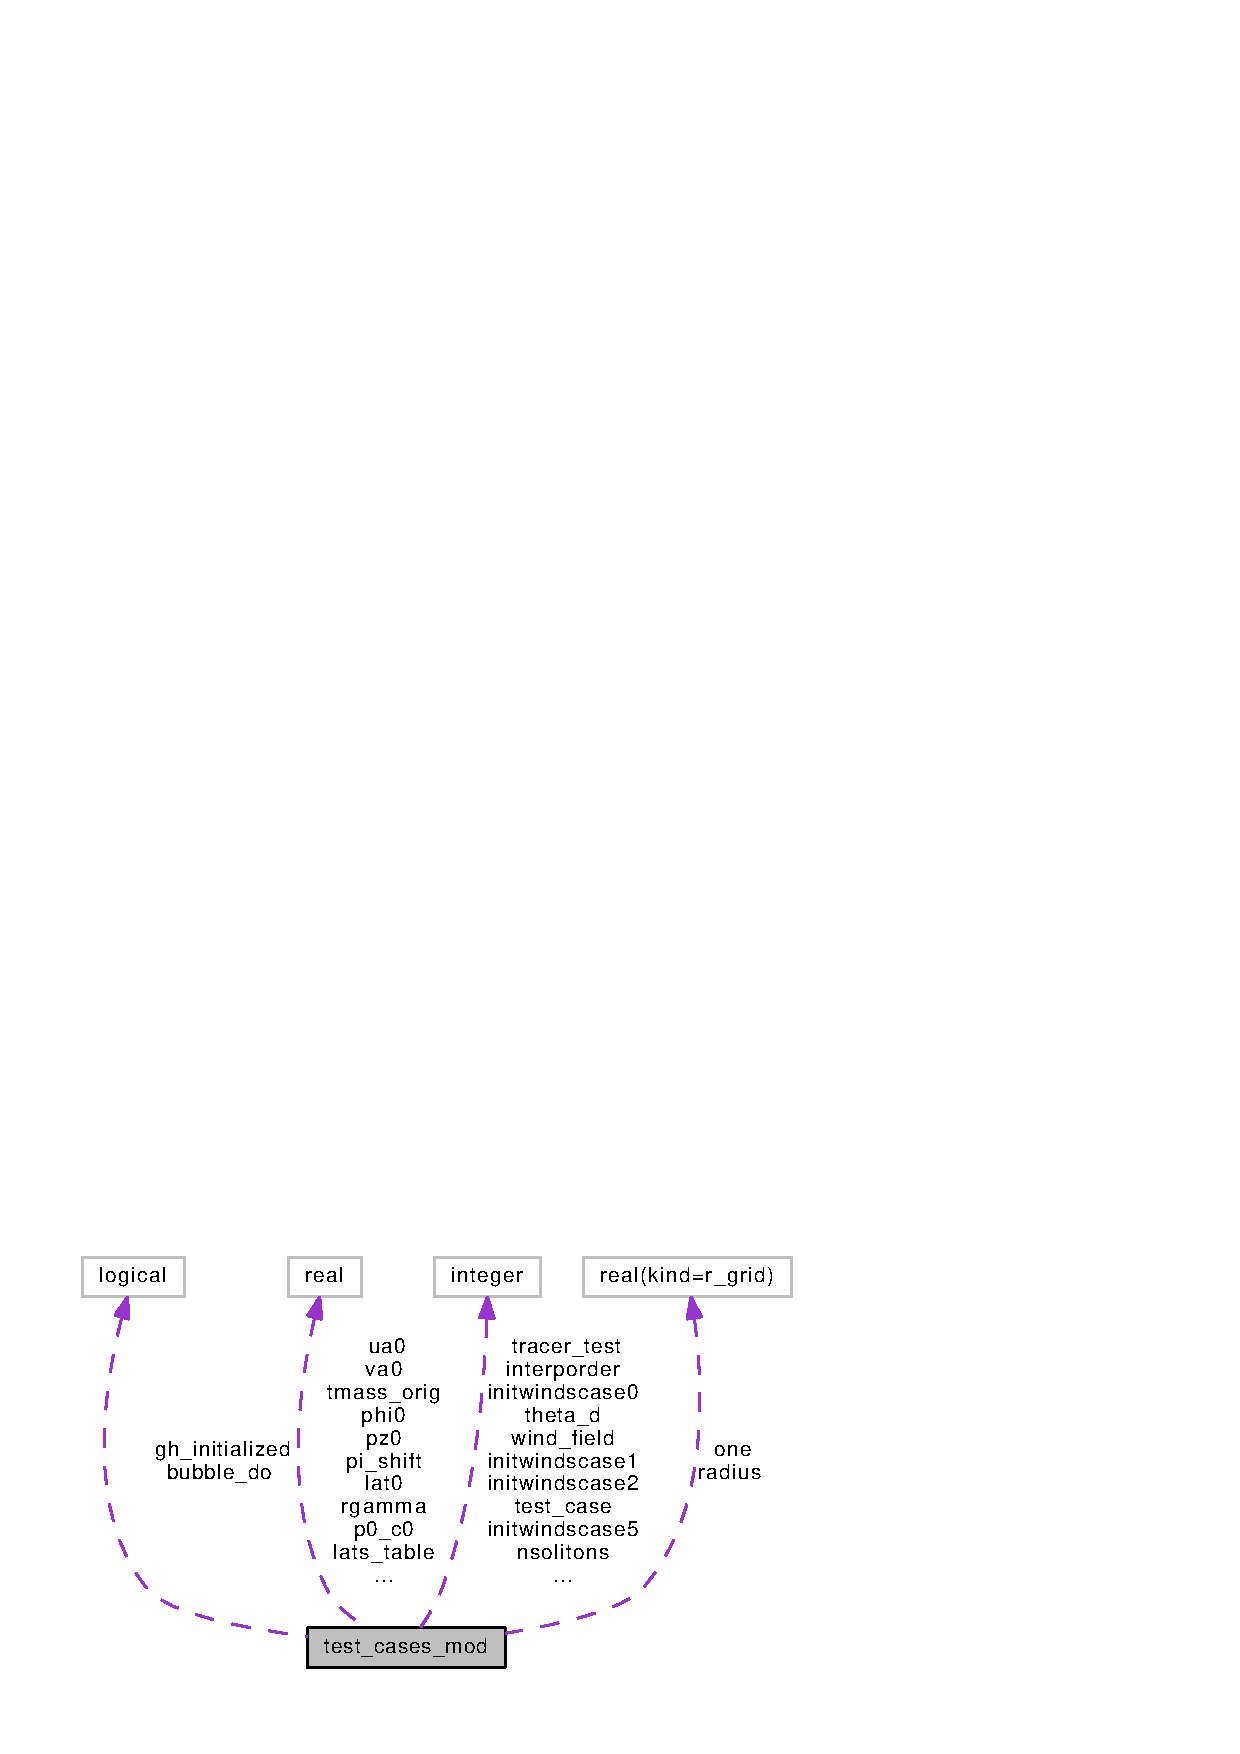
\includegraphics[width=350pt]{classtest__cases__mod__coll__graph}
\end{center}
\end{figure}
\subsection*{Data Types}
\begin{DoxyCompactItemize}
\item 
interface \hyperlink{interfacetest__cases__mod_1_1mp__update__dwinds}{mp\-\_\-update\-\_\-dwinds}
\end{DoxyCompactItemize}
\subsection*{Public Member Functions}
\begin{DoxyCompactItemize}
\item 
subroutine, public \hyperlink{classtest__cases__mod_a986f9f679bcd73e158def56cd9848054}{init\-\_\-case} (u, v, w, pt, delp, q, phis, ps, pe, peln, pk, pkz, uc, vc, ua, va, ak, bk, gridstruct, flagstruct, npx, npy, npz, ng, ncnst, nwat, ndims, nregions, dry\-\_\-mass, mountain, moist\-\_\-phys, hydrostatic, hybrid\-\_\-z, delz, ze0, adiabatic, ks, npx\-\_\-global, ptop, domain\-\_\-in, tile\-\_\-in, bd)
\item 
subroutine, public \hyperlink{classtest__cases__mod_a18ab30d706b11164805c0fa06712936e}{checker\-\_\-tracers} (i0, i1, j0, j1, ifirst, ilast, jfirst, jlast, nq, km, q, lon, lat, nx, ny, rn)
\item 
subroutine, public \hyperlink{classtest__cases__mod_a414d587d54e2c2143eb92518ab122d13}{case9\-\_\-forcing1} (phis, time\-\_\-since\-\_\-start)
\item 
subroutine, public \hyperlink{classtest__cases__mod_ad714385ec571796ea76f467ebc71bfea}{case9\-\_\-forcing2} (phis)
\item 
subroutine, public \hyperlink{classtest__cases__mod_a17ad15ded2b36408f1d991d07bab3aa6}{case51\-\_\-forcing} (delp, uc, vc, u, v, ua, va, pe, time, dt, gridstruct, npx, npy, npz, ptop, domain)
\item 
subroutine, public \hyperlink{classtest__cases__mod_aa69b4104347ae690d3aa71f8d8a2a276}{get\-\_\-stats} (dt, dtout, nt, maxnt, ndays, u, v, pt, delp, q, phis, ps, uc, vc, ua, va, npx, npy, npz, ncnst, ndims, nregions, gridstruct, stats\-\_\-lun, consv\-\_\-lun, monitor\-Freq, tile, domain, nested)
\item 
subroutine, public \hyperlink{classtest__cases__mod_aa93bb608b6adac92ae4ee22132926e29}{check\-\_\-courant\-\_\-numbers} (uc, vc, ndt, n\-\_\-split, gridstruct, npx, npy, npz, tile, no\-Print)
\item 
subroutine, public \hyperlink{classtest__cases__mod_afe098f0f0a16a14e3e59312a69374b9e}{init\-\_\-double\-\_\-periodic} (u, v, w, pt, delp, q, phis, ps, pe, peln, pk, pkz, uc, vc, ua, va, ak, bk, gridstruct, flagstruct, npx, npy, npz, ng, ncnst, nwat, ndims, nregions, dry\-\_\-mass, mountain, moist\-\_\-phys, hydrostatic, hybrid\-\_\-z, delz, ze0, ks, ptop, domain\-\_\-in, tile\-\_\-in, bd)
\item 
subroutine, public \hyperlink{classtest__cases__mod_ac5330b5b0801ece5e8c1af330fa5b56f}{init\-\_\-latlon} (u, v, pt, delp, q, phis, ps, pe, peln, pk, pkz, uc, vc, ua, va, ak, bk, gridstruct, npx, npy, npz, ng, ncnst, ndims, nregions, dry\-\_\-mass, mountain, moist\-\_\-phys, hybrid\-\_\-z, delz, ze0, domain\-\_\-in, tile\-\_\-in)
\item 
subroutine \hyperlink{classtest__cases__mod_aaf90c31f08adcf89ab5371621c45e133}{mp\-\_\-update\-\_\-dwinds\-\_\-3d} (u, v, npx, npy, npz, domain)
\item 
real function \hyperlink{classtest__cases__mod_ae3755b5352d28b3b8b06940f3dd4feac}{globalsum} (p, npx, npy, ifirst, ilast, jfirst, jlast, isd, ied, jsd, jed, gridstruct, tile)
\end{DoxyCompactItemize}
\subsection*{Public Attributes}
\begin{DoxyCompactItemize}
\item 
integer, public \hyperlink{classtest__cases__mod_a7b2088f8d78d58d88ac4f8cf8f80dea8}{test\-\_\-case}
\item 
logical, public \hyperlink{classtest__cases__mod_ac308b4d1b61239d29b7ce8fbaee02d16}{bubble\-\_\-do}
\item 
real, public \hyperlink{classtest__cases__mod_a37da311f66b6290a538efb4c6e91b846}{alpha}
\item 
integer, public \hyperlink{classtest__cases__mod_a124b5e4b27425c730d7182f93a7cb99d}{nsolitons}
\item 
real, public \hyperlink{classtest__cases__mod_aae86f201bdb1a209b7a9c0e26a39feda}{soliton\-\_\-size} = 750.e3
\item 
real, public \hyperlink{classtest__cases__mod_a6691463cf0a75416609c200f6cc0bc62}{soliton\-\_\-umax} = 50.
\item 
real, dimension(\-:), \\*
allocatable, public \hyperlink{classtest__cases__mod_a829a6dcd90e3fecd02c918dc2d107c7e}{pz0}
\item 
real, dimension(\-:), \\*
allocatable, public \hyperlink{classtest__cases__mod_a086960ce4bdf89402a7595af28e5d04a}{zz0}
\item 
integer, public \hyperlink{classtest__cases__mod_a045ac76cf8976a508e18b8f03ba2f57f}{tracer\-\_\-test}
\item 
integer, public \hyperlink{classtest__cases__mod_a81ce24e79fd0973f5bfc7fdc8aaf16a8}{wind\-\_\-field}
\end{DoxyCompactItemize}
\subsection*{Private Member Functions}
\begin{DoxyCompactItemize}
\item 
subroutine \hyperlink{classtest__cases__mod_a6d5f8da880760736fb68b113be23efaf}{init\-\_\-winds} (U\-Bar, u, v, ua, va, uc, vc, def\-On\-Grid, npx, npy, ng, ndims, nregions, nested, gridstruct, domain, tile)
\item 
subroutine \hyperlink{classtest__cases__mod_afc2b5224f950494c9614172941aa7b6d}{get\-\_\-vorticity} (isc, iec, jsc, jec, isd, ied, jsd, jed, npz, u, v, vort, dx, dy, rarea)
\item 
subroutine \hyperlink{classtest__cases__mod_af4f0860ebee67f529c4151ae2957df42}{terminator\-\_\-tracers} (i0, i1, j0, j1, ifirst, ilast, jfirst, jlast, km, q, delp, ncnst, lon, lat)
\item 
subroutine \hyperlink{classtest__cases__mod_a6dea8865194b1c32a2d18f02b3c6533a}{rankine\-\_\-vortex} (\hyperlink{classtest__cases__mod_a3511ba6fb2dcfd0c5575f0568a060924}{ubar}, r0, p1, u, v, grid)
\item 
real function \hyperlink{classtest__cases__mod_a139f8e15372d168090bb8f90be687f48}{gh\-\_\-jet} (npy, lat\-\_\-in)
\item 
real function \hyperlink{classtest__cases__mod_ac1b81c67a4a1dd8cea8887368d0924f5}{u\-\_\-jet} (lat)
\item 
subroutine \hyperlink{classtest__cases__mod_a7203b08bdb8075134170d36306c5d7ff}{get\-\_\-case9\-\_\-b} (B, agrid)
\item 
subroutine \hyperlink{classtest__cases__mod_a823975b05ca9260a7efa6b923406a83d}{get\-\_\-pt\-\_\-on\-\_\-great\-\_\-circle} (p1, p2, dist, heading, p3)
\item 
subroutine \hyperlink{classtest__cases__mod_a62f965d866798b41c1a2ee3990a3ec59}{get\-\_\-scalar\-\_\-stats} (var, var\-T, npx, npy, ndims, nregions, vmin, vmax, L1\-\_\-norm, L2\-\_\-norm, Linf\-\_\-norm, gridstruct, tile)
\item 
subroutine \hyperlink{classtest__cases__mod_a648faf77090f422e584179d9f24fc54a}{get\-\_\-vector\-\_\-stats} (var\-U, var\-U\-T, var\-V, var\-V\-T, npx, npy, ndims, nregions, vmin, vmax, L1\-\_\-norm, L2\-\_\-norm, Linf\-\_\-norm, gridstruct, tile)
\item 
subroutine \hyperlink{classtest__cases__mod_a2716d53d4033232fcd71b57d74eaeb94}{pmxn} (p, npx, npy, nregions, tile, gridstruct, pmin, pmax, i0, j0, n0)
\item 
subroutine \hyperlink{classtest__cases__mod_ad901175e50a8ade7ce8a2958b8d870fa}{superk\-\_\-sounding} (km, pe, p00, ze, pt, qz)
\item 
subroutine \hyperlink{classtest__cases__mod_a78e9f9beeac09a3c4bf4eed68c6322bb}{balanced\-\_\-k} (km, is, ie, js, je, ng, ps0, ze1, ts1, qs1, uz1, dudz, pe, pk, pt, delz, zvir, ptop, ak, bk, agrid)
\item 
subroutine \hyperlink{classtest__cases__mod_a070e13147cdf7a9aac6f05d75d80f96c}{superk\-\_\-u} (km, zz, um, dudz)
\item 
subroutine \hyperlink{classtest__cases__mod_ab293a7f2a292363f96b322a4482026a2}{dcmip16\-\_\-bc} (delp, pt, u, v, q, w, delz, is, ie, js, je, isd, ied, jsd, jed, npz, nq, ak, bk, ptop, pk, peln, pe, pkz, gz, phis, ps, grid, agrid, hydrostatic, nwat, adiabatic, do\-\_\-pert, domain)
\item 
subroutine \hyperlink{classtest__cases__mod_aefbd0cb99937da877c79d0f3e62c9e43}{dcmip16\-\_\-tc} (delp, pt, u, v, q, w, delz, is, ie, js, je, isd, ied, jsd, jed, npz, nq, ak, bk, ptop, pk, peln, pe, pkz, gz, phis, ps, grid, agrid, hydrostatic, nwat, adiabatic)
\item 
subroutine \hyperlink{classtest__cases__mod_a601918eaae703bb73c760577d2a17f3d}{init\-\_\-latlon\-\_\-winds} (U\-Bar, u, v, ua, va, uc, vc, def\-On\-Grid, gridstruct)
\item 
subroutine \hyperlink{classtest__cases__mod_a7c096124b6a75e72c34fdac2ccc88175}{d2a2c} (im, jm, km, ifirst, ilast, jfirst, jlast, ng, nested, u, v, ua, va, uc, vc, gridstruct, domain)
\item 
subroutine \hyperlink{classtest__cases__mod_a86974fdb65c72b74dc0a7fd7d4c55177}{atob\-\_\-s} (qin, qout, npx, npy, dxa, dya, nested, cubed\-\_\-sphere, alt\-Interp)
\item 
subroutine \hyperlink{classtest__cases__mod_a100a065323a0186529544823efd13358}{atod} (uin, vin, uout, vout, dxa, dya, dxc, dyc, npx, npy, ng, nested, domain)
\item 
subroutine \hyperlink{classtest__cases__mod_a269a1a702b0397e16e799c6e7076ac55}{dtoa} (uin, vin, uout, vout, dx, dy, dxa, dya, dxc, dyc, npx, npy, ng)
\item 
subroutine \hyperlink{classtest__cases__mod_a935b3dcf79703f05fca13713ee73ab4b}{atoc} (uin, vin, uout, vout, dx, dy, dxa, dya, npx, npy, ng, nested, domain, no\-Comm)
\item 
subroutine \hyperlink{classtest__cases__mod_a22b0794674be0887303224187a4bdc9f}{ctoa} (uin, vin, uout, vout, dx, dy, dxc, dyc, dxa, dya, npx, npy, ng)
\item 
subroutine \hyperlink{classtest__cases__mod_a59a3bb46b35dad4617aba090560961a9}{rotate\-\_\-winds} (my\-U, my\-V, p1, p2, p3, p4, t1, ndims, dir)
\item 
subroutine \hyperlink{classtest__cases__mod_a56aabda863218f45dc775170ceba5aa2}{mp\-\_\-update\-\_\-dwinds\-\_\-2d} (u, v, npx, npy, domain)
\item 
subroutine \hyperlink{classtest__cases__mod_a062259e5b5a7538878395c3c36f93812}{get\-\_\-unit\-\_\-vector} (p1, p2, p3, uvect)
\item 
subroutine \hyperlink{classtest__cases__mod_ab75c7874346b38287cfdd0d8b7203efe}{normalize\-\_\-vect} (np, e)
\item 
subroutine \hyperlink{classtest__cases__mod_af0c5eed92a1687ee952699be641c348e}{mp\-\_\-ghost\-\_\-ew} (im, jm, km, nq, ifirst, ilast, jfirst, jlast, kfirst, klast, ng\-\_\-w, ng\-\_\-e, ng\-\_\-s, ng\-\_\-n, q\-\_\-ghst, q)
\item 
subroutine \hyperlink{classtest__cases__mod_a415516dbd80cfd3e86430cd0c179f40e}{interp\-\_\-left\-\_\-edge\-\_\-1d} (qout, qin, dx, ifirst, ilast, order)
\item 
subroutine \hyperlink{classtest__cases__mod_a098fd2aa751bcc0f29a4964e8d22c8c9}{vpol5} (u, v, im, jm, coslon, sinlon, cosl5, sinl5, ng\-\_\-d, ng\-\_\-s, jfirst, jlast)
\item 
subroutine \hyperlink{classtest__cases__mod_a7247ffa5b8fb6b80fe65789070118683}{prt\-\_\-m1} (qname, q, is, ie, js, je, n\-\_\-g, km, fac)
\item 
subroutine \hyperlink{classtest__cases__mod_a2a67940979b1f8017967bb8ce9a264be}{var\-\_\-dz} (km, ztop, ze)
\item 
subroutine \hyperlink{classtest__cases__mod_ac4ef2aa50a930be13ee7d7750b2586fc}{sm1\-\_\-edge} (is, ie, js, je, km, i, j, ze, ntimes)
\end{DoxyCompactItemize}
\subsection*{Private Attributes}
\begin{DoxyCompactItemize}
\item 
integer \hyperlink{classtest__cases__mod_a2fb47f8d0671dcb58a188245f3561fc0}{sphum}
\item 
integer \hyperlink{classtest__cases__mod_adc983b10c9af89dbc2a6b4cbd5957918}{theta\-\_\-d}
\item 
real(kind=r\-\_\-grid), parameter \hyperlink{classtest__cases__mod_aaab38fce650165338c7b083b6d69fe14}{radius} = cnst\-\_\-radius
\item 
real(kind=r\-\_\-grid), parameter \hyperlink{classtest__cases__mod_a9fee1aae0eeafb2591001b28a9890b6c}{one} = 1.d0
\item 
real \hyperlink{classtest__cases__mod_ab4fbd1f2da9a9bedc6197a62d77e4f57}{p0\-\_\-c0} = 3.\-0
\item 
real \hyperlink{classtest__cases__mod_a414edbd9fc49e5bf42449aa09ea4b4b5}{rgamma} = 5.\-0
\item 
real \hyperlink{classtest__cases__mod_a64407c4ddac683d907f7f42813602720}{lat0} = pi/2.\-0
\begin{DoxyCompactList}\small\item\em pi/4.\-8 \end{DoxyCompactList}\item 
real \hyperlink{classtest__cases__mod_a982d8969b8cd286c0d2749f4a85fab51}{lon0} = 0.\-0
\begin{DoxyCompactList}\small\item\em pi-\/0.\-8 \end{DoxyCompactList}\item 
real, parameter \hyperlink{classtest__cases__mod_ac52bff5875e95e0bc36377a076e3ba63}{pi\-\_\-shift} = 0.\-0
\begin{DoxyCompactList}\small\item\em 3.\-0$\ast$pi/4. \end{DoxyCompactList}\item 
integer, parameter \hyperlink{classtest__cases__mod_a344cd0cb1ee73dc4346c3291c532432f}{initwindscase0} =-\/1
\item 
integer, parameter \hyperlink{classtest__cases__mod_ae0e779adc02d8de0967072c92e081e76}{initwindscase1} = 1
\item 
integer, parameter \hyperlink{classtest__cases__mod_a67b8fe8f9c6ecc1f39e3efb965081229}{initwindscase2} = 5
\item 
integer, parameter \hyperlink{classtest__cases__mod_ac567d8bd4c95a1655c612b3a193c1ea3}{initwindscase5} = 5
\item 
integer, parameter \hyperlink{classtest__cases__mod_aefad7f694cc274e910aa9a2cd8f4635f}{initwindscase6} =-\/1
\item 
integer, parameter \hyperlink{classtest__cases__mod_a4d993fcfbe5c8e8e07b74f394b8ae1b9}{initwindscase9} =-\/1
\item 
real \hyperlink{classtest__cases__mod_a3511ba6fb2dcfd0c5575f0568a060924}{ubar}
\item 
real \hyperlink{classtest__cases__mod_a8c4fdfdfac04288502c9ec94febd848a}{vbar}
\item 
real \hyperlink{classtest__cases__mod_a0330d24892de013b82c806b2eb174802}{gh0}
\item 
real, dimension(\-:,\-:), allocatable \hyperlink{classtest__cases__mod_ad4fbc67ecd0c262bdc856412254fcd12}{case9\-\_\-b}
\item 
real, dimension(2) \hyperlink{classtest__cases__mod_a701517a60d6bee3efcc10042ca4353ba}{aoft}
\item 
real, dimension(\-:,\-:,\-:), allocatable \hyperlink{classtest__cases__mod_a1bc1841e0de13798d6a15b088b9190fe}{phi0}
\begin{DoxyCompactList}\small\item\em Validating Field. \end{DoxyCompactList}\item 
real, dimension(\-:,\-:,\-:), allocatable \hyperlink{classtest__cases__mod_a732ccc75bb62730c4901b3197a4ca0db}{ua0}
\begin{DoxyCompactList}\small\item\em Validating U-\/\-Wind. \end{DoxyCompactList}\item 
real, dimension(\-:,\-:,\-:), allocatable \hyperlink{classtest__cases__mod_ae762ff3757574df1e4826d061587ee9f}{va0}
\begin{DoxyCompactList}\small\item\em Validating V-\/\-Windfms\-\_\-io\-\_\-exit, get\-\_\-tile\-\_\-string, \&. \end{DoxyCompactList}\item 
real, dimension(\-:), allocatable \hyperlink{classtest__cases__mod_a3e0198270bedfe3033ecef4e3d910c53}{gh\-\_\-table}
\item 
real, dimension(\-:), allocatable \hyperlink{classtest__cases__mod_ab29f3455dbdffa40ac33075ff47eb95f}{lats\-\_\-table}
\item 
logical \hyperlink{classtest__cases__mod_aacf71cede68445436888a520c4713a3c}{gh\-\_\-initialized} = .false.
\item 
real \hyperlink{classtest__cases__mod_af40da1fd7e6753224232eb5f50752dbf}{tmass\-\_\-orig}
\begin{DoxyCompactList}\small\item\em total mass \end{DoxyCompactList}\item 
real \hyperlink{classtest__cases__mod_a9e6b5dada32091330827cadf573e240a}{tvort\-\_\-orig}
\begin{DoxyCompactList}\small\item\em enstrophy (integral of total vorticity) \end{DoxyCompactList}\item 
real \hyperlink{classtest__cases__mod_a2a10be3be35d2f512f6e3b83652672eb}{tener\-\_\-orig}
\begin{DoxyCompactList}\small\item\em energy \end{DoxyCompactList}\item 
integer, parameter \hyperlink{classtest__cases__mod_ab921cb10723bbe2b3c15e81b664f5ff6}{interporder} = 1
\end{DoxyCompactItemize}


\subsection{Detailed Description}
my dog typed this comment\-: mjkkicdsddsds, my cat typed this comment\-: cdjkkjfdjkjf my dog also typed this comment\-: kmasdlckmc my cat meowed 

Definition at line 27 of file test\-\_\-cases.\-F90.



\subsection{Member Function/\-Subroutine Documentation}
\index{test\-\_\-cases\-\_\-mod@{test\-\_\-cases\-\_\-mod}!atob\-\_\-s@{atob\-\_\-s}}
\index{atob\-\_\-s@{atob\-\_\-s}!test_cases_mod@{test\-\_\-cases\-\_\-mod}}
\subsubsection[{atob\-\_\-s}]{\setlength{\rightskip}{0pt plus 5cm}subroutine test\-\_\-cases\-\_\-mod\-::atob\-\_\-s (
\begin{DoxyParamCaption}
\item[{real, dimension(isd\-:ied  ,jsd\-:jed  ), intent(in)}]{qin, }
\item[{real, dimension(isd\-:ied+1,jsd\-:jed+1), intent(out)}]{qout, }
\item[{integer, intent(in)}]{npx, }
\item[{integer, intent(in)}]{npy, }
\item[{real, dimension(isd\-:ied,jsd\-:jed), intent(in)}]{dxa, }
\item[{real, dimension(isd\-:ied,jsd\-:jed), intent(in)}]{dya, }
\item[{logical, intent(in)}]{nested, }
\item[{logical, intent(in)}]{cubed\-\_\-sphere, }
\item[{integer, intent(in), optional}]{alt\-Interp}
\end{DoxyParamCaption}
)\hspace{0.3cm}{\ttfamily [private]}}\label{classtest__cases__mod_a86974fdb65c72b74dc0a7fd7d4c55177}

\begin{DoxyParams}[1]{Parameters}
\mbox{\tt in}  & {\em qin} & A-\/grid field\\
\hline
\mbox{\tt out}  & {\em qout} & Output B-\/grid field \\
\hline
\end{DoxyParams}


Definition at line 8341 of file test\-\_\-cases.\-F90.



References interp\-\_\-left\-\_\-edge\-\_\-1d().



Referenced by pmxn().

\index{test\-\_\-cases\-\_\-mod@{test\-\_\-cases\-\_\-mod}!atoc@{atoc}}
\index{atoc@{atoc}!test_cases_mod@{test\-\_\-cases\-\_\-mod}}
\subsubsection[{atoc}]{\setlength{\rightskip}{0pt plus 5cm}subroutine test\-\_\-cases\-\_\-mod\-::atoc (
\begin{DoxyParamCaption}
\item[{real, dimension(isd\-:ied  ,jsd\-:jed  ), intent(in)}]{uin, }
\item[{real, dimension(isd\-:ied  ,jsd\-:jed  ), intent(in)}]{vin, }
\item[{real, dimension(isd\-:ied+1,jsd\-:jed  ), intent(out)}]{uout, }
\item[{real, dimension(isd\-:ied  ,jsd\-:jed+1), intent(out)}]{vout, }
\item[{real, dimension(isd\-:ied,jsd\-:jed+1), intent(in)}]{dx, }
\item[{real, dimension(isd\-:ied+1,jsd\-:jed), intent(in)}]{dy, }
\item[{real, dimension(isd\-:ied,jsd\-:jed), intent(in)}]{dxa, }
\item[{real, dimension(isd\-:ied,jsd\-:jed), intent(in)}]{dya, }
\item[{integer, intent(in)}]{npx, }
\item[{integer, intent(in)}]{npy, }
\item[{integer, intent(in)}]{ng, }
\item[{logical, intent(in)}]{nested, }
\item[{type(domain2d), intent(inout)}]{domain, }
\item[{logical, intent(in), optional}]{no\-Comm}
\end{DoxyParamCaption}
)\hspace{0.3cm}{\ttfamily [private]}}\label{classtest__cases__mod_a935b3dcf79703f05fca13713ee73ab4b}

\begin{DoxyParams}[1]{Parameters}
\mbox{\tt in}  & {\em uin} & A-\/grid u-\/wind field\\
\hline
\mbox{\tt in}  & {\em vin} & A-\/grid v-\/wind field\\
\hline
\mbox{\tt out}  & {\em uout} & C-\/grid u-\/wind field\\
\hline
\mbox{\tt out}  & {\em vout} & C-\/grid v-\/wind field \\
\hline
\end{DoxyParams}


Definition at line 8572 of file test\-\_\-cases.\-F90.



References interp\-\_\-left\-\_\-edge\-\_\-1d().



Referenced by case51\-\_\-forcing(), d2a2c(), get\-\_\-stats(), init\-\_\-case(), and init\-\_\-winds().

\index{test\-\_\-cases\-\_\-mod@{test\-\_\-cases\-\_\-mod}!atod@{atod}}
\index{atod@{atod}!test_cases_mod@{test\-\_\-cases\-\_\-mod}}
\subsubsection[{atod}]{\setlength{\rightskip}{0pt plus 5cm}subroutine test\-\_\-cases\-\_\-mod\-::atod (
\begin{DoxyParamCaption}
\item[{real, dimension(isd\-:ied  ,jsd\-:jed  ), intent(in)}]{uin, }
\item[{real, dimension(isd\-:ied  ,jsd\-:jed  ), intent(in)}]{vin, }
\item[{real, dimension(isd\-:ied  ,jsd\-:jed+1), intent(out)}]{uout, }
\item[{real, dimension(isd\-:ied+1,jsd\-:jed  ), intent(out)}]{vout, }
\item[{real, dimension(isd\-:ied,jsd\-:jed), intent(in)}]{dxa, }
\item[{real, dimension(isd\-:ied,jsd\-:jed), intent(in)}]{dya, }
\item[{real, dimension(isd\-:ied+1,jsd\-:jed), intent(in)}]{dxc, }
\item[{real, dimension(isd\-:ied,jsd\-:jed+1), intent(in)}]{dyc, }
\item[{integer, intent(in)}]{npx, }
\item[{integer, intent(in)}]{npy, }
\item[{integer, intent(in)}]{ng, }
\item[{logical, intent(in)}]{nested, }
\item[{type(domain2d), intent(inout)}]{domain}
\end{DoxyParamCaption}
)\hspace{0.3cm}{\ttfamily [private]}}\label{classtest__cases__mod_a100a065323a0186529544823efd13358}

\begin{DoxyParams}[1]{Parameters}
\mbox{\tt in}  & {\em uin} & A-\/grid u-\/wind field\\
\hline
\mbox{\tt in}  & {\em vin} & A-\/grid v-\/wind field\\
\hline
\mbox{\tt out}  & {\em uout} & D-\/grid u-\/wind field\\
\hline
\mbox{\tt out}  & {\em vout} & D-\/grid v-\/wind field \\
\hline
\end{DoxyParams}


Definition at line 8477 of file test\-\_\-cases.\-F90.



References interp\-\_\-left\-\_\-edge\-\_\-1d().



Referenced by init\-\_\-case(), and init\-\_\-winds().

\index{test\-\_\-cases\-\_\-mod@{test\-\_\-cases\-\_\-mod}!balanced\-\_\-k@{balanced\-\_\-k}}
\index{balanced\-\_\-k@{balanced\-\_\-k}!test_cases_mod@{test\-\_\-cases\-\_\-mod}}
\subsubsection[{balanced\-\_\-k}]{\setlength{\rightskip}{0pt plus 5cm}subroutine test\-\_\-cases\-\_\-mod\-::balanced\-\_\-k (
\begin{DoxyParamCaption}
\item[{integer, intent(in)}]{km, }
\item[{integer, intent(in)}]{is, }
\item[{integer, intent(in)}]{ie, }
\item[{integer, intent(in)}]{js, }
\item[{integer, intent(in)}]{je, }
\item[{integer, intent(in)}]{ng, }
\item[{real, intent(in)}]{ps0, }
\item[{real, dimension(km+1), intent(in)}]{ze1, }
\item[{real, dimension(km  ), intent(in)}]{ts1, }
\item[{real, dimension(km  ), intent(in)}]{qs1, }
\item[{real, dimension(km  ), intent(in)}]{uz1, }
\item[{real, dimension(km  ), intent(in)}]{dudz, }
\item[{real, dimension(is-\/1\-:ie+1,km+1,js-\/1\-:je+1), intent(inout)}]{pe, }
\item[{real, dimension(is\-:ie,js\-:je,km+1), intent(out)}]{pk, }
\item[{real, dimension(is-\/ng\-:ie+ng,js-\/ng\-:je+ng,km), intent(inout)}]{pt, }
\item[{real, dimension(is-\/ng\-:ie+ng,js-\/ng\-:je+ng,km), intent(inout)}]{delz, }
\item[{real, intent(in)}]{zvir, }
\item[{real, intent(inout)}]{ptop, }
\item[{real, dimension(km+1), intent(inout)}]{ak, }
\item[{real, dimension(km+1), intent(inout)}]{bk, }
\item[{real(kind=r\-\_\-grid), dimension(is-\/ng\-:ie+ng,js-\/ng\-:je+ng,2), intent(in)}]{agrid}
\end{DoxyParamCaption}
)\hspace{0.3cm}{\ttfamily [private]}}\label{classtest__cases__mod_a78e9f9beeac09a3c4bf4eed68c6322bb}


Definition at line 6928 of file test\-\_\-cases.\-F90.



References fv\-\_\-diagnostics\-\_\-mod\-::ppme(), and prt\-\_\-m1().



Referenced by init\-\_\-case().

\index{test\-\_\-cases\-\_\-mod@{test\-\_\-cases\-\_\-mod}!case51\-\_\-forcing@{case51\-\_\-forcing}}
\index{case51\-\_\-forcing@{case51\-\_\-forcing}!test_cases_mod@{test\-\_\-cases\-\_\-mod}}
\subsubsection[{case51\-\_\-forcing}]{\setlength{\rightskip}{0pt plus 5cm}subroutine, public test\-\_\-cases\-\_\-mod\-::case51\-\_\-forcing (
\begin{DoxyParamCaption}
\item[{real, dimension(isd\-:ied,jsd\-:jed,npz), intent(inout)}]{delp, }
\item[{real, dimension(isd\-:ied+1,jsd\-:jed,npz), intent(inout)}]{uc, }
\item[{real, dimension(isd\-:ied,jsd\-:jed+1,npz), intent(inout)}]{vc, }
\item[{real, dimension(isd\-:ied,jsd\-:jed+1,npz), intent(inout)}]{u, }
\item[{real, dimension(isd\-:ied+1,jsd\-:jed,npz), intent(inout)}]{v, }
\item[{real, dimension(isd\-:ied,jsd\-:jed,npz), intent(inout)}]{ua, }
\item[{real, dimension(isd\-:ied,jsd\-:jed,npz), intent(inout)}]{va, }
\item[{real, dimension(is-\/1\-:ie+1, npz+1,js-\/1\-:je+1), intent(inout)}]{pe, }
\item[{real, intent(in)}]{time, }
\item[{real, intent(in)}]{dt, }
\item[{type(fv\-\_\-grid\-\_\-type), intent(in), target}]{gridstruct, }
\item[{integer, intent(in)}]{npx, }
\item[{integer, intent(in)}]{npy, }
\item[{integer, intent(in)}]{npz, }
\item[{real, intent(inout)}]{ptop, }
\item[{type(domain2d), intent(inout)}]{domain}
\end{DoxyParamCaption}
)}\label{classtest__cases__mod_a17ad15ded2b36408f1d991d07bab3aa6}


Definition at line 4219 of file test\-\_\-cases.\-F90.



References atoc(), dtoa(), fv\-\_\-grid\-\_\-utils\-\_\-mod\-::get\-\_\-latlon\-\_\-vector(), fv\-\_\-grid\-\_\-utils\-\_\-mod\-::get\-\_\-unit\-\_\-vect2(), fv\-\_\-grid\-\_\-utils\-\_\-mod\-::inner\-\_\-prod(), and fv\-\_\-grid\-\_\-utils\-\_\-mod\-::mid\-\_\-pt\-\_\-sphere().

\index{test\-\_\-cases\-\_\-mod@{test\-\_\-cases\-\_\-mod}!case9\-\_\-forcing1@{case9\-\_\-forcing1}}
\index{case9\-\_\-forcing1@{case9\-\_\-forcing1}!test_cases_mod@{test\-\_\-cases\-\_\-mod}}
\subsubsection[{case9\-\_\-forcing1}]{\setlength{\rightskip}{0pt plus 5cm}subroutine, public test\-\_\-cases\-\_\-mod\-::case9\-\_\-forcing1 (
\begin{DoxyParamCaption}
\item[{real, dimension(isd\-:ied  ,jsd\-:jed  ), intent(inout)}]{phis, }
\item[{real, intent(in)}]{time\-\_\-since\-\_\-start}
\end{DoxyParamCaption}
)}\label{classtest__cases__mod_a414d587d54e2c2143eb92518ab122d13}


Definition at line 4166 of file test\-\_\-cases.\-F90.



Referenced by dyn\-\_\-core\-\_\-mod\-::dyn\-\_\-core().

\index{test\-\_\-cases\-\_\-mod@{test\-\_\-cases\-\_\-mod}!case9\-\_\-forcing2@{case9\-\_\-forcing2}}
\index{case9\-\_\-forcing2@{case9\-\_\-forcing2}!test_cases_mod@{test\-\_\-cases\-\_\-mod}}
\subsubsection[{case9\-\_\-forcing2}]{\setlength{\rightskip}{0pt plus 5cm}subroutine, public test\-\_\-cases\-\_\-mod\-::case9\-\_\-forcing2 (
\begin{DoxyParamCaption}
\item[{real, dimension(isd\-:ied  ,jsd\-:jed  ), intent(inout)}]{phis}
\end{DoxyParamCaption}
)}\label{classtest__cases__mod_ad714385ec571796ea76f467ebc71bfea}


Definition at line 4201 of file test\-\_\-cases.\-F90.



Referenced by dyn\-\_\-core\-\_\-mod\-::dyn\-\_\-core().

\index{test\-\_\-cases\-\_\-mod@{test\-\_\-cases\-\_\-mod}!check\-\_\-courant\-\_\-numbers@{check\-\_\-courant\-\_\-numbers}}
\index{check\-\_\-courant\-\_\-numbers@{check\-\_\-courant\-\_\-numbers}!test_cases_mod@{test\-\_\-cases\-\_\-mod}}
\subsubsection[{check\-\_\-courant\-\_\-numbers}]{\setlength{\rightskip}{0pt plus 5cm}subroutine, public test\-\_\-cases\-\_\-mod\-::check\-\_\-courant\-\_\-numbers (
\begin{DoxyParamCaption}
\item[{real, dimension(isd\-:ied+1,jsd\-:jed  ,npz), intent(in)}]{uc, }
\item[{real, dimension(isd\-:ied  ,jsd\-:jed+1,npz), intent(in)}]{vc, }
\item[{real, intent(in)}]{ndt, }
\item[{integer, intent(in)}]{n\-\_\-split, }
\item[{type(fv\-\_\-grid\-\_\-type), intent(in), target}]{gridstruct, }
\item[{integer, intent(in)}]{npx, }
\item[{integer, intent(in)}]{npy, }
\item[{integer, intent(in)}]{npz, }
\item[{integer, intent(in)}]{tile, }
\item[{logical, intent(in), optional}]{no\-Print}
\end{DoxyParamCaption}
)}\label{classtest__cases__mod_aa93bb608b6adac92ae4ee22132926e29}


Definition at line 5205 of file test\-\_\-cases.\-F90.

\index{test\-\_\-cases\-\_\-mod@{test\-\_\-cases\-\_\-mod}!checker\-\_\-tracers@{checker\-\_\-tracers}}
\index{checker\-\_\-tracers@{checker\-\_\-tracers}!test_cases_mod@{test\-\_\-cases\-\_\-mod}}
\subsubsection[{checker\-\_\-tracers}]{\setlength{\rightskip}{0pt plus 5cm}subroutine, public test\-\_\-cases\-\_\-mod\-::checker\-\_\-tracers (
\begin{DoxyParamCaption}
\item[{integer, intent(in)}]{i0, }
\item[{integer, intent(in)}]{i1, }
\item[{integer, intent(in)}]{j0, }
\item[{integer, intent(in)}]{j1, }
\item[{integer, intent(in)}]{ifirst, }
\item[{integer, intent(in)}]{ilast, }
\item[{integer, intent(in)}]{jfirst, }
\item[{integer, intent(in)}]{jlast, }
\item[{integer, intent(in)}]{nq, }
\item[{integer, intent(in)}]{km, }
\item[{real, dimension(ifirst\-:ilast,jfirst\-:jlast,km,nq), intent(out)}]{q, }
\item[{real(kind=r\-\_\-grid), dimension(i0\-:i1,j0\-:j1), intent(in)}]{lon, }
\item[{real(kind=r\-\_\-grid), dimension(i0\-:i1,j0\-:j1), intent(in)}]{lat, }
\item[{real, intent(in)}]{nx, }
\item[{real, intent(in)}]{ny, }
\item[{real, intent(in), optional}]{rn}
\end{DoxyParamCaption}
)}\label{classtest__cases__mod_a18ab30d706b11164805c0fa06712936e}


Definition at line 3859 of file test\-\_\-cases.\-F90.



Referenced by external\-\_\-ic\-\_\-mod\-::get\-\_\-nggps\-\_\-ic(), and init\-\_\-case().

\index{test\-\_\-cases\-\_\-mod@{test\-\_\-cases\-\_\-mod}!ctoa@{ctoa}}
\index{ctoa@{ctoa}!test_cases_mod@{test\-\_\-cases\-\_\-mod}}
\subsubsection[{ctoa}]{\setlength{\rightskip}{0pt plus 5cm}subroutine test\-\_\-cases\-\_\-mod\-::ctoa (
\begin{DoxyParamCaption}
\item[{real, dimension(isd\-:ied+1,jsd\-:jed  ), intent(in)}]{uin, }
\item[{real, dimension(isd\-:ied  ,jsd\-:jed+1), intent(in)}]{vin, }
\item[{real, dimension(isd\-:ied  ,jsd\-:jed  ), intent(out)}]{uout, }
\item[{real, dimension(isd\-:ied  ,jsd\-:jed  ), intent(out)}]{vout, }
\item[{real, dimension(isd\-:ied,jsd\-:jed+1), intent(in)}]{dx, }
\item[{real, dimension(isd\-:ied+1,jsd\-:jed), intent(in)}]{dy, }
\item[{real, dimension(isd\-:ied+1,jsd\-:jed), intent(in)}]{dxc, }
\item[{real, dimension(isd\-:ied,jsd\-:jed+1), intent(in)}]{dyc, }
\item[{real, dimension(isd\-:ied,jsd\-:jed), intent(in)}]{dxa, }
\item[{real, dimension(isd\-:ied,jsd\-:jed), intent(in)}]{dya, }
\item[{integer, intent(in)}]{npx, }
\item[{integer, intent(in)}]{npy, }
\item[{integer, intent(in)}]{ng}
\end{DoxyParamCaption}
)\hspace{0.3cm}{\ttfamily [private]}}\label{classtest__cases__mod_a22b0794674be0887303224187a4bdc9f}

\begin{DoxyParams}[1]{Parameters}
\mbox{\tt in}  & {\em uin} & C-\/grid u-\/wind field\\
\hline
\mbox{\tt in}  & {\em vin} & C-\/grid v-\/wind field\\
\hline
\mbox{\tt out}  & {\em uout} & A-\/grid u-\/wind field\\
\hline
\mbox{\tt out}  & {\em vout} & A-\/grid v-\/wind field \\
\hline
\end{DoxyParams}


Definition at line 8692 of file test\-\_\-cases.\-F90.



References interp\-\_\-left\-\_\-edge\-\_\-1d().



Referenced by init\-\_\-winds().

\index{test\-\_\-cases\-\_\-mod@{test\-\_\-cases\-\_\-mod}!d2a2c@{d2a2c}}
\index{d2a2c@{d2a2c}!test_cases_mod@{test\-\_\-cases\-\_\-mod}}
\subsubsection[{d2a2c}]{\setlength{\rightskip}{0pt plus 5cm}subroutine test\-\_\-cases\-\_\-mod\-::d2a2c (
\begin{DoxyParamCaption}
\item[{integer, intent(in)}]{im, }
\item[{integer, intent(in)}]{jm, }
\item[{integer, intent(in)}]{km, }
\item[{integer, intent(in)}]{ifirst, }
\item[{integer, intent(in)}]{ilast, }
\item[{integer, intent(in)}]{jfirst, }
\item[{integer, intent(in)}]{jlast, }
\item[{integer, intent(in)}]{ng, }
\item[{logical, intent(in)}]{nested, }
\item[{real, dimension(isd\-:ied,jsd\-:jed+1), intent(inout)}]{u, }
\item[{real, dimension(isd\-:ied+1,jsd\-:jed), intent(inout)}]{v, }
\item[{real, dimension(isd\-:ied,jsd\-:jed), intent(inout)}]{ua, }
\item[{real, dimension(isd\-:ied,jsd\-:jed), intent(inout)}]{va, }
\item[{real, dimension(isd\-:ied+1,jsd\-:jed), intent(inout)}]{uc, }
\item[{real, dimension(isd\-:ied,jsd\-:jed+1), intent(inout)}]{vc, }
\item[{type(fv\-\_\-grid\-\_\-type), intent(in), target}]{gridstruct, }
\item[{type(domain2d), intent(inout)}]{domain}
\end{DoxyParamCaption}
)\hspace{0.3cm}{\ttfamily [private]}}\label{classtest__cases__mod_a7c096124b6a75e72c34fdac2ccc88175}


Definition at line 8107 of file test\-\_\-cases.\-F90.



References atoc(), dtoa(), tp\-\_\-core\-\_\-mod\-::mp\-\_\-ghost\-\_\-ew(), and vpol5().

\index{test\-\_\-cases\-\_\-mod@{test\-\_\-cases\-\_\-mod}!dcmip16\-\_\-bc@{dcmip16\-\_\-bc}}
\index{dcmip16\-\_\-bc@{dcmip16\-\_\-bc}!test_cases_mod@{test\-\_\-cases\-\_\-mod}}
\subsubsection[{dcmip16\-\_\-bc}]{\setlength{\rightskip}{0pt plus 5cm}subroutine test\-\_\-cases\-\_\-mod\-::dcmip16\-\_\-bc (
\begin{DoxyParamCaption}
\item[{real, dimension(isd\-:ied,jsd\-:jed,npz), intent(out)}]{delp, }
\item[{real, dimension(isd\-:ied,jsd\-:jed,npz), intent(out)}]{pt, }
\item[{real, dimension(isd\-:ied,jsd\-:jed+1,npz), intent(out)}]{u, }
\item[{real, dimension(isd\-:ied+1,jsd\-:jed,npz), intent(out)}]{v, }
\item[{real, dimension(isd\-:ied,jsd\-:jed,npz,nq), intent(inout)}]{q, }
\item[{real, dimension(isd\-:ied,jsd\-:jed,npz), intent(out)}]{w, }
\item[{real, dimension(isd\-:ied,jsd\-:jed,npz), intent(out)}]{delz, }
\item[{integer, intent(in)}]{is, }
\item[{integer, intent(in)}]{ie, }
\item[{integer, intent(in)}]{js, }
\item[{integer, intent(in)}]{je, }
\item[{integer, intent(in)}]{isd, }
\item[{integer, intent(in)}]{ied, }
\item[{integer, intent(in)}]{jsd, }
\item[{integer, intent(in)}]{jed, }
\item[{integer, intent(in)}]{npz, }
\item[{integer, intent(in)}]{nq, }
\item[{real, dimension(npz+1), intent(in)}]{ak, }
\item[{real, dimension(npz+1), intent(in)}]{bk, }
\item[{real, intent(in)}]{ptop, }
\item[{real, dimension(is\-:ie,js\-:je,npz+1), intent(out)}]{pk, }
\item[{real, dimension(is\-:ie,npz+1,js\-:je), intent(out)}]{peln, }
\item[{real, dimension(is-\/1\-:ie+1,npz+1,js-\/1\-:je+1), intent(out)}]{pe, }
\item[{real, dimension(is\-:ie,js\-:je,npz), intent(out)}]{pkz, }
\item[{real, dimension(isd\-:ied,jsd\-:jed,npz+1), intent(out)}]{gz, }
\item[{real, dimension(isd\-:ied,jsd\-:jed), intent(out)}]{phis, }
\item[{real, dimension(isd\-:ied,jsd\-:jed), intent(out)}]{ps, }
\item[{real(kind=r\-\_\-grid), dimension(isd\-:ied+1,jsd\-:jed+1,2), intent(in)}]{grid, }
\item[{real(kind=r\-\_\-grid), dimension(isd\-:ied,jsd\-:jed,2), intent(in)}]{agrid, }
\item[{logical, intent(in)}]{hydrostatic, }
\item[{integer, intent(in)}]{nwat, }
\item[{logical, intent(in)}]{adiabatic, }
\item[{logical, intent(in)}]{do\-\_\-pert, }
\item[{type(domain2d), intent(inout)}]{domain}
\end{DoxyParamCaption}
)\hspace{0.3cm}{\ttfamily [private]}}\label{classtest__cases__mod_ab293a7f2a292363f96b322a4482026a2}


Definition at line 7118 of file test\-\_\-cases.\-F90.



References dcmip16\-\_\-bc\-\_\-pressure(), dcmip16\-\_\-bc\-\_\-sphum(), dcmip16\-\_\-bc\-\_\-temperature(), dcmip16\-\_\-bc\-\_\-uwind(), dcmip16\-\_\-bc\-\_\-uwind\-\_\-pert(), fv\-\_\-grid\-\_\-utils\-\_\-mod\-::get\-\_\-latlon\-\_\-vector(), fv\-\_\-grid\-\_\-utils\-\_\-mod\-::get\-\_\-unit\-\_\-vect2(), fv\-\_\-grid\-\_\-utils\-\_\-mod\-::inner\-\_\-prod(), fv\-\_\-grid\-\_\-utils\-\_\-mod\-::mid\-\_\-pt\-\_\-sphere(), and terminator\-\_\-tracers().



Referenced by init\-\_\-case().

\index{test\-\_\-cases\-\_\-mod@{test\-\_\-cases\-\_\-mod}!dcmip16\-\_\-tc@{dcmip16\-\_\-tc}}
\index{dcmip16\-\_\-tc@{dcmip16\-\_\-tc}!test_cases_mod@{test\-\_\-cases\-\_\-mod}}
\subsubsection[{dcmip16\-\_\-tc}]{\setlength{\rightskip}{0pt plus 5cm}subroutine test\-\_\-cases\-\_\-mod\-::dcmip16\-\_\-tc (
\begin{DoxyParamCaption}
\item[{real, dimension(isd\-:ied,jsd\-:jed,npz), intent(out)}]{delp, }
\item[{real, dimension(isd\-:ied,jsd\-:jed,npz), intent(out)}]{pt, }
\item[{real, dimension(isd\-:ied,jsd\-:jed+1,npz), intent(out)}]{u, }
\item[{real, dimension(isd\-:ied+1,jsd\-:jed,npz), intent(out)}]{v, }
\item[{real, dimension(isd\-:ied,jsd\-:jed,npz,nq), intent(inout)}]{q, }
\item[{real, dimension(isd\-:ied,jsd\-:jed,npz), intent(out)}]{w, }
\item[{real, dimension(isd\-:ied,jsd\-:jed,npz), intent(out)}]{delz, }
\item[{integer, intent(in)}]{is, }
\item[{integer, intent(in)}]{ie, }
\item[{integer, intent(in)}]{js, }
\item[{integer, intent(in)}]{je, }
\item[{integer, intent(in)}]{isd, }
\item[{integer, intent(in)}]{ied, }
\item[{integer, intent(in)}]{jsd, }
\item[{integer, intent(in)}]{jed, }
\item[{integer, intent(in)}]{npz, }
\item[{integer, intent(in)}]{nq, }
\item[{real, dimension(npz+1), intent(in)}]{ak, }
\item[{real, dimension(npz+1), intent(in)}]{bk, }
\item[{real, intent(in)}]{ptop, }
\item[{real, dimension(is\-:ie,js\-:je,npz+1), intent(out)}]{pk, }
\item[{real, dimension(is\-:ie,npz+1,js\-:je), intent(out)}]{peln, }
\item[{real, dimension(is-\/1\-:ie+1,npz+1,js-\/1\-:je+1), intent(out)}]{pe, }
\item[{real, dimension(is\-:ie,js\-:je,npz), intent(out)}]{pkz, }
\item[{real, dimension(isd\-:ied,jsd\-:jed,npz+1), intent(out)}]{gz, }
\item[{real, dimension(isd\-:ied,jsd\-:jed), intent(out)}]{phis, }
\item[{real, dimension(isd\-:ied,jsd\-:jed), intent(out)}]{ps, }
\item[{real(kind=r\-\_\-grid), dimension(isd\-:ied+1,jsd\-:jed+1,2), intent(in)}]{grid, }
\item[{real(kind=r\-\_\-grid), dimension(isd\-:ied,jsd\-:jed,2), intent(in)}]{agrid, }
\item[{logical, intent(in)}]{hydrostatic, }
\item[{integer, intent(in)}]{nwat, }
\item[{logical, intent(in)}]{adiabatic}
\end{DoxyParamCaption}
)\hspace{0.3cm}{\ttfamily [private]}}\label{classtest__cases__mod_aefbd0cb99937da877c79d0f3e62c9e43}


Definition at line 7491 of file test\-\_\-cases.\-F90.



References dcmip16\-\_\-tc\-\_\-pressure(), dcmip16\-\_\-tc\-\_\-sphum(), dcmip16\-\_\-tc\-\_\-temperature(), dcmip16\-\_\-tc\-\_\-uwind\-\_\-pert(), fv\-\_\-grid\-\_\-utils\-\_\-mod\-::get\-\_\-latlon\-\_\-vector(), fv\-\_\-grid\-\_\-utils\-\_\-mod\-::get\-\_\-unit\-\_\-vect2(), fv\-\_\-grid\-\_\-utils\-\_\-mod\-::great\-\_\-circle\-\_\-dist(), fv\-\_\-grid\-\_\-utils\-\_\-mod\-::inner\-\_\-prod(), and fv\-\_\-grid\-\_\-utils\-\_\-mod\-::mid\-\_\-pt\-\_\-sphere().



Referenced by init\-\_\-case().

\index{test\-\_\-cases\-\_\-mod@{test\-\_\-cases\-\_\-mod}!dtoa@{dtoa}}
\index{dtoa@{dtoa}!test_cases_mod@{test\-\_\-cases\-\_\-mod}}
\subsubsection[{dtoa}]{\setlength{\rightskip}{0pt plus 5cm}subroutine test\-\_\-cases\-\_\-mod\-::dtoa (
\begin{DoxyParamCaption}
\item[{real, dimension(isd\-:ied  ,jsd\-:jed+1), intent(in)}]{uin, }
\item[{real, dimension(isd\-:ied+1,jsd\-:jed  ), intent(in)}]{vin, }
\item[{real, dimension(isd\-:ied  ,jsd\-:jed  ), intent(out)}]{uout, }
\item[{real, dimension(isd\-:ied  ,jsd\-:jed  ), intent(out)}]{vout, }
\item[{real, dimension(isd\-:ied,jsd\-:jed+1), intent(in)}]{dx, }
\item[{real, dimension(isd\-:ied+1,jsd\-:jed), intent(in)}]{dy, }
\item[{real, dimension(isd\-:ied,jsd\-:jed), intent(in)}]{dxa, }
\item[{real, dimension(isd\-:ied,jsd\-:jed), intent(in)}]{dya, }
\item[{real, dimension(isd\-:ied+1,jsd\-:jed), intent(in)}]{dxc, }
\item[{real, dimension(isd\-:ied,jsd\-:jed+1), intent(in)}]{dyc, }
\item[{integer, intent(in)}]{npx, }
\item[{integer, intent(in)}]{npy, }
\item[{integer, intent(in)}]{ng}
\end{DoxyParamCaption}
)\hspace{0.3cm}{\ttfamily [private]}}\label{classtest__cases__mod_a269a1a702b0397e16e799c6e7076ac55}

\begin{DoxyParams}[1]{Parameters}
\mbox{\tt in}  & {\em uin} & D-\/grid u-\/wind field\\
\hline
\mbox{\tt in}  & {\em vin} & D-\/grid v-\/wind field\\
\hline
\mbox{\tt out}  & {\em uout} & A-\/grid u-\/wind field\\
\hline
\mbox{\tt out}  & {\em vout} & A-\/grid v-\/wind field \\
\hline
\end{DoxyParams}


Definition at line 8520 of file test\-\_\-cases.\-F90.



References interp\-\_\-left\-\_\-edge\-\_\-1d().



Referenced by case51\-\_\-forcing(), d2a2c(), get\-\_\-stats(), init\-\_\-case(), init\-\_\-winds(), and pmxn().

\index{test\-\_\-cases\-\_\-mod@{test\-\_\-cases\-\_\-mod}!get\-\_\-case9\-\_\-b@{get\-\_\-case9\-\_\-b}}
\index{get\-\_\-case9\-\_\-b@{get\-\_\-case9\-\_\-b}!test_cases_mod@{test\-\_\-cases\-\_\-mod}}
\subsubsection[{get\-\_\-case9\-\_\-b}]{\setlength{\rightskip}{0pt plus 5cm}subroutine test\-\_\-cases\-\_\-mod\-::get\-\_\-case9\-\_\-b (
\begin{DoxyParamCaption}
\item[{real, dimension(isd\-:ied,jsd\-:jed), intent(out)}]{B, }
\item[{real, dimension(isd\-:ied,jsd\-:jed,2), intent(in)}]{agrid}
\end{DoxyParamCaption}
)\hspace{0.3cm}{\ttfamily [private]}}\label{classtest__cases__mod_a7203b08bdb8075134170d36306c5d7ff}


Definition at line 4137 of file test\-\_\-cases.\-F90.



Referenced by init\-\_\-case().

\index{test\-\_\-cases\-\_\-mod@{test\-\_\-cases\-\_\-mod}!get\-\_\-pt\-\_\-on\-\_\-great\-\_\-circle@{get\-\_\-pt\-\_\-on\-\_\-great\-\_\-circle}}
\index{get\-\_\-pt\-\_\-on\-\_\-great\-\_\-circle@{get\-\_\-pt\-\_\-on\-\_\-great\-\_\-circle}!test_cases_mod@{test\-\_\-cases\-\_\-mod}}
\subsubsection[{get\-\_\-pt\-\_\-on\-\_\-great\-\_\-circle}]{\setlength{\rightskip}{0pt plus 5cm}subroutine test\-\_\-cases\-\_\-mod\-::get\-\_\-pt\-\_\-on\-\_\-great\-\_\-circle (
\begin{DoxyParamCaption}
\item[{real, dimension(2), intent(in)}]{p1, }
\item[{real, dimension(2), intent(in)}]{p2, }
\item[{real, intent(in)}]{dist, }
\item[{real, intent(in)}]{heading, }
\item[{real, dimension(2), intent(out)}]{p3}
\end{DoxyParamCaption}
)\hspace{0.3cm}{\ttfamily [private]}}\label{classtest__cases__mod_a823975b05ca9260a7efa6b923406a83d}


Definition at line 4985 of file test\-\_\-cases.\-F90.



Referenced by get\-\_\-stats(), and pmxn().

\index{test\-\_\-cases\-\_\-mod@{test\-\_\-cases\-\_\-mod}!get\-\_\-scalar\-\_\-stats@{get\-\_\-scalar\-\_\-stats}}
\index{get\-\_\-scalar\-\_\-stats@{get\-\_\-scalar\-\_\-stats}!test_cases_mod@{test\-\_\-cases\-\_\-mod}}
\subsubsection[{get\-\_\-scalar\-\_\-stats}]{\setlength{\rightskip}{0pt plus 5cm}subroutine test\-\_\-cases\-\_\-mod\-::get\-\_\-scalar\-\_\-stats (
\begin{DoxyParamCaption}
\item[{real, dimension(isd\-:ied,jsd\-:jed), intent(in)}]{var, }
\item[{real, dimension(isd\-:ied,jsd\-:jed), intent(in)}]{var\-T, }
\item[{integer, intent(in)}]{npx, }
\item[{integer, intent(in)}]{npy, }
\item[{integer, intent(in)}]{ndims, }
\item[{integer, intent(in)}]{nregions, }
\item[{real, intent(out)}]{vmin, }
\item[{real, intent(out)}]{vmax, }
\item[{real, intent(out)}]{L1\-\_\-norm, }
\item[{real, intent(out)}]{L2\-\_\-norm, }
\item[{real, intent(out)}]{Linf\-\_\-norm, }
\item[{type(fv\-\_\-grid\-\_\-type), target}]{gridstruct, }
\item[{integer, intent(in)}]{tile}
\end{DoxyParamCaption}
)\hspace{0.3cm}{\ttfamily [private]}}\label{classtest__cases__mod_a62f965d866798b41c1a2ee3990a3ec59}


Definition at line 5020 of file test\-\_\-cases.\-F90.



References globalsum(), and pmxn().



Referenced by get\-\_\-stats(), and init\-\_\-case().

\index{test\-\_\-cases\-\_\-mod@{test\-\_\-cases\-\_\-mod}!get\-\_\-stats@{get\-\_\-stats}}
\index{get\-\_\-stats@{get\-\_\-stats}!test_cases_mod@{test\-\_\-cases\-\_\-mod}}
\subsubsection[{get\-\_\-stats}]{\setlength{\rightskip}{0pt plus 5cm}subroutine, public test\-\_\-cases\-\_\-mod\-::get\-\_\-stats (
\begin{DoxyParamCaption}
\item[{real, intent(in)}]{dt, }
\item[{real, intent(in)}]{dtout, }
\item[{integer, intent(in)}]{nt, }
\item[{integer, intent(in)}]{maxnt, }
\item[{real, intent(in)}]{ndays, }
\item[{real, dimension(isd\-:ied  ,jsd\-:jed+1,npz), intent(inout)}]{u, }
\item[{real, dimension(isd\-:ied+1,jsd\-:jed  ,npz), intent(inout)}]{v, }
\item[{real, dimension(isd\-:ied  ,jsd\-:jed  ,npz), intent(inout)}]{pt, }
\item[{real, dimension(isd\-:ied  ,jsd\-:jed  ,npz), intent(inout)}]{delp, }
\item[{real, dimension(isd\-:ied  ,jsd\-:jed  ,npz, ncnst), intent(inout)}]{q, }
\item[{real, dimension(isd\-:ied  ,jsd\-:jed  ), intent(inout)}]{phis, }
\item[{real, dimension(isd\-:ied  ,jsd\-:jed  ), intent(inout)}]{ps, }
\item[{real, dimension(isd\-:ied+1,jsd\-:jed  ,npz), intent(inout)}]{uc, }
\item[{real, dimension(isd\-:ied  ,jsd\-:jed+1,npz), intent(inout)}]{vc, }
\item[{real, dimension(isd\-:ied  ,jsd\-:jed  ,npz), intent(inout)}]{ua, }
\item[{real, dimension(isd\-:ied  ,jsd\-:jed  ,npz), intent(inout)}]{va, }
\item[{integer, intent(in)}]{npx, }
\item[{integer, intent(in)}]{npy, }
\item[{integer, intent(in)}]{npz, }
\item[{integer, intent(in)}]{ncnst, }
\item[{integer, intent(in)}]{ndims, }
\item[{integer, intent(in)}]{nregions, }
\item[{type(fv\-\_\-grid\-\_\-type), target}]{gridstruct, }
\item[{integer, intent(in)}]{stats\-\_\-lun, }
\item[{integer, intent(in)}]{consv\-\_\-lun, }
\item[{integer, intent(in)}]{monitor\-Freq, }
\item[{integer, intent(in)}]{tile, }
\item[{type(domain2d), intent(inout)}]{domain, }
\item[{logical, intent(in)}]{nested}
\end{DoxyParamCaption}
)}\label{classtest__cases__mod_aa69b4104347ae690d3aa71f8d8a2a276}


Definition at line 4538 of file test\-\_\-cases.\-F90.



References atoc(), dtoa(), get\-\_\-pt\-\_\-on\-\_\-great\-\_\-circle(), get\-\_\-scalar\-\_\-stats(), get\-\_\-vector\-\_\-stats(), globalsum(), fv\-\_\-grid\-\_\-utils\-\_\-mod\-::great\-\_\-circle\-\_\-dist(), and pmxn().

\index{test\-\_\-cases\-\_\-mod@{test\-\_\-cases\-\_\-mod}!get\-\_\-unit\-\_\-vector@{get\-\_\-unit\-\_\-vector}}
\index{get\-\_\-unit\-\_\-vector@{get\-\_\-unit\-\_\-vector}!test_cases_mod@{test\-\_\-cases\-\_\-mod}}
\subsubsection[{get\-\_\-unit\-\_\-vector}]{\setlength{\rightskip}{0pt plus 5cm}subroutine test\-\_\-cases\-\_\-mod\-::get\-\_\-unit\-\_\-vector (
\begin{DoxyParamCaption}
\item[{real(kind=r\-\_\-grid), dimension(2), intent(in)}]{p1, }
\item[{real(kind=r\-\_\-grid), dimension(2), intent(in)}]{p2, }
\item[{real(kind=r\-\_\-grid), dimension(2), intent(in)}]{p3, }
\item[{real(kind=r\-\_\-grid), dimension(3), intent(out)}]{uvect}
\end{DoxyParamCaption}
)\hspace{0.3cm}{\ttfamily [private]}}\label{classtest__cases__mod_a062259e5b5a7538878395c3c36f93812}


Definition at line 8918 of file test\-\_\-cases.\-F90.



References fv\-\_\-grid\-\_\-utils\-\_\-mod\-::normalize\-\_\-vect(), fv\-\_\-grid\-\_\-utils\-\_\-mod\-::project\-\_\-sphere\-\_\-v(), and fv\-\_\-grid\-\_\-tools\-\_\-mod\-::spherical\-\_\-to\-\_\-cartesian().



Referenced by rotate\-\_\-winds().

\index{test\-\_\-cases\-\_\-mod@{test\-\_\-cases\-\_\-mod}!get\-\_\-vector\-\_\-stats@{get\-\_\-vector\-\_\-stats}}
\index{get\-\_\-vector\-\_\-stats@{get\-\_\-vector\-\_\-stats}!test_cases_mod@{test\-\_\-cases\-\_\-mod}}
\subsubsection[{get\-\_\-vector\-\_\-stats}]{\setlength{\rightskip}{0pt plus 5cm}subroutine test\-\_\-cases\-\_\-mod\-::get\-\_\-vector\-\_\-stats (
\begin{DoxyParamCaption}
\item[{real, dimension(isd\-:ied,jsd\-:jed), intent(in)}]{var\-U, }
\item[{real, dimension(isd\-:ied,jsd\-:jed), intent(in)}]{var\-U\-T, }
\item[{real, dimension(isd\-:ied,jsd\-:jed), intent(in)}]{var\-V, }
\item[{real, dimension(isd\-:ied,jsd\-:jed), intent(in)}]{var\-V\-T, }
\item[{integer, intent(in)}]{npx, }
\item[{integer, intent(in)}]{npy, }
\item[{integer, intent(in)}]{ndims, }
\item[{integer, intent(in)}]{nregions, }
\item[{real, intent(out)}]{vmin, }
\item[{real, intent(out)}]{vmax, }
\item[{real, intent(out)}]{L1\-\_\-norm, }
\item[{real, intent(out)}]{L2\-\_\-norm, }
\item[{real, intent(out)}]{Linf\-\_\-norm, }
\item[{type(fv\-\_\-grid\-\_\-type), target}]{gridstruct, }
\item[{integer, intent(in)}]{tile}
\end{DoxyParamCaption}
)\hspace{0.3cm}{\ttfamily [private]}}\label{classtest__cases__mod_a648faf77090f422e584179d9f24fc54a}


Definition at line 5108 of file test\-\_\-cases.\-F90.



References globalsum(), and pmxn().



Referenced by get\-\_\-stats().

\index{test\-\_\-cases\-\_\-mod@{test\-\_\-cases\-\_\-mod}!get\-\_\-vorticity@{get\-\_\-vorticity}}
\index{get\-\_\-vorticity@{get\-\_\-vorticity}!test_cases_mod@{test\-\_\-cases\-\_\-mod}}
\subsubsection[{get\-\_\-vorticity}]{\setlength{\rightskip}{0pt plus 5cm}subroutine test\-\_\-cases\-\_\-mod\-::get\-\_\-vorticity (
\begin{DoxyParamCaption}
\item[{integer}]{isc, }
\item[{integer}]{iec, }
\item[{integer}]{jsc, }
\item[{integer}]{jec, }
\item[{integer}]{isd, }
\item[{integer}]{ied, }
\item[{integer}]{jsd, }
\item[{integer}]{jed, }
\item[{integer}]{npz, }
\item[{real, dimension(isd\-:ied, jsd\-:jed+1, npz), intent(in)}]{u, }
\item[{real, dimension(isd\-:ied+1, jsd\-:jed, npz), intent(in)}]{v, }
\item[{real, dimension(isc\-:iec, jsc\-:jec, npz), intent(out)}]{vort, }
\item[{real, dimension(isd\-:ied,jsd\-:jed+1), intent(in)}]{dx, }
\item[{real, dimension(isd\-:ied+1,jsd\-:jed), intent(in)}]{dy, }
\item[{real, dimension(isd\-:ied,jsd\-:jed), intent(in)}]{rarea}
\end{DoxyParamCaption}
)\hspace{0.3cm}{\ttfamily [private]}}\label{classtest__cases__mod_afc2b5224f950494c9614172941aa7b6d}


Definition at line 3826 of file test\-\_\-cases.\-F90.

\index{test\-\_\-cases\-\_\-mod@{test\-\_\-cases\-\_\-mod}!gh\-\_\-jet@{gh\-\_\-jet}}
\index{gh\-\_\-jet@{gh\-\_\-jet}!test_cases_mod@{test\-\_\-cases\-\_\-mod}}
\subsubsection[{gh\-\_\-jet}]{\setlength{\rightskip}{0pt plus 5cm}real function test\-\_\-cases\-\_\-mod\-::gh\-\_\-jet (
\begin{DoxyParamCaption}
\item[{integer, intent(in)}]{npy, }
\item[{real, intent(in)}]{lat\-\_\-in}
\end{DoxyParamCaption}
)\hspace{0.3cm}{\ttfamily [private]}}\label{classtest__cases__mod_a139f8e15372d168090bb8f90be687f48}


Definition at line 4074 of file test\-\_\-cases.\-F90.



References u\-\_\-jet().



Referenced by init\-\_\-case().

\index{test\-\_\-cases\-\_\-mod@{test\-\_\-cases\-\_\-mod}!globalsum@{globalsum}}
\index{globalsum@{globalsum}!test_cases_mod@{test\-\_\-cases\-\_\-mod}}
\subsubsection[{globalsum}]{\setlength{\rightskip}{0pt plus 5cm}real function test\-\_\-cases\-\_\-mod\-::globalsum (
\begin{DoxyParamCaption}
\item[{real, dimension(ifirst\-:ilast,jfirst\-:jlast), intent(in)}]{p, }
\item[{integer, intent(in)}]{npx, }
\item[{integer, intent(in)}]{npy, }
\item[{integer, intent(in)}]{ifirst, }
\item[{integer, intent(in)}]{ilast, }
\item[{integer, intent(in)}]{jfirst, }
\item[{integer, intent(in)}]{jlast, }
\item[{integer, intent(in)}]{isd, }
\item[{integer, intent(in)}]{ied, }
\item[{integer, intent(in)}]{jsd, }
\item[{integer, intent(in)}]{jed, }
\item[{type(fv\-\_\-grid\-\_\-type), intent(in), target}]{gridstruct, }
\item[{integer, intent(in)}]{tile}
\end{DoxyParamCaption}
)}\label{classtest__cases__mod_ae3755b5352d28b3b8b06940f3dd4feac}

\begin{DoxyParams}[1]{Parameters}
\mbox{\tt in}  & {\em p} & field to be summed \\
\hline
\end{DoxyParams}


Definition at line 8821 of file test\-\_\-cases.\-F90.



Referenced by get\-\_\-scalar\-\_\-stats(), get\-\_\-stats(), and get\-\_\-vector\-\_\-stats().

\index{test\-\_\-cases\-\_\-mod@{test\-\_\-cases\-\_\-mod}!init\-\_\-case@{init\-\_\-case}}
\index{init\-\_\-case@{init\-\_\-case}!test_cases_mod@{test\-\_\-cases\-\_\-mod}}
\subsubsection[{init\-\_\-case}]{\setlength{\rightskip}{0pt plus 5cm}subroutine, public test\-\_\-cases\-\_\-mod\-::init\-\_\-case (
\begin{DoxyParamCaption}
\item[{real, dimension(bd\%isd\-:bd\%ied  ,bd\%jsd\-:bd\%jed+1,npz), intent(inout)}]{u, }
\item[{real, dimension(bd\%isd\-:bd\%ied+1,bd\%jsd\-:bd\%jed  ,npz), intent(inout)}]{v, }
\item[{real, dimension(bd\%isd\-:  ,bd\%jsd\-:  ,1\-:), intent(inout)}]{w, }
\item[{real, dimension(bd\%isd\-:bd\%ied  ,bd\%jsd\-:bd\%jed  ,npz), intent(inout)}]{pt, }
\item[{real, dimension(bd\%isd\-:bd\%ied  ,bd\%jsd\-:bd\%jed  ,npz), intent(inout)}]{delp, }
\item[{real, dimension(bd\%isd\-:bd\%ied  ,bd\%jsd\-:bd\%jed  ,npz, ncnst), intent(inout)}]{q, }
\item[{real, dimension(bd\%isd\-:bd\%ied  ,bd\%jsd\-:bd\%jed  ), intent(inout)}]{phis, }
\item[{real, dimension(bd\%isd\-:bd\%ied  ,bd\%jsd\-:bd\%jed  ), intent(inout)}]{ps, }
\item[{real, dimension(bd\%is-\/1\-:bd\%ie+1,npz+1,bd\%js-\/1\-:bd\%je+1), intent(inout)}]{pe, }
\item[{real, dimension(bd\%is \-:bd\%ie   ,npz+1    ,bd\%js\-:bd\%je), intent(inout)}]{peln, }
\item[{real, dimension(bd\%is\-:bd\%ie    ,bd\%js\-:bd\%je    ,npz+1), intent(inout)}]{pk, }
\item[{real, dimension(bd\%is\-:bd\%ie    ,bd\%js\-:bd\%je    ,npz  ), intent(inout)}]{pkz, }
\item[{real, dimension(bd\%isd\-:bd\%ied+1,bd\%jsd\-:bd\%jed  ,npz), intent(inout)}]{uc, }
\item[{real, dimension(bd\%isd\-:bd\%ied  ,bd\%jsd\-:bd\%jed+1,npz), intent(inout)}]{vc, }
\item[{real, dimension(bd\%isd\-:bd\%ied  ,bd\%jsd\-:bd\%jed  ,npz), intent(inout)}]{ua, }
\item[{real, dimension(bd\%isd\-:bd\%ied  ,bd\%jsd\-:bd\%jed  ,npz), intent(inout)}]{va, }
\item[{real, dimension(npz+1), intent(inout)}]{ak, }
\item[{real, dimension(npz+1), intent(inout)}]{bk, }
\item[{type(fv\-\_\-grid\-\_\-type), target}]{gridstruct, }
\item[{type(fv\-\_\-flags\-\_\-type), intent(in), target}]{flagstruct, }
\item[{integer, intent(in)}]{npx, }
\item[{integer, intent(in)}]{npy, }
\item[{integer, intent(in)}]{npz, }
\item[{integer, intent(in)}]{ng, }
\item[{integer, intent(in)}]{ncnst, }
\item[{integer, intent(in)}]{nwat, }
\item[{integer, intent(in)}]{ndims, }
\item[{integer, intent(in)}]{nregions, }
\item[{real, intent(in)}]{dry\-\_\-mass, }
\item[{logical, intent(in)}]{mountain, }
\item[{logical, intent(in)}]{moist\-\_\-phys, }
\item[{logical, intent(in)}]{hydrostatic, }
\item[{logical, intent(in)}]{hybrid\-\_\-z, }
\item[{real, dimension(bd\%isd\-:,bd\%jsd\-:,1\-:), intent(inout)}]{delz, }
\item[{real, dimension(bd\%is\-:,bd\%js\-:,1\-:), intent(inout)}]{ze0, }
\item[{logical, intent(in)}]{adiabatic, }
\item[{integer, intent(in)}]{ks, }
\item[{integer, intent(in)}]{npx\-\_\-global, }
\item[{real, intent(inout)}]{ptop, }
\item[{type(domain2d), intent(in), target}]{domain\-\_\-in, }
\item[{integer, intent(in), target}]{tile\-\_\-in, }
\item[{type(fv\-\_\-grid\-\_\-bounds\-\_\-type), intent(in)}]{bd}
\end{DoxyParamCaption}
)}\label{classtest__cases__mod_a986f9f679bcd73e158def56cd9848054}


Definition at line 544 of file test\-\_\-cases.\-F90.



References atoc(), atod(), balanced\-\_\-k(), fv\-\_\-grid\-\_\-utils\-\_\-mod\-::cart\-\_\-to\-\_\-latlon(), checker\-\_\-tracers(), fv\-\_\-eta\-\_\-mod\-::compute\-\_\-dz\-\_\-l32(), dcmip16\-\_\-bc(), dcmip16\-\_\-tc(), dtoa(), fv\-\_\-grid\-\_\-utils\-\_\-mod\-::g\-\_\-sum(), get\-\_\-case9\-\_\-b(), fv\-\_\-grid\-\_\-utils\-\_\-mod\-::get\-\_\-latlon\-\_\-vector(), get\-\_\-scalar\-\_\-stats(), fv\-\_\-grid\-\_\-utils\-\_\-mod\-::get\-\_\-unit\-\_\-vect2(), fv\-\_\-diagnostics\-\_\-mod\-::get\-\_\-vorticity(), gh\-\_\-jet(), fv\-\_\-grid\-\_\-utils\-\_\-mod\-::great\-\_\-circle\-\_\-dist(), fv\-\_\-eta\-\_\-mod\-::gw\-\_\-1d(), fv\-\_\-eta\-\_\-mod\-::hybrid\-\_\-z\-\_\-dz(), init\-\_\-hydro\-\_\-mod\-::hydro\-\_\-eq(), init\-\_\-winds(), fv\-\_\-grid\-\_\-utils\-\_\-mod\-::inner\-\_\-prod(), fv\-\_\-grid\-\_\-utils\-\_\-mod\-::latlon2xyz(), fv\-\_\-grid\-\_\-utils\-\_\-mod\-::mid\-\_\-pt\-\_\-sphere(), init\-\_\-hydro\-\_\-mod\-::p\-\_\-var(), fv\-\_\-diagnostics\-\_\-mod\-::prt\-\_\-maxmin(), rankine\-\_\-vortex(), rotate\-\_\-winds(), fv\-\_\-eta\-\_\-mod\-::set\-\_\-hybrid\-\_\-z(), superk\-\_\-sounding(), superk\-\_\-u(), fv\-\_\-surf\-\_\-map\-\_\-mod\-::surfdrv(), terminator\-\_\-tracers(), u\-\_\-jet(), and fv\-\_\-eta\-\_\-mod\-::var\-\_\-dz().



Referenced by fv\-\_\-restart\-\_\-mod\-::fv\-\_\-restart().

\index{test\-\_\-cases\-\_\-mod@{test\-\_\-cases\-\_\-mod}!init\-\_\-double\-\_\-periodic@{init\-\_\-double\-\_\-periodic}}
\index{init\-\_\-double\-\_\-periodic@{init\-\_\-double\-\_\-periodic}!test_cases_mod@{test\-\_\-cases\-\_\-mod}}
\subsubsection[{init\-\_\-double\-\_\-periodic}]{\setlength{\rightskip}{0pt plus 5cm}subroutine, public test\-\_\-cases\-\_\-mod\-::init\-\_\-double\-\_\-periodic (
\begin{DoxyParamCaption}
\item[{real, dimension(bd\%isd\-:bd\%ied  ,bd\%jsd\-:bd\%jed+1,npz), intent(inout)}]{u, }
\item[{real, dimension(bd\%isd\-:bd\%ied+1,bd\%jsd\-:bd\%jed  ,npz), intent(inout)}]{v, }
\item[{real, dimension(bd\%isd\-:  ,bd\%jsd\-:  ,1\-:), intent(inout)}]{w, }
\item[{real, dimension(bd\%isd\-:bd\%ied  ,bd\%jsd\-:bd\%jed  ,npz), intent(inout)}]{pt, }
\item[{real, dimension(bd\%isd\-:bd\%ied  ,bd\%jsd\-:bd\%jed  ,npz), intent(inout)}]{delp, }
\item[{real, dimension(bd\%isd\-:bd\%ied  ,bd\%jsd\-:bd\%jed  ,npz, ncnst), intent(inout)}]{q, }
\item[{real, dimension(bd\%isd\-:bd\%ied  ,bd\%jsd\-:bd\%jed  ), intent(inout)}]{phis, }
\item[{real, dimension(bd\%isd\-:bd\%ied  ,bd\%jsd\-:bd\%jed  ), intent(inout)}]{ps, }
\item[{real, dimension(bd\%is-\/1\-:bd\%ie+1,npz+1,bd\%js-\/1\-:bd\%je+1), intent(inout)}]{pe, }
\item[{real, dimension(bd\%is \-:bd\%ie   ,npz+1    ,bd\%js\-:bd\%je), intent(inout)}]{peln, }
\item[{real, dimension(bd\%is\-:bd\%ie    ,bd\%js\-:bd\%je    ,npz+1), intent(inout)}]{pk, }
\item[{real, dimension(bd\%is\-:bd\%ie    ,bd\%js\-:bd\%je    ,npz  ), intent(inout)}]{pkz, }
\item[{real, dimension(bd\%isd\-:bd\%ied+1,bd\%jsd\-:bd\%jed  ,npz), intent(inout)}]{uc, }
\item[{real, dimension(bd\%isd\-:bd\%ied  ,bd\%jsd\-:bd\%jed+1,npz), intent(inout)}]{vc, }
\item[{real, dimension(bd\%isd\-:bd\%ied  ,bd\%jsd\-:bd\%jed  ,npz), intent(inout)}]{ua, }
\item[{real, dimension(bd\%isd\-:bd\%ied  ,bd\%jsd\-:bd\%jed  ,npz), intent(inout)}]{va, }
\item[{real, dimension(npz+1), intent(inout)}]{ak, }
\item[{real, dimension(npz+1), intent(inout)}]{bk, }
\item[{type(fv\-\_\-grid\-\_\-type), target}]{gridstruct, }
\item[{type(fv\-\_\-flags\-\_\-type), target}]{flagstruct, }
\item[{integer, intent(in)}]{npx, }
\item[{integer, intent(in)}]{npy, }
\item[{integer, intent(in)}]{npz, }
\item[{integer, intent(in)}]{ng, }
\item[{integer, intent(in)}]{ncnst, }
\item[{integer, intent(in)}]{nwat, }
\item[{integer, intent(in)}]{ndims, }
\item[{integer, intent(in)}]{nregions, }
\item[{real, intent(in)}]{dry\-\_\-mass, }
\item[{logical, intent(in)}]{mountain, }
\item[{logical, intent(in)}]{moist\-\_\-phys, }
\item[{logical, intent(in)}]{hydrostatic, }
\item[{logical, intent(in)}]{hybrid\-\_\-z, }
\item[{real, dimension(bd\%isd\-:,bd\%jsd\-:,1\-:), intent(inout)}]{delz, }
\item[{real, dimension(bd\%is\-:,bd\%js\-:,1\-:), intent(inout)}]{ze0, }
\item[{integer, intent(inout)}]{ks, }
\item[{real, intent(inout)}]{ptop, }
\item[{type(domain2d), intent(in), target}]{domain\-\_\-in, }
\item[{integer, intent(inout), target}]{tile\-\_\-in, }
\item[{type(fv\-\_\-grid\-\_\-bounds\-\_\-type), intent(in)}]{bd}
\end{DoxyParamCaption}
)}\label{classtest__cases__mod_afe098f0f0a16a14e3e59312a69374b9e}


Definition at line 6076 of file test\-\_\-cases.\-F90.



References fv\-\_\-eta\-\_\-mod\-::compute\-\_\-dz\-\_\-l101(), init\-\_\-hydro\-\_\-mod\-::hydro\-\_\-eq(), fv\-\_\-grid\-\_\-utils\-\_\-mod\-::make\-\_\-eta\-\_\-level(), init\-\_\-hydro\-\_\-mod\-::p\-\_\-var(), fv\-\_\-sg\-\_\-mod\-::qsmith(), and fv\-\_\-eta\-\_\-mod\-::set\-\_\-hybrid\-\_\-z().



Referenced by fv\-\_\-restart\-\_\-mod\-::fv\-\_\-restart().

\index{test\-\_\-cases\-\_\-mod@{test\-\_\-cases\-\_\-mod}!init\-\_\-latlon@{init\-\_\-latlon}}
\index{init\-\_\-latlon@{init\-\_\-latlon}!test_cases_mod@{test\-\_\-cases\-\_\-mod}}
\subsubsection[{init\-\_\-latlon}]{\setlength{\rightskip}{0pt plus 5cm}subroutine, public test\-\_\-cases\-\_\-mod\-::init\-\_\-latlon (
\begin{DoxyParamCaption}
\item[{real, dimension(isd\-:ied  ,jsd\-:jed+1,npz), intent(inout)}]{u, }
\item[{real, dimension(isd\-:ied+1,jsd\-:jed  ,npz), intent(inout)}]{v, }
\item[{real, dimension(isd\-:ied  ,jsd\-:jed  ,npz), intent(inout)}]{pt, }
\item[{real, dimension(isd\-:ied  ,jsd\-:jed  ,npz), intent(inout)}]{delp, }
\item[{real, dimension(isd\-:ied  ,jsd\-:jed  ,npz, ncnst), intent(inout)}]{q, }
\item[{real, dimension(isd\-:ied  ,jsd\-:jed  ), intent(inout)}]{phis, }
\item[{real, dimension(isd\-:ied  ,jsd\-:jed  ), intent(inout)}]{ps, }
\item[{real, dimension(is-\/1\-:ie+1,npz+1,js-\/1\-:je+1), intent(inout)}]{pe, }
\item[{real, dimension(is \-:ie   ,npz+1    ,js\-:je), intent(inout)}]{peln, }
\item[{real, dimension(is\-:ie    ,js\-:je    ,npz+1), intent(inout)}]{pk, }
\item[{real, dimension(is\-:ie    ,js\-:je    ,npz  ), intent(inout)}]{pkz, }
\item[{real, dimension(isd\-:ied+1,jsd\-:jed  ,npz), intent(inout)}]{uc, }
\item[{real, dimension(isd\-:ied  ,jsd\-:jed+1,npz), intent(inout)}]{vc, }
\item[{real, dimension(isd\-:ied  ,jsd\-:jed  ,npz), intent(inout)}]{ua, }
\item[{real, dimension(isd\-:ied  ,jsd\-:jed  ,npz), intent(inout)}]{va, }
\item[{real, dimension(npz+1), intent(in)}]{ak, }
\item[{real, dimension(npz+1), intent(in)}]{bk, }
\item[{type(fv\-\_\-grid\-\_\-type), intent(in), target}]{gridstruct, }
\item[{integer, intent(in)}]{npx, }
\item[{integer, intent(in)}]{npy, }
\item[{integer, intent(in)}]{npz, }
\item[{integer, intent(in)}]{ng, }
\item[{integer, intent(in)}]{ncnst, }
\item[{integer, intent(in)}]{ndims, }
\item[{integer, intent(in)}]{nregions, }
\item[{real, intent(in)}]{dry\-\_\-mass, }
\item[{logical, intent(in)}]{mountain, }
\item[{logical, intent(in)}]{moist\-\_\-phys, }
\item[{logical, intent(in)}]{hybrid\-\_\-z, }
\item[{real, dimension(isd\-:,jsd\-:,1\-:), intent(inout)}]{delz, }
\item[{real, dimension(is\-:,js\-:,1\-:), intent(inout)}]{ze0, }
\item[{type(domain2d), intent(in), target}]{domain\-\_\-in, }
\item[{integer, intent(in), target}]{tile\-\_\-in}
\end{DoxyParamCaption}
)}\label{classtest__cases__mod_ac5330b5b0801ece5e8c1af330fa5b56f}


Definition at line 7842 of file test\-\_\-cases.\-F90.



References fv\-\_\-grid\-\_\-utils\-\_\-mod\-::great\-\_\-circle\-\_\-dist(), and init\-\_\-latlon\-\_\-winds().



Referenced by fv\-\_\-restart\-\_\-mod\-::fv\-\_\-restart().

\index{test\-\_\-cases\-\_\-mod@{test\-\_\-cases\-\_\-mod}!init\-\_\-latlon\-\_\-winds@{init\-\_\-latlon\-\_\-winds}}
\index{init\-\_\-latlon\-\_\-winds@{init\-\_\-latlon\-\_\-winds}!test_cases_mod@{test\-\_\-cases\-\_\-mod}}
\subsubsection[{init\-\_\-latlon\-\_\-winds}]{\setlength{\rightskip}{0pt plus 5cm}subroutine test\-\_\-cases\-\_\-mod\-::init\-\_\-latlon\-\_\-winds (
\begin{DoxyParamCaption}
\item[{real, intent(inout)}]{U\-Bar, }
\item[{real, dimension(isd\-:ied  ,jsd\-:jed+1), intent(inout)}]{u, }
\item[{real, dimension(isd\-:ied+1,jsd\-:jed  ), intent(inout)}]{v, }
\item[{real, dimension(isd\-:ied  ,jsd\-:jed  ), intent(inout)}]{ua, }
\item[{real, dimension(isd\-:ied  ,jsd\-:jed  ), intent(inout)}]{va, }
\item[{real, dimension(isd\-:ied+1,jsd\-:jed  ), intent(inout)}]{uc, }
\item[{real, dimension(isd\-:ied  ,jsd\-:jed+1), intent(inout)}]{vc, }
\item[{integer, intent(in)}]{def\-On\-Grid, }
\item[{type(fv\-\_\-grid\-\_\-type), intent(in), target}]{gridstruct}
\end{DoxyParamCaption}
)\hspace{0.3cm}{\ttfamily [private]}}\label{classtest__cases__mod_a601918eaae703bb73c760577d2a17f3d}


Definition at line 8022 of file test\-\_\-cases.\-F90.



Referenced by init\-\_\-latlon().

\index{test\-\_\-cases\-\_\-mod@{test\-\_\-cases\-\_\-mod}!init\-\_\-winds@{init\-\_\-winds}}
\index{init\-\_\-winds@{init\-\_\-winds}!test_cases_mod@{test\-\_\-cases\-\_\-mod}}
\subsubsection[{init\-\_\-winds}]{\setlength{\rightskip}{0pt plus 5cm}subroutine test\-\_\-cases\-\_\-mod\-::init\-\_\-winds (
\begin{DoxyParamCaption}
\item[{real, intent(inout)}]{U\-Bar, }
\item[{real, dimension(isd\-:ied  ,jsd\-:jed+1), intent(inout)}]{u, }
\item[{real, dimension(isd\-:ied+1,jsd\-:jed  ), intent(inout)}]{v, }
\item[{real, dimension(isd\-:ied  ,jsd\-:jed  ), intent(inout)}]{ua, }
\item[{real, dimension(isd\-:ied  ,jsd\-:jed  ), intent(inout)}]{va, }
\item[{real, dimension(isd\-:ied+1,jsd\-:jed  ), intent(inout)}]{uc, }
\item[{real, dimension(isd\-:ied  ,jsd\-:jed+1), intent(inout)}]{vc, }
\item[{integer, intent(in)}]{def\-On\-Grid, }
\item[{integer, intent(in)}]{npx, }
\item[{integer, intent(in)}]{npy, }
\item[{integer, intent(in)}]{ng, }
\item[{integer, intent(in)}]{ndims, }
\item[{integer, intent(in)}]{nregions, }
\item[{logical, intent(in)}]{nested, }
\item[{type(fv\-\_\-grid\-\_\-type), intent(in), target}]{gridstruct, }
\item[{type(domain2d), intent(inout)}]{domain, }
\item[{integer, intent(in)}]{tile}
\end{DoxyParamCaption}
)\hspace{0.3cm}{\ttfamily [private]}}\label{classtest__cases__mod_a6d5f8da880760736fb68b113be23efaf}


Definition at line 251 of file test\-\_\-cases.\-F90.



References atoc(), atod(), ctoa(), dtoa(), fv\-\_\-grid\-\_\-utils\-\_\-mod\-::get\-\_\-latlon\-\_\-vector(), fv\-\_\-grid\-\_\-utils\-\_\-mod\-::get\-\_\-unit\-\_\-vect2(), fv\-\_\-grid\-\_\-utils\-\_\-mod\-::inner\-\_\-prod(), fv\-\_\-grid\-\_\-utils\-\_\-mod\-::mid\-\_\-pt\-\_\-sphere(), and rotate\-\_\-winds().



Referenced by init\-\_\-case().

\index{test\-\_\-cases\-\_\-mod@{test\-\_\-cases\-\_\-mod}!interp\-\_\-left\-\_\-edge\-\_\-1d@{interp\-\_\-left\-\_\-edge\-\_\-1d}}
\index{interp\-\_\-left\-\_\-edge\-\_\-1d@{interp\-\_\-left\-\_\-edge\-\_\-1d}!test_cases_mod@{test\-\_\-cases\-\_\-mod}}
\subsubsection[{interp\-\_\-left\-\_\-edge\-\_\-1d}]{\setlength{\rightskip}{0pt plus 5cm}subroutine test\-\_\-cases\-\_\-mod\-::interp\-\_\-left\-\_\-edge\-\_\-1d (
\begin{DoxyParamCaption}
\item[{real, dimension(ifirst\-:), intent(out)}]{qout, }
\item[{real, dimension(ifirst\-:), intent(in)}]{qin, }
\item[{real, dimension(ifirst\-:), intent(in)}]{dx, }
\item[{integer, intent(in)}]{ifirst, }
\item[{integer, intent(in)}]{ilast, }
\item[{integer, intent(in)}]{order}
\end{DoxyParamCaption}
)\hspace{0.3cm}{\ttfamily [private]}}\label{classtest__cases__mod_a415516dbd80cfd3e86430cd0c179f40e}


Definition at line 9018 of file test\-\_\-cases.\-F90.



Referenced by atob\-\_\-s(), atoc(), atod(), ctoa(), and dtoa().

\index{test\-\_\-cases\-\_\-mod@{test\-\_\-cases\-\_\-mod}!mp\-\_\-ghost\-\_\-ew@{mp\-\_\-ghost\-\_\-ew}}
\index{mp\-\_\-ghost\-\_\-ew@{mp\-\_\-ghost\-\_\-ew}!test_cases_mod@{test\-\_\-cases\-\_\-mod}}
\subsubsection[{mp\-\_\-ghost\-\_\-ew}]{\setlength{\rightskip}{0pt plus 5cm}subroutine test\-\_\-cases\-\_\-mod\-::mp\-\_\-ghost\-\_\-ew (
\begin{DoxyParamCaption}
\item[{integer, intent(in)}]{im, }
\item[{integer, intent(in)}]{jm, }
\item[{integer, intent(in)}]{km, }
\item[{integer, intent(in)}]{nq, }
\item[{integer, intent(in)}]{ifirst, }
\item[{integer, intent(in)}]{ilast, }
\item[{integer, intent(in)}]{jfirst, }
\item[{integer, intent(in)}]{jlast, }
\item[{integer, intent(in)}]{kfirst, }
\item[{integer, intent(in)}]{klast, }
\item[{integer, intent(in)}]{ng\-\_\-w, }
\item[{integer, intent(in)}]{ng\-\_\-e, }
\item[{integer, intent(in)}]{ng\-\_\-s, }
\item[{integer, intent(in)}]{ng\-\_\-n, }
\item[{real, dimension(ifirst-\/ng\-\_\-w\-:ilast+ng\-\_\-e,jfirst-\/ng\-\_\-s\-:jlast+ng\-\_\-n,kfirst\-:klast,nq), intent(inout)}]{q\-\_\-ghst, }
\item[{real, dimension(ifirst\-:ilast,jfirst\-:jlast,kfirst\-:klast,nq), intent(in), optional}]{q}
\end{DoxyParamCaption}
)\hspace{0.3cm}{\ttfamily [private]}}\label{classtest__cases__mod_af0c5eed92a1687ee952699be641c348e}


Definition at line 8962 of file test\-\_\-cases.\-F90.

\index{test\-\_\-cases\-\_\-mod@{test\-\_\-cases\-\_\-mod}!mp\-\_\-update\-\_\-dwinds\-\_\-2d@{mp\-\_\-update\-\_\-dwinds\-\_\-2d}}
\index{mp\-\_\-update\-\_\-dwinds\-\_\-2d@{mp\-\_\-update\-\_\-dwinds\-\_\-2d}!test_cases_mod@{test\-\_\-cases\-\_\-mod}}
\subsubsection[{mp\-\_\-update\-\_\-dwinds\-\_\-2d}]{\setlength{\rightskip}{0pt plus 5cm}subroutine test\-\_\-cases\-\_\-mod\-::mp\-\_\-update\-\_\-dwinds\-\_\-2d (
\begin{DoxyParamCaption}
\item[{real, dimension(isd\-:ied  ,jsd\-:jed+1), intent(inout)}]{u, }
\item[{real, dimension(isd\-:ied+1,jsd\-:jed  ), intent(inout)}]{v, }
\item[{integer, intent(in)}]{npx, }
\item[{integer, intent(in)}]{npy, }
\item[{type(domain2d), intent(inout)}]{domain}
\end{DoxyParamCaption}
)\hspace{0.3cm}{\ttfamily [private]}}\label{classtest__cases__mod_a56aabda863218f45dc775170ceba5aa2}

\begin{DoxyParams}[1]{Parameters}
\mbox{\tt in,out}  & {\em u} & D-\/grid u-\/wind field\\
\hline
\mbox{\tt in,out}  & {\em v} & D-\/grid v-\/wind field \\
\hline
\end{DoxyParams}


Definition at line 8786 of file test\-\_\-cases.\-F90.

\index{test\-\_\-cases\-\_\-mod@{test\-\_\-cases\-\_\-mod}!mp\-\_\-update\-\_\-dwinds\-\_\-3d@{mp\-\_\-update\-\_\-dwinds\-\_\-3d}}
\index{mp\-\_\-update\-\_\-dwinds\-\_\-3d@{mp\-\_\-update\-\_\-dwinds\-\_\-3d}!test_cases_mod@{test\-\_\-cases\-\_\-mod}}
\subsubsection[{mp\-\_\-update\-\_\-dwinds\-\_\-3d}]{\setlength{\rightskip}{0pt plus 5cm}subroutine test\-\_\-cases\-\_\-mod\-::mp\-\_\-update\-\_\-dwinds\-\_\-3d (
\begin{DoxyParamCaption}
\item[{real, dimension(isd\-:ied  ,jsd\-:jed+1,npz), intent(inout)}]{u, }
\item[{real, dimension(isd\-:ied+1,jsd\-:jed  ,npz), intent(inout)}]{v, }
\item[{integer, intent(in)}]{npx, }
\item[{integer, intent(in)}]{npy, }
\item[{integer, intent(in)}]{npz, }
\item[{type(domain2d), intent(inout)}]{domain}
\end{DoxyParamCaption}
)}\label{classtest__cases__mod_aaf90c31f08adcf89ab5371621c45e133}

\begin{DoxyParams}[1]{Parameters}
\mbox{\tt in,out}  & {\em u} & D-\/grid u-\/wind field\\
\hline
\mbox{\tt in,out}  & {\em v} & D-\/grid v-\/wind field \\
\hline
\end{DoxyParams}


Definition at line 8804 of file test\-\_\-cases.\-F90.

\index{test\-\_\-cases\-\_\-mod@{test\-\_\-cases\-\_\-mod}!normalize\-\_\-vect@{normalize\-\_\-vect}}
\index{normalize\-\_\-vect@{normalize\-\_\-vect}!test_cases_mod@{test\-\_\-cases\-\_\-mod}}
\subsubsection[{normalize\-\_\-vect}]{\setlength{\rightskip}{0pt plus 5cm}subroutine test\-\_\-cases\-\_\-mod\-::normalize\-\_\-vect (
\begin{DoxyParamCaption}
\item[{integer, intent(in)}]{np, }
\item[{real(kind=r\-\_\-grid), dimension(3,np), intent(inout)}]{e}
\end{DoxyParamCaption}
)\hspace{0.3cm}{\ttfamily [private]}}\label{classtest__cases__mod_ab75c7874346b38287cfdd0d8b7203efe}


Definition at line 8938 of file test\-\_\-cases.\-F90.

\index{test\-\_\-cases\-\_\-mod@{test\-\_\-cases\-\_\-mod}!pmxn@{pmxn}}
\index{pmxn@{pmxn}!test_cases_mod@{test\-\_\-cases\-\_\-mod}}
\subsubsection[{pmxn}]{\setlength{\rightskip}{0pt plus 5cm}subroutine test\-\_\-cases\-\_\-mod\-::pmxn (
\begin{DoxyParamCaption}
\item[{real, dimension(isd\-:ied,jsd\-:jed), intent(in)}]{p, }
\item[{integer, intent(in)}]{npx, }
\item[{integer, intent(in)}]{npy, }
\item[{integer, intent(in)}]{nregions, }
\item[{integer, intent(in)}]{tile, }
\item[{type(fv\-\_\-grid\-\_\-type), intent(in), target}]{gridstruct, }
\item[{real, intent(out)}]{pmin, }
\item[{real, intent(out)}]{pmax, }
\item[{integer, intent(out)}]{i0, }
\item[{integer, intent(out)}]{j0, }
\item[{integer, intent(out)}]{n0}
\end{DoxyParamCaption}
)\hspace{0.3cm}{\ttfamily [private]}}\label{classtest__cases__mod_a2716d53d4033232fcd71b57d74eaeb94}


Definition at line 5332 of file test\-\_\-cases.\-F90.



References atob\-\_\-s(), fv\-\_\-grid\-\_\-utils\-\_\-mod\-::cubed\-\_\-to\-\_\-latlon(), dtoa(), get\-\_\-pt\-\_\-on\-\_\-great\-\_\-circle(), fv\-\_\-grid\-\_\-utils\-\_\-mod\-::great\-\_\-circle\-\_\-dist(), fv\-\_\-grid\-\_\-utils\-\_\-mod\-::mid\-\_\-pt\-\_\-sphere(), and rotate\-\_\-winds().



Referenced by get\-\_\-scalar\-\_\-stats(), get\-\_\-stats(), and get\-\_\-vector\-\_\-stats().

\index{test\-\_\-cases\-\_\-mod@{test\-\_\-cases\-\_\-mod}!prt\-\_\-m1@{prt\-\_\-m1}}
\index{prt\-\_\-m1@{prt\-\_\-m1}!test_cases_mod@{test\-\_\-cases\-\_\-mod}}
\subsubsection[{prt\-\_\-m1}]{\setlength{\rightskip}{0pt plus 5cm}subroutine test\-\_\-cases\-\_\-mod\-::prt\-\_\-m1 (
\begin{DoxyParamCaption}
\item[{character(len=$\ast$), intent(in)}]{qname, }
\item[{real, dimension(is-\/n\-\_\-g\-:ie+n\-\_\-g, js-\/n\-\_\-g\-:je+n\-\_\-g, km), intent(in)}]{q, }
\item[{integer, intent(in)}]{is, }
\item[{integer, intent(in)}]{ie, }
\item[{integer, intent(in)}]{js, }
\item[{integer, intent(in)}]{je, }
\item[{integer, intent(in)}]{n\-\_\-g, }
\item[{integer, intent(in)}]{km, }
\item[{real, intent(in)}]{fac}
\end{DoxyParamCaption}
)\hspace{0.3cm}{\ttfamily [private]}}\label{classtest__cases__mod_a7247ffa5b8fb6b80fe65789070118683}


Definition at line 9218 of file test\-\_\-cases.\-F90.



Referenced by balanced\-\_\-k(), and superk\-\_\-sounding().

\index{test\-\_\-cases\-\_\-mod@{test\-\_\-cases\-\_\-mod}!rankine\-\_\-vortex@{rankine\-\_\-vortex}}
\index{rankine\-\_\-vortex@{rankine\-\_\-vortex}!test_cases_mod@{test\-\_\-cases\-\_\-mod}}
\subsubsection[{rankine\-\_\-vortex}]{\setlength{\rightskip}{0pt plus 5cm}subroutine test\-\_\-cases\-\_\-mod\-::rankine\-\_\-vortex (
\begin{DoxyParamCaption}
\item[{real, intent(in)}]{ubar, }
\item[{real, intent(in)}]{r0, }
\item[{real, dimension(2), intent(in)}]{p1, }
\item[{real, dimension(isd\-:ied,  jsd\-:jed+1), intent(inout)}]{u, }
\item[{real, dimension(isd\-:ied+1,jsd\-:jed), intent(inout)}]{v, }
\item[{real(kind=r\-\_\-grid), dimension(isd\-:ied+1,jsd\-:jed+1,2), intent(in)}]{grid}
\end{DoxyParamCaption}
)\hspace{0.3cm}{\ttfamily [private]}}\label{classtest__cases__mod_a6dea8865194b1c32a2d18f02b3c6533a}


Definition at line 3997 of file test\-\_\-cases.\-F90.



References fv\-\_\-grid\-\_\-utils\-\_\-mod\-::get\-\_\-latlon\-\_\-vector(), fv\-\_\-grid\-\_\-utils\-\_\-mod\-::get\-\_\-unit\-\_\-vect2(), fv\-\_\-grid\-\_\-utils\-\_\-mod\-::inner\-\_\-prod(), and fv\-\_\-grid\-\_\-utils\-\_\-mod\-::mid\-\_\-pt\-\_\-sphere().



Referenced by init\-\_\-case().

\index{test\-\_\-cases\-\_\-mod@{test\-\_\-cases\-\_\-mod}!rotate\-\_\-winds@{rotate\-\_\-winds}}
\index{rotate\-\_\-winds@{rotate\-\_\-winds}!test_cases_mod@{test\-\_\-cases\-\_\-mod}}
\subsubsection[{rotate\-\_\-winds}]{\setlength{\rightskip}{0pt plus 5cm}subroutine test\-\_\-cases\-\_\-mod\-::rotate\-\_\-winds (
\begin{DoxyParamCaption}
\item[{real, intent(inout)}]{my\-U, }
\item[{real, intent(inout)}]{my\-V, }
\item[{real(kind=r\-\_\-grid), dimension(ndims), intent(in)}]{p1, }
\item[{real(kind=r\-\_\-grid), dimension(ndims), intent(in)}]{p2, }
\item[{real(kind=r\-\_\-grid), dimension(ndims), intent(in)}]{p3, }
\item[{real(kind=r\-\_\-grid), dimension(ndims), intent(in)}]{p4, }
\item[{real(kind=r\-\_\-grid), dimension(ndims), intent(in)}]{t1, }
\item[{integer, intent(in)}]{ndims, }
\item[{integer, intent(in)}]{dir}
\end{DoxyParamCaption}
)\hspace{0.3cm}{\ttfamily [private]}}\label{classtest__cases__mod_a59a3bb46b35dad4617aba090560961a9}

\begin{DoxyParams}[1]{Parameters}
\mbox{\tt in,out}  & {\em myu} & u-\/wind field\\
\hline
\mbox{\tt in,out}  & {\em myv} & v-\/wind field\\
\hline
\mbox{\tt in}  & {\em dir} & Direction ; 1=$>$sphere-\/to-\/cube 2=$>$ cube-\/to-\/sphere \\
\hline
\end{DoxyParams}


Definition at line 8743 of file test\-\_\-cases.\-F90.



References get\-\_\-unit\-\_\-vector(), and fv\-\_\-grid\-\_\-utils\-\_\-mod\-::inner\-\_\-prod().



Referenced by init\-\_\-case(), init\-\_\-winds(), and pmxn().

\index{test\-\_\-cases\-\_\-mod@{test\-\_\-cases\-\_\-mod}!sm1\-\_\-edge@{sm1\-\_\-edge}}
\index{sm1\-\_\-edge@{sm1\-\_\-edge}!test_cases_mod@{test\-\_\-cases\-\_\-mod}}
\subsubsection[{sm1\-\_\-edge}]{\setlength{\rightskip}{0pt plus 5cm}subroutine test\-\_\-cases\-\_\-mod\-::sm1\-\_\-edge (
\begin{DoxyParamCaption}
\item[{integer, intent(in)}]{is, }
\item[{integer, intent(in)}]{ie, }
\item[{integer, intent(in)}]{js, }
\item[{integer, intent(in)}]{je, }
\item[{integer, intent(in)}]{km, }
\item[{integer, intent(in)}]{i, }
\item[{integer, intent(in)}]{j, }
\item[{real, dimension(is\-:ie,js\-:je,km+1), intent(inout)}]{ze, }
\item[{integer, intent(in)}]{ntimes}
\end{DoxyParamCaption}
)\hspace{0.3cm}{\ttfamily [private]}}\label{classtest__cases__mod_ac4ef2aa50a930be13ee7d7750b2586fc}


Definition at line 9309 of file test\-\_\-cases.\-F90.

\index{test\-\_\-cases\-\_\-mod@{test\-\_\-cases\-\_\-mod}!superk\-\_\-sounding@{superk\-\_\-sounding}}
\index{superk\-\_\-sounding@{superk\-\_\-sounding}!test_cases_mod@{test\-\_\-cases\-\_\-mod}}
\subsubsection[{superk\-\_\-sounding}]{\setlength{\rightskip}{0pt plus 5cm}subroutine test\-\_\-cases\-\_\-mod\-::superk\-\_\-sounding (
\begin{DoxyParamCaption}
\item[{integer, intent(in)}]{km, }
\item[{real, dimension(km+1), intent(inout)}]{pe, }
\item[{real, intent(in)}]{p00, }
\item[{real, dimension(km+1), intent(in)}]{ze, }
\item[{real, dimension(km), intent(out)}]{pt, }
\item[{real, dimension(km), intent(out)}]{qz}
\end{DoxyParamCaption}
)\hspace{0.3cm}{\ttfamily [private]}}\label{classtest__cases__mod_ad901175e50a8ade7ce8a2958b8d870fa}


Definition at line 6799 of file test\-\_\-cases.\-F90.



References prt\-\_\-m1().



Referenced by init\-\_\-case().

\index{test\-\_\-cases\-\_\-mod@{test\-\_\-cases\-\_\-mod}!superk\-\_\-u@{superk\-\_\-u}}
\index{superk\-\_\-u@{superk\-\_\-u}!test_cases_mod@{test\-\_\-cases\-\_\-mod}}
\subsubsection[{superk\-\_\-u}]{\setlength{\rightskip}{0pt plus 5cm}subroutine test\-\_\-cases\-\_\-mod\-::superk\-\_\-u (
\begin{DoxyParamCaption}
\item[{integer, intent(in)}]{km, }
\item[{real, dimension(km), intent(in)}]{zz, }
\item[{real, dimension(km), intent(out)}]{um, }
\item[{real, dimension(km), intent(out)}]{dudz}
\end{DoxyParamCaption}
)\hspace{0.3cm}{\ttfamily [private]}}\label{classtest__cases__mod_a070e13147cdf7a9aac6f05d75d80f96c}


Definition at line 7083 of file test\-\_\-cases.\-F90.



Referenced by init\-\_\-case().

\index{test\-\_\-cases\-\_\-mod@{test\-\_\-cases\-\_\-mod}!terminator\-\_\-tracers@{terminator\-\_\-tracers}}
\index{terminator\-\_\-tracers@{terminator\-\_\-tracers}!test_cases_mod@{test\-\_\-cases\-\_\-mod}}
\subsubsection[{terminator\-\_\-tracers}]{\setlength{\rightskip}{0pt plus 5cm}subroutine test\-\_\-cases\-\_\-mod\-::terminator\-\_\-tracers (
\begin{DoxyParamCaption}
\item[{integer, intent(in)}]{i0, }
\item[{integer, intent(in)}]{i1, }
\item[{integer, intent(in)}]{j0, }
\item[{integer, intent(in)}]{j1, }
\item[{integer, intent(in)}]{ifirst, }
\item[{integer, intent(in)}]{ilast, }
\item[{integer, intent(in)}]{jfirst, }
\item[{integer, intent(in)}]{jlast, }
\item[{integer, intent(in)}]{km, }
\item[{real, dimension(ifirst\-:ilast,jfirst\-:jlast,km,ncnst), intent(inout)}]{q, }
\item[{real, dimension(ifirst\-:ilast,jfirst\-:jlast,km), intent(in)}]{delp, }
\item[{integer, intent(in)}]{ncnst, }
\item[{real(kind=r\-\_\-grid), dimension(ifirst\-:ilast,jfirst\-:jlast), intent(in)}]{lon, }
\item[{real(kind=r\-\_\-grid), dimension(ifirst\-:ilast,jfirst\-:jlast), intent(in)}]{lat}
\end{DoxyParamCaption}
)\hspace{0.3cm}{\ttfamily [private]}}\label{classtest__cases__mod_af4f0860ebee67f529c4151ae2957df42}


Definition at line 3928 of file test\-\_\-cases.\-F90.



Referenced by dcmip16\-\_\-bc(), and init\-\_\-case().

\index{test\-\_\-cases\-\_\-mod@{test\-\_\-cases\-\_\-mod}!u\-\_\-jet@{u\-\_\-jet}}
\index{u\-\_\-jet@{u\-\_\-jet}!test_cases_mod@{test\-\_\-cases\-\_\-mod}}
\subsubsection[{u\-\_\-jet}]{\setlength{\rightskip}{0pt plus 5cm}real function test\-\_\-cases\-\_\-mod\-::u\-\_\-jet (
\begin{DoxyParamCaption}
\item[{real}]{lat}
\end{DoxyParamCaption}
)\hspace{0.3cm}{\ttfamily [private]}}\label{classtest__cases__mod_ac1b81c67a4a1dd8cea8887368d0924f5}


Definition at line 4121 of file test\-\_\-cases.\-F90.



Referenced by gh\-\_\-jet(), and init\-\_\-case().

\index{test\-\_\-cases\-\_\-mod@{test\-\_\-cases\-\_\-mod}!var\-\_\-dz@{var\-\_\-dz}}
\index{var\-\_\-dz@{var\-\_\-dz}!test_cases_mod@{test\-\_\-cases\-\_\-mod}}
\subsubsection[{var\-\_\-dz}]{\setlength{\rightskip}{0pt plus 5cm}subroutine test\-\_\-cases\-\_\-mod\-::var\-\_\-dz (
\begin{DoxyParamCaption}
\item[{integer, intent(in)}]{km, }
\item[{real, intent(in)}]{ztop, }
\item[{real, dimension(km+1), intent(out)}]{ze}
\end{DoxyParamCaption}
)\hspace{0.3cm}{\ttfamily [private]}}\label{classtest__cases__mod_a2a67940979b1f8017967bb8ce9a264be}


Definition at line 9248 of file test\-\_\-cases.\-F90.



References fv\-\_\-eta\-\_\-mod\-::sm1\-\_\-edge().

\index{test\-\_\-cases\-\_\-mod@{test\-\_\-cases\-\_\-mod}!vpol5@{vpol5}}
\index{vpol5@{vpol5}!test_cases_mod@{test\-\_\-cases\-\_\-mod}}
\subsubsection[{vpol5}]{\setlength{\rightskip}{0pt plus 5cm}subroutine test\-\_\-cases\-\_\-mod\-::vpol5 (
\begin{DoxyParamCaption}
\item[{real, dimension(im,jfirst-\/ng\-\_\-d\-:jlast+ng\-\_\-s), intent(in)}]{u, }
\item[{real, dimension(im,jfirst-\/ng\-\_\-d\-:jlast+ng\-\_\-d), intent(inout)}]{v, }
\item[{integer}]{im, }
\item[{integer}]{jm, }
\item[{real, dimension(im,jm), intent(in)}]{coslon, }
\item[{real, dimension(im,jm), intent(in)}]{sinlon, }
\item[{real, dimension(im,jm), intent(in)}]{cosl5, }
\item[{real, dimension(im,jm), intent(in)}]{sinl5, }
\item[{integer, intent(in)}]{ng\-\_\-d, }
\item[{integer, intent(in)}]{ng\-\_\-s, }
\item[{integer}]{jfirst, }
\item[{integer}]{jlast}
\end{DoxyParamCaption}
)\hspace{0.3cm}{\ttfamily [private]}}\label{classtest__cases__mod_a098fd2aa751bcc0f29a4964e8d22c8c9}

\begin{DoxyParams}{Parameters}
{\em im} & Total longitudes\\
\hline
{\em jm} & Total latitudes\\
\hline
{\em jfirst} & First P\-E latitude (no ghosting)\\
\hline
{\em jlast} & Last P\-E latitude (no ghosting) \\
\hline
\end{DoxyParams}


Definition at line 9125 of file test\-\_\-cases.\-F90.



Referenced by d2a2c().



\subsection{Member Data Documentation}
\index{test\-\_\-cases\-\_\-mod@{test\-\_\-cases\-\_\-mod}!alpha@{alpha}}
\index{alpha@{alpha}!test_cases_mod@{test\-\_\-cases\-\_\-mod}}
\subsubsection[{alpha}]{\setlength{\rightskip}{0pt plus 5cm}real, public test\-\_\-cases\-\_\-mod\-::alpha}\label{classtest__cases__mod_a37da311f66b6290a538efb4c6e91b846}


Definition at line 182 of file test\-\_\-cases.\-F90.

\index{test\-\_\-cases\-\_\-mod@{test\-\_\-cases\-\_\-mod}!aoft@{aoft}}
\index{aoft@{aoft}!test_cases_mod@{test\-\_\-cases\-\_\-mod}}
\subsubsection[{aoft}]{\setlength{\rightskip}{0pt plus 5cm}real, dimension(2) test\-\_\-cases\-\_\-mod\-::aoft\hspace{0.3cm}{\ttfamily [private]}}\label{classtest__cases__mod_a701517a60d6bee3efcc10042ca4353ba}


Definition at line 214 of file test\-\_\-cases.\-F90.

\index{test\-\_\-cases\-\_\-mod@{test\-\_\-cases\-\_\-mod}!bubble\-\_\-do@{bubble\-\_\-do}}
\index{bubble\-\_\-do@{bubble\-\_\-do}!test_cases_mod@{test\-\_\-cases\-\_\-mod}}
\subsubsection[{bubble\-\_\-do}]{\setlength{\rightskip}{0pt plus 5cm}logical, public test\-\_\-cases\-\_\-mod\-::bubble\-\_\-do}\label{classtest__cases__mod_ac308b4d1b61239d29b7ce8fbaee02d16}


Definition at line 181 of file test\-\_\-cases.\-F90.

\index{test\-\_\-cases\-\_\-mod@{test\-\_\-cases\-\_\-mod}!case9\-\_\-b@{case9\-\_\-b}}
\index{case9\-\_\-b@{case9\-\_\-b}!test_cases_mod@{test\-\_\-cases\-\_\-mod}}
\subsubsection[{case9\-\_\-b}]{\setlength{\rightskip}{0pt plus 5cm}real, dimension(\-:,\-:), allocatable test\-\_\-cases\-\_\-mod\-::case9\-\_\-b\hspace{0.3cm}{\ttfamily [private]}}\label{classtest__cases__mod_ad4fbc67ecd0c262bdc856412254fcd12}


Definition at line 213 of file test\-\_\-cases.\-F90.

\index{test\-\_\-cases\-\_\-mod@{test\-\_\-cases\-\_\-mod}!gh0@{gh0}}
\index{gh0@{gh0}!test_cases_mod@{test\-\_\-cases\-\_\-mod}}
\subsubsection[{gh0}]{\setlength{\rightskip}{0pt plus 5cm}real test\-\_\-cases\-\_\-mod\-::gh0\hspace{0.3cm}{\ttfamily [private]}}\label{classtest__cases__mod_a0330d24892de013b82c806b2eb174802}


Definition at line 210 of file test\-\_\-cases.\-F90.

\index{test\-\_\-cases\-\_\-mod@{test\-\_\-cases\-\_\-mod}!gh\-\_\-initialized@{gh\-\_\-initialized}}
\index{gh\-\_\-initialized@{gh\-\_\-initialized}!test_cases_mod@{test\-\_\-cases\-\_\-mod}}
\subsubsection[{gh\-\_\-initialized}]{\setlength{\rightskip}{0pt plus 5cm}logical test\-\_\-cases\-\_\-mod\-::gh\-\_\-initialized = .false.\hspace{0.3cm}{\ttfamily [private]}}\label{classtest__cases__mod_aacf71cede68445436888a520c4713a3c}


Definition at line 223 of file test\-\_\-cases.\-F90.

\index{test\-\_\-cases\-\_\-mod@{test\-\_\-cases\-\_\-mod}!gh\-\_\-table@{gh\-\_\-table}}
\index{gh\-\_\-table@{gh\-\_\-table}!test_cases_mod@{test\-\_\-cases\-\_\-mod}}
\subsubsection[{gh\-\_\-table}]{\setlength{\rightskip}{0pt plus 5cm}real, dimension(\-:), allocatable test\-\_\-cases\-\_\-mod\-::gh\-\_\-table\hspace{0.3cm}{\ttfamily [private]}}\label{classtest__cases__mod_a3e0198270bedfe3033ecef4e3d910c53}


Definition at line 222 of file test\-\_\-cases.\-F90.

\index{test\-\_\-cases\-\_\-mod@{test\-\_\-cases\-\_\-mod}!initwindscase0@{initwindscase0}}
\index{initwindscase0@{initwindscase0}!test_cases_mod@{test\-\_\-cases\-\_\-mod}}
\subsubsection[{initwindscase0}]{\setlength{\rightskip}{0pt plus 5cm}integer, parameter test\-\_\-cases\-\_\-mod\-::initwindscase0 =-\/1\hspace{0.3cm}{\ttfamily [private]}}\label{classtest__cases__mod_a344cd0cb1ee73dc4346c3291c532432f}


Definition at line 196 of file test\-\_\-cases.\-F90.

\index{test\-\_\-cases\-\_\-mod@{test\-\_\-cases\-\_\-mod}!initwindscase1@{initwindscase1}}
\index{initwindscase1@{initwindscase1}!test_cases_mod@{test\-\_\-cases\-\_\-mod}}
\subsubsection[{initwindscase1}]{\setlength{\rightskip}{0pt plus 5cm}integer, parameter test\-\_\-cases\-\_\-mod\-::initwindscase1 = 1\hspace{0.3cm}{\ttfamily [private]}}\label{classtest__cases__mod_ae0e779adc02d8de0967072c92e081e76}


Definition at line 197 of file test\-\_\-cases.\-F90.

\index{test\-\_\-cases\-\_\-mod@{test\-\_\-cases\-\_\-mod}!initwindscase2@{initwindscase2}}
\index{initwindscase2@{initwindscase2}!test_cases_mod@{test\-\_\-cases\-\_\-mod}}
\subsubsection[{initwindscase2}]{\setlength{\rightskip}{0pt plus 5cm}integer, parameter test\-\_\-cases\-\_\-mod\-::initwindscase2 = 5\hspace{0.3cm}{\ttfamily [private]}}\label{classtest__cases__mod_a67b8fe8f9c6ecc1f39e3efb965081229}


Definition at line 198 of file test\-\_\-cases.\-F90.

\index{test\-\_\-cases\-\_\-mod@{test\-\_\-cases\-\_\-mod}!initwindscase5@{initwindscase5}}
\index{initwindscase5@{initwindscase5}!test_cases_mod@{test\-\_\-cases\-\_\-mod}}
\subsubsection[{initwindscase5}]{\setlength{\rightskip}{0pt plus 5cm}integer, parameter test\-\_\-cases\-\_\-mod\-::initwindscase5 = 5\hspace{0.3cm}{\ttfamily [private]}}\label{classtest__cases__mod_ac567d8bd4c95a1655c612b3a193c1ea3}


Definition at line 199 of file test\-\_\-cases.\-F90.

\index{test\-\_\-cases\-\_\-mod@{test\-\_\-cases\-\_\-mod}!initwindscase6@{initwindscase6}}
\index{initwindscase6@{initwindscase6}!test_cases_mod@{test\-\_\-cases\-\_\-mod}}
\subsubsection[{initwindscase6}]{\setlength{\rightskip}{0pt plus 5cm}integer, parameter test\-\_\-cases\-\_\-mod\-::initwindscase6 =-\/1\hspace{0.3cm}{\ttfamily [private]}}\label{classtest__cases__mod_aefad7f694cc274e910aa9a2cd8f4635f}


Definition at line 200 of file test\-\_\-cases.\-F90.

\index{test\-\_\-cases\-\_\-mod@{test\-\_\-cases\-\_\-mod}!initwindscase9@{initwindscase9}}
\index{initwindscase9@{initwindscase9}!test_cases_mod@{test\-\_\-cases\-\_\-mod}}
\subsubsection[{initwindscase9}]{\setlength{\rightskip}{0pt plus 5cm}integer, parameter test\-\_\-cases\-\_\-mod\-::initwindscase9 =-\/1\hspace{0.3cm}{\ttfamily [private]}}\label{classtest__cases__mod_a4d993fcfbe5c8e8e07b74f394b8ae1b9}


Definition at line 201 of file test\-\_\-cases.\-F90.

\index{test\-\_\-cases\-\_\-mod@{test\-\_\-cases\-\_\-mod}!interporder@{interporder}}
\index{interporder@{interporder}!test_cases_mod@{test\-\_\-cases\-\_\-mod}}
\subsubsection[{interporder}]{\setlength{\rightskip}{0pt plus 5cm}integer, parameter test\-\_\-cases\-\_\-mod\-::interporder = 1\hspace{0.3cm}{\ttfamily [private]}}\label{classtest__cases__mod_ab921cb10723bbe2b3c15e81b664f5ff6}


Definition at line 230 of file test\-\_\-cases.\-F90.

\index{test\-\_\-cases\-\_\-mod@{test\-\_\-cases\-\_\-mod}!lat0@{lat0}}
\index{lat0@{lat0}!test_cases_mod@{test\-\_\-cases\-\_\-mod}}
\subsubsection[{lat0}]{\setlength{\rightskip}{0pt plus 5cm}real test\-\_\-cases\-\_\-mod\-::lat0 = pi/2.\-0\hspace{0.3cm}{\ttfamily [private]}}\label{classtest__cases__mod_a64407c4ddac683d907f7f42813602720}


pi/4.\-8 



Definition at line 189 of file test\-\_\-cases.\-F90.

\index{test\-\_\-cases\-\_\-mod@{test\-\_\-cases\-\_\-mod}!lats\-\_\-table@{lats\-\_\-table}}
\index{lats\-\_\-table@{lats\-\_\-table}!test_cases_mod@{test\-\_\-cases\-\_\-mod}}
\subsubsection[{lats\-\_\-table}]{\setlength{\rightskip}{0pt plus 5cm}real, dimension(\-:), allocatable test\-\_\-cases\-\_\-mod\-::lats\-\_\-table\hspace{0.3cm}{\ttfamily [private]}}\label{classtest__cases__mod_ab29f3455dbdffa40ac33075ff47eb95f}


Definition at line 222 of file test\-\_\-cases.\-F90.

\index{test\-\_\-cases\-\_\-mod@{test\-\_\-cases\-\_\-mod}!lon0@{lon0}}
\index{lon0@{lon0}!test_cases_mod@{test\-\_\-cases\-\_\-mod}}
\subsubsection[{lon0}]{\setlength{\rightskip}{0pt plus 5cm}real test\-\_\-cases\-\_\-mod\-::lon0 = 0.\-0\hspace{0.3cm}{\ttfamily [private]}}\label{classtest__cases__mod_a982d8969b8cd286c0d2749f4a85fab51}


pi-\/0.\-8 



Definition at line 190 of file test\-\_\-cases.\-F90.

\index{test\-\_\-cases\-\_\-mod@{test\-\_\-cases\-\_\-mod}!nsolitons@{nsolitons}}
\index{nsolitons@{nsolitons}!test_cases_mod@{test\-\_\-cases\-\_\-mod}}
\subsubsection[{nsolitons}]{\setlength{\rightskip}{0pt plus 5cm}integer, public test\-\_\-cases\-\_\-mod\-::nsolitons}\label{classtest__cases__mod_a124b5e4b27425c730d7182f93a7cb99d}


Definition at line 183 of file test\-\_\-cases.\-F90.

\index{test\-\_\-cases\-\_\-mod@{test\-\_\-cases\-\_\-mod}!one@{one}}
\index{one@{one}!test_cases_mod@{test\-\_\-cases\-\_\-mod}}
\subsubsection[{one}]{\setlength{\rightskip}{0pt plus 5cm}real(kind=r\-\_\-grid), parameter test\-\_\-cases\-\_\-mod\-::one = 1.d0\hspace{0.3cm}{\ttfamily [private]}}\label{classtest__cases__mod_a9fee1aae0eeafb2591001b28a9890b6c}


Definition at line 179 of file test\-\_\-cases.\-F90.

\index{test\-\_\-cases\-\_\-mod@{test\-\_\-cases\-\_\-mod}!p0\-\_\-c0@{p0\-\_\-c0}}
\index{p0\-\_\-c0@{p0\-\_\-c0}!test_cases_mod@{test\-\_\-cases\-\_\-mod}}
\subsubsection[{p0\-\_\-c0}]{\setlength{\rightskip}{0pt plus 5cm}real test\-\_\-cases\-\_\-mod\-::p0\-\_\-c0 = 3.\-0\hspace{0.3cm}{\ttfamily [private]}}\label{classtest__cases__mod_ab4fbd1f2da9a9bedc6197a62d77e4f57}


Definition at line 187 of file test\-\_\-cases.\-F90.

\index{test\-\_\-cases\-\_\-mod@{test\-\_\-cases\-\_\-mod}!phi0@{phi0}}
\index{phi0@{phi0}!test_cases_mod@{test\-\_\-cases\-\_\-mod}}
\subsubsection[{phi0}]{\setlength{\rightskip}{0pt plus 5cm}real, dimension(\-:,\-:,\-:), allocatable test\-\_\-cases\-\_\-mod\-::phi0\hspace{0.3cm}{\ttfamily [private]}}\label{classtest__cases__mod_a1bc1841e0de13798d6a15b088b9190fe}


Validating Field. 



Definition at line 218 of file test\-\_\-cases.\-F90.

\index{test\-\_\-cases\-\_\-mod@{test\-\_\-cases\-\_\-mod}!pi\-\_\-shift@{pi\-\_\-shift}}
\index{pi\-\_\-shift@{pi\-\_\-shift}!test_cases_mod@{test\-\_\-cases\-\_\-mod}}
\subsubsection[{pi\-\_\-shift}]{\setlength{\rightskip}{0pt plus 5cm}real, parameter test\-\_\-cases\-\_\-mod\-::pi\-\_\-shift = 0.\-0\hspace{0.3cm}{\ttfamily [private]}}\label{classtest__cases__mod_ac52bff5875e95e0bc36377a076e3ba63}


3.\-0$\ast$pi/4. 



Definition at line 193 of file test\-\_\-cases.\-F90.

\index{test\-\_\-cases\-\_\-mod@{test\-\_\-cases\-\_\-mod}!pz0@{pz0}}
\index{pz0@{pz0}!test_cases_mod@{test\-\_\-cases\-\_\-mod}}
\subsubsection[{pz0}]{\setlength{\rightskip}{0pt plus 5cm}real, dimension(\-:), allocatable, public test\-\_\-cases\-\_\-mod\-::pz0}\label{classtest__cases__mod_a829a6dcd90e3fecd02c918dc2d107c7e}


Definition at line 203 of file test\-\_\-cases.\-F90.

\index{test\-\_\-cases\-\_\-mod@{test\-\_\-cases\-\_\-mod}!radius@{radius}}
\index{radius@{radius}!test_cases_mod@{test\-\_\-cases\-\_\-mod}}
\subsubsection[{radius}]{\setlength{\rightskip}{0pt plus 5cm}real(kind=r\-\_\-grid), parameter test\-\_\-cases\-\_\-mod\-::radius = cnst\-\_\-radius\hspace{0.3cm}{\ttfamily [private]}}\label{classtest__cases__mod_aaab38fce650165338c7b083b6d69fe14}


Definition at line 178 of file test\-\_\-cases.\-F90.

\index{test\-\_\-cases\-\_\-mod@{test\-\_\-cases\-\_\-mod}!rgamma@{rgamma}}
\index{rgamma@{rgamma}!test_cases_mod@{test\-\_\-cases\-\_\-mod}}
\subsubsection[{rgamma}]{\setlength{\rightskip}{0pt plus 5cm}real test\-\_\-cases\-\_\-mod\-::rgamma = 5.\-0\hspace{0.3cm}{\ttfamily [private]}}\label{classtest__cases__mod_a414edbd9fc49e5bf42449aa09ea4b4b5}


Definition at line 188 of file test\-\_\-cases.\-F90.

\index{test\-\_\-cases\-\_\-mod@{test\-\_\-cases\-\_\-mod}!soliton\-\_\-size@{soliton\-\_\-size}}
\index{soliton\-\_\-size@{soliton\-\_\-size}!test_cases_mod@{test\-\_\-cases\-\_\-mod}}
\subsubsection[{soliton\-\_\-size}]{\setlength{\rightskip}{0pt plus 5cm}real, public test\-\_\-cases\-\_\-mod\-::soliton\-\_\-size = 750.e3}\label{classtest__cases__mod_aae86f201bdb1a209b7a9c0e26a39feda}


Definition at line 184 of file test\-\_\-cases.\-F90.

\index{test\-\_\-cases\-\_\-mod@{test\-\_\-cases\-\_\-mod}!soliton\-\_\-umax@{soliton\-\_\-umax}}
\index{soliton\-\_\-umax@{soliton\-\_\-umax}!test_cases_mod@{test\-\_\-cases\-\_\-mod}}
\subsubsection[{soliton\-\_\-umax}]{\setlength{\rightskip}{0pt plus 5cm}real, public test\-\_\-cases\-\_\-mod\-::soliton\-\_\-umax = 50.}\label{classtest__cases__mod_a6691463cf0a75416609c200f6cc0bc62}


Definition at line 184 of file test\-\_\-cases.\-F90.

\index{test\-\_\-cases\-\_\-mod@{test\-\_\-cases\-\_\-mod}!sphum@{sphum}}
\index{sphum@{sphum}!test_cases_mod@{test\-\_\-cases\-\_\-mod}}
\subsubsection[{sphum}]{\setlength{\rightskip}{0pt plus 5cm}integer test\-\_\-cases\-\_\-mod\-::sphum\hspace{0.3cm}{\ttfamily [private]}}\label{classtest__cases__mod_a2fb47f8d0671dcb58a188245f3561fc0}


Definition at line 177 of file test\-\_\-cases.\-F90.

\index{test\-\_\-cases\-\_\-mod@{test\-\_\-cases\-\_\-mod}!tener\-\_\-orig@{tener\-\_\-orig}}
\index{tener\-\_\-orig@{tener\-\_\-orig}!test_cases_mod@{test\-\_\-cases\-\_\-mod}}
\subsubsection[{tener\-\_\-orig}]{\setlength{\rightskip}{0pt plus 5cm}real test\-\_\-cases\-\_\-mod\-::tener\-\_\-orig\hspace{0.3cm}{\ttfamily [private]}}\label{classtest__cases__mod_a2a10be3be35d2f512f6e3b83652672eb}


energy 



Definition at line 228 of file test\-\_\-cases.\-F90.

\index{test\-\_\-cases\-\_\-mod@{test\-\_\-cases\-\_\-mod}!test\-\_\-case@{test\-\_\-case}}
\index{test\-\_\-case@{test\-\_\-case}!test_cases_mod@{test\-\_\-cases\-\_\-mod}}
\subsubsection[{test\-\_\-case}]{\setlength{\rightskip}{0pt plus 5cm}integer, public test\-\_\-cases\-\_\-mod\-::test\-\_\-case}\label{classtest__cases__mod_a7b2088f8d78d58d88ac4f8cf8f80dea8}


Definition at line 180 of file test\-\_\-cases.\-F90.

\index{test\-\_\-cases\-\_\-mod@{test\-\_\-cases\-\_\-mod}!theta\-\_\-d@{theta\-\_\-d}}
\index{theta\-\_\-d@{theta\-\_\-d}!test_cases_mod@{test\-\_\-cases\-\_\-mod}}
\subsubsection[{theta\-\_\-d}]{\setlength{\rightskip}{0pt plus 5cm}integer test\-\_\-cases\-\_\-mod\-::theta\-\_\-d\hspace{0.3cm}{\ttfamily [private]}}\label{classtest__cases__mod_adc983b10c9af89dbc2a6b4cbd5957918}


Definition at line 177 of file test\-\_\-cases.\-F90.

\index{test\-\_\-cases\-\_\-mod@{test\-\_\-cases\-\_\-mod}!tmass\-\_\-orig@{tmass\-\_\-orig}}
\index{tmass\-\_\-orig@{tmass\-\_\-orig}!test_cases_mod@{test\-\_\-cases\-\_\-mod}}
\subsubsection[{tmass\-\_\-orig}]{\setlength{\rightskip}{0pt plus 5cm}real test\-\_\-cases\-\_\-mod\-::tmass\-\_\-orig\hspace{0.3cm}{\ttfamily [private]}}\label{classtest__cases__mod_af40da1fd7e6753224232eb5f50752dbf}


total mass 



Definition at line 226 of file test\-\_\-cases.\-F90.

\index{test\-\_\-cases\-\_\-mod@{test\-\_\-cases\-\_\-mod}!tracer\-\_\-test@{tracer\-\_\-test}}
\index{tracer\-\_\-test@{tracer\-\_\-test}!test_cases_mod@{test\-\_\-cases\-\_\-mod}}
\subsubsection[{tracer\-\_\-test}]{\setlength{\rightskip}{0pt plus 5cm}integer, public test\-\_\-cases\-\_\-mod\-::tracer\-\_\-test}\label{classtest__cases__mod_a045ac76cf8976a508e18b8f03ba2f57f}


Definition at line 205 of file test\-\_\-cases.\-F90.

\index{test\-\_\-cases\-\_\-mod@{test\-\_\-cases\-\_\-mod}!tvort\-\_\-orig@{tvort\-\_\-orig}}
\index{tvort\-\_\-orig@{tvort\-\_\-orig}!test_cases_mod@{test\-\_\-cases\-\_\-mod}}
\subsubsection[{tvort\-\_\-orig}]{\setlength{\rightskip}{0pt plus 5cm}real test\-\_\-cases\-\_\-mod\-::tvort\-\_\-orig\hspace{0.3cm}{\ttfamily [private]}}\label{classtest__cases__mod_a9e6b5dada32091330827cadf573e240a}


enstrophy (integral of total vorticity) 



Definition at line 227 of file test\-\_\-cases.\-F90.

\index{test\-\_\-cases\-\_\-mod@{test\-\_\-cases\-\_\-mod}!ua0@{ua0}}
\index{ua0@{ua0}!test_cases_mod@{test\-\_\-cases\-\_\-mod}}
\subsubsection[{ua0}]{\setlength{\rightskip}{0pt plus 5cm}real, dimension(\-:,\-:,\-:), allocatable test\-\_\-cases\-\_\-mod\-::ua0\hspace{0.3cm}{\ttfamily [private]}}\label{classtest__cases__mod_a732ccc75bb62730c4901b3197a4ca0db}


Validating U-\/\-Wind. 



Definition at line 219 of file test\-\_\-cases.\-F90.

\index{test\-\_\-cases\-\_\-mod@{test\-\_\-cases\-\_\-mod}!ubar@{ubar}}
\index{ubar@{ubar}!test_cases_mod@{test\-\_\-cases\-\_\-mod}}
\subsubsection[{ubar}]{\setlength{\rightskip}{0pt plus 5cm}real test\-\_\-cases\-\_\-mod\-::ubar\hspace{0.3cm}{\ttfamily [private]}}\label{classtest__cases__mod_a3511ba6fb2dcfd0c5575f0568a060924}


Definition at line 208 of file test\-\_\-cases.\-F90.

\index{test\-\_\-cases\-\_\-mod@{test\-\_\-cases\-\_\-mod}!va0@{va0}}
\index{va0@{va0}!test_cases_mod@{test\-\_\-cases\-\_\-mod}}
\subsubsection[{va0}]{\setlength{\rightskip}{0pt plus 5cm}real, dimension(\-:,\-:,\-:), allocatable test\-\_\-cases\-\_\-mod\-::va0\hspace{0.3cm}{\ttfamily [private]}}\label{classtest__cases__mod_ae762ff3757574df1e4826d061587ee9f}


Validating V-\/\-Windfms\-\_\-io\-\_\-exit, get\-\_\-tile\-\_\-string, \&. 



Definition at line 220 of file test\-\_\-cases.\-F90.

\index{test\-\_\-cases\-\_\-mod@{test\-\_\-cases\-\_\-mod}!vbar@{vbar}}
\index{vbar@{vbar}!test_cases_mod@{test\-\_\-cases\-\_\-mod}}
\subsubsection[{vbar}]{\setlength{\rightskip}{0pt plus 5cm}real test\-\_\-cases\-\_\-mod\-::vbar\hspace{0.3cm}{\ttfamily [private]}}\label{classtest__cases__mod_a8c4fdfdfac04288502c9ec94febd848a}


Definition at line 208 of file test\-\_\-cases.\-F90.

\index{test\-\_\-cases\-\_\-mod@{test\-\_\-cases\-\_\-mod}!wind\-\_\-field@{wind\-\_\-field}}
\index{wind\-\_\-field@{wind\-\_\-field}!test_cases_mod@{test\-\_\-cases\-\_\-mod}}
\subsubsection[{wind\-\_\-field}]{\setlength{\rightskip}{0pt plus 5cm}integer, public test\-\_\-cases\-\_\-mod\-::wind\-\_\-field}\label{classtest__cases__mod_a81ce24e79fd0973f5bfc7fdc8aaf16a8}


Definition at line 205 of file test\-\_\-cases.\-F90.

\index{test\-\_\-cases\-\_\-mod@{test\-\_\-cases\-\_\-mod}!zz0@{zz0}}
\index{zz0@{zz0}!test_cases_mod@{test\-\_\-cases\-\_\-mod}}
\subsubsection[{zz0}]{\setlength{\rightskip}{0pt plus 5cm}real, dimension(\-:), allocatable, public test\-\_\-cases\-\_\-mod\-::zz0}\label{classtest__cases__mod_a086960ce4bdf89402a7595af28e5d04a}


Definition at line 203 of file test\-\_\-cases.\-F90.



The documentation for this module was generated from the following file\-:\begin{DoxyCompactItemize}
\item 
/scratch2/\-N\-A\-G\-A\-P\-E/aoml-\/hafs1/\-Kyle.\-Ahern/acs\-\_\-master\-\_\-readonly/tools/\hyperlink{test__cases_8F90}{test\-\_\-cases.\-F90}\end{DoxyCompactItemize}

\section{fv\-\_\-timing\-\_\-mod\-:\-:tms Type Reference}
\label{structfv__timing__mod_1_1tms}\index{fv\-\_\-timing\-\_\-mod\-::tms@{fv\-\_\-timing\-\_\-mod\-::tms}}


Collaboration diagram for fv\-\_\-timing\-\_\-mod\-:\-:tms\-:
\nopagebreak
\begin{figure}[H]
\begin{center}
\leavevmode
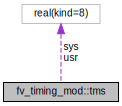
\includegraphics[width=158pt]{structfv__timing__mod_1_1tms__coll__graph}
\end{center}
\end{figure}
\subsection*{Public Attributes}
\begin{DoxyCompactItemize}
\item 
real(kind=8) \hyperlink{structfv__timing__mod_1_1tms_ab3e73d47d65260a7e032e6800def553d}{usr}
\item 
real(kind=8) \hyperlink{structfv__timing__mod_1_1tms_a59dd213f4d775f1dec2c09b15eac0f07}{sys}
\end{DoxyCompactItemize}


\subsection{Detailed Description}


Definition at line 62 of file fv\-\_\-timing.\-F90.



\subsection{Member Data Documentation}
\index{fv\-\_\-timing\-\_\-mod\-::tms@{fv\-\_\-timing\-\_\-mod\-::tms}!sys@{sys}}
\index{sys@{sys}!fv_timing_mod::tms@{fv\-\_\-timing\-\_\-mod\-::tms}}
\subsubsection[{sys}]{\setlength{\rightskip}{0pt plus 5cm}real (kind=8) fv\-\_\-timing\-\_\-mod\-::tms\-::sys}\label{structfv__timing__mod_1_1tms_a59dd213f4d775f1dec2c09b15eac0f07}


Definition at line 64 of file fv\-\_\-timing.\-F90.

\index{fv\-\_\-timing\-\_\-mod\-::tms@{fv\-\_\-timing\-\_\-mod\-::tms}!usr@{usr}}
\index{usr@{usr}!fv_timing_mod::tms@{fv\-\_\-timing\-\_\-mod\-::tms}}
\subsubsection[{usr}]{\setlength{\rightskip}{0pt plus 5cm}real (kind=8) fv\-\_\-timing\-\_\-mod\-::tms\-::usr}\label{structfv__timing__mod_1_1tms_ab3e73d47d65260a7e032e6800def553d}


Definition at line 64 of file fv\-\_\-timing.\-F90.



The documentation for this type was generated from the following file\-:\begin{DoxyCompactItemize}
\item 
/scratch2/\-N\-A\-G\-A\-P\-E/aoml-\/hafs1/\-Kyle.\-Ahern/acs\-\_\-master\-\_\-readonly/tools/\hyperlink{fv__timing_8F90}{fv\-\_\-timing.\-F90}\end{DoxyCompactItemize}

\section{tp\-\_\-core\-\_\-mod Module Reference}
\label{classtp__core__mod}\index{tp\-\_\-core\-\_\-mod@{tp\-\_\-core\-\_\-mod}}


The module 'tp\-\_\-core' is a collection of routines to support F\-V transport.  




Collaboration diagram for tp\-\_\-core\-\_\-mod\-:
\nopagebreak
\begin{figure}[H]
\begin{center}
\leavevmode
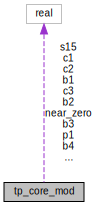
\includegraphics[width=133pt]{classtp__core__mod__coll__graph}
\end{center}
\end{figure}
\subsection*{Public Member Functions}
\begin{DoxyCompactItemize}
\item 
subroutine, public \hyperlink{classtp__core__mod_a9f509ba0cc0327529ea3178fccc590b2}{fv\-\_\-tp\-\_\-2d} (q, crx, cry, npx, npy, hord, fx, fy, xfx, yfx, gridstruct, bd, ra\-\_\-x, ra\-\_\-y, lim\-\_\-fac, regional, mfx, mfy, mass, nord, damp\-\_\-c)
\begin{DoxyCompactList}\small\item\em The subroutine 'fv\-\_\-tp\-\_\-2d' contains the F\-V advection scheme \cite{putman2007finite} \cite{lin1996multiflux}. \end{DoxyCompactList}\item 
subroutine, public \hyperlink{classtp__core__mod_aaa4f5a41e80dd1b45bd71a420e943b69}{copy\-\_\-corners} (q, npx, npy, dir, nested, bd, sw\-\_\-corner, se\-\_\-corner, nw\-\_\-corner, ne\-\_\-corner)
\item 
subroutine, public \hyperlink{classtp__core__mod_a9767d0f0c59231cb9896304f8882b2d9}{pert\-\_\-ppm} (im, a0, al, ar, iv)
\end{DoxyCompactItemize}
\subsection*{Private Member Functions}
\begin{DoxyCompactItemize}
\item 
subroutine \hyperlink{classtp__core__mod_a7ec727af882851e702692aaaad20d434}{xppm} (flux, q, c, iord, is, ie, isd, ied, jfirst, jlast, jsd, jed, npx, npy, dxa, nested, grid\-\_\-type, lim\-\_\-fac, regional)
\item 
subroutine \hyperlink{classtp__core__mod_a9073439bc45fc6fbce10103b11db0951}{yppm} (flux, q, c, jord, ifirst, ilast, isd, ied, js, je, jsd, jed, npx, npy, dya, nested, grid\-\_\-type, lim\-\_\-fac, regional)
\item 
subroutine \hyperlink{classtp__core__mod_a58585827528851ef8b46a3e4ca3a0bea}{mp\-\_\-ghost\-\_\-ew} (im, jm, km, nq, ifirst, ilast, jfirst, jlast, kfirst, klast, ng\-\_\-w, ng\-\_\-e, ng\-\_\-s, ng\-\_\-n, q\-\_\-ghst, q)
\item 
subroutine \hyperlink{classtp__core__mod_ae78fe02f1372d88fede1c00f6ae3567c}{deln\-\_\-flux} (nord, is, ie, js, je, npx, npy, damp, q, fx, fy, gridstruct, regional, bd, mass)
\end{DoxyCompactItemize}
\subsection*{Private Attributes}
\begin{DoxyCompactItemize}
\item 
real, parameter \hyperlink{classtp__core__mod_a39a84861aa5da93b744b78115c51961a}{ppm\-\_\-fac} = 1.\-5
\begin{DoxyCompactList}\small\item\em nonlinear scheme limiter\-: between 1 and 2 \end{DoxyCompactList}\item 
real, parameter \hyperlink{classtp__core__mod_ac6e3f3772126b08884ee0df1afe3897d}{r3} = 1./3.
\item 
real, parameter \hyperlink{classtp__core__mod_ad41545dca954897d2750ebd81663ba71}{near\-\_\-zero} = 1.E-\/25
\item 
real, parameter \hyperlink{classtp__core__mod_a0b1f38c1d0fc65b85d98a3b12e8bde0a}{ppm\-\_\-limiter} = 2.\-0
\item 
real, parameter \hyperlink{classtp__core__mod_ae2f7d92361a24ace46bb016d2fb637f7}{b1} = 1./30.
\item 
real, parameter \hyperlink{classtp__core__mod_af2c562b8f5f1323c0370471cad118c1b}{b2} = -\/13./60.
\item 
real, parameter \hyperlink{classtp__core__mod_a00dd6f4661e442eb30d04d8f11500a95}{b3} = -\/13./60.
\item 
real, parameter \hyperlink{classtp__core__mod_ad99c7da817a0f40d730b20e3db7cc3af}{b4} = 0.\-45
\item 
real, parameter \hyperlink{classtp__core__mod_a22ee5d4e802fbdee793cd3cf2d976281}{b5} = -\/0.\-05
\item 
real, parameter \hyperlink{classtp__core__mod_aaad141ba3705e5defdbaa59ece28c51f}{t11} = 27./28.
\item 
real, parameter \hyperlink{classtp__core__mod_a5f8e8b3c382dd0f93a01a0968b4d290c}{t12} = -\/13./28.
\item 
real, parameter \hyperlink{classtp__core__mod_a84fa887f4b8538ed2c628be08aeea165}{t13} =3./7.
\item 
real, parameter \hyperlink{classtp__core__mod_a01eb84f706485179c2638d9e625923b3}{s11} = 11./14.
\item 
real, parameter \hyperlink{classtp__core__mod_a3e606f8de1699c471fdb95289df0e033}{s14} = 4./7.
\item 
real, parameter \hyperlink{classtp__core__mod_aa0b566db71890d0741be14cb78f1b803}{s15} =3./14.
\item 
real, parameter \hyperlink{classtp__core__mod_accd5faf945b761ae9fc99e13da661ad1}{c1} = -\/2./14.
\item 
real, parameter \hyperlink{classtp__core__mod_adddfe0165d9a77d9906f1427c27269a9}{c2} = 11./14.
\item 
real, parameter \hyperlink{classtp__core__mod_a4c4814e6fd884b9c244aa403c391d56a}{c3} = 5./14.
\item 
real, parameter \hyperlink{classtp__core__mod_aa0a4ae3e2a26b88120205e9f7080910e}{p1} = 7./12.
\item 
real, parameter \hyperlink{classtp__core__mod_a110229a82e4ca9f5a8a56f464291b7b4}{p2} = -\/1./12.
\end{DoxyCompactItemize}


\subsection{Detailed Description}
The module 'tp\-\_\-core' is a collection of routines to support F\-V transport. 

The module contains the scalar advection scheme and P\-P\-M operators. 

Definition at line 24 of file tp\-\_\-core.\-F90.



\subsection{Member Function/\-Subroutine Documentation}
\index{tp\-\_\-core\-\_\-mod@{tp\-\_\-core\-\_\-mod}!copy\-\_\-corners@{copy\-\_\-corners}}
\index{copy\-\_\-corners@{copy\-\_\-corners}!tp_core_mod@{tp\-\_\-core\-\_\-mod}}
\subsubsection[{copy\-\_\-corners}]{\setlength{\rightskip}{0pt plus 5cm}subroutine, public tp\-\_\-core\-\_\-mod\-::copy\-\_\-corners (
\begin{DoxyParamCaption}
\item[{real, dimension(bd\%isd\-:bd\%ied,bd\%jsd\-:bd\%jed), intent(inout)}]{q, }
\item[{integer, intent(in)}]{npx, }
\item[{integer, intent(in)}]{npy, }
\item[{integer, intent(in)}]{dir, }
\item[{logical, intent(in)}]{nested, }
\item[{type(fv\-\_\-grid\-\_\-bounds\-\_\-type), intent(in)}]{bd, }
\item[{logical, intent(in)}]{sw\-\_\-corner, }
\item[{logical, intent(in)}]{se\-\_\-corner, }
\item[{logical, intent(in)}]{nw\-\_\-corner, }
\item[{logical, intent(in)}]{ne\-\_\-corner}
\end{DoxyParamCaption}
)}\label{classtp__core__mod_aaa4f5a41e80dd1b45bd71a420e943b69}


Definition at line 246 of file tp\-\_\-core.\-F90.



Referenced by dyn\-\_\-core\-\_\-mod\-::del2\-\_\-cubed(), fv\-\_\-nwp\-\_\-nudge\-\_\-mod\-::del2\-\_\-scalar(), sw\-\_\-core\-\_\-mod\-::del6\-\_\-vt\-\_\-flux(), deln\-\_\-flux(), and fv\-\_\-tp\-\_\-2d().

\index{tp\-\_\-core\-\_\-mod@{tp\-\_\-core\-\_\-mod}!deln\-\_\-flux@{deln\-\_\-flux}}
\index{deln\-\_\-flux@{deln\-\_\-flux}!tp_core_mod@{tp\-\_\-core\-\_\-mod}}
\subsubsection[{deln\-\_\-flux}]{\setlength{\rightskip}{0pt plus 5cm}subroutine tp\-\_\-core\-\_\-mod\-::deln\-\_\-flux (
\begin{DoxyParamCaption}
\item[{integer, intent(in)}]{nord, }
\item[{integer, intent(in)}]{is, }
\item[{integer, intent(in)}]{ie, }
\item[{integer, intent(in)}]{js, }
\item[{integer, intent(in)}]{je, }
\item[{integer, intent(in)}]{npx, }
\item[{integer, intent(in)}]{npy, }
\item[{real, intent(in)}]{damp, }
\item[{real, dimension(bd\%is-\/ng\-:bd\%ie+ng, bd\%js-\/ng\-:bd\%je+ng), intent(in)}]{q, }
\item[{real, dimension(bd\%is\-:bd\%ie+1,bd\%js\-:bd\%je), intent(inout)}]{fx, }
\item[{real, dimension(bd\%is\-:bd\%ie,bd\%js\-:bd\%je+1), intent(inout)}]{fy, }
\item[{type(fv\-\_\-grid\-\_\-type), intent(in), target}]{gridstruct, }
\item[{logical, intent(in)}]{regional, }
\item[{type(fv\-\_\-grid\-\_\-bounds\-\_\-type), intent(in)}]{bd, }
\item[{real, dimension(bd\%isd\-:bd\%ied, bd\%jsd\-:bd\%jed), intent(in), optional}]{mass}
\end{DoxyParamCaption}
)\hspace{0.3cm}{\ttfamily [private]}}\label{classtp__core__mod_ae78fe02f1372d88fede1c00f6ae3567c}

\begin{DoxyParams}[1]{Parameters}
\mbox{\tt in}  & {\em bd} & nord = 0\-: del-\/2 nord = 1\-: del-\/4 nord = 2\-: del-\/6 nord = 3\-: del-\/8 --$>$ requires more ghosting than current\\
\hline
\mbox{\tt in}  & {\em nord} & del-\/n \\
\hline
\end{DoxyParams}


Definition at line 1089 of file tp\-\_\-core.\-F90.



References copy\-\_\-corners().



Referenced by fv\-\_\-tp\-\_\-2d().

\index{tp\-\_\-core\-\_\-mod@{tp\-\_\-core\-\_\-mod}!fv\-\_\-tp\-\_\-2d@{fv\-\_\-tp\-\_\-2d}}
\index{fv\-\_\-tp\-\_\-2d@{fv\-\_\-tp\-\_\-2d}!tp_core_mod@{tp\-\_\-core\-\_\-mod}}
\subsubsection[{fv\-\_\-tp\-\_\-2d}]{\setlength{\rightskip}{0pt plus 5cm}subroutine, public tp\-\_\-core\-\_\-mod\-::fv\-\_\-tp\-\_\-2d (
\begin{DoxyParamCaption}
\item[{real, dimension(bd\%isd\-:bd\%ied,bd\%jsd\-:bd\%jed), intent(inout)}]{q, }
\item[{real, dimension(bd\%is\-:bd\%ie+1,bd\%jsd\-:bd\%jed), intent(in)}]{crx, }
\item[{real, dimension(bd\%isd\-:bd\%ied,bd\%js\-:bd\%je+1 ), intent(in)}]{cry, }
\item[{integer, intent(in)}]{npx, }
\item[{integer, intent(in)}]{npy, }
\item[{integer, intent(in)}]{hord, }
\item[{real, dimension(bd\%is\-:bd\%ie+1 ,bd\%js\-:bd\%je), intent(out)}]{fx, }
\item[{real, dimension(bd\%is\-:bd\%ie,   bd\%js\-:bd\%je+1 ), intent(out)}]{fy, }
\item[{real, dimension(bd\%is\-:bd\%ie+1,bd\%jsd\-:bd\%jed), intent(in)}]{xfx, }
\item[{real, dimension(bd\%isd\-:bd\%ied,bd\%js\-:bd\%je+1 ), intent(in)}]{yfx, }
\item[{type(fv\-\_\-grid\-\_\-type), intent(in), target}]{gridstruct, }
\item[{type(fv\-\_\-grid\-\_\-bounds\-\_\-type), intent(in)}]{bd, }
\item[{real, dimension(bd\%is\-:bd\%ie,bd\%jsd\-:bd\%jed), intent(in)}]{ra\-\_\-x, }
\item[{real, dimension(bd\%isd\-:bd\%ied,bd\%js\-:bd\%je), intent(in)}]{ra\-\_\-y, }
\item[{real, intent(in)}]{lim\-\_\-fac, }
\item[{logical, intent(in)}]{regional, }
\item[{real, dimension(bd\%is\-:bd\%ie+1,bd\%js\-:bd\%je  ), intent(in), optional}]{mfx, }
\item[{real, dimension(bd\%is\-:bd\%ie  ,bd\%js\-:bd\%je+1), intent(in), optional}]{mfy, }
\item[{real, dimension(bd\%isd\-:bd\%ied,bd\%jsd\-:bd\%jed), intent(in), optional}]{mass, }
\item[{integer, intent(in), optional}]{nord, }
\item[{real, intent(in), optional}]{damp\-\_\-c}
\end{DoxyParamCaption}
)}\label{classtp__core__mod_a9f509ba0cc0327529ea3178fccc590b2}


The subroutine 'fv\-\_\-tp\-\_\-2d' contains the F\-V advection scheme \cite{putman2007finite} \cite{lin1996multiflux}. 

It performs 1 time step of the forward advection.


\begin{DoxyParams}[1]{Parameters}
\mbox{\tt in,out}  & {\em q} & transported scalar\\
\hline
\mbox{\tt out}  & {\em fx} & Flux in x ( E )\\
\hline
\mbox{\tt out}  & {\em fy} & Flux in y ( N )\\
\hline
\mbox{\tt in}  & {\em mfx} & Mass Flux X-\/\-Dir\\
\hline
\mbox{\tt in}  & {\em mfy} & Mass Flux Y-\/\-Dir\\
\hline
\mbox{\tt in}  & {\em nord} & order of divergence damping \\
\hline
\end{DoxyParams}


Definition at line 108 of file tp\-\_\-core.\-F90.



References copy\-\_\-corners(), deln\-\_\-flux(), xppm(), and yppm().



Referenced by sw\-\_\-core\-\_\-mod\-::d\-\_\-sw(), fv\-\_\-tracer2d\-\_\-mod\-::tracer\-\_\-2d(), fv\-\_\-tracer2d\-\_\-mod\-::tracer\-\_\-2d\-\_\-1l(), fv\-\_\-tracer2d\-\_\-mod\-::tracer\-\_\-2d\-\_\-nested(), and nh\-\_\-utils\-\_\-mod\-::update\-\_\-dz\-\_\-d().

\index{tp\-\_\-core\-\_\-mod@{tp\-\_\-core\-\_\-mod}!mp\-\_\-ghost\-\_\-ew@{mp\-\_\-ghost\-\_\-ew}}
\index{mp\-\_\-ghost\-\_\-ew@{mp\-\_\-ghost\-\_\-ew}!tp_core_mod@{tp\-\_\-core\-\_\-mod}}
\subsubsection[{mp\-\_\-ghost\-\_\-ew}]{\setlength{\rightskip}{0pt plus 5cm}subroutine tp\-\_\-core\-\_\-mod\-::mp\-\_\-ghost\-\_\-ew (
\begin{DoxyParamCaption}
\item[{integer, intent(in)}]{im, }
\item[{integer, intent(in)}]{jm, }
\item[{integer, intent(in)}]{km, }
\item[{integer, intent(in)}]{nq, }
\item[{integer, intent(in)}]{ifirst, }
\item[{integer, intent(in)}]{ilast, }
\item[{integer, intent(in)}]{jfirst, }
\item[{integer, intent(in)}]{jlast, }
\item[{integer, intent(in)}]{kfirst, }
\item[{integer, intent(in)}]{klast, }
\item[{integer, intent(in)}]{ng\-\_\-w, }
\item[{integer, intent(in)}]{ng\-\_\-e, }
\item[{integer, intent(in)}]{ng\-\_\-s, }
\item[{integer, intent(in)}]{ng\-\_\-n, }
\item[{real, dimension(ifirst-\/ng\-\_\-w\-:ilast+ng\-\_\-e,jfirst-\/ng\-\_\-s\-:jlast+ng\-\_\-n,kfirst\-:klast,nq), intent(inout)}]{q\-\_\-ghst, }
\item[{real, dimension(ifirst\-:ilast,jfirst\-:jlast,kfirst\-:klast,nq), intent(in), optional}]{q}
\end{DoxyParamCaption}
)\hspace{0.3cm}{\ttfamily [private]}}\label{classtp__core__mod_a58585827528851ef8b46a3e4ca3a0bea}

\begin{DoxyParams}[1]{Parameters}
\mbox{\tt in}  & {\em ng\-\_\-e} & eastern zones to ghost\\
\hline
\mbox{\tt in}  & {\em ng\-\_\-w} & western zones to ghost\\
\hline
\mbox{\tt in}  & {\em ng\-\_\-s} & southern zones to ghost\\
\hline
\mbox{\tt in}  & {\em ng\-\_\-n} & northern zones to ghost \\
\hline
\end{DoxyParams}


Definition at line 977 of file tp\-\_\-core.\-F90.



Referenced by test\-\_\-cases\-\_\-mod\-::d2a2c().

\index{tp\-\_\-core\-\_\-mod@{tp\-\_\-core\-\_\-mod}!pert\-\_\-ppm@{pert\-\_\-ppm}}
\index{pert\-\_\-ppm@{pert\-\_\-ppm}!tp_core_mod@{tp\-\_\-core\-\_\-mod}}
\subsubsection[{pert\-\_\-ppm}]{\setlength{\rightskip}{0pt plus 5cm}subroutine, public tp\-\_\-core\-\_\-mod\-::pert\-\_\-ppm (
\begin{DoxyParamCaption}
\item[{integer, intent(in)}]{im, }
\item[{real, dimension(im), intent(in)}]{a0, }
\item[{real, dimension(im), intent(inout)}]{al, }
\item[{real, dimension(im), intent(inout)}]{ar, }
\item[{integer, intent(in)}]{iv}
\end{DoxyParamCaption}
)}\label{classtp__core__mod_a9767d0f0c59231cb9896304f8882b2d9}


Definition at line 1027 of file tp\-\_\-core.\-F90.



Referenced by xppm(), sw\-\_\-core\-\_\-mod\-::xtp\-\_\-u(), yppm(), and sw\-\_\-core\-\_\-mod\-::ytp\-\_\-v().

\index{tp\-\_\-core\-\_\-mod@{tp\-\_\-core\-\_\-mod}!xppm@{xppm}}
\index{xppm@{xppm}!tp_core_mod@{tp\-\_\-core\-\_\-mod}}
\subsubsection[{xppm}]{\setlength{\rightskip}{0pt plus 5cm}subroutine tp\-\_\-core\-\_\-mod\-::xppm (
\begin{DoxyParamCaption}
\item[{real, dimension(is\-:ie+1,jfirst\-:jlast), intent(out)}]{flux, }
\item[{real, dimension(isd\-:ied,jfirst\-:jlast), intent(in)}]{q, }
\item[{real, dimension(is\-:ie+1,jfirst\-:jlast), intent(in)}]{c, }
\item[{integer, intent(in)}]{iord, }
\item[{integer, intent(in)}]{is, }
\item[{integer, intent(in)}]{ie, }
\item[{integer, intent(in)}]{isd, }
\item[{integer, intent(in)}]{ied, }
\item[{integer, intent(in)}]{jfirst, }
\item[{integer, intent(in)}]{jlast, }
\item[{integer, intent(in)}]{jsd, }
\item[{integer, intent(in)}]{jed, }
\item[{integer, intent(in)}]{npx, }
\item[{integer, intent(in)}]{npy, }
\item[{real, dimension(isd\-:ied,jsd\-:jed), intent(in)}]{dxa, }
\item[{logical, intent(in)}]{nested, }
\item[{integer, intent(in)}]{grid\-\_\-type, }
\item[{real, intent(in)}]{lim\-\_\-fac, }
\item[{logical, intent(in)}]{regional}
\end{DoxyParamCaption}
)\hspace{0.3cm}{\ttfamily [private]}}\label{classtp__core__mod_a7ec727af882851e702692aaaad20d434}

\begin{DoxyParams}[1]{Parameters}
\mbox{\tt in}  & {\em jlast} & compute domain\\
\hline
\mbox{\tt in}  & {\em c} & Courant N (like F\-L\-U\-X)\\
\hline
\mbox{\tt out}  & {\em flux} & Flux \\
\hline
\end{DoxyParams}


Definition at line 323 of file tp\-\_\-core.\-F90.



References pert\-\_\-ppm().



Referenced by fv\-\_\-tp\-\_\-2d().

\index{tp\-\_\-core\-\_\-mod@{tp\-\_\-core\-\_\-mod}!yppm@{yppm}}
\index{yppm@{yppm}!tp_core_mod@{tp\-\_\-core\-\_\-mod}}
\subsubsection[{yppm}]{\setlength{\rightskip}{0pt plus 5cm}subroutine tp\-\_\-core\-\_\-mod\-::yppm (
\begin{DoxyParamCaption}
\item[{real, dimension(ifirst\-:ilast,js\-:je+1), intent(out)}]{flux, }
\item[{real, dimension(ifirst\-:ilast,jsd\-:jed), intent(in)}]{q, }
\item[{real, dimension(isd\-:ied,js\-:je+1 ), intent(in)}]{c, }
\item[{integer, intent(in)}]{jord, }
\item[{integer, intent(in)}]{ifirst, }
\item[{integer, intent(in)}]{ilast, }
\item[{integer, intent(in)}]{isd, }
\item[{integer, intent(in)}]{ied, }
\item[{integer, intent(in)}]{js, }
\item[{integer, intent(in)}]{je, }
\item[{integer, intent(in)}]{jsd, }
\item[{integer, intent(in)}]{jed, }
\item[{integer, intent(in)}]{npx, }
\item[{integer, intent(in)}]{npy, }
\item[{real, dimension(isd\-:ied,jsd\-:jed), intent(in)}]{dya, }
\item[{logical, intent(in)}]{nested, }
\item[{integer, intent(in)}]{grid\-\_\-type, }
\item[{real, intent(in)}]{lim\-\_\-fac, }
\item[{logical, intent(in)}]{regional}
\end{DoxyParamCaption}
)\hspace{0.3cm}{\ttfamily [private]}}\label{classtp__core__mod_a9073439bc45fc6fbce10103b11db0951}

\begin{DoxyParams}[1]{Parameters}
\mbox{\tt in}  & {\em ilast} & Compute domain\\
\hline
\mbox{\tt in}  & {\em c} & Courant number\\
\hline
\mbox{\tt out}  & {\em flux} & Flux \\
\hline
\end{DoxyParams}


Definition at line 632 of file tp\-\_\-core.\-F90.



References pert\-\_\-ppm().



Referenced by fv\-\_\-tp\-\_\-2d().



\subsection{Member Data Documentation}
\index{tp\-\_\-core\-\_\-mod@{tp\-\_\-core\-\_\-mod}!b1@{b1}}
\index{b1@{b1}!tp_core_mod@{tp\-\_\-core\-\_\-mod}}
\subsubsection[{b1}]{\setlength{\rightskip}{0pt plus 5cm}real, parameter tp\-\_\-core\-\_\-mod\-::b1 = 1./30.\hspace{0.3cm}{\ttfamily [private]}}\label{classtp__core__mod_ae2f7d92361a24ace46bb016d2fb637f7}


Definition at line 76 of file tp\-\_\-core.\-F90.

\index{tp\-\_\-core\-\_\-mod@{tp\-\_\-core\-\_\-mod}!b2@{b2}}
\index{b2@{b2}!tp_core_mod@{tp\-\_\-core\-\_\-mod}}
\subsubsection[{b2}]{\setlength{\rightskip}{0pt plus 5cm}real, parameter tp\-\_\-core\-\_\-mod\-::b2 = -\/13./60.\hspace{0.3cm}{\ttfamily [private]}}\label{classtp__core__mod_af2c562b8f5f1323c0370471cad118c1b}


Definition at line 77 of file tp\-\_\-core.\-F90.

\index{tp\-\_\-core\-\_\-mod@{tp\-\_\-core\-\_\-mod}!b3@{b3}}
\index{b3@{b3}!tp_core_mod@{tp\-\_\-core\-\_\-mod}}
\subsubsection[{b3}]{\setlength{\rightskip}{0pt plus 5cm}real, parameter tp\-\_\-core\-\_\-mod\-::b3 = -\/13./60.\hspace{0.3cm}{\ttfamily [private]}}\label{classtp__core__mod_a00dd6f4661e442eb30d04d8f11500a95}


Definition at line 78 of file tp\-\_\-core.\-F90.

\index{tp\-\_\-core\-\_\-mod@{tp\-\_\-core\-\_\-mod}!b4@{b4}}
\index{b4@{b4}!tp_core_mod@{tp\-\_\-core\-\_\-mod}}
\subsubsection[{b4}]{\setlength{\rightskip}{0pt plus 5cm}real, parameter tp\-\_\-core\-\_\-mod\-::b4 = 0.\-45\hspace{0.3cm}{\ttfamily [private]}}\label{classtp__core__mod_ad99c7da817a0f40d730b20e3db7cc3af}


Definition at line 79 of file tp\-\_\-core.\-F90.

\index{tp\-\_\-core\-\_\-mod@{tp\-\_\-core\-\_\-mod}!b5@{b5}}
\index{b5@{b5}!tp_core_mod@{tp\-\_\-core\-\_\-mod}}
\subsubsection[{b5}]{\setlength{\rightskip}{0pt plus 5cm}real, parameter tp\-\_\-core\-\_\-mod\-::b5 = -\/0.\-05\hspace{0.3cm}{\ttfamily [private]}}\label{classtp__core__mod_a22ee5d4e802fbdee793cd3cf2d976281}


Definition at line 80 of file tp\-\_\-core.\-F90.

\index{tp\-\_\-core\-\_\-mod@{tp\-\_\-core\-\_\-mod}!c1@{c1}}
\index{c1@{c1}!tp_core_mod@{tp\-\_\-core\-\_\-mod}}
\subsubsection[{c1}]{\setlength{\rightskip}{0pt plus 5cm}real, parameter tp\-\_\-core\-\_\-mod\-::c1 = -\/2./14.\hspace{0.3cm}{\ttfamily [private]}}\label{classtp__core__mod_accd5faf945b761ae9fc99e13da661ad1}


Definition at line 88 of file tp\-\_\-core.\-F90.

\index{tp\-\_\-core\-\_\-mod@{tp\-\_\-core\-\_\-mod}!c2@{c2}}
\index{c2@{c2}!tp_core_mod@{tp\-\_\-core\-\_\-mod}}
\subsubsection[{c2}]{\setlength{\rightskip}{0pt plus 5cm}real, parameter tp\-\_\-core\-\_\-mod\-::c2 = 11./14.\hspace{0.3cm}{\ttfamily [private]}}\label{classtp__core__mod_adddfe0165d9a77d9906f1427c27269a9}


Definition at line 89 of file tp\-\_\-core.\-F90.

\index{tp\-\_\-core\-\_\-mod@{tp\-\_\-core\-\_\-mod}!c3@{c3}}
\index{c3@{c3}!tp_core_mod@{tp\-\_\-core\-\_\-mod}}
\subsubsection[{c3}]{\setlength{\rightskip}{0pt plus 5cm}real, parameter tp\-\_\-core\-\_\-mod\-::c3 = 5./14.\hspace{0.3cm}{\ttfamily [private]}}\label{classtp__core__mod_a4c4814e6fd884b9c244aa403c391d56a}


Definition at line 90 of file tp\-\_\-core.\-F90.

\index{tp\-\_\-core\-\_\-mod@{tp\-\_\-core\-\_\-mod}!near\-\_\-zero@{near\-\_\-zero}}
\index{near\-\_\-zero@{near\-\_\-zero}!tp_core_mod@{tp\-\_\-core\-\_\-mod}}
\subsubsection[{near\-\_\-zero}]{\setlength{\rightskip}{0pt plus 5cm}real, parameter tp\-\_\-core\-\_\-mod\-::near\-\_\-zero = 1.E-\/25\hspace{0.3cm}{\ttfamily [private]}}\label{classtp__core__mod_ad41545dca954897d2750ebd81663ba71}


Definition at line 63 of file tp\-\_\-core.\-F90.

\index{tp\-\_\-core\-\_\-mod@{tp\-\_\-core\-\_\-mod}!p1@{p1}}
\index{p1@{p1}!tp_core_mod@{tp\-\_\-core\-\_\-mod}}
\subsubsection[{p1}]{\setlength{\rightskip}{0pt plus 5cm}real, parameter tp\-\_\-core\-\_\-mod\-::p1 = 7./12.\hspace{0.3cm}{\ttfamily [private]}}\label{classtp__core__mod_aa0a4ae3e2a26b88120205e9f7080910e}


Definition at line 94 of file tp\-\_\-core.\-F90.

\index{tp\-\_\-core\-\_\-mod@{tp\-\_\-core\-\_\-mod}!p2@{p2}}
\index{p2@{p2}!tp_core_mod@{tp\-\_\-core\-\_\-mod}}
\subsubsection[{p2}]{\setlength{\rightskip}{0pt plus 5cm}real, parameter tp\-\_\-core\-\_\-mod\-::p2 = -\/1./12.\hspace{0.3cm}{\ttfamily [private]}}\label{classtp__core__mod_a110229a82e4ca9f5a8a56f464291b7b4}


Definition at line 95 of file tp\-\_\-core.\-F90.

\index{tp\-\_\-core\-\_\-mod@{tp\-\_\-core\-\_\-mod}!ppm\-\_\-fac@{ppm\-\_\-fac}}
\index{ppm\-\_\-fac@{ppm\-\_\-fac}!tp_core_mod@{tp\-\_\-core\-\_\-mod}}
\subsubsection[{ppm\-\_\-fac}]{\setlength{\rightskip}{0pt plus 5cm}real, parameter tp\-\_\-core\-\_\-mod\-::ppm\-\_\-fac = 1.\-5\hspace{0.3cm}{\ttfamily [private]}}\label{classtp__core__mod_a39a84861aa5da93b744b78115c51961a}


nonlinear scheme limiter\-: between 1 and 2 



Definition at line 61 of file tp\-\_\-core.\-F90.

\index{tp\-\_\-core\-\_\-mod@{tp\-\_\-core\-\_\-mod}!ppm\-\_\-limiter@{ppm\-\_\-limiter}}
\index{ppm\-\_\-limiter@{ppm\-\_\-limiter}!tp_core_mod@{tp\-\_\-core\-\_\-mod}}
\subsubsection[{ppm\-\_\-limiter}]{\setlength{\rightskip}{0pt plus 5cm}real, parameter tp\-\_\-core\-\_\-mod\-::ppm\-\_\-limiter = 2.\-0\hspace{0.3cm}{\ttfamily [private]}}\label{classtp__core__mod_a0b1f38c1d0fc65b85d98a3b12e8bde0a}


Definition at line 64 of file tp\-\_\-core.\-F90.

\index{tp\-\_\-core\-\_\-mod@{tp\-\_\-core\-\_\-mod}!r3@{r3}}
\index{r3@{r3}!tp_core_mod@{tp\-\_\-core\-\_\-mod}}
\subsubsection[{r3}]{\setlength{\rightskip}{0pt plus 5cm}real, parameter tp\-\_\-core\-\_\-mod\-::r3 = 1./3.\hspace{0.3cm}{\ttfamily [private]}}\label{classtp__core__mod_ac6e3f3772126b08884ee0df1afe3897d}


Definition at line 62 of file tp\-\_\-core.\-F90.

\index{tp\-\_\-core\-\_\-mod@{tp\-\_\-core\-\_\-mod}!s11@{s11}}
\index{s11@{s11}!tp_core_mod@{tp\-\_\-core\-\_\-mod}}
\subsubsection[{s11}]{\setlength{\rightskip}{0pt plus 5cm}real, parameter tp\-\_\-core\-\_\-mod\-::s11 = 11./14.\hspace{0.3cm}{\ttfamily [private]}}\label{classtp__core__mod_a01eb84f706485179c2638d9e625923b3}


Definition at line 83 of file tp\-\_\-core.\-F90.

\index{tp\-\_\-core\-\_\-mod@{tp\-\_\-core\-\_\-mod}!s14@{s14}}
\index{s14@{s14}!tp_core_mod@{tp\-\_\-core\-\_\-mod}}
\subsubsection[{s14}]{\setlength{\rightskip}{0pt plus 5cm}real, parameter tp\-\_\-core\-\_\-mod\-::s14 = 4./7.\hspace{0.3cm}{\ttfamily [private]}}\label{classtp__core__mod_a3e606f8de1699c471fdb95289df0e033}


Definition at line 83 of file tp\-\_\-core.\-F90.

\index{tp\-\_\-core\-\_\-mod@{tp\-\_\-core\-\_\-mod}!s15@{s15}}
\index{s15@{s15}!tp_core_mod@{tp\-\_\-core\-\_\-mod}}
\subsubsection[{s15}]{\setlength{\rightskip}{0pt plus 5cm}real, parameter tp\-\_\-core\-\_\-mod\-::s15 =3./14.\hspace{0.3cm}{\ttfamily [private]}}\label{classtp__core__mod_aa0b566db71890d0741be14cb78f1b803}


Definition at line 83 of file tp\-\_\-core.\-F90.

\index{tp\-\_\-core\-\_\-mod@{tp\-\_\-core\-\_\-mod}!t11@{t11}}
\index{t11@{t11}!tp_core_mod@{tp\-\_\-core\-\_\-mod}}
\subsubsection[{t11}]{\setlength{\rightskip}{0pt plus 5cm}real, parameter tp\-\_\-core\-\_\-mod\-::t11 = 27./28.\hspace{0.3cm}{\ttfamily [private]}}\label{classtp__core__mod_aaad141ba3705e5defdbaa59ece28c51f}


Definition at line 82 of file tp\-\_\-core.\-F90.

\index{tp\-\_\-core\-\_\-mod@{tp\-\_\-core\-\_\-mod}!t12@{t12}}
\index{t12@{t12}!tp_core_mod@{tp\-\_\-core\-\_\-mod}}
\subsubsection[{t12}]{\setlength{\rightskip}{0pt plus 5cm}real, parameter tp\-\_\-core\-\_\-mod\-::t12 = -\/13./28.\hspace{0.3cm}{\ttfamily [private]}}\label{classtp__core__mod_a5f8e8b3c382dd0f93a01a0968b4d290c}


Definition at line 82 of file tp\-\_\-core.\-F90.

\index{tp\-\_\-core\-\_\-mod@{tp\-\_\-core\-\_\-mod}!t13@{t13}}
\index{t13@{t13}!tp_core_mod@{tp\-\_\-core\-\_\-mod}}
\subsubsection[{t13}]{\setlength{\rightskip}{0pt plus 5cm}real, parameter tp\-\_\-core\-\_\-mod\-::t13 =3./7.\hspace{0.3cm}{\ttfamily [private]}}\label{classtp__core__mod_a84fa887f4b8538ed2c628be08aeea165}


Definition at line 82 of file tp\-\_\-core.\-F90.



The documentation for this module was generated from the following file\-:\begin{DoxyCompactItemize}
\item 
/scratch2/\-N\-A\-G\-A\-P\-E/aoml-\/hafs1/\-Kyle.\-Ahern/acs\-\_\-master\-\_\-readonly/model/\hyperlink{tp__core_8F90}{tp\-\_\-core.\-F90}\end{DoxyCompactItemize}

\section{boundary\-\_\-mod\-:\-:update\-\_\-coarse\-\_\-grid Interface Reference}
\label{interfaceboundary__mod_1_1update__coarse__grid}\index{boundary\-\_\-mod\-::update\-\_\-coarse\-\_\-grid@{boundary\-\_\-mod\-::update\-\_\-coarse\-\_\-grid}}


The interface'update\-\_\-coarse\-\_\-grid\-\_\-mpp'contains subroutines that fetch data from the nested grid and interpolate it to the coarse grid using the method described by \cite{harris2013two}.  


\subsection*{Public Member Functions}
\begin{DoxyCompactItemize}
\item 
subroutine \hyperlink{interfaceboundary__mod_1_1update__coarse__grid_a6d38bb2a38da012a2464e7255edd6983}{update\-\_\-coarse\-\_\-grid\-\_\-mpp} (var\-\_\-coarse, var\-\_\-nest, nest\-\_\-domain, ind\-\_\-update, dx, dy, area, isd\-\_\-p, ied\-\_\-p, jsd\-\_\-p, jed\-\_\-p, is\-\_\-n, ie\-\_\-n, js\-\_\-n, je\-\_\-n, isu, ieu, jsu, jeu, npx, npy, npz, istag, jstag, r, nestupdate, upoff, nsponge, parent\-\_\-proc, child\-\_\-proc, parent\-\_\-grid)
\item 
subroutine \hyperlink{interfaceboundary__mod_1_1update__coarse__grid_a5a1f8f85dffe389683e8a41333195114}{update\-\_\-coarse\-\_\-grid\-\_\-mpp\-\_\-2d} (var\-\_\-coarse, var\-\_\-nest, nest\-\_\-domain, ind\-\_\-update, dx, dy, area, isd\-\_\-p, ied\-\_\-p, jsd\-\_\-p, jed\-\_\-p, is\-\_\-n, ie\-\_\-n, js\-\_\-n, je\-\_\-n, isu, ieu, jsu, jeu, npx, npy, istag, jstag, r, nestupdate, upoff, nsponge, parent\-\_\-proc, child\-\_\-proc, parent\-\_\-grid)
\end{DoxyCompactItemize}


\subsection{Detailed Description}
The interface'update\-\_\-coarse\-\_\-grid\-\_\-mpp'contains subroutines that fetch data from the nested grid and interpolate it to the coarse grid using the method described by \cite{harris2013two}. 

Definition at line 108 of file boundary.\-F90.



\subsection{Member Function/\-Subroutine Documentation}
\index{boundary\-\_\-mod\-::update\-\_\-coarse\-\_\-grid@{boundary\-\_\-mod\-::update\-\_\-coarse\-\_\-grid}!update\-\_\-coarse\-\_\-grid\-\_\-mpp@{update\-\_\-coarse\-\_\-grid\-\_\-mpp}}
\index{update\-\_\-coarse\-\_\-grid\-\_\-mpp@{update\-\_\-coarse\-\_\-grid\-\_\-mpp}!boundary_mod::update_coarse_grid@{boundary\-\_\-mod\-::update\-\_\-coarse\-\_\-grid}}
\subsubsection[{update\-\_\-coarse\-\_\-grid\-\_\-mpp}]{\setlength{\rightskip}{0pt plus 5cm}subroutine boundary\-\_\-mod\-::update\-\_\-coarse\-\_\-grid\-::update\-\_\-coarse\-\_\-grid\-\_\-mpp (
\begin{DoxyParamCaption}
\item[{real, dimension(isd\-\_\-p\-:ied\-\_\-p+istag,jsd\-\_\-p\-:jed\-\_\-p+jstag,npz), intent(inout)}]{var\-\_\-coarse, }
\item[{real, dimension(is\-\_\-n\-:ie\-\_\-n+istag,js\-\_\-n\-:je\-\_\-n+jstag,npz), intent(in)}]{var\-\_\-nest, }
\item[{type(nest\-\_\-domain\-\_\-type), intent(inout)}]{nest\-\_\-domain, }
\item[{integer, dimension(isd\-\_\-p\-:ied\-\_\-p+1,jsd\-\_\-p\-:jed\-\_\-p+1,2), intent(in)}]{ind\-\_\-update, }
\item[{real, dimension(isd\-:ied,jsd\-:jed+1), intent(in)}]{dx, }
\item[{real, dimension(isd\-:ied+1,jsd\-:jed), intent(in)}]{dy, }
\item[{real, dimension(isd\-:ied,jsd\-:jed), intent(in)}]{area, }
\item[{integer, intent(in)}]{isd\-\_\-p, }
\item[{integer, intent(in)}]{ied\-\_\-p, }
\item[{integer, intent(in)}]{jsd\-\_\-p, }
\item[{integer, intent(in)}]{jed\-\_\-p, }
\item[{integer, intent(in)}]{is\-\_\-n, }
\item[{integer, intent(in)}]{ie\-\_\-n, }
\item[{integer, intent(in)}]{js\-\_\-n, }
\item[{integer, intent(in)}]{je\-\_\-n, }
\item[{integer, intent(in)}]{isu, }
\item[{integer, intent(in)}]{ieu, }
\item[{integer, intent(in)}]{jsu, }
\item[{integer, intent(in)}]{jeu, }
\item[{integer, intent(in)}]{npx, }
\item[{integer, intent(in)}]{npy, }
\item[{integer, intent(in)}]{npz, }
\item[{integer, intent(in)}]{istag, }
\item[{integer, intent(in)}]{jstag, }
\item[{integer, intent(in)}]{r, }
\item[{integer, intent(in)}]{nestupdate, }
\item[{integer, intent(in)}]{upoff, }
\item[{integer, intent(in)}]{nsponge, }
\item[{logical, intent(in)}]{parent\-\_\-proc, }
\item[{logical, intent(in)}]{child\-\_\-proc, }
\item[{type(fv\-\_\-atmos\-\_\-type), intent(inout)}]{parent\-\_\-grid}
\end{DoxyParamCaption}
)}\label{interfaceboundary__mod_1_1update__coarse__grid_a6d38bb2a38da012a2464e7255edd6983}


Definition at line 1833 of file boundary.\-F90.



Referenced by boundary\-\_\-mod\-::update\-\_\-coarse\-\_\-grid\-\_\-mpp\-\_\-2d().

\index{boundary\-\_\-mod\-::update\-\_\-coarse\-\_\-grid@{boundary\-\_\-mod\-::update\-\_\-coarse\-\_\-grid}!update\-\_\-coarse\-\_\-grid\-\_\-mpp\-\_\-2d@{update\-\_\-coarse\-\_\-grid\-\_\-mpp\-\_\-2d}}
\index{update\-\_\-coarse\-\_\-grid\-\_\-mpp\-\_\-2d@{update\-\_\-coarse\-\_\-grid\-\_\-mpp\-\_\-2d}!boundary_mod::update_coarse_grid@{boundary\-\_\-mod\-::update\-\_\-coarse\-\_\-grid}}
\subsubsection[{update\-\_\-coarse\-\_\-grid\-\_\-mpp\-\_\-2d}]{\setlength{\rightskip}{0pt plus 5cm}subroutine boundary\-\_\-mod\-::update\-\_\-coarse\-\_\-grid\-::update\-\_\-coarse\-\_\-grid\-\_\-mpp\-\_\-2d (
\begin{DoxyParamCaption}
\item[{real, dimension(isd\-\_\-p\-:ied\-\_\-p+istag,jsd\-\_\-p\-:jed\-\_\-p+jstag), intent(inout)}]{var\-\_\-coarse, }
\item[{real, dimension(is\-\_\-n\-:ie\-\_\-n+istag,js\-\_\-n\-:je\-\_\-n+jstag), intent(in)}]{var\-\_\-nest, }
\item[{type(nest\-\_\-domain\-\_\-type), intent(inout)}]{nest\-\_\-domain, }
\item[{integer, dimension(isd\-\_\-p\-:ied\-\_\-p+1,jsd\-\_\-p\-:jed\-\_\-p+1,2), intent(in)}]{ind\-\_\-update, }
\item[{real, dimension(isd\-:ied,jsd\-:jed+1), intent(in)}]{dx, }
\item[{real, dimension(isd\-:ied+1,jsd\-:jed), intent(in)}]{dy, }
\item[{real, dimension(isd\-:ied,jsd\-:jed), intent(in)}]{area, }
\item[{integer, intent(in)}]{isd\-\_\-p, }
\item[{integer, intent(in)}]{ied\-\_\-p, }
\item[{integer, intent(in)}]{jsd\-\_\-p, }
\item[{integer, intent(in)}]{jed\-\_\-p, }
\item[{integer, intent(in)}]{is\-\_\-n, }
\item[{integer, intent(in)}]{ie\-\_\-n, }
\item[{integer, intent(in)}]{js\-\_\-n, }
\item[{integer, intent(in)}]{je\-\_\-n, }
\item[{integer, intent(in)}]{isu, }
\item[{integer, intent(in)}]{ieu, }
\item[{integer, intent(in)}]{jsu, }
\item[{integer, intent(in)}]{jeu, }
\item[{integer, intent(in)}]{npx, }
\item[{integer, intent(in)}]{npy, }
\item[{integer, intent(in)}]{istag, }
\item[{integer, intent(in)}]{jstag, }
\item[{integer, intent(in)}]{r, }
\item[{integer, intent(in)}]{nestupdate, }
\item[{integer, intent(in)}]{upoff, }
\item[{integer, intent(in)}]{nsponge, }
\item[{logical, intent(in)}]{parent\-\_\-proc, }
\item[{logical, intent(in)}]{child\-\_\-proc, }
\item[{type(fv\-\_\-atmos\-\_\-type), intent(inout)}]{parent\-\_\-grid}
\end{DoxyParamCaption}
)}\label{interfaceboundary__mod_1_1update__coarse__grid_a5a1f8f85dffe389683e8a41333195114}


Definition at line 1797 of file boundary.\-F90.



The documentation for this interface was generated from the following file\-:\begin{DoxyCompactItemize}
\item 
/scratch2/\-N\-A\-G\-A\-P\-E/aoml-\/hafs1/\-Kyle.\-Ahern/acs\-\_\-master\-\_\-readonly/model/\hyperlink{boundary_8F90}{boundary.\-F90}\end{DoxyCompactItemize}

\section{dycore\-\_\-typedefs\-:\-:var\-\_\-subtype Type Reference}
\label{structdycore__typedefs_1_1var__subtype}\index{dycore\-\_\-typedefs\-::var\-\_\-subtype@{dycore\-\_\-typedefs\-::var\-\_\-subtype}}


Collaboration diagram for dycore\-\_\-typedefs\-:\-:var\-\_\-subtype\-:
\nopagebreak
\begin{figure}[H]
\begin{center}
\leavevmode
\includegraphics[width=162pt]{structdycore__typedefs_1_1var__subtype__coll__graph}
\end{center}
\end{figure}
\subsection*{Public Attributes}
\begin{DoxyCompactItemize}
\item 
real(kind=r8\-\_\-kind), dimension(\-:), \\*
pointer \hyperlink{structdycore__typedefs_1_1var__subtype_ae7f1321cbe3f9c0f1cf24af0e39bb2c6}{var2p} =$>$ null()
\begin{DoxyCompactList}\small\item\em 2\-D data saved in packed format \mbox{[}dim(ix)\mbox{]} \end{DoxyCompactList}\item 
real(kind=r8\-\_\-kind), dimension(\-:,\-:), \\*
pointer \hyperlink{structdycore__typedefs_1_1var__subtype_af3e57f945956db4f682481b4aeb5d11f}{var3p} =$>$ null()
\begin{DoxyCompactList}\small\item\em 3\-D data saved in packed format \mbox{[}dim(ix,levs)\mbox{]} \end{DoxyCompactList}\end{DoxyCompactItemize}


\subsection{Detailed Description}


Definition at line 32 of file D\-Y\-C\-O\-R\-E\-\_\-typedefs.\-F90.



\subsection{Member Data Documentation}
\index{dycore\-\_\-typedefs\-::var\-\_\-subtype@{dycore\-\_\-typedefs\-::var\-\_\-subtype}!var2p@{var2p}}
\index{var2p@{var2p}!dycore_typedefs::var_subtype@{dycore\-\_\-typedefs\-::var\-\_\-subtype}}
\subsubsection[{var2p}]{\setlength{\rightskip}{0pt plus 5cm}real(kind=r8\-\_\-kind), dimension(\-:), pointer dycore\-\_\-typedefs\-::var\-\_\-subtype\-::var2p =$>$ null()}\label{structdycore__typedefs_1_1var__subtype_ae7f1321cbe3f9c0f1cf24af0e39bb2c6}


2\-D data saved in packed format \mbox{[}dim(ix)\mbox{]} 



Definition at line 33 of file D\-Y\-C\-O\-R\-E\-\_\-typedefs.\-F90.

\index{dycore\-\_\-typedefs\-::var\-\_\-subtype@{dycore\-\_\-typedefs\-::var\-\_\-subtype}!var3p@{var3p}}
\index{var3p@{var3p}!dycore_typedefs::var_subtype@{dycore\-\_\-typedefs\-::var\-\_\-subtype}}
\subsubsection[{var3p}]{\setlength{\rightskip}{0pt plus 5cm}real(kind=r8\-\_\-kind), dimension(\-:,\-:), pointer dycore\-\_\-typedefs\-::var\-\_\-subtype\-::var3p =$>$ null()}\label{structdycore__typedefs_1_1var__subtype_af3e57f945956db4f682481b4aeb5d11f}


3\-D data saved in packed format \mbox{[}dim(ix,levs)\mbox{]} 



Definition at line 34 of file D\-Y\-C\-O\-R\-E\-\_\-typedefs.\-F90.



The documentation for this type was generated from the following file\-:\begin{DoxyCompactItemize}
\item 
/scratch2/\-N\-A\-G\-A\-P\-E/aoml-\/hafs1/\-Kyle.\-Ahern/acs\-\_\-master\-\_\-readonly/driver/fv\-G\-F\-S/\hyperlink{DYCORE__typedefs_8F90}{D\-Y\-C\-O\-R\-E\-\_\-typedefs.\-F90}\end{DoxyCompactItemize}

\chapter{File Documentation}
\section{/scratch2/\-N\-A\-G\-A\-P\-E/aoml-\/hafs1/\-Kyle.Ahern/acs\-\_\-master\-\_\-readonly/driver/fv\-G\-F\-S/atmosphere.F90 File Reference}
\label{atmosphere_8F90}\index{/scratch2/\-N\-A\-G\-A\-P\-E/aoml-\/hafs1/\-Kyle.\-Ahern/acs\-\_\-master\-\_\-readonly/driver/fv\-G\-F\-S/atmosphere.\-F90@{/scratch2/\-N\-A\-G\-A\-P\-E/aoml-\/hafs1/\-Kyle.\-Ahern/acs\-\_\-master\-\_\-readonly/driver/fv\-G\-F\-S/atmosphere.\-F90}}
{\ttfamily \#include $<$fms\-\_\-platform.\-h$>$}\\*
{\ttfamily \#include $<$file\-\_\-version.\-h$>$}\\*
\subsection*{Data Types}
\begin{DoxyCompactItemize}
\item 
module \hyperlink{classatmosphere__mod}{atmosphere\-\_\-mod}
\begin{DoxyCompactList}\small\item\em The module 'atmosphere' provides the interface for the Cubed-\/\-Sphere F\-V dynamical core. \end{DoxyCompactList}\end{DoxyCompactItemize}
\subsection*{Macros}
\begin{DoxyCompactItemize}
\item 
\#define \hyperlink{atmosphere_8F90_a0904a1b2ffbaabef0e4a637a204f9ee8}{\-\_\-\-D\-B\-L\-\_\-}(X)~X
\item 
\#define \hyperlink{atmosphere_8F90_a44be1b01add8a7fa3ec9582922e15c98}{\-\_\-\-R\-L\-\_\-}(X)~X
\end{DoxyCompactItemize}


\subsection{Macro Definition Documentation}
\index{atmosphere.\-F90@{atmosphere.\-F90}!\-\_\-\-D\-B\-L\-\_\-@{\-\_\-\-D\-B\-L\-\_\-}}
\index{\-\_\-\-D\-B\-L\-\_\-@{\-\_\-\-D\-B\-L\-\_\-}!atmosphere.F90@{atmosphere.\-F90}}
\subsubsection[{\-\_\-\-D\-B\-L\-\_\-}]{\setlength{\rightskip}{0pt plus 5cm}\#define \-\_\-\-D\-B\-L\-\_\-(
\begin{DoxyParamCaption}
\item[{}]{X}
\end{DoxyParamCaption}
)~X}\label{atmosphere_8F90_a0904a1b2ffbaabef0e4a637a204f9ee8}
\index{atmosphere.\-F90@{atmosphere.\-F90}!\-\_\-\-R\-L\-\_\-@{\-\_\-\-R\-L\-\_\-}}
\index{\-\_\-\-R\-L\-\_\-@{\-\_\-\-R\-L\-\_\-}!atmosphere.F90@{atmosphere.\-F90}}
\subsubsection[{\-\_\-\-R\-L\-\_\-}]{\setlength{\rightskip}{0pt plus 5cm}\#define \-\_\-\-R\-L\-\_\-(
\begin{DoxyParamCaption}
\item[{}]{X}
\end{DoxyParamCaption}
)~X}\label{atmosphere_8F90_a44be1b01add8a7fa3ec9582922e15c98}

\section{/scratch2/\-N\-A\-G\-A\-P\-E/aoml-\/hafs1/\-Kyle.Ahern/acs\-\_\-master\-\_\-readonly/driver/fv\-G\-F\-S/\-D\-Y\-C\-O\-R\-E\-\_\-typedefs.F90 File Reference}
\label{DYCORE__typedefs_8F90}\index{/scratch2/\-N\-A\-G\-A\-P\-E/aoml-\/hafs1/\-Kyle.\-Ahern/acs\-\_\-master\-\_\-readonly/driver/fv\-G\-F\-S/\-D\-Y\-C\-O\-R\-E\-\_\-typedefs.\-F90@{/scratch2/\-N\-A\-G\-A\-P\-E/aoml-\/hafs1/\-Kyle.\-Ahern/acs\-\_\-master\-\_\-readonly/driver/fv\-G\-F\-S/\-D\-Y\-C\-O\-R\-E\-\_\-typedefs.\-F90}}
\subsection*{Data Types}
\begin{DoxyCompactItemize}
\item 
module \hyperlink{classdycore__typedefs}{dycore\-\_\-typedefs}
\item 
type \hyperlink{structdycore__typedefs_1_1var__subtype}{dycore\-\_\-typedefs\-::var\-\_\-subtype}
\item 
type \hyperlink{structdycore__typedefs_1_1dycore__coupling__type}{dycore\-\_\-typedefs\-::dycore\-\_\-coupling\-\_\-type}
\item 
type \hyperlink{structdycore__typedefs_1_1dycore__diag__type}{dycore\-\_\-typedefs\-::dycore\-\_\-diag\-\_\-type}
\item 
type \hyperlink{structdycore__typedefs_1_1dycore__data__type}{dycore\-\_\-typedefs\-::dycore\-\_\-data\-\_\-type}
\end{DoxyCompactItemize}

\section{/scratch2/\-N\-A\-G\-A\-P\-E/aoml-\/hafs1/\-Kyle.Ahern/acs\-\_\-master\-\_\-readonly/driver/fv\-G\-F\-S/fv\-\_\-nggps\-\_\-diag.F90 File Reference}
\label{fv__nggps__diag_8F90}\index{/scratch2/\-N\-A\-G\-A\-P\-E/aoml-\/hafs1/\-Kyle.\-Ahern/acs\-\_\-master\-\_\-readonly/driver/fv\-G\-F\-S/fv\-\_\-nggps\-\_\-diag.\-F90@{/scratch2/\-N\-A\-G\-A\-P\-E/aoml-\/hafs1/\-Kyle.\-Ahern/acs\-\_\-master\-\_\-readonly/driver/fv\-G\-F\-S/fv\-\_\-nggps\-\_\-diag.\-F90}}
\subsection*{Data Types}
\begin{DoxyCompactItemize}
\item 
module \hyperlink{classfv__nggps__diags__mod}{fv\-\_\-nggps\-\_\-diags\-\_\-mod}
\begin{DoxyCompactList}\small\item\em The module 'fv\-\_\-nggps\-\_\-diags' computes output diagnostics entirely on 3\-D pressure levels. \end{DoxyCompactList}\end{DoxyCompactItemize}

\section{/scratch2/\-N\-A\-G\-A\-P\-E/aoml-\/hafs1/\-Kyle.Ahern/acs\-\_\-master\-\_\-readonly/model/a2b\-\_\-edge.F90 File Reference}
\label{a2b__edge_8F90}\index{/scratch2/\-N\-A\-G\-A\-P\-E/aoml-\/hafs1/\-Kyle.\-Ahern/acs\-\_\-master\-\_\-readonly/model/a2b\-\_\-edge.\-F90@{/scratch2/\-N\-A\-G\-A\-P\-E/aoml-\/hafs1/\-Kyle.\-Ahern/acs\-\_\-master\-\_\-readonly/model/a2b\-\_\-edge.\-F90}}
\subsection*{Data Types}
\begin{DoxyCompactItemize}
\item 
module \hyperlink{classa2b__edge__mod}{a2b\-\_\-edge\-\_\-mod}
\begin{DoxyCompactList}\small\item\em The module 'a2b\-\_\-edge' performs F\-V-\/consistent interpolation of pressure to corners. \end{DoxyCompactList}\end{DoxyCompactItemize}

\section{/scratch2/\-N\-A\-G\-A\-P\-E/aoml-\/hafs1/\-Kyle.Ahern/acs\-\_\-master\-\_\-readonly/model/boundary.F90 File Reference}
\label{boundary_8F90}\index{/scratch2/\-N\-A\-G\-A\-P\-E/aoml-\/hafs1/\-Kyle.\-Ahern/acs\-\_\-master\-\_\-readonly/model/boundary.\-F90@{/scratch2/\-N\-A\-G\-A\-P\-E/aoml-\/hafs1/\-Kyle.\-Ahern/acs\-\_\-master\-\_\-readonly/model/boundary.\-F90}}
\subsection*{Data Types}
\begin{DoxyCompactItemize}
\item 
module \hyperlink{classboundary__mod}{boundary\-\_\-mod}
\begin{DoxyCompactList}\small\item\em The module 'boundary' contains utility routines for grid nesting and boundary conditions. \end{DoxyCompactList}\item 
interface \hyperlink{interfaceboundary__mod_1_1nested__grid__bc}{boundary\-\_\-mod\-::nested\-\_\-grid\-\_\-bc}
\begin{DoxyCompactList}\small\item\em interface 'nested\-\_\-grid\-\_\-\-B\-C' includes subroutines 'nested\-\_\-grid\-\_\-\-B\-C\-\_\-2d' and 'nested\-\_\-grid\-\_\-\-B\-C\-\_\-3d' that fetch coarse-\/grid data, interpolate it to nested-\/grid boundary cells, apply the interpolated data directly to the boundary halo cells without saving the datatype. \end{DoxyCompactList}\item 
interface \hyperlink{interfaceboundary__mod_1_1fill__nested__grid}{boundary\-\_\-mod\-::fill\-\_\-nested\-\_\-grid}
\begin{DoxyCompactList}\small\item\em The interface '\hyperlink{interfaceboundary__mod_1_1fill__nested__grid}{fill\-\_\-nested\-\_\-grid}' includes subroutines 'fill\-\_\-nested\-\_\-grid\-\_\-2d' and 'fill\-\_\-nested\-\_\-grid\-\_\-3d' that fill nested-\/grid data with interpolated data from the coarse grid. \end{DoxyCompactList}\item 
interface \hyperlink{interfaceboundary__mod_1_1update__coarse__grid}{boundary\-\_\-mod\-::update\-\_\-coarse\-\_\-grid}
\begin{DoxyCompactList}\small\item\em The interface'update\-\_\-coarse\-\_\-grid\-\_\-mpp'contains subroutines that fetch data from the nested grid and interpolate it to the coarse grid using the method described by \cite{harris2013two}. \end{DoxyCompactList}\end{DoxyCompactItemize}

\section{/scratch2/\-N\-A\-G\-A\-P\-E/aoml-\/hafs1/\-Kyle.Ahern/acs\-\_\-master\-\_\-readonly/model/dyn\-\_\-core.F90 File Reference}
\label{dyn__core_8F90}\index{/scratch2/\-N\-A\-G\-A\-P\-E/aoml-\/hafs1/\-Kyle.\-Ahern/acs\-\_\-master\-\_\-readonly/model/dyn\-\_\-core.\-F90@{/scratch2/\-N\-A\-G\-A\-P\-E/aoml-\/hafs1/\-Kyle.\-Ahern/acs\-\_\-master\-\_\-readonly/model/dyn\-\_\-core.\-F90}}
\subsection*{Data Types}
\begin{DoxyCompactItemize}
\item 
module \hyperlink{classdyn__core__mod}{dyn\-\_\-core\-\_\-mod}
\begin{DoxyCompactList}\small\item\em The module 'dyn\-\_\-core' peforms the Lagrangian acoustic dynamics described by \cite{lin2004vertically}. \end{DoxyCompactList}\end{DoxyCompactItemize}

\section{/scratch2/\-N\-A\-G\-A\-P\-E/aoml-\/hafs1/\-Kyle.Ahern/acs\-\_\-master\-\_\-readonly/model/fv\-\_\-arrays.F90 File Reference}
\label{fv__arrays_8F90}\index{/scratch2/\-N\-A\-G\-A\-P\-E/aoml-\/hafs1/\-Kyle.\-Ahern/acs\-\_\-master\-\_\-readonly/model/fv\-\_\-arrays.\-F90@{/scratch2/\-N\-A\-G\-A\-P\-E/aoml-\/hafs1/\-Kyle.\-Ahern/acs\-\_\-master\-\_\-readonly/model/fv\-\_\-arrays.\-F90}}
{\ttfamily \#include $<$fms\-\_\-platform.\-h$>$}\\*
\subsection*{Data Types}
\begin{DoxyCompactItemize}
\item 
module \hyperlink{classfv__arrays__mod}{fv\-\_\-arrays\-\_\-mod}
\begin{DoxyCompactList}\small\item\em The module 'fv\-\_\-arrays' contains the '\hyperlink{structfv__arrays__mod_1_1fv__atmos__type}{fv\-\_\-atmos\-\_\-type}' and associated datatypes. \end{DoxyCompactList}\item 
type \hyperlink{structfv__arrays__mod_1_1fv__diag__type}{fv\-\_\-arrays\-\_\-mod\-::fv\-\_\-diag\-\_\-type}
\item 
type \hyperlink{structfv__arrays__mod_1_1fv__grid__type}{fv\-\_\-arrays\-\_\-mod\-::fv\-\_\-grid\-\_\-type}
\begin{DoxyCompactList}\small\item\em The type '\hyperlink{structfv__arrays__mod_1_1fv__grid__type}{fv\-\_\-grid\-\_\-type}' is made up of grid-\/dependent information from fv\-\_\-grid\-\_\-tools and fv\-\_\-grid\-\_\-utils. \end{DoxyCompactList}\item 
type \hyperlink{structfv__arrays__mod_1_1fv__flags__type}{fv\-\_\-arrays\-\_\-mod\-::fv\-\_\-flags\-\_\-type}
\item 
type \hyperlink{structfv__arrays__mod_1_1fv__nest__bc__type__3d}{fv\-\_\-arrays\-\_\-mod\-::fv\-\_\-nest\-\_\-bc\-\_\-type\-\_\-3d}
\item 
type \hyperlink{structfv__arrays__mod_1_1fv__nest__bc__type__4d}{fv\-\_\-arrays\-\_\-mod\-::fv\-\_\-nest\-\_\-bc\-\_\-type\-\_\-4d}
\item 
type \hyperlink{structfv__arrays__mod_1_1fv__nest__type}{fv\-\_\-arrays\-\_\-mod\-::fv\-\_\-nest\-\_\-type}
\item 
interface \hyperlink{interfacefv__arrays__mod_1_1allocate__fv__nest__bc__type}{fv\-\_\-arrays\-\_\-mod\-::allocate\-\_\-fv\-\_\-nest\-\_\-bc\-\_\-type}
\begin{DoxyCompactList}\small\item\em 'allocate\-\_\-fv\-\_\-nest\-\_\-\-B\-C\-\_\-type' is an interface to subroutines that allocate the 'fv\-\_\-nest\-\_\-\-B\-C\-\_\-type' structure that holds the nested-\/grid B\-Cs. \end{DoxyCompactList}\item 
interface \hyperlink{interfacefv__arrays__mod_1_1deallocate__fv__nest__bc__type}{fv\-\_\-arrays\-\_\-mod\-::deallocate\-\_\-fv\-\_\-nest\-\_\-bc\-\_\-type}
\begin{DoxyCompactList}\small\item\em 'deallocate\-\_\-fv\-\_\-nest\-\_\-\-B\-C\-\_\-type' is an interface to a subroutine that deallocates the 'fv\-\_\-nest\-\_\-\-B\-C\-\_\-type' structure that holds the nested-\/grid B\-Cs. \end{DoxyCompactList}\item 
type \hyperlink{structfv__arrays__mod_1_1fv__grid__bounds__type}{fv\-\_\-arrays\-\_\-mod\-::fv\-\_\-grid\-\_\-bounds\-\_\-type}
\item 
type \hyperlink{structfv__arrays__mod_1_1fv__regional__bc__bounds__type}{fv\-\_\-arrays\-\_\-mod\-::fv\-\_\-regional\-\_\-bc\-\_\-bounds\-\_\-type}
\item 
type \hyperlink{structfv__arrays__mod_1_1fv__atmos__type}{fv\-\_\-arrays\-\_\-mod\-::fv\-\_\-atmos\-\_\-type}
\end{DoxyCompactItemize}

\section{/scratch2/\-N\-A\-G\-A\-P\-E/aoml-\/hafs1/\-Kyle.Ahern/acs\-\_\-master\-\_\-readonly/model/fv\-\_\-cmp.F90 File Reference}
\label{fv__cmp_8F90}\index{/scratch2/\-N\-A\-G\-A\-P\-E/aoml-\/hafs1/\-Kyle.\-Ahern/acs\-\_\-master\-\_\-readonly/model/fv\-\_\-cmp.\-F90@{/scratch2/\-N\-A\-G\-A\-P\-E/aoml-\/hafs1/\-Kyle.\-Ahern/acs\-\_\-master\-\_\-readonly/model/fv\-\_\-cmp.\-F90}}
\subsection*{Data Types}
\begin{DoxyCompactItemize}
\item 
module \hyperlink{classfv__cmp__mod}{fv\-\_\-cmp\-\_\-mod}
\begin{DoxyCompactList}\small\item\em The module 'fv\-\_\-cmp' implements the fast procesesses in the G\-F\-D\-L microphysics $>$ \end{DoxyCompactList}\end{DoxyCompactItemize}

\section{/scratch2/\-N\-A\-G\-A\-P\-E/aoml-\/hafs1/\-Kyle.Ahern/acs\-\_\-master\-\_\-readonly/model/fv\-\_\-control.F90 File Reference}
\label{fv__control_8F90}\index{/scratch2/\-N\-A\-G\-A\-P\-E/aoml-\/hafs1/\-Kyle.\-Ahern/acs\-\_\-master\-\_\-readonly/model/fv\-\_\-control.\-F90@{/scratch2/\-N\-A\-G\-A\-P\-E/aoml-\/hafs1/\-Kyle.\-Ahern/acs\-\_\-master\-\_\-readonly/model/fv\-\_\-control.\-F90}}
{\ttfamily \#include $<$file\-\_\-version.\-h$>$}\\*
\subsection*{Data Types}
\begin{DoxyCompactItemize}
\item 
module \hyperlink{classfv__control__mod}{fv\-\_\-control\-\_\-mod}
\begin{DoxyCompactList}\small\item\em The module 'F\-V3\-\_\-control' is for initialization and termination of the model, and controls namelist parameters in F\-V3. \end{DoxyCompactList}\end{DoxyCompactItemize}

\section{/scratch2/\-N\-A\-G\-A\-P\-E/aoml-\/hafs1/\-Kyle.Ahern/acs\-\_\-master\-\_\-readonly/model/fv\-\_\-dynamics.F90 File Reference}
\label{fv__dynamics_8F90}\index{/scratch2/\-N\-A\-G\-A\-P\-E/aoml-\/hafs1/\-Kyle.\-Ahern/acs\-\_\-master\-\_\-readonly/model/fv\-\_\-dynamics.\-F90@{/scratch2/\-N\-A\-G\-A\-P\-E/aoml-\/hafs1/\-Kyle.\-Ahern/acs\-\_\-master\-\_\-readonly/model/fv\-\_\-dynamics.\-F90}}
\subsection*{Data Types}
\begin{DoxyCompactItemize}
\item 
module \hyperlink{classfv__dynamics__mod}{fv\-\_\-dynamics\-\_\-mod}
\begin{DoxyCompactList}\small\item\em The module 'fv\-\_\-dynamics' is the top-\/level routine for the dynamical core. \end{DoxyCompactList}\end{DoxyCompactItemize}

\section{/scratch2/\-N\-A\-G\-A\-P\-E/aoml-\/hafs1/\-Kyle.Ahern/acs\-\_\-master\-\_\-readonly/model/fv\-\_\-fill.F90 File Reference}
\label{fv__fill_8F90}\index{/scratch2/\-N\-A\-G\-A\-P\-E/aoml-\/hafs1/\-Kyle.\-Ahern/acs\-\_\-master\-\_\-readonly/model/fv\-\_\-fill.\-F90@{/scratch2/\-N\-A\-G\-A\-P\-E/aoml-\/hafs1/\-Kyle.\-Ahern/acs\-\_\-master\-\_\-readonly/model/fv\-\_\-fill.\-F90}}
\subsection*{Data Types}
\begin{DoxyCompactItemize}
\item 
module \hyperlink{classfv__fill__mod}{fv\-\_\-fill\-\_\-mod}
\end{DoxyCompactItemize}

\section{/scratch2/\-N\-A\-G\-A\-P\-E/aoml-\/hafs1/\-Kyle.Ahern/acs\-\_\-master\-\_\-readonly/model/fv\-\_\-grid\-\_\-utils.F90 File Reference}
\label{fv__grid__utils_8F90}\index{/scratch2/\-N\-A\-G\-A\-P\-E/aoml-\/hafs1/\-Kyle.\-Ahern/acs\-\_\-master\-\_\-readonly/model/fv\-\_\-grid\-\_\-utils.\-F90@{/scratch2/\-N\-A\-G\-A\-P\-E/aoml-\/hafs1/\-Kyle.\-Ahern/acs\-\_\-master\-\_\-readonly/model/fv\-\_\-grid\-\_\-utils.\-F90}}
{\ttfamily \#include $<$fms\-\_\-platform.\-h$>$}\\*
\subsection*{Data Types}
\begin{DoxyCompactItemize}
\item 
module \hyperlink{classfv__grid__utils__mod}{fv\-\_\-grid\-\_\-utils\-\_\-mod}
\begin{DoxyCompactList}\small\item\em The module 'fv\-\_\-grid\-\_\-utils' contains routines for setting up and computing grid-\/related quantities. \end{DoxyCompactList}\item 
interface \hyperlink{interfacefv__grid__utils__mod_1_1fill__ghost}{fv\-\_\-grid\-\_\-utils\-\_\-mod\-::fill\-\_\-ghost}
\end{DoxyCompactItemize}
\subsection*{Functions/\-Subroutines}
\begin{DoxyCompactItemize}
\item 
subroutine \hyperlink{fv__grid__utils_8F90_a44ab7367698357893ac8e593951be4e5}{get\-\_\-nearest} ()
\item 
subroutine \hyperlink{fv__grid__utils_8F90_ad57368c80b3a6eb85246900731f30e9a}{check\-\_\-local} (x1, x2, local)
\end{DoxyCompactItemize}


\subsection{Function/\-Subroutine Documentation}
\index{fv\-\_\-grid\-\_\-utils.\-F90@{fv\-\_\-grid\-\_\-utils.\-F90}!check\-\_\-local@{check\-\_\-local}}
\index{check\-\_\-local@{check\-\_\-local}!fv_grid_utils.F90@{fv\-\_\-grid\-\_\-utils.\-F90}}
\subsubsection[{check\-\_\-local}]{\setlength{\rightskip}{0pt plus 5cm}subroutine check\-\_\-local (
\begin{DoxyParamCaption}
\item[{real(kind=r\-\_\-grid), dimension(3), intent(in)}]{x1, }
\item[{real(kind=r\-\_\-grid), dimension(3), intent(in)}]{x2, }
\item[{logical, intent(out)}]{local}
\end{DoxyParamCaption}
)\hspace{0.3cm}{\ttfamily [private]}}\label{fv__grid__utils_8F90_ad57368c80b3a6eb85246900731f30e9a}


Definition at line 2132 of file fv\-\_\-grid\-\_\-utils.\-F90.



Referenced by fv\-\_\-grid\-\_\-utils\-\_\-mod\-::intersect(), and fv\-\_\-grid\-\_\-utils\-\_\-mod\-::intersect\-\_\-cross().

\index{fv\-\_\-grid\-\_\-utils.\-F90@{fv\-\_\-grid\-\_\-utils.\-F90}!get\-\_\-nearest@{get\-\_\-nearest}}
\index{get\-\_\-nearest@{get\-\_\-nearest}!fv_grid_utils.F90@{fv\-\_\-grid\-\_\-utils.\-F90}}
\subsubsection[{get\-\_\-nearest}]{\setlength{\rightskip}{0pt plus 5cm}subroutine get\-\_\-nearest (
\begin{DoxyParamCaption}
{}
\end{DoxyParamCaption}
)\hspace{0.3cm}{\ttfamily [private]}}\label{fv__grid__utils_8F90_a44ab7367698357893ac8e593951be4e5}


Definition at line 2118 of file fv\-\_\-grid\-\_\-utils.\-F90.



Referenced by fv\-\_\-grid\-\_\-utils\-\_\-mod\-::intersect(), and fv\-\_\-grid\-\_\-utils\-\_\-mod\-::intersect\-\_\-cross().


\section{/scratch2/\-N\-A\-G\-A\-P\-E/aoml-\/hafs1/\-Kyle.Ahern/acs\-\_\-master\-\_\-readonly/model/fv\-\_\-mapz.F90 File Reference}
\label{fv__mapz_8F90}\index{/scratch2/\-N\-A\-G\-A\-P\-E/aoml-\/hafs1/\-Kyle.\-Ahern/acs\-\_\-master\-\_\-readonly/model/fv\-\_\-mapz.\-F90@{/scratch2/\-N\-A\-G\-A\-P\-E/aoml-\/hafs1/\-Kyle.\-Ahern/acs\-\_\-master\-\_\-readonly/model/fv\-\_\-mapz.\-F90}}
\subsection*{Data Types}
\begin{DoxyCompactItemize}
\item 
module \hyperlink{classfv__mapz__mod}{fv\-\_\-mapz\-\_\-mod}
\begin{DoxyCompactList}\small\item\em The module 'fv\-\_\-mapz' contains the vertical mapping routines \cite{lin2004vertically}. \end{DoxyCompactList}\end{DoxyCompactItemize}

\section{/scratch2/\-N\-A\-G\-A\-P\-E/aoml-\/hafs1/\-Kyle.Ahern/acs\-\_\-master\-\_\-readonly/model/fv\-\_\-nesting.F90 File Reference}
\label{fv__nesting_8F90}\index{/scratch2/\-N\-A\-G\-A\-P\-E/aoml-\/hafs1/\-Kyle.\-Ahern/acs\-\_\-master\-\_\-readonly/model/fv\-\_\-nesting.\-F90@{/scratch2/\-N\-A\-G\-A\-P\-E/aoml-\/hafs1/\-Kyle.\-Ahern/acs\-\_\-master\-\_\-readonly/model/fv\-\_\-nesting.\-F90}}
\subsection*{Data Types}
\begin{DoxyCompactItemize}
\item 
module \hyperlink{classfv__nesting__mod}{fv\-\_\-nesting\-\_\-mod}
\begin{DoxyCompactList}\small\item\em The module 'fv\-\_\-nesting' is a collection of routines pertaining to grid nesting \cite{harris2013two}. \end{DoxyCompactList}\end{DoxyCompactItemize}

\section{/scratch2/\-N\-A\-G\-A\-P\-E/aoml-\/hafs1/\-Kyle.Ahern/acs\-\_\-master\-\_\-readonly/model/fv\-\_\-regional\-\_\-bc.F90 File Reference}
\label{fv__regional__bc_8F90}\index{/scratch2/\-N\-A\-G\-A\-P\-E/aoml-\/hafs1/\-Kyle.\-Ahern/acs\-\_\-master\-\_\-readonly/model/fv\-\_\-regional\-\_\-bc.\-F90@{/scratch2/\-N\-A\-G\-A\-P\-E/aoml-\/hafs1/\-Kyle.\-Ahern/acs\-\_\-master\-\_\-readonly/model/fv\-\_\-regional\-\_\-bc.\-F90}}
\subsection*{Data Types}
\begin{DoxyCompactItemize}
\item 
module \hyperlink{classfv__regional__mod}{fv\-\_\-regional\-\_\-mod}
\item 
type \hyperlink{structfv__regional__mod_1_1fv__regional__bc__variables}{fv\-\_\-regional\-\_\-mod\-::fv\-\_\-regional\-\_\-bc\-\_\-variables}
\item 
type \hyperlink{structfv__regional__mod_1_1fv__domain__sides}{fv\-\_\-regional\-\_\-mod\-::fv\-\_\-domain\-\_\-sides}
\item 
interface \hyperlink{interfacefv__regional__mod_1_1dump__field}{fv\-\_\-regional\-\_\-mod\-::dump\-\_\-field}
\end{DoxyCompactItemize}
\subsection*{Functions/\-Subroutines}
\begin{DoxyCompactItemize}
\item 
subroutine \hyperlink{fv__regional__bc_8F90_a638c4c6151ebbd4b5acbddf35746eb26}{compute\-\_\-regional\-\_\-bc\-\_\-indices} (regional\-\_\-bc\-\_\-bounds)
\item 
subroutine \hyperlink{fv__regional__bc_8F90_a09189d3b4fa4d19a5942bd7ff1cb26ec}{read\-\_\-regional\-\_\-lon\-\_\-lat}
\item 
subroutine \hyperlink{fv__regional__bc_8F90_a42821f6740373a4651a4eb14f8a8639b}{read\-\_\-regional\-\_\-filtered\-\_\-topo}
\item 
subroutine \hyperlink{fv__regional__bc_8F90_a500dc18823e751325f65a14ac026b531}{fill\-\_\-divgd\-\_\-bc}
\item 
subroutine \hyperlink{fv__regional__bc_8F90_a96cf4201092050374e4f866b1e36cb9a}{bc\-\_\-values\-\_\-into\-\_\-arrays} (side\-\_\-t0, side\-\_\-t1, side, i1, i2, j1, j2, i1\-\_\-uvs, i2\-\_\-uvs, j1\-\_\-uvs, j2\-\_\-uvs, i1\-\_\-uvw, i2\-\_\-uvw, j1\-\_\-uvw, j2\-\_\-uvw)
\item 
subroutine \hyperlink{fv__regional__bc_8F90_af7e4f6bf58503114a557595efd1eee24}{compute\-\_\-vpt}
\item 
subroutine \hyperlink{fv__regional__bc_8F90_a7e4db30594d915c5a1965b85476aea68}{get\-\_\-q00}
\end{DoxyCompactItemize}


\subsection{Function/\-Subroutine Documentation}
\index{fv\-\_\-regional\-\_\-bc.\-F90@{fv\-\_\-regional\-\_\-bc.\-F90}!bc\-\_\-values\-\_\-into\-\_\-arrays@{bc\-\_\-values\-\_\-into\-\_\-arrays}}
\index{bc\-\_\-values\-\_\-into\-\_\-arrays@{bc\-\_\-values\-\_\-into\-\_\-arrays}!fv_regional_bc.F90@{fv\-\_\-regional\-\_\-bc.\-F90}}
\subsubsection[{bc\-\_\-values\-\_\-into\-\_\-arrays}]{\setlength{\rightskip}{0pt plus 5cm}subroutine set\-\_\-regional\-\_\-bcs\-::bc\-\_\-values\-\_\-into\-\_\-arrays (
\begin{DoxyParamCaption}
\item[{type(fv\-\_\-regional\-\_\-bc\-\_\-variables), intent(in)}]{side\-\_\-t0, }
\item[{type(fv\-\_\-regional\-\_\-bc\-\_\-variables), intent(in)}]{side\-\_\-t1, }
\item[{character(len=$\ast$), intent(in)}]{side, }
\item[{integer, intent(in)}]{i1, }
\item[{integer, intent(in)}]{i2, }
\item[{integer, intent(in)}]{j1, }
\item[{integer, intent(in)}]{j2, }
\item[{integer, intent(in)}]{i1\-\_\-uvs, }
\item[{integer, intent(in)}]{i2\-\_\-uvs, }
\item[{integer, intent(in)}]{j1\-\_\-uvs, }
\item[{integer, intent(in)}]{j2\-\_\-uvs, }
\item[{integer, intent(in)}]{i1\-\_\-uvw, }
\item[{integer, intent(in)}]{i2\-\_\-uvw, }
\item[{integer, intent(in)}]{j1\-\_\-uvw, }
\item[{integer, intent(in)}]{j2\-\_\-uvw}
\end{DoxyParamCaption}
)\hspace{0.3cm}{\ttfamily [private]}}\label{fv__regional__bc_8F90_a96cf4201092050374e4f866b1e36cb9a}


Definition at line 3381 of file fv\-\_\-regional\-\_\-bc.\-F90.



Referenced by fv\-\_\-regional\-\_\-mod\-::set\-\_\-regional\-\_\-bcs().

\index{fv\-\_\-regional\-\_\-bc.\-F90@{fv\-\_\-regional\-\_\-bc.\-F90}!compute\-\_\-regional\-\_\-bc\-\_\-indices@{compute\-\_\-regional\-\_\-bc\-\_\-indices}}
\index{compute\-\_\-regional\-\_\-bc\-\_\-indices@{compute\-\_\-regional\-\_\-bc\-\_\-indices}!fv_regional_bc.F90@{fv\-\_\-regional\-\_\-bc.\-F90}}
\subsubsection[{compute\-\_\-regional\-\_\-bc\-\_\-indices}]{\setlength{\rightskip}{0pt plus 5cm}subroutine setup\-\_\-regional\-\_\-bc\-::compute\-\_\-regional\-\_\-bc\-\_\-indices (
\begin{DoxyParamCaption}
\item[{type(fv\-\_\-regional\-\_\-bc\-\_\-bounds\-\_\-type), intent(out)}]{regional\-\_\-bc\-\_\-bounds}
\end{DoxyParamCaption}
)}\label{fv__regional__bc_8F90_a638c4c6151ebbd4b5acbddf35746eb26}


Definition at line 616 of file fv\-\_\-regional\-\_\-bc.\-F90.



Referenced by fv\-\_\-regional\-\_\-mod\-::setup\-\_\-regional\-\_\-bc().

\index{fv\-\_\-regional\-\_\-bc.\-F90@{fv\-\_\-regional\-\_\-bc.\-F90}!compute\-\_\-vpt@{compute\-\_\-vpt}}
\index{compute\-\_\-vpt@{compute\-\_\-vpt}!fv_regional_bc.F90@{fv\-\_\-regional\-\_\-bc.\-F90}}
\subsubsection[{compute\-\_\-vpt}]{\setlength{\rightskip}{0pt plus 5cm}subroutine convert\-\_\-to\-\_\-virt\-\_\-pot\-\_\-temp\-::compute\-\_\-vpt (
\begin{DoxyParamCaption}
{}
\end{DoxyParamCaption}
)\hspace{0.3cm}{\ttfamily [private]}}\label{fv__regional__bc_8F90_af7e4f6bf58503114a557595efd1eee24}


Definition at line 4391 of file fv\-\_\-regional\-\_\-bc.\-F90.



Referenced by fv\-\_\-regional\-\_\-mod\-::convert\-\_\-to\-\_\-virt\-\_\-pot\-\_\-temp().

\index{fv\-\_\-regional\-\_\-bc.\-F90@{fv\-\_\-regional\-\_\-bc.\-F90}!fill\-\_\-divgd\-\_\-bc@{fill\-\_\-divgd\-\_\-bc}}
\index{fill\-\_\-divgd\-\_\-bc@{fill\-\_\-divgd\-\_\-bc}!fv_regional_bc.F90@{fv\-\_\-regional\-\_\-bc.\-F90}}
\subsubsection[{fill\-\_\-divgd\-\_\-bc}]{\setlength{\rightskip}{0pt plus 5cm}subroutine regional\-\_\-bc\-\_\-data\-::fill\-\_\-divgd\-\_\-bc (
\begin{DoxyParamCaption}
{}
\end{DoxyParamCaption}
)\hspace{0.3cm}{\ttfamily [private]}}\label{fv__regional__bc_8F90_a500dc18823e751325f65a14ac026b531}


Definition at line 1984 of file fv\-\_\-regional\-\_\-bc.\-F90.



Referenced by fv\-\_\-regional\-\_\-mod\-::regional\-\_\-bc\-\_\-data().

\index{fv\-\_\-regional\-\_\-bc.\-F90@{fv\-\_\-regional\-\_\-bc.\-F90}!get\-\_\-q00@{get\-\_\-q00}}
\index{get\-\_\-q00@{get\-\_\-q00}!fv_regional_bc.F90@{fv\-\_\-regional\-\_\-bc.\-F90}}
\subsubsection[{get\-\_\-q00}]{\setlength{\rightskip}{0pt plus 5cm}subroutine nudge\-\_\-qv\-\_\-bc\-::get\-\_\-q00 (
\begin{DoxyParamCaption}
{}
\end{DoxyParamCaption}
)\hspace{0.3cm}{\ttfamily [private]}}\label{fv__regional__bc_8F90_a7e4db30594d915c5a1965b85476aea68}


Definition at line 4745 of file fv\-\_\-regional\-\_\-bc.\-F90.



Referenced by fv\-\_\-regional\-\_\-mod\-::nudge\-\_\-qv\-\_\-bc().

\index{fv\-\_\-regional\-\_\-bc.\-F90@{fv\-\_\-regional\-\_\-bc.\-F90}!read\-\_\-regional\-\_\-filtered\-\_\-topo@{read\-\_\-regional\-\_\-filtered\-\_\-topo}}
\index{read\-\_\-regional\-\_\-filtered\-\_\-topo@{read\-\_\-regional\-\_\-filtered\-\_\-topo}!fv_regional_bc.F90@{fv\-\_\-regional\-\_\-bc.\-F90}}
\subsubsection[{read\-\_\-regional\-\_\-filtered\-\_\-topo}]{\setlength{\rightskip}{0pt plus 5cm}subroutine setup\-\_\-regional\-\_\-bc\-::read\-\_\-regional\-\_\-filtered\-\_\-topo (
\begin{DoxyParamCaption}
{}
\end{DoxyParamCaption}
)}\label{fv__regional__bc_8F90_a42821f6740373a4651a4eb14f8a8639b}


Definition at line 992 of file fv\-\_\-regional\-\_\-bc.\-F90.



References fv\-\_\-regional\-\_\-mod\-::check().



Referenced by fv\-\_\-regional\-\_\-mod\-::setup\-\_\-regional\-\_\-bc().

\index{fv\-\_\-regional\-\_\-bc.\-F90@{fv\-\_\-regional\-\_\-bc.\-F90}!read\-\_\-regional\-\_\-lon\-\_\-lat@{read\-\_\-regional\-\_\-lon\-\_\-lat}}
\index{read\-\_\-regional\-\_\-lon\-\_\-lat@{read\-\_\-regional\-\_\-lon\-\_\-lat}!fv_regional_bc.F90@{fv\-\_\-regional\-\_\-bc.\-F90}}
\subsubsection[{read\-\_\-regional\-\_\-lon\-\_\-lat}]{\setlength{\rightskip}{0pt plus 5cm}subroutine setup\-\_\-regional\-\_\-bc\-::read\-\_\-regional\-\_\-lon\-\_\-lat (
\begin{DoxyParamCaption}
{}
\end{DoxyParamCaption}
)\hspace{0.3cm}{\ttfamily [private]}}\label{fv__regional__bc_8F90_a09189d3b4fa4d19a5942bd7ff1cb26ec}


Definition at line 892 of file fv\-\_\-regional\-\_\-bc.\-F90.



References fv\-\_\-grid\-\_\-utils\-\_\-mod\-::cell\-\_\-center2(), and fv\-\_\-regional\-\_\-mod\-::check().



Referenced by fv\-\_\-regional\-\_\-mod\-::setup\-\_\-regional\-\_\-bc().


\section{/scratch2/\-N\-A\-G\-A\-P\-E/aoml-\/hafs1/\-Kyle.Ahern/acs\-\_\-master\-\_\-readonly/model/fv\-\_\-sg.F90 File Reference}
\label{fv__sg_8F90}\index{/scratch2/\-N\-A\-G\-A\-P\-E/aoml-\/hafs1/\-Kyle.\-Ahern/acs\-\_\-master\-\_\-readonly/model/fv\-\_\-sg.\-F90@{/scratch2/\-N\-A\-G\-A\-P\-E/aoml-\/hafs1/\-Kyle.\-Ahern/acs\-\_\-master\-\_\-readonly/model/fv\-\_\-sg.\-F90}}
\subsection*{Data Types}
\begin{DoxyCompactItemize}
\item 
module \hyperlink{classfv__sg__mod}{fv\-\_\-sg\-\_\-mod}
\begin{DoxyCompactList}\small\item\em The module 'fv\-\_\-sg' performs F\-V sub-\/grid mixing. \end{DoxyCompactList}\end{DoxyCompactItemize}

\section{/scratch2/\-N\-A\-G\-A\-P\-E/aoml-\/hafs1/\-Kyle.Ahern/acs\-\_\-master\-\_\-readonly/model/fv\-\_\-tracer2d.F90 File Reference}
\label{fv__tracer2d_8F90}\index{/scratch2/\-N\-A\-G\-A\-P\-E/aoml-\/hafs1/\-Kyle.\-Ahern/acs\-\_\-master\-\_\-readonly/model/fv\-\_\-tracer2d.\-F90@{/scratch2/\-N\-A\-G\-A\-P\-E/aoml-\/hafs1/\-Kyle.\-Ahern/acs\-\_\-master\-\_\-readonly/model/fv\-\_\-tracer2d.\-F90}}
\subsection*{Data Types}
\begin{DoxyCompactItemize}
\item 
module \hyperlink{classfv__tracer2d__mod}{fv\-\_\-tracer2d\-\_\-mod}
\begin{DoxyCompactList}\small\item\em The module '\hyperlink{fv__tracer2d_8F90}{fv\-\_\-tracer2d.\-F90}' performs sub-\/cycled tracer advection. \end{DoxyCompactList}\end{DoxyCompactItemize}

\section{/scratch2/\-N\-A\-G\-A\-P\-E/aoml-\/hafs1/\-Kyle.Ahern/acs\-\_\-master\-\_\-readonly/model/fv\-\_\-update\-\_\-phys.F90 File Reference}
\label{fv__update__phys_8F90}\index{/scratch2/\-N\-A\-G\-A\-P\-E/aoml-\/hafs1/\-Kyle.\-Ahern/acs\-\_\-master\-\_\-readonly/model/fv\-\_\-update\-\_\-phys.\-F90@{/scratch2/\-N\-A\-G\-A\-P\-E/aoml-\/hafs1/\-Kyle.\-Ahern/acs\-\_\-master\-\_\-readonly/model/fv\-\_\-update\-\_\-phys.\-F90}}
\subsection*{Data Types}
\begin{DoxyCompactItemize}
\item 
module \hyperlink{classfv__update__phys__mod}{fv\-\_\-update\-\_\-phys\-\_\-mod}
\begin{DoxyCompactList}\small\item\em The module 'fv\-\_\-update\-\_\-phys' applies physics tendencies consistent with the F\-V3 discretization and definition of the prognostic variables. \end{DoxyCompactList}\end{DoxyCompactItemize}

\section{/scratch2/\-N\-A\-G\-A\-P\-E/aoml-\/hafs1/\-Kyle.Ahern/acs\-\_\-master\-\_\-readonly/model/multi\-\_\-gases.F90 File Reference}
\label{multi__gases_8F90}\index{/scratch2/\-N\-A\-G\-A\-P\-E/aoml-\/hafs1/\-Kyle.\-Ahern/acs\-\_\-master\-\_\-readonly/model/multi\-\_\-gases.\-F90@{/scratch2/\-N\-A\-G\-A\-P\-E/aoml-\/hafs1/\-Kyle.\-Ahern/acs\-\_\-master\-\_\-readonly/model/multi\-\_\-gases.\-F90}}
\subsection*{Data Types}
\begin{DoxyCompactItemize}
\item 
module \hyperlink{classmulti__gases__mod}{multi\-\_\-gases\-\_\-mod}
\begin{DoxyCompactList}\small\item\em The module 'multi\-\_\-gases' peforms multi constitutents computations. \end{DoxyCompactList}\end{DoxyCompactItemize}

\section{/scratch2/\-N\-A\-G\-A\-P\-E/aoml-\/hafs1/\-Kyle.Ahern/acs\-\_\-master\-\_\-readonly/model/nh\-\_\-core.F90 File Reference}
\label{nh__core_8F90}\index{/scratch2/\-N\-A\-G\-A\-P\-E/aoml-\/hafs1/\-Kyle.\-Ahern/acs\-\_\-master\-\_\-readonly/model/nh\-\_\-core.\-F90@{/scratch2/\-N\-A\-G\-A\-P\-E/aoml-\/hafs1/\-Kyle.\-Ahern/acs\-\_\-master\-\_\-readonly/model/nh\-\_\-core.\-F90}}
\subsection*{Data Types}
\begin{DoxyCompactItemize}
\item 
module \hyperlink{classnh__core__mod}{nh\-\_\-core\-\_\-mod}
\begin{DoxyCompactList}\small\item\em The module 'nh\-\_\-core' peforms non-\/hydrostatic computations. \end{DoxyCompactList}\end{DoxyCompactItemize}

\section{/scratch2/\-N\-A\-G\-A\-P\-E/aoml-\/hafs1/\-Kyle.Ahern/acs\-\_\-master\-\_\-readonly/model/nh\-\_\-utils.F90 File Reference}
\label{nh__utils_8F90}\index{/scratch2/\-N\-A\-G\-A\-P\-E/aoml-\/hafs1/\-Kyle.\-Ahern/acs\-\_\-master\-\_\-readonly/model/nh\-\_\-utils.\-F90@{/scratch2/\-N\-A\-G\-A\-P\-E/aoml-\/hafs1/\-Kyle.\-Ahern/acs\-\_\-master\-\_\-readonly/model/nh\-\_\-utils.\-F90}}
\subsection*{Data Types}
\begin{DoxyCompactItemize}
\item 
module \hyperlink{classnh__utils__mod}{nh\-\_\-utils\-\_\-mod}
\begin{DoxyCompactList}\small\item\em The module 'nh\-\_\-utils' peforms non-\/hydrostatic computations. \end{DoxyCompactList}\end{DoxyCompactItemize}

\section{/scratch2/\-N\-A\-G\-A\-P\-E/aoml-\/hafs1/\-Kyle.Ahern/acs\-\_\-master\-\_\-readonly/model/sw\-\_\-core.F90 File Reference}
\label{sw__core_8F90}\index{/scratch2/\-N\-A\-G\-A\-P\-E/aoml-\/hafs1/\-Kyle.\-Ahern/acs\-\_\-master\-\_\-readonly/model/sw\-\_\-core.\-F90@{/scratch2/\-N\-A\-G\-A\-P\-E/aoml-\/hafs1/\-Kyle.\-Ahern/acs\-\_\-master\-\_\-readonly/model/sw\-\_\-core.\-F90}}
\subsection*{Data Types}
\begin{DoxyCompactItemize}
\item 
module \hyperlink{classsw__core__mod}{sw\-\_\-core\-\_\-mod}
\begin{DoxyCompactList}\small\item\em The module 'sw\-\_\-core' advances the forward step of the Lagrangian dynamics as described by \cite{lin1997explicit}, \cite{lin2004vertically}, and \cite{harris2013two}. \end{DoxyCompactList}\end{DoxyCompactItemize}

\section{/scratch2/\-N\-A\-G\-A\-P\-E/aoml-\/hafs1/\-Kyle.Ahern/acs\-\_\-master\-\_\-readonly/model/tp\-\_\-core.F90 File Reference}
\label{tp__core_8F90}\index{/scratch2/\-N\-A\-G\-A\-P\-E/aoml-\/hafs1/\-Kyle.\-Ahern/acs\-\_\-master\-\_\-readonly/model/tp\-\_\-core.\-F90@{/scratch2/\-N\-A\-G\-A\-P\-E/aoml-\/hafs1/\-Kyle.\-Ahern/acs\-\_\-master\-\_\-readonly/model/tp\-\_\-core.\-F90}}
\subsection*{Data Types}
\begin{DoxyCompactItemize}
\item 
module \hyperlink{classtp__core__mod}{tp\-\_\-core\-\_\-mod}
\begin{DoxyCompactList}\small\item\em The module 'tp\-\_\-core' is a collection of routines to support F\-V transport. \end{DoxyCompactList}\end{DoxyCompactItemize}

\section{/scratch2/\-N\-A\-G\-A\-P\-E/aoml-\/hafs1/\-Kyle.Ahern/acs\-\_\-master\-\_\-readonly/tools/external\-\_\-ic.F90 File Reference}
\label{external__ic_8F90}\index{/scratch2/\-N\-A\-G\-A\-P\-E/aoml-\/hafs1/\-Kyle.\-Ahern/acs\-\_\-master\-\_\-readonly/tools/external\-\_\-ic.\-F90@{/scratch2/\-N\-A\-G\-A\-P\-E/aoml-\/hafs1/\-Kyle.\-Ahern/acs\-\_\-master\-\_\-readonly/tools/external\-\_\-ic.\-F90}}
{\ttfamily \#include $<$file\-\_\-version.\-h$>$}\\*
\subsection*{Data Types}
\begin{DoxyCompactItemize}
\item 
module \hyperlink{classexternal__ic__mod}{external\-\_\-ic\-\_\-mod}
\begin{DoxyCompactList}\small\item\em The module '\hyperlink{classexternal__ic__mod}{external\-\_\-ic\-\_\-mod}' contains routines that read in and remap initial conditions. \end{DoxyCompactList}\end{DoxyCompactItemize}
\subsection*{Macros}
\begin{DoxyCompactItemize}
\item 
\#define \hyperlink{external__ic_8F90_aa573d7adaa945bb61ee4d9ca00756c63}{\-\_\-\-G\-E\-T\-\_\-\-V\-A\-R1}~get\-\_\-var1\-\_\-double
\end{DoxyCompactItemize}


\subsection{Macro Definition Documentation}
\index{external\-\_\-ic.\-F90@{external\-\_\-ic.\-F90}!\-\_\-\-G\-E\-T\-\_\-\-V\-A\-R1@{\-\_\-\-G\-E\-T\-\_\-\-V\-A\-R1}}
\index{\-\_\-\-G\-E\-T\-\_\-\-V\-A\-R1@{\-\_\-\-G\-E\-T\-\_\-\-V\-A\-R1}!external_ic.F90@{external\-\_\-ic.\-F90}}
\subsubsection[{\-\_\-\-G\-E\-T\-\_\-\-V\-A\-R1}]{\setlength{\rightskip}{0pt plus 5cm}\#define \-\_\-\-G\-E\-T\-\_\-\-V\-A\-R1~get\-\_\-var1\-\_\-double}\label{external__ic_8F90_aa573d7adaa945bb61ee4d9ca00756c63}

\section{/scratch2/\-N\-A\-G\-A\-P\-E/aoml-\/hafs1/\-Kyle.Ahern/acs\-\_\-master\-\_\-readonly/tools/external\-\_\-sst.F90 File Reference}
\label{external__sst_8F90}\index{/scratch2/\-N\-A\-G\-A\-P\-E/aoml-\/hafs1/\-Kyle.\-Ahern/acs\-\_\-master\-\_\-readonly/tools/external\-\_\-sst.\-F90@{/scratch2/\-N\-A\-G\-A\-P\-E/aoml-\/hafs1/\-Kyle.\-Ahern/acs\-\_\-master\-\_\-readonly/tools/external\-\_\-sst.\-F90}}
\subsection*{Data Types}
\begin{DoxyCompactItemize}
\item 
module \hyperlink{classexternal__sst__mod}{external\-\_\-sst\-\_\-mod}
\end{DoxyCompactItemize}

\section{/scratch2/\-N\-A\-G\-A\-P\-E/aoml-\/hafs1/\-Kyle.Ahern/acs\-\_\-master\-\_\-readonly/tools/fv\-\_\-diagnostics.F90 File Reference}
\label{fv__diagnostics_8F90}\index{/scratch2/\-N\-A\-G\-A\-P\-E/aoml-\/hafs1/\-Kyle.\-Ahern/acs\-\_\-master\-\_\-readonly/tools/fv\-\_\-diagnostics.\-F90@{/scratch2/\-N\-A\-G\-A\-P\-E/aoml-\/hafs1/\-Kyle.\-Ahern/acs\-\_\-master\-\_\-readonly/tools/fv\-\_\-diagnostics.\-F90}}
{\ttfamily \#include $<$file\-\_\-version.\-h$>$}\\*
\subsection*{Data Types}
\begin{DoxyCompactItemize}
\item 
module \hyperlink{classfv__diagnostics__mod}{fv\-\_\-diagnostics\-\_\-mod}
\begin{DoxyCompactList}\small\item\em @ The module 'fv\-\_\-diagnostics' contains routines to compute diagnosic fields. \end{DoxyCompactList}\end{DoxyCompactItemize}

\section{/scratch2/\-N\-A\-G\-A\-P\-E/aoml-\/hafs1/\-Kyle.Ahern/acs\-\_\-master\-\_\-readonly/tools/fv\-\_\-eta.F90 File Reference}
\label{fv__eta_8F90}\index{/scratch2/\-N\-A\-G\-A\-P\-E/aoml-\/hafs1/\-Kyle.\-Ahern/acs\-\_\-master\-\_\-readonly/tools/fv\-\_\-eta.\-F90@{/scratch2/\-N\-A\-G\-A\-P\-E/aoml-\/hafs1/\-Kyle.\-Ahern/acs\-\_\-master\-\_\-readonly/tools/fv\-\_\-eta.\-F90}}
\subsection*{Data Types}
\begin{DoxyCompactItemize}
\item 
module \hyperlink{classfv__eta__mod}{fv\-\_\-eta\-\_\-mod}
\begin{DoxyCompactList}\small\item\em The module 'fv\-\_\-eta' contains routine to set up the reference (Eulerian) pressure coordinate. \end{DoxyCompactList}\end{DoxyCompactItemize}

\section{/scratch2/\-N\-A\-G\-A\-P\-E/aoml-\/hafs1/\-Kyle.Ahern/acs\-\_\-master\-\_\-readonly/tools/fv\-\_\-grid\-\_\-tools.F90 File Reference}
\label{fv__grid__tools_8F90}\index{/scratch2/\-N\-A\-G\-A\-P\-E/aoml-\/hafs1/\-Kyle.\-Ahern/acs\-\_\-master\-\_\-readonly/tools/fv\-\_\-grid\-\_\-tools.\-F90@{/scratch2/\-N\-A\-G\-A\-P\-E/aoml-\/hafs1/\-Kyle.\-Ahern/acs\-\_\-master\-\_\-readonly/tools/fv\-\_\-grid\-\_\-tools.\-F90}}
{\ttfamily \#include $<$netcdf.\-inc$>$}\\*
\subsection*{Data Types}
\begin{DoxyCompactItemize}
\item 
module \hyperlink{classfv__grid__tools__mod}{fv\-\_\-grid\-\_\-tools\-\_\-mod}
\end{DoxyCompactItemize}
\subsection*{Functions/\-Subroutines}
\begin{DoxyCompactItemize}
\item 
subroutine \hyperlink{fv__grid__tools_8F90_adca74c8cf43f6b705d7d9c712c99e58a}{setup\-\_\-cartesian} (npx, npy, dx\-\_\-const, dy\-\_\-const, deglat, bd)
\item 
subroutine \hyperlink{fv__grid__tools_8F90_aced6a6ffc762e933b433072d70c8bf43}{setup\-\_\-aligned\-\_\-nest} (Atm)
\item 
subroutine \hyperlink{fv__grid__tools_8F90_a51556b6e7293f65bd5a1d07a058bb6bc}{setup\-\_\-latlon} (deglon\-\_\-start, deglon\-\_\-stop, deglat\-\_\-start, deglat\-\_\-stop, bd)
\end{DoxyCompactItemize}


\subsection{Function/\-Subroutine Documentation}
\index{fv\-\_\-grid\-\_\-tools.\-F90@{fv\-\_\-grid\-\_\-tools.\-F90}!setup\-\_\-aligned\-\_\-nest@{setup\-\_\-aligned\-\_\-nest}}
\index{setup\-\_\-aligned\-\_\-nest@{setup\-\_\-aligned\-\_\-nest}!fv_grid_tools.F90@{fv\-\_\-grid\-\_\-tools.\-F90}}
\subsubsection[{setup\-\_\-aligned\-\_\-nest}]{\setlength{\rightskip}{0pt plus 5cm}subroutine init\-\_\-grid\-::setup\-\_\-aligned\-\_\-nest (
\begin{DoxyParamCaption}
\item[{type(fv\-\_\-atmos\-\_\-type), intent(inout), target}]{Atm}
\end{DoxyParamCaption}
)\hspace{0.3cm}{\ttfamily [private]}}\label{fv__grid__tools_8F90_aced6a6ffc762e933b433072d70c8bf43}


Definition at line 1273 of file fv\-\_\-grid\-\_\-tools.\-F90.



References fv\-\_\-grid\-\_\-utils\-\_\-mod\-::cell\-\_\-center2(), fv\-\_\-grid\-\_\-utils\-\_\-mod\-::dist2side\-\_\-latlon(), fv\-\_\-grid\-\_\-utils\-\_\-mod\-::great\-\_\-circle\-\_\-dist(), fv\-\_\-grid\-\_\-utils\-\_\-mod\-::mid\-\_\-pt\-\_\-sphere(), and fv\-\_\-grid\-\_\-utils\-\_\-mod\-::spherical\-\_\-linear\-\_\-interpolation().



Referenced by fv\-\_\-grid\-\_\-tools\-\_\-mod\-::init\-\_\-grid().

\index{fv\-\_\-grid\-\_\-tools.\-F90@{fv\-\_\-grid\-\_\-tools.\-F90}!setup\-\_\-cartesian@{setup\-\_\-cartesian}}
\index{setup\-\_\-cartesian@{setup\-\_\-cartesian}!fv_grid_tools.F90@{fv\-\_\-grid\-\_\-tools.\-F90}}
\subsubsection[{setup\-\_\-cartesian}]{\setlength{\rightskip}{0pt plus 5cm}subroutine init\-\_\-grid\-::setup\-\_\-cartesian (
\begin{DoxyParamCaption}
\item[{integer, intent(in)}]{npx, }
\item[{integer, intent(in)}]{npy, }
\item[{real(kind=r\-\_\-grid), intent(in)}]{dx\-\_\-const, }
\item[{real(kind=r\-\_\-grid), intent(in)}]{dy\-\_\-const, }
\item[{real(kind=r\-\_\-grid), intent(in)}]{deglat, }
\item[{type(fv\-\_\-grid\-\_\-bounds\-\_\-type), intent(in)}]{bd}
\end{DoxyParamCaption}
)\hspace{0.3cm}{\ttfamily [private]}}\label{fv__grid__tools_8F90_adca74c8cf43f6b705d7d9c712c99e58a}


Definition at line 1205 of file fv\-\_\-grid\-\_\-tools.\-F90.



Referenced by fv\-\_\-grid\-\_\-tools\-\_\-mod\-::init\-\_\-grid().

\index{fv\-\_\-grid\-\_\-tools.\-F90@{fv\-\_\-grid\-\_\-tools.\-F90}!setup\-\_\-latlon@{setup\-\_\-latlon}}
\index{setup\-\_\-latlon@{setup\-\_\-latlon}!fv_grid_tools.F90@{fv\-\_\-grid\-\_\-tools.\-F90}}
\subsubsection[{setup\-\_\-latlon}]{\setlength{\rightskip}{0pt plus 5cm}subroutine init\-\_\-grid\-::setup\-\_\-latlon (
\begin{DoxyParamCaption}
\item[{real(kind=r\-\_\-grid), intent(in)}]{deglon\-\_\-start, }
\item[{real(kind=r\-\_\-grid), intent(in)}]{deglon\-\_\-stop, }
\item[{real(kind=r\-\_\-grid), intent(in)}]{deglat\-\_\-start, }
\item[{real(kind=r\-\_\-grid), intent(in)}]{deglat\-\_\-stop, }
\item[{type(fv\-\_\-grid\-\_\-bounds\-\_\-type), intent(in)}]{bd}
\end{DoxyParamCaption}
)\hspace{0.3cm}{\ttfamily [private]}}\label{fv__grid__tools_8F90_a51556b6e7293f65bd5a1d07a058bb6bc}


Definition at line 1800 of file fv\-\_\-grid\-\_\-tools.\-F90.


\section{/scratch2/\-N\-A\-G\-A\-P\-E/aoml-\/hafs1/\-Kyle.Ahern/acs\-\_\-master\-\_\-readonly/tools/fv\-\_\-iau\-\_\-mod.F90 File Reference}
\label{fv__iau__mod_8F90}\index{/scratch2/\-N\-A\-G\-A\-P\-E/aoml-\/hafs1/\-Kyle.\-Ahern/acs\-\_\-master\-\_\-readonly/tools/fv\-\_\-iau\-\_\-mod.\-F90@{/scratch2/\-N\-A\-G\-A\-P\-E/aoml-\/hafs1/\-Kyle.\-Ahern/acs\-\_\-master\-\_\-readonly/tools/fv\-\_\-iau\-\_\-mod.\-F90}}
\subsection*{Data Types}
\begin{DoxyCompactItemize}
\item 
module \hyperlink{classfv__iau__mod}{fv\-\_\-iau\-\_\-mod}
\begin{DoxyCompactList}\small\item\em incremental analysis update module \end{DoxyCompactList}\item 
type \hyperlink{structfv__iau__mod_1_1iau__internal__data__type}{fv\-\_\-iau\-\_\-mod\-::iau\-\_\-internal\-\_\-data\-\_\-type}
\item 
type \hyperlink{structfv__iau__mod_1_1iau__external__data__type}{fv\-\_\-iau\-\_\-mod\-::iau\-\_\-external\-\_\-data\-\_\-type}
\item 
type \hyperlink{structfv__iau__mod_1_1iau__state__type}{fv\-\_\-iau\-\_\-mod\-::iau\-\_\-state\-\_\-type}
\end{DoxyCompactItemize}
\subsection*{Macros}
\begin{DoxyCompactItemize}
\item 
\#define \hyperlink{fv__iau__mod_8F90_aa573d7adaa945bb61ee4d9ca00756c63}{\-\_\-\-G\-E\-T\-\_\-\-V\-A\-R1}~get\-\_\-var1\-\_\-double
\end{DoxyCompactItemize}


\subsection{Macro Definition Documentation}
\index{fv\-\_\-iau\-\_\-mod.\-F90@{fv\-\_\-iau\-\_\-mod.\-F90}!\-\_\-\-G\-E\-T\-\_\-\-V\-A\-R1@{\-\_\-\-G\-E\-T\-\_\-\-V\-A\-R1}}
\index{\-\_\-\-G\-E\-T\-\_\-\-V\-A\-R1@{\-\_\-\-G\-E\-T\-\_\-\-V\-A\-R1}!fv_iau_mod.F90@{fv\-\_\-iau\-\_\-mod.\-F90}}
\subsubsection[{\-\_\-\-G\-E\-T\-\_\-\-V\-A\-R1}]{\setlength{\rightskip}{0pt plus 5cm}\#define \-\_\-\-G\-E\-T\-\_\-\-V\-A\-R1~get\-\_\-var1\-\_\-double}\label{fv__iau__mod_8F90_aa573d7adaa945bb61ee4d9ca00756c63}

\section{/scratch2/\-N\-A\-G\-A\-P\-E/aoml-\/hafs1/\-Kyle.Ahern/acs\-\_\-master\-\_\-readonly/tools/fv\-\_\-io.F90 File Reference}
\label{fv__io_8F90}\index{/scratch2/\-N\-A\-G\-A\-P\-E/aoml-\/hafs1/\-Kyle.\-Ahern/acs\-\_\-master\-\_\-readonly/tools/fv\-\_\-io.\-F90@{/scratch2/\-N\-A\-G\-A\-P\-E/aoml-\/hafs1/\-Kyle.\-Ahern/acs\-\_\-master\-\_\-readonly/tools/fv\-\_\-io.\-F90}}
\subsection*{Data Types}
\begin{DoxyCompactItemize}
\item 
module \hyperlink{classfv__io__mod}{fv\-\_\-io\-\_\-mod}
\begin{DoxyCompactList}\small\item\em The module 'fv\-\_\-io' contains restart facilities for F\-V core. \end{DoxyCompactList}\end{DoxyCompactItemize}

\section{/scratch2/\-N\-A\-G\-A\-P\-E/aoml-\/hafs1/\-Kyle.Ahern/acs\-\_\-master\-\_\-readonly/tools/fv\-\_\-mp\-\_\-mod.F90 File Reference}
\label{fv__mp__mod_8F90}\index{/scratch2/\-N\-A\-G\-A\-P\-E/aoml-\/hafs1/\-Kyle.\-Ahern/acs\-\_\-master\-\_\-readonly/tools/fv\-\_\-mp\-\_\-mod.\-F90@{/scratch2/\-N\-A\-G\-A\-P\-E/aoml-\/hafs1/\-Kyle.\-Ahern/acs\-\_\-master\-\_\-readonly/tools/fv\-\_\-mp\-\_\-mod.\-F90}}
\subsection*{Data Types}
\begin{DoxyCompactItemize}
\item 
module \hyperlink{classfv__mp__mod}{fv\-\_\-mp\-\_\-mod}
\begin{DoxyCompactList}\small\item\em The module '\hyperlink{classfv__mp__mod}{fv\-\_\-mp\-\_\-mod}' is a single program multiple data (S\-P\-M\-D) parallel decompostion/communication module. \end{DoxyCompactList}\end{DoxyCompactItemize}

\section{/scratch2/\-N\-A\-G\-A\-P\-E/aoml-\/hafs1/\-Kyle.Ahern/acs\-\_\-master\-\_\-readonly/tools/fv\-\_\-nudge.F90 File Reference}
\label{fv__nudge_8F90}\index{/scratch2/\-N\-A\-G\-A\-P\-E/aoml-\/hafs1/\-Kyle.\-Ahern/acs\-\_\-master\-\_\-readonly/tools/fv\-\_\-nudge.\-F90@{/scratch2/\-N\-A\-G\-A\-P\-E/aoml-\/hafs1/\-Kyle.\-Ahern/acs\-\_\-master\-\_\-readonly/tools/fv\-\_\-nudge.\-F90}}
{\ttfamily \#include $<$file\-\_\-version.\-h$>$}\\*
{\ttfamily \#include $<$netcdf.\-inc$>$}\\*
\subsection*{Data Types}
\begin{DoxyCompactItemize}
\item 
module \hyperlink{classfv__nwp__nudge__mod}{fv\-\_\-nwp\-\_\-nudge\-\_\-mod}
\begin{DoxyCompactList}\small\item\em The module fv\-\_\-nwp\-\_\-nudge contains routines for nudging to input analyses. note This module is currently not supported in fv\-G\-F\-S of F\-V3\-G\-F\-S. \end{DoxyCompactList}\end{DoxyCompactItemize}
\subsection*{Macros}
\begin{DoxyCompactItemize}
\item 
\#define \hyperlink{fv__nudge_8F90_aa573d7adaa945bb61ee4d9ca00756c63}{\-\_\-\-G\-E\-T\-\_\-\-V\-A\-R1}~get\-\_\-var1\-\_\-double
\end{DoxyCompactItemize}


\subsection{Macro Definition Documentation}
\index{fv\-\_\-nudge.\-F90@{fv\-\_\-nudge.\-F90}!\-\_\-\-G\-E\-T\-\_\-\-V\-A\-R1@{\-\_\-\-G\-E\-T\-\_\-\-V\-A\-R1}}
\index{\-\_\-\-G\-E\-T\-\_\-\-V\-A\-R1@{\-\_\-\-G\-E\-T\-\_\-\-V\-A\-R1}!fv_nudge.F90@{fv\-\_\-nudge.\-F90}}
\subsubsection[{\-\_\-\-G\-E\-T\-\_\-\-V\-A\-R1}]{\setlength{\rightskip}{0pt plus 5cm}\#define \-\_\-\-G\-E\-T\-\_\-\-V\-A\-R1~get\-\_\-var1\-\_\-double}\label{fv__nudge_8F90_aa573d7adaa945bb61ee4d9ca00756c63}

\section{/scratch2/\-N\-A\-G\-A\-P\-E/aoml-\/hafs1/\-Kyle.Ahern/acs\-\_\-master\-\_\-readonly/tools/fv\-\_\-restart.F90 File Reference}
\label{fv__restart_8F90}\index{/scratch2/\-N\-A\-G\-A\-P\-E/aoml-\/hafs1/\-Kyle.\-Ahern/acs\-\_\-master\-\_\-readonly/tools/fv\-\_\-restart.\-F90@{/scratch2/\-N\-A\-G\-A\-P\-E/aoml-\/hafs1/\-Kyle.\-Ahern/acs\-\_\-master\-\_\-readonly/tools/fv\-\_\-restart.\-F90}}
\subsection*{Data Types}
\begin{DoxyCompactItemize}
\item 
module \hyperlink{classfv__restart__mod}{fv\-\_\-restart\-\_\-mod}
\end{DoxyCompactItemize}

\section{/scratch2/\-N\-A\-G\-A\-P\-E/aoml-\/hafs1/\-Kyle.Ahern/acs\-\_\-master\-\_\-readonly/tools/fv\-\_\-surf\-\_\-map.F90 File Reference}
\label{fv__surf__map_8F90}\index{/scratch2/\-N\-A\-G\-A\-P\-E/aoml-\/hafs1/\-Kyle.\-Ahern/acs\-\_\-master\-\_\-readonly/tools/fv\-\_\-surf\-\_\-map.\-F90@{/scratch2/\-N\-A\-G\-A\-P\-E/aoml-\/hafs1/\-Kyle.\-Ahern/acs\-\_\-master\-\_\-readonly/tools/fv\-\_\-surf\-\_\-map.\-F90}}
{\ttfamily \#include $<$netcdf.\-inc$>$}\\*
\subsection*{Data Types}
\begin{DoxyCompactItemize}
\item 
module \hyperlink{classfv__surf__map__mod}{fv\-\_\-surf\-\_\-map\-\_\-mod}
\end{DoxyCompactItemize}

\section{/scratch2/\-N\-A\-G\-A\-P\-E/aoml-\/hafs1/\-Kyle.Ahern/acs\-\_\-master\-\_\-readonly/tools/fv\-\_\-timing.F90 File Reference}
\label{fv__timing_8F90}\index{/scratch2/\-N\-A\-G\-A\-P\-E/aoml-\/hafs1/\-Kyle.\-Ahern/acs\-\_\-master\-\_\-readonly/tools/fv\-\_\-timing.\-F90@{/scratch2/\-N\-A\-G\-A\-P\-E/aoml-\/hafs1/\-Kyle.\-Ahern/acs\-\_\-master\-\_\-readonly/tools/fv\-\_\-timing.\-F90}}
\subsection*{Data Types}
\begin{DoxyCompactItemize}
\item 
module \hyperlink{classfv__timing__mod}{fv\-\_\-timing\-\_\-mod}
\begin{DoxyCompactList}\small\item\em The module 'fv\-\_\-timing' contains F\-V3 timers. \end{DoxyCompactList}\item 
type \hyperlink{structfv__timing__mod_1_1tms}{fv\-\_\-timing\-\_\-mod\-::tms}
\end{DoxyCompactItemize}

\section{/scratch2/\-N\-A\-G\-A\-P\-E/aoml-\/hafs1/\-Kyle.Ahern/acs\-\_\-master\-\_\-readonly/tools/fv\-\_\-treat\-\_\-da\-\_\-inc.F90 File Reference}
\label{fv__treat__da__inc_8F90}\index{/scratch2/\-N\-A\-G\-A\-P\-E/aoml-\/hafs1/\-Kyle.\-Ahern/acs\-\_\-master\-\_\-readonly/tools/fv\-\_\-treat\-\_\-da\-\_\-inc.\-F90@{/scratch2/\-N\-A\-G\-A\-P\-E/aoml-\/hafs1/\-Kyle.\-Ahern/acs\-\_\-master\-\_\-readonly/tools/fv\-\_\-treat\-\_\-da\-\_\-inc.\-F90}}
\subsection*{Data Types}
\begin{DoxyCompactItemize}
\item 
module \hyperlink{classfv__treat__da__inc__mod}{fv\-\_\-treat\-\_\-da\-\_\-inc\-\_\-mod}
\begin{DoxyCompactList}\small\item\em 'The module 'tread\-\_\-da\-\_\-increment' contains routines for treating the increments of the prognostic variables that are calculated by the D\-A process \end{DoxyCompactList}\end{DoxyCompactItemize}
\subsection*{Macros}
\begin{DoxyCompactItemize}
\item 
\#define \hyperlink{fv__treat__da__inc_8F90_aa573d7adaa945bb61ee4d9ca00756c63}{\-\_\-\-G\-E\-T\-\_\-\-V\-A\-R1}~get\-\_\-var1\-\_\-double
\end{DoxyCompactItemize}
\subsection*{Functions/\-Subroutines}
\begin{DoxyCompactItemize}
\item 
subroutine \hyperlink{fv__treat__da__inc_8F90_a54490bfdf02ea24f417cd322ecc4b615}{apply\-\_\-inc\-\_\-on\-\_\-3d\-\_\-scalar} (field\-\_\-name, var)
\begin{DoxyCompactList}\small\item\em The subroutine 'apply\-\_\-inc\-\_\-on3d\-\_\-scalar' applies the input increments to the prognostic variables. \end{DoxyCompactList}\end{DoxyCompactItemize}


\subsection{Macro Definition Documentation}
\index{fv\-\_\-treat\-\_\-da\-\_\-inc.\-F90@{fv\-\_\-treat\-\_\-da\-\_\-inc.\-F90}!\-\_\-\-G\-E\-T\-\_\-\-V\-A\-R1@{\-\_\-\-G\-E\-T\-\_\-\-V\-A\-R1}}
\index{\-\_\-\-G\-E\-T\-\_\-\-V\-A\-R1@{\-\_\-\-G\-E\-T\-\_\-\-V\-A\-R1}!fv_treat_da_inc.F90@{fv\-\_\-treat\-\_\-da\-\_\-inc.\-F90}}
\subsubsection[{\-\_\-\-G\-E\-T\-\_\-\-V\-A\-R1}]{\setlength{\rightskip}{0pt plus 5cm}\#define \-\_\-\-G\-E\-T\-\_\-\-V\-A\-R1~get\-\_\-var1\-\_\-double}\label{fv__treat__da__inc_8F90_aa573d7adaa945bb61ee4d9ca00756c63}


\subsection{Function/\-Subroutine Documentation}
\index{fv\-\_\-treat\-\_\-da\-\_\-inc.\-F90@{fv\-\_\-treat\-\_\-da\-\_\-inc.\-F90}!apply\-\_\-inc\-\_\-on\-\_\-3d\-\_\-scalar@{apply\-\_\-inc\-\_\-on\-\_\-3d\-\_\-scalar}}
\index{apply\-\_\-inc\-\_\-on\-\_\-3d\-\_\-scalar@{apply\-\_\-inc\-\_\-on\-\_\-3d\-\_\-scalar}!fv_treat_da_inc.F90@{fv\-\_\-treat\-\_\-da\-\_\-inc.\-F90}}
\subsubsection[{apply\-\_\-inc\-\_\-on\-\_\-3d\-\_\-scalar}]{\setlength{\rightskip}{0pt plus 5cm}subroutine read\-\_\-da\-\_\-inc\-::apply\-\_\-inc\-\_\-on\-\_\-3d\-\_\-scalar (
\begin{DoxyParamCaption}
\item[{character(len=$\ast$), intent(in)}]{field\-\_\-name, }
\item[{real, dimension(isd\-:ied,jsd\-:jed,1\-:km), intent(inout)}]{var}
\end{DoxyParamCaption}
)\hspace{0.3cm}{\ttfamily [private]}}\label{fv__treat__da__inc_8F90_a54490bfdf02ea24f417cd322ecc4b615}


The subroutine 'apply\-\_\-inc\-\_\-on3d\-\_\-scalar' applies the input increments to the prognostic variables. 



Definition at line 430 of file fv\-\_\-treat\-\_\-da\-\_\-inc.\-F90.



References sim\-\_\-nc\-\_\-mod\-::check\-\_\-var\-\_\-exists(), and sim\-\_\-nc\-\_\-mod\-::get\-\_\-var3\-\_\-r4().



Referenced by fv\-\_\-treat\-\_\-da\-\_\-inc\-\_\-mod\-::read\-\_\-da\-\_\-inc().


\section{/scratch2/\-N\-A\-G\-A\-P\-E/aoml-\/hafs1/\-Kyle.Ahern/acs\-\_\-master\-\_\-readonly/tools/init\-\_\-hydro.F90 File Reference}
\label{init__hydro_8F90}\index{/scratch2/\-N\-A\-G\-A\-P\-E/aoml-\/hafs1/\-Kyle.\-Ahern/acs\-\_\-master\-\_\-readonly/tools/init\-\_\-hydro.\-F90@{/scratch2/\-N\-A\-G\-A\-P\-E/aoml-\/hafs1/\-Kyle.\-Ahern/acs\-\_\-master\-\_\-readonly/tools/init\-\_\-hydro.\-F90}}
\subsection*{Data Types}
\begin{DoxyCompactItemize}
\item 
module \hyperlink{classinit__hydro__mod}{init\-\_\-hydro\-\_\-mod}
\end{DoxyCompactItemize}

\section{/scratch2/\-N\-A\-G\-A\-P\-E/aoml-\/hafs1/\-Kyle.Ahern/acs\-\_\-master\-\_\-readonly/tools/sim\-\_\-nc\-\_\-mod.F90 File Reference}
\label{sim__nc__mod_8F90}\index{/scratch2/\-N\-A\-G\-A\-P\-E/aoml-\/hafs1/\-Kyle.\-Ahern/acs\-\_\-master\-\_\-readonly/tools/sim\-\_\-nc\-\_\-mod.\-F90@{/scratch2/\-N\-A\-G\-A\-P\-E/aoml-\/hafs1/\-Kyle.\-Ahern/acs\-\_\-master\-\_\-readonly/tools/sim\-\_\-nc\-\_\-mod.\-F90}}
{\ttfamily \#include $<$netcdf.\-inc$>$}\\*
\subsection*{Data Types}
\begin{DoxyCompactItemize}
\item 
module \hyperlink{classsim__nc__mod}{sim\-\_\-nc\-\_\-mod}
\begin{DoxyCompactList}\small\item\em The module 'sim\-\_\-nc' is a netcdf file reader. \end{DoxyCompactList}\end{DoxyCompactItemize}

\section{/scratch2/\-N\-A\-G\-A\-P\-E/aoml-\/hafs1/\-Kyle.Ahern/acs\-\_\-master\-\_\-readonly/tools/sorted\-\_\-index.F90 File Reference}
\label{sorted__index_8F90}\index{/scratch2/\-N\-A\-G\-A\-P\-E/aoml-\/hafs1/\-Kyle.\-Ahern/acs\-\_\-master\-\_\-readonly/tools/sorted\-\_\-index.\-F90@{/scratch2/\-N\-A\-G\-A\-P\-E/aoml-\/hafs1/\-Kyle.\-Ahern/acs\-\_\-master\-\_\-readonly/tools/sorted\-\_\-index.\-F90}}
\subsection*{Data Types}
\begin{DoxyCompactItemize}
\item 
module \hyperlink{classsorted__index__mod}{sorted\-\_\-index\-\_\-mod}
\begin{DoxyCompactList}\small\item\em The module 'sorted\-\_\-index' sorts cell corner indices in lat-\/lon space to ensure the same order of operations regardless of the orientation in index space. \end{DoxyCompactList}\end{DoxyCompactItemize}
\subsection*{Functions/\-Subroutines}
\begin{DoxyCompactItemize}
\item 
subroutine \hyperlink{sorted__index_8F90_aefcbfc2f76ac841e06b56d9306c0152c}{sort\-\_\-rectangle} (iind, jind)
\item 
subroutine \hyperlink{sorted__index_8F90_a9d5ec968dc5c3efa412a6a671a1bfeb5}{sort\-\_\-triangle} ()
\end{DoxyCompactItemize}


\subsection{Function/\-Subroutine Documentation}
\index{sorted\-\_\-index.\-F90@{sorted\-\_\-index.\-F90}!sort\-\_\-rectangle@{sort\-\_\-rectangle}}
\index{sort\-\_\-rectangle@{sort\-\_\-rectangle}!sorted_index.F90@{sorted\-\_\-index.\-F90}}
\subsubsection[{sort\-\_\-rectangle}]{\setlength{\rightskip}{0pt plus 5cm}subroutine sort\-\_\-rectangle (
\begin{DoxyParamCaption}
\item[{integer, dimension(4), intent(inout)}]{iind, }
\item[{integer, dimension(4), intent(inout)}]{jind}
\end{DoxyParamCaption}
)\hspace{0.3cm}{\ttfamily [private]}}\label{sorted__index_8F90_aefcbfc2f76ac841e06b56d9306c0152c}


Definition at line 90 of file sorted\-\_\-index.\-F90.



Referenced by sorted\-\_\-index\-\_\-mod\-::sorted\-\_\-inta(), and sorted\-\_\-index\-\_\-mod\-::sorted\-\_\-intb().

\index{sorted\-\_\-index.\-F90@{sorted\-\_\-index.\-F90}!sort\-\_\-triangle@{sort\-\_\-triangle}}
\index{sort\-\_\-triangle@{sort\-\_\-triangle}!sorted_index.F90@{sorted\-\_\-index.\-F90}}
\subsubsection[{sort\-\_\-triangle}]{\setlength{\rightskip}{0pt plus 5cm}subroutine sorted\-\_\-intb\-::sort\-\_\-triangle (
\begin{DoxyParamCaption}
{}
\end{DoxyParamCaption}
)\hspace{0.3cm}{\ttfamily [private]}}\label{sorted__index_8F90_a9d5ec968dc5c3efa412a6a671a1bfeb5}


Definition at line 453 of file sorted\-\_\-index.\-F90.



Referenced by sorted\-\_\-index\-\_\-mod\-::sorted\-\_\-intb().


\section{/scratch2/\-N\-A\-G\-A\-P\-E/aoml-\/hafs1/\-Kyle.Ahern/acs\-\_\-master\-\_\-readonly/tools/test\-\_\-cases.F90 File Reference}
\label{test__cases_8F90}\index{/scratch2/\-N\-A\-G\-A\-P\-E/aoml-\/hafs1/\-Kyle.\-Ahern/acs\-\_\-master\-\_\-readonly/tools/test\-\_\-cases.\-F90@{/scratch2/\-N\-A\-G\-A\-P\-E/aoml-\/hafs1/\-Kyle.\-Ahern/acs\-\_\-master\-\_\-readonly/tools/test\-\_\-cases.\-F90}}
\subsection*{Data Types}
\begin{DoxyCompactItemize}
\item 
module \hyperlink{classtest__cases__mod}{test\-\_\-cases\-\_\-mod}
\begin{DoxyCompactList}\small\item\em my dog typed this comment\-: mjkkicdsddsds, my cat typed this comment\-: cdjkkjfdjkjf my dog also typed this comment\-: kmasdlckmc my cat meowed \end{DoxyCompactList}\item 
interface \hyperlink{interfacetest__cases__mod_1_1mp__update__dwinds}{test\-\_\-cases\-\_\-mod\-::mp\-\_\-update\-\_\-dwinds}
\end{DoxyCompactItemize}
\subsection*{Functions/\-Subroutines}
\begin{DoxyCompactItemize}
\item 
real function \hyperlink{test__cases_8F90_ad8d7c4f287f00d481441d5ed6548a782}{dcmip16\-\_\-bc\-\_\-temperature} (z, lat)
\item 
real function \hyperlink{test__cases_8F90_a96a22a3e15f1738cc749011d271c5f92}{dcmip16\-\_\-bc\-\_\-pressure} (z, lat)
\item 
real function \hyperlink{test__cases_8F90_adc38b16e967eac3c77a368c4ae19f576}{dcmip16\-\_\-bc\-\_\-uwind} (z, T, lat)
\item 
real function \hyperlink{test__cases_8F90_a3a6b19f475f221bfb89676d08c66f56f}{dcmip16\-\_\-bc\-\_\-uwind\-\_\-pert} (z, lat, lon)
\item 
real function \hyperlink{test__cases_8F90_a65cb29e97873e5d2747fdc1f6c9e9441}{dcmip16\-\_\-bc\-\_\-sphum} (p, ps, lat, lon)
\item 
real function \hyperlink{test__cases_8F90_ad0585e1d1655b321617122bbb0e5a82d}{dcmip16\-\_\-tc\-\_\-temperature} (z, r)
\item 
real function \hyperlink{test__cases_8F90_a5e458c413f97677c92ae272cc37a0fd7}{dcmip16\-\_\-tc\-\_\-pressure} (z, r)
\item 
subroutine \hyperlink{test__cases_8F90_adc8546aa435f0852dd7f705ad64921e6}{dcmip16\-\_\-tc\-\_\-uwind\-\_\-pert} (z, r, lon, lat, uu, vv)
\item 
real function \hyperlink{test__cases_8F90_ac534411a11ff7da77e06dddbc838aeea}{dcmip16\-\_\-tc\-\_\-sphum} (z)
\end{DoxyCompactItemize}


\subsection{Function/\-Subroutine Documentation}
\index{test\-\_\-cases.\-F90@{test\-\_\-cases.\-F90}!dcmip16\-\_\-bc\-\_\-pressure@{dcmip16\-\_\-bc\-\_\-pressure}}
\index{dcmip16\-\_\-bc\-\_\-pressure@{dcmip16\-\_\-bc\-\_\-pressure}!test_cases.F90@{test\-\_\-cases.\-F90}}
\subsubsection[{dcmip16\-\_\-bc\-\_\-pressure}]{\setlength{\rightskip}{0pt plus 5cm}real function dcmip16\-\_\-bc\-::dcmip16\-\_\-bc\-\_\-pressure (
\begin{DoxyParamCaption}
\item[{real, intent(in)}]{z, }
\item[{real(kind=r\-\_\-grid), intent(in)}]{lat}
\end{DoxyParamCaption}
)\hspace{0.3cm}{\ttfamily [private]}}\label{test__cases_8F90_a96a22a3e15f1738cc749011d271c5f92}


Definition at line 7425 of file test\-\_\-cases.\-F90.



Referenced by test\-\_\-cases\-\_\-mod\-::dcmip16\-\_\-bc().

\index{test\-\_\-cases.\-F90@{test\-\_\-cases.\-F90}!dcmip16\-\_\-bc\-\_\-sphum@{dcmip16\-\_\-bc\-\_\-sphum}}
\index{dcmip16\-\_\-bc\-\_\-sphum@{dcmip16\-\_\-bc\-\_\-sphum}!test_cases.F90@{test\-\_\-cases.\-F90}}
\subsubsection[{dcmip16\-\_\-bc\-\_\-sphum}]{\setlength{\rightskip}{0pt plus 5cm}real function dcmip16\-\_\-bc\-::dcmip16\-\_\-bc\-\_\-sphum (
\begin{DoxyParamCaption}
\item[{real, intent(in)}]{p, }
\item[{real, intent(in)}]{ps, }
\item[{real(kind=r\-\_\-grid), intent(in)}]{lat, }
\item[{real(kind=r\-\_\-grid), intent(in)}]{lon}
\end{DoxyParamCaption}
)\hspace{0.3cm}{\ttfamily [private]}}\label{test__cases_8F90_a65cb29e97873e5d2747fdc1f6c9e9441}


Definition at line 7474 of file test\-\_\-cases.\-F90.



Referenced by test\-\_\-cases\-\_\-mod\-::dcmip16\-\_\-bc().

\index{test\-\_\-cases.\-F90@{test\-\_\-cases.\-F90}!dcmip16\-\_\-bc\-\_\-temperature@{dcmip16\-\_\-bc\-\_\-temperature}}
\index{dcmip16\-\_\-bc\-\_\-temperature@{dcmip16\-\_\-bc\-\_\-temperature}!test_cases.F90@{test\-\_\-cases.\-F90}}
\subsubsection[{dcmip16\-\_\-bc\-\_\-temperature}]{\setlength{\rightskip}{0pt plus 5cm}real function dcmip16\-\_\-bc\-::dcmip16\-\_\-bc\-\_\-temperature (
\begin{DoxyParamCaption}
\item[{real, intent(in)}]{z, }
\item[{real(kind=r\-\_\-grid), intent(in)}]{lat}
\end{DoxyParamCaption}
)\hspace{0.3cm}{\ttfamily [private]}}\label{test__cases_8F90_ad8d7c4f287f00d481441d5ed6548a782}


Definition at line 7408 of file test\-\_\-cases.\-F90.



Referenced by test\-\_\-cases\-\_\-mod\-::dcmip16\-\_\-bc().

\index{test\-\_\-cases.\-F90@{test\-\_\-cases.\-F90}!dcmip16\-\_\-bc\-\_\-uwind@{dcmip16\-\_\-bc\-\_\-uwind}}
\index{dcmip16\-\_\-bc\-\_\-uwind@{dcmip16\-\_\-bc\-\_\-uwind}!test_cases.F90@{test\-\_\-cases.\-F90}}
\subsubsection[{dcmip16\-\_\-bc\-\_\-uwind}]{\setlength{\rightskip}{0pt plus 5cm}real function dcmip16\-\_\-bc\-::dcmip16\-\_\-bc\-\_\-uwind (
\begin{DoxyParamCaption}
\item[{real, intent(in)}]{z, }
\item[{real, intent(in)}]{T, }
\item[{real(kind=r\-\_\-grid), intent(in)}]{lat}
\end{DoxyParamCaption}
)\hspace{0.3cm}{\ttfamily [private]}}\label{test__cases_8F90_adc38b16e967eac3c77a368c4ae19f576}


Definition at line 7441 of file test\-\_\-cases.\-F90.



Referenced by test\-\_\-cases\-\_\-mod\-::dcmip16\-\_\-bc().

\index{test\-\_\-cases.\-F90@{test\-\_\-cases.\-F90}!dcmip16\-\_\-bc\-\_\-uwind\-\_\-pert@{dcmip16\-\_\-bc\-\_\-uwind\-\_\-pert}}
\index{dcmip16\-\_\-bc\-\_\-uwind\-\_\-pert@{dcmip16\-\_\-bc\-\_\-uwind\-\_\-pert}!test_cases.F90@{test\-\_\-cases.\-F90}}
\subsubsection[{dcmip16\-\_\-bc\-\_\-uwind\-\_\-pert}]{\setlength{\rightskip}{0pt plus 5cm}real function dcmip16\-\_\-bc\-::dcmip16\-\_\-bc\-\_\-uwind\-\_\-pert (
\begin{DoxyParamCaption}
\item[{real, intent(in)}]{z, }
\item[{real(kind=r\-\_\-grid), intent(in)}]{lat, }
\item[{real(kind=r\-\_\-grid), intent(in)}]{lon}
\end{DoxyParamCaption}
)\hspace{0.3cm}{\ttfamily [private]}}\label{test__cases_8F90_a3a6b19f475f221bfb89676d08c66f56f}


Definition at line 7457 of file test\-\_\-cases.\-F90.



References fv\-\_\-grid\-\_\-utils\-\_\-mod\-::great\-\_\-circle\-\_\-dist().



Referenced by test\-\_\-cases\-\_\-mod\-::dcmip16\-\_\-bc().

\index{test\-\_\-cases.\-F90@{test\-\_\-cases.\-F90}!dcmip16\-\_\-tc\-\_\-pressure@{dcmip16\-\_\-tc\-\_\-pressure}}
\index{dcmip16\-\_\-tc\-\_\-pressure@{dcmip16\-\_\-tc\-\_\-pressure}!test_cases.F90@{test\-\_\-cases.\-F90}}
\subsubsection[{dcmip16\-\_\-tc\-\_\-pressure}]{\setlength{\rightskip}{0pt plus 5cm}real function dcmip16\-\_\-tc\-::dcmip16\-\_\-tc\-\_\-pressure (
\begin{DoxyParamCaption}
\item[{real, intent(in)}]{z, }
\item[{real, intent(in)}]{r}
\end{DoxyParamCaption}
)\hspace{0.3cm}{\ttfamily [private]}}\label{test__cases_8F90_a5e458c413f97677c92ae272cc37a0fd7}


Definition at line 7785 of file test\-\_\-cases.\-F90.



Referenced by test\-\_\-cases\-\_\-mod\-::dcmip16\-\_\-tc().

\index{test\-\_\-cases.\-F90@{test\-\_\-cases.\-F90}!dcmip16\-\_\-tc\-\_\-sphum@{dcmip16\-\_\-tc\-\_\-sphum}}
\index{dcmip16\-\_\-tc\-\_\-sphum@{dcmip16\-\_\-tc\-\_\-sphum}!test_cases.F90@{test\-\_\-cases.\-F90}}
\subsubsection[{dcmip16\-\_\-tc\-\_\-sphum}]{\setlength{\rightskip}{0pt plus 5cm}real function dcmip16\-\_\-tc\-::dcmip16\-\_\-tc\-\_\-sphum (
\begin{DoxyParamCaption}
\item[{real, intent(in)}]{z}
\end{DoxyParamCaption}
)\hspace{0.3cm}{\ttfamily [private]}}\label{test__cases_8F90_ac534411a11ff7da77e06dddbc838aeea}


Definition at line 7829 of file test\-\_\-cases.\-F90.



Referenced by test\-\_\-cases\-\_\-mod\-::dcmip16\-\_\-tc().

\index{test\-\_\-cases.\-F90@{test\-\_\-cases.\-F90}!dcmip16\-\_\-tc\-\_\-temperature@{dcmip16\-\_\-tc\-\_\-temperature}}
\index{dcmip16\-\_\-tc\-\_\-temperature@{dcmip16\-\_\-tc\-\_\-temperature}!test_cases.F90@{test\-\_\-cases.\-F90}}
\subsubsection[{dcmip16\-\_\-tc\-\_\-temperature}]{\setlength{\rightskip}{0pt plus 5cm}real function dcmip16\-\_\-tc\-::dcmip16\-\_\-tc\-\_\-temperature (
\begin{DoxyParamCaption}
\item[{real, intent(in)}]{z, }
\item[{real, intent(in)}]{r}
\end{DoxyParamCaption}
)\hspace{0.3cm}{\ttfamily [private]}}\label{test__cases_8F90_ad0585e1d1655b321617122bbb0e5a82d}


Definition at line 7767 of file test\-\_\-cases.\-F90.



Referenced by test\-\_\-cases\-\_\-mod\-::dcmip16\-\_\-tc().

\index{test\-\_\-cases.\-F90@{test\-\_\-cases.\-F90}!dcmip16\-\_\-tc\-\_\-uwind\-\_\-pert@{dcmip16\-\_\-tc\-\_\-uwind\-\_\-pert}}
\index{dcmip16\-\_\-tc\-\_\-uwind\-\_\-pert@{dcmip16\-\_\-tc\-\_\-uwind\-\_\-pert}!test_cases.F90@{test\-\_\-cases.\-F90}}
\subsubsection[{dcmip16\-\_\-tc\-\_\-uwind\-\_\-pert}]{\setlength{\rightskip}{0pt plus 5cm}subroutine dcmip16\-\_\-tc\-::dcmip16\-\_\-tc\-\_\-uwind\-\_\-pert (
\begin{DoxyParamCaption}
\item[{real, intent(in)}]{z, }
\item[{real, intent(in)}]{r, }
\item[{real(kind=r\-\_\-grid), intent(in)}]{lon, }
\item[{real(kind=r\-\_\-grid), intent(in)}]{lat, }
\item[{real, intent(out)}]{uu, }
\item[{real, intent(out)}]{vv}
\end{DoxyParamCaption}
)\hspace{0.3cm}{\ttfamily [private]}}\label{test__cases_8F90_adc8546aa435f0852dd7f705ad64921e6}


Definition at line 7798 of file test\-\_\-cases.\-F90.



Referenced by test\-\_\-cases\-\_\-mod\-::dcmip16\-\_\-tc().


%--- End generated contents ---

% Bibliography
\newpage
\phantomsection
\addcontentsline{toc}{part}{Bibliographic References}
\bibliographystyle{plain}
\bibliography{FV3_citations}

% Index
\newpage
\phantomsection
\addcontentsline{toc}{part}{Index}
\printindex

\end{document}
